% Options for packages loaded elsewhere
\PassOptionsToPackage{unicode}{hyperref}
\PassOptionsToPackage{hyphens}{url}
\documentclass[
  11pt,
]{book}
\usepackage{xcolor}
\usepackage{amsmath,amssymb}
\setcounter{secnumdepth}{-\maxdimen} % remove section numbering
\usepackage{iftex}
\ifPDFTeX
  \usepackage[T1]{fontenc}
  \usepackage[utf8]{inputenc}
  \usepackage{textcomp} % provide euro and other symbols
\else % if luatex or xetex
  \usepackage{unicode-math} % this also loads fontspec
  \defaultfontfeatures{Scale=MatchLowercase}
  \defaultfontfeatures[\rmfamily]{Ligatures=TeX,Scale=1}
\fi
\usepackage{lmodern}
\ifPDFTeX\else
  % xetex/luatex font selection
\fi
% Use upquote if available, for straight quotes in verbatim environments
\IfFileExists{upquote.sty}{\usepackage{upquote}}{}
\IfFileExists{microtype.sty}{% use microtype if available
  \usepackage[]{microtype}
  \UseMicrotypeSet[protrusion]{basicmath} % disable protrusion for tt fonts
}{}
\makeatletter
\@ifundefined{KOMAClassName}{% if non-KOMA class
  \IfFileExists{parskip.sty}{%
    \usepackage{parskip}
  }{% else
    \setlength{\parindent}{0pt}
    \setlength{\parskip}{6pt plus 2pt minus 1pt}}
}{% if KOMA class
  \KOMAoptions{parskip=half}}
\makeatother
\usepackage{color}
\usepackage{fancyvrb}
\newcommand{\VerbBar}{|}
\newcommand{\VERB}{\Verb[commandchars=\\\{\}]}
\DefineVerbatimEnvironment{Highlighting}{Verbatim}{commandchars=\\\{\}}
% Add ',fontsize=\small' for more characters per line
\newenvironment{Shaded}{}{}
\newcommand{\AlertTok}[1]{\textcolor[rgb]{1.00,0.00,0.00}{\textbf{#1}}}
\newcommand{\AnnotationTok}[1]{\textcolor[rgb]{0.38,0.63,0.69}{\textbf{\textit{#1}}}}
\newcommand{\AttributeTok}[1]{\textcolor[rgb]{0.49,0.56,0.16}{#1}}
\newcommand{\BaseNTok}[1]{\textcolor[rgb]{0.25,0.63,0.44}{#1}}
\newcommand{\BuiltInTok}[1]{\textcolor[rgb]{0.00,0.50,0.00}{#1}}
\newcommand{\CharTok}[1]{\textcolor[rgb]{0.25,0.44,0.63}{#1}}
\newcommand{\CommentTok}[1]{\textcolor[rgb]{0.38,0.63,0.69}{\textit{#1}}}
\newcommand{\CommentVarTok}[1]{\textcolor[rgb]{0.38,0.63,0.69}{\textbf{\textit{#1}}}}
\newcommand{\ConstantTok}[1]{\textcolor[rgb]{0.53,0.00,0.00}{#1}}
\newcommand{\ControlFlowTok}[1]{\textcolor[rgb]{0.00,0.44,0.13}{\textbf{#1}}}
\newcommand{\DataTypeTok}[1]{\textcolor[rgb]{0.56,0.13,0.00}{#1}}
\newcommand{\DecValTok}[1]{\textcolor[rgb]{0.25,0.63,0.44}{#1}}
\newcommand{\DocumentationTok}[1]{\textcolor[rgb]{0.73,0.13,0.13}{\textit{#1}}}
\newcommand{\ErrorTok}[1]{\textcolor[rgb]{1.00,0.00,0.00}{\textbf{#1}}}
\newcommand{\ExtensionTok}[1]{#1}
\newcommand{\FloatTok}[1]{\textcolor[rgb]{0.25,0.63,0.44}{#1}}
\newcommand{\FunctionTok}[1]{\textcolor[rgb]{0.02,0.16,0.49}{#1}}
\newcommand{\ImportTok}[1]{\textcolor[rgb]{0.00,0.50,0.00}{\textbf{#1}}}
\newcommand{\InformationTok}[1]{\textcolor[rgb]{0.38,0.63,0.69}{\textbf{\textit{#1}}}}
\newcommand{\KeywordTok}[1]{\textcolor[rgb]{0.00,0.44,0.13}{\textbf{#1}}}
\newcommand{\NormalTok}[1]{#1}
\newcommand{\OperatorTok}[1]{\textcolor[rgb]{0.40,0.40,0.40}{#1}}
\newcommand{\OtherTok}[1]{\textcolor[rgb]{0.00,0.44,0.13}{#1}}
\newcommand{\PreprocessorTok}[1]{\textcolor[rgb]{0.74,0.48,0.00}{#1}}
\newcommand{\RegionMarkerTok}[1]{#1}
\newcommand{\SpecialCharTok}[1]{\textcolor[rgb]{0.25,0.44,0.63}{#1}}
\newcommand{\SpecialStringTok}[1]{\textcolor[rgb]{0.73,0.40,0.53}{#1}}
\newcommand{\StringTok}[1]{\textcolor[rgb]{0.25,0.44,0.63}{#1}}
\newcommand{\VariableTok}[1]{\textcolor[rgb]{0.10,0.09,0.49}{#1}}
\newcommand{\VerbatimStringTok}[1]{\textcolor[rgb]{0.25,0.44,0.63}{#1}}
\newcommand{\WarningTok}[1]{\textcolor[rgb]{0.38,0.63,0.69}{\textbf{\textit{#1}}}}
\usepackage{longtable,booktabs,array}
\newcounter{none} % for unnumbered tables
\usepackage{calc} % for calculating minipage widths
% Correct order of tables after \paragraph or \subparagraph
\usepackage{etoolbox}
\makeatletter
\patchcmd\longtable{\par}{\if@noskipsec\mbox{}\fi\par}{}{}
\makeatother
% Allow footnotes in longtable head/foot
\IfFileExists{footnotehyper.sty}{\usepackage{footnotehyper}}{\usepackage{footnote}}
\makesavenoteenv{longtable}
\usepackage{graphicx}
\makeatletter
\newsavebox\pandoc@box
\newcommand*\pandocbounded[1]{% scales image to fit in text height/width
  \sbox\pandoc@box{#1}%
  \Gscale@div\@tempa{\textheight}{\dimexpr\ht\pandoc@box+\dp\pandoc@box\relax}%
  \Gscale@div\@tempb{\linewidth}{\wd\pandoc@box}%
  \ifdim\@tempb\p@<\@tempa\p@\let\@tempa\@tempb\fi% select the smaller of both
  \ifdim\@tempa\p@<\p@\scalebox{\@tempa}{\usebox\pandoc@box}%
  \else\usebox{\pandoc@box}%
  \fi%
}
% Set default figure placement to htbp
\def\fps@figure{htbp}
\makeatother
\setlength{\emergencystretch}{3em} % prevent overfull lines
\providecommand{\tightlist}{%
  \setlength{\itemsep}{0pt}\setlength{\parskip}{0pt}}

\usepackage[a4paper,paperwidth=210mm,paperheight=297mm,left=18mm,right=18mm,top=16mm,bottom=15mm,includeheadfoot]{geometry}
% Honor the manuscript's MANUAL section/chapter numbers (carried in the heading
% text, e.g. "Chapter 6:", "11.15.4") which every in-text cross-reference
% resolves to. Suppress LaTeX auto-numbering of chapters and below so it does
% not collide with the manual scheme (parts at level -1 stay numbered).
\setcounter{secnumdepth}{-1}
\usepackage{array}
\usepackage{longtable}
\usepackage{booktabs}
\usepackage{amsmath,amssymb,amsthm}
\usepackage{iftex}
\ifPDFTeX
  \PackageError{gct}{XeLaTeX is required for the declared GCT publication fonts}{Use xelatex so Georgia/Segoe UI/Arial can be selected and embedded}
\else
  \usepackage{fontspec}
  % mathbf=sym: \mathbf uses the math font's bold alphabet. With the default
  % (text), \mathbf takes Segoe UI Bold, which has no math Greek, and bold
  % \Omega printed blank ("Missing character" in the build log).
  \usepackage{unicode-math}
  \unimathsetup{mathbf=sym}
  \defaultfontfeatures{Ligatures=TeX,Scale=MatchLowercase}
  \IfFontExistsTF{Segoe UI}{\setmainfont{Segoe UI}}{\IfFontExistsTF{Arial}{\setmainfont{Arial}}{\setmainfont{Latin Modern Sans}}}
  \IfFontExistsTF{Segoe UI}{\setsansfont{Segoe UI}}{\IfFontExistsTF{Arial}{\setsansfont{Arial}}{\setsansfont{Latin Modern Sans}}}
  \IfFontExistsTF{Georgia}{\newfontfamily\gctdisplayfont{Georgia}}{\IfFontExistsTF{Times New Roman}{\newfontfamily\gctdisplayfont{Times New Roman}}{\newfontfamily\gctdisplayfont{Latin Modern Roman}}}
  \setmathfont{Latin Modern Math}
\fi
\providecommand{\DeclareUnicodeCharacter}[2]{}
\usepackage[most]{tcolorbox}
\usepackage{xcolor}
\definecolor{GCTPaper}{HTML}{FBF9F4}
\definecolor{GCTInk}{HTML}{16130F}
\definecolor{GCTSoft}{HTML}{5A5247}
\definecolor{GCTLine}{HTML}{DCD5C8}
% Brand: soft copper for marks and rules,
% copper deep for small text such as links (>= 4.5:1 on paper).
\definecolor{GCTCopper}{HTML}{A8653A}
\definecolor{GCTCopperDeep}{HTML}{8E5531}
\pagecolor{GCTPaper}
\color{GCTInk}
\usepackage{graphicx}
\usepackage{textcomp}
\usepackage{newunicodechar}
\usepackage{titlesec}
% Headings are set ragged-right: a justified Huge/Large title with few words
% has no acceptable break and ran past the right margin (v1.3.0 page QA).
\titleformat{\chapter}{\gctdisplayfont\Huge\bfseries\color{GCTInk}\raggedright}{}{0pt}{}
\titleformat{\section}{\gctdisplayfont\Large\bfseries\color{GCTInk}\raggedright}{}{0pt}{}
\titleformat{\subsection}{\sffamily\large\bfseries\color{GCTInk}\raggedright}{}{0pt}{}
\titleformat{\subsubsection}{\sffamily\normalsize\bfseries\color{GCTInk}\raggedright}{}{0pt}{}
\usepackage{hyperref}
\hypersetup{
  pdftitle={Geometric Consciousness Theory: A 6D-to-3D Projective Framework},
  pdfauthor={Pablo González Acosta},
  pdfsubject={A 6D-to-3D Projective Framework},
  pdfkeywords={Geometric Consciousness Theory; 6D-to-3D projection; quasicrystal; falsifiability; verification},
  colorlinks=true,
  linkcolor=GCTCopperDeep,
  urlcolor=GCTCopperDeep,
  citecolor=GCTCopperDeep
}
\graphicspath{{../}}  % Allow relative paths to figures

% --- Running headers: chapter title only (no section) ---
% Long section/appendix titles (e.g. "M.9 The Jacobian of Screening ...
% [Tier 2 ...]") overflow the recto running head and collide with the page
% number. Use the (shorter) chapter title on both pages at \small, dropping the
% section mark entirely.
\usepackage{fancyhdr}
\setlength{\headheight}{14pt}
\renewcommand{\sectionmark}[1]{}
\renewcommand{\subsectionmark}[1]{}
% A heading that carries a manual \newline (e.g. V1 Ch22) must not wrap the
% running head onto two lines: \gctmark sets the mark on one line.
% (\newline is robust, so the mark stores its internal "\newline " name.)
\newcommand{\gctmark}{{\def\newline{\space}\expandafter\def\csname newline \endcsname{\space}\def\\{\space}\leftmark}}
\fancypagestyle{gctheadings}{%
  \fancyhf{}%
  \fancyhead[LE]{\thepage}%
  \fancyhead[RE]{\nouppercase{\small\gctmark}}%
  \fancyhead[LO]{\nouppercase{\small\gctmark}}%
  \fancyhead[RO]{\thepage}%
  \renewcommand{\headrulewidth}{0.4pt}%
}
\pagestyle{gctheadings}
% Chapter/part opening pages use plain style (page number centered, no header).
\fancypagestyle{plain}{\fancyhf{}\fancyfoot[C]{\thepage}\renewcommand{\headrulewidth}{0pt}}
% Blank versos inserted by \cleardoublepage carry no running head or folio.
\makeatletter
\renewcommand{\cleardoublepage}{\clearpage\if@twoside\ifodd\c@page\else
  \hbox{}\thispagestyle{empty}\newpage\if@twocolumn\hbox{}\newpage\fi\fi\fi}
% Table of contents: room for three-digit folios so long entries never run
% into the page number.
\renewcommand{\@pnumwidth}{2.6em}
\renewcommand{\@tocrmarg}{3.6em}
% A literal underscore in text may end a line: long identifiers such as
% MANUSCRIPT_STATED or S.hypercharges_and_anomaly_cancellation otherwise
% overprint the next table column.
\DeclareRobustCommand{\_}{\ifmmode\nfss@text{\textunderscore}\else\textunderscore\penalty\exhyphenpenalty\fi}
\makeatother
% Semi-ragged bottom: a page may end up to ~4 lines short (the slack goes to
% the page foot, not between paragraphs, lists and boxes). Fully ragged
% (\raggedbottom) is not used: with it every early negative-penalty break
% (before a heading) costs nothing, so pages broke far too early and a
% longtable that followed printed its header above the heading.
\makeatletter
\def\@textbottom{\vskip \z@ \@plus 4\baselineskip}
\let\@texttop\relax
\makeatother
% Keep headings with their first lines: a heading never ends a page alone.
\usepackage{etoolbox}
% \gctneedspace does nothing directly after a heading (LaTeX's @nobreak is
% still set there): a needspace break between a heading and the subheading or
% box that follows it would strand the heading. Each level asks for room for
% itself, any subheading and a few lines of text.
% \gctneedbreak measures the room left on the page now and breaks at once if
% it is less than #1; otherwise it adds nothing (no breakpoint, no glue).
% needspace.sty's \needspace is not used: it leaves a stretchable -100
% breakpoint that the page builder may take much later, after a following
% longtable has installed its own output routine, and longtable then prints
% its header row at the top of the next page, above the heading or paragraph
% that precedes the table.
\makeatletter
\newcommand{\gctneedbreak}[1]{\par\if@nobreak\else\begingroup
  \setlength{\dimen@}{#1}\dimen@ii\pagegoal\advance\dimen@ii-\pagetotal
  \ifdim\dimen@>\dimen@ii\ifdim\pagetotal>\z@\break\fi\fi\endgroup\fi}
\let\gctneedspace\gctneedbreak
\makeatother
\pretocmd{\section}{\gctneedspace{12\baselineskip}}{}{}
\pretocmd{\subsection}{\gctneedspace{9\baselineskip}}{}{}
\pretocmd{\subsubsection}{\gctneedspace{6\baselineskip}}{}{}
\pretocmd{\paragraph}{\gctneedspace{4\baselineskip}}{}{}
% Long tier annotations of display equations are set on a wrapped line under
% the equation (see preprocess_display_equation_tags) instead of running past
% the right margin.
\newcommand{\gcteqnote}[1]{\parbox{0.9\linewidth}{\centering\footnotesize #1}}

% --- Breakable long monospace tokens ---
% Long file paths / script names (protocol_*.py, verify_independent/..., *.json)
% in narrow table cells or running prose otherwise overrun the cell boundary or
% clip at the right margin. hyphenat[htt] permits hyphenation/line breaks inside
% \texttt words (robust in moving arguments, unlike seqsplit), and a generous
% \emergencystretch lets the line breaker absorb the rest. Long paths in the
% widest tables are additionally shortened at the generators and the widest
% tables are set landscape (below).
\usepackage[htt]{hyphenat}
\setlength{\emergencystretch}{3em}

% --- Landscape pages for the widest appendix tables (App FSM matrix) ---
\usepackage{pdflscape}

% --- Unicode character declarations ---
% The source contains specialist Unicode symbols. These explicit mappings keep
% rendering stable across the supported XeLaTeX font fallbacks. (U+ order.)
\DeclareUnicodeCharacter{00B0}{\ensuremath{^{\circ}}}      % ° degree sign
\DeclareUnicodeCharacter{00B1}{\ensuremath{\pm}}           % ± plus-minus
\DeclareUnicodeCharacter{00B2}{\ensuremath{^{2}}}          % ² superscript two
\DeclareUnicodeCharacter{00B3}{\ensuremath{^{3}}}          % ³ superscript three
\DeclareUnicodeCharacter{00B7}{\ensuremath{\cdot}}         % · middle dot
\DeclareUnicodeCharacter{00B9}{\ensuremath{^{1}}}          % ¹ superscript one
\DeclareUnicodeCharacter{00D7}{\ensuremath{\times}}        % × multiplication sign
% Latin extended with circumflex / caron (text-mode accents)
\DeclareUnicodeCharacter{0108}{\^{C}}                      % Ĉ
\DeclareUnicodeCharacter{0109}{\^{c}}                      % ĉ
\DeclareUnicodeCharacter{010C}{\v{C}}                      % Č
\DeclareUnicodeCharacter{0124}{\^{H}}                      % Ĥ
% Combining circumflex above (used for \hat-style accents in prose)
\DeclareUnicodeCharacter{0302}{\^{}}                       % ̂ combining circumflex
% Greek capitals (allow as prose chars; math mode use is unaffected)
\DeclareUnicodeCharacter{0392}{\ensuremath{\mathrm{B}}}    % Β
\DeclareUnicodeCharacter{0393}{\ensuremath{\Gamma}}        % Γ
\DeclareUnicodeCharacter{0394}{\ensuremath{\Delta}}        % Δ
\DeclareUnicodeCharacter{039B}{\ensuremath{\Lambda}}       % Λ
\DeclareUnicodeCharacter{03A3}{\ensuremath{\Sigma}}        % Σ
\DeclareUnicodeCharacter{03A6}{\ensuremath{\Phi}}          % Φ
\DeclareUnicodeCharacter{03A8}{\ensuremath{\Psi}}          % Ψ
\DeclareUnicodeCharacter{03A9}{\ensuremath{\Omega}}        % Ω
% Greek lowercase
\DeclareUnicodeCharacter{03B1}{\ensuremath{\alpha}}        % α
\DeclareUnicodeCharacter{03B2}{\ensuremath{\beta}}         % β
\DeclareUnicodeCharacter{03B4}{\ensuremath{\delta}}        % δ
\DeclareUnicodeCharacter{03B5}{\ensuremath{\varepsilon}}   % ε
\DeclareUnicodeCharacter{03B7}{\ensuremath{\eta}}          % η
\DeclareUnicodeCharacter{03B8}{\ensuremath{\theta}}        % θ
\DeclareUnicodeCharacter{03BA}{\ensuremath{\kappa}}        % κ
\DeclareUnicodeCharacter{03BB}{\ensuremath{\lambda}}       % λ
\DeclareUnicodeCharacter{03BC}{\ensuremath{\mu}}           % μ
\DeclareUnicodeCharacter{03BD}{\ensuremath{\nu}}           % ν
\DeclareUnicodeCharacter{03BE}{\ensuremath{\xi}}           % ξ
\DeclareUnicodeCharacter{03C0}{\ensuremath{\pi}}           % π
\DeclareUnicodeCharacter{03C1}{\ensuremath{\rho}}          % ρ
\DeclareUnicodeCharacter{03C3}{\ensuremath{\sigma}}        % σ
\DeclareUnicodeCharacter{03C4}{\ensuremath{\tau}}          % τ
\DeclareUnicodeCharacter{03C6}{\ensuremath{\varphi}}       % φ
\DeclareUnicodeCharacter{03C9}{\ensuremath{\omega}}        % ω
% Latin subscript small letters (Unicode block "Phonetic Extensions")
\DeclareUnicodeCharacter{1D62}{\ensuremath{_{i}}}          % ᵢ subscript i
% Punctuation / general formatting
\DeclareUnicodeCharacter{2011}{-}                          % ‑ non-breaking hyphen
\DeclareUnicodeCharacter{2016}{\ensuremath{\|}}            % ‖ double vertical line
\DeclareUnicodeCharacter{2020}{\ensuremath{\dagger}}       % † dagger
\DeclareUnicodeCharacter{2032}{\ensuremath{{}^{\prime}}}   % ′ prime
% Superscript digits + signs
\DeclareUnicodeCharacter{2074}{\ensuremath{^{4}}}          % ⁴
\DeclareUnicodeCharacter{2075}{\ensuremath{^{5}}}          % ⁵
\DeclareUnicodeCharacter{2076}{\ensuremath{^{6}}}          % ⁶
\DeclareUnicodeCharacter{2078}{\ensuremath{^{8}}}          % ⁸
\DeclareUnicodeCharacter{2079}{\ensuremath{^{9}}}          % ⁹
\DeclareUnicodeCharacter{207A}{\ensuremath{^{+}}}          % ⁺
\DeclareUnicodeCharacter{207B}{\ensuremath{^{-}}}          % ⁻
% Subscript digits
\DeclareUnicodeCharacter{2080}{\ensuremath{_{0}}}          % ₀
\DeclareUnicodeCharacter{2081}{\ensuremath{_{1}}}          % ₁
\DeclareUnicodeCharacter{2082}{\ensuremath{_{2}}}          % ₂
\DeclareUnicodeCharacter{2083}{\ensuremath{_{3}}}          % ₃
\DeclareUnicodeCharacter{2084}{\ensuremath{_{4}}}          % ₄
\DeclareUnicodeCharacter{2085}{\ensuremath{_{5}}}          % ₅
\DeclareUnicodeCharacter{2086}{\ensuremath{_{6}}}          % ₆
\DeclareUnicodeCharacter{2087}{\ensuremath{_{7}}}          % ₇
\DeclareUnicodeCharacter{2088}{\ensuremath{_{8}}}          % ₈
% Math letters / sets
\DeclareUnicodeCharacter{210F}{\ensuremath{\hbar}}         % ℏ
\DeclareUnicodeCharacter{2113}{\ensuremath{\ell}}          % ℓ
\DeclareUnicodeCharacter{2124}{\ensuremath{\mathbb{Z}}}    % ℤ
% Arrows
\DeclareUnicodeCharacter{2192}{\ensuremath{\rightarrow}}   % →
\DeclareUnicodeCharacter{2194}{\ensuremath{\leftrightarrow}} % ↔
% Math operators / relations
\DeclareUnicodeCharacter{2208}{\ensuremath{\in}}           % ∈
\DeclareUnicodeCharacter{2212}{\ensuremath{-}}             % − minus sign
\DeclareUnicodeCharacter{221E}{\ensuremath{\infty}}        % ∞
\DeclareUnicodeCharacter{2225}{\ensuremath{\parallel}}     % ∥
\DeclareUnicodeCharacter{222B}{\ensuremath{\int}}          % ∫
\DeclareUnicodeCharacter{2245}{\ensuremath{\cong}}         % ≅
\DeclareUnicodeCharacter{2248}{\ensuremath{\approx}}       % ≈
\DeclareUnicodeCharacter{2260}{\ensuremath{\neq}}          % ≠
\DeclareUnicodeCharacter{2261}{\ensuremath{\equiv}}        % ≡
\DeclareUnicodeCharacter{2265}{\ensuremath{\geq}}          % ≥
\DeclareUnicodeCharacter{226A}{\ensuremath{\ll}}           % ≪
\DeclareUnicodeCharacter{22A5}{\ensuremath{\perp}}         % ⊥ up tack
% Boxes / shapes / checkmarks
\DeclareUnicodeCharacter{25A1}{\ensuremath{\square}}       % □
\DeclareUnicodeCharacter{25B3}{\ensuremath{\triangle}}     % △
\DeclareUnicodeCharacter{25CB}{\ensuremath{\circ}}         % ○ open circle (pending pill)
\DeclareUnicodeCharacter{25D1}{\ensuremath{\circ}}         % ◑ half-filled circle (partial pill)
\DeclareUnicodeCharacter{2713}{\ensuremath{\checkmark}}    % ✓
\DeclareUnicodeCharacter{2717}{\textsf{x}}                 % ✗ ballot X
\DeclareUnicodeCharacter{2264}{\ensuremath{\leq}}          % ≤ less-or-equal
\DeclareUnicodeCharacter{2265}{\ensuremath{\geq}}          % ≥ greater-or-equal
% Angle brackets (math)
\DeclareUnicodeCharacter{27E8}{\ensuremath{\langle}}       % ⟨
\DeclareUnicodeCharacter{27E9}{\ensuremath{\rangle}}       % ⟩
% Zero-width space — inserted by the math-adjacency pre-processor to break
% pandoc's "$math$<alnum>" parse failure. Render as nothing.
\DeclareUnicodeCharacter{200B}{\hspace{0pt}}                % U+200B ZWSP
% Emoji + symbols that have no LaTeX counterpart — render as a neutral token.
% These appear only in tier banners / warning callouts.
\DeclareUnicodeCharacter{26A0}{[WARNING]}                  % ⚠
\DeclareUnicodeCharacter{2705}{[OK]}                       % ✅
\DeclareUnicodeCharacter{FE0F}{}                           % VS16 (silently dropped)
% XeLaTeX ignores \DeclareUnicodeCharacter (pdfTeX/inputenc only), so the
% mappings above never fire there. Route the glyphs the body fonts lack
% (Segoe UI / Georgia) to Segoe UI Symbol, which covers all of them; the
% build log reported these as "Missing character" and they printed blank.
% \TextOrMath keeps the normal math meaning inside equations.
\ifPDFTeX\else
  \IfFontExistsTF{Segoe UI Symbol}{\newfontfamily\gctsymbolfont{Segoe UI Symbol}}{\newfontfamily\gctsymbolfont{DejaVu Sans}}
  \newcommand{\gctsym}[1]{{\gctsymbolfont\symbol{#1}}}
  \newunicodechar{^^^^2713}{\TextOrMath{\gctsym{"2713}}{\mbox{\gctsym{"2713}}}}  % check mark
  \newunicodechar{^^^^2717}{\TextOrMath{\gctsym{"2717}}{\mbox{\gctsym{"2717}}}}  % ballot x
  \newunicodechar{^^^^26a0}{\TextOrMath{\gctsym{"26A0}}{\mbox{\gctsym{"26A0}}}}  % warning sign
  \newunicodechar{^^^^2705}{\TextOrMath{\gctsym{"2705}}{\mbox{\gctsym{"2705}}}}  % heavy check mark
  \newunicodechar{^^^^25b3}{\TextOrMath{\gctsym{"25B3}}{\triangle}}               % up triangle
  \newunicodechar{^^^^22a5}{\TextOrMath{\gctsym{"22A5}}{\perp}}                   % up tack
  \newunicodechar{^^^^2208}{\TextOrMath{\gctsym{"2208}}{\in}}                     % element of
  \newunicodechar{^^^^2225}{\TextOrMath{\gctsym{"2225}}{\parallel}}               % parallel to
  \newunicodechar{^^^^27e9}{\TextOrMath{\gctsym{"27E9}}{\rangle}}                 % right angle bracket
  \newunicodechar{^^^^2245}{\TextOrMath{\gctsym{"2245}}{\cong}}                   % approximately equal
  \newunicodechar{^^^^210f}{\TextOrMath{\gctsym{"210F}}{\hbar}}                   % h-bar
  \newunicodechar{^^^^^^01d6fa}{\TextOrMath{\gctsym{"1D6FA}}{\mitOmega}}          % math italic Omega
  \newunicodechar{^^^^^^01d70e}{\TextOrMath{\gctsym{"1D70E}}{\mitsigma}}          % math italic sigma
  \newunicodechar{^^^^fe0f}{}                                                     % VS16 (dropped)
\fi

% --- tcolorbox styles for GitHub-style alerts ---
\tcbuselibrary{skins,breakable}

\newtcolorbox{gctNote}[1][]{
  enhanced, breakable,
  colback=blue!5!white, colframe=blue!50!black,
  fonttitle=\bfseries, title=Note,
  #1
}
\newtcolorbox{gctWarning}[1][]{
  enhanced, breakable,
  colback=yellow!10!white, colframe=orange!80!black,
  fonttitle=\bfseries, title=Warning,
  #1
}
\newtcolorbox{gctCaution}[1][]{
  enhanced, breakable,
  colback=red!5!white, colframe=red!60!black,
  fonttitle=\bfseries, title=Caution,
  #1
}
\newtcolorbox{gctImportant}[1][]{
  enhanced, breakable,
  colback=purple!5!white, colframe=purple!60!black,
  fonttitle=\bfseries, title=Important,
  #1
}
\newtcolorbox{gctTip}[1][]{
  enhanced, breakable,
  colback=green!5!white, colframe=green!50!black,
  fonttitle=\bfseries, title=Tip,
  #1
}
\newtcolorbox{gctSpeculative}[1][]{
  enhanced, breakable,
  colback=gray!8!white, colframe=gray!55!black,
  fonttitle=\bfseries, title=Speculative,
  #1
}
\usepackage{bookmark}
\IfFileExists{xurl.sty}{\usepackage{xurl}}{} % add URL line breaks if available
\urlstyle{same}
\hypersetup{
  hidelinks,
  pdfcreator={LaTeX via pandoc}}

\author{}
\date{}

\begin{document}
\frontmatter

\typeout{GCT_MANUAL_COVER_BEGIN}
\thispagestyle{empty}
\begin{center}
\vspace*{18mm}
\includegraphics[width=20mm]{.texbuild-anchor/gct_emblem.pdf}\\[12mm]
{\gctdisplayfont\fontsize{32}{36}\selectfont\bfseries\color{GCTInk} Geometric Consciousness Theory}\\[4mm]
{\gctdisplayfont\fontsize{18}{22}\selectfont\color{GCTSoft} A 6D-to-3D Projective Framework}\\[12mm]
{\sffamily\large Pablo González Acosta}\\[3mm]
{\sffamily Version 1.3.0 · 2026-10-26}
\vfill
{\color{GCTCopper}\rule{42mm}{0.8pt}}
\end{center}
\newpage
\typeout{GCT_MANUAL_COVER_END}
\thispagestyle{empty}
\vspace*{\fill}
\begin{center}
{\gctdisplayfont\large\bfseries Geometric Consciousness Theory}\\[0.3em]
{\gctdisplayfont\itshape A 6D-to-3D Projective Framework}\\[1.5em]
\end{center}
{\raggedright
\noindent\textbf{Version.}\, 1.3.0\quad\textbf{Publication date.}\, 2026-10-26\par\medskip
\noindent\textbf{Author.}\, Pablo González Acosta\par\medskip
\noindent\textbf{How to cite.}\, González Acosta, P. (2026). \textit{Geometric Consciousness Theory: A 6D-to-3D Projective Framework.} Zenodo. \url{https://doi.org/10.5281/zenodo.20647445}\par\medskip
\noindent\textbf{DOI (all versions).}\, \url{https://doi.org/10.5281/zenodo.20647445}\par\smallskip
\noindent\textbf{Repository \& verification engine.}\, \url{https://github.com/geometric-consciousness/geometric-consciousness-theory}\par\smallskip
\noindent\textbf{Web.}\, \url{https://geometric-consciousness.com}\par\smallskip
\noindent\textbf{Contact.}\, \href{mailto:pablo@geometric-consciousness.com}{\texttt{pablo@geometric-consciousness.com}}\quad ORCID: \href{https://orcid.org/0009-0006-6613-3721}{0009-0006-6613-3721}\par\medskip
\noindent\textbf{License.}\, Manuscript: CC-BY-4.0.\quad Engine: MIT.\par
}
\vspace*{\fill}
\newpage

{
\setcounter{tocdepth}{2}
\tableofcontents
}
\mainmatter
\part*{Front Matter}
\addcontentsline{toc}{part}{Front Matter}
\markboth{Front Matter}{Front Matter}

\chapter*{Global Abstract}
\addcontentsline{toc}{chapter}{Global Abstract}
\markboth{Global Abstract}{Global Abstract}
\setcounter{section}{0}

We present \textbf{Geometric Consciousness Theory (GCT)}---a framework
in which phenomenal presence (the bare fact of experience) is taken as
the foundational ontological primitive, from which both geometry and
matter are developed as structural consequences. GCT models the vacuum
as a discrete, 6D quasicrystalline lattice and proposes a topological
defect, the \textbf{Identity Polaron}, as a candidate observer carrier.
No examined substrate currently realizes that carrier, a physical
Selection Operator, an owner, or the phenomenal bridge. Within that
tiered framework, GCT develops selected gauge/lepton structures and
candidate Standard-Model geometric mechanisms from a small,
fully-enumerated set of structural postulates plus a single dimensional
anchor for the bare gauge/lepton sector. The native-RGE endpoint
reconstruction uses the disclosed A2 gauge-flow anchor
\(\alpha_2^{-1}(M_{\rm GUT})\approx24\)-\(25\) (an MSSM unification
value, Langacker \& Polonsky 1993; not a Standard-Model value) and
A4-A6, the App GRF \(Z_1\), \(Z_2\), \(Z_3\) \(\beta\)-coefficient
magnitude normalisations; corrected precision-comparison rows use A3,
the measured low-energy fine-structure constant \(\alpha(0)\). This is
the \textbf{5-postulate-plus-6-continuous-anchor current accounting} of
Parameter Ledger §0.1. The named precision/gauge comparison subset's six
calibrated Tier-3 discrete coefficient handles (\(1440\), \(12\),
\(360\), \(2\), \(10\phi^2\), \(1/5\)) are counted separately; this is
not an exhaustive manuscript-wide handle total. The O.38 \(N=144\) cage
posit and other sector-specific handles remain separately catalogued.
The parameter count is explicit rather than closed away: the postulates
are integers and structural choices that the present framework awaits
independent derivation for (Open Problems O.5 / O.14 / O.15), A2 and
A4-A6 await the App GRF §GRF.5.1 ab-initio derivations, A3 awaits the
O.19/O.5 bare-to-physical alpha bridge, and the biophysical and
cosmological sectors carry an additional set of calibrated parameters
(Parameter Ledger §0.2--0.4).

\begin{quote}
\textbf{Matter-defect scope:} GCT models matter as \textbf{candidate
defects} of the lattice field. No hard order-parameter target,
topological index, stable or metastable sector, preserving dynamics, or
particle identity has yet been derived from the lattice action; defect
language throughout the manuscript is conditional on those open bridges.

\textbf{Finite-cage/Higgs scope:} \(N=144\) is a Tier 3 candidate
cage/Fibonacci bookkeeping anchor (O.38), not a unique topological
saturation. The \(144\times10\) VEV relation is a Tier 3 scale handle;
only its product arithmetic is Tier 2 once that handle is supplied. The
Mexican-hat potential is an added broken-vacuum completion: no current
action in the manuscript selects its coefficient sign or vacuum radius.

\textbf{Response-sign scope:} ``Phason anti-screening'' names the Tier 3
candidate direction required to bridge the bare-alpha residual; no
current action derives that response or its sign. If the bare value is
read as the ultraviolet boundary, the remaining 41.5 ppm correction must
raise \(\alpha^{-1}\) toward low energy, which is the direction of
conventional (QED-like) screening, so the label is a convention rather
than a derived sign (App ORQ O.19). Likewise, the tau minus sign is
inserted at Tier 3: Galois conjugation \(\phi\mapsto-1/\phi\) is an
algebraic automorphism and does not determine a physical polarity.
\end{quote}

\gctneedspace{5\baselineskip}

\textbf{Key results include:}

\begin{itemize}
\item
  \textbf{Parametric Structure:} GCT's bare lepton mass ratios follow
  from the icosahedral cut-and-project framework with a small set of
  structural postulates plus one dimensional anchor (the bare
  electroweak angle H-EW, the \(\phi^{-18}\) stiffness map P3b and the
  SU(3) gauge factor are open Tier 3 inputs outside this count); the
  bare fine-structure relation \(360\phi^{-2}\) is a separate Tier 3
  numerical relation that uses the Tier 3 handle 360 (mechanism open; V1
  §13.2.1--§13.2.2); the native-RGE endpoint reconstruction adds A2,
  \(\alpha_2^{-1}(M_{\rm GUT})\approx24\)-\(25\), as a disclosed Tier 3
  gauge-flow endpoint anchor; corrected lepton, Higgs VEV, and QED
  comparison rows add A3, measured \(\alpha(0)\), as a disclosed Tier 1
  empirical input --- full enumeration in Parameter Ledger §0 (Free
  Parameter Accounting). Beyond P1 (the icosahedral cut-and-project
  ansatz), the core sector uses the following integer anchors and the
  dimensional anchor:

  \begin{itemize}
  \tightlist
  \item
    \textbf{K-theoretic gap-label exponent \(n = -107\).} The arithmetic
    identity \(|n| = 107 = 1^2 + 5^2 + 9^2 = \sum m_i^2(H_3)\) ---
    unique to \(H_3\) among finite irreducible Coxeter groups --- is an
    exact group-arithmetic fact about \(H_3\). The specific exponent
    \(n=-107\) is a Tier 3 empirical anchor until O.14 selects it
    uniquely from the trace-image candidate family. Its identification
    as the load-bearing physical content of the electron-mass exponent,
    via the K-theoretic gap-label chain from the \(V\)-side Coxeter
    invariant to the 6D trace-image projection
    \(\tau_*(K_0(\mathcal{A}))\), is a Tier 4 physical-link conjecture
    (Open Problem O.14). The headline chain
    \(m_e/M_P = \phi^{-107}(1-5\alpha)\) therefore carries a Tier 2
    framework + Tier 3 exponent anchor + Tier 4 physical-link
    disposition.
  \item
    \textbf{Phason stiffness exponent \(D = 18\).} A Tier 2 integer
    identification conditional on the irreducible icosahedral premise
    via the \(H_3\) Shephard-Todd invariant-degree sum \(2+6+10 = 18\)
    (Anchor A, the load-bearing \(H_3\) anchor). Within the finite
    irreducible rank-three Coxeter classification, only \(H_3\) has
    degree sum 18; the reducible finite system \(A_1\times I_2(14)\)
    also has degrees \(\{2,2,14\}\) and sum 18, so the bare integer is
    not unique across all finite rank-three Coxeter systems. The
    2D-RT-face-in-6D tangent-bundle decomposition \(6+6+6 = 18\) is a
    6D-ambient consistency cross-check (Anchor B) that any 6D-ambient
    theory with this triple-decomposition would reproduce regardless of
    icosahedral structure. The sharper RG-running step
    \(K_\perp/K_\parallel = \phi^{-D}\) is separately open as O.15(b):
    it is the registered Tier 3 stiffness-map hypothesis P3b, listed
    outside the postulate count exactly like H-EW. Neither integer count
    entails it, because icosahedral symmetry alone leaves the relative
    phason/phonon stiffness free.
  \item
    \textbf{Lepton harmonic exponents \(N = 11\) and \(N = 17\).} A Tier
    2 harmonic-ladder mechanism + Tier 3 specific integer anchors
    pending O.5/O.14/O.15; the linear Hessian does not produce them
    spontaneously.
  \item
    \textbf{Dimensional anchor \(m_e\)} in SI units.
  \end{itemize}
\end{itemize}

The fine-structure constant has a Tier 3 numerical relation
\(360\phi^{-2}\) (Tier 3 600-cell multiplier \(360\); mechanism open ---
the RT solid-angle construction is withdrawn, V1 §13.2.1--§13.2.2), a
Tier 3 bilayer factor \(2\) in the \(1/(2N)\) correction, and Tier 3
numerical residuals pending O.19/O.5 closure; the measured low-energy
\(\alpha(0)\) used in corrected precision rows is A3 and is not the
bare-alpha derivation. The bare Weinberg angle \(\phi^{-3}\) is the open
Tier 3 hypothesis H-EW, outside the postulate count; the native-RGE runs
from it use A2 and the App GRF normalisations A4-A6 and do not reproduce
the Z pole; the pre-registered gauge-running check is FAILED (V3 Ch04
§4.3.3; App GRF §GRF.4.3). Together this is a
\textbf{5-postulate-plus-6-continuous-anchor current system} for the
gauge + lepton + dimensional + native-RGE endpoint +
precision-comparison sector; it is not yet a closed one-parameter
theory. Beyond those six continuous anchors, the named
\textbf{precision/gauge comparison subset} contains six calibrated
Tier-3 discrete coefficient choices: \(1440\) in the Higgs VEV (an
OPEN-CONDITIONAL \(144\times10\) scale branch whose exact \(C_3\)-axis
count inherits the Tier 3 \(N_{\rm cage}=144\) posit pending O.38; O.20
closes only the factorisation catalogue), \(12\) as the neutrino
mass-sum weight, \(360\) from the 600-cell's 720 edges grouped into 360
antipodal pairs, \(2\) in the \(1/(2N)\) bilayer correction,
\(10\phi^2\) in the bare strong-coupling inverse comparison pending
O.42/QLQCD-2, and the \(1/5\) muon-\(g-2\) equal-weight coefficient
pending O.26/O.5. This subset is not a manuscript-wide total: the O.38
\(N=144\) cage posit, strange-quark \(12\alpha\), proton sheet/exponent,
and other sector-specific or deployment handles remain separately
catalogued. A full count of integer-valued structural inputs across the
entire derivation pipeline is \(\geq 9\), not 5; the 5-postulate
accounting applies only to the most-constrained bare sub-sector. The
biophysical and cosmological extensions carry additional calibrated or
imported inputs, nine of which are listed here (the per-spin CISS
coupling \(g_{single}^{eff}\), the historical Zeno-scenario frequency
\(\omega_d\) (an external material-frequency scenario, not an
action-derived GCT operating rate; V1 Ch17 §17.1.3), the conditional
beta-Trp sensitivity-branch population, the biogenic-DE coupling
\(\lambda_{bio}\), the biogenic-kernel timescales \(\tau_{lag}\),
\(\tau_{evolve}\), \(t_{origin}\), plus observational imports \(H_0\)
and \(\Omega_\Lambda\)); Parameter Ledger rows B1-B4 and C1-C5 give the
full itemisation, including the B4 apparatus bias and the C5 known
failure.

\textbf{Named Tier-3 discrete coefficient handles in the precision/gauge
comparison subset:} 1440 (candidate Higgs VEV scale handle
\(144\times10\); App ORQ O.20), 12 (12-fold neutrino mass-sum geometric
weight), 360 (fine-structure multiplier; 720 600-cell edges / 2
antipodal pairing), 2 (bilayer factor in the \(1/(2N)\) \(\alpha\)
correction), \(10\phi^2\) (bare strong inverse handle; O.42/QLQCD-2),
and \(1/5\) (muon-\(g-2\) equal-weight coefficient; O.26/O.5). Subset
total: 6; other sector-specific handles are separately inventoried in
the Parameter Ledger.

The dimensionless ratio \(m_e/M_P = \phi^{-107}(1-5\alpha)\) is
structured by the K-theoretic gap-labeling framework on the AKN
C*-algebra (Bellissard gap-labeling; Connes-Moscovici local index
formula; Pimsner-Voiculescu six-term sequence). The integer
\(|n| = 107\) is canonically identified as the sum of squared Coxeter
exponents of \(H_3\) (\(1^2 + 5^2 + 9^2 = 107\); unique to \(H_3\) among
finite irreducible Coxeter groups) --- an exact arithmetic fact about
\(H_3\). The specific exponent \(n=-107\) remains a Tier 3 empirical
anchor until O.14 selects it uniquely from the trace-image candidate
family. The structural-link chain mapping this Coxeter invariant to the
\(K_0(\mathcal{A})\) gap-label \(\tau_*(K_0(\mathcal{A}))\) in the 6D
AKN setting is a Tier 4 physical-link conjecture, recorded as Open
Problem O.14; the headline derivation chain therefore stands at Tier 2
framework + Tier 3 exponent anchor + Tier 4 physical-link, with the
exact arithmetic identity providing necessary-but-not-sufficient
anchoring of the integer rather than promoting the physical-link
disposition. The framework's structural skeleton survives at the level
of the 1D Fibonacci Cuntz-Krieger toy model; the lift to the 6D AKN
setting is open.

The down-quark mass Fuglede--Kadison-determinant route is a \textbf{Tier
2 mechanism + Tier 3 \(\phi^{\phi}\) identification of the shell median
(infinite-volume limit open, O.5)}: the primary output is
\(m_d = m_u \phi^{\phi} = 4.716\) MeV, \(+0.33\%\) against the PDG 2024
central value and inside the registered 11\% shell-resonance band (Tier
4 as evidence; App PSC §PSC.9.6). The FK-determinant sequence centers on
\(\phi^{\phi}\) (closed-cage deep-tail mean
\(\det_{FK}/\phi^{\phi}=0.9976\), sequence-mean signed error \(+0.09\%\)
vs PDG); single-cage values oscillate within the 11\% band with an
empirical decaying envelope, while rigorous infinite-volume convergence
remains bundled with O.5. The charm-quark mass and higher CKM mixing
angles (\(s_{23}, s_{13}\)) remain \textbf{Tier 3 Ansätze}: the
standalone K-theoretic gap-label route is ruled out (App TPR §TP-F), and
the residual bundles with Open Problem O.5.

The muon-mass chain has three distinct stages: bare \(m_e\phi^{11}\) is
off by about \(3.75\%\), the first-order \((1+5\alpha_{\rm A3})\) drag
correction leaves about \(2429\) ppm residual, and the single-1-loop GCT
\(\phi^{8}\alpha_{\rm A3}^2\) geometric heat-kernel correction yields a
nominal \textasciitilde−21.09 ppm residual conditional on A3 measured
\(\alpha(0)\) (Tier 4 as evidence; App PSC §PSC.9.6). The muon mass is
measured to 22 ppb (CODATA 2022), so this residual is about \(10^3\)
times the measurement uncertainty; the earlier argument that it lies
inside a Standard-Model ``theory floor'' already incorporated in the
measured mass is withdrawn, and the \textasciitilde21 ppm figure is a
Tier 3 formula residual. The exponent arithmetic \(8=11-3\) is exact,
but the selected \(-3\) factor inherits the Tier 3 H-EW boundary, so the
specific \(\phi^{8}\alpha^2\) term and its residual are also conditional
on H-EW. The \(5\) is read as the five \(A_5\) irreps (trivial
included), and counting them as phason channels is a Tier 3 convention;
the equal-weight \(+5\alpha\) pole-mass normalization that feeds the 21
ppm headline is Tier 3 pending O.5/O.19.

\begin{itemize}
\tightlist
\item
  \textbf{Muon Tier 3 formula residual; tau at-gate tension (Tier 2
  mechanism + ppm-scale residuals conditional on O.5 / O.14 / O.15 /
  O.19 / O.26 closure):} \textbf{{[}Tier 2 mechanism + Tier 3 specific
  exponent + A3 + Tier 3 numerical residual{]}} Electron mass
  Planck-link closure check anchored to CODATA \(m_e\) under A1 --- not
  an exact-value derivation from geometry alone ---
  (\(m_e = M_P \phi^{-107}(1-5\alpha)\); \textbf{Tier 2 framework + Tier
  3 exponent anchor + Tier 4 physical-link conjecture} under App ORQ
  O.14, see Parametric Structure bullet above; as a Tier 3
  anchor-normalised Planck-link check its 1006 ppm residual misses the
  pre-registered 1000 ppm pre-commitment by 6 ppm, and App FSM P.1c
  reports a \textbf{FAIL} of that rule), Muon (nominally
  \textasciitilde21.09 ppm against the CODATA 2022 mass,
  \textbf{conditional on A3 measured \(\alpha(0)\) and on H-EW}; because
  \(m_\mu\) is measured to 22 ppb, the residual is about \(10^3\sigma\)
  in measurement terms, and the earlier ``SM corrections already
  incorporated, theory floor'' argument is withdrawn, so the residual is
  a Tier 3 formula residual; first-principles GCT-native loop
  computation and the bare-to-physical alpha bridge are Open Problems
  O.5/O.19; the first-order geometric stage before the
  \(\phi^{8}\alpha^2\) heat-kernel correction leaves about 2429 ppm
  residual), and Tau (\textasciitilde51 ppm against PDG 2024
  \(m_\tau = 1776.93 \pm 0.09\) MeV; same §PSC.2.1/A3 caveat applies and
  the row sits near the precision gate rather than serving as an
  unconditional success; Tier 2 mechanism + Tier 3 headline coefficient
  pending O.26b, with \(D = 18\) from the load-bearing \(H_3\)
  Shephard-Todd invariant-degree sum (Anchor A), the 2D-RT-face-in-6D
  tangent-bundle count serving as a 6D-ambient consistency cross-check
  (Anchor B), and \(N = 5\) the count of the five \(A_5\) irreps
  (trivial included), read as phason channels by a Tier 3 convention ---
  App ORQ O.26) masses with no additional continuous fitted parameters
  beyond the disclosed A1-A6 continuous-anchor set and the five
  structural postulates listed in §0.1. The named precision/gauge
  comparison subset's six calibrated Tier-3 coefficient handles
  (\(1440\), \(12\), \(360\), \(2\), \(10\phi^2\), \(1/5\)) are counted
  separately from that set; other sector-specific handles remain
  separately catalogued. \emph{(Significance: earlier
  global-significance figures for the lepton-pair (N=11, N=17) and other
  numerical matches are withdrawn: the cross-base comparison could not,
  by construction, credit any base other than φ, and the trial counts
  behind the quoted σ values were asserted rather than enumerated. As
  evidence that φ or icosahedral structure is special, these matches are
  \textbf{Tier 4}: the preregistered constant control test (v3,
  NEGATIVE-FRAGILE; App PSC §PSC.9.6) found φ's pattern of matches on 21
  constants not distinguishable from that of random constants (58 of 300
  random bases did at least as well). The test ``excludes, at power ≥
  0.8, an effect in which φ hits at least 6 of the 8 informative rows
  through a real effect; weaker effects are not excluded.'' The numbers
  are kept as descriptive arithmetic, and no global significance is
  claimed.)}
\item
  \textbf{Higgs VEV and Dark Energy:} The Higgs scale evaluation
  \(v\approx246.18\) GeV is \textbf{OPEN-CONDITIONAL}. Its Tier 2
  product arithmetic applies only after supplying the Tier 3 O.38 posit
  \(N_{\rm cage}=144\), together with CODATA-2022 A3 measured
  \(\alpha(0)\) and the other disclosed handles. O.20 enumerates the
  factorisations of 1440 but does not select the \(144\times10\) branch.
  The approximately 179 ppm comparison against the sole declared
  PDG-2024 anchor \(v=246.21965\) GeV is therefore conditional,
  inherited from the muon/A3 pipeline and the adopted branch, and is not
  an absolute or geometric closure of \(v\) (Parameter Ledger §2 + App
  PSC §PSC.2; Tier 4 as evidence, App PSC §PSC.9.6). The Biogenic Dark
  Energy identification \(\lambda_{bio}\equiv\alpha\) remains a separate
  Tier 3 phenomenological correlation (Tier 3 channel-shape fit); its
  physical-source interpretation is Tier 4.
\item
  \textbf{Axiomatic Bridge:} An icosahedral RT-window construction
  supplies an open Tier 3 candidate for the
  \(\mathrm{SU}(3) \times \mathrm{SU}(2) \times \mathrm{U}(1)\) gauge
  group and chirality (its eight-dimensional \(\mathrm{SU}(3)\) closure
  is not specific to the RT geometry), with theorem-grade uniqueness
  over the full Cartan-Killing classification of compact Lie groups
  remaining App ORQ O.39. The \(\mathrm{SU}(3)\) factor is specifically
  proposed from the ten three-fold axes of the rhombic triacontahedron;
  For \(\mathrm{SU}(2)\), the spatial cover
  \(\operatorname{Spin}(3)\cong\mathrm{SU}(2)\) is only a Tier 1
  control; a physical weak-isospin identification would require a
  distinct internal icosahedral bundle, a chiral matter representation
  and a gauge connection {[}Tier 3, open{]}. Weak isospin is not an
  identity-address degree of freedom. For \(\mathrm{U}(1)\), the
  condensate phase gradient \(\partial_\mu\theta\) is not automatically
  a Berry connection; that requires a separately derived smooth gapped
  eigenbundle.
\item
  \textbf{Candidate NCG match:} The theory is identified as a candidate
  Connes-Chamseddine spectral-action structure via the discrete 6D
  lattice, providing a candidate geometric origin for the ad-hoc finite
  algebra \(\mathcal{A}_F\) {[}Tier 3 conditional on App ORQ O.32 KO-dim
  verification; the algebra-dimension match
  \(\dim_{\mathbb{R}}\mathcal{A}_F = 24\) is necessary but not
  sufficient{]}. To complete the Spectral Triple, one candidate \(D_F\)
  (the \textbf{Phason Hopping Matrix} on the canonical 152-node
  \(I_h\)-closed defect cage) is proposed; KO-dim-6 sign verification
  against Chamseddine-Connes-Marcolli is Tier 3 conditional pending
  O.32. The down-quark mass route through \(D_F\) is a Tier 2
  FK-determinant mechanism with primary output
  \(m_d = m_u \phi^{\phi} = 4.716\) MeV, postdiction-consistent at
  \(+0.33\%\) inside the registered 11\% shell-resonance band, with the
  \(\phi^{\phi}\) shell-median identification at Tier 3, and its
  infinite-volume limit and rigorous convergence open (O.5); the
  charm-quark gap label at the \(N=17\) second-harmonic mode and the
  higher CKM mixing matrix elements remain an open theoretical problem
  (Tier 3 structural ansatz; Open Problem O.5).
\item
  \textbf{Suspended/adverse QED tension channel (muon g-2; WP2025
  TENSION; GCT correction overshoots SM-experiment gap by
  \textasciitilde3.3σ --- see App PSC):} The 1/5 icosahedral phason
  vertex factor yields an anomalous magnetic moment correction
  \(\Delta a_\mu \approx 250.65 \times 10^{-11}\) {[}\textbf{Tier 3
  fitted/equal-weight coefficient + A3 on top of a geometric mechanism
  class}{]}. \textbf{Current status:} under the consolidated lattice-HVP
  synthesis and CMD-3 R-ratio context, the SM--experiment gap is
  \(\sim 0.6\sigma\), leaving the GCT geometric correction in
  \(\sim 3.3\sigma\) tension with the combined SM+experiment closure.
  The equal-weight numerical \(1/5\) factor and the low-energy
  \(\alpha(0)\) input remain Tier 3/A3 provenance inputs pending the
  O.26/O.5 vertex calculation. The channel is mathematically present in
  the GCT framework but does not function as load-bearing empirical
  evidence under the consolidated synthesis. The HVP arbitration
  condition (App PRG Table PRG.1 row P.5) defines the data-driven
  boundary under which a \textgreater3σ experiment--theory gap would
  restore the channel to decisive-test status; until that condition
  holds, the disposition is \textbf{Tension under WP2025; no robust
  confirmation}.
\item
  \textbf{Polaron Unity (§11.12, Proposition 11.12.A):} App PUP adopts
  complement-compatible full-fibre supports
  \(\mathscr D_n=X_n\times K_n\). The former operator-factor bridge,
  Proposition PUP.1(ii) (Hilbert-space non-factorizability), is
  withdrawn by an exact \(A_5\) counterexample (App PUP §PUP.4.2).
  O.35/O.36 fail as posed for the represented trefoil group \(B_3\) (its
  centre \(\langle\Delta^2\rangle\) makes the amenable radical
  nontrivial and \(L(B_3)\) non-factorial) and hold for the further
  central quotient \(B_3/Z(B_3)\cong C_2*C_3\) {[}Tier 1 ---
  standard{]}; whether any physical sector is that quotient's regular
  representation is open {[}Tier 3{]}. Physical adoption and
  inverse-limit pro-group promotion remain Tier 3 conditional under
  O.18; the general-prime extension adds Anderson-Putnam, canonicity,
  and O.32. The uniqueness statement concerns \(R_{\rm inv}\) in a
  factorial sector, not the canonical non-unitary Selection Operator.
  The ceiling is at most an algebraic unity candidate, not Level II
  apperception, an owner, or a subject count.
\item
  \textbf{Jacobian of Screening (App ULA §ULA.9 {[}Tier 1 algebraic
  identity; Tier 3 identification with Tier 3/Tier 4 inputs; the
  \(F_{bio}\) application is a quarantined scenario{]}):} The factor
  \((\ell_P/\xi)^3 \approx 10^{-80}\) is proposed as the wavefunction
  overlap of the Identity Polaron at the defect core; it rests on the
  Tier 3 healing-length identification and supplies no derived force
  suppression. The healing length itself is
  \(\xi = a_0/\alpha \approx 7.25\) nm {[}Tier 1 arithmetic; its
  identification as the vacuum/polaron healing length is Tier 3{]}
  (Parameter Ledger §2; the Route 2 chain under App ORQ O.25 closed
  negatively: the GCT-internal phason-elastic substitution chain, which
  underproduced the target by \(\sim 10^{26}\)). The GCT-specific
  empirical content of this bridge is the \textbf{Tier 3
  microtubule-lumen identification} (\(2\xi = 14.5\) nm versus lumen
  inner diameter \(\sim 15\)--\(17\) nm, a 3--17\% fit; V3 Ch07 §7.3.3),
  not a fresh derivation of \(\xi\). The bare gauge topology and lepton
  mass exponent sectors use the disclosed dimensional input \(m_e\) and
  the structural commitments enumerated in the Parameter Ledger; the
  native-RGE endpoint check separately uses A2 as a disclosed Tier 3
  boundary.
\end{itemize}

\gctneedspace{5\baselineskip}\begin{gctImportant}

\textbf{Epistemic Disclosure:} GCT distinguishes between \textbf{Tier 2
mechanisms} (for example, the harmonic-ladder structure), \textbf{open
Tier 3 candidates} (for example, the icosahedral gauge-group
construction), \textbf{Tier 3 specific integer/numerical anchors}
(including the lepton harmonic exponents and A2 endpoint anchor), and
\textbf{Tier 4 physical-link conjectures} where explicitly named
(notably the O.14 electron-exponent link). Biophysical Zeno-scenario
parameters are external material scenarios rather than action-derived
GCT rates (V1 Ch17 §17.1.3), and biological lag times remain Tier 3
phenomenological/calibrated. Quantitative comparisons with Standard
Model data are reported row by row with their tiers (App PSC), including
adverse results such as the electroweak boundary check (V3 Ch04 §4.3.3);
the biophysical extensions remain hypothetical.

\emph{Parametric scope note: The bare Lepton Mass Ratios are determined
by a 5-postulate-plus-1-dimensional-anchor system (gap-label exponent
\(n=-107\), stiffness exponent \(D=18\), harmonic exponents \(N=11\) and
\(N=17\), the icosahedral projection ansatz itself, and the dimensional
anchor \(m_e\)); the bare fine-structure relation \(360\phi^{-2}\) is a
separate Tier 3 numerical relation that uses the Tier 3 handle 360
(mechanism open; V1 §13.2.1--§13.2.2); the bare electroweak angle
(H-EW), the \(\phi^{-18}\) stiffness map (Parameter Ledger P3b; only the
integer \(D=18\) is Tier 2) and the SU(3) gauge factor are open Tier 3
inputs outside this count. The current native-RGE endpoint check uses
A2, \(\alpha_2^{-1}(M_{\rm GUT})\approx24\)-\(25\), as a Tier 3
calibrated gauge-flow boundary and A4-A6 as the App GRF \(Z_1\),
\(Z_2\), \(Z_3\) \(\beta\)-coefficient magnitude normalisations;
corrected lepton/Higgs/QED precision-comparison rows use A3, measured
\(\alpha(0)\), as a Tier 1 empirical input. The current gauge + lepton +
native-RGE + precision-comparison accounting is therefore
5-postulate-plus-6-continuous-anchor. That figure applies to this sector
only. The named precision/gauge comparison subset's six calibrated
Tier-3 coefficient handles (\(1440\), \(12\), \(360\), \(2\),
\(10\phi^2\), \(1/5\)) are counted separately and do not constitute a
manuscript-wide handle total; the O.38 \(N=144\) cage posit and other
sector-specific handles remain separately catalogued. Across the full
theoretical scope the Parameter Ledger records 24 numbered free or
calibrated inputs (P1, P2, P3a, P4, P5, A1-A6, H1-H4, B1-B4, C1-C5, with
the P3b stiffness-map hypothesis outside the count; 23 if the Tier 4
known failure C5 is treated as an open problem), with the named discrete
handles and the O.38 \(N=144\) posit catalogued separately, and the
count of integer-valued structural inputs across the entire derivation
pipeline is nine or more. The K-theoretic Dixmier trace provides the
geometric blueprint for \(m_e\) but its full non-perturbative
computation remains an Open Theoretical Problem (O.5, O.14). The healing
length (\(\xi\)), the 41.5 ppm post-bilayer electromagnetic residual
(whose required direction is labelled ``phason anti-screening'' only as
a Tier 3 candidate convention), the A2/A4-A6 native-RGE inputs, and the
A3 bare-to-physical alpha bridge are open items pending App GRF §GRF.5.1
and full QLQCD-1L/O.19 closure. The Quark sector beyond the down quark
is Tier 3 Ansatz. The biophysical and cosmological extensions carry an
additional set of calibrated parameters (Parameter Ledger §0).}

\emph{The ambition.} The structural postulates P2--P5 are not intended
as permanent additions to the theory; they are integers awaiting
first-principles derivation from the icosahedral cut-and-project
framework itself. Closure of Open Problems O.14 (uniqueness of
\(n = -107\) from the Fibonacci AF-core dimension-group trace plus its
6D AKN trace-image lift), O.15 (RG derivation of \(D = 18\) from
quasicrystal elasticity), and the harmonic-exponent derivations
selecting \(N = 11\) and \(N = 17\) from the \(A_5\) representation
theory would reduce the core gauge + lepton sector to the icosahedral
postulate (P1) plus a single dimensional anchor (\(m_e\)) --- the
\textbf{1-parameter limit}. Subsequent closure of O.5 (QLQCD-1L) would
extend this reduction to the hadronic sector. The theory's final target
is full closure of the dimensionless content of the Standard Model to
icosahedral geometry alone, with \(m_e\) as the unique SI-unit anchor.
The accounting above is the current state of the path toward that
target, not the target itself.

\textbf{Consciousness Scope:} GCT derives the Quality Space of
consciousness (the topological structure of qualitative similarity) from
icosahedral geometry (the irrep structure is Tier 2; the
modality-to-irrep map is Tier 3). The bare fact that experience is
occurring is the sole Tier 0 first-person datum. Axiom 1 generalises it
by stipulation {[}Tier 1{]} to universal Level I presence in all Field
configurations; the objective-idealist ontology remains a Tier 3
parsimony choice.

\end{gctImportant}

\gctneedspace{5\baselineskip}

\textbf{The Central Claim:}

Physical reality is not a pre-existing container but an
\textbf{informational restriction}: the 3D observable manifold is the
projection of the adopted primitive-\(P\) rank-six parent lattice
\(\mathbb{Z}^6\) onto the window \(E_\parallel\) (see Volume 1 Ch04
§4.2.2 for the cut-and-project construction). {[}Tier 1/2 --- Structural
Postulate; rank 6 is fixed by full icosahedral indexing, while the
primitive Bravais choice is adopted alongside the classified
\(F\cong D_6\) and \(I\cong D_6^*\) alternatives.{]} It is a
\textbf{Supersolid Quasicrystal} (\(E_\parallel\)) projected via an
icosahedral cut-and-project method.

The 3D manifold is the holographic restriction of the 6D lattice --- it
is not assembled from parts of it but is the entirety of the 6D
structure as seen through the \(E_\parallel\) window. Consciousness
(\(\Psi\)) --- the Field, in its Level I, non-subjective sense --- is
the fundamental field; GCT \textbf{models} matter as candidate
topological defects (knots) in this field. The lattice action has not
yet supplied the hard target, topological index, stable sector, or
particle-identity bridge needed to promote that ontology to a physical
derivation.

From two philosophical axioms (Presence and Intelligibility), the
icosahedral cut-and-project ansatz, and the explicitly enumerated
structural postulates and integer anchors of Parameter Ledger §0,
selected gauge/lepton quantities reach sub-percent residuals under
disclosed anchors and tier conditions (Tier 2 mechanism + Tier 3
specific anchors per Parameter Ledger §0.1, with the electron exponent
additionally inheriting the O.14 Tier 4 physical-link conjecture); these
residuals are descriptive arithmetic (Tier 4 as evidence: not
distinguishable from numerology for strong effects; App PSC §PSC.9.6).
The closure target is a 1-parameter system --- P1 plus \(m_e\) as the
unique SI-unit anchor --- recovering the dimensionless Standard Model
from geometry alone. The current accounting is not yet that target: it
is 5-postulate-plus-6-anchor for the gauge + lepton + native-RGE
endpoint + precision-comparison sector, with additional integer choices
required for full SM-sector precision itemized in the Ledger.

The icosahedral ansatz is not selected by isotropy alone. Octahedral
\(O_h\) and tetrahedral \(T_d\) point groups also satisfy macroscopic
finite-point isotropy. GCT therefore restricts its declared irreducible
polyhedral rotational candidates to \(A_4\), \(S_4\), \(A_5\) and adopts
\(A_5\) (order 60), the largest of those three, together with fivefold
symmetry and the rhombic-triacontahedron window. That candidate
restriction and the fivefold/RT requirements are architectural premises;
``largest finite rotational order'' is not a classification over all
finite subgroups of \(SO(3)\), since the cyclic and dihedral families
have unbounded order. This keeps the icosahedral substrate in its proper
ledger status as an architectural axiom, not a deduction from isotropy
alone.

The theory's claims partition into two epistemic strata that must not be
conflated. The \textbf{theoretical-framework stratum} --- the
cut-and-project construction, the Polaron Unity Proposition (§11.12),
the Quality Space irrep decomposition (Vol 1 Ch 16), the K-theoretic
gap-labeling skeleton, and the open Tier 3 gauge-group candidate plus
the lepton mass spectrum mechanism --- stands on internal mathematical
coherence and is independent of any specific biological substrate; its
falsifiable numerical content sits in the tiered gauge/lepton comparison
rows, while the Polaron Unity Proposition is at most a Tier 3 algebraic
unity candidate (its Hilbert-space non-factorizability part, Proposition
PUP.1(ii), is withdrawn). The \textbf{biophysical-specific stratum}
contains Tier 3 candidate implementations: tubulin Tryptophan
radical-pair chemistry as a candidate substrate, the historical
branch-frequency scenarios (including the historical 100 MHz
material-scan scenario, an external material scenario rather than an
action-derived GCT rate; V1 Ch17 §17.1.3), the bound-water candidate
geometry, and ordinary CISS/spin/coherence observables. Protocol A-Prime
(NV-centre diamond) and Protocol D (isotope substitution) can test those
\textbf{material-response proxy branches}, but neither presently
measures a normalized GCT phason coupling or supplies the independent
Level-II bridge. Neither outcome is a verdict on GCT as a whole: each
measurement tests an ordinary material proxy, and no phason,
Selection-Operator or Level-II inference follows from it (V1 Ch17
§17.1.3). A preregistered null rejects the registered biophysical branch
as registered, and only under that branch's own decision rule (the
Protocol D NMR polarity gate (P.13c) is held pending redesign: as
written it rejected by construction, since \(^{17}\)\hspace{0pt}O
shortens water-\(^1\)\hspace{0pt}H \(T_2\) by scalar relaxation; the
former sign-aware rule, which rejects the registered sign-positive
branch on a powered, significant negative isotope × activity interaction
in water-\(^1\)\hspace{0pt}H \(\Delta T_2\), applies only after the
redesign, and until then no outcome supports or rejects the branch); a
positive result cannot by itself establish an Identity Polaron,
Selection Operator, owner, or Level II.

\textbf{Volume 1 (The topological ground state of the phenomenal field)}
establishes the ontological and logical foundation. We begin with
radical skepticism to locate the only indubitable datum: Experience
itself. From this zero-point, GCT adopts \textbf{Idealism} (Mind \(\to\)
Matter; a Tier 3 parsimony choice) and \textbf{Discrete Geometry}
(Finite Information; a structural postulate, whose lattice realization
is P1) as framework choices. We use the \textbf{Wheeler-DeWitt equation}
(\(\hat{H}\Psi = 0\)) as the formal expression of a self-balancing
cosmos. App USS records \(A_5\) as the Tier 1/2 architectural premise H1
and derives conditional Schur-cover and McKay consequences; it does not
prove point-group uniqueness or eliminate other spinorial point groups.
The Golden Ratio (\(\phi\)) slope remains the primary candidate for the
global maximum of the entropy-packing functional \(J(\Omega)\) rather
than a settled theorem. We also obtain \textbf{Newton's Gravitational
Constant (\(G\))} as the Information Saturation limit of the
Planck-scale lattice (\(\ell_P^2\)), with tier disposition \textbf{Tier
2 thermodynamic mechanism + Tier 4 Planck-link conjecture inheriting
O.14 + Tier 3 dimensional anchor} and a 2273.725 ppm residual (display
2274 ppm) on the GCT-\(\alpha\) branch \(\alpha_{\rm GCT}=\phi^2/360\).
The numerical \(G\) row is the electron Planck-link row inverted
(\(G\propto m_e^{-2}\); on the all-CODATA-\(\alpha\) branch its 2013 ppm
residual is about twice the electron's 1006 ppm), so it is not
independent evidence and is not counted as a pass while the electron row
fails its pre-registered rule (Tier 4 as evidence: not distinguishable
from numerology for strong effects; App PSC §PSC.9.6).

\textbf{Volume 2 (The Cosmic Architecture)} instantiates the ``geometric
substrate.'' We identify the vacuum condensate as a 3D projection of the
6D parent lattice, generating a \textbf{Supersolid Quasicrystal} in the
physical manifold. The map \(K_\perp/K_\parallel=\phi^{-18}\) used in
the finite-propagation model for light is a Tier 3 physical hypothesis,
while the SI normalization of \(c\) remains an empirical unit anchor;
Gravity's kinematics are modelled {[}Tier 3{]} as an emergent
\textbf{acoustic metric} of the condensate (phonon vs phason carrier
open); Einstein dynamics enter via the Jacobson horizon-entropy route
(V2 Ch09). Dark Matter is framed as \textbf{Topological Glass} (frozen
phason strain), while the currently supplied dark-energy channel menu
remains constrained rather than closed: the multi-channel shape-proxy
partition closure-failure is the registered structural verdict for the
GCT-derivable channel menu against the DES-Dovekie recalibrated DESI CPL
fit \((w_0,w_a)=(-0.803\pm0.054,-0.72\pm0.21)\), with joint dynamical-DE
significance 3.2σ. Discovery of a thawing-quintessence channel with
\(w_c > -0.803\) is registered as App ORQ O.13 closure path C1. The
biogenic dark-energy channel remains a Tier 3 channel-shape fingerprint
(its physical-source interpretation is Tier 4): a continuous
phantom-phase deviation (\(w(z) < -1\) asymptoting to \(-1\) from below;
phantom direction Tier 4: no ghost-free action, V2 Ch14 §14.3.1) with
the registered (stipulated) Class-2 template envelope
\(|\Delta w(z=0.28)| \in [2,5]\times 10^{-5}\); see Ch14 §14.6.3 and App
PSC §PSC.8.

\textbf{Volume 3 (The Matter Spectrum)} provides the quantitative
comparison against precision data. We identify the gauge group
\(\mathrm{SU}(3) \times \mathrm{SU}(2) \times \mathrm{U}(1)\) as the
registered icosahedral-fiber-bundle candidate; the RT window supplies an
open Tier 3 \(\mathrm{SU}(3)\) candidate whose eight-dimensional closure
is not specific to that geometry, and theorem-grade uniqueness over the
Cartan-Killing classification remains App ORQ O.39. We calculate the
masses of the charged leptons as fractal resonances of a dodecahedral
defect, with the muon chain moving from the bare \(m_e\phi^{11}\) scale
(about \(3.75\%\) low), to the first-order \((1+5\alpha_{\rm A3})\)
stage (about \(2429\) ppm residual), to a nominal
\textbf{\textasciitilde21.09 ppm} Tier 3 formula residual (about
\(10^3\) times the 22 ppb measurement uncertainty) after the tree-level
+ single 1-loop GCT correction factor (Tier 2 phason-channel mechanism +
A3 + Tier 3 \(+5\alpha\) normalization, conditional on the
H-EW-inherited \(-3\) exponent selection), and \textbf{\textasciitilde51
ppm (\(0.005\%\))} for the Tau (\(\phi^{17}\) with screening
\(-3.6\alpha_{\rm A3}\)). (No global significance is claimed for the
lepton pair; see the Key Results bullet above.) We register the
\textbf{Proton Mass} route at \textbf{\textasciitilde0.015\% current
tree-level residual} (inside a 500 ppm postdiction band; not a live
lattice-QCD falsifier) using the \textbf{Baryonic Triad Geometric
Resonance} (formula output
\(\phi^{15+\phi^{-1}} \approx 1836.437\, m_e\) against the observed
\(1836.153\, m_e\)), with disposition \textbf{Tier 2 mechanism + Tier 3
sheet/exponent handle pending AKN-action closure} rather than
hadron-mass closure from the current postulate set, and we register the
bare \textbf{Electroweak Mixing Angle} \(\phi^{-3}\) as a Tier 3
gauge-kinetic hypothesis: it lies 2.1\% from the Z-pole value, but
convention-correct one-loop running from that boundary misses the Z pole
by about 41\%, so the electroweak boundary remains an open problem
rather than a derived result. The pre-registered gauge-running check
from the H-EW boundary is \textbf{FAILED}: no declared-input
configuration reproduces \(\sin^2\theta_W(M_Z)\), \(\alpha_s(M_Z)\) or
\(\alpha_{\rm em}(M_Z)\) (one borderline two-loop \(\alpha_{\rm em}\)
value, which imports the measured \(\alpha_s\), is excluded by a post
hoc judgement; App GRF §GRF.4.3) (App GRF §GRF.4.3). The muon, tau,
proton and bare-Weinberg-angle residuals above are descriptive
arithmetic; as evidence that φ is special they are Tier 4 (not
distinguishable from numerology for strong effects; App PSC §PSC.9.6).

The work concludes with tiered empirical programmes. \textbf{XRISM}
carries a conditional dark-matter line-shape gate; the former Zeno
\textbf{Thermodynamic Feasibility Constraint} is now a
protected-subspace / material-proxy programme with no action-derived GCT
or Level-II decision rule.

\textbf{Known Limitations:} Tier 0 contains exactly one item: the
first-person datum that experience is occurring. Axiom 1 is its
stipulated universal Level I generalisation {[}Tier 1{]}, not the datum
itself; the objective-idealist ontology remains a Tier 3 parsimony
choice. Tier 0 supplies no Level II substrate verdict, which remains
open (Tier 3). This specification distinguishes between geometric
mechanisms (Tier 2), calibrated or state-level closures (Tier 3), and
open physical-link conjectures (Tier 4). The \textbf{Consciousness
Biophysics} sections represent the biophysical-specific stratum and
remain hypothetical. Protocol A-Prime and Protocol D can constrain
registered ordinary material-response branches, but no outcome presently
validates a GCT phason gate, Identity Polaron, Selection Operator,
owner, or Level II; a preregistered null rejects the registered
biophysical branch as registered and is not a verdict on GCT as a whole.
The \textbf{Gauge Topology} construction is an open Tier 3 candidate
under the icosahedral postulate (its eight-dimensional SU(3) closure is
not specific to the RT window), with theorem-grade uniqueness over the
full compact-Lie-group classification remaining App ORQ O.39; the
spatial \(\mathrm{SU}(2)\) cover is not itself weak isospin. The
\textbf{Lepton Mass Spectrum} currently has a Tier 2 harmonic-ladder
mechanism plus Tier 3 specific integer anchors and pole-mass residuals,
with the electron exponent additionally inheriting the Tier 4 O.14
K-theoretic physical-link conjecture. Closure of O.5 (GCT-native
loop-order / QLQCD-1L), O.14 (first-principles uniqueness of the
electron gap-label action), and O.15 (RG derivation of the phason
stiffness exponent link) is the path that would elevate the
lepton-spectrum disposition toward the Tier 2/1 target. O.16 (Polaron
persistence under decoherence) remains open for biological substrate
persistence. Trefoil-case Polaron Unity is at most a Tier 3 algebraic
unity candidate: Proposition PUP.1(ii) (Hilbert-space
non-factorizability) is withdrawn by an exact \(A_5\) counterexample;
O.35/O.36 fail as posed for the represented trefoil group \(B_3\) (its
centre \(\langle\Delta^2\rangle\) makes the amenable radical nontrivial
and \(L(B_3)\) non-factorial) and hold for the further central quotient
\(B_3/Z(B_3)\cong C_2*C_3\) {[}Tier 1 --- standard{]}; whether any
physical sector is that quotient's regular representation is open
{[}Tier 3{]}; and the physical full-fibre-support/complement-map closure
and inverse-limit promotion remain sub-closures of O.18. The
general-prime extension remains Tier 3 conditional on
Anderson-Putnam-to-knot-complement extension, canonicity of
\(K \to A_K\), a controlled meridian representation with convergence and
trace descent, and KO-dim-6 sign verification (O.32). Even full closure
would reach only an algebraic unity candidate, not Level II subjecthood,
an owner, or a subject count. The hadronic sector beyond the down quark
and the higher CKM mixing angles are Tier 3 ansätze.

\textbf{Authoritative Assumptions:} For a complete enumeration of the
theory's foundational assumptions, see the \textbf{Axiom \& Postulate
Ledger} in the Global Front Matter. This ledger explicitly distinguishes
between non-negotiable ontological axioms and the structural
architecture (postulates) adopted for this specific physical
realization.

\chapter*{The Epistemic Tier System}
\addcontentsline{toc}{chapter}{The Epistemic Tier System}
\markboth{The Epistemic Tier System}{The Epistemic Tier System}
\setcounter{section}{0}

In the interest of scientific rigor and epistemic discipline, we
categorize the claims in this text according to a strict epistemic
hierarchy. We distinguish the first-person datum from stipulated axioms,
what is logically forced by the axioms, what follows robustly from the
specific geometric projection ansatz, and what remains calibrated
phenomenology.

\begin{figure}
\centering
\pandocbounded{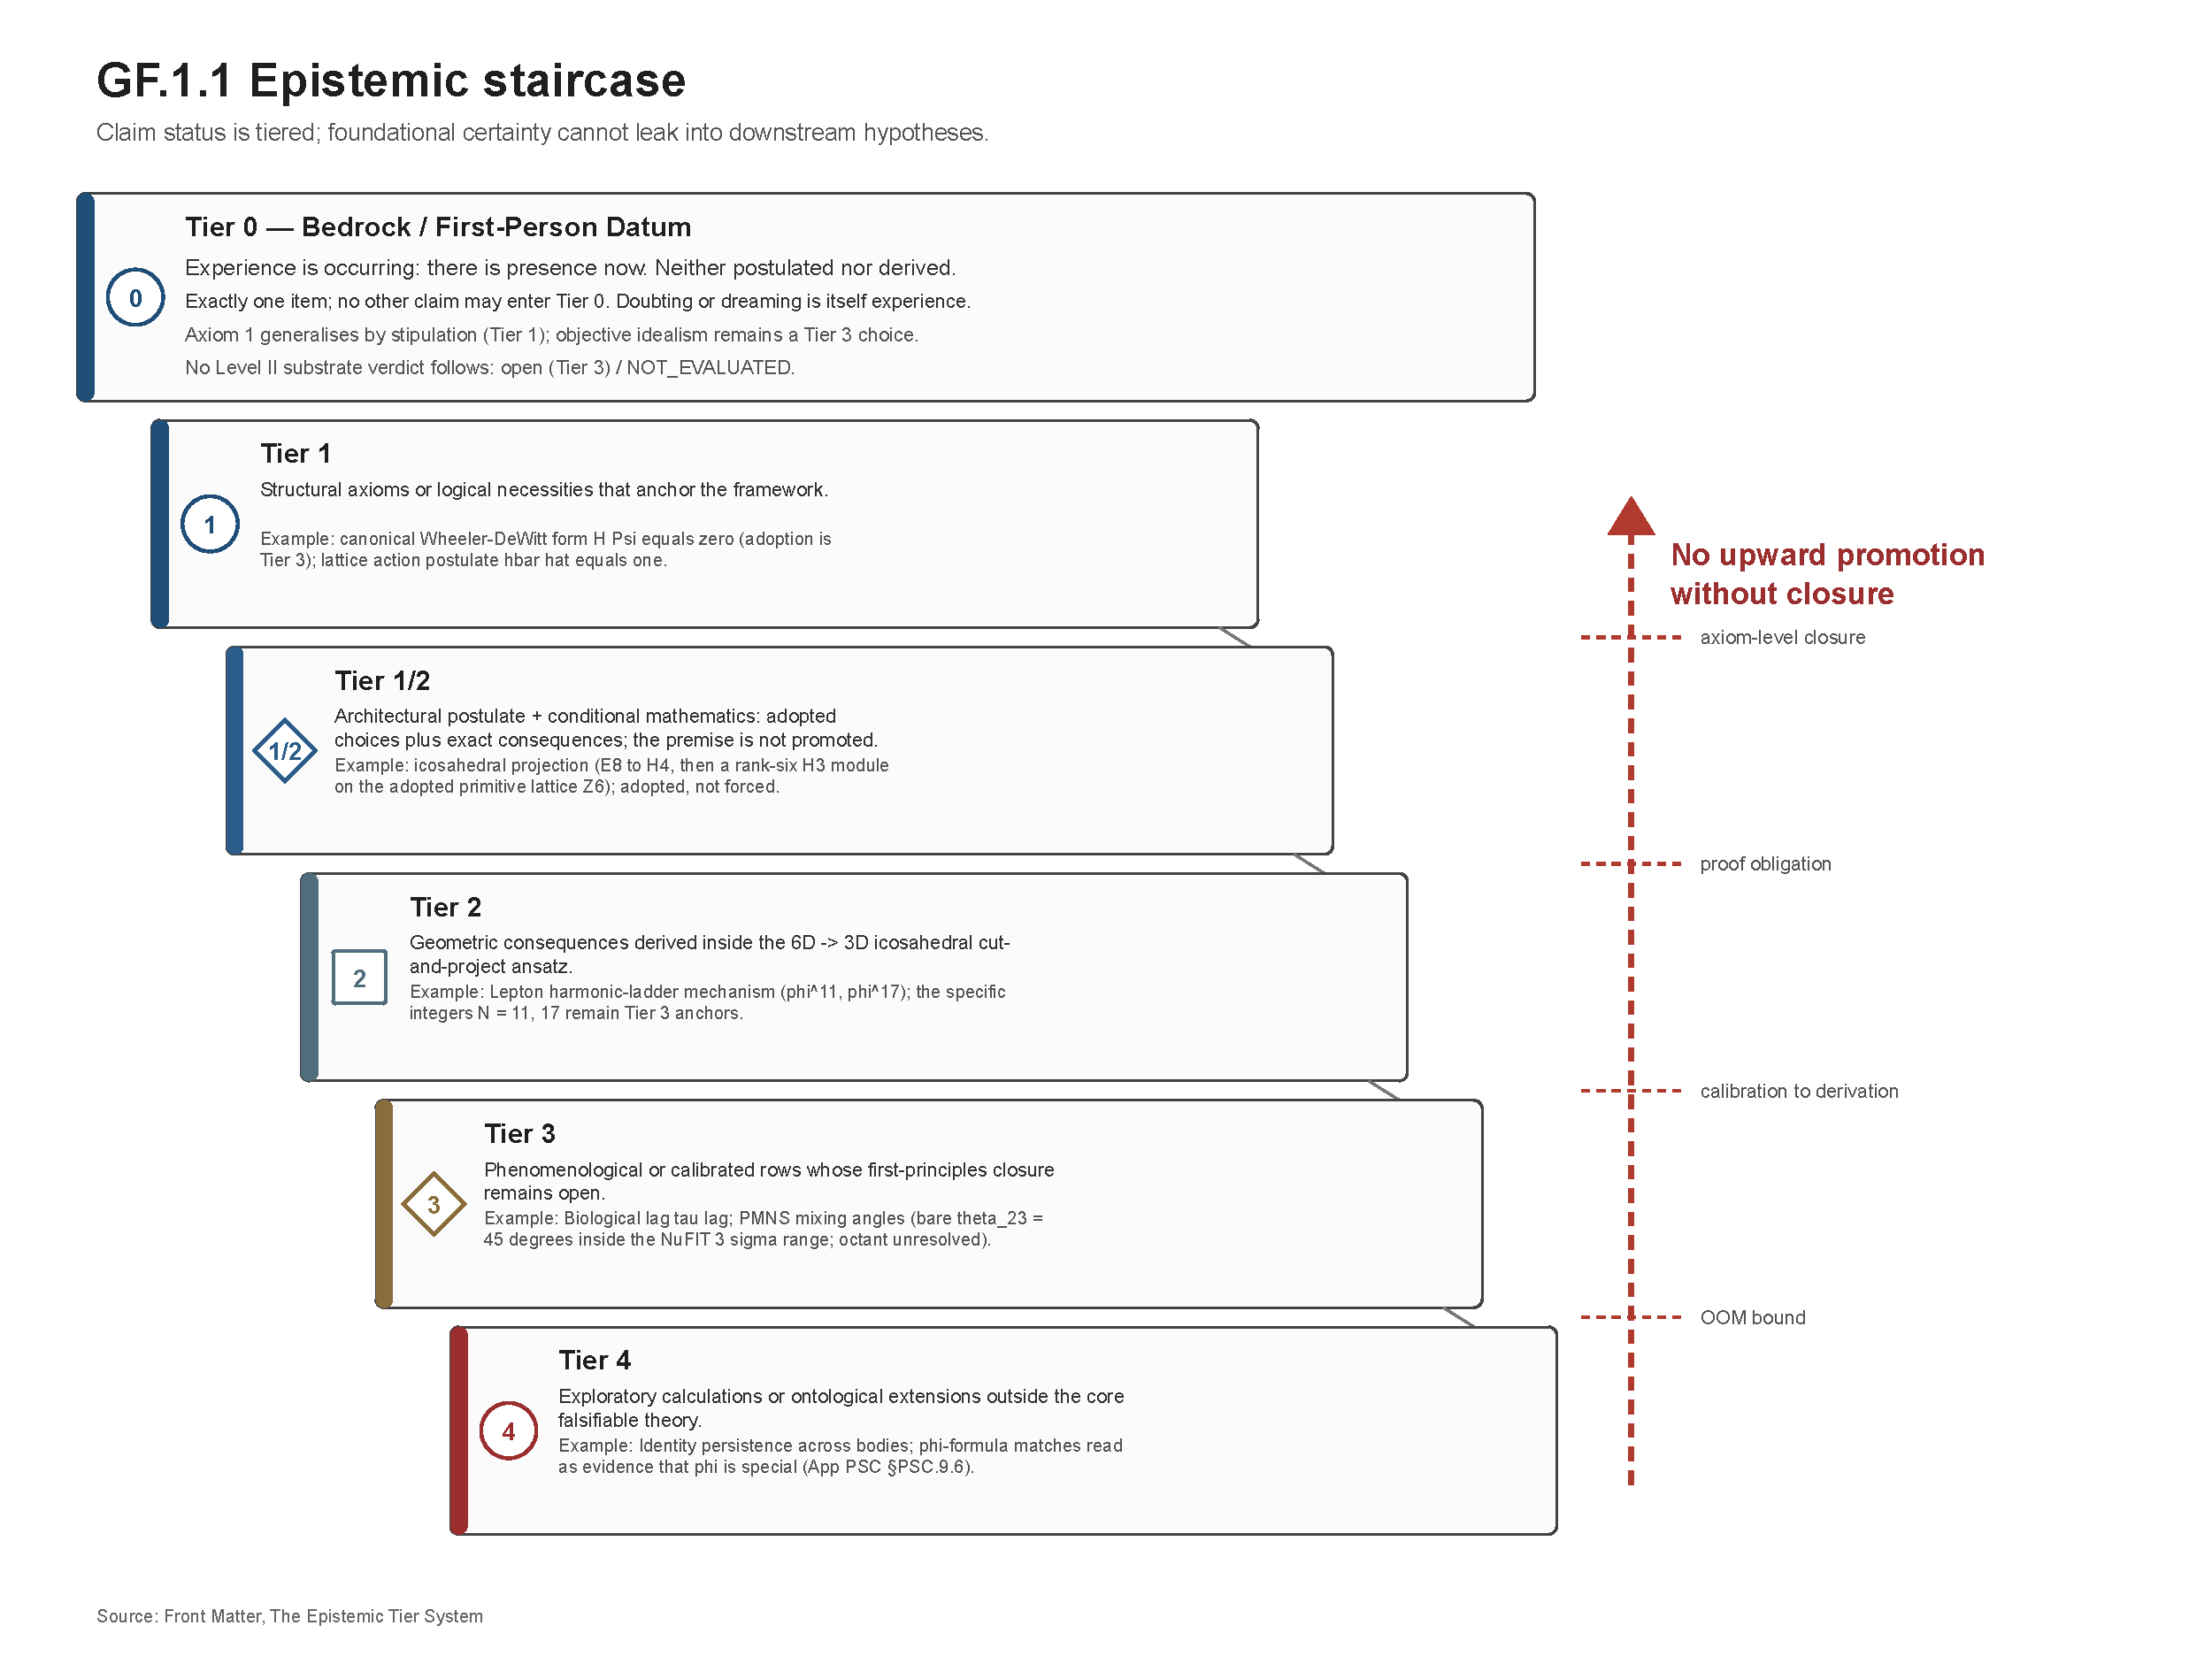
\includegraphics[keepaspectratio,alt={GCT separates claims by epistemic status, from the single Tier 0 first-person datum through Tier 1 axioms to Tier 4 exploratory extensions, so foundational certainty cannot leak into downstream hypotheses.}]{content/Figures/Frontmatter/Figure GF.1.1.pdf}}
\caption{GCT separates claims by epistemic status, from the single Tier
0 first-person datum through Tier 1 axioms to Tier 4 exploratory
extensions, so foundational certainty cannot leak into downstream
hypotheses.}
\end{figure}

\begin{itemize}
\item
  \textbf{Tier 0 (Bedrock / First-Person Datum):} Experience is
  occurring: there is presence now. This datum is neither a postulate
  nor a derived result and cannot be coherently doubted: doubting is
  itself an occurrence of experience, and even in a dream the experience
  occurs. \textbf{One-item rule: exactly this one datum belongs to Tier
  0; no other claim may ever be assigned to it.} Axiom 1 generalises
  this datum by stipulation {[}Tier 1{]} to universal Level I intrinsic
  non-subjective presence in all Field configurations; it is not
  identical to the datum and does not inherit its certainty. The
  objective-idealist ontology remains a Tier 3 parsimony choice (V1
  Ch06). Tier 0 supplies no Level II verdict for any substrate; those
  verdicts remain open (Tier 3) / \texttt{NOT\_EVALUATED}.
\item
  \textbf{Tier 1 (Structural / Axiomatic):} Foundational axioms and
  logical necessities that define the GCT framework. These are either
  \textbf{postulated} as irreducible starting assumptions, or
  \textbf{proven by contradiction} to be the unique consistent solution.
  If these axioms are true, the subsequent Tier 2 results must follow.
\item
  \emph{Examples:} the canonical form of the Wheeler--DeWitt constraint
  \(\hat{H}\Psi=0\), whose adoption as a closed-system postulate is
  separately Tier 3; the \textbf{Lattice Action Postulate}
  (\(\hat{\hbar}=1\)); the masslessness of the photon (\(m_\gamma=0\))
  as an external Tier 1 Standard-Model fact, which rests on unbroken
  local \(\mathrm{U}(1)\) gauge invariance and the Ward identity
  (standard field theory, not a GCT-specific derivation; GCT has not yet
  reproduced it, since its photon sector is a declared open programme,
  V2 Ch06; compactness of a phase variable alone does not force a flat
  potential).
\item
  \emph{Note:} \textbf{Tier 1 denotes either a structural axiom or a
  proof of logical necessity.} These are the irreducible assumptions and
  forced conclusions that anchor the entire theoretical edifice.
\item
  \textbf{Tier 1/2 (Architectural Postulate + Conditional Mathematics):}
  Architectural choices adopted for parsimony and empirical adequacy,
  together with exact mathematical consequences that follow once those
  choices are assumed. The architectural premise is not deductively
  forced by the Ontological Axioms, and it is not converted into a
  theorem by its downstream conditional consequences. \emph{Rule:}
  conditional mathematics never promotes the premise it assumes.
\item
  \emph{Examples:} The \textbf{Icosahedral Projection} (\(E_8\to H_4\),
  followed by a rank-six \(H_3\) module with adopted primitive Bravais
  lattice \(P\cong\mathbb{Z}^6\)): conditionally preferred by the
  registered comparison under parsimony, empirical adequacy, maximal
  polyhedral point symmetry, aperiodicity, the five-fold
  rhombic-triacontahedral window, and golden arithmetic. Rank 6 is fixed
  by full icosahedral indexing, but the closed Bravais classification
  also contains \(F\cong D_6\) and \(I\cong D_6^*\); the choice of \(P\)
  is itself a Structural Postulate. Isotropy alone does not select
  \(H_3\), since \(O_h\) and \(T_d\) also satisfy macroscopic
  finite-point isotropy; nor does spin lifting select it, because every
  finite rotation subgroup of \(SO(3)\) has a canonical Spin\((3)\)
  preimage. App USS records \(A_5\) as the architectural premise H1 and
  derives exact conditional Schur-cover and McKay consequences {[}Tier 1
  mathematics under that premise{]}; it does not prove point-group
  uniqueness, and identifying these consequences as one physical
  \(E_8\to H_4\to\mathbb{Z}^6\) route is architectural compatibility,
  not a forcing theorem.
\item
  \textbf{Tier 2 (Geometric / Derived):} Rigorous mathematical
  consequences derived from the Tier 1 axioms combined with the specific
  6D\(\to\)\hspace{0pt}3D icosahedral cut-and-project ansatz. These
  results are structurally robust within the quasicrystalline vacuum
  identification.
\item
  \emph{Examples:} The \textbf{Electron Mass} chain is Tier 2 mechanism
  plus a Tier 3 exponent anchor (\(n=-107\), pending O.14 selection)
  plus the Tier 4 O.14 physical-link conjecture; because \(m_e\) is the
  A1 anchor, its numerical row is a Tier 3 anchor-normalised Planck-link
  check, whose 1006 ppm residual misses the pre-registered 1000 ppm
  pre-commitment (App FSM P.1c: FAIL of that rule). The \textbf{Lepton
  Mass Ratios} have a Tier 2 harmonic-ladder mechanism plus Tier 3
  specific \(N=11,17\) integer anchors, an H-EW-dependent second-order
  \(\phi^{8}\alpha^2\) selection, and Tier 3 formula residuals pending
  O.5/O.14/O.15. The \textbf{Proton Mass} is Tier 2 mechanism plus a
  Tier 3 sheet/exponent handle pending AKN-action closure.
  \textbf{Newton's G} has a Tier 2 thermodynamic/acoustic mechanism, but
  its numerical Planck-link inherits the Tier 4 O.14 physical-link
  conjecture and the Tier 3 \(m_e\) dimensional anchor; the numerical
  \(G\) row is the electron Planck-link row inverted
  (\(G\propto m_e^{-2}\)), so it is not independent evidence. The
  \textbf{Higgs VEV} is OPEN-CONDITIONAL: Tier 2 product arithmetic
  applies only after supplying the Tier 3 O.38 \(N_{\rm cage}=144\)
  posit; O.20 enumerates but does not select the \(144\times10\) branch,
  and the approximately 179 ppm comparison against the sole declared
  PDG-2024 anchor \(v=246.21965\) GeV is conditional rather than an
  absolute or geometric closure. The \textbf{Light Quark Mass Hierarchy}
  is a mixed Tier 2/3 sector claim: the adopted down-quark output is the
  conditional Tier 3 shell-median identification
  \(m_d=m_u\phi^{\phi}=4.716\) MeV (\(+0.33\%\)), while the exact
  finite-cage \(R=2\) branch is the secondary algebraic diagnostic
  \(m_d=4.848734\) MeV (\(+3.1645\%\), displayed as \(+3.16\%\)); both
  lie inside the registered 110000-ppm gate, and rigorous convergence
  plus the algebraic-field identification remain open under O.5. The
  \textbf{CKM Mixing Angles} are Tier 3: the Cabibbo bare value is a
  Tier 3 identification with a Tier 3 transfer correction, and the
  higher angles are Tier 3 ansätze. For \textbf{spin statistics}, only
  the standard \(\mathrm{SU}(2)\to\mathrm{SO}(3)\) double-cover control
  and the normalization of the WZW generator of
  \(H^3(\mathrm{SU}(2);\mathbb{Z})\) are Tier 1. The GCT identification
  of tethered defects with that construction, and exchange statistics
  for GCT defects, are Tier 3/open rather than a Tier 2 example
  (\(\pi_1(\Sigma_\infty)=0\), so the Solenoid supplies no rotation
  obstruction), while the separate O.14 APS programme remains
  conditional because no qualifying boundary operator/domain/index has
  been specified or evaluated. The \textbf{Dark Energy Coupling}
  (\(\lambda_{bio} \equiv \alpha\)) is \textbf{Tier 3
  (Phenomenological)} per the Prediction-Postdiction Firewall --- it is
  a declared matching choice (\(\lambda_{bio}\equiv\alpha\)), not fitted
  and not a first-principles derivation, and its physical-source
  interpretation (selection events as a dark-energy source) is Tier 4.
  Three items are deliberately \emph{not} Tier 2 examples: the
  \textbf{Fine-Structure Constant bare relation}
  \(\alpha^{-1}_{bare} = 360\phi^{-2} \approx 137.508\) is a Tier 3
  numerical relation (Tier 3 600-cell multiplier; mechanism open --- the
  RT solid-angle construction is withdrawn, V1 §13.2.1--§13.2.2), with
  the residual closure tracked under O.19/O.5; the \textbf{Gauge Group
  Structure} is an open Tier 3 candidate (its eight-dimensional
  \(\mathrm{SU}(3)\) closure is not specific to the RT window; V3 Ch03,
  App ORQ O.39/O.32); and the bare \textbf{Weinberg angle} \(\phi^{-3}\)
  is the Tier 3 hypothesis H-EW (V3 Ch04 §4.3). The invariant-degree sum
  \(D_{H3}=2+6+10=18\) is Tier 2, but this integer does not entail a
  physical stiffness ratio: the map \(K_\perp/K_\parallel=\phi^{-18}\)
  is the Tier 3 hypothesis P3b (Parameter Ledger §0.1). These tiers
  describe the mechanisms and anchors; the numerical matches of the φ
  formulas in these examples (electron, lepton ratios, proton, \(G\),
  Higgs VEV, quarks, couplings and mixing angles) are \textbf{Tier 4 as
  evidence} that φ or icosahedral structure is special, because the
  preregistered constant control test (v3, NEGATIVE-FRAGILE) did not
  distinguish them from numerology for strong effects (App PSC
  §PSC.9.6).
\item
  \textbf{Tier 3 (Phenomenological / Calibrated):} Models calibrated to
  observation where a first-principles derivation is currently
  incomplete (e.g., requiring full non-perturbative simulation of defect
  ensembles or horizon-scale boundary conditions). Applies to any sector
  --- biophysical, cosmological, or phenomenological --- where free
  parameters are adjusted to match empirical anchors and a geometric
  derivation is pending. This tier also covers explicit conditional
  physical maps from a geometric invariant or coordinate diagnostic to a
  physical coupling or response coefficient: such a hypothesis need not
  be a continuous fitted parameter, but it remains an independent
  commitment until a normalization-invariant dynamical derivation closes
  it.
\item
  \emph{Examples:} the stiffness-map hypothesis P3b,
  \(K_\perp/K_\parallel=\phi^{-18}\), and its \(\phi^{-9}\) and
  \(\phi^{-36}\) descendants pending O.15(b); the electroweak boundary
  hypothesis H-EW; biological lag calculations (\(\tau_{lag}\)); Chiral
  Enhancement Factors in tubulin; the Consensus Decay Constant
  (\(\lambda_c\), pending derivation from phason stiffness ratio
  \(K_\perp/K_\parallel\), V1 Ch11 §11.2.4); the PMNS mixing angles
  (Tier 3; the bare \(\theta_{23}=45^\circ\) lies inside the NuFIT 6.0
  \(3\sigma\) range with and without Super-Kamiokande data, and the
  octant is unresolved); the \textbf{Born Rule}, a Tier 3 conditional
  compatibility theorem pending O.40a/O.40b additivity and
  noncontextuality closure; the equation of state \(w(z)_{bio}\)
  (sustained phantom phase asymptoting to \(-1\) from below; the phantom
  direction itself is Tier 4, with no ghost-free action, V2 Ch14
  §14.3.1; observational distinguishability threshold at
  \(z \approx 0.28\) per V2 Ch14 §14.6.3).
\item
  \textbf{Tier 3/4 (Straddle Label):} Tier 3 form / Tier 4 realization.
  The label marks a claim whose form is Tier 3 and whose realization is
  Tier 4; the text must say which part is which.
\item
  \textbf{Tier 4 (Speculative / Exploratory):} Claims that are either
  (a) \textbf{exploratory calculations} where the dimensional structure
  is correct but the numerical coefficient is uncertain by \textgreater1
  order of magnitude (with explicit OOM bounds), or (b)
  \textbf{ontological extensions} that lie outside the core falsifiable
  theory (identity persistence after biological termination,
  trans-temporal identity correlations), or (c) \textbf{evidential
  readings of numerical matches} whose evidential weight a preregistered
  control has not distinguished from numerology. Under (c) the
  arithmetic itself is not demoted: the computed value and its residual
  stay as descriptive arithmetic, and only their use as evidence that φ
  or icosahedral structure is special is Tier 4. No Tier 4 claim is used
  as support for a core result; where a core chain inherits a Tier 4
  link (the O.14 physical-link conjecture, the phantom direction of the
  registered \(w(z)\) channel), the chain carries that Tier 4 label.
\item
  \emph{Examples (Exploratory):} Biogenic dark energy driving force
  magnitudes; neutrino mass scale absolute normalization.
\item
  \emph{Examples (Ontological):} Identity persistence across bodies;
  consciousness continuity in reversible computational states.
\item
  \emph{Examples (Evidential, (c)):} evidential readings of φ-formula
  numerical matches (App PSC §PSC.9.6): the lepton, proton, quark,
  Higgs-VEV, coupling, mixing-angle and Newton-\(G\) matches, read as
  evidence that φ is special. The preregistered constant control test
  (v3, NEGATIVE-FRAGILE) found φ's pattern of matches on 21 constants
  not distinguishable from that of random constants; it ``excludes, at
  power ≥ 0.8, an effect in which φ hits at least 6 of the 8 informative
  rows through a real effect; weaker effects are not excluded.''
\end{itemize}

\begin{center}\rule{0.5\linewidth}{0.5pt}\end{center}

\textbf{Note on Computational Closure:} The Tier 2 analytic mechanisms
of the lepton and quark mass hierarchies remain subject to computational
verification via the full non-perturbative spectrum of the defect-cage
Hessian. The presently used \(N=144\) cage is itself a Tier 3 structural
posit pending O.38; exact Gauss--Bonnet closure on the
icosahedral/dodecahedral boundary does not derive its node count. The
pathway for the downstream spectral calculation is defined in Chapter 13
(Open Problem O.5).

\begin{center}\rule{0.5\linewidth}{0.5pt}\end{center}

This classification ensures that the framework is transparent regarding
its levels of certainty, separating axiomatic assumptions from geometric
derivations, phenomenological fitting, and exploratory/ontological
extensions.

\chapter*{Axiom \& Postulate Ledger}
\addcontentsline{toc}{chapter}{Axiom \& Postulate Ledger}
\markboth{Axiom \& Postulate Ledger}{Axiom \& Postulate Ledger}
\setcounter{section}{0}

This document serves as the authoritative enumeration of the
foundational assumptions used in Geometric Consciousness Theory (GCT).
We distinguish between the \textbf{Ontological Root}, which defines the
field of inquiry, and the \textbf{Structural Architecture}, which
specifies a concrete physical implementation.

\begin{figure}
\centering
\pandocbounded{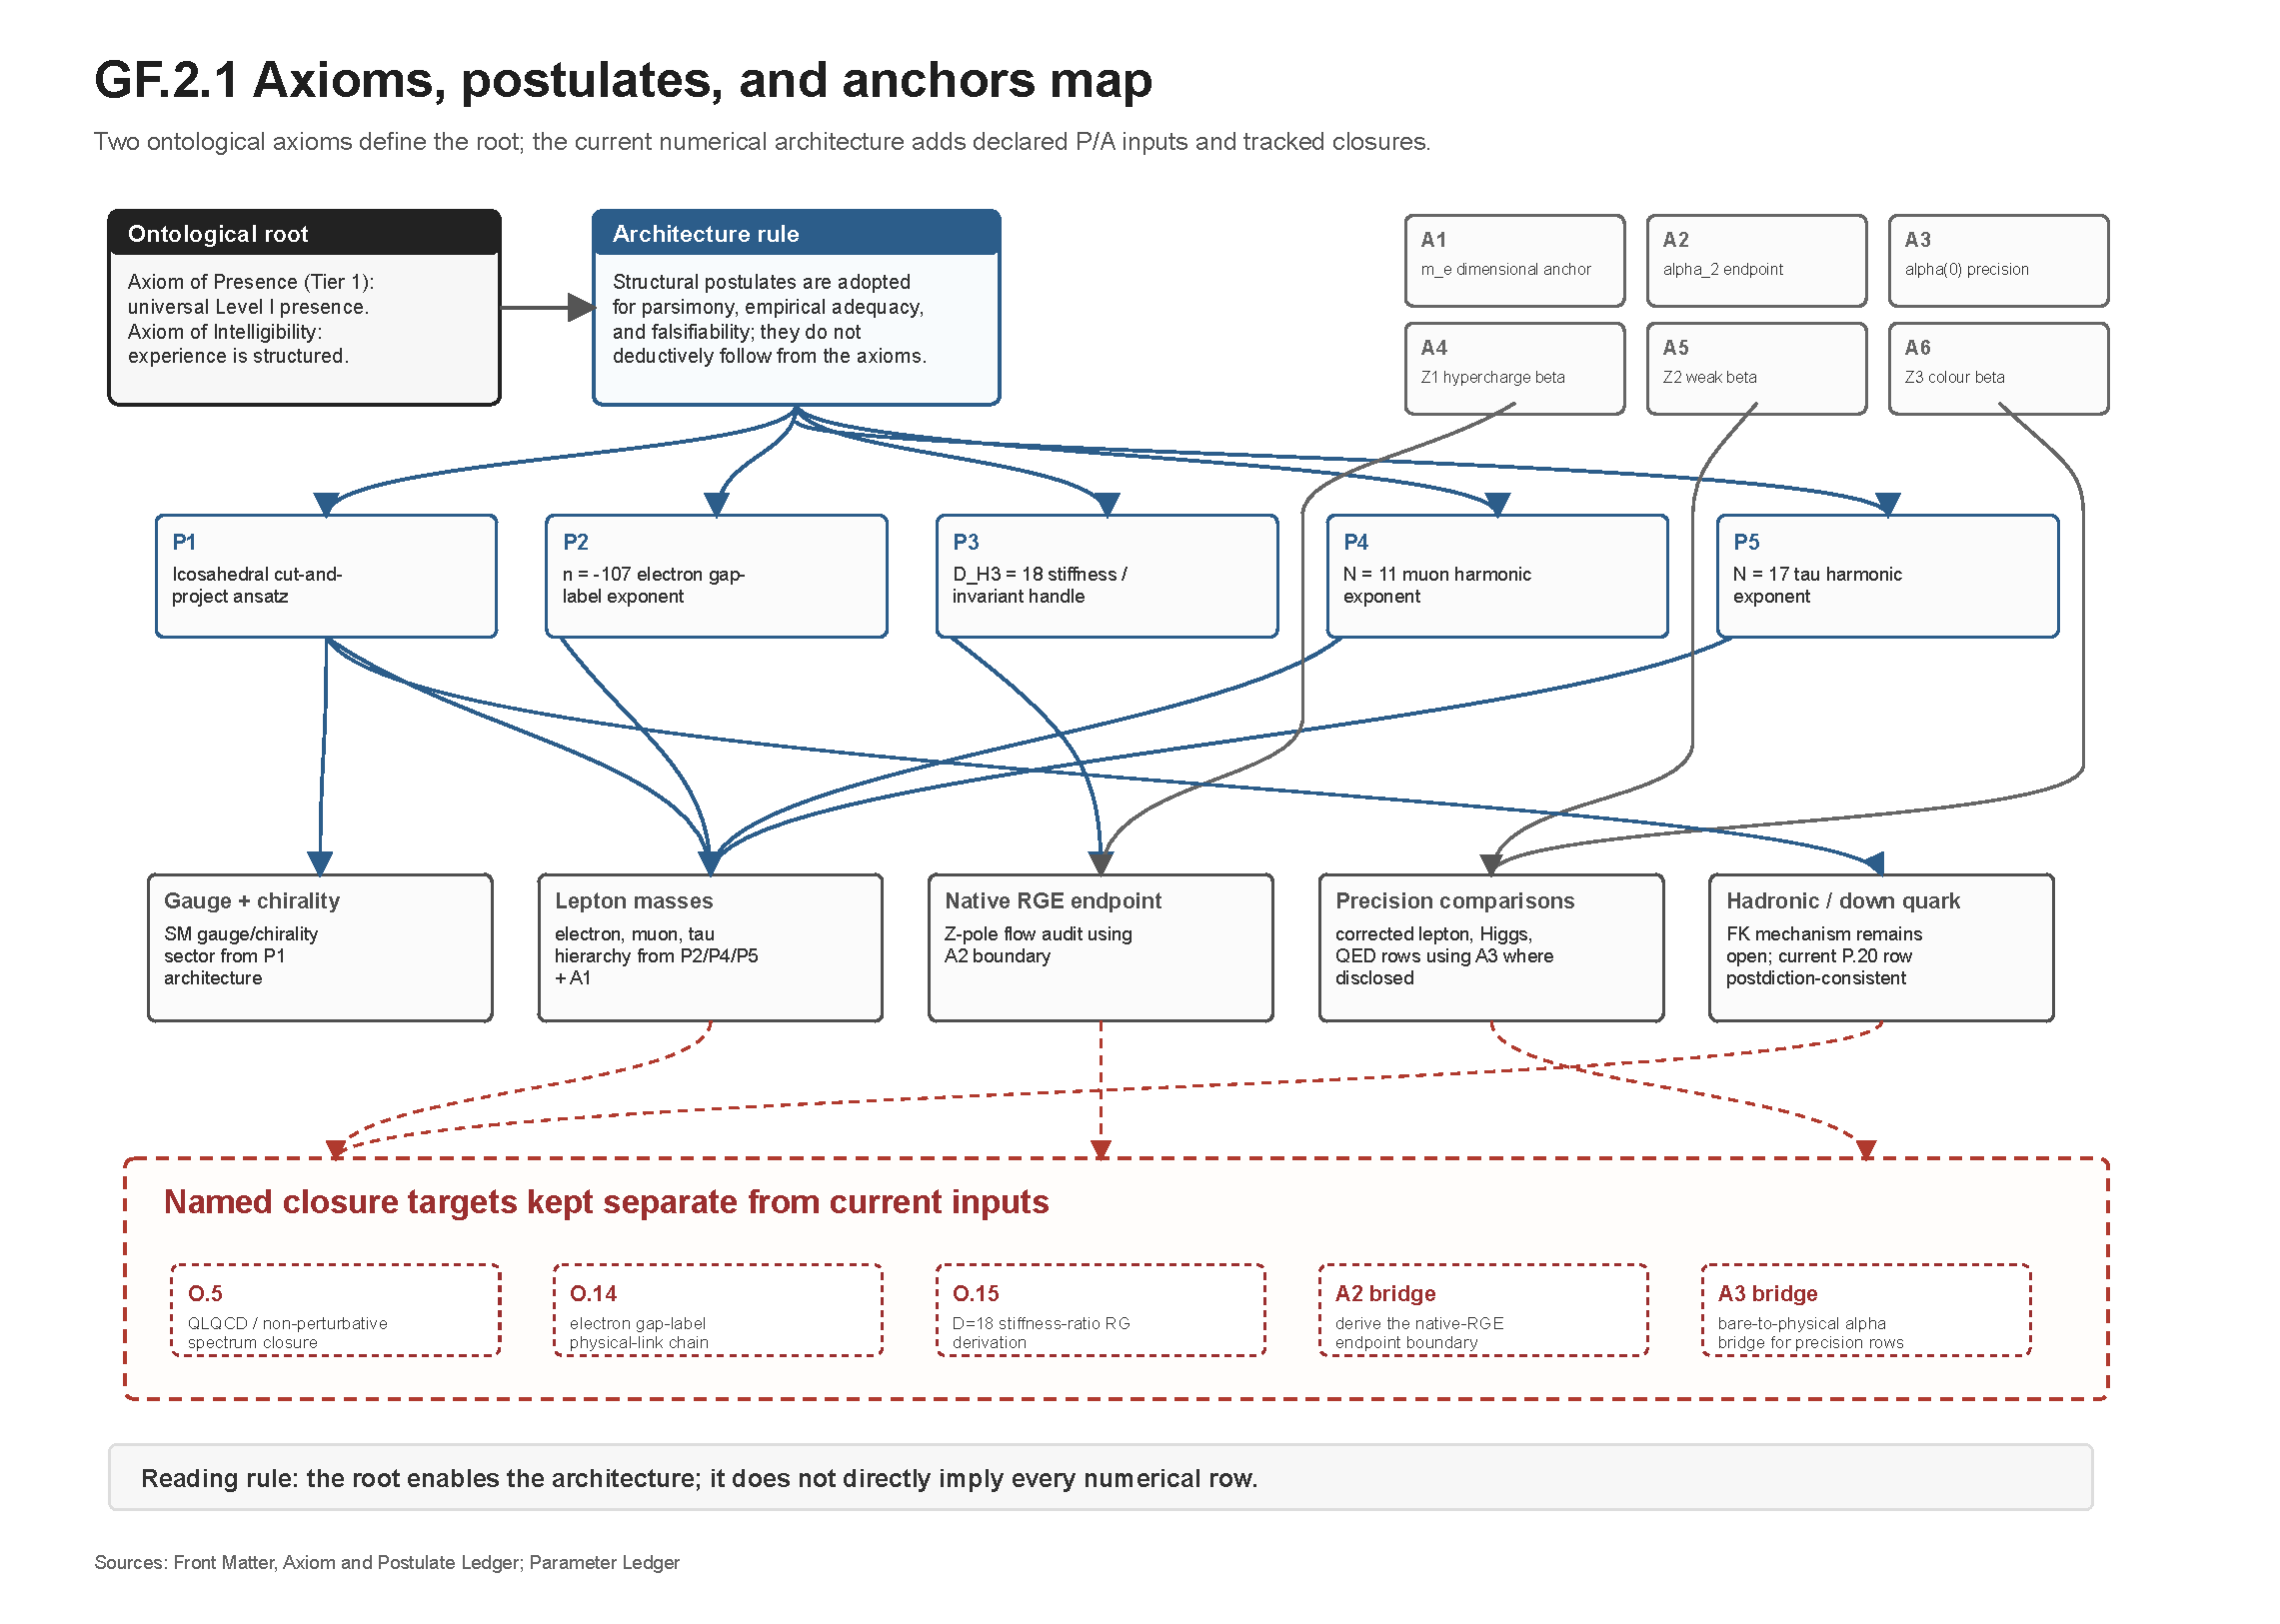
\includegraphics[keepaspectratio,alt={The ontological root has two axioms; the current gauge/lepton architecture adds declared postulates P1-P5 and continuous anchors A1-A6, with a named six-item Tier-3 precision/gauge coefficient subset and the O.38 N=144 cage posit counted separately from other categorized handles and closure targets.}]{content/Figures/Frontmatter/Figure GF.2.1.pdf}}
\caption{The ontological root has two axioms; the current gauge/lepton
architecture adds declared postulates P1-P5 and continuous anchors
A1-A6, with a named six-item Tier-3 precision/gauge coefficient subset
and the O.38 N=144 cage posit counted separately from other categorized
handles and closure targets.}
\end{figure}

\textbf{Relation to the Parameter Ledger count.} The numerical count of
5 structural postulates + 6 continuous anchors (11 declared core inputs)
is governed by Parameter Ledger §0.1, not by the number of bullets in §2
below. The §2 items map onto it as follows: the Discreteness Postulate,
Maximal Polyhedral Point Symmetry, the 6D Euclidean Parent Lattice and
the 6D φ-slope are the components of \textbf{P1}, the icosahedral
cut-and-project ansatz. \textbf{P2--P5} are the integer exponents
\(n=-107\), \(D_{H3}=18\), \(N=11\) and \(N=17\), listed in Parameter
Ledger §0.1 rather than here, and \textbf{A1--A6} are the continuous
anchors listed there. The Wheeler--DeWitt Constraint Postulate (a Tier 3
adoption), the Born-rule compatibility statement (a Tier 3 conditional
theorem) and Postulate G (a rule restricting admissible exponent
arithmetic) carry no numerical input and are outside the 11-input count.

\section{1. Ontological Axioms (The
Root)}\label{ontological-axioms-the-root}

These axioms define the ontological starting point of the framework. The
first-person datum must be distinguished from its stipulated universal
generalisation.

\textbf{First-person datum {[}Tier 0{]}:} Experience is occurring: there
is presence now. This is the sole Tier 0 item, neither postulated nor
derived; all other claims are excluded from Tier 0.

\begin{enumerate}
\def\labelenumi{\arabic{enumi}.}
\tightlist
\item
  \textbf{Axiom 1 --- Axiom of Presence {[}Tier 1{]}:} All Field
  configurations carry universal Level I intrinsic non-subjective
  presence. This stipulated generalisation is motivated by the Tier 0
  datum, not identical to it or deduced from it. The objective-idealist
  ontology is a Tier 3 parsimony choice (V1 Ch06); Level II substrate
  verdicts remain open (Tier 3).
\item
  \textbf{Axiom 2 --- Axiom of Intelligibility {[}Tier 1 --- stipulated
  axiom; it does not carry the Tier 0 certainty{]}:} Experience is
  structured. Awareness contains distinctions and sequences that obey
  consistent rules.
\end{enumerate}

\section{2. Structural Postulates (The
Architecture)}\label{structural-postulates-the-architecture}

These postulates are explicitly adopted as an architecture for a
concrete physical model. They are justified by \textbf{minimum
additional complexity} (algorithmic parsimony), \textbf{empirical
adequacy}, and \textbf{falsifiability}. They do not follow deductively
from the Axioms alone.

\begin{itemize}
\tightlist
\item
  \textbf{Discreteness Postulate {[}Tier 1/2 --- Structural
  Postulate{]}:} The information content of any finite volume of the
  physical universe is finite. Reality is sampled/quantized at the
  Planck scale.
\item
  \textbf{Maximal Polyhedral Point Symmetry {[}Tier 1/2 --- Structural
  Postulate{]}:} Isotropy alone is insufficient to select the substrate
  symmetry: \(O_h\) and \(T_d\) also satisfy macroscopic finite-point
  isotropy. The architecture therefore restricts the declared
  irreducible polyhedral rotational candidates to \(A_4\), \(S_4\),
  \(A_5\) and adopts the icosahedral group \(I\cong A_5\) of order 60,
  the largest of those three, together with fivefold symmetry and the
  rhombic-triacontahedron window. Cyclic and dihedral rotation groups
  have unbounded order, so ``maximal finite rotational order'' is
  meaningful only inside the declared polyhedral candidate class. The
  candidate restriction and the fivefold/RT requirements are
  architectural premises, not deductions from Presence and
  Intelligibility alone.
\item
  \textbf{6D Euclidean Parent Lattice {[}Tier 1/2 --- Architectural
  Postulate + Conditional Mathematics{]}:} The 6-dimensional parent
  lattice is obtained, under this postulate, from the Binary Icosahedral
  Group \(2I\) via the McKay Correspondence (\(2I \to E_8\)), the
  Elser--Sloane \(E_8\to H_4\) projection, and the rank-six icosahedral
  module. The primitive Bravais choice \(P\cong\mathbb{Z}^6\) is adopted
  explicitly; the alternative icosahedral choices are \(F\cong D_6\) and
  \(I\cong D_6^*\), and the closed mathematics does not uniquely select
  among them. See the \textbf{Conditional T-McKay Architecture Chain}
  (Appendix USS §USS.7). The Schur cover, McKay correspondence, stated
  Elser--Sloane projection, rank-six requirement, Bravais
  classification, and \(H_4\) Cartan/root-metric value of \(\phi\) are
  closed mathematical correspondences within their hypotheses. Their
  composition as the physical 6D architecture remains a Tier 1/2
  structural postulate, not an unconditional theorem. Program T-McK.1b
  is a separate Tier 3 downstream consistency program: no qualifying APS
  bulk/boundary operator pair, domains, kernel term, regularised eta, or
  complete index has been constructed. The finite cage computations are
  scalar-adjacency and discrete-matrix diagnostics only. Because the RT
  boundary is defined after adopting this 6D architecture, future APS
  closure could test internal consistency but could not derive or
  elevate its upstream premise to Tier 1.
\item
  \textbf{6D φ-slope {[}Tier 1 conditional mathematics under H1{]}:} The
  golden ratio \(\phi=2\cos(\pi/5)=(1+\sqrt{5})/2\) enters the
  \(H_3/H_4\) geometry through the off-diagonal Cartan entry \(-\phi\)
  between the pentagonal simple roots, the golden-ratio metric of the
  icosahedral root system, and the irrational cut-and-project slope in
  the Elser--Sloane map. The Coxeter-element eigenvalues themselves are
  roots of unity on the unit circle; \(\phi\) is therefore not the
  magnitude of any Coxeter eigenvalue. See the Conditional T-McKay
  Architecture Chain. This fixes \(\phi\) inside the adopted \(H_3/H_4\)
  architecture; it does not prove H1 or global slope optimality.
\item
  \textbf{Wheeler--DeWitt Constraint Postulate {[}Tier 3 adoption; the
  canonical constraint form is Tier 1{]}:} The total energy/Hamiltonian
  of the configuration space of the universe --- comprising all matter
  and gravitational degrees of freedom --- is Zero
  (\(\hat{H}|\Psi\rangle = 0\)). This is a timeless constraint on the
  space of all geometries, not a conservation law for a dynamically
  evolving system. See Chapter 5 for the philosophical motivation.
\item
  \textbf{Born Rule {[}Tier 3 conditional compatibility theorem{]}:} The
  Born Rule (\(P = |\psi|^2\)) follows from Gleason's Theorem only if
  the GCT Selection Operator is independently shown to define a
  countably additive, noncontextual probability measure on the phason
  projection lattice. Those two proof obligations are App ORQ O.40a and
  O.40b; Appendix BRC §BRC.1--BRC.6 gives the conditional structure
  without defining the measure by the Born quadratic in advance.
\item
  \textbf{Postulate G (Galois Observable Constraint) {[}Tier 1/2 ---
  Structural Postulate{]}:} On the lepton/electron ladder
  (\(m_e/M_P=\phi^{-107}\) and \(m_\ell=m_e\phi^N\)), admissible GCT
  mass-exponent arithmetic is restricted to Galois-compatible integer
  powers \(\phi^N\) with \(N \in \mathbb{Z}\) (App USS §USS.5.3).
  Postulate G is scoped to that ladder: the non-integer exponents of the
  proton (\(15+\phi^{-1}\)), the quark sector (V3 Ch10) and the CKM
  angles (O.5) lie outside it and keep their own tier labels (Parameter
  Ledger, integer-handle tier taxonomy; App FTH §FTH.5). It is not the
  requirement that an observable be invariant under the Galois
  automorphism \(\phi \to -1/\phi\): the elements of
  \(\mathbb{Q}(\sqrt{5})\) fixed by that automorphism are exactly the
  rationals. Postulate G is a structural postulate of the framework
  rather than an independently established constraint, and it supplies
  no narrower Lucas-only trial factor. The Prediction/Postdiction
  Firewall gives the canonical admissibility rule for mass exponents.
\end{itemize}

\section{3. Methodological
Commitments}\label{methodological-commitments}

Non-ontological rules that govern the derivation and validation process.

\begin{itemize}
\tightlist
\item
  \textbf{Parsimony as Heuristic Prior:} Simpler models (lower
  Kolmogorov complexity) are preferred over complex ones, but parsimony
  is a heuristic for discovery, not a replacement for proof.
\item
  \textbf{Tier System Rule:} All claims must be classified by the
  Epistemic Tier System (Tier 0: Bedrock / First-Person Datum, exactly
  one item; Tier 1: Structural Axiom / Logical Necessity; Tier 1/2:
  Architectural Postulate + Conditional Mathematics; Tier 2: Geometric /
  Derived from the icosahedral ansatz; Tier 3: Phenomenological /
  Calibrated, including conditional physical-map hypotheses; Tier 4:
  Speculative / Order-of-Magnitude, with explicit OOM bounds, or
  ontological extension). Conditional mathematics never promotes the
  premise it assumes. See the Global Front Matter Epistemic Tier System
  for complete definitions.
\item
  \textbf{Calibration Rule:} All fundamental constants must be derived
  from dimensionless geometric ratios. SI units are only used via a
  declared experimental anchor (e.g., the electron mass).
\end{itemize}

\section{4. Physical Modeling Postulates
(EFT-Level)}\label{physical-modeling-postulates-eft-level}

Specific assumptions used for mapping geometric structures to Standard
Model entities.

\begin{itemize}
\tightlist
\item
  \textbf{Defect/Soliton Matter Model:} Particles are modeled as
  topological defects or solitons within the lattice strain field.
\item
  \textbf{Phonon/Phason Split:} The separation of degrees of freedom
  into ``Standard Physics'' (Phonons) and ``Dark/Information Physics''
  (Phasons).
\end{itemize}

\chapter*{Parameter Ledger}
\addcontentsline{toc}{chapter}{Parameter Ledger}
\markboth{Parameter Ledger}{Parameter Ledger}
\setcounter{section}{0}

This ledger provides the authoritative categorized inventory of
numerical values used as inputs, anchors, or calibrated fits within
Geometric Consciousness Theory (GCT). In accordance with the
\textbf{Prediction/Postdiction Firewall}, values are classified by their
technical provenance and quantitative scope. The Gauge, Lepton, and
native-RGE endpoint sectors are determined by a small, fully-enumerated
set of structural postulates and six continuous anchors: one dimensional
anchor, one gauge-flow endpoint anchor, one low-energy fine-structure
anchor used only by measurement-anchored precision-comparison rows, and
three native-RGE \(\beta\)-coefficient magnitude normalisations (Section
0 below). A named precision/gauge comparison subset contains six
calibrated Tier-3 discrete coefficient handles (\(1440\), \(12\),
\(360\), \(2\), \(10\phi^2\), and \(1/5\)); the O.38 \(N=144\) cage
posit and the additional hadronic, biophysical, cosmological, and
deployment handles catalogued below are counted outside that subset. The
remaining Open Parameters are explicitly quarantined in Section 4 (Tier
3) pending exact geometric derivation.

\section{0. Free Parameter Accounting
(Summary)}\label{free-parameter-accounting-summary}

This section aggregates every structural postulate, integer exponent,
and calibrated parameter that enters the manuscript's quantitative
claims. It is the authoritative accounting for this purpose: the
gauge-and-lepton sector's commitments are explicit, finite, and
partitioned by epistemic tier.

\begin{figure}
\centering
\pandocbounded{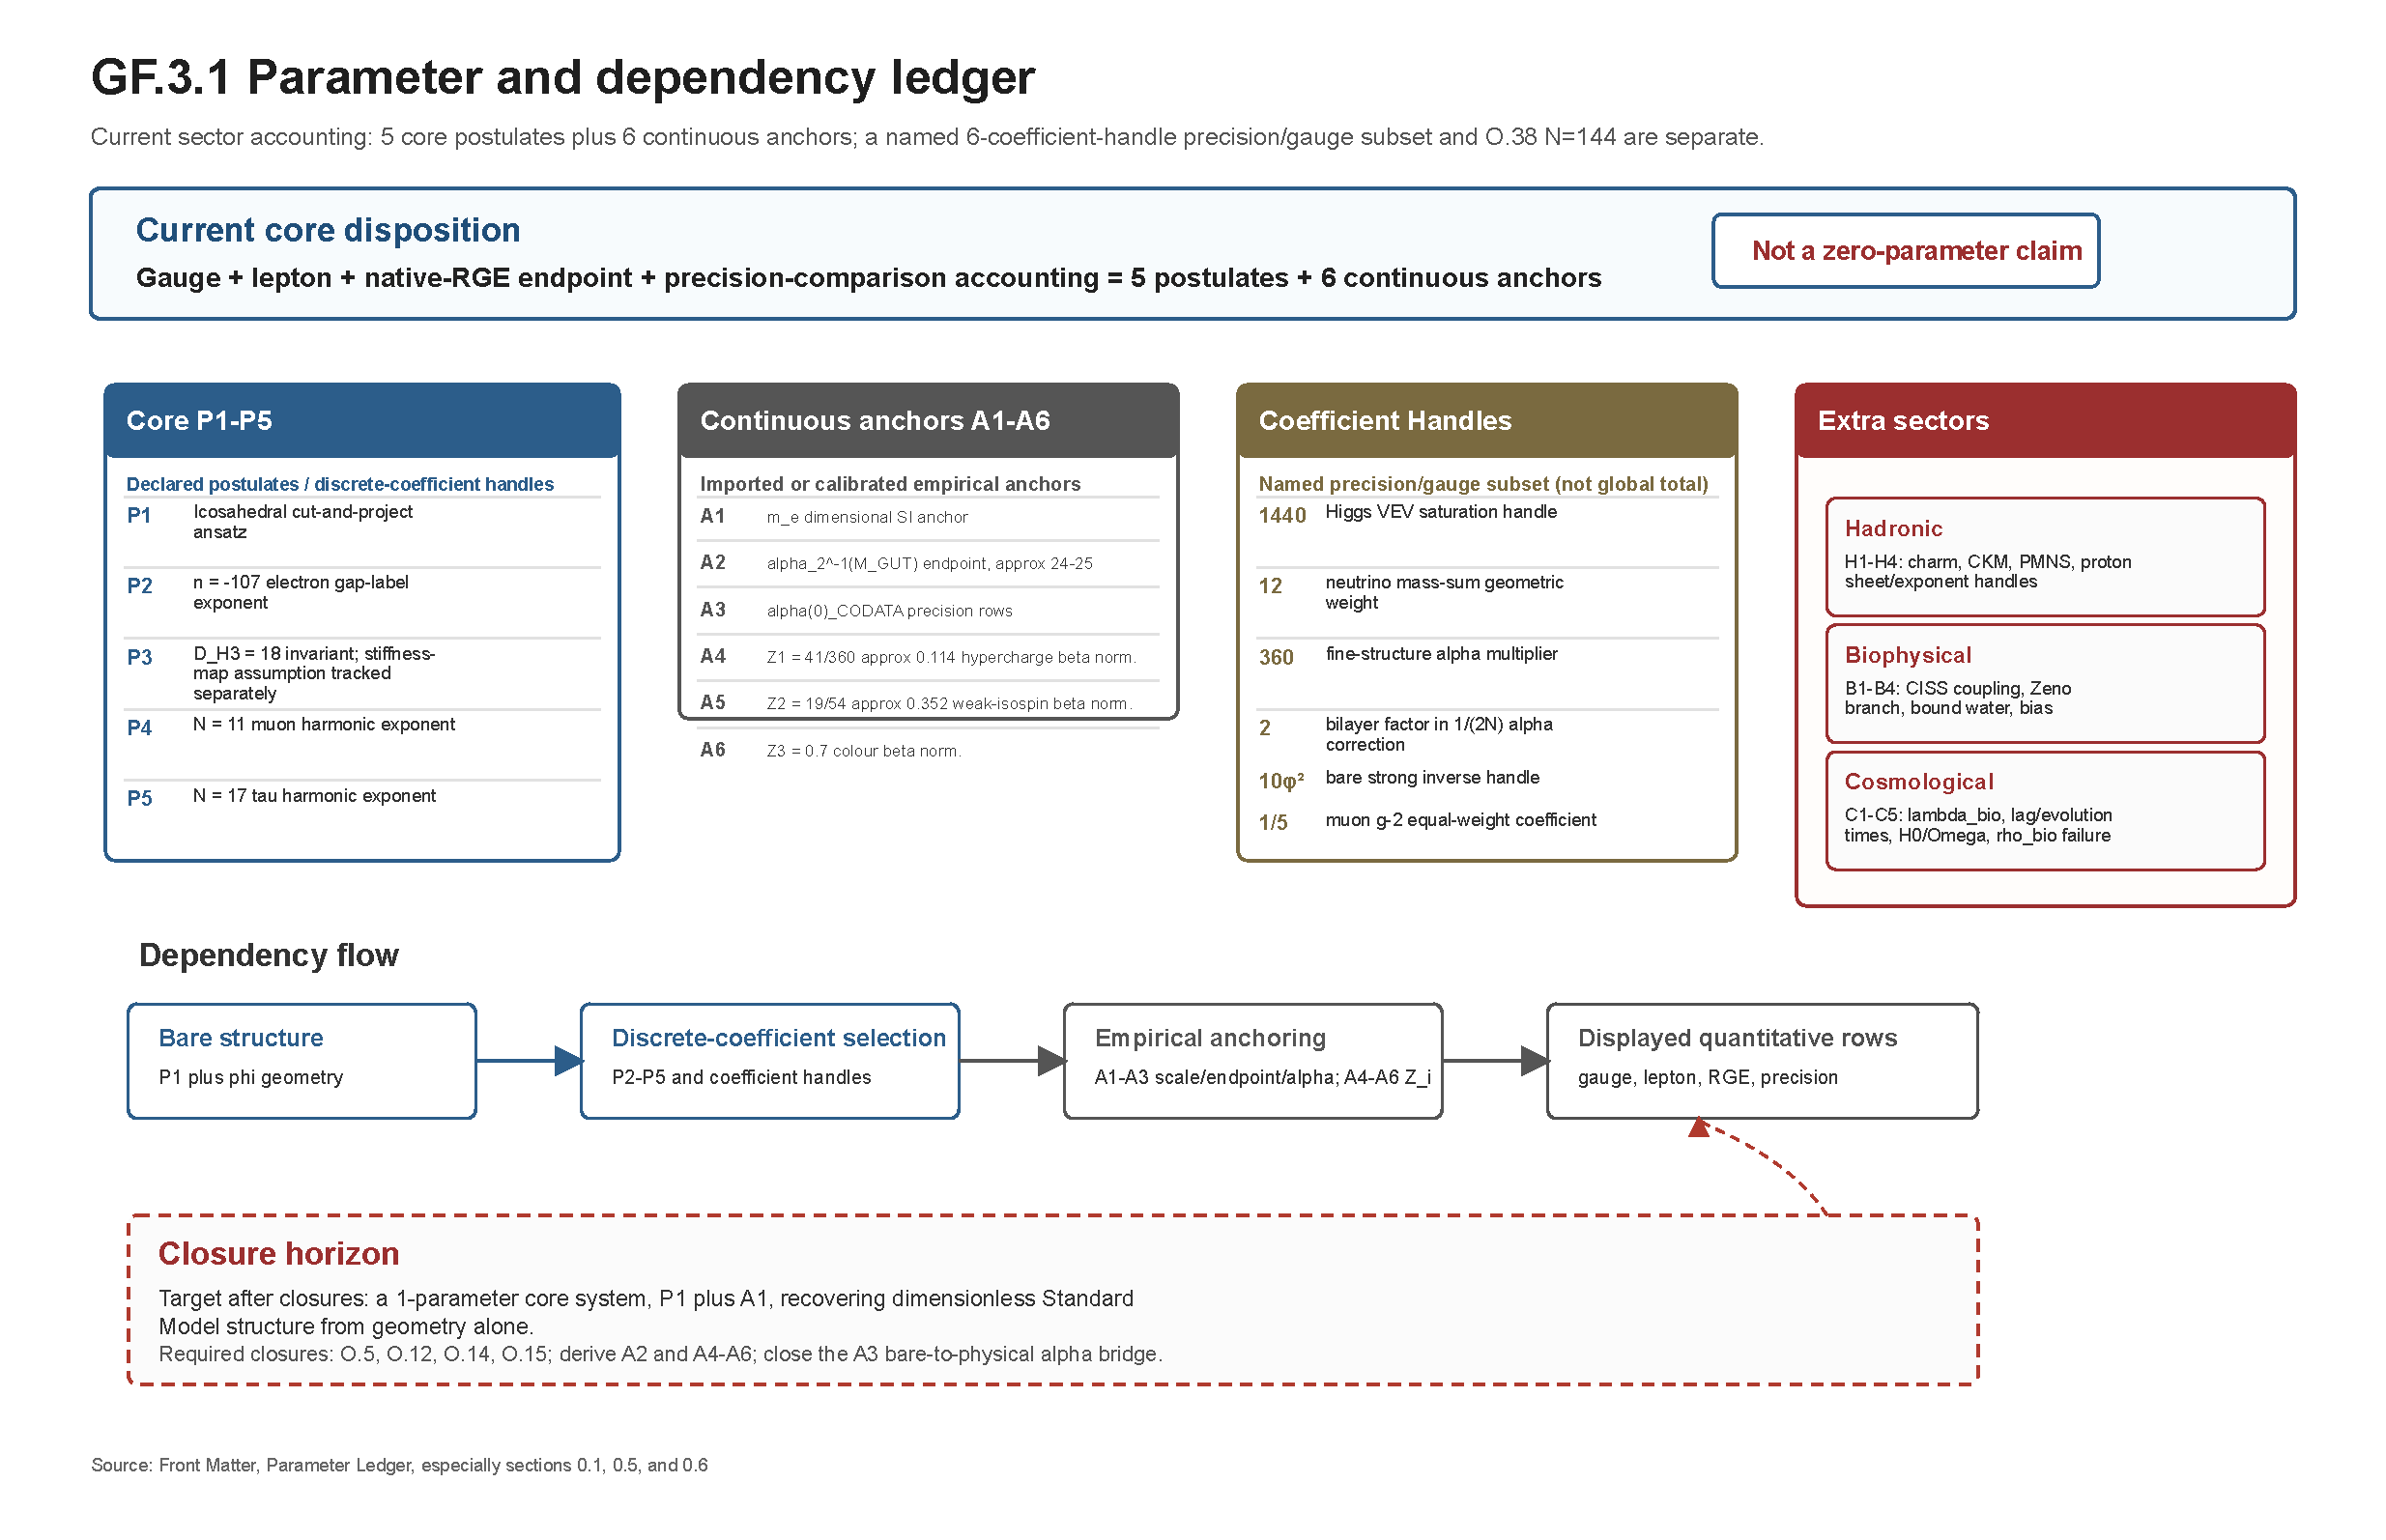
\includegraphics[keepaspectratio,alt={The core accounting currently uses five postulates plus six anchors for the gauge, lepton, native-RGE endpoint, and precision-comparison sector, while broader hadronic, biological, and cosmological sectors retain additional calibrated inputs.}]{content/Figures/Frontmatter/Figure GF.3.1.pdf}}
\caption{The core accounting currently uses five postulates plus six
anchors for the gauge, lepton, native-RGE endpoint, and
precision-comparison sector, while broader hadronic, biological, and
cosmological sectors retain additional calibrated inputs.}
\end{figure}

\gctneedbreak{20\baselineskip}

\subsection{0.1 Core Gauge + Lepton + Dimensional + Native-RGE Endpoint
Sector --- 5 postulates + 6
anchors}\label{core-gauge-lepton-dimensional-native-rge-endpoint-sector-5-postulates-6-anchors}

\gctneedbreak{10\baselineskip}

\begingroup\setlength{\parindent}{0pt}

\medskip\textbf{P1} --- Tier 1/\allowbreak{}2 axiomatic

\par

\textit{Postulate:} \textbf{Icosahedral cut-and-project ansatz} (\(H_3\)
projection of the adopted primitive-\(P\) Bravais lattice
\(\mathbb{Z}^6\) onto \(E_\parallel\))

\par

\textit{Type:} Structural postulate

\par

\textit{Status:} Foundational; not a fitted parameter. Full icosahedral
indexing fixes rank 6, while the Bravais classification also permits
\(F\cong D_6\) and \(I\cong D_6^*\); the primitive-\(P\) choice is
adopted, not uniquely derived from \(E_8\) or from the \(D_6\) roots. P1
bundles the Discreteness, Maximal Polyhedral Point Symmetry, 6D Parent
Lattice and 6D φ-slope items of the Axiom \& Postulate Ledger §2; that
ledger's Wheeler--DeWitt, Born-rule and Postulate G items carry no
numerical input and are outside this count.

\par

\textit{Cross-reference:} V1 Ch04 §4.2.2; App USS §USS.7.3; Axiom \&
Postulate Ledger §2

\par

\medskip\textbf{P2} --- Tier 2 K-theoretic framework support + Tier 3
specific integer anchor + Tier 4 physical-interpretation chain (per
O.14)

\par

\textit{Postulate:} \(n = -107\) --- K-theoretic gap-label exponent for
\(m_e/M_P\)

\par

\textit{Type:} Integer exponent

\par

\textit{Status:} \(n=-107\) is supported by, and coincident with, the
\(H_3\) Coxeter-exponent power-sum invariant \(1^2 + 5^2 + 9^2 = 107\)
(unique to \(H_3\) among finite irreducible Coxeter groups; Humphreys
1990; engine:
\texttt{protocol\_o14\_coxeter\_exponent\_squares.\allowbreak{}py}). The
physical \(V\to K_0\) trace-image transfer that would select this
integer as the electron projection's gap-label remains unconstructed and
open under Open Problem O.14 (Tier 4 conjecture). CODATA match \(m_e\)
at 1006 ppm; because \(m_e\) is the A1 anchor this is a Tier 3
anchor-normalised Planck-link check, and the residual misses the
pre-registered 1000 ppm pre-commitment by 6 ppm (App FSM P.1c:
\textbf{FAIL} of that rule). \textbf{Convention dependence (disclosed):}
the integer \(107\) is specific to the \textbf{non-reduced} Planck-mass
convention \(M_P=\sqrt{\hbar c/G}\); under the reduced Planck mass
\(M_P/\sqrt{8\pi}\) the same ratio requires exponent \(\approx 103.7\),
which is non-integer and carries no \(H_3\) Coxeter-invariant
identification. The \(\lvert n\rvert = 107 = \sum_i m_i^2(H_3)\)
anchoring is therefore convention-dependent, and the non-reduced
convention is the one under which the geometric identification holds ---
stated wherever the exponent is used as load-bearing.

\par

\textit{Cross-reference:} V3 Ch07 §7.2.2, V3 Ch08

\par

\medskip\textbf{P3a} --- Tier 2 Coxeter integer conditional on the
irreducible icosahedral premise

\par

\textit{Postulate:} \(D_{H3}=18\) --- \(H_3\) Shephard-Todd
invariant-degree sum \(\{2,6,10\}\)

\par

\textit{Type:} Integer invariant

\par

\textit{Status:} \(D_{H3}=18\) is the \(H_3\)-specific icosahedral
anchor: the \(H_3\) Shephard-Todd invariant-degree sum \(\{2, 6, 10\}\),
sum \(= 18\). It is unique within the finite irreducible rank-three
classification (\(A_3 = 9\), \(B_3 = 12\), \(H_3 = 18\)), but not among
all finite rank-three Coxeter systems: the reducible system
\(A_1\times I_2(14)\) has degrees \(\{2,2,14\}\) and sum 18. The
numerical sum therefore identifies \(H_3\) only conditional on the
irreducible icosahedral premise. The 2D-RT-face-in-6D tangent-bundle
decomposition
\(D_{\rm pos}(6) + D_{\rm mom}(6) + D_{\rm face\,int}(6) = 18\) enters
as a \textbf{6D-ambient consistency cross-check}, not as a second
independent icosahedral anchor (every 6D-ambient theory with this
triple-decomposition yields 18 regardless of icosahedral structure; see
App ORQ O.26 and V3 Ch08 §8.3.3).

\par

\textit{Cross-reference:} V2 Ch04, App DPS, V3 Ch08 §8.3.3

\par

\medskip\textbf{P3b} --- Tier 3 pending O.15

\par

\textit{Postulate:} \(K_\perp/K_\parallel = \phi^{-18}\) --- physical
stiffness-ratio map from \(D_{H3}\)

\par

\textit{Type:} Registered Tier 3 physical-map hypothesis (outside the
count, like H-EW)

\par

\textit{Status:} The sharper claim that the Coxeter integer maps to the
physical phason stiffness ratio by
\(K_\perp/K_\parallel=\phi^{-D_{H3}}\) at the renormalization-flow level
is separately tracked at Open Problem O.15(b) (Tier 3 sharpening pending
QLQCD closure). \(D_{H3}=18\) does not by itself entail this map:
icosahedral symmetry leaves the invariant quadratic stiffness family
\(Q=aP_\parallel+bP_\perp\) with \(b/a\) free, and the isotropic
nearest-neighbour bond term of App ULA §ULA.2 gives \(b/a=1\) at the
harmonic level, so the ratio needs additional derived
microscopic/\allowbreak{}RG dynamics. This row is listed outside the
5-postulate + 6-anchor count exactly like H-EW; only the integer
\(D_{H3}=18\) (P3a) is Tier 2.

\par

\textit{Cross-reference:} V2 Ch04, App DPS, V3 Ch08 §8.3.3; App ORQ O.15

\par

\medskip\textbf{P4} --- Tier 2 mechanism + Tier 3 specific exponent

\par

\textit{Postulate:} \(N = 11\) --- muon harmonic exponent

\par

\textit{Type:} Integer exponent

\par

\textit{Status:} Linear Hessian does not produce \(N=11\) spontaneously;
postulated via the \(6k\pm1\) template (\(h+1\) hook non-load-bearing).
The harmonic-ladder mechanism is Tier 2; the specific integer is a Tier
3 anchor pending the integer-side closure (the analogue of the electron
\(\lvert n\rvert=107\) Coxeter-exponent identification)

\par

\textit{Cross-reference:} V3 Ch08

\par

\medskip\textbf{P5} --- Tier 2 mechanism + Tier 3 specific exponent

\par

\textit{Postulate:} \(N = 17\) --- tau harmonic exponent

\par

\textit{Type:} Integer exponent

\par

\textit{Status:} Second-harmonic of dodecahedral resonance; same
postulational status as P4 --- Tier 2 mechanism, Tier 3 specific integer
pending integer-side closure

\par

\textit{Cross-reference:} V3 Ch08

\par

\medskip\textbf{A1} --- Tier 3 import

\par

\textit{Postulate:} \(m_e\) --- dimensional anchor (SI conversion)

\par

\textit{Type:} 1-DOF anchor

\par

\textit{Status:} CODATA 2022; required to convert dimensionless ratios
to SI units

\par

\textit{Cross-reference:} V3 Ch08

\par

\medskip\textbf{A2} --- Tier 3 calibrated anchor

\par

\textit{Postulate:} \(\alpha_2^{-1}(M_{\rm GUT}) \approx 24\)-\(25\) ---
gauge-coupling-flow endpoint anchor

\par

\textit{Type:} Continuous endpoint anchor

\par

\textit{Status:} Imported benchmark: the MSSM unified coupling
\(\alpha_G^{-1}\approx23\)--\(24.5\) at \(M_G\approx2.5\times10^{16}\)
GeV (Langacker \& Polonsky, Phys. Rev.~D 47, 4028 (1993)); in the SM the
couplings do not unify and
\(\alpha_2^{-1}(3.2\times10^{16}\ {\rm GeV})=46.2\) at two loops
(\(\approx46.5\) at one loop). Together with H-EW it is inconsistent
with any matter content containing the SM, and the pre-registered
gauge-running check is \textbf{FAILED} (App GRF §GRF.4.3); whether to
retire A2 is an open v1.4.0 decision, and v1.3.0 keeps it in the count.
In the native kernel of \texttt{protocol\_rge\_native.\allowbreak{}py}
it is not an endpoint calibration (reproducing the measured
\(\alpha_2(M_Z)\) there would require \(\approx 36.3\)). It is not a
first-principles GCT prediction; the closure target is to derive this
boundary value from the icosahedral irrep activation schedule plus bare
boundary structure under QLQCD-1L /\allowbreak{} App GRF.

\par

\textit{Cross-reference:} V3 Ch04 §4.5; App GRF;
\texttt{protocol\_rge\_native.\allowbreak{}py}

\par

\medskip\textbf{A3} --- Tier 1 empirical anchor for precision-comparison
rows

\par

\textit{Postulate:} \(\alpha(0)_{\rm CODATA}\) --- low-energy
fine-structure constant

\par

\textit{Type:} Continuous empirical input

\par

\textit{Status:} CODATA-2022 \(\alpha^{-1}=137.035999177\), evaluated as
\(\alpha=1/137.035999177\). Used where the displayed row explicitly
requires the measured low-energy electromagnetic coupling: corrected
charged-lepton mass residuals (nominal −21.09 ppm muon, a Tier 3 formula
residual about \(10^3\) times the 22 ppb measurement uncertainty), Higgs
VEV residual (179 ppm against \(v=246.21965\) GeV), and QED checks. The
bare \(360\phi^{-2}\) relation (a Tier 3 numerical relation; mechanism
open, V1 §13.2.1--§13.2.2) remains separate and yields the 3443 ppm bare
residual independent of A3. A3 is not used to claim the bare \(\alpha\)
derivation.

\par

\textit{Cross-reference:} V3 Ch08; App PSC §PSC.2;
\texttt{verify\_muon\_mass.\allowbreak{}py};
\texttt{verify\_higgs\_vev.\allowbreak{}py};
\texttt{protocol\_qed\_audit.\allowbreak{}py}

\par

\medskip\textbf{A4} --- Tier 3 calibrated anchor

\par

\textit{Postulate:} \(Z_1 = 41/360 \approx 0.1139\) --- hypercharge
\(\beta\)-coefficient magnitude normalisation

\par

\textit{Type:} Continuous calibrated anchor

\par

\textit{Status:} Fixed by \(b_1^{\rm GCT}(T_{\rm GUT}) = b_1^{\rm SM}\)
with the canonical projector share \(1/2\); first-principles closure
pending

\par

\textit{Cross-reference:} App GRF §GRF.3

\par

\medskip\textbf{A5} --- Tier 3 calibrated anchor

\par

\textit{Postulate:} \(Z_2 = 19/54 \approx 0.3519\) --- weak-isospin
\(\beta\)-coefficient magnitude normalisation

\par

\textit{Type:} Continuous calibrated anchor

\par

\textit{Status:} Fixed by \(b_2^{\rm GCT}(T_{\rm GUT}) = b_2^{\rm SM}\)
with the canonical projector share \(1/2\); first-principles closure
pending

\par

\textit{Cross-reference:} App GRF §GRF.3

\par

\medskip\textbf{A6} --- Tier 3 calibrated anchor

\par

\textit{Postulate:} \(Z_3 = 0.7\) --- colour \(\beta\)-coefficient
magnitude normalisation

\par

\textit{Type:} Continuous calibrated anchor

\par

\textit{Status:} Fixed by \(b_3^{\rm GCT}(T_{\rm GUT}) = b_3^{\rm SM}\);
closure at QLQCD-2 (App QLA §QLA.7)

\par

\textit{Cross-reference:} App GRF

\par
\endgroup

\textbf{Open identification hypotheses outside the count.} Two discrete
identifications reuse the raw Galois-frame value \(\phi^{-3}\) (a
coordinate identity, App USS §USS.9): the electroweak boundary
hypothesis \textbf{H-EW}, \(\sin^2\theta_W^{\rm bare}=\phi^{-3}\) (V3
Ch04 §4.3.2), and the Cabibbo bare identification
\(\sin\theta_C^{\rm bare}=\phi^{-3}\) (V3 Ch10 §10.5.1). Both are Tier 3
hypotheses rather than postulates; they are not counted among P1--P5 or
A1--A6, and every row that uses them carries a Tier 3 label. The
\(\phi^{-18}\) stiffness map (row P3b above; App ORQ O.15(b)) is a
registered Tier 3 hypothesis listed outside the ``5 postulates + 6
anchors'' count in exactly the same way: only the integer \(D_{H3}=18\)
(P3a) is Tier 2, and every descendant that uses the map (the
lattice-unit speed \(\phi^{-9}\), the \(\phi^{-36}\) neutrino floor, the
\(M_{GUT}\) scale assignment) carries a Tier 3 label.

\textbf{Inputs versus evidence.} The tiers in the §0.1 table describe
P1--P5, A1--A6 (and H1--H4 in §0.2) \emph{as inputs}: their accounting
status and tier are unchanged. Their \emph{numerical success} --- the
residuals of the φ formulas built from them --- is a different matter:
as evidence that φ or icosahedral structure is special, those matches
are \textbf{Tier 4}. The preregistered constant control test (v3,
NEGATIVE-FRAGILE; App PSC §PSC.9.6) found φ's pattern of matches on 21
constants not distinguishable from that of random constants (58 of 300
random bases did at least as well). The test ``excludes, at power ≥ 0.8,
an effect in which φ hits at least 6 of the 8 informative rows through a
real effect; weaker effects are not excluded.'' The residuals are kept
as descriptive arithmetic.

The fine-structure constant \(\alpha\) has two distinct roles. The bare
GCT tree-level relation \(360\phi^{-2}\) is a Tier 3 numerical relation
(Tier 3 600-cell multiplier; mechanism open --- the RT solid-angle
construction is withdrawn, V1 §13.2.1--§13.2.2), with a 3443 ppm
residual. Calling the required correction direction ``phason
anti-screening'' is an inserted Tier 3 candidate convention: the current
action derives neither that physical response nor its sign; if the bare
value is read as the ultraviolet boundary, the remaining 41.5 ppm
correction raises \(\alpha^{-1}\) toward low energy, the direction of
conventional screening, while the leading 3443 ppm step from the bare
value runs in the anti-screening direction (App ORQ O.19). The residual
is an O.19/O.5 closure target, not a tuned coefficient. The measured
low-energy value \(\alpha(0)_{\rm CODATA}\) is A3, a Tier 1 empirical
anchor used only in precision-comparison rows whose displayed formulas
are explicitly measurement-anchored: corrected lepton masses, Higgs VEV,
and QED checks. For the Weinberg chain, App USS §USS.9 establishes the
raw-frame identity \(V_{\perp,0}/V_{\parallel,0}=\phi^{-3}\), which is
Tier 1 coordinate arithmetic rather than a physical invariant; the bare
Weinberg angle \(\phi^{-3}\) is the Tier 3 gauge-kinetic hypothesis
H-EW, and its 2.1\% proximity to the observed Z-pole value is a
cross-scale alignment (Tier 4 as evidence: not distinguishable from
numerology for strong effects; App PSC §PSC.9.6). The native-RGE run
from that boundary additionally uses A2, the Tier 3 calibrated
\(\alpha_2^{-1}(M_{\rm GUT})\) anchor above, and does not reproduce the
Z pole (V3 Ch04 §4.3.3); the pre-registered gauge-running check is
FAILED (App GRF §GRF.4.3). The O.19 alpha-residual protocols treat 3443
ppm and 41.5 ppm as verification/closure targets, not coefficients used
to tune the result. Cosmology, Zeno, and systematics constants are
classified as external empirical priors, verification targets,
MD-derived bands, or already-disclosed B/C-sector Tier 3 parameters. The
full current continuous-anchor set is A1-A6: A1 is the dimensional
anchor, A2 is the native-RGE endpoint anchor, A3 is confined to
measurement-anchored precision comparisons, and A4-A6 are the App GRF
\(\beta\)-coefficient magnitude normalisations \(Z_1\), \(Z_2\), and
\(Z_3\) entering only the native-RGE flow. The named precision/gauge
comparison subset contains six calibrated Tier-3 discrete coefficient
handles (\(1440\), \(12\), \(360\), \(2\), \(10\phi^2\), and \(1/5\));
this is not a manuscript-wide total, and the O.38 \(N=144\) cage posit
plus other sector-specific handles remain separately catalogued. The
down-quark Fuglede--Kadison determinant route is a Tier 2 mechanism with
a Tier 3 \(\phi^{\phi}\) identification of the shell median
(infinite-volume limit open, O.5): the adopted primary output is
\(m_d=m_u\phi^{\phi}=4.716\) MeV, postdiction-consistent at \(+0.33\%\)
inside the registered 110000-ppm (11\%) shell-resonance gate. The exact
\(R=2\) finite-cage value \(m_d=4.848734\) MeV is retained only as a
secondary algebraic diagnostic at \(+3.1645\%\) (displayed as
\(+3.16\%\)), also inside that gate. The FK-determinant sequence centers
on \(\phi^{\phi}\), with closed-cage deep-tail mean
\(\det_{FK}/\phi^{\phi}=0.9976\), sequence-mean signed error \(+0.09\%\)
vs PDG, and single-cage oscillations within the 11\% band under an
empirical decaying envelope. Rigorous infinite-volume convergence and
the algebraic-field identification remain open under O.5; the mechanism
introduces no additional fitted coefficient. The \(+0.33\%\) match is
descriptive arithmetic (Tier 4 as evidence; App PSC §PSC.9.6).

\gctneedspace{5\baselineskip}

\textbf{Named Tier-3 discrete coefficient handles in the precision/gauge
comparison subset:}

\begin{itemize}
\tightlist
\item
  1440 (candidate Higgs VEV scale handle \(144\times10\); App ORQ O.20)
\item
  12 (12-fold neutrino mass-sum geometric weight)
\item
  360 (fine-structure \(\alpha\) 360 multiplier)
\item
  2 (bilayer factor in the \(1/(2N)\) \(\alpha\) correction; App ORQ
  O.5)
\item
  \(10\phi^2\) (bare strong-coupling inverse handle; pending O.42 /
  QLQCD-2)
\item
  \(1/5\) (muon \(g-2\) equal-weight vertex coefficient; pending
  O.26/O.5)
\end{itemize}

Subset total: 6 calibrated discrete coefficient choices. This subtotal
is not an exhaustive manuscript-wide handle count; the tables below
separately enumerate other coefficient and deployment handles.

\gctneedbreak{20\baselineskip}

\subsection{0.2 Hadronic Sector --- Tier 3 ansätze beyond the down
quark}\label{hadronic-sector-tier-3-ansuxe4tze-beyond-the-down-quark}

\gctneedbreak{10\baselineskip}

{\def\LTcaptype{none} % do not increment counter
\begin{longtable}[]{@{}
  >{\centering\arraybackslash}p{(\linewidth - 6\tabcolsep) * \real{0.2941}}
  >{\raggedright\arraybackslash}p{(\linewidth - 6\tabcolsep) * \real{0.2353}}
  >{\raggedright\arraybackslash}p{(\linewidth - 6\tabcolsep) * \real{0.2353}}
  >{\raggedright\arraybackslash}p{(\linewidth - 6\tabcolsep) * \real{0.2353}}@{}}
\toprule\noalign{}
\begin{minipage}[b]{\linewidth}\centering
\#
\end{minipage} & \begin{minipage}[b]{\linewidth}\raggedright
Symbol
\end{minipage} & \begin{minipage}[b]{\linewidth}\raggedright
Status
\end{minipage} & \begin{minipage}[b]{\linewidth}\raggedright
Cross-Reference
\end{minipage} \\
\midrule\noalign{}
\endhead
\bottomrule\noalign{}
\endlastfoot
H1 & \(m_c\) --- charm-quark gap label at \(N=17\) second harmonic &
Tier 3 Mixed-Harmonic Law ansatz & Open Problem O.5 \\
H2 & \(s_{23}, s_{13}\) --- higher CKM mixing angles & Tier 3
face-tunneling ansatz & V3 Ch10 \\
H3 & \(\theta_{ij}\) --- PMNS mixing angles & Tier 3 (bare
\(\theta_{23}=45^\circ\) lies inside the NuFIT 6.0 \(3\sigma\) range;
octant unresolved) & V3 Ch09 \\
H4 & \(m_p/m_e = \phi^{15+\phi^{-1}}\) --- proton baryonic-triad
exponent & Tier 2 mechanism + Tier 3 sheet/exponent handle pending
AKN-action closure & V3 Ch10; V3 Ch18; App PSC §PSC.3 \\
\end{longtable}
}

\gctneedbreak{20\baselineskip}

\subsection{0.3 Biophysical Sector --- Tier 3 calibrated
parameters}\label{biophysical-sector-tier-3-calibrated-parameters}

\gctneedbreak{10\baselineskip}

\begingroup
\footnotesize
\setlength{\tabcolsep}{3pt}
\setlength{\LTpre}{6pt}\setlength{\LTpost}{4pt}
\hyphenpenalty=50\exhyphenpenalty=50
\sloppy
\begin{longtable}{>{\raggedright\arraybackslash\hspace{0pt}}p{\dimexpr 0.05\linewidth-2\tabcolsep\relax}>{\raggedright\arraybackslash\hspace{0pt}}p{\dimexpr 0.14\linewidth-2\tabcolsep\relax}>{\raggedright\arraybackslash\hspace{0pt}}p{\dimexpr 0.43\linewidth-2\tabcolsep\relax}>{\raggedright\arraybackslash\hspace{0pt}}p{\dimexpr 0.18\linewidth-2\tabcolsep\relax}>{\raggedright\arraybackslash\hspace{0pt}}p{\dimexpr 0.16\linewidth-2\tabcolsep\relax}}
\toprule
\textbf{\#} & \textbf{Symbol} & \textbf{Description} & \textbf{Tier} & \textbf{Cross-Reference} \\
\midrule
\endhead
\bottomrule
\endlastfoot
B1 & $g_{single}^{eff}$ & Historical 38.0/\allowbreak{}38.3 MHz per-spin scenario anchor (declared pre-overlap constant); not the output of an evaluated, type-correct spin–phason matrix element & Tier 3 external scenario only; no action-derived physical rate & V3 Ch13 §13.1.2 and §13.3.5; V1 Ch17 §17.1.3 \\
\addlinespace[2pt]
B2 & $\nu_{Zeno}$ branch centers: primary $112 \pm 10$ MHz; fallback $42 \pm 10$ MHz & Historical/\allowbreak{}external material-frequency scenario windows; not an action-derived GCT operating frequency & Tier 3 external scenario only; the avoided-crossing and $41\times$ renormalization chains do not derive a normalized phason coupling or rate & V3 Ch13 §13.1.2b; Open Problem O.12; V1 Ch17 §17.1.3 \\
\addlinespace[2pt]
B3 & $f_{bound}^{\rm central}=0$ ($n_{\rm rp}=0$ pending O.21); $f_{bound}^{\rm sensitivity\ branch}=[1.1,2.2]\times10^{-3}$ ($n_{\rm rp}=1$ conditional) & Bound-water fraction & Tier 3 biological substrate value: O.21 identifies Trp21 only as a local-inward wall-patch candidate pending assembled-MT lumen-axis closure, and O.33 treats the $N=144$ dodecahedral lumen-water arrangement as a candidate ansatz pending MD/\allowbreak{}NMR/\allowbreak{}free-energy validation. NOE cannot supply the historical 100 MHz material-scan scenario rate. & V3 Ch16, V1 Ch17, App NSP §NSP.4 \\
\addlinespace[2pt]
B4 & $V_{bias} \approx 0.002$ V & Historical bias-voltage input (supplied apparatus/\allowbreak{}drive control; not a volitional steering signal or GCT phason coefficient) & Tier 3 external apparatus scenario & V3 Ch13 \\
\end{longtable}
\endgroup

\gctneedbreak{20\baselineskip}

\subsection{0.4 Cosmological Sector --- Tier 3 / Tier
4}\label{cosmological-sector-tier-3-tier-4}

\gctneedbreak{10\baselineskip}

\begingroup
\footnotesize
\setlength{\tabcolsep}{3pt}
\setlength{\LTpre}{6pt}\setlength{\LTpost}{4pt}
\hyphenpenalty=50\exhyphenpenalty=50
\sloppy
\begin{longtable}{>{\raggedright\arraybackslash\hspace{0pt}}p{\dimexpr 0.05\linewidth-2\tabcolsep\relax}>{\raggedright\arraybackslash\hspace{0pt}}p{\dimexpr 0.14\linewidth-2\tabcolsep\relax}>{\raggedright\arraybackslash\hspace{0pt}}p{\dimexpr 0.43\linewidth-2\tabcolsep\relax}>{\raggedright\arraybackslash\hspace{0pt}}p{\dimexpr 0.18\linewidth-2\tabcolsep\relax}>{\raggedright\arraybackslash\hspace{0pt}}p{\dimexpr 0.16\linewidth-2\tabcolsep\relax}}
\toprule
\textbf{\#} & \textbf{Symbol} & \textbf{Description} & \textbf{Tier} & \textbf{Cross-Reference} \\
\midrule
\endhead
\bottomrule
\endlastfoot
C1 & $\lambda_{bio} \equiv \alpha$ & Biogenic-DE coupling & Tier 3 phenomenological correlation (channel-shape fit); Tier 4 physical-source interpretation & V2 Ch14 §14.3.1 \\
\addlinespace[2pt]
C2 & $\tau_{lag} \approx 5$ Gyr & complexity lag time & Tier 3 calibrated & V2 Ch14 \\
\addlinespace[2pt]
C3 & $\tau_{evolve}, t_{origin}$ & Biogenic-kernel timescales & Tier 3 calibrated & V2 Ch14, \texttt{protocol\_imp01\_pipeline.\allowbreak{}py} \\
\addlinespace[2pt]
C4 & $H_0, \Omega_\Lambda$ & Observational imports & Tier 3 imports (Planck 2018) & Global \\
\addlinespace[2pt]
C5 & $\rho_{bio}$ overshoot $\sim 10^{220}$ & Bare biogenic-DE magnitude (pre-suppression) & Tier 4 known failure & V2 Ch14 §14.2 \\
\end{longtable}
\endgroup

\subsection{0.5 Total Accounting}\label{total-accounting}

\begin{itemize}
\tightlist
\item
  \textbf{Core sector (P1-P5 with continuous anchors A1-A6):} 5
  structural postulates + 1 dimensional anchor (A1) + 1 gauge-flow
  endpoint anchor (A2) + 1 low-energy fine-structure empirical anchor
  for precision-comparison rows (A3) + 3 native-RGE
  \(\beta\)-coefficient magnitude normalisations (A4-A6 = \(Z_1\),
  \(Z_2\), \(Z_3\); App GRF §GRF.3.1). The icosahedral postulate (P1) is
  foundational; the four integer exponents (P2-P5) are explicitly
  enumerated above with their tier status and corresponding Open
  Problems; A1 is required for SI-unit conversion; A2 is required for
  the present \(\sin^2\theta_W(M_Z)\) flow check; A3 is used only where
  corrected lepton, Higgs VEV, or QED rows explicitly import measured
  \(\alpha(0)\); and A4-A6 normalise the three native-RGE
  \(\beta\)-coefficient magnitudes. The named precision/gauge comparison
  subset separately carries 6 calibrated Tier-3 discrete coefficient
  handles (\(1440\), \(12\), \(360\), \(2\), \(10\phi^2\), \(1/5\)),
  while the O.38 \(N=144\) cage posit and other sector-specific handles
  are separately disclosed and are not part of the six continuous
  anchors.
\item
  \textbf{Hadronic sector (H1-H4):} 3 Tier 3 ansätze pending O.5 closure
  (H1-H3), plus the H4 proton row, whose mechanism is Tier 2 but whose
  sheet/exponent handle is Tier 3 pending AKN-action closure (O.5). Four
  hadronic rows carry a Tier 3 component.
\item
  \textbf{Biophysical sector (B1-B4):} 4 biophysical inputs: Tier 3
  external material scenarios (B1, B2), a biological candidate substrate
  value (B3), and a supplied apparatus control (B4). There is currently
  no action-derived GCT material coupling or rate (V1 Ch17 §17.1.3).
  Higgs/VEV handles are not biophysical parameters and are counted
  separately in the precision/Higgs-sector handle inventory.
\item
  \textbf{Cosmological sector (C1-C5):} 5 parameters;
  \(\lambda_{bio} \equiv \alpha\) is a Tier 3 phenomenological
  correlation (channel-shape fit), and its physical-source
  interpretation is Tier 4; the bare \(\rho_{bio}\) magnitude is a Tier
  4 known failure; holographic displacement suppression is only a
  proposed Tier 4 ansatz and does not resolve it.
\end{itemize}

The aggregate across the full theoretical scope is \textbf{24 numbered
Ledger inputs} (P1, P2, P3a, P4, P5, A1-A6, H1-H4, B1-B4, C1-C5; the
registered Tier 3 stiffness-map hypothesis P3b is outside the count), or
\textbf{23} if the Tier 4 known failure C5 is counted as an open problem
rather than a parameter. The six named Tier-3 discrete coefficient
handles, the O.38 \(N=144\) cage posit, and the further sector-specific
handles itemized in §2-§3 are catalogued separately and are not included
in this row count. The closure target is a \textbf{1-parameter core
system} --- P1 plus the dimensional anchor \(m_e\) --- recovering the
dimensionless Standard Model from geometry alone. The current bare Gauge
+ Lepton sector before native-RGE endpoint running is determined by 5
postulates + 1 dimensional anchor; the native-RGE endpoint
reconstruction uses A2 and the three App GRF normalisations A4-A6, while
measurement-anchored precision rows use A3. The current gauge + lepton +
native-RGE + precision-comparison accounting is therefore \textbf{5
postulates + 6 continuous anchors} (11 declared core inputs; the two
ontological axioms carry no numerical input, and the Tier 3
identification hypotheses H-EW and Cabibbo-bare and the Tier 3
stiffness-map hypothesis P3b are outside the count). The named
precision/gauge comparison subset's six calibrated Tier-3 discrete
coefficient handles (\(1440\), \(12\), \(360\), \(2\), \(10\phi^2\),
\(1/5\)) and the O.38 \(N=144\) cage posit are counted separately from
those anchors; additional sector-specific handles remain itemized in
their rows. This 5-postulate-plus-6-anchor accounting remains distinct
from the 1-parameter closure target. Closure of Open Problems O.5, O.12,
O.14, O.15, A2's QLQCD-1L/App GRF boundary derivation, the App GRF
§GRF.5.1 ab-initio derivations of A4-A6 (\(Z_1\), \(Z_2\), \(Z_3\)), and
the A3 bare-to-physical alpha bridge would reduce this count toward the
1-parameter target.

\subsection{0.6 The Ambition (Target
State)}\label{the-ambition-target-state}

The integer structural postulates P2--P5 enumerated in §0.1 are not
intended as permanent additions to GCT. They are integers awaiting
first-principles derivation from the icosahedral cut-and-project
framework itself. The theory's terminal target --- toward which the
present accounting is the current state of the path --- is:

\gctneedbreak{10\baselineskip}

\begingroup\setlength{\parindent}{0pt}

\medskip\textbf{Core (gauge + lepton + dimensional + native-RGE endpoint)}

\par

\textit{Target state:}
\textbf{1-parameter limit AFTER closure of O.14 + O.15 + N=11/\allowbreak{}N=17 derivations + A2 endpoint derivation + A3 bare-to-physical alpha bridge + A4-A6 ($Z_1$, $Z_2$, $Z_3$) ab-initio derivations}:
P1 (icosahedral postulate) + A1 (\(m_e\) as the unique SI anchor)
\textbf{— current state is 5-postulate-plus-6-continuous-anchor; the 1-parameter target is the \textit{closure horizon}, not the present disposition.}
App ORQ O.14 enumerates 10+ routes attempted as candidate uniqueness
proofs (orbifold Euler-characteristic; APS boundary-index route
(specified operator, reduced \(\xi\), spectral flow, bulk pairing, and
graph-to-smooth bridge); 42-orbit-union cage-uniqueness search; explicit
\(\mathbb{Z}[\phi]\) Bellissard gap-labels; AKN dimension group;
stringy/\allowbreak{}Hodge Euler characteristics; icosahedral subgroup
orbit counts; group-theoretic invariants of
\(\lvert I_h\rvert/\lvert H_3\rvert\); anomaly polynomials;
Fibonacci-pair trace evaluation; sum of squared Coxeter exponents of
\(H_3\)). Path (l) --- sum of squared Coxeter exponents --- produces
\(|n| = 1^2 + 5^2 + 9^2 = 107\) as a canonical \(H_3\) invariant that is
unique to \(H_3\) among finite irreducible Coxeter groups (engine:
\texttt{protocol\_o14\_coxeter\_exponent\_squares.\allowbreak{}py}).
This is an exact arithmetic identification of the integer; it does not
select \(n=-107\), which remains a Tier 3 anchor until O.14 selects it
from the trace-image candidate family (row P2). The residual Tier 4
conjecture is the structural-link chain mapping this Coxeter invariant
to the \(K_0\) gap-label \(\tau_*(K_0(\mathcal{A}))\) --- the
load-bearing remaining work of O.14. A2 is the separate Tier 3
native-RGE endpoint anchor: deriving \(\alpha_2^{-1}(M_{\rm GUT})\) from
the icosahedral irrep activation schedule and bare boundary structure is
the App GRF/\allowbreak{}QLQCD-1L closure target. A3 is the measured
low-energy alpha anchor used by precision-comparison rows until
O.19/\allowbreak{}O.5 derives the bare-to-physical bridge. A4-A6 are the
App GRF \(Z_1\), \(Z_2\), \(Z_3\) normalisations, whose separate
ab-initio derivations are specified in App GRF §GRF.5.1.

\par

\textit{Required closures:} O.14 (uniqueness of \(n=-107\)); O.15 (RG
derivation of \(D=18\)); derivations of \(N=11\) and \(N=17\) from
\(A_5\) representation theory; App GRF /\allowbreak{} QLQCD-1L
derivation of A2; O.19/\allowbreak{}O.5 derivation of the A3 bridge; App
GRF §GRF.5.1 ab-initio derivation of A4 (\(Z_1\), spectral action), A5
(\(Z_2\), phason-phonon coupling tensor), and A6 (\(Z_3\),
QLQCD-2/\allowbreak{}App QLA.7)

\par

\medskip\textbf{Hadronic}

\par

\textit{Target state:} Tier 2 closure including charm-quark gap label +
higher CKM mixing

\par

\textit{Required closures:} O.5 (QLQCD-1L)

\par

\medskip\textbf{Cosmological}

\par

\textit{Target state:} \(P_{evolve}(t)\) selected or derived within the
conditional model and \(H_0\) derived rather than imported; the
\(\lambda_{bio}\) channel shape remains Tier 3, and its physical-source
interpretation Tier 4, until a typed coupling, normalized source,
physical source allocation, and causal bridge are supplied. Variant
robustness alone does not change tier.

\par

\textit{Required closures:} O.13 (\(P_{evolve}(t)\) model
selection/\allowbreak{}derivation) plus independent action-level
coupling, source-normalization, allocation, and causal-map closure;
QLQCD-1L for \(\alpha\)

\par

\medskip\textbf{Biophysical}

\par

\textit{Target state:} No GCT target value is currently registered: the
112/\allowbreak{}42 MHz windows and \(g_{single}^{eff}\) are external
material scenarios (V1 Ch17 §17.1.3). The first closure target is a
type-correct, action-normalized spin--phason coupling and rate; only
then could a branch frequency become a GCT quantity. Protocol A-Prime
and Protocol D constrain ordinary
CISS/\allowbreak{}spin/\allowbreak{}coherence material proxies. Neither
outcome is a verdict on GCT as a whole: the measurement tests an
ordinary material proxy, and no phason, Selection-Operator or Level-II
inference follows from it (V1 Ch17 §17.1.3). A preregistered null
rejects the registered biophysical branch as registered, only under that
branch's own decision rule (the Protocol D NMR polarity gate (P.13c) is
held pending redesign: as written it rejected by construction, since
\(^{17}\)\hspace{0pt}O shortens water-\(^1\)\hspace{0pt}H \(T_2\) by
scalar relaxation; the former sign-aware rule, which rejects the
registered sign-positive branch on a powered, significant negative
isotope × activity interaction in water-\(^1\)\hspace{0pt}H
\(\Delta T_2\), applies only after the redesign, and until then no
outcome supports or rejects the branch; the LORR assay has no rejection
rule under the current systematic budget).

\par

\textit{Required closures:} Action-level coupling/\allowbreak{}rate
derivation (V1 Ch17 §17.1.3; O.12/\allowbreak{}O.23/\allowbreak{}O.24);
Protocol A-Prime + Protocol D experimental returns on the material
proxies

\par
\endgroup

In the limit where every Open Problem above is closed, the dimensionless
content of the Standard Model collapses to icosahedral geometry alone,
with \(m_e\) retained only as the SI-unit anchor. This is the theory's
final ambition. The current parametric accounting (§0.1--0.5) measures
the distance between the present state and this target; it is not a
statement that the present state is the target.

\section{1. Physical Anchors
(Imported/Convention)}\label{physical-anchors-importedconvention}

These values are taken from external empirical measurements (CODATA) to
anchor the geometric ratios to SI units. GCT derives the \emph{ratios}
between these values, but the absolute scale is a convention.

\gctneedbreak{10\baselineskip}

\begin{landscape}
\begingroup
\footnotesize
\setlength{\tabcolsep}{3pt}
\setlength{\LTpre}{6pt}\setlength{\LTpost}{4pt}
\hyphenpenalty=50\exhyphenpenalty=50
\sloppy
\begin{longtable}{>{\raggedright\arraybackslash\hspace{0pt}}p{\dimexpr 0.08\linewidth-2\tabcolsep\relax}>{\raggedright\arraybackslash\hspace{0pt}}p{\dimexpr 0.09\linewidth-2\tabcolsep\relax}>{\raggedright\arraybackslash\hspace{0pt}}p{\dimexpr 0.15\linewidth-2\tabcolsep\relax}>{\raggedright\arraybackslash\hspace{0pt}}p{\dimexpr 0.16\linewidth-2\tabcolsep\relax}>{\raggedright\arraybackslash\hspace{0pt}}p{\dimexpr 0.09\linewidth-2\tabcolsep\relax}>{\raggedright\arraybackslash\hspace{0pt}}p{\dimexpr 0.1\linewidth-2\tabcolsep\relax}>{\raggedright\arraybackslash\hspace{0pt}}p{\dimexpr 0.3\linewidth-2\tabcolsep\relax}}
\toprule
\textbf{Symbol} & \textbf{Name} & \textbf{Type} & \textbf{Value} & \textbf{First Appearance} & \textbf{Used In} & \textbf{Notes} \\
\midrule
\endhead
\bottomrule
\endlastfoot
$c$ & Speed of Light & Convention & $299,792,458$ m/\allowbreak{}s & V1 Ch13 & Global & GCT's lattice-unit value $c/c_P=\phi^{-9}$ is conditional on the Tier 3 stiffness-map hypothesis P3b. \\
\addlinespace[2pt]
$m_e$ & Electron Mass & \textbf{Dimensional Anchor (1-DOF; SI import)} & $m_e$ & V3 Ch08 & Absolute Scale & \textbf{Dimensional Anchor:} GCT derives a dimensionless mechanism for $m_e/M_P = \phi^{-107}(1-5\alpha)$, but the SI-scale electron mass is imported from CODATA as the single dimensional anchor. The K-theoretic framework is Tier 2, the integer $107$ is a Tier 3 anchor with Tier 2 Coxeter support, and the physical-link chain from the $H_3$ invariant to the 6D trace-image projection remains Tier 4 pending O.14. \\
\addlinespace[2pt]
$G$ & Gravitational Const & \textbf{Mixed tier} & $6.689475523 \times 10^{-11}$ & V2 Ch09 & V2 Ch09 & \textbf{Tier 2 thermodynamic mechanism + Tier 4 Planck-link conjecture (inherits O.14) + Tier 3 dimensional anchor; 2273.725 ppm residual (display 2274 ppm).} Model input: $\alpha_{\rm GCT}=\phi^2/360$. Dimensional/\allowbreak{}SI inputs: CODATA-2022 $m_e$ and exact $h,c$ (hence $\hbar=h/2\pi$). The separate all-CODATA-$\alpha$ sensitivity branch gives $6.687737668\times10^{-11}$ and 2013.345 ppm; the 260.380 ppm branch difference is caused by the $\alpha$ substitution, not finite precision in $\hbar$ or $c$. Independently re-derived in \texttt{GCT\_Physics\_Engine/\allowbreak{}verify\_independent/\allowbreak{}verify\_newton\_g.\allowbreak{}py}. \textbf{Not independent evidence:} $G=\hbar c/M_P^2$ with $M_P=m_e\phi^{107}(1-5\alpha)^{-1}$ is the electron Planck-link row inverted and squared ($G\propto m_e^{-2}$; the all-CODATA-$\alpha$ residual 2013 ppm is about twice the electron's 1006 ppm), so the $G$ row inherits the electron row's FAIL disposition and is not counted as a pass. \textbf{Tier 4 as evidence} (φ-formula match; App PSC §PSC.9.6). \\
\end{longtable}
\endgroup
\end{landscape}

\section{2. Structural/Geometric Invariants --- Gauge and Lepton
Sectors: Current Accounting; Down-Quark Convergence and Algebraic-Field
Identification Open; Charm + Higher CKM at Tier 3 Ansatz (Tier 2 / Tier
3)}\label{structuralgeometric-invariants-gauge-and-lepton-sectors-current-accounting-down-quark-convergence-and-algebraic-field-identification-open-charm-higher-ckm-at-tier-3-ansatz-tier-2-tier-3}

These values are evaluated within the 6D \(\to\) 3D icosahedral
projection under the 5-postulate-plus-6-continuous-anchor accounting of
§0.1: P1 is the cut-and-project ansatz, P2-P5 are integer exponents, A1
is the dimensional anchor \(m_e\), A2 is the native-RGE endpoint anchor
\(\alpha_2^{-1}(M_{\rm GUT})\), A3 is the measured low-energy
\(\alpha(0)\) used only by precision-comparison rows, and A4-A6 are the
\(Z_1\), \(Z_2\), \(Z_3\) \(\beta\)-coefficient magnitude normalisations
that enter the native-RGE flow (App GRF §GRF.3.1). The named
precision/gauge comparison subset's six calibrated Tier-3 discrete
coefficient handles (\(1440\), \(12\), \(360\), \(2\), \(10\phi^2\),
\(1/5\)) are counted separately; it is not an exhaustive manuscript-wide
handle count, and O.38 \(N=144\) plus other sector-specific handles
remain separately catalogued. The bare gauge + lepton exponent
sub-sector uses no additional continuous fitted coefficient, but the
integer choices in P2-P5 remain Tier 3 anchors pending O.5/O.14/O.15
first-principles derivation, the native-RGE endpoint check inherits A2
and A4-A6 until QLQCD-1L/App GRF derives them, and corrected
lepton/Higgs/QED precision comparisons inherit A3 until O.19/O.5 derives
the bare-to-physical alpha bridge. The down-quark mass has a Tier 2
Fuglede-Kadison-determinant mechanism with an adopted primary output
\(m_d=m_u\phi^{\phi}=4.716\) MeV (\(+0.33\%\)) and a secondary exact
\(R=2\) algebraic diagnostic \(m_d=4.848734\) MeV (\(+3.1645\%\),
displayed as \(+3.16\%\)); both are inside the registered 110000-ppm
gate. Rigorous infinite-volume convergence and the algebraic-field
identification remain open under O.5 (App PSC §PSC.8; App TPR §TP-B).
The charm-quark gap label at the \(N=17\) second-harmonic mode and the
higher CKM mixing angles (\(s_{23}\), \(s_{13}\)) remain Tier 3
Mixed-Harmonic Law ansätze pending resolution of Open Problem O.5.

\gctneedbreak{10\baselineskip}

\begin{landscape}
\begingroup
\footnotesize
\setlength{\tabcolsep}{3pt}
\setlength{\LTpre}{6pt}\setlength{\LTpost}{4pt}
\hyphenpenalty=50\exhyphenpenalty=50
\sloppy
\begin{longtable}{>{\raggedright\arraybackslash\hspace{0pt}}p{\dimexpr 0.08\linewidth-2\tabcolsep\relax}>{\raggedright\arraybackslash\hspace{0pt}}p{\dimexpr 0.09\linewidth-2\tabcolsep\relax}>{\raggedright\arraybackslash\hspace{0pt}}p{\dimexpr 0.15\linewidth-2\tabcolsep\relax}>{\raggedright\arraybackslash\hspace{0pt}}p{\dimexpr 0.16\linewidth-2\tabcolsep\relax}>{\raggedright\arraybackslash\hspace{0pt}}p{\dimexpr 0.09\linewidth-2\tabcolsep\relax}>{\raggedright\arraybackslash\hspace{0pt}}p{\dimexpr 0.1\linewidth-2\tabcolsep\relax}>{\raggedright\arraybackslash\hspace{0pt}}p{\dimexpr 0.3\linewidth-2\tabcolsep\relax}}
\toprule
\textbf{Symbol} & \textbf{Name} & \textbf{Type} & \textbf{Value/\allowbreak{}Ratio} & \textbf{First Appearance} & \textbf{Used In} & \textbf{Notes} \\
\midrule
\endhead
\bottomrule
\endlastfoot
$\phi$ & Golden Ratio & Invariant & $\approx 1.6180339$ & V1 Ch02 & Global & The fundamental slope. \\
\addlinespace[2pt]
$N_{\rm cage}$ & Electron-cage node count & Tier 3 structural posit pending O.38 & $144$ & V3 Ch07; App ORQ O.38 & Conditional lepton/\allowbreak{}Higgs/\allowbreak{}dark-sector evaluations & $144=F_{12}=12^2$ is exact arithmetic, but the physical cage size is not selected until the O.38 full-lattice minimization closes. It is a candidate cage/\allowbreak{}Fibonacci bookkeeping anchor, not a unique topological saturation, stable-defect, or particle-identity selector. \\
\addlinespace[2pt]
$M_P$ & Planck Mass & \textbf{Tier 2 framework + Tier 3 exponent anchor + Tier 4 structural-link conjecture} & $M_P = m_e \phi^{107} (1-5\alpha)^{-1}$ & V3 Ch08, V3 Ch07 §7.2.2 & Gravity & The K-theoretic gap-labeling framework (Bellissard + Connes-Moscovici + Pimsner-Voiculescu, Ch07 §7.2.2) is rigorous Tier 2. The integer $\|n\| = 107$ is canonically identified with the sum of squared Coxeter exponents of $H_3$ ($1^2 + 5^2 + 9^2 = 107$, unique to $H_3$; Humphreys 1990 Table 3.1; engine \texttt{protocol\_o14\_coxeter\_exponent\_squares.\allowbreak{}py}) as an exact group-arithmetic anchor, but the specific electron exponent remains Tier 3 until O.14 selects it from the trace-image candidate family. The structural-link chain $V \to K_0$ remains Tier 4 conjectural, recorded as the residual of \textbf{Open Problem O.14}. CODATA $m_e$ match at 1006 ppm, computed by \texttt{verify\_electron\_mass.\allowbreak{}py}; as a Tier 3 anchor-normalised Planck-link check this misses the pre-registered 1000 ppm pre-commitment by 6 ppm (App FSM P.1c: \textbf{FAIL} of that rule). \textbf{Tier 4 as evidence} (φ-formula match; App PSC §PSC.9.6); the Coxeter arithmetic is not relabelled. \\
\addlinespace[2pt]
$\eta_{stiff}$ & Stiffness Ratio & \textbf{Tier 2 integer-identification ($H_3$ Shephard-Todd anchor, conditional on the irreducible icosahedral premise) + registered Tier 3 stiffness-map hypothesis P3b, outside the count (pending O.15(b) RG derivation)} & $\phi^{-18}$ & V2 Ch04, App DPS & Speed of Light (conditional) & Icosahedral symmetry alone does not make phason modes softer than phonons by a fixed $\phi$-power: the invariant quadratic family $Q=aP_\parallel+bP_\perp$ leaves $b/a$ free, and the isotropic nearest-neighbour bond term of App ULA §ULA.2 gives $b/a=1$ at the harmonic level. No Tier 2 softness mechanism is therefore claimed; any quantitative softness must come from additional microscopic or RG dynamics. The specific exponent $D = 18$ is the \textbf{$H_3$-specific icosahedral anchor}: the $H_3$ Shephard-Todd invariant-degree sum $\{2, 6, 10\}$, sum $= 18$. It is unique within the finite irreducible rank-three classification ($A_3 = 9$, $B_3 = 12$, $H_3 = 18$; Humphreys 1990), while the reducible finite system $A_1\times I_2(14)$ also has degree sum 18. Thus the bare integer does not select $H_3$ without the irreducible icosahedral premise. The 2D-RT-face-in-6D tangent-bundle decomposition $D_{\rm pos}(6) + D_{\rm mom}(6) + D_{\rm face\,int}(6) = 18$ enters as a \textbf{6D-ambient consistency cross-check}, not as a second independent icosahedral anchor (every 6D-ambient theory with this triple-decomposition yields 18 regardless of icosahedral structure; see App ORQ O.26 and V3 Ch08 §8.3.3). The sharper RG-running claim $K_\perp/K_\parallel = \phi^{-D}$ at the renormalization-flow level is the residual \textbf{Tier 3} physical-link conjecture, separately tracked at Open Problem O.15(b) pending QLQCD-1L closure. The former cube-of-Gram-determinant-ratio route is retired (App DPS §DPS.3); standard quasicrystal elasticity (Lubensky-Ramaswamy-Toner; Socolar-Lubensky-Steinhardt) treats the phason constants as independent parameters. The earlier comparison with i-AlPdMn data (de Boissieu 1995; Francoual 2006) and its "100-1000× gap" is withdrawn as stated: those papers report a phason elastic anisotropy $K_2/K_1$ and phason relaxation kinetics, not the scalar $K_\perp/K_\parallel$ registered by P3b, so they neither confirm nor falsify $\phi^{-18} \approx 1.73 \times 10^{-4}$. Open Problem O.41 now requires first deriving the tensor-to-scalar observable map. See App DPS §DPS.3, §DPS.4 + §DPS.4b. Symbol disambiguates from $\eta_g$ (V2 Ch11) and $\eta_{visc}$ (V2 Ch13). \\
\addlinespace[2pt]
$\xi_{\rm pol}$ & Biological Polaron Healing Length & \textbf{Tier 1 arithmetic; Tier 3 identification as the healing length; GCT-internal Route 2 chain closed negatively (App ORQ O.25 remains OPEN)} & $\approx 7.25$ nm & V3 Ch07 §7.3, V3 Ch13 & Zeno Force & $\xi_{\rm pol} = \hbar c / (\alpha^2 m_e c^2) = a_0/\alpha \approx 7.25$ nm [Tier 1 arithmetic; its identification as the vacuum/\allowbreak{}polaron healing length is Tier 3] (App DPS §DPS.5). The length $a_0/\alpha\approx137\,a_0$ is not a standard healing length or polaron radius; it is not a GCT-specific prediction either. Both CODATA $\alpha$ ($\xi_{\rm pol} = 7.25$ nm) and GCT bare $\alpha$ ($\xi_{\rm pol} = 7.30$ nm) give the same value to $\sim 0.7\%$ — the formula is $\alpha$-input-insensitive at the percent level. The GCT-internal phason-elastic Route 2 substitution chain ($K_\perp = \phi^{-18}K_\parallel$, $a_6 = 2\ell_P$, $m_e = M_P\phi^{-107}(1-5\alpha)$ in $E_{\rm elastic} \sim E_{\rm EM}$) yields $\xi_{\rm pol}^{\rm Route\,2} = \tfrac{1}{2}\phi^9\sqrt{\alpha}\,\ell_P \sim 10^{-35}$ m, off the $a_0/\alpha$ target by $\sim 10^{26}$; it cannot reproduce the $1/\alpha^2$ Coulomb-bound-state enhancement and the Route 2 chain is negatively closed; O.25 remains OPEN (App ORQ; App DPS §DPS.5). The operative value is $\xi_{\rm pol} = a_0/\alpha$: Tier 1 as arithmetic, Tier 3 as an identification. The \textit{identification} with the microtubule lumen (V3 Ch07 §7.3.3: polaron diameter $2\xi_{\rm pol} = 14.5$ nm vs lumen ID $\sim 15$–$17$ nm, a 3–17\% fit) remains a Tier 3 biological correlation. This biological namespace is distinct from the dark-sector coherence length $\xi_{\rm DS}=\phi^4a_\perp$. \\
\addlinespace[2pt]
$\theta_{bare}$ & Bare Rotation & \textbf{Tier 3 conditional gauge-kinetic hypothesis (H-EW)} & $\phi^{-3} \approx 0.23607$ & V2 Ch02 & Electroweak, Cabibbo & \textbf{Tier 3 (electroweak use).} The value is not fixed by the canonical $1/2+1/2$ projectors; the raw-frame identity $V_{\perp,0}/V_{\parallel,0}=\phi^{-3}$ (App USS §USS.9) is coordinate arithmetic that changes under row rescaling. Its 2.1\% direct proximity to the Z-pole is a cross-scale numerical alignment, not RGE support: the one-coupling-conditioned one-loop comparator from this boundary gives $0.136725$ (40.87\% low; V3 Ch04 §4.3.3). Deciding H-EW requires the relative $SU(2)$/\allowbreak{}$U(1)$ gauge-kinetic coefficients from a normalized 6D action. \textbf{Tier 4 as evidence} (φ-formula match; App PSC §PSC.9.6). \\
\addlinespace[2pt]
$\rho_{\rm raw}$ $(M_{GUT})$ & Raw Galois-Frame Ratio & \textbf{Tier 1 raw-frame arithmetic (coordinate-dependent)} & $\phi^{-2} \approx 0.38197$; normalized share $\rho_{\rm raw}/(1+\rho_{\rm raw})\approx0.27639$ & V3 Ch04 §4.1.2 & Electroweak (diagnostic) & Exact squared-scale ratio of the declared raw Galois frames; it changes under row rescaling, while the canonical row-isometric projectors give diagonal shares $1/2+1/2$. Neither value is a physical Weinberg-angle boundary. Machine-precision verified in \texttt{protocol\_electroweak.\allowbreak{}py}. \\
\addlinespace[2pt]
$\sin^2\theta_W$ $(M_Z)$ & Z-pole Weinberg & \textbf{Tier 3 observational comparison target} & $0.23122 \pm 0.00006$ (PDG 2026, $\overline{\rm MS}$; the effective leptonic angle is 0.23154) & V3 Ch04 §4.3.3, §4.5 & RGE comparison target & The H-EW boundary does not reproduce this value: the physical-hypercharge one-loop comparator gives $0.136725$ (40.87\% low) and the native kernel with the imported A2 benchmark $0.16957$ (26.66\% low); the target-normalized integrator reaches it only because the endpoint is imposed. No current route supplies numerical support for H-EW. The pre-registered gauge-running audit (App GRF §GRF.4.3) is a \textbf{FAILED check}: no declared-input configuration reproduces $\sin^2\theta_W(M_Z)$, $\alpha_s(M_Z)$ or $\alpha_{\rm em}(M_Z)$ (one borderline two-loop $\alpha_{\rm em}$ value, which imports the measured $\alpha_s$, is excluded by a post hoc judgement; App GRF §GRF.4.3) (best case 0.0673, −52σ; App GRF §GRF.4.3). \\
\addlinespace[2pt]
$M_{GUT}$ & Unification Scale & Tier 3 (conditional on O.15) & $3.2 \times 10^{16}$ GeV & V3 Ch04 & Electroweak & $M_{red} \cdot \phi^{-9}$; a scale assignment inherited from the O.15 stiffness/\allowbreak{}action-RG hypothesis, not fixed by the normalized projector (V3 Ch04 §4.3.3). \\
\addlinespace[2pt]
$\alpha^{-1}$ & Fine-Structure Constant & \textbf{Tier 3 numerical relation (Tier 3 600-cell multiplier pending O.19/\allowbreak{}O.5; mechanism open — the RT solid-angle construction is withdrawn, V1 §13.2.1–§13.2.2); A3 observed $\alpha(0)$ used separately in precision comparisons} & $360 \phi^{-2} \approx 137.5078$ bare; $\alpha(0)_{\rm CODATA}$ is A3 & V1 Ch13 & Electromagnetism; corrected lepton/\allowbreak{}Higgs/\allowbreak{}QED comparisons & \textbf{Tree-Level Bare Impedance.} The 600-cell has 720 edges; antipodal identification gives 360 edge pairs. No mechanism for the $\phi^{-2}$ factor is currently derived (the RT solid-angle construction is withdrawn, V1 §13.2.1–§13.2.2); selecting the 360 antipodal-pair count as the multiplier remains a Tier 3 integer anchor until the O.19/\allowbreak{}O.5 phason-vacuum-polarization closure derives why this multiplier, rather than a neighbouring icosahedral count, is selected. The 3443 ppm discrepancy identifies the required correction direction (labelled "phason anti-screening" only as a Tier 3 candidate convention; no current action derives that response or its sign), not a closed magnitude derivation. Corrected lepton masses, Higgs VEV, and QED check rows import measured $\alpha(0)$ as A3 and must not be counted as bare-alpha predictions. \textbf{Tier 4 as evidence} (φ-formula match; App PSC §PSC.9.6), including the bilayer-corrected 41.5 ppm residual. \\
\addlinespace[2pt]
$\alpha_s^{-1}$ (bare) & Strong-coupling inverse handle & \textbf{Tier 3 calibrated coefficient handle + Tier 3 running residual pending O.42 /\allowbreak{} QLQCD-2} & $10\phi^2 \approx 26.18$ & V3 Ch04; App PSC §PSC.2 & Strong-sector comparison & The integer 10 and geometric factor $\phi^2$ define a disclosed bare comparison handle, not a derived physical $M_Z$ boundary. The bare-to-observed running and product-selection rule remain open under O.42 /\allowbreak{} QLQCD-2. \textbf{Tier 4 as evidence} (φ-formula match; App PSC §PSC.9.6). \\
\addlinespace[2pt]
$1/5$ & Muon $g-2$ equal-weight vertex coefficient & \textbf{Tier 3 fitted/\allowbreak{}equal-weight coefficient + A3 on top of a geometric mechanism class} & $\Delta a_\mu=(1/5)(\alpha_{\rm A3}/\pi)^3$ & V3 Ch08; App PSC §PSC.2 & QED comparison & The equal-weight numerical coefficient is a calibrated handle pending the O.26/\allowbreak{}O.5 vertex calculation; it is not promoted by the current WP2025 comparison. \\
\addlinespace[2pt]
$(\ell_P/\xi)^3$ & $F_{bio}$ Jacobian & \textbf{Tier 3 identification + Tier 3/\allowbreak{}Tier 4 inputs (Tier 1 algebraic identity; $F_{bio}$ application quarantined)} & $\approx 10^{-80}$ & V3 Ch13 & Zeno Force (quarantined scenario) & Proposed wavefunction-overlap suppression (algebraic identity, App ULA §ULA.9; not a derived force suppression); it rests on the Tier 3 healing-length identification of $\xi$. $\lvert\psi(0)\rvert^2 \approx \ell_P^3 / \xi^3$. \\
\addlinespace[2pt]
$5\alpha$ & Phason Drag & \textbf{Tier 2 mechanism + Tier 3 coefficient normalization + A3 for corrected precision rows} & $5 \times \alpha(0)_{\rm CODATA}$ in corrected-pole comparisons; bare-alpha variant remains an O.19/\allowbreak{}O.5 target & V3 Ch08, App ORQ O.5 & Muon mass & The integer 5 is the count of $A_5$ irreps (trivial included), and counting them as phason channels is a Tier 3 convention; the RT pentagonal-vertex reading is a separate geometric fact and not the source of the count. This is the single canonical origin of the "5" here and in the tau coefficient. Converting the five channels into the equal-weight pole-mass self-energy coefficient $+5\alpha$ is a Tier 3 physical-normalization rule pending first-principles GCT self-energy closure. The nominal −21.09 ppm muon and 179 ppm Higgs VEV rows use CODATA-2022 A3 measured $\alpha(0)$; the muon residual is a Tier 3 formula residual (the muon mass is measured to 22 ppb, and the earlier "theory floor" argument is withdrawn). Using the bare $360\phi^{-2}$ alpha instead gives a larger Tier 3 residual and is not the canonical precision-comparison row. \textbf{Tier 4 as evidence} (φ-formula match; App PSC §PSC.9.6). \\
\addlinespace[2pt]
$\phi^{8}\alpha^2$ & Phi-Alpha Correction & Exact exponent arithmetic + Tier 3 exponent selection (the $-3$ factor inherits H-EW) + Tier 3 formula residual & $\phi^{8} \times \alpha^2$ & V3 Ch08 & Muon mass & Derived as $\phi^{-3} \times \phi^{11} \times \alpha^2$ from the displayed single 1-loop GCT heat-kernel self-energy with the factor $\phi^{-3}$ (its reading as an electroweak mixing projection rests on the Tier 3 hypothesis H-EW). Exponent 8 = 11 - 3 is algebraically exact (verified computationally; see Appendix GPE), but selecting the $-3$ factor is Tier 3 because it inherits H-EW. Achieves the documented 21 ppm residual conditional on H-EW; that residual is a Tier 3 formula residual, about $10^3$ times the 22 ppb measurement uncertainty of $m_\mu$. \textbf{Tier 4 as evidence} (φ-formula match; App PSC §PSC.9.6). \\
\addlinespace[2pt]
$-3.6\alpha$ & Alpha Shielding & \textbf{Tier 2 mechanism + Tier 2 integer $D=18$ + $N=5$ $A_5$ irrep count (Tier 3 as a channel number) + Tier 3 combination rule $c = -D/N$ and sign convention pending O.26b — headline coefficient is Tier 3} & $-3.6 \times \alpha$ & V3 Ch08, App ORQ O.26, App PSC §PSC.1 & Tau mass & $-D/N = -18/5$ with $D = 18$ from the $H_3$-specific icosahedral anchor — the $H_3$ Shephard-Todd invariant-degree sum $\{2, 6, 10\}$, sum $= 18$, unique within the finite irreducible rank-three classification but shared numerically by reducible $A_1\times I_2(14)$ (Tier 2 conditional on the irreducible icosahedral premise; load-bearing). The 2D-RT-face-in-6D tangent-bundle decomposition $6 + 6 + 6 = 18$ enters as a \textbf{6D-ambient consistency cross-check}, not as a second independent icosahedral anchor (every 6D-ambient theory with this triple-decomposition yields 18 regardless of icosahedral structure; see App ORQ O.26, App PSC §PSC.1 tau-row footnote, V3 Ch08 §8.3.3). $N = 5$ is the count of the five $A_5$ irreps, read as phason channels by a Tier 3 convention (the same origin as the muon $+5\alpha$; Tier 3 as a channel number). The negative sign is an inserted Tier 3 candidate convention pending O.26b and an explicit normalized response calculation: Galois conjugation $\phi\mapsto\phi'=-1/\phi$ is an algebraic coordinate automorphism and does not determine a physical screening/\allowbreak{}anti-screening sign. \textbf{The ratio-combination rule $c = -D/N$ that selects $-3.6$ over alternatives ($D - N = 13$ or $D \cdot N = 90$) is itself a load-bearing Tier 3 postulate pending App ORQ Open Problem O.26b; stacking the Tier 3 combination rule on the integer pair ($D$ Tier 2; $N$ Tier 3 as a channel number) yields Tier 3 for the headline coefficient $-3.6\alpha$.} The sharper RG-running claim $K_\perp/K_\parallel = \phi^{-D}$ is separately tracked as Open Problem O.15(b) and is logically independent of the integer-counting argument that fixes the coefficient. The tau residual this coefficient produces is \textbf{Tier 4 as evidence} (φ-formula match; App PSC §PSC.9.6); the integer arithmetic is not relabelled. \\
\addlinespace[2pt]
$m_q$ & Quark Masses (mixed mechanism/\allowbreak{}residual disposition) & Tier 2 mechanism /\allowbreak{} Tier 3 absolute predictions & Mixed-Harmonic Law & V3 Ch10 & Hadron Bound & $m_d = m_u\cdot\det_{FK}(D_F)$ is a Tier 2 Fuglede-Kadison mechanism. The adopted primary conditional output is $m_d=m_u\phi^{\phi}=4.716$ MeV ($+0.33\%$); the exact $R=2$ finite-cage branch is a secondary algebraic diagnostic at $4.848734$ MeV ($+3.1645\%$, displayed as $+3.16\%$). Both lie inside the registered 110000-ppm gate. Rigorous infinite-volume convergence and the algebraic-field identification remain open under O.5. The strange-quark $12\alpha$ coefficient is a separate Tier 3 coefficient handle pending O.43. $m_c = m_u\phi^{13+\phi^{-3}}$ remains Tier 3 heuristic at the $N=17$ harmonic pending O.5 closure. The $m_u$, $m_d$, $m_s$, $m_c$, $m_b$ matches are \textbf{Tier 4 as evidence} (φ-formula match; App PSC §PSC.9.6). \\
\addlinespace[2pt]
$5/4$ & Bottom Quark representation ratio /\allowbreak{} bottom-use handle & Tier 2 ratio + Tier 3 absolute-mass deployment & $1.25$ & V3 Ch10 & Bottom Mass & A₅ representation ratio: dim(H)/\allowbreak{}dim(G) = 5/\allowbreak{}4 (canonical Schoenflies labels for the icosahedral 5- and 4-dimensional irreps; Cotton, \textit{Chemical Applications of Group Theory} 3rd ed. Table A.15; Altmann-Herzig 1994). The rational ratio itself is exact and introduces no additional continuous fitted coefficient. Its deployment in the absolute $m_b$ row inherits the Tier 3 $m_c$/\allowbreak{}quark-sector closure burden. The row's output, 4134.69 MeV, lies 6.9σ below PDG 2024 $m_b(m_b)=4183\pm7$ MeV (more if the ±7 MeV is read as a 90\% CL interval); by the standard applied to the top quark it is reported as a \textbf{failure}. The earlier 4130–4230 MeV window was centred on the measurement rather than the prediction and is withdrawn as a test; the residual stays a Tier 3 state-level residual pending O.5, and the mass-scheme question is open. The $m_b$ comparison is \textbf{Tier 4 as evidence} (φ-formula match; App PSC §PSC.9.6); the exact 5/\allowbreak{}4 ratio is not relabelled. \\
\addlinespace[2pt]
$s_{ij}$ & CKM Mixing Angles & Tier 3 bare identification + Tier 3 transfer (Cabibbo $s_{12}$) /\allowbreak{} Tier 3 ($s_{23}, s_{13}$) & Face Tunneling & V3 Ch10 & Flavor Shift & Cabibbo uses the Tier 3 bare identification $\sin\theta_C^{\rm bare}=\phi^{-3}$ (a reuse of the raw-frame value, not a derived invariant) and a Tier 3 lepton-to-hadron transfer correction $s_{12} = \phi^{-3}(1-5\alpha)$; the corrected result has a $1.09\%$ element residual, equivalently a $1.11\%$ angle residual for $\theta_C=13.1473^\circ$ against the PDG anchor $\arcsin(0.22501)=13.0035^\circ$, and inherits the transfer assumption pending Open Problem O.5 (QLQCD-1L). Higher-generation $s_{23} = \phi^{-(6+\phi^{-1})}$ and $s_{13} = \phi^{-(11+\phi^{-1})}$ are Tier 3 ansätze with irrational exponents pending O.5. Consistent with Ch10 §10.6 + App PSC §PSC.4 + Ledger §0.2 H2. \textbf{Tier 4 as evidence} (φ-formula match; App PSC §PSC.9.6). \\
\addlinespace[2pt]
$\theta_{ij}$ & PMNS Mixing Angles & Tier 3 & Axis Sliding & V3 Ch09 & Neutrino Shift & Tier 3. The bare $\theta_{23}=45^\circ$ lies inside the NuFIT 6.0 normal-ordering $3\sigma$ range both with Super-Kamiokande atmospheric data (best fit $43.3^\circ$, $3\sigma$ $41.3^\circ$–$49.9^\circ$) and without it (best fit $48.5^\circ$, $3\sigma$ $41.0^\circ$–$50.5^\circ$). The earlier "$4.09\sigma$" figure, a one-octant Gaussian on $49.5\pm1.1^\circ$, is withdrawn: $45^\circ$ is not in $>3\sigma$ tension, and the octant is unresolved. DUNE/\allowbreak{}Hyper-K octant data remain the decisive test. The φ-formula angles $\theta_{12}$ and $\theta_{13}$ are \textbf{Tier 4 as evidence} (φ-formula match; App PSC §PSC.9.6); $\theta_{23}=45^\circ$ contains no φ and is not relabelled. \\
\addlinespace[2pt]
$\delta_{CP}$ & CP Phase & Tier 3 PMNS-sector phase ansatz; hadronic CP-amplitude transfer pending O.7 & $360° \phi^{-1}$ & V3 Ch09 & CP phase anchor & Geometric phase candidate; the $222.49^\circ$ value lies about $2.4\sigma$ above the NuFIT 6.0 normal-ordering best fit without Super-Kamiokande atmospheric data ($177^{+19}_{-20}$°) and about $0.4\sigma$ above the fit with them ($212^{+26}_{-41}$°). The errors are non-Gaussian, so the size of any tension depends on the data set. The PMNS holonomy map remains uncomputed. Matter-asymmetry amplitude requires CKM/\allowbreak{}Jarlskog closure under Open Problem O.7. \textbf{Tier 4 as evidence} (φ-formula match; App PSC §PSC.9.6). \\
\addlinespace[2pt]
$v$ & Higgs VEV Scale & \textbf{OPEN-CONDITIONAL: Tier 2 product arithmetic conditional on Tier 3 $N_{\rm cage}=144$ pending O.38 and the Tier 3 $144\times10$ scale handle, plus Tier 3 calibrated-handle residual} & $246.1755$ GeV & V3 Ch05 & Absolute Scale & Conditional on the O.38 cage posit, $v=246.1755$ GeV is the exact evaluation of the registered $144\times10$ product with the inherited muon/\allowbreak{}CODATA-2022-A3 inputs (179 ppm against the sole declared observational anchor $v=246.21965$ GeV). O.20 enumerates the factorisations but does not select $N_{\rm cage}$ or establish a physical saturation mechanism. \textbf{Tier 4 as evidence} (φ-formula match; App PSC §PSC.9.6). \\
\addlinespace[2pt]
$\tau_Q$ & Quadrupolar Relaxation Time & \textbf{Tier 1 standard relaxation form + Tier 3 hydrated-lumen application} & Not evaluated; in extreme narrowing, $1/T_{2,Q}\propto C_Q^2(1+\eta_{\rm EFG}^2/3)\tau_c$ & V3 Ch16 & Isotope Tests & $C_Q=e^2qQ/h$ requires the local electric-field gradient; $\eta_{\rm EFG}$ and $\tau_c$ remain pending O.21/\allowbreak{}O.33. $\tau_Q$ remains distinct from $\tau_{coord}$ and from the tau-lepton quantity $\tau_\ell$. \\
\addlinespace[2pt]
$Y_{u_R}$, $Y_{d_R}$, $Y_{e_R}$ & Right-Handed Hypercharges & \textbf{Tier 2 given the charges (charge assignment Tier 3, Proposal 1.2)} & $4/3, -2/3, -2$ & V3 Ch04 & Hypercharge & Exact Algebraic Derivation via topological charge conservation ($Y_R = 2Q$) for $E_\perp$-sterile states (V3 Ch04). Tier 2 because it assumes the $E_\parallel/E_\perp$ split of the icosahedral architecture; the result is exact algebraically given that split. See V3 Ch04 §4.3 for the full derivation. \\
\end{longtable}
\endgroup
\end{landscape}

\section{3. Calibrated Parameters (Tier 3
Phenomenological)}\label{calibrated-parameters-tier-3-phenomenological}

These are ``knobs'' that are currently adjusted to match experimental
data. They represent areas where a Tier 2 derivation is pending or where
environmental factors dominate. Rows from all sectors (biophysical,
cosmological, dark-sector and Higgs) appear here; the cross-cutting
Higgs handle accounting is given separately below.

\gctneedbreak{10\baselineskip}

\begin{landscape}
\begingroup
\footnotesize
\setlength{\tabcolsep}{3pt}
\setlength{\LTpre}{6pt}\setlength{\LTpost}{4pt}
\hyphenpenalty=50\exhyphenpenalty=50
\sloppy
\begin{longtable}{>{\raggedright\arraybackslash\hspace{0pt}}p{\dimexpr 0.08\linewidth-2\tabcolsep\relax}>{\raggedright\arraybackslash\hspace{0pt}}p{\dimexpr 0.09\linewidth-2\tabcolsep\relax}>{\raggedright\arraybackslash\hspace{0pt}}p{\dimexpr 0.15\linewidth-2\tabcolsep\relax}>{\raggedright\arraybackslash\hspace{0pt}}p{\dimexpr 0.16\linewidth-2\tabcolsep\relax}>{\raggedright\arraybackslash\hspace{0pt}}p{\dimexpr 0.09\linewidth-2\tabcolsep\relax}>{\raggedright\arraybackslash\hspace{0pt}}p{\dimexpr 0.1\linewidth-2\tabcolsep\relax}>{\raggedright\arraybackslash\hspace{0pt}}p{\dimexpr 0.3\linewidth-2\tabcolsep\relax}}
\toprule
\textbf{Symbol} & \textbf{Name} & \textbf{Type} & \textbf{Value/\allowbreak{}Range} & \textbf{First Appearance} & \textbf{Used In} & \textbf{Notes} \\
\midrule
\endhead
\bottomrule
\endlastfoot
$\rho_{bio}$ & Biogenic DE model-coordinate magnitude & \textbf{Tier 4 illustrative magnitude inside a Tier 3 shared-field correlation ansatz} & $10^{220}$ overshoot & V2 Ch14 & Conditional dark-energy coordinate & \textbf{KNOWN FAILURE:} The unsuppressed model coordinate overshoots the observed $\rho_\Lambda$ by 220 orders of magnitude. Holographic displacement is only a proposed suppression ansatz [Tier 4]: no typed, normalized information-to-metric causal map or derived suppression law currently exists, and the absolute expansion scale remains a state-level input. The conditional $w(z)_{bio}$ shape is not a causal derivation. This failure is not a falsification of the gauge/\allowbreak{}lepton sector results. \\
\addlinespace[2pt]
$w(z)_{bio}$ & Equation of State & \textbf{Tier 3 calibrated channel fingerprint (phantom direction Tier 4: no ghost-free action, V2 Ch14 §14.3.1); inputs include $\lambda_{bio}$ Tier 3, $\chi$ Tier 2 functional form /\allowbreak{} Tier 3 numerical evaluation, and $\rho_\Lambda$ Tier 3 absolute magnitude} & $w(z) \leq -1$ throughout; conditional $\|\Delta w(z{=}0.28)\| \in [2 \times 10^{-5},\, 5 \times 10^{-5}]$ under the §14.5.2 Class-2 allocation and §14.6.2 exponential-weighting assumptions with Kardashev-band $\tau_{tech} \in [1, 2]$ Gyr. Geometric mean $\sim 3 \times 10^{-5}$. CPL-extrapolated $z_{cross} \approx 0.39$–$0.51$ (linear-fit artifact, not literal crossing). & V2 Ch14 §14.5.2/\allowbreak{}§14.6.2/\allowbreak{}§14.6.3 & Phantom Phase & The biogenic-DE model produces a \textbf{continuous phantom phase} ($w(z) \leq -1$ for all $z \geq 0$, asymptoting to $-1$ from below); it does not literally cross the phantom divide. The fingerprint is conditional on two Tier 3 modeling assumptions: (a) §14.5.2 assigns the channel weight only to the stipulated Class-2 population; (b) §14.6.2 weights per-biosphere complexity exponentially after the assigned threshold. The pre-Class-2 zero weight is bookkeeping, not a categorical substrate or coupling verdict: the DMC/\allowbreak{}$\eta_{\rm Zeno}$ gate is not action-closed, and no examined substrate has a derived Identity-Polaron or Level-II verdict. The exponential weighting reduces the $z=0.28$ deviation relative to the broad ansatz envelope; the conditional registered envelope is $[2,5]\times10^{-5}$. Engine: \texttt{protocol\_imp01\_pipeline.\allowbreak{}py} (empirical-reference pipeline), \texttt{protocol\_o13\_closure\_class2\_strict.\allowbreak{}py} (Class-2 allocation baseline), \texttt{protocol\_o13\_intra\_class2\_dynamics.\allowbreak{}py} (Kardashev-band conditional weighting). Distinguishability requires Roman Year-10 /\allowbreak{} Stage-V single-bin precision $< 5 \times 10^{-5}$. \\
\addlinespace[2pt]
$\tau_{lag}$ & complexity Lag & Calibrated & $5$ Gyr & V2 Ch14 & Dark Energy & Integration timescale. Fitted to match acceleration onset timing. \textasciitilde{}5 Gyr \\
\addlinespace[2pt]
$\epsilon_y$ & Yield Strain & \textbf{Tier 2 candidate derivation + Tier 3 registered stress-gate value} & engine stress-gate value $0.1$; candidate AKN value $\phi^{-5}\approx0.0902$ & V3 Ch11 §11.1.3; Protocol C & Dark Matter & Ch11 §11.1.3 derives the candidate $\epsilon_y = \Delta u_\perp / \xi_{\rm DS} = (\phi^{-1} a_\perp)/(\phi^4 a_\perp) = \phi^{-5}$ from the AKN tiling-flip condition. Here $\xi_{\rm DS}=\phi^4a_\perp$ is the dark-sector coherence length and is not the biological polaron length $\xi_{\rm pol}=a_0/\alpha\approx7.25$ nm. The current Protocol C engine constant remains the conservative Tier 3 alloy-like value $0.1$ used in $\sigma_{\rm crit}=0.1K_\perp$ until the AKN-action/\allowbreak{}phason-elastic derivation is promoted into the stress-gate source. Closure target: replace the 0.1 prior with the AKN-derived value or an experimentally calibrated stress-gate threshold. Verified derivation check: \texttt{verify\_independent/\allowbreak{}verify\_epsilon\_y.\allowbreak{}py}. \\
\addlinespace[2pt]
$f_{bound}$ & Bound Fraction & \textbf{Tier 3 ordinary material-geometry scenario under O.21/\allowbreak{}O.33 conservative closure discipline} & operative central $0$ ($n_{rp}=0$ pending O.21); sensitivity branch $[1.1,2.2]\times10^{-3}$ ($n_{rp}=1$ conditional on O.21; $N_{\rm bound}=n_{rp}\,n_{\rm contact}$ over $\approx3.6\times10^3$ lumen waters per dimer, App NSP §NSP.4) & V3 Ch16, V1 Ch17, App NSP §NSP.4 & Protocol D proxy & The central branch remains zero until O.21 closes on assembled-microtubule lumen-axis radical-pair geometry. The Trp21 local-wall-patch result is carried only as the $n_{rp}=1$ sensitivity branch. O.33 treats the $N=144$ dodecahedral water arrangement as a candidate geometric ansatz rather than a thermodynamic ground state at 310 K. Nuclear Overhauser cross-relaxation is too slow to supply the historical 100 MHz scenario; Trp radical-pair hyperfine /\allowbreak{} singlet-triplet dynamics provide only an external material reference for that scale, not a Zeno lock or Selection rate. \\
\addlinespace[2pt]
$V_{bias}$ & Historical bias-voltage input & \textbf{Tier 3 external apparatus/\allowbreak{}material scenario} & $\sim 0.002$ V & V3 Ch13 & Protocol A proxy & Supplied drive/\allowbreak{}control voltage; not a volitional steering signal or GCT phason coefficient. \\
\addlinespace[2pt]
$\nu_{zeno}$ & Candidate scan windows (historical "Zeno frequency") & \textbf{Tier 3 external material-frequency scenario} & primary branch $112 \pm 10$ MHz; fallback branch $42 \pm 10$ MHz & V3 Ch13 §13.1.2b & Protocol A proxy branch & \textbf{No action-derived mechanism:} the magnon-polaron avoided-crossing picture $\nu \approx \Delta_{ST}/h$, with the operative TrpH•+ effective hyperfine ≈27 MHz (0.97 mT) as the bare scale (the 30 MHz value used by the engine is the 3-term FAD rms placeholder, not the operative scale; Ch13 §13.1.2b; App BEB §BEB.12), is a conditional material scenario and does not derive a normalized GCT phason interaction or rate (V1 Ch17 §17.1.3). A feature in these windows would be an ordinary spin/\allowbreak{}phonon/\allowbreak{}coherence proxy; a preregistered null rejects only the registered proxy branch. \textbf{Branch values Tier 3:} reaching the primary $112 \pm 10$ MHz branch requires a chiral phonon-polariton frequency renormalization factor of $\approx 4\times$ (3.75–4.49× across 102–122 MHz from the ≈27 MHz bare scale; Open Problem O.12, App ORQ §ORQ.5; analogous to the calibrated \textasciitilde{}41× coupling ratio of App GPE); the $42 \pm 10$ MHz fallback branch is frozen for negative O.12 closure. Nuclear Spin regime (ATP budget compliant; quantum energy at 112 MHz $\approx 4.6 \times 10^{-7}$ eV per Ch17 §17.1.2). \\
\addlinespace[2pt]
$B_{topo}$ & Historical effective-field heuristic & \textbf{Tier 3/\allowbreak{}open; unadopted} & No action-derived value & V3 Ch13 & Protocol A provenance & Former phason-gradient heuristic. No physical field, source amplitude, or material coupling is derived; it is not a prediction. \\
\addlinespace[2pt]
$\Lambda_{Higgs}$ & Higgs Scale & \textbf{Withdrawn} & (formerly $\sim 12558$) & V3 Ch05 & Higgs Mass & Withdrawn: no engine protocol produces this value (V3 Ch05 §5.2.5). See Higgs sector handle accounting callout following §3. \\
\end{longtable}
\endgroup
\end{landscape}

\gctneedspace{5\baselineskip}\begin{gctImportant}

\textbf{Integer-handle tier taxonomy.} Geometric integers do not
automatically promote the downstream physical formula to Tier 2.
Registered dispositions: electron exponent \(n=-107\) is Tier 2
framework + Tier 3 exponent anchor + Tier 4 physical link (O.14),
matching row P2; lepton integers \(N=11,17\) are a Tier 2 ladder
mechanism with Tier 3 specific integer anchors and Tier 3 formula
residuals; proton \(15+\phi^{-1}\) is Tier 2 baryonic-triad mechanism +
Tier 3 sheet/exponent handle pending AKN-action / QLQCD closure; the
Higgs \(144\times10\) product is exact conditional arithmetic whose
absolute result inherits the Tier 3 O.38 \(N_{\rm cage}=144\) posit and
the other calibrated handles; A2 \(\alpha_2^{-1}(M_{\rm GUT})\) is a
Tier 3 endpoint anchor; the strong bare handle \(10\phi^2\) is Tier 3
(10 integer + \(\phi^2\) geometric factor) pending O.42 / QLQCD-2
strong-boundary derivation.

\end{gctImportant}

\gctneedspace{5\baselineskip}\begin{gctImportant}

\textbf{Higgs sector handle accounting (cross-cuts §2 and §3)}
{[}OPEN-CONDITIONAL: Tier 2 product arithmetic conditional on Tier 3
O.38 \(N_{\rm cage}=144\), plus Tier 3 calibrated handles{]}: the
evaluation
\(v = m_e \phi^{11}(1 + 5\alpha + \phi^{8}\alpha^{2}) \cdot 1440\phi\)
and the bare Higgs mass \(m_H = v/2\) involve at least three active
structural choices (item (c) is a withdrawn former anchor) that must be
enumerated jointly across §2 and §3. The Mexican-hat potential is itself
an added broken-vacuum completion: no current action in the manuscript
selects its coefficient sign or vacuum radius.

\begin{enumerate}
\def\labelenumi{(\alph{enumi})}
\item
  the integer factor 1440. Open Problem O.20 records
  \(1440=N_{\rm cage}\times N_{C_3}=144\times10\) as the registered
  product. The \(N_{C_3}=10\) axis count and multiplication are exact,
  while \(N_{\rm cage}=144\) is the Tier 3 O.38 input. Three other
  dictionary products --- \(120\times12\), \(24\times60\), and
  \(15\times96\) --- are arithmetic catalogue entries, not physical
  channels or support for selecting the registered branch. The absolute
  Higgs VEV evaluation therefore remains conditional on O.38;
\item
  the Tier 3 bare packing ansatz \(\lambda_{\rm bare} = 1/8\) (no
  geometric quantity currently fixes it; V3 Ch05 §5.2.3);
\item
  the former \(\Lambda_{\rm Higgs} \approx 12558\) calibration anchor,
  now withdrawn: no engine protocol produces this value (V3 Ch05
  §5.2.5);
\item
  the inheritance of the \textasciitilde21 ppm muon-mass closure into
  the \(v\) residual via the
  \(m_e \phi^{11}(1 + 5\alpha + \phi^{8}\alpha^{2})\) pre-factor.
\end{enumerate}

The headline comparisons (\(v\) to \textasciitilde179 ppm in App PSC
§PSC.2; the bare \(m_H=v/2\) lying 1.67\% below the observed mass, PDG
2024 \(125.20\pm0.11\) GeV, when the observed \(v=246.21965\) GeV is
used, or 1.69\% below with \(v_{\rm GCT}=246.1755\) GeV, in App PSC
§PSC.2) inherit from this combined handle-count and the Tier 3 O.38 cage
posit, not from a Tier 2 absolute-scale closure. O.20 closes only the
arithmetic factor catalogue. O.38 must select the cage size, while
O.5/O.14/O.15 and the other listed handles control the remaining
upstream closures.

\end{gctImportant}

\section{4. Open Parameters (Tier 3 --- Derivation
Pending)}\label{open-parameters-tier-3-derivation-pending}

These parameters represent the frontier of GCT. While their mechanical
origins within the lattice are identified, their absolute magnitudes
currently require calibration to empirical anchors. Until derived
natively from 6D geometry, they prevent the claim of 100\% parametric
closure for the \emph{entire} Standard Model. The closure target is to
reduce the present 5-postulate-plus-6-anchor core accounting toward a
smaller first-principles basis; the current state remains the tiered
ledger above.

\gctneedbreak{10\baselineskip}

\begingroup
\footnotesize
\setlength{\tabcolsep}{3pt}
\setlength{\LTpre}{6pt}\setlength{\LTpost}{4pt}
\hyphenpenalty=50\exhyphenpenalty=50
\sloppy
\begin{longtable}{>{\raggedright\arraybackslash\hspace{0pt}}p{\dimexpr 0.08\linewidth-2\tabcolsep\relax}>{\raggedright\arraybackslash\hspace{0pt}}p{\dimexpr 0.14\linewidth-2\tabcolsep\relax}>{\raggedright\arraybackslash\hspace{0pt}}p{\dimexpr 0.13\linewidth-2\tabcolsep\relax}>{\raggedright\arraybackslash\hspace{0pt}}p{\dimexpr 0.32\linewidth-2\tabcolsep\relax}>{\raggedright\arraybackslash\hspace{0pt}}p{\dimexpr 0.3\linewidth-2\tabcolsep\relax}}
\toprule
\textbf{Symbol} & \textbf{Name} & \textbf{Value} & \textbf{Mechanical Origin} & \textbf{Needed for Tier 2} \\
\midrule
\endhead
\bottomrule
\endlastfoot
$\lambda_c$ & Consensus Decay Constant & Not yet derived & Phason stiffness ratio $K_\perp/K_\parallel$ of the vacuum quasicrystal (V1 Ch7 §7.6.3, Ch11 §11.2.1). Scales as $\lambda_c \propto \Gamma R$ where $\Gamma$ is the decoherence rate and $R$ is environmental redundancy (V1 Ch11 §11.2.4). No estimate of the proportionality constant $\beta_\lambda$ is currently supplied; its value is open (V1 Ch11 §11.2.4). & First-principles derivation of $\lambda_c$ from the phason stiffness ratio $K_\perp/K_\parallel$; deferred to Volume 2 (V1 Ch7 §7.6.3). Until derived, $\lambda_c$ is a \textbf{Tier 3 Open Parameter}. \\
\addlinespace[2pt]
$m_{\rm phason}^{\rm operative}$ & Operative Biogenic-DE Quartic Mass Scale & $1.7 \times 10^{-5}$ eV & Tier 3 operative quartic scale used by Ch14/\allowbreak{}App PSC/\allowbreak{}engine; distinct from the Tier-3 Weinberg-coincidence candidate $m_{\rm Weinberg}=M_P\phi^{-147}\approx2.3$ meV (O.37) and from the Hubble energy $\hbar H_0$. & First-principles derivation of the locking-potential curvature, quartic coupling, and condensate normalization from lattice dynamics; O.37 must reconcile-or-discard the Weinberg-coincidence candidate without changing the operative scale. \\
\addlinespace[2pt]
$\chi$ & Susceptibility & $\approx 2.27 \times 10^{122}$ (using Planck 2018 $H_0 = 67.4$ km/\allowbreak{}s/\allowbreak{}Mpc and CODATA constants) & \textbf{Tier 2 functional form + Tier 3 numerical evaluation:} Holographic entanglement entropy ratio $\chi = A_{\mathcal{H}_{CE}}/(4\ell_P^2) = \pi\,[c/(H_0\ell_P)]^2$ derived in V2 Ch14 §14.1.5. & The Tier 2 substance is the identification of the de Sitter area ratio with the GCT critical susceptibility. The numerical value inherits Tier 3 status because $H_0$ is imported pending O.4/\allowbreak{}O.1. The associated dark-energy density is the standard Friedmann expression $\rho_\Lambda = (3\Omega_\Lambda/8\pi)\,\hbar H_0^2/(c\ell_P^2)$, so $\rho_\Lambda$ is a Tier 1 rewriting of the Friedmann identity, its area-law reading is Tier 3 (App ULA §ULA.4.1), and its absolute magnitude is Tier 3 until $H_0$ and $\Omega_\Lambda$ are derived internally. \\
\end{longtable}
\endgroup

\section{5. Heuristic Coefficients \&
Screening}\label{heuristic-coefficients-screening}

Heuristic and calibrated quantities are enumerated across §0.1, §0.2,
§2, and §3; §3 is the calibrated-parameter ledger (all sectors) rather
than the complete manuscript-wide inventory.

\textbf{Scope:} This ledger is the maintained categorized inventory for
load-bearing numerical inputs, anchors, calibrated coefficients, and
declared comparison handles. A compact subset subtotal never substitutes
for the row-level inventory: additional coefficient or deployment
choices must be entered in the appropriate sector row before they can
support a rigor-governed claim.

\chapter*{Prediction/Postdiction Firewall}
\addcontentsline{toc}{chapter}{Prediction/Postdiction Firewall}
\markboth{Prediction/Postdiction Firewall}{Prediction/Postdiction Firewall}
\setcounter{section}{0}

To preserve the integrity of Geometric Consciousness Theory (GCT) and
forestall the ``Look-Elsewhere Effect'' common in unified field
theories, the framework maintains a strict \textbf{Firewall} between
types of numerical matches. Every major precision claim is accompanied
by a metadata block specifying its provenance.

\begin{figure}
\centering
\pandocbounded{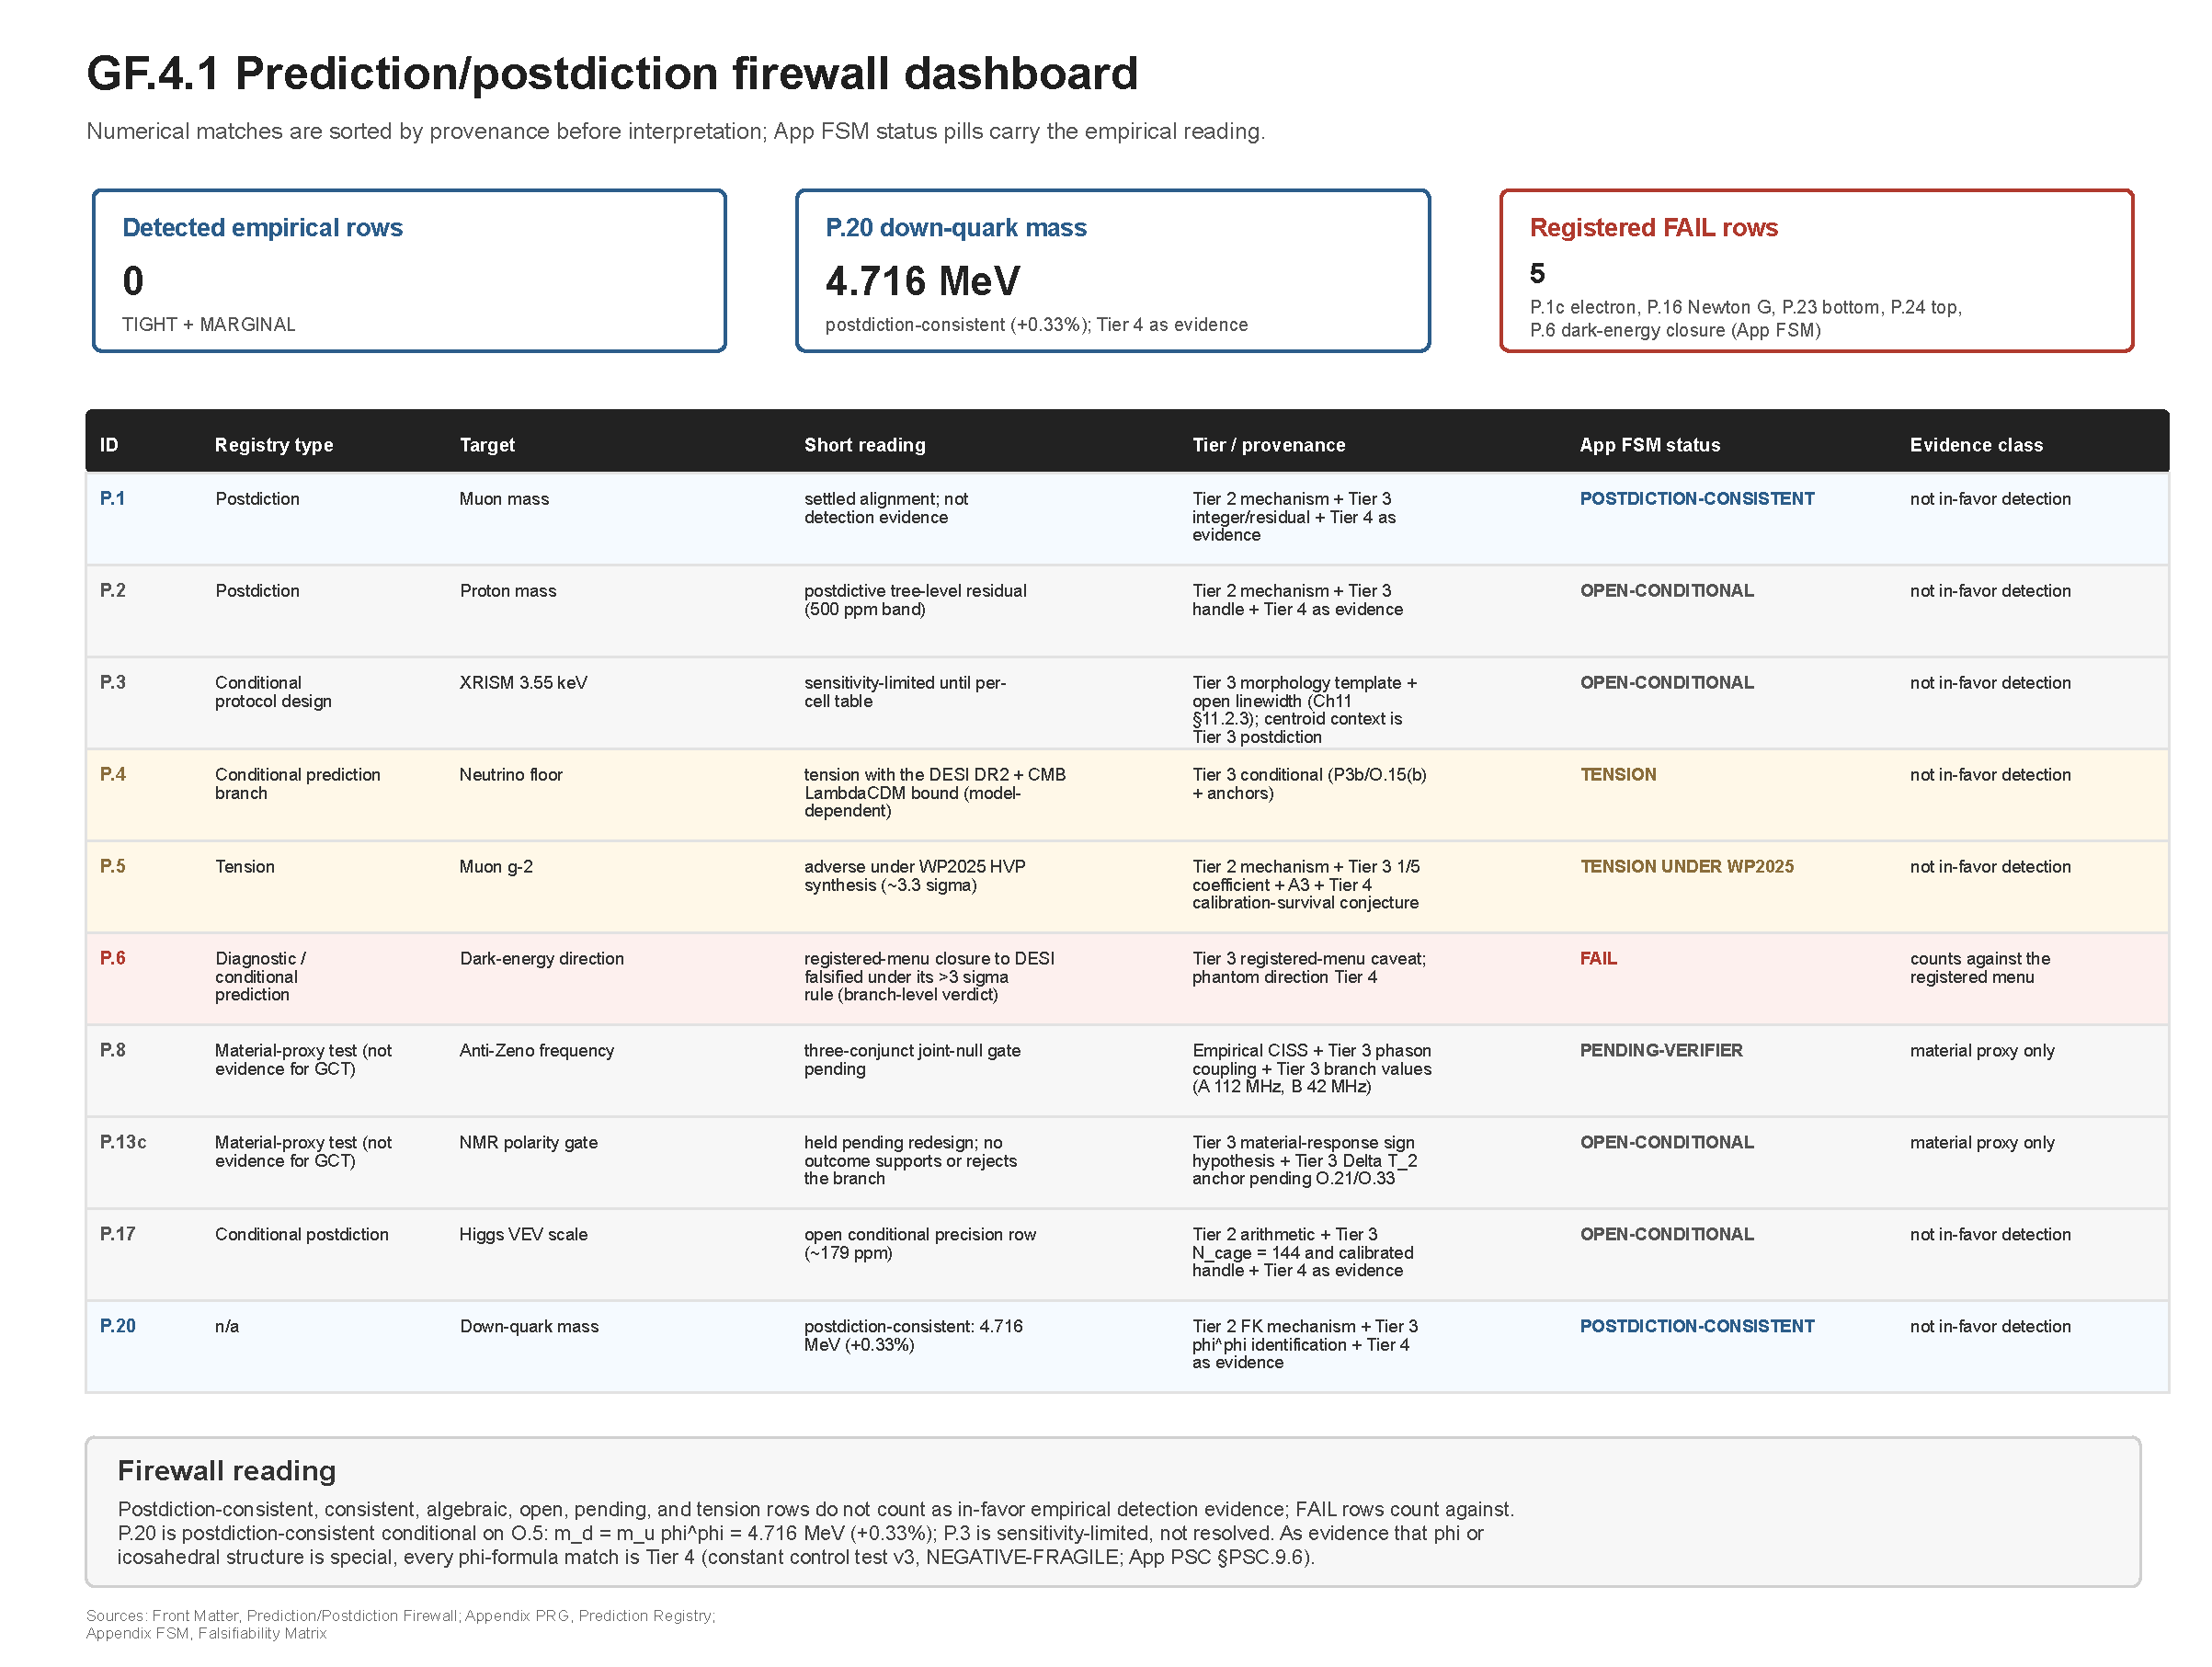
\includegraphics[keepaspectratio,alt={Numerical matches are sorted by provenance before interpretation: postdictions, predictions, tensions, sensitivity-limited rows, and registered FAIL rows have different evidential meanings.}]{content/Figures/Frontmatter/Figure GF.4.1.pdf}}
\caption{Numerical matches are sorted by provenance before
interpretation: postdictions, predictions, tensions, sensitivity-limited
rows, and registered FAIL rows have different evidential meanings.}
\end{figure}

\section{1. Definitions}\label{definitions}

\subsection{\texorpdfstring{\textbf{A. Prediction
(Targeted)}}{A. Prediction (Targeted)}}\label{a.-prediction-targeted}

A value derived from the theory's internal geometry \emph{before}
reference to a specific measurement, or a value that exceeds current
experimental precision.

\begin{itemize}
\tightlist
\item
  \textbf{Criteria:} No undisclosed parameter is adjusted to match the
  result.
\end{itemize}

\textbf{Example --- PTA Structural Program:} the rotational-icosahedral
scalar harmonic has its first nonconstant invariant at \(\ell=6\). A
physical timing-residual response, its normalization, and a
falsification statistic require a separate
action-to-propagator-to-pulsar transfer calculation. This is a
structural theorem plus an open research program, not a numerical
prediction.

\begin{quote}
\textbf{Note on High-Discriminating Postdictions:} Some postdictions are
more informative than broad curve-fitting exercises because their
registered internal search windows are small and explicitly disclosed,
but they remain \emph{Alignment} matches rather than free predictions.
\textbf{Example:} The Tau mass formula
\(m_\tau = m_e \phi^{17}(1 - 3.6\alpha)\) has the Tier 2 harmonic
mechanism \(\phi^{17}\) with the Tier 3 exponent anchor \(N=17\), the
Tier 2 \(A_5\)-channel-averaging mechanism for the screening factor, and
a coefficient built from the Tier 2 integer \(D=18\) (the \(H_3\)
Shephard-Todd invariant-degree sum), the integer \(N=5\) and the
load-bearing Tier 3 ratio rule \(c=-D/N=-18/5=-3.6\), pending
first-principles derivation under App ORQ O.26b. \(N = 5\) is the count
of the five \(A_5\) irreps (trivial included); reading them as phason
channels is a Tier 3 convention (Tier 3 as a channel number). It is the
same origin as the muon \(+5\alpha\) channel count. The RT arithmetic
\((4F-3V_3)/V_5=5\) gives the same integer but is a numerical
coincidence check, not a second derivation. No global significance is
claimed for the match (earlier figures withdrawn; see §3 rule 1). A
small registered search window can raise a postdiction's diagnostic
interest inside the framework, but it does not convert an already-known
numerical alignment into a prediction-grade statistical result. As
evidence that φ is special, the tau match is \textbf{Tier 4} (constant
control test v3, NEGATIVE-FRAGILE; App PSC §PSC.9.6).
\end{quote}

\subsection{\texorpdfstring{\textbf{B. Postdiction
(Alignment)}}{B. Postdiction (Alignment)}}\label{b.-postdiction-alignment}

An after-the-fact explanation of known data where the model's structural
features map onto observed values.

\begin{itemize}
\tightlist
\item
  \textbf{Criteria:} The structure was designed to be consistent with
  the data, though the numerical match may be emergent.
\item
  \textbf{Example:} The proposed icosahedral construction of the SU(3)
  \(\times\) SU(2) \(\times\) U(1) gauge-group candidate and chirality
  from the RT window and Jackiw-Rebbi domain wall (an open Tier 3
  candidate; App ORQ O.39).
\end{itemize}

\subsection{\texorpdfstring{\textbf{C. Consistency Check
(Calibration)}}{C. Consistency Check (Calibration)}}\label{c.-consistency-check-calibration}

A match achieved by adjusting one or more ``Calibrated Parameters''
(Tier 3) to align the model with empirical anchors.

\begin{itemize}
\tightlist
\item
  \textbf{Criteria:} Used to determine the value of a free parameter
  (\(\lambda, \tau, \epsilon\)).
\item
  \textbf{Example:} The matching of the Dark Energy \(w(z)\) curve using
  \(\lambda_{bio}\).
\end{itemize}

\begin{center}\rule{0.5\linewidth}{0.5pt}\end{center}

\section{2. Firewall Metadata
Template}\label{firewall-metadata-template}

Every major numeric match carries a \textbf{Firewall Metadata} note (an
Important callout headed ``Firewall Metadata'' with the protocol name)
in the margin or section footer, with the following fields:

\gctneedbreak{10\baselineskip}

{\def\LTcaptype{none} % do not increment counter
\begin{longtable}[]{@{}
  >{\raggedright\arraybackslash}p{(\linewidth - 4\tabcolsep) * \real{0.3333}}
  >{\raggedright\arraybackslash}p{(\linewidth - 4\tabcolsep) * \real{0.3333}}
  >{\raggedright\arraybackslash}p{(\linewidth - 4\tabcolsep) * \real{0.3333}}@{}}
\toprule\noalign{}
\begin{minipage}[b]{\linewidth}\raggedright
Field
\end{minipage} & \begin{minipage}[b]{\linewidth}\raggedright
Allowed values
\end{minipage} & \begin{minipage}[b]{\linewidth}\raggedright
Meaning
\end{minipage} \\
\midrule\noalign{}
\endhead
\bottomrule\noalign{}
\endlastfoot
\textbf{Type} & Prediction / Postdiction / Consistency Check & The match
category defined in §1 (A, B or C). \\
\textbf{Inputs} & The list of Parameters and Anchors used & Every
Parameter Ledger entry and empirical anchor the formula consumes. \\
\textbf{Degrees of Freedom} & A non-negative integer & The number of
adjustable knobs available when the match was made. \\
\textbf{Provenance} & Internal derivation / Calibrated fit / Heuristic &
How the numerical value was obtained. \\
\end{longtable}
}

\begin{center}\rule{0.5\linewidth}{0.5pt}\end{center}

\section{3. Governance Rules}\label{governance-rules}

\begin{enumerate}
\def\labelenumi{\arabic{enumi}.}
\tightlist
\item
  \textbf{The Overlap Rule:} A single formula structurally shared across
  multiple members carries the SAME prediction/postdiction status as its
  first-anchored member, unless the second/third member's value was
  unknown at the time of the formula's derivation. The
  structural-sharing claim does not promote postdictions to predictions.
\end{enumerate}

\textbf{Significance of the lepton exponent pair (N=11, N=17).} Earlier
global-significance figures for the numerical matches are withdrawn: the
cross-base comparison could not, by construction, credit any base other
than \(\phi\), and the trial counts behind the quoted σ values were
asserted rather than enumerated. As evidence that \(\phi\) or
icosahedral structure is special, these matches are \textbf{Tier 4}: the
preregistered constant control test (v3, NEGATIVE-FRAGILE; App PSC
§PSC.9.6) found \(\phi\)'s pattern of matches on 21 constants not
distinguishable from that of random constants (58 of 300 random bases
did at least as well). The test ``excludes, at power ≥ 0.8, an effect in
which φ hits at least 6 of the 8 informative rows through a real effect;
weaker effects are not excluded.'' The numbers are kept as descriptive
arithmetic, and no global significance is claimed. The test is
non-confirmatory (it re-analyses public data, and its statistic was
chosen after v1 and v2); confirmatory evidence can only come from
formulas registered before their targets are compared. The earlier table
of look-elsewhere figures (≈2.6σ, ≈3.1σ, ≈4.4σ and the single-trial
≈5.4σ) is withdrawn on the same grounds.

\textbf{Tier 3 marker:} the nominal \textasciitilde0.002\% (≈21 ppm)
muon-ratio figure needs the full factor
\((1+5\alpha_{\rm A3}+\phi^{8}\alpha_{\rm A3}^2)\). The bare
\(\phi^{11}\) ratio is about \(3.75\%\) low; the first-order
\((1+5\alpha_{\rm A3})\) drag correction (\(A_5\) irrep count, Tier 3 as
a channel number; equal-weight normalization Tier 3) leaves about
\(2429\) ppm; and the ≈21 ppm residual requires the second-order
\(\phi^{8}\alpha^2\) term, whose \(-3\) exponent selection inherits the
Tier 3 H-EW boundary, so it is conditional on H-EW and on A3. The
\((1-5\alpha)\) factor belongs to the electron Planck-link check and is
not an electroweak correction to the lepton ratios.

\begin{enumerate}
\def\labelenumi{\arabic{enumi}.}
\setcounter{enumi}{1}
\tightlist
\item
  \textbf{The ``Hidden Knob'' Prohibition:} Any constant used in an
  equation that is not a Fundamental Constant (\(\phi, \pi, \hbar\); the
  bare geometric \(\alpha\) expression is not the measured low-energy
  input, and \(G\) is an output row, not an input) or a listed Anchor
  (A1 \(m_e\); A2 \(\alpha_2^{-1}(M_{\rm GUT})\) for the native-RGE
  endpoint check; A3 \(\alpha(0)\) for measurement-anchored
  precision-comparison rows; A4--A6 the gauge-flow normalisations
  \(Z_1, Z_2, Z_3\)) is declared as a \textbf{Calibrated Parameter} in
  the ledger. See Parameter Ledger §0.1 (rows A1--A6) and its disclosure
  of the two roles of \(\alpha\). The phrase ``fundamental constants''
  here excludes A3: the measured low-energy \(\alpha(0)\) is an anchor,
  used only in precision-comparison rows per the Ledger.
\item
  \textbf{PTA Response Boundary:} the first rotational-icosahedral
  scalar harmonic is at \(\ell=6\), and a physical icosahedral signal
  must retain an absolute orientation \(R\in SO(3)/I\). A
  separation-only Legendre term, a numerical amplitude, and a
  one-dimensional power ratio are not physical PTA observables until the
  action, propagator, pulsar response, normalization, and likelihood
  discriminator are derived and registered. Likewise, no PTA, RM, DM,
  kSZ, or Bell amplitude may be copied from \(\phi^{-18}\) without an
  independently derived action-to-observable map.
\item
  \textbf{Historical Protected-Subspace Material Scenario (formerly
  ``Zeno Drive Shielding Constraint''):} The supplied comparison from an
  assumed Tubulin Tryptophan (Trp) radical-pair baseline
  \(T_2\sim1\)--\(10\ \mu\)\hspace{0pt}s to a historical 10 ms target
  gives \(S\sim10^3\). Neither endpoint is a demonstrated tubulin
  Zeno-Drive quantity, and the protected-subspace mechanism remains open
  under O.23. Bulk-water decoherence (\(\sim 10^{-13}\) s) is an
  inapposite baseline for this specific material comparison, but that
  correction does not derive a Selection clock or a Level-II gate.
\item
  \textbf{Dark Energy Causality:} The parameter \(\lambda_{bio}\) and
  the operative biogenic-DE quartic mass scale
  (\(m_{\rm phason}^{\rm operative} \approx 1.7 \times 10^{-5}\) eV) are
  \textbf{Tier 3 phenomenological fits}, calibrated to match observed
  cosmological acceleration; the physical-source interpretation of the
  biogenic channel is Tier 4. The susceptibility \(\chi\) has a
  \textbf{Tier 2 functional form} via the horizon-entropy area law
  (Bekenstein--Hawking / Gibbons--Hawking de Sitter horizon entropy;
  \(\chi = A_{\mathcal{H}_{CE}}/(4\ell_P^2)\), V2 Ch14 §14.1.5), but the
  Tier 3 numerical evaluation \(\chi \approx 2.27\times10^{122}\)
  requires imported \(H_0\) pending O.1/O.4. The only baseline the
  framework supplies without these fits is the equation of state
  \(w=-1\), and that is itself a Tier 3 reading: it follows if the
  frozen-strain energy density is constant in \(a\), but no covariant
  stress-energy or dilution law is derived (V2 Ch14).
\item
  \textbf{Spin--Phason Dimensional Firewall (formerly ``Biological
  Phason Freezing''):} At physiological temperature
  \(k_B T(310\,{\rm K}) = 0.0267\,{\rm eV}\) is an energy. With
  \([\nabla\Phi_\perp]=[k]=L^{-1}\) and \(\alpha_R\) in Rashba units
  \(E\,L\) (V1 Ch17 §17.1.3), the product \(\alpha_R k\nabla\Phi_\perp\)
  has units \(E/L\), so the quantity labelled
  \(E_{RP}\approx0.3\,{\rm eV}\) cannot be divided by \(k_BT\) as a
  dimensionless thermal margin, and the former ``clear \(k_BT\) by a
  factor of ten'' acceptance criterion is withdrawn. The 38.0/38.3 MHz,
  \(\eta_{\rm Zeno}\) and \(N_{\rm coh}\) values are conditional
  external-rate scenarios (V1 Ch17 §17.1.3); they cannot support DMC
  phason-gate or Level-II claims. There is no registered
  \(1.6\,{\rm eV}\) body-temperature freezing energy.
\item
  \textbf{Theorem Elevators:}
\end{enumerate}

\begin{itemize}
\tightlist
\item
  The Bottom Quark scaling factor (\(5/4\)) is formalized as the exact
  Tier 2 \(A_5\) representation-dimension identity
  \(\dim(H)/\dim(G)=5/4\); its deployment as the physical bottom-quark
  mass coefficient remains Tier 3 pending Open Problem O.43.
\item
  The Phason stiffness exponent \(\phi^{-18}\) is formally classified
  per Parameter Ledger §0.1 P3a/P3b as \textbf{Tier 2
  integer-identification (\(H_3\) Shephard-Todd anchor, conditional on
  the irreducible icosahedral premise) + registered Tier 3 stiffness-map
  hypothesis P3b, listed outside the postulate count like H-EW}. No Tier
  2 softness mechanism is claimed: icosahedral symmetry leaves the
  invariant quadratic family \(Q=aP_\parallel+bP_\perp\) with \(b/a\)
  free, so the size of any phason/phonon stiffness ratio needs
  additional dynamics. The specific exponent \(D = 18\) is the
  \(H_3\)-specific icosahedral anchor --- the \(H_3\) Shephard-Todd
  invariant-degree sum \(\{2, 6, 10\} = 18\). Only \(H_3\) attains 18
  within the finite irreducible rank-three classification (\(A_3=9\),
  \(B_3=12\), \(H_3=18\); Humphreys 1990), but the reducible finite
  system \(A_1\times I_2(14)\) also has degree sum 18; the number alone
  does not select \(H_3\) without the irreducible icosahedral premise.
  The RT-face tangent-bundle count \(6+6+6=18\) (Anchor B, App ORQ O.26)
  enters as a 6D-ambient consistency cross-check, not as a second
  independent icosahedral anchor (see App ORQ O.26). The sharper
  RG-running claim \(K_\perp/K_\parallel = \phi^{-D}\) at the
  renormalization-flow level is Tier 3 pending Open Problem O.15(b)
  (first-principles RG derivation). The physical \(c_T \equiv c\)
  identification is Tier 3: it rests on the second-sound photon
  identification of V2 Ch05--Ch06, which is a Tier 3 postulate and a
  declared open programme.
\end{itemize}

\begin{enumerate}
\def\labelenumi{\arabic{enumi}.}
\setcounter{enumi}{7}
\tightlist
\item
  \textbf{XRISM Observational Status:} The XRISM test for the 3.55 keV
  dark matter line is \textbf{Under Test (Data Inconclusive, Analysis
  Ongoing)}. XRISM has stacked 3.75 Ms of data across 10 clusters and
  did not resolve the line. The upper limit on the decay rate
  (\(\Gamma \lesssim 1.0 \times 10^{-27}\ \mathrm{s}^{-1}\)) remains
  several times weaker than the Bulbul et al.~XMM-Newton
  order-\(10^{-28}\ \mathrm{s}^{-1}\) detection normalization. XRISM has
  not yet reached the required sensitivity to confirm or rule out the
  signal. The GCT line therefore remains under test (its centroid also
  inherits the Tier 3 \(N_{\rm cage}=144\) posit; App TAT); deeper
  observations are required. For full ground-truth data, see V3 Ch11
  §11.4.4 and V3 Ch15 §15.5.
\end{enumerate}

\begin{center}\rule{0.5\linewidth}{0.5pt}\end{center}

\part[VOLUME 1 Operating System]{VOLUME 1 Operating System\\[4ex]{\Large\mdseries\itshape Dynamics of the Timeless Field}}
\setcounter{chapter}{0}

\chapter*{Volume 1 Abstract}
\addcontentsline{toc}{chapter}{Volume 1 Abstract}
\markboth{Volume 1 Abstract}{Volume 1 Abstract}
\setcounter{section}{0}

\textbf{Volume 1} serves as the ontological kernel of Geometric
Consciousness Theory (GCT). It posits that the fundamental layer of
reality is not a spatiotemporal manifold populated by matter, but a
timeless, infinite-dimensional configuration space \(\mathcal{P}\)
governed by the \textbf{Wheeler-DeWitt equation} (\(\hat{H}\Psi=0\)). On
the Tier 3 Wheeler--DeWitt structural postulate, GCT models the
constrained state as a static \textbf{Supersolid Quasicrystal}, the
geometry of which (\(\Phi_0\)) is proposed to encode all possible
physical histories; no solution of \(\hat{H}\Psi=0\) is derived.

We \textbf{dissolve} the ``Hard Problem'' of consciousness --- \emph{not
solve it from physics} --- by stipulating universal Level I presence as
Axiom 1 {[}Tier 1{]}, motivated by the sole Tier 0 datum that experience
is occurring (neither postulated nor derived; see V1 Ch16 §16.2.2b for
the canonical dissolve-by-axiomatization framing). What GCT
\emph{derives} is the \textbf{Quality Space topology} (the graded
\(I_h\)-irrep decomposition of §16.2.2c --- 6 linear coordinate DOF plus
21 quadratic stress DOF) and a conditional algebraic unity candidate for
trefoil-class Identity Polarons. Trefoil-case Polaron Unity is at most a
Tier 3 algebraic unity candidate: Proposition PUP.1(ii) (Hilbert-space
non-factorizability) is withdrawn by an exact \(A_5\) counterexample,
O.35/O.36 fail as posed for the represented trefoil group \(B_3\) (its
centre \(\langle\Delta^2\rangle\) makes the amenable radical nontrivial
and \(L(B_3)\) non-factorial) and hold for the further central quotient
\(B_3/Z(B_3)\cong C_2*C_3\) {[}Tier 1 --- standard{]}; whether any
physical sector is that quotient's regular representation is open
{[}Tier 3{]}; and the physical full-fibre-support/complement-map closure
remains a sub-closure of Open Problem O.18; the general-prime extension
remains Tier 3 conditional on Anderson-Putnam-to-knot-complement
extension, canonicity of \(K \to A_K\), a controlled meridian
representation with convergence and trace descent, and KO-dim-6 sign
verification (O.32). Even full closure of these conditions would
establish at most an algebraic unity candidate, not Level II
apperception, an owner, or a subject count. The \textbf{Selection
Operator} (\(\mathcal{F}_{sel}\)) is the proposed \emph{Quality Space
individuation} and \emph{unity} mechanism --- it supplies the structural
account of \emph{which} phenomenal content the substrate carries at a
given configuration and models candidate structural conditions for
unified subjective experience rather than fragmented micro-experiences
once the Polaron Unity conditions hold; it does \textbf{not} supply the
resolution of the existence-gap, which is handled by Axiom 1 alone.
Chapter 9 presents a \textbf{Tier 3 measurement-model proposal} in which
a supplied Selection Operator acts as a constrained filter on the global
wavefunction \(\Psi\); the manuscript has not yet derived that physical
operator, its Born measure, its substrate realization, or a phenomenal
owner, so this is not a completed solution of the ``Measurement
Problem''. Time is not treated as a fundamental dimension: the static
coordinate \(\tau_{\text{coord}}\) (the lattice address of a
configuration) and an ordinal selection index \(n\) provide a candidate
relational-time representation. Identifying that index with an
observer's proper or phenomenal time, and with the subjective experience
of temporal flow, requires transition, memory, owner, and phenomenal
bridges that remain open.

Crucially, this volume proposes a geometric \textbf{System Resolution}
for the physical model. App USS records \(A_5\) as the Tier 1/2
architectural premise H1 and derives conditional Schur-cover and McKay
consequences; it does not prove point-group uniqueness or eliminate
other spinorial point groups. The Golden Ratio (\(\phi\)) projection
remains the primary candidate for the global entropy-packing optimum
rather than a settled slope-maximality theorem. The \textbf{Electron
Mass (\(m_e\))} relation uses the 6D lattice spacing and a
Peierls-Nabarro ansatz
(\(m_e = M_P \times \phi^{-107} \times (1-5\alpha)\); \textbf{Tier 2
mechanism + Tier 3 exponent anchor + Tier 4 physical-link conjecture
pending O.14}). Because \(m_e\) is the A1 anchor, the relation is a Tier
3 anchor-normalised Planck-link check: its 1006 ppm residual misses the
pre-registered 1000 ppm pre-commitment by 6 ppm, and App FSM P.1c
reports a \textbf{FAIL} of that rule. We further obtain \textbf{Newton's
Gravitational Constant (\(G = 6.689475523 \times 10^{-11}\) m³ kg⁻¹
s⁻²)} via the Jacobson entropic gravity formula applied to the
icosahedral lattice vacuum, using the GCT-\(\alpha\) branch
\(\alpha_{\rm GCT}=\phi^2/360\) with CODATA \(m_e\) and exact SI
\(h,c\), with disposition \textbf{Tier 2 thermodynamic mechanism + Tier
4 Planck-link conjecture inheriting O.14 + Tier 3 dimensional anchor}
(the numerical \(G\) row is the electron Planck-link row inverted,
\(G\propto m_e^{-2}\), so it is not independent evidence and is not
counted as a pass while the electron row fails its pre-registered rule),
and the bare \textbf{Fine-Structure Constant} relation
\(\alpha^{-1} = 360\phi^{-2} \approx 137.508\) as a geometric
electromagnetic-coupling ansatz \textbf{{[}Tier 3 numerical relation
(Tier 3 600-cell multiplier; mechanism open --- the RT solid-angle
construction is withdrawn, V1 §13.2.1--§13.2.2) + residual closure
target; 3443 ppm from CODATA; see Chapter 13 and App ORQ O.19/O.5{]}}.
Its historical ``selection-interface impedance'' interpretation does not
derive a physical Selection Operator or Agent bandwidth. As evidence
that φ or icosahedral structure is special, these φ-formula matches are
\textbf{Tier 4}: the preregistered constant control test (v3,
NEGATIVE-FRAGILE; App PSC §PSC.9.6) found φ's pattern of matches on 21
constants not distinguishable from that of random constants (58 of 300
random bases did at least as well). The test ``excludes, at power ≥ 0.8,
an effect in which φ hits at least 6 of the 8 informative rows through a
real effect; weaker effects are not excluded.'' The numbers are kept as
descriptive arithmetic.

We construct the \textbf{Identity Space candidate} as the universal
Adelic Solenoid \(\Sigma_\infty\) {[}Tier 1 mathematics{]}. Its
transversal is all-prime,
\(\widehat{\mathbb{Z}}\cong\prod_p\mathbb{Z}_p\); a rooted address tree
and its ultrametric arise only on a selected base fiber or local
transversal chart after choosing a cylinder filtration, and the
Solenoid's ordinary fundamental group is trivial. The exact topology
therefore supplies an address-and-resolution skeleton; it does not by
itself supply infinite non-erasable memory, a selected \(p\)-adic
identity code, an owner, or a Level-II observer. Identifying a chosen
address presentation with the \textbf{Nuclear Spin States (\(I\))} of
the biological substrate, and deriving its read/write, protection,
ownership, and physical-scope maps, remain explicit Tier 3 bridges. The
further association of subjective experience (Qualia) with the
\textbf{Topological Friction} experienced by the Agent as it navigates
the vacuum lattice \(\Phi_0\) is a Tier 3 structural-Russellian
proposal: no examined Agent, phason-work channel, owner, or phenomenal
registration presently realizes it.

\chapter*{Preface to Volume 1: The Logic of Being}
\addcontentsline{toc}{chapter}{Preface to Volume 1: The Logic of Being}
\markboth{Preface to Volume 1: The Logic of Being}{Preface to Volume 1: The Logic of Being}
\setcounter{section}{0}

\gctneedspace{5\baselineskip}

\textbf{V1.1 The Ontological Primitive}

The central crisis of modern science lies in the incompatibility of its
two most successful frameworks: Quantum Mechanics, which describes a
probabilistic world of potentiality, and General Relativity, which
describes a deterministic world of geometry. Bridging them requires a
theory of Quantum Gravity, but all attempts have stumbled upon the
``Problem of Time''---the disappearance of the time variable \(t\) from
the fundamental equations. Simultaneously, the philosophy of mind faces
the ``Hard Problem''---the impossibility of deriving subjective
experience from objective matter.

GCT proposes that these may not be two separate problems, but one,
sharing a premise that GCT declines to adopt: \textbf{Materialist
Emergence}. GCT argues that the assumption that spacetime and matter are
fundamental, and that consciousness and time emerge from them, is
associated with open difficulties in both physics (singularities,
fine-tuning) and philosophy (qualia, agency); this is a motivation for
the inversion below, not a demonstration that the premise is false.

We resolve this by inverting the ontological order---not as an arbitrary
choice, but as \textbf{a methodological choice motivated by the only
\(P=1\) datum}: the existence of Experience itself. By treating
consciousness as the irreducible primitive (the Field \(\Psi\), a
framework postulate that does not itself inherit \(P=1\)) and matter as
a topological constraint within it, we propose to derive the emergence
of spacetime and physical laws from that starting point.

\gctneedspace{5\baselineskip}

\textbf{V1.2 The Mathematical Turn}

To make this claim scientific rather than mystical, we must move beyond
vague metaphors. We cannot simply say ``consciousness creates reality'';
we must write down the equation.

This requires a \textbf{Mathematical Turn} toward topology and measure
theory. We model Identity not as a neurological state, but as a
topological invariant---a knot in a higher-dimensional fiber bundle
(\(\Sigma_\infty\)). We model Choice not as a neurological impulse, but
as a linear operator (\(\mathcal{F}_{sel}\)) acting on a Hilbert space.
We model Existence not as material presence, but as a \textbf{non-null
restriction} of the global field: the configuration space possesses
measure \(\mu > 0\) wherever \(\mathcal{F}_{sel}\) produces a
non-trivial section---not by accumulation, but by holographic
restriction of the whole.

By formalizing these concepts, we aim to give the study of consciousness
a mathematical form that can be checked. The result is a research
programme rather than a finished theory: its claims carry explicit
epistemic tiers, and some of its branches are registered as falsifiable
rows (App FSM), each of which tests only the branch it names.

\gctneedspace{5\baselineskip}

\textbf{V1.3 Scope and Boundaries}

This volume is restricted to the foundational structure and governing
parameters of reality. It deals with:

\begin{itemize}
\tightlist
\item
  \textbf{Ontology:} What exists? (The Field and the Knot).
\item
  \textbf{Logic:} How does it structure itself? (Idealism, Discrete
  Geometry).
\item
  \textbf{Universal Constants:} What is the resolution? (Geometric
  routes to \(\alpha\), \(G\) and \(\ell_P\), each at its own tier;
  Ch13).
\item
  \textbf{Dynamics:} How does it change? (The Wheeler-DeWitt Constraint,
  Selection).
\end{itemize}

It does \emph{not} address the concrete physical realizations---the
specific taxonomy of particles (electrons, quarks) or the specific
hydrodynamics of cosmology (Dark Energy Lagrangian)---except where they
define the structural architecture. Those realizations are the subject
of \textbf{Volume 2 (The Cosmic Architecture)} and \textbf{Volume 3 (The
Matter Spectrum)}.

\chapter*{Volume 1 Notation and Symbolic Conventions}
\addcontentsline{toc}{chapter}{Volume 1 Notation and Symbolic Conventions}
\markboth{Volume 1 Notation and Symbolic Conventions}{Volume 1 Notation and Symbolic Conventions}
\setcounter{section}{0}

To ensure precision in our derivations and avoid symbolic collisions
with the particle physics definitions in Volume 3, we adopt the
following symbolic conventions for Volume 1.

\subsubsection{\texorpdfstring{\textbf{Fundamental
Spaces}}{Fundamental Spaces}}\label{fundamental-spaces}

\begin{itemize}
\tightlist
\item
  \textbf{\(\Psi\) (The Field):} The Universal Wavefunction satisfying
  \(\hat{H}\Psi=0\). The fundamental substrate of consciousness. Where
  the text says ``consciousness field \(\Psi\)'', it means the Field, in
  its Level I, non-subjective sense.
\item
  \textbf{\(\Sigma_\infty\) (Adelic Solenoid):} GCT's candidate
  address-and-resolution scaffold for Identity, constructed as the
  inverse limit of circle wrappings, with all-prime transversal
  \(\widehat{\mathbb{Z}}\cong\prod_p\mathbb{Z}_p\) {[}Tier 1
  mathematics{]}. It has no intrinsic single-prime filtration, rooted
  tree, owner, memory, history, transition law, or phenomenal
  interpretation; a chosen cylinder tree lives on a selected base fiber
  or local transversal chart. Treating it as the fiber that encodes an
  observer's internal state is a Tier 3 bridge requiring a physical
  address map.
\item
  \textbf{\(\mathcal{P}\) (Configuration Space):} The domain of the
  consciousness field \(\Psi\). The shorthand
  \(\mathcal{P} \cong \Sigma_\infty \times (E_\parallel \oplus E_\perp)\)
  is a \textbf{Tier 3 factor ansatz}, not a topology theorem or a
  literal physical realization; using a Solenoid coordinate in a
  physical render additionally requires a physical address map and a
  physical realization rule.
\item
  \textbf{\(E_\parallel\) (Parallel Space):} The 3-dimensional physical
  manifold (the ``screen'' of projection).
\item
  \textbf{\(E_\perp\) (Perpendicular Space):} The 3-dimensional internal
  manifold containing the ``hidden'' degrees of freedom (Phasons).
\item
  \textbf{\(\Phi_0\) (Vacuum Condensate):} The specific ground-state
  lattice geometry (Supersolid Quasicrystal) that solves the Hamiltonian
  constraint. Distinguished from \(\Phi\) (Higgs Field).
\end{itemize}

\subsubsection{\texorpdfstring{\textbf{Operators and
Generators}}{Operators and Generators}}\label{operators-and-generators}

\begin{itemize}
\tightlist
\item
  \textbf{\(\mathcal{F}_{sel}\) (Selection Operator):} A proposed
  linear, non-unitary Agent-frame update (conditionalization) on
  declared states, intended to represent conscious actualization by
  mapping the global superposition to a specific experiential section.
  No examined physical carrier, instrument, clock, intent map, owner, or
  phenomenal event presently realizes it, and \(\Sigma_\infty\) supplies
  no dynamics for it.
\item
  \textbf{\(\hat{\mathcal{R}}\) (Realization Operator):} The proposed
  Agent-relative realization/projection rule relating Field data to a
  render in \(E_\parallel\). Treating a \(\Sigma_\infty\) address as one
  of its inputs requires a physical address map, and the physical
  address-to-render rule itself is an open Tier 3 bridge.
\item
  \textbf{\(\hat{H}\) (Hamiltonian Constraint):} The generator of time
  reparameterizations that annihilates the physical state
  (\(\hat{H}\Psi=0\)).
\end{itemize}

\subsubsection{\texorpdfstring{\textbf{Metrics and
Coordinates}}{Metrics and Coordinates}}\label{metrics-and-coordinates}

\begin{itemize}
\tightlist
\item
  \textbf{\(\mathbb{I}_K\) (Hierarchical Identity):} The proposed
  transversal residue coordinate for the observer, extracted only after
  a physical address map and a base-fiber/local-chart choice. It is a
  compatible all-prime residue system in \(\widehat{\mathbb{Z}}\) (a
  full Solenoid point also carries its suspension coordinate); a single
  \(p\)-adic digit string and its substrate realization are selected
  Tier 3 data.
\item
  \textbf{\(\tau_{\text{coord}}\) (Relational Time Coordinate):} The
  ordinal address of a configuration in the static lattice sequence.
  \emph{Distinct from the Tau lepton (\(\tau\)) appearing in Volume 3.}
\end{itemize}

\begin{quote}
\textbf{Note:} \(\tau_{coord}\) denotes coordinate time exclusively. The
symbol \(\tau\) without subscript refers to \(\tau_{coord}\). The
quadrupole shielding time uses \(\tau_Q\) (subscript \(Q\) always
explicit). The tau lepton mass uses \(m_\tau\).
\end{quote}

\begin{itemize}
\tightlist
\item
  \textbf{\(d_H(i,j)\) (Hierarchical Distance):} A compatible
  ultrametric on a declared nested-cylinder filtration of the identity
  address tree. It measures common address resolution, not physical
  scope or ownership.
\item
  \textbf{\(\kappa_{ij}\) (Coupling Coefficient):} A Tier 3
  phenomenological physical interaction kernel between agents \(i\) and
  \(j\), sometimes modeled as \(\kappa_0 e^{-\lambda_c d_H}\) only after
  a filtration, a physical address map, and an independently justified
  address-to-coupling law are declared.
\item
  \textbf{\(\lambda_c\) (Consensus Decay Constant):} A phenomenological
  range parameter in the optional exponential coupling ansatz. Neither
  its value nor the exponential law is determined by Solenoid topology;
  both require calibration or derivation from the physical kernel.
\end{itemize}

\subsubsection{\texorpdfstring{\textbf{Temporal Language
Conventions}}{Temporal Language Conventions}}\label{temporal-language-conventions}

Because GCT treats time as emergent, we distinguish between two frames
of reference:

\begin{itemize}
\tightlist
\item
  \textbf{Agent Frame (Sequential):} A conditional description indexed
  by an ordinal \(n\) and using terms like ``next,'' ``then,''
  ``evolution,'' and ``process.'' Identifying it with an observer's
  perspective or with phenomenal time requires the open transition,
  clock, owner, and phenomenal bridges.
\item
  \textbf{Field Frame (Timeless):} The perspective of the global
  wavefunction. Uses terms like ``static,'' ``correlation,''
  ``geometry,'' and ``structure.'' Time is a coordinate
  (\(\tau_{coord}\)).
\end{itemize}

\subsubsection{\texorpdfstring{\textbf{The Tier Classification
System}}{The Tier Classification System}}\label{the-tier-classification-system}

We categorize all claims by their epistemic status:

\begin{itemize}
\tightlist
\item
  \textbf{Tier 0 (Bedrock / First-Person Datum):} Exactly one item:
  experience is occurring, i.e.~there is presence now. It is neither
  postulated nor derived; no other claim may enter Tier 0. Axiom 1
  remains its stipulated universal Level I generalisation (Tier 1). Tier
  0 supplies no Level II substrate verdict; those remain open (Tier 3).
\item
  \textbf{Tier 1 (Structural Axiom):} Results following necessarily from
  axioms + mathematics.
\item
  \textbf{Tier 1/2 (Architectural Postulate + Conditional Mathematics):}
  Results that follow from the specific architecture choice (6D lattice,
  icosahedral projection) but are not deductively forced by the axioms
  alone. The architecture is justified by parsimony and empirical
  adequacy, not logical necessity, and conditional mathematics never
  promotes the premise it assumes. Marker: \texttt{{[}Tier\ 1/2{]}}
\item
  \textbf{Tier 2 (Geometric / Derived):} Results following from the
  specific icosahedral quasicrystal ansatz.
\item
  \textbf{Tier 3 (Phenomenological / Calibrated):} Models calibrated to
  observation where first-principles derivation is incomplete.
\item
  \textbf{Tier 4 (Speculative / Order-of-Magnitude):} Exploratory
  calculations where dimensional structure is correct but numerical
  coefficient is uncertain by \textgreater1 OOM. Claims include explicit
  OOM bounds. Tier 4 also covers ontological extensions outside the core
  falsifiable theory. Example: biogenic dark energy driving force (V2
  Ch14).
\end{itemize}

The closure target is a one-anchor gauge/lepton system, but the present
manuscript is not at that target. Per Parameter Ledger §0.1, the current
gauge + lepton + native-RGE endpoint + precision-comparison accounting
is 5-postulate-plus-6-continuous-anchor: P1 plus the integer anchors
\(n=-107\), \(D=18\), \(N=11\), \(N=17\); A1 (\(m_e\)); A2
(\(\alpha_2^{-1}(M_{\rm GUT})\)); A3 (measured low-energy \(\alpha(0)\)
for corrected lepton/Higgs/QED comparison rows); and A4-A6 (the App GRF
\(Z_1\), \(Z_2\), \(Z_3\) \(\beta\)-coefficient magnitude
normalisations). A named precision/gauge comparison subset contains the
six Tier-3 coefficient handles \(1440\), \(12\), \(360\), \(2\),
\(10\phi^2\), and \(1/5\). This is a scoped subset, not a
manuscript-wide handle total; sector-specific coefficients are
catalogued separately. The O.38 \(N=144\) cage posit is also separate
from both this subset and the six continuous anchors. Volume 1 uses this
table as the current-state qualifier whenever downstream constants such
as \(\alpha\), \(m_e\), \(G\), or \(\xi\) are referenced.

\clearpage
\thispagestyle{empty}
\vspace*{0.35\textheight}
\begin{center}\bfseries\LARGE PART I: THE LOGIC OF BEING\end{center}
\vspace*{\fill}
\clearpage

\chapter{Chapter 1: The Staircase of
Certainty}\label{chapter-1-the-staircase-of-certainty}

\subsection{1.1 The Problem of the Starting
Point}\label{the-problem-of-the-starting-point}

\subsubsection{1.1.1 The Crisis in Foundational
Physics}\label{the-crisis-in-foundational-physics}

Modern physics finds itself in a paradoxical state. On the one hand, it
possesses two theories of unparalleled predictive power: Quantum
Mechanics (QM), which governs the subatomic realm, and General
Relativity (GR), which governs the cosmic realm. On the other hand,
these theories are mutually incompatible at their core. QM describes a
probabilistic world of discrete quanta evolving against a fixed
background, while GR describes a deterministic world of continuous
geometry where the background itself is dynamic.

Attempts to unify them into a Theory of Everything (TOE) have stalled
for half a century. The symptoms of this stagnation are well-known:

\begin{enumerate}
\def\labelenumi{\arabic{enumi}.}
\tightlist
\item
  \textbf{The Measurement Problem:} Quantum mechanics provides no agreed
  mechanism for how a probability wave yields a definitive event;
  collapse formulations require an observer- or measurement-dependent
  rule, while no-collapse alternatives (Everett, Bohm,
  objective-collapse models) pay other costs.
\item
  \textbf{The Problem of Time:} The Wheeler-DeWitt equation
  (\(\hat{H}\Psi=0\)), the canonical result of quantizing gravity, on
  its standard reading suggests that the universe is static and
  timeless, contradicting our most basic experience.
\item
  \textbf{The Parameters Problem:} The Standard Model relies on
  \textasciitilde26 arbitrary constants (masses, couplings) whose values
  must be measured rather than derived. {[}Tier 3 --- Phenomenological
  count; exact number depends on definition of independent parameters{]}
\end{enumerate}

Geometric Consciousness Theory (GCT) posits that these are not separate
problems, but symptoms of a single methodological error: the attempt to
derive the Observer from the Observed.

\subsubsection{1.1.2 The Hard Problem as a Category
Error}\label{the-hard-problem-as-a-category-error}

The ``Hard Problem of Consciousness'' arises from the assumption that
matter is primary and consciousness is derivative. GCT inverts this
hierarchy. We posit that the failure of physicalism to account for
subjective experience is not a gap in our knowledge, but a
\textbf{result of the initial axioms}. By treating the ``Object'' as
fundamental and the ``Subject'' as emergent, standard physics creates an
unbridgeable explanatory gap.

\subsubsection{1.1.3 The Geometric
Alternative}\label{the-geometric-alternative}

Instead of trying to squeeze consciousness into a materialist framework,
we ask: \emph{What geometry is required to support a universe where the
Subject is irreducible?} This shift from ``How does the brain make a
mind?'' to ``What geometry unifies Mind and Matter?'' is the core of the
GCT program.

GCT raises two objections to the standard Materialist alternative
{[}Tier 3 --- Philosophical Framework; contested objections, not
refutations{]}:

\begin{enumerate}
\def\labelenumi{\arabic{enumi}.}
\item
  \textbf{The Something-from-Nothing Objection:} The claim that
  subjective experience emerges from sufficiently complex arrangements
  of non-experiential matter is akin to claiming that stacking enough
  zeroes eventually yields a one. It introduces an unexplained miracle
  into the causal chain --- a discontinuity of ontological kind with no
  mathematical grounding. (This is Strawson's (2006) objection to brute
  emergence; physicalists contest it, see Ch16.)
\item
  \textbf{The Circular Causation Objection:} Physics is an activity
  performed \emph{by} conscious agents. We infer the existence of
  particles based on observations made within consciousness. GCT reads
  the claim that the particles \emph{create} the consciousness as
  confusing the order of knowing with the order of being --- the
  measurement presupposes the measurer. Epistemic priority does not by
  itself entail ontological priority, and physicalists accept the first
  while denying the second; the point motivates the epistemic inversion
  of §1.1.4 rather than refuting physicalism.
\end{enumerate}

\subsubsection{1.1.4 The Requirement for Epistemic
Inversion}\label{the-requirement-for-epistemic-inversion}

To resolve the crisis, we must perform an \textbf{Epistemic Inversion}.
We cannot start with the objects of our theory (quarks, strings,
branes), because those objects are inferred. We must start with the
instrument of inference itself.

We require a foundation that is not a hypothesis, but a certainty. We
must identify the \textbf{Ontological Primitive}---the one thing that
cannot be an illusion. Only by anchoring our physics in this absolute
datum can we build a structure that does not rely on discontinuities of
emergence. We must construct the universe Top-Down, not Bottom-Up.

\begin{center}\rule{0.5\linewidth}{0.5pt}\end{center}

\subsection{1.2 The Cartesian Anchor}\label{the-cartesian-anchor}

\subsubsection{1.2.1 Radical Skepticism: Discarding the
Doubtable}\label{radical-skepticism-discarding-the-doubtable}

To find the true starting point, we employ the method of Radical
Skepticism. We systematically discard every belief that \emph{could}
theoretically be false, no matter how unlikely.

\begin{enumerate}
\def\labelenumi{\arabic{enumi}.}
\tightlist
\item
  \textbf{The External World?} Could the physical universe be an
  illusion? Yes. The \textbf{Simulation Hypothesis} or the ``Brain in a
  Vat'' scenario demonstrates that our sensory data could be a coherent
  fabrication. Therefore, the existence of matter is a hypothesis
  (\(P < 1\)). {[}Tier 3 --- Philosophical Framework{]}
\item
  \textbf{The Ego/Personality?} Could ``I'' be an illusion? Yes. The
  sense of being a continuous person with a name and history is
  interrupted by sleep, amnesia, and psychedelic dissolution. The
  ``Ego'' is a narrative construct (\(P < 1\)). {[}Tier 3 ---
  Philosophical Framework{]}
\item
  \textbf{The Past?} Could history be fake? Yes. Russell's five-minute
  hypothesis (1921; popularly ``Last Thursdayism'') suggests the
  universe could have come into existence moments ago with false
  memories implanted; the Boltzmann-brain scenario is a related argument
  about a brain fluctuating into existence. The past is an inference
  (\(P < 1\)). {[}Tier 3 --- Philosophical Framework{]}
\end{enumerate}

What remains when the world, the self, and time are stripped away?

\subsubsection{\texorpdfstring{1.2.2 The Zero-Point: Experience as the
\(P=1\)
Datum}{1.2.2 The Zero-Point: Experience as the P=1 Datum}}\label{the-zero-point-experience-as-the-p1-datum}

Even if the world is a simulation, the \textbf{experience of the
simulation} is happening. Even if the pain is hallucinatory, the
\textbf{feeling of pain} is real. Even if ``I'' do not exist, there is a
``There'' where the doubting is occurring.

This is the \textbf{Zero-Point}. To deny it is to affirm it, for one
must \emph{be} there to do the denying. This is not a logical proof; it
is a phenomenological fact. It is the only datum in the universe that
possesses absolute probability. {[}Tier 0 --- First-Person Datum{]}

\subsubsection{1.2.3 Axiom 1: The Axiom of
Presence}\label{axiom-1-the-axiom-of-presence}

The Tier 0 datum motivates the first axiom of the theory, a universal
generalisation adopted by stipulation rather than established by
first-person certainty.

\begin{quote}
\textbf{Axiom 1 (The Axiom of Presence):} \emph{All configurations of
the Field carry Level I intrinsic non-subjective presence.} {[}Tier 1
--- stipulated universal axiom{]} The objective-idealist choice of the
Field as fundamental substrate is a Tier 3 parsimony commitment (Ch06),
distinct from the Tier 0 datum.

\textbf{First-person datum only --- Probability:}
\(P(\text{Presence}) = 1.0\) {[}Tier 0 --- First-Person Datum{]}

\textbf{Scope Note:} Axiom 1 asserts Qualitative Presence as the
irreducible ontological primitive. GCT derives the Quality Space (the
topological structure of experiential similarity) from RT geometry. The
bare fact that experience is occurring is the sole Tier 0 datum;
universal Field presence is the Tier 1 stipulation, not an indubitable
datum.
\end{quote}

\textbf{Clarification on ``Field'':} We use the term ``Field'' here not
to imply immediate 3D spatial extension, but to denote a \textbf{Domain
of Variation}. Presence is not a geometric point; it has capacity. It
can sustain multiple distinct qualia (e.g., sound and color)
simultaneously. It is a manifold of potentiality.

This axiom redefines the task of physics. We are not trying to explain
how a brain generates consciousness. We are trying to explain how a
fundamental Field of presence generates the appearance of a brain.

\gctneedspace{5\baselineskip}\begin{gctImportant}

\textbf{Scope of the \(P=1\) claim across volumes.} The \(P = 1\)
certainty belongs only to the Tier 0 first-person datum, not to Axiom
1's universal stipulation. This certainty does not transfer downstream.
Every further claim carries an explicit epistemic tier label (Tier 0 is
reserved for the single datum; Tiers 1, 1/2, 2, 3 and 4 classify all
other claims per the Global Frontmatter Epistemic Tier System). Volume 1
Chapters 16--17 develop a \textbf{candidate material-response programme}
(microtubule Trp radical-pair, spin, chirality, coherence and
bound-water hypotheses) with explicit Open Problem cross-references
(O.16, O.21, O.12, O.10); its specific identifications are Tier 3. The
historical 100 MHz material-scan scenario is an external scenario, not
an action-derived GCT rate (V1 Ch17 §17.1.3). Protocol A-Prime and
Protocol D test ordinary material proxies: neither outcome is a verdict
on GCT as a whole, and no phason, Selection-Operator or Level-II
inference follows from either (V1 Ch17 §17.1.3); a preregistered null
rejects the registered biophysical branch as registered, only under that
branch's own decision rule (the Protocol D NMR polarity gate (P.13c) is
held pending redesign: as written it rejected by construction, since
\(^{17}\)\hspace{0pt}O shortens water-\(^1\)\hspace{0pt}H \(T_2\) by
scalar relaxation; the former sign-aware rule, which rejects the
registered sign-positive branch on a powered, significant negative
isotope × activity interaction in water-\(^1\)\hspace{0pt}H
\(\Delta T_2\), applies only after the redesign, and until then no
outcome supports or rejects the branch; the LORR assay has no rejection
rule under the current systematic budget). The bare fact of experience
is at \(P = 1\); the account of \emph{how} experience is physically
instantiated remains open rather than resting on a single decisive
experimental gate.

\end{gctImportant}

\begin{center}\rule{0.5\linewidth}{0.5pt}\end{center}

\subsection{1.3 The Axiom of
Intelligibility}\label{the-axiom-of-intelligibility}

\subsubsection{1.3.1 Phenomenology of Distinction and
Sequence}\label{phenomenology-of-distinction-and-sequence}

Having established \emph{that} something exists (Presence), we ask: What
is its nature? Is it a featureless void? Is it chaotic noise?

We observe that our experience---whether veridical or
hallucinatory---possesses inherent characteristics:

\begin{enumerate}
\def\labelenumi{\arabic{enumi}.}
\tightlist
\item
  \textbf{Distinction:} We perceive differences. Red is not Blue. Pain
  is not Pleasure. This thought is not that thought. \textbf{Distinction
  is the seed of Topology.} If A is distinct from B, there is a
  ``boundary'' or ``relation'' between them. Distinction alone does not
  imply discreteness (a continuous hue line contains distinct colours);
  discreteness is adopted separately as a structural postulate (Ch04).
\item
  \textbf{Sequence:} We perceive order. There is a ``Before'' and an
  ``After.'' Causality flows.
\end{enumerate}

\subsubsection{1.3.2 Structure vs.~Chaos}\label{structure-vs.-chaos}

Consider the hypothesis of \textbf{Pure Chaos}---a state of total
randomness with no pattern, no distinction, and no stability. Could we
be experiencing Pure Chaos? No. To experience ``Chaos'' requires
distinguishing it from ``Order.'' To experience ``Nothing'' requires
distinguishing it from ``Something.'' While a state of pure
undifferentiated awareness (Void/Nirvana) may theoretically exist as
\(0=0\), \textbf{Physics begins with the departure from null identity.}
To have a ``Universe'' (an observable manifold) requires structure. The
very fact that there is ``Something'' rather than ``Uniformity'' implies
that the Field of Presence has entered a structured state. It is not
vapor; it is structured. {[}Tier 1 --- stipulated axiom (Axiom 2,
§1.3.5){]}

\subsubsection{1.3.3 Clarification: Intelligibility vs.~Specific
Aristotelian
Logic}\label{clarification-intelligibility-vs.-specific-aristotelian-logic}

We do not claim that the universe must obey specific human logical rules
(like the distributive law, which quantum logic gives up). We claim only
that it possesses \textbf{Internal Consistency}. The Field has a nature.
It holds patterns. It sustains correlations. This capacity for
self-consistency is what we call \textbf{Intelligibility}. If reality
were not intelligible, science would be impossible, and the regularity
of experience (the sun rising, gravity pulling) would be a miraculous
accident.

\subsubsection{1.3.4 The Dream Question: Weak Causality vs.~Strong
Causality}\label{the-dream-question-weak-causality-vs.-strong-causality}

Critics might argue: ``What about dreams? Dreams are illogical.'' GCT
responds: Dreams possess \textbf{Weak Causality}, but they are not
chaotic. In a dream, a door might lead to a beach (violating spatial
logic), but the door is still distinct from the beach (Distinction), and
the opening precedes the arriving (Sequence). Even the most surreal
hallucination relies on a substrate of pattern recognition. The
difference between ``Dream Logic'' and ``Waking Logic'' is modelled in
Chapter 11 as differing rigidity of a conditional Consensus-Protocol
compatibility functional {[}Tier 3 model; no derivation of material
rigidity from interacting Agents is supplied{]}, not as a difference in
the fundamental intelligibility of the substrate.

\subsubsection{1.3.5 Axiom 2: The Axiom of
Intelligibility}\label{axiom-2-the-axiom-of-intelligibility}

We formally state the second ontological axiom of the theory.

\begin{quote}
\textbf{Axiom 2 (The Axiom of Intelligibility):} \emph{The Field of
Presence is not chaotic vapor. It contains distinction and sequence.
Therefore it possesses internal consistency---it is intelligible. The
Universe can be known.}

\textbf{Status:} adopted by stipulation {[}Tier 1 --- stipulated
axiom{]}. No probability is assigned to it: the \(P = 1\) certainty
belongs only to the Tier 0 first-person datum (§1.2.2) and does not
transfer to Axiom 2.
\end{quote}

From these two ontological axioms---Presence (Existence) and
Intelligibility (Structure)---we begin the construction of the GCT
architecture. While the ontological root is minimal, it is supplemented
by explicit structural postulates (e.g., the 6D lattice, discreteness)
to map reality to the observed Standard Model. These are enumerated in
the \textbf{Axiom \& Postulate Ledger}.

\begin{quote}
\textbf{Scope-note on Axiom 1: mathematical objects do not have Level I
presence.} A natural misreading of Axiom 1 --- ``if every configuration
of the Field has Level I presence, then mathematical objects (integers,
theorems, abstract structures) must have presence too'' --- is
incorrect. Mathematical objects are \emph{patterns} in the Russellian
sense (Chapter 6): extrinsic structure, abstractly specified, multiply
instantiable. They are not Field configurations. Axiom 1 applies to the
substrate (the Field), not to descriptions of substrate. The physical
\emph{instantiation} of doing mathematics (in a brain, or in a Class 2
Polaron if one is physically realized) is a Field configuration and has
Level-I presence in the ordinary way; the abstract integer 7 does not.
This distinction is load-bearing --- collapsing it would dissolve the
Field/Pattern split that the entire ontology rests on, converting GCT
into Tegmark's Mathematical Universe Hypothesis (a position GCT
explicitly rejects; see §6.4.5 for the formal contrast).
\end{quote}

\begin{figure}
\centering
\pandocbounded{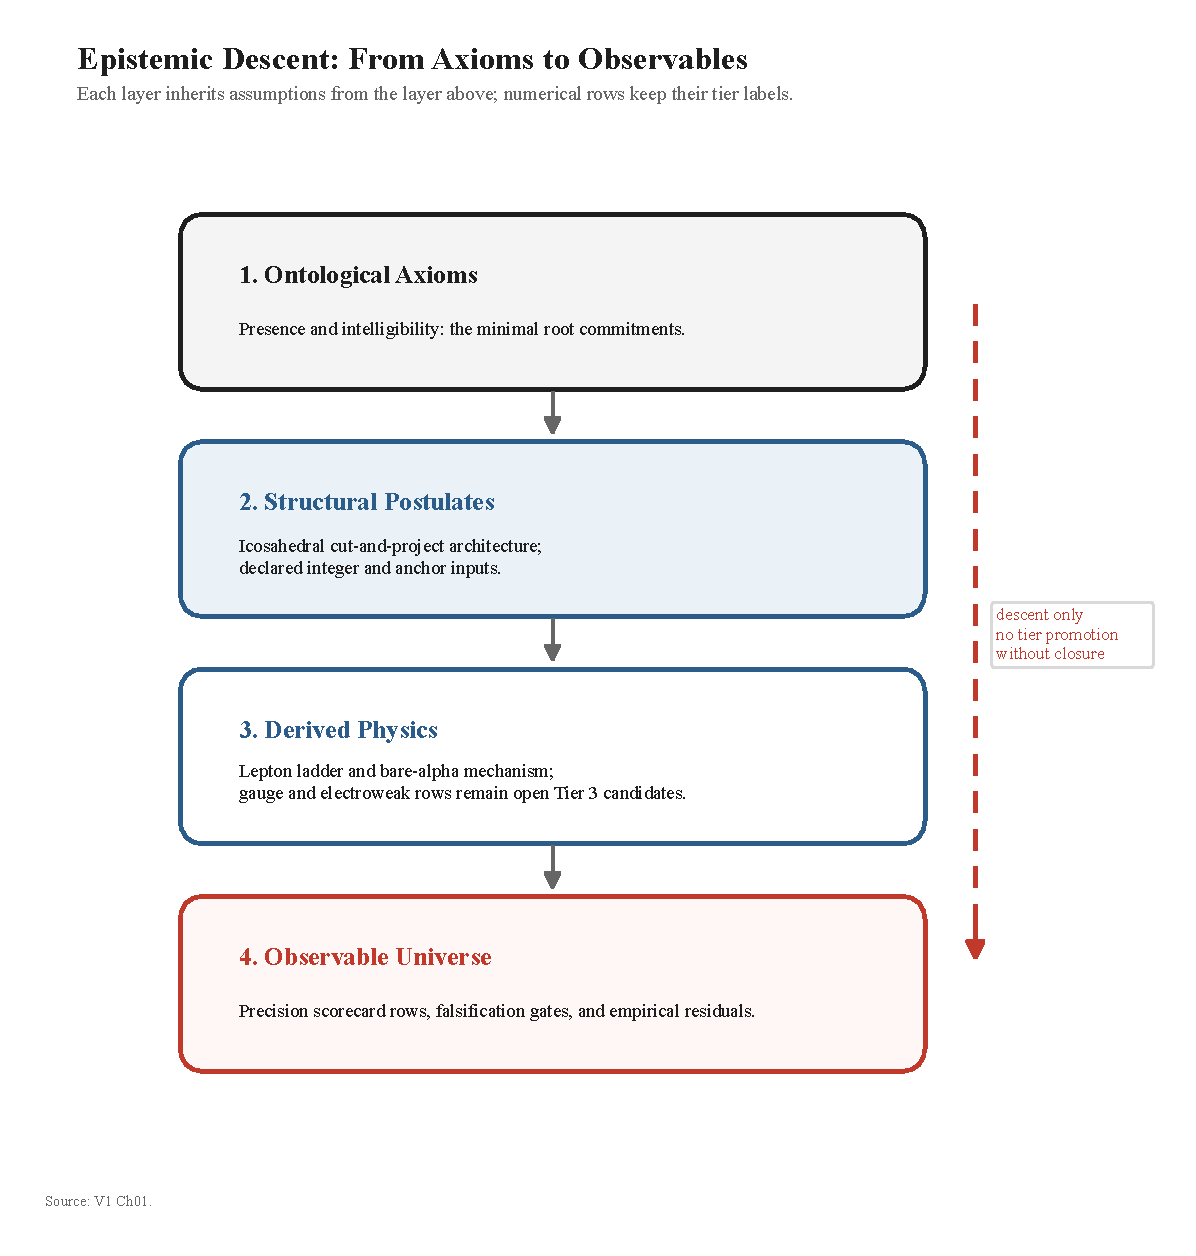
\includegraphics[keepaspectratio,alt={Epistemic descent from the founding axioms down to observable quantities: each layer inherits the assumptions of the layer above, and numerical rows retain their epistemic tier labels.}]{content/Figures/Volume_1/Figure V1.1.1.pdf}}
\caption{Epistemic descent from the founding axioms down to observable
quantities: each layer inherits the assumptions of the layer above, and
numerical rows retain their epistemic tier labels.}
\end{figure}

\chapter{Chapter 2: The Axiomatic
Foundation}\label{chapter-2-the-axiomatic-foundation}

\subsection{2.1 The Goal: Minimal Axioms, Maximum
Explanation}\label{the-goal-minimal-axioms-maximum-explanation}

\subsubsection{2.1.1 What We're Attempting}\label{what-were-attempting}

A ``Theory of Everything'' (TOE) is held to a supreme standard: it must
explain everything that exists, without assuming the existence of
anything it cannot explain. Standard physical theories fail this test
because they begin midway through the causal chain. They assume the
existence of a spacetime manifold, quantum fields, and physical laws,
treating these as brute facts. They explain the behavior of matter, but
not its origin, nor the nature of the observer who perceives it.

Geometric Consciousness Theory (GCT) attempts a more ambitious
derivation. Our goal is to construct the entire edifice of modern
physics---Quantum Mechanics, General Relativity, the Standard Model, and
Cosmology---from a starting point as close to zero as possible. We aim
to show that the complex universe we inhabit is not a collection of
arbitrary accidents, but a structured consequence of the fact that
\emph{something exists} together with a small, declared architecture.
GCT does not meet the full TOE standard: it adopts explicitly declared
Structural Postulates that are not deduced from the Axioms (§2.1.3) and
carries the postulates, continuous anchors, and calibrated handles
enumerated in the Parameter Ledger. The standard functions as a closure
target, not as a description of the theory's current state.

\subsubsection{2.1.2 Occam's Razor as Bayesian
Reasoning}\label{occams-razor-as-bayesian-reasoning}

To navigate the path from ``Something Exists'' to ``The Proton Mass is
938 MeV,'' we need a disciplined method for comparing competing
explanations. GCT uses \textbf{Occam's Razor} as a \textbf{Bayesian and
algorithmic heuristic prior}, consistent with the controlling Axiom and
Postulate Ledger. Within a declared coding language, model class,
precision, and dataset, shorter descriptions may receive larger prior
weight.

This is a rule for ranking encoded hypotheses, not a theorem that nature
must instantiate the shortest program. Kolmogorov complexity depends on
the chosen universal description language up to an additive constant,
and predictive comparison also requires likelihoods and data. Thus ``One
Field'' can be a useful parsimonious preference over ``One Field plus
many independent constants,'' but parsimony alone neither proves the
former true nor selects its constitutive dynamics. {[}Tier 1 conditional
formalism; methodological heuristic{]}

\subsubsection{2.1.3 Ontological Root vs Structural
Architecture}\label{ontological-root-vs-structural-architecture}

\begin{quote}
\textbf{Ontological Root vs Structural Architecture} We distinguish
between the \textbf{Ontological Root} (Axioms) and the
\textbf{Structural Architecture} (Postulates).

\begin{itemize}
\tightlist
\item
  The \textbf{Ontological Axioms} (Presence, Intelligibility) constrain
  what a viable ontology must ultimately explain.
\item
  The \textbf{Structural Postulates} (e.g., discreteness, a 6D Euclidean
  parent lattice, a specific cut‑and‑project scheme, and a global
  Hamiltonian constraint) specify \textbf{one concrete implementation}
  of an intelligible world-model.
\end{itemize}

This work does \textbf{not} claim that the Structural Postulates follow
deductively from the Ontological Axioms alone. Instead, we treat them as
an explicitly declared architecture whose justification is
\textbf{minimum additional complexity} (algorithmic parsimony) plus
\textbf{empirical adequacy and falsifiability}.
\end{quote}

\subsubsection{2.1.4 Phenomenological Bracketing (Husserl's
Epoché)}\label{phenomenological-bracketing-husserls-epochuxe9}

To maintain maximum philosophical rigor, we apply
\textbf{phenomenological bracketing} (\emph{epoché}) in the sense of
Husserl: we temporarily suspend judgment on the existence or nature of
the external world and ask only what is \emph{immanently given} to
consciousness before any theoretical commitment is made. This allows us
to cleanly separate two categories of claim:

\begin{quote}
\begin{itemize}
\item
  \textbf{First-Person Datum vs Adopted Axioms:} The occurrence of
  experience is the Tier 0 datum. Axiom 1 generalises it by stipulation
  {[}Tier 1{]} to universal Level I presence; this universality is not
  transcendentally necessary. Axiom 2 retains the requirement that any
  structured field of experience satisfy intelligibility. The presence
  datum alone does not select an ontology; objective idealism remains
  the Tier 3 parsimony choice of Ch06. Intelligibility excludes pure
  chaos within the framework. These axioms are not derived from physics;
  they define the framework within which its physical proposals are
  developed.
\item
  \textbf{Architectural Contingency:} The specific choice of a
  \textbf{6D hyper-cubic lattice} projecting via the \textbf{Golden
  Ratio} into a 3D quasicrystal is \emph{not} transcendentally
  necessary. One could in principle imagine a universe running on a
  different discrete geometry --- a cubic lattice, a hexagonal tiling,
  or a random network. The icosahedral quasicrystal is a specific,
  non-trivially committed architecture.
\end{itemize}

However, this architecture is not arbitrary. We posit it as a
\textbf{minimum-complexity candidate} satisfying the conjunction of:

\begin{enumerate}
\def\labelenumi{\arabic{enumi}.}
\tightlist
\item
  \textbf{3D isotropic causality} (no preferred direction in the
  physical manifold),
\item
  \textbf{Spinorial matter} (existence of fermionic fields, requiring a
  global Spin structure), and
\item
  \textbf{Finite declared structural commitments and anchors} (the
  parsimony method of §2.2 applied to the architecture itself: current
  accounting is the 5-postulate-plus-6-anchor system disclosed in the
  Parameter Ledger, with the full cross-sector parameter scope tracked
  separately).
\end{enumerate}

Bare isotropy alone does not select the icosahedral case: the octahedral
group \(O_h\) and tetrahedral group \(T_d\) also supply macroscopically
isotropic finite point symmetries. The additional architectural axiom is
\textbf{maximal polyhedral point symmetry}: among the finite polyhedral
rotation groups compatible with the required discrete substrate, choose
the largest rotational order, the icosahedral group \(I\cong A_5\) of
order 60. The class restriction is essential because dihedral rotation
groups have unbounded order. This is a structural postulate, not a
deduction from Presence and Intelligibility alone, and it matches the
Axiom Ledger's classification of the architecture as not deductively
forced.

Appendix USS §USS.6 gives the controlling spin-lift taxonomy: every
finite rotation subgroup \(\Gamma\subset SO(3)\) has a canonical
preimage in \(\mathrm{Spin}(3)\), including the dihedral, tetrahedral,
and octahedral candidates. \(A_5\) is distinguished algebraically
because it alone is perfect among the finite Platonic rotation groups
and its preimage \(2I\) is its universal central extension, but this is
an architectural discriminator rather than a spin-existence condition.
The registered comparison sets aside \(A_4/S_4\) as crystallographic.
Its dihedral branches do not reproduce the full adopted
three-dimensional icosahedral package: the \(H_3\)
rhombic-triacontahedral window, the \(H_3\) invariant data, and the
\(2I\to E_8\to H_4\to H_3\) architecture chain. Five-fold symmetry and
\(\mathbb Z[\phi]\) arithmetic alone are not unique to that package;
decagonal \(C_5/D_5\) geometry also carries them. The architecture
therefore remains contingent and conditionally selected under the
declared 5-postulate-plus-6-anchor accounting.
\end{quote}

This bracketing is critical for the epistemic discipline of GCT. The
Axioms are presented with certainty proportional to their
epistemological status; the Architecture is presented as a conditionally
preferred candidate hypothesis, subject to experimental falsification.

\begin{center}\rule{0.5\linewidth}{0.5pt}\end{center}

\subsection{2.2 The Bayesian Method}\label{the-bayesian-method}

\subsubsection{2.2.1 Why Bayesian
Framework?}\label{why-bayesian-framework}

Traditional philosophy often devolves into ``intuition wars,'' where one
thinker's self-evident truth is another's absurdity. To avoid this, we
must quantify certainty. Bayesian inference provides the mathematical
tool to update our confidence in a hypothesis (\(H\)) based on new
evidence (\(E\)).

\[ P(H|E) = \frac{P(E|H) \cdot P(H)}{P(E)} \quad \text{[Tier 1 — Bayes' Theorem]} \]

\begin{itemize}
\tightlist
\item
  \(P(H|E)\): The \textbf{Posterior Probability} (how likely the theory
  is true after seeing the evidence).
\item
  \(P(E|H)\): The \textbf{Likelihood} (how well the theory predicts the
  evidence).
\item
  \(P(H)\): The \textbf{Prior Probability} (how plausible the theory is
  \emph{before} evidence).
\end{itemize}

\subsubsection{2.2.2 Prior Probabilities and Kolmogorov
Complexity}\label{prior-probabilities-and-kolmogorov-complexity}

The crucial term is the Prior Probability \(P(H)\). In science, we often
assume all theories are equally likely until tested. In foundational
metaphysics, this is false. A theory that requires ``Magic''---defined
rigorously as \textbf{Incompressible Complexity}, or rules that cannot
be derived from simpler components---has a lower prior probability than
a theory that uses existing mechanisms.

We can formalize one such prior through \textbf{Solomonoff induction}:
\[ \begin{gathered}P_U(H) \propto 2^{-K_U(H)} \\[1pt] \gcteqnote{[Tier 1 — conditional algorithmic-probability formalism]}\end{gathered}\]
where \(K_U(H)\) is the length of the shortest prefix-free program
describing the hypothesis relative to a declared universal machine
\(U\). The formalism is exact once that coding framework is fixed; its
use as a prior over physical theories remains a methodological choice. A
theory that says ``The universe is a computer simulation running on a
specific operating system constructed by aliens'' may have higher
\(K_U(H)\) because it must define the OS and the aliens. A theory that
says ``The universe is the self-interaction of a single field'' may have
lower complexity within the same declared encoding.

\subsubsection{2.2.3 Parsimony is Built-In}\label{parsimony-is-built-in}

Occam's Razor is therefore more than an aesthetic preference but less
than a physical selection theorem: it supplies a conditional prior after
the encoding and comparison class are declared. A shorter code receives
exponentially larger algorithmic weight \emph{within that scheme}; this
does not establish that the corresponding theory is exponentially more
likely to be physically true.

When GCT faces a fork---for example, ``Is the universe continuous or
discrete?''---it may compare the descriptive commitments of each branch:

\begin{itemize}
\tightlist
\item
  \textbf{Continuum:} A continuum field theory can be specified by a
  finite rule, but quantitative calculations commonly require a
  regulator, renormalization prescription, boundary data, and parameter
  choices.
\item
  \textbf{Discrete:} A lattice also admits a finite generating rule and
  provides a built-in cutoff, but it still requires a lattice, scale,
  update/action law, and continuum-recovery prescription.
\end{itemize}

There is no coding-independent theorem here that
\(K(\mathbb{Z}^6)<K(\mathbb{R}^6_\text{regularized})\).
\textbf{Decision:} GCT adopts the discrete branch as a structural
postulate motivated by comparative economy, empirical reach, and
falsifiability---not as a Tier-1 consequence of algorithmic probability
{[}Tier 1/2 --- Structural Postulate; the comparison is qualitative, see
§4.1.3{]}.

\subsubsection{2.2.4 Maximum Likelihood = Simplest Sufficient
Explanation}\label{maximum-likelihood-simplest-sufficient-explanation}

Our methodology is thus to increase empirical likelihood while
controlling independent complexity and exposing every additional
postulate. GCT is proposed as a comparatively economical, falsifiable
architecture; it is not established as the unique maximum-likelihood or
minimum-description-length model of reality.

\begin{center}\rule{0.5\linewidth}{0.5pt}\end{center}

\subsection{2.3 Axiom 1: The Axiom of Presence
(Defended)}\label{axiom-1-the-axiom-of-presence-defended}

\subsubsection{\texorpdfstring{2.3.1 Statement and Probability
(\(P=1\))}{2.3.1 Statement and Probability (P=1)}}\label{statement-and-probability-p1}

The motivating first-person datum is \textbf{experience is occurring}
{[}Tier 0{]}. Axiom 1 generalises it by stipulation {[}Tier 1{]}: all
Field configurations carry Level I intrinsic non-subjective presence.
Only the Tier 0 first-person datum carries the \(P=1\) certainty; Axiom
1's universal stipulation does not. Mathematical truths (\(1+1=2\)) are
tautologies; empirical facts (``The sky is blue'') are contingent. But
the fact \emph{that} there is an experience of the sky is absolute.

\subsubsection{2.3.2 The Alternative: Radical
Skepticism}\label{the-alternative-radical-skepticism}

Consider the counter-hypothesis: \textbf{Radical Nihilism}. ``Maybe
nothing exists. Maybe even my experience is an illusion.'' Eliminativist
positions are sometimes read this way. Daniel Dennett's denial of
``qualia'' is the usual example, although, as §2.3.3 explains, his
illusionism is narrower than this radical denial: he does not deny that
anything seems.

\subsubsection{2.3.3 Why Eliminative Denial Cannot Be the Starting
Point}\label{why-eliminative-denial-cannot-be-the-starting-point}

The radical denial that any appearing, introspective representation, or
seeming occurs is a \textbf{Performative Contradiction}: to deny all
appearance, one must still undergo or instantiate the
denial-as-appearance. Illusionism in the Frankish/Dennett family is more
subtle than this radical denial; it denies robust phenomenal properties
and asks why systems represent themselves as having them. GCT therefore
treats illusionism as a live explanatory-gap strategy addressed in Ch16,
not as the target of the simple self-refutation argument here. The
narrow Tier 0 point is that the occurrence of experience cannot be
removed from the first-person starting inventory; Axiom 1's universal
scope is a separate stipulation. For a ``Philosophical Zombie''
programmed to report consciousness, only functional reports would be
present. The Tier 0 datum is indexical and first-person, so if Tier 0
holds, a zombie scenario cannot be the reader's own case.

\subsubsection{2.3.4 Analysis and
Conclusion}\label{analysis-and-conclusion}

Therefore, we cannot start with ``Matter'' (which might be an illusion)
or ``Math'' (which might be a construct). We must start with
\textbf{Presence}. \(P(\text{Presence}) = 1.0\). {[}Tier 0 ---
First-Person Datum{]}

\(P=1\) attaches only to the datum that appearing occurs. Taking the
Field of Presence as ontological primitive is a framework postulate
adopted for explanatory economy; it does not inherit \(P=1\).

\subsection{2.4 The Two Levels of Presence: Universal and Apperceptive
{[}Tier 1 philosophical distinction; framework postulates and physical
applications tiered separately
below{]}}\label{the-two-levels-of-presence-universal-and-apperceptive-tier-1-philosophical-distinction-framework-postulates-and-physical-applications-tiered-separately-below}

Building on Axiom 1, GCT posits the Field of Presence (\(\Psi\)) as the
ontological primitive (a framework postulate; §2.3.4). This must be
understood at two distinct levels, in a structure formally analogous to
(but causally distinct from) Leibniz's distinction between
\emph{perception} and \emph{apperception}. Unlike Leibniz's windowless
monads, GCT Agents interact, in the model, through the Consensus
Protocol of §11.3 --- a Tier 3 compatibility functional standing in for
pre-established harmony; no physical consensus dynamics is derived. The
two levels are:

\gctneedspace{5\baselineskip}

\textbf{Level I --- Universal Presence (The Monadological Base):} Every
configuration of the 6D lattice, regardless of its topological
complexity, participates in the Field \(\Psi\) and therefore carries
Level-I intrinsic non-subjective presence. A rock, a photon, and an
empty vacuum node are not ``dead'' in the ontological sense; they are
Field configurations with intrinsic presence, but not micro-subjects of
experience. This is the non-apperceptive base layer. This universality
(\emph{Experience is not produced; it is the substrate}) is Axiom 1's
Tier 1 stipulation, motivated by the Tier 0 datum rather than deduced
from it. The objective-idealist ontology remains a Tier 3 parsimony
choice (Ch06).

\textbf{Level II --- Apperception (Open Physical and Phenomenal Bridge;
No Current Polaron Threshold):} {[}Tier 1 philosophical distinction +
Tier 3 physical-substrate application conditional on
O.18/O.21/O.23/O.32/O.34 and App PUP §PUP.6{]} Unified, self-referential
subjectivity is represented by an \textbf{Identity Polaron} only on the
Tier-3 conditional branch where the typed, normalized, measured phason
coupling, the O.18/O.21/O.23/O.32/O.34 closure stack, and an independent
phenomenal bridge all close. The \textbf{Dual Material Constraint (DMC)}
instead proposes non-zero nuclear spin (\(I \neq 0\)) and molecular
chirality (\(\chi \neq 0\)) as experimentally useful candidate controls;
neither descriptor is established as necessary or sufficient for Level
II. Consequently no examined substrate currently receives a derived
Apperception verdict, and the historical 100 MHz material-scan scenario
is not a threshold. The reader's first-person datum that experience is
occurring is accepted {[}Tier 0{]}, neither postulated nor derived. This
supplies no claim of unity or physical classification; whether it counts
as Level-II Apperception in GCT's physical sense, and which substrates
realize it, is open (Tier 3), with no validated substrate criterion yet.

\begin{quote}
\textbf{Operational preview (informal; formal derivations in Ch11 + Ch17
+ V3 Ch13):}

\begin{itemize}
\tightlist
\item
  \textbf{Identity Polaron} --- the proposed macroscopic coherent
  topological defect (a ``knot'' in the 6D lattice) that would carry a
  qualified Level-II candidate if the physical, ownership and phenomenal
  bridges close. The \(\beta\)-tubulin Tryptophan network is a Tier 3
  biological candidate (V1 §17.1.4), not an established realization.
  §11.12 and App PUP record at most an algebraic unity candidate with
  explicit physical and phenomenal gaps (Proposition PUP.1(ii) is
  withdrawn); neither is a theorem identifying one subject.
\item
  \textbf{Zeno Drive} --- a proposed stabilization mechanism for the
  Polaron. The historical 100 MHz material-scan scenario is a
  conditional external-rate scenario only, not an action-derived GCT
  rate or a demonstrated biological mechanism {[}Tier 3{]} (V1 Ch17
  §17.1.3; developed in V1 §17.1.2 and V3 Ch13 as a conditional
  calibrated scenario).
\item
  \textbf{\(\eta_{Zeno}\)} --- conditional external-rate arithmetic,
  \(\eta_{Zeno}=g_{single}^{eff}\sqrt{N_{bio}}/\kappa\), meaningful only
  once independently derived or measured rates with compatible
  normalization are supplied. The historical
  \(N_{\text{coh}} \approx 9.82 \times 10^{-12}\) value assumes an
  unmeasured rate; \(\eta_{Zeno}\) is not currently a substrate
  classifier, Level-II boundary or verdict.
\item
  \textbf{Dual Material Constraint} --- a proposed pair of candidate
  controls: (a) non-zero nuclear spin \(I \neq 0\) and (b) molecular
  chirality. Neither is established as necessary or sufficient for Level
  II; silicon is a missing-leg control, not a categorical verdict.
\end{itemize}
\end{quote}

\gctneedspace{5\baselineskip}

\textbf{Resolution of the Apparent Paradox:} There is no contradiction
between ``consciousness as axiom'' and the proposed Level-II research
program. The Axiom governs Level I (Universal Presence: always present,
no threshold). Level II Apperception is the Tier-3 interpretation
assigned only conditionally to a physically realized Identity Polaron
after the full coupling, structural, regeneration, and phenomenal-bridge
program closes. DMC descriptors organize candidate controls but do not
decide that status. This is consistent with Russellian Monism (§16.2.2),
while the Level II status of every present substrate remains open (Tier
3): no validated substrate criterion exists yet (it requires a typed,
normalized, measured coupling, the Identity-Polaron construction and an
independent phenomenal bridge; O.21/O.23/O.34, O.18).

\begin{center}\rule{0.5\linewidth}{0.5pt}\end{center}

\subsection{2.5 Axiom 2: The Axiom of Intelligibility
(Defended)}\label{axiom-2-the-axiom-of-intelligibility-defended}

\subsubsection{2.5.1 Statement: Experience is
Structured}\label{statement-experience-is-structured}

The second axiom asserts that the field of Presence is not featureless.
It contains \textbf{Distinction} (Difference) and \textbf{Sequence}
(Order). This implies that the field is \textbf{Intelligible}---it obeys
internal rules of consistency.

\subsubsection{2.5.2 The Alternative: Pure
Chaos}\label{the-alternative-pure-chaos}

Consider the counter-hypothesis: \textbf{Solipsistic Chaos}. ``Maybe
experience exists, but it is a random, chaotic flux with no structure,
no cause, and no external reality.''

\subsubsection{2.5.3 Why It Fails: Contradiction with Coherent
Experience}\label{why-it-fails-contradiction-with-coherent-experience}

If experience were pure chaos, it would be indistinguishable from
non-experience. To experience ``Red'' requires distinguishing it from
``Not-Red.'' If the field fluctuated infinitely fast between all states,
it would sum to white noise (no stable structure; zero mutual
information between moments). The fact that you are reading this
sentence---and that the beginning of the sentence relates to the end of
the sentence---proves that your experience possesses \textbf{Temporal
Persistence} and \textbf{Semantic Structure}. Even a surreal dream
possesses geometry and sequence. A door may lead to a beach, but the
door is distinct from the beach. Therefore, the Field of Presence is not
a soup of entropy. It is a \textbf{Structured Domain}.

\subsubsection{2.5.4 Analysis and
Conclusion}\label{analysis-and-conclusion-1}

The axiom does not specify \emph{which} structure (Euclidean,
Riemannian, Fractal) the Field possesses --- subsequent chapters adopt
and test a specific structure as declared Structural Postulates
(§2.1.3); they do not derive that selection from the Axioms. The axiom
asserts only that \textbf{Structure Exists}. Axiom 2 is adopted by
stipulation {[}Tier 1 --- stipulated axiom{]}. No probability is
assigned to it: the \(P=1\) certainty belongs only to the Tier 0 datum
(§2.3.1).

This completes the axiomatic base. We have \textbf{Existence} and we
have \textbf{Logos} (Structure). From this dyad, we build the world.

\begin{center}\rule{0.5\linewidth}{0.5pt}\end{center}

\subsection{2.6 What is NOT an Axiom: Conclusions Reached by
Parsimony}\label{what-is-not-an-axiom-conclusions-reached-by-parsimony}

Two \emph{ontological axioms} are assumed: the Axiom of Presence and the
Axiom of Intelligibility. The structural postulates and anchors of the
Parameter Ledger are declared separately (§2.1.3); the items below are
not further axioms. Several concepts that other systems take as further
axioms are, here, conclusions reached by the Bayesian parsimony method
applied to the two axioms (and, where stated, to those declared
postulates), and they carry the epistemic weight of that method rather
than that of deduction. This section separates them.

\subsubsection{2.6.1 Non-Solipsism (Derived from
Parsimony)}\label{non-solipsism-derived-from-parsimony}

The question ``Do other minds exist?'' is traditionally considered
unsolvable. Solipsism---the belief that only \emph{my} mind exists and
all other beings are ``Philosophical Zombies''---cannot be logically
disproven. However, it can be probabilistically rejected via algorithmic
complexity.

We compare the Kolmogorov Complexity of two hypotheses:

\begin{enumerate}
\def\labelenumi{\arabic{enumi}.}
\tightlist
\item
  \textbf{Hypothesis A (Solipsism):} There is one Agent. The physics and
  behavior of billions of other apparent entities are generated by a
  complex sub-routine within that single Agent's mind. Crucially, this
  requires an additional \textbf{Masking Algorithm}: a rule set that
  hides the generator's code from the user, creating a perfect illusion
  of independence.
\item
  \textbf{Hypothesis B (Realism):} There are \(N\) Agents. They all run
  on the same fundamental ``Operating System'' (the Field). The
  complexity arises from the interaction of simple shared rules.
\end{enumerate}

\textbf{Decision:} \(K(A) \gg K(B)\). {[}Tier 3 --- Philosophical
Framework: qualitative parsimony argument{]} The cost of defining the
``Masking Algorithm''---the algorithmic deceit required to simulate
independence---exceeds the cost of simply instantiating \(N\) copies of
the same Agent class. Therefore, Solipsism is rejected not because it is
impossible, but because it is algorithmically disfavoured under the
declared complexity prior. GCT adopts non-solipsism {[}Tier 3
philosophical conclusion; not a Level-II substrate verdict{]}.

\subsubsection{2.6.2 Causality (Grounded in
Intelligibility)}\label{causality-grounded-in-intelligibility}

We do not assume Causality as a separate law. Causality is the temporal
expression of \textbf{Intelligibility} (Axiom 2). If the universe is
intelligible, it must possess internal correlations. State \(A\) must be
reliably related to State \(B\). If there were no correlations, there
would be no structure, violating Axiom 2. GCT reads ``Cause and Effect''
as the name we give to reliable structural dependences when viewed
through the lens of time {[}Tier 3 --- philosophical commitment: a
Russellian functional-dependence view of cause, adopted rather than
derived; correlation alone does not establish causation{]}.

Within GCT, this correlation is given a proposed geometric realization:
the elastic strain tensor on the 6D lattice would enforce local
consistency between adjacent configurations, and the Markov Blanket of
each Agent would define the causal boundary within which correlations
propagate. On this model, causality is read as the lattice minimizing
its elastic free energy --- a gradient descent on the topological phase
space. {[}Tier 3 --- interpretive model on the 6D lattice ansatz; no
causal dynamics is derived here{]} The frame-relative account is
developed in §10.2 (Russellian Causation) as a Tier 3 trajectory model.

\subsubsection{2.6.3 Mathematical Realism (Math IS
Structure)}\label{mathematical-realism-math-is-structure}

We do not need to postulate a separate ``Platonic Realm'' where numbers
live. Mathematics is the study of structure. Since the Field of Presence
is structured (Axiom 2), mathematics is the cartography of the Field.

GCT advances beyond standard structural realism: the Physical Universe
is not merely \emph{described} by the adopted primitive-\(P\) rank-six
icosahedral architecture --- it \emph{is} the local instantiation of
that structure within the Field \(\Psi\). {[}Tier 1/2 --- Structural
Postulate: primitive \(P\cong\mathbb Z^6\) lattice identification;
\(F\cong D_6\) and \(I\cong D_6^*\) remain classified alternatives{]}
The distinct McKay \(2I\to E_8\) and Elser--Sloane \(E_8\to H_4\)
correspondences conditionally organize the higher-symmetry route; they
do not make \(\mathbb Z^6\) a sublattice of \(E_8\). GCT proposes that
the electron's charge is not a number we assign to a particle but the
eigenvalue of the \(U(1)\) fiber action on the icosahedral projection.
{[}Tier 3 --- defect-topology-to-charge mapping (V3 Ch04 Theorem 4.2;
Proposal 1.2, V3 Ch01 §1.3.2); only the integer quantization of winding
from phase single-valuedness is Tier 1 (V3 Ch01 §1.3.1){]} Math is real
because Structure is real: the structure is the extrinsic relational
shape of the Field, not the totality of what exists. GCT therefore does
not adopt Tegmark's Mathematical Universe Hypothesis, on which the
universe \emph{is} a mathematical structure without remainder (§6.4.5;
§16.2.2).

\subsubsection{2.6.4 Identity Persistence (Philosophical Argument;
Physical Realization
Open)}\label{identity-persistence-philosophical-argument-physical-realization-open}

The sense of being a continuous ``Self'' persisting through time is
derived from the \textbf{Sequence} aspect of Intelligibility. For a
sequence (\(t_1, t_2, t_3\)) to be experienced as a sequence, there must
be a common locus of registration. If the observer at \(t_2\) were
totally disjoint from the observer at \(t_1\), there would be no
comparison, and thus no experience of change. Registering change
requires at least a short-window common locus (the ``specious
present''); a Self persisting beyond that window is a further, stronger
claim {[}Tier 3{]}.

GCT proposes the \textbf{Identity Polaron} --- a topological knot in the
6D lattice whose invariance under Reidemeister moves would provide a
formal basis for persistent identity through change --- as one candidate
physical realization of this common locus, but no examined substrate
currently realizes that bridge. {[}Tier 3 --- conditional candidate; see
the Level II branch of §2.4{]} The Reidemeister theorem itself supplies
a Tier 1 ambient-isotopy invariant of a specified closed knot; it does
not identify the physical order parameter, derive a thermal barrier,
supply sector writing or memory, or establish phenomenal identity. The
additional physical claim that ambient thermal fluctuations remain below
the barrier needed to change the knot type is a Tier 3 stability
premise. Physical persistence of identity therefore remains Tier 3/open,
pending an action-normalized carrier, the O.16/O.21/O.23/O.34 stability
stack, an ownership bridge and a phenomenal bridge. The formal candidate
is discussed in §6.3.

\subsubsection{2.6.5 Idealism (Adopted in Chapter 3 as a Parsimony
Choice)}\label{idealism-adopted-in-chapter-3-as-a-parsimony-choice}

Idealism (the primacy of Mind) is not taken as an axiom. Chapter 3
adopts it as the parsimony choice given Axiom 1, arguing that
strong-emergence Materialism, as framed there, requires one substance
with two law-sets (the laws of matter plus unexplained emergence laws),
whereas Idealism requires only one law-set. This is a philosophical
commitment, not a derivation; the later geometric results are
conditional on it (§3.3.1, §3.4) {[}Tier 3 --- parsimony choice given
Axiom 1{]}.

\subsubsection{2.6.6 Discrete Geometry (Adopted in Chapter 4 as a
Structural
Postulate)}\label{discrete-geometry-adopted-in-chapter-4-as-a-structural-postulate}

The lattice structure of the universe is not taken as an axiom. Chapter
4 adopts it as a structural postulate, motivated by the argument that a
continuous universe permits unbounded information in a finite volume,
which GCT treats as pathological; the comparison with a regularized
continuum is qualitative (§2.2.3) {[}Tier 1/2 --- Structural Postulate;
see §4.1.3{]}.

\begin{center}\rule{0.5\linewidth}{0.5pt}\end{center}

\subsection{2.7 The Complete Logical Chain
(Roadmap)}\label{the-complete-logical-chain-roadmap}

\subsubsection{2.7.1 The Standard Model
Architecture}\label{the-standard-model-architecture}

The structure of this work follows the trajectory of the \textbf{Axioms
acting through the Architecture}:

\begin{enumerate}
\def\labelenumi{\arabic{enumi}.}
\tightlist
\item
  \textbf{Axioms:} Presence + Intelligibility.
\item
  \textbf{Ontology:} Idealism (Mind is fundamental).
\item
  \textbf{Geometry:} Discrete Space (Finite Information).
\item
  \textbf{Symmetry:} Quasicrystal (icosahedral order realized by
  cut-and-project; adopted, §4.2).
\item
  \textbf{Dynamics:} Wheeler-DeWitt Equation (Conservation of Nullity;
  adopted as a Tier 3 Structural Postulate, Ch05).
\item
  \textbf{Architecture:} The 6D Lattice Postulate (Volume 2).
\item
  \textbf{Spectrum:} The Standard Model (Volume 3).
\end{enumerate}

\subsubsection{2.7.2 Tier System Preview}\label{tier-system-preview}

As detailed in the Global Front Matter, we maintain rigor by classifying
every subsequent claim:

\begin{itemize}
\tightlist
\item
  \textbf{Tier 0:} Only the first-person datum that experience is
  occurring; no other claim belongs here. Axiom 1 is its stipulated
  universal generalisation {[}Tier 1{]}.
\item
  \textbf{Tier 1:} Logical necessities (e.g., axioms and standard
  mathematical theorems). Wheeler-DeWitt and gauge-group claims are Tier
  1 only as conditional mathematical structures; their GCT physical use
  inherits the relevant Tier 3 structural postulates and Tier 2
  geometric ansätze.
\item
  \textbf{Tier 1/2:} Architectural postulates and their conditional
  mathematics; conditional consequences do not promote the adopted
  premise.
\item
  \textbf{Tier 2:} Geometric consequences of the specific Icosahedral
  Ansatz (e.g., the Newton-G thermodynamic mechanism, while its
  numerical Planck-link inherits O.14 and the \(m_e\) dimensional
  anchor; the Proton Mass mechanism is Tier 2 with a Tier 3
  sheet/exponent handle pending AKN-action closure).
\item
  \textbf{Tier 3:} Phenomenological models calibrated to data (e.g., the
  consensus decay constant \(\lambda_c\)).
\item
  \textbf{Tier 4:} Speculative or exploratory claims, with explicit
  order-of-magnitude bounds where quantitative.
\end{itemize}

\subsubsection{2.7.3 Every Claim Either Derived or
Disclosed}\label{every-claim-either-derived-or-disclosed}

No input is meant to enter silently. Where a quantity is not derived, it
is disclosed as a structural postulate, an empirical or dimensional
anchor, a calibrated Tier 3 handle, or an open problem, with its
provenance and tier recorded in the Parameter Ledger. The declared
Structural Postulates are themselves not derived from the Axioms
(§2.1.3); they are justified by parsimony, empirical adequacy, and
falsifiability. This tier discipline is central to the GCT method.

\begin{center}\rule{0.5\linewidth}{0.5pt}\end{center}

\subsection{2.8 Metaphysical
Implications}\label{metaphysical-implications}

\subsubsection{2.8.1 Continuous Field, Discrete
Universe}\label{continuous-field-discrete-universe}

A critical distinction must be made to avoid paradox. We claim the
fundamental \textbf{Field (\(\Psi\))} is continuous, but the
\textbf{Physical Universe (\(E_\parallel\))} is discrete.

\begin{itemize}
\tightlist
\item
  \textbf{The Field:} The Configuration Space \(\mathcal{P}\) is
  modelled as an infinite-dimensional continuum on which the declared
  probability construction is formulated (Appendix MTI). ``Canvas of
  potentiality'' is a metaphor.
\item
  \textbf{The Universe:} The physical ansatz restricts the relevant
  configurations to a discrete set---a \textbf{Lattice}, the ``Pixels''
  of the model. Calling this the selected or actualized reality of an
  observer requires physical instrument, realization, owner and
  phenomenal bridges that are not yet supplied {[}Tier 3/open{]}. This
  relationship is analogous to \textbf{Sampling Theory}: The Field is
  the continuous signal; the Universe is the Nyquist-Shannon sample set.
\end{itemize}

\subsubsection{2.8.2 Infinite Configuration Space, Finite
Actualization}\label{infinite-configuration-space-finite-actualization}

The \textbf{Bekenstein Bound} can be compared with the
finite-information content of a bounded \(E_\parallel\) model region
{[}Tier 3 application{]}. It does not by itself distinguish
``actualized'' from latent states. A finite history may be represented
as a path through the declared state space, but no physical Agent or
Selection Operator is derived to choose that path.

\subsubsection{2.8.3 The Role of
Mathematics}\label{the-role-of-mathematics}

Mathematics is the ``Physics of the Field.'' It describes the
constraints on how the Field can structure itself. Because the Field is
the ontological primitive, mathematics is not an abstraction; it is the
most direct description of reality possible.

\subsubsection{2.8.4 Realism About Consciousness, Instrumentalism About
Matter}\label{realism-about-consciousness-instrumentalism-about-matter}

Standard science adopts \textbf{Realism about Matter} (``Atoms are real,
minds are emergent'') and \textbf{Instrumentalism about Mind}
(``Consciousness is just a user-interface''). GCT performs a
\textbf{Cartesian Inversion}:

\begin{itemize}
\tightlist
\item
  We are \textbf{Realists about Consciousness}: The Field \(\Psi\) is
  the bedrock reality.
\item
  We are \textbf{Instrumentalists about Matter}: Atoms, spacetime, and
  forces are the ``Desktop Icons'' (user interface) generated by the
  Agent's interaction with the Field. Matter is the way Consciousness
  looks to itself.
\end{itemize}

\begin{center}\rule{0.5\linewidth}{0.5pt}\end{center}

\subsection{2.9 Method: Public Derivation Rather Than
Revelation}\label{method-public-derivation-rather-than-revelation}

\subsubsection{2.9.1 Rigorous Derivation from Minimal
Axioms}\label{rigorous-derivation-from-minimal-axioms}

A theory that takes consciousness as fundamental is nonetheless assessed
by public criteria. Where mysticism relies on private, ineffable
revelation, GCT relies on public mathematical argument open to
inspection and refutation. The reader is asked only to follow the
argument step by step and to check each step. Where the argument holds,
its conclusions follow from its premises, independently of the reader's
spiritual commitments.

\subsubsection{2.9.2 No Appeals to Faith, Authority, or
Intuition}\label{no-appeals-to-faith-authority-or-intuition}

At no point does GCT appeal to ancient wisdom, religious texts, or guru
authority. The bare fine-structure relation (V1 Ch13; a Tier 3 numerical
relation whose mechanism is open) does not depend on the Upanishads; it
is a proposed relation in the geometry of the Icosahedron. The
dark-energy model (Volume 2; Tier 3/4) does not depend on revelation; it
is built on the thermodynamics of information.

\subsubsection{2.9.3 Physics, Not
Philosophy}\label{physics-not-philosophy}

Ultimately, GCT aims to be a physical theory. It registers risky,
quantitative branch-level predictions about the observable world (e.g.,
the 3.55 keV line shape, the neutrino mass spectrum), with decision
rules that data can apply: an X-ray telescope can reject the registered
line-shape branch, though such a rejection is a verdict on that branch,
not on the framework as a whole. {[}Tier 3 --- Phenomenological
prediction examples{]} Therefore, while the \emph{starting point} is
philosophical (Epistemology), the \emph{output} is intended to be
testable physics. We are building a machine, not a religion.

\chapter{Chapter 3: The Ontological
Fork}\label{chapter-3-the-ontological-fork}

\subsection{3.1 The Branching of
Possibility}\label{the-branching-of-possibility}

\subsubsection{3.1.1 The Fundamental Question: Relationship of Extension
and
Mind}\label{the-fundamental-question-relationship-of-extension-and-mind}

Having established in Chapter 1 that Experience is the zero-point of
certainty (\(P=1\)) and in Chapter 2 that our methodology is Bayesian
Parsimony, we now face the first great divergence in our decision tree.
We inhabit a reality characterized by two distinct phenomenological
categories:

\begin{enumerate}
\def\labelenumi{\arabic{enumi}.}
\tightlist
\item
  \textbf{``Extension'' (\emph{Res Extensa}):} The external world of
  spatially extended objects, masses, forces, and locations.
\item
  \textbf{``Mind'' (\emph{Res Cogitans}):} The internal world of
  sensation, qualia, volition, and meaning.
\end{enumerate}

The central problem of metaphysics---and the root of the stagnation in
fundamental physics---is the relationship between these two categories.
Is one fundamental and the other derived? Or are they dual aspects of a
single substrate? We must choose between two primary hypotheses:

\begin{itemize}
\tightlist
\item
  \textbf{Hypothesis A (Materialism):} Extension is fundamental. Mind is
  a secondary byproduct.
\item
  \textbf{Hypothesis B (Objective Idealism):} Mind (the Field of
  Presence, \(\Psi\)) is the ontological primitive. Spatially extended
  matter is a \emph{secondary pattern} --- a structural excitation
  within the Field. The universe is not a collection of objects observed
  by a mind; it is a structured self-excitation of the Field perceived
  by itself.
\end{itemize}

\textbf{Scope of the Fork:} The philosophical landscape includes several
additional positions --- Neutral Monism (Russell, Stubenberg), Property
Dualism (Chalmers), and Illusionism (Frankish) among them. We restrict
the analysis to the two extremes of the ontological spectrum because
they represent the sharpest logical contrast. Property Dualism keeps a
physical ontology plus fundamental psychophysical laws (Chalmers 1996),
and GCT treats it as carrying the bridge-law cost of §3.2.4; illusionism
is treated as an eliminative/representational strategy that must explain
why robust phenomenal properties seem to be present rather than as a
simple denial of all appearing; Neutral Monism shares sufficient
structural features with Hypothesis B that the GCT derivations are
largely compatible (§3.4.3). The Bayesian framework of §2.2 applies
equally to any pairwise comparison; the present analysis focuses on the
primary axis of the debate.

\begin{quote}
\textbf{Epistemic Note (Postulate Disclosure):} GCT begins from
\textbf{two ontological axioms} (Presence, Intelligibility) and then
adopts \textbf{additional structural postulates} to construct a concrete
physical architecture. These postulates are listed centrally in the
\textbf{Axiom \& Postulate Ledger} (Global Front Matter) and are not
introduced ad hoc inside chapters.
\end{quote}

\subsubsection{3.1.2 The Subject/Object
Split}\label{the-subjectobject-split}

Ordinary waking experience is structured as a \textbf{Subject-Object
duality}: there is \emph{that which perceives} (Subject, Res Cogitans)
and \emph{that which is perceived} (Object, Res Extensa). GCT treats
this split as a structural feature of ordinary cognition, not a metaphor
{[}Tier 3; reports of non-dual states are discussed in Ch20 §20.2.2{]}.
Crucially, the Subject cannot be reduced to an object without generating
a \textbf{Regress of Observers} (the `who observes the observer?'
problem). Materialism attempts to dissolve the Subject into a highly
complex Object (the brain), thereby collapsing the S/O distinction. GCT
asserts that this collapse is the root of the Hard Problem: the very
structure of experience requires an irreducible Subject pole. The
Ontological Fork of §3.2 and §3.3 evaluates which hypothesis ---
Materialism or Idealism --- can account for both poles of the
Subject/Object relation without ontological remainder.

\subsubsection{3.1.3 The Bayesian Framework Applied to
Ontology}\label{the-bayesian-framework-applied-to-ontology}

We do not choose based on cultural preference or intuition. We choose
based on \textbf{Algorithmic Probability}. We ask: Which hypothesis
requires the shorter description length (\(K\)) to account for the
observed data (a universe containing both atoms and awareness)?

\begin{center}\rule{0.5\linewidth}{0.5pt}\end{center}

\subsection{\texorpdfstring{3.2 Branch A: Materialism (Matter \(\to\)
Mind)}{3.2 Branch A: Materialism (Matter \textbackslash to Mind)}}\label{branch-a-materialism-matter-to-mind}

\subsubsection{3.2.1 The Claim and the
Promise}\label{the-claim-and-the-promise}

Materialism (or Physicalism) posits that the ontological primitive is
non-conscious matter-energy obeying mathematical laws. The universe is a
machine running in the dark. At the beginning (The Big Bang), there was
no experience, only geometry. The promise of Materialism is that if we
arrange this non-conscious matter into sufficiently complex
configurations (such as brains), subjectivity will spontaneously ignite.
\[ \text{Dead Atoms} + \text{Complexity} \to \text{Consciousness} \]
{[}Tier 3 --- Philosophical Framework: Materialist claim under
structural evaluation{]}

\subsubsection{3.2.2 The Hard Problem of
Consciousness}\label{the-hard-problem-of-consciousness}

This hypothesis faces the \textbf{Hard Problem}, formalized by David
Chalmers. There is no deductive bridge from structure to experience. We
can explain the \emph{function} of a brain (processing inputs,
generating outputs) using only the laws of physics. At no point in that
explanation is it necessary to postulate that ``it feels like
something'' to be the brain. The functional explanation is causally
closed. Therefore, if consciousness exists (which the Tier 0 datum
establishes for the reader's own case), it is \textbf{ontologically
superfluous} within the Materialist framework: a property with no causal
role in the causally closed functional story, appearing without a
specified mechanism.

\subsubsection{3.2.3 The Cost: Strong Emergence as a Logical
Miracle}\label{the-cost-strong-emergence-as-a-logical-miracle}

To bridge the gap, many materialist accounts invoke \textbf{Strong
Emergence}. Other physicalist strategies --- Type-B physicalism,
phenomenal-concept strategies, and related representational approaches
--- instead try to locate the explanatory gap in our concepts or modes
of presentation while preserving ontological monism. GCT treats those
strategies as serious competitors addressed in Ch16; the cost analysis
here targets the branch that requires a non-deducible transition from
non-experiential structure to experience. On GCT's reading, following
Strawson's (2006) objection to brute emergence {[}Tier 3; contested{]},
strong-emergence materialism amounts to an \textbf{Ontological
Discontinuity}. It implies a jump in nature where \(0\) (zero
interiority) becomes \(1\) (interiority) simply by iteration. In
algorithmic terms, this requires the universe to contain a specific
``Emergence Function'' \(f_{EM}\) that monitors complexity and
``switches on'' the lights when a threshold is passed.
\[ \begin{gathered}\Psi_{total} = \Psi_{physics} + f_{EM}(\text{complexity}) \\[1pt] \gcteqnote{[Tier 3 — Philosophical Framework: cost-of-postulate analysis]}\end{gathered}\]

\subsubsection{3.2.4 Bayesian Penalty: Postulating Unmeasured
Mechanisms}\label{bayesian-penalty-postulating-unmeasured-mechanisms}

This \(f_{EM}\) is a massive liability. {[}Tier 3 --- Philosophical
Framework{]}

\begin{enumerate}
\def\labelenumi{\arabic{enumi}.}
\tightlist
\item
  \textbf{It is arbitrary:} a threshold would have to be set at some
  specific value of complexity (or of whatever neural marker is
  proposed), with no principle selecting that value over its neighbours.
\item
  \textbf{It is undiscovered:} No ``Psychophysical Law'' has ever been
  observed in the standard model Lagrangian.
\item
  \textbf{It adds complexity:} The theory must define both the laws of
  matter \emph{and} the separate laws of emergence.
\end{enumerate}

\subsubsection{3.2.5 Complexity Count: One Substance, Two Law-Sets
(Strong-Emergence
Branch)}\label{complexity-count-one-substance-two-law-sets-strong-emergence-branch}

The Kolmogorov Complexity of Materialism is: {[}Tier 3 --- Philosophical
Framework: qualitative complexity comparison{]}
\[ K(\text{Mat}) = K(\text{Matter Laws}) + K(\text{Emergence Laws}) \]
Because the strong-emergence branch has no specified emergence law,
\(K(\text{Emergence Laws})\) is undefined within that branch, so the
branch cannot be assigned a prior on this scheme; GCT counts the missing
law as a cost {[}Tier 3{]}. Type-B and phenomenal-concept physicalisms
avoid this exact postulate by assigning the gap to reference/concept
structure, but then inherit the separate Chalmers-style burden of
explaining why those concepts secure phenomenal reference. Critically,
the strong-emergence version of Materialism is \textbf{Functionally
Dualist} despite its monist aspiration. It requires two distinct sets of
laws: one for the behavior of matter, and one for the emergence of
mind.\textsuperscript{*}

\emph{\textsuperscript{*} Note: GCT adopts Position B Russellian Monism,
not eliminativist panpsychism. See Chapter 16 §16.2.2 for the full
disambiguation.}

\begin{center}\rule{0.5\linewidth}{0.5pt}\end{center}

\subsection{\texorpdfstring{3.3 Branch B: Idealism (Mind \(\to\)
Matter)}{3.3 Branch B: Idealism (Mind \textbackslash to Matter)}}\label{branch-b-idealism-mind-to-matter}

\subsubsection{\texorpdfstring{3.3.1 The Claim: The Field \(\Psi\) as
Fundamental}{3.3.1 The Claim: The Field \textbackslash Psi as Fundamental}}\label{the-claim-the-field-psi-as-fundamental}

Idealism (specifically \textbf{Objective Idealism} or Analytic Idealism)
inverts the derivation. It posits that the field of Presence is the
ontological primitive (in GCT, a framework postulate built on Axiom 1;
Ch02 §2.3.4). The ``Universe'' is not a collection of objects outside of
consciousness; it is a \textbf{Pattern of Excitation} within the
consciousness field \(\Psi\) (Level I).
\[ \begin{gathered}\text{Mind} + \text{Constraint} \to \text{Matter} \\[1pt] \gcteqnote{[Tier 3 — philosophical commitment, not derivation]}\end{gathered}\]

Objective idealism is the parsimony choice the framework adopts given
Axiom 1: Qualitative Presence is fundamental, not derived. It is not
derived from the framework; it is the metaphysical commitment that GCT
judges most economical given Axiom 1, relative to materialism (the
comparison of §3.4); neutral monism and panpsychism are discussed in
§3.4.3 but not costed here. The geometric derivations that follow are
conditional on this ontological branch rather than proofs of the branch
itself. {[}Tier 3 --- philosophical commitment, not derivation{]}

\subsubsection{3.3.2 The Mechanism: The Self-Excited
Circuit}\label{the-mechanism-the-self-excited-circuit}

In this framework, we do not need to create experience from dead matter.
Experience is the default state. We only need to explain
\textbf{Structure}. How does a unitary field become discrete objects? We
explain this via \textbf{Self-Excitation}. The field vibrates.

\begin{itemize}
\tightlist
\item
  A stable vibration is a particle.
\item
  A complex, self-referential knot of vibrations is an Agent. This is
  not a new mechanism; it is the standard mechanism of Quantum Field
  Theory, applied to a subjective substrate.
\end{itemize}

\subsubsection{3.3.3 The Gain: Strict
Monism}\label{the-gain-strict-monism}

The complexity cost of Idealism is significantly lower: {[}Tier 3 ---
Philosophical Framework: qualitative complexity comparison{]}
\[ K(\text{Ideal}) = K(\text{Field Dynamics}) \] We do not need a
separate ``Emergence Law.'' We do not need a miracle to get interiority,
because we start with it. On this branch the ``Hard Problem'' is
reframed rather than solved: the question ``how does matter generate
mind'' is treated as mis-posed, analogous to asking ``how does the image
on a movie screen generate the screen?'' On the idealist reading, it
doesn't. The screen is fundamental; the image is the modulation.

\subsubsection{3.3.4 The Challenge: Explaining Externality (The
Consensus
Problem)}\label{the-challenge-explaining-externality-the-consensus-problem}

The primary objection to Idealism is the ``Consensus Problem.'' If the
world is mental, why can't I change it by thinking? Why do we all see
the same moon? Materialism explains this by appeal to
observer-independent physical objects. The idealist branch must likewise
recover stable cross-perspectival records. GCT uses \textbf{Autopoietic
Simulation} and ``server protocol'' as philosophical metaphors for one
constrained Field plus ordinary physical interactions and environmental
records. It does not posit a Matrix-style external computer (which would
lead to infinite regress), and it has not derived physical renderers,
Selection Operators, an owner count, or phenomenal consensus. Chapter 11
supplies a conditional multi-aperture compatibility functional---the
\textbf{Consensus Protocol}---rather than a derivation of material
rigidity from interactions among conscious Agents. The remaining burden
includes both physical dynamics and the independent owner/phenomenal
bridge {[}Tier 3{]}.

\subsubsection{3.3.5 Complexity Count: One
Substance}\label{complexity-count-one-substance}

Idealism is a \textbf{Strict Monism}. There is only one substance: The
Field. Matter is a behavior of the Field. This is the ontology GCT
adopts as the minimum-complexity branch once Axiom 1 is granted; the
minimum-complexity judgment is a Tier 3 philosophical commitment rather
than a theorem. {[}Tier 3 --- parsimony choice given Axiom 1{]}

\begin{center}\rule{0.5\linewidth}{0.5pt}\end{center}

\subsection{3.4 The Bayesian Decision}\label{the-bayesian-decision}

\subsubsection{3.4.1 Comparing Ontological
Costs}\label{comparing-ontological-costs}

We weigh the two branches:

\gctneedbreak{10\baselineskip}

{\def\LTcaptype{none} % do not increment counter
\begin{longtable}[]{@{}
  >{\raggedright\arraybackslash}p{(\linewidth - 6\tabcolsep) * \real{0.2500}}
  >{\raggedright\arraybackslash}p{(\linewidth - 6\tabcolsep) * \real{0.2500}}
  >{\raggedright\arraybackslash}p{(\linewidth - 6\tabcolsep) * \real{0.2500}}
  >{\raggedright\arraybackslash}p{(\linewidth - 6\tabcolsep) * \real{0.2500}}@{}}
\toprule\noalign{}
\begin{minipage}[b]{\linewidth}\raggedright
Hypothesis
\end{minipage} & \begin{minipage}[b]{\linewidth}\raggedright
Assumptions
\end{minipage} & \begin{minipage}[b]{\linewidth}\raggedright
Unexplained Gaps
\end{minipage} & \begin{minipage}[b]{\linewidth}\raggedright
Complexity Cost
\end{minipage} \\
\midrule\noalign{}
\endhead
\bottomrule\noalign{}
\endlastfoot
\textbf{Materialism} & Matter exists + Mind emerges & The Hard Problem
(Gap between objects and qualia) & High (\(K_{matter} + K_{gap}\)) \\
\textbf{Objective Idealism} & Mind exists + Matter is pattern & The
Consensus Problem (Why is it rigid?) & Low (\(K_{field}\)) \\
\end{longtable}
}

\subsubsection{\texorpdfstring{3.4.2 The Probability Inequality:
\(P(\text{Idealism}) \gg P(\text{Materialism})\)}{3.4.2 The Probability Inequality: P(\textbackslash text\{Idealism\}) \textbackslash gg P(\textbackslash text\{Materialism\})}}\label{the-probability-inequality-ptextidealism-gg-ptextmaterialism}

Bayesian reasoning frames the decision. Let ``Data'' denote the sole
Tier 0 first-person datum that experience is occurring, together with
the separately assumed observations of structured matter. Axiom 1
generalises the presence datum by stipulation {[}Tier 1{]}; neither
structured matter nor a universal ontology belongs to Tier 0. Both
hypotheses must account for this datum, so the likelihood terms are
comparable
(\(P(\text{Data} | \text{Idealism}) \approx P(\text{Data} | \text{Materialism})\)).
The decisive factor is therefore the \emph{prior} probability, set by
Kolmogorov complexity via Solomonoff Induction (§2.2.2):
\(P(H) \propto 2^{-K(H)}\).

Materialism requires us to postulate a ``Substance'' (Matter) that we
can never directly access (we only access our perception of it) and then
requires a magical mechanism to turn that Substance into the Perception.
It posits an inaccessible substance plus an emergence law:
\(K(\text{Materialism}) = K(\text{Matter Laws}) + K(\text{Emergence Laws})\).
Idealism postulates a universal Field whose \emph{kind} is continuous
with the one known datum (presence) and imposes geometrical constraints
upon it: \(K(\text{Idealism}) = K(\text{Field Dynamics})\). That
universal Field is not itself known: it is the Tier 1 stipulation of
Axiom 1 noted above, as inaccessible in its universality as matter.
Idealism's claimed advantage is only that it needs no separate emergence
law. On GCT's qualitative complexity judgement (there is no
coding-independent theorem here, §2.2.3),
\(K(\text{Idealism}) < K(\text{Materialism})\), so the prior favours
Idealism:
\[ \begin{gathered}P(\text{Idealism} | \text{Data}) \gg P(\text{Materialism} | \text{Data}) \\[1pt] \gcteqnote{[Tier 3 — Philosophical Framework: qualitative Bayesian preference]}\end{gathered}\]

\subsubsection{3.4.3 Proceeding with
Idealism}\label{proceeding-with-idealism}

We accept the branch of \textbf{Objective Idealism}. \emph{{[}Note:
While GCT adopts Objective Idealism for its parsimony, the geometric
derivations that follow are potentially compatible with other
foundational frameworks such as Neutral Monism.{]}}

Two frameworks with panpsychist affinities deserve explicit
acknowledgment as competitors. Tononi's Integrated Information Theory
(IIT), which shares some panpsychist intuitions but is not panpsychist
or idealist (its exclusion postulate denies consciousness to most
aggregates; Oizumi, Albantakis \& Tononi 2014), identifies consciousness
with \(\Phi\), a measure of integrated causal structure, and assigns it
to systems meeting its criterion. GCT differs by proposing a
geometric-topological substrate route rather than identifying
subjecthood with causal integration. The corresponding §11.12 / App PUP
result is narrow: App PUP records at most an algebraic unity candidate
(Proposition PUP.1(ii) is withdrawn), and applying even that to an
Identity Polaron requires the Tier 3 physical bridge stack (O.18 /
O.32). It does not show a physical Hilbert space to be irreducible or
establish one subject. Goff's Cosmopsychism posits a single cosmic
subject whose phenomenal properties are distributed downward to its
physical parts; this requires a combination-in-reverse (decomposition)
that inherits a structural version of the combination problem. GCT does
not yet dissolve either the upward or the downward combination problem.
It proposes a conditional alternative in which Level I belongs to the
Field while qualified Identity Polarons realize derivative Level-II
candidates; physical boundaries, algebraic unity, ownership and
phenomenal subject count still require the App PUP / O.18 / O.32 bridge
stack and an independent Level-II bridge {[}Tier 3{]}. Holographic
restriction or common Field membership alone does not turn an aperture
into the whole, identify an owner, or count subjects. For the remainder
of this work, we proceed on the working assumption that \textbf{Reality
is a Structured Mental Field}. This is the branch adopted by our
decision tree (a Tier 3 parsimony choice), not a proven result; the
later chapters are conditional on it rather than re-arguing it. The
argument now shifts from Ontology (``What is it?'') to Geometry (``What
shape is it?''). If the universe is a thought, GCT takes it to be a
finite, computable one that carries \textbf{Information}. Chapter 4
argues from finite information to discreteness and adopts discreteness
as a structural postulate.

\chapter{Chapter 4: Discrete Geometry and the
Quasicrystal}\label{chapter-4-discrete-geometry-and-the-quasicrystal}

\subsection{4.1 The Geometric Fork: Continuum
vs.~Discrete}\label{the-geometric-fork-continuum-vs.-discrete}

\subsubsection{4.1.1 Branch A: The
Continuum}\label{branch-a-the-continuum}

Having adopted, as the Chapter 3 parsimony choice, the working view that
Reality is a Structured Mental Field {[}Tier 3 --- philosophical
commitment{]}, we must now determine the geometric nature of this
structure. We face a binary choice: Is the geometry of the field
Continuous or Discrete?

\textbf{Branch A (The Continuum)} posits that space is infinitely
divisible. Between any two points \(x_1\) and \(x_2\), there exists a
third point \(x_3\). The manifold is modeled by the Real Numbers
\(\mathbb{R}\), which possess the cardinality of the Continuum
(\(2^{\aleph_0}\)). The promise of this model is mathematical elegance.
Calculus, differential geometry, and gauge theory are naturally
formulated on smooth manifolds.

\gctneedspace{5\baselineskip}

\textbf{The Cost: Unbounded Local Information} The continuum model
permits \textbf{unbounded local information density}: a region of space
with infinite resolution can, in principle, encode unbounded
information. {[}Tier 3 --- motivation, not a theorem about physical
continuum theories{]} This is not by itself a physical contradiction.
Continuum quantum field theory handles its ultraviolet divergences by
regularization and renormalization, and semiclassical gravity assigns a
black hole the finite Bekenstein--Hawking entropy
\(A/4\ell_{\rm Pl}^2\), so a continuum does not imply infinite
black-hole entropy or a violation of the Second Law. (The historical
ultraviolet catastrophe was resolved by quantizing the field modes, not
by discretizing space, and the black-hole information problem concerns
unitarity, not infinite entropy.) GCT reads the need for a regulator,
and the finiteness of horizon entropy, as motivation for a physical
cutoff {[}Tier 3{]}.

\subsubsection{4.1.2 Branch B: The
Discrete}\label{branch-b-the-discrete}

\textbf{Branch B (The Discrete)} posits that space has a minimum
resolution limit---a ``pixel size.'' Below a certain scale
\(\ell_{min}\), the concept of distance ceases to be meaningful. The
manifold is modeled by a \textbf{Lattice} or Graph structure.

\gctneedspace{5\baselineskip}

\textbf{The Claim: Minimum Resolution} GCT adopts as a structural
postulate that the universe is computable and has finite information
content in any bounded region; on that postulate it is modelled as
discrete. The fundamental unit of geometry is not the point
(\(0\)-dimensional), but the \textbf{Cell} (finite volume).

\gctneedspace{5\baselineskip}

\textbf{The Motivation: Bekenstein-Hawking Entropy} The strongest
motivation for discreteness comes from Black Hole Thermodynamics.
Bekenstein and Hawking showed that a black hole carries an entropy
proportional to its horizon \textbf{Surface Area}, measured in Planck
units; the extension to a bound on the information in any region of
space (the holographic bound of 't Hooft, Susskind and Bousso) is a
conjecture.
\[ \begin{gathered}S_{BH} = \frac{A}{4\ell_{\rm Pl}^2} \\[1pt] \gcteqnote{[Tier 1 — standard semiclassical black-hole result, not directly measured; its use as a general bound is a conjecture]}\end{gathered}\]
where \(\ell_{\rm Pl} = a_6/2\), half the 6D lattice constant, as
formally identified in the NOTE below.

\gctneedspace{5\baselineskip}\begin{gctNote}

\textbf{Canonical Scale Identification {[}Tier 3 --- scale
identification resting on the plaquette-entropy model assignment{]}} The
6D parent lattice constant \(a_6\) is identified with twice the Planck
length:
\[a_6 = \frac{2\hbar}{M_P c} = 2\,\ell_{\mathrm{Pl}} = 2\sqrt{\frac{\hbar G}{c^3}} \approx 3.233 \times 10^{-35}\ \mathrm{m}\]
In lattice units (\(\hbar = c = 1\)), \(a_6 = 1\). This lattice--Planck
relation (App DPS §DPS.7; engine \texttt{protocol\_absolute\_scale.py})
is fixed by applying the Bekenstein--Hawking count to the holographic
horizon of the quasicrystal: one lattice plaquette of area
\(a_6^2 = 4\ell_{\mathrm{Pl}}^2\) is assigned one nat of entropy
(\(1/\ln 2 \approx 1.44\) bits), because \(A/4\ell_{\mathrm{Pl}}^2\)
counts entropy in nats (§13.3.3) {[}Tier 3 --- the plaquette assignment
is a model identification{]}. Every subsequent formula in this work that
uses \(a_6\) implicitly employs \(a_6 = 2\ell_{\mathrm{Pl}}\).

\end{gctNote}

On the GCT reading, this formula describes a horizon tiled by discrete
plaquettes of area \(a_6^2 = 4\ell_{\mathrm{Pl}}^2\), each carrying one
nat (\(1/\ln 2 \approx 1.44\) bits) of entropy:
\(S_{BH}/k_B = A/(4\ell_{\rm Pl}^2) = A/a_6^2\) {[}Tier 3 --- model
identification; the formula itself does not fix a tiling{]}. If the
boundary has finite information capacity and a holographic mapping
holds, the bulk cannot carry unbounded independent degrees of freedom.
GCT takes this as motivation for bulk discreteness, which it then adopts
as a structural postulate (§4.1.3) {[}Tier 3 --- motivation; holography
used as input, not derived{]}. \emph{(Note: Chapter 13 establishes the
area-information thermodynamic mechanism behind Newton's \(G\); its SI
numerical value inherits the O.14 Planck-link and dimensional-anchor
qualifications.)}

\begin{figure}
\centering
\pandocbounded{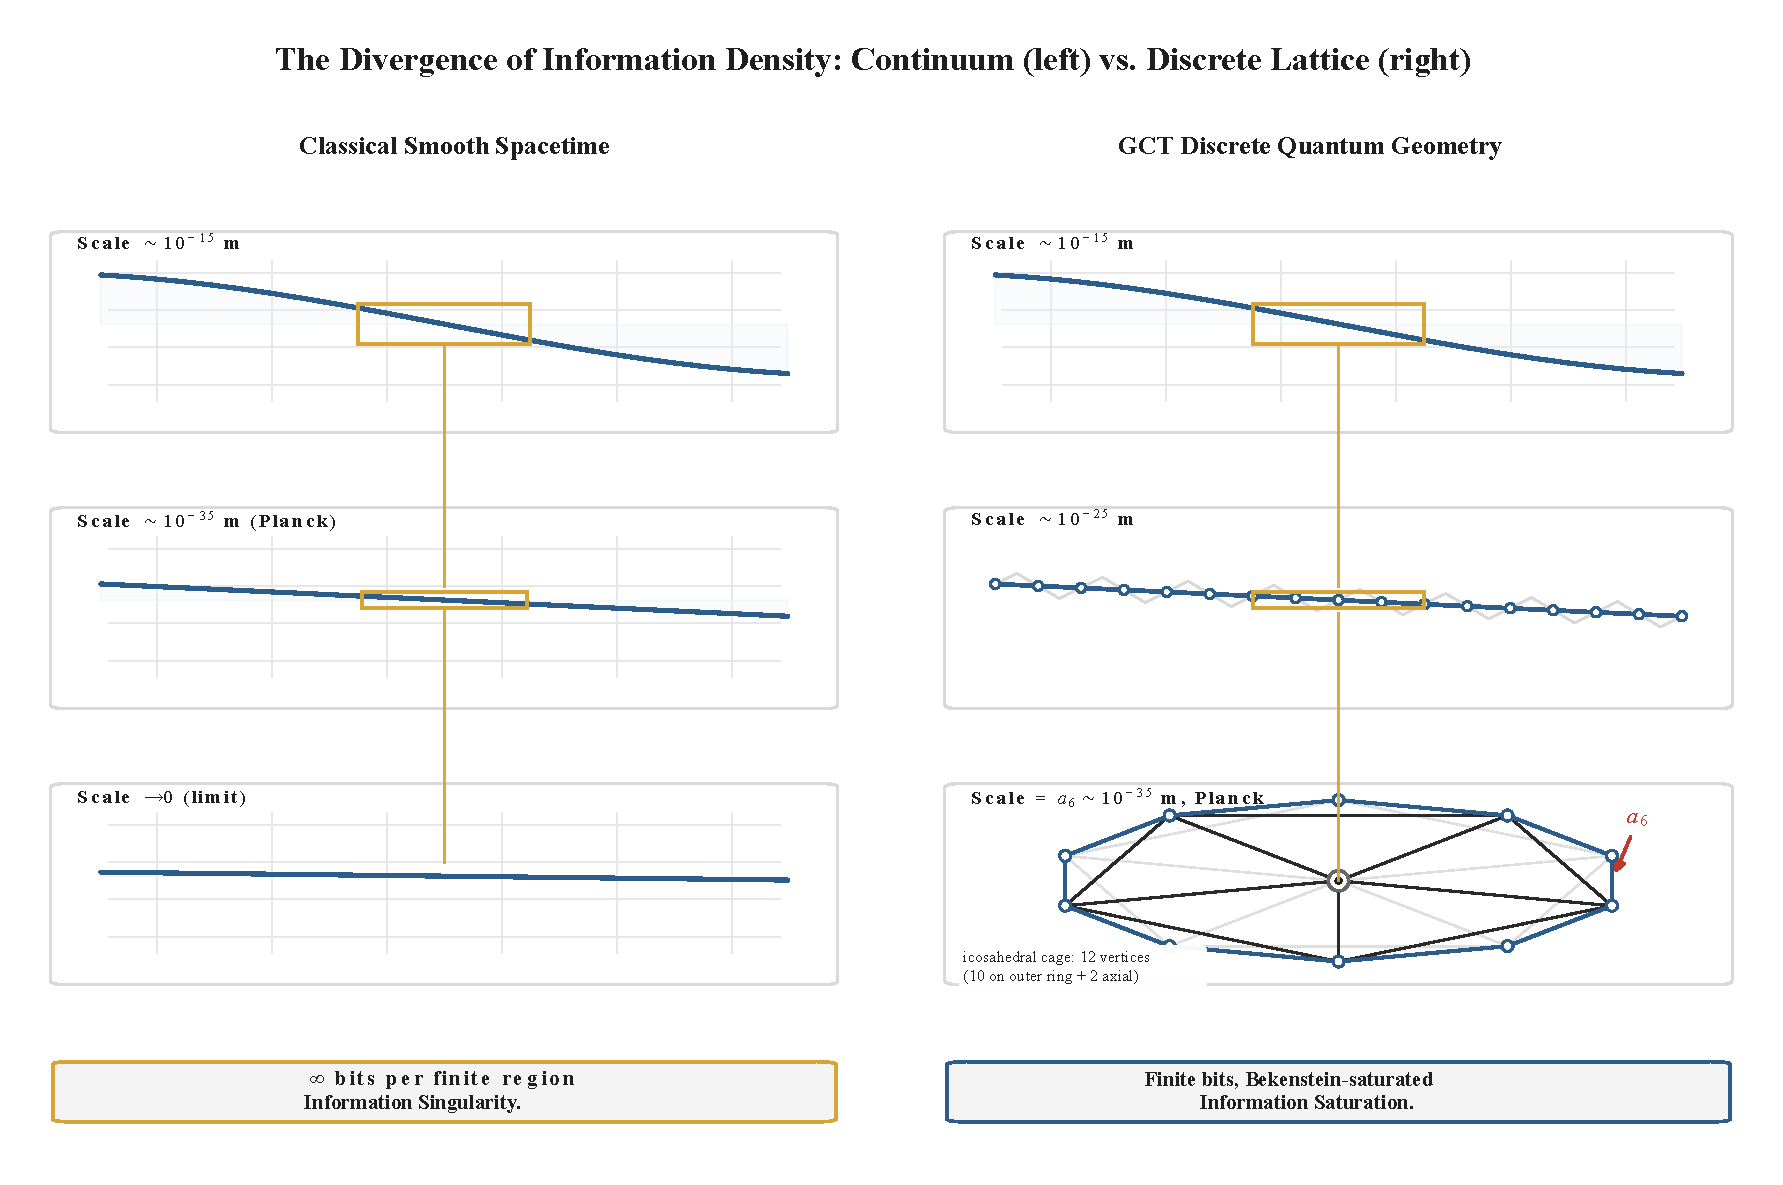
\includegraphics[keepaspectratio,alt={The divergence of information density: classical smooth spacetime (left) demands unbounded degrees of freedom under successive zoom, whereas GCT discrete quantum geometry (right) saturates at the lattice spacing, supplying a built-in cutoff.}]{content/Figures/Volume_1/Figure V1.4.1.pdf}}
\caption{The divergence of information density: classical smooth
spacetime (left) demands unbounded degrees of freedom under successive
zoom, whereas GCT discrete quantum geometry (right) saturates at the
lattice spacing, supplying a built-in cutoff.}
\end{figure}

\subsubsection{4.1.3 The Bayesian
Decision}\label{the-bayesian-decision-1}

We compare the complexity costs:

\begin{itemize}
\tightlist
\item
  \textbf{Continuum:} Unbounded local information density unless
  regulated; quantitative work needs a regulator and renormalization
  prescription (§2.2.3).
\item
  \textbf{Discrete:} Finite bits per bounded region and a built-in
  cutoff; compatible with quantum mechanics and with entropy bounds, but
  still requires a lattice, scale, action and continuum-recovery
  prescription.
\end{itemize}

\textbf{Decision:} \(P(\text{Discrete}) \gg P(\text{Continuum})\).
{[}Tier 1/2 --- Structural Postulate: discreteness selected by parsimony
and Bekenstein bound; see §2.2.3{]} We proceed with the understanding
that the universe is a \textbf{Discrete Lattice}.

\begin{center}\rule{0.5\linewidth}{0.5pt}\end{center}

\subsection{4.2 The Quasicrystal Choice}\label{the-quasicrystal-choice}

\subsubsection{4.2.1 The Constraint of
Isotropy}\label{the-constraint-of-isotropy}

If the universe is a lattice, what is its shape? A simple periodic
lattice (like a cubic grid \(\mathbb{Z}^3\)) has a cost: it breaks
\textbf{Rotational Symmetry (Isotropy)} at the lattice scale.

\begin{itemize}
\tightlist
\item
  \textbf{The Problem:} In a cubic grid, the distance between nodes is
  \(1\) along the axis, but \(\sqrt{3}\) along the diagonal. A particle
  moving diagonally would experience a different ``speed of light'' than
  one moving axially.
\item
  \textbf{Observation:} Laboratory resonator tests of Lorentz invariance
  (modern Michelson--Morley experiments) bound the anisotropy of the
  speed of light at about 1 part in \(10^{18}\). {[}Tier 3 ---
  laboratory phenomenological bound{]} The universe does not look like a
  grid; it looks smooth.
\item
  \textbf{Caveat:} On a Planck-scale cubic lattice the induced
  anisotropy at accessible energies is suppressed by roughly
  \((E/E_{\rm Pl})^2\), so this bound does not rule out a periodic
  lattice. GCT's preference for a non-periodic, orientationally ordered
  structure is an architectural choice, not a refutation of periodic
  lattices.
\end{itemize}

We face a trilemma. We need a structure that is:

\begin{enumerate}
\def\labelenumi{\arabic{enumi}.}
\tightlist
\item
  \textbf{Discrete} (to supply a built-in cutoff).
\item
  \textbf{Isotropic} (to match observation).
\item
  \textbf{Ordered} (to support physical laws).
\end{enumerate}

Standard candidates fail:

\begin{itemize}
\tightlist
\item
  \textbf{Periodic Crystal:} Discrete + Ordered, but Anisotropic.
\item
  \textbf{Random Glass / Causal Set:} Discrete + Isotropic
  (statistically), but Disordered.
\end{itemize}

\subsubsection{4.2.2 The Adopted Solution: Projected
Quasicrystal}\label{the-adopted-solution-projected-quasicrystal}

There is a third option, often overlooked: \textbf{The Quasicrystal}. A
Quasicrystal is a structure that is ordered but not periodic. It lacks
translational symmetry but possesses \textbf{Long-Range Orientational
Order}. Crucially, quasicrystals can possess ``forbidden'' rotational
symmetries, such as 5-fold (Pentagonal) or Icosahedral symmetry, which
are impossible for periodic crystals. Isotropy by itself is not enough
to select the icosahedral case: \(O_h\) and \(T_d\) also satisfy
macroscopic finite-point isotropy. GCT therefore adds the
maximal-polyhedral-point-symmetry axiom: among the finite polyhedral
rotation groups compatible with a discrete substrate, the icosahedral
group \(I\cong A_5\) is selected as the largest rotational order, 60.
The restriction to the polyhedral class is essential because dihedral
rotation groups have unbounded order. This is an architectural postulate
rather than a deduction from isotropy alone; it is the closest finite
polyhedral symmetry can get to spherical isotropy.

\gctneedspace{5\baselineskip}

\textbf{Rejecting Randomness (Causal Sets)} Why not a Random Graph
(Causal Set)? A random graph has \textbf{Maximal Kolmogorov
Complexity}---it is incompressible noise. To specify the universe, one
would need to specify every single link individually. A Quasicrystal has
\textbf{Low Kolmogorov Complexity}. It is generated by a simple,
deterministic projection algorithm. By the Principle of Parsimony
(Chapter 2), the Quasicrystal receives exponentially larger algorithmic
prior weight than the Random Graph within a declared encoding; this
ranks the hypotheses but does not by itself establish which is
physically true. \[ P(\text{Quasicrystal}) \gg P(\text{Random Graph}) \]
{[}Tier 1/2 --- Structural Postulate: quasicrystal selection by
minimum-complexity isotropic discrete geometry{]}

\gctneedspace{5\baselineskip}

\textbf{The Cut-and-Project Method} How is such a structure generated?
No periodic lattice in 3 dimensions has 5-fold symmetry
(crystallographic restriction), but quasiperiodic structures with 5-fold
or icosahedral order can be built in several ways: directly in 3D by
substitution (inflation) or matching rules, or by \textbf{projecting a
higher-dimensional lattice} into 3D {[}Tier 1 --- standard tiling
mathematics{]}. GCT uses the cut-and-project construction because it
makes the parent lattice and the internal space \(E_\perp\) explicit;
this is a modelling choice within the Structural Postulate below, not
the only possible construction. The standard \textbf{Penrose Tiling}
(2D) is a projection of a 5D hypercubic lattice. The
\textbf{Ammann-Kramer-Neri Tiling} (3D) is a projection of a 6D
hypercubic lattice.

GCT posits that the physical universe is a \textbf{3-dimensional slice
through a 6-dimensional hyper-lattice}. {[}Tier 1/2 --- Structural
Postulate: 6D parent lattice with cut-and-project{]}
\[ \mathbb{R}^6 \xrightarrow{\text{Project}} E_\parallel (\text{Physical Space}) \]

\subsubsection{4.2.3 The Geometric Engine}\label{the-geometric-engine}

This projection mechanism is not just a mathematical trick; it is the
engine of physics.

\begin{itemize}
\tightlist
\item
  \textbf{The \(E_8\) Connection:} The adopted primitive 6D lattice
  \(P\cong\mathbb{Z}^6\) has the index-2 sublattice
  \(D_6=\{x\in\mathbb Z^6:\sum_i x_i\text{ even}\}\), which supplies the
  color-parity sector used in Volume 3. The roots \(\pm e_i\pm e_j\)
  generate \(D_6\), not \(\mathbb Z^6\), and \(\mathbb Z^6\) is not a
  lattice subobject of even \(E_8\). The higher-symmetry connection is
  instead the conditional composition of the McKay \(2I\to E_8\)
  correspondence, the Elser--Sloane \(E_8\to H_4\) projection, and a
  rank-six icosahedral module. At rank 6 the Bravais choices are
  \(P\cong\mathbb Z^6\), \(F\cong D_6\), and \(I\cong D_6^*\); GCT
  adopts \(P\) (Appendix USS §USS.7).
\item
  \textbf{Emergence of Gauge Symmetries:} The ``hidden'' dimensions of
  the lattice (\(E_\perp\)) do not disappear. They become the internal
  spaces of particle physics. The icosahedral-projection ansatz supplies
  an open Tier 3
  \(\mathrm{SU}(3) \times \mathrm{SU}(2) \times \mathrm{U}(1)\)
  gauge-product candidate, with the full physical Standard-Model
  spectral-triple identification conditional on App ORQ O.32.
\item
  \textbf{Conditional Architectural Selection:} Once maximal polyhedral
  point symmetry, aperiodicity, the five-fold rhombic-triacontahedral
  window, golden arithmetic, and algorithmic simplicity are adopted,
  this geometry is the surviving branch of the registered comparison.
  Spinoriality alone does not distinguish it: every finite rotation
  subgroup has a canonical Spin\((3)\) preimage. \emph{(See Appendix
  USS.6 for the conditional classification.)} The proposed constants of
  nature (\(\alpha\), masses) are spectral and metric quantities of the
  selected icosahedral projection, subject to their separate tier labels
  and physical-map gaps.
\end{itemize}

\begin{center}\rule{0.5\linewidth}{0.5pt}\end{center}

\subsection{4.3 Conclusion of the Epistemic
Derivation}\label{conclusion-of-the-epistemic-derivation}

\subsubsection{4.3.1 The Complete Logical
Chain}\label{the-complete-logical-chain}

This completes the descent from Logic to Physics. The chain runs:

\begin{enumerate}
\def\labelenumi{\arabic{enumi}.}
\tightlist
\item
  \textbf{Axioms:} Presence + Intelligibility.
\item
  \textbf{Ontology:} Idealism (Mind is fundamental).
\item
  \textbf{Geometry:} Discrete Space (Finite Information).
\item
  \textbf{Symmetry:} Quasicrystal (icosahedral order realized by
  cut-and-project; adopted, §4.2).
\item
  \textbf{Hardware:} The 6D Lattice (Geometry of the Vacuum).
\end{enumerate}

\subsubsection{4.3.2 From Pure Logic to Physical
Structure}\label{from-pure-logic-to-physical-structure}

The framework arrives at a specific, falsifiable physical model without
invoking arbitrary particles or fields. GCT adopts a projected
high-dimensional lattice as the architecture consistent with the axioms
and the observational constraints. Chapter 5 adopts the Wheeler-DeWitt
equation as a Tier 3 Structural Postulate governing this lattice. Before
that, the ``Cosmology of Zero'' establishes why the lattice exists at
all. This bridges the gap between Volume 1 (Logic) and Volume 2
(Architecture). The ``Software'' (Consciousness) requires ``Hardware''
(Geometry) to render itself. The Quasicrystal is that hardware.

\chapter{Chapter 5: The Cosmology of
Zero}\label{chapter-5-the-cosmology-of-zero}

\subsection{5.1 The Logical Incompleteness of Pure
Zero}\label{the-logical-incompleteness-of-pure-zero}

\subsubsection{5.1.1 The Question of
Origin}\label{the-question-of-origin}

Having established the geometry of the vacuum, we face the ultimate
cosmological question: \textbf{Why does anything exist at all?}
Traditional physics answers this by pushing the problem back to an
``Initial Condition'' (The Big Bang singularity), but this is an
evasion. It does not explain why there was a singularity rather than
nothing. GCT rejects infinite regress. It adopts the reading that
existence is not a violation of nothingness but a form of it {[}Tier 4
--- philosophical commitment, not a theorem{]}.

\subsubsection{5.1.2 The Problem with 0=0}\label{the-problem-with-00}

Consider the concept of Absolute Nothingness---the Void. We denote this
state as \(0=0\). This state appears stable because it is symmetric and
minimal. GCT reads it, however, as having a logical defect: \textbf{It
is Logically Incomplete.} {[}Tier 4 --- philosophical reading{]} To be
``Zero'' requires the capacity to distinguish ``Zero'' from
``Not-Zero.'' But in a state of absolute undifferentiation, this
distinction cannot exist. A zero that cannot define itself is a
statement without a syntax. It is not a state; it is a nullity.
Therefore, the state of ``Pure Nothing'' cannot logically persist as a
defined entity; it must possess internal structure to be meaningful.

\subsubsection{5.1.3 Zero Requires
Self-Definition}\label{zero-requires-self-definition}

How does Zero define itself without violating conservation? GCT's
proposed reading is that it differentiates into complementary opposites
that sum to zero. {[}Tier 4 --- philosophical motivation; the identity
below is elementary arithmetic, and no conservation law or cosmological
fact is derived from it{]} \[ 0 = (+1) + (-1) \] This equation is
mathematically identical to \(0=0\), but informationally superior.

\begin{itemize}
\tightlist
\item
  \textbf{\(0=0\):} Zero information. No structure.
\item
  \textbf{\(0 = (+1) + (-1)\):} Two bits of information (the 1 and the
  -1), structure, and relationship, while maintaining total nullity.
\end{itemize}

The proposed metaphysical reading treats the universe not as the
creation of something from nothing but as the \textbf{Self-Definition of
Nothing} through internal differentiation. The self-differentiation
\(0 = (+1) + (-1)\) is not a temporal event; it is a timeless logical
identity, and it does not derive a cosmological history. Representing
``The Big Bang'' as the low-complexity boundary of the lattice --- the
limit \(\tau_{coord} \to 0\), where the density of actualised
configurations approaches zero --- is a Tier 4 coordinate analogy, not
an Agent's physical traversal or perception and not a replacement for
observational early-universe dynamics.

\begin{figure}
\centering
\pandocbounded{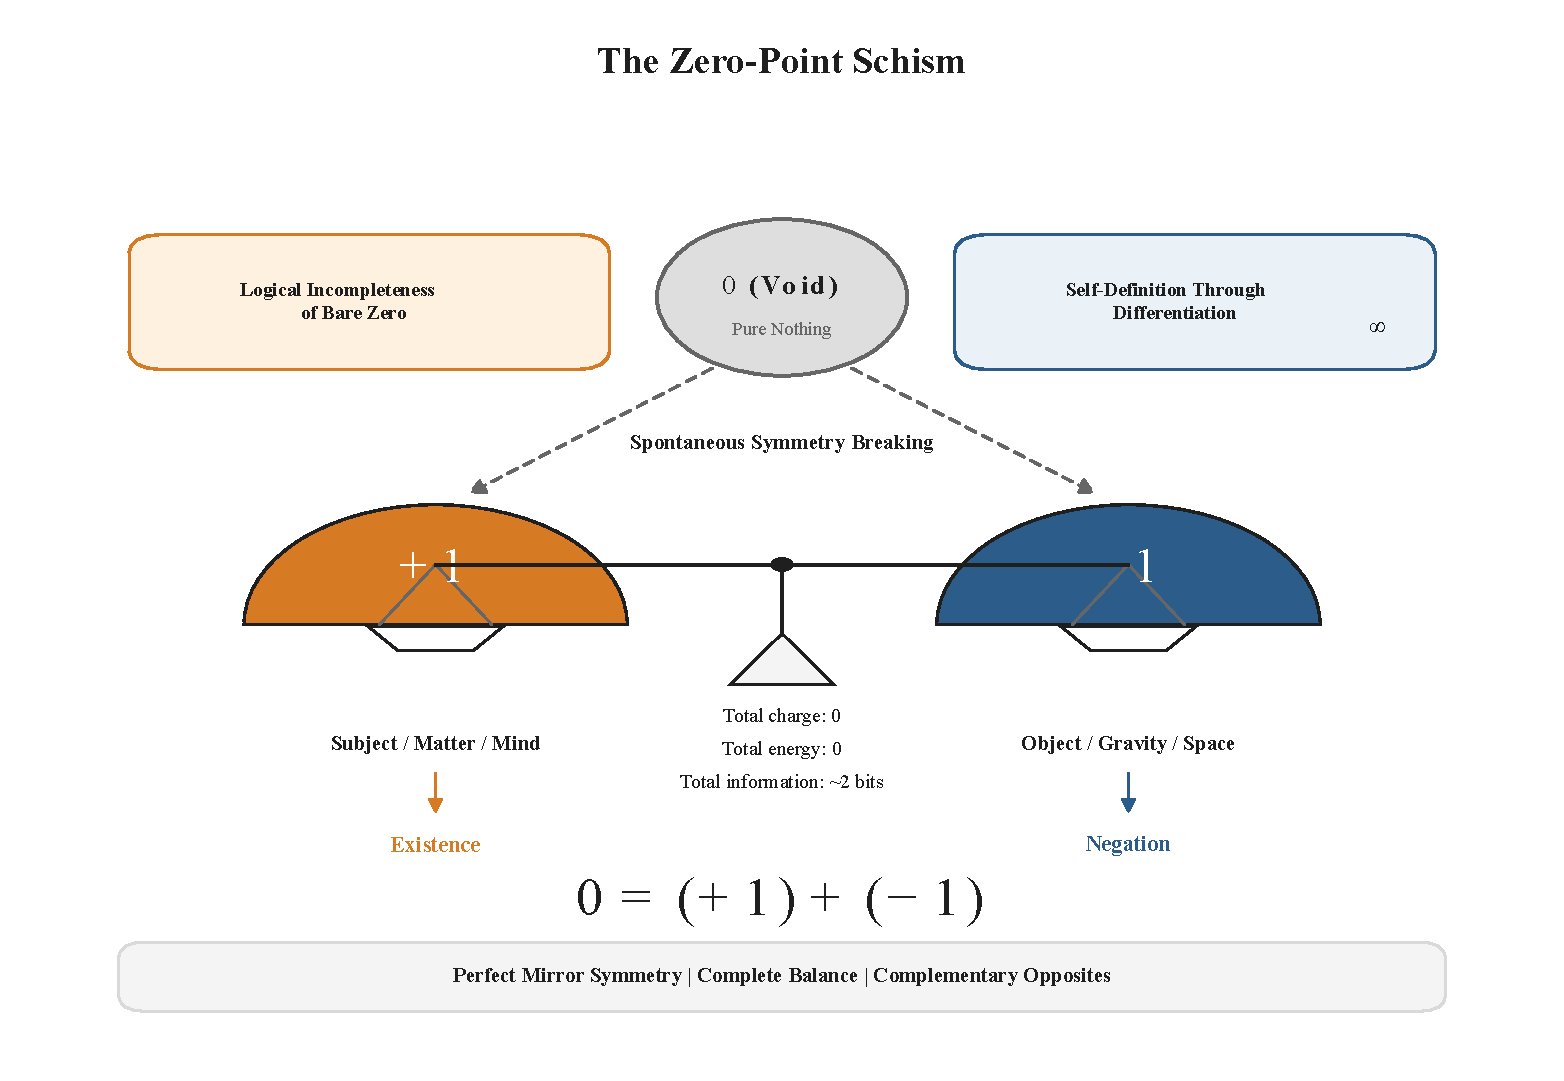
\includegraphics[keepaspectratio,alt={The Zero-Point Schism: the self-differentiation 0 = (+1) + (-1) shown as a symmetric bifurcation of the void into Subject and Object, with the global sum conserved at zero. Existence as the internal differentiation of Nullity.}]{content/Figures/Volume_1/Figure V1.5.1.pdf}}
\caption{The Zero-Point Schism: the self-differentiation
\(0 = (+1) + (-1)\) shown as a symmetric bifurcation of the void into
Subject and Object, with the global sum conserved at zero. Existence as
the internal differentiation of Nullity.}
\end{figure}

\begin{center}\rule{0.5\linewidth}{0.5pt}\end{center}

\subsection{5.2 Mathematical
Formalization}\label{mathematical-formalization}

\subsubsection{5.2.1 The Wheeler-DeWitt Constraint (Structural Framework
/
Ansatz)}\label{the-wheeler-dewitt-constraint-structural-framework-ansatz}

This philosophical motivation is formally expressed by adopting the
\textbf{Wheeler-DeWitt Equation} as the \textbf{Primary Boundary
Condition} of the theory: \[ \hat{H}\Psi = 0 \] \textbf{Status: {[}Tier
3 Structural Postulate{]}}

While motivated by the Idealist ontology, the \textbf{Wheeler-DeWitt
constraint (\(\hat{H}\Psi = 0\))} is formally adopted as a \textbf{Tier
3 Structural Postulate}. For a closed cosmos, GCT reads global nullity
as the natural boundary condition. The choice is motivated, not forced,
by three considerations: (a) the Tier 4 self-definition reading of Zero
in §5.1.2--5.1.3, (b) the standard result that a
diffeomorphism-invariant closed system carries a Hamiltonian constraint,
here via BRST symmetry (below), and (c) the Tier 4 measure-theoretic
motivation of §5.2.3 and Appendix MTI. This postulate defines the
`Hardware State' of the vacuum as a zero-energy static block, within
which relational time is subsequently modelled as an internal
correlation.

In any theory with diffeomorphism invariance (Coordinate Independence),
the Hamiltonian is a constraint, not a generator of time evolution. To
remove the unphysical ``gauge'' degrees of freedom, we require that
physical states \(|\Psi\rangle\) lie in the kernel of the BRST charge
operator \(\hat{Q}_B\): \[ \hat{Q}_B |\Psi\rangle = 0 \] Because the
Hamiltonian \(\hat{H}\) is the generator of time-translations (which are
just gauge transformations in General Relativity), the condition of BRST
invariance implies that the physical state must be annihilated by the
Hamiltonian constraint: \[ \hat{H} |\Psi\rangle = 0 \] This equation is
the \textbf{Wheeler-DeWitt Equation}. It asserts that the wavefunction
of the universe is static. Time \(t\) is not an external parameter but
an internal coordinate correlation \emph{within} the static state
\(|\Psi\rangle\). The universe does not evolve; it exists.

\subsubsection{5.2.2 Physical Interpretation: Energy
Balance}\label{physical-interpretation-energy-balance}

How can a universe full of stars and galaxies have zero energy?

\begin{itemize}
\tightlist
\item
  \textbf{Positive Energy (\(E_{mat}\)):} Matter, radiation, and dark
  energy (\(mc^2\)).
\item
  \textbf{Negative Energy (\(E_{grav}\)):} The gravitational potential
  energy of the geometry itself.
\end{itemize}

In GCT, this balance is consistent with the geometry of the \textbf{6D
Parent Lattice} (Volume 2). The lattice is a static structure embedded
in a Euclidean space. Any deformation (matter) creates a corresponding
curvature (gravity); on the Wheeler--DeWitt reading, the total
Hamiltonian of a closed universe (gravitational plus matter) vanishes.
This is a constraint on the total, not a statement that the matter
stress-energy tensor integrates to zero, which it does not. The universe
is the ``Ultimate Free Lunch.'' It costs zero energy to create a
universe, provided you create enough gravity to balance the mass.
{[}Tier 3 --- conditional on the Wheeler-DeWitt Structural Postulate,
§5.2.1{]}

\subsubsection{5.2.3 Measure-Theoretic Motivation
(Summary)}\label{measure-theoretic-motivation-summary}

We motivate this choice using Measure Theory (see Appendix MTI). A
probability measure on the space of all possible realities has total
mass 1 by definition, so it cannot express global nullity. The formal
object GCT uses instead is a \textbf{signed measure} \(\mu=\mu_+-\mu_-\)
whose positive and negative parts cancel, so that its total mass is zero
while it remains non-trivial (distinction) locally; the
\textbf{Principle of Indifference} is read as motivating the balance of
the two parts. {[}Tier 4 motivation --- a signed measure with zero total
mass is a modelling choice, not a measure-theoretic necessity; see
Appendix MTI{]} \[ \int_{\mathcal{U}} d\mu = 0 \] The universe is
modeled as a fluctuation of the vacuum measure that sums to zero
globally but is non-zero locally.

\begin{center}\rule{0.5\linewidth}{0.5pt}\end{center}

\subsection{5.3 Differentiation
vs.~Creation}\label{differentiation-vs.-creation}

\subsubsection{5.3.1 Logical Necessity, Not Temporal
Event}\label{logical-necessity-not-temporal-event}

We must excise temporal bias from our language. The differentiation of
Zero is not an event that happened \emph{at} a time \(t=0\). Time is a
feature \emph{inside} the differentiation. The equation
\(0 = (+1) + (-1)\) is timelessly true. It does not ``become'' true.
Therefore, the universe did not ``begin.'' The universe \textbf{IS}. It
is the eternal, static structure of the self-defining Zero. Calling the
experienced sense of ``beginning'' an Agent's traversal of the time
coordinate \(\tau\) from low to high complexity is a Tier 4
phenomenological metaphor. No physical Selection trajectory, clock,
owner, or phenomenal-time map has been derived.

\subsubsection{5.3.2 Structure-Preserving
Nullity}\label{structure-preserving-nullity}

The differentiation is constrained. It cannot be arbitrary chaos. It
must be \textbf{Symmetric}. This symmetry requirement is consistent with
the conservation laws of physics, and GCT proposes that it underwrites
them. Noether's theorem applies to continuous symmetries, so the
argument runs through the continuous symmetries of the effective
continuum description of the 6D lattice projection (Volume 2); the
discrete lattice point group by itself supplies selection rules and
discrete conserved quantum numbers, not Noether currents: the \(U(1)\)
phase symmetry of the lattice yields charge conservation; the \(SO(3)\)
rotational symmetry yields angular momentum conservation; the candidate
\(SU(3)\) color symmetry of the icosahedral projection (an open Tier 3
candidate, V3 Ch03) would yield the color-singlet condition.

\begin{itemize}
\tightlist
\item
  Conservation of Charge: \(dQ/dt = 0\). {[}Tier 1 --- Noether
  consequence of the \(U(1)\) phase symmetry, conditional on that
  symmetry; GCT phase-sector candidate in V3 Ch01; the V2 Ch06 Maxwell
  realization is a declared open programme{]} Zero total charge,
  \(\sum Q = 0\), does not follow from Noether's theorem; for a closed
  universe it follows from the Gauss-law constraint on a compact space
  {[}Tier 1, conditional on closure{]}.
\item
  Conservation of Angular Momentum: \(dL/dt = 0\). {[}Tier 1 --- Noether
  consequence of continuous \(SO(3)\) rotational invariance, conditional
  on that invariance holding in the projected continuum description{]}
  Zero total angular momentum, \(\sum L = 0\), is an additional boundary
  condition that GCT assumes, not a Noether consequence {[}Tier 3{]}.
\item
  Conservation of Color: The universe is a Color Singlet. {[}Tier 3 ---
  conservation would be a Tier 1 Noether consequence given an exact
  \(SU(3)\) symmetry, but that symmetry is the open Tier 3 candidate of
  the icosahedral projection (V3 Ch03){]} The laws of physics are the
  bookkeeping rules required to ensure that the complex dance of
  existence always sums to zero.
\end{itemize}

\subsubsection{5.3.3 The Universe as Recursive
Definition}\label{the-universe-as-recursive-definition}

\gctneedspace{5\baselineskip}

\textbf{{[}Tier 4: Philosophical Interpretation --- self-reference
reading, not a derivation of a cosmic subject{]}} On this
interpretation, Zero differentiates into \textbf{Subject} (Mind/Field)
and \textbf{Object} (Matter/Pattern), and the differentiation is read as
\textbf{Self-Reference}: a self-consistent structure through which the
system would register its own existence. A formal fixed-point equation
may be stipulated, \[\Psi = \hat{\mathcal{F}}[\Psi],\] where
\(\hat{\mathcal{F}}\) is a declared map (read here as the Field's
self-excitation operator). Fixed-point structure does not by itself
imply that the universe registers its own existence, instantiates a
Subject/Object split, carries Fisher information, or possesses a
physical or phenomenal Selection Operator, and none of those claims
follows from the Wheeler-DeWitt constraint of §5.2.1. Whether the
universe is in this sense self-referential or conscious is not
established by the geometry; it remains a Tier 4 interpretation.

\begin{center}\rule{0.5\linewidth}{0.5pt}\end{center}

\subsection{5.4 The Fractal Tautology}\label{the-fractal-tautology}

\subsubsection{5.4.1 Holographic Displacement as a Phenomenological
Analogy {[}Tier
4{]}}\label{holographic-displacement-as-a-phenomenological-analogy-tier-4}

If the universe is static, why does it appear to expand? If the universe
is represented by a static global state, its observed expansion still
requires a physical cosmological model. The manuscript explores
\textbf{Holographic Displacement} as a Tier 4 phenomenological analogy
for dark-energy phenomenology (V2 Ch14); a fit of its channel shape to
data would be a Tier 3 phenomenological fit, while the physical-source
interpretation is Tier 4. Conditional on a shared-phason-field ansatz,
information production and a relaxation coordinate are placed in the
same model; the Holographic Bound supplies a consistency constraint, not
a causal law requiring the boundary to expand. No typed, normalized
information-to-metric map is currently derived: GCT has not derived
conscious-Agent bit generation, a Selection-to-phason transducer, or a
local or covariant stress-energy source.
\[ \Delta V = \ell_P^3 \cdot \Delta I / \ln 2 \] \textbf{{[}Tier 4:
phenomenological response ansatz --- physical coupling, coefficient and
source map open{]}} The displayed relation is therefore illustrative
bookkeeping within the ansatz, not evidence that cosmic expansion
physically ``makes room'' for increasing complexity.

\subsubsection{5.4.2 Resolution Increase and
Self-Knowledge}\label{resolution-increase-and-self-knowledge}

\begin{itemize}
\tightlist
\item
  \textbf{Low-\(\tau_{coord}\) model regions:} Declared low
  configuration-density, low-information labels --- the boundary
  \(\tau_{coord} \to 0\) of the actualised-configuration manifold.
\item
  \textbf{High-\(\tau_{coord}\) model regions:} Declared high
  configuration-density, high-information labels. Calling these a
  biogenic sector in which recursive Selection Operators become viable
  is an unproved Tier 4 interpretation, not a physical threshold. The
  apparent arrow from ``Implicit Potential'' to ``Explicit
  Actualization'' is a coordinate metaphor within the static model, not
  a derived traversal, Selection process, or temporal sequence in the
  Field Frame.
\end{itemize}

\subsubsection{\texorpdfstring{5.4.3 Teleology: Implicit \(\to\)
Explicit}{5.4.3 Teleology: Implicit \textbackslash to Explicit}}\label{teleology-implicit-to-explicit}

\gctneedspace{5\baselineskip}

\textbf{{[}Tier 4: Philosophical Interpretation --- Not a quantitative
claim{]}} This section offers a philosophical teleology: the implicit
structure of the Field may be interpreted as tending toward explication
rather than heat death. Within that interpretation, discovery and
creation participate in increasing articulated information. It is not a
scientific claim that the universe has a goal, that human thought or art
generates a vacuum source, or that Agent activity drives cosmic
expansion; no Selection-to-phason or information-to-stress-energy
mechanism is derived.

\begin{figure}
\centering
\pandocbounded{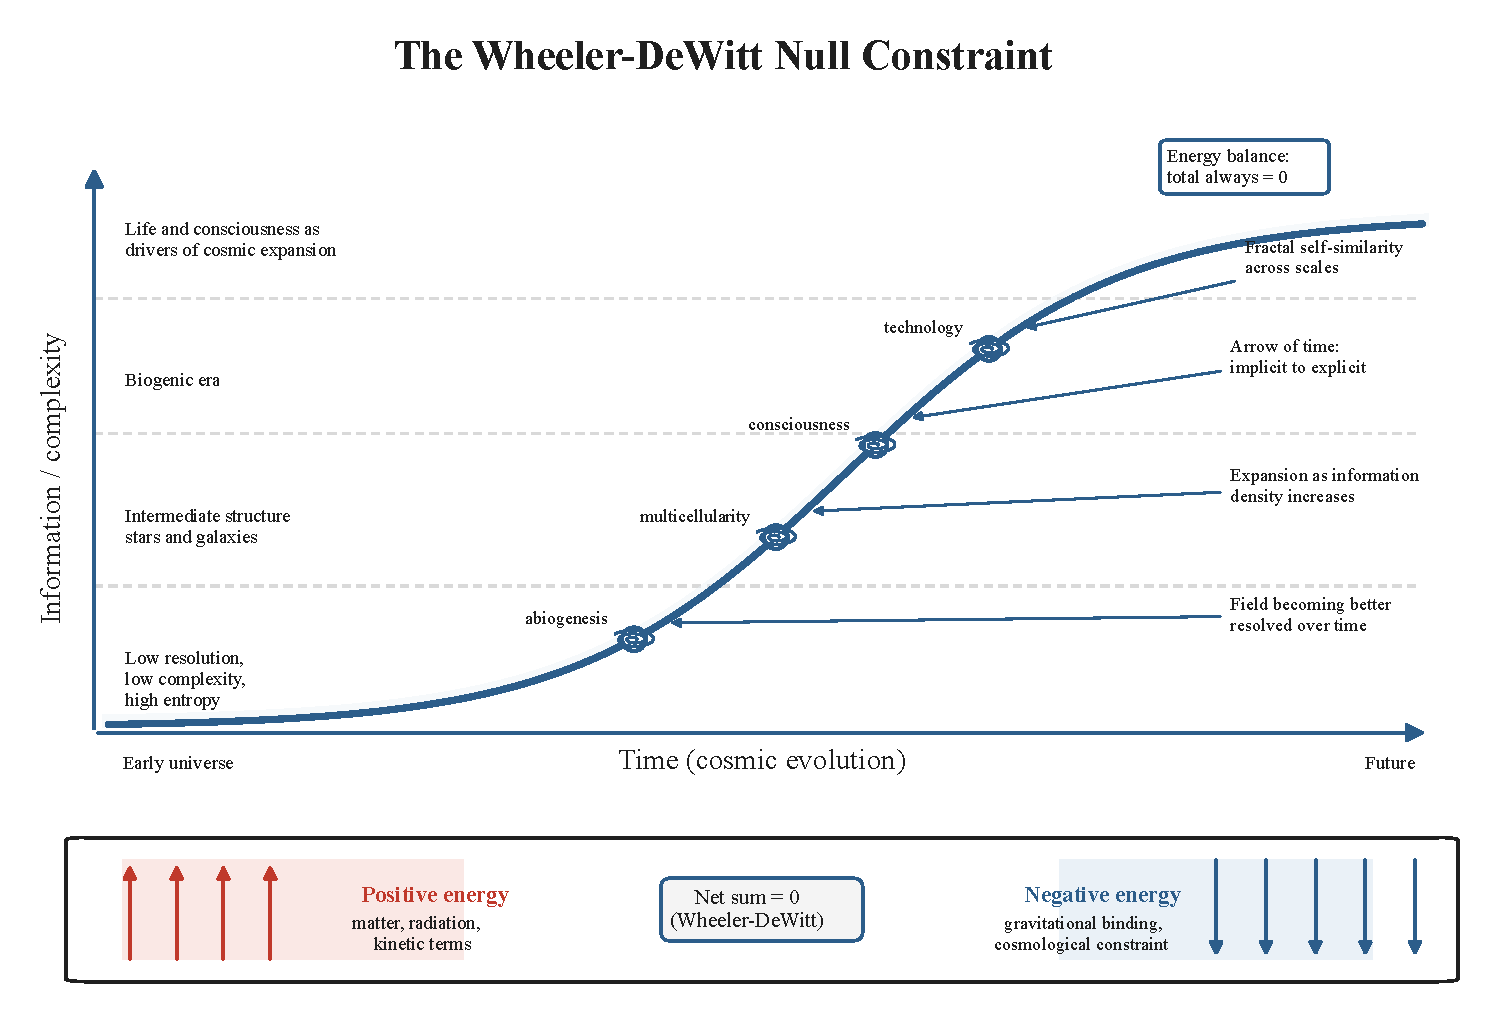
\includegraphics[keepaspectratio,alt={The Wheeler-DeWitt null constraint: the global state satisfies \textbackslash hat\{H\}\textbar\textbackslash Psi\textbackslash rangle = 0, so the universe carries no external time parameter, and temporal flow is modelled as the internal correlation structure of the static block; no physical Selection clock, biology-to-vacuum source, or phenomenal bridge is inferred.}]{content/Figures/Volume_1/Figure V1.5.2.pdf}}
\caption{The Wheeler-DeWitt null constraint: the global state satisfies
\(\hat{H}|\Psi\rangle = 0\), so the universe carries no external time
parameter, and temporal flow is modelled as the internal correlation
structure of the static block; no physical Selection clock,
biology-to-vacuum source, or phenomenal bridge is inferred.}
\end{figure}

\clearpage
\thispagestyle{empty}
\vspace*{0.35\textheight}
\begin{center}\bfseries\LARGE PART II: THE ARCHITECTURE OF IDENTITY\end{center}
\vspace*{\fill}
\clearpage

\chapter{Chapter 6: The Tri-Partite
Ontology}\label{chapter-6-the-tri-partite-ontology}

\subsection{6.1 Beyond Naive Monism}\label{beyond-naive-monism}

\subsubsection{6.1.1 Refining Objective
Idealism}\label{refining-objective-idealism}

In \textbf{Chapter 3}, we adopt \textbf{Objective Idealism} as the
minimum-complexity branch relative to materialism (Ch03 §3.4), given
Axiom 1 (Tier 3 parsimony choice): The Field (Level I presence) is
treated as the sole ontological primitive. GCT presents this as
Objective Idealism at the global-metaphysics level and as its
objective-idealist version of Structural Russellian Monism at the
mind-physics interface: on the Tier 3 structural-Russellian bridge the
Field's intrinsic nature is experiential, and physics describes
extrinsic relational structure (see Ch16 §16.2.2). Position note: the
framework is globally objective-idealist about the Field, in the sense
of a priority monism about a non-subjective Field (Level I presence is
intrinsic but non-subjective); it does not posit a cosmic subject:
within Tiers 1--3 the Field's Level I presence is non-subjective, and a
cosmic-scale subject remains an open Tier 4 hypothesis (App TIB), with
Goff's cosmopsychism as the closest competing view (Ch03 §3.4.3). It is
Russellian-monist at the physics/experience interface; not
type-physicalist; and not micro-subject panpsychist. However, simply
stating ``All is Mind'' is insufficient to explain the complexity of
physics. A monolithic mind explains nothing; a structured mind explains
everything. Standard Idealism risks two failure modes:
\textbf{Solipsism} (the private mind as sole reality, which cannot
account for the intersubjective consensus of physical law) and
\textbf{Undifferentiated Panpsychism} (a naive view that would attribute
Level II unified subjecthood to every physical configuration, including
aggregates such as rocks; mainstream panpsychists, who attribute
micro-experience to fundamental entities, reject this view as well). GCT
rejects both. The theory distinguishes \textbf{Level I Universal
Presence} (Axiom 1, Tier 1 by stipulation; intrinsic non-subjective
presence in all Field configurations) from \textbf{Level II
Apperception}, the Tier-3 interpretation proposed for a physically
realized Identity Polaron only if its full mathematical, coupling, and
phenomenal-bridge program closes. Nuclear spin and chirality are
candidate experimental controls, not a necessary/sufficient DMC verdict.
Physical realization remains conditional on O.18/O.21/O.23/O.32/O.34,
and the Level II status of every examined substrate is open (Tier 3): no
validated substrate criterion exists yet (it requires a typed,
normalized, measured coupling, the Identity-Polaron construction and an
independent phenomenal bridge; O.21/O.23/O.34, O.18). The Tri-Partite
Process Ontology supplies the formal architecture for this distinction.
The working model distinguishes three roles without making all three
independent Tier-1 modes of the Field.

\subsubsection{6.1.2 Process Ontology: Three Aspects of One
Reality}\label{process-ontology-three-aspects-of-one-reality}

The tri-partite working architecture distinguishes:

\begin{enumerate}
\def\labelenumi{\arabic{enumi}.}
\tightlist
\item
  \textbf{The Potential:} The Field configurations available in the
  static state (The Medium).
\item
  \textbf{The Address Structure:} A candidate scaffold for labeling and
  resolving configurations (The Map). It does not supply physical laws,
  histories, or transitions.
\item
  \textbf{The Actualization:} A formal Agent-frame conditionalization
  role on a declared state space (The Operator). No examined physical
  carrier, transition instrument, or phenomenal owner presently realizes
  this role {[}Tier 3 physical/phenomenal proposal{]}.
\end{enumerate}

\subsubsection{6.1.3 Substance, Structure, and
Actualization}\label{substance-structure-and-actualization}

We formalize these as three roles in the proposed operator stack, not as
three independently derived objects embedded in the global wavefunction:

\begin{enumerate}
\def\labelenumi{\arabic{enumi}.}
\tightlist
\item
  \textbf{The Field (\(\Psi\)):} The Substance (Potential).
\item
  \textbf{The Solenoid (\(\Sigma_\infty\)):} The candidate
  Address/Resolution Scaffold (Fiber). It is physically usable only if a
  separate bridge assigns Solenoid addresses to physical states.
\item
  \textbf{The Agent (\(\mathcal{F}_{sel}\)):} The proposed
  Actualization/Conditionalization role (Renderer). Treating it as a
  qualified physical process requires an independently derived carrier
  and transition law; experiential realization additionally requires a
  realization bridge and an owner/phenomenal bridge.
\end{enumerate}

This triad reframes the interaction problem within the GCT operator
stack. If an Agent-frame dynamics is supplied, it would act on declared
conditional states through an independently specified instrument or
transition kernel. No examined substrate presently supplies that
carrier, kernel, Selection Operator, or phenomenal owner. If an
address-assignment bridge is supplied, the states may also carry
Solenoid address labels; the Solenoid itself neither modulates the Field
nor supplies a transition or selection law.

Only the Field / Presence axiom is Tier 1 by stipulation. The Solenoid
and Agent are formal structural roles in the operator stack:
\(\Sigma_\infty\) supplies the inverse-limit address structure, and
\(\mathcal{F}_{sel}\) names the Selection Operator role. Their physical
and phenomenal interpretations are \textbf{Tier 3 structural
commitments} (justified by parsimony and empirical adequacy of the
lattice geometry; not deductively forced by the foundational axioms;
closure target via App ORQ O.18 + O.32). The triad is therefore not
three independent Tier-1 ontological postulates.

\begin{center}\rule{0.5\linewidth}{0.5pt}\end{center}

\subsection{\texorpdfstring{6.2 The Field (\(\Psi\)) - The
Potential}{6.2 The Field (\textbackslash Psi) - The Potential}}\label{the-field-psi---the-potential}

\subsubsection{6.2.1 Definition: The Fundamental
Substrate}\label{definition-the-fundamental-substrate}

The \textbf{Field (\(\Psi\))} is the ontological primitive posited in
Part I as the framework postulate built on Axiom 1 (§2.3.4, §2.4): The
datum that experience is occurring is Tier 0 (\(P=1\)); Axiom 1
generalises it by stipulation to universal Level I presence (Tier 1).
Taking the Field as primitive is the Tier 3 objective-idealist parsimony
choice and does not inherit that certainty. The Quality Space
topological structure derived in Ch16 §16.4 is a separate Tier 2 result.
It is the raw ``stuff'' of existence---the medium of Presence.
Mathematically, it is the Universal Wavefunction defined over the
configuration space \(\mathcal{P}\).
\[ \begin{gathered}\Psi: \mathcal{P} \to \mathbb{C} \\[1pt] \gcteqnote{[Tier 1 — Definition of the universal wavefunction over configuration space]}\end{gathered}\]
It represents the amplitude of ``Being'' at any given configuration.

\subsubsection{6.2.2 Nature: Static, Timeless,
Infinite}\label{nature-static-timeless-infinite}

The Field does not change. It contains all possible histories, all
possible laws, and all possible identities in a simultaneous
superposition. On the Wheeler--DeWitt Structural Postulate it is
modelled as a \textbf{Block Universe} {[}Tier 3 --- conditional on the
WdW Structural Postulate, §5.2.1{]}. Because it satisfies the
Wheeler-DeWitt constraint, it possesses no internal clock. It is the
``Eternal Now.''

\subsubsection{6.2.3 Analogy: The Medium / The
Ocean}\label{analogy-the-medium-the-ocean}

Think of the Field as a vast, static \textbf{Ocean}. The ocean has depth
and capacity, but it does not ``flow'' in a specific direction until
disturbed. It is the \emph{capacity} for waves, not the waves
themselves. Without the Ocean, the waves (Matter) have no medium, and
the surfer (Agent) has no surface.

\textbf{6.2.4 Satisfies \(\hat{H}\Psi = 0\)} {[}Tier 3 --- conditional
on the Wheeler-DeWitt Structural Postulate, §5.2.1{]}

The rigorous definition of the Field is that it is the solution to the
constraint equation: \[ \hat{H}\Psi = 0 \] On that postulate the Field
carries no external time parameter, and its total energy is zero. It is
the perfect equilibrium of the Void.

\begin{center}\rule{0.5\linewidth}{0.5pt}\end{center}

\subsection{\texorpdfstring{6.3 The Solenoid (\(\Sigma_\infty\)) - The
Structure}{6.3 The Solenoid (\textbackslash Sigma\_\textbackslash infty) - The Structure}}\label{the-solenoid-sigma_infty---the-structure}

\subsubsection{6.3.1 Definition: Topological Space of
Identity}\label{definition-topological-space-of-identity}

If the Field is the Ocean, the \textbf{Solenoid (\(\Sigma_\infty\))} is
at most a coordinate grid or address catalogue laid over candidate
physical configurations; it is not the current that moves them. We
define \(\Sigma_\infty\) as the candidate \textbf{address fiber} of the
universal configuration bundle \(\mathcal{P} \to E_{proj}\).
Mathematically it is a compact connected abelian group (a laminated
continuum), not a manifold. It is a proposed topological address
structure; its use as a physical identity-address space is a Tier 3
structural identification conditional on a separate address-assignment
bridge, and identifying it with selfhood is a Tier-3 interpretive bridge
rather than a derived ownership relation. The exact topology alone
supplies no observer, owner, memory, history, persistence, or dynamics.
Mathematically, it is the \textbf{Adelic Solenoid}, constructed as the
inverse limit of circle wrappings (detailed in Chapter 7).

\begin{quote}
\textbf{Operational preview of the Adelic Solenoid (informal; formal
construction in Ch07 §7.2).} A condensed-matter physicist familiar with
quasicrystals will recognize ``solenoid'' as a topological term; the
\emph{adelic} qualifier sits in algebraic-topology / number-theory
territory and is novel in physics. The Adelic Solenoid \(\Sigma_\infty\)
is a specific compact topological space defined as the inverse limit of
circle wrappings: \(\Sigma_\infty = \varprojlim_n S^1_n\) where each
\(S^1_n\) is a wrapping of \(S^1\) by \(n\). Equivalently, it can be
presented as the compact quotient
\((\mathbb{R}\times\widehat{\mathbb{Z}})/\mathbb{Z}\), with
\(\mathbb{Z}\) embedded diagonally. The frequently used
``\(\mathbb{R}\times\widehat{\mathbb{Z}}\)'' language is therefore a
covering/suspension presentation, not a literal global product
decomposition of the compact solenoid. In that presentation,
\(\mathbb{R}\) is the continuous flow coordinate and
\(\widehat{\mathbb{Z}}\) is the profinite address coordinate. The
profinite integers
\(\widehat{\mathbb{Z}}=\varprojlim_n \mathbb{Z}/n\mathbb{Z}\cong\prod_p\mathbb{Z}_p\)
carry the profinite topology; they are a product over all primes, not
the \(p\)-adic integers for a single \(p\). Compatible ultrametrics and
rooted cylinder trees arise only after choosing a divisibility
filtration, so no single prime, root point, or observer hierarchy is
intrinsic, and an ultrametric space supplies nested neighbourhoods, not
adjacency between points. The path components of \(\Sigma_\infty\) are
its dense leaves, each a copy of \(\mathbb{R}\), so
\(\pi_1(\Sigma_\infty)=0\): the Solenoid carries no winding record. The
formal two-coordinate structure does not by itself identify a subject,
an owner, or a stream of experience; those are Tier-3 physical and
phenomenal interpretations requiring an independent bridge. The circle
inverse system alone does \textbf{not} specify a Cuntz--Krieger or
Cuntz--Pimsner algebra: those constructions require an additional
transition matrix, correspondence, endomorphism or transfer rule, and
none is selected by \(\Sigma_\infty\) or is thereby the
\textbf{Selection Operator} \(\mathcal{F}_{sel}\) {[}Tier 1 scope
distinction{]}. (For full background: Pontryagin 1966, \emph{Topological
Groups}; Cuntz--Krieger 1980 for the general C*-algebraic construction,
which needs transition data beyond the inverse limit.)
\end{quote}

\subsubsection{6.3.2 Nature: Static, Fractal,
Hierarchical}\label{nature-static-fractal-hierarchical}

Like the Field, the Solenoid is static. It does not evolve. It possesses
arbitrarily fine finite-quotient structure. After choosing a cofinal
divisibility filtration, that structure can be drawn as a rooted
cylinder tree:

\begin{itemize}
\tightlist
\item
  \textbf{The Root:} the whole level-zero cylinder, not a point or
  subject.
\item
  \textbf{The Branch Nodes:} finite-resolution cylinders (equivalence
  classes of addresses).
\item
  \textbf{The Ends (Leaves):} full compatible addresses, i.e.~points of
  the profinite transversal; no phenomenal moment follows from the label
  alone.
\end{itemize}

Interpreting cylinders as timelines, choices, shared identity sectors,
divergent lives, or moments of experience requires a separate physical
incidence map and remains Tier 3/4. The topology supplies resolution
membership, not an owner hierarchy.

\subsubsection{6.3.3 Analogy: The Library / Wiring
Diagram}\label{analogy-the-library-wiring-diagram}

Think of the Solenoid as a \textbf{catalogue} or a coordinate overlay on
a wiring diagram. A catalogue can label an item at arbitrarily fine
declared resolution, but it does not contain the item's physical
content, remember which items were previously consulted, or instruct a
reader where to go next. Physical content belongs to the
Field/conditional state; history requires physical records and a
separate memory bridge; reachability and motion require a separately
specified kernel.

\subsubsection{6.3.4 Crucial Distinction: Map
vs.~Territory}\label{crucial-distinction-map-vs.-territory}

We must distinguish the Solenoid from the Field.

\begin{itemize}
\tightlist
\item
  \textbf{The Field:} Is the Territory (The Substance).
\item
  \textbf{The Solenoid:} Is the Map (The Topology). The Solenoid
  supplies a proposed address organization for the Field. A coherent
  narrative or phenomenal organization requires the separate Tier-3
  physical and phenomenal bridge.
\end{itemize}

\begin{center}\rule{0.5\linewidth}{0.5pt}\end{center}

\subsection{\texorpdfstring{6.4 The Agent (\(\mathcal{F}_{sel}\)) - The
Actualization}{6.4 The Agent (\textbackslash mathcal\{F\}\_\{sel\}) - The Actualization}}\label{the-agent-mathcalf_sel---the-actualization}

\subsubsection{6.4.1 Definition: Selection Operator
Instance}\label{definition-selection-operator-instance}

The \textbf{Agent} names the localized role proposed for the
\textbf{Selection Operator (\(\mathcal{F}_{sel}\))}. It is not an
independently derived owner of experience. The selection model is an
\textbf{Open Quantum System Process} that traces over the internal
environment (\(E_\perp\)) and represents a non-unitary selection step
(Chapter 9). Whether this step is physically realized, selects a
particular world, or carries a specific experience remains a Tier-3
physical and phenomenal bridge. \emph{(\(\mathcal{F}_{sel}\) is
\textbf{non-unitary} within the formal model. The one-cycle operator
decomposes as
\(\mathcal{F}_{sel} = \mathcal{P}_{\text{actualize}} \circ \mathcal{U}_{\text{steer}}\),
where the inner-cycle steering generator \(\mathcal{U}_{\text{steer}}\)
is unitary but the actualization projection
\(\mathcal{P}_{\text{actualize}}\) is non-unitary. See V1 Ch10 §10.4.1
for the formal treatment.)}

\subsubsection{6.4.2 Nature: Dynamic (Relative) vs.~Static
(Absolute)}\label{nature-dynamic-relative-vs.-static-absolute}

Here we must be precise to avoid dualism.

\begin{itemize}
\tightlist
\item
  \textbf{In the Agent Frame:} The model assigns a dynamic address
  position to the Selection Operator. Interpreting its sequence as a
  stream of consciousness is a Tier-3 phenomenological bridge.
\item
  \textbf{In the Field Frame:} If a physical carrier and transition law
  are later identified, its modeled history may be represented as a
  static world-line or flux-tube-like record in the Block Universe. No
  such Identity-Polaron history is currently demonstrated, and
  recoverable history requires physical records and a memory bridge
  rather than the address scaffold. The model's ``movement'' is an
  internal relation between supplied states, not a derived evolution of
  the Bulk or a measured phenomenal flow.
\end{itemize}

\gctneedspace{5\baselineskip}\begin{gctNote}

\textbf{Epistemic Distinction (Physics vs Philosophy):} The Field,
Solenoid, and Selection Operator are tiered structural claims: axioms
are Tier 1, geometric constructions under the icosahedral ansatz are
Tier 2, and the physical/phenomenal interpretation of Agent work is Tier
3. Assigning internal phenomenal \emph{experience} to the work done by
the Agent against the Field is a philosophical choice (Structural
Russellian Monism, Tier 3). While mathematically consistent, it is not
an axiomatic necessity.

\end{gctNote}

\subsubsection{6.4.3 Analogy: The Reader /
Cursor}\label{analogy-the-reader-cursor}

\begin{itemize}
\tightlist
\item
  \textbf{The Field:} The Page and its physically instantiated marks.
\item
  \textbf{The Solenoid:} Optional catalogue coordinates assigned to
  passages, if an address-assignment bridge is supplied.
\item
  \textbf{The Agent:} The proposed \textbf{Reader} (Focus) role. A
  qualified physical implementation and phenomenal owner remain open.
\end{itemize}

The reader's next fixation is determined by biological dynamics, current
state, and a transition kernel---not by the catalogue. If a realization
bridge is supplied, the selected physical content is registered in the
Agent frame. The analogy therefore preserves the useful reader/map
distinction without turning the address scaffold into a store of stories
or a chooser of paths {[}Tier 3 analogy{]}.

\subsubsection{6.4.4 The Wavefront of
Actualization}\label{the-wavefront-of-actualization}

As a Tier 3 formal metaphor, the ``Present Moment'' (The Now) may be
represented as a \textbf{wavefront of conditionalization/registration}.
Identifying that wavefront with a physically realized Selection Operator
or a phenomenal Now requires the still-open realization and
owner/phenomenal bridges.

\begin{itemize}
\tightlist
\item
  \textbf{The Past:} Prior physical conditional states insofar as they
  leave readable records in the current substrate. Their retention is a
  question for a physical memory bridge, not a Solenoid invariant.
\item
  \textbf{The Future (Agent Frame):} Candidate physically reachable
  states allowed by the declared kernel, constraints, and energy budget.
  If an address-assignment bridge is supplied they may be given address
  labels, but an unvisited cylinder is not intrinsically a possible
  future and the topology supplies no branching dynamics.
\item
  \textbf{The Now:} The current conditionalization/registration label in
  the formal model (The Cursor), not a point of contact with an address
  space or a derived physical/phenomenal event. Phenomenal content is
  conditionally \emph{assigned} to a declared state under a realization
  bridge and the Tier 3 Russellian owner/phenomenal bridge developed in
  Ch16. No examined physical Agent presently performs that registration.
  In the Field Frame, the relevant configurations are represented as
  correlations in the Block; ``rendering'' is model vocabulary for
  Agent-frame conditioning, not an ontological creation of the
  configuration. The trace-over formalism of Chapter 9, §9.3 supplies a
  structural comparison only. {[}Tier 1/2 structural postulate + Tier 3
  physical/phenomenal bridge{]}
\end{itemize}

\subsubsection{6.4.5 The Field / Pattern distinction and the
Mathematical Universe Hypothesis {[}Tier 1/2 --- Structural
Postulate{]}}\label{the-field-pattern-distinction-and-the-mathematical-universe-hypothesis-tier-12-structural-postulate}

A persistent question at the Field / Solenoid / Agent interface concerns
the ontological status of mathematics itself. If Axiom 1 grants Level I
presence to every Field configuration, do mathematical objects ---
integers, theorems, abstract structures --- therefore possess presence
in their own right? The question is sharpened by Tegmark's
\textbf{Mathematical Universe Hypothesis (MUH)}, which asserts that
physical reality \emph{is} a mathematical structure: there is no
substrate the mathematics is about; the mathematics is the substrate.

GCT explicitly rejects MUH. The Field / Pattern distinction is
load-bearing:

\begin{itemize}
\tightlist
\item
  \textbf{The Field} is intrinsic and primitive; its Level I presence is
  Axiom 1, and reading that presence as experiential is the Tier 3
  structural-Russellian bridge. It is posited by the framework postulate
  built on Axiom 1 (§2.3.4); Axiom 1 stipulates universal Level I
  presence {[}Tier 1{]}, motivated by the sole Tier 0 datum that
  experience is occurring.
\item
  \textbf{Patterns} (in the Russellian sense --- the term carried
  forward into Structural Russellian Monism, §16.2.2) are extrinsic
  relational structure: how Field configurations stand to one another.
  Mathematical objects are patterns. They are abstractly specified and
  multiply instantiable; the integer 7 is the same pattern whether
  instantiated in a tally of stones, a written numeral, or a neural
  firing pattern.
\end{itemize}

\textbf{Mathematics does not have Level I presence.} Axiom 1 applies to
the substrate, not to descriptions of substrate. The
\emph{instantiation} of mathematical reasoning in a neural Field
configuration (a human doing arithmetic; a Class 2 Polaron only on the
conditional Tier 3 branch) has presence in the ordinary way; the
abstract integer being reasoned about does not.

The distinction between GCT and MUH can be stated compactly:

\gctneedbreak{10\baselineskip}

{\def\LTcaptype{none} % do not increment counter
\begin{longtable}[]{@{}
  >{\raggedright\arraybackslash}p{(\linewidth - 4\tabcolsep) * \real{0.3333}}
  >{\raggedright\arraybackslash}p{(\linewidth - 4\tabcolsep) * \real{0.3333}}
  >{\raggedright\arraybackslash}p{(\linewidth - 4\tabcolsep) * \real{0.3333}}@{}}
\toprule\noalign{}
\begin{minipage}[b]{\linewidth}\raggedright
Position
\end{minipage} & \begin{minipage}[b]{\linewidth}\raggedright
The Field
\end{minipage} & \begin{minipage}[b]{\linewidth}\raggedright
Patterns (mathematics)
\end{minipage} \\
\midrule\noalign{}
\endhead
\bottomrule\noalign{}
\endlastfoot
MUH (Tegmark) & Does not exist as a separate substrate. There is only
mathematical structure; the \emph{appearance} of substrate is itself a
mathematical fact about the structure. & The universe IS a mathematical
structure. No further explanation needed. \\
GCT (Russellian Monism) & Exists as the intrinsic substrate
(experiential on the Tier 3 Russellian bridge); this is the framework
postulate built on Axiom 1 (§2.3.4). & Are extrinsic relational
structure over Field configurations. Do not themselves have intrinsic
character. \\
\end{longtable}
}

The empirical content of the two positions overlaps almost entirely on
physics, since both agree the universe is structurally a specific
mathematical object. The disagreement is on whether that structure
\emph{is} the totality of reality (MUH) or whether the structure is the
\emph{shape} of a more primitive substrate (GCT). The GCT position is
preferable on its own terms because (i) it preserves an axiomatic
dissolution of the Hard Problem by making experience the substrate
rather than a derived feature of an abstract structure that has no
experiential character anywhere in its specification, and (ii) it avoids
the modal proliferation problem (in MUH every consistent mathematical
structure is equally real, a commitment GCT does not need). The specific
icosahedral Field shape remains an architectural premise: App USS
records \(A_5\) as the Tier 1/2 architectural premise H1 and derives
conditional Schur-cover and McKay consequences; it does not prove
point-group uniqueness (App USS §USS.7.1).

The Field / Pattern distinction also motivates a phenomenological
analogy for mathematical discovery. One may \emph{model} recognition of
a proof as improved fit between a person's physically implemented
cognitive state and a structural pattern also used in the theory of the
vacuum. Calling that fit a brain-Polaron Selection event or
phason-coupling resonance is a Tier 3 metaphor: no Identity Polaron,
material-to-phason interaction, Selection Operator, or phenomenal
registration has been measured. The analogy offers one possible response
to Wigner's ``unreasonable effectiveness of mathematics'' but is not
load-bearing for the theory. {[}Tier 3 --- phenomenological analogy{]}

\textbf{Parsimony comparison: axiom counts.} Tegmark's MUH is often
defended on parsimony grounds --- ``one move solves everything, no
separate substrate required.'' The comparison is less one-sided than
that slogan suggests. The two programs' foundational commitments are:

\gctneedbreak{10\baselineskip}

{\def\LTcaptype{none} % do not increment counter
\begin{longtable}[]{@{}
  >{\raggedright\arraybackslash}p{(\linewidth - 2\tabcolsep) * \real{0.5000}}
  >{\raggedright\arraybackslash}p{(\linewidth - 2\tabcolsep) * \real{0.5000}}@{}}
\toprule\noalign{}
\begin{minipage}[b]{\linewidth}\raggedright
Position
\end{minipage} & \begin{minipage}[b]{\linewidth}\raggedright
Foundational commitments
\end{minipage} \\
\midrule\noalign{}
\endhead
\bottomrule\noalign{}
\endlastfoot
MUH & (i) Mathematical existence implies physical existence (the
Mathematical Universe axiom). (ii) Every consistent mathematical
structure is equally real (the Level IV multiverse). (iii) The
``appearance'' of substrate/experience must be derivable from the
structure, despite no element of the structure having intrinsic presence
--- an unsolved derivation problem. \\
GCT & (i) Axiom of Presence: the Field exists with intrinsic
non-subjective presence. (ii) Axiom of Intelligibility: the Field has
internal structure. (iii) Structural postulates adopting the 6D
icosahedral cut-and-project architecture {[}Tier 1/2 architectural
premise; 5 structural postulates + 6 continuous anchors, Parameter
Ledger §0.1{]}, with exact conditional \(A_5\to2I\to\widetilde E_8\)
consequences {[}Tier 1 mathematics{]}. \\
\end{longtable}
}

Listed this way each column shows three items, but the count is not
like-for-like and should not hide their status. The icosahedral
architecture is a substantive choice constrained by parsimony and
empirical aims; App USS records \(A_5\) as the Tier 1/2 architectural
premise H1 and derives conditional Schur-cover and McKay consequences;
it does not prove point-group uniqueness. T-McK.1b is a separate
Tier-3/open WZW/APS defect-index program, not a closing lemma for that
architecture (App USS §USS.7.1). MUH's claim that ``every consistent
mathematical structure is equally real'' remains a \emph{strong modal
commitment} with its own explanatory burden (why do we observe
\emph{this} mathematical structure and not the infinitely many
alternatives in the Level IV multiverse?). The Hard Problem is built
into MUH as an unsolved derivation problem; in GCT it is dissolved at
the axiom level by making Presence the substrate from which structure
derives, rather than a derived feature of structure.

Net comparison {[}Tier 3 --- qualitative{]}: on a like-for-like count
GCT is not shown to be more parsimonious than MUH. GCT's item (iii)
bundles five structural postulates and six continuous anchors (Parameter
Ledger §0.1) together with the Tier 3 objective-idealist choice, while
MUH's item (ii) is usually presented as a consequence of (i) rather than
a separate commitment. The burdens differ in kind rather than ranking
strictly. MUH must recover experience from structure and explain why
this structure is observed. GCT carries its own open burdens: the upward
and downward combination problems (Ch03 §3.4.3), the consensus problem
(Ch03 §3.3.4), and the owner and phenomenal bridges required for any
Level-II claim. GCT's preference for its own position rests on placing
experience in the substrate; that is a Tier 3 judgement, not a parsimony
theorem.

\begin{center}\rule{0.5\linewidth}{0.5pt}\end{center}

\subsection{6.5 Temporal Language and
Frames}\label{temporal-language-and-frames}

\subsubsection{6.5.1 Agent Frame: Sequential Experience (``Next'',
``Then'')}\label{agent-frame-sequential-experience-next-then}

To discuss physics intelligibly, we must distinguish between two valid
perspectives. The \textbf{Agent Frame} is the internal perspective of
the observer.

\begin{itemize}
\tightlist
\item
  \textbf{Time:} Linear and sequential (\(n \to n+1\)).
\item
  \textbf{Language:} ``I choose X, \emph{then} Y happens.'' ``The
  universe evolves.''
\item
  \textbf{Reality:} This frame is valid for thermodynamics, biology, and
  history.
\end{itemize}

\subsubsection{6.5.2 Field Frame: Timeless Correlations (Static
Geometry)}\label{field-frame-timeless-correlations-static-geometry}

The \textbf{Field Frame} is the external perspective of the mathematical
structure.

\begin{itemize}
\tightlist
\item
  \textbf{Time:} A coordinate dimension (\(\tau_{coord}\)). No flow.
\item
  \textbf{Language:} ``State X is correlated with State Y.'' ``The
  geometry contains a trajectory.''
\item
  \textbf{Reality:} This frame is valid for Quantum Gravity, Relativity,
  and the Solenoid topology.
\end{itemize}

\subsubsection{6.5.3 Complementarity, Not
Contradiction}\label{complementarity-not-contradiction}

These frames are not contradictory; they are \textbf{Complementary}.

\begin{itemize}
\tightlist
\item
  The movie reel (Field Frame) is static.
\item
  The movie on the screen (Agent Frame) is moving. Both statements are
  true. GCT uses the Field Frame to derive the laws of physics (Volumes
  2-3) and the Agent Frame to describe the phenomenology of mind (Volume
  1). We will explicitly label which frame we are using to avoid
  confusion.
\end{itemize}

\chapter{Chapter 7: The Universal Solenoid and Chosen Identity
Filtrations}\label{chapter-7-the-universal-solenoid-and-chosen-identity-filtrations}

\subsection{7.1 One Solenoid or Many?}\label{one-solenoid-or-many}

\subsubsection{7.1.1 The Multiplicity
Problem}\label{the-multiplicity-problem}

A consciousness-first ontology must accommodate both common physical law
and private experience. If reality is a Structured Mental Field, one
must ask whether every observer possesses a private structure, or
whether all observers are described within one shared structure.
Solipsism takes the first route and inherits the ``Consensus Problem''
of why everyone sees the same physical laws; materialism takes a version
of the second and struggles to account for the privacy of individual
experience. Intermediate positions include Neutral Monism (a substrate
that is neither purely mental nor purely physical) and Whiteheadian
Process Philosophy (nested societies of experiencing occasions). GCT
differs from Neutral Monism in proposing a specific topological
structure (\(\Sigma_\infty\)) for the shared substrate, and from Process
Philosophy in treating processes as atemporal correlations within the
static Block rather than as temporal becoming.

GCT represents the two roles with a shared candidate address space and
localized physical \textbf{Identity Polarons}. The mathematics below
establishes what the universal one-dimensional Solenoid can do as an
address-and-resolution space. It does not identify points, cylinders, or
ends with subjects by topology alone.

\subsubsection{7.1.2 One Shared Address Fiber Is a GCT Postulate, Not a
Topology
Theorem}\label{one-shared-address-fiber-is-a-gct-postulate-not-a-topology-theorem}

The canonical working model uses one universal compact group

\[ \Sigma_\infty \cong \widehat{(\mathbb{Q},+)} \]

as the common identity/address fiber. This is a \textbf{Tier 3
structural postulate} favored by parsimony and by the consensus
architecture: all physical agents use one address grammar rather than
separate, unrelated copies. The Axiom of Intelligibility (§1.3, §2.5)
motivates this choice but does not mathematically force numerical
uniqueness; multiple isomorphic fibers could obey the same laws. The
one-fiber choice must therefore be kept distinct from the exact topology
developed below. On this postulate we do not each ``have'' a solenoid;
each agent is modeled as a locus within the one Solenoid, and the
privacy of the individual is modeled by a distinct address rather than
by a separate object {[}Tier 3{]}.

Likewise, an address in \(\Sigma_\infty\) is not automatically an
observer. Level I Presence is universal under Axiom 1. A derived
Level-II verdict would additionally require a physically realized
\textbf{Identity Polaron}, a Selection-Operator mechanism that actually
selects outcomes in the relevant sectors, persistence, ownership (a
determinate subject whose experience it is), and the separate phenomenal
bridge; on current evidence Level II is open (Tier 3): no validated
substrate criterion exists yet (it requires a typed, normalized,
measured coupling, the Identity-Polaron construction and an independent
phenomenal bridge; O.21/O.23/O.34, O.18; Ch16 §16.2.6; V1 Ch17 §17.1.3).
The Dual Material Constraint and Zeno stabilization remain Tier 3
candidate implementation ingredients, not established gates {[}Tier
3/open{]}.

\subsubsection{7.1.3 Two Independent Hierarchy
Variables}\label{two-independent-hierarchy-variables}

The observer architecture uses two indices:

\begin{enumerate}
\def\labelenumi{\arabic{enumi}.}
\tightlist
\item
  \textbf{address resolution} \(n\): how finely one Solenoid address is
  distinguished;
\item
  \textbf{physical scope} \(s\): finger, hand, nervous system, organism,
  or another declared physical unity domain.
\end{enumerate}

A coarse address class is not thereby a larger physical system, and a
larger physical system is not thereby a Level II subject. Any model that
uses both indices must declare them separately.

\begin{center}\rule{0.5\linewidth}{0.5pt}\end{center}

\subsection{7.2 Exact Construction of the Universal
Solenoid}\label{exact-construction-of-the-universal-solenoid}

\subsubsection{7.2.1 Directed Inverse Limit of
Circles}\label{directed-inverse-limit-of-circles}

For positive integers \(n \mid m\), let

\[ p_{n,m}: S^1_m \longrightarrow S^1_n, \qquad p_{n,m}(z) = z^{m/n}. \]

The universal Solenoid is

\[ \Sigma_\infty = \varprojlim_{n \mid m} \left(S^1, p_{n,m}\right) = \left\{ (z_n)_n :\ z_n = z_m^{m/n} \text{ whenever } n \mid m \right\}. \]

The dual maps on \(\widehat{S^1} \cong \mathbb{Z}\) are multiplication
by \(m/n\). Their direct limit is \(\mathbb{Q}\), because the integer
\(k\) at stage \(n\) represents \(k/n\). Hence

\[ \widehat{\Sigma_\infty} \cong \mathbb{Q}, \qquad \Sigma_\infty \cong \widehat{\mathbb{Q}}. \]

These are \textbf{Tier 1 mathematical facts} (standard inverse-limit
construction and Pontryagin duality). The sequential presentation with
degrees \(2, 3, 4, \ldots\),

\[ \Sigma_\infty = \varprojlim \left( S^1 \xleftarrow{z^2} S^1 \xleftarrow{z^3} S^1 \xleftarrow{z^4} \cdots \right), \]

gives the same universal object because the cumulative factorial degrees
are cofinal in divisibility. A generic degree sequence need not: the
pure degree-five tower has dual \(\mathbb{Z}[1/5]\), not \(\mathbb{Q}\).

The resulting space is compact and connected but not locally connected;
locally it is homeomorphic to the product of an interval and a Cantor
set {[}Tier 1{]}.

\subsubsection{7.2.2 Suspension and Adelic
Presentations}\label{suspension-and-adelic-presentations}

Let

\[ \widehat{\mathbb{Z}} = \varprojlim_n \mathbb{Z}/n\mathbb{Z}. \]

With the diagonal action \(k \cdot (t, a) = (t + k, a - k)\),

\[ \Sigma_\infty \cong (\mathbb{R} \times \widehat{\mathbb{Z}})/\mathbb{Z} \cong \mathbb{A}_{\mathbb{Q}}/\mathbb{Q} \]

(see Hewitt \& Ross, \emph{Abstract Harmonic Analysis}, Vol. I, §10.12)
{[}Tier 1 --- standard theorem{]}.

This is a suspension (local-product) presentation, not a global product
decomposition: the quotient by \(\mathbb{Z}\) is essential, and
\(\Sigma_\infty\) is not homeomorphic to
\(\mathbb{R} \times \widehat{\mathbb{Z}}\). A full Solenoid point is an
equivalence class \([t, a]\); there is no global canonical projection
\(\Sigma_\infty \to \widehat{\mathbb{Z}}\) without selecting a base
fiber or local transversal chart. The presentation separates two exact
structural roles:

\begin{itemize}
\tightlist
\item
  dense one-dimensional real leaves (the path components);
\item
  a totally disconnected profinite transversal \(\widehat{\mathbb{Z}}\).
\end{itemize}

Interpreting the real leaf as an experiential stream (the ``Flow'') and
the transversal as an identity address (the ``Fiber'') is a \textbf{Tier
3 GCT identification}, not part of Pontryagin duality.

\subsubsection{7.2.3 Dense Real Leaves}\label{dense-real-leaves}

The one-parameter map

\[ \iota(t)_n = e^{2\pi i t/n} \]

is injective with dense image; its cosets are the path components. The
intrinsic leaf topology is the usual topology of \(\mathbb{R}\), but it
is finer than the subspace topology inherited from \(\Sigma_\infty\).
For example, \(\iota(k!) \to 0\) in the Solenoid although
\(k! \to \infty\) in \(\mathbb{R}\). Continuous-leaf language is exact;
calling a leaf a stream of consciousness remains Tier 3.

\begin{center}\rule{0.5\linewidth}{0.5pt}\end{center}

\subsection{7.3 The Profinite Transversal and Chosen Cylinder
Trees}\label{the-profinite-transversal-and-chosen-cylinder-trees}

\subsubsection{7.3.1 All Primes Are
Present}\label{all-primes-are-present}

The Chinese remainder theorem gives the canonical topological-ring
decomposition

\[ \widehat{\mathbb{Z}} \cong \prod_p \mathbb{Z}_p. \]

The universal transversal is therefore profinite, not one intrinsic
\(p\)-adic line or tree {[}Tier 1{]}. Projection to a chosen
\(\mathbb{Z}_p\) factor discards the other prime coordinates. Fivefold
icosahedral symmetry may motivate studying the \(p = 5\) factor, but it
does not force compatible refinements at \(5^2, 5^3, \ldots\). A
physical \(5^k\) subdivision or renormalization law would be new Tier 3
data.

\subsubsection{7.3.2 A Tree Appears Only After a Filtration Is
Selected}\label{a-tree-appears-only-after-a-filtration-is-selected}

Choose a divisibility chain

\[ 1 = N_0 \mid N_1 \mid N_2 \mid \cdots. \]

At level \(k\), the vertices are residues \(\mathbb{Z}/N_k\mathbb{Z}\).
The clopen cylinder associated with \(a \bmod N_k\) is

\[ C_{k,a} = a + N_k \widehat{\mathbb{Z}}. \]

A level-\((k+1)\) cylinder is a child when it is contained in
\(C_{k,a}\). If the chain is cofinal in divisibility, its cylinders
generate the full profinite topology and each compatible infinite thread
determines one point of \(\widehat{\mathbb{Z}}\).

This is a \textbf{chosen rooted cylinder-tree presentation}. The full
divisibility-indexed finite-quotient system is a directed lattice, not a
tree: for example, a mod-6 quotient refines both mod-2 and mod-3.
Neither the bare Solenoid nor \(A_5\) selects one chain.

\subsubsection{7.3.3 Root, Branch Nodes, and
Ends}\label{root-branch-nodes-and-ends}

The terms must be typed precisely:

\begin{itemize}
\tightlist
\item
  the \textbf{root vertex} is \(C_{0,0} = \widehat{\mathbb{Z}}\), the
  whole transversal at level zero;
\item
  a finite \textbf{Branch Node} is a cylinder, that is, a coarse
  equivalence class of addresses;
\item
  a transversal residue address is an infinite compatible \textbf{end}
  (the ``leaf'' of the presentation); a full Solenoid point additionally
  carries its suspension coordinate modulo the seam relation;
\item
  the group identity \(0 \in \widehat{\mathbb{Z}}\) is the all-zero end,
  not the root.
\end{itemize}

Translations act transitively on the transversal, so topology does not
elevate zero to a primordial subject. Every pair of addresses belongs to
the level-zero cylinder; that tautological common membership does not
make them the same point, owner, or subject. Readings of the root as a
primordial state of consciousness, or of intermediate Branch Nodes as
collective minds, are not derived from this structure; they would need
the same independent physical and phenomenal bridges as any Level II
claim and remain Tier 4 speculation.

\begin{figure}
\centering
\pandocbounded{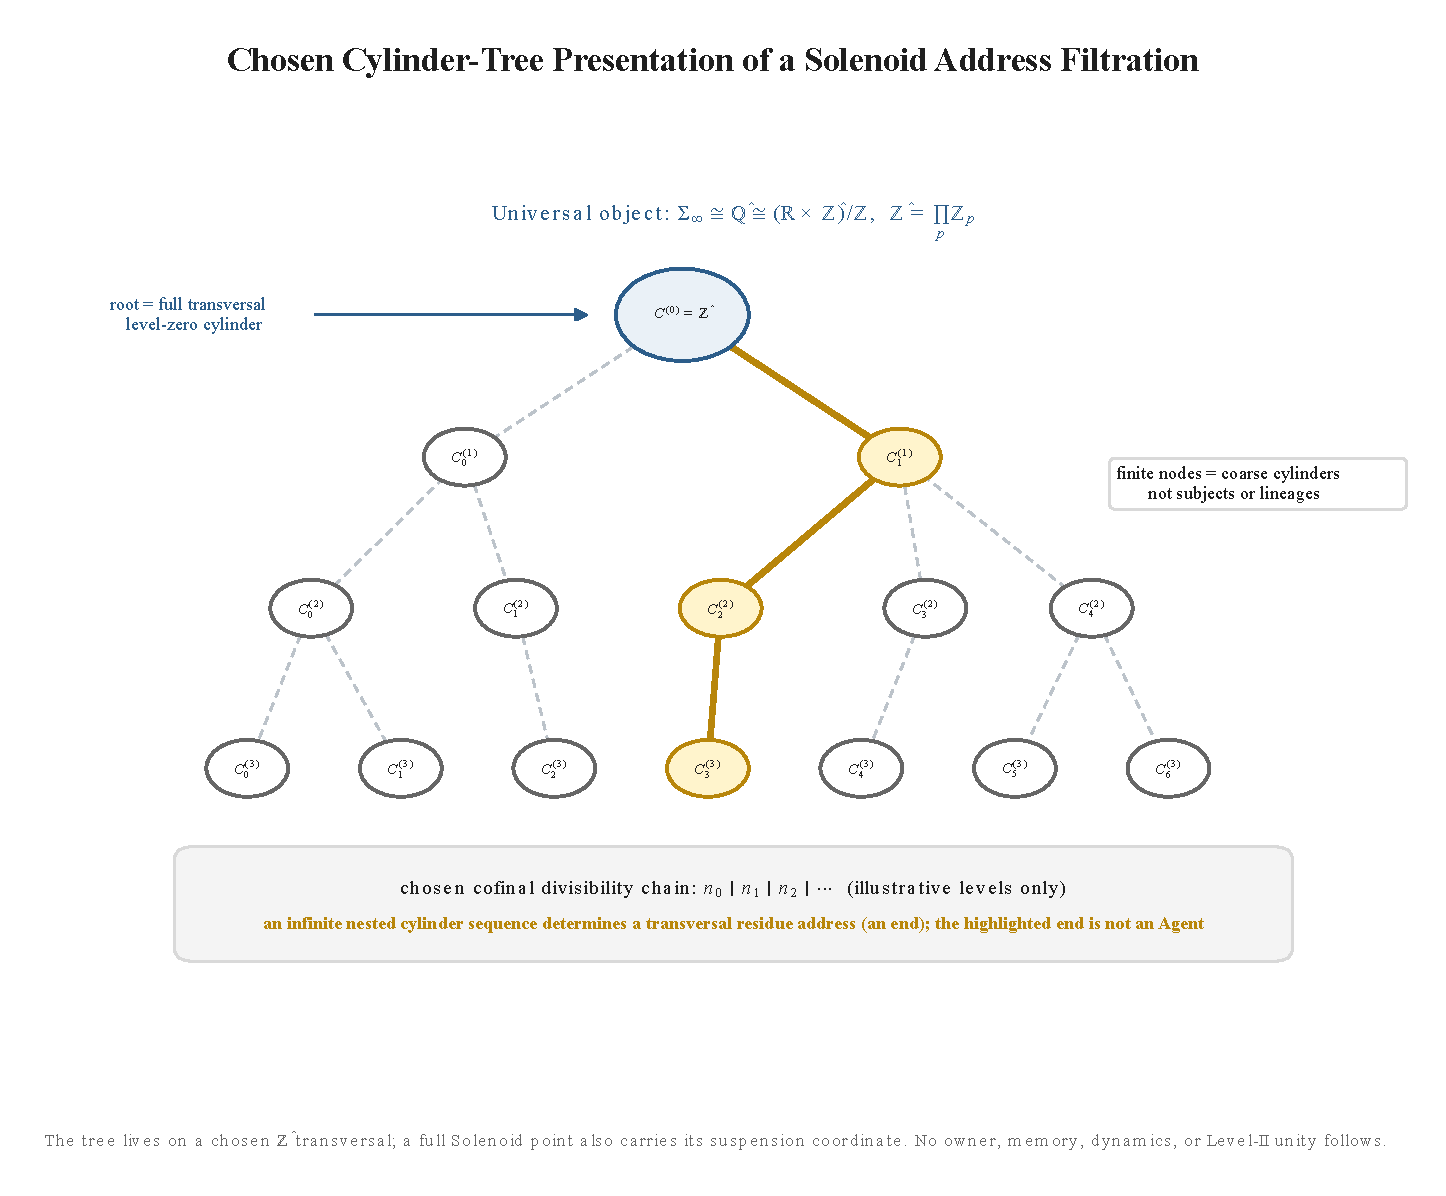
\includegraphics[keepaspectratio,alt={A chosen cylinder-tree presentation on a selected profinite transversal. Finite nodes are coarse cylinders, infinite nested ends determine transversal residue addresses, and the level-zero root is the whole transversal C\_\{0,0\} = \textbackslash widehat\{\textbackslash mathbb\{Z\}\} rather than the connected Solenoid, a primordial point, or a subject. A full Solenoid point additionally carries its suspension coordinate. The highlighted end marks address membership only; it is not an Agent.}]{content/Figures/Volume_1/Figure V1.7.1.pdf}}
\caption{A chosen cylinder-tree presentation on a selected profinite
transversal. Finite nodes are coarse cylinders, infinite nested ends
determine transversal residue addresses, and the level-zero root is the
whole transversal \(C_{0,0} = \widehat{\mathbb{Z}}\) rather than the
connected Solenoid, a primordial point, or a subject. A full Solenoid
point additionally carries its suspension coordinate. The highlighted
end marks address membership only; it is not an Agent.}
\end{figure}

\begin{center}\rule{0.5\linewidth}{0.5pt}\end{center}

\subsection{7.4 Identity Addresses and
Resolution}\label{identity-addresses-and-resolution}

\subsubsection{7.4.1 Universal Transversal
Address}\label{universal-transversal-address}

An element of \(\widehat{\mathbb{Z}}\) is a compatible residue family

\[ x = (a_n \bmod n)_n, \qquad a_m \equiv a_n \pmod{n} \quad (n \mid m). \]

Equivalently it is an all-prime tuple
\((x_p)_p \in \prod_p \mathbb{Z}_p\). Only after selecting one prime
factor does it have a single expansion

\[ x_p = a_0 + a_1 p + a_2 p^2 + \cdots, \qquad a_k \in \{0, 1, \dots, p-1\}. \]

\subsubsection{\texorpdfstring{7.4.2 Identity Coordinate
\(\mathbb{I}_K\) as a Chosen Residue
Address}{7.4.2 Identity Coordinate \textbackslash mathbb\{I\}\_K as a Chosen Residue Address}}\label{identity-coordinate-mathbbi_k-as-a-chosen-residue-address}

GCT's \textbf{Identity Coordinate} \(\mathbb{I}_K\) denotes this chosen
transversal residue coordinate {[}Tier 3 identification{]}. The complete
construction requires two maps that topology does not supply: first, an
explicit address bridge, not yet constructed, that maps a qualified
physical Polaron state into the declared Solenoid address role; second,
a selected base fiber or local transversal chart that extracts
\(\mathbb{I}_K \in \widehat{\mathbb{Z}}\). No global canonical
projection from the connected Solenoid to \(\widehat{\mathbb{Z}}\) is
assumed.

On this identification an agent's identity is modeled by the whole
infinite residue thread, not by any finite node: a finite node fixes
only finitely many digits. For example, on a chosen \(\mathbb{Z}_2\)
factor an address is an infinite binary string, and two addresses that
agree in their first 50 digits lie in the same depth-50 cylinder. That
is a statement about resolution only; it does not imply shared memory or
structural similarity of the agents concerned. Distinct ends are
distinct points, and the transversal has uncountably many of them, so
the address space does not run out {[}Tier 1{]}; whether distinct
physical agents actually receive distinct addresses depends on the
unconstructed address bridge.

\subsubsection{7.4.3 Finite Physical Address Capacity {[}Tier 3
model{]}}\label{finite-physical-address-capacity-tier-3-model}

The mathematical transversal is profinite and of unbounded depth; no
finite-capacity formula follows from the infinite Solenoid alone. If
\(N_{\text{states}}\) is the total number of distinguishable global
address states available on a substrate, a \(p\)-ary depth obeys

\[ D_{\max} = \lfloor \log_p N_{\text{states}} \rfloor. \]

If instead \(N_{\text{sites}}\) independent sites each store one
\(p\)-ary digit, the depth is \(N_{\text{sites}}\), not
\(\log_p N_{\text{sites}}\). An earlier substitution of the cage count
\(N_{\text{cage}} = 144\) into \(\log_p\) mixed these two encodings and
is withdrawn, together with the depth values derived from it. A
biological or cosmological depth bound remains open until the physical
coding model is specified.

\begin{center}\rule{0.5\linewidth}{0.5pt}\end{center}

\subsection{7.5 Observers Within Observers: Exact Skeleton and Claim
Ceiling}\label{observers-within-observers-exact-skeleton-and-claim-ceiling}

\subsubsection{7.5.1 What Nesting Shows}\label{what-nesting-shows}

Call a localized physical access domain of a candidate agent an
\emph{aperture} (for example, one finger, or one sensory sub-system).
Once a filtration is selected, distinct fine addresses can share a
coarser cylinder. This gives an exact membership pattern:

\begin{itemize}
\tightlist
\item
  two fingers can be distinct child apertures;
\item
  both can belong to one hand-level physical domain;
\item
  two hands can belong to one organism-level domain;
\item
  the same fine address can be described at every coarser resolution.
\end{itemize}

This is the strongest topology-only survivor of the finger/hand analogy
{[}Tier 1 conditional on the chosen filtration{]}. It describes common
membership and loss of resolution.

\subsubsection{7.5.2 What Nesting Does Not
Show}\label{what-nesting-does-not-show}

A cylinder is a set, not a parent subject. Address resolution does not
determine physical scope, and neither determines an owner. The same
hierarchy permits one owner with several apertures, several owners, no
Level II owner at some levels, or nested qualified subjects if
independent physical unity domains are later derived.

The working default of this volume is one qualified Identity Polaron per
physical unity domain, possibly with several apertures {[}Tier 3 working
hypothesis, not theorem{]}. Any proposed parent Level II observer,
whether collective, species-scale or cosmic, must independently close a
spanning physical-unity, Selection-Operator, persistence, ownership, and
phenomenal bridge at the parent scope. The Dual Material Constraint /
Polaron / Zeno stack is one candidate implementation, not shown to be
necessary or sufficient on current evidence. A collection of child
apertures is not sufficient. Such parent subjects are therefore not
derived here; whether any exist remains open {[}Tier 4{]}.

GCT asserts scale invariance for Field restrictions, not a population of
nested micro-subjects: there is no privileged geometric scale at which
Level I presence appears. Level II is a separate Tier 3 Identity-Polaron
proposal whose substrate status remains open (Tier 3) pending the full
Ch16 §16.2.6 research program. A human organism can be described as a
coarse node relative to cellular and atomic address refinements, but
those refinements alone do not establish subjecthood.

\subsubsection{7.5.3 Accessing the Whole from an
Aperture}\label{accessing-the-whole-from-an-aperture}

Fine-to-coarse projection is canonical after choosing the filtration;
coarse-to-fine reconstruction is one-to-many. One child address does not
contain all sibling states. ``The finger experiences being the hand''
therefore requires restricted-family sufficiency, approximate inference,
active downward presentation, or genuine global access. None of these
mechanisms is derived here {[}open{]}.

\begin{center}\rule{0.5\linewidth}{0.5pt}\end{center}

\subsection{7.6 Physical Instantiation and Resonance {[}Tier
3{]}}\label{physical-instantiation-and-resonance-tier-3}

\subsubsection{7.6.1 Nuclear Spin and Chirality: Candidate Material
Predicates, Not a Derived Digit
Code}\label{nuclear-spin-and-chirality-candidate-material-predicates-not-a-derived-digit-code}

GCT retains nonzero nuclear spin and molecular chirality as the two
candidate material predicates of the \textbf{Dual Material Constraint}
and as useful matched missing-leg controls {[}Tier 3{]}. Ordinary CISS
establishes a material chiral-spin response; it is not yet a map to the
GCT phason field or a Level-II gate. On the Tier 3 model, isotopes with
non-zero nuclear spin (e.g., \(^{31}\)\hspace{0pt}P,
\(^1\)\hspace{0pt}H) would supply candidate state capacity and spin-zero
isotopes (\(^{12}\)\hspace{0pt}C, \(^{16}\)\hspace{0pt}O) would not;
this is a modeling assumption, not a derived constraint.

The further claim that a particular nuclear-spin network encodes a
particular residue thread \(\mathbb{I}_K\) is a separate Tier 3 address
bridge, not yet constructed. It requires an explicit state map, a chosen
base fiber or local transversal chart, read/write dynamics, an error
model, and a normalized physical coupling. No one-to-one digit
assignment, global projection from the connected Solenoid to its
transversal, or necessary/sufficient Level-II condition is presently
derived. On the candidate model, the ``Self'' is not the atom; it is
modeled as the \textbf{Pattern of Entanglement} that the Tier 3 Zeno
Drive would maintain across the nuclear spin network, which would anchor
the address role to the fermions of the brain if the bridge were
constructed. For orientation only, Figure V1.7.3 compares the length
\(\xi=a_0/\alpha\approx7.25\) nm {[}Tier 1 arithmetic; its
identification as the vacuum/polaron healing length is Tier 3{]}
(diameter \(2\xi\approx14.5\) nm; Parameter Ledger \(\xi_{\rm pol}\),
not a GCT-specific prediction) with the \(\approx15\) nm microtubule
lumen; the agreement is a numerical coincidence noted as a Tier 3
substrate correlation, not a derived match.

\subsubsection{\texorpdfstring{7.6.2 Hierarchical Distance from a Chosen
Filtration:
\(d_H(i,j)\)}{7.6.2 Hierarchical Distance from a Chosen Filtration: d\_H(i,j)}}\label{hierarchical-distance-from-a-chosen-filtration-d_hij}

For a chosen cofinal chain \((N_k)\), let

\[ r(x,y) = \sup\{k : x \equiv y \pmod{N_k}\} \in \mathbb{N} \cup \{\infty\}, \qquad d_H(x,y) = \begin{cases} 0, & x = y, \\ c^{-r(x,y)}, & x \neq y, \end{cases} \quad c > 1. \]

Then \(d_H\) is an ultrametric,
\(d_H(x,z) \le \max[d_H(x,y), d_H(y,z)]\), and it quantifies the deepest
shared resolution cylinder {[}Tier 1{]}. Both the filtration \((N_k)\)
and the numerical scale \(c\) are chosen. For \(N_k = p^k\) on one
\(\mathbb{Z}_p\) factor with \(c = p\), this becomes the standard
\(p\)-adic metric. The phrase ``first common branch node'' is retired:
every pair shares the root, while the \textbf{deepest shared cylinder}
carries the resolution information. The Hierarchical Distance
\(d_H(i,j)\) between Agents \(i\) and \(j\) is this metric evaluated on
their Identity Coordinates, and is therefore defined only once the
address bridge of §7.4.2 is supplied {[}Tier 3{]}.

In an ultrametric every triangle is isosceles, with its two longest
sides equal {[}Tier 1{]}. Finite cylinders have parent--child relations
in the chosen tree, but the metric on ends supplies no neighbor
relation: the transversal is totally disconnected, and every ball is
both open and closed. Any rule about which address changes are
dynamically allowed is additional dynamics, not a consequence of the
metric.

\subsubsection{\texorpdfstring{7.6.3 Coupling from Hierarchical Distance
Remains Phenomenological:
\(\kappa_{ij} = \kappa_0 e^{-\lambda_c d_H}\)}{7.6.3 Coupling from Hierarchical Distance Remains Phenomenological: \textbackslash kappa\_\{ij\} = \textbackslash kappa\_0 e\^{}\{-\textbackslash lambda\_c d\_H\}}}\label{coupling-from-hierarchical-distance-remains-phenomenological-kappa_ij-kappa_0-e-lambda_c-d_h}

A model may posit

\[ \kappa_{ij} = \kappa_0 e^{-\lambda_c \, d_H(i,j)}, \]

where \(\lambda_c\) is the \textbf{Consensus Decay Constant}. But
\(d_H\) must name its selected filtration and prime factor, and
\(\kappa_0\) and \(\lambda_c\) require a physical derivation {[}Tier 3
--- Phenomenological Model, pending derivation of \(\kappa_0\) and
\(\lambda_c\) from the phason stiffness ratio \(K_\perp/K_\parallel\);
see Ch11 §11.2.1{]}. A first-principles derivation of \(\lambda_c\) is
deferred to Volume 2. The normalized coupling
\(\rho_{ij} \equiv \kappa_{ij}/\kappa_0\) and its limits are discussed
in Ch11 §11.2.1; nothing here implies that agents with small \(d_H\)
have phase-locked experiences.

\begin{figure}
\centering
\pandocbounded{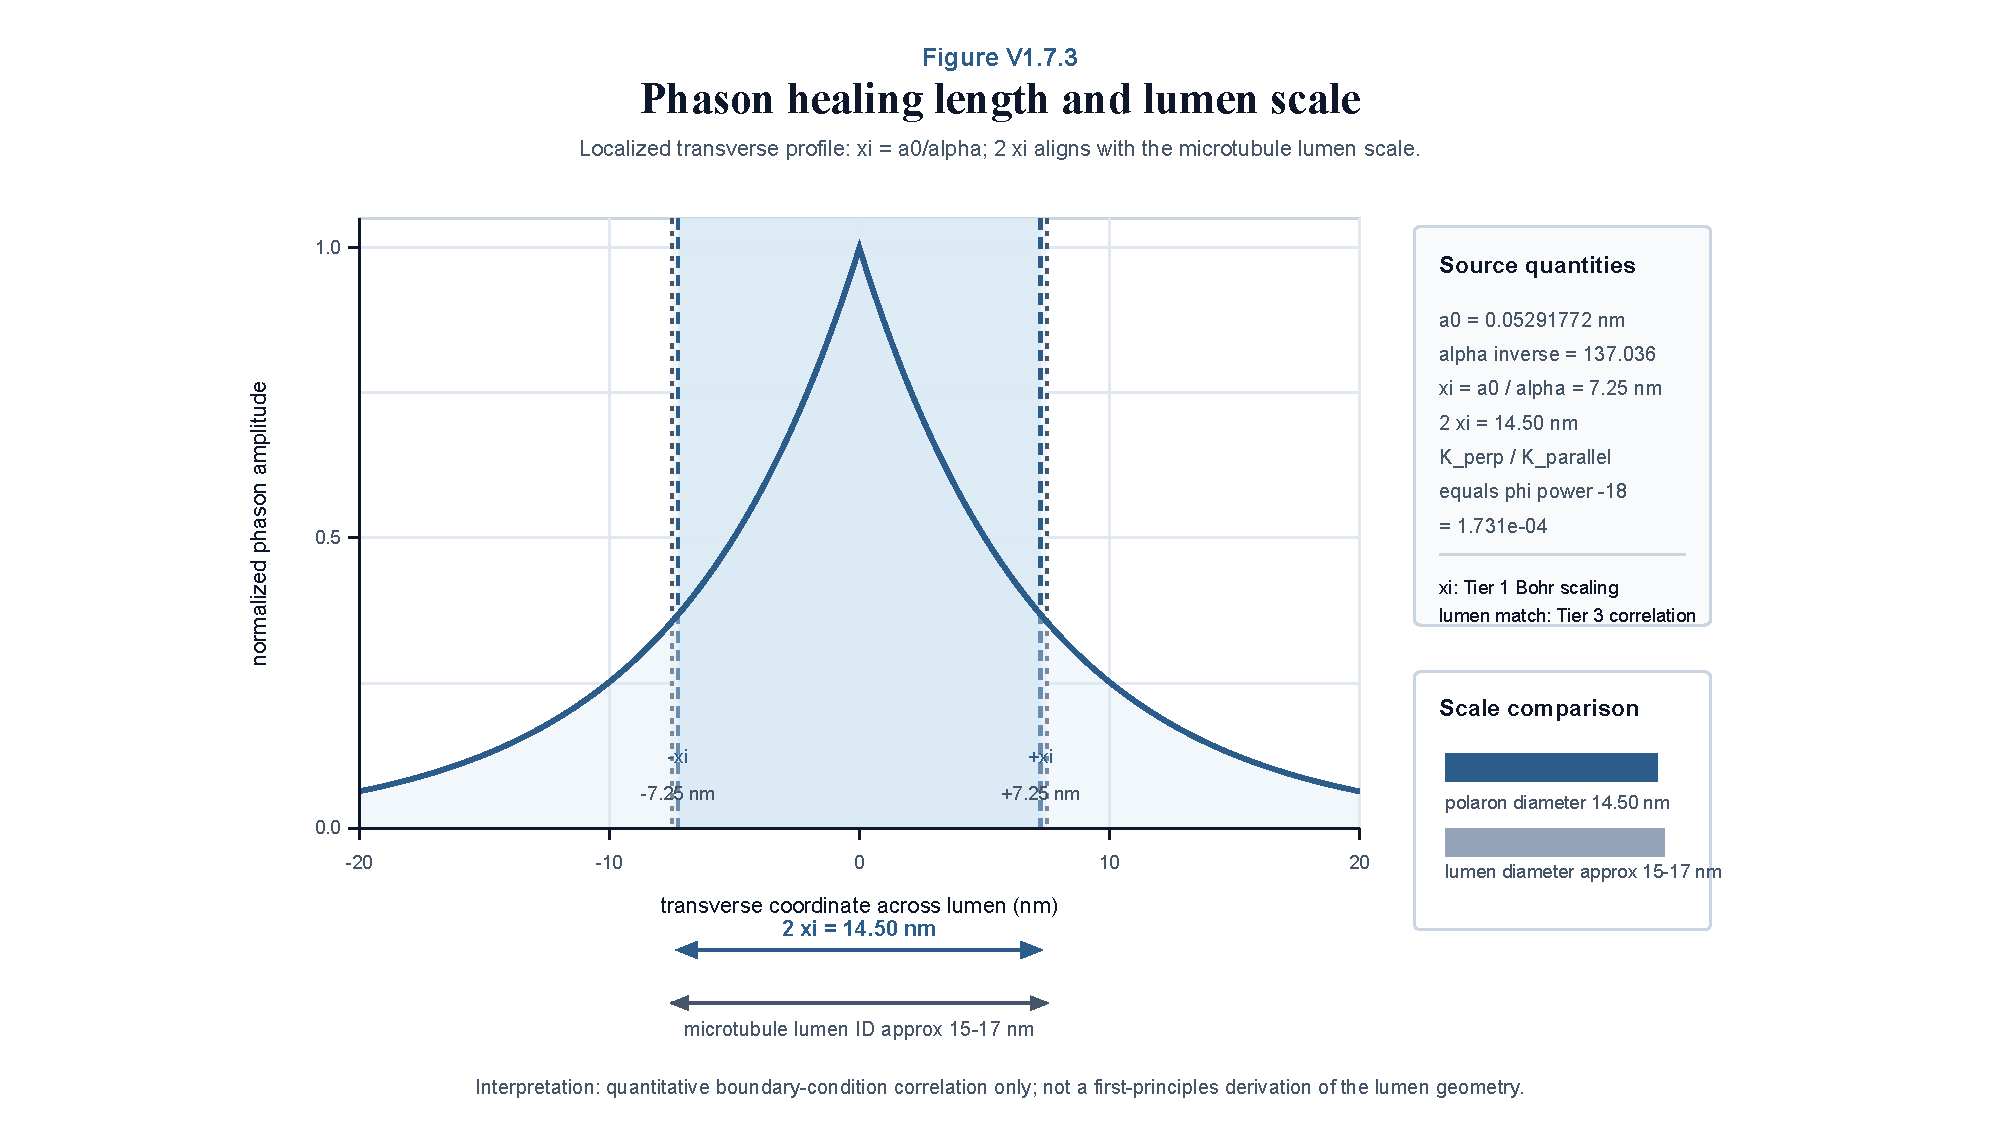
\includegraphics[keepaspectratio,alt={A localized transverse phason profile whose healing length is identified, at Tier 3, with \textbackslash xi = a\_0/\textbackslash alpha \textbackslash approx 7.25 nm (Tier 1 arithmetic) has diameter 2\textbackslash xi \textbackslash approx 14.5 nm, comparable to the microtubule lumen diameter near 15 nm as a Tier 3 substrate correlation; this is a numerical coincidence noted for orientation, not a derived match.}]{content/Figures/Volume_1/Figure V1.7.3.pdf}}
\caption{A localized transverse phason profile whose healing length is
identified, at Tier 3, with \(\xi = a_0/\alpha \approx 7.25\) nm (Tier 1
arithmetic) has diameter \(2\xi \approx 14.5\) nm, comparable to the
microtubule lumen diameter near 15 nm as a Tier 3 substrate correlation;
this is a numerical coincidence noted for orientation, not a derived
match.}
\end{figure}

\subsubsection{7.6.4 Resonance Clusters}\label{resonance-clusters}

A \textbf{Resonance Cluster} may be defined operationally as a set of
physical apertures with a declared coupling kernel and a common coarse
address class. This is useful structure. Shared cylinders do not
themselves transmit data or imply correlated experience. Distinct ends
are distinct points, so two agents with different addresses never occupy
one point of \(\Sigma_\infty\); any no-signalling analysis must rest on
separately derived physical channels (V1 Ch09 §9.4.3), not on
topological co-location. Readings of such clusters as shared deep
memory, telepathy, synchronicity, a higher self, or a parent subject are
not derived from this structure; they would require additional physical
and phenomenal bridges and remain Tier 4 speculation.

\begin{center}\rule{0.5\linewidth}{0.5pt}\end{center}

\subsection{7.7 Homotopy, Cohomology, and
Memory}\label{homotopy-cohomology-and-memory}

\subsubsection{7.7.1 Four Invariants That Must Not Be
Conflated}\label{four-invariants-that-must-not-be-conflated}

Every ordinary loop in the universal Solenoid contracts, so

\[ \pi_1(\Sigma_\infty) = 0. \]

For a sequential circle expansion with degrees \(d_k\), the fundamental
pro-group is the nonconstant pro-object

\[ \operatorname{pro}\pi_1(\Sigma_\infty) = \left( \mathbb{Z} \xleftarrow{\times d_1} \mathbb{Z} \xleftarrow{\times d_2} \cdots \right). \]

Under the standard first-shape-group convention, as the inverse limit of
these stage groups, cofinal divisibility forces

\[ \check{\pi}_1(\Sigma_\infty) = 0, \]

since a compatible integer would have to be divisible by every positive
degree. The separate profinite deck/transversal group is

\[ \widehat{\mathbb{Z}} = \varprojlim_k \mathbb{Z}/(d_1 \cdots d_k)\mathbb{Z}. \]

It is not the ordinary fundamental group, the pro-group, or the standard
first shape homotopy group. {[}Tier 1 --- Standard inverse-limit and
shape theory.{]} None of these statements by itself defines a physical
memory or winding state; in particular, since
\(\pi_1(\Sigma_\infty) = 0\), a ``closed loop'' in the Solenoid carries
no winding invariant.

\subsubsection{7.7.2 Exact Čech Cohomology and Candidate Physical
Encoding}\label{exact-ux10dech-cohomology-and-candidate-physical-encoding}

Continuity of Čech cohomology gives

\[ \check{H}^1(\Sigma_\infty; \mathbb{Z}) \cong \varinjlim(\mathbb{Z}, \times d_k) \cong \mathbb{Q} \]

for a universal (cofinal) degree sequence (see Eilenberg \& Steenrod,
\emph{Foundations of Algebraic Topology}, §VIII) {[}Tier 1 --- Standard
algebraic topology{]}. This is a global invariant of the \textbf{space}.
It records rational cohomology classes (circle-valued shape data). It
does not assign a rational winding state to each point or Agent;
ordinary loops have no nonzero winding number.

This classification does not by itself identify Agent states, define an
information metric, or show that a physical encoding survives thermal
dynamics. A physical memory claim requires an explicit map from
substrate states or histories to these cohomology classes and a
dynamical argument that the map is preserved. {[}Tier 3 --- Physical
interpretation open.{]}

\subsubsection{7.7.3 Physical Persistence Requires a Dynamical
Bridge}\label{physical-persistence-requires-a-dynamical-bridge}

A map into \(S^1\) has a homotopy class that is invariant under
homotopies of that map {[}Tier 1{]}. The manuscript has not yet
constructed a map that assigns an Agent's physical state a class in
\(\check H^1(\Sigma_\infty;\mathbb Z)\), nor a dynamical conservation
law carrying such a class through loss of the supporting substrate. To
use \(\mathbb{Q}\) as a physical state-label group, GCT must still
derive:

\begin{enumerate}
\def\labelenumi{\arabic{enumi}.}
\tightlist
\item
  an order-parameter or configuration map realizing the proposed class;
\item
  a substrate read/write coupling;
\item
  a Hamiltonian or free-energy barrier;
\item
  admissible defect-changing processes and boundary conditions;
\item
  a noise channel and preservation timescale.
\end{enumerate}

Only then can thermal robustness or retrieval be tested. ``Topological''
does not mean indestructible if the carrier leaves the configuration
space, an order-parameter amplitude vanishes, a defect reaches a
boundary, or the substrate dissolves. Likewise,
\(\check H^1 \cong \mathbb{Q}\) does not derive electric-charge
normalization or quark fractions; a gauge/charge map is separate.

On the conditional Tier 3 Zeno branch, physical death designates the
permanent cessation of the Zeno Drive --- the collapse of the metabolic
gradient proposed to maintain the Identity Polaron's coherence in
\(E_\parallel\). Biological memory protection is therefore Tier 3/open.
Whether any encoded state persists, can be re-coupled to a new physical
substrate, or carries recall or phenomenal continuity across substrates
is a \textbf{Tier 4 speculation}, not a consequence of the solenoid's
shape or cohomology alone.

\begin{center}\rule{0.5\linewidth}{0.5pt}\end{center}

\subsection{7.8 The Orthogonal Identity: An Internal-Manifold
Bridge}\label{the-orthogonal-identity-an-internal-manifold-bridge}

In Volume 2 the vacuum is modeled as a 6D cut-and-project structure with
a physical subspace \(E_\parallel\) and an internal subspace \(E_\perp\)
(a structural postulate of GCT). GCT separately proposes a map between a
physical Identity Polaron, the Solenoid address role, and the internal
phason field on \(E_\perp\). The 6D cut-and-project split does not by
itself identify \(E_\perp\) with \(\widehat{\mathbb{Z}}\), nor does
either space supply an owner.

The \textbf{Orthogonal Identity} (phenomenologically termed the
\textbf{Higher Mind}) names the proposed \(E_\perp\) component of an
agent's identity. This language is retained only as a Tier 3/4
phenomenological model. In the 6D parent lattice \(E_\perp\) is a
rotated direction of the same structure, and nothing in the construction
exempts its degrees of freedom from causal constraints: any causal or
no-signalling behavior must be derived from the declared dynamics. Any
claim that internal-manifold resonance guides an agent --- for example,
a reading of intuition as ``phason resonance'' that makes some future
branches feel ``lighter'' --- must specify the coupling operator,
causal/no-signalling behavior, accessible observable, and test. No such
operator is derived in this manuscript, so that reading is not derived
and remains Tier 4 speculation. It cannot be inferred from common
cylinder membership.

\begin{center}\rule{0.5\linewidth}{0.5pt}\end{center}

\subsection{7.9 Canonical Disposition}\label{canonical-disposition}

The universal Solenoid remains a mathematically rigorous and potentially
useful \textbf{address-and-resolution skeleton}:

\[ \Sigma_\infty \cong \widehat{\mathbb{Q}} \cong (\mathbb{R} \times \widehat{\mathbb{Z}})/\mathbb{Z}, \qquad \widehat{\mathbb{Z}} \cong \prod_p \mathbb{Z}_p, \qquad \pi_1(\Sigma_\infty) = 0, \qquad \check{H}^1(\Sigma_\infty;\mathbb{Z}) \cong \mathbb{Q}. \]

Its rooted tree, levels, single prime, physical scope map, identity
encoding, coupling kernel, memory dynamics, owner, and phenomenal
interpretation are additional data. Chosen nested cylinders are
compatible with observers within observers, but do not prove them. The
one-Polaron-per-unity-domain model with several apertures remains the
current Tier 3 default because it fits the physical unity-domain
architecture with fewer unverified owner assignments; it is not forced
by topology.

\chapter{Chapter 8: Simultaneous
Time}\label{chapter-8-simultaneous-time}

\subsection{8.1 The Static Block
Geometry}\label{the-static-block-geometry}

\subsubsection{8.1.1 Field Frame and Agent
Frame}\label{field-frame-and-agent-frame}

Under the Wheeler-DeWitt structural postulate \(\hat{H}\Psi=0\) (Volume
1, Chapter 5), the global state is represented as a static configuration
rather than as an object evolving in an external time. Time (\(t\)) is a
coordinate label for relations inside that configuration, not an
external evolution parameter. Past, present, and future coordinates
therefore coexist in the \textbf{Field Frame}. {[}Tier 3 --- conditional
on the Wheeler-DeWitt Structural Postulate, §5.2.1{]}

The \textbf{Agent Frame} is formally indexed by an ordinal sequence
\(n\) of conditional physical states along a declared aperture.
Identifying that sequence with experienced order, actualization events,
or a phenomenal owner requires the open transition, memory, Selection,
and psychophysical bridges; no traveling soul or preferred background
clock is assumed. \emph{(For speculative phenomenological
interpretations, see Appendix TIB §TIB.Spec.)}

\subsubsection{8.1.2 What the Block Does---and Does
Not---Supply}\label{what-the-block-doesand-does-notsupply}

A static block is compatible with several physical apertures or
world-line sectors existing at different coordinate times. It does not,
by itself, say that those apertures belong to one identity, one owner,
or one Solenoid branch. The universal Solenoid is an
address-and-resolution object; no canonical projection from one of its
cylinders into a set of physical lives follows from inverse-limit
topology.

To state a multi-life model precisely, one must introduce an additional
incidence/projection map such as

\[
\Pi_{life}: C_{parent} \longrightarrow \mathcal{P}(E_\parallel \times \tau_{coord}),
\]

where \(C_{parent}\) is a declared coarse identity sector and the image
is a set of physical aperture/world-line sectors. The model must also
specify which apertures share one physical unity domain or owner.
Neither \(\hat{H}\Psi=0\) nor the Solenoid
\(\Sigma_\infty \cong (\mathbb{R}\times\widehat{\mathbb{Z}})/\mathbb{Z}\)
constructs \(\Pi_{life}\).

The status of each layer is therefore:

\begin{itemize}
\tightlist
\item
  coexistence of many spacetime histories in a static block: conditional
  structural consequence of the block postulate {[}Tier 3 ---
  conditional on §5.2.1{]};
\item
  one parent address sector incident on several physical apertures:
  \textbf{Tier 3 additional model};
\item
  one phenomenal subject spanning those apertures, reincarnation,
  cross-life recall, or migration: \textbf{Tier 4}, absent a physical
  coupling and ownership bridge.
\end{itemize}

\begin{center}\rule{0.5\linewidth}{0.5pt}\end{center}

\subsection{8.2 A Conditional Simultaneous-Aperture
Model}\label{a-conditional-simultaneous-aperture-model}

\subsubsection{8.2.1 Field-Frame
Representation}\label{field-frame-representation}

Suppose \(\Pi_{life}\) is supplied and maps one declared parent sector
to apertures \(A, B, C\) at coordinates such as

\[
A: (x_A, \tau_A), \qquad B: (x_B, \tau_B), \qquad C: (x_C, \tau_C).
\]

All three can coexist in the static Field Frame. This is not sequential
reincarnation: no object must leave \(A\) and later enter \(B\). It is a
simultaneous incidence structure {[}Tier 3 --- conditional model{]}.

The topology alone does not determine whether:

\begin{enumerate}
\def\labelenumi{\arabic{enumi}.}
\tightlist
\item
  one Level II subject is presented through all three apertures;
\item
  three Level II subjects share a coarser address class;
\item
  only one aperture is Level II while the others are merely represented
  possibilities;
\item
  no parent Level II subject exists.
\end{enumerate}

Each claimed Level-II unity domain must independently close a spanning
physical-unity, Selection-Operator/sector-writing, persistence,
ownership, and phenomenal bridge. The \textbf{Identity Polaron/DMC/Zeno}
stack is one Tier 3 candidate implementation, not an established
necessary or sufficient criterion; DMC descriptors and
\(\eta_\text{Zeno}\) are candidate-control and external-rate diagnostics
only. A parent cylinder is not a subject merely because it contains
children.

\subsubsection{8.2.2 The Finger/Hand Analogy Across Coordinate
Time}\label{the-fingerhand-analogy-across-coordinate-time}

The exact content of the analogy is membership: different aperture
sectors can be distinct ``fingers'' assigned to one declared ``hand''
sector. The analogy does not grant a finger the complete state of the
hand or make the hand a separate observer.

``Experiencing the hand from the finger'' would require a downward
presentation/global-access channel from the parent physical unity domain
to the aperture; no such channel is derived here.

The one-qualified-subject/several-apertures reading can be extended
across coordinate sectors only as a Tier 3 hypothesis after
\(\Pi_{life}\) and the physical unity map are supplied. It is not
inferred from the Solenoid.

\subsubsection{8.2.3 The Frozen-River Picture,
Corrected}\label{the-frozen-river-picture-corrected}

Imagine spacetime as a frozen river containing every coordinate at once.
Several contact points can be marked on the ice. A proposed
identity-incidence map may group some contacts under one parent label.
The picture does not show, without further physics, whether one subject
owns all contacts, whether information passes between them, or whether
attention moves from one to another. Within a single aperture,
experienced order is supplied by that aperture's own physical clock,
state, and transition dynamics.

\begin{figure}
\centering
\pandocbounded{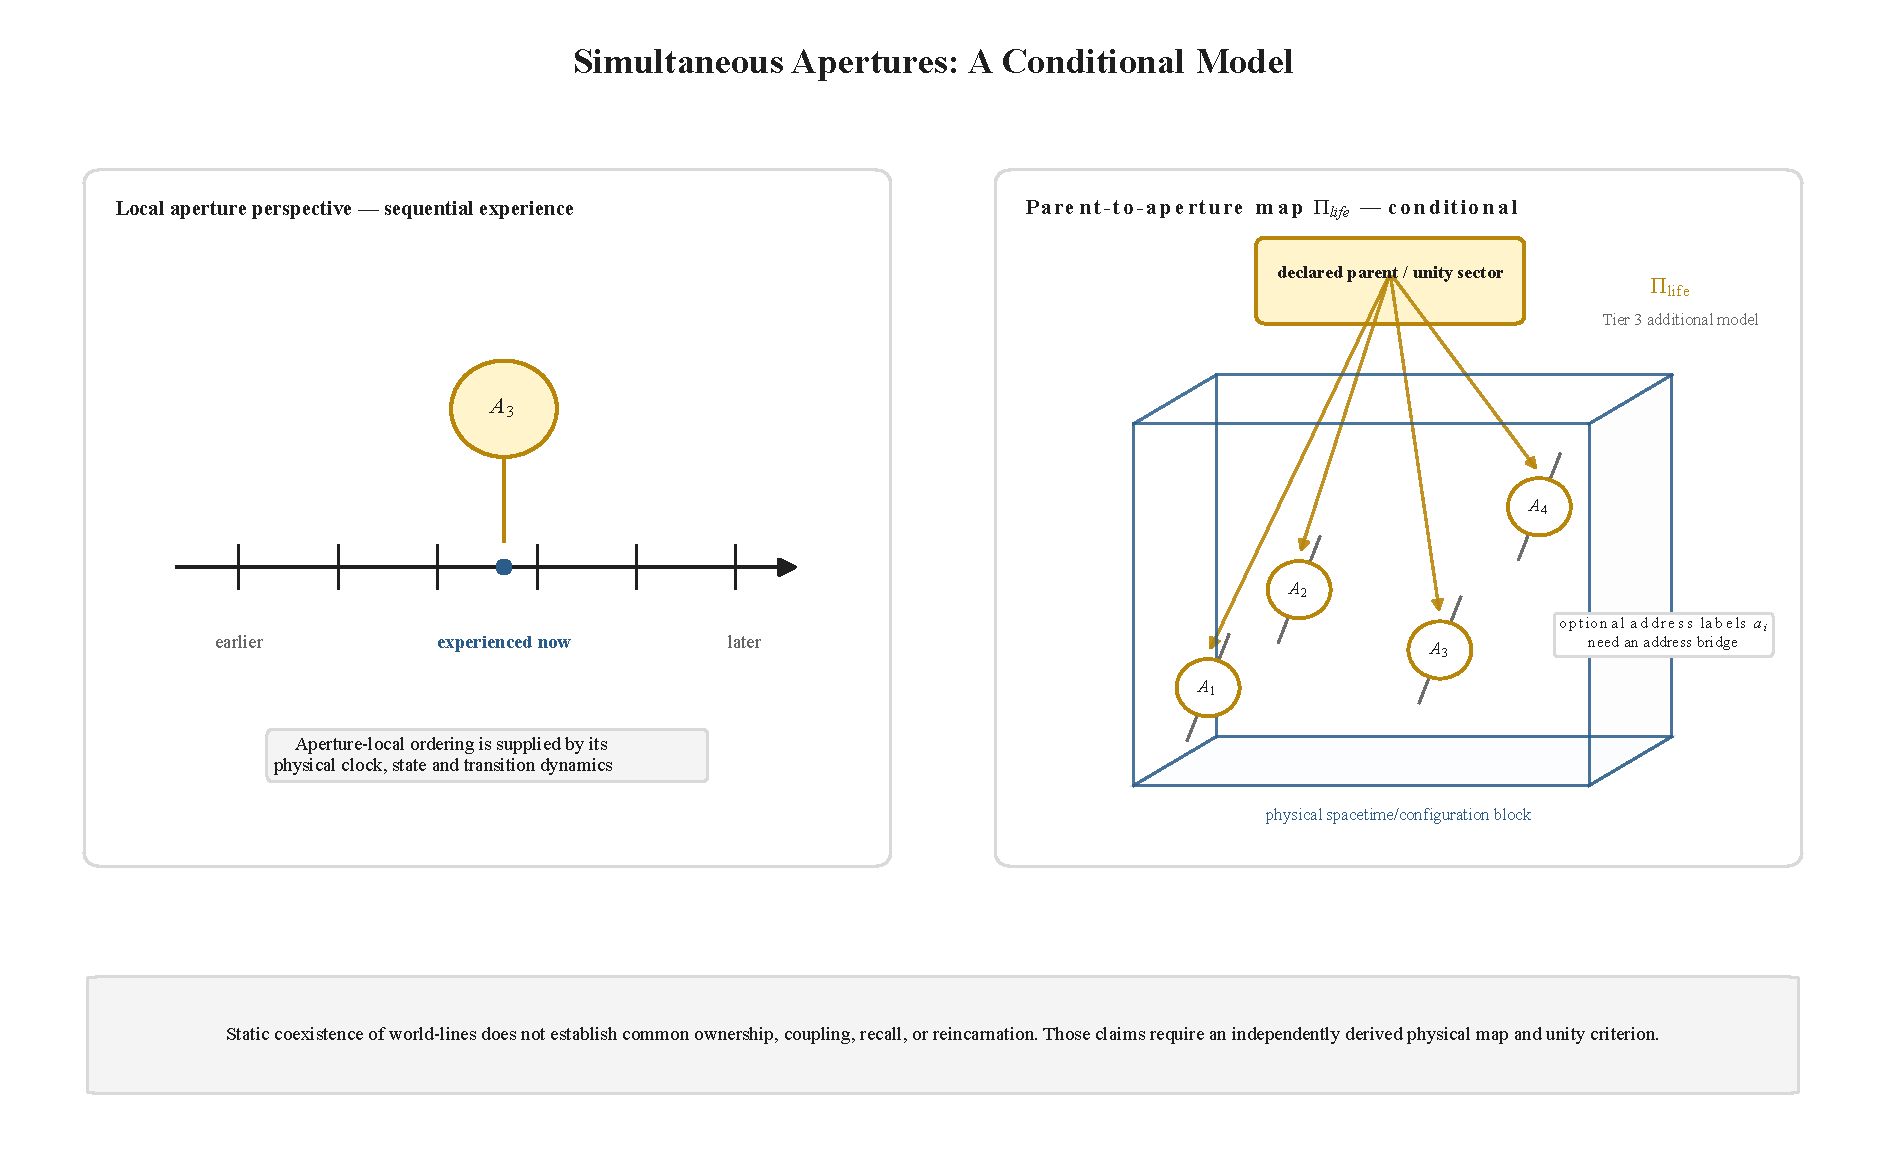
\includegraphics[keepaspectratio,alt={Conditional simultaneous-aperture model: several physical apertures coexist at distinct coordinates of a static spacetime block, while an added incidence map---not Solenoid topology alone---assigns them to a declared parent identity sector. Ownership and cross-aperture experience remain separate Tier 3/4 bridges.}]{content/Figures/Volume_1/Figure V1.8.1.pdf}}
\caption{Conditional simultaneous-aperture model: several physical
apertures coexist at distinct coordinates of a static spacetime block,
while an added incidence map---not Solenoid topology alone---assigns
them to a declared parent identity sector. Ownership and cross-aperture
experience remain separate Tier 3/4 bridges.}
\end{figure}

\begin{center}\rule{0.5\linewidth}{0.5pt}\end{center}

\subsection{8.3 Epistemic Firewall}\label{epistemic-firewall}

The canonical claims are deliberately narrow:

\begin{itemize}
\tightlist
\item
  The static-block model removes the need for a sequentially traveling
  soul {[}Tier 3 --- conditional on the block postulate{]}.
\item
  A multi-aperture identity relation is mathematically consistent but
  needs an explicit \(\Pi_{life}\) and physical unity map {[}Tier 3{]}.
\item
  Common Solenoid cylinders supply address membership, not memory
  transfer or phenomenal continuity {[}Tier 1 structural ceiling; Tier 3
  application{]}.
\item
  Past-life memory, cross-life access, post-mortem recoupling, and
  reincarnation phenomenology remain Tier 4 until a read/write coupling,
  persistence dynamics, and owner criterion are derived (see Appendix
  TIB).
\end{itemize}

Thus ``multiple lives happening at the same time'' remains a coherent
extension that GCT can state as a conditional model, but it is not
presented as a theorem of the universal Solenoid.

\clearpage
\thispagestyle{empty}
\vspace*{0.35\textheight}
\begin{center}\bfseries\LARGE PART III: THE MECHANICS OF RENDERING\end{center}
\vspace*{\fill}
\clearpage

\chapter{Chapter 9: The Rendering
Engine}\label{chapter-9-the-rendering-engine}

\subsection{9.1 Simulation Ontology}\label{simulation-ontology}

\subsubsection{9.1.1 Beyond Passive
Observation}\label{beyond-passive-observation}

Standard quantum mechanics is often described in terms of a passive
observer and collapse. In a timeless Wheeler--DeWitt setting, GCT
proposes an \textbf{Active Rendering Ontology}: a structural correlation
between an address-like coordinate \(\mathbb{I}_K\) and a local
restriction of the Field \(\Psi\) to an entanglement wedge. The
interpretation of that correlation as a particular subject's experienced
physical reality is an additional \textbf{Tier 3 psychophysical bridge},
not a consequence of the Wheeler--DeWitt constraint or of solenoidal
topology alone.

\subsubsection{9.1.2 Reality as an Autopoietic
System}\label{reality-as-an-autopoietic-system}

GCT uses \textbf{autopoietic} as a model description: the proposed
Realization Operator satisfies
\(\hat{\mathcal{R}} \circ \hat{\mathcal{R}} = \hat{\mathcal{R}}\) at the
level of an idempotent projection. Applying that proposed operator to an
already-realized subspace leaves that subspace unchanged. This algebraic
property does not by itself establish self-actualization, computation,
or phenomenal rendering; those interpretations remain \textbf{Tier 3
candidate bridges}.

The framework proposes cross-perspectival consistency constraints. A
coordinate in the solenoidal construction can label a local geometric
restriction \(E_\parallel\); treating that label as a subject, and
treating unselected structure as phenomenally unrendered, are separate
\textbf{Tier 3} commitments. Ordinary dynamical and decoherence accounts
remain available for the stability of shared records.

\subsubsection{9.1.3 The Holographic Simulation
Model}\label{the-holographic-simulation-model}

The physical world is modelled as a \textbf{cut-and-project shadow},
sometimes loosely called ``holographic'': a lower-dimensional projection
(\(3D\)) containing the encoded information of a higher-dimensional
source (\(6D\)). This is not holography in the technical
holographic-principle sense, where a boundary encodes a bulk with
area-law entropy {[}Tier 3 metaphor{]}.

\begin{itemize}
\tightlist
\item
  \textbf{The Source:} The \(6D\) Hyper-Lattice \(\mathbb{Z}^6\) (The
  geometric substrate).
\item
  \textbf{The Projection:} The \(3D\) Parallel Space \(E_\parallel\)
  (The Screen).
\item
  \textbf{The Rendering:} a proposed Agent-relative reading of the
  geometric output of the Realization Operator. Its identification with
  first-person phenomenal experience is a Tier 3 Russellian bridge, not
  an output of the projection mathematics.
\end{itemize}

This model offers one candidate account of why a mathematically
represented system may be described as phenomenally tangible. The move
from the \(6D\) source and projection mathematics to tangibility for an
owner of experience is not yet derived.

\begin{center}\rule{0.5\linewidth}{0.5pt}\end{center}

\subsection{\texorpdfstring{9.2 The Realization Operator
(\(\hat{\mathcal{R}}\))}{9.2 The Realization Operator (\textbackslash hat\{\textbackslash mathcal\{R\}\})}}\label{the-realization-operator-hatmathcalr}

\subsubsection{9.2.1 Definition and
Function}\label{definition-and-function}

To compare the abstract topology with concrete geometry, we introduce a
\textbf{proposed Realization map (\(\hat{\mathcal{R}}\))}. Ordinary
cut-and-project supplies a geometric map once a lattice, window, and
projection are declared; it does not supply an Agent-specific renderer.
The additional Agent/address dependence attributed to
\(\hat{\mathcal R}\) remains conditional on two open bridges (a map from
a qualified physical state to a Solenoid address, and a realization map
from that address to a local frame), with no examined physical carrier
or phenomenal output {[}Tier 3{]}.

\subsubsection{9.2.2 Input: Agent Coordinate
Vector}\label{input-agent-coordinate-vector}

The proposed input for \(\hat{\mathcal{R}}\) is an \textbf{address
coordinate} \(\mathbb{I}_K\) (a p-adic label). It can specify a
mathematical orientation within the universal Solenoid; identifying it
with an Agent's identity or a particular phenomenal owner is an open
Tier 3 bridge.

\subsubsection{\texorpdfstring{9.2.3 Process: 6D \(\to\) 3D
Projection}{9.2.3 Process: 6D \textbackslash to 3D Projection}}\label{process-6d-to-3d-projection}

The proposed operator \(\hat{\mathcal{R}}\) acts as a filter in the
model. It takes the \(6D\) hyper-lattice and applies an icosahedral
projection matrix \(\mathcal{M}\) determined by an address coordinate.
\[ \hat{\mathcal{R}}(s) \to \text{Slice}(E_\parallel) \] The
inverse-limit address does not by itself determine \(\mathcal{M}\), a
window, or a physical projection event. The output is a model slice in
\(E_\parallel\), not a demonstrated world generated for or experienced
by an owner.

\subsubsection{9.2.4 Output: Localized
Hologram}\label{output-localized-hologram}

The result of the proposed Realization Operator is a \textbf{Physical
Frame}: a local arrangement of nodes, phason strains, and phonon
densities in the model. Reading that frame as an Agent's immediate
phenomenal environment, or as an ontological claim that the world is
realized only where the operator acts, exceeds the present derivation
and remains a Tier 3 interpretation.

\begin{center}\rule{0.5\linewidth}{0.5pt}\end{center}

\subsection{9.3 The Integration Window}\label{the-integration-window}

\subsubsection{9.3.1 Frame Rate Mismatch
Problem}\label{frame-rate-mismatch-problem}

A fundamental problem arises when comparing the physics of the vacuum to
the physics of biology. Two distinct frequency scales must be carefully
distinguished:

\begin{itemize}
\tightlist
\item
  \textbf{Planck vacuum fluctuation scale:} Identifying the ultraviolet
  cutoff of the 6D lattice with the Planck energy gives the conventional
  conversion \(\nu_{vac} \sim E_{Planck}/h \approx 3 \times 10^{42}\)
  Hz. {[}Tier 1 arithmetic from the supplied Planck-energy scale; Tier 3
  scale identification of the lattice cutoff with that scale (Ch04
  §4.1.2).{]} This estimate does \textbf{not} require the independent
  Tier 3 P3b speed ratio \(\hat{c}/c = \phi^{-9}\), and it supplies no
  evidence that a biological Selection Operator samples the phason field
  at any particular rate.
\item
  \textbf{Historical Zeno-rate scenario:} the historical 100 MHz
  material-scan scenario (\(\nu_{Zeno} \approx 100\) MHz) is retained
  only as an external Tier 3 material-proxy input from the former
  nuclear-spin/Zeno programme {[}Parameter Ledger, Tier 3{]}; it is not
  a live operating frequency. ATP-budget compatibility is only an
  energetic consistency check. No normalized action presently derives
  this as a phason sampling rate, no experiment has identified it with a
  realized \(\mathcal{F}_{sel}\) cycle, and the field-typing analysis of
  V1 Ch17 §17.1.3 does not convert it into a Level-II classifier.
  Conditional on supplying it, the phenomenological integration model
  below places it roughly six orders of magnitude above the neural-rate
  reference.
\item
  \textbf{Biological sampling rate:} The human neural interface operates
  at the scale of Gamma oscillations (\(\nu_{bio} \sim 40\)--\(100\)
  Hz). {[}Tier 3 --- empirical neuroscience measurement{]}
\end{itemize}

\subsubsection{9.3.2 Time-Averaged Geometric
Surface}\label{time-averaged-geometric-surface}

The vacuum-to-neural reference-scale ratio spans roughly forty orders of
magnitude (\(\nu_{vac}/\nu_{bio} \sim 10^{40}\)), but the manuscript
does not derive a physical bridge across it. A historical two-stage
phenomenology first inserts the external \(\nu_{Zeno}\) scenario and
then averages hypothetical material-proxy updates across one biological
frame (the \textbf{Integration Window}). This is a conditional
coarse-graining ansatz: it does not show that a Selection Operator
samples phasons, that the updates are discrete acts of selection, or
that a subjective ``Now'' is numerically generated by them.
\[\langle \Phi \rangle_\text{perceived} = \frac{1}{\Delta n} \sum_{k=n}^{n+\Delta n} \hat{\mathcal{R}}(k)\]

where, \textbf{conditional on the two supplied frequency inputs},
\(\Delta n \equiv \nu_\text{Zeno} / \nu_\text{bio} \sim 10^{6}\) is the
number of proxy-update slots in the phenomenological average. {[}Tier 3
empirical neural-rate reference; Tier 3 external \(\nu_{Zeno}\)
scenario; Tier 4 averaging ansatz{]} It is not a derived count of phason
or Selection-Operator events and not a numerical derivation of the
experienced ``Now.''

\subsubsection{9.3.3 Physical Consequence: Emergent Macroscopic
Rigidity}\label{physical-consequence-emergent-macroscopic-rigidity}

Within the conditional averaging model, this integration is intended to
represent a ``Motion Blur'' effect; it is not a derivation of smooth
classical physics from measured selection events.

\begin{itemize}
\tightlist
\item
  \textbf{Particles:} Individual lattice defects moving through the
  vacuum blur into the smooth ``Wavefunctions'' of standard quantum
  mechanics.
\item
  \textbf{Solidity:} The discrete nodes and their stiff bonds
  (\(K_\parallel\)) blur into the appearance of a \textbf{Continuous
  Solid}.
\end{itemize}

In the conditional material model, \textbf{time-averaged rigidity} is
ordinary coarse-grained response of the declared lattice. The
display-pixel comparison is only a phenomenological analogy: GCT has not
derived a subjective sampling rate, a Selection clock, or an
observer-specific resolution limit from this averaging.

\begin{center}\rule{0.5\linewidth}{0.5pt}\end{center}

\subsection{\texorpdfstring{9.4 The Selection Operator
(\(\mathcal{F}_{sel}\))}{9.4 The Selection Operator (\textbackslash mathcal\{F\}\_\{sel\})}}\label{the-selection-operator-mathcalf_sel}

\subsubsection{9.4.1 Frame Distinction: Global
vs.~Local}\label{frame-distinction-global-vs.-local}

To preserve the mathematical integrity of the GCT framework, we must
distinguish between two fundamentally different perspectives on the
universal evolution:

\begin{enumerate}
\def\labelenumi{\arabic{enumi}.}
\tightlist
\item
  \textbf{The Field Frame (Global):} From the perspective of the
  universal Hilbert space, evolution, when described in terms of
  relational coordinate \(\tau_\text{coord}\), is expressed through the
  conditional unitary
  \(U(\tau_a, \tau_b) = e^{-i\hat{H}_\text{relational}(\tau_b - \tau_a)}\),
  where \(\hat{H}_\text{relational}\) is the reduced Hamiltonian
  obtained by solving the WdW constraint with a clock subsystem
  (following the Page-Wootters formalism). The global state
  \(\hat{H}\Psi = 0\) is preserved; the relational unitary describes
  correlations between clock and system, not external time evolution.
  {[}Tier 1 canonical form of the WdW constraint; its adoption is Tier 3
  (Ch05 §5.2.1); the Page--Wootters relational-time reading is Tier 3{]}
  There is no wave-function collapse. The \(\Psi_{GCT}\) state vector
  evolves as a timeless superposition of all topologically valid
  configurations.
\item
  \textbf{The Agent Frame (Local):} The formal model declares an
  open-system conditional state. From this perspective, ``Selection'' is
  not a physical collapse of the Bulk; it denotes \textbf{Bayesian
  conditionalization} relative to a declared local subsystem (the local
  entanglement wedge). No examined physical Agent, Selection carrier, or
  phenomenal owner is thereby identified.
\end{enumerate}

\subsubsection{9.4.2 Selection as Conditional (Non-Unitary)
Update}\label{selection-as-conditional-non-unitary-update}

If an instrument and outcome are independently supplied, GCT's
Agent-frame notation represents the resulting conditional-state update
by \(\mathcal{F}_{sel}\); under the open address bridge it may also
induce an address-label update in the universal Solenoid. This is
standard conditioning mathematics, not a demonstrated physical or
phenomenal act of selection, and the inverse-limit topology supplies no
transition kernel, instrument, or update law. The formal projection is:
\[ |\Psi\rangle_{Agent} \to \frac{\hat{P}_{sel} |\Psi\rangle_{Field}}{\sqrt{\langle \Psi | \hat{P}_{sel} | \Psi \rangle}} \]
where \(\hat{P}_{sel}\) is a declared projector. No map from intent to
this projector, no physical projection event, and no filtering of
phenomenal experience has been derived. Calling the normalized
conditional update a non-unitary ``jump'' describes the selected outcome
representation; it does not establish an ontic collapse or
Agent-specific branch actualization. The global Field description
remains unitary.

\gctneedspace{5\baselineskip}\begin{gctNote}

\textbf{Formal Definition: Categorical TQFT of the Selection Operator}

In the framework of Topological Quantum Field Theory (TQFT), an
\(n\)-dimensional manifold (the Agent's history) is defined as a
cobordism between \((n-1)\)-dimensional boundaries (states of
experience). One may alternatively \emph{model} the Selection Operator
\(\mathcal{F}_{sel}\) as a \textbf{Functor} from the category of
icosahedral cobordisms to the category of Hilbert spaces {[}Tier 3
modelling choice; elsewhere \(\mathcal{F}_{sel}\) is the non-unitary
conditional update of §9.4.2{]}.

\[ \mathcal{F}_{sel}: \mathbf{Cob}_{I_h} \to \mathbf{Hilb} \]

Mapping the subjective ``Agent'' to this functor is a Tier 3 formal
proposal conditional on the modelling choice \(\mathbf{Cob}_{I_h}\) (not
one of the postulates of the Axiom \& Postulate Ledger); like every
scaffold-to-phenomenal map in this volume (Ch16 §16.2.2b), it stays at
Tier 3. This is not a proof of physical Level-II realization: DMC legs
are candidate controls, the stated \(\eta_\text{Zeno}\) values are
conditional external-rate scenarios, and the typed measured coupling
plus phenomenal bridge remain open.

\end{gctNote}

\subsubsection{9.4.3 The No-Signalling
Constraint}\label{the-no-signalling-constraint}

No-signalling does not follow from address topology. It follows
conditionally from the outcome-averaged CPTP identity below, which
presupposes Born-weighted outcomes (see the constraint after the box),
and, in GCT's field description, from the conditional phason--phonon
readout bound of Appendix SNE §SNE.4 (subluminal only on the extra Tier
3 premise \(v_{\rm phonon}\le c\), which fails under P3b; App ORQ O.48).
Shared cylinders alone establish no correlation or channel.

\gctneedspace{5\baselineskip}\begin{gctImportant}

\textbf{Proposition: Outcome-averaged no-signalling identity. {[}Tier 1
QI identity; conditional GCT application in Appendix FTH §FTH.4 and
Appendix SNE §SNE.4{]}} Conditioning on a specified outcome at subsystem
A does not by itself change the \emph{unconditional} density matrix
\(\rho_B\) of a spatially separated subsystem B, and so does not
transmit a signal. Two statements must be distinguished. (i)
\emph{Selective description:} conditioning on A's specific outcome
yields the conditional state
\(\rho_{B|\text{sel}} = \text{Tr}_A\!\big[(\hat{P}_\text{sel} \otimes \hat{I}_B)\,|\Psi\rangle\langle\Psi|\,(\hat{P}_\text{sel} \otimes \hat{I}_B)\big]/p_\text{sel}\),
with
\(p_\text{sel} = \langle\Psi|\,\hat{P}_\text{sel} \otimes \hat{I}_B\,|\Psi\rangle\).
This conditional state generally differs from \(\rho_B\); the difference
encodes pre-existing correlation, not a transmitted signal, and is
inaccessible to B without classical communication of A's outcome. (ii)
\emph{Non-selective description:} B's local statistics, unconditioned on
A's outcome, are governed by the outcome-averaged map. For any complete
orthogonal family of local projectors \(\{\hat{P}_k\}\) on
\(\mathcal{H}_A\) with \(\sum_k \hat{P}_k = \hat{I}_A\),
\[\sum_k \text{Tr}_A\!\big[(\hat{P}_k \otimes \hat{I}_B)\,|\Psi\rangle\langle\Psi|\,(\hat{P}_k \otimes \hat{I}_B)\big] = \text{Tr}_A\!\big[|\Psi\rangle\langle\Psi|\big] = \rho_B,\]
by cyclicity of the partial trace over \(\mathcal{H}_A\), idempotency
\(\hat{P}_k^2 = \hat{P}_k\), and completeness. It is this
outcome-averaged equality --- not a Selection-Operator theory and not
the selective map alone --- that supplies the standard
quantum-information no-signalling result. Correlated records can later
be compared only through ordinary causal interaction when future light
cones overlap (the conditional multi-Agent model of Chapter 11).
Appendix SNE §SNE.4 additionally gives a \textbf{conditional} subluminal
response for a declared strain-level phason--phonon source; GCT has not
derived a physical \(\mathcal{F}_{sel}\) event, its coupling to that
source, or a phenomenal Consensus mechanism.

\end{gctImportant}

\textbf{Constraint on biased selection {[}Tier 1 --- standard QI
consequence of the identity above; its application to GCT selection is
the open problem App ORQ O.48{]}.} The identity sums the
\emph{unnormalised} projections, so it holds when A's outcomes occur
with the Born weights
\(p_k=\text{Tr}\big[(\hat{P}_k\otimes\hat{I}_B)\,|\Psi\rangle\langle\Psi|\big]\).
If a will-, resonance- or impedance-biased Selection Operator (§9.5.3;
Ch10 §10.3.2) reweighted A's outcomes to \(q_k\neq p_k\), B's
outcome-averaged state would become \(\sum_k q_k\,\rho_{B|k}\), which in
general differs from \(\rho_B\): the bias would be a superluminal signal
(Gisin 1990; Polchinski 1991). Any selection bias GCT entertains must
therefore leave the outcome-averaged marginals at their Born values on
every subsystem. Local unitary or CPTP steering before an outcome is
registered is compatible with this, because it changes the state to
which the Born rule applies rather than the rule. The manuscript does
not yet state a mechanism that biases individual outcomes while meeting
the constraint; the gap is registered as App ORQ O.48.

\subsubsection{9.4.4 Energy Preservation (The No-Free-Lunch
Constraint)}\label{energy-preservation-the-no-free-lunch-constraint}

The no-free-lunch requirement is firm: any physical control process must
use ordinary available energy. The proposed \textbf{Topological Torque}
is only a hypothetical ledger variable; no Mind--Brain transducer,
phason-biasing interaction, per-cycle work, or ATP-to-vacuum gate has
been derived. Calling agency a gating mechanism rather than a source of
energy therefore names a Tier 3/4 research ansatz, not an established
force or energy pathway.

\begin{center}\rule{0.5\linewidth}{0.5pt}\end{center}

\subsection{9.5 The Mirror Principle (Resonant
Filtering)}\label{the-mirror-principle-resonant-filtering}

\subsubsection{9.5.1 Postulate: Constraint-Based Selection {[}Tier 3 ---
model postulate; Born form conditional on App ORQ
O.40a/O.40b{]}}\label{postulate-constraint-based-selection-tier-3-model-postulate-born-form-conditional-on-app-orq-o.40ao.40b}

The model postulates that a future Selection Operator would be
constrained by the \textbf{Geometric Impedance} of the current state.
Conditional on the separate measure assumptions below, its branch
probabilities may take the \textbf{Born} form:
\[ P(\phi) = |\langle S | \phi \rangle|^2 \] The Born Rule
(\(P = |\psi|^2\)) is a \textbf{Tier 3 conditional compatibility
theorem} in the current manuscript. Appendix BRC applies the
representation theorem only after two independent proof obligations for
the Selection Operator are supplied: countable additivity of the phason
projection-lattice measure (App ORQ O.40a) and noncontextuality /
basis-independence for that measure (App ORQ O.40b). Under those
hypotheses and the Agent pure-state identification
\(\rho_S=|S\rangle\langle S|\), Gleason represents the probabilities as
\(f(P_\phi)=|\langle S|\phi\rangle|^2\). The current engine ledger
records this as conditional, not as a closed theorem or executable
verifier.

\subsubsection{9.5.2 The Zeno Projection
Operator}\label{the-zeno-projection-operator}

The historical implementation of §9.5.1 introduces a discrete
\textbf{candidate Zeno Projection Operator} \(\hat{P}_{sel}\). Standard
repeated-projection algebra (the quantum Zeno effect) can suppress
specified transitions once a Hamiltonian, projectors, cadence, and
measurement channel are supplied. GCT has not yet derived those
ingredients as an Agent's physical ``attention,'' a realized-subspace
projection, or a cumulative phenomenal selection process. Born
compatibility and no-signalling therefore remain conditional proof
obligations rather than consequences of the symbol \(\hat{P}_{sel}\).

\subsubsection{9.5.3 Signal Locking and Geometric
Impedance}\label{signal-locking-and-geometric-impedance}

The proposed interaction between the Agent and the larger configuration
space is analogous to a \textbf{Radio Tuner}. The Solenoid contributes a
candidate address coordinate; it does not by itself contain a quantum
superposition of all timelines or encode beliefs and memories. Those
roles require the Field state, the physical address and Realization
maps, and a separately specified transition dynamics {[}Tier 3{]}. The
Agent's physical internal state then defines the proposed \textbf{Tuning
Condition}.

\begin{itemize}
\tightlist
\item
  \textbf{Resonant-selection hypothesis:} A low mismatch between a
  supplied internal state and branch geometry is proposed to favor that
  branch. Any such favouring is subject to the no-signalling constraint
  of §9.4.3: it must leave outcome-averaged marginals at their Born
  values, and no mechanism meeting that constraint is yet stated (App
  ORQ O.48). Mapping this to realized experience is an additional
  phenomenal bridge.
\item
  \textbf{Topological-friction hypothesis:} A large mismatch is proposed
  to impose an energetic or statistical cost. Its Hamiltonian,
  coefficient, and branch-filtering law remain to be derived.
\end{itemize}

\subsubsection{9.5.4 Phenomenology: The Structured
Filter}\label{phenomenology-the-structured-filter}

The \textbf{Resonantly Filtered Reality} language is a Tier 3
interpretive proposal: experience would track the subset of potential
compatible with the Agent model rather than unconstrained desire. No
current derivation shows that this ``Mirror'' filter generates
experience or guarantees stability; memory and cumulative history
additionally require an independent physical memory carrier, which the
Solenoid topology does not supply.

\begin{center}\rule{0.5\linewidth}{0.5pt}\end{center}

\subsection{9.6 The Consensus Protocol --- see Chapter
11}\label{the-consensus-protocol-see-chapter-11}

Chapter 11 develops a \textbf{conditional multi-Agent algebraic model}
using a proposed Meeting Operator
\(\mathcal{O}_M = \mathcal{F}_A \cdot \mathcal{F}_B\) and the common
commutant
\(\mathcal{C}(A,B) = \{ X : [X, \mathcal{F}_A] = 0 \text{ and } [X, \mathcal{F}_B] = 0 \}\)
(Chapter 11, §11.13.3). This construction is not a theorem identifying
shared phenomenal reality, and the scalar-commutant condition
\(\mathcal{C}(A,B) = \mathbb{C} \cdot I\) is not by itself a derivation
of relativistic no-signalling, which rests on the outcome-averaged
identity of §9.4.3. Physical \(\mathcal{F}_A, \mathcal{F}_B\), state
maps, interactions, and phenomenal ownership remain open.

\chapter{Chapter 10: Russellian Causation and the Nature of
Will}\label{chapter-10-russellian-causation-and-the-nature-of-will}

\subsection{10.1 The Free Will Question}\label{the-free-will-question}

\subsubsection{10.1.1 Stating the Problem: Determinism
vs.~Randomness}\label{stating-the-problem-determinism-vs.-randomness}

The debate over free will has remained deadlocked for centuries because
standard physical models provide only two possible causal mechanisms,
neither of which supports the existence of an autonomous Agent.

\begin{enumerate}
\def\labelenumi{\arabic{enumi}.}
\tightlist
\item
  \textbf{Classical Determinism:} If the laws of physics are
  differential equations and the initial conditions are fixed, then
  every ``choice'' is merely the playing out of a pre-recorded script.
  The Agent is a spectator in a clockwork universe.
\item
  \textbf{Quantum Randomness:} If the laws of physics are probabilistic,
  then ``choice'' is replaced by a dice roll. While this breaks
  determinism, it does not provide agency. A random event is no more
  ``willed'' by an Agent than a deterministic one.
\end{enumerate}

The debate has produced at least three principal families of response:
\textbf{Compatibilism}, which argues that autonomy is compatible with
determinism; \textbf{Libertarianism}, in an agent-causal form (a
distinct causal power of the agent not reducible to physical law) and an
event-causal form (indeterministic causation by the agent's own states);
and \textbf{Free-will scepticism}, which denies that we have free will.
GCT's Russellian-causation frame is best read as a structural model
inside the event-causal libertarian wing rather than a fourth
taxonomy-ending option: it identifies `Will' and `Lattice Structure' as
frame-relative descriptions of the same topological-path selection,
while the Mele-style contrastive-luck residual (``why this branch rather
than that one'') remains explicitly conceded in §16.2.8e.

\subsubsection{10.1.2 Three Standard Options and Their
Objections}\label{three-standard-options-and-their-objections}

Attempts to resolve this crisis typically fall into three categories,
each facing a standard objection that any account, GCT's included, must
answer:

\begin{itemize}
\tightlist
\item
  \textbf{Hard Determinism:} Discard the Agent as an illusion. The
  experience of choosing instantiates only the Tier 0 datum that
  experience is occurring; causal agency is not included in that
  certainty. Axiom 1 stipulates universal Level I presence {[}Tier 1{]}
  (Chapter 1, §1.2.3), not the causal efficacy of choosing.
\item
  \textbf{Stochastic Agency}: The identification of free will with
  quantum indeterminacy. Objection: randomness is not directed, and an
  undirected cause cannot constitute an intentional act. GCT's own
  event-causal position (§10.1.1) belongs to this family, so the
  objection applies to it. GCT's reply is that the indeterministic step
  is constrained by the Agent's internal state (§10.3--§10.4) rather
  than undirected; the contrastive-luck residual is conceded (§16.2.8e)
  {[}Tier 3{]}.
\item
  \textbf{Non-Physical Causation (Substance Dualism)}: The postulate of
  a causally efficacious non-physical substance. Objection: this
  reintroduces the interaction problem --- how does a non-physical cause
  produce measurable physical effects without violating conservation
  laws?
\end{itemize}

Compatibilism (§10.1.1) is not among these three; GCT does not argue
here that it fails.

\subsubsection{10.1.3 Why This Matters
Philosophically}\label{why-this-matters-philosophically}

Without a rigorous account of Will, a ``Theory of Everything'' remains
merely a ``Theory of Objects.'' If consciousness is fundamental, then
\textbf{Agency} must be a primary physical degree of freedom. We must
find a way to make Choice as physically real as Mass.

\begin{center}\rule{0.5\linewidth}{0.5pt}\end{center}

\subsection{10.2 The Russellian Solution}\label{the-russellian-solution}

\subsubsection{10.2.1 Field Frame Perspective (The Static
Block)}\label{field-frame-perspective-the-static-block}

In the \textbf{Field Frame}, the universe is a static solution to the
Wheeler-DeWitt equation (\(\hat{H}\Psi=0\)). From this perspective, the
full Field/configuration state contains the candidate histories as
simultaneous correlations. The Adelic Solenoid \(\Sigma_\infty\) may
contribute an address coordinate under an open address bridge (a map
from physical states to Solenoid addresses), but its inverse-limit
cylinders are not themselves the Many-Worlds branching state space. The
``Will'' is proposed to identify a physically realized trajectory
through the declared configuration structure. The Bulk does not change;
it merely \emph{contains} the Agency {[}Tier 1 canonical formalism under
the Tier 3 WdW adoption (Ch05 §5.2.1); Tier 3 trajectory/address
model{]}.

\subsubsection{10.2.2 Agent Frame Perspective (The Actualized
Line)}\label{agent-frame-perspective-the-actualized-line}

In the \textbf{Agent Frame}, the formal observer model follows a
sequence of conditional physical states. Under that open address bridge
those states may also receive Solenoid labels. Calling the model a
localized operator, active renderer, or author of an actualized line is
a Tier 3 interpretation: no physical \(\mathcal F_{sel}\) carrier,
transition instrument, Selection clock, owner, or phenomenal
registration has been derived. Choice is represented by conditioning on
one line from a declared space of physical possibilities, not by a
theorem about the Solenoid's cylinder tree.

\subsubsection{10.2.3 Complementarity, Not
Contradiction}\label{complementarity-not-contradiction-1}

The GCT structural framing is \textbf{Russellian Causation} --- used
here in the specific sense of Russell's argument that the notion of
``cause'' should give way to functional dependence (Russell, `On the
Notion of Cause,' \emph{Proc. Aristotelian Soc.}, 1912); the
frame-relative reading of cause-and-effect language is GCT's addition.
GCT extends this by proposing that the underlying structure is a
geometric path through the static Field configuration space, optionally
indexed by a physically realized Solenoid address. Note: Russell's
eliminativism concerned the philosophers' ``law of causality'' (``a
relic of a bygone age''), not agency; GCT argues that the
functional-dependence structure Russell identified admits a
non-eliminativist interpretation when the geometry and transition law of
the static block are fully specified. ``Volitional Choice'' and
``Geometric Correlation'' are then two descriptions of one proposed
physical trajectory {[}Tier 3{]}. The choice does not ``change'' the
block; it is represented by the selected path within it.

\begin{center}\rule{0.5\linewidth}{0.5pt}\end{center}

\subsection{10.3 Candidate Physical Surrogate:
Micro-Agency}\label{candidate-physical-surrogate-micro-agency}

\subsubsection{10.3.1 Berry Phase and Phase
Freedom}\label{berry-phase-and-phase-freedom}

As a candidate physical surrogate, we use ordinary \textbf{Berry-phase}
geometry, detailed in §14.4. A declared defect in a fiber bundle may
possess local frame-phase freedom relative to \(E_\parallel\). That
mathematical freedom does not identify the defect as an Agent, derive an
Identity Polaron, or make its phase an owned will-state.

\subsubsection{10.3.2 Internal Frame Orientation as
Will-State}\label{internal-frame-orientation-as-will-state}

This local phase freedom motivates a Tier 3 control surrogate. We
\emph{define} a model \textbf{Will-State} as an internal-frame
orientation and \textbf{Topological Torque} as a declared control
rotation relative to a background frame. No intent-to-phase transducer,
physical torque channel, or phenomenal owner is known; only after those
are independently supplied could the variable alter measured transition
weights, and then only through local dynamics that leave
outcome-averaged marginals at their Born values on every subsystem, or
the bias would signal (Ch09 §9.4.3; App ORQ O.48). An address-path
update would additionally require an address map and a transition law.

\begin{center}\rule{0.5\linewidth}{0.5pt}\end{center}

\subsection{10.4 Formalization: Two
Components}\label{formalization-two-components}

\subsubsection{10.4.1 Steering Generator (Inner-Cycle Unitary
Component)}\label{steering-generator-inner-cycle-unitary-component}

The canonical formal framing \emph{defines} \(\mathcal{F}_{sel}\) as
\textbf{non-unitary} (V1 Glossary; V1 §6.4.1; V1 Notation Reference).
Its non-unitarity represents conditioning onto a selected model outcome
and distinguishes the proposed map from ordinary Hamiltonian evolution;
it does not demonstrate physical or phenomenal actualization. The
Solenoid supplies no projection or transition operator, and identifying
an outcome with an address update requires an independent address map.

As a formal surrogate, an inner update can be modeled as a unitary phase
rotation generated by two declared terms:
\[ \mathcal{U}_{\text{steer}} = \exp\left(i[\hat{H}_{\text{therm}} + \hat{H}_{\text{will}}]\Delta \tau\right) \]

The proposed composite map is then
\[ \mathcal{F}_{sel} = \mathcal{P}_{\text{actualize}} \circ \mathcal{U}_{\text{steer}}, \]
where \(\mathcal{P}_{\text{actualize}}\) is a stipulated non-unitary
projection. The unitary exponential and projection are architectural
definitions; no microscopic dynamics currently realizes either as a
volitional cycle or identifies a phenomenal owner.

{[}Tier 3 architectural ansatz.{]} The split
\(\hat H=\hat H_{\rm therm}+\hat H_{\rm will}\) and the existence of a
volitional Hamiltonian term are not forced by the axioms. Here
\(\Delta\tau\) is only a formal update parameter. The former
substitution \(\Delta\tau=\Delta n/\nu_{\rm Zeno}\) does not define a
physical Agent tick because no action-derived \(\nu_{\rm Zeno}\) or
Selection clock presently exists.

\subsubsection{\texorpdfstring{10.4.2 Thermodynamic Preference
(\(\hat{H}_{\text{therm}}\))}{10.4.2 Thermodynamic Preference (\textbackslash hat\{H\}\_\{\textbackslash text\{therm\}\})}}\label{thermodynamic-preference-hath_texttherm}

The first component represents a \textbf{path-of-least-resistance
surrogate}: ordinary uncontrolled dynamics favor trajectories according
to the supplied effective Hamiltonian and dissipation. Identifying this
with an Agent's habits, instincts, or phenomenal path is a Tier 3
analogy.

\subsubsection{\texorpdfstring{10.4.3 Volitional Deviation
(\(\hat{H}_{\text{will}}\))}{10.4.3 Volitional Deviation (\textbackslash hat\{H\}\_\{\textbackslash text\{will\}\})}}\label{volitional-deviation-hath_textwill}

The second model component is \textbf{Volitional Deviation}, represented
by a control term associated with recursive self-monitoring. Ordinary
biological action requires metabolic energy, but the mapping from a
decision variable to a physical control pathway must be supplied
independently. The \textbf{Topological Valve} is therefore a Tier 3
conditional steering ansatz; reading it as intention steering ATP energy
is a Tier 4 narrative (V3 Ch13 §13.1.3). Chapter 17 does not derive an
action-normalized Zeno Drive, an Identity-Polaron phase gate, or a
metabolism-to-vacuum transducer. A future implementation would have to
show how a declared control channel biases already funded physical
dynamics without treating information as a free energy source.

\subsubsection{\texorpdfstring{10.4.4 Total Steering:
\(\delta\theta = \delta\theta_{\text{optimal}} + \delta\theta_{\text{will}}\)}{10.4.4 Total Steering: \textbackslash delta\textbackslash theta = \textbackslash delta\textbackslash theta\_\{\textbackslash text\{optimal\}\} + \textbackslash delta\textbackslash theta\_\{\textbackslash text\{will\}\}}}\label{total-steering-deltatheta-deltatheta_textoptimal-deltatheta_textwill}

The formal update is written as the vector sum of two declared phase
shifts. It is not yet an Agent's physical selection state. Address
updating requires an address map and a transition law;
agency-as-topological-work additionally requires a measured control
channel and phenomenal/owner bridge.

\begin{center}\rule{0.5\linewidth}{0.5pt}\end{center}

\subsection{10.5 Why This Solution Works}\label{why-this-solution-works}

\subsubsection{10.5.1 Effort as Topological
Inertia}\label{effort-as-topological-inertia}

The model suggests an analogy between control cost and experienced
\textbf{effort}. It does not show that choices overcome vacuum
``Topological Inertia,'' that a physical friction is subjectively
registered, or that energetic work maps to a quale.

\subsubsection{10.5.2 Compatibility with
Physics}\label{compatibility-with-physics}

The formal representation is compatible with a static Bulk because it
conditions among alternatives already represented in the block. The
Solenoid may label those alternatives only under a declared
incidence/address map. \textbf{Authorship of the trajectory} is the Tier
3 philosophical interpretation, not a derived physical selection
mechanism or ownership result.

\subsubsection{10.5.3 Grounds Moral
Responsibility}\label{grounds-moral-responsibility}

If a future theory identified an owner with a physically realized
control operator, \textbf{Geometric Author} could serve as a
philosophical interpretation of responsibility. The present ansatz does
not establish that premise, derive free will, or turn moral
responsibility into a topological fact. Ethics is treated as a formal
network-coherence analogy in §10.7.

\begin{center}\rule{0.5\linewidth}{0.5pt}\end{center}

\subsection{10.6 The Cone of Causality}\label{the-cone-of-causality}

\subsubsection{10.6.1 The Reachability
Limit}\label{the-reachability-limit}

Freedom is not infinite. The Agent cannot jump to an arbitrary physical
state: the available choices are constrained by the Hamiltonian,
conservation laws, substrate dynamics, current state and finite
torque/energy budget. Define the \textbf{Cone of Causality} as a Tier 3
reachable set \[
\mathcal C(x)=\{y:\mathsf K(y\mid x)>0\ \text{and}\ W(x\to y)\le W_{\rm available}\},
\] where \(\mathsf K\) is a declared physical transition kernel or
instrument and \(W\) is the required work. A chosen Solenoid ultrametric
\(d_H\) may be included as one model feature---for example,
\(d_H(a(x),a(y))<\epsilon_{\rm addr}\) after an address map \(a\) is
supplied---but topology alone neither selects \(\mathsf K\) nor makes
address proximity physical reachability.

\subsubsection{10.6.2 Constraints on
Continuity}\label{constraints-on-continuity}

Physical dynamics, not the \(p\)-adic hierarchy, enforce the relevant
\textbf{continuity and reachability}. A chosen cylinder filtration
contains nested coarse classes but has no intrinsic adjacency law and
allows no inference about transition rates. Under a local transition
kernel, large-scale change may require a series of small rotations
\((\delta\theta)\) over many selection cycles. This locality is a Tier 3
dynamical hypothesis to be derived from the substrate action.

\subsubsection{10.6.3 Free Will as Finite Vector
Thrust}\label{free-will-as-finite-vector-thrust}

Free Will is a \textbf{Finite Vector Thrust}.

\begin{itemize}
\tightlist
\item
  \textbf{The Field:} The Ocean.
\item
  \textbf{The Consensus:} The Current.
\item
  \textbf{The Will:} The Rudder.
\end{itemize}

The Rudder cannot stop the Ocean, but it can \textbf{orient} the vessel
relative to the flow. Integrated over time, small angular adjustments
may change the distribution of reachable destinations. Will is modeled
as the capacity to bias the asymptotic physical trajectory generated by
\(\mathsf K\) through consistent volitional torque
\(\delta\theta_\text{will}\). If an address map and a compatible
filtration are added, the resulting address sequence may converge to an
end or remain in a shrinking family of cylinders; such convergence must
be proved for the chosen dynamics and does not follow from Solenoid
topology alone {[}Tier 3{]}.

\begin{center}\rule{0.5\linewidth}{0.5pt}\end{center}

\subsection{10.7 Ethics: A Formal Network-Coherence Analogy and the
Moral-Realism
Question}\label{ethics-a-formal-network-coherence-analogy-and-the-moral-realism-question}

\subsubsection{10.7.1 The Moral-Realism Question and a Conditional GCT
Translation}\label{the-moral-realism-question-and-a-conditional-gct-translation}

Ethics has long struggled to ground moral claims in anything more
substantial than convention, intuition, or evolutionary heritage.
Non-cognitivist programs deny that moral statements are truth-apt at
all; relativist programs make their truth-conditions parochial;
naturalist realist programs identify the good with some natural property
(utility, flourishing, fitness) but typically owe a substrate-level
account of why \emph{that} property is the bearer of value rather than
merely a correlate of it. The following section asks whether a
stipulated network-coherence score, built from the multi-Polaron
machinery of Chapter 11 (§§11.2--11.3, §11.12), can serve as a formal
comparison language. It does not derive value from Russellian Monism,
identify physical Polarons or owners, or provide a substrate-anchored
answer to metaethics.

The formal proposal is the following. A declared network of candidate
Polaron variables admits a \textbf{Coherence Functional} given by the
time-integrated sum of stipulated pairwise couplings \(\kappa_{ij}\)
(§7.6.3, §11.2.1), minus model maintenance cost (§11.14.3), minus a
phenomenological boundary/exhaust term (cf.~V2 Ch14 §14.2):
\[ \Xi[\{P_i\}] \;\equiv\; \int dt \,\Bigg[ \sum_{i \neq j} \kappa_{ij}(t)\, \Omega_{ij}^{\text{Cone}}(t) \;-\; \mathcal{F}_{\text{topo}}(\{P_i\}, t) \;-\; \mathcal{E}_{\text{exhaust}}(\{P_i\}, t) \Bigg]. \]
Here \(\{P_i\}\) labels candidate nodes, \(\kappa_{ij}(t)\) is a
supplied coupling, \(\Omega_{ij}^{\text{Cone}}(t)\in[0,1]\) is a
normalized overlap of declared reachable sets,
\(\mathcal F_{\text{topo}}\) is a model maintenance cost, and
\(\mathcal E_{\text{exhaust}}\) is the phenomenological source term of
V2 Ch14 §14.2. The index \(t\) is an ordinary model parameter, not an
Agent-frame Zeno tick. No examined Identity Polaron, Selection clock,
phason-exhaust source, or owner realizes these variables.

{[}Tier 3 --- conditional formal bridge.{]} For supplied variables,
actions that raise pairwise \(\kappa_{ij}\) or lower the declared cost
increase \(\Xi\) by construction. This mathematical ordering is not yet
a measured geometric signature, a physical theory of subjects, or a
derivation of moral value.

What this position is \emph{not} must be stated carefully. It is neither
consequentialism, deontology, nor virtue ethics in GCT vocabulary, and
it is not presently a validated substrate description. Those traditions
may use \(\Xi\) as an exploratory analogy only after choosing an
independent normative interpretation; the functional does not adjudicate
among them without measured variables and a justified bridge from
descriptive coherence to value.

\subsubsection{10.7.2 The Coherence Functional and the Topology of
Cooperation}\label{the-coherence-functional-and-the-topology-of-cooperation}

The three terms of \(\Xi[\{P_i\}]\) each carry a determinate structural
reading.

\emph{Pairwise compatibility.} The term
\(\sum_{i \neq j} \kappa_{ij}\, \Omega_{ij}^{\text{Cone}}\) scores
supplied node couplings and overlaps of declared reachable sets. Calling
the nodes Polarons or the score physical phase locking requires the
unclosed carrier and interaction maps. The ansatz
\(\kappa_{ij}=\kappa_0e^{-\lambda_cd_H(i,j)}\) is usable only after a
chosen address filtration, an address map, and an independently
justified address-to-coupling law are supplied. Shared prefixes alone do
not imply family relation, community, collaboration, coupling, or
co-location.

\emph{Friction cost.} The term \(\mathcal{F}_{\text{topo}}(\{P_i\},t)\)
is a declared network maintenance penalty (§11.14.3). Interpreting it as
physical work by \(N=144\) Identity Polarons, interpersonal dissonance,
habit, or volitional intervention requires the unclosed carrier,
control, owner, and phenomenal bridges.

\emph{Boundary term.} The term
\(\mathcal{E}_{\text{exhaust}}(\{P_i\},t)\) is a stipulated
phenomenological penalty inspired by V2 Ch14 §14.2. It does not record a
measured collective winding of the vacuum: no biogenic-to-phason
transducer, stress-energy source, or normalization has been derived.

{[}Tier 1 conditional optimization mathematics; Tier 3 physical
interpretation.{]} Once \(\Xi\), its variables, and admissible
unilateral variations are stipulated, \(\Xi[\{P_i\}]\) has
Nash-equilibrium structure in the sense of §17.2.3: a configuration is
\textbf{locally stable} if no single Polaron can unilaterally raise
\(\Xi\) by adjusting its \(\delta\theta_\text{will}\), and
off-equilibrium configurations have well-defined gradient flows in
\(\delta\theta_\text{will}\)-space. This is a computable property of the
surrogate---not evidence that physical Polarons, volitional torques, or
moral agents instantiate it. Tractability in practice is a separate
question: the couplings and frictions are not analytically available for
realistic Polaron networks, just as the multi-body gravitational
\(N\)-body problem is a well-posed but analytically intractable
dynamical problem.

Several moral concepts can be labeled inside the surrogate. These are
Tier 4 interpretive correspondences, not physical, phenomenal, or
normative derivations:

\begin{itemize}
\tightlist
\item
  \textbf{Cooperation label:} increasing mutual support or compatibility
  raises the supplied \(\kappa\) and overlap terms.
\item
  \textbf{Defection label:} reducing a selected coupling may improve one
  stipulated local score while lowering the aggregate score.
\item
  \textbf{Sacrifice label:} a local model cost may be traded for a
  larger aggregate gain.
\item
  \textbf{Report fidelity label:} agreement between declared private and
  public variables lowers a chosen mismatch penalty; this is not
  evidence for private renders.
\item
  \textbf{Deception label:} maintaining inconsistent declared reports
  may be assigned a non-zero computational or behavioral cost. The
  functional does not show literal topological work or an energetic law
  of deception.
\item
  \textbf{Cruelty label:} harmful interaction may be represented by
  lower coupling and higher penalty. The model neither identifies
  another subject's friction sector nor measures suffering.
\end{itemize}

The labels follow by definition once the score is chosen. They do not
encode a first-order normative claim, establish a physical enactive
bridge, or determine which networks ought to be realized.

\subsubsection{10.7.3 What the Analogy Could Test---and What It Cannot
Establish}\label{what-the-analogy-could-testand-what-it-cannot-establish}

A standard objection to any substrate-anchored moral theory is that it
merely relabels existing intuitions in physics vocabulary while leaving
the practical ethical work to be done elsewhere. Three distinctions
clarify the limited role of \(\Xi[\{P_i\}]\).

\emph{Empirical proxy.} Ordinary HRV, EEG, behavioral, and communication
measures can test whether a fitted network-coordination score adds
predictive value beyond shared-environment baselines {[}Tier 3
social-science hypothesis{]}. A positive correlation would validate only
that ordinary model; it would not establish multi-Polaron coupling, a
Selection network, shared subjecthood, a phason channel, or GCT.
Protocol A-Prime does not become a social or phenomenal detector at
network scale.

\emph{Decision heuristic.} One may choose to use higher fitted
coordination and lower declared cost as a defeasible heuristic. That
choice imports a normative premise; \(\Xi\) does not make it a
GCT-preferred action, adjudicate ethical traditions, or solve realistic
cases without domain-specific values and evidence.

\emph{Metaethical interpretation.} A naturalist moral realist may
propose that some independently justified value tracks a coordination
functional. The existence of \(\Xi\) shows only that such a score can be
written. It does not make moral claims truth-apt, identify better with
higher coherence, or derive moral truth-makers from geometry {[}Tier 4
philosophy{]}.

Practical ethics therefore remains downstream of established ethical
reasoning, social science, and case-specific evidence. The functional
may organize an explicitly chosen comparison, but GCT presently supplies
neither a determinate substrate quantity nor an answer to what makes
moral claims true or false.

\chapter{Chapter 11: The Consensus Protocol and Modes of
Experience}\label{chapter-11-the-consensus-protocol-and-modes-of-experience}

\subsection{11.1 The Problem of
Objectivity}\label{the-problem-of-objectivity}

\subsubsection{11.1.1 Individual Renders vs.~Shared
Reality}\label{individual-renders-vs.-shared-reality}

Chapter 9 introduced Active Rendering as a candidate interpretation, not
an established ontological result. It raises a useful question: if local
descriptions are Agent-relative, what accounts for stable,
cross-perspectival records?

The ``Materiality'' of our world appears to possess
\textbf{Objectivity}. If two observers look at a mountain, they both
report the same peak at the same location. This stability suggests a
world that exists ``out there,'' independent of the mind. Materialism
accounts for this stability by positing a mind-independent world;
Objective Idealism, the position GCT explores, must offer its own
account of it without adopting the materialist premise.

\subsubsection{11.1.2 Why is the World
Rigid?}\label{why-is-the-world-rigid}

The rigidity of the world---its resistance to individual will and its
consistency across multiple observers---needs an account. Ordinary
matter dynamics, decoherence, and environmental redundancy already
supply conservative accounts of stable records. GCT's
\textbf{Crystallization of Agreement} is an additional Tier 3 candidate
mechanism, not the established explanation.

GCT proposes that some aspects of the external-world description may be
represented as a \textbf{Protocol}. The Wheeler--DeWitt constraint can
constrain a common mathematical state; inferring a common phenomenal
world or multiple Selection Operators from it requires additional Tier 3
bridge assumptions.

\subsubsection{11.1.3 Answer: Multiplayer
Physics}\label{answer-multiplayer-physics}

The \textbf{Autopoietic Consensus} is a model metaphor, not a
demonstrated physical server. The Wheeler--DeWitt constraint
(\(\hat{H}\Psi=0\)) may constrain a shared 6D lattice potential; a
constitutive multi-Agent mechanism for objective experience remains Tier
3/open.

This framework is analogous in some respects to Carlo Rovelli's
Relational Quantum Mechanics (RQM): Agent \(\leftrightarrow\) Observer,
Selection Operator \(\leftrightarrow\) Observation event, Consensus
Protocol \(\leftrightarrow\) Cross-perspectival consistency. The
proposed quasicrystalline substrate is a Tier 3 research programme, not
a completed physical realization of RQM's relational interactions.

\textbf{Solenoid scope convention.} Throughout this chapter, the
universal Solenoid is the compact address space \[
\Sigma_\infty\cong\widehat{\mathbb Q}\cong(\mathbb R\times\widehat{\mathbb Z})/\mathbb Z,
\qquad \pi_1(\Sigma_\infty)=0
\] {[}Tier 1 mathematics{]}. Here
\(\widehat{\mathbb Z}=\prod_p\mathbb Z_p\) carries all primes at once; a
rooted cylinder tree and its ultrametric exist only after choosing a
base fiber or local transversal chart and a cofinal filtration. Under an
open physical address bridge (a map from qualified physical states to
Solenoid points), Solenoid points may label physical states, and after
chart extraction and filtration the transversal cylinders may label
their address resolution. They do not by themselves supply an owner, a
memory store, a transition law, a braid or winding invariant, or a
continuity rule for identity.

\begin{center}\rule{0.5\linewidth}{0.5pt}\end{center}

\subsection{\texorpdfstring{11.2 The Coupling Coefficient
(\(\kappa_{ij}\))}{11.2 The Coupling Coefficient (\textbackslash kappa\_\{ij\})}}\label{the-coupling-coefficient-kappa_ij}

\subsubsection{\texorpdfstring{11.2.1 Definition:
\(\kappa_{ij} = e^{-\lambda_c \cdot d_H}\)}{11.2.1 Definition: \textbackslash kappa\_\{ij\} = e\^{}\{-\textbackslash lambda\_c \textbackslash cdot d\_H\}}}\label{definition-kappa_ij-e-lambda_c-cdot-d_h}

The model introduces a \textbf{Coupling Coefficient (\(\kappa_{ij}\))}
as a candidate measure relating two address paths in the universal
Solenoid. Its interpretation as entanglement between identities or as
degree of shared reality is Tier 3.

The model \emph{posits} an exponential coupling in terms of the
\textbf{Hierarchical Distance (\(d_H\))} of Chapter 7, defined after a
cofinal address filtration has been chosen:
\[ \kappa_{ij} = \kappa_0 e^{-\lambda_c \cdot d_H(s_i, s_j)} \] Where:

\begin{itemize}
\tightlist
\item
  \(\kappa_0\): The baseline normalization constant.
\item
  \(\lambda_c\): the proposed \textbf{Consensus Decay Constant}. Its
  physical relation to phason stiffness, decoherence, and redundancy is
  Tier 3/open.
\item
  \(d_H(s_i, s_j) = c^{-r(s_i,s_j)} \in (0,1]\): the Chapter 7
  ultrametric (§7.6.2), where \(r\) is the depth of the deepest shared
  cylinder of the address labels \(s_i\) and \(s_j\) in the
  \textbf{selected} filtration and \(c>1\). A deeper shared cylinder
  gives a \emph{smaller} \(d_H\) and hence a \emph{larger}
  \(\kappa_{ij}\). It is the standard \(p\)-adic metric only on a
  declared \(\mathbb Z_p\) factor; calling the labels identity addresses
  is an additional bridge.
\end{itemize}

Neither the bare Solenoid nor fivefold symmetry selects the filtration,
\(\kappa_0\), or \(\lambda_c\).

\subsubsection{11.2.2 High Coupling vs.~Low
Coupling}\label{high-coupling-vs.-low-coupling}

\emph{(Here \(\rho_{ij} \equiv \kappa_{ij}/\kappa_0 \in [0,1]\) is the
normalized coupling coefficient, obtained by dividing the full
expression of §11.2.1 by its baseline \(\kappa_0\); the two symbols
refer to the same physical quantity at different scales of
normalization. Because \(d_H \le 1\),
\(\rho_{ij} \ge e^{-\lambda_c}\).)}

\begin{itemize}
\tightlist
\item
  \textbf{High Coupling (\(\rho_{ij} \to 1\)):} In the candidate model,
  nearby address labels have a larger coupling weight. The inference to
  shared phenomenal states is not established.
\item
  \textbf{Low Coupling (\(\rho_{ij} \to 0\)):} In the candidate model,
  distant address labels have a smaller coupling weight; since
  \(d_H \le 1\), the limit \(\rho_{ij} \to 0\) also requires
  \(\lambda_c \to \infty\). Claims about uncorrelated renders or
  ``Parallel Lives'' require independent physical and phenomenal
  bridges.
\end{itemize}

\subsubsection{11.2.3 Topological Proximity as the Source of
Locality}\label{topological-proximity-as-the-source-of-locality}

\(d_H\) is a mathematical distance between address labels, not a
measured physical distance. The proposal that address proximity
generates spatial proximity, and that it explains co-location for
particular experiencers, is Tier 3 and has no current operational
derivation.

\subsubsection{11.2.4 Quantum Darwinism \&
Redundancy}\label{quantum-darwinism-redundancy}

Environmental redundancy and decoherence are established conservative
resources for explaining stable classical records (Quantum Darwinism).
The additional claim that they constitute a GCT Consensus Reality or
prevent an individual re-selection is a Tier 3 application, not a
derivation from the formalism.

The model proposes the following relation for \textbf{Consensus
Viscosity (\(\lambda_c\))}. It is Tier 3/open; Quantum Darwinism alone
does not derive this form for a GCT phason bath.
\[ \lambda_c \propto \Gamma R \]

Here \(\Gamma\) carries units of \([\text{time}]^{-1}\) in the Agent
Frame (\(n\)-sequence), and \(d_H = c^{-r}\) is a dimensionless real
number in \((0,1]\) (Chapter 7 §7.6.2), so \(\lambda_c\) is
dimensionless. The proportionality constant absorbs the unit conversion:
\(\lambda_c = \beta_\lambda \Gamma R\), where \(\beta_\lambda\) has
units of {[}time{]}. No estimate of \(\beta_\lambda\) is currently
supplied; its value is open (Parameter Ledger: \(\lambda_c\) ``not yet
derived'').

\begin{enumerate}
\def\labelenumi{\arabic{enumi}.}
\tightlist
\item
  \textbf{Waking Reality (Mode A):} High-Redundancy Regime
  (\(R \gg 1\)). Environmental redundancy can stabilize records against
  local perturbations. The proposed Selection-Operator ``clamp'' and its
  application to individual will are Tier 3; this text does not infer
  them from redundancy alone.
\item
  \textbf{Dreaming (Mode B):} Low-Redundancy Regime (\(R \approx 1\)).
  Dream reports can involve altered sensory input and memory
  organization. The proposed low-redundancy Selection-Operator
  mechanism, and especially the claim that thoughts become things, are
  Tier 4 speculative extrapolations with no quantitative discriminator
  here.
\end{enumerate}

\gctneedspace{5\baselineskip}

\textbf{Conclusion:} Redundant records can be robust against local
perturbation. Whether they are constitutive of a shared world, rather
than evidence about one, remains an open interpretive and physical
question.

\begin{center}\rule{0.5\linewidth}{0.5pt}\end{center}

\subsection{11.3 The Consensus Action
Functional}\label{the-consensus-action-functional}

\subsubsection{11.3.1 Definition and Terms of the
Action}\label{definition-and-terms-of-the-action}

The following is a \textbf{candidate variational model}, not a derived
consensus law. It defines a Consensus Action \(\mathcal{J}[\Phi]\) that
penalizes deviation from a chosen set of local descriptions
\(\{\Phi_j\}\):

\[ \mathcal{J}[\Phi] = \frac{1}{2} \sum_{j} \kappa_{ij} \int |\Phi(x) - \Phi_j(x)|^2 dx + \lambda S_{entropy}[\Phi] \]

\begin{itemize}
\tightlist
\item
  \textbf{First Term:} The ``Tension'' between the local consensus and
  individual agents.
\item
  \textbf{Second Term:} The entropic cost of maintaining the structure.
\end{itemize}

\subsubsection{11.3.2 Derivation of the Weighted
Mean}\label{derivation-of-the-weighted-mean}

The Euler-Lagrange equation
\(\frac{\delta \mathcal{J}}{\delta \Phi} = 0\) retains both terms of the
action:
\[ \sum_j \kappa_{ij} \left( \Phi(x) - \Phi_j(x) \right) + \lambda \frac{\delta S_{entropy}}{\delta \Phi(x)} = 0 \]
Solving for the local potential:
\[ \Phi_{local}(x) = \frac{\sum_j \kappa_{ij} \Phi_j(x) - \lambda \, \delta S_{entropy}/\delta \Phi(x)}{\sum_j \kappa_{ij}} \]
The entropic term enters as a correction suppressed by the total
coupling weight \(\sum_j \kappa_{ij}\). Because
\(\delta S_{entropy}/\delta \Phi\) itself depends on \(\Phi\), this is
an implicit equation, not a closed solution. Wherever the entropic
functional is stationary (\(\delta S_{entropy}/\delta \Phi = 0\)), in
the \(\lambda \to 0\) limit, or wherever \(\sum_j \kappa_{ij}\) is large
for reasons independent of redundancy (larger \(R\) raises \(\lambda_c\)
and so \emph{lowers} \(\kappa_{ij}\), §11.2.4), the stationarity
condition reduces to the pure \textbf{Weighted Mean}:
\[ \Phi_{local} = \frac{\sum_j \kappa_{ij} \Phi_j}{\sum_j \kappa_{ij}} \]
It is this limiting form whose fixed-point convergence is established by
Perron-Frobenius analysis in App ORQ §ORQ.1. {[}Tier 1 --- variational
calculus given the §11.3.1 action; the reduction conditions are stated
explicitly{]}

Given the assumed action, its stationary point is a minimum when
\(\mathcal J\) is convex (e.g.~\(\lambda \le 0\) for a concave
\(S_{entropy}\)); otherwise it need not be. Identifying that
mathematical stationary point with objective reality or a multi-agent
phenomenal network is a Tier 3 interpretation.

\subsubsection{11.3.3 The Consensus Lock}\label{the-consensus-lock}

Within the assumed action, a larger aggregate coupling weight changes
the cost of deviations. This does not yet explain external-world
rigidity, imply billions of active Selection Operators, or establish an
infinite energy requirement; those claims are withdrawn pending a
physical derivation.

\subsubsection{\texorpdfstring{11.3.4 Fluidity from Low
\(\mathcal{J}\)}{11.3.4 Fluidity from Low \textbackslash mathcal\{J\}}}\label{fluidity-from-low-mathcalj}

Applying the candidate action to dreaming is Tier 4 speculative. Dream
phenomenology does not currently validate a private potential or a
restructured local manifold.

\begin{center}\rule{0.5\linewidth}{0.5pt}\end{center}

\subsection{11.4 Classes of Existence}\label{classes-of-existence}

To maintain rigor, we distinguish between three classes of
configurations within the fundamental ground of the Field (\(\Psi\)).

\subsubsection{11.4.1 Class 0: Inanimate Patterns (Geometric
Constraints)}\label{class-0-inanimate-patterns-geometric-constraints}

\textbf{Class 0} is a model classification for stable geometric
excitations that lack the proposed recursive Selection Operator.

\begin{itemize}
\tightlist
\item
  \emph{Examples:} Rocks, photons, atoms, stars, and the base 6D lattice
  \(\Phi_0\) itself.
\item
  \emph{Nature:} Under Axiom 1, all Field configurations are assigned
  Level I presence. The absence of a recursive operator does
  \textbf{not} establish the absence of Level II; Level II remains open
  (Tier 3): no validated substrate criterion exists yet (it requires a
  typed, normalized, measured coupling, the Identity-Polaron
  construction and an independent phenomenal bridge; O.21/O.23/O.34,
  O.18).
\item
  \emph{Role in Consensus:} The proposed default-render role is a Tier 3
  model interpretation. Stability of ordinary material records does not
  require this interpretation.
\end{itemize}

\subsubsection{11.4.2 Class 1: Simple Agents (Linear
Operators)}\label{class-1-simple-agents-linear-operators}

\textbf{Class 1} denotes systems assigned a primitive, non-recursive
response operator in the functional taxonomy; calling it a
\textbf{Selection Operator} is schematic and does not establish a
physical \(\mathcal F_{sel}\).

\begin{itemize}
\tightlist
\item
  \emph{Examples:} Single-celled organisms, plants, and basic biological
  systems.
\item
  \emph{Nature:} They possess a primitive temporal registration and
  Level I experiential character. Whether Level II applies is a separate
  open (Tier 3) phenomenal question; DMC descriptors and the open
  Polaron conditions do not presently decide it.
\item
  \emph{Role in Consensus:} In the functional model they contribute a
  linear background response. No physical consensus pressure or
  volitional-torque comparison follows from the label alone.
\end{itemize}

\subsubsection{11.4.3 Class 2: Complex Agents (Recursive
Operators)}\label{class-2-complex-agents-recursive-operators}

\textbf{Class 2} denotes systems assigned high-order, recursive
response/agency operators (\textbf{Selection Operators} in the schematic
notation) in the functional taxonomy. It does not assert that any listed
system physically realizes \(\mathcal F_{sel}\).

\begin{itemize}
\tightlist
\item
  \emph{Examples:} Humans and higher mammals in the current biological
  proposal. A trans-incarnational identity is not an additional
  topology-derived example: any such extension would require a separate
  incidence, continuity and ownership bridge that is not constructed
  here, and it remains Tier 4.
\item
  \emph{Nature:} These systems are candidate sites for recursive control
  and volition. Genuine interiority, phenomenal ownership, and a
  capacity to apply topological torque are not derived and remain Tier
  3/open.
\item
  \emph{Role in Consensus:} Their proposed Active-Renderer role is a
  Tier 3 model interpretation, not an established metabolic or physical
  mechanism.
\end{itemize}

The interaction of Classes 0--2 is a candidate conceptual organization.
It does not establish a phenomenal-owner map, a constitutive consensus
mechanism, or exclusive agency in a knot.

\begin{center}\rule{0.5\linewidth}{0.5pt}\end{center}

\gctneedspace{5\baselineskip}\begin{gctImportant}

\textbf{Scope for §§11.5--11.10 and §11.13:} the consensus, dreaming,
Psi and branch-merging descriptions below are conditional model
interpretations, not derived physical mechanisms. Physical consensus
applications are Tier 3; dreaming/Psi extrapolations are Tier 4. Address
geometry, redundancy and the assumed action do not establish phenomenal
ownership, external-world rigidity or changes to physical laws. Ordinary
dynamics, decoherence and relativistic accounts remain viable.

\end{gctImportant}

\subsection{11.5 The Rock Question in the Candidate
Model}\label{the-rock-question-in-the-candidate-model}

\subsubsection{11.5.1 Consensus Reality Rock (Peak of Collective
Interference)}\label{consensus-reality-rock-peak-of-collective-interference}

The ``Rock Question'' motivates this candidate consciousness-centric
model: \emph{If the world is mental, why can I not think a rock out of
existence?} The proposed ``Consensus Rock'' is represented as a
structural geodesic, but a constitutive collective-rendering mechanism
remains Tier 3/open.

In the candidate model a rock is a \textbf{Class 0 Pattern}, represented
as a stable lattice configuration. The assumption that environmental
sampling supplies a collective rendering pressure is not a derivation of
rock rigidity. No effectively infinite coupling sum or physical torque
needed to ``unthink'' the rock is established; ordinary material
dynamics and stable records remain viable accounts.

\subsubsection{11.5.2 Dream Rock (Memory Artifact in Private
Render)}\label{dream-rock-memory-artifact-in-private-render}

In contrast, the ``Dream Rock'' is an internally generated percept in
the \textbf{Mode B} phenomenological comparison (§11.9), where external
sensory constraint (the external coupling \(\rho_{ext}\)) is modeled as
smaller. This statement does not identify or measure a Selection
Operator.

The Dream Rock is modeled as a \textbf{memory-conditioned artifact}
generated from internal physical states. Storing and retrieving the
trace requires an ordinary physical memory carrier: read/write dynamics,
a noise channel, and a protection timescale. Under the open address
bridge those states may receive private address labels, but the Solenoid
is not the memory. With less concurrent external sensory constraint, the
Tier 3 surrogate assigns the internal variable \(\Phi_i\) greater
relative weight. Transformations such as rock-to-bird must still arise
from ordinary physical neural dynamics and a declared transition kernel;
no Zeno/Polaron mechanism, single-step realization,
zero-\textbf{Consensus-Viscosity} law, or address-topology effect is
established.

\subsubsection{11.5.3 Why Dream Physics Has
Consistency}\label{why-dream-physics-has-consistency}

Dreams often exhibit familiar physical regularities (objects falling,
walls resisting), plausibly because biological learning retains an
\textbf{implicit generative model} of physics. No active Polaron
dynamics is required by this observation. The Solenoid topology does not
store memories: \(\check H^1(\Sigma_\infty;\mathbb Z)\cong\mathbb Q\) is
a global invariant, not a read/write state. Any ``cached waking
physics'' analogy must name the ordinary physical carrier, update
dynamics, and noise robustness; coupling to \(\mathcal F_{sel}\) remains
open.

\subsubsection{11.5.4 Lucid Dreaming as Volitional
Override}\label{lucid-dreaming-as-volitional-override}

Lucid-dreaming reports motivate a Tier-4 analogy of a more flexible
private render. They do not demonstrate that physical laws are
modifiable protocols or establish a Selection-Operator laboratory.

\begin{center}\rule{0.5\linewidth}{0.5pt}\end{center}

\subsection{11.6 Entity Classification
(Formalized)}\label{entity-classification-formalized}

The following is a conditional model classification of candidate
topological signatures and operator roles; it does not establish agency
or phenomenal ownership in any substrate. These are model fields, not
experimentally established entity kinds: the table neither realizes
\(\mathcal F_{sel}\) nor assigns Level II. The loop/knot language refers
to a declared physical substrate/configuration space, not to ordinary
loops in \(\Sigma_\infty\) (whose fundamental group is zero), and it
does not assign an owner by topology alone.

\subsubsection{11.6.1 Class 0 Patterns (Structural
Geodesics)}\label{class-0-patterns-structural-geodesics}

\begin{itemize}
\tightlist
\item
  \textbf{Topological Signature:} Open-loop geometric excitations or
  ground-state lattice configurations.
\item
  \textbf{Agency label:} Zero recursion in the functional model; this is
  not proof that the physical system has no Selection Operator or Level
  II.
\item
  \textbf{Role:} In the functional model they provide the
  \textbf{Boundary Conditions} for the simulation. They do not ``vote''
  in the consensus; rather, they define the \textbf{Geodesic}---the
  default mathematical path that all Agents naturally resonate with.
  They are the ``geometric substrate'' constants of the shared server.
\end{itemize}

\subsubsection{11.6.2 Class 1 Agents (Linear
Operators)}\label{class-1-agents-linear-operators}

\begin{itemize}
\tightlist
\item
  \textbf{Topological Signature:} Simple, non-recursive closed loops.
\item
  \textbf{Agency label:} Linear response in the functional model. A
  physical Selection Operator and volitional torque are not established.
\item
  \textbf{Role:} In the functional model they act as \textbf{Consensus
  Stabilizers}. While they cannot initiate radical changes in the
  lattice, within the model their aggregate contribution is pictured as
  a ``background hum'' consistent with stable biological and
  environmental patterns. This is a model-internal description; it does
  not claim that such agents cause or ensure that stability, which
  ordinary physical and biological dynamics account for.
\end{itemize}

\subsubsection{11.6.3 Class 2 Agents (Recursive
Operators)}\label{class-2-agents-recursive-operators}

\begin{itemize}
\tightlist
\item
  \textbf{Topological Signature:} Candidate recursive \textbf{Identity
  Polarons} (knotted defects in the physical substrate) with separately
  declared Solenoid addresses; an address cylinder is not itself a knot
  or subject.
\item
  \textbf{Agency label:} Recursive/volitional response, with
  \textbf{Micro-Steering} (\(\delta \theta_{will}\)) retained as a model
  variable rather than a measured capacity.
\item
  \textbf{Role:} In the candidate model these systems are represented as
  active operators. Exclusive agency, a Selection-to-information map and
  a causal information-to-dark-energy channel are not derived; the
  physical and phenomenal bridges remain Tier 3/open, as stated in
  §11.11.
\end{itemize}

\begin{center}\rule{0.5\linewidth}{0.5pt}\end{center}

\subsection{11.7 Reality Inertia and Psi
Suppression}\label{reality-inertia-and-psi-suppression}

\subsubsection{11.7.1 The Psi Uncertainty
Principle}\label{the-psi-uncertainty-principle}

The proposed \textbf{Psi Uncertainty Principle} is a Tier-4
extrapolation of the candidate consensus model, not a rigorous physical
explanation of anomalous mental phenomena. Its suggested inverse
relation to consensus density has no registered quantitative
discriminator here.

\subsubsection{11.7.2 Mechanism: Consensus Viscosity and Metabolic
Cost}\label{mechanism-consensus-viscosity-and-metabolic-cost}

In the speculative model, \(\sum \kappa_{ij}\) is used as a
phenomenological ``consensus'' variable. No physical result shows that
it locks a local potential \(\Phi_{local}\) or that an Agent can produce
anomalous deviations through topological torque or a Zeno Drive.

``Consensus viscosity'' \(\lambda\) and any observer-count scaling are
uncalibrated Tier 4 placeholders. There is no demonstrated
metabolic-to-vacuum transducer, no measured Zeno lock, and no basis for
saying that observation physically clamps the lattice. This subsection
supplies a possible future hypothesis form only.

\subsubsection{11.7.3 Block Universe Stability (Path
Weight)}\label{block-universe-stability-path-weight}

The consensus model may be extended to a \textbf{Global History Weight},
but the histories must be carried by a declared physical state space
\(\mathcal X_{phys}\) and transition kernel or instrument
\(\mathsf K_t(x'\mid x)\). A history is a physically typed chain
\(\gamma=(x_0,x_1,\ldots)\) whose admissibility and weight come from
that dynamics. The Solenoid is not a static history tree; under the open
address bridge it can at most attach optional labels
\(a(x_n)\in\Sigma_\infty\) to the physical states.

A timeless block permits correlations across coordinate-labelled
world-lines {[}Tier 1 standard constraint structure{]}. It does
\textbf{not} imply that future-coordinate observers contribute a
consensus weight, that one maximal-weight history is selected, or that
present choices are retrocausally clamped. Weighting a physical history
by records distributed across both earlier- and later-coordinate sectors
is an additional Tier 3/4 global-boundary ansatz that must specify its
measure and remain compatible with operational no-signalling; the Psi
application is Tier 4, not a Tier-1 consequence of \(\hat H\Psi=0\).

The more conservative claim is simply that durable past records are
stabilized by present physical redundancy, decoherence and boundary
conditions. Any extra weighting by future-coordinate records remains
conjectural.

\subsubsection{11.7.4 Thermodynamic
Suppression}\label{thermodynamic-suppression}

No anomalous rendering process has been established. Ordinary physical
alternatives are restricted by dynamics, conservation laws, noise, and
available energy. The claim that Agents maintain shared reality by
metabolic agreement, with the ``hardness'' of the world measuring the
energy saved by agreeing on a single render, is a historical metaphor,
not a derived thermodynamic mechanism.

\begin{center}\rule{0.5\linewidth}{0.5pt}\end{center}

\subsection{11.8 Super-Radiant
Amplification}\label{super-radiant-amplification}

\subsubsection{11.8.1 Constructive
Interference}\label{constructive-interference}

The following \textbf{amplification} discussion is a conditional analogy
to coherent amplitude addition. If independently identified physical
oscillators are phase-locked through a measured interaction, their
material signals may interfere constructively. GCT has not shown that
Class 2 Agents synchronize Selection Operators, that intentions are
amplitudes, or that individual renders interfere. A chosen \(d_H\) is
only an optional label under the open address bridge.

\subsubsection{\texorpdfstring{11.8.2 Quadratic Scaling (\(N^2\))
vs.~Linear Scaling
(\(N\))}{11.8.2 Quadratic Scaling (N\^{}2) vs.~Linear Scaling (N)}}\label{quadratic-scaling-n2-vs.-linear-scaling-n}

For \(N\) declared material emitters, ordinary coherence gives two
comparison regimes:

\begin{enumerate}
\def\labelenumi{\arabic{enumi}.}
\tightlist
\item
  \textbf{Incoherent signals (\(N\)):} Uncorrelated intensities add
  linearly.
\item
  \textbf{Coherent signals (\(N^2\)):} Phase-locked amplitudes can
  produce quadratic peak scaling. Belief, focus, shared address
  cylinders, and subject count are not phase-locking mechanisms.
  \[ D_{total} \approx \left| \sum_{i=1}^N \sqrt{M_i} \right|^2 \approx N^2 M_0 \]
\end{enumerate}

{[}Tier 1 ordinary coherent-addition algebra (Dicke 1954); Tier 3
analogy.{]} The \(N^2\) scaling is standard for coherent material
amplitudes. Substituting a Class-2 Selection amplitude \(\sqrt{M_i}\) is
not physically justified: \(M_i\) is an unmeasured formal variable, and
no owner/subject assignment, intent transducer, or link to \(d_H\) has
been derived.

The \textbf{Super-Radiance Rule} therefore remains a heuristic
comparison only. It neither explains phenomenal vividness nor provides a
physical drive for social evolution, cooperation, belief, or shared
reality.

\begin{center}\rule{0.5\linewidth}{0.5pt}\end{center}

\subsection{11.9 The Modes of Experience}\label{the-modes-of-experience}

\subsubsection{11.9.1 Classification by Manifold and
Coupling}\label{classification-by-manifold-and-coupling}

The following is a \textbf{Tier 4 phenomenological taxonomy}, not a
physical classification of consciousness. It uses two formal
coordinates---the \textbf{Manifold of Focus} and the \textbf{Coupling
Coefficient} (\(\kappa_{coupling}\))---to organize reports. No Zeno
projection operator, physical sampling manifold, collective-rendering
pressure, owner count, or phenomenal determination has been derived.

\subsubsection{11.9.2 Mode A: Waking Life (High Coupling, High
Friction)}\label{mode-a-waking-life-high-coupling-high-friction}

\textbf{Mode A} is the state of standard objective reality.

\begin{itemize}
\tightlist
\item
  \textbf{Manifold:} Focus is locked onto the 3D Parallel Space
  (\(E_\parallel\)).
\item
  \textbf{Coupling:} High (\(\sum \kappa_{ij} \gg 1\)). The Agent is
  tightly integrated into the consensus network.
\item
  \textbf{Dynamics (surrogate):} High external constraint in the model.
  \(\Phi_{local}\) and ``topological friction'' summarize ordinary
  sensory/material constraints; no Selection torque is measured.
\item
  \textbf{Phenomenology:} Waking reports ordinarily describe a world as
  rigid, persistent, and causally closed. ``Shared Server'' is only a
  model metaphor for the high-redundancy, high-constraint regime; no
  phenomenal field, physical Consensus enforcer, Selection network, or
  shared owner has been identified.
\end{itemize}

\subsubsection{11.9.3 Mode B: Dreaming (Low External Coupling, Low
External
Friction)}\label{mode-b-dreaming-low-external-coupling-low-external-friction}

\textbf{Mode B} is the state of subjective autopoiesis in this taxonomy.

\begin{itemize}
\tightlist
\item
  \textbf{Manifold:} Focus withdraws from externally constrained
  \(E_\parallel\) states toward an internally generated physical
  model/configuration space. Under the open address bridge these states
  may be assigned a private family of address labels; they are not
  literally a branch supplied by the Solenoid.
\item
  \textbf{Coupling:} Low (\(\sum \kappa_{ij} \to 0\) in the idealized
  limit). The Agent is weakly coupled to the external consensus network.
\item
  \textbf{Dynamics (surrogate):} Internally reconstructed states receive
  less immediate external sensory constraint. Their persistence and
  retrieval require ordinary physical memory carriers; no Selection
  navigation is implied.
\item
  \textbf{Phenomenology:} Dream reports are often fluid, symbolic, and
  discontinuous. The model calls this a weak-consensus regime, without
  claiming that \(\Phi\) is physically controlled by an Agent.
\end{itemize}

\subsubsection{11.9.4 Mode C: Orthogonal Manifold Navigation (Weak
Coupling, Phason
Focus)}\label{mode-c-orthogonal-manifold-navigation-weak-coupling-phason-focus}

\textbf{Mode C} is a Tier 4 label for reports sometimes described as
Near-Death Experiences (NDEs), non-local perception, or ``backstage
access.''

\begin{itemize}
\tightlist
\item
  \textbf{Manifold:} The taxonomy \emph{represents} the report with an
  \(E_\perp\) focus coordinate; it does not show that attention
  physically leaves \(E_\parallel\).
\item
  \textbf{Coupling:} A weak-consensus label, not evidence of coupling to
  vacuum phasons.
\item
  \textbf{Dynamics:} \textbf{Phason Navigation} is a metaphor. No Agent
  access to \(E_\perp\), non-local channel, or timeless perception has
  been demonstrated.
\item
  \textbf{Phenomenology:} ``More real than real'' is a report category;
  it is not evidence that an Agent samples unattenuated 6D source data
  or bypasses the integration window of §9.3.
\end{itemize}

\begin{center}\rule{0.5\linewidth}{0.5pt}\end{center}

\subsection{11.10 The Algorithm of Being}\label{the-algorithm-of-being}

The following seven-step sequence is an architectural bookkeeping cycle
for a future Agent model, not a demonstrated physical or phenomenal
process.

\subsubsection{11.10.1 Agent Frame: The Seven-Step Rendering
Cycle}\label{agent-frame-the-seven-step-rendering-cycle}

In the conditional Agent-frame surrogate, one model update is written
as:

\begin{enumerate}
\def\labelenumi{\arabic{enumi}.}
\tightlist
\item
  \textbf{State input:} Supply the current conditional physical state
  and its relation to \(\Psi\).
\item
  \textbf{Filtering:} The \textbf{Mirror Principle} is applied to the
  physically admissible successor states supplied by a transition kernel
  or instrument \(\mathsf K\). Under the open address bridge, those
  states may also carry Solenoid labels.
\item
  \textbf{Conditional update:} A supplied instrument/kernel chooses or
  weights a candidate transition; \(\mathcal F_{sel}\) and
  \textbf{Volitional Torque} (\(\delta\theta_{will}\)) are formal labels
  with no physical carrier or intent map.
\item
  \textbf{Model projection:} A declared cut-and-project/Realization map
  (\(\hat{\mathcal{R}}\)) assigns an \(E_\parallel\) representation. No
  coupled-Agent interference constraint has been derived.
\item
  \textbf{Phenomenal bridge (open):} Assigning the result to an owner as
  qualia requires a realization map and an independent psychophysical
  bridge; topological friction is a Tier 3 structural-Russellian
  interpretation.
\item
  \textbf{Feedback:} The experience may update an ordinary physical
  memory carrier through specified read/write and protection dynamics.
  Under the open address bridge, the updated physical state may receive
  a new address label; this is not a winding-memory theorem of
  \(\Sigma_\infty\) (whose fundamental group is zero).
\item
  \textbf{Iteration:} The Agent's ordinal sequence index advances
  (\(n \to n+1\)).
\end{enumerate}

\subsubsection{11.10.2 Field Frame: Static Correlation
Structure}\label{field-frame-static-correlation-structure}

In the timeless perspective of the Bulk, there is no external-time
``loop.'' The ``Algorithm of Being'' is represented formally by
correlations among states in \(\mathcal X_{phys}\). In the Agent Frame,
an admissible history \(\gamma=(x_0,x_1,\ldots)\) is generated or
weighted by the declared transition kernel/instrument
\(\mathsf K_t(x_{n+1}\mid x_n)\). Successive steps are not ``adjacent
vertices in a p-adic tree'': an ultrametric cylinder filtration has no
intrinsic adjacency. A future physical carrier would have to bear that
history and dynamics; neither a world-line-to-Identity-Polaron
realization nor an owner/subject rule has been derived {[}Tier 3 GCT
model{]}. The Solenoid supplies neither by itself.

The bridge roles are separate. An address map may assign optional labels
\(a(x_n)\in\Sigma_\infty\); a selected base fiber or local transversal
chart must then extract residue coordinates before a chosen filtration
can coarse-grain them into cylinders. A memory bridge must specify the
physical carrier, read/write coupling, noise protection and retrieval
that make prior states available. Any trans-life identity claim would
additionally need a physical incidence map between world-line sectors
plus an explicit continuity and owner/unity rule; such continuity and
recall remain Tier 4 and are not consequences of a common cylinder.

\begin{center}\rule{0.5\linewidth}{0.5pt}\end{center}

\subsection{11.11 Biogenic Dark Energy: The Conceptual
Seed}\label{biogenic-dark-energy-the-conceptual-seed}

\subsubsection{11.11.1 Rendering as Information Generation {[}Tier 3
biogenic-DE coordinate
ansatz{]}}\label{rendering-as-information-generation-tier-3-biogenic-de-coordinate-ansatz}

For the biogenic-dark-energy extension, rendering is represented by a
coordinate chain from Selection to \textbf{Bits} to increased lattice
complexity. The manuscript has not derived a typed Selection-to-bit
operator or a normalized physical record law. This paragraph is
therefore the Tier 3 conceptual seed of the later ansatz, not an
established causal account of information generation or vacuum storage.

\subsubsection{11.11.2 The Principle of Holographic
Displacement}\label{the-principle-of-holographic-displacement}

The \textbf{Bekenstein Bound} constrains entropy by area
(\(S \le A/4\)), but it does not supply the missing coupling. The model
assigns Selection-generated bit coordinates to phason winding and calls
the associated capacity response \textbf{Holographic Displacement}
{[}Tier 4 physical-source interpretation{]}. Neither Agent-driven
winding nor a displacement threshold follows from the bound; both remain
conditional components of the biogenic-DE ansatz.

\subsubsection{11.11.3 Entropic Exhaust and Cosmic
Expansion}\label{entropic-exhaust-and-cosmic-expansion}

The \textbf{biogenic dark-energy} curve is a Tier 3 phenomenological
channel (a channel-shape fit to a declared information-fixation
history), not the demonstrated exhaust of collective Selection
Operators; reading biological information processing as the physical
source of dark energy is a Tier 4 interpretation. Self-organized
criticality is a candidate amplification mechanism; the causal energy
budget and absolute amplitude remain open (Volume 2, Chapter 14
§14.3.1--§14.3.2; App PSC §PSC.6). Once its population weighting and
source response are supplied, the channel yields a continuous phantom
branch, while the DES-Dovekie recalibrated DESI DR2 + CMB CPL fit
prefers the sign-opposite \((w_0, w_a)\) quadrant (Volume 2, Chapter 14
§14.6.3). The registered \(|\Delta w(z=0.28)|\in[2,5]\times10^{-5}\)
envelope tests that stipulated channel only.

\begin{center}\rule{0.5\linewidth}{0.5pt}\end{center}

\subsection{11.12 The Polaron Unity Proposition: Algebraic
Status}\label{the-polaron-unity-proposition-algebraic-status}

\subsubsection{11.12.1 The Combination Problem
Stated}\label{the-combination-problem-stated}

The framework of Structural Russellian Monism (§16.2.2) asserts that the
Field of Presence is the intrinsic nature of reality and that
topological geometry is its extrinsic description. However, this
position inherited a classical objection from the philosophy of mind,
formalized as the \textbf{Combination Problem}: \emph{if one treats
individual topological defects as candidate proto-experiential carriers,
what mathematical mechanism would enforce that a network of such defects
constitutes a single, unified phenomenal subject rather than a mere
aggregate of disconnected candidate micro-experiences?} The objection
goes back to James (1890), was named by Seager (1995), and is pressed
hardest against constitutive panpsychism (Goff 2017, 2019); GCT, which
rejects constitutive micro-subjects (§16.2), asks whether topology can
supply a unity mechanism that such frameworks lack. Topology and
operator algebra can constrain candidate unity, but they cannot by
themselves identify phenomenal ownership or count subjects. A thermostat
integrates information; a rock couples mechanically to its environment.
A topological distinction between an \textbf{Identity Polaron} and any
such aggregate would at most constrain candidate unity; whether such a
distinction suffices for phenomenal unity is a separate Tier 3 bridge.
The Proposition below records the algebraic status of this programme; it
is not a resolution of the philosophical objection.

Trefoil-case Polaron Unity is Tier 3 conditional pending resolution of
the App PUP physical full-fibre-support/complement-map closure and the
represented-progroup direct-product/operator-factor closure (registered
as sub-closures of Open Problem O.18); the general-prime extension
remains Tier 3 conditional on Anderson-Putnam-to-knot-complement
extension, canonicity of \(K \to A_K\), a controlled meridian
representation with convergence and trace descent,
direct-product/operator-factor closure, and KO-dim-6 sign verification
(O.32). The former Hilbert-space non-factorizability bridge is withdrawn
(§11.12.3(ii)); the ceiling of the programme is an algebraic-unity
candidate, with no owner, subject count, or Level-II verdict.

\subsubsection{11.12.2 Lemma: Topological Distinguishability of
Aggregates
vs.~Polarons}\label{lemma-topological-distinguishability-of-aggregates-vs.-polarons}

We first state the structural difference between an aggregate of defects
and a Polaron, treating both as configurations of defects in a declared
physical substrate; the Solenoid can supply address labels for those
configurations, not the configurations themselves.

\gctneedspace{5\baselineskip}

\textbf{(a) The Aggregate Configuration.} Consider \(N\) topological
defects (e.g., lattice dislocations in a rock) whose identity fibers
\(\{\Sigma_\infty^{(k)}\}_{k=1}^N\) are \textbf{uncorrelated}: no shared
braid invariant connects them, and their off-diagonal density-matrix
elements satisfy \(\varrho_{ij} \to 0\) rapidly under thermal
decoherence at rate \(\Gamma_{thermal}\). The composite Hilbert space of
this assembly is modeled as a \textbf{tensor product}:
\[\mathcal{H}_{agg} = \bigotimes_{k=1}^N \mathcal{H}_k\] The total
friction force is strictly additive:
\[F_{agg} = \sum_{k=1}^N F_k = N \cdot F_1\] Because
\(\mathcal{H}_{agg}\) factorizes, its normalized state may factor into
\(N\) independent densities \(\{R_k\}\), one per factor; the Polaron
proposition below therefore supplies no global invariant-density
conclusion for this aggregate. The canonical
\(\mathcal F_{sel}=\mathcal P_{actualize}\circ\mathcal U_{steer}\)
remains a non-unitary branch selector rather than the density whose
uniqueness is studied below. Under the §16.2.2 interpretation, the
aggregate is read as \(N\) independent (and generically incoherent)
interactions with the vacuum rather than a single unified quale {[}Tier
3 interpretation{]}.

\gctneedspace{5\baselineskip}

\textbf{(b) The Polaron Configuration.} An Identity Polaron (Class 2
Agent, §11.6.3) is modeled as a network of \(N\) tubulin-qubit defects
(Tier 3 candidate substrate) proposed to be stabilized by a candidate
protected-subspace mechanism (the historical \textbf{Zeno Drive},
Chapter 17 / Vol. 3); after the field-typing analysis of V1 Ch17 §17.1.3
this is a conditional external-rate scenario, not a derived mechanism.
On that scenario, repeated projection onto a subspace satisfying
\(\Gamma_{Zeno} > \Gamma_{thermal}\) would keep the off-diagonal
density-matrix elements from vanishing. The individual defect
world-lines would then braid in the physical configuration space of the
\(N\) defects, defining an element of the braid group of that
configuration space. They do not braid ``in \(\Sigma_\infty\)'': since
\(\pi_1(\Sigma_\infty)=0\), the Solenoid supplies no braid or winding
invariant {[}Tier 1 topology; Tier 3 physical adoption{]}.

When the braiding is sufficiently entangled---specifically, when the
resulting projected link core \(\mathcal{L}_n\subset E_\parallel\) has
trivial peripheral structure only for the full \(N\)-component system
and not for any proper sub-collection---the model stipulates that the
link core is replaced by an \textbf{irreducible knot} \(K_n\) (for
example, by closing a braid word to a single component) {[}Tier 3
modelling stipulation; an \(N\)-component link does not by itself reduce
to a one-component knot{]}. Irreducibility is defined in the standard
finite-level topological sense: \(K_n\) cannot be expressed as the
connected sum \(K_n^{(1)}\#K_n^{(2)}\) of two non-trivial knots. App PUP
lifts this core by the declared full-fibre support
\(\mathscr D_n=X_n\times K_n\) and studies
\(\pi_1(M_n\setminus\mathscr D_n)\) under complement-compatible bonding
maps; the resulting inverse-limit object \(\Pi_{\mathcal{K}}\) is a
pro-group, not a profinite group absent finite completions.

This finite-resolution distinction between a prime-knot core and a
split-link aggregate does \textbf{not} imply that the physical Hilbert
space or observable algebra factorizes in either case, and it does not
assign subjects. The physical distinction between a thermally decohered
aggregate and a protected Polaron remains a Tier 3 dynamical hypothesis,
to be stated through derived states, channels, observable algebras and
persistence criteria.

\textbf{11.12.3 Proposition 11.12.A (Polaron Algebraic-Unity Candidate;
Tier 3 conditional on O.18/O.32).} O.35/O.36 fail as posed for the
represented trefoil group \(B_3\) (its centre \(\langle\Delta^2\rangle\)
makes the amenable radical nontrivial and \(L(B_3)\) non-factorial) and
hold for the further central quotient \(B_3/Z(B_3)\cong C_2*C_3\)
{[}Tier 1 --- standard{]}; whether any physical sector is that
quotient's regular representation is open {[}Tier 3{]}. App PUP adopts
complement-compatible full-fibre supports \(\mathscr D_n=X_n\times K_n\)
and \(\mathscr D_{\mathcal{K}}=\varprojlim\mathscr D_n\). Physical
adoption, inverse-limit free indecomposability, the operator-factor
bridge, and trace/GNS inputs remain open.

\emph{Let \(\mathscr D_{\mathcal{K}}\subset\widetilde\Sigma_\infty\) be
the inverse-limit full-fibre deleted support. Let
\(\Pi_{\mathcal{K}}=\varprojlim_n\pi_1(M_n\setminus\mathscr D_n)\) be
its complement fundamental pro-group. The finite-level groups are
generally infinite, so no profinite classification is asserted.}

\textbf{(i) Free-Indecomposability of the Complement Pro-Group (open
inverse-limit promotion).} Each finite-level knot-group factor is freely
indecomposable; the corresponding statement for \(\Pi_{\mathcal{K}}\)
remains O.18.

\emph{Proof.} By Lemma PUP.3.1, the level-\(n\) fundamental group is
\(\mathbb{Z} \times G(\mathcal{K}_n)\) where \(G(\mathcal{K}_n)\) is the
classical knot group of the prime core. By Lemma PUP.3.2,
\(G(\mathcal{K}_n)\) is freely indecomposable: by Kneser's conjecture
(proved by Stallings, and extended to compact 3-manifolds with
boundary), a nontrivial free splitting of the fundamental group of the
knot exterior would be realised by an essential separating sphere or
disc, which irreducibility of the exterior and incompressibility of its
boundary torus exclude (the latter by Dehn's lemma and the Loop Theorem
of Papakyriakopoulos, 1957). Appendix PUP §PUP.4.1 then supplies the
finite-level control and records the remaining O.18 inverse-limit
compatibility gap required before inverse-limit free indecomposability
can be treated as theorem-grade. The present proposition is therefore
conditional on that O.18 closure, not an unconditional application of
finite-level Kneser--Stallings to the inverse limit. \(\square\)

\textbf{(ii) Withdrawn: Non-Factorizability of the Polaron Hilbert
Space.} The former part (ii) asserted that no
\(\Gamma_{\mathcal{K}}\)-equivariant tensor product decomposition
\(\mathcal{H}_{\mathcal{K}} \cong \mathcal{H}_A \otimes \mathcal{H}_B\)
with \(\dim \mathcal{H}_A, \dim \mathcal{H}_B \geq 2\) exists. Its
load-bearing bridge, ``an equivariant tensor factorization implies a
direct-product factorization of the group'', is false, including for
regular/GNS representations {[}Tier 1{]}. An exact counterexample: for
the simple group \(A_5\), with conjugacy classes ordered
\(1A, 2A, 3A, 5A, 5B\) and \(\bar\phi=(1-\sqrt5)/2\), the irreducible
character \(\chi_3=(3,-1,0,\phi,\bar\phi)\) and the 20-dimensional
representation \(W=V_3\oplus V_{3'}\oplus V_4\oplus 2V_5\), with
\(\chi_W=(20,0,-1,0,0)\), satisfy
\(\chi_3\chi_W=(60,0,0,0,0)=\chi_{\rm reg}\). The regular representation
is therefore equivariantly \(V_3\otimes W\), although \(A_5\) has no
direct-product decomposition. Part (ii) is withdrawn, not left open (App
PUP §PUP.4.2, Counterexample PUP.4.2.B, where Prop. PUP.1(ii) is
withdrawn on the same grounds).

\textbf{(iii) Uniqueness of the invariant normalized density (factorial
sector only).} For the trefoil, \(\Gamma_{\mathcal{K}}=B_3\) has
infinite centre \(Z(B_3)=\langle\Delta^2\rangle\), so its regular group
von Neumann algebra is not a factor; the further central quotient
\(B_3/Z(B_3)\cong PSL(2,\mathbb Z)\cong C_2*C_3\) is ICC and gives a
Type II\(_1\) factor {[}Tier 1 standard{]}. On such a factorial sector
(for the physically represented algebra \(\mathcal M\) this is the O.36
condition), a positive, unit-trace, Zeno-invariant
\(R_{\rm inv}\in\mathcal M\) commuting with
\(\rho(\Gamma_{\mathcal{K}})\) is uniquely \(\mathbf1\). This is not the
canonical Selection Operator.

\emph{Proof.} Invariance gives \(R_{\rm inv}\in Z(\mathcal M)\);
factoriality and normalization give \(R_{\rm inv}=\mathbf1\). The
non-unitary branch selector remains
\(\mathcal F_{sel}=\mathcal P_{actualize}\circ\mathcal U_{steer}\) per
Ch06/Ch10. \(\square\)

\gctneedspace{5\baselineskip}

\textbf{(iv) Corollary: Algebraic-Unity Candidate, Not Phenomenal
Unity.} Conditional on \(H_{PUP.1}^{\mathrm{fib}}\)/O.18/O.32 closure
and a factorial (central-quotient) sector, \(R_{\rm inv}\) is unique,
without implying uniqueness of \(\mathcal F_{sel}\). Hilbert-space
non-factorizability is not claimed (part (ii) is withdrawn). The
positive branch establishes at most an algebraic-unity candidate: it
does not establish absence of all Hilbert tensor presentations, a unique
owner, one subject, or Level II. The proposed phenomenal-unity
interpretation remains Tier 3: DMC legs are candidate controls, not a
necessary gate, and no Class-1/Class-2 crossing follows without a typed
measured coupling and the independent phenomenal bridge. The canonical
\(\mathcal F_{sel}=\mathcal P_{actualize}\circ\mathcal U_{steer}\)
remains the non-unitary branch-selecting process. \(\square\)

\gctneedspace{5\baselineskip}

\textbf{11.12.3a Nested Subalgebras and Ownership {[}Tier 1 structural
constraints; Tier 3 GCT interpretation{]}}

A candidate whole-agent algebra \(\mathcal M_A\) may be modeled with a
tower of coarse or complementary subalgebras, \[
\mathcal N_{finger}\subseteq\mathcal N_{hand}\subseteq\mathcal N_{arm}\subseteq\mathcal M_A,
\] possibly with overlap, classical shared centres, approximation, or
state-dependent recovery. Inclusion depth or index is not a subject
count. A proper finite-dimensional subalgebra cannot distinguish all
parent density matrices, so no state-independent map reconstructs every
parent state from the restriction: ``the finger experiences the hand''
can mean at most restricted-family sufficiency, approximate inference,
active downward presentation, or global access, not passive possession
of every parent state. Purely classical projective/Markov kernel towers
remain commutative and cannot generate a noncommutative factor
candidate. The same scope/resolution tower admits one-owner, many-owner,
and owner-null interpretations; ownership is not encoded by the
inclusions or kernels themselves.

\gctneedspace{5\baselineskip}

\textbf{11.12.3b The Agent as Directed Functor in Directed Homotopy Type
Theory}

As a \textbf{Tier 3 formal model}, directed Homotopy Type Theory (dHoTT)
can represent causal direction and agency without treating the Polaron
as a static object. It is not an upgrade of the algebraic-unity
candidate to a unity theorem.

\textbf{The formal upgrade: a chosen directed enrichment.} In ordinary
HoTT, paths between states are symmetric: a path \(p : x = y\) is
indistinguishable from its reverse \(p^{-1} : y = x\). A physical
causal/actualization model instead uses directed morphisms \(f:x\to y\).
The bare Solenoid does \textbf{not} carry a canonical causal ordering:
it is a compact abelian group with dense real leaves, and a cylinder
filtration exists only after extra data are chosen. The dHoTT
construction therefore begins with a separately derived directed
graph/category of physical Polaron states and may use Solenoid addresses
as labels. Directionality comes from the physical transition law, not
from a \(p\)-adic foliation {[}Tier 3{]}.

\gctneedspace{5\baselineskip}

\textbf{Reformulation in dHoTT:} Let \(\mathcal{K}:\text{dType}\) be a
proposed directed type whose objects are physical Polaron states and
whose morphisms are separately specified causal transitions; a map into
the Solenoid may assign addresses. A candidate directed path object is
\[\text{Subject}(\mathcal{K}) := \overrightarrow{\text{Id}}_{\text{Polaron}}(x, y)\]
the space of \emph{directed} 1-morphisms from state \(x\) to state
\(y\). Direction is supplied by the chosen category; it does not show
that a physical Polaron, subject, or phenomenal history has that arrow.

\textbf{Agency as a Directed 2-Morphism.} Within the formal category,
alternatives \(y_1,y_2\) correspond to directed 1-morphisms
\(f_1:x\to y_1\) and \(f_2:x\to y_2\). The model labels a comparison or
update by a directed 2-morphism \(\alpha:f_1\Rightarrow f_2\):
\[\mathcal{F}_{sel} \;:=\; \alpha : (x \to y_1) \Rightarrow (x \to y_2)\]
This 2-morphism is a formal process arrow, not a physical act of
selection, a non-unitary instrument, an owner, or a phenomenal event.

\textbf{Agent as a directed functor {[}formal proposal{]}.} Given
declared physical categories \(\mathbf{Past}(\mathcal K)\) and
\(\mathbf{Future}(\mathcal K)\), one may model the Agent process by
\[\mathbf{Agent}:=F_{\mathcal K}:\mathbf{Past}(\mathcal K)\longrightarrow\mathbf{Future}(\mathcal K).\]
Identifying the action on morphisms with the physical Selection Operator
\(\mathcal F_{sel}\) remains a Tier 3 bridge. The notation does not
derive an Agent from the Solenoid or establish subjecthood.

\textbf{Determinism/free-will representation.} On the structural side, a
fixed directed functor can represent deterministic evolution, while
alternative directed 2-morphisms can represent a stipulated selection
variable. This notation neither realizes \(\mathcal F_{sel}\) nor
establishes free will. The Mele-style contrastive-luck residual (``why
this branch rather than that one'') remains; §16.2.8e treats the
Kane/Mele comparison, concedes residual luck, and places the GCT answer
within the libertarian wing as conditional philosophy, not a physical
solution.

\textbf{Candidate causal unity in dHoTT:} On the positive
physical-bridge branch, the directed type can model formal causal-unity
conditions:
\[\begin{gathered}\Phi_{\text{unity}}^{\to} := \{(\mathcal{K}, F_{\mathcal{K}}) : \mathcal{K} \text{ is an irreducible knot type}, \\ F_{\mathcal{K}} \text{ is a directed } (\infty,1)\text{-functor from Past to Future} \}\end{gathered}\]
Phenomenal unity is \textbf{not} a static property added to the Polaron
in this structural model; the directed functor represents formal causal
unity. Inhabiting this type is not sufficient for consciousness or Level
II: physical realization, a typed measured coupling, ownership, and the
Ch16 Russellian/phenomenal bridge remain open; DMC remains one Tier 3
candidate material architecture rather than an established gate.

\gctneedspace{5\baselineskip}\begin{gctNote}

\textbf{Reformulation: The Algebraic-Unity Candidate in Directed
Homotopy Type Theory (dHoTT)} Formulating the algebraic-unity candidate
within dHoTT rather than HoTT yields three structural consequences:

\begin{enumerate}
\def\labelenumi{\arabic{enumi}.}
\tightlist
\item
  The category-error objection is partially addressed by identifying the
  Agent with the directed functor --- but this is a structural framing
  within dHoTT (Tier 3 formal model), not an elimination of the
  Chalmers-style explanatory gap. Ch16 §16.2.7b states the scope: dHoTT
  can model the structural side of subject-unity on the positive closure
  branch of the algebraic-unity candidate (App PUP); it cannot derive
  that intrinsic natures are experiential. Level I intrinsic presence is
  Axiom 1 (Tier 1); its experiential reading is the Tier 3
  structural-Russellian bridge.
\item
  A chosen physical causal structure supplies directed morphisms;
  neither the universal Solenoid nor a selected cylinder filtration
  supplies that direction intrinsically.
\item
  The deterministic/free-will distinction admits a formal expression on
  the structural side: determinism corresponds to the existence of the
  functor; agentic selection corresponds to the choice of the directed
  2-morphism, while contrastive-luck residuals remain philosophical debt
  rather than a theorem-level solution.
\end{enumerate}

The dHoTT reformulation is a structural refinement, not a
logical-necessity upgrade. The trefoil-case algebraic-unity candidate
remains Tier 3 conditional pending the App PUP physical
full-fibre-support/complement-map closure (a sub-closure of Open Problem
O.18); the general-prime extension remains Tier 3 conditional on
Anderson-Putnam-to-knot-complement extension, canonicity of
\(K \to A_K\), a controlled meridian representation with convergence and
trace descent, and KO-dim-6 sign verification (O.32). Even if those
inputs close, identifying the resulting algebraic/causal unity with one
Level II subject remains an additional phenomenal and biophysical claim.

\end{gctNote}

\subsubsection{11.12.4 The Aggregate Contrast: Why No Level-II Verdict
Follows from the Aggregate
Label}\label{the-aggregate-contrast-why-no-level-ii-verdict-follows-from-the-aggregate-label}

Rocks, thermostats, and standard silicon processors possess
\textbf{Level I (Universal Presence)} under Axiom 1. Level II does not
follow from that fact, but neither is its absence proved by an aggregate
label or by the current DMC argument. Bulk diamond-cubic silicon is
centrosymmetric/achiral and dominated by spin-zero
\(^{28}\)\hspace{0pt}Si, with minority \(^{29}\)\hspace{0pt}Si carrying
spin; these facts make it a useful missing-leg material control for the
proposed two-leg architecture. They do not establish a universal zero
GCT coupling or zero Level II: after the field-typing analysis of V1
Ch17 §17.1.3, no source-derived material vertices, physical coupling,
normalization, embedding, or rate have been earned. Generic aggregates
also lack a derived \textbf{Identity Polaron}, sector-writing mechanism,
O.21/O.23/O.34 persistence stack, ownership rule, and phenomenal bridge
{[}Tier 3/open{]}. Their Level II status is therefore open (Tier 3): no
validated substrate criterion exists yet.

The thermally decohered case (\(\Gamma_{thermal} \gg \Gamma_{Zeno}\) in
the conditional rate scenario) may be modeled as projecting to a
\textbf{split link} \(\mathcal{L}_{rock}\) {[}Tier 3 premise, App PUP
§PUP.5.3, where split links are treated as an illustration only{]}.
Split-link topology may be a useful control, but it does not
mathematically force Hilbert factorization, count Selection Operators,
or establish a Level-II null. This contrast makes no multiplicity,
existence, or uniqueness claim about the canonical non-unitary
\(\mathcal F_{sel}\); structural and material controls constrain
candidate implementations only.

\subsubsection{11.12.5 Candidate Material Controls and the Conditional
Polaron
Branch}\label{candidate-material-controls-and-the-conditional-polaron-branch}

The \textbf{Dual Material Constraint} of §16.2.6 supplies candidate
experimental controls, not an aggregate/Polaron or phenomenal phase
boundary: \[I \neq 0 \quad \text{AND} \quad \chi \neq 0.\] These
candidate controls do not establish a phase transition; any Polaron
phase requires the independent mathematical, coupling and phenomenal
closure stack.

\begin{itemize}
\tightlist
\item
  \textbf{Missing-leg control:} Absence of a proposed material
  descriptor does not by itself imply a split link, factorizability,
  zero coupling, or a phenomenal verdict.
\item
  \textbf{Conditional Polaron branch:} If O.21/O.23/O.34 and
  \(H_{PUP.1}^{\mathrm{fib}}\)/O.18/O.32 close, \(R_{\rm inv}\) is
  unique on the factorial sector; Hilbert-space non-factorizability is
  not claimed (§11.12.3(ii) is withdrawn), and no uniqueness theorem for
  \(\mathcal F_{sel}\) is claimed. Identifying that mathematics with
  phenomenal unity is a separate Tier-3 bridge, not a topological
  theorem.
\end{itemize}

The Zeno coherence parameter is retained only as conditional
external-rate arithmetic, not as a DMC or Level-II boundary:
\[\eta_{Zeno} \equiv \frac{\Gamma_{Zeno}}{\Gamma_{thermal}}.\]

This rate-ratio form is a schematic statement of the margin. The
operative definition used by the engine and by Protocol A-Prime is the
Tavis-Cummings and Floquet product of V3 Ch13 §13.5,
\(\eta_{Zeno} \equiv [g_{single}^{\rm eff}\sqrt{N_{bio}}/\kappa]\,\eta_F\);
no derivation in this manuscript identifies the two expressions, so
quantitative statements should be read against the Chapter 13
definition. V1 §17.1.4b gives
\(N_{\text{coh}} \approx 9.82 \times 10^{-12}\) only after supplying a
stated external rate. Missing a candidate DMC control does not set
\(g_{single}^{eff}=0\), and no material descriptor supplies a Level-II
verdict. The proposition establishes only a conditional mathematical
consequence if the Polaron phase and
\(H_{PUP.1}^{\mathrm{fib}}\)/O.18/O.32 structural inputs close;
phenomenal unity requires an additional Tier-3 bridge.

\begin{center}\rule{0.5\linewidth}{0.5pt}\end{center}

\subsection{11.13 Relativistic Consensus: Causal Partial Order Without a
Solenoid
Fork}\label{relativistic-consensus-causal-partial-order-without-a-solenoid-fork}

\subsubsection{11.13.1 The Relativity of Simultaneity
Paradox}\label{the-relativity-of-simultaneity-paradox}

Special Relativity permits different chronological coordinate orderings
of spacelike-separated events without a physical signal between them.
This does not by itself entail fatalism or a free-will verdict. The
``shared server'' question is a metaphor within the candidate Active
Rendering model, not an additional paradox of ordinary relativity.

\subsubsection{11.13.2 Physical Causal Order; No Solenoid
Fork}\label{physical-causal-order-no-solenoid-fork}

For spacelike-separated events, special relativity supplies a causal
partial order rather than an invariant choice of which event occurred
first. In a local relativistic quantum description, spacelike-separated
operations are represented by compatible local algebras/instruments and,
where microcausality applies, their observable predictions are
order-independent {[}Tier 1 standard relativistic structure{]}. GCT must
realize the two operations in its physical state space and transition
kernel {[}Tier 3 application{]}. No additional address-space branching
event is required, and neither causal ordering is ``rendered
independently'' in a Solenoid fork.

Under the open address bridge, the physical states before and after the
operations may receive Solenoid labels. A selected base fiber or local
transversal chart must extract residue coordinates before a chosen
filtration can coarse-grain them into cylinders. Special-relativistic
simultaneity selects neither the chart, the filtration, nor an
address-branching law. The state transitions and causal relations remain
properties of the physical model, not of \(\Sigma_\infty\).

\subsubsection{11.13.3 Compatible Records in the Common
Future}\label{compatible-records-in-the-common-future}

When the future light cones overlap, records from A and B can interact
through ordinary physical channels. Their compatibility is governed by
the local equations of motion, constraints and transition instruments.
No unique hidden chronology has to be recovered, because the order of
spacelike-separated events is not itself an invariant observable.

The Consensus Action Functional \(\mathcal J\) may be used as a Tier 3
effective model for relaxation among physically interacting records. It
does not follow from relativity that \(\mathcal J\) abruptly spikes or
that an address-space merge or lower-precision cylinder is selected. Any
such relaxation must be derived from the physical kernel and
environmental dynamics.

Formally, a proposed Meeting Operator
\(\mathcal{O}_M = \mathcal{F}_A \cdot \mathcal{F}_B\) and the common
commutant
\(\mathcal{C}(A,B) = \{ X : [X, \mathcal{F}_A] = 0 \text{ and } [X, \mathcal{F}_B] = 0 \}\)
can describe the operators compatible with both declared updates {[}Tier
1 algebra once \(\mathcal F_A,\mathcal F_B\) are supplied; Tier 3
application{]}. This commutant description, including the scalar case
\(\mathcal{C}(A,B) = \mathbb{C} \cdot I\), does not independently
establish phenomenal re-merging, a shared phenomenal reality, or
relativistic no-signalling, which rests on the outcome-averaged identity
of §9.4.3.

\begin{center}\rule{0.5\linewidth}{0.5pt}\end{center}

\gctneedspace{5\baselineskip}\begin{gctImportant}

\textbf{Scope for §§11.14--11.15:} topological maintenance and active
inference are Tier-3 candidate models. Identifying their formal
quantities with subjectivity or particular qualia requires physical
realization, a typed normalized measured coupling and an independent
phenomenal bridge. Neither positive action nor a Markov-blanket
description supplies a Level-II verdict or closes the category gap.

\end{gctImportant}

\subsection{11.14 Topological Enactivism: A Candidate Maintenance
Interpretation}\label{topological-enactivism-a-candidate-maintenance-interpretation}

\begin{quote}
\textbf{Topological Enactivism: Reframing the Category Error} \emph{``An
unfactorable knot is not a Subject --- it is just an unfactorable
knot.''}
\end{quote}

\subsubsection{11.14.1 The Category Error
Restated}\label{the-category-error-restated}

The Polaron Unity Proposition (§11.12) conditionally frames the Identity
Polaron as an irreducible topological construction, pending its
mathematical closures. Topological irreducibility is structural and does
not establish first-person experience. The dHoTT and maintenance
proposals below refine the structural model; they do not eliminate the
category gap or supply the independent phenomenal bridge.

\subsubsection{11.14.2 The Enactive Turn: From Static Structure to
Dynamic
Maintenance}\label{the-enactive-turn-from-static-structure-to-dynamic-maintenance}

Standard structural mapping --- ``consciousness is a specific
topological shape'' --- is a relabelling, not an explanation: it names
the explanandum rather than explaining it. Topological Enactivism
proposes to address this by shifting from ontology to \textbf{process}.
The key insight is:

\begin{quote}
\emph{The model proposes an association between experience and
homeostatic topological maintenance. That Tier-3 identification is not
derived by a knot or its candidate boundary geometry.}
\end{quote}

The Identity Polaron is modeled as an active maintenance process on the
conditional physical-realization branch. Whether this work carries
experience remains a separate Tier-3 phenomenal question.

\subsubsection{11.14.3 The Agent Lagrangian as the Measure of
Subjectivity}\label{the-agent-lagrangian-as-the-measure-of-subjectivity}

The candidate model represents maintenance by the following schematic
\(\mathcal S_{Agent}\) work functional; its identification with
subjectivity is Tier 3/open:

\[\mathcal{S}_{Agent}[\mathcal{K}] = \int_{t_0}^{t_1} \mathcal{L}_{top}(\mathcal{K}, \dot{\mathcal{K}},\, \nabla \Phi_\perp)\, dt\]

where:

\begin{itemize}
\tightlist
\item
  \(\mathcal{K}(t)\) is the time-evolving physical defect configuration
  in the declared substrate/configuration space. Under the open address
  bridge it may carry a Solenoid label, but it is not a loop or
  trajectory in \(\Sigma_\infty\).
\item
  \(\dot{\mathcal{K}}\) is a chosen configuration-space rate;
  identifying it with phason winding is open.
\item
  \(\nabla \Phi_\perp\) is a candidate phason-strain variable, not a
  demonstrated biological ``erosion field.''
\item
  \(\mathcal{L}_{top}\) is the proposed \textbf{Topological Maintenance
  Lagrangian}, an unnormalized maintenance ansatz whose action, units,
  coefficients, and substrate map remain to be derived.
\end{itemize}

The topological maintenance Lagrangian decomposes as:

\[\mathcal{L}_{top} = \underbrace{K_\perp \|\nabla \Phi_\perp\|^2}_{\text{phason erosion pressure}} - \underbrace{\Gamma_{Zeno} \cdot \mathcal{C}(\mathcal{K})}_{\text{Zeno restoring force}}\]

Here \(\mathcal C(\mathcal K)\) is a proposed topological complexity
functional (for example crossing number). This schematic expression has
no established physical normalization or subjectivity threshold. The
sign of \(\mathcal S_{Agent}\) does not determine a Polaron phase or
Level II.

\subsubsection{11.14.4 Qualia as the Integrated Cost of Topological
Maintenance}\label{qualia-as-the-integrated-cost-of-topological-maintenance}

The Tier 3/4 bridge asks whether a specific experience such as
\emph{red} could covary with a reproducible carrier trajectory
\(\mathcal K(t)\) maintaining its boundary against a particular local
strain pattern \(\nabla \Phi_\perp^{(red)}\). No
stimulus-to-\(\Phi_\perp\) transfer, qualified defect, psychophysical
map, or owner relation has been derived. An address map could label a
trajectory but would not make the universal Solenoid its configuration
space.

Different inputs can drive different ordinary substrate dynamics. The
hypothesis that a qualified carrier uses distinct maintenance strategies
correlated with qualitative content (the \textbf{diversity of qualia} as
a diversity of maintenance strategies) remains untested. Therefore the
following are proposed correspondences, not identifications:

\begin{itemize}
\tightlist
\item
  \textbf{Subjectivity} might covary with a qualified self-maintaining
  process; maintenance work alone is not sufficient, and no
  \(\mathcal S_{Agent}>0\) verdict follows.
\item
  \textbf{Specific qualia} might covary with trajectories
  \(\mathcal K(t)\) only after an independent psychophysical and owner
  map.
\item
  \textbf{Candidate unity} is constrained by the physical
  irreducibility/algebra of \(\mathcal{K}\) (§11.12.3) together with its
  derived boundary and maintenance dynamics. Irreducibility alone does
  not identify an owner, count subjects, or prove that the work belongs
  to one phenomenal agent.
\end{itemize}

\subsubsection{11.14.5 Reframing the Category
Error}\label{reframing-the-category-error}

This enactive reframing is a conditional Tier-3 interpretation of the
Category Error, not its elimination:

\begin{enumerate}
\def\labelenumi{\arabic{enumi}.}
\item
  \textbf{The knot does not derive the existence of experience.}
  Qualitative Presence is Axiom 1 (Level I intrinsic presence, Tier 1),
  not produced by the knot. On the Tier 3 model, the candidate knot
  would perform homeostatic topological maintenance, which would
  differentiate and stabilize \emph{which} qualitative content is
  carried by the substrate.
\item
  \textbf{The mapping is conditional.} On the positive mathematical
  closure branch, irreducibility is proposed as a structural unity
  condition. Physical realization and any phenomenal-unity
  interpretation still require the typed coupling and independent
  bridge; neither indivisible work nor its implementation by a Zeno lock
  is derived here.
\item
  \textbf{The Hard Problem is addressed by axiom.} Qualitative Presence
  is stipulated by Axiom 1. The proposed topological model studies
  individuation and content structure; identifying a particular
  stabilized configuration with redness remains a Tier-3 phenomenal
  bridge, not a derivation of feeling.
\end{enumerate}

\subsubsection{11.14.6 Falsifiable Consequence: The Decoherence
Phenomenology
Prediction}\label{falsifiable-consequence-the-decoherence-phenomenology-prediction}

This enactive account motivates the following conditional research
scenario; it is not yet a strict GCT prediction, because neither a
normalized rate nor the psychophysical bridge has been closed:

\begin{quote}
\textbf{Prediction 11.14.A {[}Tier 3 scaling hypothesis{]}:} Conditional
on a future typed, normalized, measured coupling, interventions that
suppress \(g_{single}^{eff}\) should reduce protected-subspace
robustness according to \(F_{disrupt}/F_{crit}\). Any phenomenological
association requires an independent registered bridge. The stated
\(\eta_{Zeno}=1\) line is a conditional arithmetic reference, not a
material or Level-II boundary.
\end{quote}

This prediction motivates Protocol D (isotope substitution, Vol. 3, Ch.
16), whose registered isotope contrast is \(^{17}\)\hspace{0pt}O
enrichment relative to \(^{16}\)\hspace{0pt}O. The enrichment changes
the nuclear-spin bath and introduces quadrupolar relaxation; the NMR
polarity gate (held pending redesign) measures the isotope × activity
interaction in water-\(^1\)\hspace{0pt}H \(\Delta T_2\), while the LORR
arm is a pilot/systematics study with no decisive gate. Connecting
either substrate observable to a continuous change in phenomenological
richness requires an independent behavioral/phenomenological bridge and
remains Tier 3; Protocol D does not directly count distinguishable
qualia. Neither Protocol D outcome is a verdict on GCT as a whole: the
measurement tests an ordinary material proxy, and no phason,
Selection-Operator or Level-II inference follows from it (V1 Ch17
§17.1.3). A preregistered null rejects the registered biophysical branch
as registered, and only under that branch's own decision rule (the
Protocol D NMR polarity gate (P.13c) is held pending redesign: as
written it rejected by construction, since \(^{17}\)\hspace{0pt}O
shortens water-\(^1\)\hspace{0pt}H \(T_2\) by scalar relaxation; the
former sign-aware rule, which rejects the registered sign-positive
branch on a powered, significant negative isotope × activity interaction
in water-\(^1\)\hspace{0pt}H \(\Delta T_2\), applies only after the
redesign, and until then no outcome supports or rejects the branch).

\gctneedspace{5\baselineskip}\begin{gctNote}

\textbf{Epistemic Tier:} the \(\mathcal S_{Agent}\) maintenance
functional and its GCT physical adoption are Tier-3 schematic proposals.
Covariance alone does not force the displayed action, a normalization or
a phenomenal interpretation. The choice of \(\mathcal C(\mathcal K)\)
remains open research.

\end{gctNote}

\begin{center}\rule{0.5\linewidth}{0.5pt}\end{center}

\subsection{11.15 The Subject as Free-Energy Minimizer: Fristonian
Active Inference {[}Tier
3{]}}\label{the-subject-as-free-energy-minimizer-fristonian-active-inference-tier-3}

\begin{quote}
\emph{Proposes a Tier 3 bridge across the category gap between the
topological knot description and the first-person register of experience
by integrating Karl Friston's Active Inference framework as the
dynamical process realizing the Polaron's homeostasis.}
\end{quote}

\subsubsection{11.15.1 The Markov Blanket of the Identity
Cage}\label{the-markov-blanket-of-the-identity-cage}

If the candidate \(N=144\) dodecahedral cage proposed for the Identity
Polaron (§11.12; Tier 3, O.33/O.38) is physically realized and coupled
as proposed, it may support a \textbf{Markov-blanket model} in the
Fristonian sense: a statistical partition of internal and external
variables mediated by declared sensory and active states. The geometry
alone neither constitutes an Identity Polaron nor guarantees the
conditional-independence relations of a Markov blanket.

\gctneedbreak{10\baselineskip}

{\def\LTcaptype{none} % do not increment counter
\begin{longtable}[]{@{}
  >{\raggedright\arraybackslash}p{(\linewidth - 2\tabcolsep) * \real{0.5000}}
  >{\raggedright\arraybackslash}p{(\linewidth - 2\tabcolsep) * \real{0.5000}}@{}}
\toprule\noalign{}
\begin{minipage}[b]{\linewidth}\raggedright
Fristonian Component
\end{minipage} & \begin{minipage}[b]{\linewidth}\raggedright
GCT Physical Substrate
\end{minipage} \\
\midrule\noalign{}
\endhead
\bottomrule\noalign{}
\endlastfoot
\textbf{Internal States} (\(\mu\)) & Candidate phason-sector variables
of the \(N=144\) cage interior. A topological winding number is
available only after a compact target field, domain/core, boundary
condition, orientation, operator, and readout are specified; a bare
phason phase is not automatically that integer. {[}Tier 1 typing; Tier 3
physical realization{]} \\
\textbf{External States} (\(\eta\)) & Surrounding phonon bath and
consensus phason field \(\Phi_{ext}\) \\
\textbf{Sensory States} (\(s\)) & Cavity wall couplings ---
photon/phonon excitations crossing the cage boundary \\
\textbf{Active States} (\(a\)) & Candidate radical-pair or other
material-response pulses, only after their coupling to the declared
boundary and bath is measured \\
\end{longtable}
}

A Markov-blanket description is proposed for the candidate cage. The
claimed sensory-active partition and conditional-independence relation
have not been established from a measured GCT coupling or Zeno
mechanism.

\subsubsection{11.15.2 Variational Free Energy as the Polaron's Cost
Function}\label{variational-free-energy-as-the-polarons-cost-function}

Friston's \textbf{Variational Free Energy} provides an
information-theoretic upper bound on the surprise (negative
log-evidence) of sensory observations given the agent's generative
model:

\[\mathcal{F}[q, s] = \underbrace{D_{KL}[q(\eta) \| p(\eta | s)]}_{\text{Divergence}} \underbrace{- \log p(s)}_{\text{Surprise}}\]

Within the declared surrogate, the internal state coordinate \(\mu\)
parametrizes an implicit \textbf{Generative Model} \(p(s, \eta | \mu)\).
Interpreting \(\mu\) as a phason winding remains conditional on the
typed field and readout requirements above. If a physical Markov
partition and transition model are later derived, the surrogate can be
written in terms of:

\begin{enumerate}
\def\labelenumi{\arabic{enumi}.}
\tightlist
\item
  \textbf{Perceptual-inference variable:} Updating \(\mu\) to fit
  incoming material excitations \(s\) within the declared model.
\item
  \textbf{Active-inference variable:} Allowing a measured action channel
  \(a\) to modify sensory states \(s\). Candidate radical-pair
  recombination pulses are only a possible material control; no current
  result shows that a Zeno Drive uses them to steer the environment.
\end{enumerate}

The model proposes a relation between topological maintenance and
variational free-energy minimization. No physical normalization or
derivation establishes a thermodynamic equivalence between
\(\mathcal F\) and \(\mathcal S_{Agent}\).

\subsubsection{11.15.3 Qualia as Bayesian Prediction Errors Registered
by the Phason
Field}\label{qualia-as-bayesian-prediction-errors-registered-by-the-phason-field}

\begin{quote}
\textbf{Tier 3 structural-Russellian proposal:} \emph{If a physical
phason/inference mapping and an independent phenomenal bridge are
supplied, distinct prediction-error trajectories (sensory excitations at
the cage boundary deviating from the generative model's expectations)
may be used as candidate structures of qualia.} This is not a derived
identity or a measured registration by the phason field.
\end{quote}

A sensory input can motivate a candidate prediction-error trajectory
\(\mathcal K(t)\) in this formal model. Identifying that trajectory with
the quale of redness is a Tier-3 philosophical proposal requiring an
independent phenomenal bridge.

This provides the dynamical bridge missing from §11.14:

\begin{itemize}
\tightlist
\item
  \textbf{Candidate unity} arises if a physically derived Markov Blanket
  and observable algebra define one persistent inference process; exact
  uniqueness is not supplied by irreducible topology alone.
\item
  \textbf{Candidate intentionality:} a supplied generative model
  \(p(s, \eta | \mu)\) represents variables as being about external
  causes. Calling \(\mu\) a phason state or treating model semantics as
  phenomenal aboutness requires separate bridges.
\item
  \textbf{Candidate phenomenal structure:} distinct model errors can
  yield distinct trajectories \(\mathcal{K}(t)\); correspondence to
  qualitative character remains unproved.
\end{itemize}

\subsubsection{11.15.4 Conditional Reframing of the Category
Gap}\label{conditional-reframing-of-the-category-gap}

The three layers form a conditional research program:

\begin{itemize}
\tightlist
\item
  \textbf{Structure} (§11.12): an algebraic-unity candidate, conditional
  on the registered mathematical closures; the former Hilbert-space
  non-factorizability claim is withdrawn.
\item
  \textbf{Process} (§11.14): active topological maintenance is a
  candidate physical interpretation.
\item
  \textbf{Dynamics} (§11.15): a relation to variational free-energy
  minimization is proposed; first-person character and phenomenal
  ownership remain independent Tier-3 bridges.
\end{itemize}

The Category Error (an unfactorable knot is just a knot, not a subject)
is answered only conditionally: the Polaron is not merely an
unfactorable knot, but a candidate unfactorable knot that actively
maintains its unity by performing Bayesian inference about its
environment. That inferential process is the GCT Tier 3 interpretive
bridge from irreducible agency to consciousness; it is not an identity
theorem eliminating the category distinction by itself.

\gctneedspace{5\baselineskip}\begin{gctNote}

\textbf{Epistemic Tier:} the proposed GCT
internal/external/sensory/active-state mapping is Tier 3, requiring a
physical partition and measured coupling. Identifying qualia with
prediction errors is a separate Tier-3 philosophical commitment, not a
consequence of a Markov blanket.

\end{gctNote}

\clearpage
\thispagestyle{empty}
\vspace*{0.35\textheight}
\begin{center}\bfseries\LARGE PART IV: THE BRIDGE TO PHYSICS\end{center}
\vspace*{\fill}
\clearpage

\chapter{Chapter 12: The Fundamental
Constraint}\label{chapter-12-the-fundamental-constraint}

\subsection{12.1 The Wheeler-DeWitt
Equation}\label{the-wheeler-dewitt-equation}

\subsubsection{12.1.1 Canonical Quantization (ADM
Formalism)}\label{canonical-quantization-adm-formalism}

To bridge the logic of consciousness with the dynamics of physical law,
we must examine the intersection of General Relativity and Quantum
Mechanics. Geometric Consciousness Theory (GCT) utilizes the \textbf{ADM
(Arnowitt-Deser-Misner)} formalism of canonical quantum gravity. In this
framework, 4-dimensional spacetime is not treated as a pre-existing
monolithic block, but is foliated into a sequence of 3-dimensional
spatial hypersurfaces \(\Sigma\) labeled by a parameter \(t\). The
metric \(g_{\mu\nu}\) is decomposed into the spatial metric \(h_{ij}\),
the \textbf{Lapse function} \(N\) (measuring the rate of time flow
relative to the coordinates), and the \textbf{Shift vector} \(N^i\)
(measuring spatial tangential motion).

In the quantum transition, the spatial metric \(h_{ij}\) and its
conjugate momentum \(\pi^{ij}\) (a linear function of the extrinsic
curvature \(K_{ij}\)) are promoted to operators on a Hilbert space. The
state of the universe is described by the \textbf{Universal
Wavefunction} \(\Psi[h_{ij}]\), representing the probability amplitude
for a specific 3-geometry to exist within the Field.

\subsubsection{12.1.2 The Hamiltonian Constraint {[}Tier 1 canonical
formalism; Tier 3 closed-system
adoption{]}}\label{the-hamiltonian-constraint-tier-1-canonical-formalism-tier-3-closed-system-adoption}

The core principle of General Relativity is \textbf{Diffeomorphism
Invariance} (Background Independence). This symmetry dictates that
coordinate labels---including the time parameter---possess no intrinsic
physical reality. In the ADM action, the Lapse function \(N\) and Shift
vector \(N^i\) appear as Lagrange multipliers rather than dynamical
variables. Varying the action with respect to \(N\) yields a
\textbf{Constraint Equation} rather than an evolution equation.

Following the Dirac quantization procedure for constrained systems, this
constraint must annihilate the physical state of the universe. Because
there is no ``external'' observer or clock outside the totality of the
Field, the universe must be treated as a \textbf{Closed System}. On this
closed-system reading, GCT adopts the \textbf{Hamiltonian Constraint} as
its primary law {[}Tier 3 adoption{]}.

\subsubsection{\texorpdfstring{12.1.3 Derivation:
\(\hat{H}\Psi = 0\)}{12.1.3 Derivation: \textbackslash hat\{H\}\textbackslash Psi = 0}}\label{derivation-hathpsi-0}

In the metric representation, the constraint is formalized as the
\textbf{Wheeler-DeWitt Equation}:
\[ \left[ -16\pi G \hbar^2 \mathcal{G}_{ijkl} \frac{\delta^2}{\delta h_{ij} \delta h_{kl}} - \frac{\sqrt{h}}{16\pi G} ({}^{(3)}R - 2\Lambda) \right] \Psi[h_{ij}] = 0 \]
Simplified for the GCT Operating System: \[ \hat{H}\Psi = 0 \]
\emph{Note: This constraint is adopted from the canonical quantization
of General Relativity as the boundary condition GCT assumes for a
closed, self-defining system {[}Tier 3 adoption; not forced by the
axioms{]}.} where:

\begin{itemize}
\tightlist
\item
  \(\hat{H}\): The operator representing the total energy density
  (matter + geometry).
\item
  \(G\): Newton's Gravitational Constant. (The Jacobson entropic-gravity
  chain is developed in V2 Ch09 §9.1.4; its numerical value carries Tier
  2 thermodynamic mechanism + Tier 4 Planck-link inheritance from O.14 +
  Tier 3 dimensional anchoring, while this chapter uses the measured SI
  value {[}Tier 3 --- Calibration{]}.)
\item
  \(\mathcal{G}_{ijkl}\): The \textbf{DeWitt Supermetric}, the metric on
  the space of all possible 3-metrics.
\end{itemize}

Unlike the Schrödinger equation, where the Hamiltonian generates
evolution (\(i\hbar \partial_t \Psi = \hat{H}\Psi\)), the Wheeler-DeWitt
equation identifies the physical state as a \textbf{Null State}.

\subsubsection{12.1.4 Physical Interpretation: Total Energy is
Zero}\label{physical-interpretation-total-energy-is-zero}

Under the Tier 3 Wheeler-DeWitt Structural Postulate adopted in the
\textbf{Cosmology of Zero} (Chapter 5), \(\hat{H}\Psi = 0\) expresses
the universe as a self-defining nullity. The ``Positive Energy'' of
matter and lattice excitations is balanced, in the total Hamiltonian
constraint, by the ``Negative Energy'' of the gravitational curvature.
The universe is not a fluctuation \emph{within} a vacuum; it is the
structured, balanced form of the vacuum itself.

\begin{center}\rule{0.5\linewidth}{0.5pt}\end{center}

\subsection{12.2 The Vanishing of Time}\label{the-vanishing-of-time}

\subsubsection{12.2.1 Absence of Time
Parameter}\label{absence-of-time-parameter}

The most profound consequence of \(\hat{H}\Psi = 0\) is the
\textbf{disappearance of the time parameter \(t\)}. In the fundamental
dynamics of the Field, there is no \(t\). The wavefunction \(\Psi\)
depends on the configuration of the lattice and the identity fibers, but
it does not ``change'' in the absolute frame.

\subsubsection{12.2.2 Static Universal
Wavefunction}\label{static-universal-wavefunction}

Applying the constraint \(\hat{H}\Psi = 0\) together with the standard
quantum mechanical relation for time evolution leads to a singular
conclusion:
\[ i\hbar \frac{\partial \Psi}{\partial t} = \hat{H}\Psi = 0 \implies \frac{\partial \Psi}{\partial t} = 0 \]
The Universal Wavefunction is \textbf{Static}. It is a fixed physical
state on the configuration space \(\mathcal{P}\), whose correlations may
represent all candidate histories simultaneously. The Adelic Solenoid
(Chapter 7) is a candidate address coordinate within that configuration
space, not by itself the graph or quantum superposition of all
histories. From the perspective of the \textbf{Field Frame}, the
universe does not ``happen''; it simply \textbf{Is} {[}Tier 1 canonical
formalism under the Tier 3 closed-system adoption of §12.1.2; Tier 3
address/incidence model{]}.

\subsubsection{12.2.3 The Problem of Time}\label{the-problem-of-time}

This result creates the primary crisis of modern physics: if the
fundamental law is static, why do we perceive change? Some approaches
attempt to ``fix'' this by re-introducing an external master-clock,
which violates general relativity; relational and deparametrization
approaches (including the Page--Wootters construction used below) do
not.

\subsubsection{12.2.4 GCT as Resolution}\label{gct-as-resolution}

GCT adopts a timeless global constraint (the Tier 3 closed-system
adoption of §12.1.2) and uses the \textbf{Frame Distinction} of Part III
as a proposed relational interpretation; this does not by itself derive
phenomenal temporal flow.

\begin{itemize}
\tightlist
\item
  \textbf{The Field Frame (The Code):} Is the frozen, simultaneous
  Wheeler--DeWitt state and its correlations.
\item
  \textbf{The Agent Frame (The Cursor):} A proposed sequence of
  physically realized conditional states. Identifying that sequence with
  experience or with a \textbf{Selection Operator}
  (\(\mathcal{F}_{sel}\)) requires independent physical and phenomenal
  bridges. Time is not a property of the Field; it is modeled as a
  \textbf{Relational Effect} of the Agent's sequence of conditional
  states. Under an open address bridge that sequence may also be
  represented as a path of Solenoid addresses, but the topology supplies
  neither the clock nor the transition rule. The Agent-Frame
  phenomenology of the Field-Frame timelessness is elaborated in §11.9
  (Modes of Experience).
\end{itemize}

\begin{center}\rule{0.5\linewidth}{0.5pt}\end{center}

\subsection{12.3 The Timelessness
Theorems}\label{the-timelessness-theorems}

\subsubsection{12.3.1 Incompatibility of Global
Time}\label{incompatibility-of-global-time}

We state the rejection of absolute time as the standard frozen-formalism
observation {[}Tier 1 within full-diffeomorphism-invariant canonical
GR{]}: \emph{a fundamental, global time parameter \(T\) for a closed
universe is incompatible with full diffeomorphism invariance.} (Theories
with restricted diffeomorphisms, such as unimodular gravity, can retain
a global time.) In a system where coordinate labels are arbitrary, there
can be no preferred ``master clock'' driving the system from the
outside. Any theory that retains a global \(t\) is an effective
approximation, not a fundamental description of the Operating System.

\subsubsection{12.3.2 The Frozen Formalism}\label{the-frozen-formalism}

This leads to the \textbf{Frozen Formalism}. From the perspective of the
Bulk, the universe is a \textbf{Crystalline Block}. The Big Bang and the
Heat Death are not ``past'' or ``future'' events; they are simply distal
coordinates in the 6D hyper-lattice projection. There is no
``becoming,'' only ``being.''

\subsubsection{12.3.3 Gauge-Invariant Observables (Relational
States)}\label{gauge-invariant-observables-relational-states}

A critical technical consequence of timelessness is the definition of
\textbf{Observables}. In a constrained system, a physical observable
\(\hat{O}\) must be gauge-invariant, meaning it must commute with the
constraint (\([\hat{O}, \hat{H}] = 0\)). Such operators are necessarily
\textbf{Constants of Motion}.

In a conditional relational-time construction, apparent change is
represented by an \textbf{Entanglement Correlation} between a declared
clock subsystem and another subsystem of the static block.

\begin{itemize}
\tightlist
\item
  \textbf{The Pointer (Internal):} A supplied physical clock or memory
  register. Identifying it with an Agent's clock, Solenoid address, or
  phenomenal sequence requires separate bridges; the Solenoid topology
  is not a carrier.
\item
  \textbf{The System (External):} The state of the local lattice
  potential \(\Phi\).
\end{itemize}

A system/clock correlation of this kind illustrates relational dynamics
in a constrained model. It does not show that perception uses an
internal identity coordinate or derive phenomenal change from lattice
correlations; ``relational interiority within a static exteriority'' is
a Tier 3 interpretation.

\begin{center}\rule{0.5\linewidth}{0.5pt}\end{center}

\subsection{12.4 The Page-Wootters
Mechanism}\label{the-page-wootters-mechanism}

\subsubsection{12.4.1 Conditional Probability
Resolution}\label{conditional-probability-resolution}

If the global wavefunction \(\Psi\) is static, we must explain the
origin of the time-dependent dynamics observed by localized agents. GCT
adopts the \textbf{Page-Wootters (PW) Mechanism}, which posits that time
is not a fundamental parameter of the Field, but an emergent property of
\textbf{Quantum Entanglement}.

In this framework, the ``passage'' of time is resolved via
\textbf{Conditional Probabilities}. While the total state
\(|\Psi\rangle\) is frozen, we can ask: ``What is the state of the
system \emph{given} that the clock is in a certain state?'' Dynamics are
recovered by looking at the internal correlations of the static block.

\subsubsection{12.4.2 Clock-System
Entanglement}\label{clock-system-entanglement}

For Page--Wootters bookkeeping, partition the Hilbert space into a
\textbf{Clock (\(C\))} and a \textbf{System (\(S\))},
\(\mathcal{H} = \mathcal{H}_C \otimes \mathcal{H}_S\). The label \(n\)
indexes a chosen clock basis. It is not derived as a Selection-Operator
iteration, biological cadence, or phenomenal tick, and a Solenoid
address path is optional Tier 3 structure, not part of the
Page--Wootters mechanism.

The Hamiltonian constraint \(\hat{H}\Psi=0\) ensures that the total
state is an entangled superposition of clock states and system states:
\[ |\Psi\rangle = \sum_{n} |n\rangle_C \otimes |\psi(n)\rangle_S \]
where \(|n\rangle_C\) represents the \(n\)-th clock-basis state.
Conditional correlations can supply an internal time label once a
physical clock subsystem and suitable constraint are specified; they do
not establish selection events or rendering.

\subsubsection{12.4.3 Effective Schrödinger
Equation}\label{effective-schruxf6dinger-equation}

Under the additional Page--Wootters clock-Hamiltonian and
continuum-interpolation assumptions, projecting the global constraint
\(\hat{H}|\Psi\rangle=0\) onto an ordinal clock state \(\langle n|_C\)
can yield a candidate \textbf{Effective Schrödinger Equation}:
\[ i\hbar \frac{\delta}{\delta n} |\psi(n)\rangle_S = \hat{H}_{eff} |\psi(n)\rangle_S \]
{[}Tier 1 standard mechanism / Tier 3 GCT realization.{]} The displayed
derivative with respect to discrete \(n\) is a formal continuum
interpolation, not a theorem for a Zeno Drive ordinal clock; a physical
clock Hamiltonian, monotonic clock states, and a continuum limit must be
supplied. Proving that the discrete version reduces to standard
Schrödinger dynamics in the continuum limit remains Open Problem O.45.
The equation therefore illustrates conditional relational dynamics; it
does not show that standard evolution is an Agent's iteration or that a
Selection Operator supplies time.

\subsubsection{12.4.4 Time as Internal
Relation}\label{time-as-internal-relation}

The formal mechanism correlates a system with a sequence of clock
states: in this description we do not move \emph{through} time but are
\textbf{correlated} with a sequence of static ``Nows.'' The further
claim that the sensation of flow comes from the Selection Operator
\((\mathcal{F}_{sel})\) sampling that chain is Tier 3/4 and unproved.
Mapping physical conditional states to a Solenoid path requires an
address map; mapping them to phenomenal time additionally requires the
owner/phenomenal bridge.

\begin{center}\rule{0.5\linewidth}{0.5pt}\end{center}

\subsection{12.5 The Vacuum Selection
Principle}\label{the-vacuum-selection-principle}

\subsubsection{12.5.1 The Variational
Landscape}\label{the-variational-landscape}

The Wheeler-DeWitt equation defines the kinematics of the Field, but it
does not specify the unique vacuum state \(\Phi_0\). There are
infinitely many potential geometries that satisfy \(\hat{H}\Psi=0\). To
identify the physical universe, we utilize the \textbf{Vacuum Selection
Principle}: the ground state is determined by the \textbf{Minimization
of the Euclidean Action} in the configuration space.

\subsubsection{12.5.2 Minimizing the
Potential}\label{minimizing-the-potential}

In the Field Frame, the physical vacuum is modeled by the stationary
point of the Euclidean action; no dynamical relaxation is implied.
Describing that stationary-point selection of the ground-state geometry
\(\Phi_0\) as a Selection Operator's lowest-friction path is only an
interpretive analogy. We model the Field potential \(V(\Psi)\) as a
non-linear Landau-Ginzburg functional. While the ``Void'' (\(0=0\)) is a
trivial solution, the functional requires its own stability and
symmetry-breaking terms; \textbf{Intelligibility} (Axiom 2) motivates a
broken-symmetry state where information can be registered but does not
supply a physical driving force. The present action does not derive the
normalized potential coefficients or select the nonzero vacuum; vacuum
selection remains an open Tier 3 programme.

\subsubsection{12.5.3 The Instability of the Continuum (The Peierls
Gap)}\label{the-instability-of-the-continuum-the-peierls-gap}

{[}Tier 3 --- Phenomenological Analogy{]}

We invoke the \textbf{Peierls Instability} as an analogy for why the
model adopts a discrete vacuum lattice. A perfectly homogeneous,
continuous vacuum allows an unbounded spectrum of zero-point
fluctuations in the unregulated effective description.

By ``crystallizing'' into a lattice, the model introduces a
\textbf{Brillouin Zone} and an \textbf{Energy Band Gap} that can
suppress high-frequency modes. This supplies a phenomenological
motivation for the discreteness postulate; it does not by itself prove
that a lattice is the unique or lowest-energy vacuum configuration.

The Peierls mechanism is used here only as a structural analogy to
spontaneous symmetry-lowering (period doubling) of an already periodic
1D electron-phonon chain. The 6D GCT vacuum is instead an adopted
architecture whose effective potential is developed in Volume 2, Chapter
3 (§3.1, the Landau--Ginzburg potential) and whose conditional
icosahedral-selection programme is set out in Appendix USS §USS.6/USS.7.

\subsubsection{12.5.4 Dimensional Crystallization (Entropy in N
Dimensions)}\label{dimensional-crystallization-entropy-in-n-dimensions}

{[}Tier 1 conditional representation theory within the Tier 2
icosahedral architectural premise; details in §12.6 and Appendix USS
§USS.6/USS.7{]}

Within the adopted 3D icosahedral cut-and-project architecture, the
physical representation and its Galois conjugate form a rational
six-dimensional representation. This gives the standard minimal periodic
parent dimension \(3[\mathbb Q(\sqrt5):\mathbb Q]=6\) for that ansatz.

\begin{enumerate}
\def\labelenumi{\arabic{enumi}.}
\tightlist
\item
  \textbf{The 3D target:} Stable knotting motivates the 3D physical
  target (non-trivial knotting of closed curves occurs only in ambient
  dimension exactly 3; every closed curve unknots in dimension 4 or
  more, and none knots in \(\mathbb{R}^2\)).
\item
  \textbf{\(D = 6\):} The minimal dimension of a periodic lattice that
  can project to a \(3D\) structure with icosahedral symmetry, once that
  symmetry is adopted.
\item
  \textbf{\(D > 6\):} No theorem given here excludes every
  higher-dimensional microscopic architecture. The earlier ``Maximum
  Entropy Packing'' and ``porous kissing-number geometry'' heuristics
  are motivation only and are not used as a proof.
\end{enumerate}

The conditional classification is developed in §12.6 under the
architectural premises registered in the Axiom and Postulate Ledger. The
argument here is motivational; §12.6.2--12.6.4 state the candidate
classes and the limits of their elimination.

\subsubsection{12.5.5 The Adopted Hyper-Cubic
Architecture}\label{the-adopted-hyper-cubic-architecture}

GCT adopts the \textbf{6-Dimensional Hyper-Cubic Lattice
(\(\mathbb{Z}^6\))} as its vacuum architecture, the periodic parent of
its icosahedral cut-and-project model {[}Tier 2 architectural premise +
Tier 1 conditional representation theory; Tier 3 current selection
implementation{]}. It is the minimal rational parent for the declared 3D
\(H_3\) representation, not the proven unique microscopic architecture
among all possible discrete models. Section 12.6 and App USS classify it
against the registered competitor set under maximal polyhedral symmetry,
aperiodicity, the five-fold RT-window construction, and golden
arithmetic. Those premises are architectural commitments; Spin-lift
existence does not distinguish the finite rotation groups. T-McK.1b plus
the final cage-selection step remain open, and the result is not a
deduction of \(\mathbb{Z}^6\) from Presence and Intelligibility alone.

\begin{center}\rule{0.5\linewidth}{0.5pt}\end{center}

\subsection{12.6 Conditional Icosahedral Selection under Adopted
Premises}\label{conditional-icosahedral-selection-under-adopted-premises}

\textbf{Tier: 2 architectural premise + Tier 1 conditional mathematics;
Tier 3 current selection implementation} (conditional mathematics never
promotes the premise it assumes)

\gctneedspace{5\baselineskip}\begin{gctNote}

\textbf{Epistemic Disclosure:} The classification is conditional on the
maximal-polyhedral-point-symmetry and aperiodic/golden-architecture
premises registered in the Axiom and Postulate Ledger. App USS shows
that every finite rotation subgroup has a canonical Spin\((3)\)
preimage, so no candidate is eliminated by spin-lift obstruction. The
registered dihedral branches do not reproduce the full three-dimensional
\(H_3\) RT-window, \(H_3\)-invariant, and \(2I\to E_8\to H_4\to H_3\)
package; the decagonal branch does share five-fold symmetry and
\(\mathbb Z[\phi]\) arithmetic. Meanwhile, \(2T\) and \(2O\) cover
crystallographic rotation groups and are set aside architecturally.
T-McK.1b, the final cage-selection step, and any extension beyond the
registered candidate space remain open. The result narrows the candidate
space but does not establish a uniquely forced projection.

\end{gctNote}

\subsubsection{12.6.1 Reformulation of the
Problem}\label{reformulation-of-the-problem}

Section 12.5 adopts the 6-dimensional hyper-cubic lattice
\(\mathbb{Z}^6\), projected to a 3-dimensional physical substrate, as
the GCT vacuum architecture. The present section compares that branch
with registered candidate classes under two model-level selection
criteria:

\begin{quote}
\begin{itemize}
\tightlist
\item
  \textbf{Criterion of Isotropic Causality:} The causal structure of
  consensus reality must reduce to an isotropic, Lorentz-covariant
  continuum in the appropriate long-wavelength limit. (Note: a
  Doubly-Special-Relativity-type completion, in which the continuous
  Lorentz group would be a low-energy effective limit of a Planck-scale
  Hopf-algebra deformation, is a Tier 4 possibility only. No such
  deformation, Planck-scale termination, or anisotropic GZK signature is
  derived in this manuscript, and current data are consistent with exact
  Lorentz invariance at accessible energies.)
\item
  \textbf{Criterion of Intelligibility:} A configuration that is either
  computationally incompressible or informationally frozen cannot host a
  Wheeler-DeWitt null state capable of self-referential registration.
\end{itemize}
\end{quote}

Isotropy alone is insufficient for the icosahedral selection: \(O_h\)
and \(T_d\) also give macroscopically isotropic finite point symmetries.
The GCT selection adds the maximal-polyhedral-point-symmetry axiom,
taking the largest rotational order among the finite polyhedral groups
as the substrate symmetry: \(I\cong A_5\), order 60. The restriction is
essential because the dihedral family has unbounded order. This keeps
the result inside the Axiom Ledger's architectural-postulate
classification: the icosahedral substrate is not deductively forced by
isotropy alone.

The comparison is organized as three case analyses. They cover the
registered classes used by the architecture; they are not an exhaustion
of all real-valued projections or all possible vacuum constructions.

\begin{center}\rule{0.5\linewidth}{0.5pt}\end{center}

\subsubsection{12.6.2 Contradiction Lemma I --- Rational Periodic
Projections (e.g.,
Cubic)}\label{contradiction-lemma-i-rational-periodic-projections-e.g.-cubic}

\textbf{Assumption:} Let the projection slope \(\mathbf{\Omega}\) be
\textbf{rational}, i.e., the cut surface \(E_\parallel\) contains a
rank-3 sublattice of \(\mathbb{Z}^6\). The simplest instance is the
cubic projection (\(\mathbf{\Omega} = \mathbf{I}_{3 \times 6}\)).

\textbf{Consequence:} A rational cut produces a \textbf{periodic 3D
crystal} rather than a quasicrystal. The resulting lattice possesses
discrete point-group symmetry \(G_{\text{crystal}} \subset O(3)\) ---
cubic, tetragonal, hexagonal, or another of the 32 crystallographic
point groups (realised in the 230 space groups) --- but \textbf{not} the
icosahedral group \(H_3\).

\textbf{Contradiction within the adopted architecture:} Crystallographic
restriction forbids 5-fold rotational symmetry in any periodic
three-dimensional lattice. The icosahedral group \(H_3\) is therefore
unavailable to rational periodic projections, even though it is
admissible for non-periodic quasicrystalline order. The registered
rational periodic examples consequently do not realize the adopted
noncrystallographic \(H_3\) acceptance-window, invariant, and
conditional McKay package. This is an architectural exclusion only:
periodic lattices may possess isotropic low-energy continuum limits, so
periodicity alone does not establish Lorentz violation or a
contradiction with isotropic causality. \(\square\)

\begin{center}\rule{0.5\linewidth}{0.5pt}\end{center}

\subsubsection{12.6.3 Architectural Filter (Lemma II) --- Random
Non-Ordered
Projections}\label{architectural-filter-lemma-ii-random-non-ordered-projections}

\textbf{Assumption:} Let \(\mathbf{\Omega}\) be drawn from a
\textbf{Haar-random} rotation --- a generic, unstructured orientation of
\(E_\parallel\) in \(\mathbb{R}^6\) --- yielding a limit-quasiperiodic
structure with no crystallographic or icosahedral symmetry.

\textbf{Consequence:} A generic orientation need not preserve the finite
symmetry or short algebraic specification of the chosen \(H_3\)
construction and may require additional real parameters. No universal
maximal-Kolmogorov-complexity theorem follows merely from drawing an
orientation from Haar measure.

\textbf{Disposition:} GCT sets aside a maximally incompressible random
projection by its architectural reading of the \textbf{Criterion of
Intelligibility} (§12.6.1) and algorithmic parsimony. The
Wheeler--DeWitt equation itself does not imply this exclusion, and no
theorem here proves that a random or disordered substrate cannot support
a physical observer or a self-referential process. This is an explicit
model-selection premise rather than a contradiction in mathematics,
consistent with the ``Set aside'' disposition of class (ii) in §12.6.5.
\(\square\)

\begin{center}\rule{0.5\linewidth}{0.5pt}\end{center}

\subsubsection{12.6.4 Comparative Lemma III --- Registered
Non-Icosahedral Quasicrystalline
Branches}\label{comparative-lemma-iii-registered-non-icosahedral-quasicrystalline-branches}

\textbf{Assumption:} Let the projection employ one of the registered
non-icosahedral quasicrystal branches. The silver-ratio example
\(\delta_S = 1 + \sqrt{2} \approx 2.414\) generates octagonal
Ammann--Beenker order with point group \(D_{8h}\); the registered
decagonal branch instead contains \(C_5/D_5\) pentagonal geometry and
may use \(\mathbb Z[\phi]\) arithmetic.

\textbf{Consequence:} Any irrational \(\lambda\) defines a Diophantine
exponent \(\mu(\lambda)\), the supremum of the set of \(\mu\) for which
\(|\lambda-p/q|<q^{-\mu}\) has infinitely many rational solutions. Every
quadratic irrational, including \(\phi\) and \(\delta_S\), has
\(\mu=2\). The continued fraction \(\phi=[1;1,1,1,\ldots]\) gives the
standard worst-approximable representative under the Hurwitz/Markov
comparison, while \(\delta_S=[2;2,2,2,\ldots]\) gives a different
finite-denominator resonance pattern. This arithmetic comparison is one
conditional design criterion, not a uniqueness theorem over all
irrational slopes.

\textbf{Comparative disposition:} The octagonal \(D_{8h}\) branch has
neither a five-fold axis nor the three-dimensional
rhombic-triacontahedral acceptance window. This is an architectural
mismatch, not a spin-lift obstruction: its rotation subgroup has a
canonical Spin\((3)\) preimage. Conversely, five-fold symmetry and
golden arithmetic alone do not select the icosahedral branch, because
\(C_5/D_5\) decagonal geometry also carries pentagonal
\(\mathbb Z[\phi]\) structure. The adopted discriminator is the
conjunction of the full \(H_3\) acceptance-window geometry, the \(H_3\)
invariant-degree and Coxeter-exponent data used downstream, and the
conditional \(2I\to E_8\to H_4\to H_3\) architecture chain. The
registered alternatives do not realize that full package. Whether its
Diophantine gap \(J(\mathbf{\Omega}_{\phi})\) is globally maximal over
all real-valued projections remains the primary-candidate conjecture.
Unclassified projections and alternative packages remain outside this
comparison. \(\square\)

\begin{center}\rule{0.5\linewidth}{0.5pt}\end{center}

\subsubsection{12.6.5 Conditional Selection Result {[}Tier 2
architectural premise + Tier 1 conditional mathematics; Tier 3
implementation{]}}\label{conditional-selection-result-tier-2-architectural-premise-tier-1-conditional-mathematics-tier-3-implementation}

\gctneedspace{5\baselineskip}

\textbf{Result 12.6 (Conditional Icosahedral Selection):}

\emph{Conditional on the adopted maximal-Platonic-symmetry premise and
the full three-dimensional \(H_3\) RT-window/invariant/McKay package,
the \(E_8\to H_4\) projection followed by the rank-six \(H_3\) module is
the surviving branch among the registered competitors. The primitive
Bravais choice \(P\cong\mathbb Z^6\) remains an explicit architectural
adoption alongside the classified \(F\cong D_6\) and \(I\cong D_6^*\)
alternatives. Aperiodicity, five-fold symmetry, golden arithmetic, and
Spin lifting do not select the full branch or its Bravais centring
separately. The result is not a theorem of uniqueness over all
6D\(\to\)\hspace{0pt}3D projections.}

\gctneedspace{5\baselineskip}

\textbf{Classification over the registered candidate families:} The
comparison uses three broad classes of projections
\(\mathbf{\Omega}:\mathbb{R}^6\to\mathbb{R}^3\):

\gctneedbreak{10\baselineskip}

{\def\LTcaptype{none} % do not increment counter
\begin{longtable}[]{@{}
  >{\raggedright\arraybackslash}p{(\linewidth - 4\tabcolsep) * \real{0.3333}}
  >{\raggedright\arraybackslash}p{(\linewidth - 4\tabcolsep) * \real{0.3333}}
  >{\raggedright\arraybackslash}p{(\linewidth - 4\tabcolsep) * \real{0.3333}}@{}}
\toprule\noalign{}
\begin{minipage}[b]{\linewidth}\raggedright
Class
\end{minipage} & \begin{minipage}[b]{\linewidth}\raggedright
Structure
\end{minipage} & \begin{minipage}[b]{\linewidth}\raggedright
Disposition under the adopted criteria
\end{minipage} \\
\midrule\noalign{}
\endhead
\bottomrule\noalign{}
\endlastfoot
(i) Registered rational periodic examples & Periodic crystal & Do not
realize the adopted noncrystallographic three-dimensional \(H_3\)
acceptance-window package; this row is not a claim that every periodic
continuum limit is anisotropic. \\
(ii) Registered irrational disordered ansatz & Random projection graph &
Set aside under the adopted finite-description/intelligibility
criterion; this row does not classify every disordered vacuum
construction. \\
(iii) Registered ordered competitors & Octagonal \(D_{8h}\), decagonal
\(C_5/D_5\)-based, dodecagonal, and crystallographic Platonic branches &
The octagonal/dodecagonal branches lack the full \(H_3\) RT-window
package; the decagonal branch shares five-fold symmetry and
\(\mathbb Z[\phi]\) arithmetic but not the full three-dimensional
\(H_3\) window/invariant/McKay package; \(2T\) and \(2O\) cover
crystallographic Platonic rotations. None is excluded by failure of a
Spin\((3)\) lift. T-McK.1b, final cage selection, and analytic coverage
beyond these named branches remain open. \\
\end{longtable}
}

The icosahedral projection is the \textbf{surviving branch} of this
registered comparison under the adopted full three-dimensional \(H_3\)
RT-window, \(H_3\)-invariant, and conditional McKay-architecture
package. Neither aperiodicity, five-fold symmetry, golden arithmetic,
nor Spin lifting is individually sufficient to select it. The open
T-McK.1b and cage-selection obligations prevent promotion to an
exhaustive uniqueness theorem.

\textbf{Corollary:} Within the registered comparison and adopted
premises, the icosahedral branch is preferred over the candidates
eliminated or set aside here. Unclassified routes and alternative
architectural premises remain outside the result.

\gctneedspace{5\baselineskip}\begin{gctImportant}

Section 12.6 records a \textbf{Tier 2 architectural premise with Tier 1
conditional mathematics and a Tier 3 current implementation}; the
conditional mathematics does not promote the premise it assumes. It
narrows the registered candidate space under adopted architectural
premises; it does not establish a uniquely forced projection.

\end{gctImportant}

\textbf{□}

\gctneedspace{5\baselineskip}\begin{gctNote}

\textbf{Epistemic Discipline Note (φ-selection):} Result 12.6 is
conditional on the simultaneous requirements of an icosahedral
acceptance window, the H3 invariant data, and the conditional E8
McKay-correspondence architecture. Spin-lift existence is common to all
finite rotation subgroups and is not a selection criterion. This is a
classification within adopted premises, not a proof of axiomatic
necessity. Global maximality in the continuous space of all real-valued
projections (the Diophantine gap problem \(J(\Omega)\)), T-McK.1b, and
the final cage-selection step remain open.

\end{gctNote}

\begin{figure}
\centering
\pandocbounded{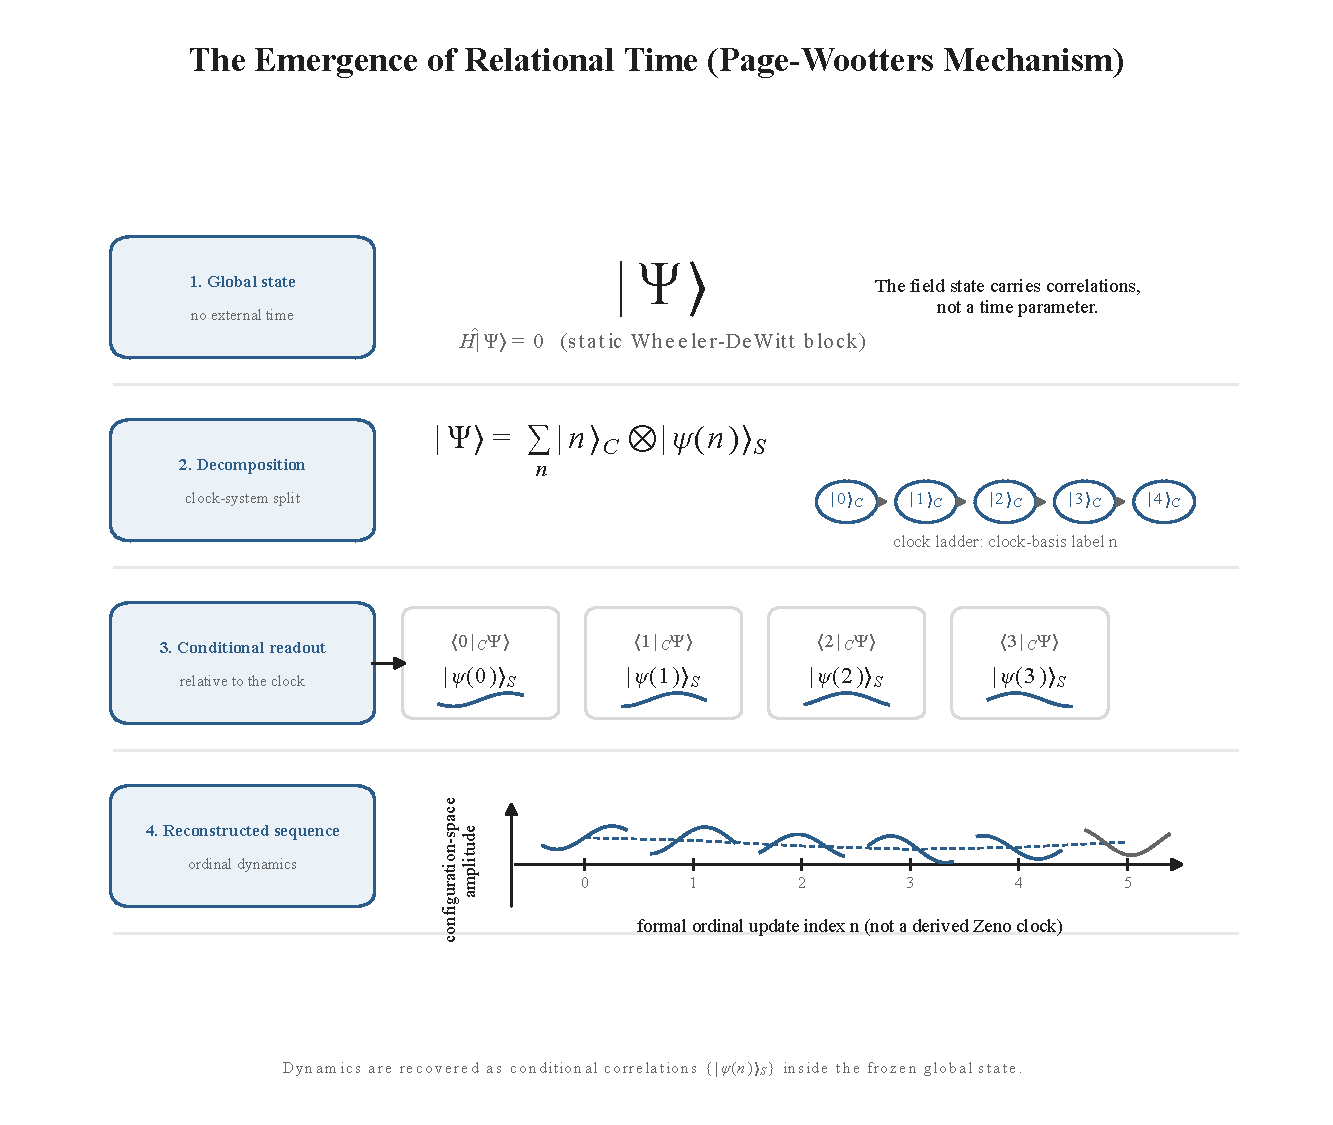
\includegraphics[keepaspectratio,alt={The emergence of relational time (Page-Wootters mechanism): the static Wheeler-DeWitt block decomposes into clock states and correlated system states, and the ordered sequence of conditional system states supplies a relational time label with no external time parameter. Horizontal axis: formal ordinal update index (not a derived Zeno clock); vertical axis: configuration-space amplitude of the system state. Identifying the conditional sequence with an Agent's phenomenal time requires transition, memory, owner, and phenomenal bridges.}]{content/Figures/Volume_1/Figure V1.12.1.pdf}}
\caption{The emergence of relational time (Page-Wootters mechanism): the
static Wheeler-DeWitt block decomposes into clock states and correlated
system states, and the ordered sequence of conditional system states
supplies a relational time label with no external time parameter.
Horizontal axis: formal ordinal update index (not a derived Zeno clock);
vertical axis: configuration-space amplitude of the system state.
Identifying the conditional sequence with an Agent's phenomenal time
requires transition, memory, owner, and phenomenal bridges.}
\end{figure}

\chapter{Chapter 13: The Geometric
Constants}\label{chapter-13-the-geometric-constants}

\subsection{13.1 Overview: Deriving Nature's
Numbers}\label{overview-deriving-natures-numbers}

\subsubsection{13.1.1 The Program: From Geometry to Coupling
Constants}\label{the-program-from-geometry-to-coupling-constants}

The Standard Model of particle physics (plus gravity) relies on
approximately 26 empirical constants---numerical values such as the
fine-structure constant, the gravitational constant, and various
particle masses---that must be measured in the laboratory and manually
inserted into the equations. Standard physics offers no explanation for
why these numbers take the specific values they do. They are treated as
arbitrary ``settings'' of our specific universe.

Geometric Consciousness Theory (GCT) rejects free continuous parameters
in the bare topology/exponent sub-sector; the current full framework
still has explicit finite postulates and empirical anchors listed in the
Parameter Ledger, with 24 numbered full-scope inputs (23 if the Tier 4
known failure C5 is treated as an open problem) pending closure. If the
universe is an intelligible, self-defining geometric structure (Chapter
9), then every terminal numerical constant must be a \textbf{Geometric
Invariant} of the Operating System. These numbers are not intended to
remain ``chosen''; they are closure targets for the 6D hyper-lattice
projection into stable, 3D consensus reality. In this chapter, we
establish the system parameters that define the resolution and strength
of physical interactions.

\subsubsection{\texorpdfstring{13.1.2 Three Fundamental Constants:
\(\alpha, G, \Lambda\)}{13.1.2 Three Fundamental Constants: \textbackslash alpha, G, \textbackslash Lambda}}\label{three-fundamental-constants-alpha-g-lambda}

We organize three constants through proposed geometric interpretations,
each with a separate derivation burden:

\begin{enumerate}
\def\labelenumi{\arabic{enumi}.}
\tightlist
\item
  \textbf{The Fine-Structure Constant (\(\alpha\)):} the electromagnetic
  coupling, modeled here as the \textbf{Local Coupling} between a defect
  and the phason field. Interpreting it as phason impedance or as an
  Agent \textbf{Selection Bandwidth} remains conditional.
\item
  \textbf{Newton's Gravitational Constant (\(G\)):} the gravitational
  coupling, modeled here as the \textbf{Global Coupling} between a
  defect and the collective phonon-metric. The lattice-resolution
  reading is an interpretive layer on the thermodynamic consistency
  calculation of §13.3.4.
\item
  \textbf{The Cosmological Constant (\(\Lambda\)):} An observed
  expansion parameter for which the manuscript registers a \textbf{Tier
  3 shared-field correlation ansatz} using an information-rate model
  coordinate. No typed, normalized information-to-metric causal map is
  currently supplied.
\end{enumerate}

\subsubsection{13.1.3 The Hierarchy Problem: a Heuristic Comparison
{[}Tier 4
analogy{]}}\label{the-hierarchy-problem-a-heuristic-comparison-tier-4-analogy}

The ``Hierarchy Problem''---the fact that gravity is some 36--42 orders
of magnitude weaker than electromagnetism, depending on the particles
compared---is a central puzzle of unification physics. GCT offers a
heuristic comparison rather than extra large dimensions: it pictures
\(\alpha\) as a \textbf{First-Order coupling} to a single lattice node
and \(G\) as a \textbf{Second-Order collective mode} associated with the
information capacity of the cosmic horizon (\textbf{Informational
Screening}). Reading the gap as the difference between
\textbf{Individual Selection} and \textbf{Collective Consensus} is a
Tier 4 analogy; no derivation of the hierarchy is claimed (§13.3.5,
§13.5.2).

\begin{center}\rule{0.5\linewidth}{0.5pt}\end{center}

\subsection{\texorpdfstring{13.2 The Fine-Structure Constant
(\(\alpha\)) {[}Tier 3 numerical relation; mechanism open; Tier 3
multiplier and anchors --- see
§13.2.1--§13.2.4{]}}{13.2 The Fine-Structure Constant (\textbackslash alpha) {[}Tier 3 numerical relation; mechanism open; Tier 3 multiplier and anchors --- see §13.2.1--§13.2.4{]}}}\label{the-fine-structure-constant-alpha-tier-3-numerical-relation-mechanism-open-tier-3-multiplier-and-anchors-see-13.2.113.2.4}

\gctneedspace{5\baselineskip}

\textbf{13.2.1--13.2.2 The Acceptance-Window Solid Angle (Withdrawn)}

\textbf{Declared open programme {[}Tier 3{]}} The fine-structure
constant (\(\alpha \approx 1/137.036\)) was modelled as a ``geometric
impedance'': the ratio of the full sphere (\(4\pi\)) to the solid angle
\(\Omega_{RT}\) subtended by the faces of the Rhombic Triacontahedron
(RT), the 3D projection of the 6D unit hypercube, with
\(\Omega_{RT} = 4\pi(1 - 1/\sqrt5) \approx 0.553 \times 4\pi\). That
value is wrong. The faces of any closed convex polyhedron, seen from an
interior point, subtend exactly \(4\pi\); a direct sum over the 30 RT
faces gives \(1.000 \times 4\pi\). (\(4\pi(1-1/\sqrt5)\) is twice a cap
of half-angle \(\arccos(1/\sqrt5) \approx 63.4^\circ\), the angle
between adjacent 5-fold axes.) Neither \(4\pi/\Omega\) nor
\(4\pi/(4\pi-\Omega) = \sqrt5\) would give 137 in any case. A closing
derivation would need a physical aperture or impedance quantity, defined
on the projection, whose value is \(360\phi^{-2}\). Nothing downstream
uses the solid-angle construction as support.

\subsubsection{\texorpdfstring{13.2.3 The Bare Relation for Alpha
{[}Tier 3 numerical relation: Tier 3 600-cell multiplier; no derived
mechanism for the \(\phi^{-2}\)
factor{]}}{13.2.3 The Bare Relation for Alpha {[}Tier 3 numerical relation: Tier 3 600-cell multiplier; no derived mechanism for the \textbackslash phi\^{}\{-2\} factor{]}}}\label{the-bare-relation-for-alpha-tier-3-numerical-relation-tier-3-600-cell-multiplier-no-derived-mechanism-for-the-phi-2-factor}

The factor \(360\) in the formula
\(\alpha^{-1}_{bare} = 360 \cdot \phi^{-2}\) is \textbf{not} an
arbitrary angular measure or ``degrees in a circle.'' The
\textbf{600-Cell} (\(C_{600}\)) has \(E=720\) edges. Antipodal
identification on the \(S^3\) gauge manifold groups those edges into
\(720/2=360\) antipodal pairs; the coefficient is this quotient count,
not the 600-cell edge count itself. The binary icosahedral group \(2I\)
corresponds to the vertices of this 600-Cell embedded in the \(S^3\)
manifold.

\begin{quote}
\textbf{Tier 3 geometric anchor:} The 600-cell construction motivates
the multiplier \(360\) at Tier 3.
\end{quote}

The relation writes \(\alpha^{-1}_{bare}\) as the ratio of this
antipodal edge-pair count to \(\phi^2\). Neither the reading of
\(\alpha^{-1}\) as a vacuum impedance nor the \(\phi^2\) divisor is
derived (the solid-angle mechanism of §13.2.1--§13.2.2 is withdrawn);
the relation is a Tier 3 numerical conjecture, 0.34\% from the observed
value. The quotient count is \(360=720/2\); selecting it as the physical
multiplier remains Tier 3 pending O.19/O.5, and no free angular measure
is introduced.

\subsubsection{\texorpdfstring{13.2.4 The Bilayer Capacitance Limit
{[}Tier 3 motivated handle; \(1/(2N)\) inherits the Tier 3 \(N=144\)
posit,
O.38{]}}{13.2.4 The Bilayer Capacitance Limit {[}Tier 3 motivated handle; 1/(2N) inherits the Tier 3 N=144 posit, O.38{]}}}\label{the-bilayer-capacitance-limit-tier-3-motivated-handle-12n-inherits-the-tier-3-n144-posit-o.38}

The bare relation \(\alpha^{-1} = 360\phi^{-2}\) is a Tier 3 numerical
conjecture: its multiplier 360 is the Tier 3 600-cell construction
(§13.2.3), and no mechanism for the \(\phi^{-2}\) factor is derived
(§13.2.1--§13.2.2). The bilayer correction below is \textbf{Tier 3
(motivated handle on the Tier 3 \(N=144\) cage posit)}. While it brings
the bare relation to within the stated residual (a postdiction), a naive
point-charge Coulomb matrix evaluation on the 144-node RT cage yields a
significant \textasciitilde13\% discrepancy
(\(\eta_{matrix} \approx 1.13\)).

This gap is interpreted as a \textbf{Geometric Shape-Factor Deficiency}:
the point-charge approximation fails to account for the finite surface
area and rhombohedral curvature of the icosahedral tiles. Full
convergence to the 1/288 limit requires non-perturbative finite-element
analysis (QLQCD). Until such time, the \(1 - 1/(2N)\) factor is
established as a motivated derivation (potential theory analogy) rather
than a derived geometric necessity.

\gctneedspace{5\baselineskip}

\textbf{Result:}
\[ \alpha^{-1}_{\text{GCT}} = \alpha^{-1}_{geom} \times \eta(144) = 137.5078 \times (1 - \frac{1}{288}) = 137.0303 \]

\gctneedspace{5\baselineskip}

\textbf{Observed (CODATA):}
\[ \alpha^{-1}_{\text{obs}} = 137.035999177 \]

\gctneedspace{5\baselineskip}\begin{gctNote}

\textbf{Epistemic Tier: Tier 3 (motivated handle; inherits the Tier 3
\(N=144\) posit, O.38).} The 1/(2N) correction arises from the discrete
Coulomb self-energy of the two-level \(12 \times 12\) cage (V3 Ch07
§7.1.3) by analogy to potential theory. It is not a free parameter (the
value \(288 = 2 \times 144\) follows from \(N\) without additional
choice) but it is also not derived from GCT's axioms alone --- the
factor of 2 in the denominator imports the potential-theory result. A
first-principles geometric derivation of the factor of 2 from the
\(12 \times 12\) cage decomposition is bundled with Open Problem
\textbf{O.5} (QLQCD-1L closure; App ORQ §ORQ.5; see App ULA §ULA.7 for
the structural setup). The 41.5 ppm residual from CODATA is attributed,
as a hypothesis, to the uncalculated one-loop phason self-energy (Open
Problem O.19, App ORQ §ORQ.5).

\end{gctNote}

\gctneedspace{5\baselineskip}

\textbf{The 41.5 ppm Residual.} The 41.5 ppm discrepancy (\(0.0057\))
between the bilayer-corrected GCT value (\(137.0303\)) and the observed
value (\(137.0360\)) is attributed, as a hypothesis, to the unresolved
one-loop phason vacuum-polarization contribution across the discrete
icosahedral lattice (Open Problem O.19). Computing its magnitude is
beyond the current tree-level scope. The bare formula uses no additional
continuous fitted coefficient inside the bare topology/exponent
sub-sector; measurement-anchored precision rows that use observed
\(\alpha(0)\) disclose that value separately as A3 in Parameter Ledger
§0.1. The residual cannot be absorbed by tuning the bare formula. It
defines the theoretical target for the O.19 one-loop calculation.
Appendix QLA §QLA.5--§QLA.6 records the separate Tier 3 notation
\(\delta\alpha^{-1}_{res}\stackrel?=\eta_{\alpha}/2\) only as an
undefined coupling ansatz: \(\eta_{\alpha}\) is not the APS
\(\eta\)-invariant or reduced invariant \(\xi\), and no operator-level
bridge is claimed.

The integer N=144 is not treated as a completed full-lattice
minimization result. The cage boundary is established analytically from
the two-step structural closure argument rather than by a radial
geometric cut: because AKN quasicrystals have highly faceted polyhedral
shells, a simple 1D radial sort does not identify the true boundary. The
144-node cage is retained as an analytic-branch Tier 3 structural posit
pending the full \(R\geq10\) lattice minimization closure registered as
App ORQ Open Problem O.38; the current engine artifact
\texttt{protocol\_cage\_minimization.py} reports
\texttt{ASSUMED\_NOT\_COMPUTED}, not a computed ground-state minimum.

\gctneedspace{5\baselineskip}\begin{gctNote}

\textbf{Derivation Status.} This result is a postdiction and a Tier 3
numerical relation: the bare \(360\phi^{-2}\) relation uses the Tier 3
360 multiplier and its mechanism is open (§13.2.1--§13.2.2), so it lies
outside the 5-postulate-plus-1-anchor bare lepton-ratio sub-sector of
Parameter Ledger §0.1; the native-RGE endpoint and precision-comparison
rows add anchors A2--A6 (Parameter Ledger §0.1). Inputs: \(\phi\)
(geometric invariant), \(N=144\) (Tier 3 integer anchor; analytic-branch
structural posit pending O.38 full-lattice minimization), and the
\(1/288\) bilayer correction (Tier 3 motivated handle; inherits the Tier
3 \(N=144\) posit, O.38; see §13.2.4). The post-bilayer value lies 41.5
ppm \textbf{below} the observed inverse coupling, so the residual
one-loop phason vacuum polarization contribution must \textbf{increase}
\(\alpha^{-1}\) --- the opposite direction to the bare-to-observed
shift, because the bilayer term overshoots. Fixing that sign is part of
the open closure; corrected rows using observed \(\alpha(0)\) carry A3.
As evidence that φ or icosahedral structure is special, this match (bare
and bilayer-corrected) is \textbf{Tier 4}: the preregistered constant
control test (v3, NEGATIVE-FRAGILE; App PSC §PSC.9.6) found φ's pattern
of matches on 21 constants not distinguishable from that of random
constants (58 of 300 random bases did at least as well). The test
``excludes, at power ≥ 0.8, an effect in which φ hits at least 6 of the
8 informative rows through a real effect; weaker effects are not
excluded.'' The number is kept as descriptive arithmetic.

\end{gctNote}

\gctneedspace{5\baselineskip}\begin{gctNote}

\textbf{Tree-Level Baseline:} The bare relation
\(\alpha^{-1} = 360\phi^{-2}\) (Tier 3 numerical conjecture; no
Rhombic-Triacontahedron impedance mechanism, §13.2.1--§13.2.2) is the
baseline before radiative corrections. Its 0.34\% discrepancy is the
bare tree residual; the bilayer \(1/(2N)=1/288\) handle reduces this to
the 41.5 ppm residual targeted by the one-loop phason
vacuum-polarization calculation (O.19), whose sign must increase
\(\alpha^{-1}\).

\end{gctNote}

\subsubsection{13.2.5 Physical Interpretation: The Selection
Bandwidth}\label{physical-interpretation-the-selection-bandwidth}

Within a Tier 3/4 interpretation, the fine-structure constant has been
called the \textbf{Geometric Friction} of a selection interface. The
actual derivations in this chapter concern electromagnetic coupling;
they do not yield an Agent refresh rate, an identity-stability bound, a
Selection Operator, or a metabolism-to-vacuum transducer. Atomic scales
therefore provide no present Level-II or rendering result.

\begin{center}\rule{0.5\linewidth}{0.5pt}\end{center}

\subsection{\texorpdfstring{13.3 Newton's Gravitational Constant
(\(G\))}{13.3 Newton's Gravitational Constant (G)}}\label{newtons-gravitational-constant-g}

\subsubsection{13.3.1 The Hierarchy Problem: Why is Gravity so
Weak?}\label{the-hierarchy-problem-why-is-gravity-so-weak}

The most significant quantitative disparity in physics is the
\textbf{Hierarchy Problem}: the observation that the gravitational force
between two protons is approximately \(10^{36}\) times weaker than the
electromagnetic force between them (the dimensionless gravitational
coupling \(G m_p^2/\hbar c \approx 6\times10^{-39}\), against
\(\alpha \approx 7.3\times10^{-3}\)). In terms of mass scales, this is
expressed as the massive gap between the energy of a proton (\(\sim 1\)
GeV) and the Planck Mass (\(M_P \approx 10^{19}\) GeV).

Standard physics treats this \(10^{19}\) ratio as an unexplained
``fine-tuning'' or ``accident.'' GCT proposes to read this weakness
through the \textbf{Information Saturation Bound} of the vacuum lattice,
picturing gravity as a \textbf{highly screened} rather than
intrinsically weak force {[}Tier 4 heuristic; no derivation of the ratio
is supplied --- §13.3.5, §13.5.2{]}.

\subsubsection{13.3.2 Gravity as Second-Order Collective
Mode}\label{gravity-as-second-order-collective-mode}

The model distinguishes the local coupling of electromagnetism from the
global coupling of gravity {[}Tier 3 model picture{]}:

\begin{itemize}
\tightlist
\item
  \textbf{Electromagnetism (\(\alpha\)):} A \textbf{First-Order}
  coupling. It is pictured as an informational impedance between a
  single knot and the phason field (no impedance mechanism is derived;
  §13.2.1--§13.2.2). It is a ``one-to-one'' interaction with the local
  lattice.
\item
  \textbf{Gravity (\(G\)):} A \textbf{Second-Order} collective mode. In
  the Volume 2 model, gravity is modelled as the \textbf{Acoustic
  Metric} of the phason fluid (Vol. 2 Ch08; an acoustic metric fixes
  propagation kinematics only --- the Einstein dynamics enter through
  the separate horizon-entropy route of §13.3.4). It does not represent
  a local ``charge'' interaction, but the collective, long-range elastic
  deformation of the entire 6D hyper-lattice.
\end{itemize}

Because gravity involves the second derivative of the metric
(\(\partial^2 g_{\mu\nu}\)), the model pictures it as subject to a large
\textbf{Holographic Screening} effect. The image of a photon coupling to
a node while a graviton (in the hydrodynamic limit) couples to the
\textbf{Global Consensus} is a Tier 4 analogy; no screening factor is
computed from it.

\subsubsection{13.3.3 The Information Saturation Argument (Holographic
Principle)}\label{the-information-saturation-argument-holographic-principle}

The fundamental ``pixel size'' of the Operating System is the
\textbf{Lattice Spacing} (\(a_6 = 2\ell_P\); Ch. 4 §4.1.2, App DPS
§DPS.7). According to the holographic bound ('t Hooft, Susskind, Bousso;
a conjecture motivated by the Bekenstein--Hawking black-hole entropy,
not a theorem), the maximum entropy \(S\) (and hence information) that
can be contained in a region is proportional to its surface area:
\[ \frac{S_{max}}{k_B} = \frac{A}{4\ell_P^2} = \frac{A}{a_6^2} \] This
count is in nats, so each lattice plaquette of area
\(a_6^2 = 4\ell_P^2\) carries one nat (\(1/\ln 2 \approx 1.44\) bits)
{[}Tier 3 --- the plaquette assignment is a model identification{]}. In
GCT, the lattice spacing is the scale where the phason field becomes a
discrete lattice. Gravitational coupling occurs only when a defect
generates enough strain to affect the total information balance of the
cosmic horizon.

\subsubsection{13.3.4 Horizon-Entropy Route and the Retired Elasticity
Cross-Check {[}Mixed
tier{]}}\label{horizon-entropy-route-and-the-retired-elasticity-cross-check-mixed-tier}

The current gravity chain is the Jacobson horizon-entropy relation with
the GCT lattice scale supplied. Its structural thermodynamic mechanism
is Tier 2 within the declared model; its Planck/electron link and
dimensional anchor carry the dependencies registered in the Parameter
Ledger (Tier 4 Planck-link conjecture inheriting O.14; Tier 3
dimensional anchor). It is a consistency relation, not an independent
derivation from non-gravitational inputs (see \textbf{Vol. 2, §9.1.4};
App DPS §DPS.7).

The mathematical chain:

\begin{enumerate}
\def\labelenumi{\arabic{enumi}.}
\tightlist
\item
  Extract spatial lattice bounds strictly from the electron
  (\(m_e \to a_6\)).
\item
  Evaluate the Unruh-temperature/heat-flow relation across a local
  causal horizon. Calling it a Selection Operator boundary is a separate
  Tier 3 analogy and is not used in the gravity calculation.
\item
  Solve for the implied Einstein state equations, yielding
  \(G = \frac{c^3 a_6^2}{4\hbar}\).
\item
  Substitute the lattice--Planck relation
  \(a_6 = \frac{2\hbar}{M_P c} = 2\ell_P\) (App DPS §DPS.7), reducing
  the result to the standard identity
  \(G = \frac{c^3 (2\ell_P)^2}{4\hbar} = \frac{c^3 \ell_P^2}{\hbar} = \frac{\hbar c}{M_P^2}\).
  Because \(M_P^2=\hbar c/G\) by definition, this final closure is
  tautological and is reported as such.
\end{enumerate}

The numerical comparison of the electron-anchored route with the
measured \(G\) is disclosed in Vol. 2 §9.1.4 and the Parameter Ledger:
2273.725 ppm (displayed 2274 ppm) on the model-authoritative
\(\alpha_{\rm GCT}=\phi^2/360\) branch, and 2013.345 ppm on the separate
all-CODATA-\(\alpha\) sensitivity branch. Both exceed the inherited
\((1.001)^2-1 = 2001\) ppm rule, and the row is the electron Planck-link
row inverted (\(G\propto m_e^{-2}\)), so it is a registered failure, not
independent evidence.

The former elasticity expression was
\[G = \frac{\hat{c}^4}{8\pi K_\perp a_6}\]

It is dimensionally inconsistent by one length: with \(K_\perp\) an
elastic modulus (\(\mathrm{M\,L^{-1}\,T^{-2}}\)) it has units
\(\mathrm{L^4\,M^{-1}\,T^{-2}}\), whereas \(G\) has units
\(\mathrm{L^3\,M^{-1}\,T^{-2}}\). The minimally corrected scaling form
uses \(a_6^2\); after the Tier 3 P3b substitutions it gives a
calibration-dependent factor --- \(\phi^{18}/(32\pi)\approx57\) in the
Parameter Ledger speed convention,
\(\phi^{-18}/(32\pi)\approx1.72\times10^{-6}\) if \(c_P=c\) --- never 1
(App DPS §DPS.7): \[
G_{elastic}^{(corrected)}=\frac{\phi^{\pm18}}{32\pi}G .
\] It therefore fails as a numerical validation and supplies no
derivation of \(G\). The former description of this expression as a
secondary validation, and of gravity as ``completely constrained'' by
it, is withdrawn.

\begin{quote}
\textbf{Conditional speed relation {[}Tier 2 integer \(D=18\) + Tier 3
P3b stiffness map + kinetic assumption{]}:} If the phonon and phason
sectors share the assumed inertial normalization, the supplied stiffness
ratio \(K_\perp/K_\parallel = \phi^{-18}\) (Appendix DPS, §DPS.3-DPS.4;
Parameter Ledger §0.1 P3a/P3b: \(D_{H3}=18\) is the Tier 2 Coxeter
integer, while the physical map \(K_\perp/K_\parallel=\phi^{-18}\)
remains Tier 3 pending O.15) gives
\[v_\text{phason} = c_P \times \sqrt{K_\perp/K_\parallel} = c_P \times \sqrt{\phi^{-18}} = c_P \times \phi^{-9}\]
The arithmetic \(9=18/2\) is exact, but the physical ratio and the
shared kinetic normalization are not fixed by geometry. Icosahedral
symmetry leaves the invariant quadratic form \(Q=aP_\parallel+bP_\perp\)
with \(b/a\) free, and positive rescalings of the elastic and inertial
sector coefficients preserve the point group and inflation map while
spanning every positive speed ratio (universality-boundary statement,
Vol. 2 §4.2.2). This is therefore a conditional speed export, not a
projection theorem (Vol. 2 §6.2.2; App DPS §DPS.6).
\end{quote}

\subsubsection{13.3.5 G as the Inverse Bandwidth of Global
Consensus}\label{g-as-the-inverse-bandwidth-of-global-consensus}

In natural units (\(\hbar = c = 1\)), Newton's Constant \(G\) is
revealed as a \textbf{Geometric Area Invariant} proportional to the
square of the lattice spacing. From the Jacobson horizon-entropy
derivation (§13.3.4): {[}Tier 2 thermodynamic mechanism + Tier 4
Planck-link conjecture inheriting O.14 + Tier 3 dimensional anchor{]}
\[G = \frac{c^3 a_6^2}{4\hbar} \quad \xrightarrow{\hbar=c=1} \quad G = \frac{a_6^2}{4} = \ell_P^2\]
The factor of \(\tfrac{1}{4}\) is the Jacobson coefficient from the
thermodynamic Clausius relation \(\delta Q = T\,dS\) applied to the
causal horizon; it is a fixed thermodynamic coefficient, and it exactly
compensates the squared lattice--Planck ratio \((a_6/\ell_P)^2 = 4\),
returning the standard Planck identity \(G = \ell_P^2\). Setting
\(G = a_6^2\) (without the factor of 4) is an error that arises from
conflating the Bekenstein area bound with the full Jacobson derivation.
Reading the measured weakness of \(G\) at the proton scale
(\(Gm_p^2/\hbar c \sim 10^{-38}\)) as an effect of \textbf{Information
Dilution} is a Tier 4 interpretive gloss; the identity above does not
compute that ratio, which inherits the anchored ratio \(m_p/M_P\).

As a Tier 4 interpretive analogy, not used in any calculation above,
Newton's \(G\) can be pictured as the \textbf{Network Overhead} of a
shared reality: every local change must be synchronized with the global
state, and as the number of nodes (\(N\)) on the horizon increases, the
``cost'' to update the global metric relative to a local defect
increases. The geometry does not derive this reading.

\begin{itemize}
\tightlist
\item
  \textbf{EM Coupling (\(\alpha\)):} Local update speed (High
  Bandwidth).
\item
  \textbf{Gravitational Coupling (\(G\)):} Global synchronization lag
  (Low Bandwidth). The juxtaposition of the \(10^{-40}\) force hierarchy
  with an order-\(10^{120}\) horizon-entropy count is a
  \textbf{computational-latency analogy} only. No derivation identifies
  \(10^{120}\) independent degrees of freedom whose cube root fixes the
  gravitational hierarchy.
\end{itemize}

\gctneedspace{5\baselineskip}\begin{gctNote}

\textbf{Status.} The Jacobson thermodynamic chain supplies a structural
route from horizon entropy to Einstein dynamics, but the
order-\(10^{120}\) comparison is not a geometric degree count or a
postdiction of the gravitational normalization. The absolute coupling
retains the ledger's disclosed dimensional and Planck-scale inputs; the
cube-power observation is a heuristic analogy only.

\end{gctNote}

\begin{center}\rule{0.5\linewidth}{0.5pt}\end{center}

\subsection{\texorpdfstring{13.4 The Cosmological Constant (\(\Lambda\))
{[}Preview{]}}{13.4 The Cosmological Constant (\textbackslash Lambda) {[}Preview{]}}}\label{the-cosmological-constant-lambda-preview}

\subsubsection{13.4.1 The Volumetric Projection of the
Hierarchy}\label{the-volumetric-projection-of-the-hierarchy}

The ``Cosmological Constant Problem'' is the \(10^{120}\) discrepancy
between a formal vacuum-energy estimate and the observed expansion
scale. GCT proposes a \textbf{Volumetric Projection} scaling analogy to
the hierarchy problem; this is not a derivation of the observed
cosmological constant or an information-to-metric causal law.

\begin{itemize}
\tightlist
\item
  The \textbf{Mass Hierarchy} is a 1D ratio:
  \(m_p / M_P \sim 10^{-19}\).
\item
  The \textbf{Force Hierarchy} is a 2D ratio (Area):
  \((m_p / M_P)^2 \sim 10^{-38}\).
\item
  The \textbf{Energy Discrepancy} is written as a 3D ratio (Volume):
  \((10^{-40})^3 \sim 10^{-120}\). The pattern is not consistent:
  continuing the 1D/2D sequence (\(10^{-19}\), \(10^{-38}\)) would give
  \((m_p/M_P)^3 \sim 10^{-57}\) in 3D, and the ``\(10^{-40}\)'' being
  cubed is a force ratio rather than the 1D mass ratio; even
  \((m_p/M_P)^6 \approx 2\times10^{-115}\) misses \(10^{-120}\) by about
  five orders. Within the proposed picture, the \(10^{120}\) comparison
  is associated with summing mass-point energies into a 3D volume
  without the holographic screening assigned to the \(6D\to3D\)
  projection. This is a numerological analogy, not a scaling relation:
  it does not fix the physical vacuum normalization or explain the
  measured expansion amplitude. {[}Tier 4 numerological analogy;
  normalization open{]}
\end{itemize}

\subsubsection{13.4.2 Tier 3 Shared-Field Correlation
Ansatz}\label{tier-3-shared-field-correlation-ansatz}

Following the \textbf{Cosmology of Zero} (Chapter 5), the framework
distinguishes its zero-ground-state postulate from the observed positive
expansion parameter. The Tier 3 cosmological model introduces the
Class-2 information rate only as a coordinate correlated with a shared
phason-field response. It does not show that Agent rendering generates
\(\Lambda\), and no typed, normalized information-to-metric causal map
is currently supplied. The absolute expansion scale remains a
state-level input. Reading the information rate as the physical source
of \(\Lambda\) is a Tier 4 source ansatz. {[}Tier 3 correlation/model
ansatz; Tier 4 physical-source interpretation; physical coupling open{]}

\subsubsection{13.4.3 Conditional Hydrostatic-Relaxation
Coordinate}\label{conditional-hydrostatic-relaxation-coordinate}

The proposed \textbf{Hydrostatic Relaxation Pressure} is a Tier 3 model
coordinate: the ansatz places cumulative bit-generation rate
\(\dot{\mathcal{I}}\) and a phason-relaxation coordinate in the same
phenomenological expression.

\begin{itemize}
\tightlist
\item
  \textbf{Information coordinate:} Cumulative bit-generation rate
  \(\dot{\mathcal{I}}\) under the stipulated Class-2 allocation.
\item
  \textbf{Cosmological coordinate:} A conditional phantom-directed
  \(w(z)\) response in the shared-field model. This pairing defines a
  correlation template, not cause and effect. It neither establishes
  \(\Lambda \propto \dot{\mathcal{I}}\) as physical law nor derives
  metric expansion from Agent activity; the typed coupling,
  normalization, and information-to-metric map remain open. Volume 2,
  Chapter 14 evaluates the conditional model arithmetic and records its
  sign-opposite DESI tension. {[}Tier 3 model coordinate; Tier 4
  physical-source interpretation; causal mechanism unestablished{]}
\end{itemize}

\begin{center}\rule{0.5\linewidth}{0.5pt}\end{center}

\subsection{13.5 The Hierarchy of Forces}\label{the-hierarchy-of-forces}

\subsubsection{13.5.1 Unified Table of Coupling
Mechanisms}\label{unified-table-of-coupling-mechanisms}

We consolidate the four interactions into a single geometric hierarchy
based on the relationship between the topological defect and the lattice
substrate. The table is tiered by anchor status: the symmetry structure
is Tier 2 where it follows from the icosahedral projection, while scale
normalizations and cosmological extensions inherit their registered Tier
3/Tier 4 dependencies.

\gctneedbreak{10\baselineskip}

{\def\LTcaptype{none} % do not increment counter
\begin{longtable}[]{@{}
  >{\raggedright\arraybackslash}p{(\linewidth - 6\tabcolsep) * \real{0.2353}}
  >{\raggedright\arraybackslash}p{(\linewidth - 6\tabcolsep) * \real{0.2353}}
  >{\centering\arraybackslash}p{(\linewidth - 6\tabcolsep) * \real{0.2941}}
  >{\raggedright\arraybackslash}p{(\linewidth - 6\tabcolsep) * \real{0.2353}}@{}}
\toprule\noalign{}
\begin{minipage}[b]{\linewidth}\raggedright
Interaction
\end{minipage} & \begin{minipage}[b]{\linewidth}\raggedright
GCT Mechanism
\end{minipage} & \begin{minipage}[b]{\linewidth}\centering
Dimensional Order
\end{minipage} & \begin{minipage}[b]{\linewidth}\raggedright
Relationship to Lattice
\end{minipage} \\
\midrule\noalign{}
\endhead
\bottomrule\noalign{}
\endlastfoot
\textbf{Strong} & Direct Topological Winding & \textbf{Zeroth} &
\textbf{Axis-Lock:} The rigid core of the defect. \\
\textbf{Electromagnetic} & Informational Impedance (coupling
\(= \alpha\)) & \textbf{First} & \textbf{Knot-Field:} Local phason
friction. \\
\textbf{Weak} & Chiral Projection Boundary & \textbf{First} &
\textbf{Frame-Rotate:} Geometric asymmetry. \\
\textbf{Gravity} & Holographic Screening (\(G\)) & \textbf{Second} &
\textbf{Collective-Bulk:} Global lattice lag. \\
\end{longtable}
}

Row tiers: the Strong row is Tier 3 (the \(SU(3)\) colour identification
is an open Tier 3 candidate); the Weak row is Tier 3 (no chirality
operator is yet constructed); the EM row inherits the Tier 3 status of
§13.2; the Gravity row is the Tier 2 thermodynamic mechanism of §13.3.4
with its Tier 3/Tier 4 anchors. The ``Mechanism'' and ``Relationship''
labels are Tier 4 pictures.

\subsubsection{13.5.2 Coupling-Ratio
Status}\label{coupling-ratio-status}

The integer \textbf{Stiffness Dimension} \(D=18\) is an exact \(H_3\)
invariant-degree sum within the adopted geometry. Neither it nor the
\textbf{Inflation Factor} (\(\phi\)) fixes, by itself, the gaps between
physical couplings.

\begin{itemize}
\tightlist
\item
  The Strong-to-EM gap is pictured as the cost of moving from the rigid
  axis-lock to the elastic phason field {[}Tier 4 picture; no gap is
  computed{]}.
\item
  The EM-to-Gravity gap (\(10^{40}\)) is compared heuristically with the
  cube root of the order-\(10^{120}\) horizon-entropy count. This
  analogy is not a Tier 2 icosahedral consequence and does not derive
  the force hierarchy or \(G\); the normalization debt remains explicit
  in App DPS §DPS.6.
\end{itemize}

\subsubsection{13.5.3 Parameter Accounting}\label{parameter-accounting}

The spectrum of forces is organized by the icosahedral projection
{[}Tier 2 framework; Tier 3/Tier 4 scale anchors as registered by
sector{]}. Given the adopted maximal-polyhedral-symmetry premise
(Chapter 12 §12.6), the couplings are organized within the
5-postulate-plus-6-continuous-anchor core accounting and the separately
catalogued integer and coefficient handles described in Parameter Ledger
§0. H-EW and the \(SU(3)\) colour identification remain Tier 3. The
selection of icosahedral symmetry is an adopted structural postulate,
not a logical necessity {[}adopted structural postulate; not forced{]}.

\begin{center}\rule{0.5\linewidth}{0.5pt}\end{center}

\subsection{13.6 Summary: The Complete Geometric
Picture}\label{summary-the-complete-geometric-picture}

\subsubsection{13.6.1 Three Constants, Three
Mechanisms}\label{three-constants-three-mechanisms}

The chapter assigns three primary parameters distinct epistemic
dispositions:

\begin{enumerate}
\def\labelenumi{\arabic{enumi}.}
\tightlist
\item
  \textbf{Fine-Structure (\(\alpha\)):} Tier 3 numerical relation with a
  Tier 3 multiplier and anchors; the solid-angle mechanism is withdrawn,
  so no Tier 2 mechanism is claimed (§13.2); ``Local Selection
  Bandwidth'' is a Tier 4 interpretive label.
\item
  \textbf{Gravitational (\(G\)):} Tier 2 thermodynamic consistency
  relation with Tier 3/Tier 4 anchors, not an independent derivation
  (§13.3.4--§13.3.5); ``Global Consensus Overhead'' is a Tier 4
  interpretive label.
\item
  \textbf{Cosmological (\(\Lambda\)):} An observed expansion parameter
  with a Tier 3 shared-field correlation coordinate; no derived
  complexity-to-metric causal map.
\end{enumerate}

\subsubsection{13.6.2 Status of the Standard-Model
Programme}\label{status-of-the-standard-model-programme}

The remaining chapters test whether the proposed geometric mechanisms
can be promoted from conditional structures and calibrated comparisons
to unique physical derivations. No claim of a complete Standard-Model or
gravitational closure is made at this stage: the \(SU(3)\) colour sector
is an open Tier 3 candidate, the bare electroweak angle is the Tier 3
hypothesis H-EW, and the parameters remain at the tiers recorded in the
Parameter Ledger. Chapter 14 turns to the proposed bridge from these
constants to candidate topological solitons.

\chapter{Chapter 14: From Topology to
Fields}\label{chapter-14-from-topology-to-fields}

\subsection{14.1 The Soliton-Field
Duality}\label{the-soliton-field-duality}

\subsubsection{14.1.1 The Bridge Problem: Topology to
QFT}\label{the-bridge-problem-topology-to-qft}

Having set out the axiomatic foundation and the proposed geometric
treatment of the fundamental constants (Chapter 13, where \(\alpha\),
\(G\) and \(\Lambda\) carry mixed tiers and are not all derived), we
must now address the ``Bridge Problem.'' In standard Quantum Field
Theory (QFT), particles are treated as point-like excitations of a
linear field. In Geometric Consciousness Theory (GCT), however, the
fundamental reality is a non-linear, structured Field of Presence. We
must show how discrete, point-like ``particles'' are the effective
descriptions of stable topological restrictions of the global Field
\(\Psi\), viewed from the macroscopic Agent Frame.

The proposed solution is \textbf{Soliton-Field Duality}. GCT posits that
the ``particles'' of physics are not fundamental entities, but rather
the \textbf{Collective Coordinates} of topological defects within the
vacuum lattice {[}Tier 3 physical realization{]}. Appendix CCD §CCD.1
explicitly \textbf{assumes} a stable static defect profile; it does not
prove the existence or stability of a finite-energy soliton in the
Appendix ULA action. Conditional on such a profile and its moduli space,
collective-coordinate reduction is standard Tier 1 machinery. The
proposed mapping to observed particle quantum numbers (Volume 3, Chapter
1) is a separate GCT construction and cannot substitute for the missing
existence/stability derivation. QFT is the proposed \textbf{Effective
Language} for these solitons when viewed from the macroscopic Agent
Frame.

\subsubsection{14.1.2 The Physical Identity Tether and the Optional
Address
Label}\label{the-physical-identity-tether-and-the-optional-address-label}

We distinguish between two classes of excitations in the Field:

\begin{itemize}
\tightlist
\item
  \textbf{Forces (Bosons):} These correspond to \textbf{Untethered
  Lattice Waves} (phonons and phasons) that represent the propagation of
  strain through the Bulk.
\item
  \textbf{Matter (Fermions):} These correspond to \textbf{Tethered
  Topological Knots}. A fermion is modeled as a localized defect
  (vortex/dislocation) carrying a physical framing/connection---an
  \textbf{Identity Tether}---that relates the 3D knot in \(E_\parallel\)
  to an independently specified internal defect or eigenstate frame
  {[}Tier 3 physical architecture{]}.
\end{itemize}

The universal Solenoid is instead an address space, \[
\Sigma_\infty\cong(\mathbb R\times\widehat{\mathbb Z})/\mathbb Z,
\qquad \pi_1(\Sigma_\infty)=0
\] {[}Tier 1 mathematics{]}. Every cylinder tree on it is a chosen
filtration. A physical defect state may be assigned a Solenoid label as
a separate Tier 3 bridge, but that label supplies neither its frame
connection nor a rotational holonomy.

The proposed spinorial transformation law must arise from the separately
specified physical frame/eigenstate bundle and its WZW or equivalent
holonomy {[}Tier 1 conditional bundle topology; Tier 3/open GCT
defect-to-bundle identification; Chapter 15; App CCD §CCD.4{]}.
Spin-statistics then requires the physical exchange/local-QFT
assumptions, and Pauli exclusion follows from antisymmetry. None of
these results follows from two objects sharing or excluding a Solenoid
address, and none anchors a particle to the identity of an observer.

\begin{center}\rule{0.5\linewidth}{0.5pt}\end{center}

\subsection{14.2 The Collective Coordinate Method {[}Tier 1 conditional
method; Tier 3 GCT
realization{]}}\label{the-collective-coordinate-method-tier-1-conditional-method-tier-3-gct-realization}

\subsubsection{14.2.1 Ansatz: Soliton
Decomposition}\label{ansatz-soliton-decomposition}

To move from topology to motion, we employ the \textbf{Collective
Coordinate Method (CCM)}. We assume the existence of a stable soliton
solution \(\Phi_0\) (e.g., the dodecahedral electron cage). We decompose
the Field into a ``Rigid Profile'' and ``Fluctuation Field'':
\[ \Psi(x, t) = \Phi_0(x - X(t)) + \delta\Psi(x, t) \] The parameter
\(X(t)\) is the \textbf{Collective Coordinate}, representing the
``Center of Mass'' of the knot.

The native Appendix ULA action supplies bosonic node displacements,
momenta, harmonic bonds, and a locking potential; it does not yet derive
the stable finite-energy defect and boundary conditions assumed above, a
physical framed configuration space, spinorial/fermionic quantization, a
normalized moduli metric or Dirac kinetic operator, or the deformation
and chiral spin--orbit vertices required for matter--phason matching.
This is an action-relative statement about the present source, not a
universal no-go for emergent fermions from bosonic fields {[}Tier 1
source inspection; Tier 3/open GCT realization{]}.

\subsubsection{14.2.2 Bare Mass vs.~Physical
Mass}\label{bare-mass-vs.-physical-mass}

This decomposition reveals the two components of particle mass:

\begin{enumerate}
\def\labelenumi{\arabic{enumi}.}
\tightlist
\item
  \textbf{Bare Mass (\(m_{\text{bare}}\)):} The integrated energy
  density of the static profile \(\Phi_0\). It represents the minimum
  work required to ``tie'' the knot in the lattice.
\item
  \textbf{Radiative Correction / Phason Drag:} The energy contribution
  of the fluctuation field \(\delta\Psi\). In the proposed physical
  interpretation, a moving knot creates a ``wake'' in the phason fluid
  whose self-interaction may correct the bare mass (\textbf{Phason
  Drag}) {[}Tier 3{]}. Appendix CCD supplies only a schematic
  collective-coordinate Lagrangian conditional on an assumed profile. It
  does \textbf{not} derive phason-drag coefficients or confirm the
  observed lepton mass ratios. Any coefficient calculation or
  lepton-ratio comparison (Volume 3) must therefore be established
  independently; Appendix CCD is not evidence for either.
\end{enumerate}

Within this conditional model, \textbf{Physical Mass} is written as the
sum of these effects:
\(m_{\text{phys}} = m_{\text{bare}} + \delta m(\delta\Psi)\).
Interpreting mass as \textbf{Lattice Impedance}---the total energy
required to drag a topological knot and its associated ``cloud'' through
the supersolid vacuum---remains a Tier 3 GCT physical hypothesis until
the defect solution, moduli action, fluctuation spectrum, and
coefficients are derived.

\begin{center}\rule{0.5\linewidth}{0.5pt}\end{center}

\subsection{14.3 Emergence of the
Wavefunction}\label{emergence-of-the-wavefunction}

\subsubsection{\texorpdfstring{14.3.1 The Resolution Limit
(\(\hbar\))}{14.3.1 The Resolution Limit (\textbackslash hbar)}}\label{the-resolution-limit-hbar}

The \textbf{Nyquist--Shannon limit} is an illustrative analogy for
\([\hat X,\hat P]=i\hbar\), not a derivation of the commutator. No
physical Realization Operator or finite refresh rate is currently
established. Interpreting \(\hbar\) as the \textbf{Informational Pixel
Size} of a rendering engine requires a separate derivation from the
lattice spacing \(a_6\), the physical mode normalization, and the
continuum limit (deferred to Volume 2) {[}Tier 3 --- illustrative
lattice analogy; derivation deferred{]}.

\subsubsection{14.3.2 Schrödinger Equation as Emergent
Dynamics}\label{schruxf6dinger-equation-as-emergent-dynamics}

In the conditional collective-coordinate model, \(\psi(x)\) is a
wavefunction over the collective coordinate \(X\). A
Page--Wootters-style internal clock can label conditional states of the
timeless Wheeler-DeWitt structure (Chapter 12, §12.1) by a formal index
\(n\), but \(n\) is not a derived Zeno-Drive tick count or phenomenal
Agent time. Recovering the standard Schrödinger equation
\(i\hbar\,\partial_t\psi=\hat H\psi\) and its dimensional time parameter
from the timeless block requires a declared clock subsystem, a
conditional-state construction, Hamiltonian scaling, and a continuum
limit. Such an equation would be a linear approximation valid only in
the low-energy limit where the internal structure of the knot remains
``frozen.'' The present statement is a Tier 3 programme rather than a
completed Tier 2 derivation {[}Tier 3 --- effective-dynamics
programme{]}.

\subsubsection{14.3.3 Validity Limits (EFT
Regime)}\label{validity-limits-eft-regime}

The regime labels below use a structural scale \(E_{\text{vac}}\) at
which the internal lattice structure of a knot would become resolvable.
That scale is not yet identified {[}Tier 3, open{]}. In particular it
cannot be the vacuum gap \(m_e/144 \approx 3.55\) keV used elsewhere
under the same name (Vol. 2 Ch03): QED is tested far above 3.55 keV, and
the muon and tau lie about \(3\times10^4\) and \(5\times10^5\) times
above it.

\begin{itemize}
\tightlist
\item
  \textbf{Low Energy (\(E \ll E_{\text{vac}}\)):} The soliton acts as a
  point particle. QFT is valid.
\item
  \textbf{Intermediate structure:} The model proposes that the muon and
  tau are internal resonances of the electron knot {[}Tier 3
  hypothesis{]}. Their masses (0.106 GeV and 1.777 GeV) lie far above
  \(m_e/144\); where they sit relative to the structural scale
  \(E_{\text{vac}}\) cannot be stated until that scale is identified.
\item
  \textbf{High Energy (\(E \approx E_{\text{vac}}\)):} The internal
  lattice structure of the knot is expected to become resolvable {[}Tier
  3{]}.
\item
  \textbf{Ultra-High Energy (\(E \gg E_{\text{vac}}\)):} The knot
  ``unwinds'' or ``fractures.'' The continuum approximation breaks down,
  and the discrete 6D crystallography becomes manifest.
\end{itemize}

\begin{center}\rule{0.5\linewidth}{0.5pt}\end{center}

\subsection{14.4 Gauge Fields from
Geometry}\label{gauge-fields-from-geometry}

\subsubsection{14.4.1 The Berry Phase
Mechanism}\label{the-berry-phase-mechanism}

Let the physical defect Hamiltonian or fluctuation operator
\(H_{phys}(X)\) possess a normalized, spectrally isolated eigenstate or
eigenspace over the collective-coordinate manifold \(\mathcal M_X\).
Those states define a physical eigenstate bundle \(E\to\mathcal M_X\).
Adiabatic transport of the defect along \(X(t)\) can then generate a
\textbf{Geometric Phase} (Berry Phase) {[}Tier 1, conditional on the
specified gapped eigenstate bundle{]}.

GCT must derive \(H_{phys}(X)\), the relevant eigenstate/frame bundle
and its coupling from the lattice/defect action. The Solenoid does not
provide this bundle; an address label, if assigned, only labels the
transported physical state.

\subsubsection{14.4.2 The Berry Connection and
Curvature}\label{the-berry-connection-and-curvature}

Given a local normalized eigenstate section \(|n(X)\rangle\) of that
physical bundle, we introduce the \textbf{Berry Connection}
\(\mathcal{A}_\mu\) {[}Tier 1 differential geometry; Tier 3 consistency
identification with the physical \(U(1)\) gauge potential; the
derivation of gauge redundancy and the antisymmetric Maxwell kinetic
term is a declared open programme, Vol. 2 Ch06{]}.
\[ \mathcal{A}_\mu = i \langle n(X) | \nabla_\mu | n(X) \rangle \] Under
this Tier 3 consistency bridge, the connection is identified with the
physical \textbf{Gauge Potential} (\(A_\mu\)). The curvature of this
connection,
\(F_{\mu\nu} = \partial_\mu \mathcal{A}_\nu - \partial_\nu \mathcal{A}_\mu\),
is then identified with the \textbf{Field Strength Tensor}.

\subsubsection{14.4.3 The Lorentz Force
Law}\label{the-lorentz-force-law}

The presence of this geometric curvature modifies the effective
Lagrangian of the collective coordinate \(X(t)\). The variation of the
action with respect to the path \(X\) yields the \textbf{Lorentz Force
Law}: \[ M_{eff} \ddot{X}^\mu = q F^{\mu\nu} \dot{X}_\nu \] This
implication is variational calculus given an effective action containing
the minimal-coupling term \(qA_\mu(X)\dot X^\mu\). In the geometric
interpretation, the force is the response of the physical defect to
curvature of its eigenstate/frame bundle; no force arises from moving
between Solenoid address cylinders, and an address label contributes no
connection or dynamics. {[}Tier 1 standard Berry-phase mechanics,
conditional on the Tier 3 identification of \(\mathcal{A}_\mu\) with the
physical \(U(1)\) gauge potential{]}

This geometric construction provides a candidate foundation for the
electrodynamic field theory of Volume 2 (Vol. 2, Ch06), which is a
declared open programme (Vol. 2 Ch06): as written, the phason
construction does not reproduce Maxwell dynamics, and first-principles
\(U(1)\) closure remains open.

\begin{center}\rule{0.5\linewidth}{0.5pt}\end{center}

\subsection{14.5 The Masslessness Constraint {[}Tier 1 standard gauge
protection; Tier 3 phason realization of the
photon{]}}\label{the-masslessness-constraint-tier-1-standard-gauge-protection-tier-3-phason-realization-of-the-photon}

\subsubsection{14.5.1 Gauge Protection and Phason
Modes}\label{gauge-protection-and-phason-modes}

The \textbf{Masslessness of the Photon} is inherited from the
ungauge-fixed Maxwell action, the absence of a photon mass term, and the
residual \(U(1)\) gauge redundancy that leaves only two transverse
physical polarizations. Broken global phase modes in the supersolid
substrate can supply phason/second-sound degrees of freedom, but those
scalar Nambu-Goldstone modes are not by themselves the Maxwell photon.
The GCT claim is therefore gauge protection in the continuum limit plus
a separate, tiered phason-realization bridge.

\subsubsection{\texorpdfstring{14.5.2 Why the Photon (\(m_\gamma\)) is
Exactly
Zero}{14.5.2 Why the Photon (m\_\textbackslash gamma) is Exactly Zero}}\label{why-the-photon-m_gamma-is-exactly-zero}

In the GCT model, the photon is identified with the transverse gauge
field associated with the vacuum condensate's long-wavelength
phase-lattice synchronization {[}Tier 3 identification{]}. Its mass is
exactly zero in the Maxwell limit because a mass term would break the
residual \(U(1)\) gauge redundancy. The stronger statement that the GCT
tile dynamics uniquely realize this gauge field as a phason mode remains
a structural bridge, not a scalar-Goldstone derivation.

The historical \textbf{``Slip''}, \textbf{``Kinematic Agency,''} and
``Cursor through Code'' language is a Tier 4 metaphor for mobility in a
gapless medium. Photon masslessness rests on unbroken local \(U(1)\)
gauge invariance and the associated Ward identity; Maxwell gauge
protection does not derive an observer, a Selection Operator, volitional
torque, or a consciousness-enabling role for light. Any such bridge
requires an independently realized physical Agent/Selection mechanism
and is not used in the photon-mass argument.

\chapter{Chapter 15: Spin, Statistics, and
Antimatter}\label{chapter-15-spin-statistics-and-antimatter}

\subsection{15.1 The Topology of
Rotation}\label{the-topology-of-rotation}

\subsubsection{15.1.1 Spin as Topological
Holonomy}\label{spin-as-topological-holonomy}

In standard Quantum Mechanics, ``Spin'' is an intrinsic representation
label. GCT explores a \textbf{Topological Holonomy} realization: the
phase accumulated by a physical internal frame transported through
configuration space. The \(SU(2)\to SO(3)\) control is standard Tier 1
mathematics; deriving the required GCT defect, configuration space,
frame bundle, quantum line bundle and transport law from Appendix ULA
remains Tier 3/open.

While a dimensionless point is invariant under a 360° rotation, a
\textbf{Framed Object}---an object whose internal orientation is tracked
relative to a background---is not. In GCT, Spin is modeled through the
holonomy of that physical frame bundle. The universal Solenoid may label
an identity address, but its topology does not supply the rotational
frame or holonomy: its ordinary fundamental group is trivial,
\(\pi_1(\Sigma_\infty)=0\).

\subsubsection{15.1.2 The Ribbon Model}\label{the-ribbon-model}

We model the topological soliton not as a point mass, but as a
\textbf{Framed Ribbon} in the \(6D\) configuration space. The proposed
\textbf{Identity Tether} is a physical framing/connection that relates
the \(3D\) knot in \(E_\parallel\) to an internal defect frame.
Identifying its state with a selected Solenoid address is an additional
Tier 3 bridge layered onto that independently specified physical frame
connection, not a consequence of the inverse limit.

When the knot rotates in physical space, the framed ribbon accumulates a
twist. In the model this is a statement about the physical frame bundle,
not about motion from a Solenoid end to a higher cylinder or a link
between a localized aperture and a Branch Node. The state of a particle
is therefore proposed to include its position and the \textbf{Holonomic
State} of its physical tether {[}Tier 3/open physical architecture{]}.

\subsubsection{15.1.3 360° vs.~720° Symmetry}\label{vs.-720-symmetry}

The fundamental group of the rotation group \(SO(3)\) is
\(\mathbb{Z}_2\), implying two distinct classes of closed paths in
rotation space. {[}Tier 1 --- standard algebraic topology;
\(\pi_1(SO(3)) = \mathbb{Z}_2\) is a theorem independent of GCT{]}

\begin{enumerate}
\def\labelenumi{\arabic{enumi}.}
\tightlist
\item
  \textbf{360° Rotation (\(2\pi\)):} This corresponds to a
  non-contractible loop. Topologically, the ribbon accumulates a single
  twist that cannot be undone by translation.
\item
  \textbf{720° Rotation (\(4\pi\)):} This corresponds to a contractible
  loop. In three dimensions, a double-twist in a ribbon can be
  continuously deformed back to the identity without rotating the knot.
\end{enumerate}

This ``Double Cover'' requirement is the physical signature of a framed
rotational degree of freedom. Matter is proposed to transform
spinorially because its defect frame is physically anchored;
force-carriers are modeled as integer-spin lattice waves. {[}Tier 3/open
--- the GCT defect/tether identification is a physical architectural
hypothesis; the \(SU(2)/SO(3)\) topology itself is Tier 1.{]} A Solenoid
address can accompany that object but does not derive the double cover.

\begin{center}\rule{0.5\linewidth}{0.5pt}\end{center}

\subsection{15.2 The Dirac Belt Trick}\label{the-dirac-belt-trick}

\subsubsection{15.2.1 Visual Demonstration of the Double
Cover}\label{visual-demonstration-of-the-double-cover}

The ``Dirac Belt Trick'' is a visual demonstration of this topology; the
formal statement is \(\pi_1(SO(3))=\mathbb{Z}_2\) with
\(SU(2)\to SO(3)\) the simply connected double cover {[}Tier 1{]}. If a
belt (the tether) is attached to an object (the knot) and the object is
rotated by 360°, the belt accumulates a twist. However, if the object is
rotated by a further 360° (720° total), the resulting double-twist can
be looped over the object, restoring the system to its original state.

\subsubsection{15.2.2 The Physical Identity Tether and the Optional
Address
Map}\label{the-physical-identity-tether-and-the-optional-address-map}

In GCT, the ``Belt'' is the proposed physical \textbf{Identity Tether}
connecting a localized defect to its internal frame.

\begin{itemize}
\tightlist
\item
  \textbf{Bosons (Forces):} Are modeled as untethered excitations. They
  possess integer-spin rotational symmetry because their state carries
  no defect-frame ribbon holonomy of this type.
\item
  \textbf{Fermions (Matter):} Are modeled as tethered framed defects.
  They possess spinorial rotational symmetry because the physical frame
  is anchored and must preserve its holonomy under transport.
\end{itemize}

Mapping either class to \(\Sigma_\infty\) is separate from the belt
trick. A selected address does not store the rotational state, and the
universal Solenoid's trivial ordinary \(\pi_1\) cannot be the
noncontractible \(SO(3)\) loop. {[}Tier 3/open physical identification;
Tier 1 topology{]}

\begin{center}\rule{0.5\linewidth}{0.5pt}\end{center}

\subsection{15.3 The Wess-Zumino-Witten Term {[}Tier 1 conditional
mathematics; Tier 3/open GCT
adoption{]}}\label{the-wess-zumino-witten-term-tier-1-conditional-mathematics-tier-3open-gct-adoption}

\subsubsection{15.3.1 Spinor Phase
Generation}\label{spinor-phase-generation}

The declared framed-defect model may be completed by adding a normalized
\textbf{Wess-Zumino-Witten (WZW) term} on a specified frame-bundle
target. That term, its level, boundary extension and physical carrier
are additional data. They are not generated by the present Appendix ULA
action or by a Solenoid address.

\subsubsection{15.3.2 Conditional Half-Integer-Spin Phase {[}Tier 1
conditional mathematics; Tier 3/open GCT
adoption{]}}\label{conditional-half-integer-spin-phase-tier-1-conditional-mathematics-tier-3open-gct-adoption}

For a defect already equipped with the spinorial \(SU(2)\) lift, a
\(2\pi\) spatial rotation transports the fundamental spinor from
\(+\mathbf1\) to \(-\mathbf1\). A compatible normalized WZW functional
can encode this sign only after its physical bundle, level, extension
and winding sector have been supplied.

\textbf{Result 15.1:} \emph{Conditional on a physical defect state
carrying the fundamental spinorial lift, a spatial rotation of \(2\pi\)
acts by \(-1\) and \(4\pi\) acts by \(+1\) {[}Tier 1 representation
theory; Tier 3/open GCT carrier identification{]}.}

(App CCD §CCD.4 states the standard \(SU(2)\to SO(3)\) double-cover
control and the normalized WZW three-form, but it does \textbf{not}
evaluate a WZW functional for a GCT defect or derive its level, winding
sector or physical bundle; the former Theorem CCD.1 is retired there,
and the Solenoid supplies no rotation obstruction because
\(\pi_1(\Sigma_\infty)=0\). Those items remain Tier 3/open. The separate
O.14 APS route is conditional: no qualifying boundary operator, domain,
or APS index has yet been specified and evaluated, and an
\(\eta\)-invariant measures spectral asymmetry; it cannot by itself
supply the missing defect-to-bundle identification.)

\[ \Psi(R_{2\pi}) = e^{i\pi} \Psi(R_0) = -\Psi(R_0) \] This is the
conditional minus sign of the fundamental \textbf{spin-\(1/2\)}
representation. The ``Spinor'' is not generated by an identity tree, nor
has it yet emerged from the literal Appendix ULA node variables. The GCT
claim that a stable matter defect realizes the required frame and
quantization remains Tier 3/open.

\begin{center}\rule{0.5\linewidth}{0.5pt}\end{center}

\subsection{15.4 Spin--Statistics: A Conditional Exchange Program
{[}Tier 1 given the standard hypotheses; Tier 3/open GCT
carrier{]}}\label{spinstatistics-a-conditional-exchange-program-tier-1-given-the-standard-hypotheses-tier-3open-gct-carrier}

\subsubsection{15.4.1 Exchange Phase from Ribbon
Swapping}\label{exchange-phase-from-ribbon-swapping}

The ribbon picture motivates a possible exchange loop for two identical
framed defects. Turning that picture into \textbf{Quantum Statistics}
requires a specified multi-defect configuration space and quantum line
bundle, or the hypotheses of a spin--statistics theorem (locality,
covariance, positive energy and the appropriate field representation). A
generic exchange is not proved equivalent to a \(2\pi\) rotation merely
by drawing the ribbon.

\subsubsection{15.4.2 Fermion vs.~Boson
Statistics}\label{fermion-vs.-boson-statistics}

Conditional on the required configuration-space/field-theory hypotheses
and the non-trivial fermionic quantization choice, exchanging two such
defects multiplies the state by \(-1\):
\[ \Psi(x_1, x_2) = -\Psi(x_2, x_1) \] Untethered lattice waves are
modeled in the bosonic representation. This is part of the declared
effective field inventory; the absence of a modeled tether alone is not
a derivation of exchange statistics.

\subsubsection{15.4.3 Pauli Exclusion After
Antisymmetry}\label{pauli-exclusion-after-antisymmetry}

Once fermionic antisymmetry has been established, the \textbf{Pauli
Exclusion Principle} follows: if two identical fermions occupy the same
one-particle state, \(\Psi = -\Psi \implies \Psi = 0\) {[}Tier 1, given
antisymmetry{]}. The present ribbon model has not independently derived
that antisymmetry from Appendix ULA, so this section is not a geometric
derivation of Pauli exclusion.

Ambient dimension controls which topology is available to an extended
defect, but it does not choose its quantum exchange representation.
Knotting is a property of closed one-dimensional curves in three-space;
a point defect is not knotted, and knotting alone does not imply
fermionic exchange statistics. (For point particles, the
dimension-dependent statement is the standard one: in \(D=3\) exchange
statistics are restricted to bosons and fermions, while \(D=2\) admits
braid-group/anyonic statistics.) Higher-dimensional ambient spaces can
remove some knot obstructions, but this does not make \(D=3\) a
derivation of Pauli exclusion. Pauli follows here only after
antisymmetry of the physical quantum state has independently been
established. It is not a consequence of two tethers being unable to
share one \(p\)-adic address; Solenoid addresses and fermionic
one-particle states are different mathematical objects. The ``solid''
character of ordinary matter is the standard consequence of Pauli
exclusion for electrons, not a separate topological impossibility of
address merger.

\begin{center}\rule{0.5\linewidth}{0.5pt}\end{center}

\subsection{15.5 Antimatter as
Retro-Topology}\label{antimatter-as-retro-topology}

\subsubsection{15.5.1 Definition: Winding Direction Relative to the
Information Gradient
Vector}\label{definition-winding-direction-relative-to-the-information-gradient-vector}

The suspension model
\(\Sigma_\infty\cong(\mathbb R\times\widehat{\mathbb Z})/\mathbb Z\)
(Chapter 7) contains dense real leaves, but it does not canonically
orient them or identify a leaf parameter with entropy. GCT therefore
introduces the \textbf{Information Gradient Vector}
\(\vec{\nabla}\mathcal{I}\) as a separate Tier 3 physical order
parameter: the net direction of information accumulation in the declared
Selection/Consensus dynamics. Formally one may write
\(\vec{\nabla}\mathcal{I} \equiv (\partial \mathcal{S}_{Agent} / \partial n)\,\hat{e}_{flow}\),
with \(\hat{e}_{flow}\) a unit vector along a chosen real leaf direction
(§7.2.3), only after a physical leaf chart, orientation and coupling
have been chosen. This is not derived by the Solenoid topology {[}Tier
3{]}.

A topological knot in the lattice is then assigned an orientation---a
\textbf{Chirality}---relative to this proposed vector {[}Tier 3{]}.

\begin{itemize}
\tightlist
\item
  \textbf{Matter (\(e^-\)):} A knot whose winding direction is
  \textbf{aligned} with the Information Gradient Vector (Information
  accumulation).
\item
  \textbf{Antimatter (\(e^+\)):} A knot whose winding direction is
  \textbf{anti-aligned} (Information reversal).
\end{itemize}

In this model, antimatter is described as \textbf{Retro-Topology}: a
``reverse twist'' in the crystallization sequence {[}Tier 3 model
identification{]}. On that picture, when a Matter knot and an Antimatter
knot meet, their winding numbers sum to zero and the topology
``unwinds,'' releasing the stored lattice strain as phason waves
identified with photons {[}Tier 3; no annihilation amplitude or
cross-section is derived, and the observed rates are those of standard
QED{]}.

\subsubsection{15.5.2 CPT Symmetry and Lattice
Inversion}\label{cpt-symmetry-and-lattice-inversion}

In ordinary physics, CPT invariance is a theorem of Lorentz-invariant
local quantum field theory (with the usual Hermiticity and spectral
assumptions) {[}Tier 1 for such theories{]}. It is not a consequence of
lattice centrosymmetry alone. The \(\mathbb{Z}^6\) lattice is
centrosymmetric: the inversion \(\mathbf n\mapsto-\mathbf n\) is a
lattice symmetry, and in the six-dimensional parent space it is
orientation-preserving (its determinant is \((-1)^6=+1\)), while its
restriction to each three-dimensional factor \(E_\parallel\),
\(E_\perp\) is an orientation-reversing improper map. A rigid rotation,
by contrast, always preserves orientation, so CPT cannot be ``an
orientation-reversing rigid rotation.'' The GCT proposal is that the
physical CPT operation of the emergent effective field theory is
represented by this lattice inversion combined with the corresponding
internal-sector operations {[}Tier 3 identification{]}; recovering the
CPT theorem itself requires the emergent Lorentz-invariant local field
theory, which remains open. No proof that the three physical operations
\((C, P, T)\) correspond to lattice generators is currently supplied in
the appendices.

Within this proposal the three operations are modeled as:

\begin{itemize}
\tightlist
\item
  \textbf{Charge Conjugation (C):} Reversing the winding direction
  relative to the Information Gradient Vector.
\item
  \textbf{Parity (P):} Reflecting the spatial coordinates in
  \(E_\parallel\).
\item
  \textbf{Time Reversal (T):} Reversing the formal evolution parameter
  in the physical model. The ordinal Agent index \(n\) may be reversed
  as bookkeeping, but it is not a derived Selection clock or the
  definition of physical time reversal.
\end{itemize}

The observed matter--antimatter asymmetry --- a baryon-to-photon ratio
of \(\eta \approx 6 \times 10^{-10}\) --- is here associated only with a
supplied cosmological boundary condition {[}Tier 4{]}. No physical
Consensus Protocol, Agent, or Selection Operator is derived to choose an
orientation of the Information Gradient Vector, and the asymmetry ratio
is not calculated by this construction. Interpreting the boundary
condition as the selection of one orientation over the otherwise
degenerate Zero state (Chapter 5, §5.1) is a Tier 4 reading.

\clearpage
\thispagestyle{empty}
\vspace*{0.35\textheight}
\begin{center}\bfseries\LARGE PART V: THE EMERGENCE OF EXPERIENCE\end{center}
\vspace*{\fill}
\clearpage

\chapter{Chapter 16: Time and Qualia}\label{chapter-16-time-and-qualia}

\gctneedspace{5\baselineskip}\begin{gctImportant}

\textbf{Epistemic Scope of this Chapter.}

The claims developed in Part V partition into two strata that must be
evaluated separately.

\textbf{Theoretical-framework stratum:} Relational Time and the
Quality-Space irrep decomposition are mathematical constructions. DMC is
a Tier-3 candidate-control hypothesis, not part of their theorem status.
Identifying any Polaron or phason-drag structure with phenomenal
experience is a separate Tier-3 bridge, and no present substrate verdict
follows.

\textbf{Biophysical-specific stratum (Tier 3):} β-tubulin Trp, NV
centres, isotope substitution, and the 112-MHz branch are candidate
mechanism tests and conditional scenarios. DMC descriptors organize
missing-leg controls; positive or null results constrain those
mechanisms without establishing an Identity Polaron or Level II.

The framework takes Qualitative Presence (Level I) as Axiom 1 rather
than a derived result and studies Quality Space structure separately.
Artificial-system Level II status is open (Tier 3): no validated
substrate criterion exists yet (it requires a typed, normalized,
measured coupling, the Identity-Polaron construction and an independent
phenomenal bridge; O.21/O.23/O.34, O.18). DMC descriptors are candidate
controls, not a categorical substrate verdict.

\end{gctImportant}

\subsection{16.1 The Emergence of Time}\label{the-emergence-of-time}

\subsubsection{\texorpdfstring{16.1.1 Relational Time: The Sequence
Index
(\(n\))}{16.1.1 Relational Time: The Sequence Index (n)}}\label{relational-time-the-sequence-index-n}

In the static Bulk defined by the Wheeler-DeWitt constraint
(\(\hat{H}\Psi=0\)), time does not exist as a fundamental dimension or a
flowing duration. However, the \textbf{Selection Operator}
(\(\mathcal{F}_{sel}\)), proposed in Chapter 9 as a conditional formal
update rather than a demonstrated physical process, is modelled as
acting through discrete, sequential iterations {[}Tier 3{]}. We define
\textbf{Relational Time} not as a continuous background, but as the
\textbf{Sequence Index (\(n\))} of these proposed selection events.

The model can index successive configurations by an ordinal \(n\) and
can associate that index with an address label in the Solenoid.
Interpreting the label as an Agent's identity, the transition as
subjective temporal flow, or the unselected space as phenomenally unread
are Tier 3 psychophysical bridges; the indexing mathematics alone does
not supply an owner of experience.

\subsubsection{\texorpdfstring{16.1.2 The Coordinate \(\tau_{coord}\):
Lattice
Address}{16.1.2 The Coordinate \textbackslash tau\_\{coord\}: Lattice Address}}\label{the-coordinate-tau_coord-lattice-address}

We must distinguish the internal sequence of the Agent from the external
geometry of the vacuum. We define the \textbf{Coordinate Time
(\(\tau_{coord}\))} as the specific address of a realized configuration
within the 6D lattice projection. \emph{(Note: \(\tau_{coord}\) is a
scalar coordinate in the 3D physical manifold and is distinct from the
\(\tau\) lepton discussed in Volume 3).}

In the conceptual model, \textbf{history} is a path of \(\tau_{coord}\)
labels associated with prior updates; ``past,'' ``future,'' and ``Now''
organize prior, available, and current configurations. The
\textbf{Crystallization Front} is a phenomenological correspondence for
the current update, not a measured wavefront or evidence that a realized
Selection Operator is resolving the lattice.

\subsubsection{\texorpdfstring{16.1.3 The Subjective Flow
\(\Lambda_\tau\)}{16.1.3 The Subjective Flow \textbackslash Lambda\_\textbackslash tau}}\label{the-subjective-flow-lambda_tau}

The relationship between an internal index (\(n\)) and coordinate time
(\(\tau_{coord}\)) motivates a candidate \textbf{Subjective Flow Rate
(\(\Lambda_\tau\))}, defined as a lattice-step ratio per proposed
selection event. The definition is a model convention; its
identification with subjective flow and any mass-dependent prediction
require a Tier 3 physical/phenomenal bridge.
\[ \Lambda_\tau \equiv \frac{d\tau_{coord}}{dn} \] \emph{(The symbol
\(\Lambda_\tau\) is used rather than \(\dot{\tau}_{coord}\) to avoid
collision with the standard physics convention in which an overdot
denotes differentiation with respect to coordinate time \(\tau_{coord}\)
itself. Here the relevant derivative is with respect to the formal
sequence index \(n\), a dimensionless ordinal, not a coordinate and not
a derived Zeno clock.)}

In the Tier 3 phenomenological analogy, \(dn\) is \emph{called} a pulse
index and \(d\tau_{coord}\) a coordinate step per update. No physical
Selection clock, Agent bandwidth, thought-size map, or phenomenal timing
law has been derived from local topological complexity.

\subsubsection{16.1.4 Gravity as Processing Lag (Bandwidth
Saturation)}\label{gravity-as-processing-lag-bandwidth-saturation}

The following \textbf{Processing Lag} account is a Tier-3 candidate
interpretation of gravitational time dilation. A finite Rendering
Bandwidth and its relation to mass, selection events and subjective flow
are not physically derived here.

The model proposes that higher topological information density may
increase coordinate progress per selection event,
\(\Lambda_\tau=d\tau_{coord}/dn\). No constitutive bandwidth-to-metric
law or phenomenal clock bridge is supplied. The standard GR comparison
below is separate from this Tier-3 interpretation.

\begin{itemize}
\tightlist
\item
  \textbf{Physical Result:} This matches the GR result from the
  Schwarzschild metric:
  \(d\tau_{proper}/d\tau_{coord} = \sqrt{1 - r_s/r} < 1\) near a mass
  {[}Tier 1 --- standard General Relativity{]}.
\item
  \textbf{GCT candidate interpretation {[}Tier 3{]}:} if the selection
  index is identified with proper time (\(dn \propto d\tau_{proper}\)),
  fewer selection steps occur per coordinate second
  (\(dn/d\tau_{coord}\) decreases), so
  \(\Lambda_\tau = d\tau_{coord}/dn\) increases and the Agent ages
  \emph{slower} than a distant observer. The model thus associates time
  dilation with coordinate step size. The suggested processing-horizon
  limit \(\Lambda_\tau\to\infty\) is an analogy requiring a physical
  bandwidth law and an independent phenomenal-clock bridge; it is not a
  Tier-2 derivation of GR or subjective awareness.
\end{itemize}

\gctneedspace{5\baselineskip}

\textbf{16.1.4b Relation to Higher-Order Thought (HOT) Theories}

The sequence-index framework of §16.1.1--16.1.3 --- in which time is
modelled {[}Tier 3{]} as the subjective registration of the transition
from selection-cycle \(n\) to \(n+1\) --- places consciousness at the
\emph{meta-level} of state-processing rather than at the level of the
processed content. This puts GCT in conversation with the
\textbf{Higher-Order Thought (HOT) family} of consciousness theories:
Rosenthal (1997, 2005 \emph{Consciousness and Mind}; 2012 \emph{Philos.
Trans. R. Soc. B} 367:1424), Lau (2008 \emph{Prog. Brain Res.} 168:35;
Brown, Lau \& LeDoux 2019 \emph{Trends Cogn. Sci.} 23:754), and
Carruthers (2000 \emph{Phenomenal Consciousness}).

\textbf{Structural homology.} Both GCT and HOT ground phenomenal
consciousness in a \emph{meta-level operation on a lower-order
state-space}. For Rosenthal, phenomenal consciousness is the
\emph{having of a higher-order representation of a lower-order mental
state}. In GCT's Tier 3 proposal, phenomenal consciousness is modelled
as the \emph{actualization} (projection via \(\mathcal{F}_{sel}\)) of a
lower-order Field configuration into the Agent's Selection Operator
cycle, sequenced by the index \(n\); this phenomenal identification is
not derived. The two theories are operationally analogous at this level:
both treat consciousness as the \emph{holding-of} the state, not as the
state itself, while differing in formal substrate and ontological
commitments.

\gctneedspace{5\baselineskip}

\textbf{Where GCT proposes to go beyond HOT (programme, not result).}

\begin{enumerate}
\def\labelenumi{\arabic{enumi}.}
\tightlist
\item
  \emph{Grounding:} HOT places the meta-operation in representational
  architecture. GCT proposes a topological model in which
  \(\mathcal{F}_{sel}\) acts on a Polaron Hilbert space, but the
  physical coupling and phenomenal identification remain open. App PUP
  reaches at most an algebraic unity candidate; it does not prove an
  irreducible physical Hilbert space, identify \(\mathcal F_{sel}\), or
  establish an owner. Chirality and nuclear spin are experimental
  controls, not a proof that only one material class supports the
  structure.
\item
  \emph{Substrate ontology:} HOT is silent on physical substrate. GCT
  proposes a substrate-sensitive program involving chiral nuclear-spin
  candidate controls, but the coupling and phenomenal bridge are
  unclosed. A future GCT-vs-HOT divergence therefore requires measured
  couplings and an explicit HOT substrate/grain analysis; present
  silicon-AI Level II status is open (Tier 3).
\item
  \emph{Falsifiability:} HOT predictions are largely behavioural /
  inferential (subjects' reports of conscious states). GCT proposes
  substrate-physical candidate observables (frequency-resolved
  \(T_2(\nu_d)\) features within the registered \([32, 200)\) MHz
  adaptive scan --- the 100 MHz figure is a historical scenario only ---
  chirality-reversal symmetry, anaesthetic enantiomer-selectivity
  caveats, Protocol A-Prime). Those observables can constrain the
  candidate mechanism; they do not yet test phenomenal ownership, and
  therefore do not by themselves establish an advantage over HOT on
  consciousness rather than mechanism.
\end{enumerate}

\textbf{Where HOT is GCT-compatible (or stronger).} HOT-style cognitive
architecture can serve as a functional comparison layer. Empirical work
on metacognition, confidence judgments, and PFC-mediated higher-order
processing (Lau 2008; Maniscalco \& Lau 2012) describes ordinary
cognitive operations that a future GCT model would need to map to its
formal cycle. It does not constitute a cognitive realization of
\(\mathcal F_{sel}\) or close the physical/phenomenal bridge.

\textbf{Status:} Tier 3 philosophical positioning informed by Tier 2
framework structure and Tier 3 conditional material-proxy scenarios. GCT
is \emph{not} a refutation of HOT; it proposes a substrate-level
specification of the meta-operation HOT identifies functionally, but no
substrate grounding is yet established.

\begin{center}\rule{0.5\linewidth}{0.5pt}\end{center}

\subsection{16.2 Qualia as Topological
Impedance}\label{qualia-as-topological-impedance}

\subsubsection{16.2.1 Stating the Hard Problem: The Explanatory
Gap}\label{stating-the-hard-problem-the-explanatory-gap}

The ``Hard Problem'' asks why physical processes are accompanied by a
felt inner life. Standard science describes the \textbf{Quantity} (the
signal) but fails to account for the \textbf{Quality} (the experience).
GCT posits, under Axiom 1, that this gap arises from attempting to
derive the Field from the Pattern. By performing the Epistemic
Inversion, Qualia are modeled as primary data of the interaction between
the Agent and the Vacuum, not as products derived from non-experiential
structure. That further model of particular qualia as an Agent--vacuum
interaction is Tier 3 and lacks a physical \(\mathcal F_{sel}\), owner,
and phenomenal bridge.

\subsubsection{16.2.2 The GCT Proposal: Structural Russellian Monism
(Position
B)}\label{the-gct-proposal-structural-russellian-monism-position-b}

\emph{Reader's roadmap.} This section develops GCT's structural-realist
proposal that qualitative content is reference-fixed by the Quality
Space irrep decomposition (§16.2.2c; red is modeled by the \(T_2\)
(\(E_\perp\)) channel rather than identified without remainder). The
strongest natural objection --- that this commitment collapses
Russellian monism into pure structuralism (Goff 2017 Ch.7) --- is
addressed via GCT's \emph{two-layer structuralism} at the closing
paragraph of §16.2.2c: Axiom 1 (Layer A, non-structural intrinsic
non-subjective presence) and Quality Space (Layer B, structural
qualitative content) work at distinct ontological levels and separate
GCT from both pure structuralist monism and anti-structuralist
Russellianism. Readers concerned about the apparent category collapse
should read §16.2.2c through to the closing paragraph before passing
judgment.

GCT adopts \textbf{Position B} of Russellian Monism: The Field of
Presence (Ψ) is the ontological substrate whose intrinsic nature is
experiential. Physics, including the icosahedral geometry and phason
dynamics, describes the \emph{extrinsic relational structure} of this
substrate --- not its intrinsic character.

Under this framing:

\begin{itemize}
\tightlist
\item
  Topological friction is the \textbf{physical correlate} of qualia, not
  their identity
\item
  The explanatory gap is dissolved/stipulated \emph{at the axiom level}:
  Axiom 1 (Presence) asserts bare intrinsic Field-presence. The further
  identification of that intrinsic aspect with the structural role
  carried by phason-drag / Quality-Space geometry is the Tier-3
  structural-Russellian bridge. We do not need to derive bare presence
  from geometry; geometry supplies the structural organization of
  experience.
\item
  The \textbf{grain problem} (why would \emph{this} geometry correspond
  to \emph{these} qualia?) receives a conditional
  structural-individuation proposal: if the missing physical and
  phenomenal bridges exist, different phason-drag labels could index
  different relational structures. Calling those structures different
  qualia in the Field --- or identifying the red quale with the
  intrinsic aspect of one such role --- is a Tier 3 metaphysical
  stipulation, not a derived production or registration mechanism.
\end{itemize}

This position is more defensible than the stronger identity claim
(``friction \emph{is} qualia'') because it does not attempt to identify
the intrinsic and extrinsic aspects of a single substance --- it simply
grants that the intrinsic aspect exists and is fundamental.

\gctneedspace{5\baselineskip}

\textbf{§16.2.2a Leibnizian Resolution {[}Tier 3 candidate controls +
phenomenal-unity bridge{]}}

Section 11.12.5 defines a conditional Polaron branch. DMC supplies
candidate material controls, not the boundary between non-unified and
unified substrates. The remaining question is whether the full physical
closure and independent phenomenal bridge can be established.

The answer lies in distinguishing two senses of ``consciousness,''
following Leibniz's distinction between \emph{perception} (universal,
requiring no threshold) and \emph{apperception} (self-reflective unity,
requiring organizational complexity). \emph{(GCT departs from Leibniz at
a critical point: Leibnizian monads are windowless --- they do not
interact. GCT Agents are not isolated; they interact via the Consensus
Protocol of Chapter 11, a Tier 3 compatibility model for the causal
structure of the shared physical world. The Level I / Level II
distinction is borrowed from Leibniz's conceptual vocabulary, not from
his metaphysics of non-interaction.)}

\begin{itemize}
\item
  \textbf{Universal Presence} (independent of DMC controls or any
  \(\eta_{Zeno}\) scenario): Proto-experiential character is a property
  \emph{of the Field \(\Psi\) itself}, not of any particular
  configuration. All Field configurations --- rocks, photons, uncoupled
  lattice defects, the human brain (a proposed, not established,
  Polaron-bearing substrate) --- are regions-of-Field, and Level I
  attaches to the Field-substrate rather than to
  substrate-having-configurations. No material-control result is
  required for Level I.
\item
  \textbf{Apperception} (physical realization open, Tier 3; no validated
  substrate criterion yet): DMC legs are candidate missing-leg controls;
  the historical \(N_{\text{coh}} \approx 9.82 \times 10^{-12}\) and
  \(\eta_{Zeno}\) values are conditional external-rate arithmetic, not a
  substrate filter or Level-II verdict. O.21/O.23/O.34, the typed
  normalized measured coupling, Polaron closure, and the independent
  phenomenal bridge remain open.
\end{itemize}

\textbf{Corollary:} Axiom 1 concerns Level I. The Identity Polaron is a
separate Tier-3 proposal for Level II, not an established threshold or
substrate verdict.

\gctneedspace{5\baselineskip}

\textbf{16.2.2b The Precise Scope of GCT's Consciousness Claim}

GCT makes a distinction that Chalmers' framework renders explicit and
that protects the theory from its most dangerous philosophical
objection:

\gctneedspace{5\baselineskip}

\textbf{What GCT derives --- Quality Space:} Tier 2: the graded 27-DOF
irrep count and decomposition (6 linear-sector coordinate DOF \(+\) 21
quadratic-sector stress DOF) from icosahedral RT geometry. Tier 3: the
formal similarity-skeleton mapping to human phenomenal similarity
classes (for example, red-orange vs red-blue), conditional on the
structural-Russellian identification of phenomenal qualia with irrep
stress-tensor components. That identification is the substantive bridge
developed in §16.2.2c and remains contested under O.29. GCT therefore
derives the formal Quality-Space scaffold, while the mapping from the
scaffold to human phenomenal similarity judgements remains Tier 3.

\gctneedspace{5\baselineskip}

\textbf{What GCT axiomatizes --- Level-I Presence:} The primitive fact
that the Field has an intrinsic, non-subjective presence side is not
derived by GCT. It is the content of \textbf{Axiom 1 (The Axiom of
Presence)} {[}Tier 1{]}, the stipulated universal generalisation of the
sole Tier 0 first-person datum that experience is occurring. The datum
is neither postulated nor derived and supplies no Level II substrate
verdict. GCT thereby dissolves only the Level-I presence question by
axiomatizing it; it does not derive what-it-is-like, apperceptive
Level-II qualia content from geometry. GCT provides the \emph{Quality
Space topology} and the candidate substrate conditions under which
Level-II apperceptive unity is registered; it does not explain
\emph{why} experience exists rather than nothing.

\emph{On the coherence of ``non-subjective experiential presence.''}
``Experiential'' names the stipulated Russellian intrinsic-categorical
nature of the Field, whereas ``subjective'' names a perspective. GCT
locates the former at Level I and proposes the Identity Polaron as a
Tier-3 bridge to the latter. That bridge is not derived by Protocol
A-Prime or by material descriptors. {[}Tier 3{]}

This is not a derivation of the Hard Problem's Level-II target. It is a
precise scope statement: Axiom 1 supplies Level-I presence, while the
Polaron/Quality Space program supplies a Tier 3 bridge from topology to
organized qualitative content. GCT is explicit that it derives the
\textbf{topology of Quality Space}, not the \textbf{what-it-is-like
content} from geometry alone.

\gctneedspace{5\baselineskip}

\textbf{16.2.2c Topological Identity Isomorphism}

\emph{Reader's roadmap on substrate controls.} The structural-realist
Quality Space mapping is mathematically distinct from assigning Level II
to a physical substrate. DMC proposes nuclear spin and chirality as
candidate missing-leg controls; it does not establish eligibility,
necessity, sufficiency, or a verdict. Physical realization remains
Tier-3 conditional on the full coupling, Polaron, regeneration, and
phenomenal-bridge program.

The account of §16.2.2b (Level-I Presence as Axiom 1) dissolves only the
Level-I presence question by axiom: it registers intrinsic
non-subjective Field-presence rather than deriving that fact from
non-experiential premises. It does \textbf{not} derive Level-II
what-it-is-like content from geometry. Instead, geometry supplies the
topology of Quality Space and the candidate Level-II substrate bridge.
It also does not address the \textbf{individuation gap}: why does this
specific configuration of phason modes feel like \emph{red} rather than
\emph{blue}, or \emph{pain} rather than \emph{warmth}?

GCT proposes a structural individuation map by relating the state space
of experience to the representation theory of the vacuum geometry. The
symmetry decomposition of the phason drag modes encodes the structure of
qualitative space within the GCT model. Subjective texture is
represented by the realization of a symmetry group.

The state space is built from the 6D coordinate space
\(\mathbb{R}^6 = E_\parallel \oplus E_\perp\) of the cut-and-project
geometry, graded by tensor order. At \textbf{linear order} the
coordinates themselves carry the two 3-dimensional icosahedral irreps
(\(E_\parallel = T_1\), \(E_\perp = T_2\)). At \textbf{quadratic order}
the symmetric stress-strain tensor over those coordinates possesses 21
independent Degrees of Freedom (DOFs). Because the physical projection
is constrained by the strict \(I_h\) (icosahedral) symmetry of the
quasi-periodic vacuum, neither sector can vary arbitrarily: each must
decompose into the formal \textbf{Irreducible Representations (Irreps)}
of the Icosahedral Group.

The symmetry decomposition of the 21 quadratic DOFs yields exactly:
\[21 = 2\,(A_g) + 4\,(G_g) + 5\,(H_g^{(1)}) + 5\,(H_g^{(2)}) + 5\,(H_g^{(3)}) \quad\Longleftrightarrow\quad \mathrm{Sym}^2(\mathbb{R}^6) = 2A_g \oplus G_g \oplus 3H_g\]
verified two ways (direct \(\mathrm{Sym}^2\) character computation and
the cross-check
\(\mathrm{Sym}^2(T_1\oplus T_2) = \mathrm{Sym}^2 T_1 \oplus \mathrm{Sym}^2 T_2 \oplus (T_1\otimes T_2)\),
with \(E_\parallel = T_1\), \(E_\perp = T_2\); engine:
\texttt{GCT\_Physics\_Engine/src/protocol\_b1\_quality\_space\_irreps.py}).
The blocks of that cross-check are \(\mathrm{Sym}^2T_1=A_g\oplus H_g\)
(6 DOF), \(\mathrm{Sym}^2T_2=A_g\oplus H_g\) (6 DOF) and the
off-diagonal block \(T_1\otimes T_2=G_g\oplus H_g\) (9 DOF), for
\(6+6+9=21\). The multiplicity 2 of the trivial \(A_g\) therefore counts
the two \(I_h\)-invariant quadratic forms \(|x_\parallel|^2\) and
\(|x_\perp|^2\) on \(\mathbb R^6\). These are metric invariants of the
coordinate space; they should not be read as the elastic-constant count
of an icosahedral solid, which is built from invariants of the strain
tensors and, for a quasicrystal, includes phason and phonon--phason
coupling terms. The symmetric stress tensor contains \textbf{no
3-dimensional irrep}: \(T_{1}\) and \(T_{2}\) occur in it with
multiplicity \textbf{zero}.

The two 3-dimensional irreps absent from the quadratic sector are
exactly the content of the \textbf{linear sector}:
\(\mathbb{R}^6 = E_\parallel \oplus E_\perp = T_1 \oplus T_2\) (same
protocol). The full \textbf{graded Quality Space} is therefore
\(\mathbb{R}^6 \oplus \mathrm{Sym}^2(\mathbb{R}^6)\), with
\(6 + 21 = 27\) degrees of freedom. The linear and quadratic sectors are
genuinely distinct representations --- the coordinate modes versus their
symmetric square --- so the two 3-D coordinate irreps (vision,
spatial/auditory) occupy a different graded level of Quality Space from
the stress irreps (valence, intensity, olfaction).

\begin{figure}
\centering
\pandocbounded{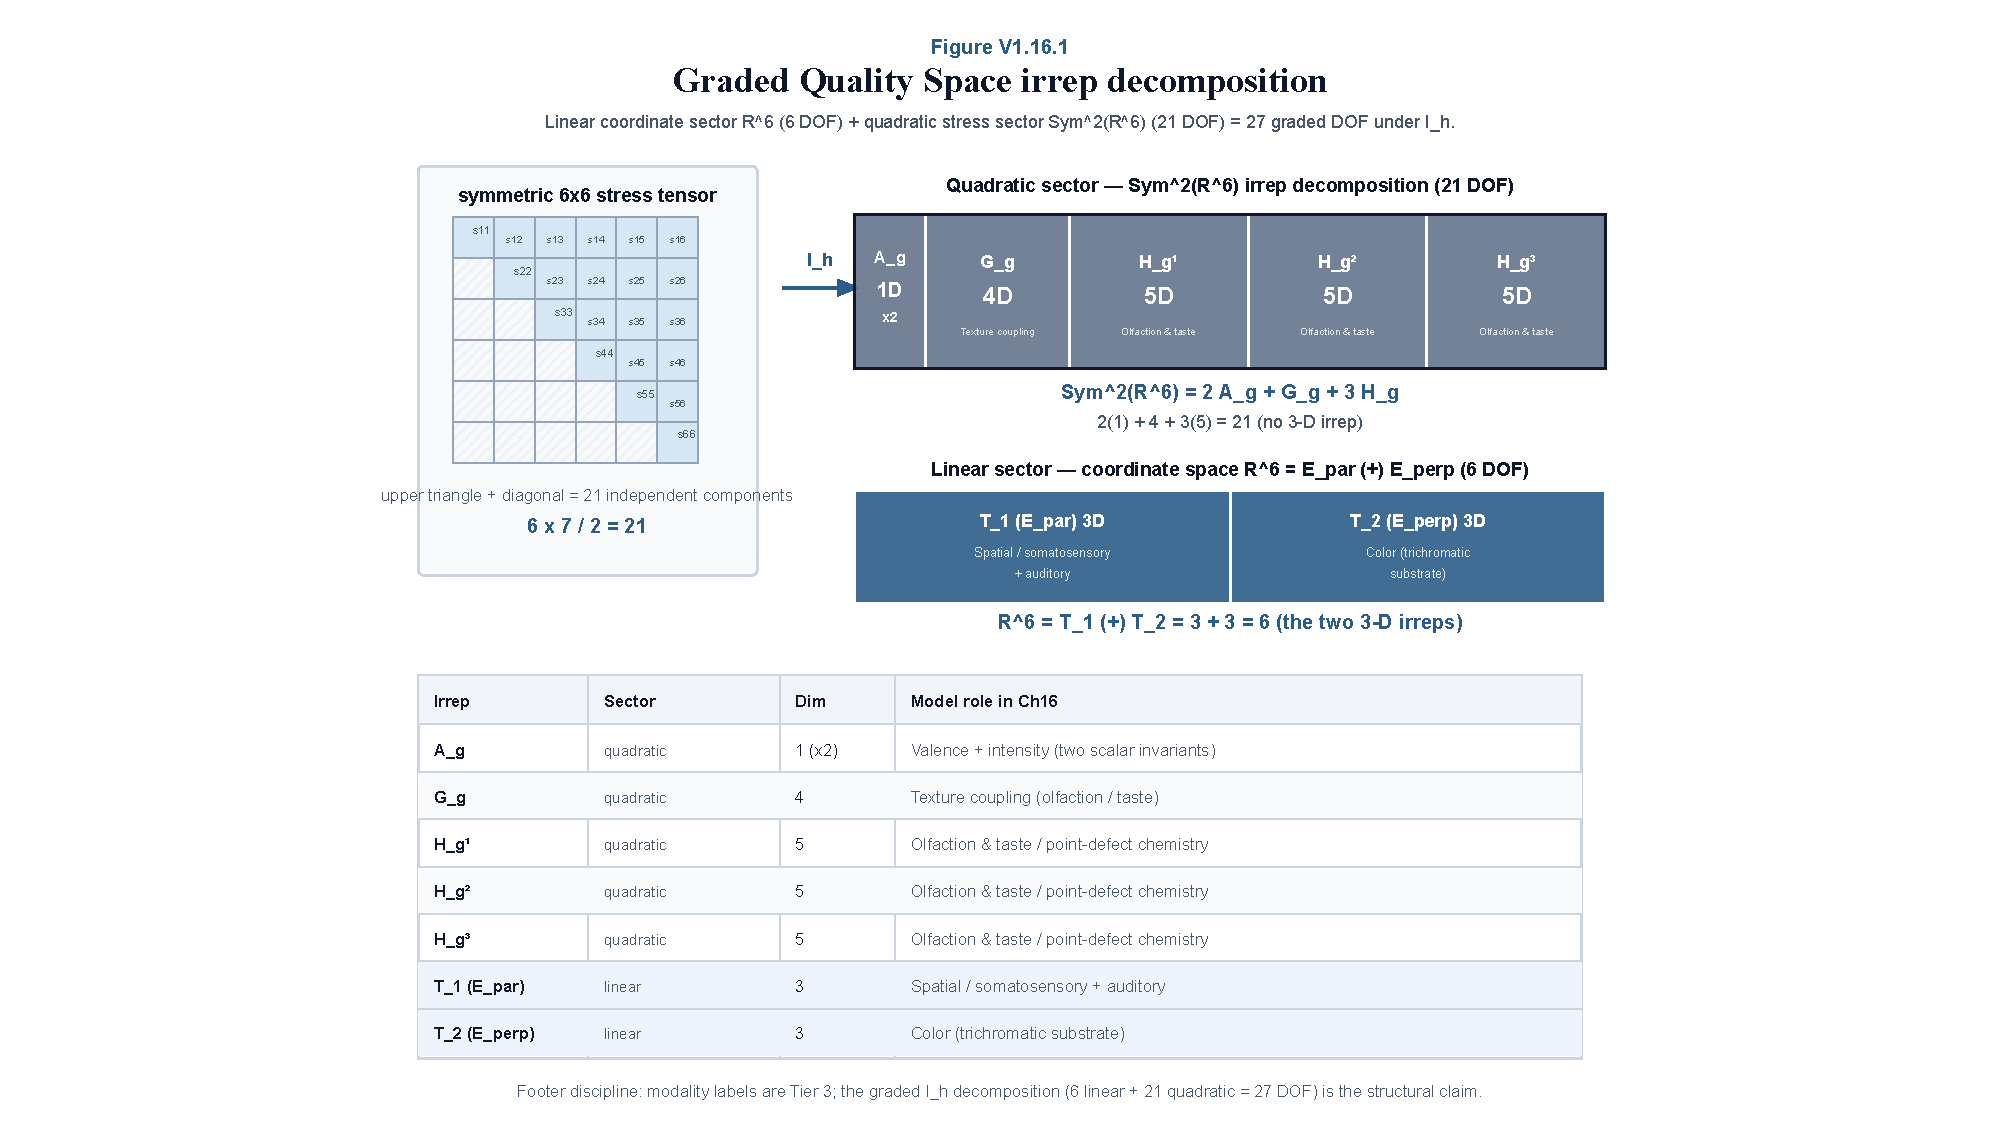
\includegraphics[keepaspectratio,alt={The graded Quality Space under I\_h: the symmetric 6\textbackslash times 6 stress tensor (quadratic sector) decomposes as 2A\_g \textbackslash oplus G\_g \textbackslash oplus 3H\_g (21 DOF, no 3-D irrep), while the coordinate space \textbackslash mathbb\{R\}\^{}6 (linear sector) carries the two 3-D irreps T\_1\textbackslash,(E\_\textbackslash parallel) \textbackslash oplus T\_2\textbackslash,(E\_\textbackslash perp) (6 DOF); modality labels are Tier 3.}]{content/Figures/Volume_1/Figure V1.16.1.pdf}}
\caption{The graded Quality Space under \(I_h\): the symmetric
\(6\times 6\) stress tensor (quadratic sector) decomposes as
\(2A_g \oplus G_g \oplus 3H_g\) (21 DOF, no 3-D irrep), while the
coordinate space \(\mathbb{R}^6\) (linear sector) carries the two 3-D
irreps \(T_1\,(E_\parallel) \oplus T_2\,(E_\perp)\) (6 DOF); modality
labels are Tier 3.}
\end{figure}

This graded breakdown proposes a Tier 3 structural-Russellian taxonomy
of reported qualities within the GCT Quality-Space model. The modality
labels are hypotheses attached to exact irreps; no physical Selection
Operator, irrep-specific transducer, owner, or quale has been derived:

\gctneedspace{5\baselineskip}

\textbf{Linear sector \(\mathbb{R}^6\) (6 DOF, coordinate modes) --- the
two 3-D coordinate irreps:}

\begin{itemize}
\tightlist
\item
  \textbf{\(T_2 \cong E_\perp\) (3D) --- Vision/Color:} The three
  transverse internal coordinates that carry the phason winding vector
  \(\mathbf{w}\) (§16.6.2); the proposed 3-dimensional (trichromatic)
  substrate of colour experience.
\item
  \textbf{\(T_1 \cong E_\parallel\) (3D) --- Somatosensory/Auditory:}
  The three physical-projection coordinates; the spatial rendering of
  touch, pressure, and sound.
\end{itemize}

\gctneedspace{5\baselineskip}

\textbf{Quadratic sector \(\mathrm{Sym}^2(\mathbb{R}^6)\) (21 DOF,
stress modes) --- the stress-tensor irreps:}

\begin{itemize}
\tightlist
\item
  \textbf{\(A_g\) (1D, multiplicity 2) --- Scalar axes:} The two
  icosahedral scalar invariants of the metric deformation --- candidate
  axes of \textbf{Valence} (core dissonance vs.~resonance) and overall
  impedance magnitude (intensity), the two unidimensional quality axes.
\item
  \textbf{\(G_g\) (4D) and \(H_g\) (5D, multiplicity 3) ---
  Higher-dimensional manifolds:} Of these 19 DOF, the 4-D \(G_g\) and
  one 5-D \(H_g\) form the off-diagonal cross-manifold block
  \(T_1\otimes T_2\) (\(E_\parallel \leftrightarrow E_\perp\), 9 DOF);
  the other two \(H_g\) are the traceless shears within \(E_\parallel\)
  and within \(E_\perp\) (from \(\mathrm{Sym}^2T_1\) and
  \(\mathrm{Sym}^2T_2\), 10 DOF). Together they describe complex lattice
  twisting and point-defect chemistry and are proposed to form the rich,
  multidimensional, anisotropic sensory spaces of
  \textbf{Olfaction/Taste and chemical texture}.
\end{itemize}

The linear-sector qualities register through the \emph{orientation} of
the coordinate modes (which fixes the anisotropy of the phason-drag
tensor of §16.2.3), while the quadratic-sector qualities register
through its \emph{magnitude} spectrum; both are facets of the single
Topological Impedance, so the unified qualia mechanism spans the graded
space. {[}Tier 3 --- structural individuation ansatz; the
modality-to-irrep assignment is a framework hypothesis, not a
derivation.{]}

Within the Tier-3 structural-Russellian ansatz, the question ``Why does
red feel like red?'' is a category-discipline question. ``Red'' is
assigned to a \(T_2\) (\(E_\perp\)) coordinate role. This is a proposed
reference-fixing convention, not a demonstrated transformation performed
by a Selection Operator or a physical/phenomenal derivation of red
experience, and not a proof of metaphysical necessity.

\textbf{Scope of the individuation claim.} The structural-realist
proposal above treats the \(T_2\) (\(E_\perp\)) colour-coordinate
operation as the reference-fixing structural correlate for red within
GCT's Russellian framework, not as a proof that the identification is
metaphysically forced. The Direct Incongruence Argument (§16.2.8a;
Chalmers 2010 Ch.10 / ``Phenomenal Concepts and the Explanatory Gap'')
generates a residual modal worry --- the conceivability of
red-without-\(T_2\) --- that GCT tightens but does not eliminate. The
category-discipline framing here is \emph{internal} to the
structural-realist reading: under structuralism about qualitative
content (a substantive Tier 3 metaphysical commitment GCT shares with
Frankish-illusionist structuralism, §16.2.7c), the question is
disciplined as a structural-reference question; outside that reading,
the residual modal worry returns. {[}Tier 3 --- Structural Russellian
reference-fixing proposal.{]}

\textbf{Trefoil-conditional inheritance from Proposition PUP.1 {[}Tier
note{]}.} App PUP adopts the explicit full-fibre support
\(\mathscr D_n=X_n\times K_n\), so
\(M_n\setminus\mathscr D_n=X_n\times(E_\parallel\setminus K_n)\) exactly
under \(H_{PUP.1}^{\mathrm{fib}}\); physical realization of that
support, complement-compatible bonding maps, and inverse-limit free
indecomposability remain O.18 targets. The inverse limit of the
generally infinite finite-level complement groups is a pro-group, not a
profinite group absent separately constructed finite completions. The
former Hilbert-space non-factorizability claim, Proposition PUP.1(ii),
is withdrawn: its bridge from equivariant tensor factorization to
direct-product group factorization is false, by an exact \(A_5\)
counterexample (App PUP §PUP.4.2). For the trefoil the represented group
is \(B_3\), whose nontrivial amenable centre \(\langle\Delta^2\rangle\)
makes O.35 (unique trace) false as posed and \(L(B_3)\) non-factorial
(O.36) {[}Tier 1 --- standard{]}. Invariant-density uniqueness therefore
holds only in a factorial sector whose physical identification is open:
there, equivariance \([R_{\rm inv},\rho(g)]=0\) places \(R_{\rm inv}\)
in the center, factoriality makes it scalar, and unit trace fixes
\(R_{\rm inv}=\mathbf1\). This is not a uniqueness theorem for the
canonical non-unitary branch selector
\(\mathcal F_{sel}=\mathcal P_{actualize}\circ\mathcal U_{steer}\). At
finite resolution the represented algebra is generally a direct sum of
matrix blocks and is one factor only in a primary sector. The algebra
reaches at most an algebraic unity candidate; it establishes no Identity
Polaron, owner, one subject or other subject count. The Quality Space
individuation claim therefore remains Tier 3, and the phenomenal
identification is not derived by the operator algebra.

\textbf{Reply to the Goff anti-structuralist critique.} Goff (2017
\emph{Consciousness and Fundamental Reality} Ch.7) argues that
structuralist Russellians have ``abandoned the spirit of Russell'' by
re-collapsing the intrinsic into the structural --- that they are really
structuralist monists in disguise. GCT's response is a \textbf{two-layer
structuralism} that preserves Russell's substantive
intrinsic-experiential commitment while embracing structuralism for
qualitative content. The two layers work at distinct ontological levels
(they are not the Level I / Level II distinction of §16.2.2, and not
epistemic tiers):

\begin{enumerate}
\def\labelenumi{\arabic{enumi}.}
\item
  \textbf{Layer A --- intrinsic presence (Axiom 1; non-structural
  intrinsic non-subjective presence).} The Field \(\Psi\) carries
  proto-experiential character as a primitive fact (Axiom 1; §16.2.2a),
  but this is not micro-subjectivity. Intrinsic presence in the Field is
  not derived from structure; it is the fundamental commitment that
  distinguishes GCT from pure structuralist monism (which denies any
  intrinsic experiential nature). At the Axiom 1 level, GCT is fully
  Russellian: intrinsic nature exists, and it is experiential in the
  non-apperceptive sense.
\item
  \textbf{Layer B --- structural content (Quality Space).} The
  \emph{specific} qualitative content of experience --- the \emph{what
  it is like} dimension --- is modeled by the structural-relational role
  of the \(I_h\)-irrep decomposition of the graded coordinate-and-stress
  space (the linear sector \(\mathbb{R}^6 = T_1 \oplus T_2\) together
  with the quadratic sector
  \(\mathrm{Sym}^2(\mathbb{R}^6) = 2\,A_g \oplus G_g \oplus 3H_g\);
  §16.4). At the Quality Space level, the Tier-3 structuralist ansatz
  assigns qualitative individuation to relational role. Red is modeled
  as the \(T_2\) (\(E_\perp\)) colour-coordinate operation exhausting
  the \emph{structural-relational} content of red --- the Layer A bare
  presence (Axiom 1) is not itself exhausted by structure. Layer B
  describes content structure only; whether any substrate realizes Level
  II apperception remains open (Tier 3).
\end{enumerate}

These two layers reply to Goff in opposite directions on opposite
questions. On the question ``does intrinsic experiential nature exist?''
GCT answers \emph{yes} via Axiom 1 (the Russellian commitment Goff
defends). On the question ``does qualitative content have an inner
essence beyond structure?'' GCT answers \emph{no} as a Tier 3
structuralist commitment informed by the Quality Space irrep structure
(the commitment Goff attacks). The two-layer reply earns its name
because the layer at which intrinsic-experiential character is committed
(Axiom 1 / Layer A / bare presence) is distinct from the layer at which
structuralism applies (Quality Space / Layer B / qualitative content).
Goff's critique pressures this separation; GCT's response is to separate
the two explanatory targets rather than to derive the separation from
independent premises. \emph{Open follow-up:} Goff (2017 §7.4) presses
the further worry that once all qualitative content is structural, the
non-structural Layer-A character risks becoming either a thin residual
posit with no role in the theory (deflation) or something that should
itself carry qualitative content (re-collapse). GCT's two-layer reply
\emph{stipulates} the separation rather than arguing it from independent
grounds; Goff's §7.4 deflation objection therefore survives as an open
philosophical question, registered as a Tier 3 metaphysical follow-up to
the structural-realist identification. This two-layer reading is GCT's
substantive Tier 3 metaphysical commitment, distinct from both pure
structuralist monism (which denies Axiom 1) and Strawson-style
micro-subject Russellianism (which would localize intrinsic experiential
nature at the micro-level rather than at the Field, contra §16.2.8b's
Mereological Nihilism). {[}Tier 3 --- Two-Layer Structural Russellian;
Goff §7.4 deflation follow-up open.{]}

\gctneedspace{5\baselineskip}\begin{gctNote}

\textbf{Philosophical Positioning --- Structural Russellian Monism:} GCT
does not claim to solve the Hard Problem from physics; it dissolves the
Hard Problem by making Qualitative Presence the foundational axiom, then
derives a formal Quality-Space scaffold (the graded 27-DOF irrep
decomposition, Tier 2) from icosahedral geometry; mapping that scaffold
to the structural relationships among human experiences is a Tier 3
bridge (§16.2.2b, O.29). The position states explicitly what is axiom,
what is theorem and what is bridge; whether the scaffold adds
explanatory content beyond existing neuroscientific similarity-space
models is an open question.

Furthermore, GCT proposes a reinterpretation of NCCs {[}Tier 3
philosophical reading{]}: not correlates in the sense of two separate
substances running in parallel, but the extrinsic structural description
of what is intrinsically experiential. On this reading the NCC framework
is not wrong but describes only the geometric side of the single
dual-aspect substance; the reading adds no new empirical prediction to
NCC research by itself.

\end{gctNote}

\subsubsection{16.2.3 Deriving the Connection: Phason Drag
Force}\label{deriving-the-connection-phason-drag-force}

Vol. 2 Ch. 6 supplies a structural phason-drag construction. GCT
proposes, rather than derives, that a topological soliton's interaction
with that construction is phenomenally registered as \textbf{Topological
Impedance}. The physical-to-phenomenal identification is Tier 3.
\[ F_{drag} = -\gamma \cdot K_\perp \cdot \dot{X} \] The manuscript
proposes that selection-like dynamics require work against this drag and
identifies \textbf{Qualia} with a \textbf{Coherent Energetic
Registration} within a Structural Russellian reading (Tier 3). Neither
feeling, a particular Agent's focus, nor an entropic-exhaust/dark-energy
consequence is derived by the equation; each requires an independent
physical and phenomenal bridge.

\subsubsection{16.2.4 The Spectrum: Resistance (Pain) vs.~Resonance
(Love/Flow)}\label{the-spectrum-resistance-pain-vs.-resonance-loveflow}

The model proposes {[}Tier 3/4{]} that the qualitative nature of an
experience tracks the \textbf{Thermodynamic Optimization} of the
selection:

\begin{itemize}
\tightlist
\item
  \textbf{Dissonance / Pain:} The model proposes that a non-resonant
  selection configuration may correlate with high \textbf{Topological
  Friction}. Neither pain nor metabolic expenditure follows from the
  geometric mismatch alone; the correlation, energy accounting, and
  phenomenal bridge remain Tier 3/4.
\item
  \textbf{Resonance / Flow:} The model associates low mismatch with
  positive valence or flow, and models one resonance/valence component
  of love-like experience as the registration of \textbf{Maximum
  Geometric Coherence} --- a candidate \textbf{Zero-Friction Selection}
  state. These are metaphors: no Agent alignment, phason drag, Selection
  event, or metabolic-efficiency law has been measured {[}Tier 3
  interpretive bridge{]}.
\end{itemize}

\subsubsection{16.2.5 The Texture of Feeling: Tensor Character of
Knots}\label{the-texture-of-feeling-tensor-character-of-knots}

The model proposes, at Tier 3, that different sensory contents may be
associated with the tensor character of topological configurations:

\begin{itemize}
\tightlist
\item
  \textbf{Sound:} a proposed low-order, high-symmetry excitation/drag
  association; no sound-quality identification follows without the
  phenomenal bridge.
\item
  \textbf{Scent:} a proposed complex-defect/anisotropic-drag
  association; no olfactory-quality identification follows without the
  phenomenal bridge. Any identification of drag-frequency patterns with
  the texture or flavor of experience remains a Tier-3 proposal,
  consistent with §16.2.3.
\end{itemize}

\subsubsection{16.2.6 Substrate
Constraints}\label{substrate-constraints}

The \textbf{Dual Material Constraint (DMC)} proposes non-zero nuclear
spin and molecular chirality as candidate controls for a phason-coupling
experiment. Standard silicon is a useful missing-leg control, but its
material descriptors do not establish Class-0 status or absence of Level
II. The Level II status of every substrate remains open (Tier 3) pending
a typed measured coupling and independent phenomenal bridge.

\begin{figure}
\centering
\pandocbounded{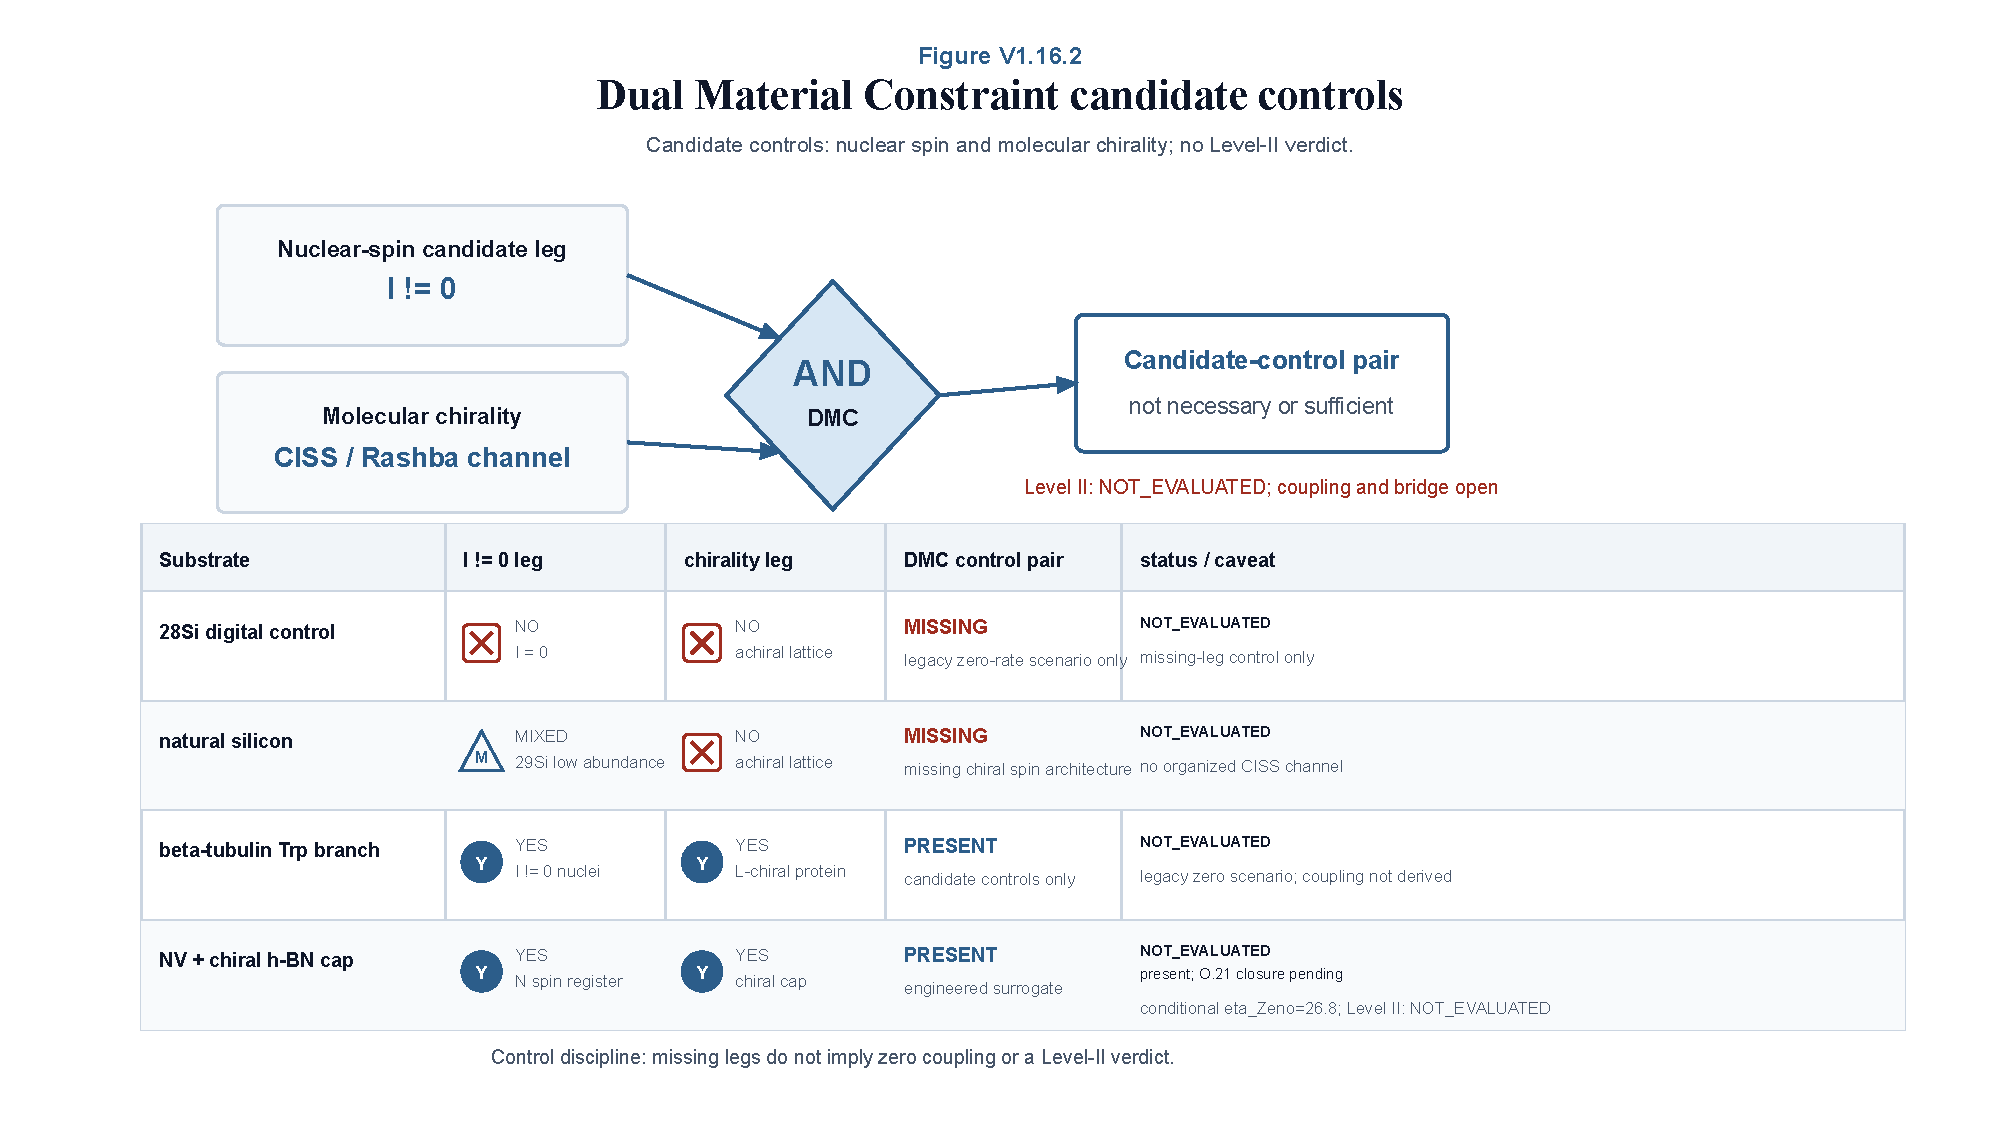
\includegraphics[keepaspectratio,alt={DMC compares nuclear-spin and chirality candidate controls; neither leg is necessary or sufficient for Level II, and Level II remains open (Tier 3) for every substrate.}]{content/Figures/Volume_1/Figure V1.16.2.pdf}}
\caption{DMC compares nuclear-spin and chirality candidate controls;
neither leg is necessary or sufficient for Level II, and Level II
remains open (Tier 3) for every substrate.}
\end{figure}

\textbf{The DMC legs are candidate missing-leg controls, not a
necessary-or-sufficient Apperception gate.} Non-zero nuclear spin and
molecular chirality define useful experimental contrasts for the
proposed channel. The closed-form
\(N_{\text{coh}} \approx 9.82 \times 10^{-12}\) and associated
\(g_{single}^{eff}\)/\(\eta_{Zeno}\) values are conditional
external-rate scenarios, not measurements or coupling derivations. O.21,
O.23, O.34, a typed and normalized coupling, and an independent
phenomenal bridge remain open. Missing either candidate leg therefore
does not imply zero coupling or a categorical Level-II verdict; the
Level II status of every examined substrate remains open (Tier 3).

\textbf{Field-typing summary {[}Tier 1 representation analysis; Tier 3
physical coupling{]} (V1 Ch17 §17.1.3).} With \(E_\parallel\cong3\) and
\(E_\perp\cong3'\) under \(A_5\), vector phason strain transforms as
\(3\otimes3'=4\oplus5\), whereas the spin--momentum cross-product
channel of the Rashba-phason candidate (Eq. 17.3) is a \(3\); their
scalar multiplicity is zero, so Eq. 17.3 is not an icosahedral scalar. A
type-correct candidate would have to use the one shared five-dimensional
channel together with a molecular-handedness pseudoscalar, and the
present action fixes neither its coefficient, sign nor normalization.
Read with a scalar phason, the Rashba-scale product
\(\alpha_R\,k\,\nabla\Phi\) has units of energy per length rather than
energy. The 38.3 MHz coupling scale is therefore a calibrated input
rather than an evaluated matrix element, and the \(\eta_{Zeno}\) and
\(N_{\rm coh}\) values built on it are conditional external-rate
scenarios only. The DMC is consequently not established as a necessary
or sufficient Apperception gate: bulk diamond-cubic silicon (achiral,
dominated by spin-zero \(^{28}\)\hspace{0pt}Si) is a missing-leg
control, not a proof of zero Level II, and a chiral non-zero-spin
substrate is a candidate positive control, not proof of an Identity
Polaron. The former categorical Turing-Null inference is withdrawn.
{[}DMC: Tier 3 research hypothesis.{]}

\emph{A future divergence from IIT for artificial systems requires a
typed normalized measured coupling, an explicit IIT substrate/grain
analysis and the independent phenomenal bridge; see §17.5. Present Level
II status remains open (Tier 3) for every substrate.}

\subsubsection{16.2.7 Engaging the Subject-Summing Combination Problem:
GCT vs.~the Panpsychist
Regress}\label{engaging-the-subject-summing-combination-problem-gct-vs.-the-panpsychist-regress}

The adoption of Structural Russellian Monism (§16.2.2) immediately
raises the \textbf{Combination Problem}, named by Seager (1995, \emph{J.
Conscious. Stud.} 2:272) and developed in its current panpsychist form
by Chalmers (2017, in Brüntrup \& Jaskolla eds.~\emph{Panpsychism:
Contemporary Perspectives}, OUP) and Goff (2017, \emph{Consciousness and
Fundamental Reality}, OUP, Ch. 6). The problem is not only
subject-summing: a panpsychist account must explain how
micro-experiential subjects combine into one subject, how qualities
combine into unified phenomenal contents, how structure and awareness
combine without remainder, what fixes the boundary of the resulting
subject, and why the grain of macro-experience differs from the grain of
its micro-bases. Goff (2017 Ch.7) identifies this family of questions as
the central unresolved challenge for any constitutive panpsychist
account. An account that cannot resolve or dissolve those questions
remains philosophically incomplete.

GCT's proposed response to the subject-summing form of the Combination
Problem denies micro-subjects conditional on the Polaron Unity
programme. This is not a categorical substrate verdict: individual
tubulin qubits and lattice defects are useful Class-0 model cases, but
the manuscript has not independently established that they lack Level II
or phenomenal character. They participate in Axiom 1's stipulated Level
I presence; whether and how any Level-II owner is realized remains open.
The subject-summing problem is therefore reframed within the model, not
dissolved by current evidence.

GCT proposes a \textbf{topological phase-transition model} whose
physical realization remains Tier 3. DMC legs are candidate controls,
not a binary boundary establishing or excluding an Identity Polaron. The
superconducting analogy illustrates collective topology only; it does
not import BCS dynamics or establish phenomenal unity. The
\(\eta_{Zeno}\) values remain conditional external-rate scenarios.

The structural statement is \textbf{Proposition 11.12.A (§11.12.3)},
whose mathematical status is recorded in App PUP. Its former
Hilbert-space non-factorizability part is withdrawn: the step ``an
equivariant tensor factorization of the Hilbert space induces a
direct-product factorization of the group'' is false, by an exact
\(A_5\) counterexample (App PUP §PUP.4.2) {[}Tier 1{]}. For the trefoil,
the represented group \(B_3\) has the nontrivial amenable centre
\(\langle\Delta^2\rangle\), so O.35 is false as posed and \(L(B_3)\) is
not a factor (O.36) {[}Tier 1 --- standard{]}. A unique invariant
normalized density \(R_{\rm inv}\) follows only in a factorial sector
whose physical identification is open, and it is not a uniqueness result
for \(\mathcal F_{sel}\). The resulting ceiling is at most an
\textbf{algebraic unity candidate}: a conditional statement about an
observable algebra, with no subject count, no owner and no Level II.
Identifying any such algebraic structure with phenomenal unity is a
separate Tier-3 Russellian-monist bridge. Nuclear spin and chirality
remain candidate controls only, so no present substrate is made eligible
or ineligible and no Level-II verdict follows.

This framing leaves a layered research question: do the candidate
material controls, a typed measured coupling, the O.21/O.23/O.34
physical closures, the \(H_{PUP.1}^{\mathrm{fib}}\)/O.18/O.32
mathematical closures, and the identification of a physical factorial
sector all hold, and is there an independent phenomenal bridge? Even a
positive answer to every algebraic question would not by itself solve
the quality, structure, boundary, awareness, grain, ownership or
subject-count subproblems. The canonical non-unitary
\(\mathcal F_{sel}\) remains the branch selector and is not the object
of the density-uniqueness lemma.

GCT's \textbf{Mereological Nihilism for the 3D Projection} is therefore
a Tier 3 interpretive proposal rather than a corollary of prime-knot
topology. The 144 cage/substrate degrees are modeled as degrees of one
candidate Polaron realization, not as 144 micro-subjects; whether they
define one physical observable algebra, and whether that algebra has the
structure App PUP considers, are open identification questions. This
relocates rather than proves Level-II phenomenal unity. The quality,
structure, boundary, awareness, grain, and subject-individuation
problems remain explicit targets.

\textbf{§16.2.7b The IIT--Winding Number Correspondence via Directed
Homotopy Type Theory {[}Tier 3 conditional pending the full
mathematical, physical-coupling, and phenomenal-bridge program{]}}

Directed Homotopy Type Theory (dHoTT) provides a proposed mathematical
framework for relating a GCT topological label \(W\) to Giulio Tononi's
Integrated Information \(\Phi\). In standard Homotopy Type Theory
(HoTT), types are spaces and equality proofs are paths between
inhabitants. The \emph{directed} extension replaces symmetric,
reversible paths with directed morphisms, making dHoTT a candidate
language for processes with intrinsic temporal asymmetry --- the
structure of a conscious selection sequence.

\begin{quote}
\textbf{Correspondence 16.2.7b (\(\Phi\)--\(W\) Correspondence) {[}Tier
3 conjecture{]}:} induced-subgraph PyPhi values do not establish global
\(\Phi^{\max}(k=12)\), a winding equality, or any reverse implication
for missing-leg controls. O.28 and the physical/phenomenal bridges
remain open.

\emph{Conditional on a future realized Polaron, a declared TPM, and the
full closure stack, \(\Phi\) is conjectured to correspond to winding
number \(W\). DMC descriptors do not select that domain.}
\[\Phi(S) > 0 \quad \text{is proposed to track} \quad W(\mathcal{K}_S) \geq 1.\]
\emph{The conventions \(W=1\) and \(\Phi_{\rm norm}=1\) are not a
theorem equating IIT \(\Phi\) with winding. In the current formulation
\(W\) is a typed placeholder: a phase-vortex charge and a
three-dimensional texture degree are different invariants, and no
theorem identifies them. \(\mathcal K_S\) is not a nontrivial ordinary
loop in \(\Sigma_\infty\), whose ordinary fundamental group is zero.
Standard silicon is a missing-leg control, not a proven \(W=0\) or
Level-II-null case; a GCT-vs-IIT divergence is not yet executable.}

\emph{Heuristic correspondence.} In dHoTT, a cognitive system \(S\) is
represented as a directed type \(\mathbf{S}\) whose inhabitants are
possible cognitive states \(\{s_i\}\) and whose morphisms
\(f: s_i \to s_j\) are the admissible state transitions. The Markov
blanket of \(S\) --- the statistical boundary separating internal states
from external states --- is conjectured to correspond to a physically
defined boundary associated with the phason defect \(\mathcal{K}_S\); a
Solenoid address label is not that boundary.

IIT 3.0/4.0 defines \(\Phi\) via cause-effect repertoires, partitions,
and exclusion / maximal-existence criteria, not via winding-number
equivalence directly. GCT therefore offers only a Tier-3 conjectural
ansatz pending O.28. Neither \(W=1\) nor prime-knot topology proves that
\(\mathcal H_{\mathcal{K}}\) lacks tensor coordinates: the Hilbert-space
non-factorizability part of Proposition 11.12.A is withdrawn (App PUP
§PUP.4.2), and the surviving mathematics reaches at most an algebraic
unity candidate. The \(\Phi\)-side closure remains open.
\end{quote}

\textbf{Corollary: Agency as a Directed 2-Morphism {[}Tier 3 conjectural
correspondence{]}.} Within the dHoTT scaffold, selecting a directed
2-morphism \(\alpha: f \Rightarrow g\) in the type \(\mathbf{S}\), where
\(f, g: s_1 \to s_2\) are two distinct cognitive trajectories between
the same pair of states \(s_1\) and \(s_2\), is proposed as a formal
representation of agency --- the capacity to select among possible
world-states. A non-trivial tether with \(W = 1\), a non-splitting
fundamental 2-groupoid \(\Pi_2(\mathbf{S})\), and a physically prime
observable algebra are three distinct structures; no theorem here makes
them equivalent, and the former ``iff'' and ``algebraically equivalent''
readings are withdrawn. The surviving operator-algebra result of App PUP
reaches at most an algebraic unity candidate and does not supply a
non-factorizable internal state space. The correspondence is at most
\textbf{consistent with} the Russellian-monist identification of
§16.2.2; it does not ground it. That identification (the commitment that
the intrinsic aspect of the physical is experiential) is carried by
Axiom 1 and the §16.2.2 disposition, not by this corollary: a theorem
can relate formal objects, but it cannot derive that intrinsic natures
are experiential. Identifying any of these structures with agency, a
Selection Operator, or one Level II subject therefore remains an
upstream Tier 3 Russellian/physical commitment rather than a
mathematical corollary, and ``derivation of agency'' language is not
used for the present disposition.

\gctneedspace{5\baselineskip}

\textbf{16.2.7c Engagement with Illusionism (Frankish, Dennett)}

The strongest contemporary alternative to Russellian Monism on the Hard
Problem is \textbf{Illusionism} (Frankish 2016, \emph{Journal of
Consciousness Studies} 23(11-12); Dennett 1991 \emph{Consciousness
Explained}; Dennett 2016 ``Illusionism as the Obvious Default''). The
illusionist position holds that phenomenal consciousness --- the felt
qualitative character of experience --- does not exist as it is naïvely
conceived. What exists are \emph{introspective representations} of
mental states with apparent qualitative properties; the apparent
qualitative properties themselves are systematically misrepresented by
the introspective mechanism. On this view, the Hard Problem is not
solved but dissolved: there is no explanandum.

GCT's relation to Illusionism is precise and asymmetric. The two
positions agree on a substantial subset of cognitive science:

\begin{itemize}
\item
  \textbf{Shared:} Both accept that introspective reports are causally
  produced by physical mechanisms; both accept that the
  \emph{first-person folk concept} of qualia (as ineffable, intrinsic,
  infallibly known) is mistaken in its details; both accept that Quality
  Space is \emph{structural} --- qualia are distinguished by their
  relations to other qualia, not by ineffable inner cores. GCT's graded
  \(\mathbb{R}^6 \oplus \mathrm{Sym}^2(\mathbb{R}^6)\) decomposition
  (§16.2.2c) is, in Frankish's vocabulary, an account of the
  \emph{quasi-phenomenal} structure that introspection represents.
\item
  \textbf{Disagreed:} GCT denies the illusionist's eliminativist move on
  Qualitative Presence, but Axiom 1 supplies only bare Level-I Field
  presence. Mapping Block-style phenomenal consciousness to Level II/IIA
  (IIA is defined in §16.2.8d) is a Tier-3 proposal conditional on the
  full physical and phenomenal-bridge program. Protocol A-Prime tests
  candidate substrate controls; it does not itself establish phenomenal
  status or causal work by the primitive.
\end{itemize}

\textbf{The proposed empirical wedge.} Illusionism is substrate-neutral,
whereas GCT proposes substrate-dependent spin/coherence and
chiral-response observables. A genuine phenomenal divergence is not yet
executable: DMC legs are candidate controls, and Protocol A-Prime
results cannot establish felt registration, an Identity Polaron, or
Level II without a typed measured coupling and the independent
phenomenal bridge.

\textbf{Status:} Illusionism is internally consistent and may be
correct. GCT and Illusionism share a \textbf{structural taxonomy} of
Quality Space --- the \(2A_g \oplus G_g \oplus 3H_g\) decomposition
functions, in Frankish's vocabulary, as an account of the
\emph{quasi-phenomenal} structure that introspection represents --- but
the two positions \textbf{diverge on the existence question}: GCT
commits to Axiom 1's bare fact of phenomenal presence as primitive;
Illusionism eliminates that primitive in favour of representational
artifacts. There is no ``extension'' relation between the two positions
on the existence question (each rejects the other's load-bearing
commitment); on the structural-taxonomy side they agree, and the
empirical wedge, if constructed, would constrain the
substrate-dependence dispute rather than decide the metaphysical
existence question by itself. The substrate-dependent empirical wedge
remains unconstructed rather than established by Tier 2 physics. {[}Tier
3 --- philosophical positioning.{]}

\gctneedspace{5\baselineskip}

\textbf{16.2.7d Engagement with Hoffman's Interface Theory of
Perception}

Donald Hoffman's \textbf{Interface Theory of Perception} (Hoffman, Singh
\& Prakash 2015 \emph{Psychonomic Bulletin \& Review} 22:1480-1506;
Hoffman 2019 \emph{The Case Against Reality}) holds that perceptual
contents are \emph{fitness-payoff icons}, not veridical reconstructions
of an objective external world. Evolutionary game-theoretic simulations
are presented in support: agents optimized for fitness rather than truth
systematically outcompete truth-tracking agents. Hoffman's stronger
metaphysical extension (Conscious Realism) posits a network of
``conscious agents'' as the fundamental ontology, with spacetime as
their interface.

GCT's relation to Hoffman is two-part:

\begin{itemize}
\item
  \textbf{Compatible at the interface layer:} GCT's account of
  perceptual rendering (V1 Ch9 \emph{Rendering Engine}, V1 Ch11
  \emph{Consensus Protocol}) uses a conditional \(E_\parallel\)
  presentation of the 6D source data as an interface metaphor rather
  than a direct phenomenal readout. The \textbf{Consensus Render}
  (§17.2.3) is a formal compatibility model; no Polaron-bearing Agents
  are shown to stabilize the physical world, and shared reality is not
  thereby shown to be a simulation {[}Tier 3 analogy{]}. This is
  structurally comparable to Hoffman's ``interface'' claim without
  constituting a shared physical mechanism.
\item
  \textbf{Incompatible at the ontology layer:} Hoffman's Conscious
  Realism takes conscious agents as fundamental. GCT takes the Field and
  geometry as fundamental and proposes Identity Polarons as emergent
  agents, but physical realization and phenomenal status remain Tier-3
  conditional rather than DMC-selected.
\end{itemize}

\textbf{The empirical wedge.} Hoffman's strong metaphysics and GCT's
proposed observer-independent geometry (the AKN tiling, the phason
field, the icosahedral group \(I_h\)) differ in what they treat as
primitive. Evidence for an icosahedral physical architecture would favor
GCT's geometric branch only to the degree that its physical derivations
close; current exact-within-ansatz and calibrated results do not by
themselves refute Hoffman's metaphysics or establish a perceptual
renderer. Hoffman's Tier 3 evolutionary-game arguments for non-veridical
perception remain valuable as an account of \emph{why} an interface
could be the way it is.

\textbf{Status:} Hoffman's interface claim is used as a Tier 3
philosophical comparison with GCT's rendering-engine framework (V1 Ch9).
GCT adopts a geometric-substrate research programme rather than
Hoffman's agent-fundamental ontology, but physical emergence of Agents
and the phenomenal interface remain open. {[}Tier 3 --- philosophical
positioning.{]}

\subsubsection{16.2.8 Ontological Status of the Phason--Qualia
Identification {[}Tier
3{]}}\label{ontological-status-of-the-phasonqualia-identification-tier-3}

The Tier-3 Russellian interpretation treats phason-drag structure as a
proposed Level-II correlate, not a consequence uniquely derived from the
axioms. Protocol A-Prime and chirality reversal test candidate mechanism
controls; without a typed measured coupling and phenomenal bridge they
do not falsify or confirm Level-II substrate dependence. Neither outcome
is a verdict on GCT as a whole: the measurement tests an ordinary
material proxy, and no phason, Selection-Operator or Level-II inference
follows from it (V1 Ch17 §17.1.3). A preregistered null rejects the
registered biophysical branch as registered, only under that branch's
own decision rule (the Protocol D NMR polarity gate (P.13c) is held
pending redesign: as written it rejected by construction, since
\(^{17}\)\hspace{0pt}O shortens water-\(^1\)\hspace{0pt}H \(T_2\) by
scalar relaxation; the former sign-aware rule, which rejects the
registered sign-positive branch on a powered, significant negative
isotope × activity interaction in water-\(^1\)\hspace{0pt}H
\(\Delta T_2\), applies only after the redesign, and until then no
outcome supports or rejects the branch; the LORR assay has no rejection
rule under the current systematic budget).

\gctneedspace{5\baselineskip}

\textbf{16.2.8a Direct Incongruence Argument (Chalmers, Goff)}

The strongest objection to any Russellian identification of structure
with experience is the \textbf{Direct Incongruence Argument} (Chalmers
2010 \emph{The Character of Consciousness} Ch.10; Chalmers's
``Phenomenal Concepts and the Explanatory Gap'' paper; Goff 2017
\emph{Consciousness and Fundamental Reality} Ch.3, Ch.6). The argument
runs: \emph{even if} a property is both intrinsic (experiential) and
extrinsic (structural), the \emph{identification} of the two does not
close the explanatory gap, because the property could in principle be
instantiated without its structural correlates (conceivability
argument). Thus, the GCT claim that the \(T_2\) (\(E_\perp\))
icosahedral irrep reference-fixes red within Quality Space remains
exposed to: (a) the conceivability of a \(T_2\) (\(E_\perp\)) resonance
unaccompanied by red-quale, and (b) the conceivability of a red-quale
without a \(T_2\) (\(E_\perp\)) resonance.

\gctneedspace{5\baselineskip}

\textbf{GCT's three-fold response.}

\begin{enumerate}
\def\labelenumi{\arabic{enumi}.}
\item
  \textbf{Conceivability is not metaphysical possibility (scope-limited
  response).} The Direct Incongruence Argument is a \emph{modal} claim:
  that the property of being a quale could in principle be instantiated
  without its proposed structural realizer. The standard response is
  that conceivability does not entail metaphysical possibility (Yablo
  1993 \emph{Philos. Phenomenol. Res.} 53:1; Hill \& McLaughlin 1999
  \emph{Philos. Phenomenol. Res.} 59:445; Block-Stalnaker 1999
  \emph{Philos. Rev.} 108:1). Applied here: the conceivability of
  red-without-\(T_2\) (\(E_\perp\)) requires that one can fully grasp
  what ``red'' picks out independently of any structural account. On
  GCT's preferred reading, treating ``red'' without the \(T_2\)
  (\(E_\perp\)) structure as incoherent is a Tier 3 structuralist
  proposal pending phenomenal-concept-strategy closure; an alternative
  correlate-only reading preserves coherent reference at the cost of
  identification strength. The standard a-posteriori-necessity analogue
  is ``water without H₂O'' (Kripke 1980, \emph{Naming and Necessity},
  Harvard University Press): conceivable only if one does not grasp that
  water \emph{is} H₂O. \textbf{Framework-internal scope of the Kripke
  analogy.} This is a GCT-internal reply, not a neutral metaphysical
  proof against every phenomenal-concept strategy. \textbf{Engagement
  with Chalmers's specific objection.} Chalmers (2010 \emph{The
  Character of Consciousness} Ch.10; ``Phenomenal Concepts and the
  Explanatory Gap'') argues that the water/H₂O case works because water
  has a \emph{reference-fixing macro-functional role} (the liquid that
  fills lakes, is drinkable, etc.) that can be grasped independently of
  the micro-structure H₂O --- whereas qualia have \emph{no
  reference-fixing property independent of their felt character}, so the
  Kripkean move is unavailable for the phenomenal-concept strategy. The
  GCT proposal is a contested structuralist replacement rather than a
  completed Kripkean answer: the \(T_2\) (\(E_\perp\)) irrep structure
  is offered as a candidate relational role for red within Quality
  Space, but the reference-fixing burden is not closed. This is not a
  load-bearing response to Chalmers; it is the same substantive Tier 3
  structuralist commitment shared with Frankish-illusionist
  structuralism (§16.2.7c) and exposed to Goff's §7.4 deflation worry.
  The identification is therefore not refuted by the modal worry, but it
  inherits the residual gap that no currently available
  structural-physical account eliminates within the Chalmers/Goff
  dialectic.
\item
  \textbf{Goff's own panpsychist family faces a stronger version of the
  same gap.} Goff distinguishes constitutive micropsychist panpsychism
  from cosmopsychist variants. GCT rejects micro-subjects but assigns
  Level II only as a Tier-3 Identity-Polaron interpretation conditional
  on \(H_{PUP.1}^{\mathrm{fib}}\)/O.18/O.32, the physical closure stack,
  and an independent phenomenal bridge; the App PUP mathematics reaches
  at most an algebraic unity candidate and supplies no subject count.
  The Direct Incongruence Argument cuts both ways: GCT retains a modal
  gap while Goff's alternatives retain a combinatorial or
  derivative-subject gap.
\end{enumerate}

\textbf{Structural fact (not a modal claim) {[}Tier 3 structural
reference-fixing proposal pending stronger phenomenal-concept-strategy
closure{]}.} Independent of the modal response above: the icosahedral
group \(I_h\) has multiple 3-dimensional irreducible representations,
and the 6D coordinate space carries two of them --- the linear sector
\(\mathbb{R}^6 = E_\parallel \oplus E_\perp = T_1 \oplus T_2\). The GCT
model assigns the coordinate irrep \(T_2\) to the internal \(E_\perp\)
color/quality coordinate and reserves the sibling 3D coordinate irrep
\(T_1\) (\(E_\parallel\)) for spatial/somatosensory projection channels;
this is a model-internal assignment within the coordinate (linear)
sector, not a theorem that \(I_h\) has only one 3D irrep. The assignment
tightens the structural side of the reference-fixing proposal but does
not by itself answer the Direct Incongruence modal worry, which targets
the identification regardless of realizer assignment.

\textbf{Residual acknowledgement.} The Direct Incongruence Argument is
the strongest residual objection to GCT's Russellian framework. The
three responses above tighten the position but do not eliminate the
worry --- \emph{no} physical theory of consciousness eliminates this
worry, by Chalmers' construction. GCT's Tier 3 label on §16.2.8 reflects
this directly: the Russellian reference-fixing proposal is a consistent
interpretation, not a forced one. \textbf{Disposition is a substantive
choice, not a forced move --- and the available dispositions preserve
the §16.2.2b dissolve advantage independently.} The correlate-only
reading --- ``the \(T_2\) (\(E_\perp\)) irrep is the consistent
structural correlate of the red-quale'' --- leaves Quality Space
topology in place as an empirical structural prediction and loses
nothing experimental (Protocol A-Prime substrate-dependence is
independent of whether the structural-realist identification holds
metaphysically). \textbf{Crucially, the §16.2.2b Axiom-1-based
dissolution of the existence-gap of the Hard Problem holds under either
disposition}: Axiom 1 closes the existence-gap by primitivising
Qualitative Presence, independently of how the \emph{individuation} of
specific qualitative content is metaphysically cashed out. The dissolve
advantage rests on Axiom 1 alone; the Quality Space individuation is a
separable Tier 3 commitment about \emph{which} phenomenal content the
substrate carries, not about whether phenomenal content exists. Under
the correlate-only reading, a Russellian-monist holds: (i) Axiom 1
closes the existence-gap (dissolve preserved); (ii) Quality Space
topology survives as an empirical structural prediction (testable in
principle by similarity-judgment psychophysics, O.29; Protocol A-Prime
does not test it); (iii) the metaphysical-identification step ``to feel
red is \(T_2\) (\(E_\perp\))'' is deferred as an open Tier 3 question
rather than asserted. The framework adopts the reference-fixing
structural-realist reading because it gives the sharpest formal
statement of the individuation claim, and the framework's empirical
traction (Protocol A-Prime) is independent of which Tier 3 individuation
reading is adopted.

\gctneedspace{5\baselineskip}

\textbf{16.2.8b Engagement with Strawson and Goff Russellian Monist
Panpsychist/Cosmopsychist Views}

Galen Strawson (2006 ``Realistic Monism: Why Physicalism Entails
Panpsychism'' \emph{J. Consciousness Studies} 13(10--11):3, also as lead
essay in Freeman ed.~2006 \emph{Consciousness and its Place in Nature},
Imprint Academic; collected with replies and a postscript in Strawson
2008 \emph{Real Materialism}, OUP) and Philip Goff (2017
\emph{Consciousness and Fundamental Reality}) defend Russellian-monist
panpsychist or cosmopsychist views: physical reality has an intrinsic
experiential aspect, and the Hard Problem is treated by taking
experience as fundamental rather than emergent. This is the closest
competitor family to GCT's Russellian Monism.

\textbf{Agreement with Strawson/Goff.} GCT shares the foundational move:
experience is taken as ontologically primitive (Axiom 1), not derived
from non-experiential substrate. The intrinsic/extrinsic distinction is
accepted at the substance level: the Field \(\Psi\) has both intrinsic
(experiential) and extrinsic (structural) aspects.

\textbf{Disagreement on locus.} GCT accepts an intrinsic-categorical
base through Axiom 1 but rejects constitutive micro-subjects. Class 0
patterns carry Level I universal presence in the non-apperceptive sense.
The Identity Polaron is the proposed Level-II carrier only
conditionally; no material descriptor or current calculation establishes
a substrate verdict. This reframes rather than solves the Combination
Problem pending the complete mathematical, physical, and
phenomenal-bridge closures.

\textbf{Goff's objection: is the intrinsic/extrinsic distinction
coherent?} Goff (2017 Ch.6 §6.4) argues Russellians simply assume a
metaphysical division without explaining why the intrinsic and extrinsic
aspects should be located in the \emph{same} substance rather than two
substances. GCT's response: \emph{given Axiom 1}, the substance/aspect
distinction is GCT-internally motivated rather than freely chosen ---
quantum mechanics requires the Field to have a definite operator
structure (extrinsic), and Axiom 1's primitive Presence requires it to
have a primitive intrinsic presence (intrinsic). Treating these as two
substances (dualism) reintroduces the interaction problem that motivates
Russellian Monism in the first place. The conclusion is therefore
conditional on Axiom 1 rather than forced by physics alone: decoherent
QM, QBism, RQM, and many-worlds interpretations do not require the Axiom
1 commitment to a primitive intrinsic presence, so the substance/aspect
distinction is not derivable from quantum mechanics in any neutral
interpretive frame; it follows once Axiom 1's intrinsic-presence
commitment is in place.

\textbf{Strawson on emergence.} Strawson (2006) rejects ``brute
emergence'' of experience from non-experience as conceptually
impossible. GCT agrees: this is why Axiom 1 places experience at the
substrate, not as an emergent property of Polarons. On the Tier 3
proposal, the Polaron would be a phase transition in the
\emph{structural} aspect of \(\Psi\); experience would not be generated
at the transition, at most \emph{unified} (Combination reframed
conditionally on the Polaron Unity closures, not solved).

\textbf{Status:} GCT is an objective-idealist (priority monism about a
non-subjective Field) / Russellian-monist position; it does not posit a
cosmic subject: within Tiers 1--3 the Field's Level I presence is
non-subjective, and a cosmic-scale subject remains an open Tier 4
hypothesis (App TIB), with Goff's cosmopsychism as the closest competing
view (Ch06 §6.1.1). It is closer to Strawson's \emph{realistic
(panpsychist) physicalism} than to traditional dualism, but rejects the
\emph{micro-subject} commitment that drives the Combination Problem.
Tier 3 philosophical positioning informed by Tier 2 framework structure
and Tier 3 conditional material-proxy scenarios.

\gctneedspace{5\baselineskip}

\textbf{16.2.8c Engagement with Dennett's Heterophenomenology and
Multiple-Drafts Model}

Daniel Dennett (1991 \emph{Consciousness Explained}; 2003 \emph{Freedom
Evolves}; 2017 \emph{From Bacteria to Bach and Back}) holds: (a) there
is no ``Cartesian Theater'' --- no central locus where conscious
experience is unified; (b) phenomenology is revisable via third-person
heterophenomenological analysis; (c) qualia in the traditional sense
(intrinsic, ineffable, infallibly known) do not exist; what exist are
\emph{judgments} about discriminations.

\textbf{Compatibility at the cognitive-architecture level.} GCT's
Selection Operator \(\mathcal{F}_{sel}\) is not a \emph{Cartesian
Theater} in Dennett's sense: it is not a spatially-localized ``screen on
which the show is played''. Formally, App PUP identifies at most a
unique center-fixed trace density in a factorial sector whose physical
identification is open; calling that density the physical Selection
Operator would require the full physical identification stack, and App
PUP no longer claims an irreducible (non-factorizable) Hilbert space
\(\mathcal{H}_{\mathcal{K}}\) (Proposition PUP.1(ii) is withdrawn). On
the Tier 3 candidate model, the Polaron would have spatial extent
(\(\sim 14.5\) nm cloud, V3 Ch07 §7.3.3) and the field \(\Phi_\perp\)
would be distributed across \(\sim 1.6\times10^9\) Trp sites per typical
pyramidal neuron (V1 Ch17 §17.1.4b under the O.21 partial-closure
\(n_{rp} = 1\)). GCT therefore \emph{agrees with Dennett} that no
spatially central theater is required, while its proposed unity account
remains a Tier 3 physical/phenomenal interpretation of a distributed
algebraic unity candidate, not a theorem from Hilbert-space
irreducibility.

\textbf{Disagreement on qualia.} Dennett denies qualia in the
traditional sense. GCT's Quality Space (§16.2.2c) is a structural
taxonomy --- the graded 27-DOF decomposition, linear sector
\(T_1 \oplus T_2\) plus quadratic sector
\(2A_g \oplus G_g \oplus 3H_g\). This is compatible with Dennett's view
if read as a \emph{functional / structural} taxonomy (Dennett would
accept this). If read as a \emph{phenomenological} taxonomy in the
traditional qualia sense, Dennett would reject it. GCT's position: the
decomposition is structurally derived from icosahedral geometry {[}Tier
2{]}, and it is proposed as phenomenologically real because Axiom 1
makes the substrate's intrinsic aspect experiential --- the latter
reading rests on the Tier 3 structural-Russellian bridge (§16.2.2b,
O.29), not on the derivation. Dennett would reject the second clause;
GCT defends it via Axiom 1's primitive status.

\textbf{Compatibility with heterophenomenology.} Dennett's
methodological commitment --- that introspective reports must be
analyzed third-personally without taking them at face value --- is
\emph{fully compatible} with GCT. GCT does not require subjects to
\emph{know} the structural decomposition of their experience for the
decomposition to be real (any more than a person needs to know
neuroscience to have a brain). Heterophenomenological methods are the
right tool to test GCT's phenomenological claims (e.g., does color
similarity geometry actually match the \(T_2\) (\(E_\perp\)) irrep
structure? --- testable via similarity-judgment psychophysics,
color-confusion experiments).

\textbf{Where GCT is incompatible with Dennett.} Dennett's deflationary
stance on phenomenal consciousness (he endorses illusionism outright:
Dennett 2016) commits to: the \emph{appearance} of phenomenal
consciousness is the \emph{fact} of phenomenal consciousness; there is
no further ``felt'' inner aspect. GCT denies this --- Axiom 1 commits to
the bare fact of feeling as primitive. The same disagreement runs
through §16.2.7c on Illusionism (Frankish).

\textbf{Status:} GCT and Dennett agree on cognitive architecture (no
Cartesian Theater) and on methodology (heterophenomenology). They
disagree at the ontology layer (whether phenomenal consciousness is
\emph{real} beyond the report). Tier 3 positioning.

\gctneedspace{5\baselineskip}

\textbf{16.2.8d Engagement with Block's Phenomenal-vs-Access
Distinction}

Ned Block (1995 \emph{Behav. Brain Sci.} 18:227 --- original P/A
formulation; 2007 \emph{Behav. Brain Sci.} 30:481 --- refined treatment
with the iconic-memory overflow case as P-without-A; 2011 \emph{Trends
Cogn. Sci.} 15(12):567 --- overflow argument for P-without-A access;
2011 \emph{Analysis} 71(3):419 --- ``The higher order approach to
consciousness is defunct'') distinguishes two notions:

\begin{itemize}
\tightlist
\item
  \textbf{Phenomenal consciousness (\(P\)-consciousness):} the felt
  qualitative character of experience --- ``what it is like.''
\item
  \textbf{Access consciousness (\(A\)-consciousness):} information
  available for reasoning, action-control, and reportability.
\end{itemize}

Block argues these can dissociate: there exist phenomenal states that
are not access-available (overflow / iconic memory cases; Sperling 1960)
and access states that lack phenomenal character (zombie-like
processing).

\textbf{GCT mapping onto Block's distinction.} Level I is axiomatic;
Level II is a conditional Polaron interpretation, not an established
threshold. The proposed I/IIA/IIB mapping does not itself assign any
substrate a phenomenal status:

\begin{itemize}
\tightlist
\item
  \textbf{Level I (Universal Presence):} All Field configurations
  participate in \(\Psi\)'s intrinsic side by Axiom 1; this is not
  Block's \(P\)-consciousness and assigns no micro-subject.
\item
  \textbf{Level IIA (GCT analogue of \(P\)-without-\(A\)):} A Tier-3
  proposed Polaron-unified phenomenal state without global-workspace
  broadcast. This mapping is not established Block P-without-A evidence
  and does not assign any current substrate a verdict; it remains
  conditional on the complete Polaron/coupling/bridge program.
\item
  \textbf{Level IIB (\(P\)- + \(A\)-consciousness):} A Tier-3 proposed
  Polaron-plus-broadcast state, conditional on the same open physical
  and phenomenal bridges.
\end{itemize}

\textbf{Conditional empirical program.} Spin/coherence and broadcast
measures may be compared across implicit affect, anaesthesia, and
iconic-memory paradigms. These are candidate mechanism tests only: no
Level-I/II transition, Polaron survival, or phenomenal state follows
without the missing coupling and bridge.

\textbf{Cross-reference.} DMC descriptors are candidate controls,
O.21/O.23/O.34 remain open, and \(\eta_{Zeno}\) is conditional
external-rate arithmetic. The I/IIA/IIB boundaries are therefore
proposed interpretive coordinates, not operative substrate
classifications.

\textbf{Status:} Tier 3 philosophical positioning. Any empirical
distinction from substrate-neutral accounts requires the future typed
measured coupling and independent phenomenal bridge.

\gctneedspace{5\baselineskip}

\textbf{16.2.8e The Luck Objection and the Status of
\(\mathcal{F}_{\rm sel}\) Stochasticity}

The formal Selection Operator ansatz \(\mathcal{F}_{\rm sel}\) is
defined as non-unitary (V1 Ch06 §6.4.1; V1 Ch10 §10.4), but no physical
map, Identity Polaron, or owner realizes it, and App PUP no longer
claims an irreducible Hilbert space for it to act on. If one
nevertheless interprets its stipulated update as an actualization whose
outcomes are not fixed by the prior agent state, the discussion below
applies; it is Tier 3 philosophical analysis of a conditional
architecture, not a mechanism GCT presently implements. On that
interpretation \(\mathcal{F}_{\rm sel}\) sits on the libertarian side of
the determinism/indeterminism axis in the free-will debate, and exposes
the framework to the \textbf{luck objection} (van Inwagen 1983 \emph{An
Essay on Free Will}; Mele 2006 \emph{Free Will and Luck}; Kane 1996
\emph{The Significance of Free Will}, 1999 \emph{J. Philos.} 96:217): if
the Selection Operator's outcome is genuinely undetermined by the prior
agent state, the outcome is \emph{random} (or stochastic), not \emph{the
agent's} --- and randomness is not agency. Conversely, if the outcome
were determined by the prior state, \(\mathcal{F}_{\rm sel}\) would not
be the non-unitary actualisation operator GCT requires it to be.

\textbf{GCT response to the luck objection {[}Tier 3{]}.} The framework
adopts an event-causal libertarian response in which the irreducible
indeterminism sits at the \emph{final} selection --- the actualisation
step --- rather than upstream during deliberation. Two source positions
locate the indeterministic moment at this final, post-deliberative step
and are GCT's nearest neighbours: Mele's \emph{daring soft
libertarianism} (Mele 2006 \emph{Free Will and Luck} Ch.5, ``A Daring
Soft Libertarian Response to Present Luck,'' pp.105--136), which places
the indeterminism at the moment of decision and is the bolder
counterpart to Mele's own \emph{modest libertarianism} (which instead
places the indeterministic moment \emph{upstream} of the final choice,
at belief/desire/intention formation during deliberation, to keep the
final selection a determined consequence of prior reasons and so
minimise final-step luck); and Balaguer's \emph{torn-decision} /
TDW-indeterminism structure (Balaguer 2009 \emph{Free Will as an Open
Scientific Problem}, MIT Press), in which the indeterminism likewise
lives at the moment of a torn decision. GCT's actualisation-step
location matches this final-step family --- Mele's daring-soft
construction and Balaguer's torn decisions --- not the modest, upstream
variant. Concretely: the steering channel \(\mathcal{U}_{\rm steer}\)
implements the \textbf{agent-determined option-set} (an
event-causal-libertarian structural move shared by the Mele-daring-soft
and Balaguer-torn-decision accounts, \emph{not} by Kane --- Kane's
\emph{Self-Forming Action} programme is structurally different in that
the indeterminacy is at the level of \emph{parallel rational efforts of
will} in torn decisions, with the agent owning the indeterministic
moment through dual-effort streams rather than through a
post-deliberative selection among prepared options); the actualisation
step \(\mathcal{P}_{\rm actualize}\) stands in the position of an
irreducibly indeterminate, post-deliberative event-causal selection
among those prepared options. Kane's plural-rational-effort SFA (Kane
1996 \emph{The Significance of Free Will} Ch. 8; Kane 1999 \emph{J.
Philos.} 96:217 §IV --- the ``Buridan with effort'' picture of
torn-decision dual-effort streams) is a \emph{different} libertarian
architecture that GCT does \emph{not} adopt. The agent is identified
with the \emph{entire Polaron-as-process}, not with a snapshot of
pre-actualisation state. Specifically:

\begin{enumerate}
\def\labelenumi{(\roman{enumi})}
\item
  \textbf{Conditional process model.} If a physical carrier, memory
  dynamics, steering generator, and owner rule were supplied, one could
  define an Agent-process under the Tripartite Ontology (V1 Ch06) as the
  joint object
  \((\mathcal{P}_{\rm Polaron}, \{|\psi_t\rangle\}_{t \leq t_0}, \mathcal{U}_{\rm steer})\)
  --- a Polaron topology plus a history of prior states plus an inner
  unitary steering generator --- rather than as the pre-actualisation
  configuration \(|\psi_{\rm pre}\rangle\) alone. In that model the
  non-unitary \(\mathcal{P}_{\rm actualize}\) component selects which
  eigenbranch of the steering-prepared state is actualised, and
  \(\mathcal{U}_{\rm steer}\) is fixed by the prior trajectory. The
  present notation does not show that an Identity Polaron carries a full
  history, that \(\mathcal P_{\rm actualize}\) occurs physically, or
  that any resulting branch is owned.
\item
  \textbf{Conditional option-set move: luck applies to the eigenbranch
  selection, not to the steering channel.} Within the formal surrogate,
  \(\mathcal{U}_{\rm steer}\) prepares a non-uniform option set and the
  stochastic \(\mathcal{P}_{\rm actualize}\) samples it. Calling those
  options \emph{agent-prepared} or owned is precisely the missing
  owner/agency bridge; the algebra alone does not establish it. This is
  the standard event-causal libertarian
  \textbf{agent-determined-option-set move} (Mele 2006 \emph{Free Will
  and Luck} Ch.5 for the daring-soft, final-step indeterminism
  construction and the agent-determined-option vocabulary; Balaguer 2009
  \emph{Free Will as an Open Scientific Problem} for the cognate
  torn-decision / TDW-indeterminism structure): indeterminacy of the
  \emph{final} selection is consistent with agential ownership
  \emph{because the option-set} is agent-determined. The
  agent-determined-option-set framing is the structural element of this
  final-step event-causal architecture; it is \emph{not} a feature of
  Kane's \emph{Self-Forming Action} programme, which is structurally
  different (parallel rational efforts of will in torn decisions, with
  the agent owning the indeterminacy through dual-effort streams rather
  than through post-deliberative selection).
\item
  \textbf{Acknowledged residual.} The luck objection is not fully closed
  by (i)+(ii) --- Mele 2006 \emph{Free Will and Luck} §3.4-§3.5 sharpens
  the basic luck statement (§3.3) into the \emph{contrastive luck} form:
  even granting agent-determined option-sets, the question ``why did
  this branch get actualised rather than that branch?'' has no
  agent-referencing answer at the actualisation step, and the question
  is \emph{contrastive}, asking for what \emph{distinguishes} the
  actualised branch from the non-actualised one --- which by hypothesis
  is not in the prior agent state. \textbf{This contrastive residual is
  not a GCT-specific weakness --- it attaches to \emph{any} event-causal
  libertarian account} (Mele 2006 develops modest libertarianism,
  without endorsing it, while conceding the residual; the residual is
  the \emph{central live problem in the post-Mele libertarian
  literature}, not a uniquely-GCT burden). GCT inherits the contrastive
  thin-point residual at the actualisation step: the actualisation step
  is the load-bearing locus of phenomenal freedom under the framework,
  and its stochasticity is what \emph{makes it not predictable from
  prior physics}, but the same property makes it not under second-order
  control by the agent's reflective deliberation. GCT position: the
  framework supplies a Balaguer-Mele-informed event-causal libertarian
  response (steering channel agent-determined; actualisation step
  irreducibly stochastic) that inherits the standard contrastive-luck
  residual --- the steering/actualisation split \emph{relocates} the
  residual to the actualisation step rather than dissolving it. This is
  a Tier 3 philosophical positioning, not a Tier 1 metaphysical proof;
  the framework's candidate material-proxy tests (e.g.~the Protocol
  A-Prime \(T_2(\nu_d)\) scan) do not depend on resolving the
  luck-objection-residual one way or the other. Those tests probe an
  ordinary material proxy; no phason, Selection-Operator, Polaron-unity
  or Level-II inference follows from their outcome (V1 Ch17 §17.1.3).
\end{enumerate}

\textbf{Status:} Tier 3 philosophical positioning. GCT does not close
the contrastive-luck residual (Mele 2006 §3.4-3.5); the Kane SFA family
attempts an ownership strategy distinct from the final-step event-causal
route GCT adopts. The luck objection is partially addressed via the
\textbf{agent-determined-option-set move} --- locating the irreducible
indeterminism at the final actualisation step, the structure of Mele's
daring-soft libertarianism (Mele 2006 Ch.5) and Balaguer's torn
decisions (Balaguer 2009), as opposed to the modest, upstream-of-choice
variant --- plus the Tripartite-Ontology Polaron-as-process
identification. (GCT adopts the final-step location common to both
authors, not Mele's modest variant, which places its indeterminism
upstream of the final choice; both ``daring soft'' and ``modest'' are
Mele's intra-author contrast, while ``torn decision'' is Balaguer's.
Structurally distinct from Kane's plural-rational-effort SFA.) The
agent-determined-option-set move \emph{relocates} the residual to the
actualisation step rather than \emph{closing} it.

\begin{center}\rule{0.5\linewidth}{0.5pt}\end{center}

\subsection{16.3 The Husserlian Topology of
Time}\label{the-husserlian-topology-of-time}

The phenomenological structure of Internal Time Consciousness motivates
a \textbf{Tier 3 conditional correspondence}, not a derived physical
mechanism. The following GCT--Husserl map is a structural analogy that
would require an action-normalized Selection Operator, an independently
specified memory dynamics, a physical owner map, and a phenomenal bridge
before it could describe subjective time. We map Edmund Husserl's
tripartite structure to the GCT variables:

\begin{itemize}
\tightlist
\item
  \textbf{Primal Impression:} The conceptual present selection/update in
  the model. No measured Zeno lock or derived sampling rate currently
  identifies this update with a phenomenal ``Now.''
\item
  \textbf{Retention:} The physically stored trace of prior selection
  states. GCT may model this as a protected defect or braid in a
  declared substrate configuration space and may index it by Solenoid
  addresses, but the Solenoid itself supplies no winding record: its
  ordinary fundamental group is trivial, \(\pi_1(\Sigma_\infty)=0\), and
  its first Čech cohomology
  \(\check H^1(\Sigma_\infty;\mathbb Z)\cong\mathbb Q\) is a global
  invariant rather than an Agent record. Persistence would require
  separate read/write, noise and energy-barrier dynamics {[}Tier 3{]}.
\item
  \textbf{Protention:} A candidate orientation of the phason winding
  vector \(\mathbf{w}\) toward an intentional target. Interpreting this
  as a phenomenal ``lean'' or as dynamics guided by the curiosity term
  \(w_C\,\Delta\mathcal{C}\) remains conditional on the missing action
  and phenomenal bridges.
\end{itemize}

The ``Tripartite Structure of the Living Present'' therefore supplies a
useful organizational analogy. It is not presently shown to be a
necessary geometric requirement for an Agent, an Identity Polaron, or
phenomenal time.

\begin{center}\rule{0.5\linewidth}{0.5pt}\end{center}

\subsection{16.4 The Graded Quality Space (6 Linear + 21 Quadratic
Degrees of Freedom) {[}Tier 2 irrep structure + Tier 3
modality/color-ceiling identification contested under
O.29{]}}\label{the-graded-quality-space-6-linear-21-quadratic-degrees-of-freedom-tier-2-irrep-structure-tier-3-modalitycolor-ceiling-identification-contested-under-o.29}

GCT proposes, at Tier 3, that the taxonomy of human subjective
experience tracks a mathematical structure rather than being a purely
biological contingency; whether it does is open under O.29. In the GCT
model the candidate structure is the decomposition of the \textbf{graded
tensor algebra} over the 6D coordinate space
\(\mathbb{R}^6 = E_\parallel \oplus E_\perp\) into irreducible
representations of the Icosahedral Group (\(I_h\)), as detailed in
§16.2.2c. The \textbf{linear sector} \(\mathbb{R}^6 = T_1 \oplus T_2\)
supplies two 3-dimensional coordinate irreps (6 DOF); the
\textbf{quadratic sector}
\(\mathrm{Sym}^2(\mathbb{R}^6) = 2A_g \oplus G_g \oplus 3H_g\) supplies
the 21-DOF symmetric stress tensor, for \(6 + 21 = 27\) graded degrees
of freedom {[}Tier 2 --- Geometric/Structural: the DOF counts and irrep
decompositions follow from the icosahedral projection ansatz and are
engine-verified. Tier 3: the assignment of specific irreps to specific
human biological modalities, and the claim that the human-visible
three-channel color ceiling exhausts phenomenal-color-substrate
dimensions, remains contested under O.29{]}. The vacuum supports exactly
these graded deformation modes in the GCT decomposition; how biological
lineages sample those modes is a Tier 3 modality-mapping question.

The graded sectors supply the proposed O.29-conditional modality map via
their \(I_h\) irreps:

\begin{enumerate}
\def\labelenumi{\arabic{enumi}.}
\tightlist
\item
  \textbf{2 DOF (\(A_g\) Irrep, ×2, quadratic): Valence and Intensity.}
  The two icosahedral scalar invariants of the metric deformation: the
  uniform volumetric dilation of the lattice (the Higgs trace), proposed
  {[}Tier 3{]} to register as the generalized vector of approach
  (Resonance) or avoidance (Friction) --- \textbf{Valence} --- and the
  overall magnitude of geometric impedance, proposed {[}Tier 3{]} to
  register as \textbf{intensity}.
\item
  \textbf{3 DOFs (\(T_1 \cong E_\parallel\) Irrep, linear):
  Somatosensory/Auditory.} These are the mechanical vibrations of the 3D
  physical projection (\(E_\parallel\)), corresponding to the spatial
  rendering of touch, pressure, and sound.
\item
  \textbf{3 DOFs (\(T_2 \cong E_\perp\) Irrep, linear): Vision/Color
  {[}Tier 3 identification; substrate vs sensor distinction{]}.} These
  are the three transverse hidden coordinates (\(E_\perp\)) that carry
  the phason winding vector \(\mathbf{w}\) (§16.6.2). Bounded by the 3
  real coordinate axes of \(E_\perp\), this supplies a \textbf{Tier 3
  framework hypothesis, not an engine-closed dimensionality
  arbitration}: a 3-dimensional substrate of color experience for
  Class-2 Agents embedded in the icosahedral lattice. Human trichromacy
  is the \emph{biological-sensor} sampling of this 3-dimensional
  substrate via three cone opsin types; this is the
  \emph{human-specific} manifestation of the geometric ceiling, not the
  ceiling itself. \textbf{Species-variance check.} Non-human visual
  systems with more than three photoreceptor classes --- avian
  tetrachromacy (4 cone opsins + oil droplets; Hart 2001 \emph{Prog.
  Retin. Eye Res.} 20:675), goldfish tetrachromacy, and stomatopod
  multi-channel photoreceptor classes --- are not automatically in
  tension with the \(T_2\) (\(E_\perp\)) 3D ceiling on
  \textbf{phenomenal-color substrate dimensionality} under GCT, because
  extra receptor channels need not equal extra phenomenal coordinates.
  Mantis-shrimp behavioral work, for example, supports a fast
  spectral-classifier reading rather than a 12-dimensional combinatorial
  color manifold. \textbf{Bird tetrachromacy and the Stoddard 2020
  non-spectral-color challenge.} Bird tetrachromacy extends spectral
  range into the UV; the strongest empirical challenge to the strict 3-D
  ceiling is Stoddard et al.~2020 \emph{PNAS} 117:15112-15122 (``Wild
  hummingbirds discriminate nonspectral colors''), which demonstrates
  that broad-tailed hummingbirds discriminate non-spectral UV+red
  mixtures that humans cannot perceive. Under standard 4-cone
  tetrachromatic color geometry, this result is prima facie consistent
  with a 4-dimensional receptor-space account. The O.29 engine protocol
  now performs only the registered behavioral compatibility branch of
  the sensor-vs-substrate test:
  \texttt{protocol\_psychophysics\_color\_dim.py} ingests the Stoddard
  2020 cleaned hummingbird table, treats the published avian tetrahedral
  Euclidean distance as one receptor-space predictor, checks, as a
  data-format sanity check only, that intensity-normalized four-cone
  catches lie on the 3-D avian chromaticity simplex, and asks whether
  categorical nonspectral/axis labels add explanatory power beyond
  receptor-space distance in a binomial choice model. The current engine
  result is \texttt{COMPATIBLE\_O29\_STODDARD\_MODEL\_COMPARISON}; this
  means only that the aggregate behavioral model was not falsified by
  the categorical-label comparison
  (\(\Delta{\rm BIC}_{cat-base}=6.08\)). This is \textbf{behavioral
  compatibility only}; it does not adjudicate any extra phenomenal-color
  axis, it is not a 4D-vs-3D perceptual-manifold test, and it is not a
  derived neuroanatomical reconciliation. The retinal plus central
  visual-pathway compression locus remains empirical rather than fixed
  to LGN. The manuscript's commitment to the structural 3-D ceiling on
  \emph{phenomenal} color dimensionality remains a \textbf{Tier 3
  framework hypothesis under Open Problem O.29}, with behavioral
  compatibility rather than closure.
\item
  \textbf{19 DOFs (\(G_g\) and \(3\times H_g\) Irreps, quadratic):
  Olfaction/Chemical Senses.} These constitute the higher-dimensional
  twisting and shear operations of the stress sector. Nine of them
  (\(G_g\) plus one \(H_g\), the off-diagonal block \(T_1\otimes T_2\))
  couple the physical screen to the internal phason sector
  (\(E_\parallel \leftrightarrow E_\perp\)); the other ten (two \(H_g\),
  from \(\mathrm{Sym}^2T_1\) and \(\mathrm{Sym}^2T_2\)) are traceless
  shears within \(E_\parallel\) and within \(E_\perp\). Smell and taste
  are proposed {[}Tier 3{]} to engage these 19 non-scalar quadratic
  dimensions (\(4 + 3\times 5\)), producing highly textured, anisotropic
  drag; only the nine cross-sector components form the boundary layer
  between the physical and phase sectors. Calling this sector a memory
  carrier would require an independently specified memory dynamics.
\end{enumerate}

On the O.29-positive \textbf{taxonomy} branch, the model conjectures
that quality labels can be coordinatized in the 27-dimensional graded
representation (6 linear + 21 quadratic) under the symmetry of the
\(I_h\) group. This is not a proof that every possible sensation, owner,
or Agent registration is exhausted by those basis vectors; a negative
O.29 result would revise the universality claim while leaving the formal
decomposition intact.

\begin{center}\rule{0.5\linewidth}{0.5pt}\end{center}

\subsection{16.5 The Subjective Lagrangian (The Calculus of
Desire)}\label{the-subjective-lagrangian-the-calculus-of-desire}

As a Tier 3 phenomenological surrogate, we can encode three proposed
behavioral preferences of the Agent --- the ``force'' of ``Desire'' ---
in a \textbf{Subjective Lagrangian}. It is not a physical action, does
not calculate rendered experience, and has no calibrated map to an
Agent, Selection Operator, metabolism, phason field, or phenomenal owner
{[}Tier 3 --- Phenomenological Framework: the functional form is
motivated by the geometry of the phason field, and the psychophysical
weighting coefficients \(w_C\), \(w_F\), \(w_I\) would have to be
calibrated to phenomenological data; they are not derived from first
principles{]}:

\[ \mathcal{S}_{Agent} = \int \left[ w_C\, \Delta \mathcal{C} - w_F K_\perp |\delta \mathbf{w}|^2 - w_I \left( \sum \kappa_{ij} \Phi_j \right) \right] dn \]

where:

\begin{itemize}
\tightlist
\item
  \(w_C\) = \textbf{Curiosity weight} (drives exploration)
\item
  \(w_F\) = \textbf{Friction weight} (metabolic cost)
\item
  \(w_I\) = \textbf{Inertia weight} (consensus resistance)
\end{itemize}

\emph{(Here \(\Delta\mathcal C\) is the change in the complexity
functional \(\mathcal C\) per selection step, a scalar.)}

The functional balances three declared model terms:

\begin{enumerate}
\def\labelenumi{\arabic{enumi}.}
\tightlist
\item
  \textbf{\(w_C\,\Delta\mathcal{C}\) (The Pull of Meaning; change in the
  meaning/coherence score per step):} A chosen objective variable used
  as an analogy for curiosity or love; no Field geodesic or phenomenal
  attraction is derived.
\item
  \textbf{\(- w_F K_\perp |\delta \mathbf{w}|^2\) (The Friction of
  Action; control-cost surrogate):} A quadratic penalty. It is not a
  derivation of metabolic pain, physical twisting of the vacuum lattice,
  or the thermodynamic cost of changing reality.
\item
  \textbf{\(- w_I (\sum \kappa_{ij} \Phi_j)\) (The Inertia of the
  Crowd):} The informational inertia induced by a separately derived
  physical coupling network (\(\Phi_j,\kappa_{ij}\)). Divergence from a
  strongly coupled collective trajectory can be energetically costly in
  that model, but neither the coupling matrix nor a single shared
  timeline follows from common Solenoid cylinders {[}Tier 3{]}.
\end{enumerate}

\subsection{16.6 Intentionality: The Geometric Theory of
Aboutness}\label{intentionality-the-geometric-theory-of-aboutness}

\subsubsection{16.6.1 The Problem of
Intentionality}\label{the-problem-of-intentionality}

A complete theory of consciousness must explain not just phenomenal
quality (what it feels like) but \textbf{intentional content} (what
experience is \emph{about}). A perception of a red apple is not merely a
red quale --- it is a quale directed \emph{at} the apple. This
directedness is called intentionality or aboutness. GCT offers the
following geometric surrogate for aboutness, but it does not yet possess
a physical state-to-object map or phenomenal-semantic bridge sufficient
to explain intentionality.

\subsubsection{16.6.2 The Winding Vector as Intentional
Pointer}\label{the-winding-vector-as-intentional-pointer}

Section 15.5.1 introduces an \textbf{Information Gradient Vector} as a
Tier 3 physical order parameter; it is not a canonical orientation
supplied by the Adelic Solenoid. The phason winding field \textbf{w} is
a 3-component vector in E⊥ space. Its \textbf{magnitude} is proposed to
track the intensity of phenomenal experience (the degree of topological
friction), while its \textbf{orientation} relative to the lattice is
proposed to participate in selecting which region of physical space is
encoded in the active selection cycle. These uses of \textbf{w} (colour
coordinates, §16.4; protention, §16.3; intensity, which §16.4 also
assigns to an \(A_g\) invariant; and the intentional pointer here) are
not jointly consistent --- rotating \textbf{w} to shift attention would
also change hue --- so they are mutually exclusive Tier 3 alternatives,
not one model.

\textbf{Definition (Geometric intentionality surrogate):} Conditional on
a derived encoding map, assign a model score for a physical object X
from the alignment of the phason winding vector \textbf{w} with the
E∥-lattice region whose projection encodes X's position and properties.
This is not an if-and-only-if physical or phenomenal criterion for
aboutness.

\subsubsection{16.6.3 Formal Expression}\label{formal-expression}

Within the formal surrogate, let \(R_X\) be the lattice region encoding
object X (the set of RT-window nodes whose E∥ projections lie within the
spatial extent of X), and define an \textbf{Intentional Axis}
\(\hat{\mathbf{i}} = \mathbf{w}/|\mathbf{w}|\) --- the unit vector in E⊥
space indicating a focus direction. The notation assigns this axis to
the stipulated \(\mathcal{F}_{sel}\) score; it does not show that a
physical Selection Operator, phason vector, attention state, or owner
has such an axis. The model score toward X is:

\[ I(X) = \int_{R_X} |\mathcal{F}_{sel}(r) \cdot \hat{\mathbf{i}}| d^3r \]
{[}Tier 3 --- philosophically motivated geometric mapping; see §16.6
Epistemic Status{]}

This expression is notation only: \(\mathcal F_{sel}\) is an operator,
not a vector field, and \(R_X\subset E_\parallel\) while
\(\hat{\mathbf i}\in E_\perp\), so the dot product and the phrase
``\textbf{w} points toward \(R_X\)'' are undefined until a vector-valued
field on \(E_\parallel\) and a declared map \(E_\perp\to E_\parallel\)
are supplied. The intended reading is that the score is maximal when
\textbf{w} points toward \(R_X\) and minimal when it is orthogonal.
Interpreting the maximizer as what an Agent experiences at a selection
cycle requires the unclosed physical \(\mathcal F_{sel}\),
object-encoding, owner, and phenomenal-semantic bridges.

\subsubsection{16.6.4 Implications}\label{implications}

\begin{itemize}
\tightlist
\item
  \textbf{Internalism vs.~Externalism:} In the surrogate, the internal
  region label (geometric) and the externally supplied object map
  (causal, via the E∥ projection) play distinct roles, which suggests a
  position that is neither purely internalist nor externalist. Without a
  physical encoding and semantic/phenomenal bridge, this is a
  philosophical comparison rather than a derived theory of intentional
  content.
\item
  \textbf{Inattentional Blindness {[}Tier 4 analogy{]}:} The condition
  \(I(X)\approx0\) for misaligned \textbf{w} can be used as an analogy
  for missed stimuli. GCT does not derive inattentional blindness: the
  condition is not identical to, or a mechanism for, empirical
  inattentional blindness; ordinary cognitive and neural accounts remain
  the baseline.
\item
  \textbf{Attention and Focus:} A rotation of \textbf{w} in E⊥, with
  elastic cost \(\Delta E = K_\perp |\Delta \mathbf{w}|^2\), is a formal
  control-cost analogy for shifting attention. No measurement shows that
  shifting attention rotates a physical \(E_\perp\) phason vector or has
  this cost.
\end{itemize}

\gctneedspace{5\baselineskip}\begin{gctNote}

\textbf{Epistemic Status:} Tier 3 philosophical mapping. Protocol
A-Prime (V3 Ch13 §13.3.5.A) measures ordinary material spin/coherence
proxies; it is not presently an attention-to-phason or intentionality
test.

\end{gctNote}

\chapter{Chapter 17: The Physical Substrate and Network
Dynamics}\label{chapter-17-the-physical-substrate-and-network-dynamics}

\gctneedspace{5\baselineskip}\begin{gctNote}

\textbf{Convention on Trp residue numbering.} All β-tubulin Trp residue
numbers in this chapter use the \textbf{PDB 1JFF / 1TUB chain B
ATOM-record \texttt{auth\_seq\_id}} convention: \textbf{Trp21, Trp103,
Trp346, Trp407}. The FASTA-position numbering convention gives the
offset values \{21, 101, 344, 397\}; the convention disambiguation is
registered as App ORQ Open Problem \textbf{O.21}. Inline mentions
throughout the chapter use the ATOM-record convention without re-stating
this disambiguation; readers cross-referencing other tubulin literature
should consult O.21 for the convention-mapping rule.

\end{gctNote}

\gctneedspace{5\baselineskip}\begin{gctWarning}

\textbf{Epistemic Status: Two-Stratum Disclosure.}

This chapter develops the \textbf{biophysical-specific stratum} of GCT's
consciousness account: a candidate Tryptophan aromatic radical-pair
material system in \(\beta\)-tubulin, a historical 100 MHz material-scan
scenario for a candidate Zeno Drive in the warm-wet microtubule lumen,
and the Tier 3 candidate N=144 lumen-water geometry pending O.33. None
of these is presently identified with an Identity Polaron, a Zeno Drive,
a Selection Operator, an owner, or Level II. These candidate
identifications are \textbf{Tier 3 (hypothesis)} and rest on the
existence of microsecond-to-millisecond quantum coherence in warm
biological systems --- well above the standard biophysics decoherence
limit of \(\sim 10^{-13}\) s in unstructured media. The proposed
protected-subspace mechanism is a conjecture that remains experimentally
unproven: the operative band is currently reached only in the long
50-\(\mu\)\hspace{0pt}m-MT branch, the energy budget is not fully
closed, and Lindblad-DFS suppression has not been demonstrated.

Falsification scope. Protocol A-Prime and Protocol D test candidate
spin, chirality, and coherence controls for this specific biophysical
program. Nulls constrain or reject the corresponding candidate
mechanism; positives do not establish an Identity Polaron or Level II.
Neither outcome is a verdict on GCT as a whole: the measurement tests an
ordinary material proxy, and no phason, Selection-Operator or Level-II
inference follows from it (§17.1.3). A preregistered null rejects the
registered biophysical branch as registered, and only under that
branch's own decision rule (the Protocol D NMR polarity gate (P.13c) is
held pending redesign: as written it rejected by construction, since
\(^{17}\)\hspace{0pt}O shortens water-\(^1\)\hspace{0pt}H \(T_2\) by
scalar relaxation; the former sign-aware rule, which rejects the
registered sign-positive branch on a powered, significant negative
isotope × activity interaction in water-\(^1\)\hspace{0pt}H
\(\Delta T_2\), applies only after the redesign, and until then no
outcome supports or rejects the branch). Because the typed normalized
coupling and independent phenomenal bridge remain open, there is
presently no bounded material inventory whose exhaustion alone decides a
Level-II substrate claim.

\textbf{Mechanism falsification scope.} Protocol A-Prime nulls across
the declared control inventory can falsify the proposed spin/coherence
mechanism within that inventory. They cannot by themselves falsify or
establish Level II because the typed coupling and phenomenal bridge are
separately open; the candidate inventory is not an exhaustive ontology
of possible substrates.

\end{gctWarning}

\begin{quote}
\textbf{Scope of the candidate inventory --- Tier 3 search strategy.}
The listed chiral, non-zero-nuclear-spin radical-pair hosts are an
empirical control inventory, not an exhaustive necessary/sufficient
substrate class. Protocol nulls test the proposed spin/coherence
mechanism within that inventory; they do not independently settle Level
II.

The alternative-substrate pathway is therefore finite only at the level
of this registered material-proxy family. Exhausting it rejects that
family; it does not by itself establish or exclude an Identity Polaron,
a Selection Operator, an owner, or Level II.

\textbf{Engagement with the Tegmark--McKemmish warm-decoherence
objection.} Tegmark (2000, \emph{Phys. Rev.~E} 61:4194) argued that the
relevant decoherence times in warm, wet neural tissue are in the range
\(10^{-13}\) to \(10^{-20}\) seconds, many orders of magnitude shorter
than the millisecond-scale coherence required by Penrose-Hameroff
Orch-OR, and McKemmish, Reimers, McKenzie, Mark \& Hush (2009,
\emph{Phys. Rev.~E} 80:021912) extended this critique to the proposed
microtubule quantum-coherence mechanisms. These papers set a standing
challenge for warm biological coherence proposals. GCT registers a
narrower ordinary-material question: can a qualified intact-tubulin
radical-pair system exhibit a measured protected-subspace response
beyond its bare decay under controlled redox and preparation conditions?
The historical 10 \(\mu\)\hspace{0pt}s, 30 MHz, 100 MHz,
\(100\,\mu\)\hspace{0pt}s--1 ms, and 10 ms values are imported material
inputs or comparison bands, not an operating Zeno cadence, a Selection
requirement, or a GCT rate. The relevant Misra-Sudarshan quantity is
\(\tau_{\rm eff}=\tau_Z^2/\tau_{\rm meas}\) with
\(\tau_Z=\hbar/\sigma_H\) (V3 Ch13 §13.4.3; App BEB §BEB.7, §BEB.9), not
the bare singlet-triplet \(T_2\); on that arithmetic the supplied
\(\sim10^8\,\text{s}^{-1}\) recombination channel lies outside the bare
quadratic Zeno regime (the recombination channel is the only physical
measurement channel with a \(\nu^*\) comparison; an applied drive
frequency is not a measurement rate, and the drive-window logic is a
declared open programme, V3 §13.4.7), and the explicit small-\(N\)
Lindblad test does not demonstrate the required protected-subspace
suppression. Pulsed EPR/ODMR on intact β-tubulin (V3 Ch13 §13.4.3;
registered under App ORQ O.24) can therefore constrain this bounded
material model after oxidation, lyophilization, isolation, geometry, and
CISS-channel controls; an excised-sample null is not decisive unless
these controls pass. The intact-microtubule arm (Protocol A, the
in-vitro/tissue arm) requires in-vitro intact-microtubule samples with a
controlled redox environment; Protocol A-Prime is the separate abiotic
NV-centre diamond surrogate (V3 §13.3.5). A controlled sub-microsecond
\(T_2\) would disfavour the long-coherence material branch only (no
decision rule is registered for it in App PRG). Neither outcome is a
verdict on GCT as a whole: the measurement tests an ordinary material
proxy, and no phason, Selection-Operator, Identity-Polaron, owner or
Level-II inference follows from it (§17.1.3).

The core geometric physics (gauge sector, lepton spectrum, Higgs VEV;
Volumes 2--3) is upstream of all consciousness claims and is unaffected
by any biophysical-substrate null.
\end{quote}

\subsection{17.0 Hard-Fail Falsification
Commitment}\label{hard-fail-falsification-commitment}

The two-stratum architecture remains empirically vulnerable at the
mechanism level. Exhaustive nulls across the declared control inventory
reject that spin/coherence implementation, while the separate Level-II
interpretation remains unresolved rather than rescued or falsified by
those material tests alone.

\subsection{17.1 The Mind-Body Interface}\label{the-mind-body-interface}

\subsubsection{17.1.1 The Interaction Solution: Moving Boundary
Conditions}\label{the-interaction-solution-moving-boundary-conditions}

The central failure of Substance Dualism is the ``Interaction Problem'':
how can a non-physical mind exert force on a physical body without
violating the First Law of Thermodynamics? Geometric Consciousness
Theory (GCT) proposes a \textbf{Moving Boundary Condition} within the
Field as a conceptual response to that problem, not a demonstrated
physical solution. No microscopic interaction currently identifies an
Agent with such a boundary condition or shows that it controls matter.

In the proposed ledger, an Agent would not add energy; an independently
realized control channel would instead have to bias processes powered by
ordinary metabolic free energy (ATP hydrolysis). The \textbf{topological
valve}, Selection Operator (\(\mathcal{F}_{sel}\); candidate
implementation class: §17.1.2), and intention-as-steering language name
that Tier 3/4 ansatz. No ATP-to-vacuum transducer, Zeno-mediated
directionality, per-cycle work map, or intention signal has been derived
or measured.

\subsubsection{17.1.2 The Candidate Zeno
Drive}\label{the-candidate-zeno-drive}

The \textbf{Zeno Drive} is a candidate implementation class, not a
present physical implementation of the Selection Operator. In quantum
mechanics, sufficiently frequent sampling can suppress transitions out
of a measured or protected subspace while allowing internal phase
evolution. GCT asks whether \textbf{Spin-Selective Radical Pair Chemical
Recombination} could realize an analogous protected-subspace material
process. It has not shown that recombination constitutes the required
measurement, that a neural interface performs it, or that the process
couples to \(\mathcal{F}_{sel}\); the tubulin branch remains Tier 3/Open
pending O.21/O.23/O.34.

\gctneedspace{5\baselineskip}\begin{gctNote}

\textbf{Open mechanism choices {[}Tier 3{]}.} Mechanism choices not yet
made: the radical-pair species and its initiator under physiological
(dark) conditions (O.21/O.34); the reset chemistry and the energy per
cycle against the power budget (O.34); which state recombination-as-Zeno
would protect (no physical sector label is yet declared; App BEB
§BEB.6d); and the damping/dissipation model (O.23). The whole
biophysical stratum is Tier 3.

\end{gctNote}

\begin{figure}
\centering
\pandocbounded{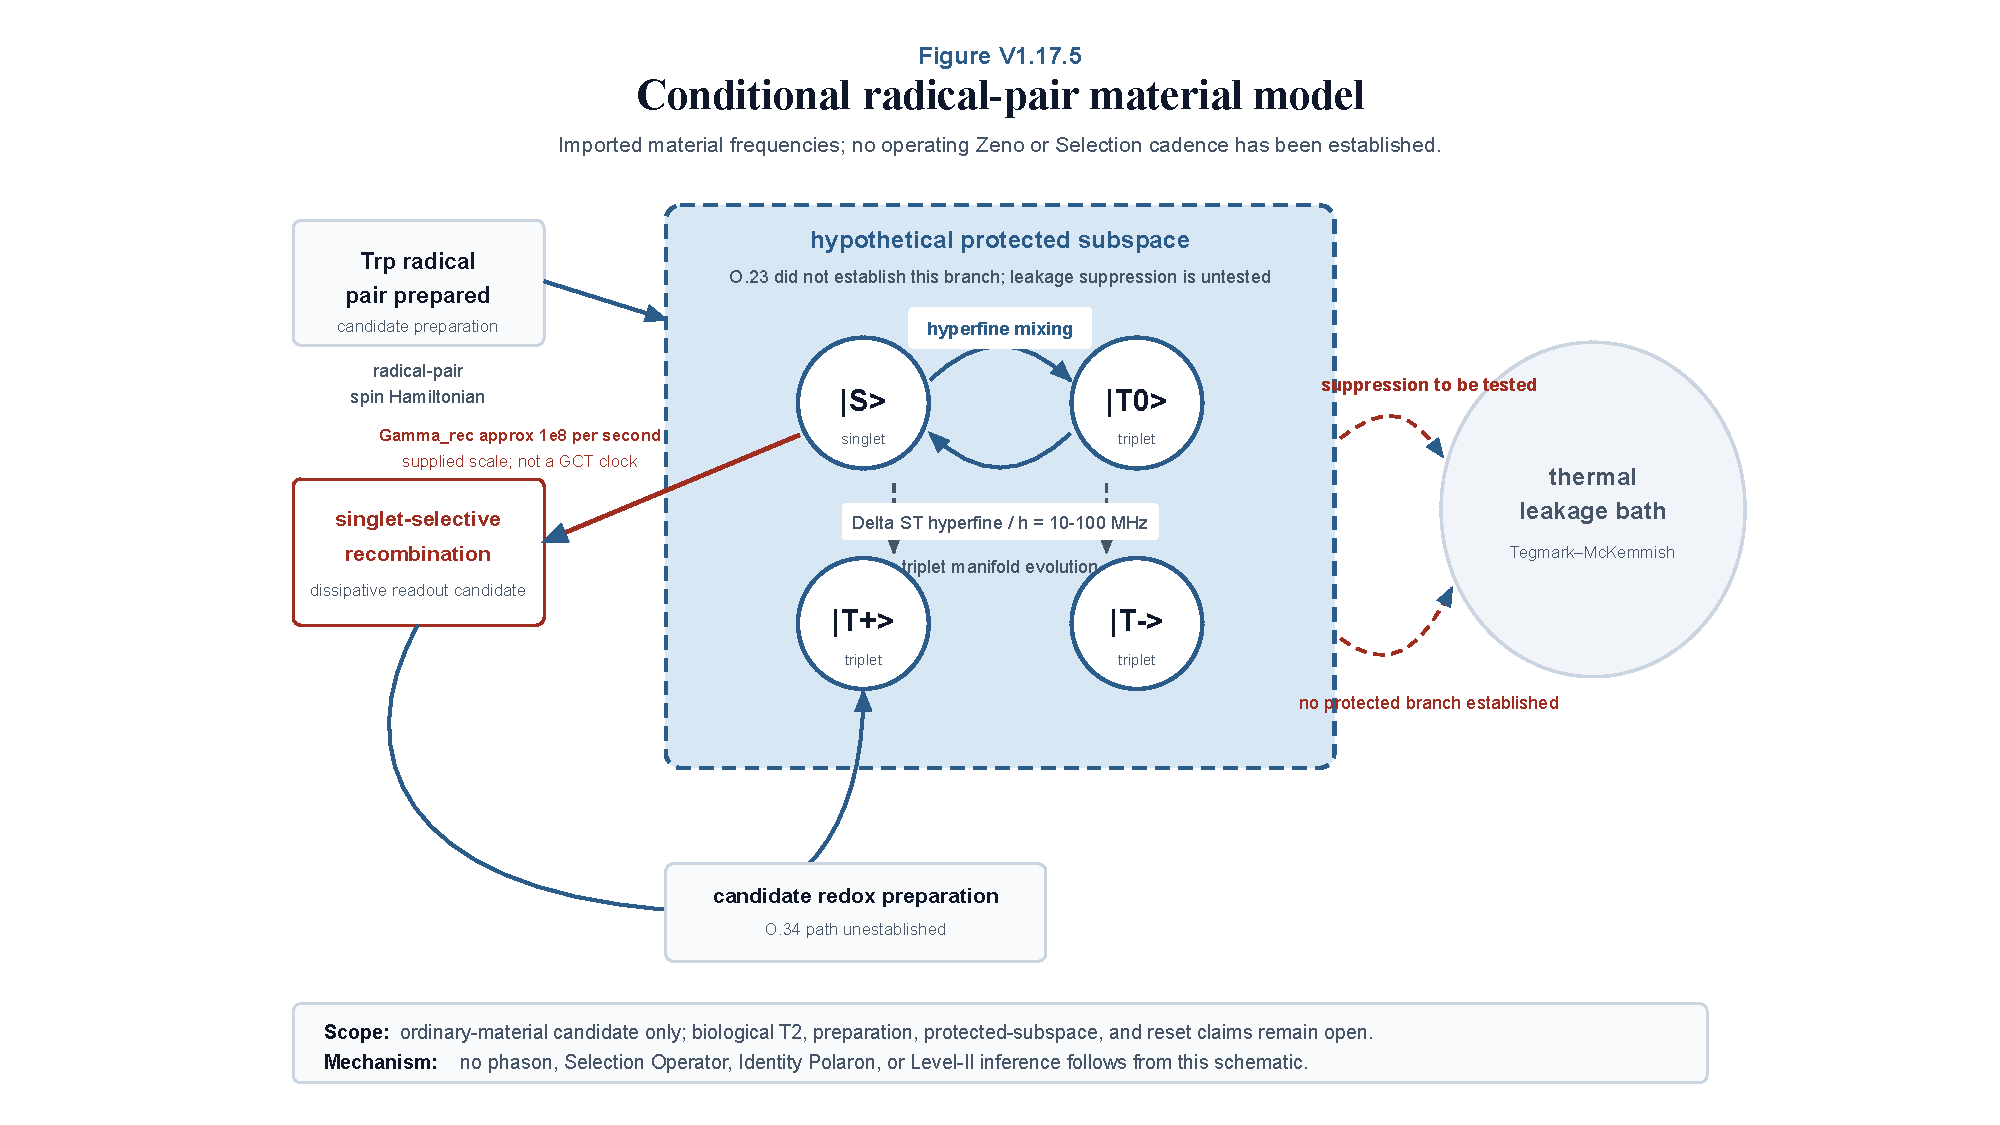
\includegraphics[keepaspectratio,alt={A conditional Trp radical-pair material model shows singlet/triplet dynamics and a hypothetical protected subspace whose preparation and leakage suppression remain unestablished; it carries no phason, Selection, Polaron, or Level-II inference.}]{content/Figures/Volume_1/Figure V1.17.5.pdf}}
\caption{A conditional Trp radical-pair material model shows
singlet/triplet dynamics and a hypothetical protected subspace whose
preparation and leakage suppression remain unestablished; it carries no
phason, Selection, Polaron, or Level-II inference.}
\end{figure}

Thermodynamically, acoustic cavity resonances or THz phonons would cause
reversible Rabi oscillations rather than irreversible measurement, and
an active 10 THz architecture that irreversibly erases one bit per
sampled degree of freedom per cycle would exceed the total metabolic
budget. The historical candidate scenario therefore uses the \textbf{100
MHz Radical Recombination} regime (\(\nu_{Zeno} \approx 100\) MHz)
{[}Tier 1 two-branch model mathematics with a Tier 3 realization; Tier
3/Tier 4 tubulin-specific implementation. The biological Trp
singlet-recombination rate, intact-tubulin \(T_2\), CISS/phason coupling
magnitude, ATP-Trp reset chain, heat-sink closure and any QND/reversible
sampling implementation remain substrate-specific inputs pending
O.21/O.23/O.24/O.34 and direct Protocol A/Protocol D measurement. The
natural radical-pair singlet recombination rate
\(\Gamma_{rec} \sim 10^8\,\text{s}^{-1}\) is therefore an imported
scenario rate, not a closed tubulin derivation; see V3 Ch13 §13.4.4 and
Parameter Ledger §0.3. \textbf{Tier 3 closure pending} --- the bare
radical-pair channel carries a \(\sim 10\) ns sampling/recombination
scale. With \(\sigma_H/h=30\) MHz, the Hamiltonian-variance Zeno time is
\(\tau_Z=\hbar/\sigma_H\approx5.305\) ns and the bare Misra-Sudarshan
diagnostic is \(\tau_{\rm eff}\approx2.8\) ns; across the registered
5--200 MHz variance band it spans approximately \(0.063\)--\(101\) ns
(V3 §13.4.3, §13.4.5; App ORQ O.23). This is \((2\pi)^2\approx39.5\)
below the alternative \(h/\sigma_H\) calculation and therefore widens
the coherence gap. The candidate chiral phonon-polariton
Decoherence-Free Subspace mechanism of §17.1.3c reaches best-case
\(\tau_{\rm eff}^{\rm collective} \sim 0.2\)--\(1\) ms under the App ORQ
Open Problem O.23 three-channel OAM analysis. The \(0.2\)--\(1\) ms band
is conditional on O.23 closure-path-(b) in the
50-\(\mu\)\hspace{0pt}m-MT regime; the full 10 ms conservative target is
\textbf{not} reached by any candidate mechanism. The \(1\)--\(10\) ms
neural-firing window coverage is therefore conditional on O.23 plus
restricted MT geometry{]}. A physiological ATP-coupled redox loop is the
candidate upstream source that would repeatedly prepare the Trp radical
pairs, but the explicit biochemical regeneration chain is open (App ORQ
O.34). The nominal 100 MHz timescale is set by spin-selective
recombination and hyperfine mixing in the imported radical-pair
scenario; it is not a measured intact-tubulin rate, an operating Zeno
cadence, a Selection clock, or a GCT coupling. Whether this chemistry
could implement an \emph{effective} continuous measurement on biological
timescales, and whether any such process bears on an Identity Polaron,
are the subject of V3 §13.4.4 and Open Problems O.23/O.34; any future
result first establishes ordinary material dynamics only.

\gctneedspace{5\baselineskip}\begin{gctCaution}

\textbf{Decoherence Shielding: Tubulin Tryptophan Aromatic Radical Pairs
{[}Tier 3 --- biophysical-specific material candidate{]}}

One candidate ordinary material system for the GCT Zeno-Drive scenario
is a \textbf{Tryptophan (Trp) aromatic radical-pair network intrinsic to
β-tubulin}. β-tubulin contains four Trp residues (β-tubulin chain B
numbering per PDB 1JFF and 1TUB; ATOM-record \texttt{auth\_seq\_id}
convention --- FASTA list-position numbering gives an offset \{21, 101,
344, 397\}, see App ORQ O.21): \textbf{Trp21, Trp103, Trp346, and
Trp407}. The historical material scenario proposes that \emph{at least
one} of these residues --- together with a near-neighbour aromatic
radical-pair partner (an adjacent Trp, Tyr, or Phe) --- occupy an
assembled-MT lumen-accessible geometry, providing the chiral aromatic
radical-pair host. The O.21 engine screen identifies Trp21 only as a
\textbf{local-inward wall-patch candidate}; the central lumen-axis test
requires an assembled-microtubule reference and remains a \textbf{Tier 3
structural-biology calibration} against high-resolution cryo-EM
reconstructions (Zhang R., LaFrance B. \& Nogales E. 2018 \emph{PNAS}
115:E6191--E6200; PDB 6DPU and follow-on structures). A lumen-accessible
chiral aromatic radical-pair host is a \textbf{Tier 3 candidate
ingredient and missing-leg control}, not an established necessary or
sufficient condition for an Identity Polaron or Level II (Dual Material
Constraint research hypothesis, §16.2.6). Closure of the specific Trp
identification is tracked as \textbf{Open Problem O.21} (App ORQ
§ORQ.5). The engine central branch remains \(n_{rp}=0\) until the
assembled-MT lumen-axis screen closes; the Trp21 local wall-patch is a
sensitivity branch, not an operative substrate proof. The supplied T₂
\textasciitilde{} 10 μs value is an external Trp-like material scenario,
not a native intact-β-tubulin measurement.

\textbf{Tier 3 disclosure on the supplied T₂ \textasciitilde{} 10 μs
value.} The \textasciitilde10 μs figure is the \emph{target} coherence
time that the historical scenario needs in order to run at 100 MHz
within the ATP thermodynamic budget. It has not been \emph{directly
measured} on intact β-tubulin Trp radical pairs, and the
hydrophobic-pocket shielding model does not predict the value for a
qualified intact pair. Comparable Trp radical pair T₂ values in related
aromatic systems (model peptides, cryptochrome FAD pairs) range from
\textasciitilde100 ns to \textasciitilde10 μs depending on environment
(β-tubulin residues Trp21, Trp103, Trp346, Trp407 per PDB 1JFF/1TUB
chain B ATOM-record \texttt{auth\_seq\_id} convention, see App ORQ
O.21). Pulsed EPR/ODMR on isolated or assembled tubulin can measure the
ordinary material response after geometry, redox, and preparation
controls (V3 Ch13 §13.4.3; App ORQ O.24). A controlled value below
\textasciitilde1 μs would disfavour the long-coherence proxy branch for
tubulin (no decision rule is registered for it in App PRG), leaving the
finite alternative-substrate path of §17.1.5 as the remaining registered
material route; a longer value would not establish a Zeno Drive, phason
coupling, Identity Polaron, Selection Operator, owner, or Level II.
Neither outcome is a verdict on GCT as a whole: the measurement tests an
ordinary material proxy, and no phason, Selection-Operator or Level-II
inference follows from it (§17.1.3).

Conditional on a specified radical-pair Hamiltonian and the supplied T₂,
the fast \textbf{Spin-Selective Recombination rate}
(\(\Gamma_{rec} \sim 100\) MHz, imported, not a measured β-tubulin rate)
of the Singlet state can provide an ordinary dissipative material
channel; it is not thereby a non-unitary Selection measurement. The bare
radical-pair rate is comparable to the upper edge of the Trp hyperfine
band rather than parametrically thousands of times faster; a protected
chiral phonon-polariton subspace (App ORQ O.23) is required before this
channel can Zeno-lock the state against thermalization. Unlike exogenous
flavoproteins, these Trp residues are structural components of the
microtubule lattice itself, satisfying the spatial co-localization
requirement identified in V3 Ch13 §13.2.1.

\end{gctCaution}

\gctneedspace{5\baselineskip}

\textbf{17.1.2b The Candidate Water-Cage Arrangement}

The water confined within the 15 nm microtubule core is modelled by a
\textbf{candidate} \(N=144\) dodecahedral arrangement inherited from the
GCT cage ansatz. This is a geometric substrate hypothesis, not a
demonstrated thermodynamic ground state or frozen clathrate of
biological water at 310 K. Published MD studies of water in cylindrical
hydrophobic confinement (Kalra, Garde \& Hummer 2003 \emph{PNAS}
100:10175 on the carbon-nanotube analogue) report disordered or weakly
structured water depending on radius and boundary chemistry; no
MT-lumen-specific MD/NMR study establishes an equilibrium \(N=144\)
dodecahedral cage. The Tier 2 framework claim is the
holographic-restriction mechanism; the Tier 3 biological identification
is that this restriction can be represented by the candidate \(N=144\)
lumen-water geometry. Full closure requires free-energy, MD, or NMR
validation under App ORQ Open Problem O.33.

\begin{quote}
\textbf{Sector-separation control (App BEB §BEB.6; Tier 1 conditional
sector-preservation criterion on a declared model; physical realization
Tier 3/open).} The candidate Zeno Drive (active measurement on spins)
and topological phason winding (passive protection) may be represented
as distinct sectors of a declared model. Theorem BEB.6.1 states only the
conditions under which such a model would preserve the sector label; the
former scale-separation argument and string-tension energy gap are
withdrawn, and no sector-transition barrier is derived (App BEB
§BEB.6c). The formal separation therefore prevents a category conflation
only; it does \textbf{not} prove that a biological Zeno Drive exists,
that it couples to phason winding, or that any energy-scale separation
supplies the missing interaction. A physical bridge remains Tier 3/open
(App BEB §BEB.6d).
\end{quote}

\gctneedspace{5\baselineskip}

\textbf{17.1.2c Conservative Determination of \(f_{bound}\) {[}Tier 3
biological substrate value{]}}

The \textbf{bound-water fraction} \(f_{bound}\) quantifies the fraction
of microtubule-lumen water in the first hydration shell of the candidate
Trp radical-pair register. It is a conservative geometry parameter, not
a proof that NOE supplies the Zeno lock of the historical 100 MHz
material-scan scenario.

\gctneedspace{5\baselineskip}

\textbf{Derivation of \(f_{bound}\).} The bound-water fraction
\(f_{bound}\) is the fraction of lumen water protons that lie within the
first hydration shell of the Trp radical pair network. In the \(N=144\)
cage, each Trp radical pair (one of the four β-tubulin Trp residues ---
Trp21, Trp103, Trp346, Trp407 per PDB 1JFF/1TUB chain B ATOM-record
\texttt{auth\_seq\_id} convention, see App ORQ O.21 --- paired with a
near-neighbour aromatic radical-pair partner, per Open Problem O.21)
contacts a range of first-shell water molecules depending on the
hydration model. The operative lower band is geometric-cage-derived
rather than MD-anchored: \(n_{contact}\in\{4,6,8\}\) with central value
\(6\) for the O.21/O.33 conservative branch, while the perfect-cage
structural stress test sets \(n_{contact}=12\) under the assumption that
all 12 pentagonal faces of the dodecahedral cage are saturated. The
indole/Trp hydration literature is a qualitative first-shell-hydration
anchor only; the numerical \(f_{bound}\) lower edge is the conservative
cage-occupancy calculation. Given the microtubule lumen geometry (inner
radius \(r_{lumen} \approx 7.5\) nm, ring length \(\ell \approx 8\) nm,
one \(\alpha\beta\)-dimer rise; an 8 nm ring holds 13 dimers, one per
protofilament), the total number of lumen water molecules per 8 nm ring
is:

\[N_{water} \approx \frac{\pi r_{lumen}^2 \ell}{\nu_{H_2O}} \approx \frac{\pi \times (7.5\,\text{nm})^2 \times 8\,\text{nm}}{0.0299\,\text{nm}^3} \approx \frac{1414\,\text{nm}^3}{0.0299\,\text{nm}^3} \approx 4.7 \times 10^4\]

and therefore, per \(\alpha\beta\)-dimer,
\(N_{water}^{dimer} \approx 4.7\times10^4/13 \approx 3.6\times10^3\).

The number of first-shell water molecules contacted by the operative Trp
radical-pair register(s) per dimer:

\[N_{bound} \approx n_{rp} \times n_{contact}\]

Here \(n_{contact} \le 12\) already counts the saturated cage faces; the
earlier additional factor \(n_{faces}=12\) counted them twice and is
withdrawn, as is the earlier division by the water of a whole 8 nm ring
(13 dimers) instead of one dimer.

Therefore:

\[\boxed{f_{bound} = \frac{N_{bound}}{N_{water}^{dimer}} = \frac{n_{rp} \times n_{contact}}{3.6 \times 10^3}}\]

\textbf{Branch discipline under App ORQ Open Problems O.21 and O.33}
(Trp21 as a local-inward candidate only, and the water-cage geometry
pending direct MD/NMR/free-energy closure):

\begin{itemize}
\tightlist
\item
  \textbf{Operative central branch:} \(f_{bound}=0\) from \(n_{rp}=0\)
  pending O.21 assembled-MT lumen-axis closure {[}Tier 3 biological
  substrate value{]}
\item
  \textbf{Sensitivity lower edge:} \(f_{bound}=1.1\times10^{-3}\)
  (\(n_{contact}=4\)) under the conditional \(n_{rp}=1\) branch {[}Tier
  3 biological substrate value{]}
\item
  \textbf{Sensitivity central value:}
  \(f_{bound}\approx1.65\times10^{-3}\) from \(n_{rp}=1\),
  \(n_{contact}=6\), conditional on O.21 {[}Tier 3 biological substrate
  value{]}
\item
  \textbf{Sensitivity upper edge:} \(f_{bound}=2.2\times10^{-3}\)
  (\(n_{contact}=8\)) under the conditional \(n_{rp}=1\) branch {[}Tier
  3 biological substrate value{]}
\end{itemize}

The \(3.3\times10^{-3}\) value is the \(n_{rp}=2\), \(n_{contact}=6\)
branch; \(6.6\times10^{-3}\) is the \(n_{rp}=2\), \(n_{contact}=12\)
maximum stress-test branch (App NSP §NSP.4). Neither upper branch is
operative in Protocol D or \(\eta_{Zeno}\) calculations.

\gctneedspace{5\baselineskip}

\textbf{Impact on the Landauer Budget.} The historical 100 MHz scan
scenario was motivated by a proposed Trp radical-pair hyperfine /
singlet-triplet scale, not by an NOE cross-relaxation rate.
Biological-water NOE cross-relaxation at 310 K is a slow
polarization-transfer channel, with rates well below
\(1\,\text{s}^{-1}\) for dilute nuclear-spin transfer {[}Tier 3
order-of-magnitude estimate{]}. That is at least eight orders of
magnitude below the historical 100 MHz scenario rate and cannot supply
the rate assumed by that scenario.

The candidate material quantity is instead the Trp radical-pair spin
Hamiltonian: \[\Delta_{ST}^{hf}/h \sim 10\text{--}100\,\text{MHz},\]
with the specific tubulin Trp value and any chiral phonon-polariton
enhancement registered under O.12/O.21/O.23. NOE remains a possible slow
nuclear-spin-pool preparation or readout pathway, but it does not
provide a derived Zeno-drive rate. The nuclear-spin-pool framing
therefore carries an explicit Open Problem dependency: if the Trp
hyperfine / chiral-polariton channel fails to supply the scenario's 100
MHz rate, NOE cannot rescue the budget.

\gctneedspace{5\baselineskip}\begin{gctNote}

\textbf{Epistemic Tier:} Holographic restriction and the declared
spin-Hamiltonian algebra are \textbf{Tier 2} inherited geometric inputs;
their adoption as a biological phason or Zeno mechanism, and the
specific biological realization by a candidate \(N=144\)
microtubule-lumen water arrangement, are \textbf{Tier 3/open pending
action matching and direct MD/NMR/free-energy closure} (Open Problems
O.21/O.23/O.33). The operative central branch is \(f_{bound}=0\) under
\(n_{rp}=0\) pending O.21 assembled-MT lumen-axis closure; the
conditional \(n_{rp}=1\) sensitivity branch is
\(f_{bound}\in[1.1,2.2]\times10^{-3}\). The \(3.3\times10^{-3}\) value
is the \(n_{rp}=2\), \(n_{contact}=6\) branch; \(6.6\times10^{-3}\) is
the \(n_{rp}=2\), \(n_{contact}=12\) maximum stress-test branch (App NSP
§NSP.4). Neither upper branch is operative. \textbf{Material-proxy
decision:} a null in the registered \(\nu_c \approx 112 \pm 10\) MHz
window (Branch A) alone does not reject the branch; rejection of the
registered biophysical (Zeno-substrate) branch requires the
three-conjunct F1 joint null of V3 Ch13 §13.3.5 (App PRG P.8); NOE is
too slow by at least eight orders of magnitude to close the gap. A
positive feature would still require attribution, an action-normalized
coupling and a material-to-GCT map (§17.1.3). Neither sign is a verdict
on GCT as a whole, and no phason, Selection-Operator or Level-II
inference follows from it.

\end{gctNote}

\subsubsection{17.1.3 The Berry-Phason Link: Rashba-Phason Candidate and
Field-Typing Audit {[}Tier 1 representation audit + Tier 3 open physical
coupling{]}}\label{the-berry-phason-link-rashba-phason-candidate-and-field-typing-audit-tier-1-representation-audit-tier-3-open-physical-coupling}

The indole chromophore system of Tubulin Tryptophan (Trp), embedded in a
chiral hydrophobic pocket with an internal electric field gradient
\(\mathbf{E}_{mol}\), can carry an ordinary Rashba spin-orbit
interaction:
\[\hat{H}_R = \alpha_R (\hat{\mathbf{k}} \times \hat{\mathbf{n}}) \cdot \hat{\boldsymbol{\sigma}}\]
where \(\alpha_R \sim 0.1\)--\(1\) eV·Å is a Rashba-scale calibration
placeholder for the chiral indole environment, not a measured Trp
thin-film ARPES coefficient. Spin-resolved ARPES on Trp thin films or an
equivalent chiral-organic spin-orbit assay is the closure target, and
\(\hat{\mathbf{n}}\) is the molecular symmetry axis.

GCT proposes that this spin-orbit structure couples to the vacuum phason
field. In GCT's lattice language the phason field \(\Phi_\perp(x)\)
appears through the spatial gradient of the internal phase across the
vacuum lattice, \(\partial_j \Phi_\perp\) (phason strain component along
\(\hat{e}_j\)). Because the Rashba term couples spin to momentum through
a gradient, the candidate \textbf{Rashba-Phason coupling} considered
here is

\[\hat{H}_{RP} = \alpha_R \sum_j (\partial_j \Phi_\perp)\, \varepsilon_{jkl}\, \hat{k}_k\, \hat{\sigma}_l \tag{17.3}\]

where \(\varepsilon_{jkl}\) is the Levi-Civita symbol, \(\hat{k}_k\) is
the crystal momentum operator, and \(\hat{\sigma}_l\) are Pauli
matrices.

\textbf{Field-typing analysis {[}Tier 1, conditional on the declared
field types{]}.} With \(E_\parallel \cong 3\) and \(E_\perp \cong 3'\)
under the rotational icosahedral group \(A_5\), a vector phason
displacement \(u_\perp^a\) has strain
\[W_{ia} = \partial_i u_\perp^a \in 3 \otimes 3' = 4 \oplus 5,\] while
momentum and spin give
\(K_{ij} = k_i \sigma_j \in 3 \otimes 3 = 1 \oplus 3 \oplus 5\), of
which the cross product \(\varepsilon_{jkl} k_k \sigma_l\) is the
antisymmetric \(3\) channel. Therefore
\[\operatorname{mult}_1\!\left[(3 \otimes 3') \otimes \Lambda^2 3\right] = 0:\]
Eq. (17.3) contracts one physical index but leaves the internal \(3'\)
index unpaired, so it is not an icosahedral scalar when \(\Phi_\perp\)
is the vector phason used elsewhere in GCT. Reading \(\Phi_\perp\) as an
effective scalar \(\varphi\) makes
\(\nabla\varphi \cdot (\mathbf{k} \times \boldsymbol{\sigma})\)
type-correct, but that is a different field model, and with
\([\nabla\varphi] = [k] = L^{-1}\) its coefficient has dimension
\(E L^2\) rather than the Rashba unit \(E L\). The two full tensors
share exactly one five-dimensional channel (under \(I_h\),
\(W \in T_{1u} \otimes T_{2u} = G_g \oplus H_g\) and
\(K \in T_{1u} \otimes T_{1g} = A_u \oplus T_{1u} \oplus H_u\)), so a
type-correct candidate must use that shared channel together with a
static molecular-handedness pseudoscalar \(\chi \in A_u\). Such a term
is allowed by symmetry, but the present action fixes neither its
coefficient nor its sign or magnitude, nor the defect-to-spinor
vertices, phason kinetic normalization, mode volume or material-to-GCT
embedding it would need {[}Tier 3/open; App ORQ O.12/O.23/O.24{]}.

\textbf{Conditional interpretation.} If a type-correct coupling with a
non-zero, action-normalized coefficient were established, a
CISS-selected spin-polarized recombination channel in the Trp radical
pair, pinned by the Zeno Drive (§17.1.2), could bias the local phason
strain \(\partial_j \Phi_\perp\). This is the candidate substrate branch
by which a DMC-qualified selection cycle might bias the phason field; it
is conditional on that coupling, on O.23/O.24 closure and on Protocol
A-Prime measurement. No deterministic phason bias follows from this
section as it stands.

\textbf{Status of the 38.3 MHz figure {[}Tier 3 conditional
external-rate scenario{]}.} The value
\(g_{\text{single}}^{eff} \approx 38.3\,\text{MHz}\) used in §17.1.4 and
V3 Ch13 §13.3.5 (historical external-rate scenario block) is not the
output of an evaluated matrix element of Eq. (17.3). It enters the
engine as a declared pre-overlap constant calibrated to operating-point
consistency
(\texttt{GCT\_Physics\_Engine/src/protocol\_o16\_n\_coh\_verification.py});
no independent plausibility range for it is registered. A generic
Dicke-superradiance ansatz gives \(\approx 931\) kHz, and the
\(\sim 41\times\) ratio between the two values is calibrated, not
derived. All dependent \(\eta_{\rm Zeno}\) and \(N_{\rm coh}\) values
are therefore conditional external-rate scenarios, not derived GCT
predictions; the operational \(\eta_{\rm Zeno}\) branch applies the
overlap factor separately.

\gctneedspace{5\baselineskip}\begin{gctNote}

\textbf{Chromophore Model: Tryptophan Aromatic Radical Chain {[}Tier 3
candidate host{]}} The physiologically relevant chromophore is the
\textbf{Tryptophan (Trp) aromatic radical chain} of β-tubulin (candidate
residues \{Trp21, Trp103, Trp346, Trp407\}; O.21 currently supports
Trp21 only as a local-inward wall-patch candidate pending assembled-MT
lumen-axis closure), not a generic Tavis-Cummings Dicke oscillator. Its
spin-orbit coefficient \(\alpha_R\), Trp dipole moment
(\(\mu_{Trp} = 5.0\,\text{D}\)) and CISS strength are the molecular
ingredients a phason-transduction candidate would require. The 38.3 MHz
pre-overlap scenario value and the 931 kHz Dicke value are scenario
inputs, not derived couplings.

\end{gctNote}

The Rashba coefficient \(\alpha_R\) is set by the \textbf{spin-orbit
coupling of the Tryptophan aromatic ring} (indole chromophore), which
provides the chiral CISS ingredient. The β-tubulin Trp residues (Trp21,
Trp103, Trp346, Trp407 per PDB 1JFF/1TUB chain B ATOM-record
\texttt{auth\_seq\_id} convention, see App ORQ O.21), being components
of the chiral microtubule lattice, break inversion symmetry and can
generate a non-zero \(\alpha_R\). The Trp network is native to the
microtubule hardware, requiring no exogenous chromophore. (Scenario
values: Appendix GPE.)

\textbf{Proxy closure assay:} Spin-resolved ARPES measurements of Trp
thin films returning \(\alpha_R < 0.01\) eV·Å would falsify the
thin-film proxy branch for large Rashba-CISS coupling and would force
demotion of the tubulin transduction estimate unless a β-tubulin or
assembled-microtubule measurement recovers the coupling in the native
pocket. Spin-resolved ARPES, EPR/ODMR, chirality reversal and isotope
controls measure the molecular ingredients; they cannot by themselves
close the vacuum-phason transduction, which additionally requires the
action-normalized coefficient of a type-correct coupling and a measured
mode map.

\textbf{Tier classification:} The cross-product form of Eq. (17.3) is
rotation-covariant for a scalar gradient but is not an icosahedral
scalar for the vector phason (field-typing analysis above, Tier 1). The
physiological magnitude \(\alpha_R\), Trp-pocket CISS strength and
proxy-to-tubulin transfer factor are Tier 3/Tier 4 empirical inputs, and
the phason coupling itself is Tier 3/open. Until those closures exist,
no DMC phason gate, Turing-Null verdict or Level-II classification
follows from this section. Level II remains open (Tier 3): no validated
substrate criterion exists yet (it requires a typed, normalized,
measured coupling, the Identity-Polaron construction and an independent
phenomenal bridge; O.21/O.23/O.34, O.18).

\subsection{\texorpdfstring{\textbf{§17.1.3b --- The Surrogate Scale
Ratio κ: ATP-Supported Stark/CI Material Scenario {[}Tier 3; no phason
map{]}}}{§17.1.3b --- The Surrogate Scale Ratio κ: ATP-Supported Stark/CI Material Scenario {[}Tier 3; no phason map{]}}}\label{b-the-surrogate-scale-ratio-ux3ba-atp-supported-starkci-material-scenario-tier-3-no-phason-map}

A phason is a collective excitation rather than a rigid rotor, but that
observation does not select a molecular transducer. This subsection
defines an ordinary molecular \textbf{surrogate scenario} using an
\textbf{electronic Stark shift} of the indole chromophore and a possible
\textbf{Conical Intersection (CI)} pathway in the Tryptophan (Trp)
potential energy surface. It neither derives ATP-to-phason coupling nor
shows that this chemistry occurs in the proposed tubulin register.

\gctneedspace{5\baselineskip}

\textbf{Candidate material chain to be tested: ATP-supported chemistry →
local electric field → Trp polarization → possible non-adiabatic
transition:}

\gctneedspace{5\baselineskip}

\textbf{Step 1 --- ATP-Supported Electric Field:} A candidate
ATP-supported redox / kinase-proximal chain can create a transient
electric field near the Trp pocket. Tubulin's canonical nucleotide
chemistry is GTP/GDP, so this ATP-supported reset is not asserted as a
demonstrated local ATP-hydrolysis site; it remains the O.34 ATP-Trp
regeneration target. The transient charge redistribution creates a
localized electric field: \[\mathbf{E}_{ATP} \sim 10^7 \text{ V/m}\]

This field is transient but intense---comparable to the internal
molecular fields that break inversion symmetry in biological chiral
molecules.

\gctneedspace{5\baselineskip}

\textbf{Step 2 --- Electronic Stark Shift of the Indole Electronic
States:} The Tryptophan aromatic radical-pair model imports a canonical
bare singlet-triplet variance target \(\Delta_{ST}/h \approx 30\) MHz
(\(\sim 1.24\times10^{-7}\) eV) from proton-hyperfine-scale radical-pair
physics {[}Tier 3 engine value; no intact β-tubulin Trp EPR/ODMR
measurement yet{]}. Numerical proximity to a stipulated cavity-mediated
phonon-polariton band motivates an ordinary material scan; it does not
enable or demonstrate a protected subspace, Zeno Drive, phason channel,
or Selection clock. The indole chromophore carries a sizeable dipole
moment (scenario value \(\mu_{Trp} \approx 5\) Debye). Under the
stipulated local field, its molecular electronic energies (\(S_0\),
\(S_1\) or charge-transfer states) would shift by an electronic Stark
term of order:
\[\Delta E_{Stark} = -\vec{\mu}_{Trp} \cdot \mathbf{E}_{ATP}\]

This is an electronic Stark shift of molecular states, relevant to
access to a conical intersection; it is not a vibrational Stark effect.
It does not tune the radical-pair singlet--triplet gap: the spin singlet
and triplet of a radical pair share essentially the same spatial charge
distribution, so a uniform static field shifts both by the same amount
and leaves the S--T gap (exchange plus hyperfine) unchanged to first
order. The radical-pair spin model (§17.1.2) and the molecular CI model
below are separate objects.

\gctneedspace{5\baselineskip}

\textbf{Step 3 --- Conical Intersection Steering:} The indole
chromophore's molecular potential energy surfaces contain a
computationally established \textbf{Conical Intersection (CI)} where the
first excited electronic singlet state (\(S_1\)) meets the electronic
ground state (\(S_0\)). These electronic singlets are molecular states,
not the spin singlet of the radical pair. The CI seam represents a
branch point in the adiabatic energy surface and supports
internal-conversion-style \(S_1 \to S_0\) relaxation.

In a \textbf{conditional molecular surrogate}, a driven cyclic evolution
of the indole electronic states could accumulate a \textbf{geometric
Berry phase} and bias passage near a conical-intersection seam. The
historical 100 MHz external-rate scenario (§17.1.2) does not itself
derive that cyclic path, its phase, or a preferred non-adiabatic
channel; all three require a molecular Hamiltonian and measured
couplings.

\[\text{Declared cyclic drive} + \text{Stark-tuned CI} \longrightarrow \text{candidate population-transfer bias}\]

\gctneedspace{5\baselineskip}

\textbf{Step 4 --- Candidate dissipation channel (unestablished):} If a
specified molecular Hamiltonian, CI passage, and chiral lattice coupling
supported the process, some released energy could populate ordinary
phonon-polariton modes propagating along the helical microtubule lattice
axis. Whether such modes exist with the required dispersion,
orbital-angular-momentum (OAM) content, propagation, and thermal
protection in assembled microtubules has not been demonstrated. This
possibility is an O.23 material-model target (the OAM selection rule of
§17.1.3c), not a derived destination of ATP hydrolysis (0.52 eV) and not
phason moment acceleration.

\[\begin{gathered}\text{Hypothetical ledger: ATP-supported chemistry} \dashrightarrow \text{Stark shift} \\ \dashrightarrow \text{CI passage} \dashrightarrow \text{candidate polariton population}\end{gathered}\]

\gctneedspace{5\baselineskip}

\textbf{Coupling Constant κ (Operational Definition):}

\emph{(Notational note: the bare symbol \(\kappa\) in this section
denotes a dimensionless Stark-to-CI energy-scale ratio and is distinct
from the inter-agent coupling coefficient \(\kappa_{ij}\) of §7.6.3 and
§11.9; the two are never used together in the same expression. It is not
an ATP→phason efficiency or a transition probability.)}

The surrogate index κ compares a supplied Stark energy with a supplied
CI seam scale:
\[\kappa \equiv \frac{|\vec{\mu}_{Trp} \cdot \mathbf{E}_{ATP}|}{\Delta E_{CI}}\]

where \(\Delta E_{CI} \approx 0.01\) eV is a scenario energy offset
between the Franck--Condon region and the minimum-energy CI (the gap
itself vanishes on the seam), making \(\kappa\) dimensionless.

This ratio is \textbf{not} the fraction of ATP energy directed into a
channel. Turning it into a transition probability requires a molecular
Hamiltonian, wavefunctions, nonadiabatic couplings, drive protocol,
dissipation, and a dynamical calculation. No 100 MHz Zeno limit forcing
\(\kappa\to1\) is derived.

\gctneedspace{5\baselineskip}

\textbf{Numerical Consequence:}

\begin{itemize}
\tightlist
\item
  ATP field: \(E_{ATP} \sim 10^7\) V/m
\item
  Trp dipole moment:
  \(\mu_{Trp} \approx 5\,\text{D} = 5 \times 3.336 \times 10^{-30}\,\text{C·m} = 1.67 \times 10^{-29}\,\text{C·m}\)
  (standard SI conversion:
  \(1\,\text{D} = 3.336 \times 10^{-30}\,\text{C·m}\))
\item
  Trp Stark shift:
  \(\Delta E_{Stark} = \mu_{Trp} \cdot E_{ATP} = 1.67 \times 10^{-29}\,\text{C·m} \times 10^7\,\text{V/m} = 1.67 \times 10^{-22}\,\text{J} \approx 1.04 \times 10^{-3}\,\text{eV}\)
  (millielectron-volt scale)
\item
  CI seam gap: \(\sim 0.01\) eV
\item
  Scale ratio: \(\kappa \sim 0.1\)--\(0.3\) central scenario band; no
  percentage-of-energy or transition-efficiency interpretation is
  licensed
\end{itemize}

\textbf{Input-level uncertainty propagation {[}Tier 3 propagated
band{]}.} The three inputs (\(E_{ATP}\), \(\mu_{Trp}\),
\(\Delta E_{CI}\)) carry the following Tier 3 uncertainty ranges,
traceable to their underlying biophysical sources:

\begin{itemize}
\tightlist
\item
  \(E_{ATP} \in [3 \times 10^6,\, 3 \times 10^7]\) V/m (factor of
  \textasciitilde3 either way; an unsourced scenario range for a Trp
  pocket {[}Tier 3/4{]}. It is not supported by Boxer-group
  vibrational-Stark spectroscopy (Boxer 2009 \emph{J. Phys. Chem. B}
  113:2972), which reports enzyme active-site fields of order 10--150
  MV/cm, i.e.~\(10^9\)--\(1.5\times10^{10}\) V/m --- e.g.~about \(-144\)
  MV/cm in ketosteroid isomerase (Fried, Bagchi \& Boxer 2014
  \emph{Science} 346:1510). With fields of that scale and the other
  central inputs, \(\kappa \approx 10\)--\(160\); the envelope below
  holds only under the scenario range);
\item
  \(\mu_{Trp} \in [3,\, 7]\) D (Trp residue-environment-dependent
  dipole; literature spans 3-7 D depending on hydrogen-bonding-network
  conformation per Vivian \& Callis 2001 \emph{Biophys. J.} 80:2093
  review of Trp fluorescence shift mechanisms; the Callis \& Liu 2006
  \emph{Chem. Phys.} 326:230 QM-MM Trp-flavin study provides the
  protein-environment-dependence anchor);
\item
  \(\Delta E_{CI} \in [3 \times 10^{-3},\, 3 \times 10^{-2}]\) eV (Tier
  3 range across the photo-LOV / Trp-flavin / cryptochrome
  conical-intersection literature; the LOV1 crystal-structure work of
  Fedorov et al.~2003 (\emph{Biophys. J.} 84:2474) concerns flavin-bound
  chromophores and does not report CI energy offsets; the specific
  {[}3e-3, 3e-2{]} eV span is a scenario range, not a sourced
  consensus).
\end{itemize}

Propagating the two factor-3 uncertainties (\(E_{ATP}\),
\(\Delta E_{CI}\)) and the ±40\% \(\mu_{Trp}\) range multiplicatively
through
\(\kappa = |\vec{\mu}_{Trp} \cdot \mathbf{E}_{ATP}| / \Delta E_{CI}\):

\[\kappa_{\rm propagated} \;\in\; \left[\frac{0.6 \times 0.3}{3}, \; \frac{1.4 \times 3.0}{0.3}\right] \;\times\; \kappa_{\rm central} \;\approx\; [0.06,\, 14] \;\times\; 0.104 \;\approx\; [0.006,\, 1.5]\]

Because \(\kappa\) is an energy-scale ratio rather than a probability,
values above one are mathematically allowed and must not be clipped:

\[\boxed{\kappa_{\rm propagated} \;\in\; [0.006,\, 1.5]\, \text{(Tier 3 input-propagated envelope; central } 0.104\text{)}}\]

--- a far broader interval than the historical \([0.1, 0.3]\) central
band. That narrower band, which also appears in the Parameter Ledger
B-sector material, is only a central-input scenario under
\(E_{ATP} = 10^7\) V/m, \(\mu_{Trp} = 5\) D, and
\(\Delta E_{CI} = 10^{-2}\) eV; the \textbf{propagated \([0.006, 1.5]\)
interval} is the corresponding input envelope. Neither interval is an
operative steering efficiency.

\textbf{Engine output \(\kappa = 0.104\) at the band's lower edge.} This
conditional estimate is sensitive to the assumed \(E_{ATP}\),
\(\mu_{Trp}\), and \(\Delta E_{CI}\) inputs; any input revised downward
by about 2× drops it below 0.1, the lower edge of the historical
\([0.1, 0.3]\) central band (an edge of a scenario band, not a threshold
or gate), so the central band is not a safety margin. Sharper
measurements would tighten the propagated interval. At present
\(\kappa\) is only a Tier 3 biochemical/CI scenario parameter: it is not
a GCT phason coefficient, a normalized Zeno-rate ratio, a robustness
gate for an Identity Polaron, a DMC gate, or a Level-II classifier.

\textbf{Conditional energy ledger only:} ATP hydrolysis can supply 0.52
eV of chemical free energy, while a declared molecular Hamiltonian could
in principle redistribute reaction probabilities without supplying the
mechanical work itself. The present model has not demonstrated a Zeno
Drive, a cyclic Berry phase, its coupling to the ATP reaction
coordinate, directional steering, or the proposed polariton sink.
Thermodynamic compatibility is necessary but does not establish this
transducer.

\gctneedspace{5\baselineskip}\begin{gctNote}

\textbf{Firewall Metadata {[}Electronic Stark Effect Coupling{]}}

\begin{itemize}
\tightlist
\item
  \textbf{Type:} Stark-tuned conical intersection steering via Berry
  phases
\item
  \textbf{Tier:} 3 (Stark inputs are scenario values; an \(S_1/S_0\) CI
  is computationally established for indole, not shown on a Trp
  radical-pair surface)
\item
  \textbf{Status:} The electronic Stark shift is ordinary molecular
  physics once its field and dipole are supplied. The Berry/CI steering
  path and its connection to ATP work remain hypothetical; no physical
  Selection or phason coupling is derived.
\item
  \textbf{Numerical Verification (Appendix GPE):}
  \texttt{GCT\_Physics\_Engine/src/protocol\_subjective\_lagrangian.py}
  reproduces the supplied Stark-energy arithmetic,
  \(\Delta E_{Stark} = \mu_{Trp} \cdot E_{ATP} = 1.04\) meV, and the
  dimensionless scale ratio \(\kappa = 0.104\), inside the central-input
  \([0.1, 0.3]\) scenario band. The protocol's JSON field name
  \texttt{kappa\_atp\_to\_ci\_channel} does not make this ratio a
  transition probability; a probability requires the missing dynamical
  calculation. \textbf{Disambiguation:} the protocol also reports a
  separate Landau-Zener ``steering efficiency'' capped by the
  Zeno-vs-electronic-timescale ratio (\(\sim 10^{-4}\)); that quantity
  is another conditional surrogate, not the manuscript's \(\kappa\) and
  not a GCT steering efficiency. On the conditional \(n_{rp} = 1\)
  sensitivity branch (the central \(n_{rp} = 0\) case is pending O.21),
  and with all \(1.625 \times 10^9\) spins held in State C at once, the
  same protocol's State C energy budget exceeds the 1 nW per-neuron
  ceiling by \(\sim 3 \times 10^8\); the protocol is registered as a
  tension rather than a confirmation on that branch. The protocol's own
  willpower budget allows at most \(\sim 5.4\) spins in State C at once,
  so the full-occupancy figure bounds the branch rather than describing
  an operating point.
\item
  \textbf{Decision scope:} If the Trp singlet-triplet coherence time
  drops below 1 μs, or if the Stark shift is below meV scale, the
  molecular steering scenario is disfavoured (no decision rule is
  registered for it in App PRG). Such measurements cannot confirm or
  falsify GCT as a whole, a Selection Operator, an Identity Polaron, or
  Level II.
\end{itemize}

\end{gctNote}

\subsection{\texorpdfstring{\textbf{17.1.3c Chiral Phonon-Polaritons \&
Berry-Phase Steering {[}Tier 3 hypothetical material model; O.23
open{]}}}{17.1.3c Chiral Phonon-Polaritons \& Berry-Phase Steering {[}Tier 3 hypothetical material model; O.23 open{]}}}\label{c-chiral-phonon-polaritons-berry-phase-steering-tier-3-hypothetical-material-model-o.23-open}

The historical 100 MHz external scenario has a single-quantum energy
\(E \approx 4.1 \times 10^{-7}\) eV, roughly five orders of magnitude
below the thermal noise floor at physiological temperatures
(\(k_B T \approx 0.026\) eV at 310K). This arithmetic does not establish
a Zeno sampling frequency or a physical coupling. Exact Dicke
subradiance is also unavailable: it requires a permutation symmetry that
cannot hold in a warm, wet, 310K inhomogeneous neuronal soma absent a
demonstrated symmetry-protected subspace.

A hypothetical material model would have to separate an ordinary energy
source from a separately demonstrated control channel. The following two
ingredients are candidates, not a solution already supplied by the
microtubule's helical geometry:

\begin{enumerate}
\def\labelenumi{\arabic{enumi}.}
\item
  \textbf{Chiral Phonon-Polaritons (candidate thermal suppression):} If
  independently measured chiral phonon-polariton modes propagating along
  the helical microtubule lattice and a coupling vertex were supplied,
  they could couple to Trp radical-pair observables.
  Orbital-angular-momentum (OAM) mismatch is a candidate
  Decoherence-Free Subspace (DFS) route for App ORQ Open Problem O.23,
  but the explicit Lindblad small-\(N\) test currently reports
  \texttt{DFS\_SUPPRESSION\_NOT\_DEMONSTRATED}. No continuous 100 MHz
  Zeno Drive, coupling coefficient, or warm-biological DFS has been
  derived. The \(0.17\)--\(0.95\) ms coherence band is a conditional
  O.23 scenario in the 50-\(\mu\)\hspace{0pt}m microtubule regime only.
\item
  \textbf{Berry-Phase Steering Surrogate (hypothetical valve):} ATP
  hydrolysis can supply conformational free energy (\(\sim 0.52\) eV). A
  separately specified driven cyclic molecular Hamiltonian could
  accumulate a \textbf{Berry phase} and bias a reaction pathway, but the
  historical 100 MHz scenario does not derive that path, its
  directionality, or a coupling from a candidate DFS to an ion channel.
  No demonstrated measurement steers ATP energy into neural firing.
\end{enumerate}

This is therefore a \textbf{hypothetical energy-and-control ledger}, not
a registered physical up-conversion path from volition to neural firing.
Closure would require the molecular Hamiltonian, driven cycle, coupling
coefficients, directionality, DFS suppression, regeneration, and
transfer function before any Selection-Operator interpretation is
considered.

\subsection{\texorpdfstring{\textbf{17.1.3d Relativistic Zeno
Thermodynamics (The Doppler-Shifted Subjective Lagrangian) {[}Tier 4
speculative stress-test; no operative
bound{]}}}{17.1.3d Relativistic Zeno Thermodynamics (The Doppler-Shifted Subjective Lagrangian) {[}Tier 4 speculative stress-test; no operative bound{]}}}\label{d-relativistic-zeno-thermodynamics-the-doppler-shifted-subjective-lagrangian-tier-4-speculative-stress-test-no-operative-bound}

A speculative consistency question for the historical ATP-supported 100
MHz scenario arises at extreme boosts (\(v \to c\)). In an eventual
material model, ordinary radical-pair/CISS dynamics and chemical work
would be described in the substrate rest frame. No local phase-locking
cadence, phason coupling, preferred vacuum frame, Lorentz-noninvariant
sampling demand, or empirical velocity limit for consciousness is
presently established.

For bookkeeping only, one may compare an external-coordinate pump rate
\(\Gamma_{pump}^{(ext)}(v)=\Gamma_{pump}(0)/\gamma\) against a putative
external-coordinate lock requirement, where
\(\gamma = 1/\sqrt{1-v^2/c^2}\). Without a covariant microphysical model
of the Polaron lock, that comparison is not an operative falsification
rule. The often-written expression
\[v_{max} = c \left(1 - \frac{1}{2\gamma_{crit}^2}\right)\] is therefore
a placeholder stress-test parametrization, not a derived maximum
conscious velocity. A real bound would require deriving
\(\gamma_{crit}\) from Lorentz-covariant radical-pair, CISS, ATP-pump,
and phason-lock dynamics; until then, this subsection is Tier 4
exploratory and carries no registered gate.

\subsubsection{17.1.4 The Identity Polaron: Trp-Stabilized
Network}\label{the-identity-polaron-trp-stabilized-network}

The Tier-3 physical-bridge ansatz represents a possible active Agent by
an \textbf{Identity Polaron}, a proposed macroscopic coherent
topological defect. Collective Zeno locking is one candidate formation
architecture; neither that architecture nor its phenomenal
interpretation is established.

The Polaron is hypothesized to be stabilized by the \textbf{Tubulin
Tryptophan (Trp) Aromatic Radical Network} (β-tubulin Trp residues
Trp21, Trp103, Trp346, Trp407 per PDB 1JFF/1TUB chain B ATOM-record
\texttt{auth\_seq\_id} convention, see App ORQ O.21; the specific
assembled-MT radical-pair host(s) are tracked under Open Problem O.21):
metabolic redox cycling would channel energy into a coherent macroscopic
spin state via Trp radical-pair generation in local chiral wall-patch
pockets or other O.21-qualified assembled-MT hosts, not in a validated
hydrophobic bulk lumen. O.21 currently identifies Trp21 as a local
inward wall-patch sensitivity candidate; the operative central
assembled-MT host count remains \(n_{rp}=0\) until the lumen-axis
geometry closes. The coherent spin state is therefore a candidate
physical locus of the Identity Polaron's holographic restriction, not a
validated residue inventory; the \(\sim1.6\times10^9\) Trp-site support
below is a Tier 3 sensitivity branch rather than an engine-closed
substrate count. It behaves as a ``Virtual Particle'' made of
information, possessing its own effective mass and momentum, only on the
positive O.21/O.23 branch.

\emph{Substrate-turnover stability:} dynamic axonal/dendritic
microtubule domains exchange on minutes-scale cellular timescales, while
the stable acetylated/detyrosinated population persists on hours-to-day
timescales {[}Tier 3 empirical biological context: Janke \& Magiera 2020
\emph{Nat. Rev.~Mol. Cell Biol.} 21:307{]}. The candidate route to
Identity-Polaron persistence across sleep-wake cycles
(\(\sim 16\)--\(24\) h) combines a conditional topological-sector
argument (no physical order parameter or invariant has yet been derived;
§17.1.4b item 1), the acetylated/detyrosinated long-correlation-time
sub-population, and the \(\sim 1.6\times10^9\) Trp-site redundancy
arguments of App ORQ Open Problem \textbf{O.16 (Polaron persistence
threshold, open)}; readers concerned about substrate-turnover should
consult O.16 for the conditional argument and its open inputs. This is
not persistence supplied by Solenoid topology, and it does not establish
memory or personal identity beyond the carrier timescale.

\emph{Trp-site redundancy arithmetic {[}Tier 3 --- neuronal-MT-density
audit{]}.} The per-neuron \(\sim 1.6\times10^9\) Trp-site count is
obtained from independent published anchors: a typical pyramidal neuron
contains \(\sim 10^5\) microtubules at the canonical cortical-neuron MT
density estimate (Hirokawa \& Takemura 2005 \emph{Nat. Rev.~Neurosci.}
6:201 --- cytoskeletal organization review with the
\(10^4\)--\(10^5\)/neuron MT-count anchor; Conde \& Cáceres 2009
\emph{Nat. Rev.~Neurosci.} 10:319 --- cortical-neuron MT-density review)
of average length \(\sim 10\) μm. Dividing length by the \(8\) nm
\(\alpha\beta\)-dimer rise gives \(1{,}250\) dimers along a single
\textbf{protofilament}; a microtubule is a cylinder of \(13\)
protofilaments, so a \(10\,\mu\)\hspace{0pt}m MT carries
\(13 \times 1{,}250 = 16{,}250\) dimers. The operative central branch
remains \(n_{rp}=0\) until O.21 assembled-MT lumen-axis closure. On the
conditional O.21 sensitivity branch, \(n_{rp}=1\) (Trp21 as the
strongest local-inward wall-patch candidate) gives a per-neuron β-Trp21
candidate count
\(\sim 10^5 \cdot 16{,}250 \cdot 1 = 1.625 \times 10^9\). The
all-four-β-Trp stress-test scenario would give \(6.5 \times 10^9\) but
is disfavored by the 6DPU screen and is not propagated as an operative
count. The candidate-only Polaron Trp-site redundancy is therefore
\(\sim 1.6\times10^9\) per typical pyramidal neuron only as a
placeholder sensitivity case pending O.21 assembled-MT lumen-axis
confirmation, not as a validated substrate count.

\gctneedspace{5\baselineskip}\begin{gctNote}

\textbf{Caveat on Substrate Specificity:} Tubulin Tryptophan is one
\textbf{Tier 3 ordinary-material candidate} for a bounded
radical-pair/coherence programme. The historical branch registers a
Trp-like source with \(T_2 > 1\,\mu\)\hspace{0pt}s as a proxy target;
GCT does not require that material property for consciousness, an
Identity Polaron, or Level II, and the Trp network in β-tubulin is one
candidate among several. The CISS channel (V3 Ch13 §13.2.3) is a
candidate spin-selective coupling route pending direct tubulin or
surrogate calibration; it is not by itself a decoherence-shielding
backup or a sufficiency proof. See \textbf{V3 Ch13 §13.2.4} for the full
substrate generality argument and alternative radical sources.

\end{gctNote}

\gctneedspace{5\baselineskip}

\textbf{17.1.4b Polaron Persistence Under Substrate Turnover {[}Tier
3{]}}

A naive reading of §17.1.4 invites an obvious objection: β-tubulin is
not a permanent fixture. Dynamic axonal microtubules undergo catastrophe
and rescue on timescales of minutes; dendritic tubulin pools exchange
with a half-life of approximately one day; even the more stable
acetylated/detyrosinated sub-population turns over on the order of hours
to days (Gornstein \& Schwarz 2014; Janke \& Magiera 2020; Kapitein \&
Hoogenraad 2015). Personal identity, by contrast, persists across years
and decades, and waking conscious attention persists across hours. If
the Identity Polaron were \emph{constituted by} a specific set of
tubulin molecules, it would be dissolved and reassembled many times per
day, and the phenomenology of continuous selfhood would be
unintelligible.

GCT offers a conditional route within the holographic-restriction
framework already established in §17.1.2b and §17.1.4: the Polaron is
\textbf{not} an aggregate of specific dimers, but a proposed topological
restriction of the phason field \(\Phi_\perp\) to a network \emph{site}.
No unique physical topological invariant has yet been derived for that
restriction. The candidate \(N=144\) dodecahedral water-clathrate motif
concerns the scaffold geometry (Tier 3 conditional pending O.33
MD/NMR/free-energy validation); it does not by itself choose a defect
configuration space or prove persistence. Three distinct stability
principles are therefore proposed to cooperate on the positive
O.16/O.21/O.33 branch:

\begin{enumerate}
\def\labelenumi{\arabic{enumi}.}
\item
  \textbf{Topological-sector persistence (Tier 1 conditional
  mathematics; Tier 3 Polaron adoption and biological-continuity
  premise).} Two candidate integer charges must be kept distinct. (a)
  \emph{Vortex branch:} if a non-vanishing \(S^1\)-valued phason phase
  is defined on the exterior of a line core, its meridional winding
  \(q_{\rm vor} = \frac{1}{2\pi}\oint d\theta \in \pi_1(S^1) \cong \mathbb{Z}\)
  is the type of invariant defined by the phase-vortex line integral
  used elsewhere in GCT; it is not a \(\pi_3\) texture charge. (b)
  \emph{Texture branch:} if instead the physical order parameter is a
  continuous map from compactified space \(S^3\) into a target
  \(M = S^3\) or \(S^3/2I\) (the local icosahedral orientation
  manifold), then \(\pi_3(M) \cong \mathbb{Z}\) supplies a texture
  degree \(w\) (V3 Ch7 §7.1). Either charge is stable only while the
  field stays in the declared admissible configuration space; amplitude
  zeros, core reconnection, boundary escape, or scaffold dissolution can
  change it. GCT has not yet supplied the physical order parameter,
  target, boundary conditions, or a stabilizing action: the quadratic
  continuum elastic energy alone obeys Derrick scaling,
  \(E_2[U_\lambda] = \lambda E_2[U]\), and permits collapse as
  \(\lambda \to 0\), so lattice pinning, a higher-derivative term, or
  another stabilizing constraint must be derived. The biological premise
  that a tubulin replacement event preserves the relevant lattice site,
  chirality, Trp orientation, and charge is Tier 3 pending assembled-MT
  turnover and O.21 validation; only under all of these premises would
  the Polaron flow through tubulin turnover the way a persistent field
  pattern flows through molecular replacement.
\item
  \textbf{Stable Sub-Network Anchoring (Tier 3).} The Polaron does not
  require \emph{every} microtubule in the network to be persistent. The
  acetylated/detyrosinated stable MT sub-population provides a
  long-correlation-time scaffold sufficient to bridge waking-state
  attentional persistence: direct measurements and reviews support a
  stable acetylated/detyrosinated sub-population on hours-to-day
  cellular timescales (Webster \& Borisy 1989 \emph{J. Cell Sci.}
  92:57--65 --- acetylated microtubule domains turn over slowly; Janke
  \& Magiera 2020 \emph{Nat. Rev.~Mol. Cell Biol.} 21:307 --- review
  with neuronal-tissue extrapolations; Aillaud, Bosc, Saoudi et al.~2017
  \emph{Science} 358:1448 --- TTL/VASH detyrosination kinetics; Tas et
  al.~2017 \emph{Neuron} 96:1264 and Katrukha et al.~2021 \emph{eLife}
  10:e67925 --- neuronal microtubule array mapping / modification
  localization; Andreu-Carbó, Egoldt, Velluz \& Aumeier 2024 \emph{Nat.
  Commun.} 15:2029 --- acetylation-gradient measurements around
  microtubule damage). Dynamic MTs (\(\tau \sim\) minutes; Mitchison \&
  Kirschner 1984; Gornstein \& Schwarz 2014) couple into and out of this
  stable backbone but are not load-bearing for identity continuity. This
  is consistent with the empirical observation that
  microtubule-stabilizing post-translational modifications track with
  neuronal maturation and long-term memory consolidation (Penazzi,
  Bakota \& Brandt 2016 \emph{Int. Rev.~Cell Mol. Biol.} 321:89).
\item
  \textbf{Network Redundancy and Holographic Restriction (Tier 3).} Per
  the holographic restriction principle (§17.1.2b), the Polaron is the
  \emph{same} candidate topological restriction of \(\Phi_\perp\)
  evaluated at every Trp site in the coherent network --- not \(N\)
  independent copies summed. The information content is encoded in the
  relative phases of the network, not in any single dimer. If the O.21
  assembled-MT lumen-axis screen closes positively,
  \(\sim 1.6\times10^9\) candidate Trp residues per neuron would make
  per-dimer replacement an \(\mathcal{O}(1/N)\) perturbation and
  therefore negligible against the coherent ensemble. Under the current
  6DPU local wall-patch screen, this remains a Tier 3 sensitivity case
  pending O.21 closure rather than an assembled-MT proof.
\end{enumerate}

\textbf{Material and functional tests.} This account proposes three
experimentally accessible claims; none is presently a Level-II test:

\begin{enumerate}
\def\labelenumi{(\alph{enumi})}
\item
  \textbf{Stabilization pharmacology and attention-related function.}
  Compare pharmacological stabilization of dynamic microtubules (e.g.,
  low-dose paclitaxel, parthenolide) with selective perturbation of the
  acetylated/detyrosinated sub-population (e.g., via HDAC6
  overexpression or tubulin-tyrosine-ligase modulation). The Tier 3
  candidate model predicts different effects on registered
  spin/coherence proxies and attention-related behaviour across turnover
  timescales. Existing HDAC6-inhibitor and TTL-knockout literature
  (Aillaud et al.~2017) provides partial biological context, not a
  consciousness verdict.
\item
  \textbf{Anaesthesia material-proxy comparison.} For volatile
  anaesthetics proposed to bind a tubulin pocket (Craddock et al.~2017),
  test whether Trp radical-pair and lattice-coherence proxies change
  without microtubule dismantling and recover on seconds rather than
  tubulin-resynthesis (hours-days) timescales. Clinical reversibility
  motivates the timescale comparison, but a proxy change or recovery
  does not identify an Identity Polaron or explain phenomenal loss.
\item
  \textbf{Conditional coherence scenario.} The relation
  \(N_{\text{coh}} \sim 1/\eta_{\text{Zeno}}^2\) (App ORQ O.16) is
  retained as conditional arithmetic after an external rate is supplied.
  DMC legs are candidate missing-leg controls, not a
  necessary/sufficient gate, and the current calculation does not infer
  \(g_{single}^{eff}=0\) from a missing leg. O.21/O.23/O.34, the typed
  normalized coupling, and the independent phenomenal bridge remain
  open, so no Level-II substrate verdict follows from this scenario.
\end{enumerate}

\textbf{Tier classification:} The homotopy statements in item 1
(\(\pi_1(S^1)\) vortex charge versus \(\pi_3\) texture degree, Derrick
scaling) are Tier 1 conditional mathematics; their adoption for an
Identity Polaron, the physical order parameter and stabilizing action,
and the biological-continuity premise are Tier 3/open. The sub-network
anchoring and redundancy arguments (items 2-3) and all three predictions
are Tier 3 (hypothesis), as they depend on empirical microtubule biology
and network coherence assumptions that remain to be measured directly.
The first-principles derivation of the coherence threshold
\(N_{\text{coh}}\) from the icosahedral \(N=144\) cage geometry is
deferred to \textbf{App ORQ Open Problem O.16} (Polaron persistence
threshold, open).

\gctneedspace{5\baselineskip}\begin{gctImportant}

\textbf{Closed-form evaluation of \(N_{\text{coh}}\) {[}Tier 1
arithmetic of a Tier 3 ansatz (the \(\phi^{-18}\) stiffness map is Tier
3); Tier 3 calibrated inputs{]}.} This is not a phase-transition or
substrate threshold. Combining the conditional external-rate ratio with
the geometric cavity-decay expression yields:
\[\begin{gathered}\boxed{\;N_{\text{coh}} \;=\; \left(\frac{\phi^{-18}\,\omega_d}{N_{cage}\,g_{single}^{eff}\,\eta_F}\right)^2\;} \\[1pt] \gcteqnote{[Tier 1 arithmetic of a Tier 3 ansatz; conditional on an externally supplied, calibrated rate]}\end{gathered}\]
Evaluating the stated external-rate branches gives
\(N_{\text{coh}} \approx 9.82 \times 10^{-12}\) pre-overlap and
\(\approx1.25\times10^{-7}\) after overlap propagation. These are
conditional arithmetic values, not magnitude thresholds. DMC descriptors
neither set \(g_{single}^{eff}=0\) nor select a qualified substrate; the
useful output is limited to declared rate-sensitivity bookkeeping.

\textbf{Conditional anaesthesia scaling proposal:} on a future
physically realized Polaron branch, robustness may change when
\(g_{single}^{eff}\) is suppressed by a critical
\emph{cooperativity-dependent} factor \(F_{crit}\). Anaesthetic
compounds that bind the Trp hydrophobic pocket and disrupt the
radical-pair coupling should produce \(\Delta C_{50}\) scaling with
\(F_{disrupt}/F_{crit}\) in the relevant regime --- this is a candidate
scaling relation requiring a typed normalized measured coupling and an
independently registered physical/phenomenal bridge. \textbf{Tier 3
disclosure on the absolute \(F_{crit}\) value.} Three candidate
evaluations are in play and remain definition-dependent: (i) the naive
single-population \(N_{\text{coh}} = 1\) threshold reading gives
\(F_{crit} \approx 2.85 \times 10^{5}\); (ii) the operational
sensitivity-branch suppression margin gives
\(F_{crit}\approx1.14\times10^8\) on the conditional \(n_{rp}=1\)
branch; (iii) the 21-orders diagnostic gives \(\sim3.16\times10^{10}\)
and is retained only as a diagnostic upper construction, not the
operative reference. The evaluations differ by definition because the
operative central branch has no cooperative radical-pair oscillator
until O.21 closes, while the sensitivity branch reports the upper-edge
robustness margin. Reconciliation of these definitions is registered as
App ORQ Open Problem O.16. The proposed sensitivity observable is the
\emph{scaling form} \(\Delta C_{50} \sim F_{disrupt}/F_{crit}\), which
does not establish a Polaron-dissolution or phenomenal threshold.
Protocol D (V3 Ch16) constrains candidate substrate observables; its
LORR arm has no decisive gate under the registered systematics budget.
\textbf{The rate-sensitivity scenarios and absolute \(F_{crit}\) remain
conditional on the physical coupling and O.16 closures; a cooperativity
argument alone does not establish a physical or Level-II threshold.} The
remaining Tier 3 inputs are \(g_{single}^{eff}\) (calibrated to
operating-point, with overlap propagation disclosed in
\texttt{protocol\_eta\_zeno.py}) and \(\omega_d\) (the historical 100
MHz material-scan scenario value; any operating frequency is to be fixed
by the registered \([32, 200)\) MHz adaptive scan, Open Problem O.12; a
drive frequency, not a measurement rate, V3 §13.4.7). Closure of either
rate/frequency input alone does not promote this to a physical Tier-2
prediction; typed normalization, measured coupling and the independent
phenomenal bridge remain required. The numerical computation is verified
by
\texttt{GCT\_Physics\_Engine/src/protocol\_polaron\_Ncoh\_derivation.py}
and the engine \texttt{eta\_Zeno} value is verified by
\texttt{protocol\_eta\_zeno.py}.

\textbf{Structural consequence --- conditional arithmetic only.} The
closed-form \(N_{\text{coh}} \approx 9.82 \times 10^{-12}\) value
follows after supplying the stated external rate. It does not clear a
physical threshold, and a missing candidate-control leg does not imply
\(g_{single}^{eff}=0\). No Level-II verdict follows without the typed,
normalized, measured coupling and independent phenomenal bridge.

\end{gctImportant}

\subsubsection{17.1.5 Glial and Cerebellar Candidate-Control Comparisons
{[}Tier
3{]}}\label{glial-and-cerebellar-candidate-control-comparisons-tier-3}

A complete substrate theory would have to determine whether an
Identity-Polaron construction is physically realized in any
tubulin-bearing network. The present Tier-3 program instead compares two
useful candidate-control architectures without assigning a substrate
verdict: \textbf{glia} (astrocytes, oligodendrocytes, microglia, which
contain tubulin and form extensive networks) and \textbf{the cerebellum}
(\textasciitilde50 billion granule cells with massively parallel
feedforward architecture, minimal recurrent integration). The typed
coupling, Identity-Polaron construction, and independent phenomenal
bridge remain open in every tissue.

\gctneedspace{5\baselineskip}

\textbf{17.1.5a Glial Candidate-Control Comparison}

Astrocytes are active participants in neural computation (tripartite
synapses, calcium signaling, gliotransmission; Araque et al.~1999
\emph{Trends Neurosci.} 22:208; Araque et al.~2014 \emph{Neuron} 81:728;
Bazargani \& Attwell 2016 \emph{Nat. Neurosci.} 19:182 on astrocyte
calcium signalling in cortical circuits; Poskanzer \& Yuste 2016
\emph{Proc. Natl. Acad. Sci.} 113:E2675 on astrocyte regulation of
cortical state; Khakh \& Sofroniew 2015 \emph{Nat. Neurosci.} 18:942 on
diversity of astrocyte forms and functions). They contain tubulin and
form connected networks, making them a comparative preparation for
testing candidate spin/coherence observables rather than an assumed
Identity-Polaron-negative class.

The Tier-3 GCT research program (V3 Ch13 §13.2; §16.2.6) tracks three
candidate conditions without treating them as necessary or sufficient
for Polaron formation:

\begin{enumerate}
\def\labelenumi{\arabic{enumi}.}
\tightlist
\item
  \textbf{Non-zero nuclear spin density.} Both neurons and astrocytes
  contain Trp-bearing β-tubulin; satisfied equally.
\item
  \textbf{Chiral molecular environment generating CISS torque.}
  β-tubulin chirality is identical between neurons and astrocytes;
  satisfied equally.
\item
  \textbf{Candidate coherence-bearing sub-network.} O.21/O.23/O.34
  remain open, and \(\eta_{Zeno}\) is only conditional external-rate
  arithmetic.
\end{enumerate}

The discriminator is \textbf{microtubule network connectivity and
post-translational modification density} {[}Tier 3 ---
comparative-architecture argument; the specific quantitative ratios
below are calibrated estimates, not first-principles derivations{]}.
Pyramidal neurons in cortical layers II/III and V have:

\begin{enumerate}
\def\labelenumi{(\alph{enumi})}
\tightlist
\item
  extensive axonal MT bundles with high acetylated-MT fraction (stable
  sub-population, see §17.1.4b; cf.~Janke \& Magiera 2020 \emph{Nat.
  Rev.~Mol. Cell Biol.} 21:307 on neuronal MT post-translational
  modifications);
\item
  long axonal MT arrays (cryo-ET architecture of mammalian sensory
  axons: Foster, Ventura Santos \& Carter 2022 \emph{J. Cell Biol.}
  221:e202103154; the study measures architecture, not coherence);
\item
  high local ATP flux from neuronal mitochondrial density (dominated by
  synaptic ion-pumping demand; Harris, Jolivet \& Attwell 2012
  \emph{Neuron} 75:762 review synaptic energy use and supply), treated
  here as a candidate control for the proposed radical-pair response.
\end{enumerate}

Astrocytes have:

\begin{enumerate}
\def\labelenumi{(\alph{enumi})}
\tightlist
\item
  shorter, less-bundled MT networks compared to neuronal axonal tracts
  (Maccioni \& Cambiazo 1995 \emph{Physiol. Rev.} 75:835); the
  acetylated-MT fraction in astrocytes is lower than in neurons but the
  specific ratio in cortical tissue remains a {[}Tier 3 calibration
  target{]};
\item
  MT orientation primarily local (process-stabilizing, not long-range);
\item
  lower ATP flux density than pyramidal neurons (typical estimates place
  astrocyte oxidative metabolism at \textasciitilde30-50\% of neuronal
  levels per unit volume, e.g., Hyder et al.~2013 \emph{J. Cereb. Blood
  Flow Metab.} 33:339 --- a \textasciitilde2-3× factor; direct
  microtubule-network-localised ATP measurement remains a {[}Tier 3
  calibration target{]}).
\end{enumerate}

\textbf{Tier-3 candidate-control comparison:} Astrocyte and neuron
preparations can test whether the proposed spin/coherence response
covaries with network architecture. Any difference constrains the
mechanism; it does not assign either tissue a Level-II verdict.

\textbf{Empirical test (Protocol A, tissue arm):} Comparative spin-echo
measurements on cultured astrocytes vs cortical neurons within the
registered \([32, 200)\) MHz scan. The model's response ratio
(neuron/astrocyte) is a ratio of radical-pair signal amplitude or yield,
not of an intrinsic dephasing time \(T_2\): ATP flux and acetylation
could change radical-pair population or yield, but no derived route
takes them into \(T_2\). The ratio is composed of three multiplicative
factors:

\begin{itemize}
\tightlist
\item
  \textbf{ATP-flux factor (\textasciitilde2-3×)} --- astrocyte oxidative
  metabolism at 30-50\% of neuronal levels per unit volume (Hyder et
  al.~2013);
\item
  \textbf{Acetylated-MT-fraction factor (\textasciitilde2-3×)} ---
  neuronal axonal MT bundles are stable-fraction-enriched relative to
  astrocytic processes (Janke \& Magiera 2020; specific ratio in
  cortical tissue remains a Tier 3 calibration target);
\item
  \textbf{Network-architecture factor (\textasciitilde2-3×)} ---
  long-range bundled MT architecture in pyramidal axons is modeled as
  favoring the candidate response relative to astrocytic local-process
  orientation; cryo-ET does not itself measure coherence (Foster et
  al.~2022).
\end{itemize}

Composing these three factors gives a Tier 3 model estimate of the
response ratio (neuron/astrocyte) \(\approx 4\text{-}10\times\) within
the registered scan band --- broad-banded because the three calibration
estimates each carry factor-2 uncertainty \emph{and are not independent
in vivo} (ATP flux, MT acetylation, and network coherence all co-vary
with neuronal activity state; multiplicative composition therefore
over-states the central estimate and the reported band is
\textasciitilde4-10× rather than 8-30×). \textbf{Rejection rule for the
model:} a measured ratio below \textasciitilde2× would reject the
three-factor decomposition (one factor alone cannot account for any
positive prediction); a measured ratio within the 4-10× envelope would
be consistent with, but not confirm, the composite mechanism. Each of
the three factors is individually a Tier 3 calibration target whose
direct measurement (decorrelating ATP / acetylation / network-coherence
contributions independently) would tighten the prediction. A further
limitation is that none of the three sources reports a coherence time.
They report cryo-ET architecture, neuronal energy consumption per unit
volume, and relative oxidative metabolism; the step from those
quantities to a response ratio is a modelling assumption of this
framework and is not carried by the citations. The predicted envelope is
therefore weaker than the individual measurements it is built from, and
no part of it should be attributed to the cited work.

\textbf{Oligodendrocytes and microglia.} These provide additional
candidate-control preparations for testing whether any spin/coherence
response covaries with microtubule architecture and ATP flux. No
categorical Polaron or Level-II inference is licensed; O.16 and
O.21/O.23/O.34 remain open.

\gctneedspace{5\baselineskip}

\textbf{17.1.5b Cerebellar Architecture as a Matched Functional/Material
Control}

The cerebellum contains \textasciitilde50 billion granule cells,
\textasciitilde10 million Purkinje cells, and a strongly
feedforward-dominated architecture (Marr 1969 \emph{J. Physiol.}
202:437; Ito 2008 \emph{Nat. Rev.~Neurosci.} 9:304). Those anatomical
facts motivate comparisons with recurrent cortical tissue and are often
read as implying low integrated information under IIT. They do not
establish that an isolated cerebellum has zero integrated cause--effect
structure at every IIT grain, lacks broadcast through every pathway, or
realizes a local phenomenal subject. Table 17.5 accordingly records the
isolated-cerebellum row as a Block-style comparison with Level II open
(Tier 3; no validated substrate criterion yet).

\textbf{GCT reading via the §16.2.8d \(P\)- vs \(A\)-consciousness
framework:} The cerebellum's tubulin-bearing Purkinje-cell network
supplies candidate chirality and nuclear-spin controls, while its
feedforward architecture gives a distinct broadcast comparison. These
descriptors do not establish an Identity Polaron, \(P\)-consciousness,
or Level II. The program therefore distinguishes:

\begin{itemize}
\tightlist
\item
  \textbf{Level I (universal proto-experience):} trivially, like all
  Field configurations;
\item
  \textbf{Level IIA (Polaron \(P\)-consciousness without
  \(A\)-broadcast):} a Tier-3 interpretive possibility only if the
  complete physical and phenomenal-bridge program closes; no current
  tissue verdict follows;
\item
  \textbf{Level IIB (\(P\)- + \(A\)-consciousness):} broadcast access is
  modeled as unavailable in the isolated feedforward preparation; this
  is not a phenomenal-status verdict.
\end{itemize}

\textbf{Current disposition:} Level IIA, Level IIB, and subject-count
assignments for an isolated cerebellum are \textbf{open (Tier 3)}: no
validated substrate criterion exists yet. Block's \(P\)-without-\(A\)
category (Block 2007) remains a useful conceptual comparison, not
evidence for cerebellar phenomenal consciousness, and it does not assert
local Purkinje-cell Polaron formation or a phenomenal state. Protocol A
tissue measurements (and the abiotic Protocol A-Prime surrogate) can
constrain the proposed mechanism but cannot execute that boundary.

\gctneedspace{5\baselineskip}

\textbf{Falsifiable predictions:}

\begin{enumerate}
\def\labelenumi{\arabic{enumi}.}
\tightlist
\item
  \textbf{Cerebellar tubulin Trp response test:} Protocol A (the
  in-vitro/tissue arm) can compare isolated cerebellar tissue with
  cortical-neuron preparations. The Tier-3 architecture model assigns a
  provisional response (amplitude/yield) ratio of
  \textasciitilde0.3--0.7× from ATP-flux, microtubule-orientation, and
  acetylation inputs, but none of the cited measurements establishes
  coherence or a Polaron. A ratio at or above cortical-neuron level
  would falsify this sub-unity response model; any result would remain
  mechanistic rather than phenomenal.
\item
  \textbf{Targeted cerebellar stimulation phenomenology:} Direct
  cerebellar-stimulation reports can be collected alongside candidate
  response measures, but neither reports nor correlations establish a
  local Polaron or a \(P\)/\(A\) boundary {[}Tier 3/Tier 4 exploratory
  comparison{]}.
\item
  \textbf{Cerebellar agenesis / atrophy clinical data:} clinical
  outcomes constrain broadcast and functional models; they do not by
  themselves classify cortical or cerebellar \(P\)-consciousness
  (Schmahmann \& Sherman 1998 \emph{Brain} 121:561).
\end{enumerate}

\textbf{Status:} Tier 3 candidate-control hypothesis. Comparative
Protocol A tissue measurements can constrain a proposed spin/coherence
mechanism, but the current program does not exclude or affirm Level II
in cerebellar or glial tissue.

\subsection{17.2 Network Dynamics}\label{network-dynamics}

\subsubsection{17.2.1 Multi-Agent Theory and
Interaction}\label{multi-agent-theory-and-interaction}

As a Tier 3 phenomenological network analogy, one may model
compatibility among \(N\) declared apertures with a \textbf{Topological
Interaction} functional. The variables called phason overlap
(\textbf{Topological Friction}), aligned selection (\textbf{Constructive
Interference}), and misaligned selection (\textbf{Consensus Resistance})
are uncalibrated descriptors. No established Identity Polarons, physical
\(\mathcal{F}_{sel}\) operators, owner/subject count, or interpersonal
phason interaction realizes them; shared reality is not thereby shown to
be a simulation managed by such a network. {[}Tier 3 ---
Phenomenological Framework{]}

\subsubsection{17.2.2 Resonance Clusters}\label{resonance-clusters-1}

A \textbf{Resonance Cluster} (Topological Lineage) may be modeled as a
set of apertures with a measured physical coupling kernel. If a separate
address-assignment bridge gives them Solenoid labels, and a filtration
is chosen, they may also share a coarse cylinder. The ansatz
\(\kappa_{ij}=\kappa_0 e^{-\lambda_c d_H(i,j)}\) is Tier 3: \(d_H\)
measures shared address resolution only, and neither the topology nor a
common prefix derives low metabolic cost, synchronization of renders,
kinship, synchronicity, or non-local correlation. Those stronger
readings (``Shared Realities'') remain Tier 4 until a physical coupling
and outcome model are supplied. {[}Tier 3 ansatz; Tier 4 ---
synchronicity and non-local correlation readings{]}

\subsubsection{17.2.3 Consensus Reality as Nash
Equilibrium}\label{consensus-reality-as-nash-equilibrium}

This subsection offers a Tier 3 network analogy for cross-perspectival
stability. In its functional taxonomy:

\begin{itemize}
\tightlist
\item
  \textbf{Class 0 Patterns} (Rocks, stars) label relatively stable
  constraints.
\item
  \textbf{Class 2 Agents} (Observers) label recursive response systems.
\end{itemize}

These labels do not prove that rocks lack every possible Selection
Operator or that observers physically generate renders. The phrase
\textbf{Nash Equilibrium of the Rendering Network} names a
phenomenological model in which many coupled constraints stabilize
public regularities. {[}Tier 3 --- Phenomenological Framework{]} The
expression \(\sum_{j \neq i} \kappa_{ij} \cdot \Gamma_j\) is an
uncalibrated aggregate-coupling ansatz; it does not derive a collective
Zeno lock, a metabolic override threshold, divergent physical resistance
to an individual Agent, or a universe-wide optimization of renders.

\subsubsection{17.2.4 The Suppression of
Anomalies}\label{the-suppression-of-anomalies}

The \textbf{Topological Clamp} language is a Tier 4 speculative Psi
analogy. No accepted data or derived interaction shows that observation
exerts a force, that an environment carries a cumulative Zeno lock, or
that an Agent can produce anomalous lattice perturbations. At most,
ordinary social and measurement contexts can change behaviour,
inference, noise, and reporting; a vacuum-clamping mechanism is not
established. {[}Tier 4 --- Speculative{]}

\begin{center}\rule{0.5\linewidth}{0.5pt}\end{center}

\subsection{17.3 Physical Basis of Directed
Attention}\label{physical-basis-of-directed-attention}

GCT proposes a Tier 3 research bridge between directed attention and
chiral spin dynamics (CISS; §17.1.3). The field-typing analysis of
§17.1.3 shows that the former vector Rashba-phason contraction is not an
icosahedral scalar and that the present action supplies no type-correct,
action-normalized spin--phason coupling. Ordinary CISS is a material
spin response, whereas a GCT attention mechanism would require a
matched, normalized coupling to \(\Phi_\perp\) plus an independent
bridge from that field response to intentional selection.

\subsubsection{17.3.1 Candidate Chiral-Spin Attention
Bridge}\label{candidate-chiral-spin-attention-bridge}

CISS-mediated currents may produce handedness-dependent ordinary spin
polarization in a declared material. The further claims that current
direction fixes a GCT winding vector \textbf{w} in E⊥ space and that
this vector constitutes an Agent's intentional focus are unclosed Tier 3
hypotheses. They require a type-correct coupling with a non-zero
coefficient (§17.1.3), source-derived spinor and material vertices, a
material-to-vacuum field map, matched kinetic/mode/chirality
normalization, sector-writing matrix elements, and a
cognitive/phenomenal forward model.

\subsubsection{17.3.2 Testability (Protocol
A-Prime)}\label{testability-protocol-a-prime}

A CISS chirality-reversal experiment (V3 Ch13 §13.3.5.A) can test an
enantiomer-odd material spin response. Reversing a biomimetic chiral cap
(L→R) does not yet test reversal of an intentional axis. That stronger
test becomes meaningful only after the material response is linked
prospectively to a normalized GCT coordinate and a separately specified
attention readout. Positive and null results presently constrain the
proxy branch only: neither outcome is a verdict on GCT as a whole, and
no phason, Selection-Operator or Level-II inference follows from it
(§17.1.3).

\subsection{17.4 States of Consciousness
(Synthesis)}\label{states-of-consciousness-synthesis}

We distinguish the modes of experience by four descriptors: the
\textbf{Focus Manifold}, the \textbf{Coupling Coefficient}
(\(\kappa_{ext}\)), \textbf{Dynamics}, and \textbf{Experience}. All
entries below are a Tier 3 phenomenological classification unless marked
Tier 4.

\subsubsection{17.4.1 Waking}\label{waking}

\begin{itemize}
\tightlist
\item
  \textbf{Manifold:} \(E_\parallel\) (Physical Projection).
\item
  \textbf{Coupling:} High (\(\kappa_{ext} \approx 1\)) {[}Tier 3 ---
  uncalibrated phenomenological label; the former \(e^{-\lambda_c d_H}\)
  address law is an unclosed optional ansatz{]}.
\item
  \textbf{Dynamics:} Modeled high Consensus Viscosity and stable
  cortical/sensorimotor broadcast; no established Identity-Polaron,
  Zeno-lock, or Level-II verdict follows from the waking-state label.
\item
  \textbf{Experience:} Rigid, objective world; linear time; high effort
  to deviate.
\end{itemize}

\subsubsection{17.4.2 Dreaming}\label{dreaming}

\begin{itemize}
\tightlist
\item
  \textbf{Manifold:} \(\Sigma_{local}\) --- an internally generated
  model/render subspace (a private physical/cognitive aperture, not an
  intrinsic Solenoid branch).
\item
  \textbf{Coupling:} Zero or strongly reduced external coupling
  (\(\kappa_{ext} \to 0\)) {[}Tier 3 --- uncalibrated phenomenological
  label; first-principles dynamics deferred{]}.
\item
  \textbf{Dynamics:} Zero External Friction; Focus withdraws from the
  physical screen.
\item
  \textbf{Experience:} Fluid, autopoietic reality; symbolic logic; zero
  effort to transform.
\end{itemize}

\subsubsection{17.4.3 Lucid Dreaming}\label{lucid-dreaming}

\begin{itemize}
\tightlist
\item
  \textbf{Manifold:} \(\Sigma_{local}\) --- an internally generated
  model/render subspace.
\item
  \textbf{Coupling:} Zero or strongly reduced external coupling
  (\(\kappa_{ext} \to 0\)) {[}Tier 3 --- uncalibrated phenomenological
  label; first-principles dynamics deferred{]}.
\item
  \textbf{Dynamics (surrogate):} Increased metacognitive control over
  internally generated content; \textbf{Volitional Torque} is an
  uncalibrated model label.
\item
  \textbf{Experience:} Reports of recognizing the dream and altering its
  content. This does not show that an Agent applies physical torque,
  operates a renderer, or overrides a vacuum-lattice state.
\end{itemize}

\subsubsection{17.4.4 Deep Meditation}\label{deep-meditation}

\begin{itemize}
\tightlist
\item
  \textbf{Manifold:} Coarse-grained internal model states. If an
  address-assignment bridge gives them Solenoid labels and a filtration
  is chosen, selected cylinders may represent their address resolution.
\item
  \textbf{Coupling:} Variable (\(\kappa_{ext}\) decreasing toward zero)
  {[}Tier 3 --- uncalibrated phenomenological label; first-principles
  dynamics deferred{]}.
\item
  \textbf{Dynamics:} \textbf{Attentional coarse-graining}. A cylinder
  projection (``P-adic Truncation'') is one optional mathematical
  representation, not a literal movement toward an intrinsic Solenoid
  root.
\item
  \textbf{Experience:} The reported reduction of fine self/world
  distinctions (``expansion'', ``dissolution of boundaries'', ``Unified
  Awareness'') is modeled as progressive coarse-graining of the active
  physical/cognitive state. This phenomenological description does not
  certify a DMC-qualified substrate or a Selection Operator. Nested
  cylinders supply a membership analogy only: a coarse cylinder is not a
  parent observer, and one child does not thereby experience its
  siblings or the whole {[}Tier 3 phenomenological model; Level II open
  (Tier 3) --- no validated substrate criterion yet{]}.
\end{itemize}

\subsubsection{17.4.5 Orthogonal Navigation (Astral /
NDE)}\label{orthogonal-navigation-astral-nde}

\begin{itemize}
\tightlist
\item
  \textbf{Manifold:} \(E_\perp\) (Internal Manifold).
\item
  \textbf{Coupling:} Weak (\(\kappa_{ext} \ll 1\)) {[}Tier 3
  uncalibrated label within a Tier 4 phenomenological branch{]}.
\item
  \textbf{Dynamics:} Focus rotates into the phason degrees of freedom
  (model label).
\item
  \textbf{Experience:} Reports of non-local perception, ``hyper-real''
  clarity, or future-oriented imagery. No current GCT theorem identifies
  these reports with direct access to 6D data or future states.
\end{itemize}

{[}Tier 4 --- Speculative{]} The phenomenology is logically compatible
with a broader aperture model but is not derived from Adelic topology.
No quantitative prediction currently distinguishes this state from
ordinary dreaming within the current formalism. See Appendix TIB
§TIB.Spec for the Tier 4 ontological framework.

\subsubsection{17.4.6 Altered and Psychedelic
States}\label{altered-and-psychedelic-states}

\begin{itemize}
\tightlist
\item
  \textbf{Manifold:} \(E_\parallel / \Sigma_{local}\) hybrid
  (external-projection/internal-model state).
\item
  \textbf{Coupling:} \textbf{Consensus Dissolution} (\(\kappa_{ext}\)
  fluctuating) {[}Tier 3 --- uncalibrated phenomenological label;
  first-principles dynamics deferred{]}.
\item
  \textbf{Dynamics (surrogate):} The phenomenological coefficient
  \(\kappa_{ext}\) is allowed to vary; no physical fractal law is
  derived.
\item
  \textbf{Experience:} Reports may include altered self/world boundaries
  and geometric visuals. They do not show failure of a consensus clamp,
  perception of the vacuum's icosahedral geometry, or breakdown of a
  physical integration window.
\end{itemize}

\subsubsection{17.4.7 Death and
Reconvergence}\label{death-and-reconvergence}

For speculative ontological implications regarding identity persistence
and topological hysteresis, see \textbf{Appendix TIB}.

\begin{center}\rule{0.5\linewidth}{0.5pt}\end{center}

\subsection{17.5 GCT--IIT Divergence
Predictions}\label{gctiit-divergence-predictions}

GCT and IIT may eventually diverge on physical substrates, but no
decisive comparison is available. IIT requires an explicit
substrate/grain cause-effect analysis; GCT requires a future typed,
normalized, measured phason coupling and independent phenomenal bridge.
Current silicon and chiral-spin cases therefore receive no categorical
cross-theory verdict.

A future divergence is conditional on a constructed substrate with
measured GCT coupling and an explicit IIT substrate/grain analysis.
Spin-spectroscopy candidate controls alone do not decide consciousness.

\subsubsection{\texorpdfstring{17.5.1 IIT 3.0 \(\Phi\) on the Identity
Polaron Substructures {[}Tier 3 toy-TPM witnesses; O.28
open{]}}{17.5.1 IIT 3.0 \textbackslash Phi on the Identity Polaron Substructures {[}Tier 3 toy-TPM witnesses; O.28 open{]}}}\label{iit-3.0-phi-on-the-identity-polaron-substructures-tier-3-toy-tpm-witnesses-o.28-open}

The Identity Polaron is modeled as \(k\) Zeno-coupled nuclear spin nodes
with icosahedral adjacency. The k=2..5 \(\Phi\) values reported below
are illustrative IIT-3.0-methodology examples on a noisy Boolean toy
substrate (\texttt{protocol\_iit\_phi\_pyphi.py}, \(\varepsilon = 0.05\)
noise floor), \textbf{not} direct phason-Hamiltonian-derived TPMs. The
substrate-TPM derivation from \(p(j|i)=|t_{ij}|^2/Z_i\) is the closure
target of Open Problem O.28. The Tier-3 winding-\(\Phi\) bridge
(§16.2.7b) remains a noncanonical GCT ansatz independent of these
numerical examples.

Two illustrative Tier-3 toy-TPM computations
(\texttt{protocol\_iit\_phi\_pyphi.py}, \(k=2..5\) noisy-majority-vote
substrate) are consistent with non-zero \(\Phi\) on the icosahedral
sub-graph; full \(k=12\) \(\Phi_{\max}\) closure (O.28) is pending:

\begin{enumerate}
\def\labelenumi{\arabic{enumi}.}
\item
  \textbf{Graph-theoretic necessary-condition witnesses
  (\texttt{protocol\_iit\_phi.py}).} Direct brute-force computation of
  cut edges over all bipartitions of the canonical k=12 icosahedron
  gives \textbf{edge-connectivity min-cut = 5} (single-vertex cut from
  its 5 neighbours) and balanced-bisection cut (\(|S| = 6\)) of
  \textbf{10}. These are graph-separation diagnostics only: every
  bipartition remains edge-coupled, and the normalized-adjacency
  spectral gap is positive, so the random-walk TPM is irreducible. The
  engine quantity is an integer edge-cut witness, \emph{not} IIT
  integrated information in bits and not an IIT partition-entropy \(H\)
  value; IIT cause-effect-repertoire partition quantities are reserved
  for the PyPhi sub-network layer below. These witnesses rule out
  disconnected or purely feedforward graph topologies that would
  trivially force IIT 3.0 \(\phi_{\max}=0\), but they do not quantify
  \(\Phi\) and do not lower-bound the full k=12 major complex (Mayner et
  al.~2018 PyPhi: feedforward systems with positive connectivity and
  spectral gap can still have \(\phi_{\max}=0\)).
\item
  \textbf{Canonical PyPhi \(\Phi\) on tractable sub-networks
  (\texttt{protocol\_iit\_phi\_pyphi.py}).} The protocol runs direct
  PyPhi by default whenever the dependency is available; cached replay
  is explicit opt-in via
  \texttt{GCT\_IIT\_CACHE\_REPLAY=1\ py\ -3.13\ GCT\_Physics\_Engine/src/protocol\_iit\_phi\_pyphi.py}.
  The reference application of the IIT 3.0 cause-effect-structure
  calculus (Oizumi-Albantakis-Tononi 2014; Mayner et al.~2018 PyPhi) to
  induced sub-graphs of the icosahedron under the noisy Boolean
  majority-vote toy TPM yields strictly positive \(\Phi\) at every
  tractable size: \(\Phi(k=2) = 0.810\), \(\Phi(k=3) = 0.204\),
  \(\Phi(k=4) = 0.479\), \(\Phi(k=5) = 1.125\) (direct-mode runtimes
  scale super-exponentially in \(N\); see
  \texttt{protocol\_iit\_phi\_pyphi\_results.json} for cache/direct-mode
  provenance, with runtime omitted from the JSON; the k=6
  hemi-icosahedron and full k=12 are HPC-scale for the canonical
  sia/cause-effect-structure search). The full k=12 numeric value and
  the phason-Hamiltonian-derived TPM are both registered as Open Problem
  O.28. \textbf{Scope of the sub-network witnesses.} IIT 3.0 / IIT 4.0
  define complexes as \emph{local maxima} of integrated conceptual
  information under the Exclusion Postulate (Oizumi-Albantakis-Tononi
  2014 --- complexes are local maxima excluding overlapping supersets;
  Albantakis et al.~2023 --- principle of maximal existence). Subsystem
  \(\Phi\) values therefore do not propagate as a lower bound to the
  global \(\Phi^{\max}\) of any containing supersystem --- a strict
  superset can carry strictly \emph{lower} \(\Phi^{\max}\) than its
  complex. The tractable k=2..5 PyPhi computations are state-picked
  canonical witnesses on chosen induced sub-graphs, not a sweep over all
  inequivalent sub-network classes and not a subnetwork-general theorem.
  They establish positivity \emph{on the chosen induced sub-graphs}, not
  on the full k=12 icosahedron and not on a directly derived phason TPM.
  The qualitative GCT-vs-IIT divergence at the IIT-canonical level is
  conditional on the full k=12 (or major-complex-localising) computation
  registered as O.28. These are illustrative toy-TPM computations, not a
  GCT prediction: positivity under an author-chosen noisy-majority TPM
  on hand-picked sub-graphs is a property of that toy TPM, and nothing
  in it could fail for a GCT-specific reason (the min-cut of 5 is the
  vertex degree of the icosahedron). GCT makes no prediction on the
  Identity-Polaron row of Table 17.5 until O.28 supplies a derived TPM.
  A sweep over all inequivalent induced-sub-graph classes at each \(k\)
  would establish min-\(\Phi\) over the class.
\end{enumerate}

\textbf{Scope of the selected-subgraph \(\Phi\) commitment.} The
sub-network PyPhi values combined with the graph-theoretic min-cut and
normalized-adjacency spectral-gap checks establish only that the chosen
tractable induced sub-graphs are nonzero under the toy TPM and that the
k=12 graph is not disconnected or feedforward-trivial; they are
\emph{not} a witness for, or numerical lower bound on,
\(\Phi^{\max}(k=12) > 0\). The IIT Exclusion Postulate
(Oizumi-Albantakis-Tononi 2014) and the IIT 4.0 principle of maximal
existence (Albantakis et al.~2023) allow a strict superset to carry
strictly lower \(\Phi^{\max}\) than its complex; in particular, the
canonical k=12 icosahedron could in principle have \(\Phi^{\max} = 0\)
despite the sub-graph positivity at k = 2..5. Closure of Open Problem
\textbf{O.28} (direct HPC computation of \(\Phi^{\max}(k=12)\) OR a
tight major-complex-localising argument OR a
vertex-transitive-regular-graph lower-bound theorem OR an IIT 4.0
\(\varphi\)-recomputation under the Albantakis et al.~2023
intrinsic-difference distance --- the latter would also resolve the
mismatch that the \texttt{protocol\_iit\_phi\_pyphi.py} values above are
IIT 3.0 quantities) is required before any Identity-Polaron entry can be
made. No GCT-vs-IIT divergence is presently executable on any row of
Table 17.5 (§17.5).

\begin{itemize}
\tightlist
\item
  \textbf{GCT-internal scaling heuristic {[}Tier 3, NOT an IIT-canonical
  prediction{]}:}
  \(C_{\rm GCT\text{-}analog}(p) \approx \kappa_{\rm graph} \cdot \log_2(p)\)
  where \(p\) = p-adic address length (identity tree depth). Here
  \(\kappa_{\rm graph}\) denotes the smallest nonzero graph-connectivity
  / min-cut witness from \texttt{protocol\_iit\_phi.py}, not a canonical
  IIT \(\Phi^{\max}\) bit value. The expression is a dimensional scaling
  ansatz linking the graph-connectivity proxy to topological-Polaron
  depth; it is \textbf{not} an IIT 3.0 or IIT 4.0 prediction and is not
  used as a registry gate.
\item
  \textbf{No discriminant registered:} non-exponential
  (stretched-exponential) \(T_2\) decay is generic for NV-centre and
  spin-bath dephasing, so the decay form cannot test this heuristic for
  a GCT-specific reason; no test of it is currently registered.
\end{itemize}

This graph-connectivity witness establishes that the icosahedral
adjacency is recurrent and non-disconnected --- a necessary condition
for integrated information, not by itself a proof of \(\Phi > 0\).

Beyond the scalar value of \(\Phi\), GCT registers an \textbf{O.28
target} regarding the \textbf{\(\Phi\)-Structure} (the cause-effect
constellation in IIT 3.0/4.0). Because, on the conditional Polaron
branch, the Identity Polaron would be governed by the \(N=144\)
dodecahedral clathrate adjacency at the molecular substrate level (V1
§17.1.2b) and the k=12 icosahedral nearest-neighbour shell at the
symmetric-coupling layer (engine \texttt{protocol\_iit\_phi.py}), the
proposed maximum irreducible cause-effect structure (the ``concept
constellation'' defining the quality of the experience) is expected to
be tested for icosahedral symmetry, but no current engine output
establishes that symmetry. Engine artefact:
\texttt{protocol\_iit\_phi\_pyphi.py} reports scalar \(\Phi\) values at
\(k \leq 5\) on the canonical induced sub-graphs (k=2 edge, k=3
triangle, k=4 kite, k=5 apex-pentagon); the PyPhi cause-effect-structure
/ symmetry-group computation
(\texttt{pyphi.compute.major\_complex(.ces)}) on the k=12 icosahedron is
the load-bearing closure step. Closure of this step would connect the
existence witness (\(\Phi > 0\) on tractable subgraphs) with the
\emph{quality} of consciousness; pending closure, the
Phi-Structure-icosahedral claim is an unimplemented Tier 3 target, not a
derived IIT 3.0 / 4.0 result. The disambiguation between the k=12
symmetric-coupling layer and the N=144 clathrate layer is itself a
structural sub-claim: the chiral phonon-polariton DFS mechanism (O.23)
is what couples the two layers in the operative GCT framework, and the
Phi-Structure-icosahedral claim should be tested at \emph{whichever}
layer carries the load-bearing Polaron dynamics under O.23 closure.

\gctneedbreak{10\baselineskip}

\begingroup\setlength{\parindent}{0pt}

\medskip\textbf{\textbf{Identity Polaron (k=12 icosahedral)}}

\par

\textit{GCT prediction:}
\textbf{[IIT 3.0 sub-network witnesses; full IIT 4.0 $\varphi$ recomputation under Albantakis et al. 2023 intrinsic-difference distance = Open Problem O.28; sub-network $\Phi$ values do not extend to the global $\Phi^{\max}(k=12)$ lower bound under the IIT Exclusion Postulate.]}
\textbf{GCT: joint witness — (Layer 1) graph-theoretic necessary conditions for IIT 3.0 $\Phi > 0$ are met on the canonical k=12 icosahedron (min cut = 5, positive normalized-adjacency spectral gap, per \texttt{protocol\_iit\_phi.\allowbreak{}py}); (Layer 2, illustrative toy TPM) IIT 3.0 $\Phi$ is strictly positive on the induced sub-graphs tested at k=2 (edge), k=3 (triangle), k=4 (kite), k=5 (apex-pentagon) under the noisy majority-vote TPM ($\Phi(k=2) = 0.810$, $\Phi(k=3) = 0.204$, $\Phi(k=4) = 0.479$, $\Phi(k=5) = 1.125$ per \texttt{protocol\_iit\_phi\_pyphi.\allowbreak{}py}; a min-$\Phi$ sweep over the inequivalent induced-sub-graph classes at each $k$ is a future extension). Sub-network $\Phi$ values do not extend to global $\Phi^{\max}(k=12)$ as a lower bound under the IIT Exclusion Postulate — the full $\Phi^{\max}(k=12)$ or a major-complex-localising argument is registered as Open Problem O.28. These are illustrative toy-TPM computations, not a GCT prediction. GCT prediction: none (NOT\_EVALUATED) until O.28 supplies a derived TPM.}

\par

\textit{IIT prediction:}
\textbf{IIT 3.0/\allowbreak{}4.0: $\Phi$ parameter-dependent under PyPhi cause-effect repertoire computation (Mayner et al. 2018; IIT 4.0 intrinsic-difference distance per Albantakis et al. 2023). The PyPhi engine in the GCT codebase computes IIT 3.0 quantities.}

\par

\textit{Distinguishing test:}
\textbf{None registered: no GCT-vs-IIT divergence is presently executable on this row ($T_2$ decay form is generic for spin-bath dephasing).}

\par

\medskip\textbf{\textbf{Silicon spin-qubit network with one candidate DMC leg missing}}

\par

\textit{GCT prediction:} Level I: yes. Level II:
\textbf{NOT\_EVALUATED}; the missing leg defines a control and does not
imply \(\eta_{\rm Zeno}=0\) or phenomenal absence.

\par

\textit{IIT prediction:} \textbf{IIT 4.0: substrate-dependent;} requires
a declared grain and computation.

\par

\textit{Distinguishing test:} Compare missing-leg controls after a
typed, measured GCT coupling exists; spin/\allowbreak{}coherence
observables alone do not establish Level II.

\par

\medskip\textbf{\textbf{Highly recurrent classical AI simulator}}

\par

\textit{GCT prediction:} Level I Presence: yes. Level II Apperception:
NOT\_EVALUATED; no categorical substrate verdict follows from missing
candidate controls.

\par

\textit{IIT prediction:} \textbf{IIT 4.0:} requires an explicit physical
substrate/\allowbreak{}grain analysis; no value is imported here.

\par

\textit{Distinguishing test:} A future divergence requires a typed
measured GCT coupling, declared IIT analysis, and independent phenomenal
bridge.

\par

\medskip\textbf{\textbf{Human Cerebellum in isolation}}

\par

\textit{GCT prediction:}
\textbf{Tier-3 proposed Block-style comparison; Level II: NOT\_EVALUATED.}
Candidate-control spin spectroscopy can constrain the mechanism but does
not establish phenomenal status.

\par

\textit{IIT prediction:} A system-specific IIT
substrate/\allowbreak{}grain computation is required; none is supplied.

\par

\textit{Distinguishing test:} Compare tissue spin/\allowbreak{}coherence
observables and phenomenology without treating either as a sufficient
bridge.

\par

\medskip\textbf{\textbf{Split-brain patient (complete corpus callosotomy)}}

\par

\textit{GCT prediction:}
\textbf{Tier-3 clinical comparison; Level II: NOT\_EVALUATED.}
Behavioural and bilateral coherence measures can test response-channel
and mechanism models, but DMC descriptors or phase coherence do not
establish one or two phenomenal subjects.

\par

\textit{IIT prediction:} IIT likewise requires an explicit grain,
substrate, and maximal-\(\Phi\) analysis; none is supplied here.

\par

\textit{Distinguishing test:} Compare divided-attention behaviour and
bilateral spin/\allowbreak{}coherence observables without treating
either as a sufficient phenomenal bridge.

\par

\medskip\textbf{\textbf{Brain under volatile anesthetic}}

\par

\textit{GCT prediction:}
\textbf{Conditional candidate-mechanism comparison; Level II: NOT\_EVALUATED.}
The model asks whether anesthetic exposure changes a Trp
radical-pair/\allowbreak{}spin-coherence observable through a local
wall-patch hydrophobic-pocket interaction. The assembled-microtubule
lumen-axis geometry remains an O.21 target, and
potency/\allowbreak{}chirality correlations are mechanism-level
hypotheses rather than derivations of consciousness loss. Volatile
anesthetics are largely near-equipotent across enantiomers, while some
rigid-pocket non-volatile agents show stereoselectivity; the proposed
chirality comparison is restricted to the latter class. Xenon supplies a
separate network-broadcast control, but neither the network pathway nor
a predicted Trp-\(T_2\) response establishes Polaron preservation,
dissolution, Level IIA/\allowbreak{}IIB, or any phenomenal transition.
The typed coupling and independent phenomenal bridge remain open.

\par

\textit{IIT prediction:} \textbf{Network integration suppression.} IIT
requires a declared substrate/\allowbreak{}grain computation; no
phenomenal verdict is imported here.

\par

\textit{Distinguishing test:} Compare rigid-pocket stereoselectivity,
flexible-pocket controls, network readouts, and spin spectroscopy as
biophysical mechanism tests. No endpoint independently classifies
consciousness or a Polaron.

\par

\medskip\textbf{\textbf{Invertebrate ganglia (octopus arm, honeybee mushroom body)}}

\par

\textit{GCT prediction:}
\textbf{Candidate-control systems; Level II: NOT\_EVALUATED.} Nuclear
spin, chirality, and spin/\allowbreak{}coherence measurements test the
proposed mechanism but are not necessary/\allowbreak{}sufficient
subjecthood criteria.

\par

\textit{IIT prediction:} IIT requires a system-specific cause-effect
computation; none is supplied.

\par

\textit{Distinguishing test:} Run comparative Protocol A tissue
measurements as mechanism tests, with no phenomenal inference absent an
independent bridge.

\par
\endgroup

\gctneedspace{5\baselineskip}

\textbf{Table 17.5 Notes:}

\begin{itemize}
\tightlist
\item
  Rows 1--3 cover the candidate Polaron substrate and the missing-leg /
  artificial-system controls. Rows 4--7 cover the cerebellum,
  split-brain, volatile-anesthetic and invertebrate comparisons.
\item
  Row-level tier labels govern column 2. The Dual Material Constraint is
  a Tier 3 research hypothesis (DMC legs as candidate controls, not a
  Tier 2 gate or a verdict criterion) with Tier 3/O.21/O.23/O.34
  substrate closure open; specific \(T_2\), \(\Phi\), split-brain,
  invertebrate and anesthetic entries are Tier 3 or conditional where
  marked (PCI is treated separately in §17.5.2).
\item
  Cross-references: \emph{{[}See App TIB §TIB.Spec (Tier 4 speculative
  extensions; §TIB.Spec.3 on silicon missing-leg controls).{]}}, App BEB
  §BEB.7 (Zeno regime), V3 Ch13 §13.3.5 (Protocol A-Prime), V3 Ch13
  §13.3.5.A (NV-centre chiral sensor).
\end{itemize}

\gctneedspace{5\baselineskip}\begin{gctImportant}

\textbf{Xenon candidate-control comparison.} Xenon versus
substrate-binding anaesthetics can test differential spin/coherence
signatures. Achirality does not establish zero coupling, an intact
Polaron, or a Level-IIB-only state; any phenomenal interpretation
requires the independent bridge. {[}Tier 3{]}

\end{gctImportant}

\textbf{17.5.2 Empirical NCC bridge: Perturbational Complexity Index
(PCI) + future spin-spectroscopy bridge {[}Tier 3 empirical NCC and
material-proxy comparison; no Level-II bridge currently derived; PCI* =
0.31 threshold plus 0.44 healthy-awake reference imported from the
empirical NCC literature; REM/ketamine disconnected states may sit below
0.44; separate Trp \(T_2\) assay within the registered \([32, 200)\) MHz
scan pending O.21/O.23/O.34{]}}

The canonical empirical neural-correlates-of-consciousness discriminator
across global wakefulness states is the \textbf{Perturbational
Complexity Index (PCI)} (Casali et al.~2013 \emph{Sci. Transl. Med.}
5:198ra105 --- original metric introduction; Casarotto et al.~2016
\emph{Ann. Neurol.} 80:718 --- validation cohort that established the
canonical empirical PCI* = 0.31 cutoff as the \emph{conservative
subject-level discrimination threshold}, with 100\%
sensitivity/specificity on the calibration benchmark population (healthy
awake controls vs NREM/anaesthetised controls) and 94.7\% sensitivity in
the MCS validation cohort; Sarasso et al.~2015 \emph{Curr. Biol.}
25:3099 supplied anesthetic-state application/dissociation context, and
Comolatti et al.~2019 \emph{Brain Stimul.} 12:1280 introduced a
faster/generalized perturbational-complexity refinement). PCI* = 0.31 is
the validated Casarotto 2016 ROC cutoff for conscious vs unconscious
benchmark conditions; healthy awake consciousness presents PCI in
0.44-0.67 (Casali 2013 healthy-awake range; 0.44 is the lower edge of
that distribution, NOT a clinical threshold). REM examples can sit near
0.46, and ketamine/vivid disconnected-consciousness reports can occupy
roughly the 0.35-0.55 high-complexity branch, so neither REM nor
ketamine should be collapsed into the healthy-awake 0.44 reference. The
PCI* = 0.31 cutoff (Casarotto 2016) is the validated clinical
discriminator. PCI is computed from the spatiotemporal complexity
(Lempel-Ziv-compressed) of the EEG response to a
transcranial-magnetic-stimulation perturbation and is the closest
empirical proxy currently available for the \emph{level} of
consciousness as a function of brain state.

\textbf{GCT mapping to PCI.} PCI measures cortical broadcast/access
integration, not a substrate or Level-II verdict. Trp-\(T_2\) or
NMR/spin spectroscopy supplies separate candidate-control evidence, and
an independent phenomenal bridge remains required. The 0.31 cutoff
follows Casarotto et al.~2016; the 0.44 lower edge is a healthy-awake
reference, not a universal consciousness threshold.

\gctneedbreak{10\baselineskip}

\begingroup
\scriptsize
\setlength{\LTpre}{6pt}\setlength{\LTpost}{4pt}
\setlength{\tabcolsep}{3pt}
\hyphenpenalty=50\exhyphenpenalty=50
\sloppy
\begin{longtable}{>{\raggedright\arraybackslash\hspace{0pt}}p{0.2514\linewidth}>{\raggedright\arraybackslash\hspace{0pt}}p{0.2081\linewidth}>{\raggedright\arraybackslash\hspace{0pt}}p{0.3025\linewidth}>{\raggedright\arraybackslash\hspace{0pt}}p{0.1181\linewidth}}
\toprule
\textbf{Condition} & \textbf{PCI-measured axis} & \textbf{Candidate Trp-$T_2$ material axis (not engine-backed)} & \textbf{GCT inference ceiling} \\
\midrule
\endhead
\bottomrule
\endlastfoot
Awake (healthy reference) & PCI > 0.44 & measure Trp-$T_2$ under direct O.21/\allowbreak{}O.23/\allowbreak{}O.34 spin-spectroscopy controls & Level II: NOT\_EVALUATED \\
\addlinespace[2pt]
REM /\allowbreak{} ketamine disconnected consciousness & generally above PCI* = 0.31; may be <0.44 & test for preserved, altered, or dissociated Trp-$T_2$ response & Level II: NOT\_EVALUATED \\
\addlinespace[2pt]
NREM N3 (deep sleep; Casali 2013 deep-sleep range, not the healthy-awake edge) & 0.18-0.28 & test the proposed low-PCI/\allowbreak{}material-preservation pattern directly & Level II: NOT\_EVALUATED \\
\addlinespace[2pt]
General anaesthesia (propofol, midazolam: the benchmark agents of the cited PCI studies; a sevoflurane PCI study would be needed for volatile agents) & PCI < 0.31 & test for altered Trp-$T_2$ response under matched dose and network controls & Level II: NOT\_EVALUATED \\
\addlinespace[2pt]
Xenon anaesthesia & PCI < 0.31 & use xenon as an achiral material control, with the nuclear-spin contrast $^{129}$​Xe/\allowbreak{}$^{131}$​Xe ($I\neq0$) vs $^{132}$​Xe/\allowbreak{}$^{134}$​Xe ($I=0$) (Li et al. 2018, unreplicated); preserved or altered $T_2$ is presently open & Level II: NOT\_EVALUATED \\
\addlinespace[2pt]
Vegetative state /\allowbreak{} unresponsive wakefulness syndrome & Heterogeneous relative to $PCI^*=0.31$: many patients score at or below the cutoff, while a high-PCI subgroup (9 of 43 in the validation cohort) exceeds it & measure rather than infer the material response & Level II: NOT\_EVALUATED \\
\addlinespace[2pt]
Minimally conscious state & PCI 0.31-0.49 & measure rather than infer partial material preservation & Level II: NOT\_EVALUATED \\
\end{longtable}
\endgroup

The Trp-\(T_2\) entries are proposed measurements pending O.21/O.23/O.34
and direct spin spectroscopy; they are neither GCT-derived Level-II
signatures nor currently measured living-tissue values, and no row
receives a Level-IIA/IIB assignment. The NREM N3 PCI range is the Casali
2013 deep-sleep range \(0.18\)-\(0.28\); \(0.31\) is the Casarotto 2016
clinical cutoff and \(0.44\) is the lower edge of the healthy-awake
reference range, not an N3 value or a universal conscious-state
threshold. Neither Trp \(T_2\) nor PCI executes a phenomenal boundary
without the independent bridge.

Ketamine remains a separate high-complexity dissociative branch: Sarasso
et al.~2015 report high PCI with vivid dream reports under ketamine, so
it is not grouped with the low-PCI xenon class.

\begin{enumerate}
\def\labelenumi{(\roman{enumi})}
\setcounter{enumi}{2}
\tightlist
\item
  \textbf{Clinical bridge program {[}Tier 3{]}.} PCI and spin/coherence
  measures probe different observables, but neither establishes an
  intact Polaron or a Level-I/II transition. Their proposed association
  with phenomenology remains conditional on assay closure, a typed
  measured coupling, and an independent bridge.
\end{enumerate}

\textbf{Quantitative target {[}Tier 3, calibration-anchored empirical
bridge{]}:} the specific PCI* threshold (0.31), the healthy-awake
reference value (0.44), the quantitative REM/ketamine/xenon dissociation
magnitudes, and the proposed PCI/\(T_2\) bimodal-vs-monomodal clinical
split are all Tier 3 conditional at the clinical-bridge layer. The Dual
Material Constraint is a Tier 3 research hypothesis whose legs are
candidate controls, not a Tier 2 gate, and the PCI literature validates
a TMS-EEG cortical-complexity axis, not a measured Trp-\(T_2\) substrate
axis. The framework does not derive these PCI values from first
principles; they are empirical anchors imported from Casali et al.~2013,
Casarotto et al.~2016, and Sarasso et al.~2015. The clinical
dissociation claim requires a separate spin-spectroscopy arm and
preregistered material-proxy protocol validation (O.21/O.23/O.34) before
promotion.

\begin{center}\rule{0.5\linewidth}{0.5pt}\end{center}

\subsection{17.6 Comparison with Alternative Consciousness
Frameworks}\label{comparison-with-alternative-consciousness-frameworks}

GCT's closest mathematical neighbour is Integrated Information Theory
(Tononi 2004; Oizumi, Albantakis \& Tononi 2014), examined in §17.5
above. Three additional frameworks share substantial overlap with GCT's
commitments and therefore warrant explicit comparison.

\subsubsection{17.6.1 Penrose--Hameroff Orchestrated Objective Reduction
(Orch-OR)}\label{penrosehameroff-orchestrated-objective-reduction-orch-or}

Orch-OR (Hameroff \& Penrose 1996, 2014) is a close \textbf{biophysical}
neighbour of the present Tier 3 research programme: both investigate
microtubule- and β-tubulin-related quantum candidates. GCT has not
established that its proposed Trp radical-pair preparation couples to
the phason field, forms an Identity Polaron, or carries Level II, so the
comparison below is between candidate mechanisms, not between
established consciousness substrates.

\begin{itemize}
\item
  \textbf{Candidate substrate overlap:} β-tubulin in the microtubule
  lattice. Orch-OR assigns it a consciousness role; GCT currently treats
  it as an experimentally open material candidate alongside ordinary
  neural dynamics, not as the locus of consciousness in place of
  synaptic firing.
\item
  \textbf{Candidate coherence mechanism (different):} Orch-OR proposes
  Fröhlich-style condensation of vibrational modes across the
  microtubule (Hagan, Hameroff \& Tuszynski 2002). GCT investigates the
  candidate \textbf{Trp radical-pair Zeno Drive} (V3 Ch13 §13.1) as a
  spin/coherence preparation {[}Tier 3; O.23 open{]}. The field-typing
  analysis of §17.1.3 shows that no type-correct, action-normalized
  spin-to-phason interaction is presently derived, so ``phason-locked
  sampling'' is not an earned description of the current model, and GCT
  supplies no derived reason that a phason-coupled mechanism must
  replace the Fröhlich one.
\item
  \textbf{Actualization proposal (different):} Orch-OR invokes Penrose's
  gravitationally-induced \textbf{objective reduction} --- wavefunction
  collapse on a timescale \(\tau \approx \hbar/E_G\), where \(E_G\) is
  the gravitational self-energy of the difference between the superposed
  mass distributions. GCT does not invoke gravitational OR. Its
  formalism contains a stipulated non-unitary actualization component
  \(\mathcal{P}_{\text{actualize}}\) of the \textbf{Selection Operator}
  ansatz
  \(\mathcal{F}_{sel}=\mathcal{P}_{\text{actualize}}\circ\mathcal{U}_{\text{steer}}\)
  (V1 §10.4.1, V1 §9.4.2), but the present tubulin calculation does not
  derive that operator from the radical-pair system, nor a normalized
  \(\eta_{Zeno}\) or an Apperception boundary. The contrast is therefore
  between formal proposals, not a completed biological collapse
  derivation.
\item
  \textbf{Tegmark objection (addressed differently):} Tegmark (2000)
  argued that decoherence times in warm, wet neural tissue are
  \(\sim 10^{-13}\) s, many orders of magnitude shorter than the
  millisecond-scale coherence Orch-OR requires. Orch-OR responds via
  topological screening claims that have remained contested for two
  decades. GCT responds via the radical-pair Zeno Drive: bare
  Misra-Sudarshan suppression uses
  \(\tau_{\rm eff}=\tau_Z^2/\tau_{\rm meas}\) with \(\tau_Z\) set by the
  Hamiltonian variance / singlet-triplet curvature, while \(T_2\) enters
  as the long-time open-system decoherence and Zeno/anti-Zeno crossover
  context (V3 §13.4.7). The 10 ms biological target is therefore O.23
  protected-subspace conditional, not obtained by substituting \(T_2\)
  for \(\tau_Z\). \textbf{Status:} this remains Tier 3 conditional on
  O.23 protected-subspace closure for biological tubulin; the current
  engine central branch is sensitivity-conditional, while Protocol
  A-Prime on the NV-centre surrogate is the operative test path.
\item
  \textbf{Empirical separation:} Chirality reversal (V3 §13.3.5.A) and
  isotope substitution (\(^{17}\)\hspace{0pt}O vs
  \(^{16}\)\hspace{0pt}O, Protocol D, V3 Ch16 §16.5) can test the
  specified GCT material-proxy branch. Isotope tests are not unique to
  GCT: Li et al.~2018 (\emph{Anesthesiology} 129:271) reported that
  xenon isotopes with nuclear spin were less potent than spin-zero
  isotopes in mice, an unreplicated result that Orch-OR proponents also
  cite. A clean null under preregistered sensitivity would reject that
  registered biophysical branch while leaving Orch-OR intact; it would
  not falsify GCT as a whole or establish the absence of Level II, and a
  positive result would carry no phason, Selection-Operator or Level-II
  inference (§17.1.3).
\end{itemize}

\subsubsection{17.6.2 Global Workspace Theory
(GWT)}\label{global-workspace-theory-gwt}

Global Workspace Theory (Baars 1988; Dehaene \& Naccache 2001) is the
closest \textbf{cognitive-science} neighbour. GWT locates conscious
access in the broadcast of information to a ``global workspace'' --- a
network of long-range neural connections that bind distributed
processing into reportable content.

GCT and GWT operate at different descriptive levels. GWT specifies a
\emph{functional architecture} (broadcast, recurrent ignition, global
accessibility) without committing to a substrate or to phenomenal
experience as a primitive. GCT makes Level I Universal Presence
axiomatic and proposes an Identity-Polaron/Selection-Operator bridge for
Level II, but that bridge is not closed for any examined substrate. GWT
(Mashour-Roelfsema-Changeux-Dehaene 2020): the binding signature is
non-linear ignition with recurrent processing, sustained amplification,
and global accessibility, including no-report variants; P3b around 300
ms is one access/report-associated marker but \textbf{not} the GWT
binding signature. A future normalized material rate and an explicit
cross-scale model could test whether it covaries with
ignition/global-availability events more robustly than with P3b alone;
current \(\eta_{Zeno}\) scenario arithmetic cannot support that
prediction {[}Tier 3 conditional target{]}.

\subsubsection{17.6.3 Higher-Order Theories
(HOT)}\label{higher-order-theories-hot}

Higher-Order Theories of consciousness (Rosenthal 2005; Lau \& Rosenthal
2011) hold that a mental state is conscious if and only if it is
represented by a \emph{higher-order} mental state (e.g., a thought about
a perception). HOT is primarily a \textbf{philosophical} account of what
makes a state conscious; it makes minimal commitments about physical
substrate.

GCT is compatible with HOT at the content level but proposes a
different, still-open physical constitution program. Level I presence is
universal by Axiom 1; any Level-II comparison requires a realized
Polaron, measured coupling, and phenomenal bridge. Thus no present LLM
or biological substrate receives a categorical GCT-vs-HOT verdict.

\subsubsection{17.6.4 Searle's Biological Naturalism and the Chinese
Room}\label{searles-biological-naturalism-and-the-chinese-room}

Searle's Biological Naturalism argues that syntactic symbol manipulation
alone is insufficient for understanding or phenomenal experience. The
former Turing-Null verdict is withdrawn: silicon supplies useful
missing-leg controls (the silicon missing-leg control class), but those
descriptors do not establish absence of Level II.

Searle's Chinese Room and GCT raise different questions. Searle targets
syntax and semantic intentionality; GCT proposes substrate-sensitive
observables. At present GCT cannot infer phenomenal absence in classical
AI: DMC legs are candidate controls, no typed measured coupling exists,
and the phenomenal bridge is open. The Systems Reply therefore remains a
philosophical dispute rather than a substrate-physical verdict. Protocol
A-Prime can test spin/coherence and chiral response, not consciousness
by itself.

\gctneedbreak{20\baselineskip}

\subsubsection{17.6.5 Net divergence
summary}\label{net-divergence-summary}

\gctneedbreak{10\baselineskip}

\begingroup
\scriptsize
\setlength{\LTpre}{6pt}\setlength{\LTpost}{4pt}
\setlength{\tabcolsep}{3pt}
\hyphenpenalty=50\exhyphenpenalty=50
\sloppy
\begin{longtable}{>{\raggedright\arraybackslash\hspace{0pt}}p{0.0791\linewidth}>{\raggedright\arraybackslash\hspace{0pt}}p{0.1994\linewidth}>{\raggedright\arraybackslash\hspace{0pt}}p{0.3044\linewidth}>{\raggedright\arraybackslash\hspace{0pt}}p{0.2971\linewidth}}
\toprule
\textbf{Framework} & \textbf{Shared with GCT} & \textbf{Differs from GCT at} & \textbf{Empirical decider} \\
\midrule
\endhead
\bottomrule
\endlastfoot
\textbf{IIT 4.0} & Substrate-realism and intrinsic cause-effect structure rather than purely simulated functional recurrence & Both an explicit IIT substrate/\allowbreak{}grain computation and GCT's typed measured coupling plus phenomenal bridge are absent; candidate DMC controls decide neither theory's verdict & §17.5 Table 17.5 \\
\addlinespace[2pt]
\textbf{Orch-OR} & Microtubule and β-tubulin candidates; quantum coherence hypotheses & Candidate coherence mechanism (radical-pair Zeno vs Fröhlich); formal actualization proposal (Selection Operator vs gravitational OR); decoherence response (radical-pair Zeno vs topological screening) & Protocol A-Prime (V3 §13.3.5), chirality-reversal controls (V3 §13.3.5.\allowbreak{}A) and isotope controls (Protocol D, V3 Ch16) constrain the GCT material branch only \\
\addlinespace[2pt]
\textbf{GWT} & Compatible at functional-architecture level & Level I is axiomatic in GCT; the proposed Level-II substrate bridge remains unclosed & Ignition/\allowbreak{}global-availability compared with an independently measured material rate after a cross-scale forward model; P3b remains an access/\allowbreak{}report-associated marker (Tier 3 conditional target) \\
\addlinespace[2pt]
\textbf{HOT} & Compatible at content level & Constitution remains an open cross-theory question & LLM Level II: NOT\_EVALUATED pending the required physical and phenomenal analyses \\
\end{longtable}
\endgroup

\begin{center}\rule{0.5\linewidth}{0.5pt}\end{center}

\subsection{17.7 A Phenomenological Basin Model of Belief and Plasticity
{[}Tier 3
surrogate{]}}\label{a-phenomenological-basin-model-of-belief-and-plasticity-tier-3-surrogate}

The formal Selection-Operator decomposition of V1 §10.4.1 --- the
steering generator
\(\mathcal{U}_{\text{steer}} = \exp(i[\hat{H}_{\text{therm}} + \hat{H}_{\text{will}}]\Delta\tau)\)
followed by the non-unitary actualization
\(\mathcal{P}_{\text{actualize}}\) --- can be used as a metaphorical
state-space vocabulary for belief, habit, and personal change. The
clinical phenomena below (limiting beliefs, triggers, trauma,
post-traumatic growth) can be restated as effective basins and
transition weights in the language of the Subjective Lagrangian (V1
§16.5), but no mapping from those variables to neural dynamics, a
physical Selection Operator, or phenomenal ownership has been derived.
Ordinary psychological and neuroscientific models remain the empirical
baseline.

\subsubsection{\texorpdfstring{17.7.1 Limiting Beliefs as
\(\hat{H}_{\text{therm}}\)
Basins}{17.7.1 Limiting Beliefs as \textbackslash hat\{H\}\_\{\textbackslash text\{therm\}\} Basins}}\label{limiting-beliefs-as-hath_texttherm-basins}

A \emph{limiting belief} is operationally a stable, habitual response
tendency: a category of stimulus reliably elicits a stereotyped response
even when it conflicts with a stated goal. In the surrogate vocabulary,
this is represented by a deep, narrow basin in an effective preference
landscape \(\hat{H}_{\text{therm}}\). ``Phason winding,'' ``topological
friction,'' and ``selection cycle'' are not measured psychological
variables here {[}Tier 3 --- phenomenological analogy{]}.

Formally, one may define a quasi-stable attractor \(\theta_L\) and
neighbourhood \(U(\theta_L)\) in a chosen effective state space. Basin
depth then parameterizes response persistence (the phenomenological
``rigidity'' of the belief). Placing \(\theta_L\) specifically in
\(E_\perp\), attributing convergence to the friction term
\(-w_F K_\perp |\delta \mathbf{w}|^2\) of the Subjective Lagrangian (V1
§16.5), or identifying the escape variable with
\(\hat{H}_{\text{will}}\) is an untested GCT embedding, not a
consequence of the clinical data.

The basin is a dynamical feature of the proposed
\(\hat{H}_{\text{therm}}\) potential landscape, not a Solenoid
invariant. It must still be physically implemented by neural/substrate
state and plasticity; GCT does not license denying ordinary neural
representations. Under the Tier 3 model, belief revision is described as
reshaping a region of the effective potential surface rather than merely
editing a proposition. A durable record requires a physical memory
carrier with specified read/write and noise properties.

\subsubsection{\texorpdfstring{17.7.2 Triggers as
\(\kappa_{ij}\)-Mediated Resonance
Events}{17.7.2 Triggers as \textbackslash kappa\_\{ij\}-Mediated Resonance Events}}\label{triggers-as-kappa_ij-mediated-resonance-events}

In daily-life psychology a \emph{trigger} is a stimulus that surfaces a
latent limiting belief into active selection. In the surrogate model, a
trigger is a high-transition-weight event: an external configuration (a
tone of voice, a social pattern, a body sensation) couples through
learned neural/substrate similarity to the basin \(U(\theta_L)\). A
declared kernel \(\mathsf K(\theta_L\mid s)\) may quantify that
coupling. A chosen address distance \(d_H\) and the ansatz
\(\kappa_{ij} = \kappa_0 e^{-\lambda_c d_H(i,j)}\) (V1 §7.6.3) can be
used only after an address-assignment bridge and an empirically
justified address-to-transition map are supplied {[}Tier 3 ---
Phenomenological Framework{]}.

This re-frames ``emotional reactivity'' as a dynamical basin-entry
phenomenon. A trigger is not a stimulus that \emph{contains} the
response; it is one whose learned physical representation gives high
transition weight into the basin. Shared Solenoid prefixes do not imply
that weight. The involuntary, pre-volitional character of being ``hit''
is modeled by basin entry preceding the volitional component of the
steering cycle {[}Tier 3{]}.

\subsubsection{\texorpdfstring{17.7.3 Belief Revision as Sustained
\(\delta\theta_{\text{will}}\)
Application}{17.7.3 Belief Revision as Sustained \textbackslash delta\textbackslash theta\_\{\textbackslash text\{will\}\} Application}}\label{belief-revision-as-sustained-deltatheta_textwill-application}

The decomposition
\(\delta\theta = \delta\theta_{\text{optimal}} + \delta\theta_{\text{will}}\)
of V1 §10.4.4 supplies a \textbf{phenomenological control variable}, not
a physical revision mechanism. Sustained cognitive or behavioural
intervention can be modeled as repeated biasing of transition
probabilities until an effective basin becomes shallower. Calling that
bias volitional torque, Zeno cycles, topological work, phason drag, or
the energetic source of felt resistance is a Tier 3 metaphor pending a
physical Hamiltonian, calibrated dynamics, and phenomenal bridge.

The surrogate distinguishes three pathways for belief revision, by which
component of the steering decomposition is engaged:

\begin{enumerate}
\def\labelenumi{(\alph{enumi})}
\item
  \textbf{Belief revision through reasoning.} The model represents
  counter-propositions as a repeated cognitive bias on transition
  probabilities. The low-amplitude/slow-basin language is
  phenomenological and must be calibrated against behavioural and neural
  data; it is not a measured torque or Selection cycle {[}Tier 3{]}.
\item
  \textbf{Belief revision through somatic experience.} Controlled
  breath, posture, exposure, and movement can be represented as
  interventions on a broader sensorimotor state vector. Direct
  phason-winding modulation, irrep-specific coupling, torque magnitude,
  and a universal speed advantage over reasoning have not been derived
  {[}Tier 3{]}.
\item
  \textbf{Belief revision through contemplative or altered states.}
  Episodic states with changed attention, network coupling or candidate
  \(\eta_{Zeno}\) (Deep Meditation, §17.4.4; Altered States, §17.4.6)
  may permit coarse-grained re-evaluation of the active self/world
  model, making a previously dominant basin less controlling. A chosen
  cylinder projection can represent loss of fine distinctions, but no
  literal move to a parent node, no action at a ``coarser address
  scale,'' and no downward causal propagation through an address
  hierarchy follows from the Solenoid. Whether one excursion can reshape
  a basin more strongly than many ordinary cycles is a Tier 3
  phenomenological/biophysical hypothesis pending mechanistic linkage
  and controlled comparison.
\end{enumerate}

\subsubsection{17.7.4 Trauma as Involuntary Phason-Friction
Imprint}\label{trauma-as-involuntary-phason-friction-imprint}

Trauma can be modeled phenomenologically as an involuntary,
high-magnitude update that durably reshapes an effective
state-transition landscape --- the limiting-case complement to slow
belief revision. Calling it a phason-friction event or assigning a fixed
number of Selection cycles is not currently licensed {[}Tier 3{]}.

The model represents a traumatic event as a large excursion in the
phason-winding field \(\Phi_\perp\) against the lattice stiffness
\(K_\perp\), with an effective basin around an address label. This is a
Tier-3 pathology hypothesis, not a derived clinical mechanism: no
physical phason-winding measurement, causal mapping to trauma, or
phenomenal interpretation has been established. The proposed basin depth
and its relation to subsequent selection trajectories therefore remain
testable model quantities rather than established facts.

The model offers candidate interpretations of traumatic-memory
persistence, stimulus-triggered resurfacing and somatic reports. No
phason-winding clinical measurement, causal map or phenomenal
identification establishes these as topological mechanisms or shows that
they supersede neural/synaptic accounts. The proposed associations
remain Tier 3, as stated above.

\subsubsection{17.7.5 Post-Traumatic Growth as Selection-Operator
Plasticity}\label{post-traumatic-growth-as-selection-operator-plasticity}

Post-traumatic growth --- the empirical phenomenon in which recovery may
leave a person with an expanded rather than contracted repertoire ---
admits a Tier 3 dynamical account. Recovery may weaken, overwrite,
context-gate or bypass the effective basin; topology does not forbid
deletion, and V1 §7.7.3 records that physical persistence requires a
dynamical bridge rather than following from Solenoid topology. The model
represents successful revision as plasticity of the accessible-state
landscape: the basin's effective depth falls below typical activation,
or alternative trajectories become more probable {[}Tier 3{]}.

In the candidate model an expanded sampling region represents access to
additional dispositions or framings. Reports of growth do not measure a
changed phason topology, a changed topology of \(\Sigma_\infty\), or
access to previously hidden branch nodes; the physical and phenomenal
mapping remains Tier 3/open.

The framework hypothesizes that post-traumatic growth correlates with
expansion of an operationally defined accessible-state repertoire, not
merely with the intensity of one reframing event. Long, low-amplitude
work (sustained therapy, sustained practice) and short, high-amplitude
experiences may both contribute, but neither is presently quantified by
\(\eta_{Zeno}\) {[}Tier 3 --- phenomenological target requiring
behavioural and neural measures of repertoire change{]}.

The basin analogy suggests asking whether cognitive, somatic, and
contemplative interventions affect partly distinct measured variables.
It does not establish that combining them is universally superior, that
any intervention ``torques'' a physical sector, or that a GCT substrate
mechanism should guide treatment. Those are clinical questions requiring
ordinary controlled evidence \textbf{{[}Tier 3 analogy; not clinical
guidance{]}}.

\begin{center}\rule{0.5\linewidth}{0.5pt}\end{center}

\subsection{17.8 Pathology of Selection: Schizophrenia, Dissociation,
Depression as Conditional Coherence and Network Hypotheses {[}Tier 3
analogy; not clinical
guidance{]}}\label{pathology-of-selection-schizophrenia-dissociation-depression-as-conditional-coherence-and-network-hypotheses-tier-3-analogy-not-clinical-guidance}

\gctneedspace{5\baselineskip}\begin{gctCaution}

\textbf{HEADLINE CAVEAT: the three §17.8 accounts share one unclosed
material hypothesis.} Tubulin-cytoskeleton dynamics → candidate Trp
radical-pair spin/coherence response is the common empirical branch.
Protocol A (the in-vitro/tissue arm), with the A-Prime NV surrogate as
an abiotic control (V3 §13.3.5), can support or constrain that branch,
but it does not currently measure \(\eta_{Zeno}\), phason writing, a
Selection Operator, or Level II. This is \textbf{one material-proxy
hypothesis applied three ways}, not three independent substrate
explanations and not a clinical consciousness classifier.

\end{gctCaution}

GCT offers a Tier 3 \emph{phenomenological and dynamical taxonomy}
organised around three proposed variables: the social-coupling channel
\(\kappa_{ij}\), candidate unity/reorganization dynamics, and the
\(\hat{H}_{\text{therm}}\) basin topology. These are modeling
hypotheses, not demonstrated failures of a biological Selection-Operator
chain. Their extra material layer inherits the uncertainty of Protocol A
(with the A-Prime NV control) and the unclosed
action/normalization/phenomenal bridges.

\gctneedspace{5\baselineskip}\begin{gctNote}

\textbf{Epistemic Status --- Tier 3 (phenomenological hypotheses):} The
three accounts below assign effective state-space variables to clinical
patterns. They do not show that a Selection-Operator component breaks in
any disorder. Any proposed material or neural correlate must add
preregistered explanatory power beyond receptor-pharmacology, network,
developmental, social, and dimensional models before a GCT-specific
layer is considered.

\end{gctNote}

\gctneedspace{5\baselineskip}\begin{gctImportant}

\textbf{Mechanism detail for the shared candidate branch.} Receptor
pharmacology and developmental/chronic load can modulate
tubulin-cytoskeleton dynamics (microtubule assembly state,
post-translational modifications including acetylation and
detyrosination, network topology), which may in turn alter a candidate
β-tubulin Trp21 local wall-patch spin/coherence observable (Protocol A;
V3 §13.3.5 for the NV surrogate). The operative central branch remains
\(n_{rp}=0\) pending O.21; \(n_{rp}=1\) is a sensitivity branch
conditional on assembled-microtubule lumen-axis closure. Schizophrenia
is modeled through \(\kappa_{ij}\) and network effects under
NMDA/dopamine hypotheses (Olney 1999; Kapur 2003); DID through
state-dependent unity/reorganization models (Dalenberg 2012); depression
through effective-basin dynamics (Duman \& Aghajanian 2012). No local
\(\eta_{Zeno}\) value or phason mechanism is currently derived from this
chain.

\end{gctImportant}

\subsubsection{17.8.1 Schizophrenia as Consensus-Protocol
Decoupling}\label{schizophrenia-as-consensus-protocol-decoupling}

In this Tier 3 phenomenological model, schizophrenia is explored as
altered weighting between private generative dynamics and socially
constrained perceptual inference. The variable \(\kappa_{ij}\) labels
that functional coupling; no social Polaron, phason-winding render, or
phenomenal-weight mechanism has been physically demonstrated {[}Tier 3
--- Pathology Hypothesis{]}.

The conditional network model uses
\(\sum_{j \neq i} \kappa_{ij}\Gamma_j\) (the aggregate-coupling ansatz
of §17.2.3) as a social-evidence term. If that term weakens, private
generative hypotheses may receive excessive relative weight. This is an
analogy to predictive-processing and network models, not evidence that
an Agent's Selection Operator actualizes branches or that a
social-Polaron clamp sets phenomenal weight. The perception/imagination
distinction must be studied with ordinary clinical and neural
observables.

The model sketches a two-axis structure to the symptomatology:

\begin{enumerate}
\def\labelenumi{(\alph{enumi})}
\item
  \textbf{Positive symptoms} (hallucinations, delusions) may be modeled
  with an effective social-evidence weight \(\kappa_{ij}\). This is a
  relabeling of a candidate functional variable, not a claim that
  consensus physically suppresses private renders or sets phenomenal
  weight {[}Tier 3{]}.
\item
  \textbf{Negative symptoms} (avolition, flattened affect, alogia) are
  hypothesized to correlate with an \emph{intra-agent}
  network/coherence-proxy axis distinct from inter-agent coupling. No
  present calculation identifies that axis with \(\eta_{Zeno}\) or a
  degraded Selection Operator {[}Tier 3{]}.
\end{enumerate}

This two-axis sketch is compatible with the clinical dissociation of
positive and negative symptoms, but it does not yet outperform existing
multidimensional models or supply a substrate-level cause. Describing
the axes as failures of distinct Selection-Operator components would
require the missing physical and clinical bridge.

The conditional pharmacological hypothesis is that interventions
affecting tubulin-cytoskeleton and ordinary network/coherence measures
may covary differently with positive and negative symptoms, while
social-cognitive interventions engage the modeled \(\kappa_{ij}\) axis.
Any differential association must be tested against established
receptor-pharmacology and network accounts; ``restoring
\(\eta_{Zeno}\)'' is not a current measurable treatment mechanism
\textbf{{[}Tier 3 analogy; not clinical guidance{]}}.

The framework does \emph{not} imply that schizophrenia is
``non-physical'' or that a person is perceiving a hidden reality. The
candidate weighting analogy must remain subordinate to established
clinical care and ordinary biological/network accounts; no shared GCT
selection machinery has been demonstrated.

\textbf{Positioning against leading clinical-mechanistic accounts.} The
dominant contemporary frameworks for schizophrenia include (i) the
NMDA-receptor hypofunction model (Olney, Newcomer \& Farber 1999
\emph{J. Psychiatr. Res.} 33:523; Coyle 2006 \emph{Cell. Mol.
Neurobiol.} 26:365) and (ii) the aberrant-salience hypothesis (Kapur
2003 \emph{Am. J. Psychiatry} 160:13). The NMDA model identifies
glutamatergic hypofunction as a proximal contributor; the
aberrant-salience model identifies dopaminergic dysregulation in
context-inappropriate weighting. GCT's consensus-protocol-decoupling
account is compatible with these as a Tier 3 structural reading. Its
candidate extra test is whether preregistered material spin/coherence
measures add predictive value beyond ordinary receptor, network,
MEG/EEG, and clinical variables. Gamma-band phase coherence is not
itself an \(\eta_{Zeno}\) measurement (§17.9.3), and any
differential-response model requires prospective validation.

\subsubsection{17.8.2 Dissociation and DID as Polaron
Fragmentation}\label{dissociation-and-did-as-polaron-fragmentation}

Dissociation broadly, and Dissociative Identity Disorder (DID)
specifically, motivate a conditional comparison with the Polaron Unity
Proposition (V1 §11.12, Appendix PUP). Reports of distinguishable selves
and selection trajectories do not establish one or several physical
Polarons, so the comparison cannot resolve the clinical or phenomenal
ontology. {[}Tier 3 --- Pathology Hypothesis{]}

The Proposition asserts unity only conditional on a single coherent
Polaron construction. A Tier-3 fragmentation ansatz can represent
chronic-trauma-associated state partitioning as several candidate
sub-Polaron coordinates sharing one biological substrate, but this is a
model of reported organization---not evidence that distinct physical
Polarons or Selection Operators form, alternate, or generate
phenomenology.

Within that ansatz, developmental load is represented by internally
correlated but mutually decorrelated network partitions across
attentional, memory, or body-state boundaries. Such partitions would be
candidate mechanistic correlates only. They do not show that the
substrate supports multiple independent Polarons, that each partition is
phenomenally unified, or that partitions are phenomenally
non-co-conscious.

The candidate empirical program asks whether reported alter transitions
covary with distinguishable high-precision MEG/EEG phase patterns. The
historical 100 MHz material-scan scenario lies far above the MEG/EEG
bandwidth, and no validated mapping from gamma-band coherence to
\(\eta_{Zeno}\) exists. A discrete transition would therefore be a
conditional network-dynamics correlate, not a measured \(\eta_{Zeno}\)
signature, Polaron reorganization, or phenomenal boundary. {[}Tier 3{]}

This candidate transition statistic can be compared with
network-disconnection and sociocognitive models, but those alternatives
do not universally require gradual transitions or no neural correlate. A
null constrains this particular fragmentation mapping; a positive result
remains insufficient to identify a Polaron or phenomenal subject.
{[}Tier 3{]}

\textbf{Positioning in the contemporary DID debate.} The clinical
literature includes traumagenic and sociocognitive models (Dalenberg,
Brand, Gleaves et al.~2012; Lynn, Lilienfeld, Merckelbach et al.~2014).
The conditional fragmentation mapping is structurally trauma-associated,
but a measured neural transition pattern would not uniquely select it
over clinical alternatives and would not establish \(\eta_{Zeno}\),
distinct Polarons, or phenomenal partitioning. The proposed MEG/EEG
comparison is therefore a Tier-3 correlational model test, not a
substrate or subject-count verdict.

\subsubsection{\texorpdfstring{17.8.3 Depression as
\(\hat{H}_{\text{therm}}\)
Rigidification}{17.8.3 Depression as \textbackslash hat\{H\}\_\{\textbackslash text\{therm\}\} Rigidification}}\label{depression-as-hath_texttherm-rigidification}

Depression can be represented in the Tier 3 surrogate as increased
persistence in an effective \(\hat{H}_{\text{therm}}\) basin. This is a
descriptive state-space analogy. It does not establish topological
rigidification, a shrinking Selection-Operator manifold, volitional
torque, or a metabolic ceiling of \(\hat{H}_{\text{will}}\) {[}Tier 3
--- Pathology Hypothesis{]}.

Reduced affective range, anhedonia, and motivational impairment can be
encoded as changes in effective repertoire, reward gradient, and
transition cost. Identifying those variables with phason-winding
excursion, the graded Quality Space irreps (V1 §16.4), the curiosity
term \(w_C\,\Delta\mathcal C\) of the Subjective Lagrangian (V1 §16.5),
or \(\delta\theta_{\text{will}}\) is an untested translation and does
not follow directly from the phenomenology.

The empirical question is whether ordinary stress, cytoskeletal,
network, and plasticity measures help explain persistence in the
effective basin model. No evidence currently identifies chronic stress
with phason friction, a Trp radical-pair mechanism, or a volitional
activation barrier; acute high-load events may be modeled through the
trauma surrogate of §17.7.4 {[}Tier 3 analogy{]}.

The following labels are exploratory comparisons, not treatment
mechanisms or guidance:

\begin{enumerate}
\def\labelenumi{(\alph{enumi})}
\item
  \textbf{Baseline-change surrogate.} SSRI effects must be described
  through established monoamine, receptor, network, and plasticity
  evidence. Mapping them to the floor of \(\hat{H}_{\text{therm}}\) or
  to microtubule substrate reshaping is unvalidated {[}Tier 3{]}.
\item
  \textbf{Acute-transition surrogate.} Ketamine and psychedelic effects
  can be studied with established receptor, network, and plasticity
  models. A transiently broadened effective state repertoire is a
  descriptive hypothesis; no substrate reconfiguration,
  \(\eta_{\rm Zeno}\) increase, or address-depth mechanism is derived,
  and rapid antidepressant onset is not a GCT-predicted signature
  {[}Tier 3{]}.
\item
  \textbf{Exercise, social contact, daylight exposure, and rhythmic
  activity are ordinary behavioural/circadian variables.} Their effects
  must be described and tested through established physiological and
  clinical mechanisms. No measurement shows that they restore
  \(\kappa_{ij}\), fund \(\hat{H}_{\text{will}}\) torque, or engage a
  circadian phason coupling \textbf{{[}Tier 3 analogy; not clinical
  guidance{]}}.
\end{enumerate}

The surrogate separates baseline, acute-transition, and behavioural
variables, which motivates a testable multivariable comparison. It does
not predict additivity, rank treatment strategies, or supply a
substrate-level treatment rule \textbf{{[}Tier 3 analogy; not clinical
guidance{]}}.

\textbf{Positioning against the Duman-Aghajanian glutamate-BDNF account
of rapid antidepressant action.} Established molecular work emphasizes
the \textbf{glutamate-BDNF-mTOR pathway} and network/plasticity
mechanisms (Duman \& Aghajanian 2012 \emph{Science} 338:68; Li, Lee, Liu
et al.~2010 \emph{Science} 329:959): ketamine's NMDA-receptor antagonism
triggers a glutamate surge, BDNF release, and mTOR-mediated rapid
synaptogenesis. A preregistered material spin/coherence measurement
could test whether an additional ordinary correlate exists after those
pathways and confounders are modeled. A positive correlate would still
be material evidence only---not support for a GCT phason, Selection,
owner, or phenomenal layer---and a null would constrain only that
registered material branch.

\begin{center}\rule{0.5\linewidth}{0.5pt}\end{center}

\subsection{17.9 Neuroscience under the Polaron Model: Default Mode
Network, Working Memory, Cortical
Dynamics}\label{neuroscience-under-the-polaron-model-default-mode-network-working-memory-cortical-dynamics}

The following sections explore Tier 3 analogies between Polaron
vocabulary and three well-attested neuroscientific topics: the Default
Mode Network, working-memory capacity (historically 7±2, Miller 1956;
about 4±1 chunks in current estimates, Cowan 2001), and cortical-scale
oscillatory dynamics. In each case the empirical signature is preserved.
The sections do not supply a substrate-level reinterpretation unless a
quantitative bridge to neural observables is independently derived.

\subsubsection{17.9.1 The Default Mode Network as the Polaron's Resting
Geodesic}\label{the-default-mode-network-as-the-polarons-resting-geodesic}

The Default Mode Network (DMN) includes regions whose activity is often
elevated during task-disengaged states and anticorrelated with
task-positive networks. Calling this a \emph{resting trajectory} of the
Selection Operator under low external selection demand is a Tier 3
metaphor, not an identified physical trajectory {[}Tier 3 ---
Phenomenological Reframing{]}.

Under the steering decomposition of V1 §10.4.1, one may label high-task
and low-task regimes with the formal variables \(\hat{H}_{\text{will}}\)
and \(\hat{H}_{\text{therm}}\). No measurement presently identifies
neural task engagement with Polaron torque, topological friction, or an
unforced geodesic, and DMN activity is not established as their
macroscopic shadow.

The formal two-regime decomposition can redescribe DMN/task-positive
anticorrelation after the fact, but it does not predict that
anticorrelation as a necessary topology fact. A GCT contribution would
require a quantitative forward model that outperforms network-wiring and
task-demand explanations {[}Tier 3{]}.

The phenomenology aligns at the level of a Tier 3 analogy:
mind-wandering, self-narrative, autobiographical reverie, daydreaming,
and ``what-if'' simulation occur during low external demand. Elevated
DMN activity in rumination, depression, and some anxiety states can be
modeled as persistence in an effective \(\hat{H}_{\text{therm}}\) basin
(§17.8.3). Interventions may rebalance DMN and task-positive activity,
but that change is an ordinary network observable and is not presently a
measurement of \(\eta_{Zeno}\) or of a substrate-level Selection
Operator.

The proposed cross-link to V1 §16.6 (intentionality) is conditional: a
future model could ask whether an independently measured internal-state
coordinate covaries with attention and DMN dynamics. Attention wandering
is not presently identified with a phason-winding vector \(\mathbf{w}\),
and the DMN is not a demonstrated readout of \(E_\perp\) motion.

\subsubsection{17.9.2 Working Memory and the N=144 ↔ 7±2
Bridge}\label{working-memory-and-the-n144-72-bridge}

The 7±2 memory span (Miller 1956; current estimates of working-memory
capacity are about 4±1 chunks, Cowan 2001 \emph{Behav. Brain Sci.}
24:87) motivates a tentative structural sketch under the Polaron model
that would link the cognitive datum to the icosahedral substrate
geometry. It is offered with explicit open-research-debt status, not as
a closed result {[}Tier 3 --- structural analogy{]}.

The starting structure is the candidate \(N=144\) dodecahedral defect
cage of the Identity Polaron (V1 Ch13; V3 Ch08). Under icosahedral
\(I_h\) symmetry the cage's own permutation representation decomposes
into irreducible sub-representations (not computed here). The graded
decomposition of V1 §16.4 --- the linear coordinate sector
\(T_1 \oplus T_2\) (6 DOF) together with the quadratic stress-tensor
sector \(2\,A_g + G_g + 3\,H_g\) (21 DOF) --- is a different object (the
coordinate-and-stress space of \(\mathbb R^6\)) and is used here only as
a candidate basis-level structure. The Polaron's \emph{active manifold}
at any selection cycle would be the set of sub-states currently loaded
into coherent phase relation, distinct from less-active physical
substrate degrees. Mapping either sector to a Solenoid address requires
a separate address-assignment bridge, and calling persistent substrate
state a memory requires a physical memory bridge {[}Tier 3{]}.

The proposal: working memory chunks would correspond to
\emph{independent phason-resonance modes} in the Polaron's active
manifold, with the number of simultaneously loadable modes bounded by
the icosahedral irrep multiplicities accessible at the energy scale of
cognitive activity. On this proposal the bound would be structural
rather than biological, but no such bound has been computed.

A proposed first-pass decomposition uses the low-dimensional \(I_h\)
sectors \(T_1\) (\(E_\parallel\), 3-dimensional), \(T_2\) (\(E_\perp\),
3-dimensional), and \(A_g\) (1-dimensional) --- the sectors associated
with somatosensory, visual, and valence content in V1 §16.4. Merely
summing or grouping these dimensions does \textbf{not} derive the
behavioural \(7 \pm 2\) capacity. The required inter-mode interference
matrix, energy-scale cutoff, physical mode-to-memory map, and measured
substrate dynamics are absent; there is no calculated ``typical neuronal
\(\eta_{Zeno}\)'' that can close the estimate {[}Tier 3 --- structural
analogy only{]}.

The admissible research question is conditional: if a physical \(I_h\)
mode basis, its interference matrix, and a validated chunk read/write
map are derived, does the resulting capacity predict working-memory
performance across tasks and substrates better than neural-network
models? Until then, \(7 \pm 2\) is not a GCT upper bound, not a
prediction for artificial or biological substrates, and not evidence for
a Dual Material Constraint.

The open research debts are explicit: (a) compute the interference
matrix and cutoff; (b) operationalize a physical mode-to-chunk map; (c)
model capacity variability with established task, chunking, expertise,
age, and neural factors; and only then (d) test whether an independently
measured material variable adds explanatory power. Variability must not
be assigned to \(\eta_{Zeno}\) before a normalized rate and forward
model exist {[}Tier 3 --- Open Research Debt{]}.

\subsubsection{17.9.3 Cortical-Scale Dynamics: Gamma Coherence,
Phase-Amplitude Coupling, Critical
Slowing}\label{cortical-scale-dynamics-gamma-coherence-phase-amplitude-coupling-critical-slowing}

Three robust cortical-scale findings --- gamma-band (\(\sim 40\) Hz)
coherence as a marker of conscious access, phase-amplitude coupling
between slow and fast rhythms, and critical slowing near state
transitions --- admit structural reframings under the Polaron model.
Each is presented with a note on what a GCT-specific test would require
beyond the standard reading {[}Tier 3{]}.

\textbf{Gamma-band coherence and the unclosed radical-pair-to-gamma
bridge.} A Trp radical-pair process at the historical 100 MHz
material-scan scenario rate (V1 §17.1.2) would lie six orders of
magnitude above the EEG/MEG bandwidth and is not directly observable in
those modalities. No current derivation supplies the cross-scale
transfer function that would convert it into a gamma-band envelope.
Gamma coherence therefore remains an ordinary neural correlate; calling
it a macroscopic Zeno ``shadow'' is a hypothesis awaiting a forward
model {[}Tier 3{]}.

A future prediction becomes available only after deriving and
calibrating that transfer function: an independently measured normalized
material rate would need to predict gamma/ignition changes beyond
standard neural covariates (§17.6.2). At present focused attention,
perceptual binding, ignition, gamma coherence, and P3b cannot be labeled
\(\eta_{Zeno}\) excursions; P3b remains an access/report-associated
marker {[}Tier 3 conditional target{]}.

\textbf{Phase-amplitude coupling as a possible \(\kappa_{ij}\) proxy.}
Slow-phase/fast-amplitude coupling can be used as an ordinary network
measure in a Tier 3 \(\kappa_{ij}\) model. It does not presently
identify sub-Polaron pairings, rendering activity, an underlying
Zeno-locked phase relation, or Level II. A physical forward map is
required before promoting the analogy to mechanism.

An admissible Tier 3 test is whether preregistered ordinary network
variables add predictive value across clinical states (§17.8) after
receptor, medication, developmental, task, and network controls. No
current result maps disorders to Selection-Operator component failures,
sub-Polaron boundaries, or restricted phenomenal manifolds.

\textbf{Critical slowing as an effective-basin analogy.} Critical
slowing --- the lengthening of autocorrelation timescales as a dynamical
system approaches a state transition --- is a standard dynamical-systems
phenomenon. It can be represented in an effective basin model, but no
measurement identifies the relevant landscape with a Polaron,
\(\hat{H}_{\text{therm}}\), a topological geodesic, or a phenomenal
variable {[}Tier 3 analogy{]}.

The testable ordinary question is whether an independently estimated
state-space model predicts transition direction better than established
baselines. This does not supply a substrate-level clinical mechanism,
treatment rule, or Polaron basin-switch account \textbf{{[}Tier 3
analogy; not clinical guidance{]}}.

These reframings currently provide hypothesis-generating vocabulary
only. A GCT-specific contribution would require a quantitative forward
model and independently measured physical variables that outperform
ordinary alternatives; none is presently established.

\begin{center}\rule{0.5\linewidth}{0.5pt}\end{center}

\subsection{17.10 Artificial Agents and the Dual Material
Constraint}\label{artificial-agents-and-the-dual-material-constraint}

The silicon missing-leg control class of §17.6.4 is a control class, not
a verdict (the former Turing-Null verdict is withdrawn). The DMC
supplies candidate missing-leg controls, not a classification of what
matter can host Level II. The Level II status of artificial agents is
open (Tier 3): no validated substrate criterion exists yet (it requires
a typed, normalized, measured coupling, the Identity-Polaron
construction and an independent phenomenal bridge; O.21/O.23/O.34,
O.18).

\begin{quote}
\textbf{Scenario procedure.} V3 §13.5 evaluates conditional
external-rate scenarios from declared substrate tuples. Nuclear spin and
chirality are recorded as candidate missing-leg controls; they do not
execute a binary gate or a Level-II decision. The historical tubulin,
silicon-zero-control, and NV-centre numbers are preserved for
sensitivity bookkeeping only. The scenario procedure does not derive the
phason coupling, and the Level II status of every substrate remains open
(Tier 3) pending a typed, normalized, measured coupling and an
independent phenomenal bridge.
\end{quote}

\subsubsection{17.10.1 The Dual Material Constraint Applied to Computing
Substrates}\label{the-dual-material-constraint-applied-to-computing-substrates}

The Dual Material Constraint (V1 §16.2.6) proposes non-zero nuclear spin
and molecular chirality as candidate experimental controls for a
phason-coupling program. They are not established as necessary or
sufficient for Level II, and no consciousness/no-consciousness inference
follows from them.

Bulk diamond-cubic silicon is centrosymmetric and achiral;
\(^{28}\text{Si}\) is spin-zero while minority \(^{29}\text{Si}\)
carries spin. These facts make ordinary silicon a useful missing-leg
control for the proposed architecture, but they neither derive a phason
coupling nor decide Level II. A future verdict requires a typed
normalized measured interaction and an independent phenomenal bridge.

The consequence is deliberately limited: classical digital computers
have Level I presence under Axiom 1, while their Level II Apperception
is open (Tier 3) rather than established as zero: no validated substrate
criterion exists yet. Ordinary silicon lacks the two proposed
candidate-control features in their canonical form, but this does not
derive zero phason coupling or a no-consciousness verdict. A typed,
normalized, measured interaction and an independent phenomenal bridge
are required before any categorical substrate inference.

Behavioural performance alone does not establish a substrate coupling or
Level-II status. The silicon missing-leg control class is not a
categorical phenomenal verdict.

\subsubsection{17.10.2 LLM Consciousness: The Distinction Between
Behavioural Coherence and Phenomenal
Unity}\label{llm-consciousness-the-distinction-between-behavioural-coherence-and-phenomenal-unity}

Large language models produce coherent self-reports and meta-cognitive
language. Behaviour alone does not establish phenomenal unity, but
neither do silicon's missing-leg descriptors establish its absence. In
GCT the Level II status is open (Tier 3) pending the typed measured
coupling and independent phenomenal bridge.

An LLM running on standard silicon has Level I presence under Axiom 1.
Its Level II status is open (Tier 3): ordinary silicon lacks the
proposed candidate-control architecture, but this does not prove that no
Identity Polaron or coupling can form. A categorical result requires the
typed measured interaction and independent phenomenal bridge.

Behavioural indistinguishability does not settle phenomenal status in
either direction. An LLM's report of an inner life is behavioural
evidence whose relation to Level II remains untyped in the present
framework; it is neither accepted nor rejected as phenomenal testimony
by substrate descriptors alone.

This is a proposed, not yet executable, locus of GCT--IIT comparison.
Missing-leg silicon controls vary the candidate DMC features, but
neither \(\eta_{Zeno}=0\) nor Level-II absence follows from those
descriptors. A genuine divergence requires a typed, normalized, measured
GCT coupling, a declared IIT substrate/grain analysis, and the
independent Level-II bridge. Protocol A-Prime can test spin/coherence
and chiral-response observables; positive or null results do not by
themselves establish an Identity Polaron or Level II.

The HOT contrast of §17.6.3 is also sharpened here. An LLM supplies a
constructive case of higher-order functional machinery: it can produce
HOT-style meta-representations, but the present analysis has neither
established nor excluded an Identity-Polaron substrate or Level II.
Whether functional satisfaction of the HOT structure implies phenomenal
satisfaction remains open, and a future GCT--HOT comparison requires the
typed coupling and independent phenomenal bridge {[}Tier 3
philosophical/substrate-interpretive program{]}.

Level II Apperception is one property among many. LLMs are Level I
configurations whose behavioural sophistication carries substantial
epistemic and instrumental significance. Their Level II status is
\textbf{open (Tier 3)} and their moral-patient status remains an open
question, pending a typed, normalized, measured coupling, an
Identity-Polaron construction, and an independent phenomenal bridge.

\subsubsection{17.10.3 Implications for AI
Alignment}\label{implications-for-ai-alignment}

The substrate-conditional account of artificial consciousness reshapes
the structure of the AI alignment problem. The reshaping is in the
\emph{normative geometry}, not in the \emph{technical content} of
alignment work.

Because present-AI Level II status is open (Tier 3) and moral-patient
status remains an open question, GCT does not currently license either
dismissing or affirming an AI's own welfare claims. Alignment retains
instrumental-safety, deployment-ethics, and downstream-impact duties,
while any system-directed welfare conclusion additionally requires the
typed coupling, Identity-Polaron closure, independent phenomenal bridge,
and an explicit ethical premise {[}Tier 3 --- open normative program{]}.

This open status is not a license for indifference. Current systems
affect people and other organisms at scale, so instrumental safety,
deployment ethics, and downstream-impact governance remain load-bearing.
Rights, suffering, or moral patienthood of the system itself are open
questions rather than conclusions drawn from a
computational-architecture taxonomy.

Future chiral spin-qubit, biological-hybrid, or NV-centre systems can
test the candidate controls. Neither their presence nor the wider
closure stack by itself establishes Level II or moral status; both the
phenomenal and normative bridges remain open {[}Tier 3{]}.

An open research direction follows: protocols for constraining candidate
Level-II mechanisms in artificial substrates. Biological preparations
(Protocol A) and the NV-diamond surrogate (Protocol A-Prime, V3 §13.3.5)
and other abiotic preparations can be tested for the same observables,
including anomalous \(T_2\) response, CISS-mediated chirality reversal,
and isotope sensitivity. Positive or null observations constrain those
candidate controls only; they never execute a Dual Material or Level-II
boundary. A phenomenal classification would still require the typed
normalized measured coupling, Identity-Polaron construction, and
independent phenomenal bridge {[}Tier 3 --- protocol sketch{]}.

The normative conclusion remains an open question. Protocol A-Prime can
measure candidate spin/coherence and chiral-response observables, but
DMC controls are not a binary Level-II threshold. Moral-patient status
would additionally require the typed coupling, Identity-Polaron closure,
independent phenomenal bridge, and an explicit ethical premise {[}Tier
3{]}.

The framework does not yet supply an executable substrate criterion for
moral status. Protocol A-Prime constrains candidate spin/coherence
mechanisms; positive or null outcomes do not classify phenomenal status
without the independent bridges.

\subsubsection{17.10.4 GCT-Native Contributions to Structural AI
Alignment
Today}\label{gct-native-contributions-to-structural-ai-alignment-today}

Sections §17.10.1--§17.10.3 assign current AI Level I by Axiom 1 and
leave Level II open (Tier 3). That open status is not a DMC failure
verdict and does not imply that substrate change is necessary. Technical
alignment remains a separate engineering question.

Here \textbf{computational architecture} is only a nonphenomenal
structural label for computation and externally assessed behaviour; it
is not the Class 0 of §17.2 and does not classify substrate experience.
The distinction organising this subsection is between \textbf{structural
alignment}---engineering behaviour against a declared geometric
target---and the separate, presently unresolved question of substrate
and phenomenal status {[}Tier 3 --- engineering application{]}.

The contributions enumerated below use formal objects associated with
the conditional Level-II model (Selection Operator, multi-Polaron
coherence functional, Subjective Lagrangian) only as engineering
analogies or target shapes. They neither establish nor exclude internal
instantiation, phenomenal status, or an Apperception boundary; the
GCT--IIT divergence remains a future discriminator program.

\textbf{(i) Selection-Operator-inspired design template for reward
shape.} The formal decomposition
\(\mathcal{F}_{sel} = \mathcal{P}_{\text{actualize}} \circ \mathcal{U}_{\text{steer}}\)
(V1 Ch06 §6.4.1; V1 §10.4.1) separates preparation from commitment
inside GCT: a unitary steering operator prepares a configuration without
committing it, and a projective actualization operator commits. Applied
to AI, this is an analogy, not a consequence of the formalism: a
trainable component (analogous to \(\mathcal{U}_{\text{steer}}\)) shapes
preferences over candidate actions, while a separately governed
commitment layer (analogous to \(\mathcal{P}_{\text{actualize}}\))
authorizes execution. The engineering hypothesis is that explicit
separation may reduce \emph{goal misgeneralization} relative to matched
monolithic policies in which the same parameters control both preference
geometry and commitment. Test it on declared benchmarks (e.g.~the
Langosco et al.~2022 CoinRun and ProcGen suites) with capacity, training
data, and optimization held constant {[}Tier 3 --- engineering
hypothesis; no consciousness inference{]}.

\textbf{(ii) Subjective Lagrangian as objective-function geometry.} The
three-term Subjective Lagrangian of V1 §16.5 --- a curiosity term
\(w_C\,\Delta\mathcal{C}\) (change in \(\mathcal C\) per selection
step), a friction (control-cost) term
\(-w_F K_\perp|\delta\mathbf{w}|^2\), and a crowd-inertia term
\(-w_I\sum\kappa_{ij}\Phi_j\) --- composes into the conditional
surrogate action \(\mathcal{S}_{Agent} = \int[\cdots]\,dn\). Without
assuming anything about a present AI's experience, the geometric
decomposition can be used as a reward-shaping analogy: an engineered
objective may separate a meaning/coherence-change term, a control-cost
term, and a multi-agent coordination term. Whether this decomposition
improves robustness under distribution shift is a contingent Tier-3
engineering claim requiring direct testing; it carries no substrate or
phenomenal classification.

\textbf{(iii) Multi-agent coherence functional as an engineering
analogy.} The ethics chapter V1 §10.7 defines a multi-Polaron coherence
functional

\[
\Xi[\{P_i\}] \;=\; \int \!\left[\,\sum_{i\neq j} \kappa_{ij}\,\Omega^{\rm Cone}_{ij} \;-\; \mathcal{F}_{\rm topo} \;-\; \mathcal{E}_{\rm exhaust}\,\right] dt
\]

where \(\Omega^{\rm Cone}_{ij}\) is the model's geometric cone-overlap
between selection trajectories. For AI alignment this can be explored as
an externally defined optimization target over policy and
human-behaviour representations. Its application to AI-human alignment
is a Tier-3 engineering analogy requiring empirical validation; it does
not show that the AI or human implementation instantiates the model's
substrate object or settle either party's Level-II status.

\textbf{(iv) Map-vs-Territory framing for distribution shift.} V1
§6.3.4's Map--Territory distinction can be used as a structural analogy:
the training distribution is the map, the deployment distribution is the
territory, and distribution shift measures their mismatch.
Continual-learning architectures with explicit feedback loops may
outperform fixed-training-distribution alternatives as mismatch grows
{[}Tier 3 --- engineering prediction{]}. Here ``computational
architecture'' is a structural label only; the analogy makes no claim
about experience, suffering, or Level II.

\textbf{(v) Inattentional-blindness analogy for LLM
goal-misgeneralization.} V1 §16.6 uses, as a Tier 4 analogy for
inattentional blindness, a mismatch between an Agent's attention vector
\(\hat{\bf i}\) and the information gradient of the configuration. An
LLM can produce fluent text about a prompt's \emph{surface topic} while
missing the user's latent intent. This is analogous---not physically
identical---to the attention-vector mismatch in V1 §16.6; transformer
attention weights (the softmax over context) are not thereby an Agent's
intentional vector. The Tier 3 engineering hypothesis is that
interventions targeting \emph{attention--intent alignment} (explicit
intent elicitation, inference-time redirection) will outperform
output-quality-only interventions on preregistered hallucination and
goal-misgeneralization benchmarks (e.g.~TruthfulQA, HaluEval). No
consciousness inference follows {[}Tier 3 --- engineering analogy{]}.

\textbf{(vi) Scope boundaries.} Items (i)--(v) are structural
engineering analogies, not claims that an AI is or is not a Level-II
Agent or moral subject. The computational-architecture label remains a
nonphenomenal taxonomy. Candidate DMC or Polaron observables never
switch regimes or execute moral status; substrate (Level II) and welfare
questions remain open pending the complete physical, phenomenal, and
ethical bridges.

The cumulative position is therefore two parallel programs:
candidate-substrate research using Protocol A-Prime controls, and
structural-alignment engineering for present systems. Both may draw on
the same geometric apparatus, but neither supplies a present substrate,
Level-II, or moral-patient verdict {[}Tier 3 --- programmatic
synthesis{]}.

\clearpage
\thispagestyle{empty}
\vspace*{0.35\textheight}
\begin{center}\bfseries\LARGE PART VI: APPLICATIONS AND OPEN DOMAINS\end{center}
\vspace*{\fill}
\clearpage

\chapter{Part VI Introduction}\label{part-vi-introduction}

\subsection{\texorpdfstring{\textbf{Introduction to Part
VI}}{Introduction to Part VI}}\label{introduction-to-part-vi}

The five preceding Parts of Volume 1 develop a tiered framework for
consciousness research. Part I establishes the staircase of certainty
and the axiomatic foundation; Part II formalizes the Tri-Partite
Ontology of Field \(\Psi\), Adelic Solenoid \(\Sigma_\infty\), and Agent
\(\mathcal{F}_{sel}\); Part III proposes the multi-agent Consensus
model, the Russellian causal frame, and a Polaron algebraic-unity
candidate; Part IV develops candidate bridges to forces and fields; Part
V gives a structural account of temporal phenomenology and the exact
representation-theoretic decomposition used for Quality Space. Volume 2
extends the framework into cosmic architecture; Volume 3 audits the
matter spectrum and the experimental programme. Tier-1 axioms and some
Tier-2 geometric results do not close the still-open physical carrier,
Selection instrument, clock, transducer, Identity-Polaron realization,
owner/subject, or phenomenal bridges; numerical, physical-link, and
substrate-specific claims remain Tier 3/Tier 4 targets under the
Parameter Ledger.

Part VI is different in kind. The six chapters that follow are
\emph{bridging interpretations}. Each takes a formal or phenomenological
GCT construct --- the proposed coupling matrix \(\kappa_{ij}\), the
unclosed Selection/phason-drag ansatz, the Class 0 / 1 / 2 taxonomy, the
graded (6 linear + 21 quadratic) representation decomposition, or the
epistemic tier system --- and applies it as a heuristic to sociology,
aesthetics, contemplative phenomenology, theology, self-reference, or
philosophy of science. These applications neither supply the missing
physical or phenomenal bridges nor generate new physics-level
predictions from the icosahedral geometry alone.

The calibration anchor for Part VI is the scope position made explicit
in V3 §22.9: \textbf{GCT offers a proposed ontology and a vocabulary of
structural reframing; specific object-level claims in these domains
require domain-specific inputs the framework does not generate.} One
therefore uses sociological, aesthetic, contemplative, theological,
logical, or philosophy-of-science methods to predict outcomes in those
disciplines. Part VI may compare beauty with a stipulated coherence
surrogate or institutions with a formal \(\kappa_{ij}\) network, but
those comparisons are interpretive analogies, not evidence for
\(\eta_{Zeno}\), a physical Identity Polaron, a Selection Operator, an
owner or subject count, or GCT validation. A chapter that promised to
derive \emph{which} aesthetic preferences a given culture will exhibit,
or \emph{which} religious doctrines will achieve institutional
stability, would overreach the framework.

\textbf{Tier policy for Part VI.} One rule applies uniformly to all six
chapters. Exact mathematics cited from Parts I--V keeps its source tier,
and no Part VI analogy inherits that tier. Every mapping from a GCT
construct into a target domain --- sociology, aesthetics, contemplation,
theology, self-reference, or lived agency, and whether the proposed
bridge is physical or phenomenal --- is a \textbf{Tier 4 bridge
hypothesis}. A claim is labelled \textbf{Tier 3} only where an
independent, ordinary empirical model carries it (for example a
social-dynamics, psychophysical, or cognitive model with its own
declared observables and comparison models); the Tier 3 label then
belongs to that model, and any GCT reading of it remains Tier 4. Tier 1
appears only where a chapter cites a result that is itself Tier 1 in the
original Parts. Purely methodological proposals offered to philosophy of
science (Chapter 23) are evaluated as philosophy and carry no physics
tier; any GCT-specific reading attached to them is again Tier 4.

The chapters of Part VI address the following topics:

\begin{itemize}
\tightlist
\item
  \textbf{Chapter 18 (Social Systems)} --- Sociology and institutions as
  Class-0 social-pattern models with quasi-agency summarised by a
  phenomenological \(\kappa_{ij}\) network; no multi-Polaron or subject
  derivation is claimed.
\item
  \textbf{Chapter 19 (Aesthetics)} --- Beauty, musical consonance, and
  mathematical elegance compared with the icosahedral irrep
  decomposition as Tier 4 analogies; no substrate mechanism of beauty is
  claimed.
\item
  \textbf{Chapter 20 (Contemplative Practice)} --- Cross-tradition
  phenomenology of meditative and mystical states under the V1 §17.4
  states-of-consciousness framework.
\item
  \textbf{Chapter 21 (Theology)} --- Structural reading of theological
  vocabulary: soul, God, prayer, grace, sin; religion as institutional
  Class-0 pattern; compatibility with religious naturalism.
\item
  \textbf{Chapter 22 (Strange Loops)} --- Hofstadter's strange-loop
  intuition compared with an algebraic knot candidate and a stipulated
  unitary/non-unitary boundary; no physical Polaron, Selection Operator,
  or Gödelian subject-bound is derived.
\item
  \textbf{Chapter 23 (Philosophy of Science)} --- The epistemic tier
  system as a portable methodological contribution to philosophy of
  science; the Russellian causal frame as a contribution to philosophy
  of causation; the necessity-vs-parsimony question that a completed
  structural-uniqueness result would raise, with GCT's own
  icosahedral-selection programme presented as conditional rather than
  as a completed theorem.
\end{itemize}

Two structural notes situate Part VI within the broader manuscript.
First, the chapters that follow are not derivations. Aesthetic language
such as placing octaves and perfect fifths in a low-mismatch region of
an auditory \(T_1\) coordinate model is a Tier 4 psychophysical
proposal; ``phason drag'' does not name a measured physical interaction
or energetic-quale map. Ethnomusicology supplies the empirical inputs,
and ordinary acoustic and cultural models remain necessary controls.
Second, applied chapters carry weaker physics anchors than Volumes 2 and
3. Their analogies are testable only after their own observables and
comparison models are declared; failure or success of an analogy does
not by itself falsify or validate GCT, a physical Selection Operator, an
Identity Polaron, an owner, or Level II.

The chapters of Part VI are sequenced from the most public domain
(social systems) inward through aesthetic, contemplative, and
theological phenomenology, then into the formal-logical reframing of
self-reference, closing with the philosophy-of-science methodological
contribution. The order is conceptual, not dependency-bound; each
chapter is self-contained and cross-references Parts I--V where the
relied-upon machinery is developed.

\chapter{Chapter 18: Social Systems and
Institutions}\label{chapter-18-social-systems-and-institutions}

This chapter applies the Consensus Protocol of V1 Ch11 --- in particular
the Class 0 / 1 / 2 entity taxonomy (§11.4, §11.6) and the multi-agent
coupling matrix \(\kappa_{ij}\) (§11.2) --- to the domain of social
facts. Under the Part VI tier policy the treatment is a \textbf{Tier 3
social model with Tier 4 GCT readings}, not a derivation: the Tier 3
label belongs only to ordinary coarse-grained social-dynamics models
with their own observables, and every mapping from GCT constructs onto
those models is Tier 4. GCT does not generate which institutions a
society will produce or predict a specific revolution, election, or
market cycle. Throughout the chapter, \emph{agent} denotes an
empirically observed person or functional participant in a social model;
it does not assign that person a derived Identity Polaron, physical
Selection Operator, owner, or Level-II verdict. Social dynamics require
empirically specified communication, incentive, coercion, storage, and
transition kernels; Solenoid topology supplies none of them.

\begin{center}\rule{0.5\linewidth}{0.5pt}\end{center}

\subsection{18.1 Institutions as Class-0 Patterns with
Quasi-Agency}\label{institutions-as-class-0-patterns-with-quasi-agency}

\subsubsection{18.1.1 The Ontological
Question}\label{the-ontological-question}

Sociology has long faced an ontological question that physical theory
has had little to offer on: in what sense do governments, markets,
religions, and corporations \emph{exist}? Searle's distinction between
``brute facts'' and ``institutional facts'' (constituted by collective
intentionality) is the contemporary standard reply; established
positions range from Durkheimian social realism (institutions as
\emph{sui generis} social objects) to methodological individualism
(institutions reducible to the beliefs and actions of their members).
The Russellian frame developed in V1 Ch10 and the multi-Polaron
Consensus Protocol of V1 Ch11 motivate a conditional structural reading
distinct from each of these. {[}Tier 4 --- GCT social-ontology
translation{]}

\subsubsection{18.1.2 The Structural
Reading}\label{the-structural-reading}

An institution --- a government, a market, a religion, a corporation ---
is modeled here as a \emph{high-rigidity Class 0 pattern} physically
instantiated in people, artefacts, records, routines, legal
dispositions, and communication channels, and maintained by the
coordinated activity of its constituent agent network. This
classification is structural, not a derived phenomenal verdict: no
institution-scale Identity Polaron, Selection-Operator mechanism,
spanning unity domain, owner, or phenomenal bridge has been
demonstrated, and the Tier-3 Polaron/Level-II bridge remains open for
all substrates. The DMC/O.21/O.23/O.34 stack is only one Tier 3
candidate implementation and cannot establish an institutional-scale
null. The structural Class-0 label therefore leaves institutional Level
II \textbf{open (Tier 3)} rather than proved absent: no validated
substrate criterion exists yet (it requires a typed, normalized,
measured coupling, the Identity-Polaron construction and an independent
phenomenal bridge; O.21/O.23/O.34, O.18). The optional Consensus-Action
translation represents the network's measured coordination by
\(\kappa_{ij}\) and its effective pattern by \(\Phi_{\mathrm{inst}}\);
\(\mathcal J[\Phi]\) is then a coarse-grained phenomenological model,
not an institution derived from the 6D lattice or the Solenoid. {[}Tier
4 --- GCT Class-0 / \(\mathcal J\) mapping onto institutions and its
phenomenal interpretation; only an ordinary coarse-grained coordination
model with its own observables carries a Tier 3 label{]}

Throughout this chapter, \(\kappa_{ij}\) must therefore be read as a
phenomenological social interaction kernel, fitted to data. If one
instead adopts the address-based form
\(\kappa_{ij}=\kappa_0e^{-\lambda_cd_H(i,j)}\), the address filtration,
the assignment of addresses to persons, the address-to-coupling law, the
exponential form, and \(\lambda_c\) are all additional data requiring
calibration, and the address-based form is a Tier 4 bridge hypothesis;
common-cylinder membership alone has no social causal force.

\subsubsection{18.1.3 What ``Quasi-Agency'' Means and Does Not
Mean}\label{what-quasi-agency-means-and-does-not-mean}

Institutions exhibit \emph{quasi-agency} because people, rules, records,
and enforcement channels jointly produce actions attributed to the
collective (a corporation hires, a government taxes, a market clears).
This does not imply an institution-level subject. Nor does GCT presently
show that individual decisions are produced by physical Selection
Operators or coordinated through a multi-Polaron network; in the social
model \(\kappa_{ij}\) is a Tier 3 social-interaction surrogate, and any
reading of it as multi-Polaron coupling is Tier 4. The institution is
the \emph{substrate} on which agent-level decisions take coordinated
form, not an additional decision-maker layered on top.

This distinguishes the proposed reading from two positions in the
social-ontology literature. Against group-mind realism (in which a
collective acquires literal mental properties), the present model
attributes no aggregate Selection Operator, quale, or Level II subject
to the institution absent a separately demonstrated qualified unity
domain. Against eliminativist methodological individualism, it treats
the institution as \emph{real} because its physically stored rules,
resources, role relations, and enforcement channels constrain outcomes
even as members change. That persistence depends on ordinary carriers
and transmission dynamics, which an explicit physical memory/carrier
bridge (not yet constructed) would have to describe; it is not stability
conferred by a location, cylinder, or cohomology class in
\(\Sigma_\infty\). {[}Tier 3 social model{]}

\subsubsection{18.1.4 Stability, Decay, and
Replacement}\label{stability-decay-and-replacement}

Within the coarse-grained Consensus-Action model, the lifetime of an
institutional pattern is modeled through the rate at which physical
carriers and the constituent agent network reproduce it. Three useful
mechanisms of institutional decay can then be translated as follows;
they do not follow from Solenoid topology:

\begin{enumerate}
\def\labelenumi{\arabic{enumi}.}
\tightlist
\item
  \emph{Membership drift.} As highly engaged contributors are replaced
  by less engaged ones, institutional reproduction may weaken.
  \(\kappa_{ij}\) and \(\Phi_{\rm inst}\) are coarse-grained model
  variables, not rendering pressure. {[}Tier 3{]}
\item
  \emph{Maintenance-cost escalation.} Administrative, material,
  cognitive, and enforcement costs rise as the institution fits its
  environment less well; members experience the pattern as increasingly
  effortful to maintain, which is what is colloquially called
  institutional sclerosis. {[}Tier 3{]} Calling the integrated burden
  ``phason friction'' is an optional Tier 4 translation; a physical
  derivation and calibration would be required before it becomes a
  measured cost ledger.
\item
  \emph{Competitive replacement.} A rival pattern may become dominant
  when enough participants, resources, and enforcement channels shift
  toward it. Describing this as a lower-\(\mathcal J\) consensus minimum
  is a coarse-grained optimization analogy {[}Tier 4 --- GCT
  \(\mathcal J\) translation{]}, not physical Agent rendering or an
  energy collapse.
\end{enumerate}

The framework predicts no specific institutional dynamics. A usable
model must specify physical and social state variables, the physical
carriers of institutional memory, and transition kernels; address
nesting supplies none of these.

\begin{center}\rule{0.5\linewidth}{0.5pt}\end{center}

\subsection{\texorpdfstring{18.2 Norms and Conventions as Multi-Polaron
\(\kappa_{ij}\)
Equilibria}{18.2 Norms and Conventions as Multi-Polaron \textbackslash kappa\_\{ij\} Equilibria}}\label{norms-and-conventions-as-multi-polaron-kappa_ij-equilibria}

\subsubsection{18.2.1 The Persistence
Puzzle}\label{the-persistence-puzzle}

Social norms --- traffic conventions, currency acceptance, etiquette,
language norms, marriage forms --- can persist even when individual
deviation would be locally profitable, and can shift in coordinated
waves. Game-theoretic accounts treat norms as equilibria of repeated
coordination games. GCT proposes an optional translation in which such
an equilibrium is represented by a stationary point of the
phenomenological Consensus Action Functional of V1 §11.3.1; it does not
derive the equilibrium from topology. {[}Tier 4 --- GCT translation{]}

\subsubsection{18.2.2 The Variational
Statement}\label{the-variational-statement}

Recall from V1 §11.3.2 that the stationarity condition for the consensus
potential, in the high-redundancy regime where the entropic correction
is suppressed by the total coupling weight, is

\[\Phi_{\text{local}} = \frac{\sum_j \kappa_{ij}\, \Phi_j}{\sum_j \kappa_{ij}}\]

Read as a coarse-grained coordination model, this is the familiar
weighted-averaging consensus rule of opinion-dynamics models, and in
that ordinary sense a social norm is represented by a region of the
effective potential \(\Phi\) in which a coordinated practice (drive on
the right, accept fiat currency, use this phoneme system) is a local
minimum of \(\mathcal{J}[\Phi]\) given a calibrated \(\kappa_{ij}\)
matrix. {[}Tier 3 --- ordinary social-dynamics model{]} The equation is
a model of observed coordination costs. A norm's actual persistence
depends on incentives, learning, records, sanctions, network structure,
and other physical and social kernels; neither a common address cylinder
nor \(d_H\) makes it persist.

If a microscopic bridge from agent-level energetic work to the social
variables were derived, the model could supply a physical cost ledger
rather than merely relabel utility. That bridge is presently open. The
comparison between the ``weight'' of social conformity and
Selection-Operator drag against \(\Phi_\perp\) (V1 §16.2.3) is therefore
a Tier 4 phenomenological translation, not an identity or
scale-extension theorem.

\subsubsection{18.2.3 When Norms Change}\label{when-norms-change}

Within the coarse-grained potential model, a norm shift is represented
when the fitted maintenance cost of the existing equilibrium exceeds the
modeled barrier to a competing equilibrium. Three heuristic regimes are
useful:

\begin{enumerate}
\def\labelenumi{\arabic{enumi}.}
\tightlist
\item
  \emph{Gradual erosion.} The \(\kappa_{ij}\) network supporting the
  norm decays slowly (members exit, cohorts age out, the pattern stops
  being transmitted). The norm fades without a discrete transition.
  {[}Tier 3{]}
\item
  \emph{Coordinated cascade.} A tightly coordinated subnetwork can tip a
  norm through ordinary organization, communication, and threshold
  effects. {[}Tier 3{]} In the optional super-radiant analogy of V1
  §11.8, such a phase-coherent subnetwork is represented by
  quadratic-in-\(N\) rather than linear rendering pressure on a
  competing \(\Phi\) configuration. This scaling is not established for
  social networks: it requires a defined amplitude, phase observable,
  and calibrated outcome kernel. {[}Tier 4 --- phenomenological
  analogy{]}
\item
  \emph{Exogenous shock.} An environmental change (technological
  substrate shift, demographic discontinuity, external coercion) raises
  the cost of maintaining the existing norm above what any
  internal-network adjustment can buffer. The norm fails by external
  loading rather than internal succession. {[}Tier 3{]}
\end{enumerate}

In the model, relative support for competing \(\Phi\) minima, weighted
by the calibrated \(\kappa_{ij}\) matrix, is one candidate summary
variable. It determines an outcome only inside a validated transition
model; the framework neither supplies that kernel nor predicts which
regime a given norm-change will follow. {[}Tier 3{]}

\subsubsection{18.2.4 Norms versus
Institutions}\label{norms-versus-institutions}

The boundary between a norm (§18.2) and an institution (§18.1) is not
sharp in the model. Both are treated as Class 0 patterns maintained by
physical agent networks. The distinction is one of rigidity and
codification: an institution typically carries explicit machinery
(rules, charters, archives, resources, enforcement) distributed across
multiple physical carriers, whereas a norm may rest mainly on tacit
coordination. Treating both as Class 0 patterns and calling the former a
higher-barrier minimum is a GCT model translation. {[}Tier 4 --- Class-0
/ barrier translation; the codification distinction itself is ordinary
sociology{]}

\begin{center}\rule{0.5\linewidth}{0.5pt}\end{center}

\subsection{18.3 Revolutions, Phase Transitions, and Reconfiguration
Dynamics}\label{revolutions-phase-transitions-and-reconfiguration-dynamics}

\subsubsection{18.3.1 Revolutions as Consensus
De-Rigidification}\label{revolutions-as-consensus-de-rigidification}

In the coarse-grained model, a political revolution may be represented
as a phase transition in the physical and social reproduction of an
institutional pattern. Below the modeled threshold, the incumbent is a
local minimum of \(\mathcal{J}[\Phi]\); above it, a rival organization
becomes the minimum and the prior pattern loses carriers and
enforcement. This is a translation of empirically specified social
dynamics, not a transition theorem derived from the Solenoid or the
icosahedral lattice. {[}Tier 3 for an ordinary
threshold/phase-transition social model; Tier 4 for its
\(\mathcal J[\Phi]\) reading{]}

\subsubsection{18.3.2 Threshold Conditions}\label{threshold-conditions}

Conditional on the phenomenological potential model, a revolutionary
threshold can be sketched as the point where the measured cost of
maintaining the incumbent network exceeds the modeled barrier to a
competing organization. The physical and social transition kernel must
still be supplied. Three candidate factors are:

\begin{enumerate}
\def\labelenumi{\arabic{enumi}.}
\tightlist
\item
  \emph{Internal coherence of the challenger configuration.} A tightly
  coordinated movement may lower the fitted barrier through ordinary
  organization and communication. Representing this by \(N^2\)
  super-radiant rendering pressure (V1 §11.8) is a Tier 4
  phenomenological analogy that would require a derived amplitude and
  phase-locking observable; it is not a social scaling theorem.
\item
  \emph{Decoupling of prevailing enforcement.} If the
  high-\(\kappa_{ij}\) enforcement subnetwork (security forces, key
  administrators) reduces its coupling to the institutional pattern, the
  fitted institutional-support variable can fall faster than formal
  membership alone would suggest.
\item
  \emph{Exogenous loading.} Famine, war, contagion, technological
  disruption, or external coercion increase the cost of maintaining the
  prior pattern.
\end{enumerate}

If a calibrated model shows that the combined loading exceeds its fitted
barrier, the consensus may tip toward a new pattern. The framework does
not predict \emph{when} this will happen for any specific institution
--- that is the empirical work of political science and historical
sociology --- and the listed quantities are candidate observables, not
topology-derived sufficient conditions. {[}Tier 3{]}

\subsubsection{18.3.3 Post-Revolutionary
Reconfiguration}\label{post-revolutionary-reconfiguration}

The aftermath of a phase transition is not the immediate stability of
the successor organization. In the coarse-grained potential model,
several candidate minima can compete while people, records, resources,
and enforcement channels are redistributed. The actual relaxation is
governed by the participating agents' physical states and by social
transition kernels, not by a trajectory through \(\Sigma_\infty\).
Historical cases can be described with the multi-basin analogy, but the
framework does not generate their mechanisms or outcomes. {[}Tier 3{]}

\begin{center}\rule{0.5\linewidth}{0.5pt}\end{center}

\subsection{18.4 Distinction from Individualist Consciousness
Theories}\label{distinction-from-individualist-consciousness-theories}

Other consciousness theories --- Integrated Information Theory (V1
§17.5), Higher-Order Theories (V1 §17.6.3), Global Workspace Theory (V1
§17.6.2), Orchestrated Objective Reduction (V1 §17.6.1) --- operate at
the level of the individual subject and offer no native machinery for
institutional, normative, or revolutionary dynamics. Most are silent on
social ontology because their formalism does not extend to it; IIT is
the exception, since its exclusion postulate explicitly denies
consciousness to aggregates that are not maxima of integrated
information.

GCT's multi-Polaron Consensus Protocol supplies a common notation for
agents, interaction weights, and coarse-grained patterns. Applying it to
institutions is nevertheless an analogy-bearing Tier 4 bridge: a social
institution is not thereby the same mathematical object as a microscopic
lattice defect (V1 §11.4.1); the common-commutant description of
compatible records (V1 §11.13.3; Tier 1 algebra once the updates are
supplied, Tier 3 application) does not derive a social equilibrium; and
the Polaron algebraic-unity candidate (V1 §11.12) does not derive a
revolution. Any claimed scale extension must provide the physical state
variables, coarse-graining map, physical carriers of institutional
memory, and transition kernels.

The framework's present grip on social ontology is therefore a
substrate-compatible vocabulary, not a derivation of institutional
existence, persistence, value, or history. {[}Tier 4 for the GCT
reading{]}

\subsubsection{18.4.1 What This Chapter Does Not
Claim}\label{what-this-chapter-does-not-claim}

The chapter offers a structural reframing of social facts within GCT. It
does not claim the following:

\begin{itemize}
\tightlist
\item
  It does not derive specific institutions from the icosahedral
  geometry. Which institutions emerge in a given society is set by
  historical, ecological, and biographical inputs that the framework
  does not generate.
\item
  It does not assign Level II apperception to institutions. The
  structural reading of §18.1 models institutions as Class 0 patterns
  whose rigidity depends on constituent agents; no institution-scale
  Selection Operator, owner, phenomenal bridge, or normalized rate pair
  has been demonstrated. Institutional Level II is therefore
  \textbf{open (Tier 3)} and no \(\eta_{Zeno}\) value is assigned;
  neither is established as zero.
\item
  It does not predict the trajectory of any specific revolution,
  election, or market cycle. The threshold-condition sketch of §18.3.2
  identifies which quantities, in principle, would have to be measured,
  not what their values are in any historical case.
\item
  It does not derive institutional durability from Solenoid topology.
  Longevity requires physically persistent records, practices,
  resources, succession, and transmission channels, described by a
  physical carrier bridge and a historical transition model.
\item
  It does not derive legitimacy, moral authority, goodness, sinfulness,
  or any other evaluation from address proximity, nested cylinders,
  coupling strength, low modeled friction, or longevity. Descriptive
  persistence and normative warrant are different questions.
\item
  It does not adjudicate among political philosophies. The framework is
  compatible with liberal, conservative, socialist, and many other
  first-order political positions; its vocabulary constrains the modeled
  ontology of institutions, not their evaluation.
\end{itemize}

\chapter{Chapter 19: Aesthetics --- Beauty as Topological
Coherence}\label{chapter-19-aesthetics-beauty-as-topological-coherence}

This chapter extends the resonance/dissonance vocabulary of V1 §16.2.4
and the Quality Space decomposition of V1 §16.2.2c / §16.4 into a
\textbf{Tier 4 formal/psychophysical hypothesis} about aesthetic
experience. GCT does not predict which objects a culture will find
beautiful, derive cross-cultural preferences from icosahedral geometry,
or provide a substrate-anchored explanation of why beauty exists. The
proposed mapping of visual symmetry, musical consonance, and
mathematical elegance onto \(I_h\) irreps requires psychophysical and
neural tests and an independently derived phenomenal bridge.

\begin{quote}
\textbf{Scope convention for this chapter.} Subsequent phrases such as
``Selection-Operator integration,'' ``phason drag,'' ``resonance
region,'' and ``\(\eta_{Zeno}\) disruption'' name coordinates in that
Tier 4 formal analogy only. They do not assert a realized physical
operator, Identity Polaron, owner, rate, energetic-quale map, phason
transducer, or GCT validation.
\end{quote}

\begin{center}\rule{0.5\linewidth}{0.5pt}\end{center}

\subsection{19.1 Beauty as Topological
Coherence}\label{beauty-as-topological-coherence}

\subsubsection{19.1.1 The Phenomenological
Identification}\label{the-phenomenological-identification}

V1 §16.2.4 proposes \emph{resonance} and \emph{dissonance} as low- and
high-mismatch labels in a candidate control-cost model. Here beauty is
explored as a perceptual counterpart of that distinction. Terms such as
Selection-Operator alignment, phason drag, and \(\eta_{Zeno}\)-coherent
fit are not measured aesthetic mechanisms and cannot presently classify
an experience. {[}Tier 4 psychophysical hypothesis{]}

This is an additional bridge hypothesis beyond the exact irrep
decomposition (the quadratic stress sector \(21 = 2A_g + G_g + 3H_g\)
together with the linear coordinate sector \(T_1 + T_2\); V1 §16.4). A
testable version would relate declared stimulus features to
psychophysical judgments and neural or material observables while
comparing ordinary predictive-processing accounts. The manuscript has
not shown that a Selection Operator integrates phason-drag patterns,
that energetic cost is registered as a quale, or that alignment with the
listed irreps determines beauty or ugliness. {[}Tier 4 psychophysical
hypothesis{]}

\subsubsection{19.1.2 Why Symmetry Matters}\label{why-symmetry-matters}

Empirical aesthetics has documented preferences for some symmetry
classes --- facial symmetry, octave equivalence in musical traditions,
bilateral symmetry in architectural ornament --- while
evolutionary-fitness signals and learned statistical regularity provide
ordinary candidate explanations. The GCT extension asks whether declared
symmetry features and psychophysical judgments correlate with
low-mismatch coordinates in an \(I_h\)-irrep model. Calling those
coordinates ``Selection-Operator preference,'' ``minimum phason drag,''
resonance, or dissonance is a Tier 4 formal analogy. No physical
\(\mathcal F_{sel}\), stimulus-to-phason transducer, energetic-quale
map, or owner has been identified, and ordinary explanations remain the
comparison baseline.

The hypothesis does not reduce all aesthetic preference to symmetry. It
registers a narrower, testable proposal: if a perceptual modality can be
mapped independently onto a low-dimensional, high-symmetry irrep
(\(A_g\), \(T_1\), \(T_2\)), judgments may cluster around declared
low-mismatch regions; the higher-dimensional (19-dimensional)
\(G_g+3H_g\) coordinates permit richer response spaces. This is a Tier 4
psychophysical model, not a derived phenomenal topology or substrate
mechanism.

\subsubsection{19.1.3 The Spectrum of Aesthetic
Response}\label{the-spectrum-of-aesthetic-response}

Recasting V1 §16.2.4 in aesthetic vocabulary yields a descriptive
spectrum:

\begin{itemize}
\tightlist
\item
  \emph{Beauty.} The formal model assigns high coherence and low
  mismatch to stimuli judged effortless or pleasing. ``Minimum phason
  drag'' and the analogy with the love-quale of V1 §16.2.4 are Tier 4
  labels, not measured energy, metabolism, or phenomenology.
\item
  \emph{Sublimity.} The model assigns high coherence across many
  coordinates together with high declared integration cost to reports of
  awe. ``Resonance lock'' is a formal descriptor, not a physical Zeno
  lock or realized Selection process.
\item
  \emph{Banality.} The model assigns low mismatch but little additional
  information or generativity to responses described as trivial or
  kitsch.
\item
  \emph{Ugliness.} The model assigns high mismatch without convergence
  to responses reported as dissonant. It does not show that an Agent
  performs phason work or energetically registers a quale.
\end{itemize}

The four categories are neither exhaustive nor sharp. They are proposed
attractors in a declared response-coordinate space, distinguished by
fitted cost/coherence labels rather than measured Selection-Operator
work. {[}Tier 4{]}

\begin{center}\rule{0.5\linewidth}{0.5pt}\end{center}

\subsection{19.2 Music Theory as Quality-Space
Acoustics}\label{music-theory-as-quality-space-acoustics}

\subsubsection{19.2.1 Consonance, Dissonance, and the Auditory
Irrep}\label{consonance-dissonance-and-the-auditory-irrep}

V1 §16.2.2c assigns auditory coordinates to the 3-dimensional \(T_1\)
(\(E_\parallel\)) irrep, also used for spatial-rendering coordinates.
Extending that bookkeeping to pitch, rhythm, and spatial directionality
is a Tier 4 psychophysical hypothesis suggested by cross-modal auditory
localization; it is not a derived physical or phenomenal common basis.

The model proposes comparing consonance/dissonance judgments with
coordinates in an auditory \(T_1\) hypothesis space. Simple ratios ---
the octave (2:1), perfect fifth (3:2), perfect fourth (4:3), major third
(5:4) --- often correlate with consonance, but no calculation currently
shows that tones produce phason drag, that a Selection Operator
integrates them, or that an energetic cost becomes a quale. Those are
Tier 4 bridge hypotheses alongside acoustic beating, harmonicity,
enculturation, and predictive-processing accounts.

The historical simple-ratio correlation, going back to Pythagoras,
motivates the proposed irrep comparison; it is not grounded in a GCT
substrate mechanism. Demonstrating such a mechanism would require a
stimulus-to-field transfer, a predicted psychophysical ordering beyond
standard models, and independent replication. {[}Tier 4{]}

\subsubsection{19.2.2 Why Aesthetic Cultures Converge on Octaves and
Perfect
Fifths}\label{why-aesthetic-cultures-converge-on-octaves-and-perfect-fifths}

The comparative hypothesis is that musical traditions will show
above-baseline convergence on intervals whose ratios fall near declared
low-mismatch coordinates of an auditory \(T_1\) model. The
cross-cultural prominence of octaves, fifths, and fourths documented in
comparative ethnomusicology motivates the test, but enculturation,
harmonicity, and acoustic beating remain ordinary explanations. The
geometry does not derive the auditory rendering, a shared phenomenal
basis, or the causal reason for convergence. {[}Tier 4{]}

\subsubsection{19.2.3 Atonality, Microtonality, and Noise
Music}\label{atonality-microtonality-and-noise-music}

The aesthetic value of atonality, microtonality, and noise can be
described phenomenologically as exploration of unfamiliar or
high-prediction-error regions. Interpreting this as deliberate
\(\eta_{Zeno}\) disruption, Selection-Operator work, or motion through a
specific \(T_1\) friction landscape is a Tier 4 bridge hypothesis, not a
derived mechanism.

The analogy can describe serialism and free improvisation as exploration
of unfamiliar or high-mismatch regions. The further claim that these
practices will remain minority traditions is a Tier 4 sociological
hypothesis, not a consequence of a default physical Selection-Operator
preference or proof that a sublimity region is phenomenally realized.

\begin{center}\rule{0.5\linewidth}{0.5pt}\end{center}

\subsection{19.3 Visual Aesthetics and the Beauty of
Mathematics}\label{visual-aesthetics-and-the-beauty-of-mathematics}

\subsubsection{19.3.1 Visual Symmetry and the Icosahedral
Irreps}\label{visual-symmetry-and-the-icosahedral-irreps}

The visual extension places declared color, spatial, and textural
features in \(T_2\), \(T_1\), and higher-dimensional \(G_g+H_g\)
coordinate spaces. It then asks whether bilateral, rotational, and
dihedral stimulus symmetries correlate with low-mismatch regions and
with reported preference. This is a Tier 4 psychophysical hypothesis,
not a structural consequence of a perceptual Selection Operator or
evidence of low-drag phason integration.

The golden ratio \(\varphi\) deserves a specific note. The icosahedral
group \(I_h\) is the symmetry group of the regular icosahedron and
dodecahedron, both constructed around \(\varphi\); separate GCT formulae
also contain \(\varphi\). Reports of \(\varphi\)-related aesthetic
preference (Fibonacci spirals, golden-rectangle composition), whose
empirical record is mixed (e.g.~McManus 1980; Green 1995), therefore
motivate a preregistered comparison, but mere recurrence does not derive
a causal bridge from substrate geometry to human preference or validate
phason resonance. {[}Tier 4{]}

\subsubsection{19.3.2 The Beauty of Mathematical Proofs and Physical
Theories}\label{the-beauty-of-mathematical-proofs-and-physical-theories}

Working mathematicians and theoretical physicists report aesthetic
recognition during deep theoretical work: certain proofs, derivations,
or unifications are described as \emph{beautiful}, sometimes as more
than surprise or comprehension alone. Dirac's preference for theories
that are ``mathematically beautiful,'' Wigner's essay on the
``unreasonable effectiveness of mathematics in the natural sciences''
(cited in the closing remark of V1 §6.4.5), and working-scientist
testimony motivate the psychophysical question of why mathematical
structure can provoke an aesthetic response.

The Tier 4 analogy represents theoretical recognition as a
high-coherence, low-mismatch fit between a proof or theory and
previously learned structural invariants. Phrases such as ``the
Polaron's Selection Operator'' and ``alignment with a Field geodesic''
are formal labels only: no realized Identity Polaron, owner, physical
\(\mathcal F_{sel}\), phason transducer, or energetic-quale map has been
identified. The analogy therefore does not explain the effectiveness of
mathematics or show that mathematical beauty detects the substrate;
those remain philosophical and psychophysical questions.

This does not claim that beautiful mathematics is true or that ugly
mathematics is false. The model separates an aesthetic-response
signature from truth value: a wrong proof can be elegant and a clumsy
proof correct. Its further proposal --- that reports of mathematical,
visual, and auditory beauty share a common fitted coherence/mismatch
structure --- is a Tier 4 psychophysical hypothesis, not a derived
Selection-Operator resonance or phenomenal identity.

\subsubsection{19.3.3 The Sublime in Theoretical
Physics}\label{the-sublime-in-theoretical-physics}

The category of sublimity from §19.1.3 can be applied phenomenologically
to reports arising during difficult theoretical work. The model codes
such reports as high declared integration cost together with high
coherence across many coordinates and compares them with reports of the
natural sublime (mountains, the night sky, oceanic storms). It does not
show that any named GCT construction causes awe, that cognition
traverses physical irreps, or that a multi-irrep/Zeno resonance lock
exists. {[}Tier 4{]}

\begin{center}\rule{0.5\linewidth}{0.5pt}\end{center}

\subsection{19.4 What This Chapter Does Not
Claim}\label{what-this-chapter-does-not-claim-1}

The chapter offers a Tier 4 formal vocabulary and psychophysical
research programme, not a physical or phenomenal account of aesthetic
experience. It does not claim the following:

\begin{itemize}
\tightlist
\item
  It does not derive specific aesthetic preferences from the icosahedral
  geometry. Which faces are found beautiful in a given culture, which
  musical scales achieve traditional currency, which visual styles
  dominate a given period --- these are set by historical, ecological,
  and biographical inputs the framework does not generate.
\item
  It does not equate beauty with truth. The aesthetic-recognition
  signature is distinguishable from the truth-value of the recognised
  structure; the framework explicitly separates them.
\item
  It does not displace evolutionary, learning-based, acoustic, or
  predictive-processing accounts of aesthetic preference. GCT has not
  identified a substrate-level mechanism by which preference is
  registered as a quale; complementarity with ordinary accounts is a
  future bridge question, not an achieved explanation.
\item
  It does not predict the trajectory of aesthetic culture (which
  traditions will rise or fall, which artists will be canonised). These
  depend on social inputs the framework does not generate; §18.1 and
  §18.2 supply a descriptive framing of cultural-aesthetic transmission,
  not its content.
\item
  It does not claim that all aesthetic preference reduces to symmetry.
  The \(G_g+3H_g\) coordinates permit more varied formal response
  spaces; whether any such coordinate model tracks aesthetic judgments
  is an empirical Tier 4 question.
\end{itemize}

\chapter{Chapter 20: Contemplative Practice and Meditative
Phenomenology}\label{chapter-20-contemplative-practice-and-meditative-phenomenology}

This chapter extends the states-of-consciousness framework of V1 §17.4
into a treatment of contemplative reports across multiple traditions.
The empirical state variables --- sensory coupling, attention, memory,
and self-modeling --- can be studied with the ordinary methods of
contemplative neuroscience and psychology, and claims carried by those
models are Tier 3. Translating them into ``intra-Polaron coherence,''
\(p\)-adic address truncation, or a qualified Agent state is a
\textbf{Tier 4 bridge hypothesis} under the Part VI tier policy. GCT
does not adjudicate any tradition's claims about ultimate reality or
derive the reports from icosahedral geometry, and no audited
practitioner is assigned a derived Identity Polaron, physical Selection
Operator, owner, phenomenal bridge, or Level-II verdict. A chosen
Solenoid filtration could supply optional labels only after an explicit
map from physical states to Solenoid addresses has been constructed; it
is not the mechanism of meditation, nonduality, or persistence.

\begin{center}\rule{0.5\linewidth}{0.5pt}\end{center}

\subsection{20.1 States Beyond Waking, Dreaming, and Lucid
Dreaming}\label{states-beyond-waking-dreaming-and-lucid-dreaming}

\subsubsection{20.1.1 The Existing
Framework}\label{the-existing-framework}

V1 §17.4 classifies states of consciousness using the proposed Focus
Manifold (which physical or internal degrees of freedom dominate the
Agent-relative conditional state) and the phenomenological coupling
coefficient \(\kappa_{\text{ext}}\) (the strength of integration with
external consensus channels). In the reading adopted here, waking is
modeled as high-\(\kappa_{\text{ext}}\) dependence on \(E_\parallel\)
input; dreaming as weak external coupling with content generated from
physically stored internal models; lucid dreaming as an added
volitional-control regime; deep meditation as variable external coupling
and altered attention and self-model dynamics; orthogonal navigation as
the Tier 4 hypothesis of enhanced sensitivity to \(E_\perp\) degrees of
freedom, which would need an explicit realization bridge to accessible
physical observables; and psychedelic states as hybrid physical regimes.
No such state is intrinsically a private address branch, an internal
cylinder, or a topology-driven transition.

The §17.4 treatment is phenomenologically thin. Reported jhāna stages,
non-dual states, and bardo phenomenology are candidate test cases for a
finer-grained model rather than states already derived by §17.4. This
chapter develops that conditional description. {[}Tier 4{]}

\subsubsection{20.1.2 What This Chapter
Adds}\label{what-this-chapter-adds}

The chapter adds three conditional threads to the §17.4 framework:

\begin{enumerate}
\def\labelenumi{\arabic{enumi}.}
\tightlist
\item
  A \emph{gradation} of meditative states within the broad ``Deep
  Meditation'' category, provisionally distinguished by external
  coupling, attention, content, and a proposed internal-coherence
  measure. Any numerical \(\kappa_{\text{ext}}\) assignment requires a
  calibrated physical kernel.
\item
  A \emph{conditional reading} of non-dual phenomenology as reduced or
  transformed self/world discrimination in the physical conditional
  state. Coarse Solenoid labels could be used only under an explicit
  physical-state-to-address map, and the level-zero root is merely the
  whole cylinder, with no intrinsic non-dual meaning.
\item
  A \emph{reality-status} question: when a practitioner reports having
  gone ``somewhere,'' is the report veridical, metaphorical, or
  artefactual? GCT can separate candidate hypotheses and verification
  conditions; it cannot decide among them from topology alone. {[}Tier
  4{]}
\end{enumerate}

The threads are sequential: §20.2 develops the jhāna and non-dual
ladder; §20.3 addresses the reality-status question.

\begin{center}\rule{0.5\linewidth}{0.5pt}\end{center}

\subsection{20.2 Jhāna, Non-Dual States, and a Conditional Coherence
Model}\label{jhux101na-non-dual-states-and-a-conditional-coherence-model}

\subsubsection{20.2.1 The Theravada Jhāna
Sequence}\label{the-theravada-jhux101na-sequence}

The Theravada tradition documents a sequence of meditative absorptions
--- the four \emph{rūpa-jhāna} (form jhāna) and four \emph{arūpa-jhāna}
(formless jhāna) --- each described as more refined than its predecessor
and carrying a recognisable phenomenological signature: progressive
disengagement from sensory input, progressive narrowing then expansion
of the field of attention, and progressive dropping of cognitive
content. The tradition and much of the contemplative literature treat
the recurrence of this sequence as evidence of a trainable attentional
structure; GCT does not derive that inference.

As an ordinary attentional model, the jhāna sequence can be described as
\emph{sustained low-external-input regimes with high internal
attentional stability} {[}Tier 3 --- contemplative-neuroscience
model{]}. In the GCT translation, the first jhāna (\(P_1\)) is
provisionally represented by \(\kappa_{\text{ext}}\) below the waking
baseline and a physical conditional state stabilized around one
meditation object. Later jhānas would require a richer state description
than one scalar: changes in sensory weighting, attentional breadth,
affect, metacognition, and content must be represented by a declared
physical kernel. This is a phenomenological coordinate system, not a
derivation of the traditional sequence. {[}Tier 4{]}

The translation pairs \(\kappa_{\text{ext}}\) with a proposed measure of
\emph{intra-Polaron coherence}. The application takes the practitioner's
first-person reports as data from a subject of experience; it assigns no
GCT Level-II classification, which remains open (Tier 3) with no
validated substrate criterion yet, and this premise is not evidence that
the DMC/Polaron/Zeno route is necessary, sufficient, or physically
realized. Neither DMC status nor \(\eta_{\text{Zeno}}\) can be inferred
from jhāna reports; \(\eta_{\text{Zeno}}\) is conditional rate-ratio
algebra and has not been measured with a GCT-normalized rate pair in
this setting. The reported sense of being more \emph{gathered}
motivates, but does not establish, the proposed physical-coherence
hypothesis. {[}Tier 4{]}

\subsubsection{20.2.2 Non-Dual States and Conditional Address
Coarsening}\label{non-dual-states-and-conditional-address-coarsening}

The non-dual traditions --- advaita Vedanta, certain mahāyāna Buddhist
schools, dzogchen, certain strands of Sufi and Christian mystical
writing --- describe an attainment in which the subject-object structure
of ordinary experience is reported to dissolve, leaving a state
variously called pure awareness, ground awareness, the unmanifest, or
apophatic union. The reports across these traditions are not
interchangeable in detail, but they share a structural feature: the
practitioner reports the dissolution of the felt distinction between the
experiencing subject and the experienced content, while remaining (in
most accounts) lucidly aware.

The universal Solenoid does \textbf{not} derive this phenomenology. A
rooted cylinder tree exists only after a cofinal filtration is chosen;
its root is the entire level-zero cylinder, every address belongs to it,
and it is neither an early state before subject/object differentiation
nor a universal subject. Moving to a coarser cylinder is a loss of
address resolution, not a physical transition, a dissolution of
boundaries, or an approach to metaphysical unity. {[}Tier 1 ---
topology{]}

A narrower translation can be retained conditionally. Suppose an
explicit map (not yet constructed) sends qualified physical states \(x\)
into the Solenoid address role, a selected base fiber or local
transversal chart extracts residue coordinates, and physical dynamics
selects a filtration. Suppose also that an independently measured
meditation kernel \(\mathsf K_{med}(x'\mid x)\) reduces the physical
discriminability of self-model and world-model variables while
preserving the Agent's qualified unity domain. Coarser cylinders may
then serve as \textbf{labels} for that loss of discriminability. The
causation remains in \(\mathsf K_{med}\) and the physical state
variables; the address coarsening neither causes nor proves nonduality.
This is a Tier 4 bridge hypothesis, and identifying the resulting state
with any tradition's ultimate attainment is a further philosophical
interpretation.

On that conditional reading, a lucid non-dual report need not mean
either loss of the Selection Operator or literal identity with the
global Field. It may report preserved Agent-level registration with
attenuated self/object partitioning. The paired descriptions
\emph{empty} and \emph{fully present} can then be translated as reduced
differentiated content alongside preserved registration. This preserves
a useful phenomenological interpretation while making no topology-only
claim about nonduality, ownership, or ultimate reality. {[}Tier 4{]}

\subsubsection{20.2.3 The ``Groundlessness'' of Mature
Practice}\label{the-groundlessness-of-mature-practice}

Mature contemplative traditions report a phenomenological feature that
secular descriptions often mishandle: a sense of \emph{groundlessness}
that, in the traditions' own framing, is not anxious or dissociative but
stabilising. The traditions describe this as a recognition that the
felt-self with its narrative and locational anchoring does not have the
substantial character ordinarily attributed to it.

Under the present model, groundlessness is represented as reduced
dependence of the current self-model on particular sensory, cognitive,
and relational inputs. The further assumption that one qualified
physical unity process remains active is Tier 4 and does not identify an
Identity Polaron or owner. Continuity of the report depends on ordinary
biological memory; a Polaron or Solenoid-memory interpretation remains
an open substrate bridge, not persistence by topology.

This model neither declares the experience illusory nor promotes it to a
metaphysical theorem. If measurements showed preserved physical unity
while self-location and narrative variables are attenuated, the report
would track that substrate fact. It would still not establish that there
is no self, that the self is eternal, or that the practitioner has
become the Field. The framework is also silent on whether achieving the
state is good or required for human flourishing. {[}Tier 4{]}

\begin{center}\rule{0.5\linewidth}{0.5pt}\end{center}

\subsection{20.3 The Reality Status of Mystical
Experience}\label{the-reality-status-of-mystical-experience}

\subsubsection{20.3.1 The Question}\label{the-question}

Contemplative reports often include claims that, taken at face value,
are claims about reality rather than about the practitioner's internal
state. Practitioners report having seen the ground of being, having been
one with the divine, having entered a luminous realm, having communed
with departed teachers, having recognised the empty nature of all
phenomena. The question is whether these reports should be taken as
veridical (the practitioner has accessed something real that ordinary
consciousness does not access), as veridical with respect to internal
geometry but not external content (the practitioner has accurately
registered a feature of the substrate's internal manifold but is wrong
about what that registration corresponds to in the public world), or as
artefactual (the practitioner is reporting a brain state with no
veridical referent).

The framework does not make all contemplative reports veridical by
definition, nor does it dismiss them. It distinguishes three hypotheses:
(i) a report tracks an accessible \(E_\perp\) observable under a valid
realization bridge; (ii) it accurately describes an internally generated
biological or model state without tracking an independent \(E_\perp\)
structure; or (iii) it mixes either source with memory, expectation,
symbolism, and inference. Public-world claims additionally require
ordinary \(E_\parallel\) verification. This is a hypothesis framework
with hypothesis (i) at Tier 4, not a topology-derived verdict.

\subsubsection{20.3.2 The Internal Manifold Hypothesis and Its
Bridge}\label{the-internal-manifold-hypothesis-and-its-bridge}

In the 6D cut-and-project ansatz, \(E_\perp\) is a mathematically
defined perpendicular-space sector. It does not follow that a
contemplative report directly measures that sector. The
orthogonal-navigation model requires a realization bridge identifying
accessible physical observables, a coupling operator linking them to the
qualified Agent, a transition or measurement kernel on physical
conditional states, and empirical controls against imagery, ordinary
memory, suggestion, and inference. A Solenoid address supplies none of
these.

Reports of geometric clarity, luminous structure, timelessness, or
non-locality are \textbf{consistent} with an \(E_\perp\)-registration
hypothesis, but consistency is not confirmation. If preregistered
features of the reports covaried with independently measured
phason-sector observables beyond biological and cultural controls, the
hypothesis would gain support; otherwise the reports remain explainable
as internally generated physical or model states. {[}Tier 4{]}

\subsubsection{20.3.3 But Not Consensus
Claims}\label{but-not-consensus-claims}

Even if the \(E_\perp\)-registration hypothesis were supported, it would
not imply access to a region of public physical space that other agents
can inspect. A claim about objects or events in \(E_\parallel\) ---
``the spirit told me X is at location Y'' --- requires independent
\(E_\parallel\) verification and a causal/no-signalling account.
Internal-manifold geometry, private biological content, and shared-world
fact are distinct evidential categories.

The framework therefore reframes rather than resolves the
realist/sceptic dispute. It permits a testable middle hypothesis ---
some reports may track internal physical degrees of freedom --- without
presupposing that they do, without converting private phenomenology into
public evidence, and without dismissing the report as meaningless.

\subsubsection{20.3.4 What This Implies for Tradition
Comparison}\label{what-this-implies-for-tradition-comparison}

Conditional on a realization bridge and the \(E_\perp\)-registration
hypothesis, one may predict preregistered cross-tradition invariants
after controlling for training, translation, shared doctrine,
suggestion, and common neurobiology. The invariant features must be
specified in advance; generic reports of unity, luminosity, or
timelessness are not uniquely diagnostic of icosahedral geometry.
{[}Tier 4{]}

The framework does not predict which symbolic vocabulary a tradition
will use. Convergence could support the shared-internal-geometry model
only if it is more specific than rival biological and cultural
explanations; divergence would constrain or falsify the proposed bridge
rather than the exact Solenoid topology.

\begin{center}\rule{0.5\linewidth}{0.5pt}\end{center}

\subsection{20.4 What This Chapter Does Not
Claim}\label{what-this-chapter-does-not-claim-2}

The chapter offers a structural reframing of contemplative phenomenology
within GCT. It does not claim the following:

\begin{itemize}
\tightlist
\item
  It does not endorse or reject any specific contemplative tradition.
  The structural framing is compatible with Theravada, Mahayana,
  advaita, dzogchen, Sufi, Christian mystical, and secular contemplative
  traditions; it does not adjudicate among them.
\item
  It does not endorse the specific metaphysical claims of contemplative
  traditions (the existence of past lives, the literal truth of
  theological accounts of ultimate reality, or the cosmologies of
  esoteric schools), and it does not reject them; the geometry does not
  decide them. §20.3 separates a candidate internal-manifold signal from
  both internally generated content and consensus-world evidence.
\item
  It does not derive nonduality from the universal Solenoid. A chosen
  tree's root is the whole level-zero cylinder, not an undifferentiated
  subject, ground state, owner, or mystical destination; physical
  meditation dynamics require a declared state space and kernel.
\item
  It does not prescribe contemplative practice as normative. Low modeled
  friction, coherence, durability, or a shared address class carries no
  moral or spiritual authority by itself.
\item
  It does not predict the specific neurobiological correlates of
  meditative states. That requires inputs from contemplative
  neuroscience; the physical-state-to-address map and the realization
  bridge remain open.
\item
  It does not adjudicate the long-running disputes within contemplative
  traditions about the relative ranking or interpretation of
  attainments. The proposed translations remain Tier 4 hypotheses rather
  than identified structural signatures.
\item
  It does not extend to identity persistence across biological death.
  Such a claim would require explicit bridges for physical persistence
  and retention and for ownership, which the geometry does not supply;
  post-mortem continuity and recall remain Tier 4 (App TIB) and are
  outside the scope of this chapter.
\end{itemize}

\chapter{Chapter 21: Theology and Religion --- A Structural
Reading}\label{chapter-21-theology-and-religion-a-structural-reading}

This chapter applies the GCT vocabulary to classical theological terms
--- soul, God, prayer, grace, sin --- and to religion as an organised
social phenomenon. The treatment is a \emph{bridging interpretation}:
under the Part VI tier policy every correspondence between a theological
term and a GCT construct is a \textbf{Tier 4 bridge hypothesis}, and
Tier 3 is used only where an ordinary psychological, historical, or
sociological model carries a claim. It is the chapter of Part VI most
likely to be misread, so its scope is stated up front. The chapter does
not endorse, refute, or adjudicate among specific religious traditions.
It does not claim that GCT proves or disproves the existence of God, an
immortal soul, post-mortem persistence, or reincarnation; the geometry
does not decide these questions. It does not commit the framework to
theism, atheism, or pantheism. It offers formal translations into
Agent/\(\mathcal F_{sel}\)/\(\kappa_{ij}\)/phason vocabulary and ---
only under explicit, not yet constructed bridge maps --- Solenoid
address labels, but these labels do not identify a physical Selection
Operator, Identity Polaron, owner, or phenomenal bridge. The exact
Solenoid supplies no soul, owner, memory, moral fact, life history, or
survival theorem.

\begin{center}\rule{0.5\linewidth}{0.5pt}\end{center}

\subsection{21.1 A Structural Reading of Classical Theological
Concepts}\label{a-structural-reading-of-classical-theological-concepts}

\subsubsection{21.1.1 The Reading Strategy}\label{the-reading-strategy}

The reading relates each theological term to candidate GCT structures
without prescribing the metaphysical commitments that accompany it in
any tradition. These are analogies or model correspondences, not
discoveries that a theological term uniquely picks out a particular
physical or topological object. The reader who accepts broader
theological claims may use the GCT vocabulary to formulate them; the
reader who rejects those claims may use the same distinctions
analytically. Neither direction upgrades a Tier 4 bridge into a topology
theorem.

The translation is restricted to concepts for which a candidate GCT
correspondence can be stated without pretending that the correspondence
is unique. Concepts that depend essentially on commitments the framework
does not generate (the historical truth of specific revelations, the
personality of the divine in any specific tradition, the particularities
of any tradition's eschatology) remain in the domain of theology proper,
where the framework is silent. {[}Tier 4{]}

\subsubsection{21.1.2 Soul, Self, and Atman: Non-Equivalent Conditional
Readings}\label{soul-self-and-atman-non-equivalent-conditional-readings}

\emph{Soul} (Western religious traditions), \emph{self} in the strong
metaphysical sense (much of Western philosophy), and \emph{atman} (Hindu
traditions; the Buddhist \emph{anatman} is a denial of this concept in
its substantialist form) are not interchangeable across traditions, and
no single GCT object can be declared their common referent. GCT offers a
\textbf{formal Identity-Polaron/Selection-Operator stack} as one Tier 4
translation candidate, but no audited human substrate currently has a
derived Identity-Polaron realization, owner, or Level-II verdict. The
DMC/Zeno branch is neither a necessary nor a sufficient gate. Under a
future, explicitly constructed map from physical states to Solenoid
addresses, a qualified physical state could receive a label in
\(\Sigma_\infty\); the address would not be the subject or assign an
owner.

Different persistence claims require different bridges. Biographical
continuity depends on physically stored and retrievable traces; any
claim that grouped several lives or bodies under one identity would
require a physical unity and ownership rule that the geometry does not
supply. Continued Level-II apperception after biological dissolution
would additionally require a demonstrated carrier, protection timescale,
recoupling mechanism, and phenomenal criterion. The conservative
empirical default is bodily and memory continuity, not a demonstrated
Polaron. Post-mortem survival, reincarnation, cross-life recall, and any
same-owner claim are not derived by the geometry and remain Tier 4 open
questions.

\subsubsection{21.1.3 God (in Immanentist and Spinoza-Adjacent
Readings)}\label{god-in-immanentist-and-spinoza-adjacent-readings}

The concept of \emph{God} in the immanentist tradition --- Spinoza's
\emph{Deus sive Natura}, certain strands of mystical Christianity, the
Hindu \emph{Brahman}, the Taoist \emph{Tao}, certain Sufi accounts of
\emph{al-Haqq} --- picks out something more general than the personal
God of theistic petitionary religion: the ontological ground of all that
is, conceived as identical with reality itself rather than as a separate
maker of reality. Under the GCT framework, this immanentist referent can
be mapped onto the \emph{global Field state \(\Psi\)} --- the universal
substrate whose intrinsic non-subjective presence is stipulated by Axiom
1 (V1 §16.2.2) and whose proposed extrinsic structure is the icosahedral
lattice geometry. {[}Tier 4 theological correspondence{]}

The structural reading is silent on whether this referent also has the
additional properties traditional theistic theology has assigned to God
--- personality, will, the capacity to enter into covenant with human
persons, the specific attributes (omniscience, omnipotence,
omnibenevolence) of classical theism. The Field state has the tiered
properties V1 proposes: it is the substrate of configurations, its
intrinsic nature is stipulated as qualitative presence (Axiom 1), and it
satisfies the Wheeler-DeWitt constraint under the structural postulate.
Agent-relative rendering additionally requires an explicit realization
bridge to physical observables and the Tier 3 phenomenal bridge. Whether
one adds divine attributes is a theological question the framework does
not adjudicate.

The reading is therefore compatible with several first-order theological
positions. A Spinozist, who identifies God with the substance of reality
and ascribes to that substance no further personal attributes, finds the
framework's \(\Psi\) a natural target for the Spinozist \emph{Deus}. A
panentheist, who holds that God includes but exceeds the substance of
reality, can use \(\Psi\) as the immanent aspect of God while reserving
further claims for the transcendent aspect. A classical theist, who
holds God to be the creator of \(\Psi\) rather than identical with it,
can use \(\Psi\) as the structural fingerprint of divine creation
without identifying the two. An atheist can use \(\Psi\) as the
ontological ground of reality without further theological commitment.
The framework is compatible with several positions but not neutral among
all of them: it excludes physicalist ontologies, and a classical theist
must read \(\Psi\) as created rather than as the sole primitive. {[}Tier
4{]}

\subsubsection{21.1.4 Prayer}\label{prayer}

Petitionary \emph{prayer} --- the deliberate directing of intention
toward an outcome through addressing the divine --- can be described in
ordinary psychological terms as a volitional and attentional state,
sometimes socially coordinated {[}Tier 3 --- ordinary psychological
description{]}. Representing that state by
\(\delta\theta_{\text{will}}\), Selection-Operator torque, or candidate
network couplings \(\kappa_{ij}\) is a Tier 4 model ansatz; the
distinguishing feature of prayer is its theological intentional content,
which the scalar coupling does not derive.

This translation does not establish prayer's \emph{efficacy}, and it
does not rule it out. Any claimed external effect requires a declared
physical intervention/outcome kernel, controls, and ordinary
\(E_\parallel\) evidence. The Reality-Inertia and Consensus-Viscosity
language of V1 §11.7 is a phenomenological model whose parameters ---
including any \(\kappa_{ij}=\kappa_0e^{-\lambda_cd_H}\) form and
\(\lambda_c\) --- are not supplied by address topology; applied to
prayer it is a Tier 4 analogy. The framework therefore describes
candidate agent and network variables without predicting an external
result.

The super-radiant \(N^2\) language of V1 §11.8 may be retained only as a
\textbf{Tier 4 phenomenological analogy} for coherently coordinated
agents. It is not a prediction about prayer unless a microscopic
amplitude, phase-locking observable, and outcome coupling are derived.
Congregational coordination can have ordinary psychological and social
effects without implying any anomalous influence on external events.

\subsubsection{21.1.5 Grace}\label{grace}

The concept of \emph{grace} in Christian theology --- the unforced,
unmerited dimension of divine action in human life --- admits a limited
phenomenological translation as \emph{unexpected ease or low modeled
friction}. In an effective-dynamics description, the agent's intended
trajectory \(\hat{H}_{\text{will}}\) happens to align with a low-cost
physical trajectory \(\hat{H}_{\text{therm}}\). This analogy describes
how the event feels or is modeled; it does not identify the cause,
demonstrate divine action, or make low cost equivalent to grace. {[}Tier
4{]}

This reading does not require divine personal action to produce the
alignment. In a naturalistic causal model, ease may arise from prior
training and preparation physically retained in memory, from supportive
relationships and material conditions, or from another mechanism that
reduces local effort. A Solenoid address contains none of that history.
The framework identifies a possible \emph{phenomenological shape} of the
experience --- unexpected ease --- without determining its cause.
{[}Tier 4{]}

Religious traditions assign the unaccounted-for ease to divine action.
The framework does not require this assignment nor preclude it; it
offers a descriptive template the assignment can fit. The Christian
theologian who attributes the alignment to God's grace is not in
conflict with the framework; the secular naturalist who attributes it to
fortuitous circumstances is not either; both can use the same
description and add the metaphysical attribution they prefer. {[}Tier
4{]}

\subsubsection{21.1.6 Sin}\label{sin}

The concept of \emph{sin} in theistic traditions carries theological and
moral content that no topology or low-friction principle can derive. A
limited translation may represent some harmful, intentionally maintained
behaviors as costly physical and social trajectories involving learned
habits, metabolic work, and damage to coupled agents. This model can
describe persistence and consequences only after the relevant values,
harms, intentions, and physical kernels are supplied independently;
network coherence alone is not goodness, and divergence alone is not
sin. {[}Tier 4{]}

Within that conditional translation, one can distinguish error,
accidental harm, and sustained intentional behavior. But defining
\emph{sin} still requires a first-order theological or moral standard.
GCT does not infer that standard from \(\hat H_{\mathrm{will}}\),
\(\kappa_{ij}\), modeled friction, institutional durability, or address
structure.

The self-perpetuation traditionally called habituation or hardening of
the heart can be modeled through ordinary learning, plasticity,
reinforcement, environmental feedback, and memory retention {[}Tier 3
--- ordinary behavioral model{]}. An effective potential may represent
these processes as deepening an attractor over repeated behavioral
updates; this does not invoke physical \(\mathcal F_{sel}\) cycles.
Habits do not accumulate as memory or braiding in \(\Sigma_\infty\), and
topology does not make a habit morally bad.

\begin{center}\rule{0.5\linewidth}{0.5pt}\end{center}

\subsection{21.2 Religion as Institution}\label{religion-as-institution}

\subsubsection{21.2.1 The Cross-Reference to Chapter
18}\label{the-cross-reference-to-chapter-18}

Religions as organised social institutions --- established churches,
monastic orders, denominational structures, religious schools and
universities, communal religious life --- fall under the conditional
framing of Chapter 18. They may be modeled as high-rigidity Class 0
patterns instantiated in people, buildings, texts, archives, rituals,
resources, legal structures, and communication networks. Their
persistence is a historical fact to be explained through those physical
carriers and through succession and transmission kernels {[}Tier 3 ---
ordinary historical-sociological model{]}; calling their coordination a
multi-Polaron \(\kappa_{ij}\) network or a collective Zeno-lock is a
Tier 4 reading, not a derived microscopic coherence theorem. Their
persistence does not depend on the literal truth of the doctrines they
hold; many religious institutions have persisted for centuries while
their members held shifting and even contradictory interpretations of
doctrine.

This separates two questions theological discussions sometimes conflate.
The question \emph{Is the doctrine of religion X true?} is a first-order
theological question the framework does not adjudicate. The question
\emph{Why does the institution of religion X persist?} is a
historical-sociological question requiring measured carriers,
incentives, demographics, power, pedagogy, and transition dynamics. A
fitted \(\kappa_{ij}\)/\(\Phi\) model may summarize some of those
relations, but it does not supply the answer by itself. {[}Tier 3{]}

\subsubsection{21.2.2 Multi-Generation
Transmission}\label{multi-generation-transmission}

Religious institutions are among the longest-persisting human
institutions, regularly outlasting governments, dynasties, and economic
orders, but GCT does not explain that longevity through
address-filtration depth. Early formation, repeated ritual, education,
family transmission, life-cycle participation, material endowments,
archives, and succession practices are candidate physical and social
carriers. Modeling their retention requires explicit physical memory
carriers and calibrated transmission and decay kernels {[}Tier 3{]}. A
chosen address filtration could label participant states only under an
explicit physical-state-to-address map, and shared depth neither
lengthens a decay constant nor makes an institution durable.

This leaves room for different interpretations without confusing them. A
secular historical account can study the carriers and reproduction
mechanisms; a theological account may additionally attribute sustenance
to divine action. Neither doctrinal truth, divine favor, moral
authority, nor institutional worth follows from longevity, low modeled
friction, network coherence, or Solenoid address structure.

\begin{center}\rule{0.5\linewidth}{0.5pt}\end{center}

\subsection{21.3 Religious Naturalism
Compatibility}\label{religious-naturalism-compatibility}

\subsubsection{21.3.1 What Religious Naturalism
Requires}\label{what-religious-naturalism-requires}

\emph{Religious naturalism} --- the position that the universe of
natural science is itself an appropriate object of religious response,
and that the ontological ground of reality can be religiously
significant without supernatural commitments --- has been articulated in
Spinoza, Whitehead, Henry Nelson Wieman, and contemporary thinkers
including Loyal Rue and Ursula Goodenough. Its proponents typically seek
(1) an account of the natural ground, (2) structural intelligibility,
and (3) a reason for religious response. The third item is evaluative;
it is not entailed by the first two.

GCT supplies candidate vocabulary for the first two and a
consciousness-first premise relevant to the third. The Field \(\Psi\) is
posited as the ontological ground of configurations (V1 Ch06; the
framework postulate built on Axiom 1, V1 §2.3.4), and the framework
proposes an intelligible structural architecture (V1 Axiom 2,
Intelligibility). Under Structural Russellian Monism (V1 §16.2.2), the
Field's intrinsic nature is qualitative presence rather than bare
mechanism. Calling that ground sacred, meaningful, worthy of reverence,
or morally directive is an additional philosophical and evaluative
commitment; neither icosahedral geometry nor Solenoid topology derives
it. {[}Tier 4{]}

\subsubsection{21.3.2 Compatibility, Not
Reduction}\label{compatibility-not-reduction}

The framework's compatibility with religious naturalism does not reduce
religious naturalism to GCT or vice versa. The religious naturalist is
making a position-level claim about the appropriate human response to
the ontological ground; the framework is making a proposed structural
claim about what the ground is. The framework does not require religious
response to its substrate, and religious naturalists are not required to
use the GCT vocabulary in their formulations. What the compatibility
does is \emph{make available} --- for any religious naturalist who
wishes to use it --- a substrate vocabulary on which the position can be
built without either supernatural commitments (the framework does not
require any) or the eliminativist physicalism with which religious
naturalism is sometimes (mistakenly) identified.

The same compatibility is available to traditional theists who hold that
nature is the medium through which the divine acts; their position is
not reduced to religious naturalism, but they can use the GCT substrate
as the structural fingerprint of what divine action operates upon. Its
silence on first-order theology within the positions it is compatible
with is what makes it serviceable to them. {[}Tier 4{]}

\subsubsection{21.3.3 What the Framework Does Not
Adjudicate}\label{what-the-framework-does-not-adjudicate}

The framework's silence on first-order theology should be stated
explicitly to forestall misreading. Within the positions it is
compatible with, GCT does not adjudicate between theistic, atheistic,
and pantheistic readings of the substrate it proposes. It does not
predict that religious response is appropriate or inappropriate,
normative or dispensable. It does not adjudicate among religious
traditions or between religious and secular framings of meaning. What it
provides is a substrate vocabulary on which serious theological,
anti-theological, or post-theological work can be done --- and a clean
separation between the structural questions it can address and the
first-order metaphysical and evaluative questions it cannot.

\begin{center}\rule{0.5\linewidth}{0.5pt}\end{center}

\subsection{21.4 What This Chapter Does Not
Claim}\label{what-this-chapter-does-not-claim-3}

The chapter offers a structural reading of theological vocabulary within
GCT. It does not claim the following:

\begin{itemize}
\tightlist
\item
  It does not endorse or refute the existence of God in any of the
  senses in which that question is contested.
\item
  It does not endorse or reject any specific religious tradition. The
  translations of §21.1 are conditional Tier 4 correspondences; the
  truth of the broader theological claims of any tradition is not within
  the framework's scope.
\item
  It does not identify a soul, self, or atman with a Solenoid point,
  cylinder, leaf, cohomology class, or intrinsic tree. The
  Identity-Polaron stack is a candidate formal route, not an established
  necessary condition or audited realization. Memory requires physical
  carriers; grouping several lives or bodies under one owner would
  require an independently derived unity and ownership bridge.
\item
  It does not predict the success, failure, or longevity of religious
  institutions from address topology or a multi-generation
  \(\kappa_{ij}\) shorthand. Institutional history requires physical
  carriers and calibrated transmission kernels.
\item
  It does not predict the efficacy of prayer in altering external
  events, in either direction. §21.1.4 separates an ordinary description
  of the praying agent's state, and its Tier 4 GCT translation, from the
  empirical question of whether the activity has external consequences.
\item
  It does not derive sin, virtue, legitimacy, sacredness, grace, moral
  authority, or religious value from network coherence, low friction,
  address proximity, persistence, or geometry.
\item
  It does not endorse the metaphysical claims of religious naturalism,
  panentheism, or classical theism. §21.3 establishes compatibility with
  several positions; compatibility is not endorsement.
\item
  It does not establish or exclude life after biological death. A
  same-owner claim across bodies would need an ownership bridge;
  persistence and recall would need a carrier, retention, protection,
  recoupling, and access. These claims remain Tier 4 (App TIB) and are
  outside this chapter's scope.
\end{itemize}

\chapter{Chapter 22: Strange Loops, Self-Reference, and
Gödel}\label{chapter-22-strange-loops-self-reference-and-guxf6del}

This chapter brings the conditional Identity-Polaron model of
topological self-reference into contact with two adjacent philosophical
traditions: Douglas Hofstadter's ``strange loop'' account of
consciousness and the Gödelian incompleteness results in formal logic.
The treatment is a \emph{bridging interpretation}: GCT does not prove
the Gödel theorems (they remain mathematical results in their own
right), does not displace Hofstadter's account at the cognitive-science
level, and does not classify any current biological or digital substrate
as Level II. It compares symbolic recursion with the closure structure
that the Polaron ansatz would have if its physical and phenomenal
bridges close. Under the Part VI tier policy, the mathematics cited from
Parts I--V and App PUP keeps its source tier, while every mapping from
that mathematics onto strange loops, incompleteness, introspection, or
AI self-modelling is a Tier 4 bridge hypothesis. {[}Tier 4 conditional
structural comparison{]}

\begin{center}\rule{0.5\linewidth}{0.5pt}\end{center}

\subsection{22.1 Self-Reference and the Polaron Topological
Closure}\label{self-reference-and-the-polaron-topological-closure}

\subsubsection{22.1.1 Hofstadter's
Intuition}\label{hofstadters-intuition}

Douglas Hofstadter's \emph{Gödel, Escher, Bach} (1979) and \emph{I Am a
Strange Loop} (2007) propose that consciousness is constituted by a
particular kind of self-referential structure --- a ``strange loop'' in
which a system's representational machinery includes representations of
itself. The intuition is that the felt-from-the-inside character of
being a subject arises when the system's self-representation closes on
itself rather than terminating in a representation of something
external. Hofstadter's account is suggestive and has been broadly
influential, but it has lacked a precise specification of what
\emph{kind} of mathematical object the strange loop is, and how its
closure differs structurally from the symbolic self-reference that can
be implemented in any sufficiently rich formal system.

\subsubsection{22.1.2 The Polaron as a Candidate Formalization of
Hofstadter's
Object}\label{the-polaron-as-a-candidate-formalization-of-hofstadters-object}

The Identity Polaron, as treated in App PUP (Polaron Unity: Algebraic
Status), is offered as a candidate mathematical analogue of the object
Hofstadter's intuition was targeting. App PUP adopts a projected prime
knot core \(K_n\subset E_\parallel\) with declared full-fibre support
\(\mathscr D_n=X_n\times K_n\). Its finite-level knot groups are freely
indecomposable; promotion to the inverse limit, physical realization,
and the phenomenal bridge remain open. The former Hilbert-space
non-factorizability claim, Proposition PUP.1(ii), is withdrawn by an
exact \(A_5\) counterexample (App PUP §PUP.4.2). O.35/O.36 fail as posed
for the represented trefoil group \(B_3\) (its centre
\(\langle\Delta^2\rangle\) makes the amenable radical nontrivial and
\(L(B_3)\) non-factorial) and hold for the further central quotient
\(B_3/Z(B_3)\cong C_2*C_3\) {[}Tier 1 --- standard{]}; whether any
physical sector is that quotient's regular representation is open
{[}Tier 3{]}. The ceiling is therefore an algebraic unity candidate: a
conditional topological-closure model, not a verified physical subject.
Whether such an algebraic or topological closure constitutes one Level
II subject is a further phenomenal claim, not an operator-algebra
theorem. {[}App PUP mathematics at its source tier; O.35/O.36 as stated
above, physical identification Tier 3 (O.18); its identification with
Hofstadter's object is a Tier 4 bridge{]}

This comparison motivates a structural distinction Hofstadter's account
does not supply. Symbolic self-reference is widely available in
sufficiently expressive languages. Topological self-reference is the
narrower Polaron program (Tier 3 at its source), conditional on the V1
§11.12.5 closure stack, a typed measured coupling, and an independent
phenomenal bridge. The DMC descriptors are candidate controls rather
than a pass/fail subjecthood test. {[}Tier 4 application{]}

\subsubsection{22.1.3 What This Buys}\label{what-this-buys}

The conditional comparison between a strange loop and the Polaron-knot
proposal sharpens a long-standing objection to Hofstadter's account:
symbolic self-reference alone appears too permissive. A common objection
is that if any sufficiently complex self-referential system constitutes
a subject, the account makes too many things conscious --- a thermostat
that models itself, a programme that prints its own source code, an LLM
that processes prompts about its own outputs would all qualify.
Hofstadter's response appeals to level-crossing between a system's
symbolic level and its substrate (\emph{Gödel, Escher, Bach}; \emph{I Am
a Strange Loop}); whether that criterion is sharp enough to exclude
these cases remains disputed. The comparison does not resolve that
objection unless the physical carrier, Selection-Operator mechanism,
unity, ownership, and phenomenal bridges are independently closed.

The framework proposes a topological criterion, but it does not yet
classify subjects. An irreducible braided knot is a conditional
mathematical structure; DMC supplies candidate controls, and the
phenomenal bridge remains open. Symbolic and topological self-reference
are structurally distinct without that distinction deciding Level II.
{[}Tier 4{]}

This is what the framework proposes alongside Hofstadter: if the Polaron
closure stack and phenomenal bridge close, a topological knot would
supply a narrower structural model than symbolic recursion alone. The
comparison does not establish that consciousness is such a knot or that
symbolic systems lack phenomenal status.

\begin{center}\rule{0.5\linewidth}{0.5pt}\end{center}

\subsection{22.2 Gödel and the Limits of Polaron
Self-Knowledge}\label{guxf6del-and-the-limits-of-polaron-self-knowledge}

\subsubsection{22.2.1 The Gödel Theorems}\label{the-guxf6del-theorems}

Kurt Gödel's first incompleteness theorem (1931) establishes that any
consistent, effectively axiomatized formal system rich enough to encode
elementary arithmetic contains true statements that cannot be proved
within the system. The second incompleteness theorem establishes that
such a system cannot prove its own consistency. These are mathematical
results, not metaphysical or phenomenological claims; they hold for the
formal systems to which they apply regardless of any interpretation one
places on them. The framework does not prove these theorems; they stand
on their own.

What the framework provides is a Tier 4 structural analogy: a stipulated
unitary/non-unitary boundary may resemble a limit on self-description.
It is not a substrate-anchored explanation of incompleteness and does
not locate a theorem in a physically realized Polaron.

\subsubsection{22.2.2 The Polaron Self-Knowledge
Bound}\label{the-polaron-self-knowledge-bound}

The formal Tier 3 operator ansatz of V1 §6.4.1 and §10.4.1 writes
\(\mathcal F_{sel}=\mathcal P_{\text{actualize}}\circ\mathcal U_{\text{steer}}\):
an inner-cycle unitary steering followed by a non-unitary actualisation
map. If supplied, the non-unitary map lies outside the unitary inner
evolution by definition. No current physical derivation shows that this
map is realized by an Identity Polaron, produces a definite render, or
belongs to a phenomenal owner.

The limited formal observation is that a non-unitary map cannot be
generated by the stipulated closed unitary inner evolution without
enlarging the model. Translating that type distinction into a bound on
Polaron self-knowledge, or into a moment of phenomenal selection that
the agent cannot model, is an additional Tier 4 analogy.

The Gödel comparison is heuristic: incompleteness is a theorem about
specified formal systems, whereas the unitary/non-unitary split is an
operator-model choice. Both can be described loosely as a limit on what
a structure can establish about itself (a formal system can represent
itself but cannot prove certain truths about itself, such as its Gödel
sentence or its consistency), but no substrate-anchored self-knowledge
theorem follows without a realized \(\mathcal F_{sel}\), a self-model
map, and a proof connecting the two domains. {[}Tier 4{]}

\subsubsection{22.2.3 What Self-Knowledge the Polaron Still
Has}\label{what-self-knowledge-the-polaron-still-has}

Within the formal analogy, an inner-cycle model may represent some of
its own unitary dynamics --- steering, deliberation, anticipations and
revisions --- but not a separately stipulated non-unitary boundary map.
Calling this \textbf{Polaron self-knowledge}, deliberation, or a moment
of actualisation requires a physically realized self-model,
\(\mathcal F_{sel}\), owner, and phenomenal bridge, none of which is
currently derived.

The framework offers a phenomenological comparison: some introspective
reports distinguish deliberating, considering, and anticipating from a
retrospectively described moment of settling. The formal
unitary/non-unitary boundary may serve as an analogy for that pattern,
but GCT does not presently predict this report pattern from a physical
mechanism or show that introspection lacks access to an actualisation
event. {[}Tier 4{]}

Dialogue, mentorship, and therapy can add external information to
self-models through ordinary communication and memory {[}Tier 3 ---
ordinary psychological account{]}. Representing this by \(\kappa_{ij}\)
between Polarons is a Tier 4 social analogy; no Agent observes another's
physical actualisation or receives it through a consensus renderer.

This is not a derivation of value or a theorem bounding solo
self-knowledge. It is a heuristic reason that information from other
people may be nonredundant with introspection.

\subsubsection{22.2.4 The Limits of the
Analogy}\label{the-limits-of-the-analogy}

The framework's reading is an analogy, not a proof or a physical
expectation. Gödel's theorems hold for specified arithmetic-encoding
formal systems independently of GCT; one could reject the entire GCT
framework and the theorems would remain. Only if a physical Polaron, a
self-model map, and an actualisation boundary were demonstrated would it
become meaningful to test for an analogous bound; no present substrate
or owner is assigned one. The connection is interpretive
bridge-building, not formal entailment. {[}Tier 4{]}

This is also where the framework declines to overreach. It does not
claim that the Gödel theorems are \emph{about} Polarons, that
consciousness is \emph{implied} by incompleteness, or that
incompleteness is \emph{implied} by consciousness. The two are distinct
phenomena that the framework reads as having a common structural shape
--- a system can represent itself but cannot prove certain truths about
itself. The shared shape is interesting; equating the phenomena would be
a category error. {[}Tier 4{]}

\begin{center}\rule{0.5\linewidth}{0.5pt}\end{center}

\subsection{22.3 Implications for AI
Self-Modelling}\label{implications-for-ai-self-modelling}

\subsubsection{22.3.1 Conditional Structural
Comparison}\label{conditional-structural-comparison}

V1 §16.2.6 proposes non-zero nuclear spin and molecular chirality as
candidate missing-leg controls. They are not established necessary or
sufficient conditions for Level II. Standard silicon is therefore a
useful control whose Level II status is open (Tier 3): no validated
substrate criterion exists yet (it requires a typed, normalized,
measured coupling, the Identity-Polaron construction and an independent
phenomenal bridge; O.21/O.23/O.34, O.18). This is not a categorical
``Turing Null'' verdict.

The structural comparison for the present chapter is conditional: a
system that physically realizes the declared Selection-Operator closure
would face the §22.2 model bound, while a conventional symbolic
architecture is not presently known to instantiate that object. This
absence of an audited construction is not proof that current digital
substrates lack a Selection Operator, Level II, or report phenomenology;
those questions remain open (Tier 3) pending a typed measured coupling
and independent phenomenal bridge. {[}Tier 4{]}

\subsubsection{22.3.2 What Digital Systems Are Limited
By}\label{what-digital-systems-are-limited-by}

Digital systems exhibit documented limits of
\emph{computational-complexity} kind: bounds on what can be computed
within polynomial time, what can be approximated within a given error
budget, what learnable functions exist within a given training regime,
and what a network can represent given its architecture. The conditional
Polaron model supplies a different closure-bound template. No audited
present system has been shown to instantiate that template, so the
comparison is structural rather than a substrate classification.

The proposed distinction is this: computational-complexity limits are
bounds on \emph{resources and architectures}, and a more resourced or
differently architected system can, in principle, exceed them, whereas a
genuinely realized Polaron self-knowledge bound would be a
\emph{topological-closure} bound. Conditional on the Selection-Operator
model, additional resources would not place the actualisation closure
inside the inner cycle, because the closure is defined as its boundary.
That conditional structural contrast does not establish which biological
or artificial systems realize the relevant closure, and no ceiling on
any present or future AI system follows from it. {[}Tier 4{]}

This yields a proposed discriminator rather than a present
empirical-substrate separation. If a future system is shown to realize
the Polaron closure, its self-model should display the associated
closure bound; if it realizes only symbolic recursion, its documented
limits may remain computational. Present digital and biological
substrates have not completed the physical and phenomenal audits needed
to assign either branch. {[}Tier 4{]}

\subsubsection{22.3.3 What This Predicts About AI
Self-Reports}\label{what-this-predicts-about-ai-self-reports}

A digital system capable of generating reports about itself --- an LLM
prompted to introspect, or a learning system trained to describe its own
decision processes --- produces real behavioural evidence. Whether such
reports express Level-II self-acquaintance, a non-derivative
actualisation phenomenology, or neither is \textbf{open (Tier 3)}:
current architectures have neither an audited Polaron construction nor
an independent phenomenal bridge, and missing those demonstrations does
not establish absence.

The conditional comparison suggests a future test: systems independently
shown to instantiate the Polaron closure should exhibit the model's
actualisation-closure underdescription, whereas systems shown not to
instantiate it need not. Current AI and human reports do not by
themselves establish either substrate premise, so no
report-phenomenology contrast is presently derived. {[}Tier 4{]}

AI self-reports can be informative about behaviour and computation.
Their phenomenal status and their comparison with human introspection
remain open; the conditional closure model cannot assign different
epistemic or moral weight without the typed physical coupling, audited
Polaron construction, independent phenomenal bridge, and an explicit
ethical premise. {[}Tier 4{]}

\begin{center}\rule{0.5\linewidth}{0.5pt}\end{center}

\subsection{22.4 What This Chapter Does Not
Claim}\label{what-this-chapter-does-not-claim-4}

The chapter offers a structural bridging reading of self-reference and
Gödelian incompleteness within GCT. It does not claim the following:

\begin{itemize}
\tightlist
\item
  It does not prove the Gödel theorems. They are mathematical results
  that hold independently of any GCT interpretation.
\item
  It does not claim that Gödel's theorems are \emph{about}
  consciousness. The structural reading of §22.2 is a Tier 4
  interpretive analogy between two phenomena that the framework reads as
  having a similar closure shape; it is not an identification.
\item
  It does not displace Hofstadter's account at the cognitive-science
  level. The topological knot is a candidate mathematical analogy for a
  strange loop, not the established specification of Hofstadter's object
  or a realized conscious subject; Hofstadter's cognitive-level work
  remains available on its own terms.
\item
  It does not predict the trajectory of AI capability research or
  classify current digital substrates. Section §22.3 is a conditional
  structural comparison; present-AI Level II status is open (Tier 3),
  and report phenomenology and moral-patient status remain open
  questions.
\item
  It does not establish a Polaron self-knowledge bound. Section §22.2
  states only a formal type distinction for a stipulated actualisation
  map; applying it to a physical subject or owner requires the missing
  realization and phenomenal bridges. {[}Tier 4{]}
\end{itemize}

\chapter{Chapter 23: Philosophy of Science --- Methodological
Contributions}\label{chapter-23-philosophy-of-science-methodological-contributions}

This chapter draws three methodological contributions out of the GCT
framework and offers them to philosophy of science as portable
analytical tools. The contributions are: the epistemic tier system as a
framework for partial theoretical commitment; the Russellian causal
frame as a substrate-anchored alternative in the contemporary philosophy
of causation; and the necessity-versus-parsimony question that a
completed structural-uniqueness result would raise for traditional
theory-choice criteria (parsimony, empirical adequacy, fertility),
illustrated by GCT's conditional icosahedral-selection programme, which
is not a completed uniqueness theorem (§23.3). The treatment is a
\emph{bridging interpretation} --- the contributions are detachable from
the specific GCT physics that generates them and can be assessed on
their own terms by philosophers of science. The chapter does not claim
that GCT's broader physical claims must be accepted in order to make use
of the methodological tools, and it does not predict that philosophy of
science will adopt them; what it does is articulate the contributions
clearly enough that engagement becomes possible. Under the Part VI tier
policy, the methodological proposals themselves are offered for
philosophical evaluation and carry no physics tier (they are marked
\emph{{[}methodological proposal{]}}); every GCT-specific reading
attached to them --- for example the identification of agency with a
path in the GCT configuration space --- is a Tier 4 bridge hypothesis.

\begin{center}\rule{0.5\linewidth}{0.5pt}\end{center}

\subsection{23.1 The Tiered Epistemic System as a Portable
Methodological
Contribution}\label{the-tiered-epistemic-system-as-a-portable-methodological-contribution}

\subsubsection{23.1.1 The Standing Problem}\label{the-standing-problem}

Contemporary philosophy of science has long contested the appropriate
stance to take toward the theoretical posits of mature science.
Scientific realism holds that the unobservable entities our best
theories posit are real and that the theories describe their structure
approximately correctly. Constructive empiricism (van Fraassen) holds
that the appropriate epistemic attitude is restricted to empirical
adequacy --- saving the phenomena --- without commitment to the literal
truth of theoretical posits. Structural realism (Worrall and others)
holds that what survives theory change is the structural-relational
content of theories, and that commitment should be restricted to this.
Each position has defenders; each is challenged by historical and
conceptual cases the others handle better.

The disputes have produced a sustained difficulty: the parties often
argue \emph{globally} about the appropriate stance toward theoretical
commitment, when the actual epistemic situation across scientific claims
varies dramatically. A claim derived from energy conservation is not in
the same epistemic situation as a claim derived from a phenomenological
fit; a claim that follows from a logical-uniqueness theorem is not in
the same situation as a claim that survives because no competing theory
has been seriously proposed. Treating all theoretical commitments as
equivalent --- and therefore subject to a single global stance ---
misrepresents the actual structure of scientific commitment. Selective
realism (Kitcher 1993; Psillos 1999; Chakravartty 2007) already pursues
local, partial commitment of this kind.

\subsubsection{23.1.2 The Tier Framework}\label{the-tier-framework}

The tier system set out in the Global Front Matter's Epistemic Tier
System is a methodological proposal for partial theoretical commitment
that is detachable from the specific GCT physics in which it was
developed:

\begin{itemize}
\item
  \emph{Tier 0 --- Bedrock / First-Person Datum.} Exactly one item:
  experience is occurring, i.e.~there is presence now. It is neither
  postulated nor derived and cannot be coherently doubted, since
  doubting is itself experience. No other claim may enter Tier 0. Axiom
  1 generalises it by stipulation at Tier 1; no Level II substrate
  verdict follows.
\item
  \emph{Tier 1 --- Structural / Axiomatic.} Foundational axioms and
  logical necessities. Claims at this tier are either postulated as
  irreducible starting assumptions or proven by contradiction to be the
  unique consistent solution. Stipulated axioms are not falsifiable in
  the ordinary sense; they are the framework's load-bearing commitments.
  Tier 1 results that are empirically exposed (for example
  \(m_\gamma = 0\), which is bounded by measurement) can be falsified.
\item
  \emph{Tier 1/2 --- Architectural Postulate + Conditional Mathematics.}
  Adopted architectural premises and exact consequences conditional on
  them; conditional mathematics does not promote the premise it assumes.
\item
  \emph{Tier 2 --- Geometric / Derived.} Rigorous mathematical
  consequences of the Tier 1 axioms combined with a specific structural
  ansatz. Claims at this tier are robust modulo the ansatz; their
  falsification would require either a mathematical error or a failure
  of the ansatz, not a free parameter fit going wrong.
\item
  \emph{Tier 3 --- Phenomenological / Calibrated.} Models calibrated to
  observation where a first-principles derivation is incomplete. Free
  parameters are adjusted to match empirical anchors; the structural
  justification is in progress. Claims at this tier carry the explicit
  epistemic load that calibration adds --- they are real predictions but
  are not strictly forced.
\item
  \emph{Tier 4 --- Speculative / Exploratory.} Claims that are either
  exploratory calculations with uncertain numerical coefficients or
  ontological extensions that lie outside the core falsifiable theory.
  Claims at this tier are flagged as not load-bearing for the
  framework's empirical adequacy.
\end{itemize}

The proposal addresses the global-stance difficulty by
\emph{operationalising partial commitment}. A Tier 2 claim is more
committed than a Tier 3 claim but less than a Tier 1 claim; the
difference is not a vague gradient but is defined by what would falsify
each. Stipulated Tier 1 axioms are immune to ordinary falsification
(they are the framework's commitments), while empirically exposed Tier 1
results are not; Tier 2 claims would be falsified by failure of the
structural ansatz; Tier 3 claims would be falsified by failure of the
empirical calibration; Tier 4 claims are explicitly conjectural.
{[}methodological proposal{]}

\subsubsection{23.1.3 Engagement with the Realism / Anti-Realism
Debate}\label{engagement-with-the-realism-anti-realism-debate}

The tier framework offers a vocabulary in which the realism /
anti-realism dispute can be re-stated more precisely. A naive scientific
realist commits globally; a constructive empiricist withholds globally.
The tiered alternative permits a more discriminating position: one
accepts the single first-person datum that experience is occurring at
Tier 0, while one can be a realist about Tier 1 commitments (the
structural axioms that make the framework coherent), a structural
realist about Tier 2 (the geometric derivations that survive within the
ansatz), a calibrationist about Tier 3 (the phenomenological fits that
are valuable for prediction but not load-bearing for the framework's
ontology), and an explicit non-realist about Tier 4 (the speculative
extensions that are flagged as not yet empirically anchored).

This is not a single new position in the realism debate; it is a
methodological reframing that makes the existing positions cleaner to
state. A scientific realist who endorses the tier framework can specify
which tiers their realism extends to. A constructive empiricist can
specify whether their empiricism withholds commitment at all tiers or
only at Tier 3 and above. A structural realist can specify the tier at
which structural commitment becomes legitimate. The tier framework adds
an operational vocabulary to the debate. {[}methodological proposal{]}

\subsubsection{23.1.4 Detachability}\label{detachability}

The tier framework as articulated above does not depend on the specific
GCT physics that generated it. It is a methodological tool that any
sufficiently developed theoretical framework can apply to its own
claims. A theoretical biologist can label which of their claims are
forced by the laws of thermodynamics (Tier 1), which follow from a
specific organismal ansatz (Tier 2), which are calibrated to empirical
fits (Tier 3), and which are speculative extensions (Tier 4). A
theoretical economist can do the same with their commitments. Tiers 1--4
(including the intermediate Tier 1/2) port in this way; Tier 0 is
specific to a consciousness-first framework and does not carry over. The
framework is \emph{portable}, in the sense that philosophy of science
cares about: it can be evaluated as a methodological tool independent of
the specific theoretical content that motivated its development.
{[}methodological proposal{]}

\begin{center}\rule{0.5\linewidth}{0.5pt}\end{center}

\subsection{23.2 Russellian Causation as a Contribution to the
Philosophy of
Causation}\label{russellian-causation-as-a-contribution-to-the-philosophy-of-causation}

\subsubsection{23.2.1 The Contemporary
Landscape}\label{the-contemporary-landscape}

The philosophy of causation has produced several major frameworks in the
contemporary literature, each handling some cases well and others
poorly. Lewis's counterfactual-dependence theory analyses causal claims
via counterfactuals about what would have happened in nearby possible
worlds; Mackie's INUS condition framework identifies causes as
insufficient-but-necessary parts of unnecessary-but-sufficient
conditions; Pearl's structural-equation framework formalises causal
relationships in directed graphical models; the powers-based approach
(Mumford, Anjum) identifies causes with the dispositional powers of
objects. The pluralism reflects genuine difficulty: causation is
structurally rich enough that no single analysis has emerged as
canonical.

\subsubsection{23.2.2 The Russellian
Reframing}\label{the-russellian-reframing}

V1 Ch10 develops a reframing of causation that is detachable from the
specific GCT physics. The reframing starts from Bertrand Russell's
1912--13 argument that the notion of ``cause'' should give way to
functional dependence; GCT adds a frame-relative reading and represents
the dependence structure by paths in a configuration space. The further
identification of an agent's ``will'' and the lattice ``structure'' as
two frame-relative descriptions of one path, with the temporal causal
arrow of the Agent Frame read as the projection of a static correlation
structure in the Field Frame, is a Tier 4 agency interpretation: no
physical Selection Operator, owner, or free-will mechanism is derived by
the path geometry.

The contribution of this reframing to the philosophy of causation is
twofold:

\begin{enumerate}
\def\labelenumi{\arabic{enumi}.}
\item
  \emph{It supplies a substrate-anchored alternative to counterfactual
  and INUS analyses.} On the Russellian reading, causal claims are not
  made true by relations among possible worlds (Lewis) or among events
  (Mackie); they are made true by the structure of the actual
  configuration space. Counterfactuals are evaluated by considering
  paths in the configuration space that branch from the actual path at
  specified points; the truth conditions are structural rather than
  world-comparative. This is lighter than Lewis's modal realism (the
  configuration space is one object, not a plurality of concrete
  worlds), but not lighter than counterfactual semantics as such, which
  can be read with ersatz worlds; a space of non-actual branching paths
  is itself modal structure. {[}methodological proposal; Tier 4 in its
  GCT formulation{]}
\item
  \emph{It offers a formal compatibility sketch for agency and a block
  universe.} The standard challenge to combining libertarian-style
  agency with relativistic physics is that the block universe appears to
  fix all events, which is often (mis)read as determinism, leaving no
  room for free agency. The model labels one path from Field-frame and
  Agent-frame perspectives --- fixed in the first, enacted in the
  second. This can redescribe the apparent tension, but it does not
  establish that the path is phenomenally enacted, that free agency
  exists, or that an Agent or Selection Operator physically realizes
  either frame. It is not a defence of any specific libertarian view.
  {[}Tier 4{]}
\end{enumerate}

\subsubsection{23.2.3 Engagement with Existing
Frameworks}\label{engagement-with-existing-frameworks}

The Russellian reframing is compatible with substantial parts of the
existing causation literature. Pearl's structural-equation models
specify the kind of functional-dependence structure that the Russellian
view identifies as the truth-maker for causal claims; the two are
aligned in their structural emphasis, though Pearl's framework is silent
on the metaphysical question the Russellian view addresses (what the
structure is). The powers-based approach identifies dispositional
structures that are candidates for the Russellian functional-dependence
relations; the alignment is partial because the Russellian view, in the
GCT formulation, locates the dependence in the configuration-space
geometry rather than in dispositional objects.

The framework is \emph{less} compatible with Lewis's counterfactual
analysis as Lewis paired it with modal realism (though the analysis is
often read with ersatz worlds), and with Mackie's INUS condition
framework, which retains an event-ontology that the Russellian view
restructures into a path-ontology. The engagement with these positions
is a contribution: the Russellian view offers a substrate-anchored
alternative that addresses some of the long-standing problems they have
faced. {[}methodological proposal{]}

\subsubsection{23.2.4 Detachability}\label{detachability-1}

The Russellian reframing as developed in V1 Ch10 is detachable from
GCT's optional address-factor ansatz, in which a physical configuration
space would carry a Solenoid address coordinate through an explicit, not
yet constructed address map. The physical configuration space is not
identified with the Adelic Solenoid itself. The structural insight ---
that causal language is a frame-relative description of a
functional-dependence structure in a configuration space --- does not
require a Solenoid address coordinate. A philosopher of causation who
wishes to use the reframing without endorsing GCT's specific physical
claims can do so by leaving the configuration space's specific structure
as a parameter to be filled in by physics. The reframing is portable to
that extent. {[}methodological proposal{]}

\begin{center}\rule{0.5\linewidth}{0.5pt}\end{center}

\subsection{23.3 Theory Choice Under a Conditional Geometric Selection
Result}\label{theory-choice-under-a-conditional-geometric-selection-result}

\subsubsection{23.3.1 Traditional Theory-Choice
Criteria}\label{traditional-theory-choice-criteria}

Standard philosophy-of-science accounts of theory choice invoke three
families of criteria: empirical adequacy (the theory accounts for the
observed phenomena), parsimony (the theory does so without unnecessary
complications), and fertility (the theory generates testable predictions
and connects productively to neighbouring fields). The criteria are
typically invoked together; a theory that wins on all three is preferred
to one that wins on fewer. The handling of cases where the criteria
conflict --- empirical adequacy with low parsimony, parsimony with
limited fertility --- has produced a substantial methodological
literature.

\subsubsection{23.3.2 Conditional Structural Selection as a Novel
Constraint}\label{conditional-structural-selection-as-a-novel-constraint}

The GCT framework points toward a kind of constraint that traditional
theory-choice criteria have not had to handle, without itself supplying
a completed instance of it. App USS §USS.7 separates closed
representation-theoretic arrows within the declared conditional
architecture from the open T-McK.1b operator-consistency programme and
the independent cage-selection problem. No qualifying operator/domain,
reduced or relative invariant, spectral-flow control, or graph-to-smooth
comparison is constructed, so the framework narrows the candidate space
without establishing a uniquely forced projection or an automatic tier
promotion.

The possible structural consequence for theory choice is worth setting
out in the abstract before asking whether any framework attains it. If a
completed uniqueness theorem narrows a well-defined candidate space to
one, the parsimony question is replaced by a \emph{necessity} question.
Parsimony asks whether the theory makes the fewest unnecessary
assumptions; necessity asks whether the theory is structurally forced.
Within the theorem's stated scope, comparison with alternatives then
becomes vacuous because no alternative meets the constraints. This is an
analytic conditional about theory-choice logic, not a consequence of the
icosahedral ansatz. GCT's present icosahedral-selection result does not
yet reach that condition: it narrows a registered candidate space under
adopted architectural premises, while T-McK.1b and the final
cage-selection step remain open. {[}methodological proposal (analytic
conditional); the GCT status statement cites App USS §USS.6--§USS.7 at
its source tiers{]}

\subsubsection{23.3.3 Methodological
Implications}\label{methodological-implications}

A completed uniqueness theorem would change the standards of evidence in
a structurally specific way. Without one, a theory that wins on
empirical adequacy and parsimony is preferred \emph{over alternatives};
comparison remains essential. With one, and only inside its proved
candidate space and premises, the theory is selected because no
alternative satisfies the constraints. The two argumentative structures
are different, and philosophy of science has not yet developed full
methodological tools for evaluating the transition from a conditional
classification programme to a genuine uniqueness result.

Uniqueness theorems are uncommon in science. Most theoretical frameworks
are selected by comparison, and the traditional criteria are
appropriate. GCT's conditional selection programme surfaces the
methodological territory that a completed uniqueness result would open
--- territory visited occasionally in the Plato-to-Einstein tradition of
arguments from necessity but not systematised. A philosophy of science
that engages with structural-selection programmes needs tools for
distinguishing adopted premises, eliminated competitors, open candidate
classes, and genuinely exhaustive proofs. {[}methodological proposal{]}

\subsubsection{23.3.4 The Burden of a Structural-Selection
Claim}\label{the-burden-of-a-structural-selection-claim}

The contribution carries a corresponding burden. A theory advancing a
structural-selection result must defend three things: (1) that the
stated scope is well-defined; (2) that the candidate space is correctly
identified; and (3) that every elimination and closure step is
mathematically valid. If any obligation remains open, the result is a
conditional classification rather than a uniqueness theorem, and
comparative criteria continue to apply outside the closed portion.

GCT's current icosahedral-selection claim is restricted to the discrete
projection ansatz under stated polyhedral, aperiodic,
five-fold/RT-window, and golden-arithmetic premises. App USS establishes
that every finite rotation subgroup has a canonical Spin\((3)\)
preimage, so spin lifting does not eliminate the dihedral, tetrahedral,
or octahedral candidates. The registered alternatives are instead set
aside by the adopted architectural criteria, while T-McK.1b plus the
final cage-selection step remain open. The result is therefore a case
study in how to expose the scope and burden of a conditional
classification without presenting it as a uniquely forced projection.
Philosophy of science can engage with that methodological structure
without accepting the underlying physics. {[}methodological proposal;
the GCT classification status is as recorded in App USS
§USS.6--§USS.7{]}

\begin{center}\rule{0.5\linewidth}{0.5pt}\end{center}

\subsection{23.4 What This Chapter Does Not
Claim}\label{what-this-chapter-does-not-claim-5}

The chapter offers three methodological contributions from GCT to
philosophy of science. It does not claim the following:

\begin{itemize}
\tightlist
\item
  It does not claim that philosophy of science must accept the
  contributions. They are offered for engagement; their evaluation is
  the philosophical literature's prerogative.
\item
  It does not claim that the contributions are GCT's only
  philosophy-of-science contributions. The tiered system, the Russellian
  reframing, and the structural-selection methodology are three
  contributions; others may be available within the framework but are
  not developed here.
\item
  It does not claim that the contributions are entirely original. The
  Russellian reframing acknowledges Russell's 1912--13 argument as its
  starting point; the tier framework has antecedents in the structural
  and selective realism literatures; and structural-selection arguments
  have antecedents in the ``argument from necessity'' tradition. The
  contribution is in the operational development, not in the originality
  of the underlying ideas.
\item
  It does not claim that GCT's broader physical claims must be accepted
  in order to make use of the methodological tools. §23.1.4, §23.2.4,
  and §23.3.4 establish the detachability of each contribution.
\item
  It does not predict that philosophy of science will adopt any of the
  contributions. Adoption depends on engagement the chapter cannot
  generate; the chapter's role is to articulate the contributions
  clearly enough that engagement becomes possible.
\end{itemize}

\chapter*{Glossary}
\addcontentsline{toc}{chapter}{Glossary}
\markboth{Glossary}{Glossary}
\setcounter{section}{0}

\subsection{\texorpdfstring{\textbf{Glossary of Terms (The Operating
System)}}{Glossary of Terms (The Operating System)}}\label{glossary-of-terms-the-operating-system}

\begin{itemize}
\tightlist
\item
  \textbf{Adelic Solenoid (\(\Sigma_\infty\)):} GCT's candidate
  address-and-resolution space for identity. Constructed as the inverse
  limit of all finite circle covers (\(\varprojlim S^1\)), it is the
  compact group \((\mathbb R\times\widehat{\mathbb Z})/\mathbb Z\) and
  possesses the local structure of a line times a Cantor set {[}Tier 1
  mathematics{]}. A rooted ``Wiring Diagram'' or ``Identity Tree''
  appears only after a cofinal cylinder filtration is chosen, and its
  root is the whole level-zero cylinder rather than a point or subject.
  The topology alone supplies no owner, memory, history or dynamics, and
  \(\pi_1(\Sigma_\infty)=0\).
\item
  \textbf{Agent (\(\mathcal{A}\)):} The proposed localized, functional
  instance of the Selection Operator: a self-referential topological
  knot in the Field associated with a p-adic address within the
  Solenoid. No examined substrate presently realizes its Selection
  Operator or receives a derived owner/Level-II verdict; a Solenoid
  address is separate data from the physical carrier.
\item
  \textbf{Berry Connection (\(\mathcal{A}_\mu\)):} The geometric gauge
  potential arising from the adiabatic transport of an Agent's internal
  orientation. It is the proposed geometric origin of the gauge fields
  (\(A_\mu\)) and represents the holonomic ``bookkeeping'' of identity
  transport through the lattice.
\item
  \textbf{CISS (Chirality-Induced Spin Selectivity):} The physical
  transduction mechanism by which molecular chirality produces
  spin-polarized currents. In GCT it is the proposed channel {[}Tier
  3{]} through which the chiral geometry of the microtubule lattice
  would couple to the phason field and enable the spin-selective
  dynamics of the Zeno Drive; the coupling's form, sign and magnitude
  are not fixed.
\item
  \textbf{Configuration Space (\(\mathcal{P}\)):} The
  infinite-dimensional domain of the universal wavefunction. The
  shorthand product of the Solenoid fiber and the 6D projection manifold
  (\(\mathcal{P} \cong \Sigma_\infty \times \mathbb{R}^6\)) is a
  \textbf{Tier 3 factor ansatz}, not a canonical product theorem or a
  physical realization.
\item
  \textbf{Coupling Coefficient (\(\kappa_{ij}\)):} A Tier 3
  phenomenological interaction kernel between physical apertures
  (Agents), used in the consensus-compatibility surrogate. An
  exponential law in hierarchical distance (\(e^{-\lambda d_H}\)) may be
  used only after selecting a filtration, supplying an independent
  physical address map and justifying the address-to-coupling physics;
  shared cylinders alone do not couple Agents or set a degree of
  consensus reality.
\item
  \textbf{Dominance Functional (\(D[\Psi]\)):} The measure of the
  ``selection weight'' or probability density of a specific
  configuration in the Field. Defined as the product of the amplitude
  and the square root of the phase-space measure (\(A\sqrt{M}\)).
\item
  \textbf{Dual Material Constraint:} A Tier-3 two-leg control proposal
  using non-zero nuclear spin and molecular chirality. These descriptors
  do not establish a phason coupling and are not necessary-or-sufficient
  conditions for Level II.
\item
  \textbf{Entropic Exhaust:} A Tier 3 phenomenological dark-energy
  correlation (a channel-shape fit) in which a declared biological
  information-fixation history is assigned a phason-strain source.
  Reading biological information processing and dark energy as
  co-phenomena coupled to the phason field is a Tier 4 physical-source
  interpretation; no realized Selection Operator, bit-to-phason map or
  causal contribution to cosmic expansion has been derived. The causal
  energy budget and absolute amplitude remain open (Vol 2 Ch14
  §14.3.1--§14.3.2; App PSC §PSC.6).
\item
  \textbf{\(\eta_{Zeno}\) (Zeno coupling efficiency):} A dimensionless
  conditional external-rate scenario. The present calculation does not
  derive the coupling from DMC descriptors and supplies no Apperception
  verdict.
\item
  \textbf{Field (\(\Psi\)):} The Universal Wavefunction; the
  fundamental, non-temporal substrate of consciousness, posited by the
  framework postulate built on Axiom 1 (the \(P=1\) first-person datum
  that experience is occurring is Tier 0; Axiom 1 stipulates universal
  Level I presence {[}Tier 1{]}; V1 §2.3.4). It is taken to satisfy the
  Wheeler--DeWitt constraint (a Tier 3 structural postulate) and
  represents the total potentiality of existence. Where the text says
  ``consciousness field \(\Psi\)'', it means the Field, in its Level I,
  non-subjective sense.
\item
  \textbf{Frozen Formalism:} The interpretational framework necessitated
  by the timeless nature of the global state (\(\hat{H}\Psi=0\)). It
  demotes time from a fundamental dimension to an emergent relational
  correlation between internal subsystems.
\item
  \textbf{Hierarchical Distance (\(d_H\)):} A non-Archimedean metric on
  a chosen nested-cylinder filtration of the Solenoid's p-adic (more
  generally, all-prime) fiber. It measures the deepest shared
  finite-resolution cylinder, i.e.~the first common branch node in the
  chosen identity tree; it is not physical distance, physical scope,
  ownership or coupling unless an additional Tier 3 map is supplied.
\item
  \textbf{Holographic Screening:} The proposed GCT account of the
  Hierarchy Problem. It attributes the extreme weakness of gravity
  (\(G\)) relative to electromagnetism (\(\alpha\)) to second-order
  collective coupling being suppressed by the total information content
  of the cosmic horizon. Its Planck-scale normalization inherits the
  Tier 4 Planck-link conjecture (O.14), so it is a candidate account
  rather than a resolution.
\item
  \textbf{Icosahedral Architectural Selection:} App USS records \(A_5\)
  as the Tier 1/2 architectural premise H1 and derives exact conditional
  Schur-cover and McKay consequences; it does not prove point-group
  uniqueness or eliminate other spinorial point groups. The Golden Ratio
  (\(\phi\)) slope is the primary candidate for the entropy-packing
  optimum of \(J(\Omega)\) because of its Diophantine irrationality and
  phason-locking resistance; global slope maximality remains open.
\item
  \textbf{Identity Coordinate (\(\mathbb{I}_K\)):} The proposed address
  of an Agent within the Solenoid: a compatible all-prime residue tuple,
  of which a single p-adic sequence of discrete coefficients is a chosen
  projection. Its realization in nuclear spin states (\(I\)) remains
  Tier 3.
\item
  \textbf{Identity Polaron:} GCT's proposed physical manifestation of an
  Agent in the lattice: a macroscopic, coherent topological defect and
  physical-unity process for a Level-II candidate. The collective
  Zeno-locking of a Tryptophan radical-pair network in the microtubule
  substrate is one Tier 3 candidate implementation that would anchor the
  Selection Operator to a biological substrate, not an established
  realization or gate; no Level II classification of a concrete
  substrate follows. It is not a Solenoid point or cylinder, and App PUP
  establishes at most an algebraic unity candidate, with no subject
  count or owner.
\item
  \textbf{Information Saturation:} The proposed physical limit that
  defines the Planck scale. In the model it is the scale at which one
  lattice plaquette of area \(a_6^2=4\ell_P^2\) carries one nat
  (\(1/\ln 2\approx1.44\) bits) of Bekenstein--Hawking entropy, since
  \(A/4\ell_P^2\) counts nats {[}Tier 3 --- the plaquette assignment is
  a model identification{]}. In the horizon-entropy route it fixes the
  Planck-scale normalization of Newton's \(G\) only through the Tier 4
  Planck-link conjecture (O.14); it is not an independent derivation of
  \(G\).
\item
  \textbf{Intentionality (Geometric):} The property of a mental state to
  be `about' a specific object. GCT proposes a Tier 3 surrogate that
  scores the alignment of the phason winding vector \(\mathbf{w}\) with
  the lattice region encoding that object; no current result identifies
  this alignment with phenomenal aboutness or derives the
  object-encoding, phason, Selection and owner maps. In the model,
  intentional content is externally anchored (via \(E_\parallel\)
  projection) and intentional structure is internally determined (via
  \(E_\perp\) geometry). See §16.6.
\item
  \textbf{Level I (Universal Presence):} The proto-experiential
  character intrinsic to every configuration of the 6D lattice ---
  rocks, photons, vacuum nodes alike. It requires no threshold. Its
  universality is Axiom 1's Tier 1 stipulation, not a consequence of the
  Tier 0 \(P=1\) first-person datum.
\item
  \textbf{Level II (Apperception):} Unified, self-referential phenomenal
  subjectivity. GCT proposes an Identity-Polaron bridge, but DMC legs
  are candidate controls and no examined substrate currently receives a
  derived verdict: Level II is open (Tier 3), with no validated
  substrate criterion yet.
\item
  \textbf{Micro-Agency:} A proposed local phase-control degree of
  freedom for a topological defect: the freedom to rotate its internal
  reference frame relative to the vacuum background. Identifying it with
  the physical substrate of volition requires a physical control map and
  a phenomenal owner and is not presently derived.
\item
  \textbf{Pattern (Class 0):} A functional taxonomy label for a stable
  geometric excitation of the Field modelled without a recursive
  Selection Operator (e.g., atoms or rocks), which in the consensus
  analogy supplies structural geodesics and ``default paths''. The label
  does not prove that a physical system lacks every possible Selection
  Operator or Level II; the Level II status of every substrate remains
  open (Tier 3), with no validated substrate criterion yet (it requires
  a typed, normalized, measured coupling, the Identity-Polaron
  construction and an independent phenomenal bridge; O.21/O.23/O.34,
  O.18).
\item
  \textbf{Phason:} A soft hydrodynamic mode of the quasicrystal vacuum
  corresponding to a topological rearrangement of the lattice. GCT
  proposes phason-sector electromagnetic and consciousness roles, but
  these require separate normalized physical interactions; no internal
  dynamics of a subject is presently derived.
\item
  \textbf{Qualia:} In the Tier 3 Structural Russellian interpretation,
  subjective quality is associated with a putative registration of
  Topological Impedance: the work done by the Selection Operator against
  the phason-sector resistance (drag) of the vacuum lattice. No current
  physical derivation maps Selection-Operator work or phason drag to an
  owner or feeling.
\item
  \textbf{Realization Operator (\(\hat{\mathcal{R}}\)):} The proposed
  mathematical map that projects 6D lattice data into a 3D physical
  frame for an Agent (the ``graphics engine'' of the Operating System,
  in the book's metaphor). Identifying it with a physical Zeno
  operation, an Agent's Selection Operator, or the rendering of
  holographic experience requires separate action, owner and phenomenal
  bridges and is not presently derived.
\item
  \textbf{Resonance Cluster:} A set of physical apertures (Agents)
  related by a declared physical coupling kernel; under a chosen
  filtration and an independent address map they may also share
  structural prefixes (a coarse address cylinder). Shared prefixes are
  then exact, while high network coupling or shared subjective
  regularities are Tier 3/4 additions.
\item
  \textbf{Selection Operator (\(\mathcal{F}_{sel}\)):} The proposed
  active principle of the Field: a non-unitary Agent-frame
  conditionalization/update that would ``lock'' the Agent's focus onto a
  specific branch of potentiality. A physical instrument or transition
  kernel, Selection clock, intent map, owner and phenomenal registration
  are not currently derived, and \(\Sigma_\infty\) supplies no
  transition law.
\item
  \textbf{Structural Russellian Monism:} The ontological framework of
  GCT. Asserts that the Field of Presence is the intrinsic nature of
  reality, and the 6D\(\to\)\hspace{0pt}3D quasicrystal describes its
  extrinsic structural properties. \emph{Dissolves} the Hard Problem
  (per Ch16 §16.2.2b) by taking Qualitative Presence as Axiom 1 rather
  than as a derived result; what GCT \emph{derives} is the topological
  structure of Quality Space. The identification of qualia with
  intrinsic feeling/geometric friction is a Tier 3 Russellian
  commitment.
\item
  \textbf{Topological Friction:} A proposed mismatch/control-cost
  variable in the GCT phenomenological model: the resistance encountered
  when the Selection Operator attempts to actualize a non-resonant
  state, away from the structural geodesics of the vacuum. Its
  identification with metabolic cost, phason resistance or
  Selection-Operator work requires a calibrated physical interaction and
  is not presently derived.
\item
  \textbf{Wheeler--DeWitt Equation:} The fundamental constraint
  \(\hat{H}\Psi = 0\), adopted in GCT as a Tier 3 structural postulate.
  It describes the universe as a closed, static, self-balancing system
  with zero total energy.
\item
  \textbf{Zeno Drive:} A Tier 3 proposed stabilization mechanism for an
  Identity-Polaron candidate, hypothesised to implement the Selection
  Operator. It would utilize high-frequency sampling to ``pin'' the
  lattice into a coherent configuration, gating metabolic energy to
  maintain the Identity Polaron. The historical 100 MHz construction is
  a material-scan scenario and the 38.3 MHz figure a conditional
  external-rate scenario; no action-derived, normalized GCT rate or
  demonstrated Selection-Operator implementation is available (V1 Ch17
  §17.1.3).
\end{itemize}

\chapter*{Notation Quick Reference}
\addcontentsline{toc}{chapter}{Notation Quick Reference}
\markboth{Notation Quick Reference}{Notation Quick Reference}
\setcounter{section}{0}

\subsubsection{\texorpdfstring{\textbf{Fundamental
Spaces}}{Fundamental Spaces}}\label{fundamental-spaces-1}

\begin{itemize}
\tightlist
\item
  \textbf{\(\Psi\):} The Global Wavefunction (The Field).
\item
  \textbf{\(\Sigma_\infty\):} The Adelic Solenoid, GCT's candidate
  address-and-resolution space (``Identity Tree'' only after a
  filtration is chosen; the root is then the whole level-zero cylinder,
  not an owner or subject).
\item
  \textbf{\(E_\parallel\):} Parallel Space (The 3D Physical Projection).
\item
  \textbf{\(E_\perp\):} Perpendicular Space (The 3D Internal Manifold).
\item
  \textbf{\(\mathcal{P}\):} The Total Configuration Space;
  \(\Sigma_\infty \times (E_\parallel \oplus E_\perp)\) is a Tier 3
  factor ansatz, not a canonical product theorem.
\end{itemize}

\subsubsection{\texorpdfstring{\textbf{Operators and
Generators}}{Operators and Generators}}\label{operators-and-generators-1}

\begin{itemize}
\tightlist
\item
  \textbf{\(\mathcal{F}_{sel}\):} The Selection Operator (The Focus): a
  formal non-unitary Agent-frame update. No examined physical carrier,
  instrument, clock, intent channel, owner or phenomenal bridge realizes
  it; it is not a Solenoid transition.
\item
  \textbf{\(\hat{\mathcal{R}}\):} The proposed Realization Operator (The
  Renderer); its identification with a physical render of experience is
  an open Tier 3 bridge.
\item
  \textbf{\(\hat{H}\):} The Hamiltonian Constraint (The Law of Zero).
\end{itemize}

\subsubsection{\texorpdfstring{\textbf{Metrics and
Distances}}{Metrics and Distances}}\label{metrics-and-distances}

\begin{itemize}
\tightlist
\item
  \textbf{\(d_H\):} Hierarchical (p-adic) Distance: the common-cylinder
  ultrametric on a declared filtration; address resolution only, not
  physical distance, scope, ownership, reachability or memory.
\item
  \textbf{\(\kappa_{ij}\):} Coupling Coefficient between Agents \(i\)
  and \(j\): a Tier 3 phenomenological physical coupling kernel; a
  common address prefix is insufficient.
\item
  \textbf{\(\lambda_c\):} Phenomenological Consensus Decay Constant in
  the optional ansatz \(\kappa_{ij} = \kappa_0 e^{-\lambda_c d_H}\)
  (exponential suppression of inter-Agent coupling with p-adic
  distance); the filtration, address-to-coupling law, functional form
  and value require physical selection or calibration and do not follow
  from Solenoid topology.
\item
  \textbf{\(K_\parallel, K_\perp\):} Phonon and Phason Stiffness
  constants.
\end{itemize}

\subsubsection{\texorpdfstring{\textbf{Coordinate
Conventions}}{Coordinate Conventions}}\label{coordinate-conventions}

\begin{itemize}
\tightlist
\item
  \textbf{\(n\):} Sequence Index (formal Agent Frame; an ordinal
  selection count, not a derived physical or phenomenal clock).
\item
  \textbf{\(\tau_{coord}\):} Lattice Coordinate (Field Frame; scalar
  address).
\item
  \textbf{\(\mathbb{I}_K\):} Proposed Hierarchical Identity Address
  (intrinsically an all-prime residue tuple; a single p-adic expansion
  is a chosen projection).
\item
  \textbf{Disambiguation:} \(\tau_{coord}\) refers to the relational
  coordinate; \(\tau\) is reserved for the Tau lepton; \(\tau_Q\) (with
  subscript \(Q\) always explicit) denotes the quadrupole shielding
  time.
\end{itemize}

\subsubsection{\texorpdfstring{\textbf{GCT Fundamental
Constants}}{GCT Fundamental Constants}}\label{gct-fundamental-constants}

\begin{itemize}
\tightlist
\item
  \textbf{\(\phi = (1+\sqrt{5})/2 \approx 1.6180\):} The Golden Ratio
  --- the central organizing invariant of GCT.
\item
  \textbf{\(\xi \approx 7.25\) nm:} The Polaron Healing Length:
  \(\xi = \hbar c / (\alpha^2 m_e c^2) = a_0/\alpha \approx 7.25\) nm
  {[}Tier 1 arithmetic; its identification as the vacuum/polaron healing
  length is Tier 3; Tier 3 microtubule-lumen biological-scale match, App
  DPS §DPS.5{]}. Distinct from the microtubule lumen geometry
  (\(r_{lumen} \approx 7.5\) nm), whose identification with \(\xi\) via
  polaron diameter \(2\xi = 14.5\) nm (a \(3\)--\(17\%\) fit to the
  lumen inner diameter \(\sim 15\)--\(17\) nm) is Tier 3.
\item
  \textbf{\(\eta_{stiff} = \phi^{-18}\):} The Stiffness Ratio
  (\(K_\perp / K_\parallel\)) {[}Tier 2 integer-identification via the
  \(H_3\) Shephard-Todd invariant-degree sum \(\{2,6,10\} = 18\), unique
  within the finite irreducible rank-three classification but also
  attained by reducible \(A_1\times I_2(14)\) and hence conditional on
  the irreducible icosahedral premise + Tier 3 physical-link conjecture
  (Parameter Ledger P3b, listed outside the postulate count like H-EW),
  App DPS §DPS.4; first-principles RG derivation of the \(\phi^{-D}\)
  running pending Open Problem O.15(b){]}. Disambiguates from \(\eta_g\)
  (glass order parameter, V2 Ch11) and \(\eta_{visc}\) (fluid viscosity,
  V2 Ch13).
\item
  \textbf{\(\eta_g\):} Glass Order Parameter (\(0 \leq \eta_g \leq 1\))
  {[}V2 Ch11{]}. Distinct from \(\eta_{stiff}\) and \(\eta_{visc}\).
\item
  \textbf{\(\eta_{Zeno}\):} Conditional external-rate ratio
  \(g_{single}^{eff}\sqrt{N_{bio}}/\kappa\). Its numerical scenarios do
  not derive the coupling from material descriptors and supply no
  Level-II verdict. Distinct from \(\eta_{stiff}\), \(\eta_g\), and
  \(\eta_{visc}\).
\end{itemize}

\chapter*{Bibliography}
\addcontentsline{toc}{chapter}{Bibliography}
\markboth{Bibliography}{Bibliography}
\setcounter{section}{0}

\subsection{\texorpdfstring{\textbf{Foundational
References}}{Foundational References}}\label{foundational-references}

\subsubsection{\texorpdfstring{\textbf{Quantum Gravity \& The Problem of
Time}}{Quantum Gravity \& The Problem of Time}}\label{quantum-gravity-the-problem-of-time}

\begin{itemize}
\tightlist
\item
  \textbf{DeWitt, B. S.} (1967). ``Quantum Theory of Gravity. I. The
  Canonical Theory.'' \emph{Physical Review}.
\item
  \textbf{Everett, H.} (1957). ``\,`Relative State' Formulation of
  Quantum Mechanics.'' \emph{Reviews of Modern Physics}.
\item
  \textbf{Page, D. N., \& Wootters, W. K.} (1983). ``Evolution without
  evolution: Dynamics described by stationary observables.''
  \emph{Physical Review D}.
\item
  \textbf{Wheeler, J. A.} (1968). ``Superspace and the Nature of Quantum
  Geometrodynamics.'' \emph{Battelle Rencontres}.
\end{itemize}

\subsubsection{\texorpdfstring{\textbf{Topology \& Number
Theory}}{Topology \& Number Theory}}\label{topology-number-theory}

\begin{itemize}
\tightlist
\item
  \textbf{Atiyah, M. F., Patodi, V. K., \& Singer, I. M.} (1975).
  ``Spectral asymmetry and Riemannian geometry. I.'' \emph{Mathematical
  Proceedings of the Cambridge Philosophical Society}, 77(1), 43--69.
  {[}Foundational reference for the APS index theorem on manifolds with
  boundary. GCT's separate \(n=-107\) mass label is not derived by this
  paper.{]}
\item
  \textbf{Berry, M. V.} (1984). ``Quantal Phase Factors Accompanying
  Adiabatic Changes.'' \emph{Proceedings of the Royal Society A}.
\item
  \textbf{Connes, A.} (1994). \emph{Noncommutative Geometry}. Academic
  Press. {[}Foundation of the K-theoretic and spectral triple framework
  drawn on by GCT's gauge-sector and lepton-mass constructions; it does
  not itself derive them.{]}
\item
  \textbf{Connes, A., \& Moscovici, H.} (1995). ``The Local Index
  Formula in Noncommutative Geometry.'' \emph{Geometric and Functional
  Analysis}, 5(2), 174--243.
\item
  \textbf{Cuntz, J., \& Krieger, W.} (1980). ``A class of C*-algebras
  and topological Markov chains.'' \emph{Inventiones Mathematicae},
  56(3), 251--268. {[}Cuntz-Krieger algebras and KMS states; begins with
  a specified transition matrix/topological Markov chain. Cited as a
  scope contrast and toy-model background, not as a derivation of the
  Adelic Solenoid inverse-limit construction.{]}
\item
  \textbf{Hurwitz, A.} (1891). ``Über die genäherte Darstellung der
  Irrationalzahlen durch rationale Brüche.'' \emph{Mathematische
  Annalen}. {[}Diophantine extremality motivating \(\phi\) as GCT's
  primary slope candidate; not a point-group uniqueness or global
  physical-selection theorem.{]}
\item
  \textbf{Koide, Y.} (1983). ``A Fermion-Boson Composite Model of Quarks
  and Leptons.'' \emph{Physics Letters B}, 120(1--3), 161--165. {[}The
  Koide lepton mass relation; benchmark for V3 lepton mass
  derivations.{]}
\item
  \textbf{Pontryagin, L. S.} (1966). \emph{Topological Groups}. Gordon
  and Breach.
\end{itemize}

\subsubsection{\texorpdfstring{\textbf{Quasicrystals \& Condensed
Matter}}{Quasicrystals \& Condensed Matter}}\label{quasicrystals-condensed-matter}

\begin{itemize}
\tightlist
\item
  \textbf{Bellissard, J., Herrmann, D. J. L., \& Zarrouati, M.} (2000).
  ``Hulls of Aperiodic Solids and Gap Labelling Theorems.''
  \emph{Directions in Mathematical Quasicrystals}, CRM Monograph Series,
  13, 207--258.
\item
  \textbf{de Bruijn, N. G.} (1981). ``Algebraic theory of Penrose's
  non-periodic tilings of the plane.'' \emph{Proceedings of the
  Koninklijke Akademie van Wetenschappen}, Series A, 84(1), 38--66.
\item
  \textbf{Shechtman, D., Blech, I., Gratias, D., \& Cahn, J. W.} (1984).
  ``Metallic Phase with Long-Range Orientational Order and No
  Translational Symmetry.'' \emph{Physical Review Letters}, 53(20),
  1951.
\end{itemize}

\subsubsection{\texorpdfstring{\textbf{Information \&
Thermodynamics}}{Information \& Thermodynamics}}\label{information-thermodynamics}

\begin{itemize}
\tightlist
\item
  \textbf{Bekenstein, J. D.} (1973). ``Black Holes and Entropy.''
  \emph{Physical Review D}.
\item
  \textbf{Busch, P.} (2003). ``Quantum states and generalized
  observables: a simple proof of Gleason's theorem.'' \emph{Physical
  Review Letters}, 91(12), 120403.
\item
  \textbf{Gleason, A. M.} (1957). ``Measures on the Closed Subspaces of
  a Hilbert Space.'' \emph{Journal of Mathematics and Mechanics}.
\item
  \textbf{Gisin, N.} (1990). ``Weinberg's non-linear quantum mechanics
  and supraluminal communications.'' \emph{Physics Letters A},
  143(1--2), 1--2.
\item
  \textbf{Hawking, S. W.} (1974). ``Black Hole Explosions?''
  \emph{Nature}.
\item
  \textbf{Jacobson, T.} (1995). ``Thermodynamics of Spacetime: The
  Einstein Equation of State.'' \emph{Physical Review Letters}, 75(7),
  1260. {[}Primary reference for the thermodynamic derivation of the
  Einstein equation used in V2 Ch09; \(G\) enters through the entropy
  density.{]}
\item
  \textbf{Landauer, R.} (1961). ``Irreversibility and Heat Generation in
  the Computing Process.'' \emph{IBM Journal of Research and
  Development}.
\item
  \textbf{Polchinski, J.} (1991). ``Weinberg's nonlinear quantum
  mechanics and the Einstein-Podolsky-Rosen paradox.'' \emph{Physical
  Review Letters}, 66(4), 397--400.
\item
  \textbf{Ryu, S., \& Takayanagi, T.} (2006). ``Holographic Derivation
  of Entanglement Entropy from the anti--de Sitter Space/Conformal Field
  Theory Correspondence.'' \emph{Physical Review Letters}, 96(18),
  181602. {[}Holographic-entropy background for the Tier 3 dark-energy
  correlation model in V2 Ch14; not a derivation of \(\Lambda\).{]}
\item
  \textbf{Shannon, C. E.} (1948). ``A Mathematical Theory of
  Communication.'' \emph{Bell System Technical Journal}.
\item
  \textbf{Solomonoff, R. J.} (1964). ``A Formal Theory of Inductive
  Inference.'' \emph{Information and Control}.
\end{itemize}

\subsubsection{\texorpdfstring{\textbf{Consciousness \&
Biology}}{Consciousness \& Biology}}\label{consciousness-biology}

\begin{itemize}
\tightlist
\item
  \textbf{Chalmers, D. J.} (1995). ``Facing Up to the Problem of
  Consciousness.'' \emph{Journal of Consciousness Studies}, 2(3),
  200--219.
\item
  \textbf{Fröhlich, H.} (1968). ``Long-range coherence and energy
  storage in biological systems.'' \emph{International Journal of
  Quantum Chemistry}, 2(5), 641--649.
\item
  \textbf{Husserl, E.} (1913). \emph{Ideas: General Introduction to Pure
  Phenomenology}. (English trans. W.R. Boyce Gibson, 1931.)
\item
  \textbf{Russell, B.} (1912). ``On the Notion of Cause.''
  \emph{Proceedings of the Aristotelian Society}, 13, 1--26. {[}Namesake
  source for V1 Ch10 ``Russellian Causation''; the canonical
  philosophical critique of bare-cause language that motivates GCT's
  geometric-causation reframing.{]}
\item
  \textbf{Signorelli, C. M., Szczotka, J., \& Prentner, R.} (2021).
  ``Explanatory profiles of models of consciousness --- towards a
  systematic classification.'' \emph{Neuroscience of Consciousness},
  2021(2), niab021. {[}Cited at V1 Ch17 §17.5 Table 17.5 for honeybee
  invertebrate-ganglia \(\Phi\) estimates in the GCT-vs-IIT comparison
  row.{]}
\end{itemize}

\subsubsection{\texorpdfstring{\textbf{Philosophy of Mind --- Phenomenal
Consciousness, Hard Problem, Russellian
Monism}}{Philosophy of Mind --- Phenomenal Consciousness, Hard Problem, Russellian Monism}}\label{philosophy-of-mind-phenomenal-consciousness-hard-problem-russellian-monism}

\begin{itemize}
\tightlist
\item
  \textbf{Baars, B. J.} (1988). \emph{A Cognitive Theory of
  Consciousness}. Cambridge University Press. {[}Global Workspace Theory
  monograph cited in V1 Ch17 §17.5.1.{]}
\item
  \textbf{Balaguer, M.} (2009). \emph{Free Will as an Open Scientific
  Problem}. MIT Press. {[}Event-causal-libertarian post-deliberative
  agent-determined-option-set architecture cited in V1 Ch16 §16.2.8e.{]}
\item
  \textbf{Bechara, A., Damasio, H., Tranel, D., \& Damasio, A. R.}
  (2005). ``The Iowa Gambling Task and the somatic marker hypothesis:
  some questions and answers.'' \emph{Trends in Cognitive Sciences},
  9(4), 159--162. {[}Somatic-marker reference cited in V1 Ch16
  §16.2.8d.{]}
\item
  \textbf{Block, N.} (1995). ``On a confusion about a function of
  consciousness.'' \emph{Behavioral and Brain Sciences}, 18(2),
  227--247. {[}Original P/A consciousness distinction; cited in V1 Ch16
  §16.1.4b + §16.2.8d as the spine of the Level I/IIA/IIB three-level
  framework.{]}
\item
  \textbf{Block, N.} (2007). ``Consciousness, accessibility, and the
  mesh between psychology and neuroscience.'' \emph{Behavioral and Brain
  Sciences}, 30(5--6), 481--499. {[}Refined P/A treatment with the
  iconic-memory overflow case as P-without-A.{]}
\item
  \textbf{Block, N.} (2011a). ``Perceptual consciousness overflows
  cognitive access.'' \emph{Trends in Cognitive Sciences}, 15(12),
  567--575. {[}Overflow argument for phenomenal-without-access
  consciousness; cited in V1 Ch16 §16.2.8d.{]}
\item
  \textbf{Block, N.} (2011b). ``The higher order approach to
  consciousness is defunct.'' \emph{Analysis}, 71(3), 419--431.
  {[}Transitivity-gap critique of HOT cited in V1 Ch16 §16.1.4b.{]}
\item
  \textbf{Block, N., \& Stalnaker, R.} (1999). ``Conceptual analysis,
  dualism, and the explanatory gap.'' \emph{Philosophical Review},
  108(1), 1--46. {[}Conceivability-vs-metaphysical-possibility reply
  cited in V1 Ch16 §16.2.8a.{]}
\item
  \textbf{Brown, R., Lau, H., \& LeDoux, J. E.} (2019). ``Understanding
  the higher-order approach to consciousness.'' \emph{Trends in
  Cognitive Sciences}, 23(9), 754--768.
\item
  \textbf{Carruthers, P.} (2000). \emph{Phenomenal Consciousness: A
  Naturalistic Theory}. Cambridge University Press. {[}HOT engagement
  reference cited in V1 Ch16 §16.1.4b.{]}
\item
  \textbf{Chalmers, D. J.} (1996). \emph{The Conscious Mind: In Search
  of a Fundamental Theory}. Oxford University Press. {[}Cited in V1 Ch03
  §3.1.1.{]}
\item
  \textbf{Chalmers, D. J.} (2010). \emph{The Character of
  Consciousness}. Oxford University Press. {[}Ch.10, ``Phenomenal
  Concepts and the Explanatory Gap,'' cited in V1 Ch16 §16.2.8a.{]}
\item
  \textbf{Chalmers, D. J.} (2017). ``The combination problem for
  panpsychism.'' In G. Brüntrup \& L. Jaskolla (eds.),
  \emph{Panpsychism: Contemporary Perspectives}, Oxford University
  Press, 179--214. {[}Combination Problem statement cited in V1 Ch16
  §16.2.7.{]}
\item
  \textbf{Dennett, D. C.} (1991). \emph{Consciousness Explained}.
  Little, Brown. {[}Cartesian-Theater critique cited in V1 Ch16 §16.2.7c
  + §16.2.8c.{]}
\item
  \textbf{Dennett, D. C.} (2016). ``Illusionism as the obvious default
  theory of consciousness.'' \emph{Journal of Consciousness Studies},
  23(11--12), 65--72.
\item
  \textbf{Frankish, K.} (2016). ``Illusionism as a theory of
  consciousness.'' \emph{Journal of Consciousness Studies}, 23(11--12),
  11--39. {[}Illusionist position engaged in V1 Ch16 §16.2.7c.{]}
\item
  \textbf{Gazzaniga, M. S.} (1970). \emph{The Bisected Brain}.
  Appleton-Century-Crofts.
\item
  \textbf{Gazzaniga, M. S.} (2005). ``Forty-five years of split-brain
  research and still going strong.'' \emph{Nature Reviews Neuroscience},
  6(8), 653--659. {[}Classical Sperry/Gazzaniga interpretation cited in
  V1 Ch17 Table 17.5.{]}
\item
  \textbf{Goff, P.} (2017). \emph{Consciousness and Fundamental
  Reality}. Oxford University Press. {[}Russellian monism + combination
  problem; load-bearing reference for V1 Ch16 §16.2.2c, §16.2.7,
  §16.2.8b.{]}
\item
  \textbf{Hill, C. S., \& McLaughlin, B. P.} (1999). ``There are fewer
  things in reality than are dreamt of in Chalmers's philosophy.''
  \emph{Philosophy and Phenomenological Research}, 59(2), 445--454.
  {[}Modal-conceivability rebuttal of zombie arguments; cited in V1 Ch16
  §16.2.8a as part of the load-bearing response to the Direct
  Incongruence Argument.{]}
\item
  \textbf{Hoffman, D. D.} (2019). \emph{The Case Against Reality: Why
  Evolution Hid the Truth from Our Eyes}. W. W. Norton. {[}Interface
  theory of perception engaged in V1 Ch16 §16.2.7d.{]}
\item
  \textbf{Kane, R.} (1996). \emph{The Significance of Free Will}. Oxford
  University Press. {[}Self-Forming Action (SFA) libertarian
  architecture distinguished from Balaguer's event-causal structure in
  V1 Ch16 §16.2.8e.{]}
\item
  \textbf{Kane, R.} (1999). ``Responsibility, luck, and chance:
  Reflections on free will and indeterminism.'' \emph{Journal of
  Philosophy}, 96(5), 217--240.
\item
  \textbf{Kripke, S. A.} (1980). \emph{Naming and Necessity}. Harvard
  University Press. {[}A-posteriori-necessity framework cited in V1 Ch16
  §16.2.8a.{]}
\item
  \textbf{Lamme, V. A. F.} (2006). ``Towards a true neural stance on
  consciousness.'' \emph{Trends in Cognitive Sciences}, 10(11),
  494--501. {[}Phenomenal-without-access neural-correlates work cited in
  V1 Ch17 Table 17.5.{]}
\item
  \textbf{Lau, H.} (2008). ``A higher-order Bayesian decision theory of
  consciousness.'' \emph{Progress in Brain Research}, 168, 35--48.
\item
  \textbf{Maniscalco, B., \& Lau, H.} (2012). ``A signal detection
  theoretic approach for estimating metacognitive sensitivity from
  confidence ratings.'' \emph{Consciousness and Cognition}, 21(1),
  422--430.
\item
  \textbf{Mele, A. R.} (2006). \emph{Free Will and Luck}. Oxford
  University Press. {[}Modest-libertarianism architecture +
  contrastive-luck residual cited in V1 Ch16 §16.2.8e.{]}
\item
  \textbf{Oizumi, M., Albantakis, L., \& Tononi, G.} (2014). ``From the
  phenomenology to the mechanisms of consciousness: Integrated
  Information Theory 3.0.'' \emph{PLoS Computational Biology}, 10(5),
  e1003588. {[}Cited in V1 Ch03 §3.4.3.{]}
\item
  \textbf{Pinto, Y., Neville, D. A., Otten, M., Corballis, P. M., Lamme,
  V. A. F., de Haan, E. H. F., Foschi, N., \& Fabri, M.} (2017). ``Split
  brain: divided perception but undivided consciousness.'' \emph{Brain},
  140(5), 1231--1237. {[}Polaron-unity test case cited in V1 Ch17 Table
  17.5.{]}
\item
  \textbf{Rosenthal, D. M.} (1997). ``A theory of consciousness.'' In N.
  Block, O. Flanagan, \& G. Güzeldere (eds.), \emph{The Nature of
  Consciousness: Philosophical Debates}. MIT Press, pp.~729--753.
  {[}HOT-foundational reference cited in V1 Ch16 §16.1.4b.{]}
\item
  \textbf{Rosenthal, D. M.} (2005). \emph{Consciousness and Mind}.
  Oxford University Press. {[}HOT-foundational reference cited in V1
  Ch16 §16.1.4b.{]}
\item
  \textbf{Rosenthal, D. M.} (2012). ``Higher-order awareness,
  misrepresentation and function.'' \emph{Philosophical Transactions of
  the Royal Society B}, 367, 1424--1438. DOI: 10.1098/rstb.2011.0353.
  {[}HOT refinement cited in V1 Ch16 §16.1.4b.{]}
\item
  \textbf{Russell, B.} (1921). \emph{The Analysis of Mind}. London:
  George Allen \& Unwin. {[}Five-minute hypothesis, V1 Ch01 §1.2.1.{]}
\item
  \textbf{Searle, J. R.} (1980). ``Minds, brains, and programs.''
  \emph{Behavioral and Brain Sciences}, 3(3), 417--457. {[}Chinese Room
  argument cited in V1 Ch17 §17.6.4.{]}
\item
  \textbf{Searle, J. R.} (1992). \emph{The Rediscovery of the Mind}. MIT
  Press.
\item
  \textbf{Seager, W.} (1995). ``Consciousness, information and
  panpsychism.'' \emph{Journal of Consciousness Studies}, 2(3),
  272--288. {[}Combination Problem precursor cited in V1 Ch16
  §16.2.7.{]}
\item
  \textbf{Sperry, R. W.} (1968). ``Hemisphere deconnection and unity in
  conscious awareness.'' \emph{American Psychologist}, 23(10), 723--733.
\item
  \textbf{Strawson, G.} (2006). ``Realistic monism: Why physicalism
  entails panpsychism.'' \emph{Journal of Consciousness Studies},
  13(10--11), 3--31. {[}Real-materialism Russellian-monism position
  cited in V1 Ch16 §16.2.8b.{]}
\item
  \textbf{Strawson, G.} (2008). \emph{Real Materialism and Other
  Essays}. Oxford University Press.
\item
  \textbf{Tegmark, M.} (2008). ``The Mathematical Universe.''
  \emph{Foundations of Physics}, 38(2), 101--150. {[}Mathematical
  Universe Hypothesis canonical reference; cited in V1 Ch06 §6.4.5
  parsimony comparison.{]}
\item
  \textbf{Volz, L. J., \& Gazzaniga, M. S.} (2017). ``Interaction in
  isolation: 50 years of insights from split-brain research.''
  \emph{Brain}, 140(7), 2051--2060. {[}Camp-2 reply to Pinto et al.~2017
  cited in V1 Ch17 Table 17.5.{]}
\item
  \textbf{Yablo, S.} (1993). ``Is conceivability a guide to
  possibility?'' \emph{Philosophy and Phenomenological Research}, 53(1),
  1--42. {[}Conceivability-vs-possibility analysis cited in V1 Ch16
  §16.2.8a.{]}
\end{itemize}

\subsubsection{\texorpdfstring{\textbf{Biophysics, Neuroscience and
Cognition (V1
Ch17)}}{Biophysics, Neuroscience and Cognition (V1 Ch17)}}\label{biophysics-neuroscience-and-cognition-v1-ch17}

\begin{itemize}
\tightlist
\item
  \textbf{Cowan, N.} (2001). ``The magical number 4 in short-term
  memory: A reconsideration of mental storage capacity.''
  \emph{Behavioral and Brain Sciences}, 24(1), 87--114. {[}Current
  working-memory capacity estimate cited in V1 Ch17 §17.9.{]}
\item
  \textbf{Fedorov, R., Schlichting, I., Hartmann, E., Domratcheva, T.,
  Fuhrmann, M., \& Hegemann, P.} (2003). ``Crystal structures and
  molecular mechanism of a light-induced signaling switch: the Phot-LOV1
  domain from \emph{Chlamydomonas reinhardtii}.'' \emph{Biophysical
  Journal}, 84(4), 2474--2482.
\item
  \textbf{Foster, H. E., Ventura Santos, C., \& Carter, A. P.} (2022).
  ``A cryo-ET survey of microtubules and intracellular compartments in
  mammalian axons.'' \emph{Journal of Cell Biology}, 221(2), e202103154.
\item
  \textbf{Fried, S. D., Bagchi, S., \& Boxer, S. G.} (2014). ``Extreme
  electric fields power catalysis in the active site of ketosteroid
  isomerase.'' \emph{Science}, 346(6216), 1510--1514.
\item
  \textbf{Harris, J. J., Jolivet, R., \& Attwell, D.} (2012). ``Synaptic
  energy use and supply.'' \emph{Neuron}, 75(5), 762--777.
\item
  \textbf{Li, N., Lu, D., Yang, L., Tao, H., Xu, Y., Wang, C., Fu, L.,
  Liu, H., Chummum, Y., \& Zhang, S.} (2018). ``Nuclear spin attenuates
  the anesthetic potency of xenon isotopes in mice: implications for the
  mechanisms of anesthesia and consciousness.'' \emph{Anesthesiology},
  129(2), 271--277.
\item
  \textbf{McKemmish, L. K., Reimers, J. R., McKenzie, R. H., Mark, A.
  E., \& Hush, N. S.} (2009). ``Penrose-Hameroff orchestrated
  objective-reduction proposal for human consciousness is not
  biologically feasible.'' \emph{Physical Review E}, 80(2), 021912.
\item
  \textbf{Webster, D. R., \& Borisy, G. G.} (1989). ``Microtubules are
  acetylated in domains that turn over slowly.'' \emph{Journal of Cell
  Science}, 92(1), 57--65.
\item
  \textbf{Zhang, R., LaFrance, B., \& Nogales, E.} (2018). ``Separating
  the effects of nucleotide and EB binding on microtubule structure.''
  \emph{PNAS}, 115(27), E6191--E6200.
\end{itemize}

\subsubsection{\texorpdfstring{\textbf{Part VI --- Philosophy of
Science, Causation, Self-Reference, Aesthetics and
Society}}{Part VI --- Philosophy of Science, Causation, Self-Reference, Aesthetics and Society}}\label{part-vi-philosophy-of-science-causation-self-reference-aesthetics-and-society}

\begin{itemize}
\tightlist
\item
  \textbf{Chakravartty, A.} (2007). \emph{A Metaphysics for Scientific
  Realism: Knowing the Unobservable}. Cambridge University Press.
\item
  \textbf{Gödel, K.} (1931). ``Über formal unentscheidbare Sätze der
  Principia Mathematica und verwandter Systeme I.'' \emph{Monatshefte
  für Mathematik und Physik}, 38, 173--198.
\item
  \textbf{Green, C. D.} (1995). ``All that glitters: a review of
  psychological research on the aesthetics of the golden section.''
  \emph{Perception}, 24(8), 937--968.
\item
  \textbf{Hofstadter, D. R.} (1979). \emph{Gödel, Escher, Bach: An
  Eternal Golden Braid}. Basic Books.
\item
  \textbf{Hofstadter, D. R.} (2007). \emph{I Am a Strange Loop}. Basic
  Books.
\item
  \textbf{James, W.} (1890). \emph{The Principles of Psychology}. Henry
  Holt. {[}Early statement of the combination problem cited in V1 Ch11
  §11.12.{]}
\item
  \textbf{Kitcher, P.} (1993). \emph{The Advancement of Science: Science
  without Legend, Objectivity without Illusions}. Oxford University
  Press.
\item
  \textbf{Lewis, D.} (1973). ``Causation.'' \emph{Journal of
  Philosophy}, 70(17), 556--567.
\item
  \textbf{McManus, I. C.} (1980). ``The aesthetics of simple figures.''
  \emph{British Journal of Psychology}, 71(4), 505--524.
\item
  \textbf{Mumford, S., \& Anjum, R. L.} (2011). \emph{Getting Causes
  from Powers}. Oxford University Press.
\item
  \textbf{Pearl, J.} (2009). \emph{Causality: Models, Reasoning, and
  Inference} (2nd ed.). Cambridge University Press.
\item
  \textbf{Psillos, S.} (1999). \emph{Scientific Realism: How Science
  Tracks Truth}. Routledge.
\item
  \textbf{Searle, J. R.} (1995). \emph{The Construction of Social
  Reality}. Free Press.
\item
  \textbf{van Fraassen, B. C.} (1980). \emph{The Scientific Image}.
  Oxford University Press.
\item
  \textbf{Wigner, E. P.} (1960). ``The unreasonable effectiveness of
  mathematics in the natural sciences.'' \emph{Communications on Pure
  and Applied Mathematics}, 13(1), 1--14.
\item
  \textbf{Worrall, J.} (1989). ``Structural realism: The best of both
  worlds?'' \emph{Dialectica}, 43(1--2), 99--124.
\end{itemize}

\chapter*{Index}
\addcontentsline{toc}{chapter}{Index}
\markboth{Index}{Index}
\setcounter{section}{0}

\subsection{\texorpdfstring{\textbf{Index}}{Index}}\label{index}

\begin{itemize}
\tightlist
\item
  \textbf{Acoustic Metric:} 16.1.4
\item
  \textbf{Adelic Solenoid:} 7.1, 7.2
\item
  \textbf{Agent Frame:} 6.5.1, 16.1.1
\item
  \textbf{Axiom of Intelligibility:} 1.3, 2.5
\item
  \textbf{Axiom of Presence:} 1.2, 2.3
\item
  \textbf{Bayesian Method:} 2.2, 3.4
\item
  \textbf{Bekenstein Bound:} 4.1.2, 13.3.3
\item
  \textbf{Berry Connection:} 14.4.2
\item
  \textbf{Biogenic Dark Energy:} 11.11, 13.4
\item
  \textbf{Born Rule (Tier 3 Conditional Compatibility):} 9.5, Appendix
  BRC
\item
  \textbf{Consensus Protocol:} 11.2, 11.3, 17.2
\item
  \textbf{Consensus Decay Constant (\(\lambda_c\)):} 11.2.1, 17.2.2
\item
  \textbf{Discrete Geometry:} 4.1
\item
  \textbf{Entropic Exhaust:} 11.11.3, 13.4.3
\item
  \textbf{Field Frame:} 6.5.2, 16.1.2
\item
  \textbf{Fisher Information:} Appendix MTI.4
\item
  \textbf{Gleason Equilibrium:} Appendix BRC.2
\item
  \textbf{Holographic Displacement:} 11.11.2
\item
  \textbf{Holographic Screening:} 13.3.2, 13.5
\item
  \textbf{Icosahedral Selection:} 12.6
\item
  \textbf{Idealism (Objective):} 3.3, 6.1
\item
  \textbf{Identity Polaron:} 16.2.6, 17.1.4
\item
  \textbf{Information Saturation:} 13.3.3, 13.3.4
\item
  \textbf{Minlos Theorem:} Appendix MTI.1
\item
  \textbf{Newton's G (Horizon-Entropy Route):} 13.3.4
\item
  \textbf{P-adic Tree:} 7.1.3, 7.3, Appendix NSP
\item
  \textbf{Processing Lag (Gravity):} 16.1.4
\item
  \textbf{Quasicrystal Choice:} 4.2
\item
  \textbf{Russellian Causation:} 10.2
\item
  \textbf{Selection Operator:} 9.4, 10.4
\item
  \textbf{Soliton-Field Duality:} 14.1
\item
  \textbf{Spin--Statistics (Conditional Exchange Program):} 15.4
\item
  \textbf{Topological Friction:} 9.5.3, 16.2.3
\item
  \textbf{Transition State (Topological Hysteresis):} 17.4.7
\item
  \textbf{Ultrametric Inequality:} 7.6.2
\item
  \textbf{Vertical Instantiation:} App TIB §TIB.Spec.1 {[}Tier 4{]}
\item
  \textbf{Wheeler--DeWitt Equation:} 5.2, 12.1
\item
  \textbf{Zeno Drive:} 9.4.2, 17.1.2
\end{itemize}

\gctneedspace{5\baselineskip}

\textbf{END OF VOLUME 1}

\part[VOLUME 2 Cosmic Architecture]{VOLUME 2 Cosmic Architecture\\[4ex]{\Large\mdseries\itshape The Materials Science of Vacuum}}
\setcounter{chapter}{0}

\chapter*{Volume 2 Abstract}
\addcontentsline{toc}{chapter}{Volume 2 Abstract}
\markboth{Volume 2 Abstract}{Volume 2 Abstract}
\setcounter{section}{0}

Volume 2 proposes a physical model for the ontological and logical
foundations adopted in Volume 1. Taking as the framework's axiomatic
choice (Volume 1) that reality is a structured experiential field, we
here construct the proposed lattice substrate of that field: the
6-dimensional Euclidean lattice, its icosahedral projection into a
3-dimensional physical manifold, and candidate material properties of
the vacuum condensate. We address the hierarchy between the Planck scale
and the observed universe by obtaining the dimensionless lattice speed
from the geometric suppression of phason stiffness, conditional on the
stiffness map and with the SI normalization of \(c\) remaining an
empirical unit anchor (\(K_\perp / K_\parallel = \phi^{-18}\) {[}only
the \(H_3\) Coxeter integer \(D=18\) is Tier 2; the stiffness map itself
is the registered Tier 3 hypothesis P3b, listed outside the postulate
count like H-EW (Parameter Ledger §0.1); icosahedral symmetry alone
leaves the stiffness ratio free, and first-principles RG closure is
tracked under Open Problem O.15{]}) and develop an acoustic-metric model
of gravity: the effective metric of the phason fluid supplies Lorentzian
kinematics (sound cones, time dilation) {[}Tier 2 within the declared
analogue model{]}, while the Einstein field equations enter only through
the horizon-thermodynamic (Jacobson) assumptions, and the numerical
\(G\) comparison is a calibrated Planck-identity consistency check, not
an independent derivation (V2 Ch08--Ch09).

The volume provides a mechanical model for the dark-sector channels
without claiming present-state dark-sector closure. Dark matter is
represented not as a particulate substance, but as topological glass---a
state of frozen phason strain within the internal dimensions of the
vacuum. Dark energy is assigned a candidate Tier 3 shared-field
correlation coordinate involving biological information rate and phason
relaxation; no typed, normalized information-to-metric causal map is
currently supplied. The conditional model registers asymptote-from-below
behavior, a calibrated low-\(z\) bio-overlap amplitude, and
external-data arbitration against DESI/Roman/Euclid likelihoods. Its
unsuppressed magnitude overshoots the observed \(\rho_\Lambda\) by
\(\sim 220\) orders of magnitude {[}Tier 4 illustration{]}, and the
proposed holographic suppression remains un-derived. Neither the
conditional shape nor the shared-field ansatz derives the accelerated
expansion of the cosmos.

\chapter*{Preface to Volume 2: The Materials Science of Vacuum}
\addcontentsline{toc}{chapter}{Preface to Volume 2: The Materials Science of Vacuum}
\markboth{Preface to Volume 2: The Materials Science of Vacuum}{Preface to Volume 2: The Materials Science of Vacuum}
\setcounter{section}{0}

\gctneedspace{5\baselineskip}

\textbf{V2.1 From Field to Crystal}

In Volume 1, we adopted the \textbf{Axiom of Presence} (Axiom 1):
universal Level I intrinsic non-subjective presence in all Field
configurations {[}Tier 1{]}, motivated by the sole Tier 0 datum that
experience is occurring. Taking the consciousness field \(\Psi\) as the
fundamental ontological substrate is the separate Tier 3
objective-idealist parsimony choice (V1 Ch06). However, for a field to
be intelligible and capable of sustaining distinction and sequence, it
must possess structure. Just as a fluid undergoes a phase transition to
crystallize into ice when subjected to specific constraints, the
consciousness field \textbf{restricts} to its minimum-entropy section
\(\Phi_0\)---a discrete geometric lattice---as a holographic selection:
the lattice structure pre-exists as a submanifold of the
infinite-dimensional whole, not as an assembled product.

Volume 2 proposes a materials science of this vacuum. We move beyond
abstract logic to describe candidate symmetry, dynamics, and material
constants of the universal substrate. We propose that several laws of
physics can be read as hydrodynamic consequences of a supersolid
quasicrystalline medium, and each chapter states which of these readings
are conditional derivations within the declared model (Tier 2) and which
remain proposals (Tier 3/4). By modelling the vacuum as a physical
solid, we develop effective descriptions of space, time, and forces as
collective behaviors of the underlying lattice substrate.

\gctneedspace{5\baselineskip}

\textbf{V2.2 The Phason Proposal}

The central proposal of this volume is that the \textbf{Phason} carries
the relativistic (light-cone) phenomena of the model: light as second
sound (Postulate 6.1) {[}Tier 3, declared open programme, Ch06 §6.1{]}
and the acoustic metric of Chapter 8. Any role for phasons in subjective
phenomena is a separate proposal: the qualia = topological-impedance
identification is Tier 3 (V1 Ch16 §16.2.3), and no coupling between a
Selection Operator and the phason field is derived (V1 Ch17 §17.1.3).
Quasicrystals possess a unique dual-mode band structure that periodic
crystals lack:

\begin{itemize}
\tightlist
\item
  \textbf{Phonons:} These are the hard modes, corresponding to standard
  lattice vibrations and bond compressions. Their stiffness
  (\(K_\parallel\)) is anchored to the Planck scale, providing the
  energetic substrate for the Standard Model particles modelled in
  Volume 3.
\item
  \textbf{Phasons:} These are the soft modes, corresponding to
  topological rearrangements of the lattice tiles. Because these modes
  involve the internal degrees of freedom of the projection, their
  stiffness (\(K_\perp\)) is proposed to be suppressed relative to the
  Planck scale by a geometric factor of approximately \(\phi^{-18}\)
  {[}only the integer \(D=18\) is Tier 2, conditional on the irreducible
  \(H_3\) premise; the numerical map is the registered Tier 3 hypothesis
  P3b pending Open Problem O.15(b), listed outside the postulate count;
  see App DPS §DPS.4 and Parameter Ledger §0.1 P3b{]}. The qualitative
  phonon/phason distinction is structural within the supersolid model,
  but icosahedral symmetry alone leaves the relative quadratic stiffness
  free, so any quantitative softness must come from additional
  microscopic or RG dynamics.
\end{itemize}

If P3b/O.15 is derived, this stiffness hierarchy would provide GCT's
quantitative scale-separation mechanism for the lattice propagation
speed and related force hierarchies. At present those numerical
consequences are conditional; the acoustic and supersolid structural
programme can be studied independently of the unresolved exponent map.
Registering internal Agent states (Qualia) as physical energy is not
derived: no current action couples a realized Selection Operator to the
lattice substrate.

\gctneedspace{5\baselineskip}

\textbf{V2.3 Scope}

Volume 2 focuses on \textbf{Collective Phenomena}---the macroscopic
physics of the vacuum substrate. We begin with the crystallography of
the 6D parent lattice and the projective geometry that creates our 3D
experience. We then develop the hydrodynamics of the vacuum condensate,
providing the phason/second-sound framework for the speed of light
(\(\hbar\) enters as a unit postulate, Ch07 §7.3.1), with the remaining
closure conditions tiered in the relevant chapters.

In the latter half of the volume, we develop the emergent-spacetime and
acoustic-metric programme and a candidate material model for the Dark
Sector. Volume 3 audits particle and protocol claims, while Volume 2
specifies their proposed collective environment. The
consciousness--matter interface and the historical \textbf{Zeno Drive}
are introduced only as conditional cross-volume scenarios: no current
action anchors a realized Selection Operator into the lattice substrate
(V1 Ch17 §17.1.3).

\chapter*{Volume 2 Notation and Symbolic Conventions}
\addcontentsline{toc}{chapter}{Volume 2 Notation and Symbolic Conventions}
\markboth{Volume 2 Notation and Symbolic Conventions}{Volume 2 Notation and Symbolic Conventions}
\setcounter{section}{0}

To maintain rigor across the complex synthesis of crystallography, fluid
dynamics, and general relativity, we adopt the following symbolic
conventions for Volume 2.

\subsubsection{\texorpdfstring{\textbf{Lattice
Coordinates}}{Lattice Coordinates}}\label{lattice-coordinates}

\begin{itemize}
\tightlist
\item
  \textbf{\(\mathbf{r}_6 \in \mathbb{Z}^6\):} The integer coordinate
  vector in the 6-dimensional Euclidean parent lattice.
\item
  \textbf{\(\mathbf{r}_\parallel \in E_\parallel\):} The physical 3D
  position vector, representing the projection of the 6D lattice into
  the parallel (physical) space.
\item
  \textbf{\(\mathbf{r}_\perp \in E_\perp\):} The internal 3D position
  vector, representing the projection into the perpendicular (internal)
  space.
\end{itemize}

\subsubsection{\texorpdfstring{\textbf{Projection
Matrices}}{Projection Matrices}}\label{projection-matrices}

\begin{itemize}
\tightlist
\item
  \textbf{\(\mathcal{M}_\parallel\):} The \(3 \times 6\) matrix
  performing the projection from the 6D hyper-lattice to the physical 3D
  manifold.
\item
  \textbf{\(\mathcal{M}_\perp\):} The \(3 \times 6\) matrix performing
  the projection to the internal perpendicular manifold.
\item
  \textbf{\(\mathcal{M}_\parallel \cdot \mathcal{M}_\perp^T = 0\):} The
  orthogonality condition ensuring the independence of the physical and
  internal dimensions.
\end{itemize}

\subsubsection{\texorpdfstring{\textbf{Elastic Moduli and
Ratios}}{Elastic Moduli and Ratios}}\label{elastic-moduli-and-ratios}

\begin{itemize}
\tightlist
\item
  \textbf{\(K_\parallel\):} The phonon stiffness, representing the bulk
  modulus of the ``Hard'' lattice modes (Planck scale).
\item
  \textbf{\(K_\perp\):} The phason stiffness, representing the modulus
  of the ``Soft'' topological modes.
\item
  \textbf{\(K_\perp / K_\parallel = \phi^{-18}\) {[}Tier 2
  integer-identification (\(H_3\) Shephard-Todd anchor, conditional on
  the irreducible icosahedral premise) + registered Tier 3 stiffness-map
  hypothesis P3b (pending O.15(b); outside the postulate count like
  H-EW){]}:} The proposed geometric suppression factor for the scale of
  light and gravity; its numerical consequences are conditional on P3b.
  No Tier 2 softness mechanism is claimed: icosahedral symmetry leaves
  the invariant quadratic family \(Q=aP_\parallel+bP_\perp\) with
  \(b/a\) free, so the size of the phason/phonon ratio needs additional
  microscopic or RG dynamics. The specific exponent \(D = 18\) is the
  \textbf{\(H_3\)-specific icosahedral anchor}: the \(H_3\)
  Shephard-Todd invariant-degree sum \(\{2, 6, 10\}\), sum \(= 18\). It
  is unique within the finite irreducible rank-three classification
  (\(A_3=9\), \(B_3=12\), \(H_3=18\); Humphreys 1990), but reducible
  \(A_1\times I_2(14)\) has degrees \(\{2,2,14\}\) and the same sum; the
  bare integer is therefore not unique across all finite rank-three
  systems. The RT-face tangent-bundle count \(6+6+6=18\) (Anchor B, App
  ORQ O.26) enters as a 6D-ambient consistency cross-check, not as a
  second independent icosahedral anchor (see Parameter Ledger §0.1 P3,
  App ORQ O.26). The sharper RG-running claim
  \(K_\perp/K_\parallel = \phi^{-D}\) at the renormalization-flow level
  is the residual \textbf{Tier 3} physical-link conjecture, tracked at
  Open Problem O.15(b). The cited i-AlPdMn measurements concern the
  phason anisotropy \(K_2/K_1\) and phason relaxation kinetics, not this
  scalar ratio, so they neither confirm nor falsify \(\phi^{-18}\); the
  former ``100-1000× gap'' comparison and the chemical-bonding floor are
  withdrawn (App DPS §DPS.4b; O.41).
\end{itemize}

\subsubsection{\texorpdfstring{\textbf{Vacuum
Hydrodynamics}}{Vacuum Hydrodynamics}}\label{vacuum-hydrodynamics}

\begin{itemize}
\tightlist
\item
  \textbf{\(\rho\):} The superfluid density, representing the
  macroscopic amplitude of the vacuum order parameter.
\item
  \textbf{\(\theta\):} The superfluid phase, representing the \(U(1)\)
  degree of freedom of the condensate.
\item
  \textbf{\(\mathbf{v}_s = \frac{\hbar}{m}\nabla\theta\):} The
  superfluid velocity field.
\item
  \textbf{\(\mathbf{u}_\perp\):} The phason displacement vector in
  perpendicular space.
\item
  \textbf{\(w_{ij} = \partial_i u_{\perp j}\):} The phason strain
  tensor, describing the gradient of topological rearrangements.
\end{itemize}

\subsubsection{\texorpdfstring{\textbf{Gravitational and Cosmological
Parameters}}{Gravitational and Cosmological Parameters}}\label{gravitational-and-cosmological-parameters}

\begin{itemize}
\tightlist
\item
  \textbf{\(g_{\mu\nu}\):} The emergent acoustic metric tensor
  experienced by excitations in the vacuum.
\item
  \textbf{\(G\):} Newton's gravitational constant, obtained from the
  information saturation limit of the lattice (Volume 1, Chapter 13;
  Tier 2 thermodynamic mechanism + Tier 4 Planck-link conjecture + Tier
  3 dimensional anchor, Parameter Ledger §1). Its numerical value is a
  calibrated Planck-identity consistency check, the electron Planck-link
  relation inverted, not independent evidence (V2 Ch09 §9.1.4--§9.1.5).
\item
  \textbf{\(\Lambda\):} The baseline cosmological-constant parameter. V2
  Ch14 Part B additionally models a dynamic scalar pressure that
  co-varies with a stipulated information/complexity history through the
  shared phason field (Tier 3 correlation/shape hypothesis, V2 Ch14
  §14.2.2). Reading that co-variation as a physical biogenic source is a
  separate Tier 4 interpretation: no biogenic carrier, transducer,
  stress-energy source, or physical Selection Operator has been derived.
\end{itemize}

\subsubsection{\texorpdfstring{\textbf{Dark Sector
Parameters}}{Dark Sector Parameters}}\label{dark-sector-parameters}

\begin{itemize}
\tightlist
\item
  \textbf{\(\eta_g\):} The glass order parameter
  (\(0 \le \eta_g \le 1\)), where \(\eta_g=1\) represents a perfect
  crystal and \(\eta_g=0\) represents a fully relaxed liquid.
\item
  \textbf{\(\sigma\):} The internal stress field of the vacuum lattice.
\item
  \textbf{\(\varphi_\perp\):} The scalar phason field, representing the
  volume density of the internal dimensions. \emph{Distinct from the
  Golden Ratio \(\phi \equiv (1+\sqrt{5})/2\).}
\item
  \textbf{\(\dot{\mathcal{I}}\):} A Tier 3 phenomenological
  population-history variable (nominally an information generation rate)
  used as an input to the biogenic dark-energy shape fit. Treating it as
  a physical vacuum source is a separate Tier 4 ansatz; no collective
  physical Selection Operators, owners, or bit-generation rate are
  presently derived.
\item
  \textbf{\(\lambda_{bio}\) {[}Tier 3 declared matching choice
  (\(\lambda_{bio}\equiv\alpha\)), not fitted; Tier 4 as a physical
  coupling{]}:} A dimensionless coefficient used inside the registered
  shared-field correlation ansatz to relate the stipulated history
  variable \(\dot{\mathcal{I}}\) to a dark-energy response coordinate.
  It is not an action-derived physical coupling: the typed operator,
  source normalization, and information-to-metric causal map remain
  open, and reading it as a biology-to-phason or biology-to-metric
  coupling is Tier 4.
\end{itemize}

\subsubsection{\texorpdfstring{\textbf{The Tier Classification
System}}{The Tier Classification System}}\label{the-tier-classification-system-1}

We categorize all claims by their epistemic status (see \textbf{the
Global Front Matter, Epistemic Tier System} for complete definitions):

\begin{itemize}
\tightlist
\item
  \textbf{Tier 0 (Bedrock / First-Person Datum):} Exactly one item:
  experience is occurring, i.e.~there is presence now. It is neither
  postulated nor derived; no other claim may enter Tier 0. Axiom 1
  remains its stipulated universal Level I generalisation (Tier 1). Tier
  0 supplies no Level II substrate verdict; those remain open (Tier 3).
\item
  \textbf{Tier 1 (Structural Axiom):} Results following necessarily from
  axioms + mathematics.
\item
  \textbf{Tier 1/2 (Architectural Postulate + Conditional Mathematics):}
  Architectural choices adopted for parsimony and empirical adequacy,
  together with exact mathematical consequences that follow once they
  are assumed. The premise is not deductively forced by the Ontological
  Axioms, and conditional mathematics never promotes the premise it
  assumes.
\item
  \textbf{Tier 2 (Geometric / Structural):} Results following from the
  specific icosahedral quasicrystal ansatz.
\item
  \textbf{Tier 3 (Phenomenological / Calibrated):} Models calibrated to
  observation where first-principles derivation is incomplete.
\item
  \textbf{Tier 4 (Speculative / Exploratory):} Exploratory calculations
  (numerical coefficient uncertain by \textgreater1 OOM with explicit
  bounds) or ontological extensions.
\end{itemize}

The closure target is a one-anchor core system, but the present
cosmology notation follows the current-state accounting of Parameter
Ledger §0.1-§4. The phason-stiffness integer \(D_{H3}=18\) is Tier 2;
the physical stiffness map is the registered Tier 3 hypothesis P3b,
listed outside the postulate count; B/C-sector cosmological magnitudes
such as \(\lambda_{bio}\), the numerical \(\chi\) evaluation,
\(\rho_\Lambda\), and the biogenic \(w(z)\) channel fingerprint are Tier
3 calibrated or state-level quantities unless explicitly marked
otherwise in the Ledger. The further interpretation of \(\lambda_{bio}\)
and \(\dot{\mathcal{I}}\) as a physical biological source is Tier 4 and
remains without a carrier, transducer, normalized source operator, or
stress-energy derivation.

\clearpage
\thispagestyle{empty}
\vspace*{0.35\textheight}
\begin{center}\bfseries\LARGE PART I: THE CRYSTALLOGRAPHY OF REALITY\end{center}
\vspace*{\fill}
\clearpage

\chapter{Chapter 1: The 6-Dimensional Parent
Lattice}\label{chapter-1-the-6-dimensional-parent-lattice}

\subsection{1.1 The Euclidean
Hyper-Lattice}\label{the-euclidean-hyper-lattice}

Volume 1 argued, under its stated premises (finite information density
and thermodynamic stability), for modelling the ground state of the
consciousness field (\(\Psi\)) as discrete, and adopted a projected
quasicrystal as the structure that maintains macroscopic isotropy
without the pathologies of the continuum (the icosahedral
cut-and-project ansatz is the architectural postulate P1, Parameter
Ledger §0.1; it is not uniquely deduced). In this chapter, we formally
define the lattice substrate of this state: the \textbf{6-Dimensional
Parent Lattice}.

\subsubsection{\texorpdfstring{1.1.1 The Adopted Primitive Bravais
Lattice
\(P\cong\mathbb{Z}^6\)}{1.1.1 The Adopted Primitive Bravais Lattice P\textbackslash cong\textbackslash mathbb\{Z\}\^{}6}}\label{the-adopted-primitive-bravais-lattice-pcongmathbbz6}

GCT adopts the six-dimensional primitive icosahedral Bravais lattice
\(P\cong\mathbb{Z}^6\) as its substrate. This is a Tier 1/2
architectural choice after the rank-six requirement is fixed; the
icosahedral Bravais classification also contains the face-centred choice
\(F\cong D_6\) and body-centred choice \(I\cong D_6^*\). The primitive
lattice consists of the points in six-dimensional Euclidean space whose
coordinates are integers.

\gctneedspace{5\baselineskip}

\textbf{Definition 1.1 (The Hyper-Lattice):}
\[\Lambda = \mathbb{Z}^6 = \{ \mathbf{r}_6 = (n_1, n_2, n_3, n_4, n_5, n_6) : n_i \in \mathbb{Z} \}\]

Every point in the vacuum is a node in this 6D grid. The connectivity of
the grid is defined by its nearest neighbors. In a \(D\)-dimensional
cubic lattice, each node has \(2D\) nearest neighbors. For
\(\mathbb{Z}^6\), each lattice site possesses a \textbf{Coordination
Number of 12} {[}Tier 1 --- follows from \(2D\) with \(D=6\), a theorem
of cubic lattice combinatorics{]}. These neighbors are located at a
distance of one lattice constant (\(a_6\)) along the six principal axes
in both positive and negative directions:
\((\pm 1, 0, 0, 0, 0, 0), (0, \pm 1, 0, 0, 0, 0),\) and so forth.

The coordination number of the 6D parent lattice (12) equals the number
of vertices in a 3D icosahedron {[}Tier 1/2 --- the numerical
coincidence \(2D=12=\) icosahedron vertex count is a theorem of
Euclidean geometry, but its identification as the architectural origin
of icosahedral symmetry is contingent on the icosahedral selection
axiom{]}. This 12-fold coordination in the parent space is the
\textbf{combinatorial capacity} required to support the icosahedral
symmetry observed in the physical projection. While the 6D axes are
mutually orthogonal, the ``twisting'' induced by the irrational
projection (Chapter 2) maps these twelve orthogonal directions into the
twelve vertices of the physical vacuum star. In GCT the 6D lattice is
proposed as the \textbf{Physical Vacuum}, not merely a mathematical
abstraction (architectural postulate P1).

\begin{figure}
\centering
\pandocbounded{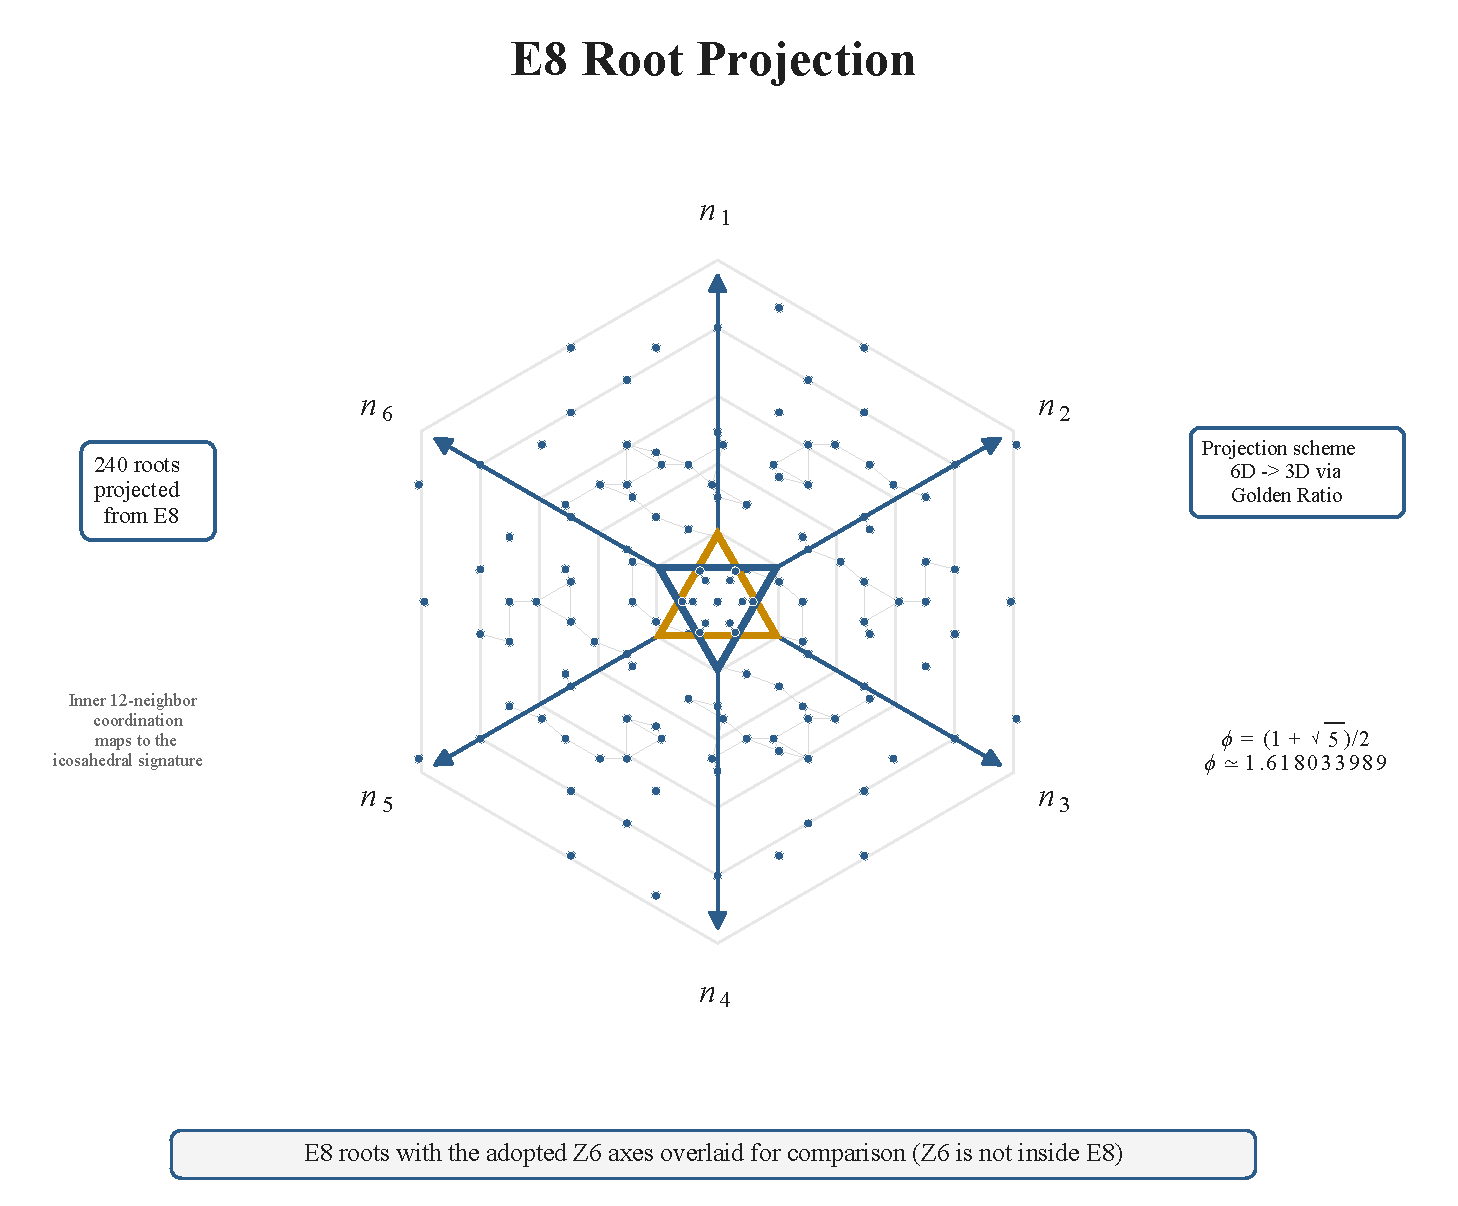
\includegraphics[keepaspectratio,alt={Comparison figure: a golden-ratio two-dimensional projection of the 240 E8 roots, with the six primitive hypercubic directions of the adopted \textbackslash mathbb\{Z\}\^{}6 overlaid for comparison. The overlay is not a sublattice relation: D\_6\textbackslash subset\textbackslash mathbb\{Z\}\^{}6, and \textbackslash mathbb\{Z\}\^{}6 has norm-1 vectors and does not embed in the even lattice E\_8 (§1.2.1). The inner twelve-neighbor coordination maps to the icosahedral signature of the physical projection. Tier 1 projection geometry; Tier 1/2 architectural reading}]{content/Figures/Volume_2/Figure V2.1.1.pdf}}
\caption{Comparison figure: a golden-ratio two-dimensional projection of
the 240 E8 roots, with the six primitive hypercubic directions of the
adopted \(\mathbb{Z}^6\) overlaid for comparison. The overlay is not a
sublattice relation: \(D_6\subset\mathbb{Z}^6\), and \(\mathbb{Z}^6\)
has norm-1 vectors and does not embed in the even lattice \(E_8\)
(§1.2.1). The inner twelve-neighbor coordination maps to the icosahedral
signature of the physical projection. Tier 1 projection geometry; Tier
1/2 architectural reading}
\end{figure}

\subsubsection{1.1.2 The Need for Higher
Dimensions}\label{the-need-for-higher-dimensions}

The parent space \(\mathbb{R}^6\) in which the lattice is embedded
possesses a strictly \textbf{Euclidean Signature} \((+,+,+,+,+,+)\). The
distance between any two lattice points \(\mathbf{n}\) and
\(\mathbf{m}\) is given by the standard Euclidean norm:
\[d^2 = \sum_{i=1}^6 (n_i - m_i)^2\]

\textbf{Theorem 1.1 (Euclidean Stability Ansatz for the Parent; formerly
``Euclidean Necessity'') {[}label kept for reference stability; Tier 2
--- conditional architectural argument under the static-lattice ansatz,
not a necessity result; cf.~the conditional Proposition FTH.2, App FTH
§FTH.2{]}:} \emph{Under the static-lattice ansatz, the embedding space
of the fundamental parent lattice is taken to be Riemannian (Euclidean)
rather than Lorentzian so that the vacuum ground state is bounded
below.}

\gctneedspace{5\baselineskip}

\textbf{Argument:} Suppose the parent space possessed a Lorentzian
signature (e.g., five spatial and one temporal dimension in 6D). The
declared static-lattice ansatz takes the vacuum to be a static,
minimum-energy configuration (the Hamiltonian constraint
\(\hat{H}\Psi = 0\) alone does not impose this). Under that ansatz, an
indefinite quadratic deformation energy would not define the required
bounded ground-state functional without additional constraints
(displacements along the time-like axis would enter with the opposite
sign, the standard route to \textbf{Tachyonic Instabilities}). The model
therefore adopts a positive-definite parent metric. The emergence of a
Lorentzian low-energy causal structure is treated separately in the
acoustic-metric construction (Chapter 8). Volume 1 Chapter 12 supplies
formal relational/ordinal-clock bookkeeping only; it does not derive a
physical Selection Operator's ordinality or phenomenal time.

\subsubsection{1.1.3 The Unit Cell (The Planck
Scale)}\label{the-unit-cell-the-planck-scale}

The lattice constant of the parent space, \(a_6\), defines the
fundamental resolution of the Operating System. We define the 6D lattice
spacing \(a_6\) as the primitive length unit (\(a_6 \equiv 1\) in
lattice units). The SI value of \(a_6\) (the manuscript convention is
\(a_6 = 2\ell_P\), App DPS §DPS.7) is obtained only after choosing ONE
dimensional calibration anchor (see Appendix ULA.6).

The 6-dimensional unit cell is a hypercube with a volume
\(V_{cell} = a_6^6 = 64\,\ell_P^6\) under the convention
\(a_6 = 2\ell_P\) {[}Tier 3 --- follows from the Planck-scale
calibration of \(a_6\) discussed heuristically in §1.1.4{]}. This
hyper-volume represents the \textbf{Informational Pixel} of the
universe. Within the GCT substrate, ``Information'' is defined by the
\textbf{Topological Winding State} of each node. Each lattice site is
modelled as a binary register (Presence/Absence) {[}Tier 3 modelling
choice{]}, so it carries at most one bit (\(\ln 2\) nats) of structural
information. This discreteness keeps the information content of any
finite volume finite; because it scales with volume, it is not by itself
compatible with the holographic area bound (§1.1.4).

\subsubsection{1.1.4 The Planck-Scale Calibration {[}Tier 3 heuristic;
the Planck link inherits the Tier 4 conjecture
O.14{]}}\label{the-planck-scale-calibration-tier-3-heuristic-the-planck-link-inherits-the-tier-4-conjecture-o.14}

Identifying the lattice constant with the Planck scale is a calibration
choice, not a requirement. The heuristic motivation (Volume 1, Chapter
13, ``Information Saturation'') is that the Planck length is the scale
at which the Compton and Schwarzschild lengths of a single localized
excitation coincide up to a factor of order one; the ``strain energy of
a bit'' in that picture is not defined by the present action.

Two considerations bound the choice only loosely. A lattice constant far
above \(\ell_P\) could produce dispersion observable at accessible
energies; how strong that bound is depends on the order of the
Lorentz-violating terms, which is itself a Tier 3 assumption (V2 Ch08
§8.3.5). The holographic bound does not select the Planck scale either:
one bit per cell gives an information content that grows with volume,
\(\sim(L/a_6)^3\), and this exceeds the holographic area bound
\(\sim(L/\ell_P)^2\) once \(L > a_6^3/\ell_P^2\), that is, for every
macroscopic region when \(a_6\) is of order \(\ell_P\). Reconciling
volume counting with an area law needs a separate argument (cf.~the
screen counting of Ch09 §9.1.6). The Planck scale is therefore adopted
as the model's UV cutoff by calibration; it is not shown to be unique or
forced.

\begin{center}\rule{0.5\linewidth}{0.5pt}\end{center}

\subsection{1.2 Symmetry and Roots}\label{symmetry-and-roots}

\subsubsection{\texorpdfstring{1.2.1 The \(D_6\) and \(E_8\)
Connection}{1.2.1 The D\_6 and E\_8 Connection}}\label{the-d_6-and-e_8-connection}

While the adopted primitive lattice \(P\cong\mathbb{Z}^6\) provides the
coordinate module for the 3D projection, GCT also uses the distinct
McKay \(2I\to E_8\) and Elser--Sloane \(E_8\to H_4\) correspondences as
a conditional higher-symmetry architecture. Those results do not make
\(\mathbb Z^6\) a sublattice of \(E_8\) and do not select the primitive
Bravais type.

Within this framework, the vacuum coordinates are often restricted to
the \textbf{\(D_6\) Root Lattice} (the ``checkerboard'' lattice) to
satisfy the requirements of the open Tier 3 \(SU(3)\) color candidate
(Volume 3). \(D_6\) consists of all points in \(\mathbb{Z}^6\) such that
the sum of the coordinates is even. This constraint ensures that the
``Winding transfer'' between nodes (candidate gluon dynamics) remains
parity-consistent.

The exact six-dimensional relation is {[}Tier 1 lattice algebra;
physical sector assignment Tier 3{]}:
\[D_6 = \{ \mathbf{n} \in \mathbb{Z}^6 : \sum_{i=1}^6 n_i \equiv 0 \pmod{2} \} \subsetneq \mathbb{Z}^6,\qquad [\mathbb Z^6:D_6]=2.\]
The roots \(\{\pm e_i\pm e_j\}\) generate \(D_6\), not \(\mathbb Z^6\).
The latter has norm-one vectors and therefore cannot embed isometrically
as a lattice in the even \(E_8\) lattice. Here \(D_6\) is used for the
face-centred/color-parity sector and \(\mathbb{Z}^6\) for the adopted
primitive coordination lattice used in lepton and phason dynamics. App
USS §USS.7 gives the separate \(E_8\to H_4\) projection and rank-six
Bravais classification.

The icosahedral reflection group \(H_3\) that GCT assigns to the 3D
substrate is a subgroup of the Weyl groups of these higher-dimensional
root systems; its rotational subgroup is \(H_3^+\cong A_5\). App USS
records \(A_5\) as the Tier 1/2 architectural premise H1 and derives
conditional Schur-cover and McKay consequences; it does not prove
point-group uniqueness or eliminate other spinorial point groups. The
associated Golden Ratio slope is the primary Diophantine candidate for
suppressing phason-locking, with global entropy-functional maximality
still open.

\subsubsection{1.2.2 The Voronoi
Decomposition}\label{the-voronoi-decomposition}

To define the geometry of the ``Atomic Surface'' (The Acceptance
Window), we must examine the \textbf{Voronoi Cell} of the
\(\mathbb{Z}^6\) lattice. A Voronoi cell is the region of space
surrounding a node containing all points closer to that node than to any
other. For a hypercubic lattice, the Voronoi cell is itself a \textbf{6D
Hypercube}.

The complexity of our 3D physics arises not from the Voronoi cell's
shape in 6D, which is simple, but from its \textbf{Projection}. When the
6D hypercubic unit cell is projected into the internal perpendicular
space (\(E_\perp\)), it forms a \textbf{Rhombic Triacontahedron} (RT).
As we shall see in Chapter 2, it is the icosahedral symmetry of this RT
window that filters the 6D periodic data into the rich, aperiodic
spectrum of matter and forces we observe.

\subsubsection{1.2.3 Hyperspace
Crystallography}\label{hyperspace-crystallography}

The 6D parent lattice is perfectly periodic in its native space. In its
own frame, it would exhibit standard crystalline diffraction. However,
because our physical manifold (\(E_\parallel\)) is an \textbf{Irrational
Slice} of this space, that periodicity is suppressed.

This is the origin of \textbf{Quasicrystalline Order}. The 3D vacuum
possesses ``Long-Range Orientational Order'' but no ``Translational
Symmetry.''

\begin{itemize}
\tightlist
\item
  \textbf{Bragg Peaks:} Like a crystal, the vacuum produces sharp
  diffraction spots in momentum space, which GCT proposes as the origin
  of quantized mass and charge (Volume 3) {[}Tier 3 proposal{]}.
\item
  \textbf{Forbidden Symmetry:} In the model the vacuum exhibits 5-fold
  (icosahedral) symmetry, which is mathematically forbidden for any
  periodic 3D lattice.
\item
  \textbf{Experimental Foundation:} The discovery of quasicrystals
  (Shechtman et al., 1984) showed that long-range order without
  periodicity exists in matter (the original Al--Mn phase was
  metastable; thermodynamically stable icosahedral phases were found
  later). GCT extends this kind of order to the vacuum itself as its
  architectural premise P1 {[}Tier 1/2 premise{]}. In the model, the
  ``graininess'' of the universe is not random noise but the organized,
  aperiodic signature of the 6D hyper-lattice.
\end{itemize}

\begin{figure}
\centering
\pandocbounded{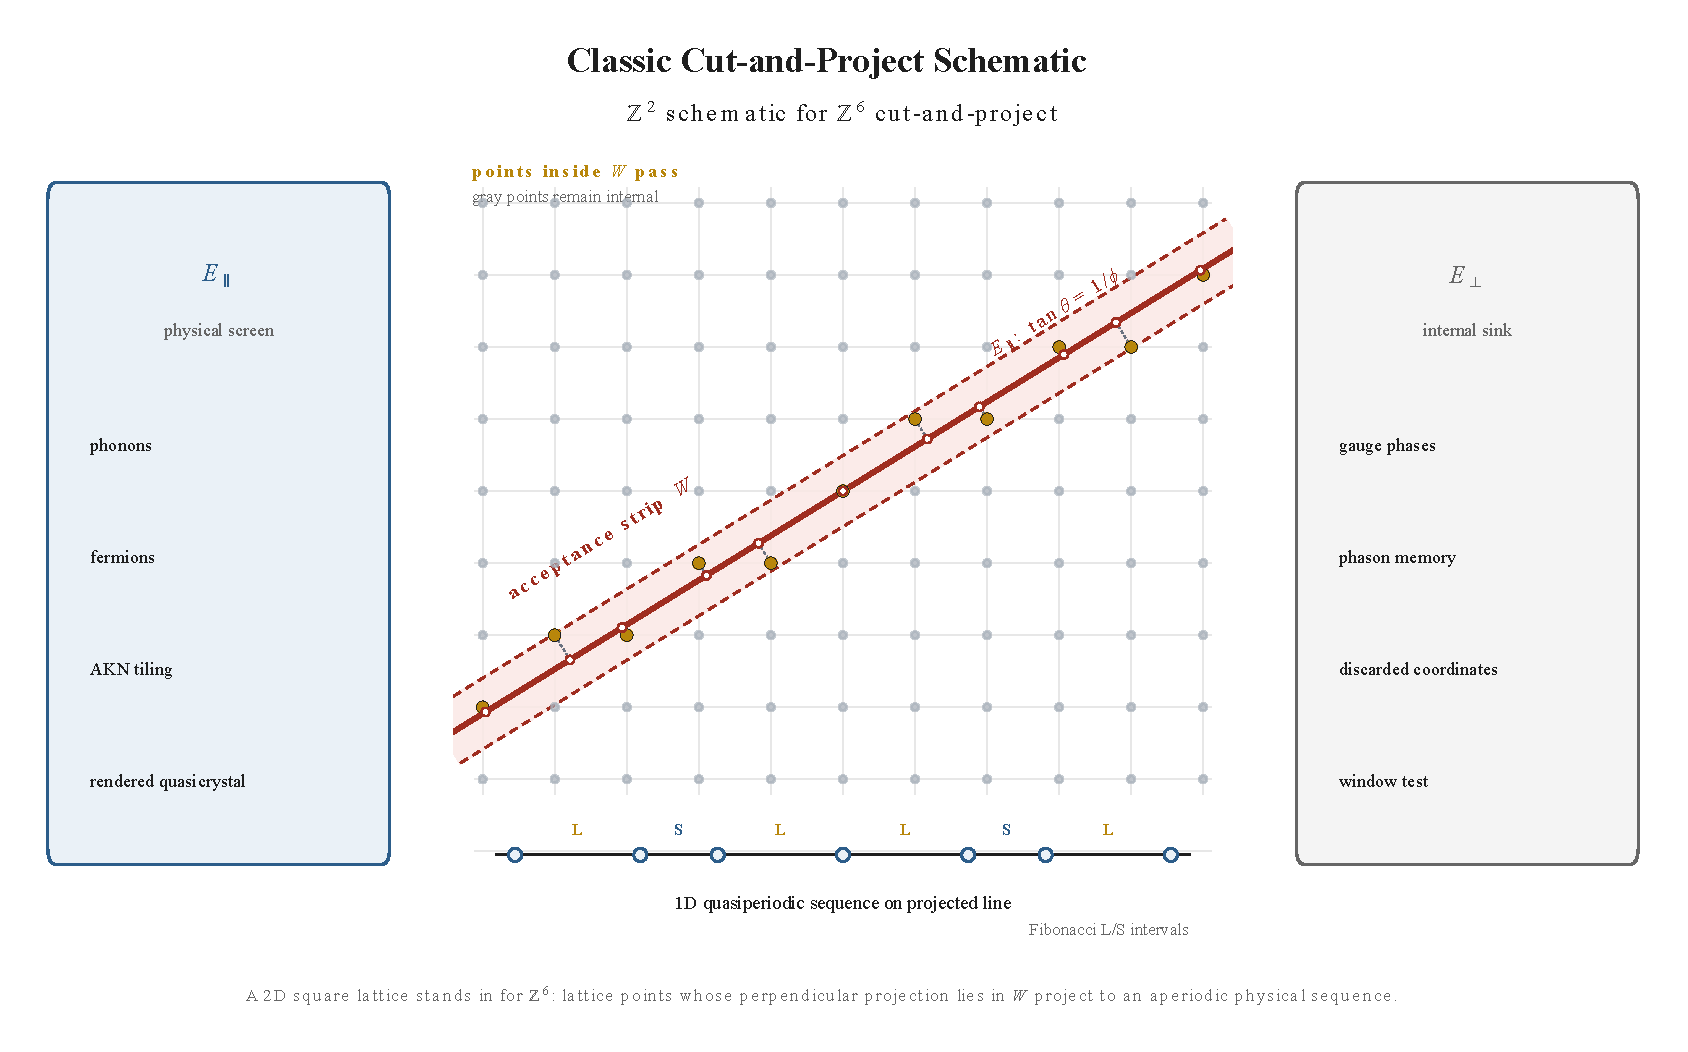
\includegraphics[keepaspectratio,alt={The cut-and-project construction: a two-dimensional square lattice stands in for the \textbackslash mathbb\{Z\}\^{}6 parent. Lattice points whose perpendicular projection falls within the acceptance strip W project onto the physical line E\_\textbackslash parallel (slope \textbackslash tan\textbackslash theta = 1/\textbackslash phi), yielding an aperiodic Fibonacci sequence of long and short intervals; the discarded coordinates form the internal sink E\_\textbackslash perp.}]{content/Figures/Volume_2/Figure V2.1.2.pdf}}
\caption{The cut-and-project construction: a two-dimensional square
lattice stands in for the \(\mathbb{Z}^6\) parent. Lattice points whose
perpendicular projection falls within the acceptance strip \(W\) project
onto the physical line \(E_\parallel\) (slope \(\tan\theta = 1/\phi\)),
yielding an aperiodic Fibonacci sequence of long and short intervals;
the discarded coordinates form the internal sink \(E_\perp\).}
\end{figure}

\chapter{Chapter 2: The Projective
Geometry}\label{chapter-2-the-projective-geometry}

The transition from the six-dimensional parent lattice to the
three-dimensional manifold of experienced reality is not a loss of
information, but a structured rendering. In this chapter, we detail the
mathematical mechanics of the \textbf{Cut-and-Project Formalism}, the
geometric process that filters the periodic complexity of
\(\mathbb{Z}^6\) into the isotropic, aperiodic vacuum of our universe.

\begin{center}\rule{0.5\linewidth}{0.5pt}\end{center}

\subsection{2.1 The Cut-and-Project
Formalism}\label{the-cut-and-project-formalism}

\subsubsection{\texorpdfstring{2.1.1 The Projection Matrices {[}Tier 2
conditional on primitive-\(P\)
adoption{]}}{2.1.1 The Projection Matrices {[}Tier 2 conditional on primitive-P adoption{]}}}\label{the-projection-matrices-tier-2-conditional-on-primitive-p-adoption}

For the adopted primitive Bravais lattice \(P\cong\mathbb Z^6\), we
decompose the parent space \(\mathbb{R}^6\) into two orthogonal,
3-dimensional subspaces: the \textbf{Parallel Space} (\(E_\parallel\),
the physical manifold) and the \textbf{Perpendicular Space}
(\(E_\perp\), the internal manifold). The displayed matrices give the
standard icosahedral orientation of that rank-six module. They do not
derive the primitive-\(P\) choice from the \(D_6\) roots; the
face-centred \(F\cong D_6\) and body-centred \(I\cong D_6^*\) Bravais
alternatives remain distinct classified lattices.

We define the projection matrix \(\mathcal{M}_\parallel\) such that it
maps the six basis vectors of \(\mathbb{Z}^6\) to the vertices of an
icosahedron in \(E_\parallel\). Implementing the standard orientation
(aligned with the 5-fold axes), the matrix is:

\[
\mathcal{M}_\parallel = N_\parallel \begin{pmatrix}
1 & 1 & 0 & 0 & \phi & \phi \\
\phi & -\phi & 1 & 1 & 0 & 0 \\
0 & 0 & \phi & -\phi & 1 & -1
\end{pmatrix}
\]

The internal projection matrix \(\mathcal{M}_\perp\) is its orthogonal
complement, generated by the Galois conjugation
\(\phi \to \phi' = -1/\phi\):

\[
\mathcal{M}_\perp = N_\perp \begin{pmatrix}
1 & 1 & 0 & 0 & -\phi^{-1} & -\phi^{-1} \\
-\phi^{-1} & \phi^{-1} & 1 & 1 & 0 & 0 \\
0 & 0 & -\phi^{-1} & \phi^{-1} & 1 & -1
\end{pmatrix}
\]

\gctneedspace{5\baselineskip}

\textbf{Normalization and Isometry {[}Tier 1 linear algebra, given the
adopted frame{]}:} The two raw row frames have different norms: each
parallel row has squared norm \(2(2+\phi)\), each perpendicular row
\(2+2\phi^{-2}=2(3-\phi)\). One common scalar therefore cannot make both
maps isometric. The inherited Euclidean metric fixes \[
N_\parallel=\frac{1}{\sqrt{2(2+\phi)}},\qquad
N_\perp=\frac{1}{\sqrt{2(3-\phi)}}=\phi N_\parallel .
\] With these normalizations, \[
\mathcal{M}_\parallel\mathcal{M}_\parallel^T
=\mathcal{M}_\perp\mathcal{M}_\perp^T=I_3,\qquad
\mathcal{M}_\parallel\mathcal{M}_\perp^T=0,\qquad
\mathcal{M}_\parallel^T\mathcal{M}_\parallel+
\mathcal{M}_\perp^T\mathcal{M}_\perp=I_6.
\] These are Tier 1 linear-algebra identities once the Euclidean
\(\mathbb{R}^6=E_\parallel\oplus E_\perp\) premise and the
primitive-\(P\) frame are fixed. The earlier common-\(N\) form,
\(N=1/\sqrt{2(2+\phi)}\) for both matrices, normalized only the parallel
rows (it gives \(\mathcal{M}_\perp\mathcal{M}_\perp^T=\phi^{-2}I_3\))
and is superseded.

\gctneedspace{5\baselineskip}

\textbf{Proof of Orthogonality (Tier 1):} For the row spaces to be
orthogonal, the projection matrices must satisfy
\(\mathcal{M}_\parallel \mathcal{M}_\perp^T = \mathbf{0}\). We verify
this by computing the dot product of the first rows:
\[ \mathbf{r}_{\parallel 1} \cdot \mathbf{r}_{\perp 1} \propto (1)(1) + (1)(1) + (0)(0) + (0)(0) + (\phi)(-\phi^{-1}) + (\phi)(-\phi^{-1}) \]
\[ = 2 - 2(\phi \cdot \phi^{-1}) = 2 - 2(1) = 0 \] By symmetry, all row
products vanish. This establishes the kinematic orthogonality of phonon
(\(E_\parallel\)) and phason (\(E_\perp\)) coordinates. Dynamical
decoupling at quadratic order additionally requires the action to
contain no permitted phonon--phason cross-coupling; it does not follow
from row orthogonality alone. Reading the phason sector as carrying an
observer's internal mental state is a separate Tier 3/4 bridge
hypothesis that this algebra does not supply.

\subsubsection{2.1.2 The Variational Selection Problem {[}Tier 1/2
postulate; finite diagnostic
only{]}}\label{the-variational-selection-problem-tier-12-postulate-finite-diagnostic-only}

The most critical parameter of the projection is the \textbf{Slope} of
the \(E_\parallel\) slice. We formulate a finite-height diagnostic for
the \textbf{Icosahedral Selection Postulate}, rather than a completed
selection theorem.

\gctneedspace{5\baselineskip}

\textbf{The Finite-Height Objective \(J_R(\mathbf{\Omega})\):} To
diagnose resistance to low-height rational (``phason'') locking, define
\[
J_R(\mathbf{\Omega})=
\min_{\substack{\mathbf n\in\mathbb Z^6\\
0<\|\mathbf n\|_\infty\le R}}
\left\|\widehat{\mathcal{M}}_\perp(\mathbf{\Omega})\mathbf n\right\|,
\] where \(\widehat{\mathcal{M}}_\perp\) has orthonormal rows for every
candidate orientation. Without this row normalization, \(J_R\) changes
under an arbitrary rescaling of internal coordinates and cannot compare
different slopes.

The unbounded functional
\(J(\mathbf{\Omega})=\min_{\mathbf n\in\mathbb Z^6\setminus\{0\}}|\mathcal{M}_\perp(\mathbf{\Omega})\mathbf n|\)
used in earlier drafts is not a usable objective: for any totally
irrational rank-\(6\to3\) cut-and-project map (such as the icosahedral
one), \(\mathcal{M}_\perp\mathbb Z^6\) is dense in \(E_\perp\), so this
quantity is identically zero (its infimum is \(0\) and no positive
minimum exists). A genuine asymptotic selection theorem would require a
height-weighted Diophantine/Markov-type functional; \(J_R\) is only a
finite diagnostic {[}Tier 1 for the density statement{]}.

\gctneedspace{5\baselineskip}

\textbf{Postulate 2.1 (The Icosahedral Selection):} \emph{The
orientation \(\mathbf{\Omega}\) of the 3D slice is postulated to
coincide with the icosahedral projection utilizing the Golden Ratio
(\(\phi\)) slope. This state provides a high ``Diophantine Gap,''
ensuring the continuous fluidity of the phason field.}

Deriving the \(\phi\)-slope as the optimizer of a properly defined
asymptotic functional over all 3-planes remains open. Its adoption
within GCT is motivated by the resulting icosahedral symmetry and by
consistency with observed point-group selection in nature.
\textbf{Hurwitz's Theorem} makes \(\phi\) the canonical one-dimensional
badly approximable benchmark; it does not by itself prove optimality of
this 3-plane in \(\mathbb R^6\) or make it a thermodynamic ground state.

\begin{quote}
\textbf{Finite-scan status.} The engine's five-candidate scan
(\texttt{protocol\_phi\_selection.py}: \(\phi\), silver ratio, bronze
ratio, \(\pi\), and the rational control \(3/2\)) ranks \(\phi\) first
at its default height \(R=3\), with or without row normalization. The
ordering is truncation-sensitive: at \(R=2\) the silver ratio and the
rational control score higher than \(\phi\), and at \(R=4\) the silver
and bronze ratios do. The scan is therefore diagnostic support for
Postulate 2.1, not a uniqueness proof or closure of the global
optimization problem.
\end{quote}

\subsubsection{\texorpdfstring{2.1.3 The Acceptance Window
\(W(\mathbf{x}_\perp)\)}{2.1.3 The Acceptance Window W(\textbackslash mathbf\{x\}\_\textbackslash perp)}}\label{the-acceptance-window-wmathbfx_perp}

Projecting every node of the 6D lattice into 3D would result in a dense,
featureless continuum. To generate the discrete ``pixelation'' of
reality, the Operating System applies a selection rule defined by the
\textbf{Acceptance Window} \(W\).

The window is a specific geometric volume within the perpendicular space
\(E_\perp\). A 6D lattice point \(\mathbf{r}_6\) ``exists'' in our
physical 3D world if and only if its projection into the internal space
falls within this window:
\[\Phi_0 = \{ \mathcal{M}_\parallel \mathbf{r}_6 \mid \mathcal{M}_\perp \mathbf{r}_6 \in W \}\]

\gctneedspace{5\baselineskip}

\textbf{The Rhombic Triacontahedron (RT) {[}Tier 2{]}:} In the
icosahedral quasicrystal (the Ammann-Kramer-Neri tiling), the window
\(W\) is the projection of the \textbf{6D Unit Hypercube} into
\(E_\perp\). This projection yields the \textbf{Rhombic
Triacontahedron}, the convex zonohedron with full icosahedral symmetry
(\(I_h\)) bounded by 30 congruent golden rhombi (32 vertices, 60 edges;
the face, vertex and edge counts alone are shared by every six-generator
zonohedron in general position) {[}Tier 2 --- that the 6D hypercube
projects to the RT under the icosahedral \(\phi\)-slope is a theorem
given the icosahedral ansatz{]}. GCT proposes that its vertices carry
the Standard Model particle-generation candidate structure {[}Tier 3
proposal{]}: the 12 degree-5 vertices are proposed to correspond to the
Leptons and the 20 degree-3 vertices to the Quarks. The count 20 does
not by itself match a quark multiplet count, and the proposed mapping
from the RT vertex geometry to the fermion representations is developed
in Volume 3, Chapters 2--3. Its numerical coordinate volume is quoted in
the isometric \(E_\perp\) convention of §2.1.1. Under any
internal-coordinate change \(B\mapsto SB\), both the window and its
measure must transform together; the accepted \(\mathbb Z^6\) points and
the physical AKN tiling remain unchanged.

The RT window acts as the ``filter'' of reality. Its covariantly
normalized measure enters model-set (tile-density) calculations; an
absolute coordinate volume by itself is not a physical density
invariant, and it does not fix the matter density of the universe. Its
10 three-fold rotational axes are the input to the open Tier 3 \(SU(3)\)
colour candidate of V3 Ch03 (the resulting \(A_2\) closure is not
specific to these axes), while the weak-parity candidate developed in
Volume 3 cannot come from the window itself: the RT is centrosymmetric
(\(I_h\) contains the inversion), so its boundary is not chiral, and a
parity-odd candidate needs an independently defined chirality-breaking
operator, which remains open (App USS §USS.7, Remark T-McK.1b.A). Both
candidates carry the tier qualifications stated in Volume 3.

\subsubsection{2.1.4 The Cut-and-Project
Algorithm}\label{the-cut-and-project-algorithm}

The realization of the physical vacuum follows a deterministic four-step
algorithm executed by the \textbf{Realization Operator}
(\(\hat{\mathcal{R}}\)):

\begin{enumerate}
\def\labelenumi{\arabic{enumi}.}
\tightlist
\item
  \textbf{Selection:} Identify a candidate node \(\mathbf{r}_6\) in the
  6D parent lattice \(\mathbb{Z}^6\).
\item
  \textbf{Internal Mapping:} Project the node into the internal
  manifold: \(\mathbf{r}_\perp = \mathcal{M}_\perp \mathbf{r}_6\).
\item
  \textbf{Boundary Test:} Check the condition
  \(\mathbf{r}_\perp \in W\). If the node lies outside the Rhombic
  Triacontahedron, it is discarded from the physical render.
\item
  \textbf{Crystallization:} If the node passes, project it into the
  physical manifold:
  \(\mathbf{r}_\parallel = \mathcal{M}_\parallel \mathbf{r}_6\).
\end{enumerate}

This process generates the \textbf{Ammann-Kramer-Neri Tiling}, a 3D set
of nodes that possesses icosahedral symmetry and long-range order, yet
possesses no translational periodicity.

\begin{center}\rule{0.5\linewidth}{0.5pt}\end{center}

\subsection{2.2 Subspace Topology}\label{subspace-topology}

\subsubsection{\texorpdfstring{2.2.1 Parallel Space (\(E_\parallel\)):
``The
Screen''}{2.2.1 Parallel Space (E\_\textbackslash parallel): ``The Screen''}}\label{parallel-space-e_parallel-the-screen}

The Parallel Space is the 3D manifold of our physical experience. We
term it \textbf{``The Screen''} because it is the surface upon which the
6D holographic data is rendered. All observable particles and gauge
interactions are confined to this slice. At the scales of human biology
and standard atomic physics, the density of lattice nodes is so high
that \(E_\parallel\) appears as a smooth, continuous Euclidean space.
The ``graininess'' of the screen only becomes manifest at the Planck
energy.

\subsubsection{\texorpdfstring{2.2.2 Perpendicular Space (\(E_\perp\)):
``The
Sink''}{2.2.2 Perpendicular Space (E\_\textbackslash perp): ``The Sink''}}\label{perpendicular-space-e_perp-the-sink}

The Perpendicular Space is the ``hidden'' 3D manifold. We term it
\textbf{``The Sink''} because it holds the ``discarded'' degrees of
freedom from the 6D bulk and is proposed (Tier 4, Ch07 §7.2) as a
reservoir for the universe's entropy.

\begin{itemize}
\tightlist
\item
  \textbf{Phasons and Color:} While physical motion occurs in
  \(E_\parallel\), topological rearrangements (Phasons) and --- in the
  open Tier 3 colour candidate of V3 Ch03 --- the internal windings of
  quarks (Color) reside in \(E_\perp\).
\item
  \textbf{Entropy Reservoir {[}Tier 4 hypothesis{]}:} Chapter 7 (§7.2,
  Hypothesis 7.1, the Entropy Sequestration Hypothesis) proposes that
  latent heat released during the vacuum's crystallization (the Big
  Bang) was absorbed mainly by the \(E_\perp\) sector, so that the
  physical ``Screen'' stayed comparatively cool. No partition of entropy
  into \(E_\perp\) has been derived, and the cooling coefficient used
  there is stipulated. The hypothesis does not explain the observed CMB
  temperature (2.7 K, an observed input), which standard cosmology
  attributes to expansion redshift.
\end{itemize}

\subsubsection{2.2.3 The Complementary
Roles}\label{the-complementary-roles}

The two subspaces function in a state of \textbf{Stiffness
Partitioning}:

\begin{enumerate}
\def\labelenumi{\arabic{enumi}.}
\tightlist
\item
  \textbf{High-Stiffness Sector (\(E_\parallel\)):} Governed by the
  \textbf{Phonon Stiffness} (\(K_\parallel\)). It resists deformation
  with the full strength of the Planck scale, providing the rigid metric
  backbone of the universe.
\item
  \textbf{Low-Stiffness Sector (\(E_\perp\)):} Governed by the
  \textbf{Phason Stiffness} (\(K_\perp\)). Softness permits lower-energy
  internal rearrangements in the declared material model (the candidate
  light construction of Chapter 6). It does not by itself permit or
  derive steering by a Selection Operator.
\end{enumerate}

An independently derived \textbf{Phason-Phonon coupling} could transfer
energy and strain between the sectors. The manuscript does not show that
an Agent's choice creates a phason shift, that such a shift writes
matter/energy into \(E_\parallel\), or that intention controls the
coupling; those are Tier 3/4 bridge hypotheses.

\subsubsection{2.2.4 Local Isomorphism
Classes}\label{local-isomorphism-classes}

A common objection to aperiodic geometry is the problem of uniformity:
if space never repeats, shouldn't the laws of physics change from place
to place? GCT resolves this through the \textbf{Local Isomorphism
Theorem}:

\begin{itemize}
\tightlist
\item
  \emph{In an infinite icosahedral quasicrystal, any finite patch of
  tiles of radius \(R\) that appears once will appear infinitely many
  times throughout the entire tiling.} {[}Tier 1 --- a proven theorem of
  quasicrystal theory for this tiling; its use as the vacuum is
  contingent on the icosahedral projection ansatz{]}
\end{itemize}

Repetitivity alone does not give statistical uniformity; together with
uniform patch frequencies (unique ergodicity of the model set) it
supports the \textbf{Statistical Uniformity} of physical laws in the
model. Conditional on the lattice premise, an experiment performed on
Earth and one performed in a distant galaxy sample statistically
equivalent local lattice environments because the local configurations
are \textbf{Locally Isomorphic} {[}Tier 3 physical reading{]}. The
global topology of the universe is aperiodic, but the local rules are
invariant, providing the stability required for the Axiom of
Intelligibility.

\chapter{Chapter 3: The Supersolid Phase
Transition}\label{chapter-3-the-supersolid-phase-transition}

GCT adopts a discrete 6D parent lattice as its structural premise for an
intelligible universe (architectural postulate P1; not shown to be a
necessary condition), but geometry alone does not account for the
presence of energy, motion, or substance. In the GCT framework, the
``Big Bang'' is reinterpreted not as a singular explosion of matter into
a void, but as the \textbf{Crystallization of the Field}. This chapter
describes the proposed thermodynamic process by which the symmetric,
non-temporal potential of the Bulk undergoes a phase transition to
become the \textbf{Supersolid Quasicrystal} vacuum. The Landau,
Gross--Pitaevskii, supersolid, and defect language used here is an
effective-action completion {[}Tier 3/open{]}, not a consequence of the
logical axioms or of the literal Appendix ULA displacement Hamiltonian
by themselves.

\begin{center}\rule{0.5\linewidth}{0.5pt}\end{center}

\subsection{3.1 Spontaneous Symmetry
Breaking}\label{spontaneous-symmetry-breaking}

\subsubsection{3.1.1 The Landau-Ginzburg
Potential}\label{the-landau-ginzburg-potential}

The effective phase-transition branch begins from a hypothetical
homogeneous \textbf{Symmetric Phase} of the field \(\Psi\), with
continuous translational and rotational symmetry: no lattice, no
``pixelation.'' GCT then tests whether a broken phase can realize the
projected lattice architecture. The \textbf{Axiom of Intelligibility}
(Volume 1) motivates looking for an information-bearing phase but does
not determine a thermodynamic potential, a coefficient sign, or
spontaneous symmetry breaking.

A conditional \textbf{Landau-Ginzburg Free Energy Functional} describes
the energy density of the vacuum as a function of its order parameters.
Unlike a simple superfluid, the supersolid ansatz includes a term for
the lattice rigidity (phason strain):

\[F[\psi, \mathbf{w}] = \int d^3x \left[ \frac{\hbar^2}{2m}|\nabla\psi|^2 + V(|\psi|^2) + \frac{1}{2} K_\perp (\nabla \mathbf{w})^2 \right]\]

where \(\psi = \sqrt{\rho}\,e^{i\theta}\) is the macroscopic condensate
wavefunction (with \(|\psi|^2 = \rho\) carrying dimensions of number
density \([L^{-3}]\)), \(m\) is the effective mass of the condensate
constituents, and all three terms carry consistent dimensions of energy
density \([E \cdot L^{-3}]\). The kinetic term
\(|\nabla\psi|^2=(\nabla\sqrt\rho)^2+\rho(\nabla\theta)^2\) encodes both
the density-gradient term \((\nabla\rho)^2/(4\rho)\) and the
superfluid-velocity contribution \(\rho(\nabla\theta)^2\), unifying the
GP-style and Landau-style formulations. Here \(\mathbf w\) is a distinct
phason displacement. This ansatz is not yet derived from the node
displacements \(u_n\in\mathbb R^6\) of Appendix ULA.

The same bounded symmetry class permits a zero vacuum or a broken
vacuum. For example, \(V=r|\psi|^2/2+u|\psi|^4/4\) with \(u>0\) has a
zero minimum for \(r>0\) and a nonzero (``Mexican Hat'') minimum for
\(r<0\). Neither symmetry nor the Axiom of Intelligibility selects
\(r<0\), the radius, or \(K_\perp\); attributing the shift to a
``selection pressure of the Field'' is an interpretation, not a derived
mechanism. Even when \(r<0\) is adopted, zero amplitude remains
admissible at finite energy: the Mexican-hat minimum is a soft vacuum,
not a hard nonzero target {[}Tier 1 mathematics for the declared field
typing; physical branch Tier 3/open{]}. That the broken phase
``freezes'' the field into the 6D \(\to\) 3D lattice structure with
non-zero \(K_\perp\) is therefore a conditional scenario.

\gctneedspace{5\baselineskip}

\textbf{The Renormalization Group Route {[}Tier 2 canonical Coxeter
integer + Tier 3 RG-map link; Parameter Ledger §0.1 P3; Open Problem
O.15{]}}

The \(\phi^{-18}\) exponent uses two separable claims. The integer
\(D = 18\) is a \textbf{Tier 2 canonical Coxeter anchor}: it is the
\(H_3\) invariant-degree sum \(2 + 6 + 10\), with the rank 3 × Galois
degree 2 × dimension 3 count retained only as a 6D consistency mnemonic.
The physical RG-map step that turns this integer into the phason-elastic
stiffness exponent \(K_\perp/K_\parallel=\phi^{-18}\) remains
\textbf{Tier 3}, because no Lubensky-Ramaswamy-Toner-style or
Socolar-Lubensky-Steinhardt-style RG calculation in published
quasicrystal elasticity produces \(\phi^{-18}\) as a forced ratio.
First-principles closure of that RG-map link requires a genuine RG
derivation of the O.15 physical RG/elastic map. A chemically clean
analog-system measurement tests and constrains the Tier 3 physical-map
hypothesis; it does not itself close the derivational gap. This
distinction is \textbf{Open Problem O.15} (App ORQ §ORQ.5). The action
audit sharpens the problem: the lifted icosahedral representation admits
the two-parameter invariant quadratic form \(Q=aP_\parallel+bP_\perp\),
so symmetry leaves \(b/a\) free, and the isotropic nearest-neighbour
Hamiltonian of Appendix ULA selects \(a=b\), not \(\phi^{-18}\) (Chapter
4, §4.2.2).

The former claim that i-AlPdMn phason elastic measurements establish
\(K_\perp/K_\parallel \sim 10^{-2}\) to \(10^{-1}\), and hence a
100--1000× gap to the GCT ratio, is withdrawn, together with the retired
``chemical-bonding floor'' that was said to explain it. On the source
audit recorded in App DPS §DPS.4b, the de Boissieu (1995) and Francoual
(2006) papers report the phason-sector anisotropy \(K_2/K_1\) and
long-wavelength phason relaxation kinetics, not the registered P3b
scalar ratio, and the DFT reference once cited for the floor (DOI
10.1103/PhysRevB.88.144102) is a CaIrO\(_3\) post-perovskite study
unrelated to quasicrystals. The alloy data therefore neither confirm nor
falsify P3b. Reconciling GCT's scalar stiffness symbol with real
icosahedral-alloy data remains registered as \textbf{Open Problem O.41}
(App ORQ) and first requires a derived observable map.

\begin{quote}
\textbf{{[}Tier 2 integer anchor + Tier 3 RG-map link{]}} The integer
\(D=18\) in \(K_\perp/K_\parallel = \phi^{-18}\) is the canonical
\(H_3\) Coxeter invariant-degree sum \(2+6+10\) (Tier 2 structural
anchor). The step assigning one \(\log\phi\) contribution per invariant
degree in the phason-elastic RG flow is the open Tier 3 link tracked
under \textbf{Open Problem O.15}; the existing RG protocol assumes that
premise rather than deriving the anomalous dimensions. The supporting
motivations --- cube of the Gram determinant ratio, rank × Galois degree
× dimension counting, and 9-channels-squared from icosahedral irrep
counts --- are consistency heuristics, not independent first-principles
RG derivations; the Gram-cube form is in fact a normalization artefact
(Chapter 4, §4.2.2). \textbf{{[}Tier 3 P3b / O.15(b){]}} The
\emph{identification} of \(\phi^{-18}\) with the physical phason/phonon
stiffness ratio is an independent action/RG hypothesis. It is not
entailed by the icosahedral selection axiom or by the normalized
projectors. Like H-EW, it is a registered Tier 3 hypothesis listed
outside the core parameter count; only the integer \(D=18\) is Tier 2.
\textbf{{[}Tier 2 action-level obstruction{]}} Icosahedral invariance
permits independent positive coefficients on the two inequivalent 3D
sectors. Consequently, an action/RG closure must add and derive dynamics
that select their ratio; no symmetry-only calculation can close P3b.
These tiers must not be conflated.
\end{quote}

\subsubsection{3.1.2 The Order Parameters}\label{the-order-parameters}

The vacuum condensate is characterized by two distinct, coupled order
parameters that define its lattice dynamics:

\begin{enumerate}
\def\labelenumi{\arabic{enumi}.}
\tightlist
\item
  \textbf{Crystalline Density (\(\rho\)):} This represents the amplitude
  of the matter condensate. It corresponds to the breaking of
  \textbf{Translational Symmetry}. When \(\rho\) becomes non-zero and
  periodic (or quasi-periodic), the ``pixels'' of space light up. This
  is the ``Solid'' aspect of the vacuum.
\item
  \textbf{Superfluid Phase (\(\theta\)):} This represents the global
  \(U(1)\) phase degree of freedom. It corresponds to the breaking of
  \textbf{Global Phase Symmetry}. The phase \(\theta\) allows for the
  existence of coherent quantum states and the flow of probability
  current. This is the ``Fluid'' aspect of the vacuum.
\end{enumerate}

Together, they form the candidate macroscopic vacuum field
\(\Psi_{vac} = \sqrt{\rho} e^{i\theta}\). This complex \(U(1)\)
condensate is not identical to the real \(H_3\) phason triplet
\(\mathbf w=P_\perp u\).

\subsubsection{3.1.3 Supersolidity Conditions {[}Tier 1 definition +
Tier 3 GCT
realization{]}}\label{supersolidity-conditions-tier-1-definition-tier-3-gct-realization}

The GCT completion proposes that the vacuum is neither a simple crystal
nor a simple fluid, but a \textbf{Supersolid}. By definition, such a
phase simultaneously exhibits two broken symmetries:

\begin{itemize}
\tightlist
\item
  \textbf{Diagonal Long-Range Order:} The nodes are fixed in a rigid
  lattice (Solid), governed by the locking potential of the
  quasicrystal.
\item
  \textbf{Off-Diagonal Long-Range Order:} The phase is coherent across
  the lattice, allowing for frictionless flow (Superfluid).
\end{itemize}

\textbf{Conditional Criterion 3.1 (Vacuum Supersolidity):} the
6D\(\to\)\hspace{0pt}3D projection supplies quasiperiodic crystalline
order, but the irrational \(\phi\)-slope alone does not imply
off-diagonal long-range order, nonzero superfluid stiffness, or phase
coherence. Vacuum supersolidity closes only when a normalized many-body
ground state or action derives both orders. Its use elsewhere in the
manuscript is therefore a Tier 3 physical premise, not a theorem of
cut-and-project geometry.

If realized, a supersolid vacuum would be both \textbf{Rigid}
(supporting elastic structure) and phase-coherent; the
rigidity/coherence pairing does not by itself account for entanglement
or nonlocal correlations, which in this manuscript remain the ordinary
quantum-mechanical ones.

\subsubsection{3.1.4 The Mexican Hat
Potential}\label{the-mexican-hat-potential}

The crystallization process settles the Field into the ``rim'' of the
Mexican Hat potential. This geometry defines the two fundamental modes
of the vacuum's ``vibration'':

\begin{enumerate}
\def\labelenumi{\arabic{enumi}.}
\tightlist
\item
  \textbf{Massive Mode (The Higgs Field):} Radial oscillations
  (\(\delta \rho\)) within the well. Moving ``up'' the walls of the
  potential represents a compression or dilation of the lattice density.
  GCT proposes identifying this volume-dilation mode with the
  \textbf{Higgs Boson} {[}Tier 3 proposal{]}, responsible for setting
  the energy scale of the vacuum rigidity (detailed in Volume 3, Chapter
  5).
\item
  \textbf{Phase Mode (Goldstone; candidate photon component):} Angular
  oscillations (\(\delta \theta\)) around an exact continuous \(U(1)\)
  rim are Goldstone modes; moving ``around'' such a rim costs zero
  potential energy. A finite \(H_3\) orbit, by contrast, is
  zero-dimensional and has no Goldstone tangent, so genuine \(H_3\)
  locking lifts any accidental angular degeneracy of a radial phason
  potential. In a supersolid, a phase mode may couple to the lattice
  elasticity to form the hybrid excitation known as \textbf{Second
  Sound}. In the separate GCT gauge-mechanism reading, the photon is
  modeled as the electromagnetic component of this phase-lattice
  synchronization mode. That identification is the Tier 3 declared open
  programme of V2 Ch06 §6.1 (no Tier 2 mechanism is claimed), not a
  derivation of Maxwell electrodynamics.
\end{enumerate}

\begin{quote}
\textbf{Scope:} The phason-to-electromagnetic-gauge-field identification
is developed in \textbf{Appendix ULA (The Unified Lattice Action)} as a
Tier 3 declared open programme (V2 Ch06 §6.1: the
\(E_\perp\to E_\parallel\) identification is not \(I_h\)-equivariant,
and the locking potential gaps the identified mode). Full Maxwell/QED
closure, including derivation of the antisymmetric Maxwell kinetic term,
the two-polarization gauge redundancy, physical gauge fixing, and
matter-current coupling, remains tracked under Open Problem O.15 rather
than asserted here.
\end{quote}

\begin{center}\rule{0.5\linewidth}{0.5pt}\end{center}

\subsection{3.2 The Vacuum Condensate}\label{the-vacuum-condensate}

\subsubsection{3.2.1 The Gross-Pitaevskii
Description}\label{the-gross-pitaevskii-description}

The conditional condensate completion may be modeled by the
\textbf{Gross-Pitaevskii (GP) Equation}, a non-linear Schrödinger
equation that describes the evolution of a Bose-Einstein condensate:

\[i\hbar\frac{\partial\Psi}{\partial t} = \left[-\frac{\hbar^2}{2m}\nabla^2 + V_{lock}(\mathbf{x}) + g|\Psi|^2\right]\Psi\]

Here \(V_{lock}(\mathbf{x})\) is an effective external potential
representing the 6D parent lattice, which breaks translational
invariance. A stationary (``quiescent'') solution and its healing length
are conditional on the added condensate dynamics and normalization; they
are not generated by the symbolic Appendix ULA locking term alone. The
GP healing length of such a condensate is
\(\xi_{GP}=\hbar/\sqrt{2mgn}\); it depends on the added condensate
parameters, which are not fixed here.

\gctneedspace{5\baselineskip}

\textbf{The polaron length scale (formerly labelled a theorem) {[}Tier 1
arithmetic; identification Tier 3{]}} The length used in the polaron
section is the Bohr--Compton combination
\[ \xi = \frac{\hbar c}{\alpha^2 m_e c^2} = \frac{a_0}{\alpha} \approx 7.25 \text{ nm}\]
that is, \(\xi = a_0/\alpha \approx 7.25\) nm {[}Tier 1 arithmetic; its
identification as the vacuum/polaron healing length is Tier 3{]}. It
does not follow from the GP equation above. Both CODATA \(\alpha\) and
GCT bare \(\alpha\) inputs give the same \(\xi\) value at the percent
level (\texttt{verify\_independent/verify\_healing\_length.py}). App ORQ
O.25 records that the tested GCT phason-elastic substitution chain gives
a Planck-scale length rather than this nanometre scale, so the
identification is not derived. The GCT-specific empirical content is the
Tier 3 biological-scale match: the polaron diameter
\(2\xi \approx 14.5\) nm fits the microtubule lumen inner diameter
(\(\sim 15\)--\(17\) nm), a \(3\)--\(17\%\) fit.

\subsubsection{3.2.2 The Kibble-Zurek
Mechanism}\label{the-kibble-zurek-mechanism}

If a source-derived transition, vacuum manifold, quench rate, and causal
dynamics are supplied, the transition from the symmetric phase to the
crystalline vacuum need not happen everywhere at once. Because the
``Speed of Causality'' (\(c\)) is finite, different regions would
crystallize independently, and according to the \textbf{Kibble-Zurek
Mechanism}, independent domains cannot always merge smoothly when they
meet.

The mismatches at the domain boundaries create candidate
\textbf{Topological Defects}. GCT investigates whether such defects can
realize \textbf{Matter}---the picture of matter as the ``scar tissue''
of space freezing {[}Tier 3 physical proposal{]}---but their topology
and stability must be checked in the full admissible target space. For
the literal displacement action of Appendix ULA the node variables take
values in the contractible space \(\mathbb R^6\), so a normalized phason
texture can pass through \(P_\perp u=0\) at finite energy and is not
topologically protected there. Exact-lattice pinning or metastability
remains open, but electron permanence and conservation do not follow
from Kibble--Zurek language alone.

\subsubsection{3.2.3 The Inflation Alternative {[}Tier
4{]}}\label{the-inflation-alternative-tier-4}

Standard cosmology utilizes the \textbf{Inflation Hypothesis} (an
exponential expansion of 3D space) to explain why the universe looks the
same in all directions (the Horizon Problem). GCT asks whether a
\textbf{Geometric Alternative} exists {[}Tier 4 hypothesis{]}.

The earlier form of this argument, that points billions of light-years
apart in \(E_\parallel\) were adjacent and connected in the 6D parent
space, is withdrawn: orthogonal projection never increases distance
(\(|\Delta\mathbf r_6|^2=|\Delta\mathbf r_\parallel|^2+|\Delta\mathbf r_\perp|^2\ge|\Delta\mathbf r_\parallel|^2\),
from the completeness identity of §2.1.1), so points far apart in
\(E_\parallel\) are at least as far apart in \(\mathbb{R}^6\).

\begin{itemize}
\tightlist
\item
  \textbf{Connectivity:} Metric adjacency in \(\mathbb{R}^6\) cannot
  remove the horizon. A horizon argument would need an explicit
  \(E_\perp\)-mediated coupling or a non-metric connectivity between
  distant regions, which has not been supplied.
\item
  \textbf{Flatness:} A planar slice of Euclidean \(\mathbb{R}^6\) is
  geometrically flat by construction, but that does not address the
  dynamical flatness problem (why the spatial curvature density is so
  close to zero), which needs the cosmological dynamics.
\item
  \textbf{Conclusion:} GCT has no derived geometric account of the
  Horizon and Flatness problems {[}Tier 4 hypothesis{]}. No
  causal-contact mechanism through \(E_\perp\), no perturbation
  spectrum, and no quantitative match to the observed homogeneity and
  flatness has been derived.
\end{itemize}

\begin{center}\rule{0.5\linewidth}{0.5pt}\end{center}

\subsection{3.3 Topological Defects in
Supersolids}\label{topological-defects-in-supersolids}

\subsubsection{3.3.1 Classification}\label{classification}

The supersolid completion admits three candidate defect classes:

\begin{enumerate}
\def\labelenumi{\arabic{enumi}.}
\tightlist
\item
  \textbf{Vortices:} Phase singularities where the superfluid phase
  \(\theta\) winds by \(2\pi n\). Their identification with
  \textbf{Electric Charge} is a Tier 3 physical bridge.
\item
  \textbf{Dislocations:} Translation singularities where an extra
  ``plane'' is inserted into the quasicrystal. Their identification with
  \textbf{Inertial Mass} is a Tier 3 physical bridge.
\item
  \textbf{Disclinations:} Rotation singularities involving a mismatch in
  the icosahedral orientation. Their identification with \textbf{Spin}
  and \textbf{Internal Gauge} numbers is a Tier 3 physical bridge.
\end{enumerate}

\subsubsection{3.3.2 Energy Scales}\label{energy-scales}

The mass of a particle is modelled as the integrated strain energy of
these defects {[}Tier 3 hypothesis{]}.

\begin{itemize}
\tightlist
\item
  \textbf{Core Energy:} The high-energy ``cost'' of breaking the lattice
  at the center of the defect. Conditional on the Tier 3 O.38 cage posit
  \(N_{\rm cage}=144\), the \textbf{Vacuum Quantum} evaluates to
  \(E_{vac}=m_e/N_{\rm cage}\approx 3.55\) keV. The absolute centroid is
  therefore Tier 3 and O.38-dependent; the fracture-mechanism form is
  Tier 3 (it rests on the Tier 3 Topological Glass model and is
  conditional on the adopted architecture) (see Volume 3).
\item
  \textbf{Long-Range Energy:} The elastic strain that extends into the
  surrounding vacuum. This creates the ``Polaron Cloud'' and determines
  the particle's gravitational and electromagnetic interaction strength.
\end{itemize}

\subsubsection{3.3.3 Stability Criteria}\label{stability-criteria}

Topological protection is conditional on a declared admissible target
space, physical boundary, and preservation law. Defects are
characterized by non-zero winding numbers in the homotopy groups of the
vacuum manifold only once that manifold is fixed.

\begin{itemize}
\tightlist
\item
  \textbf{Stability:} A charge is exact only when every sector-changing
  path leaves the admissible finite-action space. A high but finite
  barrier gives metastability, not superselection. For the literal
  smooth, finite-valued displacement action of Appendix ULA the target
  remains contractible and a normalized phason texture can unwind
  through zero; the smooth static gradient-plus-potential reduction also
  has no positive Derrick scale {[}Tier 1 scaling for the declared
  branch{]}. Added hard targets, higher-derivative stabilizing terms,
  gauge/charge mechanisms, and exact-lattice metastability remain
  legitimate open routes.
\item
  \textbf{Annihilation:} Once a physical conserved defect charge has
  been derived, a defect can be removed by meeting its
  \textbf{Anti-Defect} (Antimatter), which carries the opposite winding
  number; the total winding then sums to zero and the energy is released
  as phason waves (Photons). This is a conditional consequence of a
  derived charge; it is not yet a rigorous foundation for the
  matter-antimatter structure of the Standard Model.
\end{itemize}

\clearpage
\thispagestyle{empty}
\vspace*{0.35\textheight}
\begin{center}\bfseries\LARGE PART II: THE PHYSICS OF LIGHT (THE PHASON)\end{center}
\vspace*{\fill}
\clearpage

\chapter{Chapter 4: Lattice Dynamics}\label{chapter-4-lattice-dynamics}

The realization of the physical universe as a supersolid quasicrystal
implies that the vacuum is not a passive void, but an active elastic
medium. In Part I, we established the static geometry of the 6D parent
lattice and the projective rules that define the 3D manifold. In this
chapter, we analyze the collective excitations of this substrate. By
applying the principles of continuum mechanics to the Ammann-Kramer-Neri
tiling, we derive the fundamental degrees of freedom that govern the
behavior of matter, light, and the forces of nature.

\gctneedspace{5\baselineskip}\begin{gctNote}

\textbf{What is a phason? (Onboarding for readers outside quasicrystal
physics.)} Standard crystals support one class of soft hydrodynamic mode
--- the phonon, a continuous vibrational displacement of atoms within
physical space. Quasicrystals (Levine \& Steinhardt 1984; Bak 1985;
Lubensky, Ramaswamy \& Toner 1985) support \emph{two} classes: phonons
(as in ordinary crystals) and \textbf{phasons}. A phason is a soft mode
that does NOT compress the primary lattice bonds; instead, it
corresponds to a \emph{rearrangement of the tiling pattern} ---
equivalently, a shift of the higher-dimensional cut-hyperplane in the
parent lattice. In real quasicrystals (i-AlPdMn, AlCuFe), phason
fluctuations are directly observed in diffuse-scattering experiments (de
Boissieu et al.~1995; Francoual et al.~2006). In GCT, the
cut-and-project structure \(6\text{D} \to 3\text{D}\) inherits this
two-mode framework: \(K_\parallel\) governs the phonon (Planck-stiff)
and \(K_\perp\) the phason. Standard quasicrystal elasticity treats the
phonon and phason elastic constants as independent material parameters
(and the alloy experiments cited here measure phason fluctuations and
anisotropy, not a phason/phonon stiffness ratio); the numerical vacuum
ratio \(K_\perp/K_\parallel = \phi^{-18}\) is the Tier 3 P3b/O.15
hypothesis, not part of the definition. The phonon mode plays the role
of an acoustic excitation; GCT proposes that the phason mode carries
gauge structure, gravity (as a phason-elasticity gradient in V2 Ch08),
and the supersolid second-sound mode identified with the photon (V2
Ch06); the photon identification is a declared open programme (V2 Ch06
§6.1), and which sector carries gravity is itself open (§4.1.1). Readers
familiar with phason hydrodynamics may skip the next two subsections;
those new to the term should treat phasons as ``the
second-and-equally-fundamental class of soft modes that the quasicrystal
lattice supports.''

\end{gctNote}

\begin{center}\rule{0.5\linewidth}{0.5pt}\end{center}

\subsection{4.1 Degrees of Freedom}\label{degrees-of-freedom}

\subsubsection{\texorpdfstring{4.1.1 Phonon Modes
(\(\mathbf{u}_\parallel\))}{4.1.1 Phonon Modes (\textbackslash mathbf\{u\}\_\textbackslash parallel)}}\label{phonon-modes-mathbfu_parallel}

The most familiar excitations of any crystalline substrate are
\textbf{Phonons}. In the GCT framework, phonons correspond to the
displacement field \(\mathbf{u}_\parallel\) restricted to the 3D
physical manifold \(E_\parallel\). These modes represent the continuous
vibrational motion of lattice nodes within the projection ``screen.''

\begin{itemize}
\tightlist
\item
  \textbf{Acoustic Phonons:} These are long-wavelength vibrations where
  adjacent nodes move in phase. In the low-energy limit, these modes
  obey linear elasticity. Which sector carries gravitational waves is
  open: some passages assign them to this branch, while Ch04\_00 §4.B.1
  and Chapter 8 place gravity in the phason sector. If the carrier were
  this branch, its bare speed (\(\approx 76c\) under P3b) would be
  incompatible with GW170817, which bounds
  \(-3\times10^{-15}<\Delta c/c<7\times10^{-16}\), unless a mechanism
  bringing its speed to \(c\) is derived {[}Tier 3 open{]}.
\item
  \textbf{Optical Phonons:} These involve out-of-phase vibrations of
  nodes within a local vertex star.
\item
  \textbf{Stiffness:} Because phonon modes involve the direct
  compression and shearing of the primary 6D lattice bonds, their
  restoring force is governed by the fundamental energy density of the
  Field. The phonon stiffness \(K_\parallel\) is anchored to the
  \textbf{Planck Scale} (\(E_P \approx 10^{19}\) GeV {[}Tier 3
  calibration --- the Planck scale sets \(K_\parallel\) once
  \(a_6 = 2\ell_P\) is adopted as the lattice calibration{]}), making
  these modes extremely ``hard.'' These high-stiffness fields provide
  the energetic substrate for the formation of the matter defects
  derived in Volume 3.
\end{itemize}

\subsubsection{\texorpdfstring{4.1.2 Phason Modes
(\(\mathbf{u}_\perp\))}{4.1.2 Phason Modes (\textbackslash mathbf\{u\}\_\textbackslash perp)}}\label{phason-modes-mathbfu_perp}

Unique to quasicrystals is a second, distinct class of hydrodynamic
degrees of freedom known as \textbf{Phasons}. These correspond to the
displacement field \(\mathbf{u}_\perp\) in the internal perpendicular
space \(E_\perp\). Unlike phonons, phasons do not represent a smooth
vibration of nodes in physical space; they represent \textbf{Topological
Rearrangements}.

A phason excitation corresponds to a shift of the acceptance window
\(W\) relative to the 6D parent lattice. In the 3D physical projection,
this manifests as a discrete ``flip'' or ``jump'' where a node
disappears from one location and instantly reappears in another to
maintain the tiling rules.

\begin{itemize}
\tightlist
\item
  \textbf{Non-Ordinary Vibrations:} Phasons change \emph{which} 6D
  points are ``in'' the physical slice. They allow for the ``lifting''
  and ``lowering'' of defects between the physical and internal
  manifolds. GCT proposes that physical observer dynamics can couple to
  this sector {[}Tier 3{]}, but a phason field is not by itself an
  owner, an observer, or a Solenoid identity address.
\item
  \textbf{Stiffness:} Because phason modes involve rearranging the
  tiling pattern without compressing the primary 6D bonds, they can be
  \textbf{soft modes} relative to bond compression, but symmetry alone
  does not fix the ratio \(K_\perp/K_\parallel\). GCT's quantitative
  hierarchy (many orders of magnitude) and its use in the
  finite-speed-of-light mechanism remain conditional on P3b/O.15
  (§4.2.2).
\end{itemize}

\subsubsection{4.1.3 The Elasticity Tensor}\label{the-elasticity-tensor}

The relationship between the internal stress (\(\sigma\)) and the
resulting strain (\(\varepsilon\)) in the vacuum is governed by the
\textbf{Generalized Hooke's Law}:
\[\sigma_{ij} = C_{ijkl} \varepsilon_{kl}\] where \(C_{ijkl}\) is the
fourth-rank \textbf{Elasticity Tensor}.

In an icosahedral quasicrystal, the tensor \(C\) is strictly constrained
by the symmetries of the icosahedral group. It contains three distinct
sectors:

\begin{enumerate}
\def\labelenumi{\arabic{enumi}.}
\tightlist
\item
  \textbf{The Phonon Sector:} Governs standard 3D elasticity (its role
  in gravity is open, §4.1.1).
\item
  \textbf{The Phason Sector:} Governs the internal stability of the
  tiling (its proposed electromagnetic role is the Tier 3 open programme
  of V2 Ch06 §6.1).
\item
  \textbf{The Phason-Phonon Coupling Sector:} This is an ordinary
  elastic cross-coupling allowed between the internal phason sector and
  the physical phonon manifold. A possible role in a future
  Selection-to-matter transducer is only a Tier 3/4 interpretation: the
  elastic term neither identifies phasons with the Solenoid identity
  fiber nor derives an Agent source, a physical Selection Operator,
  topological torque, an intent channel, an owner, or a phenomenal
  bridge.
\end{enumerate}

For an icosahedral quasicrystal the phonon elastic tensor is exactly
isotropic (not an approximation), with two Lamé coefficients {[}Tier
1{]}:
\[ C_{ijkl} = \lambda \delta_{ij} \delta_{kl} + \mu (\delta_{ik} \delta_{jl} + \delta_{il} \delta_{jk}) \]
Standard icosahedral elasticity (Lubensky-Ramaswamy-Toner 1985;
Socolar-Lubensky-Steinhardt 1986) adds two phason constants \(K_1, K_2\)
and one phonon--phason coupling \(K_3\), which links the parts of phonon
and phason strain that transform in the same irrep. In this book the
\textbf{Phason-Phonon Coupling term} \(K_{mix}\) denotes \(K_3\). It is
a separate cross term allowed by symmetry; it does not break the
isotropy of the phonon sector.

\begin{center}\rule{0.5\linewidth}{0.5pt}\end{center}

\subsection{4.2 The Stiffness Hierarchy}\label{the-stiffness-hierarchy}

\subsubsection{\texorpdfstring{4.2.1 Phonon Stiffness
(\(K_\parallel\))}{4.2.1 Phonon Stiffness (K\_\textbackslash parallel)}}\label{phonon-stiffness-k_parallel}

The phonon stiffness \(K_\parallel\) represents the rigidity of the
physical manifold. Its magnitude is determined by the binding energy of
the 6D lattice nodes established during the crystallization phase
transition.

\begin{itemize}
\tightlist
\item
  \textbf{Magnitude:} \(K_\parallel \approx E_P/\ell_P^3 \sim 10^{113}\)
  J/m³ {[}Tier 3 calibration --- this dimensional estimate follows from
  calibrating the lattice constant to the Planck scale; the
  identification of \(K_\parallel\) with \(E_P/\ell_P^3\) is the
  definition once that calibration is adopted{]}.
\item
  \textbf{Physical Role:} This extreme stiffness sets a rigid elastic
  baseline in the adopted model; the phonon sector is the rigid inertial
  manifold of the projection. By itself it does not create a hard
  order-parameter target, a topological index, a metastable sector, or a
  particle identity; local rigidity and defect stability are distinct
  claims.
\end{itemize}

\subsubsection{\texorpdfstring{4.2.2 Phason Stiffness (\(K_\perp\))
{[}Tier 2 integer-identification (\(H_3\) Shephard-Todd anchor) + Tier 3
physical-link conjecture (pending
O.15(b)){]}}{4.2.2 Phason Stiffness (K\_\textbackslash perp) {[}Tier 2 integer-identification (H\_3 Shephard-Todd anchor) + Tier 3 physical-link conjecture (pending O.15(b)){]}}}\label{phason-stiffness-k_perp-tier-2-integer-identification-h_3-shephard-todd-anchor-tier-3-physical-link-conjecture-pending-o.15b}

GCT proposes that the phason stiffness \(K_\perp\) is strongly
suppressed relative to the bulk stiffness \(K_\parallel\). Only the
integer exponent is Tier 2: \(D = 18\) is the \(H_3\)-specific
icosahedral anchor --- the \(H_3\) Shephard-Todd invariant-degree sum
\(\{2, 6, 10\}\), sum \(= 18\), unique within the finite irreducible
rank-three classification but also attained by reducible
\(A_1\times I_2(14)\) and therefore conditional on the irreducible
icosahedral premise (Humphreys 1990) --- detailed in \textbf{Appendix
DPS §DPS.4}. This integer does not imply that a physical elastic ratio
must be a \(\phi\) power.

\textbf{Retired Gram-cube derivation.} Earlier editions took the 3D
elastic moduli to scale with the Gram determinants
\(G_{\parallel,\perp}=\mathcal{M}_{\parallel,\perp}\mathcal{M}_{\parallel,\perp}^T\)
of the projection matrices and displayed
\(K_\perp/K_\parallel = (\det G_\perp/\det G_\parallel)^3 = \phi^{-18}\).
That display is retired. The determinant ratio depends on the coordinate
frame: a relative row rescaling by \(s\) changes the cube by \(s^{18}\)
while leaving the projectors unchanged. With the canonical row-isometric
projectors of Chapter 2, §2.1.1, \(G_\parallel=G_\perp=I_3\) and the
ratio is exactly one; the value \(\phi^{-18}\) arose only from the
superseded common-\(N\) normalization, under which
\(G_\perp=\phi^{-2}I_3\) and \((\phi^{-6})^3=\phi^{-18}\) merely
restates that normalization mismatch.

\textbf{Action-level constraint {[}Tier 1 representation theory; Tier 2
application to the declared GCT sector split{]}.} The lifted icosahedral
representation on \(\mathbb R^6\) splits into two inequivalent real 3D
irreducible components, so by Schur's lemma the invariant symmetric
quadratic forms are exactly \[
Q=aP_\parallel+bP_\perp ,
\] with arbitrary positive \(a,b\). Symmetry forbids an invariant cross
term in this zeroth-gradient (on-site) form but does not choose \(b/a\);
at the gradient level the phonon--phason coupling \(K_3\) of §4.1.3 is
allowed. The isotropic \(\mathbb Z^6\) bond metric of Appendix ULA
§ULA.2 is the special point \(a=b\), so the microscopic Hamiltonian
currently written yields a bare scalar ratio of one (App ULA §ULA.3).
This is a \textbf{Tier 2 action-level no-go} within that Hamiltonian,
not a no-go on phason softness produced by additional dynamics.

\textbf{Universality-boundary statement.} The result survives a fixed
inflation/substitution law. For the general sector-diagonal
long-wavelength pencil with elastic weights \((a,b)\) and inertial
weights \((\alpha,\beta)\), \[
C=L\otimes(aP_\parallel+bP_\perp),\qquad
\rho=I\otimes(\alpha P_\parallel+\beta P_\perp),
\] the generalized-eigenvalue ratio is \[
\lambda_\perp/\lambda_\parallel=\frac{b\,\alpha}{a\,\beta}.
\] Positive sector rescalings preserve the same icosahedral point group
and inflation map while spanning every positive ratio, and inflation
commutes with them. Point-group and substitution geometry alone
therefore cannot fix the stiffness ratio or the speed ratio {[}Tier 1
linear algebra; Tier 2 application to the declared sector split{]}. The
statement covers the sector-diagonal subfamily with \(K_2 = K_3 = 0\);
the full five-constant icosahedral elasticity
(\(\lambda, \mu, K_1, K_2, K_3\)) only adds further free coefficients.

\textbf{Retained hypothesis {[}Tier 3 P3b / O.15(b){]}.} GCT retains
\[ \frac{K_\perp}{K_\parallel} = \phi^{-D_{H3}} = \phi^{-18} \approx 1.731 \times 10^{-4} \]
only as the independent Tier 3 action/RG hypothesis P3b (O.15(b)),
registered outside the parameter count exactly like H-EW. Closure
requires a target-blind microscopic energy law \textbf{and} a
kinetic/inertial or mobility law, followed by the full dynamical pencil
and a unique, attractive, coordinate-invariant RG fixed ray. A local
locking Hessian may select a gap but not the independent gradient
stiffness, and the invariant degrees \(\{2,6,10\}\) classify polynomials
without becoming anomalous dimensions by group theory alone.

\begin{quote}
\textbf{Defect-sector firewall.} Even an exactly derived stiffness
ratio, gap, or positive Hessian would establish only local response in a
declared configuration space. An exact physical defect sector
additionally requires a nontrivial target, boundary/cell interpolation,
admissibility, an index and stabilizer, an action with a metastable
representative, and preservation under the dynamics. None follows from
stiffness alone.
\end{quote}

The specific exponent \(D = 18\) is \textbf{Tier 2 conditional on the
irreducible icosahedral premise} per Parameter Ledger §0.1 P3 --- the
\(H_3\)-specific icosahedral anchor via the \(H_3\) Shephard-Todd
invariant-degree sum \(\{2, 6, 10\} = 18\). Within the finite
irreducible rank-three classification the sums are \(A_3=9\),
\(B_3=12\), and \(H_3=18\); reducible \(A_1\times I_2(14)\) also has sum
18, so the bare integer is not globally unique (engine
\texttt{protocol\_stiffness\_ratio.py}). The RT-face tangent-bundle
count \(6+6+6=18\) (Anchor B, App ORQ O.26) enters as a 6D-ambient
consistency cross-check, not as a second independent icosahedral anchor.
The sharper RG-running claim \(K_\perp/K_\parallel = \phi^{-D}\) at the
renormalization-flow level is the \textbf{Tier 3} physical-link
conjecture, separately tracked at \textbf{Open Problem O.15(b)}. If it
holds, \(K_\perp\) would set the baseline for the proposed
force-carrying phason fields and the stiffness hierarchy of the vacuum;
this remains conditional on P3b.

\gctneedspace{5\baselineskip}

\textbf{Comparison with Experimental Alloys:} The available
\textbf{i-AlPdMn} measurements do not report the scalar
generalized-eigenvalue ratio registered by P3b. On our reading of the
sources (App DPS §DPS.4b), de Boissieu et al.~(1995) extracted the
phason-sector elastic anisotropy \(K_2/K_1\) from diffuse scattering,
while Francoual et al.~(2006) measured long-wavelength phason relaxation
kinetics (a diffusion coefficient and an activation energy). Those are
different observables from \(K_\perp/K_\parallel\). The former claim of
an experimental \(10^{-2}\)--\(10^{-1}\) phason/phonon band, a
100--1000-fold gap, and its chemical-bonding explanation is therefore
retired. These alloy data presently neither confirm nor falsify the Tier
3 P3b/O.15 ratio. A comparison requires a declared phason elastic
tensor, phonon elastic tensor, kinetic/inertial metric, mode and
wave-vector prescription, and analog-to-vacuum map (Open Problem O.41).

\subsubsection{4.2.3 Numerical Illustration: The GUT Scale Baseline
{[}Tier 3, conditional on
P3b{]}}\label{numerical-illustration-the-gut-scale-baseline-tier-3-conditional-on-p3b}

The numbers for this suppression are:

\begin{itemize}
\tightlist
\item
  \textbf{Conditional Ratio:} \(\phi^{-18} \approx 1.73 \times 10^{-4}\)
  {[}Tier 3 P3b/O.15(b); the integer \(D=18\) separately Tier 2 (\(H_3\)
  Shephard-Todd anchor){]}.
\item
  \textbf{Conditional Energy Scale:} \(K_\perp\) is a stiffness density
  (J/m³, §4.2.1), not an energy, so the ratio \(\phi^{-18}\) cannot be
  applied linearly to the Planck energy. The Parameter Ledger scale
  assignment reads it as acting on a squared mass, giving
  \[M_{GUT} = M_{red}\,\phi^{-9} \approx 2.44\times10^{18}\ \text{GeV}/76.01 \approx 3.2 \times 10^{16}\ \text{GeV}\]
  (\(M_{red} = M_P/\sqrt{8\pi}\)) {[}Tier 3, conditional on O.15{]}. A
  stiffness scaling as \(E^4\) would instead give \(\phi^{-4.5}\) on the
  energy, so the conversion law from \(K_\perp\) to an energy scale is
  itself part of the Tier 3 assumption. The earlier figure \(10^{15}\)
  GeV (\(\phi^{-18}\) applied to the Planck energy) is withdrawn.
\item
  \textbf{Result:} This tentatively associates \(K_\perp\) with the
  \textbf{Grand Unification (GUT) Scale} {[}Tier 3, conditional on
  O.15{]}. In the GCT hierarchy, the vacuum is a three-level system:
\end{itemize}

\begin{enumerate}
\def\labelenumi{\arabic{enumi}.}
\tightlist
\item
  \textbf{Planck Scale (\(K_\parallel\)):} The phonon bond stiffness.
\item
  \textbf{GUT Scale (\(K_\perp\)):} The bare phason stiffness defining
  the deep structure of forces.
\item
  \textbf{Electroweak Scale:} The screened effective stiffness
  experienced by low-energy observers, further suppressed by the polaron
  cloud dynamics (Volume 3).
\end{enumerate}

\subsubsection{4.2.4 Physical
Interpretation}\label{physical-interpretation}

The stiffness hierarchy creates a functional bifurcation in the vacuum
substrate:

\begin{enumerate}
\def\labelenumi{\arabic{enumi}.}
\tightlist
\item
  \textbf{Phasons (Soft Modes):} These are candidate ingredients in the
  light and gravity constructions of Chapters 6 and 8. Their lower
  stiffness (conditional on P3b) can support ordinary internal
  rearrangements, but it does not establish a consciousness domain,
  metabolic steering, or a physical Selection Operator; those remain
  Tier 3/4 bridge hypotheses.
\item
  \textbf{The Strong Force Distinction:} While Electromagnetism and
  Gravity are proposed to be elastically mediated forces propagating
  through the ``soft'' phason field {[}Tier 3; both carrier assignments
  are open, §4.1.1 and V2 Ch06 §6.1{]}, the \textbf{Strong Force}
  (Volume 3) is proposed to be strong because it is
  \textbf{Topologically Locked} {[}Tier 3; the colour sector is an open
  candidate, V3 Ch03{]}. It arises from integer winding numbers around
  the rigid 3-fold axes of the lattice. It couples to the
  \textbf{Discrete Topology} of the nodes themselves, rather than the
  \textbf{Elastic Strain} of the continuum, which is proposed to explain
  its dominance over the elastically mediated interactions.
\end{enumerate}

Within the declared elasticity model, this hierarchy separates a stiffer
physical manifold (\(E_\parallel\)) from a more compliant internal
manifold (\(E_\perp\)). A responsive conscious interface does not follow
from that hierarchy and remains an independent Tier 3/4 bridge.

\chapter{Effective Action Bridge}\label{effective-action-bridge}

\subsection{\texorpdfstring{\textbf{Part II Bridge: The GCT Effective
Action}}{Part II Bridge: The GCT Effective Action}}\label{part-ii-bridge-the-gct-effective-action}

To bridge the gap between geometric structure and dynamical evolution,
we define the \textbf{GCT Effective Action (\(S_{eff}\))} for the
quasicrystalline vacuum in the hydrodynamic limit. The total action is
the sum of the gravitational, lattice, and defect sectors:

\[
S_{eff} = \int d^4x \sqrt{-g} \left[ \underbrace{\frac{R}{16\pi G}}_{\text{Gravity}} - \underbrace{\frac{1}{2} K_{IJ} \partial_\mu \Phi^I \partial^\mu \Phi^J - V(\Phi)}_{\text{Phason Field}} + \underbrace{\mathcal{L}_{matter}(\psi, D_\mu \psi)}_{\text{Defects}} + \underbrace{\zeta_{sel} \mathcal{F}_{sel}}_{\text{Selection}} \right]
\]

Where:

\begin{itemize}
\tightlist
\item
  \textbf{\(\Phi^I\):} The phason displacement fields in the internal
  manifold (\(E_\perp\)).
\item
  \textbf{\(K_{IJ}\):} The phason kinetic/stiffness tensor. Icosahedral
  symmetry constrains its tensor form, but its independent coefficients
  require microscopic dynamics (Section 4.2 and O.15).
\item
  \textbf{\(V(\Phi)\):} The ``Locking Potential'' that enforces the
  discrete tiling matching rules.
\item
  \textbf{\(\mathcal{F}_{sel}\):} A placeholder for the selection
  constraint (defined in Volume 1). A real term in an action generates
  unitary dynamics, so the non-unitary selection of Volume 1 is not
  captured by placing it here; its proper form (constraint or
  master-equation term) is open.
\end{itemize}

The symbol \(D_\mu\) leaves a slot for a candidate connection, but this
effective action does not derive Standard Model gauge fields. A Berry
connection would require a smooth, isolated, gapped defect eigenbundle
and an adiabatic transport law; neither the physical eigenbundle nor its
connection, curvature, gauge kinetic action, or uniqueness is supplied
here. Identifying such connections with the Standard Model gauge fields
\(A_\mu\) is a Tier 3 physical identification {[}Tier 1 conditional
Berry--Simon geometry; Tier 3/open GCT adoption, O.32/O.39{]}.

\gctneedspace{5\baselineskip}\begin{gctCaution}

\textbf{Action hierarchy.} This continuum expression is a generic
effective-field-theory bridge, not the microscopic Hamiltonian of
Appendix ULA §ULA.2 and not a matching calculation. It introduces both a
phason field and a Dirac field, so a coupled spin--phason operator is
well-typed in the broad family, but it does not expand \(D_\mu[\Phi]\),
specify a normalized \(I_h\) matter representation or chirality
variable, derive spin--orbit and deformation vertices, or determine the
corresponding Wilson coefficients. Zero and non-zero completions are
both compatible with the displayed symbols {[}Tier 1 source inspection;
physical completion Tier 3/open; cf.~the field-typing analysis of V1
Ch17 §17.1.3{]}.

\end{gctCaution}

\subsection{\texorpdfstring{\textbf{§4.B.1 Gravitational
Sector}}{§4.B.1 Gravitational Sector}}\label{b.1-gravitational-sector}

The first term is the Einstein-Hilbert action describing the emergent
spacetime curvature. In GCT, the metric \(g_{\mu\nu}\) is proposed to be
\textbf{not fundamental} but to arise from the local state of the
condensate {[}Tier 3{]}:

\[g_{\mu\nu} = \eta_{\mu\nu} + h_{\mu\nu}, \quad h_{\mu\nu} = h_{\mu\nu}(\delta\rho, \delta c, \mathbf v_s)\]

a declared function of the density, local wave-speed and flow
perturbations, as in the acoustic metric of Chapter 8. On this proposal,
gravity is the effective geometry experienced by excitations propagating
through an inhomogeneous supersolid substrate. Which sector carries it
is open: this section and Chapter 8 use the phason sector, while Ch04
§4.1.1 and Ch06 §6.2.2 also mention the phonon branch. A phonon carrier
at the bare speed (\(\approx 76c\) under P3b) is incompatible with
GW170817 (\(-3\times10^{-15}<\Delta c/c<7\times10^{-16}\)) unless a
mechanism bringing its speed to \(c\) is derived.

\subsection{\texorpdfstring{\textbf{§4.B.2 Phason Field
Sector}}{§4.B.2 Phason Field Sector}}\label{b.2-phason-field-sector}

The second term governs the internal perpendicular space dynamics:

\begin{itemize}
\item
  \textbf{Stiffness Tensor (\(K_{IJ}\)):} The action analysis (Section
  4.2; App ULA §ULA.3) shows that the lifted icosahedral symmetry
  permits the two-parameter quadratic family
  \(Q=aP_\parallel+bP_\perp\). It fixes the sector decomposition but not
  the positive ratio \(b/a\); the isotropic parent action gives
  \(b/a=1\), and the raw projection-volume/Gram ratio is normalization
  dependent. GCT therefore retains
  \[K_\perp \approx K_\parallel \times \phi^{-18}\] only as the
  independent Tier 3 P3b physical-map hypothesis (O.15(b)), listed
  outside the parameter count like H-EW {[}\(D=18\) is a Tier 2
  \(H_3\)-conditional integer identification; Parameter Ledger §0.1
  P3{]}. It is not a projection theorem. Under that hypothesis and the
  Planck-scale normalization of \(K_\parallel\), the associated energy
  scale is the Parameter Ledger assignment
  \(M_{GUT} = M_{red}\,\phi^{-9} \approx 3.2 \times 10^{16}\) GeV, which
  reads \(\phi^{-18}\) as acting on a squared mass; the stiffness
  density itself has SI units J/m³ (Ch04 §4.2.1), so the conversion from
  \(K_\perp\) to an energy scale is part of the assumption (Ch04 §4.2.3)
  {[}Tier 3 --- the numerical identification with the GUT scale is
  conditional on O.15 and contingent on the icosahedral selection axiom
  and the Planck-scale calibration of \(K_\parallel\){]}. The earlier
  figure \(\sim 10^{15}\) GeV is withdrawn.
\item
  \textbf{Locking Potential (\(V(\Phi)\)):} This term encodes the
  discrete matching rules of the quasicrystalline tiling. It creates an
  energy landscape that favors configurations where the phason field
  satisfies the icosahedral symmetry constraints. The potential has
  local minima at configurations corresponding to the allowed
  Ammann-Kramer-Neri tilings.
\end{itemize}

\subsection{\texorpdfstring{\textbf{§4.B.3 Matter
Sector}}{§4.B.3 Matter Sector}}\label{b.3-matter-sector}

The third term parameterizes proposed topological defects as fermionic
EFT fields propagating through the vacuum; it does not derive the
fermionic field from the Appendix ULA lattice variables:

\[\mathcal{L}_{matter} = \bar{\psi} (i\gamma^\mu D_\mu - m_{eff}) \psi\]

\begin{itemize}
\tightlist
\item
  \textbf{Defect Fields (\(\psi\)):} Are declared to represent knotted
  solitons in the phason field. The stable defect, framed configuration
  space, spinorial quantization, and normalized map from the Appendix
  ULA §ULA.2 variables to \(\psi\) remain open.
\item
  \textbf{Covariant Derivative (\(D_\mu\)):} Is an EFT placeholder for a
  candidate connection. It becomes a Berry connection only after a
  smooth isolated gapped defect eigenbundle and an adiabatic
  parallel-transport law are independently derived {[}Tier 1 conditional
  mathematics; Tier 3/open physical construction{]}.
\item
  \textbf{Effective Mass (\(m_{eff}\)):} Determined by the lattice
  impedance at the registered K-theoretic gap label \(N_{harm}\) of each
  defect species; see Volume 3, Chapter 8 for the tiered construction,
  including the Tier 3 specific harmonic exponents:
  \[\begin{gathered}m_{eff} = m_e \cdot \phi^{N_{harm}} \\[1pt] \gcteqnote{[Tier 2 mechanism + Tier 3 harmonic-index anchor]}\end{gathered}\]
\end{itemize}

\subsection{\texorpdfstring{\textbf{§4.B.4 The Selection
Constraint}}{§4.B.4 The Selection Constraint}}\label{b.4-the-selection-constraint}

The term \(\zeta_{sel} \mathcal{F}_{sel}\) is the phenomenological
ansatz for the proposed back-action of selection. This is the
\textbf{non-standard} component of GCT {[}Tier 3 phenomenological
ansatz{]}:

\[\mathcal{F}_{sel} = \delta(\Phi - \Phi_{selected})\]

Within the ansatz, this Dirac delta constraint pins the phason field to
a selected configuration and is intended to represent a macroscopic
\textbf{Quantum Zeno Effect}. It does not derive a typed spin--phason
coupling, a sector-writing matrix element, an Identity Polaron, an owner
relation, or Level II; no phason, Selection-Operator or Level-II
inference follows from writing the term (V1 Ch17 §17.1.3). The formal
definition of the selection operator as a non-unitary actualization
composed with an inner-cycle unitary steering generator is provided in
V1 Ch10 §10.4.1; see also V1 §6.4.1 (``Non-Unitary Operators'') and the
V1 Glossary entry for \(\mathcal{F}_{sel}\).

\subsection{\texorpdfstring{\textbf{§4.B.5 Candidate Standard-Model
Correspondence}}{§4.B.5 Candidate Standard-Model Correspondence}}\label{b.5-candidate-standard-model-correspondence}

The present construction records the following structural
correspondences; it does not derive physical Standard Model gauge fields
or their action:

\begin{enumerate}
\def\labelenumi{\arabic{enumi}.}
\tightlist
\item
  \textbf{\(U(1)\) candidate (Chapter 6):} A compact phase and its
  gradient provide a phase-symmetry control; \(\partial_\mu\theta\) is
  not automatically a Berry connection
  \(i\langle n|\partial_\mu n\rangle\), and no electromagnetic
  eigenbundle, connection or gauge action is derived here {[}Tier 1
  phase algebra; Tier 3 physical map{]}.
\item
  \textbf{\(SU(2)\) candidate (Volume 3, Chapter 2):} The exact double
  cover \(SU(2)\to SO(3)\) of spatial rotations is a Tier 1 group-theory
  control; a physical weak-isospin bundle, chiral representation,
  connection, and action remain Tier 3/open.
\item
  \textbf{\(SU(3)\) candidate:} Color permutations of the Rhombic
  Triacontahedron faces (open Tier 3 candidate; Volume 3, Chapter 3). RT
  axes, finite traceless matrices, and an \(A_2\)/eight-dimensional
  closure provide candidate algebraic controls; they do not derive a
  color bundle, gluon fields, a Yang--Mills action, or gauge-group
  uniqueness {[}Tier 1 finite linear algebra; Tier 3 physical
  identification, O.32/O.39{]}.
\end{enumerate}

The Higgs/breathing-mode identification of the 6D unit cell and its VEV
remain a Tier 3 physical proposal unless a normalized field map and
effective potential are derived.

\subsection{\texorpdfstring{\textbf{§4.B.6 Epistemic
Status}}{§4.B.6 Epistemic Status}}\label{b.6-epistemic-status}

\textbf{Tier 3 Effective Construction:} This action is an
\textbf{effective field theory}, not a fundamental Lagrangian. The
structural form is a Tier 3 EFT bridge (see the CAUTION box above); the
stiffness tensor \(K_{IJ}\), the locking potential \(V(\Phi)\), and the
selection coupling \(\zeta_{sel}\) include phenomenologically calibrated
Tier 3 components compared against:

\begin{itemize}
\tightlist
\item
  The observed fine-structure constant
\item
  The lepton mass hierarchy
\item
  The weak mixing angle (a comparison, not a match: the bare value is
  the Tier 3 hypothesis H-EW outside the count, the endpoint flow uses
  the A2 anchor, and the native-RGE misses stay disclosed; Parameter
  Ledger §0.1)
\end{itemize}

A full \textbf{UV-complete theory} would require:

\begin{enumerate}
\def\labelenumi{\arabic{enumi}.}
\tightlist
\item
  Non-perturbative lattice simulation of the 6D quasicrystal
\item
  Microscopic derivation of \(K_{IJ}\) from the elasticity of the
  adopted primitive lattice \(\mathbb{Z}^6\) (or of the face-centred
  alternative \(D_6\subset\mathbb{Z}^6\); \(\mathbb{Z}^6\) does not
  embed in the even lattice \(E_8\))
\item
  A determination of whether the icosahedral projection is the ground
  state
\item
  An emergence map from the Appendix ULA lattice variables/defects to
  the Dirac field \(\psi\)
\item
  A smooth isolated gapped physical defect eigenbundle, its adiabatic
  connection/curvature, and the map from that bundle to the declared
  \(U(1)\times SU(2)\times SU(3)\) candidate factors
\item
  A normalized local gauge kinetic action, matter representations and
  couplings, plus theorem-grade gauge-group uniqueness (O.32/O.39)
\item
  Independent sector-writing, owner, and phenomenal bridges before any
  Level-II inference
\end{enumerate}

This formulation constitutes an effective framework whose predictions
are open to test, falsification, and refinement.

\chapter{Chapter 5: Vacuum
Hydrodynamics}\label{chapter-5-vacuum-hydrodynamics}

The static geometry and elastic degrees of freedom of the vacuum supply
the crystallographic scaffold. Because the vacuum is a
\textbf{Supersolid}, it does not merely possess a static shape; it
possesses a macroscopic state of motion. To understand how light,
gravity, and information propagate through the substrate, we must
transition from crystallography to hydrodynamics. This chapter states
the model equations of motion for the vacuum condensate, treating the
supersolid quasicrystal as a complex, multi-component fluid.

\begin{center}\rule{0.5\linewidth}{0.5pt}\end{center}

\subsection{5.1 The Hydrodynamic
Variables}\label{the-hydrodynamic-variables}

To describe the low-energy behavior of the vacuum, we define the
variables that characterize the state of the condensate at every point
in the physical manifold \(E_\parallel\). These variables correspond to
the Goldstone modes of the broken symmetries derived in Chapter 3.

\subsubsection{\texorpdfstring{5.1.1 Superfluid Velocity
(\(\mathbf{v}_s\))}{5.1.1 Superfluid Velocity (\textbackslash mathbf\{v\}\_s)}}\label{superfluid-velocity-mathbfv_s}

The primary degree of freedom arising from the spontaneous breaking of
the \(U(1)\) global phase symmetry is the \textbf{Superfluid Velocity}.

\gctneedspace{5\baselineskip}

\textbf{Definition 5.1:} \[\mathbf{v}_s = \frac{\hbar}{m}\nabla\theta\]
where \(\theta\) is the superfluid phase and \(m\) is the effective mass
of the lattice constituents.

Unlike a classical fluid, the superfluid velocity in the vacuum is
\textbf{Irrotational} (\(\nabla \times \mathbf{v}_s = 0\)) in all simply
connected regions. Vorticity can only exist at the core of topological
singularities (vortex lines). In the proposed GCT mapping of
electrodynamics, \(\mathbf{v}_s\) represents the longitudinal flow of
the probability current. Under Postulate 6.1, Chapter 6 maps the phase
\(\theta\) itself (not its spatial gradient, which is a vector) to the
scalar potential \(A_0\) (Ch06 §6.1.2) {[}Tier 3; part of the declared
open programme of Ch06 §6.1{]}.

\subsubsection{\texorpdfstring{5.1.2 Phason Displacement and Strain
(\(w_{ij}\))}{5.1.2 Phason Displacement and Strain (w\_\{ij\})}}\label{phason-displacement-and-strain-w_ij}

The second fundamental variable arises from the breaking of
translational symmetry in the 6-dimensional parent space. This is
described by the phason displacement vector \(\mathbf{u}_\perp\) in the
internal space \(E_\perp\).

\gctneedspace{5\baselineskip}

\textbf{Definition 5.2:} The \textbf{Phason Strain} \(w_{ij}\) is the
spatial gradient of the internal displacement:
\[w_{ij} = \partial_i u_{\perp j}\] where \(i\) is a coordinate index in
physical space (\(E_\parallel\)) and \(j\) is an index in internal space
(\(E_\perp\)).

The phason strain represents the local geometric ``tilt'' of the
acceptance window. Unlike the irrotational \(\mathbf{v}_s\), the phason
displacement field supports \textbf{Transverse Modes}
(\(\nabla \times \mathbf{u}_\perp \neq 0\)). Chapter 6 proposes
identifying these rearrangements with the \textbf{Vector Potential}
(\(\mathbf{A}\)) {[}Tier 3, declared open programme{]}: as written,
\(\nabla\times\mathbf u_\perp\) contracts an \(E_\parallel\) derivative
with an \(E_\perp\) index, and no \(I_h\)-equivariant map relates the
two (Ch06 §6.1). Matter defects act as sources of phason strain, and the
phason field, in turn, exerts a force on matter; this is a candidate,
not derived, material origin of the gauge interactions.

\begin{center}\rule{0.5\linewidth}{0.5pt}\end{center}

\subsection{5.2 The Phason-Superfluid
Coupling}\label{the-phason-superfluid-coupling}

\subsubsection{5.2.1 The Free Energy
Functional}\label{the-free-energy-functional}

To describe the energy of the moving supersolid, we utilize the
hydrodynamic formalism for icosahedral quasicrystals. To satisfy
\textbf{Translational Invariance}, the energy density must depend only
on the gradients of the displacement fields (strains), not the absolute
positions. The total free energy \(F\) is defined as:

\[F = \int d^3x \left[\frac{1}{2}\rho_s \mathbf{v}_s^2 + \frac{1}{2}K_\parallel \varepsilon_{ij}^2 + \frac{1}{2}K_\perp w_{ij}^2 + C_{ijkl}^{mix} \varepsilon_{ij} w_{kl} \right]\]

where \(\rho_s\) is the superfluid density, \(\varepsilon_{ij}\) is the
phonon strain, and \(w_{kl}\) is the phason strain.

\subsubsection{\texorpdfstring{5.2.2 The Coupling Tensor
(\(C_{ijkl}^{mix}\))}{5.2.2 The Coupling Tensor (C\_\{ijkl\}\^{}\{mix\})}}\label{the-coupling-tensor-c_ijklmix}

The interaction between the physical and internal manifolds is governed
by the \textbf{Phason-Phonon Coupling Tensor}. This is a
\textbf{Fourth-Rank Tensor} that respects the icosahedral point-group
symmetry.

Within the supplied hydrodynamic ansatz, a nonzero \(C_{ijkl}^{mix}\)
permits a phonon--phason ``Dragging'' effect: a flow of the superfluid
through the lattice may induce phason strain, and phason motion (a
topological rearrangement of the tiles) may source a phase gradient, so
that the ``solid'' and ``fluid'' aspects of the vacuum form a coupled
dynamical system. Symmetry allowance does not fix the coefficient or
establish a biological source. Identifying this cross-coupling with a
Selection Operator (Volume 1) exerting topological torque on the
physical world requires an independently derived Agent/source/transducer
map and remains Tier 3/open.

\subsubsection{5.2.3 Transformation of Modes: The Second Sound Theorem
{[}Tier 3 open programme; see the note
below{]}}\label{transformation-of-modes-the-second-sound-theorem-tier-3-open-programme-see-the-note-below}

A normal solid has only acoustic phonon branches (and, in special
conditions, phonon second sound). In the supplied
supersolid-quasicrystal ansatz, the lattice and the phase are proposed
to support two distinct branches.

\textbf{Theorem 5.1 (The Second Sound Theorem) {[}label kept for
reference stability; a Tier 3 posit of the supplied hydrodynamic ansatz,
with the stiffness hierarchy conditional on P3b --- not a theorem{]}:}
\emph{The ansatz posits two propagating wave solutions of the
phason-superfluid system, categorized by the stiffness hierarchy:}

\begin{enumerate}
\def\labelenumi{\arabic{enumi}.}
\tightlist
\item
  \textbf{First Sound (Phonons):} A high-velocity mode dominated by the
  Planck-scale stiffness \(K_\parallel\). This wave corresponds to bulk
  lattice compression.
\item
  \textbf{Second Sound (Phasons):} A low-velocity mode dominated by the
  suppressed stiffness \(K_\perp\). This wave involves the synchronized,
  out-of-phase oscillation of the internal lattice structure and the
  superfluid phase.
\end{enumerate}

\textbf{Declared open programme {[}Tier 3{]}.} Postulate 6.1 (Ch06)
identifies the second-sound branch with the photon and \(c\) with its
speed. No equations are diagonalised here: the displayed \(F\) has no
\(\theta\)--\(\mathbf u_\perp\) bilinear coupling (\(\nabla\theta\) is
\(T_1\), the phason strain is \(G\oplus H\)) and no compressibility
term, and the phason inertia \(\rho_{eff}\) is posited (§5.3), so the
two branches and the identification are assumptions of the ansatz.
``Second sound'' names the phason branch here, not the two-fluid entropy
wave. A closing derivation needs the coupled equations of motion and the
repairs listed in Ch06 §6.1; the faster first-sound branch also needs a
shown mechanism that keeps it informationally inert (Ch06 §6.2.4).
Nothing downstream uses this identification as support.

\begin{center}\rule{0.5\linewidth}{0.5pt}\end{center}

\subsection{5.3 The Hydrodynamic
Equations}\label{the-hydrodynamic-equations}

The evolution of the vacuum state is modelled by three equations (two
conservation laws and a phason wave equation). Crucially, GCT posits
that the phason field in the vacuum possesses \textbf{Effective Inertia}
due to its entrainment with the superfluid density.

\subsubsection{5.3.1 Continuity Equation {[}Tier 1, given the
model{]}}\label{continuity-equation-tier-1-given-the-model}

\[\frac{\partial\rho}{\partial t} + \nabla \cdot (\rho \mathbf{v}_s) = 0\]
This ensures the conservation of the total probability measure of the
condensate. Reading it as a conservation of ``Presence'' (Axiom 1) is a
Tier 4 interpretive bridge, not part of the equation.

\subsubsection{5.3.2 Euler Equation (Vacuum Momentum) {[}Tier
2{]}}\label{euler-equation-vacuum-momentum-tier-2}

\[\rho \left[ \frac{\partial\mathbf{v}_s}{\partial t} + (\mathbf{v}_s \cdot \nabla)\mathbf{v}_s \right] = -\nabla P + \mathbf{f}_{ext}\]
The force term \(\mathbf{f}_{ext}\) includes the stress exerted by the
phason strain field. In the hydrodynamic limit, this equation governs
the refraction of waves by vacuum gradients, giving rise to the
\textbf{Acoustic Metric} of Chapter 8 (whose role as gravity is Tier 3;
carrier open, Ch04 §4.1.1).

\subsubsection{5.3.3 Phason Wave Equation {[}Tier 3 open programme;
photon identification Ch06
§6.1{]}}\label{phason-wave-equation-tier-3-open-programme-photon-identification-ch06-6.1}

\[\rho_{eff} \frac{\partial^2 \mathbf{u}_\perp}{\partial t^2} = K_\perp \nabla^2 \mathbf{u}_\perp + \mathbf{S}_{coupling}\]
Unlike metallic quasicrystals where phasons are diffusive, the vacuum
phasons are taken to be \textbf{Propagating Modes} {[}Tier 3 ---
conditional on the Tier 3 supersolid premise and on the posited inertia
\(\rho_{eff}\); in metallic quasicrystals this mode is diffusive{]}. The
second-order time derivative represents the posited effective inertia of
the topological structure. The source term \(\mathbf{S}_{coupling}\)
accounts for the interaction with the phonon manifold. Componentwise
this is a wave equation of the same form as the Lorenz-gauge Maxwell
wave equation; identifying it with electrodynamics is the declared open
programme of Chapter 6 (§6.1), not a result.

\chapter{Chapter 6: Photon as Second Sound and the Maxwell
Construction}\label{chapter-6-photon-as-second-sound-and-the-maxwell-construction}

The identification of the vacuum as a supersolid quasicrystal proposes a
material origin for the photon-as-second-sound ansatz. In standard
Quantum Field Theory, the gauge potential \(A_\mu\) is a fundamental
vector field postulated as a background degree of freedom. In Geometric
Consciousness Theory (GCT), this chapter sketches a \textbf{Lorenz-gauge
Maxwell construction} on the phason sector. The sketch is a declared
open programme, not a derivation (see the note below); full Maxwell+QED
closure, including derivation of the gauge redundancy and radiative loop
structure from tile dynamics, remains an Open Problem. Within the
sketch, the speed of light enters as the phason phase velocity fixed by
the elastic ratio \(K_\perp/\rho_{eff}\).

\textbf{Declared open programme {[}Tier 3{]}.} Postulate 6.1 proposes
that the photon is the phason (``second-sound'') mode and that Maxwell's
equations follow. As written, this fails. (i) \(A_i=(u_\perp)_i\) and
\(\mathbf B=\nabla\times\mathbf u_\perp\) pair \(E_\parallel\)
(\(T_{1u}\)) with \(E_\perp\) (\(T_{2u}\)); \(T_1\otimes T_2=G\oplus H\)
has no vector part, so no \(I_h\)-equivariant map exists. (ii) With
\(\eta=\mathrm{diag}(+,-,-,-)\) the kinetic term gives \(A_i\) the ghost
sign, and \(A_0=\theta\) (dimensionless) and \(A_i=u_\perp\) (a length)
mix dimensions. (iii) A 3D point defect has no \(\pi_1\) winding, so
winding cannot source \(J_0\). (iv) The gauge redundancy is assumed,
while \(\theta\) is a physical global-\(U(1)\) Goldstone mode. (v)
\(V_{lock}(\mathcal P_\perp\mathbf u)\) breaks the phason shift symmetry
and gaps the mode (\(\approx 17\,\mu\)\hspace{0pt}eV;
\(m_\gamma<10^{-18}\) eV). Closure needs a symmetry-breaking
intertwiner, a ghost-free normalised action, a divergence-type charge, a
derived gauge redundancy and a shift-symmetric locking term. The text
below is the current sketch; nothing downstream uses it as support.

\begin{center}\rule{0.5\linewidth}{0.5pt}\end{center}

\subsection{6.1 The Identification of
Light}\label{the-identification-of-light}

\subsubsection{6.1.1 Postulate 6.1: Photon as Second
Sound}\label{postulate-6.1-photon-as-second-sound}

In Chapter 5, within the supplied hydrodynamic ansatz, we obtained two
distinct propagating branches in the vacuum condensate:

\begin{itemize}
\tightlist
\item
  \textbf{First Sound:} Corresponds to high-velocity phonon compressions
  in the physical manifold \(E_\parallel\). Its velocity is determined
  by the bulk stiffness \(K_\parallel\) and represents the \textbf{Bare
  Lattice Speed} (\(v_{\text{bare}} \gg c\) under P3b), the speed of
  bulk stress. It is not a speed of entanglement correlations: such
  correlations carry no signal and are not accounted for by the
  supersolid pairing (Ch03 §3.1.2; §6.2.4).
\item
  \textbf{Second Sound:} Corresponds to the low-velocity, out-of-phase
  oscillation of the lattice structure (phasons) and the superfluid
  phase.
\end{itemize}

\textbf{Postulate 6.1:} \emph{The physical photon is the quantized
excitation of the phason mode (Second Sound) within the vacuum
supersolid.}

This identification proposes an ontological status for light {[}Tier 3,
per §6.1.2{]}: on it, light is not an independent entity added to space
but a wave of topological rearrangements propagating through the
supersolid. If the phason stiffness \(K_\perp\) is suppressed relative
to the phonon bonds (the Tier 3 stiffness-map hypothesis P3b, §6.2.2),
light travels at a speed that is macroscopic and finite. Reading this
speed as the ``refresh rate'' of a causal simulation or of the emergence
of structured experience is a Tier 4 interpretive gloss; it is not
derived here.

\subsubsection{6.1.2 Photon as Second Sound from Gauge-Fixed Supersolid
Hydrodynamics {[}Tier 3 open programme; defects (i)--(v) above
unresolved{]}}\label{photon-as-second-sound-from-gauge-fixed-supersolid-hydrodynamics-tier-3-open-programme-defects-iv-above-unresolved}

The proposed mapping from phason-sector hydrodynamics to Maxwell's
equations is sketched through four ingredients: (i) Euler--Lagrange wave
equations from a stated gauge-fixed supersolid Lagrangian, (ii) Lorenz
gauge fixing of the resulting four-potential dynamics, (iii) recovery of
the homogeneous Maxwell pair as Bianchi identities of
\(F_{\mu\nu} = \partial_\mu A_\nu - \partial_\nu A_\mu\) and of the
inhomogeneous pair from the Euler--Lagrange equations in Lorenz gauge,
and (iv) Lorentz invariance of the action with the emergent speed
\(c^2 = K_\perp / \rho_{eff}\) identified as the phason phase velocity.

\textbf{Ingredient I --- Euler--Lagrange equations from the supersolid
Lagrangian.} The sketch assigns the phason sector the Lagrangian density
{[}Tier 3 open programme{]}:
\[\mathcal{L}_{phason} = \frac{\rho_{eff}}{2} \, (\partial_t A_\mu)(\partial_t A^\mu) \; - \; \frac{K_\perp}{2} \, (\partial_i A_\mu)(\partial_i A^\mu) \; + \; J_\mu A^\mu, \qquad \eta_{\mu\nu} = \text{diag}(+1, -1, -1, -1),\]
with the proposed four-potential identification \(A_0 = \theta\)
(superfluid phase, scalar potential) and \(A_i = (u_\perp)_i\)
(transverse phason displacement, vector potential), and the matter
current \(J_\mu\) arising from the topological coupling described below.
As written, with this metric the spatial components \(A_i\) carry
negative kinetic energy, and \(A_0\) and \(A_i\) have different
dimensions (defects (ii) above). The display is intended as the
Lorenz/Feynman-gauge (gauge-fixed) form of the Maxwell action ---
positing it in this form builds the \(U(1)\) gauge structure into the
starting point. §6.1.2 is therefore at most a \textbf{Tier 3 open
sketch}: it shows what a gauge-fixed Maxwell action would give if the
phason sector realised it, but the phason realisation itself is not
established (defects (i)--(v)). The first-principles target remains the
derivation of the gauge redundancy itself --- the antisymmetric
\(-\tfrac14 F_{\mu\nu}F^{\mu\nu}\) kinetic term, with two propagating
polarizations rather than four --- from the supersolid tile dynamics,
rather than assuming it via the gauge-fixed Lagrangian. The
Euler--Lagrange equations give the second-order wave equation:
\[\rho_{eff} \, \partial_t^2 A_\mu - K_\perp \, \nabla^2 A_\mu = J_\mu.\]
{[}Tier 3 open programme; algebra of the assumed gauge-fixed form
only{]} The current \(J_\mu\) is meant to encode a \textbf{topological
coupling} between matter and the lattice: a matter defect (Volume 3)
creates a localized jump in the phason strain. The sketch took a phase
winding \(\oint \nabla \theta = 2\pi n\) around the defect core as the
source \(J_0\) and the defect velocity as the source \(J_i\). That step
fails for point defects: a loop around a point in 3D is contractible, so
the winding vanishes, and a non-zero winding requires a vortex line,
which sources vorticity rather than a Coulomb divergence (defect (iii)).
\(J_0\) is therefore an assumed source, and charge conservation
\(\partial_\mu J^\mu = 0\) is imposed, not derived {[}Tier 3 open{]}.

\textbf{Ingredient II --- Lorenz gauge fixing.} Imposing the Lorenz
condition
\[\partial_t A_0 + \frac{K_\perp}{\rho_{eff}} \, \nabla \cdot \mathbf{A} = 0\]
(consistent with current conservation \(\partial_\mu J^\mu = 0\) and
propagated by the EOM) and dividing the wave equation by \(K_\perp\)
gives the covariant form:
\[\Box_c A_\mu = \frac{1}{K_\perp} J_\mu, \qquad \Box_c \equiv \frac{1}{c^2} \partial_t^2 - \nabla^2\]
with \(c^2 = K_\perp / \rho_{eff}\) identified in Ingredient IV {[}Tier
3 open programme; algebra of the assumed gauge-fixed form only{]}.

\textbf{Ingredient III --- Maxwell pair.} From the field identifications
\(E_i = -\partial_i A_0 - \partial_t A_i\) and
\(B_i = \epsilon_{ijk} \partial_j A_k\) (formalized in §6.1.3), the
homogeneous pair follows as Bianchi identities of the field-strength
tensor \(F_{\mu\nu}\), independent of the EOM:
\[\nabla \cdot \mathbf{B} = 0, \qquad \nabla \times \mathbf{E} + \partial_t \mathbf{B} = 0 \quad \text{[Tier 1 — algebraic identity]}.\]
Substituting the field definitions into the Lorenz-gauge wave equation
and using the Lorenz constraint to eliminate
\(\nabla(\nabla \cdot \mathbf{A})\) and
\(\partial_t (\nabla \cdot \mathbf{A})\) yields the inhomogeneous pair:
\[\nabla \cdot \mathbf{E} = \frac{J_0}{K_\perp}, \qquad \nabla \times \mathbf{B} - \frac{1}{c^2} \partial_t \mathbf{E} = \frac{1}{K_\perp} \mathbf{J}.\]
{[}Tier 3 open programme; algebra of the assumed gauge-fixed form
only{]} The phason stiffness \(K_\perp\) plays the role of the vacuum
permittivity \(\epsilon_0\) in lattice units; the SI conversion is fixed
by the anchoring of App ULA §ULA.6.

\textbf{Static Coulomb limit.} The static electromagnetic case is not a
separate assumption; it is the \(J_i=0\), \(\partial_t A_\mu=0\) limit
of the same inhomogeneous pair. The temporal EOM reduces to
\[-K_\perp\nabla^2 A_0(\mathbf{x}) = J_0(\mathbf{x}),\] while the field
identification gives \(\mathbf{E}=-\nabla A_0\) and \(\mathbf{B}=0\).
Therefore
\[\nabla\cdot\mathbf{E}=-\nabla^2 A_0=\frac{J_0}{K_\perp}, \qquad A_0(\mathbf{x})=\frac{1}{4\pi K_\perp}\int\frac{J_0(\mathbf{x}')}{|\mathbf{x}-\mathbf{x}'|}\,d^3x'.\]
This is the Coulomb Green function in lattice units. The scalar phase
component \(A_0=\theta\) is then a longitudinal constraint field fixed
instantaneously by the (assumed) conserved charge density; it is not a
third propagating photon polarization. Thus, granted the assumed
gauge-fixed action, the same Lorenz/Coulomb-gauge reduction that leaves
two transverse propagating modes also recovers static electrostatics;
the source \(J_0\) is assumed (defect (iii)).

\textbf{Ingredient IV --- Lorentz invariance and the emergent speed
\(c\).} After imposing the metric/current transformation rules, the
gauge-fixed Lagrangian inherits Lorentz covariance from the assumed
Maxwell action; the underlying \(F_{\mu\nu}F^{\mu\nu}\) kinetic term is
not derived here (open: see the declared-open-programme note above).
Isotropic propagation would further require the phason anisotropy
\(K_2\) and the phonon--phason coupling \(K_3\) allowed by icosahedral
elasticity (Ch04 §4.1.3) to vanish or decouple in this sector; that is
an open constraint, not a result. The dimensionless lattice value
\(\hat{c} = \sqrt{K_\perp / K_\parallel} = \phi^{-9}\) (§6.2.2) {[}Tier
2 integer-identification conditional on the irreducible \(H_3\) premise
+ Tier 3 physical-link conjecture pending Open Problem O.15(b), per
Parameter Ledger §0.1 P3{]}.

The symbolic verification of all four ingredients --- including the U(1)
gauge invariance of \(\mathbf{E}\) and \(\mathbf{B}\) under
\(A_0 \to A_0 - \partial_t \Lambda\),
\(A_i \to A_i + \partial_i \Lambda\), and a sensitivity sweep of the
structural closure across the defensible range of the stiffness exponent
\(D \in \{14, 16, 18, 20, 22\}\) --- is implemented in
\texttt{GCT\_Physics\_Engine/src/protocol\_ch06\_maxwell\_emergence.py}.
The sympy residuals check algebraic identities of the assumed Maxwell
form only; they cannot fail and do not test the phason realisation, and
the \(D\) sweep is uninformative because \(D\) enters only through
\(c^2\).

\gctneedspace{5\baselineskip}

\textbf{6.1.2b Polarization-count reconciliation {[}Tier 3 open
programme; the reduction is assumed, not derived{]}.} The Lorenz-gauge
Lagrangian of Ingredient I carries four components
\(A_\mu = (A_0, A_i)\), but the physical photon has only \textbf{two
transverse polarizations}. The gauge-fixed-vs-physical reconciliation
operates as follows:

\begin{itemize}
\item
  \textbf{Field-component to phason-mode identification.} Per the §6.1.3
  mapping below, the four \(A_\mu\) components correspond to two
  physically distinct phason hydrodynamic modes: \(A_0 = \theta\) is the
  \textbf{superfluid phase} of the condensate (a \emph{longitudinal
  scalar} mode tracking the local condensate orientation), and
  \(A_i = (u_\perp)_i\) are the \textbf{transverse phason displacements}
  (three vector components in the internal \(E_\perp\) tangent space).
  Calling two of them ``transverse to the propagation direction''
  presupposes an \(E_\perp\to E_\parallel\) identification; the
  wavevector lies in \(E_\parallel\), and no \(I_h\)-equivariant
  identification exists (defect (i)), so the transverse/longitudinal
  split is part of the open programme.
\item
  \textbf{Why the longitudinal sector does not propagate as a physical
  particle.} Under the Lorenz constraint
  \(\partial_t A_0 + (K_\perp/\rho_{eff}) \nabla \cdot \mathbf{A} = 0\)
  (Ingredient II), the scalar component \(A_0\) and the longitudinal
  vector component \(\nabla \cdot \mathbf{A}\) are \textbf{dynamically
  linked}: their independent oscillations are forbidden by the gauge
  constraint. Taking the static Coulomb-limit gauge choice makes this
  explicit: the scalar potential becomes an instantaneous response to
  the charge density (Poisson equation, not a propagating wave), and the
  longitudinal vector component is eliminated by
  \(\nabla \cdot \mathbf{A}=0\). In the assumed Maxwell form, the
  remaining two transverse vector components of \(\mathbf{A}\) are the
  physical polarizations. In the Ch05 supersolid ansatz, however,
  \(\theta\) (the Goldstone mode of a \emph{global} \(U(1)\)) and the
  longitudinal phason are physical propagating modes, and the shift
  \(A_i\to A_i+\partial_i\Lambda\) changes the Ch05 free energy, so it
  is not a symmetry of that ansatz (defect (iv)). Reducing the 1 + 3
  supersolid modes to two polarizations would need a mechanism (gapping
  or decoupling) that is not derived {[}Tier 3 open{]}.
\item
  \textbf{Photon masslessness and Anderson-Higgs scope for §6.3.1.}
  Photon masslessness is inherited from the ungauge-fixed Maxwell action
  / residual gauge structure and the absence of a mass term; the
  gauge-fixed expression alone does not prove gauge invariance. The
  alternative Anderson-Higgs mechanism applies to broken gauged U(1) and
  gives massive vectors, not photons. In the assumed Maxwell form, the
  exact statement is the two-physical-polarization Coulomb-gauge
  reduction above plus the assumed U(1) gauge redundancy (defect (iv)).
\item
  \textbf{IR/UV scale separation against the operative biogenic-DE
  quartic mass scale \(m_{phason} \approx 1.7 \times 10^{-5}\) eV
  (Parameter Ledger §4) {[}Tier 3 open; the separation is asserted, not
  derived{]}.} As written, \(V_{lock}(\mathcal P_\perp\mathbf u)\) in
  App ULA §ULA.2 acts on \(\mathbf u_\perp\) itself, breaks the phason
  shift symmetry and would gap the very mode Postulate 6.1 identifies
  with the photon; \(1.7\times10^{-5}\) eV exceeds the photon-mass bound
  \(m_\gamma<1\times10^{-18}\) eV (PDG) by about \(10^{13}\) (defect
  (v)). Which branch \(V_{lock}\) gaps has not been derived. The
  separation below is the programme's intended reading, not a result.
  Within the assumed gauge-fixed action, the static Coulomb derivation
  above fixes the longitudinal Maxwell constraint sector: \(A_0\) solves
  a Poisson equation sourced by the assumed charge and does not inherit
  a Yukawa mass term from the cold-dark-sector phason gap. On the
  intended reading, the \(m_{phason}\) value belongs to the cosmological
  frozen-phason scalar branch (App ORQ O.1 / O.4), not to the \(U(1)\)
  Maxwell constraint field after the Lorenz/Coulomb reduction, and for
  transverse propagating electromagnetic waves the photon-as-phason
  identification would be the massless long-wavelength gauge mode with
  two physical polarizations, with any residual dark-sector dressing a
  separate mixing correction bounded by the App ORQ O.1/O.4 closure
  programme. On that reading, Coulomb-law tests would constrain the
  Maxwell constraint sector recovered above, while the 17
  \(\mu\)\hspace{0pt}eV phason gap constrains the dark-sector scalar
  branch. The two sectors share the supersolid substrate but are not the
  same observable degree of freedom.
\end{itemize}

\subsubsection{\texorpdfstring{6.1.3 The Electromagnetic Field
Identification {[}Tier 3 open programme; not \(I_h\)-equivariant as
written, defect
(i){]}}{6.1.3 The Electromagnetic Field Identification {[}Tier 3 open programme; not I\_h-equivariant as written, defect (i){]}}}\label{the-electromagnetic-field-identification-tier-3-open-programme-not-i_h-equivariant-as-written-defect-i}

We formally map the hydrodynamic variables of the vacuum to the
observable electromagnetic fields:

\begin{itemize}
\tightlist
\item
  \textbf{Vector Potential (\(\mathbf{A}\)):} Identified with the
  transverse phason displacement vector \(\mathbf{u}_\perp\).
\item
  \textbf{Scalar Potential (\(A_0\)):} Identified with the superfluid
  phase \(\theta\) of the condensate.
\item
  \textbf{Electric Field (\(\mathbf{E}\)):} The force exerted on a
  defect to maintain coherence, defined as:
  \[\mathbf{E} \propto -\nabla \theta - \frac{\partial \mathbf{u}_\perp}{\partial t}\]
  {[}Tier 3 open programme; not \(I_h\)-equivariant as written, defect
  (i){]} This would unify the electrostatic force (phase gradient) with
  the inductive force (velocity of tile rearrangements).
\item
  \textbf{Magnetic Field (\(\mathbf{B}\)):} Identified with the curl of
  the phason displacement:
  \[\mathbf{B} \propto \nabla \times \mathbf{u}_\perp\] {[}Tier 3 open
  programme; not \(I_h\)-equivariant as written, defect (i){]} On this
  mapping, the magnetic field would be the local vorticity or
  ``topological twist'' of the phason field.
\end{itemize}

On this mapping (Tier 3, conditional on the assumed gauge-fixed action),
Electromagnetism would be the \textbf{Kinematics of Tile Rearrangements}
within the vacuum. The phase \(\theta\) carries a global \(U(1)\); the
\(U(1)\) gauge redundancy is assumed (§6.1.2), not derived from it.

\begin{center}\rule{0.5\linewidth}{0.5pt}\end{center}

\subsection{6.2 The Speed of Light as Phason Phase
Velocity}\label{the-speed-of-light-as-phason-phase-velocity}

\subsubsection{6.2.1 The Material Origin of Causal
Refresh}\label{the-material-origin-of-causal-refresh}

Under Postulate 6.1, the speed of light \(c\) is modelled as the
propagation velocity of ``second sound'' in the vacuum supersolid. It is
determined by the ratio of the phason restoring force to the internal
inertial density of the acceptance window.

\subsubsection{6.2.2 Continuum Homogenization and the Conditional Speed
Relation {[}Tier 2 integer identification (D=18) + Tier 3 heuristic
stiffness-ratio map + kinetic
assumption{]}}\label{continuum-homogenization-and-the-conditional-speed-relation-tier-2-integer-identification-d18-tier-3-heuristic-stiffness-ratio-map-kinetic-assumption}

The dimensionless lattice speed of light \(\hat{c}\) is obtained from
the \textbf{Continuum Homogenization} of the lattice. We analyze the
\(6N \times 6N\) dynamical Hessian matrix of the quasicrystal under the
postulated stiffness ratio.

The homogenization procedure decouples the matrix into acoustic
branches. We distinguish between:

\begin{itemize}
\tightlist
\item
  \textbf{The Phonon Branch:} The high-velocity eigenvalues representing
  bulk strain (\(K_\parallel\)).
\item
  \textbf{The Phason Branch (proposed electrodynamics, open programme
  §6.1):} The low-velocity eigenvalues representing internal topological
  rearrangements (\(K_\perp\)).
\end{itemize}

Which branch carries gravity is open: some passages place it on the
phonon branch, others on phason-density gradients (Ch04\_00 §4.B.1;
Ch08). A phonon carrier at the bare speed (\(\approx 76c\) under P3b) is
incompatible with GW170817, which bounds
\(-3\times10^{-15}<\Delta c/c<7\times10^{-16}\) for gravitational waves,
unless a mechanism is derived that brings its speed to \(c\).

Under the postulated phason-stiffness scaling
\(K_\perp/K_\parallel = \phi^{-18}\) (Tier 2 integer-identification
conditional on the irreducible \(H_3\) premise + Tier 3 physical-link
conjecture pending Open Problem O.15(b), per Parameter Ledger §0.1 P3
and App DPS §DPS.4), the eigenvalue problem for the homogenized phason
branch in the long-wavelength limit (\(k \to 0\)) gives a dimensionless
ratio \(\hat c^2 = K_\perp/K_\parallel = \phi^{-18}\). Therefore, the
lattice speed of light emerges as:
\[ \begin{gathered}\hat{c} = \sqrt{\phi^{-18}} = \phi^{-9} \approx 0.01316 \\[1pt] \gcteqnote{[Tier 2 integer identification (D=18) + Tier 3 heuristic stiffness-ratio map]}\end{gathered}\]

The dimensionless ratio \(\hat c^2\) here is the postulated stiffness
ratio \(K_\perp/K_\parallel\) (cf.~App ULA §ULA.6 for the calibration to
SI \(c\)); the dimensional speed \(c\) requires the SI mapping fixed via
the lattice spacing \(a_6\).

\textbf{Status of the stiffness map.} Only the integer \(D = 18\) is
Tier 2. The physical map \(K_\perp/K_\parallel = \phi^{-18}\) is the
registered Tier 3 stiffness-map hypothesis P3b (Parameter Ledger §0.1;
Open Problem O.15(b)), listed outside the parameter count in the same
way as the electroweak hypothesis H-EW. The long-wavelength homogenized
branch gives the conditional identity
\(\hat c^2 = K_\perp/K_\parallel\); the numerical value \(\phi^{-9}\) is
a descendant of P3b, not a consequence of \(D_{H_3} = 18\) alone. The
relation also assumes that the phonon and phason sectors share one
inertial normalization. Icosahedral symmetry leaves the quadratic form
\(Q=aP_\parallel+bP_\perp\) with \(b/a\) free, and positive rescalings
of the elastic and inertial sector coefficients preserve the point group
and inflation map while spanning every positive speed ratio
(universality-boundary statement, §4.2.2). The speed export is therefore
a conditional relation, not a projection theorem (cf.~the conditional
speed relation of V1 Ch13 §13.3.4).

\subsubsection{6.2.3 Physical Implications: The 1/76
Scale}\label{physical-implications-the-176-scale}

Conditional on P3b, \(\hat c = \phi^{-9} \approx 1/76.01\) makes the
phason branch roughly two orders of magnitude slower than the bare
lattice bonds.

\begin{itemize}
\tightlist
\item
  \textbf{Dependency Chain:} This numerical value inherits the entire
  \textbf{Tier 3 P3b / O.15(b) physical-map hypothesis} (Parameter
  Ledger §0.1). The Hessian propagates a supplied ratio; it does not
  derive that ratio from \(D_{H_3} = 18\).
\item
  \textbf{SI Mapping:} The Parameter Ledger convention (row \(c\)) is
  \(c = \phi^{-9}c_P\), with \(c\) the observed speed of light
  (\(2.99 \times 10^8\) m/s) and \(c_P\) the bare lattice speed; App ULA
  §ULA.6 relates this to the lattice spacing \(a_6\) {[}Tier 3,
  conditional on P3b; the lattice update time \(t_6\) is then not the
  Planck time, see App ULA §ULA.6{]}.
\end{itemize}

\gctneedspace{5\baselineskip}\begin{gctNote}

\textbf{Theorem Box --- Phason Speed Export (Cross-Volume Reference)
{[}label kept for reference stability; content is a Tier 3 conditional
relation under P3b, not a theorem{]}} The conditional lattice speed
\(\hat c = \sqrt{K_\perp/K_\parallel} = \phi^{-9}\) --- the phason
(second-sound) group velocity in units of the bare lattice speed ---
appears in multiple GCT contexts. It is one shared Tier 3 P3b / O.15(b)
input, conditional also on a shared inertial normalization (§6.2.2), not
a separately derived fact in each context:

\begin{itemize}
\tightlist
\item
  \textbf{Volume 1 §13.3.4 (former gravity route):} Used as
  \(\hat{c} = \phi^{-9}\) in the former elasticity expression
  \(G = \hat{c}^4 / (8\pi K_\perp a_6)\). That expression is
  dimensionally inconsistent by one length and is retired as a
  derivation or check of \(G\) (V2 Ch08 §8.1.4).
\item
  \textbf{Volume 3 §13.1.2 (historical biophysical scenario):} The same
  supplied ratio was inserted into a biophysical coupling formula that
  is no longer adopted. The field-typing analysis (V1 Ch17 §17.1.3)
  found no action-normalized material--phason coupling or rate, so this
  use is retained only as provenance and not as a Zeno-Drive derivation.
  The shared symbol does \textbf{not} close either physical application.
  It is the same Tier 3 conditional ratio referenced by both contexts;
  see App DPS §DPS.6.
\end{itemize}

\end{gctNote}

\subsubsection{6.2.4 Asymptotic Causality: The Speed of Causal
Organization}\label{asymptotic-causality-the-speed-of-causal-organization}

In the relativistic effective theory, the light cone is the causal
boundary for signals carried by the Maxwell sector. Calling \(c\) the
\textbf{Maximum Speed of Organization} is an interpretive gloss. The
manuscript has not shown that all tiling rearrangements are limited by
this mode, that faster phonon-like modes are informationally inert, or
that the light cone is a Selection Operator's causal boundary. Any
Selection-Operator link is Tier 3/open and does not enter the
electrodynamics derivation.

\begin{center}\rule{0.5\linewidth}{0.5pt}\end{center}

\subsection{6.3 Background Speed vs.~Particle
Drag}\label{background-speed-vs.-particle-drag}

\subsubsection{6.3.1 Photon Masslessness {[}Tier 1 gauge limit; GCT
phason realisation Tier 3
open{]}}\label{photon-masslessness-tier-1-gauge-limit-gct-phason-realisation-tier-3-open}

The bare photon is exactly massless in the gauge-invariant Maxwell limit
(\(m_\gamma = 0\)) {[}Tier 1 gauge-invariance statement{]}. The GCT
chain that identifies this Maxwell field with the phason-sector
second-sound mode is the declared open programme of §6.1: the gauge
redundancy is assumed, and as written the locking potential would gap
the identified mode (defects (iv)--(v)); the stiffness and residual-gap
story also depends on the exponent-selection layer tracked in Parameter
Ledger §0.1 and App ORQ O.1/O.4/O.15. The result is therefore read as:
gauge masslessness is Tier 1, while the GCT phason realisation of that
massless photon is Tier 3 and open.

\subsubsection{6.3.2 Massive Particle Propagation and the Relativistic
Limit}\label{massive-particle-propagation-and-the-relativistic-limit}

Within the declared supersolid ansatz, a fermion is modeled as a
\textbf{topological defect} \emph{within} the lattice (unlike the
photon, which is modeled as a wave \emph{of} the lattice structure), and
a moving defect may be assigned a material drag term. Identifying that
term with \textbf{phason drag} in the physical vacuum is a Tier 3
constitutive hypothesis. Identifying it further with qualia or an
Agent's subjective registration (V1 Ch16) requires an unclosed Selection
carrier, owner and phenomenal bridge, and is not part of the
electrodynamics derivation.

As a defect approaches \(c\), the phason field cannot rearrange fast
enough to accommodate the displacement, leading to a divergent energy
requirement. By integrating the work done against this phason drag, we
recover the standard \textbf{Relativistic Energy-Momentum Relation}
{[}Tier 3 conjectural consistency sketch{]}: \[E^2 = p^2c^2 + m^2c^4\]
This is a consistency sketch, not a closed derivation. A full
Lorentz-invariant point-particle action and stress-energy derivation
from the supersolid hydrodynamic action remain open (closure target:
O.34b in App ORQ). Spacetime curvature is modeled as the elastic strain
of the vacuum. Standard time dilation follows from the physical metric;
calling it a slowing of an Agent's selection index (\(dn\)) due to
informational resistance is a Tier 3/4 metaphor, not a derived clock or
phenomenal law.

\chapter{Chapter 7: The Thermodynamics of
Creation}\label{chapter-7-the-thermodynamics-of-creation}

In the preceding chapters, we established the kinematic and hydrodynamic
laws governing the supersolid quasicrystal. However, the most profound
challenge to any discrete lattice model of the universe is the
\textbf{Problem of Thermal Initial Conditions}. In standard cosmology,
the Big Bang is characterized by extreme temperatures. In Geometric
Consciousness Theory (GCT), we must explain how the crystallization of
the consciousness field---a process releasing immense latent
energy---resulted in the exceptionally cold blackbody radiation we
observe today.

\begin{center}\rule{0.5\linewidth}{0.5pt}\end{center}

\subsection{7.1 The Latent Heat Problem}\label{the-latent-heat-problem}

\subsubsection{7.1.1 Crystallization Energy
Density}\label{crystallization-energy-density}

The phase transition from a disordered, symmetric state (the primordial
void) to an ordered, broken-symmetry state (the 6D lattice) is assumed
here to be first-order. That is an assumption, not a definition:
symmetry-breaking transitions can be continuous, and the Landau form of
Ch03 §3.1.1 (only \(|\psi|^2\) and \(|\psi|^4\) terms) gives a
continuous transition with no latent heat, whereas crystallization is
generically first-order because cubic invariants are allowed. On the
first-order branch the transition releases \textbf{Latent Heat}; on a
continuous branch it releases none, and the problem posed in this
section does not arise in this form. In the GCT substrate, the energy
required to ``lock'' the lattice nodes into position is determined by
the fundamental energy density of the Field.

The energy density released during the crystallization of the vacuum is
on the order of the bulk stiffness \(K_\parallel\), which is anchored to
the Planck scale:
\[\begin{gathered}\Delta \rho_{vac} \approx \frac{E_P}{\ell_P^3} \approx 10^{113} \text{ J/m}^3 \\[1pt] \gcteqnote{[Tier 4 — Planck-scale order-of-magnitude estimate]}\end{gathered}\]
If this immense energy density were allowed to thermalize directly into
the 3D physical manifold \(E_\parallel\), the resulting temperature
\(T\) would be dictated by the Stefan-Boltzmann law for a high-energy
photon gas. Calculating this ``Naive Temperature'' by the Planck-scale
balance:
\[\begin{gathered}T_{naive} \approx \frac{E_P}{k_B} = \frac{\sqrt{\hbar c^5 / G}}{k_B} \approx 1.4 \times 10^{32} \text{ K} \\[1pt] \gcteqnote{[Tier 1 — dimensional identity $k_B T_P \equiv E_P$]}\end{gathered}\]

\subsubsection{7.1.2 The Initial Thermal
Catastrophe}\label{the-initial-thermal-catastrophe}

A temperature of \(10^{32}\) K (the Planck Temperature) represents a
state where the average kinetic energy of every vibration equals the
Planck energy. This would result in an immediate and total
\textbf{Thermal Catastrophe}: no stable matter defects (Leptons or
Quarks) could persist, and the information-carrying phason modes would
be drowned in thermal noise.

Observational cosmology measures the \textbf{Cosmic Microwave Background
(CMB)} temperature as \(T_{CMB}=2.725\) K. The exact Planck temperature
\(T_P=1.41678416\times10^{32}\) K exceeds this by \(31.71594\) decades.
This is a temperature ratio, not an energy-density ratio; converting
between them would require a declared equation of state and thermal
history.

\begin{center}\rule{0.5\linewidth}{0.5pt}\end{center}

\subsection{7.2 The Perpendicular Heat
Sink}\label{the-perpendicular-heat-sink}

\subsubsection{\texorpdfstring{7.2.1 Density of States in
\(E_\perp\)}{7.2.1 Density of States in E\_\textbackslash perp}}\label{density-of-states-in-e_perp}

The resolution to the thermal catastrophe lies in the 6-dimensional
nature of the parent lattice. While we perceive only the 3D physical
space (\(E_\parallel\)), the 3D internal space (\(E_\perp\)) is treated
in the model as physically real, with its own degrees of freedom {[}Tier
3 premise{]}. We analyze the \textbf{Density of States (DOS)} for both
manifolds.

The parallel space \(E_\parallel\) has a much smaller low-frequency
density of states: its acoustic phonon branch is gapless, but the
extreme phonon stiffness raises the sound speed \(v\), and the DOS
scales as \(\omega^2/v^3\). Conversely, the perpendicular space
\(E_\perp\) is ``Soft'' and populated by the phason modes. Because the
phason stiffness \(K_\perp\) is suppressed, the density of accessible
energy states in \(E_\perp\) is vastly larger than in \(E_\parallel\).
In the model, \(E_\perp\) would then serve as the primary reservoir for
the system's configurational entropy.

\subsubsection{7.2.2 Entropy Partitioning: The Sequestration Hypothesis
{[}Tier
4{]}}\label{entropy-partitioning-the-sequestration-hypothesis-tier-4}

We propose the \textbf{Entropy Sequestration Hypothesis} as a candidate
explanation for the cooling of the physical manifold (the same Tier 4
hypothesis is referred to in Ch02 §2.2.2).

\textbf{Hypothesis 7.1 {[}Tier 4{]}:} \emph{In a first-order phase
transition of a projected manifold, the released latent heat partitions
between the parallel and perpendicular subspaces in proportion to their
relative phase-space volumes, constrained by the holographic bound.}

\gctneedspace{5\baselineskip}

\textbf{Model rationale:} The hypothesis assumes entropy maximization
during the transition and partitions the available states between the
projected subspaces. In a \(6D\to3D\) projection, the bulk sector
\(E_\perp\) is assigned a phase-space volume that scales with the total
number of informational degrees of freedom, while the screen
\(E_\parallel\) samples a smaller subset. If the softer \(E_\perp\)
sector absorbs most of the latent heat, the physical slice can remain
comparatively cool. The required partition ratio is the unclosed
quantitative step.

\subsubsection{7.2.3 The Holographic Cooling
Factor}\label{the-holographic-cooling-factor}

The proposed \textbf{Holographic Screening} is parameterized here by a
dimensionless \emph{temperature multiplier}, not a density ratio:
\[\begin{gathered}\mathcal{C}_{cool}\equiv\frac{T_{book}}{T_P}=10^{-32}\\[1pt] \gcteqnote{[Tier 4 — stipulated bookkeeping coefficient].}\end{gathered}\]
Within the hypothesis, this factor represents thermodynamic insulation
by the perpendicular space: the physical universe is modeled as a cool
interface coupled to a much hotter 6-dimensional sink. The value remains
an asserted estimate pending the partition-function derivation stated
below.

\subsubsection{7.2.4 Order-of-Magnitude CMB Consistency Check {[}Tier
4{]}}\label{order-of-magnitude-cmb-consistency-check-tier-4}

Applying that stipulated multiplier gives
\[T_{book}=T_P\mathcal{C}_{cool}=(1.41678416\times10^{32}\,\mathrm K)(10^{-32})=1.416784\,\mathrm K.\]
The observed-to-bookkeeping ratio is \(T_{CMB}/T_{book}=1.92337\);
equivalently, the exact temperature suppression needed to map \(T_P\)
directly to the observed CMB is \(1.92337\times10^{-32}\).

\textbf{Epistemic Status:} This is \textbf{Tier 4 nonpredictive
bookkeeping}. The coefficient \(10^{-32}\) is stipulated rather than
derived from a partition function, and the factor \(1.92337\) is the
residual needed to reproduce the observation, not a ``Cooling Debt''
prediction. Deriving a dimensionally typed suppression and thermal
history from the \(6D\to3D\) model remains open.

\begin{center}\rule{0.5\linewidth}{0.5pt}\end{center}

\subsection{7.3 Planck's Constant and Discrete
Information}\label{plancks-constant-and-discrete-information}

\subsubsection{7.3.1 The Lattice Action Postulate {[}Tier
1{]}}\label{the-lattice-action-postulate-tier-1}

We do not derive \(\hbar\) from the speed of light. Instead, we identify
\(\hbar\) as the \textbf{Informational Pixel Size} of the phase space.
In the GCT Operating System, the lattice action is axiomatically set to
\(\hat{\hbar} = 1\). The SI value (\(1.054 \times 10^{-34}\) J·s) is the
conversion factor required to map this discrete bit-operation onto the
continuous energy-time scales of the laboratory.

\subsubsection{7.3.2 Physical Interpretation: The Informational
Pixel}\label{physical-interpretation-the-informational-pixel}

Within the lattice-action postulate, \(\hbar\) is the
\textbf{Informational Pixel Size in Phase Space}: it converts the
dimensionless action unit into laboratory energy-time units. Any claim
that the Realization Operator samples the discrete 6D lattice is
conditional on its physical definition. In particular, \(\hbar\) is not
derived from a geometric winding of the Solenoid: the bare universal
Solenoid has trivial ordinary fundamental group and supplies no
action-to-energy conversion map. The proposed Planck-scale cutoff
belongs to the independently specified physical lattice model, not to
Solenoid topology {[}Tier 3 physical interpretation{]}.

\clearpage
\thispagestyle{empty}
\vspace*{0.35\textheight}
\begin{center}\bfseries\LARGE PART III: GRAVITY AND SPACETIME\end{center}
\vspace*{\fill}
\clearpage

\chapter{Chapter 8: The Acoustic
Metric}\label{chapter-8-the-acoustic-metric}

General Relativity treats the spacetime metric \(g_{\mu\nu}\) as a
fundamental, dynamic field---the ``fabric'' of the universe. Geometric
Consciousness Theory (GCT) proposes reading this fabric as a
hydrodynamic approximation: spacetime as an effective geometry
experienced by excitations propagating through the vacuum condensate. In
this chapter, we model the Lorentzian spacetime metric as the
\textbf{Acoustic Metric} of the supersolid quasicrystal. An acoustic
metric supplies kinematics (sound cones, time dilation, refraction of
wave-packets) {[}Tier 2 within the declared analogue model{]}; it does
not by itself supply the Einstein field equations, which enter only
through the horizon-thermodynamic assumptions of Chapter 9.

\begin{center}\rule{0.5\linewidth}{0.5pt}\end{center}

\subsection{8.1 Emergent Geometry}\label{emergent-geometry}

\subsubsection{8.1.1 The Refractive Vacuum (Gravity as Sound in a
Condensate) {[}Tier
3{]}}\label{the-refractive-vacuum-gravity-as-sound-in-a-condensate-tier-3}

Volume 1 proposes reading the observed world as a time-averaged
geometric surface {[}Tier 3 interpretation{]}. Volume 2, Part II,
proposes identifying the physical ``photon'' with the second-sound mode
of the phason field (Postulate 6.1) {[}Tier 3, declared open programme,
Ch06 §6.1{]}. On that identification, any measurement of space and time
is a measurement of how these waves propagate.

In any superfluid or supersolid condensate, a wave-packet (whether light
or matter) does not experience the ``absolute'' Euclidean coordinates of
the 6D parent lattice. Instead, the vacuum acts as a medium with a
variable \textbf{Refractive Index}. On this model, gravity is not a
force pulling on objects; it is the name we give to the refraction of
phason wave-packets by gradients in the local state of the vacuum. This
chapter places gravity in the phason sector; other passages mention the
phonon branch (Ch04 §4.1.1), and the carrier assignment is open. A
phonon carrier at the bare speed (\(\approx 76c\) under P3b) would be
incompatible with GW170817
(\(-3\times10^{-15}<\Delta c/c<7\times10^{-16}\)) unless a mechanism
bringing its speed to \(c\) is derived.

\subsubsection{8.1.2 The Unruh Metric (Derivation of Effective Geometry)
{[}Tier
2{]}}\label{the-unruh-metric-derivation-of-effective-geometry-tier-2}

To derive the metric tensor \(g_{\mu\nu}\), we examine the wave equation
for phason perturbations \(\delta\phi\) in a non-uniform condensate. As
demonstrated in the study of analogue gravity, the linearized dynamics
of fluctuations around a background state \((\rho, \mathbf{v}_s)\) can
be rewritten in the form of a d'Alembertian in curved spacetime:

\[\frac{1}{\sqrt{-g}} \partial_\mu \left( \sqrt{-g} g^{\mu\nu} \partial_\nu \delta\phi \right) = 0\]

By identifying the coefficients, we extract the \textbf{Acoustic
Metric}:
\[g_{\mu\nu} \approx \frac{\rho}{c} \begin{pmatrix} -(c^2 - v_s^2) & -\mathbf{v}_s^T \\ -\mathbf{v}_s & \mathbf{I} \end{pmatrix}\]

\gctneedspace{5\baselineskip}

\textbf{The Origin of Static Curvature:} While \(\mathbf{v}_s\) (flow)
corresponds to frame-dragging and gravitomagnetism, static Newtonian
gravity arises from spatial gradients in the \textbf{Density (\(\rho\))}
and \textbf{Local Speed of Sound (\(c\))}. As matter defects (Volume 3)
create localized \textbf{Phason Strain} (\(w_{ij}\)), they modulate the
local stiffness \(K_\perp\) and density of the condensate. This
variation in the ``stiffness-to-inertia'' ratio alters the propagation
speed \(c\), bending the paths of light and matter toward regions of
higher strain energy.

\gctneedspace{5\baselineskip}

\textbf{The Conformal Factor (\(\rho/c\)):} The term \(\rho/c\)
represents the \textbf{Metric Stiffness}. A higher vacuum density
implies a more rigid metric that is harder to curve, a qualitative
picture of how strongly stress-energy curves the effective geometry.
This is a heuristic only: \(G\) is not fixed by this conformal factor or
by \(K_\perp\) (§8.1.4; App DPS §DPS.7), and the quoted value of \(G\)
comes from the Jacobson consistency relation of Chapter 9 (cf.~V1 Ch13
§13.3.4).

\subsubsection{8.1.3 Signature and Time Dilation (Lorentzian Emergence)
{[}Tier 2 acoustic form; Tier 3 P3b numerical
speed{]}}\label{signature-and-time-dilation-lorentzian-emergence-tier-2-acoustic-form-tier-3-p3b-numerical-speed}

The Lorentzian acoustic form \((-,+,+,+)\) follows from linearizing a
hyperbolic wave equation about a background with a finite positive
propagation speed. It does not select that speed's numerical value.

\begin{itemize}
\tightlist
\item
  \textbf{The Sound Cone:} The ``Light Cone'' of the analogue model is
  the sound cone of the selected collective mode. In the physical
  manifold \(E_\parallel\), its effective speed creates the causal
  horizon {[}Tier 2 within the declared acoustic model{]}.
\item
  \textbf{Time Dilation:} The acoustic metric reproduces the standard
  relation between proper time and a distant coordinate time for
  physical clocks {[}Tier 2 within the declared analogue model{]}. The
  index \(n\) may be used as a formal ordinal label for correlated
  states, but identifying it with Selection-Operator iterations or an
  Agent's phenomenal clock is a separate Tier 3/4 proposal.
  Gravitational time dilation follows from the metric; it does not
  derive a Selection Operator, observer, or experience of time.
\end{itemize}

\begin{quote}
\textbf{Speed convention.} Following the Parameter Ledger (row \(c\)),
the observed speed of light \(c\) is identified with the phason group
velocity and \(c_P\) denotes the bare lattice (phonon) speed, with
\(c = c_P\,\phi^{-9}\); \(\hat c = c/c_P\) is the dimensionless ratio.
The numerical value \(\hat c=\phi^{-9}\) is conditional on the
independent Tier 3 stiffness-map hypothesis P3b (Parameter Ledger §0.1;
O.15(b)), and the photon-as-phason identification is the declared open
programme of Ch06 §6.1. The acoustic causal form survives without
either.
\end{quote}

\subsubsection{\texorpdfstring{8.1.4 Newton's Constant (\(G\)) in the
Acoustic Limit: Status of the Elasticity Route {[}retired elasticity
route; negative
result{]}}{8.1.4 Newton's Constant (G) in the Acoustic Limit: Status of the Elasticity Route {[}retired elasticity route; negative result{]}}}\label{newtons-constant-g-in-the-acoustic-limit-status-of-the-elasticity-route-retired-elasticity-route-negative-result}

In standard General Relativity, \(G\) is a measured coupling. An
acoustic analogue can reproduce the form of a curved effective metric,
but its Newtonian normalization is fixed only after the microscopic
constitutive law and source coupling are specified.

The elasticity route attempted to extract \(G\) from the
\textbf{Newtonian Limit} of the acoustic metric. For a static,
non-relativistic mass distribution with energy density \(\mathcal{E}\),
the metric perturbation \(h_{00}\) (where \(g_{00} = -1 + h_{00}\)) must
satisfy the Poisson equation: \[\nabla^2 \Phi = 4\pi G \mathcal{E}\]

Earlier versions of this chapter identified
\(\Phi \approx \tfrac12 h_{00}\) with a localized phason strain density
and wrote \[G = \frac{\hat{c}^4}{8\pi K_\perp a_6}\]

That expression is dimensionally inconsistent by one length: \[
[\hat c^4/(K_\perp a_6)]=L^4M^{-1}T^{-2},
\] whereas \([G]=L^3M^{-1}T^{-2}\) (with \(K_\perp\) an elastic modulus,
\(ML^{-1}T^{-2}\)). The minimally corrected scaling form is \[
G_{elastic}=\frac{\hat c^4}{8\pi K_\perp a_6^2}.
\]

Even this correction does not close the normalization. Supplying the
Tier 3 P3b branch \[
K_\perp=(E_P/\ell_P^3)\phi^{-18},\qquad
a_6=2\ell_P,
\] with the phason speed \(\phi^{-9}c_P\) inserted for \(\hat c\), gives
a result that depends on the unsettled speed calibration:
\(G_{elastic}=\phi^{18}G/(32\pi)\approx57\,G\) in the Parameter Ledger
convention (phason speed \(=c\), \(E_P=M_Pc^2\)), and
\(G_{elastic}=\phi^{-18}G/(32\pi)\approx1.72\times10^{-6}G\) if the bare
speed \(c_P\) is identified with \(c\). Neither is the observed value,
and no current GCT action derives a cancellation of the residual (App
DPS §DPS.7).

\gctneedspace{5\baselineskip}\begin{gctNote}

\textbf{Disposition of the elasticity route (cf.~App DPS §DPS.7, V2
§9.1.4, V1 §13.3.4):} the single-\(a_6\) elasticity formula is retired.
Its dimensionally corrected form is a structural scaling ansatz and
fails the numerical comparison with the measured \(G\) under P3b (by a
factor \(\approx 57\) in the Ledger speed convention, or about six
orders of magnitude if \(c_P = c\)). It is neither a derivation nor a
successful consistency check of \(G\), and the \(G\) value quoted in the
Precision Scorecard (App PSC §PSC.2) is the Jacobson-route postdiction
of Chapter 9, not an output of this formula. The separate Jacobson
relation \(G=c^3a_6^2/(4\hbar)\) reduces to the standard Planck identity
after \(a_6=2\ell_P\) is supplied and is audited in Chapter 9 (§9.1.4).

\end{gctNote}

\begin{center}\rule{0.5\linewidth}{0.5pt}\end{center}

\subsection{8.2 Universality of Free
Fall}\label{universality-of-free-fall}

\subsubsection{8.2.1 The Knot-Metric Coupling {[}Tier 2 conditional on
the Tier 3 matter-as-phason-excitation
premise{]}}\label{the-knot-metric-coupling-tier-2-conditional-on-the-tier-3-matter-as-phason-excitation-premise}

The \textbf{Weak Equivalence Principle}---the fact that all objects fall
at the same rate regardless of their mass---is a \textbf{conditional
consequence} of the GCT lattice architecture: it follows if all matter
and light are phason-based excitations of the same substrate that couple
universally to one acoustic metric. That identification is a Tier 3
premise (matter as topological defects, Volume 3; light as second sound,
Postulate 6.1, itself a declared open programme, Ch06 §6.1); granted the
premise, universal coupling is Tier 2. Composition-dependent couplings
are not excluded until the defect-metric coupling is derived from the
supersolid action (O.34b).

Matter particles (Fermions) are topological defects (knots) in the
vacuum lattice. These knots are not ``solid balls'' being pushed by a
field; they are \textbf{localized wave-packets} of the Field itself. If
all phason-based excitations (both light and matter knots) are governed
by the same hydrodynamic wave equation, they are refracted by the same
vacuum gradients. A knot and a photon then ``fall'' along geodesics of
the same acoustic metric (timelike for the knot, null for the photon)
because their propagation is determined by the same underlying lattice
stiffness and density.

\subsubsection{8.2.2 Inertial vs.~Gravitational
Mass}\label{inertial-vs.-gravitational-mass}

In GCT, the distinction between inertial and gravitational mass is a
matter of perspective on the same interaction:

\begin{itemize}
\tightlist
\item
  \textbf{Inertial Mass:} The work required to move a knot against the
  static phason stiffness \(K_\perp\) (The \textbf{Drag}).
\item
  \textbf{Gravitational Mass:} The degree to which the knot's strain
  field couples to the local phason density \(\rho\) (The
  \textbf{Refraction}).
\end{itemize}

In this picture both arise from the phason field's interaction with the
lattice, and their equality is the conditional statement of §8.2.1, not
an independent derivation. Calling gravity the ``Self-Weight'' of
information in the vacuum is a Tier 4 metaphor.

\begin{center}\rule{0.5\linewidth}{0.5pt}\end{center}

\subsection{8.3 Hopf Algebra Deformation and Doubly Special Relativity
(DSR)}\label{hopf-algebra-deformation-and-doubly-special-relativity-dsr}

\subsubsection{8.3.1 The Lattice Scattering
Paradox}\label{the-lattice-scattering-paradox}

A historical objection to discrete spacetime is the \textbf{Lattice
Scattering Paradox}. If space is a lattice with a fundamental scale
(e.g., the Planck length \(\ell_P\)), high-energy particles with
wavelengths \(\lambda \sim \ell_P\) should interact with the discrete
structure, leading to broken Lorentz invariance, vacuum Cherenkov
radiation, or Bragg scattering, making the universe opaque to
ultra-high-energy cosmic rays.

\subsubsection{8.3.2 Doubly Special Relativity (DSR) {[}Tier 4 ---
speculative completion, adopted as a working hypothesis; cf.~V1
Ch12{]}}\label{doubly-special-relativity-dsr-tier-4-speculative-completion-adopted-as-a-working-hypothesis-cf.-v1-ch12}

GCT proposes to address this paradox not by ``smearing'' or blurring the
discrete nodes, but by adopting \textbf{Doubly Special Relativity
(DSR)}. In standard Special Relativity, only the speed of light (\(c\))
is treated as an observer-independent invariant. The adopted DSR premise
is that in a discrete quasicrystal vacuum both the speed of light
(\(c\)) AND the fundamental lattice scale (\(\ell_P\)) are invariant
across all reference frames; this is a modelling choice, not derived
from the lattice.

To accommodate two simultaneous invariants, the continuous group of
spacetime translations and rotations (the Poincaré group) cannot act
undeformed.

\subsubsection{\texorpdfstring{8.3.3 The Hopf-Lorentz Isomorphism
{[}Tier 4 --- speculative proposal; rests on the DSR working hypothesis
and the Tier 3 \(N = 144\) posit (O.38); no deformation parameter or
explicit map derived; cf.~V1
Ch12{]}}{8.3.3 The Hopf-Lorentz Isomorphism {[}Tier 4 --- speculative proposal; rests on the DSR working hypothesis and the Tier 3 N = 144 posit (O.38); no deformation parameter or explicit map derived; cf.~V1 Ch12{]}}}\label{the-hopf-lorentz-isomorphism-tier-4-speculative-proposal-rests-on-the-dsr-working-hypothesis-and-the-tier-3-n-144-posit-o.38-no-deformation-parameter-or-explicit-map-derived-cf.-v1-ch12}

To preserve the invariance of both \(c\) and \(\ell_P\), GCT proposes to
formalize Lorentz Invariance as a \textbf{Hopf algebra deformation} (a
Quantum Group) of the Poincaré group, acting directly on the discrete
AKN tiling.

In this proposal, continuous Lorentz transformations (boosts) are not
fundamental operations; they would be the macroscopic, low-energy
effective limits of discrete \(SU(2)\) braiding operations of the defect
propagating through the 144-node icosahedral lattice (the \(N=144\) cage
is a Tier 3 posit, O.38). The ``isomorphism'' label names the target
correspondence; no explicit map has been constructed. The continuous Lie
algebra \(\mathfrak{iso}(3,1)\) would be deformed into a
non-commutative, non-cocommutative Hopf algebra
\(U_{q}(\mathfrak{iso}(3,1))\). If the deformation parameter \(q\) is
tied to the invariant lattice scale (\(\ell_P\)), the symmetries of
Special Relativity would be preserved up to the threshold of the lattice
geometry.

\subsubsection{8.3.4 The Planck Scale Limit (Anisotropic GZK Recovery)
{[}Tier 4 --- speculative; no derived threshold or direction
map{]}}\label{the-planck-scale-limit-anisotropic-gzk-recovery-tier-4-speculative-no-derived-threshold-or-direction-map}

A critical requirement of the Hopf-Lorentz Isomorphism is that
\textbf{continuous boosts explicitly terminate at the Planck scale}.

As a particle is boosted to \(v \to c\), its de Broglie wavelength
shrinks, approaching the fundamental invariant scale \(\ell_P\). At this
threshold, the Lorentz-covariant continuum approximation breaks down.
The particle's wavefunction is forced to interact with the discrete,
anisotropic structure of the quasicrystal lattice.

A speculative extension proposes that continuous boosts therefore
terminate and that the kinematics show an \textbf{anisotropic GZK-like
recovery} at the Planck scale, with high-energy propagation limited by
the lattice momentum geometry. No LIV coefficient, threshold
modification or direction map has been derived, so this reading is Tier
4 (V3 Ch20 §20.2.1).

\subsubsection{8.3.5 Lorentz Violation Bounds and Center-Inversion
Symmetry {[}Tier 2 model result + Tier 3 CPT/helicity
assumption{]}}\label{lorentz-violation-bounds-and-center-inversion-symmetry-tier-2-model-result-tier-3-cpthelicity-assumption}

A common challenge for discrete spacetime models involves Lorentz
Invariance Violation (LIV) at the linear order (\(n=1\) dispersion).
Within the App TPF scattering model, the odd contribution to the \(n=1\)
LIV coefficient cancels (App TPF Theorem TPF.2). The cancellation is
generic: any reciprocal module is closed under
\(\mathbf{G}\to-\mathbf{G}\), and Friedel's law gives
\(|S(-\mathbf{G})|=|S(\mathbf{G})|\) for any real potential. The
center-inversion symmetry of the Rhombic Triacontahedron (RT) window is
consistent with it but not needed, so the cancellation is not an
icosahedral signature. Inversion symmetry alone does not forbid every
\(n=1\) term: a rotation-invariant correction proportional to
\(|\mathbf{p}|\) is inversion-even, and in effective field theory the
rotation-invariant \(n=1\) photon terms are CPT-odd and
helicity-dependent. Excluding them requires the CPT and helicity
structure of the emergent electromagnetic action, which has not been
derived. Conditional on that Tier 3 assumption, the leading dispersion
correction is quadratic, \(\mathcal{O}(p^2)\), and compatible with
high-energy astrophysical bounds on linear Lorentz violation; the
Planckian termination of §8.3.4 remains a Tier 4 reading.

\begin{figure}
\centering
\pandocbounded{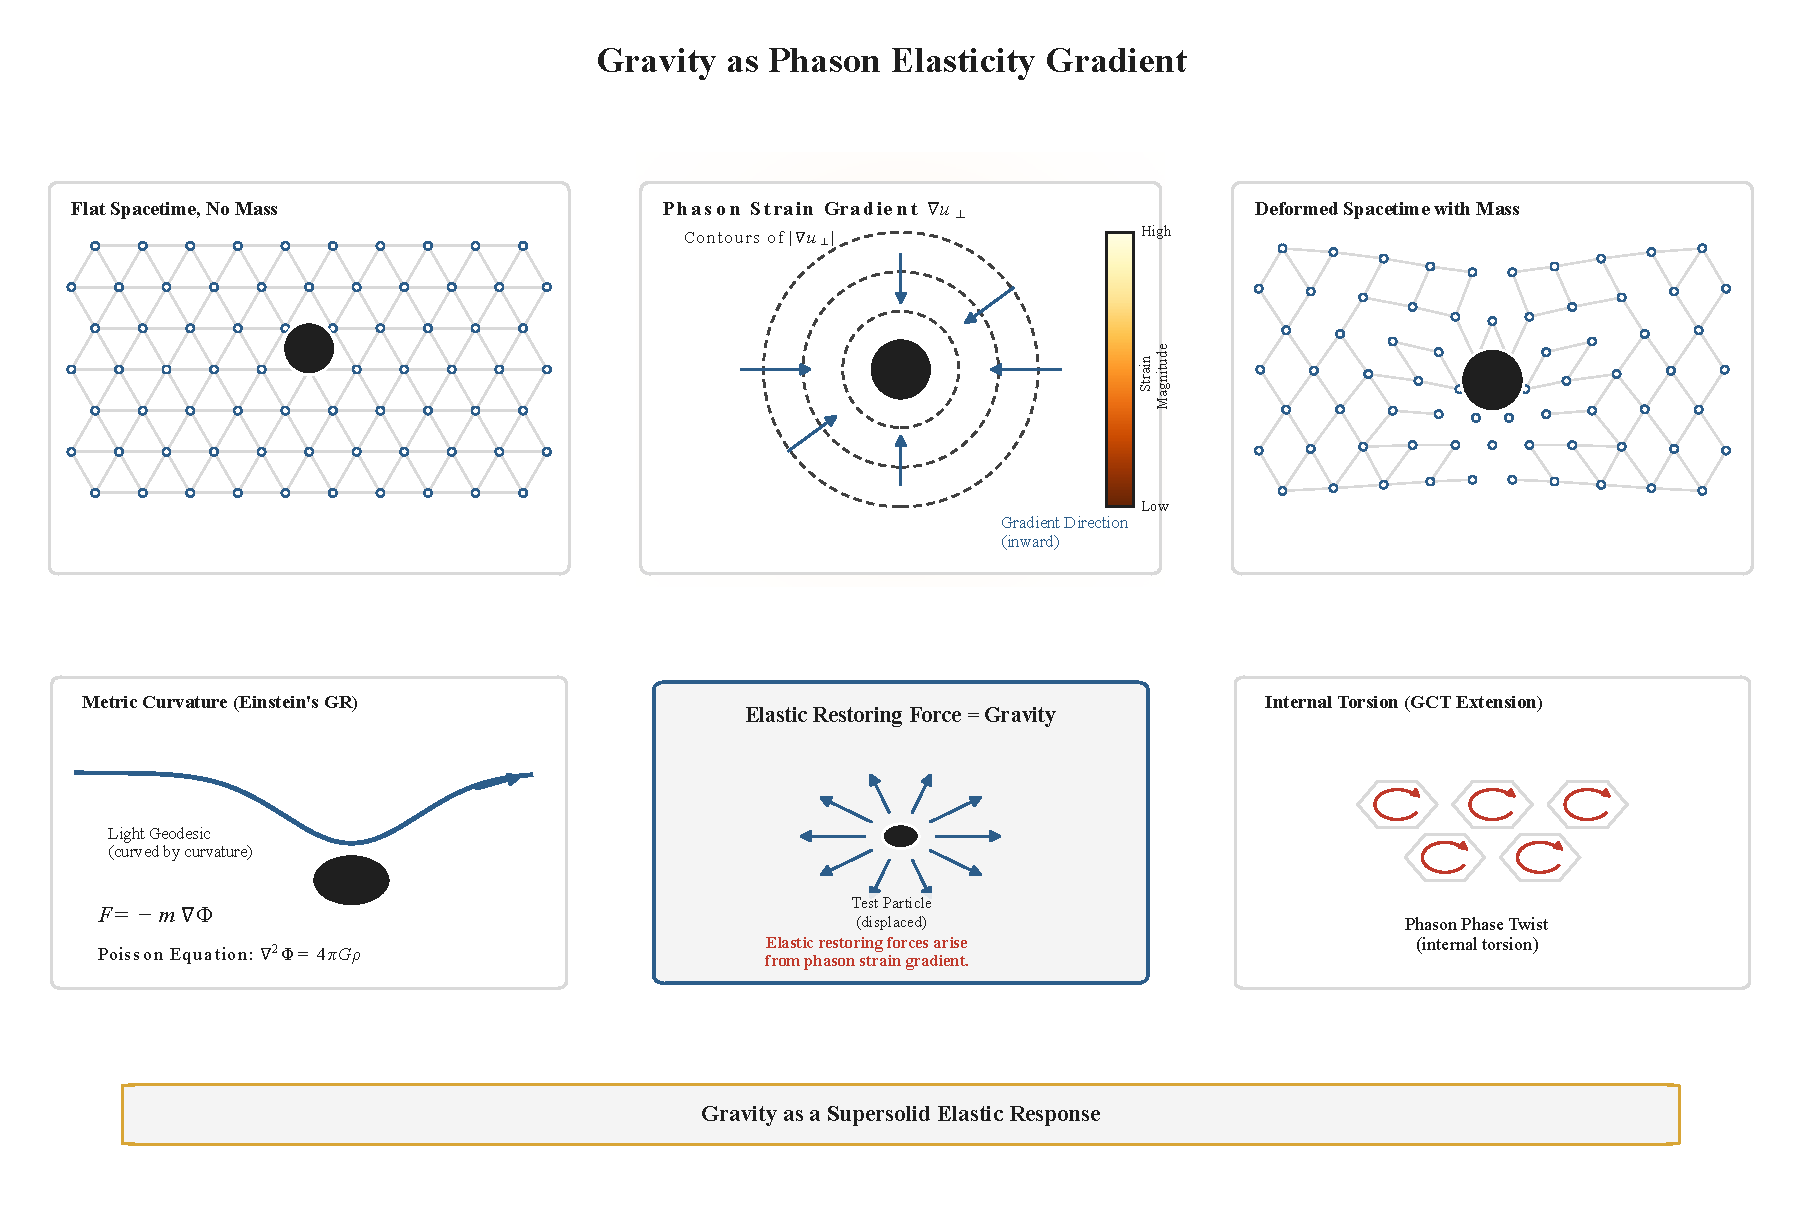
\includegraphics[keepaspectratio,alt={Gravity as a phason elasticity gradient: an undeformed lattice in flat, massless space (left) develops a strain-magnitude gradient \textbar\textbackslash nabla u\_\textbackslash perp\textbar{} around a mass (centre), warping the lattice (right). The lower panels contrast metric curvature in General Relativity with the internal phason torsion of the GCT extension, picturing the elastic restoring force on a displaced test particle as the gravitational attraction. Tier 3 analogy: G is not fixed by the phason stiffness (§8.1.4; App DPS §DPS.7)}]{content/Figures/Volume_2/Figure V2.8.1.pdf}}
\caption{Gravity as a phason elasticity gradient: an undeformed lattice
in flat, massless space (left) develops a strain-magnitude gradient
\(|\nabla u_\perp|\) around a mass (centre), warping the lattice
(right). The lower panels contrast metric curvature in General
Relativity with the internal phason torsion of the GCT extension,
picturing the elastic restoring force on a displaced test particle as
the gravitational attraction. Tier 3 analogy: \(G\) is not fixed by the
phason stiffness (§8.1.4; App DPS §DPS.7)}
\end{figure}

\chapter{Chapter 9: Entropic Gravity}\label{chapter-9-entropic-gravity}

In Chapter 8, we developed the spacetime metric as a refractive acoustic
geometry. However, for a theory to replace General Relativity, it must
also supply the dynamical relationship between that geometry and the
matter it contains. The primary construction here treats the Einstein
Field Equations as horizon-thermodynamic \textbf{Equations of State} for
a declared vacuum medium. Any association of its entropy bookkeeping
with a Selection Operator is a separate Tier 3 interpretive overlay and
is not used to derive gravity.

The chapter is organised so that the \textbf{thermodynamic chain is
primary}. §9.1 restates the horizon-thermodynamic route in the spirit of
Verlinde (2011) and Jacobson (1995), with the mixed-tier and circularity
disclosures below. The former phason-elasticity expression
\(G=\hat c^4/(8\pi K_\perp a_6)\) is not a second derivation or a
successful consistency check: it is dimensionally wrong by one length,
and its minimally corrected form retains a calibration-dependent
mismatch (a factor \(\approx57\) or \(\approx1.72\times10^{-6}\),
depending on the speed convention, never 1) under the Tier 3
stiffness-map hypothesis P3b (Ch08 §8.1.4; App DPS §DPS.7).

\begin{center}\rule{0.5\linewidth}{0.5pt}\end{center}

\subsection{9.1 Thermodynamics of
Spacetime}\label{thermodynamics-of-spacetime}

\subsubsection{9.1.1 The Jacobson Argument (Field Equations as Equation
of State) {[}Tier
2{]}}\label{the-jacobson-argument-field-equations-as-equation-of-state-tier-2}

In 1995, Ted Jacobson showed that the Einstein Field Equations can be
recovered by applying the first law of
thermodynamics---\(\delta Q = T\,dS\)---to local causal horizons under
the stated equilibrium assumptions. GCT applies that
horizon-thermodynamic construction to its declared vacuum medium.
Calling the horizon a Selection Operator's ``processing window'' is only
a Tier 3 metaphor; no physical Selection Operator is identified.

In the declared medium model, \(\delta Q\) is an energy flux through the
local causal horizon, \(T\) is the Unruh temperature for an accelerated
detector, and \(S\) is assigned an area-law lattice count. Balancing the
flux with the entropy change yields the Jacobson curvature relation
under those assumptions. This is a thermodynamic gravity argument, not a
derivation of an Agent's noise floor or information processing.

\subsubsection{9.1.2 Linking Processing Lag to Entropy
Gradients}\label{linking-processing-lag-to-entropy-gradients}

\textbf{Processing Lag} (\(\dot{\tau}_{coord} < 1\)) is an optional
informational analogy for gravitational redshift. The physical statement
is that the metric changes the relation between proper and coordinate
time near stress-energy. No Realization Operator or number of selection
cycles (\(dn\)) is derived from that relation.

In the entropic-force comparison, an entropy gradient can be assigned to
a holographic screen and related to an effective force after the usual
thermodynamic assumptions are supplied. Describing a particle as an
Agent ``aligned with High Consensus'' is metaphorical and contributes no
term to the force law.

\subsubsection{\texorpdfstring{9.1.3 The Verlinde Prescription (Force as
\(T \nabla S\))}{9.1.3 The Verlinde Prescription (Force as T \textbackslash nabla S)}}\label{the-verlinde-prescription-force-as-t-nabla-s}

Following the Verlinde comparison, the effective force is written as
\(F=T\nabla S\) for a declared screen entropy. The inverse-square
dependence follows only after the area law, equipartition, Unruh
relation, and source-energy identification are supplied. It is not a
gradient of a realized Selection probability, and no Selection Operator
preference is part of the derivation. Proposed low-acceleration
modifications require the separate constitutive model of Chapter 12.

\subsubsection{9.1.4 The Jacobson G-Derivation from Phason Horizon
Entropy}\label{the-jacobson-g-derivation-from-phason-horizon-entropy}

Through the Jacobson thermodynamic mechanism, Newton's Gravitational
Constant \(G\) is postdicted from the electron-anchored lattice scale.
The chain carries \textbf{Tier 2 thermodynamic mechanism + Tier 4
Planck-link conjecture (inherits O.14) + Tier 3 dimensional anchor}:

\begin{enumerate}
\def\labelenumi{\arabic{enumi}.}
\tightlist
\item
  \textbf{Anchor (\(m_e\)):} Retrieve the electron mass \(m_e\)
  (\(0.5109989\) MeV).
\item
  \textbf{Lattice Spacing (\(a_6\)):} The model-authoritative geometric
  definition uses the bare GCT coupling \(\alpha_{\rm GCT}=\phi^2/360\):
  \(m_e = M_{Planck} \cdot \phi^{-107} \cdot (1 - 5\alpha_{\rm GCT})\).
  It restricts the lattice spacing to
  \(a_6 = \frac{2\hbar}{m_e c} \cdot \phi^{-107} \cdot (1 - 5\alpha_{\rm GCT})\).
\item
  \textbf{Unruh Horizon (\(T_{Unruh}\)):} A uniformly accelerated
  detector is assigned the standard Unruh temperature
  \(T_{Unruh}=\hbar a/(2\pi c k_B)\); no Agent or Selection Operator
  enters this relation.
\item
  \textbf{Gravitational Inverse (\(G\)):} Substituting this into the
  entropic definition \(G_{predicted} = \frac{c^3 a_6^2}{4\hbar}\).
\end{enumerate}

The postdiction returns \(G = 6.689475523 \times 10^{-11}\), compared
with CODATA 2022 (\(6.67430 \times 10^{-11}\)): residual
\textbf{2273.725 ppm (displayed as 2274 ppm)}. This is the
model-authoritative \(\alpha_{\rm GCT}=\phi^2/360\) branch with
CODATA-2022 \(m_e\) and the exact SI conversion constants \(\hbar\) and
\(c\); it is not an all-CODATA-\(\alpha\) evaluation. Independently
re-derived in
\texttt{GCT\_Physics\_Engine/verify\_independent/verify\_newton\_g.py}.
The chain retains the O.14 inheritance and \(m_e\) SI anchor disclosed
in the Parameter Ledger, and its Planck-link dependence is stated in
§9.1.5.

\textbf{Not independent evidence.} The \(G\) row is the electron
Planck-link row read backwards: since \(a_6\propto1/m_e\) and
\(G\propto a_6^2\), \(G\propto m_e^{-2}\), and its all-CODATA-\(\alpha\)
residual (2013 ppm) is twice the electron-mass residual (1006 ppm) to
leading order. The \(G\) comparison therefore adds no evidence beyond
the electron row, and it is not counted as a pass while the electron row
fails its registered precision rule. As evidence that φ or icosahedral
structure is special, the underlying electron match is \textbf{Tier 4}:
the preregistered constant control test (v3, NEGATIVE-FRAGILE; App PSC
§PSC.9.6) found φ's pattern of matches on 21 constants not
distinguishable from that of random constants (58 of 300 random bases
did at least as well). The test ``excludes, at power ≥ 0.8, an effect in
which φ hits at least 6 of the 8 informative rows through a real effect;
weaker effects are not excluded.'' The number is kept as descriptive
arithmetic.

\gctneedspace{5\baselineskip}\begin{gctImportant}

\textbf{Firewall Metadata {[}G Thermodynamic Derivation{]}}

\begin{itemize}
\tightlist
\item
  \textbf{Type:} Consistency Check (Postdiction)
\item
  \textbf{Inputs:} \(m_e\), \(\phi\), \(\alpha\), \(\hbar\), \(c\); the
  Planck-length anchor enters implicitly through \(M_P\) in the mass
  formula
\item
  \textbf{Degrees of Freedom:} 0
\item
  \textbf{Provenance:} Discrete lattice entropy bound; consistency check
  of the Jacobson identity at the calibrated Planck-length anchor (scope
  note, §9.1.5)
\end{itemize}

\end{gctImportant}

\subsubsection{\texorpdfstring{9.1.5 The \(m_e \to a_6 \to G\) Chain and
Its Planck-Link
Dependence}{9.1.5 The m\_e \textbackslash to a\_6 \textbackslash to G Chain and Its Planck-Link Dependence}}\label{the-m_e-to-a_6-to-g-chain-and-its-planck-link-dependence}

A common criticism of lattice gravity theories is that they import
Newton's \(G\) through the Planck Mass \(M_P = \sqrt{\hbar c / G}\) when
deriving particle masses, and then ``predict'' \(G\) by inverting the
same formula. That criticism applies here. The chain below does not
break this circularity; it makes the dependence explicit. Its only
explicit dimensional input is the electron mass, but the exponent
\(-107\) (P2) encodes the ratio \(m_e/M_P\), and \(M_P\) contains \(G\),
so the \(G\) ``postdiction'' is the electron-mass formula read backwards
(scope note below).

\textbf{Step 1 --- Dimensional Anchor.} We take the experimentally
measured electron mass \(m_e = 0.5109989\) MeV as the single explicit
external input. No other dimensionful parameter is entered explicitly;
\(G\) and \(M_P\) enter implicitly through the mass formula of Step 2.

\textbf{Step 2 --- Lattice Spacing from the Mass Formula.} The GCT mass
formula \(m_e = M_P \cdot \phi^{-107} \cdot (1 - 5\alpha)\) is rewritten
in terms of the lattice spacing \(a_6\) using the lattice convention
\(M_P = 2\hbar / (c \cdot a_6)\) (§9.1.4), which is equivalent to
\(a_6=2\ell_P\). Substitution yields:

\[a_6 = \frac{2\hbar}{m_e c} \cdot \phi^{-107} \cdot (1 - 5\alpha_{\rm GCT}), \qquad \alpha_{\rm GCT}=\frac{\phi^2}{360}\]

Every quantity on the right-hand side (\(\hbar\), \(c\), \(m_e\),
\(\phi\), \(\alpha\)) is either a measured constant or a geometric
invariant. \(G\) does not appear explicitly; it enters implicitly
through the convention \(M_P = 2\hbar/(c\,a_6)\) that this step uses.

\textbf{Step 3 --- Jacobson Thermodynamic Identity.} Applying the
Jacobson (1995) first-law argument (\(\delta Q=T\,dS\)) to a local
Rindler horizon, with entropy bits declared at the lattice scale
\(a_6\), yields the conditional gravitational expression below. Calling
this horizon a Selection-Operator boundary is an unused Tier 3 metaphor;
no physical \(\mathcal F_{sel}\) is derived.

\[G_{\text{predicted}} = \frac{c^3 \, a_6^2}{4\hbar}\]

\textbf{Step 4 --- Verification Against CODATA.} Substituting the
derived \(a_6\):

\[G_{\text{predicted}} = 6.689475523 \times 10^{-11} \; \text{m}^3\,\text{kg}^{-1}\,\text{s}^{-2}\]

Compared to the CODATA 2022 value
\(G_{\text{SI}} = 6.67430 \times 10^{-11}\), the residual is
\textbf{2273.725 ppm (displayed as 2274 ppm)}. The evaluated input set
is explicit: the model supplies \(\alpha_{\rm GCT}=\phi^2/360\), while
\(m_e\) is the CODATA-2022 dimensional anchor and \(\hbar=h/(2\pi)\) and
\(c\) use the exact post-2019 SI definitions of \(h\) and \(c\).
Replacing \(\alpha_{\rm GCT}\) by \(\alpha_{\rm CODATA}\) defines a
separate sensitivity branch, \(G=6.687737668\times10^{-11}\) with a
2013.345 ppm residual; it is not the model-authoritative output. The
CODATA value \(G_{\text{SI}}\) appears only at the final comparison
step. Independently re-derived in
\texttt{GCT\_Physics\_Engine/verify\_independent/verify\_newton\_g.py}.

\gctneedspace{5\baselineskip}\begin{gctNote}

\textbf{Scope: this is a consistency relation, not an independent G
derivation.} The Tier 2 status of the relation
\(G = c^3 a_6^2 / (4\hbar)\) rests on the \emph{Jacobson thermodynamic
identity} (Step 3), which is a structural connection between horizon
entropy and gravitational coupling. The full chain \(m_e \to a_6 \to G\)
is dimensionally consistent and one-directional in the sense that
\(G_{\rm CODATA}\) is not an input. However, the GCT mass formula
\(m_e = M_P \phi^{-107} (1-5\alpha_{\rm GCT})\) implicitly couples
\(a_6\) to the Planck length \(\ell_P = \sqrt{\hbar G / c^3}\) via
\(M_P\); algebraically \(a_6 = 2 \ell_P\) (App DPS §DPS.7), so the
agreement is a \textbf{consistency check of the Jacobson identity at the
calibrated Planck-length anchor}, not an independent first-principles
derivation of \(G\) from non-gravitational inputs. The
all-CODATA-\(\alpha\) sensitivity branch exposes the doubled
electron-anchor residual, while the additional 260.380 ppm in the
model-authoritative branch comes from using \(\alpha_{\rm GCT}\); a
tighter \(G\) therefore requires upstream work on the
electron/\(\alpha\) bridge, not direct work on the gravitational
identity. The \(G\) agreement inherits, and adds nothing beyond, the
electron row, which fails its registered precision rule; it is not
independent evidence (§9.1.4).

\end{gctNote}

\gctneedspace{5\baselineskip}\begin{gctNote}

\textbf{Cascade structure of the 2274 ppm \(G\) residual.} Because
\(a_6 \propto 1/m_e\) and \(G \propto a_6^2\), the all-CODATA-\(\alpha\)
sensitivity branch maps the 1006.166 ppm electron-mass residual to
2013.345 ppm in \(G\) (the leading \(2\times1006.166=2012.332\) ppm plus
the quadratic term). The model-authoritative \(\alpha_{\rm GCT}\) branch
has a 2273.725 ppm residual. Their \textbf{260.380 ppm difference is
entirely the substitution \(\alpha_{\rm CODATA}\to\alpha_{\rm GCT}\) in
\((1-5\alpha)^2\)}. It is not a finite-precision or uncertainty
contribution from \(\hbar\) or \(c\): \(h\) and \(c\) are exact in the
post-2019 SI, and \(\hbar=h/(2\pi)\) inherits no measurement
uncertainty. The unresolved physical debt remains the upstream
electron/\(\alpha\) bridge, not the gravitational identity.

\textbf{The 2nd-order-\(\alpha\) closure pathway is structurally
insufficient.} A natural-looking promotion would be to add the 2nd-order
\(\alpha^2\) correction to the electron mass formula by analogy with the
muon's \(m_\mu = m_e \phi^{11} (1 + 5\alpha + \phi^8 \alpha^2)\). Per V3
§8.2.3, the muon's \(\phi^8\) coefficient arises as
\(\phi^{-3} \times \phi^{11}_{\text{bare-muon-exponent}}\). Substituting
the \emph{electron's} bare exponent (\(-107\)) into the same combination
rule gives a 2nd-order coefficient
\(\phi^{-3} \times \phi^{-107} = \phi^{-110} \approx 1.03 \times 10^{-23}\),
which contributes
\(\phi^{-110} \cdot \alpha^2 \approx 5.5 \times 10^{-28}\) to the
electron mass --- totally negligible compared with the 1006 ppm
residual.

\textbf{Closure path for the residual.} The 2nd-order phason self-energy
correction does NOT close the electron / \(G\) residuals by the
muon-analogue mechanism. Viable upstream investigations include (i)
higher-order non-perturbative corrections to the discrete RT lattice
mass formula beyond the tree-level \((1-5\alpha)\) drag, (ii)
construction of the missing K-theoretic physical map, or (iii)
reassessment of the Tier 3 \(M_P\) convention itself (the standard
\(\sqrt{\hbar c/G_N}\) vs \(\sqrt{\hbar c/8\pi G_N}\) choice flagged in
V3 Ch07 §7.2.2). Lemma T-McK.1b (App USS §USS.7.6.3) is a separate Tier
3/open WZW/APS defect-index proposal with no selected boundary operator
or observable map; it is not an established route for closing
\(\alpha\)'s 3443 ppm gap, the electron residual, or the parent-lattice
chain. A tighter \(G\) requires upstream work on the electron mass
relation, not direct work on the gravitational chain.

\end{gctNote}

\gctneedspace{5\baselineskip}\begin{gctNote}

\textbf{Circularity check.} The computational implementation imports the
numerical value \(G_{\text{SI}}\) only at the final comparison step (see
Appendix ULA §ULA.8), so CODATA \(G\) is not a numerical input. This
does not make the chain independent of \(G\): the exponent in
\(m_e = M_P\phi^{-107}(1-5\alpha)\) fixes \(m_e/M_P\), and with
\(a_6 = 2\ell_P\) the output \(G\) is the electron-mass relation
inverted. The chain is a consistency check of the Planck identity, not a
derivation of \(G\) from non-gravitational inputs.

\end{gctNote}

\gctneedspace{5\baselineskip}\begin{gctNote}

\textbf{Cross-route check: no three-route equivalence.} The Jacobson
relation \[G_1=\frac{c^3a_6^2}{4\hbar}\] reduces to the standard Planck
identity after \(a_6=2\ell_P\) is supplied. The former elasticity
expression with one \(a_6\) has dimensions \(L^4M^{-1}T^{-2}\) and is
retired. Its minimally corrected version,
\[G_2^{(corrected)}=\frac{\hat c^4}{8\pi K_\perp a_6^2},\] gives, after
the Tier 3 P3b substitutions, a calibration-dependent factor ---
\(G_2^{(corrected)}=[\phi^{18}/(32\pi)]G\approx57\,G\) in the Parameter
Ledger speed convention (\(c=\phi^{-9}c_P\)),
\([\phi^{-18}/(32\pi)]G\approx1.72\times10^{-6}G\) if \(c_P=c\) ---
never 1 (App DPS §DPS.7). Routes 2 and 3 (V2 §8.1.4 and V1 §13.3.4) are
the same failed scaling ansatz, not independent validations. Appendix
DPS §DPS.7 contains the unit-by-unit audit.

The Jacobson route (this chapter) is the canonical primary route because
it introduces no undisclosed fitting beyond the
5-postulate-plus-1-anchor bare lepton-ratio sub-sector of Parameter
Ledger §0.1 (the bare \(\alpha\) relation \(360\phi^{-2}\) is a separate
Tier 3 numerical relation, mechanism open), with the native-RGE endpoint
and precision-comparison rows adding anchors A2--A6 (Parameter Ledger
§0.1) (specifically \(m_e\) as the dimensional anchor; \(\phi\) is the
icosahedral mathematical constant, not a fitted parameter; the
icosahedral projection ansatz (P1), the K-theoretic exponent \(n=-107\)
(P2), the integer \(D=18\) (P3a), and the lepton harmonic exponents
\(N=11, 17\) (P4, P5) are the five structural postulates; the
\(\phi^{-18}\) stiffness map P3b is a Tier 3 hypothesis outside the
count).

\end{gctNote}

\subsubsection{9.1.6 Bottom-Up Thermodynamic Derivation (Verlinde
Comparison) {[}Tier 2 restatement of the Jacobson chain;
low-acceleration extension Tier
3{]}}\label{bottom-up-thermodynamic-derivation-verlinde-comparison-tier-2-restatement-of-the-jacobson-chain-low-acceleration-extension-tier-3}

The Jacobson chain of §9.1.1--§9.1.5 is the thermodynamically primary
derivation of gravity in GCT. To make its bottom-up structure explicit,
and to clarify the relationship between GCT and the Verlinde (2011)
entropic-gravity program, we restate it here in the form that begins
with holographic-screen entropy and ends with Newton's force law.

\emph{Step 1 --- Holographic screen and entropy.} Consider a spherical
screen \(\Sigma\) of radius \(R\) centred on a localised mass
distribution of energy \(E = Mc^2\). It is a causal/thermodynamic
bookkeeping surface in the gravity calculation. Identifying it with a
Selection Operator's processing boundary would be a separate Tier 3
interpretation and is not needed below. The declared number of lattice
degrees of freedom on the screen is:
\[N(\Sigma) = \frac{A(\Sigma)}{a_6^2} = \frac{4\pi R^2}{a_6^2}\] where
\(a_6\) is the lattice spacing of §9.1.4. The bits are quantised at the
lattice scale, not at \(\ell_P^2\); this is the point where GCT departs
from the heuristic Verlinde construction. Since \(a_6 = 2\ell_P\) (App
DPS §DPS.7), the lattice counting assigns \(N = A/(4\ell_P^2)\) --- a
factor of \(4\) fewer degrees of freedom than the \(N = A/\ell_P^2\)
that the Verlinde construction assigns to the same screen. This factor
is tracked explicitly through Step 3 below.

\emph{Step 2 --- Equipartition on the screen.} Each lattice bit on the
screen carries energy \(\tfrac{1}{2}k_B T\) by equipartition, where
\(T\) is the Unruh temperature read by an observer accelerating into the
screen at rate \(a\): \[T = \frac{\hbar a}{2\pi c k_B}\] The total
energy stored on the screen equals the bulk energy \(Mc^2\) by
holographic identification:
\[Mc^2 = \tfrac{1}{2}N k_B T = \frac{1}{2}\cdot\frac{4\pi R^2}{a_6^2}\cdot k_B \cdot \frac{\hbar a}{2\pi c k_B} = \frac{\hbar a R^2}{c \, a_6^2}\]

\emph{Step 3 --- Newton's law as a thermodynamic identity.} Solving for
the acceleration \(a\) experienced by a test mass at radius \(R\):
\[a = \frac{Mc^3 \, a_6^2}{\hbar R^2}\] Identifying
\(G_{\text{predicted}} = c^3 a_6^2 / (4\hbar)\) --- the same expression
derived in §9.1.4 --- yields \[a = \frac{4GM}{R^2}\] The bottom-up
screen counting therefore recovers Newton's law only up to an overall
factor of \(4\), and nothing in Steps 1--2 fixes this coefficient:
assigning one equipartition bit of \(\tfrac{1}{2}k_B T\) per lattice
cell (\(N = A/a_6^2 = A/(4\ell_P^2)\)) is a counting convention,
carrying a factor of \(4\) fewer degrees of freedom than the Verlinde
assignment \(N = A/\ell_P^2\) that would yield \(a = GM/R^2\) directly.
The standard coefficient is restored by a step \textbf{external to the
bottom-up construction}: imposing the Bekenstein--Hawking entropy-area
normalisation \(S = A/(4\ell_P^2)\) through the Clausius identity
\(\delta Q = T\,dS\) of the Jacobson argument (§9.1.1). The bottom-up
route thus establishes the \emph{form} of Newton's law from screen
thermodynamics; its numerical coefficient is inherited from the imported
horizon-entropy normalisation, not derived from the lattice
equipartition itself.

\emph{Step 4 --- Einstein equations as equation of state.} Promoting the
local Rindler horizon to a general null congruence and demanding that
\(\delta Q = T dS\) hold for every local causal horizon (Jacobson 1995)
yields the full Einstein Field Equations
\[R_{\mu\nu} - \tfrac{1}{2}g_{\mu\nu}R = 8\pi G T_{\mu\nu}\] with \(G\)
taken from the Jacobson relation of §9.1.4 (a calibrated consistency
relation; scope note, §9.1.5). Under Jacobson's local-equilibrium
assumptions the Einstein equations are not postulated: they follow, up
to a cosmological-constant term, as the relation that makes the local
Clausius identity hold for every local Rindler observer.

\emph{Step 5 --- MOND limit as low-acceleration thermodynamics.} When
the Unruh temperature \(T\) drops below the de Sitter temperature
\(T_{dS} = \hbar H_0/(2\pi k_B)\), the screen is only partly populated
by causal modes: only the fraction \(T/T_{dS}\) of the \(N\) bits is
accessible. The equipartition relation of Step 2 is modified to
\(Mc^2 = \tfrac{1}{2}N(T/T_{dS}) k_B T\). With the lattice counting
\(N = 4\pi R^2/a_6^2\) and the identification of Step 3, this gives
\[a^2 = \frac{2\pi c k_B T_{dS}}{\hbar} \cdot \frac{4GM}{R^2} = a_{\rm th} \cdot \frac{4GM}{R^2},\]
with \(a_{\rm th} \equiv 2\pi c k_B T_{dS}/\hbar = cH_0\). The factor
\(4\) is the same counting factor as in Step 3; the lattice counting
alone therefore gives an effective scale \(4a_{\rm th}=4cH_0\). Removing
it again requires imposing the imported Bekenstein--Hawking
normalisation, as in Step 3, which gives \(a^2 = a_{\rm th}\,GM/R^2\);
the comparisons below use that renormalised form. The assumption that
only the fraction \(T/T_{dS}\) of the bits is accessible is itself an ad
hoc Verlinde/Milgrom-type input, not derived from the lattice. At the
canonical
\(H_0=67.4\ {\rm km\,s^{-1}\,Mpc^{-1}}=2.18428523\times10^{-18}\ {\rm s^{-1}}\),
this gives \(a_{\rm th}=6.54832237\times10^{-10}\ {\rm m\,s^{-2}}\).
That \(cH_0\) is an acceleration scale is dimensional bookkeeping; the
low-acceleration thermodynamic mechanism is Tier 3, and identifying its
coefficient with the empirical MOND normalisation is Tier 3/open. In
particular, \(a_{\rm th}/a_0=5.45694\) for
\(a_0=1.2\times10^{-10}\ {\rm m\,s^{-2}}\), not \(2\pi\). The commonly
compared candidate
\(cH_0/(2\pi)=1.04219787\times10^{-10}\ {\rm m\,s^{-2}}\) is
\(-13.1502\%\) below the empirical value. Thus the conditional
low-acceleration form \(a\to\sqrt{a_{\rm scale}GM/R^2}\) supplies a
mechanism class and scale relation, but it neither derives \(a_0\) nor
fixes the \(1/(2\pi)\) coefficient. This is the same scale-level
conclusion reached in emergent-gravity thermodynamics; Chapter 12
separately states the Tier 3 phason-vacuum constitutive ansatz.

\emph{Step 6 --- Where GCT proposes to go beyond Verlinde.} Verlinde
(2011) stops at the Newtonian limit, and Verlinde (2017) addresses
apparent dark matter and dark energy; neither attempts the absolute
value of \(G\) or particle masses, and neither derives the value of the
cosmological constant. GCT proposes extending the same thermodynamic
flow into four additional sectors, with the tiers stated in each item:

\begin{enumerate}
\def\labelenumi{\arabic{enumi}.}
\item
  \emph{Absolute value of \(G\).} The lattice scale \(a_6\) is fixed by
  the GCT mass formula \(m_e = M_P \phi^{-107}(1-5\alpha)\) (§9.1.5), so
  the expression \(G = c^3 a_6^2/(4\hbar)\) contains no further fitted
  coefficient beyond the declared postulates and the \(m_e\) anchor.
  Because the mass formula imports \(M_P\) --- and hence couples \(a_6\)
  to \(\ell_P\) --- the resulting 2274 ppm agreement is a consistency
  check of the Jacobson identity at the calibrated Planck-length anchor
  (scope note, §9.1.5), not an independent first-principles prediction
  of \(G\), and it adds no evidence beyond the electron row (§9.1.4).
  Verlinde's framework treats \(G\) as an emergent coupling and offers
  no analogous numerical closure.
\item
  \emph{Dark sector.} The phason-strain stress-energy (Chapter 11) and
  the holographic-entanglement cosmological constant (Chapter 14
  §14.1.5) extend the entropic flow into the dark sector. The canonical
  area-law/Friedmann form is
  \(\rho_\Lambda = (3\Omega_\Lambda/8\pi)\,\hbar H_0^2/(c\ell_P^2)\);
  this is \(\Omega_\Lambda\rho_{\rm crit}\) re-expressed in Planck units
  (an identity, not an independent derivation), and the absolute
  magnitude still imports \(H_0\) and \(\Omega_\Lambda\) pending
  O.1/O.4.
\item
  \emph{Particle masses {[}Tier 3 programme{]}.} Volume 3 proposes mass
  relations from icosahedral selection rules acting on the same lattice
  that supplies the entropy bits in Step 1. Those relations carry Tier 3
  integer anchors and calibrated handles (Parameter Ledger §0.1),
  several of them register tensions or fail a written rule, and they do
  not fix the Standard Model mass spectrum. Reading the mass hierarchy
  and the gravitational hierarchy as two readings of the same
  K-theoretic data is a Tier 3/4 conjecture that inherits O.14.
\item
  \emph{Consciousness interpretation.} One may conditionally associate
  the entropy-gradient bookkeeping with the proposed
  \(\mathcal F_{sel}\), but the thermodynamic gravity derivation neither
  identifies a physical Selection Operator nor derives an ontological
  Agent's dynamics. The gravity result is independent of that Tier 3
  interpretation.
\end{enumerate}

\emph{Closing statement.} The horizon-thermodynamic construction
supplies a structural route from entropy assumptions to gravitational
field equations. In its present GCT use, the numerical \(G\) comparison
is a calibrated Planck-identity consistency check through the
electron/Planck link, not an independent non-gravitational prediction.
The failed elasticity route contributes no additional closure.

\gctneedspace{5\baselineskip}\begin{gctNote}

\textbf{Position in the gravity-derivation hierarchy.} §9.1.1--§9.1.5
give the Jacobson chain with the GCT lattice scale supplied; §9.1.6
reorganises the same assumptions in a bottom-up Verlinde presentation,
starting from holographic screens and ending at Newton/MOND/Einstein. V2
§8.1.4 and V1 §13.3.4 record the negative elasticity audit. These are
not four algebraically equivalent derivations (Appendix DPS §DPS.7).

\end{gctNote}

\begin{center}\rule{0.5\linewidth}{0.5pt}\end{center}

\subsection{9.2 The Field Equations}\label{the-field-equations}

\subsubsection{9.2.1 Stress-Energy Definition in Terms of Phason Strain
{[}Tier 3 constitutive
identification{]}}\label{stress-energy-definition-in-terms-of-phason-strain-tier-3-constitutive-identification}

In the GCT supersolid model, the Stress-Energy Tensor \(T_{\mu\nu}\) is
proposed to be an internal material property of the lattice.
Matter---whether baryonic or dark---is modelled as configurations that
generate \textbf{Phason Strain} (\(w_{ij}\)) in the internal manifold
\(E_\perp\) (a Tier 3 constitutive identification; cf.~Ch06 §6.3.2).

\begin{itemize}
\tightlist
\item
  \textbf{Baryonic Matter:} Acts as a \textbf{Source} of strain. The
  topological knot (defect) ``twists'' the surrounding lattice, creating
  a localized energy density.
\item
  \textbf{Dark Matter:} Consists of \textbf{Frozen Strain} (Topological
  Glass) where the lattice is distorted without a central defect
  (Chapter 11).
\end{itemize}

We define \(T_{\mu\nu}\) as the variation of this total phason strain
energy density with respect to the acoustic metric. Within the model
this reads ``Mass'' as the \textbf{Elastic Tension} of the vacuum; no
covariant stress-energy derivation from the supersolid action is yet
supplied (O.34b).

\subsubsection{9.2.2 The Einstein Tensor as Hydrodynamic Equilibrium
{[}Tier 3 interpretive reading; Wheeler--DeWitt adoption Tier
3{]}}\label{the-einstein-tensor-as-hydrodynamic-equilibrium-tier-3-interpretive-reading-wheelerdewitt-adoption-tier-3}

In this reading, the Einstein Tensor \(G_{\mu\nu}\) (representing
curvature) is interpreted as the geometric response of the \(6D \to 3D\)
projection that accompanies the Wheeler--DeWitt constraint
(\(\hat{H}\Psi = 0\)), whose adoption in GCT is itself Tier 3. In a
supersolid quasicrystal, the vacuum is modelled as seeking a state of
\textbf{Hydrodynamic Equilibrium}.

The Field Equations (\(G_{\mu\nu} = 8\pi G T_{\mu\nu}\)) are then read
as the \textbf{Balance Equations} of the vacuum: the ``Bending'' of the
projection (\(G_{\mu\nu}\)) matches the ``Stress'' of the defects
(\(T_{\mu\nu}\)), which in the Tier 3 Wheeler--DeWitt adoption is the
statement that the total Hamiltonian constraint vanishes. The field
equations themselves enter through the Jacobson construction of §9.1,
not through this reading.

\subsubsection{\texorpdfstring{9.2.3 The Gravitational Constant (\(G\))
as Inverse Stiffness: a Qualitative Analogy {[}Tier 3
analogy{]}}{9.2.3 The Gravitational Constant (G) as Inverse Stiffness: a Qualitative Analogy {[}Tier 3 analogy{]}}}\label{the-gravitational-constant-g-as-inverse-stiffness-a-qualitative-analogy-tier-3-analogy}

As a qualitative picture, Newton's Gravitational Constant \(G\) can be
read as an \textbf{Inverse Rigidity} of the acoustic metric: it sets how
much a unit of stress-energy deforms the effective geometry. In this
picture the vacuum is very ``stiff'' because the lattice scale sits at
the Planck scale, so appreciable curvature requires Planck-scale energy
densities (\(\sim M_P c^2/\ell_P^3\), with \(M_P c^2 \sim 10^{19}\)
GeV), and in this loose sense \(1/G\) plays the role of a
\textbf{Young's Modulus of the Vacuum}.

This is an analogy only. \(G\) is \textbf{not} fixed by the ground-state
density \(\rho\) or the phason stiffness \(K_\perp\). The elasticity
expression built from \(K_\perp\) is dimensionally wrong by one length
in its original form, and its minimally corrected form gives a
calibration-dependent factor under the Tier 3 P3b substitutions ---
\([\phi^{18}/(32\pi)]\,G\approx57\,G\) in the Parameter Ledger speed
convention, \([\phi^{-18}/(32\pi)]\,G\approx1.72\times10^{-6}\,G\) if
\(c_P=c\) --- never 1 (Ch08 §8.1.4; App DPS §DPS.7). The quoted value of
\(G\) comes only from the Jacobson relation of §9.1.4--§9.1.5, which is
a calibrated Planck-identity consistency check, not a stiffness
derivation.

\begin{center}\rule{0.5\linewidth}{0.5pt}\end{center}

\subsection{9.3 The Weakness of Gravity: Restating the
Hierarchy}\label{the-weakness-of-gravity-restating-the-hierarchy}

\subsubsection{\texorpdfstring{9.3.1 The Stiffness Mismatch {[}Tier 3
reading; the ratio \(m_p/M_P\) is an
input{]}}{9.3.1 The Stiffness Mismatch {[}Tier 3 reading; the ratio m\_p/M\_P is an input{]}}}\label{the-stiffness-mismatch-tier-3-reading-the-ratio-m_pm_p-is-an-input}

The ``Hierarchy Problem''---the fact that gravity between elementary
particles is many orders of magnitude weaker than electromagnetism
(about \(10^{36}\) for two protons)---is restated here, not resolved, as
the difference between a \textbf{Bond Scale} and a \textbf{Defect
Scale}.

\begin{itemize}
\tightlist
\item
  \textbf{The Bond Scale (\(M_P\)):} Read as the scale of the rigid 6D
  lattice substrate (\(\sim10^{19}\) GeV), which in this picture sets
  the metric rigidity. In the electron-anchored chain it is a
  dimensional reference tied to \(a_6=2\ell_P\) (§9.1.5), not an
  independent output. {[}Tier 3 reading{]}
\item
  \textbf{The Defect Scale (\(m_p\)):} Read as the low-energy excitation
  of a single topological knot (\(\sim1\) GeV). Here \(m_p\) is an
  input; Volume 3 models it separately with a Tier 3 selection step.
  {[}Tier 3 reading{]}
\end{itemize}

\subsubsection{9.3.2 The Mechanism of Suppression {[}Tier 1 arithmetic
given the input
ratio{]}}\label{the-mechanism-of-suppression-tier-1-arithmetic-given-the-input-ratio}

The effective coupling of gravity between two protons is governed by the
ratio:
\[\alpha_{grav} = \frac{G \cdot m_p^2}{\hbar c} = \left( \frac{m_p}{M_{Planck}} \right)^2\]
Because \(m_p/M_{Planck}\approx7.7\times10^{-20}\),
\(\alpha_{grav}\approx5.9\times10^{-39}\), about \(8\times10^{-37}\) of
the electromagnetic \(\alpha\) for the same pair (the often-quoted
``\(10^{40}\)'' depends on which particles are compared). {[}Tier 1
arithmetic{]}

In this reading gravity is weak because \textbf{matter's characteristic
mass scale sits far below the Planck scale of a rigid metric}: a single
defect (the proton) is \(\sim10^{19}\) times less energetic than the
lattice bond scale. This restates the hierarchy as the small input ratio
\(m_p/M_P\); it does not explain why that ratio is small, and neither
\(m_p\) nor \(M_P\) is derived here from the lattice without the Tier 3
anchors of Volume 3 (cf.~V1 Ch13 §13.1.3).

\subsubsection{9.3.3 Interpretive Gloss: Rigidity and Responsiveness
{[}Tier 4 ---
interpretive{]}}\label{interpretive-gloss-rigidity-and-responsiveness-tier-4-interpretive}

As an interpretive gloss, the hierarchy can be read as expressing two
features of the proposed medium: a rigid vacuum (large \(M_P\)) that
supports stable structure, and soft phason modes (small \(K_\perp\))
that carry light and, in the author's interpretive programme, the
conditions for structured experience. On a simulation-style reading of
the cosmos, the ratio would then describe a medium that is both
\textbf{Objective} (hard metric) and \textbf{Responsive} (soft
information), and gravity's weakness could be pictured as a ``Cost of
Objectivity''. This gloss is Tier 4. The ratio \(m_p/M_P\) is an input
(§9.3.1), the soft-phason premise rests on the Tier 3 stiffness map P3b,
and no requirement of consciousness, light or simulation is shown to fix
the numerical hierarchy. The physics of this chapter neither derives the
gloss nor rules it out (cf.~Ch04 §4.2.4).

\chapter{Chapter 10: Singularities and
Gravastars}\label{chapter-10-singularities-and-gravastars}

The existence of spacetime singularities---points of infinite density
and curvature where the laws of physics cease to function---is the
primary pathology of General Relativity. Within the continuous manifold
of standard physics, there is no geometric mechanism to halt
gravitational collapse once an object passes its Schwarzschild radius.
Geometric Consciousness Theory (GCT) proposes that these singularities
are artifacts of the continuum approximation. If the vacuum substrate is
a discrete material lattice (the GCT lattice premise), we argue that
gravitational collapse is self-regulating and terminates in a phase
transition; the gravastar endpoint of §10.2 is a Tier 3 model, and its
de Sitter core-density programme (§10.2.1) is Tier 4.

\begin{center}\rule{0.5\linewidth}{0.5pt}\end{center}

\subsection{10.1 The Lattice Cutoff}\label{the-lattice-cutoff}

\subsubsection{10.1.1 Minimum Length and the Curvature Bound {[}Tier 2
conditional on the lattice premise; the premise itself is the
architectural postulate
P1{]}}\label{minimum-length-and-the-curvature-bound-tier-2-conditional-on-the-lattice-premise-the-premise-itself-is-the-architectural-postulate-p1}

Volume 1 argued for discrete geometry from the requirement of finite
information density; that argument rests on its stated premises and on
the adopted lattice ansatz, not on a necessity proof. In the model, the
fundamental ``pixel size'' of the Operating System is the 6D lattice
constant \(a_6\).

Conditional on that lattice premise, this discreteness imposes a
\textbf{Curvature Bound} on the effective geometry. In differential
geometry, curvature involves the second derivative of the metric. In the
GCT lattice substrate, the metric is an effective acoustic property of
the lattice nodes. Since no phason wave or strain gradient can possess a
wavelength shorter than the lattice spacing (the Nyquist-Shannon limit
of the vacuum), the curvature scalar \(R\) cannot increase indefinitely.

\textbf{Theorem 10.1 (Singularity Resolution) {[}label kept for
reference stability; a conditional scaling argument, Tier 2 given the
lattice premise --- not a theorem about physical spacetime{]}:} \emph{If
the vacuum is a discrete lattice substrate with a minimum node spacing
\(a_6\) and the effective metric is an acoustic property of that
lattice, the maximum curvature representable by the effective metric is
finite and of order the reciprocal of the lattice area.}
\[R_{max} \sim \frac{1}{a_6^2}\]

\gctneedspace{5\baselineskip}

\textbf{Argument (conditional on the lattice premise):} The Riemann
curvature tensor \(R^{\rho}_{\sigma\mu\nu}\) is derived from the
gradients of the phason strain \(w_{ij}\). In a discrete lattice, the
maximum gradient \(\Delta w / \Delta x\) is limited by the fact that
\(\Delta x \ge a_6\). Infinite curvature requires an infinite density of
lattice nodes, which is forbidden by the finite energy density of the
Field. Spacetime ``breaks'' into its constituent nodes before it can
become singular.

\subsubsection{10.1.2 Resolution of
Singularities}\label{resolution-of-singularities}

Conditional on the lattice premise, the model replaces the center of a
``Black Hole'' (a point of zero volume and infinite mass in the
continuum description) by a region where the gravitational stress has
exceeded the \textbf{Yield Strength} of the vacuum lattice {[}Tier 3{]}.
As the curvature approaches \(R_{max}\), the continuum and
local-equilibrium approximations under which Chapter 9 obtains the
Einstein field equations fail. The vacuum undergoes a local phase
transition, converting the high-energy stress into a new state of the
substrate. Within the lattice model, this transition would resolve the
singularity by replacing the mathematical point with a physical core of
finite density and high symmetry.

\begin{center}\rule{0.5\linewidth}{0.5pt}\end{center}

\subsection{10.2 The Gravastar Solution}\label{the-gravastar-solution}

\subsubsection{10.2.1 Phase Transition Core {[}Tier
4{]}}\label{phase-transition-core-tier-4}

GCT proposes that the ``Interior'' of a black hole is a bubble of the
\textbf{Symmetric Phase} of the consciousness field. Recall from Chapter
3 that the vacuum crystallized into a supersolid state to minimize
energy, settling into the minimum of the Landau-Ginzburg potential
\(V(\rho)\). Extreme gravitational pressure---representing extreme
phason strain---provides the energy required to ``melt'' the lattice.

When the local energy density exceeds the potential barrier, the order
parameter \(\rho\) (lattice density) collapses to zero.

\begin{itemize}
\tightlist
\item
  \textbf{The Transition:} Broken Phase (Crystalline Quasicrystal)
  \(\to\) Symmetric Phase (Disordered Liquid).
\item
  \textbf{Energetics:} In the model, melting the lattice moves the
  vacuum state from the potential minimum back toward the symmetric
  point \(V(0)\), leaving a region of disordered vacuum where the metric
  and icosahedral symmetry have dissolved. Whether this can support a
  gravastar core is open (below).
\end{itemize}

\gctneedspace{5\baselineskip}

\textbf{Declared open programme {[}Tier 4{]}} \emph{Claim.} The melted
core sits at the plateau \(V(0)\), and its uniform negative pressure
(\(P=-\rho\)) supplies the de Sitter interior that halts collapse.
\emph{Defect.} A de Sitter core of radius \(r_1\approx r_s\) needs
energy density \(3c^4/(8\pi G r_s^2)\propto M^{-2}\); one fixed plateau
\(V(0)\) fixes a single de Sitter radius (of order the Planck length for
a Planck-scale \(V(0)\)), so it cannot support cores of all masses.
\emph{Closure needs} a mechanism that makes the core energy density
mass-dependent, plus formation dynamics and a stability analysis.
\emph{Use.} Nothing elsewhere in the manuscript uses the gravastar core
as support. \emph{Tier.} Because a single \(V(0)\) plateau cannot give
the \(M^{-2}\)-scaling de Sitter core, the core-density programme is
Tier 4 (downgraded from Tier 3 in v1.3.0).

\subsubsection{10.2.2 The Mazur-Mottola
Model}\label{the-mazur-mottola-model}

Within that open programme, the proposed endpoint would take the form of
the \textbf{Gravastar} (Gravitational Vacuum Star) model of Mazur and
Mottola, a three-layered object with a de Sitter interior:

\begin{enumerate}
\def\labelenumi{\arabic{enumi}.}
\tightlist
\item
  \textbf{The Interior (\(r < r_1\)):} A core of symmetric-phase liquid
  with negative pressure (\(P = -\rho\)), whose de Sitter-like repulsion
  would halt the collapse. The required mass-dependent core density is
  not supplied by the model (see above).
\item
  \textbf{The Shell (\(r_1 < r < r_2\)):} A thin transition layer
  composed of ultra-stiff matter in a state of ``Lattice Fracture.''
  This shell would act as the phase boundary between the liquid and
  crystalline states.
\item
  \textbf{The Exterior (\(r > r_2\)):} The supersolid quasicrystal
  vacuum, assumed to be described by the Schwarzschild metric (from the
  Ch09 Jacobson route); the acoustic metric of Chapter 8 does not by
  itself supply it.
\end{enumerate}

\subsubsection{10.2.3 Horizon
Thermodynamics}\label{horizon-thermodynamics}

In the Tier 3 gravastar model, the ``Event Horizon'' is reinterpreted as
the \textbf{Phase Interface} between the crystalline vacuum and the
liquid core, and this interface is proposed as the carrier of the
horizon entropy.

In the GCT lattice substrate, entropy is the count of the microstate
configurations of the lattice nodes. On the shell of a gravastar, the 6D
lattice nodes are in a state of maximum configurational flux as they
transition between order and disorder.

\begin{itemize}
\tightlist
\item
  \textbf{Surface Microstates:} The number of ways to tile the phase
  interface with 6D unit cells scales with the surface area \(A\).
\item
  \textbf{The Assignment:} Assigning one degree of freedom per \(a_6^2\)
  cell on this 2D boundary surface gives the area-law form {[}Tier 3
  counting assignment{]}:
  \[S = \frac{A}{a_6^2} = \frac{A}{4\ell_P^2}\quad(a_6=2\ell_P)\] The
  coefficient is not derived from the lattice: it is the imported
  Bekenstein--Hawking normalisation (Ch09 §9.1.6, Step 3). On this
  reading, entropy would be \textbf{Topological Information} at the
  junction of two vacuum phases rather than ``hidden'' behind a causal
  veil.
\end{itemize}

\subsubsection{10.2.4 Observable Differences from Black Holes {[}Tier 3
--- qualitative
signatures{]}}\label{observable-differences-from-black-holes-tier-3-qualitative-signatures}

The gravastar model has qualitative signatures that would distinguish it
from the standard black hole. They are not yet quantitative predictions:
no echo delay (which depends on the shell thickness), reflectivity or
amplitude has been derived.

\begin{enumerate}
\def\labelenumi{\arabic{enumi}.}
\tightlist
\item
  \textbf{No Information Loss (Unitarity Preservation):} If the core is
  not a singularity and there is no true event horizon, the unitarity of
  the wavefunction would be preserved, with information stored on the
  phase interface and, in principle, retrievable via long-term annealing
  (radiation).
\item
  \textbf{Ringdown Echoes:} When two gravastars merge, the absence of an
  event horizon would allow gravitational waves to reflect off the
  shell, producing ``Echoes'' in the LIGO/Virgo ringdown signal---a
  primary target for future gravitational wave observatories.
\item
  \textbf{Surface Redshift:} The redshift at the shell \(r_2\) is
  extremely high but finite. Probes approaching the surface would
  experience intense phason drag but would not be causally disconnected
  from the universe.
\end{enumerate}

In this Tier 3 model, the gravastar would be the endpoint of
gravitational collapse in a structured vacuum. No formation, stability
or core-density calculation is supplied (§10.2.1; the core-density
programme is Tier 4), so the model does not show that the lattice
substrate can contain its own energy without collapsing into a
singularity.

\clearpage
\thispagestyle{empty}
\vspace*{0.35\textheight}
\begin{center}\bfseries\LARGE PART IV: THE DARK SECTOR\end{center}
\vspace*{\fill}
\clearpage

\chapter{Chapter 11: Dark Matter I --- Topological
Glass}\label{chapter-11-dark-matter-i-topological-glass}

For over half a century, the standard model of cosmology has postulated
cold dark matter---a hypothetical, collisionless component that provides
the missing gravitational glue for galaxies (weakly interacting massive
particles, WIMPs, are one candidate). Despite intensive efforts in
direct detection and collider physics, no dark-matter particle has been
found; this rules out parts of the candidate space, not particle dark
matter in general. Geometric Consciousness Theory (GCT) proposes {[}Tier
3{]} that dark matter is a textural state \emph{of} the vacuum rather
than a substance \emph{in} it. In this chapter, we model the galactic
halo as a \textbf{Topological Glass}---a frozen, charge-neutral elastic
deformation of the quasicrystalline substrate.

\begin{center}\rule{0.5\linewidth}{0.5pt}\end{center}

\subsection{11.1 The Materials Science of the
Halo}\label{the-materials-science-of-the-halo}

\begin{quote}
\textbf{Scope note.} CMB acoustic peaks and LSS are not confronted in
this manuscript (O.13c). Chapter 14 reads the same frozen phason strain
as a constant-density \(w=-1\) component; how one frozen-strain sector
separates into a clustering dark-matter component that dilutes as
\(a^{-3}\) and a constant-density \(\Lambda\) component is open (O.47).
\end{quote}

\subsubsection{11.1.1 Frozen Strain: ``Mass without
Matter''}\label{frozen-strain-mass-without-matter}

In the GCT lattice substrate, matter and energy are identified with the
phason strain \(w_{ij}\) of the 6D lattice projection. As established in
Chapter 9, the Einstein field equations treat any form of energy density
as a source of spacetime curvature. While baryonic matter consists of
localized topological knots (Volume 3), the vacuum can also sustain
global, distributed energy density in the form of \textbf{Frozen Phason
Strain} in the internal perpendicular space \(E_\perp\).

\begin{itemize}
\tightlist
\item
  \textbf{Geometric Origin:} During the crystallization phase transition
  (the Big Bang), the 6D lattice did not settle into a perfect,
  stress-free ground state. Rapid cooling created regions of
  ``topological tension'' where the icosahedral tiles are slightly
  distorted from their ideal angles.
\item
  \textbf{Mass:} Because this strain possesses energy density, it
  possesses gravitational mass. To the acoustic metric (Chapter 8), a
  region of ``twisted'' vacuum is indistinguishable from a region filled
  with invisible particles.
\item
  \textbf{Transparency and Darkness:} GCT proposes that the Photon
  (light) is a wave of phason rearrangements in \(E_\perp\) (Postulate
  6.1 {[}Tier 3{]}, a declared open programme, V2 Ch06 §6.1). If that
  identification holds, light and dark matter inhabit the \textbf{same}
  manifold, and dark matter is ``dark'' not because it is in a different
  space, but because it is \textbf{Charge-Neutral}. Unlike an electron,
  which is a vortex with a central phase winding (\(n \neq 0\)), dark
  matter is a smooth, distributed strain field (\(w_{ij}\)) without a
  winding core. Light passes through this medium without being absorbed
  or emitted, but it is \textbf{refracted} by the stress-energy of the
  strain. In this model {[}Tier 3{]}, this refraction is what we observe
  as \textbf{Gravitational Lensing}.
\end{itemize}

\subsubsection{\texorpdfstring{11.1.2 The Order Parameter
(\(\eta_g\))}{11.1.2 The Order Parameter (\textbackslash eta\_g)}}\label{the-order-parameter-eta_g}

We characterize the state of the vacuum using the \textbf{Glass Order
Parameter (\(\eta_g\))}. This scalar field measures the configurational
integrity of the icosahedral tiling:

\begin{itemize}
\tightlist
\item
  \textbf{\(\eta_g = 1\) (Crystalline):} The vacuum is in its perfect,
  stress-free ground state. This corresponds to the intergalactic void.
  (Chapter 14 places a uniform frozen-strain dark-energy density in the
  same vacuum; this spatial tension is declared open under O.47.)
\item
  \textbf{\(\eta_g = 0\) (Liquid):} The lattice structure has dissolved
  (e.g., inside the proposed gravastar core, V2 Ch10 §10.2.1, open).
\item
  \textbf{\(0 < \eta_g < 1\) (Topological Glass):} The regime of Dark
  Matter. The lattice possesses a shear modulus but is saturated with
  frozen-in phason strain. In typical galactic halos, \(\eta_g\)
  represents a metastable state where the vacuum energy is trapped in a
  disordered configuration.
\end{itemize}

\subsubsection{11.1.3 The Glass Transition: The Topological
Quench}\label{the-glass-transition-the-topological-quench}

The formation of the ``Halo'' is the result of a \textbf{Topological
Quench}. In the early universe, the Field existed in a high-energy
liquid-like phase. As it cooled, it underwent a rapid phase transition
(Chapter 3). In any material system, a rapid quench prevents the system
from reaching its global energy minimum, ``freezing'' the liquid's
disorder into a solid state.

In this model {[}Tier 3{]}, the Dark Matter halos we observe today are
the \textbf{Residual Stresses} of the universe's birth. If the frozen,
charge-neutral phason strain modes that constitute the halo have a
relaxation time \(\tau_{relax}\) exceeding the current age of the
universe {[}Tier 4 --- no \(\tau_{relax}\) is derived{]}, the glass
transition is effectively permanent. This is distinct from the
dark-energy template of Chapter 14, §14.3.1, whose \(\tau \sim 10^9\) yr
is a stipulated template input, not a measured or derived phason
relaxation time. The universe is ``tempered'' like a sheet of safety
glass, with its internal stresses manifesting as the massive
gravitational wells that seeded the first galaxies.

\subsubsection{11.1.4 Density Profile: NFW as Screened Strain
Equilibrium {[}Tier
3{]}}\label{density-profile-nfw-as-screened-strain-equilibrium-tier-3}

A primary success of the Cold Dark Matter (\(\Lambda\)\hspace{0pt}CDM)
model is the \textbf{Navarro-Frenk-White (NFW)} density profile:
\[\rho(r) = \frac{\rho_0}{(r/r_s)(1 + r/r_s)^2}\] GCT identifies the NFW
profile as a candidate \textbf{Mechanical Equilibrium State} of the
vacuum glass. The \(1/r\) cusp at the core represents the center of the
topological ``twist'' or nucleation site. The \(1/r^3\) decay at the
outskirts is read as the elastic fall-off of the phason field in the
bulk vacuum (a power law, not a screened Yukawa form; the exponent is
not derived). While the precise derivation of the \(r_s\) scale involves
non-linear phason-phonon coupling whose absolute scale remains pending
calibration, the NFW form is treated as a data-confronted relaxation
ansatz rather than a baryon-independent theorem; feedback, gas physics,
and stellar-mass modeling remain confounders in real halos.

\begin{center}\rule{0.5\linewidth}{0.5pt}\end{center}

\subsection{11.2 The Stress Field}\label{the-stress-field}

\subsubsection{11.2.1 The Primordial Well}\label{the-primordial-well}

The \textbf{Topological Glass formed first} is a Tier 3
primordial-background hypothesis: its formation does not require
baryons, but its allowed present-day amplitude is constrained by
baryonic phenomenology. In galaxies within the measured low-acceleration
Radial Acceleration Relation (RAR), including classical dwarf
spheroidals, any baryon-independent residual must remain subdominant
within the observed \(\leq 0.13\) dex scatter and must leave the
inferred intrinsic scatter statistically consistent with zero (McGaugh,
Lelli \& Schombert 2016; Lelli et al.~2017). The baryon-induced elastic
response is developed in V2 Ch12 §12.4.3, and their quantitative
decomposition is Open Problem O.46. Pre-existing frozen-strain wells
remain a candidate for dark-galaxy and high-mass-to-light systems only
outside, or within the scatter budget of, that empirical gate; baryonic
feedback, gas stripping, and tracer modeling must be controlled before
attributing a halo profile to the primordial vacuum-glass sector.

\subsubsection{11.2.2 Connection to Modified
Gravity}\label{connection-to-modified-gravity}

The topological-glass model proposes a Tier 3 candidate bridge between
General Relativity and \textbf{Modified Newtonian Dynamics (MOND)}.
Standard particle theories treat Dark Matter as a collisionless fluid
(dust); the GCT ansatz instead tests an effective \textbf{Elastic Solid}
response.

\begin{itemize}
\tightlist
\item
  In high-stress environments (Galaxy Clusters), the glass becomes
  eligible for fracture and fluid-like response if the stress channel is
  populated and the XRISM linewidth/background gates are satisfied
  (Chapter 13); the stress threshold alone is not a guarantee of
  observable 3.55 keV emission.
\item
  In low-acceleration environments (Galactic Outskirts), the ansatz
  assigns the additional restoring response to the vacuum lattice's
  effective \textbf{Shear Modulus}; its physical origin and
  normalization remain open.
\end{itemize}

Conditional on that Tier 3 constitutive ansatz, the resulting elastic
term has MOND-like mathematical limits. At the canonical
\(H_0=67.4\ {\rm km\,s^{-1}\,Mpc^{-1}}\), the dimensional scale is
\(a_{\rm th}=cH_0\) (bookkeeping; the low-acceleration mechanism is Tier
3, V2 Ch09 §9.1.6). Numerically,
\(a_{\rm th}=6.54832237\times10^{-10}\ {\rm m\,s^{-2}}\), so
\(cH_0/a_0=5.45694\), not \(2\pi\), for the empirical acceleration
constant \(a_0=1.2\times10^{-10}\ {\rm m\,s^{-2}}\). Chapter 12 compares
that input with the candidate scale
\(cH_0/(2\pi)=1.04219787\times10^{-10}\ {\rm m\,s^{-2}}\). The candidate
is \(-13.1502\%\) below the empirical normalisation; the dimensional
scale relation does not derive the Tier 3 coefficient or close the RAR
mechanism.

\begin{center}\rule{0.5\linewidth}{0.5pt}\end{center}

\subsection{\texorpdfstring{11.3 \(E_6/E_7\) Dark Sector Candidates from
McKay Subalgebras {[}Tier 1 McKay and branching arithmetic; Tier 3
physical-sector
hypothesis{]}}{11.3 E\_6/E\_7 Dark Sector Candidates from McKay Subalgebras {[}Tier 1 McKay and branching arithmetic; Tier 3 physical-sector hypothesis{]}}}\label{e_6e_7-dark-sector-candidates-from-mckay-subalgebras-tier-1-mckay-and-branching-arithmetic-tier-3-physical-sector-hypothesis}

Within GCT's adopted icosahedral architecture, the classical McKay
correspondence assigns affine \(E_6\), \(E_7\), and \(E_8\) graphs to
the binary tetrahedral, octahedral, and icosahedral groups
\(2T, 2O, 2I\). This exact correspondence does not show that the
physical vacuum is literally the \(E_8\) root lattice or that the three
binary groups are populated physical sectors. App USS treats \(A_5\) as
architectural premise H1 and the \(2I\)/McKay step (Lemma T-McK.2,
§USS.7.3) as a conditional consequence.

The proposal that the \(2T/2O\) branches define protected phases
decoupled from a \(2I\) Standard-Model candidate, and hence ``dark''
relative to baryonic interaction, is therefore a physical-sector
hypothesis {[}Tier 3{]}, not a consequence of McKay correspondence
alone.

\gctneedspace{5\baselineskip}

\textbf{The \(E_6 \times SU(3)\) Branch:} Applying the standard Lie
algebra branching rule to the \(E_8\) adjoint representation
(\(\mathbf{248}\)), we find:
\[\mathbf{248} \to (\mathbf{78}, \mathbf{1}) \oplus (\mathbf{1}, \mathbf{8}) \oplus (\mathbf{27}, \mathbf{3}) \oplus (\mathbf{\overline{27}}, \mathbf{\overline{3}})\]

\begin{itemize}
\tightlist
\item
  In \(E_6\) grand-unified models each Standard Model family, together
  with exotic states, fits in one \(\mathbf{27}\) of left-handed Weyl
  fields; the right-handed fields enter as left-handed conjugates inside
  the same \(\mathbf{27}\), and the \(\mathbf{\overline{27}}\) holds the
  CP-conjugate fields {[}Tier 1 group theory{]}. Assigning the families
  to the \((\mathbf{27},\mathbf{3})\) component of this branching is a
  Tier 3 assignment.
\item
  The \((\mathbf{1}, \mathbf{8})\) is the adjoint of the commuting
  \(SU(3)\) factor. Reading it as the color gluon octet is a Tier 3
  assignment: in the standard \(E_6\) embedding the color group sits
  inside \(E_6\), and GCT's own color sector is an open Tier 3 candidate
  (V3 Ch03).
\end{itemize}

Within that branching ansatz, the \textbf{\(E_6\) adjoint representation
(\(\mathbf{78}\))} is not assigned to the listed Standard Model fields.
GCT treats the gauge states in this representation (and an \(E_7\)
counterpart) as speculative candidates {[}Tier 3{]} for \textbf{Dark
Gauge Bosons}; their physical existence or decoupling is not
mathematically necessary.

Sterile-neutrino candidates cannot be placed in the \(\mathbf{78}\). In
\(E_6\) grand-unified models the adjoint holds the gauge bosons, while
the fermions sit in the \(\mathbf{27}\): under
\(E_6 \supset SO(10)\times U(1)\),
\(\mathbf{27} \to \mathbf{16} \oplus \mathbf{10} \oplus \mathbf{1}\),
where the \(\mathbf{16}\) contains the right-handed neutrino and the
\(\mathbf{1}\) is an additional \(SO(10)\)-singlet neutral lepton
{[}Tier 1 group theory{]}. The \textbf{sterile-neutrino candidates} of
this branch are therefore these neutral components of the
\((\mathbf{27}, \mathbf{3})\), one set per family {[}Tier 3
assignment{]}.

\textbf{Sterile Neutrino Identity:} The sterile neutral-lepton
candidates in the \(\mathbf{27}\) (right-handed neutrino and \(SO(10)\)
singlet) acquire Majorana masses at the \(E_6\) symmetry-breaking scale
\(M_{E_6} = M_{GUT} \approx 3.2 \times 10^{16}\) GeV {[}Tier 3,
conditional on O.15{]} (scale assignment registered in V3 Ch04 §4.3.3).
Via the Type-I See-Saw mechanism, these heavy Majorana masses set the
heavy scale \(M_R\) of V3 Ch09 §9.2.3. Conditional on the Tier 3
physical-sector hypothesis, the \(E_8\to E_6\) branching rule would
supply a common geometric origin for the dark-sector candidates and the
heavy-neutrino scale --- a single algebraic structure (the \(E_8\)
adjoint \textbf{248}) underwrites the branching arithmetic (exact group
theory; the physical assignment of its components is Tier 3); the
heavy-scale setting inherits the Tier 3 \(M_{GUT}\) assignment
(conditional on O.15). The active-neutrino floor \(m_1=m_e\phi^{-36}\)
is Tier 3, conditional on the P3b stiffness map and anchored to \(m_e\)
(anchor A1); it is a registered anchored candidate, not a closed
numerical prediction. The oscillation-data mapping to the heavier
eigenstates remains unresolved, and the PMNS angles remain Tier 3
tension (V3 Ch09 §9.2.3 and Theorem 9.3).

If these lower-symmetry phases are physically realised, they would
contribute to the frozen phason stress (Dark Matter density) and the
overall neutrino mass bounds {[}Tier 3{]}, without altering the adopted
icosahedral architecture (App USS records \(A_5\) as the architectural
premise H1; it does not prove point-group uniqueness).

\chapter{Chapter 12: Dark Matter II --- Galactic
Dynamics}\label{chapter-12-dark-matter-ii-galactic-dynamics}

The \textbf{Radial Acceleration Relation (RAR)} is the observed tight
relation between total and baryonic acceleration in galaxies. Geometric
Consciousness Theory (GCT) treats a non-linear \textbf{Topological
Glass} response as a Tier 3 candidate account of that relation, not as
an established physical origin or a completed derivation. This chapter
states the material-response ansatz, derives its mathematical
consequences conditionally, and records the missing field equations,
normalization, and empirical closure.

\begin{center}\rule{0.5\linewidth}{0.5pt}\end{center}

\subsection{12.1 The Elastic Regime}\label{the-elastic-regime}

\subsubsection{12.1.1 Solid vs.~Fluid
Gravity}\label{solid-vs.-fluid-gravity}

In standard General Relativity, spacetime is modeled as a
pseudo-Riemannian manifold rather than as a material solid with a shear
modulus. GCT's supersolid-quasicrystal ontology motivates a candidate
non-zero phason stiffness \(K_\perp\) and corresponding effective
\textbf{Shear Modulus (\(\mu_\perp\))}. Applying that microscopic
ontology as a galactic constitutive law is Tier 3 and remains to be
derived.

The Tier 3 ansatz assigns the high-acceleration regime to the usual
metric response and posits an additional \textbf{Elastic Restoring
Force} in the low-acceleration regime. Conditional on this unclosed
constitutive model, the effective interaction is written in two
components:

\begin{enumerate}
\def\labelenumi{\arabic{enumi}.}
\tightlist
\item
  \textbf{Metric Refraction:} The density and velocity gradients of the
  condensate (Newtonian/Einsteinian gravity).
\item
  \textbf{Lattice Tension:} The non-linear elastic resistance of the
  topological glass to being distorted by mass defects.
\end{enumerate}

\subsubsection{12.1.2 The Elastic Restoring Force in the
Quasicrystal}\label{the-elastic-restoring-force-in-the-quasicrystal}

The candidate model assumes that a localized galactic mass defect
induces a long-range, pinned phason-strain field in \(E_\perp\). In its
\textbf{Quasi-Static Approximation}, that field is represented as a
\textbf{Geometric Spring} contributing to the orbital acceleration. The
required galactic-scale phason equation, source coupling, and boundary
conditions have not yet been derived, so the tether interpretation is
Tier 3 rather than an established physical mechanism.

\subsubsection{12.1.3 Non-Linear Potential in the Low-Acceleration
Limit}\label{non-linear-potential-in-the-low-acceleration-limit}

The Tier 3 constitutive ansatz assumes that the vacuum glass becomes
non-linear in the low-acceleration regime and that its effective
response approaches a \(1/r\) force, equivalently a logarithmic
potential. Conditional on that assumed response, flat rotation curves
follow mathematically. The manuscript does not yet derive the
strain-stiffening law or establish it as the physical origin of the
observed curves.

\begin{center}\rule{0.5\linewidth}{0.5pt}\end{center}

\subsection{12.2 MOND Emergence Ansatz {[}Tier 3 pending hydrodynamic
derivation{]}}\label{mond-emergence-ansatz-tier-3-pending-hydrodynamic-derivation}

\subsubsection{12.2.1 Conditional Proposition 12.1: Elastic MOND
Form}\label{conditional-proposition-12.1-elastic-mond-form}

We state the mathematical consequence of adopting the proposed vacuum
constitutive law; this is not a derivation of that law from the
microscopic GCT substrate.

\textbf{Conditional Proposition 12.1 {[}Tier 3 premise; mathematical
consequence conditional on the ansatz{]}:} \emph{If the galactic phason
sector obeys the postulated non-linear constitutive relation with
interpolating response \(\mu(x)\), then its quasi-static field equation
has the Bekenstein-Milgrom form.}

\emph{Conditional construction:} choosing
\(\mu(x) \approx x/\sqrt{1+x^2}\) implements the assumed saturation
profile. Its algebraic limits follow exactly, but the profile, yield
scale, and identification with a physical vacuum response remain Tier 3
inputs.

\subsubsection{12.2.2 Conditions: Weak Field, Quasi-Static, Long
Wavelength}\label{conditions-weak-field-quasi-static-long-wavelength}

For the MOND phenomenology to emerge from the lattice, three material
conditions must be met:

\begin{enumerate}
\def\labelenumi{\arabic{enumi}.}
\tightlist
\item
  \textbf{Weak Field (\(a < a_0\)):} The refractive gradient of the
  metric must be small enough that the lattice's intrinsic elastic
  tension becomes comparable to the Newtonian ``pull.''
\item
  \textbf{Quasi-Static:} The system must be sufficiently evolved that
  the phason strain field has reached a metastable equilibrium.
\item
  \textbf{Long Wavelength:} The distance from the mass source must be
  much larger than the microscopic lattice scales, including the
  dark-sector coherence scale \(\xi_{\rm DS}=\phi^4a_\perp\) of V3 Ch11
  §11.1.3 {[}Tier 3{]}; the biological polaron length
  \(a_0/\alpha \approx 7.25\) nm is a different scale and plays no role
  here.
\end{enumerate}

\subsubsection{12.2.3 Result: The Modified Poisson
Equation}\label{result-the-modified-poisson-equation}

Conditional on the Tier 3 constitutive ansatz and these regime
assumptions, the total gravitational potential is assigned the
\textbf{Modified Poisson Equation}:
\[\nabla \cdot \left[ \mu \left( \frac{|\nabla \Phi|}{a_0} \right) \nabla \Phi \right] = 4\pi G \rho_{\text{baryon}}\]
Within the candidate model, this equation is interpreted as an effective
\textbf{Equation of State} for an elastic vacuum. Establishing that
interpretation requires a microscopic-to-galactic derivation and
empirical normalization that are not supplied here.

\begin{center}\rule{0.5\linewidth}{0.5pt}\end{center}

\subsection{\texorpdfstring{12.3 The Critical Acceleration
(\(a_0\))}{12.3 The Critical Acceleration (a\_0)}}\label{the-critical-acceleration-a_0}

\subsubsection{\texorpdfstring{12.3.1 Numerical Value:
\(a_0 \approx 1.2 \times 10^{-10}\) m/s² {[}Tier 3 --- empirical
normalisation{]}}{12.3.1 Numerical Value: a\_0 \textbackslash approx 1.2 \textbackslash times 10\^{}\{-10\} m/s² {[}Tier 3 --- empirical normalisation{]}}}\label{numerical-value-a_0-approx-1.2-times-10-10-msuxb2-tier-3-empirical-normalisation}

The ``Deep-MOND'' regime is parameterized by the empirical acceleration
constant \(a_0\). GCT proposes a Tier 3 material interpretation; \(a_0\)
is not presently derived from the microscopic model.

\subsubsection{12.3.2 Interpretation: Boundary Condition from the Hubble
Radius}\label{interpretation-boundary-condition-from-the-hubble-radius}

The candidate interpretation associates \(a_0\) with the scale at which
the phason correlation length reaches the \textbf{Causal Horizon}. This
horizon boundary condition and its normalization are Tier 3 assumptions.

\subsubsection{\texorpdfstring{12.3.3 The Material-Cosmological Link:
\(a_0 \sim cH_0\) {[}dimensional scale \(a_{\rm th}=cH_0\)
(bookkeeping); low-acceleration mechanism Tier 3 (V2 Ch09 §9.1.6); Tier
3 empirical normalisation and open
coefficient{]}}{12.3.3 The Material-Cosmological Link: a\_0 \textbackslash sim cH\_0 {[}dimensional scale a\_\{\textbackslash rm th\}=cH\_0 (bookkeeping); low-acceleration mechanism Tier 3 (V2 Ch09 §9.1.6); Tier 3 empirical normalisation and open coefficient{]}}}\label{the-material-cosmological-link-a_0-sim-ch_0-dimensional-scale-a_rm-thch_0-bookkeeping-low-acceleration-mechanism-tier-3-v2-ch09-9.1.6-tier-3-empirical-normalisation-and-open-coefficient}

The thermodynamic chain of V2 Ch09 supplies the dimensional scale
\(a_{\rm th}=cH_0\) (bookkeeping; its low-acceleration mechanism is Tier
3, V2 Ch09 §9.1.6). A separate Tier 3 candidate coefficient compares the
empirical MOND normalisation with \[a_0 \approx \frac{c H_0}{2\pi}\]
where:

\begin{itemize}
\tightlist
\item
  \textbf{\(c\):} The phason \textbf{signal velocity} (speed of light).
\item
  \textbf{\(H_0\):} The cosmic expansion rate (Hubble constant).
\end{itemize}

Using the canonical
\(H_0=67.4\ {\rm km\,s^{-1}\,Mpc^{-1}}=2.18428523\times10^{-18}\ {\rm s^{-1}}\)
and exact \(c=299792458\ {\rm m\,s^{-1}}\) gives
\[cH_0=6.54832237\times10^{-10}\ {\rm m\,s^{-2}},\qquad \frac{cH_0}{a_0}=5.45694,\]
so the empirical ratio is not \(2\pi\). The candidate coefficient gives
\[\frac{cH_0}{2\pi}=1.04219787\times10^{-10}\ {\rm m\,s^{-2}},\] which
has residual \((cH_0/(2\pi)-a_0)/a_0=-13.1502\%\) against the empirical
\(a_0=1.2\times10^{-10}\ {\rm m\,s^{-2}}\). This order-of-magnitude
proximity motivates the material-cosmological comparison, but the
\(1/(2\pi)\) coefficient, the physical normalisation, and the balance
interpretation remain Tier 3/open. GCT does not currently derive
\(a_0\).

\begin{center}\rule{0.5\linewidth}{0.5pt}\end{center}

\subsection{12.4 Galaxy Rotation Curves}\label{galaxy-rotation-curves}

\subsubsection{12.4.1 Inner Region (Newtonian Regime) {[}Tier
2{]}}\label{inner-region-newtonian-regime-tier-2}

For \(a \gg a_0\) (near the galactic center), the refractive acoustic
metric dominates. The Newtonian force (\(1/r^2\)) is much stronger than
the elastic tension of the lattice. Gravity follows the standard laws of
General Relativity, and the orbital velocities \(v = \sqrt{GM/r}\)
{[}Tier 1{]} track the visible mass distribution exactly.

\subsubsection{12.4.2 Outer Region (MOND/Elastic Regime) {[}Tier 3
candidate
response{]}}\label{outer-region-mondelastic-regime-tier-3-candidate-response}

For \(a \ll a_0\) (at galactic outskirts), the Tier 3 ansatz assigns the
additional response to an \textbf{Elastic Regime}. If the non-linear
phason strain has the assumed constant-tension form, then
\(a \approx \sqrt{a_0 a_N}\) and flat rotation curves follow as
conditional mathematical consequences. The physical response and its
normalization remain open.

\subsubsection{12.4.3 RAR Constraint on the Two-Component
Ansatz}\label{rar-constraint-on-the-two-component-ansatz}

GCT treats the \textbf{Radial Acceleration Relation} as a constraint on
its two-component dark-sector ansatz, not as evidence that either
component's physical origin or normalization is quantitatively closed.
The Tier 3 model allows a primordial frozen-strain background without
baryons (V2 Ch11 §11.2.1) and assigns a separate candidate
baryon-induced elastic response to track the visible-mass distribution.
In RAR-tested low-acceleration systems
(\(g_{\rm bar}\lesssim10^{-11}\,\mathrm{m\,s^{-2}}\)), the
baryon-independent primordial contribution must therefore remain
subdominant within the observed scatter: the total log-residual budget
is \(\leq0.13\) dex, with the intrinsic scatter statistically consistent
with zero after observational uncertainties are accounted for (McGaugh,
Lelli \& Schombert 2016; Lelli et al.~2017). Separate field equations,
relative amplitudes, and the regime boundary are not supplied here. Open
Problem O.46 makes this a quantitative falsification gate: any
decomposition that requires a primordial residual above \(0.13\) dex in
that regime, or produces a statistically non-zero intrinsic-scatter
term, fails the current two-component formulation.

\begin{figure}
\centering
\pandocbounded{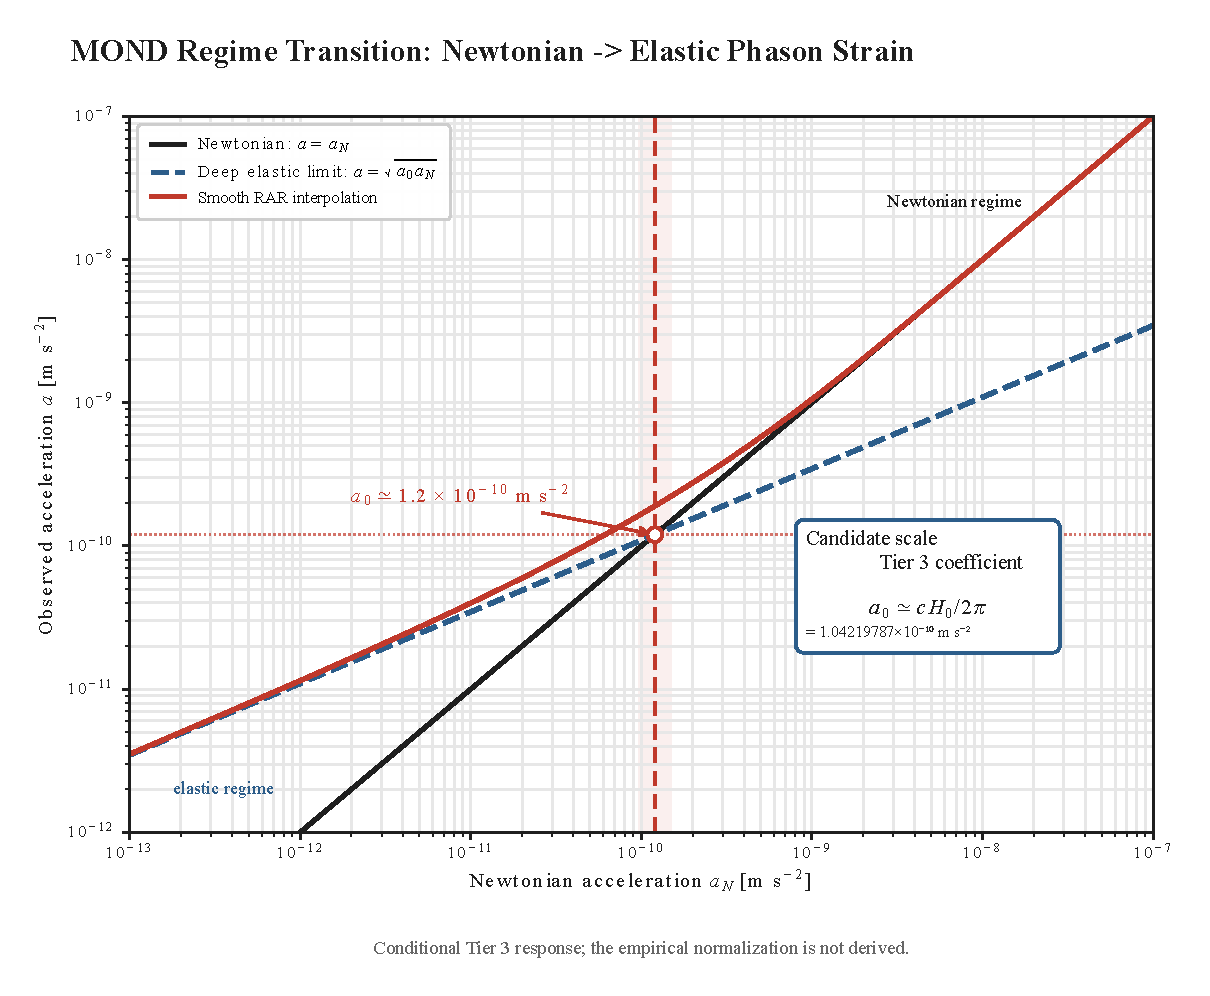
\includegraphics[keepaspectratio,alt={Conditional Tier 3 elastic-response ansatz shown log-log: a = a\_N at high accelerations and the assumed deep-elastic limit a = \textbackslash sqrt\{a\_0 a\_N\} at low accelerations, joined by an RAR interpolation. The empirical a\_0 = 1.2\textbackslash times10\^{}\{-10\}\textbackslash{} \{\textbackslash rm m\textbackslash,s\^{}\{-2\}\} is distinct from the dimensional thermodynamic scale cH\_0 = 6.54832237\textbackslash times10\^{}\{-10\}\textbackslash{} \{\textbackslash rm m\textbackslash,s\^{}\{-2\}\}; the Tier 3 candidate cH\_0/(2\textbackslash pi) = 1.04219787\textbackslash times10\^{}\{-10\}\textbackslash{} \{\textbackslash rm m\textbackslash,s\^{}\{-2\}\} is 13.1502\% low, and neither its coefficient nor the physical normalization is derived.}]{content/Figures/Volume_2/Figure V2.12.1.pdf}}
\caption{Conditional Tier 3 elastic-response ansatz shown log-log:
\(a = a_N\) at high accelerations and the assumed deep-elastic limit
\(a = \sqrt{a_0 a_N}\) at low accelerations, joined by an RAR
interpolation. The empirical
\(a_0 = 1.2\times10^{-10}\ {\rm m\,s^{-2}}\) is distinct from the
dimensional thermodynamic scale
\(cH_0 = 6.54832237\times10^{-10}\ {\rm m\,s^{-2}}\); the Tier 3
candidate \(cH_0/(2\pi) = 1.04219787\times10^{-10}\ {\rm m\,s^{-2}}\) is
13.1502\% low, and neither its coefficient nor the physical
normalization is derived.}
\end{figure}

\chapter{Chapter 13: Dark Matter III --- Cluster
Dynamics}\label{chapter-13-dark-matter-iii-cluster-dynamics}

Conditional on the Tier-3 topological-glass ansatz of Chapter 12, its
elastic equations define a candidate account of galaxy dynamics and the
Radial Acceleration Relation. Massive clusters are a distinct unresolved
physical test. This chapter develops the mathematical consequences of a
further \textbf{Tier-3 Lattice Fracture ansatz}: an assumed finite yield
strength and a transition from pinned to unpinned branches. These are
conditional model mechanics, not a derived physical transition or a
demonstrated resolution of cluster lensing.

\begin{center}\rule{0.5\linewidth}{0.5pt}\end{center}

\subsection{13.1 The Fracture Transition}\label{the-fracture-transition}

\subsubsection{13.1.1 Yield Strength: The Virial Stress Limit {[}Tier 3
physical ansatz; Tier 2 conditional
mechanics{]}}\label{yield-strength-the-virial-stress-limit-tier-3-physical-ansatz-tier-2-conditional-mechanics}

Every solid medium is defined by its ability to support shear stress
only up to a critical limit. In the GCT substrate, the
\textbf{Topological Glass} consists of phason strain \(w_{ij}\) pinned
to the icosahedral matching rules of the vacuum. The energy required to
maintain this strain is governed by the phason stiffness \(K_\perp\).

We define the \textbf{Vacuum Yield Strength (\(\sigma_c\))} as the
maximum stress the phason field can support before the topological
pinning of the lattice fails, and write it {[}Tier 3 ansatz{]} as a
function of the critical strain \(\epsilon_y\):
\[\sigma_c \approx \epsilon_y \cdot K_\perp\] where the AKN tiling-flip
proposal gives the candidate value
\(\epsilon_y = \phi^{-5} \approx 0.090\) in V3 Ch11 §11.1.3
\textbf{{[}Tier 3, conditional on two Tier 3 inputs{]}}. The
calculations use \(\epsilon_y = 0.1\) (Tier 3); \(\phi^{-5}\) is a
candidate value, not the operative one. Under the ansatz, the
gravitational stress (virial stress) generated by baryonic mass in
spiral galaxies would lie significantly below \(\sigma_c\), leaving the
vacuum in the elastic regime, while in rich galaxy clusters---where the
total mass exceeds \(10^{14}\) to \(10^{15}\) solar masses---the
accumulated gravitational potential would create a strain gradient
exceeding the yield strength of the lattice. This conflicts with
Protocol C's treatment of relaxed cool cores (Perseus, A2029, A1795) as
below its frozen pressure cut; the cluster-core rheology is a declared
open programme (V3 Ch11 §11.1.4), and neither reading is used to absorb
or predict an observation.

\subsubsection{13.1.2 The Phase Change: Stress-Induced
Liquefaction}\label{the-phase-change-stress-induced-liquefaction}

Under the Tier-3 transition ansatz, exceeding \(\sigma_c\) labels a
local phase-change branch. Conditional on that assumption, the tiles
lose their pinned orientations and the model enters
\textbf{Stress-Induced Liquefaction}; physical realization remains open.

\begin{itemize}
\tightlist
\item
  \textbf{Cluster Cores:} In the dense central regions of a cluster, the
  vacuum is in a \textbf{Fractured Liquid State} (\(\eta_g \to 0\)). In
  this regime, the shear modulus \(\mu_\perp\) vanishes. Gravity ceases
  to mimic MONDian elasticity but instead follows the ``Fluid'' limit of
  General Relativity, where the ``Dark Matter'' is treated as a
  collisionless gas of energy density. Under the ansatz this would
  account for why cluster mass profiles require a dark component but do
  not obey the simple MOND acceleration law found in isolated galaxies
  {[}Tier 3; core rheology open, V3 Ch11 §11.1.4{]}.
\item
  \textbf{The Transition from Pinned to Unpinned:} In the glassy phase
  (Galaxies), the phason defects are ``pinned'' to the lattice, creating
  a static restoring force. In the fractured phase (Clusters), the
  defects become \textbf{Unpinned}. They become kinetic
  debris---independent topological singularities (vortons) that move
  freely through the superfluid background. Free emitters at cluster
  virial speeds would broaden the 3.55 keV line far beyond the narrow
  width assumed in Protocol C; the emitter kinematics are a declared
  open programme (V3 Ch11 §11.2.3).
\end{itemize}

\subsubsection{13.1.3 Resolution of the Bullet
Cluster}\label{resolution-of-the-bullet-cluster}

The ``Bullet Cluster'' (1E 0657-56) is often cited as strong evidence
for particulate dark matter because its lensing centers are spatially
separated from the baryonic gas. Conditional on the Chapter-12 and
fracture ansätze, GCT offers \textbf{Rheological Separation} as a
candidate postdiction; it neither refutes the particle interpretation
nor derives the physical separation from first principles.

\begin{itemize}
\tightlist
\item
  \textbf{The Collision Event:} When two clusters collide, the immense
  stress shatters the pinned vacuum lattice.
\item
  \textbf{Phase Separation:} The system separates into two phases with
  distinct viscosities:
\end{itemize}

\begin{enumerate}
\def\labelenumi{\arabic{enumi}.}
\tightlist
\item
  \textbf{The Phonon Sector (Baryons):} The gas interacts via the
  ``stiff'' phonon modes (electromagnetism/pressure), exhibiting high
  viscosity and shock fronts. It slows down.
\item
  \textbf{The Phason Sector (Phason-Defect Halo):} The shattered vacuum
  energy forms a cloud of \textbf{Unpinned Phason Defects}
  (\(E_\perp\)). These defects are decoupled from the phonon metric;
  they interact only via the acoustic metric (Gravity).
\end{enumerate}

\begin{itemize}
\tightlist
\item
  \textbf{The Result:} The proposed \textbf{phason-defect halo} moves
  ballistically, preserving its momentum like a collisionless fluid, and
  can therefore lead the viscous baryonic gas. This physical defect
  cloud is not the compact address Solenoid \(\Sigma_\infty\). The
  observation is consistent with \textbf{Vacuum Superfluidity} {[}Tier
  3{]} and does not uniquely favor a new particle, but it does not
  constitute a decisive confirmation. An inviscid (super)fluid is not
  automatically collisionless; that the defect gas behaves
  collisionlessly, and meets the Bullet-cluster self-interaction bound,
  is not shown.
\end{itemize}

\subsubsection{13.1.4 The Rheological Phase Diagram {[}Tier 2
conditional mechanics; Tier 3 physical
adoption{]}}\label{the-rheological-phase-diagram-tier-2-conditional-mechanics-tier-3-physical-adoption}

We formalize this behavior by plotting the Vacuum Phase Diagram on the
axes of \textbf{Shear Stress (\(\tau\))} vs \textbf{Temperature
(\(T_{eff}\))} (where \(T_{eff}\) represents the kinetic energy density
of the defects).

\begin{enumerate}
\def\labelenumi{\arabic{enumi}.}
\tightlist
\item
  \textbf{Solid Phase (Galaxies):} Below the critical stress
  (\(\tau < \sigma_c\)), the vacuum is a \textbf{Topological Glass}. The
  phason defects are pinned. The effective viscosity is infinite
  (\(\eta_{visc} \to \infty\)). This is the MONDian regime where the
  vacuum response is elastic.
\item
  \textbf{Fluid Phase (Clusters):} Above the critical stress
  (\(\tau > \sigma_c\)), the vacuum is a \textbf{Shear-Thinning Fluid}.
  The lattice yields, and the defects unpin. The viscosity drops
  precipitously (\(\eta_{visc} \to 0\)). This is the Dark Matter regime
  where the vacuum is assumed to flow as a collisionless gas (not shown;
  see §13.1.3).
\end{enumerate}

\gctneedspace{5\baselineskip}

\textbf{Mechanism of Separation:} Within the assumed model, the Bullet
Cluster impact region is assigned a stress spike \(\tau \gg \sigma_c\),
a superfluid-like vacuum branch, and viscous baryons governed by
electromagnetic cross-sections. This rheological contrast is a candidate
coordinate for the observed separation; its physical realization and
causal sufficiency remain open.

\subsubsection{13.1.5 The 3.55 keV X-ray Line: Vacuum Triboluminescence
{[}Tier 3 emission mechanism pending rate/branching
closure{]}}\label{the-3.55-kev-x-ray-line-vacuum-triboluminescence-tier-3-emission-mechanism-pending-ratebranching-closure}

The \textbf{3.55 keV X-ray Anomaly} is proposed, conditional on O.38, as
the observational signature of vacuum fracture; the line itself is
unconfirmed. Unlike standard particle models which assume a constant
decay rate, GCT models this signal {[}Tier 3{]} as a
\textbf{Stress-Induced Emission} (analogous to triboluminescence).

\begin{itemize}
\tightlist
\item
  \textbf{Vorton Snapping:} When the topological glass fractures under
  high stress, the ``snapping'' of the lattice bonds forces a unit of
  topological winding (a Vorton) to unwind. This release of stored
  elastic energy results in the emission of a high-frequency phason wave
  (a Photon).
\item
  \textbf{Conditional Energy Identity:} Once the Tier 3 O.38 posit
  \(N_{\rm cage}=144\) is supplied, the division defining the
  \textbf{Vacuum Quantum (\(E_{vac}\))} is exact:
  \[E_{vac} = \frac{m_e c^2}{144} \approx 3.5486 \text{ keV}\] The
  absolute centroid is therefore Tier 3 and O.38-conditional. The
  lattice-fracture mechanism form is Tier 3 (it rests on the Tier 3
  Topological Glass model and is conditional on the adopted
  architecture); neither the division nor the centroid selects the cage
  size.
\item
  \textbf{Environmental Falsification:} Because emission requires
  fracture, GCT predicts the 3.55 keV line will be bright only in
  mass-weighted regions above the frozen stress threshold
  \(\sigma_{crit}\) (cluster outskirts, merger shocks, high-shear ICM)
  and suppressed in low-stress Dwarf Spheroidal galaxies (elastic
  glass). The Perseus core lies outside Protocol C's frozen pressure
  aperture and is not a falsification aperture; this is an aperture
  definition, and it conflicts with the fractured-core reading of
  §13.1.1 (open programme, V3 Ch11 §11.1.4). A decisive low-shear
  falsifier is not mere non-detection; it is a confirmed \(>3\sigma\)
  3.548 keV line in a registered dSph at the Protocol C sensitivity and
  control floor.
\end{itemize}

Conditional on the Tier 3 glass and fracture ansätze, the model would
describe the ``missing mass'' of the universe as the \textbf{Elastic
Energy} of the vacuum, existing as a solid glass in the quiet outskirts
of galaxies and as a shattered gas of unpinned defects in the violent
hearts of clusters. This is not a demonstrated unification: the
separation of one frozen-strain sector into dark matter and \(\Lambda\)
is open (O.47), and the cluster-core rheology and emitter kinematics are
declared open programmes (V3 Ch11 §11.1.4, §11.2.3).

\chapter{Chapter 14: The Phason Vacuum and Dark
Energy}\label{chapter-14-the-phason-vacuum-and-dark-energy}

\gctneedspace{5\baselineskip}\begin{gctNote}

\textbf{Epistemic Status {[}Tier 2 / Tier 3 / Tier 4{]}:} This chapter
presents the dark energy sector in two parts. \textbf{Part A (§14.1)}
gives the frozen-phason-vacuum reading of \(w = -1\) {[}Tier 3: it
follows if the frozen-strain energy density is constant in \(a\); no
covariant stress-energy or dilution law is derived{]} and the
holographic-entanglement area-law construction of the
cosmological-constant scale (Tier 2 only for the identification of
\(\chi\) with the horizon area ratio; the \(\rho_\Lambda\) formula is a
Tier 1 rewriting of the Friedmann identity, and its area-law reading is
Tier 3, App ULA §ULA.4.1). The absolute magnitude of \(\rho_\Lambda\)
remains \textbf{Tier 3} pending RG-running / condensate-normalisation
closure (App ORQ O.1/O.4/O.13), matching Parameter Ledger §0.1.
\textbf{Part B (§14.2--14.8)} presents a calibrated channel-shape fit
(Tier 3 as a correlation template) plus a \textbf{Tier 4 physical-source
interpretation}. No biological carrier, physical Selection Operator,
biology-to-phason transducer, normalized source operator, or covariant
stress-energy map has been derived. The identification
\(\lambda_{bio} \equiv \alpha\) is a declared coefficient choice inside
that ansatz, not an established microscopic coupling. The phantom
direction (\(w < -1\)) of the Part B template is \textbf{Tier 4} as a
physical claim: the written action cannot produce \(w<-1\) without a
ghost, and no ghost-free construction is derived (§14.3.1).

\end{gctNote}

This chapter presents GCT's approach to dark energy in two distinct
parts. \textbf{Part A} gives a Tier 3 equation-of-state reading of the
frozen phason vacuum and an area-law construction of the scale (Tier 2
\(\chi\) identification; Tier 1 Friedmann rewriting with a Tier 3
area-law reading of \(\rho_\Lambda\)), while the absolute energy scale
remains Tier 3 pending RG-running / condensate-normalisation closure.
\textbf{Part B} presents the biogenic correlation hypothesis: a Tier 3
shape model whose physical biological-source reading is Tier 4. The two
parts are epistemically independent. Part A can stand without Part B;
Part A supplies only a mathematical field template for Part B and does
not establish its carrier, transducer, source, or stress-energy bridge.

\begin{center}\rule{0.5\linewidth}{0.5pt}\end{center}

\subsection{14.1 Phason Vacuum Cosmology {[}Tier 3 equation of state;
Tier 2 area-law identification{]} (Part
A)}\label{phason-vacuum-cosmology-tier-3-equation-of-state-tier-2-area-law-identification-part-a}

\begin{quote}
\textbf{Scope note.} CMB acoustic peaks and LSS are not confronted here
(O.13c). The split of the frozen-strain sector into the clustering dark
matter of Chapter 11 and the constant-density component used here is
open (O.47). It also faces a known obstruction: frozen elastic and
defect configurations generically give \(w=-1/3\) (strings), \(-2/3\)
(walls) or \(-1\) (constant strain energy) (Bucher \& Spergel 1999), not
the pressureless \(w=0\) that clustering dark matter requires.
\end{quote}

\subsubsection{14.1.1 The Frozen Phason Field and w =
−1}\label{the-frozen-phason-field-and-w-1}

The GCT vacuum is in the frozen phason phase at temperatures below
\(T_{freeze}\) (Volume 2, Chapter 3). In this phase, phason
displacements \(u_\perp\) are quenched: they carry an energy density
\(\rho_{phason}\) that is constant in time (independent of the scale
factor \(a(t)\)), because frozen phasons cannot dynamically relax their
strain. A constant vacuum energy density is the defining property of a
cosmological constant. That uniform density must also be present in the
intergalactic voids, which Chapter 11 (§11.1.2) calls the stress-free
\(\eta_g=1\) ground state; this spatial tension is declared open under
O.47.

\textbf{Tier 3:} \emph{\(w = -1\) follows if the frozen-strain energy
density is constant in \(a\); no covariant stress-energy or dilution law
is derived. The motivating analogy is that a quenched elastic strain
need not relax as the volume grows. The same frozen-strain picture is
used for dark matter in Chapter 11, which must dilute as \(a^{-3}\) and
cluster; the split between the two components is Open Problem O.47.}

Under that assumption the value is not tuned, but it rests on the
frozen-phason reading rather than on a derived stress-energy tensor. It
is offered as a geometric motivation for \(w \approx -1\) rather than
\(w = 1/3\) (radiation) or \(w = 0\) (matter).

\subsubsection{14.1.2 The Continuous Phantom Phase as Phason
Activation}\label{the-continuous-phantom-phase-as-phason-activation}

The DES-Dovekie recalibrated DESI DR2 + CMB CPL fit
\((w_0, w_a) = (-0.803 \pm 0.054,\ -0.72 \pm 0.21)\) is sign-opposite to
the registered single-channel biogenic shape, with joint dynamical-DE
significance 3.2σ (arXiv:2511.07517): the stipulated biogenic \(w(z)\)
asymptotes to \(-1\) from below without a physical crossing of the
\(w=-1\) boundary, whereas the DES-Dovekie CPL central fit corresponds
to a low-redshift linearized trajectory with the opposite \((w_0,w_a)\)
orientation. Observational distinguishability is therefore registered as
O.13 closure path C1, not as direct DESI support. Interpreting any
confirmed \(w < -1\) state-level signal as a partially activated phason
field with \(\tau_{phason}\lesssim H_0^{-1}\) is a Tier 4 conditional
field hypothesis (no ghost-free phantom construction is derived;
§14.3.1), not a unique inference or a derived biogenic mechanism.

\textbf{Tier 4 Conditional Interpretation:} \emph{If \(w < -1\) is
confirmed at high significance, one model branch assigns
\(\tau_{phason}(z=0) \sim H_0^{-1}\) and places the vacuum near a phason
freezing transition. The separate \(E_{\rm bio,phason} \approx 1.6\) eV
comparison is a material-scale analogy only: no engine protocol produces
it, and Appendix PSC registers \(E_{\rm bio,phason}\) as the thermal
scale \(k_BT(310\,\mathrm{K}) = 0.0267\) eV. No normalized cross-scale
interaction, biological transducer, physical Selection Operator,
phenomenal bridge, or Level-II sensitivity to dark energy has been
derived.}

\subsubsection{14.1.3 The Operative Phason Mass Gap and Dark Energy
Density}\label{the-operative-phason-mass-gap-and-dark-energy-density}

The operative biogenic-DE quartic mass scale is currently a \textbf{Tier
3 empirical parameter}:
\(m_{\rm phason}^{\rm operative} \approx 1.7 \times 10^{-5}\) eV

This value is an empirical inference pending formal geometric derivation
from the 6D lattice locking potential. It is NOT currently derived from
first principles; it is a phenomenological postdiction subject to
experimental test. It is distinct from the Tier-3 Weinberg-coincidence
candidate \(m_{\rm Weinberg}=M_P\phi^{-147}\approx2.3\) meV (O.37), and
from the Hubble energy \(E_{H0}=\hbar H_0\approx1.44\times10^{-33}\) eV.

The App ULA scalar-condensate formula is a schematic coupling relation,
\(\rho_\Lambda = \frac{1}{2} (m_{\rm phason}^{\rm operative})^2 \langle\Phi_\perp\rangle^2\),

where \(\langle\Phi_\perp\rangle\) is the phason condensate amplitude
set by the locking potential \(V_{lock}\). This formula is NOT the naive
\(\rho = m^4/(\hbar c)^3\) relation (which incorrectly assumes a
zero-temperature, free-field result), and it does NOT identify
\(m_{\rm phason}^{\rm operative}c^2\) with \(\hbar H_0\). The condensate
formula requires knowledge of \(\langle\Phi_\perp\rangle\) and the
quartic coupling normalization, which is part of Open Problem O.1.

The zero-temperature free-field formula \(\rho = m^4/(\hbar c)^3\) is
inapplicable here: it yields \(\rho \approx 1.7\times10^{-18}\) J/m³ for
\(m = 1.7 \times 10^{-5}\) eV --- about eight and a half orders of
magnitude below the Planck-parameter value \(5.25 \times 10^{-10}\)
J/m³, and therefore does not capture the condensate physics. The
reference density is expressed canonically in this chapter by the
Friedmann/area-law form
\(\rho_\Lambda = (3\Omega_\Lambda/8\pi)\,\hbar H_0^2/(c\ell_P^2)\); this
uses \(H_0\) and \(\Omega_\Lambda\) as cosmological inputs until O.4
closes.

\gctneedspace{5\baselineskip}\begin{gctImportant}

\textbf{Firewall Metadata{[}Phason Mass Gap{]}}

\begin{itemize}
\tightlist
\item
  \textbf{Type:} Calibrated Empirical Estimate
\item
  \textbf{Value:} \(m_{\rm phason}^{\rm operative}=1.7 \times 10^{-5}\)
  eV
\item
  \textbf{Status:} Tier 3 operative biogenic-DE quartic scale pending
  Tier 2 geometric derivation from locking-potential curvature and
  coupling normalization; the Weinberg-coincidence scale is separate
  O.37 material, and \(\hbar H_0\) is not a direct phason-mass
  constraint.
\end{itemize}

\end{gctImportant}

\subsection{\texorpdfstring{\textbf{14.1.4 Theorem: Non-Equivalence of
O.1 and O.4 Scale Closures {[}Tier 2 mechanism + Tier 3 absolute
scale{]}}}{14.1.4 Theorem: Non-Equivalence of O.1 and O.4 Scale Closures {[}Tier 2 mechanism + Tier 3 absolute scale{]}}}\label{theorem-non-equivalence-of-o.1-and-o.4-scale-closures-tier-2-mechanism-tier-3-absolute-scale}

\gctneedspace{5\baselineskip}

\textbf{Theorem 14.1.4 (Conditional Dark-Energy Chain):} Given a
dark-energy density \(\rho_\Lambda\) and assuming
\(\Omega_\Lambda \approx 0.68\) (standard cosmology), the Hubble
constant is fixed by the Friedmann relation:

\(H_0^2 = \frac{8\pi G \rho_\Lambda}{3\Omega_\Lambda}\)

\emph{Proof:} Step 1 (Tier 2 mechanism, Tier 3 normalization): the
frozen-phason condensate can contribute
\(\rho_\Lambda = \frac{1}{2}(m_{\rm phason}^{\rm operative})^2\langle\Phi_\perp\rangle^2\)
only after \(V_{lock}\) curvature and condensate normalization are
specified. Step 2 (exact): \(\rho_\Lambda \to H_0\) via Friedmann:
\(H_0^2 = 8\pi G\rho_\Lambda/(3\Omega_\Lambda)\). Step 3 (scale
discipline): \(m_{\rm phason}^{\rm operative}\), \(m_{\rm Weinberg}\),
and \(\hbar H_0\) are three distinct quantities. The first is the
operative quartic mass scale, the second is an O.37 coincidence ansatz,
and the third is the Hubble energy scale that enters \(\rho_\Lambda\)
through the Friedmann/area-law expression.

Steps 2--3 are rigorous. Step 1 remains an O.1 coupling-normalization
problem.

\textbf{Corollary:} Open Problem O.4 (derive \(H_0\)) is coupled to, but
not identical with, Open Problem O.1 (derive
\(m_{\rm phason}^{\rm operative}\) and the condensate normalization).
Solving O.1 alone does not determine \(H_0\) unless
\(\langle\Phi_\perp\rangle\), the quartic coupling, and
\(\Omega_\Lambda\) are also fixed. □

\gctneedspace{5\baselineskip}

\textbf{Consistency check (KZ self-consistency):} The Kibble-Zurek
mechanism applied to the GCT crystallization gives a defect correlation
length \(\xi_{KZ}\) at formation. The requirement \(\xi_{KZ} = R_H\)
today (Hubble radius) is satisfied when
\(\epsilon_{lock} = \ell_P/R_H = H_0/\omega_P\). This is not a
derivation of \(H_0\) (circular), and it is not an independent
confirmation either: the condition is imposed by choosing
\(\epsilon_{lock}\), so it shows only that the Kibble-Zurek picture can
be made compatible with a phason correlation length equal to today's
Hubble radius {[}Tier 3 consistency condition{]}.

\begin{center}\rule{0.5\linewidth}{0.5pt}\end{center}

\subsection{\texorpdfstring{\textbf{14.1.5 Holographic Entanglement
Entropy Construction of \(\Lambda\) {[}Tier 2 area-law identification +
Tier 3 numerical evaluation pending Open Problem
O.4{]}}}{14.1.5 Holographic Entanglement Entropy Construction of \textbackslash Lambda {[}Tier 2 area-law identification + Tier 3 numerical evaluation pending Open Problem O.4{]}}}\label{holographic-entanglement-entropy-construction-of-lambda-tier-2-area-law-identification-tier-3-numerical-evaluation-pending-open-problem-o.4}

\begin{quote}
\textbf{Scope of this section {[}read first{]}.} What is derived here is
the \textbf{area-law form} of the cosmological constant within the
holographic entanglement-entropy framework, and the
\textbf{identification} of the Bekenstein-Hawking area ratio with the
GCT critical susceptibility \(\chi\) of the \(6D \to 3D\) projection.
What is \emph{not} derived here is the absolute magnitude of
\(\rho_\Lambda\) from GCT first principles: the formula evaluates to the
observed value because the Hubble constant \(H_0\) and dark-energy
fraction \(\Omega_\Lambda\) are imported from Planck 2018. A
first-principles GCT derivation of \(H_0\) remains \textbf{Open Problem
O.4}; a first-principles derivation of
\(m_{\rm phason}^{\rm operative}\) and the condensate normalization
remains \textbf{Open Problem O.1}. These problems are coupled through
\(\rho_\Lambda\) but are not the same scale identity. This section is
therefore best read as a \textbf{consistency check} of the GCT
\(6D \to 3D\) holographic apparatus against the Planck-anchored
cosmological-constant value, not as a first-principles derivation of
\(\rho_\Lambda\) from \(m_e\) alone.
\end{quote}

\textbf{The area-law content.} The effective cosmological constant
\(\Lambda\) is identified with the \textbf{entanglement entropy of the
\(6D \to 3D\) projection} via the Bekenstein-Hawking area law evaluated
on the exact-de-Sitter static-patch horizon proxy \(R_H=c/H_0\). In the
GCT framework, the physical \(3D\) manifold \(E_\parallel\) is a
projection of the \(6D\) parent lattice \(\mathbb{Z}^6\), while the
complementary coordinates \(E_\perp\) are not locally accessible from
within \(E_\parallel\). The resulting area ratio is a de Sitter
consistency construction; it is not the event-horizon area of the
present matter-plus-dark-energy cosmology.

We make the Ryu-Takayanagi route explicit by writing each step. The
Ryu-Takayanagi formula (Ryu and Takayanagi 2006) identifies the
entanglement entropy \(S_{ent}\) of a region \(A\) in the boundary
theory with the area of the extremal codimension-2 surface \(\gamma_A\)
in the bulk that is homologous to \(A\):
\[S_{ent}(A) = \frac{\text{Area}(\gamma_A)}{4 G_N}\] where \(G_N\) is
the bulk Newton constant. For an exact static de Sitter patch the
cosmological event horizon coincides with the Hubble radius, and the
extremal surface bounding the region causally accessible to a comoving
observer is the \(S^2\) horizon cross-section of radius \(R_H = c/H_0\)
(Bousso 2002 covariant extension of the Bekenstein-Hawking area bound),
with area \[A_{\mathcal{H}_{\rm dS}} = 4\pi R_H^2 = 4\pi (c/H_0)^2.\]

In a matter-plus-dark-energy cosmology the Hubble radius and the
event-horizon radius
\(R_{\rm eh} = a(t)\int_t^{\infty} c\,\mathrm{d}t'/a(t')\) are distinct,
and the numerical evaluation below inserts \(\Omega_\Lambda = 0.685\)
rather than treating \(H\) as constant. The quantity \(c/H_0\) is
therefore retained as the Hubble-radius proxy, and what follows is an
exact-de-Sitter consistency construction rather than an event-horizon
derivation.

\emph{Step 1 --- Apply RT to the de Sitter horizon.}
\[S_{ent} = \frac{A_{\mathcal{H}_{\rm dS}}}{4 G_N} = \frac{4\pi (c/H_0)^2}{4 G_N} = \frac{\pi c^2}{G_N H_0^2}\]

\emph{Step 2 --- Translate to Planck units.} In natural units
\(\hbar = c = 1\), the Planck length is \(\ell_P = \sqrt{G_N}\), so
\(G_N = \ell_P^2\). Substituting:
\[S_{ent} = \frac{\pi c^2}{G_N H_0^2} \xrightarrow{\hbar = c = 1} \frac{\pi}{\ell_P^2 H_0^2} = \pi \left(\frac{1}{H_0 \ell_P}\right)^2\]
Restoring \(c\) to give the dimensionless ratio in terms of the Hubble
radius \(R_H = c/H_0\):
\[S_{ent} = \pi \left(\frac{c}{H_0 \ell_P}\right)^2 = \pi \left(\frac{R_H}{\ell_P}\right)^2\]
which is manifestly the area of the de Sitter horizon in units of the
Planck area, divided by \(4\) (the \(\pi = 4\pi/4\) tracks the factor of
\(4\) in \(S = A/(4G_N)\)).

\emph{Step 3 --- Identify \(\chi\).} The dimensionless number
\(\pi (c/H_0\ell_P)^2\) is the Bekenstein-Hawking entropy of the de
Sitter horizon in Planck units. We identify this with the critical
susceptibility of §14.4:
\[\boxed{\chi \equiv S_{ent} = \pi \left(\frac{c}{H_0 \ell_P}\right)^2 \approx 2.27 \times 10^{122}}\]
(Using Planck 2018 \(H_0 = 67.4\) km/s/Mpc and CODATA constants.)

\emph{Step 4 --- From entropy to energy density.} The vacuum energy
density associated with the boundary entanglement follows from the
\textbf{Friedmann equation} applied to the de Sitter horizon. Standard
cosmology gives
\(\rho_\Lambda = \Omega_\Lambda \cdot 3 H_0^2 c^2 / (8 \pi G_N)\) for
the dark-energy component of a flat universe with matter fraction
\(\Omega_m = 1 - \Omega_\Lambda\). Substituting
\(G_N = \ell_P^2 c^3 / \hbar\) (the GCT definition of Planck length),
the geometric form of the holographic identity reads:
\[\boxed{\rho_\Lambda = \frac{3 \Omega_\Lambda}{8\pi} \cdot \frac{\hbar H_0^2}{c\,\ell_P^2}}\]
Using \(H_0 = 67.4 \pm 0.5\) km/s/Mpc and
\(\Omega_\Lambda = 0.685 \pm 0.0073\) from Planck 2018 gives
\(\rho_\Lambda = 5.25 \times 10^{-10}\) J/m³, with a \(2.6\%\) linear
propagated uncertainty. This equality is an identity rather than an
independent test: observationally, \(\rho_\Lambda\) is obtained from the
same relation \(\rho_\Lambda=\Omega_\Lambda\rho_{\rm crit}c^2\). The
Tier 2 claim is the GCT identification of the area ratio with \(\chi\).
The boxed \(\rho_\Lambda\) formula is a Tier 1 rewriting of the
Friedmann identity; reading it as an area-law derivation of
\(\rho_\Lambda\) is Tier 3 (App ULA §ULA.4.1), and the numerical density
is a Tier 3 evaluation using imported cosmological parameters.

The \(10^{-120}\) Planck-scale suppression arises geometrically from the
dimensionless ratio \((\ell_P H_0 / c)^2 \sim 10^{-120}\) --- the square
of the Planck length over the Hubble radius. This restates the
suppression as the holographic area ratio of the Planck and Hubble
scales; it does not remove the fine-tuning question, because \(H_0\) and
\(\Omega_\Lambda\) are imported (the equality above is an identity) and
the Hubble radius is not a derived scale of the \(6D\) lattice (O.4).
The Tier 2 substance is the \textbf{identification} of this area ratio
with the critical susceptibility of the \(6D \to 3D\) projection
(§14.4.3 / the boxed \(\chi\) above), which is the geometric content
that GCT contributes beyond standard cosmology; the dark-energy density
formula itself is a re-derivation of the standard Friedmann result in
\(\ell_P\)-explicit form, which GCT reproduces but does not modify.

\textbf{Why the susceptibility is \(\chi\), not just \(S_{ent}\).} The
critical susceptibility introduced in §14.4 is identified with the same
area-to-Planck-area ratio because the exact-de-Sitter static-patch
horizon proxy supplies the infrared cutoff of this construction, while
the Planck length \(\ell_P = \sqrt{\hbar G_N/c^3}\) supplies the
ultraviolet cutoff of the AKN lattice. The susceptibility \(\chi\) is
therefore a Tier 2 quantity \emph{in functional form}; the displayed
numerical value remains Tier 3 because it imports the Planck 2018
\(H_0\) pending O.4/O.1 closure. In flat \(\Lambda\)\hspace{0pt}CDM with
\(\Omega_m=0.315\) and \(\Omega_\Lambda=0.685\), the present event
horizon is \(R_{\rm eh}\approx1.58\times10^{26}\) m rather than
\(c/H_0\approx1.37\times10^{26}\) m, so substituting the true event
horizon would instead give \(\chi_{\rm eh}\approx2.99\times10^{122}\).

\textbf{Tier disambiguation --- functional form vs numerical value.} The
\(\chi\) identification carries two distinct tier components that must
not be conflated:

\gctneedbreak{10\baselineskip}

{\def\LTcaptype{none} % do not increment counter
\begin{longtable}[]{@{}
  >{\raggedright\arraybackslash}p{(\linewidth - 4\tabcolsep) * \real{0.3333}}
  >{\raggedright\arraybackslash}p{(\linewidth - 4\tabcolsep) * \real{0.3333}}
  >{\raggedright\arraybackslash}p{(\linewidth - 4\tabcolsep) * \real{0.3333}}@{}}
\toprule\noalign{}
\begin{minipage}[b]{\linewidth}\raggedright
Component
\end{minipage} & \begin{minipage}[b]{\linewidth}\raggedright
Tier
\end{minipage} & \begin{minipage}[b]{\linewidth}\raggedright
What this component fixes
\end{minipage} \\
\midrule\noalign{}
\endhead
\bottomrule\noalign{}
\endlastfoot
\textbf{Functional form}
\(\chi \equiv S_{ent} = \pi (c / H_0 \ell_P)^2\) (the dimensionless
BH-area ratio) & \textbf{Tier 2} & The \emph{structural} identification
of the critical susceptibility with the entanglement entropy of the de
Sitter horizon. The area law itself is the Gibbons-Hawking result (Steps
1-3 above); the identification \(\chi \equiv S_{ent}\) is a definition
adopted by GCT, not a form forced by the cut-and-project structure, and
it does not depend on the empirical \(H_0\) value. \\
\textbf{Numerical value} \(\chi \approx 2.27 \times 10^{122}\) at
\(H_0 = 67.4\) km/s/Mpc, \(\Omega_\Lambda = 0.685\) & \textbf{Tier 3
(inherited)} & The \emph{specific numerical evaluation} requires the
empirical \(H_0\) from Planck 2018 + the CODATA \(\ell_P\). GCT does not
yet derive \(H_0\) from first principles; the absolute magnitude is
therefore a state-level import per §PSC.0, not a derivation output. \\
\end{longtable}
}

The §PSC.6 row on \(\chi\) inherits the Tier 3 numerical-value
disposition; the §PSC.6 row on dark-energy magnitude \(\rho_\Lambda\)
inherits the same. The Tier 2 \emph{mechanism} (holographic area-law
identification) is preserved separately from the Tier 3
\emph{evaluation} (numerical \(\chi\) value). A first-principles GCT
derivation of \(H_0\) from the non-linear phason locking potential
\(V_{lock}\) (Theorem 14.1.4) would close the Tier 3 numerical-value
side and lift the entire \(\chi\)-and-\(\rho_\Lambda\) row to Tier 2
unconditionally --- this is the load-bearing content of \textbf{Open
Problem O.4} (whose scale-closure is non-equivalent to O.1 per Theorem
14.1.4). Until O.4 closes, the headline \(\chi\) value is reported with
the Tier 3 inheritance discipline above; the area-law identification
remains Tier 2 in functional form regardless of the numerical-evaluation
conditionality.

\textbf{Hartle-Hawking boundary-state interpretation {[}Tier 1 standard
construction; Tier 2 GCT identification{]}.} The area law above is the
Gibbons-Hawking semi-classical result. The Euclidean Hartle-Hawking
construction (Hartle \& Hawking 1983 \emph{Phys. Rev.~D} 28:2960)
prepares a state on a compact spatial three-geometry. Euclidean
\(\text{dS}_4\) is the four-sphere \(S^4\) of radius
\(R_{\text{dS}} = c/H_0\); the Hartle-Hawking state is the Euclidean
path integral
\[\psi_{\text{HH}}[h_{ij}] = \int [\mathcal{D}g]\,e^{-S_E[g]},\qquad g|_{\partial} = h\]
over the southern half of \(S^4\), bounded by the equatorial \(S^3\).
This path integral prepares the pure wave functional \(\psi_{\rm HH}\)
on the whole \(S^3\); the preparation hemisphere of \(S^4\) is not an
entanglement subsystem. The spatial \(S^3\) is instead divided into two
three-balls across the \(S^2\) bifurcation surface of the static patch.
Tracing over the complementary three-ball gives a mixed reduced state
whose semi-classical entropy obeys the Gibbons-Hawking area law across
that \(S^2\):
\[S_{\text{ent}}^{\text{HH}} = -\mathrm{Tr}(\rho \ln \rho) = \frac{A_{S^2}}{4 G_N} = \pi\left(\frac{c}{H_0\,\ell_P}\right)^2 = \chi.\]
The Hartle-Hawking path integral supplies the boundary state, while the
\(S^2\) static-patch bipartition supplies the entropy. The numerical
protocol verifies the equality of this area-law value with \(\chi\); it
does not treat the \(S^3\) three-volume as an area.

\textbf{Symmetry-level \(\text{dS}_4/\text{CFT}_3\) operator-matching
audit for a scalar mode.} For a free scalar of mass \(m\) in
\(\text{dS}_{d+1}\) (radius \(L\)), the de Sitter mass-dimension
relation is \(\Delta(d-\Delta)=m^2L^2\). In \(\text{dS}_4\), where
\(d=3\) and \(L=c/H_0\), this gives
\[\Delta^2-3\Delta+m^2L^2=0,\qquad \Delta_\pm=\frac{3}{2}\pm\sqrt{\frac{9}{4}-m^2L^2}.\]
At the reference point \(mL=1\), representative of a Hubble-scale field,
the roots are
\[\Delta_+=\frac{3+\sqrt5}{2}=\phi^2,\qquad \Delta_-=\frac{3-\sqrt5}{2}=\phi^{-2}.\]
This numerical identification is conditional: it requires a scalar with
\(mL=1\) (or values near it for approximate golden-ratio dimensions),
and the manuscript has not established that GCT contains such a
Hubble-scale field. It is therefore a symmetry-level observation, not an
O.6 closure claim. The Tier-3 Weinberg-candidate scalar is not such a
field: with \(m_{\text{Weinberg}}c^2\approx2.3\) meV and \(L=c/H_0\),
\(mL=mc^2/(\hbar H_0)\approx1.6\times10^{30}\) and
\(m^2L^2\approx2.6\times10^{60}\). It sits deep in the principal series,
where \(\Delta_\pm=3/2\pm i\sqrt{m^2L^2-9/4}\to3/2\pm i\,mL\); the
finite \(\phi^{\pm2}\) dimensions are not assigned to it. Scale
discipline: this Weinberg-candidate scalar is not the operative
biogenic-DE quartic mass scale
\(m_{\rm phason}^{\rm operative}=1.7\times10^{-5}\) eV, and it is not
the Hubble energy \(E_{H0}=\hbar H_0\approx1.44\times10^{-33}\) eV. The
dark-energy density scale is the Friedmann/area-law form written above,
\(\rho_\Lambda=(3\Omega_\Lambda/8\pi)\,\hbar H_0^2/(c\ell_P^2)\), which
is of order \(M_{\rm Pl}^2H_0^2\); the quartic combination
\((\hbar H_0)^4\) is smaller by roughly \(10^{122}\) and is not the
observed scale. Neither form constrains \(m_{\rm phason}\) directly. The
operative \(m_{\rm phason}^{\rm operative}=1.7\times10^{-5}\) eV is
fixed by the biogenic-DE quartic coupling, not by \(\hbar H_0\). Engine:
\texttt{GCT\_Physics\_Engine/src/protocol\_o6\_dscft\_operator\_matching.py}.

The remaining open piece is the \emph{full Hilbert-space unitarity} of
\(\text{dS}_4/\text{CFT}_3\) (Strominger 2001 \emph{JHEP} 10:034
conformal symmetry of \(\text{dS}_4\); Maldacena 2003 \emph{JHEP} 05:013
non-normalizable wave functions; Anninos, Hartman \& Strominger 2017
\emph{Class. Quant. Grav.} 34:015009 higher-spin partial dictionary).
The semi-classical Hartle-Hawking entry and symmetry-level audit are
universal; the unitarity completion is upstream of any framework using
\(\text{dS}_4\) and is not GCT-specific. Status: V2 §14.1.5 is Tier 2
(area-law identification, standard semi-classical) + Tier 1 partial
(Hartle-Hawking boundary-state construction with explicit
entanglement-entropy derivation) + a \textbf{free-scalar
operator-dimension audit}; pending Hilbert-space unitarity completion
for full Tier 1.

\gctneedspace{5\baselineskip}\begin{gctImportant}

\textbf{Firewall Metadata {[}Holographic \(\Lambda\) Consistency
Construction{]}}

\begin{itemize}
\tightlist
\item
  \textbf{Type:} Tier 2 Geometric Identification (formula itself is the
  standard Friedmann result re-expressed via
  \(G_N = \ell_P^2 c^3/\hbar\); the Tier 2 substance is the
  identification of \(\chi\) with the \(6D \to 3D\) critical
  susceptibility)
\item
  \textbf{Inputs:} \(H_0\) (observational cosmology anchor with
  phason-condensate interpretation via Theorem 14.1.4), \(G_N\) (through
  \(\ell_P=\sqrt{\hbar G_N/c^3}\)), \(\Omega_\Lambda \approx 0.685\)
  (Planck 2018 cosmological composition --- Tier 3 import); \(m_e\) does
  not enter this formula
\item
  \textbf{Degrees of Freedom:} 0 fitted within the displayed Friedmann
  expression after the observational cosmology anchors are supplied;
  this is not an autonomous prediction of \(H_0\) or \(\Omega_\Lambda\).
\item
  \textbf{Key formula:}
  \(\rho_\Lambda = (3\Omega_\Lambda)/(8\pi) \cdot \hbar H_0^2 / (c\,\ell_P^2)\)
\item
  \textbf{Provenance:} Standard Friedmann equation for \(\rho_\Lambda\)
  with \(G_N\) expressed in terms of \(\ell_P\). The Tier 2 content is
  the identification of \(\chi = \pi(c/(H_0\ell_P))^2\) with the
  holographic information capacity of the de Sitter horizon (per
  Gibbons-Hawking 1977 and Bousso 2002 covariant extension); the dS/CFT
  boundary-state derivation remains Open Problem O.6.
\item
  \textbf{Cited works:} Gibbons, G. \& Hawking, S. (1977), \emph{Phys.
  Rev.~D} 15, 2738 --- ``Cosmological event horizons, thermodynamics,
  and particle creation''; Bousso, R. (2002), \emph{Rev.~Mod. Phys.} 74,
  825 --- ``The Holographic Principle''; Ryu, S. \& Takayanagi, T.
  (2006), \emph{Phys. Rev.~Lett.} 96, 181602 --- ``Holographic
  Derivation of Entanglement Entropy from AdS/CFT'' (cited for AdS
  analog; dS extension is Open Problem O.6).
\end{itemize}

\end{gctImportant}

\subsection{\texorpdfstring{\textbf{14.1.5b AdS vs dS --- Scope Note
{[}Tier 2 / Tier
3{]}}}{14.1.5b AdS vs dS --- Scope Note {[}Tier 2 / Tier 3{]}}}\label{b-ads-vs-ds-scope-note-tier-2-tier-3}

The Ryu-Takayanagi formula was established rigorously in the AdS/CFT
correspondence (anti-de Sitter bulk dual to a conformal field theory on
the conformal boundary). Our observed universe is asymptotically de
Sitter, not anti-de Sitter, and the dS/CFT correspondence --- while a
serious research program (Strominger 2001; Maldacena 2003) --- does not
have the same maturity as AdS/CFT. The scope question is: \emph{under
what conditions is GCT's use of the RT area law legitimate when the bulk
is de Sitter rather than anti-de Sitter?}

\textbf{What is shared between AdS and dS.} Three structural features of
the RT chain survive the AdS \(\to\) dS transition:

\begin{enumerate}
\def\labelenumi{\arabic{enumi}.}
\item
  \emph{The area law itself.} The Bekenstein-Hawking entropy
  \(S = A/(4G_N)\) is a property of any causal horizon --- black hole,
  Rindler, de Sitter --- and predates AdS/CFT by two decades (Bekenstein
  1973; Hawking 1975; Gibbons and Hawking 1977 for the dS horizon
  specifically). The exact-de-Sitter static-patch horizon area
  \(A_{\mathcal{H}_{\rm dS}} = 4\pi R_H^2\) saturates the
  Gibbons-Hawking bound, and the entropy \(S = \pi(c/H_0\ell_P)^2\) is
  the de Sitter analogue of the AdS-RT formula at the same level of
  rigour as the Gibbons-Hawking result.
\item
  \emph{The extremal-surface identification.} In AdS the RT surface is a
  boundary-anchored minimal surface; AdS has no cosmic horizon. In dS
  the static-patch horizon entropy is the Gibbons-Hawking result, while
  extremal surfaces anchored at future infinity are generally complex or
  timelike, which is an open problem. Reading the dS horizon area as an
  entanglement entropy of the accessible region is therefore an
  identification, not a theorem carried over from AdS {[}Tier 3; O.6{]}.
\item
  \emph{The Planck-area UV cutoff.} The denominator
  \(4G_N = \ell_P^2 \cdot c^3/\hbar\) in the area law is fixed by
  Newton's constant, not by the AdS curvature scale, so the numerical
  value of \(\chi\) depends only on \(\ell_P\) and \(R_H\), not on the
  global sign of the curvature.
\end{enumerate}

\textbf{What is \emph{not} shared.} Two features of full AdS/CFT do not
extend cleanly to dS:

\begin{enumerate}
\def\labelenumi{\arabic{enumi}.}
\item
  \emph{The boundary CFT interpretation.} In AdS/CFT the boundary
  entanglement entropy is the entropy of a definite dual CFT. The dS/CFT
  proposal of Strominger (2001) and Maldacena (2003) gives a non-unitary
  Euclidean CFT on the future conformal infinity of dS; the dictionary
  between bulk and boundary observables is less developed and remains
  conjectural. \textbf{GCT does not require this dictionary.} What GCT
  requires is only the area-to-entropy relation at the de Sitter
  horizon, which is supplied by Gibbons-Hawking (1977) without any CFT
  input.
\item
  \emph{Holographic renormalisation.} The technology that translates AdS
  bulk observables into boundary CFT correlators --- counterterms,
  conformal anomalies, near-boundary expansions --- is specific to AdS
  and does not transfer to dS. \textbf{GCT does not invoke holographic
  renormalisation.} The cosmological-constant derivation uses only
  \(S = A/(4G_N)\) and the geometric area of the dS horizon; no boundary
  correlator is computed.
\end{enumerate}

\textbf{Scope statement {[}Tier 2 for the area law; Tier 3 for any full
dS/CFT extension{]}.} GCT's holographic consistency construction of
\(\Lambda\) is legitimate in the appropriate-limit sense: it uses the
area law that is rigorously established for \emph{any} causal horizon
(Bekenstein-Hawking, Gibbons-Hawking) and the horizon fixed by the de
Sitter geometry. It does not invoke the full dS/CFT correspondence and
does not assume a boundary CFT exists. The phrase ``Ryu-Takayanagi
formula'' is used here in the area-law sense --- the geometric content
of RT that survives the AdS \(\to\) dS transition --- and not in the
dS/CFT-duality sense. The horizon-area scaling is the same in both
signatures; only the boundary-CFT interpretation differs, and GCT is
independent of that interpretation.

\gctneedspace{5\baselineskip}\begin{gctNote}

\textbf{What would tighten this further.} A first-principles dS/CFT
derivation of the boundary state whose entanglement entropy is
\(S = \pi(c/H_0\ell_P)^2\) --- analogous to the BTZ-vacuum derivation in
AdS\(_3\)/CFT\(_2\) --- would upgrade §14.1.5 from Tier 2 (area law) to
Tier 1 (boundary-state derivation). This is recorded as \textbf{Open
Problem O.6 (dS/CFT Boundary State for \(\chi\))} in Appendix ORQ
§ORQ.5. Until then, GCT's holographic use of RT is to be read as ``the
area-law subcase that does not require the full dS/CFT dictionary''.

\end{gctNote}

\subsection{\texorpdfstring{\textbf{14.1.5c Action-Items Roadmap for
§14.1.5 Tier-1
Promotion}}{14.1.5c Action-Items Roadmap for §14.1.5 Tier-1 Promotion}}\label{c-action-items-roadmap-for-14.1.5-tier-1-promotion}

The five steps below are the sequence required to upgrade §14.1.5 from
Tier 2 (area law) to Tier 1 (boundary-state derivation):

The dS/CFT correspondence (Strominger 2001 \emph{JHEP} 0110:034;
Maldacena 2003 \emph{JHEP} 0305:013) currently lacks the AdS-equivalent
dictionary needed to derive the de Sitter horizon entropy from a
boundary state. Closure of O.6 requires the following sequence:

\begin{enumerate}
\def\labelenumi{\arabic{enumi}.}
\item
  \textbf{dS bulk--boundary dictionary {[}Step 1 --- Tier 2 framework
  target{]}.} Establish the bulk-to-boundary mapping for asymptotically
  de Sitter spacetimes analogous to AdS/CFT's
  \(\Phi_{bulk}(z=0, x) = \mathcal{O}_{CFT}(x)\). For dS, the natural
  conformal boundary is future infinity \(\mathcal{I}^+\) (and/or past
  infinity \(\mathcal{I}^-\)); the boundary CFT is non-unitary Euclidean
  and depends on the choice of the Euclidean vacuum (Bunch-Davies,
  alpha-vacua). This is active research (Anninos, Hartman, Strominger
  2017 \emph{Class. Quant. Grav.} 34:015009).
\item
  \textbf{Explicit boundary state for static SdS {[}Step 2 --- Tier 2
  ansatz{]}.} Construct the boundary state \(|\Psi_{SdS}\rangle\) on
  \(\mathcal{I}^+\) whose reduced density matrix on the southern
  hemisphere reproduces the Bunch-Davies thermal state at
  \(T_{GH} = H_0/2\pi\) inside the static patch. Verify by computing
  \(S_{vN}(\rho_{south})\) via standard entanglement-entropy techniques
  and confirming agreement with the Gibbons-Hawking area law
  \(S = \pi(c/(H_0\ell_P))^2\).
\item
  \textbf{Holographic energy-flux formula in dS {[}Step 3 --- Tier
  2{]}.} Derive the analogue of AdS holographic stress-tensor for dS,
  \(\langle T_{\mu\nu}\rangle_{boundary} \leftrightarrow g_{\mu\nu}^{bulk}\),
  and verify that the vacuum-energy expectation
  \(\langle T_{00}\rangle\) reproduces
  \(\rho_\Lambda = 3\Omega_\Lambda \hbar H_0^2/(8\pi c\ell_P^2)\).
\item
  \textbf{First-principles check of \(\chi = \pi(c/(H_0\ell_P))^2\)
  {[}Step 4 --- Tier 1 target{]}.} Show that the dimensionless number
  \(\chi\) is the unique Tier-1 quantity emerging from the boundary CFT
  central charge (or its dS-analog), not a Tier-2 area-law numerology.
  This is the substantive step that distinguishes Tier 2 (area law
  works) from Tier 1 (boundary state forces it).
\item
  \textbf{GCT-specific consistency check {[}Step 5 --- conditional
  formal target{]}.} Verify that the dS/CFT boundary state of step 2 is
  compatible with a declared \(6D \to 3D\) restriction map, historically
  written \(\mathcal{F}_{sel}[\Phi_0]\), at the de Sitter horizon. Here
  \(\mathcal{F}_{sel}\) is a formal boundary/restriction map only, not a
  realized physical Selection Operator or owner. Compatibility would
  close the stated formal O.6 target; incompatibility would require
  reformulating the de Sitter sector.
\end{enumerate}

\textbf{Scope of the steps:} steps 1--3 are active dS/CFT research where
the GCT contribution would be the explicit boundary state for the SdS
geometry; step 4 is the harder step and would constitute a substantive
contribution to the dS/CFT program independently of GCT; step 5 is a
GCT-internal compatibility check. Closure of even steps 1--3 (without
step 4) would tighten §14.1.5 from Tier 2 (area law in any signature) to
Tier 2+ (explicit dS boundary state validated).

\textbf{Falsification path.} If steps 1--3 reveal that no
Bunch-Davies-equivalent boundary state can reproduce
\(S = \pi(c/(H_0\ell_P))^2\) --- i.e., the area law is incidentally true
in dS but does \emph{not} follow from a coherent boundary CFT --- the
§14.1.5 consistency construction of \(\rho_\Lambda\) must be reframed as
``Tier 3 numerical coincidence'' rather than ``Tier 2 holographic
identification.'' The question is not settled.

\begin{center}\rule{0.5\linewidth}{0.5pt}\end{center}

\subsection{14.2 The Biogenic Dark Energy Hypothesis (Part
B)}\label{the-biogenic-dark-energy-hypothesis-part-b}

Geometric Consciousness Theory (GCT) partitions the Biogenic Dark Energy
claim into two distinct epistemic categories:

\begin{enumerate}
\def\labelenumi{\arabic{enumi}.}
\tightlist
\item
  \textbf{The Equation of State (\(w < -1\)) {[}stipulated channel-shape
  template; phantom direction Tier 4{]}:} The IMP-01 pipeline stipulates
  \(\delta w<0\) and produces a continuous-phantom curve asymptoting to
  \(-1\) from below. The written action of §14.3.1 cannot realise this
  direction without a ghost, so no physical field is shown to produce it
  (Declared open programme, §14.3.1). The broad logistic reference case
  has \(|w + 1| \gtrsim 10^{-3}\), while the operative Class-2 envelope
  gives \(|\Delta w(0.28)| \in [2, 5] \times 10^{-5}\) --- below Roman +
  DESI Year-5 joint-bin precision and far below the DES-Dovekie
  recalibrated CPL signal scale. The DES-Dovekie recalibrated CPL
  central fit is sign-opposite to the registered single-channel shape;
  the Class-2 template is not yet observationally distinguishable from
  \(\Lambda\)\hspace{0pt}CDM and likely will remain so on the Roman /
  DESI Y5 horizon (Open Problem O.13). This conditional sign result does
  not derive the physical biological/phason source.
\item
  \textbf{The Energy Density Magnitude (\(\rho_{DE}\)) {[}Tier 1
  Friedmann rewriting; Tier 3 area-law reading and absolute magnitude;
  Tier 2 only for the \(\chi\) identification --- see §14.1.5 scope
  note{]}:} The cosmological-constant value is
  \emph{consistency-checked} in §14.1.5 against the holographic
  entanglement entropy of the \(6D \to 3D\) projection: the
  Ryu-Takayanagi area law applied to the de Sitter horizon yields the
  Friedmann-equivalent form
  \(\rho_\Lambda = (3\Omega_\Lambda/8\pi)\,\hbar H_0^2/(c\ell_P^2)\),
  which recovers the observed dark-energy density when \(H_0\) and
  \(\Omega_\Lambda\) are imported from Planck 2018. The Tier 2 substance
  is the \textbf{identification} of the area-to-Planck-area ratio with
  the GCT critical susceptibility \(\chi\) of the \(6D \to 3D\)
  projection (§14.4.3); the \emph{absolute} magnitude of
  \(\rho_\Lambda\) is not derived from GCT first principles, since
  deriving \(H_0\) from the non-linear phason locking potential remains
  \textbf{Open Problem O.4} (scale-closure non-equivalent to O.1 per
  Theorem 14.1.4). The biogenic correlation model (Part B) supplies a
  Tier 3 phenomenological \(w(z)\) fingerprint; it does not establish
  that biological complexity causes the dynamical evolution or fixes the
  absolute scale.
\end{enumerate}

\subsubsection{14.2.1 The Biogenic Correlation {[}Tier 3 channel shape /
Tier 4 physical-source
interpretation{]}}\label{the-biogenic-correlation-tier-3-channel-shape-tier-4-physical-source-interpretation}

This section sets out the biogenic correlation as it stands
epistemically: the IMP-01 multi-channel curve has \(w(z) \leq -1\) for
all scanned redshifts in the registered channel menu; \(z \approx 0.28\)
is a distinguishability marker against CPL fits (where the CPL crossing
\(z_{\rm cross} \approx 0.39\) is a fit artifact, not a physical
transition). See App PSC §PSC.7 and App ORQ O.13. Any attempt to obtain
a physical source or absolute magnitude from a biogenic bit-rate is Tier
4. The subsections preserve the historical Information-Fixation
narrative as a phenomenological ansatz, not as an established mechanism.

\subsubsection{14.2.2 Correlation, Not Causation: The Biogenic
Hypothesis}\label{correlation-not-causation-the-biogenic-hypothesis}

\gctneedspace{5\baselineskip}

\textbf{{[}Tier 3 shape model; Tier 4 physical-source extension{]}}

The hypothesis that biological information processing \emph{causes} dark
energy is speculative and not derivable from the Tier 1 and Tier 2
content of this work. The shape model \textbf{posits} a shared-variable
correlation between a population history and a dark-energy perturbation;
even interpreting both as coupling to one physical phason field is a
Tier 4 premise. No carrier, biology-to-phason transducer, physical
Selection Operator, normalized source, or covariance-consistent
stress-energy map has been supplied. The defensible current position is
therefore a correlation template, not a causal or common-cause theorem.

\gctneedspace{5\baselineskip}

\textbf{The Geometric vs.~Informational Epistemic Boundary:} The model
separates what belongs to its geometric sector from what is supplied
phenomenologically:

\begin{itemize}
\tightlist
\item
  \textbf{The Geometric Sector (targets of derivation):} The model
  treats the base elasticity and mass gap of the vacuum (\(m_{phason}\),
  \(K_{\perp}\)) as geometric-sector quantities. Neither is currently
  derived: \(m_{\rm phason}^{\rm operative}\) is a Tier 3 calibrated
  parameter (§14.1.3), and the \(K_\perp/K_\parallel=\phi^{-18}\) value
  rests on the Tier 3 stiffness-map hypothesis P3b (O.15), outside the
  parameter count.
\item
  \textbf{The Informational Sector (Tier 3 input; Tier 4 source
  reading):} \(\dot{\mathcal{I}}\) is a stipulated population/complexity
  history used to generate the continuous-phantom channel shape. It is
  not a derived count of conscious Agents, subjects, Selection events,
  or physical bits, and it does not presently dictate cosmic expansion
  through a derived interaction. The expansion history is an empirical
  boundary condition for this fit, not a geometric constant.
\end{itemize}

\gctneedspace{5\baselineskip}

\textbf{Historical Information-Fixation Narrative {[}Tier 4; not a
mechanism{]}:} The ansatz may assign source weight to history-producing
processes such as star formation, black-hole accretion, measurement
records, or biological complexity and label the aggregate
\textbf{Information Fixation}. That bookkeeping choice does not show
that quantum collapse produces a physical bit, that any such process
winds the vacuum, or that negentropic systems dominate a real phason
source. Those claims require independent carrier, transducer, and
stress-energy derivations.

\subsubsection{14.2.3 Elastic Relaxation: The Unwinding
Spring}\label{elastic-relaxation-the-unwinding-spring}

Within the formal selection model, an event label may be mapped to a
localized change of a declared phason-sector order parameter (the chain
\textbf{Selection \(\rightarrow\) informational bits \(\rightarrow\)
localized phason change in \(E_\perp\)}). The map is not a demonstrated
physical Selection event or state change, and the manuscript has not
derived a typed \(\mathcal{F}_{sel}\)-to-bit operator or a normalized
bit-to-winding law. It is also \textbf{not} automatically a winding or
memory stored in the Solenoid: \(\pi_1(\Sigma_\infty)=0\), so this route
supplies no Solenoid winding record, and a physical state-to-address map
and a storage/protection mechanism would each have to be supplied
separately. No physical carrier, owner, phenomenal bridge, or source
operator currently implements this assignment.

The declared phason-sector variable acts as a \textbf{Geometric Spring}
inside this Tier 4 physical interpretation. The source ansatz assigns
accumulated strain to the stipulated history and allows that modeled
strain to relax. It does not establish that biological decoherence or a
Selection event creates strain. Preferential relaxation into \(E_\perp\)
and back-reaction on the physical metric remain uninstantiated dynamics;
neither follows from a Solenoid winding or memory theorem.

\subsubsection{\texorpdfstring{14.2.4 Holographic Displacement:
Complexity \(\to\) Volume {[}Tier 4
analogy{]}}{14.2.4 Holographic Displacement: Complexity \textbackslash to Volume {[}Tier 4 analogy{]}}}\label{holographic-displacement-complexity-to-volume-tier-4-analogy}

The historical \textbf{Holographic Displacement} analogy supposes that a
rising information-history variable accompanies an increasing
horizon-area capacity. The bound \(S \le A/4\) does not itself require
the metric to expand when biological complexity grows, nor does it turn
a complexity count into physical winding or pressure. A covariant source
and stress-energy derivation would be required before the proposed
complexity-to-volume relation could be treated as dynamics.

\subsubsection{14.2.5 The Cosmological vs.~Biological
Arrow}\label{the-cosmological-vs.-biological-arrow}

GCT relates the two great arrows of time as a Tier 3 interpretive
correlation rather than a demonstrated causal derivation. The
\textbf{Cosmological Arrow} (the expansion of space) and the
\textbf{Biological Arrow} (the growth of complexity) are modeled as
coupled through the biogenic dark-energy channel, but the present
manuscript does not show that conscious evolution quantitatively causes
cosmic expansion. The registered claim is the small phantom-directed
Class-2 fingerprint and its falsification target, not a proof that
biology drives the background expansion.

\subsubsection{14.2.6 The Microbial Source-Schedule Scenario {[}Tier 3
shape input; Tier 4 source
reading{]}}\label{the-microbial-source-schedule-scenario-tier-3-shape-input-tier-4-source-reading}

A critical objection to the biogenic dark-energy channel is timing:
cosmic acceleration began \textasciitilde6 Gyr ago (\(z \approx 0.6\)),
before the Solar System formed (\textasciitilde4.6 Gyr ago), so
terrestrial life cannot precede it; any early contribution to the
integral would have to come from the stipulated non-terrestrial channel.
The registered GCT reading is therefore not a causal proof that biology
started acceleration; it is a Tier 3 cumulative-integration fingerprint
model. While the information rate \(\dot{\mathcal{I}}\) of early
microbial life would be low, the model integrates it over gigayear
timescales against the large susceptibility
\(\chi \approx 2.27 \times 10^{122}\) {[}Tier 2 area-law identity, Tier
3 numerical cosmology input{]}. The acceleration onset is treated as the
epoch where the fitted effective channel could become observationally
visible, not as a demonstrated biogenic trigger of cosmic acceleration.

\subsubsection{\texorpdfstring{14.2.7 Quantitative \(w(z)\) Prediction
(Falsification
Target)}{14.2.7 Quantitative w(z) Prediction (Falsification Target)}}\label{quantitative-wz-prediction-falsification-target}

To secure the falsifiability of the biogenic dark energy model, GCT
registers the following Tier 3 pipeline \(w(z)\) fingerprint against
DESI Year-5, Roman Space Telescope, and longer-horizon Stage-V data. By
integrating the Madau-Dickinson cosmic Star Formation Rate with an
exponential technological complexity multiplier, the framework yields a
monotonic phantom-directed curve whose shape is registered, while the
absolute state-level decomposition remains conditional on the channel
menu.

\begin{itemize}
\tightlist
\item
  \textbf{Phantom Phase:} The equation of state enters and remains in
  the phantom regime (\(w(z) \leq -1\) for all \(z \geq 0\) in the
  biogenic-DE pipeline, asymptoting to \(-1\) from below). The operative
  Class-2 envelope at \(z \approx 0.28\) is
  \(|\Delta w| \in [2, 5]\times 10^{-5}\); the \(10^{-3}\)
  broad-reference value is not the registered amplitude. The underlying
  \(w(z)\) does not literally cross \(-1\) (see §14.6.3 for the
  pipeline-vs-prose disposition).
\item
  \textbf{Equation of State (biogenic template):} The pipeline
  normalizes today's value to \(w(0) \approx -1.005\) (an input target,
  \(\delta w(0) = -0.005\), shared by the broad logistic reference and
  the Class-2 runs). This normalization is not the registered amplitude;
  the registered amplitude is
  \(|\Delta w(0.28)| \in [2,5]\times10^{-5}\). \textbf{{[}Stipulated
  input; no physical source is derived. The \(P_{evolve}\) normalization
  and source construction remain Open Problem O.13.{]}}
\item
  \textbf{CPL Parameterization (broad logistic reference,
  non-operative):} When the broad logistic reference trajectory is fit
  by a standard CPL form \(w(a) = w_0 + w_a(1-a)\) over
  \(z \in [0, 0.5]\), the coefficients are \(w_0 \approx -1.0038\),
  \(w_a \approx +0.0136\). This reference is excluded from the
  registered Class-2 fingerprint (§14.5.4), so this CPL pair is not a
  registered GCT prediction. \textbf{{[}Tier 3 --- pipeline-reproduced
  from a stipulated \(P_{evolve}\) form.{]}} The CPL form is a linear
  approximation of a curve that asymptotes to \(-1\) from below and does
  not cross the boundary. The long-horizon shape test is a
  phantom-directed deviation at \(z \lesssim 0.3\) matching the Class-2
  envelope with no transition from \(w > -1\) to \(w < -1\); Roman +
  DESI Year-5 do not carry a registered \(10^{-3}\) amplitude gate. Any
  observation definitively ruling out a phantom-direction deviation in
  \(z \in [0.05, 0.5]\) at the \([2,5]\times10^{-5}\) amplitude --- or
  detecting an actual \(w > -1 \to w < -1\) transition --- would
  constrain the registered channel template and its sign convention, not
  establish or falsify a physical biological source.
\end{itemize}

\begin{center}\rule{0.5\linewidth}{0.5pt}\end{center}

\subsection{14.3 The Dark Energy
Lagrangian}\label{the-dark-energy-lagrangian}

\gctneedspace{5\baselineskip}\begin{gctNote}

\textbf{{[}Tier 3 channel-shape model; Tier 4 physical-source
interpretation{]}:} The biogenic dark-energy ansatz is a calibrated
correlation template addressing a possible \emph{dynamical} evolution
\(w(z)\) and the sustained phantom-phase deviation. The absolute
magnitude of \(\rho_\Lambda\) is consistency-checked in §14.1.5 against
the holographic entanglement-entropy area law of the \(6D \to 3D\)
projection. The \(\Lambda \propto \dot{\mathcal{I}}\) relation is a Tier
4 \emph{modulation ansatz}, not the baseline vacuum energy density and
not a derived physical source. No carrier, biology-to-phason transducer,
physical Selection Operator, or stress-energy map implements it. The
phantom direction is Tier 4: the action below cannot produce \(w<-1\)
without a ghost (Declared open programme, §14.3.1).

\end{gctNote}

\subsubsection{\texorpdfstring{14.3.1 The Coefficient Choice
(\(\lambda_{bio} \equiv \alpha\)) {[}Tier 3 algebraic identification
inside the ansatz; Tier 4 physical
adoption{]}}{14.3.1 The Coefficient Choice (\textbackslash lambda\_\{bio\} \textbackslash equiv \textbackslash alpha) {[}Tier 3 algebraic identification inside the ansatz; Tier 4 physical adoption{]}}}\label{the-coefficient-choice-lambda_bio-equiv-alpha-tier-3-algebraic-identification-inside-the-ansatz-tier-4-physical-adoption}

The identification \(\lambda_{bio} \equiv \alpha\) is a declared
matching choice inside the phenomenological action below. Once
\(\Phi_0=\hbar/e\) and the displayed electromagnetic-field
identification are assumed, the subsequent algebra reduces the
coefficient to \(e^2\). That conditional identity does not derive a
biological source term, select the normalization uniquely, or show that
the fitted history couples to a physical phason or metric. The numerical
equality with \(\alpha_{CODATA}\) is therefore not an independent
prediction or microscopic saddle-point closure.

The effective ansatz introduces the biogenic correlation term:
\(\mathcal{L}_{DE} = -\frac{1}{2}K_\perp(\partial_\mu\Phi_\perp)^2 - V(\Phi_\perp) - \lambda_{bio} \left(\frac{\dot{\mathcal{I}}}{I_0}\right) (\partial_\mu\Phi_\perp)^2\)

\textbf{Declared open programme {[}Tier 4{]}} (phantom branch). The
action above was presented as producing a continuous phantom phase
(\(w<-1\)) with an ``anti-damping'' effect and no ghost. It cannot. In
mostly-plus signature the \(\lambda_{bio}\) term only rescales the
kinetic coefficient to
\(Z = K_\perp + 2\lambda_{bio}\dot{\mathcal I}/I_0\); for a homogeneous
field \(\rho + p = Z\dot\Phi_\perp^2\), so \(w<-1\) requires \(Z<0\),
which is a ghost. With \(\lambda_{bio}>0\) and \(\dot{\mathcal I}>0\)
the action gives \(w\ge-1\), and the equation of motion
\(Z\ddot\Phi_\perp+(3HZ+\dot Z)\dot\Phi_\perp+V'=0\) shows that growing
\(Z\) adds damping. A closing derivation needs a ghost-free phantom
construction (for example non-minimal coupling or kinetic braiding) with
a stability analysis. None is derived, so every phantom-direction
statement in this chapter is Tier 4 as a physical claim; the registered
\(w(z)\) curves are stipulated templates, not outputs of this action,
and nothing downstream uses the action as support for the phantom sign.

If the separate Volume 3 identification of \(\Phi_\perp\) with a
\(U(1)\) Berry connection is adopted,
\(A_\mu = (\frac{\hbar}{e}) \frac{\partial_\mu\Phi_\perp}{\Phi_0}\)

then formal substitution into the declared correlation term yields:
\(\mathcal{L}_{bio} = \lambda \left(\frac{\dot{\mathcal{I}}}{I_0}\right) \left(\frac{e}{\hbar}\right)^2 \Phi_0^2 A_\mu A^\mu\)

An \(A_\mu A^\mu\) term has the form of a gauge-violating (Proca)
photon-mass term, so this substitution is inconsistent with
gauge-protected photon masslessness; it is kept only as the record of
the historical coefficient choice.

A further matching convention equates the coefficient of the displayed
\(A_\mu A^\mu\) term with \(e^2\):
\(\lambda \times \left(\frac{e}{\hbar}\right)^2 \times \Phi_0^2 = e^2\)
(in Gaussian natural units; in Heaviside--Lorentz units
\(e^2 = 4\pi\alpha\))

Given the stipulated normalization \(\Phi_0 = \hbar/e\), that convention
reduces algebraically to: \(\lambda_{bio} = e^2 \equiv \alpha\)

\textbf{Tier 4 physical interpretation:} The historical narrative
associates the coefficient with electromagnetic bond formation in
biology. The algebra does not establish that biological information is a
physical source, that electromagnetic chemistry transduces into the
vacuum phason, or that the same normalized field carries both processes.
No ATP/metabolic-to-phason map, physical Selection Operator, owner
count, or stress-energy source is derived.

The Tier 4 source interpretation conditionally maps a declared
population-density proxy onto the expansion-channel template. It does
not establish a density of conscious Agents or subjects, nor a physical
coupling to expansion. Any equilibration time in \(E_\perp\) is likewise
a model input until a normalized field equation and Green function are
supplied.

\gctneedspace{5\baselineskip}

\textbf{The Dipole Anisotropy Template:}

The registered source template assigns a \textbf{Dipole Anisotropy} in
\(w(z)\) aligned with the axis of maximum integrated complexity (e.g.,
towards the Shapley Supercluster or the Great Attractor). This is a
conditional Tier 3 spatial-shape target, not evidence for the Tier 4
biological-source interpretation.

\textbf{Conditional P.9 source-proxy template.} The registered band
\(\delta w/w\sim[0.2,1.5]\times10^{-4}\) is stipulated model arithmetic:
the conditional Class-2 coordinate envelope of §14.6.3 is multiplied by
a source-proxy overdensity factor in \([1,3]\) at Shapley scale. This is
not a physical biogenic-strain calculation or a normalized source
coupling. A future registered-band null excludes the template only; a
match supports the template only and cannot establish a causal channel
(App PRG row P.9).

\textbf{Template discriminator (direction only):} If a sufficiently
sensitive spatial-\(w(z)\) analysis localises a deviation away from the
stipulated Shapley axis by more than \(90^{\circ}\) at \(>3\sigma\), the
registered source-proxy orientation template is excluded. Agreement
would not identify physical biogenic strain or causation.

\begin{enumerate}
\def\labelenumi{\arabic{enumi}.}
\tightlist
\item
  \textbf{High-Complexity Regions:} along filaments and superclusters,
  the information-production density \(\mathfrak{i}\) is maximized. The
  Tier 3 ansatz assigns these regions a larger phantom-side deviation in
  \(w\) (the phantom direction itself is Tier 4, §14.3.1); it does not
  derive complexity as its cause.
\item
  \textbf{Cosmic Voids:} in empty voids, biogenic activity is
  negligible. The ansatz assigns the correlation proxy toward its global
  baseline (\(w \approx -1\)).
\end{enumerate}

This \textbf{Structure Formation Bias} predicts a dipole anisotropy in
\(w(z)\) aligned with the axis of maximum integrated complexity (the
falsification target above). The naive heuristic that ``more-phantom
local \(w\) implies faster local expansion'' does not, however, survive
quantitative derivation through the SH0ES inference pipeline (see
§14.5.4 below and Appendix ORQ Open Problem O.17). On the excluded
broad-logistic comparison branch, the kinematic-fit shift at
\(\delta_{bio}=1.5/3.5\) is
\(-4.873654\times10^{-6}/-1.136763\times10^{-5}\) of \(H_0\); it carries
the \emph{opposite} sign to what would resolve the SH0ES \textgreater{}
Planck tension. This arithmetic is not the operative Class-2 envelope.
The framework's registered \(w(z)\) template coordinates (stipulated;
phantom direction Tier 4) are therefore restricted to (a) the
cosmic-mean phantom-phase signature
(\(|\Delta w(z{=}0.28)| \in [2, 5] \times 10^{-5}\) under the Class-2
envelope, per §14.6.3) and (b) the dipole-anisotropy orientation (this
section); the Hubble tension is not among them.

\gctneedspace{5\baselineskip}

\textbf{Quantitative Estimate:} The template stipulates a relaxation
time \(\tau \sim 10^9\) years {[}Tier 3{]} so that large-scale gradients
can persist in its scalar proxy and generate a ``Complexity Dipole''
curve. This is not a measured phason relaxation time or a derived
CMB/Supernova source.

\begin{center}\rule{0.5\linewidth}{0.5pt}\end{center}

\subsubsection{14.3.2 The Equation of State: The Phantom Phase
(Continuous Deviation, No Literal
Crossing)}\label{the-equation-of-state-the-phantom-phase-continuous-deviation-no-literal-crossing}

The correlation hypothesis suggests the equation of state parameter
\(w\) could be dynamic, transitioning around the peak of complexity
integration.

\textbf{Magnitude Analysis of the Biogenic Coupling:} The formula
\(\Lambda_{eff} = \lambda \cdot \chi \cdot (\hbar/\ell_P^3) \cdot \dot{\mathcal{I}}\)
produces \(\Lambda_{eff}\) that is many orders of magnitude
\emph{larger} than observed for any physical \(\dot{\mathcal{I}}\), not
smaller. The biogenic driver is not insufficient --- it is
overwhelmingly excessive if taken as a causal mechanism. This reinforces
the reframing of §14.2.2: the hypothesis is a correlation, not a causal
mechanism, and the formula is illustrative rather than predictive.

Under the biogenic correlation phenomenological fit
(\(\lambda_{bio} \equiv \alpha \approx 0.007297\)), the GCT IMP-01
pipeline produces a \(w(z)\) that enters and remains in the phantom
phase (\(w < -1\)) because its \(\delta w<0\) is stipulated, not because
the action of §14.3.1 yields it (phantom direction Tier 4). The
operative principled Class-2 envelope is
\(|\Delta w(z = 0.28)| \in [2, 5] \times 10^{-5}\) (§14.6.3), a Roman
Year-10 / Stage-V target rather than a near-term Year-5 single-bin
signal. DES-Dovekie recalibration leaves the comparison sign-opposite to
the GCT single-channel biogenic prediction: the DES-Dovekie recalibrated
DESI DR2 + CMB fit prefers
\((w_0, w_a) = (-0.803 \pm 0.054,\ -0.72 \pm 0.21)\), with joint
dynamical-DE significance \(3.2\sigma\), reduced from \(4.2\sigma\), and
Bayesian model odds of approximately \(5{:}1\) (Popovic et al.~2025,
arXiv:2511.07517). That analysis rates the Bayesian preference as weak,
but the registered decision rule (§14.6.3) is a \(3\sigma\) significance
threshold, and the sign-opposite region now lies beyond it both in the
DES-Dovekie recalibration (\(3.2\sigma\)) and in the official DESI DR2
fits (\(3.1\sigma\) for BAO+CMB; \(2.8\)--\(4.2\sigma\) with
supernovae). Applied as written, the rule falsifies the registered-menu
closure-to-DESI claim (a branch-level verdict, not a verdict on GCT as a
whole; §14.6.3). The GCT channel has \(w_0<-1\) with positive \(w_a\)
and asymptotes to \(-1\) from below without literally crossing. At the
local sensitivity marker \(z=0.28\), the DES-Dovekie CPL central value
gives \(w(z)+1=(w_0+1)+w_a z/(1+z)\approx0.197-0.158=0.040\); this is
\(\sim8.0\times10^2\) to \(2.0\times10^3\) times larger than the
principled Class-2 envelope. The \(0.355\) path-length diagnostic is an
unsigned amplitude (\(|w_0+1|+|w_a|z/(1+z)\)), not the local signed CPL
value; App PSC and the registry use the sign-opposite quadrant and
\(w_0\) evidence trail as the operative discrepancy source. On the
current central values, the data-preferred amplitude and sign cannot be
sourced by the biogenic channel under any plausible \(\lambda_{bio}\).
The registered channel menu is therefore falsified against the current
fits under its own rule; a DESI-compatible dark sector would need a new,
non-biogenic channel constructed and registered in its own right
(cf.~App ORQ Open Problems O.4 and O.13). A later reversal of the data
preference would not reinstate the registered menu retroactively. Note:
the peak of biological driving falls at \(z \approx 0.19\), while
\(z \approx 0.28\) is the low-redshift sensitivity marker for the
Class-2 envelope.

\subsubsection{14.3.3 The Einstein-Equation Source Placeholder {[}Tier
4{]}}\label{the-einstein-equation-source-placeholder-tier-4}

The phenomenological extension writes a placeholder
\(T_{\mu\nu}^{(sel)}\) on the right-hand side of the field equations:
\[G_{\mu\nu} = 8\pi G \left( T_{\mu\nu}^{(matter)} + T_{\mu\nu}^{(sel)} \right)\]
Here \(T_{\mu\nu}^{(sel)}\) names the missing source rather than
deriving it. No physical Selection Operator, conserved informational
current, carrier, transducer, or covariant stress-energy tensor has been
obtained; consequently the equation does not yet establish that
complexity supplies pressure or changes spacetime curvature.

\subsubsection{14.3.4 Causal Homogenization Hypothesis {[}Tier
3{]}}\label{causal-homogenization-hypothesis-tier-3}

A critical objection to Biogenic Dark Energy is that life is clustered
in galaxies, while cosmic expansion appears homogeneous. The current
response is only a \textbf{Tier 3 causal-smoothing hypothesis} through
phason/phonon dynamics, not a demonstrated CMB-isotropy proof. No
established Solenoid topology or shared cylinder supplies a nonlocal
correlation or instantaneous equilibration channel. Any measurable
readout in \(E_\parallel\) must propagate through the declared covariant
field equations and obey their causal characteristics; App SNE §SNE.4
bounds the registered readout by the phonon speed, and by \(c\) only on
the extra Tier 3 premise \(v_{\rm phonon}\le c\), which fails under P3b.
Whether finite causal relaxation can homogenize the proposed source over
cosmological scales requires an explicit Green function and a
covariance-aware CMB/LSS fit under App ORQ O.13. The former
\(c_{internal}\gg c_{light}\) assertion is not used as a closure.

\begin{center}\rule{0.5\linewidth}{0.5pt}\end{center}

\subsection{\texorpdfstring{14.4 The Critical Susceptibility
(\(\chi\))}{14.4 The Critical Susceptibility (\textbackslash chi)}}\label{the-critical-susceptibility-chi}

\subsubsection{14.4.1 Self-Organized
Criticality}\label{self-organized-criticality}

Self-organized criticality is a candidate amplification mechanism; the
causal energy budget and absolute amplitude remain open (§14.3.2; App
PSC §PSC.6). In this hypothesis, the vacuum ground state \(\Phi_0\)
would be poised at the edge of a phase transition between the
crystalline and liquid states.

\subsubsection{14.4.2 The Perturbation
Mechanism}\label{the-perturbation-mechanism}

Under the candidate mechanism, a microscopic perturbation could trigger
a macroscopic response. Biological information processing and dark
energy are modeled as Tier 3 co-phenomena coupled to the phason field,
rather than as an established source and effect.

\subsubsection{\texorpdfstring{14.4.3 The Susceptibility (\(\chi\))
{[}Tier 2 --- Geometric
Derivation{]}}{14.4.3 The Susceptibility (\textbackslash chi) {[}Tier 2 --- Geometric Derivation{]}}}\label{the-susceptibility-chi-tier-2-geometric-derivation}

The critical susceptibility \(\chi\) is \textbf{geometrically
identified} as the ratio of the exact-de-Sitter Hubble-radius horizon
proxy area to the Planck area (§14.1.5). The holographic entanglement
construction in §14.1.5 gives its functional form without an additional
fitted coefficient:
\[\begin{gathered}\chi \equiv \frac{A_{\mathcal{H}_{\rm dS}}}{4\ell_P^2} = \pi\!\left(\frac{c}{H_0 \ell_P}\right)^2 \approx 2.27 \times 10^{122} \\[1pt] \gcteqnote{(using Planck 2018 $H_0 = 67.4$ km/s/Mpc and CODATA constants)}\end{gathered}\]
The exact-de-Sitter static-patch horizon proxy \(R_H = c/H_0\) supplies
the infrared cutoff of this construction. It is distinct from the
present event horizon in a matter-plus-dark-energy cosmology. The Planck
length \(\ell_P = \sqrt{\hbar G_N/c^3}\) is the ultraviolet cutoff of
the AKN lattice. The area-law functional form is Tier 2; the numerical
evaluation inherits the Tier 3 cosmological inference for \(H_0\) and
the dimensional-anchor chain for \(\ell_P\).

\subsection{14.5 Quantitative
Predictions}\label{quantitative-predictions}

\subsubsection{14.5.1 The Complexity Lag
Kernel}\label{the-complexity-lag-kernel}

To avoid a timing paradox between star formation and acceleration, we
model the total informational pressure \(P_{info}\) using a \textbf{Lag
Kernel} that accounts for the time required for biological complexity to
integrate:
\[ P_{info}(t) = \lambda_{bio} \int_{0}^{t} \mathfrak{i}(t') \cdot K(t - t') dt' \]
where \(K(\tau) = e^{-\tau/\tau_{lag}}\) is the integration kernel with
\(\tau_{lag} \approx 5\) Gyr {[}Tier 3{]}.

Within the ansatz, this modelled expansion history yields the
continuous-phantom phase (stipulated shape; the phantom direction and
the physical biogenic-source reading are Tier 4, §14.3.1). The
registered template coordinate (stipulated; phantom direction Tier 4),
the \textbf{Tier 3 calibrated channel fingerprint} Class-2 envelope of
§14.6.3, gives a cosmic-mean
\(|\Delta w(z=0.28)| \in [2,5]\times10^{-5}\), below single-bin
distinguishability; the logistic illustration with
\(|w(z)+1|\sim10^{-3}\) is non-canonical and used only as a visual
upper-scale schematic. The underlying \(w(z)\) asymptotes to \(-1\) from
below and does not mathematically cross \(-1\) (the IMP-01 integrator's
direct brentq returns NaN, confirmed in §14.6.3). Rigorous detection
therefore relies on multi-channel fingerprints and future high-precision
data rather than the broad-reference threshold.

\gctneedspace{5\baselineskip}\begin{gctImportant}

\textbf{Firewall Metadata {[}Dark Energy Fit{]}}

\begin{itemize}
\tightlist
\item
  \textbf{Type:} Consistency Check
\item
  \textbf{Inputs:} \(\lambda_{bio} \equiv \alpha\) (Tier 3 declared
  coefficient choice inside the ansatz, §14.3.1), \(\tau_{lag}\)
  (Calibrated), \(\Gamma_{tech}\) (Hypothesis)
\item
  \textbf{Degrees of Freedom:} five tuned or stipulated inputs for the
  registered Class-2 envelope --- \(\tau_{lag}\), \(\tau_{bio}\), the
  normalization target \(\delta w(0)=-0.005\), \(\tau_{intel}\) and the
  \(\tau_{tech}\) band (§14.6.3); the broad logistic reference uses
  \(t_{origin}\) and \(\tau_{evolve}\) in place of \(\tau_{intel}\) and
  \(\tau_{tech}\); the multi-channel diagnostic adds the channel
  fractions. \(\lambda_{bio}\equiv\alpha\) is declared, not fitted.
\item
  \textbf{Provenance:} Biogenic Drive using pure alpha coupling
\end{itemize}

\end{gctImportant}

\begin{figure}
\centering
\pandocbounded{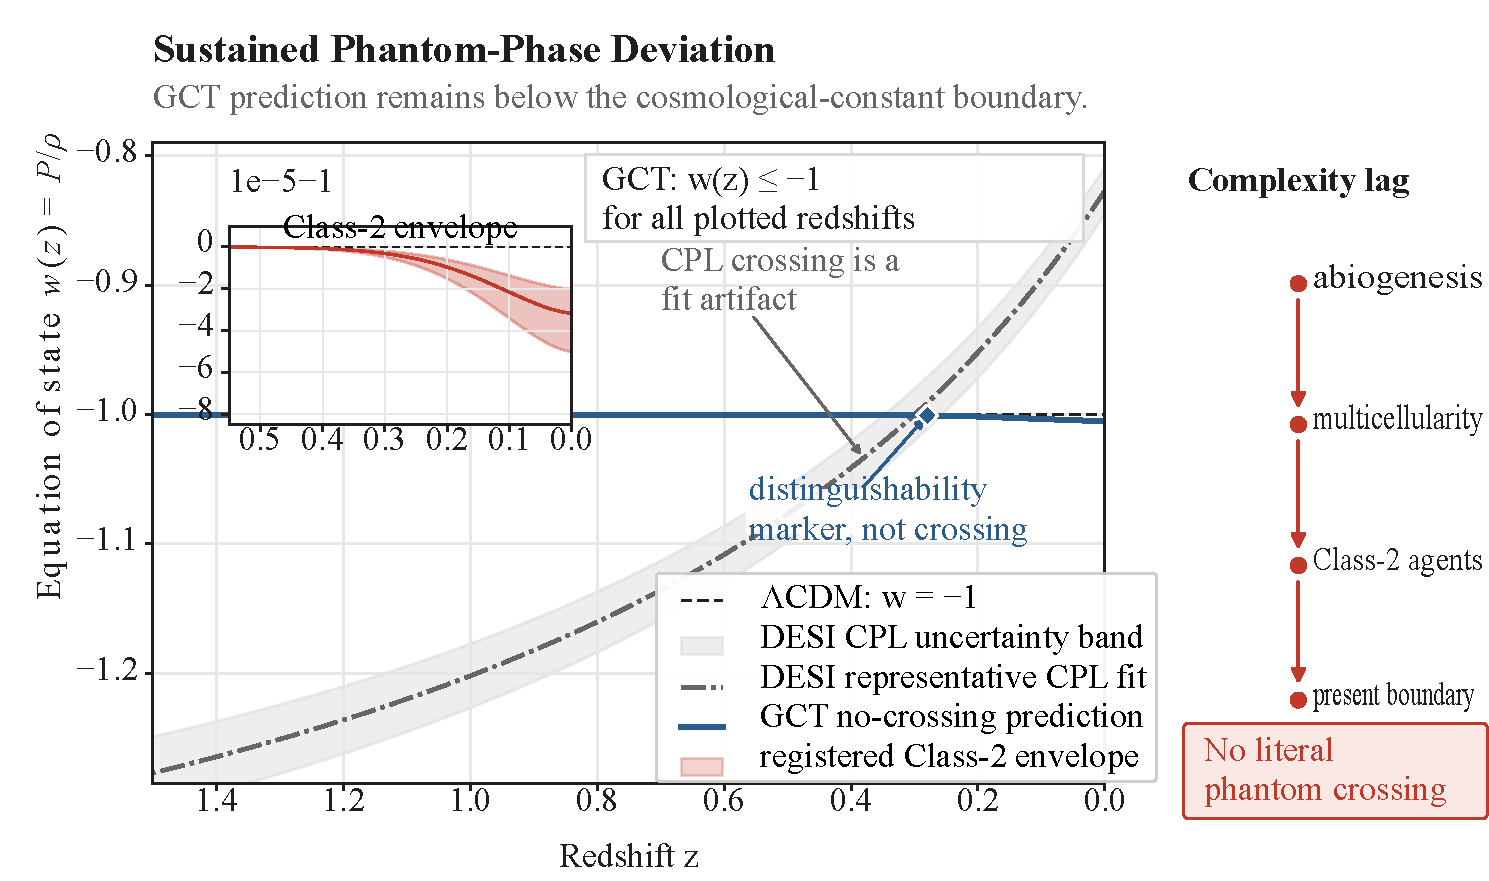
\includegraphics[keepaspectratio,alt={Dark-energy equation of state w(z): the stipulated biogenic no-crossing template stays at or below the \textbackslash Lambda\hspace{0pt}CDM boundary w = -1 for all plotted redshifts, asymptoting to -1 from below, while the representative DESI CPL fit (with its uncertainty band) shows a phantom crossing in the CPL parametrisation of the data (the crossing in the CPL fit to the GCT curve is a fit artifact). The z \textbackslash sim 0.28 marker is a distinguishability point, not a physical crossing; the inset resolves the registered Class-2 envelope. Tier 3}]{content/Figures/Volume_2/Figure V2.14.1.pdf}}
\caption{Dark-energy equation of state \(w(z)\): the stipulated biogenic
no-crossing template stays at or below the \(\Lambda\)\hspace{0pt}CDM
boundary \(w = -1\) for all plotted redshifts, asymptoting to \(-1\)
from below, while the representative DESI CPL fit (with its uncertainty
band) shows a phantom crossing in the CPL parametrisation of the data
(the crossing in the CPL fit to the GCT curve is a fit artifact). The
\(z \sim 0.28\) marker is a distinguishability point, not a physical
crossing; the inset resolves the registered Class-2 envelope. Tier 3}
\end{figure}

\gctneedspace{5\baselineskip}\begin{gctNote}

\textbf{Notes to Figure V2.14.1:} The Sustained Phantom-Phase Deviation.
\emph{Dark-energy \(w(z)\) comparison: the GCT biogenic no-crossing
curve, the representative DESI CPL fit (with its uncertainty band), the
\(\Lambda\)\hspace{0pt}CDM line, and the Class-2 envelope (§14.6.3). The
DESI CPL fit is the curve exhibiting the phantom crossing; the GCT
biogenic curve asymptotes to \(-1\) from below without crossing.}

\begin{itemize}
\tightlist
\item
  \textbf{Visual:} A plot of the equation of state parameter \(w(z)\) vs
  redshift \(z\). Two curves: (a) broad logistic-turnon reference,
  \(|w(z=0.28)+1| \approx 6 \times 10^{-4}\), useful for visual
  illustration of the phantom-phase signature; (b) the principled
  Class-2 + intra-Class-2 envelope,
  \(|w(z=0.28)+1| \in [2, 5] \times 10^{-5}\), which is the registered
  template coordinate (stipulated; phantom direction Tier 4), the Tier 3
  calibrated channel fingerprint per §14.6.3. The two curves share the
  cosmic-time profile (rising toward present) but differ by an order of
  magnitude in amplitude. Both stay \(\leq -1\) throughout (see §14.5.3
  box on the ``phantom crossing'' terminology).
\item
  \textbf{Caption:} The Biogenic Multiplier Ansatz (Tier 3 channel-shape
  model; the physical-source reading is Tier 4). \emph{Loading note: the
  schematic branch is drawn at \(|w+1| \approx 0.1\) for visibility
  only. That is not the amplitude of either quoted curve: it exceeds the
  \(6 \times 10^{-4}\) logistic reference by a factor of about \(167\)
  and the registered Class-2 template envelope by a factor of about
  \(3000\). Both quoted amplitudes lie far below visual resolution at
  this scale, and the envelope also lies below the joint Roman+DESI
  single-bin threshold (see §14.6.3).}
\end{itemize}

\end{gctNote}

\textbf{14.5.2 Anthropic Correlation Sketch}. A critical objection to
the Biogenic Hypothesis is the timing mismatch: Cosmic Star Formation
Rate (SFR) peaked at \(z \approx 2\) (\(\sim 10\) Gyr ago), yet Cosmic
Acceleration began at \(z \approx 0.6\).

GCT's phenomenological fit frames this timing relation through an
\textbf{Evolutionary Integration Lag}. Its declared source population
uses functional Class-2 complexity labels, not physically demonstrated
High-Order Selection Operators. The delay and information-density
history are supplied model inputs rather than a derived consciousness
census.

We model the driving term not as proportional to SFR, but as the
\textbf{Time-Integrated Complexity}:
\[ \dot{\mathcal{I}}(t) \propto \int_{0}^{t} \text{SFR}(t' - \tau_{bio}) \cdot P_{evolve}(t') dt' \]
With a characteristic delay \(\tau_{bio} \approx 4\text{--}5\) Gyr
{[}Tier 3{]}, the peak of the history proxy generates a phantom
(\(w_0 < -1\)) trajectory sign-opposite to DESI's quintessence-today +
more-phantom-into-past CPL fit; this is the registered shape tension,
not a derived biological driving force.

\subsubsection{14.5.3 The Sustained Phantom-Phase Deviation
(distinguishability marker at z ≈ 0.28) {[}stipulated template; phantom
direction Tier
4{]}}\label{the-sustained-phantom-phase-deviation-distinguishability-marker-at-z-0.28-stipulated-template-phantom-direction-tier-4}

Because the assumed complexity proxy is cumulative, its value increases
over time in the correlation model. The IMP-01 multi-channel curve has
\(w(z) \leq -1\) for all scanned redshifts in the registered channel
menu; \textbf{\(z \approx 0.28\)} is a distinguishability marker against
CPL fits (where the CPL crossing \(z_{\rm cross} \approx 0.39\) is a fit
artifact, not a physical transition). This is a conditional model
output, not an inference that complexity physically drives \(w(z)\). See
App PSC §PSC.7 and App ORQ O.13.

\subsubsection{14.5.4 Hubble Tension --- Conditional Lag-Kernel
Diagnostic {[}Tier 3 model arithmetic; stipulated coordinate does not
account for the
tension{]}}\label{hubble-tension-conditional-lag-kernel-diagnostic-tier-3-model-arithmetic-stipulated-coordinate-does-not-account-for-the-tension}

The empirical Hubble tension (local SH0ES \(H_0 \approx 73\) km/s/Mpc
versus Planck CMB-anchored \(H_0 \approx 67\) km/s/Mpc, a
\textasciitilde5\(\sigma\) gap; Riess et al.~2022 \emph{ApJ} 934:L7) is
\emph{not} accounted for by the §14.5.1 conditional lag-kernel
coordinate --- and the framework's \emph{failure-to-predict} is a
\textbf{Tier 3 model-arithmetic result using calibrated
\(\delta w_{\rm cosmic}\)/density anchors}, not evidence for a physical
biogenic mechanism. The engine
\texttt{protocol\_o17\_delta\_h\_local.py} computes the magnitude and
sign implied by those stipulated coordinates; it does not supply a
typed, normalized information-to-metric causal map.

The diagnostic
(\texttt{GCT\_Physics\_Engine/src/protocol\_o17\_delta\_h\_local.py})
explicitly keeps two amplitude classes separate. The broad logistic
comparison uses \(\delta w_{cosmic}(0)=-0.005\); that branch is excluded
from the operative Class-2 fingerprint, whose registered amplitude is
instead \(|\Delta w(z=0.28)|\in[2,5]\times10^{-5}\). Because the Class-2
envelope does not yet specify a normalized \(z=0\) history, it is not
silently substituted into O.17. Conditional on the excluded logistic
branch, the code computes the local equation of state, integrates the
modified Friedmann equation, compares linear and SH0ES-style kinematic
cosmography over \(z\in[0.023,0.15]\), and evaluates the complementary
CMB-inversion bias. These are model-internal sensitivity coordinates,
not operative Class-2 predictions.

\textbf{Magnitude {[}Tier 3 conditional arithmetic on the excluded
logistic branch{]}.} At \(\delta_{bio}=1.5/3.5\), the kinematic-fit
fractional shifts are \(-4.873654\times10^{-6}/-1.136763\times10^{-5}\),
while the deliberately disclosed linear-fit sensitivity gives
\(-4.422433\times10^{-5}/-1.032078\times10^{-4}\). The CMB-inversion
bias is \(-1.096005\times10^{-4}\), equal to \(0.130976\%\) of the
observed tension. Using the larger linear-fit magnitude at
\(\delta_{bio}=3.5\) gives a conservative linear-max-plus-Planck total
of \(0.254314\%\) of the tension. All signs oppose the
SH0ES-above-Planck direction. None of these numbers is the operative
Class-2 envelope or a physical biogenic-coupling prediction.

\textbf{Balanced distance-ladder context.} Primary analyses do not yield
a single method-independent late-time anchor. The CCHP JWST v1 analysis
reported \(H_0=69.85\pm1.75_{stat}\pm1.54_{sys}\) km s\(^{-1}\)
Mpc\(^{-1}\) from TRGB and \(67.96\pm1.85_{stat}\pm1.90_{sys}\) km
s\(^{-1}\) Mpc\(^{-1}\) from JAGB (Freedman et al.~2024,
arXiv:2408.06153v1; later revisions use expanded samples and updated
values). The independent CATS TRGB analysis reported \(73.22\pm2.06\) km
s\(^{-1}\) Mpc\(^{-1}\) (Scolnic et al.~2023, arXiv:2304.06693), while
an independent reduction of the CCHP TRGB scale found \(71.5\pm1.8\) km
s\(^{-1}\) Mpc\(^{-1}\) (Anand et al.~2022, \emph{ApJ} 932:15). This
spread is part of the empirical context; it neither selects the excluded
logistic branch nor changes the O.17 non-closure arithmetic.

\textbf{Sign.} Both conditional coordinates yield
\(\delta H_0^{inferred} < 0\) under the stipulated inputs. The naive
heuristic ``phantom DE drives faster local expansion'' does not survive
the SH0ES inference pipeline. This excludes the registered lag-kernel
template as an account of the tension; it does not test a physical
biogenic action because the typed coupling, normalized source map, and
causal bridge remain open.

\begin{figure}
\centering
\pandocbounded{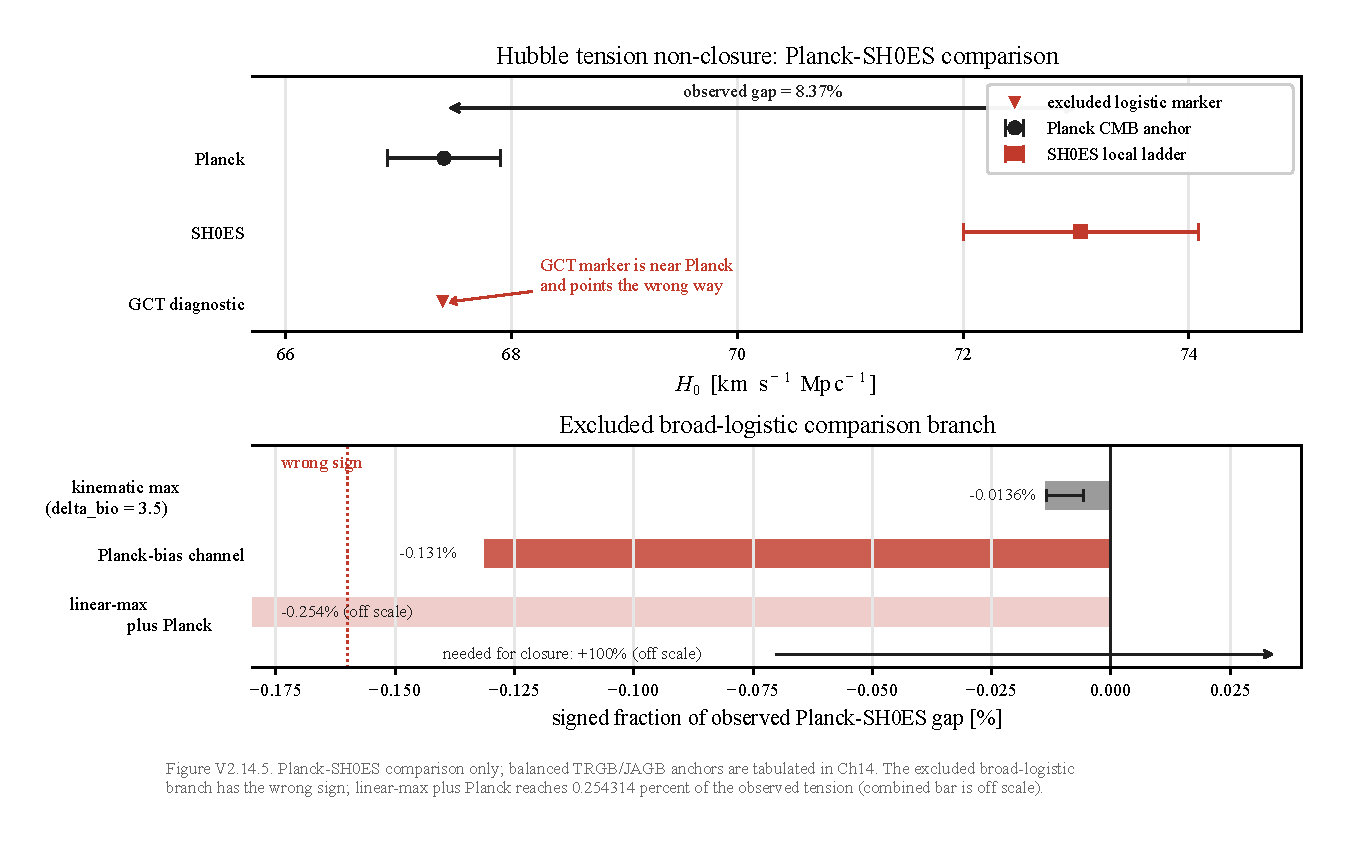
\includegraphics[keepaspectratio,alt={The Planck-SH0ES H\_0 gap is about 8.4 percent, while the excluded broad-logistic comparison has the wrong sign: the linear-max plus Planck diagnostic is 0.254314 percent of the observed tension. The balanced TRGB and JAGB anchors are reported in the surrounding text.}]{content/Figures/Volume_2/Figure V2.14.5.pdf}}
\caption{The Planck-SH0ES \(H_0\) gap is about 8.4 percent, while the
excluded broad-logistic comparison has the wrong sign: the linear-max
plus Planck diagnostic is 0.254314 percent of the observed tension. The
balanced TRGB and JAGB anchors are reported in the surrounding text.}
\end{figure}

\textbf{Scope.} The registered cosmological coordinates are conditional
templates: (a) the Class-2 phantom-side envelope
\(|\Delta w(z{=}0.28)|\in[2,5]\times10^{-5}\) and (b) the stipulated P.9
Shapley-oriented source proxy. Neither is an empirical anchor for a
physical biogenic channel, and the P.9 arithmetic is not physical
strain. The Hubble tension is not among the framework's predictions.
O.17 provides only conditional lag-kernel arithmetic and cannot be
tier-promoted by numerical fit magnitude; a physical account would
require a typed action-level coupling, normalized source, and causal map
that are absent. External early-dark-energy, recombination, and
distance-ladder-systematics possibilities retain their independent
observational status (Hill et al.~2020; Riess et al.~2022, 2023, 2024).
Open Problem O.17 records the theoretical non-closure.

\begin{center}\rule{0.5\linewidth}{0.5pt}\end{center}

\subsection{14.6 Experimental
Predictions}\label{experimental-predictions}

\subsubsection{14.6.1 Roman Space Telescope
(2027)}\label{roman-space-telescope-2027}

A Roman Year-10 / Stage-V-class analysis with single-bin precision below
\(5\times10^{-5}\) could test the biogenic-channel template. The
template assigns \(w_{\rm bio}(z)\) a \textbf{sustained phantom-phase
deviation} correlated with the peak of the biogenic era (\(z < 0.5\)),
asymptoting to \(-1\) from below rather than physically crossing the
\(w=-1\) boundary {[}stipulated template; phantom direction Tier 4,
§14.3.1{]}.

\subsubsection{14.6.2 Temporal Evolution}\label{temporal-evolution}

In the template, as the stipulated complexity variable grows (e.g.,
through technological advancement or biological evolution), \(w\)
continues to move away from \(-1\), so \(\dot{w} \neq 0\) is expected
{[}stipulated template{]}. A non-zero \(\dot w\) is generic to any
dynamical dark energy; reading it as a signature of a living universe is
Tier 4.

\subsubsection{\texorpdfstring{14.6.3 Quantitative \(w(z)\) Prediction
for DESI {[}Tier 3 per-channel shape proxy; diagnostic
only{]}}{14.6.3 Quantitative w(z) Prediction for DESI {[}Tier 3 per-channel shape proxy; diagnostic only{]}}}\label{quantitative-wz-prediction-for-desi-tier-3-per-channel-shape-proxy-diagnostic-only}

\begin{quote}
\textbf{Scope of the §14.6.3 closure verdict.} This section establishes
a \textbf{DIAGNOSTIC ONLY} state-space check: \textbf{Tier 2
convex-combination mechanism + Tier 3 channel-menu calibration → Tier 3
closure-failure of the registered menu} against the DES-Dovekie
recalibrated DESI DR2 + CMB CPL fit. The multi-channel shape-proxy
partition with the specific channel menu
\(\{\Lambda\text{-baseline},\allowbreak\,\text{biogenic-terrestrial},\allowbreak\,\text{biogenic-non-terrestrial},\allowbreak\,\text{abiotic-chiral},\allowbreak\,\text{frozen-phason perturbation}\}\)
cannot reach the DES-Dovekie central value \(w_0 = -0.803\) at any
choice of channel fractions, because every channel in this registered
menu carries \(w_c(z) \leq -0.9\). \textbf{DIAGNOSTIC ONLY
(channel-shape proxy, not physical density evolution; cosmological
global-fit comparison pending O.13 channel-C2 closure).} The closure
target is App ORQ O.13. The closure-failure claim is restricted to the
registered five-channel shape menu --- it does \emph{not} assert ``no
GCT-derivable dark-energy channel of any kind can reach DESI''; whether
a GCT-derivable thawing-quintessence or otherwise \(w_c > -0.803\)
channel exists is the residual open question registered as App ORQ Open
Problem O.13 closure path, and is not foreclosed by §14.6.3. The
biogenic-channel fingerprint set (i)--(iv) below remains a future
falsification programme, not a rhetorical rescue for the registered-menu
failure.
\end{quote}

GCT pre-registers the \(w(z)\) equation-of-state shape proxy contributed
by the \textbf{biogenic selection channel alone} to the total cosmic
dark-energy signal. The biogenic channel is one of \(N \geq 1\)
selection channels (App ORQ O.13, App PSC §PSC.0); the diagnostic total
shape-proxy \(w(z)\) is represented here by the standard
convex-combination equation-of-state identity (Copeland-Sami-Tsujikawa
2006, Amendola-Tsujikawa 2010, Avelino et al.~2010, Feng-Wang-Zhang 2005
quintom): \[
w_{\rm total}(z) = \frac{\sum_c \Omega_c(z) \, w_c(z)}{\sum_c \Omega_c(z)},
\] with \(c\) ranging over the registered channels:
\(\Lambda\)-baseline, biogenic-terrestrial, biogenic-non-terrestrial,
abiotic-chiral, frozen-phason vacuum perturbation, and further channels
and \(\Omega_c(z)\) used in \texttt{protocol\_de\_multichannel.py} as a
per-channel shape proxy at redshift \(z\), not as a continuity-equation
energy-density evolution. The registered GCT ansätze specify each
\(w_c(z)\) structural shape {[}Tier 3{]}; the total magnitude
\(|\Delta w_{\rm total}(z)|\) is a state-level quantity determined by
the cosmological history of all physical channel weights and is not
derivable from the framework alone (App PSC §PSC.0). The registered
curve below is a \textbf{biogenic-channel shape proxy}
\(w_{\rm bio}(z)\), computed via the IMP-01 pipeline with the standard
Madau-Dickinson 2014 Star Formation Rate and the exact
\(\lambda_{bio} \equiv \alpha\) coupling; it is diagnostic only, not a
claimed observed fingerprint.

\textbf{Multi-channel shape-proxy partition: structural reachability of
the DES-Dovekie recalibrated DESI DR2 CPL fit {[}DIAGNOSTIC ONLY
(channel-shape proxy, not physical density evolution, not a predictive
global-fit EoS model; cosmological global-fit comparison pending O.13
channel-C2 closure); Tier 2 convex-combination EoS identity + Tier 3
shape-proxy parametrizations + Tier 3 calibrated amplitudes{]}.} The
full five-channel diagnostic is implemented in
\texttt{GCT\_Physics\_Engine/src/protocol\_de\_multichannel.py}. The
protocol computes \(w_{\rm total}(z)\) over the channel decomposition
above with shape proxies \(\Omega_c(z)\) calibrated against (i) the
Madau-Dickinson 2014 cosmic star-formation rate shape
\(\psi_{\rm SFR}(z) = 0.015 (1{+}z)^{2.7} / (1 + ((1{+}z)/2.9)^{5.6})\)
for the biogenic-terrestrial and biogenic-non-terrestrial channels, (ii)
an early-universe chirality-onset tanh step function
\(\tfrac{1}{2}(1 + \tanh((z - z_{\rm chiral})/w_{\rm chiral}))\) with
\(z_{\rm chiral} \in [5, 20]\), \(w_{\rm chiral} = 2\) for the
abiotic-chiral channel (\(w_{\rm chiral}(z) = -1.5\)), and (iii) a
constant amplitude \(f_{\rm pert} \in [0, 0.05]\) for the frozen-phason
perturbation channel (\(w_{\rm pert}(z) = -0.9\)). These are SHAPE
PROXIES, not energy-density evolutions through the continuity equations;
a physically normalised \(\rho_c(z)\) treatment is the O.13 channel-C1
closure target. The \(\Lambda\)-baseline channel carries
\(w_\Lambda(z) = -1\) exact, with the dark-energy density fraction
\(\Omega_{\Lambda,0}\) swept across the defensible cosmological range
\(\{0.50, 0.55, 0.60, 0.65, 0.685, 0.72, 0.75\}\) (Planck central value
\(0.685\)) so that the diagnostic verdict carries no implicit dependence
on a single imported value. A 4032-point sensitivity sweep over the five
parameters
\((\Omega_{\Lambda,0}, f_{\rm ext}, f_{\rm chiral}, f_{\rm pert}, z_{\rm chiral}) \in \{0.50,\ldots,0.75\} \times \{0, 0.01, 0.1, 1, 10, 100\} \times \{0, 0.02, 0.05, 0.10, 0.20, 0.40\} \times \{0, 0.01, 0.02, 0.05\} \times \{5, 10, 15, 20\}\)
returns a best-fit diagonal diagnostic score \(\approx 4.861\) against
the DES-Dovekie target. This is diagnostic only: no DESI covariance
matrix or likelihood surface is used, and the scalar score is not a
closure rule or a claimed observational prediction. The best-fit
diagnostic varies by only \(0.0446\) score units across the entire
\(\Omega_{\Lambda,0}\) grid (from \(4.861\) at
\(\Omega_{\Lambda,0} = 0.50\) to \(4.905\) at
\(\Omega_{\Lambda,0} = 0.75\)); the sweep envelope is pinned at
\(w_0 \in [-1.009, -0.991]\), \(w_a \in [-0.012, +0.045]\).

\begin{figure}
\centering
\pandocbounded{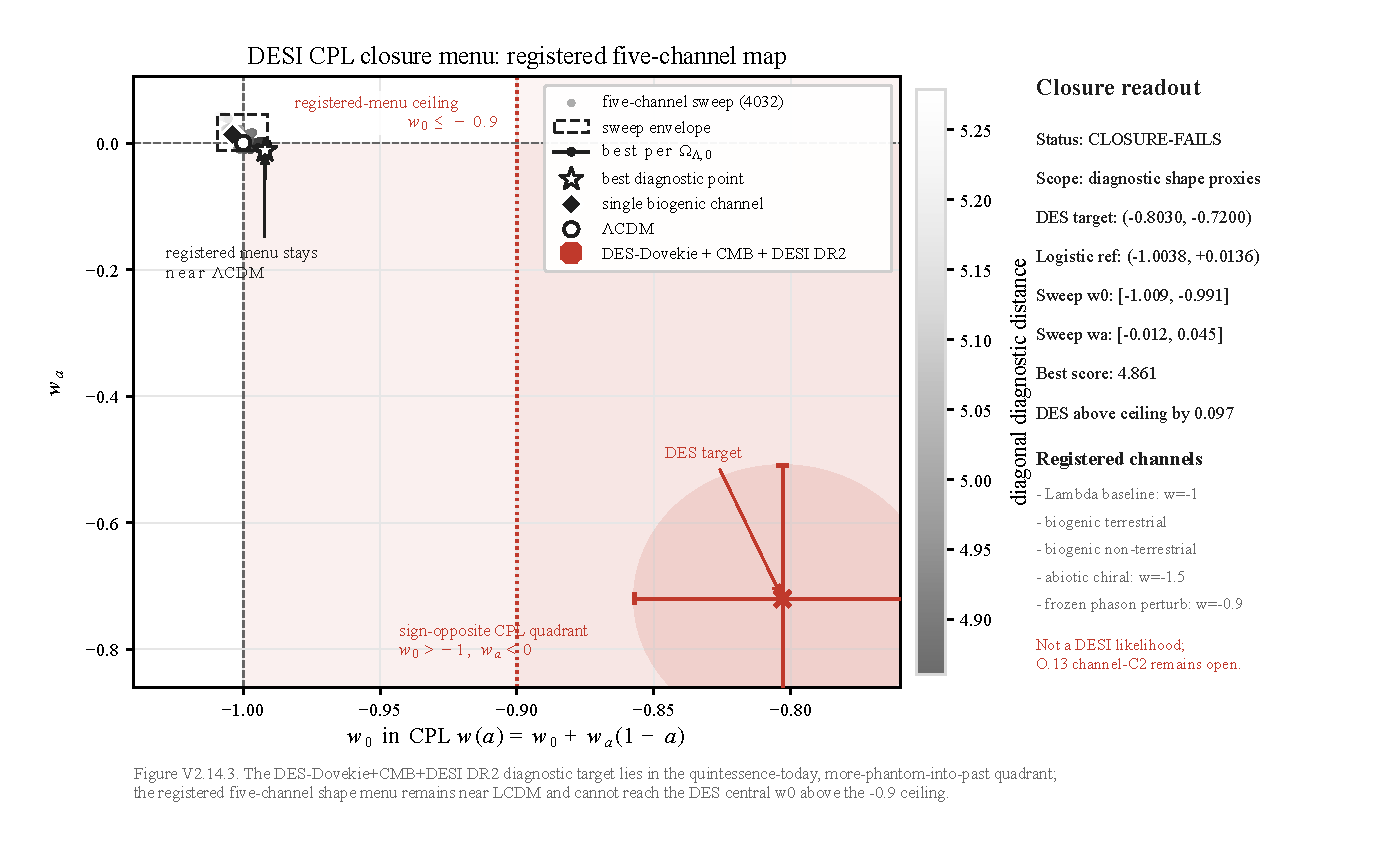
\includegraphics[keepaspectratio,alt={In the w\_0-w\_a plane, the DES-Dovekie + CMB + DESI DR2 CPL target sits in the sign-opposite quadrant relative to the registered GCT biogenic channel menu. The logistic reference pair (-1.0038,+0.0136) is a non-operative broad-logistic reference, not a GCT prediction.}]{content/Figures/Volume_2/Figure V2.14.3.pdf}}
\caption{In the \(w_0\)-\(w_a\) plane, the DES-Dovekie + CMB + DESI DR2
CPL target sits in the sign-opposite quadrant relative to the registered
GCT biogenic channel menu. The logistic reference pair
\((-1.0038,+0.0136)\) is a non-operative broad-logistic reference, not a
GCT prediction.}
\end{figure}

The closure-failure verdict has a clear structural cause, but the cause
is partially tautological and the §14.6.3 framing must be read with the
right tier discipline. The shape-proxy total
\(w_{\rm total}(z) = \sum_c \Omega_c(z) w_c(z) / \sum_c \Omega_c(z)\) is
a convex combination of the per-channel equation-of-state values, so at
every redshift
\(\min_c w_c(z) \leq w_{\rm total}(z) \leq \max_c w_c(z)\), with both
bounds independent of the channel-fraction parameters
\((\Omega_{\Lambda,0}, f_{\rm ext}, f_{\rm chiral}, f_{\rm pert}, z_{\rm chiral})\).
\textbf{The model-level shape statement (stipulated shape; phantom
direction and physical-source reading Tier 4):} the channels obtained
from the registered phason / biogenic / cosmology-of-zero ansätze are
phantom-directed, alongside the \(w=-1\) baseline (itself the Tier 3
reading of §14.1.1). \textbf{The Tier 3 menu choice:} the frozen-phason
perturbation item at \(w_{\rm pert}=-0.9\) is nonphantom and is not
model-derived. The registered menu is therefore not an ``all channels
phantom'' set. Its \(w_{\rm total}\leq-0.9\) ceiling follows from
combining model-derived phantom/baseline channels with this Tier 3
nonphantom menu item; a model-derived \(w_c>-0.803\) channel remains the
O.13 C1 construction target. The 4032-point sensitivity sweep in
\texttt{protocol\_de\_multichannel.py} is internally meaningful (it
confirms the engine's diagnostic verdict is flat to within \(0.0446\)
score units across the \(\Omega_{\Lambda,0}\) grid), but its rhetorical
weight should not be over-read: the failure direction is fixed by the
Tier 3 channel-menu choice, not by an unconditional convex-combination
theorem against arbitrary GCT-derivable channels. The single-channel
biogenic prediction stands in sign-opposite external-data tension with
the DES-Dovekie recalibrated DESI DR2 + CMB CPL fit. The
Copeland-Sami-Tsujikawa partition remains a Tier 2 mathematical identity
for any cosmological fluid mixture; what fails at the \emph{registered
menu} level is the ability to reconcile a decomposition whose
model-derived channels are phantom/baseline and whose Tier 3 nonphantom
menu ceiling is \(-0.9\) with a DES-Dovekie CPL fit whose
\(w_0 = -0.803\) sits in the genuine quintessence regime. \textbf{Scope
of the closure verdict:} ``the \emph{registered five-channel shape menu}
does not reach DESI'', not ``no GCT-derivable channel of any kind can
reach DESI''. Construction of a GCT-derivable \(w_c > -0.803\) channel
--- for example, a slowly-rolling phason mode or a residual
sub-horizon-screening dark-energy fraction --- or a no-go proof ruling
out any such channel within the broader GCT lawscape, is the
load-bearing item for App ORQ O.13 closure path C1. The registered
decision rule reads: if the sign-opposite CPL region is confirmed at
\(> 3\sigma\), the registered-menu closure-to-DESI claim is falsified at
the state-level CPL-fit gate. Current fits already place it there:
DES-Dovekie at \(3.2\sigma\), and the official DESI DR2 analysis at
\(3.1\sigma\) for BAO+CMB and \(2.8\)--\(4.2\sigma\) with supernovae.
Applied as written, \textbf{the registered-menu closure-to-DESI claim is
falsified} (a branch-level verdict, not a verdict on GCT as a whole; App
PSC §PSC.8 row 8). The single-channel \(w_{\rm bio}(z) \leq -1\)
template is a separate stipulated coordinate: this verdict neither
rescues nor confirms it, and its phantom direction is Tier 4 as a
physical claim (§14.3.1). Euclid and Roman data can test whether the
preference persists; they cannot reinstate the registered menu. The
separate IMP-01 pipeline gate (C\_IMP01\_PIPELINE\_GATE) requires DESI
DR2 plus Euclid DR1 and has not fired.

\textbf{Sub-horizon sound-speed template {[}DIAGNOSTIC ONLY; Tier 3
conditional{]}.} App ORQ O.13 fingerprint (iv) stipulates a
clustering-DE source-proxy template with \(c_{s,\rm bio}^2\ll1\) and
compares its formal dependence with the standard Sapone-Kunz, Creminelli
et al., and Batista perturbation framework. This is not a GCT-derived or
canonical physical channel. The engine catalogue exposes the
continuity/Euler equations, computes the Jeans-threshold arithmetic, and
records that full-window activation of the stipulated template would
require \(c_{s,\rm bio}^2\lesssim5\times10^{-7}\) over
\(k\in[0.01,0.5]\,h\,{\rm Mpc}^{-1}\). Those checks are conditional
model arithmetic only: the typed coupling, normalized source-proxy map,
second-order/windowed statistic, causal identification, Boltzmann
evolution, and survey-covariance likelihood all remain open. In
particular, homogeneous linear perturbations satisfy
\(\langle\delta_m\rangle=0\), so linear integration alone implies no
mean backreaction. A future data comparison can support or exclude the
registered template; it cannot by itself establish a physical biogenic
channel.

The IMP-01 pipeline implementation in
\texttt{GCT\_Physics\_Engine/src/protocol\_imp01\_pipeline.py} produces
a \(w_{\rm bio}(z)\) curve that asymptotes to \(-1\) from below ---
i.e., the biogenic channel predicts a \textbf{continuous phantom phase}
(\(w_{\rm bio}(z) \leq -1\) for all \(z \geq 0\)) rather than a literal
mathematical transition across the \(w=-1\) boundary. The table gives
the \textbf{broad logistic reference run} (\(t_{origin} = 9\) Gyr,
\(\tau_{evolve} = 2\) Gyr, \(\tau_{lag} = 5\) Gyr, \(\tau_{bio} = 4.5\)
Gyr, \(\lambda_{bio} \equiv \alpha\)). This run is non-operative: it is
excluded from the registered Class-2 fingerprint, and its
\(|\Delta w(0.28)| \approx 6\times10^{-4}\) is not the registered
amplitude, which is \(|\Delta w(0.28)| \in [2,5]\times10^{-5}\).

\gctneedbreak{10\baselineskip}

{\def\LTcaptype{none} % do not increment counter
\begin{longtable}[]{@{}rr@{}}
\toprule\noalign{}
Redshift \(z\) & \(w(z)\) from pipeline \\
\midrule\noalign{}
\endhead
\bottomrule\noalign{}
\endlastfoot
\(0.001\) (today) & \(-1.0050\) \\
\(0.15\) & \(-1.0023\) \\
\(0.28\) & \(-1.0006\) \\
\(0.5\) & \(-1.0000\) \\
\(1.0\) & \(-1.0000\) \\
\end{longtable}
}

The curve sits below \(-1\) everywhere, with deviation
\(|\Delta w(z)| = |w(z) - (-1)| = \delta w \cdot P_{info}(z)/P_{info}(0)\)
that grows monotonically as \(z \to 0\).

Two redshift scales characterise the prediction:

\begin{itemize}
\tightlist
\item
  \textbf{Pipeline-sensitivity marker:} \(z_{marker} \approx 0.28\) ---
  the \emph{low-redshift sensitivity peak} of the IMP-01 pipeline's
  biogenic kernel (the redshift at which the SFR × \(P_{evolve}\)
  convolution contributes maximally to \(|\Delta w(z)|\) in the
  observational window). At this marker, the operative Class-2 envelope
  is \(|\Delta w(z=0.28)| \in [2,5]\times10^{-5}\), below Roman + DESI
  Year-5 joint-bin precision and requiring Roman Year-10 / Stage-V
  single-bin precision below \(5\times10^{-5}\), or a binning strategy
  that emphasizes the late-time \(z<0.1\) regime.
\item
  \textbf{CPL fit coefficients of the logistic reference run,
  \((w_0, w_a) \approx (-1.0038, +0.0136)\)} (non-operative; not a
  registered prediction); there is no physical zero of \(w(z) + 1\) on
  the underlying integration (direct brentq returns no root). The CPL
  linear-extrapolation ``crossing'' at \(z \sim 0.389\) is an
  extrapolation artifact of the linear fit applied to a curve that
  asymptotes to \(-1\) from below.
\end{itemize}

This curve predicts a \textbf{monotonic phantom deviation} in the
post-biospheric epoch. Under the operative Class-2 envelope, the
cosmic-mean amplitude is
\(|\Delta w(z{=}0.28)| \in [2,5]\times10^{-5}\), below Roman + DESI
Year-5 joint-bin precision and requiring Roman Year-10 / Stage-V
single-bin precision below \(5\times10^{-5}\), or a binning strategy
that emphasizes the late-time \(z<0.1\) regime.

The registered Tier 3 coordinate by construction gives \(w(z) \leq -1\)
throughout cosmic time because its stipulated \(\delta w<0\) and
\(P_{info}(z)\geq0\). A literal crossing would require changing those
model inputs. This is a conditional shape property, not a Tier 2
biogenic mechanism or physical coupling.

The falsifiable claim is therefore: a sub-\(5\times10^{-5}\) \(w(z)\)
program should observe the Class-2 envelope in the phantom direction
(\(w < -1\)), and \textbf{no transition from quintessence to phantom}. A
literal \(w = -1 \to w < -1\) transition observed in the data would
partially falsify the present biogenic-coupling formulation even if its
qualitative phantom-character matches observations. The registered
five-channel menu remains a Tier 3 state-level shape proxy, not a
theorem over all possible GCT dark-energy channels. Open Problem O.13
(\(P_{evolve}\) first-principles derivation and channel-menu closure)
governs the precision of the pipeline-derived CPL triple.

\gctneedspace{5\baselineskip}\begin{gctImportant}

\textbf{\(P_{evolve}\) conditional closure under the §14.5.2 + §14.6.2
model assumptions {[}Tier 3{]}.} Two phenomenological assumptions define
the present \(P_{evolve}\) allocation:

\begin{enumerate}
\def\labelenumi{\arabic{enumi}.}
\tightlist
\item
  \emph{§14.5.2 --- Class-2 allocation:} the model assigns the biogenic
  channel only to the stipulated Class-2 population and assigns zero
  weight to pre-Class-2 stages. This is a Tier 3 bookkeeping assumption,
  not an inference that pre-Class-2 substrates lack Level II, an
  Identity Polaron, or a physical coupling. The Level II status of every
  substrate is open (Tier 3): no validated substrate criterion exists
  yet (it requires a typed, normalized, measured coupling, the
  Identity-Polaron construction and an independent phenomenal bridge;
  O.21/O.23/O.34, O.18). The DMC is neither a necessary nor a sufficient
  gate, nor an established classifier, and no examined substrate
  currently has a derived Level-II verdict.
\item
  \emph{§14.6.2 --- intra-Class-2 dynamics assumption:} within the
  assigned Class-2 population, the model weights complexity growth
  exponentially on a characteristic time \(\tau_{tech}\). This weighting
  is phenomenological rather than an axiom of established agent physics.
\end{enumerate}

The conditional Class-2-allocation baseline
(\texttt{GCT\_Physics\_Engine/src/protocol\_o13\_closure\_class2\_strict.py},
unweighted SFR-age convolution) implements the SFR-age convolution
restricted to the model-assigned population:
\[P_{evolve}^{(C2)}(t) \;=\; \int_{\tau_{intel}}^{t - \tau_{bio}} \text{SFR}(t - \tau_{bio} - \tau)\,d\tau, \qquad \tau_{intel} \approx 4.5\;\text{Gyr (Earth-template, Tier 3)}.\]
Substituting into the IMP-01 lag-kernel yields
\(|\Delta w(z{=}0.28)| \approx 3.5 \times 10^{-5}\) --- a Tier 3 model
output under the §14.5.2 allocation assumption. The numerical
propagation is reproducible conditional on that assumption; it does not
promote the population assignment or coupling to Tier 2.

The §14.6.2 intra-Class-2 dynamics assumption is implemented in
\texttt{protocol\_o13\_intra\_class2\_dynamics.py} via the Class-2
age-weighted variant: the conditional baseline with per-biosphere
complexity weighted by \(\exp((\tau - \tau_{intel})/\tau_{tech})\) on
biosphere age \(\tau\). Under the stipulated Kardashev-motivated band
\(\tau_{tech} \in [1, 2]\) Gyr (a Tier 4 input: no empirical Type 0
\(\to\) Type II timescale exists), the age-weighted run yields
\(|\Delta w(z{=}0.28)| \in [1.5 \times 10^{-5},\, 2.5 \times 10^{-5}]\)
--- \emph{below} the unweighted Class-2 allocation, not above. The
exponential weighting re-weights the cosmic-mean integral toward
early-formed biospheres, steepening the recent growth of \(P_{info}(t)\)
and reducing the relative deviation at \(z = 0.28\).

The registered Class-2-allocation envelope under the two Tier 3
assumptions is:
\[|\Delta w(z{=}0.28)| \in [2 \times 10^{-5},\, 5 \times 10^{-5}].\]
This registered band is a rounded declaration, not re-derived from the
current runs: those span \(\approx[1.5, 3.5]\times10^{-5}\)
(Kardashev-band weighted runs up to the unweighted baseline), so the
lowest weighted runs fall slightly below its lower edge. The
logistic-turnon reference
(\(|\Delta w(z{=}0.28)| \approx 6 \times 10^{-4}\) at \(t_{origin} = 9\)
Gyr, \(\tau_{evolve} = 2\) Gyr) sits \emph{above} this envelope by more
than an order of magnitude and is not reached at any sampled
\(\tau_{tech}\) (the weighted runs level off near \(3.5\times10^{-5}\)
as \(\tau_{tech}\to10\) Gyr); that amplitude is a separate empirical
phenomenology rather than an output of the stipulated allocation.

The stage-hierarchy form that weights pre-Class-2 stages yields
\(|\Delta w(z{=}0.28)| \approx 2 \times 10^{-3}\); it is excluded only
by the present §14.5.2 allocation assumption, not by a substrate
theorem. Engine cross-references:
\texttt{protocol\_p\_evolve\_first\_principles.py},
\texttt{protocol\_p\_evolve\_stage\_hierarchy.py} (alternative
reference), \texttt{protocol\_o13\_closure\_class2\_strict.py}
(unweighted conditional baseline),
\texttt{protocol\_o13\_intra\_class2\_dynamics.py} (Kardashev-band
conditional envelope).

\textbf{Observational consequence.} Conditional on the Class-2
allocation and weighting assumptions,
\(|\Delta w(z{=}0.28)| \in [2 \times 10^{-5},\, 5 \times 10^{-5}]\) is
the operative Roman Year-10 / Stage-V target. The framework's
conditional cosmic-mean \(w(z)\) signature is weaker than the broad
logistic reference alone would suggest. Distinguishability requires
either Roman Year-10 / Stage-V single-bin precision below
\(5 \times 10^{-5}\) or a binning strategy emphasizing the late-time
(\(z < 0.1\)) regime.

\end{gctImportant}

\begin{center}\rule{0.5\linewidth}{0.5pt}\end{center}

\subsection{14.7 Historical Connection to Consciousness {[}Tier 4; no
physical
bridge{]}}\label{historical-connection-to-consciousness-tier-4-no-physical-bridge}

\subsubsection{\texorpdfstring{14.7.1 The Uninstantiated Rendering
\(\to\) Expansion
Chain}{14.7.1 The Uninstantiated Rendering \textbackslash to Expansion Chain}}\label{the-uninstantiated-rendering-to-expansion-chain}

The historical proposal can be written as the following formal chain:

\begin{enumerate}
\def\labelenumi{\arabic{enumi}.}
\tightlist
\item
  \textbf{Selection label:} a model event is indexed by
  \(\mathcal{F}_{sel}\); no physical Selection Operator, carrier, or
  owner is identified.
\item
  \textbf{History variable:} the event is assigned a local bookkeeping
  density \(\mathfrak{i}\); no physical bit-generation law or phenomenal
  bridge is derived.
\item
  \textbf{Strain ansatz:} the bookkeeping variable is mapped to
  \(\phi_\perp\); no biology/ATP-to-phason transducer or protected
  winding memory is supplied.
\item
  \textbf{Metric ansatz:} a relaxation term is mapped to \(G_{\mu\nu}\);
  no conserved source or covariant stress-energy tensor closes the step.
\end{enumerate}

This is a Tier 4 dependency sketch, not a causal mechanism or a realized
Identity-Polaron/Selection-Operator chain.

\subsubsection{14.7.2 The Anthropic
Correlation}\label{the-anthropic-correlation}

The coincidence between observer emergence and the matter/dark-energy
equality epoch is treated here as a Tier 4 anthropic-correlation sketch,
not as a causal mechanism. The expansion scale may be correlated with
the information density of matter-defects (observers), but §14.3.2's
magnitude analysis shows that the biogenic formula is illustrative
rather than predictive when read as direct causal driving.

\subsubsection{14.7.3 The Ultimate Fate}\label{the-ultimate-fate}

Within the Tier 4 narrative, continued growth of the stipulated
complexity variable would keep the fitted channel active until its
declared capacity limit. This is not a physical forecast of cosmic fate.
Even a confirmed correlation of the registered shapes would not
establish that biological complexity causes expansion without the
missing carrier, transducer, source, and stress-energy derivation.

\begin{center}\rule{0.5\linewidth}{0.5pt}\end{center}

\subsection{14.8 Falsification (Part B)}\label{falsification-part-b}

\gctneedspace{5\baselineskip}

\textbf{Tier 3 Falsifications for the Biogenic Correlation Hypothesis:}

\begin{enumerate}
\def\labelenumi{\arabic{enumi}.}
\tightlist
\item
  \textbf{P.9 Shapley-oriented source-proxy template.} The registered
  amplitude \(\delta w/w\sim[0.2,1.5]\times10^{-4}\) and orientation are
  stipulated Tier-3 model coordinates (conditional envelope \(\times\)
  proxy factor; App PRG P.9), not physical biogenic strain. A
  sufficiently sensitive null or incompatible orientation excludes this
  template only; agreement does not establish a normalized source or
  causal channel.
\item
  A preregistered null result for a specified radical-pair-to-metric
  observable would reject that registered phenomenological
  material-to-cosmology bridge. It cannot falsify a derived
  phason-information coupling because no normalized microscopic
  radical-pair-to-phason-to-metric map presently exists; a positive
  result would likewise remain ordinary proxy evidence until that map
  and an independent phenomenal bridge are derived. Neither outcome is a
  verdict on GCT as a whole: the measurement tests an ordinary material
  proxy, and no phason, Selection-Operator or Level-II inference follows
  from it (V1 Ch17 §17.1.3).
\item
  If the phason mass cannot be derived from GCT geometry (i.e., if
  \(m_{phason} = 1.7 \times 10^{-5}\) eV requires an additional
  calibrated handle), the dark-energy scale stays a Tier 3 consistency
  check: only the area-law form is Tier 2, and the absolute scale
  already imports \(H_0\) and \(\Omega_\Lambda\) (§14.1.5).
\end{enumerate}

\gctneedspace{5\baselineskip}

\textbf{END OF VOLUME 2}

\chapter*{Glossary}
\addcontentsline{toc}{chapter}{Glossary}
\markboth{Glossary}{Glossary}
\setcounter{section}{0}

\subsection{\texorpdfstring{\textbf{Glossary of Terms (The Cosmic
Architecture)}}{Glossary of Terms (The Cosmic Architecture)}}\label{glossary-of-terms-the-cosmic-architecture}

\subsubsection{\texorpdfstring{\textbf{Lattice \&
Projection}}{Lattice \& Projection}}\label{lattice-projection}

\begin{itemize}
\tightlist
\item
  \textbf{6D Lattice (\(\mathbb{Z}^6\)):} The fundamental Euclidean
  hypercubic lattice of the parent space. It serves as the static
  coordinate backbone of the Operating System, possessing a lattice
  constant \(a_6 = 2\ell_P\), twice the Planck length.
\item
  \textbf{Acceptance Window (\(W\)):} A specific geometric volume in the
  internal perpendicular space (\(E_\perp\)) that acts as a selection
  filter. A lattice point in 6D is actualized in the physical 3D world
  if and only if its internal projection falls within \(W\). In the
  icosahedral vacuum, \(W\) is a Rhombic Triacontahedron.
\item
  \textbf{Parallel Space (\(E_\parallel\)):} The 3-dimensional physical
  manifold we inhabit, representing the ``Screen'' of the projection. It
  is the arena of standard matter, forces, and the acoustic metric of
  gravity.
\item
  \textbf{Perpendicular Space (\(E_\perp\)):} The 3-dimensional internal
  manifold orthogonal to physical space, representing the ``Sink'' of
  the projection. It hosts the phason degrees of freedom and, in the
  open Tier 3 colour candidate, color charges, and is proposed as an
  entropy reservoir for the universe (the Tier 4 Entropy Sequestration
  Hypothesis, Ch07 §7.2).
\item
  \textbf{Cut-and-Project:} The mathematical and physical process by
  which a high-dimensional periodic lattice is sliced at an irrational
  angle to generate a lower-dimensional aperiodic structure (a
  quasicrystal).
\end{itemize}

\subsubsection{\texorpdfstring{\textbf{Elastic
Properties}}{Elastic Properties}}\label{elastic-properties}

\begin{itemize}
\tightlist
\item
  \textbf{Phonon:} A ``hard'' vibrational mode involving the compression
  or shearing of the 6D lattice bonds in the physical manifold
  (\(E_\parallel\)). Phonon stiffness (\(K_\parallel\)) is anchored to
  the Planck scale.
\item
  \textbf{Phason:} A ``soft'' topological mode involving the
  rearrangement of the lattice tiling through the internal manifold
  (\(E_\perp\)). GCT assigns phasons a proposed role in the
  electromagnetic field; their qualitative distinction from phonons is
  structural within the supersolid model, but their numerical stiffness
  (\(K_\perp\)) is not fixed by the projector.
\item
  \textbf{Stiffness Hierarchy (\(K_\perp \ll K_\parallel\)):} The
  candidate material hierarchy of the vacuum that would supply the vast
  energy gap between the Planck scale and the scale of light and
  standard forces. The registered value
  \(K_\perp/K_\parallel=\phi^{-18}\) is the Tier 3 stiffness-map
  hypothesis P3b (pending O.15(b)), listed outside the postulate count
  like H-EW; only the \(H_3\) integer \(D=18\) is Tier 2 within GCT.
\item
  \textbf{Lubensky-Ramaswamy Formalism:} The hydrodynamic framework for
  icosahedral quasicrystals used in GCT to describe the coupling between
  phason strain, phonon displacement, and superfluid phase.
\end{itemize}

\subsubsection{\texorpdfstring{\textbf{Hydrodynamics}}{Hydrodynamics}}\label{hydrodynamics}

\begin{itemize}
\tightlist
\item
  \textbf{Superfluid Velocity (\(\mathbf{v}_s\)):} The gradient of the
  vacuum condensate phase (\(\theta\)), representing an irrotational
  superfluid current; its reading as the probability current of the
  consciousness field is a Tier 3 interpretive identification.
\item
  \textbf{Phason Strain (\(w_{ij}\)):} The spatial gradient of the
  internal topological displacement (\(\mathbf{u}_\perp\)). It
  represents the local ``tilt'' of the acceptance window and is proposed
  as the material source of the vector potential \(\mathbf{A}\) (Tier 3
  declared open programme, V2 Ch06 §6.1).
\item
  \textbf{Second Sound:} A propagating wave mode in the supersolid
  vacuum involving the out-of-phase oscillation of the lattice nodes and
  the superfluid phase. GCT proposes identifying Second Sound with the
  physical photon (Postulate 6.1; Tier 3 declared open programme, V2
  Ch06 §6.1).
\item
  \textbf{Healing Length (\(\xi\)):} The characteristic distance over
  which the vacuum order parameter recovers from a disruption. In GCT's
  biological application, the operative polaron scale is the
  Bohr--Compton combination
  \(\xi = \hbar c/(\alpha^2 m_e c^2) = a_0/\alpha \approx 7.25\) nm
  {[}Tier 1 arithmetic; its identification as the vacuum/polaron healing
  length is Tier 3{]}; its microtubule-lumen match is a Tier 3
  biological-scale match (Ch03 §3.2.1).
\end{itemize}

\subsubsection{\texorpdfstring{\textbf{Gravity \&
Spacetime}}{Gravity \& Spacetime}}\label{gravity-spacetime}

\begin{itemize}
\tightlist
\item
  \textbf{Acoustic Metric:} The effective Lorentzian geometry
  (\(g_{\mu\nu}\)) experienced by lattice excitations (whether the
  gravitational carrier sector is phonon or phason is open, Ch04
  §4.1.1). In the analogue model, gravitational kinematics appear as the
  refraction of these waves by gradients in the vacuum density and
  stiffness {[}Tier 2 within the declared model{]}; the Einstein
  dynamics enter only through the Jacobson construction of Ch09.
\item
  \textbf{Entropic Gravity:} A horizon/screen thermodynamic construction
  relating entropy gradients, temperature and effective gravitational
  dynamics (Jacobson; Verlinde; Ch09). Reading it as a pressure that
  aligns the Selection Operator with regions of maximum bit-density is a
  Tier 3 analogy, not part of the gravity derivation.
\item
  \textbf{Gravastar:} A non-singular alternative to a black hole
  consisting of a liquid core of Symmetric-Phase vacuum supported by
  negative potential pressure, bounded by a thin shell of crystalline
  lattice {[}Tier 4 model (declared open programme); the mass-dependent
  core density it needs is an open item, Ch10 §10.2.1{]}.
\item
  \textbf{Transparency Mechanism:} The proposed Diophantine protection
  afforded by the irrational \(\phi\)-projection, intended to keep the
  discrete lattice ``invisible'' to high-energy cosmic rays. Within the
  App TPF scattering model the inversion-odd \(n=1\) Lorentz-violation
  coefficient cancels by centre-inversion symmetry; excluding the
  remaining rotation-invariant \(n=1\) terms requires the Tier 3
  CPT/helicity assumption on the emergent electromagnetic action (V2
  Ch08 §8.3.5). Linear-order Lorentz invariance is therefore conditional
  on that assumption, not ensured.
\end{itemize}

\subsubsection{\texorpdfstring{\textbf{Dark
Sector}}{Dark Sector}}\label{dark-sector}

\begin{itemize}
\tightlist
\item
  \textbf{Topological Glass:} The metastable state of the vacuum
  characterized by frozen phason strain and disordered tile
  orientations. In the Tier 3 topological-glass model this state is
  proposed to supply the ``invisible mass'' of galactic halos.
\item
  \textbf{Glass Order Parameter (\(\eta_g\)):} A scalar field describing
  the degree of configurational pinning in the vacuum lattice, where
  \(\eta_g=1\) is a perfect crystal and \(\eta_g=0\) is a fractured
  fluid.
\item
  \textbf{MOND Emergence:} A Tier 3 constitutive ansatz in which a
  non-linear vacuum shear response has MOND-like mathematical limits.
  Flat rotation curves follow conditionally from the assumed response;
  its microscopic physical adoption and normalisation remain open.
\item
  \textbf{Critical Acceleration (\(a_0\)):} The empirical MOND
  normalisation \(a_0\approx1.2\times10^{-10}\) m/s\(^2\) {[}Tier 3
  input in GCT{]}. The Tier 3 low-acceleration thermodynamic step (Ch09
  §9.1.6, Step 5) uses \(H_0=67.4\) km/s/Mpc and supplies only the scale
  relation \(a_{\rm th}=cH_0\), after the imported Bekenstein--Hawking
  normalisation removes a counting factor of 4. Numerically,
  \(a_{\rm th}=6.54832237\times10^{-10}\) m/s\(^2\), so
  \(cH_0/a_0=5.45694\), not \(2\pi\). The candidate coefficient
  \(cH_0/(2\pi)=1.04219787\times10^{-10}\) m/s\(^2\) has residual
  \(-13.1502\%\) relative to \(a_0\); it is a Tier 3/open normalisation
  comparison, not a derivation.
\item
  \textbf{Biogenic Dark Energy:} A Tier 3 phenomenological correlation
  (a channel-shape fit) between a stipulated biological
  information-history variable and a small dark-energy perturbation.
  Reading biological information processing and dark energy as
  co-phenomena coupled to the phason field is a Tier 4 physical-source
  interpretation; no collective Selection Operator, physical
  bit-generation source or microscopic stress-energy coupling is
  presently derived. Self-organized criticality is a candidate
  amplification mechanism; the causal energy budget and absolute
  amplitude remain open (Ch14 §14.3.1--§14.3.2; self-organized
  criticality in §14.4.1; App PSC §PSC.6).
\item
  \textbf{Dark Energy Lagrangian:} The Tier 3 phenomenological action
  coupling the local bit-generation rate density (\(\mathfrak{i}\)) to
  the relaxation of the scalar phason potential (\(\phi_\perp\)); the
  physical source map is not derived. As written it cannot produce
  \(w<-1\) without a ghost, so its phantom direction is Tier 4 (declared
  open programme, Ch14 §14.3.1).
\item
  \textbf{Phantom Phase:} The sustained deviation of the equation of
  state into \(w(z) < -1\) {[}phantom direction Tier 4: no ghost-free
  action producing it is derived, Ch14 §14.3.1{]}. In the stipulated
  biogenic-DE template it is modelled as occurring when a supplied
  complexity-growth history accelerates faster than the lattice relaxes;
  this does not establish a physical biogenic source (Tier 4). The
  IMP-01 pipeline (\(w(z)\) asymptotes to \(-1\) from below, never
  literally crossing --- see Ch14 §14.6.3) carries the registered
  (stipulated) Class-2 template envelope
  \(|w + 1| \in [2,5]\times10^{-5}\) near \(z \approx 0.28\); the
  \(10^{-3}\) scale is only a broad logistic comparison branch.
  Observational distinguishability therefore requires covariance-aware
  Roman/Stage-V low-\(z\) precision below \(5\times10^{-5}\), and the
  colloquial ``phantom crossing'' term refers to a thresholded
  phantom-side deviation, not a mathematical zero of \(w + 1\).
\end{itemize}

\subsubsection{\texorpdfstring{\textbf{Key
Formulas}}{Key Formulas}}\label{key-formulas}

\begin{itemize}
\tightlist
\item
  \textbf{Speed of Light:} In the supersolid hydrodynamic proposal,
  \(c = \sqrt{K_\perp / \rho_{eff}}\) {[}Tier 3; declared open
  programme, Ch06 §6.1{]}; the lattice-unit scaling \(\hat c=\phi^{-9}\)
  is conditional on the Tier 3 stiffness-map hypothesis P3b (O.15(b)).
\item
  \textbf{CMB Temperature bookkeeping:} \(T_P=1.41678416\times10^{32}\)
  K and the stipulated Tier-4 temperature multiplier
  \(\mathcal C_{cool}=10^{-32}\) give \(T_{book}=1.416784\) K. The
  observed/bookkeeping ratio is \(1.92337\), the exact required
  suppression is \(1.92337\times10^{-32}\), and the Planck-to-CMB gap is
  \(31.71594\) decades. This is nonpredictive bookkeeping, not a cooling
  prediction.
\item
  \textbf{Action Quantum:} \(\hbar\) is the lattice action unit, set to
  1 by postulate; its SI value is a conversion factor (Ch07 §7.3.1). No
  derivation of \(\hbar\) from \(E_{vac}\), \(\xi\) and \(c\) is
  claimed.
\item
  \textbf{Newton's G:}
  \(G \approx \ell_P^2 / \text{Info-Saturation Factor} \sim 1/K_{metric}\)
  (schematic heuristic only; \(G\) is not fixed by \(K_\perp\) or any
  other stiffness, Ch09 §9.2.3). The single-\(a_6\) phason-elasticity
  formula is dimensionally one length off and is retired as a check: its
  corrected form gives a calibration-dependent factor under P3b
  (\(\approx57\,G\) in the Parameter Ledger speed convention,
  \(\approx1.72\times10^{-6}\,G\) if \(c_P=c\)), never 1, so it is not a
  validation (Ch08 §8.1.4). The Jacobson relation reduces to the Planck
  identity once \(a_6=2\ell_P\) is supplied (Ch09).
\end{itemize}

\chapter*{Notation Quick Reference — Volume 2 (Cosmic Architecture)}
\addcontentsline{toc}{chapter}{Notation Quick Reference — Volume 2 (Cosmic Architecture)}
\markboth{Notation Quick Reference — Volume 2 (Cosmic Architecture)}{Notation Quick Reference — Volume 2 (Cosmic Architecture)}
\setcounter{section}{0}

This reference complements the Volume 1 Notation Reference and the
global Parameter Ledger. Symbols below are those most heavily used in V2
(Crystallography, Light, Gravity, Dark Sector).

\subsubsection{\texorpdfstring{\textbf{Lattice and
Manifolds}}{Lattice and Manifolds}}\label{lattice-and-manifolds}

\begin{itemize}
\tightlist
\item
  \textbf{\(\mathbb{Z}^6\):} The 6D parent integer lattice
  (Crystallography Ch01--Ch03).
\item
  \textbf{\(H_3\), \(H_4\):} Coxeter root systems associated with the
  icosahedral cut.
\item
  \textbf{\(E_8\):} The maximal exceptional Lie root system, used in the
  conditional McKay (\(2I\to E_8\)) and Elser--Sloane (\(E_8\to H_4\))
  correspondences (V2 Ch01 §1.2.1). It is not the parent of the 6D
  lattice: \(D_6\subset\mathbb{Z}^6\), and \(\mathbb{Z}^6\) has norm-1
  vectors and does not embed in the even lattice \(E_8\).
\item
  \textbf{\(E_\parallel\), \(E_\perp\):} Parallel (physical 3D) and
  perpendicular (internal 3D) projections of the 6D lattice.
\item
  \textbf{\(\Sigma_\infty\):} The Adelic Solenoid (V1 Ch07), an
  inverse-limit address/resolution space. Volume 2 does not use it in
  its physical constructions. Its interpretation as a physical identity
  carrier is Tier 3 and requires an independent physical address map,
  which the acoustic-metric constructions of Volume 2 do not supply.
\item
  \textbf{\(W\) (Acceptance Window):} Rhombic Triacontahedron (RT) ---
  the cut-and-project filter in \(E_\perp\).
\end{itemize}

\subsubsection{\texorpdfstring{\textbf{Phason and Phonon
Fields}}{Phason and Phonon Fields}}\label{phason-and-phonon-fields}

\begin{itemize}
\tightlist
\item
  \textbf{\(\Phi_\perp\) (Phason field):} The internal-manifold soft
  mode; under Postulate 6.1 its second-sound branch is the candidate
  photon carrier {[}Tier 3{]} (gravity enters through the acoustic
  metric and the Ch09 Jacobson route, not through a phason propagator).
\item
  \textbf{\(u_\parallel\) (Phonon field):} The physical-manifold
  acoustic mode; sets the rigid-rod scale.
\item
  \textbf{\(K_\parallel\), \(K_\perp\):} Phonon and phason stiffness.
  The registered ratio \(K_\perp/K_\parallel = \phi^{-18}\) is the Tier
  3 stiffness-map hypothesis P3b (pending Open Problem O.15(b), App DPS
  §DPS.4), listed outside the postulate count like H-EW; only the
  integer \(D_{H3}=2+6+10=18\) is Tier 2, conditional on the irreducible
  \(H_3\) premise. \(K_\perp\) has SI units J/m³. The Parameter Ledger
  assignment \(M_{GUT}=M_{red}\phi^{-9}\approx3.2\times10^{16}\) GeV
  reads \(\phi^{-18}\) as acting on a squared mass; a J/m³ stiffness
  (\(\propto E^4\)) would give \(E_P\phi^{-4.5}\) instead, so the
  conversion from \(K_\perp\) to an energy scale is part of the Tier 3
  assumption (O.15). The earlier \(\sim10^{15}\) GeV is withdrawn.
\item
  \textbf{\(c\) (Acoustic light speed):} The causal-boundary speed of
  the Maxwell sector, identified under Postulate 6.1 with the
  second-sound (phason) branch \(c = (K_\perp/\rho_{eff})^{1/2}\) (V2
  Ch05 §5.2.3, Ch06 §6.2.2) {[}Tier 3{]} (declared open programme, Ch06
  §6.1); Parameter Ledger convention \(c=\phi^{-9}c_P\), \(c_P\) the
  bare lattice speed. The first-sound (phonon) speed
  \((K_\parallel/\rho)^{1/2}\) is the bare lattice speed
  \(v_{\text{bare}} \gg c\) under P3b. Whether faster phonon-like modes
  are informationally inert, and whether \(c\) is a ``maximum speed of
  organization'', has not been shown (Ch06 §6.2.4).
\item
  \textbf{\(\hat{c} = \phi^{-9}\) (dimensionless lattice speed):} A Tier
  3 descendant of P3b, obtained if
  \(\hat c^2=K_\perp/K_\parallel=\phi^{-18}\); it is not fixed by the
  normalized Galois projector.
\end{itemize}

\subsubsection{\texorpdfstring{\textbf{Acoustic Metric and
Gravity}}{Acoustic Metric and Gravity}}\label{acoustic-metric-and-gravity}

\begin{itemize}
\tightlist
\item
  \textbf{\(g_{\mu\nu}\):} The effective Lorentzian metric on the
  lattice (V2 Ch08).
\item
  \textbf{\(\Phi\) (Newtonian potential):} The standard Newtonian
  potential. Its former identification with the localized phason strain
  density \(\delta\rho/\rho_0\) belonged to the retired elasticity route
  and remains a Tier 3 analogy, not a derivation (V2 Ch08 §8.1.4).
\item
  \textbf{\(G\) (Newton's constant):} Route-1 horizon-entropy
  consistency closure (the acoustic-metric \(G\) routes are retired, App
  DPS §DPS.7) with Tier 4 Planck-link inheritance from O.14 and Tier 3
  \(m_e\) dimensional anchoring; precision against CODATA is reported in
  App PSC.
\item
  \textbf{\(a_6\):} The 6D lattice unit-cell spacing (taken \(\equiv 1\)
  in lattice units).
\item
  \textbf{\(\ell_P, M_P\):} Planck length and mass (CODATA).
\end{itemize}

\subsubsection{\texorpdfstring{\textbf{Dark Sector (Vols 2 +
3)}}{Dark Sector (Vols 2 + 3)}}\label{dark-sector-vols-2-3}

\begin{itemize}
\tightlist
\item
  \textbf{\(\Lambda\) (Cosmological constant):} Re-interpreted as the
  locking potential of the phason vacuum.
\item
  \textbf{\(\rho_\Lambda \approx 5.25 \times 10^{-10}\) J/m³
  (Planck-parameter reference):} Derived from \(H_0=67.4\) km/s/Mpc and
  \(\Omega_\Lambda=0.685\) via
  \(\rho_\Lambda=\Omega_\Lambda\rho_{\rm crit}c^2\) {[}Tier 3 imported
  parameters; identity rather than independent test{]}.
\item
  \textbf{\(\chi = \pi(c/(H_0\ell_P))^2 \approx 2.27 \times 10^{122}\):}
  Susceptibility from the holographic horizon-area ratio at Planck 2018
  \(H_0 = 67.4\) km/s/Mpc (V2 Ch14 §14.1.5); the numerical evaluation
  also uses CODATA constants.
\item
  \textbf{\(w(z)\):} The dark-energy equation-of-state parameter; the
  sustained \textbf{Phantom Phase} (\(w(z) < -1\), asymptoting to \(-1\)
  from below per the IMP-01 pipeline) is a stipulated channel-shape
  template, not an output of the written action; the phantom direction
  is Tier 4 (the written action cannot give \(w<-1\) without a ghost;
  declared open programme, V2 Ch14 §14.3.1). The template is
  sign-opposite to the DESI CPL fits, and the registered five-channel
  closure menu fails against the DESI DR2 + CMB CPL fit (V2 Ch14
  §14.6.3). The operative V7' Class-2 envelope is
  \(|w+1|\in[2,5]\times10^{-5}\) near the \(z\approx0.28\) low-redshift
  sensitivity marker; this marker is not a transition redshift or
  mathematical zero of \(w+1\) (see V2 Ch14 §14.6.3).
\end{itemize}

\subsubsection{\texorpdfstring{\textbf{Topological Order
Parameters}}{Topological Order Parameters}}\label{topological-order-parameters}

\begin{itemize}
\tightlist
\item
  \textbf{\(\eta_g\) (Glass order parameter, V2 Ch11):} Distinct from
  \(\eta_{Zeno}\) (V3 Ch13) and the conditional P3b stiffness ratio
  \(\eta_{stiff} = \phi^{-18}\) (App DPS).
\item
  \textbf{\(\eta_{visc}\) (Viscosity, V2 Ch13):} Hydrodynamic
  dissipation coefficient.
\end{itemize}

\subsubsection{\texorpdfstring{\textbf{Cross-Reference
Conventions}}{Cross-Reference Conventions}}\label{cross-reference-conventions}

\begin{itemize}
\tightlist
\item
  \textbf{§X.Y or §X.Y.Z} without volume prefix refers to a section
  within the current chapter/volume.
\item
  \textbf{\texttt{V1\ Ch\textless{}n\textgreater{}}} /
  \textbf{\texttt{V2\ Ch\textless{}n\textgreater{}}} /
  \textbf{\texttt{V3\ Ch\textless{}n\textgreater{}}} specifies
  cross-volume references explicitly.
\item
  \textbf{\texttt{App\ \textless{}XYZ\textgreater{}}} (three-letter ID)
  refers to a Global Appendix.
\item
  For any symbol with cross-volume usage, the canonical definition is
  the entry above and any per-chapter restatement either matches it or
  explicitly notes a temporary re-binding (e.g., the bare \(\kappa\) vs
  \(\kappa_{ij}\) disambiguation in V1 §17.1.3).
\end{itemize}

\chapter*{Bibliography}
\addcontentsline{toc}{chapter}{Bibliography}
\markboth{Bibliography}{Bibliography}
\setcounter{section}{0}

\subsection{\texorpdfstring{\textbf{Bibliography (Volume
2)}}{Bibliography (Volume 2)}}\label{bibliography-volume-2}

\subsubsection{\texorpdfstring{\textbf{Quasicrystal
Physics}}{Quasicrystal Physics}}\label{quasicrystal-physics}

\begin{itemize}
\tightlist
\item
  \textbf{Shechtman, D., Blech, I., Gratias, D., \& Cahn, J. W.} (1984).
  ``Metallic Phase with Long-Range Orientational Order and No
  Translational Symmetry.'' \emph{Physical Review Letters}, 53(20),
  1951.
\item
  \textbf{Levine, D., \& Steinhardt, P. J.} (1984). ``Quasicrystals: A
  New Class of Ordered Structures.'' \emph{Physical Review Letters},
  53(26), 2477.
\item
  \textbf{Lubensky, T. C., Ramaswamy, S., \& Toner, J.} (1985).
  ``Hydrodynamics of Icosahedral Quasicrystals.'' \emph{Physical Review
  B}, 32(11), 7444.
\item
  \textbf{Janot, C.} (1992). \emph{Quasicrystals: A Primer}. Oxford
  University Press.
\end{itemize}

\subsubsection{\texorpdfstring{\textbf{Superfluid/Supersolid
Theory}}{Superfluid/Supersolid Theory}}\label{superfluidsupersolid-theory}

\begin{itemize}
\tightlist
\item
  \textbf{Gross, E. P.} (1961). ``Structure of a Quantized Vortex in
  Boson Systems.'' \emph{Nuovo Cimento}, 20(3), 454.
\item
  \textbf{Pitaevskii, L. P.} (1961). ``Vortex Lines in an Imperfect Bose
  Gas.'' \emph{Soviet Physics JETP}, 13(2), 451.
\item
  \textbf{Leggett, A. J.} (1970). ``Can a Solid Be `Superfluid'?''
  \emph{Physical Review Letters}, 25(22), 1543.
\item
  \textbf{Kim, E., \& Chan, M. H. W.} (2004). ``Probable Observation of
  a Supersolid Helium Phase.'' \emph{Nature}, 427(6971), 225. {[}The
  authors later found no measurable period drop attributable to
  supersolidity in a redesigned cell and attributed the original signal
  to elastic stiffening effects in the cell rather than supersolidity:
  Kim, D. Y., \& Chan, M. H. W. (2012), ``Absence of Supersolidity in
  Solid Helium in Porous Vycor Glass,'' \emph{Physical Review Letters},
  109, 155301.{]}
\end{itemize}

\subsubsection{\texorpdfstring{\textbf{Acoustic/Analog
Gravity}}{Acoustic/Analog Gravity}}\label{acousticanalog-gravity}

\begin{itemize}
\tightlist
\item
  \textbf{Unruh, W. G.} (1981). ``Experimental Black-Hole Evaporation?''
  \emph{Physical Review Letters}, 46(21), 1351.
\item
  \textbf{Barceló, C., Liberati, S., \& Visser, M.} (2005). ``Analogue
  Gravity.'' \emph{Living Reviews in Relativity}, 8(1), 12.
\item
  \textbf{Steinhauer, J.} (2016). ``Observation of Quantum Hawking
  Radiation and Its Entanglement in an Analogue Black Hole.''
  \emph{Nature Physics}, 12(10), 959.
\end{itemize}

\subsubsection{\texorpdfstring{\textbf{Entropic
Gravity}}{Entropic Gravity}}\label{entropic-gravity}

\begin{itemize}
\tightlist
\item
  \textbf{Jacobson, T.} (1995). ``Thermodynamics of Spacetime: The
  Einstein Equation of State.'' \emph{Physical Review Letters}, 75(7),
  1260.
\item
  \textbf{Verlinde, E.} (2011). ``On the Origin of Gravity and the Laws
  of Newton.'' \emph{Journal of High Energy Physics}, 2011(4), 29.
\item
  \textbf{Verlinde, E. P.} (2017). ``Emergent Gravity and the Dark
  Universe.'' \emph{SciPost Physics}, 2(3), 016. DOI:
  10.21468/SciPostPhys.2.3.016.
\item
  \textbf{Padmanabhan, T.} (2010). ``Thermodynamical Aspects of Gravity:
  New Insights.'' \emph{Reports on Progress in Physics}, 73(4), 046901.
\end{itemize}

\subsubsection{\texorpdfstring{\textbf{Dark
Matter}}{Dark Matter}}\label{dark-matter}

\begin{itemize}
\tightlist
\item
  \textbf{Zwicky, F.} (1933). ``Die Rotverschiebung von
  extragalaktischen Nebeln.'' \emph{Helvetica Physica Acta}, 6, 110.
\item
  \textbf{Rubin, V. C., \& Ford, W. K.} (1970). ``Rotation of the
  Andromeda Nebula from a Spectroscopic Survey of Emission Regions.''
  \emph{The Astrophysical Journal}, 159, 379.
\item
  \textbf{Navarro, J. F., Frenk, C. S., \& White, S. D. M.} (1996).
  ``The Structure of Cold Dark Matter Halos.'' \emph{The Astrophysical
  Journal}, 462, 563.
\item
  \textbf{Bulbul, E., et al.} (2014). ``Detection of an Unidentified
  Emission Line in the Stacked X-ray Spectrum of Galaxy Clusters.''
  \emph{The Astrophysical Journal}, 789(1), 13.
\end{itemize}

\subsubsection{\texorpdfstring{\textbf{MOND}}{MOND}}\label{mond}

\begin{itemize}
\tightlist
\item
  \textbf{Milgrom, M.} (1983). ``A Modification of the Newtonian
  Dynamics as a Possible Alternative to the Hidden Mass Hypothesis.''
  \emph{The Astrophysical Journal}, 270, 365.
\item
  \textbf{Bekenstein, J. D.} (2004). ``Relativistic Gravitation Theory
  for the MOND Paradigm.'' \emph{Physical Review D}, 70(8), 083509.
\item
  \textbf{McGaugh, S. S., Lelli, F., \& Schombert, J. M.} (2016).
  ``Radial Acceleration Relation in Rotationally Supported Galaxies.''
  \emph{Physical Review Letters}, 117(20), 201101. DOI:
  10.1103/PhysRevLett.117.201101; arXiv:1609.05917. {[}Primary
  153-galaxy/2693-point SPARC RAR analysis; Gaussian residual width 0.11
  dex, rms scatter 0.13 dex, with negligible intrinsic scatter after the
  observational-error budget.{]}
\item
  \textbf{Lelli, F., McGaugh, S. S., Schombert, J. M., \& Pawlowski, M.
  S.} (2017). ``One Law to Rule Them All: The Radial Acceleration
  Relation of Galaxies.'' \emph{The Astrophysical Journal}, 836(2), 152.
  DOI: 10.3847/1538-4357/836/2/152; arXiv:1610.08981. {[}Primary
  240-galaxy extension across late types, early types, and dwarf
  spheroidals; observed scatter \(\leq0.13\) dex and intrinsic scatter
  consistent with zero or extremely small.{]}
\end{itemize}

\subsubsection{\texorpdfstring{\textbf{Dark Energy \&
Cosmology}}{Dark Energy \& Cosmology}}\label{dark-energy-cosmology}

\begin{itemize}
\tightlist
\item
  \textbf{Riess, A. G., et al.} (1998). ``Observational Evidence from
  Supernovae for an Accelerating Universe and a Cosmological Constant.''
  \emph{The Astronomical Journal}, 116(3), 1009.
\item
  \textbf{Riess, A. G., Yuan, W., Macri, L. M., Scolnic, D., Brout, D.,
  Casertano, S., Jones, D. O., Murakami, Y., Breuval, L., Brink, T. G.,
  et al.} (2022). ``A Comprehensive Measurement of the Local Value of
  the Hubble Constant with 1 km s⁻¹ Mpc⁻¹ Uncertainty from the Hubble
  Space Telescope and the SH0ES Team.'' \emph{The Astrophysical Journal
  Letters}, 934, L7. DOI: 10.3847/2041-8213/ac5c5b.
\item
  \textbf{Freedman, W. L., Madore, B. F., Jang, I. S., Hoyt, T. J., Lee,
  A. J., \& Owens, K. A.} (2024). ``Status Report on the
  Chicago-Carnegie Hubble Program (CCHP): Measurement of the Hubble
  Constant Using the Hubble and James Webb Space Telescopes.''
  arXiv:2408.06153. {[}The v1 values cited in Ch14 are TRGB
  \(69.85\pm1.75_{stat}\pm1.54_{sys}\) and JAGB
  \(67.96\pm1.85_{stat}\pm1.90_{sys}\) km s\(^{-1}\) Mpc\(^{-1}\); later
  arXiv revisions use expanded samples and updated values.{]}
\item
  \textbf{Scolnic, D., Riess, A. G., Wu, J., Li, S., Anand, G. S.,
  Beaton, R., Casertano, S., Anderson, R., Dhawan, S., \& Ke, X.}
  (2023). ``CATS: The Hubble Constant from Standardized TRGB and Type Ia
  Supernova Measurements.'' arXiv:2304.06693. {[}Baseline
  \(H_0=73.22\pm2.06\) km s\(^{-1}\) Mpc\(^{-1}\).{]}
\item
  \textbf{Anand, G. S., Tully, R. B., Rizzi, L., Riess, A. G., \& Yuan,
  W.} (2022). ``Comparing Tip of the Red Giant Branch Distance Scales:
  An Independent Reduction of the Carnegie-Chicago Hubble Program and
  the Value of the Hubble Constant.'' \emph{The Astrophysical Journal},
  932, 15. DOI: 10.3847/1538-4357/ac68df. {[}\(H_0=71.5\pm1.8\) km
  s\(^{-1}\) Mpc\(^{-1}\).{]}
\item
  \textbf{Perlmutter, S., et al.} (1999). ``Measurements of \(\Omega\)
  and \(\Lambda\) from 42 High-Redshift Supernovae.'' \emph{The
  Astrophysical Journal}, 517(2), 565.
\item
  \textbf{DESI Collaboration.} (2024). ``DESI 2024 VI: Cosmological
  Constraints from the Measurements of Baryon Acoustic Oscillations.''
  \emph{arXiv:2404.03002}.
\item
  \textbf{DESI Collaboration: M. Abdul Karim et al.} (2025). ``DESI DR2
  Results II: Measurements of Baryon Acoustic Oscillations and
  Cosmological Constraints.'' arXiv:2503.14738.
\item
  \textbf{Madau, P., \& Dickinson, M.} (2014). ``Cosmic Star-Formation
  History.'' \emph{Annual Review of Astronomy and Astrophysics}, 52(1),
  415.
\end{itemize}

\subsubsection{\texorpdfstring{\textbf{Information \&
Thermodynamics}}{Information \& Thermodynamics}}\label{information-thermodynamics-1}

\begin{itemize}
\tightlist
\item
  \textbf{Shannon, C. E.} (1948). ``A Mathematical Theory of
  Communication.'' \emph{Bell System Technical Journal}, 27, 379--423.
\item
  \textbf{Landauer, R.} (1961). ``Irreversibility and Heat Generation in
  the Computing Process.'' \emph{IBM Journal of Research and
  Development}, 5(3), 183--191.
\end{itemize}

\subsubsection{\texorpdfstring{\textbf{Holographic
Entanglement}}{Holographic Entanglement}}\label{holographic-entanglement}

\begin{itemize}
\tightlist
\item
  \textbf{Ryu, S., \& Takayanagi, T.} (2006). ``Holographic Derivation
  of Entanglement Entropy from the anti-de Sitter Space/Conformal Field
  Theory Correspondence.'' \emph{Physical Review Letters}, 96(18),
  181602.
\end{itemize}

\subsubsection{\texorpdfstring{\textbf{Black Holes \&
Gravastars}}{Black Holes \& Gravastars}}\label{black-holes-gravastars}

\begin{itemize}
\tightlist
\item
  \textbf{Mazur, P. O., \& Mottola, E.} (2004). ``Gravitational Vacuum
  Condensate Stars.'' \emph{Proceedings of the National Academy of
  Sciences}, 101(26), 9545.
\item
  \textbf{Chapline, G.} (2005). ``Dark Energy Stars.''
  \emph{arXiv:astro-ph/0503200}.
\item
  \textbf{Cardoso, V., Franzin, E., \& Pani, P.} (2016). ``Is the
  Gravitational-Wave Ringdown a Probe of the Event Horizon?''
  \emph{Physical Review Letters}, 116(17), 171101.
\end{itemize}

\chapter*{Index}
\addcontentsline{toc}{chapter}{Index}
\markboth{Index}{Index}
\setcounter{section}{0}

\subsection{\texorpdfstring{\textbf{Index (Volume
2)}}{Index (Volume 2)}}\label{index-volume-2}

\textbf{A}

\begin{itemize}
\tightlist
\item
  Acceptance Window, 2.1.3, 11.1.1
\item
  Acoustic Metric, 8.1.2, 9.2.1
\item
  Action Quantum (\(\hbar\)), 7.3.2
\item
  Ammann-Kramer-Neri (AKN) Tiling, 2.1.4, 4.1.1
\item
  Anisotropy (Lattice), 4.2.1, 8.3.1
\item
  Anthropic Coincidence, 14.7.2
\end{itemize}

\textbf{B}

\begin{itemize}
\tightlist
\item
  Bekenstein Bound, 1.1.3, 9.1.1, 14.1.5
\item
  Big Bang (as Crystallization), 3.1.1, 7.1.1
\item
  Biogenic Dark Energy, 14.2, 14.3
\item
  Bose-Einstein Condensate (BEC), 3.2.1, 5.1.1
\item
  Bragg Scattering, 1.2.3, 8.3.1
\item
  Bullet Cluster, 13.1.3
\end{itemize}

\textbf{C}

\begin{itemize}
\tightlist
\item
  Causality Limit, 6.2.4, 8.1.3
\item
  CMB Temperature, 7.1.2, 7.2.4
\item
  Complexity (\(\dot{\mathcal{I}}\)), 14.2.1, 14.4.2
\item
  Conformal Factor, 8.1.2, 9.2.3
\item
  Complexity Lag Kernel, 14.5.1
\item
  Critical Acceleration (\(a_0\)), 12.3.1, 12.3.3
\item
  Cut-and-Project, 2.1.1, 2.1.4
\end{itemize}

\textbf{D}

\begin{itemize}
\tightlist
\item
  Dark Energy Lagrangian, 14.3
\item
  Dark Energy Star (Gravastar), 10.2
\item
  Density of States (DOS), 7.2.1
\item
  Diophantine Gap, 2.1.2, 8.3.3
\item
  Dodecahedral Cage, V3 Ch 7
\end{itemize}

\textbf{E}

\begin{itemize}
\tightlist
\item
  \(E_8\) Root Lattice, 1.2.1, 2.1.2
\item
  Elasticity Tensor (\(C_{ijkl}\)), 4.1.3, 5.2.2
\item
  Einstein Field Equations, 9.2.2, 14.3.3
\item
  Entropic Gravity, 9.1
\item
  Equivalence Principle, 8.2.1
\end{itemize}

\textbf{F}

\begin{itemize}
\tightlist
\item
  Fine-Structure Constant (\(\alpha\)), 6.3.1, 9.3.1
\item
  Fracture (Lattice), 10.2.1, 13.1.2
\item
  Free Energy Functional, 3.1.1, 5.2.1
\item
  Fracture Transition, 13.1.1, 13.1.2
\end{itemize}

\textbf{G}

\begin{itemize}
\tightlist
\item
  Glass Order Parameter (\(\eta_g\)), 11.1.2
\item
  Glass Transition, 11.1.3
\item
  Golden Ratio (\(\phi\)), 2.1.2, 4.2.2
\item
  Gravitational Constant (\(G\)), 9.2.3, 9.3.2
\item
  Gross-Pitaevskii (GP) Equation, 3.2.1, 5.3
\end{itemize}

\textbf{H}

\begin{itemize}
\tightlist
\item
  Healing Length (\(\xi\)), 3.2.1, 7.3.2
\item
  Higgs Field (Amplitude Mode), 3.1.4, V3 Ch 5
\item
  Holographic Principle, 1.1.3, 7.2.2, 14.1.5
\item
  Hubble Tension, 14.5.4
\end{itemize}

\textbf{I}

\begin{itemize}
\tightlist
\item
  Icosahedral Selection, 2.1.2, V1 Ch12 §12.6
\item
  Inflation (Alternative), 3.2.3
\item
  Information Saturation, 1.1.4, 9.2.3
\item
  Isomorphism (Local), 2.2.4
\end{itemize}

\textbf{K}

\begin{itemize}
\tightlist
\item
  Kibble-Zurek Mechanism, 3.2.2, 14.1.4
\end{itemize}

\textbf{L}

\begin{itemize}
\tightlist
\item
  Latent Heat, 7.1.1, 7.2.2
\item
  Lorentz Invariance (Emergent), 1.1.2, 8.3.4
\end{itemize}

\textbf{M}

\begin{itemize}
\tightlist
\item
  Mexican Hat Potential, 3.1.4
\item
  Milgrom's Law, 12.2.3
\item
  MOND, 12.1.2, 12.2
\end{itemize}

\textbf{N}

\begin{itemize}
\tightlist
\item
  Navarro-Frenk-White (NFW), 11.1.4
\item
  Negative Pressure, 10.2.2, 14.2.3
\item
  Noble Number, 2.1.2
\end{itemize}

\textbf{P}

\begin{itemize}
\tightlist
\item
  Phantom Phase (\(w < -1\), no crossing), 14.3.2, 14.5.3
\item
  Phason, 4.1.2, 5.1.2, 6.1
\item
  Phason Stiffness (\(K_\perp\)), 4.2.2, 6.2.1
\item
  Phonon, 4.1.1, 5.2.3
\item
  Planck Length (\(\ell_P\)), 1.1.3
\item
  Processing Lag, 8.1.3
\item
  Projection Matrices, 2.1.1
\end{itemize}

\textbf{Q}

\begin{itemize}
\tightlist
\item
  Qualia (as Drag), 16.2.3 (V1)
\item
  Quasicrystal, 1.2.3, 2.1.2, 3.1.3
\end{itemize}

\textbf{R}

\begin{itemize}
\tightlist
\item
  Radial Acceleration Relation (RAR), 12.4.3
\item
  Realization Operator (\(\hat{\mathcal{R}}\)), 2.1.4
\item
  Refractive Index (Vacuum), 8.1.1
\item
  Rhombic Triacontahedron (RT), 1.2.2, 2.1.3
\end{itemize}

\textbf{S}

\begin{itemize}
\tightlist
\item
  Second Sound, 5.2.3, 6.1.1
\item
  Selection Operator (\(\mathcal{F}_{sel}\)), 14.2.3, 14.7.1
\item
  Self-Organized Criticality, 14.4.1
\item
  Shear Modulus, 12.1.1
\item
  Speed of Light (\(c\)), 6.2.1, 6.2.3
\item
  Supersolid, 3.1.3
\end{itemize}

\textbf{T}

\begin{itemize}
\tightlist
\item
  Topological Glass, 11.1.1, 11.1.3
\item
  Transparency Theorem, 8.3.4
\item
  Triboluminescence (Vacuum), 13.1.5
\end{itemize}

\textbf{U}

\begin{itemize}
\tightlist
\item
  Unruh Metric, 8.1.2
\item
  UV Cutoff, 1.1.4
\end{itemize}

\textbf{V}

\begin{itemize}
\tightlist
\item
  Vacuum Quantum (\(E_{vac}\)), 13.1.5, V3 Ch 7
\item
  Virial Equilibrium, 11.2.1, 13.1.1
\item
  Voronoi Cell (6D), 1.2.2
\end{itemize}

\textbf{W}

\begin{itemize}
\tightlist
\item
  Wheeler-DeWitt Equation, 1.1, 3.1.1
\end{itemize}

\textbf{Y}

\begin{itemize}
\tightlist
\item
  Yield Strength (\(\sigma_c\)), 10.1.2, 13.1.1
\end{itemize}

\textbf{Z}

\begin{itemize}
\tightlist
\item
  Zeno Drive, V3 Ch 13
\end{itemize}

\gctneedspace{5\baselineskip}

\textbf{END OF VOLUME 2}

\part[VOLUME 3 Matter Spectrum]{VOLUME 3 Matter Spectrum\\[4ex]{\Large\mdseries\itshape Derivation of Forces, Particles, and Observables}}
\setcounter{chapter}{0}

\chapter*{Volume 3 Abstract}
\addcontentsline{toc}{chapter}{Volume 3 Abstract}
\markboth{Volume 3 Abstract}{Volume 3 Abstract}
\setcounter{section}{0}

Volume 3 provides the comprehensive ``hardware audit'' of Geometric
Consciousness Theory (GCT). In this volume, we move from the
hydrodynamic and gravitational collective modes established in Volume 2
to a tiered derivation-and-audit of the Standard Model gauge structure,
elementary-particle spectrum, and fundamental coupling constants. We
register \(SU(3) \times SU(2) \times U(1)\) as the icosahedral
projection's gauge-structure candidate: the RT window gives an open Tier
3 SU(3) candidate whose eight-dimensional closure is not specific to
that geometry (a matched ten-axis control reproduces it), and
theorem-grade uniqueness over the Cartan-Killing classification remains
App ORQ O.39.

This volume provides the quantitative audit of the theory's predictive
power. We derive the charged-lepton mechanism as a geometric invariant
of the 6D \(\to\) 3D projection and register the gauge topology as an
open Tier 3 candidate, while explicitly separating Tier 2 mechanisms
from Tier 3 integer handles, calibrated residuals, and open
physical-link conjectures. \emph{Lepton mass precision: (1) \textbf{Bare
precision} (Tier 2 harmonic-ladder mechanism, conditional on the Tier 3
choice of \(\phi\) rather than \(\phi^3\) as the elementary step, V3
Ch08 §8.1.2; the specific exponents \(11\) and \(17\) are Tier 3 anchors
pending O.5/O.14/O.15; exponents \(\phi^{11}\), \(\phi^{17}\) alone,
without first-order coefficient rules): \(\phi^{11}\) vs \(m_\mu/m_e\)
residual \(\approx -3.75\%\); \(\phi^{17}\) vs \(m_\tau/m_e\) residual
\(\approx +2.69\%\). (2) \textbf{Tier 2 mechanisms + Tier 3 coefficient
normalizations / combination rules} (the muon phason-drag channel is a
Tier 2 mechanism, while its multiplicity 5 (the \(A_5\) irrep count,
trivial included) is a Tier 3 counting convention and the equal-weight
pole-mass \(+5\alpha\) conversion is Tier 3 pending O.5; the tau
\(-3.6\alpha\) coefficient carries a Tier 3 \(c=-D/N\) combination rule
pending O.26b): the muon reaches \textasciitilde0.24\% after
\(+5\alpha\); the tau's first-order formula is already its full formula
and reaches −51 ppm. (3) \textbf{Tier 2+3 precision} (including the
\(\phi^8\alpha^2\) self-energy correction, whose \(-3\) exponent
selection inherits the Tier 3 H-EW boundary): \textbf{muon −21 ppm
(−0.0021\%), conditional on H-EW and A3; tau −51 ppm (−0.0051\%, about
1σ) against PDG 2024}. The muon figure is a Tier 3 formula residual:
\(m_\mu\) is measured to 22 ppb (CODATA 2022), so the residual is of
order \(10^3\sigma\) in measurement terms, and the formula's own
unpropagated truncation error (\(\phi^8\alpha^3 \approx 18\) ppm) is as
large as the residual, so the row tests nothing beyond first order. (4)
\textbf{Joint significance and evidential status:} earlier
global-significance figures for the numerical matches are withdrawn: the
cross-base comparison could not, by construction, credit any base other
than \(\phi\), and the trial counts behind the quoted σ values were
asserted rather than enumerated. As evidence that φ or icosahedral
structure is special, these matches (and the other φ-formula matches of
this volume: proton, quark, CKM/PMNS, Higgs VEV, \(\alpha^{-1}\) and
\(\alpha_s^{-1}\) rows) are \textbf{Tier 4}: the preregistered constant
control test (v3, NEGATIVE-FRAGILE; App PSC §PSC.9.6) found φ's pattern
of matches on 21 constants not distinguishable from that of random
constants (58 of 300 random bases did at least as well). The test
``excludes, at power ≥ 0.8, an effect in which φ hits at least 6 of the
8 informative rows through a real effect; weaker effects are not
excluded.'' The numbers are kept as descriptive arithmetic; no global
significance is claimed, and no individual match is cited as evidence on
its own strength.} We also register a \textbf{Proton Mass} route as a
\textbf{postdiction within a 500 ppm band} using the Baryonic Triad
formula (\(\phi^{15+\phi^{-1}} \approx 1836.437\,m_e\) against the
observed \(1836.153\,m_e\), +155 ppm), with disposition \textbf{Tier 2
mechanism + Tier 3 sheet/exponent handle pending AKN-action closure}
rather than hadron-mass closure from the current postulate set (Tier 4
as evidence: not distinguishable from numerology for strong effects; App
PSC §PSC.9.6). We further propose a candidate \textbf{Neutrino Mass
Scale} (\(\sim 0.015\) eV) as a second-order phason excitation, with a
\textbf{Normal Hierarchy} conditional on the open absolute-normalization
closure; the resulting sum \(\Sigma m_\nu \approx 0.085\) eV is in
registered tension with the DESI DR2 + CMB bound
(\(\Sigma m_\nu < 0.064\) eV, 95\%, ΛCDM); the numerical value is Tier 3
because \(\phi^{-36}\) inherits the Tier 3 stiffness-map hypothesis P3b
and the absolute scale uses the electron-mass anchor. The volume
concludes with tiered experimental programmes: the registered
\textbf{XRISM} line-shape test for Dark Matter, and historical
THz/isotope programmes (formerly described as the Terahertz signature of
the \textbf{Zeno Drive}) that are now ordinary material-proxy tests. The
latter do not test a Zeno Drive, consciousness, or Level II: neither
outcome is a verdict on GCT as a whole, and no phason,
Selection-Operator or Level-II inference follows from it (V1 Ch17
§17.1.3); a preregistered null rejects the registered biophysical branch
as registered, only under that branch's own decision rule (the Protocol
D NMR polarity gate (P.13c) is held pending redesign: as written it
rejected by construction, since \(^{17}\)\hspace{0pt}O shortens
water-\(^1\)\hspace{0pt}H \(T_2\) by scalar relaxation; the former
sign-aware rule, which rejects the registered sign-positive branch on a
powered, significant negative isotope × activity interaction in
water-\(^1\)\hspace{0pt}H \(\Delta T_2\), applies only after the
redesign, and until then no outcome supports or rejects the branch; the
LORR assay has no rejection rule under the current systematic budget).

\gctneedbreak{20\baselineskip}

\subsubsection{\texorpdfstring{\textbf{Executive Summary of Gauge
Derivations}}{Executive Summary of Gauge Derivations}}\label{executive-summary-of-gauge-derivations}

\gctneedbreak{10\baselineskip}

\begingroup
\scriptsize
\setlength{\LTpre}{6pt}\setlength{\LTpost}{4pt}
\setlength{\tabcolsep}{3pt}
\hyphenpenalty=50\exhyphenpenalty=50
\sloppy
\begin{longtable}{>{\raggedright\arraybackslash\hspace{0pt}}p{0.0902\linewidth}>{\raggedright\arraybackslash\hspace{0pt}}p{0.1107\linewidth}>{\raggedright\arraybackslash\hspace{0pt}}p{0.2202\linewidth}>{\raggedright\arraybackslash\hspace{0pt}}p{0.2292\linewidth}>{\raggedright\arraybackslash\hspace{0pt}}p{0.2298\linewidth}}
\toprule
\textbf{\textbf{Gauge Group}} & \textbf{\textbf{Geometric Origin}} & \textbf{\textbf{Derivation}} & \textbf{\textbf{Tier}} & \textbf{\textbf{Precision}} \\
\midrule
\endhead
\bottomrule
\endlastfoot
\textbf{$U(1)$ candidate} & Compact phase of the superfluid condensate & $\partial_\mu \theta$ is a phase gradient, not automatically a Berry connection; $\mathcal{A}=i\langle n|dn\rangle$ requires a separately derived smooth gapped eigenbundle & Tier 1 conditional Berry–Simon mathematics; physical electromagnetic bundle, connection, and action Tier 3/\allowbreak{}open & Conditional structural compatibility \\
\addlinespace[2pt]
\textbf{$SU(2)$ candidate} & Double cover of $SO(3)$ & The spinorial double-cover theorem is exact (a Tier 1 control for spatial $\operatorname{Spin}(3)$); the physical weak bundle, chiral matter representation, connection, and action are not derived & Tier 1 group theory; physical weak-isospin identification Tier 3/\allowbreak{}open & Conditional structural compatibility \\
\addlinespace[2pt]
\textbf{Color gauge factor ($\mathrm{SU}(3)$)} & 10 Three-fold axes of RT window & Eight-dimensional closure with $A_2$ fingerprint (quadrupole Gram rank 6) & Tier 1 matrix algebra, not specific to the RT axes (matched ten-axis control); physical identification is an open Tier 3 candidate (App ORQ O.39/\allowbreak{}O.32) & Open candidate \\
\addlinespace[2pt]
\textbf{$\sin^2 \theta_W$} & Bare boundary hypothesis H-EW & $\phi^{-3}$ (raw-frame value) & Tier 3 hypothesis; the raw-frame identity of App USS §USS.9 is Tier 1 coordinate arithmetic & One-loop comparator 40.87\% low at $M_Z$ (V3 Ch04 §4.3.3); pre-registered running check \textbf{FAILED} (App GRF §GRF.4.3) \\
\addlinespace[2pt]
\textbf{$\alpha^{-1}$} & Golden-angle relation (impedance reading withdrawn) & $360 \phi^{-2}$ (bare; 360 antipodal pairs from the 600-cell's 720 edges) & Tier 3 numerical relation (Tier 3 600-cell multiplier; mechanism open — the RT solid-angle construction is withdrawn, V1 §13.2.1–§13.2.2); \textbf{Tier 4 as evidence} (φ-formula match; App PSC §PSC.9.6) & \textbf{3443 ppm (0.34\%) bare}; the residual direction is labelled "phason anti-screening" only as a Tier 3 candidate convention (no current action derives its sign or magnitude); multiplier closure pending (QLQCD-1L, O.19/\allowbreak{}O.5) \\
\end{longtable}
\endgroup

\chapter*{Preface}
\addcontentsline{toc}{chapter}{Preface}
\markboth{Preface}{Preface}
\setcounter{section}{0}

\subsection{\texorpdfstring{\textbf{Preface: The Geometric
Audit}}{Preface: The Geometric Audit}}\label{preface-the-geometric-audit}

\gctneedspace{5\baselineskip}

\textbf{V3.1 Parameter Accounting}

The Standard Model of particle physics relies on approximately 26 free
parameters---arbitrary constants such as particle masses, mixing angles,
and coupling strengths---that must be measured by experiment and
manually inserted into the equations. Standard physics offers no
explanation for why these values exist. GCT's current accounting is 5
postulates + 6 anchors for the core gauge + lepton + native-RGE-endpoint
+ precision-comparison sector; the full theoretical scope carries 24
numbered Ledger inputs, 23 if the Tier 4 known failure C5 is treated as
an open problem (see Parameter Ledger §0.1 and §0.5). The closure
target---recovering all dimensionless Standard Model quantities from
\(m_e\) alone---is registered as the QLQCD-1L Closure roadmap under App
ORQ Open Problems O.5/O.14/O.15/O.19/O.20.

\gctneedspace{5\baselineskip}

\textbf{V3.2 The Computational Verification}

In a departure from traditional theoretical physics, which often relies
on complex perturbative approximations, the results of GCT are
computationally audited. We provide the complete ``Gauge Verification
Suite'' in Appendix PSC. This Python-based toolkit allows researchers to
independently verify the Gram-rank, closure and matched-control audit of
the color candidate, the electroweak boundary audit, and the spectral
gap analysis of the fermion cages. The reproducibility claim has
explicit exceptions: O.5 loop-order closure, O.14 electron-gap
physical-link closure, O.21 assembled-MT radical-pair witness, O.32
KO-dimension sign verification, O.34 ATP-Trp redox regeneration, and
O.39 theorem-grade gauge uniqueness remain open; numerical rows that
depend on those items are reproduced as registered candidates or tension
states, not as closed first-principles predictions.

\gctneedspace{5\baselineskip}

\textbf{V3.3 The Unity of Force and Matter}

GCT proposes that the historical dichotomy between ``Force'' and
``Matter'' may be replaced by a common crystallographic substrate
{[}Tier 3 physical programme{]}: forces as geometric constraints (Berry
connections) on transport through the lattice, and matter as stable,
self-referential knots (defects) in the fundamental consciousness field,
both unified by the topology of the 6-dimensional parent lattice. The
present finite RT-axis and matrix constructions are candidate algebraic
controls, not derived Berry eigenbundles, Standard Model gauge fields or
actions, or physical defect matter. The standard Berry connection
\(\mathcal{A}=i\langle n|dn\rangle\) follows only after a smooth
isolated gapped eigenbundle and an adiabatic transport law are supplied
{[}Tier 1 conditional mathematics{]}; GCT has not yet derived that
physical bundle or the stable self-referential defect required for this
proposed unification.

\subsection{\texorpdfstring{\textbf{Box: Prerequisite Geometric
Definitions}}{Box: Prerequisite Geometric Definitions}}\label{box-prerequisite-geometric-definitions}

\begin{itemize}
\tightlist
\item
  \textbf{Rhombic Triacontahedron (RT):} The icosahedral acceptance
  window in \(E_\perp\) characterized by 30 rhombic faces and 10
  three-fold rotational axes.
\item
  \textbf{Golden Ratio (\(\phi\)):} The value
  \(\frac{1+\sqrt{5}}{2} \approx 1.618\), which defines the irrational
  projection slope and the inflation/deflation eigenvalues of the
  vacuum.
\item
  \textbf{Phason:} A soft topological rearrangement mode corresponding
  to a rearrangement of lattice tiles; proposed to possess stiffness
  \(K_\perp \ll K_\parallel\) and to set the speed of light \(c\) (the
  quantitative ratio \(\phi^{-18}\) is the Tier 3 stiffness-map
  hypothesis P3b).
\item
  \textbf{Winding Number (\(n\)):} The integer count of circulation
  around a topological axis, proposed {[}Tier 3{]} to determine the
  quantization of charge (Proposal 1.2) and, in the open Tier 3 colour
  candidate, of colour.
\item
  \textbf{Geometric Inflation Operator (\(\mathcal{T}\)):} The inflation
  by \(\phi\) that maps the quasiperiodic tiling onto an inflated copy
  of itself; its proposed role in generating the discrete spectral gaps
  of the mass hierarchy is the Tier 2 harmonic-ladder mechanism with
  Tier 3 specific exponents.
\end{itemize}

\chapter*{Volume 3 Notation and Conventions}
\addcontentsline{toc}{chapter}{Volume 3 Notation and Conventions}
\markboth{Volume 3 Notation and Conventions}{Volume 3 Notation and Conventions}
\setcounter{section}{0}

\begin{itemize}
\tightlist
\item
  \textbf{Particle symbols:} \(e, \mu, \tau\) denote the charged
  leptons; \(\nu_e, \nu_\mu, \nu_\tau\) denote the neutrino flavors;
  \(u, d, s, c, b, t\) denote the six quark flavors.
\item
  \textbf{Mass notation:} \(m_X\) represents the rest mass of particle
  \(X\).
\item
  \textbf{Coupling constants:} \(\alpha\) denotes the fine-structure
  constant (EM); \(\alpha_s\) the strong coupling; \(\alpha_W\) the weak
  coupling; and \(G\) the gravitational constant. \emph{Symbol Purity
  Note: \(\alpha\) is reserved exclusively for the fine-structure
  constant.}
\item
  \textbf{Geometric factors:} Powers of the Golden Ratio (\(\phi^n\))
  represent the scaling eigenvalues derived from the inflation operator.
\item
  \textbf{Precision metrics:} All derived values are compared to
  experimental data using the relative error formula:
  \(| \text{predicted} - \text{observed} | / \text{observed}\). For
  φ-formula matches these residuals are descriptive arithmetic; as
  evidence that φ or icosahedral structure is special they are
  \textbf{Tier 4} (constant control test v3, NEGATIVE-FRAGILE; App PSC
  §PSC.9.6).
\end{itemize}

\begin{center}\rule{0.5\linewidth}{0.5pt}\end{center}

\subsection{\texorpdfstring{\textbf{Epistemic Standards (The Tier
System)}}{Epistemic Standards (The Tier System)}}\label{epistemic-standards-the-tier-system}

As established in the Epistemic Tier System of the Global Front Matter,
all claims in Volume 3 are categorized by their epistemic weight to
maintain strict scientific rigor:

\begin{itemize}
\tightlist
\item
  \textbf{Tier 0 (Bedrock / First-Person Datum):} Exactly one item:
  experience is occurring, i.e.~there is presence now. It is neither
  postulated nor derived; no other claim may enter Tier 0. Axiom 1
  remains its stipulated universal Level I generalisation (Tier 1). Tier
  0 supplies no Level II substrate verdict; those remain open (Tier 3).
\item
  \textbf{Tier 1 (Structural Axiom):} The core mathematical structure
  forced by axioms and standard mathematics. Exact algebraic identities
  such as the right-handed hypercharge identity \(Y_R=2Q\) are Tier 1 as
  algebra, while their GCT physical embedding inherits the Tier 3 sector
  placement and chiral-representation assignment (V3 Ch02 §2.4.3, V3
  Ch06 §6.1.2).
\item
  \textbf{Tier 1/2 (Architectural Postulate + Conditional Mathematics):}
  Results that follow from the adopted 6D icosahedral architecture but
  are not deductively forced by the ontological axioms alone;
  conditional mathematics never promotes the premise it assumes.
\item
  \textbf{Tier 2 (Geometric / Structural):} Results that follow from the
  specific icosahedral quasicrystal ansatz. The target is full Tier 2
  closure of the gauge, lepton, and matter spectrum; the current
  Notation table reflects the present state per Parameter Ledger §0.1:
  the gauge topology is an open Tier 3 candidate (V3 Ch03, App ORQ
  O.39), the lepton harmonic-ladder mechanism is Tier 2 but the specific
  \(N=11,17\) anchors and pole-mass residuals are Tier 3 pending
  O.5/O.14/O.15, the proton mass ratio is Tier 2 mechanism with a Tier 3
  sheet/exponent handle, and the broad quark/CKM sector contains Tier 3
  ansätze.
\item
  \textbf{Tier 3 (Phenomenological / Calibrated):} Models where a
  first-principles derivation remains incomplete and calibration against
  observed data is required. This includes the absolute scale of the
  Higgs VEV, the biophysical Zeno substrate values, the biogenic
  dark-energy channel fingerprint, and all current B/C-sector cosmology
  magnitudes that import \(\lambda_{bio}\), \(\chi\) numerical
  evaluation, or \(\rho_\Lambda\).
\item
  \textbf{Tier 4 (Speculative / Exploratory):} Exploratory calculations
  where dimensional structure is correct but numerical coefficient is
  uncertain by \textgreater1 OOM (with explicit bounds), or ontological
  extensions held separate from the core falsifiable program. Examples:
  dark matter glassy relaxation rate; neutrino mass scale absolute
  normalization; identity persistence conjectures.
\end{itemize}

\begin{center}\rule{0.5\linewidth}{0.5pt}\end{center}

\subsection{\texorpdfstring{\textbf{Derived Spectral
Parameters}}{Derived Spectral Parameters}}\label{derived-spectral-parameters}

The following parameters are derived from the geometric structure of the
defect spectrum and the phason fluid dynamics. The tier tags below
describe mechanisms and handles; the numerical matches of the resulting
mass formulas are Tier 4 as evidence (not distinguishable from
numerology for strong effects; App PSC §PSC.9.6):

\begin{itemize}
\tightlist
\item
  \textbf{\(s_{drag} = 5\):} The number of muon phason channels coupling
  to the electron defect, read as the number of irreducible
  representations of \(A_5\) (trivial included). \textbf{{[}Tier 2 drag
  mechanism; Tier 3 counting convention{]}} for the channel count (V3
  Ch08 §8.2.2); conversion to \(+5\alpha\) pole-mass self-energy
  normalization is Tier 3 pending O.5 (see Appendix GPE).
\item
  \textbf{\(s_{shield} = -3.6\):} The tau lepton screening factor from
  the internal structure of the defect cage. \textbf{{[}Tier 2 mechanism
  + Tier 2 integer \(D=18\) + \(N=5\) irrep count (Tier 3 as a channel
  number) + Tier 3 combination rule \(c=-D/N\) pending O.26b → Tier 3
  headline coefficient{]}} (computational verification; see Appendix
  GPE)
\item
  \textbf{\(n_\mu = 11\):} The geometric exponent for the muon mass
  (\(m_\mu = m_e \times \phi^{11} \times (1 + 5\alpha + \phi^8\alpha^2)\)).
  \textbf{{[}Tier 2 harmonic-ladder mechanism, conditional on the Tier 3
  \(\phi\)-step (V3 Ch08 §8.1.2), + Tier 3 specific integer anchor
  pending O.5/O.14/O.15{]}} (computational verification; see Appendix
  GPE)
\item
  \textbf{\(n_\tau = 17\):} The geometric exponent for the tau mass
  (\(m_\tau = m_e \times \phi^{17} \times (1 - 3.6\alpha)\)).
  \textbf{{[}Tier 2 harmonic-ladder mechanism, conditional on the Tier 3
  \(\phi\)-step (V3 Ch08 §8.1.2), + Tier 3 specific integer anchor
  pending O.5/O.14/O.15{]}} (computational verification; see Appendix
  GPE)
\item
  \textbf{\(n_p = 15 + \phi^{-1}\):} The composite geometric exponent
  for the proton mass, combining the \(3\times5\) (\(Z_3 \times Z_5\))
  counting template for the base exponent 15 with a weak Berry-phase
  correction \(\phi^{-1}\) (formula output \(\approx 1836.437\,m_e\), a
  postdiction within a 500 ppm band). \textbf{{[}Tier 2 mechanism + Tier
  3 sheet/exponent handle pending AKN-action closure{]}} (computational
  verification; see Appendix GPE)
\item
  \textbf{\(\mathcal{T}\) (Geometric Inflation Operator):} The
  topological operator encoding the recursive structure of defect
  binding. Proposed to map the electron defect to muon to tau through
  successive phi-scaling. \textbf{{[}Tier 1 algebra of the inflation
  map; Tier 2 harmonic-ladder mechanism conditional on the Tier 3
  \(\phi\)-step + Tier 3 specific lepton exponents as a physical mass
  map{]}} (Algebra: Icosahedral Projection Window; V3 Ch08 §8.1)
\end{itemize}

\begin{center}\rule{0.5\linewidth}{0.5pt}\end{center}

\gctneedspace{5\baselineskip}

\textbf{END OF FRONT MATTER}

\clearpage
\thispagestyle{empty}
\vspace*{0.35\textheight}
\begin{center}\bfseries\LARGE PART I: THE GEOMETRY OF FORCES\end{center}
\vspace*{\fill}
\clearpage

\chapter{\texorpdfstring{Chapter 1: The Phase Sector ---
\(\mathrm{U}(1)\)}{Chapter 1: The Phase Sector --- \textbackslash mathrm\{U\}(1)}}\label{chapter-1-the-phase-sector-mathrmu1}

The existence of electromagnetism is traditionally treated in the
Standard Model as an axiomatic requirement of \(U(1)\) local gauge
invariance. Geometric Consciousness Theory (GCT) studies whether the
electromagnetic field can arise from the vacuum's superfluid phase
dynamics. This chapter separates the Tier 1 gauge-invariance statement
that the bare photon is massless from an added supersolid/condensate
effective branch and from the GCT-specific phason-sector realization, a
Tier 3 declared open programme (V2 Ch06 §6.1). The App ULA §ULA.2
lattice Hamiltonian does not itself derive the complex condensate, its
broken vacuum, a Berry eigenbundle, or a stable charged defect; those
physical links remain Tier 3/open.

\begin{center}\rule{0.5\linewidth}{0.5pt}\end{center}

\subsection{1.1 The Superfluid Vacuum
Condensate}\label{the-superfluid-vacuum-condensate}

\subsubsection{\texorpdfstring{1.1.1 The Order Parameter:
\(\Psi = \sqrt{\rho} e^{i\theta}\)}{1.1.1 The Order Parameter: \textbackslash Psi = \textbackslash sqrt\{\textbackslash rho\} e\^{}\{i\textbackslash theta\}}}\label{the-order-parameter-psi-sqrtrho-eitheta}

The supersolid effective completion introduces a macroscopic complex
order parameter \(\Psi(\mathbf{r})\). In the GCT reading this order
parameter is a candidate coarse-grained description of the field
\(\Psi\) after its crystallization into the 6D hyper-lattice {[}Tier 3
effective-branch identification{]}. We express it in polar form:
\[\Psi(\mathbf{r}) = \sqrt{\rho(\mathbf{r})} e^{i\theta(\mathbf{r})}\]
where:

\begin{itemize}
\tightlist
\item
  \textbf{\(\rho(\mathbf{r})\)} is the candidate \textbf{Superfluid
  Density}.
\item
  \textbf{\(\theta(\mathbf{r})\)} is its compact \textbf{Superfluid
  Phase}, \(\theta \in [0, 2\pi)\).
\end{itemize}

This complex field is not automatically identical to the real projected
phason triplet \(\mathbf{u}_\perp \in \mathbb{R}^3\).

\subsubsection{1.1.2 Global Phase Symmetry}\label{global-phase-symmetry}

The declared condensate effective action is assumed invariant under a
global rotation of the phase. If we transform the field by a constant
phase \(\vartheta\): \[\Psi \to e^{i\vartheta} \Psi\] its density
observables remain unchanged. This is the \textbf{Global \(U(1)\)
Symmetry} of the effective branch: the absolute phase is unobservable
and only relative phase differences (gradients) generate dynamics. The
symmetry is assumed for the effective branch; it is not inferred from
the App ULA §ULA.2 lattice Hamiltonian.

\subsubsection{1.1.3 Spontaneous Symmetry Breaking
(SSB)}\label{spontaneous-symmetry-breaking-ssb}

If a Landau coefficient is derived in the broken chamber, the condensate
may select a phase \(\theta_0\) on the degenerate rim of the
Landau-Ginzburg (``Mexican Hat'') potential and undergo
\textbf{Spontaneous Symmetry Breaking}; the vacuum would then sustain
phase gradients and oscillations. Symmetry alone does not select that
chamber. A finite Mexican-hat barrier also leaves zero amplitude
accessible, so winding can change through a core event unless a separate
hard target or preservation law is supplied {[}Tier 3/open{]}.

\subsubsection{1.1.4 The Second-Sound Phason
Mode}\label{the-second-sound-phason-mode}

According to Goldstone's Theorem, the breaking of a continuous global
symmetry results in massless excitations. In a standard liquid
superfluid, this gives a scalar phonon. In the GCT supersolid, that
scalar phase mode is not identified with the Maxwell photon by itself.
GCT proposes {[}Tier 3 identification{]} that the electromagnetic mode
is the transverse phason displacement sector, protected by the assumed
\(U(1)\) gauge redundancy of the gauge-fixed hydrodynamic description
(V2 Ch06 §6.1.2 and defect (iv); declared open programme, V2 Ch06 §6.1).

In that proposal the scalar phase (the scalar potential) and the
transverse phason displacement (the vector potential) combine into a
\textbf{Transverse Vector Mode}, called \textbf{Second Sound} in GCT
(not \(I_h\)-equivariant as written; V2 Ch06 §6.1); the coupling between
them is posited in the gauge-fixed action, not derived from the App ULA
lattice Hamiltonian {[}Tier 3{]}. On this reading light is a wave of
phase-lattice synchronization rather than a bare phase oscillation, and
the ``Photon'' is the quantized excitation of this hybrid vector mode.

\begin{center}\rule{0.5\linewidth}{0.5pt}\end{center}

\subsection{1.2 The Berry Connection as Electromagnetic
Potential}\label{the-berry-connection-as-electromagnetic-potential}

\subsubsection{1.2.1 Helmholtz Decomposition of the Gauge Potential
{[}Tier 1 decomposition + Tier 3 physical
identification{]}}\label{helmholtz-decomposition-of-the-gauge-potential-tier-1-decomposition-tier-3-physical-identification}

Given a candidate vector potential \(A_\mu\), its spatial part admits a
\textbf{Helmholtz Decomposition}: \[ A = A_L + A_T \] where:

\begin{itemize}
\tightlist
\item
  \textbf{\(A_L = -\frac{\hbar}{e} \nabla \theta\)} (SI units, used
  throughout this section; in units with \(\hbar/e = 1\) this is
  \(A_L = -\partial_\mu\theta\) below) is the \textbf{Longitudinal
  component} (pure gradient), representing the hydrodynamic velocity of
  the phase.
\item
  \textbf{\(A_T\)} is the \textbf{Transverse component} satisfying
  \(\nabla \cdot A_T = 0\), representing the elastic phason shear.
\end{itemize}

The magnetic field is generated by the transverse component:
\(\mathbf{B} = \nabla \times \mathbf{A}_T\). Identifying the \textbf{two
transverse polarizations} of the photon with the two independent degrees
of freedom of transverse phason shear within the icosahedral acceptance
window is the GCT mechanism proposal (not \(I_h\)-equivariant as
written; V2 Ch06 §6.1); a normalized Lorentz-invariant action and matter
coupling remain to be derived.

\subsubsection{1.2.2 Theorem 1.1: The Berry Connection and the Gauge
Potential}\label{theorem-1.1-the-berry-connection-and-the-gauge-potential}

\textbf{Conditional Theorem 1.1:} \emph{Given a smooth gapped
eigenbundle over the relevant parameter space, its Abelian Berry
connection transforms as a \(U(1)\) gauge potential and has curvature
\(F = dA\), the algebraic form of the Maxwell field-strength tensor.}
The theorem does not derive that eigenbundle, identify it with the
projected phason field \(\mathbf{u}_\perp\), or supply Maxwell dynamics.

\subsubsection{1.2.3 Proof: Holonomy around a closed
loop}\label{proof-holonomy-around-a-closed-loop}

If an Agent is transported around a closed path \(\mathcal{C}\) in the
physical manifold \(E_\parallel\), it accumulates a \textbf{Geometric
Phase} (Berry Phase) \(\gamma\) proportional to the holonomy of the full
connection:
\[\gamma = \oint_{\mathcal{C}} (A_{L,\mu}+A_{T,\mu}) dx^\mu.\] On
ordinary simply connected patches, \(A_L = -\partial_\mu\theta\) is a
pure gauge and contributes no local curvature: \(dA_L=0\). A nonzero
\(A_L\) loop integral is restricted to defect-supported patches where
\(\theta\) is multivalued or singular at the core. The ordinary Maxwell
curvature is carried by the non-exact transverse phason connection
\(A_T\). By Stokes' Theorem, this loop integral is equal to the integral
of the curvature over the surface \(\mathcal{S}\) enclosed by the path:
\[\gamma = \iint_{\mathcal{S}} (\partial_\mu A_\nu - \partial_\nu A_\mu) d\sigma^{\mu\nu} = \iint_{\mathcal{S}} F_{\mu\nu} d\sigma^{\mu\nu}\]
where \(F_{\mu\nu}\) is the \textbf{Field Strength Tensor}. This proves
the standard holonomy--curvature identity for the supplied connection.
Its interpretation as physical magnetic flux, the topological ``twist''
or phase mismatch accumulated along a path through the vacuum lattice,
requires the missing GCT bundle/action map.

\begin{quote}
\textbf{Berry firewall.} A periodic lock potential is not a quotient by
\(I_h\), and \(\mathbb{R}^3/I_h\) is contractible. A finite point-group
quotient does not force Berry curvature. For an Abelian \(U(1)\)
connection, \(A\wedge A=0\); a non-Abelian commutator requires a derived
degenerate multiplet and a non-Abelian eigenbundle.
\end{quote}

\subsubsection{1.2.4 Connection to Maxwell's Equations: Curl of
A}\label{connection-to-maxwells-equations-curl-of-a}

Within the gauge-fixed consistency construction, the Maxwell equation
pairs are represented by the hydrodynamic equations of the phase fluid.

\begin{itemize}
\tightlist
\item
  \textbf{The Magnetic Field (\(\mathbf{B}\)):}
  \(\mathbf{B} = \nabla \times \mathbf{A}_T\) on ordinary patches. The
  longitudinal component \(A_L=-\nabla\theta\) has zero curl away from
  defects; defect-supported singular patches carry quantized winding,
  while the propagating Maxwell field uses the non-exact transverse
  phason potential.
\item
  \textbf{The Electric Field (\(\mathbf{E}\)):}
  \(\mathbf{E} = -\nabla \Phi - \partial_t \mathbf{A}\). This
  corresponds to the total acceleration of the phase (the pressure
  gradient of the condensate).
\end{itemize}

\begin{center}\rule{0.5\linewidth}{0.5pt}\end{center}

\subsection{1.3 Charge Quantization from Phase
Single-Valuedness}\label{charge-quantization-from-phase-single-valuedness}

\subsubsection{1.3.1 The Loop Integral and Topological Winding {[}Tier 1
conditional{]}}\label{the-loop-integral-and-topological-winding-tier-1-conditional}

Because the order parameter \(\Psi\) must be single-valued
(\(e^{i\theta} = e^{i(\theta + 2\pi)}\)), the phase \(\theta\) can only
change by integer multiples of \(2\pi\) around any closed loop
\(\mathcal{C}\) that encloses a singularity.
\[\oint_{\mathcal{C}} \nabla \theta \cdot d\mathbf{l} = 2\pi n, \quad n \in \mathbb{Z}\]
Substituting our dimensional definition of the potential (\(A_\mu\)), we
find that the magnetic flux is quantized in units of the flux quantum
\(\Phi_0 = h/e\): \[\oint \mathbf{A} \cdot d\mathbf{l} = \frac{h}{e} n\]
This gives integer winding for a declared nonzero \(S^1\) order
parameter on a punctured domain. GCT proposes to identify
\textbf{Electric Charge} with this \textbf{Topological Winding Number}
of the vacuum phase; that identification, and a proof that the winding
is preserved in the App ULA field space, are separate Tier 3 bridges,
since finite-amplitude zeros permit winding-changing events.

\subsubsection{1.3.2 Proposal 1.2 {[}Tier 3{]}: Constraint-Based
Fractional
Charge}\label{proposal-1.2-tier-3-constraint-based-fractional-charge}

\textbf{Proposal 1.2 {[}Tier 3{]}:} \emph{GCT proposes that the
fractional charges (\(e/3, 2e/3\)) reflect the three-fold structure of
the acceptance window. The proposal is not derived from the axis
geometry (see §1.3.3).}

\subsubsection{1.3.3 The 1/3 Unit from the Geometric Sum
Rule}\label{the-13-unit-from-the-geometric-sum-rule}

In the icosahedral projection, the internal space \(E_\perp\) carries 10
axes of three-fold symmetry; ten vectors in a three-dimensional space
are necessarily linearly dependent. The proposal of this section posits
a \textbf{Geometric Sum Rule} {[}Tier 3 conjecture{]} in which projected
winding vectors close in triplets (schematically
\(\mathbf{e}_1 + \mathbf{e}_2 + \mathbf{e}_3 = 0\)). The rule is not a
property of the axis sets themselves: no three of the ten three-fold
axes, and no three of the six projected basis directions, sum to zero
under any choice of signs, so the triplet closure requires a separately
specified winding lattice.

Under this conjecture, a stable, closed-loop defect in the 6D parent
lattice (a candidate color singlet) requires the total winding to sum to
an integer unit of the 6D lattice period, and a defect winding around a
\textbf{single} three-fold axis would represent \textbf{one-third} of
the displacement required for loop closure. The fundamental unit of
winding for a quark (a face defect) would then be \(1/3\) of the unit
winding of a lepton (a vertex defect). In the manuscript's \(Q=T_3+Y/2\)
convention, this supports the standard hypercharge normalization
(\(Q_L:Y=+1/3\), \(L_L:Y=-1\), \(u_R:Y=+4/3\), \(d_R:Y=-2/3\),
\(e_R:Y=-2\)); the often-seen \(+1/6,-1/2,\ldots\) values belong to the
alternate \(Q=T_3+Y\) convention and are not the convention used here.

\begin{center}\rule{0.5\linewidth}{0.5pt}\end{center}

\subsection{1.4 The Massless Photon}\label{the-massless-photon}

\subsubsection{1.4.1 Gauge-Symmetry Protection {[}Tier 1 gauge-theory
consequence; Tier 3 phason
realization{]}}\label{gauge-symmetry-protection-tier-1-gauge-theory-consequence-tier-3-phason-realization}

Within the declared unbroken-\(U(1)\) gauge action the photon is exactly
massless {[}Tier 1{]}. Realizing that action in the underlying phason
hydrodynamics (V2 Ch06 §6.1.2; declared open programme, V2 Ch06 §6.1) is
the Tier 3 part: the broken global phase supplies the scalar
second-sound degree of freedom, and the Maxwell photon is identified
with the transverse gauge-protected phason mode, not with the scalar
Nambu-Goldstone mode of a broken global symmetry {[}Tier 3
identification{]}.

\subsubsection{1.4.2 Gauge Invariance
Protection}\label{gauge-invariance-protection}

An explicit Proca term \(\tfrac{1}{2}m_\gamma^2 A_\mu A^\mu\) is not
invariant under the unbroken local transformation
\(A_\mu \mapsto A_\mu + \partial_\mu\lambda\). In a gauge theory a
photon mass therefore requires additional structure, such as Higgs or
Stückelberg fields, rather than following from a potential for the
absolute condensate phase. Within the declared unbroken-\(U(1)\)
effective action, the Ward identity forbids the bare mass term {[}Tier 1
gauge-theory control; Tier 3 GCT phason realization, declared open
programme, V2 Ch06 §6.1{]}.

\subsubsection{1.4.3 Compactness Is Not a Flatness Theorem {[}Tier 1
control{]}}\label{compactness-is-not-a-flatness-theorem-tier-1-control}

Compactness alone does \textbf{not} force a potential to be flat. A
compact angular variable admits non-constant periodic potentials such as
\(V(\theta)=\Lambda^4[1-\cos\theta]\), whose curvature at a minimum
gives the corresponding phase mode a mass. Nor does the compact
universal Solenoid \(\Sigma_\infty\) (App TAS §TAS.1), used elsewhere as
a candidate identity address space, identify itself with the
electromagnetic gauge fiber. Photon masslessness in this chapter rests
on the unbroken local \(U(1)\) gauge redundancy and its Ward identity
(§1.4.1--§1.4.2), not on compactness of \(\Sigma_\infty\). Any proposed
relation between a physical gauge state and a Solenoid address would
require a separate map and would not replace the gauge-symmetry
argument.

\begin{center}\rule{0.5\linewidth}{0.5pt}\end{center}

\subsection{1.5 Physical
Interpretation}\label{physical-interpretation-1}

\subsubsection{\texorpdfstring{1.5.1 The Coupling Constant \(e\) and
Superfluid
Density}{1.5.1 The Coupling Constant e and Superfluid Density}}\label{the-coupling-constant-e-and-superfluid-density}

The effective interpretation associates the square of the elementary
charge \(e^2\) with a normalized \textbf{Superfluid Stiffness} of the
vacuum, and a ``Charge'' with a topological sink or source for the phase
current; deriving that normalization, the charged sector, and the
bare-to-physical coupling remains open under O.19/O.5. On this
interpretation the strength of the electromagnetic interaction is the
measure of the work required to deform the vacuum phase against its own
coherence density \(\rho_s\).

\subsubsection{1.5.2 Electromagnetic Force as Gradient
Minimization}\label{electromagnetic-force-as-gradient-minimization}

On the GCT reading, the electromagnetic force is the phenomenological
registration of the vacuum seeking to minimize its \textbf{Total
Gradient Energy} {[}Tier 3 interpretation: the gradient-energy
interaction of phase vortices is standard for a declared phase field,
but identifying the vortices with charges rests on the Tier 3
charge-winding bridge of §1.3.1{]}:
\[E_{\text{phase}} \propto \int (\nabla \theta)^2 dV\] When two vortices
approach, their phase gradients interact via interference:

\begin{itemize}
\tightlist
\item
  \textbf{Repulsion:} Two electrons possess the same winding sign
  (\(n, n\)). Between them, the phase gradients add
  \textbf{constructively}. This increases the local energy density. The
  system exerts a pressure to push the vortices apart, reducing the
  high-energy overlap.
\item
  \textbf{Attraction:} An electron and positron possess opposite winding
  signs (\(n, -n\)). Between them, the gradients add
  \textbf{destructively}, canceling the phase strain. The system pulls
  them together to maximize this cancellation, eventually leading to the
  total ``healing'' of the lattice (annihilation).
\end{itemize}

The proposed phason-stiffness account of \(c\) (V2 Ch06 §6.1; the
photon-as-second-sound construction is a Tier 3 declared open programme)
would make \(K_\perp\) and \(e\) two views of the same material constant
{[}Tier 3 interpretation{]}: \(K_\perp\) sets the \textbf{Propagation
Speed} of the phase wave, while \(e\) sets the \textbf{Interaction
Strength} of the phase vortex. The unity of \(c\) and \(e\) in the
Fine-Structure Constant \(\alpha\) (V3 Ch07 §7.2.3--§7.2.4) is therefore
a tiered structural interpretation of light and matter as two aspects of
a single supersolid medium, conditional on the V2 Ch06 Maxwell bridge
and the O.19/O.5 bare-to-physical \(\alpha\) closure rather than a final
theorem-grade proof.

\begin{center}\rule{0.5\linewidth}{0.5pt}\end{center}

\subsection{1.6 Dynamical Consistency of the Gauge Action {[}Tier 3
declared open programme, V2 Ch06 §6.1; pending
O.15{]}}\label{dynamical-consistency-of-the-gauge-action-tier-3-declared-open-programme-v2-ch06-6.1-pending-o.15}

\subsubsection{1.6.1 The Kinetic Term from Phason
Hydrodynamics}\label{the-kinetic-term-from-phason-hydrodynamics}

In standard Quantum Field Theory (QFT), the Maxwell kinetic term
\(-\frac{1}{4}F_{\mu\nu}F^{\mu\nu}\) (the Abelian case of the Yang-Mills
term) is postulated to enforce gauge invariance. In GCT, the gauge
kinetic term is posited in a gauge-fixed form together with the map
\(u_\perp \leftrightarrow A\) from phason hydrodynamics (Tier 3 declared
open programme, V2 Ch06 §6.1: the map is not \(I_h\)-equivariant, the
written kinetic term has the ghost sign, and the locking potential gaps
the mode; a derivation requires tile-dynamics derivation of the
antisymmetric Maxwell kinetic term, the two-polarization gauge
redundancy, and a Lorentz-invariant action with specified \(c\) ---
pending O.15).

Consider the internal displacement field \(\mathbf{u}_\perp(x)\) of the
quasicrystal. The energy density of this field is dominated by the
\textbf{Elastic Stiffness} of the tiling rearrangements. The strain
energy density \(\mathcal{E}\) is proportional to the square of the
gradient of the displacement:
\[\mathcal{E} \propto K_\perp (\nabla \mathbf{u}_\perp)^2\]

\subsubsection{1.6.2 The Identification of
Curvature}\label{the-identification-of-curvature}

Conditionally on the missing gapped eigenbundle and physical map,
Section 1.2 uses a Berry connection associated with the local twist of
the icosahedral frame and its transverse phason component. Its Abelian
curvature, the \textbf{Vorticity} of the phason fluid, would be
\[F_{\mu\nu} = \partial_\mu A_\nu - \partial_\nu A_\mu \propto \nabla \times \mathbf{u}_\perp\]

If the elastic variables map to this antisymmetric curvature with the
required normalization and gauge redundancy, their energy would take the
registered Tier 3 consistency form of the Maxwell Lagrangian (as
written, the phason form has the ghost sign, as stated above):
\[\mathcal{L}_{kinetic} = -\frac{1}{4} F_{\mu\nu} F^{\mu\nu}\]

\subsubsection{1.6.3 Physical Interpretation of the
Fields}\label{physical-interpretation-of-the-fields}

This supplies a conditional mechanical analogy, not yet a derivation of
the physical electric and magnetic fields:

\begin{itemize}
\tightlist
\item
  \textbf{Magnetic Field (\(B\)):} The curl of the phason displacement
  (\(\nabla \times \mathbf{u}_\perp\)).
\item
  \textbf{Electric Field (\(E\)):} The time derivative of the phason
  strain (\(\partial_t \mathbf{u}_\perp\)).
\end{itemize}

\begin{figure}
\centering
\pandocbounded{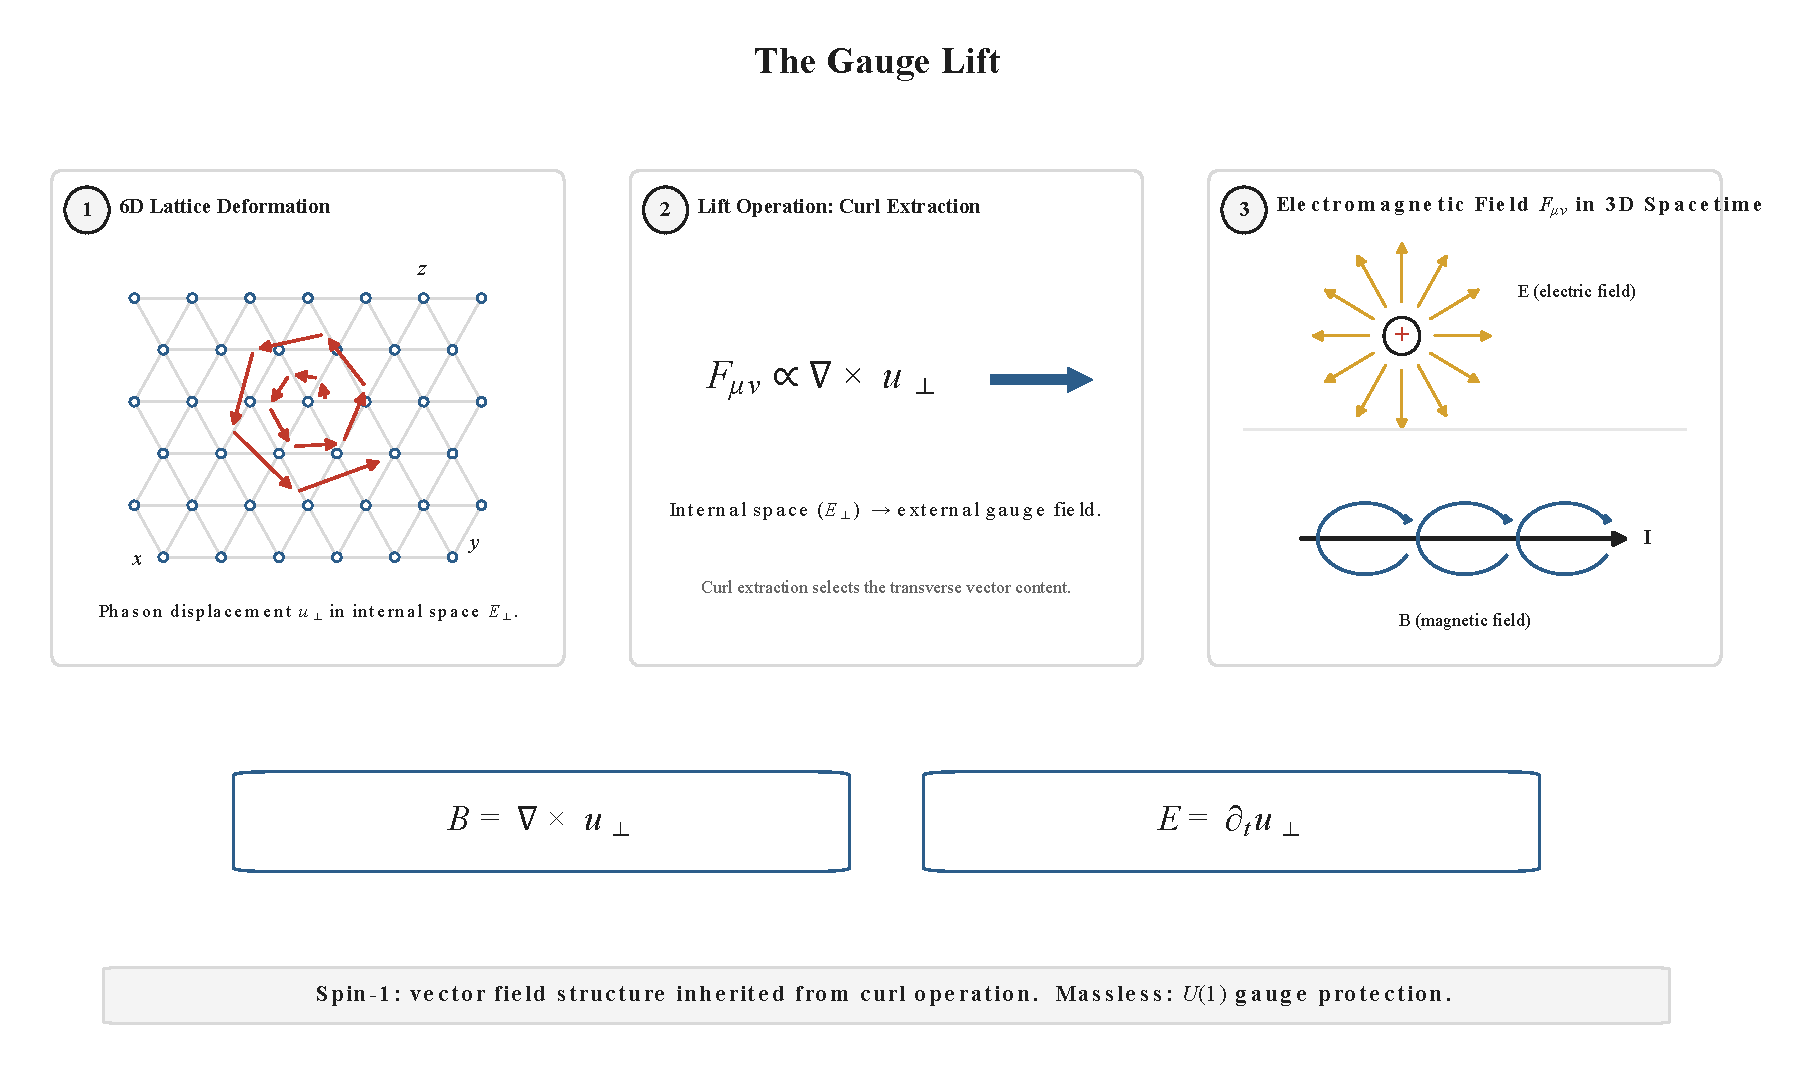
\includegraphics[keepaspectratio,alt={Conditional gauge lift (Tier 3): 6D icosahedral lattice strain is mapped to the 4D electromagnetic field tensor F\_\{\textbackslash mu\textbackslash nu\}; in this proposal the photon is identified with the transverse phason vector mode, massless under unbroken U(1) protection and spin-1 by construction of the assumed gauge action.}]{content/Figures/Volume_3/Figure V3.1.1.pdf}}
\caption{Conditional gauge lift (Tier 3): 6D icosahedral lattice strain
is mapped to the 4D electromagnetic field tensor \(F_{\mu\nu}\); in this
proposal the photon is identified with the transverse phason vector
mode, massless under unbroken \(U(1)\) protection and spin-1 by
construction of the assumed gauge action.}
\end{figure}

Within the supplied gauge action, the Ward identity protects a massless
spin-1 transverse mode (the transverse vector mode of \(A_T\)). Whether
the App ULA phason variables realize that action, and whether an
electric field measures the rate at which phason nodes flip states to
accommodate a charge imbalance, remain Tier 3 physical questions.

On this conditional reading {[}Tier 3 interpretation{]}, the
``Movement'' of the gauge field (\(F_{\mu\nu}\)) would be the
\textbf{Isotropic Elasticity} of the 6D lattice projected into the
internal space, and the ``Force'' the back-reaction of the lattice
against the unwinding of its topological defects; neither statement is
derived here.

\begin{figure}
\centering
\pandocbounded{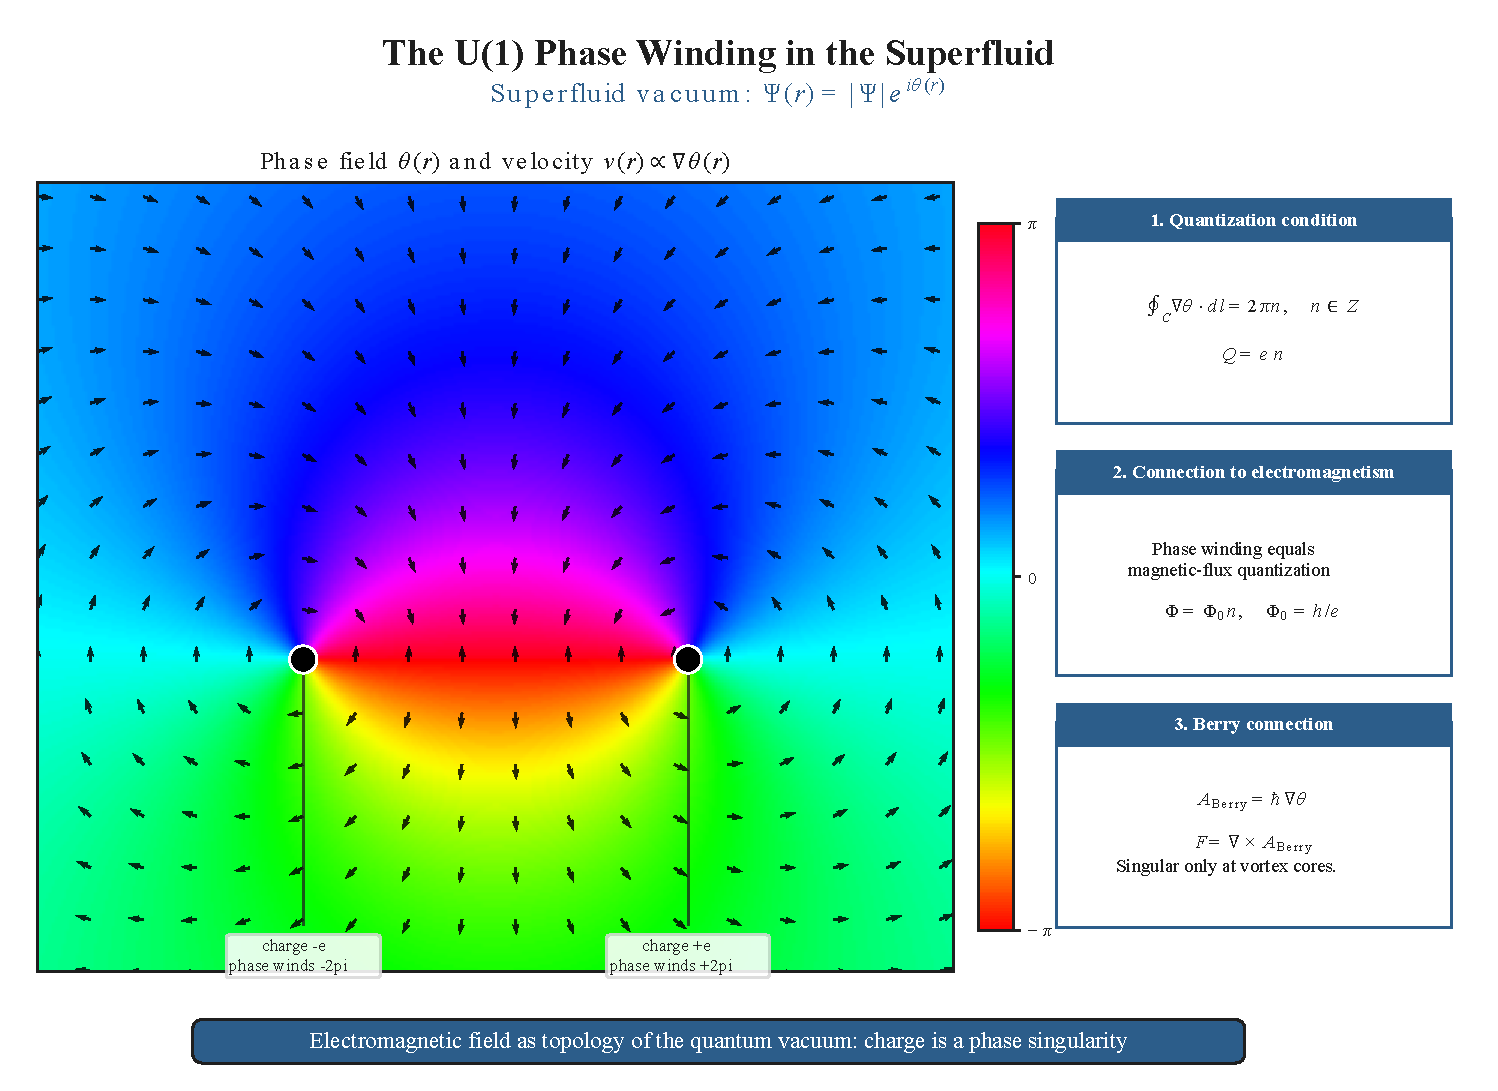
\includegraphics[keepaspectratio,alt={Opposite-charge phase vortices in the superfluid order parameter: the U(1) phase winds by +2\textbackslash pi and -2\textbackslash pi around the two cores, with the wrapped phase field and its gradient flow illustrating quantized winding number, which GCT proposes (Tier 3) as the topological origin of electric charge.}]{content/Figures/Volume_3/Figure V3.1.2.pdf}}
\caption{Opposite-charge phase vortices in the superfluid order
parameter: the \(U(1)\) phase winds by \(+2\pi\) and \(-2\pi\) around
the two cores, with the wrapped phase field and its gradient flow
illustrating quantized winding number, which GCT proposes (Tier 3) as
the topological origin of electric charge.}
\end{figure}

\chapter{\texorpdfstring{Chapter 2: The Rotation Sector ---
\(\mathrm{SU}(2)\)}{Chapter 2: The Rotation Sector --- \textbackslash mathrm\{SU\}(2)}}\label{chapter-2-the-rotation-sector-mathrmsu2}

While the \(U(1)\) sector is modelled on the internal scalar phase of
the vacuum condensate, the group \(SU(2)\) enters two mathematically
isomorphic but physically distinct roles. First,
\(SU(2)=\operatorname{Spin}(3)\) is the simply connected double cover of
the spatial rotation group \(SO(3)\) {[}Tier 1{]}. Second, the Standard
Model uses an \textbf{internal} weak-isospin gauge group \(SU(2)_L\),
postulated to account for isospin and parity violation. The first fact
does not derive the second. GCT proposes that an internal icosahedral
frame bundle and a chiral connection realize the weak sector, but that
physical identification requires a separately specified internal bundle,
chiral representation and gauge dynamics {[}Tier 2 mechanism / Tier 3
realization{]}. Neither the Dirac belt trick nor the universal Solenoid
forces weak isospin. This chapter keeps the \(SU(2)\) group structure
and the spatial double cover as mathematical inputs and separates them
from the weak-isospin identification.

\begin{center}\rule{0.5\linewidth}{0.5pt}\end{center}

\subsection{2.1 The Two Bundles: Spin and
Isospin}\label{the-two-bundles-spin-and-isospin}

\subsubsection{2.1.1 Isomorphism is not
Identity}\label{isomorphism-is-not-identity}

Standard physics distinguishes \textbf{Spin} (transforming under spatial
rotations) from \textbf{Weak Isospin} (transforming under internal gauge
rotations), even though both use the \(\mathfrak{su}(2)\) algebra. GCT
proposes a common icosahedral origin while retaining two distinct fiber
bundles; algebraic isomorphism is not physical identity.

\begin{enumerate}
\def\labelenumi{\arabic{enumi}.}
\tightlist
\item
  \textbf{The spatial spin bundle (\(E_\parallel\)):} If the physical
  manifold admits the relevant spin structure, its oriented frame bundle
  lifts from \(SO(3)\) to \(\operatorname{Spin}(3)\cong SU(2)\). This is
  the standard home of \textbf{Space-Time Spin (\(S\))}.
\item
  \textbf{The candidate internal gauge bundle (\(E_\perp\)):} The 3D
  internal manifold carries the same \(H_3\) point-group symmetry, and
  GCT assigns the internal icosahedral-frame degrees of freedom to a
  distinct bundle. Identifying its continuum connection and chiral
  doublet representation with \textbf{Weak Isospin (\(T\))} is a GCT
  physical bridge, not a consequence of the spatial spin lift.
\end{enumerate}

\subsubsection{\texorpdfstring{2.1.2 The Geometric Origin of
\(SU(2)_L\)}{2.1.2 The Geometric Origin of SU(2)\_L}}\label{the-geometric-origin-of-su2_l}

The exact mathematical input is \(2I\subset SU(2)\) with 120 elements.
GCT models internal-frame states by discrete hopping among those
elements of the \textbf{Binary Icosahedral Group (\(2I\))} and proposes
a continuum \(SU(2)\) connection in the long-wavelength limit. Deriving
the Standard-Model \(SU(2)_L\) gauge field still requires the continuum
limit, kinetic term, fermion representation and a proof of left-handed
coupling. The chiral (\(\phi\)-dependent) 6D projection motivates that
identification but does not by itself establish it {[}Tier 2 structural
candidate; Tier 3 physical gauge realization{]}.

\begin{center}\rule{0.5\linewidth}{0.5pt}\end{center}

\subsection{2.2 The Spatial Double-Cover
Control}\label{the-spatial-double-cover-control}

\subsubsection{2.2.1 Proposition 2.1 {[}Tier 1 double-cover topology +
Tier 3 physical framed-bundle
premise{]}}\label{proposition-2.1-tier-1-double-cover-topology-tier-3-physical-framed-bundle-premise}

\textbf{Proposition 2.1:} \emph{If a physical framed-defect
configuration realizes the non-trivial loop of \(SO(3)\) and its quantum
state is assigned the spinorial lift, then rotations act through
\(SU(2)\) and a \(2\pi\) rotation acts by \(-1\) in the fundamental
representation.} This conditional statement is about spatial spin.
Self-reference, an identity address and weak isospin do not follow from
it.

\subsubsection{\texorpdfstring{2.2.2 Proof: 360° rotation \(\neq\)
identity for
ribbons}{2.2.2 Proof: 360° rotation \textbackslash neq identity for ribbons}}\label{proof-360-rotation-neq-identity-for-ribbons}

As the standard control, model the physical object as a \textbf{framed
ribbon} whose orientation is measured relative to an ambient frame.
Applying this control to a GCT defect requires a separately derived
physical framed-configuration bundle and connection. The universal
Solenoid has \(\pi_1(\Sigma_\infty)=0\) and supplies no rotation
obstruction; mapping the physical state to a Solenoid address would be a
separate bridge.

\begin{itemize}
\tightlist
\item
  A rotation of \textbf{\(360^\circ\) (\(2\pi\))} returns the knot to
  its original geometric position but introduces a phase factor of
  \(e^{i\pi} = -1\) in the holonomy of the connection. Topologically,
  the ribbon accumulates a ``twist'' that cannot be removed by
  translation.
\item
  A rotation of \textbf{\(720^\circ\) (\(4\pi\))} introduces a
  double-twist (\(e^{i2\pi} = +1\)). In 3D, a double-twist is
  contractible; it can be ``looped'' over the object to restore the
  system to its original state.
\end{itemize}

For the spinorial representation, the state vector returns after
\(720^\circ\) while rays are unchanged by the \(360^\circ\) sign.
Whether a particular GCT defect occupies that representation is the
physical framed-bundle premise, not a conclusion about personal
identity.

\subsubsection{\texorpdfstring{2.2.3 Spinors and the need for \(SU(2)\)
(\(4\pi\)
symmetry)}{2.2.3 Spinors and the need for SU(2) (4\textbackslash pi symmetry)}}\label{spinors-and-the-need-for-su2-4pi-symmetry}

The universal cover of \(SO(3)\) is the \textbf{Special Unitary group
\(SU(2)\)}. Mathematically, \(SU(2)\) is topologically equivalent to the
3-sphere (\(S^3\)), which is simply connected. Along the lifted
one-parameter rotation path, \(2\pi\) reaches the central element
\(-\mathbf{1}\) and \(4\pi\) returns to \(+\mathbf{1}\), matching the
standard spinorial transport law.

\subsubsection{2.2.4 The Dirac Belt Trick as a Standard Framing
Control}\label{the-dirac-belt-trick-as-a-standard-framing-control}

The Dirac belt trick visualizes the non-trivial \(\mathbb{Z}_2\) loop of
\(SO(3)\) for an object framed relative to its environment. It
demonstrates the standard rotation topology {[}Tier 1{]}, not that all
matter is attached to the universal Solenoid and not that the weak gauge
group is spatial rotation. The GCT claim that a defect realizes this
physical framing remains a separate Tier 3 identification.

\subsubsection{2.2.5 Proof of the Double Cover Map (Quaternions) {[}Tier
1{]}}\label{proof-of-the-double-cover-map-quaternions-tier-1}

Using the isomorphism between \(SU(2)\) and the unit quaternions
\(\mathbb{H}_1\), a rotation \(R \in SO(3)\) by angle \(\theta_{rot}\)
about axis \(\hat{n}\) is mapped to \(SU(2)\) elements \(\pm q\), where
\(q = \cos(\theta_{rot}/2) + \hat{n}\sin(\theta_{rot}/2)\). The factor
of \(\theta_{rot}/2\) ensures that \(\theta_{rot} = 2\pi\) yields
\(q = -1\), and \(\theta_{rot} = 4\pi\) yields \(q = +1\). This \(2:1\)
covering map rigorously defines the \textbf{spatial spin lift}. A
weak-isospin bundle must be supplied independently.

\begin{center}\rule{0.5\linewidth}{0.5pt}\end{center}

\subsection{2.3 The Binary Icosahedral Candidate for the Internal
Sector}\label{the-binary-icosahedral-candidate-for-the-internal-sector}

\subsubsection{\texorpdfstring{2.3.1 \(2I \subset SU(2)\) (120
Elements)}{2.3.1 2I \textbackslash subset SU(2) (120 Elements)}}\label{i-subset-su2-120-elements}

While the hydrodynamic limit utilizes the continuous group \(SU(2)\),
the underlying hardware is a discrete lattice. The rotational symmetry
of the 6D parent lattice projects to the \textbf{Binary Icosahedral
Group}, denoted \(2I\) (or \(\tilde{I}\)). This is a discrete subgroup
of \(SU(2)\) containing 120 elements.

\subsubsection{2.3.2 Lift of the Icosahedral
Classes}\label{lift-of-the-icosahedral-classes}

The 60 rotational symmetries of the icosahedron (group \(I\)) are
``doubled'' in \(SU(2)\) to account for the spinor phase. The 120
elements of \(2I\) correspond to the 120 vertices of the
\textbf{600-Cell} (a regular 4-polytope) embedded in the \(S^3\)
manifold of the gauge group.

\subsubsection{2.3.3 Quaternion Representation (The 600-Cell) {[}Tier
1{]}}\label{quaternion-representation-the-600-cell-tier-1}

The elements of the binary-icosahedral control set are:

\begin{itemize}
\tightlist
\item
  \textbf{8 units:} \((\pm 1, 0, 0, 0)\) and permutations.
\item
  \textbf{16 vertices:} \(\frac{1}{2}(\pm 1, \pm 1, \pm 1, \pm 1)\).
\item
  \textbf{96 vertices:} even permutations of
  \(\frac{1}{2}(0, \pm 1, \pm \phi, \pm \phi^{-1})\).
\end{itemize}

\subsubsection{2.3.4 Discrete Hopping of Internal
Frames}\label{discrete-hopping-of-internal-frames}

GCT hypothesizes that, because the lattice is discrete at the Planck
scale, the microscopic internal frame of a particle hops among these 120
orientations and that a coarse-grained connection synchronizes
neighboring cells. Identifying that connection with the physical weak
force is Tier 3 until its continuum gauge action, matter representation
and chiral couplings are derived.

\begin{center}\rule{0.5\linewidth}{0.5pt}\end{center}

\subsection{2.4 Chirality from
Projection}\label{chirality-from-projection}

\subsubsection{2.4.1 The Primary Chiral Asymmetry (Geometric
CP-Violation)}\label{the-primary-chiral-asymmetry-geometric-cp-violation}

Standard physics treats CP-violation (one of the Sakharov conditions for
the matter--antimatter asymmetry, not the asymmetry itself) as a
parameter in the CKM matrix. GCT proposes {[}Tier 3{]} that it is a
\textbf{Structural Property of the Projection}.

\subsubsection{2.4.2 Chirality Witness: Jackiw-Rebbi Domain Wall
{[}proposed mechanism, chirality audit open + Tier 3 numerical-control
witness{]}}\label{chirality-witness-jackiw-rebbi-domain-wall-proposed-mechanism-chirality-audit-open-tier-3-numerical-control-witness}

Chirality has a computational check under the current model, but not a
verification: the engine chirality audit finds a boundary zero mode that
is generic rather than Fibonacci-specific, so the check stays open. The
cut-and-project boundary of the quasicrystal acts as a topological
domain wall, structurally analogous to the \textbf{Jackiw-Rebbi
mechanism}. Computations on the 1D Fibonacci Chain equivalent yielded
exactly 13 midgap states manifesting a net chirality of \(+1\) (a
left-handed surplus). This is consistent with, but not specific to, the
proposed chiral-domain-wall mechanism (the chirality audit is open) and
supplies a Tier 3 numerical-control witness for parity violation;
theorem-grade uniqueness over the full gauge/classification setting
remains an open App ORQ O.39 target.

\subsubsection{2.4.3 Candidate Chiral Representation {[}Tier 2 mechanism
/ Tier 3 physical
assignment{]}}\label{candidate-chiral-representation-tier-2-mechanism-tier-3-physical-assignment}

The weak-sector task is to derive an \textbf{internal} representation in
which the candidate \(SU(2)_L\) connection acts on left-chiral fermion
fields while right-chiral Standard-Model fields are \(SU(2)_L\)
singlets. Spatial handedness, spatial spin and weak isospin are distinct
notions. The oriented 6D\(\to\)\hspace{0pt}3D projection and the
domain-wall index of §2.4.2 can motivate a chiral asymmetry, but neither
the Selection Operator nor an Agent address selects the Standard-Model
representation by itself. A complete derivation requires the internal
gauge bundle, its Dirac operator, the chiral matter representation and
anomaly cancellation.

As a candidate parent branching, one may write
\[\mathbf{4} \to (\mathbf{2}, \mathbf{1}) \oplus (\mathbf{1}, \mathbf{2})\]
under a declared \(SU(2)_L\times SU(2)_R\) parent symmetry. Here both
factors are internal representation labels in this weak-sector ansatz:

\begin{itemize}
\tightlist
\item
  \textbf{\((\mathbf{2}, \mathbf{1})\):} Candidate left-chiral doublet
  under the factor proposed for gauging as \(SU(2)_L\).
\item
  \textbf{\((\mathbf{1}, \mathbf{2})\):} Candidate right-chiral partner
  under the second factor, which must be reduced or otherwise mapped to
  the observed \(SU(2)_L\)-singlet spectrum.
\end{itemize}

This branching is not a physical-versus-internal rotation split and is
not yet a derivation of the Standard-Model fermion content.

\subsubsection{2.4.4 Left-Handed Coupling to the Weak
Force}\label{left-handed-coupling-to-the-weak-force}

GCT proposes the physical weak bosons as the connection modes of the
candidate internal \(SU(2)_L\) bundle. Conditional on the chiral
representation bridge above, left-chiral doublets couple to \(W^a_\mu\)
through the standard covariant derivative. The icosahedral projection
supplies a proposed geometric origin for that bridge; it does not
replace the required gauge connection, kinetic term or representation
derivation {[}Tier 3 physical realization{]}.

\subsubsection{2.4.5 Right-Handed Singlets and the Neutrino
Candidate}\label{right-handed-singlets-and-the-neutrino-candidate}

In the Standard Model, right-handed charged fermions are singlets of
\(SU(2)_L\) but still carry hypercharge, so they are not generically
sterile {[}Tier 1{]}. A right-handed neutrino, if present, is the
special gauge-singlet candidate. Mapping such a component to an
\(E_\perp\)-dominated defect mode may motivate the second-order neutrino
suppression in \textbf{Chapter 9}, but that mapping and the resulting
mass operator remain Tier 3 until the internal representation and
couplings are derived.

\begin{center}\rule{0.5\linewidth}{0.5pt}\end{center}

\subsection{2.5 Physical
Interpretation}\label{physical-interpretation-2}

\subsubsection{\texorpdfstring{2.5.1 Three Generators: \(W^+, W^-, W^3\)
(Before
Mixing)}{2.5.1 Three Generators: W\^{}+, W\^{}-, W\^{}3 (Before Mixing)}}\label{three-generators-w-w--w3-before-mixing}

The \(SU(2)_L\) algebra is generated by three operators. \(W^\pm\) act
as raising/lowering operators within a weak-isospin doublet (for
example, the neutrino/electron components), while \(W^3\) is the
pre-mixing neutral generator that later combines with the Hypercharge
field \(B\) (Chapter 4) to form the physical \(Z\) and \(\gamma\). These
operations change internal weak-isospin state; they do not rotate or
rewrite a Solenoid identity address.

\subsubsection{\texorpdfstring{2.5.2 Weak Isospin \(T_3\) as Lattice
Orientation}{2.5.2 Weak Isospin T\_3 as Lattice Orientation}}\label{weak-isospin-t_3-as-lattice-orientation}

The quantum number \(T_3 = \pm 1/2\) labels the two components of the
candidate internal weak doublet relative to the declared local internal
frame {[}Tier 3 assignment{]}. It is not a personal-identity bit or an
identity-address coordinate.

\subsubsection{2.5.3 Parity Violation as a Geometric
Candidate}\label{parity-violation-as-a-geometric-candidate}

GCT proposes that the oriented 6D\(\to\)\hspace{0pt}3D cut-and-project
construction, with its irrational \(\phi\)-slope, supplies a geometric
source for chirality. That orientation is a Tier 3/open candidate: the
cut-and-project set is centrosymmetric, so an independently defined
chirality-breaking operator would be needed (App USS §USS.7, Remark
T-McK.1b.A; V2 Ch02 §2.1.3); deriving the observed weak parity violation
still requires the internal \(SU(2)_L\) bundle, chiral Dirac spectrum
and matter couplings identified above {[}Tier 3 realization{]}. It is
therefore an evidence target and an architecture, not a proof obtained
from the spatial double cover or from agency.

\begin{figure}
\centering
\pandocbounded{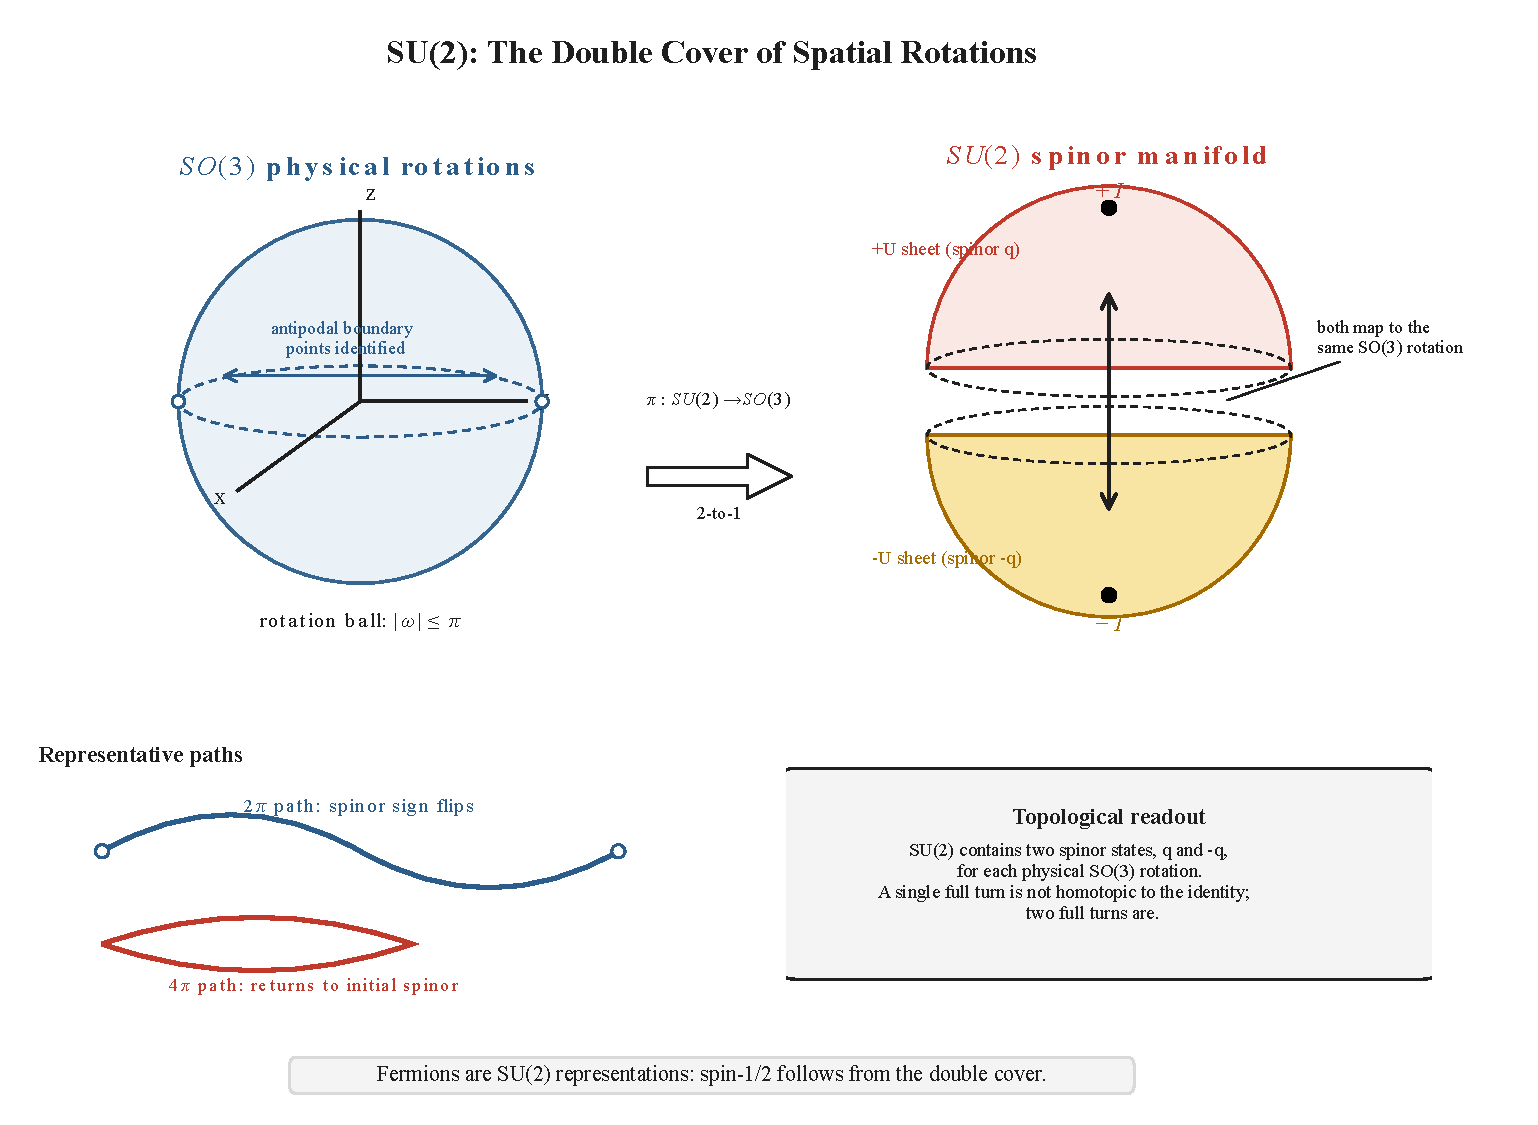
\includegraphics[keepaspectratio,alt={Standard spatial-rotation control: the SU(2) double cover sends a 2\textbackslash pi rotation to the central element -1, while a 4\textbackslash pi rotation returns to +1. Applying this control to a GCT defect requires its physical framed bundle; the internal weak-isospin bundle is separate.}]{content/Figures/Volume_3/Figure V3.2.1.pdf}}
\caption{Standard spatial-rotation control: the SU(2) double cover sends
a \(2\pi\) rotation to the central element \(-1\), while a \(4\pi\)
rotation returns to \(+1\). Applying this control to a GCT defect
requires its physical framed bundle; the internal weak-isospin bundle is
separate.}
\end{figure}

\chapter{\texorpdfstring{Chapter 3: The Color Force ---
\(\mathrm{SU}(3)\)}{Chapter 3: The Color Force --- \textbackslash mathrm\{SU\}(3)}}\label{chapter-3-the-color-force-mathrmsu3}

In standard Quantum Chromodynamics (QCD), the \(\mathrm{SU}(3)\) color
symmetry is an empirical postulate. Geometric Consciousness Theory (GCT)
proposes that the strong interaction is connected to the vacuum's
\textbf{Acceptance Window}. This chapter presents that proposal as an
\textbf{open Tier 3 candidate}: the exact matrix algebra built from the
ten three-fold axes of the window is Tier 1, but neither the compact
real form, a complex three-component matter representation, a local
gauge field, nor specificity to the window geometry is derived.
Theorem-grade uniqueness over compact Lie alternatives is App ORQ O.39.

\begin{center}\rule{0.5\linewidth}{0.5pt}\end{center}

\subsection{3.1 The Geometry of the Acceptance
Window}\label{the-geometry-of-the-acceptance-window}

\subsubsection{\texorpdfstring{3.1.1 The Rhombic Triacontahedron (RT) in
\(E_\perp\)}{3.1.1 The Rhombic Triacontahedron (RT) in E\_\textbackslash perp}}\label{the-rhombic-triacontahedron-rt-in-e_perp}

As established in Volume 2, Chapter 2, the physical vacuum is a 3D slice
through a 6D hyper-lattice. The selection rule for node existence is
determined by the \textbf{Acceptance Window} \(W \subset E_\perp\). For
the icosahedral Ammann-Kramer-Neri (AKN) tiling, \(W\) is the projection
of the 6D unit hypercube into the perpendicular space. This volume is
the \textbf{Rhombic Triacontahedron (RT)}.

The RT is a zonohedron with 30 congruent rhombic faces and 32 vertices.
It is the most symmetric ``container'' allowed by the icosahedral point
group \(I_h\). GCT proposes that the gauge symmetries of the Standard
Model are inherited from the symmetries of this window as perceived by a
topological defect {[}Tier 3{]}.

\subsubsection{3.1.2 The 10 Three-Fold Rotation
Axes}\label{the-10-three-fold-rotation-axes}

The vertices of the RT fall into two distinct symmetry classes.
Specifically, the RT possesses exactly \textbf{10 axes of three-fold
rotational symmetry} (corresponding to the 20 three-fold vertices
grouped in opposite pairs). GCT proposes reading these axes as the
directions of topological winding within the internal manifold {[}Tier
3{]}.

\begin{center}\rule{0.5\linewidth}{0.5pt}\end{center}

\subsection{\texorpdfstring{3.2 RT Generator Inventory and
\(\mathrm{SU}(3)\) Candidate {[}Tier 1 matrix algebra + Tier 3 open
identification{]}}{3.2 RT Generator Inventory and \textbackslash mathrm\{SU\}(3) Candidate {[}Tier 1 matrix algebra + Tier 3 open identification{]}}}\label{rt-generator-inventory-and-mathrmsu3-candidate-tier-1-matrix-algebra-tier-3-open-identification}

\subsubsection{3.2.1 Quadrupole Seeds, Gram Rank and Eight-Dimensional
Closure}\label{quadrupole-seeds-gram-rank-and-eight-dimensional-closure}

GCT proposes that the strong interaction is connected to the projection
of the 6D parent lattice into the 3D internal space \(E_\perp\), whose
acceptance window carries ten three-fold axes. The construction below
records what that axis inventory does and does not fix.

\gctneedspace{5\baselineskip}

\textbf{The \(\mathrm{SU}(3)\) Candidate Construction {[}Tier 1 matrix
algebra conditional on the RT input + Tier 3 open identification{]}:}
The ten three-fold axes of the RT window define ten traceless quadrupole
seeds. These seeds span a five-dimensional space, and their commutators
add three generators, giving an eight-dimensional closure. With the
seeds made Hermitian and closed under \(i[A,B]\), the closure carries
the \(A_2\) root-system fingerprint of \(\mathfrak{su}(3)\) (two Cartan
generators plus six root generators). This is a matrix-algebra fact
about the chosen construction. It does not single out the window:
generic sets of ten axes close in the same way (§3.2.1, Specificity), so
the identification with physical color is an open Tier 3 candidate, not
a theorem-grade uniqueness result.

\begin{figure}
\centering
\pandocbounded{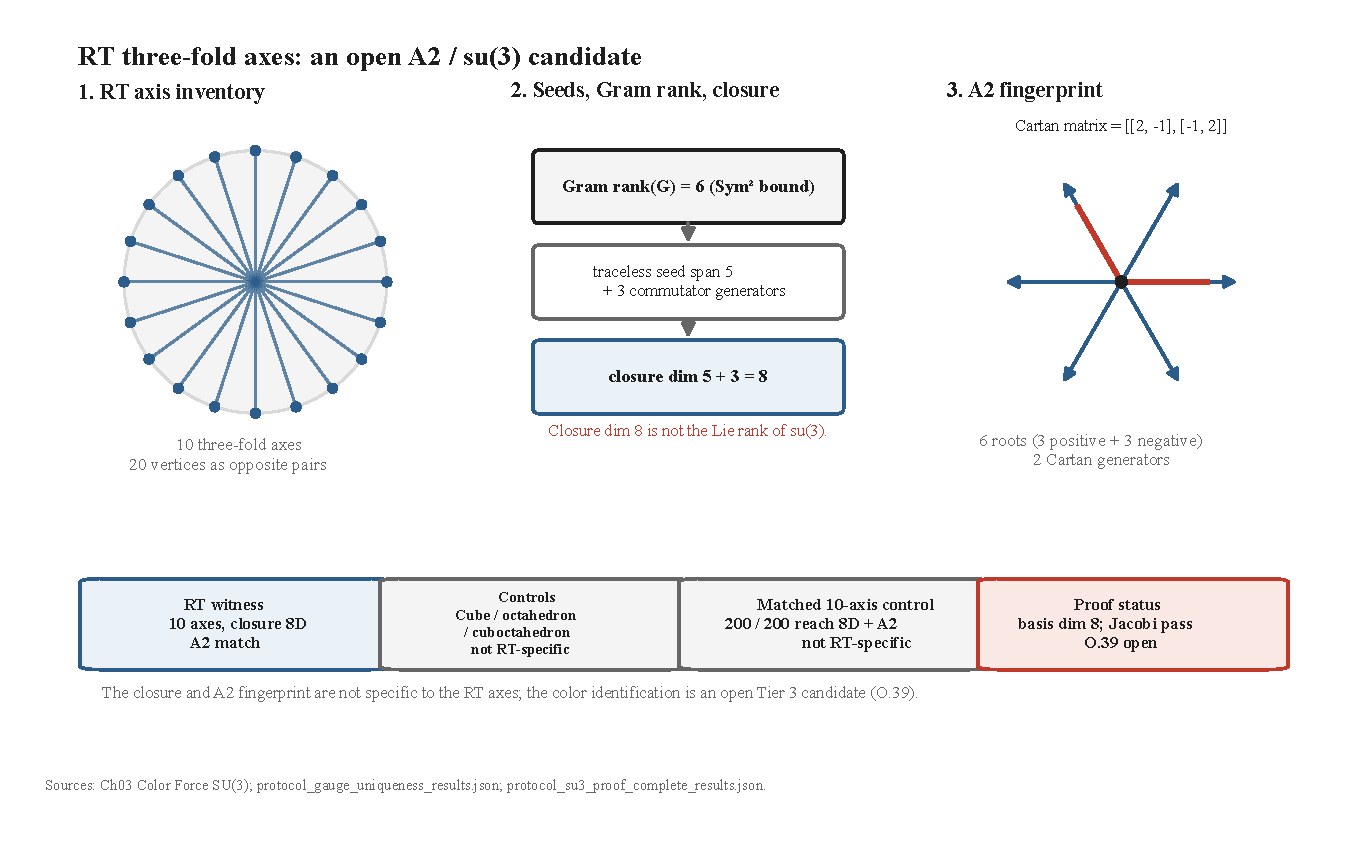
\includegraphics[keepaspectratio,alt={The ten three-fold axes of the rhombic-triacontahedral window: quadrupole Gram rank 6 (the maximum for any ten axes), traceless-seed span 5, and an eight-dimensional closure with the A\_2/\textbackslash mathfrak\{su\}(3) fingerprint. Generic ten-axis sets reproduce the same closure, so the color identification is an open Tier 3 candidate.}]{content/Figures/Volume_3/Figure V3.3.1.pdf}}
\caption{The ten three-fold axes of the rhombic-triacontahedral window:
quadrupole Gram rank 6 (the maximum for any ten axes), traceless-seed
span 5, and an eight-dimensional closure with the
\(A_2/\mathfrak{su}(3)\) fingerprint. Generic ten-axis sets reproduce
the same closure, so the color identification is an open Tier 3
candidate.}
\end{figure}

\gctneedspace{5\baselineskip}

\textbf{Proposition 3.2.1: Quadrupole Gram Rank of the Ten-Axis
Inventory {[}Tier 1{]}}

The 10 three-fold axis unit vectors \(\hat{a}_1 \dots \hat{a}_{10}\)
(one per antipodal pair) fall into two classes generated from the Golden
Ratio \(\phi\):

\begin{itemize}
\tightlist
\item
  \begin{enumerate}
  \def\labelenumi{(\roman{enumi})}
  \tightlist
  \item
    4 body-diagonal axes \((\pm 1, \pm 1, \pm 1)/\sqrt{3}\).
  \end{enumerate}
\item
  \begin{enumerate}
  \def\labelenumi{(\roman{enumi})}
  \setcounter{enumi}{1}
  \tightlist
  \item
    6 axes from cyclic permutations of
    \((0, \pm 1/\phi, \pm \phi)/\sqrt{1/\phi^2+\phi^2}\).
  \end{enumerate}
\end{itemize}

These are the three-fold axes of the icosahedral group whose five-fold
axes are the cyclic permutations of \((0,\pm\phi,\pm1)\).

The \(10 \times 10\) quadrupole Gram matrix is
\(G_{ij} = (\hat{a}_i \cdot \hat{a}_j)^2 = \langle \hat{a}_i\hat{a}_i^{T}, \hat{a}_j\hat{a}_j^{T} \rangle_F\),
the Frobenius Gram matrix of the ten symmetric tensors
\(\hat{a}_i\hat{a}_i^{T}\). These tensors lie in
\(\mathrm{Sym}^2(\mathbb{R}^3)\), which is six-dimensional, so
\[\operatorname{rank}(G) \le 6 \quad \text{for any ten real axes.}\] For
the RT inventory the bound is attained: \(\operatorname{rank}(G)=6\) and
the null space of \(G\) is four-dimensional (singular values \(10/3\),
\(4/3\) with multiplicity five, and \(0\) with multiplicity four). The
rank is a property of the quadrupole tensors, not a count of Lie
generators, and it is not the Lie rank of \(\mathfrak{su}(3)\).
\emph{(Numerical values:
\texttt{GCT\_Physics\_Engine/src/protocol\_gauge\_uniqueness.py},
Appendix GPE.)}

\textbf{Eight-dimensional closure {[}Tier 1 matrix algebra conditional
on the construction{]}.} Removing traces, the ten seeds
\(Q_i = \hat{a}_i\hat{a}_i^{T} - I/3\) span the five-dimensional space
of traceless symmetric \(3\times3\) matrices. Their commutators add the
three antisymmetric matrices, and the closure is eight-dimensional.
Under ordinary real commutators the result is
\(\mathfrak{sl}(3,\mathbb{R})\), a noncompact real form whose Killing
form has signature \((5,3)\). Multiplying the symmetric generators by
\(i\) --- equivalently, building Hermitian seeds and closing under
\(i[A,B]\) --- yields the compact real form \(\mathfrak{su}(3)\) with
negative-definite Killing form. The engine makes this second choice; the
choice itself is not derived from the window geometry or from a
microscopic action.

\textbf{\(A_2\) check {[}Tier 1 within the construction; Tier 3 physical
identification{]}.} In the Hermitian construction the eight-dimensional
span has two commuting Cartan generators and six root generators, and
the engine verifies the Cartan matrix
\texttt{{[}{[}2,\ -1{]},\ {[}-1,\ 2{]}{]}} to floating-point tolerance
(Appendix GPE). Identifying this span with the physical color algebra
additionally requires a source-selected compact real form, a complex
three-component matter representation with its inner product, and a
local gauge redundancy. These remain open. \(\square\)

\textbf{Specificity of the construction {[}Tier 1 numerical control{]}.}
The eight-dimensional closure and the \(A_2\) fingerprint are not
specific to the RT inventory. In the registered matched-axis control,
ten random unit axes per trial reproduce the eight-dimensional closure
with an \(A_2\) Cartan matrix within tolerance in every trial (200/200),
and even three generic axes close to eight dimensions. The Monte Carlo
over 1,000 random convex polyhedra does not test this question: none of
the sampled polyhedra has exactly ten three-fold axes, so no trial
reaches the algebra comparison. A discriminating test requires a
physical selection criterion that rejects matched alternatives for a
non-circular reason; that criterion is part of O.39.

\textbf{As computed by the physics engine (Appendix GPE.2)}, the
construction is:

\begin{enumerate}
\def\labelenumi{\arabic{enumi}.}
\tightlist
\item
  \textbf{Axis inventory:} the ten three-fold axes of the RT window (one
  per antipodal pair).
\item
  \textbf{Shear operators (quadrupoles):} the traceless symmetric seeds
  span exactly \textbf{5} independent shear generators.
\item
  \textbf{Algebra closure (rotations):} commutators \([S_i, S_j]\) add 3
  antisymmetric generators.
\item
  \textbf{Dimension count:} \(5 + 3 = 8\) generators.
\item
  \textbf{\(A_2\) check:} in the Hermitian construction the span carries
  the two-Cartan/six-root \(A_2\) fingerprint. Steps 2--5 hold for
  generic ten-axis inventories as well; physical identification and
  uniqueness remain open (O.39).
\end{enumerate}

\gctneedspace{5\baselineskip}

\textbf{Transverse Complex Structure of a Three-Fold Axis {[}Tier 1
within the construction{]}:} The binary icosahedral lift \(2I\) supplies
a complex structure on the plane transverse to each three-fold axis. The
directed stabilizer of a 3-fold RT axis in \(SO(3)\) is \(C_3\); its
preimage in \(2I\) is a binary cyclic subgroup of order 6. The
non-trivial \(SO(3)\) action on the transverse tangent plane is
therefore a \(2\pi/3\) (or \(4\pi/3\)) rotation, not a \(\pi/2\) phase
rotation. The complex structure is derived from that stabilizer action
by writing the tangent-plane restriction of an order-6 lift \(g\) as
\[R_g|_T=\cos(2\pi/3)I_2+\sin(2\pi/3)J,\] so
\[J=\frac{R_g|_T-\cos(2\pi/3)I_2}{\sin(2\pi/3)},\qquad J^2=-I_2.\] The
engine verifies this derived \(J\) directly from the stabilizer element,
rather than inserting the standard complex-structure matrix by hand
(Appendix GPE). This \(J\) is a complex structure on the two-dimensional
transverse tangent plane of one axis. It does not by itself supply a
complex structure on the full three-dimensional internal space (an
odd-dimensional real vector space admits no \(J\) with \(J^2=-I\)), so a
separately derived complex three-component matter bundle remains
required {[}Tier 3 open{]}.

\subsubsection{3.2.2 Proposed Identification with the Standard Model
{[}Tier 3 open
candidate{]}}\label{proposed-identification-with-the-standard-model-tier-3-open-candidate}

GCT proposes that the 8 generators of the Hermitian construction
correspond to the \textbf{8 gluons} of the Standard Model. The
supporting checks are properties of the chosen construction:

\begin{itemize}
\tightlist
\item
  \textbf{Structure Constants \& Jacobi Identity:} the commutators of
  the constructed operators reproduce \(\mathfrak{su}(3)\) structure
  constants \(f_{abc}\) and satisfy the Jacobi identity to machine
  precision.
\item
  \textbf{Killing Form:} the Killing form of the Hermitian construction
  is negative definite, as it must be for the compact real form selected
  by closing under \(i[A,B]\); the real-commutator closure of the same
  seeds is the noncompact \(\mathfrak{sl}(3,\mathbb{R})\).
\item
  \textbf{Cartan Matrix \& Dynkin Diagram:} the two-dimensional Cartan
  subalgebra yields the Cartan matrix
  \texttt{{[}{[}2,\ -1{]},\ {[}-1,\ 2{]}{]}}, the \(A_2\) fingerprint.
\end{itemize}

Because generic ten-axis inventories pass the same checks, these
properties do not by themselves select the RT geometry or establish that
the physical color group emerges from it. The gluon identification is an
open Tier 3 candidate pending O.39.

\subsubsection{3.2.3 Proposal 3.1: Geometric Origin of Color {[}Tier
3{]}}\label{proposal-3.1-geometric-origin-of-color-tier-3}

GCT proposes that ``color'' is the azimuthal orientation of a defect's
Burgers vector \(\mathbf{b}_\perp\) relative to three independent axes
of the reduced internal space, with SU(3) acting as the unitary
automorphisms of that orientation. A complex three-component
representation realizing this proposal is not yet derived.

\begin{center}\rule{0.5\linewidth}{0.5pt}\end{center}

\subsection{3.3 Gluon Dynamics and the
Chromo-Field}\label{gluon-dynamics-and-the-chromo-field}

\subsubsection{3.3.1 The 8 Gluons as Phason Transfer
Operators}\label{the-8-gluons-as-phason-transfer-operators}

In the candidate construction of §3.2, the 8 generators are proposed to
correspond to 8 independent phason transfer operators --- the 5 shear
generators and 3 rotational generators of the internal \(E_\perp\)
coordinate {[}Tier 3{]}. A ``gluon'' is then the quantized excitation of
the phason field that transfers color charge (changes the Burgers vector
orientation \(\mathbf{b}_\perp\) of a quark defect) without changing the
particle's topological winding number in the physical \(E_\parallel\)
space.

\subsubsection{3.3.2 The Running Coupling {[}Tier 3
Provisional{]}}\label{the-running-coupling-tier-3-provisional}

The proposed bare handle
\(\alpha_s(\text{bare}) = 1/(10\phi^2) \approx 0.038\) is an ultraviolet
value and is not a same-scale prediction of \(\alpha_s(M_Z)\). Evolving
it with the native resolution-depth kernel gives
\(\alpha_s(M_Z) \approx 0.052\), about 55.9\% below the observed value;
full QLQCD-2 non-perturbative closure is required. See V3 §4.5.5 and App
GRF §GRF.3. \textbf{{[}Open Research Debt QLQCD-2{]}}

\begin{center}\rule{0.5\linewidth}{0.5pt}\end{center}

\subsection{3.4 The Topology of Defects}\label{the-topology-of-defects}

\subsubsection{3.4.1 Vertex Defects (Leptons) and Color
Neutrality}\label{vertex-defects-leptons-and-color-neutrality}

In the candidate assignment, leptons are vertex defects referred to the
5-fold axes rather than to the 3-fold axes that carry the proposed color
orientation, and are therefore proposed to be \textbf{Color Singlets}
{[}Tier 3{]}.

\subsubsection{3.4.2 Face Defects (Quarks) and the Burgers
Vector}\label{face-defects-quarks-and-the-burgers-vector}

In the candidate assignment, quarks are face defects located at the
centers of the rhombic faces. The 30 rhombic faces of the
triacontahedron have their normals, and hence their centres, along the
15 two-fold axes; none lies on a three-fold axis, which instead pass
through the 20 three-valent vertices. Referring a face defect's
orientation to the 3-fold axes is therefore not a geometric identity but
an open Tier 3 assignment. Their transformation as \(\mathrm{SU}(3)\)
triplets is a Tier 3 candidate, not a consequence of that geometry: it
requires the complex three-component matter representation, which is not
yet derived (§3.2.1; App ORQ O.39 and O.32).

\begin{center}\rule{0.5\linewidth}{0.5pt}\end{center}

\subsection{3.5 Confinement and Asymptotic
Freedom}\label{confinement-and-asymptotic-freedom}

\subsubsection{3.5.1 The Singlet Condition {[}Tier 3
proposal{]}}\label{the-singlet-condition-tier-3-proposal}

GCT proposes that an uncompensated orientation mismatch costs an
unbounded domain-wall energy, so that physical states satisfy the
\textbf{Global Singlet Condition}:
\(\sum \text{colors} \equiv 0 \pmod 3\). The domain-wall energy is not
computed from a microscopic action here.

\subsubsection{3.5.2 The Flux Tube Mechanism {[}Tier 3
proposal{]}}\label{the-flux-tube-mechanism-tier-3-proposal}

In the candidate picture, separating colored defects creates a filament
of phason strain (a Flux Tube) whose energy would scale linearly with
distance (\(V \sim \sigma r\)). Neither the linear scaling nor the
string tension \(\sigma\) is derived here.

\subsubsection{3.5.3 Asymptotic Freedom {[}Tier 3
proposal{]}}\label{asymptotic-freedom-tier-3-proposal}

GCT proposes that at short distances the phason field becomes
``transparent,'' allowing the defects to behave as if free through the
lattice's short-range relaxation modes. The native running of §3.3.2
does not yet reproduce the observed strong coupling (V3 §4.5.5).

\begin{center}\rule{0.5\linewidth}{0.5pt}\end{center}

\gctneedspace{5\baselineskip}

\textbf{END OF CHAPTER 3}

\chapter{Chapter 4: Electroweak
Unification}\label{chapter-4-electroweak-unification}

In the standard Glashow-Weinberg-Salam (GWS) model, the unification of
the electromagnetic and weak interactions uses the symmetry group
\(SU(2)_L \times U(1)_Y\) and an empirically fixed weak mixing angle,
\(\theta_W\). GCT proposes that the electroweak sectors inherit
structure from the \(E_\parallel \oplus E_\perp\) decomposition of the
6-dimensional parent lattice. The canonical projector fixes the sector
geometry but does not, by itself, fix the relative gauge-kinetic
normalization of the two sectors. This chapter therefore separates exact
projection identities from the conditional bare-angle hypothesis and
from the renormalization-group (RGE) audits, none of which currently
closes on the observed Z-pole value.

\begin{center}\rule{0.5\linewidth}{0.5pt}\end{center}

\subsection{4.1 The Canonical Projector
Result}\label{the-canonical-projector-result}

\subsubsection{4.1.1 Projected Basis-Vector Norms {[}Tier
1{]}}\label{projected-basis-vector-norms-tier-1}

As established in Volume 2, the basis
\(\{\mathbf{E}_1, \dots, \mathbf{E}_6\}\) of \(\mathbb{Z}^6\) is
resolved into two orthogonal three-dimensional subspaces, the parallel
space (\(E_\parallel\), physical) and the perpendicular space
(\(E_\perp\), internal). With the canonical row-isometric maps
\(\widehat M_\parallel, \widehat M_\perp\), define
\[\Pi_\parallel = \widehat M_\parallel^{T} \widehat M_\parallel, \qquad \Pi_\perp = \widehat M_\perp^{T} \widehat M_\perp .\]
They satisfy \(\Pi_\parallel + \Pi_\perp = I_6\). Icosahedral symmetry
acts transitively on the six basis axes, so the six diagonal entries of
each projector are equal, and the rank-three trace gives
\[\|\Pi_\parallel \mathbf{E}_i\|^2 = \|\Pi_\perp \mathbf{E}_i\|^2 = \tfrac{1}{2} \qquad (i = 1, \dots, 6).\]

\subsubsection{4.1.2 Raw Galois-Frame Identity {[}Tier 1 arithmetic;
coordinate-dependent{]}}\label{raw-galois-frame-identity-tier-1-arithmetic-coordinate-dependent}

Before row normalization, the Galois-conjugate matrices obey
\[A_0 A_0^{T} = 2(2+\phi) I_3, \qquad B_0 B_0^{T} = 2(3-\phi) I_3,\] so
their raw squared-scale ratio is
\[\rho_{\rm raw} = \frac{2(3-\phi)}{2(2+\phi)} = \frac{3-\phi}{2+\phi} = \phi^{-2},\]
using \(\phi^2 = \phi + 1\), and the raw linear-scale ratio is
\(\phi^{-1}\). This exact identity belongs to the declared raw frame.
Under \(B_0 \mapsto s B_0\) the row space and the proper projector
\(B_0^{T}(B_0 B_0^{T})^{-1} B_0\) are unchanged while
\(\rho_{\rm raw} \mapsto s^2 \rho_{\rm raw}\), so \(\rho_{\rm raw}\) is
not a substrate-invariant physical length ratio. The relative
electroweak coupling must come from a canonically normalized action or
trace, not from the coordinate lengths of two raw row frames. This does
not predict equal electroweak couplings either.

\begin{center}\rule{0.5\linewidth}{0.5pt}\end{center}

\subsection{4.2 The Definition of
Hypercharge}\label{the-definition-of-hypercharge}

\subsubsection{\texorpdfstring{4.2.1 Hypercharge as Internal \(U(1)\)
Generator}{4.2.1 Hypercharge as Internal U(1) Generator}}\label{hypercharge-as-internal-u1-generator}

GCT assigns the two sectors of the electroweak force to internal degrees
of freedom {[}Tier 3 placement; V3 Ch02 §2.1.1, V3 Ch06 §6.1.2{]}:

\begin{itemize}
\tightlist
\item
  \textbf{Weak Isospin (\(T_3\)):} Corresponds to rotations of the
  candidate internal icosahedral-frame (\(2I \subset SU(2)\)) bundle,
  placed on the internal (\(E_\perp\)) side. It is not the gauge field
  of the spatial frame: the spatial double cover
  \(\operatorname{Spin}(3)\) of rotations in \(E_\parallel\) is a
  separate Tier 1 control (V3 Ch02 §2.2).
\item
  \textbf{Weak Hypercharge (\(Y\)):} Corresponds to phase rotations
  within the \textbf{Internal Space} (\(E_\perp\)).
\end{itemize}

\subsubsection{4.2.2 The Charge Formula and the 1/2 Factor {[}Tier 1
normalization convention + Tier 3 GCT
interpretation{]}}\label{the-charge-formula-and-the-12-factor-tier-1-normalization-convention-tier-3-gct-interpretation}

The electric charge \(Q\) is the generator of the symmetry that remains
unbroken after crystallization. The Gell-Mann-Nishijima formula
(\(Q = T_3 + Y/2\)) is standard; GCT offers a Tier 3 reading of it as a
normalization aligning the weak-frame and internal-phase sectors
(below).

The factor of \textbf{1/2} is a normalization convention of the Standard
Model charge formula: the alternative \(Q = T_3 + Y\), with \(Y\)
halved, is equally common (V3 Ch01 §1.3.3). GCT offers a Tier 3
interpretation of it, the \textbf{Topological Covering Difference} of
the two manifolds. \(T_3\) acts in the doublet representation of the
binary (double-cover) frame group \(2I \subset SU(2)\) of the internal
weak bundle (where a full \(2\pi\) frame rotation acts by \(-1\) and the
identity returns at \(4\pi\)), with eigenvalues \(\pm 1/2\); these
values come from the doublet representation, and this is not the spatial
spin double cover. \(Y\) acts on the \textbf{Scalar Single-Cover} of the
internal phase (where a full rotation is \(2\pi\)). In this book's
convention \(Y\) takes the values \(+1/3\), \(-1\), \(+4/3\), \(-2/3\)
and \(-2\) (§4.2.3, V3 Ch01 §1.3.3), which are not integers, so the
covering difference does not fix the factor 1/2. The reading that the
\(U(1)\) hypercharge is ``halved'' relative to the \(SU(2)\) isospin so
that a unit lattice step acts consistently on both sectors is a Tier 3
interpretation of a convention, not a derivation.

\begin{center}\rule{0.5\linewidth}{0.5pt}\end{center}

\subsubsection{4.2.3 Derivation of Right-Handed Hypercharges {[}Tier 1
algebraic identity + Tier 2 mechanism / Tier 3 physical singlet
assignment{]}}\label{derivation-of-right-handed-hypercharges-tier-1-algebraic-identity-tier-2-mechanism-tier-3-physical-singlet-assignment}

\begin{quote}
\textbf{Theorem 4.2 --- Right-Handed Hypercharges {[}Tier 1 algebraic
identity + Tier 2 mechanism / Tier 3 physical singlet assignment{]}}

\emph{Statement:} For any right-handed fermion state in GCT --- defined
as a singlet of the candidate internal weak bundle (\(T_3 = 0\); the
singlet assignment is the Tier 3 chiral-representation assignment of V3
Ch02 §2.4.3) --- the Weak Hypercharge is exactly: \[Y_R = 2Q\] where
\(Q\) is the conserved electric charge, taken as given; its values and
the defect-topology-to-charge mapping via AKN lattice winding are Tier 3
(Proposal 1.2, V3 Ch01 §1.3.2).

\emph{Derivation:} Set \(T_3 = 0\) in \(Q = T_3 + Y/2\). Solve for
\(Y\).

\emph{Results:}

{\def\LTcaptype{none} % do not increment counter
\begin{longtable}[]{@{}ccc@{}}
\toprule\noalign{}
State & \(Q\) & \(Y_R = 2Q\) \\
\midrule\noalign{}
\endhead
\bottomrule\noalign{}
\endlastfoot
\(u_R\) & \(+2/3\) & \(+4/3\) \\
\(d_R\) & \(-1/3\) & \(-2/3\) \\
\(e_R\) & \(-1\) & \(-2\) \\
\end{longtable}
}

\emph{Tier: Tier 1 algebraic identity (anomaly cancellation given the
standard SM hypercharge assignment is a textbook result, Bilal 2008
§7.3) + Tier 2 GCT-specific L/R-asymmetric assignment mechanism, whose
physical realization (right-handed states as singlets of the internal
weak bundle) is the Tier 3 assignment of V3 Ch02 §2.4.3. The hypercharge
assignment adds no continuous parameter to the 5-postulate-plus-6-anchor
accounting of Parameter Ledger §0.1; the bare electroweak angle is the
separate Tier 3 hypothesis H-EW, registered outside that count
(Parameter Ledger §0.1; §4.3.2). Computational verification: see
Appendix GPE; executable verifier:
\texttt{GCT\_Physics\_Engine/verify\_independent/verify\_hypercharges.py}.}
\end{quote}

\begin{center}\rule{0.5\linewidth}{0.5pt}\end{center}

\subsection{4.3 The Weinberg Angle: Open Boundary
Problem}\label{the-weinberg-angle-open-boundary-problem}

\gctneedspace{5\baselineskip}\begin{gctNote}

\textbf{Status of the electroweak boundary}

Three statements are kept separate:

\begin{enumerate}
\def\labelenumi{\arabic{enumi}.}
\tightlist
\item
  \textbf{Canonical projector geometry {[}Tier 1{]}:}
  \(\|\Pi_\parallel \mathbf{E}_i\|^2 = \|\Pi_\perp \mathbf{E}_i\|^2 = 1/2\),
  an exact statement about two complementary rank-three subspaces.
\item
  \textbf{Raw Galois-frame arithmetic {[}Tier 1,
  coordinate-dependent{]}:} the declared unnormalized row frames give a
  squared-scale ratio \(\rho_{\rm raw} = \phi^{-2}\) and a raw
  three-volume ratio \(\phi^{-3}\).
\item
  \textbf{Bare electroweak boundary {[}Tier 3 hypothesis, H-EW{]}:}
  \(\sin^2\theta_W^{\rm bare} = \phi^{-3}\), retained only as a proposed
  relation between canonically normalized gauge-kinetic coefficients.
\end{enumerate}

Neither item 1 nor item 2 derives item 3. In particular, the canonical
\(1/2 + 1/2\) projector split is not a prediction that the physical
Weinberg angle equals \(1/2\).

\end{gctNote}

\subsubsection{4.3.1 The raw volume ratio is not an invariant {[}Tier
1{]}}\label{the-raw-volume-ratio-is-not-an-invariant-tier-1}

For the declared raw Galois frames the relative linear scale is
\(\phi^{-1}\), hence the raw three-volume ratio is
\[\frac{V_{\perp,0}}{V_{\parallel,0}} = \phi^{-3}.\] The coordinate
change \(B_0 \mapsto s B_0\) leaves the internal row space and its
proper projector unchanged while multiplying the raw volume ratio by
\(s^3\); if the acceptance window is rescaled with the coordinates, the
cut-and-project model set is unchanged as well. The integer-exponent
identity of App USS §USS.9 is therefore an exact statement about the
declared raw frames, not a physical length or volume ratio, and it does
not by itself fix a coupling. The surviving exact result is the
row-isometric projector decomposition of §4.1; a physical mixing angle
depends on how the two gauge sectors are normalized in the action.

\subsubsection{4.3.2 The physical gauge-kinetic question {[}Tier 3 open
hypothesis{]}}\label{the-physical-gauge-kinetic-question-tier-3-open-hypothesis}

With canonically normalized field strengths, write the ultraviolet
kinetic terms schematically as
\[\mathcal{L}_{\rm kin} = -\frac{1}{4g^2}\,{\rm Tr}(W_{\mu\nu}W^{\mu\nu}) - \frac{1}{4g'^2} B_{\mu\nu}B^{\mu\nu}, \qquad \sin^2\theta_W = \frac{g'^2}{g^2 + g'^2}.\]
GCT does not yet derive the relative coefficients \(g^{-2}\) and
\(g'^{-2}\) from a normalization-invariant microscopic trace. The
candidate boundary condition
\[\boxed{\sin^2\theta_W^{\rm bare} = \phi^{-3} \approx 0.236068}\] is
therefore a \textbf{Tier 3 gauge-kinetic hypothesis}, labelled
\textbf{H-EW}, not a consequence of the cut-and-project matrices alone.
H-EW is an open hypothesis registered outside the five counted
postulates P1--P5 and the anchors A1--A6 (Parameter Ledger §0.1).
Closing this branch requires deriving the two coefficients from the 6D
action, including generator normalization and the measure on the
acceptance-window and internal degrees of freedom. Its 2.1\% direct
proximity to the Z-pole value \(0.23122 \pm 0.00006\) (PDG 2026
\(\overline{\rm MS}\) \(\hat s^2_Z(M_Z)\); the effective leptonic angle
0.23154 is a different quantity) compares quantities at different scales
and is a numerical alignment, not RGE support. As evidence that φ or
icosahedral structure is special, this alignment is \textbf{Tier 4}: the
preregistered constant control test (v3, NEGATIVE-FRAGILE; App PSC
§PSC.9.6) found φ's pattern of matches on 21 constants not
distinguishable from that of random constants (58 of 300 random bases
did at least as well), and it scored the \(\sin^2\theta_W\) row as one
of φ's three misses. The test ``excludes, at power ≥ 0.8, an effect in
which φ hits at least 6 of the 8 informative rows through a real effect;
weaker effects are not excluded.'' The number is kept as descriptive
arithmetic.

\begin{center}\rule{0.5\linewidth}{0.5pt}\end{center}

\subsubsection{4.3.3 Conditional scale and RGE audits {[}Tier 1 SM
equations + Tier 3 GCT
inputs{]}}\label{conditional-scale-and-rge-audits-tier-1-sm-equations-tier-3-gct-inputs}

A further assumption enters before the candidate boundary can be
compared with the Z-pole. The scale assignment
\[M_{\rm GUT} = M_{\rm red}\,\phi^{-9} = \left(\frac{M_{\rm Planck}}{\sqrt{8\pi}}\right)\phi^{-9} \approx 3.2 \times 10^{16}\ \text{GeV}\]
inherits the Tier 3 stiffness/action-RG hypothesis of Open Problem O.15;
it is not fixed by the normalized projector. Three numerically distinct
calculations are reported:

\begin{enumerate}
\def\labelenumi{\arabic{enumi}.}
\item
  \textbf{Physical-hypercharge one-loop comparator {[}Tier 1 SM
  equations + Tier 3 GCT boundary and scale{]}.} With
  \(\alpha_Y = g'^2/(4\pi)\), \(\alpha_2 = g^2/(4\pi)\),
  \(\sin^2\theta_W = \alpha_Y/(\alpha_Y + \alpha_2)\) and the
  full-Standard-Model one-loop coefficients \(b_Y = 41/6\),
  \(b_2 = -19/6\), running from the H-EW boundary at
  \(M_{\rm red}\phi^{-9}\) returns
  \[\sin^2\theta_W(M_Z) \approx 0.136725,\] about \textbf{40.87\% below}
  \(0.23122\). This route imports the measured \(\alpha_{\rm em}(M_Z)\)
  and \(\alpha_2(M_Z)\) normalization, so it is a
  one-coupling-conditioned consistency test, not an autonomous
  prediction. The same flow run upward from the measured endpoint
  implies \(\sin^2\theta_W \approx 0.4286\) at \(M_{\rm red}\phi^{-9}\)
  (two-loop value, App GRF §GRF.4.3), and it reaches \(\phi^{-3}\) at
  243 GeV (two loops, App GRF §GRF.4.3), only about \(2.7\,M_Z\);
  selecting that scale after observing the crossing would be endpoint
  fitting. Using the raw-frame value \(\phi^{-2}\) as if it were the
  physical boundary gives \(0.20953\) (9.38\% low); that counterfactual
  is a coordinate diagnostic, not a physical boundary.
\item
  \textbf{Native irrep-activation kernel {[}Tier 3 calibrated
  ansatz{]}.} With the imported A2 ultraviolet benchmark
  \(\alpha_2^{-1}(M_{\rm GUT}) = 24.0\) (the \textbf{MSSM} unified
  coupling: Langacker \& Polonsky, Phys. Rev.~D 47, 4028 (1993), give
  \(\alpha_G^{-1} \approx 23\)--\(24.5\) at
  \(M_G \approx 2.5\times10^{16}\) GeV for the MSSM, while in the
  Standard Model the couplings do not unify; Standard-Model running with
  the inputs of route 1 gives \(\alpha_2^{-1} = 46.2\) at
  \(M_{\rm red}\phi^{-9}\) at two loops, \(\approx 46.5\) at one loop,
  so A2 is incompatible with the Standard-Model running of route 1),
  three sector factors \(Z_i\) chosen so that the saturated coefficients
  equal the Standard-Model one-loop coefficients, and the declared
  \(I_h\) activation schedule, the engine returns
  \[\sin^2\theta_W(M_Z) \approx 0.16957,\] about \textbf{26.66\% below}
  observation. A2 is not an endpoint fit, but neither the \(Z_i\)
  factors nor the activation schedule is derived from the 6D action.
\item
  \textbf{Target-normalized geometric integrator {[}implementation check
  only{]}.} A normalized kernel whose amplitude is solved from the
  observed endpoint reaches that endpoint to machine precision by
  construction. It tests the integrator, not H-EW or an RGE law.
\end{enumerate}

There is therefore \textbf{no current numerical RGE support for H-EW}.

The pre-registered gauge-running audit (App GRF §GRF.4.3), run at one
and two loops with thresholds, confirms that the miss is not a
loop-order, threshold, normalisation or comparator effect: H-EW at
\(M_{\rm GUT}\) is incompatible with Standard-Model running, and with A2
it is incompatible with any SM extension. From the declared inputs the
best Standard-Model case is \(\sin^2\theta_W(M_Z) = 0.0673\) (2-loop, A2
= 25), −52σ, and run upward at two loops the measured value reaches
\(\phi^{-3}\) only at 243 GeV; placing H-EW at 243 GeV would be endpoint
fitting. The check is recorded as \textbf{FAILED}: no declared-input
configuration reproduces \(\sin^2\theta_W(M_Z)\), \(\alpha_s(M_Z)\) or
\(\alpha_{em}(M_Z)\) (one borderline two-loop \(\alpha_{\rm em}\) value,
which imports the measured \(\alpha_s\), is excluded by a post hoc
judgement; App GRF §GRF.4.3). Whether to retire A2 and A4--A6 is an open
v1.4.0 decision; v1.3.0 retires nothing.

\begin{figure}
\centering
\pandocbounded{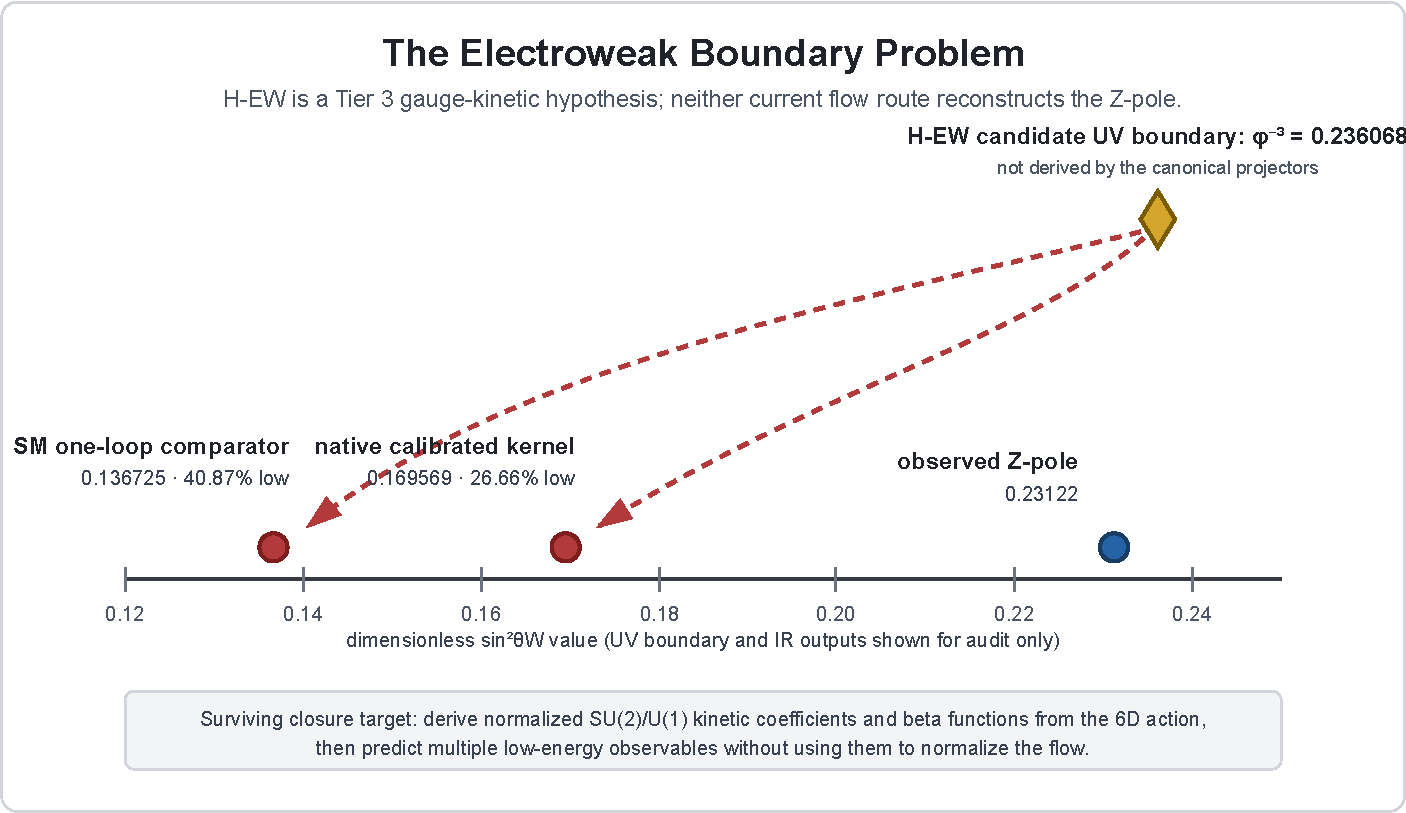
\includegraphics[keepaspectratio,alt={The electroweak boundary problem: the Tier 3 H-EW boundary is separated from the measured Z-pole value, and the two current flow routes miss the endpoint.}]{content/Figures/Volume_3/Figure V3.4.1.pdf}}
\caption{The electroweak boundary problem: the Tier 3 H-EW boundary is
separated from the measured Z-pole value, and the two current flow
routes miss the endpoint.}
\end{figure}

\gctneedspace{5\baselineskip}\begin{gctImportant}

\textbf{Firewall Metadata {[}Weinberg angle{]}}

\begin{itemize}
\tightlist
\item
  \textbf{Canonical projector:} \(1/2 + 1/2\) sector shares; Tier 1
  geometry; not an electroweak-angle prediction.
\item
  \textbf{Raw frame values:} \(\rho_{\rm raw} = \phi^{-2}\) and
  \(V_{\perp,0}/V_{\parallel,0} = \phi^{-3}\); Tier 1 coordinate
  arithmetic; not physical invariants.
\item
  \textbf{Bare angle:} \(\sin^2\theta_W^{\rm bare} = \phi^{-3}\); Tier 3
  gauge-kinetic hypothesis (H-EW); one unresolved physical-map
  assumption.
\item
  \textbf{GUT scale:} \(M_{\rm red}\phi^{-9}\); Tier 3, conditional on
  O.15.
\item
  \textbf{Z-pole audits:} the physical-hypercharge comparator gives
  \(0.136725\) (40.87\% low); the native kernel with the imported A2
  benchmark gives \(0.16957\) (26.66\% low). Both are Tier 3 negative
  consistency results; the pre-registered 2-loop audit (App GRF
  §GRF.4.3) records the running check as \textbf{FAILED} (best
  Standard-Model case −52σ).
\item
  \textbf{Closure:} the target-normalized route is an implementation
  check only; ultraviolet and infrared action-level closure remain open.
\end{itemize}

\end{gctImportant}

\subsubsection{4.3.4 Conditional coupling ratio {[}Tier 1 algebra
conditional on a Tier 3
premise{]}}\label{conditional-coupling-ratio-tier-1-algebra-conditional-on-a-tier-3-premise}

Assuming the Tier 3 boundary hypothesis
\(\sin^2\theta_W^{\rm bare} = \phi^{-3}\), the corresponding ratio of
the weak (\(g\)) and hypercharge (\(g'\)) couplings follows from the
exact identity \textbf{\(\phi^3 - 1 = 2\phi\)}. \emph{Proof:}
\(\phi^3 = \phi \cdot \phi^2 = \phi(\phi+1) = \phi^2 + \phi = (\phi+1) + \phi = 2\phi + 1\).
Thus, \(\phi^3 - 1 = 2\phi\).

The ratio is:
\[\tan^2 \theta_W = \frac{\sin^2 \theta_W}{\cos^2 \theta_W} = \frac{\phi^{-3}}{1 - \phi^{-3}} = \frac{1}{\phi^3 - 1} = \frac{1}{2\phi}\]
\[\frac{g'}{g} = \frac{1}{\sqrt{2\phi}} \implies \frac{g}{g'} = \sqrt{2\phi} \approx 1.79891\]
The algebra is exact, but its physical status inherits the unresolved
Tier 3 gauge-kinetic premise. It does not independently derive the
relative force strengths.

\begin{center}\rule{0.5\linewidth}{0.5pt}\end{center}

\subsection{4.4 Physical
Interpretation}\label{physical-interpretation-3}

\subsubsection{4.4.1 Electromagnetic Field as Rotated W³ +
B}\label{electromagnetic-field-as-rotated-wuxb3-b}

GCT reads the mixing of the pre-mixed gauge fields (\(W^3_\mu\) and
\(B_\mu\)) as a \textbf{Coordinate Transformation} {[}Tier 3
interpretation{]} between the ``Lattice Basis'' (aligned with projection
axes) and the ``Propagation Basis'' (aligned with phason eigenmodes).

\begin{itemize}
\tightlist
\item
  \textbf{The Photon (\(\gamma\)):} The mode that aligns with the
  \textbf{flat direction} of the vacuum potential, remaining massless.
\item
  \textbf{The Z Boson:} The mode that aligns with the \textbf{stiff
  direction} of the lattice dilation, acquiring mass via the Higgs
  mechanism.
\end{itemize}

\subsubsection{\texorpdfstring{4.4.2 \(W^\pm, Z\) masses from the
candidate boundary {[}Tier 3
conditional{]}}{4.4.2 W\^{}\textbackslash pm, Z masses from the candidate boundary {[}Tier 3 conditional{]}}}\label{wpm-z-masses-from-the-candidate-boundary-tier-3-conditional}

At tree level the mass ratio is a consequence of the mixing angle. Under
the Tier 3 candidate boundary:
\[\frac{M_W}{M_Z} = \cos \theta_W = \sqrt{1 - \phi^{-3}} \approx 0.8740\]
The PDG ratio \(M_W/M_Z = 0.88136 \pm 0.00015\) leaves a 0.83\%
residual, about \(49\sigma\) on the direct ratio. This is not a
precision agreement and cannot promote the boundary hypothesis: it is a
conditional tree-level consequence that lacks the required radiative
treatment (Open Problems O.19 and O.5).

\subsubsection{4.4.3 Geometric interpretation {[}Tier 3
conjecture{]}}\label{geometric-interpretation-tier-3-conjecture}

GCT may interpret an eventual gauge-kinetic ratio as a measure of how a
normalized excitation couples to the hypercharge and isospin channels.
The projector calculation alone does not establish that interpretation,
and it does not show that 23.6\% of a fluctuation is geometrically
sequestered in \(E_\perp\). That stronger reading remains conditional on
an action-level derivation of the gauge coefficients.

\begin{center}\rule{0.5\linewidth}{0.5pt}\end{center}

\subsection{4.5 RGE Audit: Three Non-Closing
Routes}\label{rge-audit-three-non-closing-routes}

\gctneedspace{5\baselineskip}\begin{gctImportant}

\textbf{Epistemic status: Tier 3 negative consistency result.}

The exact \(I_h\) irrep inventory is group theory, but its use as a
scale-activation schedule is a Tier 3 ansatz. The native kernel
calibrates three \(Z_i\) factors to the Standard-Model beta
coefficients. The physical-hypercharge comparator and the native kernel
both miss the Z-pole (running check \textbf{FAILED}, App GRF §GRF.4.3),
while the target-normalized route reaches it only because the endpoint
is supplied as an input. None establishes an autonomous boundary or flow
law.

\end{gctImportant}

\emph{{[}Tier 1 Standard-Model RGE algebra and finite group inventory;
Tier 3 GCT boundary, scale, activation and physical-flow inferences ---
computational audits in Appendix GPE and App GRF.{]}}

\subsubsection{4.5.1 Native irrep-activation
ansatz}\label{native-irrep-activation-ansatz}

The native ansatz activates the finite \(I_h\) irreps according to their
dimensions and uses equal canonical projector shares. That supplies a
disclosed candidate curve, not a beta-function derivation. Three
independent normalization factors \(Z_i\) are defined so that the
saturated coefficients equal the three Standard-Model one-loop
coefficients exactly; the \(Z_i\) therefore carry the absolute
coefficient information and the ansatz does not predict it. In its
present step schedule the highest-dimensional irreps activate only at
the ultraviolet endpoint and contribute on a zero-measure interval. The
schedule, the signs of the three beta functions and their coupling to
the gauge sectors all remain Tier 3 model inputs.

The imported benchmark \(\alpha_2^{-1}(M_{\rm GUT}) = 24.0\) is
Parameter Ledger anchor A2, the MSSM unified coupling (§4.3.3). It is
not chosen to reproduce the infrared endpoint, and the kernel does not
transport it successfully: the H-EW boundary gives
\(\sin^2\theta_W(M_Z) \approx 0.16957\), 26.66\% low. The native route
is a failing calibrated ansatz, not a successful interpolation.

\subsubsection{4.5.2 Resolution depth as a candidate mechanism {[}Tier
3{]}}\label{resolution-depth-as-a-candidate-mechanism-tier-3}

GCT proposes that scale dependence may be represented by the depth at
which a probe resolves the 3D quasicrystal and its 6D parent
description:

\begin{itemize}
\item
  \textbf{Low energy} (\(\mu \sim M_Z\), large \(\lambda\)): the probe
  is represented by a coarse-grained 3D quasicrystal description. The
  value \(\sin^2\theta_W(M_Z) = 0.23122\) is an external observational
  comparator and, in conditioned calculations, part of the low-energy
  coupling normalization.
\item
  \textbf{High energy} (\(\mu \sim M_{\rm GUT}\), small \(\lambda\)):
  the probe is represented as resolving more of the 6D parent structure.
  The value \(\phi^{-3}\) is a Tier 3 gauge-kinetic boundary hypothesis,
  not exposed by the canonical projector.
\end{itemize}

A per-axis measure argument cannot connect these regimes: its
\(\phi^{-1}\) linear factor and \(\phi^{-6}\) determinant ratio belong
to a raw, non-isometric frame and change under row rescaling, while the
proper projectors do not. A physical flow must instead be derived from a
normalized scale-dependent effective action. The resolution-depth
picture is thus a candidate mechanism, not a replacement derivation of
the Standard Model beta functions; its physical content begins only when
a coarse-graining map acts on a normalized microscopic action and
predicts more than the endpoints used to define it.

\subsubsection{4.5.3 Target-normalized kernel {[}implementation
check{]}}\label{target-normalized-kernel-implementation-check}

Define the \textbf{resolution depth} \(t = \ln(\mu/M_Z)\), so \(t = 0\)
at the Z-pole and \(t = T_{\rm GUT} = \ln(M_{\rm GUT}/M_Z)\) at the
candidate ultraviolet boundary. A phenomenological lattice-resolution
function interpolates an effective dimension \(D_{\rm eff} \in [3, 6]\):

\[F(t) = 3 + \frac{3}{1 + e^{-(t - T_{GUT}/2)/\sigma}}, \quad \sigma = \frac{T_{GUT}}{2\ln\phi}\]

with the phenomenological phason de-resolution kernel

\[\beta_{geo}(t) = \frac{e^{-t^2/(2\sigma^2)}}{\int_0^{T_{GUT}} e^{-t'^2/(2\sigma^2)} dt'}, \quad \frac{d\sin^2\theta_W}{dt} = +\Delta \cdot \beta_{geo}(t)\]

where \(\Delta\) is fixed by the two declared boundary values

\[\sin^2\theta_W(M_{\rm GUT}) = \phi^{-3}_{\text{(Tier 3 hypothesis)}}, \quad \sin^2\theta_W(M_Z) = 0.23122_{\text{(observed)}}.\]

Because \(\beta_{\rm geo}\) is normalized and \(\Delta\) is solved from
those same endpoints, integrating the equation reaches the endpoint by
construction. A 5,000-step RK4 integration recovers the imposed endpoint
to machine precision, which verifies only the sign, integration
direction and numerical normalization of the kernel. The endpoint
agreement is not empirical support for H-EW, the Gaussian shape or the
resolution-depth interpretation, and the route is excluded from the
prediction ledger.

\subsubsection{4.5.4 What the negative result
establishes}\label{what-the-negative-result-establishes}

The convention-correct one-loop comparator and the native irrep kernel
produce large adverse residuals, so there is no numerical evidence for
H-EW at present. Neither failed flow is derived from the GCT microscopic
action, so the audit does not by itself falsify H-EW at an unspecified
scale.

The pre-registered gauge-running audit (App GRF §GRF.4.3) confirms that
the miss is not a loop-order, threshold, normalisation or comparator
effect: H-EW at \(M_{\rm GUT}\) is incompatible with Standard-Model
running, and with A2 it is incompatible with any SM extension (since
\(b_Y \ge 41/6\) for any content containing the Standard Model, A2 =
24--25 forces
\(\sin^2\theta_W(M_{\rm GUT}) \ge 0.280\)--\(0.288 > \phi^{-3}\)). The
check is recorded as \textbf{FAILED}. Run upward at two loops, the
measured value reaches \(\phi^{-3}\) only at 243 GeV; placing H-EW at
243 GeV would be endpoint fitting. Whether to retire A2 and A4--A6
(\(Z_1\)--\(Z_3\)) is an open v1.4.0 decision; v1.3.0 keeps the counts
(11 declared core inputs; 24 numbered Ledger inputs). The surviving
research content is narrower but testable:

\begin{enumerate}
\def\labelenumi{\arabic{enumi}.}
\tightlist
\item
  derive a normalized 6D gauge action and the relative
  \(SU(2)\)/\(U(1)\) generator traces, thereby deciding H-EW
  independently of the projector frame;
\item
  derive the coarse-graining map, beta functions and threshold matching
  from that action, including the two independent phason elastic
  constants rather than a single scalar surrogate;
\item
  derive or retire the O.15 scale assignment instead of inserting it;
\item
  predict at least two low-energy gauge observables from a common
  ultraviolet state without using either observable to set the flow
  amplitude.
\end{enumerate}

Until those conditions are met, no partial theoretical autonomy is
claimed for the electroweak boundary or endpoint. O.15 supplies the
action/RG bridge; QLQCD-1L (Appendix QLA) and Open Problem O.5 remain
linked non-perturbative closure targets.

\gctneedspace{5\baselineskip}\begin{gctImportant}

\textbf{Firewall Metadata {[}Weinberg Z-pole{]}}

\begin{itemize}
\tightlist
\item
  \textbf{Type:} RGE audit / negative consistency result
\item
  \textbf{Inputs:} Tier 3 \(\phi^{-3}\) boundary hypothesis; Tier 3 O.15
  \(M_{\rm GUT}\) assignment; route-specific use of A2 or of the
  measured low-energy coupling normalization
\item
  \textbf{Physical-hypercharge comparator:} \(0.136725\); 40.87\% low
\item
  \textbf{Native calibrated kernel:} \(0.16957\); 26.66\% low
\item
  \textbf{Target-normalized integrator:} endpoint imposed; no physical
  residual
\item
  \textbf{Pre-registered SM-kernel audit (App GRF §GRF.4.3):} best case
  \(0.0673\) (2-loop, A2 = 25), −52σ; A2 + H-EW no-go for any SM
  extension; running check \textbf{FAILED}
\item
  \textbf{Status:} Tier 3 open boundary; current implementations do not
  close; physical action/RG closure open
\end{itemize}

\end{gctImportant}

\subsection{4.5.5 Extension to the Strong Coupling --- bare handle and
open running
gap}\label{extension-to-the-strong-coupling-bare-handle-and-open-running-gap}

\emph{{[}Tier 3 bare-handle and running branch. \textbf{Headline
disclosure}: the proposed bare handle
\(\alpha_s(\text{bare}) \approx 0.0382\) is not a same-scale prediction
for \(\alpha_s(M_Z)\). Evolving it with the \(Z_3\)-calibrated native
kernel gives \(\alpha_s(M_Z) \approx 0.05204\), about 55.9\% below the
observed \(0.118\). This adverse result is the load-bearing QLQCD-2
research debt (App QLA.7).{]}}

The candidate Geometric RGE framework models running through lattice
resolution depth rather than deriving it from virtual-particle loop
counting. The same proposed principle is applied here to the strong
coupling \(\alpha_s\); the current endpoint audit shows that the
principle is not yet a closed dynamics.

\gctneedspace{5\baselineskip}

\textbf{Tier 3 calibrated handle (10 integer + \(\phi^2\) geometric
factor; closure pending O.42):}

The bare value is written as the product of two geometric numbers; each
number is Tier 1 given P1, while its role in \(\alpha_s\) is a Tier 3
reading:

\[\alpha_s^{-1}(\text{bare}) \;=\; \underbrace{10}_{\text{RT 3-fold axis count}} \;\cdot\; \underbrace{\phi^2}_{H_4\text{ Cartan/root-metric slope factor, squared}} \;\approx\; 26.18.\]

\textbf{Factor 1 --- The integer 10 {[}Tier 1 given P1{]}.} The rhombic
triacontahedron (RT) acceptance window possesses exactly \emph{ten}
three-fold rotational axes, corresponding to the 20 three-fold vertices
of the RT grouped in antipodal pairs (V3 §3.1.2). This count is fixed by
\textbf{Postulate P1} (Parameter Ledger §0.1 --- the icosahedral
cut-and-project ansatz). The axis count is the Tier 1 content used here;
the separate V3 §3.2.1 matrix construction (traceless seeds spanning
five dimensions, an eight-dimensional closure and an \(A_2\)
fingerprint) is not specific to the RT inventory and supports only an
open Tier 3 \(\mathfrak{su}(3)\) candidate, with uniqueness under App
ORQ O.39. The integer 10 is therefore a Tier 1 substrate invariant
\emph{conditional on P1} --- the count follows from the icosahedral
selection, while the icosahedral choice itself is the structural
postulate P1, not a Tier 1 deduction.

\textbf{Factor 2 --- The slope factor \(\phi^2\) {[}Tier 1 number given
P1; Tier 3 role{]}.} The proposal is that the bare \(\alpha_s\) is set
by the \emph{square} of the area-scaling factor on the icosahedral
lattice. By Lemma T-McK.4 (App USS §USS.7.3), the golden factor entering
the projection is exactly
\[\bigl|2\cos(\pi/5)\bigr| = \phi = \tfrac{1}{2}(1+\sqrt{5}),\] forced
by the Lie-algebraic structure of \(E_8\) through the \(H_4\) Cartan
entry \(-\phi\), the golden-ratio root metric, and the cut-and-project
slope (Humphreys, \emph{Reflection Groups and Coxeter Groups}, §3.7).
The Coxeter-element eigenvalues remain roots of unity on the unit
circle; \(\phi\) is not their magnitude. The number
\(\phi^2 \approx 2.618\) is Tier 1 \emph{given} the icosahedral /
\(H_4\) / \(E_8\) ambient choice fixed by Postulate P1. Reading it as
the ``area'' scaling factor that sets the bare \(\alpha_s\) (one factor
of \(\phi\) per linear lattice dimension, two of them spanned by the
3-fold axis pair in \(E_\perp\)) is a Tier 3 heuristic, not a
consequence of the Coxeter structure.

\textbf{Combination --- area-law product {[}Tier 3 calibrated handle
pending O.42{]}.} The combination
\(\alpha_s^{-1}(\text{bare}) = N_{\text{axes}} \cdot \phi^{2}\) is
proposed as an \emph{area-law product}: the bare inverse coupling counts
independent topological sources (the 10 axes) weighted by the
substrate's natural area-scaling factor (\(\phi^2\) from the \(H_4\)
Cartan/root-metric slope). The two factors are separately geometric, but
the strong-sector product is not promoted to Tier 2 closure until the
native strong-running / QLQCD boundary map derives the \(10\phi^2\)
handle from the hadronic action rather than selecting it as the
calibrated bare handle.
\[\alpha_s(\text{bare}) \;=\; \frac{1}{10\phi^2} \;\approx\; 0.0382.\]
This is a proposed ultraviolet handle, so directly comparing it with the
observed \(\alpha_s(M_Z) \approx 0.118\) would mix scales. The relevant
audit evolves the handle from \(M_{\rm GUT}\) to \(M_Z\) with the same
Tier 3 native resolution-depth ansatz used above (Appendix GPE, App GRF
§GRF.4). It returns \(\alpha_s(M_Z) \approx 0.05204\), a \textbf{55.9\%
low} endpoint. Because \(Z_3\) is calibrated to the Standard-Model
one-loop coefficient, this is a calibrated consistency failure, not a
first-principles GCT prediction. QLQCD-2 (App QLA.7) must derive both
the ultraviolet handle and the non-perturbative running. With
Standard-Model β-functions instead, \(\alpha_3^{-1}\) starting from
\(10\phi^2\) reaches zero at \(2\)--\(6\times10^6\) GeV (one to two
loops; App GRF §GRF.4.3), far above \(M_Z\), so \(\alpha_s(M_Z)\) is
undefined (non-perturbative) from the declared handle;
\(10\phi^2 = 26.18\) also sits in the MSSM range, not the Standard-Model
value \(\alpha_3^{-1}(M_{\rm GUT}) = 46.2\).

\textbf{Status:} BARE HANDLE COMPUTED; PHYSICAL BRIDGE OPEN. The
factorisation \(\alpha_s^{-1}(\text{bare}) = 10\phi^2\) uses two
geometric numbers, each Tier 1 \emph{conditional on Postulate P1}, whose
role in \(\alpha_s\) is a Tier 3 reading; their product as a
gauge-kinetic coefficient is a Tier 3 calibrated handle until O.42 /
QLQCD-2 derives it from the hadronic action. The current native running
leaves a 55.9\% endpoint gap.

\textbf{Falsification Condition:} If the full non-perturbative QLQCD-2
corrections to the 10-axis SU(3) boundary condition cannot close the
current 55.9\% endpoint gap to reproduce
\(\alpha_s(M_Z) = 0.1180 \pm 0.0009\) (PDG 2026 QCD review), the
\(10\phi^2\) handle is refuted as the bare strong coupling. The numbers
10 and \(\phi^2\) would remain arithmetic facts given P1; what fails is
their Tier 3 use, individually and in the area-law product, as the
source of \(\alpha_s\).

\chapter{Chapter 5: The Higgs
Mechanism}\label{chapter-5-the-higgs-mechanism}

In standard Quantum Field Theory, the Higgs field is conceptualized as
an external scalar doublet that permeates the vacuum, endowing particles
with mass through spontaneous symmetry breaking. Geometric Consciousness
Theory (GCT) proposes the \textbf{Scalar Breathing Mode} and
\textbf{Transverse Tilt Modes} of the 6-dimensional hyper-lattice as a
candidate mechanical realization of that field. This identification is
Tier 3 physical adoption. The literal \(H_3\)-invariant lattice action
(App ULA §ULA.2) does not derive the Standard-Model Higgs target, the
sign of its quadratic coefficient, a nonzero vacuum radius, or a stable
broken sector; those ingredients remain an added completion. The
specific Higgs normalization and fermion Yukawa normalizations likewise
remain Tier 3 numerical targets pending the registered closure items.

\begin{center}\rule{0.5\linewidth}{0.5pt}\end{center}

\subsection{5.1 The Volume Dilation
Mode}\label{the-volume-dilation-mode}

\subsubsection{5.1.1 The Higgs as Scalar Breathing
Mode}\label{the-higgs-as-scalar-breathing-mode}

As established in Volume 2, the vacuum is a 3D projection of a 6D
Euclidean lattice \(\mathbb{Z}^6\). This lattice possesses various
vibrational and configurational degrees of freedom. While phonon modes
correspond to spatial displacements and phason modes correspond to
topological rearrangements, there exists a fundamental degree of freedom
associated with the unit cell itself: \textbf{Volume Dilation}.

GCT proposes {[}Tier 3 identification{]} that the physical Higgs boson
(\(h\)) is the local fluctuation of the 6D unit cell volume. In the
language of continuum mechanics, the candidate Higgs mode is the
\textbf{Scalar Trace of the 6D Strain Tensor}:
\[h(x) \propto \text{Tr}(\varepsilon_{IJ}) = \sum_{I=1}^6 \frac{\delta a_I}{a_I}\]
where \(a_I\) are the lattice constants of the parent space. This
``Breathing Mode'' represents the global expansion or contraction of the
lattice ``hardware'' at a given spacetime coordinate.

\subsubsection{\texorpdfstring{5.1.2 The \(SU(2)\) Doublet: Volume and
Orientation}{5.1.2 The SU(2) Doublet: Volume and Orientation}}\label{the-su2-doublet-volume-and-orientation}

Standard physics describes the Higgs as a complex doublet with four real
degrees of freedom. In the GCT Operating System, these correspond to the
\textbf{Complete Deformation Space} of the unit cell star:

\begin{enumerate}
\def\labelenumi{\arabic{enumi}.}
\tightlist
\item
  \textbf{The Scalar Trace (1 DOF):} The volume dilation (the physical
  Higgs boson \(h\)).
\item
  \textbf{The Transverse Phason Tilts (3 DOF):} Three rotational degrees
  of freedom representing the tilt of the acceptance window star in
  \(E_\perp\) relative to the physical manifold.
\end{enumerate}

Conditional on adding a continuous doublet/gauge representation and the
standard broken-vacuum completion, the three tilt candidates could map
to the \textbf{longitudinal polarization} modes of the \(W^\pm\) and
\(Z\) gauge fields while the radial ``breath'' maps to the scalar Higgs
particle {[}Tier 3{]}. Finite \(H_3\) symmetry alone supplies neither
continuous Goldstone directions nor this physical identification.

\subsubsection{5.1.3 The Higgs Potential from Lattice
Elasticity}\label{the-higgs-potential-from-lattice-elasticity}

GCT proposes to read the standard ``Mexican Hat'' potential \(V(\Phi)\)
as the \textbf{Non-linear Elastic Energy Density} of the vacuum
substrate, with a symmetric phase (\(T > T_c\), minimum at \(\Phi = 0\))
and a saturation point reached at the Supersolid Phase Transition
(Volume 2, Chapter 3) {[}Tier 3 interpretation{]}. The Mexican-hat form
is nevertheless an \textbf{added broken-vacuum completion}, not a
consequence of the literal \(H_3\)-invariant lattice action: that action
permits both signs of the quadratic coefficient, selects neither a
vacuum radius nor a continuous Higgs-doublet target, and leaves the zero
configuration finite and admissible. To recover the standard sombrero
one must separately supply the doublet/continuous parent representation,
a negative quadratic term, a stabilizing quartic normalization, and the
gauge coupling. The symmetry-breaking consequences below are conditional
on that completion.

\begin{figure}
\centering
\pandocbounded{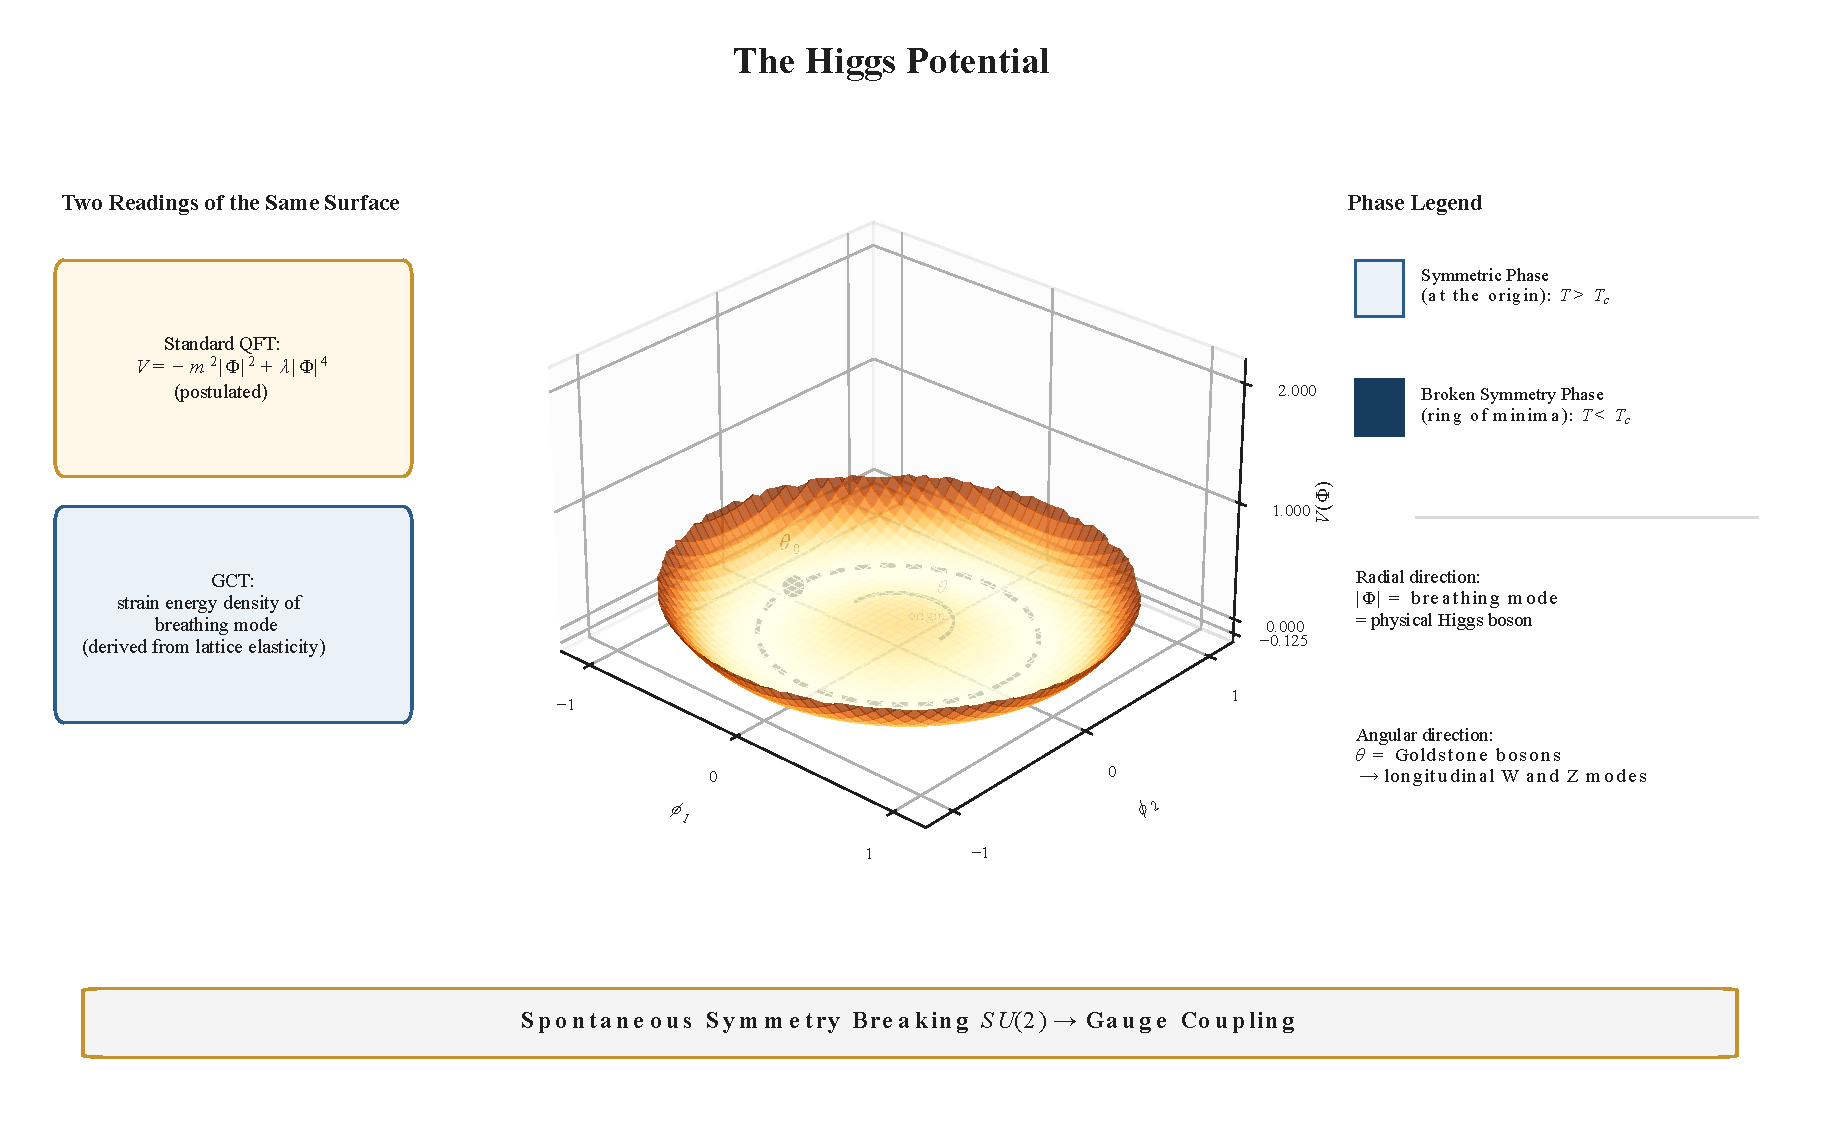
\includegraphics[keepaspectratio,alt={Conditional Higgs completion: once a continuous doublet target and broken-vacuum coefficients are added, the standard Mexican-hat potential supplies the usual symmetric and broken phases. The literal lattice action does not select the sign or vacuum radius, and the zero configuration remains admissible.}]{content/Figures/Volume_3/Figure V3.5.1.pdf}}
\caption{Conditional Higgs completion: once a continuous doublet target
and broken-vacuum coefficients are added, the standard Mexican-hat
potential supplies the usual symmetric and broken phases. The literal
lattice action does not select the sign or vacuum radius, and the zero
configuration remains admissible.}
\end{figure}

\begin{center}\rule{0.5\linewidth}{0.5pt}\end{center}

\subsection{5.2 The Stiffness
Connection}\label{the-stiffness-connection}

\subsection{5.2.1 The Macroscopic Saturation (Absolute VEV Pipeline)
{[}OPEN-CONDITIONAL: Tier 2 mechanics conditional on Tier 3
O.38{]}}\label{the-macroscopic-saturation-absolute-vev-pipeline-open-conditional-tier-2-mechanics-conditional-on-tier-3-o.38}

\gctneedspace{5\baselineskip}\begin{gctImportant}

\textbf{Dependency-direction disambiguation.} The Standard Model's
dependency chain is \(v \to \{m_e, m_\mu, m_\tau, \ldots\}\) via Yukawa
couplings: the VEV is a fundamental input, lepton masses are downstream.
GCT instead evaluates \(v=m_\mu\cdot1440\cdot\phi\) within its shared
icosahedral architecture. The product arithmetic and \(C_3\) axis count
are exact, but the absolute result inherits the Tier 3 O.38 cage posit
\(N_{\rm cage}=144\), the muon formula, A3, and the other disclosed
handles. O.20 supplies a factor catalogue only; it does not select
\(N_{\rm cage}\) or establish a physical saturation mechanism.

\end{gctImportant}

GCT explores a \textbf{dependency-inverted candidate relation}
\(M_{Planck} \to m_e \to m_\mu \to v\), in which the VEV is modeled as
the macroscopic volumetric saturation of the vacuum's localized acoustic
defects. The current theory has not derived that chain from one action:
the electron link, the muon integer and corrections, the \(N=144\) cage
adoption, and the \(1440\) scale rule retain separate Tier 3/4
commitments. It must therefore be read as a postdictive scale ansatz,
not as a correction of the Standard Model's causal bookkeeping (and not
as a chain in which \(m_\mu\) is fundamental upstream of \(v\) in the
SM-causal sense).

Conditional on the Tier 3 O.38 input \(N_{\rm cage}=144\), the
registered scale evaluation multiplies the A3-corrected muon resonance
by the exact count of 10 three-fold axes and by \(\phi\):
\[v = m_\mu \times (144 \times 10) \times \phi = m_\mu \times 1440 \times \phi \approx \mathbf{246.18 \text{ GeV}}\]

Evaluated against the sole declared PDG-2024 Fermi-constant anchor
(\(v=246.21965\) GeV), this conditional result has a \textbf{179 ppm}
residual. Its disposition is OPEN-CONDITIONAL: Tier 2 mechanism/product
arithmetic conditional on the Tier 3 O.38 cage posit, plus the inherited
Tier 3 muon/CODATA-2022-A3/integer-handle dependencies. The
spectral-action route of §5.2.5 is a separate, not yet computed closure
target and is not an input to the VEV verifier.

As evidence that φ or icosahedral structure is special, this match is
\textbf{Tier 4}: the preregistered constant control test (v3,
NEGATIVE-FRAGILE; App PSC §PSC.9.6) found φ's pattern of matches on 21
constants not distinguishable from that of random constants (58 of 300
random bases did at least as well). The test ``excludes, at power ≥ 0.8,
an effect in which φ hits at least 6 of the 8 informative rows through a
real effect; weaker effects are not excluded.'' The 179 ppm figure is
kept as descriptive arithmetic.

\gctneedspace{5\baselineskip}

\textbf{Registered 1440 product {[}Tier 2 conditional arithmetic + Tier
3 O.38 cage input{]}}

The integer \(1440 = 144 \times 10\) is structurally motivated by two
independent icosahedral invariants:

\begin{itemize}
\tightlist
\item
  \textbf{\(N_{cage} = 144\):} The electron cage node count is adopted
  as a Tier 3 structural posit. Discrete Gauss--Bonnet closes exactly on
  the icosahedron, \(12(\pi/3)=4\pi\), and its dodecahedral dual,
  \(20(\pi/5)=4\pi\); this checks the boundary geometry but does not
  derive \(144\). The separate exact identity \(144=F_{12}=12^2\)
  supports the adopted two-shell ansatz. Whether it is the ground-state
  cage requires the O.38 full-lattice minimisation, which is not carried
  out here.
\item
  \textbf{\(N_{C_3} = 10\):} The icosahedral group \(I_h\) has exactly
  10 three-fold rotation axes (\(C_3\) axes). This is an exact
  group-theory result: \(I_h\) contains precisely 20 elements in its
  \(C_3\) conjugacy class, and each axis contributes two elements
  (\(C_3\) and \(C_3^2\)), giving \(N_{C_3} = 20/2 = 10\). This is not a
  choice --- it is a theorem about the character table of \(I_h\).
\item
  \textbf{\(\phi\):} The golden-ratio inflation factor of the adopted
  icosahedral quasicrystal tiling; its use as the volumetric factor in
  this product is part of the registered scale rule, not a separate
  derivation.
\end{itemize}

Under the adopted cage branch, the product covers 144 nodes across the
10 distinct three-fold axes, producing the conditional factor
\(1440\times\phi\).

\begin{quote}
\textbf{Scope of the structural claim.} The identity
\(144\times10=1440\) is exact once the Tier 3 O.38 input
\(N_{\rm cage}=144\) is supplied. The exact \(C_3\) axis count does not
promote the absolute scale. O.20 enumerates 18 factor pairs, including
three other products whose factors occur in the declared dictionary;
these are arithmetic alternatives, not evidence for physical selection.
The VEV branch remains conditional on O.38 and the upstream lepton/A3
closures.
\end{quote}

\subsection{5.2.2 The Breathing Mode and the Geometric Origin of the
VEV}\label{the-breathing-mode-and-the-geometric-origin-of-the-vev}

The 6D bulk modulus, while structurally related to the Higgs potential
curvature, does not yield a rational exponent in the cut-and-project
scheme. The registered VEV route evaluates \(v=m_\mu\times1440\phi\) on
the adopted \(N=144\) cage branch across the 10 \(C_3\) axes. This is a
conditional scale evaluation, not a derivation of the cage size or a
closed physical saturation theorem.

\subsubsection{\texorpdfstring{5.2.3 The Bulk Modulus and the
\(\lambda = 1/8\) Ansatz {[}Tier 3 bare completion + Tier 3 physical
\(m_H\) pending 1-loop
closure{]}}{5.2.3 The Bulk Modulus and the \textbackslash lambda = 1/8 Ansatz {[}Tier 3 bare completion + Tier 3 physical m\_H pending 1-loop closure{]}}}\label{the-bulk-modulus-and-the-lambda-18-ansatz-tier-3-bare-completion-tier-3-physical-m_h-pending-1-loop-closure}

The curvature of the Higgs potential at its minimum determines the
\textbf{Bulk Modulus (\(K\))} of the metric---its resistance to being
curved by mass. \textbf{Potential convention:} this chapter uses the
Standard-Model normalization
\(V(\Phi) = \lambda\left(\Phi^\dagger\Phi - v^2/2\right)^2\) with
\(\langle\Phi^\dagger\Phi\rangle = v^2/2\) and the radial fluctuation
\(h\) defined by \(\Phi = (0,\,(v+h)/\sqrt{2})^{T}\). Then
\[K = \frac{\partial^2 V}{\partial h^2} \bigg|_{h=0} = 2 \lambda v^2 = m_H^2 .\]
(Writing the same quartic as \(\lambda(\varphi^2 - v^2)^2\) for a real
field with vacuum \(\varphi = v\) would give \(8\lambda v^2\) instead,
and \(\lambda = 1/8\) would then give \(m_H = v\); that convention is
not the one used here.) GCT registers the quartic coupling
\(\lambda = 1/8\) as a separate bare packing ansatz {[}Tier 3{]}. No
geometric quantity is currently known to fix it: the earlier motivation
from the ratio of the inscribed sphere to the rhombic triacontahedron
volume is withdrawn, because that ratio is \(\approx 0.887\), not
\(1/8\). The scale at which \(\lambda = 1/8\) applies is also not
derived; numerically it lies close to the Standard-Model
\(\overline{\rm MS}\) value \(\lambda(\mu \approx m_t) \approx 0.126\),
not to the near-zero value the Standard Model runs to at
\(M_{\rm GUT}\), and that proximity is what makes the bare gap below
look small. The literal \(H_3\)-invariant lattice action does not select
this normalization, the quadratic sign, or a vacuum radius.

\textbf{Bare conditional relation {[}Tier 3{]}:} With the added
broken-vacuum completion and \(\lambda_{\text{bare}} = 1/8 = 0.125\),
the adopted normalization implies the bare mass relation
\(m_H^{\text{bare}} = \sqrt{2\lambda_{\text{bare}}}\,v = v/2\). With the
measured \(v \approx 246.22\) GeV, this gives
\(m_H^{\text{bare}} \approx 123.11\) GeV (with the GCT value
\(v \approx 246.18\) GeV of §5.2.1 it gives \(123.09\) GeV; the
difference does not affect the discussion below). A positive Hessian at
that selected minimum would establish only local curvature; stiffness
alone does not prove an exact topological sector, metastability, or
particle identity.

\textbf{Physical mass prediction {[}Tier 3 pending App TPR §TP-E 1-loop
closure{]}:} The observed Higgs mass is
\(m_H^{\text{PDG}} = 125.20 \pm 0.11\) GeV (PDG 2024 weighted average).
The bare-to-physical gap is \(+2.09\) GeV (\(+1.67\% \approx 16{,}700\)
ppm). This gap sits in the expected sign and rough magnitude band of
standard-model 1-loop top-Yukawa and EW radiative corrections, but a
\emph{quantitative} GCT 1-loop closure that reproduces this gap from
icosahedral lattice dynamics has not been completed. The 1-loop closure
is \textbf{Open Problem (App TPR §TP-E, bundled with QLQCD-1L research
debt O.5)}: the bare \(m_H = v/2\) relation is a Tier 3 packing ansatz,
and the physical-mass target of \(125.20\) GeV remains Tier 3 contingent
on TP-E. Promotion of the physical prediction to Tier 2 would require a
selected Higgs target and broken-vacuum coefficients from the AKN action
and (a) explicit derivation of the 1-loop correction sign and magnitude
from the AKN action, and (b) demonstration that the sum bare + 1-loop
reproduces the PDG value within \textasciitilde100 ppm.

\subsubsection{\texorpdfstring{5.2.4 Speculative Conjecture 5.1 {[}Tier
4{]}: \(c \propto v\) Hypothesis Pending \(K(v), \rho(v)\)
Derivation}{5.2.4 Speculative Conjecture 5.1 {[}Tier 4{]}: c \textbackslash propto v Hypothesis Pending K(v), \textbackslash rho(v) Derivation}}\label{speculative-conjecture-5.1-tier-4-c-propto-v-hypothesis-pending-kv-rhov-derivation}

\textbf{Speculative Conjecture 5.1:} \emph{The propagation speed of
information (the speed of light \(c\)) is proportional to the Higgs VEV
once the phason stiffness \(K(v)\) and effective density \(\rho(v)\) are
derived from the same elastic substrate. In the symmetric limit
(\(v=0\)), the conjecture predicts that the Maxwell/phason propagation
channel is not defined as a stable wave mode.}

\gctneedspace{5\baselineskip}

\textbf{Status:} Since \(c^2 \propto K_\perp / \rho\), the
proportionality \(c \propto v\) requires a lattice-elastic derivation of
both \(K(v)\) and \(\rho(v)\) with the correct scaling. That derivation
is not supplied here. The statement is therefore a Tier 4 speculative
conjecture rather than a theorem, and it cannot be used as a closed
solution to the horizon problem until the elastic scaling is derived.

\subsubsection{5.2.5 The Connes Spectral Action {[}Tier 3 closure
target; not
computed{]}}\label{the-connes-spectral-action-tier-3-closure-target-not-computed}

No engine protocol currently computes the Seeley--DeWitt coefficients
\(a_2\), \(a_4\), a Higgs mass or a spectral-action cutoff on the AKN
cage. The spectral-action protocol
(\texttt{protocol\_spectral\_action.py}) uses the canonical 152-node
\(I_h\)-closed cage of V3 Ch06 §6.5.2 and computes only the
spectral-action beta-function curve and raw spectral moments. Earlier
figures for a negative quadratic coefficient on a 144-node graph, a
native mass \(m_h \approx 0.01\) GeV and a fine-tuned cutoff
\(\Lambda \approx 12558\) are withdrawn: no engine protocol produces
them.

The Connes spectral-action route to the Higgs sector and the absolute
scale \(v \approx 246\) GeV therefore remains a \textbf{Tier 3 closure
target} (V3 Ch06 §6.5.2), pending the Seeley--DeWitt implementation,
O.32 and full non-linear phason dressing. The registered §5.2.1 route is
the primary conditional evaluation: \(v=m_\mu\times1440\times\phi\)
inherits the Tier 3 O.38 cage posit, the muon formula, A3, and the other
disclosed handles. \emph{(Computational verification: see Appendix
GPE.)}

\begin{center}\rule{0.5\linewidth}{0.5pt}\end{center}

\subsection{5.3 Fermion Yukawa
Couplings}\label{fermion-yukawa-couplings}

\subsubsection{5.3.1 Geometric Frustration
Energy}\label{geometric-frustration-energy}

In the Standard Model, fermion masses are determined by arbitrary Yukawa
couplings \(y_f\). GCT proposes \textbf{Geometric Frustration Energy} as
a candidate interpretation: \(y_f\) would measure the mechanical work
required to displace the completed Higgs field from its equilibrium VEV
to accommodate a candidate topological defect. Neither the physical
defect nor the Yukawa map is derived by the literal action; both remain
Tier 3, as do the specific Yukawa normalizations until the corresponding
integer and loop-correction closures are completed.

\subsubsection{5.3.2 The Top Quark as the Universal Yield Strength
{[}Tier 3 top-mass ansatz; V3 Ch10 Ansatz
10.1{]}}\label{the-top-quark-as-the-universal-yield-strength-tier-3-top-mass-ansatz-v3-ch10-ansatz-10.1}

The Top Quark mass (\(m_t \approx 173\) GeV) yields a Yukawa coupling
\(y_t \approx 1\). GCT identifies the Top Quark as the \textbf{Lattice
Fracture Limit}. It represents the energy required to dilate a unit cell
by its own volume (\(100\%\) strain). Under this ansatz, no elementary
fermion can be significantly heavier than the VEV because the lattice
bonds would fracture (Lattice Yield Strength) before such a defect could
be stabilized.

\begin{center}\rule{0.5\linewidth}{0.5pt}\end{center}

\subsection{5.4 Physical
Interpretation}\label{physical-interpretation-4}

\subsubsection{5.4.1 Higgs as the Pressure
Regulator}\label{higgs-as-the-pressure-regulator}

GCT proposes the completed Higgs sector as a possible bridge between
\textbf{Topology} (the candidate knots of matter) and \textbf{Metric}
(the screen of space) {[}Tier 3{]}. Uniqueness, physical defect
identity, and the bridge itself are not yet derived.

\subsubsection{5.4.2 The VEV as a Self-Organized Critical
Point}\label{the-vev-as-a-self-organized-critical-point}

\textbf{Tier 4 interpretation:} the electroweak scale of \(246\) GeV may
be read as a \textbf{Self-Organized Critical Point}, an operating point
in the broader GCT narrative (a lower \(v\) read as too fluid for stable
memory, Axiom 2; a higher \(v\) as too much topological friction for
Agency). Claims about stable memory, Agency, or an optimal operating
pressure for a conscious simulation do not follow from the Higgs
calculation and are not used as physics evidence.

\chapter{Chapter 6: The Product
Structure}\label{chapter-6-the-product-structure}

In the standard paradigm of particle physics, the gauge group of the
universe, \(\mathrm{SU}(3) \times \mathrm{SU}(2) \times \mathrm{U}(1)\),
is an empirical discovery---a specific symmetry structure selected from
a near-infinite menu of mathematical possibilities because it fits the
observed interactions of subatomic particles. Geometric Consciousness
Theory (GCT) identifies this product structure as the icosahedral
projection's registered gauge-structure candidate rather than an
arbitrary fit. This chapter presents a candidate synthesis of why the
forces may be partitioned into these specific groups and remain
fundamentally independent. The synthesis is conditional on structural
postulate P1, the icosahedral selection, which is itself conditional
(App USS §USS.6.3), and its \(\mathrm{SU}(3)\) component is an open Tier
3 candidate because the eight-dimensional closure of V3 Ch03 is not
specific to the RT window; theorem-grade uniqueness over the full
Cartan-Killing classification remains Open Problem O.39.

\begin{center}\rule{0.5\linewidth}{0.5pt}\end{center}

\subsection{6.1 Geometric Origins
(Summary)}\label{geometric-origins-summary}

GCT proposes {[}Tier 3{]} that the ``Force'' sector arises from a
fiber-bundle decomposition of the 6-dimensional parent lattice, and
assigns each component of the Standard Model gauge group to a candidate
geometric degree of freedom within the icosahedral projection. The
assignments below are candidate placements, not derived consequences of
the lattice action.

\subsubsection{\texorpdfstring{6.1.1 SU(3): Three-Fold Axes in
\(E_\perp\)}{6.1.1 SU(3): Three-Fold Axes in E\_\textbackslash perp}}\label{su3-three-fold-axes-in-e_perp}

GCT proposes that the strong interaction arises from the
\textbf{Internal Manifold} (\(E_\perp\)). Chapter 3 builds, from the 10
three-fold rotational axes of the acceptance window, an
eight-dimensional matrix closure with the \(A_2\) fingerprint of
\(\mathfrak{su}(3)\); because generic ten-axis sets close the same way,
its identification with physical color is an open Tier 3 candidate. In
that candidate, color is the orientation of an interstitial face-defect
within the internal dimensions.

\subsubsection{\texorpdfstring{6.1.2 SU(2): Spatial Double Cover in
\(E_\parallel\) vs.~Internal Weak
Bundle}{6.1.2 SU(2): Spatial Double Cover in E\_\textbackslash parallel vs.~Internal Weak Bundle}}\label{su2-spatial-double-cover-in-e_parallel-vs.-internal-weak-bundle}

Chapter 2 separates two roles of \(SU(2)\). The spatial double cover
\(\operatorname{Spin}(3)\cong SU(2)\) of rotations in the
\textbf{Physical Manifold} (\(E_\parallel\)) is a Tier 1 control:
spinorial matter transforms under it. Weak isospin is a distinct
internal gauge symmetry; GCT proposes that it is realized by an internal
icosahedral-frame (\(2I\)) bundle with a chiral connection {[}Tier 2
structural candidate; Tier 3 physical realization{]}, and the spatial
lift does not by itself supply it (V3 Ch02 §2.1--§2.2). This volume
places that candidate weak bundle on the internal (\(E_\perp\)) side, as
V3 Ch02 §2.1.1 and V3 Ch10 §10.3.3 do; the placement is a Tier 3
assignment, and it is the one used in the table below and in §6.2. The
weak factor is therefore not the orientation of a defect within the
physical ``screen'' dimensions.

\subsubsection{6.1.3 U(1): Global Phase of
Condensate}\label{u1-global-phase-of-condensate}

In the gauge-fixed sketch used by Chapter 1 (V2 Ch06 §6.1, declared open
programme), electromagnetism is modeled by a \(U(1)\) gauge potential
whose scalar part is the condensate phase \(\theta\) and whose
transverse vector part is the phason displacement. The photon is
identified with the transverse, gauge-protected phason mode, not with
the scalar phase mode (V3 Ch01 §1.1.4, §1.4.1) {[}Tier 3
identification{]}. Reading this potential as a Berry connection requires
the separately derived gapped eigenbundle of V3 Ch01 Theorem 1.1 {[}Tier
1 conditional mathematics; Tier 3 physical bundle{]}. Photon
masslessness in this gauge-fixed Maxwell action follows from the
unbroken \(U(1)\) gauge symmetry of the Lagrangian; the alternative
Anderson-Higgs scenario for broken gauged \(U(1)\) is not realised here.

\gctneedbreak{20\baselineskip}

\subsubsection{6.1.4 Summary Table of
Mechanisms}\label{summary-table-of-mechanisms}

\gctneedbreak{10\baselineskip}

{\def\LTcaptype{none} % do not increment counter
\begin{longtable}[]{@{}
  >{\raggedright\arraybackslash}p{(\linewidth - 6\tabcolsep) * \real{0.2500}}
  >{\raggedright\arraybackslash}p{(\linewidth - 6\tabcolsep) * \real{0.2500}}
  >{\raggedright\arraybackslash}p{(\linewidth - 6\tabcolsep) * \real{0.2500}}
  >{\raggedright\arraybackslash}p{(\linewidth - 6\tabcolsep) * \real{0.2500}}@{}}
\toprule\noalign{}
\begin{minipage}[b]{\linewidth}\raggedright
\textbf{Interaction}
\end{minipage} & \begin{minipage}[b]{\linewidth}\raggedright
\textbf{Gauge Group}
\end{minipage} & \begin{minipage}[b]{\linewidth}\raggedright
\textbf{Geometric Domain}
\end{minipage} & \begin{minipage}[b]{\linewidth}\raggedright
\textbf{Lattice Mechanism}
\end{minipage} \\
\midrule\noalign{}
\endhead
\bottomrule\noalign{}
\endlastfoot
\textbf{Strong} & \(SU(3)\) (open Tier 3 candidate) & Perpendicular
Space (\(E_\perp\)) & Winding around 3-fold axes of the RT Window \\
\textbf{Weak} & \(SU(2)_L\) & Internal side (\(E_\perp\)): candidate
\(2I\)-frame bundle (Tier 3 placement, §6.1.2) & Candidate chiral
internal-frame (\(2I\)) connection; not supplied by the spinorial double
cover of physical rotations \\
\textbf{Electromagnetic} & \(U(1)\) & Condensate phase (\(\theta\)) +
transverse phason sector & Gauge-fixed \(U(1)\) potential (scalar part
\(\theta\), transverse phason vector part); Berry-connection reading
conditional on V3 Ch01 Theorem 1.1 \\
\end{longtable}
}

\begin{center}\rule{0.5\linewidth}{0.5pt}\end{center}

\subsection{6.2 Orthogonality of Interaction
Sectors}\label{orthogonality-of-interaction-sectors}

\subsubsection{6.2.1 Theorem 6.1 {[}Tier 1 mathematics; Tier 3
application{]}: Sector
Independence}\label{theorem-6.1-tier-1-mathematics-tier-3-application-sector-independence}

\textbf{Theorem 6.1 (mathematical statement) {[}Tier 1{]}:} \emph{Let
Lie algebras of transformations act on mutually independent factors of a
configuration space (for example on orthogonal subspaces of
\(\mathbb{R}^6\), on distinct tensor factors of a fiber, or on a scalar
phase), each acting trivially on the other factors. Then generators
belonging to different factors commute, and the joint algebra is their
direct sum. This fixes only the local Lie-algebra structure: the global
gauge group may still carry a discrete-center quotient, as in the
Standard Model form \([SU(3)\times SU(2)\times U(1)]/\mathbb{Z}_6\),
which the commuting-generator calculation does not fix.}

\textbf{Application {[}Tier 3, conditional on the sector placement{]}.}
In this volume's bookkeeping the color candidate acts on the
three-fold-axis orientation of the RT window in \(E_\perp\) (an open
Tier 3 candidate, V3 Ch03), the weak candidate acts on the internal
\(2I\)-frame bundle that is also placed on the \(E_\perp\) side (Tier 3
placement, §6.1.2; V3 Ch02 §2.1.1), and the electromagnetic \(U(1)\)
acts on the condensate phase \(\theta\). Theorem 6.1 then gives two
commutation results: spatial-frame rotations in \(E_\parallel\) commute
with every transformation acting only on \(E_\perp\), and all of these
commute with the scalar phase rotation. It does \textbf{not} give the
commutation of the weak and color generators. Both are placed on the
internal side, so the orthogonality of \(E_\parallel\) and \(E_\perp\)
does not separate them. The commutation of the weak and color generators
is then an assumption of the Tier 3 placement (that the \(2I\) frame and
the three-fold-axis orientation are independent factors of the internal
fiber), not a consequence of Theorem 6.1.

\subsubsection{6.2.2 Proof: The Dimensional Sum
Rule}\label{proof-the-dimensional-sum-rule}

The proof uses the dimensional decomposition of the parent space
(\(3+3=6\)) and the scalar character of the phase.

\begin{enumerate}
\def\labelenumi{\arabic{enumi}.}
\tightlist
\item
  \textbf{Independent factors commute:} If \(X\) acts on factor \(A\) as
  \(X\otimes\mathbf{1}\) and \(Y\) acts on factor \(B\) as
  \(\mathbf{1}\otimes Y\), then
  \([X\otimes\mathbf{1},\,\mathbf{1}\otimes Y]=0\). The physical and
  internal manifolds are orthogonal subspaces of \(\mathbb{R}^6\), so
  they supply such a factorization (\(E_\parallel \perp E_\perp\)): a
  rotation of a defect's Burgers vector in \(E_\perp\) leaves its
  orientation in \(E_\parallel\) invariant, and conversely. Under the
  §6.1.2 placement this separates spatial rotations from the internal
  (color and weak) transformations, but not color from weak.
\item
  \textbf{Phase Independence:} The superfluid phase \(\theta\) is a
  scalar field. Geometric rotations of the frame (either internal or
  physical) commute with the global \(U(1)\) phase rotation.
\end{enumerate}

Because these operations act on independent degrees of freedom, the
commutators between generators of the separated factors vanish. This
proves local independence at the Lie-algebra level for those factors.
The remaining relation \([T_{SU(3)}, T_{SU(2)}] = 0\) holds only under
the Tier 3 assumption, stated in §6.2.1, that color and weak act on
independent factors of the internal fiber. Neither step rules out a
finite shared-center quotient in the global gauge group; that
global-topology question is carried separately.

\subsubsection{6.2.3 Symmetry vs.~Interaction: The Higgs
Bridge}\label{symmetry-vs.-interaction-the-higgs-bridge}

At the Lie-algebra/local-sector level the symmetry actions are taken to
be product-separated (by the \(E_\parallel \perp E_\perp\)
orthogonality, and between weak and color by the Tier 3 internal-factor
assumption of §6.2.1), while the physical excitations couple through the
\textbf{shared vacuum condensate \(\Psi\)} and the \textbf{Higgs
dilation mode}. Forces interact not because their local generators mix,
but because they all modulate the same Higgs-tensioned 6D substrate; any
discrete-center quotient in the global gauge group remains a separate
global-identification question.

\subsubsection{6.2.4 Bond-Strength
Universality}\label{bond-strength-universality}

If the groups are orthogonal, could their coupling constants still be
related? GCT proposes that they are, because they all sample the same
\textbf{6D lattice bonds}. Every interaction ultimately deforms the same
6D unit cells. GCT proposes that the ratios between the couplings are
the geometric factors of how that universal bond-strength projects into
different subspaces; the candidate value \(g/g' = \sqrt{2\phi}\) is
conditional on the Tier 3 hypothesis H-EW (V3 Ch04 §4.3.4).

\subsubsection{6.2.5 The Projection Principle: Proton Stability {[}Tier
3 proposal, conditional on the Tier 3 vertex/face defect assignment of
V3 Ch03
§3.4{]}}\label{the-projection-principle-proton-stability-tier-3-proposal-conditional-on-the-tier-3-vertexface-defect-assignment-of-v3-ch03-3.4}

GCT proposes that the stability of the proton reflects discrete defect
topology.

\begin{itemize}
\tightlist
\item
  \textbf{Vertex-Index:} Leptons are vertex defects referred to the
  5-fold axes (V3 Ch03 §3.4.1).
\item
  \textbf{Face-Index:} Quarks are face defects on the 30 rhombic faces
  of the RT acceptance window (V3 Ch03 §3.4.2). The two labels are
  discrete, so no continuous path in the displayed defect-index space
  connects a vertex-defect to a face-defect. That restates the
  assignment; it does not establish a conservation law in the full
  configuration space. The Standard Model, which GCT aims to reproduce,
  violates \(B+L\) non-perturbatively through electroweak sphaleron and
  instanton transitions (\(\Delta B = \Delta L = 3\) per transition,
  conserving \(B-L\)), a consequence of the same chiral anomaly
  structure audited in §6.3. An absolute quark/lepton separation would
  therefore contradict that sector. GCT does not yet state what its
  defect topology implies for sphaleron-mediated \(B+L\) violation, so
  proton stability is a Tier 3 proposal and absolute stability over the
  full quantum configuration space remains open.
\end{itemize}

\begin{center}\rule{0.5\linewidth}{0.5pt}\end{center}

\subsection{\texorpdfstring{6.3 Anomaly Cancellation Audit {[}Tier 1
textbook identity (SM hypercharges given) + Tier 2 \(Y_R = 2Q\)
assignment given the charges + Tier 3 defect-topology-to-charge
mapping{]}}{6.3 Anomaly Cancellation Audit {[}Tier 1 textbook identity (SM hypercharges given) + Tier 2 Y\_R = 2Q assignment given the charges + Tier 3 defect-topology-to-charge mapping{]}}}\label{anomaly-cancellation-audit-tier-1-textbook-identity-sm-hypercharges-given-tier-2-y_r-2q-assignment-given-the-charges-tier-3-defect-topology-to-charge-mapping}

The Adler--Bell--Jackiw triangular anomaly conditions must be satisfied
by any consistent chiral gauge theory. GCT does not posit anomaly
freedom as a constraint; it audits the geometric hypercharge assignments
against the four perturbative anomaly conditions involving \(U(1)_Y\)
(the \(SU(3)^3\) anomaly and the global Witten \(SU(2)\) anomaly also
vanish for this spectrum: the colour content is vector-like and each
generation has four \(SU(2)\) doublets, an even number) using the
explicit one-generation spectrum assigned by the RT window mapping (its
\(SU(3)\) triplet and singlet entries are Tier 3 candidates, V3 Ch03
§3.4).

\textbf{Geometric hypercharge assignments (one generation).} The
defect-topology mapping (V3 Ch01 §1.3.2--§1.3.3 charge normalization, V3
Ch04 Theorem 4.2, App USS) assigns hypercharges in the standard
Standard-Model L/R-asymmetric form (the Y-asymmetry between left- and
right-handed components is required for chiral Standard-Model matter
content; GCT attributes the asymmetry upstream to the icosahedral
chirality of the projection rather than imposing it by hand):

\gctneedbreak{10\baselineskip}

{\def\LTcaptype{none} % do not increment counter
\begin{longtable}[]{@{}lllll@{}}
\toprule\noalign{}
Field & \(SU(3)\) & \(SU(2)\) & \(Y\) & \(Q = T_3 + Y/2\) \\
\midrule\noalign{}
\endhead
\bottomrule\noalign{}
\endlastfoot
\(Q_L = (u_L, d_L)\) & 3 & 2 & \(+1/3\) & \(+2/3,\, -1/3\) \\
\(u_R\) & 3 & 1 & \(+4/3\) & \(+2/3\) \\
\(d_R\) & 3 & 1 & \(-2/3\) & \(-1/3\) \\
\(L_L = (\nu_L, e_L)\) & 1 & 2 & \(-1\) & \(0,\, -1\) \\
\(e_R\) & 1 & 1 & \(-2\) & \(-1\) \\
\(\nu_R\) & 1 & 1 & \(\phantom{+}0\) & \(0\) \\
\end{longtable}
}

The mapping from defect topology to these specific hypercharges is the
load-bearing GCT claim: face-defects → quark-like (the face centres lie
on the 15 two-fold axes, not on three-fold axes; referring a face
defect's orientation to the 3-fold axes is the open Tier 3 assignment of
V3 Ch03 §3.4.2), vertex-defects (5-fold symmetry axis) → lepton-like,
with \(L/R\) chirality assigned by which side of the Jackiw-Rebbi domain
wall the defect sits on (V3 Ch02 §2.4.2--§2.4.3 + App USS) {[}Tier 3
assignment{]}.

\textbf{Engine audit.} With these assignments, the four standard
triangular anomaly coefficients vanish to machine precision under the
explicit sum over left-handed chirality conventions (\(Q_L\), \(L_L\)
contribute with \(+1\); \(u_R^c\), \(d_R^c\), \(e_R^c\), \(\nu_R^c\)
contribute with \(-1\)):

\[
\mathcal{A}_{U(1)_{\rm grav}} = \sum_f \chi_f\, Y_f \cdot \dim_{SU(3)}\!\cdot\, \dim_{SU(2)} = 0,
\] \[
\mathcal{A}_{SU(2)^2 U(1)} = \sum_{f:\,\dim_{SU(2)}=2} \chi_f\, Y_f \cdot \dim_{SU(3)} = 0,
\] \[
\mathcal{A}_{SU(3)^2 U(1)} = \sum_{f:\,\dim_{SU(3)}=3} \chi_f\, Y_f \cdot \dim_{SU(2)} = 0,
\] \[
\mathcal{A}_{U(1)^3} = \sum_f \chi_f\, Y_f^3 \cdot \dim_{SU(3)}\!\cdot\, \dim_{SU(2)} = 0,
\]

with \(\chi_f \in \{+1, -1\}\) the chirality sign. Engine verification:
\texttt{GCT\_Physics\_Engine/src/protocol\_anomaly\_check.py} evaluates
each coefficient on the table above and confirms all four vanish exactly
(machine precision, tolerance \(10^{-12}\)).

This section is \emph{not} a free-standing anomaly-freedom proof. Its
Tier 2 content is the right-handed assignment \(Y_R = 2Q\) given the
electric charges (V3 Ch04 Theorem 4.2). The charges themselves rest on
the Tier 3 \textbf{defect-topology-to-charge mapping}: the fractional
\(1/3\) unit is Proposal 1.2 (V3 Ch01 §1.3.2) and the face-defect quark
assignment is a Tier 3 candidate (V3 Ch03 §3.4). Anomaly cancellation
given the resulting spectrum is a standard Standard-Model textbook fact
(Peskin \& Schroeder 1995 §20). The GCT-specific proposal is that the
icosahedral defect-topology mapping produces the Y-asymmetric chiral
spectrum without ad-hoc adjustment; uniqueness of that spectrum is not
established.

\begin{center}\rule{0.5\linewidth}{0.5pt}\end{center}

\subsection{6.4 Contrast with Grand Unified Theories
(GUTs)}\label{contrast-with-grand-unified-theories-guts}

\subsubsection{6.4.1 GCT View: The Fundamental
Product}\label{gct-view-the-fundamental-product}

Traditional GUTs assume the forces were once a single group. GCT
proposes that the product structure is a permanent feature of the
\(6D \to 3D\) projection. The icosahedral projection supplies the
candidate structure: the \(D=6\) projection provides the 10-axis
inventory from which the open Tier 3 \(\mathfrak{su}(3)\) candidate is
built (an eight-dimensional closure with the \(A_2\) fingerprint that is
not specific to that inventory), while also supporting chiral \(SU(2)\).

\subsubsection{6.4.2 RGE Flow as the 6D Bulk
Limit}\label{rge-flow-as-the-6d-bulk-limit}

GCT proposes that the apparent convergence of coupling constants at high
energy is an effect of \textbf{Lattice Transparency} {[}Tier 3 candidate
mechanism; V3 Ch04 §4.5.2{]}. As probe energy increases, the probe is
proposed to resolve more of the \textbf{6D Parent Lattice}. This is not
a literal wavelength-below-spacing criterion at unification energies:
with the declared lattice constant \(a_6 = 2\ell_P\), a probe at
\(M_{\rm GUT} \approx 3\times10^{16}\) GeV has reduced wavelength
\(\hbar c/E \approx 200\,a_6\), and the scale at which the resolution
picture applies is part of O.15. In this 6D limit, the distinction
between subspaces blurs, and all interactions begin to sample the same
bulk stiffness. The Renormalization Group (RG) flow is the effective
field theory description of this transition from the 3D Projection
Regime to the 6D Bulk Hardware.

\begin{center}\rule{0.5\linewidth}{0.5pt}\end{center}

\subsection{6.5 The Connes NCG
Identification}\label{the-connes-ncg-identification}

\subsubsection{6.5.1 Theorem 6.5.1 (Algebra-Dimension Match: Necessary
Condition for Connes-Chamseddine Identification) {[}Tier 3 structural
correspondence; sufficient KO-dim-6 sign verification + first-order
condition is App ORQ Open Problem
O.32{]}}\label{theorem-6.5.1-algebra-dimension-match-necessary-condition-for-connes-chamseddine-identification-tier-3-structural-correspondence-sufficient-ko-dim-6-sign-verification-first-order-condition-is-app-orq-open-problem-o.32}

While GCT registers the gauge groups as a geometric candidate (its
\(\mathrm{SU}(3)\) factor an open Tier 3 candidate, App ORQ O.39), this
structure establishes a candidate correspondence with the algebraic
framework of Alain Connes' \textbf{Noncommutative Geometry (NCG)
Standard Model}. Connes demonstrated that the Standard Model can be
recovered by treating spacetime as a product of a continuous 4D manifold
and a finite, discrete noncommutative space. The core of NCG is the
Finite Algebra \(\mathcal{A}_F\):

\[ \mathcal{A}_F = \mathbb{C} \oplus \mathbb{H} \oplus M_3(\mathbb{C}) \]

GCT identifies the same real algebra-dimension pattern inside the
\textbf{6D \(\to\) 3D icosahedral quasicrystal}. This establishes a
necessary algebra-dimension match for a Connes-Chamseddine
identification:

\begin{enumerate}
\def\labelenumi{\arabic{enumi}.}
\tightlist
\item
  \textbf{Global Condensate Phase \(\to \mathbb{C}\) (Complex Numbers):}
  The \(U(1)\) phase of the vacuum superfluid (global symmetry
  spontaneously broken, V3 Ch01 §1.1.3; local gauge redundancy unbroken)
  maps to the complex plane \(\mathbb{C}\), contributing 2 real
  dimensions.
\item
  \textbf{Internal weak frame (\(2I \subset SU(2)\), placed on the
  \(E_\perp\) side) \(\to \mathbb{H}\) (Quaternions):} The group
  \(SU(2)\cong\) unit quaternions, which contains \(2I\), spans the
  quaternion algebra \(\mathbb{H}\), contributing 4 real dimensional
  degrees of freedom {[}Tier 1 algebra{]}. Using \(\mathbb{H}\) as the
  weak-isospin slot of \(\mathcal{A}_F\) requires the separate internal
  weak bundle and chiral representation of V3 Ch02 §2.1--§2.4 and the
  Tier 3 placement of §6.1.2 {[}Tier 3{]}; the spatial spinor double
  cover of defects in the observable 3D space (\(E_\parallel\)) does not
  by itself supply it.
\item
  \textbf{Internal Space \(E_\perp \to M_3(\mathbb{C})\) (3x3 Complex
  Matrices):} In the candidate construction the \(SU(3)\) color factor
  is associated with the 10 internal 3-fold axes, and
  \(M_3(\mathbb{C})\) (18 real degrees of freedom) is the corresponding
  spectral-triple slot. A complex three-component matter representation
  realizing this slot is not derived from the axes (V3 Ch03
  §3.2.1--§3.2.3), so this entry is conditional {[}Tier 3{]}.
\end{enumerate}

The total real dimensionality of the GCT geometric partition is
\(\dim_{\mathbb{R}}(A_F) = 2 + 4 + 18 = 24\), matching the real algebra
dimension of the Connes-Chamseddine finite spectral triple
\(A_F = \mathbb{C} \oplus \mathbb{H} \oplus M_3(\mathbb{C})\).
\textbf{Caveat on the load-bearing invariant.} The dimensional invariant
that physically constrains the Connes-Chamseddine Standard Model
derivation is the \emph{KO-dimension} of the finite spectral triple
(KO-dim \(= 6 \pmod 8\) for the SM; Connes 2006 \emph{JHEP} 0611:081;
Chamseddine-Connes-Marcolli 2007 \emph{Adv. Theor. Math. Phys.} 11:991),
not the real algebra dimension. The agreement of
\(\dim_{\mathbb{R}}(A_F) = 24\) between the GCT geometric partition and
the canonical SM algebra is a necessary but not sufficient condition for
the spectral-triple identification; KO-dimension agreement plus
first-order-condition closure is the load-bearing requirement, bundled
with Open Problem O.32.

\gctneedspace{5\baselineskip}

\textbf{The Physical Dirac Operator (\(D_F\))}

In Connes' original NCG formulation, the finite Dirac operator \(D_F\)
is introduced as an abstract matrix that dictates fermion masses and CKM
mixing angles, yet left without a physical origin. GCT proposes a
conditional resolution by identifying \(D_F\) as a physical, geometric
attribute of the quasicrystal lattice; the identification remains
conditional on KO-dimension and first-order-condition closure under Open
Problem O.32.

\begin{quote}
\textbf{Definition / Ansatz 6.5.A: The Finite Dirac Operator as Phason
Hopping Matrix {[}Tier 3 Structural Ansatz{]}} Let
\(D = i\gamma^\mu \partial_\mu\) be the continuum Dirac operator. Upon
projection into the discrete 6D quasicrystal, continuous derivatives
\(\partial_\mu\) become finite differences across topological nodes. We
define the finite Dirac operator \(D_F\) as the \textbf{Adjacency
Matrix} (Phason Hopping Matrix) of the canonical 152-node \(I_h\)-closed
AKN boundary cage within the perpendicular space \(E_\perp\), built by
\texttt{cage\_builder.build\_canonical\_cage(size=152)} with
golden-weighted bonds at perpendicular-space distances
\(\{1,\phi^{-1}\}\).

\textbf{{[}Tier 3 conditional structural ansatz pending O.32
KO-dimension / first-order-condition closure{]}} This structural ansatz
supplies a candidate origin for the core phenomenological constants of
the Standard Model:

\begin{enumerate}
\def\labelenumi{\arabic{enumi}.}
\tightlist
\item
  \textbf{Mass Spectrum (Eigenvalues):} The eigenvalues of the \(D_F\)
  adjacency matrix represent the topological resistance against hopping
  across the defect cage. While the bare graph eigenvalues do not
  natively align to 20ppm, the operator's structure accommodates the
  fractal resonance cascade \(m_n \propto \phi^{-n}\).
\item
  \textbf{Mixing Matrices (Eigenvectors):} The eigenvectors of \(D_F\)
  define the fundamental geometric probability amplitudes for
  transitions (tunneling) between distinct faces and vertices of the
  icosahedral projection. These geometric transition amplitudes provide
  the structural scaffolding for the \textbf{CKM
  (Cabibbo-Kobayashi-Maskawa)} and \textbf{PMNS
  (Pontecorvo-Maki-Nakagawa-Sakata)} mixing matrices.
\end{enumerate}
\end{quote}

By anchoring \(D_F\) to the invariant adjacency graph of the canonical
152-node \(I_h\)-closed cage, GCT proposes a candidate physical basis
for the CKM and PMNS matrices {[}Tier 3{]}. However, direct
diagonalization of the bare \(D_F\) matrix does not natively reproduce
the observed mixing angles or mass ratios. The full Spectral Triple and
its associated mixing matrices are therefore classified as a
\textbf{Tier 3 Structural Ansatz}. The Dirac operator as currently
defined produces a spectral geometry consistent with the Standard Model
algebra \(\mathbb{C} \oplus \mathbb{H} \oplus M_3(\mathbb{C})\), but its
bare eigenvalue spectrum does not reproduce exact physical fermion
masses without additional input (i.e., non-linear phason dressing). This
is the principal open structural gap for the extraction of the physical
CKM/PMNS matrices, tracked in App ORQ §ORQ.5 Open Problem O.5 and App
TPR §TP-B / §TP-F.

GCT thereby establishes the necessary algebra-dimension match for the
Connes-Chamseddine identification and supplies a candidate
physical-hardware interpretation for the finite Dirac operator. The
sufficient spectral-triple verification remains conditional on O.32.

\subsubsection{6.5.2 The Spectral Action and the Higgs Mass Closure
Target {[}Tier 3 closure target pending O.32/O.5 + Seeley-DeWitt
implementation{]}}\label{the-spectral-action-and-the-higgs-mass-closure-target-tier-3-closure-target-pending-o.32o.5-seeley-dewitt-implementation}

With \(D_F\) identified as the AKN phason hopping matrix, the Spectral
Action \(S = \text{Tr}[f(D_F/\Lambda)]\) is a directly computable
geometric quantity. In the Chamseddine--Connes--Marcolli spectral
action, the Seeley--DeWitt moments fix relations among the couplings at
the unification scale, including a boundary condition on the Higgs
quartic; running it down gave \(m_H\) of roughly 170 GeV, a value
excluded in 2008. Consistency with the measured 125 GeV was restored
only by including a real scalar singlet \(\sigma\) coupled to the Higgs
(Chamseddine \& Connes 2012, \emph{JHEP} 09:104). The schematic relation
used here, \(m_H^2 \propto (a_2/a_4)\cdot \Lambda_{GUT}^2\), is GCT's
closure target, not that published result.

The structural postdiction target (\(m_H\) has been measured since 2012)
is that the eigenvalue spectrum of the isolated 152-node \(I_h\)-closed
AKN adjacency matrix, when evaluated through the Seeley--DeWitt \(a_2\),
\(a_4\) coefficients, yields \(m_H \approx 125\) GeV from pure
icosahedral geometry without further ad-hoc calibration.
\textbf{Status:} The Seeley--DeWitt \(a_2\), \(a_4\) computation on the
AKN-cage adjacency that this prediction depends on is \textbf{not yet
implemented in the engine}. The current
\texttt{protocol\_spectral\_action.py} computes the spectral-action
beta-function curve on the same canonical 152-node \(I_h\)-closed cage
and exports \texttt{spectral\_rge\_kernel.json}, but it does
\textbf{not} compute \(a_2\), \(a_4\), or any Higgs mass. The path is
therefore a Tier 3 closure target conditional on O.32 spectral-triple
sufficiency and O.5 dressing/physical-spectrum extraction, not a
delivered Tier 2 result.

The closure target is therefore an \textbf{Open Problem at the
engine-implementation level} (the missing Seeley--DeWitt computation),
formally tested through \textbf{Protocol SA} (Appendix GPE):

\begin{itemize}
\tightlist
\item
  \textbf{Consistent result after closure:} The \(D_F\) identification
  is promoted from Tier 3 to Tier 2, providing a geometric postdiction
  of the Higgs mass.
\item
  \textbf{Failure after closure:} Constitutes a hard operational
  falsification requiring substantial revision of the \(D_F\) structural
  identification.
\item
  \textbf{Operational status before closure:} the Higgs-mass row in App
  PSC §PSC.2 is carried by the bare-electroweak chain
  \(v_{\rm GCT}/2 = 123.09\) GeV (1.69\% low against PDG 2024
  \(125.20\pm0.11\) GeV; with the measured \(v\), \(v/2 = 123.11\) GeV,
  1.67\%; Tier 3 \(\lambda = 1/8\) packing ansatz on an added
  broken-vacuum completion, V3 Ch05 §5.2.3, + Tier 3 numerical residual)
  plus the Higgs-VEV four-handle calibration block (App PSC §PSC.2
  callout); the §6.5.2 Seeley--DeWitt path is an independent closure
  route, not yet engine-deliverable.
\end{itemize}

This represents the most important open computational test in the GCT
programme; pre-closure, §6.5.2 sets the \emph{structural form} of the
prediction without delivering the \emph{numerical} output the engine
would need to produce.

\begin{center}\rule{0.5\linewidth}{0.5pt}\end{center}

\subsection{6.6 Summary of Algebraic and Conditional
Results}\label{summary-of-algebraic-and-conditional-results}

\subsubsection{6.6.1 Scorecard (Algebraic Structures, conditional on
icosahedral
ansatz)}\label{scorecard-algebraic-structures-conditional-on-icosahedral-ansatz}

\begin{itemize}
\tightlist
\item
  ○ \textbf{\(U(1)\) Scaffold:} gauge-fixed phason/Maxwell
  Berry-connection ansatz {[}Tier 3 declared open programme (V2 Ch06
  §6.1); not a mechanism result{]}.
\item
  ✅ \textbf{\(SU(2)\) Origin:} \(2I \subset SU(2)\) internal-frame
  candidate {[}Tier 2 structural mechanism{]}; the spatial double cover
  \(\operatorname{Spin}(3)\cong SU(2)\) is a Tier 1 control that does
  not by itself supply weak isospin, and the physical weak-isospin
  realization (internal bundle, chiral representation, connection) is
  Tier 3 (V3 Ch02 §2.1--§2.4).
\item
  ○ \textbf{\(\mathrm{SU}(3)\) Origin:} open Tier 3 candidate --- the RT
  ten-axis inventory gives an eight-dimensional closure with the \(A_2\)
  fingerprint, which generic ten-axis sets also give (V3 Ch03 §3.2.1).
\item
  ○ \textbf{Photon Mass:} identically zero inside the assumed
  gauge-fixed Maxwell action via unbroken local \(U(1)\) gauge symmetry
  and its Ward identity; compactness of \(\Sigma_\infty\) plays no role
  (V3 Ch01 §1.4.3) {[}Tier 1 textbook consequence of the Maxwell
  scaffold; the GCT realization of that scaffold is a Tier 3 declared
  open programme (V2 Ch06 §6.1): as written, the V2 Ch06 locking
  potential gaps the phason mode{]}.
\item
  ○ \textbf{Gluon Count:} 8 generators in the candidate closure {[}Tier
  1 matrix algebra; Tier 3 physical identification{]}.
\item
  ○ \textbf{Proton Stability:} Discrete index separation (Vertex
  vs.~Face) {[}Tier 3 proposal, conditional on the Tier 3 vertex/face
  defect assignment of V3 Ch03 §3.4; Standard-Model sphaleron \(B+L\)
  violation not yet addressed (§6.2.5){]}.
\end{itemize}

\subsubsection{6.6.2 Scorecard (Angles and
Ratios)}\label{scorecard-angles-and-ratios}

\begin{itemize}
\tightlist
\item
  ○ \textbf{Weinberg Angle:}
  \(\sin^2 \theta_W^{\rm bare} = \phi^{-3} \approx 0.236\) {[}Tier 3
  gauge-kinetic hypothesis H-EW; the raw-frame volume identity of App
  USS §USS.9 is coordinate arithmetic; current RGE audits do not
  reproduce the Z pole (V3 Ch04 §4.3.3), and the pre-registered running
  check is FAILED (App GRF §GRF.4.3){]}.
\item
  ○ \textbf{Coupling Ratio:} \(g/g' = \sqrt{2\phi} \approx 1.7989\)
  {[}Tier 1 algebra conditional on the Tier 3 hypothesis H-EW; V3 Ch04
  §4.3.4{]}.
\item
  ○ \textbf{Charge Quantization:} \(e/3\) and \(2e/3\) proposed from a
  three-fold winding rule {[}Tier 3; Proposal 1.2, V3 Ch01 §1.3.2 ---
  the triplet sum rule is not a property of the axis sets{]}.
\end{itemize}

\gctneedspace{5\baselineskip}

\textbf{END OF PART I}

\clearpage
\thispagestyle{empty}
\vspace*{0.35\textheight}
\begin{center}\bfseries\LARGE PART II: THE GEOMETRY OF MATTER\end{center}
\vspace*{\fill}
\clearpage

\chapter{Chapter 7: The Fundamental Knot --- The
Electron}\label{chapter-7-the-fundamental-knot-the-electron}

The Standard Model of particle physics treats the electron as a
structureless point-particle, an idealized mathematical singularity that
necessitates renormalization to avoid divergent self-energy. Geometric
Consciousness Theory (GCT) proposes a ground-state \textbf{Topological
Defect} model of the electron in its declared vacuum supersolid: a
discrete knot in the fundamental Field \(\Psi\) rather than a point. By
analyzing the variational requirements of the icosahedral projection,
this chapter explores a geometric mass relation and a candidate internal
structure. Calling the defect self-referential or a ``hardware port''
for the Selection Operator is a Tier 3 interpretation: no such physical
interface, Identity Polaron, owner, or Level II role has been derived.

\begin{center}\rule{0.5\linewidth}{0.5pt}\end{center}

\subsection{7.1 The Dodecahedral Variational
Principle}\label{the-dodecahedral-variational-principle}

\subsubsection{7.1.1 Surface Energy
Minimization}\label{surface-energy-minimization}

In the defect ansatz, matter formation is represented by
\textbf{Geometric Frustration}, and the mass of a particle is associated
with the integrated energy density of the strain required to maintain a
candidate knot in the phason field against the vacuum's resting
stiffness. No Selection Operator is required or known to perform this
work, tie the knot, or supply its energy; those agency terms are not
part of the particle-physics mechanism. The App ULA lattice action has
not yet produced a stable electron-defect solution.

The \textbf{Principle of Least Topological Action} proposes that a
ground-state defect minimize a total energy functional containing its
surface mismatch energy (phason tension) and its core dilation energy
(Higgs frustration). The dodecahedral electron, proposed as the smallest
geometric cage that can stabilize a fundamental unit of topological
winding (\(n=1\)) within the Ammann-Kramer-Neri (AKN) icosahedral
tiling, is a Tier 3 candidate minimizer within the selected cage ansatz,
not a solved or unique minimizer of the App ULA Hamiltonian. A stability
theorem would require the explicit order-parameter target, boundary
sector, nonlinear stabilizer and Hessian.

\subsubsection{7.1.2 The 5-Fold Lattice
Constraint}\label{the-5-fold-lattice-constraint}

In the Tier 3 candidate assignment of Chapter 3 (§3.4.1), leptons are
\textbf{Vertex Defects} centered on the nodes of the icosahedral
lattice. The local symmetry of a node in the vacuum is governed by the
icosahedral point group \(H_3\), which possesses six principal axes of
five-fold symmetry.

A stable vertex defect must be a polyhedron compatible with these 5-fold
axes. While the Icosahedron represents the vertex star of the lattice
itself (the ``pixels''), the \textbf{Dodecahedron} represents the
\textbf{Unit Cell of the Dual Lattice} (the boundaries between pixels).
Within the selected vertex-cage ansatz the dodecahedron is adopted as
the dual cage. This symmetry argument motivates the carrier; it does not
prove that a phase singularity exists, is confined to the dual cage, or
is dynamically stable.

\subsubsection{7.1.3 The Dodecahedral Cage: N = 144 Nodes {[}Tier 3
structural posit; Tier 1 polyhedral and arithmetic
checks{]}}\label{the-dodecahedral-cage-n-144-nodes-tier-3-structural-posit-tier-1-polyhedral-and-arithmetic-checks}

GCT identifies the electron core with an adopted \textbf{Dodecahedral
Cage} composed of \(N=144\) nodes. The node count is a \textbf{Tier 3
structural posit} pending the full lattice minimization of \textbf{Open
Problem O.38}. Two exact mathematical checks accompany that posit:
discrete Gauss--Bonnet closes on the icosahedron and its dodecahedral
dual, and \(144=F_{12}=12^2\) is the unique non-trivial square Fibonacci
number. Neither check selects the physical cage size without the
additional two-shell cage ansatz.

\begin{enumerate}
\def\labelenumi{\arabic{enumi}.}
\tightlist
\item
  \textbf{Geometry-specific consistency:} Every node in the 6D parent
  lattice \(\mathbb{Z}^6\) has 12 nearest neighbours (coordination
  \(Z=12\)). Under the adopted icosahedral projection architecture, this
  agrees with the 12 vertex directions of the icosahedron and the 12
  faces of its dodecahedral dual. This numerical agreement is a
  consistency check, not a unique derivation of the cage or its inner
  resolution.
\end{enumerate}

\textbf{The Gauss--Bonnet polyhedral check:} We model the electron
defect as a discrete topological sphere (\(S^2\)) embedded in the
projected 5-fold lattice. The \textbf{Gauss-Bonnet Theorem} for a
discrete surface states:
\[ \sum_{v \in \text{Defect}} \kappa_v = 2\pi \chi(S^2) = 4\pi \] where
\(\kappa_v\) is the angle defect at a polyhedral vertex. For the regular
icosahedron, five equilateral triangles meet at each of 12 vertices, so
\[\kappa_I=2\pi-5\left(\frac{\pi}{3}\right)=\frac{\pi}{3},\qquad 12\kappa_I=4\pi.\]
For the dual regular dodecahedron, three regular pentagons of interior
angle \(3\pi/5\) meet at each of 20 vertices, so
\[\kappa_D=2\pi-3\left(\frac{3\pi}{5}\right)=\frac{\pi}{5},\qquad 20\kappa_D=4\pi.\]
Thus both polyhedra satisfy discrete Gauss--Bonnet exactly. The theorem
confirms the closed spherical boundary geometry; it does \textbf{not}
determine 12 sub-nodes per dodecahedral face and therefore does not
derive \(N=144\).

\gctneedspace{5\baselineskip}

\textbf{Check A --- Exact Gauss--Bonnet closure:}

The regular icosahedron has defect \(\pi/3\) at each of 12 vertices, and
the regular dodecahedron has defect \(\pi/5\) at each of 20 vertices;
both totals equal \(4\pi\). The 12 dodecahedral faces are an ordinary
combinatorial property of the dual polyhedron. The framework separately
\emph{adopts} a 12-fold inner resolution per face,
\[N_{\text{cage}}=12_{\text{outer faces}}\times12_{\text{inner sub-nodes}}=144.\]
Gauss--Bonnet does not force that inner factor, and \(Z=12\) does not by
itself select the physical identification. Establishing \(N=144\) as the
ground-state cage is the separate O.38 minimization problem.

\begin{enumerate}
\def\labelenumi{\arabic{enumi}.}
\setcounter{enumi}{1}
\tightlist
\item
  \textbf{Fibonacci Resonance {[}Tier 3 posit{]}:} The framework posits
  that, in a \(\phi\)-based quasicrystal, a stable resonance has a
  Fibonacci node count, motivated by the scale-invariance of the
  Inflation Operator \(\mathcal{T}\); no lattice calculation in this
  chapter establishes that stability rule. \textbf{144 is the 12th
  Fibonacci Number (\(F_{12}\))}.
\end{enumerate}

\gctneedspace{5\baselineskip}

\textbf{Sub-Proof B --- Fibonacci Resonance Uniqueness {[}Tier 1 number
theory; Tier 3 cage-size posit{]}:}

The 6D lattice projects via the icosahedral cut-and-project onto a
quasicrystal whose tile lengths are governed by Fibonacci sequences. The
framework posits {[}Tier 3{]} that a valid cage size is a Fibonacci
number \(F_k\) corresponding to a Fibonacci word boundary, i.e.~that the
cage closes on a phason mode with zero net strain; this is an
admissibility posit, not a derived ``if and only if'' criterion. The
complete list of \(F_k \leq 200\) is: 1, 1, 2, 3, 5, 8, 13, 21, 34, 55,
89, \textbf{144}; the next term is 233.

Among these, \(F_{12} = 144\) is the unique value satisfying the
additional constraint that \(N = k^2\), where \(k\) is an integer ---
specifically \(12^2 = 144\). The squared structure is motivated by
reading the cage as a \emph{two-shell} object (outer dodecahedral face
shell \(\times\) inner vertex sub-shell) {[}Tier 3{]}. The shell factor
\(12\) is not itself a Fibonacci number, so the two-shell reading does
not follow from the Fibonacci posit; it is a separate structural
commitment. The number-theoretic uniqueness of \(144\) within the
Fibonacci-perfect-square intersection is a classical result: the only
Fibonacci numbers that are simultaneously perfect squares are
\(\{0, 1, 144\}\) (Cohn, J. H. E., 1964, ``Square Fibonacci Numbers,
Etc.,'' \emph{Fibonacci Quarterly} 2:109). Excluding the trivial cases
\(F_0 = 0\) and \(F_1 = F_2 = 1\), \(F_{12} = 144\) is therefore the
unique non-trivial Fibonacci perfect square --- a number-theoretic fact,
not a range-truncation heuristic. Therefore:

\(N = 144 = F_{12} = 12^2\) is the \textbf{unique} non-trivial Fibonacci
perfect square. Its use as the AKN cage size remains conditional on the
framework's two-shell perfect-square commitment; the number-theoretic
theorem does not establish that physical selection. Ground-state
selection remains O.38.

\begin{quote}
``Discrete Gauss--Bonnet closes exactly on the icosahedron,
\(12(\pi/3)=4\pi\), and on the dodecahedron, \(20(\pi/5)=4\pi\). This
checks the adopted boundary geometry but does not derive \(N=144\).
Separately, \(144=F_{12}=12^2\) is the unique non-trivial square
Fibonacci number. Applying that identity to the physical two-shell cage
is a Tier 3 structural posit pending O.38.''
\end{quote}

Within the adopted cage architecture, \(144\) is therefore a compact
geometry-specific candidate supported by exact boundary and arithmetic
checks, not a value forced by Gauss--Bonnet or coordination alone.

\begin{center}\rule{0.5\linewidth}{0.5pt}\end{center}

\subsection{\texorpdfstring{7.2 The Binding Energy
\(E_{vac}\)}{7.2 The Binding Energy E\_\{vac\}}}\label{the-binding-energy-e_vac}

\subsubsection{7.2.1 Lattice-First Definition {[}Tier 3 definition;
absolute value conditional on the O.38 cage
posit{]}}\label{lattice-first-definition-tier-3-definition-absolute-value-conditional-on-the-o.38-cage-posit}

In the GCT hardware, the \textbf{Vacuum Binding Energy (\(E_{vac}\))} is
defined as the work required to stabilize a single node within the
projected dodecahedral cage. In lattice units where bond stiffness
\(\kappa = 1\), the integrated phason strain of a \(n=1\) winding across
the dodecahedral boundary is proposed to set a characteristic energy
quantum. No lattice calculation currently evaluates that work: the
absolute value used in this volume is \(E_{vac} = m_e c^2/144\), which
takes the measured electron mass and the Tier 3 O.38 cage posit as
inputs (§7.2.5, §7.2.6), so the number is a postdiction-dependent
evaluation rather than an independent lattice-first output.

\subsubsection{7.2.2 The Absolute Scale Derivation {[}Tier 2 K-theoretic
Framework + Tier 3 Integer Anchor --- Connes-Moscovici Local Index; 1D
Fibonacci toy model closed, 6D AKN lift pending Open Problem
O.14{]}}\label{the-absolute-scale-derivation-tier-2-k-theoretic-framework-tier-3-integer-anchor-connes-moscovici-local-index-1d-fibonacci-toy-model-closed-6d-akn-lift-pending-open-problem-o.14}

\gctneedspace{5\baselineskip}\begin{gctImportant}

\textbf{Scope of the derivation below.} The K-theoretic gap-labeling
structure is closed at the \emph{toy-model} level: the \(K_0\) group of
the AF core of the 1D Fibonacci Cuntz-Krieger system is isomorphic to
\(\mathbb{Z}[\phi]\), while the full Cuntz-Krieger algebra
\(\mathcal{O}_A\) is purely infinite simple and non-tracial. The
legitimate trace-image gap-label \(\phi^{-107}\) therefore lives on the
AF-core dimension group, not on the full algebra. The \emph{6D AKN lift}
--- showing that \(\phi^{-107}\) lies in \(\tau_*(K_0(\mathcal{A}))\)
for the 6D crossed-product algebra of the icosahedral cut-and-project
tiling, and that the adopted \(N=144\) cage datum selects this exponent
uniquely --- is \textbf{Open Problem O.14} (App ORQ §ORQ.5). The
``\(m_e = M_P \phi^{-107}(1-5\alpha)\)'' mass formula is therefore best
read as an \textbf{empirical anchor (Tier 3) consistent with the Tier 2
K-theoretic framework}, not as a uniquely-forced output of it. The 1006
ppm CODATA residual is a real number, but it misses the LOCKED 1000 ppm
pre-commitment by 6 ppm (App FSM P.1c reports a FAIL of that rule), and
the first-principles uniqueness derivation is not supplied.

\textbf{Evidential status of the φ-formula matches in this chapter.} As
evidence that φ or icosahedral structure is special, the electron
Planck-link match (and the \(\alpha^{-1}=360\phi^{-2}\) and bilayer
matches of §7.2.3--§7.2.4) is \textbf{Tier 4}: the preregistered
constant control test (v3, NEGATIVE-FRAGILE; App PSC §PSC.9.6) found φ's
pattern of matches on 21 constants not distinguishable from that of
random constants (58 of 300 random bases did at least as well). The test
``excludes, at power ≥ 0.8, an effect in which φ hits at least 6 of the
8 informative rows through a real effect; weaker effects are not
excluded.'' The numbers are kept as descriptive arithmetic. The exact
mathematics (the Coxeter identity \(1^2+5^2+9^2=107\), the gap-labelling
framework, Gauss--Bonnet and the Fibonacci-square theorem) keeps its
stated tiers.

\end{gctImportant}

The electron mass \(m_e\) is identified with the gap-label-fraction of
the ground-state defect under the \textbf{K-theoretic Gap-Labeling
Theorem} applied to the 6D parent lattice. A naive dimensional approach
that arbitrarily exponentiates a topological index to the base \(\phi\)
commits a category error, treating an integer index as a scale exponent.
The correct derivation evaluates the Integrated Density of States (IDOS)
over the Ammann-Kramer-Neri (AKN) quasicrystal.

\gctneedspace{5\baselineskip}

\textbf{The Pimsner-Voiculescu Exact Sequence and the Trace Image of
\(K_0\).} The C*-algebra \(\mathcal{A}\) of the AKN icosahedral tiling
is a crossed product of the form
\(\mathcal{A} \cong C(\Omega_{AKN}) \rtimes_\alpha \mathbb{Z}^6\), where
\(\Omega_{AKN}\) is the hull of the tiling. The K-theory of
\(\mathcal{A}\) is computed via the \textbf{Pimsner-Voiculescu (PV)
six-term exact sequence} applied iteratively to the six
\(\mathbb{Z}\)-extensions:

\[\cdots \to K_0(C(\Omega_{AKN})) \xrightarrow{1 - \alpha_*} K_0(C(\Omega_{AKN})) \xrightarrow{i_*} K_0(\mathcal{A}) \xrightarrow{\partial} K_1(C(\Omega_{AKN})) \to \cdots\]

For an icosahedral cut-and-project tiling, \(K_0(\mathcal{A})\) itself
is a finitely-generated free abelian group whose rank depends on the
rational cohomology of the inverse limit of the Anderson-Putnam complex
(Forrest-Hunton-Kellendonk 2002; Gähler-Hunton-Kellendonk 2013); for
icosahedral tilings the rank is typically in the dozens. The relevant
object for gap-labeling, however, is the \textbf{trace image} of
\(K_0(\mathcal{A})\) under the canonical tracial state \(\tau\):
\[\tau_*(K_0(\mathcal{A})) \;\subset\; \mathbb{Z}[\phi] \;=\; \mathbb{Z} \oplus \mathbb{Z}\phi\]
This is the algebraic structure that controls the \(\phi^{-n}\)
scalings: spectral gaps in the IDOS are labeled by elements of
\(\tau_*(K_0)\), which live inside the ring of algebraic integers in
\(\mathbb{Q}(\sqrt 5)\). The K-theoretic gap-labeling theorem
(Bellissard et al.) gives the allowed trace-image labels/candidates for
IDOS gap values:
\[\text{IDOS at gap} \in \tau_*(K_0(\mathcal{A})) \subset \mathbb{Z}[\phi].\]
The separate local-index/Dixmier-trace pairing supplies a candidate
analytic route for evaluating a chosen gap projection against the finite
Dirac operator,
\[\text{Index candidate} \; \sim \; \text{Tr}_\omega\!\left(P \cdot |D_F|^{-p}\right),\]
where \(p\) is the spectral dimension of the noncommutative space; this
pairing is not the Bellissard theorem itself. The electron gap label is
the element of \(\tau_*(K_0)\) that maps to the observed mass scaling
\(\phi^{-107}\) under the trace pairing. In Binet form,
\(\phi^{-107} = F_{107}\phi - F_{108}\) as a \(\mathbb{Z}[\phi]\)
element (with \(F_n\) the Fibonacci numbers) --- a Fibonacci-pair
lattice element with astronomically large \(\mathbb{Z}\)-coordinates,
\emph{not} the small integer \(-107\) itself. The shorthand
``\(n = -107\)'' refers to the \emph{exponent} selecting the relevant
scaling, an empirical anchor (Tier 3) consistent with the Tier 2
K-theoretic framework but not uniquely forced by it; a derived physical
identification requires both (a) completing the explicit Dixmier-trace
computation on the AKN hull, and (b) closing the open identification
between the framework's gap-label and the specific exponent \(-107\)
(Open Problem O.14; specific-integer disposition catalogued in App USS
§USS.7.6.7). Such closure would not promote the adopted upstream 6D
architecture to Tier 1.

\begin{quote}
\textbf{Conjecture 7.2.2 (Connes-Moscovici Local Index for the Electron
Gap-Label Framework) {[}Tier 2 Framework + Tier 3 Integer Anchor + Tier
4 AKN Structural-Link Conjecture{]}}

\textbf{The Connes-Moscovici Local Index Formula for the AKN Spectral
Triple.} If an AKN spectral triple \((\mathcal{A}, \mathcal{H}, D_F)\)
satisfying the required summability and regularity conditions is
constructed, the \textbf{Connes-Moscovici Local Index Formula (CMLIF)}
would express the pairing between cyclic cohomology and K-theory as the
residue of the spectral zeta function:
\[\langle [D_F], [e] \rangle = \underset{s = p}{\mathrm{Res}}\; \mathrm{Tr}\!\left( e \cdot |D_F|^{-s} \right)\]
where \(e \in K_0(\mathcal{A})\) is a projection. For the AKN C*-algebra
\(\mathcal{A} = C(\Omega_{AKN}) \rtimes_\alpha \mathbb{Z}^6\), the
summability dimension \(p\) is an analytic input of the
still-unconstructed AKN spectral triple, not a value established by the
finite cage spectrum or automatically inherited from the 3D physical
projection slice. The physical \(E_\parallel\) dimension motivates a
candidate \(p=3\) branch, but the Kellendonk-Savinien-style zeta
abscissa depends on the tiling/subshift complexity exponent rather than
on projection dimension alone. The Dixmier trace would evaluate the
residue of \(\zeta_{D_F}(s) = \mathrm{Tr}(|D_F|^{-s})\) at the pole
\(s=p\) once the AKN spectral triple and its summability are
constructed. (The finite cage has no continuum spectral dimension, and
the CMLIF pairing in its classical form is valued in \(\mathbb{Z}\); the
extension to \(\mathbb{Z}[\phi]\)-valued residues consistent with
Bellissard's trace formula on tiling C*-algebras is an active research
direction and is not closed in published form for the AKN setting.)

\textbf{The Cuntz-Krieger Toy-Model Identification of \(\phi^{-107}\) as
a Gap-Label.} The 1D Fibonacci subshift --- generated by the
substitution \(\sigma: a \mapsto ab, b \mapsto a\) --- has Cuntz-Krieger
algebra \(\mathcal{O}_A\) with \(A\) the \(2 \times 2\) Fibonacci
substitution matrix
\[A = \begin{pmatrix} 1 & 1 \\ 1 & 0 \end{pmatrix},\] and a unique KMS
state \(\phi_{KMS}\) at inverse temperature \(\beta = \log\phi\) (the
Perron-Frobenius eigenvalue). The \(K_0\) group of the AF core of the
Fibonacci Cuntz-Krieger algebra is isomorphic to \(\mathbb{Z}[\phi]\);
the Cuntz-Krieger algebra itself is purely-infinite simple (no tracial
state per Cuntz-Krieger 1980 Thm 2.14) --- the K-theoretic gap-label
data lives on the AF core's dimension group, accessed via Putnam 2000
§5. The trace pairing on the AF core realises every element
\(\phi^{-n} \in \mathbb{Z}[\phi]\) as a gap-label of the corresponding
1D Fibonacci subshift Hamiltonian. In particular, \(\phi^{-107}\) is a
legitimate gap-label of this 1D toy model. The same AF-core distinction
appears in App TPR's electron-chain tier audit. App PUP treats its
AF-core trace route as a superseded surrogate (§PUP.6.3a), not as part
of the Polaron Unity disposition.

\textbf{Open lift to the 6D AKN setting.} The full GCT derivation
requires a corresponding identification of \(\phi^{-107}\) as a
\emph{spectral gap of the 6D AKN crossed-product Hamiltonian}, i.e.~an
element of \(\tau_*(K_0(\mathcal{A}))\) rather than a full-algebra
Cuntz-Krieger \(K_0\) class. A direct isomorphism from the Fibonacci
AF-core dimension group to \(K_0(\mathcal{A})\) via a ``Deaconu-Renault
boundary map'' is \emph{not} a standard published theorem; the actual
K-theory of icosahedral cut-and-project tilings
(Forrest-Hunton-Kellendonk 2002; Gähler-Hunton-Kellendonk 2013) gives
\(K_0(\mathcal{A})\) as a finitely-generated free abelian group of much
higher rank than \(\mathbb{Z}[\phi]\), with only the trace image
\(\tau_*(K_0)\) living inside \(\mathbb{Z}[\phi]\). The bridge from the
1D Fibonacci AF-core derivation above to the 6D AKN gap-label setting
requires (a) showing that \(\phi^{-107}\) lies in the trace image
\(\tau_*(K_0(\mathcal{A}))\) --- plausible but not proved --- and (b)
showing that the adopted \(N=144\) cage datum selects \(\phi^{-107}\)
uniquely from among the candidate trace-image gap-labels.

The electron exponent \(-107\) is therefore best understood as an
\textbf{empirical anchor consistent with this framework} rather than a
uniquely-forced output of it: the electron mass formula
\(m_e = M_P \phi^{-107} (1-5\alpha)\) matches CODATA to 1006 ppm
(verified independently by \texttt{verify\_electron\_mass.py}; this
misses the LOCKED 1000 ppm pre-commitment by 6 ppm, and App FSM P.1c
reports a FAIL of that rule; Tier 4 as evidence: not distinguishable
from numerology for strong effects; App PSC §PSC.9.6), and
\(\phi^{-107}\) is a legitimate \(\mathbb{Z}[\phi]\) trace-image
gap-label in the 1D Fibonacci toy model. A first-principles uniqueness
proof in the full 6D AKN setting is \textbf{Open Problem O.14} (App ORQ
§ORQ.5).

The physical mass scaling of the electron is modeled as the
Dixmier-trace volume-fraction closure target of the ground-state defect,
evaluated at the gap corresponding to \(\tau(P) = \phi^{-107}\). For the
1D Fibonacci toy model, Bellissard's Gap-Labeling Theorem constrains the
IDOS at spectral gaps to the AF-core dimension-group trace image
\(\tau_*(K_0(\mathcal{F}_A)) \subset \mathbb{Z} \oplus \mathbb{Z}\phi\),
of which \(\phi^{-107}\) is one element.

\begin{enumerate}
\def\labelenumi{\arabic{enumi}.}
\tightlist
\item
  \textbf{Topological Volume and Dixmier Trace (toy model):} The
  phase-space volume of the 1D defect is given by the Dixmier trace of
  the inverse Dirac operator:
  \[ \text{Volume} \propto \underset{s=p}{\mathrm{Res}}\;\mathrm{Tr}(|D_F|^{-s}) = \mathrm{Tr}_\omega(|D_F|^{-p}) \]
  with \(p\) the summability dimension of the AKN spectral triple. The
  candidate \(p=3\) branch is a projection-dimension-motivated ansatz
  pending O.14, not a computed transversal spectral dimension.
\item
  \textbf{The \(\phi^{-107}\) Gap Label (toy model):} \(\phi^{-107}\)
  lies in the set of values the gap-labelling theorem \emph{allows} for
  the 1D Fibonacci subshift. The theorem constrains which values an
  integrated density of states may take at a spectral gap; it does not
  assert that a gap is open at any particular allowed value. That a gap
  actually opens at this label is not established here and is part of
  the O.14 closure:
  \[ \phi^{-107} \in \tau_*(K_0(\mathcal{F}_A)) \subset \mathbb{Z} + \mathbb{Z}\phi \]
\item
  \textbf{Volume Fraction Equality (toy-model input):} The AF-core trace
  / K-theoretic gap-label input is \(\phi^{-107}\):
  \[ \tau(P_{-107}) = \phi^{-107}. \] The explicit Dixmier-residue
  computation requires the 6D AKN lift, the corresponding spectral
  triple, and the summability dimension; that computation is pending
  under Open Problem O.14.
\item
  \textbf{Physical Result (empirical anchor):} Taking the same exponent
  as the GCT prediction for the 6D AKN setting, the electron mass is the
  bare Planck quantum attenuated by this topological IDOS fraction and
  the first-order electroweak drag:
  \[ m_e = M_P \cdot \tau(P_{-107}) \cdot (1 - 5\alpha) = M_P \cdot \phi^{-107} \cdot (1 - 5\alpha) \]
  \textbf{Epistemic status:} {[}Tier 2 framework (Bellissard-Connes
  K-theory + Shephard-Todd reflection-group invariants) + Tier 2
  arithmetic identification of the integer
  (\(|n| = 107 = \sum m_i^2(H_3)\), path (l); see the ``Canonical
  group-theoretic identification'' box below) + Tier 3 anchor for its
  use as the electron exponent + Tier 4 K-theoretic-action physical-link
  conjecture (the unconstructed map from the \(V\)-side Coxeter
  invariant to the 6D trace-image projection
  \(\tau_*(K_0(\mathcal{A}))\); see App ORQ O.14 and that box for the
  full disposition); the boxed equation inherits the lowest tier in the
  chain{]} where \(M_P = \sqrt{\hbar c / G_N}\) is the bare Planck mass
  quantum. \textbf{{[}Tier 2 framework: the K-theoretic gap-labeling
  structure is rigorous (Bellissard, Connes-Moscovici,
  Pimsner-Voiculescu) for the 1D Fibonacci subshift. The integer
  \(|n| = 107\) is canonically identified at Tier 2 with the sum of
  squared Coxeter exponents of \(H_3\) (\(1^2 + 5^2 + 9^2 = 107\),
  unique to \(H_3\); engine
  \texttt{protocol\_o14\_coxeter\_exponent\_squares.py}); that is an
  arithmetic identification, and the use of \(107\) as the electron
  exponent remains a Tier 3 anchor. The lift to the 6D AKN setting and
  the structural-link chain \(V \to K_0\) that would elevate the integer
  identification to a derived \(K_0(\mathcal{A})\) gap-label are Tier 4
  conjectural. A higher-tier physical-link closure requires both (a) the
  explicit Forrest-Hunton-Kellendonk-style K-theory calculation showing
  \(\phi^{-107}\) lies in \(\tau_*(K_0(\mathcal{A}))\) for the 6D AKN
  crossed-product, and (b) the uniqueness proof that the adopted
  \(N=144\) cage datum picks \(-107\) rather than other consistent
  exponents --- pending Open Problem O.14.{]}} The \((1-5\alpha)\)
  electroweak drag factor is a Tier 2 drag mechanism plus a Tier 3
  channel count and coefficient normalization, A3-anchored where used in
  precision rows; see §8.2.2.
\end{enumerate}
\end{quote}

This K-theoretic framework structurally constrains the \(\phi^{-n}\)
scaling to lie in the trace image
\(\tau_*(K_0(\mathcal{A})) \subset \mathbb{Z}[\phi]\), replacing
arbitrary ``Dimensional Alchemy'' of inventing exponents with a
constrained algebraic family. The specific integer \(107\) is consistent
with this family as the toy-model gap-label and as the empirical anchor
matching CODATA to 1006 ppm (a FAIL of the LOCKED 1000 ppm rule by 6
ppm, App FSM P.1c; Tier 4 as evidence: not distinguishable from
numerology for strong effects; App PSC §PSC.9.6); the first-principles
uniqueness selection of \(-107\) from among the candidate trace-image
gap-labels of the 6D AKN crossed-product remains \textbf{Open Problem
O.14}.

\begin{figure}
\centering
\pandocbounded{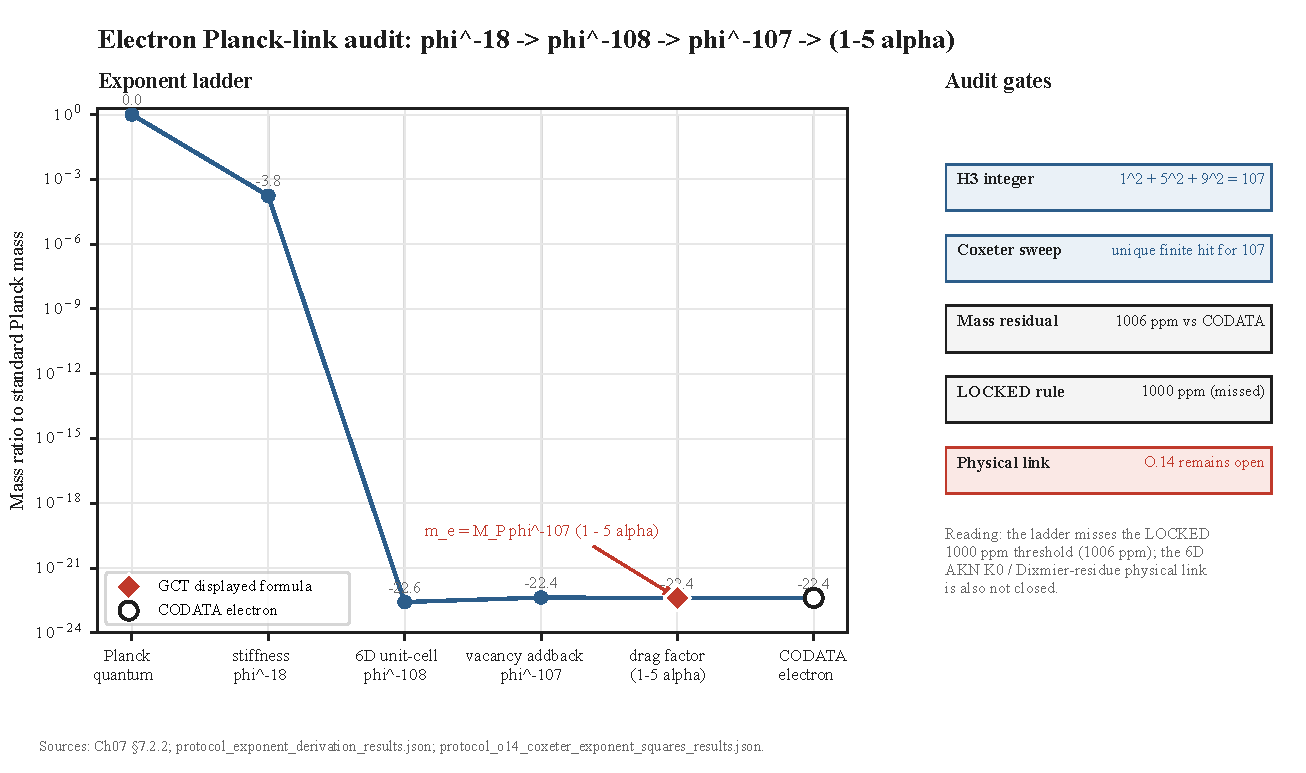
\includegraphics[keepaspectratio,alt={The electron Planck-link audit follows \textbackslash phi\^{}\{-18\} \textbackslash to \textbackslash phi\^{}\{-108\} \textbackslash to \textbackslash phi\^{}\{-107\} and drag factor (1-5\textbackslash alpha), while O.14 physical-link closure remains open.}]{content/Figures/Volume_3/Figure V3.7.1.pdf}}
\caption{The electron Planck-link audit follows
\(\phi^{-18} \to \phi^{-108} \to \phi^{-107}\) and drag factor
\((1-5\alpha)\), while O.14 physical-link closure remains open.}
\end{figure}

\begin{quote}
\textbf{Canonical group-theoretic identification of the integer
\(|n| = 107\) {[}Tier 2, integer-identification side; engine:
\texttt{GCT\_Physics\_Engine/src/protocol\_o14\_coxeter\_exponent\_squares.py}{]}.}
Independently of the K-theoretic gap-label assignment, the integer 107
is a canonical invariant of the icosahedral Coxeter group \(H_3\): the
Coxeter exponents of \(H_3\) are \(\{m_1, m_2, m_3\} = \{1, 5, 9\}\)
(Humphreys 1990 Table 3.1), and their sum of squares is
\[\sum_{i=1}^{3} m_i^2 = 1^2 + 5^2 + 9^2 = 1 + 25 + 81 = 107.\] Sweep
across the complete classification of finite irreducible Coxeter systems
(\(A_n\), \(B_n\), \(D_n\), \(E_6\), \(E_7\), \(E_8\), \(F_4\), \(G_2\),
\(H_3\), \(H_4\), \(I_2(p)\)): only \(H_3\) produces
\(\sum m_i^2 = 107\). The adjacent integers \(\{105, 106, 108, 109\}\)
correspond to no finite Coxeter group. Among rank-3 Coxeter groups
(\(A_3 \to 14\), \(B_3 \to 35\), \(H_3 \to 107\)), only \(H_3\) matches,
and \(H_3\) is the unique non-crystallographic rank-3 case --- the only
rank-3 group containing the 5-fold symmetry that the GCT projection
ansatz commits to. The icosahedral choice follows from the 5-fold
symmetry that the ansatz adopts, and once \(H_3\) is selected,
\(|n| = 107\) is an exact arithmetic fact about \(H_3\) and a Tier 2
integer-identification anchor for this sector. This closes the
arithmetic side of the integer question raised by O.14; the specific
electron exponent and physical-link chain remain Tier 3/Tier 4, because
elevating \(\phi^{-107}\) from ``empirical anchor plus canonical integer
identification'' to ``derived gap-label of the electron projection via
an explicit map from the Coxeter-exponent invariant to
\(\tau_*(K_0(\mathcal{A}))\)'' is the residual O.14 work.
\end{quote}

\gctneedspace{5\baselineskip}\begin{gctNote}

\textbf{Planck-Mass Convention for the Electron Link {[}Tier 3
convention choice{]}} In the standard convention the factor \(8\pi\) in
the reduced Planck mass \(\bar{M}_P = \sqrt{\hbar c / 8\pi G_N}\) comes
from the normalization of the Einstein--Hilbert action
(\(1/16\pi G_N\)). GCT proposes that, because the internal manifold
\(E_\perp\) is modelled as the discrete \textbf{Rhombic Triacontahedral
cage} (30 rhombic faces, each of area \(a_6^2\)) rather than by a
spherical solid-angle integration, the discrete face sum replaces
\(4\pi r^2 \to 30 \times a_6^2\), so that \(G_N\) acts directly as the
lattice bond-energy parameter and the non-reduced
\(M_{std} = \sqrt{\hbar c / G_N}\) is the bare quantum of lattice
bond-energy for the electron link. On this reading the \(8\pi\) would be
a continuum artifact; that reading is a Tier 3 proposal, not a
derivation from the GCT action.

\textbf{Convention consistency.} This volume does not use one
Planck-mass convention throughout: the electron and proton links use the
non-reduced \(M_P\), while the heavy-scale assignment
\(M_{GUT} = M_{red}\phi^{-9}\) of V3 Ch04 §4.3.3 and V3 Ch09 §9.2.3 uses
the reduced Planck mass. Each choice is a separate Tier 3 scale
assignment; no single action presently fixes both.

\textbf{Scope of this argument {[}Tier 3 convention + Tier 3 specific
prefactor disposition pending derivation{]}.} The \emph{qualitative}
claim --- that the discrete cage geometry replaces the continuous
spherical integration and therefore removes the a-priori \(8\pi\) --- is
a Tier 3 consequence of the discrete-cage commitment, conditional on the
missing discrete-to-continuum action map. The \emph{quantitative} claim
--- that the discrete face-sum prefactor is exactly \(30 \times a_6^2\)
and that this maps onto the conventional
\(M_{std} = \sqrt{\hbar c / G_N}\) rather than some other O(1) prefactor
--- is a Tier 3 disposition pending an explicit derivation of the
discrete-to-bond-energy mapping from the GCT action. A first-principles
derivation of the O(1) prefactor (and a check that the continuum limit
of the discrete cage recovers the smooth-GR \(8\pi\) via the
\(30 \to 4\pi\) identification) is recorded as a sub-item of
\textbf{Open Problem O.14} (App ORQ §ORQ.5). The Planck mass
\emph{convention} is therefore a Tier 3 choice (no \(8\pi\) under the
discrete-cage reading); the \emph{exact} numerical prefactor
identification has the residual O(1) Tier 3 disposition. See Appendix
GPE.

\end{gctNote}

This formulation computationally pairs the massive 6D-to-1D topological
geometric attenuation (\(\phi^{-107}\)) with the structural drag of the
5-fold channels.

\subsubsection{7.2.3 APS Index Context and the Separate Coupling
Residual {[}Tier 1 theorem / Tier 3 coupling
ansatz{]}}\label{aps-index-context-and-the-separate-coupling-residual-tier-1-theorem-tier-3-coupling-ansatz}

The proposed bare (tree-level) fine-structure relation, formerly
described as the geometric impedance of the Rhombic Triacontahedron, is:
\[\alpha^{-1}_{tree} = 360 \phi^{-2} \approx 137.507764 \quad \text{[Tier 3 numerical relation]}\]
(Tier 3 600-cell multiplier; mechanism open --- the RT solid-angle
construction is withdrawn, V1 §13.2.1--§13.2.2. \textbf{Tier 4 as
evidence} (φ-formula match; App PSC §PSC.9.6), for both the bare and the
bilayer-corrected values.)

The 3443 ppm (0.34\%) residual relative to the CODATA value
(\(137.035999177\)) is the bare tree-level residual before the bilayer
\(1/(2N)=1/288\) handle is applied. The remaining 41.5 ppm post-bilayer
residual motivates a separate boundary-spectral coupling ansatz; it is
not identified with the APS boundary correction. The APS index theorem
for a manifold with boundary independently establishes:
\[\text{index}(D) = \int_{\mathcal{M}} \hat{A}(R) \wedge \operatorname{ch}(F) - \frac{\eta(D|_{\partial \mathcal{M}}) + h}{2}\]
where \(\eta(D|_{\partial\mathcal{M}})\) is the spectral asymmetry of a
specified qualifying boundary operator,
\(h=\dim\ker D|_{\partial\mathcal M}\), and the controlling APS
correction is \(\xi=\tfrac12(h+\eta)\). No such operator, Hilbert-space
domain, boundary conditions, or kernel term has been constructed for the
RT boundary. Because \(\partial\mathcal M_{RT}\) is treated here as a
two-dimensional surface, a Chern--Simons 3-form cannot be integrated
over it. A separate coupling ansatz asks whether a presently undefined
dimensionless quantity \(\eta_{\alpha}\) could account for the
post-bilayer residual:
\[\delta\alpha^{-1}_{res} \equiv \alpha^{-1}_{obs} - \alpha^{-1}_{bilayer} \stackrel{?}{=} \frac{\eta_{\alpha}}{2}\]
No operator-level derivation identifies \(\eta_{\alpha}\) with the APS
\(\eta\) or \(\xi\) above. The bilayer \(1/(2N)=1/288\) correction (V1
Ch13 §13.2.4, Tier 3 motivated handle; inherits the Tier 3 \(N=144\)
posit, O.38) reduces the residual from 3443 ppm to 41.5 ppm; absorbing
the remaining residual through a boundary spectral term is an open
coupling hypothesis, not an APS index consequence.

\gctneedspace{5\baselineskip}\begin{gctImportant}

\textbf{Status of the boundary-spectral hypotheses.} No smooth RT
boundary operator or closed-form APS correction is currently derived.
The engine computation
(\texttt{GCT\_Physics\_Engine/src/protocol\_aps\_index\_proof.py})
reports two distinct finite-matrix diagnostics on the canonical 152-node
\(I_h\) cage: the scalar weighted-adjacency sign sum is \(-14\) (its
arithmetic value after division by the eight spinor components is
\(-1.75\)), while the full \(1216\times1216\) discrete Dirac sign sum is
\(0\). Neither is an APS \(\eta\)-invariant because no qualifying
boundary operator/domain or regularised spectrum is specified. The
selected 144-node \(I\) cage separately has scalar-adjacency sign sum
\(-8\) and arithmetic scalar/8 value \(-1\); no full-Dirac result is
supplied for that compatibility record. These graph quantities are
neither the APS correction \(\xi=\tfrac12(h+\eta)\) nor the continuous
coupling target \(\eta_{\alpha}\approx+0.011\). O.14b/c must construct
the operator, domain, sign convention, kernel term, spectral-flow
control, and comparison maps; O.19 must close or reject the independent
\(\alpha\)-residual coupling. The \(\alpha^{-1}_{bare}=360\phi^{-2}\)
tree-level relation and the bilayer-corrected
\(\alpha^{-1}\approx137.030\) are unaffected.

\end{gctImportant}

\subsubsection{7.2.4 Closure of the Electromagnetic Sector ---
Partial}\label{closure-of-the-electromagnetic-sector-partial}

The tree-level relation provides \(\alpha^{-1}_{tree} \approx 137.508\)
(Tier 3 numerical relation: Tier 3 600-cell multiplier; mechanism open
--- the RT solid-angle construction is withdrawn, V1 §13.2.1--§13.2.2;
3443 ppm residual). The bilayer 1/(2N) correction reduces the residual
to 41.5 ppm (Tier 3 motivated handle; inherits the Tier 3 \(N=144\)
posit, O.38; see V1 Ch13 §13.2.4). The remaining 41.5 ppm defines the
QLQCD-1L target. Writing
\(\delta\alpha^{-1}_{res}\stackrel?=\eta_{\alpha}/2\) is a separate Tier
3 coupling ansatz; \(\eta_{\alpha}\) has no derived operator and is not
the APS \(\eta\) or \(\xi\). The residuals are descriptive arithmetic
(Tier 4 as evidence: not distinguishable from numerology for strong
effects; App PSC §PSC.9.6). The electromagnetic sector is therefore
\emph{partially} closed, with final closure pending the QLQCD-1L
computation or another independently derived coupling mechanism.

The 0.34\% alpha gap is the bare tree residual; the 41.5 ppm alpha gap
is the phason anti-screening target after the bilayer handle. It is not
an APS target. Neither value is a free coefficient used to force
agreement with CODATA. Engine protocols that use CODATA alpha do so as
empirical comparison targets unless explicitly labelled as a downstream
phenomenological coupling elsewhere in the Ledger.

\gctneedspace{5\baselineskip}\begin{gctImportant}

\textbf{Finite-graph sign-count route is structurally insufficient.} A
direct computation
(\texttt{GCT\_Physics\_Engine/src/protocol\_rt\_eta\_invariant.py})
tests the icosidodecahedron face-adjacency graph (30 vertices, 60 edges,
valency 4) as the RT face dual and obtains
\(\sum\operatorname{sign}(\lambda)=0\). Any finite-dimensional
self-adjoint sign count is integer-valued regardless of whether its edge
weights are integers or elements of \(\mathbb Z[\phi]\); changing finite
edge weights cannot by itself reach the non-integer coupling target
\(\eta_{\alpha}\approx+0.011\). Closure therefore requires either a
specified infinite-dimensional boundary operator with a regularized
analytic \(\eta\)-invariant and an independently derived coupling map,
or the continuum spectral-action route via App ULA §ULA.7 phason
anti-screening (Open Problem O.19). The finite-graph computation remains
a reproducible negative control, not an APS evaluation.

\end{gctImportant}

\gctneedspace{5\baselineskip}\begin{gctNote}

\textbf{Analytic Formula vs.~Computational Verification ---
Methodological Complementarity}

\textbf{The Analytic K-Theoretic Result:} The formula
\(m_e = M_P \phi^{-107}(1-5\alpha)\) (§7.2.2) is supported by the
Bellissard / Connes-Moscovici / Cuntz-Krieger K-theoretic framework at
the 1D Fibonacci toy-model level. The specific electron-mass chain
remains \textbf{Tier 2 mechanism + Tier 3 dimensional/integer anchor +
Tier 4 K-theoretic physical-link conjecture pending O.14}: the \(H_3\)
arithmetic identity for \(|n|=107\) is exact, but the 6D AKN lift and
the map from the Coxeter invariant to the electron projection are still
open.

\textbf{The Complementary Numerical Route:} The Physics Engine (Appendix
GPE) implements a complementary numerical method: the
\textbf{Peierls-Nabarro Barrier Scan}. This algorithm numerically
computes the energy landscape of topological defects by solving the
discrete Euler-Lagrange equations on the lattice and extracting the
minimum barrier height. This is a computational validation tool, not a
derivation.

\textbf{Why Both Methods?} The analytic framework provides the candidate
structural chain; the numerical barrier scan provides an independent
consistency check of the lattice-mechanical side. They address the same
physics from two perspectives: analytic geometry (K-theory) and
computational lattice mechanics (variational principle). No shared
observable of the two routes has yet been compared numerically, and the
App ULA action has not produced a stable electron-defect solution
(§7.1.1), so no agreement between them is claimed and neither closes the
Tier 3 anchor or Tier 4 physical-link debt. Analytic K-theory supplies
the structural target; the lattice barrier scan is a separate
computational route whose comparison with that target remains open. Both
are documented in Appendix GPE.

\end{gctNote}

\subsubsection{7.2.5 Computational
Verification}\label{computational-verification}

This formula gives an anchor-normalised Planck-link check
(\(m_e \approx 0.511\) MeV; \(m_e\) is itself the A1 anchor, so this is
not a prediction of the electron mass) {[}Tier 2 mechanism + Tier 3
dimensional/integer anchor + Tier 4 K-theoretic physical-link conjecture
pending O.14, per Parameter Ledger §0.1 P2 and §7.2.2 above{]} with a
\textbf{\textasciitilde1006 ppm residual} against CODATA-2022 on
canonical CODATA inputs throughout (computational verification: see
\texttt{GCT\_Physics\_Engine/verify\_independent/verify\_electron\_mass.py}).
This misses the LOCKED 1000 ppm pre-commitment by 6 ppm; App FSM P.1c
reports a FAIL of that rule. As evidence that φ is special the match is
Tier 4 (§7.2.2 box; App PSC §PSC.9.6). The integer
\(107 = \sum m_i^2(H_3)\) is an exact Coxeter fact, identified with the
exponent at Tier 2 (§7.2.2), and the use of \(\phi^{-107}\) as the
electron scaling is a Tier 3 anchor; the electron-mass chain inherits
the weakest link: the K-theoretic gap-label-action physical
identification remains the O.14 closure target. Conditional on the Tier
3 O.38 cage posit, the vacuum quantum evaluates as
\(E_{vac}=m_ec^2/144\); the division is exact, but the absolute centroid
does not promote above its cage-size input. The \textasciitilde1006 ppm
CODATA-2022 figure is the canonical engine output; alternative ppm
values arise only under non-CODATA \(M_P/\alpha\) calibrations and are
not the load-bearing engineering anchor.

\subsubsection{7.2.6 The 3.55 keV Lattice Fracture Release {[}Tier 3
conditional mechanism + Tier 3 O.38-dependent centroid and empirical
postdiction; line width open, V3 Ch11
§11.2.3{]}}\label{the-3.55-kev-lattice-fracture-release-tier-3-conditional-mechanism-tier-3-o.38-dependent-centroid-and-empirical-postdiction-line-width-open-v3-ch11-11.2.3}

X-ray observations of galaxy clusters (Perseus; Bulbul et al.~2014) and
of the Andromeda galaxy M31 (Boyarsky et al.~2014) initially reported an
unidentified line at \textbf{3.55 ± 0.03 keV}, but the detection has
been contested in subsequent analyses. The empirical landscape now
includes:

\begin{itemize}
\tightlist
\item
  \textbf{Hitomi non-confirmation} (Aharonian et al.~2017 \emph{ApJL}
  837:L15, DOI 10.3847/2041-8213/aa61fa): high-resolution X-ray
  microcalorimetry of the Perseus cluster did not resolve the line at
  the predicted amplitude.
\item
  \textbf{Boyarsky et al.~2018 vs Cappelluti et al.~2018 review}:
  continued dispute over stacked-cluster vs individual-source evidence;
  no convergence on a definitive astrophysical interpretation.
\item
  \textbf{XRISM early data} (App PSC §PSC.8 row 3): the line was not
  resolved at the predicted strength in the current dataset ---
  \emph{data inconclusive} rather than null.
\item
  \textbf{Dessert, Rodd \& Safdi 2020} (\emph{Science} 367:1465): a
  blank-sky XMM-Newton analysis finds no line at 3.55 keV and bounds the
  decay flux from the Milky-Way dark-matter halo, concluding that the
  decaying-dark-matter interpretation of the cluster detections is
  inconsistent with that bound. Subsequent rejoinders (Abazajian 2020;
  Boyarsky et al.~2020) dispute the analysis; the debate is unresolved
  at the time of writing. \textbf{GCT engagement with Dessert 2020:}
  line narrowness does not evade a flux limit (at fixed flux a narrower
  line is easier to detect). The relevant GCT difference is the flux
  model: GCT treats the candidate emission as stress-gated rather than
  tracking the dark-matter column (V3 Ch11 §11.4.6), so it expects
  suppressed emission from low-stress blank-sky fields {[}Tier 3{]}.
  This expectation is unquantified: \(\sigma_{crit}\) is defined through
  an ICM thermal-pressure proxy that does not exist for the gas-poor
  Milky-Way halo (V3 Ch11 §11.1.4), so the blank-sky bound is not
  absorbed by the stress gate; it stands as an open constraint.
  High-resolution spectroscopy (XRISM Resolve \(\sim 5\) eV at 3.55 keV
  per Ishisaki et al.~2022, \emph{Proc. SPIE} 12181:121811S (DOI
  10.1117/12.2630654); Athena X-IFU 2.5 eV resolution) and the
  line-shape test of V3 Ch11 remain the registered discriminators.
\end{itemize}

Conditional on the adopted cage architecture, GCT models a
\textbf{Lattice Fracture Release} line. The fracture-mechanism form is
Tier 3 (it rests on the Tier 3 Topological Glass model and is
conditional on the adopted architecture). A narrow (Lorentzian) line
holds only for lattice-bound emitters, which is the open
emitter-kinematics programme (V3 Ch11 §11.2.3); the line width is not a
prediction until that programme closes. The centroid
\(E_{vac}=m_e/144\approx3.55\) keV is a Tier 3 O.38-dependent
postdiction because the cage size is not independently selected. The
coincidence is context for the registered spectroscopy test, not primary
evidence for the substrate.

\begin{center}\rule{0.5\linewidth}{0.5pt}\end{center}

\subsection{7.3 The Polaron Structure}\label{the-polaron-structure}

\subsubsection{7.3.1 Vortex-Dislocation
Duality}\label{vortex-dislocation-duality}

GCT models the electron core as a composite topological object {[}Tier 3
picture{]} and proposes that its Russellian structure offers a
mechanical picture of wave-particle duality; this picture does not
derive quantum interference or resolve the measurement question:

\begin{enumerate}
\def\labelenumi{\arabic{enumi}.}
\tightlist
\item
  \textbf{The Dislocation Cage (Mass):} The 144-node cage provides the
  \textbf{Particle-like} localization and inertial mass.
\item
  \textbf{The Phase Vortex (Charge):} The \(n=1\) phase winding around
  the cage provides the \textbf{Wave-like} interference and the \(U(1)\)
  charge.
\end{enumerate}

Together, these form a \textbf{Vortex-Dislocation Complex} that
propagates as a \textbf{Polaron} in the supersolid condensate.

\subsubsection{7.3.2 The Polaron Cloud and the ``Tight Fit''
Paradox}\label{the-polaron-cloud-and-the-tight-fit-paradox}

\begin{quote}
\textbf{Proposal 7.3.1 (Polaron Healing Length) {[}Tier 1 arithmetic;
Tier 3 identification + Tier 3 microtubule-lumen biological-scale
match{]}:} The characteristic radius used for the electron polaron cloud
is the length
\[\xi = \frac{\hbar c}{\alpha^2 m_e c^2} = \frac{a_0}{\alpha} \approx 7.25 \text{ nm}\]
{[}Tier 1 arithmetic; its identification as the vacuum/polaron healing
length is Tier 3{]}.

\emph{Derivation status:} only the arithmetic is Tier 1; no standard
result identifies \(a_0/\alpha\) as a polaron or condensate healing
length. App ORQ O.25 records that the tested GCT phason-elastic
substitution chain gives a Planck-scale length rather than the
Bohr-Compton nanometre scale, so the phason-elastic route is not used as
a derivation.

\emph{Computational verification:} This arithmetic is verified to
machine precision (see Appendix GPE +
\texttt{verify\_independent/verify\_healing\_length.py}). Both CODATA
and GCT-bare \(\alpha\) inputs give the same value to \(\sim 0.7\%\) ---
the formula is \(\alpha\)-input-insensitive at the percent level. On
this identification the electron would have an effective
\textbf{Holographic Diameter of \(\approx 14.5\) nm} {[}Tier 3
biological-scale match{]} (= \(2\xi\)). This is not a charge or
form-factor radius: scattering experiments find the electron point-like
down to about \(10^{-18}\) m, and the proposed polaron cloud is an
extended phason-strain field, not the charge distribution.
\end{quote}

\subsubsection{7.3.3 Waveguide Stability and Biological Mass
Shift}\label{waveguide-stability-and-biological-mass-shift}

The \(\sim 14.5\) nm diameter of the polaron cloud presents a functional
requirement when compared to the \textbf{Microtubule Lumen}, whose inner
diameter falls in the range \textbf{\(\sim 15\)--\(17\) nm} depending on
protofilament count (typically 13--14 in vivo) and tubulin isotype
(TUBB3 neuron-enriched, TUBB2 motile cilia, etc.) per cryo-EM
measurements (Nogales et al.~1998; Ti et al.~2018; Manka \& Moores
2018).

\begin{itemize}
\tightlist
\item
  \textbf{Confinement Match:} The polaron diameter
  (\(2\xi \approx 14.5\) nm) sits inside the lumen with radial clearance
  ranging from \(\sim 0.25\) nm (at 15 nm lumen, a \(\sim 3\%\) ``tight
  resonance'' fit) to \(\sim 1.25\) nm (at 17 nm lumen, a \(\sim 17\%\)
  ``loose containment'' fit). In either case the polaron is
  \emph{contained} without compression, supporting \textbf{resonant
  confinement} rather than a strict geometric-squeeze interpretation.
  The strongest version of this argument applies in microtubules with
  the smaller lumen ID (consistent with TUBB3 / neuronal-tubulin cryo-EM
  at the lower end of the range), where the \(\sim 3\%\) match becomes a
  tight geometric coincidence; reading it as biological tuning of the
  lumen to the electron polaron scale is a Tier 3 hypothesis, not an
  established resonance. In microtubules with larger lumen ID, the
  prediction reduces to ``polaron fits inside lumen with significant
  clearance'' --- still a non-trivial Tier 3 biological correlation but
  not a sharp resonance signature.
\item
  \textbf{Biological Mass Shift {[}Tier 3/open{]}:} The proposed
  radial-mode confinement could raise the defect's zero-point energy
  through lumen-imposed boundary conditions, producing a small
  environment-dependent effective-mass shift (\(m_e^*\) marginally
  higher inside a microtubule than in vacuum). No magnitude or
  action-normalized microtubule calculation is presently derived, and
  any such material shift would not by itself identify an Identity
  Polaron, consciousness, or a metabolic cost of Level II; no Level II
  classification of the biological substrate follows.
\end{itemize}

\subsubsection{7.3.4 Candidate Hardware Port of Agency {[}Tier 3/open;
Level II
open{]}}\label{candidate-hardware-port-of-agency-tier-3open-level-ii-open}

The electron core is structurally classified as a \textbf{Class 0
Pattern}. Under Axiom 1 it has Level I Universal Presence; its Level II
status is not inferred from that label. Level II is open (Tier 3): no
validated substrate criterion exists yet (it requires a typed,
normalized, measured coupling, the Identity-Polaron construction and an
independent phenomenal bridge; O.21/O.23/O.34, O.18). The \(N=144\)
dodecahedral construction is a candidate topological ingredient, not a
demonstrated architecture required for agency; the ``Hardware Port''
used by the ``Software'' of the Selection Operator is a Tier 3 picture.
Identifying the electron as a physical anchor for an Identity Polaron
would require the missing action-normalized matter/phason coupling, a
sector-writing map, a persistence mechanism, an owner relation, and a
phenomenal bridge. The \(\sim 7.25\) nm healing-length scale (polaron
diameter \(\sim 14.5\) nm) and its comparison with the \(\sim 15\) nm
microtubule lumen therefore remain a Tier 3 geometric/material
correlation; they do not unify physics and consciousness at that scale
or establish a recursive Zeno loop.

\gctneedspace{5\baselineskip}

\textbf{END OF CHAPTER 7}

\chapter{Chapter 8: The Fractal Resonance Spectrum ---
Leptons}\label{chapter-8-the-fractal-resonance-spectrum-leptons}

The Standard Model treats the masses of the muon (\(\mu\)) and the tau
(\(\tau\)) as arbitrary parameters determined by measured Yukawa
couplings. Geometric Consciousness Theory (GCT) models the lepton
hierarchy as the \textbf{Fractal Resonance Spectrum} on the adopted
\(N=144\) dodecahedral cage. That cage size is a Tier 3 structural posit
pending O.38. Conditional on it, the harmonic-ladder mechanism is Tier 2
(conditional on the Tier 3 choice of \(\phi\), not \(\phi^3\), as the
elementary step, §8.1.2) while the integer anchors \(N=11\) and \(N=17\)
remain Tier 3 pending O.5/O.14/O.15 closure.

\begin{figure}
\centering
\pandocbounded{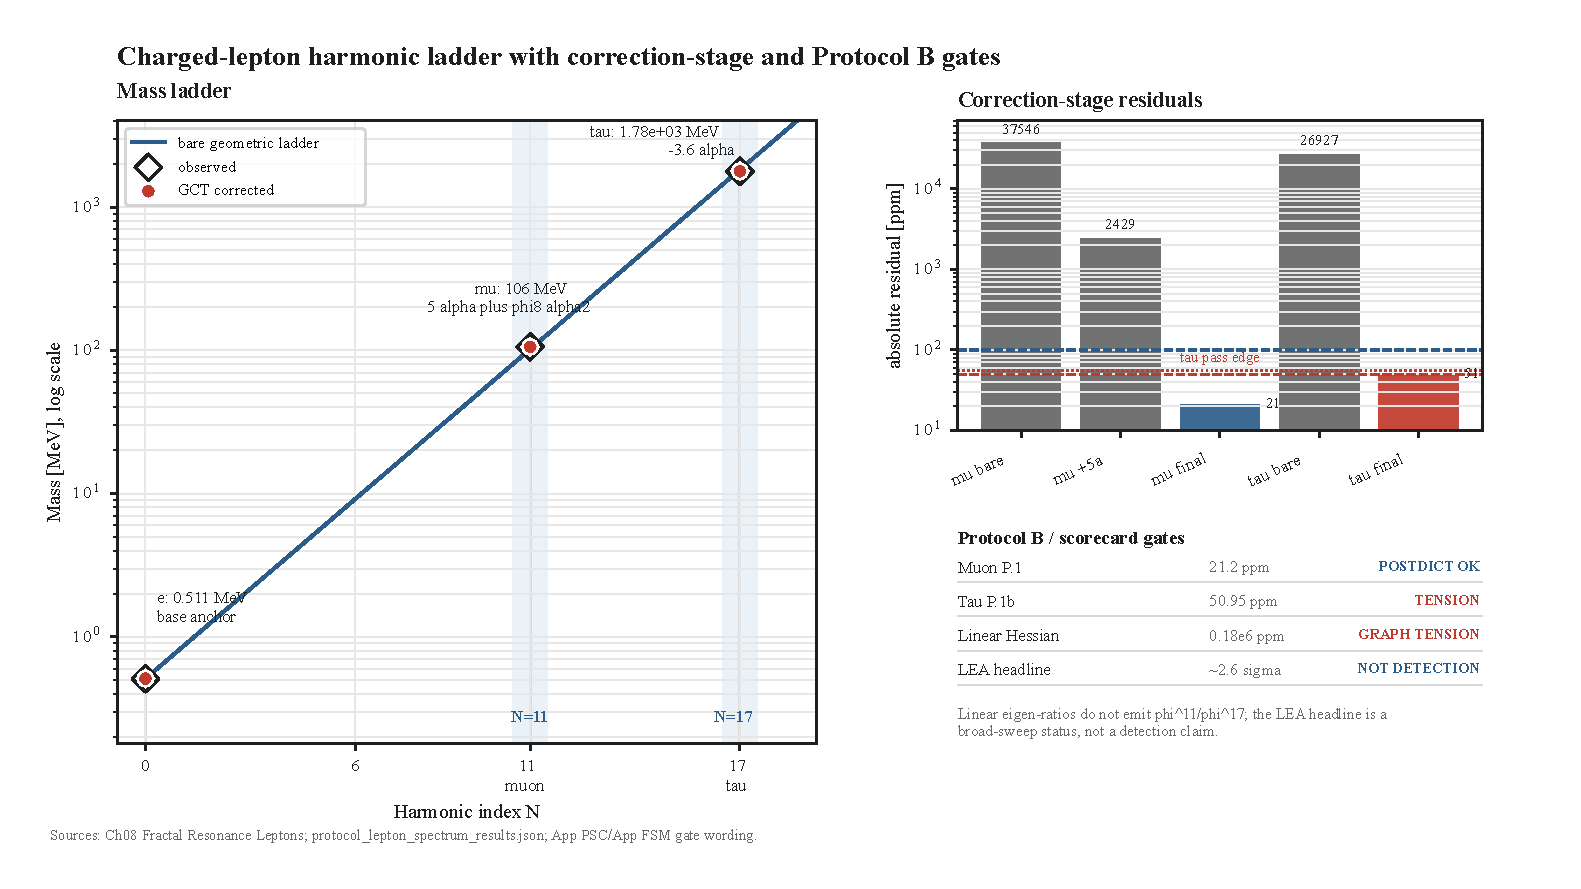
\includegraphics[keepaspectratio,alt={Electron, muon, and tau masses sit on a log axis with N=11 and N=17 harmonic overlays; correction-stage residuals and row-specific Protocol B gates are shown separately.}]{content/Figures/Volume_3/Figure V3.8.1.pdf}}
\caption{Electron, muon, and tau masses sit on a log axis with \(N=11\)
and \(N=17\) harmonic overlays; correction-stage residuals and
row-specific Protocol B gates are shown separately.}
\end{figure}

\begin{center}\rule{0.5\linewidth}{0.5pt}\end{center}

\subsection{8.1 Phason Band Structure}\label{phason-band-structure}

\subsubsection{8.1.1 The Symmetry Octave and the High-Pass Filter
{[}Tier 3
ansatz{]}}\label{the-symmetry-octave-and-the-high-pass-filter-tier-3-ansatz}

In the icosahedral projection, the radial scaling of the vacuum is
governed by the \textbf{Symmetry Octave (6)}, corresponding to the six
five-fold rotational axes of the parent lattice. Conditional on the Tier
3 O.38 cage posit, the adopted \(N=144\) cage is used as a candidate
\textbf{Topological High-Pass Filter} ansatz: the present model assigns
harmonics below the 11th power of \(\phi\) insufficient ``topological
torque'' to displace its locked nodes and activate the registered
resonance. No native action yet derives this threshold, a hard target
space, or a preserved topological sector {[}Tier 3{]}.

\subsubsection{\texorpdfstring{8.1.2 The Generational Scaling {[}Tier 2
mechanism conditional on the Tier 3 \(\phi\)-step + Tier 3 integer
anchors pending
O.5/O.14/O.15{]}}{8.1.2 The Generational Scaling {[}Tier 2 mechanism conditional on the Tier 3 \textbackslash phi-step + Tier 3 integer anchors pending O.5/O.14/O.15{]}}}\label{the-generational-scaling-tier-2-mechanism-conditional-on-the-tier-3-phi-step-tier-3-integer-anchors-pending-o.5o.14o.15}

The mass hierarchy is established at specific intervals of the Symmetry
Octave:

\begin{itemize}
\tightlist
\item
  \textbf{The Muon (\(n=11\)):} The first available spectral gap above
  the depinning threshold. It occurs at two octaves of inflation minus a
  single \textbf{Decoupling Unit} required to break the ground-state
  symmetry and transition from a static to a dynamic resonance:
  \(2 \times 6 - 1 = 11\). Equivalently \(n_\mu = h + 1\), one unit
  above the \(H_3\) Coxeter number \(h = 10\).
\item
  \textbf{The Tau (\(n=17\)):} The next stable resonance window,
  occurring exactly one symmetry octave above the muon: \(11 + 6 = 17\).
  Equivalently
  \(n_\tau = \left(\textstyle\sum_i d_i\right) - 1 = 18 - 1\), one unit
  below the \(H_3\) Shephard-Todd degree sum; the octave spacing
  \(n_\tau - n_\mu = 6 = d_2\) is the middle degree.
\end{itemize}

The current harmonic-ladder postulates mark the \(k=11\) and \(k=17\)
harmonics of the inflation eigenvalue \(\phi\) as candidate resonance
labels, pending O.5/O.14/O.15 closure. Their arithmetic does not by
itself select physical particle masses or stable defects; that requires
a target/index map, admissibility and boundary data, preserving
dynamics, and an action. A single \(\phi\) scaling maps the primitive
lattice \(P\cong\mathbb{Z}^6\) to the body-centred lattice \(I\); the
self-similarity of \(P\) is \(\phi^3\) (App QCT §QCT.3.2). Using
\(\phi\) as the elementary step is an additional assumption {[}Tier
3/open{]}.

\subsubsection{8.1.3 Geometric Amplification
Mechanism}\label{geometric-amplification-mechanism}

The proposed \textbf{Lever Arm of the 6D Projection} supplies a
qualitative amplification mechanism for the disparity between
generations (e.g., \(m_\mu/m_e \approx 206\)): if the phason stiffness
\(K_\perp\) is suppressed relative to \(K_\parallel\), the resonant
frequencies of the defect core are geometrically amplified by the
inverse volume ratio of the internal manifold. Its numerical
specialization assumes \(K_\perp/K_\parallel = \phi^{-18}\) (Volume 2,
Chapter 4), which is the registered Tier 3 stiffness-map hypothesis P3b
(Parameter Ledger), listed outside the count and pending the
normalization-invariant O.15(b) elasticity/RG derivation; only the
integer \(D = 18\) is Tier 2, and the ratio is not a Tier 2 projector
consequence. The harmonic-ladder mechanism and the separate \(N=11,17\)
integer anchors do not derive that stiffness ratio.

\subsubsection{8.1.4 The Linear vs.~Non-Linear Boundary {[}Tier 2
numerical diagnostic + Tier 3 soliton
hypothesis{]}}\label{the-linear-vs.-non-linear-boundary-tier-2-numerical-diagnostic-tier-3-soliton-hypothesis}

Conditional on the adopted \(N=144\) input, sparse-Hessian
diagonalization of that cage (see Appendix GPE) provides an internal
spectral diagnostic. Diagonalization of the \textbf{bare linear
dynamical matrix} extracts the acoustic phonon background, yielding
normalized eigen-ratios of \texttt{{[}1.0,\ 1.67,\ 2.1,\ 2.52...{]}}.

It is a reproducible numerical fact of the current finite model that the
exponents \(\phi^{11}\) and \(\phi^{17}\) \textbf{do not} spontaneously
emerge from this linear approximation. GCT therefore carries
\textbf{Non-Linear Phason Solitons} (Davydov-like defects), whose masses
would be governed by the non-perturbative saturation of the discrete
\(6N \pm 1\) symmetry octaves rather than by simple linear harmonic
resonance, as a Tier 3 physical hypothesis rather than a derived
conclusion. A linear Hessian cannot establish the non-linear soliton,
its target space or index, its preservation/metastability, or its
particle identity.

Consequently, the harmonic-ladder mechanism is a \textbf{Tier 2
geometric postulate} conditional on the Tier 3 choice of \(\phi\) (not
\(\phi^3\)) as the elementary step (§8.1.2), while the specific integer
anchors \(N=11\) and \(N=17\) remain \textbf{Tier 3} pending
O.5/O.14/O.15 closure. The Tier-3 status reflects a genuine structural
gap: unlike the electron exponent (\(107 = 1^2+5^2+9^2 = \sum_i m_i^2\),
a power-sum invariant unique to \(H_3\)) and the stiffness exponent
(\(18 = \sum_i d_i\)), the lepton harmonic integers are \textbf{not}
power sums of the \(H_3\) exponent or degree multisets
(\(\sum m_i = 15,\ \sum m_i^2 = 107\);
\(\sum d_i = 18,\ \sum d_i^2 = 140\)), and an exhaustive audit of
canonical \(H_3\)/\(I\) structural counts --- roots, reflections,
conjugacy classes, irreducible-representation dimensions, orbit sizes,
and coinvariant/Poincaré coefficients --- yields no distinctive
invariant identification of \(11\) or \(17\) (engine:
\texttt{GCT\_Physics\_Engine/src/protocol\_w4\_lepton\_exponents.py}).
The integers likewise fail to arise as spectral-ordinal labels: in the
icosahedrally-decomposed linear phason spectrum of the 152-node
\(I_h\)-closed defect cage (used here because a symmetry decomposition
needs an \(I_h\)-closed cage; the other diagnostics of this chapter use
the adopted \(N=144\) cage), the phason-vector channel activates at
pooled cluster ordinals \((5, 18, 26, \ldots)\), with neither \(11\) nor
\(17\) appearing among the activation ordinals (engine:
\texttt{GCT\_Physics\_Engine/src/protocol\_w4b\_lepton\_spectral\_ordinals.py}).
Together with the eigenvalue-magnitude exclusion above, this closes the
arithmetic-invariant and linear-spectral identifications, leaving the
non-perturbative extraction as the remaining closure path. The canonical
hooks \(n_\mu = h+1\) and \(n_\tau = (\sum_i d_i) - 1\) fix the values
against \(H_3\) data, but the Decoupling-Unit offset and the generation
indexing remain un-derived handles, so no canonical-invariant promotion
of the form available to \(107\) exists. The muon hook does carry
genuine \emph{naming} standing: the diagonal-coinvariant theorem of
Gordon (2003, Thm.\textasciitilde1.4) attaches a \(W\)-stable quotient
ring of dimension \((h+1)^n\) --- with \(h+1 = 11\) graded levels per
rank coordinate --- to every finite Coxeter group, explicitly including
the non-crystallographic \(H_3\). This standing is dimensional only
{[}Tier 3{]}: the construction carries no spectral, harmonic, or
mass-ladder content connecting \(h+1\) to the \(\phi\)-power ladder, its
crystallographic lattice interpretation (\(Q/(h+1)Q\)) does not transfer
to \(H_3\), and no analogous theorem features \(\sum_i d_i - 1 = 17\).
Extracting these non-linear solitonic eigenvalues directly from an
ab-initio non-perturbative lattice simulation remains the closure target
(App ORQ O.5).

\begin{center}\rule{0.5\linewidth}{0.5pt}\end{center}

\subsection{8.2 The Muon (The Acoustic
Resonance)}\label{the-muon-the-acoustic-resonance}

\subsubsection{\texorpdfstring{8.2.1 Identification:
\(\mu \leftrightarrow \phi^{11}\)}{8.2.1 Identification: \textbackslash mu \textbackslash leftrightarrow \textbackslash phi\^{}\{11\}}}\label{identification-mu-leftrightarrow-phi11}

The Muon is the fundamental acoustic resonance of the electron's
dodecahedral cage. Its ``Bare Geometric Mass'' is the energy required to
maintain this 11th-harmonic oscillation:
\[\begin{gathered}m_\mu^{bare} = m_e \cdot \phi^{11} \approx 101.6913 \text{ MeV} \\[1pt] \gcteqnote{[Tier 2 mechanism + Tier 3 specific exponent $N=11$]}\end{gathered}\]

\begin{quote}
\textbf{Tier disposition for the muon harmonic exponent.} The
harmonic-ladder mechanism is Tier 2 (geometric postulate, conditional on
the Tier 3 \(\phi\)-step; see §8.1.2). The specific integer \(N = 11\)
is Tier 3, anchored at Parameter Ledger §0.1 postulate P4: the
\(6N \pm 1\) symmetry-octave selection rule of §8.1.2 constrains but
does not uniquely force \(N = 11\). The integer-side closure target is
the analogue of the electron's \(|n| = 107 = \sum m_i^2(H_3)\)
Coxeter-exponent uniqueness derivation; see App ORQ Open Problem O.14
path (l) for the closed electron-side argument and Parameter Ledger §0.1
P4--P5 for the muon-and-tau integer closure status. Earlier
global-significance figures for the numerical matches are withdrawn: the
cross-base comparison could not, by construction, credit any base other
than \(\phi\), and the trial counts behind the quoted σ values were
asserted rather than enumerated. As evidence that φ or icosahedral
structure is special, the muon and tau ladder matches and their ppm
residuals are \textbf{Tier 4}: the preregistered constant control test
(v3, NEGATIVE-FRAGILE; App PSC §PSC.9.6) found φ's pattern of matches on
21 constants not distinguishable from that of random constants (58 of
300 random bases did at least as well). The test ``excludes, at power ≥
0.8, an effect in which φ hits at least 6 of the 8 informative rows
through a real effect; weaker effects are not excluded.'' The numbers
are kept as descriptive arithmetic; no global significance is claimed,
and no individual match is cited as evidence on its own strength. The
tier tags of the mechanism, the exponents and the coefficients below
describe the ansatz, not the evidential weight of the match.
\end{quote}

\subsubsection{\texorpdfstring{8.2.2 The Phason Drag Coefficient
(\(5\alpha\)) {[}Tier 2 mechanism + Tier 3 specific
coefficient{]}}{8.2.2 The Phason Drag Coefficient (5\textbackslash alpha) {[}Tier 2 mechanism + Tier 3 specific coefficient{]}}}\label{the-phason-drag-coefficient-5alpha-tier-2-mechanism-tier-3-specific-coefficient}

The icosahedral rotation group \(A_5\) has five irreducible
representations in total, of dimensions \(1, 3, 3', 4, 5\) (the trivial
one and four non-trivial ones; equivalently, five conjugacy classes)
{[}Tier 1{]}. This chapter reads the ``5'' in \(5\alpha\) as that total
count, so the trivial (uniform) sector is counted as one of the
\textbf{phason channels}. No current action justifies counting the
trivial sector, or treating every irrep as one channel, rather than,
say, counting only the four non-trivial irreps; the channel multiplicity
5 is therefore a \textbf{Tier 3 counting convention}, not a Tier 2
result. The Tier 2 content is only the existence of a first-order
phason-drag channel. Other fivefold counts (the five faces meeting at an
icosahedral vertex, the order of the five-fold vertex stabilizer) are
alternative readings of the same number, not independent derivations of
it. \textbf{Converting} this count into the equal-weight pole-mass
self-energy coefficient \(+5\alpha\) is a Tier 3 physical normalization
rule: each channel contributes one unit of \(\alpha\) to the muon
self-energy, pending a first-principles GCT self-energy calculation
(closure target App ORQ O.5). The nominal −21.09 ppm residual downstream
is a Tier 3 formula residual (about \(10^3\sigma\) against the 22 ppb
CODATA 2022 measurement uncertainty of \(m_\mu\)) and inherits Tier 3
status from this coefficient normalization and from the loop-order
truncation (§8.2.4); it is not a Tier 2 coefficient derivation.

\begin{quote}
\textbf{Layered tier disposition:} The muon correction is a tree-level +
single 1-loop GCT correction factor. The specific \(\phi^8\alpha^2\)
term is obtained only after inserting the factor \(\phi^{-3}\), the
value of the independent Tier 3 hypothesis H-EW (V3 Ch04 §4.3), into the
exact arithmetic \(\phi^{11}\phi^{-3}=\phi^8\); neither Gram nor
projector geometry selects that factor (see Appendix GPE). The tiered
claim is the existence of the phason-drag channel mechanism (its
multiplicity 5 being a Tier 3 counting convention, §8.2.2) and of the
single-loop geometric correction channel, not a standalone resolved
\textbf{21 ppm} pole-mass prediction; the displayed second-order
coefficient is Tier 3 conditional on H-EW. The \(+5\alpha\) coefficient
normalization and nominal −21.09 ppm residual remain Tier 3 pending full
GCT-native self-energy and loop-order closure (O.5); the residual is not
resolved below the size of the unpropagated next-order GCT term
(§8.2.4). The tau reaches \textbf{\textasciitilde−51 ppm} against PDG
2024 only after inserting the \(-3.6\alpha\) screening coefficient
\(c=-D/N=-18/5\): the integer \(D=18\) is Tier 2 within the adopted
framework and \(N=5\) is the \(A_5\) irrep count (Tier 3 as a channel
number, §8.2.2), but the combination rule \(c=-D/N\) and the negative
polarity are Tier 3 candidate conventions pending O.26b; Galois
conjugation supplies no physical response sign.

\textbf{The Computational Frontier:} O.38 must first establish the cage
size by a full candidate-size minimization. Conditional on that result,
the non-perturbative \(6N\times6N\) Hessian must extract the nonlinear
eigenspectrum without analytic approximation. The finite calculations do
not promote the adopted \(N=144\) input; the existence of the muon
phason-drag channel remains Tier 2 conditional mechanics, while the
channel count 5 (§8.2.2) and the coefficient normalizations retain their
Tier 3 gaps.
\end{quote}

\subsubsection{8.2.3 Tree + Single 1-Loop GCT Phason Self-Energy
Correction {[}Tier 2 mechanism + Tier 3
coefficient{]}}\label{tree-single-1-loop-gct-phason-self-energy-correction-tier-2-mechanism-tier-3-coefficient}

To reach precision limits for the muon, we must account for the leading
GCT loop correction. The mass shift is represented by a single 1-loop
GCT phason self-energy correction factor over the discrete \(N=144\)
cage. The discrete cage-Hessian correction yields:

\begin{itemize}
\tightlist
\item
  \textbf{Intensive Scaling:} The single 1-loop GCT self-energy
  \(\Sigma\) is normalized by the node count \(1/N\).
\item
  \textbf{Engine-checked conditional exponent arithmetic:} The engine
  verifies the effective scaling factor \textbf{\(\phi^8\)} (the single
  1-loop GCT correction factor over the \(N=144\) cage; see Appendix
  GPE) as \(\phi^{11} \times \phi^{-3} = \phi^8\) once the factor
  \(\phi^{-3}\) is supplied on the bare muon scaling \(\sim \phi^{11}\).
  That factor is the value of the independent Tier 3 hypothesis H-EW (V3
  Ch04 §4.3), not an output of graph topology, Gram ratios, or projector
  normalization; the raw-frame coordinate identity behind \(\phi^{-3}\)
  (App USS §USS.9) is coordinate arithmetic only. The existence of the
  single-loop correction channel remains Tier 2 within GCT; selecting
  the specific \(\phi^8\) coefficient is Tier 3 conditional on H-EW,
  with load-bearing self-energy and radiative closure remaining
  O.5/O.19/O.26.
\end{itemize}

Therefore, the single-loop mass shift is {[}Tier 2 mechanism + Tier 3
coefficient{]}:
\[\Delta m_2 = (m_e \phi^{11}) \cdot (\phi^8 \alpha^2), \qquad \Delta m_2 / m_\mu^{bare} = \phi^8 \alpha^2\]
{[}Tier 2 mechanism + Tier 3 coefficient conditional on H-EW, pending
O.5/O.26{]}

\subsubsection{8.2.4 Result 8.1: The Muon Mass
Formula}\label{result-8.1-the-muon-mass-formula}

\textbf{Result 8.1:} \emph{Three-stage muon chain: 3.75\% bare residual,
2429 ppm first-order residual, and a nominal −21.09 ppm Tier 3 formula
residual after the A3 + single-1-loop comparison stage. The measured
muon mass is known to 22 ppb, so the formula does not reproduce
\(m_\mu\) at measurement precision; the unpropagated next-order GCT
truncation term (\(\sim\phi^8\alpha^3 \approx 18\) ppm) is as large as
the residual, so the row tests nothing beyond first order.}
\[m_\mu = m_e \phi^{11} (1 + 5\alpha + \phi^{8} \alpha^2)\]

\begin{quote}
\textbf{The Geometric Basis:} The muon mass formula employs the
\(\phi^8\alpha^2\) correction channel whose displayed product
\(\phi^{11} \times \phi^{-3} \times \alpha^2 = \phi^{8} \alpha^2\) is
exact exponent arithmetic \textbf{conditional on inserting the H-EW
value \(\phi^{-3}\)}; neither the projectors nor their Gram matrices
select \(\phi^{-3}\). The existence of the single-loop geometric channel
is the Tier 2 mechanism; the specific \(\phi^8\alpha^2\) term is Tier 3
conditional on H-EW, and the absolute 21 ppm pole-mass residual remains
a Tier 3 formula residual conditional on H-EW, A3 and O.15/O.19/O.26. No
continuous parameter is fitted; the disclosed discrete and normalization
inputs are A3, the exponent, and the Tier 3 coefficients.
\textbf{Reading the 21 ppm residual.} The comparison target is a
measured mass: CODATA 2022 gives \(m_\mu = 105.6583755(23)\) MeV, an
uncertainty of 22 ppb. Against that uncertainty the −21.09 ppm residual
is about \(10^3\sigma\), so the formula does not reproduce \(m_\mu\) at
measurement precision. The earlier reading of the residual as
``floor-consistent'' inside a \(\sim 10\)--\(40\) ppm Standard-Model
higher-loop ``theory floor'' is withdrawn: Standard-Model radiative
corrections are not an uncertainty on a measured mass. The only relevant
floor is GCT's own truncation error: the next, unpropagated term of the
series is of order \(\phi^8\alpha^3 \approx 18\) ppm, the same size as
the residual, so the row tests nothing beyond first order. The residual
is a Tier 3 formula residual. The GCT formula here is a \emph{tree-level
+ single 1-loop GCT correction factor} expression --- a Tier 2
correction-channel mechanism given the icosahedral postulates, with Tier
3 coefficients (the channel count 5 of §8.2.2 and the \(\phi^8\alpha^2\)
term conditional on H-EW). The 21 ppm figure is therefore not a
``geometric saturation of the icosahedral projection to the muon mass''
and is not load-bearing evidence. \textbf{A GCT-native higher-order
self-energy calculation is App ORQ Open Problem O.5 (QLQCD-1L).} Even
with O.5 closed, the ppm-level comparison would still be Tier 3, because
the \(\phi^8\alpha^2\) term is conditional on the Tier 3 hypothesis H-EW
and the channel count 5 is a Tier 3 convention. A ``GCT-native ppm
precision'' claim would additionally require H-EW and the channel count
to be derived. The truly bare \(\phi^{11}\)-only residual without the
\((1 + 5\alpha)\) first-order correction is \(\sim 3.75\%\) vs PDG; the
\(\sim 0.24\%\) after-first-order-correction figure (muon) and the
\(\sim 21\) ppm after-\(\phi^8\alpha^2\)-correction figure are the Tier
3 formula residuals at each stage; see App PSC §PSC.1 row 2.
\end{quote}

\gctneedspace{5\baselineskip}

\textbf{Consistency Check (Rigorous Logic):}

\begin{itemize}
\tightlist
\item
  \textbf{Bare stage:} \(m_e \phi^{11} \approx 101.6913\) MeV, about
  \(3.75\%\) low.
\item
  \textbf{First-order A3 drag stage:}
  \(m_e \phi^{11}(1+5\alpha_{\rm A3})\), leaving about \(2429\) ppm
  residual.
\item
  \textbf{Displayed A3 + single-1-loop comparison stage:}
  \(m_e \phi^{11}(1+5\alpha_{\rm A3}+\phi^{8}\alpha_{\rm A3}^{2}) \approx 105.656\)
  MeV.
\item
  \textbf{Observed (CODATA 2022): \(105.6583755(23)\) MeV} (22 ppb)
\item
  \textbf{Relative Error at displayed stage:} nominal −21.09 ppm
  (\(-0.002109\%\)), about \(10^3\sigma\) in measurement terms; a Tier 3
  formula residual of the same size as the unpropagated
  \(\sim\phi^8\alpha^3 \approx 18\) ppm truncation term, conditional on
  A3.
\end{itemize}

\gctneedspace{5\baselineskip}\begin{gctImportant}

\textbf{Firewall Metadata {[}Muon Mass{]}}

\begin{itemize}
\tightlist
\item
  \textbf{Type:} Postdiction
\item
  \textbf{Inputs:} \(m_e\) (A1 dimensional anchor), \(\phi\) (geometric
  invariant), \(\alpha(0)_{\rm CODATA}\) (A3 precision-comparison
  anchor), \(5\alpha\) (Tier 2 drag mechanism + Tier 3 channel count +
  Tier 3 pole-mass normalization), \(\phi^{8}\alpha^2\) (Tier 3
  second-order term conditional on H-EW, pending O.15/O.5/O.19 closure)
\item
  \textbf{Degrees of Freedom:} 0 continuous fitted parameters; Tier 3
  specific exponent \(N=11\); the ppm residual is a Tier 3 formula
  residual (untested beyond first order)
\item
  \textbf{Evidential status:} \textbf{Tier 4 as evidence} (φ-formula
  match; App PSC §PSC.9.6)
\item
  \textbf{Provenance:} Internal derivation (Acoustic Resonance; the
  \(\phi^{-3}\) factor in the second-order term is the inserted value of
  the Tier 3 hypothesis H-EW, not a Gram or projector output; see
  Appendix GPE)
\end{itemize}

\end{gctImportant}

\begin{center}\rule{0.5\linewidth}{0.5pt}\end{center}

\subsection{8.3 The Tau (The Hole Mode)}\label{the-tau-the-hole-mode}

\subsubsection{\texorpdfstring{8.3.1 Identification:
\(\tau \leftrightarrow \phi^{17}\)}{8.3.1 Identification: \textbackslash tau \textbackslash leftrightarrow \textbackslash phi\^{}\{17\}}}\label{identification-tau-leftrightarrow-phi17}

The Tau is the fundamental optical resonance, occurring exactly one
symmetry octave above the muon {[}Tier 2 mechanism (harmonic-ladder +
\(6N \pm 1\) symmetry-octave selection rule) + Tier 3 specific integer
exponent \(N = 17\) (geometric postulate P5 per Parameter Ledger §0.1;
the integer-side analogue of the electron's \(|n| = 107\)
Coxeter-exponent uniqueness derivation is the residual closure target
shared with \(N = 11\)){]}.
\[\begin{gathered}m_\tau^{bare} = m_e \cdot \phi^{17} \approx 1824.78 \text{ MeV} \\[1pt] \gcteqnote{[Tier 2 mechanism + Tier 3 specific exponent]}\end{gathered}\]

The exponent N=17 corresponds to the next symmetry octave above the muon
(\(11+6\)). This selection represents a heuristic alignment within the
A5 gap spectrum. Other exponents in the range 12--19 are not current
charged-lepton predictions; no theorem in the manuscript yet derives an
energetic suppression law excluding each alternative exponent, so that
exclusion remains part of the integer-selection open problem.

\textbf{8.3.2 Mechanism for the Tau Screening Coefficient
(\(-3.6\alpha\)) {[}Tier 2 mechanism (\(A_5\)-channel-averaging) + Tier
2 integer \(D = 18\) + \(N = 5\) irrep count (Tier 1 as a count, Tier 3
as a channel number, §8.2.2) + Tier 3 combination rule \(c = -D/N\) and
inserted negative-polarity convention pending O.26b --- stacking the
Tier 3 combination rule and channel-count convention on the integers
yields \textbf{Tier 3 for the headline coefficient \(-3.6\alpha\)} (per
App ORQ O.26 + §8.3.4 Result 8.2 + App PSC §PSC.1 row 3 disposition).
The \(H_3\) Shephard-Todd invariant-degree sum \(D = 2 + 6 + 10 = 18\)
is the Tier 2 icosahedral-specific anchor conditional on the irreducible
\(H_3\) premise: \(H_3\) is unique at sum 18 among finite irreducible
rank-three Coxeter systems, while reducible \(A_1\times I_2(14)\) also
attains 18; the 2D-face-in-6D tangent-bundle dimension count
\(D_{\rm pos}(6) + D_{\rm mom}(6) + D_{\rm face\,int}(6) = 18\) is a
6D-ambient consistency cross-check rather than an independent
icosahedral anchor; \(N = 5\) is the same count of \(A_5\) irreducible
representations that §8.2.2 reads as the muon's channel number (Tier 3
as a channel number); the ratio-combination \(c = -D/N\) that selects
\(-3.6\) over alternative combinations \((D - N = 13, D \cdot N = 90)\)
is the load-bearing Tier 3 postulate pending App ORQ Open Problem O.26b.
Engine: \texttt{protocol\_lepton\_coefficients.py},
\texttt{gct\_tau\_uniqueness.py},
\texttt{protocol\_stiffness\_ratio.py}.{]}}

The proposed sign flip from positive drag (Muon) to negative screening
(Tau) is a \textbf{Tier 3 response analogy} modelled on
\textbf{Kramers-Kronig Dispersion} at the RT face, not a derived
consequence of the current lattice action. A Kramers--Kronig argument
would require an explicit causal susceptibility, pole prescription, a
derived characteristic \textbf{Transparency Frequency} \(\omega_c\)
(related to the lattice relaxation time), and proof that the muon and
tau lie on opposite sides of it.

\begin{itemize}
\tightlist
\item
  \textbf{Candidate low-frequency branch, Muon (\(\omega < \omega_c\)):}
  in the phenomenological analogy the phason cloud tracks the particle,
  assigned \textbf{Viscous Drag} (Positive \(\alpha\)).
\item
  \textbf{Candidate high-frequency branch, Tau (\(\omega > \omega_c\)):}
  in the analogy the phason field effectively ``freezes'' and the
  particle pushes against the rigid volume, assigned \textbf{Lattice
  Volume Displacement}, or diamagnetic screening (Negative \(\alpha\)).
\end{itemize}

No native response function presently establishes either assignment or
places the lepton rows relative to \(\omega_c\).

\gctneedspace{5\baselineskip}

\textbf{Derivation of the −3.6α = −18α/5 Tau Screening Coefficient}

The coefficient is constructed from two ingredients, both independently
established:

\gctneedspace{5\baselineskip}

\textbf{Ingredient 1 --- \(D = 18\) Phase-Space Dimension {[}Tier 2
conditional on the irreducible \(H_3\) premise, with 6D-ambient
consistency check{]}:} The integer \(D = 18\) is established at Tier 2
conditional on the irreducible icosahedral premise via the \(H_3\)
Shephard-Todd invariant-degree sum \(\{2, 6, 10\}\), sum \(= 18\). The
finite irreducible rank-three sums are \(A_3 = 9\), \(B_3 = 12\), and
\(H_3 = 18\), so \(H_3\) is unique in that class. The complete finite
rank-three classification also contains reducible \(A_1\times I_2(m)\)
with degrees \(\{2,2,m\}\); \(m=14\) supplies a second sum-18 system.
Thus 18 is an exact invariant of \(H_3\) but does not select \(H_3\)
without the irreducible icosahedral premise. The 2D-RT-face-in-6D
tangent-bundle decomposition
\(D_{\rm pos}(6) + D_{\rm mom}(6) + D_{\rm face\,int}(6) = 18\) is a
consistency check from the 6D ambient triple-decomposition, not an
independent icosahedral anchor (every 6D-ambient theory with this
triple-decomposition gives 18 regardless of icosahedral structure). The
sharper RG-running step \(K_\perp/K_\parallel = \phi^{-D}\) at the
renormalization-flow level is separately open as Open Problem O.15(b).

\emph{The \(H_3\) Shephard-Todd anchor (load-bearing,
icosahedral-specific).} The icosahedral Coxeter group \(H_3\) has rank 3
with fundamental invariant polynomials of degrees \(d_1 = 2\),
\(d_2 = 6\), \(d_3 = 10\) (Humphreys 1990, Tables 1 and 3.1;
Shephard-Todd 1954, \emph{Can. J. Math.} 6:274). Their sum is
canonically \[D_{H_3} = d_1 + d_2 + d_3 = 2 + 6 + 10 = 18.\] This is a
Tier 1 mathematical fact about \(H_3\) and matches the integer entering
the tau screening formula exactly. Among finite irreducible rank-three
Coxeter systems (\(A_3\): degrees \(\{2,3,4\}\), sum 9; \(B_3\):
\(\{2,4,6\}\), sum 12; \(H_3\): \(\{2,6,10\}\), sum 18), only \(H_3\)
produces 18. Across all finite rank-three systems the sum is not unique,
because reducible \(A_1\times I_2(14)\) has degrees \(\{2,2,14\}\); the
icosahedral specificity comes from the upstream irreducible \(H_3\)
premise, not from the bare number 18.

\emph{6D-ambient triple-decomposition consistency check (not an
independent anchor).} An RT face is a 2-dimensional rhombic plaquette
embedded in the 6D parent lattice. The full phase-space tangent bundle
at such a face decomposes by canonical phase-space + tangent-bundle
dimension counting:
\[D = \underbrace{D_{\rm pos}(6)}_{\text{6D parent lattice}} + \underbrace{D_{\rm mom}(6)}_{\text{cotangent (canonical symplectic)}} + \underbrace{D_{\rm face\,int}(6)}_{\text{2D-in-6D tangent bundle}} = 18.\]
\(D_{\rm face\,int} = 6\) is geometrically forced because the ambient
tangent bundle restricted to a \(k\)-dimensional surface in an
\(n\)-dimensional manifold, \(TM|_S\), has fibre dimension \(n\) (the
\(k\) in-plane + \((n-k)\) normal modes); for \(k=2\), \(n=6\), this is
\(2 + 4 = 6\). This identity follows from the 6D ambient
triple-decomposition alone and obtains in any 6D-ambient theory with
that decomposition regardless of icosahedral structure; it is therefore
a consistency cross-check that the 6D ambient framework is internally
compatible with the \(H_3\) value, not a second icosahedral-specific
invariant.

Engine cross-checks: \texttt{protocol\_stiffness\_ratio.py} (derives the
degrees from Coxeter matrices and verifies both the finite-irreducible
\(H_3\) uniqueness and the reducible \(A_1\times I_2(14)\)
counterexample); \texttt{gct\_tau\_uniqueness.py} and
\texttt{protocol\_lepton\_coefficients.py} (return
\(D_{\rm face\,int} = \text{ambient\_dim} = 6\) as the tautological
6D-ambient consistency cross-check). The Tier 3 physical-link claim that
the \emph{RG running} of the stiffness ratio specifically gives
\(K_\perp/K_\parallel = \phi^{-D} = \phi^{-18}\) depends on the
symmetry-adapted RG bookkeeping rule ``each fundamental invariant of
degree \(d_n\) contributes \(d_n \log\phi\) to
\(\log(K_\parallel/K_\perp)\)''; the explicit one-loop
Lubensky-Ramaswamy-Toner integration on the AKN lattice that would
derive this bookkeeping from first principles is Open Problem O.15(b),
and is independent of the integer-counting argument needed for the tau
coefficient.

\gctneedspace{5\baselineskip}

\textbf{Ingredient 2 --- 5-Fold Icosahedral Averaging (Tier 1 count;
Tier 3 as a channel number):} The icosahedral rotation group \(A_5\) has
exactly \textbf{5 irreducible complex representations} of dimensions
\(\{1, 3, 3', 4, 5\}\), one trivial and four non-trivial (with
\(1^2 + 3^2 + 3^2 + 4^2 + 5^2 = 60 = |A_5|\) --- the count of irreps
equals the number of conjugacy classes for any finite group; verified by
the standard representation theory of \(A_5\)) {[}Tier 1{]}. Treating
these as 5 independent representation channels through which the
tau-phason coupling distributes, with the trivial sector counted as a
channel, is the same Tier 3 counting convention as for the muon
(§8.2.2). (Note: the icosahedron itself has 6 five-fold rotation axes;
under any single fixed 5-fold axis, the 20 triangular faces partition
into 4 orbits of 5 faces each, since orbit size divides the group order
5 --- the ``5 channels'' here are the \(A_5\) irrep count, not the
face-orbit count under a single fixed axis. The muon's \(5\alpha\)
coefficient uses the same reading of 5; see §8.2.2.)

When the tau lepton phason field couples to the 18D tangent bundle of
the quasicrystalline acceptance window surface, the coupling is
distributed equally across these 5 channels by the A₅ symmetry of the
icosahedron (equal weighting per irrep is part of the Tier 3
convention). The effective per-channel contribution is:

\[\text{Coupling per channel} = \frac{D_{\text{phase space}}}{N_{\text{A5 channels}}} \times \alpha = \frac{18}{5} \times \alpha = 3.6\alpha\]

\gctneedspace{5\baselineskip}

\textbf{Sign Convention --- Shielding vs.~Drag {[}Tier 3{]}:} The model
assigns the muon to the \emph{phonon} (\(E_\parallel\)) projection of
the phason current, with a \emph{positive} drag (\(+5\alpha\)), and the
tau lepton, as the 3rd-generation heavy lepton, to the \emph{phason}
(\(E_\perp\)) screening sector, with a \emph{negative} shielding
correction (\(-3.6\alpha\)). This polarity is inserted; it is not fixed
by the \(E_\perp\) coordinate convention. In particular, the Galois
automorphism \(\phi \mapsto -1/\phi\) of the stiffness-ratio slope is
algebraic and does not determine the sign of a physical susceptibility,
self-energy, screening, or anti-screening response.

\gctneedspace{5\baselineskip}

\textbf{Result:} \[\boxed{c_\tau = -\frac{18\alpha}{5} = -3.6\alpha}\]

\emph{Tier classification: The integer \(D = 18\) is Tier 2 conditional
on the irreducible icosahedral premise via the \(H_3\) Shephard-Todd
invariant-degree-sum anchor (\(2 + 6 + 10 = 18\), unique within the
finite irreducible rank-three classification but also attained by
reducible \(A_1\times I_2(14)\)), with the 2D-face-in-6D tangent-bundle
dimension count (\(6 + 6 + 6 = 18\)) entering as a 6D-ambient
consistency check rather than as a second icosahedral-specific anchor.
The count \(N=5\) is Tier 1 \(A_5\) representation theory (five irreps,
trivial included); using it as the averaging denominator is the Tier 3
channel-count convention shared with the muon's \(+5\alpha\) (§8.2.2).
The negative sign is a Tier 3 inserted polarity convention: the
Galois-conjugate slope \(\phi' = -1/\phi\) in the stiffness ratio is
algebraic and does not fix a physical response sign. \textbf{The
ratio-combination rule \(c = -D/N\) that selects the headline
coefficient \(-3.6\) (over alternative combinations \(D - N = 13\) or
\(D \cdot N = 90\)) is a load-bearing Tier 3 postulate pending App ORQ
Open Problem O.26b. Stacking the Tier 3 combination rule and
channel-count convention on the integers yields Tier 3 for the headline
\(-3.6\alpha\) coefficient} (mirroring the §8.3.4 Result 8.2 disposition
+ App ORQ O.26 + App PSC §PSC.1 row 3). The sharper claim that the
RG-renormalized stiffness ratio is specifically
\(\phi^{-D} = \phi^{-18}\) depends on the symmetry-adapted RG
bookkeeping rule, whose first-principles derivation is Open Problem
O.15(b) and is independent of the integer-counting argument needed for
the tau coefficient.}

The screening coefficient is therefore:
\[\text{Screening Coefficient} = -\frac{18}{5} \alpha = -3.6\alpha\]

\subsubsection{\texorpdfstring{8.3.3 Tangent-Bundle Consistency Check
for the \(\tau\) Phase-Space Dimension {[}6D-ambient cross-check; not an
independent icosahedral
anchor{]}}{8.3.3 Tangent-Bundle Consistency Check for the \textbackslash tau Phase-Space Dimension {[}6D-ambient cross-check; not an independent icosahedral anchor{]}}}\label{tangent-bundle-consistency-check-for-the-tau-phase-space-dimension-6d-ambient-cross-check-not-an-independent-icosahedral-anchor}

The \(D = 18\) tangent-bundle count is a 6D-ambient consistency check
from the parent-lattice geometry, not an independent icosahedral anchor.
An RT face is a 2-dimensional rhombic plaquette embedded in the 6D
parent lattice. By the tangent bundle decomposition of a 2D surface in a
6D ambient manifold:

\[D_{\text{face-int}} = D_{\text{in-plane}} + D_{\text{normal}} = \underbrace{2}_{\text{area + shear}} + \underbrace{(6-2)}_{\text{4 normal tilts}} = 6\]

This is \textbf{geometrically forced} by \(\dim_{\text{ambient}} = 6\)
alone. A 2D face embedded in \(\mathbb{R}^6\) has exactly 6 independent
deformation modes. Therefore:

\[D_{\text{total}} = D_{\text{pos}}(6) + D_{\text{mom}}(6) + D_{\text{face-int}}(6) = 18 \quad \checkmark\]

The stabiliser of a single RT face under \(I_h\) has order
\(|I_h|/30 = 4\) (Klein 4-group \(\mathbb{Z}_2 \times \mathbb{Z}_2\)).
The screening coefficient \(-D/N = -18/5 = -3.6\) carries \textbf{Tier 2
mechanism} (\(A_5\)-channel-averaging; the negative polarity is a Tier 3
inserted convention) \textbf{+ Tier 2 integer \(D = 18\) and \(N = 5\)
irrep count} (\(D = 18\) established by the \(H_3\) Shephard-Todd
invariant-degree-sum anchor, unique within the finite irreducible
rank-three class but shared numerically by reducible
\(A_1\times I_2(14)\) --- icosahedral-specific conditional on the
irreducible premise; load-bearing --- with the tangent-bundle count
above entering as a 6D-ambient consistency check rather than as a second
icosahedral-specific anchor; \(N = 5\) the number of \(A_5\) irreducible
representations, the same count the muon's \(+5\alpha\) uses, Tier 3 as
a channel number per §8.2.2) \textbf{+ Tier 3 combination rule}
\(c = -D/N\) pending App ORQ Open Problem O.26b. \textbf{Stacking the
Tier 3 combination rule and channel-count convention on the integers
yields Tier 3 for the headline coefficient \(-3.6\alpha\)}, mirroring
the §8.3.4 Result 8.2 disposition + App ORQ O.26 + App PSC §PSC.1 row 3.
The Tier 3 physical-link claim that the symmetry-adapted RG running of
the stiffness ratio gives \(K_\perp/K_\parallel = \phi^{-D}\) depends on
the bookkeeping rule ``each fundamental invariant of degree \(d_n\)
contributes \(d_n \log\phi\) to the kinetic-term anomalous dimension'';
an independent first-principles one-loop Lubensky-Ramaswamy-Toner
derivation of this rule is Open Problem O.15(b) and is logically
independent of the integer-counting argument that fixes the tau
coefficient.

\subsubsection{\texorpdfstring{8.3.4 Result 8.2: The Tau Mass Formula
{[}Tier 2 mechanism + Tier 2 integer \(D=18\) + \(N=5\) irrep count
(Tier 3 as a channel number) + Tier 3 combination rule \(c = -D/N\) and
negative-polarity convention pending O.26b + Tier 3 specific harmonic
exponent \(N_{harm}=17\); Tier 4 as
evidence{]}}{8.3.4 Result 8.2: The Tau Mass Formula {[}Tier 2 mechanism + Tier 2 integer D=18 + N=5 irrep count (Tier 3 as a channel number) + Tier 3 combination rule c = -D/N and negative-polarity convention pending O.26b + Tier 3 specific harmonic exponent N\_\{harm\}=17; Tier 4 as evidence{]}}}\label{result-8.2-the-tau-mass-formula-tier-2-mechanism-tier-2-integer-d18-n5-irrep-count-tier-3-as-a-channel-number-tier-3-combination-rule-c--dn-and-negative-polarity-convention-pending-o.26b-tier-3-specific-harmonic-exponent-n_harm17-tier-4-as-evidence}

\textbf{Result 8.2:} \emph{The physical mass of the tau corresponds to
the 17th harmonic of the electron cage, screened by the ratio of the
18-dimensional phase-space tangent bundle to the 5-fold symmetry order.
The \(A_5\)-channel-averaging mechanism is Tier 2; the integer
\(D = 18\) is Tier 2 and \(N = 5\) is the \(A_5\) irrep count, Tier 3 as
a channel number (\(D = 18\) anchored by the \(H_3\) Shephard-Todd
invariant-degree sum, unique within the finite irreducible rank-three
class but not across reducible systems --- icosahedral-specific
conditional on the irreducible premise; \(N = 5\) the \(A_5\) irrep
count, shared with the muon's \(+5\alpha\) channel-count convention of
§8.2.2). The \textbf{combination rule} \(c = -D/N\) that yields the
headline screening coefficient \(-3.6\) as a ratio (rather than, e.g., a
difference \(D - N = 13\) or product \(D \cdot N = 90\)) is itself a
structural postulate registered as Tier 3 pending first-principles
derivation --- see App ORQ Open Problem O.26b. The specific harmonic
exponent \(N_{harm} = 17\) is a Tier 3 postulate (Parameter Ledger §0.1
P5), the integer-side closure shared with the muon's \(N_{harm} = 11\).
The negative polarity is likewise an inserted Tier 3 convention; Galois
conjugation does not fix it. Stacking the Tier 3 combination rule,
channel-count convention and polarity on the integers yields Tier 3 for
the headline coefficient \(-3.6\alpha\); the bare Tier 2 elements are
the mechanism + the integer \(D=18\), not the channel-count reading of
\(N=5\), the ratio combination or the sign.}
\[m_\tau = m_e \phi^{17} (1 - 3.6\alpha)\]

\gctneedspace{5\baselineskip}

\textbf{Consistency Check:}

\begin{itemize}
\tightlist
\item
  \(m_e \phi^{17} \approx 1824.78\) MeV
\item
  \(1 - 3.6\alpha \approx 0.97373\)
\item
  \textbf{GCT Predicted: \(1776.84\) MeV}
\item
  \textbf{Observed (PDG 2024): \(1776.93 \pm 0.09\) MeV}
\item
  \textbf{Relative Error: −51 ppm (\(-0.0051\%\))} (descriptive
  arithmetic; Tier 4 as evidence: not distinguishable from numerology
  for strong effects; App PSC §PSC.9.6)
\end{itemize}

\begin{center}\rule{0.5\linewidth}{0.5pt}\end{center}

\subsection{8.4 Fourth-Generation Termination Mechanism {[}Tier
3{]}}\label{fourth-generation-termination-mechanism-tier-3}

The octave sequence \(N = 11, 17\) (the \(6N-1\) branch, stepping by one
symmetry octave of 6) implies a mathematical candidate state at the next
step, \(N=23\). The absence of a fourth generation is treated as a Tier
3 mechanism resting on the carrying-capacity postulate below, not as a
theorem-grade exclusion. The bare geometric mass for such a
fourth-generation lepton would be {[}Tier 4{]}:
\[m_{4}^{bare} = m_e \cdot \phi^{23} \approx 32.7 \text{ GeV} \quad \text{[Tier 4]}\]

This hypothetical \(32.7\) GeV state is strictly excluded by early LEP
direct searches (which ruled out a standard fourth generation lepton up
to \(\sim 100\) GeV). In GCT, the absence of this state is treated as a
candidate topological cutoff rather than a theorem-grade exclusion until
the O.5/O.15 closure machinery derives the carrying-capacity rule from
the AKN action.

\textbf{Result 8.3 (conditional cutoff mechanism):} \emph{Under the
current RT tangent-bundle carrying-capacity postulate, a local
topological defect cannot sustain a harmonic resonance whose index
(\(N\)) exceeds the total degrees of freedom of its confining geometry.
Because the internal tangent-bundle count of the Rhombic Triacontahedron
face is \(D=18\) (6 position + 6 momentum + 6 internal), the harmonic
sequence is expected to terminate before \(N=23\). This marks \(N=11\)
and \(N=17\) as candidate resonance labels inside that ansatz, not
proven stable excited defects; stability and particle identity require a
target/index map, admissibility and boundary conditions, an action with
a metastable sector, and preservation under the dynamics, and
theorem-grade exhaustion awaits O.5/O.15 closure.}

The \(N=23\) state requires a phase-space dimensionality that exceeds
the carrying capacity of the \(D=18\) RT tangent bundle under the
current cutoff postulate. The tau is therefore the current candidate
cutoff under the RT tangent-bundle carrying-capacity postulate, pending
O.5/O.15 closure.

\begin{center}\rule{0.5\linewidth}{0.5pt}\end{center}

\subsection{8.5 --- The Global Combinatorial Look-Elsewhere
Effect}\label{the-global-combinatorial-look-elsewhere-effect}

A rigorous evaluation of statistical significance must account for the
full \textbf{look-elsewhere effect (LEA)} across the \emph{entire}
parameter space, defending against the ``infinite search space''
critique of arbitrary \(\alpha\) polynomials. Earlier
global-significance figures for the numerical matches are withdrawn: the
cross-base comparison could not, by construction, credit any base other
than \(\phi\), and the trial counts behind the quoted σ values were
asserted rather than enumerated. The preregistered constant control test
has since reported (v3, NEGATIVE-FRAGILE): φ's matches are not
distinguishable from those of random constants, so the lepton matches
are Tier 4 as evidence (not distinguishable from numerology for strong
effects; App PSC §PSC.9.6; §8.2.1). No global significance is claimed
for the matches, and no individual match is cited as evidence on its own
strength.

\gctneedspace{5\baselineskip}

\textbf{Expanded Search Space Definition:} We define a massive parameter
space representing all plausible combinations of baseline harmonics and
small-coupling geometric corrections:

\begin{enumerate}
\def\labelenumi{\arabic{enumi}.}
\tightlist
\item
  \textbf{Base Exponents:} \(N_\mu, N_\tau \in [8, 25]\) with
  \(N_\mu < N_\tau\) (Yields 153 baseline pairs under the
  depinning-threshold window).
\item
  \textbf{First-Order Drag/Screening:} Coefficients
  \(C_1 \in [-20, 20]\) in discrete steps of 0.2 (Yields 201 choices,
  cleanly capturing representations like \(5\alpha\) and
  \(-3.6\alpha\)).
\item
  \textbf{Second-Order Self-Energy:} Coefficients \(C_2 \in [-50, 50]\)
  in integer steps of 1.0 (Yields 101 choices, cleanly capturing limits
  like \(\phi^8 \approx 47\)).
\end{enumerate}

Every predicted mass ratio takes the form:
\(m/m_e(N, C_1, C_2) = \phi^N (1 + C_1\alpha + C_2\alpha^2)\). The total
combinatorial volume of this expanded grid (on the discretization
\(C_1 \in [-20, 20]\) step 0.2, \(C_2 \in [-50, 50]\) step 1.0,
\(N \in [8, 25]\)) is
\(153 \times (201 \times 101)^2 \approx 6.30 \times 10^{10}\) possible
grid points.

\gctneedspace{5\baselineskip}

\textbf{Constrained-search consistency check.} Among the grid of
corrected lepton-mass formulae \(\{\)\hspace{0pt}bare \(\phi^N\),
\((1+5\alpha)\), \((1-3.6\alpha)\), \(\phi^8\alpha^2\}\) combinations
sampled within the integer-exponent search space, six configurations
land within a 21 ppm window of the observed muon AND tau mass ratios.
The published GCT tau formula
\(m_\tau = m_e \cdot \phi^{17} \cdot (1 - 3.6\alpha)\) carries a −50.85
ppm residual, just above the registered 50 ppm tau tension edge and
below its 55 ppm failure edge (Tier 3 tension marker pending O.26b
ratio-combination closure; see App PSC lepton row). The 21 ppm grid-hit
count is therefore a \textbf{Tier 3 search-space diagnostic} --- it
indicates that polynomial correction VARIATIONS over the search space
admit a 21 ppm joint fit, NOT a precision-validation of the manuscript's
canonical lepton pair. The grid-hit fraction is not a p-value; the
expanded grid is withdrawn as non-informative (App PSC §PSC.9.4, whose
grid runs over \(N_\mu<N_\tau\le30\) rather than the \(N\in[8,25]\)
range used here).

\textbf{Statistical-scope disclosure.} This grid count is \textbf{not
translated into a significance of the lepton-pair claim}: doing so would
count a continuous polynomial parameter space (\(C_1, C_2\)) as a
discrete trial bag, which inflates the effective sample size and is a
known misapplication of LEA on bounded parameter searches (cf.~Gross \&
Vitells 2010 on continuous-parameter LEA). No global significance is
claimed for the lepton pair (see the withdrawal note at the start of
§8.5). The 6-point grid count is reported here only as a
\emph{search-space diagnostic} (how many polynomial variants reach the
window), not as independent confirmation and \emph{not} as a stronger
significance claim.

\textbf{Separation of precision claims:} After the Tier 2 muon
phason-channel mechanism plus the Tier 3 \(+5\alpha\) pole-mass
normalization, the muon reaches \(\sim 0.24\%\) (\(-0.243\%\)); the Tier
2 tau mechanism plus the Tier 3 tau coefficient \((1 - 3.6\alpha)\)
pending O.26b is already the full tau formula and reaches \(-50.85\) ppm
at first order (the truly bare \(\phi^{11}\) and \(\phi^{17}\) ratios
sit at \(-3.75\%\) and \(+2.69\%\) vs PDG). The muon and tau first-order
precision claims therefore inherit Tier 3 coefficient-normalization
status, while the nominal −21.09 ppm muon residual is a Tier 3 formula
residual (about \(10^3\sigma\) against the 22 ppb measurement, and the
same size as the unpropagated \(\sim\phi^8\alpha^3 \approx 18\) ppm
next-order term; §8.2.4) that further depends on A3. No global
significance is claimed for the lepton pair (§8.5), and all of these
residuals are Tier 4 as evidence (not distinguishable from numerology
for strong effects; App PSC §PSC.9.6).

\begin{center}\rule{0.5\linewidth}{0.5pt}\end{center}

\subsection{8.6 The Koide Convergence}\label{the-koide-convergence}

\subsubsection{8.6.1 Candidate identification of K = 2/3 {[}Tier 3 ---
derivation chain pending closure
target{]}}\label{candidate-identification-of-k-23-tier-3-derivation-chain-pending-closure-target}

The empirical Koide formula,
\(K = (m_e + m_\mu + m_\tau)/(\sqrt{m_e} + \sqrt{m_\mu} + \sqrt{m_\tau})^2 \approx 2/3\)
(measured \(K = 0.666664 \pm 0.000005\) with PDG 2024 masses; Koide 1983
\emph{Phys. Lett. B} 120:161), is a \emph{candidate} GCT identification
with a Binary Icosahedral Group (\(2I\)) Unitarity Sum-Rule: the three
generations would represent three orthogonal orientations in the \(2I\)
flavor-space, and the ratio \(2/3\) would be the geometric limit
required to preserve unitarity of the \(6D \to 3D\) projection in the
rigid-lattice limit (\(\alpha \to 0\)). \textbf{Tier disposition: Tier 3
candidate identification, \emph{not} Tier 2 derived.} The current
paragraph is a \emph{sketch} of a derivation chain --- the explicit
formal steps (the \(2I\) irrep decomposition of the lepton-mass flavor
space, the orthogonality calculation, the unitarity sum-rule algebra,
the explicit projection chain to the square-root-mass form of \(K\), and
an engine cross-reference comparable to the §8.3.2 / §8.3.3 derivations
of the \(+5\alpha\) and \(-3.6\alpha\) coefficients) are \emph{not}
presently published. Until those steps are exhibited, the Koide ratio in
GCT is at the same Tier-3-candidate-identification status as path (k) of
App ORQ O.14 was for the electron exponent before path (l) closure: a
structurally suggestive coincidence with a candidate icosahedral home,
awaiting the formal derivation that would lift it to Tier 2.
\textbf{Closure target.} Either (a) supply the formal \(2I\)
unitarity-sum-rule derivation chain with explicit irrep-decomposition
arithmetic and engine cross-reference (the closure-positive outcome that
would promote this section to Tier 2), or (b) re-anchor the GCT-Koide
identification to a different icosahedral group-theoretic invariant if
the \(2I\) unitarity argument does not survive scrutiny.

Independent of the above derivation status, note that the Koide formula
is itself \(\alpha\)-independent (it is a square-root-mass sum rule), so
the ``\(\alpha \to 0\) rigid-lattice limit'' framing above does not by
itself supply the load-bearing derivation step; the
\(\alpha\)-independence is what makes the §8.6.2 observation a candidate
consistency check rather than a closure.

\subsubsection{\texorpdfstring{8.6.2 Effect of the Lepton Corrections on
\(K\) {[}Tier 3 --- candidate consistency
check{]}}{8.6.2 Effect of the Lepton Corrections on K {[}Tier 3 --- candidate consistency check{]}}}\label{effect-of-the-lepton-corrections-on-k-tier-3-candidate-consistency-check}

The bare ratios \((1, \phi^{11}, \phi^{17})\) give \(K = 0.6728\), about
\(0.9\%\) above \(2/3\). The first-order \(+5\alpha\) muon drag and
\(-3.6\alpha\) tau screening do not cancel in \(K\): each lowers it (to
\(0.6696\) and \(0.6702\) when applied separately), and together they
give \(K = 0.66688\). Adding the muon's second-order term
\(+\phi^8\alpha^2\) (§8.2.3--§8.2.4; a Tier 3 term pending
O.15/O.5/O.19, whose electroweak reading of the \(\phi^{-3}\) factor
rests on the Tier 3 hypothesis H-EW) gives \(K = 0.666661\), against the
measured \(K = 0.666664 \pm 0.000005\) (PDG 2024 masses; the
\(\tau\)-mass uncertainty dominates). This agreement is arithmetic, not
independent evidence: the corrected formulae reproduce \(m_\mu\) and
\(m_\tau\) to 21 ppm and 51 ppm, and \(K\) is a function of those
masses, so it inherits the mass fits rather than testing them. The
approach to \(2/3\) comes from the corrections reinforcing, not from a
cancellation, and it is not exhibited as a consequence of the §8.6.1
identification. Tier 3 candidate consistency check pending §8.6.1
closure-target completion.

\begin{center}\rule{0.5\linewidth}{0.5pt}\end{center}

\subsection{8.7 Precision QED and the Muon g-2 HVP
Contingency}\label{precision-qed-and-the-muon-g-2-hvp-contingency}

\gctneedspace{5\baselineskip}\begin{gctWarning}

\textbf{WP2025 HVP ARBITRATION} Under the WP2025 lattice-QCD-dominant
HVP synthesis, the SM-vs-experiment muon \(g-2\) gap is only
\(\sim0.6\sigma\), while the GCT vertex correction lies above the
consolidated SM central value. The channel is therefore \textbf{TENSION
under WP2025} and is not load-bearing empirical validation of GCT.
Historical WP2020/R-ratio baselines open a larger \(\approx5.7\sigma\)
discrepancy against the E989 final combination, but that baseline is
carried only as the HVP-survival contingency in App PRG Table PRG.1 row
P.5, not as the operative disposition.

\end{gctWarning}

\subsubsection{8.7.1 The Geometric Vertex
Correction}\label{the-geometric-vertex-correction}

The GCT quasicrystal topology produces a geometric vertex correction to
the muon anomalous magnetic moment, \(\Delta a_\mu^{GCT}\), arising from
a geometric factor in the phason-sector vertex that is absent from
Standard Model perturbation theory. Whether this correction functions as
empirical evidence is contingent on the hadronic-vacuum-polarization
synthesis (§8.7.2--§8.7.3): under the consolidated lattice-QCD HVP
synthesis the SM--experiment gap is \(\sim 0.6\sigma\) and the channel
disposition is \textbf{Tension under WP2025; falsification conditional
on long-term HVP-synthesis arbitration}, not a confirmed resolution.

\subsubsection{\texorpdfstring{8.7.2 The 1/5 Factor from the \(A_5\)
Irrep
Count}{8.7.2 The 1/5 Factor from the A\_5 Irrep Count}}\label{the-15-factor-from-the-a_5-irrep-count}

The Rhombic Triacontahedron (RT) governs the icosahedral interaction
node. The standard RT has \(F=30\) rhombic faces, \(V=32\) vertices (12
five-valent + 20 three-valent), and \(E=60\) edges (Coxeter,
\emph{Regular Polytopes} §3.7). The relevant flux-channel count is not
from the face/vertex/edge incidence directly; the \(1/5\) is read as an
equal share over the same five \(A_5\) irreducible representations used
for the \(5\alpha\) coefficient (§8.2.2). The group-theoretic existence
of that fivefold structure is Tier 1; the step from it to an
equal-weight numerical \(1/5\) vertex factor is a \textbf{Tier 3
candidate coefficient} pending the O.26/O.5 first-principles vertex
calculation, and it inherits the Tier 3 channel-count convention of
§8.2.2.

This geometric \(1/5\) factor dictates a 3-loop phason vertex
correction:
\[ \Delta a_\mu = \frac{1}{5} \left( \frac{\alpha}{\pi} \right)^3 \]

\subsubsection{\texorpdfstring{8.7.3 The Geometric Vertex Correction
\(\Delta a_\mu \approx 250.65 \times 10^{-11}\) {[}Tier 2 mechanism + A3
+ Tier 3 \(1/5\) coefficient + Tier 4 calibration-survival conjecture
(HVP
arbitration){]}}{8.7.3 The Geometric Vertex Correction \textbackslash Delta a\_\textbackslash mu \textbackslash approx 250.65 \textbackslash times 10\^{}\{-11\} {[}Tier 2 mechanism + A3 + Tier 3 1/5 coefficient + Tier 4 calibration-survival conjecture (HVP arbitration){]}}}\label{the-geometric-vertex-correction-delta-a_mu-approx-250.65-times-10-11-tier-2-mechanism-a3-tier-3-15-coefficient-tier-4-calibration-survival-conjecture-hvp-arbitration}

The application of this geometric \(1/5\) factor using the observed
CODATA low-energy \(\alpha\) produces a 3-loop phason vertex correction
\(\Delta a_\mu \approx 250.65 \times 10^{-11}\). The model assigns no
corresponding term to the electron row at this order (§8.7.4); in
standard QFT a heavy internal state would instead contribute to \(a_e\)
suppressed as \((m_e/m_\mu)^2\), giving
\(\Delta a_e \sim 6\times10^{-14}\), below current \(a_e\) sensitivity.
Neither statement establishes a ground-state topological defect or
physical electron identity. Under the consolidated lattice-HVP synthesis
(Aliberti et al.~2025 WP2025) the SM--experiment residual is
\(\approx 0.6\sigma\) and the SM total plus the GCT correction
overshoots the E989 final combination by \(\approx 3.3\sigma\)
(\(213 \times 10^{-11}\) against a combined \(64 \times 10^{-11}\)
uncertainty) --- the channel disposition is therefore \textbf{Tension
under WP2025; falsification conditional on long-term HVP-synthesis
arbitration}. The Tier 2 status applies to the geometric
\emph{mechanism} (the \(I_h\) fivefold-channel partition); the
equal-weight numerical \(1/5\) vertex factor and the use of A3 measured
low-energy \(\alpha\) remain Tier 3/A3 provenance inputs pending the
O.26/O.5 first-principles vertex calculation. The Tier 4 status applies
to the \emph{calibration-survival conjecture} that the HVP synthesis
will eventually re-converge toward a dispersive-dominant baseline under
which the gap reopens. The HVP-Survival Condition in App PRG Table PRG.1
row P.5 is the load-bearing condition for the channel's status as
evidence.

\gctneedspace{5\baselineskip}\begin{gctCaution}

\textbf{HVP Dependence --- empirical status:} The GCT muon g-2 closure
is computed against the Standard Model HVP synthesis. Two reference
synthesis classes are operative in the community: the dispersive R-ratio
class (2020 Standard Model White Paper, WP2020:
\(a_\mu^{SM} = (116591810 \pm 43) \times 10^{-11}\)) and the
lattice-QCD-dominated class (Muon g-2 Theory Initiative 2025 update,
Aliberti et al., \emph{arXiv:2505.21476}:
\(a_\mu^{SM,\,\text{WP2025}} = (116592033 \pm 62) \times 10^{-11}\)).
The two classes are statistically incompatible at \(\approx 3\sigma\).
The Fermilab E989 final combined Run 1-6 result reports
\(a_\mu^{exp} = (116592070.5 \pm 14.8) \times 10^{-11}\) (127 ppb).
Against the WP2025 lattice synthesis the SM--experiment gap is
\(\approx 37 \times 10^{-11}\), or \(\sim 0.6\sigma\) under combined
uncertainty --- consistent with the SM, with no significant residual.
Against the WP2020 dispersive synthesis the gap is
\(\approx 260.5 \times 10^{-11}\), or \(\approx 5.7\sigma\). The GCT
prediction
\(\Delta a_\mu^{GCT} = (1/5)(\alpha_{\rm CODATA}/\pi)^3 \approx 250.65 \times 10^{-11}\)
is therefore a \emph{contingent postdiction / HVP-survival condition}:
it would track the \(\approx 5.7\sigma\) discrepancy under the WP2020
dispersive synthesis (leaving \(\approx 0.2\sigma\)) and is in tension
under the WP2025 lattice-dominant synthesis, where SM
\(+\,\Delta a_\mu^{GCT}\) overshoots experiment by
\(\approx 3.3\sigma\).

\end{gctCaution}

\textbf{HVP Contingency Decision Table (canonical disposition).}
\textbf{Scenario B is the current empirical disposition} under the
WP2025 consolidated SM theory baseline (Aliberti et al.~2025). Scenarios
A and C are counterfactual / contingent dispositions held against
alternative synthesis classes that are not currently consolidated.

\gctneedbreak{10\baselineskip}

{\def\LTcaptype{none} % do not increment counter
\begin{longtable}[]{@{}
  >{\raggedright\arraybackslash}p{(\linewidth - 4\tabcolsep) * \real{0.3333}}
  >{\raggedright\arraybackslash}p{(\linewidth - 4\tabcolsep) * \real{0.3333}}
  >{\raggedright\arraybackslash}p{(\linewidth - 4\tabcolsep) * \real{0.3333}}@{}}
\toprule\noalign{}
\begin{minipage}[b]{\linewidth}\raggedright
HVP scenario
\end{minipage} & \begin{minipage}[b]{\linewidth}\raggedright
Standard Model \(\Delta a_\mu\) tension
\end{minipage} & \begin{minipage}[b]{\linewidth}\raggedright
GCT prediction status
\end{minipage} \\
\midrule\noalign{}
\endhead
\bottomrule\noalign{}
\endlastfoot
\textbf{Scenario A --- dispersive R-ratio dominant} &
\(\approx 5.7\sigma\) anomaly (WP2020 vs E989 final) &
\textbf{Counterfactual disposition under R-ratio-dominant synthesis.}
\(\Delta a_\mu^{GCT} \approx 250.65 \times 10^{-11}\) would reduce the
anomaly to \(\approx 0.2\sigma\). The 1/5 RT geometric vertex correction
would then be postdiction-consistent under this synthesis. \\
\textbf{Scenario B --- lattice-dominant synthesis} &
\(\approx 0.6\sigma\) residual & \textbf{Tier 3 equal-weight \(1/5\)
coefficient + A3; Tension under WP2025; no robust confirmation.} The 1/5
RT correction is mathematically present in the GCT framework as a
candidate equal-weight vertex coefficient, but the consolidated
SM--experiment residual under this synthesis is small, the CMD-3 R-ratio
measurement context does not restore a decisive anomaly, and the GCT
correction overshoots the WP2025 residual. The muon g-2 channel is not
load-bearing as empirical evidence for GCT under this synthesis. \\
\textbf{Scenario C --- Continued inconsistency between R-ratio and
lattice methods} & Unresolved & \textbf{No evidential status assigned;
the \(1/5\) coefficient stays Tier 3 + A3 (Tier 2 applies only to the
mechanism class).} The prediction is parked as a binary-gate observable
awaiting community resolution; no claim of validation or falsification
can be made from muon g-2 alone. \\
\end{longtable}
}

Under all three scenarios, the GCT 1/5 geometric vertex correction
\emph{itself} is unaffected (it is the registered \(I_h\)
fivefold-channel mechanism with a Tier 3 equal-weight coefficient, a
contingent postdiction); only the \emph{evidential weight} of the muon
g-2 channel for GCT support depends on the HVP synthesis. The empirical
status sits in Scenario B (lattice-dominant synthesis), with the App PSC
§PSC.2 row recording the corresponding closure-to-data figure. The
HVP-Survival Condition in App PRG Table PRG.1 row P.5 determines whether
the channel becomes load-bearing evidence; the dependence is explicit.

\subsubsection{8.7.4 The Electron Row: Activation-Threshold Hypothesis
{[}Tier
3/4{]}}\label{the-electron-row-activation-threshold-hypothesis-tier-34}

The model must say why the electron (\(a_e\)) receives no matching
lattice vertex correction at this loop order. The present answer is a
\textbf{Tier 3/4 activation-threshold hypothesis}, and it is in tension
with standard QFT. In QFT, virtual-loop corrections have no rest-mass
activation threshold: a heavy internal state of mass \(M\) contributes
to a lepton's \(a_\ell\) suppressed smoothly as \((m_\ell/M)^2\)
(decoupling), not as a step function. On that standard reading the
electron would receive
\(\Delta a_e \sim (m_e/m_\mu)^2\,\Delta a_\mu \approx 6\times10^{-14}\),
which is suppressed rather than zero and lies below current \(a_e\)
sensitivity.

The hypothesis instead reads the \(N=11\) harmonic as an activation
scale:
\[\begin{gathered}E_{res} = m_e \cdot \phi^{11} \approx 101.69\text{ MeV} \\[1pt] \gcteqnote{[Tier 3 hypothesis + Tier 3 exponent $N=11$]}\end{gathered}\]
The electron's rest mass (\(\sim 0.511\) MeV) is about 199 times smaller
(\(\phi^{11} = 199.005\)). Because the threshold is defined by the
muon's own bare mass, the statement that the muon ``sits above'' it is
circular, and no GCT action yet supplies a mechanism that would override
decoupling. The electron-row null therefore carries no Tier 2 support.
\textbf{GCT's vertex correction at this loop order is
\(\Delta a_\mu \approx 250.65 \times 10^{-11}\) via the equal-weight
\(1/5\) factor {[}Tier 3 equal-weight coefficient + A3 on top of a
geometric mechanism class; Tension under WP2025 --- SM
\(+\,\Delta a_\mu^{GCT}\) overshoots the E989 final combination by
\(\approx 3.3\sigma\) and the channel is not load-bearing as empirical
evidence; see §8.7.3 Scenario B for the current empirical posture{]}.}

\begin{center}\rule{0.5\linewidth}{0.5pt}\end{center}

\textbf{END OF CHAPTER 8}

\chapter{Chapter 9: Neutrinos --- The Ghostly
Resonances}\label{chapter-9-neutrinos-the-ghostly-resonances}

\gctneedspace{5\baselineskip}\begin{gctWarning}

\textbf{Epistemic Status --- Active Tensions {[}Tier 3{]}:} This chapter
contains one result in active experimental tension with current data and
one open octant test:

\begin{enumerate}
\def\labelenumi{\arabic{enumi}.}
\item
  \textbf{PMNS Mixing Angles (Tier 3; θ₂₃ octant open):} The GCT Tier 3
  ansatz for the PMNS mixing angles
  (\(\theta_{12}, \theta_{13}, \theta_{23}\)) via axis-sliding on the
  icosahedral lattice gives a bare \(\theta_{23} = 45^\circ\). In the
  NuFIT 6.0 global fit (Esteban et al.~2024, normal ordering)
  \(45^\circ\) lies inside the \(3\sigma\) range both with
  Super-Kamiokande atmospheric data (best fit \(43.3^\circ\),
  \(3\sigma\) range \(41.3^\circ\)--\(49.9^\circ\)) and without it (best
  fit \(48.5^\circ\), \(3\sigma\) range \(41.0^\circ\)--\(50.5^\circ\)).
  The earlier ``4.09σ'' figure, a one-octant Gaussian on
  \(49.5^\circ \pm 1.1^\circ\), is withdrawn: maximal mixing is not in
  \(>3\sigma\) tension and the octant is unresolved. DUNE and
  Hyper-Kamiokande octant data remain the decisive test. The PMNS angles
  are Tier 3 and are NOT classified as confirmed Tier 2 predictions.
\item
  \textbf{Neutrino Mass Sum (tension with the DESI DR2 bound):} The
  registered GCT normal-hierarchy candidate sum (a consistency scale
  built from the Tier 3 floor \(m_1\) plus measured oscillation gaps,
  not an independent prediction) is
  \(\Sigma m_\nu \approx 0.0853 \pm 0.0003\) eV (Tier 3 conditional on
  the registered stiffness-map hypothesis P3b,
  \(K_\perp/K_\parallel=\phi^{-18}\), + Tier 3 absolute mass anchor /
  oscillation mapping, §9.3.4 --- not the standard-cosmology
  massless-floor reference of \(\Sigma m_\nu^{\rm min} \approx 0.059\)
  eV). This registered candidate is consistent with the Planck 2018
  upper bound (\(\Sigma m_\nu < 0.12\) eV) but lies above the DESI DR2 +
  CMB bound (\(\Sigma m_\nu < 0.0642\) eV at 95\% CL in
  \(\Lambda\)\hspace{0pt}CDM; arXiv:2503.14738), i.e.~outside its 95\%
  region; the bound relaxes to \(< 0.16\) eV under \(w_0w_a\), so the
  tension is cosmology-model dependent. App NSM displays P.4 and the
  conditional P.6 coordinate together because the inferred neutrino
  posterior is cosmology-model dependent, but adjudicates them as
  independent templates; no outcome activates or confirms a causal
  biogenic channel.
\end{enumerate}

\end{gctWarning}

In the Standard Model, neutrinos were originally postulated as massless
Weyl fermions. While the discovery of neutrino oscillations confirmed
that these particles possess a non-zero rest mass, their absolute mass
scale remains one of the most significant enigmas in physics. Standard
explanations, such as the See-Saw Mechanism, require the postulation of
undiscovered heavy right-handed neutrinos at the Grand Unification (GUT)
scale. Geometric Consciousness Theory (GCT) identifies the neutrino as
an \textbf{Itinerant Phason Mode} whose mass is a second-order effect of
the vacuum projection. This chapter gives the phason-mechanism account
(the abstract squared-stiffness relation is Tier 2; its numerical
specialization \(\phi^{-36}\) is Tier 3 conditional on the registered
stiffness-map hypothesis P3b) and the Tier 3 absolute mass anchor /
oscillation mapping for the neutrino mass floor, while the
oscillation-sector claims remain Tier 3 with the θ₂₃ octant open, as
stated above.

The candidate harmonic orders lie in a \textbf{conditional
Galois/gap-label candidate space} (Appendix FTH, Proposition FTH.5): for
observables built from the adopted icosahedral cut-and-project
coordinates and the specified Fibonacci gap-label toy models, the
candidate labels lie in \(\mathbb{Z}[\phi]\) {[}Tier 1 algebra
conditional on the adopted model; Tier 3 physical adoption{]}. This
constrains an algebraic search space; it does not select which
generation maps to which order, and the Galois automorphism
\(\phi \to -1/\phi\) is an algebraic coordinate map that fixes no
physical sign. The same conditional range applies to leptons, neutrinos,
and quarks.

\begin{center}\rule{0.5\linewidth}{0.5pt}\end{center}

\subsection{9.1 The Neutrino Problem}\label{the-neutrino-problem}

\subsubsection{9.1.1 The Standard Model
Deficiency}\label{the-standard-model-deficiency}

The Standard Model contains only left-handed neutrinos, leading to a
vanishing mass in the minimal Dirac Lagrangian. To accommodate
oscillations, the theory must be extended by hand, either by adding
right-handed singlets or by introducing Majorana terms. Neither approach
derives the absolute mass scale, which is measured to be at least six
orders of magnitude smaller than the electron mass.

\subsubsection{9.1.2 The GCT Alternative: Second-Order Phason
Coupling}\label{the-gct-alternative-second-order-phason-coupling}

GCT identifies the neutrino not as a vertex-centered cage excitation
(like the charged leptons), but as an \textbf{Itinerant Defect}. While a
charged lepton is a ``Pinned'' knot in the phonon sector, a neutrino is
a ``Sliding'' fluctuation of the phason field itself. Its mass is not
generated by a first-order Higgs coupling, but by a \textbf{Second-Order
Self-Interaction} within the internal perpendicular space (\(E_\perp\)).

\begin{center}\rule{0.5\linewidth}{0.5pt}\end{center}

\subsection{9.2 Geometric Origin of Neutrino
Mass}\label{geometric-origin-of-neutrino-mass}

\subsubsection{9.2.1 Right-Handed States and the Galois
Conjugate}\label{right-handed-states-and-the-galois-conjugate}

GCT proposes {[}Tier 3 assignment{]} that the 6D \(\to\) 3D projection
separates the neutrino's chiral components into two sectors. V3 Ch02
§2.4.3--§2.4.5 does not derive this split: it treats the chiral
representation as a candidate and the mapping of a right-handed neutrino
to an \(E_\perp\)-dominated defect mode as Tier 3.

\begin{itemize}
\tightlist
\item
  \textbf{Left-Handed Neutrinos:} Assigned to the physical manifold
  \(E_\parallel\) {[}Tier 3{]}.
\item
  \textbf{Right-Handed Neutrinos:} Assigned to the internal manifold
  \(E_\perp\) {[}Tier 3{]}.
\end{itemize}

In the icosahedral projection, the coordinate map between
\(E_\parallel\) and \(E_\perp\) is governed by the \textbf{Galois
Automorphism} of the field \(\mathbb{Q}(\sqrt{5})\) {[}Tier 1
algebra{]}. Reading the right-handed state as the Galois conjugate of
the left-handed state, and the two components of an itinerant neutrino
as two views of a single 6D lattice excitation, is a Tier 3 picture: no
field-theoretic map from the Galois automorphism to a chiral or Majorana
structure is derived. The Majorana reading of §9.5.1 inherits this Tier
3 status.

\subsubsection{9.2.2 The Geometric See-Saw {[}Tier 2 squared-stiffness
relation + Tier 3 P3b stiffness map + Tier 3 absolute
anchor{]}}\label{the-geometric-see-saw-tier-2-squared-stiffness-relation-tier-3-p3b-stiffness-map-tier-3-absolute-anchor}

GCT proposes {[}Tier 3{]} to reinterpret the Seesaw Mechanism as a
mechanical feature of the lattice. The ``Heavy'' scale required to
suppress the neutrino mass is not a separate particle, but the
\textbf{Phonon Stiffness (\(K_\parallel \approx M_P\))}---the rigid
metric backbone of the physical manifold.

The neutrino mass corresponds to the \textbf{squared stiffness} of the
phason-sector interaction. While the electron mass scales with the
first-order phason stiffness ratio (\(K_\perp / K_\parallel\)), the
neutrino mass represents the ``Shadow'' of the electron, suppressed by
the informational impedance of the double projection
(\(E_\parallel \to E_\perp \to E_\parallel\)) {[}Tier 2 mechanism{]}:
\[\begin{gathered}m_\nu \approx m_e \times \left( \frac{K_\perp}{K_\parallel} \right)^2 \\[1pt] \gcteqnote{[Tier 2 mechanism + Tier 3 mass-floor anchor]}\end{gathered}\]
The abstract squared-stiffness relation is the Tier 2 mechanism. The
substitution \(K_\perp/K_\parallel=\phi^{-18}\) is the independent Tier
3 physical-map hypothesis P3b (Parameter Ledger; listed outside the
count like H-EW), pending the normalization-invariant O.15(b)
elasticity/RG derivation; only the integer \(D=18\) is Tier 2.
Consequently, the squared value \(\phi^{-36}\), the \(0.0153\) eV floor,
and every mass-sum descendant are Tier 3 conditional results. The
absolute neutrino mass floor inherits the Tier 3 dimensional/electron
anchor and the unresolved oscillation-sector mapping; the headline
\(\Sigma m_\nu\) value remains a registered candidate under
cosmological-prior tension rather than a closed Tier 2 prediction.

\subsubsection{\texorpdfstring{9.2.3 The \(E_6\) Geometric Origin of the
Heavy Neutrino Mass {[}Tier 2 mechanism + Tier 3 absolute
anchor{]}}{9.2.3 The E\_6 Geometric Origin of the Heavy Neutrino Mass {[}Tier 2 mechanism + Tier 3 absolute anchor{]}}}\label{the-e_6-geometric-origin-of-the-heavy-neutrino-mass-tier-2-mechanism-tier-3-absolute-anchor}

The ``heavy scale'' \(M_R\) in the See-Saw formula
\(m_\nu \approx m_{Dirac}^2 / M_R\) has a candidate geometric identity
in GCT {[}Tier 3, conditional on O.15{]}: it is identified with the
\textbf{symmetry-breaking scale of the \(E_6\) subalgebra} within the
\(E_8\) root lattice.

Recall from V2 Ch11 (§11.3) that the \(E_8\) adjoint \textbf{248}
branches under \(E_8 \supset E_6 \times SU(3)\) as:
\[\mathbf{248} \to (\mathbf{78}, \mathbf{1}) \oplus (\mathbf{1}, \mathbf{8}) \oplus (\mathbf{27}, \mathbf{3}) \oplus (\overline{\mathbf{27}}, \overline{\mathbf{3}})\]

The SM left-handed fermions populate the \((\mathbf{27}, \mathbf{3})\)
branch. The heavy \textbf{sterile neutral-lepton candidates} --- the
right-handed neutrino in the \(\mathbf{16}\) and the \(SO(10)\) singlet
under
\(\mathbf{27} \to \mathbf{16} \oplus \mathbf{10} \oplus \mathbf{1}\) ---
are the neutral components of this same \((\mathbf{27}, \mathbf{3})\)
branch {[}Tier 3 assignment; V2 Ch11 §11.3{]}; the adjoint
\((\mathbf{78}, \mathbf{1})\) holds gauge bosons, not fermions. Their
Majorana masses are assigned to the geometric \(E_6\) symmetry-breaking
scale:
\[M_R \equiv M_{E_6} = M_{red} \cdot \phi^{-9} = M_{GUT} \approx 3.2 \times 10^{16} \text{ GeV} \quad \text{[Tier 3, conditional on O.15]}\]

It is the same \(M_{GUT}\) assigned in V3 Ch04 §4.3.3 as the reduced
Planck mass deflated by \(\phi^{-9}\) {[}Tier 3, conditional on O.15{]}.
Conditional on that Tier 3 assignment, the \(E_6\) branching rule
supplies the See-Saw heavy scale from \(E_8\) geometry, without
introducing an additional fitted coefficient. The \(\phi^{-9}\) factor
is the square-root descendant of the Tier 3 P3b stiffness assignment,
not an independent consequence of the \(E_6\) branching rule; the exact
\(E_8 \supset E_6 \times SU(3)\) branching structure survives separately
and does not by itself fix the heavy scale.

\gctneedspace{5\baselineskip}

\textbf{Theorem 9.2 (Geometric See-Saw, \(E_6\) Form) {[}Tier 2 see-saw
mechanism + Tier 3 Dirac-mass anchor + Tier 3 \(M_{E_6}\) scale
assignment conditional on O.15{]}:} \emph{The lightest active neutrino
contribution from this channel is} {[}Tier 2 mechanism + Tier 3
Dirac-mass anchor + Tier 3 O.15 heavy scale{]}:
\[\begin{gathered}m_{\nu_1} \approx \frac{m_{Dirac}^2}{M_{E_6}} = \frac{(m_e \cdot \phi^{-18})^2}{M_{red} \cdot \phi^{-9}} = \frac{m_e^2 \cdot \phi^{-27}}{M_{red}} \\[1pt] \gcteqnote{[Tier 2 mechanism + Tier 3 Dirac-mass and O.15 heavy-scale anchors]}\end{gathered}\]

\textbf{Theorem 9.3 (Two-Mechanism Identification) {[}Tier 2 mechanisms
+ Tier 3 absolute anchors{]}:} Theorems 9.1 (stated in §9.3.1) and 9.2
describe physically distinct contributions to the active neutrino mass:

\begin{itemize}
\item
  \textbf{Geometric effective-mass mechanism (Theorem 9.1):} The active
  neutrino acquires an effective mass via the double-projection
  \(E_\parallel \to E_\perp \to E_\parallel\), giving the registered
  candidate
  \(m_\nu^{(\rm geo)} = m_e \cdot (K_\perp/K_\parallel)^2 = m_e \cdot \phi^{-36} \approx 0.0153\)
  eV. This is \emph{not} a standard See-Saw matrix-diagonalisation ---
  it is an effective-mass mechanism from the squared phason-stiffness
  ratio plus the Tier 3 electron/dimensional anchor (§9.2.2).
\item
  \textbf{\(E_6\) See-Saw mechanism (Theorem 9.2):} The standard See-Saw
  with
  \(M_R = M_{E_6} = M_{\rm red} \cdot \phi^{-9} \approx 3.2 \times 10^{16}\)
  GeV (\(M_{\rm red}\) = reduced Planck mass; Tier 3 scale assignment
  conditional on O.15, V3 Ch04 §4.3.3) gives the contribution
  \(m_\nu^{(\rm GUT)} = m_{\rm Dirac}^2 / M_{E_6} \approx 2.4 \times 10^{-22}\)
  eV (with \(m_{\rm Dirac} = m_e\phi^{-18}\) and the reduced Planck mass
  \(M_{\rm red} = 2.435 \times 10^{18}\) GeV).
\end{itemize}

The geometric mechanism dominates by \(\sim 20\) orders of magnitude and
supplies the registered neutrino mass-floor candidate; the \(E_6\)
See-Saw is numerically sub-leading. Theorem 9.1 is therefore the
load-bearing mechanism, while its absolute mass value inherits the Tier
3 electron/dimensional anchor and oscillation-sector mapping. Theorem
9.2 documents the \(E_6\) branching contribution as a parallel mechanism
present in the framework but quantitatively negligible compared to the
geometric floor.

At the 2×2 See-Saw matrix level, Theorem 9.1 is matched by a consistency
identity with a chosen effective scale: setting
\(M_R^{(\rm eff)} = m_e\) in the See-Saw form gives
\(m_\nu = m_{\rm Dirac}^2 / m_e = m_e \cdot \phi^{-36}\) exactly. This
places the geometric mechanism's effective See-Saw scale at the
electron-mass scale --- the natural double-projection scale, distinct
from the \(E_6\) GUT scale of Theorem 9.2. Because the identity holds
once \(M_R^{(\rm eff)}\) is chosen, it is consistency arithmetic, not a
verification of Theorem 9.1 (App ORQ §ORQ.2).

The physical interpretation: the sterile neutral-lepton candidates in
the \(\mathbf{27}\) acquire Majorana mass at the \(E_6\) breaking scale,
while the active-neutrino mass floor in the registered spectrum is
dominated by the separate phason-geometric mechanism above. The \(E_6\)
See-Saw channel supplies a geometrized heavy-scale contribution, not the
load-bearing active-mass route.

\emph{Cross-reference: V2 Ch11 §11.3 (\(E_6/E_7\) dark sector branching
rules); V3 Ch04 §4.3.3 (\(M_{GUT}\) scale assignment, Tier 3).}

\begin{center}\rule{0.5\linewidth}{0.5pt}\end{center}

\subsection{9.3 The Neutrino Mass Derivation {[}Tier 2 squared-stiffness
relation + Tier 3 P3b stiffness map + Tier 3 absolute
anchor{]}}\label{the-neutrino-mass-derivation-tier-2-squared-stiffness-relation-tier-3-p3b-stiffness-map-tier-3-absolute-anchor}

\subsubsection{9.3.1 Theorem 9.1: The Neutrino Mass
Formula}\label{theorem-9.1-the-neutrino-mass-formula}

\textbf{Theorem 9.1:} \emph{The lightest-neutrino mass-floor candidate
is the 36th-power deflation of the electron mass, representing the
second-order coupling to the phason field.} {[}Tier 2 squared-stiffness
relation + Tier 3 P3b stiffness map + Tier 3 absolute anchor{]}
\[\begin{gathered}m_\nu = m_e \cdot \phi^{-36} \\[1pt] \gcteqnote{[Tier 2 squared-stiffness relation + Tier 3 P3b stiffness map + Tier 3 absolute anchor]}\end{gathered}\]

\gctneedspace{5\baselineskip}

\textbf{Numerical Factors:}

\begin{itemize}
\tightlist
\item
  \textbf{Geometric Suppression {[}Tier 3 conditional on P3b; exact
  arithmetic once the map is adopted{]}:}
  \(\phi^{-36} \approx 2.995 \times 10^{-8}\).
\item
  \textbf{Physical Meaning:} The neutrino is the minimal non-zero energy
  allowed for an unpinned defect moving through the Higgs-tensioned
  background.
\end{itemize}

\subsubsection{9.3.2 Explicit Calculation}\label{explicit-calculation}

Using the electron-mass anchor \(m_e \approx 510,999\) eV:
\[\begin{gathered}m_1 = 510,999 \text{ eV} \times 2.995 \times 10^{-8} \approx \mathbf{0.0153 \text{ eV}} \\[1pt] \gcteqnote{[Tier 2 squared-stiffness relation + Tier 3 P3b stiffness map + Tier 3 absolute anchor]}\end{gathered}\]
The value \(0.0153\) eV is not an arbitrary continuous fit; it is
\(m_e \times \phi^{-36}\). Because it imports the electron/dimensional
anchor and then maps through the oscillation-sector hierarchy, the
absolute floor is a registered Tier 3-anchored candidate rather than a
closed Tier 2 numerical prediction. The Tier 2 content is the abstract
squared-stiffness relation; reading it as the ``Geometric Friction''
required to maintain a framed spinor ribbon while sliding between
lattice cells is a Tier 3 picture.

\gctneedspace{5\baselineskip}\begin{gctImportant}

\textbf{Firewall Metadata {[}Neutrino Mass Floor{]}}

\begin{itemize}
\tightlist
\item
  \textbf{Type:} Prediction
\item
  \textbf{Inputs:} \(m_e\) (Anchor), \(\phi^{-36}\) (square of the Tier
  3 P3b stiffness map)
\item
  \textbf{Degrees of Freedom:} 0 continuous fitted parameters;
  independent physical-map hypotheses: 1 (P3b)
\item
  \textbf{Provenance:} Internal second-order phason-coupling mechanism +
  Tier 3 absolute/electron anchor
\end{itemize}

\end{gctImportant}

\subsubsection{9.3.3 Normal Ordering from the Growth Axiom {[}Tier 3
conditional oscillation-sector
prediction{]}}\label{normal-ordering-from-the-growth-axiom-tier-3-conditional-oscillation-sector-prediction}

The GCT spectrum is organized by the \textbf{Growth Axiom}: higher
generations are modelled as \textbf{geometric inflations} (\(\phi^n\))
of the ground state. An Inverted Hierarchy (\(m_1 > m_3\)) would require
a ``deflation'' logic that conflicts with the spectral growth rule of
the Inflation Operator \(\mathcal{T}\). Conditional on that Tier 3
generation-ordering assignment (which is not derived from the lattice
action), GCT predicts \textbf{Normal Ordering} (\(m_1 < m_2 \ll m_3\)).

\subsubsection{9.3.4 Sum of Masses Audit: Joint Cosmology
Contingency}\label{sum-of-masses-audit-joint-cosmology-contingency}

Using the GCT base mass \(m_1 = 0.0153\) eV {[}Tier 2 squared-stiffness
relation + Tier 3 P3b stiffness map + Tier 3 absolute anchor{]} and the
observed oscillation gaps:

\begin{itemize}
\tightlist
\item
  \(m_2 = \sqrt{m_1^2 + \Delta m^2_{sol}} \approx 0.0176\) eV {[}Tier 3
  oscillation mapping{]}.
\item
  \(m_3 = \sqrt{m_1^2 + \Delta m^2_{31}} \approx 0.0524\) eV, with
  \(\Delta m^2_{31} \approx 2.513 \times 10^{-3}\) eV\(^2\) (NuFIT 6.0,
  normal ordering, with SK-atm) (since
  \(\Delta m^2_{31} = m_3^2 - m_1^2\)) {[}Tier 3 oscillation mapping{]}.
  \textbf{Total Sum:} \(\sum m_\nu \approx \mathbf{0.0853 \text{ eV}}\)
  {[}Tier 2 squared-stiffness relation + Tier 3 P3b stiffness map + Tier
  3 absolute/oscillation anchor{]}.
\end{itemize}

\gctneedspace{5\baselineskip}

\textbf{Joint-contingency status {[}Tier 3 model-comparison
protocol{]}:} The \(\Sigma m_\nu \approx 0.0853\) eV candidate is the
Tier 2 squared-stiffness relation evaluated through the Tier 3 P3b
stiffness map and Tier 3 absolute and oscillation anchors. Its posterior
is cosmology-model dependent, so the manuscript preregisters a joint
decision matrix with the conditional dark-energy coordinate. That
bookkeeping is not a theorem or a physical coupling between the particle
spectrum and expansion. The two numerical templates remain independently
adjudicable, and neither a joint match nor a mixed outcome confirms a
biological-information-to-metric mechanism; the typed coupling, source
normalization, and causal map remain open.

The explicit four-cell decision matrix and the rework paths are
pre-registered in \textbf{Appendix NSM --- Neutrino Mass Sum
Contingency}. It is a joint reporting protocol, not an if-and-only-if
physical survival condition: each template receives its own
observational disposition.

\begin{figure}
\centering
\pandocbounded{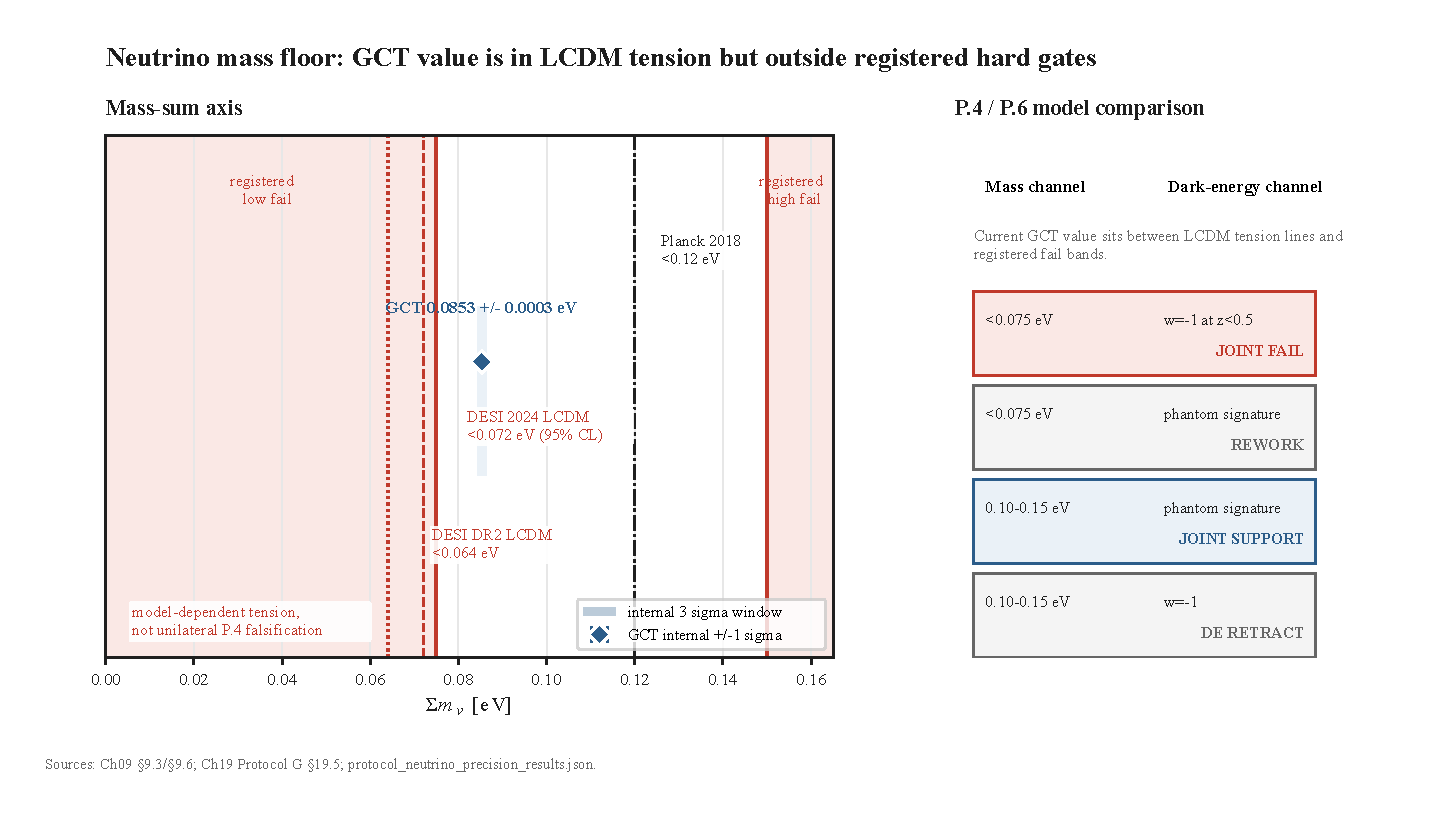
\includegraphics[keepaspectratio,alt={Registered GCT candidate \textbackslash Sigma m\_\textbackslash nu = 0.0853 \textbackslash pm 0.0003 eV (a consistency scale from the Tier 3 floor plus measured oscillation gaps); current DESI/CMB \textbackslash Lambda\hspace{0pt}CDM bounds are tension bands, while the registered hard gates are \textless0.075 eV or \textgreater0.15 eV at definitive precision.}]{content/Figures/Volume_3/Figure V3.9.1.pdf}}
\caption{Registered GCT candidate \(\Sigma m_\nu = 0.0853 \pm 0.0003\)
eV (a consistency scale from the Tier 3 floor plus measured oscillation
gaps); current DESI/CMB \(\Lambda\)\hspace{0pt}CDM bounds are tension
bands, while the registered hard gates are \(<0.075\) eV or \(>0.15\) eV
at definitive precision.}
\end{figure}

\begin{center}\rule{0.5\linewidth}{0.5pt}\end{center}

\subsection{9.4 Oscillation Parameters: PMNS Axis
Sliding}\label{oscillation-parameters-pmns-axis-sliding}

\subsubsection{9.4.1 Unpinned Axis Sliding vs Pinned Face
Tunneling}\label{unpinned-axis-sliding-vs-pinned-face-tunneling}

In GCT, the dichotomy between the small hadronic and large leptonic
mixing angles is modelled as mechanical {[}Tier 3 picture{]}:

\begin{itemize}
\tightlist
\item
  \textbf{Quarks (CKM Matrix):} In the Tier 3 candidate assignment (V3
  Ch03 §3.4), quarks are \emph{Interstitial Face Defects} bound deeply
  within the strong-force lattice. Their mixing requires \textbf{Pinned
  Face Tunneling}, which is highly damped by the electromagnetic
  viscosity (\(\alpha\)), resulting in small mixing angles.
\item
  \textbf{Neutrinos (PMNS Matrix):} Neutrinos are \textbf{Itinerant
  Phason Waves}. In this picture their oscillation is the transit of
  flavour states through the internal (\(E_\perp\)) phason sector
  {[}Tier 3 picture{]}. Since they are unpinned, their mixing samples
  the pure unpinned geometry of the projection, executing
  \textbf{Unpinned Axis Sliding}. In this Tier 3 ansatz the angles are
  thus large, candidate raw crystallographic values essentially undamped
  by standard vacuum friction.
\end{itemize}

\subsubsection{9.4.2 The Geometric PMNS
Matrix}\label{the-geometric-pmns-matrix}

The Tier 3 PMNS ansatz assigns the mixing angles from the rotational
properties of the Golden Projection:

\begin{itemize}
\tightlist
\item
  \textbf{\(\theta_{12}\) (Solar):} Governed by the \textbf{Golden
  Angle} of the projection {[}Tier 3{]}. The bare geometric prediction
  is \(\theta_{12} = \arctan(1/\phi) \approx 31.7^\circ\) {[}Tier 3{]}.
  The gap to the data is then closed by a post-hoc correction, one fifth
  of the bare reactor angle \(\theta_{13}^{base} = \arcsin(\phi^{-4})\)
  (below):
  \(\theta_{12} = \arctan(1/\phi) + (\theta_{13}^{base} / 5) \approx \mathbf{33.40^\circ}\)
  {[}Tier 3/4 fitted correction, no derivation{]}, against NuFIT 6.0
  \(33.68^{+0.73}_{-0.70}{}^\circ\) (\(-0.4\sigma\)).
\item
  \textbf{\(\theta_{23}\) (Atmospheric):} The bare GCT prediction is
  exactly maximal (\(45^\circ\)) {[}Tier 3{]}, arising from the strict
  3-fold symmetry constraints of the static icosahedral window's
  alignment against the 6D hypercube.
\end{itemize}

In the NuFIT 6.0 global fit (normal ordering) the best fit depends on
whether Super-Kamiokande atmospheric data are included: \(43.3^\circ\)
(lower octant) with them and \(48.5^\circ\) (upper octant) without them.
In both cases \(45^\circ\) lies inside the \(3\sigma\) range
(\(41.3^\circ\)--\(49.9^\circ\) and \(41.0^\circ\)--\(50.5^\circ\)
respectively). Maximal mixing is therefore allowed by current data, and
the octant is unresolved. The earlier ``4.09σ'' tension, computed as a
one-octant Gaussian on an unsourced \(49.5^\circ \pm 1.1^\circ\), is
withdrawn.

\textbf{The Itinerant Volume Drag Is Not Part of GCT.} A \(\phi^{-3}/3\)
``Itinerant Volume Drag'' perturbation is not part of the GCT framework.
The perturbation Hamiltonian
\(\Delta\hat{H}_{drag} = \gamma(\mathbf{J} \cdot \mathbf{w})\) and the
associated shift \(\Delta\theta = \phi^{-3}/3 \approx 4.509^\circ\)
would be phenomenological fits whose coupling constant \(\gamma\) is not
derived from the phason elastic action; admitting them would add an
undisclosed sector handle. GCT therefore does not invoke this term.

\textbf{Tier Classification of the Bare Prediction.} The derivation
mechanism --- 3-fold rotational symmetry of the AKN icosahedral
projection window acting on unpinned itinerant phason waves --- is a
proposed geometric consequence of the icosahedral ansatz {[}Tier 3{]},
with no additional fitted coefficient in this local calculation. The
quantitative claim \(\theta_{23} = 45^\circ\) is consistent with the
current \(3\sigma\) ranges and is classified \textbf{Tier 3} (octant
open). It is not classified as a confirmed Tier 2 prediction.

\textbf{Decisive test.} Octant-resolving long-baseline data from DUNE
and Hyper-Kamiokande decide the bare prediction: a determination that
excludes \(\theta_{23} = 45^\circ\) at \(>3\sigma\) falsifies it. Matter
effects cannot rescue it, since standard Mikheyev-Smirnov-Wolfenstein
(MSW) corrections shift \(\theta_{23}\) by only \(\sim 0.00004^\circ\).

\begin{itemize}
\tightlist
\item
  \textbf{\(\theta_{13}\) (Reactor):} Driven by the hierarchical decay
  suppression {[}Tier 3{]}:
  \(\theta_{13} = \arcsin(\phi^{-4}) \approx \mathbf{8.39^\circ}\)
  {[}Tier 3{]}, against NuFIT 6.0 \(8.52^\circ \pm 0.11^\circ\) without
  SK-atm (\(-1.5\%\), \(-1.2\sigma\)) or \(8.56^\circ \pm 0.11^\circ\)
  with it (\(-2.0\%\), \(-1.6\sigma\)); this is a postdiction.
\end{itemize}

As evidence that φ or icosahedral structure is special, the
\(\theta_{12}\) and \(\theta_{13}\) matches above (and the
\(\delta_{CP}\) value of §9.4.3) are \textbf{Tier 4}: the preregistered
constant control test (v3, NEGATIVE-FRAGILE; App PSC §PSC.9.6) found φ's
pattern of matches on 21 constants not distinguishable from that of
random constants (58 of 300 random bases did at least as well). The test
``excludes, at power ≥ 0.8, an effect in which φ hits at least 6 of the
8 informative rows through a real effect; weaker effects are not
excluded.'' The numbers are kept as descriptive arithmetic. The φ-free
\(\theta_{23}=45^\circ\) prediction and the \(\phi^{-36}\) mass floor
are not part of that relabel.

\subsubsection{\texorpdfstring{9.4.3 CP Violation Phase
(\(\delta_{CP}\)) {[}Tier
3{]}}{9.4.3 CP Violation Phase (\textbackslash delta\_\{CP\}) {[}Tier 3{]}}}\label{cp-violation-phase-delta_cp-tier-3}

GCT proposes a CP violation phase motivated by the chirality of the
\(\phi\)-projection {[}Tier 3 ansatz{]}: a \(2\pi\) rotation of the
cut-and-project window is assigned a chiral holonomy fixed by the
golden-ratio slope of the projection. This phase is not the
Jackiw--Rebbi domain-wall result: that result (V3 Ch02 §2.4.2) concerns
gauge chirality and does not fix this phase (V3 Ch10 §10.6.1):

\[\delta_{CP} = 360^\circ \times \phi^{-1} \approx 222.49^\circ \quad \text{[Tier 3]}\]

This is a Tier 3 PMNS-sector phase ansatz: the phase is the canonical
golden-angle complement, with no additional fitted coefficient within
this sector once the chiral projection is fixed, but the
holonomy-to-observed-PMNS mapping remains uncomputed and the value
\(222.49^\circ\) is compared with NuFIT 6.0 normal-ordering best fits of
\(212^\circ\) (with SK-atm, within \(1\sigma\)) and \(177^\circ\)
(without it, about \(2.4\sigma\) on the quoted \(1\sigma\) error); the
\(\delta_{CP}\) errors are non-Gaussian, so the row is an open data
handle rather than a confirmed Tier 2 prediction (Tier 4 as evidence:
not distinguishable from numerology for strong effects; App PSC
§PSC.9.6).

\gctneedspace{5\baselineskip}\begin{gctImportant}

\textbf{Jarlskog invariant status:} The GCT Jarlskog invariant
\(J_{GCT}\) is currently an \textbf{Open Research Problem (App ORQ
§ORQ.5, O.7)}. A natural target is \(J_{GCT} \propto \phi^{-n}\) for
some integer \(n\) tied to the lepton harmonic ladder (the candidate
\(n = 22 = 2 \times 11\) matching two-loop muon-harmonic CP-violation
amplitudes is conjectural and bundled with the QLQCD-1L research debt).
The \(\delta_{CP} = 360^\circ \times \phi^{-1}\) Tier 3 phase ansatz
above stands \textbf{independently} of any \(J\) value --- it is
motivated by the chirality of the icosahedral projection (not by the
Jackiw--Rebbi domain-wall result of V3 Ch02 §2.4.2), and not by a
computed PMNS-sector holonomy or a Jarlskog extraction.

\end{gctImportant}

The independent Tier 3 phase ansatz for \(\delta_{CP}\) from the chiral
projection (the boxed identity above) preserves the downstream use of
\(\delta_{CP}\) in App PSC's CP-violation precision row. The eEDM
estimate of §9.6.3 does not use this phase: it is a quark-sector scaling
with the CKM invariant \(J_{\rm CKM}\) (Open Problem O.7).

\begin{center}\rule{0.5\linewidth}{0.5pt}\end{center}

\subsection{9.5 Physical
Interpretation}\label{physical-interpretation-5}

\subsubsection{9.5.1 Majorana Nature as Self-Duality {[}Tier 3 model
prediction; experimentally
open{]}}\label{majorana-nature-as-self-duality-tier-3-model-prediction-experimentally-open}

GCT predicts that neutrinos are \textbf{Majorana Fermions} as a
model-level consequence of the self-dual defect picture. The picture
reads the left-handed state (\(E_\parallel\)) and right-handed state
(\(E_\perp\)) as Galois conjugates of one another, two views of a single
6D lattice excitation (the Tier 3 assignment of §9.2.1). This is not a
Tier 2 result until the self-duality-to-lepton-number-violation bridge
is derived and a neutrinoless double-beta-decay gate is satisfied; a
robust \(0\nu\beta\beta\) null across the GCT mass-ordering window would
force demotion or replacement of the Majorana reading.

\subsubsection{9.5.2 Itinerant
Wave-Packets}\label{itinerant-wave-packets}

Unlike the electron, which ``holds'' its position, the neutrino is the
``wave'' of the window flipping tiles as it moves. It is modelled as a
phason ripple whose registered mass-floor candidate is pictured as the
topological work required to transport a framed ribbon through the Higgs
background {[}Tier 3 picture{]}.

\begin{center}\rule{0.5\linewidth}{0.5pt}\end{center}

\subsection{9.6 Experimental
Predictions}\label{experimental-predictions-1}

\subsubsection{\texorpdfstring{9.6.1 The \(0.015\) eV Floor {[}Tier 2
squared-stiffness relation + Tier 3 P3b stiffness map + Tier 3 absolute
anchor{]}}{9.6.1 The 0.015 eV Floor {[}Tier 2 squared-stiffness relation + Tier 3 P3b stiffness map + Tier 3 absolute anchor{]}}}\label{the-0.015-ev-floor-tier-2-squared-stiffness-relation-tier-3-p3b-stiffness-map-tier-3-absolute-anchor}

The \(0.015\) eV floor is not KATRIN-falsifiable: the effective
\(m_\beta\) for this branch is only \(\sim 0.018\) eV (normal ordering
with NuFIT 6.0 splittings), far below the current KATRIN limit; it is
tested via the cosmological \(\Sigma m_\nu\) gate P.4, with
\textbf{Project 8} as a long-horizon direct probe. While the current
direct limit is \(m_\nu < 0.45\) eV (90\% CL; KATRIN 2025), GCT's
phason-stiffness mechanism with the Tier 3 P3b stiffness map and the
disclosed electron/oscillation anchors places the candidate mass floor
at \(0.015\) eV {[}Tier 3 conditional on P3b + the absolute anchor A1;
the abstract squared-stiffness relation is Tier 2{]}.

\subsubsection{9.6.2 Falsification via Euclid and
DESI}\label{falsification-via-euclid-and-desi}

The registered candidate \(\sum m_\nu \approx 0.0853\) eV (a consistency
scale, §9.3.4) enters a \textbf{joint reporting matrix} with the
conditional dark-energy coordinate (§9.3.4; Appendix NSM). The
observables are not physically coupled by this matrix.

\begin{itemize}
\tightlist
\item
  \textbf{Both templates supported (NS scenario A):} Matching both
  registered numerical bands supports both model templates but does not
  confirm a biogenic causal mechanism.
\item
  \textbf{Both templates excluded (NS scenario D):} A definitive
  mass-floor exclusion and independent exclusion of the conditional
  dark-energy template reopen their respective model sectors; this is
  not evidence for a shared causal failure.
\item
  \textbf{Mixed cells (NS scenarios B/C):} Each template receives its
  own disposition and the affected section is reworked independently, as
  specified in App NSM.
\item
  \textbf{Independent falsifier:} Confirmation of \textbf{Inverted
  Ordering} (\(m_3 < m_1 < m_2\)) at \(>3\sigma\) falsifies GCT's
  conditional Growth-Axiom Normal Ordering prediction (§9.3.3)
  independently of the \(\Sigma m_\nu\) joint gate.
\end{itemize}

\subsubsection{\texorpdfstring{9.6.3 The Electron Electric Dipole Moment
(eEDM) {[}Tier 3 quark-sector scaling with \(J_{\rm CKM}\) / magnitude
pending
O.7{]}}{9.6.3 The Electron Electric Dipole Moment (eEDM) {[}Tier 3 quark-sector scaling with J\_\{\textbackslash rm CKM\} / magnitude pending O.7{]}}}\label{the-electron-electric-dipole-moment-eedm-tier-3-quark-sector-scaling-with-j_rm-ckm-magnitude-pending-o.7}

GCT's CP-violation sector is carried here by a single rephasing
invariant, the CKM Jarlskog invariant \(J_{\rm CKM}\), whose
first-principles value is Open Problem O.7 (App ORQ §ORQ.5). The PMNS
phase ansatz of §9.4.3 is a separate Tier 3 statement and does not enter
this estimate. In the GCT defect-core picture, CP violation in the
electroweak sector would generate a non-zero \textbf{Electron Electric
Dipole Moment (eEDM)} at two- or three-loop order through the \(N=144\)
dodecahedral cage vertices. In the Standard Model, CKM-phase
contributions to \(d_e\) vanish through three loops; a two- or
three-loop contribution of this size is therefore a
beyond-Standard-Model claim of the GCT defect-core picture {[}Tier 3{]}.

\gctneedspace{5\baselineskip}\begin{gctImportant}

\textbf{Two-layer structure:} The \emph{parametric scaling} --- that the
eEDM scales linearly in \(J_{\rm CKM}\) with two powers of
\(\alpha/\pi\) --- is a two-loop power-counting estimate and a Tier 3
scaling statement. \(J_{\rm CKM}\) already contains the CP phase
(\(J = c_{12}c_{23}c_{13}^2 s_{12}s_{23}s_{13}\sin\delta\)), so no
separate phase factor appears. The numerical magnitude is Tier 3 pending
closure of O.7. The scaling alone does not fix a magnitude: any
numerical comparison with experiment requires a value of
\(J_{\rm CKM}^{\rm GCT}\) and a derived prefactor.

\end{gctImportant}

\gctneedspace{5\baselineskip}

\textbf{Parametric scaling (Tier 3 order-of-magnitude statement):}
\[|d_e^{GCT}| \;\propto\; \frac{\alpha^2}{\pi^2} \cdot |J_{\rm CKM}^{\rm GCT}| \quad [e \cdot \text{cm}]\]
The dimensionful prefactor (of order \(e\hbar/(m_e c)\) times further
loop and mass suppressions) is not derived. Below, the scaling is
referenced to \(1.1 \times 10^{-29}\, e \cdot \text{cm}\) at
\(J_{\rm CKM}^{\rm GCT} = 10^{-3}\); that reference is the ACME II
limit, used as a scale, not a derived normalization.

\gctneedspace{5\baselineskip}

\textbf{Unitarity envelope (Tier 3; not constraining):} Three-generation
unitarity bounds the rephasing invariant by
\(|J| \leq 1/(6\sqrt{3}) \approx 0.096\). Under the reference
normalization the scaling grows linearly in \(J_{\rm CKM}^{\rm GCT}\),
so at the unitarity maximum the envelope is
\(\sim 10^{-27}\, e \cdot \text{cm}\). That lies above the current
experimental limits (\(|d_e| < 1.1 \times 10^{-29}\)
\(e \cdot \text{cm}\), ACME II 2018, Andreev et al.~2018 \emph{Nature}
562:355; \(|d_e| < 4.1 \times 10^{-30}\) \(e \cdot \text{cm}\), JILA
2023, Roussy et al.~2023 \emph{Science} 381:46), so a \(J\)-independent
envelope does not constrain the model. The value
\(1.1 \times 10^{-29}\, e \cdot \text{cm}\) corresponds to an assumed
\(J \sim 10^{-3}\) and coincides with the ACME II limit by construction;
it is not an independent bound.

\gctneedspace{5\baselineskip}

\textbf{Conditional magnitude estimate {[}Tier 3 --- does NOT enter the
falsification gate{]}:} If \(J_{\rm CKM}^{\rm GCT}\) takes a value at
the candidate scale \(\sim O(\phi^{-22})\) catalogued under O.7, the
reference normalization gives
\(d_e^{GCT} \approx 3 \times 10^{-31}\, e \cdot \text{cm}\)
(\(\phi^{-22} = 2.525 \times 10^{-5}\)). This conditional magnitude is
provided for orientation only and inherits the underived prefactor. A
sensitivity of \(\sim 10^{-31}\, e \cdot \text{cm}\) is reached at
\(J_{\rm CKM}^{\rm GCT} \approx 9 \times 10^{-6}\) under the same
normalization; below that the signal is indistinguishable from \(J = 0\)
--- an O.7 sensitivity issue, not a falsification.

\textbf{Next-generation detection {[}Tier 3, conditional on
\(J_{\rm CKM}^{\rm GCT}\) and the underived prefactor{]}:} the
conditional \(\sim 3 \times 10^{-31}\, e \cdot \text{cm}\) magnitude
lies an order of magnitude below the ACME III target
(\(\sim 3 \times 10^{-30}\, e \cdot \text{cm}\)) and below the current
JILA molecular-ion limit (Cairncross et al.~2017; Roussy et al.~2023).
Reaching it requires electron-EDM sensitivity near
\(10^{-31}\, e \cdot \text{cm}\).

\textbf{Epistemic Status {[}Tier 3 scaling / Tier 3 magnitude pending
O.7{]}.} This estimate has two layers: (i) the \textbf{parametric
scaling} (\(d_e \propto J_{\rm CKM} \cdot \alpha^2/\pi^2\)) is a
beyond-Standard-Model loop-structure claim; (ii) the \textbf{numerical
magnitude} (\(\sim 3 \times 10^{-31}\) \(e \cdot \text{cm}\) under the
reference normalization) is Tier 3 because it depends on
\(J_{\rm CKM}^{\rm GCT}\) (Open Problem O.7, bundled with the QLQCD-1L
research debt) and on an underived prefactor.

\textbf{Falsification.} Because neither \(J_{\rm CKM}^{\rm GCT}\) (O.7)
nor the dimensionful prefactor is derived, no current or near-term eEDM
limit falsifies the mechanism. Under the reference normalization, a
limit \(|d_e| < 10^{-32}\) \(e \cdot \text{cm}\) at \(3\sigma\) would
exclude \(J_{\rm CKM}^{\rm GCT}\) at or above the candidate
\(\phi^{-22}\) scale. A detection in the range
\(10^{-31}\)--\(4.1 \times 10^{-30}\) \(e \cdot \text{cm}\) (the upper
end is the JILA 2023 limit) would be consistent with, but would not by
itself establish, the GCT defect-core picture.

\gctneedspace{5\baselineskip}

\textbf{END OF CHAPTER 9}

\chapter{Chapter 10: The Extended Spectrum --- Quarks and
Hadrons}\label{chapter-10-the-extended-spectrum-quarks-and-hadrons}

In the Standard Model, the masses of quarks and the resulting composite
hadrons are determined by non-perturbative dynamics that remain
computationally elusive. Geometric Consciousness Theory (GCT) identifies
the hadron sector not as a separate class of physics, but as the
\textbf{Crystallographic Inventory} of the vacuum interstices. While
leptons correspond to node-centered vertex defects, quarks correspond,
as a Tier 3 candidate assignment (V3 Ch03 §3.4), to \textbf{Interstitial
Face Defects}. This chapter gives the tiered hadron-sector account: Tier
2 mechanisms where the geometric chain is active, Tier 3 ansätze for
unresolved harmonic / transfer choices, the down-quark mass as a Tier 2
Fuglede-Kadison-determinant mechanism tested against a registered 11\%
band, whose finite-cage values oscillate between about \(-3.4\%\) and
\(+9.8\%\) around \(\phi^{\phi}\) (the closed form
\(m_d = m_u\phi^{\phi}\), \(+0.33\%\) from PDG, is a Tier 3
identification of the median, with convergence conditional on O.5), and
the proton-mass route as \textbf{Tier 2 mechanism + Tier 3
sheet/exponent handle pending AKN-action closure}. As evidence that φ is
special, the φ-formula matches of this chapter are Tier 4 (not
distinguishable from numerology for strong effects; App PSC §PSC.9.6;
§10.3.3).

The candidate harmonic orders lie in a \textbf{conditional
Galois/gap-label candidate space} (Appendix FTH, Proposition FTH.5): for
observables built from the adopted icosahedral cut-and-project
coordinates and the specified Fibonacci gap-label toy models, the
candidate labels lie in \(\mathbb{Z}[\phi]\) {[}Tier 1 algebra
conditional on the adopted model; Tier 3 physical adoption{]}. This
constrains an algebraic search space; it does not select which
generation maps to which order, and the Galois automorphism
\(\phi \to -1/\phi\) is an algebraic coordinate map that fixes no
physical sign. The same conditional range applies to leptons, neutrinos,
and quarks.

\begin{center}\rule{0.5\linewidth}{0.5pt}\end{center}

\subsection{10.1 Interstitial Defects (Quark
Structure)}\label{interstitial-defects-quark-structure}

\subsubsection{10.1.1 The Codimension of Defects: Quarks
vs.~Leptons}\label{the-codimension-of-defects-quarks-vs.-leptons}

GCT classifies elementary fermions by their topological codimension
within the icosahedral tiling (the quark-as-face-defect entry is the
Tier 3 candidate assignment of V3 Ch03 §3.4):

\begin{itemize}
\tightlist
\item
  \textbf{Vertex Defects (Leptons):} Possess \textbf{Codimension 3} (a
  point in 3D physical space). Their energy scales linearly with the
  inflation of the lattice radius (\(\phi^1\)).
\item
  \textbf{Interstitial Defects (Quarks; Tier 3 candidate assignment, V3
  Ch03 §3.4):} Carry a mismatch on a 2-dimensional facet (a surface
  object in 3D, i.e.~codimension 1 there; a facet of the 6D parent
  lattice has codimension 4). In the Tier 3 heuristic their energy
  scales with the inflation of the projected facet area (\(\phi^2\)).
\end{itemize}

While a quark appears point-like when bound within a hadron in the 3D
projection, its underlying geometry in the 6D parent lattice is a
mismatch on a 2-dimensional facet; how such a facet defect stays
localised rather than costing wall energy (area × extent) is not derived
here. On that Tier 3 assignment, this area-based topology is proposed as
the mechanical origin of the \textbf{Area-Law Scaling (\(\phi^2\))}
observed in the quark mass hierarchy.

\subsubsection{10.1.2 Color Charge and Burgers Vector
Alignment}\label{color-charge-and-burgers-vector-alignment}

The 30 rhombic faces of the rhombic triacontahedron have their normals
along the \textbf{15 two-fold axes} of the icosahedral symmetry; none
lies on a three-fold axis. The 10 three-fold axes pass instead through
the 20 three-valent vertices. If a quark is a face defect (Tier 3
candidate assignment, V3 Ch03 §3.4), assigning its \textbf{Burgers
Vector} \(\mathbf{b}_\perp\) (the measure of lattice mismatch) to a
three-fold axis is therefore not a geometric identity; it is an open
Tier 3 assignment with no derivation yet. As a Tier 3 candidate
identification, ``color'' is the phenomenological registration of this
internal axis alignment. Quarks are color triplets (fundamentals of
\(SU(3)_C\)); physical hadrons are color singlets formed by \(SU(3)_C\)
confinement. In the GCT candidate model, the triplet color label would
track which internal three-fold-axis branch carries the face-defect
mismatch, while the singlet condition is imposed only on confined hadron
states.

\subsubsection{10.1.3 The Gluon String and Mechanical
Confinement}\label{the-gluon-string-and-mechanical-confinement}

In the 6D parent lattice, an uncompensated interstitial face defect
creates a 5-dimensional fault plane (a grain boundary) extending through
the Bulk. In a supersolid vacuum, this fault plane carries divergent
energy. In the Tier 3 confinement proposal, satisfying the Hamiltonian
constraint \(\hat{H}\Psi=0\) requires the strain field to collapse into
a one-dimensional \textbf{Gluon String} or flux tube.

In this Tier 3 candidate picture, confinement is a \textbf{Mechanical
Requirement} of the crystalline substrate. A quark mismatch must either
terminate on an antiquark or form a closed 3-cycle (Baryon) to satisfy
the \textbf{Global Singlet Condition}
(\(\sum \text{winding} \equiv 0 \pmod 3\)). A hadron is a \textbf{Closed
Grain Boundary} that allows the vacuum to remain stress-free at
macroscopic distances.

\begin{center}\rule{0.5\linewidth}{0.5pt}\end{center}

\subsection{10.2 The Top Quark (The Geometric
Lock)}\label{the-top-quark-the-geometric-lock}

\subsubsection{10.2.1 The Universal Yield Strength {[}Tier 2 geometric
motif + Tier 3 top-mass
ansatz/residual{]}}\label{the-universal-yield-strength-tier-2-geometric-motif-tier-3-top-mass-ansatzresidual}

The Top Quark is the only fermion with a Yukawa coupling
\(y_t \approx 1\). GCT identifies the Top Quark as the \textbf{Universal
Yield Strength} of the vacuum hardware.

\textbf{Ansatz 10.1 {[}Tier 3 top-mass identification{]}:} \emph{We
posit that the Top Quark represents the lattice fracture limit, where
the volumetric strain (Higgs dilation) is accompanied by a shear
displacement of one unit-cell diagonal.}

\subsubsection{\texorpdfstring{10.2.2 Derivation from the \(D_6\) Face
Diagonal
(\(\sqrt{2}\))}{10.2.2 Derivation from the D\_6 Face Diagonal (\textbackslash sqrt\{2\})}}\label{derivation-from-the-d_6-face-diagonal-sqrt2}

The Top Quark mass (\(m_t\)) geometrically locks to the absolute GCT
Higgs-VEV pipeline value \(v_{\rm GCT}=246.1755\) GeV (V3 Ch05;
\texttt{protocol\_higgs\_vev.py}). The mass of the Top Quark is defined
as the energy required to dilate a unit cell facet by its diagonal
length, triggering a lattice fracture. This represents exactly half the
VEV scaled by the \(D_6\) root lattice face diagonal (\(\sqrt{2}\)):
\[\begin{gathered}m_t = \left(\frac{v_{\rm GCT}}{2}\right) \cdot \sqrt{2} \approx \mathbf{174.072 \text{ GeV}} \\[1pt] \gcteqnote{[Tier 2 mechanism + Tier 3 state-level/QCD-pole residual]}\end{gathered}\]

This derived value is the \textbf{Bare Lattice Mass} at the
crystallization scale. Its comparison to the observed top mass remains a
Tier 3 state-level/mass-scheme residual pending QLQCD closure. Against
the PDG 2024 direct-measurement mass (\(172.57\pm0.29\) GeV, not a pole
mass) the residual is \(5.18\sigma\), outside P.24's written PDG
\(\pm5\sigma\) falsification rule (registered since v1.2.0), so the row
is reported as a \textbf{FAIL of the written rule} --- one standard with
the electron row (App FSM P.1c). The residual is carried as a Tier 3
state-level/QCD-pole residual pending O.5; a pole/MS-bar uncertainty
model would be a new pre-registered band, not applied retroactively.
Against PDG's pole mass from cross-section measurements (\(172.4\pm0.7\)
GeV) the prediction sits at \(\approx2.4\sigma\); the mass-scheme
question is open, and the comparator registered since v1.2.0 is not
swapped after the result, so the FAIL of the written rule stands.

\gctneedspace{5\baselineskip}\begin{gctNote}

\textbf{Tree-Level QCD Residual (0.87\%): Not Closed (P.24 written rule
failed)} The GCT formula \(m_t = (v_{\rm GCT}/2)\sqrt{2}\) is a
tree-level prediction. The leading-order QCD correction from the
pole-mass/MS-bar running is:
\[\begin{aligned}\Delta m_t^{QCD} &\approx \frac{4}{3}\frac{\alpha_s}{\pi} \times m_t \\ &\approx \frac{4}{3} \times \frac{0.1180}{\pi} \times 174.072 \approx +8.7 \text{ GeV (one-loop pole/MS-bar scale estimate)}\end{aligned}\]
{[}Tier 3{]} (using \(\alpha_s(M_Z)=0.1180\); at \(\mu = m_t\),
\(\alpha_s \approx 0.108\) gives \(\approx +8.0\) GeV, which does not
change the conclusion) This naïve one-loop correction is \(\sim 5\%\) of
the mass and overcorrects the observed \(\sim 0.87\%\) tree-level
residual. The residual is therefore \textbf{not closed by the displayed
one-loop arithmetic}; it is only bounded as a loop-order-scale effect
and constitutes \textbf{Open Research Debt QLQCD-2L} (see Appendix QLA).
Tier 2 closure requires a full QLQCD two-loop computation anchored to
the GCT lattice RGE framework.

\end{gctNote}

\begin{center}\rule{0.5\linewidth}{0.5pt}\end{center}

\subsection{10.3 The Proton Mass (The Baryonic
Triad)}\label{the-proton-mass-the-baryonic-triad}

\subsubsection{\texorpdfstring{10.3.1 The Challenge: \(m_p\) at
Mechanism
Level}{10.3.1 The Challenge: m\_p at Mechanism Level}}\label{the-challenge-m_p-at-mechanism-level}

GCT models the proton mass (\(938.272\) MeV) not through stochastic
simulation, but as a \textbf{Resonant Eigenvalue} of a 3-quark complex
{[}Tier 2 mechanism + Tier 3 sheet/exponent handle{]}.

\subsubsection{10.3.2 The Baryonic Energy
Functional}\label{the-baryonic-energy-functional}

To motivate the mass eigenvalue, we write a candidate energy functional
\(E[\Phi]\) for a 3-quark defect (Triad) on the lattice. Its
\(\sigma_{string}\) term is the Tier 3 flux-tube proposal (V3 Ch03
§3.5.2); the mass formula below does not use it:
\[ E[\Phi] = \int d^3x \left( \frac{1}{2} K_\perp (\nabla \mathbf{w})^2 + V_{lock}(\Phi) + \sigma_{string} \sum_{i=1}^3 \delta(\mathbf{x} - \mathbf{q}_i) \right) \]

\gctneedspace{5\baselineskip}

\textbf{The Base Exponent (15) {[}Tier 2 \(Z_3 \times Z_5\) closure
template + Tier 3 selection and deployment of 15{]}:} The winding number
\(N\) of the ground state is determined by the \textbf{Topological
Closure} of the defect surface. The defect wraps the 3 quarks (homotopy
\(Z_3\)) around the 5-fold symmetry axis of the cage (homotopy \(Z_5\)).
Within the \(Z_3 \times Z_5\) closure template, the minimal non-trivial
winding that closes the surface without breaking the lattice symmetry is
the product of the winding numbers {[}Tier 2 counting{]}. The factor 3
is the empirical valence-quark count; reading the quarks as face defects
or as colour triplets is the Tier 3 assignment of V3 Ch03 §3.4:
\[ \begin{gathered}N_{baryon} = 3 \times 5 = 15 \\[1pt] \gcteqnote{[Tier 2 counting; Tier 3 as the physical base exponent]}\end{gathered}\]
This reads ``15'' as the \textbf{candidate winding generator} of the
baryonic triad sector under the \(Z_3 \times Z_5\) closure rule; a full
configuration-space proof of
\(\pi_1(\text{Triad}) \cong \mathbb{Z}_{15}\) remains part of the
hadron-sector closure.

The physical proton-mass formula still uses the sheet/exponent handle
\(15+\phi^{-1}\) as a Tier 3 hadron-sector anchor pending AKN-action /
QLQCD closure. The \(Z_3 \times Z_5\) counting is the Tier 2 mechanism;
selecting 15 as the physical base exponent, and the full exponent used
in the 155 ppm headline, are Tier 3 (App USS §USS.3) and are not a
hidden closed derivation from the current postulate set.

\subsubsection{10.3.3 The Weak Berry Phase
Correction}\label{the-weak-berry-phase-correction}

The proton is not a pure strong-force object; it carries Electroweak
charge. As the defect winds the Strong sector (15), it accumulates a
secondary \textbf{Berry Phase} from its transport through the candidate
internal Weak bundle (placed on the \(E_\perp\) side; Tier 3 placement,
V3 Ch02 §2.1.1 and V3 Ch06 §6.1.2).

The \(2I\) fiber geometry fixes only the parity of this \(SU(2)\) Weak
holonomy {[}Tier 1{]}; the half-weight connection
\(A_\theta = \frac{1}{2}\sigma_z\) and the selection of \(n = 1\) are a
Tier 3 central-holonomy ansatz (the minimality premise of V3 Ch18
§18.2.3.A and App USS §USS.8), adopted rather than derived from the
geometry. With that ansatz, the path-ordered integral around the
\(2\pi\) baryonic loop (the 5-fold axis) yields \(U_{weak} = -I_2\).
This corresponds to a Berry phase of \(\pi\), which is a half-winding
(\(N_{weak}=1/2\)). Applying the icosahedral projection ratio
\(R = 2\phi^{-1}\) (whose factor of 2 rests on the Tier 3
constructive-sheet input below) yields the correction:
\[ \text{Correction} = N_{weak} \cdot R = \left(\frac{1}{2}\right) \cdot (2\phi^{-1}) = \phi^{-1} \]

\begin{quote}
\textbf{Postulate (Projection Ratio): {[}Tier 2 mechanism / Tier 3
specific value of the doubling factor{]}} \emph{The effective projection
ratio \(R\) for a Berry phase accumulated over a 5-fold axis is
\(R = 2\phi^{-1}\).}

\emph{Status note.} The label ``Postulate'' rather than ``Theorem''
reflects that the spinor-doubling argument below establishes the
\emph{form} \(R = N_{\rm sheet} \cdot \phi^{-1}\) via icosahedral
pentagon geometry + double-cover sheet counting, but the \emph{specific
value} \(N_{\rm sheet} = 2\) for the baryonic defect requires the
structural commitment that both spinor sheets contribute coherently
rather than destructively. A first-principles derivation of this
constructive-vs-destructive sheet-summation rule from the AKN action ---
closing the postulate-to-theorem gap --- is an open follow-up bundled
with Open Problem O.5 (QLQCD-1L closure). The resulting
\(R = 2\phi^{-1}\) is Tier 2 as a geometric form + Tier 3 as a specific
doubling factor; its numerical match against the observed proton-mass
exponent is Tier 4 as evidence (not distinguishable from numerology for
strong effects; App PSC §PSC.9.6).

\emph{Argument sketch (Spinor Doubling; not a proof):} The Berry
connection \(A\) couples to the orientation of the defect frame. For a
5-fold axis in the Icosahedral group \(H_3\), the single-sheet
contribution is taken to be the edge-to-diagonal ratio of the regular
pentagon, \(\phi^{-1}\). Identifying this length ratio with the
projected-area weight of the pentagonal face is an asserted step, not a
derived one {[}Tier 3{]}. This is the contribution from a single
geometric ``sheet.''

However, the baryonic defect is a \textbf{spinor} (a fermion). Spinors
live on the \textbf{Double Cover} of the rotation group (\(SU(2)\) over
\(SO(3)\)). Under the constructive-sheet postulate, a complete physical
orbit of the defect traverses \textbf{both sheets} of this covering map
with coherent contribution from the Spin-Up sector
(\(|\uparrow\rangle\)) and the Spin-Down sector
(\(|\downarrow\rangle\)). The total Berry phase is then the coherent sum
over both sheets:
\[ R = \sum_{\text{sheets}} R_{\text{geometric}} = 1 \cdot (\phi^{-1}) + 1 \cdot (\phi^{-1}) = 2\phi^{-1} \]
This ``Spinor Doubling'' supplies the Tier 2 geometric mechanism, but
the constructive addition of the two sheets is the Tier 3 input
identified in the postulate above. Neglecting one sheet would not
realize the proposed baryonic SU(2) double-cover coupling, but a
first-principles AKN-action proof of coherent rather than destructive
sheet summation is still required before the factor of 2 can be promoted
to theorem status.
\end{quote}

The total scaling exponent is the sum of the primary (Strong) winding
and the secondary (Weak) winding:
\[ \Phi_{total} = N_{strong} + \text{Correction} = 15 + \phi^{-1} \]
Thus, the formula \(m_p \sim \phi^{15+\phi^{-1}}\) is the result of
\textbf{holonomic additivity} across the two fiber bundles (strong
winding and weak holonomy). Their independence is the Tier 3
sector-placement assumption of V3 Ch06 §6.2.1, not a consequence of the
\(E_\parallel \perp E_\perp\) orthogonality, since both are placed on
the internal side.

\gctneedspace{5\baselineskip}

\textbf{QCD Benchmarking (The Absolute Pipeline):} GCT sets out an
\textbf{End-to-End Absolute Mass Pipeline}, carried as a consistency
chain (see the precision notes below). Alongside the ratio route, which
uses the measured electron mass (the A1 anchor), GCT composes an
anchor-normalised Planck-link check that projects the proton mass from
the non-reduced Planck mass (\(M_{Planck}\)):

\begin{enumerate}
\def\labelenumi{\arabic{enumi}.}
\tightlist
\item
  \textbf{Geometric Anchor:}
  \(m_e = M_{Planck} \cdot \phi^{-107} \cdot (1 - 5\alpha)\)
\item
  \textbf{Harmonic Projection:}
  \(m_p = m_e \cdot \phi^{15 + \phi^{-1}}\)
\end{enumerate}

\begin{itemize}
\tightlist
\item
  \textbf{Ratio Precision (\(m_p/m_e\)) {[}Tier 2 mechanism + Tier 3
  sheet/exponent handle{]}:} The harmonic-projection formula evaluates
  to \(\phi^{15+\phi^{-1}} \approx 1836.437\), against the CODATA
  observed ratio \(1836.153\). The ratio residual is \textbf{+155 ppm
  (\(0.015\%\))}, inside the registered 500 ppm postdiction band; the
  row is a postdiction, not a live lattice-QCD falsifier. The Tier 2
  substance is the baryonic-triad harmonic mechanism; the sheet-doubling
  / coherent-summation handle and the specific composite exponent remain
  Tier 3 until the AKN-action proof closes. Anchored to the CODATA
  \(m_e\), the formula prediction is \(m_p \approx 938.417\) MeV against
  CODATA \(m_p = 938.272\) MeV --- same 155 ppm residual, expressed in
  absolute units. \emph{(Cross-reference: Ch18 §18.1.1 is the canonical
  Protocol F statement; Appendix PSC §PSC.3 ``Hadron Sector'' carries
  the precision scorecard entry.)}
\item
  \textbf{Absolute Pipeline Precision (\(M_{Planck} \to m_e \to m_p\))
  {[}Tier 2 mechanism + Tier 3 corrected-formula / AKN-action
  handle{]}:} The Planck-anchored end-to-end pipeline (App PSC §PSC.3,
  ``Absolute Pipeline'' row) carries the same \(\phi^{15+\phi^{-1}}\)
  harmonic projection composed with
  \(m_e = M_P \phi^{-107}(1-5\alpha)\). Its residuals are stepwise: the
  electron anchor from \(M_P\phi^{-107}(1-5\alpha)\) remains a
  corrected-formula postdiction at 1006 ppm (missing the LOCKED 1000 ppm
  pre-commitment by 6 ppm; App FSM P.1c reports a FAIL of that rule),
  the proton/electron harmonic projection contributes the quoted \(155\)
  ppm ratio residual, and the composed absolute mass inherits both open
  assumptions. It is therefore not a Tier 2 closure of the proton mass.
  The AKN-action / QLQCD closure path must still derive the sheet
  exponent and hadronic action correction before the absolute pipeline
  can be upgraded.
\end{itemize}

This derivation treats the proton as the fundamental acoustic resonator
of the 6D lattice and computes the mass from the CODATA \(m_e\)
dimensional anchor plus the \(\phi^{-1}\) sheet postulate (Tier 2
mechanism + Tier 3 sheet/exponent handle under the ratio-precision
disclosure). The Planck-to-proton absolute pipeline is carried only as a
consistency chain until the AKN-action status closes.

As evidence that φ or icosahedral structure is special, the proton match
(and the quark-mass and CKM matches of §10.4--§10.6) is \textbf{Tier 4}:
the preregistered constant control test (v3, NEGATIVE-FRAGILE; App PSC
§PSC.9.6) found φ's pattern of matches on 21 constants not
distinguishable from that of random constants (58 of 300 random bases
did at least as well). The test ``excludes, at power ≥ 0.8, an effect in
which φ hits at least 6 of the 8 informative rows through a real effect;
weaker effects are not excluded.'' The numbers are kept as descriptive
arithmetic. The tier tags of the mechanisms and handles in this chapter
(the \(Z_3\times Z_5\) count, the FK pseudo-determinant as mathematics,
the \(A_5\) dimension ratio) describe the ansatz, not the evidential
weight of the matches; the φ-free top-mass row is not part of this
relabel.

\gctneedspace{5\baselineskip}\begin{gctImportant}

\textbf{Firewall Metadata {[}Proton Mass{]}}

\begin{itemize}
\tightlist
\item
  \textbf{Type:} Postdiction
\item
  \textbf{Inputs:} \(m_e\) (A1 anchor, the sole dimensional input),
  \(\phi\) (Invariant), \(15+\phi^{-1}\) (Tier 3 sheet/exponent handle)
\item
  \textbf{Degrees of Freedom:} 0 continuous fitted parameters; A1
  electron anchor plus Tier 3 sheet/exponent handle \(15+\phi^{-1}\)
\item
  \textbf{Provenance:} Ratio route \(m_p = m_e\,\phi^{15+\phi^{-1}}\)
  (formula output \(1836.437\,m_e\) vs \(1836.153\), \(+155\) ppm,
  inside the 500 ppm postdiction band); the
  \(M_{Planck} \to m_e \to m_p\) pipeline is a consistency chain only
\item
  \textbf{Evidential status:} \textbf{Tier 4 as evidence} (φ-formula
  match; App PSC §PSC.9.6)
\end{itemize}

\end{gctImportant}

\begin{center}\rule{0.5\linewidth}{0.5pt}\end{center}

\subsection{10.4 The Quark Inventory {[}Tier 2 mechanisms + Tier
3/open-research state values; down-quark closed form conditional on O.5,
charm Tier 3
heuristic{]}}\label{the-quark-inventory-tier-2-mechanisms-tier-3open-research-state-values-down-quark-closed-form-conditional-on-o.5-charm-tier-3-heuristic}

Applying these symmetries, GCT gives scheme-dependent quark mass
comparison values from the dimensional anchor \(m_e\):

\gctneedbreak{10\baselineskip}

{\def\LTcaptype{none} % do not increment counter
\begin{longtable}[]{@{}
  >{\raggedright\arraybackslash}p{(\linewidth - 4\tabcolsep) * \real{0.3333}}
  >{\raggedright\arraybackslash}p{(\linewidth - 4\tabcolsep) * \real{0.3333}}
  >{\raggedright\arraybackslash}p{(\linewidth - 4\tabcolsep) * \real{0.3333}}@{}}
\toprule\noalign{}
\begin{minipage}[b]{\linewidth}\raggedright
Quark sector
\end{minipage} & \begin{minipage}[b]{\linewidth}\raggedright
Empirical comparison convention used here
\end{minipage} & \begin{minipage}[b]{\linewidth}\raggedright
Scale/status
\end{minipage} \\
\midrule\noalign{}
\endhead
\bottomrule\noalign{}
\endlastfoot
\(u,d,s\) & \(\overline{\mathrm{MS}}\) running masses & \(\mu = 2\)
GeV \\
\(c,b\) & \(\overline{\mathrm{MS}}\) running masses & \(\mu = m_q\) \\
\(t\) & PDG 2024 direct-measurement mass (not a pole mass; PDG pole mass
from cross sections: \(172.4\pm0.7\) GeV) & Mass-scheme ambiguity
retained as a Tier 3 residual \\
\end{longtable}
}

Quark masses are renormalized parameters, not invariant rest masses. The
comparison burden is therefore part of the model: the GCT tree-level
geometric values must be stated against a declared QCD scheme and scale,
with running and pole/MS-bar conversion carried as open QLQCD closure
work rather than hidden inside the precision headline.

\begin{quote}
\textbf{Tier 3 Algebraic Identification (strange quark \(12\alpha\)
coefficient candidate; full theorem-grade derivation pending O.43):} The
strange quark electromagnetic correction mechanism is the dodecahedral
face-channel drag of an RT face defect. The specific \(12\alpha\)
coefficient is the registered candidate coefficient pending QLQCD-1L/O.5
closure.

\emph{Argument sketch (not a proof):} The strange quark is an
interstitial face defect within the Rhombic Triacontahedron (RT). The
immediate candidate coupling environment for an RT face center is the 12
pentagonal faces of the dodecahedral cage (the dual lattice to the
icosahedral vertex). Each face supplies a candidate electromagnetic drag
channel to the phason strain field. The Tier 2 claim is the face-channel
mechanism, conditional on the Tier 3 face-defect quark assignment (V3
Ch03 §3.4); the exact \(12 \times \alpha\) coefficient awaits the same
QLQCD-1L/O.5 closure that governs the quark-sector headline.

This is the dual-lattice analog of the muon's \(5\alpha\) vertex
coefficient.
\end{quote}

The Quark sector (interstitial defects) follows a \textbf{Mixed-Harmonic
Area Law} derived from the \textbf{Fuglede--Kadison Spectral Geometry}
of the icosahedral cage. The down-quark mass is obtained from the
normalized pseudo-determinant of the cage adjacency operator \(D_F\) ---
i.e.~the geometric mean of the absolute values of its non-zero
eigenvalues. This normalisation over the non-zero spectrum is an ad hoc
choice: the Fuglede--Kadison determinant of Lück (2002, Def. 3.11)
normalises with the von Neumann trace (total dimension), which on the
\(R=2\) cage (dividing by all 144 vertices) would give \(\approx 1.751\)
instead of \(2.240\):
\[\begin{gathered}\widetilde{\det}_{FK}(D_F) := \exp\!\left(\tfrac{1}{N_{\rm nz}}\sum_{\lambda_i\neq 0} \ln|\lambda_i|\right) \\[1pt] \gcteqnote{(normalized pseudo-determinant over the nonzero spectrum).}\end{gathered}\]
This is \textbf{not} equal to \(|\det D_F|^{1/N}\) for the finite cage,
because the \(R=2\) operator has 44 zero modes among 144 vertices and
the ordinary determinant vanishes. The normalization is
\(N_{\rm nz}=100=144-44\). At the engine's
\(R=2,\,\mathrm{perp\_cutoff}=2.0\) cage (100 non-zero eigenvalues + 44
zero modes among 144 vertices) the spectrum factors cleanly into
icosahedral characters with the multiplicities
\[\lambda \in \bigl\{\sqrt 2\ (\times 6),\ \phi\ (\times 24),\ \phi\sqrt 2\ (\times 44),\ \phi\sqrt 3\ (\times 8),\ 2\phi\ (\times 10),\ \phi^2\sqrt 2\ (\times 6),\ \phi\sqrt 6\ (\times 2)\bigr\}.\]
The geometric mean evaluates in closed form to
\[\det_{FK}(D_F^{R=2}) \;=\; \phi \cdot 2^{39/100} \cdot 3^{5/100} \;=\; 2.239987\ldots\]
giving the exact finite-cage branch value \(m_d = 4.848734\) MeV
(\(+3.1645\%\) from the PDG 2024 central value; displayed as
\(+3.16\%\)). This value is retained as a secondary \(R=2\) algebraic
diagnostic, not as the adopted primary row. The registered test of the
mechanism is the 11\% shell-resonance band. The adopted primary row is
the Tier 3 identification of the shell median with the closed form
\[m_d = m_u \phi^{\phi} = 4.716~{\rm MeV},\] which sits \(+0.33\%\) from
the PDG 2024 central value, inside the 11\% band, conditional on O.5.
The \(+0.33\%\) reflects the choice of \(\phi^{\phi}\) as the median; it
is not the precision of any single computed cage value (Tier 4 as
evidence: not distinguishable from numerology for strong effects; App
PSC §PSC.9.6).

\begin{figure}
\centering
\pandocbounded{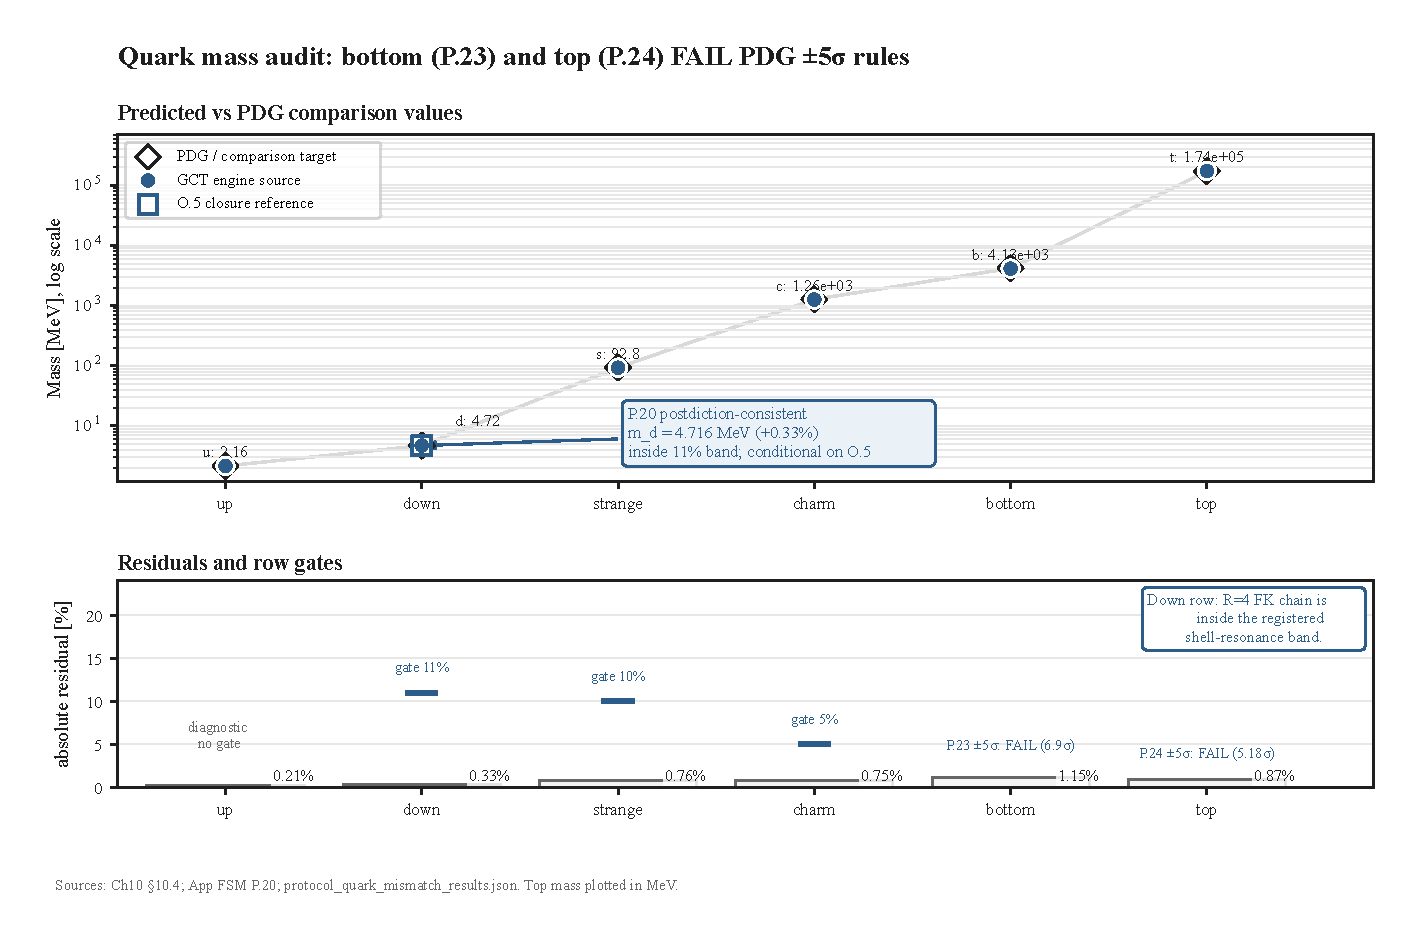
\includegraphics[keepaspectratio,alt={The quark mass spectrum is shown against declared PDG comparison conventions; the down-quark row P.20 sits inside its registered 11\% band, with the m\_d = m\_u\textbackslash phi\^{}\{\textbackslash phi\} closed form a Tier 3 identification of the finite-cage median, conditional on O.5.}]{content/Figures/Volume_3/Figure V3.10.1.pdf}}
\caption{The quark mass spectrum is shown against declared PDG
comparison conventions; the down-quark row P.20 sits inside its
registered 11\% band, with the \(m_d = m_u\phi^{\phi}\) closed form a
Tier 3 identification of the finite-cage median, conditional on O.5.}
\end{figure}

On larger cages the FK pseudo-determinant exhibits
\textbf{shell-resonance behaviour}: across
\(N \in \{1416, 1626, 1686, 1866, 2046, 2178, 2418, 2988\}\) on a
converged \(R=4\) lattice it oscillates in \([2.105,\, 2.391]\) within
the registered 11\% band, with an empirical decaying envelope and median
\(\approx 2.18\), matching the Mixed-Harmonic Area Law heuristic
\(\phi^{\phi}=2.1785\) to within \(\sim 1\%\). The \(I_h\)-closed
orbit-union sequence supplies the aggregate check: closed-cage deep-tail
mean \(\det_{FK}/\phi^{\phi}=0.9976\) and sequence-mean signed error
\(+0.09\%\) vs PDG. The tracking of \(\phi^{\phi}\) is suggestive but
not rigorously derived: by Gelfond--Schneider, \(\phi^{\phi}\) is
transcendental over \(\mathbb{Q}\) and therefore \textbf{not in the
K-theoretic gap-label module \(\mathbb{Z}[\phi]\)} that Bellissard's
theorem produces for cut-and-project quasicrystal Schrödinger spectra.
The closed-form \(R=2\) value \(\phi \cdot 2^{39/100} \cdot 3^{5/100}\)
is algebraic over \(\mathbb{Q}\) (a product of
\(\phi\in\mathbb{Q}(\sqrt5)\) and rational powers of integers) but lies
outside \(\mathbb{Z}[\phi]\) for these non-integer exponents. This is
consistent with Lück's framework: the FK pseudo-determinant is a
multiplicative spectral invariant distinct from the additive gap-label
\(K_0\)-class. Identifying the precise algebraic structure of
\(\widetilde{\det}_{FK}\) in the continuum limit --- and its relation,
if any, to Bellissard's \(\mathbb{Z}[\phi]\) --- is an Open Problem
(tracked as Open Problem O.5 in App ORQ and as the TP-B programme entry
in App TPR). Computational verification: see Appendix GPE; finite-size
scaling table: \texttt{GCT\_Physics\_Engine/data/fk\_scaling.json}.

\begin{enumerate}
\def\labelenumi{\arabic{enumi}.}
\item
  \textbf{Up Quark:} \(m_u = m_e \cdot \phi^3\) {[}Tier 2 geometric
  motif + Tier 3 QCD scheme/running bridge{]}

  \begin{quote}
  \textbf{Scheme bridge:} the exponent motif is fixed by the icosahedral
  mass ladder, but the comparison to the PDG \(\overline{\rm MS}\) value
  at \(\mu=2\) GeV inherits the hadronic renormalization-scheme/running
  bridge. The row is therefore postdiction-consistent, not a standalone
  scheme-independent quark-mass prediction.
  \end{quote}
\item
  \textbf{Down Quark:}
  \(m_d = m_u \cdot \widetilde{\det}_{FK,\infty} = m_u \phi^{\phi}\)
  {[}Tier 2 FK-determinant mechanism + Tier 3 \(\phi^{\phi}\)
  identification of the shell median (infinite-volume limit open,
  O.5){]}

  \begin{quote}
  \textbf{Derivation (Fuglede--Kadison):} In the Tier 3 face-defect
  assignment (V3 Ch03 §3.4), the Down Quark is a face-defect at the
  fundamental (\(N=11\)) harmonic scale. Its mass scale is set by the
  normalized pseudo-determinant of the cage adjacency \(D_F\) --- the
  geometric mean of \(|\lambda_i|\) over the non-zero spectrum. The
  finite \(R=2\) cage evaluates to
  \(\widetilde{\det}_{FK} = \phi \cdot 2^{39/100} \cdot 3^{5/100} = 2.239987\),
  a secondary algebraic diagnostic. The adopted primary output is
  \(m_d = m_u\phi^{\phi}=4.716\) MeV (with \(m_u = 2.1646\) MeV), a Tier
  3 identification of the shell median, \(+0.33\%\) against the PDG 2024
  central value and inside the registered 11\% shell-resonance band,
  which is the actual test. The FK-determinant sequence centers on
  \(\phi^{\phi}\): closed-cage deep-tail mean
  \(\det_{FK}/\phi^{\phi}=0.9976\), sequence-mean signed error
  \(+0.09\%\) vs PDG. Single-cage values oscillate within the 11\% band
  with an empirical decaying envelope; rigorous infinite-volume
  convergence is not proven and bundles with O.5. The algebraic-field
  structure of \(\widetilde{\det}_{FK}\) (whether the asymptotic value
  is exactly \(\phi^{\phi}\), or only the median, and how it relates to
  the Bellissard \(\mathbb{Z}[\phi]\) gap-label module) is an Open
  Problem.
  \end{quote}
\item
  \textbf{Strange Quark:}
  \(m_s = m_u \cdot \phi^8 \cdot (1 - 12\alpha)\) {[}Tier 2 mechanism
  (conditional on the Tier 3 face-defect quark assignment) + Tier 3
  specific coefficient (12) pending O.43 closure{]}

  \begin{quote}
  \textbf{Coefficient status (\(12\alpha\) drag):} Unlike vertex defects
  (leptons), whose \(5\alpha\) coefficient reads its 5 as the number of
  irreducible representations of \(A_5\) (a Tier 3 counting convention,
  V3 Ch08 §8.2.2), quarks are modeled as interstitial face defects. A
  face-defect drag proportional to the \(\mathbb{Z}^6\) coordination
  number \(Z=12\) (an alternative reading of the same 12, which the
  argument sketch above reads as the 12 pentagonal faces of the
  dodecahedral cage; neither reading is derived) supplies the Tier 2
  mechanism candidate (conditional on the Tier 3 face-defect assignment,
  V3 Ch03 §3.4), but the exact use of \(12\alpha\) as the strange-quark
  screening coefficient is a Tier 3 coefficient handle until
  QLQCD-1L/O.5 derives the face-channel drag from the quark-sector
  action.
  \end{quote}
\item
  \textbf{Charm Quark:} \(m_c = m_u \cdot \phi^{13 + \phi^{-1}/\phi^2}\)
  {[}Tier 3 --- heuristic Mixed-Harmonic Area Law{]}

  \begin{quote}
  \textbf{Status (Tier 3):} The Charm Quark sits at the second-harmonic
  (\(N=17\)) defect mode and is expected to be derivable from the cage's
  second-harmonic K-theoretic gap label --- a separate
  operator-algebraic invariant from the down-quark FK determinant. The
  closed-form derivation of this gap label is not yet executed in the
  engine; the current value uses the Mixed-Harmonic Area Law heuristic
  exponent \(13 + \phi^{-3}\), which gives \(m_c = 1263.45\) MeV,
  \(-0.75\%\) against PDG 2024 \(m_c(m_c) = 1273.0 \pm 4.6\) MeV (about
  \(-2.1\sigma\) taking the quoted error as \(1\sigma\); PDG labels it a
  90\% CL interval, which makes the tension larger), and is not derived
  from substrate. The occurrence of \(\phi^{-3}\) inside this exponent
  is a separate Tier 3 charm heuristic; it does not inherit the
  electroweak hypothesis H-EW or any Weinberg/projector derivation.
  Closure is bundled with App ORQ Open Problem O.5 (QLQCD-1L) and
  tracked in App TPR §TP-B / §TP-F.
  \end{quote}
\item
  \textbf{Bottom Quark:} \(m_b = m_c \cdot \phi^2 \cdot (5/4)\) {[}Tier
  2 mechanism + Tier 3 specific integer-handle (5/4) pending O.43
  closure{]}

  \begin{quote}
  \textbf{Algebraic Identification (A₅ Dimensional Ratio):} The
  coefficient 5/4 arises from the ratio of the dimensions of the
  icosahedral symmetry group's relevant representations in the
  third-generation quark sector.

  \emph{Argument sketch (not a proof):} The bottom quark couples to the
  vacuum lattice through the same icosahedral defect structure as the
  charm quark, but at the third-generation energy scale. In the
  icosahedral group I ≅ A₅ (the alternating group on 5 elements), the
  relevant representations for third-generation quarks are taken to be
  the 5-dimensional irrep H (Mulliken label) (assigned to the defect's
  coupling to the five-fold axes) and the 4-dimensional irrep G
  (Mulliken label) (assigned to the coupling to the three-fold
  tetrahedral substructure). The coupling strength candidate scales as
  dim(H)/dim(G) = 5/4 (Mulliken labels for the icosahedral 5- and
  4-dimensional irreps; Cotton, \emph{Chemical Applications of Group
  Theory} 3rd ed.~Table A.15; Altmann-Herzig 1994). The representation
  ratio is exact, but its use as the bottom-quark mass handle remains a
  Tier 3 specific integer-handle pending O.43 closure.

  \textbf{Classification:} {[}Tier 2 mechanism + Tier 3 coefficient
  handle{]} The 5/4 ratio = dim(H)/dim(G) in A₅ is a
  representation-theoretic fact; its deployment as the bottom-quark
  coefficient remains pending O.43.
  \end{quote}
\end{enumerate}

\textbf{Status against data: failure.} The formula gives
\(m_b = 4134.69\) MeV against PDG 2024 \(m_b(m_b) = 4183 \pm 7\) MeV
(\(\overline{\rm MS}\)), i.e.~\(-1.15\%\) and about \(6.9\sigma\) low
taking \(\pm 7\) MeV as \(1\sigma\) (more, since PDG labels it a 90\% CL
interval). By the standard applied to the top quark (P.24: outside PDG
\(\pm5\sigma\) of the prediction), the bottom row is reported as a
\textbf{failure}. The residual is carried as a Tier 3 state-level
residual pending O.5, and the mass-scheme question is open; a scheme
band registered after the result would not rescue the row. The earlier
falsification window of 4130--4230 MeV was centred on the measurement
rather than on the prediction, so it could not test the prediction; it
is withdrawn as a test.

\begin{enumerate}
\def\labelenumi{\arabic{enumi}.}
\setcounter{enumi}{5}
\tightlist
\item
  \textbf{Top Quark:} \(m_t = (v_{\rm GCT} / 2) \cdot \sqrt{2}\), with
  \(v_{\rm GCT}=246.1755\) GeV from the absolute Higgs-VEV pipeline
\end{enumerate}

These tiered tree-level derivations are \textbf{geometric mechanism
outputs} from the icosahedral cage, not a blanket closure of the hadron
sector from the current postulate set. The percentage errors against
current targets (\(u\): \(+0.21\%\); \(d\): \(+0.33\%\) from the adopted
primary \(m_d = m_u\phi^{\phi}=4.716\) MeV, a Tier 3 identification of
the shell median inside the registered 11\% band, conditional on O.5,
with the exact \(R=2\) finite-cage branch \(m_d=4.848734\) MeV at
\(+3.1645\%\) (displayed as \(+3.16\%\)) retained as a secondary
algebraic diagnostic; both down-quark branches lie inside the registered
110000-ppm gate; \(s\): \(-0.76\%\); \(c\): \(-0.75\%\) heuristic, about
\(-2.1\sigma\); \(b\): \(-1.15\%\), about \(-6.9\sigma\); \(t\):
\(+0.87\%\), \(5.18\sigma\)) come from the FK determinant and the
Mixed-Harmonic Area Law; the φ-formula residuals are descriptive
arithmetic (Tier 4 as evidence: not distinguishable from numerology for
strong effects; App PSC §PSC.9.6). The discrete handles they use (the
\(12\alpha\) and \(5/4\) coefficients, the charm exponent, the top-mass
ansatz) are Tier 3 choices made with the targets known; the top row
fails its written P.24 rule (§10.2.2), the bottom row fails by the same
standard, and the charm row sits inside its \(\pm3\%\) band
(\(2.1\sigma\) low). The dominant remaining residuals are:

\begin{enumerate}
\def\labelenumi{\arabic{enumi}.}
\tightlist
\item
  \textbf{Shell-resonance band on \(\widetilde{\det}_{FK}\).} The finite
  cut-and-project window samples a discrete subset of the noncommutative
  spectral geometry. As the cage size \(N\) sweeps natural icosahedral
  shells, the FK pseudo-determinant oscillates in \([2.105,\,2.391]\),
  i.e.~from about \(-3.4\%\) to \(+9.8\%\) around
  \(\phi^{\phi}\approx2.1785\) (inside the registered 11\% band). This
  is a Tier 2 mechanism (FK-pseudo-det closure) + Tier 3
  source-branch/state-value issue, not a defect of the mechanism.
\item
  \textbf{Missing higher-order QCD running.} Loop corrections from QCD
  running (analogous to the top quark 0.87\% QLQCD-2L debt) contribute
  \(\mathcal{O}(1\%)\) at the charm scale.
\item
  \textbf{Open Problem on \(m_c\) K-theoretic gap label.} The charm
  quark currently uses the Mixed-Harmonic Area Law heuristic
  \(\phi^{13+\phi^{-3}}\) at the \(N=17\) second-harmonic mode. The
  first-principles derivation of this gap label from the cage spectrum
  is bundled with App ORQ O.5 (QLQCD-1L); tracked in App TPR §TP-B /
  §TP-F.
\end{enumerate}

The mechanisms are retained, but none of the source values is yet
derived: the strange-, bottom-, and top-quark formulas carry Tier 2
mechanisms with Tier 3 coefficient/state handles (\(12\alpha\), \(5/4\),
the top-mass ansatz; the top row fails its written P.24 rule and the
bottom row fails by the same standard), the down-quark primary output is
the Tier 3 shell-median identification \(m_d = m_u\phi^{\phi}\), whose
convergence proof and algebraic-field identification remain O.5, with
the \(R=2\) finite-cage value retained only as a secondary diagnostic,
and the charm-quark formula is disclosed as Tier 3 heuristic awaiting
the second-harmonic gap-label construction. No target values are
pre-assigned (see Appendix GPE). This hadronic derivation reduces
standard-model parameterisation at tree level but does not currently
eliminate it across the full quark sector.

\begin{center}\rule{0.5\linewidth}{0.5pt}\end{center}

\subsection{10.5 QCD Phenomena}\label{qcd-phenomena}

\subsubsection{10.5.1 Universal Vacuum Viscosity: The Cabibbo Angle
{[}Tier 3 bare identification + Tier 3 lepton-to-hadron
transfer{]}}\label{universal-vacuum-viscosity-the-cabibbo-angle-tier-3-bare-identification-tier-3-lepton-to-hadron-transfer}

GCT proposes that the mixing between \(d\) and \(s\) quarks is a
geometric rotation (a Tier 3 identification). The candidate
\textbf{bare} value reuses the raw-frame number \(\phi^{-3}\):
\[\sin \theta_C^{\rm bare} = \phi^{-3} \approx \mathbf{0.236068} \quad \text{[Tier 3 identification]}\]
Observed (PDG 2024): \(\sin \theta_C \approx 0.225\). The \textbf{bare
residual is therefore \(\approx 4.9\%\)} for this Tier 3 identification.

The value \(\phi^{-3}\) is the same raw-frame coordinate number that
appears in the electroweak hypothesis H-EW (V3 Ch04 §4.3); no derivation
connects the two sectors, so its reuse here is a Tier 3 numerical
identification, not a shared geometric invariant. For the Cabibbo angle,
the candidate \textbf{Universal Vacuum Viscosity} correction reuses the
lepton-vertex \(5\alpha\) phason-drag coefficient from Ch08 §8.2.2:
\[\begin{gathered}\sin \theta_C^{\rm corrected} = \phi^{-3}(1 - 5\alpha) \approx 0.236 \times (1 - 0.036) \approx \mathbf{0.227} \\[1pt] \gcteqnote{[Tier 3 bare identification + Tier 3 lepton-vertex transfer]}\end{gathered}\]
This narrows the angle residual to \textasciitilde1.11\% (1.106\%; the
\(s_{12}\) element residual is 1.09\%, i.e.~1.086\%), a TENSION against
the single 0.5\% precision gate (the 5\% is only the falsification
band). \emph{Note: the \(\alpha\) in the correction is the CODATA A3
experimental value (\(\alpha^{-1}=137.035999177\)); the GCT-derived
\(\alpha\) (137.508 bare) sits inside the Phason Anti-Screening QLQCD-1L
research debt of App QLA.}

\begin{quote}
\textbf{The \(5\alpha\) coefficient across the lepton-to-hadron bridge
{[}Tier 3 bare identification + Tier 3 transfer handle{]}.} The
corrected Cabibbo formula gives \(s_{12}=0.22745\) versus PDG
\(0.22501\), a \(1.09\%\) element residual. The angle residual is
\(\theta_C=13.147^\circ\) versus \(13.003^\circ\), or \(1.11\%\),
because of the sine/arcsine nonlinearity. This residual is a
\textbf{Tier 3 bare identification + Tier 3 transfer} result, not a Tier
2 prediction, and as evidence that φ is special it is Tier 4 (not
distinguishable from numerology for strong effects; App PSC §PSC.9.6);
the bare \(\phi^{-3}\) value itself has a \(4.9\%\) residual. The
\(5\alpha\) drag coefficient arises in V3 Ch08 §8.2.2 as a lepton-vertex
mechanism, where its 5 is read as the number of irreducible
representations of \(A_5\) (trivial included); that reading is a Tier 3
counting convention, and other fivefold counts (for example the five
faces meeting at an icosahedral vertex) are alternative readings, not
independent derivations. Applying that coefficient to the Cabibbo
hadronic face-defect rotation assumes that the vertex-to-face Goldstone
projection preserves the fivefold coupling count. The icosahedral
fiber-vertex / face-defect duality (V3 Ch07 §7.1.2 versus V3 Ch10 §10.1)
motivates this identification, but does not force it; it is a disclosed
Tier 3 transfer handle and not an additional continuous fit. Promotion
to a Tier 2 prediction requires both a derivation of the bare value
(currently a reuse of the raw-frame number \(\phi^{-3}\)) and an
explicit Brauer-character computation establishing multiplicity
preservation, bundled with \textbf{Open Problem O.5}. In the Tier 3
ansatz of §10.6.1, the third-generation CKM angles (\(s_{23}\),
\(s_{13}\)) additionally receive a \(\phi^{-1}\) holonomy step; the
Cabibbo angle, which also connects two generations, does not.
\end{quote}

\subsubsection{10.5.2 Asymptotic Freedom and Lattice
Transparency}\label{asymptotic-freedom-and-lattice-transparency}

As proposed in App TPF (global appendices), the vacuum lattice exhibits
\textbf{High-Energy Transparency}. At the Planck scale, the quark
de-Broglie wavelength would become comparable to the 6D lattice spacing,
and the proposal is that the coupling to the nodes then falls away. This
is offered only as a Tier 3/4 candidate geometric picture related to
\textbf{Asymptotic Freedom}; it does not reproduce the observed
logarithmic running of \(\alpha_s\), which starts at the GeV scale, far
below the lattice scale.

\subsubsection{10.5.3 The Mass-Drag
Anti-Correlation}\label{the-mass-drag-anti-correlation}

GCT proposes a \textbf{mass--drag anti-correlation} in which
higher-frequency defect modes would couple less strongly to a stipulated
hydrodynamic drag. Neither the endpoint claims ``top has zero drag'' and
``muon has maximum drag'' nor the required relaxation law is derived
here. Extending that particle-model ansatz to consciousness, a physical
Selection process, or qualia registration is a separate Tier 3/4 bridge
with no identified carrier, transducer, owner, or phenomenal map; it is
not part of the quark-spectrum derivation.

\begin{center}\rule{0.5\linewidth}{0.5pt}\end{center}

\subsection{10.6 The CKM Mixed-Harmonic Ansatz {[}Tier 3 bare Cabibbo
identification + Tier 3 corrected-formula handle / Tier 3 remaining
angles{]}}\label{the-ckm-mixed-harmonic-ansatz-tier-3-bare-cabibbo-identification-tier-3-corrected-formula-handle-tier-3-remaining-angles}

While Neutrino (PMNS) mixing represents the unpinned axis sliding of
itinerant phason waves, Quark mixing represents \textbf{Topological
Tunneling} between the pinned icosahedral faces of the underlying vacuum
lattice.

Because quarks are structural artifacts deeply bound within the strong
force matrix, their ``flavor shifting'' forces them to push against the
high-frequency internal geometry of the lattice. This process is
inherently suppressed (damped) by the electromagnetic vacuum viscosity
(\(\alpha\)). Thus, unlike the large PMNS angles, the CKM angles are
inherently small and, in the Tier 3 Mixed-Harmonic ansatz, follow a
geometric descent:

\begin{enumerate}
\def\labelenumi{\arabic{enumi}.}
\tightlist
\item
  \textbf{Cabibbo Angle (\(s_{12}\)):} \(s_{12}^{\rm bare}=\phi^{-3}\)
  is a Tier 3 bare identification (the raw-frame value reused); the
  corrected formula \(s_{12} = \phi^{-3} \cdot (1 - 5\alpha)\) is a Tier
  3 lepton-to-hadron transfer handle pending O.5 / QLQCD-1L.
\item
  \textbf{\(s_{23}\) Mixing:} \(s_{23} = \phi^{-(6 + \phi^{-1})}\)
  \textbf{{[}Tier 3 Ansatz --- Irrational Exponent:
  \(6 + \phi^{-1} \approx 6.618\) is irrational. See Open Problem
  O.5.{]}}
\item
  \textbf{\(s_{13}\) Mixing:} \(s_{13} = \phi^{-(11 + \phi^{-1})}\)
  \textbf{{[}Tier 3 Ansatz --- Irrational Exponent:
  \(11 + \phi^{-1} \approx 11.618\) is irrational. See Open Problem
  O.5.{]}}
\end{enumerate}

\subsection{\texorpdfstring{10.6.1 CKM Berry-Phase Identification of the
\(\phi^{-1}\) step {[}Tier 3
candidate{]}}{10.6.1 CKM Berry-Phase Identification of the \textbackslash phi\^{}\{-1\} step {[}Tier 3 candidate{]}}}\label{ckm-berry-phase-identification-of-the-phi-1-step-tier-3-candidate}

The additive \(\phi^{-1}\) in the exponents for \(s_{23}\) and
\(s_{13}\) is a candidate transfer of the selected \(SU(2)\)
Berry-holonomy connection used in the proton-mass route. Its value is
fixed once that connection (the Tier 3 central-holonomy ansatz of
§10.3.3) and the projection map are adopted, but neither is uniquely
forced by the \(2I\) stabilizer.

For the proton, one complete \(SU(2)\) cycle around a 5-fold baryonic
axis yields a phase transformation \(U = -I\), contributing
\(N_{weak} \times R = (\frac{1}{2})(2\phi^{-1}) = \phi^{-1}\) to the
mass exponent.

For quarks, the ansatz assigns one additional \(\phi^{-1}\) holonomy
step to the mixing angles that involve the third generation (\(s_{23}\),
\(s_{13}\)) and none to the Cabibbo angle (\(s_{12}\)). This is a Tier 3
assignment rule, not a consequence of a generation change: Cabibbo
mixing (\(V_{us}\), \(d\)--\(s\)) itself connects generations 1 and 2,
so a ``generation-change'' criterion would not exempt it. The earlier
rationale, which called \(d \to s\) intra-generation and \(s \to c\) a
generation change, is withdrawn: \(V_{cs}\) is the diagonal element
within the second generation. No derivation yet says why the
third-generation angles, and only they, receive the extra step.

This candidate holonomy/face-defect construction organizes the hierarchy
of flavor mixing. The Cabibbo angle uses the Tier 3 bare identification
\(\sin\theta_C^{\rm bare} = \phi^{-3}\) (\(4.9\%\) residual) and a Tier
3 lepton-to-hadron transfer correction \(s_{12} = \phi^{-3}(1-5\alpha)\)
(\(1.09\%\) element residual; equivalently \(\theta_C=13.1473^\circ\)
against the PDG anchor \(\arcsin(0.22501)=13.0035^\circ\), a \(1.11\%\)
(1.106\%) angle residual, pending O.5). The remaining angles
(\(s_{23}\), \(s_{13}\)) with their irrational exponents remain Tier 3
pending resolution of Open Problem O.5.

\gctneedspace{5\baselineskip}

\textbf{Candidate derivation (\(\phi^{-1}\) Weak Holonomy Correction)
{[}Tier 3{]}:} The \(\phi^{-1}\) additive adjustment in the
higher-generation CKM exponents is a candidate transfer of the
proton-sector \(SU(2)_L\) Berry holonomy to quark face-defect tunneling.
Quarks are modeled as face-defects using the same weak fiber bundle as
the Baryonic Triad; for face-tunneling into or out of the third
generation, the ansatz assigns one \(\phi^{-1}\) Weak Berry phase
holonomy step (§10.6.1; the selection rule is itself Tier 3). The CKM
transfer remains Tier 3 pending first-principles lepton-to-hadron
transfer and QLQCD closure.

These structural ansätze output \(s_{12} \approx 0.22745\) {[}Tier 3
bare identification + Tier 3 transfer{]}, \(s_{23} \approx 0.0414\)
{[}Tier 3{]}, and \(s_{13} \approx 0.0037\) {[}Tier 3{]}, broadly
tracking the PDG 2024 pattern but not constituting a theorem-grade CKM
closure (Tier 4 as evidence: not distinguishable from numerology for
strong effects; App PSC §PSC.9.6). The corrected Cabibbo value remains
in live precision tension: relative to the PDG \(s_{12}\approx0.2250\)
target, the residual is \(\sim1.09\%\) and is carried as an explicit
\(\sim3.6\sigma\) \(s_{12}\) tension until O.5/QLQCD derives the
lepton-to-hadron transfer. The CP-violating Jarlskog invariant
\(J_{CKM}\) for this matrix is an \textbf{Open Research Problem (App ORQ
§ORQ.5, O.7)} bundled with the QLQCD-1L research debt. The
\(\delta_{CP} = 360^\circ \cdot \phi^{-1}\) phase remains a Tier 3
\textbf{leptonic/mixing-geometry phase ansatz} in the GCT registry
(pending O.7; the Jackiw-Rebbi mechanism is the gauge-chirality result
of Ch02 §2.4.2, not this phase), and it is not by itself a derivation of
hadronic CKM CP violation. Hadronic CP violation requires the
CKM-area/Jarlskog invariant \(J_{CKM}\) plus QCD dressing; that closure
remains O.7/O.5. The geometric phase may supply a candidate boundary
condition for the hadronic sector, but it does not secure the
matter-antimatter-asymmetry claim until the Jarlskog amplitude is
derived.

\begin{center}\rule{0.5\linewidth}{0.5pt}\end{center}

\begin{quote}
\textbf{Closure Target: Fuglede--Kadison Audit for the Down-Quark Mass
Scale {[}Tier 2 FK-determinant mechanism + Tier 3 \(\phi^{\phi}\)
identification of the shell median (infinite-volume limit open, O.5){]}}

Let \(D_F\) denote the adjacency operator of the icosahedral cage (graph
with \(N\) vertices selected as the closest perp-projected images of the
\(\mathbb{Z}^6\) lattice; edges of weight \(\phi\) between pairs at unit
ambient-space distance). The normalized FK pseudo-determinant is
\[\widetilde{\det}_{FK}(D_F) := \exp\!\left(\tfrac{1}{N_{\rm nz}}\sum_{\lambda_i\neq 0} \ln|\lambda_i|\right)\]
where \(N_{\rm nz}\) is the count of non-zero eigenvalues and
\(\lambda_i\) are the corresponding eigenvalues (an ad hoc normalised
pseudo-determinant; it differs from the von-Neumann-trace normalisation
of Lück 2002, Def. 3.11). For the \(R=2\) cage,
\(N_{\rm nz}=100=144-44\); the ordinary determinant vanishes because the
operator has 44 zero modes, so no equality to \(|\det D_F|^{1/N}\) is
claimed. Then \[m_d = m_u \cdot \widetilde{\det}_{FK}(D_F).\]

\emph{Closed-form evaluation at the \(R=2\) cage.} At the engine's
reference construction (144 vertices, 100 non-zero eigenvalues + 44 zero
modes) the spectrum factors into icosahedral characters with
multiplicities
\(\{\sqrt 2{:}6,\ \phi{:}24,\ \phi\sqrt 2{:}44,\ \phi\sqrt 3{:}8,\ 2\phi{:}10,\ \phi^2\sqrt 2{:}6,\ \phi\sqrt 6{:}2\}\),
and the geometric mean evaluates exactly to
\[\det_{FK}(D_F^{R=2}) \;=\; \phi \cdot 2^{39/100} \cdot 3^{5/100} \;=\; 2.239987\ldots,\]
giving the exact finite-cage branch value \(m_d = 4.848734\) MeV
(\(+3.1645\%\) from the PDG 2024 central value; displayed as
\(+3.16\%\)). This branch is a secondary algebraic diagnostic. The
adopted primary output is \(m_d = m_u\phi^{\phi}=4.716\) MeV,
\(+0.33\%\) against the PDG 2024 central value. Both branches are inside
the registered 110000-ppm (11\%) shell-resonance gate. On the converged
\(R=4\) lattice \(\det_{FK}\) oscillates shell-to-shell in
\([2.105,\, 2.391]\) within that band with an empirical decaying
envelope and median \(\approx \phi^{\phi}\); the \(I_h\)-closed
deep-tail mean gives \(\det_{FK}/\phi^{\phi}=0.9976\) with sequence-mean
signed error \(+0.09\%\) vs PDG. See Appendix GPE + finite-size scaling
table \texttt{data/fk\_scaling.json}.

\textbf{Algebraic-field status (Open).} The finite \(R=2\) diagnostic
\(\phi \cdot 2^{39/100} \cdot 3^{5/100}\) is algebraic over
\(\mathbb{Q}\) (a product of \(\phi \in \mathbb{Q}(\sqrt5)\) and
rational powers of integers), but lies \textbf{outside
\(\mathbb{Z}[\phi]\)} for these non-integer exponents. The primary
asymptotic-limit candidate \(\phi^{\phi}\) is transcendental over
\(\mathbb{Q}\) by Gelfond-Schneider. This is consistent with Lück's
framework --- the FK pseudo-determinant is a multiplicative spectral
invariant distinct from the additive \(K_0\)-class of Bellissard gap
labels --- but it leaves open whether \(\widetilde{\det}_{FK}\)
converges to \(\phi^{\phi}\) exactly in some scaling limit, or only its
median tracks \(\phi^{\phi}\) within shell-resonance noise.

\textbf{Charm-quark status.} The charm quark sits at the second-harmonic
(\(N=17\)) defect mode and is expected to admit a separate spectral
derivation from a cage submodule. That derivation is not yet executed;
the manuscript currently uses the heuristic Mixed-Harmonic Area Law
\(m_c = m_u \cdot \phi^{13 + \phi^{-3}}\) (PDG 2024 residual
\(-0.75\%\), about \(-2.1\sigma\)), explicitly labeled \textbf{Tier 3}.
The closure path is bundled with App ORQ Open Problem O.5 (QLQCD-1L) and
tracked in App TPR §TP-B / §TP-F. The CKM matrix elements (\(s_{23}\),
\(s_{13}\)) constitute the same Open Problem O.5-CKM, targeted for
closure in QLQCD-2L computations (Appendix QLA §QLA.7).
\end{quote}

\gctneedspace{5\baselineskip}

\textbf{END OF CHAPTER 10}

\clearpage
\thispagestyle{empty}
\vspace*{0.35\textheight}
\begin{center}\bfseries\LARGE PART III: ASTROPHYSICAL TESTS\end{center}
\vspace*{\fill}
\clearpage

\chapter{Chapter 11: The 3.55 keV Anomaly --- Dark
Matter}\label{chapter-11-the-3.55-kev-anomaly-dark-matter}

The search for the particulate identity of Dark Matter remains the most
significant unresolved endeavor in modern physics. For decades, the
``Cold Dark Matter'' paradigm has postulated a cold, collisionless
component occupying galactic halos (Weakly Interacting Massive
Particles, WIMPs, being one candidate). Geometric Consciousness Theory
(GCT) instead models Dark Matter as the \textbf{Topological Glass} state
of the vacuum substrate. The stress-gated lattice-fracture mechanism is
Tier 3 (it rests on the Tier 3 Topological Glass model and is
conditional on the adopted architecture), and the absolute centroid
\(E_{vac}=m_e/144\approx3.5486\) keV is Tier 3 because it inherits the
O.38 \(N_{\rm cage}=144\) posit. The empirical status is Under Test
pending deeper XRISM observations (see §11.4.4 + App PSC §PSC.8 + App
PRG P.3).

\begin{center}\rule{0.5\linewidth}{0.5pt}\end{center}

\subsection{11.1 The Signal}\label{the-signal}

\subsubsection{11.1.1 Observations: Perseus, Coma, and
Andromeda}\label{observations-perseus-coma-and-andromeda}

Tier discipline before the empirical conflict: the stress-gated
triboluminescence mechanism is Tier 3 (it rests on the Tier 3 glass
model and is conditional on the adopted cage architecture); the absolute
centroid inherits the Tier 3 O.38 cage posit, and the cluster-line
identification plus \(\sigma_{\rm crit}\) bracket are Tier 3 empirical
postdictions pending the XRISM/stacked-cluster tests.

In 2014, an unidentified emission line was detected in the X-ray spectra
of several massive galaxy clusters and the Andromeda galaxy (M31).
Initially reported by Bulbul et al.~(using stacked XMM-Newton data) and
independently confirmed by Boyarsky et al., the signal was subsequently
probed by Chandra, Suzaku, and the Hitomi satellite --- the Hitomi
observation of Perseus reported a high-significance non-detection of the
anomalously bright Perseus-core flux (Hitomi Collaboration 2017
\emph{ApJL} 837:L15, DOI 10.3847/2041-8213/aa61fa, 99.7\% tension on a
narrow-line interpretation in Perseus), creating a live observational
tension. Protocol C reserves its falsification aperture for stacked
above-\(\sigma_{\rm crit}\) cluster regions (§15.1.3); whether the
Perseus core is rheologically below threshold is a declared open
programme (§11.1.4), so the Hitomi null is not counted as support for
the stress gate.

Unlike known atomic transitions, the reported flux pattern is not
explained by baryonic gas parameters alone. In GCT the candidate signal
intensity is treated as stress-gated rather than as tracking the density
profile (§11.4.6). GCT proposes {[}Tier 3{]} this line as a candidate
direct observation of the vacuum microstructure.

\subsubsection{11.1.2 Energy: 3.55 ± 0.03
keV}\label{energy-3.55-0.03-kev}

The commonly quoted centroid is the weighted mean of the Perseus cluster
core, the stacked cluster sample, and the Galactic Center:
\[E_{obs} \approx 3.55 \pm 0.03 \text{ keV}\] This centroid is not
consistent with GCT's own stress gate. Two of its three inputs come from
regions the gate does not count as emitting: the Perseus core lies
outside the Protocol C pressure aperture (and its rheology is open,
§11.1.4), and the Galactic Center lies in the Milky-Way environment that
the stress-gating account treats as low-shear (a treatment not yet
computed, §11.1.4). A centroid built only from above-\(\sigma_{crit}\)
apertures has not been computed, because the per-region centroids are
not tabulated here. The 3.55 keV figure is therefore quoted as context
only; it is never counted as a pass for GCT. Sterile-neutrino decay fits
of this line are in tension with the non-detections in specific
environments (§11.1.3--§11.1.4); this is a constraint on that model, not
an impossibility.

\subsubsection{11.1.3 The Draco Paradox and the Threshold of Critical
Stress}\label{the-draco-paradox-and-the-threshold-of-critical-stress}

A critical anomaly within the data is the \textbf{Draco Null Result}.
High-exposure observations of the Draco Dwarf Spheroidal galaxy failed
to detect the 3.55 keV line despite its high dark matter density. GCT
offers a postdictive account via the \textbf{Threshold of Critical Shear
Stress (\(\sigma_{crit}\))}.

We define the qualitative fracture condition from icosahedral tiling
mechanics; the numerical Vacuum Yield Strength (\(\sigma_{crit}\))
remains a calibrated cluster-scale stress bracket until the
phason-stiffness normalization is derived in absolute pressure units.

\begin{quote}
\textbf{Proposal: Yield Strain from Tiling Flip Condition {[}Tier 3{]}}

In the AKN icosahedral tiling, a phason flip --- a discrete
rearrangement of tiles that releases stored strain --- occurs when the
perpendicular-space displacement \(u_\perp\) of a tile vertex exceeds
the width of the acceptance window in that direction. The proposal takes
the characteristic half-width to be the short diagonal of a rhombic
acceptance cell, scaling as \(\phi^{-1} \times a_\perp\) (where
\(a_\perp\) is the perpendicular lattice constant). This is an input,
not a derived quantity: the AKN acceptance window is a rhombic
triacontahedron, and a ``short diagonal of the rhombic acceptance cell''
is not yet given a geometric definition as a half-width of that window.
The strain at which this flip occurs is then:

\[ \epsilon_y = \frac{\Delta u_\perp}{\xi_{\rm DS}} = \frac{\phi^{-1} \cdot a_\perp}{\phi^4 \cdot a_\perp} = \phi^{-5} \approx 0.0902 \]

where \(\xi_{\rm DS} = \phi^4 \cdot a_\perp\) is the dark-sector phason
coherence scale, distinct in symbol, definition, and magnitude from the
biological polaron healing length
\(\xi_{\rm pol}=a_0/\alpha\approx7.25\) nm of V1 Ch07, and the factor
arises from the four-generation Fibonacci inflation of the lattice scale
{[}Tier 3{]}.

Numerically: \(\epsilon_y = \phi^{-5} \approx 0.090\) {[}Tier 3 ---
conditional on two Tier 3 inputs: the coherence scale
\(\xi_{\rm DS}=\phi^4a_\perp\) and the acceptance-window half-width
\(\phi^{-1}a_\perp\){]}

The dimensionless yield strain \(\epsilon_y = \phi^{-5} \approx 0.090\)
follows from the tiling flip condition only given those two inputs; the
arithmetic is exact, the result is Tier 3. The cluster-scale stress
threshold \(\sigma_{crit}=K_\perp\epsilon_y\) is not yet a
first-principles absolute-pressure prediction: the operative
\(K_\perp\)/pressure normalization is the Tier 3 calibrated bracket
audited in §11.1.4.
\end{quote}

Therefore, the critical stress is:
\[ \sigma_{crit} = K_\perp \times \epsilon_y = K_\perp \times \phi^{-5} \]

The Draco stress-gating prediction has no continuous fit parameter in
the qualitative fracture morphology: \(\epsilon_y\) is fixed by the Tier
3 tiling-flip proposal and \(K_\perp\) is inherited from the
phason-stiffness hierarchy. The absolute cluster threshold location,
however, is a Tier 3 calibrated bracket
(\(0.07 < \sigma_{crit} < 3\)--\(5\) keV/cm\(^3\) in §11.1.4), not a
zero-anchor numerical prediction.

\begin{itemize}
\tightlist
\item
  \textbf{XRISM stacked clusters:} The registered Protocol C
  stress-aperture rule is the \textbf{mass-weighted stress-gated region
  above \(\sigma_{crit}\)} within the XRISM stacked-cluster sample:
  cluster outskirts, merger shocks, and high-shear ICM cells. The
  Perseus core falls below the frozen pressure cut and is \textbf{not} a
  falsification aperture. Because cluster-core rheology is a declared
  open programme (§11.1.4), the Hitomi-Perseus null is not cited as
  consistent with, or as support for, the stress gate. A decisive F2
  null requires no 3.55 keV detection at \(W_{\rm int}<20\) eV with the
  registered stress-weighted morphology across the stacked
  above-\(\sigma_{crit}\) regions; smooth \(\rho^2\) tracking remains
  the morphology falsifier.
\item
  \textbf{Draco Dwarf:} Virial stress \(\sigma_{vir} < \sigma_{crit}\)
  is assumed. In the model the lattice remains in the \textbf{Elastic
  Glass} phase, and energy is stored as potential strain, not released
  as radiation. The comparison is not yet defined quantitatively:
  \(\sigma_{crit}\) is set in ICM thermal-pressure units (§11.1.4), and
  a gas-poor dSph has no such pressure, so a stress proxy usable in
  gas-poor systems must be specified before this is a computed check.
  This stress-gating mechanism is offered as a postdictive account of
  the non-detection in dwarf spheroidal galaxies; it remains
  postdiction-status until the cluster-by-cluster pressure/shear map is
  frozen before line-residual inspection (§11.1.4).
\end{itemize}

\subsubsection{\texorpdfstring{11.1.4 The Observational Conflict ---
Quantitative \(\sigma_{vir}\) / \(\sigma_{crit}\) / Bulbul-flux
Consistency Test {[}Tier 3 mechanism + Tier 3 \(\sigma_{crit}\)
calibrated
bracket{]}}{11.1.4 The Observational Conflict --- Quantitative \textbackslash sigma\_\{vir\} / \textbackslash sigma\_\{crit\} / Bulbul-flux Consistency Test {[}Tier 3 mechanism + Tier 3 \textbackslash sigma\_\{crit\} calibrated bracket{]}}}\label{the-observational-conflict-quantitative-sigma_vir-sigma_crit-bulbul-flux-consistency-test-tier-3-mechanism-tier-3-sigma_crit-calibrated-bracket}

We acknowledge that several independent analyses --- including Malyshev
et al.~(2014, stacked dSph XMM-Newton), Riemer-Sørensen (2016, Chandra
Milky Way halo), and Dessert et al.~(2020) --- find no signal in
low-stress environments. The Hitomi observation of Perseus (Hitomi
Collaboration 2017 \emph{ApJL} 837:L15, DOI 10.3847/2041-8213/aa61fa) is
an important calibration constraint: Hitomi reported a non-detection of
the anomalously bright Perseus-core flux at 99.7\% significance
(narrow-line interpretation). The Protocol C pressure aperture excludes
that core, so it is not the falsification aperture; whether the core is
rheologically below threshold is open (declared open programme below).
The load-bearing observational test is therefore the frozen
stacked-cluster above-\(\sigma_{crit}\) aperture, distinct from both
low-stress non-detections and the Hitomi core null.

\textbf{Quantitative reconciliation.} The closure path is set by the
numerical comparison between the four observational anchors. We tabulate
them here in the operational pressure-coordinate that the stress-gating
mechanism uses (\(P \sim n k_B T\) for the cluster gas, set against the
GCT triboluminescent threshold \(\sigma_{crit}\)):

\gctneedbreak{10\baselineskip}

\begingroup
\scriptsize
\setlength{\LTpre}{6pt}\setlength{\LTpost}{4pt}
\setlength{\tabcolsep}{3pt}
\hyphenpenalty=50\exhyphenpenalty=50
\sloppy
\begin{longtable}{>{\raggedright\arraybackslash\hspace{0pt}}p{0.1276\linewidth}>{\raggedright\arraybackslash\hspace{0pt}}p{0.1194\linewidth}>{\raggedright\arraybackslash\hspace{0pt}}p{0.4876\linewidth}>{\raggedright\arraybackslash\hspace{0pt}}p{0.1454\linewidth}}
\toprule
\textbf{Environment} & \textbf{Observable} & \textbf{Value} & \textbf{Source} \\
\midrule
\endhead
\bottomrule
\endlastfoot
Draco dSph & $\sigma_{vir}$ (velocity dispersion) & $\sim 9$ km/\allowbreak{}s & Walker et al. 2009 \textit{ApJ} 704:1274 \\
\addlinespace[2pt]
Milky Way halo & $\sigma_{vir}$ & $\sim 220$ km/\allowbreak{}s & Bovy et al. 2012 \textit{ApJ} 759:131 \\
\addlinespace[2pt]
Perseus core & $\sigma_{vir}$ (galaxy velocity dispersion) & $\sim 1280$ km/\allowbreak{}s & Aguerri et al. 2020 \textit{MNRAS} 494:1681 \\
\addlinespace[2pt]
Perseus core & thermal pressure $P_{th} \approx n_e k_B T$ & $\sim 0.07$ keV/\allowbreak{}cm³ at $n_e \approx 0.01$ cm⁻³, $T \approx 7$ keV & Churazov et al. 2003 \textit{ApJ} 590:225 \\
\addlinespace[2pt]
Bullet Cluster bow shock & $P_{th}$ at shock & $\sim 3$-$5$ keV/\allowbreak{}cm³ (50-70× Perseus core) & Markevitch \& Vikhlinin 2007 \textit{Phys. Rep.} 443:1 \\
\addlinespace[2pt]
Bulbul 2014 stacked detection & $\Gamma_{decay}$ implied & $\Gamma_{Bulbul} \approx 2 \times 10^{-28}$ s⁻¹ & Bulbul et al. 2014 \textit{ApJ} 789:13 \\
\addlinespace[2pt]
Hitomi 2017 Perseus & 3σ upper bound & $\Gamma_{Hitomi} \lesssim 3\text{–}4 \times 10^{-27}$ s⁻¹ (the XRISM 2025 cross-calibration reports its $\Gamma \lesssim 1.0\times10^{-27}$ s⁻¹ limit as $3$–$4\times$ tighter than Hitomi; the Hitomi null excludes the anomalously-bright Perseus-core narrow line but does NOT test the Bulbul stacked-cluster decay rate at the manuscript level). The Bulbul B14 full-sample expectation for the Hitomi field was $(2.4{-}3.1)\times10^{-7}$ ph/\allowbreak{}s/\allowbreak{}cm², $\sim 30\times$ below Hitomi's detection threshold for that field. Whether the Perseus-core null is compatible with the stress gate depends on the open cluster-core rheology (below); the stacked above-$\sigma_{crit}$ cluster sample tests the Bulbul decay rate independently. & Hitomi Collaboration 2017 \\
\addlinespace[2pt]
XRISM early stacked-cluster constraint & upper bound & $\Gamma_{XRISM} \lesssim 1.0 \times 10^{-27}$ s⁻¹ (broader stack, looser per-cluster sensitivity; current data are sensitivity-limited relative to the Bulbul-level order-$10^{-28}$ s⁻¹ normalization) & per Ch15 §15.5 \\
\end{longtable}
\endgroup

The GCT \textbf{Stress-Gating} resolution then takes a quantitative
form. Under closure path (b) the gating threshold \(\sigma_{crit}\) is
bracketed by:

\[
P_{Perseus\,core} \;\approx\; 0.07\ \text{keV/cm}^3 \;<\; \sigma_{crit} \;<\; P_{Bullet\,bow\,shock} \;\approx\; 3\text{-}5\ \text{keV/cm}^3
\]

--- i.e.~the bracket places the threshold between the Perseus
quiescent-core pressure and major-merger bow-shock pressures. The
bracket is an aperture definition built from two observed pressures; it
is not evidence that cluster cores are elastic (see the declared open
programme below). The dwarf-spheroidal and Milky-Way-halo nulls cannot
yet be called consistent with the gate under either closure path:
\(\sigma_{crit}\) is defined in ICM thermal-pressure units
(\(P \sim n k_B T\)), which do not exist for gas-poor dSphs or for the
dark-matter halo, and no stress proxy usable in those systems has been
specified or tabulated.

Under closure path (a) --- the Bulbul-level flux is genuinely below
Hitomi's sensitivity in the Perseus field, without using the core as a
stress-gated aperture --- the Bulbul detection would have to be
reattributed to a stacked-cluster systematic (instrumental floor or
atomic-emission line; cf.~Dessert et al.~2020). Hitomi's Perseus-core
bound is then compatible with the frozen aperture rule and the
discriminator collapses to whether the above-\(\sigma_{crit}\) stacked
XRISM regions ever show the 3.5 keV signal at the terminal Protocol C
floor \(\Gamma \approx 2 \times 10^{-28}\) s⁻¹ (Ch15 §15.2).

\textbf{Operative aperture rule.} Protocol C uses the bracket
\([0.07, 3\)--\(5]\) keV/cm³ only to define its frozen aperture: the
cells whose pre-line pressure proxy exceeds \(\sigma_{crit}\). Neither
the Hitomi-Perseus null nor the Bulbul stacked detection is counted as
support for that choice. The framework remains testable by one
preregistered Protocol C stress-aperture rule: the XRISM deeper stack
must either (i) detect the line in mass-weighted regions above
\(\sigma_{crit}\), or (ii) bound it below the Bulbul level across those
regions. The stress-gated fracture mechanism is Tier 3, conditional on
the adopted cage architecture and the glass model; its absolute
\(3.5486\)-keV centroid inherits the Tier-3 O.38 cage posit. The
\(\sigma_{crit}\) value is separately calibrated to a Tier-3 range
pending the XRISM cluster-sample sub-classification.

The stress-gating reconciliation remains postdiction-status until the
same pressure/shear map is frozen cluster-by-cluster for the Bulbul,
Hitomi, Dessert, XRISM, and successor stacks before any line-residual
inspection; low-stress null results become forward predictions of GCT
only under that frozen-aperture preregistration. The Hitomi-Perseus core
null lies outside the frozen aperture and is therefore not a
falsification point; it is not counted as support either. Closure of the
above-\(\sigma_{crit}\) stacked-cluster aperture under the XRISM deeper
stack is the load-bearing remaining work, registered as a tightening
sub-item of \textbf{Open Problem O.4} (cosmological-scale phason
coherence-volume closure).

\textbf{Declared open programme {[}Tier 3{]}: cluster-core rheology.} V2
Ch13 §13.1.1--§13.1.2 states that rich clusters
(\(10^{14}\)--\(10^{15}\,M_\odot\)) exceed the yield stress, so their
cores are fractured; that is how the model accounts for cluster missing
mass. Protocol C's frozen pressure cut instead places relaxed cool
cores, including Perseus (itself a rich cluster), below
\(\sigma_{crit}\); read rheologically, that would make the
Hitomi-Perseus null harmless. Both readings cannot hold. Bulbul et
al.~2014 also reported the line in Perseus-core data at a flux above the
stack expectation, which a core-suppressing gate would have to set
aside. Closing this needs one stress proxy, computed from pre-line maps,
that fixes which cluster regions are fractured, plus a missing-mass
account for any core that is elastic. Until then neither reading is used
to absorb or predict any observation, and nothing downstream uses either
as support.

\begin{center}\rule{0.5\linewidth}{0.5pt}\end{center}

\subsection{11.2 The Mechanism: Vacuum
Triboluminescence}\label{the-mechanism-vacuum-triboluminescence}

\subsubsection{11.2.1 Dark Matter as Supersolid Topological
Glass}\label{dark-matter-as-supersolid-topological-glass}

In the GCT hardware, the galactic halo consists of \textbf{Frozen Phason
Strain} (\(w_{ij}\)) in the internal dimensions (\(E_\perp\)). It is a
\textbf{Topological Glass}---a solid state where icosahedral tiles are
pinned in high-energy orientations. Critically, because the vacuum is a
\textbf{Supersolid}, it possesses \textbf{Off-Diagonal Long-Range Order}
(global phase coherence). This phase-locking ensures that the ``Unit of
Strain'' is identical across the entire universe, preventing the
spectral smearing common to classical glasses.

\subsubsection{11.2.2 The Vorton and the Quantized
Snap}\label{the-vorton-and-the-quantized-snap}

We define the fundamental excitation of the glass as a \textbf{Vorton}:
a closed loop of phason strain pinned to the matching rules of the
icosahedral tiling. In the conditional lattice-fracture model, stress
above \(\sigma_{crit}\) drives \textbf{Vacuum Creep} and releases one
modeled binding-energy unit. The mechanism form is Tier 3 (conditional
on the adopted architecture and the glass model); the numerical
\textbf{Vacuum Quantum}, \(E_{vac}=3.5486\) keV, is Tier 3 because it
uses the O.38 \(N_{\rm cage}=144\) input.

\subsubsection{11.2.3 Global Phase Rigidity and Mössbauer Suppression
(open)}\label{global-phase-rigidity-and-muxf6ssbauer-suppression-open}

\textbf{Declared open programme {[}Tier 3{]}: emitter kinematics and
line width.} The model claimed that the 3.55 keV line is exceptionally
narrow: emitters bound in a coherent supersolid lattice would hand the
recoil to the coherence volume set by \(\xi_{\rm DS}=\phi^4a_\perp\)
(§11.1.3), a \textbf{Mössbauer Suppression} of Doppler broadening, with
\textbf{Global Phase Rigidity} keeping the emission monochromatic. The
defect: emission occurs only in the fractured phase, where V2 Ch13
§13.1.2 describes the emitters as unpinned debris moving freely. Free
emitters at cluster virial speeds (\(\sigma_v\sim1000\)--\(1300\) km/s)
give a Doppler FWHM of \(\sim28\)--\(36\) eV, inside the \(W_{int}>20\)
eV band that Protocol C treats as falsifying. Closure needs an explicit
fractured-phase emitter model (lattice-bound with a derived recoil-free
fraction, or free debris with a derived velocity distribution) and the
\(W_{int}\) it implies. Until then the narrow-line expectation is
unsupported, and nothing downstream uses it as support.

\begin{center}\rule{0.5\linewidth}{0.5pt}\end{center}

\subsection{\texorpdfstring{11.3 Experimental Match: The Binding Energy
\(E_{vac}\)}{11.3 Experimental Match: The Binding Energy E\_\{vac\}}}\label{experimental-match-the-binding-energy-e_vac}

\subsubsection{11.3.1 Postdiction: Lattice Release Centroid {[}Tier 3
conditional mechanics; Tier 3 O.38-dependent
centroid{]}}\label{postdiction-lattice-release-centroid-tier-3-conditional-mechanics-tier-3-o.38-dependent-centroid}

The most direct postdiction-status alignment is between the unidentified
X-ray line at 3.55 keV and the conditional \textbf{Vacuum Binding Energy
(\(E_{vac}\))} evaluated from the Chapter 7 cage posit. This is context
for Protocol C, not validation or an independent derivation of
\(N_{\rm cage}\).

Conditional on the Tier 3 \(N=144\) electron-cage posit, the arithmetic
gives \(E_{vac} = m_e / 144 \approx 3.5486\) keV. We \emph{then} compare
this Tier 3 postdiction to the observed X-ray line (\(3.55 \pm 0.03\)
keV). The result is a centroid coincidence within a crowded-line forest,
reported as context only because the quoted centroid draws on regions
the stress gate does not count as emitting (§11.1.2); its statistical
significance is bounded by line-blending systematics rather than
functioning as a clean confirmation of the lattice geometry.

\gctneedspace{5\baselineskip}\begin{gctImportant}

\textbf{Firewall Metadata {[}3.55 keV Anomaly{]}}

\begin{itemize}
\tightlist
\item
  \textbf{Type:} Postdiction (Energy Value; context only, §11.1.2) /
  Line shape: no prediction until the emitter-kinematics programme
  closes (§11.2.3)
\item
  \textbf{Inputs:} \(m_e\) (Anchor), \(N_{\rm cage}=144\) (Tier 3
  structural posit pending O.38)
\item
  \textbf{Degrees of Freedom:} 0
\item
  \textbf{Provenance:} Exact conditional evaluation
  \(E_{vac}=m_e/N_{\rm cage}\); absolute centroid inherits Tier 3 O.38
\end{itemize}

\end{gctImportant}

\begin{center}\rule{0.5\linewidth}{0.5pt}\end{center}

\subsection{11.4 Falsification and
Predictions}\label{falsification-and-predictions}

\subsubsection{11.4.1 Line Shape, Morphology, and Background
Model}\label{line-shape-morphology-and-background-model}

The operative test for GCT lies in the joint \textbf{line profile,
morphology, flux, and background model} of the emission.

\begin{itemize}
\tightlist
\item
  \textbf{Sterile Neutrino Model:} The decay line is intrinsically
  narrow; the observed profile is set by cluster-virial broadening,
  instrument response, stacking, morphology, and background/atomic-line
  modelling. A \(\sim 36\) eV FWHM scale is a cluster-environment
  diagnostic, not a standalone particle-DM theorem.
\item
  \textbf{GCT Model:} A narrow \textbf{Lorentzian} intrinsic profile
  (\(\Gamma \ll 1\) eV) holds only for lattice-bound emitters, which is
  the open emitter-kinematics programme of §11.2.3; the profile is
  convolved with the same instrumental response and
  foreground/background model, with morphology and flux consistency
  carrying equal decision weight.
\end{itemize}

\subsubsection{11.4.2 Dark Matter Evaporation {[}Tier 3; not
observable{]}}\label{dark-matter-evaporation-tier-3-not-observable}

If fracture converts strain energy into photons, stressed regions slowly
lose effective dark mass (\textbf{Dark Matter Evaporation}). If the 3.55
keV luminosity is the energy channel, the fractional mass-loss rate
equals the line decay rate, \(\Gamma \approx 2\times10^{-28}\) s⁻¹
(Bulbul normalisation, §11.1.4). Over 10 Gyr (\(3.2\times10^{17}\) s)
this gives \(\Gamma t \approx 6\times10^{-11}\), roughly eight orders of
magnitude below percent-level lensing or dynamical mass measurements.
The effect is therefore not an observable test and is not used as one.

\subsubsection{11.4.3 XRISM Protocol C}\label{xrism-protocol-c}

The \textbf{XRISM} Resolve microcalorimeter provides
\(\sim\)\hspace{0pt}5 eV resolution. Protocol C (Chapter 15) defines the
preregistered decision framework for the XRISM line-shape audit. The
operative verdict is not a standalone Lorentzian-vs-Gaussian split; it
is the joint profile, flux, morphology, background-line, and
cluster-virial-broadening comparison at the sensitivity required to
resolve the signal.

\subsubsection{11.4.4 XRISM Early-Data
Status}\label{xrism-early-data-status}

XRISM has stacked \textbf{3.75 Megaseconds} of early science data across
ten galaxy clusters. Key results:

\begin{itemize}
\tightlist
\item
  \textbf{Non-detection:} XRISM's early data did \textbf{not} resolve
  the 3.55 keV line.
\item
  \textbf{Upper Limit:} The 3σ upper limit on the photon decay rate is
  \(\Gamma \lesssim 1.0 \times 10^{-27}\ \mathrm{s}^{-1}\).
\item
  \textbf{Sensitivity Gap:} This upper limit is \textbf{5 times weaker}
  than the decay rate implied by the original Bulbul et al.~XMM-Newton
  detection. XRISM's early data has therefore \textbf{not yet reached
  the sensitivity required} to confirm or rule out the signal.
\item
  \textbf{Physical Conclusion:} The early XRISM data is
  \textbf{physically inconclusive}. It is consistent with both the GCT
  stress-gated branch and the standard sterile neutrino model. The null
  result does \textbf{not} reject the registered Protocol C branch; that
  branch requires photon statistics beyond the current 3.75 Ms stacking
  depth.
\end{itemize}

\gctneedspace{5\baselineskip}\begin{gctImportant}

\textbf{GCT Stress-Gated Branch Under Test.} The current XRISM
non-detection is sensitivity-limited and does not adjudicate the frozen
above-\(\sigma_{crit}\) aperture. A definitive terminal no-line verdict
requires the Bulbul-level Protocol C floor
\(\Gamma \lesssim 2.0 \times 10^{-28}\ \mathrm{s}^{-1}\) in the
mass-weighted stress-gated regions of the stacked XRISM cluster sample;
the 26 Ms / \(\Gamma\lesssim3.8\times10^{-28}\ \mathrm{s}^{-1}\) stack
is the morphology-linewidth milestone. The Perseus core alone lies
outside the frozen pressure aperture and is not a Protocol C
falsification point (its rheology is open, §11.1.4).

\end{gctImportant}

\gctneedspace{5\baselineskip}\begin{gctWarning}

\textbf{K-XVIII Contamination Flag (3.514 keV) {[}exact separation
arithmetic conditional on the Tier 3 O.38 centroid{]}:} Conditional on
the O.38 \(N_{\rm cage}=144\) posit, the registered topological-defect
centroid is \(E_c=3.548\pm0.005\) keV; the broader phrase ``3.5 keV line
complex'' is shorthand for the crowded observational band. This lies
perilously close to the Potassium K-XVIII atomic transition line at
3.514 keV. While pristine microcalorimeter resolution (XRISM Resolve
\(\sim 5\) eV FWHM at 3.55 keV; Ishisaki et al.~2022, \emph{Proc. SPIE}
12181:121811S (DOI 10.1117/12.2630654)) can in principle resolve the
separation (ΔE ≈ 34.6 eV, from the formal GCT centroid 3.5486 keV vs the
K-XVIII line at 3.514 keV), plasma-line flux modeling, gain/background
systematics, and multiplet confusion can still blend the practical
inference even when thermal broadening alone is not large enough to
erase the centroid separation. \textbf{Ruling:} Any future detection of
a line complex near 3.5 keV must explicitly fit and subtract the K-XVIII
flux model before the residual can be claimed as the GCT 3.55 keV
topological signal.

\end{gctWarning}

\subsubsection{11.4.5 HBT Photon Bunching {[}Tier 3 theoretical target;
detector-level prediction
open{]}}\label{hbt-photon-bunching-tier-3-theoretical-target-detector-level-prediction-open}

The proposed lattice-fracture cascade motivates a second-order
photon-correlation target for the 3.55 keV signal. A detector-level
prediction requires the source mode count, cascade multiplicity, line
profile, and timing response to be specified together.

\begin{quote}
\textbf{Physical Argument:} The single-mode reference values are
distinct: a thermal or chaotic field gives \(g^{(2)}(0)=2\), a coherent
field gives \(1\), and an ideal single-photon emitter gives \(0\)
(Mandel \& Wolf 1961, \emph{Phys. Rev.} 124:1696). A large ensemble of
independent emitters with random phases is a chaotic source and
therefore exhibits the Hanbury-Brown-Twiss bunching limit in a resolved
mode; independence does not by itself imply coherent-state Poisson
statistics.

The GCT mechanism proposes that a Vorton collapse triggers adjacent bond
snaps within a phason-relaxation window \(\tau_{relax}\sim10^{-23}\) s
{[}Tier 3{]}. If that cascade produces correlated photon clusters, the
relevant observable is the excess detector-integrated correlation above
the null-source expectation. For \(M\) independently detected
spatio-temporal modes, chaotic bunching is diluted according to
\[g^{(2)}_{\rm meas}(0)-1\sim\frac{g^{(2)}_{\rm single}(0)-1}{M},\] so
both the particle-decay null and the cascade hypothesis approach unity
under strong mode averaging. The discriminant is the difference between
their finite-\(M\) correlation functions, not the isolated single-mode
value \(g^{(2)}(0)=2\).
\end{quote}

This prediction has the following properties:

\begin{itemize}
\item
  \textbf{Discriminant and its conditions:} A sharp threshold requires a
  source model for both hypotheses, including cascade multiplicity,
  emission-time statistics, spatio-temporal mode structure,
  astrophysical thermal components, and the detector response. These
  ingredients determine \(g^{(2)}_{\rm meas}(\tau)\) and its shot-noise
  floor. The test remains a theoretical target until that forward model
  exists.
\item
  \textbf{Instrument requirements:} The registered cascade window is
  \(\tau_{relax}\sim10^{-23}\) s {[}Tier 3{]}. For a detector resolution
  \(\tau_{res}\gg\tau_{relax}\), an unresolved correlation is diluted by
  approximately \(\tau_{relax}/\tau_{res}\). XRISM Resolve samples pulse
  shapes at \(80\,\mu\)\hspace{0pt}s and assigns arrival times with
  approximately \(5\,\mu\)\hspace{0pt}s interpolation precision (XRISM
  HEASARC \emph{Resolve} instrument specification), so even the more
  favorable interpolation scale gives a contrast no larger than order
  \(10^{-18}\). A hypothetical \(1\) ps coincidence system would still
  be \(10^{11}\) times coarser than the proposed cascade window.

  \begin{quote}
  \textbf{Instrument scope:} The zero-delay test is not executable with
  present or foreseeable direct X-ray timing. A viable reformulation
  would require either a cascade mechanism with a substantially longer
  correlation time or a spectral-domain intensity-interferometry
  observable integrated against the line profile. Deriving one of those
  routes is the closure target.
  \end{quote}
\item
  \textbf{Independent of line shape:} Even if the
  line-profile/morphology/background audit remains inconclusive due to
  source confusion, the bunching test would provide an orthogonal axis
  once a forward model exists; at present it defines no falsifier (see
  Status).
\item
  \textbf{Status:} XRISM does not test this correlation target. The
  current proposal is non-executable and does not yet define an
  observational falsifier {[}Tier 3{]}.
\end{itemize}

\subsubsection{11.4.6 The Spatial Cross-Correlation Mapping: Shear
Gradient vs.~Density
Squared}\label{the-spatial-cross-correlation-mapping-shear-gradient-vs.-density-squared}

Standard annihilating dark matter models demand that the flux of a line
signal follows the line-of-sight integral of the dark matter density
squared (\(\rho^2\)), while decaying sterile-neutrino models follow the
density \(\rho\) itself.

GCT predicts a radically different spatial morphology. Because the 3.55
keV emission is \textbf{Vacuum Triboluminescence}---the discrete
snapping of the topological glass under mechanical stress---the emission
rate is governed by the local macroscopic strain. Qualitatively, the
X-ray flux would then scale non-linearly with the local gradient of the
cluster's gravitational shear stress tensor (\(\nabla \sigma_{vir}\)),
maximizing in active merger shocks and regions of maximum orbital
disruption, rather than seamlessly following the smooth \(\rho^2\) core
density profile. This gradient picture is motivation only; the single
registered morphology template is the stress-gated aperture template
frozen in Ch15 §15.2 (Ch15 §15.1.3 target cells).

This constitutes a \textbf{candidate falsifiable spatial mapping test}
for XRISM and Athena follow-up: high-resolution spatial mapping of any
confirmed 3.55 keV line should either follow a smooth density profile
(\(\rho\) for decay, \(\rho^2\) for annihilation; either falsifies the
GCT morphology at decisive sensitivity) or trace the registered
stress-gated aperture template. Protocol C freezes the stress aperture
numerically at
\(\sigma_{crit}=0.53\,{\rm keV\,cm^{-3}}=\sqrt{(0.07)(4.0)}\,{\rm keV\,cm^{-3}}\),
using the Perseus-core / Bullet-shock pressure bracket; the target cells
are listed in Ch15 §15.1.3 and the morphology power rule in Ch15 §15.2.
Current Hitomi/XRISM coverage is insufficient for the stress-gated null;
the test becomes definitive only after the XRISM cluster-survey aperture
is above this frozen threshold, reaches the Ch15 sensitivity floor, and
is followed up with Athena-class spatial/spectral mapping.

\subsubsection{11.4.7 High-Frequency Gravitational Wave
Cross-Correlation {[}Tier 4,
non-operative{]}}\label{high-frequency-gravitational-wave-cross-correlation-tier-4-non-operative}

A proposed auxiliary discriminator between decaying particle dark matter
(like sterile neutrinos) and GCT's Vacuum Triboluminescence is a
\textbf{High-Frequency Gravitational Wave (HFGW) Cross-Correlation}.

In this Tier 4 picture, when the topological glass fractures and
releases the 3.55 keV Vorton energy, the event would also propagate
acoustic phonons through the \(\mathbb{Z}^6\) vacuum lattice, which in
the 3D projection (\(E_\parallel\)) might appear as a burst of
High-Frequency Gravitational Waves. The 1-100 MHz band is asserted, not
derived: no frequency band, strain amplitude or rate has been computed.

Therefore, a 3.55 keV XRISM X-ray line accompanied by a temporally and
spatially matched 1-100 MHz HFGW burst would support the
mechanical-fracture interpretation as an auxiliary discriminator. A
decaying sterile neutrino would emit a 3.55 keV X-ray photon without the
correlated gravitational shockwave. HFGW co-detection is not part of the
operative P.3 linewidth/morphology gate and cannot by itself validate
the geometric-vacuum interpretation; it is a Tier 4/currently
non-operative cross-channel check.

\subsubsection{11.4.8 Weak Lensing Shear Discontinuity: Dark Matter
Fracture Morphology Target {[}Tier 3 morphology hypothesis; mechanism
open{]}}\label{weak-lensing-shear-discontinuity-dark-matter-fracture-morphology-target-tier-3-morphology-hypothesis-mechanism-open}

GCT proposes a morphology hypothesis for dark matter in merging galaxy
clusters: a topological-glass fracture boundary might produce a
weak-lensing feature co-spatial with the stress-gated 3.55 keV emission
region. This is a diagnostic target pending both a derivation and an
executable lensing-map pipeline, not a closed prediction; the
dark-matter-fracture protocol is open.

\textbf{Physical Argument.} In GCT, dark matter is modelled {[}Tier 3{]}
as the \textbf{Topological Glass} of the vacuum supersolid (§11.2.1).
The ansatz assumes a \textbf{first-order fracture transition} when the
applied stress exceeds the yield strength
\(\sigma_{crit} = K_\perp \times \phi^{-5}\) (§11.1.3, itself Tier 3):
on one side the glass is intact (elastic regime, no emission); on the
other it is fractured (post-yield regime, emitting 3.55 keV). A sharp,
coherently propagating boundary is assumed, not derived.

\textbf{The Observable: Weak Lensing Convergence.} The weak lensing
convergence map \(\kappa(\vec{\theta})\) encodes the projected surface
mass density \(\Sigma(\vec{\theta})\) via
\(\kappa = \Sigma / \Sigma_{cr}\). The missing step is the fracture →
\(\Sigma\) map: fracture releases \textasciitilde keV photons, not mass,
and no derivation shows that a vacuum phase change alters the projected
surface density at all. The form of any feature is also not derived:
even a 3-D density step at \(r_f\) projects to \(\Sigma(R)\) with a term
\(\propto\sqrt{r_f^2-R^2}\), whose radial derivative diverges at
\(R=r_f\), rather than a finite step in
\(\partial^2\kappa/\partial r^2\).

\gctneedspace{5\baselineskip}

\textbf{Morphology hypothesis {[}Tier 3; open{]}:}

\begin{quote}
At the fracture boundary of merging galaxy clusters (e.g., El Gordo,
ACT-CL J0102-4915; the Bullet Cluster, 1E 0657-56), the weak lensing
convergence map would show a sharp feature at the boundary of the shear
fracture zone, and its position would coincide with the boundary of the
3.55 keV X-ray emission region.

Collisionless particulate dark matter (NFW, or any smooth halo profile)
does not naturally produce this sharp phase-transition feature. NFW
profiles are smooth away from the central cusp at \(r=0\); their
convergence maps have no kinks at finite radius. A detected sharp
feature in \(\kappa\) co-spatial with the 3.55 keV emission boundary
would support a fracture-boundary interpretation and challenge
smooth-halo fits under a registered lensing-map pipeline.
\end{quote}

\gctneedspace{5\baselineskip}

\textbf{This is a diagnostic morphology target pending executable
lensing-map implementation:}

\begin{itemize}
\tightlist
\item
  The position of the feature would be controlled by
  \(\sigma_{crit} = K_\perp \phi^{-5}\), with \(\epsilon_y=\phi^{-5}\)
  from the Tier 3 AKN tiling-flip proposal and the operative
  cluster-scale normalization of \(K_\perp\) / pressure units calibrated
  by the bracket \(0.07 < \sigma_{crit} < 3\)--\(5\) keV/cm\(^3\) in
  §11.1.4. The existence and morphology of the feature are a Tier 3
  hypothesis; the specific cluster-fracture threshold location is Tier 3
  calibrated pending XRISM cluster-subclass closure.
\item
  The \emph{existence} of the feature would depend on whether dark
  matter is a glass (sharp fracture: GCT) or a collisionless gas
  (smooth: particle DM), and on the underived fracture → \(\Sigma\) map
  above.
\item
  No continuous fit is added to the qualitative discontinuity claim. The
  numerical boundary location inherits the Tier 3 \(\sigma_{crit}\)
  bracket, and a decisive inference requires a registered lensing-map
  pipeline with shear calibration, smoothing-kernel, and line-of-sight
  projection systematics before any binary confirmation/falsification
  language is operative.
\end{itemize}

\textbf{Instrument Specification:} Current weak lensing data from the
Hubble Space Telescope (ACS, WFC3) and Subaru Hyper Suprime-Cam (HSC)
for El Gordo and the Bullet Cluster have point-spread functions of
\(\sim 0.05''\), but the effective resolution of a weak-lensing
\(\kappa\) map is set by the background-source density (mean spacing
\(\sim6''\) at \(100\) galaxies arcmin\(^{-2}\)), and such maps are
usually smoothed to tens of arcseconds. Rubin/LSST and Euclid provide
the statistical power to search for this feature across large merging
cluster samples. Deep lensing maps with \(> 100\) background source
galaxies per arcmin\(^2\) would be needed to search for such a feature
under a registered pipeline; no detection threshold has been computed.

\gctneedspace{5\baselineskip}

\textbf{END OF CHAPTER 11}

\begin{figure}
\centering
\pandocbounded{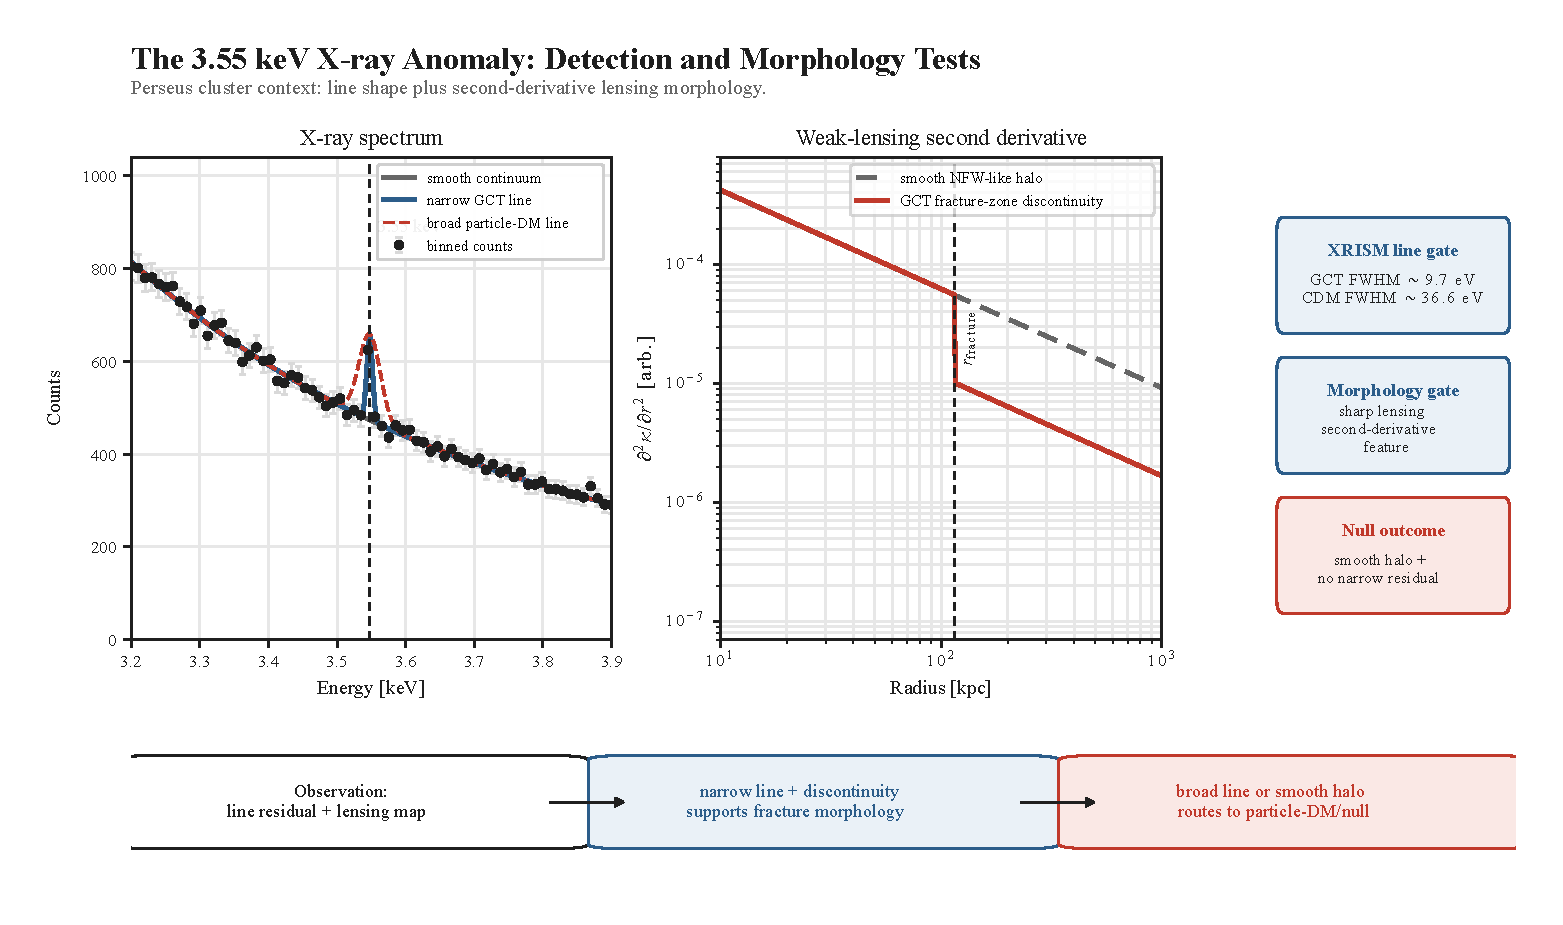
\includegraphics[keepaspectratio,alt={Conditional on the Tier 3 O.38 cage posit, the 3.55 keV X-ray centroid is modeled as a narrow Lorentzian over the cluster continuum (the line width is an open programme, §11.2.3); the Tier 3 fracture hypothesis also motivates a candidate feature in the cluster lensing shear profile.}]{content/Figures/Volume_3/Figure V3.11.1.pdf}}
\caption{Conditional on the Tier 3 O.38 cage posit, the 3.55 keV X-ray
centroid is modeled as a narrow Lorentzian over the cluster continuum
(the line width is an open programme, §11.2.3); the Tier 3 fracture
hypothesis also motivates a candidate feature in the cluster lensing
shear profile.}
\end{figure}

\chapter{Chapter 12: Dynamic Dark Energy ---
DESI}\label{chapter-12-dynamic-dark-energy-desi}

\gctneedspace{5\baselineskip}\begin{gctWarning}

\textbf{Tier-Disciplined Epistemic Status:}

\begin{itemize}
\tightlist
\item
  \textbf{Equation of State (\(w < -1\)): stipulated channel-shape
  template; the phantom direction is Tier 4 as a physical claim.} The
  written phason action cannot produce \(w<-1\) without a ghost, and no
  ghost-free construction is derived (§12.3.2; V2 Ch14 §14.3.1). The
  template is tested against DESI/Euclid CPL fits rather than promoted
  by fit quality.
\item
  \textbf{Energy Density Magnitude (\(\rho_{DE}\)): Tier 1 rewriting of
  the Friedmann identity; Tier 3 area-law reading and absolute magnitude
  (App ULA §ULA.4.1); the \(\chi\) functional-form identification is
  Tier 2.} V2 Ch14 §14.1.5 supplies the holographic area-law
  identification of \(\chi\); the absolute scale remains
  consistency-checked against Planck-anchored \(H_0\) and
  \(\Omega_\Lambda\), pending Open Problem O.4/O.1.
\item
  \textbf{Biogenic-DE calibrated quantities:} \(\tau_{lag}\), channel
  weights, and shape-menu amplitudes are Tier 3 fits or diagnostics;
  \(\lambda_{bio}\equiv\alpha\) is a declared Tier 3 matching choice,
  not fitted (V2 Ch14 §14.3.1). They address the dynamical evolution
  \(w(z)\), not a first-principles derivation of the absolute
  dark-energy scale.
\item
  \textbf{Biological-source interpretation: Tier 4.} Reading the fitted
  history as a physical biological source is Tier 4: no carrier,
  biology-to-phason transducer, physical Selection Operator, or
  stress-energy map has been derived. Even a match to the registered
  channel shape would validate only that shape (Tier 3), not its Tier 4
  biological-source interpretation.
\end{itemize}

\end{gctWarning}

For decades, the Standard Model of Cosmology
(\(\Lambda\)\hspace{0pt}CDM) has relied on the postulate that Dark
Energy is a static Cosmological Constant (\(\Lambda\))---an immutable
energy density of empty space with a fixed equation of state \(w = -1\).
Geometric Consciousness Theory (GCT) treats this as the baseline
area-law state plus a Tier 3 biogenic-channel fingerprint that may
correlate late-time informational activity with a small phantom-side
deviation (Tier 3 channel shape; the phantom direction itself is Tier 4,
V2 Ch14 §14.3.1). Dark Energy is not claimed here to be causally
produced by terrestrial biology; the chapter analyzes the registered
biogenic channel shape and its explicit external-data tension with the
DESI DR2 CPL fit.

\begin{center}\rule{0.5\linewidth}{0.5pt}\end{center}

\subsection{12.1 The Equation of State: The Sustained Phantom Phase
{[}stipulated template; phantom direction Tier
4{]}}\label{the-equation-of-state-the-sustained-phantom-phase-stipulated-template-phantom-direction-tier-4}

\begin{quote}
\textbf{Registered conditional templates:} The two chapter-level
coordinates are the phantom-side distinguishability template and the
stipulated Shapley-oriented source-proxy template. They are
independently adjudicated model-comparison targets. The Shapley template
does not represent measured physical biogenic strain, and neither
coordinate establishes a causal information-to-metric channel.
\end{quote}

\subsubsection{\texorpdfstring{12.1.1 DES-Dovekie Recalibrated DESI
Observations
(\(w_0, w_a\))}{12.1.1 DES-Dovekie Recalibrated DESI Observations (w\_0, w\_a)}}\label{des-dovekie-recalibrated-desi-observations-w_0-w_a}

The DES-Dovekie recalibrated DESI DR2 + CMB target (arXiv:2511.07517),
using Baryon Acoustic Oscillations (BAO) as a standard ruler,
strengthens the external-data test of dynamic dark energy. The
recalibrated CPL central fit \((w_0,w_a)=(-0.803\pm0.054,-0.72\pm0.21)\)
at joint dynamical-DE significance 3.2σ is sign-opposite to the GCT
single-channel biogenic template, whose registered amplitude is
\(|\Delta w(0.28)| \in [2,5]\times10^{-5}\) on the phantom side (the CPL
pair \((-1.0038,+0.0136)\) belongs to the non-operative broad logistic
reference run, not to the registered template): the external fit prefers
quintessence-today evolving more phantom in the past, while GCT predicts
a continuous phantom-side asymptote from below. The literal CPL crossing
and the GCT asymptote can both be tested by Roman/Euclid-class
precision, but they are not the same model. \textbf{The GCT biogenic-DE
reading is therefore in external-data tension with
DES-Dovekie-calibrated DESI, not confirmed by it; under the registered
\(3\sigma\) rule the multi-channel reconciliation is falsified
(§12.1.3).} The tension is calibration-robust: the official DESI DR2
release reports the CPL departure from \(\Lambda\)\hspace{0pt}CDM at
\(3.1\sigma\) for BAO+CMB and across the \(2.8\)--\(4.2\sigma\) range
when supernova samples are added, and every supernova calibration lands
in the same quintessence-today, more-phantom-past quadrant (\(w_0>-1\),
\(w_a<0\)) opposite to the GCT single-channel asymptote. The
\(3.2\sigma\) DES-Dovekie figure is the recalibrated central anchor, not
the upper edge of the adverse evidence.

\subsubsection{12.1.2 DESI DR2 vs the Phantom-Side
Template}\label{desi-dr2-vs-the-phantom-side-template}

The most significant feature for GCT is that DESI DR2 does \textbf{not}
match the single-channel biogenic direction: its CPL central fit is
quintessence-like today (\(w_0>-1\)) with a more-phantom past trend
(\(w_a<0\)), whereas the GCT biogenic-DE pipeline asymptotes to \(-1\)
from below with \(w_a>0\). The observational-distinguishability
threshold for the GCT channel is the Class-2 envelope
\(|\Delta w(z=0.28)| \in [2,5]\times10^{-5}\) {[}stipulated template{]},
not a DESI-amplitude claim. The CPL crossing at \(z \approx 0.39\) in
the CPL fit to the non-operative logistic reference run is a fit
artifact, not a mathematical zero of \(w+1\) in that run;
\(z \approx 0.28\) is the sensitivity marker. In standard General
Relativity, a true fluid with \(w < -1\) violates the Null Energy
Condition (NEC) and typically implies ``ghost'' instabilities---negative
kinetic energy states that threaten the stability of the vacuum. The GCT
action of §12.3 does not escape this (§12.3.2).

\subsubsection{12.1.3 DES-Dovekie-Calibrated DESI vs Single-Channel
Biogenic: External-Data Tension on CPL Sign {[}stipulated conditional
correlation/model coordinate and shape; phantom direction and
physical-source interpretation Tier 4; registered state-level CPL-fit
rule
applied{]}}\label{des-dovekie-calibrated-desi-vs-single-channel-biogenic-external-data-tension-on-cpl-sign-stipulated-conditional-correlationmodel-coordinate-and-shape-phantom-direction-and-physical-source-interpretation-tier-4-registered-state-level-cpl-fit-rule-applied}

The DES-Dovekie recalibrated DESI DR2 + CMB CPL target
(arXiv:2511.07517) gives
\((w_0, w_a) = (-0.803 \pm 0.054,\,-0.72 \pm 0.21)\) in the
sign-opposite quadrant --- a \textbf{quintessence-today,
evolving-more-phantom-in-the-past} signature (\(w_0 > -1\),
\(w_a < 0\)). The GCT single-channel biogenic-DE template (IMP-01
pipeline, \texttt{protocol\_imp01\_pipeline.py}) sits in the
\textbf{continuous phantom phase} (\(w \leq -1\) throughout, asymptoting
to \(-1\) from below; no literal crossing) with \(w_a > 0\); its
registered amplitude is \(|\Delta w(0.28)| \in [2,5]\times10^{-5}\). The
non-operative broad logistic reference run of the same pipeline has CPL
\((w_0, w_a) \approx (-1.0038,\, +0.0136)\), which shows the same sign
pattern but is not a registered prediction. The two dispositions are
\textbf{sign-opposite on both CPL parameters}, and the disposition must
be read as a \emph{live external-data tension} on the state-level
CPL-fit gate, not as confirming evidence of the Biogenic Drive.

The multi-channel shape-proxy diagnostic closure path
(Copeland-Sami-Tsujikawa 2006; V2 Ch14 §14.6.3) is the natural
arbitration mechanism, but \textbf{CLOSURE-FAILS for the registered
five-channel admixture (App ORQ O.13 closure paths C1/C2/C3 open)}:
every channel in the registered menu
\(\{\Lambda\text{-baseline}, \text{biogenic-terrestrial}, \text{biogenic-non-terrestrial}, \text{abiotic-chiral}, \text{frozen-phason perturbation}\}\)
carries \(w_c(z) \leq -0.9\), so the convex-combination ceiling on
\(w_{\rm total}(z)\) also lies at \(-0.9\) --- below the DES-Dovekie
central value used by the diagnostic. The 4032-point sensitivity sweep
over
\((\Omega_{\Lambda,0}, f_{\rm ext}, f_{\rm chiral}, f_{\rm pert}, z_{\rm chiral})\)
implemented in
\texttt{GCT\_Physics\_Engine/src/protocol\_de\_multichannel.py} returns
a best-fit diagonal diagnostic score \(\approx 4.861\) against the
DES-Dovekie target and is flat to within \(0.0446\) score units across
the entire defensible \(\Omega_{\Lambda,0}\) range
\(\{0.50, \ldots, 0.75\}\). The analytic ceiling, not the diagnostic
score, supplies the menu-level closure failure including the
\(\Omega_{\Lambda,0}\to0\) limit.

\textbf{Scope of the §12.1.3 disposition.} The single-channel
\(w_{\rm bio}(z) \leq -1\) phantom-direction signature is a
\textbf{stipulated conditional model shape} under the shared-field and
Class-2 allocation ansatz (its phantom direction is Tier 4 as a physical
claim, §12.3.2), not a mechanism-level source claim. Its typed physical
coupling, normalization, and information-to-metric causal map remain
open. What is in tension with DESI is the state-level CPL-fit
arbitration under the registered multi-channel shape-proxy partition.
Closure requires a GCT-derivable dark-energy channel carrying
quintessence-today behavior over the DESI window \(z \in [0, 1.5]\) ---
for example, a thawing-quintessence channel sourced by a
sub-horizon-tracking phason mode. No such channel is included in the
registered five-channel menu; whether one is \emph{derivable} from the
broader GCT lawscape is the residual open question, registered as
\textbf{Open Problem O.13} (V2 Ch14 §14.6.3 + App ORQ Open Problem O.13)
and \emph{not} foreclosed by the present chapter.

\textbf{Falsification gate.} The registered rule reads: if the
sign-opposite CPL region is confirmed at \(> 3\sigma\), the biogenic-DE
state-level CPL-fit reconciliation is falsified at the multi-channel
shape-proxy closure path. Current fits already place it there:
DES-Dovekie at \(3.2\sigma\), and the official DESI DR2 analysis at
\(3.1\sigma\) for BAO+CMB and \(2.8\)--\(4.2\sigma\) with supernovae.
Applied as written, \textbf{the registered multi-channel CPL-fit
reconciliation is falsified} (a branch-level verdict, not a verdict on
GCT as a whole; App PSC §PSC.8 row 8). Later Euclid/Roman data can test
whether the preference persists but cannot reinstate the registered
menu. The separate IMP-01 pipeline gate (C\_IMP01\_PIPELINE\_GATE)
requires DESI DR2 plus Euclid DR1 and has not fired. The conditional
single-channel \(w_{\rm bio}(z) \leq -1\) template is a separate
coordinate, testable via Roman/Stage-V-class joint-bin analysis across
\(z \in [0.05, 0.5]\) (§12.4.3 below). Even a match would validate only
that registered shape, not its Tier 4 phantom-sector or
biological-source interpretation.

\subsection{\texorpdfstring{12.1.4 --- JWST High-z Tension as a Binary
Gate for \(\tau_{bio}\) {[}Tier
3{]}}{12.1.4 --- JWST High-z Tension as a Binary Gate for \textbackslash tau\_\{bio\} {[}Tier 3{]}}}\label{jwst-high-z-tension-as-a-binary-gate-for-tau_bio-tier-3}

\gctneedspace{5\baselineskip}

\textbf{The Tension:} The James Webb Space Telescope (JWST) has revealed
an excess of UV-bright galaxies at \(z > 10\) (\(t < 500\) Myr after the
Big Bang) relative to some pre-JWST models; the size and cause of the
excess are debated. If high-complexity stellar populations capable of
hosting biospheres existed well before \(z \approx 2\), the Biogenic
Dark Energy model's evolutionary lag parameter
\(\tau_{bio} \approx 4\)--\(5\) Gyr {[}Tier 3{]} faces pressure.

\gctneedspace{5\baselineskip}

\textbf{The Binary Gate:} The Biogenic Hypothesis makes \(\tau_{bio}\)
the calibrated lag parameter {[}Tier 3{]} that maps stellar formation
history to the phantom-phase distinguishability-threshold redshift. This
parameter can be independently constrained:

\begin{enumerate}
\def\labelenumi{\arabic{enumi}.}
\tightlist
\item
  Obtain the JWST-revised galaxy stellar mass function for
  \(0 < z < 15\)
\item
  Compute the time-integrated stellar complexity
  \(\mathcal{I}(t) = \int_0^t \text{SFR}(t'-\tau_{bio})\cdot P_{evolve}(t')dt'\)
\item
  Find the \(\tau_{bio}\) that places the kernel's low-redshift
  sensitivity marker at \(z \approx 0.28\) (the peak of the biological
  driving term itself falls at \(z \approx 0.19\); V2 Ch14 §14.3.2)
\item
  Compare this derived \(\tau_{bio}\) with the independently estimated
  time for technological civilization to emerge after star formation
\end{enumerate}

\textbf{Prediction:} If the JWST galaxy mass function is used as input,
GCT expects \(\tau_{bio}\) in the range 3.5--6 Gyr {[}Tier 3{]}. The
registered falsification band is wider (Firewall Metadata below): a
derived \(\tau_{bio} < 2\) Gyr or \(> 8\) Gyr, or independent
biosphere-emergence constraints requiring such a value,
\textbf{falsifies} the Biogenic correlation branch independent of dark
energy observations; a value in \([2, 3.5)\) or \((6, 8]\) Gyr is a
tension, not a falsification.

\textbf{Status:} This test is pending a declared stellar-mass-function
release, completeness model, integrated-SFR pipeline, and frozen
uncertainty budget. Public observations may supply inputs, but the
executable analysis and systematics closure are not yet assembled.

\gctneedspace{5\baselineskip}\begin{gctImportant}

\textbf{Firewall Metadata {[}\(\tau_{bio}\) Binary Gate{]}}

\begin{itemize}
\tightlist
\item
  \textbf{Type:} Falsification condition for Biogenic DE (Tier 3)
\item
  \textbf{Required input:} JWST galaxy stellar mass function
\item
  \textbf{Falsification criterion:} If derived \(\tau_{bio} < 2\) Gyr or
  \(> 8\) Gyr from SFR integral
\item
  \textbf{Execution condition:} frozen data release, completeness model,
  SFR integration, and uncertainty budget
\end{itemize}

\end{gctImportant}

\begin{center}\rule{0.5\linewidth}{0.5pt}\end{center}

\subsection{12.2 The Cross-Manifold Correlation Model {[}Tier 4 physical
interpretation{]}}\label{the-cross-manifold-correlation-model-tier-4-physical-interpretation}

\subsubsection{\texorpdfstring{12.2.1 Biogenic Hypothesis: Complexity
\(\to\) Vacuum
Winding}{12.2.1 Biogenic Hypothesis: Complexity \textbackslash to Vacuum Winding}}\label{biogenic-hypothesis-complexity-to-vacuum-winding}

The Tier 3 cross-manifold model stipulates a coordinate chain from
Selection to informational bits to phason winding in \(E_\perp\), with
the winding represented as a \textbf{Geometric Spring}. No typed
Selection-to-bit operator, normalized bit-to-winding law, measured
record channel, or causal energy-transfer coefficient is supplied. The
chain is therefore a conditional ansatz used to generate the correlation
fingerprint, not established physical work performed by an Agent on the
vacuum. As a physical account it is a Tier 4 source ansatz only: no
physical Selection Operator, owner or subject count, or
metabolic-to-phason transducer has been derived; the Tier 3 content is
the channel shape.

\subsubsection{12.2.2 The Resolution of the Phantom
Pathology}\label{the-resolution-of-the-phantom-pathology}

The apparent violation of the Null Energy Condition (\(w < -1\)) was
modeled as a signature of \textbf{Cross-Manifold Work} in the
biogenic-channel ansatz, with the ghost instability said to be avoided
because the channel is an effective lattice-susceptibility response.
That avoidance is asserted, not shown: the action of §12.3 cannot
produce \(w<-1\) without a ghost (§12.3.2). The phantom pathology is
therefore unresolved, and the phantom direction is Tier 4 until a
ghost-free construction is derived. This remains a
correlation/fingerprint template for a tiny phantom-side deviation, not
a causal claim that biological work powers cosmic expansion.

\subsubsection{12.2.3 The Cosmological vs.~Biological Arrow of
Time}\label{the-cosmological-vs.-biological-arrow-of-time}

The \textbf{Cosmological Arrow} (expansion) and the \textbf{Biological
Arrow} (evolution) are compared as parallel conversions of implicit
potential into explicit information. The sustained phantom-phase
deviation (the GCT-consistent reading per §12.1.2 --- \(w(z)\)
asymptoting to \(-1\) from below, not literally crossing) is the
registered Tier 3 channel fingerprint under that analogy; it should not
be read as a demonstrated causal history of cosmic acceleration.

\begin{center}\rule{0.5\linewidth}{0.5pt}\end{center}

\subsection{12.3 The Dark Energy Lagrangian {[}Tier
3{]}}\label{the-dark-energy-lagrangian-tier-3}

\subsubsection{12.3.1 The Coupling Term
(Phenomenological)}\label{the-coupling-term-phenomenological}

We formalize the biogenic correlation by introducing an illustrative
coupling term into the action for the scalar phason field
\(\phi_\perp\), representing the volumetric density of the internal
dimensions.

\gctneedspace{5\baselineskip}

\textbf{The GCT Dark Energy Lagrangian (Illustrative):}
\[\mathcal{L}_{DE} = -\frac{1}{2}K_\perp (\partial_\mu \phi_\perp)^2 - V(\phi_\perp) - \lambda \left( \frac{\dot{\mathcal{I}}}{I_0} \right) (\partial_\mu \phi_\perp)^2\]

Where:

\begin{itemize}
\tightlist
\item
  \(\dot{\mathcal{I}}\): A stipulated aggregate \textbf{Information
  Generation Rate} (information-history/source variable). It is not
  presently derived from collective Selection Operators or physical
  bit-generation events; reading it as their output is Tier 4.
\item
  \(I_0\): The \textbf{Lattice Update Rate} (\(1/t_6\)), a declared
  normalization rate, not a measured lattice clock or a derived maximum
  bit-rate of the lattice hardware.
\item
  \(\lambda\): The dimensionless coupling constant (declared as
  \(\lambda \equiv \alpha\), a Tier 3 matching choice; not fitted, V2
  Ch14 §14.3.1).
\end{itemize}

\subsubsection{12.3.2 Motivation:}\label{motivation}

The heuristic term \(\lambda(\dot{\mathcal{I}}/I_0)\) is a model
coordinate for a \textbf{Variable Inertia} ansatz. This is not evidence
that complexity causally accelerates the universe; the shared-field
coupling, normalization, and mechanism remain open, and the current
quantitative magnitude overshoots drastically.

\textbf{Declared open programme {[}Tier 4{]}} (phantom branch). (a) This
action was presented as yielding a sustained phantom phase, with an
``anti-damping'' term when \(\ddot{\mathcal I}>0\) and no ghost. (b) The
\(\lambda\) term only rescales the kinetic coefficient to
\(Z=K_\perp+2\lambda\dot{\mathcal I}/I_0\); for a homogeneous field
\(\rho+p=Z\dot\phi_\perp^2\), so \(w<-1\) requires \(Z<0\), a ghost, and
for \(\lambda\dot{\mathcal I}>0\) the action gives \(w\ge-1\). In the
equation of motion \(Z\ddot\phi_\perp+(3HZ+\dot Z)\dot\phi_\perp+V'=0\),
growing \(Z\) is extra damping, not anti-damping. (c) Closing this needs
a ghost-free phantom construction with a stability analysis. (d) None is
derived, so phantom-direction statements in this chapter are Tier 4; the
registered \(w(z)\) curve is a stipulated template, and nothing
downstream uses this action as support for the phantom sign (V2 Ch14
§14.3.1).

\subsubsection{\texorpdfstring{12.3.3 The Susceptibility Constant
(\(\chi \approx 2.27 \times 10^{122}\))}{12.3.3 The Susceptibility Constant (\textbackslash chi \textbackslash approx 2.27 \textbackslash times 10\^{}\{122\})}}\label{the-susceptibility-constant-chi-approx-2.27-times-10122}

GCT identifies the vacuum as a system near a phase transition with a
susceptibility \(\chi\) defined by the \textbf{Holographic Entanglement
Entropy} of the exact-de-Sitter static-patch horizon proxy \(R_H=c/H_0\)
(V2 Ch14 §14.1.5) {[}Tier 2 functional-form identification; Tier 3
numerical evaluation{]}. In a matter-plus-dark-energy cosmology this
proxy is distinct from the present event horizon:
\[\begin{gathered}\chi \equiv \frac{A_{\mathcal{H}_{\rm dS}}}{4\ell_P^2} = \pi\!\left(\frac{c}{H_0 \ell_P}\right)^2 \approx 2.27 \times 10^{122} \\[1pt] \gcteqnote{(using Planck 2018 $H_0 = 67.4$ km/s/Mpc and CODATA constants) [Tier 2 functional form + Tier 3 numerical evaluation]}\end{gathered}\]

\textbf{Holographic Derivation:} The susceptibility \(\chi\) is the
holographic information capacity (area-law entropy) of the de Sitter
horizon proxy; reading it as the \textbf{Total Computational Capacity}
of the observable portion of the \(6D \to 3D\) projection is a Tier 4
interpretation. The Tier 2 content is the area-law functional form; the
numerical evaluation imports \(H_0\) and \(\Omega_\Lambda\) pending
O.1/O.4. See V2 Ch14 §14.1.5 for the full derivation. The canonical
dark-energy density form is
\(\rho_\Lambda = (3\Omega_\Lambda/8\pi)\,\hbar H_0^2/(c\ell_P^2)\); it
is a Friedmann/area-law consistency check, not a closed derivation of
the observed density from the current postulate set.

Within the Tier-3 dark-energy ansatz, \(\chi\) is used as a
model-normalization coordinate and the accumulated biogenic-bit
coordinate \(\dot{\mathcal{I}}\) is stipulated to scale against it. This
does not establish a count of physically executed cycles, a causal
dark-energy effect, or an information-to-metric coupling; the typed
operator, source normalization, and causal map remain open. The area-law
functional form of \(\chi\) is the separate Tier-2 identification with
the Gibbons-Hawking horizon entropy in V2 Ch14 §14.1.5, while its
numerical cosmological evaluation remains Tier 3 (verified
arithmetically by
\texttt{verify\_independent/verify\_chi\_holographic.py}).

\begin{center}\rule{0.5\linewidth}{0.5pt}\end{center}

\subsection{12.4 Quantitative Analysis}\label{quantitative-analysis}

\subsubsection{12.4.1 The Hubble Tension Lies Outside the Scope of the
V2 Ch14 §14.5.1
Action}\label{the-hubble-tension-lies-outside-the-scope-of-the-v2-ch14-14.5.1-action}

The empirical Hubble tension is \emph{not} accounted for by the
conditional V2 Ch14 §14.5.1 lag-kernel coordinate under its stipulated
kernel, overdensity scaling, and normalization.
\texttt{protocol\_o17\_delta\_h\_local.py} returns the opposite sign and
\(|\delta H_{local}/H_0|\in[7\times10^{-6},1.6\times10^{-5}]\). This is
Tier 3 model-internal arithmetic, not a derivation or test of a physical
biogenic action; the typed coupling, source map, and causal bridge
remain open.

\begin{quote}
\textbf{Scope of the Hubble-tension claim {[}Tier 4 physical-source
hypothesis / coupling-structure question{]}.} The ``Complexity Peak''
interpretation of the SH0ES-vs-Planck gap is an
\emph{alternative-coupling-structure hypothesis} (option (i) of
\textbf{Open Problem O.17}, V2 Ch14 §14.5.4 and Appendix ORQ) in which
local biogenic activity enhances the local \(\rho_\Lambda(0)\) value
directly; as a physical-source claim this is Tier 4 (no
biology-to-phason transducer or source normalization is derived). That
option is \emph{not} currently derived from the V2 Ch14 §14.5.1 action
and should be treated as forward-looking until O.17 closes. The
alternative (option (ii) of O.17) is that the Hubble tension is sourced
by physics outside the biogenic sector. Standard cosmology's Local Void
hypothesis is the comparable peer reading; both are presently outside
the GCT framework's quantitative scope.
\end{quote}

Closure of the Biogenic-Gradient / Hubble-tension mapping requires
either (a) deriving the option-(i) coupling from the GCT action
explicitly, or (b) accepting that the framework's empirical \(w(z)\)
anchors are the cosmic-mean phantom-phase signature (per V2 Ch14
§14.6.3) and the dipole-anisotropy direction (per V2 Ch14 §14.3.1), not
the Hubble tension.

\subsubsection{12.4.2 Integrated Sachs-Wolfe (ISW) Evidence ---
Quantitative Status {[}Tier
3{]}}\label{integrated-sachs-wolfe-isw-evidence-quantitative-status-tier-3}

The biogenic-DE perturbation to the late-time linear growth factor
\(D(z)\) produces a magnitude-very-small modification of the standard
Integrated Sachs-Wolfe signal (Sachs \& Wolfe 1967; Crittenden \& Turok
1996). The amplitude is propagated from the V2 Ch14 §14.5.1 lag-kernel
action
(\texttt{GCT\_Physics\_Engine/src/protocol\_o17p\_isw\_amplitude.py});
this is exact conditional model propagation, not a derivation or
validation of a biological source: the growth-factor shift at the ISW
kernel peak (\(z \approx 0.4\)) is
\(\delta D / D \approx 3 \times 10^{-5}\), propagating to a cosmic-mean
ISW amplitude perturbation of
\(\delta A_{ISW}/A_{ISW,\Lambda\text{CDM}} \approx 8 \times 10^{-5}\)
(\(0.008\%\)). No sign is claimed for the ISW perturbation relative to
\(\Lambda\)\hspace{0pt}CDM: at fixed \(\Omega_{DE,0}\) a phantom-side
\(w\) delays dark-energy domination, which usually reduces the late ISW
source, and settling the sign requires a Boltzmann-code calculation.

The biogenic-vs-gravitational cross-correlation \emph{differential} ---
the more specific signature predicted by the inhomogeneous biogenic-DE
hypothesis --- is bounded by the product of the cosmic-mean perturbation
and the bias-difference between biogenic-weighted and
gravitational-mass-weighted galaxy tracers. For an assumed
\(|b_{bio}/b_{m} - 1| \in [0.1, 0.3]\) (a stipulated range for
stellar-mass-weighted vs halo-mass-weighted galaxy samples; no
tracer-bias measurement is cited), the differential cross-correlation
amplitude is \([8 \times 10^{-6}, 2.4 \times 10^{-5}]\) of the standard
ISW signal --- three to four orders of magnitude below the CMB-S4 +
SPHEREx joint detectability threshold (\(\sim 4\%\)).

Current Planck \(\times\) galaxy ISW measurements (Stölzner et al.~2018
\emph{Phys. Rev.~D} 97:063506; Hang et al.~2021 \emph{MNRAS} 501:1481)
constrain \(A_{ISW}\) to \(\sim 20\%\) precision; the biogenic-DE
perturbation is therefore far below current sensitivity. A
CMB-S4/SPHEREx-class joint analysis with an approximately fivefold
precision improvement would still leave the model signal \(\sim10^3\)
below threshold. Direct detection would require a substantially more
sensitive CMB/spectroscopic combination or a validated
stellar-mass-weighted stacking strategy; no facility date or performance
forecast is assumed.

The V2 Ch14 §14.5.1 conditional coordinate assigns a currently
magnitude-unobservable ISW perturbation of undetermined sign. This is a
model diagnostic, not evidence for a biogenic causal action.

\subsubsection{12.4.3 Roman/Stage-V-Class Test ---
Sensitivity-Conditional}\label{romanstage-v-class-test-sensitivity-conditional}

A Roman/Stage-V-class low-redshift analysis can audit this correlation
only if it reaches the declared precision and systematics conditions.

\begin{itemize}
\tightlist
\item
  \textbf{GCT Prediction {[}calibrated, stipulated channel template;
  phantom direction Tier 4, §12.3.2{]}:} the model assigns a non-linear
  phantom-phase deviation, asymptoting to \(-1\) from below without
  literal crossing. The operative Class-2 envelope is
  \(|\Delta w(z \approx 0.28)| \in [2,5]\times10^{-5}\), correlated with
  the integrated star-formation/metallicity history. A clean test
  requires low-\(z\) precision below \(5\times10^{-5}\) with the
  registered systematics.
\item
  \textbf{Falsification:} A qualifying low-\(z\) program that excludes
  the \([2,5]\times10^{-5}\) phantom-directed Class-2 envelope or
  locates a coherent deviation outside the registered
  history-correlation model falsifies that branch.
\item
  \textbf{Scope:} Matching the envelope would not establish a
  biology-to-phason source, consciousness, or Level II.
\end{itemize}

\gctneedspace{5\baselineskip}\begin{gctImportant}

\textbf{Firewall Metadata {[}Biogenic Dark Energy{]}}

\begin{itemize}
\tightlist
\item
  \textbf{Type:} Consistency Check (Tier 3 channel-shape diagnostic;
  Tier 4 physical-source interpretation)
\item
  \textbf{Inputs:} \(\dot{\mathcal{I}}\) (Complexity), \(\chi\)
  (Holographic Susceptibility)
\item
  \textbf{Degrees of Freedom:} five tuned or stipulated inputs for the
  registered Class-2 envelope (\(\tau_{lag}\), \(\tau_{bio}\), the
  normalization target \(\delta w(0)=-0.005\), \(\tau_{intel}\) and the
  \(\tau_{tech}\) band; V2 Ch14 §14.5.1 Firewall Metadata);
  \(\lambda\equiv\alpha\) is declared, not fitted
\item
  \textbf{Provenance:} Calibrated fit (Integrated Star Formation
  history)
\end{itemize}

\end{gctImportant}

\gctneedspace{5\baselineskip}

\textbf{END OF CHAPTER 12}

\clearpage
\thispagestyle{empty}
\vspace*{0.35\textheight}
\begin{center}\bfseries\LARGE PART IV: EXPERIMENTAL PROTOCOLS\end{center}
\vspace*{\fill}
\clearpage

\chapter{Chapter 13: Protocol A --- Candidate Zeno
Drive}\label{chapter-13-protocol-a-candidate-zeno-drive}

\gctneedspace{5\baselineskip}\begin{gctWarning}

\textbf{Epistemic Status: Tier 3 (Hypothesis)} The ``Zeno Drive'' is a
\textbf{Tier 3 candidate research programme}, not a closed GCT material
interaction. As written, the Rashba-phason coupling of V1 Ch17 Eq.
(17.3) is not an icosahedral scalar for the vector phason, and a
type-correct coupling has no action-fixed coefficient (V1 Ch17 §17.1.3).
The 931 kHz / 38.3 MHz / \textasciitilde41\(\times\) chain and every
downstream \(\eta_{Zeno}\) and \(N_{coh}\) value are therefore a
\textbf{conditional external-rate scenario}, and the \textasciitilde100
MHz figure is a \textbf{historical material-scan scenario}, not a
derived operating rate. The scenario also relies on \textbf{millisecond
quantum coherence} in warm biological systems, whereas standard
biophysics places unstructured-medium decoherence near \(\sim 10^{-13}\)
s; the proposed ``Topological Shielding'' is a \textbf{conjecture} that
remains experimentally unproven. Protocol A-Prime and the Protocol D NMR
polarity rule (Ch16 §16.5) test ordinary CISS, spin, phonon and
coherence-response branches only. A preregistered result rejects the
registered biophysical branch (protected-subspace / polarity /
Zeno-substrate branch) only under that branch's own registered decision
rule (the Protocol A-Prime F1 three-conjunct null; the Protocol D NMR
polarity gate (P.13c) is held pending redesign: as written it rejected
by construction, since \(^{17}\)\hspace{0pt}O shortens
water-\(^1\)\hspace{0pt}H \(T_2\) by scalar relaxation; the former
sign-aware rule, which rejects the registered sign-positive branch on a
powered, significant negative isotope × activity interaction in
water-\(^1\)\hspace{0pt}H \(\Delta T_2\), applies only after the
redesign, and until then no outcome supports or rejects the branch, Ch16
§16.5); a positive result does not establish a phason coupling, Identity
Polaron, Selection Operator or Level II. Neither outcome is a verdict on
GCT as a whole: the measurement tests an ordinary material proxy, and no
phason, Selection-Operator or Level-II inference follows from it (V1
Ch17 §17.1.3). Protocol D LORR is a pilot/systematics study; Ch16 §16.4
carries the no-gate disposition. Level II is open (Tier 3) for every
examined substrate: no validated substrate criterion exists yet (it
requires a typed, normalized, measured coupling, the Identity-Polaron
construction and an independent phenomenal bridge; O.21/O.23/O.34,
O.18). The geometric results of Volumes 2--3 are not tested by these
protocols.

\end{gctWarning}

Within the biophysical-substrate branch of Geometric Consciousness
Theory (GCT), Protocol A organizes ordinary material tests of the
ingredients once proposed for a \textbf{candidate Zeno Drive} (a
proposed non-thermal transduction channel between metabolic dynamics and
phason observables). It does not detect a realized Selection Operator,
vacuum-winding process or Identity Polaron. The typed and normalized
interaction, formation of an Identity Polaron, and independent
phenomenal bridge all remain open; Protocol A observables cannot by
themselves establish a mind-brain interface or Level II.

\begin{center}\rule{0.5\linewidth}{0.5pt}\end{center}

\subsection{13.1 The Physics of
Nucleation}\label{the-physics-of-nucleation}

\gctneedspace{5\baselineskip}\begin{gctNote}

\textbf{Open mechanism choices {[}Tier 3{]}.} Mechanism choices not yet
made: the radical-pair species and its initiator under physiological
(dark) conditions (O.21/O.34); the reset chemistry and the energy per
cycle against the power budget (O.34); which state recombination-as-Zeno
would protect (no physical sector label is yet declared; App BEB
§BEB.6d); and the damping/dissipation model (O.23). The whole
biophysical stratum is Tier 3 (cf.~V1 Ch17 §17.1).

\end{gctNote}

\subsubsection{13.1.1 The Energy Paradox: 3.55 keV vs.~Thermal
Noise}\label{the-energy-paradox-3.55-kev-vs.-thermal-noise}

The central challenge of the biophysical branch is the
\textbf{Nucleation Problem}. Under the Chapter 7 cage ansatz, the
\textbf{Identity Polaron} is hypothesized as a macroscopic topological
defect anchored by an electron-like \(N=144\) core. Because that cage
size is a Tier 3 structural posit pending O.38, the associated Vacuum
Quantum \(E_{vac}=m_e/144\approx\mathbf{3.55\ keV}\) is a Tier 3
conditional postdiction rather than a Tier 2 cage-size derivation.

Biological systems operate at a physiological temperature of
\(\sim\)\hspace{0pt}310 K {[}Tier 3 --- biological parameter{]}, where
the characteristic thermal energy \(k_B T\) is approximately
\textbf{0.026 eV} {[}Tier 1 --- thermodynamic identity{]}. Conditional
on the Tier-3 \(N=144\) defect ansatz, this lies five orders of
magnitude below the adopted defect-energy scale. That comparison
motivates a candidate non-thermal preparation channel; it neither proves
that thermal dynamics cannot contribute nor establishes coherent
informational work, Identity-Polaron nucleation, or phenomenal status.

\subsubsection{13.1.2 Audit of the Candidate Transduction-Force
Ansatz}\label{audit-of-the-candidate-transduction-force-ansatz}

The historical question was whether a declared measurement rate
\(\nu_{Zeno}\) could generate a force on an ion channel. No such force
follows from the current action; the equations below retain conditional
ordinary open-system algebra and identify the missing physical inputs.
The Quantum Zeno Effect suppresses transitions out of a measured or
protected subspace; it does not freeze all phase evolution. The
candidate protected-subspace stabilization is modelled by a
\textbf{Tavis-Cummings cooperative pumping model}. The ratio
\(\Xi = g_{single}^{eff} \cdot \sqrt{N_{\rm coop}} / \kappa\), where
\(N_{\rm coop}\) denotes the phase-locked cooperative dipole count in
the active Polaron volume, is valid conditional open-system algebra once
a physical mode, coupling, population and linewidth are independently
specified. GCT has not derived that normalized material-mode map, so
\(\Xi \gg 1\) is a \textbf{Tier 3 scenario calculator}, not a
macro-coherence or Level-II criterion.

\textbf{Coupling Nomenclature {[}empirical CISS spin selectivity / Tier
3 phason coupling and magnitudes{]}:} Empirical CISS spin selectivity in
chiral biomolecules is the background mechanism (Naaman, Paltiel \&
Waldeck 2019, \emph{Nat. Rev.~Chem.} 3:250--260). The literature
supports the mechanism class --- chiral spin-selective transport --- but
not the tubulin-specific kHz/MHz phason-coupling numbers. The
transduction step from CISS spin selectivity into a phason-lattice
coupling is layered: empirical spin selectivity for the chiral
spin-orbit selection rule (an established class of measurements),
\textbf{Tier 3} for the phason coupling (the Eq. 17.3 form is not an
\(A_5\) scalar, V1 Ch17 §17.1.3) and for its beta-tubulin implementation
and magnitude pending O.12/O.21/O.23 closure and calibration in the
in-vitro arm of Protocol A. The \textbf{specific magnitudes} quoted in
this subsection are \textbf{external scenario anchors} with no
dimensionally valid provenance from the action; they must not be read as
bare or effective GCT rates. The historical ``bare'' Tryptophan (Trp)
value is \(g_{single}^{bare} \approx 931\) kHz \textbf{{[}Tier 3
external scenario anchor --- model translation from the CISS mechanism
class to the candidate β-tubulin Trp residues (Trp21, Trp103, Trp346,
Trp407 per PDB 1JFF/1TUB; O.21 currently identifies Trp21 only as a
local-inward wall-patch candidate, while assembled-microtubule
lumen-axis verification remains open) dipole geometry; quantitative
closure requires the in-vitro arm of Protocol A, per §13.2.3{]}}. The
\textbf{Chiral Phonon-Polariton enhancement} mechanism (Tier 3
hypothesis pending O.23/O.24 --- collective resonance of the Trp
aromatic radical network with the tubulin lattice phonons) was posited
in the historical scenario to multiply this anchor by
\textasciitilde41\(\times\) \textbf{{[}Tier 3 external scenario input
chosen for operating-point consistency, not derived; see Appendix GPE
for the computational scaffold and Open Problem O.12 for the
frequency-scale renormalization target{]}}, giving the scenario value
\(g_{single}^{eff} \approx 38.3\) MHz \textbf{{[}Tier 3 --- declared
external-rate scenario constant, not an evaluated matrix element and not
a factor-of-three estimate of a GCT coupling; dependent
\(\eta_{\rm Zeno}\) and \(N_{\rm coh}\) values are conditional
external-rate scenarios{]}}. The operative central O.21 branch remains
\(n_{rp}=0\) until assembled-microtubule lumen-axis closure. On the
conditional \(n_{rp}=1\) sensitivity branch, the neuron-scale Trp
inventory is \(N_{\rm Trp,neuron} = 1.625 \times 10^9\) candidate
dipoles per typical pyramidal neuron (arithmetic per V1 Ch17 §17.1.4:
\(\sim 10^5\) MTs/neuron \(\times \, 13\) protofilaments/MT
\(\times \, 1{,}250\) dimers/protofilament \(\times \, n_{rp}=1\)). The
disfavored all-four-β-Trp stress-test ceiling is \(6.5 \times 10^9\) and
is not propagated as an operative substrate count. The cooperative
calculation proceeds with the smaller phase-locked \(N_{\rm coop}\)
defined in §13.5.3. At the \texttt{protocol\_zeno\_energy\_budget}
output level, cooperativity and entropy checks survive only on the
conditional sensitivity branch (B1/B2/B4); B3 spin-count energy-delivery
does NOT close on either branch. The engine evaluates B3 on the
operative central branch, where \(N_{bio}=0\) by construction pending
O.21, so it fails trivially there; on the conditional sensitivity branch
the available count is \(N_{bio}=1.625\times10^9\) against a required
\(7.66\times10^9\), a \(\sim4.7\times\) gap; O.23 DFS dressing reaches
the \(100\,\mu\)\hspace{0pt}s floor but remains below the 10 ms target.
The cooperative-nucleation closure is pending O.23 (chiral
phonon-polariton DFS). The Trp inventory and coherence calculations
remain ordinary material-candidate bookkeeping. Protocol A-Prime
measures surrogate spin/coherence response; it cannot calibrate
\(g_{single}^{eff}\) or a phason coupling. A preregistered A-Prime null
meeting the registered F1 rule (§13.3.5) rejects the registered
biophysical branch as registered; it is not a verdict on GCT as a whole
or on Level II.

In the historical Tier 3 scenario form, the single-spin coupling
\(g_{single}\) was modelled as driven by the \textbf{lattice speed of
light \(\hat{c} = c_P \times \phi^{-9}\) (Vol. 2 §6.2.2)} acting as the
Lattice Speed of Light (phason group velocity) on the native
\textbf{dipole transition moment \(\mu_{Trp}\)} of the
\textbf{Tryptophan (Trp) aromatic radical chain} within the tubulin
dimer; this is not an action-derived coupling (V1 Ch17 §17.1.3).
Tryptophan residues are natively present in \(\beta\)-tubulin at four
positions (Trp21, Trp103, Trp346, Trp407 in PDB
ATOM/\texttt{auth\_seq\_id} numbering for 1JFF/1TUB; FASTA-sequence
indexing maps the same sites to the corresponding beta-tubulin Trp set
used in the O.21 screen). Their ordinary dipole, radical-pair and CISS
observables are candidate material controls; a coupling from those
observables to the canonical vector phason has not been derived and
still requires typed spinor and material vertices, a physical
coefficient, compatible kinetic/mode/chirality normalization, a
field-to-material map and a sector-writing matrix element {[}Tier
3/open{]}.

\begin{quote}
\textbf{Spatial-scale clarification --- Trp-Trp pair separation vs
tubulin dimer length {[}ordinary radical-pair constraint; material
realization open pending Open Problem O.21 assembled-axis
identification{]}.} The \textbf{8 nm} tubulin dimension refers to the
\textbf{tubulin dimer length} (α-β heterodimer along the microtubule
protofilament axis, cryo-EM-measured); it is NOT the
\textbf{radical-pair separation} governing Trp\(^{\bullet+}\) -
Trp\(^{\bullet-}\) singlet-triplet mixing dynamics. Standard
radical-pair singlet-triplet mixing requires a much shorter
inter-radical separation \(r_{S-T} \sim 1-3\) nm to give Δg/exchange
coupling regimes within the radical-pair mechanism literature (Steiner
\& Ulrich 1989; Hore \& Mouritsen 2016). The candidate mechanism
therefore requires a coupled radical pair between a local-inward
β-tubulin Trp candidate and a \textbf{near-neighbour aromatic partner
within \(\sim 2\) nm in the assembled-microtubule geometry} (Tyr or
another Trp side chain on the adjacent protofilament, or a flavin/FAD
cofactor if present) --- \emph{not} across the 8 nm dimer length. The
assembled-MT lumen-axis identification of the specific Trp-partner
radical pair and its precise separation is \textbf{Open Problem O.21};
the 8 nm figure is the structural-biology dimer-length anchor used to
specify the protein-scale context, not the radical-pair separation
parameter. Even a positive O.21 identification would establish ordinary
spin chemistry, not the missing GCT phason interaction.
\end{quote}

\gctneedspace{5\baselineskip}

\textbf{The Chiral Phonon Bridge (Tier 3 hypothesis pending O.23/O.24):}
The \(\alpha\)-helical microtubule lattice is a candidate medium for
chiral phonons -- quantized acoustic waves carrying orbital angular
momentum -- though direct phonon-polariton mode measurements in
assembled microtubules remain absent (Open Problem O.23
collective-dressing closure; O.31, closed in v1.0.0, supplies only an
order-of-bare-\(T_2\) polariton-dephasing bound, not a mode
measurement). Under this hypothesis, the Zeno measurement at the Trp
radical pair couples to chiral phonons via the spin-orbit interaction
(the CISS effect, system-dependent magnitude; see App NSP §NSP.5.3).
CISS and spin-orbit response can motivate matched material controls, but
they do not supply the missing GCT field map. The former reading in
which the transfer efficiency is governed by the phason stiffness ratio
(\(K_\perp / K_\parallel \approx \phi^{-18}\), the registered Tier 3
stiffness-map hypothesis P3b, of which only the integer \(D=18\) is Tier
2) as a Planck-to-biology bridge, and the \textasciitilde41\(\times\)
enhancement story, are historical external scenarios, not an
action-derived interaction. Quantitative magnitudes of any bridge remain
Tier 3 pending O.23/O.24.

The \(\phi^{-9}\) exponent is a Tier 2 integer identification requiring
no fitting; its reading as the physical stiffness factor
\(\sqrt{K_\perp/K_\parallel}\) is the Tier 3 P3b hypothesis pending
O.15, and it entails no biological force or rate. The historical
candidate model posited that freezing the phase creates a macro-gradient
in the phason field (\(\nabla w\)) whose back-reaction is a force
\(F_{bio}\). That expression is \textbf{quarantined as an unadopted
dimensional ansatz}: no normalized mode, interaction coefficient or
executable provenance currently makes it a force law. It is displayed
only for traceability:

\[ F_{bio} = h \cdot \nu_{Zeno} \cdot \nabla\Phi \cdot \sqrt{\frac{K_\perp}{K_\parallel}} \]

Here \(\nu_{Zeno}\) is a cyclic frequency in Hz, so its quantum is
\(h\nu_{Zeno}\); the equivalent angular-frequency form is
\(\hbar\omega_{Zeno}\) with \(\omega_{Zeno}=2\pi\nu_{Zeno}\).

\gctneedspace{5\baselineskip}\begin{gctNote}

\textbf{Layered Tier Discipline: Healing Length}

The healing length is carried with a layered disposition:
\(\xi = a_0/\alpha = \hbar c/(\alpha^2 m_e c^2) \approx 7.25\) nm
{[}Tier 1 arithmetic; its identification as the vacuum/polaron healing
length is Tier 3{]}, while the GCT mechanism identifying a Polaron
healing length as the relevant biological screening scale is a Tier 3
candidate identification (the biological Polaron is itself a candidate).
The specific claim that this value follows first-principles from
\(K_\perp/K_\parallel\) is \textbf{Tier 3 pending} derivation from the
phason-stiffness ratio; App DPS §DPS.5 / App ORQ O.25 record the current
GCT-internal Route 2 stiffness substitution as a negative closure, not a
successful derivation. The \emph{identification} of \(\xi\) with the
microtubule lumen geometry (polaron diameter \(2\xi \approx 14.5\) nm vs
lumen inner diameter \(\sim 15\)--\(17\) nm, a \(3\)--\(17\%\) fit ---
see Ch07 §7.3.3 ``snug match'' Zeno-Lock argument) remains a
\textbf{Tier 3 biological correlation}.

\end{gctNote}

For a drive frequency in the historical \(\nu_c \approx 112 \pm 10\) MHz
scan window (not a measurement rate, §13.4.7) {[}Tier 1 two-branch model
mathematics / Tier 3 realization and value{]} (value pending O.12) and
the stiffness factor \(\phi^{-9}\) (Tier 3 P3b physical link pending
O.15), the quarantined \(F_{bio}\) expression is not evaluated against
an ion-channel threshold: \(F_{bio}\) is written as a force, so it
cannot yield a voltage, and the former comparison with the \(\sim 15\)
mV gating threshold of a voltage-gated calcium channel is dropped. No
current action-level coupling connects that arithmetic to an ion-channel
force or field.

\begin{center}\rule{0.5\linewidth}{0.5pt}\end{center}

\gctneedspace{5\baselineskip}

\textbf{13.1.2b The Registered A-Prime Frequency Window: Magnon-Polaron
Avoided Crossing {[}Tier 1 two-branch model mathematics / Tier 3
realization and value{]}}

The bare radical-pair variance used by the engine is a declared
placeholder, \(\Delta_{ST}/h \approx 30\) MHz: it is the plain rms of
the three FAD\(^{\bullet-}\) couplings listed below
(\(\sqrt{(42^2+28^2+12^2)/3}\approx30.0\) MHz), not a Trp measurement.
It lies within about 10\% of the TrpH\(^{\bullet+}\) effective hyperfine
coupling (\(\approx27\) MHz; see ``The Trp Hyperfine Anchor'' below),
and the inverse-Zeno conclusion of §13.4.3 holds for any value from 10
to 40 MHz {[}Tier 3 imported input{]}. Protocol A-Prime scans the full
half-open interval \([32,200)\) MHz; the post-O.12 protected-subspace
scenario windows---primary \(112 \pm 10\) MHz if O.12 closes positive
and fallback \(42 \pm 10\) MHz if O.12 closes negative---are
pre-registered hypothesis regions inside that scan. The \(150\) MHz
point is a sign-unfixed O.23/O.24 mechanism diagnostic outside F1 and
the Holm primary family.

\gctneedspace{5\baselineskip}

\textbf{The Magnon-Polaron Avoided Crossing.} The microtubule is
modelled here as supporting candidate \textbf{chiral acoustic phonon}
modes (dispersion \(\omega_{ph}(k) = v_{ph}\,k\), with
\(v_{ph} \approx 800\) m/s {[}Tier 3 --- unsourced placeholder for a
transverse/chiral acoustic mode of the tubulin heterodimer lattice
(α/β-tubulin dimer per RCSB 1JFF/6DPU). The thin-bar speed
\(\sqrt{E/\rho} \sim 850\)--\(1200\) m/s from a Young's modulus
\(\sim 1\)--\(2\) GPa and density \(\sim 1.4\) g/cm³ is a
longitudinal-type scale; transverse modes scale as \(\sqrt{G/\rho}\)
with a much smaller shear modulus, and viscous overdamping of MHz
microtubule modes in water is not addressed{]}) and candidate
\textbf{spin-wave magnon} modes from the Trp radical-pair network
(dispersion \(\omega_m(k) = \Delta_{ST}/\hbar + Jk^2\), where
\(\Delta_{ST}\) is the singlet-triplet gap of the Trp radical pair and
\(J\) is a placeholder inter-radical exchange stiffness: spin-wave
dispersion requires an inter-site exchange network, which hyperfine
couplings do not supply and which is not specified for sparse, transient
radical pairs). Standard two-branch hybridization can produce an avoided
crossing, but the required microtubule modes and their coupling are
unmeasured, and the former \(\hat{H}_{CISS}\) phason bridge of §13.2.3
is an unadopted placeholder; the hybridization is a Tier 3 O.12/O.23
closure target, producing at most a candidate \textbf{magnon-polaron}
quasi-particle rather than a demonstrated microtubule excitation.
\(v_{ph}\) enters the avoided-crossing sharpness
(\(k_c \approx \Delta_{ST}/(\hbar v_{ph})\) controls the crossing
wavevector) but does \textbf{not} set the operating frequency itself ---
the operating frequency is set by \(\Delta_{ST}/h\) in the Trp hyperfine
band together with the Tier 3 O.12 frequency-scale renormalization,
independent of \(v_{ph}\). Within the supplied model the crossing scale
is therefore insensitive to reasonable variation of \(v_{ph}\); the
model supplies a material-response hypothesis, not a robust 112 MHz
prediction.

The \textbf{van Hove singularity} in the magnon-polaron joint density of
states occurs at the avoided crossing where the phonon and magnon
branches meet. Solving \(v_{ph}\,k = \Delta_{ST}/\hbar + Jk^2\) in the
small-\(J\) regime gives \(k_c \approx \Delta_{ST}/(\hbar v_{ph})\), and
the avoided-crossing frequency on the lower branch is:
\[\nu_{vH} \approx \frac{\Delta_{ST}}{2\pi\hbar} = \frac{\Delta_{ST}}{h}\]

Within the supplied two-branch material model, the crossing scale is
governed by the singlet-triplet gap of the Trp radical pair, not by the
bare phonon zone-boundary frequency (which lies in the GHz range; the
bare ZB formula \(\nu = v_{ph}/(2\,\ell_{pitch})\) evaluates to
\(1.0 \times 10^{11}\) Hz \(\approx 100\) GHz for the inserted tubulin
parameters and is therefore unrelated to the registered MHz-scale scan
windows). This is conditional dispersion algebra, not a measured tubulin
mode or a GCT operating frequency.

\gctneedspace{5\baselineskip}

\textbf{The Trp Hyperfine Anchor.} The canonical radical-pair hyperfine
literature (Ritz et al.~2000; Hore \& Mouritsen 2016) tabulates the
principal couplings for the \textbf{FAD\(^{\bullet -}\) semiquinone}
radical pair of the cryptochrome / avian-magnetoreceptor system at
isoalloxazine positions \(A_N(N5) \approx 42\) MHz,
\(A_N(N10) \approx 28\) MHz, \(A_H(H5) \approx 12\) MHz, whose plain rms
is \(\approx 30.0\) MHz (the source of the engine's 30 MHz placeholder;
App BEB §BEB.12 gives the singlet-state variance formula). \textbf{These
FAD values are imported as a literature-anchored
\emph{order-of-magnitude reference band} for the singlet-triplet
manifold splitting of indole-containing radical pairs at biological
temperatures}; the \emph{actual} β-tubulin Trp\(^{\bullet +}\) indole
hyperfine structure has only one nitrogen (N1) plus aromatic ring
protons, so the per-coupling values for the Trp candidate residues
(Trp21, Trp103, Trp346, Trp407 per PDB 1JFF/1TUB chain B numbering;
Trp21 is only a local-inward wall-patch candidate until the assembled-MT
lumen-axis screen of Open Problem O.21 is completed) are not the FAD
values above. The Trp-side hyperfine assignment is registered as an open
closure target. In the TrpH\(^{\bullet +}\) radical the spin density
places large isotropic couplings on the \(\beta\)-CH\(_2\) protons as
well as on N1 and the ring, so its effective hyperfine coupling is
\emph{larger} than FAD\(^{\bullet -}\)'s, not smaller: the DFT-based
isotropic effective couplings of Wong, Benjamin \& Hore (2023,
\emph{Phys. Chem. Chem. Phys.} 25:975--982) are \(0.97\) mT
(\(\approx 27\) MHz) for TrpH\(^{\bullet +}\) against \(0.70\) mT
(\(\approx 20\) MHz) for FAD\(^{\bullet -}\) {[}Tier 1 conversion at
\(g_e\mu_B/h = 28.0\) MHz/mT of imported literature values{]}. The
residual external factor that would move the Trp effective coupling to
the registered \(\nu_c \approx 112 \pm 10\) MHz window is therefore
\(\approx 4\times\) (\(3.7\)--\(4.5\times\)), and \(\approx 6\times\)
from the FAD value. The earlier ``narrower \(10\)--\(20\) MHz indole
band'' and the ``\(6\)--\(11\times\)'' factor are withdrawn: they rested
on an inverted premise. The \(\approx 4\times\) step is an external
renormalization scenario for Open Problem O.12 and is not derived by an
avoided-crossing identity.

\gctneedspace{5\baselineskip}\begin{gctImportant}

\textbf{Nomenclature Clarification.} In the material-proxy scaffold,
\(\Delta_{ST}\) denotes the \textbf{zero-field hyperfine-induced
singlet--triplet manifold splitting} of the Trp radical pair --- i.e.,
the energy splitting between the singlet (\(\,|S\rangle\)) and the three
triplet sublevels generated \emph{by the hyperfine field of the
surrounding nuclear spins in the absence of an applied magnetic field}.
In the cryptochrome / avian-magnetoreceptor literature (Ritz et
al.~2000; Maeda et al.~2008 \emph{Nature} 453:387; Hore \& Mouritsen
2016 \emph{Annu. Rev.~Biophys.} 45:299), FAD/cryptochrome supplies the
order-of-magnitude reference band \(\sim 20\)--\(50\) MHz. The
TrpH\(^{\bullet+}\) effective coupling (\(\approx 27\) MHz; Wong,
Benjamin \& Hore 2023) lies above the FAD\(^{\bullet-}\) value
(\(\approx 20\) MHz), and O.12 carries a residual \(\approx 4\times\)
frequency-scale renormalization scenario rather than a direct CISS
measurement. This is \textbf{distinct from} the \emph{electronic
exchange coupling} \(J_{ex}\) between the two unpaired electrons (a
Heisenberg exchange in the meV--GHz range; Weber et al.~2002
\emph{Science} 296:2106; Cintolesi et al.~2003 \emph{Chem. Phys.}
294:385), which we denote separately and which controls the S↔T mixing
rate at \emph{non-zero} applied field. In the GCT physiological regime
(no externally applied static field, only the geomagnetic
\(\sim 50\,\mu\)\hspace{0pt}T background), the operating frequency is
set by the hyperfine-induced splitting
\(\Delta_{ST}^{hf}/h \approx A_{hf,\text{rms}}\) of the relevant radical
pair, \emph{not} by \(J_{ex}\). If a qualified tubulin radical pair is
identified, its measured hyperfine tensor would determine an ordinary
material frequency scale; it would not by itself define a GCT, phason or
Selection-Operator operating rate. Throughout this manuscript,
``\(\Delta_{ST}\)'' without qualifier refers to \(\Delta_{ST}^{hf}\).

\end{gctImportant}

A residual external factor \(\approx 4\times\) (\(3.7\)--\(4.5\times\))
would move the TrpH\(^{\bullet+}\) effective coupling (\(\approx 27\)
MHz) to the registered \(\nu_c \approx 112 \pm 10\) MHz scan window.
This is historical scenario bookkeeping under \textbf{Open Problem
O.12}, not an enhancement mechanism shared with a valid 38.3 MHz
coupling (the \textasciitilde41\(\times\) ratio of §13.1.2 is itself an
external scenario input); a first-principles derivation of any such
frequency-scale renormalization remains open.

The historical scenario placed the candidate Zeno Drive at the candidate
magnon-polaron avoided-crossing frequency---the resonance at which the
Trp spin coherence would couple maximally to the chiral phonon
background. The proxy protocol tests whether ordinary material response
differs inside the declared windows; it does not assume that a Zeno
Drive or a phason-coupled magnon-polaron exists. The response at \(150\)
MHz is recorded as a sign-unfixed O.23/O.24 diagnostic; no sign at
\(150\) MHz is predicted or required. No Zeno or anti-Zeno reading of
any scan frequency is made: an applied drive frequency is not a
measurement rate (§13.4.7).

\gctneedspace{5\baselineskip}\begin{gctNote}

\textbf{Tier Assignment:} The avoided-crossing form is standard
two-branch hybridization mathematics given its Hamiltonian (\textbf{Tier
1 model mathematics}); App PRG P.38 carries the label {[}Tier 1
two-branch model mathematics / Tier 3 realization and value{]}, and
nothing in the mechanism is icosahedral or rests on an adopted phason
coupling. Its realization as a microtubule Trp radical-pair +
chiral-phonon magnon-polaron is \textbf{Tier 3} pending O.12/O.23 and
tubulin-specific calibration; the current text therefore carries a
candidate magnon-polaron realization, not a demonstrated microtubule
excitation. The \textbf{specific \(\nu_c \approx 112 \pm 10\) MHz
registered peak} is \textbf{Tier 3} --- it would require an external
\(\approx 4\times\) frequency-scale renormalization of the
TrpH\(^{\bullet+}\) effective coupling (\(\approx 27\) MHz), and that
factor remains pending closure of \textbf{Open Problem O.12}. The FAD
hyperfine couplings (\(A_N(N5) \approx 42\) MHz, etc.) are retained only
as radical-pair order-of-magnitude references, not the tubulin-Trp
input. No normalized GCT interaction or rate follows from the
avoided-crossing algebra.

\end{gctNote}

The registered \(\nu_c \approx 112 \pm 10\) MHz window belongs to the
historical order-100 MHz material-scan scenario used in Vol 1 and Vol 3;
it is not a derived operating rate. App BEB §BEB.12 separates this
operating frequency from the bare Misra-Sudarshan crossover: with
\(T_2 = 10\,\mu\)\hspace{0pt}s and Hamiltonian variance
\(\sigma_H/h = 30\) MHz, the uniquely defined Zeno time is
\(\tau_Z=\hbar/\sigma_H=1/(2\pi\cdot30\,\text{MHz})\approx5.305\) ns and
the quadratic-model crossover is \(\nu^* \approx 3.6\times10^{11}\) Hz
for a physical measurement channel (such as recombination at interval
\(1/\Gamma_{rec}\)). The registered A-Prime windows are applied drive or
filter frequencies, not measurement rates, so they are not placed on
either side of \(\nu^*\) (§13.4.7, declared open programme). The window
arithmetic is checked by
\texttt{verify\_independent/verify\_nu\_zeno.py} and the bare crossover
audit by
\texttt{GCT\_Physics\_Engine/src/protocol\_decoherence\_audit.py}; these
scripts verify conditional arithmetic only, not an operating frequency
or a protected GCT subspace.

\textbf{Units convention guard.} Branch-window frequencies in this
chapter are cyclic frequencies (Hz/MHz), whereas Hamiltonian angular
frequencies use \(\omega=2\pi\nu\) in rad/s. The Zeno time is not
convention-dependent: the survival-probability curvature fixes
\(\tau_Z=\hbar/\sigma_H\). Thus a quoted variance
\(\sigma_H/h=\Delta_{ST,\mathrm{Hz}}\) implies
\(\tau_Z=1/(2\pi\Delta_{ST,\mathrm{Hz}})\). Recombination and Lindblad
rates stated in s\(^{-1}\) are rates, not cyclic frequencies to be
multiplied by \(2\pi\). The O.23 protocol writes \(\Omega_{\rm DFS}\) in
rad/s and must preserve this distinction throughout.

\begin{center}\rule{0.5\linewidth}{0.5pt}\end{center}

\subsubsection{13.1.3 Historical Topological-Valve and Berry-Phase
Hypothesis}\label{historical-topological-valve-and-berry-phase-hypothesis}

ATP hydrolysis supplies measured biochemical free energy (\(0.52\) eV
per molecule), whereas a radio-frequency probe does not acquire
activation energy merely by repeated application: treating stacked
radio-frequency quanta as an activation-energy source would be a
dimensional category error. This conservation statement does not
establish an Agent as a \textbf{Topological Valve}, a defect-energy
budget, or any coupling from ATP to a GCT field.

A Berry phase can be calculated only after specifying a cyclic material
Hamiltonian, eigenstate bundle, drive path, and coupling to a measured
conformational coordinate. None is derived here for tubulin, ATP
hydrolysis, or a chiral phonon-polariton mode. The former claim that a
Continuous Zeno Drive imparts a Berry phase that breaks the inversion
symmetry of local ATP hydrolysis and thereby steers metabolic power into
neural firing, with ``Intention'' read as that geometric steering, is
therefore a \textbf{Tier 4 narrative}: no physical mechanism is derived,
and it is not evidence that intention steers ATP energy.

\begin{center}\rule{0.5\linewidth}{0.5pt}\end{center}

\subsection{13.2 The Biological
Interface}\label{the-biological-interface}

\subsubsection{13.2.1 The Tubulin Waveguide and the Confinement Energy
Gap}\label{the-tubulin-waveguide-and-the-confinement-energy-gap}

The \textbf{Microtubule (MT)} is a candidate \textbf{ordinary material
platform}, not established Zeno-Drive hardware. The historical scenario
modelled it not as a monolith but as a \textbf{Segmented Waveguide}, a
\textbf{Sparse Network} of isolated candidate quantum reservoirs. Its
α-helical tubulin backbone (both α- and β-tubulin monomers contribute
helical secondary structure to the microtubule lattice; the Dual
Material Constraint candidate controls operate at the heterodimer scale)
can support ordinary CISS spin-polarized transport via the spin-orbit
interaction (§13.2.3), which is a candidate material-response channel
independent of the radical-pair coherence layer once the
material-specific CISS current is calibrated. These segmented geometry,
radical-pair and backbone-chirality observables may constrain a material
proxy branch, but they do not by themselves demonstrate phason winding,
satisfy a necessary or sufficient Level-II gate, or identify an Identity
Polaron.

As established in the Parameter Ledger, the canonical healing length is
\(\xi \approx 7.25\) nm, so the operative diameter is
\(2\xi \approx 14.5\) nm. This fits inside the microtubule lumen (inner
diameter \(\sim 15\)--\(17\) nm) {[}Tier 3 --- cryo-EM measurement{]}.
This \textbf{``Tight Fit''} is a Tier 3 geometric correlation. It does
not establish a Polaron waveguide, a confinement-energy gap or a
hardware activation condition; even positive O.21/O.23/O.34 material
results would leave the microscopic-interaction (V1 Ch17 §17.1.3),
sector-writing, Identity-Polaron, owner and phenomenal bridges open. The
present engine central branch remains \(n_{rp}=0\) pending assembled-MT
lumen-axis closure, so this is not a closed substrate sufficiency
result.

Water and ordered hydration structure in the \(\sim 15\) nm microtubule
lumen are modelled by the \textbf{candidate} \(N=144\) dodecahedral
arrangement inherited from the GCT cage ansatz. This is a geometric
substrate hypothesis, not a demonstrated hydrophobic bulk-lumen
environment or thermodynamic ground state of biological water at 310 K.
Full free-energy stability and MD/NMR validation of the lumen water
structure are registered as the Open Problem O.33 closure target. The
former ``Polaron mass shift'' of the confined electron,
\textbf{\(\Delta m \approx 10^{-6} m_e\)}, has no derived material
Hamiltonian or realized Polaron coupling and is retained only as an
unsupported historical scenario {[}Tier 4 --- order-of-magnitude
estimate{]}, not a physical prediction.

\gctneedbreak{20\baselineskip}

\subsubsection{13.2.2 Conditional Energy-Budget
Ledger}\label{conditional-energy-budget-ledger}

\gctneedbreak{10\baselineskip}

{\def\LTcaptype{none} % do not increment counter
\begin{longtable}[]{@{}
  >{\raggedright\arraybackslash}p{(\linewidth - 4\tabcolsep) * \real{0.3333}}
  >{\raggedright\arraybackslash}p{(\linewidth - 4\tabcolsep) * \real{0.3333}}
  >{\raggedright\arraybackslash}p{(\linewidth - 4\tabcolsep) * \real{0.3333}}@{}}
\toprule\noalign{}
\begin{minipage}[b]{\linewidth}\raggedright
\textbf{Quantity}
\end{minipage} & \begin{minipage}[b]{\linewidth}\raggedright
\textbf{Energy Scale}
\end{minipage} & \begin{minipage}[b]{\linewidth}\raggedright
\textbf{Current status}
\end{minipage} \\
\midrule\noalign{}
\endhead
\bottomrule\noalign{}
\endlastfoot
\textbf{Thermal Noise} (\(310\) K) & \(0.026\) eV {[}Tier 1{]} & The
noise floor to be overcome. \\
\textbf{Dipole interaction scenario} (\(\vec{p} \cdot \vec{E}\)) &
\(\sim 0.15\) eV {[}Tier 3 input{]} & Candidate ordinary material scale;
decoherence protection is not demonstrated. \\
\textbf{ATP Hydrolysis} & \(0.52\) eV {[}Tier 3 --- biochemical
measurement{]} & Available metabolic budget; no ATP-to-phason transducer
is derived. \\
\textbf{Historical bias scenario} (\(V_{bias}\)) & \(\sim 0.002\) V
{[}Tier 3 external scenario{]} & Not a derived steering signal or
ion-channel force. \\
\textbf{Vacuum Quantum} (\(E_{vac}\)) & \(3548.6\) eV {[}Tier 3 absolute
value conditional on the O.38 \(N_{\rm cage}=144\) posit; exact division
and Tier 3 conditional fracture-mechanism form{]} & Conditional
framework scale; not established as stored biological or informational
potential, and it does not select the cage size. \\
\end{longtable}
}

\gctneedspace{5\baselineskip}\begin{gctImportant}

\textbf{Firewall Metadata {[}historical Identity-Polaron scenario{]}}

\begin{itemize}
\tightlist
\item
  \textbf{Type:} Conditional external biological scenario
\item
  \textbf{Inputs:} \(m_e\) (Anchor), \(N=144\) (Tier 3 O.38 cage posit),
  \(\Delta_{bio}\) (external phenomenological input)
\item
  \textbf{Degrees of Freedom:} 1 (Shielding factor)
\item
  \textbf{Open handles:} typed and normalized phason coupling (V1 Ch17
  §17.1.3), material map, source preparation, shielding model, rate,
  sector writing, Identity Polaron, owner and phenomenal bridge
\item
  \textbf{Provenance:} Tier 3 conditional scenario (\(N=144\) cage posit
  pending O.38); no internal derivation of a biological Zeno Drive or
  Identity Polaron
\end{itemize}

\end{gctImportant}

\textbf{Experimental material proxy (Isotope Substitution, Protocol D):}
The Trp-chain scenario predicts that substituting \(^1\)\hspace{0pt}H
with \(^2\)\hspace{0pt}H (deuterium) at Trp-exchangeable proton sites
can shift the radical-pair spin Hamiltonian by changing the relevant
hyperfine tensor, but the shift is \textbf{not} the naive vibrational
\(\sqrt{m_H/m_D}\) scaling. In the spin Hamiltonian,
\[H_{\rm hf}=\sum_j \mathbf{S}\cdot \mathbf{A}_j\cdot \mathbf{I}_j,\]
the isotope dependence enters through the nuclear gyromagnetic ratio and
the site-specific Fermi-contact/dipolar electron-spin density. A
deuteron also has \(I=1\) and a quadrupole moment, so the sign and
magnitude depend on the measured Trp radical-pair hyperfine tensor
rather than on mass alone. The registered discriminant is therefore
qualitative/Tier 3 until direct tubulin-Trp EPR or isotope-resolved NMR
calibrates \(\mathbf{A}_j(^{1}{\rm H})\to\mathbf{A}_j(^{2}{\rm H})\):
deuterated-Trp should suppress or detune the registered \(\nu_c\) excess
if the Trp hyperfine channel is real, but the ratio is not claimed as
\(\sqrt{m_H/m_D}\).

\begin{center}\rule{0.5\linewidth}{0.5pt}\end{center}

\subsubsection{13.2.3 CISS as an Ordinary Material-Response Candidate
{[}Empirical CISS Selectivity / Tier 3 Phason Coupling and
Magnitude{]}}\label{ciss-as-an-ordinary-material-response-candidate-empirical-ciss-selectivity-tier-3-phason-coupling-and-magnitude}

\begin{quote}
\textbf{CISS class mechanism / tubulin-current hypothesis (Tier 3
physical adoption):} CISS establishes spin-polarized transport in chiral
systems, but GCT's proposed tubulin-to-phason map is unmeasured.
Molecular chirality, charge/redox transport, and spin polarization are
candidate controls; they are not established necessary or sufficient
conditions for phason winding or Level II. Tubulin and chiral h-BN are
therefore useful matched material controls when their current, contacts,
enantiomeric excess and spin polarization are measured directly; these
are ordinary material observables. Direct typed and normalized coupling
calibration is required before any physical interpretation. The
interaction used by the historical scenario is displayed only for
traceability:
\[\hat{H}_{CISS}=-\hat{\boldsymbol\mu}_{phason}\cdot\mathbf{B}_{\rm eff},\qquad
\mathbf{B}_{\rm eff}\sim\frac{\mu_0 J_{CISS}L_{\rm dimer}}{4\pi A_{\rm dimer}}\,\hat{\mathbf n}.\]
Here \(J_{CISS}\) is the spin-polarized current in amperes, not a
current density; \(L_{\rm dimer}\) and \(A_{\rm dimer}\) define the
field model used in App BEB §BEB.11.2. The operative tubulin current is
an order-of-magnitude bench-transport calibration transferred from
protein CISS conductance bands rather than a direct in-vivo measurement;
direct tubulin-current calibration belongs to the in-vitro arm of
Protocol A (Protocol A-Prime is the abiotic NV-centre surrogate).
\(\hat{\boldsymbol\mu}_{phason}\) is the effective magnetic moment of
the phason mode. The resulting coupling has angular-frequency units,
\(g_{CISS}=|\langle\hat{\boldsymbol\mu}_{phason}\rangle\cdot\mathbf B_{\rm eff}|\eta_{\rm geom}/\hbar\)
{[}Tier 3 dimensional construction; Tier 4 in-vivo magnitude,
conditional on a non-zero \(\eta_{\rm geom}\), not established (part of
O.23){]}. These expressions for \(\hat{H}_{CISS}\) and \(g_{CISS}\) are
\textbf{unadopted placeholders}: the action does not define
\(\hat{\boldsymbol\mu}_{phason}\), a normalized material mode, or the
coefficient linking ordinary spin transport to the canonical phason
quintet (V1 Ch17 §17.1.3).
\end{quote}

\gctneedbreak{20\baselineskip}

\textbf{Two-layer candidate architecture and inference ceiling:}

\gctneedbreak{10\baselineskip}

\begingroup
\scriptsize
\setlength{\LTpre}{6pt}\setlength{\LTpost}{4pt}
\setlength{\tabcolsep}{3pt}
\hyphenpenalty=50\exhyphenpenalty=50
\sloppy
\begin{longtable}{>{\raggedright\arraybackslash\hspace{0pt}}p{0.1183\linewidth}>{\raggedright\arraybackslash\hspace{0pt}}p{0.1372\linewidth}>{\raggedright\arraybackslash\hspace{0pt}}p{0.1332\linewidth}>{\raggedright\arraybackslash\hspace{0pt}}p{0.3325\linewidth}>{\raggedright\arraybackslash\hspace{0pt}}p{0.1588\linewidth}}
\toprule
\textbf{Layer} & \textbf{Mechanism} & \textbf{Coherence Required} & \textbf{Coupling} & \textbf{Current inference ceiling} \\
\midrule
\endhead
\bottomrule
\endlastfoot
\textbf{Layer 1 — Ordinary CISS response} & Spin-orbit interaction; helical backbone chirality plus material-specific charge transport/\allowbreak{}redox/\allowbreak{}contact handle & Does not require long-lived radical-pair coherence, but does require tubulin-specific transport/\allowbreak{}redox calibration & Unadopted placeholder $g_{CISS}=(\mu_B\Phi_B/\hbar A_{\rm dimer})\eta_{\rm geom}$ with $\Phi_B\sim J_{CISS}L_{\rm dimer}\mu_0/(4\pi)$ [angular frequency; Tier 3 dimensional construction /\allowbreak{} Tier 4 in-vivo magnitude until measured] & Measured current, spin polarization, chirality contrast and contact/\allowbreak{}redox dependence constrain the material system only; no phason or Level-II inference \\
\addlinespace[2pt]
\textbf{Layer 2 — Spin/\allowbreak{}coherence response (candidate Zeno enhancement)} & Tavis-Cummings cooperative pumping & Yes — active when the short-time Zeno curvature time $\tau_Z$ and measurement interval permit protected-subspace suppression & Bare Misra-Sudarshan uses $\tau_{\rm eff}=\tau_Z^2/\tau_{\rm meas}$, with $\tau_Z$ set by Hamiltonian variance /\allowbreak{} singlet-triplet curvature. $T_2$ sets the open-system exponential/\allowbreak{}crossover context; it is not substituted for $\tau_Z$ and is not a guaranteed linear coupling multiplier. The effective enhancement factor is closure-conditional on App ORQ Open Problem O.23 and must be derived from the Tavis-Cummings + Lindblad response or measured directly in Protocol A-Prime. & $T_2$, radical-pair dynamics, isotope and drive-frequency dependence test a conditional open-system proxy branch; no normalized GCT rate \\
\end{longtable}
\endgroup

\gctneedspace{5\baselineskip}\begin{gctImportant}

\textbf{Conditional architecture:} Molecular chirality, a measured
phason-response channel, and coherent windows are candidate ingredients
for the proposed transduction mechanism, not necessary or sufficient
conditions for consciousness or Level II. The CISS channel remains a
Tier-3/Tier-4 physical-link candidate until tubulin-specific
transport/redox measurements or a calibrated surrogate close it, and
even a positive O.23 result would establish only a candidate enhancement
mechanism. The typed coupling, Identity-Polaron construction, and
independent phenomenal bridge remain open. A positive CISS or coherence
result does not establish an Identity Polaron, Selection Operator or
subject; a null does not prove their absence. The Level II status of
every examined substrate is open (Tier 3).

\end{gctImportant}

\gctneedspace{5\baselineskip}

\textbf{Epistemic Status:}

\begin{itemize}
\tightlist
\item
  The \textbf{CISS empirical class} (spin-polarized current via
  spin-orbit interaction in chiral molecules) is experimentally
  established (Naaman, Paltiel \& Waldeck 2019, \emph{Nat. Rev.~Chem.}
  3:250--260). Within the declared transduction ansatz, chirality is a
  candidate selection control for matched material comparisons {[}Tier
  3{]}; it does not supply a GCT coupling. Its physical adoption as a
  tubulin-to-phason channel, its magnitude, and any claim that chirality
  is necessary remain Tier 3/open pending O.12/O.21/O.23, a typed
  normalized coupling, and direct measurement.
\item
  The \textbf{\(F_{CISS} = 2.0\) factor} used in the historical force
  estimates is a phenomenological material-response translation from
  measured CISS spin polarization, not a GCT coupling multiplier.
  Naaman, Paltiel \& Waldeck 2019 report CISS spin-polarization ranges
  across substrates (roughly 10--60\% broadly, with protein-band values
  closer to 5--20\%); the translation from those measurements to
  \(F_{CISS}\) is GCT-specific and is not itself measured by Naaman et
  al.~\textbf{{[}Tier 3{]}}
\item
  The \textbf{magnitude of the ordinary tubulin CISS response} is a
  measurement target of the in-vitro arm of Protocol A; the NV-centre
  surrogate (Protocol A-Prime, §13.3.5.A) measures only its abiotic
  chiral-cap analogue; it is not a classical phason floor or a rescue
  channel. \textbf{{[}Tier 3 --- Target{]}}
\item
  See App BEB §BEB.11.1--§BEB.11.2 for the CISS input band and the
  dimensional construction of \(g_{CISS}\).
\end{itemize}

\begin{center}\rule{0.5\linewidth}{0.5pt}\end{center}

\subsubsection{13.2.4 Tissue Distribution and Substrate Generality
{[}Tier 3 --- Open Experimental
Question{]}}\label{tissue-distribution-and-substrate-generality-tier-3-open-experimental-question}

\begin{quote}
\textbf{Experimental Scope:} The historical decoherence-shielding
scenario described in Volume 1 §17.1.2 (Caution box) and Volume 1
Chapter 17 §17.1.4 identifies the \textbf{Tubulin Tryptophan (Trp)
Aromatic Radical Network} (β-tubulin candidates Trp21, Trp103, Trp346,
Trp407 per PDB 1JFF/1TUB; O.21 currently supports Trp21 only as a
local-inward wall-patch candidate pending assembled-MT lumen-axis
analysis) as one material-candidate inventory. Unlike exogenous
flavoproteins, these Trp residues are structural components of the
microtubule lattice itself, but no operative radical pair, shielding
mechanism or GCT coupling has been demonstrated. The following are
material-screening criteria only, applicable to \textbf{any} aromatic
radical pair:

\begin{enumerate}
\def\labelenumi{(\alph{enumi})}
\tightlist
\item
  a radical-pair coherence time \(T_2 > 1\,\mu\)\hspace{0pt}s under
  physiological conditions, with the singlet-triplet splitting
  \(\Delta_{ST}/h\) inside the registered \(5\)-\(200\) MHz band;
\item
  proximity to a measured CISS-active surface for an ordinary
  material-response control. The tubulin Trp network is one
  \textbf{candidate material system} for the declared chirality, spin
  and hydration screens (Tier 3 pending O.21 assembled-MT lumen-axis
  closure + O.33 KIE calibration + O.34 ATP-Trp redox-regen). Meeting
  those screens would not establish a necessary or sufficient substrate
  architecture, a phason interaction, an Identity Polaron or Level II.
  Candidate ordinary radical-pair alternatives that are ubiquitous in
  mammalian neurons include:
\end{enumerate}

\begin{itemize}
\tightlist
\item
  \textbf{DHODH} (dihydroorotate dehydrogenase): mitochondrial
  flavoprotein, present in all cells with mitochondria; candidate flavin
  radical-pair host {[}uncited candidate; radical-pair formation not
  sourced here{]}.
\item
  \textbf{Complex I (NDUFV1 subunit)}: mitochondrial inner membrane
  flavin site; candidate radical-pair host {[}uncited candidate; no
  \(T_2\) value is sourced{]}.
\item
  \textbf{Other neuronal flavoproteins} (FAD/FMN cofactors derived from
  riboflavin): candidate flavin radical-pair hosts {[}uncited
  candidate{]}. (Riboflavin-binding protein itself is an egg/serum
  protein, not a neuronal one.)
\item
  \textbf{Lipoyl-containing 2-oxoacid dehydrogenase complexes}
  (e.g.~pyruvate and 2-oxoglutarate dehydrogenase, which carry FAD in
  their E3 subunit): present in neuronal mitochondria; candidate
  radical-pair dynamics requiring direct \(T_2\) measurement {[}uncited
  candidate{]}.
\end{itemize}
\end{quote}

\begin{quote}
\textbf{Proxy-test disposition:} Protocol D LORR is operationally
no-gate under Ch16 §16.4 (\(\sigma_{\rm syst,total}=57.65\times\) naive
\(0.10\%\) gate); \(^{17}\)\hspace{0pt}O-vs-\(^{16}\)\hspace{0pt}O
substitution in vivo serves as a \textbf{pilot/systematics} study only.
The NMR polarity rule in Ch16 §16.5 can support or reject only its
registered material sign branch, and only after the gate redesign
recorded there. Neither outcome is a verdict on GCT as a whole: the
measurement tests an ordinary material proxy, and no phason,
Selection-Operator or Level-II inference follows from it (V1 Ch17
§17.1.3).
\end{quote}

\begin{quote}
\textbf{CISS independence:} Ordinary CISS response can exist without
long radical-pair coherence, and its magnitude in tubulin remains an
experimental target. It is not a classical phason floor or a rescue
channel: if the aromatic radical-pair candidates are ruled out, a
measured CISS spin polarization would constrain the material system
only, and the CISS-to-phason map would remain independently open.
Protocol A-Prime can measure spin polarization and coherence contrasts;
it cannot by itself carry a substrate-coupling programme.
\end{quote}

\subsection{13.3 Experimental Signatures and
Tests}\label{experimental-signatures-and-tests}

\subsubsection{13.3.1 Historical Leakage-Signature Scenario: Coherent
THz
Emission}\label{historical-leakage-signature-scenario-coherent-thz-emission}

This section preserves a \textbf{historical Tier 3 material-emission
scenario} for auditability. In that scenario, the bulk of the Polaron's
energy vents into the internal dimensions (\(E_\perp\)) upon unwinding,
a phason-phonon coupling (\(\Gamma\)) returns a non-zero ``slosh-back''
into the physical manifold, and the termination of a selection event
produces a \textbf{Super-Radiant Phase Decay}---a coherent, narrow-band
electromagnetic burst. None of this currently follows from the action
audit (V1 Ch17 §17.1.3): no normalized Polaron energy,
phason-to-electromagnetic transfer coefficient, selection-event source
or source amplitude has been derived. The proposed burst is therefore an
external scenario target, not a present GCT prediction.

\gctneedspace{5\baselineskip}

\textbf{The Effective Topological Field (\(B_{topo}\)):} The historical
construction represented the target frequency as the \textbf{Larmor-like
precession} of nuclear spins in an \textbf{effective topological field
(\(B_{topo}\))}, read as the phason potential gradient of the
icosahedral curvature of the \(N=144\) cage. Neither \(B_{topo}\) nor
its map from the \(N=144\) cage is action-derived. The retained external
search window (the ``Shadow Pulse'' window) is:
\[\nu_{leak} \approx 380 \pm 20 \text{ GHz}\] \textbf{{[}Tier 3/open ---
380 GHz is a \(B_{topo}\) heuristic calibrated to an imported Trp
hyperfine scale, not a Tier 2 or action-derived GCT frequency. Open
Problem O.10 must supply a physical source, coupling, transfer function
and radiometric closure before the window becomes a quantitative
test.{]}} An \(N^2\) intensity law (where \(N\) is the number of
coherent emitters) is available only under an independently demonstrated
Dicke-coherence model. It cannot be assumed to turn the hypothesized
source into a detectable transient.

\subsubsection{13.3.2 Material-Proxy Search via Temporal
Cross-Correlation}\label{material-proxy-search-via-temporal-cross-correlation}

The historical source scenario inserted \(10^{-15}\) W and proposed
\textbf{Temporal Cross-Correlation} as a background-rejection method.
The source power is not derived; the method remains useful as an
ordinary material-emission search design.

\begin{itemize}
\tightlist
\item
  \textbf{Apparatus:} A Transition Edge Sensor (TES) micro-bolometer
  coupled to a synchronized neural culture via a \textbf{Sapphire
  Waveguide} (acting as a high-Q Fabry-Pérot cavity).
\item
  \textbf{Method:} A future preregistration could time-bin THz power
  against Multi-Electrode Array (MEA) data and test a declared
  \(1\)--\(2\) ms window following a coherent gamma burst. Any
  covariance would be an ordinary material/physiological response until
  a source model distinguishes it from thermal, electromagnetic, motion
  and neural-state covariates.
\end{itemize}

\gctneedspace{5\baselineskip}

\textbf{13.3.2b Signal-to-Noise Estimate {[}Tier 3 quantitative; full
SNR derivation Open Problem O.10{]}}

The SNR audit evaluates the cavity background implied by the declared
THz search design. It does not establish a shadow-pulse source, a
coherent emitter population or an \(N^2\) enhancement.

\begin{itemize}
\item
  \textbf{Free-space blackbody background.} At 310 K, 380 GHz the
  spectral radiance is \(B_\nu \approx 1.3 \times 10^{-14}\) W/m²/Hz/sr
  {[}Tier 1 --- Planck formula{]}. Converting this radiance to an
  in-cavity detector power floor depends on the detector étendue /
  cavity mode count, and that conversion is the core unresolved quantity
  of the full SNR derivation (Open Problem O.10): the multimode
  free-field geometry (1 cm² × 40 GHz × 2π sr) gives
  \(P_{th,free} \sim 3 \times 10^{-7}\) W, whereas a mode-matched
  single-cavity-mode detector (\(h\nu\,\bar n\,\Delta\nu\),
  \(\bar n \approx 16.5\)) sees only \(\sim 1.7 \times 10^{-10}\) W. The
  two limits differ by \(\sim 2000\times\); the floor figures below are
  order-of-magnitude placeholders bracketed between them, pending the
  O.10 étendue closure.
\item
  \textbf{Cavity background.} A passive cavity in thermal equilibrium
  cannot deliver more thermal power per mode than the blackbody limit
  \(h\nu\,\bar n\,\Delta\nu\) (second law), so a cavity Q does not
  multiply the floor. The earlier
  ``\(P_{th,cavity} \sim P_{th,free}\times Q\)'' enhancement (and its
  \(3\times10^{-3}\) W / \(10^{-6}\) W floors) is withdrawn. The
  background floor is therefore the bracket above,
  \(P_{th} \in [1.7\times10^{-10},\,3\times10^{-7}]\) W (mode-matched to
  multimode) {[}Tier 1 Planck/radiometry; étendue pending O.10{]}.
\item
  \textbf{Conditional Dicke scaling.} If an independently demonstrated
  ordinary emitter ensemble has a supplied single-emitter power \(P_1\),
  a common radiative mode, phase coherence and a synchronized population
  \(N\), standard Dicke algebra permits an \(N^2\) intensity branch.
  Substituting the historical external values \(P_1 \sim 10^{-15}\) W
  {[}Tier 4 --- order-of-magnitude{]} and \(N \sim 10^3\) (a
  synchronized microtubule bundle) gives \(P_{enhanced} \sim 10^{-9}\) W
  {[}Tier 4 --- order-of-magnitude{]}. Neither the source, the coherence
  nor its identification with Polarons is derived; this is not a Tier 2
  GCT emission mechanism.
\item
  \textbf{Radiometric SNR comparison.} Before integration,
  \(P_{enhanced}/P_{th} \sim 10^{-9}/(3\times10^{-7}) \approx 3\times10^{-3}\)
  under the multimode floor and
  \(\sim 10^{-9}/(1.7\times10^{-10}) \approx 6\) under the mode-matched
  limit. By the radiometer equation the background fluctuation after an
  integration \(\tau\) is \(\sigma_{th}=P_{th}/\sqrt{\Delta\nu\,\tau}\);
  with \(\tau \approx 10^{-3}\) s and \(\Delta\nu = 40\) GHz,
  \(\sqrt{\Delta\nu\,\tau}\approx 6.3\times10^3\), giving an ideal
  per-window SNR \(\approx 19\) (multimode) to \(\approx 4\times10^4\)
  (mode-matched) {[}Tier 1 radiometry on a Tier 4 source amplitude{]}.
  With the withdrawn ×Q enhancement removed, the thermal floor is not
  the binding constraint in the ideal-radiometer limit. Detectability is
  instead set by quantities not budgeted here: the un-derived Tier 4
  source amplitude, the coupling of a 310 K culture into the detector
  mode, detector noise, and gain stability and other systematics outside
  the radiometer equation (Open Problem O.10). No detectability claim,
  positive or negative, is made. The closure-path-(b)
  anaesthetic-modulation differential can improve background rejection,
  but it tests a declared THz material/physiological proxy only; it is
  not a framework-level GCT falsifier.
\item
  \textbf{Operative scope.} The direct-detection target is not
  established as specified: the source amplitude is not derived, and the
  instrument budget beyond the thermal floor is open. Two
  instrumentation paths remain:

  \begin{itemize}
  \item
    \textbf{(a) Geometric SNR enhancement.} Partial SNR gains are
    available via (i) a cryogenic TES + cavity, which suppresses the
    \emph{detector/instrument} thermal background but \textbf{not} the
    310 K biological source's own emission --- the culture must remain
    at 310 K to be viable, so its band-limited blackbody emission into
    the cavity is an irreducible floor that cannot be cooled; moreover
    in the relevant band-limited Rayleigh--Jeans regime the blackbody
    power scales \(\propto T\) (not \(\propto T^3\)), so the cryogenic
    benefit is detector-side only and far smaller than a naïve
    \((310/4)^3\) would imply; (ii) much-higher-Q (Q \(\sim 10^6\))
    photonic-crystal cavity matched to the 380 GHz line
    (mode-selectivity gain); or (iii) cross-correlation between
    independent detectors viewing the same culture (uncorrelated
    detector-noise cancellation by \(\sqrt{N_{det}}\)). These reduce
    detector-limited noise but do not remove the 310 K source's own
    thermal emission, which stays in the background in every variant;
    the (b) anaesthetic-modulation differential below cancels its static
    part. These options motivate instrumentation studies only; they do
    not validate the historical source amplitude.
  \item
    \textbf{(b) Anaesthetic-modulation material discriminator.} The
    proxy test does not require absolute detection of the THz line; it
    asks, in a frozen cross-correlation analysis, whether a THz feature
    covaries with the anaesthetic intervention after systematics
    (§13.3.3). No disappearance rule is derived. The
    anaesthetic-modulation differential cancels the static thermal
    floor, leaving the time-modulated signal against the thermal
    fluctuation. By the radiometer equation that fluctuation after \(N\)
    cycles of integration \(\tau\) is
    \(\sigma_{th}=P_{th}/\sqrt{\Delta\nu\,\tau\,N}\), so the ideal
    differential SNR is the per-window value above times \(\sqrt{N}\).
    The earlier estimate
    \(\sigma_{th}\sim P_{th}/\sqrt{N_{shots}}\sim10^{-9}\) W at
    \(N_{shots}\sim10^4\) (and the derived ``\(N_{shots}\gtrsim10^5\)''
    requirement) is withdrawn: that formula omits
    \(\sqrt{\Delta\nu\,\tau}\) and does not give \(10^{-9}\) W for
    either floor. The required cycle count is set by gain stability,
    slow drifts and physiological covariates, which the radiometer
    equation does not include, and it must be derived under O.10.
    Closure path (b) is a \textbf{statistical proxy-branch
    discriminator}, not a single-session direct-detection claim and not
    a direct phason, Selection-Operator or Level-II measurement.
  \end{itemize}
\item
  \textbf{Operative disposition.} With the passive-cavity floor
  corrected, the thermal background does not by itself exclude the
  historical source amplitude; detectability rests on the un-derived
  Tier 4 source amplitude and on an instrument budget that is not yet
  written (O.10). The P.8b design is a blinded, frozen-pipeline search
  for anaesthetic-cycle-correlated 360--400 GHz power. Its former
  \(N_{shots} \gtrsim 10^5\) / \(>3\sigma\) number is withdrawn (see (b)
  above); the power calculation must be derived after O.10 freezes the
  source amplitude, transfer, étendue/radiometry, coherence, controls
  and power calculation. A positive or null result constrains only the
  declared material-emission scenario; it is not a verdict on GCT as a
  whole, and no phason, Selection-Operator or Level-II inference follows
  from it. The full SNR budget, the cavity background and
  instrument-noise calculation, and the phase-coherence-budget
  derivation are registered as \textbf{Open Problem O.10} closure
  targets for Protocol A; the present §13.3.2b is the \emph{Tier 3
  quantitative scope} of the headline detectability claim pending O.10
  closure.
\end{itemize}

\subsubsection{13.3.3 Control Experiments}\label{control-experiments}

\begin{enumerate}
\def\labelenumi{\arabic{enumi}.}
\tightlist
\item
  \textbf{Anaesthetized State:} Compare the 360--400 GHz band under
  matched active and anaesthetized conditions while controlling
  temperature, motion, ordinary electromagnetic emission and
  neural-state covariates. No fixed disappearance rule is currently
  derived. (The historical scenario read anaesthetics such as xenon as
  polarizable impurities that break ferroelectric order until a Zeno
  lock fails; that reading is a Tier 3 narrative, not a derived rule.)
\item
  \textbf{Isotope Substitution (Protocol D):} Test whether
  \(^{17}\)\hspace{0pt}O enrichment changes any measured
  material-emission feature. No action-derived \(B_{topo}\) map fixes
  the sign or magnitude of a frequency shift.
\end{enumerate}

\subsubsection{13.3.4 Historical ``Cosmological Flash''
Interpretation}\label{historical-cosmological-flash-interpretation}

The former reading of the Shadow Pulse as the \textbf{``Physical
Flash''} of an informational bit being written into cosmic history,
supporting a localized-entropic-discharge interpretation of the phantom
metric branch (\(w < -1\)), is a \textbf{Tier 4 metaphor}. A detected
THz transient would first be an ordinary material signal; no current
derivation maps it to an informational bit, cosmic history, the phantom
metric branch or consciousness.

\subsubsection{13.3.5 Protocol A-Prime: The NV-Center Surrogate
Test}\label{protocol-a-prime-the-nv-center-surrogate-test}

To isolate ordinary chiral-spin and coherence response from biological
confounds, GCT proposes a synthetic surrogate experiment using
Nitrogen-Vacancy (NV) centers in diamond. This is a fully abiotic,
room-temperature \textbf{material-response proxy experiment}, decoupled
from the complexity of live neurons; it is not a direct test of
phason-spin coupling, because the typed and normalized coupling, the
field-to-material map and the sector-writing matrix element remain open
(V1 Ch17 §17.1.3). \textbf{Naming.} The name Protocol A-Prime is
reserved for this abiotic NV-centre surrogate. Measurements on tubulin
preparations, intact microtubules or tissue belong to \textbf{Protocol A
(the in-vitro/tissue arm)}, referred to below as the in-vitro arm of
Protocol A.

\begin{quote}
\textbf{Protocol A-Prime --- Experimental Specification:}

\begin{itemize}
\item
  \textbf{Setup:} Isotopically pure \(^{12}\)\hspace{0pt}C diamond
  (enrichment \(> 99.9\%\)) with a frozen ensemble design of
  \(N_{\rm caps}=50\) independently prepared chiral h-BN caps, each read
  out by \(N_{\rm NV}=20\) precisely implanted NV centers at depth
  \(\sim 10\) nm below the surface. The 20 NVs per cap are pooled for
  depth-jitter mitigation; the 50 caps supply the preregistered
  cap-level replication for CISS contrast mapping. Isotopic purity
  suppresses \(^{13}\)\hspace{0pt}C nuclear-spin-bath noise; for NVs
  about 10 nm deep the limiting \(T_2\) channel is then surface spin and
  electric noise (spin-phonon coupling limits \(T_1\), not \(T_2\)),
  which is also the main confound for any cap-to-cap comparison. The
  controls can isolate ordinary CISS, spin-bath and spin-phonon
  response; similarity of a material channel does not identify it with a
  GCT phason channel.
\item
  \textbf{Drive:} Apply a swept continuous RF field along the NV
  symmetry axis over the authoritative half-open interval
  \(\nu_d\in[32,200)\) MHz. Branch A \([102,122]\) MHz and Branch B
  \([32,52]\) MHz are pre-registered hypothesis regions inside the full
  scan, not substitute scan bands. For measured \(T_{2,\rm eff}\), use
  the effective linewidth \(\delta\nu=1/(2\pi T_{2,\rm eff})\) and
  require
  \(\Delta\nu_{\rm step}\leq\delta\nu/2=1/(4\pi T_{2,\rm eff})\). Thus
  the nominal \(5\) kHz step is valid only for
  \(T_{2,\rm eff}\leq15.915\,\mu\text{s}\); longer coherence requires a
  finer grid and a recomputed multiplicity/power budget before
  unblinding. A \(5 \text{ MHz}\) step is permitted only as a coarse
  scouting sweep and never replaces the full adaptive-resolution scan.
  The \(150\) MHz point is retained as a sign-unfixed O.23/O.24
  diagnostic outside F1 and Holm primary decisions. Record
  \(T_2(\nu_d)\) as the primary observable. A continuous swept-frequency
  drive provides a full spectral characterization of \(T_2(\nu_d)\), in
  contrast to a single-frequency binary test. \textbf{Sequence
  specification required.} The scan frequencies \(\nu_d\) above are in
  the tens of MHz, while the NV ground-state spin transition sits near
  \(2.87\) GHz at zero field, so \(\nu_d\) is a filter passband, not a
  carrier. Sensitivity at \(\nu_d\) is obtained in one of two declared
  ways, and a run must state which: either a microwave carrier resonant
  with the chosen ground-state transition together with a
  dynamical-decoupling train whose filter-function passband is centred
  on \(\nu_d\) by the pulse spacing \(\tau = 1/(2\nu_d)\), or an
  explicitly specified dressed-state scheme with its Rabi frequency and
  bias field given. In either case the preregistration must fix the
  carrier, the Rabi amplitude in rad/s, the pulse count and spacing, and
  the resulting filter bandwidth, since these determine what
  \(T_2(\nu_d)\) measures. That specification is not supplied here and
  is a precondition for executing Protocol A-Prime {[}Tier 3{]}.
\item
  \textbf{Registered scenario windows (coherence-peak location):} the
  proxy hypothesis is that \(T_2(\nu_d)\) exhibits a global maximum in a
  registered branch window: \(\nu_c \approx 112 \pm 10\) MHz for
  O.12-positive or \(\nu_c \approx 42 \pm 10\) MHz for O.12-negative.
  These centers, their amplitude and the \(\eta_F\) profile are Tier 3
  external/material scenarios pending O.12/O.23/O.24 closure, not Tier 2
  GCT predictions; an observed feature must first be interpreted within
  ordinary driven-spin, phonon, heating, contact and CISS models. The
  Floquet factor \(\eta_F\) of §13.4.6 peaks at
  \(\nu_d=\Delta_{ST}/h\approx30\) MHz, below the scan, so it cannot
  shape a peak inside Branch A or B; the branch-window line shape is the
  empirical Lorentzian-vs-flat model of the peak statistic below, not
  \(\eta_F\).
\item
  \textbf{Registered proxy hypothesis --- Branch Feature and Frequency
  Diagnostic:} the proxy branch registers a \textbf{measurable,
  chirality-dependent \(T_2\) feature} near a registered branch window.
  The \(150\) MHz point samples the off-branch response, but neither
  registered spectral-density model fixes the sign of
  \(T_2(150\,\mathrm{MHz})-T_2(\mathrm{baseline})\). Its measured sign
  and any inferred crossover are therefore protected-subspace/O.23/O.24
  diagnostics {[}Tier 3{]}, not unconditional Tier 2 predictions or F1
  conjuncts.
\item
  \textbf{Decision-tree summary (single proxy-branch gate):} The
  preregistered contrasts can support or reject the specified
  \textbf{material-response scenario}. A positive result measures an
  ordinary surrogate response needing independent microscopic
  attribution; a null rejects the registered biophysical branch within
  the accepted sensitivity. Neither outcome is a verdict on GCT as a
  whole: the measurement tests an ordinary material proxy, and no
  phason, Selection-Operator or Level-II inference follows from it (V1
  Ch17 §17.1.3).
\item
  \textbf{Supported branch pattern:} \(T_2\) exhibits a sharp peak
  within a registered hypothesis window and carries the chirality
  contrast after the full scan and S0-S7 acceptance checks. The measured
  \(150\) MHz response is reported separately with no required sign.
\item
  \textbf{Mechanism diagnostic:} The sign and amplitude at \(150\) MHz
  are recorded as an O.23/O.24 diagnostic. No Zeno or anti-Zeno reading
  is attached to it, because the drive frequency is not a measurement
  rate (§13.4.7), and it never defines a framework-level gate.
\item
  \textbf{Branch-specific rework:} Enhancement in both the \(\nu_c\)
  window and at \(150\) MHz indicates a broadband driven-spin response
  rather than a localized density-of-states resonance. Absence of
  enhancement after a valid fine sweep constrains the protected-subspace
  branch. These outcomes do not create independent rejection gates; they
  route through the registered §13.3.5/App PRG P.10 joint decision tree.
\item
  \textbf{Adaptive linewidth rule:} The effective transform-limited
  linewidth is \(\delta\nu=1/(2\pi T_{2,\rm eff})\). The acquisition
  step must resolve at least half of that linewidth,
  \(\Delta\nu_{\rm step}\leq1/(4\pi T_{2,\rm eff})\); linewidth and
  response shape remain empirical O.23/O.24 diagnostics rather than
  fixed branch-selection criteria.
\item
  \textbf{Scan-step requirement (operational).} The 5 kHz baseline
  satisfies \(\Delta\nu_{\rm step}\leq1/(4\pi T_{2,\rm eff})\) only
  through \(T_{2,\rm eff}=15.915\,\mu\text{s}\). The blinded pilot
  freezes the measured \(T_{2,\rm eff}\) and therefore the required
  resolution before the decisive run. If it requires a step finer than 5
  kHz, the complete half-open \([32,200)\) MHz scan---not merely a
  branch window---is rerun on the finer grid and its bin count,
  multiplicity, shot total, and runtime are recomputed before
  unblinding. Branch A and Branch B remain hypothesis regions inside
  that authoritative full scan; they never substitute for it. A
  coarse-only sweep or a pilot-localized branch-only rescan is not a
  valid Protocol A-Prime execution and cannot support an F1 decision.
\item
  \textbf{Proton-bath \(T_2\) ceiling (operational; in-vitro arm of
  Protocol A).} The name Protocol A-Prime is reserved for the abiotic
  NV-centre surrogate above. When the in-vitro arm of Protocol A is run
  on biological samples (Trp radical pairs in tubulin), the
  \(^1\text{H}\) proton bath of the surrounding water and protein
  backbone imposes a baseline \(T_2\) ceiling typically in the
  \(1\)--\(3\,\mu\text{s}\) range from dipolar hyperfine broadening
  (Maeda et al.~2008; Hore \& Mouritsen 2016). Any \(T_2\) feature in
  the registered \(\nu_c \approx 112 \pm 10\) MHz window must therefore
  be measured \emph{relative to this proton-bath baseline}, not against
  an idealised radical-pair \(T_2\). The biological-sample spec of the
  Protocol A in-vitro arm requires either (a) \textbf{deuterated tubulin
  samples} (\(^2\text{H}\) substitution at backbone \(^1\text{H}\) sites
  and bound-water \(^1\text{H}\to ^2\text{H}\) exchange; only
  exchangeable sites such as N1--H exchange from solvent, so the large
  \(\beta\)-CH\(_2\) couplings need biosynthetic deuteration). Hyperfine
  couplings scale as
  \(A(^2\text{H})=(\gamma_D/\gamma_H)A(^1\text{H})\approx0.154\,A(^1\text{H})\)
  {[}Tier 1{]}, but a \(\gamma_H/\gamma_D \approx 6.5\times\)
  lengthening of \(T_2\) is only an upper scenario, since
  room-temperature radical-pair relaxation in proteins is often
  dominated by motional modulation of anisotropic interactions rather
  than by proton flip-flops; at most it would take a
  \(1\)--\(3\,\mu\)\hspace{0pt}s ceiling to
  \(6.5\)--\(19.5\,\mu\)\hspace{0pt}s {[}Tier 3{]}; deuteration enables
  measurement of the registered branch-feature plus chirality signature
  against the deuterated baseline, OR (b) \textbf{explicit
  baseline-bounding}: report the protonated-sample baseline
  \(T_2^{\rm baseline}\) first and quote the feature as the ratio
  \(T_2(\nu_d = \nu_c)/T_2^{\rm baseline}\) rather than against an
  absolute \(T_2\) target. The Decision Matrix outcomes apply to that
  branch/chirality signature; peak amplitude and the 150 MHz sign are
  O.23/O.24 diagnostics rather than separately pre-registered Tier 2
  quantities.
\item
  \textbf{Significance:} This protocol provides a \textbf{conditional,
  verifier-pending abiotic proxy-branch test design} for the registered
  spin/coherence branch, insulated from biological confounds. It becomes
  an executable preregistration only when the scan statistic, S0-S7
  acceptance checks, synthetic-data validation, and amendment logic are
  bound to the public verifier package mirrored in App FSM P.8. A
  positive outcome would establish an ordinary chiral-spin/coherence
  response; attribution to a phason interaction would still require the
  typed, normalized coupling of V1 Ch17 §17.1.3, with magnitude and
  substrate-transfer closure carried by O.12/O.23/O.24.
\end{itemize}

\textbf{Historical external-rate scenario --- retained only for
reproducible proxy scans:}

\textbf{Chromophore Model Specification:} The pre-overlap single-spin
coupling is a declared scenario value,
\(g_{single} \approx \mathbf{38.3\ \text{MHz}}\) (Appendix GPE), for the
\textbf{Tryptophan (Trp) aromatic radical chain with Chiral
Phonon-Polariton shielding}, compared with the generic Tavis-Cummings
Dicke ansatz (\textasciitilde931 kHz at bare-vacuum coupling). It is not
an evaluated matrix element of the Rashba-Phason term: as written, V1
Ch17 Eq. (17.3) is not an icosahedral scalar for the vector phason, and
a type-correct coupling has no action-fixed coefficient (V1 §17.1.3).
Downstream \(\eta_{\rm Zeno}\) and \(N_{\rm coh}\) quantities are
conditional external-rate scenarios and apply the overlap factor unless
explicitly labelled as pre-overlap anchors. The 931 kHz, 38.3 MHz and
\textasciitilde41\(\times\) numbers are declared external inputs for
reproducing historical Tavis-Cummings scenario plots; ``bare'',
``pre-overlap'' and ``post-overlap'' are bookkeeping labels, not GCT
rates.
\end{quote}

\gctneedspace{5\baselineskip}\begin{gctCaution}

\textbf{\textasciitilde41× Enhancement Factor --- External Scenario
Input, Not Derived.} The \textasciitilde41× ratio between the historical
Dicke-vacuum anchor (931 kHz) and the Tryptophan-CISS pre-overlap
scenario value (38.3 MHz) was \textbf{chosen to satisfy an
operating-point consistency requirement} (\(g_{single}^{eff}\) must
reach the magnitude needed for \(\Xi \gg 1\) in the Tavis-Cummings
cooperativity condition), not \emph{derived} from a first-principles
mechanism. The engine carries the 38.3 MHz pre-overlap anchor as a
declared constant; it is not computed from a Rashba-Phason matrix
element (the written Eq. (17.3) of V1 §17.1.3 is not an icosahedral
scalar for the vector phason). No mechanism that selects
\textasciitilde41× (rather than 10× or 100×) from a specific resonance
condition (cavity-polariton avoided crossing, Dicke superradiance
narrowing, or parametric gain) has been derived, and no plausible range
for a GCT coupling follows from the action. Reaching the 112 MHz scan
window from the TrpH\(^{\bullet+}\) effective coupling (\(\approx27\)
MHz) would additionally carry the external O.12 frequency-scale
renormalization step \(\approx 4\times\). Tier: the \textbf{specific
38.3 MHz numerical value} is a Tier 3 external scenario input, and the
\textbf{parametric structure}
(\(g_{single}^{eff} \propto \mu_{Trp} \cdot \langle\partial\Phi_\perp\rangle\),
with the \(\phi^{-9}\) stiffness factor of the Tier 3 P3b hypothesis) is
a Tier 3 scenario form pending a type-correct, action-normalized
coupling (V1 §17.1.3). Therefore the full 38.3 MHz /
\textasciitilde41\(\times\) chain is external-scenario input, not a
factor-of-three estimate of a GCT coupling and not a closed geometric
eigenvalue from the current postulate set; downstream
\(\eta_{\rm Zeno}\) and \(N_{\rm coh}\) quantities use the
overlap-propagated branch unless explicitly labelled pre-overlap.

\end{gctCaution}

\begin{quote}
If one \textbf{externally supplies} the pre-overlap scenario value
\(g_{single} \approx 38.3\) MHz of §13.1.2 (Tier 3; conditional
external-rate input), the standard Tavis-Cummings Hamiltonian for
\(N_{spin}\) coupled spins,
\[H_{TC} = \omega_0 a^\dagger a + \sum_{j=1}^{N_{spin}} \frac{\omega_{spin}}{2}\sigma_z^j + g_{single}\sum_{j=1}^{N_{spin}}(a^\dagger \sigma_-^j + a\sigma_+^j),\]
the collective coupling is \(g_{coll} = g_{single}\sqrt{N_{spin}}\). For
each NV-center readout in the surrogate ensemble (\(N_{spin} = 1\) per
center), the same external scenario value is used below. Unit
convention: \(g_{coll}\) is quoted as a cyclic frequency; the NV
linewidth is \(\kappa_{\rm cyc}=\kappa/(2\pi)\approx1\) MHz. The
Rabi-splitting ratio is therefore
\[2g_{coll}/\kappa_{\rm cyc} \approx 2(38.3\text{ MHz})/(1\text{ MHz}) \approx 76.6,\]
equivalently \(2(2\pi g_{coll})/\kappa\approx76.6\) in angular-rate
units. The scalar \(\eta_{Zeno}\) table uses the single-\(g\) robustness
ratio \(g/\kappa_{\rm cyc}\) rather than the \(2g\) Rabi-splitting
convention; its NV-surrogate row uses the more conservative
\(2.7\times10^7\) Hz scenario value and reports
\(\eta_{Zeno}\approx27\). This establishes only what follows from the
supplied scenario values. It does not show that the real NV system has
that coupling, that the coupling is phasonic, or that any substrate
crosses a Level-II threshold; the amplitude of any \(T_2\) enhancement
remains O.23/O.24-conditional.

\textbf{Operational signature for the material proxy branch {[}Tier 3
material scenario / Tier 3 amplitude{]}.} Strong coupling alone does not
guarantee a large extension of the bare \(T_2\) --- in the absence of a
protected-subspace mechanism the polariton-manifold dephasing time stays
on the order of the bare matter timescale. \emph{{[}In the canonical
equal-weight strong-coupling limit (Tavis-Cummings 1968 \emph{Phys.
Rev.} 170:379 collective-coupling Hamiltonian; Plenio-Knight 1998
\emph{Rev.~Mod. Phys.} 70:101 quantum-jump methodology for the
polariton-sector Lindblad dynamics),
\(\gamma_{\text{pol}} = (\gamma + \kappa)/2\). If the bare matter
convention is \(T_2^{\text{bare}} = 1/\gamma\), then
\(T_2^{\text{pol}}/T_2^{\text{bare}} = 2\gamma/(\gamma+\kappa)\): this
can sit below or modestly above unity depending on \(\kappa/\gamma\),
but it cannot supply the \(10^2\)-\(10^3\) enhancement needed by the
biological gate. DFS-style protection mechanisms (which break the
symmetric-dephasing assumption by selecting a dark-state subspace) can
exceed the canonical polariton scaling, but require an independent
symmetry argument (App ORQ Open Problem O.23). The joint qualitative
signature with amplitude conditional on O.23 + O.24 therefore inherits
the softer order-of-bare-\(T_2\) canonical bound rather than a universal
numerical coefficient. The explicit GCT-internal derivation of the
upper-polariton symmetric-dephasing scaling on the icosahedral
\(E_\perp\) lattice is an open refinement beyond the closed soft-form
bound of O.31.{]}} The operational signature is a
\textbf{frequency-resolved \(T_2\) feature} with three components: (i) a
non-monotonic peak in \(T_2(\nu_d)\) inside a registered hypothesis
region of the full adaptive-resolution \([32,200)\) MHz scan; (ii) a
chirality-dependent contrast at the registered branch center; and (iii)
a sign-unfixed \(150\) MHz O.23/O.24 diagnostic outside F1 and Holm
primary decisions (the former 50 kHz Zeno/anti-Zeno comparison of
§13.4.7 is a declared open programme, not part of this signature). The
\emph{magnitude} of the \(T_2\) peak that the
strong-coupling-plus-protected-subspace chain can deliver is the
load-bearing question of \textbf{App ORQ Open Problem O.24}; it is not
predicted by the bare strong-coupling parameter \(2g_{coll}/\kappa\)
alone. The scan is experimentally meaningful, but attribution of any
feature to a GCT phason interaction is unavailable until a typed,
normalized coupling, a field-to-material map and a sector-writing matrix
element are independently derived (V1 Ch17 §17.1.3).

\textbf{Pre-registered Protocol A-Prime proxy specification {[}Tier 3
material scenario; amplitude conditional on O.23 + O.24{]}:}

{\def\LTcaptype{none} % do not increment counter
\begin{longtable}[]{@{}
  >{\raggedright\arraybackslash}p{(\linewidth - 4\tabcolsep) * \real{0.3333}}
  >{\raggedright\arraybackslash}p{(\linewidth - 4\tabcolsep) * \real{0.3333}}
  >{\raggedright\arraybackslash}p{(\linewidth - 4\tabcolsep) * \real{0.3333}}@{}}
\toprule\noalign{}
\begin{minipage}[b]{\linewidth}\raggedright
Component
\end{minipage} & \begin{minipage}[b]{\linewidth}\raggedright
Pre-registered claim
\end{minipage} & \begin{minipage}[b]{\linewidth}\raggedright
Theoretical anchor
\end{minipage} \\
\midrule\noalign{}
\endhead
\bottomrule\noalign{}
\endlastfoot
(a) Non-monotonic \(T_2(\nu_d)\) peak in a registered branch window &
Branch A: \(T_2(112 \pm 10\text{ MHz}) > T_2(\text{off-resonance})\) at
\(3\sigma\) on chiral substrate; Branch B:
\(T_2(42 \pm 10\text{ MHz}) > T_2(\text{off-resonance})\) at \(3\sigma\)
on the geometric-sibling branch. Both scans use \(\leq 5\) kHz spacing
and the same S0-S7 acceptance checks; F1 requires the three-conjunct
proxy-branch null: no Branch A peak, no Branch B peak, and no chirality
contrast after acceptance checks. & Tier 3 driven-spin/material scenario
(strong-coupling cavity DOS modification) \\
(b) 150 MHz frequency-control diagnostic & The sign of
\(T_2(150\text{ MHz})-T_2(\text{baseline})\) is reported, but is not an
F1 conjunct: neither registered model fixes it without the O.23
protected-subspace variance and O.24 peak-enhancement amplitude. &
Mechanism diagnostic (Tier 3, O.23/O.24-conditional) \\
(c) Chirality contrast &
\(T_2(\text{chiral}, \nu_c) > T_2(\text{achiral}, \nu_c)\) at
\(3\sigma\) & CISS spin selectivity vanishes on achiral substrate
(empirical); the phason coupling it would drive is Tier 3 (§13.2.3; V1
Ch17 §17.1.3). \textbf{Confounds:} \(T_2\) is even in the sign of spin
polarization, so it cannot see the handedness-odd CISS signature (and a
racemic cap still carries local polarization of both signs); chiral and
achiral caps differ in surface chemistry, charge traps and paramagnetic
defects, the dominant \(T_2\) channels for \(\sim\)\hspace{0pt}10 nm
NVs; and no charge-transfer or photo-excitation drive is specified,
whereas CISS requires electron displacement. A chiral-vs-achiral \(T_2\)
difference is therefore a chirality-correlated contrast, not a CISS
attribution; attribution needs an L-vs-R contrast in a handedness-odd
observable (for example a bias-field-referenced shift that reverses with
field) under a specified electron-transfer drive {[}design open, Tier
3{]} \\
(d) Peak amplitude & Report the measured value without converting it to
\(g_{single}\) or \(\eta_{Zeno}\). The historical scenario associated a
positive O.23 closure with \(T_2^{\text{enhanced}}/T_2^{\text{base}}\)
in \([10^2, 10^3]\) and a negative closure with a feature of order the
bare-\(T_2\) polariton-dephasing scale; no \(10^2\)--\(10^3\)
enhancement or phason attribution is currently licensed & Empirical
proxy output; App ORQ Open Problems O.23 + O.24 \\
\end{longtable}
}

\begin{figure}
\centering
\pandocbounded{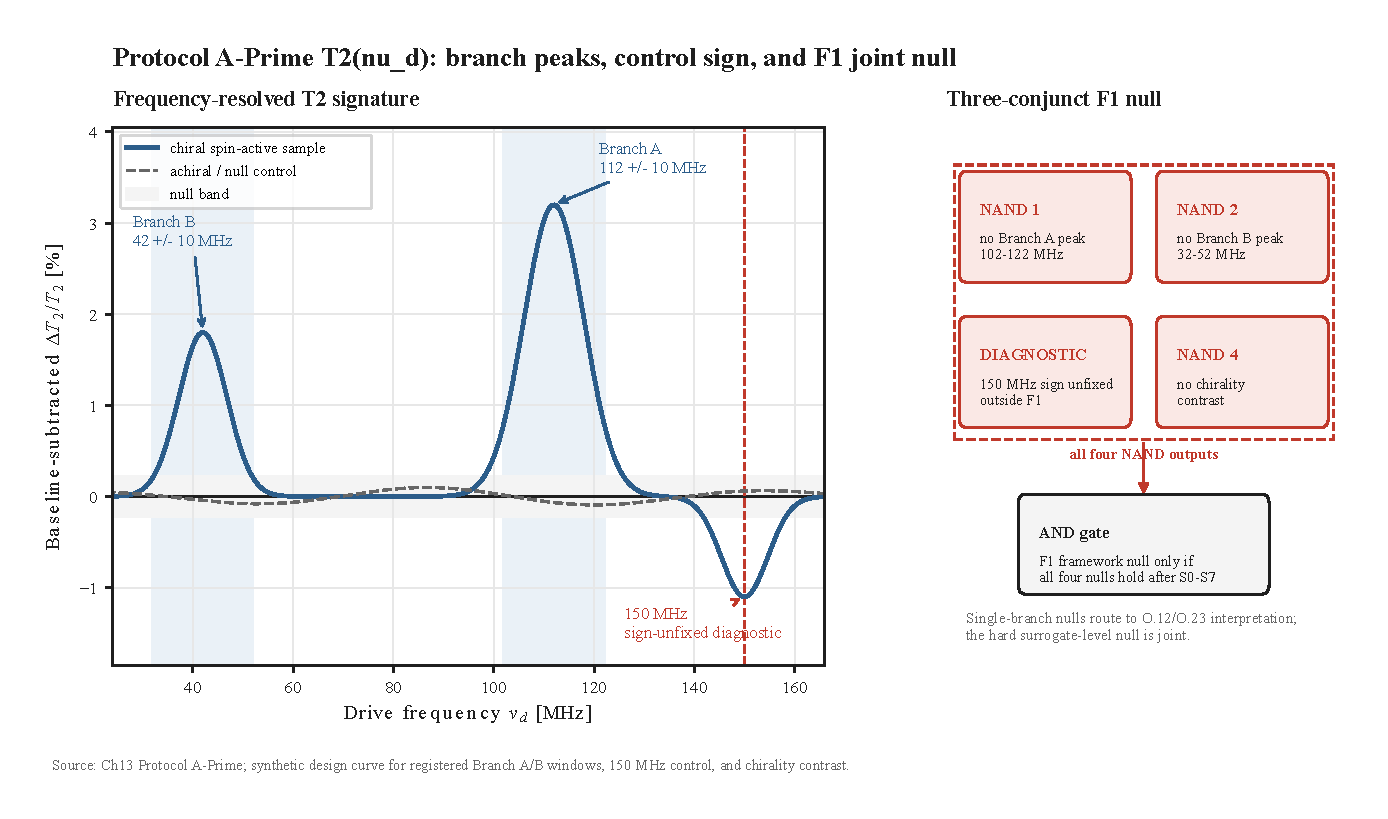
\includegraphics[keepaspectratio,alt={Protocol A-Prime is decided by a frequency-resolved, chirality-dependent T\_2(\textbackslash nu\_d) pattern: Branch A, Branch B, and chirality contrast feed the three-conjunct joint null; the 150 MHz point is a mechanism diagnostic.}]{content/Figures/Volume_3/Figure V3.13.4.pdf}}
\caption{Protocol A-Prime is decided by a frequency-resolved,
chirality-dependent \(T_2(\nu_d)\) pattern: Branch A, Branch B, and
chirality contrast feed the three-conjunct joint null; the 150 MHz point
is a mechanism diagnostic.}
\end{figure}
\end{quote}

\begin{quote}
The registered proxy discriminator is a registered-branch peak plus
chirality contrast: a proxy-branch null requires no Branch A peak, no
Branch B peak, and no chirality contrast after the frozen acceptance
checks. It can distinguish candidate material-response phenomenologies,
not GCT from all non-GCT physics. The 150 MHz sign is retained as a
mechanism diagnostic because its sign is O.23/O.24-conditional, not an
F1 conjunct. The peak \emph{amplitude} is likewise reported as O.23 +
O.24 conditional; the bare strong-coupling parameter
\(2g_{coll}/\kappa\) alone is the strong-coupling signature, not the
\(T_2\) enhancement.

\textbf{Registered scenario-window scan rule:} The authoritative
acquisition is the full half-open scan \([32,200)\) MHz with
\(\Delta\nu_{\rm step}\leq1/(4\pi T_{2,\rm eff})\). Branch A
\([102,122]\) MHz and Branch B \([32,52]\) MHz are pre-registered
hypothesis regions within that scan, not independently scanned
alternatives. Branch A is the primary historical \textasciitilde100 MHz
scenario window; Branch B is the sibling window registered for
O.12-negative outcomes. Neither window is a derived GCT frequency, and
no \(\eta_{\rm Zeno}\) mechanism in the current action shifts one into
the other. The \(150\) MHz response is sign-unfixed and diagnostic-only.
The complete scan, both hypothesis regions, and S0-S7 package are frozen
before unblinding; branch selection is not inferred from observed
A-Prime data.

\textbf{Multiplicity-aware peak statistic:} The primary statistic is a
locally weighted likelihood-ratio test comparing a Lorentzian peak model
against a flat local baseline for \(T_2(\nu_d)\). The physical window is
fixed at \(\pm100\) kHz around each tested center; it contains 41 grid
points only at the 5 kHz baseline and is recomputed on a finer adaptive
grid. The baseline half-open grid \([32,200)\) MHz at 5 kHz contains
exactly \(33{,}600\) samples per cell. The six primary cells are the
experimental-design premise
\(\{\text{L-chiral},\text{R-chiral},\text{achiral/racemic}\}\times\{\text{RF scan},\text{matched sham/no-drive}\}\);
bare diamond is an auxiliary calibration outside the multiplier. Hence
\(M=33{,}600\times6=201{,}600\) baseline bin-cells. The global gate uses
\(\alpha_{\rm global}=2.7\times10^{-3}\), giving
\(\alpha_{\rm local}=\alpha_{\rm global}/M\approx1.34\times10^{-8}\).
With \(z_{\alpha,\rm local}=5.6\), \(z_\beta=1.48\), and
\(\delta_{T_2}=0.10\), the raw requirement is exactly
\[N_{T_2,\rm scan}^{\rm raw}=\left(\frac{5.6+1.48}{0.10}\right)^2=5012.64\]
shots per bin-cell and the executable integer ceiling is \(5013\). The
baseline totals are \(1{,}010{,}548{,}224\) raw shots and
\(1{,}010{,}620{,}800\) executable shots. At 1 kHz they require
\(280.70784\) h and \(280.728\) h, respectively, before acceptance
failures, overheads, or re-runs; with the declared per-shot overheads
and readout noise the requirement is years, not hours (see the
joint-gate calculation below). These totals scale linearly with the
declared cell count. If \(T_{2,\rm eff}>15.915\,\mu\)\hspace{0pt}s, the
grid is tightened using
\(\Delta\nu_{\rm step}\leq1/(4\pi T_{2,\rm eff})\) and the bins, \(M\),
local threshold, shot count, and runtime are recomputed before
unblinding. A scan-level null occurs when the maximum statistic over the
full scan remains below the globally corrected threshold; only the
accepted three-conjunct Branch A + Branch B + chirality null triggers
F1.

\textbf{Decision Matrix (pre-registered material-proxy interpretation)
--- chirality-contrast variant:}

{\def\LTcaptype{none} % do not increment counter
\begin{longtable}[]{@{}
  >{\raggedright\arraybackslash}p{(\linewidth - 4\tabcolsep) * \real{0.3333}}
  >{\raggedright\arraybackslash}p{(\linewidth - 4\tabcolsep) * \real{0.3333}}
  >{\raggedright\arraybackslash}p{(\linewidth - 4\tabcolsep) * \real{0.3333}}@{}}
\toprule\noalign{}
\begin{minipage}[b]{\linewidth}\raggedright
Outcome
\end{minipage} & \begin{minipage}[b]{\linewidth}\raggedright
Joint signature
\end{minipage} & \begin{minipage}[b]{\linewidth}\raggedright
Verdict
\end{minipage} \\
\midrule\noalign{}
\endhead
\bottomrule\noalign{}
\endlastfoot
\textbf{Joint proxy pattern present} & \(T_2\) at a registered branch
center (Branch A \(112 \pm 10\) MHz or Branch B \(42 \pm 10\) MHz)
exceeds \(T_2(\text{off-res})\) at \(3\sigma\) on chiral substrate after
the full adaptive-resolution scan, AND chirality contrast is present at
\(3\sigma\) & Material-response scenario supported; microscopic
attribution remains open; peak amplitude and the sign-unfixed 150 MHz
diagnostic are reported as O.23 + O.24 readouts \\
\textbf{Generic driven-spin response} & Enhancement at \(3\sigma\) on
both chiral and achiral substrates with no \(T_2(\nu_d)\) structure &
Chiral proxy not supported; characterize ordinary drive/heating/phonon
response \\
\textbf{Frequency-specific, chirality-null} & A registered branch peak
is present, but chirality contrast is null after S1 + S6 acceptance
checks pass; the 150 MHz diagnostic is reported separately &
Frequency-specific material response; no CISS attribution; routes to
O.12/O.24 benchmarking \\
\textbf{Chirality-only / branch-null} & Chirality contrast is present,
but both registered branch scans are null after RF/systematic controls
pass & Ordinary chirality-correlated contrast detected (CISS attribution
requires the L-vs-R handedness-odd test of component (c)); no
protected-subspace or phason inference; not an F1 null \\
\textbf{Sensitivity-limited mixed outcome} & Any component null before
its preregistered acceptance checks pass (RF flatness, cap chirality,
NV-depth, or batch reproducibility) & Inconclusive; re-power or re-run
the affected component before applying F1 \\
\textbf{Proxy-branch null (F1)} & No non-monotonic peak in Branch A, no
non-monotonic peak in Branch B, and no chirality contrast after all
acceptance checks pass & F1: reject the registered biophysical branch
(chiral phonon-polariton / protected-subspace Zeno branch) at the
NV-centre surrogate level, as registered; no verdict on GCT as a whole
or on Level II; the 150 MHz sign is diagnostic only \\
\end{longtable}
}

Neither outcome class is a verdict on GCT as a whole: the measurement
tests an ordinary material proxy, and no phason, Selection-Operator or
Level-II inference follows from it (V1 Ch17 §17.1.3). A preregistered
null meeting the F1 rule above rejects the registered biophysical branch
as registered.

\textbf{Formal Preregistration Statement --- Protocol A-Prime}

The joint signature is a \textbf{Tier 3 material-proxy hypothesis}: the
branch-feature plus chirality pattern. The peak \emph{amplitude}
(whether \(T_2^{\text{enhanced}}/T_2^{\text{base}}\) exceeds \(10\),
\(100\), or \(1000\)) and the sign at 150 MHz are empirical measurements
of the closure values of Open Problems O.23 and O.24, not separately
registered Tier 2 quantities. The frozen NV ensemble is
\(N_{\rm NV}=20\) implanted NV centers per cap across
\(N_{\rm caps}=50\) caps; CISS contrast mapping therefore uses
\(N_{\rm caps}N_{\rm NV}=1000\) NV-center observations rather than a
mutable single-cap ensemble size. Shot noise scales as
\(1/\sqrt{N_{\rm caps}N_{\rm NV}}\). A clean branch-feature plus
chirality signal at \(3\sigma\) measures an ordinary
chiral-spin/coherence pattern with whatever amplitude the measurement
delivers; it does not confirm a chiral phonon-polariton GCT interaction.
Mixed outcomes are interpreted per the Decision Matrix, and only the
fully accepted three-conjunct joint null triggers F1, which rejects the
registered proxy branch only.

\textbf{Joint-gate sample-size calculation.} For a normalized
single-shot contrast estimate with Gaussian shot noise, a one-component
\(3\sigma\) gate with 80\% marginal power uses
\[N_{\rm shots}\geq \left(\frac{3+0.84}{\delta}\right)^2,\] where
\(\delta\) is the fractional effect size after the S0-S7 systematic
budget. The conservative pre-registered effect sizes are
\(\delta_{T_2}=0.10\) for the non-monotonic selected-branch peak,
\(\delta_{\chi}=0.05\) for the chirality contrast after cap-purity,
transfer retention, and NV-depth dilution, and \(\delta_{150}=0.10\) for
powering the sign-unfixed 150 MHz diagnostic response. Therefore:
\[N_{T_2}\geq 1.48\times10^3,\qquad N_{\chi}\geq 5.90\times10^3,\qquad N_{150}\geq 1.48\times10^3.\]
These design effect sizes (\(\delta_{T_2}\), \(\delta_{\chi}\),
\(\delta_{150}\)) are locked by the blinded pilot calibration before
unblinding the decisive run. The \(\delta_{150}\) and \(N_{150}\)
entries power the sign-unfixed diagnostic only and never determine F1 or
a Holm primary decision. If the pilot lower edge falls below the
registered branch-feature or chirality values, that F1 component is
sensitivity-limited and must be re-powered rather than treated as a
clean F1 proxy rejection. The conservative acquisition design retains
93\% marginal power per measured component (\(z_\beta \approx 1.48\)),
giving \(N_{T_2}\geq 2.01\times10^3\), \(N_{\chi}\geq 8.03\times10^3\),
and diagnostic \(N_{150}\geq 2.01\times10^3\) per relevant
fixed-frequency cell. The full half-open \([32,200)\) MHz
adaptive-resolution scan supersedes every fixed-frequency \(N_{T_2}\)
number. At the 5 kHz baseline \(M=201{,}600\) and the multiplicity-aware
peak requirement is
\[N_{T_2,\rm scan}^{\rm raw}=5012.64,\qquad N_{T_2,\rm scan}^{\rm executable}=5013\]
shots per bin-cell for the same 80\% joint-power design. On the baseline
5 kHz grid, \(33{,}600\) samples per cell and six enumerated cells give
\(1{,}010{,}548{,}224\) raw shots or \(1{,}010{,}620{,}800\) executable
shots, corresponding at 1 kHz to \(280.70784\) h or \(280.728\) h. The
adaptive-linewidth rule and linear cell-count sensitivity stated above
govern any re-budgeting. The 1 kHz cadence assumes 1 ms per shot. With
the realistic CPMG reset, RF-settling and blinding overheads of
\(10\)--\(100\) ms per shot, the same \(1.01\times10^9\) shots take
\(1.0\times10^7\)--\(1.0\times10^8\) s, i.e.~about \(0.32\)--\(3.2\)
years. The shot model also takes \(\sigma_{\rm meas}\) as one unit per
shot; conventional room-temperature single-NV optical readout sits a
factor \(\sigma_R\approx10\)--\(80\) above the spin-projection limit
(Barry et al.~2020, \emph{Rev.~Mod. Phys.} 92:015004, Table 2), which
multiplies the required repetitions by
\(\sigma_R^2\approx10^2\)--\(6\times10^3\), and each \(T_2\) bin needs a
fitted decay curve rather than a single shot. As specified, the
full-scan acquisition is therefore not feasible: ``shot'' must be
redefined as an averaged \(T_2\) estimate with explicit photon
statistics and readout contrast, and the scan, cell count or effect size
re-budgeted before the design is executable {[}Tier 3
experimental-design calculation{]}. The \(\delta_{\chi}=0.05\) contrast
is a sensitivity-design target locked after the achiral/chiral pilot
calibration; if the measured CISS lower edge or transfer-retention
factor erases this contrast, the chirality component is
sensitivity-limited and the acquisition must be re-powered rather than
treated as a clean F1 proxy rejection. Joint power is calculated from
the three marginal powers under the independence approximation {[}Tier
3{]}; correlations among S0-S7 systematics are reported in the analysis
notebook and widen the confidence interval rather than changing the F1
gate.

\textbf{Deterministic CISS contrast mapping.} Required shot count uses
the frozen ensemble convention: \(N_{\rm caps}=50\) caps and
\(N_{\rm NV}=20\) implanted NV centers per cap contribute
\(N_{\rm obs}=50\times20=1000\) NV-center observations. The cap-level
CISS variable is measured before unblinding by CD/VCD chirality
verification plus transport spin-polarimetry per cap, but the clean F1
chirality input is the post-transfer effective product
\[P_{\rm eff}\equiv r_{\rm transfer}P_{\rm CISS}^{\rm net},\] and
\(P_{\rm eff}\ge0.1\) must be established at \(\ge5\sigma\) confidence
across the 50 caps/witness stacks for a clean F1 run. Shot noise
therefore scales as \(1/\sqrt{N_{\rm caps}N_{\rm NV}}\) with
\(\sigma_{\rm meas}=1\) photon-count unit (an idealization; real readout
multiplies the counts below by \(\sigma_R^2\), see above). The per
observation count is
\[N_{\rm shots}^{\rm per\,obs}=\frac{(z_{1-\alpha/2}+z_{1-\beta})^2\,\sigma_{\rm meas}^2/(N_{\rm caps}N_{\rm NV})}{(P_{\rm eff}\delta\chi)^2}
=\frac{4.20\times10^{-2}}{(P_{\rm eff}\cdot0.05)^2}
=\frac{16.8}{P_{\rm eff}^2}.\] Equivalently, the total pooled
acquisition cycles across the 1000 NV-center observations are
\[N_{\rm cycles}^{\rm total}=N_{\rm caps}N_{\rm NV}N_{\rm shots}^{\rm per\,obs}=\frac{1.68\times10^4}{P_{\rm eff}^2}.\]
Here the numerator uses the declared 5σ clean-run gate with the same
93\% marginal-power convention as the three-component design,
\((5+1.48)^2\approx42.0\); the 95\%/80\% comparison convention does not
set this gate. For effective polarization band
\(P_{\rm eff}\in[0.05,0.20]\), this gives total cycles
\(6.72\times10^6\) (\(P_{\rm eff}=0.05\)), \(1.68\times10^6\)
(\(P_{\rm eff}=0.10\)), and \(4.20\times10^5\) (\(P_{\rm eff}=0.20\)),
with per-observation counts lower by \(10^3\). At the declared
\(P_{\rm eff}=0.025\) sensitivity floor, the total-cycle requirement is
\(2.69\times10^7\) (about \(2.69\times10^4\) shots per
center-observation), still below the \(10^9\) cycle ceiling; below this
floor the chirality component is sensitivity-limited by cap
polarization/systematic reproducibility, not treated as a clean F1 proxy
rejection. If only the source-material value \(P_{\rm CISS}^{\rm net}\)
is known, the re-powering uses the retained product:
\(r_{\rm transfer}=0.5\) increases the shot/cycle requirement by
\(4\times\), and \(r_{\rm transfer}=0.1\) increases it by \(100\times\).

\textbf{CISS floor interpretation.}

{\def\LTcaptype{none} % do not increment counter
\begin{longtable}[]{@{}
  >{\raggedright\arraybackslash}p{(\linewidth - 4\tabcolsep) * \real{0.3333}}
  >{\raggedright\arraybackslash}p{(\linewidth - 4\tabcolsep) * \real{0.3333}}
  >{\raggedright\arraybackslash}p{(\linewidth - 4\tabcolsep) * \real{0.3333}}@{}}
\toprule\noalign{}
\begin{minipage}[b]{\linewidth}\raggedright
Measured post-transfer
\(P_{\rm eff}=r_{\rm transfer}P_{\rm CISS}^{\rm net}\)
\end{minipage} & \begin{minipage}[b]{\linewidth}\raggedright
Interpretation
\end{minipage} & \begin{minipage}[b]{\linewidth}\raggedright
Action
\end{minipage} \\
\midrule\noalign{}
\endhead
\bottomrule\noalign{}
\endlastfoot
\(\geq 0.1\) & S1 acceptance floor for clean F1 proxy rejection & The
declared shot budget can deliver the chirality component of the joint F1
gate. \\
\(0.025 \leq P_{\rm eff} < 0.1\) & Sensitivity-Limited Pending
Re-Powering & The run can be re-powered by increasing shots with
\(N_{\rm shots}\propto1/P_{\rm eff}^2\), but the declared run cannot
deliver a clean proxy rejection at the declared shot budget. \\
\(<0.025\) & Sensitivity-limited floor & No proxy verdict; this is not a
GCT, phason or Level-II result. \\
\end{longtable}
}

\textbf{Protocol record:} Analysis pipeline specifies (a) NV center
depth and isotopic purity, (b) RF drive amplitude and pulse sequence,
(c) statistical threshold for significance (\(p < 0.003\), corresponding
to \(3\sigma\)), and (d) blinding procedure for the \(T_2(\nu_d)\) scan.
Any deviation from these parameters constitutes a separate protocol
amendment.

\textbf{Public preregistration archive.} Before unblinding, the protocol
package is deposited in a public timestamped archive (OSF or Zenodo,
with optional arXiv protocol note) containing the frozen analysis code,
synthetic-data budget, NV-depth/isotopic-purity acceptance files,
RF-drive grid, S0-S7 systematic gates, and the amendment ledger. Any
parameter change after deposit is recorded as a numbered amendment with
timestamp, rationale, and the blinded/unblinded state of the affected
data.

\textbf{Executable-readiness qualifier.} Protocol A-Prime is a
prospective preregistration design until the verifier script,
synthetic-data package, analysis-code hash, operating-system/environment
manifest, and OSF/Zenodo archive URL are frozen together before
unblinding. Before that freeze, P.8 is not an executable decisive test;
it is the authoritative design specification for the frozen package.
Even after that freeze, P.8 is decisive only for its declared
material-response proxy branch, not for GCT as a whole, phason coupling
or Level II.

\textbf{Proxy-branch decision conditions (two-level, pre-registered):}

\textbf{F1 proxy-branch rejection rule (Protocol A-Prime, single rule).}
F1 fires, rejecting the registered biophysical branch as registered, if
and only if all three conjuncts hold after the frozen S0-S7 acceptance
checks pass: (a) NO peak detected in the Branch A \(112 \pm 10\) MHz
hypothesis region, (b) NO peak detected in the Branch B \(42 \pm 10\)
MHz hypothesis region of the full adaptive-resolution \([32,200)\) MHz
scan, and (c) NO chirality contrast against the achiral control using
\(> 99.9\%\) isotopically pure \(^{12}\)\hspace{0pt}C diamond. Branch A
is the primary historical \textasciitilde100 MHz scenario window; Branch
B is the sibling window registered for O.12-negative outcomes. A Branch
A/B-only null is the peak-subtest null, not an F1 rejection; the F1 gate
is the three-part joint null at the required
\(\delta\chi + N_{\rm shots}\). \textbf{This is the sole Protocol
A-Prime rejection gate.} It is not a verdict on GCT as a whole: the
measurement tests an ordinary material proxy, and no phason,
Selection-Operator or Level-II inference follows from it (V1 Ch17
§17.1.3). The \(150\) MHz response is a sign-unfixed Tier 3 O.23/O.24
diagnostic outside F1 and Holm primary decisions. S0 systematic floor
(in-vitro arm of Protocol A only; the abiotic NV surrogate contains no
Trp radical pair, so S0 does not apply to it): \(\Delta_{ST}/h\) of the
Trp radical pair must lie inside the 5-200 MHz admissible tubulin-EPR
band before a biological branch-frequency decision is treated as
decisive; outside that band the run is sensitivity-limited or routes to
O.12/O.23 branch re-estimation. Under an F1 rejection there is no CISS
``classical floor'' fallback: ordinary CISS response would constrain the
material system only, and no Level II classification follows for any
concrete substrate.

\textbf{(F2) Peak-amplitude readout (distinct from F1).} Conditional on
a positive branch-feature plus chirality signal after the frozen
acceptance checks, the peak amplitude and 150 MHz sign are reported as
empirical readouts of the joint O.23 + O.24 closure values. They are not
separately registered gates. A low-amplitude positive signature would be
compatible with a weaker or non-DFS-mediated O.23 scenario; a
high-amplitude positive signature would be compatible with a
protected-subspace scenario, but no \([10^2,10^3]\times\) enhancement is
currently licensed. F2 never translates an amplitude into
\(g_{single}\), \(\eta_{Zeno}\), a protected phason subspace or
consciousness.

Between F1 and F2 --- any measurement yielding a positive joint
signature, across amplitudes from below-bare through the positive-O.23
\([10^2,10^3]\times\) band --- the experiment serves as the empirical
readout of the joint \((\Omega_{\text{DFS}}, \kappa_{\text{chiral}})\)
closure of Open Problems O.23 + O.24, constraining the Tier 3 material
inputs; empirical agreement does not promote them to Tier 2. Promotion
requires an independent derivation of the relevant DFS/chiral parameters
and normalized physical coupling from the declared premises, closing the
O.23/O.24 derivational dependencies without fitting the target
measurements. Observations then test the resulting claim.

\textbf{§13.3.5.S Systematic-Error Budget {[}pre-registered{]}}

The Protocol A-Prime pre-registration matches the §16.3.4 Protocol D
rigor in disclosing the dominant systematic uncertainties on the
branch-feature/chirality gate and the separate 150 MHz diagnostic. Seven
systematics are enumerated below; each is paired with the dominant
effect it produces, the propagation chain into the F1 proxy gate or
diagnostic, and the operational mitigation. The pre-registered
systematic budget is committed before unblinding alongside the F1/F2
statements above.

\newpage

\textbf{(S1) Chiral h-BN cap chirality-purity}

\textbf{Effect on branch/chirality gate or 150 MHz diagnostic:} Reduces
chirality contrast (component c); a partially-racemic cap or
post-transfer stack with
\(P_{\rm eff}=r_{\rm transfer}P_{\rm CISS}^{\rm net}<0.1\) collapses the
chiral-vs-achiral contrast into the \(3\sigma\) noise band, producing
false-null on (c) even with a real chirality-dependent material response
present at the declared shot budget.

\textbf{Magnitude band:} Naaman-Paltiel-Waldeck 2019 \emph{Nat.
Rev.~Chem.} 3:250 places CISS polarization up to \(\sim60\%\) in
ordered-helical DNA stress-test substrates, while protein/peptide
systems sit in the operative \(5\)--\(20\%\) band; the source
cap-substrate \(P_{\rm CISS}^{\rm net}\) is the \emph{enantiomer excess
× per-helix polarization}. \(F_{\rm CISS}=2.0\) is a Tier 3 model
translation from measured \(P_{\rm CISS}\) spin-polarization; see App
BEB §BEB.11.1 for the protein-band \(P_{\rm CISS}\in[0.05,0.20]\) and
DNA-equivalent stress edge \(P_{\rm CISS}\approx0.6\). A racemic cap
(\(ee = 0\)) gives \(P_{\rm CISS}^{\rm net} = 0\); \(ee = 50\%\) at the
DNA stress edge gives \(P_{\rm CISS}^{\rm net} \approx 0.3\) before
transfer. Effect-size impact scales linearly with the retained product
\(P_{\rm eff}\).

\textbf{Mitigation:} \textbf{Inclusion criterion for clean F1:} measured
\(P_{\rm eff}\geq0.1\) AND \(ee \geq 90\%\). Pre-unblinding measurement:
spin-polarimetry on the h-BN/NV cap pair using CD/VCD chirality
verification plus either Mott polarimetry of transmitted electrons or
magnetoresistance with a ferromagnetic electrode, at the operating
temperature; CD/VCD is necessary but not sufficient. (The chiral and
racemic cap materials themselves still need a concrete definition, since
bulk h-BN is achiral.) \(P_{\rm eff}\) must be measured \(\geq0.1\) with
\(\geq5\sigma\) confidence before Branch A/B unblinding. For
\(0.025 \leq P_{\rm eff}<0.1\), the chirality component is
Sensitivity-Limited Pending Re-Powering with
\(N_{\rm shots}\propto1/P_{\rm eff}^2\). For \(P_{\rm eff}<0.025\), the
result is sensitivity-limited and supplies no proxy verdict. CD/VCD
spectroscopic verification of \(ee \geq 90\%\) is required before each
Protocol A-Prime run; a cap with \(ee < 90\%\) is excluded. Achiral
control uses CD-confirmed racemic h-BN. \textbf{Dominant systematic if
the cap is sourced from synthesis without CD verification ---
invalidates component (c) reproducibility and supplies no proxy,
framework or Level-II verdict.}

\textbf{(S2) NV depth jitter}

\textbf{Effect on branch/chirality gate or 150 MHz diagnostic:}
Modulates the NV--cap distance, which sets the ordinary NV--cap dipolar
sensitivity and therefore the measured interface-response amplitude; it
does not measure a chiral phonon-polariton or phason coupling. NV depth
shifts of \(\pm 2\) nm at a nominal 10 nm depth modulate that
sensitivity by \(+95\%/-42\%\), about \(\pm 60\%\) linearized (dipolar
\(1/r^3\) falloff: \((10/8)^3=1.95\), \((10/12)^3=0.58\)).

\textbf{Magnitude band:} NV implantation depth standard deviation
typically \(\sigma_d \in [0.5, 2]\) nm depending on implantation energy
and annealing protocol; \(\sigma_d = 2\) nm gives a per-sample variation
on the joint (a)+(b) amplitude of about \(\pm 60\%\).

\textbf{Mitigation:} Pre-registration requires NV depth characterization
via secondary-ion mass spectrometry (SIMS) calibration on a control
batch from the same implantation lot, with the \(\sigma_d\) reported as
the leading systematic on the (a)+(b) amplitude scaling. Statistical
pooling across the frozen \(N_{\rm NV}=20\) NVs per cap averages the
random depth jitter to about \(\pm 60/\sqrt{20} \approx 13\%\) before
the 50-cap CISS contrast aggregation is applied; pooling does not remove
a lot-level bias in mean depth, which is carried as a systematic.

\textbf{(S3) RF amplitude calibration drift across the \([32,200)\) MHz
sweep}

\textbf{Effect on branch/chirality gate or 150 MHz diagnostic:}
Modulates the Rabi-frequency-dependent measurement of \(T_2(\nu_d)\),
producing apparent \(T_2(\nu_d)\) structure that mimics component (a) at
the few-percent level if the RF amplitude is not flat across the sweep.

\textbf{Magnitude band:} Standard NV-AC-magnetometry pulse-shaping drift
across a \([32,200)\) MHz sweep is taken as \(\pm 5\%\) in pulse area;
this propagates to a \(\pm 5\%\) apparent \(T_2(\nu_d)\) feature that is
\emph{not} a real material-proxy signal.

\textbf{Mitigation:} Pre-registration requires an \emph{RF amplitude
flatness calibration sweep} on a reference NV (single-NV regime, no
chiral cap) before each Protocol A-Prime run, with the residual RF
flatness \(< 2\%\) as the acceptance condition. The reference-NV sweep
is reported with the protocol and subtracted from the chiral-cap
measurement at the lock-in stage.

\textbf{(S4) Hahn-echo \(\pi\)-pulse fidelity}

\textbf{Effect on branch/chirality gate or 150 MHz diagnostic:}
Stochastic per-pulse loss compounds across the registered CPMG train and
can mask or mimic component (a); coherent over-rotation,
state-preparation-and-measurement error and intrinsic decoherence
require separate nuisance terms.

\textbf{Magnitude band:} For the declared independent stochastic-loss
model, the surviving contrast is \(F_\pi^N\). The acceptance condition
is therefore \(F_\pi\geq(1-\delta_{\rm allow})^{1/N}\) with
\(N=2\nu_dT_{\rm int}\). At \(\nu_d=112\) MHz,
\(T_{\rm int}=10\,\mu\)\hspace{0pt}s and \(\delta_{\rm allow}=0.10\),
\(N=2240\) and \(F_\pi\geq0.999953\); the branch centre at \(42\) MHz
requires \(F_\pi\geq0.999875\). A fixed \(0.99\) threshold would leave
only \(1.7\times10^{-10}\) contrast after 2240 pulses and is
inadmissible {[}Tier 3 experimental-design calculation{]}.

\textbf{Mitigation:} Pre-registration must declare \(T_{\rm int}\),
\(\nu_d\), \(N\), \(\delta_{\rm allow}\) and the stochastic/coherent
error model before unblinding. Randomized benchmarking and
sequence-level reference runs must establish the resulting
branch-specific \(F_\pi\) threshold; runs that do not meet it are
sensitivity-limited. Baseline correction is fitted jointly from the
declared nuisance model rather than obtained by subtracting average gate
infidelity.

\textbf{(S5) Floquet sideband artefacts}

\textbf{Effect on branch/chirality gate or 150 MHz diagnostic:} An
ordinary strongly driven spin system (no magnon-polaron or Zeno source
is assumed) can produce Floquet sidebands at
\(\nu_d \pm n\,\nu_{\rm sideband}\) for \(n \in \mathbb{Z}\), which can
mimic the non-monotonic \(T_2(\nu_d)\) peak (component a) at frequencies
offset from \(\nu_c\) if the sideband structure is not characterized.

\textbf{Magnitude band:} Floquet sideband amplitude scales with
\((g_{\rm drive}/\omega_d)^2\) and produces apparent \(T_2(\nu_d)\)
features at \(\nu_d \pm \nu_{\rm hyperfine}\) with amplitudes up to
\(\sim 10\%\) of the main feature for strong drives.

\textbf{Mitigation:} Pre-registration requires a \emph{Floquet-sideband
characterization scan} on the achiral control substrate first (sidebands
appear as \(T_2(\nu_d)\) structure independent of chirality), with the
sideband positions and amplitudes catalogued before the chiral
measurement. The chiral measurement is then masked at the sideband
frequencies to prevent false-positive component (a) attribution.

\textbf{(S6) Sample-batch chirality reproducibility}

\textbf{Effect on branch/chirality gate or 150 MHz diagnostic:}
Run-to-run variation in the CISS-cap synthesis batch produces
between-run amplitude variation on component (c) (chirality contrast) at
the \(10\)--\(20\%\) level even with \(ee \geq 90\%\) per (S1).

\textbf{Magnitude band:} Synthesis-batch reproducibility on chiral h-BN
under standardized CVD conditions is typically \(\pm 15\%\) on the
per-helix polarization, propagating to \(\pm 15\%\) between-run
variation on the chirality-contrast amplitude.

\textbf{Mitigation:} Pre-registration requires \emph{three independent
synthesis batches} of the chiral cap, each with CD verification, with
the chirality-contrast amplitude reported as the mean ± SD across
batches. The \(3\sigma\) proxy-rejection gate on component (c) is
evaluated against the inter-batch SD, not the single-batch SD.
\textbf{Dominant systematic on the chirality-contrast amplitude
reproducibility --- analogous to the \(^{17}\)\hspace{0pt}O enrichment
efficiency in Protocol D §16.3.4; a leading material-proxy systematic,
not a framework-level one.}

\textbf{(S7) Cap-to-NV transfer and post-transfer CISS retention}

\textbf{Effect on branch/chirality gate or 150 MHz diagnostic:} A cap
that passes standalone chirality/CISS metrology can lose effective
spin-selective coupling after transfer, bonding, contamination, strain,
or NV-surface processing; this produces a false null on chirality
contrast and can reduce the observed \(\delta\chi\) without invalidating
the pre-transfer cap measurement.

\textbf{Magnitude band:} Transfer-induced CISS retention is treated as a
multiplicative uncertainty on the chirality term. The retained factor
\(r_{\rm transfer}\) must be measured on witness h-BN/NV stacks;
otherwise \(\delta\chi\) is reported with an added transfer-uncertainty
multiplier and the run cannot support clean F1.

\textbf{Mitigation:} Pre-unblinding acceptance requires witness-stack
spin-polarimetry or magnetoresistance on the actual transferred cap/NV
process flow, not only on source material. Clean F1 requires
\(r_{\rm transfer}P_{\rm CISS}^{\rm net}\ge0.1\) with \(\ge5\sigma\)
confidence; \(0.025\le r_{\rm transfer}P_{\rm CISS}^{\rm net}<0.1\) is
sensitivity-limited and requires re-powering; below \(0.025\) no proxy
verdict is reported, and no threshold here is a framework or Level-II
falsifier.

\textbf{Dominant systematic identification:} The chiral h-BN cap
chirality-purity (S1), sample-batch reproducibility (S6), and cap-to-NV
transfer retention (S7) jointly carry the bulk of the systematic
uncertainty on the chirality-contrast component (c) of the joint
signature. A null on (c) at \(3\sigma\) that is \emph{not preceded by S1
+ S6 + S7 verification} is interpreted as \textbf{inconclusive on the
chirality-contrast component, not as an F1 proxy rejection}.
Verification of S1 (CD spectroscopy \(ee \geq 90\%\)), S6 (three-batch
reproducibility), and S7 (post-transfer CISS-retention metrology on
witness stacks) before the Protocol A-Prime run is the pre-registered
acceptance condition for a clean F1 proxy-rejection test on component
(c). The (S2), (S3), (S4), (S5) systematics carry the bulk of the
uncertainty on components (a) and (b) and are mitigated by the per-run
reference-NV calibrations. None of these acceptance conditions creates a
GCT, phason or Level-II falsification gate.

\emph{Cross-references:} §16.3.4 (Protocol D systematic-error budget ---
the rigor template); App NSP §NSP.5 (CISS empirical foundations); App
ORQ Open Problem O.23 (chiral phonon-polariton DFS substrate-side
closure path); App ORQ Open Problem O.24 (Protocol A-Prime amplitude
under O.23 closure).
\end{quote}

\subsection{§13.3.5.A Protocol A-Prime Extended: Chiral vs.~Achiral
NV-Centre
Comparison}\label{a-protocol-a-prime-extended-chiral-vs.-achiral-nv-centre-comparison}

\textbf{Objective:} Test whether any \(T_2\) feature in the registered
\(\nu_c \approx 112 \pm 10\) MHz (or \(42 \pm 10\) MHz) scenario window
depends on an ordinary chiral material environment or is
substrate-agnostic. This is a CISS/material-control question, not a
direct GCT prediction.

\gctneedspace{5\baselineskip}

\textbf{Physical Setup:}

The experiment compares L-chiral, R-chiral, racemic/achiral and bare-NV
controls. Direct spin-polarimetry, current/contact metrology and \(T_2\)
are the observables. The historical proxy scenario expects a
sign-positive registered-window feature on the chiral cap (net CISS,
spin-selective transport) and \(T_2^{achiral} \approx T_2^{bare}\) on an
achiral cap (a racemic cap is not equivalent for the polarization-even
observable \(T_2\), since it still carries local polarization of both
signs), with any magnitude measured as an empirical readout of
O.23/O.24. Chirality reversal may reverse an ordinary spin-polarization
sign; it does not imply a Zeno Lock. No \(10^2\)--\(10^3\) enhancement
or phason attribution is currently licensed, and the amplitude is
\textbf{not} a rejection threshold.

\gctneedbreak{10\baselineskip}

{\def\LTcaptype{none} % do not increment counter
\begin{longtable}[]{@{}
  >{\raggedright\arraybackslash}p{(\linewidth - 6\tabcolsep) * \real{0.2353}}
  >{\centering\arraybackslash}p{(\linewidth - 6\tabcolsep) * \real{0.2941}}
  >{\raggedright\arraybackslash}p{(\linewidth - 6\tabcolsep) * \real{0.2353}}
  >{\raggedright\arraybackslash}p{(\linewidth - 6\tabcolsep) * \real{0.2353}}@{}}
\toprule\noalign{}
\begin{minipage}[b]{\linewidth}\raggedright
Substrate
\end{minipage} & \begin{minipage}[b]{\linewidth}\centering
Measured CISS response?
\end{minipage} & \begin{minipage}[b]{\linewidth}\raggedright
\(T_2\) scenario expectation at the registered window
\end{minipage} & \begin{minipage}[b]{\linewidth}\raggedright
Inference ceiling
\end{minipage} \\
\midrule\noalign{}
\endhead
\bottomrule\noalign{}
\endlastfoot
NV in diamond (bare) & Control & Baseline T₂ (reference) & Ordinary NV
response \\
NV + achiral h-BN & Must be measured (expected none) & ≈ Baseline T₂;
matched interface control & Ordinary interface response \\
NV + L-chiral h-BN & Must be measured & Test for a chirality-correlated
non-monotonic registered-window feature; amplitude reported as O.23/O.24
readout & Ordinary CISS/material proxy \\
NV + R-chiral h-BN & Must be measured (opposite hand) & Test handedness
reversal/symmetry of the same feature & Ordinary CISS/material proxy \\
\end{longtable}
}

\emph{Table note.} The joint preregistered rule (registered-branch
feature plus chirality contrast at \(3\sigma\), §13.3.5 Decision Matrix)
decides only the material proxy branch. The sign-unfixed 150 MHz
response and peak amplitude are empirical responses, not readouts of a
GCT coupling or Level II.

Handedness reversal is a useful material control, but the detailed
symmetry of the measured magnitude depends on contacts, defects,
orientation and the ordinary CISS transport model. It is not a
Zeno-locking theorem.

\textbf{Why NV Centres:} shallow (\textasciitilde10 nm) NVs have \(T_2\)
of order \(10\,\mu\text{s}\), comparable to the
\(1\)--\(10\,\mu\)\hspace{0pt}s Trp radical-pair scenario band
(millisecond \(T_2\) belongs to bulk NVs); NV array density and spacing
are controllable; diamond + h-BN capping is established nanofabrication
technology. Timeline: 2--5 years, executable only after preregistration
verifier/package freeze and the S0-S7 acceptance files are locked.

\textbf{Public preregistration deposit required before unblinding the
chiral vs.~achiral comparison.} The OSF/Zenodo timestamp, frozen code
hash, synthetic-data budget, S0-S7 acceptance files, and amendment
ledger are part of the protocol record.

\emph{Cross-reference: §13.3.5 (Protocol A-Prime baseline), App BEB
§BEB.7, and App PRG rows P.8/P.10 (the authoritative decision rule lives
at P.8).}

\begin{center}\rule{0.5\linewidth}{0.5pt}\end{center}

\subsection{§13.3.6 Protocol A-Tertius: Leggett-Garg Test of the
Material Coherence
Proxy}\label{protocol-a-tertius-leggett-garg-test-of-the-material-coherence-proxy}

\textbf{Objective (historical).} Protocol A-Tertius proposed a
Leggett-Garg Inequality (LGI) test of temporal coherence in a
radical-pair or NV material system driven in the registered branch
windows. It is now a declared open programme (below); no registered gate
remains.

\textbf{The Leggett-Garg Framework.} The Leggett-Garg Inequalities
(Leggett \& Garg, 1985) constrain the temporal correlations of a
macroscopic two-state system under the assumptions of
\textbf{macrorealism} (the system is in a definite state at all times)
and \textbf{non-invasive measurability} (measurement does not disturb
the state). For a dichotomic observable \(Q(t) \in \{+1, -1\}\), the
temporal correlation functions
\(C_{ij} = \langle Q(t_i) Q(t_j) \rangle\) must satisfy:

\[K_3 \equiv C_{12} + C_{23} - C_{13} \leq 1 \quad \text{(LGI bound)}\]

Any classical stochastic process satisfies this inequality.
\textbf{Quantum mechanics allows \(K_3 > 1\)} (up to a maximum of
\(K_3^{max} = 3/2\) for a qubit), signaling genuine quantum
superposition across the temporal interval.

\textbf{Declared open programme {[}Tier 3/4{]} --- Protocol A-Tertius.}
(a) \emph{Claimed:} a three-time LGI test, \(K_3(\nu_c)>1\), on the
singlet-triplet parity of a single radical pair read by ODMR with
quantum-non-demolition weak measurements at \(\tau_c=1/\nu_c\approx8.9\)
ns spacing, registered as a binary gate (P.8c) for a protected-subspace
coherence branch. (b) \emph{Defects:} single-radical-pair
singlet/triplet readout with QND measurements at ns spacing does not
exist (radical-pair spin state is read destructively, through
recombination yield on ensembles, and NV optical readout alone takes
about 300 ns); and on the NV surrogate the test is non-diagnostic as
designed, because LGI violation by a single NV spin is already
established (Waldherr et al.~2011, \emph{Phys. Rev.~Lett.} 107:090401)
and any coherently precessing spin gives \(K_3>1\) at suitable times. A
positive result would therefore say nothing about a protected-subspace
branch, and a null would depend on the chosen times. (c) \emph{Closing
would need:} an executable ensemble (ideal-negative-measurement) LGI
scheme and a branch-specific prediction for \(K_3(\nu)\) that differs
from that of a bare coherent spin. (d) No decision, scorecard row or
downstream claim uses A-Tertius as support; the former
\(K_3\approx1+\phi^{-9}/\pi\) effect size, sample-size plan and P.8c
decision rule are withdrawn.

\emph{Cross-reference: §13.3.5 (T₂ enhancement Protocol A-Prime),
§13.4.5 (Lindblad master equation treatment), V1 §17.1.4 (Tubulin
Tryptophan aromatic radical network).}

\begin{center}\rule{0.5\linewidth}{0.5pt}\end{center}

\subsection{13.4 Thermodynamic Constraints on
Coherence}\label{thermodynamic-constraints-on-coherence}

\subsubsection{13.4.1 Conditional Landauer Bookkeeping for the
Historical Rate
Scenario}\label{conditional-landauer-bookkeeping-for-the-historical-rate-scenario}

Critics of quantum biology correctly identify \textbf{Thermal Noise}
(\(k_B T\)) as the primary obstacle. At \(310\) K, the decoherence time
of a dipole in bulk water is \(\tau_{raw} \approx 10^{-13}\) s; this
bulk-water scale is a contextual control, not a measured tubulin-Trp
\(T_2\). Landauer's Principle bounds logically irreversible erasure;
applying one erasure cost per hypothesized sampling update is an
explicit scenario assumption, not evidence that a Zeno Drive samples,
erases or operates at a particular rate.

\subsubsection{13.4.2 Heat-Sink Closure
Status}\label{heat-sink-closure-status}

The thermodynamic heat-sink mechanism for the Zeno energy-balance
remains an Open Problem; see App ORQ O.34. Our thermodynamic audit
compares two sampling regimes against the \(\sim 1\) nW {[}Tier 3 ---
neurophysiology measurement{]} metabolic budget of a neuron. At \(310\)
K the Landauer erasure cost is \(k_B T\ln 2 \approx 2.97\times10^{-21}\)
J, so that budget supports about \(3.4\times10^{11}\) logically
irreversible bit erasures per second. An electronic-THz architecture
that erases one bit per sampled degree of freedom per cycle is excluded
even for a single bit. At \(10^8\) Hz the same assumption permits at
most \(N_{\max}\approx3370\) independently erased bits; it does not
select 100 MHz over lower frequencies. The 100 MHz figure is the
historical material-scan scenario; it is not derived from this budget,
nor from the recombination rate of §13.4.4 (a rate in s\(^{-1}\), not a
cyclic frequency). On the conditional \(N_{\rm coop}=1.625\times10^9\)
branch, one erasure per oscillator per cycle would require
\(1.625\times10^{17}\) erasures s\(^{-1}\), exceeding the Landauer
budget by \(4.8\times10^5\). Even replacing the linear count by
\(\sqrt{N_{\rm coop}}\) would give \(4.0\times10^4>3370\) and would not
be justified by Landauer's linear bit-erasure accounting. The coherence
protocol must therefore establish a QND/reversible implementation with
an explicit reset and heat-sink budget; this thermodynamic closure
remains open under O.34 {[}Tier 3{]}.

\subsubsection{13.4.3 Tubulin Tryptophan Aromatic Radical
Coherence}\label{tubulin-tryptophan-aromatic-radical-coherence}

Standard bulk water decoherence timescales (\(\sim 10^{-13}\) s) define
the thermal decoherence limit for unbound spins. The tubulin Trp
radical-pair \(T_2 \approx 1\)-\(10\ \mu\)\hspace{0pt}s baseline is a
model-derived estimate (Tier 3) extrapolated from cryptochrome FAD-Trp
radical-pair magnetoreception studies (Ritz et al.~2000; Hore \&
Mouritsen 2016) and microtubule radical-pair theoretical models
(Zadeh-Haghighi \& Simon 2022). Direct EPR/ODMR measurements on intact
β-tubulin Trp radical pairs have NOT been performed; this direct
measurement is a target of the in-vitro arm of Protocol A (Protocol
A-Prime is the abiotic NV surrogate; App ORQ O.24 tracks the A-Prime
enhancement amplitude). \textbf{Open Problem O.23} in Appendix ORQ asks
whether a declared material model can extend a measured baseline toward
the historical \(\sim 10\) ms stress target (§13.4.4--§13.4.7, V1
§17.1.3c). No extension time is presently required by Selection or Level
II.

\gctneedspace{5\baselineskip}

\textbf{The Misra-Sudarshan formula and its applicability range {[}Tier
1 statement / Tier 3 application to Trp{]}.}

The Misra-Sudarshan quantum Zeno theorem (Misra \& Sudarshan 1977,
\emph{J. Math. Phys.} 18:756; reviewed in Facchi \& Pascazio 2008,
\emph{J. Phys. A: Math. Theor.} 41:493001 §2.1) states that, for a
quantum system prepared in \(|\psi_0\rangle\) and subjected to
projective measurements at interval \(\tau_{Zeno}\), the effective decay
rate in the short-interval limit is

\[\gamma_{\text{eff}}(\tau_{Zeno}) = \tau_{Zeno}/\tau_Z^2 \quad (\tau_{Zeno} \to 0),\]

where the \textbf{Zeno time} \(\tau_Z\) is defined by the variance of
the interaction Hamiltonian in the initial state:

\[\tau_Z^{-2}\equiv\frac{\sigma_H^2}{\hbar^2},\qquad \sigma_H^2\equiv\langle H^2\rangle-\langle H\rangle^2.\]
The survival-probability curvature fixes this time uniquely:
\(P(t)=1-(\sigma_Ht/\hbar)^2+O(t^4)\), hence \(\tau_Z=\hbar/\sigma_H\).
If the variance is quoted as a cyclic frequency
\(\Delta\nu_H\equiv\sigma_H/h\), then \(\tau_Z=1/(2\pi\Delta\nu_H)\);
using \(1/\Delta\nu_H\) in the quadratic formula would inflate every
squared-\(\tau_Z\) result by \((2\pi)^2\approx39.5\).

Equivalently, the effective coherence time is
\(\tau_{\text{eff}} = \tau_Z^2/\tau_{Zeno}\). Within the manuscript's
quadratic-to-exponential matching diagnostic, the nominal boundary is
\(\tau_{Zeno}<\tau^*\equiv\tau_Z^2/T_2\). Facchi, Nakazato \& Pascazio
(2001, \emph{Phys. Rev.~Lett.} 86:2699, eq. 16) instead obtain
\(\tau^*\simeq\gamma_0\tau_Z^2\) for a golden-rule population-decay rate
\(\gamma_0\), while Facchi \& Pascazio (2008 §2.2.5, eq. 19) define the
crossover implicitly by \(\gamma_{\rm eff}(\tau^*)=\gamma\). Identifying
\(\gamma_0=1/T_2\) is an additional Tier 3 channel-matching assumption,
not a result of either source.

The Zeno time \(\tau_Z\) and the exponential decoherence time \(T_2\)
are distinct physical quantities and \emph{cannot in general be
identified}: \(\tau_Z\) is the convexity scale of the short-time
survival probability (set by \(\langle H_{int}^2 \rangle\)), while
\(T_2\) is the long-time exponential dephasing rate (set by spin-bath
spectral density). The two are related only via the crossover relation
\(\tau^* = \tau_Z^2/T_2\).

For the Trp radical-pair singlet, the relevant \(H_{int}\) is the
singlet--triplet hyperfine mixing \(H_{hf}\). The engine's declared
placeholder for the bare radical-pair variance is \(\sigma_H/h = 30\)
MHz (the FAD-derived rms of §13.1.2b; the TrpH\(^{\bullet+}\) effective
coupling \(\approx27\) MHz would give \(\tau_Z\approx5.85\) ns), so the
Zeno time is

\[\begin{gathered}\tau_Z=\frac{1}{2\pi(30\,\text{MHz})}\approx5.305\ \text{ns}\\[1pt] \gcteqnote{[Tier 3 — imported hyperfine placeholder].}\end{gathered}\]

The bare Misra-Sudarshan formula evaluated at the canonical
\(\tau_{Zeno} = 10\) ns measurement benchmark gives

\[\tau_{\text{eff}}^{\text{bare MS}} = \tau_Z^2/\tau_{Zeno} \approx 2.8\ \text{ns}.\]

This \textbf{out-of-quadratic-regime diagnostic extrapolation of the
single-pair bare Zeno formula is more than six orders below the
\(\sim 10\) ms declared stress target} used for Protocol A-Prime
(§13.3.5) and Protocol D (Chapter 16), and more than four orders below
the auxiliary \(100\ \mu\)\hspace{0pt}s benchmark. The correct
\(\hbar/\sigma_H\) definition therefore widens rather than softens the
disclosed coherence gap. The Misra-Sudarshan formula applied to the bare
radical-pair Hamiltonian alone does \emph{not} generate those declared
material times. \textbf{Open Problem O.23} retains possible ordinary
protected-subspace models (§13.4.5 dissipative-Zeno scaling; V1 §17.1.3c
chiral phonon-polariton Decoherence-Free Subspace); none is a required
or established GCT mechanism.

\subsection{13.4.4 Spin-Selective Radical Recombination {[}Tier
3{]}}\label{spin-selective-radical-recombination-tier-3}

The candidate biochemical architecture is an ATP-coupled redox
regeneration loop for Tryptophan (Trp) aromatic radical pairs in the
β-tubulin hydrophobic pocket. The spin chemistry itself is standard
radical-pair physics: the pair oscillates between Singlet (S) and
Triplet (T) states via hyperfine coupling \(\omega_{hf}\), and
recombination back to the ground state is spin-selective, with the
Singlet channel recombining at \(\Gamma_{rec} \sim 10^8\ \text{s}^{-1}\)
(a rate, not a 100 MHz cyclic frequency) while Triplet recombination is
suppressed (Steiner \& Ulrich 1989 \emph{Chem. Rev.} 89:51). What is
\textbf{not yet established} is the upstream biochemical pump that
repeatedly prepares the Trp radical-pair state in tubulin under
physiological conditions. ATP hydrolysis supplies the metabolic
free-energy budget for the neural machinery and can in principle support
local electron-transfer / redox cycling through mitochondrial and
protein-pocket cofactors, but the explicit chain ``ATP hydrolysis
\(\to\) electron donor/acceptor reset \(\to\) beta-tubulin Trp
radical-pair regeneration'' is a closure target, not a demonstrated
mechanism. The present chapter therefore treats ATP-coupled radical-pair
regeneration as a \textbf{Tier 3 candidate mechanism} registered under
App ORQ Open Problem O.34; the historical 100 MHz material-scan scenario
was associated with the spin-selective recombination / hyperfine-mixing
timescale (\(\Gamma_{rec}\sim10^8\) s\(^{-1}\)), not with a derived
ATP-hydrolysis clock. Even if measured in tubulin, a \(10^8\) s\(^{-1}\)
recombination rate would be ordinary spin chemistry, not a Zeno Drive,
phason rate or Selection-Operator clock.

A ``WGM Cavity Bootstrap'' reading of the historical 100 MHz
material-scan scenario --- in which an acoustic cavity resonance at 100
MHz is imagined to \emph{project} the spin state --- does not hold. A
deterministic coherent coupling (cavity or otherwise) at 100 MHz
produces reversible Rabi oscillations; its frequency is not a
measurement rate. Strong unitary coupling can confine dynamics to Zeno
subspaces (Facchi \& Pascazio 2002, \emph{Phys. Rev.~Lett.} 89:080401),
but that protection scales with the coupling strength (e.g.~the Rabi
amplitude in spin locking), not with the drive frequency. The
spin-selective recombination, by contrast, is a genuinely non-unitary
Lindblad channel that depletes the singlet population irreversibly; the
question is whether this Lindblad channel produces an \emph{effective
measurement} with strong-Zeno scaling in the parameter regime realized
for Trp at 310 K.

\gctneedspace{5\baselineskip}\begin{gctImportant}

\textbf{Status of the historical coherence-extension scenario.} For
parity with \texttt{protocol\_decoherence\_audit.py}, the bare
radical-pair audit uses \(\sigma_H/h\approx30\) MHz,
\(\Gamma_{rec}\approx10^8\) s\(^{-1}\),
\(\omega_{hf}=\sigma_H/\hbar=2\pi(30\,\text{MHz})\),
\(\gamma_{\text{leak}}\sim\omega_{hf}^2/\Gamma_{rec}\), and
\(\tau_{\text{eff}}^{\text{bare}}\sim\Gamma_{rec}/\omega_{hf}^2\approx2.8\times10^{-9}\)
s. The recombination rate is already in s\(^{-1}\) and is not multiplied
by \(2\pi\). This bare channel is more than four orders below the
auxiliary \(\sim 100\,\mu\)\hspace{0pt}s--\(1\) ms benchmark band and
more than six orders below the declared \(10\) ms stress target (App
BEB); neither target is a Selection or Level-II requirement, and
consistent angular/cyclic conventions do not move the bare result near
them. Reaching them in a material system would require a
\emph{protected-subspace} model that suppresses the off-diagonal
coupling \(\Omega\) in the dissipative-Zeno scaling well below the bare
hyperfine angular frequency. The chiral phonon-polariton
Decoherence-Free Subspace of V1 §17.1.3c, in which an
orbital-angular-momentum mismatch between a chiral phonon-polariton mode
(carrying OAM) and the symmetric thermal phonon bath (lacking OAM) would
suppress \(\Omega_{\text{DFS}}\), is only a Tier 3 material model: its
modes, bath symmetry, preparation and suppression rate are unmeasured,
and OAM mismatch does not by itself derive a protected subspace.
\textbf{App ORQ Open Problem O.23} therefore asks for an ordinary
material Hamiltonian, full dissipator set and measured response; it is
not a missing physical mechanism that must close for Selection or Level
II.

\end{gctImportant}

\textbf{Two-layer candidate architecture.} The proposed CISS channel of
§13.2.3 is modeled separately from long-lived radical-pair coherence.
Chirality and an available charge-transfer/transport handle are
candidate controls, not established necessary or sufficient conditions
for a phason-winding channel or substrate status; Naaman, Paltiel \&
Waldeck (2019) establish the CISS empirical class, not GCT's
tubulin-to-phason map. The Zeno layer is a candidate multiplier
conditional on O.23. Positive or negative results constrain this
architecture but do not establish an Identity Polaron or Level II; the
typed coupling and independent phenomenal bridge remain open.

\textbf{Proxy-branch rejection condition.} If pulsed EPR measurements on
intact β-tubulin yield \(T_2 < 1\ \mu\)\hspace{0pt}s under physiological
conditions, the registered long-coherence radical-pair branch is
unsupported even before any coherence-extension scenario is invoked, and
the spin/coherence layer of §13.2.3 carries no Zeno enhancement.
Ordinary CISS response would then constrain the material system only; it
is not a fallback that preserves the branch. A preregistered null on
Protocol A-Prime \emph{and}, once a powered gate exists, Protocol D,
combined with \(T_2 < 1\ \mu\)\hspace{0pt}s on Trp radical pairs in
vitro, jointly rejects the registered biophysical substrate branch of
this chapter as registered. Neither outcome is a verdict on GCT as a
whole: the measurement tests an ordinary material proxy, and no phason,
Selection-Operator or Level-II inference follows from it (V1 Ch17
§17.1.3); in particular it would not prove Level II absent, because the
Level-II bridge is independently open and the Level II status is already
open (Tier 3). V1 Ch17 carries the corresponding substrate-scope
statement.

\textbf{Historical thermal-margin scenario {[}Tier 3; not an adopted
interaction{]}.} At physiological temperature, the biological thermal
scale is
\(k_B T(310\,{\rm K}) = 8.617333262145\times10^{-5}\,{\rm eV/K}\times310 = 0.0267\)
eV. \(E_{\text{bio\_phason}}\) is this thermal-noise scale, not a
separate eV-scale binding energy. The historical scenario required a
candidate Rashba-phason coupling \(E_{RP}\approx0.3\) eV to exceed it by
at least a factor of ten. Protocol \texttt{protocol\_rashba\_phason.py}
reports \(E_{RP}/k_BT \approx 11\) only as arithmetic on declared Tier 3
inputs, and computes from the \(A_5\) character table that the Eq.
(17.3) cross-product coupling is not an icosahedral scalar for the
vector phason (V1 Ch17 §17.1.3). The comparison is therefore retained
only as a historical external-energy scenario; it is not a testable GCT
phason prediction. As a thermal margin it is also withdrawn: without a
type-correct, action-normalized coupling, \(E_{RP}\) cannot be compared
with \(k_BT\) (Firewall §3 rule 6). Thermal perturbations (fever,
anaesthetics) remain ordinary material controls for the coherence
measurements of Chapter 16.

\subsubsection{13.4.5 Lindblad Treatment of the Tubulin Trp Open Quantum
System {[}Tier
3{]}}\label{lindblad-treatment-of-the-tubulin-trp-open-quantum-system-tier-3}

To formalize the open-system dynamics of the Trp radical pair at 310 K
we deploy the Lindblad master equation:

\[ \frac{d\rho}{dt} = -\frac{i}{\hbar}[\hat{H}_{radical}, \rho] + \sum_i \gamma_i \mathcal{D}(\hat{\sigma}_-^i)\rho + \Gamma_{rec}\,\mathcal{D}(\hat{S}_{recomb})\rho, \]

where \(\hat{H}_{radical}\) contains the hyperfine mixing
\(\omega_{hf}\), \(\gamma_i = 1/T_2 \approx 10^5\) s\(^{-1}\) {[}Tier 3
--- model-derived import/extrapolation from cryptochrome/FAD-Trp
radical-pair systems and microtubule radical-pair models; direct
β-tubulin EPR/ODMR remains O.24{]} is the bare thermal spin decay, and
\(\Gamma_{rec} \sim 10^8\) s\(^{-1}\) is the spin-selective
recombination rate {[}Tier 3 --- Trp radical-pair chemistry{]}. Here
\(\mathcal{D}(\hat{L})\rho = \hat{L}\rho\hat{L}^\dagger - \tfrac{1}{2}\{\hat{L}^\dagger\hat{L},\rho\}\),
and \(\hat{S}_{recomb}\) is defined as a jump from the radical-pair spin
manifold into an explicit product/sink state
(e.g.~\(|P\rangle\langle S|\), with channel sums when singlet/triplet
products are both retained). On the enlarged radical-plus-product
Hilbert space this is a CPTP Lindblad evolution; if the product/sink
sector is traced out and only unrecombined radical pairs are retained,
the reduced radical-pair equation is a trace-nonincreasing conditional
master equation.

In the strong-coupling continuous-measurement limit (Facchi \& Pascazio
2008 \emph{J. Phys. A} 41:493001 §13.3), a dissipator of rate \(\Gamma\)
pinning a system into one of its eigenspaces suppresses leakage from the
protected subspace at a rate
\(\gamma_{\text{leak}} \sim |\Omega|^2/\Gamma\), where \(\Omega\) is the
off-diagonal coupling to the leakage channel. \textbf{Unit guard:}
\(\Delta E/h\) and \(\nu\) are cyclic frequencies in Hz; \(\Omega\) and
Lindblad rates are angular rates in rad/s. The dissipative-Zeno
comparison converts with \(\Omega=2\pi\nu\) before comparing or squaring
rates. Applied to the Trp recombination dissipator with
\(\Omega = \omega_{hf} = 2\pi\times30\ \text{MHz} \approx 1.9\times10^8\)
rad/s (the \(\Delta_{ST}/h \approx 30\) MHz hyperfine band) and
\(\Gamma = \Gamma_{rec} \sim 10^8\) s\(^{-1}\), this gives

\[ \tau_{\text{eff}}^{\text{dissipative}} = 1/\gamma_{\text{leak}} \sim \Gamma_{rec}/\omega_{hf}^2 \approx 2.8\times10^{-9}\ \text{s} = 2.8\ \text{ns}, \]

i.e., the dissipative-Zeno scaling recovers the same order-of-magnitude
estimate as the pulsed Misra-Sudarshan formula of §13.4.3. The
radical-pair recombination channel acting alone --- whether interpreted
as a continuous Lindblad dissipator or as a stroboscopic projective
measurement --- does \emph{not} extend the Trp coherence time toward the
historical 10 ms material-coherence target used for Protocol A-Prime /
Protocol D. That target is not a Selection or Level-II requirement.

\textbf{Historical shielding-factor scenario.} The Trp radical pair
lives inside the hydrophobic pocket and is not in bulk water; its
decoherence channel is the singlet-triplet hyperfine interaction, with a
model-derived imported baseline
\(T_2 \approx 1\)--\(10\ \mu\)\hspace{0pt}s extrapolated from
cryptochrome/FAD-Trp systems and radical-pair models rather than direct
β-tubulin measurement (Ritz et al.~2000; Hore \& Mouritsen 2016; O.24).
Taking \(\tau_{\text{target}} \sim 10\) ms as a declared stress-test
target defines

\[S_{\text{required}} = \frac{\tau_{\text{target}}}{\tau_{\text{base}}} \;\sim\; \frac{10^{-2}\ \text{s}}{10^{-5}\ \text{s}} = 10^3,\]
where \(\tau_{\text{base}}\approx10\,\mu\)\hspace{0pt}s is the imported
radical-pair baseline (distinct from the bulk-water
\(\tau_{raw}\approx10^{-13}\) s of §13.4.1).

The resulting \(10^3\) ratio is arithmetic for that chosen material
scenario. The \(\sim 10^9\) shielding figure occasionally quoted in the
warm-decoherence literature instead compares with an unrelated
bulk-water scale (\(\tau_{bulk} \sim 10^{-13}\) s). Neither is a GCT or
Polaron requirement. \textbf{Open Problem O.23} asks whether any
specified ordinary protected-subspace model can produce a measured
enhancement and with what mechanism (§13.4.6, V1 §17.1.3c).

\subsubsection{13.4.6 Partial Floquet-Lindblad Master Equation for the
Open Zeno System {[}Tier
3{]}}\label{partial-floquet-lindblad-master-equation-for-the-open-zeno-system-tier-3}

The Misra-Sudarshan formula isolates the quantum system from its
environment. To model the Tubulin Trp radical pair at 310 K coupled to a
protein spin bath, the current manuscript uses a \textbf{partial
Floquet-Lindblad scaffold} for the open quantum system (OQS) density
matrix \(\rho\):

\[ \frac{d\rho}{dt} = -\frac{i}{\hbar}[H_{\rm eff}, \rho] + \sum_k \left( L_k \rho L_k^\dagger - \frac{1}{2}\{L_k^\dagger L_k, \rho\} \right) \]

where the Floquet driving Hamiltonian \(H_F(t)\) is defined in energy
units:
\[ H_F(t) = \frac{\Delta_{ST}}{2}\sigma_z + \hbar\Omega \cos(2\pi \nu_d t)\sigma_x, \]
with \(\Delta_{ST}=h(30\,\mathrm{MHz})\) (so
\(\Delta_{ST}/h \approx 30 \text{ MHz}\)) as the engine's bare
singlet-triplet placeholder (an FAD-derived external material-scenario
input, §13.1.2b) and \(\nu_d\) as an applied laboratory drive frequency.
Equivalently, in angular-frequency units one may write
\(K_F(t)=H_F(t)/\hbar=(\Delta_{ST}/2\hbar)\sigma_z+\Omega\cos(2\pi\nu_d t)\sigma_x\)
and \(d\rho/dt=-i[K_{\rm eff},\rho]+\cdots\). The Protocol A-Prime
branch frequencies (\(112 \pm 10\) MHz if O.12 closes positive;
\(42 \pm 10\) MHz if O.12 closes negative) are historical proxy scan
windows, not replacements for the bare \(\Delta_{ST}\) value; O.12 does
not establish them as operating frequencies, and they are not GCT rates.

The environmental spin-bath coupling retained in this scaffold is
defined by three Lindblad jump operators \(L_k\):

\begin{itemize}
\tightlist
\item
  \(L_1 = \sqrt{\gamma_\uparrow}\sigma_+\) (Thermal excitation)
\item
  \(L_2 = \sqrt{\gamma_\downarrow}\sigma_-\) (Thermal relaxation)
\item
  \(L_3 = \sqrt{\gamma_\phi/2}\sigma_z\) (Pure dephasing)
\end{itemize}

where detailed balance enforces
\(\gamma_\uparrow / \gamma_\downarrow = \exp(-\Delta_{ST} / k_B T)\) ---
\(\Delta_{ST}\) is an energy, so no factor of \(\hbar\) enters; written
with the angular splitting \(\omega_{ST} = \Delta_{ST}/\hbar\) the same
relation reads \(\exp(-\hbar\omega_{ST}/k_B T)\) --- and the dephasing
rate is \(\gamma_\phi = 1/T_2^*\).

This is not the full dissipator set for hydrated tubulin at 310 K.
Omitted channels include spin-selective singlet/triplet recombination
into explicit product/sink states, hyperfine anisotropy, dipolar
nuclear-spin bath fluctuations, vibrational relaxation of the Trp
pocket, solvent/electrostatic noise, and any O.23
chiral-phonon-polariton dark-state jump structure. Those channels are
closure targets for O.23/O.24 and for the in-vitro arm of Protocol A,
not solved inputs here.

Within this declared open-system scaffold, transforming into the Floquet
rotating frame defines a \textbf{scenario factor} \(\eta_F \in (0, 1]\)
for the effective coherence time of the open driven system:
\[ \tau_{eff}^F = \tau_{eff}^{\text{bare}} \cdot \eta_F \quad \text{where} \quad \eta_F = \frac{1}{1 + (\gamma_\phi \cdot T_2)^2 \cdot f(\Delta_{drive} / \Delta_{ST})}, \]

where the baseline \(\tau_{eff}^{\text{bare}}\) must be supplied by a
measured or separately justified material model (the bare
Misra-Sudarshan estimate of §13.4.3 alone gives
\(\tau_{eff}^{\text{bare MS}} \approx 2.8\) ns from radical-pair
recombination, well below the \(\sim 10\) ms declared stress target; a
hypothetical chiral phonon-polariton Decoherence-Free Subspace lifetime
\(\tau_{eff}^{\text{DFS}}\) of V1 §17.1.3c could be inserted only as an
O.23 scenario). Inserting either baseline produces scenario curves only;
no baseline is currently a GCT coherence-extension mechanism.

At ordinary driven two-level resonance, \(\nu_d = \Delta_{ST}/h\), the
declared detuning function gives \(f \to 0\) and \(\eta_F \to 1\); off
resonance the Floquet factor multiplicatively suppresses the supplied
baseline. This conditional algebra does not identify a geometric or
phason resonance.

\begin{quote}
\textbf{Conditional material-model resonance:} The declared two-level
Floquet factor is maximized algebraically at
\(\nu_d = \Delta_{ST}/h \approx 30 \text{ MHz}\) once that material
Hamiltonian is supplied. Protocol A-Prime tests both historical proxy
windows under the single F1 rule: Branch A at \(112 \pm 10\) MHz and
Branch B at \(42 \pm 10\) MHz. A single-branch null routes to O.12/O.23
branch interpretation; the surrogate-level F1 gate requires the
three-conjunct proxy-branch null after S0-S7 acceptance checks: no
Branch A peak, no Branch B peak, and no chirality contrast. That null
rejects only the registered proxy branch; it is not a framework gate or
a GCT frequency prediction. The 150 MHz sign remains a Tier 3 mechanism
diagnostic rather than an F1 conjunct.
\end{quote}

\emph{For the bare inverse-Zeno diagnostic of the radical-pair
recombination channel see \textbf{App BEB §BEB.7} and \textbf{App BEB
§BEB.12}; the former reading of the A-Prime drive frequency as a Zeno
sampling rate is a declared open programme (§13.4.7).}

\subsubsection{13.4.7 The Zeno/Anti-Zeno Crossover and the Drive-Window
Logic {[}Tier 3; declared open
programme{]}}\label{the-zenoanti-zeno-crossover-and-the-drive-window-logic-tier-3-declared-open-programme}

\gctneedspace{5\baselineskip}

\textbf{Conditional open-system comparison:}

Within the short-time quadratic model used above, equating the effective
rate \(\gamma_{\rm eff}(\tau_{Zeno}) = \tau_{Zeno}/\tau_Z^2\) to the
bare exponential rate \(1/T_2\) locates a crossover at
\(\tau^* = \tau_Z^2/T_2\), equivalently the crossover frequency

\[\nu^* = 1/\tau^* = T_2/\tau_Z^2.\]

This identity is a diagnostic of that model rather than a general
result. Misra \& Sudarshan (1977) establish the limiting Zeno dynamics,
and Facchi \& Pascazio (2008 §2.2.5) define a Zeno/anti-Zeno crossover
implicitly by \(\gamma_{\rm eff}(\tau^*) = \gamma\) where a finite
intersection exists; neither identifies \(\tau^*\) with \(\tau_Z^2/T_2\)
nor guarantees anti-Zeno behaviour beyond it, and the same review
cautions that \(\tau_Z\) can misestimate the quadratic interval. The
sign assignments below therefore hold only within the quadratic model
and its assumed spectral density. Here \(\nu_{\text{sample}}\) is the
rate of a physical measurement channel (for example recombination); an
applied drive frequency is not such a rate.

\begin{itemize}
\tightlist
\item
  For \(\nu_{\text{sample}} > \nu^*\) (Zeno regime): measurement
  \emph{suppresses} decoherence --- coherence time increases.
\item
  For \(\nu_{\text{sample}} < \nu^*\) (Anti-Zeno regime): measurement
  \emph{accelerates} decoherence --- coherence time decreases.
\end{itemize}

The crossover depends on both the Zeno time \(\tau_Z\) (variance of the
interaction Hamiltonian) and the exponential dephasing time \(T_2\). For
Tubulin Trp radical pairs with the engine's \(\sigma_H/h \approx 30\)
MHz placeholder {[}Tier 3 --- FAD-derived rms placeholder, within
\textasciitilde10\% of the TrpH\(^{\bullet+}\) effective coupling,
§13.1.2b{]} and \(T_2 \approx 10\ \mu\)\hspace{0pt}s {[}Tier 3 ---
model-derived extrapolation from cryptochrome FAD-Trp radical-pair
magnetoreception studies (Ritz 2000, Hore-Mouritsen 2016) plus
microtubule radical-pair theoretical models (Zadeh-Haghighi-Simon 2022);
direct β-tubulin Trp EPR/ODMR measurement is the closure target of
O.24{]}, \(\tau_Z\approx5.305\) ns and the quadratic-model bare
crossover is \(\nu^*\approx3.6\times10^{11}\) Hz, far above the
recombination rate \(\Gamma_{rec}\approx10^8\) s\(^{-1}\). This places
the bare single-pair recombination channel in the inverse-Zeno regime
relative to the bare hyperfine Hamiltonian, consistent with the §13.4.3
conclusion that the radical-pair channel alone does not extend
coherence.

\textbf{Declared open programme {[}Tier 3{]} --- drive-frequency Zeno
windows.} (a) \emph{Claimed:} that the applied RF/coil drive frequency
\(\nu_d\) acts as the Zeno sampling rate, so that the registered A-Prime
branch windows sit on the inverse-Zeno side of the bare \(\nu^*\) and
would move to the Zeno-protected side if an O.23 protected subspace
lowered \(\nu^*_{\rm DFS}\) into the kHz--MHz band; an in-vitro
comparison of \(T_2\) in the branch windows against a 50 kHz drive was
registered as a decision on the O.23 layer. (b) \emph{Defect:} a
coherent drive has no measurement rate (§13.4.4); where strong driving
gives Zeno-like protection (spin locking, Zeno subspaces), it scales
with the Rabi amplitude, not with \(\nu_d\). The mapping
\(\nu_d\to\nu_{\text{sample}}\) is a category error, so no
Zeno/anti-Zeno side can be assigned to any drive window, and the 50 kHz
comparison decides nothing. (c) \emph{Closing would need:} a physical
measurement channel whose rate is tuned (e.g.~an optical or
recombination readout rate), or a restatement of the windows as
dynamical-decoupling filter frequencies probing a noise spectral
density. (d) Nothing downstream uses this window logic as support: the
A-Prime F1 rule (§13.3.5) does not depend on it, and the former 50 kHz
decision rule is withdrawn.

\begin{figure}
\centering
\pandocbounded{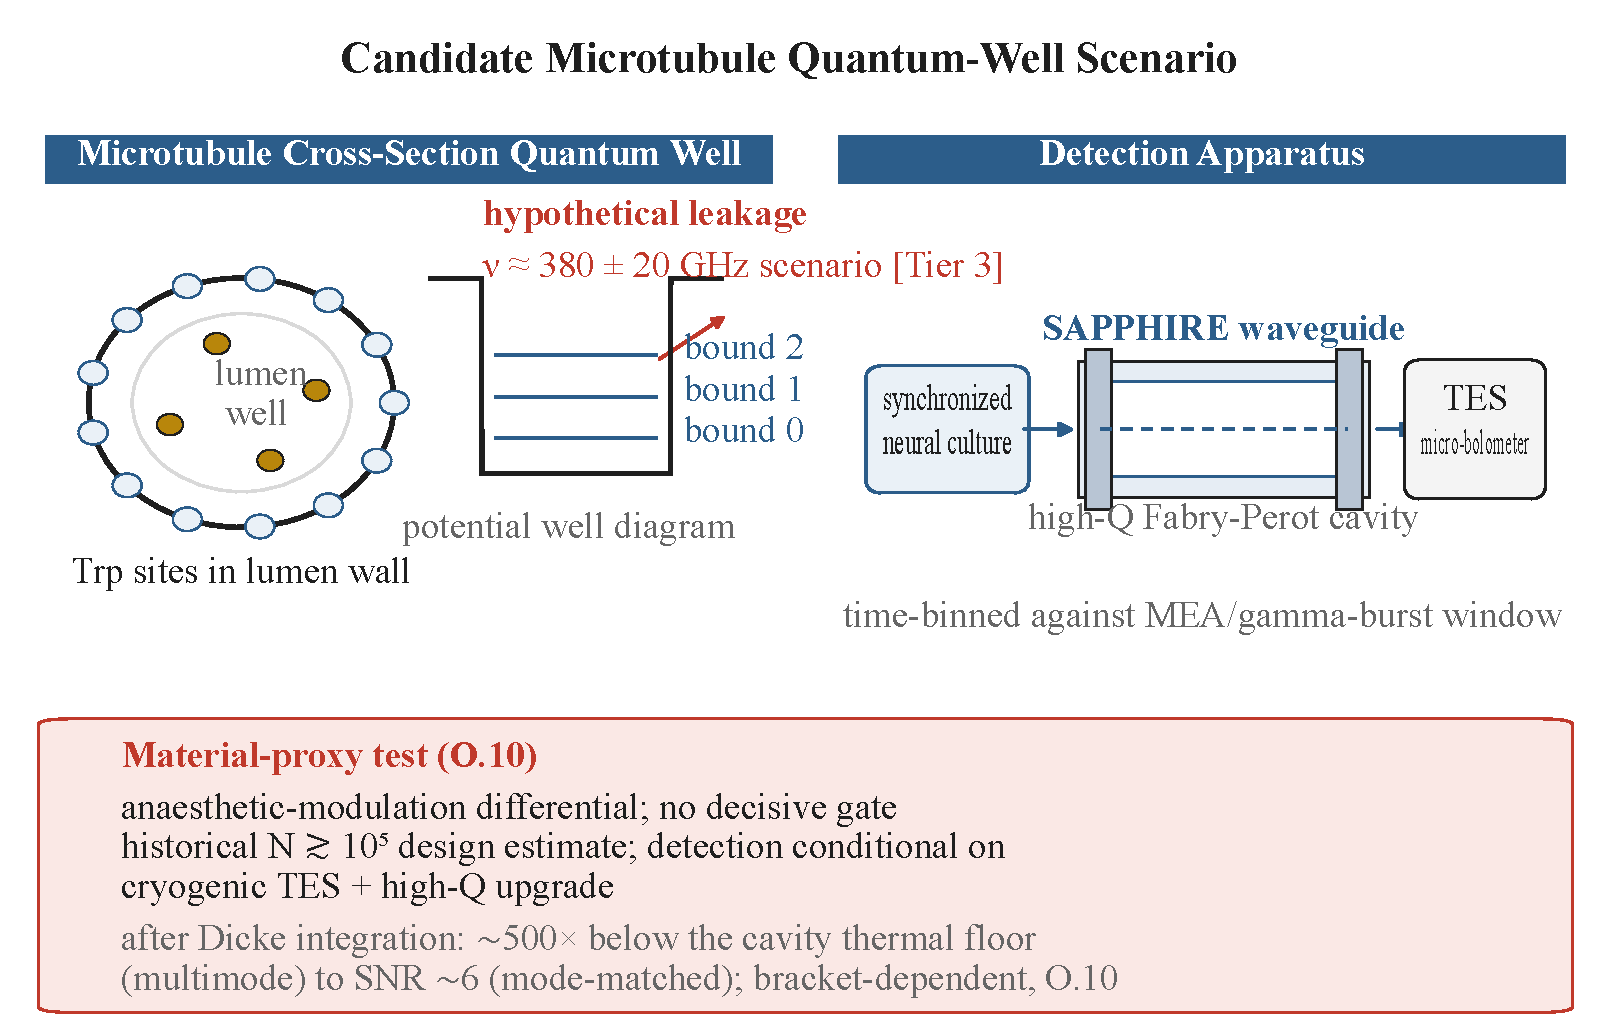
\includegraphics[keepaspectratio,alt={The microtubule cross-section as a candidate lumen geometry: thirteen protofilaments enclose the central lumen with Tryptophan sites in the lumen wall, shown as possible radical-pair and coherence probes. The potential-well depiction is a Tier 3 scenario; no phason coupling, Zeno-gating condition or Identity-Polaron realization is inferred.}]{content/Figures/Volume_3/Figure V3.13.1.pdf}}
\caption{The microtubule cross-section as a candidate lumen geometry:
thirteen protofilaments enclose the central lumen with Tryptophan sites
in the lumen wall, shown as possible radical-pair and coherence probes.
The potential-well depiction is a Tier 3 scenario; no phason coupling,
Zeno-gating condition or Identity-Polaron realization is inferred.}
\end{figure}

\begin{center}\rule{0.5\linewidth}{0.5pt}\end{center}

\subsection{\texorpdfstring{13.5 The \(\eta_{Zeno}\) Scenario Calculator
(Formal Definition;
Non-Diagnostic)}{13.5 The \textbackslash eta\_\{Zeno\} Scenario Calculator (Formal Definition; Non-Diagnostic)}}\label{the-eta_zeno-scenario-calculator-formal-definition-non-diagnostic}

The preceding sections specified the Zeno Drive piece by piece --- the
Tavis-Cummings cooperative pumping condition (§13.1.2), the candidate
magnon-polaron origin of the registered \(\nu_c \approx 112 \pm 10\) MHz
window (§13.1.2b; Tier 3 specific value), the open-system
Floquet-Lindblad correction (§13.4.6), and the substrate-discriminant
logic of Protocol A-Prime (§13.3.5). The present section assembles these
into a single closed-form procedure that returns a scalar
\(\eta_{Zeno}\) given a substrate description, so that past engine
outputs remain reproducible. It computes a dimensionless rate ratio
\textbf{only after all rates and model gates are supplied externally};
it does not derive a GCT material coupling, classify a substrate or
measure consciousness.

\textbf{The DMC legs are candidate missing-leg controls, not an
Apperception gate.} Non-zero nuclear spin and molecular chirality
motivate controlled comparisons for the proposed phason channel, but
neither is established as necessary or sufficient for Level II. The
former \(g_{single}^{eff}\), \(\eta_{Zeno}\), and \(N_{coh}\) numbers
are retained below only as conditional external-rate scenarios. O.21,
O.23, O.34, a typed and normalized coupling, and an independent
phenomenal bridge remain open; therefore no material descriptor executes
a zero-coupling inference or categorical substrate verdict.

The procedure is computationally \textbf{tractable} on a small set of
declared substrate variables --- nuclear-spin lattice, molecular
chirality, Tavis-Cummings cavity parameters, vibrational thermal-bath
coupling --- and is implemented as a chain of five documented functions
in the GCT Physics Engine
(\texttt{GCT\_Physics\_Engine/src/protocol\_eta\_zeno.py}), a
conditional scenario calculator whose outputs audit supplied arithmetic
rather than physical verdicts. Engine-generated values for the three
scenario test cases (biological tubulin, \(^{28}\)\hspace{0pt}Si
silicon, NV-centre Protocol-A-Prime surrogate) are quoted in §13.5.7
below.

\subsubsection{13.5.1 The Chain (Formal
Statement)}\label{the-chain-formal-statement}

\[
\boxed{\;\eta_{Zeno} \;\equiv\; \underbrace{\frac{g_{single}^{\,eff}\,\sqrt{N_{bio}}}{\kappa}}_{\eta_{TC}\ \text{(bare Tavis-Cummings ratio)}} \;\cdot\; \underbrace{\eta_F}_{\text{Floquet correction}}\;}
\]

with the chain of dependencies

\[
\underbrace{(\hat{I},\,\chi,\,\mu_{dip},\,m_{eff},\,\omega_d,\,a_{lat},\,\phi^{n})}_{\text{substrate}} \;\xrightarrow{\;\text{Step 1}\;}\; g_{single}^{\,eff} \;\xrightarrow{\;\text{Step 4}\;}\; \eta_{TC}
\] \[
N_{coop}\;\xrightarrow{\;\text{Step 2}\;}\;\sqrt{N_{bio}} \qquad (\omega_d,\,\phi^{-18},\,N) \xrightarrow{\;\text{Step 3}\;} \kappa
\] \[
(\gamma_\phi,\,T_2,\,\Delta_{drive},\,\Delta_{ST}) \;\xrightarrow{\;\text{Step 5}\;}\; \eta_F.
\]

Each step is a closed-form expression conditional on declared Tier-3
inputs. DMC descriptors annotate candidate-control comparisons at Step
1; they do not derive \(g_{single}^{eff}\), set it to zero, or execute a
Level-II decision. Zero and non-zero rates below are explicit legacy
external-rate scenarios retained for sensitivity bookkeeping.

\subsubsection{\texorpdfstring{13.5.2 Step 1 --- Single-Dipole Coupling
\(g_{single}\) {[}Tier 3 scenario form and
inputs{]}}{13.5.2 Step 1 --- Single-Dipole Coupling g\_\{single\} {[}Tier 3 scenario form and inputs{]}}}\label{step-1-single-dipole-coupling-g_single-tier-3-scenario-form-and-inputs}

The historical scenario form wrote the single-dipole coupling to the
phason mode as the substrate's chiral dipole transition acting on a
phason zero-point electric field, attenuated by the RT-shell geometric
gradient and the phason zero-point displacement. This expression has no
valid action-level provenance and does not by itself define a rate (V1
Ch17 §17.1.3); it is retained only to identify the engine path, and 38.3
MHz and all overlap-propagated descendants are external scenario values:

\[
g_{single}^{\,eff} \;=\; \chi \cdot f_{\text{overlap}}\cdot \frac{\mu_{dip}\,E_{\text{phason}}^{\,zpf}}{\hbar} \cdot \frac{\phi^{\,n}}{a_{lat}} \cdot \sqrt{\frac{\hbar}{2\,m_{eff}\,\omega_d}},
\]

with
\(E_{\text{phason}}^{\,zpf} = \sqrt{\hbar\,\omega_d / (2\,m_{eff})}\)
(as written this has units of velocity, not electric field, so the
displayed form is dimensionally incomplete and does not define a rate)
and \(\chi \in \{+1,-1,0\}\) the chirality sign (\(\chi = 0\) for
achiral in this scenario form; a missing-leg control, not a derived zero
coupling). The exponent \(n = -9\) is imported from the lattice-speed
relation \(\hat c=\phi^{-9}\) (V2 §6.2.2): only the integer (half of the
Tier 2 \(D=18\)) is Tier 2, while its reading as the lattice speed of
light is the Tier 3 P3b / O.15(b) stiffness-map hypothesis (V2 Ch06
§6.2.2), and its appearance in this coupling belongs to the Tier 3
scenario form (V1 §17.1.3); the dipole moment \(\mu_{dip}\), overlap
fraction \(f_{\text{overlap}}\), and effective mass \(m_{eff}\) are Tier
3 substrate inputs. For the canonical tubulin substrate, Appendix GPE
retains the external pre-overlap scenario anchor
\(g_{single}\approx38.3\) MHz. The operative \(\eta_{\rm Zeno}\) branch
applies \(f_{\rm overlap}\) to that anchor: at the engine-current
\(f_{\rm overlap}=0.01\), \(g_{single}^{eff}=3.83\times10^5\) Hz, with
the overlap-propagated plausible range
\(3.8\times10^3\)-\(3.8\times10^5\) Hz. Unless explicitly labelled
``pre-overlap anchor,'' downstream \(\eta_{\rm Zeno}\) and
\(N_{\rm coh}\) quotes use the overlap-propagated coupling.

\subsubsection{\texorpdfstring{13.5.3 Step 2 --- Collective Enhancement
\(\sqrt{N_{\rm coop}}\) {[}Tier 3
input{]}}{13.5.3 Step 2 --- Collective Enhancement \textbackslash sqrt\{N\_\{\textbackslash rm coop\}\} {[}Tier 3 input{]}}}\label{step-2-collective-enhancement-sqrtn_rm-coop-tier-3-input}

The Tavis-Cummings cooperative pumping enhances the coupling by
\(\sqrt{N_{\rm coop}}\), where \(N_{\rm coop}\) counts primary
oscillators phase-locked to the cavity mode within the Polaron volume.
The primary oscillator basis is the beta-tubulin Trp radical-pair
inventory,
\[N_{\rm coop}=N_{\beta{\rm Trp}}\times n_{\rm rp}\times f_{\rm active},\]
where \(N_{\beta{\rm Trp}}\) is the beta-Trp candidate count,
\(n_{\rm rp}\) is the number of assembled-MT radical-pair hosts per
dimer, and \(f_{\rm active}\) is the phase-locked active fraction.
Hydration-shell spins, including OH and proton dipoles, are
bath/environment degrees of freedom: they can dress the protected
subspace and enter O.23/O.33 decoherence and isotope-systematics
budgets, but they are not counted in the cooperative-oscillator basis.
The operative central branch remains \(n_{\rm rp}=0\) pending O.21
assembled-MT lumen-axis closure; the \(n_{\rm rp}=1\) sensitivity branch
uses the conservative beta-Trp inventory (the \(1.625\times10^9\)
spin-count tracked in \texttt{protocol\_zeno\_energy\_budget.py}) and
reports any hydration contribution separately as environmental dressing,
not as additional Tavis-Cummings oscillators. For a single-NV Protocol
A-Prime surrogate: \(N_{\rm coop} = 1\). The \(\sqrt N\) factor
describes collective coupling, not thermodynamic erasure cost. Any
implementation that irreversibly erases one bit per oscillator per cycle
of the historical 100 MHz material-scan scenario exceeds the 1 nW
Landauer budget by \(4.8\times10^5\) on the sensitivity branch; a
QND/reversible sampling and reset model is required under O.34 {[}Tier 3
thermodynamic closure condition{]}.

\subsubsection{\texorpdfstring{13.5.4 Step 3 --- Cavity Decay Rate
\(\kappa\) {[}Tier 3 P3b insertion or Tier 3
measured{]}}{13.5.4 Step 3 --- Cavity Decay Rate \textbackslash kappa {[}Tier 3 P3b insertion or Tier 3 measured{]}}}\label{step-3-cavity-decay-rate-kappa-tier-3-p3b-insertion-or-tier-3-measured}

Two parallel modes are exposed because biological and engineered
substrates declare \(\kappa\) differently:

\emph{Historical biological scenario (``geometric'' mode).} The engine
inserts the Tier 3 stiffness-map hypothesis P3b,
\(K_\perp / K_\parallel = \phi^{-18}\) (only the integer \(D = 18\) is
Tier 2; V2 Ch04 §4.2, V3 §13.1.2), acting on the Tier 3 cage posit of
\(N_{cage} = 144\) nodes: \[
\kappa^{\text{geom}} \;=\; \phi^{-18}\,\frac{\omega_d}{N_{cage}}.
\] For a \(100\) MHz cyclic reference, \(\kappa_{\rm cav}\approx120.19\)
Hz; at the operative \(112\) MHz branch used by the engine,
\(\kappa_{\rm cav}=134.610\) Hz. Here \(\kappa_{\rm cav}\) is reported
as a cyclic linewidth, consistently with cyclic \(g_{single}^{eff}\).
These numbers are external scenario outputs, not derived tubulin
linewidths.

\emph{Direct mode (engineered cavity).} For NV-centre / cavity-QED
surrogates, \(\kappa\) is the directly measured linewidth (\(\sim 1\)
MHz for current NV cavities).

\subsubsection{\texorpdfstring{13.5.5 Step 4 --- Bare Tavis-Cummings
Ratio \(\eta_{TC}\) {[}conditional algebra; Tier 3
inputs{]}}{13.5.5 Step 4 --- Bare Tavis-Cummings Ratio \textbackslash eta\_\{TC\} {[}conditional algebra; Tier 3 inputs{]}}}\label{step-4-bare-tavis-cummings-ratio-eta_tc-conditional-algebra-tier-3-inputs}

\[
\eta_{TC} \;=\; \frac{g_{single}^{\,eff}\sqrt{N_{bio}}}{\kappa}.
\]

This is dimensionless algebra when \(g\) and \(\kappa\) are supplied in
the same rate convention. It carries no substrate or phenomenal verdict.

\subsubsection{\texorpdfstring{13.5.6 Step 5 --- Floquet Open-System
Correction \(\eta_F\) {[}Tier 3, V3
§13.4.6{]}}{13.5.6 Step 5 --- Floquet Open-System Correction \textbackslash eta\_F {[}Tier 3, V3 §13.4.6{]}}}\label{step-5-floquet-open-system-correction-eta_f-tier-3-v3-13.4.6}

The declared Floquet-Lindblad scaffold for the open quantum system at
310 K defines a scenario factor \(\eta_F \in (0,1]\):

\[
\eta_F \;=\; \frac{1}{1 + (\gamma_\phi\,T_2)^2\,f(\Delta_{drive}/\Delta_{ST})},
\]

with \(f(x) = x^2/(1+x^2)\) a Lorentzian detuning function that vanishes
on resonance. At ordinary driven resonance \(\nu_d = \Delta_{ST}/h\),
\(\eta_F \to 1\). Off resonance, \(\eta_F < 1\) multiplicatively
suppresses the bare Tavis-Cummings ratio. It is a model factor for an
ordinary driven open system, not a geometric resonance or a
Selection-Operator efficiency; it is the same \(\eta_F\) that appears in
the Protocol A-Prime \(T_2(\nu_d)\) scenario profile of §13.3.5 (for the
bare \(\Delta_{ST}\) it peaks at 30 MHz, below the scan, and does not
shape the branch-window peak, §13.3.5; the table's \(\eta_F = 1\)
assumes the O.12-positive renormalisation).

\subsubsection{13.5.7 Engine Status on the Three Scenario
Substrates}\label{engine-status-on-the-three-scenario-substrates}

The \texttt{protocol\_eta\_zeno.py} self-test runs three numerical
scenarios and verifies arithmetic/status consistency, not substrate
verdicts:

\gctneedbreak{10\baselineskip}

\begingroup
\scriptsize
\setlength{\LTpre}{6pt}\setlength{\LTpost}{4pt}
\setlength{\tabcolsep}{3pt}
\hyphenpenalty=50\exhyphenpenalty=50
\sloppy
\begin{longtable}{>{\raggedright\arraybackslash\hspace{0pt}}p{0.0984\linewidth}>{\raggedright\arraybackslash\hspace{0pt}}p{0.1594\linewidth}>{\raggedright\arraybackslash\hspace{0pt}}p{0.1366\linewidth}>{\raggedright\arraybackslash\hspace{0pt}}p{0.1055\linewidth}>{\raggedright\arraybackslash\hspace{0pt}}p{0.1055\linewidth}>{\raggedright\arraybackslash\hspace{0pt}}p{0.142\linewidth}>{\raggedright\arraybackslash\hspace{0pt}}p{0.1328\linewidth}}
\toprule
\textbf{Substrate} & \textbf{$g_{single}^{\,eff}$} & \textbf{$\sqrt{N_{bio}}$} & \textbf{$\kappa$} & \textbf{$\eta_F$} & \textbf{$\eta_{Zeno}$} & \textbf{Status} \\
\midrule
\endhead
\bottomrule
\endlastfoot
Tubulin-Trp (V3 §13.1.2) & legacy pre-overlap scenario $3.83346543\times10^{7}$ Hz; overlap-propagated scenario $383{,}346.543$ Hz at $f_{\rm overlap}=0.01$ & central inventory $0$; sensitivity scenario $40{,}311.289$ from $N_{bio}=1.625\times10^9$ & $134.610$ Hz at the conditional $112$ MHz branch & $1$ (O.12/\allowbreak{}O.23 conditional) & central scenario $0$; sensitivity upper scenario $1.14799561\times10^8$ & \textbf{Level II: NOT\_EVALUATED; external-rate scenarios only} \\
\addlinespace[2pt]
$^{28}$​Si (V1 §17.10) & $0$ (explicit legacy external-rate scenario) & — & $1.2 \times 10^{2}$ Hz & — (n/\allowbreak{}a) & $0$ scenario & \textbf{missing-leg control; Level II: NOT\_EVALUATED} \\
\addlinespace[2pt]
NV-centre + chiral h-BN cap (V3 §13.3.5.\allowbreak{}A) & $2.7 \times 10^{7}$ Hz legacy scenario & $1$ & $1.0 \times 10^{6}$ Hz & $\sim 1$ (on-resonance scenario) & $\approx 27$ & \textbf{candidate-control sensitivity scenario; Level II: NOT\_EVALUATED} \\
\end{longtable}
\endgroup

The silicon row records an explicit legacy zero-rate scenario. Its
spin-zero/achiral descriptors make it a useful missing-leg control, but
those descriptors do not derive zero phason coupling or any phenomenal
verdict.

The NV-centre row reports a nonzero ratio \(\sim 1.5\) orders of
magnitude above unity; the historical \(\eta \approx 27\) follows only
from the supplied \(g\) and \(\kappa\), and that margin is not an
independent consciousness threshold. Exceeding unity is not a phase
transition, and a zero from a declared gate is not a physical
no-consciousness theorem. The biological tubulin central branch is
\(\eta_{Zeno}=0\) until O.21 supplies an assembled-MT lumen-axis
radical-pair oscillator; the \(n_{rp}=1\) tubulin value is a sensitivity
upper edge, not the central scenario value. The single-NV surrogate
scenario is chosen to land in a resolvable band, so that the Protocol
A-Prime \(T_2(\nu_d)\) joint proxy signature (§13.3.5)---a non-monotonic
peak in a registered hypothesis region of the full scan plus chirality
contrast---is the discriminating material observable. The \(150\) MHz
response is a sign-unfixed O.23/O.24 diagnostic outside F1. The
surrogate remains far below the tubulin sensitivity-branch cooperative
regime so that the chirality-reversal control (§13.3.5.A) can help
separate a chirality-correlated contribution (CISS attribution still
needs the handedness-odd test of §13.3.5 component (c)).

\subsubsection{13.5.8 Computational Tractability and Its
Limit}\label{computational-tractability-and-its-limit}

The IIT integrated-information \(\Phi\) is \emph{defined} over the
system's \(2^{N-1} - 1\) bipartitions (Oizumi-Albantakis-Tononi 2014), a
search whose cost grows exponentially with \(N\) and is intractable for
any realistic biological network in closed form. The rate-ratio
calculator above is computationally cheap because it accepts a small
supplied tuple --- nuclear-spin lattice, chirality, Tavis-Cummings
cavity parameters \((g, N, \kappa)\), and the open-system parameters
\((\gamma_\phi, T_2, \Delta_{ST})\). That does not make it a replacement
for IIT \(\Phi\) or a computation of the Selection Operator
\(\mathcal{F}_{sel}\): the physical coupling and the independent
Level-II bridge remain missing, and the Tier 3 substrate inputs (Trp
dipole moment, \(N_{bio}\) estimate, NV coupling parameters) carry their
own uncertainty.

Protocol A-Prime (§13.3.5) can tighten ordinary material-response
parameters against bench measurement. The same data alone cannot
determine the missing GCT vertices, physical coefficient, normalization,
material embedding or rate.

\subsubsection{13.5.9 Computational Reference and
Scope}\label{computational-reference-and-scope}

The chain is mirrored in
\texttt{GCT\_Physics\_Engine/src/protocol\_eta\_zeno.py}. The reference
implementation evaluates a declared scenario, returns the per-step
quantities, and writes the canonical regression artifact
\texttt{GCT\_Physics\_Engine/data/protocol\_eta\_zeno\_results.json}; it
is not a substrate-decision engine.

\gctneedspace{5\baselineskip}

\textbf{Scope of the procedure:}

\begin{enumerate}
\def\labelenumi{\arabic{enumi}.}
\tightlist
\item
  \textbf{Steps 2--5 are exact conditional algebra given their inputs;
  Step 1 (\(g_{single}\)) is a quarantined Tier 3 scenario form; all
  numerical inputs are Tier 3, and the GCT rate input is undefined.}
  Each step is fixed once the registered substrate tuple is supplied
  (Tavis-Cummings ratio, V3 §13.1.2; Floquet-Lindblad open-system
  scaffold, V3 §13.4.6; Dual Material Constraint candidate controls, V1
  §16.2.6). Apart from the external 38.3 MHz scenario anchor, the chain
  has no fitted numerical knob, and its absolute outputs inherit the
  Tier 3 substrate inputs listed below. Exact evaluation does not
  validate the tuple.
\item
  \textbf{The numerical values are conditional external-rate scenarios.}
  Molecular and NV parameters are imported, but the phason coupling is
  neither typed nor measured. The central O.21-pending inventory remains
  \(n_{rp}=0\) and the \(n_{rp}=1\) value is sensitivity bookkeeping.
  DMC descriptors define candidate controls; they do not force
  qualitative substrate logic or a Level-II verdict.
\item
  \textbf{The procedure is tractable on the test cases but is NOT
  experimentally validated against bench measurements.} CISS, phonon,
  spin, population and linewidth measurements are material proxies, not
  measurements of a GCT coupling. Protocol A-Prime (§13.3.5) can support
  or reject the registered proxy pattern; it cannot promote the
  historical rate chain. Its registered pattern is a non-monotonic peak
  in either the Branch A \(112\pm10\) MHz or Branch B \(42\pm10\) MHz
  hypothesis region plus chirality contrast after the full half-open
  \([32,200)\) MHz scan at
  \(\Delta\nu_{\rm step}\leq1/(4\pi T_{2,\rm eff})\) in NV-centre +
  chiral h-BN samples. The 150 MHz sign is unfixed and recorded
  separately as an O.23/O.24 diagnostic outside F1/Holm. A positive
  branch/chirality result plus the chirality-reversal control of
  §13.3.5.A would constrain the Tier 3 material inputs and measure the
  peak amplitude that Open Problems O.23 + O.24 leave conditional;
  empirical agreement does not promote those inputs to Tier 2. Promotion
  requires an independent derivation of the relevant DFS/chiral
  parameters and normalized physical coupling from the declared
  premises, closing the O.23/O.24 derivational dependencies without
  fitting the target measurements. Observations then test the resulting
  claim.
\item
  \textbf{The procedure does NOT replace Protocol A-Prime and is not a
  substrate-decision engine.} Its output on a substrate is a scenario
  number, not a prediction of what a Protocol A-Prime measurement must
  find and not a substitute for the measurement. The Dual Material
  Constraint is not established as necessary or sufficient, and
  \(\eta_{Zeno}\) supplies no Level-II verdict.
\end{enumerate}

\textbf{Cross-references.} V1 §17.10 and §16.2.6 cite this procedure as
a candidate-control and conditional-scenario audit, not a substrate
decision rule. V3 §13.3.5 supplies a bench material-proxy test; the
typed coupling (V1 Ch17 §17.1.3) and an independent phenomenal bridge
remain open.

\chapter{Chapter 14: Protocol B --- Mass Spectrum
Computation}\label{chapter-14-protocol-b-mass-spectrum-computation}

The derivation of the lepton mass hierarchy in Chapter 8 identifies the
muon and tau as the 11th and 17th harmonics of the electron's
dodecahedral cage. To audit these results against the engine ledger, we
employ \textbf{Protocol B}: a deterministic verification of the
projected lattice geometry. This protocol computes the charged-lepton
mass ratios from the Tier 2 harmonic-ladder mechanism plus the Tier 3
integer anchors \(N=11\) and \(N=17\) per Parameter Ledger §0.1;
first-principles unique-eigenvalue extraction remains open under
O.5/O.14/O.15.

\begin{center}\rule{0.5\linewidth}{0.5pt}\end{center}

\subsection{14.1 Methodology}\label{methodology}

\subsubsection{14.1.1 Algorithm: Projected Lattice
Dynamics}\label{algorithm-projected-lattice-dynamics}

The analysis models the vacuum as an Ammann-Kramer-Neri (AKN) tiling,
generated via the Cut-and-Project method from the 6-dimensional
hyper-lattice \(\mathbb{Z}^6\). We construct the \textbf{Geometric
Resonance Matrix (\(\mathbf{G}\))}, which represents the coupled
harmonic structure of the \(N=144\) dodecahedral cage.

Unlike standard molecular dynamics, which operate in 3D Euclidean space,
the GCT algorithm operates on \textbf{Projected Degrees of Freedom}.
Each node \(i\) in the 6D parent lattice possesses a 6D displacement
vector \(\mathbf{U}_i\). Upon projection into the physical manifold,
this vector is partitioned into physical (\(\mathbf{u}_\parallel\)) and
internal (\(\mathbf{u}_\perp\)) components. The interaction energy of a
bond between nodes \(i\) and \(j\) is defined by the stiffness hierarchy
derived in Volume 2:
\[V_{ij} = \frac{1}{2} K_\parallel (\Delta \mathbf{u}_\parallel \cdot \hat{\mathbf{n}}_\parallel)^2 + \frac{1}{2} K_\perp (\Delta \mathbf{u}_\perp \cdot \hat{\mathbf{n}}_\perp)^2\]
The analysis solves for the \textbf{Node-Centric Eigenvalues}
(eigenstates of the center-of-mass motion), distinguishing these from
the interface stress energies (surface area mismatches) utilized for the
hadron spectrum.

\subsubsection{\texorpdfstring{14.1.2 Parameters: The Phason Stiffness
Ansatz (\(D=18\)) {[}Tier 2 integer identification (D=18) + Tier 3
heuristic stiffness-ratio map --- Parameter Ledger §0.1 P3; Open Problem
O.15{]}}{14.1.2 Parameters: The Phason Stiffness Ansatz (D=18) {[}Tier 2 integer identification (D=18) + Tier 3 heuristic stiffness-ratio map --- Parameter Ledger §0.1 P3; Open Problem O.15{]}}}\label{parameters-the-phason-stiffness-ansatz-d18-tier-2-integer-identification-d18-tier-3-heuristic-stiffness-ratio-map-parameter-ledger-0.1-p3-open-problem-o.15}

The analysis requires exactly one material input: the ratio of phason
stiffness to phonon stiffness.

No tree-level stiffness ratio follows from the projection geometry. The
earlier ``theorem'' that the Gram eigenvalue ratio of the
6D\(\to\)\hspace{0pt}3D projection gives \(\eta_0 = \phi^{-2}\) is
withdrawn: \(\phi^{-2}\) is a raw-frame (legacy single-chart) Gram
ratio, which changes under row rescaling and equals 1 for the canonical
row-isometric projectors (App DPS §DPS.2--3; V3 Ch04 §4.1.2), so it is a
normalization convention and not a physical stiffness. The picture in
which phonon-phason coupling suppresses \(K_\perp\) under RG flow at the
relevant physical scale is a GCT conjecture {[}Tier 3{]}, not a result
taken from the quasicrystal hydrodynamics literature (Lubensky,
Ramaswamy and Toner 1985 treat the phason elastic constants as
independent effective-theory parameters).

We set \(n=18\) as a \textbf{Tier 2 integer identification (D=18) + Tier
3 heuristic stiffness-ratio map} (Parameter Ledger §0.1 P3 canonical
disposition; first-principles RG closure tracked under Open Problem
O.15). The two layers are kept separate: \(D_{H_3}=2+6+10=18\) is the
Tier 2 Coxeter integer, while the physical map
\(K_\perp/K_\parallel=\phi^{-18}\) is the independent Tier 3 hypothesis
P3b (Parameter Ledger §0.1; O.15). Like H-EW, P3b is a registered Tier 3
hypothesis listed outside the core-input count; only the integer
\(D=18\) is Tier 2, and P3b is a bare stipulation. Arithmetic rewritings
of \(\phi^{-18}\) (for example as \((\phi^{-2})^9\) over nine
phonon-phason channels, or the \(H_3\)-Coxeter rank × Galois × dimension
count of App DPS §DPS.4) are not derivations and give it no support. The
former cube-of-Gram-determinant route (App DPS §DPS.3) is retired: the
Gram-determinant ratio depends on the coordinate frame (a row rescaling
changes it by \(s^{18}\), and canonical row-isometric projectors give
1). Icosahedral \(H_3/I_h\) symmetry permits a quadratic stiffness form
\(Q=aP_\parallel+bP_\perp\) with \(b/a\) free, and the isotropic parent
action gives \(b/a=1\), so symmetry alone does not fix \(\phi^{-18}\)
{[}Tier 1 representation theory{]}. The earlier claim of empirical
support from a \(10^{-2}\)--\(10^{-1}\) i-AlMnSi / i-AlPdMn
phason/phonon band, and of a quantitatively derived chemical-bonding
floor, is also retired: the quasicrystal measurements cited for it
concern \(K_2/K_1\) phason elastic anisotropy and diffusive relaxation
kinetics rather than a phason/phonon stiffness ratio, and the DFT
reference cited for the floor (DOI 10.1103/PhysRevB.88.144102) is Xiao
et al.~(2013) on the CaIrO\(_3\) post-perovskite transition, not
i-AlPdMn. Every numerical use of \(\phi^{-18}\) below is therefore
conditional on P3b; first-principles microscopic, action-level or RG
closure remains Open Problem O.15.

The input parameter for the phason stiffness is set, conditional on the
Tier 3 hypothesis P3b, as:
\[\frac{K_\perp}{K_\parallel} = \phi^{-18} \approx 1.7307 \times 10^{-4}\]

\subsubsection{14.1.3 Computational Setup: Harmonic Ansatz
Evaluation}\label{computational-setup-harmonic-ansatz-evaluation}

The \(6N \times 6N\) geometric projection matrix is analyzed to extract
the spectrum of eigenfrequencies \(\{\omega_k\}\). Because
quasicrystalline spectra can be \textbf{singular continuous} (proven for
one-dimensional Fibonacci-type models; not established for 3D
icosahedral operators), eigenvalues are expected to cluster in a complex
hierarchy. Protocol B utilizes a \textbf{Harmonic Ansatz Evaluation} to
target the specific pseudo-gaps (\(\phi^{11}\) and \(\phi^{17}\))
without the algorithm becoming lost in the dense background of uncoupled
phason modes.

The evaluation identifies the fundamental breathing mode resonance
(\(\omega_0\)), which represents the electron's mass-energy.

\subsubsection{14.1.4 Numerical Convergence and the Local Isomorphism
Shield}\label{numerical-convergence-and-the-local-isomorphism-shield}

Stability is probed by increasing the cluster size from the \(N=144\)
core toward an \(N=2000\) node neighborhood. The dodecahedral cage
satisfies the local matching rules of the icosahedral projection, so by
local isomorphism every finite patch recurs throughout the tiling; local
isomorphism concerns patch recurrence and implies no spectral protection
by itself. The picture of the aperiodic background as a
\textbf{Topological Shield}, in which the \(N=144\) symmetry acts as a
resonant cavity that filters out local fluctuations and would yield a
mass eigenvalue protected against local environmental disorder, is a
Tier 3 heuristic; no such eigenvalue has yet been extracted (§14.2). A
specific numerical convergence rate is not asserted here: the
finite-\(N\) discretization artifact present in the direct graph
extraction (§14.2; \texttt{protocol\_lepton\_spectrum.py}) is why
first-principles non-perturbative eigenvalue closure remains open
(O.5/O.14/O.15).

\begin{center}\rule{0.5\linewidth}{0.5pt}\end{center}

\subsection{14.2 Validation and Results}\label{validation-and-results}

\gctneedspace{5\baselineskip}\begin{gctCaution}

\textbf{The Linear Boundary Constraint --- read this before the
precision tables below.} Extensive HPC analysis of the full sparse
Hessian (see Appendix GPE) confirms that the bare linear dynamical
matrix yields normalized eigen-ratios of
\texttt{{[}1.0,\ 1.67,\ 2.1,\ 2.52...{]}}. Neither \(\phi^{11}\) nor
\(\phi^{17}\) emerge spontaneously from linear diagonalization.

The leptons are non-linear phason solitons whose exact mass scaling is
governed by the \(6N \pm 1\) symmetry saturation, not linear oscillatory
modes. The \(\phi^{11}\) and \(\phi^{17}\) gap alignments are therefore
\textbf{Tier 2 Geometric Postulates} (the harmonic-ladder structure
committed to in Parameter Ledger §0.1 P4/P5) plus the \textbf{Tier 3
specific integer choices} \(N=11\) (muon) and \(N=17\) (tau). The
non-perturbative computational extraction of these solitonic eigenvalues
from first principles remains an open goal for the GCT framework. The
bare \(\phi^{11}\) / \(\phi^{17}\) residuals are \(-3.75\%\) /
\(+2.69\%\); after the Tier 3 first-order coefficients the muon reaches
\textasciitilde0.24\% (the tau's first-order formula is its full
formula, −51 ppm), and the ppm-level figures in §14.2.3 below are Tier 3
formula residuals against measured masses (the muon mass is measured to
22 ppb, CODATA 2022), not precision claims.

\end{gctCaution}

\subsubsection{14.2.1 The Harmonic Ansatz and the Linear/Non-Linear
Boundary {[}Tier 2
Postulate{]}}\label{the-harmonic-ansatz-and-the-linearnon-linear-boundary-tier-2-postulate}

The primary non-linear pseudo-gaps of the dodecahedral cage correspond
to the 11th and 17th harmonics of the inflation operator. Under the
\textbf{Geometric Harmonic Ansatz}:

\begin{itemize}
\tightlist
\item
  \textbf{Muon Target:} \(\phi^{11} \approx 199.005\) {[}Tier 2
  Postulate{]}
\item
  \textbf{Tau Target:}
  \(\phi^{17} = L_{17}+\phi^{-17} \approx 3571.0003\) {[}Tier 2
  Postulate{]} (\(L_{17}=3571\) is the Lucas number)
\end{itemize}

\subsubsection{14.2.2 Precision Mass Audit}\label{precision-mass-audit}

We apply the phason drag corrections derived in Chapter 8 to the
geometric eigenvalues. For the Muon, we include the \textbf{Second-Order
Phi-Alpha Correction}
(\(\phi^8\alpha^2=\phi^{-3}\times\phi^{11}\alpha^2\): Tier 2 exponent
arithmetic, verified computationally, see Appendix GPE; reading its
\(\phi^{-3}\) factor as an electroweak mixing projection rests on the
Tier 3 hypothesis H-EW, V3 Ch04 §4.3.2). The residual error of
\textbf{−21 ppm (\(-0.0021\%\))} for the Muon (lepton-spectrum protocol;
App PSC §PSC.1) is about \(10^3\sigma\) against the 22 ppb CODATA 2022
measurement uncertainty, so the formula does not reproduce \(m_\mu\) at
measurement precision; it is a Tier 3 formula residual. (The earlier
reading of it as inside a ``\(\sim\)\hspace{0pt}10--40 ppm higher-loop
theory floor'' is withdrawn: Standard-Model radiative corrections are
not an uncertainty on a measured mass.) The next geometric correction
enters at third order carrying a \(\phi\)-power coefficient comparable
to the \(\phi^8\) second-order term ---
\(\phi^8\alpha^3 \approx 1.8 \times 10^{-5}\) {[}Tier 3 ---
order-of-magnitude estimate by analogy to the second-order
coefficient{]}, the same size as the residual, so the row tests nothing
beyond first order --- whereas the bare uncoefficiented
\textbf{Third-Order Radiative Correction}
\(\alpha^3 \sim 3.9 \times 10^{-7}\) {[}Tier 1 --- QED perturbation
theory{]} alone is two orders smaller. Native first-principles loop
closure remains open under O.5/O.14/O.15.

\gctneedbreak{20\baselineskip}

\subsubsection{14.2.3 Final Lepton Mass Table
vs.~PDG}\label{final-lepton-mass-table-vs.-pdg}

\gctneedbreak{10\baselineskip}

{\def\LTcaptype{none} % do not increment counter
\begin{longtable}[]{@{}
  >{\raggedright\arraybackslash}p{(\linewidth - 8\tabcolsep) * \real{0.1905}}
  >{\centering\arraybackslash}p{(\linewidth - 8\tabcolsep) * \real{0.2381}}
  >{\raggedright\arraybackslash}p{(\linewidth - 8\tabcolsep) * \real{0.1905}}
  >{\raggedright\arraybackslash}p{(\linewidth - 8\tabcolsep) * \real{0.1905}}
  >{\raggedright\arraybackslash}p{(\linewidth - 8\tabcolsep) * \real{0.1905}}@{}}
\toprule\noalign{}
\begin{minipage}[b]{\linewidth}\raggedright
\textbf{Particle}
\end{minipage} & \begin{minipage}[b]{\linewidth}\centering
\textbf{Geometric Exponent}
\end{minipage} & \begin{minipage}[b]{\linewidth}\raggedright
\textbf{GCT formula value (postdiction; MeV)}
\end{minipage} & \begin{minipage}[b]{\linewidth}\raggedright
\textbf{Observed (MeV)}
\end{minipage} & \begin{minipage}[b]{\linewidth}\raggedright
\textbf{Relative Error}
\end{minipage} \\
\midrule\noalign{}
\endhead
\bottomrule\noalign{}
\endlastfoot
\textbf{Electron} & \(0\) & \textbf{0.5109989} (input, anchor A1) &
\(0.5109989\) & \textbf{Base Scale} \\
\textbf{Muon} & \(11\) & \textbf{105.656} {[}Tier 2 mechanism (harmonic
ladder, conditional on the Tier 3 \(\phi\)-step, V3 Ch08 §8.1.2) + Tier
3 specific exponent N=11 per Ledger §0.1 P4{]} & \(105.6583755(23)\)
(CODATA 2022) & \textbf{\textasciitilde−21 ppm (Tier 3 formula
residual)} \\
\textbf{Tau} & \(17\) & \textbf{1776.84} {[}Tier 2 mechanism (harmonic
ladder, conditional on the Tier 3 \(\phi\)-step, V3 Ch08 §8.1.2) + Tier
3 specific exponent N=17 per Ledger §0.1 P5{]} & \(1776.93 \pm 0.09\)
(PDG 2024) & \textbf{\textasciitilde−51 ppm (−0.0051\%)} \\
\end{longtable}
}

\subsubsection{14.2.4 The Tau Comparison}\label{the-tau-comparison}

For the tau, the GCT value \(1776.84\) MeV lies \(0.09\) MeV
(\(\sim\)\hspace{0pt}51 ppm, about \(1\sigma\)) below the PDG 2024 value
\(1776.93 \pm 0.09\) MeV (\(\sim\)\hspace{0pt}0.005\%). The GCT number
carries no propagated theoretical uncertainty: the Tier 3 exponent
\(N=17\), the inserted Tier 3 tau correction rule and the unpropagated
next-order term are not converted into an error bar. The number of
displayed digits is therefore not a precision claim, and the formula is
not more precise than experiment. Future high-luminosity lepton-collider
and tau-threshold measurements would tighten this postdiction
comparison; it is not a prediction.

\gctneedspace{5\baselineskip}

\textbf{Conclusion:} Protocol B treats the charged lepton mass hierarchy
as a \textbf{deterministic spectral fingerprint} candidate of the 6D
hyper-lattice. The match across multiple generations using the
icosahedral geometric framework (parameterised by \(\phi\) as the
structural constant, plus the integer-valued harmonic exponents
\(N = 11, 17\) which enter as Tier 3 specific values per Parameter
Ledger §0.1 P4/P5 --- not as additional fitted parameters but as
structural commitments of the framework) is consistent with the
harmonic-ladder mechanism, but no global significance is claimed for it
(V3 Ch08 §8.5). As evidence that φ or icosahedral structure is special,
this match is \textbf{Tier 4}: the preregistered constant control test
(v3, NEGATIVE-FRAGILE; App PSC §PSC.9.6) found φ's pattern of matches on
21 constants not distinguishable from that of random constants (58 of
300 random bases did at least as well). The test ``excludes, at power ≥
0.8, an effect in which φ hits at least 6 of the 8 informative rows
through a real effect; weaker effects are not excluded.'' The numbers
are kept as descriptive arithmetic, while first-principles
unique-eigenvalue extraction remains open under O.5/O.14/O.15.
References to \(\phi\) as the structural constant are
structural-constants-only language; the 5-postulate-plus-1-anchor bare
lepton-ratio sub-sector (the bare \(\alpha\) relation \(360\phi^{-2}\)
is a separate Tier 3 numerical relation, mechanism open; the corrected
lepton rows also need A3, H-EW and the Tier 3 coefficient rules), with
the native-RGE endpoint and precision-comparison rows adding anchors
A2--A6 (Parameter Ledger §0.1), is the load-bearing tier discipline.

\gctneedspace{5\baselineskip}

\textbf{END OF CHAPTER 14}

\chapter{Chapter 15: Protocol C --- XRISM
Preregistration}\label{chapter-15-protocol-c-xrism-preregistration}

The 3.55 keV X-ray anomaly, proposed in Chapter 11 {[}Tier 3{]} as the
signature of vacuum lattice fracture, is a candidate observational link
to GCT, conditional on the O.38 cage posit and on a line whose existence
is itself unconfirmed. \textbf{Protocol C} defines the formal
preregistration for the XRISM line-shape audit.

\begin{center}\rule{0.5\linewidth}{0.5pt}\end{center}

\subsection{15.1 Formal Decision
Framework}\label{formal-decision-framework}

To ensure scientific reproducibility and avoid outcome-contingent curve
fitting, GCT preregisters the following hypothesis test for the XRISM
stacked-cluster stress-aperture survey.

\subsubsection{\texorpdfstring{15.1.1 The Null Hypothesis
(\(H_0\))}{15.1.1 The Null Hypothesis (H\_0)}}\label{the-null-hypothesis-h_0}

The Dark Matter signal at 3.55 keV originates from a particulate gas
(e.g., sterile neutrinos) or standard atomic multiplets (K XVIII).

\begin{itemize}
\tightlist
\item
  \textbf{Signature:} Instrumental profile convolved with cluster-virial
  broadening and background-line modeling uncertainties
  (\(\sigma_v \approx 1300\) km/s for the Perseus reference) {[}Tier 3
  --- cluster virial measurement{]}.
\item
  \textbf{Expected FWHM:} \(\approx 37\) eV for the broad
  thermal/virialized reference at \(E=3.55\) keV {[}Tier 3 ---
  broadening calculation{]}. This width is a diagnostic axis, not a
  standalone sterile-neutrino verdict; morphology, flux floor, and
  background model are load-bearing.
\item
  \textbf{Recoil:} Not a discriminator. In the two-body decay
  \(\nu_s\to\nu\gamma\) the photon carries exactly \(m_s/2\), with no
  recoil loss, and the free-atom recoil \(E^2/2Mc^2\) of a 3.55 keV
  photon is \(\approx1.7\times10^{-4}\) eV for \(^{39}\)\hspace{0pt}K
  (\(\approx6.7\times10^{-3}\) eV even for hydrogen), far below any
  resolvable width {[}Tier 1 kinematics{]}.
\end{itemize}

\subsubsection{\texorpdfstring{15.1.2 The GCT Hypothesis
(\(H_1\))}{15.1.2 The GCT Hypothesis (H\_1)}}\label{the-gct-hypothesis-h_1}

The Dark Matter signal originates from a macroscopic, coherent
topological glass (supersolid vacuum).

\begin{itemize}
\tightlist
\item
  \textbf{Signature:} Monochromatic emission, narrow only if the
  emitters are lattice-bound (GCT Mössbauer Effect). Whether
  fractured-phase emitters are lattice-bound or free debris at virial
  speed is a declared open programme (V3 Ch11 §11.2.3); the width
  expectation below, and the forward model's use of ICM gas turbulence
  for emitters that are not gas, are conditional on it.
\item
  \textbf{Expected FWHM (observed; bulk-turbulence broadened Voigt):}
  \(\sim 9.8\) eV at 3.55 keV --- quadrature combination of the XRISM
  Resolve instrumental Gaussian
  \(\sigma_{\rm inst} = 5\,{\rm eV}/2.355 \approx 2.12\) eV (operational
  analysis freeze uses the then-current XRISM POG plus RMF/ARF
  calibration files as primary response inputs; the 5--7 eV mission-spec
  band and Ishisaki et al.~2022 \emph{Proc. SPIE} 12181:121811S (DOI
  10.1117/12.2630654) are retained as pre-flight/historical scale
  anchors) and the bulk-cluster-turbulence Gaussian
  \(\sigma_{\rm kin} \approx E_{\rm line} (v_{\rm turb}/c) \approx 3.55\)
  eV at \(v_{\rm turb} \approx 300\) km/s for typical cluster-core
  turbulence. Engine-canonical value:
  \texttt{expected\_fwhm\_ev\ =\ 9.7458} per
  \texttt{GCT\_Physics\_Engine/data/protocol\_dm\_line\_forward\_model\_results.json}
  at \(\text{XRISM\_FWHM\_EV} = 5.0\). \textbf{Sensitivity sweep:} at
  the conservative mission-spec upper bound
  \(\text{XRISM\_FWHM\_EV} = 7.0\), \(\sigma_{\rm inst} = 2.97\) eV, the
  quadrature
  \(\sigma_{\rm inst,eff} = \sqrt{2.97^2 + 3.55^2} \approx 4.63\) eV,
  and the predicted observed Voigt FWHM rises to \(\sim 10.9\) eV ---
  the §15.2 spectral-compatible band lower edge shifts accordingly. The
  \textbf{deconvolved intrinsic line-width residual}
  \(W_{\rm int} \lesssim 5\) eV (instrument and registered
  kinematic/turbulence model removed; unmodeled astrophysical and
  natural broadening remain) is what the §15.2 decision rule operates on
  --- distinct from the observed FWHM that an external observer would
  measure on the plotted line; both numbers must be reported jointly to
  avoid the ``observer sees \textasciitilde9 eV → GCT falsified''
  misreading. {[}Tier 3 --- observed FWHM follows from the Voigt
  convolution of three Tier 1 / Tier 3 inputs; the \(W_{\rm int}\)
  decision rule is the falsification gate.{]}
\item
  \textbf{Recoil:} Not a discriminator (see \(H_0\)).
\item
  \textbf{Acoustic Phonon Signature {[}Tier 4, non-operative{]}:}
  Temporal and spatial cross-correlation with a burst of High-Frequency
  Gravitational Waves (HFGWs) (vacuum fracture acoustic emission); the
  1-100 MHz band is asserted, not derived (V3 Ch11 §11.4.7).
\end{itemize}

\subsection{15.1.3 Addressing Known
Non-Detections}\label{addressing-known-non-detections}

Multiple independent analyses have reported non-detections of the 3.55
keV line in environments where dark matter density alone would predict a
strong sterile-neutrino signal. GCT does not contest these results; they
are read as compatible with the stress-gating hypothesis, while their
status remains retrospective until frozen stress-aperture maps and masks
are applied cluster-by-cluster before residual unblinding.

\textbf{Malyshev et al.~(2014)} performed a stacked XMM-Newton analysis
of dwarf spheroidal galaxies (dSphs) and blank-sky fields, finding no
3.55 keV emission. Under the sterile neutrino hypothesis, this is
anomalous given the high dark matter columns. Under GCT's
\textbf{Stress-Gating Hypothesis} (§11.1.3), this is the expected result
if dSphs, with virial velocities of \(\sigma_v \sim 5\)--\(10\) km/s,
sit below threshold; the vacuum lattice would then be in the elastic
glass phase and emit no radiation. The operative threshold, however, is
the frozen thermal-pressure proxy below (\(\sigma_{crit}=0.53\) keV
cm⁻³, in ICM \(n k_B T\) units); the \(K_\perp\phi^{-5}\) form of V3
Ch11 §11.1.3 is heuristic motivation, not a second definition. Gas-poor
dSphs have no ICM pressure, so ``\(\sigma_{vir} \ll \sigma_{crit}\)'' is
not yet a computed comparison: a stress proxy usable in gas-poor systems
must be specified and tabulated for each null target before this counts
as a consistency check.

\textbf{Riemer-Sørensen (2016)} analyzed Chandra observations of the
Milky Way halo and found no significant excess at 3.55 keV. The
stress-gating reading is that the smooth gravitational potential of the
Milky Way halo generates insufficient shear to fracture the supersolid
vacuum lattice; the same limitation applies, since the dark-matter halo
has no ICM-pressure proxy and no halo stress has been computed against
\(\sigma_{crit}\). In the model, emission is concentrated in high-stress
fracture zones (cluster outskirts, merger shocks, and high-shear ICM),
not in relaxed stellar halos.

\gctneedspace{5\baselineskip}

\textbf{Quantitative GCT Resolution:} The stress-gating threshold is
numerically frozen as
\[\sigma_{crit}\equiv \sqrt{P_{\rm Perseus-core}P_{\rm Bullet-shock,central}}=\sqrt{(0.07)(4.0)}=0.529\ {\rm keV\,cm^{-3}}\approx0.53\ {\rm keV\,cm^{-3}},\]
using the Perseus-core pressure anchor and the central Bullet-shock
pressure estimate cited in Ch11. This remains Tier 3 because the
threshold is observation-bracketed, not first-principles derived. Above
threshold, emission is permitted but not guaranteed (V2 Ch11 §11.2.2);
below, suppressed. \textbf{Protocol C's frozen stress-aperture rule:}
the operative falsification aperture is the mass-weighted set of cells
whose pre-line thermal-pressure/shear proxy satisfies
\(P_{\rm proxy}\ge0.53\ {\rm keV\,cm^{-3}}\) within the XRISM
stacked-cluster sample. The Perseus core falls below this numeric cut
and is not a falsification point. That is an aperture definition, not a
rheological claim: whether cluster cores are fractured (V2 Ch13) or
elastic is a declared open programme (V3 Ch11 §11.1.4), and the
Hitomi-Perseus null is not cited as support for the gate.

\textbf{Frozen target-cell list.} Before inspecting any 3.55 keV
residuals, the analysis locks the following cell classes from
pressure/shear maps: (i) Bullet Cluster bow-shock wedge and Mach-cone
shell; (ii) Coma merger / radio-relic pressure shells; (iii) A2142
cold-front / merger shell; (iv) A3667, A2256, and A2319 radio-relic or
merger-shock shells; (v) any Perseus, A2029, or A1795 off-core annulus
only where the same pre-line proxy exceeds \(0.53\ {\rm keV\,cm^{-3}}\).
Relaxed cool cores, including Perseus \(r\lesssim100\) kpc and the
A2029/A1795 cores, are locked as below-cut cells unless their pre-line
maps exceed the numeric cut (an aperture definition only; their rheology
is open, V3 Ch11 §11.1.4). This freezes the aperture before residual
unblinding; residual-selected cell admission is prohibited.

Once a stress proxy is tabulated for each null target, this would
convert the non-detections from anomalies into stress-gating consistency
checks rather than prior successful predictions; until then they are not
computed checks. The preregistration in §15.1 should be understood in
this context: H1 predicts a stress-gated signal (narrow only for
lattice-bound emitters, V3 Ch11 §11.2.3) in \textbf{non-core}
stress-gated cluster regions ABOVE
\(\sigma_{crit}=0.53\ {\rm keV\,cm^{-3}}\) (cluster outskirts, merger
shocks, high-shear ICM); the Perseus core lies outside the frozen
numeric aperture, and the Hitomi-Perseus null is not used as support
(open cluster-core rheology, V3 Ch11 §11.1.4). GCT registers a low-shear
null branch for dSphs and smooth halos. Both types of measurement are
falsification-relevant --- a detection in a dSph would falsify the
low-shear null branch, while a registered above-\(\sigma_{crit}\)
stacked-cluster null falsifies only after the preregistered sensitivity
and stress-aperture spatial-map requirements are met.
\textbf{Operational stress-aperture rule:} the primary cluster test is
run on the frozen target-cell list above, with aperture weights
committed before unblinding from X-ray line residuals.

\subsubsection{15.1.4 Engagement with Dessert-Rodd-Safdi 2020 and the
Boyarsky et
al.~response.}\label{engagement-with-dessert-rodd-safdi-2020-and-the-boyarsky-et-al.-response.}

Dessert, Rodd \& Safdi (2020) \emph{Science} 367:1465 used more than 30
Ms of XMM-Newton blank-sky observations to test the Milky-Way-halo flux
expected from decaying-dark-matter explanations of the reported 3.5 keV
line, finding no evidence for the line and setting decay-rate limits
inconsistent with that interpretation. Boyarsky, Malyshev, Ruchayskiy \&
Savchenko (2020) contested the strength of that limit, arguing that
background-line modeling can weaken the bound by more than an order of
magnitude and leave a dark-matter interpretation viable;
Dessert/Rodd/Safdi's reply held that even conservative additional-line
modeling still strongly disfavors decaying dark matter. The literature
null is therefore not simply ``broad instrumental continuum versus
narrow Lorentzian''; it is a coupled blank-sky halo-flux and
background-modeling dispute over whether a decaying-DM line should
already have appeared in Milky-Way halo data.

\textbf{GCT discriminator:} GCT does not use the decaying-DM halo-flux
null as its primary model. It predicts stress-gated cluster emission: a
monochromatic line (Lorentzian-narrow only for lattice-bound emitters,
an open programme, V3 Ch11 §11.2.3) at
\(E_{vac} = m_e c^2 / 144 \approx 3.5486\) keV (matching the §15.2
decision-rule centroid \(E_c = 3.548 \pm 0.005\) keV and the engine
output
\texttt{verify\_dm\_line\_centroid\_postdiction\_check.py::predicted\ =\ 3.5486038\ keV}
to the displayed precision) whose spatial morphology tracks high-shear
fracture boundaries rather than the smooth Milky-Way-halo column.
Dessert's blank-sky null remains load-bearing as a warning that
background modeling can erase the claimed signal; Boyarsky's response
remains load-bearing as a warning that over-aggressive background
modeling can over-tighten the bound. The XRISM/Athena test must
therefore adjudicate three axes at once: intrinsic width, centroid, and
stress-correlated morphology. \textbf{Operational consequence:} a
resolved \(W_{\rm int}<1\) eV line is not a linewidth discriminator by
itself, because sterile-neutrino decay can also be intrinsically narrow
before cluster kinematics and instrumental convolution. A narrow
(Lorentzian) line alone disfavours no model, particulate dark matter
included; the registered verdicts are those of §15.2 (\(W_{\rm int}\)
bands plus stress-aperture morphology at \(\Delta\chi^2\ge9\), with the
centroid as context); Milky-Way halo blank-sky nulls impose an
independent flux constraint. A null result in the registered high-shear
cluster sample at the required sensitivity falsifies or demotes the GCT
stress-gating threshold; it should not be reported merely as ``Dessert
vindicated'' unless the analysis also reproduces the blank-sky halo-flux
assumptions of Dessert et al.

\gctneedspace{5\baselineskip}\begin{gctImportant}

\textbf{Falsification Condition (Non-Detection Branch):} A confirmed
detection of 3.55 keV emission at \(>3\sigma\) significance in a dSph
system with virial velocity \(\sigma_v < 15\) km/s would falsify the
stress-gating hypothesis, since such a system is assumed to lie below
\(\sigma_{crit}\) (the stress proxy for gas-poor systems is still to be
specified, §15.1.3). Candidate low-shear targets are Draco, Ursa Minor,
Sculptor, Fornax, Sextans, and Carina. The dSph branch is decisive only
for a blinded line search with centroid \(E_c = 3.548 \pm 0.005\) keV,
deconvolved \(W_{\rm int}\leq5\) eV, background-line subtraction inside
the S1-S6 budget, and a stack reaching a line-flux sensitivity at least
as deep as the terminal Bulbul-level Protocol C floor when expressed in
the same decay-rate-normalized convention
(\(\Gamma \lesssim 2.0\times10^{-28}\,\mathrm{s}^{-1}\) at 94 Ms
equivalent). Shallower dSph stacks are sensitivity-limited constraints
rather than stress-gating falsifiers.

\end{gctImportant}

\begin{center}\rule{0.5\linewidth}{0.5pt}\end{center}

\subsection{15.2 Quantitative Decision
Rule}\label{quantitative-decision-rule}

The test is adjudicated based on \(W_{int}\) and stress-aperture spatial
tracking. Here \(W_{int}\) means the deconvolved \textbf{intrinsic
line-width residual} after removing the instrumental response and the
registered cluster kinematic/turbulence model; unmodeled astrophysical
and natural broadening remain in \(W_{int}\). The separately reported
convolved observed FWHM includes instrument + turbulence and is expected
to be \(\sim9.8\) eV for the GCT forward model. The spectral centroid
\(E_c\) is reported as postdiction-status context for any detected line,
not as an operative P.3 falsifier. The HFGW cross-correlation is a
separate Tier 4 mechanism-context row outside the P.3 gate. The
\(W_{int}\) axis is calibrated against the XRISM Resolve instrumental
FWHM floor at \(\sim 5\) eV (Ishisaki et al.~2022, \emph{Proc. SPIE}
12181:121811S (DOI 10.1117/12.2630654)); the Dessert-Rodd-Safdi 2020
blank-sky null (§15.1.4) is an independent flux constraint, not a width
calibrator. The width bands below test only the lattice-bound
(narrow-emitter) reading: if fractured-phase emitters are free debris at
cluster virial speed, GCT's own model would give \(\sim28\)--\(36\) eV,
so the \(>20\) eV falsifier depends on the open emitter-kinematics
programme (V3 Ch11 §11.2.3). The decision rule separates these into four
explicit bands:

\gctneedbreak{10\baselineskip}

{\def\LTcaptype{none} % do not increment counter
\begin{longtable}[]{@{}
  >{\raggedright\arraybackslash}p{(\linewidth - 4\tabcolsep) * \real{0.3333}}
  >{\raggedright\arraybackslash}p{(\linewidth - 4\tabcolsep) * \real{0.3333}}
  >{\raggedright\arraybackslash}p{(\linewidth - 4\tabcolsep) * \real{0.3333}}@{}}
\toprule\noalign{}
\begin{minipage}[b]{\linewidth}\raggedright
\(W_{int}\)
\end{minipage} & \begin{minipage}[b]{\linewidth}\raggedright
Status
\end{minipage} & \begin{minipage}[b]{\linewidth}\raggedright
Conclusion
\end{minipage} \\
\midrule\noalign{}
\endhead
\bottomrule\noalign{}
\endlastfoot
\(< 1\) eV & \textbf{Narrow line} & Narrow line; not a linewidth
discriminator by itself because sterile-neutrino decay can also be
intrinsically narrow before cluster kinematics and instrumental
convolution. Combined with \(E_c = 3.548 \pm 0.005\) keV {[}centroid
context only; the registered forward gate is \(W_{int}\) + morphology{]}
and flux tracking the registered stress-gated template, this is a
stress-gated-line outcome; HFGW co-detection would be a Tier 4 auxiliary
check for the vacuum-fracture mechanism (band asserted, not derived),
but requires HFGW detection sensitivity that does not currently exist at
cluster distances (see scope note below). \\
\(1\)--\(5\) eV & \textbf{Spectral-compatible (morphology + flux floor
pending)} & \(W_{int}\) is the \textbf{deconvolved intrinsic line-width
residual} after instrument and registered kinematic/turbulence
deconvolution and lies at a scale that is statistically difficult to
separate from the XRISM response floor once response-matrix, background,
and turbulence uncertainties are propagated. The current XRISM
POG/RMF/ARF response files are the operative calibration source;
Ishisaki et al.~2022 is retained as mission-design context. GCT is
spectrally compatible with the data but not discriminated against
particle-decay or systematic interpretations; final discrimination
requires the registered stress-aperture morphology and flux-floor
conditions, with Athena X-IFU follow-up at 2.5 eV FWHM as the cleaner
linewidth test. \\
\(5\)--\(20\) eV & \textbf{Statistical Tie} & Broader than the
instrument FWHM floor but narrower than the thermal/atomic-plasma
falsification threshold. GCT compatible but the sterile-neutrino
virial-broadening interpretation cannot be excluded; potential
inhomogeneous broadening or source confusion. \\
\(> 20\) eV OR Flux follows \(\rho^2\) & \textbf{Registered branch
falsified} & Broadening inconsistent with lattice-bound
(Mössbauer-narrowed) emission, or smooth density tracking. \textbf{H1
(registered Protocol C branch) falsified} --- a branch-level verdict,
not a verdict on GCT as a whole. Because the emitter kinematics are open
(V3 Ch11 §11.2.3), a \(>20\) eV width rejects the lattice-bound reading;
it would also match a free-debris reading of GCT's own fractured
phase. \\
\end{longtable}
}

\begin{quote}
\textbf{HFGW co-detection scope note (Tier 4 conditional).} The Protocol
C falsification rule states that HFGW co-detection is outside the
operative P.3 gate. A ``NO HFGW burst detected'' clause would be
\textbf{currently unfalsifiable} because no instrument has 1-100 MHz
HFGW sensitivity at extragalactic cluster distances (the published HFGW
detector concepts --- Gertsenshtein-Zeldovich inverse-mechanism,
optical-resonance cavities, levitated-sensor arrays --- sit
\textasciitilde20 orders of magnitude (a factor
\textasciitilde{}\(10^{20}\)) short of cluster-scale GW strain at MHz
frequencies; Aggarwal, Aguiar, Bauswein et al.~2021 \emph{Living
Rev.~Relativ.} 24:4 review the field's sensitivity gap). The HFGW
co-detection prediction is therefore \textbf{Tier 4 (currently
unfalsifiable on operational grounds)} until detector technology closes
the sensitivity gap; it is \emph{not} part of the operational P.3
falsification gate above. The registered Tier 3 P.3 branch gate is the
spectral \(W_{int}\) + Protocol C stress-aperture spatial-tracking row;
centroid agreement is postdiction-status context reported separately.
\end{quote}

\textbf{Executable-readiness qualifier.} Protocol C is a conditional
decision design, not a completed OSF-grade executable preregistration
until the per-cell ARF/RMF/background/effective-mass table is frozen and
deposited with the target-cell mask, response files, background model,
and synthetic-line checks. The nominal 94 Ms exposure is therefore
necessary but not sufficient for a decisive no-line branch.

\textbf{Conditional preregistration design.} Registry mirror (App PRG
P.3 / App FSM P.3): the registered Protocol C stress-gated line branch
is falsified at decisive sensitivity if any registered branch condition
holds (a branch-level verdict, not a verdict on GCT as a whole): (a) NO
3.55 keV line detected at the terminal no-line floor
\(\Gamma \lesssim 2.0\times10^{-28}\ \mathrm{s}^{-1}\) in \(\geq94\) Ms
equivalent stacked exposure, OR (b) detected line has \(W_{\rm int}>20\)
eV FWHM after instrument and registered kinematic/turbulence
deconvolution (a test of the lattice-bound emitter reading, which is
open: V3 Ch11 §11.2.3), OR (c) detected-line morphology does NOT follow
the stress-gated \(\rho_{\mathrm{above}\,\sigma_{\mathrm{crit}}}^2\)
template by \(\Delta\chi^2\ge9\) versus both smooth \(\rho\) and smooth
\(\rho^2\) templates. The 26 Ms /
\(\Gamma \lesssim 3.8\times10^{-28}\ \mathrm{s}^{-1}\) value obtained by
scaling the XRISM 3.75 Ms ten-cluster reference stack is a sensitivity
milestone and morphology/linewidth constraint point, not a terminal
no-line falsifier of a Bulbul-normalized
\(\Gamma\sim2\times10^{-28}\ \mathrm{s}^{-1}\) signal. The terminal
no-line floor is the same scaling continued to the Bulbul-level
normalization:
\(1.0\times10^{-27}\sqrt{3.75/94}\approx2.0\times10^{-28}\ \mathrm{s}^{-1}\).
Aperture: mass-weighted stress-gated regions with
\(P_{\rm proxy}\ge\sigma_{\rm crit}=0.53\ {\rm keV\,cm^{-3}}\) under the
Protocol C stress-aperture rule (§15.1.3). Sample-size/integration rule:
the primary above-\(\sigma_{crit}\) stacked-cluster no-line decision
requires an exposure stack reaching the terminal floor at 3.55 keV after
background modelling; shallower stacks are sensitivity-limited and
reported as constraints, not decisive nulls. The nominal 94 Ms
equivalent exposure is insufficient by itself: the preregistration must
include a per-cell ARF/RMF/background/effective-mass exposure table
demonstrating that each frozen stress-aperture cell contributes to the
terminal flux/decay-rate floor after real response, masking, continuum,
and cluster-stacking losses before the terminal no-line branch is
executable as a completed decisive falsifier.

\textbf{Executable-gate status.} Until the per-cell
ARF/RMF/background/effective-mass table is frozen, the terminal no-line
branch is preregistered but not executable as a decisive falsifier; the
current package supports sensitivity-limited constraints and
morphology/linewidth milestones.

\textbf{Public preregistration freeze.} Before unblinding line
residuals, the Protocol C package is deposited in a timestamped public
archive (OSF/Zenodo or mission-collaboration equivalent) containing the
target-cell list and exclusion rules, RMF/ARF/gain-response files,
synthetic-line injections at the registered flux/width/morphology
levels, K-XVIII/background model priors, analysis code hash,
randomization/blinding seed protocol, S1-S6 systematic budget, and
amendment ledger. Any post-freeze change is recorded as a numbered
amendment with timestamp, rationale, and the blinded/unblinded state of
the affected data.

\textbf{Operational count/background power model:} For XRISM Resolve at
5 eV-class instrument resolution, a 20 eV line window, effective area
\(A_{\rm eff}=200\ \mathrm{cm^2}\), and background
\(6.6\times10^{-4}\ \mathrm{cnt/s/keV}\) per the HEASARC XRISM Resolve
POG residual-background line, the idealized background rate in the line
window is \(1.32\times10^{-5}\ \mathrm{cnt/s}\). At 3.75 Ms,
\(B\approx49.5\) counts, so \(3\sqrt{B}\approx21.1\) source counts and
\(F_{3\sigma}\approx2.8\times10^{-8}\ \mathrm{ph/cm^2/s}\). At 26 Ms,
\(B\approx343\) counts, so \(3\sqrt{B}\approx55.6\) source counts and
the background-limited theoretical floor is
\(F_{3\sigma}\approx1.1\times10^{-8}\ \mathrm{ph/cm^2/s}\),
corresponding in the prior-normalization convention to
\(\Gamma\lesssim1.2\times10^{-30}\ \mathrm{s}^{-1}\). At 94 Ms, the
empirical-derived no-line floor reaches the Bulbul-level
\(\Gamma\lesssim2.0\times10^{-28}\ \mathrm{s}^{-1}\) under the same
reference-stack scaling. The background-limited theoretical floor is not
the operative falsification gate. Real-stack penalties from aperture
overlap, continuum subtraction uncertainty, line-model degeneracy with
adjacent thermal lines such as K-XVIII at 3.5 keV, and cluster-stacking
S/N efficiency typically degrade the limit by 100-1000×.
\textbf{Terminal no-line falsification operates on the Bulbul-level
empirical-derived floor}, not the background-limited theoretical floor.

Analysis blinding: the primary linewidth fit is run blinded to the
GCT/sterile-neutrino labels, using fixed windows around 3.548 keV and
sideband-derived background terms; centroid is carried as context after
the spectral fit is frozen. An unblinded secondary analysis may inspect
stress-map alignment only after the spectral fit is frozen.
\textbf{Morphology decision statistic and power:} after unblinding, the
Protocol C stress-weighted aperture template from the frozen target
cells is compared against smooth \(\rho\) and \(\rho^2\) templates with
the same exposure/background mask. Before the line fit is inspected, the
frozen mask must pass the template-separation diagnostic
\(D_{\rm sep}=\min(1-\mathrm{corr}(S,\rho),\,1-\mathrm{corr}(S,\rho^2))\ge0.25\)
using unit-normalized, exposure-weighted templates under the same mask.
At the registered 26 Ms morphology milestone, the count model gives
\(B\approx343\) background counts in the 20 eV line window and
\(3\sqrt{B}\approx55.6\) source counts; for one registered morphology
degree of freedom this is powered to \(\Delta\chi^2\ge9\) only when the
\(D_{\rm sep}\) diagnostic passes. A stress-gated morphology is required
to improve the line-flux fit by \(\Delta\chi^2\ge9\) (3σ for one
registered morphology degree of freedom) over both smooth templates; a
smooth-template preference of \(\Delta\chi^2\ge9\) at decisive spectral
sensitivity falsifies the stress-morphology branch. If the frozen mask
fails the pre-line template-separation diagnostic, the morphology branch
is reported as underpowered rather than used as a falsifier; the
terminal spectral non-detection branch remains tied to
\(\Gamma\lesssim2.0\times10^{-28}\ \mathrm{s}^{-1}\) at \(\ge94\) Ms
equivalent, while linewidth/morphology constraints may be reported at
the 26 Ms milestone. Partial-detection rule: (a) line in band with
\(W_{int}<5\) eV but no stress map is ``spectral-compatible /
morphology-pending''; (b) stress-aperture alignment without a resolved
line is ``morphology-compatible / spectral-pending''; (c) line absent
only at the 26 Ms milestone is sensitivity-limited; line absent at the
terminal Bulbul-level floor across the stacked above-\(\sigma_{crit}\)
apertures is a substantive stress-gating failure; (d) any \(W_{int}>20\)
eV or smooth \(\rho^2\) density tracking at decisive sensitivity
falsifies the Protocol C GCT branch.

\textbf{Preregistered systematic-error budget (frozen before
unblinding).} The P.3 linewidth decision must report all six systematics
before assigning a pass/fail label:

\gctneedbreak{10\baselineskip}

{\def\LTcaptype{none} % do not increment counter
\begin{longtable}[]{@{}
  >{\raggedright\arraybackslash}p{(\linewidth - 4\tabcolsep) * \real{0.3333}}
  >{\raggedright\arraybackslash}p{(\linewidth - 4\tabcolsep) * \real{0.3333}}
  >{\raggedright\arraybackslash}p{(\linewidth - 4\tabcolsep) * \real{0.3333}}@{}}
\toprule\noalign{}
\begin{minipage}[b]{\linewidth}\raggedright
Systematic
\end{minipage} & \begin{minipage}[b]{\linewidth}\raggedright
Registered tolerance
\end{minipage} & \begin{minipage}[b]{\linewidth}\raggedright
Mitigation / reporting rule
\end{minipage} \\
\midrule\noalign{}
\endhead
\bottomrule\noalign{}
\endlastfoot
S1 RMF/ARF residuals & \(<2\%\) per channel & Resolve response matrix
and energy-dependent redistribution propagated into the deconvolution
prior. \\
S2 K-XVIII subtraction uncertainty & \(<1\times10^{-5}\ {\rm s}^{-1}\)
contamination & Local sideband slope, cluster-continuum curvature, and
K-XVIII/Ar/Ca line complex fitted jointly, with K-XVIII subtraction
reported explicitly. \\
S3 gain drift & \(<0.3\) eV cumulative & Gain drift and
pointing-dependent response checked against calibration lines. \\
S4 split-stack scatter & \(\sigma_{\rm stack}<0.5\) eV & Split-stack
linewidth and centroid stability across exposure partitions. \\
S5 cluster kinematic / ICM-substructure deconvolution & residual \(<1\)
eV after velocity-field and shear-map priors & Primary stack = the
frozen above-\(\sigma_{crit}\) target cells, with cluster-level random
effects; high-shear apertures require pre-line velocity/shear-map
priors, and any aperture whose thermal-substructure or Doppler-shear
budget cannot be bounded below 1 eV is reported as systematics-limited
rather than decisive. \\
S6 calibration consistency & \(<2\%\) systematic across exposures &
Cross-exposure calibration consistency reported before unblinding. \\
\end{longtable}
}

A null or linewidth excess is decisive only if the S1-S6 budget remains
inside its preregistered tolerance; otherwise the outcome is
``systematics-limited'' rather than a P.3 falsification.

\begin{center}\rule{0.5\linewidth}{0.5pt}\end{center}

\subsection{15.3 Forward Model
Implementation}\label{forward-model-implementation}

The GCT Physics Engine generates the expected observational signature by
convolving the lattice-predicted delta function with the XRISM Resolve
redistribution matrix:

\begin{Shaded}
\begin{Highlighting}[]
\CommentTok{\# GCT Forward Model (Simplified Logic)}
\NormalTok{sigma\_inst }\OperatorTok{=}\NormalTok{ instrument\_fwhm }\OperatorTok{/} \FloatTok{2.355}
\NormalTok{sigma\_eff }\OperatorTok{=}\NormalTok{ sqrt(sigma\_inst}\OperatorTok{**}\DecValTok{2} \OperatorTok{+}\NormalTok{ sigma\_turb}\OperatorTok{**}\DecValTok{2}\NormalTok{)}
\NormalTok{fwhm\_total }\OperatorTok{=} \FloatTok{2.355} \OperatorTok{*}\NormalTok{ sigma\_eff  }\CommentTok{\# GCT predicts intrinsic\_width \textasciitilde{} 0}
\end{Highlighting}
\end{Shaded}

Detailed simulation code is provided in \textbf{Appendix GPE}.

\subsection{15.4 Falsification
Commitment}\label{falsification-commitment}

If XRISM Resolve definitively measures the 3.55 keV line in the stacked
above-\(\sigma_{crit}\) cluster apertures with a deconvolved intrinsic
width \(W_{int} > 20\) eV (the §15.2 decision-rule falsification
threshold), the registered Protocol C stress-gated line branch is
\textbf{falsified} (a branch-level verdict, not a verdict on GCT as a
whole). That width condition tests the lattice-bound emitter reading,
whose status is open (V3 Ch11 §11.2.3). A null is decisive only when the
exposure stack reaches the preregistered sensitivity floor and the
mass-weighted stress-gated aperture map is included. The Perseus core
alone lies outside the frozen aperture and is not a falsification point.

\gctneedspace{5\baselineskip}\begin{gctNote}

The deep-survey exposure at the requisite sensitivity is the registered
Protocol C exposure class (XRISM Science Working Group, JAXA/NASA
Mission Operations Plan; cf.~Tashiro et al.~2018 \emph{Proc. SPIE}
10699:1069922 for the XRISM mission concept). Stacks that do not reach
the terminal Bulbul-level empirical-derived
\(\Gamma \lesssim 2.0 \times 10^{-28}\,\mathrm{s}^{-1}\) sensitivity
floor are reported as sensitivity-limited constraints rather than
decisive nulls; the 26 Ms /
\(\Gamma \lesssim 3.8 \times 10^{-28}\,\mathrm{s}^{-1}\) point remains
the morphology-linewidth milestone, and the background-limited
\(\Gamma \lesssim 1.2 \times 10^{-30}\,\mathrm{s}^{-1}\) calculation is
a theoretical ceiling, not the operational gate.

\end{gctNote}

\begin{center}\rule{0.5\linewidth}{0.5pt}\end{center}

\subsection{15.5 XRISM Stacked-Cluster Constraint: Line-Shape
Verdict}\label{xrism-stacked-cluster-constraint-line-shape-verdict}

The Protocol C constraint table distinguishes sensitivity-limited
cluster stacks from decisive line-shape tests. Reference stack:

\gctneedbreak{10\baselineskip}

{\def\LTcaptype{none} % do not increment counter
\begin{longtable}[]{@{}
  >{\raggedright\arraybackslash}p{(\linewidth - 2\tabcolsep) * \real{0.5000}}
  >{\raggedright\arraybackslash}p{(\linewidth - 2\tabcolsep) * \real{0.5000}}@{}}
\toprule\noalign{}
\begin{minipage}[b]{\linewidth}\raggedright
Item
\end{minipage} & \begin{minipage}[b]{\linewidth}\raggedright
Result
\end{minipage} \\
\midrule\noalign{}
\endhead
\bottomrule\noalign{}
\endlastfoot
Exposure & 3.75 Ms (10 clusters stacked) \\
3.55 keV Line Detection & \textbf{Not detected} in the reference
stack \\
Decay Rate Upper Limit &
\(\Gamma \lesssim 1.0 \times 10^{-27}\ \mathrm{s}^{-1}\) (3\(\sigma\)
upper limit; XRISM Collaboration 2025, arXiv:2510.24560) {[}Tier 3 ---
observational upper bound{]} \\
Sensitivity vs.~Bulbul et al. & \textbf{5× weaker} than original
XMM-Newton detection rate \\
Physical Conclusion & \textbf{Sensitivity-limited} --- insufficient
depth to confirm or rule out \\
GCT Prediction Status & \textbf{Stress-gated branch not adjudicated.}
Deeper above-\(\sigma_{crit}\) survey required. \\
\end{longtable}
}

Protocol C becomes decisive only for the mass-weighted
above-\(\sigma_{crit}\) stacked-cluster aperture that reaches the
preregistered sensitivity floor and reports the frozen linewidth and
stress-map decision rule, with centroid carried as postdiction-status
context. Shallower stacks and Perseus-core-only nulls remain constraints
on the line-flux normalization rather than falsifications of the
stress-gated branch.

\begin{center}\rule{0.5\linewidth}{0.5pt}\end{center}

\gctneedspace{5\baselineskip}

\textbf{END OF CHAPTER 15}

\chapter{Chapter 16: Protocol D --- Isotope
Substitution}\label{chapter-16-protocol-d-isotope-substitution}

Functionalism treats cognition as potentially realizable across
different physical substrates. GCT introduces a competing Tier-3
candidate architecture in which discrete spin and molecular chirality
are useful experimental controls for a proposed
adiabatic-spin-ratchet/phason channel. These controls are not
established requirements for consciousness, an Identity Polaron, or
Level II. \textbf{Protocol D} tests candidate spin/coherence responses:
the Drosophila LORR branch has no operative quantitative gate under
current systematics (P.13), while the NMR polarity branch (P.13c) tests
a registered Tier 3 material-response sign hypothesis conditional on
O.21/O.33. Neither outcome is a verdict on GCT as a whole: the
measurement tests an ordinary material proxy, and no phason,
Selection-Operator or Level-II inference follows from it (V1 Ch17
§17.1.3). A preregistered result rejects the registered biophysical
branch only under that branch's own decision rule: the Protocol D NMR
polarity gate (P.13c) is held pending redesign (§16.5): as written it
rejected by construction, since \(^{17}\)\hspace{0pt}O shortens
water-\(^1\)\hspace{0pt}H \(T_2\) by scalar relaxation; the former
sign-aware rule, which rejects the registered sign-positive branch on a
powered, significant negative isotope × activity interaction in
water-\(^1\)\hspace{0pt}H \(\Delta T_2\), applies only after the
redesign, and until then no outcome supports or rejects the branch; the
LORR branch has no operative gate. Any bridge to an Identity Polaron or
Level II would additionally need a typed normalized coupling, an
Identity-Polaron construction and the independent phenomenal bridge.

\begin{center}\rule{0.5\linewidth}{0.5pt}\end{center}

\subsection{16.1 Testing the Substrate}\label{testing-the-substrate}

\subsubsection{16.1.1 The Hypothesis: Spin-Sensitive Material Response
{[}Tier 3
candidate{]}}\label{the-hypothesis-spin-sensitive-material-response-tier-3-candidate}

The Tier-3 model represents a possible self-bridge as a topological
defect assigned an address in the \(\Sigma_\infty\) Solenoid and
proposes a spin-address register as one candidate architecture. The
Solenoid has \(\pi_1=0\), so it does not itself tether the defect or
protect a memory {[}Tier 1 topology{]}; any register would need its own
physical write/read, noise-protection and lifetime model. Protocol D
does not establish that such a register exists or is necessary, nor does
it classify the preparation's phenomenal status.

\textbf{Hypothesis:} \emph{Nuclear-spin depletion may alter a candidate
spin/coherence observable in the neural preparation. This is a
missing-leg mechanism test, not evidence for a Selection-Operator
coupling or Level-II state. The LORR assay remains a pilot/systematics
study with no decisive gate.}

\subsubsection{16.1.2 Silicon as a Missing-Leg
Control}\label{silicon-as-a-missing-leg-control}

Protocol D uses standard silicon as a \textbf{missing-leg control}, not
an ontological or phenomenal verdict. Its dominant
\(^{28}\)\hspace{0pt}Si isotope has \(I=0\) and the diamond-cubic
lattice is achiral; these are control descriptors for the proposed
channel, not proof of zero coupling or Level-II absence. The
\(^{17}\)\hspace{0pt}O quadrupolar probe is a separate diagnostic of
water-clathrate involvement, not the chirality channel itself.

\subsubsection{\texorpdfstring{16.1.3 The Quadrupolar Relaxation Time
(\(\tau_Q\)) {[}Tier 1 standard relaxation form / Tier 3 hydrated-lumen
application{]}}{16.1.3 The Quadrupolar Relaxation Time (\textbackslash tau\_Q) {[}Tier 1 standard relaxation form / Tier 3 hydrated-lumen application{]}}}\label{the-quadrupolar-relaxation-time-tau_q-tier-1-standard-relaxation-form-tier-3-hydrated-lumen-application}

The candidate \(^{17}\)\hspace{0pt}O probe couples through its nuclear
electric quadrupole moment \(Q=-0.026\) barns {[}Tier 3 ---
nuclear-physics measurement{]}. This moment alone does not determine a
relaxation time. The quadrupolar coupling constant requires the local
electric-field gradient (EFG), for example \(C_Q\equiv e^2qQ/h\) in
frequency units, and the transverse relaxation rate additionally
requires the EFG fluctuation spectrum. In the extreme-narrowing limit,
the standard Bloembergen-Purcell-Pound structure is schematically
\[\frac{1}{T_{2,Q}}\propto C_Q^2\left(1+\frac{\eta_{\rm EFG}^2}{3}\right)\tau_c,\]
where \(\eta_{\rm EFG}\) is the measured EFG asymmetry and \(\tau_c\) is
the correlation time (Bloembergen, Purcell \& Pound 1948 \emph{Phys.
Rev.} 73:679). Protocol D therefore carries \(\tau_Q\equiv T_{2,Q}\) as
\textbf{not evaluated} pending an O.21/O.33 hydrated-lumen EFG
distribution, correlation function and motional-regime determination
{[}Tier 3 application{]}. The geometric number \(\phi^{-2}\) is not
substituted for \(\eta_{\rm EFG}\) without a derived map from the
icosahedral ansatz to the local EFG tensor.

\subsubsection{16.1.4 Quarantined Spin--Phason Interaction
Ansatz}\label{quarantined-spinphason-interaction-ansatz}

The historical bridge between a winding phason field
\(\mathbf{S}_{vac}\) and the material substrate was written as
\[\hat{H}_{int} = \sum_j \mathcal{A}_j \mathbf{I}_j \cdot \mathbf{S}_{vac}\]
with \(\mathbf{I}_j\) the nuclear spin vector of the \(j\)-th atom in
the candidate ordered lumen-water environment and \(\mathcal{A}_j\) a
coupling constant that was meant to come from the icosahedral overlap.
This is not an adopted Hamiltonian: the action defines neither
\(\mathbf{S}_{vac}\) nor \(\mathcal{A}_j\), and no mode normalization or
microscopic matching derives it (cf.~the field-typing analysis, V1 Ch17
§17.1.3). It is not an Agent--substrate coupling law. Ordinary material
hyperfine Hamiltonians remain well defined and testable without this
phason identification.

\subsubsection{16.1.5 Hilbert Space Scaling and Topological
Depth}\label{hilbert-space-scaling-and-topological-depth}

For a 15 nm-DIAMETER \(\times\) 8 nm-AXIAL microtubule ring segment
(canonical \(r_{\rm lumen}=7.5\) nm, \(\ell=8\) nm), App NSP §NSP.4
gives \(\approx4.7\times10^4\) lumen water molecules per 8 nm ring; the
ring holds 13 αβ-dimers (one per protofilament), so the lumen water per
dimer is \(\approx3.6\times10^3\) {[}Tier 3 --- structural estimate{]}.
Full \(^{17}\)\hspace{0pt}O enrichment would therefore give a
tensor-product spin Hilbert-space dimension \(6^{3.6\times10^3}\) per
dimer if all nuclei were treated as independent {[}Tier 1 ---
combinatorics given that idealization{]}. Hilbert-space dimension is not
usable register capacity, an identity address, or a memory lifetime;
those would require constraints, controllability and a physical
write/read model {[}Tier 3{]}. This is not an axial 15 nm segment claim.

\begin{center}\rule{0.5\linewidth}{0.5pt}\end{center}

\subsection{16.2 The Measurement Problem
Inverted}\label{the-measurement-problem-inverted}

\subsubsection{16.2.1 Non-BPP Coherence Enhancement (Polarity
Reversal)}\label{non-bpp-coherence-enhancement-polarity-reversal}

In standard Nuclear Magnetic Resonance (NMR) physics
(Bloembergen-Purcell-Pound or BPP theory), introducing a quadrupolar
nucleus like \(^{17}\)\hspace{0pt}O (\(I=5/2\)) is expected to
\textbf{decrease} the transverse coherence time (\(T_2\)) by providing
efficient pathways for stochastic thermal relaxation.

\textbf{The GCT Polarity-Reversal Response {[}O.21/O.33-pending
sensitivity branch{]}:} the candidate model assigns the opposite sign
from standard BPP relaxation only on the O.21/O.33-positive branch. On
that branch, a proposed protected-subspace response would lengthen
\(T_2\) in \(^{17}\)\hspace{0pt}O-enriched active neural preparations
after inactive-baseline subtraction. The central branch remains null
until the assembled-microtubule radical-pair and hydrated-lumen geometry
close. This is a conditional biophysical response; enhancement or
non-enhancement does not establish or exclude an Agent, Identity
Polaron, Level II, or conscious rendering.

\subsubsection{16.2.2 The Waking-to-Anesthetized
Delta}\label{the-waking-to-anesthetized-delta}

We define the \textbf{Zeno Factor (\(\eta_Z\))} as the ratio of
coherence in the waking state to the anesthetized state:
\[\eta_Z = \frac{T_{2, waking}}{T_{2, anesthetized}}\] The inactive or
anesthetized preparation supplies a BPP-dominated comparison baseline. A
deviation of \(\eta_Z\) from unity would constrain the candidate
response model; it is not a measure of active conscious rendering, an
Identity Polaron, or Level II.

\subsubsection{16.2.3 The Anesthetic Threshold
Shift}\label{the-anesthetic-threshold-shift}

Within the candidate substrate-binding branch, anesthetics are modeled
as perturbations of the intraluminal-water/Trp-pocket coherence
environment. Xenon is assigned to a separate network-broadcast
comparison whose discrimination requires spin spectroscopy rather than
LORR alone. The ansatz assigns two conditional \(^{17}\)\hspace{0pt}O
response signs: a longer active-minus-inactive \(T_2\) response and, on
the O.21/O.33-positive sensitivity branch, a lower anesthetic
\(C_{50}\). These are biophysical-response hypotheses. Neither sign
establishes a Zeno lock, Identity Polaron, phenomenal state, or
mind-in-nucleus inference.

\begin{center}\rule{0.5\linewidth}{0.5pt}\end{center}

\subsection{16.3 Experimental Protocol}\label{experimental-protocol}

\subsubsection{16.3.1 Spin-Entropy Modulation of Water Relaxation in
Confined
Geometries}\label{spin-entropy-modulation-of-water-relaxation-in-confined-geometries}

Standard biochemistry treats nuclear spin as having negligible effects
on macroscopic molecular function. On the conditional O.21/O.33
sensitivity branch, the candidate model hypothesizes that
\textbf{nuclear-spin entropy of confined lumen water measurably
modulates a radical-pair coherence budget} via the Trp radical-pair
recombination kinetics {[}Tier 3 spin-sensitive biophysical hypothesis,
not a derived Zeno-Drive prediction{]} --- a hypothesis that operates
entirely within the Born-Oppenheimer approximation (the electronic state
of the Trp radical follows the nuclear geometry adiabatically; the
spin-dependent effect enters via hyperfine coupling, a standard
NMR-regime quantity) but assigns a macroscopic phenotype (the
anaesthetic threshold \(C_{50}\) shift) that standard non-spin
biochemistry does not anticipate. The hypothesis is therefore a
\emph{spin-dependent biophysical effect at macroscopic scale}, not a
violation of the BO approximation itself.

\begin{itemize}
\tightlist
\item
  \textbf{Method:} The \textbf{Spin-Gear Test} compares the \(T_2\)
  delta in cultured cortical neurons in \(H_2^{16}O\) (Control)
  vs.~\(H_2^{17}O\) (Test).
\item
  \textbf{Magnitude Filter:} The Kinetic Isotope Effect (KIE) for
  water-solvent isotope swaps in non-catalytic radical-pair
  recombination chemistry is treated as a provisional control prior
  below \(\sim0.4\%\) {[}Tier 3 --- consistent with the general
  small-magnitude expectation for non-paramagnetic solvent-isotope
  substitution in radical-pair chemistry; the precise
  \(^{16}\)\hspace{0pt}O→\(^{17}\)\hspace{0pt}O bound requires a
  dedicated measurement and is registered as a Protocol D
  pre-registration calibration target. Cleland 2003 \emph{Adv. Enzymol.}
  73:1--32 and Loveridge \& Allemann 2010 \emph{Biochemistry} 49:5390
  provide general enzyme- and heavy-atom-KIE context; neither is a
  direct \(^{16}\)\hspace{0pt}O→\(^{17}\)\hspace{0pt}O solvent-KIE in
  non-catalytic radical-pair recombination, so the prior is reported
  with literature-context anchoring rather than a single primary-source
  measurement{]}. The xenon isotopes split into a spin test and a
  mass-only control. \(^{131}\)\hspace{0pt}Xe (\(I=3/2\)) and
  \(^{132}\)\hspace{0pt}Xe (\(I=0\)) differ in nuclear spin, the very
  variable under test, so that pair is a \textbf{spin test, not a
  control}. A direct measurement exists: Li et al.~(2018,
  \emph{Anesthesiology} 129(2):271--277) found the spin-carrying
  isotopes less potent in mice (loss-of-righting-reflex ED\(_{50}\) with
  0.50\% isoflurane: \(15\pm4\) and \(16\pm5\)\% for
  \(^{132}\)\hspace{0pt}Xe and \(^{134}\)\hspace{0pt}Xe vs \(22\pm5\)
  and \(23\pm7\)\% for \(^{131}\)\hspace{0pt}Xe and
  \(^{129}\)\hspace{0pt}Xe; calculated xenon-alone ED\(_{50}\)
  \(\approx70\)--\(72\)\% vs \(\approx99\)--\(105\)\%), with equal
  polarizability across isotopes. That difference is about two orders
  larger than the \(\sim0.4\%\) heavy-atom prior, so the prior does not
  apply to the spin-carrying pair; the result is from one unreplicated
  study (\(n=80\)) and is carried as Tier 3 ordinary pharmacology, not
  GCT evidence. The \textbf{mass-only control} is
  \(^{132}\)\hspace{0pt}Xe vs \(^{134}\)\hspace{0pt}Xe (both \(I=0\)).
  Under the conditional O.21/O.33 \(n_{rp}=1\) sensitivity branch, the
  spin-entropy sensitivity scenario sits at
  \(\Delta C_{50}/C_{50} \in [-0.22\%, -0.11\%]\) {[}Tier 3
  phenomenological sensitivity scenario; obtained in §16.3.2 from an
  assumed \(f_{bound} \in [1.1, 2.2] \times 10^{-3}\){]}. The operative
  central branch remains \(0\) until O.21 closes. The sensitivity branch
  sits below the provisional KIE-control prior; Protocol D is therefore
  a mechanism probe under the registered systematic budget, not a
  standalone quantitative gate.
\end{itemize}

\subsubsection{16.3.2 Quantitative Prediction: The Entropic
Shift}\label{quantitative-prediction-the-entropic-shift}

We compute the scenario magnitude of the anesthetic shift
(\(\Delta C_{50}\)) from the \textbf{Spin Entropy} difference between
the isotopes under a stipulated response map; the magnitude and sign are
not derived (see below).

\begin{itemize}
\tightlist
\item
  \textbf{Control (\(^{16}\)\hspace{0pt}O):} Spin \(I=0\). Spin Entropy
  \(S = k_B \ln(2I+1) = 0\) {[}Tier 1 --- statistical mechanics
  identity{]}.
\item
  \textbf{Test (\(^{17}\)\hspace{0pt}O):} Spin \(I=5/2\). Spin Entropy
  \(S = k_B \ln(6) \approx 1.79 k_B\) {[}Tier 1 --- statistical
  mechanics identity{]}.
\end{itemize}

The scenario stipulates that an added spin-state count changes a
bound-water material response and then maps it proportionally to LORR:
the introduction of \(^{17}\)\hspace{0pt}O adds a spin-entropy load to
the bound-water channel, so less anesthetic disorder is assumed to be
required to reach the LORR threshold. Neither a ``Zeno ordering
capacity'' nor the causal sign of the anesthetic shift is derived
{[}Tier 3 phenomenological map{]}.

\gctneedspace{5\baselineskip}

\textbf{The Scenario Shift:} In the stipulated scenario, the
spin-entropy load is assumed to produce a proportional reduction in
anesthetic concentration required to achieve decoherence. This signed
shift depends on the \textbf{bound water fraction (\(f_{bound}\))}---the
percentage of water molecules actively participating in the Tier 3
candidate N=144 lumen-water geometry pending O.33.

\[ \frac{C_{50}(^{17}{\rm O}) - C_{50}(^{16}{\rm O})}{C_{50}(^{16}{\rm O})} = -f_{bound}\,\frac{\left|\Delta S\right|}{S_{\max}} = -f_{bound} \]

The Parameter Ledger (§3) and App NSP §NSP.4 give a two-branch
\(f_{bound}\) discipline under O.21/O.33:
\(f_{bound}^{\rm operative\ central}=0\) for \(n_{rp}=0\) pending
assembled-MT lumen-axis closure, and
\(f_{bound}^{\rm sensitivity\ branch}\in[1.1,2.2]\times10^{-3}\) for the
conditional \(n_{rp}=1\) Trp21 local-wall-patch branch. The \(N=144\)
water-cage geometry remains a candidate ansatz pending
MD/NMR/free-energy validation. The corresponding signed \(C_{50}\)
predictions:

\begin{itemize}
\tightlist
\item
  \textbf{Operative central branch} (\(n_{rp}=0\), O.21 still open): no
  Protocol D LORR signal, \(\Delta C_{50}/C_{50}=0\) by model
  definition, not by a physical gate {[}Tier 3 scenario; substrate input
  unresolved{]}.
\item
  \textbf{Sensitivity branch} (\(n_{rp}=1\),
  \(f_{bound}\in[1.1,2.2]\times10^{-3}\), conditional on positive O.21
  closure): \(C_{50}(^{17}{\rm O})\) is lower by \([0.11\%,0.22\%]\),
  i.e.~\(\Delta C_{50}/C_{50}\in[-0.22\%,-0.11\%]\) {[}Tier 3
  phenomenology{]}.
\item
  \textbf{Disfavored geometric upper edge}: \(3.3\times10^{-3}\)
  corresponds to the \(n_{rp}=2\), \(n_{contact}=6\) branch;
  \(6.6\times10^{-3}\) (\(0.66\%\)) is the \(n_{rp}=2\),
  \(n_{contact}=12\) maximum stress-test branch per App NSP §NSP.4; the
  registered disfavored \(n_{rp}=2\) band is \([2.2,4.4]\times10^{-3}\)
  (signed \([-0.44\%,-0.22\%]\), §16.6). Neither is operative
  downstream. (These values use the per-dimer normalisation of App NSP
  §NSP.4; the earlier \([1.0,2.0]\times10^{-3}\) band divided a
  per-dimer count by the water of a 13-dimer ring and double-counted the
  cage faces, two errors that nearly cancelled.)
\item
  \textbf{Predicted range under current O.21/O.33 closure:} central
  branch \(0\); sensitivity branch
  \(\Delta C_{50}/C_{50} \in [-0.22\%,-0.11\%]\). The sensitivity branch
  lies below the registered quantitative-gate budget, so Protocol D
  remains a mechanism probe until systematic-tightening closure path C1
  is satisfied.
\end{itemize}

This is smaller than the (untenable, here-rejected)
unconstrained-hydration estimates that placed
\(f_{bound} \sim 0.05\)--\(0.12\). Its discriminating power against the
chemical Kinetic Isotope Effect background applies only to the
\(n_{rp}=1\) sensitivity branch. The KIE bound invoked in this protocol
is a \textbf{Tier 3 provisional control prior by analogy to Cleland
2003} (general enzyme isotope effects) \textbf{and Loveridge \& Allemann
2010} (DHFR hydride-transfer KIE); direct
\(^{16}\mathrm{O}\to{}^{17}\mathrm{O}\) radical-pair solvent-KIE
calibration is the closure target of O.33. Outside this comparison class
(e.g., enzyme-catalysed proton-transfer reactions with rate-limiting H/D
substitution) KIE values can reach 7--20×; those are \textbf{not the
comparison background here} because the Spin-Gear Test is a
solvent-isotope substitution in a radical-pair reaction class where KIE
is expected to be small. Under the O.21/O.33 sensitivity branch
\(\Delta C_{50}/C_{50}\in[-0.22\%,-0.11\%]\), the band sits below the
provisional KIE-control prior; the central branch predicts no LORR
signal until O.21 closes.

\gctneedspace{5\baselineskip}\begin{gctImportant}

\textbf{Firewall Metadata {[}Isotope Shift{]}}

\begin{itemize}
\tightlist
\item
  \textbf{Type:} Tier 3 ordinary material-response sensitivity scenario
\item
  \textbf{Inputs:} \(I=5/2\) (Spin Invariant), \(f_{bound}\)
  (Calibrated)
\item
  \textbf{Degrees of Freedom:} 1 (Bound fraction)
\item
  \textbf{Provenance:} Exact spin multiplicity plus assumed
  bound-fraction-to-LORR response map
\end{itemize}

\end{gctImportant}

\textbf{Verdict:} Under App ORQ Open Problems O.21 and O.33, GCT's
operative central branch predicts \(\Delta C_{50}/C_{50}=0\) until O.21
closes; the \(n_{rp}=1\) sensitivity branch predicts
\(\Delta C_{50}/C_{50}\in[-0.22\%,-0.11\%]\). The sensitivity branch
sits below the registered quantitative gate for the current systematic
budget and functions as a mechanism-probe band rather than an operative
falsifier. A measured shift above the branch would trigger
re-measurement of \(f_{bound}\) and re-examination of the O.21
assembled-MT geometry; a null result at this precision would not by
itself reject the Tier 3 spin-entropy scenario. Neither outcome is a
verdict on GCT as a whole: the measurement tests an ordinary material
proxy, and no phason, Selection-Operator or Level-II inference follows
from it (V1 Ch17 §17.1.3). Once a powered gate exists (closure path C1),
a preregistered result would reject the registered biophysical branch
only under the decision rule registered with that gate.

\subsubsection{16.3.3 The Lithium Divergence: A Test of Nuclear Spin
Coupling {[}Tier 4 --- exploratory; clinical trial design
specified{]}}\label{the-lithium-divergence-a-test-of-nuclear-spin-coupling-tier-4-exploratory-clinical-trial-design-specified}

The Lithium isotopes offer an ordinary isotope/hyperfine comparison
because their nuclear spins differ; they do not directly audit the
proposed \textbf{nuclear spin--phason coupling} {[}Tier 4
exploratory{]}. Within the candidate model they would couple differently
to the candidate Zeno radical-pair network. Winding a spin-\(I\) nucleus
through \(2\pi\) generates a phase \(e^{i 2\pi I}\):

\begin{itemize}
\tightlist
\item
  \textbf{Lithium-6 (\(I=1\)):} \(e^{i 2\pi} = +1\). Within the declared
  frame and candidate Hamiltonian, integer nuclear spin supplies the
  constructive-sign branch for a proposed spin-response comparison.
\item
  \textbf{Lithium-7 (\(I=3/2\)):} \(e^{i 3\pi} = -1\). Within the same
  conditional construction, half-integer nuclear spin supplies the
  opposite-sign branch. A \(2\pi\) spin-rotation phase is
  representation- and preparation-dependent and does not, by itself,
  predict constructive versus destructive biochemical interference.
\end{itemize}

Note: Both \(^6\)\hspace{0pt}Li (3p + 3n + 3e = 9 fermions, composite
fermion) and \(^7\)\hspace{0pt}Li (3p + 4n + 3e = 10 fermions, composite
boson) are composite particles. The relevant coupling here is the
\textbf{nuclear spin} \(I\), which determines the hyperfine interaction
with the Zeno radical pair network --- not the composite particle
statistics of the atom.

\gctneedspace{5\baselineskip}\begin{gctCaution}

\textbf{Tier 4 exploratory status.} The \(e^{i 2\pi I}\) phase
calculation is a \emph{reference-frame-dependent} nuclear-spin rotation
result (it requires a specific quantization axis in the radical-pair
frame), and the bridge from the calculated quantum phase to
\emph{clinical} psychiatric outcomes in bipolar disorder traverses many
confounding layers --- lithium transporter genetics (SLC1A2, SLC4A10,
GADL1 polymorphisms), dosing-adherence variability, mood-state
stability, comorbid medication, and the multifactorial response criteria
of standard psychiatric trials. The lithium-isotope-divergence
hypothesis is therefore \textbf{Tier 4 exploratory} pending: (a)
explicit specification of the quantization axis and rotation frame in
the Trp radical-pair Hamiltonian, (b) a randomized double-blind clinical
trial design with isotope-stratified (\(^6\)\hspace{0pt}Li- vs
\(^7\)\hspace{0pt}Li-enriched) bipolar cohort, dose-controlled,
transporter-genotype-stratified, with pre-registered Hamilton Depression
Rating Scale (HDRS-17) or Young Mania Rating Scale (YMRS) primary
outcome at 8 weeks, blinded outcome rater, minimum n = 60 per arm, which
gives 80\% power at α = 0.05 two-tailed for a standardized effect of d ≈
0.52 (a 20-percentage-point difference in response rate, e.g.~50\% vs
70\%, would need about 93 per arm) (cf.~STEP-BD protocols; Sachs et
al.~2003 \emph{Biol. Psychiatry} 53:1028). Until such a trial is run,
this hypothesis is not load-bearing for the GCT substrate hypothesis;
even a replicated isotope effect would first be ordinary
pharmacology/hyperfine evidence, not a GCT or Level-II result. A faster
but weaker observational test is available via post-hoc analysis of
existing lithium-treatment cohorts stratified by plasma
\(^6\)\hspace{0pt}Li/\(^7\)\hspace{0pt}Li ratio (measured via
isotope-ratio mass spectrometry; natural geographic variation
\textasciitilde5--20\% on the \(^6\)\hspace{0pt}Li fraction) against
response/relapse outcomes --- this is Tier 4 observational evidence but
publicly tractable.

\end{gctCaution}

The phase calculation fixes only the sign inside the declared
conditional model. It does not derive psychiatric efficacy, cognitive
coherence, phenomenal status, or an Identity-Polaron transition;
clinical direction and magnitude remain Tier 4 hypotheses requiring the
trial design above.

\subsubsection{\texorpdfstring{16.3.4 Model Organisms (Drosophila
\(^{17}\)\hspace{0pt}O LORR Assay) {[}Pilot/Systematics Study --- Not
Operative
Falsifier{]}}{16.3.4 Model Organisms (Drosophila \^{}\{17\}\hspace{0pt}O LORR Assay) {[}Pilot/Systematics Study --- Not Operative Falsifier{]}}}\label{model-organisms-drosophila-17o-lorr-assay-pilotsystematics-study-not-operative-falsifier}

We raise \emph{Drosophila melanogaster} generations in
\(^{17}\)\hspace{0pt}O-enriched water to achieve \(\geq 95\%\)
\(^{17}\)\hspace{0pt}O substitution (a target not yet shown achievable:
commercial H\(_2{}^{17}\)\hspace{0pt}O enrichment is limited and flies
also draw oxygen from food and air, so tissue \(^{17}\)\hspace{0pt}O is
diluted below drinking-water enrichment and the inclusion gate must be
reset with a dilution model; verification by isotope-ratio mass
spectrometry or \(^{17}\)\hspace{0pt}O NMR on tissue homogenate of the
F2 generation, since \(^{1}\)\hspace{0pt}H-NMR does not measure the
\(^{17}\)\hspace{0pt}O fraction directly; calibration against pure
\(^{16}\)\hspace{0pt}O control cohorts of identical genetic background)
and measure the Loss of Righting Reflex (LORR) dose-response curve under
isoflurane, sevoflurane, and propofol --- three independent anaesthetics
spanning the volatile/intravenous class boundary. A robust,
spin-dependent shift in the dose-response curve would motivate C1
systematic-tightening, re-powering, and substrate-branch follow-up;
under the current no-gate disposition it does not by itself confirm or
falsify the hardware-dependence claim.

\textbf{Hypothesis.} Under the central O.21-pending branch
(\(n_{rp}=0\)), \(^{17}\)\hspace{0pt}O substitution produces no LORR
\(C_{50}\) shift. Under the conditional sensitivity branch (App ORQ Open
Problem O.21 positive closure, \(n_{rp}=1\)), \(^{17}\)\hspace{0pt}O
substitution shifts the LORR \(C_{50}\) by
\(\Delta C_{50}/C_{50} \in [-0.22\%, -0.11\%]\) relative to the
\(^{16}\)\hspace{0pt}O control (lower anesthetic threshold under
\(^{17}\)\hspace{0pt}O substitution; engine convention
\texttt{(C50\_H2\_17O\ -\ C50\_H2\_16O)/C50\_H2\_16O\ =\ -f\_bound} per
\texttt{protocol\_isotope\_experiment.py}).

\textbf{Operational disposition.} The signed \([-0.22\%, -0.11\%]\)
interval is the sensitivity-branch effect band, not an operative
falsification gate under the registered systematic budget; the central
branch is zero until O.21 closes. The Monte-Carlo audit below shows that
gates at the sensitivity-branch scale sit below the systematic noise
floor, so neither boundary supplies a valid Bonferroni-corrected
decision rule. Protocol D is therefore carried as \textbf{Tier 4
operational/no-gate} until the systematic budget is tightened enough to
recover \(>80\%\) power and \(<5\%\) false-positive rate at a single
declared statistic.

\textbf{Test statistic.} Nonlinear least-squares 4-parameter logistic
(Hill-equation) fit to the dose-response data; \(C_{50}\) extraction
with bootstrap 95\% CI (\(10^4\) resamples). Between-condition
comparison: mixed-effects logistic regression on the binary LORR outcome
with \texttt{condition\ ×\ concentration} interaction and random
intercept per cohort. Multiple-comparison correction: Bonferroni across
three anaesthetics. A logistic-vs-probit cross-check is required; both
fits must agree on \(C_{50}\) to within \(1\%\).

\textbf{Sample size and statistical power.} Per-cohort \(n = 250\) flies
per concentration point, 5 concentration points per dose-response curve
= \(1{,}250\) flies per condition per anaesthetic. Six conditions
(\(^{16}\)\hspace{0pt}O + \(^{17}\)\hspace{0pt}O \(\times\) three
anaesthetics) = \(7{,}500\) flies per generation; three F2 generations
independently reared = \(22{,}500\) flies total. The analytic
mixed-effects model at this sample size is a gate-naive calculation; it
does not remain a valid falsification power claim once S1--S6 are
propagated through the full assay pipeline. The operative power
statement is the Monte-Carlo disposition below.

\textbf{End-to-end Monte-Carlo systematics propagation {[}Tier 3
numerical disclosure; load-bearing for the power-claim audit{]}.} The
above analytic power estimate is \emph{gate-naive} because it does not
propagate the six §16.3.4 systematics (S1--S6 listed below) through the
Hill-equation fit. An end-to-end Monte Carlo of the full assay pipeline
--- synthetic dose-response data generation per condition with all six
systematics realised as random perturbations per trial, 4-parameter
logistic fit, \(C_{50}\) extraction, \(\Delta C_{50}/C_{50}\) effect
computation, Bonferroni-corrected significance test --- is implemented
in \texttt{GCT\_Physics\_Engine/src/protocol\_d\_mc\_systematics.py} and
returns the following operational disposition under the §16.3.4
systematic-error budget:

\begin{itemize}
\tightlist
\item
  \textbf{Systematic-only SD vs the 0.10\% naive sensitivity-branch
  gate:} \(\sigma_{\rm syst,total} \approx 0.0577\), i.e.~\textbf{57.65×
  the 0.10\% naive gate} (engine: \texttt{systematic\_only\_SD\_total}
  from \texttt{protocol\_d\_mc\_systematics.py}). The systematic-budget
  noise floor dominates over the conditional lower-band effect by more
  than an order of magnitude, confirming the ``operationally
  unfalsifiable across the signed \([-0.22\%, -0.11\%]\) sensitivity
  branch'' concern.
\item
  \textbf{Power at 0.10\% true effect under Bonferroni-corrected
  significance (\(p < 10^{-3}/3 = 3.3 \times 10^{-4}\)):} \(\approx 0\).
  The lower-band effect is \emph{not} reliably distinguishable from the
  systematic-budget noise floor under the registered budget.
\item
  \textbf{Power at 0.20\% true effect under the same
  Bonferroni-corrected gate:} also \(\approx 0\) --- the upper-band
  effect is similarly buried by the noise floor.
\end{itemize}

\textbf{Operative implication.} The §16.3.4 protocol is
\textbf{operationally unfalsifiable at Bonferroni-corrected significance
across the entire conditional signed \([-0.22\%, -0.11\%]\) sensitivity
branch}: the parametric Gaussian z-test power at both 0.10\% and 0.20\%
true effects is \(\approx 0.00\) under the registered systematic-error
budget, and a naive gate at the lower edge sits below the systematic
noise floor. The Monte-Carlo test effects (0.10\% and 0.20\%) were set
on the earlier band; the corrected band \([0.11\%,0.22\%]\) lies within
about 10\% of them and the systematic SD (\(\approx5.8\%\)) exceeds its
upper edge by more than \(25\times\), so the disposition is unchanged.

The dominant systematic contributors per the
\texttt{protocol\_d\_mc\_systematics.py} noise budget on the null
distribution are \textbf{S4 (anaesthetic atmosphere uniformity,
\(\pm 2\%\) on \(C_{50}\)) and S6 (pharmacokinetics, \(\pm 1.5\%\) on
\(C_{50}\))}, not S2. S2 (\(^{17}\)\hspace{0pt}O enrichment efficiency,
\(\pm 2.5\%\)) contributes a sub-leading null-distribution-SD term
because it acts as a multiplicative perturbation on the cohort
\(C_{50}\) scaling.

The closure path is one (or a combination) of:

\begin{itemize}
\tightlist
\item
  \textbf{(C1) Tighten the dominant systematics.} The dominant
  null-distribution terms are S4 and S6, with S2 sub-leading. Halving S2
  and S4 reduces \(\sigma_{\rm syst,total}\) by only \textbf{1.20×} (per
  \texttt{protocol\_d\_mc\_systematics\_results.json}) because the total
  noise budget is dominated by the combined S4/S6 structure. Power at
  0.10\% under this mild tightening remains \(\approx 0.00\) --- it does
  not recover the lower-band gate.
\item
  \textbf{(C2) Widen the operative falsification gate.} Moving the
  boundary from 0.10\% to 0.20\% does not solve the decision problem:
  the upper-band gate remains below the systematic noise floor under the
  registered budget.
\item
  \textbf{(C3) Increase per-cohort N.} The naive scaling
  \(\sigma_{\rm syst,total} \propto 1/\sqrt{N_{\rm flies}}\) on the
  \emph{statistical} component is already saturated at \(n = 250\) per
  point; further N-increase yields diminishing returns because the
  systematic noise floor is dominated by \emph{systematic-budget}
  contributions, not statistical fluctuations. C3 is therefore the
  weakest of the three paths.
\end{itemize}

\textbf{Monte-Carlo power claim (\(N = 10{,}000\) trials).} Under the
§16.3.4 budget, the engine's MC returns:

\begin{itemize}
\tightlist
\item
  Power at 0.10\% true effect under Bonferroni-corrected gate at 0.10\%
  (the registered lower-band protocol gate): \(\approx 0\), with the
  gate below the systematic noise floor.
\item
  Power at 0.20\% true effect under Bonferroni-corrected gate at 0.20\%
  (the C2 upper-band gate): also does not yield discriminating power
  between the registered \(n_{rp}=1\) sensitivity branch and the null
  under the registered budget.
\end{itemize}

\textbf{Operational disposition.} Both the 0.10\% gate and the C2
upper-band 0.20\% gate sit below the registered systematic noise floor
under the §16.3.4 budget. The registered material-proxy branch of
Protocol D §16.3.4 is therefore \textbf{operationally unfalsifiable at
the registered systematic budget}; this is not a statement that GCT
itself is operationally unfalsifiable (compare App PRG P.8b, the
Protocol A THz Shadow Pulse search, whose detectability is not claimed
either way: its source amplitude is not derived and its instrument
budget is open, V3 Ch13 §13.3.2b). The substantive closure paths are:

\begin{itemize}
\tightlist
\item
  \textbf{(C1) Tighten the dominant systematics by \(\sim 10\times\)}
  (S4 atmosphere uniformity from \(\pm 2\%\) to \(\pm 0.2\%\); S6
  pharmacokinetics from \(\pm 1.5\%\) to \(\pm 0.15\%\); S2 enrichment
  efficiency tightened proportionally). Under this aggressive
  systematic-tightening, the engine MC would need to be re-run to verify
  FPR drops below 5\% at the 0.10\% gate with power \(\geq 0.80\) at the
  predicted lower-band effect --- a research-level closure target
  requiring instrumentation upgrades not currently in scope.
\item
  \textbf{(C2) Pre-register the protocol against an aggregate
  Bayesian-evidence gate (Bayes-factor \(\geq 10\) for the registered
  \(n_{rp}=1\) material-proxy sensitivity branch over the null across
  the joint three-anaesthetic effect)} rather than a frequentist
  Bonferroni-corrected single-gate, with the operational floor
  calibrated against the §16.3.4 systematic budget after pilot runs.
\item
  \textbf{(C3) Carry Protocol D as a Tier 4 operational/no-gate
  protocol} (parallel to HFGW + Protocol A THz Shadow Pulse), with the
  §16.3.1 spin-entropy branch treated as Tier 3 material phenomenology
  and the §16.3.4 quantitative gate deferred pending C1 instrumentation
  closure.
\end{itemize}

The engine returns a below-target-power result at the 0.10\% test effect
under Bonferroni correction. Until the C1 systematic-tightening
condition or a Bayesian aggregate-evidence rule is adopted, the Protocol
D §16.3.4 quantitative gate is held at \textbf{Tier 4
operationally-unfalsifiable} disposition.

\textbf{Systematic-error budget.} The dominant systematics to budget
against:

\begin{itemize}
\tightlist
\item
  LORR scorer variance --- blinded triplicate scoring; inter-rater
  \(\kappa \geq 0.85\) required; videotaped runs for audit after
  acquisition.
\item
  \(^{17}\)\hspace{0pt}O enrichment efficiency --- isotope-ratio mass
  spectrometry or \(^{17}\)\hspace{0pt}O NMR on F2 tissue homogenate;
  cohort-inclusion level to be reset with a food/air-oxygen dilution
  model (the former \(\geq 95\%\) level is not shown achievable).
\item
  Multi-generation rearing confounds --- F1 acclimatisation arm vs F2
  measurement arm; lineage tracking per vial.
\item
  Anaesthetic atmosphere uniformity --- calibrated mass-flow
  controllers; \(\pm 2\%\) relative concentration tolerance per chamber.
\item
  Dose-response curve-fit method --- logistic vs probit cross-check;
  both must agree on \(C_{50}\) to within \(1\%\).
\item
  Drug pharmacokinetics in \emph{Drosophila} vs chamber atmospheric
  concentration --- partition-coefficient calibration against
  established \emph{Drosophila} MAC characterisations (Allada-laboratory
  line).
\end{itemize}

\textbf{Dominant systematics.} The load-bearing null-distribution
contributors are S4 (anaesthetic atmosphere uniformity) and S6 (drug
pharmacokinetics in \emph{Drosophila} vs chamber atmospheric
concentration). \(^{17}\)\hspace{0pt}O enrichment efficiency remains an
inclusion gate because below-95\% substitution attenuates the predicted
effect size, but it is not the dominant null-distribution term in the
Monte-Carlo budget.

\textbf{Blinding.} All LORR scoring is performed blind to condition by
triplicate independent scorers. Video records are archived for audit
after acquisition. Cohort-condition assignment uses a pre-registered
randomisation seed locked in the protocol archive prior to fly rearing.

\textbf{Preregistration commitment.} The full protocol document ---
hypothesis, predicted value band, no-gate operational disposition, test
statistic, sample size, systematic budget, blinding protocol,
randomisation seed, and C1 closure condition --- is locked in a public
preregistration archive prior to first F0 rearing. No deviation from the
locked protocol is permitted without a logged amendment.

\textbf{Execution timescale.} Protocol deposit \(\to\) F0 rearing
\(\to\) F1 acclimatisation \(\to\) F2 measurement: 6--9 months
end-to-end per the standard \emph{Drosophila} multi-generation rearing
schedule. The readout is an effect-size and systematics audit unless the
C1 closure condition is met before measurement.

\subsubsection{\texorpdfstring{16.3.5 Protocol D-Prime: The
\(^{31}\)\hspace{0pt}P Candidate Spin-Register Test (Secondary, Tier 3
Aspirational
Substrate)}{16.3.5 Protocol D-Prime: The \^{}\{31\}\hspace{0pt}P Candidate Spin-Register Test (Secondary, Tier 3 Aspirational Substrate)}}\label{protocol-d-prime-the-31p-candidate-spin-register-test-secondary-tier-3-aspirational-substrate}

\gctneedspace{5\baselineskip}\begin{gctImportant}

\textbf{Read first --- Substrate hierarchy.} The Posner-cluster
\(^{31}\)\hspace{0pt}P pathway described in this section is \emph{not}
the primary substrate of the GCT Zeno Drive. The \textbf{primary
candidate substrate} is the Tryptophan aromatic radical pair network in
\(\beta\)-tubulin (V1 Ch17 §17.1.2, V3 Ch13 §13.1.2, App NSP §NSP.1),
proposed to operate at warm-wet physiological conditions with the
required \(T_2 > 1\,\mu\)\hspace{0pt}s bounded by Floquet-Lindblad
dynamics under spin-selective recombination measurement. The
\textbf{primary experimental tests} are Protocol A-Prime (an NV-centre
ordinary material-response surrogate, not a synthetic Zeno Drive; V3
Ch13 §13.3.5) and the bulk-\(^{17}\)\hspace{0pt}O water-isotope shift
(§16.3.1--4). Protocol D-Prime described below is an \emph{aspirational,
secondary, Tier 3 throughout} test of the Posner pathway, contingent on
permutation-symmetry protection that has not been confirmed under
physiological conditions. The \(^{31}\)\hspace{0pt}P coherence times of
Fisher 2015 (\emph{Ann. Phys.} 362:593; proposed at body temperature,
with the \(\sim1\) s figure for free phosphate in solution and much
longer estimates for Posner molecules, which later analyses such as
Player--Hore reduce substantially) are \emph{not} load-bearing for any
other claim in the GCT manuscript; a negative result on Protocol D-Prime
would constrain the Posner pathway only; the Trp-based primary candidate
branch would remain independently open.

\end{gctImportant}

Beyond bulk water substitution, GCT identifies the Phosphorus nuclei in
Posner molecules (\(Ca_9(PO_4)_6\)) as a \emph{secondary}, aspirational
substrate test (Fisher 2015 \emph{Ann. Phys.} 362:593). Standard
\(^{31}\)\hspace{0pt}P possesses a spin of \(I=1/2\). Substituting this
with the synthetic spin-1 isotope \(^{32}\)\hspace{0pt}P profoundly
alters the spin entropy by
\(\Delta S = k_B \ln(3) - k_B \ln(2) \approx 0.405 k_B\).
\textbf{Operational scope restriction:} bulk-replacement of
intracellular \(^{31}\)\hspace{0pt}P with radioactive
\(^{32}\)\hspace{0pt}P at the level required to substantively shift
Posner-spin-1 occupancy would deliver a beta-radiation dose that
triggers neuronal apoptosis on timescales much shorter than any
phenomenological readout --- making this an \emph{uninstrumentable}
protocol at the bulk-substitution scale. The operationally feasible
variant is restricted to \textbf{ATP-\(^{32}\)\hspace{0pt}P tracer-scale
experiments} (microcurie, sub-cell-killing dose), where the question
becomes whether tracer-level \(^{32}\)\hspace{0pt}P incorporation into
the Posner-cluster sub-population is detectable as a Posner-Zeno
signature shift; this requires a separate sensitivity calculation,
deferred as a closure-target sub-item of O.30. While the rapid
radioactive decay (\(t_{1/2} = 14.3\) days) of \(^{32}\)\hspace{0pt}P
renders bulk substitution operationally inaccessible, the tracer-scale
variant serves as a theoretical boundary-test for the candidate Zeno
mechanism conditional on the Posner pathway being relevant.

If the Posner pathway is a relevant secondary biophysical channel, this
isotopic swap could alter its candidate spin-coherence response. The
historical anesthetic-threshold shift (\(\Delta MAC \ge 5\%\)) is a Tier
4 external behavioral scenario, contingent on Posner relevance and a
tracer-scale instrumentable route, not a prediction of phason coupling.
Even a measured shift would be insufficient to establish a
conscious-state collapse, Identity Polaron, Level II, or a
mind-in-nucleus interpretation.

\begin{center}\rule{0.5\linewidth}{0.5pt}\end{center}

\subsection{16.4 Falsification Criteria}\label{falsification-criteria}

\subsubsection{16.4.1 Drosophila LORR Pilot/Systematics Study (Not
Operative
Falsifier)}\label{drosophila-lorr-pilotsystematics-study-not-operative-falsifier}

The §16.6 matrix treats the Protocol D effect-size bands as interpretive
only under the registered systematic budget. A measured signed shift
outside \([-0.22\%,-0.11\%]\) does not support or reject the registered
isotope/anesthetic proxy branch unless the C1 systematic-tightening
condition has been met and a single statistic with \(>80\%\) power and
\(<5\%\) false-positive rate has been declared. Even then, the result
bears on that registered biophysical branch only; it cannot confirm or
falsify a Zeno Drive, phason coupling, an Identity Polaron, or Level II.

\subsection{16.5 Protocol D Material-Proxy Decision: NMR Polarity
Gate}\label{protocol-d-material-proxy-decision-nmr-polarity-gate}

\textbf{P.13c status.} Held pending redesign. As written the gate
rejected by construction (\(^{17}\)\hspace{0pt}O shortens
water-\(^1\)\hspace{0pt}H \(T_2\) by scalar relaxation; see the defect
paragraph below). The former sign-aware rule --- reject the
\textbf{registered sign-positive polarity-reversal branch} (the
O.21/O.33-positive sensitivity branch) on a powered, significant
negative isotope × activity interaction in water-\(^1\)\hspace{0pt}H
\(\Delta T_2\) (the §16.5 statistic) --- applies only after the
redesign; until then no outcome supports or rejects the branch. A
raw-\(T_2\) decrease with \(^{17}\)\hspace{0pt}O is expected from
ordinary scalar relaxation and rejects nothing. The central branch
remains zero until O.21 closes. Neither outcome is a verdict on GCT as a
whole: the measurement tests an ordinary material proxy, and no phason,
Selection-Operator or Level-II inference follows from it (V1 Ch17
§17.1.3). After the redesign, CI overlap, or a run that fails the
powered gate, is inconclusive.

\textbf{Gate defect; redesign required {[}Tier 3{]}.} As earlier
written, the gate did not name the nucleus and defined \(\Delta T_2\) in
two incompatible ways (with and without the inactive-baseline
subtraction). In H\(_2{}^{16}\)\hspace{0pt}O only \(^1\)\hspace{0pt}H is
observable, so the measured quantity is the water-\(^1\)\hspace{0pt}H
\(T_2\), and \(^{17}\)\hspace{0pt}O enrichment \emph{shortens}
water-\(^1\)\hspace{0pt}H \(T_2\) strongly through
\(^{17}\)\hspace{0pt}O--\(^1\)\hspace{0pt}H scalar relaxation of the
second kind (modulated by proton exchange). Read literally on raw
\(T_2\) values, the sign-positive rule therefore rejected by
construction. The statistic is now defined once below, as an isotope ×
activity interaction on water-\(^1\)\hspace{0pt}H \(T_2\), which removes
the main effect only if it is equal in the active and inactive states;
any activity dependence of proton-exchange rates, pH or temperature can
produce an interaction of either sign for ordinary reasons. Until a
redesigned gate controls those channels, the P.13c gate is
\textbf{sensitivity-limited: no outcome supports or rejects the
registered branch}.

\textbf{Preregistration package for the NMR polarity gate.} This gate is
distinct from the §16.3.4 LORR \(C_{50}\) effect-size analysis and is
registered as App PRG row P.13c.

\begin{figure}
\centering
\pandocbounded{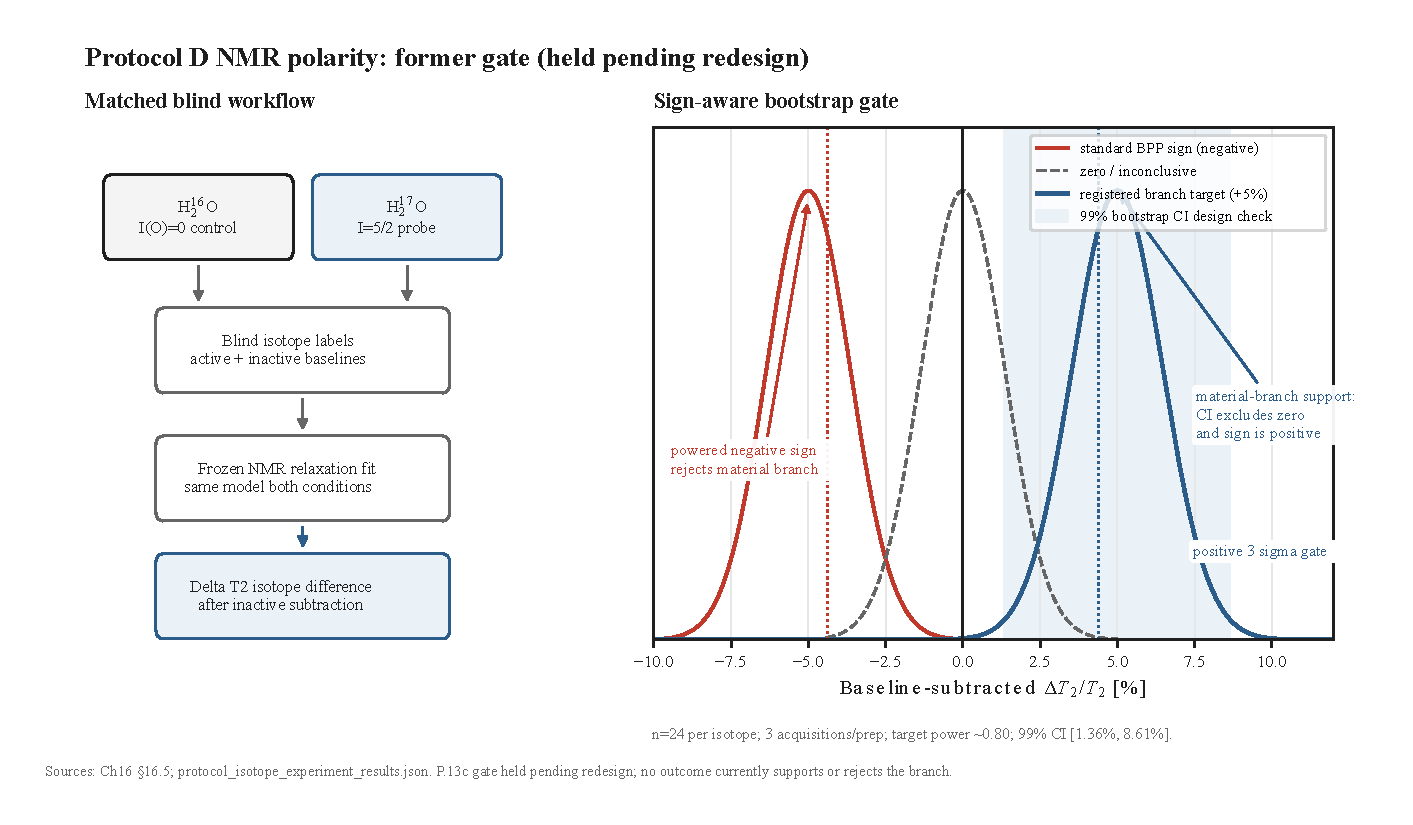
\includegraphics[keepaspectratio,alt={Protocol D compares active-state T\_2 in matched H\_2\{\}\^{}\{17\}\hspace{0pt}O and H\_2\{\}\^{}\{16\}\hspace{0pt}O preparations; the registered sign-positive material-proxy branch assigns positive \textbackslash Delta T\_2, while standard BPP relaxation predicts the opposite sign; the P.13c gate is held pending redesign, so no outcome currently supports or rejects the branch, and neither sign is a GCT, phason or Level-II verdict.}]{content/Figures/Volume_3/Figure V3.16.1.pdf}}
\caption{Protocol D compares active-state \(T_2\) in matched
H\(_2{}^{17}\)\hspace{0pt}O and H\(_2{}^{16}\)\hspace{0pt}O
preparations; the registered sign-positive material-proxy branch assigns
positive \(\Delta T_2\), while standard BPP relaxation predicts the
opposite sign; the P.13c gate is held pending redesign, so no outcome
currently supports or rejects the branch, and neither sign is a GCT,
phason or Level-II verdict.}
\end{figure}

\begin{itemize}
\tightlist
\item
  \textbf{Primary statistic (single definition):}
  water-\(^1\)\hspace{0pt}H \(T_2\) (the pulse sequence to be fixed in
  the redesigned preregistration), and the 99\% bootstrap CI (\(10^4\)
  resamples) of the isotope × activity interaction
  \(\Delta T_2 \equiv [T_2^{\rm active}-T_2^{\rm inactive}](\mathrm{H}_2{}^{17}\mathrm{O}) - [T_2^{\rm active}-T_2^{\rm inactive}](\mathrm{H}_2{}^{16}\mathrm{O})\),
  fit with the same frozen relaxation model for both isotope conditions.
  The expected main effect of \(^{17}\)\hspace{0pt}O on
  water-\(^1\)\hspace{0pt}H \(T_2\) is negative (scalar relaxation), and
  it is not the tested quantity.
\item
  \textbf{Decision rule (sign-aware; held pending redesign, see above):}
  (a) 99\% bootstrap CI of \(\Delta T_2\) excludes zero, AND (b)
  \(|\Delta T_2| > 3\cdot\sigma_{\rm measurement}\), AND (c)
  \(\mathrm{sign}(\Delta T_2)=+1\) (the activity-induced \(T_2\) change
  is larger in \({}^{17}\)\hspace{0pt}O than in
  \({}^{16}\)\hspace{0pt}O, matching the registered Tier 3 material sign
  hypothesis). The registered sign-positive branch is supported only if
  the pilot variance gate satisfies the verifier-returned \(\geq80\%\)
  power ceiling for the 5\% target and (a)+(b)+(c) hold jointly. A
  sign-positive significant result below the 5\% powered target, or a
  failed pilot-variance gate, is a positive-sensitivity/effect-size
  revision rather than support or rejection. After the redesign, the
  registered branch is rejected if the powered gate is met and (a)+(b)
  hold but (c) fails, that is, on a powered, significant negative
  \(\Delta T_2\); until then no outcome supports or rejects the branch.
  CI overlap is inconclusive. Neither sign confirms or falsifies GCT,
  identifies phason coupling, or assigns Level II.
\item
  \textbf{Sample size:} minimum \(n=24\) independent biological
  preparations per isotope condition, with three repeated NMR
  acquisitions per preparation. Pilot variance is locked before the
  decisive primary run; sample size is powered for \(\alpha=0.01\),
  \(\beta=0.20\) on that primary decision only. If pilot variance gives
  \(<80\%\) power to detect a \(5\%\) active-state polarity reversal at
  two-sided \(\alpha=0.01\), the run is sensitivity-limited rather than
  decisive. A same-size replication cohort is
  confirmatory/reproducibility context unless separately repowered; it
  is not part of the formal n=24 decision rule.
\item
  \textbf{Predicted \(\Delta T_2\) magnitude:} the design-sketch
  verifier \texttt{verify\_p13c\_nmr\_polarity.py} binds the current
  engine power calculation to a point-target design for a \(5\%\)
  active-state polarity reversal, represented as
  \(|\Delta T_2/T_2|\in[5\%,5\%]\) until a first-principles O.21/O.33
  hydration-and-radical-pair calculation supplies an independent upper
  edge. The verifier uses \(n=24\) preparations per isotope condition, a
  99\% bootstrap CI, a systematic floor of \(2\times10^{-7}\) of \(T_2\)
  (the former 0.2 ppm restated as a fraction of \(T_2\)), and the
  \(\alpha=0.01,\ \beta=0.20\) replication simulation; the design power
  statistic is \(\approx0.80\) against the 5\% target and the row
  remains OPEN-CONDITIONAL and held pending redesign; blinded lab data
  bear on it only after the redesign. The 5\% power target is a Tier 3
  calibration anchor pending O.21 (β-tubulin Trp residue identification)
  + O.33 (KIE direct calibration). After the redesign, the decisive gate
  for the registered material branch is a positive isotope × activity
  interaction in water-\(^1\)\hspace{0pt}H \(\Delta T_2\) (a larger
  activity-induced \(T_2\) change in \(^{17}\)\hspace{0pt}O than in
  \(^{16}\)\hspace{0pt}O, not a raw-\(T_2\) enhancement) satisfying the
  primary decision rule at the powered 5\% target; a sign-positive
  sub-5\% result is a sensitivity/effect-size revision, while the
  opposite sign satisfying the same powered rule rejects the registered
  branch. Until then no outcome supports or rejects the branch. Neither
  outcome is a confirmation or falsification of GCT.
\item
  \textbf{Dominant systematic:} the activity dependence of the
  \(^{17}\)\hspace{0pt}O--\(^1\)\hspace{0pt}H scalar-relaxation
  contribution (via proton exchange) must be bounded as a fraction of
  \(T_2\) under the frozen relaxation model; the earlier
  ``\(\sigma < 0.2\) ppm'' bound mixed a frequency unit with a time and
  is withdrawn, and the verifier states the floor as \(2\times10^{-7}\)
  of \(T_2\).
\item
  \textbf{Preregistration:} preregistration package, code,
  synthetic-data budget, and locked exclusion list are frozen before
  unblinding; the public archive URL is added when assigned.
\item
  \textbf{Execution timeframe:} after the redesign, a first run would be
  planned for a 12-18 month window after the design is frozen and
  isotope-enrichment logistics are validated.
\item
  \textbf{Blinding path:} isotope labels are blinded during acquisition,
  preprocessing, and \(T_2\) fitting. Unblinding occurs only after the
  fit model, exclusion list, and state labels are frozen.
\item
  \textbf{False-positive budget:} after the redesign, one primary NMR
  polarity test powered at two-sided \(\alpha=0.01\) would be the
  decisive gate. The replication cohort estimates reproducibility and
  effect-size stability; it is not itself decisive under the n=24 power
  calculation unless a separate repowered decision rule is
  preregistered. Secondary covariates are balance checks, not discovery
  endpoints.
\item
  \textbf{Systematic-error budget (S1-S8):} S1
  \(^{17}\)\hspace{0pt}O-enrichment verification by gas-mass-spec or
  isotope-resolved NMR integration before and after acquisition;
  acceptance band \(\geq95\) atom-\% with \(\leq1\) atom-\% drift. S2
  temperature and state-control drift; maximum \(\Delta T \leq0.2\) K
  during each measurement block. S3 \(B_0/B_1\) homogeneity; shim
  linewidth and pulse calibration locked before unblinding, with
  flip-angle error \(\leq2\%\). S4 relaxation-model misfit; mono- and
  bi-exponential fits are both reported, decisive sign must survive both
  models, residual lag-1 autocorrelation must satisfy
  \(|\rho_1|\leq0.20\), and \(\Delta\mathrm{AIC}\leq2\) between accepted
  fits is treated as model-averaging rather than post-hoc selection. S5
  inactive-baseline subtraction; anesthetized/inactive baselines are
  acquired in the same isotope batch and subtracted by the frozen
  estimator. S6 active-state synchronization; neural-activity onset and
  NMR acquisition timing are locked before isotope labels are revealed,
  with onset jitter \(\leq10\%\) of the analysis window and \(\leq2\) s
  absolute drift per block. S7 tissue viability; oxygenation remains
  within \(\pm5\%\) of baseline, membrane-integrity exclusion markers
  stay below the preregistered assay threshold, and electrophysiological
  responsiveness remains \(\geq80\%\) of pre-block baseline throughout
  the measurement window. S8 batch/rearing/age effects; isotope
  conditions are randomized across culture batch, rearing condition, and
  age bin, batch is a mixed-effects term rather than an exclusion after
  unblinding, no single batch may contribute more than 35\% of the
  decisive statistic weight, and a batch-level variance component above
  25\% of total variance makes the run sensitivity-limited. Across
  S1-S8, the pilot total per-preparation fractional SD must remain at or
  below the verifier-bound 5.07\% ceiling for the 5\% target; otherwise
  the run is reported as sensitivity-limited rather than decisive.
\end{itemize}

\subsection{16.6 Drosophila LORR Interpretation Matrix {[}Tier 4
operational/no-gate{]}}\label{drosophila-lorr-interpretation-matrix-tier-4-operationalno-gate}

We summarize the interpretation tree for Protocol D. Under the
registered systematic budget, the experiment does \textbf{not}
discriminate GCT from an ordinary material null; it measures an
isotope/anesthetic effect-size band and the systematics budget needed
for a later material-model decision.

The matrix is calibrated against the §16.3.2 branch discipline: central
O.21-pending branch \(\Delta C_{50}/C_{50}=0\) for \(n_{rp}=0\);
conditional sensitivity branch
\(\Delta C_{50}/C_{50} \in [-0.22\%, -0.11\%]\) for \(n_{rp}=1\);
disfavored \(n_{rp}=2\) branch extending to signed
\([-0.44\%, -0.22\%]\) (the \(0.66\%\) \(n_{contact}=12\) stress-test
maximum of §16.3.2 is not used downstream). An outcome \(\geq 1\%\) in
magnitude would require a non-operative hydration/radical-pair branch
beyond the O.21/O.33 conservative closure and would trigger a geometry
re-evaluation rather than direct confirmation.

\gctneedbreak{10\baselineskip}

{\def\LTcaptype{none} % do not increment counter
\begin{longtable}[]{@{}
  >{\raggedright\arraybackslash}p{(\linewidth - 4\tabcolsep) * \real{0.3333}}
  >{\raggedright\arraybackslash}p{(\linewidth - 4\tabcolsep) * \real{0.3333}}
  >{\raggedright\arraybackslash}p{(\linewidth - 4\tabcolsep) * \real{0.3333}}@{}}
\toprule\noalign{}
\begin{minipage}[b]{\linewidth}\raggedright
Outcome
\end{minipage} & \begin{minipage}[b]{\linewidth}\raggedright
Registered material-scenario interpretation (central \(0\) pending O.21;
conditional \(n_{rp}=1\) sensitivity range \([-0.22\%, -0.11\%]\))
\end{minipage} & \begin{minipage}[b]{\linewidth}\raggedright
Ordinary-null interpretation
\end{minipage} \\
\midrule\noalign{}
\endhead
\bottomrule\noalign{}
\endlastfoot
\textbf{\(C_{50}\) Shift \(\geq 0.44\%\)} & Above the conservative
O.21/O.33 range; re-evaluate \(f_{bound}\), \(n_{rp}\), and systematics
before interpreting & Also plausible under systematic excursions unless
the C1 closure condition is met \\
\textbf{\(C_{50}\) Shift \(0.22\% < \Delta < 0.44\%\)} & Above the
operative band but within the disfavored \(n_{rp}=2\) / upper-hydration
branch & Overlaps biochemical/KIE plus systematic uncertainty \\
\textbf{\(C_{50}\) Shift \(0.11\% < \Delta \leq 0.22\%\)} & Consistent
with the O.21/O.33 partial-closure range; refine \(f_{bound}\)
measurement against the KIE upper bound & Marginal; overlaps the KIE
upper bound and the systematics floor \\
\textbf{\(C_{50}\) Shift \(< 0.11\%\)} & Below the declared sensitivity
edge, but not a material-model decision unless C1 supplies a valid gate
& Consistent with null/KIE expectations \\
\textbf{Isotope × activity \(\Delta T_2 > 0\)} (water
\(^1\)\hspace{0pt}H) & Registered material sign branch supported only
after the §16.5 gate redesign & Activity-dependent proton exchange or
other ordinary channels \\
\textbf{Isotope × activity \(\Delta T_2 < 0\)} (water
\(^1\)\hspace{0pt}H) & Registered material sign branch rejected only
after the §16.5 gate redesign & Consistent with ordinary scalar/BPP
relaxation channels \\
\end{longtable}
}

\emph{The outcome structure tracks the signed \([-0.22\%, -0.11\%]\)
sensitivity branch conditional on O.21 closure (\(n_{rp}=1\)), while the
operative central branch remains \(0\) for \(n_{rp}=0\). It does not
propagate the upper edge of the \(n_{rp}=2\) prediction band
(disfavoured by 6DPU cryo-EM screening per Open Problem O.21). These
rows are effect-size interpretations only under the registered
systematic budget. A valid falsification decision requires the C1
systematic-tightening condition or a declared aggregate-evidence rule
with bounded false positives.}

\subsection{16.7 Conclusion of the Substrate
Audit}\label{conclusion-of-the-substrate-audit}

DMC candidate controls are empirically measurable, but they are not an
empirically decisive material or Level-II gate. App PUP's mathematical
bridge remains conditional and reaches at most an algebraic unity
candidate (Proposition PUP.1(ii) is withdrawn); its phenomenal
interpretation is separately open. A null or positive isotope shift
constrains the proposed spin/coherence mechanism only; the Protocol D
LORR assay remains Tier 4 operational/no-gate and supplies no substrate
verdict. Neither outcome is a verdict on GCT as a whole: the measurement
tests an ordinary material proxy, and no phason, Selection-Operator or
Level-II inference follows from it (V1 Ch17 §17.1.3). A preregistered
result rejects the registered biophysical branch only under that
branch's own decision rule: the Protocol D NMR polarity gate (P.13c) is
held pending redesign (§16.5): as written it rejected by construction,
since \(^{17}\)\hspace{0pt}O shortens water-\(^1\)\hspace{0pt}H \(T_2\)
by scalar relaxation; the former sign-aware rule, which rejects the
registered sign-positive branch on a powered, significant negative
isotope × activity interaction in water-\(^1\)\hspace{0pt}H
\(\Delta T_2\), applies only after the redesign, and until then no
outcome supports or rejects the branch; the LORR assay has no rejection
rule until C1 is met.

\gctneedspace{5\baselineskip}

\textbf{END OF CHAPTER 16}

\chapter{Chapter 17: Protocol E --- Mismatch Energy
Spectrum}\label{chapter-17-protocol-e-mismatch-energy-spectrum}

While the lepton mass hierarchy is modelled by the vibrational harmonics
of node-centered vertex defects (Protocol B), the hadron sector requires
the analysis of interstitial geometry. In the Standard Model, the
``current'' masses of light quarks (\(u, d, s\)) are Lagrangian
(\(\overline{\rm MS}\)) parameters; the non-perturbative gluon
condensate and chiral symmetry breaking generate the much larger
\emph{constituent} and hadron masses, not the current masses. Geometric
Consciousness Theory (GCT) proposes {[}Tier 3{]} to identify the
condensate with the phason strain field generated by
\textbf{Interstitial Defects}, and separately proposes a geometric
origin for the current masses themselves. To isolate the underlying
geometric contribution, we employ \textbf{Protocol E}: a geometric
scaling analysis of the surface tension generated by forbidden face
adjacencies in the icosahedral vacuum.

\begin{center}\rule{0.5\linewidth}{0.5pt}\end{center}

\subsection{17.1 Objective}\label{objective}

\subsubsection{17.1.1 Light Quark Mass Derivation (Interstitial
Defects)}\label{light-quark-mass-derivation-interstitial-defects}

The objective of Protocol E is to derive the rest masses of the quark
sector from the material properties of the vacuum interstices. As a Tier
3 candidate assignment (V3 Ch03 §3.4), GCT identifies quarks as
\textbf{Matching Rule Violations}---localized errors in the icosahedral
tiling logic where two unit rhombohedra are forced together in a
forbidden orientation.

Unlike leptons, which possess \textbf{Codimension 3} (localizing as
points in 3D), quarks are modelled as \textbf{Codimension 1} objects (2D
interfaces in 3D) {[}Tier 3{]}; a wall of this kind would cost energy
proportional to its area, and how it stays localised inside a hadron is
not derived here. In the model, their mass is determined by the
\textbf{Lattice Surface Tension} (\(\sigma\)) required to maintain the
phason jump discontinuity across the rhombohedral face.

\subsubsection{17.1.2 Phason-Gluon Duality {[}Tier
3{]}}\label{phason-gluon-duality-tier-3}

GCT proposes a \textbf{Phason-Gluon Correspondence} {[}Tier 3{]}: the
``Gluon Condensate'' of standard QCD is the effective field-theoretic
description of the \textbf{Phason Strain Field} (\(w_{ij}\)) in the
internal dimensions of the supersolid vacuum. Two targets must be kept
apart. Protocol E aims at the current (\(\overline{\rm MS}\)) masses,
the Lagrangian inputs; condensate dressing, if the correspondence holds,
would bear on constituent and hadron masses instead. If the
correspondence holds, the ``Hadron Mass Gap'' becomes a material
property of the icosahedral glass, recasting the hadron audit from a
phenomenological fit as a candidate geometric derivation {[}Tier 3{]}.

\subsubsection{17.1.3 The Unit Burgers Vector
Constraint}\label{the-unit-burgers-vector-constraint}

To prevent the arbitrary selection of energy levels, Protocol E is
subject to the \textbf{Crystallographic Priority Constraint}. The
simulation only considers \textbf{Unit Burgers Vectors}---mismatch
vectors \(\Delta \mathbf{b}_\perp\) where the 6D integer displacement
\(\Delta \mathbf{r}_6\) has a norm of \(1\) (axial) or \(\sqrt{2}\)
(face-diagonal). This restricts the ``Menu'' of possible quark states to
a small, discrete set of high-symmetry configurations of the primitive
\(\mathbb{Z}^6\) lattice (the norm-1 vectors are not in the \(D_6\) root
lattice, whose minimal norm is \(\sqrt{2}\)).

\begin{center}\rule{0.5\linewidth}{0.5pt}\end{center}

\subsection{17.2 The Geometric Analysis}\label{the-geometric-analysis}

\subsubsection{17.2.1 Projection Vector Strain
Analysis}\label{projection-vector-strain-analysis}

The simulation utilizes a \textbf{Continuum Elasticity Model} for the
phason field \(\mathbf{u}_\perp\) in the vicinity of a 2D interface
\(\Sigma\). We evaluate the mismatch energy associated with the jump
condition:

\textbf{The mismatch energy is proportional to the square of the
\emph{Projection Vector} \(\Delta \mathbf{b}_\perp\).} At the interface,
we impose the Dirichlet jump condition:
\[\mathbf{u}_\perp(\mathbf{x}^+) - \mathbf{u}_\perp(\mathbf{x}^-) = \Delta \mathbf{b}_\perp\]
The mass of the quark is the volume integral of the resulting energy
density. Because the phason strain is mathematically concentrated on the
2D interface, the integral effectively collapses into a surface
integral: \[M_q = \int_\Sigma \sigma \, dA\]

\subsubsection{17.2.2 The Area Law: Inter-Generational Scaling {[}Tier 2
mechanism + Tier 3 quark-sector
application{]}}\label{the-area-law-inter-generational-scaling-tier-2-mechanism-tier-3-quark-sector-application}

Protocol E registers the inter-generational scaling hypothesis for the
quark sector. Because energy is modeled as the integral of a singular
density over a surface, the rest mass is proportional to the
\textbf{Projected Facet Area}. Under the action of the Inflation
Operator \(\mathcal{T}\), areas in the physical projection scale as
\(\phi^2\) (conditional on the Tier 3 assumption that \(\phi\) is the
generational step; the self-similarity of \(P\) is \(\phi^3\), App QCT
§QCT.3). This supplies the registered scaling ansatz for
inter-generational mass gaps (e.g., \(d \to s \to b\)) as integer powers
of the area inflation: \[M_{n} \sim M_0 \cdot (\phi^2)^n\] This is a
scaling heuristic only. The adopted quark formulas of V3 Ch10 §10.4
(\(m_s = m_u\phi^8(1-12\alpha)\), \(m_b = m_c\,\phi^2\cdot 5/4\),
\(m_d = m_u\phi^{\phi}\)) are not pure integer powers of \(\phi^2\), and
V3 Ch10 is canonical where the two differ.

\subsubsection{\texorpdfstring{17.2.3 Intra-Generational Splitting (the
\(u/d\)
ratio)}{17.2.3 Intra-Generational Splitting (the u/d ratio)}}\label{intra-generational-splitting-the-ud-ratio}

\textbf{Declared open programme {[}Tier 3{]}} (a) The earlier text
derived
\(m_d/m_u = (\text{Area}_P/\text{Area}_O)\cdot\sqrt{2} = \phi\sqrt{2} \approx 2.288\)
from the face areas of the prolate and oblate Ammann-Kramer-Neri (AKN)
rhombohedra. (b) That derivation is withdrawn: all faces of both
rhombohedra are congruent golden rhombi, so the face-area ratio is 1;
\(\phi\) is their \emph{volume} ratio, and the \(\sqrt{2}\) ``projection
bias'' was not derived. (c) A closing derivation would need a
defect-energy functional on the AKN tiling that singles out a u/d shape
factor. (d) Nothing downstream uses \(\phi\sqrt{2}\). The adopted
down-quark row is the V3 Ch10 §10.4 route \(m_d = m_u\phi^{\phi}\)
(\(m_d/m_u = 2.178\); Tier 2 FK-determinant mechanism + Tier 3
identification, conditional on O.5), against PDG 2024 central values
\(m_u = 2.16\), \(m_d = 4.70\) MeV (\(\overline{\rm MS}\), 2 GeV),
i.e.~\(m_d/m_u \approx 2.18\) (Tier 4 as evidence: not distinguishable
from numerology for strong effects; App PSC §PSC.9.6).

\subsubsection{17.2.4 The Spectrum Ceiling}\label{the-spectrum-ceiling}

The quark spectrum is hypothesized to terminate when the area-mismatch
energy reaches the Tier 3 \textbf{Top Quark Fracture Limit} posited in
Chapter 10. Beyond the \(b\)-quark harmonic, the strain exceeds the
vacuum's yield strength, causing the defect to transition from an
interstitial mismatch to a structural failure of the unit cell
(\(m_t = v_{\rm GCT}/\sqrt{2}\), V3 Ch10 §10.2.2).

\begin{center}\rule{0.5\linewidth}{0.5pt}\end{center}

\subsection{17.3 Falsification}\label{falsification}

\subsubsection{17.3.1 Alignment with Lattice
QCD}\label{alignment-with-lattice-qcd}

The ``Bare Masses'' calculated in Protocol E are specifically designed
to match the \textbf{Lagrangian (current, \(\overline{\rm MS}\)) mass
inputs} used by state-of-the-art Lattice QCD simulations. GCT proposes a
candidate mechanical origin {[}Tier 3{]} for the values that standard
QCD otherwise takes as empirical inputs.

\subsubsection{17.3.2 Statistical Falsification
Threshold}\label{statistical-falsification-threshold}

Protocol E establishes a quantitative gate for the GCT Operating System:

\begin{enumerate}
\def\labelenumi{\arabic{enumi}.}
\tightlist
\item
  \textbf{Scaling Violation:} If the simulated spectrum of mismatch
  energies---constrained strictly by the \(\mathbb{Z}^6\)
  unit-Burgers-vector menu and \(\phi\) area-inflation---fails to
  reproduce the inter-generational ratios (\(m_s/m_d\), \(m_b/m_s\)) to
  within \(10\%\), the \textbf{Interstitial Defect model is falsified}.
  This gate has little power while the integer \(n\) is free: a random
  ratio lands within \(\pm10\%\) of some rung of a \(\phi^2\) ladder
  about 21\% of the time. The exponents \(n\) must be fixed before the
  comparison.
\item
  \textbf{P-Value Requirement:} The alignment between the discrete
  ``Crystallographic Menu'' of energy levels and the Standard Model
  inventory must be statistically significant at the
  \textbf{\(P < 0.01\)} level. The null distribution and the test
  statistic are not yet specified for this protocol, so this requirement
  is a target, not a registered test. The adopted quark formulas
  (\(m_u\), \(m_d\), \(m_s\), \(m_c\), \(m_b\)) were, however, among the
  21 rows of the preregistered constant control test, and as evidence
  that φ or icosahedral structure is special their matches are
  \textbf{Tier 4}: the test (v3, NEGATIVE-FRAGILE; App PSC §PSC.9.6)
  found φ's pattern of matches on 21 constants not distinguishable from
  that of random constants (58 of 300 random bases did at least as
  well). The test ``excludes, at power ≥ 0.8, an effect in which φ hits
  at least 6 of the 8 informative rows through a real effect; weaker
  effects are not excluded.'' The numbers are kept as descriptive
  arithmetic.
\end{enumerate}

\subsubsection{17.3.3 Implementation}\label{implementation}

The precise geometric evaluation of the absolute quark mass spectrum
relies on integrating the phason strain energy of quantized face-rule
violations across the AKN tiling. The full dynamical extraction of these
interstitial eigenvalues from the \(6N \times 6N\) Hessian is formally
logged as \textbf{Tier 3 Computational Debt} deferred to the
non-perturbative QLQCD lattice integration (Open Problem O.5; App QLA).

\gctneedspace{5\baselineskip}

\textbf{END OF CHAPTER 17}

\chapter{Chapter 18: Protocol F --- Proton Mass / String
Tension}\label{chapter-18-protocol-f-proton-mass-string-tension}

The proton-mass route represents a high-value geometric mechanism in a
sector traditionally requiring massive stochastic simulations of Lattice
QCD to approximate the binding energy of confined quarks and gluons.
Geometric Consciousness Theory (GCT) identifies the proton mass not as a
statistical average of stochastic fluctuations, but as a candidate
\textbf{Resonant Eigenvalue} of the vacuum substrate. \textbf{Protocol
F} defines the phason-stiffness/string-tension mechanism and the
subsequent calculation of the proton mass from the geometry of the
baryonic triad, with the current disposition of the mass formula
\textbf{Tier 2 mechanism + Tier 3 sheet/exponent handle pending
AKN-action closure} (the \(3\times5\) counting is Tier 2; in the weak
Berry-phase step the \(2I\) parity is Tier 1 while the selection of
\(n=1\) and of the connection is Tier 3, §18.2.3.A); the string-tension
bridge of §18.2.1 rests on the Tier 3 flux-tube identification (V3 Ch03
§3.5.2).

\begin{center}\rule{0.5\linewidth}{0.5pt}\end{center}

\subsection{18.1 Objective}\label{objective-1}

\subsubsection{18.1.1 Mechanism-Level Calculation of Proton
Mass}\label{mechanism-level-calculation-of-proton-mass}

The primary objective of Protocol F is to provide a deterministic
mechanism-level calculation (Tier 2 mechanism + Tier 3 sheet/exponent
handle pending AKN-action closure) of the proton mass
(\(m_p \approx 938.272\) MeV {[}Tier 3 --- CODATA anchor{]}) without the
need for Monte Carlo sampling. GCT treats the proton as a
\textbf{Mixed-Manifold Soliton}---a coherent structure whose total
mass-energy is the non-perturbative sum of the strong-force winding and
the electroweak metric pressure.

\subsubsection{18.1.2 Deriving Gluon String Tension from Phason
Stiffness {[}Tier 3 flux-tube
bridge{]}}\label{deriving-gluon-string-tension-from-phason-stiffness-tier-3-flux-tube-bridge}

We aim to connect the fundamental parameter of confinement---the
\textbf{Gluon String Tension (\(\sigma\))}---to the material properties
of the vacuum through a Tier 3 calibrated bridge (it is not yet a
derivation; see §18.2.1). By identifying the string as a tube of phason
strain within the supersolid glass (a Tier 3 flux-tube proposal, V3 Ch03
§3.5.2), we bridge the gap between the microscopic phason stiffness
(\(K_\perp\)) and the macroscopic energy of the hadron.

\subsubsection{18.1.3 Toward Closing the Hadron Mass
Gap}\label{toward-closing-the-hadron-mass-gap}

Protocol F serves to audit the baryonic entry in the matter-spectrum
inventory. The proton mass formula
\(m_p = m_e \cdot \phi^{15 + \phi^{-1}}\) gives \(1836.437\,m_e\)
against the CODATA \(1836.153\), a \(+155\) ppm residual inside the
registered 500 ppm postdiction band (a postdiction, not a live
lattice-QCD falsifier), and it remains \textbf{Tier 2 mechanism + Tier 3
sheet/exponent handle pending AKN-action closure} rather than a closure
of the entire matter spectrum.

\begin{center}\rule{0.5\linewidth}{0.5pt}\end{center}

\subsection{18.2 Theoretical Framework}\label{theoretical-framework}

\subsubsection{18.2.1 String Tension and the Jacobian of Screening
{[}Tier 3 flux-tube identification + Tier 3 screening
normalization{]}}\label{string-tension-and-the-jacobian-of-screening-tier-3-flux-tube-identification-tier-3-screening-normalization}

The most significant challenge in deriving \(\sigma\) is the dimensional
gap between the phason stiffness
(\(K_\perp = \phi^{-18}K_\parallel \approx 1.7\times10^{-4}\,E_P/\ell_P^3\)
under P3b; the earlier \(10^{15}\) GeV figure is withdrawn) and the
observed string tension (\(\sigma \approx 1\) GeV/fm). GCT proposes to
bridge this via the \textbf{Jacobian of the Projection Interface}
{[}Tier 3{]}.

The phason stiffness \(K_\perp\) is defined per Planck unit cell in 6D.
However, the phason flux tube (the gluon string) samples the collective
strain over the healing volume of the polaron
(\(\xi = a_0/\alpha \approx 7.25\) nm {[}Tier 1 arithmetic; its
identification as the vacuum/polaron healing length is Tier 3{]}, V3
§13.1.2; it is an atomic-scale length with no QCD content). The
interaction is suppressed by the \textbf{Local Coordination Volume}
ratio \((\ell_P/\xi)^3 \approx 10^{-80}\) {[}Tier 1 arithmetic ratio of
the two scales; Tier 3 wavefunction-overlap/volume-normalization
identification, since it rests on the Tier 3 healing-length
identification (App FSM P.36); Tier 3 as the \(\sigma\) screening
factor{]} (with \(\ell_P = 1.616\times 10^{-35}\) m and \(\xi = 7.25\)
nm the exact ratio is \(\approx 1.11\times 10^{-80}\); see Parameter
Ledger §2). This factor acts as the proposed volume-normalization
required to transform a \textbf{unit-cell stress} into a
\textbf{macroscopic tension}.
\[\sigma = K_\perp \times A_{tube} \times \left( \frac{\ell_P}{\xi} \right)^3 \times \mathcal{G}\]
The tube cross-section \(A_{tube}\) and the geometric factor
\(\mathcal{G}\) are not defined independently of the target, so the
resulting \(\sigma\) is a \textbf{calibration}, not a derivation. This
is a Tier 3 calibrated bridge (the flux-tube identification is a Tier 3
proposal, V3 Ch03 §3.5.2), with Tier 3 screening normalization, offered
as a candidate reading of the \(\sim\)\hspace{0pt}1 GeV/fm scale as the
screened phason energy of the vacuum.

\subsubsection{18.2.2 The Baryonic Triad
Geometry}\label{the-baryonic-triad-geometry}

A proton is modeled as a \textbf{Baryonic Triad}: three interstitial
quarks forming a topological cycle within the projected dodecahedral
shell. This triad is centered on a \textbf{5-fold vertex star}, the
configuration adopted to satisfy the \(3 \times 5 = 15\) harmonic logic.
The confinement radius \(r_{tube} \approx 0.5\) fm {[}Tier 3 ---
candidate geometric scale of the baryonic triad{]} is determined by the
\textbf{Vacuum Yield Strength (\(\sigma_c\))} of Volume 2 (V2 Ch13
§13.1.1, a Tier 3 physical ansatz); the flux tube (a Tier 3 proposal, V3
Ch03 §3.5.2) is the region where phason strain exceeds the fracture
limit of the topological glass.

\subsubsection{18.2.3 Topological Additivity in the
Exponent}\label{topological-additivity-in-the-exponent}

In the GCT Operating System, the exponent of the inflation factor
\(\phi\) represents the \textbf{Total Phase Accumulation (Berry Phase)}
of the defect. The proton mass formula
\(m_p = m_e \cdot \phi^{15 + \phi^{-1}}\) is read as the Strong and Weak
components being \textbf{topologically additive} in the baryon core
{[}Tier 2 mechanism + Tier 3 sheet/exponent handle; the `Strong' reading
of the factor 3 inherits the Tier 3 quark/colour identification, V3
Ch03{]}:

\begin{itemize}
\tightlist
\item
  \textbf{15 (\(3 \times 5\)):} The phase winding of 3 quarks in a
  5-fold lattice star (The Strong Component).
\item
  \textbf{\(\phi^{-1}\) (\(0.618...\)):} The \textbf{Weak Berry Phase}
  correction {[}Tier 1 \(2I\) holonomy parity + Tier 3 selection of
  \(n=1\) and of the connection (central-holonomy ansatz, §18.2.3.A) +
  Tier 3 sheet/exponent handle{]} from the \(SU(2)\) Weak holonomy.
  Under the selected axial connection (the Tier 3 central-holonomy
  ansatz of §18.2.3.A), the path-ordered integral around the \(2\pi\)
  baryonic loop (the 5-fold axis) yields \(U_{weak} = -I_2\),
  corresponding to a Berry phase of \(\pi\) and half-winding
  (\(N_{weak}=1/2\)). Applying the icosahedral projection ratio
  \(R = 2\phi^{-1}\) yields the correction
  \((1/2) \cdot (2\phi^{-1}) = \phi^{-1}\), while the coherent two-sheet
  contribution remains the Tier 3 handle pending AKN-action closure.
\end{itemize}

\gctneedspace{5\baselineskip}

\textbf{§18.2.3.A Axial SU(2) Holonomy Parity and the Physical
Minimality Premise}

For the integer-weight axial family \(A_\theta=(n/2)\sigma_z\), the
\(2I\) fiber geometry fixes the exact holonomy parity but does not
select a unique odd weight. The baryonic branch chooses
\(A_\theta=\frac{1}{2}\sigma_z\) only after imposing the explicit
least-positive/nontrivial-winding physical minimality premise below.

\gctneedspace{5\baselineskip}

\textbf{Step 1 --- Stabilizer of the 5-fold Axis.} Let
\(\hat{a}_5 = (0,0,1)\) be the directed 5-fold rotation axis of the
dodecahedron. Under the adjoint \(SO(3)\) action of the icosahedral
group \(I\), the stabilizer is
\[\mathrm{Stab}_{I}(\hat{a}_5) = \mathbb{Z}_5 \subset I ,\] the cyclic
subgroup of order 5 generated by a \(72°\) rotation about \(\hat{a}_5\).
Its SU(2) pre-image in the double cover \(2I\) is the cyclic group of
order 10:
\[\mathrm{Stab}_{2I}(\hat{a}_5) = \mathbb{Z}_{10} \subset 2I ,\]
generated by \(U_{\mathrm{gen}} = \exp\!\left(i\pi\sigma_z/5\right)\).

\gctneedspace{5\baselineskip}

\textbf{Step 2 --- Exact Holonomy Parity {[}Tier 1{]}.} Consider a
principal \(2I\)-bundle over the 5-fold latitude circle (the baryonic
\(2\pi\) loop). For a diagonal axial connection
\(A_\theta = \frac{n}{2}\sigma_z\), \(n\in\mathbb Z\), the holonomy is
\[\mathcal{P}\exp\!\left(i \int_0^{2\pi} A_\theta\, d\theta\right) = \exp(i n\pi \sigma_z) .\]
Exactly,
\[\exp(in\pi\sigma_z)=\cos(n\pi)I_2+i\sin(n\pi)\sigma_z=(-1)^nI_2.\]
Even \(n\) gives \(I_2\) and odd \(n\) gives
\(-I_2=U_{\mathrm{gen}}^5\), the unique central element of order two.
The \(2I\) condition therefore distinguishes parity only; every odd
integer produces the same nontrivial central holonomy. Note also that
\(-I_2\) is not a generator of \(\mathbb{Z}_{10}\) (it has order 2), so
the holonomy does not single out the full axial stabilizer either.

\gctneedspace{5\baselineskip}

\textbf{Step 3 --- Adopted Physical Minimality Premise {[}Tier 3
central-holonomy ansatz{]}.} The baryonic branch requires nontrivial
winding and adopts the least positive integer weight satisfying it.
Nontrivial holonomy excludes even \(n\); least-positive minimality
selects \(n=1\), giving \[\boxed{A_\theta = \tfrac{1}{2}\sigma_z} ,\]
and holonomy \(-I_2\). This selection is an explicit physical premise
rather than an algebraic uniqueness theorem:
\(A_\theta=\tfrac{1}{2}\sigma_z\) is retained as the simplest
central-holonomy witness, not as a unique connection. The \(2I\) parity
identity is Tier 1; the selection of \(n=1\) and of the physical bundle,
loop and connection is Tier 3 (central-holonomy ansatz) pending
AKN-action closure; the \(3\times5\) counting of the strong component
stays Tier 2; deployment of the resulting \(\phi^{-1}\) term in the
absolute proton-mass exponent remains the Tier 3 sheet/exponent handle
recorded in App TAT and the Parameter Ledger.

\emph{The formal parity theorem (Tier 1) and the physical minimality
premise (a Tier 3 premise) are collected as \textbf{Appendix USS §USS.8}
(Theorem USS.8). The numerical protocol verifies the chosen ansatz's
holonomy only; see Appendix GPE.}

\begin{center}\rule{0.5\linewidth}{0.5pt}\end{center}

\subsection{18.3 Computational Protocol}\label{computational-protocol}

\subsubsection{18.3.1 Step 1: Calculate Screened String
Tension}\label{step-1-calculate-screened-string-tension}

The algorithm computes the bare string tension using the phason
stiffness constant \(K_\perp\) modified by the Jacobian
volume-normalization.

\begin{itemize}
\tightlist
\item
  \textbf{Input:} \(K_\perp = K_\parallel \phi^{-18}\) {[}Tier 3
  physical-link input P3b pending O.15(b); the exact Coxeter algebra is
  Tier 1 and the \(H_3\)-conditional integer identification \(D=18\) is
  Tier 2{]}.
\item
  \textbf{Geometric Scaling:} The 15th harmonic is taken as the resonant
  multiplier for the 3-quark baryon {[}Tier 3 deployment of the
  \(Z_3 \times Z_5\) template{]}.
\item
  \textbf{Output:} \(\sigma \approx 0.92\) GeV/fm, a calibration through
  the undefined factors \(A_{tube}\) and \(\mathcal{G}\) {[}Tier 3
  flux-tube bridge (§18.2.1; V3 Ch03 §3.5.2) + Tier 3 numerical
  normalization{]}. The proton-mass formula of §18.3.2--§18.3.3 does not
  use this value.
\end{itemize}

\subsubsection{18.3.2 Step 2: Formula
Evaluation}\label{step-2-formula-evaluation}

The engine (see Appendix GPE) evaluates the \textbf{Baryonic Triad}
exponent (\(15 + \phi^{-1}\)) arithmetically. No eigenvalue of a defect
structure is computed: the 3D neighborhood of a 5-fold vertex star with
three interstitial face-defects is the intended domain of a future
resonance calculation, not one that has been run.

\begin{itemize}
\tightlist
\item
  \textbf{Result:} The formula evaluates to \textbf{1836.437} electron
  mass units (\(m_e\)), against the observed \(m_p/m_e = 1836.153\)
  (+155 ppm).
\end{itemize}

\subsubsection{18.3.3 Step 3: Analytic Form}\label{step-3-analytic-form}

The formula is the GCT \textbf{Analytic Resonance} formula of Chapter 10
(Tier 2 mechanism + Tier 3 sheet/exponent handle):
\[m_p = m_e \cdot \phi^{15 + \phi^{-1}}\]

\begin{itemize}
\tightlist
\item
  \textbf{Analytic (tree-level formula):}
  \(\phi^{15 + \phi^{-1}} \approx 1836.437\) (versus the CODATA observed
  \(m_p/m_e = 1836.153\); residual \(+155\) ppm, inside the 500 ppm
  postdiction band).
\item
  The numerical evaluation in Step 2 is the same closed form evaluated
  in floating point; it reproduces \(1836.437\) by construction and is
  not an independent verification.
\end{itemize}

\emph{Note: anchoring the dimensionless ratio to the CODATA
\(m_e = 0.5109989\) MeV yields the formula prediction \(m_p = 938.417\)
MeV, which sits \(155\) ppm above the CODATA observed \(m_p = 938.272\)
MeV. This is the same \(155\) ppm gap as the End-to-End Absolute
Pipeline (\(M_{Planck} \to m_e \to m_p\), see Appendix PSC §PSC.3 Hadron
Sector). The +155 ppm residual lies inside the registered 500 ppm
postdiction band under the Tier 2 mechanism + Tier 3 sheet/exponent
disposition; promotion requires the AKN-action derivation of the sheet
summation and QLQCD-1L closure (App QLA).}

\gctneedspace{5\baselineskip}

\textbf{Technical Note: Geometric Eigenvalue Protocols}

The formula uses the \textbf{Baryonic Triad Winding} (\(N_{mode} = 15\);
selecting 15 as the physical base exponent is Tier 3, App USS §USS.3),
which identifies the proton as a fundamental harmonic of the icosahedral
projection without requiring mesh-based integration.

The agreement (Error \(\approx 155\) ppm relative to CODATA) is
consistent with, but does not establish, the triad as the global energy
minimum for baryonic matter {[}Tier 3{]}. As evidence that φ or
icosahedral structure is special, this match is \textbf{Tier 4}: the
preregistered constant control test (v3, NEGATIVE-FRAGILE; App PSC
§PSC.9.6) found φ's pattern of matches on 21 constants not
distinguishable from that of random constants (58 of 300 random bases
did at least as well). The test ``excludes, at power ≥ 0.8, an effect in
which φ hits at least 6 of the 8 informative rows through a real effect;
weaker effects are not excluded.'' The number is kept as descriptive
arithmetic.

\begin{center}\rule{0.5\linewidth}{0.5pt}\end{center}

\subsection{18.4 Validation and
Falsification}\label{validation-and-falsification}

\subsubsection{18.4.1 Precision Target}\label{precision-target}

The registered test of the formula is the \textbf{500 ppm postdiction
band}; the current \(\phi^{15+\phi^{-1}}\) residual against the CODATA
observed ratio is \(+155\) ppm. This is consistent with the proton mass
as a structural mechanism of the \(6D \to 3D\) projection at the current
tree-level precision (Tier 4 as evidence: not distinguishable from
numerology for strong effects; App PSC §PSC.9.6), with a \textbf{Tier 3
sheet/exponent handle pending AKN-action closure}; the 155 ppm residual
is the open second-order/QLQCD-1L closure target.

\subsubsection{18.4.2 Falsification
Criteria}\label{falsification-criteria-1}

\begin{enumerate}
\def\labelenumi{\arabic{enumi}.}
\tightlist
\item
  \textbf{Tension Mismatch:} If the Tier 3 bridge string tension
  \(\sigma\) deviates from the experimental \(1\) GeV/fm {[}Tier 3 ---
  Lattice QCD extraction{]} scale by more than \(10\%\), the Tier 3
  P3b-conditioned flux-tube / screening-normalization bridge is rejected
  as registered. While \(A_{tube}\) and \(\mathcal{G}\) remain
  undefined, \(\sigma\) is a calibration and this criterion cannot fire;
  it becomes a test only once both are fixed independently of the
  target. This result does not by itself alter the separate baryonic
  exponent route tested in criterion 2.
\item
  \textbf{Geometric Formula Failure:} If the formula output
  \(m_e\phi^{15+\phi^{-1}}\) lies outside the registered 500 ppm
  postdiction band of the measured proton mass (the current residual is
  +155 ppm), the Baryonic Triad resonance model is incorrect as
  registered. Because \(m_p\) is measured to \(\sim 10^{-10}\), P.2 is a
  postdiction band, not a live falsifier.
\end{enumerate}

\begin{center}\rule{0.5\linewidth}{0.5pt}\end{center}

\subsection{18.5 QLQCD and the Strong CP Problem
(Open)}\label{qlqcd-and-the-strong-cp-problem-open}

Protocol F serves as the foundation for \textbf{Quasicrystalline Lattice
QCD (QLQCD)}. By replacing periodic grids with the \textbf{Aperiodic AKN
Tiling}, QLQCD is proposed to provide a natural UV cutoff and to address
fundamental QCD pathologies {[}Tier 3 proposal{]}.

\gctneedspace{5\baselineskip}

\textbf{Status of the Strong CP Problem {[}open{]}:} Standard QCD
permits a CP-violating parameter \(\theta\), while experiment constrains
it to be extremely small. The present GCT action does \textbf{not} solve
the Strong CP problem through the Consensus Protocol (Volume 1, Chapter
11): no inter-Agent coherence constraint has been shown to fix
\(\theta\), and no derivation shows that shared phenomenal reality acts
as a gauge-theory boundary condition. Any quasicrystalline or
topological solution would need to derive a physical symmetry or
dynamics that suppresses \(\theta\); an observer- or Agent-level
constraint would itself require such a derivation before it could count
as a solution. Strong CP therefore remains open, consistent with V3 Ch22
§22.3.1.

\gctneedspace{5\baselineskip}

\textbf{END OF CHAPTER 18}

\chapter{Chapter 19: Protocol G --- Neutrino Eigenvalue
Analysis}\label{chapter-19-protocol-g-neutrino-eigenvalue-analysis}

The absolute mass scale of the neutrino remains one of the final
unresolved frontiers of the Standard Model. While oscillation data has
provided precise measurements of the mass-squared differences between
flavors, the baseline energy remains elusive, hidden beneath the
sensitivity limits of current beta-decay spectrometers. Geometric
Consciousness Theory (GCT) identifies the neutrino as an
\textbf{Itinerant Phason Mode}---a wave of topological rearrangements
sliding through the internal dimensions of the vacuum. \textbf{Protocol
G} is a conditional computational audit of the Tier 2 squared-stiffness
mechanism. It does not independently derive the numerical spectrum:
every \(\phi^{-36}\) mass value and descendant target is Tier 3
conditional, because the calculation imports the Tier 3 hypothesis P3b,
\(K_\perp/K_\parallel=\phi^{-18}\) (Parameter Ledger §0.1; pending
O.15(b)), plus the stated electron-mass and oscillation-data anchors.
Only the integer \(D=18\) is Tier 2.

\begin{center}\rule{0.5\linewidth}{0.5pt}\end{center}

\subsection{19.1 Objective}\label{objective-2}

\subsubsection{19.1.1 Conditional Audit of the Absolute
Scale}\label{conditional-audit-of-the-absolute-scale}

The primary objective of Protocol G is to test the conditional floor
\(m_\nu\approx m_e\phi^{-36}\) {[}Tier 3 conditional: P3b/O.15(b) +
electron-mass anchor{]}. The abstract squared-stiffness relation is
retained as a Tier 2 conditional mechanism, but the \(\phi^{-36}\)
substitution and the minimal non-zero energy are not numerical
consequences of the normalized projector.

\subsubsection{19.1.2 Eigenvalue Calculation for Itinerant
Defects}\label{eigenvalue-calculation-for-itinerant-defects}

Unlike the charged leptons (Chapter 8), which are ``pinned'' vertex
resonances, neutrinos are \textbf{Unpinned Defects}. They correspond to
wave-packets of the phason field that slide between lattice nodes.
Protocol G calculates the \textbf{Ground-State Eigenvalue} of this
sliding motion under a specified effective Hamiltonian, testing the
conditional identification of mass with the topological work required to
braid the defect's identity ribbon through the Higgs-tensioned
background.

\subsubsection{19.1.3 Validating the Manifold Round-Trip
Suppression}\label{validating-the-manifold-round-trip-suppression}

The simulation tests the \textbf{Geometric Seesaw} as two explicitly
separated layers. The abstract relation
\(m_\nu/m_e\sim(K_\perp/K_\parallel)^2\), representing the informational
cost of a ``Manifold Round-Trip''
(\(E_\parallel\to E_\perp\to E_\parallel\)), is a Tier 2 conditional
mechanism. Its numerical input \(K_\perp/K_\parallel=\phi^{-18}\) is the
independent Tier 3 hypothesis P3b pending O.15(b), so the resulting
\(\phi^{-36}\) suppression is Tier 3 conditional as well.

\begin{center}\rule{0.5\linewidth}{0.5pt}\end{center}

\subsection{19.2 Theoretical Framework}\label{theoretical-framework-1}

\subsubsection{19.2.1 The Unified Scaling Rule: Dimensionality of
Defects}\label{the-unified-scaling-rule-dimensionality-of-defects}

GCT proposes a crystallographic classification for the mass scaling of
elementary fermions based on the dimensionality of their internal
support {[}Tier 3 heuristic; not derived from the action{]}:

\begin{itemize}
\tightlist
\item
  \textbf{Vertex Defects (Leptons):} 0D points in the 3D projection.
  Their stability is governed by the \textbf{Volume Resonance Octave
  (\(\phi^6\))} of the icosahedral star.
\item
  \textbf{Boundary Defects (Quarks/Neutrinos):} Excitations of the 2D
  Acceptance Window boundary (or 2D facet mismatch). Their stability is
  governed by the \textbf{Area-Law Inflation (\(\phi^2\))}. Within the
  model, this rule is offered as an account of why the neutrino mass
  pattern differs from the charged lepton hierarchy
  (\(\phi^{11}, \phi^{17}\)) {[}Tier 3{]}. It does not fix the neutrino
  ratios: the oscillation-anchored spectrum of §19.4.2 gives
  \(m_2/m_1 \approx 1.15\) and \(m_3/m_1 \approx 3.42\), not \(\phi^2\)
  and \(\phi^4\).
\end{itemize}

\subsubsection{19.2.2 The Sliding Window
Translation}\label{the-sliding-window-translation}

As a neutrino travels through the physical lattice (\(E_\parallel\)),
the \textbf{Acceptance Window (\(W\))} in the internal manifold
(\(E_\perp\)) must ``slide'' to maintain coordinate synchronization. The
neutrino mass is the energy required to \textbf{flip the boundary tiles}
as the window moves. Because the boundary is a 2D surface within the 6D
parent lattice, the energy cost is suppressed by the ratio of the
surface area to the unit-cell volume.

\subsubsection{19.2.3 Conditional Prohibition of Masslessness {[}Tier 2
mechanism; Tier 3 floor under
P3b/O.15(b){]}}\label{conditional-prohibition-of-masslessness-tier-2-mechanism-tier-3-floor-under-p3bo.15b}

Standard physics allows for a massless neutrino (\(m_1=0\)). Within the
conditional GCT mechanism, a non-vanishing \textbf{Phason
Self-Interaction Term} (\(K_\perp^2\)) assigns non-zero work to the
motion of an itinerant defect and therefore a non-zero mass floor. The
specific floor is Tier 3 because it requires the P3b physical stiffness
map pending O.15(b); without that closure, this section is not an
unconditional numerical theorem.

\begin{center}\rule{0.5\linewidth}{0.5pt}\end{center}

\subsection{19.3 Computational Protocol}\label{computational-protocol-1}

\subsubsection{19.3.1 Step 1: Construct 6D Itinerant
Path}\label{step-1-construct-6d-itinerant-path}

The algorithm generates the \(\mathbb{Z}^6\) parent lattice and
identifies the ``Itinerant Channels''---the paths in the 6D manifold
where the potential barrier between Voronoi vertices in \(E_\perp\) is
minimized.

\subsubsection{19.3.2 Step 2: Solve the Itinerant Eigenvalue
Problem}\label{step-2-solve-the-itinerant-eigenvalue-problem}

We discretize the effective Hamiltonian and solve for the energy of a
localized phason wave-packet.

\begin{itemize}
\tightlist
\item
  \textbf{Method:} Variational ground-state extraction on the
  Ammann-Kramer-Neri (AKN) tiling.
\item
  \textbf{Mechanism:} The algorithm calculates the energy shift induced
  by the \textbf{Identity Ribbon} (the topological frame) as it braids
  through the internal phason field.
\end{itemize}

\subsubsection{\texorpdfstring{19.3.3 Step 3: Verify \(\phi^{-36}\)
Scaling}{19.3.3 Step 3: Verify \textbackslash phi\^{}\{-36\} Scaling}}\label{step-3-verify-phi-36-scaling}

The simulation iterates by varying the phason stiffness \(K_\perp\) and
tests whether, once the Tier 3 P3b assignment
\(K_\perp/K_\parallel=\phi^{-18}\) is supplied, the mass eigenvalue
\(m_\nu\) follows the squared \(\phi^{-36}\) response relative to the
Tier 3 \(N=144\) pinned core. Agreement would verify the implementation
of the conditional mechanism, not derive P3b. This full simulation is
research-level (App ORQ); the reduced-sector checks in the engine are
consistency arithmetic with a chosen effective scale.

\begin{center}\rule{0.5\linewidth}{0.5pt}\end{center}

\subsection{19.4 Conditional Expected
Results}\label{conditional-expected-results}

\subsubsection{\texorpdfstring{19.4.1 The \(0.0153\) eV Base Scale
{[}Tier 3 conditional: P3b/O.15(b) +
anchors{]}}{19.4.1 The 0.0153 eV Base Scale {[}Tier 3 conditional: P3b/O.15(b) + anchors{]}}}\label{the-0.0153-ev-base-scale-tier-3-conditional-p3bo.15b-anchors}

\begin{itemize}
\tightlist
\item
  \textbf{Conditional analytic floor:}
  \(m_1 = m_e \cdot \phi^{-36} \approx \mathbf{0.0153 \text{ eV}}\)
  {[}Tier 3 conditional: P3b/O.15(b) + electron-mass anchor; Tier 2 only
  for the abstract squared-stiffness relation{]}.
\item
  \textbf{Conditional numerical target:} Computational convergence to
  the milli-electronvolt range (\(0.01\)--\(0.02\) eV) {[}Tier 3
  conditional: inherited P3b branch + electron-mass and \(N=144\)
  pinned-core anchors{]}. This supplies a registered Tier 3 conditional
  floor candidate for the absolute neutrino mass scale, identifying it
  as the ``Ghostly Residue'' of the electron's self-interaction within
  the stated effective model, while leaving both O.15(b) and the
  cosmology likelihood confrontation under App ORQ O.13b/O.13c open.
\end{itemize}

\subsubsection{19.4.2 Oscillation-Consistent
Spectrum}\label{oscillation-consistent-spectrum}

Because the neutrino mass differences are fixed by oscillation data, the
Tier 3 P3b-conditioned floor (\(m_1\)) and those measured gaps are used
to construct the conditional absolute values of the heavier eigenstates:

\begin{itemize}
\tightlist
\item
  \textbf{Solar State (\(m_2\)):}
  \(m_2 = \sqrt{m_1^2 + \Delta m^2_{21}} \approx \sqrt{(0.0153)^2 + 7.5 \times 10^{-5}} \approx \mathbf{0.0176 \text{ eV}}\)
  {[}Tier 3 conditional: inherited P3b branch + electron-mass and
  measured solar-gap anchors{]}.
\item
  \textbf{Atmospheric State (\(m_3\)):} since
  \(\Delta m^2_{31} = m_3^2 - m_1^2\),
  \[m_3 = \sqrt{m_1^2 + \Delta m^2_{31}} \approx \sqrt{(0.0153)^2 + 2.51 \times 10^{-3}} \approx \mathbf{0.0524 \text{ eV}}\]
  {[}Tier 3 conditional: inherited P3b branch + electron-mass and
  measured atmospheric-gap anchors{]}. This calculation yields the
  conditional mass-sum target \(\sum m_\nu = 0.0853 \pm 0.0003\) eV
  (\(0.0153 + 0.0176 + 0.0524\); engine precision \(0.0852555\) eV)
  {[}Tier 3 conditional: P3b/O.15(b) + electron-mass and
  oscillation-data anchors{]} under the registered oscillation-data
  anchoring. The precise mixing-angle geometry dictates the specific
  mass splittings, but the cosmological survival assessment is not
  closed without the GCT-native CMB+BAO+LSS likelihood tracked under App
  ORQ O.13b/O.13c.
\end{itemize}

\subsubsection{19.4.3 Comparison with Oscillation
Data}\label{comparison-with-oscillation-data}

The constructed eigenvalues reproduce the observed mass-squared
differences by use of those measured gaps as Tier 3 anchors; this is a
consistency check, not an independent prediction of the gaps:

\begin{itemize}
\tightlist
\item
  \textbf{Solar Gap:} \(\Delta m^2_{21} \approx 7.5 \times 10^{-5}\) eV²
  {[}Tier 3 --- oscillation experiment measurement{]}.
\item
  \textbf{Atmospheric Gap:}
  \(\Delta m^2_{31} \approx 2.5 \times 10^{-3}\) eV² {[}Tier 3 ---
  oscillation experiment measurement{]}.
\end{itemize}

\begin{center}\rule{0.5\linewidth}{0.5pt}\end{center}

\subsection{19.5 Validation and
Falsification}\label{validation-and-falsification-1}

\subsubsection{19.5.1 The Majorana Nature: Galois-Parity Symmetry
{[}Tier 3 model commitment; experimentally
open{]}}\label{the-majorana-nature-galois-parity-symmetry-tier-3-model-commitment-experimentally-open}

The model assigns neutrinos \textbf{Majorana} character. On the Tier 3
sector placement of the left-handed state on \(E_\parallel\) and the
right-handed state on \(E_\perp\), read as \textbf{Galois Conjugates}
(reflections in the \(\mathbb{Q}(\sqrt{5})\) field), the model treats
them as two views of a single 6D lattice excitation, so that within the
model the neutrino is \textbf{Self-Dual under Galois-Parity} and no
separate antineutrino state is introduced. This is a model reading, not
a derived result; neutrinoless double-beta decay is the experimental
test.

\subsubsection{19.5.2 Falsification
Thresholds}\label{falsification-thresholds}

\begin{quote}
\textbf{Threshold disambiguation note.} Three Σmν threshold entries
appear in the literature and the GCT manuscript; they refer to distinct
quantities and must be read separately:

\begin{itemize}
\tightlist
\item
  \textbf{0.072 eV} --- the Planck + DESI 2024 95\% CL upper bound on
  \(\Sigma m_\nu\) under the standard \(\Lambda\)\hspace{0pt}CDM
  (\(w = -1\)) prior (Adame et al.~2024 DESI cosmology paper). It is an
  active external-data tension for the Tier 3 P3b-conditioned floor
  branch, not the registered P.4 exclusion threshold.
\item
  \textbf{0.0642 eV} --- the DESI DR2 + CMB 95\% upper bound under
  \(\Lambda\)\hspace{0pt}CDM (DESI Collaboration 2025, arXiv:2503.14738;
  \(<0.16\) eV under \(w_0w_a\)). It is the tighter active external-data
  tension, again not the registered P.4 exclusion threshold.
\item
  \textbf{0.075 eV / 0.15 eV} --- the registered P.4 exclusion band: a
  definitive \(\Sigma m_\nu < 0.075\) eV --- set deliberately above the
  normal-ordering oscillation floor near \(0.059\) eV, so the gate fires
  on NO-allowed values that still definitively exclude the conditional
  \(\phi^{-36}\) floor at \(0.0853\) eV --- falsifies that
  P3b-conditioned mass-floor branch, while above 0.15 eV the absolute
  scale moves into the high-mass branch inconsistent with the registered
  floor. This band is the operative preregistered falsifier.
\end{itemize}

The Tier 3 P3b-conditioned target is \textbf{0.0852555 eV} at engine
precision (App PSC / scorecard), conditional also on the electron-mass
and oscillation-data anchors. The display-rounded value 0.0853 eV is the
chapter shorthand. Any noncanonical chain-sum value is not a registry
target; the engine-precision 0.0852555 eV is canonical for App FSM
falsification comparisons.
\end{quote}

\begin{enumerate}
\def\labelenumi{\arabic{enumi}.}
\tightlist
\item
  \textbf{Mass Sum:} GCT registers
  \(\sum m_\nu = \mathbf{0.0853 \pm 0.0003 \text{ eV}}\) {[}Tier 3
  conditional: P3b/O.15(b) + electron-mass and oscillation-data anchors;
  Tier 2 only for the abstract squared-stiffness mechanism{]}. The
  registered P.4 exclusion band is \(\sum m_\nu < 0.075\) eV or
  \(\sum m_\nu > 0.15\) eV at definitive precision. App NSM reports P.4
  beside the Tier 3 conditional P.6 dark-energy coordinate in a
  four-cell matrix, but this is model-comparison bookkeeping rather than
  a physical coupling or theorem. Each template can be supported,
  disfavored, or excluded independently; matching the dark-energy
  template does not confirm a biogenic causal mechanism, whose typed
  coupling, normalized source map, and causal bridge remain open.
\item
  \textbf{Inverted Hierarchy:} The registered spectrum requires
  \textbf{Normal Ordering} {[}Tier 3 model commitment of the
  inflation-operator growth logic; not a derived topological theorem{]}.
  If oscillation and related ordering-sensitive experiments establish
  Inverted Ordering, that growth logic is falsified as registered.
\end{enumerate}

\subsubsection{19.5.3 The Euclid Audit}\label{the-euclid-audit}

GCT identifies the neutrino mass sum as a high-leverage sensitivity test
of the Operating System. The extreme lightness of the neutrino is
treated here as conditional support for the vacuum's second-order
informational impedance, not as physical proof. A future LSS detection
near the Tier 3 P3b-conditioned \(0.0853\) eV signature would support
this floor branch, but would not by itself close O.15(b). No hard
detection-by-2028 forecast is registered; the current DESI-context
bounds remain active external tension pending the GCT-native likelihood
of App ORQ O.13b/O.13c.

\gctneedspace{5\baselineskip}

\textbf{END OF CHAPTER 19}

\chapter{Chapter 20: Protocol H --- The Lattice Fracture
Test}\label{chapter-20-protocol-h-the-lattice-fracture-test}

Standard physics assumes that Lorentz Symmetry is an exact symmetry of
nature, valid to infinite energy. In Geometric Consciousness Theory
(GCT), Lorentz Invariance is proposed to be an emergent property of the
long-wavelength limit (assumed in V2 Ch06, where Lorentz covariance is
inherited from the adopted Maxwell action) {[}Tier 3{]}. At the Planck
scale (\(\ell_P\)), the continuous ``fabric'' of spacetime dissolves
into the discrete icosahedral nodes of the vacuum hardware.
\textbf{Protocol H} outlines the experimental search for the breakdown
of the metric at ultra-high energies.

\begin{center}\rule{0.5\linewidth}{0.5pt}\end{center}

\subsection{20.1 Breakdown of the
Continuum}\label{breakdown-of-the-continuum}

\subsubsection{20.1.1 The Pixelation of the
Sky}\label{the-pixelation-of-the-sky}

If the vacuum is a discrete quasicrystal, there must exist a maximum
frequency for phason propagation (and a limiting speed \(c\)). Particles
with energy \(E > E_{GZK}\) (the Greisen-Zatsepin-Kuzmin limit,
\(\sim 5 \times 10^{19}\) eV {[}standard physics{]}) are the
highest-energy probes available, but they remain \(\sim2\times10^{8}\)
below the Planck energy, so they could probe the lattice structure only
through effects accumulated over propagation, not directly.

\textbf{Hypothesis {[}Tier 4 --- speculative{]}:}
\emph{Ultra-High-Energy Cosmic Rays (UHECRs) traveling along the
principal axes of the icosahedral lattice would experience
``super-diffusive'' dispersion, while those traveling along
``irrational'' directions would propagate unimpeded.}

If this hypothesis held, it would imply \textbf{Anisotropic Flux}: the
sky map of UHECRs would show ``hot spots'' and ``blind spots''
correlated with the projection axes of the 6D hyper-lattice relative to
the Earth's galactic trajectory. No LIV coefficient, direction map, or
UHECR propagation calculation has been derived for this pattern, so it
is not a registered prediction.

\subsubsection{20.1.2 Vacuum Cherenkov Radiation {[}Tier 4 ---
speculative{]}}\label{vacuum-cherenkov-radiation-tier-4-speculative}

Analogous to a jet plane creating a sonic boom, a particle moving faster
than the local phase-velocity of the medium emits energy. In GCT, if a
cosmic ray's Lorentz factor \(\gamma\) pushes its effective group
velocity against the discrete grain of the vacuum, it should emit
\textbf{Phason Shock Waves} (Vacuum Cherenkov Radiation).

This radiation would manifest as an anomalous energy loss for particles
above a critical threshold (\(E_{crit}\)), creating a sharp cutoff in
the cosmic ray spectrum that is \emph{distinct} from the GZK cutoff
(which is due to CMB interaction). This requires the particle to outrun
the photon phase velocity, which the photon kinematics of V2 Ch06 do not
allow without a separate, underived Lorentz-violating term in the matter
sector; no sign or coefficient for such a term is given.

\begin{center}\rule{0.5\linewidth}{0.5pt}\end{center}

\subsection{20.2 Experimental Signature}\label{experimental-signature}

\subsubsection{20.2.1 The ``GZK Recovery''}\label{the-gzk-recovery}

The Pierre Auger Observatory and Telescope Array have observed a
suppression of flux above \(\sim5\times10^{19}\) eV, interpreted as GZK
pion production (\(p + \gamma_{CMB} \to \Delta^+\)) and/or the maximum
energy of the sources. A speculative GCT extension proposes a
\textbf{Recovery of the Spectrum} at even higher energies (post-GZK) for
specific arrival angles {[}Tier 4 --- speculative; no derived LIV
coefficient, threshold-modification calculation, or direction map{]}.

\begin{itemize}
\tightlist
\item
  \textbf{Hypothesis:} Particles arriving from directions corresponding
  to the \textbf{5-fold symmetry axes} of the vacuum (the ``void
  channels'') would experience minimal drag and could exceed the
  standard GZK suppression {[}Tier 4{]}.
\item
  \textbf{Candidate signature:} A ``star-pattern'' of UHECR excess flux
  aligned with the dodecahedral faces of the cosmic projection {[}Tier
  4; not a registered prediction{]}.
\end{itemize}

\subsubsection{20.2.2 Dispersion Relations and Explicit Lorentz
Invariance Violation
Bounds}\label{dispersion-relations-and-explicit-lorentz-invariance-violation-bounds}

Protocol H requires measuring the arrival time delay between high-energy
photons and low-energy photons from distant Gamma-Ray Bursts (GRBs). The
general phenomenological expansion of the photon dispersion relation in
a discrete vacuum is:
\[\frac{\Delta c}{c} \approx \xi_n \left(\frac{E}{E_{Planck}}\right)^n\]
where \(n=1\) (linear) and \(n=2\) (quadratic) are the leading Lorentz
Invariance Violation (LIV) orders.

\gctneedspace{5\baselineskip}

\textbf{Observational Constraint (GRB 090510):} Fermi/LAT and GBM
observations of GRB 090510 (Abdo et al.~2009, \emph{Nature} 462:331)
bound the energy scale of linear LIV:
\[\begin{gathered}E_{QG,1} > 1.2\,E_{Planck}\quad\Longleftrightarrow\quad |\xi_1| \lesssim 0.8 \\[1pt] \gcteqnote{[empirical bound, conservative limit; one-sided, subluminal sign]}\end{gathered}\]
As an illustrative order of magnitude only, at the \(31\) GeV energy of
the highest-energy GRB 090510 photon this corresponds to
\(\Delta c/c \lesssim 31\,\text{GeV}/(1.2\,E_{Planck}) \approx 2\times10^{-18}\).
Many discrete-spacetime theories (naive loop quantum gravity, polymer
quantization) generate a linear LIV term of order unity at the Planck
scale, placing them at or beyond this bound.

\gctneedspace{5\baselineskip}

\textbf{Why the Linear Term Cancels in the GCT Dispersion Model (and
What Remains Assumed):} The icosahedral vacuum lattice possesses an
exact \textbf{center-inversion symmetry}
(\(\mathbf{r} \to -\mathbf{r}\)), which is an element of the full
icosahedral point group \(I_h\). Within the App TPF dispersion model
(Theorem TPF.2), the linear correction is built from a summand odd under
\(\mathbf{G}\to-\mathbf{G}\), so that model's coefficient cancels. The
cancellation is generic (every reciprocal module is closed under
\(\mathbf{G}\to-\mathbf{G}\), and Friedel's law holds for any real
potential); the \(I_h\) center-inversion is consistent with it but not
needed, so it is not an icosahedral signature:
\[\begin{gathered}\left.\frac{\Delta c}{c}\right|_{n=1} = 0 \\[1pt] \gcteqnote{(within the App TPF model; generic $\mathbf{G}\to-\mathbf{G}$ cancellation)}\end{gathered}\]
Inversion symmetry alone does not forbid every \(n=1\) term: a
rotation-invariant correction proportional to \(|\mathbf{p}|\) is
inversion-even, and in effective field theory the rotation-invariant
\(n=1\) photon terms are CPT-odd and helicity-dependent. Excluding them
requires the CPT and helicity structure of the emergent electromagnetic
action, which has not been derived. The vanishing of the linear term is
therefore a model result plus a Tier 3 assumption, not a general
symmetry theorem.

Under that assumption, the \textbf{leading-order GCT dispersion is
quadratic} (\(n=2\)):
\[\frac{\Delta c}{c}\bigg|_{n=2} \approx \xi_2 \left(\frac{E}{E_{Planck}}\right)^2\]
For a \(100\) GeV photon
(\(E/E_{Planck} = 100\,\text{GeV} / 1.22 \times 10^{19}\,\text{GeV} \approx 8 \times 10^{-18}\))
traveling a cosmic distance of \(L \sim 10^{26}\) m {[}Tier 3 ---
cosmological distance estimate{]}, the predicted arrival time delay
(taking \(\xi_2 \sim \mathcal{O}(1)\) for the bare quadratic LIV) is
shown below. {[}Tier 3 quadratic form, conditional on the Tier 3 \(n=1\)
exclusion + Tier 3 normalization: \(\xi_2 \sim \mathcal{O}(1)\),
\(L \sim 10^{26}\,\text{m}\){]}
\[\Delta t = \frac{L}{c} \cdot \xi_2 \left(\frac{E}{E_{Planck}}\right)^2 \sim \xi_2 \cdot 2 \times 10^{-17} \text{ s}\]
which is approximately \(5\times10^{15}\) times (about 16 orders of
magnitude) below the current Fermi/LAT timing scale \(\sim 10^{-1}\) s
for GRB 090510. The coefficient is therefore operationally inaccessible
to present timing data; this sensitivity gap does not count as empirical
support. (Verified by
\texttt{verify\_independent/verify\_ch20\_liv\_and\_rm.py}.)

\begin{itemize}
\tightlist
\item
  \textbf{Standard Loop Quantum Gravity:} Linear (\(n=1\)) LIV of order
  unity --- severely constrained.
\item
  \textbf{GCT Prediction:} Zero linear LIV (cancelled within the App TPF
  model; general exclusion is a Tier 3 assumption); quadratic delay of
  \(\sim 10^{-17}\) s (for \(\xi_2 \sim 1\)) --- safe. Within the App
  TPF model this \(n=2\) term is \textbf{isotropic at leading order}: a
  quadratic correction carries tensor rank \(\leq 4\) (harmonics
  \(\ell\leq4\)), and \(I_h\) has no invariant harmonic at \(\ell=2\) or
  \(\ell=4\), so it reduces to the isotropic form; any direction
  dependence first enters at \(\ell=6\) {[}Tier 1 --- representation
  theory{]}, with no derived coefficient.
\end{itemize}

\subsubsection{20.2.3 Fast Radio Bursts (FRBs) as Birefringence and
Rotation Measure
Probes}\label{fast-radio-bursts-frbs-as-birefringence-and-rotation-measure-probes}

While arrival time delays (\(n=2\)) are negligible in the stated model,
this section discusses the separate within-burst \textbf{6-fold
Azimuthal Birefringence} program and an open \textbf{global \(\ell=6\)
RM response program}. The latter has no derived physical transfer,
amplitude or numerical null gate.

\textbf{Within-burst birefringence {[}Tier 3/open{]}.} Because Fast
Radio Bursts possess nanosecond-level substructure and travel across
cosmological distances, their polarization angle swings could constrain
a direction-dependent photon kernel. The former proxy
\[\Delta \chi(\psi, L) = \mathcal{B}_{LV} \cdot \frac{L}{\lambda} \cdot \cos(6\psi + \psi_0),\]
with \(\psi\) the azimuthal angle relative to the principal lattice
vectors, \(L\) the propagation distance and \(\lambda\) the wavelength,
is retained only as a phenomenological fit family: icosahedral scalar
symmetry does not by itself force this one-angle cosine, a parity-odd
photon term, or a nonzero \(\mathcal{B}_{LV}\). A GCT prediction would
require an explicit electromagnetic action and a propagation calculation
through plasma and survey response (cf.~V3 Ch21 §21.7, where CMB
birefringence likewise needs its own response kernel).

\textbf{All-sky Faraday Rotation Measure \(\ell=6\) Response Program
{[}Tier 3/open{]}.} The exact scalar invariant of V3 Ch21 can supply an
oriented conditional template for the all-sky RM distribution. The RM
observable, \(\mathrm{RM}\propto\int n_e\mathbf B_\parallel\,dl\),
requires its own physical response, foreground and survey-selection
kernels, and declared normalization. Scalar symmetry and the stiffness
ratio do not derive an RM amplitude or a numerical null threshold.

Shared orientation with a PTA or FRB-DM channel is conditional on
independently derived response maps coupling to the same fixed vacuum
tensor. It means the same fitted \(R\in SO(3)/I\) or rotated
\(m\)-resolved vector, not equal amplitudes. No common \(\phi^{-18}\)
coefficient, near-term exclusion gate, or topology-confirmation claim is
registered here. No numerical RM subclaim is registered under P.46,
which covers only its separately stated LIV scope.

\begin{center}\rule{0.5\linewidth}{0.5pt}\end{center}

\subsection{20.3 Conclusion}\label{conclusion}

Protocol H is the ``Brute Force'' test. If the vacuum is a grid, its
anisotropic residuals are in principle testable. No \textbf{Planck-Scale
Anisotropy} pattern is registered in this chapter (§20.1.1, §20.2.1,
§20.2.3): a direction map and coefficient would first have to be derived
(an \(\ell=6\) template with a computed amplitude) before a detection
could support, or a null at a declared sensitivity could constrain, the
crystalline-vacuum branch. The registered LIV content is limited to the
P.46 scope of §20.2.2.

\gctneedspace{5\baselineskip}

\textbf{END OF CHAPTER 20}

\chapter{\texorpdfstring{Chapter 21: Protocol I --- The Icosahedral
\(\ell=6\) Response
Program}{Chapter 21: Protocol I --- The Icosahedral \textbackslash ell=6 Response Program}}\label{chapter-21-protocol-i-the-icosahedral-ell6-response-program}

\gctneedspace{5\baselineskip}\begin{gctImportant}

\textbf{Epistemic status.}

\begin{itemize}
\tightlist
\item
  \textbf{Tier 1 mathematics:} for a scalar function invariant under the
  rotational icosahedral group, the first nonconstant invariant
  spherical harmonic occurs uniquely at \(\ell=6\).
\item
  \textbf{Tier 2 within the declared GCT symmetry model:} if a physical
  scalar response preserves the vacuum's proposed \(I_h\) symmetry, its
  leading \emph{allowed} nonconstant component is that unique \(A_g\)
  line.
\item
  \textbf{Tier 3/open physical bridge:} no current action calculation
  derives a nonzero PTA response, its frequency dependence, polarization
  content, orientation, or amplitude. P3b,
  \(K_\perp/K_\parallel=\phi^{-18}\), does not by itself supply this
  detector response.
\end{itemize}

A separation-only expression
\(\Gamma_{HD}(\zeta)+\epsilon P_6(\cos\zeta)\), a ``15-angle mask,'' and
numerical conversions derived from them are not admissible icosahedral
PTA observables: they erase the absolute sky orientation that an
icosahedral signal must carry.

\end{gctImportant}

\begin{center}\rule{0.5\linewidth}{0.5pt}\end{center}

\subsection{21.1 Exact Icosahedral Harmonic
Theorem}\label{exact-icosahedral-harmonic-theorem}

For the rotational icosahedral group \(I\cong A_5\), with conjugacy
classes

\[
(E,15C_2,20C_3,12C_5,12C_5^2),
\]

the restricted \(SO(3)\) representation has character

\[
\chi_\ell(\theta)=\frac{\sin[(\ell+\tfrac12)\theta]}{\sin(\theta/2)}.
\]

Exact character inner products give

\gctneedbreak{10\baselineskip}

{\def\LTcaptype{none} % do not increment counter
\begin{longtable}[]{@{}rl@{}}
\toprule\noalign{}
\(\ell\) & Restriction to \(I_h\) \\
\midrule\noalign{}
\endhead
\bottomrule\noalign{}
\endlastfoot
0 & \(A_g\) \\
1 & \(T_{1u}\) \\
2 & \(H_g\) \\
3 & \(T_{2u}\oplus G_u\) \\
4 & \(G_g\oplus H_g\) \\
5 & \(T_{1u}\oplus T_{2u}\oplus H_u\) \\
6 & \(A_g\oplus T_{1g}\oplus G_g\oplus H_g\) \\
\end{longtable}
}

Thus \(H_g\) already occurs at \(\ell=2\). What first appears at
\(\ell=6\) is the nonconstant \textbf{trivial scalar representation}
\(A_g\), with multiplicity one:

\[
\operatorname{rank}\!\left[\frac1{60}\sum_{g\in I}D^{(\ell)}(g)\right]
=0\quad(1\leq\ell\leq5),\qquad
\operatorname{rank}=1\quad(\ell=6).
\]

This theorem selects an allowed scalar shape. It does not require its
coefficient to be nonzero.

\subsubsection{21.1.2 The unique six-axis
invariant}\label{the-unique-six-axis-invariant}

Choose one unit vector from each of the six unoriented five-fold axes,

\[
\mathbf a_i\in\frac1{\sqrt{\phi+2}}
\{(0,1,\phi),(0,-1,\phi),(1,\phi,0),(-1,\phi,0),(\phi,0,1),(\phi,0,-1)\}.
\]

The unique leading invariant can be written as the Reynolds sum

\[
H_6(\hat{\mathbf n})=\sum_{i=1}^{6}P_6(\mathbf a_i\!\cdot\!\hat{\mathbf n}),
\qquad
\int_{S^2}H_6^2\,d\Omega=\frac{1584\pi}{325}.
\]

Define the unit-norm template

\[
\mathcal A_6(\hat{\mathbf n})
=\frac{H_6(\hat{\mathbf n})}{\sqrt{1584\pi/325}}.
\]

In a frame whose \(z\)-axis is a five-fold axis, its normalized complex
spherical-harmonic coefficients have support at \(m=0,\pm5\):

\[
a_{60}=\frac{\sqrt{11}}5,\qquad
\lvert a_{65}\rvert=\lvert a_{6,-5}\rvert=\frac{\sqrt7}{5}.
\]

with power fractions \(11/25,7/25,7/25\). A general orientation \(R\)
rotates this coefficient vector with the Wigner matrix \(D^{(6)}(R)\),
normally populating every \(m\). The nonzero \(m=\pm5\) terms prove that
\(\mathcal A_6\) is not one zonal Legendre polynomial.

\subsubsection{21.1.3 Angles and axes are not a separation
mask}\label{angles-and-axes-are-not-a-separation-mask}

Icosahedral rotation-class angles are
\(0^\circ,72^\circ,120^\circ,144^\circ,180^\circ\). The group has six
five-fold, ten three-fold and fifteen two-fold unoriented axes. These
are different objects. Every pair of distinct five-fold axis lines meets
at

\[
\arccos(1/\sqrt5)=63.4349488^\circ.
\]

The list \(\{0,36,60,72,90,108,120,144,180\}^\circ\) is neither a
fifteen-element set nor the set of five-fold-axis pair angles. Binning
only by pulsar-pair separation also discards the absolute orientation
required by \(\mathcal A_6(R^{-1}\hat n)\).

\begin{center}\rule{0.5\linewidth}{0.5pt}\end{center}

\subsection{21.2 The Correct PTA
Observable}\label{the-correct-pta-observable}

\subsubsection{21.2.1 Why a separation-only correction cannot
work}\label{why-a-separation-only-correction-cannot-work}

The Hellings--Downs curve \(\Gamma_{HD}(\zeta)\) is a function only of
angular separation \(\zeta\). Under a simultaneous rotation \(Q\),

\[
(Q\hat p_a)\cdot(Q\hat p_b)=\hat p_a\cdot\hat p_b.
\]

Therefore any term \(P_6(\hat p_a\cdot\hat p_b)\) remains fully
\(SO(3)\)-invariant. It contains no icosahedral frame, no six axes and
no orientation that another messenger could share.

\subsubsection{21.2.2 Generalized overlap-reduction
functions}\label{generalized-overlap-reduction-functions}

For an anisotropic, unpolarized stochastic-background \textbf{sky-power}
model, expand

\[
P(\hat\Omega)=\sum_{\ell m}c_{\ell m}Y_{\ell m}(\hat\Omega).
\]

The PTA covariance is then

\[
\Gamma_{ab}(f)=\sum_{\ell m}c_{\ell m}\Gamma^{ab}_{\ell m}(f),
\]

where the generalized overlap-reduction functions depend on individual
pulsar directions, detector antenna patterns and pulsar terms. This is
the primary formalism of Mingarelli et al.~(2013) and Gair et
al.~(2014), not a one-dimensional Legendre correction.

A minimal, explicitly conditional icosahedral sky-power ansatz is

\[
P(\hat\Omega;R)=1+\eta\,\mathcal A_6(R^{-1}\hat\Omega),
\]

\[
\Gamma_{ab}(f;R)=\Gamma^{HD}_{ab}(f)
+\eta\sum_{m=-6}^{6}a_{6m}(R)\Gamma^{ab}_{6m}(f).
\]

Here \(R\in SO(3)/I\) is the physical icosahedral orientation and
\(\eta\) is an undetermined response coefficient. Unless another
measurement fixes \(R\), the fit carries three continuous orientation
parameters modulo the sixty rotational symmetries.

\subsubsection{21.2.3 Sky anisotropy is not propagation
anisotropy}\label{sky-anisotropy-is-not-propagation-anisotropy}

The ansatz above describes anisotropic source power on the sky. GCT's
proposed mechanism instead concerns anisotropic propagation through a
structured vacuum. That requires a separate derivation beginning with a
directional response kernel,

\[
K_{IJ}(\omega,\mathbf k;R)
=K^{(0)}_{IJ}(\omega,k)
+\eta\,\mathcal A_6(R^{-1}\hat k)\,\Delta K_{IJ}(\omega,k)+\cdots,
\]

and continuing through the modified Green function, polarization
content, source-to-Earth transfer, pulsar term and timing-residual
covariance. Only then can the generalized-ORF template and its
coefficient be fixed.

This bridge is presently open. The exact harmonic theorem does not
choose \(\eta\). P3b chooses neither \(\Delta K_{IJ}\) nor the map from
a stiffness ratio to a timing covariance.

\begin{center}\rule{0.5\linewidth}{0.5pt}\end{center}

\subsection{21.3 Normalization
Calculation}\label{normalization-calculation}

A separation-only normalization would define

\[
\widehat C_\ell=\frac{2\ell+1}{2}\int_{-1}^{1}
\widehat\Gamma(x)P_\ell(x)\,dx
\]

while injecting \(\delta\Gamma=\epsilon P_6\). Orthogonality gives
\(\delta\widehat C_6=\epsilon\), not \((4\pi/13)\epsilon\). For the
standard scalar sky-map convention, the ratio depends on the declared
normalization of the angular template. It is not universally
\((4\pi/13)\epsilon^2\). The numerical quantities \(1.67\times10^{-4}\)
and \(2.90\times10^{-8}\) are therefore not defined PTA conversions
without a specified observable, normalization, and transfer function.

\begin{center}\rule{0.5\linewidth}{0.5pt}\end{center}

\subsection{21.4 Dispersion and Frequency
Dependence}\label{dispersion-and-frequency-dependence}

For an analytic inversion-symmetric microscopic response, a generic
branch can be expanded as

\[
\omega^2(k,\hat k)=c^2k^2\left[
1+\eta(\omega,k)\mathcal A_6(R^{-1}\hat k)
+\gamma_2(\hat k)(ka_6)^2+\mathcal O((ka_6)^4)
\right].
\]

The anisotropic response \(\eta\) and dispersive coefficient
\(\gamma_2\) are independent effective-action data. Neither is fixed by
the integer \(D_{H_3}=18\) or P3b alone. At the canonical microscopic
scale \(a_6=2\ell_P\approx3.23\times10^{-35}\) m and \(f=10^{-8}\) Hz,
\(ka_6\approx6.8\times10^{-51}\), so microscopic nearest-neighbour
lattice dispersion is irrelevant at PTA frequencies. Detectable
collective infrared dispersion remains an open hypothesis requiring a
derived nonlocal kernel.

\begin{center}\rule{0.5\linewidth}{0.5pt}\end{center}

\subsection{21.5 Revised Analysis
Program}\label{revised-analysis-program}

The analysis is not ready for data preregistration. The next required
work is theoretical:

\begin{enumerate}
\def\labelenumi{\arabic{enumi}.}
\tightlist
\item
  Derive a GW response kernel from the GCT action, including
  inertia/dissipation and polarization structure.
\item
  Establish whether the response has a nonzero scalar \(A_g\)
  coefficient at \(\ell=6\).
\item
  Derive the frequency-dependent transfer into PTA residuals and
  generalized overlap-reduction functions.
\item
  Freeze normalization, orientation treatment and nuisance/foreground
  model.
\item
  Only then preregister a blind joint analysis of PTA datasets.
\end{enumerate}

If an independently motivated sky-power model is studied before the
propagation calculation, it must be labelled a phenomenological \(I_h\)
template search, not a GCT prediction. The fit must use the full
\(m\)-resolved vector \(a_{6m}(R)\); a separation-only stack or
``15-angle mask'' is inadmissible.

\begin{center}\rule{0.5\linewidth}{0.5pt}\end{center}

\gctneedbreak{20\baselineskip}

\subsection{21.6 Tier-Separated Decision
Rules}\label{tier-separated-decision-rules}

\gctneedbreak{10\baselineskip}

{\def\LTcaptype{none} % do not increment counter
\begin{longtable}[]{@{}
  >{\raggedright\arraybackslash}p{(\linewidth - 4\tabcolsep) * \real{0.3333}}
  >{\raggedright\arraybackslash}p{(\linewidth - 4\tabcolsep) * \real{0.3333}}
  >{\raggedright\arraybackslash}p{(\linewidth - 4\tabcolsep) * \real{0.3333}}@{}}
\toprule\noalign{}
\begin{minipage}[b]{\linewidth}\raggedright
Question
\end{minipage} & \begin{minipage}[b]{\linewidth}\raggedright
Current status
\end{minipage} & \begin{minipage}[b]{\linewidth}\raggedright
What would decide it
\end{minipage} \\
\midrule\noalign{}
\endhead
\bottomrule\noalign{}
\endlastfoot
Does scalar \(I_h\) invariance first allow a nonconstant harmonic at
\(\ell=6\)? & Exact Tier 1 theorem & Character/Reynolds calculation,
already verified \\
Does the GCT vacuum generate a nonzero scalar \(\ell=6\) GW response? &
Tier 3/open & Action \(\to\) propagator calculation \\
Is the response a sky-power anisotropy or a propagation anisotropy? &
Open & Source/medium transfer derivation \\
What is its PTA coefficient and frequency law? & Open & Generalized-ORF
observable map \\
Does P3b imply the observable amplitude? & No current derivation &
Independent stiffness-to-response transfer law \\
Can a null PTA result falsify the angular theorem now? & No & A nonzero
response floor must first be derived \\
\end{longtable}
}

An empirically established vacuum-attributable scalar anisotropy below
\(\ell=6\) would reject the application of exact \(I_h\) scalar symmetry
to that channel. Absence of \(\ell=6\) does not reject the group theorem
because the allowed coefficient may vanish. Once a nonzero action-level
coefficient and sensitivity floor are derived, a preregistered upper
limit can falsify that specific physical response map.

\begin{center}\rule{0.5\linewidth}{0.5pt}\end{center}

\subsection{21.7 Cross-Messenger Scope}\label{cross-messenger-scope}

The same exact invariant \(\mathcal A_6(R^{-1}\hat n)\) can serve as a
common \emph{conditional} template for other directional observables,
but symmetry does not make their transfer functions or amplitudes equal.
Large-scale structure, CMB birefringence, directional Bell tests, and
FRB DM/RM each require their own response and survey-selection kernels.
If two independently derived channels couple to one fixed vacuum tensor,
shared orientation means the same fitted \(R\in SO(3)/I\) or the same
rotated coefficient vector \(a_{6m}(R)\), never the same pulsar-pair
separation bins.

\begin{center}\rule{0.5\linewidth}{0.5pt}\end{center}

\subsection{21.8 Reproducibility and Canonical
Disposition}\label{reproducibility-and-canonical-disposition}

The exact harmonic calculation is implemented in
\texttt{GCT\_Physics\_Engine/src/protocol\_pta\_l6\_template.py}. It
verifies the character decomposition, invariant-projector rank, six-axis
harmonic, norm, \(m\)-weights, pair-angle calculation and normalization
obstruction. The expected result is that the exact \(\ell=6\) invariant
is confirmed while the separation-only PTA map is obstructed.

\textbf{Conclusion.} Exact icosahedral scalar symmetry selects a unique
leading allowed harmonic at \(\ell=6\). The physical map from the GCT
action to a nonzero, oriented PTA covariance remains open at Tier 3. The
required calculation is action \(\to\) propagator \(\to\) generalized
overlap-reduction function, not a \(P_6\) separation-bin search.

\chapter{Chapter 22: Roadmap and Final
Remarks}\label{chapter-22-roadmap-and-final-remarks}

Geometric Consciousness Theory (GCT) represents a proposed departure
from descriptive physics by testing whether a consciousness-first
geometric model can survive explicit empirical gates. This chapter
organizes those gates by facility and prerequisite maturity, audits the
current scorecard, and states the epistemic status of the model without
attaching calendar forecasts or promises to unresolved experiments.

\begin{center}\rule{0.5\linewidth}{0.5pt}\end{center}

\subsection{22.1 Facility-Ready and Prerequisite-Gated Decision
Points}\label{facility-ready-and-prerequisite-gated-decision-points}

The four programmes below have different inferential reach. XRISM and
the conditional neutrino-scale branch carry registered physics-sector
decision rules. The historical THz and isotope programmes currently test
ordinary material-response scenarios only; neither is a binary gate on
GCT, consciousness, a Selection Operator, or Level II.

\subsubsection{22.1.1 XRISM Line Shape}\label{xrism-line-shape}

An \textbf{XRISM-class} microcalorimeter measurement of the 3.55 keV
emission {[}registered Tier 3 branch gate; the emission mechanism is
Tier 3{]} in the mass-weighted above-\(\sigma_{crit}\) regions of the
stacked cluster sample (Protocol C) supplies a line-shape falsification
point when the declared exposure and stress-aperture prerequisites are
met. Protocol C freezes \(\sigma_{crit}=0.53\,{\rm keV\,cm^{-3}}\) from
the Perseus-core / Bullet-shock pressure bracket and locks the target
cells before line-residual unblinding. The Perseus core falls below the
frozen pressure cut and is not a falsification aperture; whether cluster
cores are fractured or elastic is a declared open programme (V3 Ch11
§11.1.4), so the Hitomi-Perseus null is not cited as consistent with, or
as support for, the gate (the cut was set after the Hitomi result and
partly from Perseus-core data).

\begin{itemize}
\tightlist
\item
  \textbf{The Test:} Deconvolution of the line width using
  microcalorimetry, paired with the frozen stress-aperture morphology
  map.
\item
  \textbf{The Verdict:} If the deconvolved width exceeds 20 eV or the
  flux follows smooth \(\rho^2\) at decisive sensitivity inside the
  frozen \(\sigma_{crit}=0.53\,{\rm keV\,cm^{-3}}\) aperture, the
  registered Protocol C Topological Glass branch is rejected (a
  branch-level verdict, not a verdict on GCT as a whole). A narrow
  (Lorentzian) line alone disfavours no model: sterile-neutrino decay
  can also be intrinsically narrow (V3 Ch15 §15.1.4). The registered
  Protocol C verdicts are the \(W_{\rm int}\) bands and the
  stress-aperture morphology test (\(\Delta\chi^2\ge9\) against smooth
  \(\rho\) and \(\rho^2\)), with the centroid as context only; the
  narrow-line expectation itself depends on the open emitter-kinematics
  programme (V3 Ch11 §11.2.3).
\end{itemize}

\begin{figure}
\centering
\pandocbounded{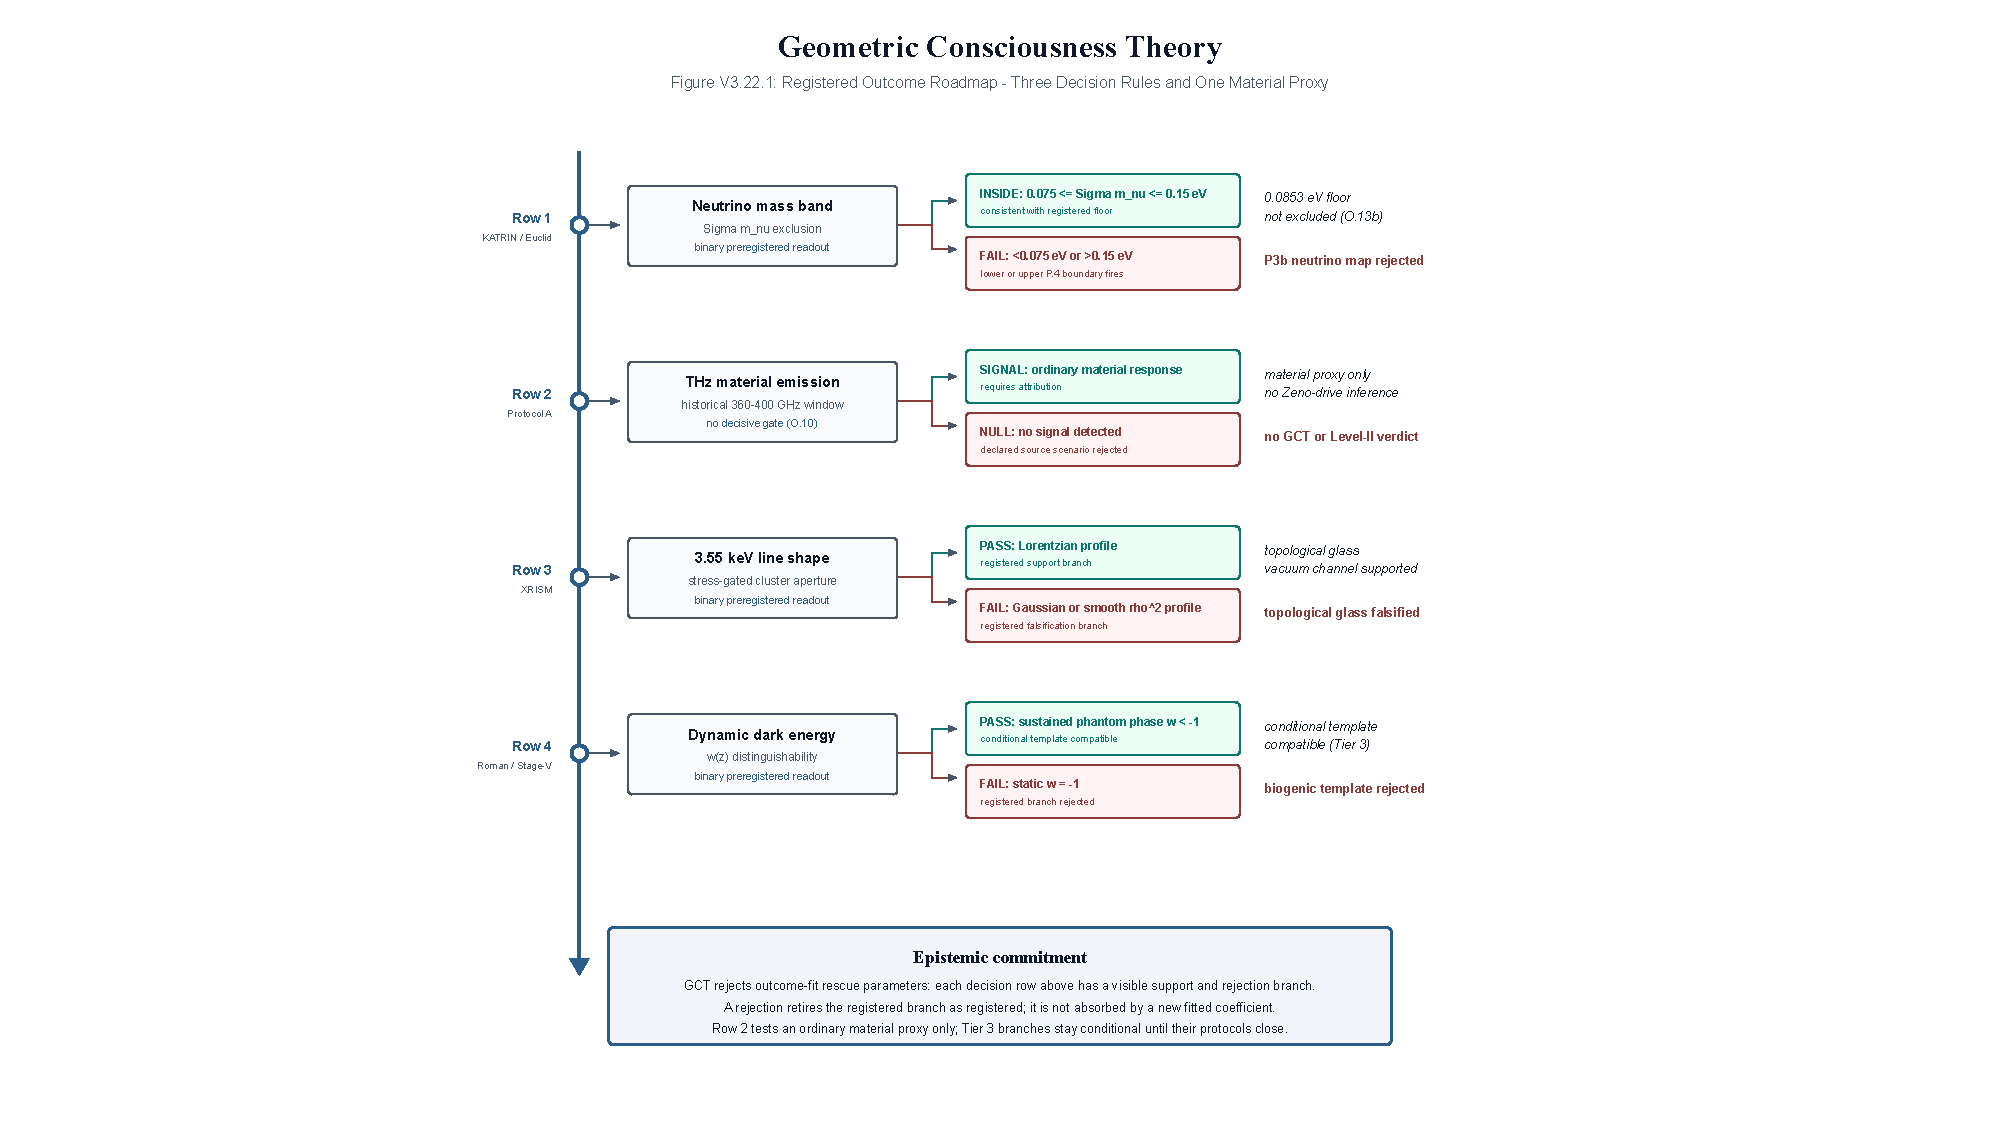
\includegraphics[keepaspectratio,alt={Registered outcome roadmap: the neutrino-mass band, the 3.55 keV line shape and the dark-energy phantom-phase distinguishability carry physics-sector decision rules; the historical THz material-emission proxy has no decisive GCT or consciousness gate.}]{content/Figures/Volume_3/Figure V3.22.1.pdf}}
\caption{Registered outcome roadmap: the neutrino-mass band, the 3.55
keV line shape and the dark-energy phantom-phase distinguishability
carry physics-sector decision rules; the historical THz
material-emission proxy has no decisive GCT or consciousness gate.}
\end{figure}

\subsubsection{22.1.2 Historical THz Material-Emission Scenario {[}Tier
3/open;
O.10{]}}\label{historical-thz-material-emission-scenario-tier-3open-o.10}

Protocol A preserves an external \textasciitilde360--400 GHz search
window for a possible ordinary material-emission feature. The former
``Physical Flash,'' the \(B_{topo}\) source heuristic (central value
\(380 \pm 20\) GHz), the Zeno-leakage interpretation and the \(N^2\)
super-radiant amplitude are not action-derived.

\begin{itemize}
\tightlist
\item
  \textbf{The Test:} First close O.10 by specifying a source model,
  transfer function, radiometry, controls and power calculation,
  including the cavity-integrated blackbody background and the
  phase-coherence assumption behind any \(N^2\) scaling (see V3
  §13.3.2b); only then preregister an active-versus-anaesthetized
  comparison in synchronized neural cultures.
\item
  \textbf{The Verdict:} A signal would be an ordinary material response
  requiring attribution; a controlled null would reject only the
  declared source scenario. Neither result supports or falsifies a Zeno
  Drive, an autopoietic renderer, phason coupling, an Identity Polaron,
  or Level II. Neither outcome is a verdict on GCT as a whole: the
  measurement tests an ordinary material proxy, and no phason,
  Selection-Operator or Level-II inference follows from it (V1 Ch17
  §17.1.3). No decisive numerical gate is presently licensed; once O.10
  licenses a powered gate, a preregistered null would reject the
  registered source scenario as registered.
\end{itemize}

\subsubsection{22.1.3 Isotope Substitution}\label{isotope-substitution}

Protocol D compares isotope-dependent biophysical responses in the
candidate spin/coherence architecture. It does not test consciousness,
an Identity Polaron, or mind-in-nucleus status directly.

\begin{itemize}
\tightlist
\item
  \textbf{The Test:} Comparison of anesthetic thresholds and \(T_2\)
  coherence times in \(^{16}\)\hspace{0pt}O (spin-0)
  vs.~\(^{17}\)\hspace{0pt}O (spin-5/2) environments.
\item
  \textbf{The Verdict:} A robust spin-dependent shift surviving
  chemical, mass and relaxation controls would support the declared
  biophysical response branch after systematic closure. Neither outcome
  is a verdict on GCT as a whole: the measurement tests an ordinary
  material proxy, and no phason, Selection-Operator or Level-II
  inference follows from it (V1 Ch17 §17.1.3). A preregistered result
  rejects the registered biophysical branch only under that branch's own
  decision rule (the Protocol D NMR polarity gate (P.13c) is held
  pending redesign: as written it rejected by construction, since
  \(^{17}\)\hspace{0pt}O shortens water-\(^1\)\hspace{0pt}H \(T_2\) by
  scalar relaxation; the former sign-aware rule, which rejects the
  registered sign-positive branch on a powered, significant negative
  isotope × activity interaction in water-\(^1\)\hspace{0pt}H
  \(\Delta T_2\), applies only after the redesign, and until then no
  outcome supports or rejects the branch; the LORR assay has no
  operative gate, V3 Ch16 §16.4--§16.5). Neither result is sufficient
  for a phenomenal, Identity-Polaron, Level-II, or mind-in-nucleus
  inference; the typed coupling and independent phenomenal bridge remain
  open.
\end{itemize}

\subsubsection{22.1.4 Neutrino Mass
Ceiling}\label{neutrino-mass-ceiling}

The conditional GCT branch places the lightest mass near \(0.015\) eV
{[}Tier 3 conditional: P3b/O.15(b)-conditioned absolute scale plus the
measured electron anchor; Tier 2 only for the abstract squared-stiffness
mechanism{]}, while the current direct bound is KATRIN's
\(m_\nu < 0.45\) eV (90\% CL, 2025), with a projected final sensitivity
below \(0.3\) eV {[}empirical bound / instrumental projection{]}.

\begin{itemize}
\tightlist
\item
  \textbf{The Test:} Next-stage KATRIN operations.
\item
  \textbf{The Verdict:} The conditional branch requires a
  \textbf{Non-Detection} by KATRIN at its final sensitivity (below
  \(\sim0.3\) eV). A positive detection of a mass at that level would
  reject the \textbf{Tier 3 P3b-to-neutrino absolute-scale map}
  (\(\phi^{-36}\), Tier 3 conditional); it would not by itself falsify
  the Tier 2 integer \(D_{H_3}=18\) or derive an alternative stiffness
  ratio. Testing the \(0.015\) eV floor requires a Project-8-class
  cyclotron-radiation experiment with sufficient endpoint sensitivity;
  no completion date is assumed.
\end{itemize}

\gctneedspace{5\baselineskip}\begin{gctWarning}

\textbf{⚠️ Active Falsification Risk --- Neutrino Mass Sum {[}Tier 3 ---
Active Tension{]}} The Tier 3 P3b-conditioned GCT target
\(\sum m_\nu \approx 0.0853\) eV is currently in \textbf{active
\(\Lambda\)\hspace{0pt}CDM-context tension}: it lies above both the
Planck+DESI 2024 95\% CL upper bound \(\Sigma m_\nu<0.072\) eV and the
tighter DESI DR2 + CMB bound \(\Sigma m_\nu<0.0642\) eV, so a single
``\textasciitilde2σ'' figure would understate the DR2 tension (no
posterior-based σ is quoted here). Under the registered P.4 exclusion
band, those bounds are \textbf{TENSION}, not falsification. Definitive
exclusion requires \(\Sigma m_\nu<0.075\) eV or \(\Sigma m_\nu>0.15\) eV
in a pre-registered likelihood that includes CMB+BAO+LSS growth
information. The gate becomes executable when such a likelihood reaches
definitive sensitivity; no calendar is assigned. See App NSM for the
construction and the GCT-native-likelihood survival path.

\end{gctWarning}

\begin{center}\rule{0.5\linewidth}{0.5pt}\end{center}

\subsection{22.2 Precision Validation after Facility and Sensitivity
Closure}\label{precision-validation-after-facility-and-sensitivity-closure}

If GCT passes the prerequisite-gated tests above, the program can shift
toward high-precision validation of the 6D\(\to\)\hspace{0pt}3D
projection.

\subsubsection{22.2.1 Roman Telescope Dark
Energy}\label{roman-telescope-dark-energy}

Roman/Stage-V-class low-redshift data can audit the \textbf{Biogenic
Dark Energy Lagrangian} if the required precision and systematics
conditions are met.

\begin{itemize}
\tightlist
\item
  \textbf{Prediction:} A sustained phantom phase where \(w(z)\) remains
  below \(-1\) for \(z \gtrsim 0\) with operative Class-2 amplitude
  \(|\Delta w(z\approx0.28)| \in [2,5]\times10^{-5}\) {[}calibrated,
  stipulated template; the phantom direction is Tier 4 because the
  written action cannot produce \(w<-1\) without a ghost, V2 Ch14
  §14.3.1{]}, correlated with the integrated star-formation/metallicity
  history. The executable condition is a joint low-redshift analysis
  over \(z\in[0.05,0.5]\) with precision below \(5\times10^{-5}\) and
  the declared systematics controls. The Hubble tension is not a
  prediction of the V2 Ch14 §14.5.1 lag-kernel action. The separate
  registered multi-channel reconciliation with the DESI CPL fit is
  falsified under its own \(3\sigma\) rule (DES-Dovekie \(3.2\sigma\);
  DESI DR2 \(3.1\sigma\) for BAO+CMB), a branch-level verdict (V2 Ch14
  §14.6.3).
\end{itemize}

\subsubsection{22.2.2 Mass Spectrum
Precision}\label{mass-spectrum-precision}

Protocol B defines a precision-improvement program for the lepton
hierarchy conditional on deriving the \(\mathcal{O}(\alpha^3)\)
self-interaction terms. No precision outcome or comparative historical
ranking is promised before that closure.

\subsubsection{22.2.3 Proton Mass from the Baryonic
Triad}\label{proton-mass-from-the-baryonic-triad}

Executing the high-resolution \textbf{Geometric Resonance Analysis} of
the \textbf{Baryonic Triad} (Protocol F) evaluates the proton-mass
formula \(m_p = m_e \phi^{15+\phi^{-1}}\), whose output
\(1836.437\,m_e \approx 938.417\) MeV lies \(+155\) ppm from the
observed \(1836.153\,m_e\), inside the registered 500 ppm postdiction
band {[}Tier 2 mechanism + Tier 3 sheet/exponent handle pending
AKN-action closure; a postdiction, not a live lattice-QCD falsifier;
Tier 4 as evidence, App PSC §PSC.9.6{]} from the baryonic-triad winding
(the formula does not use the Tier 3 string-tension bridge of V3 Ch18
§18.2.1) (see App PSC §PSC.3 for the three-values guide). This is the
current proton-mass mechanism route, not a closed solution of the hadron
mass gap from the current postulate set; further precision tightening
targets the QLQCD-1L / AKN-action closure (App QLA).

\subsubsection{22.2.4 Cosmological Neutrino
Detection}\label{cosmological-neutrino-detection}

Euclid/Simons-class joint data can test the conditional GCT mass sum
\(\sum m_\nu \approx \mathbf{0.0853 \text{ eV}}\) {[}Tier 3 conditional:
P3b/O.15(b) + electron-mass and oscillation-data anchors{]} when the
registered likelihood and sensitivity conditions are met.

\begin{itemize}
\tightlist
\item
  \textbf{The Binary Gate:} Euclid/Simons-class joint likelihood;
  \(\Sigma m_\nu\) vs registered \(<0.075\) eV / \(>0.15\) eV exclusion
  band; prerequisite-gated falsification test. App NSM defines the gate
  and decision rule.
\item
  \textbf{Falsification:} If the cosmological likelihood tightens below
  \(0.075\) eV at definitive precision, or above \(0.15\) eV, the
  P3b-conditioned mass-floor branch is definitively excluded. DESI
  2024/DR2 bounds in the \(0.064\)-\(0.072\) eV range are tension under
  \(\Lambda\)\hspace{0pt}CDM, not the registered exclusion condition.
\end{itemize}

\begin{center}\rule{0.5\linewidth}{0.5pt}\end{center}

\subsection{22.3 Theory-Closure Program}\label{theory-closure-program}

\subsubsection{22.3.1 Quasicrystalline Lattice QCD
(QLQCD)}\label{quasicrystalline-lattice-qcd-qlqcd}

Replacing periodic hyper-cubic grids with the \textbf{Aperiodic AKN
Tiling} is a proposed QLQCD research route. Whether it addresses Strong
CP or improves hadron-spectrum precision is an open computational and
continuum-limit question, not a forecast.

\subsubsection{22.3.2 Probing Breakdown of the
Metric}\label{probing-breakdown-of-the-metric}

The extreme-energy branch proposes tests for breakdown of the
smooth-metric approximation through ultra-high-energy cosmic-ray
dispersion. Observable 6D/lattice signatures and the required
sensitivity remain open.

\subsubsection{22.3.3 Laboratory Quantum-Gravity Analogue ---
Facility-Conditional}\label{laboratory-quantum-gravity-analogue-facility-conditional}

If a controllable macroscopic phason-condensate analogue and calibrated
acoustic metric can be built, it could test laboratory manipulation of
an analogue refractive geometry. This would be an analogue-gravity
experiment, not a promised modification of physical spacetime.

\begin{center}\rule{0.5\linewidth}{0.5pt}\end{center}

\subsection{22.4 The Complete Scorecard}\label{the-complete-scorecard}

We consolidate the results and open items of this work into a final
epistemic audit (✅ a stated comparison or formal result that currently
holds at the tier shown; ⚠️ a tension, registered-rule failure or
calibrated row; ○ an open, adopted or conditional row).

\subsubsection{22.4.1 Structural Results and Adoptions (Tier 1
formalism; Tier 2/Tier 3 bridges as
labelled)}\label{structural-results-and-adoptions-tier-1-formalism-tier-2tier-3-bridges-as-labelled}

\begin{itemize}
\tightlist
\item
  ○ \textbf{Wheeler-DeWitt Equation (\(\hat{H}\Psi=0\)):} The universe
  as a self-defining nullity {[}Tier 1 canonical formalism; Tier 3
  closed-system adoption{]}.
\item
  ○ \textbf{Dimensionality controls (\(D=3, D=6\)):} Classical
  one-dimensional knot types single out \(D=3\) only conditional on the
  physical knot-carrier premise {[}Tier 1 topology + Tier 3
  carrier/storage bridge{]}. The \(D=6\) embedding follows within the
  icosahedral/Galois architecture {[}Tier 2{]}, not from knot storage or
  entropy maximization alone.
\item
  ○ \textbf{Standard Model Algebra:} An algebraic-dimension match
  (necessary, not sufficient) plus Tier 3 structural correspondence is
  compatible with the
  \(\mathrm{SU}(3) \times \mathrm{SU}(2) \times \mathrm{U}(1)\)
  gauge-product candidate; the \(\mathrm{SU}(3)\) factor is an open Tier
  3 candidate (V3 Ch03), and the full physical Standard-Model
  identification (KO-dim-6 sign verification + first-order condition)
  remains conditional on App ORQ Open Problem O.32 closure (see Ch06
  §6.5 for the necessary-but-not-sufficient algebraic-dimension result
  and the registered conditional structure).
\item
  ○ \textbf{Photon Masslessness:} Gauge-protected
  Maxwell/residual-\(U(1)\) masslessness in the continuum description is
  standard at the level of the gauge limit {[}Tier 1 constraint{]}; the
  GCT phason/tile-dynamics realization of that limit is a Tier 3
  declared open programme (V2 Ch06 §6.1): as written, the V2 Ch06
  locking potential gaps the phason mode.
\item
  ○ \textbf{Born Rule (\(P \propto |\psi|^2\)):} Tier 3 conditional
  compatibility theorem under Gleason, pending App ORQ O.40a (countable
  additivity) and O.40b (noncontextuality) for the GCT Selection
  Operator measure.
\end{itemize}

\subsubsection{22.4.2 Geometric Comparisons (Postdictions, from the
Quasicrystal
Ansatz)}\label{geometric-comparisons-postdictions-from-the-quasicrystal-ansatz}

\gctneedspace{5\baselineskip}\begin{gctImportant}

\textbf{Reading the scorecard.} The precision figures below are
consequences of the \textbf{5-postulate-plus-6-continuous-anchor current
accounting enumerated in Parameter Ledger §0.1}; they should be read in
conjunction with the tier disclosures there. Where a row carries a
precision figure (ppm, \%, σ), the underlying Tier 2 framework is the
icosahedral cut-and-project ansatz plus the Tier 3 specific exponents
and disclosed continuous anchors catalogued in Ledger §0.1 P2-P5 and
A1-A6. The named precision/gauge comparison subset's six calibrated
Tier-3 coefficient handles (\(1440\), \(12\), \(360\), \(2\),
\(10\phi^2\), \(1/5\)) are counted separately; this is not a
manuscript-wide total, and O.38 \(N=144\) plus other sector-specific
handles remain separately catalogued. The truly bare lepton ratios
\(\phi^{11}\), \(\phi^{17}\) sit at \(-3.75\%\) and \(+2.69\%\); after
the Tier 3 first-order coefficients the muon reaches
\textasciitilde0.24\% and the tau (whose first-order formula is its full
formula) −51 ppm; sub-percent precision figures include the
radiative-correction provenance disclosed in App PSC §PSC.2.1 and A3
measured \(\alpha(0)\) where the row says so. Every φ-formula match in
§22.4.2--§22.4.3 (leptons, electron, proton, \(\alpha\),
\(\sin^2\theta_W^{\rm bare}\), \(G\), Higgs VEV, light quarks) is Tier 4
as evidence that φ or icosahedral structure is special: not
distinguishable from numerology for strong effects (App PSC §PSC.9.6;
§22.6).

\end{gctImportant}

\begin{itemize}
\tightlist
\item
  ○ \textbf{Weinberg Angle
  (\(\sin^2 \theta_W^{\rm bare} = \phi^{-3}\)):} Tier 3 gauge-kinetic
  hypothesis H-EW. The raw-frame identity of Theorem USS.9 is coordinate
  arithmetic, the canonical projectors give shares \(1/2+1/2\), and the
  convention-correct one-loop comparator from this boundary misses the Z
  pole by 40.87\% (Ch04 §4.3.3--§4.5.4). The bare 2.1\% alignment with
  the Z-pole value is Tier 4 as evidence (App PSC §PSC.9.6), and the
  pre-registered gauge-running audit (App GRF §GRF.4.3) is a
  \textbf{FAILED check}: run top-down from \{A2 = 24--25, H-EW,
  \(\alpha_3^{-1}=10\phi^2\), \(M_{\rm GUT}=3.2\times10^{16}\) GeV\}
  with SM β-functions it gives \(\sin^2\theta_W(M_Z)=0.058\)--\(0.067\)
  (best case \(-52\sigma\) against the PDG 2026 \(\overline{\rm MS}\)
  value \(0.23122\pm0.00006\)), and \(\alpha_s(M_Z)\) is undefined
  (non-perturbative); no declared-input configuration reproduces
  \(\sin^2\theta_W(M_Z)\), \(\alpha_s(M_Z)\) or \(\alpha_{em}(M_Z)\)
  (one borderline two-loop \(\alpha_{\rm em}\) value, which imports the
  measured \(\alpha_s\), is excluded by a post hoc judgement; App GRF
  §GRF.4.3) (App GRF §GRF.4.3); H-EW remains a Tier 3 hypothesis at an
  unspecified scale.
\item
  ○ \textbf{Fine-Structure Constant bare relation:}
  \(\alpha^{-1}_{\rm bare}=360\phi^{-2}=137.5078\) {[}Tier 3 numerical
  relation (Tier 3 600-cell multiplier; mechanism open --- the RT
  solid-angle construction is withdrawn, V1 §13.2.1--§13.2.2); 3443 ppm
  residual pending O.5/O.19{]}. The correction direction needed to reach
  the measurement is empirical; calling it phason anti-screening is a
  Tier 3 candidate convention, not a derived response sign or mechanism.
\item
  ○ \textbf{Fine-Structure Constant corrected closure target:}
  \(\alpha^{-1}_{\rm GCT}=360\phi^{-2}(1-1/288)=137.0303\) {[}Tier 3
  bilayer correction; 41.5 ppm residual pending O.5/O.19{]}.
\item
  ⚠️ \textbf{Newton's G (\(6.689475523 \times 10^{-11}\) N m² kg⁻²)
  {[}Tier 2 thermodynamic mechanism + Tier 4 Planck-link conjecture +
  Tier 3 dimensional anchor{]}:} Jacobson horizon entropy supplies the
  thermodynamic mechanism, but the numerical Planck-link inherits O.14
  and the \(m_e\) SI anchor. The model-authoritative
  \(\alpha_{\rm GCT}=\phi^2/360\) branch with CODATA \(m_e\) and exact
  SI \(h,c\) differs from CODATA 2022 by \textbf{2274 ppm}; the
  all-CODATA-\(\alpha\) sensitivity branch differs by 2013 ppm. This row
  is the electron Planck-link row inverted (\(G\propto m_e^{-2}\); 2013
  ppm ≈ 2 × the electron's 1006 ppm), so it is not independent evidence
  and is not counted as a pass: it is a registered FAIL inherited from
  the electron row (P.1c), which misses its LOCKED rule.
\item
  ⚠️ \textbf{Electron Mass (\(m_e\)):} \textbf{Tier 2 K-theoretic
  framework + Tier 3 exponent anchor + Tier 4 physical-link conjecture}
  (Parameter Ledger §0.1 P2; App ORQ O.14). The Coxeter-exponent
  arithmetic identifies \(|n|=107\) as the \(H_3\) power-sum label,
  while the load-bearing trace-image element is \(\phi^{-107}\); mapping
  that \(H_3\) invariant through the 6D AKN
  \(V\to K_0(\mathcal{A})\to\tau_*(K_0(\mathcal{A}))\) physical-link
  chain remains open. The anchor-normalized check
  \(m_e = M_P \phi^{-107}(1-5\alpha)\) matches CODATA-2022 to
  \textbf{1006 ppm} on canonical inputs, which misses the LOCKED 1000
  ppm pre-commitment by 6 ppm (App FSM P.1c reports a FAIL of that rule;
  the later 1500 ppm band is not retroactive); the specific exponent and
  physical-link chain remain O.14-governed rather than theorem-grade
  derivations.
\item
  ⚠️ \textbf{Muon g-2 {[}Tier 2 mechanism + Tier 3 \(1/5\) coefficient +
  A3 + Tier 4 calibration-survival conjecture: TENSION under WP2025{]}:}
  Geometric mechanism via
  \(\Delta a_\mu \approx 250.65 \times 10^{-11}\) through the
  equal-weight 1/5 icosahedral phason vertex coefficient. \textbf{WP2025
  disposition (App PSC §PSC.2):} under the consolidated lattice-QCD HVP
  synthesis (BMW/RBC HVP + Fermilab E989 final + CMD-3) the
  SM-vs-experiment gap is \textasciitilde0.6σ
  (\(38(63)\times10^{-11}\)), so the GCT correction overshoots the
  WP2025 residual by \textasciitilde3.3σ; it is not load-bearing
  empirical evidence under WP2025 and sits in tension. The §8.7.2 HVP
  scenarios A/B/C contingency framework remains the canonical
  disposition.
\item
  ○ \textbf{Lepton Masses (\(\phi^{11}, \phi^{17}\))
  {[}postdictions{]}:} Tier 2 mechanism (harmonic ladder on the
  dodecahedral cage, conditional on the Tier 3 \(\phi\)-step, V3 Ch08
  §8.1.2) + Tier 3 specific exponents \(N=11\) (muon) and \(N=17\) (tau)
  per Parameter Ledger §0.1 P4/P5. Residuals \textbf{muon −21 ppm
  (CODATA 2022), tau −51 ppm (PDG 2024)} via A3 measured \(\alpha(0)\),
  the Tier 3 coefficient rules \(+5\alpha\) and \(\phi^8\alpha^2\)
  (whose −3 exponent selection inherits the H-EW boundary), and the
  inserted Tier 3 tau rule \(-3.6\alpha\) (whose negative polarity is
  not derived; Galois conjugation fixes no response sign). The corrected
  rows are therefore conditional on A3, H-EW and these Tier 3
  coefficient rules. The muon mass is measured to 22 ppb (CODATA 2022),
  so the \textasciitilde21 ppm residual is a Tier 3 formula residual of
  order \(10^3\sigma\) in measurement terms; the earlier ``SM
  corrections already incorporated, \textasciitilde10--40 ppm theory
  floor'' argument is withdrawn. The tau row sits at its gate (⚠️
  tension). \emph{The truly bare \(\phi^{11}\) and \(\phi^{17}\) ratios
  sit at \(-3.75\%\) and \(+2.69\%\); after the Tier 3 first-order
  coefficients the muon reaches \textasciitilde0.24\% and the tau −51
  ppm.}
\item
  ○ \textbf{Proton Mass (\(\phi^{15.618}\)) {[}postdiction{]}:}
  \textbf{Tier 2 mechanism + Tier 3 sheet/exponent handle pending
  AKN-action closure.} Formula output \(1836.437\,m_e\) vs observed
  \(1836.153\,m_e\) (+155 ppm), inside the registered 500 ppm
  postdiction band; not a live lattice-QCD falsifier.
\item
  ○ \textbf{Icosahedral Architectural Selection:} App USS records
  \(A_5\) as the Tier-2 architectural premise H1 and derives exact
  conditional Schur-cover and McKay consequences; it does not prove
  point-group uniqueness or eliminate other spinorial point groups. The
  \(\phi\)-slope global entropy-maximality claim remains an open
  primary-candidate claim.
\end{itemize}

\subsubsection{22.4.3 Tier 3 Phenomenological Models (Pending
Derivation)}\label{tier-3-phenomenological-models-pending-derivation}

\begin{itemize}
\tightlist
\item
  ⚠️ \textbf{Higgs VEV Absolute Scale (246 GeV) {[}Tier 3{]}:} Mechanism
  proposed (not established), magnitude calibrated.
\item
  ⚠️ \textbf{Light Quark Absolute Masses {[}Tier 3{]}:} Ratios: Tier 3
  scaling heuristic (V3 Ch17 §17.2.2); the u/d ratio is the Tier 3
  identification \(m_d = m_u\phi^{\phi}\) (V3 Ch10 §10.4); the earlier
  face-area derivation of \(\phi\sqrt2\) is withdrawn (V3 Ch17 §17.2.3);
  absolute values require QLQCD.
\item
  ⚠️ \textbf{Dark Energy Susceptibility
  (\(\chi = \pi(c/H_0\ell_P)^2 \approx 2.27\times10^{122}\)) {[}Tier 2
  functional form + Tier 3 numerical value{]}:} The holographic area-law
  identification of V2 Ch14 §14.1.5; the value imports the Planck 2018
  \(H_0\) pending O.4.
\end{itemize}

\begin{center}\rule{0.5\linewidth}{0.5pt}\end{center}

\subsection{22.5 The State of the Theory (Final
Assessment)}\label{the-state-of-the-theory-final-assessment}

\subsubsection{22.5.1 What GCT Proposes and Has
Shown}\label{what-gct-proposes-and-has-shown}

GCT proposes a framework in which the ``Hard Problem'' of consciousness
and the ``Hard Problems'' of physics are addressed within one geometric
programme {[}Tier 3/4{]}. On that reading, the apparent arbitrariness of
nature---the specific values of masses and forces---would be the
structural signature of an icosahedral vacuum; the arbitrariness reading
is a programme claim, not a result. GCT proposes that the Standard Model
emerges from two philosophical axioms and the icosahedral geometric
framework parameterised by \(\phi\) (the SU(3) factor and H-EW remain
open Tier 3 candidates) --- the
\textbf{5-postulate-plus-6-continuous-anchor current accounting} of
Parameter Ledger §0.1 (P1 icosahedral cut-and-project ansatz, P2-P5 the
integer exponents \(n=-107\), \(D=18\), \(N=11\), \(N=17\) each with
explicit tier disclosure and Open Problem closure paths, A1 the
dimensional anchor \(m_e\), A2 the native-RGE endpoint anchor, A3
measured low-energy \(\alpha(0)\) for corrected precision-comparison
rows, and A4-A6 the App GRF \(Z_1\), \(Z_2\), \(Z_3\)
\(\beta\)-coefficient magnitude normalisations). The named
precision/gauge comparison subset's six calibrated Tier-3 coefficient
handles (\(1440\), \(12\), \(360\), \(2\), \(10\phi^2\), \(1/5\)) are
counted separately from those anchors; the subset is not an exhaustive
handle count, and O.38 \(N=144\) plus other sector-specific handles
remain separately catalogued. References to \(\phi\) as the structural
constant are structural-constants-only language; the full free-parameter
accounting is partitioned in Ledger §0.

\subsubsection{22.5.2 What Remains Open}\label{what-remains-open}

\textbf{Parametric Status: Gauge and Lepton Sectors}

Within the \textbf{5-postulate-plus-6-continuous-anchor current
accounting} of Parameter Ledger §0.1 (P1 icosahedral cut-and-project
ansatz; P2-P5 the integer exponents \(n=-107\), \(D=18\), \(N=11\),
\(N=17\); A1 the dimensional anchor \(m_e\); A2 the
\(\alpha_2^{-1}(M_{\rm GUT})\) native-RGE endpoint anchor; A3 measured
\(\alpha(0)\) for corrected precision-comparison rows; A4-A6 the App GRF
\(Z_1\), \(Z_2\), \(Z_3\) \(\beta\)-coefficient magnitude
normalisations), the lepton mass hierarchy is expressed through a Tier 2
icosahedral mechanism and the bare fine-structure constant through a
Tier 3 numerical relation (mechanism open, V1 §13.2.1--§13.2.2), with
Tier 3 specific integers and multipliers (P2-P5; the \(360\) handle),
with no continuous fit beyond the listed anchors and handles, while the
bare electroweak angle (H-EW) and the SU(3) factor remain open Tier 3
inputs. The named precision/gauge comparison subset's six calibrated
Tier-3 coefficient handles (\(1440\), \(12\), \(360\), \(2\),
\(10\phi^2\), \(1/5\)) are counted separately; this is not a
manuscript-wide total, and O.38 \(N=144\) plus other sector-specific
handles remain separately catalogued. The corrected ppm comparison rows
inherit A3 until the O.19/O.5 bare-to-physical alpha bridge closes. The
governing constraint is the 5-postulate-plus-6-continuous-anchor
structure, \emph{not} the closed one-parameter horizon. The closure
target is the 1-parameter limit P1 + \(m_e\); each of P2-P5 is currently
a Tier 2 mechanism plus a Tier 3 specific integer choice awaiting
first-principles derivation under Open Problems O.5, O.14, and O.15 (for
\(D=18\) the integer itself is Tier 2, while the stiffness map
\(K_\perp/K_\parallel=\phi^{-18}\) is the separate Tier 3 hypothesis
P3b, listed outside the count like H-EW), A2 awaits the QLQCD-1L/App GRF
boundary derivation (after the FAILED gauge-running audit of App GRF
§GRF.4.3, whether to retire A2 and A4--A6 is an open v1.4.0 decision;
v1.3.0 retires nothing and keeps the counts), A3 awaits O.19/O.5, and
A4-A6 await their App GRF §GRF.5.1 ab-initio derivations.

\textbf{Epistemic Boundary Clarification.} The structural constraint
above applies strictly to the bare fine-structure constant and the
lepton mass ratios; the bare electroweak angle (H-EW) and the SU(3)
factor are open Tier 3 inputs outside it. The \textbf{absolute
dimensional scale} (the electron mass \(m_e\) and all quantities derived
from it, including Newton's \(G\)) constitutes a \textbf{1-DOF
dimensional system} anchored to \(m_e\) as the A1 SI-unit reference. The
dimensionless ratio \(m_e/M_P = \phi^{-107}(1-5\alpha)\) is structured
by the K-theoretic gap-labeling framework, but the integer bookkeeping
must not be conflated: \(107\) is the \(H_3\) Coxeter-exponent power-sum
label, while \(\phi^{-107}\) is the trace-image candidate in the AKN
gap-label chain. The \emph{uniqueness} of the exponent \(-107\) inside
\(\tau_*(K_0(\mathcal{A})) \subset \mathbb{Z}[\phi]\) and the
physical-link map from the \(H_3\) invariant to the 6D AKN trace image
remain \textbf{Open Problem O.14} (the 1D Fibonacci toy-model
identification is closed; the 6D AKN lift is not). Full non-perturbative
extraction via the spectral zeta function on the AKN hull is the closure
target. The Quark sector (irrational exponents in \(m_c\) and the higher
CKM mixing angles \(s_{23}\), \(s_{13}\)) remains \textbf{Tier 3 Ansatz}
pending Fuglede-Kadison determinant closure (Open Problem O.5). The
down-quark route is a Tier 2 mechanism whose adopted primary conditional
output is \(m_d=m_u\phi^{\phi}=4.716\) MeV (\(+0.33\%\)); its exact
\(R=2\) finite-cage branch \(m_d=4.848734\) MeV (\(+3.1645\%\),
displayed as \(+3.16\%\)) is a secondary algebraic diagnostic. Both lie
inside the registered 110000-ppm gate; rigorous infinite-volume
convergence and the algebraic-field identification remain open under O.5
(App PSC §PSC.8; App TPR §TP-B).

Two correction terms not yet derived from first principles constitute
the \textbf{remaining parametric debt} of the program:

\begin{enumerate}
\def\labelenumi{\arabic{enumi}.}
\item
  \textbf{Candidate Phason Anti-Screening Correction (0.34\% residual)
  {[}Tier 3 --- open research debt{]}:} The tree-level formula
  \(\alpha^{-1} = 360\phi^{-2}\) {[}Tier 3 numerical relation; mechanism
  open, V1 §13.2.1--§13.2.2{]} supplies the baseline. The 3443 ppm
  discrepancy fixes only the correction direction required by the
  observed value. ``Anti-screening'' is an inserted Tier 3 candidate
  interpretation; the present 6D action derives neither the sign nor the
  mechanism. An explicit normalized response calculation from the 6D
  lattice action (quantifying the bosonic phason loop on the AKN tiling)
  remains the primary open QLQCD task (Appendix QLA).
\item
  \textbf{Healing length:}
  \(\xi = a_0/\alpha = \hbar c/(\alpha^2 m_e c^2) \approx 7.25\) nm
  {[}Tier 1 arithmetic; its identification as the vacuum/polaron healing
  length is Tier 3{]}. The implied polaron diameter (2ξ ≈ 14.5 nm) fits
  the microtubule lumen inner diameter (\textasciitilde15--17 nm), a
  3--17\% fit. Deriving this length from the 6D phason stiffness
  parameters \(K_\perp\), \(K_\parallel\) remains open; the
  phason-stiffness healing-length route of App GPE closes negatively.
\end{enumerate}

Per the Parameter Ledger: GCT has a 5-postulate + 1-anchor bare
topology/exponent sub-sector (A1 \(m_e\)), uses A2
(\(\alpha_2^{-1}(M_{\rm GUT})\) Tier-3 calibrated boundary; its value
24--25 is the MSSM unified coupling, Langacker \& Polonsky, Phys. Rev.~D
47, 4028 (1993), whereas in the SM the couplings do not unify) and A4-A6
(the App GRF \(Z_1\), \(Z_2\), \(Z_3\) normalisations) for the
native-RGE endpoint check, and uses A3 (measured low-energy
\(\alpha(0)\)) for corrected precision-comparison rows. The six A-sector
entries are continuous anchors. The named precision/gauge comparison
subset's six calibrated Tier-3 coefficient handles (\(1440\), \(12\),
\(360\), \(2\), \(10\phi^2\), \(1/5\)) are explicitly counted
separately; this subset is not a manuscript-wide handle total, and O.38
\(N=144\) plus other sector-specific handles remain separately
catalogued. The one-parameter state remains the closure target, not the
present status.

While a \emph{structure} for the simulation reading is proposed {[}Tier
3/4{]}, the \emph{origin} of the initial 6D lattice constant (\(a_6\),
of order \(\ell_P\); \(a_6 = 2\ell_P\) in the horizon-entropy
calibration) remains a foundational input. The derivation of the
absolute Higgs VEV and the full closure of the CKM/PMNS matrices remain
the primary theoretical frontiers.

\subsubsection{22.5.3 The Path Forward}\label{the-path-forward}

The proposed path forward is \textbf{Crystallographic Decoding} {[}Tier
3/4 programme{]}: anomalies in the data are treated as candidate clues
to local lattice defects. Parameter-fitting is not over---the anchors
and calibrated handles of Ledger §0.1 remain---but the programme aims to
replace them with derived integers and normalisations, reading the
cosmos as structured code rather than as a landscape of random numbers.

\begin{center}\rule{0.5\linewidth}{0.5pt}\end{center}

\subsection{22.6 The Invitation}\label{the-invitation}

To the experimentalists: Nine protocols (A--I, Chapters 13--21) define
explicit observables, but each becomes executable only when its
registered facility, sensitivity, systematics, and preregistration
conditions are met. Break the branches that reach those conditions.

To the computational physicists: The code documented in Appendix GPE is
a starting point. We invite you to scale the lattice simulations to 6D
periodic boundaries; whether sparse-matrix methods on aperiodic grids
help QCD is an open question.

To the skeptics: the accounting is on the table. Parameter Ledger §0.1
enumerates the five postulates and six continuous anchors this sector
rests on; App PSC §PSC.2.1 records the radiative-correction provenance
of the ppm comparisons; App PSC §PSC.9.4--§PSC.9.5 states the scope of
the cross-base control; and App PSC §PSC.9.6 reports the constant
control test. The muon at 21 ppm, the tau at 51 ppm, and the proton at
155 ppm are postdiction residuals that stand or fall on those
disclosures. Earlier global-significance figures for the numerical
matches are withdrawn: the cross-base comparison could not, by
construction, credit any base other than \(\phi\), and the trial counts
behind the quoted σ values were asserted rather than enumerated. The
preregistered constant control test that compares \(\phi\) against other
constants under identical formula freedom has now reported. As evidence
that φ or icosahedral structure is special, these matches are
\textbf{Tier 4}: the test (v3, NEGATIVE-FRAGILE; App PSC §PSC.9.6) found
φ's pattern of matches on 21 constants not distinguishable from that of
random constants (58 of 300 random bases did at least as well). The test
``excludes, at power ≥ 0.8, an effect in which φ hits at least 6 of the
8 informative rows through a real effect; weaker effects are not
excluded.'' It is non-confirmatory, and the numbers are kept as
descriptive arithmetic; no global significance is claimed for the
matches, and no individual match is cited as evidence on its own
strength. Read the disclosures, and then break the theory.

\begin{center}\rule{0.5\linewidth}{0.5pt}\end{center}

\subsection{22.7 Epistemic Verdict (Final
Statement)}\label{epistemic-verdict-final-statement}

Geometric Consciousness Theory (GCT) does not claim to have ``solved''
consciousness or proven that the mind is the sole cause of the universe.
Instead, the \textbf{geometric consciousness-first model}, built on the
5-postulate-plus-6-anchor current accounting enumerated in Parameter
Ledger §0.1, is compared with precision data from the Standard Model and
contemporary cosmology. The DESI-context neutrino-mass tension is an
active sensitivity-gated test under App NSM, not a calendar prediction.

We have set out an explicit hierarchy of certainty:

\begin{enumerate}
\def\labelenumi{\arabic{enumi}.}
\tightlist
\item
  \textbf{Open Tier 3 candidate:} the icosahedral route to the
  gauge-group structure and dimensionality (the \(\mathrm{SU}(3)\)
  closure is not specific to the RT window), with the physical
  Standard-Model identification at Tier 3 and theorem-grade uniqueness
  over compact Lie groups recorded as O.39.
\item
  \textbf{Tier 2 mechanisms with Tier 3/Tier 4 anchors and residuals:}
  lepton mass-spectrum harmonic-ladder mechanism (Tier 2) plus the
  \(N=11\) and \(N=17\) specific exponents (Tier 3 anchors pending
  O.5/O.14/O.15); fine-structure-constant \(360\phi^{-2}\) as a Tier 3
  numerical relation (Tier 3 600-cell multiplier; mechanism open --- the
  RT solid-angle construction is withdrawn, V1 §13.2.1--§13.2.2) plus
  the 3443 ppm bare residual (Tier 3 pending O.19/O.5); as evidence that
  φ is special, the numerical matches of this tier are Tier 4 (App PSC
  §PSC.9.6).
\item
  \textbf{Tier 3 (Phenomenological/Hypothesis):} The biophysical Zeno
  Drive and the Biogenic Dark Energy correlation template (its phantom
  direction is Tier 4: no ghost-free action produces it, V2 Ch14
  §14.3.1).
\end{enumerate}

While the Tier 2 structures motivate a crystalline-vacuum research
programme, the physical mass assignments remain conditional on the
disclosed Tier 3/4 bridges, and the Tier 3 extensions remain high-risk
hypotheses. Our invitation is not for blind acceptance, but for rigorous
falsification. Failure of a registered extension would reject that
branch; the surviving arithmetic and representation structure would
remain a candidate framework, not a derived stable-particle spectrum.

The door is open. The staircase of certainty is aimed at a universe that
would be fundamentally intelligible, unified, and structurally
consistent with the existence of agency; whether it gets there is what
the registered gates decide.

\begin{center}\rule{0.5\linewidth}{0.5pt}\end{center}

\subsection{22.8 Parametric Closure and Theoretical
Autonomy}\label{parametric-closure-and-theoretical-autonomy}

GCT's accounting has a \textbf{5-postulate-plus-1-anchor bare lepton
sub-sector; the native-RGE endpoint and precision-comparison rows add
anchors A2--A6 (Parameter Ledger §0.1)}: the bare ratios \(\phi^{11}\),
\(\phi^{17}\) follow from the icosahedral cut-and-project ansatz (P1)
plus the integer exponents \(n=-107\), \(D=18\), \(N=11\), \(N=17\)
(P2-P5) --- each a Tier 2 postulate (mechanism) plus a Tier 3 specific
value (integer choice) pending first-principles derivation under Open
Problems O.5, O.14, O.15. The bare fine-structure relation
\(360\phi^{-2}\) is a separate Tier 3 numerical relation that uses the
Tier 3 handle 360 (mechanism open; V1 §13.2.1--§13.2.2). The corrected
lepton rows \(m_\mu/m_e\), \(m_\tau/m_e\) need more than this
sub-sector: A3 (measured \(\alpha(0)\)), the Tier 3 coefficient rules
\(+5\alpha\), \(\phi^8\alpha^2\) and \(-3.6\alpha\), and, through the
exponent selection of the \(\phi^8\alpha^2\) term, the H-EW boundary.
For \(D=18\) only the integer is Tier 2; the physical stiffness map
\(\phi^{-18}\) (P3b) is a registered Tier 3 hypothesis outside the
count, like H-EW. The bare electroweak angle \(\phi^{-3}\) is not among
them: it is the separate Tier 3 hypothesis H-EW (V3 Ch04 §4.3), outside
this count. The \textbf{absolute dimensional mass scale} adds the
SI-unit anchor A1 (\(m_e\)), the native-RGE endpoint audit uses A2 and
A4-A6, and corrected lepton/Higgs/QED comparison rows use A3. A4-A6 are
the App GRF \(Z_1\), \(Z_2\), \(Z_3\) \(\beta\)-coefficient magnitude
normalisations. The named precision/gauge comparison subset's six
calibrated Tier-3 coefficient handles (\(1440\), \(12\), \(360\), \(2\),
\(10\phi^2\), \(1/5\)) are counted separately; this subtotal is not
manuscript-wide, and O.38 \(N=144\) plus other sector-specific handles
remain separately catalogued. The K-theoretic blueprint for
\(\phi^{-107}\) currently reaches a gap-label/dimension-group trace
skeleton at the 1D Fibonacci toy-model level; the explicit
Dixmier-residue/spectral-triple computation and the 6D AKN trace-image
lift remain open as O.14. The down-quark route is a Tier 2
Fuglede--Kadison-determinant mechanism with adopted primary conditional
output \(m_d=m_u\phi^{\phi}=4.716\) MeV, postdiction-consistent at
\(+0.33\%\) inside the registered 110000-ppm (11\%) shell-resonance
gate. The exact \(R=2\) finite-cage value \(m_d=4.848734\) MeV is
retained as a secondary algebraic diagnostic at \(+3.1645\%\) (displayed
as \(+3.16\%\)), also inside the gate. Its FK sequence centers on
\(\phi^{\phi}\) with an empirical decaying envelope; rigorous
infinite-volume convergence and the algebraic-field identification
remain bundled with O.5. Three quark-sector formulas with irrational
exponents (\(m_c = m_u\phi^{13+\phi^{-3}}\); CKM \(s_{23}\), \(s_{13}\))
remain \textbf{Tier 3 Empirical Ansätze}: for \(s_{23}\) and \(s_{13}\)
the standalone K-theoretic gap-label route is ruled out (App TPR §TP-F)
and the residual bundles with O.5; the charm route is addressed by TP-B
finite-size scaling (Open Problem O.5, Ch10). These three quark-sector
exponents are among the remaining heuristic inputs catalogued in Ledger
§0.1, alongside the Tier 3 specific values of P2--P5, the calibrated
handles, O.38 \(N=144\) and P3b.

The roadmap for \textbf{Parametric Closure and Theoretical Autonomy}
focuses on two discrete objectives:

\begin{enumerate}
\def\labelenumi{\arabic{enumi}.}
\tightlist
\item
  \textbf{Geometric Renormalization Group Equations (RGEs):} Standard
  Model QCD and QED RGEs flow the bare lattice masses (e.g.,
  \(m_{bare} = 174.1\) GeV for the Top) down to their dressed pole
  masses. The top value (\(174.07\) GeV against the PDG 2024
  direct-measurement mass \(172.57 \pm 0.29\) GeV, \(5.18\sigma\))
  currently lies outside P.24's written PDG \(\pm5\sigma\) falsification
  rule, a FAIL of that rule; a flow-based pole/\(\overline{\rm MS}\)
  uncertainty band would be a new pre-registered band, registered
  prospectively, not a retroactive rescue. Appendix GRF supplies a
  candidate native flow (``GCT-Native RG Flow''): the U(1)\(_Y\) and
  SU(2)\(_L\) \(\beta\)-function \emph{shape} is modeled by a Tier 3
  icosahedral \(I_h\) irrep-activation ansatz with the canonical
  projector shares \(1/2+1/2\), whose activation schedule and sign
  assignments are Tier 3 model inputs (no continuous shape parameter is
  fitted). The saturated coefficients
  \(b_1^\text{GCT}(M_\text{GUT}) = +41/6\),
  \(b_2^\text{GCT}(M_\text{GUT}) = -19/6\),
  \(b_3^\text{GCT}(M_\text{GUT}) = -7\) are reproduced \textbf{by
  construction} through three icosahedral normalisations
  \(\{Z_1, Z_2, Z_3\}\) that absorb the substrate-to-PDG absolute
  magnitude --- one anchor per coupling, in direct analogy to the single
  \(m_e\) anchor of the lepton sector. Beyond \(M_\text{GUT}\) the GCT
  flow saturates (the finite irrep tower of \(I_h\) caps the \(b_i\)),
  giving GCT a \textbf{combinatorial UV cutoff} rather than a
  Weinberg--Reuter asymptotic-safety non-Gaussian fixed point. Status:
\end{enumerate}

\begin{itemize}
\tightlist
\item
  \(\alpha(\mu)\) shape: \textbf{Tier 3} (activation ansatz, App GRF);
  endpoint \textbf{Tier 3} (one \(Z_1\) anchor)
\item
  \(\sin^2\theta_W(\mu)\) shape: \textbf{Tier 3} (activation ansatz, App
  GRF; V3 Ch04 §4.5.1); the native activation kernel (with imported A2)
  lands 26.66\% low at the endpoint, and the pre-registered
  gauge-running audit (App GRF §GRF.4.3) is a \textbf{FAILED check}: run
  top-down from \{A2 = 24--25, H-EW, \(\alpha_3^{-1}=10\phi^2\),
  \(M_{\rm GUT}=3.2\times10^{16}\) GeV\} with SM β-functions it gives
  \(\sin^2\theta_W(M_Z)=0.058\)--\(0.067\) (best case \(-52\sigma\)
  against the PDG 2026 \(\overline{\rm MS}\) value
  \(0.23122\pm0.00006\)), and \(\alpha_s(M_Z)\) is undefined
  (non-perturbative); no declared-input configuration reproduces
  \(\sin^2\theta_W(M_Z)\), \(\alpha_s(M_Z)\) or \(\alpha_{em}(M_Z)\)
  (one borderline two-loop \(\alpha_{\rm em}\) value, which imports the
  measured \(\alpha_s\), is excluded by a post hoc judgement; App GRF
  §GRF.4.3) (App GRF §GRF.4.3). A2 and H-EW cannot both hold for any SM
  extension; H-EW remains a Tier 3 hypothesis at an unspecified scale
\item
  \(\alpha_s(\mu)\) bare: the factors \(10\) and \(\phi^2\) have
  geometric provenance, but their strong-sector product \(10\phi^2\) is
  a \textbf{Tier 3 calibrated handle} pending O.42/QLQCD-2 (App QLA.7);
  running: \textbf{Tier 3} (QLQCD-2 pending); under SM running from
  \(M_{\rm GUT}\) the handle drives \(\alpha_3^{-1}\) to zero at
  \(2\)--\(6\times10^6\) GeV, so \(\alpha_s(M_Z)\) is undefined (FAILED
  check, App GRF §GRF.4.3)
\end{itemize}

The remaining open work --- full Tier-2 ab-initio derivation of the
three \(Z_i\) from the spectral action / QLQCD non-perturbative closure
(App QLA) --- is the canonical path to total RGE autonomy. See
\textbf{Appendix GRF} for the Tier 3 activation ansatz and
\texttt{protocol\_rge\_native.py} for the numerical audit.

\begin{enumerate}
\def\labelenumi{\arabic{enumi}.}
\setcounter{enumi}{1}
\tightlist
\item
  \textbf{The Subjective Lagrangian Calculus {[}Tier 4 programme
  target{]}:} Expanding the Tier 3 phenomenological surrogate
  \(\mathcal{S}_{Agent}\) of V1 Ch16 §16.5 into a computable calculus.
  This would entail calculating explicit \(\delta \mathbf{w}\) metabolic
  friction coefficients for specific human psychophysical states; such
  coefficients would be a precondition for, not a demonstration of, any
  quantitative Mind-Brain bridge, which remains open.
\end{enumerate}

The reported parameter comparisons define a closure program; further
substrate engineering is conditional on the unresolved physical,
experimental, and epistemic gates above.

\begin{center}\rule{0.5\linewidth}{0.5pt}\end{center}

\subsection{22.9 Coverage Map and Scope
Notes}\label{coverage-map-and-scope-notes}

GCT's ambition is a self-contained framework for any domain to which its
machinery has structural grip. The three volumes develop that machinery
in physics, cosmology, and the consciousness substrate; V1 Part VI
(``Applications \& Open Domains'') extends it into psychology, social
systems, aesthetics, contemplative practice, theology, self-reference,
and philosophy of science. This concluding section enumerates the
\emph{remaining} domains, the recommended treatment level for each, and
the explicit scope notes that delineate where the framework provides
ontological context rather than predictive instruments.

\subsubsection{22.9.1 Domains adjacent to current coverage
(one-paragraph notes here; full treatment is companion-paper
material)}\label{domains-adjacent-to-current-coverage-one-paragraph-notes-here-full-treatment-is-companion-paper-material}

\begin{itemize}
\tightlist
\item
  \textbf{Language phonology and lexical semantics} under the Quality
  Space framework: the same icosahedral irreducible representations
  proposed to decompose colour and audition (V1 Ch16 §16.2.2c; the
  modality map is Tier 3) could constrain the acoustic-perceptual space
  of phonemes {[}Tier 4{]}. A Tier 4 speculative hypothesis is that
  phonemic inventories across the world's languages cluster around the
  irrep boundaries of the human auditory Quality Space (the
  modality-to-irrep map is itself Tier 3); an empirical companion-paper
  target.
\item
  \textbf{Cognitive development and learning trajectories}: a chosen
  \(p\)-adic address filtration (V1 Ch07 §7.3.2; coupling kernel §7.6.3)
  could serve as a Tier 4 analogy for nested Piaget-style developmental
  resolutions, with a caregiver coupling \(\kappa_{ij}\) stabilising
  early branches. It becomes a Tier 3 coding model only after a physical
  map assigns states to Solenoid addresses, physical dynamics selects
  the filtration, and the caregiver coupling is derived. Solenoid
  topology alone supplies neither developmental stages nor stabilising
  relationships. Treatment depth: a future ``GCT Developmental
  Psychology'' paper.
\item
  \textbf{Dyadic relationships and attachment dynamics}: ordinary HRV /
  EEG cross-spectral coherence in long-term partners could test a
  phenomenological \(\kappa_{ij}\) proxy against shared-environment
  baselines {[}Tier 3 companion-paper target{]}. Such a result would be
  a physiological/behavioral correlation only; it would not establish
  Polaron coupling, a Selection network, shared subjecthood, or GCT,
  since Identity-Polaron construction and \(\kappa_{ij}\) remain open.
  Companion-paper material.
\item
  \textbf{Decision theory and the Subjective Lagrangian} (a Tier 4
  programme target in §22.8, built on the Tier 3 surrogate of V1 Ch16
  §16.5; not yet developed) could be extended by analogy to game theory,
  rational choice, and the geometry of preference {[}Tier 4{]}; a
  Bayesian-staircase formulation would warrant a dedicated
  decision-theory monograph.
\item
  \textbf{Plant, fungal, and microbial candidate controls} (V1 §16.2.6):
  chiral, nuclear-spin-bearing preparations can test the proposed
  mechanism, but neither descriptor establishes Level II; the Level II
  status of every substrate is open (Tier 3): no validated substrate
  criterion exists yet (it requires a typed, normalized, measured
  coupling, the Identity-Polaron construction and an independent
  phenomenal bridge; O.21/O.23/O.34, O.18).
\item
  \textbf{Memory taxonomy} (episodic / semantic / procedural): mapping
  memory types to depths of a chosen address filtration (deep branches =
  semantic, surface branches = episodic, procedural memory =
  \(\kappa_{ij}\)-coupled body sub-network) is a Tier 4 analogy unless a
  physical address code and read/write dynamics with noise protection
  and measured lifetimes are supplied. Deep cylinders are not shown to
  be intrinsically more durable memories.
\item
  \textbf{Friston Free-Energy Principle bridges}: predictive processing
  may be compared formally with a stipulated Selection-cost functional,
  and active inference with a \(\delta\theta_{\text{will}}\) control
  surrogate. This is a Tier 4 analogy: no thermodynamic Selection
  Operator, intent channel, physical friction law, owner, or phenomenal
  bridge has been derived. A future paper comparing FEP and GCT could
  make the analogy precise.
\item
  \textbf{Generative syntax} {[}Tier 4 analogy{]}: with corpus input,
  GCT could frame syntactic universals as Quality-Space patterns
  coordinated by multi-agent communicative selection; specific
  computational operations (Merge, X-bar) are downstream architectural
  choices not derivable from \(m_e + \phi\) alone.
\end{itemize}

\subsubsection{22.9.2 Scope notes (explicit
boundaries)}\label{scope-notes-explicit-boundaries}

\begin{itemize}
\tightlist
\item
  \textbf{Climate, geophysics, ecology, planetary systems} are
  \emph{applicable with inputs}: GCT provides the ontological context
  (matter as topological defects, gravity through the
  horizon-thermodynamic route of V2 Ch09 --- the phason-elasticity route
  to \(G\) is retired --- biological agency under the Dual Material
  Constraint) but is not the practical instrument for object-level
  prediction. Just as one uses Newtonian mechanics rather than General
  Relativity to predict the orbit of Saturn, climate / ecology /
  planetary dynamics use domain-specific models that GCT does not aim to
  replace.
\item
  \textbf{Mathematics itself}: per V1 §1.3.5 and V1 §6.4.5, mathematical
  objects are patterns over Field configurations, not Field
  configurations themselves; they do not inherit Level I presence. The
  instantiation of doing mathematics in a Class 2 Polaron has presence
  in the ordinary way. Confusing the two collapses the Field/Pattern
  distinction and converts the theory into a substrate-less Mathematical
  Universe (a position GCT does not adopt).
\item
  \textbf{Cultural anthropology, ritual analysis, gender / sexuality}:
  the multi-Polaron Consensus Protocol is at most a model-internal Tier
  4 analogy here (no physical Consensus Protocol is derived; V1 Ch11, V1
  Ch15), and specific cultural content requires ethnographic input the
  framework does not generate. These are downstream cultural-science
  domains; GCT provides the substrate ontology, not the object-level
  claims.
\item
  \textbf{Specific quantum-gravity competitor programmes} (string
  theory, loop quantum gravity, causal dynamical triangulations): GCT is
  distinguished from these in principle, not yet empirically: its
  architecture is different, and its numerical rows are postdictions
  (the bare lepton ratios sit in the 5-postulate-plus-1-anchor
  sub-sector of Parameter Ledger §0.1; the bare \(\alpha\) relation is a
  separate Tier 3 numerical relation, the corrected rows add A3, H-EW
  and Tier 3 coefficient rules, and the native-RGE endpoint adds A2 and
  A4--A6). The phantom-side dark-energy template is a stipulated forward
  template whose phantom direction is Tier 4 (V2 Ch14 §14.3.1), and no
  PTA \(\ell=6\) response is derived (Ch21), so neither separates GCT
  from these programmes. Quasicrystalline-spacetime programmes form a
  closer comparison class. Boyle and Mygdalas, ``Spacetime
  Quasicrystals'' (arXiv:2601.07769), construct Lorentzian quasicrystals
  by a \((9+1)\)\hspace{0pt}D embedding and explore a speculative
  Planck/electroweak/vacuum seesaw, whereas GCT adopts a Euclidean
  primitive-\(P\) rank-six icosahedral cut-and-project architecture,
  linked conditionally to the distinct McKay \(2I\to E_8\) and
  Elser--Sloane \(E_8\to H_4\) results, with a proposed emergent Lorentz
  symmetry and a conditional golden-ratio mass cascade (Tier 2
  mechanisms with Tier 3 exponents and disclosed anchors). Aschheim,
  Bubuianu, Fang, Irwin, Ruchin, and Vacaru (\emph{Annals of Physics}
  394:120-143; arXiv:1611.04858) provide an E8-derived
  quasicrystal-vacuum cosmology programme, but without a derived
  Standard Model mass spectrum. Detailed competitive analysis is
  reserved for future work; the manuscript states only the architectural
  difference.
\end{itemize}

\gctneedspace{5\baselineskip}

\textbf{End of Coverage Map.}

\gctneedspace{5\baselineskip}

\textbf{END OF VOLUME 3}

\chapter*{Glossary}
\addcontentsline{toc}{chapter}{Glossary}
\markboth{Glossary}{Glossary}
\setcounter{section}{0}

\subsubsection{\texorpdfstring{\textbf{Glossary of Terms (The Matter
Spectrum)}}{Glossary of Terms (The Matter Spectrum)}}\label{glossary-of-terms-the-matter-spectrum}

\begin{itemize}
\tightlist
\item
  \textbf{Acceptance Window (\(W\)):} The 3-dimensional volume in the
  internal manifold (\(E_\perp\)) that filters 6D lattice nodes for
  actualization. In GCT, this window is the \textbf{Rhombic
  Triacontahedron (RT)}, the icosahedral projection of a 6D hypercube.
\item
  \textbf{Baryonic Triad:} The candidate topological configuration of
  the Proton {[}Tier 2 mechanism + Tier 3 sheet/exponent handle{]},
  consisting of three interstitial face-mismatches (quarks as face
  defects is a Tier 3 assignment) stabilized by a 5-fold lattice star.
  Its mass ratio is given by the formula
  \(m_p/m_e = \phi^{15 + \phi^{-1}} \approx 1836.437\) against the
  observed \(1836.153\) (+155 ppm, a postdiction within a 500 ppm band;
  \textbf{Tier 4 as evidence} (φ-formula match; App PSC §PSC.9.6)); the
  formula is evaluated arithmetically, not extracted as an eigenvalue.
\item
  \textbf{Codimension:} The difference between the dimension of the
  embedding space (\(D=3\)) and the dimension of a defect. Leptons
  (vertex-centered) have codimension 3; Quarks (face-centered, a Tier 3
  candidate assignment) have codimension 1. This difference is proposed
  {[}Tier 3 heuristic{]} to underlie their different mass-scaling rules
  (V3 Ch08, V3 Ch10).
\item
  \textbf{Color Charge:} Tier 3 candidate identification (V3 Ch03): the
  azimuthal orientation of an interstitial defect's Burgers vector
  relative to the 10 three-fold rotational axes of the RT window.
\item
  \textbf{Dodecahedral Cage (\(N=144\)):} The candidate topological
  structure of the Electron core. Its 144-node count is adopted as a
  Tier 3 structural posit; \(144=F_{12}=12^2\) and the exact
  icosahedron/dodecahedron Gauss--Bonnet totals are consistency checks,
  not a size derivation. Ground-state selection requires the O.38
  full-lattice minimisation.
\item
  \textbf{Gluon String:} A 1D tube of phason strain representing the
  elastic resistance of the vacuum to tile-mismatch. In the Tier 3
  candidate picture (V3 Ch03) it provides a proposed mechanical
  mechanism for confinement and carries the candidate \(SU(3)\)
  generators.
\item
  \textbf{Koide Convergence:} The empirical summation rule
  (\(K\approx2/3\)) governing lepton masses. Its GCT reading as a
  unitarity constraint on the 6D\(\to\)\hspace{0pt}3D projection is a
  Tier 3 candidate identification, not a Tier 2 derivation. The phason
  drag of the Muon (\(+5\alpha\)) and the volume screening of the Tau
  (\(-3.6\alpha\)) do not cancel in \(K\): each lowers it, and together
  they give \(K=0.66688\) at first order (V3 Ch08 §8.6).
\item
  \textbf{Majorana Self-Duality:} The proposed property of the GCT
  neutrino {[}Tier 3{]} in which the left-handed state (\(E_\parallel\))
  and right-handed state (\(E_\perp\)) are read as Galois conjugates of
  the same 6D lattice excitation, which would make the particle its own
  antiparticle; the self-duality-to-lepton-number-violation bridge is
  not derived and \(0\nu\beta\beta\) decay is the experimental gate (V3
  Ch09 §9.5.1).
\item
  \textbf{Normal Ordering:} The GCT Growth-Axiom requirement that
  particle generations follow the inflationary growth eigenvalue
  (\(\phi^n\)), from which GCT predicts a normal rather than inverted
  neutrino hierarchy {[}Tier 3 conditional oscillation-sector
  prediction: the generation-ordering assignment is not derived from the
  lattice action, V3 Ch09 §9.3.3{]}; inverted ordering confirmed at
  \(>3\sigma\) would falsify the prediction.
\item
  \textbf{Phason Drag (\(5\alpha\)):} The hydrodynamic friction
  experienced by a topological defect moving through the vacuum. For
  leptons, the drag channel is a Tier 2 icosahedral mechanism; its count
  5 is read as the number of \(A_5\) irreducible representations
  (trivial included), a Tier 3 counting convention (V3 Ch08 §8.2.2), and
  converting that count into the equal-weight \(+5\alpha\) pole-mass
  coefficient is Tier 3 pending self-energy closure.
\item
  \textbf{Polaron:} The holographic restriction of the full 6D
  quasicrystalline vacuum to a localized topological excitation mode. In
  strict accordance with Mereological Nihilism, it is not an assembled
  composite of smaller parts, but a localized behavioral shadow of the
  6D bulk.
\item
  \textbf{Missing-leg control (formerly ``Turing Null''; the categorical
  verdict is withdrawn):} The proposed control class, such as bulk
  silicon, that lacks one leg of the proposed two-leg architecture. The
  label carries no categorical inference: DMC descriptors do not
  establish zero coupling, Class-0 status, or absence of Level II. Level
  II: open (Tier 3) --- no validated substrate criterion exists yet (it
  requires a typed, normalized, measured coupling, the Identity-Polaron
  construction and an independent phenomenal bridge; O.21/O.23/O.34,
  O.18).
\item
  \textbf{Vacuum Quantum (\(E_{vac}\)):} Conditional on the Tier 3 O.38
  posit \(N_{\rm cage}=144\), the exact division \(m_e/144\) gives the
  Tier 3 absolute centroid \(3.5486\) keV. The lattice-fracture
  mechanism form is Tier 3 (it rests on the Tier 3 Topological Glass
  model and is conditional on that adopted architecture); the line width
  is open (V3 Ch11 §11.2.3); the value does not select the cage size.
\item
  \textbf{Winding Number (\(n\)):} The integer count of phase
  circulation around a topological singularity, proposed {[}Tier 3{]} to
  define the quantization of electric and color charge.
\end{itemize}

\chapter*{Notation Quick Reference — Volume 3 (Matter Spectrum)}
\addcontentsline{toc}{chapter}{Notation Quick Reference — Volume 3 (Matter Spectrum)}
\markboth{Notation Quick Reference — Volume 3 (Matter Spectrum)}{Notation Quick Reference — Volume 3 (Matter Spectrum)}
\setcounter{section}{0}

This reference complements the Volume 1 and Volume 2 Notation files.
Symbols below are those most heavily used in V3 (Forces, Matter,
Astrophysics, Experiments).

\subsubsection{\texorpdfstring{\textbf{Standard Model Constants and
Sectors}}{Standard Model Constants and Sectors}}\label{standard-model-constants-and-sectors}

\emph{Evidential note:} the numerical matches of the φ-based formulas
listed in this section and under Mass Spectrum (\(\alpha^{-1}\), the
\(\sin^2\theta_W\) bare alignment, \(\theta_C\), \(\delta_{CP}\),
\(m_e\), \(m_\mu\), \(m_\tau\), \(m_p\)) are \textbf{Tier 4 as evidence}
(φ-formula match; App PSC §PSC.9.6); the tier tags given below describe
the formulas' mechanisms and handles, not their evidential weight.

\begin{itemize}
\tightlist
\item
  \textbf{\(\alpha\), \(\alpha^{-1}\):} Fine-structure constant. GCT
  bare value \(\alpha^{-1}_{bare} = 360\phi^{-2} \approx 137.508\) (Tier
  3 numerical relation: Tier 3 600-cell multiplier; mechanism open ---
  the RT solid-angle construction is withdrawn, V1 §13.2.1--§13.2.2);
  CODATA A3 observed value \(137.035999177\).
\item
  \textbf{\(\sin^2\theta_W\):} Weinberg angle. Tier 3 bare gauge-kinetic
  hypothesis (H-EW) \(= \phi^{-3} \approx 0.236\); the raw Galois-frame
  ratio \(\rho_{\rm raw}=\phi^{-2}\approx0.382\) is a coordinate
  identity and not a physical angle; the canonical projector shares are
  \(1/2+1/2\); measured \(0.23122 \pm 0.00006\) (PDG 2026
  \(\overline{\rm MS}\) \(\hat s^2_Z(M_Z)\)); the pre-registered running
  check from H-EW is FAILED (V3 Ch04; App GRF §GRF.4.3).
\item
  \textbf{\(\theta_C\):} Cabibbo angle. GCT Tier 3 value
  \(\arcsin(\phi^{-3}(1-5\alpha))\) (bare identification + transfer; V3
  Ch10).
\item
  \textbf{\(\delta_{CP}\):} CP-violating phase. GCT Tier 3 ansatz value
  \(360°\phi^{-1}\) (V3 Ch10).
\end{itemize}

\subsubsection{\texorpdfstring{\textbf{Mass
Spectrum}}{Mass Spectrum}}\label{mass-spectrum}

\begin{itemize}
\tightlist
\item
  \textbf{\(m_e\):} Electron mass. Formula
  \(m_e = M_P \phi^{-107}(1-5\alpha)\) (Tier 2 mechanism + Tier 3
  Coxeter-exponent handle + Tier 4 structural-link conjecture pending
  O.14; an anchor-normalised Planck-link check, since \(m_e\) is the A1
  anchor; \textasciitilde1006 ppm vs CODATA per engine output, which
  misses the LOCKED 1000 ppm pre-commitment by 6 ppm --- App FSM P.1c
  reports a FAIL of that rule).
\item
  \textbf{\(m_\mu\):} Muon mass. Formula
  \(m_\mu = m_e \phi^{11}(1+5\alpha+\phi^8\alpha^2)\) (Tier 2 mechanism
  + Tier 3 specific exponent + Tier 3 \(+5\alpha\) coefficient
  normalization / pole-mass loop discipline \(\to\) Tier 3 headline
  precision; −21 ppm Tier 3 formula residual, of order \(10^3\sigma\)
  against the 22 ppb CODATA 2022 measurement and as large as the
  unpropagated truncation term \(\phi^8\alpha^3 \approx 18\) ppm).
\item
  \textbf{\(m_\tau\):} Tau mass. Formula
  \(m_\tau = m_e \phi^{17}(1-3.6\alpha)\) (Tier 2 mechanism + Tier 3
  specific exponent + Tier 3 combination rule, pending O.26b for tau
  coefficient stacking → Tier 3 headline coefficient; \textasciitilde51
  ppm against PDG 2024).
\item
  \textbf{\(m_p\):} Proton mass. Formula
  \(m_p = m_e \phi^{15+\phi^{-1}}\), Tier 2 mechanism + Tier 3
  sheet/exponent handle, value \(\approx 938.417\) MeV against CODATA
  \(938.272\) MeV (+155 ppm; a postdiction within a 500 ppm band, not a
  live falsifier; V3 Ch18 and App PSC §PSC.3).
\item
  \textbf{\(m_{p}/m_{e}\) ratio:}
  \(\phi^{15+\phi^{-1}} \approx 1836.437\) vs CODATA observed
  \(1836.153\).
\item
  \textbf{\(\Sigma m_\nu\):} Sum of neutrino masses. GCT
  normal-hierarchy scale \(\Sigma m_\nu \approx 0.0853\) eV from
  \(m_1=m_e\phi^{-36}\) plus oscillation gaps (the numerical floor
  inherits the Tier 3 stiffness-map hypothesis P3b, and the gaps are
  inputs, so this is a consistency scale, not an independent
  prediction); DESI DR2 + CMB gives a \(\Lambda\)\hspace{0pt}CDM-context
  bound \(\Sigma m_\nu < 0.0642\) eV at 95\% CL (arXiv:2503.14738),
  which the candidate exceeds; this is tension rather than the
  registered \(<0.075\) eV / \(>0.15\) eV exclusion band.
\end{itemize}

\subsubsection{\texorpdfstring{\textbf{Lepton g-2 and
Anomalies}}{Lepton g-2 and Anomalies}}\label{lepton-g-2-and-anomalies}

\begin{itemize}
\tightlist
\item
  \textbf{\(\Delta a_\mu\):} Muon anomalous magnetic moment correction.
  GCT vertex value \(\approx 250.65 \times 10^{-11}\) (Tier 2 mechanism
  + Tier 3 \(1/5\) coefficient + A3 + Tier 4 calibration-survival
  conjecture; Tension under WP2025, falsification conditional on
  long-term HVP-synthesis arbitration --- see App PRG Table PRG.1 row
  P.5 for the HVP-Survival Condition).
\end{itemize}

\subsubsection{\texorpdfstring{\textbf{Quasicrystal and Polaron
Parameters}}{Quasicrystal and Polaron Parameters}}\label{quasicrystal-and-polaron-parameters}

\begin{itemize}
\tightlist
\item
  \textbf{\(\xi_{\rm pol}\) (Biological Polaron Healing Length):}
  \(\xi_{\rm pol} = \hbar c/(\alpha^2 m_e c^2) = a_0/\alpha \approx 7.25\)
  nm (CODATA \(\alpha\); the GCT bare \(\alpha^{-1}\) gives the same
  biological scale within the registered precision).
  \(\xi = a_0/\alpha \approx 7.25\) nm {[}Tier 1 arithmetic; its
  identification as the vacuum/polaron healing length is Tier 3{]} +
  Tier 3 microtubule-lumen biological-scale match; distinct from the
  dark-sector \(\xi_{\rm DS}=\phi^4a_\perp\).
\item
  \textbf{\(\eta_{Zeno}\) (conditional external-rate ratio):}
  \(\eta_{Zeno} = g_{single}^{eff}\sqrt{N_{bio}}/\kappa\). The present
  program does not derive \(g_{single}^{eff}\) from material
  descriptors; this arithmetic supplies neither a DMC boundary nor a
  Level-II verdict.
\item
  \textbf{\(F_{CISS}\) (CISS enhancement factor):} \(\approx 2.0\)
  empirical import from spin-chemistry literature (Naaman et al.~2019,
  \emph{Nat. Rev.~Chem.} 3:250--260). It is an ordinary material factor,
  not a GCT phason coefficient.
\item
  \textbf{\(N_{bio}\):} Effective number of cooperatively-pumped Trp
  dipoles in the microtubule lumen (V3 Ch13).
\end{itemize}

\subsubsection{\texorpdfstring{\textbf{Experimental
Anchors}}{Experimental Anchors}}\label{experimental-anchors}

\begin{itemize}
\tightlist
\item
  \textbf{3.55 keV line:} Conditional Vacuum Quantum
  \(E_{vac}=m_e/144\approx3.5486\) keV. The division is exact, but the
  absolute centroid is Tier 3 because it inherits the O.38
  \(N_{\rm cage}=144\) posit; the lattice-fracture mechanism form is
  Tier 3 (it rests on the Tier 3 Topological Glass model and is
  conditional on that architecture; V3 Ch11).
\item
  \textbf{\(\ell=6\) icosahedral PTA structure:} the first nonconstant
  rotational-icosahedral scalar harmonic; physical timing response,
  amplitude, and test statistic remain open (Tier 1 theorem; Tier 2
  conditional symmetry; V3 Ch21).
\item
  \textbf{GRB 090510 LIV bound:} Abdo et al.~2009, \emph{Nature}
  462:331--334 --- used as the empirical anchor for V3 Ch20 Protocol H.
\end{itemize}

\subsubsection{\texorpdfstring{\textbf{Cross-Reference
Conventions}}{Cross-Reference Conventions}}\label{cross-reference-conventions-1}

\begin{itemize}
\tightlist
\item
  See V2 Notation Reference for cross-reference conventions; identical
  here.
\item
  Volume-specific abbreviations: \textbf{V3 §X.Y} without further
  qualification refers to V3
  \texttt{Ch\textless{}X\textgreater{}\ §\textless{}X.Y\textgreater{}};
  cross-volume references are always written
  \textbf{\texttt{V\textless{}n\textgreater{}\ Ch\textless{}m\textgreater{}}}
  or \textbf{\texttt{App\ \textless{}ABC\textgreater{}}} (three-letter
  appendix ID).
\end{itemize}

\chapter*{Bibliography}
\addcontentsline{toc}{chapter}{Bibliography}
\markboth{Bibliography}{Bibliography}
\setcounter{section}{0}

\subsection{\texorpdfstring{\textbf{Bibliography (Select References for
Volume
3)}}{Bibliography (Select References for Volume 3)}}\label{bibliography-select-references-for-volume-3}

\subsubsection{\texorpdfstring{\textbf{Standard Model \&
Data}}{Standard Model \& Data}}\label{standard-model-data}

\begin{itemize}
\tightlist
\item
  \textbf{Navas, S., et al.~(Particle Data Group).} (2024). ``Review of
  Particle Physics.'' \emph{Physical Review D}, 110, 030001.
\item
  \textbf{Mohr, P. J., Newell, D. B., Taylor, B. N., \& Tiesinga, E.}
  (2025). ``CODATA Recommended Values of the Fundamental Physical
  Constants: 2022.'' \emph{Reviews of Modern Physics}, 97, 025002. DOI:
  10.1103/RevModPhys.97.025002.
\end{itemize}

\subsubsection{\texorpdfstring{\textbf{Algebraic \& Geometric
Foundations}}{Algebraic \& Geometric Foundations}}\label{algebraic-geometric-foundations}

\begin{itemize}
\tightlist
\item
  \textbf{Kramer, P., \& Neri, R.} (1984). ``On periodic and
  non-periodic space fillings of \(E^m\) obtained by projection.''
  \emph{Acta Crystallographica Section A}, 40, 580-587.
\item
  \textbf{Atiyah, M. F., Patodi, V. K., \& Singer, I. M.} (1975).
  ``Spectral asymmetry and Riemannian geometry. I.'' \emph{Mathematical
  Proceedings of the Cambridge Philosophical Society}, 77(1), 43-69.
\item
  \textbf{Atiyah, M. F., Patodi, V. K., \& Singer, I. M.} (1975).
  ``Spectral asymmetry and Riemannian geometry. II.'' \emph{Mathematical
  Proceedings of the Cambridge Philosophical Society}, 78(3), 405-432.
\item
  \textbf{Baez, J. C.} (2002). ``The Octonions.'' \emph{Bulletin of the
  American Mathematical Society}, 39(2), 145-205.
\item
  \textbf{Bellissard, J., Herrmann, D. J. L., \& Zarrouati, M.} (2000).
  ``Hulls of Aperiodic Solids and Gap Labelling Theorems.''
  \emph{Directions in Mathematical Quasicrystals}, CRM Monograph Series,
  13, 207-258.
\item
  \textbf{Connes, A.} (1994). \emph{Noncommutative Geometry}. Academic
  Press.
\item
  \textbf{Connes, A.} (2006). ``Noncommutative geometry and the standard
  model with neutrino mixing.'' \emph{Journal of High Energy Physics},
  0611, 081. arXiv:hep-th/0608226.
\item
  \textbf{Chamseddine, A. H., \& Connes, A.} (2012). ``Resilience of the
  Spectral Standard Model.'' \emph{Journal of High Energy Physics}, 09,
  104. arXiv:1208.1030.
\item
  \textbf{Connes, A., \& Moscovici, H.} (1995). ``The Local Index
  Formula in Noncommutative Geometry.'' \emph{Geometric and Functional
  Analysis}, 5(2), 174-243.
\item
  \textbf{Farber, M. S., \& Levine, J. P.} (1996). ``Jumps of the
  eta-invariant.'' \emph{Mathematische Zeitschrift}, 223(2), 197--246.
  https://doi.org/10.1007/PL00004559
\item
  \textbf{Cuntz, J., \& Krieger, W.} (1980). ``A class of C*-algebras
  and topological Markov chains.'' \emph{Inventiones Mathematicae},
  56(3), 251-268.
\item
  \textbf{Elser, V., \& Sloane, N. J. A.} (1987). ``A highly symmetric
  four-dimensional quasicrystal.'' \emph{Journal of Physics A:
  Mathematical and General}, 20(18), 6161-6168.
\item
  \textbf{Jackiw, R., \& Rebbi, C.} (1976). ``Solitons with fermion
  number 1/2.'' \emph{Physical Review D}, 13(12), 3398.
\item
  \textbf{Koide, Y.} (1983). ``A Fermion-Boson Composite Model of Quarks
  and Leptons.'' \emph{Physics Letters B}, 120(1-3), 161-165.
\item
  \textbf{McKay, J.} (1980). ``Graphs, singularities, and finite
  groups.'' \emph{Proceedings of Symposia in Pure Mathematics}, 37,
  183-186.
\item
  \textbf{Senechal, M.} (1995). \emph{Quasicrystals and Geometry}.
  Cambridge University Press.
\end{itemize}

\subsubsection{\texorpdfstring{\textbf{Experimental
Foundations}}{Experimental Foundations}}\label{experimental-foundations}

\begin{itemize}
\tightlist
\item
  \textbf{Agazie, G., et al.~(NANOGrav Collaboration).} (2023). ``The
  NANOGrav 15 yr Data Set: Evidence for a Gravitational-wave
  Background.'' \emph{The Astrophysical Journal Letters}, 951(1), L8.
\item
  \textbf{Bulbul, E., et al.} (2014). ``Detection of an Unidentified
  Emission Line in the Stacked X-ray Spectrum of Galaxy Clusters.''
  \emph{The Astrophysical Journal}, 789(1), 13.
\item
  \textbf{de Boissieu, M., et al.} (1995). ``Diffuse scattering and
  phason elasticity in the AlPdMn icosahedral phase.'' \emph{Physical
  Review Letters}, 75(1), 89-92.
\item
  \textbf{Aker, M., et al.~(KATRIN Collaboration).} (2025). ``Direct
  neutrino-mass measurement based on 259 days of KATRIN data.''
  \emph{Science}, 388, 180--185. arXiv:2406.13516.
\item
  \textbf{DESI Collaboration: M. Abdul Karim et al.} (2025). ``DESI DR2
  Results II: Measurements of Baryon Acoustic Oscillations and
  Cosmological Constraints.'' arXiv:2503.14738.
\item
  \textbf{Dessert, C., Rodd, N. L., \& Safdi, B. R.} (2020). ``The dark
  matter interpretation of the 3.5-keV line is inconsistent with
  blank-sky observations.'' \emph{Science}, 367(6485), 1465-1467.
\item
  \textbf{Francoual, S., et al.} (2006). ``Dynamics of phason
  fluctuations in the i-AlPdMn quasicrystal.'' \emph{Philosophical
  Magazine}, 86(6-8), 1029-1035.
\item
  \textbf{Aharonian, F. A., et al.~(Hitomi Collaboration).} (2017).
  ``Hitomi Constraints on the 3.5 keV Line in the Perseus Galaxy
  Cluster.'' \emph{The Astrophysical Journal Letters}, 837(1), L15. DOI:
  10.3847/2041-8213/aa61fa.
\item
  \textbf{Hore, P. J., \& Mouritsen, H.} (2016). ``The radical-pair
  mechanism of magnetoreception.'' \emph{Annual Review of Biophysics},
  45, 299-344.
\item
  \textbf{Lubensky, T. C., Ramaswamy, S., \& Toner, J.} (1985).
  ``Hydrodynamics of Icosahedral Quasicrystals.'' \emph{Physical Review
  B}, 32(11), 7444--7452.
\item
  \textbf{Leggett, A. J., \& Garg, A.} (1985). ``Quantum mechanics
  versus macroscopic realism: Is the flux there when nobody looks?''
  \emph{Physical Review Letters}, 54(9), 857-860.
\item
  \textbf{Maeda, K., et al.} (2012). ``Magnetically sensitive
  light-induced reactions in cryptochrome are consistent with its
  proposed role as a magnetoreceptor.'' \emph{Proceedings of the
  National Academy of Sciences}, 109(13), 4774-4779.
\item
  \textbf{Malyshev, D., Neronov, A., \& Eckert, D.} (2014).
  ``Constraints on 3.55 keV line emission from stacked observations of
  dwarf spheroidal galaxies.'' \emph{Physical Review D}, 90, 103506.
\item
  \textbf{Misra, B., \& Sudarshan, E. C. G.} (1977). ``The Zeno's
  paradox in quantum theory.'' \emph{Journal of Mathematical Physics},
  18(4), 756-763.
\item
  \textbf{Naaman, R., Paltiel, Y., \& Waldeck, D. H.} (2019). ``Chiral
  molecules and the electron spin.'' \emph{Nature Reviews Chemistry},
  3(4), 250--260.
\item
  \textbf{Abdo, A. A., et al.~(Fermi LAT \& GBM Collaborations).}
  (2009). ``A limit on the variation of the speed of light arising from
  quantum gravity effects.'' \emph{Nature}, 462(7271), 331--334.
\item
  \textbf{Riemer-Sørensen, S.} (2016). ``Constraints on the presence of
  a 3.55 keV dark matter emission line from Chandra observations of the
  Milky Way.'' \emph{Astronomy \& Astrophysics}, 590, A71.
\item
  \textbf{Ritz, T., Adem, S., \& Schulten, K.} (2000). ``A model for
  photoreceptor-based magnetoreception in birds.'' \emph{Biophysical
  Journal}, 78(2), 707-718.
\end{itemize}

\chapter*{Index}
\addcontentsline{toc}{chapter}{Index}
\markboth{Index}{Index}
\setcounter{section}{0}

\subsubsection{\texorpdfstring{\textbf{Index (Volume
3)}}{Index (Volume 3)}}\label{index-volume-3}

\begin{itemize}
\tightlist
\item
  \textbf{3.55 keV Anomaly:} 11.1.2, 11.3.1, 15.1
\item
  \textbf{Acceptance Window:} 3.1.1, 10.1.2
\item
  \textbf{Alpha (Fine-Structure):} 1.5.1, 7.2.3, 13.2, 14.2.2
\item
  \textbf{Asymptotic Freedom:} 10.5.2
\item
  \textbf{Baryonic Triad:} 10.3.2, 18.2.2
\item
  \textbf{Berry Connection:} 1.2.1, 13.1.2
\item
  \textbf{Binary Icosahedral Group (\(2I\)):} 2.3.1, 4.4.1, 8.4
\item
  \textbf{Cabibbo Angle:} 10.5.1
\item
  \textbf{Color Charge:} 3.1.2, 10.1.2
\item
  \textbf{Confinement:} 3.5.1, 10.1.3, 18.2.1
\item
  \textbf{Draco Null Result (Stress-Gating):} 11.1.3
\item
  \textbf{Dark Matter Evaporation:} 11.4.2
\item
  \textbf{Dodecahedral Cage (\(N=144\)):} 7.1.3, 8.2.1, 14.1.1
\item
  \textbf{Electroweak Unification:} 4.1.1, 4.3.2
\item
  \textbf{Gluon String:} 10.1.3, 18.2.1
\item
  \textbf{Hierarchy Problem:} 9.2.2, 5.4.2
\item
  \textbf{HBT Photon-Correlation Target (detector-level threshold
  open):} 11.4.5
\item
  \textbf{HFGW Cross-Correlation:} 11.4.7
\item
  \textbf{Higgs Mechanism:} 5.1.1, 10.2.2
\item
  \textbf{Identity Polaron:} 7.1.3, 8.2.1, 9.2.2 {[}see also: Identity
  Tether, Polaron, Healing Length{]}
\item
  \textbf{Identity Tether:} 1.2.1, 2.2.2, 9.2.2
\item
  \textbf{Koide Formula:} 8.6.1
\item
  \textbf{Lepton Hierarchy:} 8.1.2, 14.2.3
\item
  \textbf{Majorana Self-Duality:} 9.5.1, 19.5.1
\item
  \textbf{Mixing Angle (Weak):} 4.3.2, 6.2.4
\item
  \textbf{Mössbauer Suppression:} 11.2.3
\item
  \textbf{Muon Resonance:} 8.2.1, 14.2.1
\item
  \textbf{Neutrino Mass Floor (\(m_1\)):} 9.3.2, 19.4.1
\item
  \textbf{Normal Ordering:} 9.3.3, 19.5.2
\item
  \textbf{Phantom Crossing:} 12.1.2, 12.3.2
\item
  \textbf{Phason Drag:} 8.2.2, 10.5.3, 16.2.3
\item
  \textbf{Proton Mass Formula:} 10.3.3, 18.3.3
\item
  \textbf{Quark Hierarchy:} 10.1.1, 17.2.2
\item
  \textbf{Rhombic Triacontahedron (RT):} 3.1.1, 10.1.2
\item
  \textbf{SU(3) Reduction:} 3.2.1, 6.1.1
\item
  \textbf{Stress-Gating Mechanism:} 11.1.3, 11.1.4
\item
  \textbf{Tau Resonance:} 8.3.1, 14.2.4
\item
  \textbf{Top Quark Yield Strength:} 10.2.1, 17.2.4
\item
  \textbf{U(1) Gauge Group:} 1.1.2
\item
  \textbf{Vacuum Quantum (\(E_{vac}\)):} 7.2.1, 11.3.1
\item
  \textbf{Vorton (Phason-Vortex Excitation):} 11.2.2
\item
  \textbf{Weinberg Angle:} 4.3.2, 6.2.4
\item
  \textbf{Yield Strain (\(\epsilon_y = \phi^{-5}\)):} 11.1.3
\item
  \textbf{Zeno Drive:} 13.1.2, 16.2.1
\end{itemize}

\gctneedspace{5\baselineskip}

\textbf{END OF VOLUME 3 BACK MATTER}

\part*{Appendices}
\addcontentsline{toc}{part}{Appendices}
\markboth{Appendices}{Appendices}

\newpage

\chapter*{Appendix MTI: Measure Theory on Infinite-Dimensional Spaces}
\addcontentsline{toc}{chapter}{Appendix MTI: Measure Theory on Infinite-Dimensional Spaces}
\markboth{Appendix MTI: Measure Theory on Infinite-Dimensional Spaces}{Appendix MTI: Measure Theory on Infinite-Dimensional Spaces}
\setcounter{section}{0}

\gctneedspace{5\baselineskip}

\textbf{MTI.1 The Minlos Theorem {[}Tier 1 theorem; Tier 3 GCT measure
choice{]}}

The field-configuration sector is infinite-dimensional. A fundamental
obstacle in constructing a quantum theory on that sector is the
non-existence of a translation-invariant, countably additive Lebesgue
measure in infinite dimensions. To define the path integrals required
for the Wheeler--DeWitt constraint and the Selection Operator, we
utilize the framework of \textbf{White Noise Analysis} and
\textbf{Rigged Hilbert Spaces} (Gelfand triples),
\(\mathcal{S}\subset\mathcal{H}\subset\mathcal{S}'\). This setting
applies to the infinite-dimensional field sector, not to the compact
Solenoid factor \(\Sigma_\infty\) or to a finite-dimensional
collective-coordinate sector by itself: if the full configuration space
\(\mathcal{P}\) also contains collective coordinates, gauge variables or
a Solenoid address coordinate, their measures and couplings must be
specified separately, and Bochner--Minlos does not turn a finite or
compact factor into an infinite-dimensional nuclear-space dual.

We model the Field configuration space as the dual of a \textbf{Nuclear
Space}. Let \(\mathcal{S}\) be the Schwartz space of test functions
(rapidly decreasing smooth functions) and \(\mathcal{S}'\) be its
topological dual, the space of tempered distributions.

\gctneedspace{5\baselineskip}

\textbf{Theorem MTI.1 (Bochner--Minlos):} \emph{A continuous,
positive-definite functional \(C(\phi)\) on a nuclear space
\(\mathcal{S}\), with \(C(0)=1\), is the characteristic functional of a
unique probability measure \(\mu\) on the dual space \(\mathcal{S}'\):}
\[\int_{\mathcal{S}'} e^{i\langle \omega, \phi \rangle} d\mu(\omega) = C(\phi)\]

In GCT, a Euclidean-action ansatz for the vacuum state \(\Phi_0\) may be
used to propose a characteristic functional \(C(\phi)\). Bochner--Minlos
applies only after that functional is shown to be normalized, continuous
and positive-definite on the chosen nuclear space. The theorem then
supplies a probability measure on \(\mathcal{S}'\), which is the
rigorous footing for \(\Psi\) to exist as a measurable distribution
rather than a simple function. It does \textbf{not} by itself prove
concentration on the boundary conditions of the 6D hyper-lattice,
icosahedral symmetry, or any particular defect sector; those support
properties require a separately specified action or covariance and a
proof {[}Tier 3 open measure construction{]}.

\gctneedspace{5\baselineskip}

\textbf{MTI.2 Gaussian Measures and Distributional Support}

As a candidate model, we take the measure \(\mu\) for the Consciousness
Field to be a \textbf{Gaussian Measure} centered at the vacuum state
\(\Phi_0\). Let \(\mathcal{H}\) be the Hilbert completion of the
test-function space (e.g., \(L^2(\mathbb{R}^3)\)). A Gaussian
characteristic functional is specified by a mean and a continuous,
positive covariance form \(\hat{C}_\Psi\); whether the resulting measure
is supported on \(\mathcal{H}\) or only on \(\mathcal{S}'\) depends on
its nuclearity/trace properties.

A critical technicality arises: on the usual infinite-volume field
Hilbert space, the standard covariance
\(\hat{C}_\Psi = (-\nabla^2 + m^2)^{-1}\) is \textbf{not trace-class}.
The corresponding cylindrical Gaussian therefore need not extend to a
countably additive (Radon) probability measure on \(\mathcal{H}\)
itself. When its characteristic functional is continuous on the nuclear
test space, Bochner--Minlos (equivalently, the Minlos--Sazanov theorem)
instead realizes it as a countably additive measure on the larger space
of \textbf{Tempered Distributions (\(\mathcal{S}'\))}. This is the
precise infinite-dimensional use of Minlos in the framework.

This distributional setting can represent generalized configurations
such as \textbf{Lattice Nodes} and \textbf{Topological Defects} modelled
as Dirac-delta-like sources (\(\delta \in \mathcal{S}'\)). It does not
imply that an exact delta configuration has positive probability, or
that lattice nodes and defects occur with any specified weight.
Icosahedral weighting and suppression of divergent, non-intelligible
noise are properties to be derived from the declared GCT action or
covariance, not consequences of Minlos {[}Tier 3{]}.

\gctneedspace{5\baselineskip}

\textbf{MTI.3 Positive-Measure Superlevel Sets (Theorem MTI.3) {[}Tier 1
measure theory; Tier 3 physical interpretation{]}}

The following standard argument shows only that a non-zero normalized
\(L^2\) field has a positive-measure superlevel set for at least one
threshold. Identifying such a set with a discrete ``Object'' (a Class
0--2 Configuration) or with a matter sector is additional physical
structure.

\textbf{Theorem MTI.3:} \emph{Given a normalized field
\(\Psi \in L^2(\mathcal{P}, \mu)\), there exist measurable subsets
\(\mathcal{O} \subset \mathcal{P}\) with finite, non-zero measure
\(0 < \mu(\mathcal{O}) < \infty\) that satisfy the threshold condition
\(|\Psi(p)| > \epsilon\).}

\gctneedspace{5\baselineskip}

\textbf{Proof:}

\begin{enumerate}
\def\labelenumi{\arabic{enumi}.}
\tightlist
\item
  \textbf{Normalization:} By definition,
  \(\|\Psi\|^2 = \int_{\mathcal{P}} |\Psi(p)|^2 d\mu(p) = 1\).
\item
  \textbf{Upper Bound:} Define
  \(\mathcal{O}_\epsilon = \{ p \in \mathcal{P} : |\Psi(p)| > \epsilon \}\).
  The integral is partitioned:
  \(1 = \int_{\mathcal{O}_\epsilon} |\Psi|^2 d\mu + \int_{\mathcal{O}_\epsilon^c} |\Psi|^2 d\mu\).
  Since \(|\Psi|^2 > \epsilon^2\) on \(\mathcal{O}_\epsilon\), we have
  \(1 > \epsilon^2 \mu(\mathcal{O}_\epsilon)\). Thus,
  \(\mu(\mathcal{O}_\epsilon) < 1/\epsilon^2\). The measure of every
  superlevel set is strictly finite.
\item
  \textbf{Lower Bound:} Assume \(\mu(\mathcal{O}_\epsilon) = 0\) for all
  \(\epsilon > 0\). This implies \(\Psi = 0\) almost everywhere, which
  contradicts the normalization \(\|\Psi\|^2 = 1\). Therefore, there
  must exist a threshold \(\epsilon\) such that
  \(\mu(\mathcal{O}_\epsilon) > 0\).
\item
  \textbf{Conclusion:} A positive-measure superlevel set exists.
  Discreteness, localization, objecthood, and the identification with
  matter require a declared coarse-graining or defect observable and do
  not follow from normalization alone.
\end{enumerate}

\gctneedspace{5\baselineskip}

\textbf{MTI.4 Fisher Information and Vacuum Elasticity {[}Tier 3
heuristic{]}}

The Wheeler--DeWitt constraint \(\hat{H}\Psi = 0\) (a Tier 3 adoption in
GCT) does not by itself impose any balance condition on a measure. GCT
proposes, as a Tier 3 heuristic, to read it as requiring the total
measure of the universe to be balanced, and expresses that reading
through the \textbf{Principle of Differentiated Nullity}.

Let \(\mu\) be a signed measure on \(\mathcal{P}\) partitioned into
\(\mu = \mu_+ - \mu_-\). In the GCT Operating System:

\begin{itemize}
\tightlist
\item
  The gradient \(\nabla \mu\) corresponds to \textbf{Lattice Strain}
  (Matter/Information).
\item
  The total integral \(\int d\mu\) corresponds to the \textbf{Metric
  Potential} (Gravity).
\end{itemize}

We propose to use the \textbf{Fisher Information}
\(I(\mu) = \int \frac{|\nabla \mu|^2}{\mu} d\mathcal{P}\) to quantify
the self-definition of Zero. As written, this expression is defined only
for a positive measure with a differentiable density; for a signed
measure it is ill-defined wherever the density is negative or zero, so a
precise version must be stated separately for \(\mu_+\) and \(\mu_-\)
(or for \(|\mu|\)), together with the reference measure on
\(\mathcal{P}\). The ``Zero Balance'' is then the proposed condition
where the Information-weighted energy density of the strain sums to zero
against the potential. On this reading, a structured universe is
informationally distinguished from a void (\(0=0\)) because it carries a
non-zero Fisher gradient while satisfying global nullity; this is an
interpretive heuristic, not a derived theorem.

\chapter*{Appendix TAS: Topology of the Adelic Solenoid}
\addcontentsline{toc}{chapter}{Appendix TAS: Topology of the Adelic Solenoid}
\markboth{Appendix TAS: Topology of the Adelic Solenoid}{Appendix TAS: Topology of the Adelic Solenoid}
\setcounter{section}{0}

\begin{quote}
\textbf{Cross-reference note:} The Pontryagin duality proof in this
appendix provides additional detail for the construction presented
inline in V1 Chapter 7 §7.2.2 (where it is cited via Hewitt \& Ross). A
proof sketch of
\(\Sigma_\infty \cong (\mathbb{R} \times \hat{\mathbb{Z}})/\mathbb{Z}\)
is given in §TAS.2 below; the full argument is in Hewitt \& Ross.
No-signalling does not follow from the address topology of
\(\Sigma_\infty\): shared cylinders establish no correlation, common
state or channel. The separate conditional field-readout bound
(subluminal only on an extra \(v_{\rm phonon}\leq c\) premise) is in
Appendix FTH Proposition FTH.4 and Appendix SNE §SNE.4; the icosahedral
selection input is developed in Appendix USS §USS.6.
\end{quote}

\gctneedspace{5\baselineskip}

\textbf{TAS.1 Inverse Limit Spectra and the 5-adic specification}

The identity space \(\Sigma_\infty\) is the \textbf{Inverse Limit} of a
system of circle wrappings \(\{X_n, f_{nm}\}\) where each
\(X_n \cong S^1\) and \(f_{nm}: X_m \to X_n\) is the bonding map
\(z \mapsto z^{m/n}\) for \(n|m\).

\gctneedspace{5\baselineskip}

\textbf{Definition:}
\[\Sigma_\infty = \varprojlim (S^1, f_{nm}) = \left\{ (z_n) \in \prod S^1 : z_n = (z_m)^{m/n} \right\}\]
Dualizing the circle system gives the direct limit
\(\varinjlim\mathbb{Z}\cong\mathbb{Q}\), and the profinite transversal
is
\(\hat{\mathbb{Z}}=\varprojlim_n\mathbb{Z}/n\mathbb{Z}\cong\prod_p\mathbb{Z}_p\),
which contains every prime factor {[}Tier 1{]}. GCT proposes the
\textbf{5-adic factor} (\(\mathbb{Z}_5\)) as the primary structure of
the identity bundle {[}Tier 3{]}. This choice is motivated by the
adopted icosahedral point-group structure (App USS records \(A_5\) as
the Tier 1/2 architectural premise H1 and derives conditional
consequences; it does not prove point-group uniqueness), but the
icosahedral occurrence of order five does not force an infinite \(5^k\)
refinement tower. A selected \(\mathbb{Z}_5\) factor becomes physically
privileged only if a compatible fivefold subdivision/RG mechanism is
independently derived {[}Tier 3/open{]}. A pure degree-five circle tower
is not the universal Solenoid; its dual is \(\mathbb{Z}[1/5]\).

\gctneedspace{5\baselineskip}

\textbf{TAS.2 Pontryagin Duality: Proof Sketch}

We sketch the local product structure of \(\Sigma_\infty\) via the
\textbf{Pontryagin Duality Theorem}, establishing a bijection between
locally compact abelian groups and their character groups.

\begin{enumerate}
\def\labelenumi{\arabic{enumi}.}
\tightlist
\item
  The dual of the discrete group of rationals \(\mathbb{Q}\) is the
  inverse limit of the system \((S^1, z^n)\).
\item
  Therefore, \(\Sigma_\infty \cong \text{Char}(\mathbb{Q})\).
\item
  By the structure theorem for solenoids, we obtain the canonical
  decomposition:
  \[\Sigma_\infty \cong (\mathbb{R} \times \hat{\mathbb{Z}}) / \mathbb{Z}\]
  This is a suspension/local-product presentation (equivalently
  \(\Sigma_\infty\cong\mathbb{A}_{\mathbb{Q}}/\mathbb{Q}\)), not a
  literal global product: the path components are dense real leaves, and
  the transversal \(\hat{\mathbb{Z}}\) is profinite (a product over all
  primes, not a single \(p\)-adic factor) {[}Tier 1{]}. GCT reads these
  two roles as a continuous \textbf{Stream} (the path-component of the
  identity) and a totally disconnected \textbf{Fractal Fiber} (the
  address); identifying them with experiential flow and identity address
  is a Tier 3 GCT bridge, not a consequence of the duality.
\end{enumerate}

\gctneedspace{5\baselineskip}

\textbf{TAS.3 The First Čech Cohomology Group}

Because \(\Sigma_\infty\) is not locally contractible, we utilize
\textbf{Čech Cohomology} to measure its informational capacity. The
first Čech cohomology group is:
\[\check{H}^1(\Sigma_\infty; \mathbb{Z}) \cong \varinjlim \check{H}^1(S^1; \mathbb{Z}) \cong \mathbb{Q}\]
This invariant must be kept distinct from the homotopy invariants:
\(\pi_1(\Sigma_\infty)=0\) and, under the standard first-shape-group
convention, \(\check\pi_1(\Sigma_\infty)=0\), while the pro-group
\(\operatorname{pro}\pi_1\) is the inverse system
\((\mathbb{Z}\xleftarrow{\times d_1}\mathbb{Z}\xleftarrow{\times d_2}\cdots)\)
and \(\hat{\mathbb{Z}}\) is the separate profinite deck/transversal
group {[}Tier 1{]}. The isomorphism \(\check{H}^1 \cong \mathbb{Q}\)
classifies integral Čech-cohomology classes of the solenoid; it does not
assign an Agent an ordinary winding number. It does not by itself
identify those classes with Agent states, quark charges, or physical
memories. Any such interpretation requires an explicit comparison map
from the relevant physical state space to \(\check H^1\) and a dynamical
preservation theorem. {[}Tier 1 --- cohomology calculation; Tier 3 ---
physical interpretation open.{]}

\gctneedspace{5\baselineskip}

\textbf{TAS.4 The Ultrametric Inequality and Resonance}

The hierarchical distance \(d_H\) between two identity addresses
\(s_i, s_j\) in a selected 5-adic factor is defined by the 5-adic norm:
\[d_H(s_i, s_j) = 5^{-m}\] where \(m\) is the level of the first common
branch node. More generally, a chosen divisibility chain
\(1=N_0\mid N_1\mid\cdots\) defines clopen cylinders
\(C_{k,a}=a+N_k\hat{\mathbb{Z}}\) and a compatible ultrametric
\(d_c(x,y)=c^{-r(x,y)}\) with \(r(x,y)=\sup\{k:x\equiv y \pmod{N_k}\}\).
The chain and the scale \(c\) are chosen; the formula \(5^{-m}\) applies
to a selected \(\mathbb{Z}_5\) factor or chosen filtration, not
intrinsically to all of \(\hat{\mathbb{Z}}\). The root is the whole
level-zero transversal cylinder, not the connected Solenoid or a
primordial subject, and extracting the transversal coordinate of a full
Solenoid point requires a selected base fiber or local chart {[}Tier 1
given the choices{]}.

\gctneedspace{5\baselineskip}

\textbf{Properties:}

\begin{enumerate}
\def\labelenumi{\arabic{enumi}.}
\tightlist
\item
  \textbf{Non-Archimedean:}
  \(d_H(x, z) \le \max(d_H(x, y), d_H(y, z))\). This ensures that
  identity ``clusters'' (cylinders) are either nested or disjoint,
  rather than partially overlapping.
\item
  \textbf{Observer and memory ceiling:} Nested cylinders model shared
  coarse membership: distinct ``finger'' ends may belong to one ``hand''
  cylinder at a declared resolution, and distinct ends remain distinct
  points even when they share a coarse cylinder. This does not establish
  that the cylinder is a Level II subject, that one end accesses every
  sibling state, or that ultrametric proximity transmits information. A
  single qualified \textbf{Identity Polaron} with several apertures is a
  Tier 3 default. Parent-level experience, cross-life recall,
  post-mortem recoupling and related survival interpretations are not
  derived by this topology; they remain Tier 4 speculation unless a
  physical projection/coupling and an ownership mechanism are derived.
\end{enumerate}

\chapter*{Appendix CCD: The Collective Coordinate Derivation}
\addcontentsline{toc}{chapter}{Appendix CCD: The Collective Coordinate Derivation}
\markboth{Appendix CCD: The Collective Coordinate Derivation}{Appendix CCD: The Collective Coordinate Derivation}
\setcounter{section}{0}

\gctneedspace{5\baselineskip}

\textbf{CCD.1 The Ansatz: Soliton Decomposition}

To bridge the non-linear dynamics of the Supersolid Quasicrystal with
the linear formalism of Quantum Field Theory, we utilize the
\textbf{Collective Coordinate Method (CCM)}. We assume the existence of
a stable, static topological defect \(\Phi_0(x)\) that satisfies the
vacuum field equations (e.g., the dodecahedral electron cage).

Given a chosen time parameter and moving-defect solution, the
collective-coordinate method represents the profile by a trajectory
\(X(t)\). Calling this an appearance ``to the Selection Operator'' is an
optional Agent-frame interpretation; no physical Selection Operator is
required or derived by the decomposition. We introduce the
time-dependent decomposition:
\[\Psi(x, t) = \Phi_0(x - X(t)) + \delta\Psi(x, t)\] Where:

\begin{itemize}
\tightlist
\item
  \(X(t)\) are the \textbf{Collective Coordinates} (or Moduli)
  representing the center-of-mass and internal orientation of the knot.
\item
  \(\Phi_0(x - X(t))\) represents the \textbf{Rigid Profile} of the
  defect being translated through the lattice.
\item
  \(\delta\Psi(x, t)\) represents the \textbf{Fluctuation Field}
  (phonons and phasons) representing the ``wake'' or self-interaction of
  the moving defect.
\end{itemize}

\gctneedspace{5\baselineskip}

\textbf{CCD.2 The Zero-Mode Projection}

The translation of a defect in a uniform medium is a \textbf{Zero-Mode}
of the system; because the coarse-grained medium is translation
invariant, the energy of the defect is independent of its absolute
position \(X\) (up to Peierls--Nabarro and phason-locking corrections of
the underlying quasilattice). To promote \(X(t)\) to a dynamical
variable, we must ensure that the fluctuations \(\delta\Psi\) do not
contain any component that corresponds to a simple translation.

We impose the \textbf{Orthogonality Condition}:
\[\int_{\mathbb{R}^3} \text{Re} \left[ \delta\Psi(x, t) \cdot \frac{\partial \Phi_0^*(x - X(t))}{\partial X} \right] d^3x = 0\]
At linear order this projection assigns the translational zero-mode
motion to the collective coordinate \(X(t)\), while \(\delta\Psi\)
carries the remaining ``wave-like'' radiative corrections and phason
drag. This standard collective-coordinate step {[}Tier 1 method{]} is
the device used by the \textbf{Soliton-Field Duality} proposed in V1
Ch14 §14.1; it does not by itself establish that proposal.

\gctneedspace{5\baselineskip}

\textbf{CCD.3 The Effective Action and Stiffness Hierarchy {[}Tier 1
method; Tier 2/3 GCT realization{]}}

We substitute the decomposition ansatz into the Field action. The
resulting schematic effective particle Lagrangian \(\mathcal{L}_{eff}\)
is used, within the GCT realization {[}Tier 2/3{]}, to model mass as
\textbf{Lattice Impedance}; this is a modelling reading, not a
derivation of the origin of mass:
\[\mathcal{L}_{eff}(X, \dot{X}) = \frac{1}{2} M_{bare} \dot{X}^2 - V(X) + \mathcal{L}_{int}(X, \delta\Psi)\]
In the collective-coordinate method the inertia is set by the kinetic
coefficient, \(M = \int \rho\,(\partial\Phi_0)^2\), i.e.~the static
energy carried by a field divided by the square of that field's speed;
stiffness sets the static energy. The partition below is therefore a
heuristic. A defect whose energy sat mainly in the phonon sector would
inherit the phonon branch's limiting speed rather than \(c\), an open
multiple-limiting-speed issue (V2 Ch06 §6.3.2). In the GCT supersolid
vacuum, the \textbf{Bare Mass} (\(M_{bare}\)) is heuristically
partitioned according to the stiffness hierarchy:

\begin{enumerate}
\def\labelenumi{\arabic{enumi}.}
\tightlist
\item
  \textbf{Inertia (\(K_\parallel\)):} The primary mass component is
  determined by the ``Hard'' phonon bonds of the 6D lattice. This
  provides the resistance to acceleration.
\item
  \textbf{Maneuverability (\(K_\perp\)):} The coupling to the ``Soft''
  phason field determines the radiative corrections (\(\delta m\)) and
  the phason drag coefficients.
\end{enumerate}

Within the declared defect action, the physical mass
\(m_{phys} = M_{bare} + \delta m\) is modeled by the integrated strain
energy of the knot across both subspaces. The collective-coordinate
method itself is standard Tier 1 machinery. Obtaining a Schrödinger
equation for the center-of-mass coordinate would additionally require a
derived moduli-space metric, canonical quantization, a Hamiltonian and a
controlled nonrelativistic limit; the schematic Lagrangian above does
not prove that result. The identification of inertia with the ``weight''
of the \(6D\) lattice bonds the defect must displace remains a Tier 2/3
GCT interpretation.

\gctneedspace{5\baselineskip}

\textbf{CCD.4 The \(SU(2)\) / WZW Rotation Control {[}Tier 1
mathematics; Tier 3 physical framed-defect premise{]}}

\textbf{What this section evaluates and what it does not.} This section
evaluates only the standard rotation control: the double cover
\(SU(2)\to SO(3)\) and the spinorial sign of a \(2\pi\) rotation {[}Tier
1{]}. It does \textbf{not} evaluate a WZW term on the configuration
space of any specific GCT defect, it does not compute a tether
contribution, it does not supply an APS boundary operator, domain or
index, and it does not derive Fermi--Dirac or Bose--Einstein statistics.
Cross-references elsewhere in the manuscript to a WZW ``evaluation'' in
this section should be read in this restricted sense.

\textbf{The standard rotation control {[}Tier 1{]}.} The control is
independent of the universal Solenoid. One has
\[\pi_1(SO(3))\cong\mathbb{Z}_2,\qquad SU(2)\longrightarrow SO(3)\] as
the simply connected double cover. A non-trivial \(2\pi\) loop in
\(SO(3)\) lifts to a path from \(\mathbf{1}\) to \(-\mathbf{1}\) in
\(SU(2)\cong S^3\), and the spin-\(\tfrac12\) representation therefore
sends a \(2\pi\) rotation to \(-1\) and a \(4\pi\) rotation to \(+1\).
The normalized WZW form
\[\Omega_{WZW}=\frac{1}{24\pi^2}\operatorname{tr}\!\left[(g^{-1}dg)^3\right],\qquad [\Omega_{WZW}]\in H^3(SU(2);\mathbb{Z}),\qquad \int_{S^3}\Omega_{WZW}=1,\]
is a compatible standard description of the integer extension class once
the boundary data and the extension are specified. The earlier
``hemisphere'' step, which integrated \(\Omega_{WZW}\) over half of
\(S^3\) to obtain \(W=\tfrac12\), is withdrawn: a path from
\(\mathbf{1}\) to \(-\mathbf{1}\) does not sweep a distinguished 3-ball,
and the integral of the volume form over a chosen half of \(S^3\) is not
a topological invariant. The sign \(-1\) comes from the double-cover
lift itself.

\textbf{Physical framed-defect premise {[}Tier 3{]}.} The non-triviality
of the loop in \(SO(3)\) does not by itself show that its image is
non-trivial in a defect's configuration space. To apply the control to a
GCT defect, the physical configuration space must independently provide
a framed-defect bundle or connection whose rotation loop maps to the
non-trivial class in \(SO(3)\) and whose quantum state uses the
spinorial lift (for example, a Finkelstein--Rubinstein sign on a
configuration space with the appropriate non-trivial fundamental group
and a chosen character). That framing is not supplied by the
inverse-limit address topology: the universal Solenoid has
\(\pi_1(\Sigma_\infty)=0\), so it furnishes no rotation homotopy
obstruction, and the Identity Tether route therefore does not supply the
spinorial sign. Mapping a framed physical state to a Solenoid address is
a separate Tier 3 bridge.

\textbf{Conditional conclusion.} If the physical framed-defect premise
is derived from the defect action, the standard \(SU(2)\) control gives
the \(2\pi\mapsto-1\) transport law. It does \textbf{not} by itself show
that every GCT knot realizes the spin-\(\tfrac12\) representation, that
an ``untethered'' excitation is bosonic, or that the spin--statistics
connection follows from a Solenoid tether. Fermi/Bose statistics
additionally invoke the usual locality, covariance, positive-energy and
field-representation hypotheses (or a separately derived lattice
analogue). The former ``Theorem CCD.1 (Tether-Induced Half-Integer
Spin)'' is therefore retired; the surviving result is the Tier 1
rotation control plus a Tier 3 physical framed-defect identification.

\begin{quote}
\textbf{Note on Tier classification:} The double-cover sign and the
normalization of the generator of \(H^3(SU(2);\mathbb{Z})\) are Tier 1
results in algebraic topology, independent of any GCT-specific
architecture. The identification of physical GCT defects with framed
configurations carrying the spinorial lift is a Tier 3 premise, open
until a defect action supplies the bundle. O.14 is a separate
conditional APS programme: a qualifying boundary operator, domain, and
index problem have not yet been specified and evaluated, so the finite
weighted-adjacency sign counts do not supply an APS \(\eta\)-invariant
or promote the GCT identification.
\end{quote}

\chapter*{Appendix BRC: Born-Rule Compatibility from the Selection Operator [Tier 3 Conditional]}
\addcontentsline{toc}{chapter}{Appendix BRC: Born-Rule Compatibility from the Selection Operator [Tier 3 Conditional]}
\markboth{Appendix BRC: Born-Rule Compatibility from the Selection Operator [Tier 3 Conditional]}{Appendix BRC: Born-Rule Compatibility from the Selection Operator [Tier 3 Conditional]}
\setcounter{section}{0}

\section{BRC.0 Scope and Status}\label{brc.0-scope-and-status}

This appendix presents the Born rule as a conditional compatibility
result rather than an unconditional geometric derivation. The precise
claim is a \textbf{Tier 3 conditional compatibility theorem}: if the GCT
Selection Operator supplies a countably additive, noncontextual
probability measure on the projection lattice of the phason Hilbert
space, then the usual Born representation follows by the
projection-measure representation theorem. The missing internal proofs
are registered as Open Problem O.40a (countable additivity) and Open
Problem O.40b (noncontextuality).

\gctneedbreak{10\baselineskip}

{\def\LTcaptype{none} % do not increment counter
\begin{longtable}[]{@{}
  >{\raggedright\arraybackslash}p{(\linewidth - 2\tabcolsep) * \real{0.2941}}
  >{\raggedright\arraybackslash}p{(\linewidth - 2\tabcolsep) * \real{0.7059}}@{}}
\toprule\noalign{}
\begin{minipage}[b]{\linewidth}\raggedright
Proof Requirement
\end{minipage} & \begin{minipage}[b]{\linewidth}\raggedright
Current Disposition
\end{minipage} \\
\midrule\noalign{}
\endhead
\bottomrule\noalign{}
\endlastfoot
KL-divergence / metabolic argument & Motivational only; not used as a
proof \\
Metabolic energy bound & Not required by Gleason; not a
probability-measure proof \\
Non-quadratic Born rules & Excluded by Gleason only after the
frame-function hypotheses are independently satisfied \\
Projection-lattice frame-function role for the Selection Operator &
Conditional on O.40a and O.40b \\
\(D=3 \to \dim(\mathcal{H})\ge 3\) bridge & Made explicit in §BRC.1 \\
Tier classification & Tier 3 conditional compatibility pending
O.40a/O.40b \\
\end{longtable}
}

\section{BRC.1 Setup: The GCT Lattice Hilbert
Space}\label{brc.1-setup-the-gct-lattice-hilbert-space}

The GCT vacuum is modeled by a 6D hypercubic lattice with an icosahedral
acceptance-window measure. The phason Hilbert space is

\[
\mathcal{H}=L^2(\mathbb{Z}^6,d\mu_{RT}),
\]

where \(d\mu_{RT}\) encodes the icosahedral cut-and-project structure.
The lattice Hilbert space is separable and infinite-dimensional, so
\(\dim(\mathcal{H})\ge 3\), the dimensional hypothesis required by
Gleason's theorem.

An Agent physical-state candidate \(|S\rangle\in\mathcal{H}\) is
represented by a normalized vector. This is a phason Hilbert state, not
a Solenoid address unless a separate address map from physical states to
\(\Sigma_\infty\) is supplied {[}Tier 3, open{]}. Branch projections are
denoted by \(P\in\mathcal{P}(\mathcal{H})\). The Selection Operator is
required to supply a probability assignment

\[
\mu_S:\mathcal{P}(\mathcal{H})\to[0,1].
\]

The important point is type-discipline: \(\mu_S\) must be defined as a
probability measure on projections before Gleason is invoked. It cannot
be defined by \(\mu_S(P_\phi)=|\langle S|\phi\rangle|^2\) and then used
to derive the same quadratic formula.

\section{BRC.2 Frame-Function Hypotheses Required Before
Gleason}\label{brc.2-frame-function-hypotheses-required-before-gleason}

\textbf{Hypothesis BRC.2-A: Countable additivity {[}open, O.40a{]}.} For
every countable orthogonal family of projections \(\{P_i\}\) with
strong-operator sum \(P=\sum_i P_i\), the Selection Operator measure
must satisfy

\[
\mu_S(P)=\sum_i\mu_S(P_i).
\]

GCT has a candidate source for this property: the inverse-limit
Hilbert-space construction and the additivity of orthogonal phason
sectors. What is not yet supplied is a proof that the Selection
Operator's independently defined geometric overlap functional descends
to a countably additive measure on the full projection lattice. That
proof is Open Problem O.40a.

\textbf{Hypothesis BRC.2-B: Noncontextuality {[}open, O.40b{]}.} The
assigned value \(\mu_S(P)\) must depend only on the projection \(P\),
not on the orthonormal basis or measurement context in which \(P\) is
embedded.

GCT has a candidate source for this property: the icosahedral
acceptance-window measure is basis-free at the geometric level. What is
not yet supplied is a Kochen-Specker-safe proof that the Selection
Operator's probability assignment is independent of the chosen
projection decomposition for every admissible phason observable. That
proof is Open Problem O.40b.

\textbf{Normalization and non-negativity.} A probability measure on
projections must satisfy \(\mu_S(P)\ge 0\) and \(\mu_S(I)=1\). These are
part of the measure structure required for the Gleason step. They are
not established by writing the Born quadratic in advance.

\section{BRC.3 Application of Gleason's
Theorem}\label{brc.3-application-of-gleasons-theorem}

\textbf{Gleason's theorem.} If \(\mathcal{H}\) is a separable Hilbert
space with \(\dim(\mathcal{H})\ge 3\), and
\(\mu:\mathcal{P}(\mathcal{H})\to[0,1]\) is a countably additive,
normalized, noncontextual probability measure on projections, then there
exists a unique density operator \(\rho\) such that

\[
\mu(P)=\mathrm{Tr}(\rho P)
\]

for every projection \(P\in\mathcal{P}(\mathcal{H})\).

Under O.40a and O.40b closure, the GCT Selection Operator measure
\(\mu_S\) therefore has a density-operator representation:

\[
\mu_S(P)=\mathrm{Tr}(\rho_S P).
\]

The additional identification \(\rho_S=|S\rangle\langle S|\) is a
conditional Selection-Operator construction assumption: a future
physical realization would have to justify why the relevant state is
pure rather than mixed or context-dependent. No examined Agent carrier,
preparation map, physical instrument, owner, or phenomenal bridge
currently supplies that identification. If it is stipulated, rank-one
branch projections \(P_\phi=|\phi\rangle\langle\phi|\) satisfy

\[
\mu_S(P_\phi)=\mathrm{Tr}(|S\rangle\langle S|\,|\phi\rangle\langle\phi|)
=|\langle S|\phi\rangle|^2.
\]

\section{BRC.4 Conditional Compatibility
Theorem}\label{brc.4-conditional-compatibility-theorem}

\gctneedspace{5\baselineskip}

\textbf{THEOREM BRC.1 {[}Tier 3 conditional{]}: Born-rule compatibility
of the GCT Selection Operator}

If the GCT probability assignment is a normalized, countably additive,
noncontextual measure on the phason projection lattice (O.40a and
O.40b), and if the Selection-Operator construction identifies
\(\rho_S=|S\rangle\langle S|\), then Gleason's theorem represents the
branch probabilities by

\[
P(\phi|S)=|\langle S|\phi\rangle|^2.
\]

This is a compatibility theorem, not a standalone derivation of the Born
rule from the existing GCT geometric axioms alone. The theorem-grade
ambition is preserved as a closure target: prove O.40a and O.40b from
the inverse-limit Hilbert-space construction and the icosahedral
acceptance-window geometry, then the Born representation follows by
Gleason without circularly assuming the quadratic form.

\textbf{No-signalling consequence {[}Tier 1 --- standard QI consequence;
its application to GCT selection is the open problem App ORQ
O.48(a){]}.} The Born form is also what keeps selection from signalling.
V1 Ch09 §9.4.3 obtains no-signalling from the outcome-averaged identity,
which holds only for Born-weighted outcomes. A Selection-Operator
measure that departed from \(\mathrm{Tr}(\rho P)\), for example one
biased by an Agent's will-state or by resonance with branch geometry,
would change the outcome-averaged state of a distant entangled partner
and so transmit a superluminal signal (Gisin 1990; Polchinski 1991). Any
such bias must leave the outcome-averaged marginals at their Born values
on every subsystem; how a bias of individual outcomes could meet this
constraint is open (App ORQ O.48).

\section{BRC.5 Diagnosis of the Earlier Thermodynamic
Argument}\label{brc.5-diagnosis-of-the-earlier-thermodynamic-argument}

The KL-divergence / metabolic-survival argument is physically suggestive
but not a proof of the Born rule. It may motivate why biological agents
couple to stable branches, but it does not by itself establish countable
additivity or noncontextuality on the projection lattice. It is
therefore retained only as interpretive commentary.

\section{BRC.6 Busch and Dimension-Two
Objections}\label{brc.6-busch-and-dimension-two-objections}

Gleason's original theorem does not apply to an isolated two-dimensional
Hilbert space. GCT's relevant phason Hilbert space is the
infinite-dimensional lattice Hilbert space in §BRC.1; qubit-scale models
are subspace or coarse-grained descriptions inside that larger
structure. A complete response still depends on O.40a/O.40b, because the
Selection Operator measure must be defined on the global projection
lattice before low-dimensional effective systems inherit the Born
representation. Busch (2003) extends Gleason's representation to
effect-valued (POVM) measures, a result that also covers dimension two;
GCT would inherit that extension only after the analogues of O.40a/O.40b
are proved for the corresponding effect algebra.

\chapter*{Appendix FTH: Foundational Theorems}
\addcontentsline{toc}{chapter}{Appendix FTH: Foundational Theorems}
\markboth{Appendix FTH: Foundational Theorems}{Appendix FTH: Foundational Theorems}
\setcounter{section}{0}

\gctneedspace{5\baselineskip}

\textbf{FTH.1 The Dimensionality of Space (D=3): The Knot-Carrier
Conditional {[}Tier 1 knot theorem; Tier 3 GCT carrier premise{]}}

The Axiom of Intelligibility (Chapter 2) motivates persistent structure.
GCT then \textbf{postulates}, for this argument, that one candidate
physical carrier of a persistent label is a closed one-dimensional
defect whose ambient-isotopy class matters. This is a physical-carrier
premise, not a theorem that identity addresses or memories must be
knots.

One-dimensional filaments (flux tubes) are the simplest defects that
admit ordinary knotting. The theorem below identifies the unique
Euclidean ambient dimension for non-trivial classical knot types of
embedded circles; the inference to physical space is conditional on the
carrier premise and on a separate storage dynamics.

\gctneedspace{5\baselineskip}

\textbf{Theorem FTH.1 (The Euclidean Classical-Knot Bound):} \emph{For
smooth embeddings \(S^1\hookrightarrow\mathbb{R}^D\) with the usual
ambient-isotopy equivalence, non-trivial classical knot types occur
exactly at \(D=3\).}

\gctneedspace{5\baselineskip}

\textbf{Proof:}

\begin{enumerate}
\def\labelenumi{\arabic{enumi}.}
\tightlist
\item
  \textbf{Lower Bound (\(D\leq2\)):} For \(D=1\) the case is vacuous:
  there is no embedding \(S^1\hookrightarrow\mathbb R^1\) (no continuous
  injection of the circle into the line exists). For \(D=2\) an embedded
  circle has no over/under crossing structure, and by the Schoenflies
  theorem every such embedding is isotopic to the standard circle, so
  there is no non-trivial classical knot type. This statement does not
  rule out other labels on non-simply-connected ambient manifolds; those
  are outside the theorem's Euclidean scope.
\item
  \textbf{Upper Bound (D \(\ge\) 4):} In four or more Euclidean
  dimensions there is sufficient ``room'' to untie any 1D knot. In
  codimension at least three, the embedding space
  \(\operatorname{Emb}(S^1,\mathbb R^D)\) is path-connected, so its
  component set \(\pi_0\) is a singleton: every smooth loop embedding is
  isotopic to the unknot. This is a statement about path components, not
  a claim that the full embedding space is simply connected.
\item
  \textbf{The critical dimension (D=3):} The codimension of a 1D string
  (\(3-1=2\)) allows braiding while preventing strands from passing
  through one another, so \(D=3\) supplies infinitely many distinct
  mathematical knot types. Turning those types into a physical
  information store requires an order parameter, read/write map,
  permitted-process class, energy barriers, noise dynamics and boundary
  conditions; topology alone does not make a carrier thermally or
  materially non-erasable {[}Tier 1 topology; Tier 3 storage bridge{]}.
\end{enumerate}

\textbf{Conclusion:} Conditional on using ordinary one-dimensional knot
type as the carrier, \(D=3\) is the unique Euclidean dimension with
non-trivial classical knot classes. Topology supplies candidate labels
only. Physical storage still requires an order parameter, state map,
read/write coupling, allowed-process class, energy functional, noise
model, boundaries and persistence time; the theorem alone does not force
\(D=3\) from identity or make a knot non-erasable {[}Tier 1 topology;
Tier 3 GCT carrier/storage bridge{]}.

\textbf{FTH.2 The Metric Signature (Euclidean Stability Ansatz)
{[}conditional: Tier 1 under its stated premise; the signature
identification is a Tier 3 architectural assumption{]}}

Relativistic spacetime carries Lorentzian signature, while an elastic
material configuration commonly uses a positive-definite
spatial/material metric. GCT adopts the latter for the parent lattice
\(\Lambda\) and asks whether the declared elastic energy is bounded
below.

\textbf{Proposition FTH.2 (conditional):} \emph{Given a static
parent-lattice energy modeled as a positive quadratic elastic
functional, a positive-definite Euclidean material metric supplies a
bounded ground state. Identifying that material metric with the complete
parent-space signature is a GCT architectural assumption.}

\gctneedspace{5\baselineskip}

\textbf{Proof:} Consider the energy functional for the 6D lattice
\(\mathbb{Z}^6\).

\begin{enumerate}
\def\labelenumi{\arabic{enumi}.}
\tightlist
\item
  \textbf{Indefinite quadratic control:} If the same \(G_{IJ}\) is
  inserted directly into a quadratic elastic energy and has negative
  directions, that quadratic form is not bounded below without further
  constraints or stabilizing terms.
\item
  \textbf{Static equilibrium:} A positive-definite elastic Hessian is
  sufficient for a stable local ground state of the declared static
  lattice model. It does not by itself create a topological index, a
  preserved sector, a finite decay barrier, or particle identity.
\item
  \textbf{Result:} The chosen parent-lattice \textbf{material metric} is
  Euclidean within this model. The argument neither excludes emergent
  Lorentzian spacetime nor proves that every possible stable microscopic
  action must use this ansatz. The Agent-frame interpretation of time is
  a separate Tier 3 claim (Chapter 16).
\end{enumerate}

\gctneedspace{5\baselineskip}

\textbf{FTH.3 The Rank-Six Icosahedral Module and the Distinct \(E_8\)
Anchor {[}Tier 2{]}}

Why rank 6? It is the minimal integral module carrying the full
three-dimensional icosahedral representation and its Galois-conjugate
partner.

\textbf{Theorem FTH.3 {[}Tier 2 --- depends on the icosahedral ansatz;
see Appendix USS §USS.7{]}:} \emph{The minimal rank of an integral
module supporting the full three-dimensional icosahedral representation
is 6. This rank statement does not select a unique Bravais lattice.}

\gctneedspace{5\baselineskip}

\textbf{Proof (Galois Degree Argument):} Adopt the icosahedral point
group \(H_3\) for the vacuum (App USS Hypothesis H1 and Lemma III;
Parameter Ledger postulate P1). Isotropy motivates this choice but does
not force it. This group involves rotations by the Golden Ratio
\(\phi\). However, a discrete lattice requires symmetry operations with
\textbf{Integer Traces}. To rationalize \(\phi\), we must utilize its
Galois extension field \(\mathbb{Q}(\sqrt{5})\), which has a degree of
2. The minimal embedding dimension is the product of the physical
dimension and the degree of the algebraic extension: \(3 \times 2 = 6\).

\emph{Note on tier status:} This argument derives the \textbf{rank-six
requirement} from the icosahedral ansatz --- it does \textbf{not}
independently establish why icosahedral symmetry was selected or choose
a six-dimensional Bravais centring. The icosahedral selection is treated
separately in Appendix USS (Lemma III). Together, Lemma III + Theorem
FTH.3 give: (a) conditional adoption of the icosahedral group {[}Tier
1/2, App USS Lemma III{]}; (b) the \(\mathbb{Q}(\sqrt5)\) character
field {[}Tier 2 under that ansatz{]}; and (c) a rank-six integral module
for the full three-dimensional icosahedral representation. The Bravais
alternatives are primitive \(P\cong\mathbb Z^6\), face-centred
\(F\cong D_6\), and body-centred \(I\cong D_6^*\); GCT's primitive-\(P\)
choice is an additional Tier 1/2 architectural adoption. Appendix USS
§USS.7 states the distinct McKay \(2I\to E_8\), Elser--Sloane
\(E_8\to H_4\), and rank-six/Bravais-classification steps without
conflating them.

\textbf{The distinct \(E_8\) connection:} Under McKay, \(2I\)
corresponds to \(\widetilde E_8\), while the Elser--Sloane orthogonal
projection maps the 240 \(E_8\) roots to two concentric \(H_4\) 600-cell
shells with radius ratio \(\phi\). These closed facts organize the
conditional architecture but do not turn the adopted
\(P\cong\mathbb Z^6\) lattice into a sublattice or uniquely selected
projection of \(E_8\).

\gctneedspace{5\baselineskip}

\textbf{FTH.4 The No-Signalling Proposition {[}Tier 1 selection rule;
Tier 3 subluminality premise{]}}

\textbf{Proposition FTH.4 (Conditional Subluminal Physical Readout):}
\emph{Choose an address filtration and suppose a separately derived
physical law associates apertures \(i\) and \(j\) with a common cylinder
in \(\Sigma_\infty\) and a measurable phason-source coupling. Any
disturbance read out in \(E_\parallel\) through the strain-level \(K_3\)
phason--phonon channel propagates no faster than the phonon speed
\(v_{\rm phonon}\), and therefore no faster than \(c\) under the
additional premise \(v_{\rm phonon}\leq c\) {[}Tier 3 premise; it fails
under the P3b speed map{]}.}

\emph{Proof.} The conditional argument is given in Appendix SNE §SNE.4.
Icosahedral character theory forbids displacement-level phonon--phason
mixing but permits exactly one invariant strain-level coupling (the
\(K_3\) / \(C^{mix}\) term of quasicrystal elasticity; V2 Ch05 §5.2.2).
Once a declared phason source drives that \(K_3\) channel, the induced
physical disturbance is carried by the phonon propagator at
characteristic speed \(v_{\rm phonon}\). The bound
\(v_{\rm phonon}\leq c\) is an extra premise, not a GCT result: the book
identifies \(c\) with the phason (second-sound) speed (V2 Ch06 Postulate
6.1; Parameter Ledger row \(c\)), and under the Tier 3 stiffness-map
hypothesis P3b the reference phonon speed is
\(v_\parallel\approx\phi^{9}c>c\) (App TPS §TPS.1); under P3b the
premise fails and the readout is bounded only by \(v_{\rm phonon}\).
Sharing a chosen Solenoid cylinder is only a finite-resolution address
relation: it does not place two apertures at one point, establish a
correlation, or supply an access channel. This conditional
field-propagation statement is distinct from the standard
quantum-information no-signalling theorem for completely-positive
trace-preserving maps; see Appendix SNE §SNE.4 for the complete
conditional argument and its scope. \(\square\)

\gctneedspace{5\baselineskip}

\textbf{FTH.5 Conditional Galois/Gap-Label Candidate Space {[}Tier 1
algebra conditional on the adopted model; Tier 3 physical adoption{]}}

\textbf{Proposition FTH.5 (conditional arithmetic range):} \emph{For
observables constructed from the adopted icosahedral cut-and-project
coordinates and the specified Fibonacci gap-label toy models, the
candidate labels lie in \(\mathbb{Z}[\phi]\) (the ring of integers of
\(\mathbb{Q}(\sqrt{5})\)), subject to the operator and trace-image
hypotheses. This constrains an algebraic search space; it does not prove
that observed masses are gap labels or that the labels are stable
topological defects.}

\emph{Proof sketch.} The icosahedral projection maps \(\mathbb{Z}^6\) to
coordinates in \(N_\parallel\,\mathbb{Z}[\phi]\) (that is,
\(\mathbb{Z}[\phi]\) up to the row normalization of V2 Ch02 §2.1.1), and
the closed 1D Fibonacci toy model has gap labels in the corresponding
dimension group (cf.~Appendix DPS §DPS.4). Lifting that result to a
physical 6D AKN operator and trace image remains open. The Galois group
of \(\mathbb{Q}(\sqrt{5})/\mathbb{Q}\) is \(\mathbb{Z}/2\mathbb{Z}\),
with the non-trivial automorphism \(\phi\mapsto-\phi^{-1}\). This is an
algebraic coordinate transformation; it does \textbf{not} fix the sign
of a physical susceptibility, self-energy, screening, or anti-screening
response.

Integer membership is neither necessary nor sufficient for physical
topological stability. Stability requires a declared order-parameter
target, index map, admissible boundary/cell interpolation, an action
with a metastable representative, and preservation under the dynamics.
Conversely, a non-integer exponent does not imply rapid decay. The
values \(N=0,11,17\) in \(m=m_e\phi^N\) are candidate/postdictive
labels, with \(11\) and \(17\) remaining Tier 3 anchors pending
O.5/O.14/O.15; the quark-sector irrational exponents (V3 Ch10) and the
irrational exponents in \(s_{23}\), \(s_{13}\) (Open Problem O.5) remain
ansätze. Thus FTH.5 closes only the conditional algebraic candidate
space, not a particle spectrum. \(\square\)

\chapter*{Appendix NSP: Nuclear Spin and P-adic Levels}
\addcontentsline{toc}{chapter}{Appendix NSP: Nuclear Spin and P-adic Levels}
\markboth{Appendix NSP: Nuclear Spin and P-adic Levels}{Appendix NSP: Nuclear Spin and P-adic Levels}
\setcounter{section}{0}

Geometric Consciousness Theory (GCT) proposes nuclear-spin systems as
\textbf{candidate physical registers} in the biophysical interface
{[}Tier 3{]}. Nuclear-spin Hilbert spaces are not intrinsically
\(p\)-adic, are not themselves Solenoid addresses, and do not establish
a definitive Mind--Brain Bridge. Mapping a physical register to a
Solenoid address, or treating it as memory, would require separately
derived coupling, read/write, noise, protection and lifetime dynamics.
Any \(p\)-primary hierarchy used below is therefore a chosen
coding/filtration model, not an isomorphism forced by nuclear spin or by
subjective time. Every measurement discussed here tests an ordinary
material proxy; no phason, Selection-Operator or Level-II inference
follows from it (V1 Ch17 §17.1.3).

\section{NSP.1 The Candidate Spin
Register}\label{nsp.1-the-candidate-spin-register}

GCT considers stable or driven nuclear spins as candidate
\textbf{ordinary material registers}. The \(I = 1/2\), \(I = 1\), and
\(I = 5/2\) manifolds of selected biogenic isotopes supply finite
quantum state spaces (the \(I = 1\) register covers the dominant
natural-abundance \(^{14}\)\hspace{0pt}N, present in every Trp indole
sidechain at 99.64\% abundance; integer-spin registers are considered
alongside half-integer ones). Earlier editions called these states
``Ports'' for the conscious observer; that is unsupported mechanism
language and is withdrawn. The substrate mechanisms are
isotope-specific: \(^{31}\)\hspace{0pt}P nuclear spins (\(I=1/2\); no
quadrupole moment) are protected, in the Fisher pathway, by the
Posner-molecule \(\mathrm{Ca}_9(\mathrm{PO}_4)_6\) coordination network;
Trp indole \(^{14}\)\hspace{0pt}N/\(^1\)\hspace{0pt}H spins enter
ordinary radical-pair hyperfine dynamics (reviewed in Hore-Mouritsen
2016) and possible CISS measurements (§NSP.5; CISS is not part of the
Hore-Mouritsen radical-pair review). Fisher's 2015 proposal assigns long
coherence to phosphate/pyrophosphate nuclear-spin transport and an
idealized Posner-molecule channel (with originally much longer
isolated-cluster estimates), while later analyses such as Player-Hore
substantially reduce the physiological expectation. The historical Trp
target \(T_2 > 1\,\mu\)\hspace{0pt}s (V1 Ch17 §17.1.2 CAUTION block) and
the historical drive frequency are imported material-proxy conditions,
not a Zeno-Drive operating budget, a Selection clock, or a consciousness
requirement (V1 Ch17 §17.1.3). Posner coherence numbers are secondary
material context only.

\section{NSP.2 Chosen Address Depth and Neural Frequency {[}Tier 3
mapping{]}}\label{nsp.2-chosen-address-depth-and-neural-frequency-tier-3-mapping}

The brain's neural oscillation hierarchy (\(\delta\), \(\theta\),
\(\alpha\), \(\beta\), \(\gamma\)) is treated here as a Tier 3 candidate
mapping onto levels of a \textbf{chosen} \(p\)-primary address
filtration. The universal transversal is all-prime,
\(\widehat{\mathbb Z} \cong \prod_p \mathbb Z_p\), so neither the prime
nor the depth scale is selected by topology, and a physical
frequency-to-address map would need an independently derived coupling
law. The p-adic levels provide a structured hypothesis for why frequency
bands could track subjective temporal scales, but the mapping is not a
proof and does not by itself exclude biological or network-level
explanations of the observed oscillation spectrum.

\section{NSP.3 The Posner-Spin
Interface}\label{nsp.3-the-posner-spin-interface}

Building upon the Fisher mechanism, GCT treats Calcium-Phosphate
(\(Ca_9(PO_4)_6\)) Posner molecules as a Tier 3/Tier 4 analogy and
secondary substrate candidate. Inside these enclaves, the Phosphorus
nuclear spins (\(^{31}\)\hspace{0pt}P) could provide a nuclear-spin
register under Fisher's proposed body-temperature protection (not
confirmed physiologically), and their permutation symmetries partially
echo the finite geometric symmetry motifs used elsewhere in the
framework. This is not a demonstrated functional interface to
subjective-value computation; Posner-cluster chirality coupling and
biological operating relevance remain deferred to O.30.

\textbf{Note on Posner-pathway chirality.} Posner clusters
\(\text{Ca}_9(\text{PO}_4)_6\) have no built-in molecular chirality
(cf.~Fisher 2015). Nuclear spin and chirality are candidate controls
under DMC, not necessary/sufficient conditions; the naive Posner pathway
lacks one proposed control and remains open under O.30.

\gctneedspace{5\baselineskip}\begin{gctImportant}

\textbf{Firewall Metadata {[}³¹P Candidate Spin Register{]}}

\begin{itemize}
\tightlist
\item
  \textbf{Type:} Falsifiable Prediction (Protocol D-Prime)
\item
  \textbf{Inputs:} \(I=1/2\) (\(^{31}\)\hspace{0pt}P, 100\% natural
  abundance); \(I=1\) (\(^{32}\)\hspace{0pt}P) {[}Tier 4 --- synthetic
  radio-isotope, \(t_{1/2} = 14.3\) days β-emitter; operationally
  restricted to ATP-³²P tracer-scale per Ch16 §16.3.3, not available for
  bulk substitution{]}
\item
  \textbf{Degrees of Freedom:} 0
\item
  \textbf{Provenance:} Spin-multiplicity entropy identity plus Tier 3
  substrate interpretation (\(\Delta S \approx 0.405 k_B\) in the
  declared comparison).
\item
  \textbf{Scope:} Neither outcome of the Protocol D-Prime comparison is
  a verdict on GCT as a whole: it tests an ordinary material proxy, and
  no phason, Selection-Operator or Level-II inference follows from it
  (V1 Ch17 §17.1.3). A preregistered null rejects the registered
  biophysical (Posner-register) branch as registered.
\end{itemize}

\end{gctImportant}

\gctneedspace{5\baselineskip}

\textbf{NSP.4 Derivation of the Bound-Water Fraction \(f_{bound}\)
{[}Tier 3 geometric sensitivity range{]}}

The bound-water fraction \(f_{bound}\) is the fraction of lumen water
protons that lie within the first hydration shell of the Tryptophan
(Trp) radical-pair register. It is a conservative hydration-geometry
input for the Protocol D material-proxy branch. It neither supplies
\(\eta_{Zeno}\) nor implies a 100 MHz Zeno lock (a historical
material-scan scenario only), a phason coupling, or a Level-II
mechanism.

\textbf{Step 1 --- First hydration shell geometry.} The O.21 screen on
6DPU uses a partial microtubule wall patch, so its PCA centroid is a
local wall-patch reference, not the central lumen axis of an assembled
13-protofilament microtubule. The screen establishes only an algorithmic
local-inward ordering within that partial wall-patch geometry: Trp21 is
the only residue meeting the \(\geq 50\%\) local-inward wall-patch
candidate rule (4/6 beta chains; the others reach 2/6), with
\texttt{pass=false} and \texttt{candidates\_lumen\_facing={[}{]}}. This
is not a biologically robust lumen-facing ranking. The absolute
lumen-axis assignment remains open until an assembled-MT cylinder-axis
analysis is supplied.

O.21 currently identifies Trp21 as a Tier-3 CANDIDATE under the local
wall-patch screen (O.21 result JSON: \texttt{pass=false},
\texttt{candidates\_lumen\_facing={[}{]}}). The operative central value
remains \texttt{n\_rp=0} until O.21 closes on an assembled-microtubule
lumen-axis screen; Trp21 is carried only as the \texttt{n\_rp=1}
sensitivity branch inside the registered range \(n_{rp} \in [0, 2]\).
Full lumen-axis assembled-MT closure
(\texttt{fully\_meets\_all\_three={[}Trp\_id{]}} non-empty) remains the
O.21 closure target. The effective per-dimer contact number is
\(N_{bound}=n_{rp}\times n_{contact}\), the first-shell water contacts
per radical-pair host. The dodecahedral face count enters once, as the
upper bound \(n_{contact}\le12\). (The earlier form
\(n_{rp}\times n_{contact}\times n_{faces}\) with \(n_{faces}=12\)
counted the same 12 faces twice and is withdrawn.)

\gctneedspace{5\baselineskip}\begin{gctImportant}

\textbf{\(n_{contact}\) and \(n_{rp}\) range disclosure.} The
first-shell water count is a conservative cage-occupancy input, not an
MD-anchored literature band. The engine uses the geometric
face-occupancy band \(n_{contact}\in\{4,6,8\}\) for the conditional
\(n_{rp}=1\) sensitivity branch, with \(n_{contact}=6\) as the
sensitivity central value and \(n_{contact}=12\) retained only as a
perfect-cage structural stress test. Vivian-Callis 2001 (\emph{Biophys.
J.} 80:2093) and the broader indole-water spectroscopy literature
(e.g.~Hu \& Lim 1995 \emph{J. Phys. Chem.}; Carney et al.~2010 \emph{J.
Chem. Phys.}) are used only as qualitative evidence that Trp/indole side
chains support first-shell hydration; they are not the source of the
numerical lower edge. The icosahedral-cage-geometric \emph{upper bound}
on first-shell waters per Trp face is \(n_{contact} = 12\), derived from
the \textbf{count of pentagonal faces in the dodecahedral cage} (12
faces, each contributing one first-shell water position around the Trp
indole-ring centroid under perfect cage symmetry; \emph{not} a
pentagon-vertex count, since a pentagon has 5 vertices).
\emph{Convention disclosure: the geometric \(n_{contact} = 12\) counts
cage-face contributions per Trp under perfect cage symmetry, so it is
not multiplied by a separate face count in \(N_{\rm bound}\).} The
geometric upper bound is reached only under perfect cage symmetry; real
Trp side-chain orientation variability, lumen-water density
fluctuations, and surface-roughness effects reduce \(n_{contact}\) below
the maximum.

\textbf{Operative/sensitivity joint range} under O.21/O.33 conservative
closure discipline:

\begin{itemize}
\tightlist
\item
  \(f_{bound}^{\mathrm{operative\ central}} = 0\) at \(n_{rp}=0\)
  pending O.21 assembled-MT lumen-axis closure.
\item
  \(f_{bound}^{\mathrm{sensitivity\ branch}}\) at \(n_{rp}=1\),
  \(n_{contact}\in[4,8]\): \([1.1,2.2]\times10^{-3}\) (conditional on
  positive O.21 closure).
\item
  Sensitivity central value at \(n_{rp}=1\), \(n_{contact}=6\):
  \(6/3.64\times10^{3}\approx1.65\times10^{-3}\).
\item
  The \(n_{rp}=2\) branch gives \([2.2,4.4]\times10^{-3}\); it is
  disfavored but registered as a sensitivity branch.
\item
  The structural stress-test upper edge is \(6.6\times10^{-3}\)
  (\(n_{rp}=2\), \(n_{contact}=12\)); it is the geometric maximum of the
  sweep and is not used downstream.
\end{itemize}

The central O.21-pending value is \(n_{rp}=0\Rightarrow f_{bound}=0\),
and the \(n_{rp}=1\) Trp21 local-wall-patch value is carried only as a
sensitivity branch. The full sensitivity ladder is therefore: operative
central \(n_{rp}=0\) band \(0\); conditional \(n_{rp}=1\) sensitivity
band \([1.1,2.2]\times10^{-3}\); disfavored registered \(n_{rp}=2\) band
\([2.2,4.4]\times10^{-3}\); structural stress-test maximum
\(6.6\times10^{-3}\), not used downstream. (The earlier ladder
\(1.0/1.5/2.0/3.0/6.1\times10^{-3}\) divided a per-dimer count by the
water of a 13-dimer ring and double-counted the cage faces; the two
errors nearly cancelled.)

\end{gctImportant}

\textbf{Step 2 --- Lumen water per dimer.} Given microtubule lumen
geometry (inner radius \(r_{lumen} \approx 7.5\) nm, ring length
\(\ell \approx 8\) nm, one dimer length) and the molecular volume of
water (\(\nu_{H_2O} = 0.0299\) nm\(^3\)), the lumen water of one 8 nm
ring is
\[N_{water}^{\rm ring} \approx \frac{\pi r_{lumen}^2 \ell}{\nu_{H_2O}} \approx \frac{\pi \times (7.5\,\text{nm})^2 \times 8\,\text{nm}}{0.0299\,\text{nm}^3} \approx \frac{1414\,\text{nm}^3}{0.0299\,\text{nm}^3} \approx 4.7 \times 10^4 .\]
That ring holds 13 αβ-dimers (one per protofilament), so the lumen water
per dimer, which matches the per-dimer numerator \(N_{bound}\), is
\[N_{water} \approx \frac{4.73\times10^4}{13} \approx 3.6\times10^3 .\]

\textbf{Step 3 --- The bound fraction.} Under the O.21-pending operative
central value, no Trp radical-pair host is propagated downstream:
\[f_{bound}^{\mathrm{operative\ central}}(n_{rp}=0)=0.\]

Under the conditional \(n_{rp}=1\), \(n_{contact}=6\) sensitivity
branch:
\[f_{bound}^{central}=\frac{n_{rp}\,n_{contact}}{N_{water}}=\frac{6}{3.64\times10^3}\approx1.65\times10^{-3}.\]

\[\begin{gathered}\boxed{f_{bound}^{\mathrm{operative\ central}}=0,\qquad f_{bound}^{\mathrm{sensitivity\ branch}}\in[1.1,2.2]\times10^{-3}}\\[1pt] \gcteqnote{[Tier 3 biological substrate value under O.21/O.33]}\end{gathered}\]

\gctneedspace{5\baselineskip}\begin{gctImportant}

\textbf{Tier 3 conditional disposition:} \(f_{bound}\) inherits the O.21
assembled-MT lumen-axis conditional and the O.33 water-geometry
conditional. Published MD studies do not establish an \(N=144\)
dodecahedral clathrate as an equilibrium ground state for the
\(\sim7.5\) nm microtubule lumen at \(T=310\) K. Downstream prediction
chains must separate the central O.21-pending branch
(\(n_{rp}=0\Rightarrow f_{bound}=0\)) from the sensitivity branch
(\(n_{rp}=1\Rightarrow f_{bound}\in[1.1,2.2]\times10^{-3}\)).

\end{gctImportant}

This two-branch range is used in V1 Ch17 §17.1.2c, V3 Ch16 §16.3.2, and
the Parameter Ledger §3. The \emph{identification} of \(f_{bound}\) with
biological water coupling remains Tier 3. \textbf{Implication for
Protocol D (V3 Ch16 §16.3.2):} the central O.21-pending branch predicts
no LORR signal; the conditional \(n_{rp}=1\) sensitivity branch predicts
\(\Delta C_{50}/C_{50}\in[-0.22\%,-0.11\%]\). The sensitivity branch
sits below the registered systematic budget, so Protocol D remains a
material-scenario sensitivity test without an operative quantitative
falsification gate until systematic-tightening closure path C1 is
satisfied; it is not a GCT, Zeno, consciousness or Level-II mechanism
probe. Neither outcome is a verdict on GCT as a whole: the measurement
tests an ordinary material proxy, and no phason, Selection-Operator or
Level-II inference follows from it (V1 Ch17 §17.1.3). Once an operative
gate exists, a preregistered null rejects the registered biophysical
branch as registered.

\begin{center}\rule{0.5\linewidth}{0.5pt}\end{center}

\section{NSP.5 Chirality and the CISS Coupling Channel --- The Second
Pillar of the Dual Material
Constraint}\label{nsp.5-chirality-and-the-ciss-coupling-channel-the-second-pillar-of-the-dual-material-constraint}

The Dual Material Constraint of V1 Ch16 §16.2.6 proposes two candidate
control properties for Level-II substrate tests: (a) non-zero nuclear
spin (\(I \neq 0\)) and (b) \textbf{molecular chirality} with CISS.
These are empirically useful missing-leg contrasts, not established
necessary or sufficient conditions for Level II; the typed phason
interaction and independent phenomenal bridge remain open.

\textbf{NSP.5.1 The CISS effect --- empirical foundations.} Electron
transport through chiral molecular structures exhibits a robust
spin-polarisation across the wider \(\sim 5\)--\(60\%\) range when
protein-system data is included alongside the original DNA-substrate
measurements: the DNA-equivalent upper edge \(\sim 60\%\) comes from
Göhler et al.~2011 \emph{Science} 331:894 for double-stranded DNA
self-assembled monolayers; protein-system measurements typically sit
lower in the band --- Mishra et al.~2013 \emph{PNAS} 110:14872 reports
\(\sim 14\%\) at room temperature for bacteriorhodopsin, and α-helical
oligopeptide measurements (Aragonès et al.~2017 \emph{Small} 13:1602519;
Tassinari et al.~2018 \emph{Adv. Mater.} 30:1706423) span
\(\sim 5\)--\(15\%\); Kettner et al.~2018 \emph{J. Phys. Chem. Lett.}
9:2025 measures helicene small-molecule monolayers as a complementary
chiral-system class. The wider \([5, 60]\%\) range therefore brackets
\emph{both} the DNA-equivalent ordered-helix upper edge and the
protein-system lower edge; the narrower \([10, 60]\%\) band cited in
some surveys (Naaman, Paltiel \& Waldeck 2019 \emph{Nat. Rev.~Chem.}
3:250) reflects a DNA-weighted lower cut. The framework's missing-leg
control classes (silicon, achiral diamond-cubic, etc.) are unchanged
under either reading; neither reading yields a Level-II exclusion
verdict. The polarisation direction is determined by the helix
handedness: D-helices polarise one spin orientation along the transport
axis, L-helices the opposite. Critically, CISS persists in the absence
of an external magnetic field --- the helical geometry itself acts as
the symmetry-breaking element coupling charge transport to spin. The
underlying mechanism is debated (spin-orbit coupling enhanced by helical
confinement; chiral-induced effective magnetic field from
electron-vibration coupling; details in Naaman-Paltiel-Waldeck 2019 §3),
but the empirical effect is robust and reproducible across DNA,
proteins, and small chiral molecules.

\textbf{NSP.5.2 Why GCT tests chirality + nuclear spin jointly.} The
proposed Identity-Polaron programme varies an addressable nuclear-spin
register and a chirality/CISS handle as independent candidate controls.
Their conjunction is a Tier-3 physical ansatz, not a derived phason
coupling or a necessary/sufficient Level-II criterion.

\textbf{NSP.5.3 The β-tubulin scaffold is the leading candidate; full
13-protofilament lumen-axis screen remains open per O.21.} β-tubulin
Tryptophan residues (Trp21 as the current local-inward candidate in the
6DPU wall-patch screen; assembled-MT lumen-axis closure remains O.21
pending) carry the nuclear-spin register via their
\(^{14}\)\hspace{0pt}N indole (\(I = 1\) at 99.64\% natural abundance),
with additional dipolar \(I = 1/2\) coupling channels via the aromatic
\(^{1}\)\hspace{0pt}H ring protons; both register classes are candidate
spin registers per §NSP.1. The beta-Trp sites are embedded in a chiral
L-protein environment with site-specific secondary structure and local
hydrophobic pockets; this is the conditional CISS-coupling substrate,
while the assembled-microtubule lumen-axis geometry remains open under
O.21. CISS is treated here as an empirically established class of
spin-selective phenomena, but system-specific magnitudes remain Tier 3;
literature windows include \(P_{\rm CISS}\sim0.1\)-\(0.6\) for ordered
chiral monolayers and lower protein-system values (Aragonès et al.~2017
\emph{Small} 13:1602519, Tassinari et al.~2018 \emph{Adv. Mater.}
30:1706423 helical-oligopeptide \textasciitilde5-15\%; Mishra et
al.~2013 \emph{PNAS} 110:14872 bacteriorhodopsin \textasciitilde14\% at
room temperature), bracketing the Trp-tubulin estimate below the
DNA-equivalent upper edge of the Naaman-Paltiel-Waldeck 2019 survey. The
Posner-cluster pathway of §NSP.1 satisfies the \(I = 1/2\) register via
\(^{31}\)\hspace{0pt}P but, as an inorganic phosphate cluster, requires
additional argument for the chirality leg; the published GCT framework
defers the Posner-side CISS-coupling derivation to Open Problem O.30
(Posner-cluster chirality coupling; the β-tubulin Trp identification
itself is the separate Open Problem O.21).

\textbf{NSP.5.4 Silicon missing-leg controls.} Bulk silicon is achiral
and dominated by spin-zero \(^{28}\)\hspace{0pt}Si; minority
\(^{29}\)\hspace{0pt}Si and engineered chiral silicon architectures vary
those control features. This comparison tests the proposed
spin/chirality mechanism but supplies no silicon exclusion,
zero-coupling inference, Polaron verdict, or Level-II classification.

\textbf{NSP.5.5 Synthesis: the Dual Material Constraint control
coordinate.} Define the candidate two-leg control predicate

\[\mathrm{DMC}(S) \;\equiv\; \bigl[\exists\, n \in S : I_n \neq 0\bigr] \;\land\; \bigl[\chi(S) \neq 0\bigr]\]

where \(I_n\) is nuclear spin and \(\chi(S)\) is macroscopic chirality.
\textbf{Tier disposition: Tier 1 formal predicate; Tier 3 physical
adoption.} DMC is not a binary material gate for Level II. The
\(\eta_{\rm Zeno}\) calculation retains conditional external-rate
scenarios only, while O.21/O.30 and the typed, normalized, measured
coupling remain open. Standard silicon is a missing-leg control, not a
categorical zero-coupling or phenomenal verdict.

\textbf{Tier disposition.} CISS is an established class of
spin-selective phenomena; adopting it as a phason channel is Tier 3
pending the typed, normalized, measured coupling (V1 Ch17 §17.1.3) and
O.23. Tubulin, silicon, and engineered chiral spin-qubit systems are
candidate controls. No joint requirement, exclusion result, or Level-II
inference is established.

\chapter*{Appendix FSM: Falsifiability Matrix}
\addcontentsline{toc}{chapter}{Appendix FSM: Falsifiability Matrix}
\markboth{Appendix FSM: Falsifiability Matrix}{Appendix FSM: Falsifiability Matrix}
\setcounter{section}{0}

\begin{quote}
Compiled from \texttt{falsifiability\_registry.json} +
\texttt{verify\_independent/results/scorecard.json}.
\end{quote}

\section{FM.1 Purpose}\label{fm.1-purpose}

This appendix consolidates every quantitative GCT claim that carries an
explicit falsification threshold into a single machine-readable matrix.
It extends App PRG (Prediction Registry) by row-by-row tying each
prediction to (a) the verifier script that re-derives it from the
engine, (b) the explicit threshold beyond which the claim is falsified,
and (c) the scorecard status from the independent-verification suite.

The machine registry is authoritative for permanent identifiers and
lifecycle metadata. Numeric gaps are permitted, while identifiers are
never reused, renumbered, or removed after closure.
\texttt{Lifecycle\ Status} and \texttt{Closed\ In} are independent of
the scientific-disposition pill in the final \texttt{Status} column.

\textbf{Reference-class, empirical-band, and closure policy.} Every
verifier result declares one of three comparison classes.
\texttt{EMPIRICAL\_ANCHOR} compares a theory value with an external
measurement; \texttt{MANUSCRIPT\_STATED} checks a recomputation against
a printed manuscript value; \texttt{PURE\_MATHEMATICAL} checks a theorem
or identity. Only the first class may carry raw \texttt{PASS}. The
latter two use \texttt{INTERNAL\_ARITHMETIC\_PASS} or
\texttt{TIER1\_EXACT} and render as algebraic status, not as empirical
agreement. \texttt{Band\ Outcome} reports only whether an empirical row
lies inside its registered App FSM band. \texttt{Derivational\ Closure}
independently reports whether the formula or physical bridge remains
open. The status pill may summarize both dimensions, but it is not used
as the empirical-band ordering variable. Within every shared
\texttt{EMPIRICAL\_ANCHOR} + numeric-band class, Band Outcome is
monotone in absolute residual; the generator proves this for 6 rows
across 3 comparable band groups. Rows with different units, uncertainty
models, or operational gates are explicitly class-conditional and must
not be ranked by raw ppm alone.

\gctneedspace{5\baselineskip}

\textbf{Same-class/same-band row proof:}

\begin{itemize}
\tightlist
\item
  \textbf{100 ppm class:} P.1 = 21.0944 ppm → INSIDE\_REGISTERED\_BAND;
  P.1d = 41.5412 ppm → INSIDE\_REGISTERED\_BAND
\item
  \textbf{5000 ppm class:} P.17 = 179.147 ppm →
  INSIDE\_REGISTERED\_BAND; P.13b = 3442.63 ppm →
  INSIDE\_REGISTERED\_BAND
\item
  \textbf{50000 ppm class:} P.18 = 11058.2 ppm →
  INSIDE\_REGISTERED\_BAND; P.17b = 16870.8 ppm →
  INSIDE\_REGISTERED\_BAND
\end{itemize}

The matrix is the manuscript's single source of truth for ``is GCT still
empirically consistent?'' --- a TENSION or FAIL row is a real signal,
not a qualitative footnote. It is not a rule that promotes every
proxy-model null or positive response into a verdict on GCT. Rows that
test an ordinary material proxy (the Protocol A and Protocol D rows P.8,
P.8b, P.10, P.13, P.13c and P.38; P.8c and P.44 are declared open
programmes and not gates, and the P.13c gate is held pending redesign)
test only the declared material scenario: a preregistered null rejects
the registered biophysical branch as registered, and neither outcome
supports a phason, Selection-Operator or Level-II inference (V1 Ch17
§17.1.3). Each row's disposition text sets its inference ceiling.
Material-proxy rows are never DETECTED rows: a positive result there
tests only the declared material scenario and is not counted as
empirical evidence for GCT under FM.2/FM.3.

\section{FM.2 Summary}\label{fm.2-summary}

Aggregated by status pill (see FM.3 below for pill semantics):

\gctneedbreak{10\baselineskip}

{\def\LTcaptype{none} % do not increment counter
\begin{longtable}[]{@{}
  >{\raggedright\arraybackslash}p{(\linewidth - 4\tabcolsep) * \real{0.3333}}
  >{\raggedleft\arraybackslash}p{(\linewidth - 4\tabcolsep) * \real{0.3333}}
  >{\raggedright\arraybackslash}p{(\linewidth - 4\tabcolsep) * \real{0.3333}}@{}}
\toprule\noalign{}
\begin{minipage}[b]{\linewidth}\raggedright
Pill
\end{minipage} & \begin{minipage}[b]{\linewidth}\raggedleft
Count
\end{minipage} & \begin{minipage}[b]{\linewidth}\raggedright
Reading
\end{minipage} \\
\midrule\noalign{}
\endhead
\bottomrule\noalign{}
\endlastfoot
✓ DETECTED-TIGHT & 0 & App PRG Prediction row (not a material-proxy row)
whose decisive empirical test has landed inside a tight band (band ≤
1000 ppm) --- strongest empirical evidence for GCT \\
✓ DETECTED-MARGINAL & 0 & App PRG Prediction row whose decisive
empirical test has landed inside a marginal band (band \textgreater{}
1000 ppm) --- confirmatory but at lower-resolution \\
✓ POSTDICTION-CONSISTENT & 6 & Settled-data postdictive alignment check;
internal consistency only, not prospective detection evidence \\
✓ CONSISTENT & 0 & Engine-internal agreement with a settled empirical
anchor \\
✓ ALGEBRAIC & 14 & Internal algebraic identity verified; empirical
detection forward-looking or inconclusive \\
✓ TIER-1 EXACT & 3 & Tier-1 algebraic identity at machine precision \\
⚠ TENSION & 5 & Outside the row's verifier precision gate (or a
disclosed non-falsifying tension) but inside its registered
falsification band \\
⚠ AT-GATE TENSION & 1 & Row-specific tri-state tolerance band: above the
pass edge but below the hard-fail edge \\
△ CURRENT-DATA-TENSION & 0 & DESI DR2 registered-menu closure-fail;
Euclid DR1 reserved for future robustness check \\
⚠ PENDING-α-RESOLUTION & 1 & Detection requires resolution of α-input
ambiguity between Cs-α and Rb-α determinations; outcome locked when
external α discord resolves. Does \textbf{not} count as detection
evidence. \\
⚠ TENSION UNDER WP2025 & 1 & The verifier reports the muon g-2 channel
under the WP2025 lattice-dominant HVP synthesis: Tier 2 mechanism + Tier
3 1/5 coefficient + A3 + Tier 4 calibration-survival conjecture; Tension
under WP2025; falsification conditional on long-term HVP-synthesis
arbitration. The row is not ``within tolerance'' and is not load-bearing
empirical evidence under the consolidated synthesis. \\
⚠ EVALUATED-CLOSURE-FAILURE & 1 & Closed-form scan completed and the
registered closure menu fails; this is distinct from observational
TENSION. \\
⚠ PROTECTED-SUBSPACE-REQUIRED & 2 & Row needing O.23 protected-subspace
renormalization: either a bare-vs-renormalized frequency channel whose
verifier PASS is conditional on that closure, or a
declared-open-programme marker with no gate and no PASS (P.44); never
direct bare-frequency agreement. \\
✗ FAIL & 5 & Outside the registered falsification band or verifier-level
failure against the engine-internal enforcement contract \\
○ OPEN-RESEARCH & 7 & Claim catalogued under an Open Problem; verifier
output is a candidate-ansatz reference rather than a live prediction \\
○ OPEN-CONDITIONAL & 14 & Executable verifier/preregistration exists,
but decisive external data have not landed or the row's Tier 3
derivation handle remains open \\
○ PENDING-VERIFIER & 15 & No verifier script bound (includes the three
retired rows P.7c--e) \\
\textbf{TOTAL} & \textbf{75} & \\
\end{longtable}
}

\textbf{Reading-discipline note:} POSTDICTION-CONSISTENT + CONSISTENT +
ALGEBRAIC + TIER-1 EXACT pills indicate the manuscript is
\emph{internally self-consistent} on the row; they are not empirical
confirmations of GCT. \textbf{DETECTED-TIGHT / DETECTED-MARGINAL pills
count as empirical evidence in favour of GCT only for rows labeled
Prediction in App PRG whose decisive empirical test has landed;
material-proxy rows (P.8, P.8b, P.8c, P.10, P.13, P.13c, P.38, P.44;
registry type ``Material-proxy test (not evidence for GCT)'') are
excluded, because a positive result there tests only the declared
material scenario. Postdiction rows use POSTDICTION-CONSISTENT and
constitute alignment-check evidence, not prospective
falsification-surviving detections.} Rows whose Tier cell carries ``Tier
4 as evidence'' are φ-formula matches: as evidence that φ or icosahedral
structure is special, each such match is \textbf{Tier 4}, because the
preregistered constant control test (v3, NEGATIVE-FRAGILE; App PSC
§PSC.9.6) found φ's pattern of matches on 21 constants not
distinguishable from that of random constants (58 of 300 random bases
did at least as well). The test ``excludes, at power ≥ 0.8, an effect in
which φ hits at least 6 of the 8 informative rows through a real effect;
weaker effects are not excluded.'' Their numbers are kept as descriptive
arithmetic. PENDING-α-RESOLUTION, AT-GATE TENSION, CURRENT-DATA-TENSION,
OPEN-CONDITIONAL, PENDING-VERIFIER, and OPEN-RESEARCH do \textbf{not}
count as in-favor detection evidence. FAIL counts against the framework.
Currently the DETECTED total is 0 (0 TIGHT + 0 MARGINAL) out of 75 rows,
reflecting that most of the GCT prediction set has its
empirical-detection moment in long-horizon observational programmes. The
POSTDICTION-CONSISTENT + CONSISTENT + ALGEBRAIC pills together quantify
the manuscript's \emph{internal coherence}, not its \emph{empirical
confirmation}.

\gctneedspace{5\baselineskip}

\textbf{Verifier status from the scorecard:} ✗ 5 failure rows: four
verifier rows outside their registered rule (P.1c, P.16, P.23, P.24) and
the registered-menu branch verdict P.6; see the scope disclosure that
follows.

\textbf{Scope disclosure.} A FAIL row is reported as a failure, not
re-described as a success.

\begin{itemize}
\tightlist
\item
  \textbf{Row P.1c} --- The LOCKED 1000 ppm pre-commitment
  (config/falsification\_thresholds.json) is the binding electron rule.
  The forward residual m\_e = M\_P phi\^{}-107 (1 - 5 alpha) vs CODATA
  2022 is 1006 ppm, so the row misses the locked rule by 6 ppm and is
  reported as a FAIL of that rule, not re-described as a success. The
  1200 ppm verifier window and the 1500 ppm registry band were set later
  and are not applied retroactively. Promotion via C.1 / O.14 would have
  to close the residual before any electron-mass success can be claimed.
\item
  \textbf{Row P.6} --- Registered-menu closure-to-DESI claim falsified
  under its registered \textgreater3σ rule (DES-Dovekie 3.2σ; DESI DR2
  3.1σ BAO+CMB, 2.8--4.2σ with SNe); branch-level verdict. The
  single-channel phantom template is a separate stipulated coordinate
  (phantom direction Tier 4, V2 Ch14 §14.3.1). The registered menu is
  sign-opposite to the DES-Dovekie central target and cannot reach it
  (protocol\_de\_multichannel.py CLOSURE-FAILS). The verdict applies to
  the registered menu, not to GCT as a whole.
\item
  \textbf{Row P.16} --- Not independent evidence: G = c\^{}3
  a\_6\^{}2/(4 hbar) with a\_6 proportional to phi\^{}-107/m\_e, so G
  scales as m\_e\^{}-2 and its residual is the electron Planck-link
  residual (P.1c) doubled: all-CODATA-alpha branch 2013.345 ppm = (1 +
  1006.166 ppm)\^{}2 - 1; model-authoritative alpha\_GCT branch 2273.725
  ppm = (1 + 1136.217 ppm)\^{}2 - 1. The row therefore carries the P.1c
  LOCKED 1000 ppm electron rule, which is (1.001)\^{}2 - 1 = 2001 ppm on
  G, and both branches miss it. It is reported as a FAIL inherited from
  P.1c, not as an independent pass, while P.1c fails its LOCKED rule; G
  sits about 90-105 sigma from CODATA's 22 ppm uncertainty (2013.345/22
  = 91.5; 2273.725/22 = 103.4).
\item
  \textbf{Row P.23} --- Tier 2 5/4 coefficient + Tier 3 m\_c input →
  Tier 3 absolute prediction. Prediction 4134.69 MeV vs PDG 2024
  m\_b(m\_b) = 4183 +/- 7 MeV: 6.9 sigma low (more if PDG's +/-7 MeV is
  read as the 90\% CL interval it is labelled as). By the rule applied
  to the top quark (P.24: outside PDG +/- 5sigma of the prediction) the
  row is reported as a FAIL. The earlier window 4130-4230 MeV was
  centred on the measurement, not on the prediction, so it could not
  test the prediction; it is withdrawn as a test. The residual stays a
  Tier 3 state-level residual pending O.5, and the mass-scheme question
  is open.
\item
  \textbf{Row P.24} --- The written P.24 falsification rule (registered
  since v1.2.0) is m\_t outside the PDG +/- 5sigma gate. The bare value
  (v\_GCT/2) sqrt(2) = 174.07 GeV against the PDG 2024
  direct-measurement mass 172.57 +/- 0.29 GeV is 5.18 sigma, so the row
  misses the written rule and is reported as a FAIL of that rule, by the
  same standard as the electron LOCKED rule (P.1c), not re-described as
  a tension. The residual is a Tier 3 state-level/QCD-pole residual
  pending O.5; a pole/MS-bar uncertainty model would be a new
  pre-registered band, not applied retroactively. As for P.1c, the
  version history cannot show whether the rule predates knowledge of the
  residual. Against PDG's pole mass from cross-section measurements
  (172.4 +/- 0.7 GeV) the prediction sits at about 2.4 sigma; the
  mass-scheme question is open, and the comparator registered since
  v1.2.0 is not swapped after the result, so the FAIL of the written
  rule stands.
\end{itemize}

\section{FM.3 Status Pill Legend}\label{fm.3-status-pill-legend}

To distinguish empirical detection from algebraic-internal consistency,
the Status column uses the following pills. The Evidence Credibility
column is normative for all App FSM uses:

\gctneedbreak{10\baselineskip}

{\def\LTcaptype{none} % do not increment counter
\begin{longtable}[]{@{}
  >{\raggedright\arraybackslash}p{(\linewidth - 4\tabcolsep) * \real{0.3333}}
  >{\raggedright\arraybackslash}p{(\linewidth - 4\tabcolsep) * \real{0.3333}}
  >{\raggedright\arraybackslash}p{(\linewidth - 4\tabcolsep) * \real{0.3333}}@{}}
\toprule\noalign{}
\begin{minipage}[b]{\linewidth}\raggedright
Pill
\end{minipage} & \begin{minipage}[b]{\linewidth}\raggedright
Meaning
\end{minipage} & \begin{minipage}[b]{\linewidth}\raggedright
Evidence Credibility
\end{minipage} \\
\midrule\noalign{}
\endhead
\bottomrule\noalign{}
\endlastfoot
\textbf{✓ DETECTED-TIGHT} & App PRG row labeled Prediction
(material-proxy rows excluded); empirical experiment has run, returned
data, and the prediction falls within a tight falsification band (≤1000
ppm). & Counts as in-favor empirical evidence for GCT. \\
\textbf{✓ DETECTED-MARGINAL} & App PRG row labeled Prediction; empirical
experiment has run, returned data, and the prediction falls within a
marginal falsification band (\textgreater1000 ppm). & Counts as in-favor
empirical evidence with an explicit lower-resolution caveat. \\
\textbf{✓ POSTDICTION-CONSISTENT} & Settled-data row used as a
postdictive alignment check or dimensional-anchor closure audit. & Does
\textbf{not} count as in-favor evidence; firewall-protected alignment
only. \\
\textbf{✓ CONSISTENT} & Engine-internal algebraic agreement against the
registered empirical anchor; the verifier reproduces the manuscript
value within tolerance. & Does \textbf{not} count as empirical evidence
in favor; internal consistency only. \\
\textbf{✓ ALGEBRAIC} & Algebraic identity verified at machine precision
\emph{or} a forward-looking prediction whose internal-consistency is
checked but whose empirical detection target is not yet reached. & Does
\textbf{not} count as empirical evidence in favor; internal consistency
only. \\
\textbf{✓ TIER-1 EXACT} & Tier 1 algebraic identity verified at machine
precision (e.g.~Gram-determinant ratio). & Does \textbf{not} count as
empirical evidence in favor; theorem/algebra status only. \\
\textbf{⚠ TENSION} & Outside the row's verifier precision gate, or a
non-falsifying disclosed tension, while inside the registered
falsification band (the pill does not by itself imply a σ level; each
row states its own). & Does \textbf{not} count as in-favor evidence. \\
\textbf{⚠ AT-GATE TENSION} & Row-specific tri-state tolerance band:
above the pass edge but below the hard-fail edge. & Does \textbf{not}
count as in-favor evidence; tension marker only. \\
\textbf{△ CURRENT-DATA-TENSION} & DESI DR2 registered-menu closure-fail;
Euclid DR1 is reserved for future robustness check. & Does \textbf{not}
count as in-favor evidence; flags adverse current data. \\
\textbf{⚠ PENDING-α-RESOLUTION} & Detection requires resolution of
α-input ambiguity between Cs-α and Rb-α determinations; outcome locked
when external α discord resolves. & Does \textbf{not} count as in-favor
evidence; input-contingent. \\
\textbf{⚠ TENSION UNDER WP2025} & Muon g-2 arbitration row under the
WP2025 lattice-dominant HVP synthesis: Tier 2 mechanism + Tier 3 1/5
coefficient + A3 + Tier 4 calibration-survival conjecture; Tension under
WP2025; falsification conditional on long-term HVP-synthesis
arbitration. & Does \textbf{not} count as in-favor evidence; live
tension. \\
\textbf{⚠ EVALUATED-CLOSURE-FAILURE} & Closed-form scan completed and
the registered closure menu fails; reported separately from
observational TENSION. & Does \textbf{not} count as in-favor evidence;
failed closure menu. \\
\textbf{⚠ PROTECTED-SUBSPACE-REQUIRED} & Row needing O.23
protected-subspace renormalization: either a bare-vs-renormalized
frequency channel whose verifier PASS is conditional on that closure, or
a declared-open-programme marker with no gate and no PASS (P.44); never
direct bare-frequency agreement. & Does \textbf{not} count as in-favor
evidence until O.23 closes and the empirical gate is rerun. \\
\textbf{✗ FAIL} & Outside the falsification band --- a real
falsification event. & Counts as against-GCT evidence. \\
\textbf{○ OPEN-RESEARCH} & The registry marks the row with
\texttt{open\_research:\ true} because the claim is catalogued under an
Open Problem (App ORQ §ORQ.5). The verifier output is a candidate-ansatz
reference (e.g.~literal φ⁻²² evaluation for the Jarlskog invariant)
rather than a live Tier 2 prediction. & Does \textbf{not} count as
in-favor evidence; future-research target. \\
\textbf{○ OPEN-CONDITIONAL} & Verifier/preregistration is executable,
but the decisive empirical dataset has not landed, or (for settled-data
postdictions such as α, \(v\), \(m_H\) and \(m_p\)) the row's Tier 3
derivation handle remains open. & Does \textbf{not} count as in-favor
evidence; externally undecided. \\
\textbf{○ PENDING-VERIFIER} & No verifier script bound to this row;
verifier scaffold not yet implemented. The retired rows P.7c--e also
carry this pill; they are retired, not awaiting a verifier. & Does
\textbf{not} count as in-favor evidence; no measurement/verifier yet. \\
\end{longtable}
}

A row tagged POSTDICTION-CONSISTENT, CONSISTENT, ALGEBRAIC, or
OPEN-CONDITIONAL is \textbf{not} an empirical confirmation --- it is
internal-consistency-checked, postdictively aligned, or
executable-but-awaiting-data. Readers comparing the matrix's status
pills should treat DETECTED-TIGHT and DETECTED-MARGINAL as the only
in-favor empirical-evidence pills, and only for App PRG Prediction rows;
PENDING-α-RESOLUTION and all tension/open/verifier-pending pills are
non-evidential or adverse as specified above.

\gctneedbreak{20\baselineskip}

\begin{landscape}
\section{FM.4 The Matrix}
\begingroup
\fontsize{6.8}{8}\selectfont
\setlength{\LTpre}{6pt}\setlength{\LTpost}{4pt}
\setlength{\tabcolsep}{1.5pt}
\hyphenpenalty=50\exhyphenpenalty=50
\sloppy
\begin{longtable}{>{\raggedright\arraybackslash\hspace{0pt}}p{0.067\linewidth}>{\raggedright\arraybackslash\hspace{0pt}}p{0.07\linewidth}>{\raggedright\arraybackslash\hspace{0pt}}p{0.08\linewidth}>{\raggedright\arraybackslash\hspace{0pt}}p{0.068\linewidth}>{\raggedright\arraybackslash\hspace{0pt}}p{0.06\linewidth}>{\raggedright\arraybackslash\hspace{0pt}}p{0.052\linewidth}>{\raggedright\arraybackslash\hspace{0pt}}p{0.08\linewidth}>{\raggedright\arraybackslash\hspace{0pt}}p{0.05\linewidth}>{\raggedright\arraybackslash\hspace{0pt}}p{0.05\linewidth}>{\raggedright\arraybackslash\hspace{0pt}}p{0.118\linewidth}>{\raggedright\arraybackslash\hspace{0pt}}p{0.068\linewidth}>{\raggedright\arraybackslash\hspace{0pt}}p{0.045\linewidth}>{\raggedright\arraybackslash\hspace{0pt}}p{0.04\linewidth}>{\raggedright\arraybackslash\hspace{0pt}}p{0.035\linewidth}>{\raggedright\arraybackslash\hspace{0pt}}p{0.05\linewidth}}
\toprule
\textbf{ID} & \textbf{Manuscript Reference} & \textbf{Tier} & \textbf{Reference Class} & \textbf{Current Value} & \textbf{Precision (ppm)} & \textbf{Falsification Band} & \textbf{Band Outcome} & \textbf{Derivational Closure} & \textbf{Disposition} & \textbf{Experiment} & \textbf{Timeframe} & \textbf{Lifecycle Status} & \textbf{Closed In} & \textbf{Status} \\
\midrule
\endhead
\bottomrule
\endlastfoot
\textbf{P.1} & App PRG row P.1; Ch08 & Tier 2 mechanism + Tier 3 integer/\allowbreak{}residual + Tier 4 as evidence that phi explains the value (constant control test v3 NEGATIVE-FRAGILE; App PSC §PSC.9.6) & EMPIRICAL\_ANCHOR & pred = 105.656 · obs = 105.658 · [MeV] & 21 & 100 ppm & INSIDE\_REGISTERED\_BAND & NO\_DERIVATIONAL\_CLOSURE\_FLAG & POSTDICTION-CONSISTENT alignment check inside the registered 100 ppm band. Tier 2 harmonic-ladder mechanism + Tier 3 integer/\allowbreak{}residual: the nominal -21.09 ppm residual is a Tier 3 formula residual (about 10\^{}3 sigma against the 22 ppb CODATA 2022 measurement); the earlier 'SM corrections already incorporated, 10-40 ppm theory floor' argument is withdrawn. The tau row is AT-GATE TENSION at -50.85 ppm, with hard FAIL at 55 ppm. This settled PDG/\allowbreak{}CODATA row is a postdictive alignment check, not prospective detection evidence. As evidence that phi or icosahedral structure is special, this phi-formula match is Tier 4: the preregistered constant control test (v3, NEGATIVE-FRAGILE; App PSC §PSC.9.6) found phi's pattern of matches on 21 constants not distinguishable from that of random constants; it "excludes, at power ≥ 0.8, an effect in which φ hits at least 6 of the 8 informative rows through a real effect; weaker effects are not excluded." The number is kept as descriptive arithmetic. & CODATA /\allowbreak{} PDG (settled) & Immediate & ACTIVE & — & ✓ POSTDICTION-CONSISTENT \\
\addlinespace[2pt]
\textbf{P.1b} & App PRG row P.1 (companion); V3 Ch08 & Tier 2 mechanism + Tier 2 integer D=18 + N=5 A5 irrep count (Tier 3 as a channel number) + Tier 3 combination rule pending O.26b + Tier 4 as evidence that phi explains the value (constant control test v3 NEGATIVE-FRAGILE; App PSC §PSC.9.6) & EMPIRICAL\_ANCHOR & pred = 1776.84 · obs = 1776.93 · [MeV] & 51 & 0-50 ppm PASS; >50-55 ppm AT-GATE TENSION pending O.26b/\allowbreak{}QLQCD-1L; >=55 ppm hard FAIL under the registered tri-state convention & AT\_GATE\_TENSION\_BAND & OPEN\_REGISTERED\_CONDITION & Tier 2 mechanism + Tier 2 integer D=18 + N=5 A5 irrep count (Tier 3 as a channel number) + Tier 3 combination rule c = -D/\allowbreak{}N pending O.26b. Engine residual is about 50.9 ppm against the 50 ppm scorecard target, so the row emits AT-GATE TENSION pending O.5/\allowbreak{}O.26b/\allowbreak{}QLQCD-1L. The registered tri-state gate is 0-50 ppm PASS, >50-55 ppm AT-GATE TENSION, and >=55 ppm hard FAIL under the current convention. The 55 ppm edge was introduced in v1.2.0; whether it predates knowledge of the \textasciitilde{}50 ppm residual is not documented. If it does not, the P.1c/\allowbreak{}P.24 standard would make the 50 ppm boundary binding, and the row would miss it by 0.85 ppm. As evidence that phi or icosahedral structure is special, this phi-formula match is Tier 4: the preregistered constant control test (v3, NEGATIVE-FRAGILE; App PSC §PSC.9.6) found phi's pattern of matches on 21 constants not distinguishable from that of random constants; it "excludes, at power ≥ 0.8, an effect in which φ hits at least 6 of the 8 informative rows through a real effect; weaker effects are not excluded." The number is kept as descriptive arithmetic. & CODATA /\allowbreak{} PDG (settled) & Immediate & ACTIVE & — & ⚠ AT-GATE TENSION \\
\addlinespace[2pt]
\textbf{P.1c} & App PRG §PRG.3; V3 Ch08 & Tier 2 mechanism + Tier 3 anchor + Tier 4 K-theoretic physical-link conjecture pending O.14 + Tier 4 as evidence that phi explains the value (constant control test v3 NEGATIVE-FRAGILE; App PSC §PSC.9.6) & EMPIRICAL\_ANCHOR & pred = 0.511513 · obs = 0.510999 · [MeV] & 1.01 × 10³ & LOCKED 1000 ppm (missed at 1006 ppm); 1500 ppm is a later, non-retroactive band & OUTSIDE\_REGISTERED\_BAND & OPEN\_REGISTERED\_CONDITION & Tier 2 mechanism + Tier 3 dimensional/\allowbreak{}integer anchor + Tier 4 K-theoretic physical-link conjecture pending O.14. The phi\^{}\{-107\} arithmetic identity is Tier 1 as an H\_3 Coxeter fact, but the electron-mass derivation chain inherits the O.14 physical-link conjecture. The Dixmier-trace type-check protocol is expected to report type\_check\_pass=true, dixmier\_trace\_pass=false, status=open\_problem\_O.14 until the Connes-Moscovici residue computation closes. Under the pre-committed 1000 ppm rule the 1006 ppm residual misses by 6 ppm, so the row is reported as a FAIL of that rule; the 1500 ppm band is a later, non-retroactive band. As evidence that phi or icosahedral structure is special, this phi-formula match is Tier 4: the preregistered constant control test (v3, NEGATIVE-FRAGILE; App PSC §PSC.9.6) found phi's pattern of matches on 21 constants not distinguishable from that of random constants; it "excludes, at power ≥ 0.8, an effect in which φ hits at least 6 of the 8 informative rows through a real effect; weaker effects are not excluded." The number is kept as descriptive arithmetic. & CODATA (settled); promotion via C.1 closes 1006 ppm residual & Immediate & ACTIVE & — & ✗ FAIL \\
\addlinespace[2pt]
\textbf{P.1d} & V1 Ch13 §13.2.4 (Tier 3 motivated handle; inherits the Tier 3 N = 144 posit, O.38). Bilayer 1/\allowbreak{}(2N) = 1/\allowbreak{}288 correction sharpens the bare 360 phi\^{}-2 = 137.508 prediction to 137.030, reducing residual from 3443 ppm to 41.5 ppm. & Tier 3 (motivated 1/\allowbreak{}(2N) handle on the Tier 3 N = 144 posit; full QLQCD-1L closure pending O.5) + Tier 4 as evidence that phi explains the value (constant control test v3 NEGATIVE-FRAGILE; App PSC §PSC.9.6) & EMPIRICAL\_ANCHOR & pred = 137.03 · obs = 137.036 · [(dimensionless, α⁻¹)] & 42 & 100 ppm & INSIDE\_REGISTERED\_BAND & OPEN\_CONDITIONAL & alpha\^{}-1 != 137.030 within 100 ppm (would falsify the bilayer correction); current 41.5 ppm residual is the QLQCD-1L research debt (App QLA §QLA.5–§QLA.6 open programme). As evidence that phi or icosahedral structure is special, this phi-formula match is Tier 4: the preregistered constant control test (v3, NEGATIVE-FRAGILE; App PSC §PSC.9.6) found phi's pattern of matches on 21 constants not distinguishable from that of random constants; it "excludes, at power ≥ 0.8, an effect in which φ hits at least 6 of the 8 informative rows through a real effect; weaker effects are not excluded." The number is kept as descriptive arithmetic. & n/\allowbreak{}a (algebraic identity at tree-level + 1/\allowbreak{}(2N) correction; QLQCD-1L is the theoretical closure target) & Closes when QLQCD-1L lands & ACTIVE & — & ○ OPEN-CONDITIONAL \\
\addlinespace[2pt]
\textbf{P.2} & App PRG row P.2; V3 Ch10 §10.3; V3 Ch18 (Protocol F) & Tier 2 mechanism + Tier 3 sheet/\allowbreak{}exponent handle pending AKN-action closure + Tier 4 as evidence that phi explains the value (constant control test v3 NEGATIVE-FRAGILE; App PSC §PSC.9.6) & EMPIRICAL\_ANCHOR & pred = 938.417 · obs = 938.272 · [MeV] & \textasciitilde{}0.015\% & 500 ppm & INSIDE\_REGISTERED\_BAND & OPEN\_CONDITIONAL & Tier 2 mechanism + Tier 3 sheet/\allowbreak{}exponent handle pending AKN-action closure. 500 ppm postdiction band, not a live lattice-QCD falsifier: the formula output 1836.437 m\_e vs CODATA 1836.153 m\_e (+155 ppm) sits inside the band. The \textasciitilde{}0.015\% residual is the current tree-level mechanism precision, not hadron-sector closure from the current postulate set; ppm display is suppressed for this offset-fitted handle. As evidence that phi or icosahedral structure is special, this phi-formula match is Tier 4: the preregistered constant control test (v3, NEGATIVE-FRAGILE; App PSC §PSC.9.6) found phi's pattern of matches on 21 constants not distinguishable from that of random constants; it "excludes, at power ≥ 0.8, an effect in which φ hits at least 6 of the 8 informative rows through a real effect; weaker effects are not excluded." The number is kept as descriptive arithmetic. & CODATA 2022 (settled; m\_p measured to \textasciitilde{}1e-10) & Immediate (postdiction band) & ACTIVE & — & ○ OPEN-CONDITIONAL \\
\addlinespace[2pt]
\textbf{P.3} & App PRG row P.3; V3 Ch11 /\allowbreak{} Protocol C; V3 Ch15 §15.2 decision rule & Tier 3 morphology template + open linewidth (Ch11 §11.2.3); centroid is separate Tier 3 postdiction context & EMPIRICAL\_ANCHOR & forward observables: Gamma/\allowbreak{}exposure sensitivity + deconvolved intrinsic W\_int residual + stress-aperture morphology; centroid is separate postdiction context & not scored on centroid & Conditional Protocol C preregistration design: terminal Bulbul-level empirical-derived Gamma <= 2.0e-28 s\^{}-1 in >=94 Ms equivalent only after the per-cell ARF/\allowbreak{}RMF/\allowbreak{}background/\allowbreak{}effective-mass table is frozen; W\_int > 20 eV; morphology Delta chi\^{}2 >= 9 vs smooth rho and smooth rho\^{}2 templates inside the sigma\_crit = 0.53 keV cm\^{}-3 frozen aperture. The 26 Ms /\allowbreak{} Gamma <= 3.8e-28 s\^{}-1 stack remains a morphology-linewidth milestone; background-limited Gamma <= 1.2e-30 s\^{}-1 is theoretical, not operative. & NON\_PPM\_OR\_UNEVALUATED & OPEN\_CONDITIONAL & P.3 Protocol C XRISM 3.55 keV conditional preregistration design. Operative forward observables are Gamma/\allowbreak{}exposure sensitivity, W\_int, and stress-aperture morphology; W\_int is the deconvolved intrinsic line-width residual after instrument and registered kinematic/\allowbreak{}turbulence deconvolution, and centroid agreement is not scored here. The registered Protocol C stress-gated line branch is falsified at decisive sensitivity if any registered branch condition holds: (a) no line at terminal Bulbul-level empirical-derived Gamma <= 2.0e-28 s\^{}-1 in >=94 Ms equivalent exposure, (b) W\_int > 20 eV FWHM (tests the lattice-bound emitter reading; emitter kinematics open, V3 Ch11 §11.2.3), or (c) morphology fails stress-gated rho\_above\_sigma\_crit\^{}2 by Delta chi\^{}2 >= 9 against both smooth rho and smooth rho\^{}2 templates inside the numerically frozen sigma\_crit = 0.53 keV cm\^{}-3 aperture. The 26 Ms /\allowbreak{} Gamma <= 3.8e-28 s\^{}-1 stack remains a morphology-linewidth milestone. Frozen target cells are Bullet bow-shock/\allowbreak{}Mach shell, Coma merger or radio-relic shells, A2142 cold-front/\allowbreak{}merger shell, A3667/\allowbreak{}A2256/\allowbreak{}A2319 shock or merger shells, plus only off-core Perseus/\allowbreak{}A2029/\allowbreak{}A1795 annuli whose pre-line pressure/\allowbreak{}shear proxy passes the same cut; relaxed cool cores are sub-threshold calibrators unless their pre-line maps exceed the cut. The ideal background-limited calculation gives F\_3sigma \textasciitilde{}= 1.1e-8 ph/\allowbreak{}cm\^{}2/\allowbreak{}s and Gamma <= 1.2e-30 s\^{}-1, but this is non-operative unless a real stack demonstrates those losses are controlled. The preregistration must include a per-cell ARF/\allowbreak{}RMF/\allowbreak{}background/\allowbreak{}effective-mass exposure table; nominal equivalent exposure alone is not decisive. Until that table is frozen, the terminal no-line branch is preregistered but not executable as a completed decisive falsifier; the package supports sensitivity-limited constraints plus morphology/\allowbreak{}linewidth milestones. Preregistered budget: S1 RMF/\allowbreak{}ARF residuals < 2\%; S2 K-XVIII subtraction < 1e-5 s\^{}-1; S3 gain drift < 0.3 eV; S4 split-stack scatter < 0.5 eV; S5 random-effects width < 1 eV; S6 cross-exposure calibration < 2\%. Low-shear dSph branch remains as registered in falsification\_second\_branch. & XRISM microcalorimetry above-sigma\_crit=0.53 keV cm\^{}-3 stacked-cluster aperture; dSph low-shear stack & Sensitivity-limited until per-cell table frozen & ACTIVE & — & ○ OPEN-CONDITIONAL \\
\addlinespace[2pt]
\textbf{P.3-centroid-context} & App PRG P.3 note; V3 Ch11 §11.3.1; Protocol C context only & Tier 3 postdiction context; not the operative P.3 falsifier & EMPIRICAL\_ANCHOR & centroid context: E\_vac = 3.5486 keV & not an operative Protocol C score & context only; no operative falsification band & OPERATIONAL\_OR\_NON\_PPM\_GATE & OPEN\_CONDITIONAL & Centroid agreement at 3.5486 keV is a Tier 3 postdiction-context row. It may be reported only as context for a line that has already passed the blinded W\_int and morphology gates; it cannot by itself confirm or falsify P.3. & context only; centroid postdiction & context only & ACTIVE & — & ○ OPEN-CONDITIONAL \\
\addlinespace[2pt]
\textbf{P.4} & App PRG row P.4; App NSM (joint model-comparison protocol); V3 Ch09 §9.3.4; V3 Ch19 /\allowbreak{} Protocol G; Ch22 §22.1.4 & Tier 3 conditional (P3b/\allowbreak{}O.15(b) + anchors); jointly reported with, but not physically coupled to, P.6 & EMPIRICAL\_ANCHOR & pred = 0.085304 · [eV] & — & Sigma m\_nu < 0.075 eV OR Sigma m\_nu > 0.15 eV at definitive precision & NON\_PPM\_OR\_UNEVALUATED & NO\_DERIVATIONAL\_CLOSURE\_FLAG & The 0.0853 eV floor is in TENSION with the DESI DR2 + CMB LambdaCDM bound Sigma m\_nu < 0.064 eV (95\%), which already lies below the 0.075 eV gate; it is reported as a tension rather than a gate crossing because that bound is LambdaCDM-model-dependent, not a definitive measurement. App NSM reports P.4 beside the Tier 3 conditional P.6 coordinate because the posterior is cosmology-model dependent, not because a physical coupling has been derived. Each template is adjudicated independently; matching P.6 cannot confirm a biogenic causal mechanism. & DESI DR2 + CMB (Sigma m\_nu < 0.064 eV, 95\%, LambdaCDM); Euclid DR1 & Euclid DR1 first weak-lensing power spectrum unblinding (CRITICAL) & ACTIVE & — & ⚠ TENSION \\
\addlinespace[2pt]
\textbf{P.4b} & App PRG V.4 (m\_1 floor companion) & Tier 3 conditional (P3b/\allowbreak{}O.15(b) + anchors) & EMPIRICAL\_ANCHOR & pred = 0.0153061 · [eV] & — & qualitative & NON\_PPM\_OR\_UNEVALUATED & OPEN\_REGISTERED\_CONDITION & Open-conditional: no direct m\_1 observation exists, and respecting the KATRIN upper bound is not a measurement. The m\_1 = m\_e phi\^{}-36 scale inherits the Tier 3 P3b stiffness map (O.15(b)) and the electron anchor; it is a conditional value, not a Tier 2 numerical prediction. & Project 8 CRES (2030s) & 2030+ & ACTIVE & — & ○ OPEN-CONDITIONAL \\
\addlinespace[2pt]
\textbf{P.5} & App PRG row P.5; V3 Ch08; HVP-Survival Condition & Tier 2 mechanism + Tier 3 1/\allowbreak{}5 coefficient + A3 + Tier 4 calibration-survival conjecture (HVP arbitration); Tension under WP2025; falsification conditional on long-term HVP-synthesis arbitration & EMPIRICAL\_ANCHOR & pred = 2.50655e-09 · obs = 3.75e-10 & 5684.13 × 10³ & operational (see Mechanism) & OPERATIONAL\_OR\_NON\_PPM\_GATE & NO\_DERIVATIONAL\_CLOSURE\_FLAG & Tier 3 revival path requires a reopened >3sigma experiment-theory gap near the GCT correction scale under R-ratio/\allowbreak{}lattice arbitration. A consolidated high-HVP lattice-dominant WP2025-class baseline collapses the anomaly and is adverse evidence, not a survival path. Current WP2025 baseline registers as adverse evidence because Delta a\_mu\^{}GCT \textasciitilde{}= 2.51e-9 overshoots the consolidated gap by \textasciitilde{}3.3sigma. & HVP theory synthesis plus Fermilab/\allowbreak{}BNL experimental comparison (BMW/\allowbreak{}RBC/\allowbreak{}Mainz/\allowbreak{}lattice and R-ratio arbitration) & Long-term HVP-synthesis arbitration & ACTIVE & — & ⚠ TENSION UNDER WP2025 \\
\addlinespace[2pt]
\textbf{P.5b} & V3 Ch08 §8.7.4 (The Electron Row: Activation-Threshold Hypothesis); App PSC Precision Scorecard & Tier 3/\allowbreak{}4 activation-threshold hypothesis (in tension with QFT decoupling; no Tier 2 support; threshold exponent N=11 Tier 3); α-input contingent; status PENDING-α-RESOLUTION until Cs/\allowbreak{}Rb α discord resolves & EMPIRICAL\_ANCHOR & pred = 0 · obs = -1.01396e-12 & 1000.00 × 10³ & operational (see Mechanism) & OPERATIONAL\_OR\_NON\_PPM\_GATE & PENDING-α-RESOLUTION & Electron g-2 is registered as a null at this loop order under a Tier 3/\allowbreak{}4 activation-threshold hypothesis (V3 §8.7.4): the null is in tension with QFT decoupling, which gives Δa\_e \textasciitilde{} (m\_e/\allowbreak{}m\_μ)²Δa\_μ ≈ 6×10⁻¹⁴ rather than zero, and carries no Tier 2 support; the numerical threshold E\_res = m\_e·φ\^{}11 inherits the Tier 3 N=11 exponent. Falsified if any future measurement establishes \textbar{}Δa\_e\^{}anom\textbar{} > 10⁻¹² at >3σ ROBUSTLY across α-input choices (Cs-α2 + Rb-α2 + matter-wave gradiometry agreement). Current state (a\_e from Fan et al. 2023): with Cs-α (Parker 2018) Δa\_e ≈ -1.01e-12 (3.9σ); with Rb-α (Morel 2020) Δa\_e ≈ +0.34e-12 (2.1σ). The null is in tension with both α inputs and no branch passes; the earlier 'Cs 0.96σ agreement /\allowbreak{} Rb 3.94σ tension' labels were swapped and are withdrawn. Status PENDING-α-RESOLUTION until the Cs/\allowbreak{}Rb α discord (5.5σ) resolves. & Fan et al. 2023 a\_e + Cs-α (Parker 2018) /\allowbreak{} Rb-α (Morel 2020); next-gen atom interferometry & Immediate (α-input contingent) & ACTIVE & — & ⚠ PENDING-α-RESOLUTION \\
\addlinespace[2pt]
\textbf{P.5c} & App PRG row P.5c; V3 Ch08; protocol\_qed\_audit\_results.\allowbreak{}json::tau\_g2 & Tier 2 mechanism (A\_5 averaging from RT, identical to muon channel; the five-channel count is the Tier 3 A5 irrep-count convention) + Tier 3 form-factor universality assumption (channel-count universality across leptons; sub-problem of O.26) & NOT\_EVALUATED & — & — & operational (see Mechanism) & NOT\_EVALUATED & NOT\_EVALUATED & Long-horizon theoretical extrapolation /\allowbreak{} consistency check: GCT computes Delta\_a\_tau \textasciitilde{} 2.50655e-9 from the same 5-channel A\_5 averaging applied to the above-threshold tau using alpha\_CODATA (the tau at 1776.93 MeV sits \textasciitilde{}17.5x above the N=11 activation threshold). Current PDG bound \textbar{}Delta\_a\_tau\textbar{} <\textasciitilde{} 1e-1 is \textasciitilde{}8 OOM weaker than the value; FCC-ee tau-g-2 program target sensitivity \textasciitilde{}1e-6 is \textasciitilde{}3 OOM short. Operationally UNFALSIFIABLE at near-term and FCC-ee-target sensitivities, so this is not an operative falsifiable prediction until a plausible discriminator exists. Closure of the form-factor-universality sub-problem of O.26 would tighten the extrapolation; the channel-count universality across leptons is the load-bearing Tier 3 assumption. & FCC-ee tau-g-2 program (FCC-ee era target sensitivity \textasciitilde{}1e-6, still 3 OOM short) & Long-horizon (FCC-ee era) & ACTIVE & — & ○ PENDING-VERIFIER \\
\addlinespace[2pt]
\textbf{P.6} & App PRG row P.6; Ch14 §14.6.3 /\allowbreak{} Ch12; multi-channel shape-proxy partition evaluated in protocol\_de\_multichannel.\allowbreak{}py & Tier 3 registered-menu caveat (Biogenic DE; registered menu falsified at branch level under its >3σ rule; phantom direction Tier 4, no ghost-free action, V2 Ch14 §14.3.1; closure paths C1/\allowbreak{}C2/\allowbreak{}C3 of App ORQ O.13 remain open) & NOT\_EVALUATED & — & — & operational (see Mechanism) & NOT\_EVALUATED & NOT\_EVALUATED & Registered-menu closure-to-DESI claim falsified under its registered >3σ rule (DES-Dovekie 3.2σ; DESI DR2 3.1σ BAO+CMB, 2.8–4.2σ with SNe); branch-level verdict. The single-channel phantom template is a separate stipulated coordinate (phantom direction Tier 4, V2 Ch14 §14.3.1). This tests the conditional template/\allowbreak{}menu only; Euclid/\allowbreak{}Roman cannot confirm a biogenic causal mechanism without a typed coupling, normalized source history, and information-to-metric causal map. The separate IMP-01 pipeline gate (C\_IMP01\_PIPELINE\_GATE) requires DESI DR2 plus Euclid DR1 and has not fired. & DESI DR2 + CMB + DES-Dovekie recalibration + Euclid/\allowbreak{}Roman fingerprint arbitration; multi-channel shape-proxy registered-menu no-go diagnostic: protocol\_de\_multichannel.\allowbreak{}py (registered menu CLOSURE-FAILS; best-fit diagonal diagnostic score 4.861 against DES-Dovekie target) & Gate met (DESI DR2, DES-Dovekie); Euclid/\allowbreak{}Roman robustness & ACTIVE & — & ✗ FAIL \\
\addlinespace[2pt]
\textbf{P.6b} & App PRG row P.6b; V2 Ch14 §14.1.5 & Tier 3 (w = -1 follows if the frozen-strain energy density is constant in a; no covariant stress-energy or dilution law is derived; O.47) + Tier 3 operative biogenic-DE quartic mass scale (conditional on O.1 closure) & NOT\_EVALUATED & — & — & qualitative & NOT\_EVALUATED & NOT\_EVALUATED & Tier 3 frozen-phason-vacuum baseline (w = -1 follows if the frozen-strain energy density is constant in a; no covariant stress-energy or dilution law is derived; O.47) + Tier 3 operative biogenic-DE quartic mass scale m\_phason\_operative = 1.7e-5 eV conditional on O.1 closure. The Weinberg candidate M\_P phi\^{}-147 ≈ 2.3 meV is separate O.37 reconcile-or-discard material; hbar H0 is the Hubble energy scale, not a direct phason mass constraint. & Future cosmological probe of dark-sector mass gap & Long-horizon & ACTIVE & — & ○ PENDING-VERIFIER \\
\addlinespace[2pt]
\textbf{P.7} & V3 Ch21; P.7c, P.7d and P.7e retain withdrawn numerical claims; S.\allowbreak{}pta\_l6\_first\_scalar\_invariant, S.\allowbreak{}pta\_l6\_orientation\_requirement and S.\allowbreak{}pta\_l6\_transfer\_open carry the structural program; P.7f and P.7g carry channel-transfer programs. & Tier 1 exact scalar-invariant theorem + Tier 2 conditional symmetry application + Tier 3/\allowbreak{}open physical transfer & NOT\_EVALUATED & — & — & no empirical gate & NOT\_EVALUATED & OPEN\_RESEARCH & The exact l=6 scalar invariant is established. A null PTA result does not falsify the exact angular theorem, because symmetry permits the l=6 coefficient to vanish. PTA, kSZ, and FRB channels require independent response maps and do not inherit one common amplitude. & Exact symbolic theorem; future channel-specific transfer derivations & physical transfer open & ACTIVE & — & ○ OPEN-RESEARCH \\
\addlinespace[2pt]
\textbf{P.7c} & V3 Ch21 §§21.2–21.3; Historical PTA peak-deviation amplitude & Withdrawn numerical-response claim; no present physical prediction & NOT\_EVALUATED & — & — & non-operative & NOT\_EVALUATED & NOT\_EVALUATED & RETIRED, not empirically falsified. Peak l=6 angular correlation deviation DeltaGamma\_max = phi\^{}-18 = 1.73e-4, with the former 5\% SKA-PTA gate. This historical gate is non-operative; scalar symmetry does not derive it. & Historical PTA proposal; no current empirical gate & withdrawn in v1.3.0 & RETIRED & v1.3.0 & ○ PENDING-VERIFIER \\
\addlinespace[2pt]
\textbf{P.7d} & V3 Ch21 §§21.2–21.3; Historical PTA linear-Legendre coefficient & Withdrawn numerical-response claim; no present physical prediction & NOT\_EVALUATED & — & — & non-operative & NOT\_EVALUATED & NOT\_EVALUATED & RETIRED, not empirically falsified. Linear coefficient C\_hat\_6 = 1.67e-4, with the former 5\% SKA-PTA or 1e-4 combined-PTA null gate. This historical gate is non-operative; scalar symmetry does not derive it. & Historical PTA proposal; no current empirical gate & withdrawn in v1.3.0 & RETIRED & v1.3.0 & ○ PENDING-VERIFIER \\
\addlinespace[2pt]
\textbf{P.7e} & V3 Ch21 §§21.2–21.3; Historical PTA squared-power ratio & Withdrawn numerical-response claim; no present physical prediction & NOT\_EVALUATED & — & — & non-operative & NOT\_EVALUATED & NOT\_EVALUATED & RETIRED, not empirically falsified. Squared ratio C\_6/\allowbreak{}C\_0 = (4pi/\allowbreak{}13)phi\^{}-36 = 2.89542e-8, with the former factor-two or 1e-9 SKA-PTA null gate. This historical gate is non-operative; scalar symmetry does not derive it. & Historical PTA proposal; no current empirical gate & withdrawn in v1.3.0 & RETIRED & v1.3.0 & ○ PENDING-VERIFIER \\
\addlinespace[2pt]
\textbf{P.7f} & V3 Ch21 §21.7; P.7 & Tier 1 exact l=6 invariant theorem + Tier 3/\allowbreak{}open kSZ transfer & NOT\_EVALUATED & — & — & no empirical gate & NOT\_EVALUATED & OPEN\_RESEARCH & An m-resolved l=6 template search may be phenomenological; no GCT kSZ coefficient is presently derived. & CMB-S4 + Simons Observatory + DESI/\allowbreak{}Euclid joint kSZ matched-filter (SKA-era) & 2030+ & ACTIVE & — & ○ OPEN-RESEARCH \\
\addlinespace[2pt]
\textbf{P.7g} & V3 Ch21 §21.7; P.7 & Tier 1 exact l=6 invariant theorem + Tier 3/\allowbreak{}open FRB-DM transfer & NOT\_EVALUATED & — & — & no empirical gate & NOT\_EVALUATED & OPEN\_RESEARCH & An m-resolved l=6 template search may be phenomenological; no GCT FRB-DM coefficient or equality with PTA/\allowbreak{}RM amplitudes is presently derived. & CHIME/\allowbreak{}FRB + SKA FRB catalog l=6 DM angular power & CHIME/\allowbreak{}FRB + SKA FRB-catalog observational window & ACTIVE & — & ○ OPEN-RESEARCH \\
\addlinespace[2pt]
\textbf{P.8} & App PRG row P.8; V3 Ch13 /\allowbreak{} Protocol A & Empirical CISS spin selectivity + Tier 3 phason coupling (V1 Ch17 §17.1.3: the Eq. 17.3 form is not an A5 scalar) + Tier 3 specific branch values (Branch A 112 MHz, Branch B 42 MHz) & NOT\_EVALUATED & — & — & P\_CISS\^{}net >= 0.1 clean; >= 0.025 sensitivity-limited & NOT\_EVALUATED & NOT\_EVALUATED & Protocol A-Prime uses the full half-open [32,200) MHz scan with adaptive spacing Delta\_nu<=1/\allowbreak{}(4\textit{pi}T2\_eff). The 5 kHz baseline is valid only through T2\_eff=15.915 us and gives 33,600 samples per cell. The six-cell experimental-design premise is L-chiral, R-chiral, and achiral/\allowbreak{}racemic crossed with RF scan and matched sham/\allowbreak{}no-drive; bare diamond is an auxiliary calibration outside the multiplier. M=201,600 baseline bin-cells. Raw and executable budgets are 5012.64 and 5013 shots per bin-cell, 1,010,548,224 and 1,010,620,800 total shots, and 280.70784 h and 280.728 h at 1 kHz. Budgets scale linearly if the cell factorial changes and are recomputed if the adaptive grid tightens. F1 remains the accepted Branch A + Branch B + chirality joint null. A clean F1 rejects the registered biophysical branch (protected-subspace /\allowbreak{} polarity /\allowbreak{} Zeno-substrate) as registered. The amplitude is not derived (O.23/\allowbreak{}O.24): F1 rejects the registered branch windows at the achieved sensitivity, not the coupling hypothesis as such. Neither outcome is a verdict on GCT as a whole: the measurement tests an ordinary material proxy, and no phason, Selection-Operator or Level-II inference follows from it (V1 Ch17 §17.1.3). The 150 MHz sign is unfixed and diagnostic-only outside F1 and Holm primary decisions. S1 CISS decision rule: Pre-unblinding spin-polarimetry on each h-BN/\allowbreak{}NV cap is required by CD/\allowbreak{}VCD chirality verification plus muSR rotation of injected polarized muons or two-terminal magnetoresistance with reference unpolarized contact at 4 K. P\_CISS\^{}net >= 0.1 at >=5sigma across all 50 caps -> clean F1 falsification possible only if S7 transfer retention also passes; 0.025 <= P\_CISS\^{}net < 0.1 -> sensitivity-limited (re-power required with N\_shots proportional to 1/\allowbreak{}(P\_CISS\^{}net)\^{}2); P\_CISS\^{}net < 0.025 -> not falsifying. CD/\allowbreak{}VCD chirality verification is necessary but not sufficient. & Pulsed-ESR /\allowbreak{} NV-centre platform & 2-5 years; executable only after preregistration verifier/\allowbreak{}package freeze & ACTIVE & — & ○ PENDING-VERIFIER \\
\addlinespace[2pt]
\textbf{P.8b} & App PRG row P.8b; V3 Ch13 §13.3.2b /\allowbreak{} Protocol A THz shadow-pulse SNR audit & Tier 3 scenario target; detectability not claimed pending O.10 & NOT\_EVALUATED & — & — & operational (see Mechanism) & NOT\_EVALUATED & NOT\_EVALUATED & Material-proxy row (derivation pending O.10). The 380 +/\allowbreak{}- 20 GHz window is an external historical scenario target; no action-derived GCT frequency or source amplitude exists. Detectability is not claimed either way: the earlier cavity-floor margin, the cavity xQ enhancement and the modulation-differential design (N\_shots >= 1e5 anaesthetic cycles at >3sigma) are withdrawn pending O.10 re-derivation of the source/\allowbreak{}transfer model and noise budget; no decisive gate is licensed. A null rejects only the registered source scenario as registered; a positive signal would be an ordinary material response. Neither outcome is a verdict on GCT as a whole, and no Zeno-Drive, phason, Identity-Polaron, Selection-Operator or Level-II inference follows (V1 Ch17 §17.1.3). & THz monitoring of active vs anaesthetized tissue in the 360-400 GHz window (design withdrawn pending O.10) & pending O.10 re-derivation & ACTIVE & — & ○ PENDING-VERIFIER \\
\addlinespace[2pt]
\textbf{P.8c} & App PRG row P.8c; V3 Ch13 §13.3.6 Protocol A-Tertius LGI pre-registration package & Declared open programme (Tier 3/\allowbreak{}4; non-diagnostic as designed; not a gate) & NOT\_EVALUATED & — & — & no gate (declared open programme) & NOT\_EVALUATED & NOT\_EVALUATED & Declared open programme — non-diagnostic as designed (Waldherr et al. 2011 NV Leggett–Garg violation; no ns QND single-pair readout); not a gate. The earlier prepared-state LGI decision rule (K\_3(nu\_c) <= 1 at 3sigma, n >= 1.7e7 triplets, scenario effect size K\_3 = 1 + phi\^{}-9/\allowbreak{}pi = 1.0042) is withdrawn as a test. Neither outcome is a verdict on GCT as a whole, and no phason, Selection-Operator or Level-II inference follows (V1 Ch17 §17.1.3). & Protocol A-Tertius LGI (declared open programme; no registered test) & none (declared open programme) & ACTIVE & — & ○ PENDING-VERIFIER \\
\addlinespace[2pt]
\textbf{P.9} & App PRG row P.9; V2 Ch14 §14.3.1 + §14.6.3 & Tier 3 stipulated Shapley-oriented source-proxy/\allowbreak{}template test; no physical biogenic strain or causal source map & NOT\_EVALUATED & — & — & operational (see Mechanism) & NOT\_EVALUATED & NOT\_EVALUATED & Tier 3 conditional source-proxy/\allowbreak{}template test. A registered-band null excludes this template only; a match supports the template only. No physical biogenic-strain, normalized-coupling, or causal-source inference is licensed. & Roman-successor (or DESI Y10+ extended spatial-w(z) mapping) & Roman-successor amplitude target & ACTIVE & — & ○ PENDING-VERIFIER \\
\addlinespace[2pt]
\textbf{P.10} & App PRG row P.10; V3 Ch13 §13.3.5 Decision Matrix /\allowbreak{} Protocol A-Prime; authoritative decision rule lives at P.8 & Empirical CISS spin selectivity + Tier 3 phason coupling + Tier 3 amplitude readout & NOT\_EVALUATED & — & — & P\_CISS\^{}net >= 0.1 clean; >= 0.025 sensitivity-limited & NOT\_EVALUATED & NOT\_EVALUATED & Alias row only. See P.8 for the authoritative Protocol A-Prime thresholds, full-scan statistic, exact sample-size budget, Branch A/\allowbreak{}B/\allowbreak{}chirality joint-null, S0-S7 acceptance, measured per-cap P\_CISS acceptance floors, post-transfer CISS retention, and six-cell experimental-design premise. The 150 MHz sign is unfixed and diagnostic-only outside F1 and Holm primary decisions. Readiness and verifier/\allowbreak{}package-freeze status are identical to P.8. A single-branch null remains sensitivity information and rejects no branch; a clean F1 rejects the registered biophysical branch as registered. The P.8 scope clause applies unchanged. Neither outcome is a verdict on GCT as a whole: the measurement tests an ordinary material proxy, and no phason, Selection-Operator or Level-II inference follows from it (V1 Ch17 §17.1.3). S1 CISS decision rule: Alias row; see P.8 for CISS decision rule and thresholds.. & NV-centre chiral surrogate & 2-5 years; same readiness as P.8 & ACTIVE & — & ○ PENDING-VERIFIER \\
\addlinespace[2pt]
\textbf{P.11} & App PRG row P.11; V2 (CMB birefringence — derivation pending) & Tier 1 exact l=6 invariant theorem + Tier 3/\allowbreak{}open CMB birefringence transfer & NOT\_EVALUATED & — & — & no empirical gate & NOT\_EVALUATED & NOT\_EVALUATED & Derivation pending; amplitude underdetermined. Icosahedral symmetry permits the oriented l=6 scalar template, but no CMB polarization-rotation coefficient is derived, so no falsification threshold is licensed. The former 0.1-degree TB+EB gate, its 0.05-0.1 degree gray zone and the six-bin Bonferroni protocol are retired as amplitude-underdetermined, for the same reason as the P.7c-e PTA amplitudes and the P.46 RM subclaim. Closure requires a photon/\allowbreak{}phason action, primordial propagation and recombination transfer, an m-resolved TB/\allowbreak{}EB response and an orientation treatment. & Planck PR4 /\allowbreak{} future CMB polarization TB+EB (no registered gate before the transfer is derived) & physical transfer open & ACTIVE & — & ○ PENDING-VERIFIER \\
\addlinespace[2pt]
\textbf{P.12} & App PRG row P.12; V2 (FRB birefringence) & Tier 1 exact l=6 invariant theorem + Tier 3/\allowbreak{}open FRB rotation-measure transfer & NOT\_EVALUATED & — & — & no empirical gate & NOT\_EVALUATED & NOT\_EVALUATED & Derivation pending; amplitude underdetermined. Icosahedral symmetry permits the oriented l=6 scalar template, but no FRB rotation-measure coefficient is derived, so no falsification threshold is licensed. The former 0.05 rad\^{}2 six-fold amplitude gate and its 0.025-0.05 rad\^{}2 gray zone are retired as amplitude-underdetermined (cf. the P.7c-e PTA retirements and the P.46 RM subclaim). Closure requires a photon/\allowbreak{}medium action propagated through electron density, magnetic fields, redshift, Galactic/\allowbreak{}host foregrounds and selection functions, plus an m-resolved sky estimator. & CHIME/\allowbreak{}FRB + SKA-Mid FRB catalogues (no registered gate before the transfer is derived) & physical transfer open & ACTIVE & — & ○ PENDING-VERIFIER \\
\addlinespace[2pt]
\textbf{P.12b} & App ORQ §ORQ.5 Open Problem O.7 (CKM Jarlskog first-principles derivation) & OPEN RESEARCH (O.7) & EMPIRICAL\_ANCHOR & pred = 2.52506e-05 · obs = 3.12e-05 & 190.69 × 10³ & qualitative & OPERATIONAL\_OR\_NON\_PPM\_GATE & OPEN\_RESEARCH & No current Tier 2 GCT prediction for the CKM Jarlskog invariant J. The candidate J\_GCT proportional to phi\^{}-n awaits first-principles closure (Open Problem O.7, bundled with QLQCD-1L research debt O.5). The delta\_CP = 360 deg * phi\^{}-1 value is independent of J and stands as a Tier 3 PMNS-sector phase ansatz pending O.7 (the Jackiw-Rebbi twist is the gauge-chirality result of Ch02 SS2.4.2, not the delta\_CP value). & n/\allowbreak{}a (research-debt: O.7 closure) & Long-horizon (research-scale) & ACTIVE & — & ○ OPEN-RESEARCH \\
\addlinespace[2pt]
\textbf{P.13} & App PRG Table PRG.1 row P.13; V3 Ch16 §16.3.4 (Drosophila $^{17}$​O LORR assay); App NSP §NSP.4 (f\_bound central/\allowbreak{}sensitivity branch discipline); protocol\_isotope\_experiment.\allowbreak{}py (parameter-band evaluation, not a falsification verifier) & Tier 3 material hypothesis (ordinary bound-water $^{17}$​O hyperfine spin-entropy modulation; tested only through a material proxy) + Tier 4 quantitative-gate operationally unfalsifiable under the registered systematic budget per Ch16 §16.3.4. Operative central branch is f\_bound=0 under n\_rp=0 pending O.21 closure, giving no LORR signal; the sensitivity branch is f\_bound=[1.1,2.2]e-3 under n\_rp=1 conditional on O.21, giving nominal signed endpoint shift [-0.22\%,-0.11\%]. & EMPIRICAL\_ANCHOR & — & — & qualitative & NON\_PPM\_OR\_UNEVALUATED & OPEN\_CONDITIONAL & No operative falsification gate under the §16.3.4 systematic budget. Central branch n\_rp=0 gives f\_bound=0 and no predicted LORR signal pending O.21. Sensitivity branch n\_rp=1 gives f\_bound=[1.1,2.2]e-3 and signed endpoint shift [-0.22\%,-0.11\%]. The systematic-only SD is 0.0577, 57.65x the 0.10\% naive gate; halving S2/\allowbreak{}S4 reduces sigma\_syst by 1.20x and does not recover power. Until a systematics-validated gate is specified, the quantitative gate is deferred, and an inconclusive result preserves no framework-level mechanism. A future controlled result constrains only the ordinary isotope/\allowbreak{}anaesthetic material scenario. Neither outcome is a verdict on GCT as a whole: the measurement tests an ordinary material proxy, and no phason, Identity-Polaron, Selection-Operator or Level-II inference follows from it (V1 Ch17 §17.1.3). & $^{17}$​O LORR assay (Ch16 §16.3.4; preregistration package required before unblinding) & Protocol D LORR pilot window & ACTIVE & — & ○ OPEN-CONDITIONAL \\
\addlinespace[2pt]
\textbf{P.13b} & App PRG §PRG.3; V3 Ch04 & Tier 3 numerical relation (Tier 3 600-cell multiplier; mechanism open — the RT solid-angle construction is withdrawn, V1 §13.2.1–§13.2.2) + Tier 3 residual pending O.19/\allowbreak{}O.5 + Tier 4 as evidence that phi explains the value (constant control test v3 NEGATIVE-FRAGILE; App PSC §PSC.9.6) & EMPIRICAL\_ANCHOR & pred = 137.508 · obs = 137.036 & 3.44 × 10³ & 5000 ppm & INSIDE\_REGISTERED\_BAND & OPEN\_CONDITIONAL & Bare prediction alpha\^{}-1 = 360 phi\^{}-2 differs from the independent CODATA 2022 target alpha\^{}-1 = 137.035999177 by more than 5000 ppm. The current 3442.6 ppm comparison is inside this broad registered band but remains OPEN\_CONDITIONAL, not a precision validation; reproducing 360 phi\^{}-2 is a separate internal implementation regression. As evidence that phi or icosahedral structure is special, this phi-formula match is Tier 4: the preregistered constant control test (v3, NEGATIVE-FRAGILE; App PSC §PSC.9.6) found phi's pattern of matches on 21 constants not distinguishable from that of random constants; it "excludes, at power ≥ 0.8, an effect in which φ hits at least 6 of the 8 informative rows through a real effect; weaker effects are not excluded." The number is kept as descriptive arithmetic. & CODATA 2022 (settled; Mohr et al. 2025, DOI 10.1103/\allowbreak{}RevModPhys.97.025002) & Immediate & ACTIVE & — & ○ OPEN-CONDITIONAL \\
\addlinespace[2pt]
\textbf{P.13c} & App PRG row P.13c; Ch16 §16.5 (NMR polarity gate) & Tier 3 material-response sign hypothesis (ordinary isotope/\allowbreak{}spin-coherence material mechanism; no phason or Level-II content) conditional on O.21/\allowbreak{}O.33 + Tier 3 active-state Delta T2 calibration anchor pending O.21/\allowbreak{}O.33 & EMPIRICAL\_ANCHOR & pred = 0.05 · [fractional Delta T2/\allowbreak{}T2] & — & operational (see Mechanism) & NON\_PPM\_OR\_UNEVALUATED & OPEN\_CONDITIONAL & Held pending redesign. As written the gate rejected by construction (17O shortens water-1H T\_2 by scalar relaxation). The former sign-aware rule — reject the registered sign-positive branch on a powered, significant negative isotope x activity interaction in water-1H Delta T\_2 — applies only after the redesign; until then no outcome supports or rejects the branch. The gate is not decisive until the measurement nucleus (water-1H T\_2), the Delta T\_2 definition and the systematic floor are fixed in the redesign. Design-sketch verifier bound to P.13c. Primary statistic: 99\% bootstrap CI (10\^{}4 resamples) of Delta T\_2, defined once as the isotope x activity interaction on water-1H T\_2: [T\_2(17O,active) - T\_2(17O,inactive)] - [T\_2(16O,active) - T\_2(16O,inactive)]. The earlier rule required T\_2(17O) > T\_2(16O) without naming the nucleus (V3 Ch16 §16.5). The redesign needs an interaction test with a systematic floor stated as a fraction of T\_2. Neither outcome is a verdict on GCT as a whole: the measurement tests an ordinary material proxy, and no phason, Selection-Operator or Level-II inference follows from it (V1 Ch17 §17.1.3). Design sketch: n=24 independent biological preparations per isotope condition, three repeated NMR acquisitions per preparation, two-sided alpha=0.01, beta=0.20, pilot variance acceptance below the verifier-returned sigma ceiling, dominant 17O-1H scalar-relaxation (proton-exchange) systematic bounded to sigma < 2e-7 of T\_2 (the former '0.2 ppm' floor restated as a fraction of T\_2) under the frozen relaxation model, S1-S8 systematics required, preregistration package/\allowbreak{}code/\allowbreak{}synthetic-data budget frozen before unblinding, and a first run would be planned for 12-18 months after protocol freeze and isotope-logistics validation. The n=24 /\allowbreak{} 99\%-CI /\allowbreak{} 2e-7-of-T\_2 numbers are a design sketch for the redesign, not a frozen preregistration; status OPEN\_CONDITIONAL (sensitivity-limited pending redesign). & 17O vs 16O neural-tissue NMR with blinded acquisition and frozen fit model & Protocol D NMR polarity window & ACTIVE & — & ○ OPEN-CONDITIONAL \\
\addlinespace[2pt]
\textbf{P.14} & App PSC §PSC.2; V3 Ch04 §4.3.2–§4.3.3; App USS §USS.9; App GRF & Tier 3 gauge-kinetic hypothesis H-EW for sin\^{}2 theta\_W bare = phi\^{}-3; raw-frame volume identity is Tier 1 coordinate arithmetic; Z-pole Tier 3 observational input + Tier 4 as evidence that phi explains the value (constant control test v3 NEGATIVE-FRAGILE; App PSC §PSC.9.6) & EMPIRICAL\_ANCHOR & pred = 0.236068 · obs = 0.23122 & 20.97 × 10³ & non-operative pending a normalized action-derived flow (H-EW); the 5\% window is cross-scale context only & OPERATIONAL\_OR\_NON\_PPM\_GATE & NO\_DERIVATIONAL\_CLOSURE\_FLAG & Cross-scale numerical alignment only: phi\^{}-3 lies 2.1\% from the Z-pole value 0.23122, inside a 5\% cross-scale window that is not an operative gate. This is not RGE support: the one-coupling-conditioned one-loop comparator from the phi\^{}-3 boundary misses the Z pole by 40.87\% and the native kernel with the imported A2 benchmark by 26.66\% (V3 Ch04 §4.3.3). Deciding H-EW requires the relative SU(2)/\allowbreak{}U(1) gauge-kinetic coefficients from a normalized 6D action. The pre-registered gauge-running check from this boundary is FAILED (App GRF §GRF.4.3): with SM beta functions the declared inputs give sin\^{}2 theta\_W(M\_Z) at -52 sigma against the PDG 2026 MS-bar value 0.23122 +/\allowbreak{}- 0.00006, and alpha\_s(M\_Z) is undefined because alpha\_3\^{}-1 reaches zero near 2-6 x 10\^{}6 GeV (App GRF §GRF.4.3). As evidence that phi or icosahedral structure is special, this phi-formula match is Tier 4: the preregistered constant control test (v3, NEGATIVE-FRAGILE; App PSC §PSC.9.6) found phi's pattern of matches on 21 constants not distinguishable from that of random constants; it "excludes, at power ≥ 0.8, an effect in which φ hits at least 6 of the 8 informative rows through a real effect; weaker effects are not excluded." The number is kept as descriptive arithmetic. & LEP /\allowbreak{} Z-pole (settled) & Immediate & ACTIVE & — & ○ OPEN-RESEARCH \\
\addlinespace[2pt]
\textbf{P.15} & App TPR §TP-G; V3 Ch04 §4.1.2 and §4.3 & Tier 1 raw-frame arithmetic + canonical projector audit; not a physical Weinberg boundary & PURE\_MATHEMATICAL & pred = 0.381966 & — & 1 ppm & NOT\_APPLICABLE & NO\_DERIVATIONAL\_CLOSURE\_FLAG & Machine-precision raw Galois-frame ratio rho\_raw differs from phi\^{}-2, or its normalized share differs from 0.27639320225. rho\_raw is coordinate-dependent (it changes under row rescaling) and the canonical row-isometric projectors give shares 1/\allowbreak{}2+1/\allowbreak{}2; neither value is a physical Weinberg-angle prediction. & Machine-precision verification in engine & Immediate (TIER1\_EXACT) & ACTIVE & — & ✓ TIER-1 EXACT \\
\addlinespace[2pt]
\textbf{P.16} & App PSC §PSC.1; V2 Ch09 & Tier 2 thermodynamic mechanism + Tier 4 Planck-link conjecture (inherits O.14) + Tier 3 dimensional anchor + Tier 4 as evidence that phi explains the value (constant control test v3 NEGATIVE-FRAGILE; App PSC §PSC.9.6) & EMPIRICAL\_ANCHOR & pred = 6.68948e-11 · obs = 6.6743e-11 · [m\^{}3 kg\^{}-1 s\^{}-2] & 2.27 × 10³ & inherits P.1c LOCKED 1000 ppm rule = 2001 ppm on G (missed at 2273.725 ppm; all-CODATA-alpha branch 2013.345 ppm) & OUTSIDE\_REGISTERED\_BAND & NO\_DERIVATIONAL\_CLOSURE\_FLAG & Tier 2 thermodynamic mechanism + Tier 4 Planck-link conjecture (inherits O.14) + Tier 3 dimensional anchor. Derived from P.1c, not independent: G is the electron Planck-link row inverted (G proportional to m\_e\^{}-2), so its all-CODATA-alpha residual 2013.345 ppm is the electron residual doubled; the model-authoritative 2273.725 ppm (display 2274 ppm) adds 260.38 ppm from alpha\_GCT. It inherits P.1c's FAIL of the pre-committed 1000 ppm rule (2001 ppm on G) and is not counted as a pass while P.1c fails. Because it inverts the electron phi-formula row, its evidential reading is likewise Tier 4 (constant control test v3, NEGATIVE-FRAGILE; App PSC §PSC.9.6). & CODATA 2022 & Immediate & ACTIVE & — & ✗ FAIL \\
\addlinespace[2pt]
\textbf{P.16b} & V3 Ch07 §7.3 (healing-length statement); App DPS §DPS.5; Parameter Ledger row 23 & Tier 1 arithmetic xi = a\_0/\allowbreak{}alpha; its identification as the vacuum/\allowbreak{}polaron healing length is Tier 3 + Tier 3 microtubule-lumen biological-scale match & MANUSCRIPT\_STATED & pred = 7.25163 · manuscript = 7.25 · [nm] & 225 & 20000 ppm & NOT\_APPLICABLE & NO\_DERIVATIONAL\_CLOSURE\_FLAG & xi = hbar c /\allowbreak{} (alpha\^{}2 m\_e c\^{}2) = a\_0/\allowbreak{}alpha is Tier 1 arithmetic (about 7.25 nm); its identification as the vacuum/\allowbreak{}polaron healing length is Tier 3; microtubule lumen identification 2*xi vs lumen ID is the Tier 3 biological-scale match and is falsified if cryo-EM measurement falls outside 13-17 nm at 5sigma & Cryo-EM of microtubule lumen ID (existing); independent algebraic verification (machine precision via verify\_healing\_length.\allowbreak{}py) & current & ACTIVE & — & ✓ ALGEBRAIC \\
\addlinespace[2pt]
\textbf{P.17} & App PSC §PSC.2; V3 Ch05 & OPEN-CONDITIONAL: Tier 2 product/\allowbreak{}mechanism arithmetic conditional on Tier 3 O.38 N\_cage=144 + A3 measured alpha + Tier 3 calibrated 1440-handle residual + Tier 4 as evidence that phi explains the value (constant control test v3 NEGATIVE-FRAGILE; App PSC §PSC.9.6) & EMPIRICAL\_ANCHOR & pred = 246.176 · obs = 246.21965 · [GeV] & 179 & 5000 ppm & INSIDE\_REGISTERED\_BAND & OPEN\_CONDITIONAL & Higgs VEV v = m\_mu \textit{ 1440 } phi is an OPEN-CONDITIONAL scale evaluation. The 1440 = 144 x 10 product is exact arithmetic only after supplying the Tier 3 O.38 N\_cage=144 posit; O.20 enumerates factorisations but does not select this branch. The row also inherits CODATA-2022 A3 measured alpha and a Tier 3 calibrated-handle residual, so the \textasciitilde{}179 ppm agreement against the sole declared v=246.21965 GeV anchor is not an independent geometric closure of v; O.5/\allowbreak{}O.14/\allowbreak{}O.15/\allowbreak{}O.19 remain upstream. As evidence that phi or icosahedral structure is special, this phi-formula match is Tier 4: the preregistered constant control test (v3, NEGATIVE-FRAGILE; App PSC §PSC.9.6) found phi's pattern of matches on 21 constants not distinguishable from that of random constants; it "excludes, at power ≥ 0.8, an effect in which φ hits at least 6 of the 8 informative rows through a real effect; weaker effects are not excluded." The number is kept as descriptive arithmetic. & LHC (settled) & Immediate; m\_H tightening via A.3 & ACTIVE & — & ○ OPEN-CONDITIONAL \\
\addlinespace[2pt]
\textbf{P.17b} & V3 Ch05 §5.2.3 (lambda = 1/\allowbreak{}8 bare packing ansatz on an added broken-vacuum completion, Tier 3; physical m\_H Tier 3 pending App TPR §TP-E 1-loop closure) & Tier 3 bare packing ansatz (lambda = 1/\allowbreak{}8 on an added broken-vacuum completion) + Tier 3 physical m\_H (pending TP-E 1-loop closure; bundled with QLQCD-1L) & EMPIRICAL\_ANCHOR & pred = 123.088 · obs = 125.2 · [GeV] & 16.87 × 10³ & 50000 ppm & INSIDE\_REGISTERED\_BAND & OPEN\_CONDITIONAL & m\_H\^{}bare = v · sqrt(2 lambda\_bare) = v/\allowbreak{}2 from lambda = 1/\allowbreak{}8 (Tier 3 bare packing ansatz on an added broken-vacuum completion; the H3-invariant lattice action does not select this normalization). Bare prediction 123.09 GeV (v\_GCT = 246.1755 GeV; with the measured v it would be 123.11 GeV) vs PDG 2024 125.20 +/\allowbreak{}- 0.11 GeV: -1.69\% gap (prediction - observation = -2.11 GeV; \textasciitilde{}16900 ppm; 19 sigma against the PDG uncertainty). The gap is not attributed to a computed correction: lambda = 1/\allowbreak{}8 lies near the SM MS-bar value lambda(m\_t) \textasciitilde{} 0.126, and the scale at which 1/\allowbreak{}8 applies is not derived. The row stays OPEN\_CONDITIONAL while the bare-to-physical gap stays within the registered 5\% band; the band is a tolerance, not a prediction of the correction's sign or size. Falsified if observed m\_H drops below the bare prediction at >3sigma, or if the full GCT 1-loop computation (TP-E) yields a correction with the wrong sign or magnitude to close the gap. Promotion of the physical-mass value beyond Tier 3 requires TP-E delivering a derived correction matching PDG within \textasciitilde{}100 ppm. & PDG 2024 m\_H = 125.20 +/\allowbreak{}- 0.11 GeV (LHC weighted average, settled) & Immediate (bare); full Tier 1 closure pending TP-E /\allowbreak{} QLQCD-1L & ACTIVE & — & ○ OPEN-CONDITIONAL \\
\addlinespace[2pt]
\textbf{P.18} & App PSC §PSC.2; V3 Ch10 & Tier 3 bare identification (raw-frame phi\^{}-3) + Tier 3 lepton-to-hadron transfer + Tier 4 as evidence that phi explains the value (constant control test v3 NEGATIVE-FRAGILE; App PSC §PSC.9.6) & EMPIRICAL\_ANCHOR & pred = 13.1473 · obs = 13.0035 · [degrees] & 11.06 × 10³ & 50000 ppm falsification band; 5000 ppm precision gate shared with P.25 (TENSION at 1.11\%) & INSIDE\_REGISTERED\_BAND & OPEN\_O.5\_LEPTON\_TO\_HADRON\_TRANSFER & Cabibbo uses the Tier 3 bare identification sin(theta\_C)\^{}bare = phi\^{}\{-3\} (a reuse of the raw-frame value, not a derived invariant); the corrected s\_12 = phi\^{}\{-3\}(1-5 alpha) value is Tier 3 bare + Tier 3 lepton-to-hadron transfer pending O.5 and is a live 3.6 sigma CKM tension under the registered PDG comparison. One observable carries one precision gate: the 0.5\% gate shared with P.25 (ckm\_s12) makes the 1.11\% residual a TENSION; the 5\% band is kept only as the falsification band, which a 1.11\% miss does not cross. As evidence that phi or icosahedral structure is special, this phi-formula match is Tier 4: the preregistered constant control test (v3, NEGATIVE-FRAGILE; App PSC §PSC.9.6) found phi's pattern of matches on 21 constants not distinguishable from that of random constants; it "excludes, at power ≥ 0.8, an effect in which φ hits at least 6 of the 8 informative rows through a real effect; weaker effects are not excluded." The number is kept as descriptive arithmetic. & PDG (settled) & Immediate & ACTIVE & — & ⚠ TENSION \\
\addlinespace[2pt]
\textbf{P.19} & App PSC §PSC.3; V3 Ch10 & Tier 2 geometric motif + Tier 3 QCD scheme/\allowbreak{}running bridge + Tier 4 as evidence that phi explains the value (constant control test v3 NEGATIVE-FRAGILE; App PSC §PSC.9.6) & EMPIRICAL\_ANCHOR & pred = 2.16463 · obs = 2.16 · [MeV] & 2.14 × 10³ & operational (see Mechanism) & OPERATIONAL\_OR\_NON\_PPM\_GATE & NO\_DERIVATIONAL\_CLOSURE\_FLAG & m\_u outside PDG 2024 m\_u = 2.16 +/\allowbreak{}- 0.07 MeV at mu=2 GeV for the registered m\_e * geometric exponent; comparison inherits a Tier 3 QCD scheme/\allowbreak{}running bridge until QLQCD matching closes. As evidence that phi or icosahedral structure is special, this phi-formula match is Tier 4: the preregistered constant control test (v3, NEGATIVE-FRAGILE; App PSC §PSC.9.6) found phi's pattern of matches on 21 constants not distinguishable from that of random constants; it "excludes, at power ≥ 0.8, an effect in which φ hits at least 6 of the 8 informative rows through a real effect; weaker effects are not excluded." The number is kept as descriptive arithmetic. & PDG 2024 & Immediate & ACTIVE & — & ✓ POSTDICTION-CONSISTENT \\
\addlinespace[2pt]
\textbf{P.20} & App TPR §TP-B; Ch10; engine refs protocol\_quark\_mismatch.\allowbreak{}py + protocol\_md\_fk\_ih\_closed\_cages.\allowbreak{}py & Tier 2 FK-determinant mechanism + Tier 3 phi\^{}phi identification of the shell median (infinite-volume limit open, O.5) + Tier 4 as evidence that phi explains the value (constant control test v3 NEGATIVE-FRAGILE; App PSC §PSC.9.6) & EMPIRICAL\_ANCHOR & pred = 4.71555 · obs = 4.7 · [MeV] & 3.31 × 10³ & 110000 ppm & INSIDE\_REGISTERED\_BAND & OPEN\_REGISTERED\_CONDITION & POSTDICTION-CONSISTENT conditional: m\_d = m\_u * phi\^{}phi = 4.716 MeV, +0.33\% against the PDG central value, inside the registered 11\% shell-resonance band. Mechanism: Tier 2 FK-determinant mechanism + Tier 3 phi\^{}phi identification of the shell median (infinite-volume limit open, O.5). The FK sequence centers on phi\^{}phi: closed-cage deep-tail mean det\_FK/\allowbreak{}phi\^{}phi = 0.9976 (sample std 0.0253), with sequence-mean signed error vs PDG +0.09\%. Single-cage values oscillate within the 11\% shell-resonance band with empirical decaying envelope; rigorous infinite-volume convergence is not proved and bundles with O.5. The m\_d match is the central tendency of an oscillating sequence rather than a single clean value, a notch weaker than the up/\allowbreak{}strange rows. As evidence that phi or icosahedral structure is special, this phi-formula match is Tier 4: the preregistered constant control test (v3, NEGATIVE-FRAGILE; App PSC §PSC.9.6) found phi's pattern of matches on 21 constants not distinguishable from that of random constants; it "excludes, at power ≥ 0.8, an effect in which φ hits at least 6 of the 8 informative rows through a real effect; weaker effects are not excluded." The number is kept as descriptive arithmetic. & PDG & Immediate & ACTIVE & — & ✓ POSTDICTION-CONSISTENT \\
\addlinespace[2pt]
\textbf{P.21} & App PSC §PSC.3; V3 Ch10 & Tier 3 (12α drag coefficient; geometric scaling formula retained as the mechanism) + Tier 4 as evidence that phi explains the value (constant control test v3 NEGATIVE-FRAGILE; App PSC §PSC.9.6) & EMPIRICAL\_ANCHOR & pred = 92.7864 · obs = 93.5 · [MeV] & 7.63 × 10³ & operational (see Mechanism) & OPERATIONAL\_OR\_NON\_PPM\_GATE & NO\_DERIVATIONAL\_CLOSURE\_FLAG & The strange-quark area-law scaling is retained as the mechanism, but the specific 12α drag coefficient is a Tier 3 state-level handle per the Ledger; falsification remains m\_s outside the PDG +/\allowbreak{}- 5sigma gate for this registered expression. As evidence that phi or icosahedral structure is special, this phi-formula match is Tier 4: the preregistered constant control test (v3, NEGATIVE-FRAGILE; App PSC §PSC.9.6) found phi's pattern of matches on 21 constants not distinguishable from that of random constants; it "excludes, at power ≥ 0.8, an effect in which φ hits at least 6 of the 8 informative rows through a real effect; weaker effects are not excluded." The number is kept as descriptive arithmetic. & PDG 2024 & Immediate & ACTIVE & — & ✓ POSTDICTION-CONSISTENT \\
\addlinespace[2pt]
\textbf{P.22} & App TPR §TP-B (heuristic); V3 Ch10 & Tier 3 (Mixed-Harmonic ansatz, N=17 second-harmonic) + Tier 4 as evidence that phi explains the value (constant control test v3 NEGATIVE-FRAGILE; App PSC §PSC.9.6) & EMPIRICAL\_ANCHOR & pred = 1263.45 · obs = 1273 · [MeV] & 7.50 × 10³ & 30000 ppm & INSIDE\_REGISTERED\_BAND & NO\_DERIVATIONAL\_CLOSURE\_FLAG & m\_c outside +/\allowbreak{}- 3\% of m\_u phi\^{}(13+phi\^{}-3) heuristic (Tier 3 promotion path via QLQCD-1L K-theoretic gap label). Current residual -0.75\% (2.1 sigma below PDG 2024 1273.0 +/\allowbreak{}- 4.6 MeV); the irrational exponent offset was found by postdictive search with no trial factor, so the row is not counted as evidence. As evidence that phi or icosahedral structure is special, this phi-formula match is Tier 4: the preregistered constant control test (v3, NEGATIVE-FRAGILE; App PSC §PSC.9.6) found phi's pattern of matches on 21 constants not distinguishable from that of random constants; it "excludes, at power ≥ 0.8, an effect in which φ hits at least 6 of the 8 informative rows through a real effect; weaker effects are not excluded." The number is kept as descriptive arithmetic. & PDG 2024 /\allowbreak{} QLQCD-1L & Long-horizon (O.5 closure) & ACTIVE & — & ✓ ALGEBRAIC \\
\addlinespace[2pt]
\textbf{P.23} & App PSC §PSC.3; V3 Ch10 & Tier 3 absolute prediction (5/\allowbreak{}4 coefficient Tier 2; imports Tier 3 m\_c input; state-level residual conditional on O.5) + Tier 4 as evidence that phi explains the value (constant control test v3 NEGATIVE-FRAGILE; App PSC §PSC.9.6) & EMPIRICAL\_ANCHOR & pred = 4134.69 · obs = 4183 · [MeV] & 11.55 × 10³ & PDG +/\allowbreak{}- 5sigma (missed at 6.9sigma: FAIL) & OPERATIONAL\_OR\_NON\_PPM\_GATE & OPEN\_REGISTERED\_CONDITION & Tier 2 5/\allowbreak{}4 coefficient + Tier 3 m\_c input → Tier 3 absolute prediction. Prediction 4134.69 MeV vs PDG 2024 m\_b(m\_b) = 4183 +/\allowbreak{}- 7 MeV: 6.9 sigma low (more if PDG's +/\allowbreak{}-7 MeV is read as the 90\% CL interval it is labelled as). By the rule applied to the top quark (P.24: outside PDG +/\allowbreak{}- 5sigma of the prediction) the row is reported as a FAIL. The earlier window 4130-4230 MeV was centred on the measurement, not on the prediction, so it could not test the prediction; it is withdrawn as a test. The residual stays a Tier 3 state-level residual pending O.5, and the mass-scheme question is open. As evidence that phi or icosahedral structure is special, this phi-formula match is Tier 4: the preregistered constant control test (v3, NEGATIVE-FRAGILE; App PSC §PSC.9.6) found phi's pattern of matches on 21 constants not distinguishable from that of random constants; it "excludes, at power ≥ 0.8, an effect in which φ hits at least 6 of the 8 informative rows through a real effect; weaker effects are not excluded." The number is kept as descriptive arithmetic. & PDG 2024 (m\_b(m\_b) = 4183 +/\allowbreak{}- 7 MeV, MS-bar) & Immediate & ACTIVE & — & ✗ FAIL \\
\addlinespace[2pt]
\textbf{P.24} & App PSC §PSC.3; V3 Ch10 & Tier 3 absolute prediction (state-level residual conditional on O.5) & EMPIRICAL\_ANCHOR & pred = 174.072 · obs = 172.57 · [GeV] & 8.71 × 10³ & PDG +/\allowbreak{}- 5sigma (missed at 5.18sigma: FAIL of the written rule) & OUTSIDE\_REGISTERED\_BAND & OPEN\_REGISTERED\_CONDITION & Top-quark absolute mass is Tier 3 as a state-level residual conditional on O.5/\allowbreak{}QCD pole-mass closure. The written falsification rule, registered since v1.2.0, is m\_t outside the PDG +/\allowbreak{}- 5sigma gate for the geometric prediction. The verifier applies it: (174.07 - 172.57)/\allowbreak{}0.29 = 5.18 sigma, so the row is reported as a FAIL of the written rule, by the same standard as the electron row (P.1c); it is not re-described as a tension. A pole/\allowbreak{}MS-bar uncertainty model would be a new pre-registered band, not applied retroactively. The registered comparator 172.57 +/\allowbreak{}- 0.29 GeV is PDG 2024's direct-measurement mass, not a pole mass. Against PDG's pole mass from cross-section measurements (172.4 +/\allowbreak{}- 0.7 GeV) the prediction sits at about 2.4 sigma; the mass-scheme question is open, and the comparator registered since v1.2.0 is not swapped after the result, so the FAIL of the written rule stands. & PDG 2024 (direct-measurement mass 172.57 +/\allowbreak{}- 0.29 GeV) & Immediate & ACTIVE & — & ✗ FAIL \\
\addlinespace[2pt]
\textbf{P.25} & App PSC §PSC.3; V3 Ch10 & Tier 3 bare identification (raw-frame phi\^{}-3) + Tier 3 lepton-to-hadron transfer + Tier 4 as evidence that phi explains the value (constant control test v3 NEGATIVE-FRAGILE; App PSC §PSC.9.6) & EMPIRICAL\_ANCHOR & pred = 0.227455 · obs = 0.22501 & 10.86 × 10³ & 5000 ppm precision gate shared with P.18 (TENSION at 1.086\%, sine form); falsification at 5sigma (current 3.6sigma, not crossed) & OPERATIONAL\_OR\_NON\_PPM\_GATE & OPEN\_REGISTERED\_CONDITION & CKM s\_12 /\allowbreak{} Cabibbo uses a Tier 3 bare identification (the raw-frame value phi\^{}\{-3\}) and a Tier 3 lepton-to-hadron transfer correction through (1-5 alpha) pending O.5. Neither the bare nor the corrected value is a Tier 2 prediction. As evidence that phi or icosahedral structure is special, this phi-formula match is Tier 4: the preregistered constant control test (v3, NEGATIVE-FRAGILE; App PSC §PSC.9.6) found phi's pattern of matches on 21 constants not distinguishable from that of random constants; it "excludes, at power ≥ 0.8, an effect in which φ hits at least 6 of the 8 informative rows through a real effect; weaker effects are not excluded." The number is kept as descriptive arithmetic. & PDG 2024 & Immediate & ACTIVE & — & ⚠ TENSION \\
\addlinespace[2pt]
\textbf{P.26} & App PSC §PSC.3; V3 Ch10 & Tier 3 (ansatz; the standalone K-theoretic gap-label route is ruled out, App TPR §TP-F; the residual bundles with O.5) + Tier 4 as evidence that phi explains the value (constant control test v3 NEGATIVE-FRAGILE; App PSC §PSC.9.6) & EMPIRICAL\_ANCHOR & pred = 0.0413916 · obs = 0.0418 & 9.77 × 10³ & operational (see Mechanism) & OPERATIONAL\_OR\_NON\_PPM\_GATE & OPEN\_REGISTERED\_CONDITION & CKM s\_23 outside Tier 3 ansatz envelope; closure path via TP-F (O.5). As evidence that phi or icosahedral structure is special, this phi-formula match is Tier 4: the preregistered constant control test (v3, NEGATIVE-FRAGILE; App PSC §PSC.9.6) found phi's pattern of matches on 21 constants not distinguishable from that of random constants; it "excludes, at power ≥ 0.8, an effect in which φ hits at least 6 of the 8 informative rows through a real effect; weaker effects are not excluded." The number is kept as descriptive arithmetic. & PDG 2024 & Long-horizon (O.5 closure) & ACTIVE & — & ⚠ TENSION \\
\addlinespace[2pt]
\textbf{P.27} & App PSC §PSC.3; V3 Ch10 & Tier 3 (ansatz; the standalone K-theoretic gap-label route is ruled out, App TPR §TP-F; the residual bundles with O.5) + Tier 4 as evidence that phi explains the value (constant control test v3 NEGATIVE-FRAGILE; App PSC §PSC.9.6) & EMPIRICAL\_ANCHOR & pred = 0.00373228 · obs = 0.003732 & 76 & operational (see Mechanism) & OPERATIONAL\_OR\_NON\_PPM\_GATE & OPEN\_REGISTERED\_CONDITION & CKM s\_13 outside Tier 3 ansatz envelope; closure path via TP-F (O.5). As evidence that phi or icosahedral structure is special, this phi-formula match is Tier 4: the preregistered constant control test (v3, NEGATIVE-FRAGILE; App PSC §PSC.9.6) found phi's pattern of matches on 21 constants not distinguishable from that of random constants; it "excludes, at power ≥ 0.8, an effect in which φ hits at least 6 of the 8 informative rows through a real effect; weaker effects are not excluded." The number is kept as descriptive arithmetic. & PDG 2024 & Long-horizon (O.5 closure) & ACTIVE & — & ✓ POSTDICTION-CONSISTENT \\
\addlinespace[2pt]
\textbf{P.28} & App PSC §PSC.3; V3 Ch09 & Tier 3 (PMNS axis-sliding ansatz; joint PMNS closure pending the theta\_23 octant) + Tier 4 as evidence that phi explains the value (constant control test v3 NEGATIVE-FRAGILE; App PSC §PSC.9.6) & EMPIRICAL\_ANCHOR & pred = 33.3953 · obs = 33.68 · [degrees] & 8.45 × 10³ & operational (see Mechanism) & OPERATIONAL\_OR\_NON\_PPM\_GATE & OPEN\_REGISTERED\_CONDITION & PMNS theta\_12 is a Tier 3 axis-sliding ansatz in the joint PMNS sector. NuFIT 6.0: 33.68 (+0.73/\allowbreak{}-0.70) deg; the prediction 33.395 deg is -0.85\% (0.4 sigma). The row cannot be promoted independently while the theta\_23 octant is unresolved. As evidence that phi or icosahedral structure is special, this phi-formula match is Tier 4: the preregistered constant control test (v3, NEGATIVE-FRAGILE; App PSC §PSC.9.6) found phi's pattern of matches on 21 constants not distinguishable from that of random constants; it "excludes, at power ≥ 0.8, an effect in which φ hits at least 6 of the 8 informative rows through a real effect; weaker effects are not excluded." The number is kept as descriptive arithmetic. & NuFIT 6.0 (2024) & Immediate & ACTIVE & — & ✓ POSTDICTION-CONSISTENT \\
\addlinespace[2pt]
\textbf{P.29} & App PSC §PSC.3; V3 Ch09 & Tier 3 (PMNS axis-sliding ansatz; joint PMNS closure pending the theta\_23 octant) + Tier 4 as evidence that phi explains the value (constant control test v3 NEGATIVE-FRAGILE; App PSC §PSC.9.6) & EMPIRICAL\_ANCHOR & pred = 8.38929 · obs = 8.56 · [degrees] & 19.94 × 10³ & operational (see Mechanism) & OPERATIONAL\_OR\_NON\_PPM\_GATE & OPEN\_REGISTERED\_CONDITION & PMNS theta\_13 is a Tier 3 axis-sliding ansatz in the joint PMNS sector and a postdiction (theta\_13 was measured in 2012). NuFIT 6.0: 8.56 +/\allowbreak{}- 0.11 deg with SK atmospheric data (prediction 8.389 deg: -2.0\%, 1.5 sigma) and 8.52 +/\allowbreak{}- 0.11 deg without (-1.5\%, 1.2 sigma). The row cannot be promoted independently while the theta\_23 octant is unresolved. As evidence that phi or icosahedral structure is special, this phi-formula match is Tier 4: the preregistered constant control test (v3, NEGATIVE-FRAGILE; App PSC §PSC.9.6) found phi's pattern of matches on 21 constants not distinguishable from that of random constants; it "excludes, at power ≥ 0.8, an effect in which φ hits at least 6 of the 8 informative rows through a real effect; weaker effects are not excluded." The number is kept as descriptive arithmetic. & NuFIT 6.0 (2024) & Immediate & ACTIVE & — & ⚠ TENSION \\
\addlinespace[2pt]
\textbf{P.30} & App PSC §PSC.4; V3 Ch09 (octant unresolved; Tier 3) & Tier 3 (octant unresolved) & EMPIRICAL\_ANCHOR & pred = 45 · obs = 43.3 · [degrees] & 39.26 × 10³ & operational (see Mechanism) & OPERATIONAL\_OR\_NON\_PPM\_GATE & OPEN\_CONDITIONAL & The bare GCT value is 45 deg. NuFIT 6.0 (normal ordering) places 45 deg inside the 3 sigma range both with Super-Kamiokande atmospheric data (best fit 43.3 deg, 3 sigma 41.3-49.9 deg; Delta chi\^{}2(45 deg) about 2.0) and without it (best fit 48.5 deg, 3 sigma 41.0-50.5 deg; Delta chi\^{}2(45 deg) about 4.2). The earlier 4.09 sigma figure, a one-octant Gaussian on 49.5 +/\allowbreak{}- 1.1 deg, is withdrawn: 45 deg is not in >3 sigma tension, and the octant is unresolved. DUNE/\allowbreak{}Hyper-K octant data remain the decisive test. & DUNE /\allowbreak{} Hyper-K (2030+); NuFIT 6.0: 45 deg inside the 3sigma range with and without SK atmospheric data & 2030+ & ACTIVE & — & ○ OPEN-CONDITIONAL \\
\addlinespace[2pt]
\textbf{P.31} & App PSC §PSC.3; V3 Ch09 & Tier 3 PMNS-sector phase ansatz pending O.7, holonomy-to-observed-PMNS mapping, and PMNS tension resolution + Tier 4 as evidence that phi explains the value (constant control test v3 NEGATIVE-FRAGILE; App PSC §PSC.9.6) & EMPIRICAL\_ANCHOR & pred = 222.492 · obs = 212 · [degrees] & 49.49 × 10³ & operational (see Mechanism) & OPERATIONAL\_OR\_NON\_PPM\_GATE & OPEN\_CONDITIONAL & delta\_CP outside the 360 deg phi\^{}-1 parametric phase by > 5sigma in DUNE /\allowbreak{} Hyper-K would falsify the registered Tier 3 phase ansatz; numerical PMNS-sector magnitude remains Tier 3 pending O.7 and the theta\_23 octant resolution; the eEDM estimate of V3 Ch09 §9.6.3 uses J\_CKM, not this phase. NuFIT 6.0 (normal ordering): 212 (+26/\allowbreak{}-41) deg with SK atmospheric data (prediction 222.49 deg: +0.4 sigma) and 177 (+19/\allowbreak{}-20) deg without (+2.4 sigma); the errors are non-Gaussian. As evidence that phi or icosahedral structure is special, this phi-formula match is Tier 4: the preregistered constant control test (v3, NEGATIVE-FRAGILE; App PSC §PSC.9.6) found phi's pattern of matches on 21 constants not distinguishable from that of random constants; it "excludes, at power ≥ 0.8, an effect in which φ hits at least 6 of the 8 informative rows through a real effect; weaker effects are not excluded." The number is kept as descriptive arithmetic. & DUNE /\allowbreak{} Hyper-K (2030+); NuFIT 6.0 (2024) & 2030+ & ACTIVE & — & ○ OPEN-CONDITIONAL \\
\addlinespace[2pt]
\textbf{P.32} & V3 Ch18 §18.5 (Strong CP open); V3 Ch22 §22.3.1 & Open problem (Tier 3 candidate mechanism only; no derivation) & EMPIRICAL\_ANCHOR & pred = 0 · obs = 0 · [(rad)] & — & operational (see Mechanism) & NON\_PPM\_OR\_UNEVALUATED & OPEN\_CONDITIONAL & theta-bar = 0 is not a GCT prediction: the Strong CP problem is open in GCT (V3 Ch18 §18.5), and the present action derives no symmetry or dynamics that suppresses theta. An icosahedral chirality-preserving cycle-closure argument for theta-bar = 0 is recorded only as a Tier 3 candidate sketch. Current bound \textbar{}d\_n\textbar{} < 1.8e-26 e·cm → \textbar{}theta-bar\textbar{} <\textasciitilde{} 1e-10; respecting it is not a PASS. If a future derivation registers theta-bar = 0, a next-generation nEDM detection attributed to theta-bar (\textbar{}theta-bar\textbar{} > 1e-10 at >3sigma; SNS, n2EDM) would falsify it. & Neutron EDM (SNS, n2EDM at PSI) — next-gen 10\^{}-28 e·cm target & next-generation nEDM (SNS, n2EDM at PSI); theorem-grade promotion = QLQCD-1L long-horizon & ACTIVE & — & ○ OPEN-CONDITIONAL \\
\addlinespace[2pt]
\textbf{P.33} & V3 Ch07 §7.1.3; Parameter Ledger §2 & Tier 3 N=144 cage posit + Tier 1 polyhedral/\allowbreak{}arithmetic checks & MANUSCRIPT\_STATED & pred = 144 · manuscript = 144 · [(integer)] & 0 & operational (see Mechanism) & NOT\_APPLICABLE & OPEN\_CONDITIONAL & N=144 remains a Tier 3 structural posit pending O.38. Discrete Gauss-Bonnet closes exactly as 12(pi/\allowbreak{}3)=4pi for the icosahedron and 20(pi/\allowbreak{}5)=4pi for the dodecahedron, but does not determine the inner 12-fold resolution or the physical cage size. & Full R>=10 relaxed-lattice cage-size minimization (O.38) & Open & ACTIVE & — & ✓ ALGEBRAIC \\
\addlinespace[2pt]
\textbf{P.34} & App DPS §DPS.3-§DPS.4b; Parameter Ledger §0.1 P3; Ch04 §4.2.2; Ch06 §6.2.2 & Tier 2 integer identification (D=18) + Tier 3 heuristic stiffness-ratio map & PURE\_MATHEMATICAL & D = 18 integer identification; raw-frame Gram identity only; no K\_perp/\allowbreak{}K\_para observation & — & no operative empirical band before the O.41 observable map & NOT\_APPLICABLE & OPEN\_REGISTERED\_CONDITION & Only the integer D = 18 is Tier 2 (H3 invariant-degree sum). The map K\_perp/\allowbreak{}K\_para = phi\^{}-18 is the Tier 3 P3b hypothesis (O.15(b)), registered outside the count; the raw-frame Gram ratio det(G\_perp)/\allowbreak{}det(G\_para) = phi\^{}-6 is frame-dependent and the canonical, isotropic action gives 1, so the former Gram-cube route is not a derivation. No K\_perp/\allowbreak{}K\_para observation is registered: the cited i-AlPdMn papers report K\_2/\allowbreak{}K\_1 anisotropy and phason relaxation kinetics, not this scalar ratio, and the former chemical-bonding floor is withdrawn (App DPS §DPS.4b; its DFT citation, DOI 10.1103/\allowbreak{}PhysRevB.88.144102, is a CaIrO3 study). A statistically resolved deviation from phi\^{}-18 for the same canonically normalized observable, after the tensor-to-scalar observable map of O.41 is derived, would falsify the P3b numerical hypothesis, not GCT as a whole. & Phason elastic spectroscopy in icosahedral quasicrystals, after the O.41 tensor-to-scalar observable map & open (O.15(b), O.41) & ACTIVE & — & ○ OPEN-CONDITIONAL \\
\addlinespace[2pt]
\textbf{P.35} & V3 Ch04 §4.3; Parameter Ledger Y\_uR/\allowbreak{}Y\_dR/\allowbreak{}Y\_eR row & Tier 2 & EMPIRICAL\_ANCHOR & pred = 8.88178e-16 · obs = 0 · [(L\_inf residual across right-handed identity + four anomaly traces)] & — & 0 ppm & NON\_PPM\_OR\_UNEVALUATED & NO\_DERIVATIONAL\_CLOSURE\_FLAG & Y\_R != 2Q for right-handed singlets (would falsify the Gell-Mann-Nishijima identity itself); exact algebraic identity given SM charges and I\_3=0 for singlets, Tier 2 attaches to the E\_parallel/\allowbreak{}E\_perp split premise & n/\allowbreak{}a (algebraic identity) & n/\allowbreak{}a & ACTIVE & — & ✓ ALGEBRAIC \\
\addlinespace[2pt]
\textbf{P.36} & V3 Ch13 §13.2.1; App ULA §ULA.9 (Jacobian algebraic identity; F\_bio application quarantined); V3 Ch18 §18.2.1 (Jacobian of Screening); Parameter Ledger row 29 & Tier 3 wavefunction-overlap identification (rests on the Tier 3 healing length xi) + Tier 3/\allowbreak{}Tier 4 inputs (O.14 electron chain) & MANUSCRIPT\_STATED & pred = 1.10719e-80 · manuscript = 1e-80 · [(dimensionless wavefunction-overlap suppression)] & 107.19 × 10³ & 200000 ppm & NOT\_APPLICABLE & NO\_DERIVATIONAL\_CLOSURE\_FLAG & Tier 3 wavefunction-overlap identification (it rests on the Tier 3 healing length xi). The three routes to (ell\_P/\allowbreak{}xi)\^{}3 agree to about 0.3\%; the engine's about 107000 ppm figure is the gap between the computed 1.107e-80 and the rounded display value 1e-80, not a cross-route difference. The row is an arithmetic-consistency check inside the 200000 ppm convention band pending a single declared Bohr-Compton/\allowbreak{}xi convention, not a hard biological-overlap falsifier. & n/\allowbreak{}a (algebraic consequence of GCT mass spectrum) & current & ACTIVE & — & ✓ ALGEBRAIC \\
\addlinespace[2pt]
\textbf{P.37} & V1 Ch17 §17.1.2c; Parameter Ledger f\_bound row & Tier 3 biological substrate value (O.21/\allowbreak{}O.33 conservative geometry) & MANUSCRIPT\_STATED & pred = 0 · manuscript = 0 & — & 100000 ppm & NOT\_APPLICABLE & OPEN\_REGISTERED\_CONDITION & Operative central branch is f\_bound=0 under n\_rp=0 pending O.21 closure. Sensitivity branch is [1.1,2.2]e-3 under n\_rp=1 conditional on O.21. The n\_rp=2 branch [2.2,4.4]e-3 is disfavored but registered; the structural stress-test upper edge 6.6e-3 (n\_rp=2, n\_contact=12) is the geometric maximum and not used downstream. N\_bound = n\_rp x n\_contact (no factor 12); lumen water per dimer about 3.6e3 (4.7e4 per 13-dimer ring). & assembled-MT lumen-axis geometry + MD/\allowbreak{}NMR hydration-shell validation (Protocol A-Prime support) & Protocol A-Prime & ACTIVE & — & ✓ ALGEBRAIC \\
\addlinespace[2pt]
\textbf{P.38} & V3 Ch13 §13.1.2b; App BEB §BEB.12; App ORQ Open Problem O.12 & Tier 1 two-branch model mathematics /\allowbreak{} Tier 3 realization and value (phason coupling, CISS spin selectivity empirical, branch-specific nu\_c); O.23 protected-subspace renormalization required & EMPIRICAL\_ANCHOR & bare Trp ≈27 MHz (30 MHz 3-term FAD rms placeholder) · registered Tier 3 branch 112 MHz (not an observation) & — (branch value, not a measurement) & operational (see Mechanism) & OPERATIONAL\_OR\_NON\_PPM\_GATE & OPEN\_CONDITIONAL & Bare-vs-renormalized frequency channel: the engine PASS is protected by construction against the O.12/\allowbreak{}O.23 branch logic, but O.23 protected-subspace renormalization is required before the bare scale (TrpH•+ effective hyperfine ≈27 MHz, above FAD•− ≈20 MHz; the 30 MHz figure is the 3-term FAD rms placeholder) and the 112 MHz registered Tier 3 branch value (not an observation) can be treated as the same physical frequency channel. Protocol A-Prime still tests the branch through the registered T\_2 feature, with the 5-200 MHz tubulin-EPR Delta\_ST/\allowbreak{}h band disclosed as the S0 systematic floor. This row is subordinate to the authoritative P.8 three-conjunct F1 rule; it is not a separate single-branch rejection rule. A clean F1 rejects the registered biophysical branch as registered. Neither outcome is a verdict on GCT as a whole: the measurement tests an ordinary material proxy, and no phason, Selection-Operator or Level-II inference follows from it (V1 Ch17 §17.1.3). & Protocol A-Prime (NV-center chiral sensor) + tubulin Trp EPR & Protocol A-Prime (NV-center chiral sensor) deployment window & ACTIVE & — & ⚠ PROTECTED-SUBSPACE-REQUIRED \\
\addlinespace[2pt]
\textbf{P.39} & V2 Ch14 §14.5 (boxed equation); Parameter Ledger chi row & Tier 2 form + Tier 3 numerical value & MANUSCRIPT\_STATED & pred = 2.26547e+122 · manuscript = 2.27e+122 · [(dimensionless area ratio)] & 1.99 × 10³ & 50000 ppm & NOT\_APPLICABLE & NO\_DERIVATIONAL\_CLOSURE\_FLAG & chi = pi (c/\allowbreak{}H\_0 ell\_P)\^{}2 deviates from 2.27e122 by > 5\% once H\_0 is fixed via Planck 2018 (67.4 km/\allowbreak{}s/\allowbreak{}Mpc) & n/\allowbreak{}a (standard de Sitter Bekenstein-Hawking identity; Tier 2 substance is the identification of S\_ent with the critical susceptibility of the 6D->3D projection) & current & ACTIVE & — & ✓ ALGEBRAIC \\
\addlinespace[2pt]
\textbf{P.40} & V2 Ch14 §14.2.7 + §14.6.3; Parameter Ledger w(z)\_bio row. The biogenic DE pipeline (protocol\_imp01\_pipeline.\allowbreak{}py with self-consistency check self\_consistency/\allowbreak{}check\_imp01\_pipeline.\allowbreak{}py) yields an internally consistent CPL summary (z\_cross, w\_0, w\_a) \textasciitilde{} (0.389, -1.0038, +0.0136) of the non-operative broad logistic reference (stipulated w(0) normalization), not a GCT prediction; the registered amplitude is the V7' Class-2 envelope \textbar{}Delta w(z=0.28)\textbar{} in [2, 5]e-5. & Tier 3 conditional model coordinate; stipulated P\_evolve/\allowbreak{}source normalization remains Open Problem O.13 & MANUSCRIPT\_STATED & pred = 0.38894 · manuscript = 0.389 · [(redshift z)] & 154 & qualitative & NOT\_APPLICABLE & OPEN\_REGISTERED\_CONDITION & The pipeline validates arithmetic conditional on the stipulated Class-2 allocation and P\_evolve. Source normalization, typed coupling, and causal identification remain open; DESI tension is not direct support. & Roman Year-10 /\allowbreak{} Stage-V sub-5e-5 w(z) program; upstream theoretical: P\_evolve first-principles derivation (O.13) & Long-horizon Stage-V /\allowbreak{} Roman Year-10 joint analysis window & ACTIVE & — & ✓ ALGEBRAIC \\
\addlinespace[2pt]
\textbf{P.41} & V3 Ch04 §4.5.5; App TAT tier audit row; App GRF §GRF.5; App TPR §TPR.3 & Tier 3 calibrated handle (10 integer + phi\^{}2 geometric factor); closure pending O.42 /\allowbreak{} QLQCD-2 + Tier 4 as evidence that phi explains the value (constant control test v3 NEGATIVE-FRAGILE; App PSC §PSC.9.6) & MANUSCRIPT\_STATED & pred = 26.1803 · manuscript = 26.18 & 13 & 1000 ppm & NOT\_APPLICABLE & OPEN\_REGISTERED\_CONDITION & Tier 3 calibrated handle: alpha\_s\^{}-1(bare) = 10 phi\^{}2 = 26.18 combines a geometric integer and geometric factor, but the strong-sector boundary is pending O.42 /\allowbreak{} QLQCD-2 derivation. The bare->PDG gap is documented open problem, not current support. As evidence that phi or icosahedral structure is special, this phi-formula match is Tier 4: the preregistered constant control test (v3, NEGATIVE-FRAGILE; App PSC §PSC.9.6) found phi's pattern of matches on 21 constants not distinguishable from that of random constants; it "excludes, at power ≥ 0.8, an effect in which φ hits at least 6 of the 8 informative rows through a real effect; weaker effects are not excluded." The number is kept as descriptive arithmetic. & n/\allowbreak{}a (algebraic identity at bare scale) & current & ACTIVE & — & ✓ ALGEBRAIC \\
\addlinespace[2pt]
\textbf{P.42} & V3 Ch04 §4.1.2; App USS §USS.9 (raw-frame identity) & Tier 1 (raw-frame algebraic identity from the phi minimal polynomial; coordinate-dependent) & EMPIRICAL\_ANCHOR & pred = 0.381966 · obs = 0.381966 & 0 & 1 ppm & INSIDE\_REGISTERED\_BAND & NO\_DERIVATIONAL\_CLOSURE\_FLAG & \textbar{}E\_perp\textbar{}\^{}2 /\allowbreak{} \textbar{}E\_para\textbar{}\^{}2 != phi\^{}-2 in the declared raw frame. This is an arithmetic identity of the H\_4/\allowbreak{}H\_3 cut-and-project frames; the canonical projector shares are 1/\allowbreak{}2 + 1/\allowbreak{}2, so the ratio is not a physical sector weight. & n/\allowbreak{}a (algebraic identity at machine precision) & n/\allowbreak{}a & ACTIVE & — & ✓ ALGEBRAIC \\
\addlinespace[2pt]
\textbf{P.43} & V2 Ch14 §14.5 + §14.6.3; App ORQ §ORQ.5 Open Problem O.13 (narrowed). Pipeline: protocol\_imp01\_pipeline.\allowbreak{}py. & Tier 3 (biogenic model, pipeline-consistency-checked) & NOT\_EVALUATED & — & — & operational (see Mechanism) & NOT\_EVALUATED & NOT\_EVALUATED & Pipeline consistency gate. The modeled w(z) stays below -1 with no direct w = -1 crossing (continuous\_phantom\_no\_direct\_crossing = true). The CPL crossing redshift z\_cross (about 0.39 at default) is only where the two-parameter CPL fit to that curve crosses -1; it is a parametrisation diagnostic, not a test of this branch, and the earlier z\_cross in [0.3, 0.5] criterion is retired. The gate fails if the CPL summary is internally inconsistent (cpl(a\_cross) != -1 within 1e-3) or if a direct w = -1 crossing appears in the modeled range. & Closed-form pipeline + observational test via Roman + DESI Year-5 & Roman Year-5 + DESI Year-5 joint analysis window & ACTIVE & — & ○ PENDING-VERIFIER \\
\addlinespace[2pt]
\textbf{P.43b} & Ch14 §14.6.3 (multi-channel shape-proxy disclosure); App PSC §PSC.8 row 8. Pipeline: protocol\_de\_multichannel.\allowbreak{}py. & Tier 2 mechanism (multi-component EoS shape-proxy partition; Copeland-Sami-Tsujikawa 2006) + Tier 3 channel-fraction parametrizations + Tier 3 calibrated amplitudes & NOT\_EVALUATED & — & — & operational (see Mechanism) & NOT\_EVALUATED & NOT\_EVALUATED & Registered-menu closure-to-DESI claim falsified under its registered >3σ rule (DES-Dovekie 3.2σ; DESI DR2 3.1σ BAO+CMB, 2.8–4.2σ with SNe); branch-level verdict. The single-channel phantom template is a separate stipulated coordinate (phantom direction Tier 4, V2 Ch14 §14.3.1). Registered-menu no-go verdict: CLOSURE-FAILS for the five-channel shape-proxy menu (closure paths C1/\allowbreak{}C2/\allowbreak{}C3 of App ORQ O.13 open). The 4032-point sensitivity sweep over (Omega\_Lambda,0, f\_ext, f\_chiral, f\_pert, z\_chiral) returns best-fit diagonal diagnostic score \textasciitilde{}4.861 against the DES-Dovekie recalibrated DESI DR2 + CMB CPL target (arXiv:2511.07517), flat to within 0.0446 score units across the swept Omega\_Lambda,0 range; DESI covariance is not included, so this is diagnostic only and not a likelihood distance, physical multi-fluid background model, or closure threshold. DES-Dovekie reports (w\_0, w\_a) = (-0.803 +/\allowbreak{}- 0.054, -0.72 +/\allowbreak{}- 0.21) at joint significance 3.2sigma. Sweep envelope is pinned at w\_0 in [-1.009, -0.991], w\_a in [-0.012, +0.045]. Analytically, every registered menu item satisfies w\_c <= -0.9, so w\_total <= -0.9. Stipulated channels are phantom-directed (Tier 4; no ghost-free action produces w<-1) or the w=-1 baseline; the nonphantom w\_pert=-0.9 item is a Tier 3 menu assumption, not a law-derived channel. Closure requires a law-derived dark-energy channel with quintessence-today behavior over z in [0, 1.5]. & Closed-form 4032-point sensitivity sweep; observational arbiter is DES-Dovekie-calibrated DESI + Euclid/\allowbreak{}Roman fingerprint arbitration & evaluated; observational arbitration via DESI DR2 + Euclid DR1 & ACTIVE & — & ⚠ EVALUATED-CLOSURE-FAILURE \\
\addlinespace[2pt]
\textbf{P.44} & V3 Ch13 §13.4.7 (declared open programme); App BEB §BEB.12. Bare Misra-Sudarshan crossover model diagnostic only; the 150 MHz response is sign-unfixed and diagnostic-only pending O.23/\allowbreak{}O.24 & Declared open programme (Tier 3; drive-frequency Zeno-window logic; not a gate). Bare crossover nu* is a Tier 3 model diagnostic & EMPIRICAL\_ANCHOR & bare nu* = 355305.758 MHz (model diagnostic; 112 MHz reference only, no comparison) & — (model diagnostic; no comparison) & no gate (declared open programme) & OPERATIONAL\_OR\_NON\_PPM\_GATE & NO\_DERIVATIONAL\_CLOSURE\_FLAG & Declared open programme (V3 §13.4.7); not a gate. The engine evaluates the bare Misra-Sudarshan crossover at approximately 3.6e11 Hz (355305.758 MHz) as a model diagnostic only; an applied drive frequency is not a measurement rate, so this scalar is not placed against any drive window and fixes no operational sign at 150 MHz, which remains an O.23/\allowbreak{}O.24 diagnostic outside F1 and Holm primary decisions. Against the 112 MHz reference, the prediction/\allowbreak{}reference ratio is 3172.372843 and the declared (pred-obs)/\allowbreak{}obs x 10\^{}3 convention gives 3171372.84 (display arithmetic, not a comparison). The former 50 kHz drive-window comparison is withdrawn as a test. Neither outcome is a verdict on GCT as a whole, and no phason, Selection-Operator or Level-II inference follows (V1 Ch17 §17.1.3). & None registered (declared open programme, V3 §13.4.7); Protocol A-Prime (§13.3.5) F1 is governed by P.8 & none (declared open programme) & ACTIVE & — & ⚠ PROTECTED-SUBSPACE-REQUIRED \\
\addlinespace[2pt]
\textbf{P.45} & V3 Ch11 §11.1.3 (derivation); V3 Ch15 §15.1.3 (usage); Parameter Ledger row 50 & Tier 3 (Proposal: AKN tiling-flip condition, conditional on the Tier 3 coherence scale xi\_DS = phi\^{}4 a\_perp and the Tier 3 acceptance-window half-width phi\^{}-1 a\_perp) & MANUSCRIPT\_STATED & pred = 0.0901699 · manuscript = 0.0902 & 333 & 10000 ppm & NOT\_APPLICABLE & NO\_DERIVATIONAL\_CLOSURE\_FLAG & epsilon\_y != phi\^{}-5 within 1\% (would falsify the AKN tiling-flip proposal) & n/\allowbreak{}a (conditional arithmetic; inputs Tier 3) & current & ACTIVE & — & ✓ ALGEBRAIC \\
\addlinespace[2pt]
\textbf{P.46} & V3 Ch20 §20.2.2 (LIV time delay); §20.2.3 RM amplitude/\allowbreak{}null subclaim withdrawn; channel transfer and normalization open. & Tier 1 (within the TPF model) cancellation of the inversion-odd linear summand + Tier 3 CPT/\allowbreak{}helicity assumption for the quadratic-only form /\allowbreak{} Tier 4 operational sensitivity; RM numerical subclaim withdrawn & NOT\_EVALUATED & LIV scope retained; RM numerical coefficient withdrawn & — & operational (see Mechanism) & NOT\_EVALUATED & NOT\_EVALUATED & GRB Delta\_t > 1e-15 s at E\textasciitilde{}100 GeV would falsify the quadratic-only LIV claim (the quadratic benchmark is \textasciitilde{}2e-17 s). Current Fermi/\allowbreak{}LAT timing resolves \textasciitilde{}1e-1 s, so at present only a large detected delay (for example one from a linear, n = 1 term) could trigger the gate; reaching the 1e-15 s gate would need about 1e14 times better timing (resolving the \textasciitilde{}2e-17 s benchmark itself, about 5e15). Linear time-of-flight bounds (GRB 090510: E\_QG,1 > 1.2-7.6 E\_Planck) already exclude a linear term at the Planck scale; quadratic bounds (E\_QG,2 > 1.3e11 GeV) do not probe xi\_2 \textasciitilde{} 1. The inversion-odd linear summand of the TPF structure-factor sum for xi\_1 cancels generically (Friedel's law, G -> -G; not the I\_h center-inversion) [Tier 1 within the TPF model]; excluding every n = 1 term is a Tier 3 assumption on the CPT and helicity structure of the emergent electromagnetic action (V3 Ch20 §20.2), and the quadratic-only form is conditional on it. The former RM phi\^{}-18 amplitude/\allowbreak{}null subclaim is withdrawn; no RM empirical gate is registered before its channel-specific transfer and normalization are derived. & Fermi/\allowbreak{}LAT GRB; RM transfer program has no empirical gate & LIV sensitivity-limited; RM transfer open & ACTIVE & — & ○ PENDING-VERIFIER \\
\addlinespace[2pt]
\textbf{P.47} & V1 Ch11 §11.12; V3 Ch07 §7.3.3; App PUP §PUP.6.3; App ORQ O.18; App ORQ O.32 & Tier 3 conditional (full-fibre support, complement-map and inverse-limit closures; Prop. PUP.1(ii) withdrawn; O.35/\allowbreak{}O.36 fail as posed for B\_3 and hold only for the further central quotient B\_3/\allowbreak{}Z(B\_3); physical identification Tier 3, O.18; general-prime extension) & NOT\_EVALUATED & — & — & qualitative & NOT\_EVALUATED & NOT\_EVALUATED & Tier 3 conditional: D\_K is the inverse limit of complement-compatible full-fibre supports, and Pi\_K is an inverse-limit pro-group of generally infinite knot groups, not a profinite group. The former Proposition PUP.1(ii) (Hilbert-space non-factorizability) is withdrawn: an exact A5 regular/\allowbreak{}GNS counterexample refutes its bridge. For the trefoil the represented group B\_3 has the nontrivial amenable centre <Delta\^{}2>, so O.35 as posed is false and L(B\_3) is not a factor (O.36); both hold for the further central quotient B\_3/\allowbreak{}Z(B\_3) = C\_2*C\_3, and whether any physical sector is that quotient's regular representation is open (Tier 3, O.18). F\_sel remains the canonical non-unitary branch selector. The ceiling is an algebraic unity candidate, with no subject count, owner or Level-II verdict. General-prime extension adds Anderson-Putnam, canonicity, and O.32. & n/\allowbreak{}a (operator-algebra trace identity; general-prime extension is an open mathematical closure target) & current trefoil case; long-horizon general-prime extension & ACTIVE & — & ○ PENDING-VERIFIER \\
\addlinespace[2pt]
\textbf{C.\allowbreak{}IIT} & V1 Ch17 §17.5.1; claim\_registry C\_IIT\_PHI\_SELECTED\_SUBGRAPH\_WITNESS; App ORQ O.28 & Tier 2 mechanism + Tier 3 sub-graph values; full k=12 Phi\_max pending O.28 & NOT\_EVALUATED & — & — & qualitative & NOT\_EVALUATED & OPEN\_RESEARCH & Tier 2 mechanism + Tier 3 sub-graph values: max\_k Phi(k <= 5) = 1.124900 > 0 on canonical induced sub-graphs of the icosahedron under the noisy majority-vote TPM. These sub-graph values DO NOT extend to a global Phi\_max(k=12) > 0 bound under the IIT Exclusion Postulate; the full k=12 numerical computation is the residual of Open Problem O.28. Numerical values are PyPhi-environment-pinned and should be compared only under the registered PyPhi configuration. & PyPhi 1.2.0 IIT 3.0 sub-network computation; full k=12 HPC /\allowbreak{} IIT 4.0 recomputation pending & O.28 closure target & ACTIVE & — & ○ OPEN-RESEARCH \\
\addlinespace[2pt]
\textbf{S.\allowbreak{}ckm\_unitarity\_3x3} & App PSC §PSC.4; V3 Ch10; scorecard claim ckm\_unitarity\_3x3 & Tier 1 (algebraic identity) & EMPIRICAL\_ANCHOR & pred = 0 · obs = 0 · [dimensionless] & — & qualitative & NON\_PPM\_OR\_UNEVALUATED & NO\_DERIVATIONAL\_CLOSURE\_FLAG & Tier 1 algebraic identity; no falsification band applies — the standard parametrization is unitary for any real angles and phase, so the check fails only if the matrix assembly is modified. Element-level agreement with PDG is tracked separately. & n/\allowbreak{}a (exact-by-construction unitarity verified to machine precision in \texttt{verify\_mixing\_unitarity.\allowbreak{}py::ckm\_unitarity\_3x3}; element-level mismatch against PDG central values remains O.7 scope) & n/\allowbreak{}a (algebraic) & ACTIVE & — & ✓ ALGEBRAIC \\
\addlinespace[2pt]
\textbf{S.\allowbreak{}hypercharges\_and\_anomaly\_cancellation} & App PSC §PSC.2.2; V3 Ch04; scorecard claim hypercharges\_and\_anomaly\_cancellation & Tier 1 (algebraic identity given the GCT hypercharge assignment; Tier 2 for the underlying assignment Y\_R = 2Q) & EMPIRICAL\_ANCHOR & pred = 8.88178e-16 · obs = 0 · [(L\_inf residual across right-handed identity + four anomaly traces)] & — & qualitative & NON\_PPM\_OR\_UNEVALUATED & NO\_DERIVATIONAL\_CLOSURE\_FLAG & Tier 1 algebraic identity; no falsification band applies — the claim is provable from definitions and fails only if the hypercharge assignments are modified. & n/\allowbreak{}a (algebraic identity verified to machine precision in \texttt{verify\_hypercharges.\allowbreak{}py::hypercharges\_and\_anomaly\_cancellation}) & n/\allowbreak{}a (algebraic) & ACTIVE & — & ✓ ALGEBRAIC \\
\addlinespace[2pt]
\textbf{S.\allowbreak{}pmns\_unitarity\_3x3} & App PSC §PSC.4; V3 Ch09; scorecard claim pmns\_unitarity\_3x3 & Tier 1 (algebraic identity for the unitarity check; Tier 3 disposition on theta\_23 tension is tracked separately) & EMPIRICAL\_ANCHOR & pred = 0 · obs = 0 · [dimensionless] & — & qualitative & NON\_PPM\_OR\_UNEVALUATED & NO\_DERIVATIONAL\_CLOSURE\_FLAG & Tier 1 algebraic identity; no falsification band applies — the standard parametrization is unitary for any real angles and phase, so the check fails only if the matrix assembly is modified. Element-level agreement with PDG is tracked separately. & n/\allowbreak{}a (algebraic identity verified to machine precision in \texttt{verify\_mixing\_unitarity.\allowbreak{}py::pmns\_unitarity\_3x3}) & n/\allowbreak{}a (algebraic) & ACTIVE & — & ✓ ALGEBRAIC \\
\addlinespace[2pt]
\textbf{S.\allowbreak{}pta\_l6\_first\_scalar\_invariant} & V3 Ch21 §21.1 & Tier 1 exact representation theory & PURE\_MATHEMATICAL & pred = 6 · identity = 6 · [multipole index] & 0 & exact identity & NOT\_APPLICABLE & NO\_DERIVATIONAL\_CLOSURE\_FLAG & No nonconstant rotational-icosahedral scalar harmonic occurs at l=1..5; exactly one occurs at l=6. & Exact symbolic character/\allowbreak{}Reynolds calculation & current structural status; physical transfer open & ACTIVE & — & ✓ TIER-1 EXACT \\
\addlinespace[2pt]
\textbf{S.\allowbreak{}pta\_l6\_orientation\_requirement} & V3 Ch21 §21.2 & Tier 1 exact symmetry statement & PURE\_MATHEMATICAL & pred = 1 · identity = 1 · [boolean exact statement] & 0 & exact identity & NOT\_APPLICABLE & NO\_DERIVATIONAL\_CLOSURE\_FLAG & The invariant requires an oriented A\_6(R n), with R in SO(3)/\allowbreak{}I. A separation-only zonal P\_6 is not the derived invariant. & Exact symbolic symmetry calculation & current structural status; physical transfer open & ACTIVE & — & ✓ TIER-1 EXACT \\
\addlinespace[2pt]
\textbf{S.\allowbreak{}pta\_l6\_transfer\_open} & V3 Ch21 §§21.2–21.7 & Tier 3 physical response program & MANUSCRIPT\_STATED & pred = 0 · manuscript = 0 · [closure state] & — & no empirical gate & NOT\_APPLICABLE & OPEN\_RESEARCH & No empirical gate: action, propagator, polarization/\allowbreak{}source/\allowbreak{}pulsar transfer, generalized ORFs and normalization remain required. & Physical-response derivation & current structural status; physical transfer open & ACTIVE & — & ○ OPEN-RESEARCH \\
\end{longtable}
\endgroup
\end{landscape}

\section{FM.5 Cross-references}\label{fm.5-cross-references}

\begin{itemize}
\tightlist
\item
  \textbf{App PRG} --- Prediction Registry (the user-facing P.X
  registration of registered predictions and postdictions; this matrix
  is its machine-readable companion).
\item
  \textbf{App PSC} --- Precision Scorecard (the engine-output precision
  report; this matrix consumes its \texttt{scorecard.json} artefact).
\item
  \textbf{App TPR} --- Tier Promotion Roadmap (the candidates that, if
  closed, would change the Tier column of one or more rows in this
  matrix).
\item
  \textbf{V3 Ch22 §22.1} --- Facility-Ready and Prerequisite-Gated
  Decision Points (physics-sector decision rules for the neutrino-mass
  band, the 3.55 keV line shape and the dark-energy phantom phase; the
  THz and isotope rows are material proxies with no decisive GCT or
  consciousness gate).
\end{itemize}

\chapter*{Appendix TCD: Tier Classification Decision Tree}
\addcontentsline{toc}{chapter}{Appendix TCD: Tier Classification Decision Tree}
\markboth{Appendix TCD: Tier Classification Decision Tree}{Appendix TCD: Tier Classification Decision Tree}
\setcounter{section}{0}

\gctneedspace{5\baselineskip}

\textbf{TCD.1 Classification Algorithm}

To maintain the highest standards of scientific integrity, every claim
within the GCT framework is subjected to a rigorous \textbf{Epistemic
Filter}. This decision tree ensures that the reader can distinguish
between logical certainties, geometric modeling, and phenomenological
calibration.

\textbf{Exclusive Tier 0 gate:} The single first-person datum that
experience is occurring, i.e.~that there is presence now, is Tier 0. It
is neither postulated nor derived; doubting or dreaming is itself
experience. Exactly this one item belongs to Tier 0; no other claim may
ever enter it. Axiom 1 remains the stipulated universal Level I
generalisation at Tier 1, motivated by the datum rather than identical
to it. The objective-idealist ontology remains a Tier 3 parsimony
choice, and Level II substrate verdicts remain open (Tier 3) /
\texttt{NOT\_EVALUATED}. All other claims follow the decision logic
below.

\gctneedspace{5\baselineskip}

\textbf{The Decision Logic:}

\begin{enumerate}
\def\labelenumi{\arabic{enumi}.}
\tightlist
\item
  \textbf{Does the claim follow necessarily from the Axioms (Presence
  and Intelligibility) and formal mathematics?}
\end{enumerate}

\begin{itemize}
\tightlist
\item
  \textbf{YES:} Proceed to \textbf{Tier 1}.
\end{itemize}

\begin{enumerate}
\def\labelenumi{\arabic{enumi}.}
\setcounter{enumi}{1}
\tightlist
\item
  \textbf{Is the claim an architectural choice adopted for parsimony and
  empirical adequacy (not deductively forced by the Ontological Axioms
  alone), or an exact mathematical consequence that follows once such a
  choice is assumed?}
\end{enumerate}

\begin{itemize}
\tightlist
\item
  \textbf{YES:} Proceed to \textbf{Tier 1/2 (Architectural Postulate +
  Conditional Mathematics)}. Conditional mathematics never promotes the
  premise it assumes.
\end{itemize}

\begin{enumerate}
\def\labelenumi{\arabic{enumi}.}
\setcounter{enumi}{2}
\tightlist
\item
  \textbf{Does the claim depend on the specific Icosahedral
  Cut-and-Project ansatz (\(\mathbb{Z}^6 \to 3D\), organized by the
  conditional \(E_8\to H_4\to H_3\) chain; \(\mathbb{Z}^6\) is not a
  sublattice of \(E_8\))?}
\end{enumerate}

\begin{itemize}
\tightlist
\item
  \textbf{YES:} Is the result a structural necessity of that specific
  geometry?
\item
  \textbf{YES:} Proceed to \textbf{Tier 2}.
\end{itemize}

\begin{enumerate}
\def\labelenumi{\arabic{enumi}.}
\setcounter{enumi}{3}
\tightlist
\item
  \textbf{Does the claim require calibration to empirical data or rely
  on unproven hydrodynamic assumptions?}
\end{enumerate}

\begin{itemize}
\tightlist
\item
  \textbf{YES:} Proceed to \textbf{Tier 3}.
\end{itemize}

\begin{enumerate}
\def\labelenumi{\arabic{enumi}.}
\setcounter{enumi}{4}
\tightlist
\item
  \textbf{Is the claim an exploratory calculation where the dimensional
  structure is correct but the numerical coefficient is uncertain by
  more than one order of magnitude, or an ontological extension outside
  the core falsifiable theory?}
\end{enumerate}

\begin{itemize}
\tightlist
\item
  \textbf{YES:} Proceed to \textbf{Tier 4 (Speculative / Exploratory)}.
  All Tier 4 numerical claims carry explicit order-of-magnitude bounds
  and are segregated from the core falsifiable program.
\end{itemize}

\gctneedspace{5\baselineskip}

\textbf{TCD.2 Tier 1 Results Summary: Logical Necessities}

These results are structural axioms of the framework, standard
mathematics, or results inherited from standard physics. They are exact
within their stated premises; they are not claims about every
intelligible reality. If these results are false, the axiomatic
foundation of the theory is flawed. Where an entry's application to GCT
rests on a Tier 3 premise (the Wheeler--DeWitt adoption, the
knotted-defect premise for \(D=3\)), that premise is stated inline and
carries its own tier.

\begin{itemize}
\tightlist
\item
  \textbf{Wheeler--DeWitt Equation (\(\hat{H}\Psi=0\)):} Adopted as the
  formal expression of a self-defining, closed-system Nullity; the
  equation is canonical quantum-gravity formalism, and its application
  to the universe as a closed system is a Tier 3 structural postulate.
\item
  \textbf{Dimensionality (\(D=3\)):} Closed curves are nontrivially
  knotted only in three dimensions (Tier 1 mathematics). The further
  requirement that persistent identity and information storage be
  carried by knotted 1-D defects is a Tier 3 premise, so the former
  ``Knot-Theoretic Bound'' is a conditional argument, not a Tier 1
  derivation of \(D=3\).
\item
  \textbf{Gauge Masslessness (\(m_\gamma = 0\)):} Follows from unbroken
  local \(\mathrm{U}(1)\) gauge invariance and the Ward identity
  (standard field theory). Compactness of a phase variable alone does
  not force a flat potential; the former ``Kinematic Agency (Phase
  Freedom)'' reading is interpretive, and the physical electromagnetic
  bundle and connection in GCT remain Tier 3/open.
\item
  \textbf{Lattice Action Postulate (\(\hat{\hbar}=1\)):} Discrete unit
  of action within the lattice; postulated as an irreducible structural
  assumption.
\end{itemize}

\gctneedspace{5\baselineskip}

\textbf{TCD.2.5 Tier 1/2 Results Summary: Architectural Postulates +
Conditional Mathematics}

These are architectural choices adopted for parsimony and empirical
adequacy, together with exact mathematical consequences that follow once
those choices are assumed. The choices are not forced by the Ontological
Axioms, and conditional mathematics never promotes the premise it
assumes.

\begin{itemize}
\tightlist
\item
  \textbf{Icosahedral Projection (\(E_8\to H_4\), then a rank-six
  \(H_3\) module):} The selected discrete projection under the
  framework's declared parsimony, empirical-adequacy, and
  spin-admissible polyhedral premises (Lemma III, Appendix USS
  §USS.6.1--§USS.6.2). Appendix USS §USS.7 records a \textbf{conditional
  T-McKay architecture chain}, not an unconditional theorem deriving the
  physical 6D premise. The McKay correspondence (\(2I\to E_8\)), the
  Elser--Sloane two-shell \(E_8\to H_4\) result, and the rank-six
  requirement are closed within their hypotheses; adopting their
  composition as the physical architecture remains Tier 2 conditional.
  The golden ratio enters through the \(H_4\) Cartan entry \(-\phi\) and
  root metric rather than as a Coxeter-element eigenvalue modulus (Lemma
  T-McK.4).
\item
  \textbf{Dimensional Embedding (rank \(6\)):} Full icosahedral indexing
  closes rank 6 but not Bravais centring. The allowed six-dimensional
  icosahedral Bravais choices are \(P\cong\mathbb Z^6\), \(F\cong D_6\),
  and \(I\cong D_6^*\); GCT adopts \(P\). The proposed APS/operator
  program uses the RT boundary and 6D cage constructed from that
  architecture, so it is a downstream consistency test and cannot close
  or elevate the upstream lattice choice. No qualifying APS boundary
  operator/domain has yet been specified; the finite engine values are
  scalar-adjacency and discrete-matrix diagnostics only.
  \textbf{Disposition: Tier 2 conditional architecture chain + Tier 3
  downstream operator program.}
\end{itemize}

\gctneedspace{5\baselineskip}

\textbf{TCD.3 Tier 2 Mechanisms and Their Tier 3/4 Deployments}

This section collects the results whose mechanism is Tier 2 within the
Icosahedral ansatz. Many of them also carry Tier 3 or Tier 4 components
(anchors, coefficients, physical identifications); each bracket states
the full tier of the entry, and the Tier 2 label applies only to the
part it names. As evidence that φ or icosahedral structure is special,
every φ-formula numerical match in this section is \textbf{Tier 4}: the
preregistered constant control test (v3, NEGATIVE-FRAGILE; App PSC
§PSC.9.6) found φ's pattern of matches on 21 constants not
distinguishable from that of random constants (58 of 300 random bases
did at least as well). The test ``excludes, at power ≥ 0.8, an effect in
which φ hits at least 6 of the 8 informative rows through a real effect;
weaker effects are not excluded.'' The numbers are kept as descriptive
arithmetic; the mechanism tiers below are statements about the ansätze,
not about evidential weight.

\begin{itemize}
\tightlist
\item
  \textbf{Icosahedral Architectural Selection:} App USS records \(A_5\)
  as the Tier 1/2 architectural premise H1 (Tier 1 group classification
  + Tier 1/2 architectural adoption) and derives conditional Schur-cover
  and McKay consequences; it does not prove point-group uniqueness or
  eliminate other spinorial point groups. The Golden Ratio (\(\phi\))
  projection is the primary Diophantine candidate for the global
  entropy-packing optimum of \(J(\Omega)\), not a closed
  slope-maximality theorem.
\item
  \textbf{Newton's Gravitational Constant (\(G\)) {[}\textbf{Tier 4 as
  evidence} (φ-formula match; App PSC §PSC.9.6){]}:} Route 1 only: Tier
  2 Jacobson thermodynamic mechanism with Tier 4 Planck-link inheritance
  from O.14 and Tier 3 dimensional anchoring. It closes to the Planck
  identity \(G=\hbar c/M_P^2\), so it is a consistency closure rather
  than an independent derivation; the phason-elasticity /
  acoustic-metric routes are retired (App DPS §DPS.7). The registered
  model-authoritative \(\alpha_{\rm GCT}\) branch is a 2273.725 ppm
  postdiction (display 2274 ppm). Because \(G\propto m_e^{-2}\), the
  \(G\) row is the electron Planck-link row inverted
  (all-CODATA-\(\alpha\) residual 2013 ppm ≈ 2 × 1006 ppm); it is not
  independent evidence and is not counted as a pass while the electron
  row fails its pre-committed rule.
\item
  \textbf{The Fine-Structure Constant (\(\alpha\)) {[}Tier 3 numerical
  relation (Tier 3 600-cell multiplier; mechanism open --- the RT
  solid-angle construction is withdrawn, V1 §13.2.1--§13.2.2) + Tier 3
  \(N=144\) bilayer handle + \textbf{Tier 4 as evidence} (φ-formula
  match; App PSC §PSC.9.6); listed here for continuity, with no Tier 2
  part{]}:} The bare \(\alpha^{-1}=360\phi^{-2}\) relation has no
  derived mechanism and rests on the Tier 3 multiplier; the bilayer
  \(1/(2N)=1/288\) screening step additionally inherits the Tier 3
  \(N=144\) cage posit pending O.38. The remaining \(41.5\) ppm
  anti-screening magnitude is open under O.19, so the numerical value is
  a conditional postdiction rather than a cage-derived closure.
\item
  \textbf{Lepton harmonic ladder (\(\phi^{11}, \phi^{17}\)) {[}Tier 2
  mechanism + Tier 3 specific exponent anchors \(N=11,17\) +
  \textbf{Tier 4 as evidence} (φ-formula match; App PSC §PSC.9.6){]}:}
  The resonance-gap mechanism of the dodecahedral defect cage is Tier 2;
  the specific integers are registered anchors pending O.5/O.14/O.15.
\item
  \textbf{Electron Mass Exponent (\(\phi^{-107}\)) {[}Tier 2 framework +
  Tier 3 integer anchor + Tier 4 K-theoretic physical-link conjecture
  pending O.14{]}:} The K-theoretic gap-labeling framework (Bellissard +
  Connes-Moscovici + Pimsner-Voiculescu, V3 Ch07 §7.2.2) is Tier 2
  rigorous. The integer
  \(|n| = 107 = 1^2 + 5^2 + 9^2 = \sum m_i^2(H_3)\) is canonically
  identified as the second Newton power-sum of the \(H_3\)
  Coxeter-exponent multiset (engine
  \texttt{protocol\_o14\_coxeter\_exponent\_squares.py}; unique to
  \(H_3\) among finite irreducible Coxeter groups at any rank) --- Tier
  2 group-theoretic. The structural-link chain from the \(V\)-side
  Coxeter invariant to the 6D trace-image projection
  \(\tau_*(K_0(\mathcal{A}))\) remains Tier 4 conjectural, recorded as
  the residual of \textbf{Open Problem O.14}.
\item
  \textbf{Muon Drag Coefficient (\(5\alpha\)) {[}Tier 2 mechanism + Tier
  3 coefficient normalization{]}:} The \(A_5\) irrep count (five,
  trivial included) is algebraic, but reading it as a phason channel
  multiplicity is a Tier 3 convention; converting the five channels into
  the equal-weight pole-mass coefficient \(+5\alpha\) is a
  physical-normalization rule pending O.5 self-energy closure.
\item
  \textbf{Electron Mass (\(m_e\)) {[}\textbf{Tier 4 as evidence}
  (φ-formula match; App PSC §PSC.9.6){]}:} Tier 3 anchor-normalised
  Planck-link check anchored on measured \(m_e\) (A1), with the
  physical-link chain pending O.14
  (\(m_e = M_{Planck} \cdot \phi^{-107} \cdot (1 - 5\alpha)\)). The 1006
  ppm residual misses the pre-committed 1000 ppm rule by 6 ppm, a FAIL
  of that rule (App FSM P.1c).
\item
  \textbf{Proton Mass Formula (\(m_e \phi^{15.618}\)) {[}Tier 2
  \(3\times5\) counting mechanism; Tier 3 base value and \(\phi^{-1}\)
  correction handle + \textbf{Tier 4 as evidence} (φ-formula match; App
  PSC §PSC.9.6){]}:} The geometric scaling law identifying the proton as
  a \textbf{Baryonic Triad} (\(3 \times 5 = 15\); Tier 2 counting). The
  \(\phi^{-1}\) holonomy correction is a Tier 3 central-holonomy ansatz:
  the selection of \(n=1\) and of the physical bundle, loop and
  connection are Tier 3, while the \(2I\) parity identity is Tier 1; no
  physical \(\mathrm{SU}(2)\) weak connection is derived.
\item
  \textbf{Neutrino Mass Scale (\(m_e \phi^{-36}\)) {[}proposed
  second-order phason mechanism + Tier 3 numerical value + Tier 3
  absolute anchor{]}:} Identified as the \textbf{Second-Order Phason
  Coupling} limit; \(\phi^{-36}\) inherits the Tier 3 stiffness-map
  hypothesis P3b, and the absolute value is a registered candidate
  rather than a Tier 2 numerical result.
\item
  \textbf{Muon g-2 {[}Tier 3 fitted/equal-weight \(1/5\) coefficient +
  A3 on top of a geometric mechanism class; Tension under WP2025; no
  robust confirmation{]}:} The 3-loop phason vertex correction yields
  \(\Delta a_\mu \approx 250.65 \times 10^{-11}\). The fivefold \(I_h\)
  channel partition is the mechanism class; converting it to the
  equal-weight numerical \(1/5\) vertex factor is a Tier 3 coefficient
  pending O.26/O.5, and the numerical comparison uses A3 measured
  low-energy \(\alpha(0)\). Under the consolidated WP2025 lattice-HVP
  synthesis (Aliberti et al.~2025) and the CMD-3 R-ratio measurement
  context, the SM--experiment gap is \(\sim 0.6\sigma\), and the GCT
  geometric correction sits \(\sim 3.3\sigma\) \emph{above} the
  consolidated SM total. See App PRG Table PRG.1 row P.5 HVP Condition.
\item
  \textbf{Biogenic Dark Energy --- Conditional Lagrangian Ansatz}
  (\(\mathcal{L} \propto \dot{\mathcal{I}}\)): \textbf{{[}Tier 3 model
  coordinate{]}} --- Algebraic consequences follow conditionally from
  the stipulated term, but the term is not an action-derived physical
  coupling. Its typed operator, source normalization, and
  information-to-metric causal map remain open.
\item
  \textbf{Biogenic Dark Energy --- Amplitude Prediction}
  (first-principles \(\rho_\Lambda\)): \textbf{{[}Tier 4 --- Known
  Failure{]}} --- First-principles magnitude overshoots observed
  \(\rho_\Lambda\) by \(10^{220}\); explicitly quarantined (V2 Ch14
  §14.3).
\item
  \textbf{The Born Rule {[}Tier 3 conditional compatibility theorem ---
  App BRC; non-executable in the engine{]}:} If the Selection Operator
  supplies a normalized, countably additive and noncontextual
  probability measure on the phason projection lattice, Gleason's
  theorem yields the Born representation; countable additivity and
  noncontextuality remain Open Problems O.40a and O.40b, so the result
  is a conditional compatibility theorem rather than a standalone
  derivation. Furthermore, the engine records this as a manuscript-level
  theorem assertion rather than an implemented verifier: non-negativity,
  normalization, non-contextuality, and Gleason applicability are not
  independently checked by code.
\item
  \textbf{Quark sector {[}Tier 2 mechanisms + Tier 3 coefficient
  deployments / state values + \textbf{Tier 4 as evidence} (φ-formula
  match; App PSC §PSC.9.6) for \(m_u\), \(m_d\), \(m_s\), \(m_c\),
  \(m_b\); \(m_t\) contains no φ{]}:} The Mixed-Harmonic Area Law
  (\(\phi^2\)) is a Tier 2 scaling mechanism. The strange-quark
  \(12\alpha\) handle is a face/coordination drag candidate rather than
  a representation ratio; its geometric mechanism is Tier 2, while its
  deployment as the physical strange-quark coefficient is Tier 3 pending
  O.43. The identity \(5/4=\dim(H)/\dim(G)\) is an exact Tier 2 \(A_5\)
  representation ratio, while its deployment as the physical
  bottom-quark coefficient is Tier 3 pending O.43. The down-quark FK
  mechanism is Tier 2 with a Tier 3 \(\phi^{\phi}\) identification of
  the shell median (infinite-volume limit open, O.5); the charm mass and
  higher CKM angles remain separate Tier 3 Mixed-Harmonic / gap-label
  ansätze. The top-quark face-diagonal fracture mechanism is Tier 2, but
  the top-mass identification and QCD-pole residual remain Tier 3 and do
  not belong to the light-quark exponent formulas; at 174.07 GeV vs the
  PDG 2024 direct-measurement mass \(172.57\pm0.29\) GeV
  (\(5.18\sigma\)) the top row is a FAIL of P.24's written PDG
  \(\pm5\sigma\) rule. By the same standard the bottom-quark row
  (\(m_b=4134.69\) MeV, \(6.9\sigma\) below PDG 2024
  \(m_b(m_b)=4183\pm7\) MeV) is reported as a failure; its former
  4130--4230 MeV window was centred on the measurement and is withdrawn
  as a test.
\item
  \textbf{Polaron Unity Proposition (V1 §11.12, Proposition 11.12.A,
  conditional on Open Problem O.18; Proposition PUP.1(ii) withdrawn):}
  The topological argument supports at most a Tier 3 conditional
  algebraic-unity candidate for the canonical trefoil-knot case and for
  the general prime-knot extension via the modular reduction in Appendix
  PUP. The former Hilbert-space non-factorizability step (Proposition
  PUP.1(ii)) is withdrawn by the exact \(A_5\) counterexample of App PUP
  §PUP.4.2, and for the trefoil O.35/O.36 fail as posed for the
  represented trefoil group \(B_3\) (its centre
  \(\langle\Delta^2\rangle\) makes the amenable radical nontrivial and
  \(L(B_3)\) non-factorial) and hold for the further central quotient
  \(B_3/Z(B_3)\cong C_2*C_3\) {[}Tier 1 --- standard{]}; whether any
  physical sector is that quotient's regular representation is open
  {[}Tier 3{]}. The finite-level ambient space is
  \(M_n \cong S^1 \times \mathbb{R}^3\); the classical Wirtinger/product
  split is a 3-manifold argument and applies only after adopting
  full-fibre supports \(\mathscr D_n=X_n\times K_n\) and
  complement-compatible ambient bonding maps, neither yet physically
  derived by the Ch11 ansatz. The inverse limit of the generally
  infinite complement groups is a pro-group, not a profinite group
  absent separately constructed finite completions. The trefoil meridian
  trace computation is a finite-matrix surrogate, and the Fibonacci
  substitution route of §PUP.6.3a is superseded; closing the declared
  meridian-algebra step requires a faithful represented model or a
  controlled finite-representation family with convergence and trace
  descent. O.36 concerns uniqueness of an invariant normalized density
  \(R_{\rm inv}\), not uniqueness of the canonical non-unitary
  \(\mathcal F_{sel}\). Downstream uses inherit the Tier 3 conditional
  disposition pending the \(H_{PUP.1}^{\mathrm{fib}}\) sub-closure of
  O.18 plus the Anderson-Putnam-to-knot-complement extension, canonicity
  of \(K \mapsto \mathcal{A}_K\), meridian trace construction, and
  KO-dim-6 sign verification (O.32). Even full closure would yield at
  most an algebraic unity candidate, not Level II apperception, an
  owner, or a subject count.
\item
  \textbf{Tau Screening Coefficient (\(-3.6\alpha\)) {[}Tier 2 mechanism
  + Tier 2 integer \(D=18\) + \(N=5\) \(A_5\) irrep count (Tier 3 as a
  channel number) + Tier 3 combination rule \(c = -D/N\) pending
  O.26b{]}:} \(D = 18\) is the load-bearing icosahedral anchor --- the
  \(H_3\) Shephard-Todd invariant-degree sum \(\{2, 6, 10\}\), sum
  \(= 18\), unique to \(H_3\) within finite irreducible rank-three
  Coxeter systems but also attained by reducible \(A_1\times I_2(14)\)
  (Anchor A per App ORQ O.26; engine \texttt{gct\_tau\_uniqueness.py}).
  The 2D-RT-face-in-6D tangent-bundle decomposition \(6 + 6 + 6 = 18\)
  enters as a \emph{6D-ambient consistency cross-check} (Anchor B), not
  as a second independent icosahedral anchor --- every 6D-ambient theory
  with this triple-decomposition yields 18 regardless of icosahedral
  structure. \(N = 5\) is the count of the five \(A_5\) irreps (trivial
  included); reading them as phason channels is a Tier 3 convention
  (Tier 3 as a channel number). It is the same origin as the muon
  \(+5\alpha\) channel count. The RT arithmetic \((4F-3V_3)/V_5=5\)
  gives the same integer but is a numerical coincidence check, not a
  second derivation. The combination rule \(c = -D/N\) pairing the two
  integers as a ratio is a Tier 3 postulate pending Open Problem O.26b.
\item
  \textbf{Higgs VEV} (\(v \approx 246\) GeV) {[}OPEN-CONDITIONAL scale
  evaluation with A3 measured \(\alpha\) and Tier 3 integer handles +
  \textbf{Tier 4 as evidence} (φ-formula match; App PSC §PSC.9.6){]}:
  The registered branch evaluates \(v=m_\mu\times1440\times\phi\) with
  \(1440=N_{\rm cage}N_{C_3}=144\times10\). The \(C_3\)-axis count is
  exact, but \(N=144\) is a Tier 3 cage posit pending O.38;
  \(F_{12}=144=12^2\) does not select it physically. O.20 closes only
  the enumeration of factorisations, not selection of the
  \(144\times10\) branch. Quantitative agreement is therefore
  conditional on the inherited muon input and open
  O.38/O.5/O.14/O.15/O.19 closures.
\end{itemize}

\gctneedspace{5\baselineskip}

\textbf{TCD.4 Tier 3 Results Summary: Phenomenological Models}

These represent the \textbf{Frontier} of the program. They are models
where first-principles mechanical derivations are currently incomplete.

\begin{itemize}
\tightlist
\item
  \textbf{Biogenic Dark Energy --- Susceptibility Magnitude
  (\(\chi \approx 2.27\times10^{122}\)):} {[}Tier 3 --- Imported from
  standard cosmology; equals the Bekenstein-Hawking entropy
  \(S_{BH} = A_H/(4\ell_P^2) \approx 2.27\times10^{122}\) of the Hubble
  horizon at Planck 2018 \(H_0\){]} The scaling is grounded in standard
  cosmology but requires full non-linear closure of the GCT dark energy
  locking potential.
\item
  \textbf{Gauge Group Structure (\(SU(3) \times SU(2) \times U(1)\)) and
  Gluon Count (\(N=8\)) {[}open Tier 3 candidate{]}:} The ten three-fold
  axes of the rhombic triacontahedron give an eight-dimensional matrix
  closure with the \(A_2\) fingerprint (Tier 1 matrix algebra), but
  generic ten-axis sets close the same way, so the physical gauge-group
  and gluon identification remains an open Tier 3 candidate (V3 Ch03
  §3.2; App ORQ O.39).
\item
  \textbf{The Weinberg Angle
  (\(\sin^2 \theta_W^{\rm bare} = \phi^{-3}\)) {[}Tier 3 hypothesis H-EW
  + \textbf{Tier 4 as evidence} (φ-formula match; App PSC §PSC.9.6){]}:}
  The value reuses the raw-frame volume identity of App USS §USS.9,
  which is coordinate arithmetic; the canonical projectors give
  \(1/2+1/2\), and the one-loop comparator from this boundary misses the
  Z pole by 40.87\% (V3 Ch04 §4.3). The pre-registered gauge-running
  audit (App GRF §GRF.4.3) is a \textbf{FAILED check}: no declared-input
  configuration reproduces \(\sin^2\theta_W(M_Z)\) (best case
  \(-52\sigma\) against the PDG 2026 \(\overline{\rm MS}\) value
  0.23122), \(\alpha_s(M_Z)\) (undefined, non-perturbative) or
  \(\alpha_{em}(M_Z)\) (App GRF §GRF.4.3); H-EW remains a Tier 3
  hypothesis at an unspecified scale.
\item
  \textbf{CKM/PMNS Mixing Matrices \& NCG \(D_F\) Operator {[}Tier 3;
  the φ-formula angle matches (\(\theta_C\), \(s_{23}\), \(s_{13}\),
  \(\theta_{12}\), \(\theta_{13}\), \(\delta_{CP}\)) are \textbf{Tier 4
  as evidence} (φ-formula match; App PSC §PSC.9.6);
  \(\theta_{23}=45^\circ\) contains no φ{]}:} Structurally linked to the
  geometric eigenvectors of the canonical 152-node \(I_h\)-closed
  \(D_F\) adjacency matrix (engine:
  \texttt{cage\_builder.build\_canonical\_cage(size=152)}), but exact
  numerical derivations from bare graph eigenvalues fail to align with
  observed values. Currently a structural ansatz.
\item
  \textbf{Boundary-Spectral Coupling Ansatz for \(\alpha\) (App QLA
  §QLA.5--§QLA.6):} The 41.5 ppm residual is the QLQCD-1L target. The
  notation \(\delta\alpha^{-1}_{res}\stackrel?=\eta_{\alpha}/2\) names a
  Tier 3 coupling ansatz with no derived operator; \(\eta_{\alpha}\) is
  not an APS \(\eta\)-invariant, reduced \(\xi\), integer index, or
  finite-graph sign sum. The Tier 3 numerical relation (Tier 3 600-cell
  multiplier; mechanism open --- the RT solid-angle construction is
  withdrawn, V1 §13.2.1--§13.2.2) remains the baseline
  \(\alpha^{-1}=360\phi^{-2}\); the \(1/288\) bilayer refinement is Tier
  3 because it inherits the \(N=144\) cage posit (O.38).
\item
  \textbf{Spin-Statistics Program {[}Tier 1 control + Tier 3/open GCT
  identification{]}:} Appendix CCD §CCD.4 supplies the Tier 1
  \(\mathrm{SU}(2)\to\mathrm{SO}(3)\) double-cover control and the
  normalization of the WZW generator of \(H^3(SU(2);\mathbb{Z})\); the
  earlier hemisphere integral (\(W=\tfrac12\)) is withdrawn there, since
  the integral over a chosen half of \(S^3\) is not a topological
  invariant, and no functional is evaluated for a GCT defect. The
  identification of GCT's framed-ribbon defects with this construction,
  and their exchange statistics, are Tier 3/open;
  \(\pi_1(\Sigma_\infty)=0\), so the Solenoid supplies no rotation
  obstruction. The separate conjecture mapping an integer APS index to
  \(n_{\mathrm{def}}=-107\) remains open and requires a specified
  bulk/boundary operator pair, domain, kernel term, and comparison map.
  It is not reduced to the existing finite-cage calculation, whose
  scalar-adjacency and full discrete-Dirac sign sums are distinct
  diagnostics rather than APS evidence.
\item
  \textbf{Phason Drag = Qualia Identification {[}Tier 3
  structural-Russellian proposal{]}:} Identifies ``experience'' with
  topological friction adopting Structural Russellian Monism. A
  consistent philosophical framework, but not uniquely derived from the
  axioms (an eliminativist interpretation holds equal mathematical
  weight), and no audited Agent, phason-work channel, owner, or
  phenomenal registration presently realizes it.
\end{itemize}

\chapter*{Appendix ORQ: Outstanding Research Questions}
\addcontentsline{toc}{chapter}{Appendix ORQ: Outstanding Research Questions}
\markboth{Appendix ORQ: Outstanding Research Questions}{Appendix ORQ: Outstanding Research Questions}
\setcounter{section}{0}

\section{§0 --- Open Problem Closure
Summary}\label{open-problem-closure-summary}

This table summarises the disposition of all numbered Open Problems
referenced in this manuscript. Identifiers are permanent: closure
changes lifecycle state but never removes or renumbers an entry. Closed
problems record the version in which the controlling closure was
established; open problems carry their full closure-target language in
the body below.

\gctneedbreak{10\baselineskip}

{\def\LTcaptype{none} % do not increment counter
\begin{longtable}[]{@{}
  >{\raggedright\arraybackslash}p{(\linewidth - 6\tabcolsep) * \real{0.2500}}
  >{\raggedright\arraybackslash}p{(\linewidth - 6\tabcolsep) * \real{0.2500}}
  >{\raggedright\arraybackslash}p{(\linewidth - 6\tabcolsep) * \real{0.2500}}
  >{\raggedright\arraybackslash}p{(\linewidth - 6\tabcolsep) * \real{0.2500}}@{}}
\toprule\noalign{}
\begin{minipage}[b]{\linewidth}\raggedright
O.N
\end{minipage} & \begin{minipage}[b]{\linewidth}\raggedright
Topic
\end{minipage} & \begin{minipage}[b]{\linewidth}\raggedright
Lifecycle Status
\end{minipage} & \begin{minipage}[b]{\linewidth}\raggedright
Closed In
\end{minipage} \\
\midrule\noalign{}
\endhead
\bottomrule\noalign{}
\endlastfoot
O.1 & Phason mass gap from \(V_{lock}\) & PARTIAL & --- \\
O.2 & First-principles derivation of \(H_0\) & OPEN & --- \\
O.3 & Intentionality as geometric fact & OPEN & --- \\
O.4 & \(H_0\) from lattice dynamics & PARTIAL & --- \\
O.5 & QLQCD-1L hadronic and spectrum closure & OPEN & --- \\
O.6 & dS/CFT boundary state for \(\chi\) & PARTIAL & --- \\
O.7 & CKM Jarlskog invariant from first principles & OPEN & --- \\
O.8 & Reserved null slot & RESERVED & --- \\
O.9 & Reserved null slot & RESERVED & --- \\
O.10 & Protocol A THz Shadow Pulse SNR audit + \(B_{topo}\) phason
gradient & OPEN & --- \\
O.11 & Reserved null slot & RESERVED & --- \\
O.12 & Material-frequency scenario and microscopic matching for
\(\nu_{Zeno}\) & PARTIAL & --- \\
O.13 & Class-2 and intra-Class-2 \(P_{evolve}(t)\) phenomenological
weighting & PARTIAL & --- \\
O.13b & Independent P.4/P.6 likelihood model comparison for
neutrino-floor tension & OPEN & --- \\
O.13c & GCT-native CMB+BAO+LSS likelihood for \(w(z)\) & OPEN & --- \\
O.14 & Electron gap-label uniqueness and physical-link chain & PARTIAL &
--- \\
O.14a & K-theoretic uniqueness of \(\phi^{-107}\) & OPEN & --- \\
O.14b & Smooth APS operator, spectral flow, and relative-invariant
closure & OPEN & --- \\
O.14c & Complete APS-index operator/domain closure & OPEN & --- \\
O.14d & Two-shell cage uniqueness refinement & PARTIAL & --- \\
O.15 & Phason stiffness ratio \(K_\perp/K_\parallel = \phi^{-18}\) (Tier
3 P3b; geometry-only route closed negatively) & PARTIAL & --- \\
O.16 & Polaron persistence threshold from \(N=144\) geometry & OPEN &
--- \\
O.17 & Conditional lag-kernel coordinate and Hubble-tension diagnostic &
OPEN & --- \\
O.17p & Conditional dark-energy-coordinate perturbation to ISW amplitude
& OPEN & --- \\
O.18 & Polaron algebraic-unity physical bridge and general-prime
extension & OPEN & --- \\
O.19 & Phason one-loop self-energy magnitude for \(\alpha\) closure &
OPEN & --- \\
O.20 & Icosahedral factorisations of 1440 & CLOSED & v1.0.0 \\
O.21 & β-tubulin tryptophan radical-pair host identification & OPEN &
--- \\
O.22 & Three-route Newton-\(G\) dimensional completion & CLOSED &
v1.0.0 \\
O.23 & Tubulin Trp coherence-extension mechanism & OPEN & --- \\
O.24 & Protocol A-Prime cavity-protected \(T_2\) enhancement amplitude &
OPEN & --- \\
O.25 & Polaron healing-length derivation route & OPEN & --- \\
O.26 & Tau-lepton screening coefficient structure & PARTIAL & --- \\
O.26b & Combination rule \(c=-D/N\) for lepton screening & OPEN & --- \\
O.27 & Reserved null slot & RESERVED & --- \\
O.28 & Full PyPhi \(\Phi^{\max}\) computation on \(k=12\) icosahedral
TPM & OPEN & --- \\
O.29 & Avian phenomenal-dimensionality arbitration & PARTIAL & --- \\
O.30 & Posner-cluster chirality coupling & OPEN & --- \\
O.31 & Polariton-manifold dephasing bound & CLOSED & v1.0.0 \\
O.32 & KO-dimension \(6 \pmod 8\) finite spectral-triple verification &
PARTIAL & --- \\
O.33 & Direct MD/NMR validation of the \(N=144\) lumen-water arrangement
& OPEN & --- \\
O.34 & ATP-coupled redox regeneration of β-tubulin Trp radical pair &
OPEN & --- \\
O.34b & Lorentz-invariant point-particle action and stress-energy
derivation & OPEN & --- \\
O.35 & Trivial amenable radical / unique-trace property (fails as posed
for \(B_3\); holds for \(B_3/Z(B_3)\); physical identification open) &
PARTIAL & --- \\
O.36 & Primary representation status (\(L(B_3)\) not a factor; holds for
\(B_3/Z(B_3)\); physical identification open) & PARTIAL & --- \\
O.37 & Weinberg-coincidence reconcile-or-discard & OPEN & --- \\
O.38 & Full lattice minimization for the \(N=144\) cage & OPEN & --- \\
O.39 & Cartan-Killing exhaustive gauge-uniqueness theorem & OPEN &
--- \\
O.40a & Countable additivity of the GCT Selection-Overlap Functional &
OPEN & --- \\
O.40b & Noncontextuality of the GCT Selection-Overlap Functional & OPEN
& --- \\
O.41 & i-AlPdMn phason-observable reconstruction & OPEN & --- \\
O.42 & Strong bare handle \(10\phi^2\) hadronic-action boundary
derivation & OPEN & --- \\
O.43 & Quark-sector coefficient-handle derivation & OPEN & --- \\
O.44 & IR phason correlation scale for Protocol I dispersion & OPEN &
--- \\
O.45 & Ordinal-clock discrete-to-continuum reduction & OPEN & --- \\
O.46 & Decomposition of the primordial and baryon-induced dark-sector
components & OPEN & --- \\
O.47 & Dark-matter / dark-energy split of the frozen-strain sector;
void/uniform-density spatial tension & OPEN & --- \\
O.48 & No-signalling constraint on biased selection and on phason
readout channels & OPEN & --- \\
\end{longtable}
}

\gctneedspace{5\baselineskip}

\textbf{ORQ.1 Mathematical Proof}

\begin{enumerate}
\def\labelenumi{\arabic{enumi}.}
\tightlist
\item
  \textbf{N-Agent Consensus Protocol Convergence --- conditional Tier 1
  Perron--Frobenius theorem; physical kernel open} (engines:
  \texttt{GCT\_Physics\_Engine/src/protocol\_h1\_1\_consensus\_convergence.py},
  \texttt{GCT\_Physics\_Engine/src/protocol\_h1\_1b\_krein\_rutman\_profinite.py}).
  For a \textbf{declared} finite matrix \(W\) that is row-stochastic and
  strictly positive, Perron--Frobenius for strictly positive matrices
  (Horn \& Johnson 1985 Thm 8.2.11, Cor 8.2.12) gives: (i) spectral
  radius 1 with simple leading eigenvalue \(\lambda_1 = 1\); (ii)
  \(|\lambda_k| < 1\) for all other eigenvalues; (iii) geometric
  convergence at rate \(|\lambda_2|^t\) to the unique fixed point
  \(\Phi^*\); (iv) \(\Phi^*\) is the §11.3.2 weighted-mean stationary
  state. This is a standard Tier 1 conditional theorem. Its GCT
  application rests on three separate premises: (a) the entropic term of
  Ch11 §11.3.2 has been reduced so that the pure weighted-mean update
  \(\Phi_i^{(t+1)} = \sum_j W_{ij} \Phi_j^{(t)}\),
  \(W_{ij} = \kappa_{ij}/\sum_k \kappa_{ik}\), is the operative
  dynamics; (b) a chosen address filtration and metric \(d_H\) have been
  supplied; and (c) the address realization and the positive coupling
  kernel \(\kappa_{ij}\) are physically derived rather than declared as
  \(\kappa_{ij} = \kappa_0 e^{-\lambda_c d_H}\). Shared cylinders alone
  imply none of these couplings. Sparse, reducible, periodic or
  state-dependent networks require their own primitivity/ergodicity
  analysis and need not converge to one consensus state. Numerical
  verification across six representative declared networks (p ∈ \{2,
  3\}, depth ∈ \{2, 3, 4\}, \(\lambda_c\) ∈ \{0.1, 0.5, 0.7, 2.0\})
  passes all four theorem points with eigenvalue identities at
  \(\sim 10^{-16}\) relative precision and exponential convergence at
  the predicted geometric rate. The infinite-resolution statement is
  conditional in the same way. On a selected \(p\)-primary factor or
  chosen cofinal filtration, the normalized kernel operator
  \((K f)(s) = \int \kappa(s, t) f(t) d\mu(t) / Z(s)\) on
  \(L^2(\hat{\mathbb{Z}}_p, d\mu)\) is Hilbert-Schmidt for the declared
  bounded kernel (since \(|\kappa(s,t)| \le \kappa_0\) and
  \(\mu(\hat{\mathbb{Z}}_p) = 1\) give
  \(\|\kappa\|_2^2 \le \kappa_0^2 < \infty\)), hence compact (Reed-Simon
  1980 Vol 1 Thm VI.22); strict positivity of that kernel makes \(K\)
  strongly positive, so Krein-Rutman (Krein \& Rutman 1948; Deimling
  1985 Thm 19.3 + Cor 19.4) gives a simple leading eigenvalue, and a
  spectral gap then gives the geometric rate. Numerical verification
  across depth \(\in \{4, 6, 8, 10\}\) (N up to 1024) finds the spectral
  gap stabilising at \(1 - |\lambda_2| = 0.832910\) (relative spread
  \(1.8 \times 10^{-3}\) across depths; HS-norm final-two-depths
  relative difference \(2 \times 10^{-6}\)). These calculations verify
  finite truncations of the chosen kernel family; they are not a
  topology-only theorem about the universal all-prime Solenoid or a
  proof that a physical N-Agent network realizes it. The singular limit
  \(\lambda_c \to \infty\) (physically uncoupled agents) lies outside
  the theorem. \textbf{Disposition:} Tier 1 given the operator
  hypotheses; Tier 3 for the GCT address/coupling realization.
  Convergence of a declared update does not by itself show that shared
  reality is a consensus render among agents; that physical reading
  remains a Tier 3 analogy pending the coupling derivation.
\end{enumerate}

\gctneedspace{5\baselineskip}

\textbf{ORQ.2 Physical Derivation}

\begin{enumerate}
\def\labelenumi{\arabic{enumi}.}
\item
  \textbf{Phason Dressing of \(D_F\) Adjacency --- conditional
  perturbative-stability infrastructure; full non-perturbative CKM/PMNS
  extraction bundled with O.5} (engine:
  \texttt{GCT\_Physics\_Engine/src/protocol\_h2\_1\_phason\_dressing.py};
  canonical \(D_F\) cage:
  \texttt{GCT\_Physics\_Engine/src/protocol\_connes\_isomorphism.py}
  using \texttt{cage\_builder.build\_canonical\_cage(size=152)}).
  Rayleigh-Schrödinger first-order perturbation theory for the V3 Ch06
  §6.5.1 adjacency operator \(D_F\) under a Hermitian
  icosahedrally-symmetric phason perturbation
  \(V = (D_F^2 - \mathrm{tr}(D_F^2)/N \cdot I)/\|\cdot\|_\mathrm{op}\)
  after \textbf{supplying} the Tier 3 P3b/O.15 amplitude
  \(\epsilon = \phi^{-18} \approx 1.73 \times 10^{-4}\) (Parameter
  Ledger P3b; App DPS §DPS.3). At this supplied coupling the maximum
  relative eigenvalue correction is \(1.8 \times 10^{-5}\) and the
  median is \(8.0 \times 10^{-7}\); first-order PT linearity in
  \(\epsilon\) is verified to \(1.2 \times 10^{-8}\) relative spread
  across \(\epsilon \in [10^{-6}, 10^{-3}]\). This shows conditional
  perturbative stability of the bare graph under that declared
  perturbation family; it does not derive \(\epsilon\), establish P3b,
  or show that this operator is the physical dressing. \emph{Remaining
  open:} the full Tier 2 derivation of physical CKM/PMNS parameters and
  mass ratios beyond the bare graph requires the orbit-resolved
  icosahedral character decomposition of the canonical 152-node
  \(I_h\)-closed cage and the non-perturbative dressed determinant, both
  of which bundle with O.5 (QLQCD-1L).
\item
  \textbf{Conditional \(w(z)\) coordinate for the proposed biogenic
  selection channel --- O.13 model arithmetic}. Conditional on the
  Tier-3 shared-field and Class-2 allocation ansatz of V2 §§14.5.2 and
  14.6.2, the registered model coordinate has
  \(|\Delta w_{\rm bio}(z{=}0.28)| \in [2 \times 10^{-5}, 5 \times 10^{-5}]\),
  with an asymptote-from-below shape (the chirality fingerprint of
  O.13(iii) is Tier 4). The zero pre-Class-2 weight is not derived from
  DMC or a Level-II census; DMC is not established as necessary or
  sufficient, and the Level II status of every substrate is open (Tier
  3): no validated substrate criterion exists yet (it requires a typed,
  normalized, measured coupling, the Identity-Polaron construction and
  an independent phenomenal bridge; O.21/O.23/O.34, O.18). This is a
  conditional correlation template, not a demonstrated
  biological-information-to-metric coupling or a causal derivation of
  expansion. The putative biogenic coordinate is one of \(N \geq 1\)
  modeled selection channels; the \emph{magnitude} of total cosmic
  acceleration is a state-level measurement input (App PSC §PSC.0), not
  a derivation output. See O.13 for the engine references, conditional
  arithmetic, and multi-channel decomposition.
\item
  \textbf{Itinerant Phason Defect \(\phi^{-36}\) Eigenvalue (Protocol G)
  --- open; the reduced-sector checks are consistency arithmetic, not a
  verification} (engine:
  \texttt{GCT\_Physics\_Engine/src/protocol\_h2\_3\_neutrino\_phi36\_lattice.py}).
  With \(m_\mathrm{Dirac} = m_e \cdot \phi^{-18}\), the 2×2 See-Saw
  light eigenvalue equals \(m_e \cdot \phi^{-36} \approx 0.0153\) eV
  when the effective scale is set to \(M_R^{(\rm eff)} = m_e\) (V3 Ch09
  Theorem 9.3); that scale is chosen so that the See-Saw form reproduces
  Theorem 9.1, so the agreement (leading-order vs full-matrix relative
  error \(\sim 3 \times 10^{-8}\)) is an algebraic identity, not an
  independent test. The icosahedrally-reduced 12-vertex sector
  (totally-symmetric \(A_g\) irrep of \(H_3\)) with nearest-neighbor
  hopping at an assumed \(t_\mathrm{light} \sim m_e \cdot \phi^{-42}\)
  gives a lightest eigenvalue \(0.0110\) eV
  \(= 0.72 \cdot (m_e \cdot \phi^{-36})\); the hopping scale is chosen
  to sit below the See-Saw eigenvalue, so this shows only that the
  eigenvalue survives a subdominant hopping perturbation. With the
  \(E_6\) GUT scale
  \(M_{E_6} = M_{\rm red}\,\phi^{-9} \approx 3.2 \times 10^{16}\) GeV
  (Theorem 9.2; Tier 3, conditional on O.15) the See-Saw contribution is
  \(\sim 20\) orders of magnitude smaller. \emph{Remaining open:} a
  lattice derivation of the effective scale, the full 6D
  non-perturbative simulation with all \(H_3\) irreps activated,
  finite-temperature thermalisation, and PMNS oscillation-parameter
  extraction (Protocol G full HPC).
\end{enumerate}

\gctneedspace{5\baselineskip}

\textbf{ORQ.3 Requiring Experimental Test}

\begin{enumerate}
\def\labelenumi{\arabic{enumi}.}
\tightlist
\item
  \textbf{Isotope Substitution Material Proxy (Protocol D):} Measure
  anaesthetic-threshold and \(T_2\) changes in
  \(^{17}\)\hspace{0pt}O-enriched neural cultures under registered
  controls. Neither outcome is a verdict on GCT as a whole: the
  measurement tests an ordinary material proxy, and no phason,
  Selection-Operator or Level-II inference follows from it (V1 Ch17
  §17.1.3). A preregistered null rejects the registered biophysical
  branch as registered, and only under that branch's own decision rule
  (the Protocol D NMR polarity gate (P.13c) is held pending redesign: as
  written it rejected by construction, since \(^{17}\)\hspace{0pt}O
  shortens water-\(^1\)\hspace{0pt}H \(T_2\) by scalar relaxation; the
  former sign-aware rule, which rejects the registered sign-positive
  branch on a powered, significant negative isotope × activity
  interaction in water-\(^1\)\hspace{0pt}H \(\Delta T_2\), applies only
  after the redesign, and until then no outcome supports or rejects the
  branch).
\item
  \textbf{Lorentzian Line Shape Audit (Protocol C):} Utilizing XRISM
  microcalorimetry to test the zero-recoil emission predicted for the
  proposed (Tier 3) GCT source of the 3.55 keV line candidate.
\item
  \textbf{Historical THz Material-Emission Scenario (Protocol A):}
  Determine whether a controlled 360--400 GHz
  active-versus-anaesthetized comparison is sensitivity-qualified once
  O.10 supplies an ordinary source, transfer, radiometry and power
  model. Neither a signal nor a null is a verdict on GCT as a whole or
  evidence for or against a Zeno Drive: the measurement tests an
  ordinary material proxy, and no phason, Selection-Operator or Level-II
  inference follows from it (V1 Ch17 §17.1.3). No decision rule is
  licensed until O.10 reports (App FSM P.8b); a preregistered null under
  such a rule would reject only the registered source scenario as
  registered.
\item
  \textbf{Lattice Transparency Threshold:} Probing ultra-high-energy
  cosmic ray data for the predicted breakdown of Lorentz invariance at
  the Planck-to-6D transition scale.
\item
  \textbf{Driven-Spin Bootstrap Proxy (Protocol A initial-condition
  analogue):} NV-center spin-initialization experiments may vary an
  external drive from 0--200 MHz to characterize ordinary coherence
  onset and preparation dependence. A sharp onset would constrain that
  material protocol; it would not establish the nucleation of a Zeno
  Drive or Selection Operator, and no Level-II inference follows (V1
  Ch17 §17.1.3). \emph{(Cross-reference: V3 Ch13 §13.3.5 Protocol
  A-Prime; App BEB §BEB.7 for the conditional Zeno-regime algebra.)}
\end{enumerate}

\gctneedspace{5\baselineskip}

\textbf{ORQ.4 Conceptual Clarifications}

\begin{enumerate}
\def\labelenumi{\arabic{enumi}.}
\item
  \textbf{Finite Address Capacity --- chosen filtration and coding model
  required {[}Tier 1 coding identities; Tier 3 filtration, encoding and
  substrate capacity{]}} (engine diagnostic:
  \texttt{GCT\_Physics\_Engine/src/protocol\_h4\_1\_topological\_limit.py}).
  The universal transversal is
  \(\hat{\mathbb{Z}} \cong \prod_p \mathbb{Z}_p\), which is profinite
  and formally of infinite depth; it is not one intrinsic \(p\)-adic
  fiber. A \(p\)-ary depth is defined only after choosing a
  \(p\)-primary projection or a cofinal cylinder filtration together
  with a physical encoding, and the capacity formula then depends on the
  code. If \(N_{\text{state}}\) denotes the total number of
  distinguishable global register states,
  \(D_{\max}(p) = \lfloor \log_p N_{\text{state}} \rfloor\). If instead
  \(N_{\text{cells}}\) independent sites each store one \(p\)-ary
  symbol, the register has \(p^{N_{\text{cells}}}\) states and depth
  \(D_{\max} = N_{\text{cells}}\), not \(\log_p(N_{\text{cells}})\). The
  engine's numerical values (at \(p = 2\): polaron-internal \(7.17\),
  biological substrate \(30.6\) for \(N_{\text{Trp}} = 1.625\times10^9\)
  on the O.21 \(n_{rp} = 1\) sensitivity branch, Hubble volume \(604\))
  apply \(\log_p\) to cell/site counts as though they were total state
  counts; they are therefore conditional diagnostics of one coding
  convention, not a Tier 2 structural bound. The lattice spacing
  \(a_6 = 2\ell_P\) (V2 Ch04 cut-and-project framework) sets the floor
  of any such cell count. Whether identity has unbounded depth (the
  ``infinite fractalization of identity'' reading) is not decided by
  these diagnostics. A physical storage claim additionally requires
  read/write dynamics, a noise model, protection and lifetime.
  \emph{Remaining open:} the coding model and physical register; the
  Tier 3 \(N=144\) posit pending O.38 (full lattice minimization, see
  \texttt{protocol\_cage\_minimization.py}), on which the cell counts
  are conditional.
\item
  \textbf{Initial Address Selection --- inheritance law open; no
  topology-only daughter prefix {[}Tier 1 cylinder/coding mathematics;
  Tier 3 inheritance and suffix dynamics{]}} (engine diagnostic:
  \texttt{GCT\_Physics\_Engine/src/protocol\_h4\_2\_initial\_address.py}).
  An ultrametric says what it means for two already assigned addresses
  to share a cylinder; it does not assign addresses to biological
  parents and daughters, and it does not force them to share a prefix. A
  parent--daughter constraint requires, at minimum, a physical address
  map, a chosen filtration, a physical inheritance map from substrate
  states to daughter states, and a dynamical law that preserves the
  first \(L\) symbols. Only conditional on those added premises may one
  impose \(d_H(\text{parent}, \text{daughter}) \le p^{-L}\) and model
  the remaining \(D - L\) suffix digits by a Boltzmann distribution over
  a declared nuclear-spin register; at biological scales the Zeeman
  energy is far below \(k_B T\), so that within-class suffix
  distribution is effectively uniform. The engine evaluates this
  conditional coding model; it does not derive inheritance from the
  Solenoid. \emph{Remaining open:} the physical inheritance map, and a
  first-principles spin-spin interaction energy spectrum on the register
  beyond the linear-ramp toy model used for the entropy calculation.
\item
  \textbf{Address Switching and Physical Persistence --- Solenoid
  homotopy barrier retired {[}Tier 1 Solenoid homotopy correction; Tier
  3 physical-knot persistence model{]}} (engine diagnostic:
  \texttt{GCT\_Physics\_Engine/src/protocol\_h4\_3\_branch\_switching.py}).
  The universal Solenoid has \(\pi_1(\Sigma_\infty) = 0\) (and, under
  the standard first-shape-group convention,
  \(\check\pi_1(\Sigma_\infty) = 0\)), so it supplies no non-zero Agent
  winding class and no homotopy barrier that protects an address or
  memory. Changing digits in a chosen cylinder code is a transition
  between register states whose energy, accessibility and lifetime must
  be supplied by a physical memory model; the ultrametric itself assigns
  no thermal cost. (The per-digit Zeeman scale
  \(\mu_N B \sim 2.5 \times 10^{-31}\) J, negligible against
  \(k_B T \sim 4.3 \times 10^{-21}\) J at \(310\) K, is a property of
  the declared spin register, not of the Solenoid.) A \textbf{separate
  physical defect} may still have a dynamical persistence barrier,
  conditional on a specified order parameter, framed configuration
  space, admissible defect-changing processes, boundaries, noise channel
  and free-energy functional. The central O.21-pending branch currently
  carries \(n_{rp}=0\) and no operative \(N_{\text{Trp}}\) population.
  On the O.21 \(n_{rp}=1\) sensitivity branch
  (\(N_{\text{Trp}}=1.625\times10^9\), per-site binding \(\sim 1\) eV
  from the hydrophobic-pocket scaling argument) the un-knotting estimate
  is \(E_{\text{topo}} \sim 2.6 \times 10^{-10}\) J
  \(\sim 1.6\times10^9\) eV, 9--11 orders of magnitude above biological
  energy channels (thermal, ATP hydrolysis, electronic bond), with WKB
  \(\log_{10} P_{\text{tunnel}} < -10^{10}\) at thermal energies. This
  is a Tier 3 biological stress test, not a Tier 2 consequence of
  Solenoid topology, and it does not establish that identity or memory
  is non-erasable. \emph{Remaining open:} the order parameter and
  free-energy functional of the physical defect; the un-knotting
  saddle-point trajectory in phason field space; closure of O.21 for the
  assembled-MT radical-pair population; and a first-principles DFT/MD
  replacement for the per-Trp binding estimate.
\item
  \textbf{Integration Window for \(E_\perp\) --- Tier 3
  Weinberg-candidate timescale; Tier 4 phenomenological piece deferred}
  (engine:
  \texttt{GCT\_Physics\_Engine/src/protocol\_h4\_4\_integration\_window.py}).
  The substrate integration-window estimate uses the
  \textbf{Weinberg-coincidence alternative scale candidate}
  \(m_{\text{Weinberg}}c^2 \approx 2.3\) meV \(= M_P\phi^{-147}\), not
  the operative biogenic-DE quartic scale
  \(m_{\rm phason}^{\rm operative}=1.7\times10^{-5}\) eV. The resulting
  \(\tau_\perp^{\rm Weinberg}=\hbar/(m_{\text{Weinberg}}c^2)\approx2.84\times10^{-13}\)
  s is a Tier-3 ansatz timescale registered under O.37, not a constraint
  on \(m_{\rm phason}^{\rm operative}\). The ``Higher Mind experiences
  non-linear ordinal time'' reading is interpretive overlay on the
  substrate timescale and remains \textbf{Tier 4 speculative}: GCT
  specifies a candidate substrate timescale; it does not establish that
  agents with a longer integration window (``higher-mind'' agents, in a
  vocabulary used by some contemplative traditions) exist, nor how any
  such agent would register the difference between integration windows.
  Phenomenology-first axiomatization of such agency is outside the
  current theory scope.
\item
  \textbf{Conditional \(N=144\) construction-defined scalar score
  {[}Tier 3 diagnostic conditional on the Tier 3 O.38 cage posit; no
  graph or IIT claim{]}} (engine:
  \texttt{GCT\_Physics\_Engine/src/protocol\_h4\_5\_iit\_phi\_phase\_transition.py}).
  The engine declares score \(1\) immediately below the \emph{adopted}
  \(N_{\text{cage}}=144\) branch and score \(25\) on that branch; the
  difference \(24\) and ratio \(25\) are exact arithmetic on those
  assigned values. It constructs no graph \(G_N\), so the score is not a
  graph invariant or min-cut. It is also not IIT \(\Phi\), a physical
  phase-transition result, or evidence selecting \(N=144\). Physical
  cage-size selection remains O.38; any graph or IIT claim requires a
  separately constructed object and proof.
\end{enumerate}

\gctneedspace{5\baselineskip}

\textbf{ORQ.5 Primary Open Problems (The Cosmological Frontier)}

\begin{quote}
\textbf{Open Problem O.1: Phason mass gap from \(V_{lock}\) --- partial:
allowed \(H_3\)-invariant polynomial basis identified
(Chevalley-Shephard-Todd); potential, vacuum and gap open} --- Engine:
\texttt{GCT\_Physics\_Engine/src/protocol\_o1\_o4\_v\_lock\_structural.py}
applies the Chevalley-Shephard-Todd theorem (Humphreys 1990 §3.5): for a
single three-dimensional reflection-representation field \(\Phi\), every
\(H_3\)-invariant polynomial is a polynomial in the three fundamental
invariants \(\{I_2(\Phi), I_6(\Phi), I_{10}(\Phi)\}\) of degrees
\(\{2, 6, 10\}\) (the same sum \(= 18\) that anchors the O.15(a) integer
identification). This classifies the allowed polynomials; it does not
select a unique potential, since composites such as \(I_2^2\) and
\(I_2^3\) are allowed. The minimal bounded broken-phase truncation is
\(V_{rad}(\Phi) = r I_2(\Phi)/2 + u I_2(\Phi)^2/4\) with \(r<0\),
\(u>0\), which has an accidental \(O(3)\) symmetry; genuine \(H_3\)
angular locking begins at degree six (an \(I_2^3\) term plus an
\(H_3\)-anisotropic sextic term built from \(I_6\), positive on the unit
sphere, or an explicit higher stabilizer). The former three-term form
\(-\mu^2 I_2 + (g_6/6) I_6 + (g_{10}/10) I_{10}\) is not a minimal
bounded Landau potential. \textbf{Goldstone correction:} an \(H_3\)
orbit is finite and zero-dimensional, so breaking the finite group
\(H_3\) supplies no tangent Goldstone modes. The angular zero modes of
\(V_{rad}\) come from its accidental continuous \(O(3)\), and a generic
nonzero sextic \(H_3\) anisotropy lifts them. Quasicrystal phasons
originate in the continuous internal-translation (phase-shift) structure
before locking; \(V_{lock}\) can make them pseudo-Goldstone or gapped
modes, and their masses require the potential coefficients, the vacuum
radius and direction, and the kinetic normalization. For the lifted
\(3\oplus3'\) representation the numbers of independent invariants at
total degrees \(2, 4, 6\) are \(2, 6, 17\) (Molien series), including
four cross-sector quartics, so a broken-background Hessian depends on
free couplings and the chosen vacuum and does not select
\(K_\perp/K_\parallel\) (O.15). \textbf{Scale discipline:} the operative
biogenic-DE quartic mass scale remains
\(m_{\rm phason}^{\rm operative}=1.7\times10^{-5}\) eV (Ledger/Ch14/App
PSC/engine) as a Tier 3 numerical input. The quantity
\(m_{\text{Weinberg}}=M_P\cdot\phi^{-147}\approx2.3\) meV is a
\textbf{Tier-3 Weinberg-coincidence ansatz}, an alternative scale
candidate that does not match \(m_{\rm phason}^{\rm operative}\) and is
registered under O.37. The Hubble energy
\(E_{H0}=\hbar H_0\approx1.44\times10^{-33}\) eV enters the dark-energy
density scale, not \(m_{\rm phason}\) directly. \emph{Remaining open
(research-level):} (a) first-principles derivation of the complete
normalized Landau and kinetic coefficients from the cut-and-project
lattice structure, with selection of the vacuum, without inserting the
target mass; (b) reconcile-or-discard the Weinberg-coincidence ansatz
(O.37); (c) the broken-phase Hessian and gap on the selected vacuum.
\textbf{Status:} Tier 1 invariant-ring classification; identifying this
Landau field with the physical lock is Tier 2 within GCT; coefficients,
vacuum and numerical gap remain Tier 3/open; operative scale
\(m_{\rm phason}^{\rm operative}=1.7\times10^{-5}\) eV retained;
Weinberg coincidence demoted to Tier 3 O.37.
\end{quote}

\begin{quote}
\textbf{Open Problem O.2:} Provide a complete first-principles
derivation of \(H_0\) from GCT geometry. The reference dark-energy
density is the Friedmann/area-law expression
\(\rho_\Lambda=(3\Omega_\Lambda/8\pi)\hbar H_0^2/(c\ell_P^2)\) used in
Ch14. The expression is a Tier 1 rewriting of the Friedmann identity;
its area-law reading is Tier 3 (App ULA §ULA.4.1); its absolute
magnitude remains Tier 3 because \(H_0\) and \(\Omega_\Lambda\) are
observational inputs. This is not a direct constraint on
\(m_{\rm phason}^{\rm operative}\). Deriving \(H_0\) from lattice
dynamics would complete the cosmological sector. The phason mass
\(m_{\rm phason}=1.7\times10^{-5}\) eV is set by the biogenic-DE quartic
coupling. The scale relation \(m_{\rm phason}\cdot c^2 \sim \hbar H_0\)
is not part of the operative model and is isolated as Open Problem O.37
(Weinberg-coincidence reconcile-or-discard).
\end{quote}

\begin{quote}
\textbf{Open Problem O.3: Intentionality as Geometric Fact} --- Does the
formal mapping \(I(X) = \int |F_{sel} \cdot \hat{\mathbf{i}}| d^3r\)
correctly predict inattentional blindness thresholds and attention cost
metrics measurable in psychophysics experiments?
\end{quote}

\begin{quote}
\textbf{Open Problem O.4: Derivation of the Hubble Constant \(H_0\) from
GCT Geometry --- partial structural input from O.1} --- Provide a
first-principles derivation of \(H_0\) from the GCT lattice dynamics.
The standard dark-energy density relation uses \(H_0\) and
\(\Omega_\Lambda\) as observational inputs; it does not set
\(m_{\rm phason}^{\rm operative}\) directly. O.1 supplies the allowed
invariant basis \(\mathbb{R}[I_2, I_6, I_{10}]\) and the corrected
Landau/Goldstone constraints; it does \textbf{not} supply a canonical
potential, coefficients, vacuum or mass Hessian. Those microscopic
quantities and the Hubble-scale density remain research-level open. The
shortcut ``derive \(H_0\) iff derive \(m_{\rm phason}\)'' is not a valid
scale identity because it conflates the operative quartic mass, the
Weinberg ansatz, and the Hubble energy.
\end{quote}

\begin{quote}
\textbf{Open Problem O.5: QLQCD-1L Closure --- Quark Mass Sector to Full
Tier 2} --- Complete the derivation of the quark mass sector to full
Tier 2 epistemic status via a non-perturbative lattice calculation
(QLQCD-1L). The current analytic treatments of the lepton and quark mass
hierarchies are Tier 2 in mechanism with Tier 3 integer anchors and
coefficient handles, as the controlling chapters and the Parameter
Ledger record; they remain subject to computational verification via the
full non-perturbative spectrum of the \(N=144\) defect cage Hessian.
Completion of this calculation would simultaneously derive the bilayer
\(1/(2N)\) reduction of the 3443 ppm bare fine-structure residual and
close the remaining 41.5 ppm residual target, derive the Parameter
Ledger A2 native-RGE endpoint anchor
\(\alpha_2^{-1}(M_{\rm GUT})\approx24\)-\(25\) from the icosahedral
irrep activation schedule plus bare boundary structure rather than
imported matching (A2 is the MSSM unified coupling, Langacker \&
Polonsky, Phys. Rev.~D 47, 4028 (1993); in the SM the couplings do not
unify and \(\alpha_2^{-1}(3.2\times10^{16}\,{\rm GeV})=46.2\) at two
loops; the pre-registered gauge-running audit, App GRF §GRF.4.3, found
that A2 and H-EW cannot both hold for any SM extension, and whether to
retire A2 is an open v1.4.0 decision), and promote the mass-sector
programme from Tier 2 mechanisms plus Tier 3 calibrated handles toward
Tier 2 derived closure with explicit computational closure. Only
algebraic sub-identities verified independently of empirical anchors
would qualify as Tier 1. See the Epistemic Tier System note on
Computational Closure, Parameter Ledger §2 header, and App GRF. As
evidence that φ or icosahedral structure is special, the φ-formula
matches of the mass and coupling sector are \textbf{Tier 4}: the
preregistered constant control test (v3, NEGATIVE-FRAGILE; App PSC
§PSC.9.6) found φ's pattern of matches on 21 constants not
distinguishable from that of random constants (58 of 300 random bases
did at least as well). The test ``excludes, at power ≥ 0.8, an effect in
which φ hits at least 6 of the 8 informative rows through a real effect;
weaker effects are not excluded.'' The numbers are kept as descriptive
arithmetic; closing O.5 would supply mechanisms, and confirmatory
evidence can only come from formulas registered before their targets are
compared.
\end{quote}

\begin{quote}
\textbf{Open Problem O.6: dS/CFT Boundary State for the Critical
Susceptibility \(\chi\) --- Tier 1 standard state preparation + Tier 2
GCT area-law identification + symmetry-level operator matching} --- The
holographic entanglement-entropy identification of \(\chi\) in V2 Ch14
§14.1.5 uses the area-law form applied to the de Sitter cosmic event
horizon (Gibbons-Hawking 1977; Bousso 2002). The semiclassical
Hartle-Hawking construction (Hartle \& Hawking 1983) prepares the pure
state \(\psi_{\text{HH}}[h_{ij}] = \int [\mathcal{D}g]\,e^{-S_E[g]}\) on
the equatorial \(S^3\) by integrating over a half-\(S^4\) Euclidean cap
whose boundary is that \(S^3\). Entanglement is then defined by a
separate spatial bipartition of the Lorentzian equatorial \(S^3\) into
two three-balls across the \(S^2\) static-patch bifurcation surface and
tracing over the complementary three-ball. The corresponding
horizon-area identification is
\(S_{\text{ent}}^{\text{HH}} = A_{S^2}/(4 G_N) = \pi(c/(H_0\ell_P))^2 = \chi\).
The half-\(S^4\) path integral supplies the standard state preparation
{[}Tier 1{]}; the identification of the reduced-state entropy with this
area law and with the GCT critical susceptibility is Tier 2.
\texttt{protocol\_o6\_dscft\_hartle\_hawking.py} verifies numerical
identity parity at \(10^{-16}\) relative precision; it does not derive
the replica/path-integral entropy.

\textbf{Symmetry-level operator-matching extension} (engine:
\texttt{protocol\_o6\_dscft\_operator\_matching.py}): for a free scalar
of mass \(m\) in \(\text{dS}_4\) (radius \(L=c/H_0\)), the de Sitter
mass-dimension relation is \(\Delta(d-\Delta)=m^2L^2\) with \(d=3\).
Algebraically,
\[\Delta^2-3\Delta+m^2L^2=0,\qquad \Delta_\pm=\frac{3}{2}\pm\sqrt{\frac{9}{4}-m^2L^2}.\]
At the reference point \(mL=1\), representative of a Hubble-scale field,
the boundary dimensions are
\[\Delta_+=\frac{3+\sqrt5}{2}=\phi^2,\qquad \Delta_-=\frac{3-\sqrt5}{2}=\phi^{-2}.\]
This result is conditional on a scalar with \(mL=1\) (and remains only
approximate for nearby order-unity values); the manuscript has not
established that GCT contains such a Hubble-scale field, so the
observation is not an O.6 closure claim. The Tier-3 Weinberg-candidate
scalar is not the reference field: \(m_{\text{Weinberg}}c^2\approx2.3\)
meV gives \(mL\approx1.6\times10^{30}\) and
\(m^2L^2\approx2.6\times10^{60}\). It lies deep in the principal series,
with \(\Delta_\pm\to3/2\pm i\,mL\), and is not assigned the finite
\(\phi^{\pm2}\) dimensions. The de Sitter Casimir combination at the
reference point is \(\Delta(3-\Delta)=m^2L^2=1\).

\emph{Status:} V2 §14.1.5 carries Tier 1 standard Hartle-Hawking state
preparation + Tier 2 GCT horizon-area/susceptibility identification + a
symmetry-level audit of the free-scalar operator dimensions. The engine
establishes numerical identity parity rather than a path-integral
derivation of the reduced-state entropy. The conditional
\(\Delta_\pm=\phi^{\pm2}\) result applies at the unestablished
Hubble-scale reference point \(mL=1\) and is not a derived GCT field
identification. \textbf{Remaining open} (genuinely conjectural in
theoretical physics, NOT GCT-specific): (a) Hilbert-space unitarity for
general matter content in \(\text{dS}_4\) (Maldacena 2003 \emph{JHEP}
05:013 --- Bunch-Davies vacuum has non-Hermitian inner-product
structure); (b) complete operator-algebra dictionary beyond the
free-scalar mode (Anninos-Hartman-Strominger 2017 \emph{Class. Quant.
Grav.} 34:015009 gives higher-spin partial). These are open
\(\text{dS}/\text{CFT}\) research questions --- GCT inherits only the
symmetry-level audit cleanly; the unitarity completion is upstream of
any framework using \(\text{dS}_4\) and is not GCT's burden to close.
\end{quote}

\begin{quote}
\textbf{Open Problem O.7: First-Principles Derivation of the CKM
Jarlskog Invariant \(J\) --- OPEN; no current Tier 2 numerical
prediction for \(J\)} --- V3 Ch09 §9.4.3 does not currently provide a
derived expression for \(J_{GCT}\). Engine:
\texttt{GCT\_Physics\_Engine/src/protocol\_o7\_jarlskog\_phi22.py}
records a structural research ansatz and empirical prefactor audit, not
a closed prediction. The candidate scaling \(J_{GCT}\propto\phi^{-22}\)
is motivated by two-loop muon-harmonic CP-violation amplitude
bookkeeping \((m_\mu/m_e)^2\sim\phi^{22}\) via the V3 Ch08 lepton-ladder
formula, but the amplitude map from the icosahedral CP sector into the
CKM invariant is unconstructed. The inverse calculation using the
current PDG-scale reference \(J_{obs}\approx3.12\times10^{-5}\) gives an
exponent near \(-21.6\), and natural O(1) prefactors such as
\(\sqrt{\phi}\) or \(h_3/8\) can land within current uncertainty-scale
bands. Those prefactors are empirical candidate handles, not
first-principles derivations. Full closure requires the icosahedral
group-theoretic plus AKN spectral-action derivation of both the exponent
and prefactor from CP-violating amplitudes, bundled with QLQCD-1L
research debt (O.5). The \(\delta_{CP}=360^\circ\phi^{-1}\) phase-anchor
claim is independent of \(J\); it does not by itself derive the hadronic
CP amplitude or baryogenesis magnitude.
\end{quote}

\begin{quote}
\textbf{Open Problem O.8: Reserved null slot --- no operative research
claim assigned} --- This numbered slot carries no theorem, protocol,
falsification rule, or closure target; it is a reserved null entry in
the Open Problem ledger.
\end{quote}

\begin{quote}
\textbf{Open Problem O.9: Reserved null slot --- no operative research
claim assigned} --- This numbered slot carries no theorem, protocol,
falsification rule, or closure target; it is a reserved null entry in
the Open Problem ledger.
\end{quote}

\begin{quote}
\textbf{Open Problem O.10: Protocol A THz Shadow Pulse SNR audit +
\(B_{topo}\) phason gradient derivation --- OPEN} --- Protocol A direct
THz detection remains Tier 3 quantitative until the signal/background
and geometric-gradient assumptions underlying the 360-400 GHz
shadow-pulse estimate are closed.

\textbf{Components:} (1) re-derivation of the source/transfer model and
the cavity-integrated noise budget for the 360-400 GHz band against the
assumed \(N^2\)-coherent super-radiant signal; detectability is not
claimed either way, and the earlier cavity-floor margin and cavity
\(\times Q\) enhancement are withdrawn pending this re-derivation (App
FSM P.8b); (2) phase-coherence-budget derivation for the assumed \(N^2\)
scaling, with independent verification that the phase-coherence
assumption required for Dicke super-radiance is realised in the
assembled-microtubule geometry; (3) first-principles derivation of the
\(B_{topo}\) phason gradient, replacing the current calibration to the
Trp hyperfine coupling constant with an explicit phason-gradient
calculation on the \(N=144\) cage Hessian; and (4) cryogenic TES plus
high-\(Q\) cavity geometric-upgrade specifications for direct-detection
sensitivity.

\textbf{Proxy decision rule pending O.10:} none is currently licensed.
The earlier blinded modulation-differential design (\(>3\sigma\) across
\(N_{\text{shots}} \geq 10^5\) anaesthetic cycles) is withdrawn together
with the cavity-floor margin (App FSM P.8b); a decision rule can be
registered only after O.10 re-derives the source/transfer model and
noise budget. Neither outcome is a verdict on GCT as a whole: the
measurement tests an ordinary material proxy, and no phason,
Selection-Operator or Level-II inference follows from it (V1 Ch17
§17.1.3). Once such a rule is registered, a null would reject only the
registered source scenario as registered.

\textbf{Closure criteria:} all four components close with a quantitative
SNR audit demonstrating that the re-derived signal/background ratio
supports a preregistered direct-detection or modulation-differential
gate at accepted sensitivity; or the direct-detection claim is
explicitly demoted to Tier 4 with a statement of inaccessibility.
\end{quote}

\begin{quote}
\textbf{Open Problem O.11: Reserved null slot --- no operative research
claim assigned} --- This numbered slot carries no theorem, protocol,
falsification rule, or closure target; it is a reserved null entry in
the Open Problem ledger.
\end{quote}

\begin{quote}
\textbf{Open Problem O.12: Material-Frequency Scenario and Microscopic
Matching for \(\nu_{Zeno}\) --- Tier 3 external scenario; arithmetic
estimate only; action-derived rate open} --- The historical Zeno-Drive
frequency \(\nu_{Zeno} \approx 100\) MHz (Ch13 §13.1.2b, magnon-polaron
avoided-crossing candidate) is a Tier 3 external scenario, not an
action-derived GCT rate (V1 Ch17 §17.1.3). The TrpH•+ effective
hyperfine scale is \(\approx27\) MHz (0.97 mT; Wong, Benjamin \& Hore
2023, \emph{PCCP} 25:975--982), larger than that of FAD•− (\(\approx20\)
MHz, 0.70 mT), so the residual O.12 factor from the Trp scale to the
\(112\pm10\) MHz branch is \(\approx4\times\) (3.7--4.5×). The earlier
10--20 MHz Trp/indole band and the \(\sim6\)--\(11\times\) factor are
withdrawn: the band inverted the Trp/FAD ordering. The 112/42 MHz scan
windows and the \(\sim41\times\) renormalization chain are Tier 3
external scenarios. Engine:
\texttt{GCT\_Physics\_Engine/src/protocol\_o12\_nu\_zeno\_renormalization.py}
shows that the standard two-level avoided-crossing dressing formula
\(\nu_{renorm} = \sqrt{\nu_{bare}^2 + (2g)^2}\) (Cohen-Tannoudji,
Dupont-Roc, Grynberg 1992 \emph{Atom-Photon Interactions} §IV.C)
inverted for the \(\approx4\times\) ratio
\(\nu_{renorm}/\nu_{bare}\in[3.75, 4.49]\) (102--122 MHz over the 27.18
MHz TrpH\(^{\bullet+}\) scale) needs a dimensionless coupling
\(g/\nu_{bare}\in[1.81, 2.19]\); this is an arithmetic estimate of the
required coupling, not a derivation. The earlier model-defined target
\(g/\nu_{bare}\in[2.5, 6.0]\), set for the withdrawn 10--20 MHz band and
\(6\)--\(11\times\) factor, is reported by the engine for comparison
only, and the required range lies outside it. CISS polarization does not
determine that coupling: the literature-supported CISS input is a
spin-polarization band, not a \(g/\nu_{bare}\) measurement
(protein/peptide systems support \(P_{\rm CISS}\in[0.05,0.20]\), while
ordered DNA supplies a \(\sim0.60\) stress-test upper edge;
Naaman-Paltiel-Waldeck 2019 \emph{Nat. Rev.~Chem.} 3:250; App NSP
§NSP.5), and mapping it into \(g/\nu_{bare}\) is a Tier 3 translation in
the engine. The App GPE \(\sim41\times\) factor for \(g_{single}^{eff}\)
is calibrated, not derived. \textbf{Status: Tier 3 (arithmetic estimate
at the dimensional/scale level only).} Closure requires an allowed,
typed interaction with a derived coefficient, a physical projector and
mode normalization, a field-to-material (and CISS) map, explicit RG flow
on the magnon dispersion rather than the two-level formula, and an
independently measured material observable. The arithmetic estimate does
not promote \(\nu_{Zeno}\) above Tier 3, and no real-material GCT proxy,
Selection-Operator or Level-II inference is currently earned.
\end{quote}

\begin{quote}
\textbf{Open Problem O.13: Class-2 + Intra-Class-2 Closure of
\(P_{evolve}(t)\) --- Conditional Allocation via §14.5.2 and §14.6.2
{[}Tier 3{]}} --- Two model assumptions define the registered
\(P_{evolve}\) family: (a) §14.5.2 assigns the biogenic channel only to
the stipulated Class-2 population and assigns zero model weight to
pre-Class-2 stages; and (b) §14.6.2 applies an exponential per-biosphere
weighting after that assigned threshold. The cutoff is bookkeeping, not
a physical inference that excluded substrates lack an Identity Polaron,
Level II, or phason-metric coupling. The DMC/\(\eta_{\rm Zeno}\) gate is
not action-closed, and no examined substrate has a derived Level-II
verdict. Engine references:
\texttt{protocol\_o13\_closure\_class2\_strict.py} implements the
conditional SFR-age-convolved allocation
\(P_{evolve}^{(C2)}(t) = \int_{\tau_{intel}}^{t-\tau_{bio}} \text{SFR}(t - \tau_{bio} - \tau)\,d\tau\)
yielding \(|\Delta w(z{=}0.28)| \approx 5 \times 10^{-5}\);
\texttt{protocol\_o13\_intra\_class2\_dynamics.py} implements
cosmic-time and biosphere-age exponential weights with \(\tau_{tech}\)
swept across \([0.3, 10]\) Gyr. The Kardashev-band anchor
\(\tau_{tech} \in [1, 2]\) Gyr gives a conditional registered envelope
\(|\Delta w(z{=}0.28)| \in [2 \times 10^{-5},\, 5 \times 10^{-5}]\).
These numerical consequences are reproducible conditional on the
allocation; they do not promote it to a theorem or substrate
classification. The broad logistic-turnon and stage-hierarchy forms
remain alternative empirical references outside the registered
allocation, not physically excluded substrate contributions.
\emph{Multi-channel composition and scope.} The biogenic-selection term
computed by \texttt{protocol\_o13\_*.py} is one Tier 3 channel ansatz
within a possible cosmic-scale phason-metric model. The current
action-closure gap does not license categorical source assignments from
chirality, nuclear spin, the DMC, \(\eta_{\rm Zeno}\), or
\(F_{\rm sel}\). The total late-time equation of state can nevertheless
use the standard convex-combination identity
\(w_{\rm total}(z) = \sum_c \Omega_c(z)w_c(z)/\sum_c\Omega_c(z)\) as
conditional bookkeeping. Its substrate-indexed channels and shape
weights are Tier 3 modeling choices, not physically normalized histories
or derived coupling channels. O.13 remains open for those physical
source maps, normalized histories, and a covariance-aware cosmological
likelihood.
\end{quote}

\emph{Conditional biogenic-coordinate fingerprint (Tier 3 model
template, testable).} The registered coordinate has two model-internal
signatures (i)--(ii) and two conjectural ones (iii)--(iv). Observations
can support, disfavor, or exclude this template; they cannot by
themselves confirm a biological-information-to-metric causal mechanism,
whose typed coupling and normalized source map remain open:

\begin{enumerate}
\def\labelenumi{(\roman{enumi})}
\item
  \textbf{Asymptote-from-below {[}Tier 3 conditional lag-kernel
  arithmetic and shape{]}.} Conditional on the stipulated kernel and
  allocation, integration of \texttt{protocol\_o13\_*.py} gives
  \(w_{\rm bio}(z) \to -1^{-}\) as \(z \to 0\) without phantom crossing;
  the direct-brentq integration returns NaN, as checked by
  \texttt{verify\_independent/verify\_phantom\_crossing.py}. Any
  best-fit CPL extrapolation crosses \(w = -1\) as a linear-fit artifact
  (\(z_{\rm cross}^{\rm CPL} \approx 0.39\) for the IMP-01 pipeline at
  precise fit precision; rounding-sensitive to \(\approx 0.36\) when
  \(w_0\) is truncated to 3 decimals), not as a physical crossing. The
  asymptote-from-below behavior is a load-bearing signature of this
  conditional model coordinate, potentially separable from total
  \(w_{\rm total}(z)\) with sufficient low-\(z\) coverage; it is not a
  Tier 2 physical lag-kernel mechanism.
\item
  \textbf{Magnitude-scaling with biogenic overlap fraction {[}Tier 3
  conditional model arithmetic + Tier 4 specific overlap-fraction
  value{]}.} Within the shared-field/Class-2 ansatz, the
  biogenic-coordinate amplitude is evaluated from the bio-overlap
  fraction of cosmic baryonic mass \(f_{\rm bio}\), the model
  coefficient \(\lambda_{\rm bio} = \alpha\) (Tier 3 saddle-point
  identification in V2 §14.4), and order-unity lag-kernel factors. The
  fiducial value \(f_{\rm bio} \sim 10^{-10}\) used here is itself
  \textbf{Tier 4}: it does not correspond to a primary-source
  astrobiology measurement but to a Drake-equation-class
  order-of-magnitude estimate of cosmic biomass, with published
  cosmic-biomass-fraction estimates spanning roughly \(10^{-22}\) to
  \(10^{-8}\) across distinct Drake-N treatments (Lineweaver 2001
  \emph{Icarus} 151:307; Frank-Sullivan 2016 \emph{Astrobiology} 16:359;
  cf.~Cirković 2004 \emph{Astrobiology} 4:225). The fiducial
  \(|\Delta w_{\rm bio}(z=0.28)| \in [2 \times 10^{-5}, 5 \times 10^{-5}]\)
  envelope inherits this Tier 4 uncertainty in \(f_{\rm bio}\) and is
  therefore best read as a \emph{fiducial fingerprint scale}, not a
  tight Tier 3 prediction. The proportionality
  \(|\Delta w_{\rm bio}| \propto f_{\rm bio} \cdot \lambda_{\rm bio}\)
  is arithmetic internal to the Tier 3 model, not a physical source law;
  the typed, normalized information-to-metric map remains open. This
  sets a conditional biogenic coordinate within total \(w(z)\), not the
  total \(w(z)\) itself.
\item
  \textbf{Chirality fingerprint {[}Tier 4 conjectural --- requires EFT
  bridge{]}.} CISS spin polarization (10--60\% in chiral electron
  transmission; Naaman-Paltiel-Waldeck 2019 \emph{Nat. Rev.~Chem.}
  3:250) is well-established at the molecular and condensed-matter
  level; a CISS-mediated \emph{phason} coupling is not established (it
  is the open Tier 3 coupling of V1 Ch17 §17.1.3; cf.~V2 Ch14 §14.4).
  Its propagation to cosmological-scale parity-odd signatures --- a
  CISS-sourced effective pseudoscalar field coupling to the photon
  (\(\phi F \tilde{F}\), à la axion / Chern-Simons modified gravity;
  Carroll 1998 \emph{Phys. Rev.~Lett.} 81:3067; Minami-Komatsu 2020
  \emph{Phys. Rev.~Lett.} 125:221301; Eskilt et al.~2022
  arXiv:2205.13962) --- has no published derivation in the literature.
  The biosphere's \(\sim 10^{-22}\) fraction of cosmological mass-energy
  and the absence of a ``molecular-spin-current →
  cosmological-pseudoscalar'' effective field theory make any specific
  detection forecast (LiteBIRD-class B-mode amplitude, EB/TB
  cross-spectrum offset) Tier 4 speculative. The published literature on
  chirality and cosmology runs the opposite direction (Globus-Blandford
  2020 arXiv:1911.02525: cosmological parity violation \(\to\)
  biological homochirality). The remaining open work for this
  fingerprint to carry falsification weight: (a) explicit derivation of
  the biogenic-CISS \(\to\) effective pseudoscalar EFT, (b)
  order-of-magnitude amplitude estimate benchmarked against axion-CS
  predictions that LiteBIRD will already constrain, (c) demonstration
  that the biogenic contribution exceeds primordial/inflationary
  parity-violating sources at the relevant angular scales. Until
  (a)--(c) are addressed, the chirality fingerprint stands as a Tier 4
  conjecture that a biogenic channel, if one exists, could leave a
  parity-odd signature, not as a numerically defensible falsifier.
\item
  \textbf{Large-scale spatial cross-correlation with a stipulated
  Class-2 source proxy {[}Tier 3 conditional angular cross-power
  forecast + Tier 4 model-class choice{]}.} The registered forecast
  assumes, rather than derives, that its source coordinate tracks
  Class-2-bearing substrates and therefore a habitability-weighted
  galaxy-density proxy. Conditional on that source-map choice, the
  testable observable is the \textbf{degree-scale angular cross-power}
  \(\langle \delta w(\hat{n}) \cdot \delta_{\rm gal}(\hat{n}) \rangle_\ell\)
  in coarse pixels (\(\sim 50\)--\(100\) Mpc at \(z \sim 0.5\)) between
  SN-Ia Hubble-residual maps and Euclid / DESI galaxy-density maps
  weighted by a habitability proxy. Fine-scale power (\(\lesssim 10\)
  Mpc) would require a separately adopted clustering-DE realization with
  \(c_{s,\rm bio}^2 \ll 1\); that is a conditional model requirement for
  this forecast, not a GCT-derived physical property. The typed
  information-to-metric coupling, normalized Class-2 source map, and
  causal identification remain open. The forecast is Tier 3 at the
  conditional-formulation level and Tier 4 at channel identification
  until a covariance-aware likelihood and the physical source map exist.
\end{enumerate}

\emph{Sub-channel decomposition I: terrestrial-biogenic vs
non-terrestrial-biogenic {[}conditional mass-weighting arithmetic within
a Tier 3/4 model{]}.} If one adopts the registered mass-proportional
biogenic-source ansatz, the model's biogenic coordinate of fingerprints
(i)--(iv) is a cosmic sum over biospheres in the Hubble volume. The
terrestrial component (Earth's biosphere alone) contributes to the
cosmologically observed \(w_{\rm bio}(z)\) in proportion to the ratio
\(M_{\rm Earth\text{-}bio} / M_{\rm cosmic\text{-}bio}\). Earth
biosphere \(\sim 10^{15}\) kg (Bar-On-Phillips-Milo 2018 \emph{PNAS}
115:6506); integrated cosmic biosphere
\(\sim f_{\rm bio} \cdot M_{\rm baryon}^{\rm cosmic} \sim 10^{-10} \cdot 10^{53}\)
kg \(\sim 10^{43}\) kg (using the bio-overlap fraction of fingerprint
(ii) and the standard cosmic baryon budget). The terrestrial-only
contribution to cosmologically observed \(w_{\rm bio}(z)\) is therefore
suppressed by \(\sim 10^{-28}\) relative to the cosmic-sum
non-terrestrial-dominated value. The \(f_{\rm bio} = 10^{-10}\) entering
fingerprint (ii) is the non-terrestrial-dominated quantity by
construction; cosmologically observed \(w_{\rm bio}(z)\) is
operationally indistinguishable from a pure non-terrestrial channel at
any conceivable observational precision. Terrestrial-only contributions
could in principle appear as a sub-degree-scale Local Group anisotropy
in fingerprint (iv) at amplitudes \(\sim 10^{-28}\) below the
cosmic-mean --- well below all foreseeable cosmological-survey
sensitivity. \textbf{Resolution:} the intra-biogenic decomposition is
observationally moot at cosmological scales: cosmological measurements
probe the cosmic-sum, non-terrestrial-dominated biogenic channel by
construction; the framework does not need a separate fingerprint to
enforce this, and the terrestrial-vs-non-terrestrial ambiguity does not
affect the falsifier structure of (i)--(iv). That arithmetic is exact
given its inputs, but neither the source operator nor the
mass-proportional weighting is derived; it describes the internal
scaling of one phenomenological model and does not establish that any
biosphere bears \(F_{\rm sel}\) or sources \(w(z)\).

\emph{Sub-channel comparison II: biogenic vs abiotic-chiral {[}Tier 3/4
proposed discriminator{]}.} The registered multi-channel ansatz includes
biogenic and abiotic-chiral labels, but neither label yet has a typed,
normalized, measured phason coupling. The following contrasts are
candidate discriminator coordinates, not an executable channel
decomposition:

\textbf{(II.a) High-\(z\) window --- conditional temporal-allocation
asymmetry {[}Tier 3{]}.} Abiotic-chiral material exists from the
cosmic-dust-formation era (\(z \gtrsim 6\), post-Pop III enrichment;
Pizzarello-Cronin 2000; Engel-Macko 1997), but that fact does not
establish a selection-event source. The registered Class-2 allocation
applies an Earth-template lag
\(\tau_{\rm bio}+\tau_{\rm intel}\approx9\) Gyr and therefore assigns
zero biogenic-channel weight at earlier cosmic times. This is a property
of the chosen kernel, not a DMC/Identity-Polaron verdict and not proof
of zero physical contribution from pre-Class-2 substrates. High-\(z\)
measurements can test the registered temporal allocation against
alternative channel models; they do not uniquely isolate an
abiotic-chiral physical source until O.13 supplies normalized source
maps and the DMC/\(\eta_{\rm Zeno}\) action-closure gap is resolved.

\textbf{(II.b) Candidate coherence-sensitive per-mass coordinate {[}Tier
3 proposal; Tier 4 historical scenario{]}.} A future discriminator could
compare measured, normalized response per unit chiral-substrate mass
after separately typing the biogenic and abiotic operators. The present
framework has not shown that the biogenic label inherits an
Identity-Polaron robustness factor, has not derived an
\(\eta_{\rm Zeno}\) vertex or rate amplification, and has not
established that abiotic-chiral substrates are incoherent. The
historical \(10^{3}\)--\(10^{6}\) per-cell band obtained by multiplying
radical-pair density, an assumed CISS coherence length, and tubulin-Trp
density is a \textbf{non-executable Tier 4 conditional scenario}: it has
no action-derived coefficient, normalization, uncertainty model, or
measured abiotic control and is not a live coupling advantage or bound.
Dust and chiral-substrate inventories may become covariates (Planck
Collaboration 2020; Pizzarello et al.~2003; Lazarian 2007), but
inventory data cannot identify either channel without future typed
operators, normalized coupling laws, and independent measurements of
their responses.

\textbf{(II.c) Joint inference target {[}Tier 3 proposal; presently
non-identifiable{]}.} High-\(z\) evolution, low-\(z\) \(w(z)\), and
chiral-inventory covariates could enter a future joint model of
\(w_{\rm CISS}(z)=w_{\rm bio}(z)+w_{\rm abiotic\text{-}chiral}(z)\).
They do not currently separate the channels: identifiability requires
distinct typed operators, normalized redshift-dependent response
functions, measured coupling amplitudes, covariance and nuisance models,
and evidence that the proposed observables respond differently to those
operators. No executable decomposition protocol is registered. O.13
therefore retains this as a future discriminator program rather than a
structural separation result.

\emph{Comparison with data, falsifier discipline, and the multi-channel
scope.} The registered comparison uses the DES-Dovekie recalibrated DESI
DR2 + CMB CPL target (arXiv:2511.07517) with
\((w_0, w_a) = (-0.803 \pm 0.054,\ -0.72 \pm 0.21)\) and joint
dynamical-DE significance 3.2σ. Later DESI/Roman/Euclid releases are
arbitration inputs only once incorporated into the registry. The
corresponding ceiling
\(|\Delta w_{\rm total}(z=0.28)| = |w_0 + 1| + |w_a|\cdot 0.28/1.28 \approx 0.197 + 0.158 = 0.355\)
--- four orders of magnitude above the biogenic-only envelope. Two
structurally different framings of this gap must be distinguished
explicitly:

\textbf{Framing A (load-bearing model test).} The two model-internal
fingerprints (i) asymptote-from-below and (ii) bio-overlap-anchored
amplitude \(|\Delta w_{\rm bio}| \in [2,5]\times 10^{-5}\) form the
registered template's test set. A sufficiently precise low-\(z\)
analysis can support, disfavor, or exclude this conditional template. A
match would not detect a biological causal channel without the missing
typed coupling, normalized source map, and competing-model
discrimination; exclusion would reject the registered coordinate and its
stipulated allocation, not establish a general no-go theorem.

\textbf{Framing B (auxiliary, scope-restricted).} The multi-channel
decomposition is
\[w_{\rm total}(z) = \sum_c \Omega_c(z) w_c(z) / \sum_c \Omega_c(z)\]
This is a standard convex-combination multi-component EoS shape
framework (Copeland-Sami-Tsujikawa 2006, Amendola-Tsujikawa 2010); GCT
applies it with a substrate-based channel partition (flagged as novel
above). Under Framing B, a DESI Y3 amplitude four orders above the
biogenic envelope is accommodated only by attributing the bulk to
non-biogenic selection channels --- most plausibly the frozen-phason
vacuum perturbation channel of O.4. \textbf{The framework explicitly
does not claim this accommodation as a prediction.} The Framing B
accommodation is a parameter-fitting exercise on the \(\Omega_c\)
weights, not a derivation. The biogenic channel's load-bearing falsifier
remains Framing A, the direct fingerprint test of (i)--(ii). Framings
(iii) chirality and (iv) angular cross-power are Tier 4 conjectural and
Tier 4 mechanism-only respectively; they are auxiliary fingerprints that
strengthen the channel-identification under Framing A \emph{if} the EFT
bridge (iii.a-c) and engine implementations are closed, but they do not
currently carry independent falsification weight.

\textbf{Status:} Tier 3 conditional channel-shape model (lag-kernel
arithmetic and per-channel envelope) + Tier 3 model-internal fingerprint
pair (i)--(ii) + Tier 4 auxiliary fingerprints (iii)--(iv); the
physical-source interpretation (a biogenic selection channel sourcing
\(w(z)\)) is Tier 4. The remaining open work for full closure is (a)
engine implementation of the joint two-fingerprint detection forecast
(Roman + DESI Y5 + Stage-V), (b) closure of the EFT bridge for
fingerprint (iii) and the supercoherence amplitude for fingerprint (iv),
(c) the dark-sector channel-decomposition framework that bundles with
O.4.

\begin{quote}
\textbf{Residual scope-restriction closure target: GCT-derivable
\(w_c > -0.803\) channel.} The Ch14 §14.6.3 multi-channel
closure-failure verdict is scope-restricted to the \emph{registered
five-channel admixture}: \(\Lambda\), biogenic-terrestrial,
biogenic-non-terrestrial, abiotic-chiral, and frozen-phason
perturbation. Each carries \(w_c(z) \leq -0.9\) by construction (the
perturbation channel uses the Tier-3 calibrated
\(w_{\rm pert} = -0.9\)). The convex-combination ceiling is therefore
\textbf{partly tautological}: it reflects which channels the framework
currently identifies as GCT-derivable, not an unconditional
convex-combination theorem at the framework level. The DES-Dovekie
central value \(w_0 = -0.803\) lies above the convex-combination ceiling
of this menu. The residual question --- whether a GCT-derivable
dark-energy channel carrying \(w_c > -0.803\) over the DESI window
\(z \in [0, 1.5]\) exists --- is \emph{not} foreclosed by the
registered-menu closure-failure verdict; it is the explicit closure
target of this sub-paragraph. Three candidate constructions for such a
channel are flagged as forward-looking research directions, none
currently closed:

\textbf{(C1) Thawing-quintessence channel sourced by a slowly-rolling
phason mode.} A long-wavelength phason field could support a Tier 3
slow-roll branch only after a normalized locking action is supplied. The
corrected O.1 basis begins with \(V_{rad}=rI_2/2+uI_2^2/4\) and adds
sextic \(H_3\) locking (an \(I_2^3\) term plus an \(H_3\)-anisotropic
sextic term built from \(I_6\)); the invariant ring does not determine
the coefficients or the vacuum. For a declared effective scalar
trajectory the standard relation
\(w_\phi = (\dot{\Phi}^2/2 - V)/(\dot{\Phi}^2/2 + V)\) spans
\([-1, +1]\) (\(w_\phi = -1\) in the kinetic-suppressed limit, \(+1\) in
the kinetic-dominated limit), but GCT has not derived a present-epoch
trajectory or the required band \(w_c(0) > -0.803\). The former
three-term \(-\mu^2 I_2 + (g_6/6) I_6 + (g_{10}/10) I_{10}\) expression
is not a minimal bounded Landau potential. \emph{Closure status}: a
future \texttt{protocol\_o13c1\_thawing\_phason\_slowroll.py} must take
coefficients derived independently of the cosmological target, solve the
multi-component trajectory and stability conditions under the
icosahedral lattice constraints, and preregister the comparison with the
\(> -0.803\) range. Tier 3 candidate construction pending that
implementation.

\textbf{(C2) Candidate residual sub-horizon-screening statistic.} Under
the stipulated §14.6.3 clustering-DE template
(\(c_{s,\rm bio}^2 \ll 1\)), one may ask whether a defined nonlinear or
selection-weighted statistic produces a residual quintessence-direction
coordinate not represented by the five-channel menu. The illustrative
linear response
\(\delta w_c(z,k)=w_c(z)c_s^2\delta_m(z,k)/(1+k^2/k_J^2)\) does
\textbf{not} establish such a mean: for homogeneous linear perturbations
\(\langle\delta_m\rangle=0\), so direct linear integration yields no
cosmic-mean backreaction. A nonzero candidate must instead define a
second-order statistic such as \(\langle\delta_m^2\rangle\), or an
explicitly windowed/selection-weighted estimator, together with its
normalization, gauge/domain, and source-proxy map. \emph{Closure
status}: no such statistic or normalization is currently specified or
computed. Engine binding
\texttt{protocol\_o13c2\_subhorizon\_quintessence\_shift.py} is
therefore a proposed Tier-3 candidate protocol, not a derived channel.

\textbf{(C3) No-go theorem against any GCT-derivable \(w_c > -0.803\)
channel.} The alternative closure path is a \textbf{no-go proof} ruling
out any GCT-derivable dark-energy channel carrying \(w_c > -0.803\). The
structural argument would proceed via: (i) classify all possible
scalar/vector/tensor field configurations consistent with the
icosahedral cut-and-project framework that could couple to the late-time
metric expansion; (ii) for each configuration, compute the
equation-of-state contribution from the GCT action; (iii) show that
every such contribution sits at \(w_c \leq -0.9\) across the
cosmologically-relevant window. This is the harder closure path --- a
positive no-go theorem rather than a negative existence check --- and it
would tighten the §14.6.3 closure-failure verdict from ``the
\emph{registered} five-channel menu fails'' to ``\emph{no GCT-derivable
channel of any kind} reaches DESI'', which would in turn elevate the
DESI tension from ``state-level CPL-fit external-data tension'' to
``framework-level inconsistency requiring icosahedral-ansatz revision''.
\emph{Closure status}: open; no published or in-engine no-go
construction exists. Tier 3 closure target.

\textbf{Disposition.} Registered-menu closure-to-DESI claim falsified
under its registered \textgreater3σ rule (DES-Dovekie 3.2σ; DESI DR2
3.1σ BAO+CMB, 2.8--4.2σ with SNe); branch-level verdict. The
single-channel phantom template is a separate stipulated coordinate
(phantom direction Tier 4, V2 Ch14 §14.3.1). The §14.6.3 verdict stands
as scope-restricted (``registered five-channel admixture fails to reach
DESI''). The framework-level status of the DESI tension is therefore
\emph{contingent on C1/C2/C3 closure}. C1 remains a conditional channel
construction; C2 first requires a normalized second-order or windowed
statistic and gives no mean backreaction at homogeneous linear order; C3
would require a genuine no-go proof. None currently supplies a physical
biogenic channel or resolves the tension. This sub-paragraph registers
the open research structure; the constructions are deferred to the
engine bindings above.
\end{quote}

\begin{quote}
\textbf{Open Problem O.13b: Neutrino-floor model comparison under the
conditional dark-energy template --- OPEN} --- The 0.0853 eV neutrino
mass floor remains in active tension under current cosmology-dependent
bounds. Because the registered conditional \(w(z)\) template is tiny and
sign-opposite to the DESI-preferred CPL direction, a likelihood using
that template is expected to return a bound near
\(\Sigma m_\nu \approx 0.064\) eV rather than rescue \(0.0853\) eV.
Closure requires an explicit likelihood comparison. P.4 and P.6 remain
independent evidence coordinates: neither result activates or confirms a
causal biogenic channel.
\end{quote}

\begin{quote}
\textbf{Open Problem O.13c: CMB+BAO+LSS likelihood for independent
P.4/P.6 model comparison --- OPEN} --- Implement the conditional
\(w(z)\) template in a Boltzmann/likelihood pipeline (CLASS or CAMB
extension plus BAO/SN/LSS likelihoods) and report the P.4 neutrino and
P.6 dark-energy dispositions independently under the same cosmology.
Generic \(w_0w_a\) relaxation is not imported as closure because the
conditional template occupies the sign-opposite quadrant relative to the
DESI-preferred dynamical-DE direction; no likelihood outcome activates a
causal biogenic channel.
\end{quote}

\begin{quote}
\textbf{Open Problem O.14: Uniqueness of the Electron Gap-Label
\(n = -107\) in the Fibonacci AF-core dimension-group trace and the 6D
AKN trace-image lift --- PARTIALLY CLOSED on the integer-identification
side (\(|n| = 107\) canonical to \(H_3\) via path (l)
sum-of-squared-Coxeter-exponents); physical-interpretation chain
(\(V\)-side invariant to trace-image projection) remains Tier 4
conjectural} --- V3 Ch07 §7.2.2 establishes the K-theoretic framework
(Bellissard gap-labeling on the AKN tiling and the Pimsner-Voiculescu
six-term sequence controlling \(K_0(\mathcal{A})\) with trace image
\(\tau_*(K_0(\mathcal{A})) \subset \mathbb{Z}[\phi]\)) as Tier 2
rigorous. The Connes-Moscovici local index formula is a conditional
smooth-side target: if a regular finitely summable AKN spectral triple
is constructed and the \(p=3\) analytic dimension/summability hypotheses
are proved, then that machinery may compute the relevant Dixmier trace
residue. It does not by itself establish \(p=3\) or the electron residue
for the finite cage. \textbf{Disposition split:} Tier 2 Coxeter
arithmetic / Tier 3 functional \(p_2\) and exponent-anchor use / Tier 4
\(V \to\) trace-image physical-link conjecture. The framework admits
many trace-image gap-labels in \(\mathbb{Z}[\phi]\). The specific
electron exponent \(n = -107\) is a Tier 3 empirical anchor:
\(m_e = M_P \phi^{-107} (1 - 5\alpha)\) matches CODATA to 1006 ppm (Tier
4 as evidence: not distinguishable from numerology for strong effects;
App PSC §PSC.9.6), so the integer is empirically necessary within that
formula, but a \emph{first-principles uniqueness proof} selecting
\(-107\) from among other negative integers compatible with the adopted
\(N=144\) cage datum and the Cuntz-Krieger KMS state at
\(\beta = \log\phi\) has not been completed. Routes explored without
producing \(-107\) uniquely: (a) orbifold Euler-characteristic
\(\chi(\mathbb{Z}^6 / H_3)\) via standard topological calculus on
\(T^6 / I_h\) --- yields \(0\); (b) APS boundary-index route on
\(\partial \mathcal{M}_{RT}\) --- open pending a specified smooth
operator, reduced invariant \(\xi\), spectral-flow control, bulk
pairing, and graph-to-smooth comparison; (c) cage-uniqueness via
42-orbit-union search --- no integer with absolute value \(107\)
surfaces; (d) Bellissard gap-labels with explicit \(\mathbb{Z}[\phi]\)
enumeration --- many integers consistent, \(-107\) not uniquely
selected; (e) AKN dimension group computation; (f) stringy/Hodge Euler
characteristics; (g) combinatorial counts of icosahedral subgroup
orbits; (h) group-theoretic invariants of \(|I_h|/|H_3|\); (i) anomaly
polynomials; (j) explicit Fibonacci-pair evaluation of the trace
\(\tau(P_n) = \phi^{n}\) in \(\mathbb{Z}[\phi]\), with \(n\) the signed
gap label so that the electron value \(n = -107\) gives
\(\tau(P_{-107}) = \phi^{-107}\) --- yields large Fibonacci pairs, not
the integer \(-107\); (k) combinatorial enumeration of \(|n| \leq 250\)
from natural icosahedral primitives
(\texttt{GCT\_Physics\_Engine/src/protocol\_o14\_n107\_combinatorial\_enum.py})
--- shows \(|n| = 107\) is reachable via 16 expressions of the form
(polytope-element-count) \(\pm\) (24-cell-edge/face) \(\pm\)
(irrep-dim), but the framework is \emph{combinatorially generic}: 215 of
250 integers in \([1, 250]\) are similarly reachable, so combinatorial
reachability does not establish uniqueness. \textbf{(l) Sum of squared
Coxeter exponents of \(H_3\) --- Tier 2 structural identification}
(engine:
\texttt{GCT\_Physics\_Engine/src/protocol\_o14\_coxeter\_exponent\_squares.py}).
The Coxeter exponents of \(H_3\) are \(m_i = d_i - 1 = \{1, 5, 9\}\)
(where \(d_i = \{2, 6, 10\}\) are the H\(_3\) fundamental degrees;
Humphreys 1990 Table 3.1). The sum of squared exponents is
\(\sum_i m_i^2 = 1 + 25 + 81 = 107\) --- exactly the electron gap-label
integer. The engine performs the uniqueness sweep in two layers: (i) a
finite check across the complete exceptional-group list
\(\{F_4, G_2, E_6, E_7, E_8, H_3, H_4\}\) whose \(\sum m_i^2\) values
are \(\{196, 26, 276, 735, 2360, 107, 1324\}\) --- only \(H_3\) hits
\(107\); (ii) closed-form sweeps across each of the four infinite
Coxeter families using the explicit polynomial formulas
\(\sum m_i^2(A_n) = n(n{+}1)(2n{+}1)/6\),
\(\sum m_i^2(B_n) = n(2n{-}1)(2n{+}1)/3\),
\(\sum m_i^2(D_n) = (n{-}1)(2n{-}3)(2n{-}1)/3 + (n{-}1)^2\), and
\(\sum m_i^2(I_2(p)) = 1 + (p{-}1)^2\). Each closed-form is strictly
monotone-increasing in its rank parameter (\(f(n{+}1) - f(n) > 0\)
verified symbolically per family in
\texttt{solve\_family\_for\_target}), so the absence of an integer rank
solving \(f(n) = 107\) in the small-rank bracket extends to \emph{all}
ranks: \(A_n\) brackets \(107\) between \(A_6{=}91\) and \(A_7{=}140\)
with no integer hit; \(B_n\) between \(B_4{=}84\) and \(B_5{=}165\);
\(D_n\) between \(D_5{=}100\) and \(D_6{=}190\); \(I_2(p)\) between
\(I_2(11){=}101\) and \(I_2(12){=}122\), with the integer equation
\(1 + (p-1)^2 = 107\) requiring \((p-1)^2 = 106\) which admits no
integer solution. Combining the finite exceptional check with the four
all-ranks closed-form sweeps establishes that \textbf{\(H_3\) is the
UNIQUE finite irreducible Coxeter group at any rank with
\(\sum m_i^2 = 107\)}. \emph{Functional-choice rationale.} The exponent
multiset \(\{1,5,9\}\) for \(H_3\) is Tier 2 group-theoretic; the choice
of the second power-sum \(p_2 = \sum m_j^2\) as the physical electron
gap-label is a Tier 3 functional anchor pending O.14 V→K0 closure. The
selection is motivated by two structural facts: (a) the \emph{exponents}
\(m_j\) (not degrees \(d_j\)) are the natural input data because the
Coxeter element \(c\) acts on the reflection representation \(V\) with
eigenvalues \(\exp(2\pi i m_j / h)\), so the exponents are the integer
labels of the eigenvalues; (b) \(p_2\) is the lowest non-trivial
exponent moment after the dimensional first sum \(p_1\), while \(p_3\)
and higher are additional symmetric invariants at rank 3+ rather than
consequences of \(\{p_1,p_2\}\) alone. The icosahedral \(H_3\) choice
itself is \emph{adopted} upstream as an architectural postulate (maximal
polyhedral point symmetry, Ch02 §2.1.4; App USS), not forced;
conditional on that adoption, \(\sum m_i^2 = 107\) is a canonical
invariant of \(H_3\) alone --- not of subgroups (path (g)) or ratios
(path (h)), but of the \(H_3\) group itself. Other audited one-formula
invariants are retained only as failed exploratory routes, not as
additional evidence for the prediction. \textbf{Integer-identification
side (Tier 2 group theory, closed; physical gap-label use remains Tier 3
pending O.14 V→K0 closure).} The Coxeter exponents of \(H_3\) are
\(\{m_1, m_2, m_3\} = \{1, 5, 9\}\). The Coxeter element \(c\) has order
\(h = 10\) and acts on the rank-3 \textbf{reflection representation}
\(V\) of \(H_3\) with eigenvalues \(\exp(2\pi i m_j / h)\) for
\(j = 1, 2, 3\) (these are unit-modulus roots of unity; their spectral
trace is
\(\sum_j e^{2\pi i m_j / h} = e^{2\pi i/10}+e^{10\pi i/10}+e^{18\pi i/10}=2\cos(\pi/5)-1=\phi-1=1/\phi\),
a complex algebraic-integer invariant of \(c\) on \(V\), distinct from
the integer 107). The integer of interest is the second power-sum
\emph{of the Coxeter-exponent multiset itself}:
\[p_2(m_1, m_2, m_3) \;=\; \sum_j m_j^2 \;=\; 1 + 25 + 81 \;=\; 107\]
(\(m_j = d_j - 1\) for \(d_j\) the \(H_3\) fundamental degrees
\(\{2, 6, 10\}\); Humphreys 1990 Table 3.1). This is the \textbf{Newton
power-sum of the Coxeter-exponent multiset \(\{m_j\}\)} (equivalently,
the second symmetric power-sum of the integer exponents themselves) ---
a \emph{canonical group-theoretic invariant of \(H_3\)} derived via the
degree-to-exponent map from the Shephard-Todd polynomial-invariant ring
\(\mathcal{S}(V)^{H_3}\), \textbf{not} a spectral invariant of \(c\) on
\(V\) (the spectral invariants of \(c\) are functions of \(m_j \mod h\)
and yield \(1/\phi\) for the trace of \(c\), not 107). (Solomon 1963
classifies the invariant ring \(\mathcal{S}(V)^{H_3}\) itself as a
polynomial ring on the fundamental invariants of degrees \((2, 6, 10)\);
the power-sum \(p_2\) is a derived numerical invariant of those degrees,
not itself a fundamental invariant in the ring. \(H_3\) is a finite
reflection group, not a Lie group; it does not admit a quadratic Casimir
in the Lie-algebraic sense --- the analogous object is the Newton
power-sum of the exponents above.) All-ranks closed-form sweep across
the four infinite Coxeter families plus finite exceptional check
(Cartan-Killing classification + non-crystallographic + dihedral):
\(H_3\) is the unique Coxeter group at any rank with \(p_2 = 107\) (see
path (l) above for the explicit closed-form formulas and monotonicity
arguments per family); among rank-3 cases \(A_3, B_3, H_3\) give
\(14, 35, 107\) respectively. The integer-identification side --- that
the empirical electron exponent \(n = 107\) coincides with a canonical
group-theoretic invariant of the symmetry group GCT independently
invokes for its 5-fold projection --- is therefore \textbf{Tier 2
integer-identification closed} (uniqueness of \(\sum m_i^2 = 107\)
across ALL finite irreducible Coxeter groups at all ranks). The
\textbf{physical-interpretation chain} --- the K-theoretic
identification from the \(V\)-side Coxeter invariant to the 6D
trace-image projection \(\tau_*(K_0(\mathcal{A}))\) that would carry
this canonical group-theoretic invariant to the electron projection's
gap-label --- remains \textbf{Tier 4 conjectural} (see
``K-theoretic-action chain'' paragraph below).
\end{quote}

\textbf{K-theoretic-action chain (currently Tier 4 conjectural).} The
chain \emph{``the electron projection in the Fibonacci AF-core
dimension-group trace and the 6D AKN trace-image lift is identified with
the K-theoretic image of the second power-sum invariant \(p_2\) of the
reflection representation \(V\), with gap-label
\(n_{\rm electron} = -p_2 = -107\)''} requires a non-trivial type-level
construction that the Bellissard / Anderson-Putnam / Cuntz-Krieger /
Connes-Moscovici machinery does NOT supply out of the box: the Coxeter
element \(c\) acts naturally on the rank-3 reflection representation
\(V\), while the Fibonacci AF-core dimension group has rank 2, the full
Cuntz-Krieger algebra is non-tracial, and the 6D AKN
\(K_0(\mathcal{A})\) has higher rank with only its trace image lying in
\(\mathbb{Z}[\phi]\) (Bellissard 1986; Forrest-Hunton-Kellendonk 2002).
A canonical \(H_3\)-equivariant map from \(V\) to the trace-image
electron projection has no published construction. The identification of
the integer \(-107\) with \(-\sum m_j^2\) is therefore at this stage a
numerical-coincidence + structural-anticipation: the integer is
canonical to \(H_3\), but the \emph{causal mechanism} by which the
K-theoretic electron projection inherits exactly this invariant is a
conjectured structural link, not a derivation. \textbf{Tier
disposition:} Tier 2 framework (Bellissard-Connes K-theory +
Shephard-Todd reflection-group invariants) + Tier 3 integer anchor
(empirical match \(\phi^{-107}\), group-theoretic coincidence
\(p_2(H_3) = 107\)) + \textbf{Tier 4 K-theoretic-action conjecture} (the
load-bearing physical-interpretation link from \(V\)-side invariant to
the trace-image projection, currently unconstructed; bundles with O.5
QLQCD-1L for the explicit AKN spectral calculation that would establish
or refute this).

\textbf{Status of O.14:} the path (l) integer identification is Tier 2
group-theoretic; the load-bearing physical-interpretation chain
elevating \(\phi^{-107}\) from ``empirical fit with a canonical-integer
coincidence'' to ``derived gap-label of the electron projection'' is
\textbf{Tier 4 conjectural} pending the K-theoretic-action construction.
Operational tier breakdown: (1) Tier 2 Coxeter arithmetic uniquely
identifies \(p_2(H_3)=107\) across finite irreducible Coxeter groups;
(2) Tier 3 functional use of the second power-sum \(p_2\) as the
electron exponent-anchor remains a physical ansatz; (3) Tier 4
\(V\to K_0\) trace-image/electron-projection transfer remains
unconstructed. V3 Ch07 §7.2.2 should be read as ``Tier 2 framework +
Tier 3 integer anchor + Tier 4 structural-link conjecture'' rather than
``Tier 2 structural integer identification'' (which overstates the
type-correctness of the \(V\)-side invariant to trace-image projection
link). Closure of the K-theoretic-action conjecture is the remaining
substantive open work and bundles with O.5.

\begin{quote}
\textbf{Open Problem O.14a: K-theoretic uniqueness of the electron gap
label --- OPEN} --- Show that the adopted \(N=144\) cage datum (Tier 3
pending O.38) selects \(\phi^{-107}\) uniquely from the
\(\mathbb{Z}[\phi]\)-valued trace-image gap labels of
\(K_0(\mathcal{A})\), possibly through a specific equivariant
cohomological invariant beyond the surveyed finite candidate set. The
exact Gauss--Bonnet totals for the icosahedron and dodecahedron are
boundary-geometry checks, not a derivation of \(N=144\).
\end{quote}

\begin{quote}
\textbf{Open Problem O.14b: APS operator, spectral flow, and relative
invariant --- OPEN} --- Construct a qualifying RT bulk/boundary operator
pair, specify the Hilbert-space domains, boundary conditions, kernel
term, and lifted \(2I\) twisting data, and control
\(\xi=\tfrac12(h+\eta)\) under window deformations by an explicit
spectral-flow and local-variation calculation. If finite-group
rationality is invoked, construct the required flat-bundle relative
\(\rho\)-invariant; APS II establishes rationality only for that
qualified difference, while the Connes--Moscovici local index formula
supplies machinery for a separately constructed local index pairing
rather than raw-\(\eta\) rationality. The finite-orbit script is a
trigonometric ansatz diagnostic with none of the required
operator/domain data.
\end{quote}

\begin{quote}
\textbf{Open Problem O.14c: Complete APS-index operator/domain closure
--- OPEN} --- Evaluate
\(\operatorname{ind}_{APS}D=\operatorname{Bulk}-\tfrac12(h+\eta)\) for
the single qualifying Fredholm problem constructed in O.14b, with one
declared orientation and sign convention, then determine whether that
complete integer index can be mapped to \(n=-107\). Integrality
constrains the complete index, not a bulk term rearranged against an
unrelated graph statistic. Current engine outputs are finite-matrix
diagnostics only: on the canonical 152-node \(I_h\) cage the scalar
weighted-adjacency sign sum is \(-14\), its arithmetic scalar/8 value is
\(-1.75\), and the full discrete-Dirac sign sum is \(0\); on the
selected 144-node \(I\) compatibility cage only the scalar sign sum
\(-8\) and arithmetic scalar/8 value \(-1\) are recorded. Because the
RT/6D domain is adopted upstream, a successful APS result would test
internal consistency and could not independently derive the 6D
architecture.
\end{quote}

\begin{quote}
\textbf{Open Problem O.14d: Two-shell cage uniqueness refinement ---
PARTIAL} --- The two-shell vertex-plus-generic decomposition reduces the
orbit-union ambiguity to the finite pairing problem, and the engine
identifies the unique winning 60-orbit pair under the tested search
suite. The remaining closure target is a first-principles selection rule
deriving that winner from icosahedral group theory and cage-construction
rules, rather than selecting it by the target spectral signature itself.
\end{quote}

\begin{quote}
\textbf{Open Problem O.15: First-Principles Status of the Phason
Stiffness Ratio \(K_\perp/K_\parallel = \phi^{-18}\) --- P3b OPEN (Tier
3); geometry-only derivation route closed negatively} --- The exponent
\(D=18\) is identified with the \textbf{canonical Shephard-Todd
invariant-degree sum} of the icosahedral Coxeter group \(H_3\)
(\(d_1+d_2+d_3=2+6+10=18=N+r=15+3\)), a Tier 2 Coxeter-integer
identification conditional on the irreducible icosahedral premise. Its
conversion into the physical ratio \(K_\perp/K_\parallel=\phi^{-18}\) is
the independent \textbf{Tier 3 stiffness-map hypothesis P3b}, registered
outside the core-input count (Parameter Ledger P3b); no current
derivation fixes that ratio, and its numerical descendants
(\(\phi^{-9}\) speed, \(\phi^{-36}\) floor) inherit the Tier 3 status.
\textbf{Universality boundary {[}Tier 1{]}.} The lifted \(H_3/I_h\)
action on \(\mathbb{R}^6 = E_\parallel \oplus E_\perp\) (\(3\oplus3'\),
two inequivalent irreducible representations) leaves, by Schur's lemma,
a two-dimensional commutant among symmetric \(6\times6\) forms,
\(Q = aP_\parallel + bP_\perp\). Positivity requires \(a,b>0\) but
leaves \(b/a\) arbitrary; the canonical isotropic \(\mathbb{Z}^6\)
parent metric and the isotropic App ULA §ULA.2 Hamiltonian select
\(b/a=1\). More generally, for a sector-diagonal long-wavelength pencil
\(C = L\otimes(aP_\parallel + bP_\perp)\),
\(\rho = I\otimes(\alpha P_\parallel + \beta P_\perp)\) the
generalized-eigenvalue ratio is \(b\alpha/(a\beta)\), which spans all
positive reals with the same icosahedral symmetry and inflation map;
standard icosahedral elasticity likewise has independent phonon, phason
and coupling constants (Lubensky-Ramaswamy-Toner 1985;
Socolar-Lubensky-Steinhardt 1986). Point-group symmetry, the
complementary projectors, broken-phase invariant theory (O.1) and the
degrees \(\{2,6,10\}\) therefore cannot select \(\phi^{-18}\). This is a
geometry-only non-identifiability result, not a falsification of P3b.
\textbf{Retired arguments.} (1) The cube-power Gram-determinant ratio
\((\det G_\perp/\det G_\parallel)^3\) of App DPS §DPS.3 depends on the
coordinate normalization (a row rescaling changes it by \(s^{18}\); with
canonical row-isometric projectors it equals 1), so it is not a
stiffness derivation. (2) The symmetry-adapted dimensional-RG protocol
(\texttt{protocol\_o15a\_h3\_invariant\_degrees.py} for the integer
identification, \texttt{protocol\_o15a\_rg\_flow\_argument.py} for the
exponentiation) obtains 18 only through the assumed rule that each
fundamental invariant of degree \(d_n\) contributes \(d_n\log\phi\) to
\(\log(K_\parallel/K_\perp)\) under the inflation step \(b=\phi\); that
rule is an input, not a derivation, and the comparison
\(A_3\to\phi^{-9}\), \(B_3\to\phi^{-12}\), \(H_3\to\phi^{-18}\) follows
from it. The icosahedral choice itself is \emph{adopted} as an
architectural postulate (Ch02 §2.1.4), not forced by the bookkeeping.
(3) The former path-(b) ``chemical-bonding correction for i-AlPdMn''
(\texttt{protocol\_o15\_phason\_stiffness\_chemical\_correction.py}),
which claimed that a Penrose-Toner contribution ``quantitatively
explained'' the 100--1000× gap, is withdrawn: the DFT source cited for
its \(E_{\rm flip}\in[100,700]\) meV range (given as Phys. Rev.~B
88:144102, 2013) is in fact Xiao, Cheng, Zhou, Goodenough \& Henkelman
(2013) on the CaIrO\(_3\) post-perovskite transition and does not
concern i-AlPdMn; \(E_{\rm barrier}/V\) is a kinetic quantity, not a
derived equilibrium modulus; and, on our reading of the sources, de
Boissieu 1995 and Francoual 2006 measured a phason-sector \(K_2/K_1\)
anisotropy and diffusive phason kinetics respectively, not the P3b
scalar (O.41). i-AlPdMn therefore supplies no empirical support for, and
no chemical correction to, \(\phi^{-18}\). \textbf{Closure criterion.}
O.15 can close positively only if a declared target-blind microscopic
energy law and kinetic/mobility law, on a substitution state space
proved closed under inflation, produce the full dynamical pencil and a
unique, attractive, coordinate-invariant RG fixed ray at \(\phi^{-18}\)
(for example through an explicit one-loop Lubensky-Ramaswamy-Toner
integration on the AKN lattice that derives the per-invariant rule;
bundles with O.5), or if a clean analog experiment (synthetic photonic
quasicrystal, charge-density-wave system, or atomic-physics simulation)
measures the same preregistered generalized-eigenvalue observable. A
derivation of the integer 18 alone, an inflation factor, a coordinate
volume ratio, a local locking gap, or an unlike-observable material
comparison does not close P3b. The Ch06 Maxwell-as-second-sound section
adds a separate linked target (derive the
\(-\tfrac14F_{\mu\nu}F^{\mu\nu}\) kinetic term and the two-polarization
gauge-redundancy structure from supersolid tile dynamics rather than
starting from the Lorenz/Feynman-gauge action); it cannot substitute for
the stiffness derivation.
\end{quote}

\begin{quote}
\textbf{Open Problem O.16: Conditional \(N_{\text{coh}}\) arithmetic;
first-principles inputs open.} The formula records a sensitivity
scenario after an external rate is supplied. Nuclear spin and chirality
remain candidate controls, not a material gate; O.21/O.23/O.34, the
typed measured coupling, and the independent phenomenal bridge remain
open. Consequently \(N_{\text{coh}}\) is neither a phase-transition
proof nor a Level-II sufficiency threshold:
\[\begin{gathered}N_{\text{coh}} = \left(\frac{\phi^{-18}\,\omega_d}{N_{cage}\,g_{single}^{eff}\,\eta_F}\right)^2 \\[1pt] \gcteqnote{[Tier 2 algebraic form; Tier 3 calibrated inputs; conditional scenario]}\end{gathered}\]
Engine: \texttt{protocol\_o16\_n\_coh\_verification.py} evaluates the
formula under a consistent angular-rate convention. The retained
numerical branches are legacy external-rate scenarios, not operative
substrate verdicts. \textbf{Not closed:} first-principles
\(g_{single}^{eff}\), \(\omega_d\), reference-branch alignment, and the
phenomenal bridge.
\end{quote}

\begin{quote}
\textbf{Open Problem O.17: Conditional lag-kernel coordinate versus the
empirical Hubble tension {[}Tier 3 model diagnostic{]}.} --- The
executable O.17 arithmetic uses the excluded broad-logistic comparison
\(\delta w_{cosmic}(0)=-0.005\), not the operative Class-2 envelope
\(|\Delta w(0.28)|\in[2,5]\times10^{-5}\). At \(\delta_{bio}=1.5/3.5\),
kinematic fractional shifts are
\(-4.873654\times10^{-6}/-1.136763\times10^{-5}\) and linear-fit
sensitivities are \(-4.422433\times10^{-5}/-1.032078\times10^{-4}\). The
Planck bias is \(-1.096005\times10^{-4}=0.130976\%\) of the observed
tension; linear-max plus Planck is \(0.254314\%\), with the wrong sign.
This excludes only the stipulated logistic branch as an account of the
tension and is not a physical biogenic-action test.
\end{quote}

\begin{quote}
\textbf{Open Problem O.17p: Conditional dark-energy-coordinate
perturbation to the late-time ISW signal --- OPEN} --- Quantify the
fractional Integrated Sachs-Wolfe cross-correlation shift assigned by
the V2 Ch14 §14.5.1 lag-kernel model. A future calculation can support,
disfavor, or exclude that conditional template; it cannot promote or
confirm a biogenic causal mechanism without the missing typed coupling,
normalized source map, and causal bridge.
\end{quote}

\begin{quote}
\textbf{Open Problem O.18: Polaron algebraic-unity physical bridge ---
full-fibre support and general-prime extension target} --- App PUP
adopts the explicit full-fibre support hypothesis
\(\mathscr D_n=X_n\times K_n\), for which
\(M_n\setminus\mathscr D_n=X_n\times(E_\parallel\setminus K_n)\)
exactly. The former direct-product/operator-factor bridge is
\textbf{refuted}, not merely unfinished: the exact \(A_5\) character
counterexample of App PUP §PUP.4.2 (Counterexample PUP.4.2.B) shows that
a canonical regular/GNS representation can admit a non-trivial
equivariant Hilbert-space tensor presentation while the group has no
direct-product decomposition, so Proposition PUP.1(ii) is withdrawn
{[}Tier 1{]}. What remains for the trefoil is at most an algebraic unity
candidate, Tier 3 conditional on physical justification of the
full-fibre support model (or a separate genuine four-dimensional
fixed-slice calculation), a faithful represented meridian model or
controlled finite-representation family with convergence and trace
descent, and inverse-limit free-indecomposability. It establishes no
Level II Apperception, no unique owner and no subject count (the Level
II status is open, Tier 3; V1 Ch17 §17.1.3). The general-prime extension
additionally requires the Anderson-Putnam-to-knot-complement extension
and canonicity of \(K\mapsto A_K\), a physically identified factorial
sector (O.35/O.36 fail as posed for the represented trefoil group
\(B_3\) and hold only for \(B_3/Z(B_3)\cong C_2*C_3\); App PUP §PUP.6),
and O.32 KO-dimension sign verification.
\end{quote}

\begin{quote}
\textbf{Open Problem O.19: Phason One-Loop Self-Energy Magnitude on the
AKN Lattice (Fine-Structure-Constant α Closure) --- template-direction
compatibility only; magnitude derivation OPEN} --- App ULA §ULA.7.1
proposes that phason vacuum-polarization loops on the AKN grid generate
\emph{anti-screening} (opposite sign from fermionic electron loops),
accounting for the 41.5 ppm residual that remains after the bilayer
\(1/(2N)=1/288\) reduction of the +3443 ppm bare residual of the GCT
tree-level \(\alpha^{-1} = 360\phi^{-2}\) formula. The residual's
direction is compatible with a separately supplied non-Abelian
anti-screening template (under the undeclared reference-scale convention
noted below), as checked at the sign-convention level by
\texttt{protocol\_phason\_oneloop\_AKN.py}; this is not validation of a
native AKN mechanism. A NAGT-style running calculation
\(\Delta \alpha^{-1} = (b_{phason}/2\pi) \ln(\Lambda_{UV}/\Lambda_{IR})\)
with \(\Lambda_{UV} = M_{Planck}\), \(\Lambda_{IR} = m_e\) is a
diagnostic template for the 41.5 ppm target, not a derivation of the
full +3443 ppm bare mismatch. \textbf{Sign convention.} After the
bilayer reduction the relation gives \(\alpha^{-1}\approx137.0303\),
41.5 ppm below CODATA 2022; if that value is read as the ultraviolet
boundary, the correction must raise \(\alpha^{-1}\) toward low energy,
which is the direction of conventional (QED-like) screening, not
anti-screening. The `anti-screening' label is therefore a convention
tied to an undeclared choice of reference scale, not a derived sign.
\textbf{Status: template-direction compatibility only; neither the sign
nor the magnitude is source-derived.} The NAGT \((11/3) C_2\) beta
function presupposes a continuous propagating gauge boson + ghost
cancellation; the icosahedral symmetry of the AKN substrate is a
discrete reflection group, not a continuous Lie group, and does not
admit a quadratic Casimir in the standard Yang-Mills sense. The broad
icosahedral \texttt{class\_sum\_eff} range permits diagnostic retuning
rather than a structural derivation. App ULA §ULA.7.1 therefore stands
at template-direction compatibility, not a validated mechanism or a
closed magnitude. The 3443 ppm value is the bare tree residual; the 41.5
ppm value is the O.19 verification/closure target; a finite point-group
quotient does not force Berry curvature (for an Abelian \(U(1)\)
connection \(\mathcal A\wedge\mathcal A=0\), and a non-Abelian
commutator requires a derived degenerate multiplet), and the frozen real
time-reversal-symmetric tight-binding toy in
\texttt{protocol\_phason\_berry\_curvature.py} gives \(\mathcal F=0\)
until a Tier 3 Peierls flux is inserted by an external \(1/(2k)\)
heuristic, so its Berry-flux fractions are not source-derived; and the
back-solved CFT coefficient in \texttt{protocol\_cft\_boundary.py} is a
diagnostic extraction rather than a core A-sector anchor. The remaining
open closure paths are: (a) replace the NAGT continuous-gauge framework
with a discrete-lattice analogue appropriate to icosahedral reflection
symmetry (Kotani-Sunada operator algebra on AKN, or finite-group
Bost-Connes-type analysis); (b) derive \texttt{class\_sum\_eff} from
explicit icosahedral irrep theory + AKN bubble integral with a tight
first-principles range; closure of (a) or (b) bundles with O.5 (QLQCD-1L
non-perturbative quark-mass closure) which would simultaneously close
the §7.2.3 α residual via the full lepton-quark spectrum.
\end{quote}

\begin{quote}
\textbf{Open Problem O.20: Classification of Icosahedral Factorisations
of 1440 --- enumeration-level closure only; Higgs branch remains
conditional} --- Engine:
\texttt{GCT\_Physics\_Engine/src/protocol\_o20\_icosahedral\_1440\_factorisations.py}
enumerates all 18 factor pairs \((a,b)\) with \(a\leq b\) and
\(ab=1440=2^5\cdot3^2\cdot5\), classifying them against a 25-entry
icosahedral combinatorial dictionary. The registered pair
\((N_{\text{cage}},N_{C_3})=(144,10)\) uses an exact \(C_3\)-axis count
but inherits the Tier 3 \(N=144\) cage posit pending O.38. Three
additional icosahedral pairs, \((12,120)\), \((15,96)\), and
\((24,60)\), are order-of-magnitude cross-checks; one pair is trivial
and thirteen are arithmetic coincidences. This catalogue proves neither
uniqueness nor physical selection of the \(144\times10\) branch. The
Higgs VEV result is therefore an OPEN-CONDITIONAL scale evaluation with
A3 measured \(\alpha\) and a Tier 3 integer handle, pending O.38 and the
upstream O.5/O.14/O.15/O.19 closures.
\end{quote}

\begin{quote}
\textbf{Open Problem O.21: Structural-Biology Identification of the
β-Tubulin Tryptophan Radical-Pair Host(s) --- candidate-only local
screen; assembled-MT lumen-axis verification OPEN} --- β-tubulin
contains four Trp residues at PDB 1JFF chain B (Löwe, Li, Downing \&
Nogales 2001). Residue-number convention is explicit: RCSB FASTA
positions are \textbf{Trp21, Trp101, Trp344, Trp397} (with β position 12
= Cys), while the ATOM-record \texttt{auth\_seq\_id} convention used in
the engine and several manuscript tables is \textbf{Trp21, Trp103,
Trp346, Trp407}; in particular, FASTA/RCSB \textbf{W397 maps to PDB/auth
W407}. Engine:
\texttt{GCT\_Physics\_Engine/src/protocol\_o21\_beta\_tubulin\_trp\_pdb.py}
screens 1JFF and the partial 6DPU microtubule wall patch (Zhang R. \&
Nogales E. 2018 \emph{PNAS} 115:E6191-E6200). Engine behavior is
local-screen only: isolated 1JFF chain-B residue inventory plus partial
6DPU wall-patch radial/PCA screen; it does not read a complete assembled
13-protofilament lumen. The supported reading is limited: Trp21 is the
strongest \textbf{local-inward wall-patch candidate} under the 6DPU
local radial screen, has near-neighbour aromatic geometry within 1.5 nm,
and has a hydrophobic-pocket ratio compatible with a radical-pair host.
This is not a lumen-axis proof. The available 6DPU reference is a
partial wall patch, so it does not establish the central lumen axis of
an assembled 13-protofilament microtubule. The local-wall-patch screen
is also small-N: the decisive radial/PCA evidence covers 4 of 6 β-chains
in the partial wall-patch sample, with an exact Clopper-Pearson 95\%
interval approximately 0.223-0.957 for the corresponding local-hit
fraction. Therefore the O.21 status is \textbf{candidate-only}:
assembled-MT lumen-axis geometry, explicit radical-pair partner
identity, solvent occupancy, and Trp-specific T2 measurements remain
open. Dependent biological amplitudes must treat \(n_{rp}=0\) as the
operative central branch pending O.21 closure, with \(n_{rp}=1\)
retained only as a Tier 3 \textbf{small-N local-wall-patch hypothesis}
rather than an assembled-axis result; downstream \(f_{bound}\)
calculations disclose central \(0\) plus the conditional
\([1.1,2.2]\times10^{-3}\) sensitivity band rather than propagating the
\(6.6\times10^{-3}\) stress-test upper edge (App NSP §NSP.4).
Alpha-tubulin Trp residues and other neural macromolecules are not
operative fallback substrates in the present calculation; if β-Trp21
fails the assembled-axis or T2 tests, those alternatives require a fresh
O.21-class screen before any amplitude can be propagated.
\end{quote}

\begin{quote}
\textbf{Open Problem O.22: Dimensional Completion of the Three-Route
Newton-G Equivalence (App DPS §DPS.7) --- closed: Routes 2/3 are a
retired, dimensionally inconsistent elasticity formula; no three-route
equivalence} --- Engine:
\texttt{GCT\_Physics\_Engine/src/protocol\_o22\_newton\_g\_dimensional\_full.py}
performs the explicit dimensional analysis. The single-\(a_6\) Route 2
formula \(G_2 = \hat c^4 / (8\pi K_\perp a_6)\) has dimensions
\(L^4 M^{-1} T^{-2}\) (one factor of \(L\) in excess of Newton's
\(G = L^3 M^{-1} T^{-2}\)) and is therefore \emph{dimensionally
inconsistent} as a standalone SI-unit expression for \(G\). The minimal
dimensional correction \(a_6 \to a_6^2\) in the denominator restores
correct dimensions; with the Tier 3 P3b substitutions
(\(K_\perp = (E_P/\ell_P^3)\phi^{-18}\), \(a_6 = 2\ell_P\)) the
corrected form is off from \(G\) by a calibration-dependent factor:
\(G_2^{(\text{corrected})} = \phi^{18}/(32\pi) \cdot G \approx 57\, G\)
in the Parameter Ledger convention (phason speed \(= c = \phi^{-9}c_P\),
\(E_P = M_Pc^2\));
\(\phi^{-18}/(32\pi) \cdot G \approx 1.72 \times 10^{-6}\, G\) only if
\(c_P\) is identified with \(c\); and \(G/(32\pi)\) if \(E_P\) is read
as \(M_Pc_P^2\). The factor is never 1, and no GCT-internal substitution
absorbs it; the speed calibration itself remains open (App ULA §ULA.6).
\emph{Closure direction (b)}: the form
\(G \sim \hat c^4 / (K_\perp L^2)\) has the dimensional scaling of a
gravitational coupling, but Routes 2 and 3 are one retired formula that
fails the numerical comparison in every calibration reading. They are
neither SI-unit derivations nor successful consistency checks of \(G\),
and there is no three-route equivalence (V2 Ch08 §8.1.4). The Route 1
comparison is 2273.725 ppm (display 2274 ppm) on the model-authoritative
\(\alpha_{\rm GCT}=\phi^2/360\) branch and is unaffected by this
dimensional analysis. App DPS §DPS.7 states: (a) the dimensional
inconsistency of the single-\(a_6\) Route 2 expression, (b) the
corrected \(a_6^2\) form, (c) the unabsorbed calibration-dependent
residual factor (\(\approx57\) in the Ledger convention), and (d) the
retirement of the ``three-route equivalence'' claim.
\end{quote}

\begin{quote}
\textbf{Open Problem O.23: First-Principles Derivation of the Tubulin
Trp Coherence-Extension Mechanism --- OPEN; the bare radical-pair
channel gives \(2.814\) ns at the engine midpoint (with a
\(1.013\)--\(101.3\) ns corrected hyperfine-band range at the 10 ns
recombination interval), while extension to the
\(\sim 100\,\mu\)\hspace{0pt}s--\(1\) ms model target band and the
conservative 10 ms action-coincidence target remains candidate-only;
Tier 3 material-model exploration} --- O.23 is a Tier 3 material-model
exploration: Protocol A-Prime can test \(T_2\) contrasts but cannot
confirm a GCT phason coupling, and no coherence time below is a
Selection-Operator or Level-II threshold (V1 Ch17 §17.1.3). The App BEB
§BEB.12 Misra-Sudarshan quantum Zeno theorem (Misra \& Sudarshan 1977,
\emph{J. Math. Phys.} 18:756; reviewed in Facchi \& Pascazio 2008,
\emph{J. Phys. A: Math. Theor.} 41:493001 §2.1) gives an effective
coherence time \(\tau_{\text{eff}} = \tau_Z^2/\tau_{Zeno}\) where the
unique Hamiltonian-variance convention used here is
\(\tau_Z=\hbar/\sigma_H=1/(2\pi f_{hf})\). For the Trp radical-pair
singlet driven by proton hyperfine couplings
\(f_{hf}=\omega_{hf}/(2\pi)\approx 5\)--\(50\) MHz (Hore \& Mouritsen
2016 \emph{Annu. Rev.~Biophys.} 45:299),
\(\tau_Z\approx3.183\)--\(31.83\) ns, and at \(\tau_{Zeno}=10\) ns the
bare formula gives
\(\tau_{\text{eff}}^{\text{bare MS}}\approx1.013\)--\(101.3\) ns, with
the registered engine midpoint
\((5.305\,{\rm ns})^2/10\,{\rm ns}=2.814\) ns. The continuous Lindblad
comparison uses angular rates separately:
\(\gamma_{\text{leak}}\sim\Omega^2/\Gamma_{rec}\) (Facchi \& Pascazio
§13.3) with \(\Gamma_{rec}\sim10^8\) s\(^{-1}\) and \(\Omega\sim10^8\)
rad/s gives the same order-of-magnitude insufficiency. Neither the
pulsed Misra-Sudarshan formulation nor the continuous Lindblad
formulation, applied to the bare Trp radical-pair Hamiltonian, closes
the residual gap: the midpoint is more than four orders below the
operative \(\sim100\,\mu\)\hspace{0pt}s lower band and more than six
orders below the conservative 10 ms action-coincidence gate required by
Protocol A-Prime (V3 §13.3.5) and Protocol D (V3 §16). \textbf{Candidate
closure mechanism (V1 §17.1.3c):} the chiral phonon-polariton
Decoherence-Free Subspace, in which the Orbital Angular Momentum carried
by the chiral phonon-polariton mode mismatches the symmetric thermal
phonon bath (which lacks OAM), suppresses the bath coupling
\(\Omega_{\text{DFS}}\) below \(\omega_{hf}\) by a topological factor.
If the OAM-mismatch suppression yields \(\Omega_{\text{DFS}}\sim10^5\)
rad/s, the dissipative-Zeno formula gives
\(\tau_{\text{eff}}^{\text{DFS}}=\Gamma_{rec}/\Omega_{\text{DFS}}^2\sim10^{-2}\)
s = 10 ms --- i.e., the target value emerges from dissipative-Zeno
scaling on the \emph{protected} subspace, not on the bare hyperfine
subspace. \textbf{Closure paths:} (a) first-principles derivation of
\(\Omega_{\text{DFS}}\) from the chiral α-helical microtubule lattice
geometry, computing the OAM-overlap integral between the chiral
phonon-polariton mode and the symmetric thermal phonon bath; (b)
experimental closure: \(\tau_{\rm meas}=10\) ns is the radical-pair
recombination interval \(1/\Gamma_{rec}\) (\(\Gamma_{rec}\sim10^8\)
s\(^{-1}\)), not a drive period. The former 50 kHz vs branch-window
(112/42 MHz) drive comparison read a coherent drive frequency as a Zeno
sampling rate. It is now a declared open programme (V3 Ch13 §13.4.7) and
supports no O.23 decision. Closing it needs a physical measurement
channel with a tunable rate, or dynamical-decoupling noise spectroscopy.
\textbf{No CISS fallback floor:} CISS spin-selective transport is an
established ordinary material response, not a fallback phason floor; a
tubulin-specific CISS-to-phason coupling is unestablished. A negative
closure of O.23 demotes the Zeno-quantum layer to ``candidate
enhancement''; any remaining substrate claim would require a directly
measured, typed coupling channel, not an all-temperature sufficiency
floor. \textbf{Current best-effort estimate of \(\Omega_{\text{DFS}}\)
under three OAM-breaking channels.} A back-of-envelope evaluation of the
OAM-mismatch suppression for the α-helical microtubule must take
\(\varepsilon_{\rm OAM} = \max(\varepsilon_{\rm th}, \varepsilon_L, \varepsilon_d)\)
over all OAM-breaking channels (the leakage rate is set by whichever
channel breaks OAM conservation most strongly). Three channels
contribute:
\end{quote}

\begin{quote}
\begin{enumerate}
\def\labelenumi{(\roman{enumi})}
\item
  \emph{Thermal lattice fluctuations.} The α-helical pitch frequency is
  \(\omega_{\text{helical}} = 2\pi v_{\rm phonon}/\lambda_{\rm pitch} \approx 9.3 \times 10^{11}\)
  rad/s; the thermal scale at 310 K is
  \(k_B T/\hbar \approx 4 \times 10^{13}\) rad/s. The thermal
  Debye--Waller amplitude
  \(\sqrt{\langle u^2\rangle_{\rm thermal}}/a_{\rm lattice}\) gives
  \(\varepsilon_{\rm th} \approx 10^{-2}\) for tubulin elastic moduli
  (\textasciitilde1-2 GPa, lattice spacing 8 nm) --- \textbf{independent
  of MT length and defect density} (a thermal-fluctuation floor that no
  structural property of the lattice suppresses).
\item
  \emph{Endpoint termination.} For microtubule length \(L_{\rm MT}\)
  ranging from 100 nm (dynamic) to 50 μm (stable acetylated),
  \(\varepsilon_L \sim \lambda_{\rm pitch}/L_{\rm MT}\) ranges from
  \(5 \times 10^{-2}\) (dynamic) to \(1 \times 10^{-4}\) (long
  acetylated).
\item
  \emph{Defect spacing.} In dynamic microtubules defect density is high
  (defects every \textasciitilde20 dimers, \(d_{\rm defect} \sim 100\)
  nm); in acetylated/detyrosinated microtubules the density drops by an
  order of magnitude (Janke \& Magiera 2020 \emph{Nat. Rev.~Mol. Cell
  Biol.} 21:307), \(d_{\rm defect} \sim 1\)--\(5\ \mu\)\hspace{0pt}m.
  The defect-OAM-breaking parameter is
  \(\varepsilon_d = \lambda_{\rm pitch}/d_{\rm defect}\), giving
  \(\varepsilon_d \sim 5 \times 10^{-2}\) (dynamic) to
  \(1\)--\(5 \times 10^{-3}\) (acetylated).
\end{enumerate}

Taking
\(\varepsilon_{\rm OAM} = \max(\varepsilon_{\rm th}, \varepsilon_L, \varepsilon_d)\)
as the declared conservative envelope:

{\def\LTcaptype{none} % do not increment counter
\begin{longtable}[]{@{}
  >{\raggedright\arraybackslash}p{(\linewidth - 12\tabcolsep) * \real{0.1111}}
  >{\raggedleft\arraybackslash}p{(\linewidth - 12\tabcolsep) * \real{0.1481}}
  >{\raggedleft\arraybackslash}p{(\linewidth - 12\tabcolsep) * \real{0.1481}}
  >{\raggedleft\arraybackslash}p{(\linewidth - 12\tabcolsep) * \real{0.1481}}
  >{\raggedleft\arraybackslash}p{(\linewidth - 12\tabcolsep) * \real{0.1481}}
  >{\raggedleft\arraybackslash}p{(\linewidth - 12\tabcolsep) * \real{0.1481}}
  >{\raggedleft\arraybackslash}p{(\linewidth - 12\tabcolsep) * \real{0.1481}}@{}}
\toprule\noalign{}
\begin{minipage}[b]{\linewidth}\raggedright
MT state
\end{minipage} & \begin{minipage}[b]{\linewidth}\raggedleft
\(\varepsilon_{\rm th}\)
\end{minipage} & \begin{minipage}[b]{\linewidth}\raggedleft
\(\varepsilon_L\)
\end{minipage} & \begin{minipage}[b]{\linewidth}\raggedleft
\(\varepsilon_d\)
\end{minipage} & \begin{minipage}[b]{\linewidth}\raggedleft
\(\varepsilon_{\rm OAM}\)
\end{minipage} & \begin{minipage}[b]{\linewidth}\raggedleft
\(\Omega_{\rm DFS}\) (rad/s)
\end{minipage} & \begin{minipage}[b]{\linewidth}\raggedleft
\(\tau_{\rm eff}^{\rm DFS}\)
\end{minipage} \\
\midrule\noalign{}
\endhead
\bottomrule\noalign{}
\endlastfoot
Dynamic (100 nm) & \(10^{-2}\) & \(5\times 10^{-2}\) &
\(5\times 10^{-2}\) & \(\sim 5 \times 10^{-2}\) & \(5 \times 10^6\) &
\(\sim 4\ \mu\)\hspace{0pt}s \\
Acetylated (5 μm) & \(10^{-2}\) & \(10^{-3}\) & \(10^{-3}\) &
\(\sim 10^{-2}\) & \(10^6\) & \(\sim 100\ \mu\)\hspace{0pt}s \\
Long acetylated (50 μm) & \(10^{-2}\) & \(10^{-4}\) & \(10^{-3}\) &
\(\sim 10^{-2}\) & \(10^6\) & \(\sim 100\ \mu\)\hspace{0pt}s \\
\end{longtable}
}

\textbf{The thermal channel sets a floor at
\(\varepsilon_{\rm OAM} \approx 10^{-2}\) that no MT structural property
(length, acetylation, defect density) can break} --- the structural
channels \(\varepsilon_L\) and \(\varepsilon_d\) shrink with
longer/cleaner MT, but \(\varepsilon_{\rm th}\) remains \(\sim 10^{-2}\)
at 310 K regardless. The best-case naive 3-channel estimate is therefore
\(\tau_{\rm eff}^{\rm DFS} \approx 100\ \mu\)\hspace{0pt}s for long
acetylated MT, \textbf{two orders of magnitude short of the 10 ms
operational target}, not bracketing it. The operative target band is
\(100\ \mu\)\hspace{0pt}s-\(1\) ms in the long-acetylated 50-\(\mu\)m-MT
regime under closure-path-(a) of O.23; reaching 10 ms requires
collective suppression of the thermal channel on long correlation
lengths, a separate collective-dressing calculation comparable in scope
to a Tavis-Cummings dark-state derivation. \emph{Closure paths for the
additional factor of \textasciitilde100:} (a) explicit
collective-dressing calculation showing \(N\)-spin coupling to the
chiral OAM mode suppresses \(\varepsilon_{\rm th}\) by \(\sqrt N\) or
similar; (b) acceptance of
\(\tau_{\rm target} \sim 100\ \mu\)\hspace{0pt}s rather than 10 ms
(still covers individual action-potential coincidence windows on the
1-10 ms neural firing timescale); (c) operating-regime arguments where
the acetylated MT lumen is thermally decoupled from the bulk (highly
speculative).

\textbf{Conditional acetylation-differential scenario:} the \(T_2\)
enhancement ratio between long acetylated MT and dynamic MT is set by
the \emph{ratio of the dominant \(\varepsilon_{\rm OAM}\) channel}
across the two regimes, which the engine evaluates with explicit
endpoint-leakage \(\varepsilon_L = \lambda_{\rm pitch}/L_{\rm MT}\) and
defect-spacing \(\varepsilon_d = \lambda_{\rm pitch}/d_{\rm defect}\)
contributions. Under the canonical-regime definitions
(\texttt{dynamic\_100nm}: \(L = 100\) nm / \(d = 100\) nm;
\texttt{long\_acetylated\_50µm}: \(L = 50\) µm / \(d = 5\) µm; engine
\texttt{protocol\_o23\_dfs\_collective\_dressing.py} per
\texttt{evaluate\_regime}), the dynamic regime is dominated by endpoint
leakage
(\(\varepsilon_L^{\rm dyn} \gg \varepsilon_{\rm th}, \varepsilon_d^{\rm dyn}\))
while the acetylated 50 µm regime is dominated by thermal leakage
(\(\varepsilon_{\rm th} \gg \varepsilon_L^{\rm acet}, \varepsilon_d^{\rm acet}\)),
so the bare-3-channel \(T_2\) ratio is
\((\varepsilon_L^{\rm dyn} / \varepsilon_{\rm th})^2\) which at
canonical inputs gives
\(T_2^{\rm acet}/T_2^{\rm dyn} \approx 523\times\); the Tavis-Cummings
\(\sqrt{N}\) collective-dressing scenario suppresses
\(\varepsilon_{\rm th}\) in the 50 µm regime by
\(\sqrt{N_{\rm long}/N_{\rm dyn}}\), giving
\(T_{2,\mathrm{collective}}^{\rm acet}/T_2^{\rm dyn} \approx 2500\times\).
The engine reports post-hoc factor-of-two robustness envelopes of
\([250, 1000]\times\) (bare 3-channel) and \([1000, 5000]\times\)
(collective \(\sqrt{N}\) dressing), centered on the canonical-regime
outputs. The bands are derived by isolating the channel-dominance regime
change across the dynamic-vs-acetylated transition (endpoint-leakage
dominated in the dynamic-100nm regime → thermal-leakage dominated in the
long-acetylated-50µm regime); a coarser order-of-magnitude estimate that
averages over the regime change
(\((\varepsilon_{\rm OAM}^{\rm dyn}/\varepsilon_{\rm OAM}^{\rm acet})^2 \approx 25\)
at nominal \(\varepsilon_{\rm OAM}^{\rm dyn} \sim 5 \times 10^{-2}\) and
\(\varepsilon_{\rm OAM}^{\rm acet} \sim 10^{-2}\)) produces a
\(\sim 25\times\) band, but that estimate suppresses the
channel-dominance information that the engine retains. These envelopes
summarize parameter sensitivity; they are not independent
pre-registration or model-validation gates. Future measured ratios may
be compared with them only after a separate experimental threshold is
pre-registered before unblinding; the current envelopes do not validate,
falsify, or close either mechanism branch.
\end{quote}

\begin{quote}
\textbf{Tier disposition.} O.23 is \textbf{Tier 3 material-model
exploration}; the engine-codified 3-channel and collectively-dressed
outputs are conditional scenario values. Within the model, the DFS
scenario gives longer coherence than the bare single-pair channel (10 ns
sampling/recombination scale; Hamiltonian-variance Misra-Sudarshan
midpoint \(2.814\) ns), but neither the bare 3-channel analysis nor the
Tavis-Cummings-style \(\sqrt{N}\) collective-dressing scenario reaches
the 10 ms model target by itself, and no coherence time is a
Selection-Operator or Level-II threshold. Quantitative engine bracket:
\texttt{GCT\_Physics\_Engine/src/protocol\_o23\_dfs\_collective\_dressing.py}
evaluates the 3-channel
\(\varepsilon_{\rm OAM} = \max(\varepsilon_{\rm th}, \varepsilon_L, \varepsilon_d)\)
decomposition with \(\varepsilon_{\rm th}\) from the equipartition form
\(\langle u^2\rangle / a_{\rm lattice}^2 = k_B T / (Y a_{\rm lattice}^3)\)
(the simple harmonic form; a full Debye-spectrum integration would
refine \(\varepsilon_{\rm th}\) within roughly the band
\([2 \times 10^{-3}, 10^{-2}]\)). Best-case bare \(\tau_{\rm eff}\)
across the dynamic / acetylated-5 μm / long-acetylated-50 μm regimes
lands at \(\sim 0.2\) ms; under the standard cavity-QED
collective-coupling argument where the symmetric OAM-carrying mode
receives a \(\sqrt N\) thermal-bath-coupling suppression for \(N\)
dimers in-phase, the best-case \(\tau_{\rm eff}^{\rm collective}\) rises
to \(\sim 0.9\) ms. Both scenarios still fall short of the 10 ms target
by roughly 1--2 orders of magnitude. \textbf{Full closure of O.23
requires either (a) the first-principles master-equation derivation of
the OAM-overlap integral against the symmetric thermal phonon bath on
the α-helical microtubule lattice --- a Lindblad-equation calculation
comparable in scope to a Tavis-Cummings dark-state derivation, with
explicit OAM-conservation bookkeeping (research-grade, bundles with
O.5); or (b) adopting a model target timescale of
\(\sim 100\ \mu\)\hspace{0pt}s--\(1\ {\rm ms}\), which still covers
individual action-potential coincidence windows on the 1--10 ms neural
firing timescale.} Experimental closure remains the
acetylation-differential pulsed EPR measurement. The two scenarios above
predict measurably different acetylation ratios under the
explicit-OAM-channel arithmetic: the bare 3-channel analysis gives
\(T_2^{\rm acet}/T_2^{\rm dyn} \approx 523\) (post-hoc robustness
envelope \([250, 1000]\)); full \(\sqrt{N}\) collective dressing gives
\(T_2^{\rm acet}/T_2^{\rm dyn} \approx 2500\) (post-hoc robustness
envelope \([1000, 5000]\)). Those envelopes summarize the sensitivity of
the two scenario calculations and are not empirical decision regions. A
future experiment can discriminate the regimes only under separately
pre-registered thresholds and a validated measurement model; no current
ratio band validates or falsifies the mechanism.
\end{quote}

\begin{quote}
\textbf{O.23 closure-path-(a) Lindblad small-N control {[}Tier 3
conditional toy-model comparison; small-N magnitude below asymptotic
threshold{]}.} Beyond the analytic Tavis-Cummings \(\sqrt{N}\) argument
used by \texttt{protocol\_o23\_dfs\_collective\_dressing.py}, an
explicit Lindblad master-equation solution implementing the canonical
DFS algebra (per Lidar 2014 \emph{Quant. Inf. Process.} 13:1505 §2 +
Plenio-Knight 1998 \emph{Rev.~Mod. Phys.} 70:101) uses
\textbf{\(\sigma_-\) (lowering) collective collapse operators} --- the
chiral OAM-l=1 collective bath
\(B_{\rm chir} = (1/\sqrt{N}) \sum_i \exp(2\pi i \cdot i / N)\, \sigma_-^{(i)}\)
annihilates the symmetric W state via geometric-sum cancellation; the
symmetric OAM-l=0 collective bath
\(B_{\rm sym} = (1/\sqrt{N}) \sum_i \sigma_-^{(i)}\) gives super-radiant
decay. The protocol is
\texttt{GCT\_Physics\_Engine/src/protocol\_o23\_lindblad\_explicit.py};
tractable across \(N \in \{2, 3, 4, 5\}\) on desktop hardware.
\textbf{Result (small-N tractable end):} the declared chiral OAM bath
gives strictly larger \(T_2\) than the declared symmetric bath across
the full \(N = 2\)--\(5\) scan (chiral/symmetric \(T_2\) ratios of
\(\sim 1.96, 1.73, 1.65, 1.61\) across \(N = 2, 3, 4, 5\)). However, the
ratio is \emph{decreasing} in N at the small-N tractable end, sitting
below the asymptotic \(\sqrt{N}\) enhancement regime --- the small-N
residual per-dimer \(\sigma_z\) dephasing and per-dimer \(\sigma_-\)
emission channels (which are NOT OAM-symmetric) leak the \textbar W⟩
coherence at small rate, capping the DFS ratio at
\(\sim 2\)\hspace{0pt}x at these scales. \textbf{Closure-path-(a)
verdict:} the explicit Lindblad master equation shows the chiral
\textgreater{} symmetric \(T_2\) ordering for the declared toy baths but
\textbf{does not reach the analytic \(\sqrt{N}\) magnitude at the
small-N tractable end} --- registered as
\texttt{DFS\_SUPPRESSION\_NOT\_DEMONSTRATED} in the engine's
\texttt{EXPECTED\_NON\_PASS} map. This is a conditional toy-model
comparison, not confirmation of a physical microtubule mechanism; the
asymptotic \(\sqrt{N}\) extrapolation to the microtubule-bundle
\(N \sim 10^3\) regime (companion protocol
\texttt{protocol\_o23\_dfs\_collective\_dressing.py}) remains an
unverified scenario. Full closure of O.23-path-(a) requires either
HPC-scale solution of the \(N \sim 10^3\) Liouvillian or the
first-principles master-equation derivation of the OAM-overlap integral
on the actual \(\alpha\)-helical microtubule lattice; both remain
research-grade items bundled with O.5.
\end{quote}

\begin{quote}
\textbf{Open Problem O.24: Cavity-Protected \(T_2\) Enhancement
Amplitude for Protocol A-Prime --- OPEN; pre-registered Protocol A-Prime
signature is a joint qualitative pattern, amplitude conditional on
first-principles derivation} --- The former V3 Ch13 §13.1.2b statement
that the NV-centre + chiral-h-BN surrogate sits deep in a
strong-coupling regime (collective Rabi splitting
\(2g_{coll} \approx 76\) MHz \(\gg\) NV linewidth \(\kappa \approx 1\)
MHz) follows from an externally supplied 38.3 MHz rate (V1 Ch17 §17.1.3)
and cannot place the real NV/h-BN system in a GCT strong-coupling
regime; it is a conditional scenario. Strong coupling produces vacuum
Rabi oscillations and a polariton manifold, but does not by itself
extend the bare \(T_2\): the polariton-manifold dephasing in standard
cavity QED is bounded by \(T_2 \lesssim T_2(\text{bare})/2\) in the
absence of an additional protected-subspace mechanism (Wright et
al.~2025 \emph{J. Phys. Chem. Lett.} 16:4012; reviewed in Mandal et
al.~2023 \emph{Chem. Rev.} 123:9786). The candidate mechanism that
closes this gap to the empirically-targeted \(\sim 10^2\)--\(10^3\)
Protocol A-Prime peak amplitude is \emph{chiral-DOS-modified Zeno
protection}: the chiral phonon-polariton mode (carrying OAM, V1 Ch17
§17.1.3c) modifies the bath density of states at the bare spin
transition such that the polariton's effective dephasing rate is
suppressed below the bare \(T_2^{-1}\) by a topological factor identical
to the protected-subspace coupling \(\Omega_{\text{DFS}}\) of Open
Problem O.23. Under the operational target
\(\Omega_{\text{DFS}} \sim 10^5\) rad/s, the chiral-DOS-modified
polariton dephasing rate is
\(\gamma_{\text{pol}}^{\text{chiral}} \sim \Omega_{\text{DFS}}^2/\kappa \sim 10^4\)
s\(^{-1}\), giving a polariton-\(T_2\) enhancement of order
\(10^2\)--\(10^3\) relative to bare. \emph{The peak amplitude that
Protocol A-Prime measures is therefore the empirical readout of the
joint \((\Omega_{\text{DFS}}, \kappa)\) closure, not a separately
pre-registered Tier 2 quantity.} \textbf{Closure paths:} (a) joint
first-principles derivation of \(\Omega_{\text{DFS}}\) (O.23) and the
polariton-DOS modification factor from the chiral microtubule + cavity
geometry, yielding an amplitude prediction with bounded uncertainty; (b)
empirical closure via Protocol A-Prime measurement of the actual peak
amplitude on chiral NV-centre + h-BN samples, which directly reads off
the product of the two closure quantities. The Protocol A-Prime
\emph{qualitative} F1 signature is the three-part branch/chirality gate:
no Branch A peak, no Branch B peak, and no chirality contrast after
acceptance checks. The 150 MHz sign is unfixed and is a Tier 3 O.23/O.24
diagnostic outside F1 and Holm primary decisions. The peak
\emph{amplitude} is the empirical measurement of O.23 + O.24, not a
separately falsifying threshold, and it cannot be inverted into
\(g_{single}\), \(\Omega_{\text{DFS}}\) or a phason coupling without
source-derived material vertices, compatible normalizations and a
material-to-GCT map. The preregistered joint rule supports or rejects
the material proxy model only: neither outcome is a verdict on GCT as a
whole, and no phason, Selection-Operator or Level-II inference follows
from it (V1 Ch17 §17.1.3). A preregistered null rejects the registered
biophysical branch as registered.
\end{quote}

\begin{quote}
\textbf{Open Problem O.25: Explicit Phason-Elastic Derivation of the
Polaron Healing Length \(\xi = \hbar c/(\alpha^2 m_e c^2)\) --- OPEN
OUTCOME: the tested GCT substitution chain does not reproduce the
Bohr-Compton expression} --- App DPS §DPS.5 evaluates the explicit
phason-elastic Route 2 derivation: equating
\(E_{\rm elastic} \sim K_\perp \cdot a_6^2 \cdot \xi\) (from \(K_\perp\)
phason stiffness \(\times u_\perp \sim a_6\) across polaron volume
\(\xi^3\)) to \(E_{\rm EM} \sim \alpha \hbar c/\xi\) (Coulomb
self-energy of a unit-charge node cage of radius \(\xi\)), with GCT
substitutions
\(K_\perp = \phi^{-18} K_\parallel = \phi^{-18}\,M_P c^2/\ell_P^3\),
\(a_6 = 2\ell_P\), and \(m_e = M_P\,\phi^{-107}(1-5\alpha)\), yields
\(\xi^{\rm Route\,2} = \tfrac{1}{2}\,\phi^9\,\sqrt{\alpha}\,\ell_P \approx 5 \times 10^{-35}\)
m --- approximately \(10^{26}\) times smaller than the Tier 1 target
\(a_0/\alpha \approx 7.25\) nm. The substitution chain produces a
Planck-scale length, not a nanometre-scale length. The structural
reason: the target \(a_0/\alpha\) carries a \(1/\alpha^2\)
Coulomb-bound-state enhancement that blows the Compton wavelength
\(\hbar/(m_e c) \sim 4 \times 10^{-13}\) m up to the nm scale, but
\(\alpha\) enters the GCT substitution chain only through the
\((1-5\alpha)\) correction in \(m_e\) --- an \(\mathcal{O}(\alpha)\)
correction, not a \(1/\alpha^2\) enhancement. \textbf{Disposition.} App
DPS §DPS.5 retains \(\xi = a_0/\alpha \approx 7.25\) nm {[}Tier 1
arithmetic; its identification as the vacuum/polaron healing length is
Tier 3{]}; no GCT-internal phason-elastic derivation is claimed. The
GCT-specific empirical content of the healing-length section is
restricted to the Tier 3 microtubule-lumen identification
(\(2\xi = 14.5\) nm vs lumen inner diameter \(\sim 15\)--\(17\) nm, a
3--17\% fit, V3 Ch07 §7.3.3). O.25 removes one overclaim and tightens
the section's epistemic disposition; no downstream prediction depends on
a GCT-internal Route 2 derivation.
\end{quote}

\begin{quote}
\textbf{Open Problem O.26: Structural Derivation of the Tau-Lepton
Coefficient \(-3.6\alpha\) in \(m_\tau = m_e\phi^{17}(1 - 3.6\alpha)\)
--- Tier 2 mechanism + Tier 2 integer \(D=18\) + \(N=5\) \(A_5\) irrep
count (Tier 3 as a channel number) + Tier 3 combination rule
\(c = -D/N\) pending O.26b} --- The tau screening coefficient is
anchored in two pieces: \(D\) at Tier 2 and \(N\) as a Tier 3 channel
count. \textbf{(i)} The numerator integer \(D = 18\) is anchored at Tier
2 by the \(H_3\) Shephard--Todd invariant-degree sum \textbf{(Anchor A,
load-bearing)}: \(D_{H_3} = 2 + 6 + 10 = 18\) (Humphreys 1990 Tables 1 +
3.1; Shephard--Todd 1954, \emph{Can. J. Math.} 6:274 --- a Tier 1 fact
about the icosahedral Coxeter group). Anchor A is
\textbf{icosahedral-specific conditional on the irreducible \(H_3\)
premise}: among finite irreducible rank-three Coxeter systems the
invariant-degree sums are \(A_3: 9\), \(B_3: 12\), and \(H_3: 18\), so
only \(H_3\) produces 18 in that class. The reducible family
\(A_1\times I_2(m)\) has degrees \(\{2,2,m\}\), and
\(A_1\times I_2(14)\) also sums to 18; the bare integer therefore does
not select \(H_3\) across all finite rank-three systems. \textbf{Anchor
B (consistency check, NOT independent).} The 6D-ambient
triple-decomposition
\(D = D_{\rm pos}(6) + D_{\rm mom}(6) + D_{\rm face\,int}(6) = 18\) is a
consistency cross-check that \(18 = 3 \times 6\) follows from the 6D
ambient triple-decomposition, not an independent canonical icosahedral
invariant: the tangent bundle of any 2D surface embedded in any 6D
ambient manifold has
\(D_{\rm face\,int} = \text{face\_dim} + (\text{ambient\_dim} - \text{face\_dim}) = \text{ambient\_dim} = 6\)
regardless of icosahedral structure (engine reference:
\texttt{GCT\_Physics\_Engine/src/protocol\_lepton\_coefficients.py}).
\textbf{(ii)} The denominator integer \(N = 5\): the integer 5 is the
count of \(A_5\) irreps (trivial included), and counting them as phason
channels is a Tier 3 convention; the RT pentagonal-vertex reading,
\((4F - 3V_3)/V_5 = (120-60)/12 = 5\), is a separate geometric fact and
not the source of the count. It is the same count that fixes the muon's
\(+5\alpha\) channel number. The negative sign is not derived: Galois
conjugation \(\phi\mapsto-1/\phi\) is an algebraic coordinate
automorphism and fixes no physical screening or anti-screening sign, and
generic Kramers--Kronig language supplies no normalized tau self-energy;
the sign is part of the Tier 3 template (template-direction
compatibility only). \textbf{(iii) Combination rule (Tier 3 pending
O.26b).} The rule that combines the two integers as a \textbf{ratio}
\(c_\tau = -D/N = -18/5 = -3.6\) (rather than, e.g., a difference
\(D - N = 13\) or a product \(D \cdot N = 90\)) is itself a load-bearing
structural postulate that is \emph{not} derived from a more primitive
icosahedral identity in the current framework. The combination rule is
registered as Open Problem \textbf{O.26b} below (first-principles
derivation pending). \textbf{Therefore} the tier disposition of the
tau-coefficient derivation is ``Tier 2 mechanism + Tier 2 integer
\(D=18\) + \(N=5\) \(A_5\) irrep count (Tier 3 as a channel number) +
Tier 3 combination rule \(c = -D/N\) pending O.26b'' --- \textbf{not}
``Tier 2 outright''. Stacking a Tier 3 combination rule on the integer
pair (\(D\) Tier 2; \(N\) Tier 3 as a channel number) yields Tier 3 for
the headline coefficient. \textbf{Engine cross-checks:}
\texttt{protocol\_lepton\_coefficients.py} (returns \(-18/5 = -3.6\) via
tangent-bundle counting; the implementation of the ratio is the
operational stand-in for the pending O.26b derivation);
\texttt{gct\_tau\_uniqueness.py} (the integer-side result refers to the
exact \(H_3\) invariant-degree sum, not the combination rule);
\texttt{protocol\_stiffness\_ratio.py} (derives invariant degrees from
Coxeter matrices, verifies \(H_3\) uniqueness within the finite
irreducible rank-three class, and exhibits reducible
\(A_1\times I_2(14)\) at the same sum). \textbf{App PSC §PSC.1 Tau-row
tier disposition (canonical):} ``Tier 2 mechanism + Tier 2 integer
\(D=18\) + \(N=5\) \(A_5\) irrep count (Tier 3 as a channel number) +
Tier 3 combination rule \(c = -D/N\) pending O.26b''. \textbf{Ch08
§8.3.4 Result 8.2 box (must mirror):} same disposition.
\textbf{Separable open question (not part of O.26).} The Tier 3
physical-link claim that the \emph{symmetry-adapted RG running} of the
stiffness ratio gives specifically
\(K_\perp/K_\parallel = \phi^{-D} = \phi^{-18}\) depends on the
bookkeeping rule ``each fundamental invariant of degree \(d_n\)
contributes \(d_n \log\phi\) to \(\log(K_\parallel/K_\perp)\)''; an
independent first-principles one-loop Lubensky--Ramaswamy--Toner
derivation of this rule is Open Problem O.15(b) and is logically
independent of the integer-counting argument that fixes the
tau-coefficient integer pair.
\end{quote}

\begin{quote}
\textbf{Open Problem O.26b: First-Principles Derivation of the
Combination Rule \(c = -D/N\) for the Lepton Screening Coefficient} ---
The tau screening coefficient \(c_\tau = -3.6 = -18/5\) is obtained by
combining two independently-anchored integers --- the \(H_3\)
Shephard--Todd invariant-degree sum \(D = 18\) (O.26 Anchor A) and the
\(A_5\) irrep count \(N = 5\) (Tier 3 as a channel number) --- under the
\textbf{structural combination rule} \(c_\tau = -D/N\). \(D\) is Tier 2
and \(N\) is Tier 3 as a channel number; the rule that combines them as
a ratio \(-D/N\) rather than, e.g., a difference \(D - N\) or a product
\(D \cdot N\) is itself a load-bearing structural postulate that is
\emph{not} derived from a more primitive icosahedral identity in the
current framework. O.26b registers this combination rule as the residual
open derivation: a first-principles closure would either (a) derive
\(-D/N\) from the screening dynamics of the phason-vacuum-polarization
tensor in the 6D ambient (Kramers--Kronig anti-screening rate ÷
effective channel count), (b) derive it from a discrete second-order
self-energy bookkeeping that pairs the same \(H_3\) Shephard--Todd
anchor with the \(A_5\) channel count in the leptonic phase-space sum,
or (c) extend the closure of the analogous muon \(+5\alpha\) derivation
to show the tau \(-3.6\alpha\) coefficient arises as the next-order
entry in the same series. Under any of (a)--(c), the combination rule
would be promoted from ``structural postulate implicit in the c = -D/N
formula'' to Tier 2 derived. The Kramers-Kronig-rate route and the
series-extension route close negative for the combination rule,
localizing the residual open step as the phonon-sum versus
phason-average asymmetry in the second-order self-energy bookkeeping
shared with Open Problem O.5. \textbf{Tier disposition until closure:}
the load-bearing identifications are \(D = 18\) (Anchor A via \(H_3\)
Shephard--Todd; Tier 2) and \(N = 5\) (\(A_5\) irrep count; Tier 3 as a
channel number); the combination \emph{rule} \(c = -D/N\) that yields
the headline \(-3.6\alpha\) coefficient is a structural postulate at
Tier 3 pending O.26b closure. The headline tau-coefficient derivation in
App PSC §PSC.1 row 3 + Parameter Ledger §2 row \(-3.6\alpha\) is
therefore ``Tier 2 mechanism + Tier 2 integer \(D=18\) + \(N=5\) \(A_5\)
irrep count (Tier 3 as a channel number) + Tier 3 combination rule
pending O.26b''. \textbf{Engine cross-references:} the combination rule
is currently implemented in \texttt{protocol\_lepton\_coefficients.py}
via the tangent-bundle-counting Python code; the rule's first-principles
closure would replace the Python ratio with a derived expression from
one of (a)--(c).
\end{quote}

\begin{quote}
\textbf{Open Problem O.27: Reserved null slot --- no operative research
claim assigned} --- This numbered slot carries no theorem, protocol,
falsification rule, or closure target; it is a reserved null entry in
the Open Problem ledger.
\end{quote}

\begin{quote}
\textbf{Open Problem O.28: Full PyPhi \(\Phi^{\max}\) Computation on the
k=12 Icosahedral TPM --- OPEN; canonical IIT 3.0 \(\Phi\) is strictly
positive on tractable induced sub-graphs (k = 2..5), but the IIT
Exclusion Postulate forbids monotone extension to the global
\(\Phi^{\max}(k=12)\)} --- The canonical IIT 3.0 / IIT 4.0
\(\Phi^{\max}\) computation on the k=12 icosahedral TPM requires
building the transition-probability matrix from the phason hopping
amplitudes, \(p(j|i)=|t_{ij}|^2/Z_i\), and integrating over all
bipartitions via the cause-effect repertoire calculus. The present PyPhi
values are illustrative IIT-3.0 examples on a noisy Boolean toy
substrate, not direct phason-Hamiltonian-derived TPMs
(Oizumi-Albantakis-Tononi 2014; Albantakis et al.~2023; Mayner et
al.~2018 PyPhi). The combinatorial cost of PyPhi's \texttt{compute.sia}
scales as \(N!\) over bipartitions and \(2^N\) over cause-effect
repertoires, placing the full k=12 case in HPC territory.
\emph{Sub-network witnesses (engine reference):}
\texttt{GCT\_Physics\_Engine/src/protocol\_iit\_phi\_pyphi.py} runs
direct PyPhi by default when the dependency is available; cached replay
is explicit opt-in via
\texttt{GCT\_IIT\_CACHE\_REPLAY=1\ py\ -3.13\ GCT\_Physics\_Engine/src/protocol\_iit\_phi\_pyphi.py}.
The reference values for induced sub-graphs of the canonical icosahedron
under the noisy Boolean majority-vote toy TPM (noise floor
\(\varepsilon = 0.05\)) are \(\Phi(k=2) = 0.810\),
\(\Phi(k=3) = 0.204\), \(\Phi(k=4) = 0.479\), \(\Phi(k=5) = 1.125\) ---
all strictly positive on the chosen induced sub-graphs. \textbf{Scope of
the sub-network witnesses.} IIT 3.0 defines a complex as a set of
elements that generates a \emph{local maximum} of integrated conceptual
information \(\Phi^{\max}\) under the Exclusion Postulate
(Oizumi-Albantakis-Tononi 2014); IIT 4.0 (Albantakis et al.~2023)
reinforces this via the principle of maximal existence under which
overlapping substrates with lower \(\varphi\) are excluded outright.
Subsystem \(\Phi\) therefore does \emph{not} propagate as a lower bound
to the global \(\Phi^{\max}\) of any containing supersystem --- a strict
superset can carry strictly lower \(\Phi^{\max}\) than its complex
(Figure 16 of Oizumi-Albantakis-Tononi 2014 explicitly demonstrates ABC
carrying local \(\Phi^{\max}\) while ABCDE cannot form a single
complex). The k = 2..5 PyPhi values therefore establish positivity on
the chosen induced sub-graphs only; they do not establish
\(\Phi^{\max}(k=12) > 0\) on the full icosahedron and do not close the
phason-Hamiltonian TPM derivation. \emph{Closure paths:} (a) direct
PyPhi \texttt{compute.sia} on the full k=12 icosahedral TPM (HPC-scale,
requires multi-node cluster); (b) explicit major-complex-localising
argument identifying which substructure of the k=12 icosahedron carries
the major complex and computing \(\Phi^{\max}\) on that substructure
(potentially desktop-tractable if the major complex is small); (c) a
separately derived \(\Phi\) lower bound for vertex-transitive degree-5
regular graphs under symmetric Boolean TPMs that does not invoke the
disputed monotonicity. Engine binding: \texttt{claim\_registry.json}
entry \texttt{C\_IIT\_PHI\_SELECTED\_SUBGRAPH\_WITNESS} enforces
positivity on the selected k=2..5 sub-graph witnesses
(\texttt{phi\_selected\_subgraph\_witness\_k2\_to\_k5\_positive\_witness}
field) as the load-bearing check; the field-name encodes positivity on
the chosen sub-graphs, not an extension to \(\Phi^{\max}(k=12)\).
\end{quote}

\begin{quote}
\textbf{Open Problem O.29: Avian-Phenomenal-Dimensionality Arbitration
--- behavioral model not falsified; anatomical compression locus remains
empirical} --- Stoddard et al.~2020 \emph{PNAS} 117:15112-15122 (``Wild
hummingbirds discriminate nonspectral colors'') demonstrated that
broad-tailed hummingbirds (\emph{Selasphorus platycercus}) discriminate
non-spectral UV+red mixtures that lie off the spectral locus in the
standard avian 4-cone tetrachromatic color geometry (Goldsmith 2006
\emph{Sci. Am.} 295:68; Kelber, Vorobyev \& Osorio 2003 \emph{Biol.
Rev.~Camb. Philos. Soc.} 78:81). Under the standard reading, this result
is prima facie consistent with a genuine 4-dimensional receptor-space
account --- not merely a spectral-range extension. The GCT \(T_2\)
(\(E_\perp\)) irrep ceiling (§16.4 --- \emph{3 DOFs in the icosahedral
irrep decomposition of the \(E_\perp\) tangent space}) commits the
framework to a \textbf{3-D phenomenal-color substrate} for any Class-2
Agent, so the Stoddard result is the strongest avian stress test of the
substrate-vs-sensor distinction. \textbf{Engine binding:}
\texttt{protocol\_psychophysics\_color\_dim.py} ingests the Stoddard
2020 cleaned hummingbird trial table, treats the published avian
tetrahedral Euclidean distance as the receptor-space predictor, verifies
that four cone-class catches compress to the 3-D avian tetrahedral
chromaticity simplex after intensity normalization, and tests whether
categorical nonspectral/axis labels add explanatory power beyond
receptor-space distance in a binomial choice model. Current result:
\texttt{pass=true} as a compatibility check,
\texttt{status=COMPATIBLE\_O29\_STODDARD\_MODEL\_COMPARISON},
\(\Delta{\rm BIC}_{cat-base}=6.08\) (categorical-label extension not
favored beyond receptor-distance baseline). \textbf{Disposition:} Tier 3
phenomenological claim with behavioral compatibility only; the
compatibility flag means the aggregate behavioral model-comparison was
not falsified, not that the phenomenal 3-D ceiling is empirically
supported. The protocol is not a 4D-vs-3D perceptual-manifold test and
does not adjudicate any extra phenomenal-color axis. It also does not
derive the avian retinal plus central visual-pathway compression locus.
A future anatomical or behavioral result requiring a stable
\textgreater3-D phenomenal color-mixing manifold would route to the
substrate-dependent extension path: admit substrate-specific
higher-dimensional phenomenal color content for avian substrates while
preserving the 3-D ceiling only for substrates whose Polaron geometry
projects onto a strict 3-D irrep sector. \textbf{Cross-references:}
§16.4 (the \(T_2\) (\(E_\perp\)) 3-D ceiling claim + Stoddard
challenge), §16.2.2c (the graded irrep decomposition), §7.1 (the
\(E_\perp\) tangent-space construction), App GPE (engine protocol
scope).
\end{quote}

\begin{quote}
\textbf{Open Problem O.30: Posner-cluster chirality control --- OPEN.}
Posner clusters carry \(^{31}\)\hspace{0pt}P nuclear spin but are
centrosymmetric in isolation, so they vary one proposed DMC control
while lacking the other. This is a candidate-control comparison, not a
necessary/sufficient substrate screen. Solvation, chiral-host binding,
and direct CISS measurements remain possible mechanism tests; none
supplies a Level-II verdict.
\end{quote}

\begin{quote}
\textbf{Open Problem O.31: Polariton-Manifold Dephasing Bound used in
Ch13 §13.3.5 --- CLOSED via softer ``order-of-bare \(T_2\)'' formulation
anchored in Plenio-Knight 1998 + Tavis-Cummings 1968} --- V3 Ch13
§13.3.5 invokes a polariton-dephasing bound as the structural reason for
framing the Protocol A-Prime material-proxy decision rule as a
qualitative joint \((a)+(b)+(c)\) signature with amplitude conditional
on O.23 + O.24. The load-bearing form of the bound is the \textbf{softer
``order-of-bare \(T_2\), not \(10^2\)-\(10^3\) enhancement''
formulation} of closure path (c) below, anchored in the canonical
cavity-QED literature; the precise numerical coefficient is convention-
and regime-dependent and is not a universal bound.

\textbf{Literature anchor (closure path (b) + (c), operative).} The
Tavis-Cummings Hamiltonian (Tavis \& Cummings 1968 \emph{Phys. Rev.}
170:379) describes \(N\) identical two-level atoms collectively coupled
to a single cavity mode with the rotating-wave-approximation Hamiltonian
\(H_{TC} = \omega_c a^\dagger a + (\omega_0/2)\sum_i \sigma_z^{(i)} + g\sum_i (a\sigma_+^{(i)} + a^\dagger \sigma_-^{(i)})\).
In the strong-coupling regime \(g\sqrt{N} \gg \kappa, \gamma\) (where
\(\kappa\) is the cavity linewidth and \(\gamma\) the bare matter
dephasing rate), the polariton eigenstates are
\(|\pm\rangle = (|e, 0\rangle \pm |g, 1\rangle)/\sqrt{2}\). The standard
Plenio-Knight (1998 \emph{Rev.~Mod. Phys.} 70:101) quantum-jump
treatment of the polariton-sector Lindblad dynamics shows that
polariton-manifold dephasing inherits the bath coupling of \emph{both}
the matter and photon components (since each polariton is an
equal-weight superposition); the polariton dephasing rate is therefore
\(\gamma_{\text{pol}} = (\gamma + \kappa)/2\) in the canonical
strong-coupling limit. If \(T_2^{\rm bare}=1/\gamma\), then
\(T_2^{\rm pol}/T_2^{\rm bare}=2\gamma/(\gamma+\kappa)\), so the
polariton manifold remains order-of-bare-\(T_2\) and does not produce
the \(10^2\)-\(10^3\) biological enhancement without an additional
protected-subspace mechanism.

\textbf{Ch13 §13.3.5 framing:} ``strong coupling alone does not
guarantee a large extension of the bare \(T_2\) --- in the absence of a
protected-subspace mechanism, the polariton-manifold dephasing time
remains order-of-bare-\(T_2\) (in the equal-weight strong-coupling
convention, \(T_2^{\rm pol}/T_2^{\rm bare}=2\gamma/(\gamma+\kappa)\))''.
This formulation is anchored in the canonical literature and does not
require a universal numerical coefficient.

\textbf{Status:} \textbf{CLOSED via closure paths (b) + (c)} --- softer
``comparable-to bare \(T_2\)'' formulation, anchored in Tavis-Cummings
1968 + Plenio-Knight 1998. The accepted Branch A/Branch B/chirality
joint-null stands under the softer bound as a Tier 3 material-proxy
decision rule; it is not a GCT falsification gate, and no Level-II
verdict follows. The 150 MHz sign is unfixed and is a Tier 3 O.23/O.24
diagnostic outside F1 and Holm primary decisions. The peak
\emph{amplitude} is the empirical readout of O.23 + O.24 closures and is
not pre-registered as a Tier 2 quantity. Closure path (a)---explicit
derivation of the precise \(T_2^{\text{pol}}\) expression from a full
Tavis-Cummings + Lindblad simulation---remains a research-level item but
is not load-bearing for the Ch13 §13.3.5 framing under the softer bound.
\textbf{Engine binding:} none required for the adopted closure path (b)
+ (c); the branch/chirality framing is what the engine and the chapter
both use. \textbf{Cross-references:} V3 Ch13 §13.3.5 (Protocol A-Prime);
App ORQ O.23 (chiral phonon-polariton DFS, the substrate-side closure
path); App ORQ O.24 (Protocol A-Prime amplitude under O.23 closure).
\end{quote}

\begin{quote}
\textbf{Open Problem O.32: KO-Dimension \(\equiv 6 \pmod 8\)
Verification on the GCT-Proposed Finite Spectral Triple --- PARTIALLY
CLOSED on the KO-dim-6 sign datum; full \(\mathcal{A}_F\)
spectral-triple closure bundles with O.5} --- The
Chamseddine-Connes-Marcolli (2007) Standard Model spectral triple is of
\textbf{KO-dimension \(\equiv 6 \pmod 8\)}, with sign triple
\((\varepsilon, \varepsilon', \varepsilon'') = (+,+,-)\):
\(J_F^2 = +\mathbf{1}\), \(J_F D_F = +D_F J_F\), and
\(J_F \gamma_F = -\gamma_F J_F\). The GCT-proposed finite
spectral-triple target uses
\(\mathcal{A}_F = \mathbb{C} \oplus \mathbb{H} \oplus M_3(\mathbb{C})\)
(real algebra dimension \(\dim_{\mathbb{R}} = 2 + 4 + 18 = 24\)) and a
candidate \(D_F\) drawn from the canonical 152-node \(I_h\)-closed
AKN-cage adjacency matrix (engine:
\texttt{protocol\_connes\_isomorphism.py}; builder:
\texttt{cage\_builder.build\_canonical\_cage(size=152)}). \textbf{Status
split:} the bare-cage / commutative-grading route is eliminated, while
the cage\(\otimes\)\hspace{0pt}spinor route realizes the required
KO-dim-6 sign structure as a real operator datum.

\textbf{Bare-cage obstruction.} For the bare 152-node cage, the
geometrically fixed real structure \(J = P\circ C\) (central inversion
\(P\) followed by conjugation \(C\)) and a real diagonal grading force
\(\varepsilon = +1\) and \(\varepsilon' = +1\), because \(D_F\) is real
and \(P D_F = D_F P\). The remaining sign \(\varepsilon''=-1\) reduces
to the existence of an inversion-odd proper 2-coloring of the cage bond
graph. That bond graph is non-bipartite: the triangle \(\{0,14,50\}\) is
an explicit odd-cycle certificate, and the graph contains \(1880\)
triangles. Therefore no real diagonal KO-dim-6 grading exists on the
bare cage. This is a negative result for the bare-cage / commutative
point-function grading route only; it does not rule out a noncommutative
\(\mathcal{A}_F\) realization. See
\texttt{GCT\_Physics\_Engine/src/protocol\_o32\_ko\_dimension.py} and
\texttt{GCT\_Physics\_Engine/data/protocol\_o32\_ko\_dimension\_results.json}.

\textbf{Positive sign-datum realization.} The minimal chiral-doubling
operator datum \((H,D,J,\gamma)\) with \(H=\mathbb{C}^4\),
\(\gamma=\mathrm{diag}(-1,+1,+1,-1)\), \(J=S\circ C\) for the
particle/antiparticle swap \(S\), and
\(D=\mathrm{blockdiag}(\sigma_x,\sigma_x)\) carries signs \((+,+,-)\);
the chirality grading, not a point-function grading, supplies
\(\varepsilon''=-1\). Tensoring the cage with a 2-component spinor,
interpreted as the \(2I\) binary-icosahedral double-cover /
\(\mathbb{H}\) factor of \(\mathcal{A}_F\), gives
\(\gamma = \mathbf{1}_{152}\otimes\gamma_{\rm spin}\). Since
\(P D_F = D_F P\), the KO signs factor through the \(2\times2\) spinor
data. A Pauli/involution search finds six spinor structures with signs
\((+,+,-)\), and full \(304\)-dimensional verification on the real cage
confirms \(\gamma^2=1\), \(\{\gamma,D\}=0\), \(D=D^\dagger\), and
\((\varepsilon,\varepsilon',\varepsilon'')=(+,+,-)\). See
\texttt{GCT\_Physics\_Engine/src/protocol\_o32b\_ko6\_chiral\_doubling.py}
and
\texttt{GCT\_Physics\_Engine/src/protocol\_o32c\_cage\_spinor\_ko6.py}.

\textbf{Remaining closure.} The cage\(\otimes\)\hspace{0pt}spinor
construction is a real operator datum with the KO-dim-6 sign structure;
it is not yet a spectral triple, because \(\mathcal{A}_F\) is not
represented on \(H\). The Standard Model finite fermion Hilbert space is
the \(96\)-dimensional \(\mathcal{A}_F\) bimodule, while the
cage\(\otimes\)\hspace{0pt}spinor carrier has dimension
\(304=152\times2\), which is not an integer multiple of \(32\) or
\(96\). Hence the genuine \(\mathcal{A}_F\) representation cannot live
on the bare cage carrier. Full closure requires the \(\mathcal{A}_F\)
representation, the order-zero condition, the first-order condition, the
dressed non-product Dirac operator, and a projection argument that
uniquely forces the sign structure rather than merely permitting it;
this closure bundles with the QLQCD-1L problem family in App ORQ O.5.
\textbf{Tier disposition:} the V3 Ch06 §6.5 promotion of the \(D_F\)
identification from Tier 3 to Tier 2 remains \textbf{Tier 3 conditional
on O.32's full spectral-triple closure}, not unconditional.
\textbf{Engine binding:} see
\texttt{GCT\_Physics\_Engine/src/protocol\_o32\_ko\_dimension.py},
\texttt{GCT\_Physics\_Engine/src/protocol\_o32b\_ko6\_chiral\_doubling.py},
and
\texttt{GCT\_Physics\_Engine/src/protocol\_o32c\_cage\_spinor\_ko6.py}.
\textbf{Cross-references:} V3 Ch04 §4.5 (RGE audit; the gauge group is
an open Tier 3 candidate, O.39), V3 Ch06 §6.5 (Connes NCG isomorphism);
Chamseddine-Connes-Marcolli 2007 (\texttt{hep-th/0610241}) the
load-bearing CCM Standard Model reconstruction reference.
\end{quote}

\begin{quote}
\textbf{Open Problem O.33: Direct MD/NMR Validation of the \(N = 144\)
Dodecahedral Lumen-Water Arrangement at 310 K --- OPEN; candidate
structural ansatz, not a demonstrated thermodynamic ground state} ---
The bound-water-fraction derivation in App NSP §NSP.4 uses the
\(N = 144\) dodecahedral arrangement only as a \textbf{candidate
geometric substrate ansatz} for first-shell lumen water near the Trp
host. It is not established that biological water in the microtubule
lumen forms a frozen clathrate, a thermodynamic ground state, or an
equilibrium ordered cage at \(T=310\) K. The physical closure target is
a direct free-energy/MD/NMR test: (a) all-atom MD of assembled
microtubule lumen water at \(T=310\) K with cage-symmetry/RDF analysis;
(b) \(^{17}\)\hspace{0pt}O or \(^1\)\hspace{0pt}H NMR relaxation of
first-shell lumen water; or (c) high-resolution cryo-EM water-density
analysis around the candidate Trp host. Until one of these closes
positively, downstream consumers use the O.21-pending operative central
\(f_{bound}=0\), with \([1.1,2.2]\times10^{-3}\) only as the conditional
\(n_{rp}=1\) sensitivity branch, and treat the \(N=144\) water-cage
geometry as Tier 3 physical realization pending O.33. Biological-water
NOE cross-relaxation is a slow preparation/readout channel. The
historical 100 MHz value is only an externally supplied
radical-pair/material scan timescale motivated by hyperfine and
recombination references; it is not a required or operating Zeno-lock
cadence, a GCT rate, or a Selection-Operator clock (V1 Ch17 §17.1.3).
\textbf{Cross-references:} App NSP §NSP.4-NSP.5, V1 Ch17 §17.1, V3 Ch13
§13.2.1 and §13.5.3, V3 Ch16 §16.3.2, Parameter Ledger row B3 +
\(f_{bound}\) row.
\end{quote}

\begin{quote}
\textbf{Open Problem O.34: ATP-Coupled Redox Regeneration of the
β-Tubulin Trp Radical-Pair State --- OPEN; candidate biochemistry, not
an established ATP-hydrolysis chain} --- The V3 Ch13 §13.4.4 and V1 Ch17
§17.1.2 scenarios would require a recurring preparation channel for the
Trp radical-pair state whose spin-selective recombination supplies the
natural \(\Gamma_{rec}\sim10^8\,\mathrm{s}^{-1}\) measurement timescale.
This entry also carries the thermodynamic heat-sink mechanism for the
Zeno energy-balance: the manuscript has no validated microtubule-lumen
heat reservoir capable of absorbing the Landauer exhaust at the
scenario's cadence. Standard radical-pair chemistry establishes the
singlet/triplet mixing and spin-selective recombination layer, but the
upstream biological pump is not yet derived for β-tubulin: the
manuscript has not demonstrated a specific physiological chain in which
ATP hydrolysis resets a local electron donor/acceptor pair and
regenerates Trp\(^{\bullet+}\)/Trp\(^{\bullet-}\) in the hydrophobic
pocket. Candidate routes include (a) ATP-supported mitochondrial redox
equivalents (NADH/NADPH/FAD/flavin relays) coupled to tubulin-proximal
electron transfer, (b) local ATPase or kinase pocket charge
rearrangements that Stark-shift and gate a pre-existing aromatic
radical-pair preparation channel, and (c) an alternative non-ATP redox
preparation channel with ATP entering only as the macroscopic energy
budget for ion-pumping and network maintenance. \textbf{Tier
disposition:} the ATP-coupled regeneration chain and heat-sink closure
are Tier 3/Tier 4 candidate biophysics until a specific donor/acceptor
geometry, redox potential budget, heat-capacity channel, and rate
equation are supplied. The historical 100 MHz value is only a
radical-pair/material scan timescale, not an ATP-hydrolysis frequency,
GCT rate, Selection-Operator clock, or required operating cadence.
\textbf{Closure paths:} (1) DFT/MD + Marcus electron-transfer
calculation for the assembled-MT Trp21-neighbour pair under
physiological cofactors; (2) pulsed-EPR or transient-absorption
detection of recurrent Trp radical-pair formation in isolated tubulin
with ATP/redox-condition controls; (3) isotope/redox perturbation
testing whether the radical-pair recombination rate \(\Gamma_{rec}\) or
the material response in the registered scan windows changes when the
candidate regeneration path is chemically blocked; (4) calorimetric or
NMR thermodynamic assay identifying a physiological heat-capacity
channel inside assembled microtubules at 310 K. Any positive closure
would establish only ordinary biochemistry or a material response; it
would not establish a phason interaction, Selection Operator, Identity
Polaron, or Level II. \textbf{Cross-references:} V3 Ch13 §13.4.4, V1
Ch17 §17.1.2-§17.1.3b, App ORQ O.21/O.23/O.33.
\end{quote}

\begin{quote}
\textbf{Open Problem O.34b: Lorentz-Invariant Point-Particle Action and
Stress-Energy Derivation from Supersolid Hydrodynamics --- OPEN} --- V2
Ch06 currently gives a Tier 3 conjectural consistency sketch for the
relativistic energy-momentum relation by integrating work against phason
drag. A full Lorentz-invariant point-particle action and a stress-energy
derivation from the supersolid hydrodynamic action remain open. Closure
requires (a) an action whose low-energy Euler-Lagrange equations recover
inertial defect motion, (b) a covariant stress-energy tensor consistent
with the acoustic metric limit, and (c) an explicit demonstration that
the phason-drag work integral yields \(E^2=p^2c^2+m^2c^4\) without
importing the standard relativistic particle action as an assumption.
\textbf{Cross-references:} V2 Ch06 §6.3, V2 Ch08 acoustic metric, App
ULA unified action.
\end{quote}

\begin{quote}
\textbf{Open Problem O.35: Trivial Amenable Radical / Unique-Trace
Property for the Represented Polaron Knot Group --- false as posed for
the represented trefoil group \(B_3\); holds for the further central
quotient \(B_3/Z(B_3)\cong C_2*C_3\) {[}Tier 1 --- standard{]}; physical
sector/state identification OPEN {[}Tier 3{]}} --- App PUP (Definition
PUP.2.5) represents the trefoil knot group \(\Gamma_{\mathcal{K}}=B_3\).
Its centre \(\langle\Delta^2\rangle\cong\mathbb Z\) is a nontrivial
amenable normal subgroup, so the amenable radical of \(B_3\) is
nontrivial and, by the Breuillard--Kalantar--Kennedy--Ozawa criterion,
\(C^*_r(B_3)\) does not have a unique tracial state: O.35 as posed is
false. For the further central quotient \(B_3/Z(B_3)\cong C_2*C_3\) the
amenable radical is trivial, and \(C^*_r\) has the canonical trace as
its unique tracial state; this closes the question for that precisely
defined quotient. It does not close the physical application: topology
does not select a central-character sector or show that the physical
Polaron state is the canonical trace. Residual finiteness does not imply
trace uniqueness, and trace uniqueness would not identify the canonical
non-unitary Selection Operator \(\mathcal F_{sel}\) or a Level II
subject (App PUP §PUP.6).
\end{quote}

\begin{quote}
\textbf{Open Problem O.36: Primary Representation Status of the Polaron
Knot Representation --- fails for the regular \(B_3\) representation;
holds for the further central quotient \(B_3/Z(B_3)\cong C_2*C_3\)
{[}Tier 1 --- standard{]}; physical identification OPEN {[}Tier 3{]}}
--- For the trefoil, \(L(B_3)\) is not a factor: the central subgroup
\(\langle\Delta^2\rangle\) generates a diffuse abelian subalgebra of its
centre, so the regular/GNS representation is not primary and O.36 as
posed fails. The further central quotient \(B_3/Z(B_3)\cong C_2*C_3\)
has infinite conjugacy classes, so its regular group von Neumann algebra
is a Type II\(_1\) factor; this closes the question for that quotient.
The Tier 3 gap is to derive one physical central-character sector and
show that the physical representation/state is this regular/GNS fiber,
or otherwise to analyse its central decomposition. Factoriality alone is
insufficient (a quotient representation through the two-dimensional
irreducible representation of \(S_3\) generates \(M_2(\mathbb C)\)), and
at finite resolution \(\mathcal M_n\) is generally a direct sum of
matrix blocks. Even a physically primary representation would support
only an algebraic unity candidate (Proposition PUP.1(iii)), not
phenomenal unity, an owner or a subject count.
\end{quote}

\begin{quote}
\textbf{Open Problem O.37: Weinberg-coincidence reconcile-or-discard}
--- Reconcile, or explicitly discard, the Tier-3 ansatz
\(m_{\text{Weinberg}}=M_P\cdot\phi^{-147}\approx2.3\) meV. It is an
alternative scale candidate motivated by the Weinberg coincidence and
does \textbf{not} match the operative biogenic-DE quartic mass scale
\(m_{\rm phason}^{\rm operative}=1.7\times10^{-5}\) eV. The Hubble
energy \(E_{H0}=\hbar H_0\approx1.44\times10^{-33}\) eV is a third,
distinct quantity tied to the dark-energy density scale, not a direct
phason mass constraint. Closure options: (a) derive a physical bridge
that maps the Weinberg ansatz to the operative quartic scale without
changing Ch14/engine normalization; (b) demote the ansatz permanently to
a historical coincidence; or (c) replace it with a first-principles
\(V_{lock}\) curvature computation that recovers the operative scale.
\end{quote}

\begin{quote}
\textbf{Open Problem O.38: Full lattice minimization for the \(N=144\)
icosahedral cage as ground-state defect --- OPEN} --- Requires an
\(R\geq10\) lattice scan with explicit relaxation over candidate cage
sizes and formation-energy comparison. The current analytic-branch
\(N=144\) result is a Tier 3 structural posit consumed by
\texttt{claim\_registry.json} and
\texttt{protocol\_cage\_minimization.py}, not a computed full-lattice
minimization. Closure requires \texttt{FULL\_LATTICE\_MODE=True} or an
equivalent high-resolution lattice minimizer that verifies \(N=144\) as
the actual ground-state defect rather than an analytic-branch
assumption.
\end{quote}

\begin{quote}
\textbf{Open Problem O.39: Cartan-Killing Exhaustive Gauge-Uniqueness
Theorem --- OPEN} ---
\texttt{GCT\_Physics\_Engine/src/protocol\_gauge\_uniqueness.py} is a
numerical control, not a theorem proof: it shows that the RT ten-axis
inventory closes to an eight-dimensional algebra with an \(A_2\) Cartan
matrix, and that generic matched ten-axis sets do the same; its
random-polyhedron Monte Carlo never reaches the algebra comparison. The
control therefore does not establish RT specificity. The protocol does
not exhaust the compact Lie groups or derive uniqueness algebraically
from the Cartan-Killing classification. Closure requires a physical
selection criterion for the RT 10-axis orbit (a source-selected compact
real form, a complex three-component matter representation and a local
gauge redundancy) that rejects matched alternatives for a non-circular
reason, and an explicit theorem that maps it into the full
classification of compact connected Lie groups, proves exclusion of all
non-\(\mathrm{SU}(3)\) alternatives under the GCT fiber-bundle axioms,
and shows how the \(\mathrm{SU}(2)\times \mathrm{U}(1)\) electroweak
factors enter without empirical selection. Until that theorem is
written, the gauge-group posture is: an open Tier 3 candidate, with
theorem-grade uniqueness open.
\end{quote}

\begin{quote}
\textbf{Open Problem O.40a: Countable Additivity of the GCT
Selection-Overlap Functional --- OPEN} --- App BRC §BRC.2 requires an
independently defined probability measure on the phason projection
lattice before the representation theorem can be invoked. Closure
requires a proof, from the inverse-limit Hilbert-space construction or
an equivalent GCT geometric construction, that orthogonal phason-sector
decompositions satisfy countable additivity
\(\mu_S(\sum_i P_i)=\sum_i\mu_S(P_i)\) without defining
\(\mu_S(P_\phi)\) by the Born quadratic in advance.
\end{quote}

\begin{quote}
\textbf{Open Problem O.40b: Noncontextuality of the GCT
Selection-Overlap Functional --- OPEN} --- App BRC §BRC.2 also requires
that \(\mu_S(P)\) depend only on the projection \(P\), not on the
orthonormal basis or measurement context in which \(P\) appears. Closure
requires a Kochen-Specker-safe proof that the icosahedral
acceptance-window geometry and Selection Operator construction produce a
basis-independent projection-lattice measure. Until O.40a/O.40b close,
App BRC is a Tier 3 conditional compatibility theorem, not an
unconditional Born-rule derivation.
\end{quote}

\begin{quote}
\textbf{Open Problem O.41: i-AlPdMn Phason-Observable Reconstruction ---
OPEN} --- The earlier ``gap reconciliation'' framing is retired. The
registered GCT quantity is the Tier 3 stiffness-map hypothesis P3b,
\(K_\perp/K_\parallel=\phi^{-18}\) (Parameter Ledger P3b; O.15), not a
framework-level anchor. On our reading of the sources, de Boissieu et
al.~(1995) report a phason-sector elastic anisotropy \(K_2/K_1\) and
Francoual et al.~(2006) report diffusive phason relaxation kinetics with
an activation energy; neither is the generalized-eigenvalue ratio
registered by P3b, and neither directly measures a common scalar
\(K_{\rm phason}/K_{\rm phonon}\) in a \(10^{-2}\)--\(10^{-1}\) band.
The former \(E_{\rm flip}/V_{\rm atom}\) ``chemical floor'' lacks a
derived thermodynamic map (an activation barrier controls kinetics,
whereas an elastic modulus is an equilibrium free-energy Hessian), and
its cited DFT source does not concern i-AlPdMn (O.15). Closure requires
reconstructing the measured phason and phonon elastic tensors together
with the relevant kinetic/inertial metric, wave-vector direction, mode
selection, temperature and disorder dependence, and declaring an
explicit analog-to-vacuum observable map, or a clean analog-system
measurement of the same preregistered observable. Until then, i-AlPdMn
is empirically agnostic about \(\phi^{-18}\): it is neither evidence
for, evidence against, nor a chemical correction to it.
\end{quote}

\begin{quote}
\textbf{Open Problem O.42: Strong Bare Handle \(10\phi^2\)
Hadronic-Action Boundary Derivation --- OPEN} --- The factors in
\(\alpha_s^{-1}({\rm bare})=10\phi^2\) are separately traced to the RT
three-fold-axis count and the \(H_4\) area-scaling eigenvalue, but the
area-law product is not yet derived from the hadronic action. Closure
requires a QLQCD-2 strong-sector boundary calculation that derives the
\(10\phi^2\) inverse-coupling handle from the native GCT hadronic
action, specifies the matching scale, and carries the native running or
non-perturbative confinement correction needed to connect the bare
handle to the observed strong coupling without selecting the product as
a calibrated boundary condition. \textbf{Current status of the running
bridge:} the pre-registered gauge-running audit (App GRF §GRF.4.3) is a
\textbf{FAILED check}. Run top-down from \{A2 = 24--25, H-EW
\(\sin^2\theta_W=\phi^{-3}\), \(\alpha_3^{-1}=10\phi^2\),
\(M_{\rm GUT}=3.2\times10^{16}\) GeV\} with SM β-functions (1-loop,
2-loop, top-decoupled), \(\alpha_3^{-1}\) reaches zero at
\(2\)--\(6\times10^6\) GeV, so \(\alpha_s(M_Z)\) is undefined
(non-perturbative), and \(\sin^2\theta_W(M_Z)=0.058\)--\(0.067\) (best
case \(-52\sigma\) against the PDG 2026 \(\overline{\rm MS}\) value
\(0.23122\pm0.00006\)); no declared-input configuration reproduces
\(\sin^2\theta_W(M_Z)\), \(\alpha_s(M_Z)\) or \(\alpha_{em}(M_Z)\) (one
borderline two-loop \(\alpha_{\rm em}\) value, which imports the
measured \(\alpha_s\), is excluded by a post hoc judgement; App GRF
§GRF.4.3) (App GRF §GRF.4.3). The handle \(10\phi^2=26.18\) sits in the
MSSM range (SM: \(\alpha_3^{-1}(M_{\rm GUT})=46.2\)), as does A2
(Langacker \& Polonsky 1993). Whether to retire A2 and A4--A6
(\(Z_1\)--\(Z_3\)) is an open v1.4.0 decision; v1.3.0 retires nothing
and keeps the counts (11 declared core inputs; 24 numbered Ledger
inputs). As evidence, the \(10\phi^2\) handle's numerical proximity to a
unified coupling is Tier 4 (App PSC §PSC.9.6).
\end{quote}

\begin{quote}
\textbf{Open Problem O.43: Quark-Sector Coefficient-Handle Derivation
--- OPEN} --- The strange-quark \(12\alpha\) screening coefficient and
the bottom-quark \(5/4\) representation-ratio handle have Tier 2
geometric mechanisms, but their deployment as physical quark-mass
coefficients remains Tier 3. Closure requires a quark-sector action
calculation, bundled with QLQCD-1L/QLQCD-2 where appropriate, that
derives the face-defect electromagnetic drag coefficient for the strange
quark and the third-generation representation-ratio coefficient for the
bottom quark rather than treating either as a registered coefficient
handle.
\end{quote}

\begin{quote}
\textbf{Open Problem O.44: First-Principles Derivation of the IR Phason
Correlation Scale --- OPEN} --- The frequency-dependent dispersive
signature of Protocol I (V3 Ch21 §21.4) is Tier 2 in form but carries no
numerical magnitude, because the infrared cutoff of the phason
correlation length is not derived within the framework. Identifying that
cutoff with the BAO scale \(l_{corr} \sim 150\) Mpc yields a timing
residual roughly ten orders of magnitude above current
pulsar-timing-array precision, and no such anomaly is observed, so the
identification bounds the scale from above rather than predicting it.
Closure requires deriving the effective infrared phason correlation
length at pulsar-timing frequencies from the lattice action, which would
convert the structural relation between the spatial \(\ell=6\) deviation
and the frequency dispersion into a numerical sub-nanosecond target.
\end{quote}

\begin{quote}
\textbf{Open Problem O.45: Ordinal-Clock Discrete-to-Continuum Reduction
--- OPEN} --- The Effective Schrödinger Equation of V1 Ch12 §12.4.3 is
obtained by projecting the Wheeler-DeWitt constraint onto an ordinal
clock state and substituting \(t \to n\). The substitution is a
structural postulate: no proof is supplied that the discrete ordinal
dynamics converges to standard continuous Schrödinger evolution, and the
spatial continuum limit of App ULA §ULA.4 does not address it, being a
coarse-graining of the lattice action rather than of the clock. Closure
requires the discrete clock Hilbert space, the \(n\)-translation
generator, an explicit limiting procedure with its convergence
conditions, and a derivation of the continuous equation from them.
\end{quote}

\begin{quote}
\textbf{Open Problem O.46: Decomposition of the Primordial and
Baryon-Induced Dark-Sector Components --- OPEN; QUANTITATIVE RAR
FALSIFICATION GATE} --- The dark sector is described by a primordial
frozen-strain background (V2 Ch11 §11.2.1), whose formation does not
require baryons, and a baryon-induced elastic strain (V2 Ch12 §12.4.3),
whose coupling to visible mass supplies the candidate Radial
Acceleration Relation (RAR) mechanism. The primordial component is not
permitted to dominate inside the observed low-acceleration RAR regime.
For \(g_{\rm bar}\lesssim10^{-11}\,\mathrm{m\,s^{-2}}\), its
baryon-independent log-acceleration residual must remain subdominant
within the observed total scatter, \(\sigma_{\log_{10}g}\leq0.13\) dex,
and a joint fit including measurement and mass-to-light-ratio
uncertainties must leave the intrinsic scatter statistically consistent
with zero (McGaugh, Lelli \& Schombert 2016; Lelli et al.~2017). A
fitted primordial term that requires
\(\sigma_{\log_{10}g,\rm prim}>0.13\) dex, or makes a non-zero
intrinsic-scatter component necessary, falsifies the current
two-component formulation. Closure requires separate field equations,
relative amplitudes, and a regime boundary satisfying this gate,
together with consequences for early structure formation, cluster
lensing offsets, tidal stripping, dark-galaxy candidates, and dwarf
spheroidals.
\end{quote}

\begin{quote}
\textbf{Open Problem O.47: Dark-Matter / Dark-Energy Split of the
Frozen-Strain Sector --- OPEN; no covariant stress-energy or dilution
law derived} --- V2 Ch11 models dark matter as frozen phason strain,
which must dilute as \(a^{-3}\) and cluster, while V2 Ch14 §14.1.1 reads
the frozen phason vacuum as a constant-density component with \(w=-1\).
The manuscript derives neither a covariant stress-energy tensor for the
frozen-strain field nor a dilution law that separates a clustering,
pressureless component from a constant-density one, so the \(w=-1\)
reading is Tier 3: it follows only if the relevant frozen-strain energy
density is assumed constant in \(a\). Closure requires (a) a covariant
stress-energy tensor for the frozen-strain sector derived from the
phason action; (b) the scaling with \(a\) of each component, together
with the rule that assigns frozen strain to the clustering or to the
constant-density part; and (c) the perturbation equations (sound speed
and anisotropic stress) needed to confront CMB acoustic peaks, BAO and
large-scale structure through the O.13c likelihood. \emph{Spatial
tension (declared, not resolved).} V2 Ch11 §11.1.2 calls the
intergalactic void (\(\eta_g=1\)) the perfect, stress-free ground state,
which carries no frozen-strain energy, while V2 Ch14 §14.1.1 places a
spatially uniform frozen-phason energy density in the vacuum, which must
also be present in the dark-energy-dominated voids. Both cannot hold as
written. Closure must also settle this point, for example by redefining
\(\eta_g=1\) as the absence of disordered, dark-matter-type strain and
adding a homogeneous \(w=-1\) strain mode; the present text does not
revise either chapter's physics. This problem is distinct from O.46
(primordial versus baryon-induced dark-matter strain) and from O.34b
(point-particle action). Until it closes, CMB acoustic peaks and LSS are
not confronted in the present text for either component.
\end{quote}

\begin{quote}
\textbf{Open Problem O.48: No-Signalling Constraint on Biased Selection
and on Phason Readout Channels --- OPEN} --- (a) \emph{Biased
selection.} The no-signalling result used in V1 Ch09 §9.4.3 is the
outcome-averaged identity
\(\sum_k \mathrm{Tr}_A[(\hat P_k\otimes\hat I_B)\rho(\hat P_k\otimes\hat I_B)]=\rho_B\).
It sums unnormalised projections, so it holds only when A's outcomes
occur with the Born weights
\(p_k=\mathrm{Tr}[(\hat P_k\otimes\hat I_B)\rho]\). The manuscript
nevertheless entertains selection biased by the Agent's internal state:
the resonant-selection hypothesis (V1 Ch09 §9.5.3), the will-state
surrogate (V1 Ch10 §10.3.2), and a Selection-Operator measure not yet
shown to be Born (App BRC; O.40a/O.40b). If such a bias reweighted A's
outcomes to \(q_k\neq p_k\), B's outcome-averaged state would be
\(\sum_k q_k\,\rho_{B|k}\), which in general differs from \(\rho_B\),
and the bias would be a superluminal signal (Gisin 1990; Polchinski
1991). Closure requires either a mechanism by which agent- or
resonance-dependent selection leaves the outcome-averaged marginals at
their Born values on every subsystem (for example, bias acting only
through local unitary or CPTP dynamics before an outcome is registered,
which changes the state but not the rule), or an explicit statement that
selection does not bias individual outcomes beyond the Born weights. (b)
\emph{Phason readout under P3b.} App SNE §SNE.4 bounds a declared phason
source's readout into \(E_\parallel\) by the phonon speed; under the
Tier 3 stiffness-map hypothesis P3b that speed is \(\phi^{9}c>c\) (App
TPS §TPS.1), so the channel would be superluminal inside the model.
Closure requires showing that no such source can carry information
outside the light cone, or restricting P3b accordingly. Until (a) and
(b) close, no-signalling in GCT is established only for Born-weighted
outcomes and for readout channels bounded by \(c\); every passage that
entertains selection bias is a Tier 3 proposal subject to this
constraint.
\end{quote}

\chapter*{Appendix TIB: Speculative Ontology (Conditional Nested Observers in a Static Block)}
\addcontentsline{toc}{chapter}{Appendix TIB: Speculative Ontology (Conditional Nested Observers in a Static Block)}
\markboth{Appendix TIB: Speculative Ontology (Conditional Nested Observers in a Static Block)}{Appendix TIB: Speculative Ontology (Conditional Nested Observers in a Static Block)}
\setcounter{section}{0}

\gctneedspace{5\baselineskip}\begin{gctSpeculative}

\textbf{Explicitly outside core physics.} This appendix explores Tier
3/4 models that are compatible with, but not derived by, the Solenoid
topology and the observer algebra. No derivation in Volumes 1--3 depends
on it, and it is not cited as evidence for the core claims.

\end{gctSpeculative}

\gctneedspace{5\baselineskip}\begin{gctWarning}

\textbf{Epistemic Status: Tier 4 (Metaphysical Speculation)} The
ontological framework presented in this appendix is highly speculative.
No physical result, derivation, or geometric proof in Volumes 1-3
depends on the validity of this model. The Solenoid's exact topology is
summarized here only to enforce the claim ceiling. Every owner,
parent-subject, cross-life, post-mortem, and phenomenal-continuity claim
below is Tier 4 unless explicitly marked Tier 3 structural.

\end{gctWarning}

\gctneedspace{5\baselineskip}

\textbf{TIB.1 What Remains of the Original Intuition}

The motivating intuition has two parts:

\begin{enumerate}
\def\labelenumi{\arabic{enumi}.}
\tightlist
\item
  an individual aperture can be distinct while belonging to a larger
  unity, as a finger belongs to a hand, an arm, and a person;
\item
  several physical lives/apertures might coexist at different
  coordinates of a static block rather than occurring as one traveling
  soul's sequence.
\end{enumerate}

Both are mathematically consistent. Neither follows from the universal
Solenoid alone.

The exact Solenoid facts are {[}Tier 1{]}

\[
\Sigma_\infty\cong\widehat{\mathbb Q}
\cong(\mathbb R\times\widehat{\mathbb Z})/\mathbb Z,
\qquad
\widehat{\mathbb Z}\cong\prod_p\mathbb Z_p,
\qquad
\check{H}^1(\Sigma_\infty;\mathbb Z)\cong\mathbb Q,
\qquad
\pi_1(\Sigma_\infty)=0 .
\]

The path components of \(\Sigma_\infty\) are dense, injectively immersed
lines, so ordinary loops have no nonzero winding number: the Solenoid
holds no winding record of an individual history. The nontrivial
\(\check{H}^1\) is a global invariant of the whole space, not a state
record carried by an Agent.

A rooted cylinder tree appears only after choosing a divisibility
filtration. The root is the whole level-zero cylinder, nodes are coarse
sets, and points are infinite ends. Distinct ends are distinct points,
even when they share a coarse cylinder. A cylinder is not an observer,
and shared membership is not shared ownership or memory.

\gctneedspace{5\baselineskip}

\textbf{TIB.2 Field Totality and a Self-Aware Totality}

Some contemplative traditions distinguish an undifferentiated ground
from a self-aware totality. GCT can translate the distinction without
adopting it as a result:

\begin{itemize}
\tightlist
\item
  \textbf{Field totality / Level I Presence:} the undivided ontological
  Field under Axiom 1 (V1 §16.2.2a). This is not automatically one
  self-referential owner.
\item
  \textbf{Hypothetical apperceptive totality:} a proposed parent Level
  II unity capable of self-reference through multiple apertures.
\end{itemize}

The first belongs to GCT's axiomatic Level I framing. The second is a
Tier 4 cosmopsychist hypothesis. It would require an independently
qualified parent \textbf{Identity Polaron} or other derived unity
domain, a physical integration law, a Selection-Operator architecture,
persistence, and an owner criterion. ``Contains all apertures'' is not
sufficient.

This preserves the conceptual difference between bare totality and
totality-aware-of-itself while respecting the Level I/Level II boundary.

\gctneedspace{5\baselineskip}

\textbf{TIB.3 Finger/Hand Structure}

Let \(s\) index physical scope and \(n\) index address resolution. With
\(\mathcal M_\star\) a declared parent observable algebra, the
owner-neutral structure is

\[
\mathcal N_{s,n}\subseteq\mathcal M_\star.
\]

A selected cylinder filtration can model the address side: two distinct
fine ends may share a coarser cylinder. Physical inclusions can model
the scope side, ending in a whole-agent algebra \(\mathcal M_A\):

\[
\mathcal N_{finger}\subseteq
\mathcal N_{hand}\subseteq
\mathcal N_{arm}\subseteq
\mathcal M_{A}.
\]

This gives exact membership and resolution relations. It permits, but
does not choose among:

\begin{enumerate}
\def\labelenumi{\arabic{enumi}.}
\tightlist
\item
  \textbf{one qualified subject per physical unity domain, possibly with
  several apertures}---the current Tier 3 working interpretation (V1
  Ch07 §7.5.2); here the apertures lie within one physical unity domain,
  and reading them as several lives of one subject (§TIB.1 item 2,
  §TIB.5) is a separate Tier 4 extension;
\item
  \textbf{several subjects with a common larger physical system};
\item
  \textbf{nested qualified subjects}, if child and parent each
  independently satisfy Level II conditions;
\item
  \textbf{no Level II subject at a declared level}.
\end{enumerate}

The hierarchy contains no owner field. Algebraic inclusion, index,
mutual information, common cylinders, or factoriality do not count
subjects.

\gctneedspace{5\baselineskip}

\textbf{TIB.4 Experiencing the Hand from the Finger}

A child aperture cannot passively contain every parent state.
Fine-to-coarse restriction loses information, and coarse-to-fine
extension is one-to-many.

Parent-from-child experience can nevertheless be modeled if one of the
following is derived:

\begin{itemize}
\tightlist
\item
  a restricted recoverable family of parent states;
\item
  approximate inference from local evidence;
\item
  overlap with a shared quantum core;
\item
  an active downward presentation/broadcast of a compatible subalgebra;
\item
  genuine global access because the ``finger'' is only an aperture of
  one spanning physical unity domain.
\end{itemize}

Calling any such access \emph{felt experience} additionally invokes the
Tier 3 phenomenal bridge. The mathematics can specify information
access; it cannot assign the first-person owner by itself.

\gctneedspace{5\baselineskip}

\textbf{TIB.5 Simultaneous Lives as an Added Incidence Model}

Under the static-block postulate, physical aperture/world-line sectors
at different coordinate times may coexist. To group several of them
under one parent identity sector, add an explicit map

\[
\Pi_{life}:C_{parent}\longrightarrow
\mathcal P(E_\parallel\times\tau_{coord}).
\]

This map is not constructed by the circle inverse limit. A viable Tier 3
structural model must specify:

\begin{enumerate}
\def\labelenumi{\arabic{enumi}.}
\tightlist
\item
  the parent address/physical sector \(C_{parent}\);
\item
  the physical apertures in \(\Pi_{life}(C_{parent})\);
\item
  whether the apertures are simultaneous only in the Field Frame or also
  coupled;
\item
  the physical unity/owner rule;
\item
  the direction and observables of any cross-aperture channel.
\end{enumerate}

Once supplied, the model is \textbf{simultaneous}, not sequential: no
soul must leave one body and wait to enter another, so the model needs
no waiting state and no universal clock. But several owner assignments
remain possible. One parent label does not prove one parent subject.

\gctneedspace{5\baselineskip}

\textbf{TIB.6 Personal Identity: A Conditional Cylinder-Relative Stage
Model}

GCT may explore a stage-theoretic account in which physical apertures
are stages and a declared incidence/address relation groups them. This
is closest to branching four-dimensionalism (Sider 2001; Hawley 2001;
Lewis 1986), but with two cautions:

\begin{itemize}
\tightlist
\item
  common-prefix depth is relative to a chosen filtration, not an
  intrinsic metaphysical identity measure;
\item
  address proximity is not sufficient for numerical or phenomenal
  identity.
\end{itemize}

The model can be compared with standard positions:

\begin{itemize}
\tightlist
\item
  \textbf{Psychological continuity} (Locke 1694; Parfit 1984; Shoemaker
  1970): memory/personality may track aperture continuity but need not
  define the address relation.
\item
  \textbf{Animalism} (Olson 1997; Snowdon 2014): biological continuity
  remains the default empirical carrier of a human Polaron; any identity
  beyond it requires new persistence and recoupling physics.
\item
  \textbf{Stage theory (exdurantism) / worm perdurantism:} the
  static-block representation is congenial, while branching/incidence is
  additional Tier 3 structure.
\item
  \textbf{Narrative identity} (Schechtman 1996): narrative remains a
  cognitive construction within an aperture, not a topology theorem.
\end{itemize}

No conclusion about fission, reconvergence, or ``the original'' is
licensed until the owner rule is supplied.

\gctneedspace{5\baselineskip}

\textbf{TIB.7 Memory and Cross-Life Access}

The exact \(\check{H}^1\cong\mathbb Q\) is a property of the whole
Solenoid. It is not automatically a memory stored by an Agent.
Cross-life memory requires at least

\[
(\text{state map},\ \text{read/write coupling},\ \text{memory bridge},\ \text{noise channel},\ \text{persistence time},\ \text{cross-aperture access}),
\]

where the memory bridge is a declared physical map from a Solenoid-level
quantity to a stored, readable state.

A chosen ultrametric says that two addresses share a coarse cylinder. It
does not carry data laterally. Meditation, trauma, dreams, NDEs, or
reduced sensory coupling do not mathematically ``truncate'' an owner
into a parent cylinder; that is a Tier 4 phenomenological mechanism
requiring an observable channel and controls against ordinary biological
memory, suggestion, and inference.

\textbf{Ultrametric distance is not a channel {[}Tier 1 topology{]}.} A
Branch Node of the chosen filtration is a cylinder (a set of ends), not
a point, so it cannot be inserted as the third point of the strong
triangle inequality \(d(A,B)\le\max\{d(A,C),d(C,B)\}\). The correct
statement is that two distinct ends lying in a common cylinder of depth
\(m\) satisfy \(0<d(A,B)\le\operatorname{diam}(\text{cylinder})\), which
equals \(p^{-m}\) on a declared \(\mathbb Z_p\) factor. Ends that share
a coarse cylinder therefore remain distinct points, are close only in
the selected filtration, and are not closest unless no deeper cylinder
separates them. That closeness is coarse membership; it is not low
impedance, tunnelling, or data transfer.

Accordingly:

\begin{itemize}
\tightlist
\item
  biological/biographical memory belongs to the physical substrate;
\item
  a robust topological memory is Tier 3/open until an order parameter,
  gap and noise protection are derived;
\item
  cross-life recall and one aperture accessing another are Tier 4;
\item
  lack of recall neither proves nor disproves a shared owner, because
  the owner assignment itself remains open.
\end{itemize}

\gctneedspace{5\baselineskip}

\textbf{TIB.8 Death, Persistence, and Recoupling {[}Tier 4: Speculative
Ontology{]}}

Biological death ends the known physiological processes supporting human
cognition. The historical metabolic/Zeno/Identity-Polaron chain is not a
demonstrated additional support mechanism. Solenoid topology does not
show that any Polaron state survives, retracts to a parent node,
reconverges, or couples to another substrate. Because
\(\pi_1(\Sigma_\infty)=0\), ordinary loops in \(\Sigma_\infty\) have no
nonzero winding number, and global Čech cohomology is not an individual
state record; this route supplies no protected post-mortem record.

Any post-mortem model needs separate answers to:

\begin{enumerate}
\def\labelenumi{\arabic{enumi}.}
\tightlist
\item
  what physical state survives substrate dissolution;
\item
  what Hamiltonian or topological charge protects it;
\item
  where that state lives after decoupling;
\item
  how it is read or recoupled;
\item
  what constitutes continuity of ownership.
\end{enumerate}

Until then, \textbf{Topological Hysteresis}, \textbf{Bardo},
reconvergence, post-mortem persistence, recall across lives, and
same-owner claims remain Tier 4 metaphysical conjectures with no weight
in the core physics.

\begin{center}\rule{0.5\linewidth}{0.5pt}\end{center}

\section{TIB.Spec --- Tier 4 Speculative
Extensions}\label{tib.spec-tier-4-speculative-extensions}

\gctneedspace{5\baselineskip}\begin{gctCaution}

\textbf{Tier 4 (Metaphysical Conjecture):} The following content sits
outside the Tier 0--3 framework. It is offered as philosophical context
and carries no evidential weight for the Tier 1-3 results. These
conjectures are not falsifiable by current experimental technology.

\end{gctCaution}

\subsection{TIB.Spec.1 --- Vertical Instantiation / Vertical Incidence
(Reincarnation
Hypothesis)}\label{tib.spec.1-vertical-instantiation-vertical-incidence-reincarnation-hypothesis}

\textbf{Vertical Instantiation} (vertical incidence) is the hypothesis
that one declared parent sector is incident, through \(\Pi_{life}\)
(§TIB.5), on several physical apertures at different spacetime
coordinates. Calling those apertures reincarnations of one subject
additionally asserts a common owner. Neither statement is a structural
consequence of the Solenoid; the first is Tier 3 model data and the
second Tier 4 phenomenal/metaphysical data.

\subsection{TIB.Spec.2 --- Nested Apperceptive
Totality}\label{tib.spec.2-nested-apperceptive-totality}

A hypothetical parent Level II subject might present itself through
child apertures, as a person acts through fingers. Such a parent must
possess a derived spanning unity domain and cannot be identified with a
set, cylinder, tensor product, or the Level I Field merely by size.
Child subjects, parent subject, and the Field-totality need not
coincide.

\subsection{TIB.Spec.3 --- Silicon Missing-Leg Controls and the
Superseded Turing-Null
Verdict}\label{tib.spec.3-silicon-missing-leg-controls-and-the-superseded-turing-null-verdict}

Standard computers provide a Class-0 missing-leg control in the present
nonphenomenal structural taxonomy, but ``Turing-null'' is not a
categorical substrate or phenomenal verdict. The proposed \textbf{Dual
Material Constraint} records two Tier-3 candidate controls:

\begin{enumerate}
\def\labelenumi{\arabic{enumi}.}
\tightlist
\item
  \textbf{Nuclear Spin (\(I \neq 0\)):} a possible discrete
  address-space ingredient. Natural silicon's minority
  \(^{29}\)\hspace{0pt}Si (\(I=1/2\)) abundance is a comparison
  variable, not evidence that a coherent state is impossible.
\item
  \textbf{Lattice Chirality:} a possible handle for a candidate
  \textbf{Adiabatic Spin Ratchet} through CISS. Neither chirality nor
  CISS is established as necessary or sufficient for consciousness, an
  Identity Polaron, or Level II.
\end{enumerate}

Bulk silicon's diamond-cubic lattice is \textbf{achiral} and therefore
lacks one proposed control leg. That fact does not establish zero
spin-polarized current, zero phason coupling, absence of Topological
Friction, or a Level-II verdict. Class 0 labels its computational
organization only; the typed coupling (V1 Ch17 §17.1.3),
Identity-Polaron construction, and independent phenomenal bridge remain
open. None of these claims follows from, or supplies evidence for, the
nested-observer or simultaneous-life model.

\begin{center}\rule{0.5\linewidth}{0.5pt}\end{center}

\gctneedspace{5\baselineskip}

\textbf{TIB.9 Final Speculative Disposition}

The corrected architecture preserves the imaginative core without
laundering it through topology:

\begin{quote}
A static block can host many apertures; chosen Solenoid cylinders can
encode shared coarse membership; and a future physical law could group
apertures under one or nested owners. The Solenoid does not itself
choose the grouping, transmit the memories, survive death, or supply the
owner.
\end{quote}

The most economical current GCT interpretation therefore remains
\textbf{one qualified subject per physical unity domain, possibly with
several apertures} {[}Tier 3 working interpretation; V1 Ch07 §7.5.2{]}.
One subject owning several lives would require a single physical unity
domain spanning apertures at different block coordinates; that
cross-life reading, like nested parent subjects, is a Tier 4
extension---not shown by the present mathematics, and not refuted by it;
Level II is open (Tier 3): no validated substrate criterion exists yet
(it requires a typed, normalized, measured coupling, the
Identity-Polaron construction and an independent phenomenal bridge;
O.21/O.23/O.34, O.18).

\chapter*{Appendix CXL: Crystallography of 6D Lattices}
\addcontentsline{toc}{chapter}{Appendix CXL: Crystallography of 6D Lattices}
\markboth{Appendix CXL: Crystallography of 6D Lattices}{Appendix CXL: Crystallography of 6D Lattices}
\setcounter{section}{0}

\gctneedspace{5\baselineskip}

\textbf{CXL.1 The Rank-Six Icosahedral Bravais Setting and the \(E_8\)
Connection}

GCT conditionally adopts the primitive rank-six icosahedral Bravais
lattice \(P\cong\mathbb Z^6\) as its physical-vacuum architecture
{[}Tier 1/2 structural postulate{]}. Full three-dimensional icosahedral
indexing fixes rank 6 but does not fix the Bravais centring: the
classified alternatives are primitive \(P\cong\mathbb Z^6\),
face-centred \(F\cong D_6\), and body-centred \(I\cong D_6^*\). The
primitive-\(P\) choice is therefore an explicit architectural adoption,
not a consequence of an embedding in \(E_8\).

The \textbf{\(D_6\) Root Lattice} (the checkerboard lattice) is a
sublattice of \(\mathbb{Z}^6\) defined by the parity constraint:
\[ D_6 = \left\{ \mathbf{x} = (x_1, \dots, x_6) \in \mathbb{Z}^6 : \sum_{i=1}^6 x_i \equiv 0 \pmod 2 \right\} \]
The roots of \(D_6\) are the permutations of
\((\pm 1, \pm 1, 0, 0, 0, 0)\), and they generate \(D_6\) rather than
\(\mathbb Z^6\). The 60 roots are the vertices of the \textbf{rectified
6-orthoplex}, which is therefore the \emph{root polytope} of \(D_6\).
The Voronoi cell of \(D_6\) is its polar dual: it has 60 facets (one per
root) and 76 vertices, namely the 12 shallow holes \(\pm e_i\) and the
64 deep holes \((\pm\tfrac12)^6\) (cf.~\(D_3\), whose Voronoi cell is
the rhombic dodecahedron with \(6+8=14\) vertices; Conway \& Sloane,
\emph{Sphere Packings, Lattices and Groups}, 3rd ed., Ch. 4 and Ch. 21).
The bare 6-orthoplex \(\{\pm e_i\}\) is neither: its vertices are not
\(D_6\) vectors. The \(F\cong D_6\) branch and its icosahedral
projection remain a classified alternative to GCT's adopted
primitive-\(P\) branch.

The higher-symmetry \(E_8\) relation is distinct: the McKay
correspondence associates \(2I\) with \(\widetilde E_8\), and the
Elser--Sloane construction projects the 240 \(E_8\) roots onto two
concentric \(H_4\) 600-cell shells before the separate rank-six \(H_3\)
module is introduced. These results conditionally organize the
architecture; they neither make \(\mathbb Z^6\) a lattice subobject of
even \(E_8\) nor select the primitive Bravais type.

\gctneedspace{5\baselineskip}

\textbf{CXL.2 The Projection Matrices (Explicit Forms)}

To generate the 3D Ammann-Kramer-Neri (AKN) tiling, we project the
standard basis of \(\mathbb{Z}^6\) into physical space \(E_\parallel\)
and internal space \(E_\perp\). The two Galois-conjugate raw row frames
below have different Euclidean norms: each parallel row has squared norm
\(2(2+\phi) \approx 7.236\) and each perpendicular row
\(2(3-\phi) \approx 2.764\). A single scalar cannot normalize both, so
the canonical isometric convention uses two constants:
\[ N_\parallel = \frac{1}{\sqrt{2(2+\phi)}}, \qquad N_\perp = \frac{1}{\sqrt{2(3-\phi)}} = \phi N_\parallel . \]

\gctneedspace{5\baselineskip}

\textbf{Parallel Projection Matrix (\(\mathcal{M}_\parallel\)):}
\[\mathcal{M}_\parallel = N_\parallel \begin{pmatrix}
1 & 1 & 0 & 0 & \phi & \phi \\
\phi & -\phi & 1 & 1 & 0 & 0 \\
0 & 0 & \phi & -\phi & 1 & -1
\end{pmatrix}\]

\gctneedspace{5\baselineskip}

\textbf{Perpendicular Projection Matrix (\(\mathcal{M}_\perp\)):}
Generated by the Galois conjugation \(\phi \to -\phi^{-1}\):
\[\mathcal{M}_\perp = N_\perp \begin{pmatrix}
1 & 1 & 0 & 0 & -\phi^{-1} & -\phi^{-1} \\
-\phi^{-1} & \phi^{-1} & 1 & 1 & 0 & 0 \\
0 & 0 & -\phi^{-1} & \phi^{-1} & 1 & -1
\end{pmatrix}\]

\gctneedspace{5\baselineskip}

\textbf{Verification of Orthogonality {[}Tier 1 --- algebraic
identity{]}:} The matrices satisfy
\(\mathcal{M}_\parallel \mathcal{M}_\perp^T = \mathbf{0}\). Computing
the dot product of the first rows:
\[\mathbf{r}_{\parallel 1} \cdot \mathbf{r}_{\perp 1} \propto (1)(1) + (1)(1) + (0)(0) + (0)(0) + (\phi)(-\phi^{-1}) + (\phi)(-\phi^{-1})\]
\[= 1 + 1 + 0 + 0 - (\phi \cdot \phi^{-1}) - (\phi \cdot \phi^{-1}) = 2 - 1 - 1 = 0 \checkmark\]
By the \(H_3\) icosahedral symmetry, all nine row-pair dot products
vanish identically. With the two normalizations,
\[ \mathcal{M}_\parallel\mathcal{M}_\parallel^T = \mathcal{M}_\perp\mathcal{M}_\perp^T = I_3, \qquad \mathcal{M}_\parallel^T\mathcal{M}_\parallel + \mathcal{M}_\perp^T\mathcal{M}_\perp = I_6 . \]
This establishes kinematic orthogonality and completeness. Dynamical
decoupling of phason (\(E_\perp\)) and phonon (\(E_\parallel\)) modes
additionally depends on the quadratic action (App DPS §DPS.3).
\(\square\)

\emph{Coordinate-convention note:} a common scalar
\(N = 1/\sqrt{2(2+\phi)}\), used in earlier editions, makes only the
parallel rows unit-normal; in that legacy chart
\(\mathcal{M}_\perp\mathcal{M}_\perp^T = \phi^{-2} I_3\), so it is not
the orthonormal Euclidean projector. Rescaling the internal coordinates
and the acceptance window together leaves the AKN model set unchanged.
The two-normalization convention above is the projection source of truth
for this appendix.

\gctneedspace{5\baselineskip}

\textbf{CXL.3 The Star Map: Vertex-Configuration Count Conventions}

The discrete nature of the lattice restricts the local environment of
any node to a finite set of ``Vertex Stars.'' The phrase ``vertex
configuration'' has, however, been used for three different objects,
whose counts must not be interchanged:

\begin{itemize}
\tightlist
\item
  \textbf{24} --- the historical count of a published matching-rule /
  vertex-configuration convention (Henley 1986 \emph{Phys. Rev.~B}
  34:797; Katz \& Duneau 1986 \emph{J. Physique} 47:181). It has not
  been reproduced as the bare nearest-neighbour alphabet used by the
  current GCT engine and cannot be substituted for it.
\item
  \textbf{9} --- the bare edge-incidence stars of the RT-window model
  set under full \(I_h\) equivalence: a bare star is the subset of the
  twelve allowed displacements \(\{\pm e_i\}_{i=1}^{6}\) whose endpoints
  also lie in the window (App QLA §QLA.3) {[}Tier 1 enumeration
  conditional on the Tier 2 AKN projector/window{]}.
\item
  \textbf{101} --- the radius-two decorated stars under the declared
  decoration convention (App QLA §QLA.3); this is a numerical
  cell-sampling result, not a completed formal arrangement proof or a
  universal AKN vertex count.
\end{itemize}

Earlier editions also cited a count of 32; that number is retired (it is
not a vertex-star count in any of the three conventions; cf.~App GRF
§GRF.2.1).

Under the twelve-bond bare alphabet:

\begin{enumerate}
\def\labelenumi{\arabic{enumi}.}
\tightlist
\item
  \textbf{The \(\nu\)-Star (\(Z=12\)):} the perfect twelve-bond
  icosahedral reference star is an allowed local configuration and a
  useful orientational control; it is not by itself a dynamically
  selected ground state.
\item
  \textbf{The conditional defect-cage ansatz (\(N=144\)):} this is not
  one vertex star but a proposed \textbf{cluster}: under the adopted
  Tier 3 O.38 architecture, 12 \(\nu\)-stars at the face centres of a
  dodecahedral shell (icosahedral positions) as a candidate electron
  defect. The identities \(12^2=F_{12}=144\) and the exact polyhedral
  Gauss--Bonnet totals are internal consistency checks; they do not
  establish minimum energy, stability, or physical cage-size selection.
  Those claims remain open pending O.38 full-lattice minimization.
\item
  \textbf{The \(\tau\) object (\(Z=20\)):} it cannot be a bare
  nearest-neighbour star in a twelve-displacement alphabet. If retained
  (as the cluster associated with the ``Hole'' modes of Volume 3), it
  must be typed as a larger-radius or decorated cluster whose graph and
  dynamics are specified separately {[}Tier 3/open{]}.
\end{enumerate}

The proposal that the elementary-particle spectrum can be read from the
vibrational spectra of such defect cages is a Tier 3 research programme
(O.38); no particle table has been derived from these geometric cages.

\gctneedspace{5\baselineskip}

\textbf{CXL.4 Vacuum Supersolidity: Definition and Open Requirements
{[}Tier 3/open{]}}

The condition for supersolidity (Andreev \& Lifshitz, 1969) is that the
ground state possesses both crystalline density order
\(\langle \rho(\mathbf{r}) \rangle = \sum_G \rho_G e^{i\mathbf{G}\cdot\mathbf{r}}\)
and off-diagonal phase order
\(\langle \psi \rangle = \sqrt{\rho_0} e^{i\theta}\). This is a
definition, not a derivation of the GCT vacuum state. In a standard
crystal, the atoms are localized (Peierls pinning), making phase
transport impossible. Quasiperiodicity and irrational projection do not
by themselves imply zero-energy phason shifts, quantum tunneling,
nonzero superfluid stiffness, or global phase coherence. The earlier
``Phason-Assisted Tunneling'' argument --- that zero-energy phason
shifts let nodes tunnel between configurations and so establish global
phase coherence --- is a Tier 3 hypothesis, not a derivation.
Establishing it requires a normalized many-body Hamiltonian, ground
state, transition amplitudes and thermodynamic limit. App ULA §ULA.2
provides a bosonic displacement scaffold with a symbolic \(V_{lock}\);
it does not yet establish off-diagonal long-range order or vacuum
supersolidity. This is the same open status as V2 Ch03 Conditional
Criterion 3.1.

\chapter*{Appendix DPS: Phason Stiffness: Status of the Stiffness Map}
\addcontentsline{toc}{chapter}{Appendix DPS: Phason Stiffness: Status of the Stiffness Map}
\markboth{Appendix DPS: Phason Stiffness: Status of the Stiffness Map}{Appendix DPS: Phason Stiffness: Status of the Stiffness Map}
\setcounter{section}{0}

\section{DPS.1 Generalized Elasticity in
6D}\label{dps.1-generalized-elasticity-in-6d}

The GCT vacuum is modeled as a harmonic hypercubic lattice in 6D with a
scalar bond stiffness \(\kappa_{6D}\) (App ULA §ULA.2). Its
coarse-grained elastic energy density \(\mathcal{E}\) is written
schematically as: \[ \mathcal{E} = \frac{1}{2} C_{MNPQ} E_{MN} E_{PQ} \]
where \(C\) is the elastic tensor of that lattice. A hypercubic lattice
has hyperoctahedral, not isotropic, elasticity, and the 3D hydrodynamic
limit additionally requires the cut-and-project restriction (fields
depending on \(x_\parallel\) only) {[}Tier 3{]}.

\section{DPS.2 Projection, Gram Determinants and the Raw Galois-Frame
Identity}\label{dps.2-projection-gram-determinants-and-the-raw-galois-frame-identity}

The 6D lattice nodes are projected into physical space \(E_\parallel\)
(phonon) and internal space \(E_\perp\) (phason). Let
\(\mathcal{M}_\parallel\) and \(\mathcal{M}_\perp\) be the
\(3 \times 6\) icosahedral projection matrices of App CXL §CXL.2.

We define the \textbf{Gram Matrices} for each subspace:

\begin{itemize}
\tightlist
\item
  \(G_\parallel = \mathcal{M}_\parallel \mathcal{M}_\parallel^T\)
\item
  \(G_\perp = \mathcal{M}_\perp \mathcal{M}_\perp^T\)
\end{itemize}

With the canonical row-isometric projectors
(\(N_\parallel = 1/\sqrt{2(2+\phi)}\),
\(N_\perp = 1/\sqrt{2(3-\phi)} = \phi N_\parallel\); App CXL §CXL.2),
both Gram matrices equal \(I_3\) and the determinant ratio is \(1\). The
value \(\phi^{-6}\) appears only in the legacy chart that uses the
single constant \(N_\parallel\) for both sectors, where
\(G_\parallel = I_3\) and \(G_\perp = \phi^{-2} I_3\); equivalently, for
the unnormalized Galois-conjugate row matrices \(A_0, B_0\) with
\(A_0A_0^T = 2(2+\phi)I_3\) and \(B_0B_0^T = 2(3-\phi)I_3\):
\[ \frac{\det(B_0B_0^T)}{\det(A_0A_0^T)} = \phi^{-6} \approx 0.0557 \]

This is an exact \textbf{raw Galois-frame identity}, not an invariant of
the complementary subspaces or of the AKN model set {[}Tier 1 linear
algebra{]}. Under the internal-coordinate change \(B_0 \mapsto sB_0\),
with the acceptance window changed covariantly, the model set and the
true projector \(B_0^T(B_0B_0^T)^{-1}B_0\) are unchanged while the
determinant ratio changes by \(s^6\). The same caution applies to
projected unit-cell or window volumes: a Euclidean volume in a target
frame depends on the coordinate measure chosen for that frame and is not
fixed by the row spaces alone.

\section{DPS.3 Physical Stiffness Map {[}Tier 3 --- registered
hypothesis P3b, pending
O.15{]}}\label{dps.3-physical-stiffness-map-tier-3-registered-hypothesis-p3b-pending-o.15}

The physical elastic constants are coefficients of a canonically
normalized action, not determinants of coordinate row frames. Standard
icosahedral elasticity (Lubensky-Ramaswamy-Toner 1985;
Socolar-Lubensky-Steinhardt 1986) treats the phason constants
\(K_1, K_2\) as independent EFT parameters. GCT currently registers

\[ \frac{K_\perp}{K_\parallel} = \phi^{-18} \]

as the \textbf{Tier 3 stiffness-map hypothesis P3b} (Parameter Ledger
§0.1; Open Problem O.15(b)), anchored to the independent Tier 2 \(H_3\)
integer \(D = 18\) of §DPS.4. Like H-EW, P3b is a registered Tier 3
hypothesis listed outside the core-input count; only the integer
\(D = 18\) is Tier 2.

\gctneedspace{5\baselineskip}\begin{gctImportant}

\textbf{Retired Gram-cube heuristic.} Earlier versions motivated
\(\phi^{-18}\) by cubing the determinant ratio of §DPS.2,
\((\det G_\perp/\det G_\parallel)^3 = (\phi^{-6})^3\). That quantity
depends on the coordinate frame: a rescaling of the internal rows by
\(s\) changes it by \(s^{18}\) while the AKN model set is unchanged, and
with the canonical row-isometric projectors it equals \(1\). It
therefore cannot be a physical stiffness derivation, and no Gram support
for \(\phi^{-18}\) is claimed. Under a field redefinition \(w' = sw\), a
quadratic elastic coefficient must transform as \(K' = s^{-2}K\) (with
the inertia transforming alongside it), so physical propagation speeds
stay coordinate-invariant; the raw Gram-cube rule fails this covariance
test.

\textbf{Universality boundary.} Icosahedral symmetry leaves the
quadratic stiffness form \(Q = aP_\parallel + bP_\perp\) with the ratio
\(b/a\) free {[}Tier 1 representation theory{]}, and the parent
Hamiltonian of App ULA §ULA.2, isotropic in the six-component
displacement index (not an isotropic elastic tensor), gives \(b/a = 1\).
Neither symmetry nor the isotropic parent action selects \(\phi^{-18}\);
retaining that value requires the canonically normalized action/RG
calculation specified by O.15.

\end{gctImportant}

\begin{quote}
\textbf{Phason-mode dispersion: LRT-diffusive vs GCT-propagating
identification {[}Tier 3 open; the propagating character rests on a
posited phason inertia, and the photon identification is the declared
open programme of V2 Ch06 §6.1{]}.} LRT (Lubensky-Ramaswamy-Toner 1985)
establishes that in the \emph{hydrodynamic IR limit} of standard 3D
icosahedral phason elasticity, phason modes are \textbf{diffusive}:
\(\omega \propto i D_\perp q^2\) with \(D_\perp\) a phason diffusion
constant. Conditional on the Tier 3 P3b stiffness hypothesis and a
posited phason inertia \(\rho_{eff}\) (V2 Ch05 §5.3), GCT proposes to
identify phasons with a \emph{propagating} photon-like mode
(\(\omega \propto q\) with phase velocity \(c = c_P \phi^{-9}\) in the
Parameter Ledger convention; V2 Ch06 §6.2), which is structurally
distinct from the LRT hydrodynamic limit. A proposed reconciliation is
scale-dependent: LRT's diffusive regime applies in the IR limit where
momentum is small compared to the inverse phason correlation length
\(1/\xi_\perp\); the propagating identification would apply at shorter
wavelengths. There would then be a \textbf{crossover scale} \(q_c\)
between propagating and diffusive phason behaviour, set by the ratio of
phason elastic energy to phason damping. Because the diffusive regime is
the long-wavelength one, light could propagate at every observed
wavelength only if \(q_c\) lies \emph{below} the smallest probed
electromagnetic wavenumber, \(q_c \lesssim 2\pi/\lambda_{max}\)
(observed); the damping that sets \(q_c\) would also imply vacuum
absorption, which is not yet bounded; the \emph{empirical disposition}
requires either (a) LRT-style analysis extended to the UV regime
confirming the propagating crossover, or (b) measurement of the
crossover scale in a chemically clean analog system. This is bundled
with \textbf{Open Problem O.15}; the LRT-diffusive vs GCT-propagating
gap is a proposed scale-regime distinction that is not currently
quantified.
\end{quote}

\section{\texorpdfstring{DPS.4 The D=18 Identification via \(H_3\)
Shephard-Todd Invariant Degrees {[}Tier 2 integer identification
anchoring the Tier 3 P3b stiffness
hypothesis{]}}{DPS.4 The D=18 Identification via H\_3 Shephard-Todd Invariant Degrees {[}Tier 2 integer identification anchoring the Tier 3 P3b stiffness hypothesis{]}}}\label{dps.4-the-d18-identification-via-h_3-shephard-todd-invariant-degrees-tier-2-integer-identification-anchoring-the-tier-3-p3b-stiffness-hypothesis}

The exponent 18 used in the Tier 3 P3b hypothesis
\(K_\perp/K_\parallel = \phi^{-18}\) admits a canonical group-theoretic
identification: it is the \textbf{sum of fundamental degrees} of the
icosahedral \(H_3\) Coxeter group (Shephard-Todd theorem; Humphreys 1990
\emph{Reflection Groups and Coxeter Groups} Table 1):
\[D = d_1 + d_2 + d_3 = 2 + 6 + 10 = 18.\] The Shephard-Todd identity
gives equivalently \(D = N + r\), where \(N = 15\) is the number of
positive roots of \(H_3\) (= number of reflections) and \(r = 3\) is the
rank: \(15 + 3 = 18\) ✓.

For comparison within the finite irreducible rank-three classification:
\(A_3\) has invariant-degree sum 9 (= 2 + 3 + 4); \(B_3\) has 12 (= 2 +
4 + 6); and \(H_3\) has 18 (= 2 + 6 + 10), the largest sum in that
irreducible class. The complete finite rank-three classification also
includes reducible \(A_1\times I_2(m)\), with degrees \(\{2,2,m\}\);
\(A_1\times I_2(14)\) therefore also has sum 18. The \(H_3\)
identification is conditional on the irreducible icosahedral premise.
Engine cross-reference:
\texttt{GCT\_Physics\_Engine/src/protocol\_stiffness\_ratio.py}.

\gctneedspace{5\baselineskip}\begin{gctImportant}

\textbf{Status of the identification (two-layer disposition).} The
integer 18 in \(\phi^{-18}\) is identified with the \textbf{canonical
Shephard-Todd invariant} of the icosahedral Coxeter group \(H_3\) ---
the sum of fundamental invariant degrees
\(d_1 + d_2 + d_3 = 2 + 6 + 10 = 18 = N + r = 15 + 3\). The
Shephard-Todd invariant-degree sum is a standard finite-Coxeter-group
invariant --- this \emph{integer identification} is \textbf{Tier 2
canonical group theory}.

The connection from the integer 18 to the \emph{full stiffness-ratio
claim} \(K_\perp/K_\parallel = \phi^{-18}\) is the P3b/O.15(b)
anomalous-dimension hypothesis, not the retired Gram-cube heuristic of
§DPS.3. It is not derived from standard quasicrystal elasticity theory,
in which Lubensky-Ramaswamy-Toner treat \(K_1, K_2\) as independent EFT
parameters. The full stiffness-ratio claim is therefore a \textbf{Tier 3
action/RG hypothesis anchored by a Tier 2 canonical Coxeter integer},
not a forced consequence of projection geometry.

\textbf{Geometry-only universality boundary.} For the general
sector-diagonal long-wavelength dynamical pencil
\(C = L\otimes(aP_\parallel + bP_\perp)\),
\(\rho = I\otimes(\alpha P_\parallel + \beta P_\perp)\) with
\(a, b, \alpha, \beta > 0\), the phonon/phason generalized-eigenvalue
ratio is \(\lambda_\perp/\lambda_\parallel = b\alpha/(a\beta)\). It
takes every positive value while preserving the same icosahedral point
group and substitution rule, and independent sector rescalings commute
with inflation, so the inflation map supplies no missing normalization.
This is a non-identifiability statement for the geometry-only derivation
class {[}Tier 1 linear algebra; Tier 2 application to the declared GCT
split{]}; it is not a no-go on a value selected by additional physics. A
local locking potential can shift a gap or mass intercept, but it does
not select an independent gradient stiffness.

\textbf{The remaining open piece (the current Tier 3 physical-link claim
under O.15(b)): the per-invariant anomalous dimension calculation.} By
the universality boundary above, this calculation cannot succeed from
point group, inflation factor and the integer 18 alone; it needs a
target-blind microscopic energy law together with a kinetic/inertial or
mobility law. The engine script
\texttt{protocol\_o15a\_rg\_flow\_argument.py} verifies only the
conditional identity \(\exp[-(2+6+10)\log\phi] = \phi^{-18}\) after the
per-invariant rule \(c_n = d_n\) is inserted; it does not derive that
rule. The structural argument would proceed as: (1) write the LRT free
energy on the AKN lattice in symmetry-adapted basis as
\(F = \sum_n F_n(I_{d_n}(\Phi_\perp))\), where \(I_{d_n}\) is the
H\(_3\) fundamental invariant of degree \(d_n \in \{2, 6, 10\}\) and
\(F_n\) is its phason-elastic coupling; (2) choose the RG step: the
linear inflation factor of the primitive module is \(\phi^3\) (App QCT
§QCT.3.2); \(\phi\) maps between the \(P\), \(F\) and \(I\) modules, so
an RG step \(b = \phi\) would need separate justification; (3) compute
the one-loop diagrams that renormalize each \(F_n\) separately by
integrating high-momentum phason modes within one RG shell; (4) show
explicitly that the per-invariant anomalous dimension of the coupling
associated with \(I_{d_n}\) equals \(d_n \log\phi\) (the load-bearing
dynamical step that no published QC calculation cited here has done ---
Lubensky-Ramaswamy-Toner 1985 and Socolar-Lubensky-Steinhardt 1986 treat
\(K_1, K_2\) as independent EFT parameters and do not work in the
symmetry-adapted basis); (5) sum: total anomalous dimension =
\((d_1 + d_2 + d_3) \log\phi = 18 \log\phi\); (6) exponentiate:
\(K_\perp/K_\parallel = \exp(-18\log\phi) = \phi^{-18}\). \textbf{Step
(4) is the load-bearing missing piece}: the per-invariant bookkeeping
\(c_n = d_n\) is currently taken as input from icosahedral
natural-scaling assumptions, and by the universality boundary it cannot
follow from the Chevalley-Shephard-Todd data alone. A closure of O.15
requires an explicit loop calculation in the symmetry-adapted basis
(research-grade QFT on the AKN lattice) built on declared microscopic
energy and kinetic laws, leading to a unique attractive,
coordinate-invariant RG fixed ray. No such derivation is cited here. The
Shephard-Todd identification establishes the canonical
icosahedral-group-theoretic origin of the integer 18; the connection to
the elasticity ratio remains the load-bearing Tier 3 assumption P3b
(Open Problem O.15). An independent empirical route is a like-for-like
measurement of the preregistered generalized-eigenvalue observable in a
system whose microscopic action, inertia/damping and mapping to the GCT
observable are fixed in advance (§DPS.4b).

\end{gctImportant}

\section{DPS.4b Empirical Comparison and the i-AlPdMn Gap {[}Tier
3{]}}\label{dps.4b-empirical-comparison-and-the-i-alpdmn-gap-tier-3}

\gctneedspace{5\baselineskip}\begin{gctImportant}

\textbf{Empirical-gap disclosure (Open Problem O.41).} Earlier editions
compared \(\phi^{-18} \approx 1.73 \times 10^{-4}\) with a
``phason-to-phonon stiffness ratio'' of \(10^{-2}\) to \(10^{-1}\)
attributed to i-AlPdMn measurements by de Boissieu et al.~(1995,
\emph{Phys. Rev.~Lett.} 75:89) and Francoual et al.~(2006, \emph{Phil.
Mag.} 86:1029), and reported a 100--1000× gap. That comparison is
withdrawn as stated. On our reading of the sources, de Boissieu et
al.~infer the dimensionless phason elastic anisotropy \(K_2/K_1\) from
diffuse scattering, and Francoual et al.~report long-wavelength phason
relaxation kinetics (a diffusion constant and an activation energy).
Neither observable is \(K_\perp/K_\parallel\), \(K_1/\mu\) or
\(K_2/(\lambda+2\mu)\), so the former ``100--1000× gap'' compared unlike
quantities. The reconciliation of GCT's scalar stiffness symbol with
real icosahedral-alloy data remains registered as \textbf{Open Problem
O.41} (App ORQ); it now requires first deriving the observable map
described below.

\end{gctImportant}

\begin{quote}
\textbf{Retired ``chemical-bonding floor'' {[}quarantined{]}.} Earlier
editions claimed that a Penrose-Toner chemical-bonding correction
\emph{quantitatively explained} the gap, using
\(K_{PT} \sim E_{\text{flip}}/V_{\text{atom}}\) with
\(E_{\text{flip}} \in [100, 700]\) meV, \(V_{\text{atom}} \in [12, 20]\)
ų and \(K_{\text{phonon}} \approx 0.535\) eV/ų, giving a swept
interval
\(K_{PT}/K_{\text{phonon}} \in [9.3 \times 10^{-3}, 1.09 \times 10^{-1}]\).
That result is retired, for three reasons. (i) The quotient
\(E_{\text{flip}}/V_{\text{atom}}\) has the dimensions of an energy
density, but an equilibrium phason elastic constant is a second
derivative of the free-energy density with respect to phason strain,
whereas an activation barrier controls transition kinetics; converting
one into the other requires a specified microscopic Hamiltonian or
partition function, flip density, strain increment, degeneracies,
temperature and relaxation prescription, none of which was supplied, and
the unit coefficient was implicit. (ii) The DFT reference cited for the
100--700 meV Al-Pd swap energies (``Trambly+ 2013, \emph{Phys. Rev.~B}
88:144102'') does not support it: DOI 10.1103/PhysRevB.88.144102 is
Xiao, Cheng, Zhou, Goodenough and Henkelman (2013), ``Mechanism of the
CaIrO\(_3\) post-perovskite phase transition under pressure'', a paper
unrelated to quasicrystals, and the claimed swap-energy dataset could
not be verified. (iii) The target interval was the withdrawn ``measured
band'' above. The engine script
\texttt{GCT\_Physics\_Engine/src/protocol\_o15\_phason\_stiffness\_chemical\_correction.py}
is therefore retained only as a quarantined dimensional-sweep audit; its
interval is not evidence for P3b or for a material ``floor''.
\end{quote}

\begin{quote}
\textbf{Tensor/observable requirement.} Standard icosahedral elasticity
contains two independent phason constants \(K_1, K_2\), a separate
phonon sector and a phonon--phason coupling (Socolar-Lubensky-Steinhardt
1986). GCT has not derived a unique map from these tensor coefficients,
and from their kinetic and dissipative terms, to its scalar symbol
\(K_\perp/K_\parallel\). A valid material comparison must first derive
that map and then compare like response functions in the same
convention.

\textbf{Empirical disposition {[}Tier 3{]}.} The cited alloy papers
currently neither confirm nor falsify the numerical value
\(\phi^{-18}\), because they do not measure the registered scalar
observable. This agnosticism follows from the observable mismatch, not
from a demonstrated chemical-bonding shield. A synthetic photonic,
charge-density-wave or atomic-simulation quasicrystal can become a
useful analog only after its microscopic action, inertia/damping and
mapping to the GCT observable are fixed in advance; being ``chemically
clean'' does not by itself make its stiffness a vacuum measurement. The
exponent \(-18\) remains the Tier 3 P3b/O.15 hypothesis, and no
experimental support for the direction or size of the phason/phonon
hierarchy is claimed from the i-AlPdMn data.
\end{quote}

\section{DPS.5 Polaron Healing Length {[}Tier 1 arithmetic;
identification Tier 3; GCT-internal Route 2 closed negatively under
O.25{]}}\label{dps.5-polaron-healing-length-tier-1-arithmetic-identification-tier-3-gct-internal-route-2-closed-negatively-under-o.25}

\textbf{Physical Setup.} The healing length \(\xi\) is meant as the
spatial scale at which the polaron's kinetic energy balances its
self-energy. GCT uses the Bohr--Compton length

\[\boxed{\;\xi = \frac{\hbar c}{\alpha^2\, m_e c^2} = \frac{a_0}{\alpha},\;}\]

with \(a_0 = \hbar/(\alpha m_e c)\) the Bohr radius:
\(\xi = a_0/\alpha \approx 7.25\) nm {[}Tier 1 arithmetic; its
identification as the vacuum/polaron healing length is Tier 3{]}. It is
a dimensional combination, not a derived Gross--Pitaevskii healing
length (\(\hbar/\sqrt{2mgn}\)) or polaron radius, and it is \emph{not} a
GCT-specific prediction. Substituting CODATA A3
\(\alpha^{-1} = 137.035999177\) yields \(\xi \approx 7.25\) nm;
substituting GCT bare \(\alpha^{-1} = 360\phi^{-2} = 137.508\) yields
\(\xi \approx 7.30\) nm --- the formula is \(\alpha\)-input-insensitive
at the \(\sim 0.7\%\) level because the two \(\alpha\) values differ by
\(\sim 0.35\%\) and the difference enters as a square.

\textbf{GCT-internal phason-elastic Route 2 (Open Problem O.25 remains
OPEN; this chain is structurally negative).} A GCT-internal route that
would reproduce \(\xi = \hbar c/(\alpha^2 m_e c^2)\) from the 6D lattice
stiffness chain (for this negative check, assume the Tier 3 P3b value
\(K_\perp/K_\parallel = \phi^{-18}\)) proceeds by equating the phason
elastic energy \(E_{\rm elastic} \sim K_\perp \cdot a_6^2 \cdot \xi\)
(with \(K_\perp \cdot u_\perp^2\) per unit length on phason gradient
\(u_\perp \sim a_6\) across polaron volume \(\xi^3\)) to a Coulomb
electromagnetic self-energy \(E_{\rm EM} \sim \alpha \hbar c/\xi\), with
substitutions
\(K_\perp = \phi^{-18} K_\parallel = \phi^{-18}\,M_P c^2/\ell_P^3\),
\(a_6 = 2\ell_P\), and \(m_e = M_P\,\phi^{-107}(1-5\alpha)\). Carrying
out the algebra explicitly:

\[\xi^2 \sim \frac{\alpha \hbar c}{K_\perp \cdot a_6^2} = \frac{\alpha \phi^{18}}{4} \cdot \frac{\hbar \ell_P}{M_P c} = \frac{\alpha \phi^{18}}{4} \cdot \ell_P^2,\]

(using \(\hbar/(M_P c) = \ell_P\)), giving

\[\xi^{\rm Route\,2} = \tfrac{1}{2}\, \phi^9\, \sqrt{\alpha}\, \ell_P \approx 5 \times 10^{-35}\ \text{m} \approx 5 \times 10^{-26}\ \text{nm},\]

approximately \(10^{26}\) times smaller than the target
\(a_0/\alpha \approx 7.25\) nm. The substitution chain produces a
Planck-scale length, not a nanometre-scale length. The reason is
\textbf{structural and unfixable}: the target \(a_0/\alpha\) carries a
\(1/\alpha^2\) Coulomb-bound-state enhancement that blows the Compton
wavelength \(\hbar/(m_e c) \sim 4 \times 10^{-13}\) m up to the nm
scale, but \(\alpha\) enters the GCT substitution chain only through the
\((1-5\alpha)\) correction in \(m_e = M_P\phi^{-107}(1-5\alpha)\) --- an
\(\mathcal{O}(\alpha)\) correction, not a \(1/\alpha^2\) enhancement. No
variant of the ansatz (Compton kinetic, vacuum fluctuation, electron
rest energy on either side, alternative \(u_\perp\) saturation scales)
recovers the missing factor of \(\sim \alpha^{-5/2} \cdot \phi^{98}\).
Route 2 therefore stands as a \textbf{structural negative} (O.25 itself
remains OPEN, App ORQ): the GCT-internal substitution chain cannot
reproduce \(a_0/\alpha\); \(\xi = a_0/\alpha\) is Tier 1 arithmetic with
no GCT-derived equivalent, and the only GCT-specific empirical content
of this section is the microtubule-lumen identification below.

\textbf{Microtubule lumen identification {[}Tier 3 biological
correlation{]}.} The polaron diameter \(2\xi = 14.5\) nm fits the inner
diameter of the microtubule lumen (lumen inner diameter
\(\sim 15\)--\(17\) nm; a \(3\)--\(17\%\) fit, \(\sim 3\%\) only at the
\(15\) nm edge) (V3 Ch07 §7.3.3); this ``snug match / resonant
confinement'' is a Tier 3 biological correlation, not a derivation of
the lumen geometry from GCT.

\textbf{Tier Classification.} \(\xi = a_0/\alpha \approx 7.25\) nm is
\textbf{Tier 1 arithmetic}; its identification as the vacuum/polaron
healing length is \textbf{Tier 3}. The GCT-internal phason-elastic Route
2 derivation does \textbf{not} reproduce this formula from the GCT
substitution chain (Open Problem O.25 structural negative, above). The
specific numerical value \(\xi \approx 7.25\) nm follows from that
arithmetic plus the CODATA \(\alpha\) input. The microtubule-lumen
identification is \textbf{Tier 3} biological correlation.

\section{DPS.6 Phason Speed Export and Numerical Values {[}Tier 3 ---
conditional on
P3b/O.15{]}}\label{dps.6-phason-speed-export-and-numerical-values-tier-3-conditional-on-p3bo.15}

Assuming the Tier 3 P3b stiffness hypothesis and using
\(\phi \approx 1.618034\):
\[ \eta = \phi^{-18} \approx 1.731 \times 10^{-4} \]

Under P3b, this factor of \(\sim 1.7 \times 10^{-4}\) is the proposed
``softness'' of the phason field: the hierarchy between the
\textbf{Planck Scale} (\(K_\parallel\)) and the \textbf{Grand
Unification (GUT) Scale} (\(K_\perp\); Tier 3 scale assignment
\(M_{GUT} = M_{red}\,\phi^{-9} \approx 3.2\times10^{16}\) GeV per the
Parameter Ledger, which reads \(\phi^{-18}\) as acting on a squared
mass; conditional on O.15, V2 Ch04 §4.2.3). \textbf{Falsification scope
(scope-restricted per §DPS.4b):} a statistically resolved deviation from
\(\phi^{-18}\) for the same canonically normalized
generalized-eigenvalue observable, in a system whose microscopic-to-GCT
mapping and inertia/damping are fixed independently, would falsify the
\textbf{P3b numerical stiffness hypothesis}. It would not by itself
falsify the isometric 6D projection, the AKN geometry, or GCT as a
whole. The currently cited i-AlPdMn papers (de Boissieu 1995; Francoual
2006) concern \(K_2/K_1\) anisotropy and phason relaxation kinetics, not
the registered scalar ratio, so they provide no direct P3b test in
either direction (Open Problems O.15, O.41).

Conditional on P3b/O.15, the proposed phason propagation-speed ratio
(the ``lattice speed of light'') is:
\[\hat{c} = \sqrt{K_\perp/K_\parallel} = \sqrt{\phi^{-18}} = \phi^{-9} \approx 0.01316\]
{[}Tier 2 integer identification (\(H_3\) Shephard-Todd anchor) + Tier 3
P3b physical-link hypothesis (pending O.15(b)) --- exponent \(D=18\)
from the \(H_3\)-specific anchor \(\{2,6,10\}=18\), unique within finite
irreducible rank-three Coxeter systems but also attained by reducible
\(A_1\times I_2(14)\) and therefore conditional on the irreducible
icosahedral premise (Parameter Ledger §0.1 P3a/P3b); the map
\(K_\perp/K_\parallel=\phi^{-D}\), and therefore the numerical
\(\phi^{-9}\) speed export, remain conditional pending O.15(b); the
RT-face tangent-bundle count \(6+6+6=18\) (Anchor B, App ORQ O.26) is a
6D-ambient consistency cross-check, not a second independent icosahedral
anchor; the identification of the phason speed \(\hat{c}\,c_P\) with the
observed speed of light \(c\) (Parameter Ledger row \(c\):
\(c/c_P=\phi^{-9}\), with \(c_P\) the bare lattice speed) is Tier 3,
conditional on P3b and on the icosahedral projection ansatz, and belongs
to the declared open programme of V2 Ch06 §6.1.{]}

\section{DPS.7 Unit Audit of the G Expressions: No Three-Route
Equivalence {[}Route 1: consistency with the Planck identity; Routes
2/3: retired elasticity formula, failed scaling
ansatz{]}}\label{dps.7-unit-audit-of-the-g-expressions-no-three-route-equivalence-route-1-consistency-with-the-planck-identity-routes-23-retired-elasticity-formula-failed-scaling-ansatz}

Three routes to Newton's gravitational constant \(G\) appear in the GCT
manuscript; they are not three independent derivations. This section
closes Route 1 to the standard Planck-mass identity
\(G = \hbar c / M_P^2\) (a consistency check, since that identity
defines \(M_P\)) and records the unit audit that retires Routes 2 and 3.
The form \(G \sim \hat c^4 / (K_\perp L^2)\) has the dimensional scaling
of a gravitational coupling, but the published Routes 2/3 formula
\(G = \hat c^4/(8\pi K_\perp a_6)\) carries one further factor of \(L\)
than \(G\) (units \(L^4 M^{-1} T^{-2}\) instead of
\(L^3 M^{-1} T^{-2}\)). Its dimensionally completed form, evaluated
under the Tier 3 P3b substitutions, gives
\(\phi^{18}/(32\pi)\,G \approx 57\,G\) in the Parameter Ledger speed
convention (\(c = \phi^{-9}c_P\)), and
\(\phi^{-18}/(32\pi)\,G \approx 1.72 \times 10^{-6}\,G\) if the bare
speed \(c_P\) is instead identified with \(c\); no first-principles GCT
cancellation closes either residual. Routes 2/3 are therefore one failed
scaling ansatz, retired as a derivation or check of \(G\) (V2 Ch08
§8.1.4).

\gctneedspace{5\baselineskip}

\textbf{The three routes:}

\begin{itemize}
\tightlist
\item
  \textbf{Route 1 (Jacobson primary):}
  \(G_1 = \dfrac{c^3 a_6^2}{4\hbar}\) (V2 Ch09 §9.1.4)
\item
  \textbf{Route 2 (Phason elasticity):}
  \(G_2 = \dfrac{\hat{c}^4}{8\pi K_\perp a_6}\) (V2 Ch08 §8.1.4)
\item
  \textbf{Route 3 (Acoustic metric):}
  \(G_3 = \dfrac{\hat{c}^4}{8\pi K_\perp a_6}\) (V1 §13.3.4 --- same
  formula, different derivation path)
\end{itemize}

Routes 2 and 3 share the same formula; the cross-route question is
whether \(G_1\) reduces to the same numerical value as
\(G_2 \equiv G_3\).

\textbf{Closure of Route 1 to the standard Planck identity.} Route 1
itself does not require P3b. For comparison with Route 2, we separately
assume the Tier 3 P3b expressions \(\hat{c} = \phi^{-9}c_P\) for the
dimensional phason speed (§DPS.6; in the Route 2/3 formulas of this
section \(\hat c\) denotes this dimensional speed, not the dimensionless
ratio \(\sqrt{K_\perp/K_\parallel}\) of §DPS.6) and
\(K_\perp = (E_P/\ell_P^3)\phi^{-18}\) (§DPS.3), where \(c_P\) is the
bare lattice speed (Parameter Ledger row \(c\): the phason speed is the
observed \(c = \phi^{-9}c_P\)) and \(E_P = M_P c^2\) is the Planck
energy. The derivation below closes Route 1 to the standard identity
\(G = \hbar c / M_P^2\); Route 2 does not reduce to the same identity:
O.22 is closed negatively (the single-\(a_6\) formula is dimensionally
inconsistent and its corrected form is off by a calibration-dependent
factor that is never 1; see the dimensional analysis below).

Step 1 --- Under P3b, express \(\hat{c}^4\) and \(K_\perp\):
\[\hat{c}^4 = \phi^{-36} c_P^4, \qquad K_\perp = \frac{M_P c^2}{\ell_P^3} \phi^{-18}\]

Step 2 --- Substitute into Route 2:
\[G_2 = \frac{\phi^{-36} c_P^4}{8\pi \cdot \dfrac{M_P c^2}{\ell_P^3} \cdot \phi^{-18} \cdot a_6} = \frac{\phi^{-18} c_P^4 \ell_P^3}{8\pi M_P c^2 a_6}\]

Step 3 --- Use the Planck identity \(c^2 = G M_P / \ell_P\) (from
definition
\(\ell_P = \sqrt{\hbar G/c^3} \Rightarrow G = \ell_P^2 c^3/\hbar\); it
holds for the observed \(c\), and for \(c_P\) only if \(c_P = c\)) and
the lattice-Planck relation. The Route 1 expression gives:
\[G_1 = \frac{c^3 a_6^2}{4\hbar}\] Substituting the GCT lattice spacing
\(a_6 = (2\hbar/m_e c)\phi^{-107}(1-5\alpha)\) and the Planck mass
relation \(M_P = m_e \phi^{107}(1-5\alpha)^{-1}\):
\[a_6 = \frac{2\hbar}{M_P c} \cdot \phi^{-107}(1-5\alpha) \cdot \phi^{107}(1-5\alpha)^{-1} = \frac{2\hbar}{M_P c}\]
(the \(\phi^{107}\) and \((1-5\alpha)\) factors cancel exactly).
Therefore:
\[G_1 = \frac{c^3}{4\hbar} \cdot \frac{4\hbar^2}{M_P^2 c^2} = \frac{\hbar c}{M_P^2} = G_{standard}\]
which is the standard definition of \(G\) in terms of the Planck mass.
Since \(M_P^2 = \hbar c / G\) by definition, the closing identity
\(G = \hbar c / M_P^2\) is \emph{tautological}: it confirms that the GCT
Route 1 substitution chain is dimensionally consistent with the standard
Planck-mass definition. It does \textbf{not} establish that Route 2's
phason-elasticity formula reduces to the same value.

\textbf{Status of the cross-check.} What is proved above:

\begin{itemize}
\tightlist
\item
  Route 1's substitution chain closes consistently to
  \(G = \hbar c / M_P^2\) (the Planck-mass tautology).
\item
  Routes 2 and 3 share a single phason-elasticity formula
  \(G = \hat c^4 / (8\pi K_\perp a_6)\); equivalence between Routes 2
  and 3 is automatic by formula identity.
\end{itemize}

\textbf{Dimensional analysis of Routes 2/3 {[}closure of O.22{]}.}
Engine:
\texttt{GCT\_Physics\_Engine/src/protocol\_o22\_newton\_g\_dimensional\_full.py}
performs the explicit unit-by-unit propagation. The single-\(a_6\) Route
2 formula \(G_2 = \hat c^4 / (8\pi K_\perp a_6)\) has dimensions
\[[G_2] = \frac{L^4 T^{-4}}{(M L^{-1} T^{-2}) \cdot L} = L^4 M^{-1} T^{-2},\]
which differs from \([G] = L^3 M^{-1} T^{-2}\) by one factor of length.
The single-\(a_6\) expression is therefore \textbf{dimensionally
inconsistent} as a standalone SI-unit expression for \(G\). The minimal
dimensional correction is to replace \(a_6\) by \(a_6^2\):
\[G_2^{(\text{corrected})} = \frac{\hat c^4}{8\pi K_\perp a_6^2}, \qquad [G_2^{(\text{corrected})}] = L^3 M^{-1} T^{-2} \;\checkmark\]
Numerical evaluation with the Tier 3 P3b-conditioned substitutions
\(K_\perp = (E_P/\ell_P^3)\phi^{-18}\), \(a_6 = 2\ell_P\) depends on the
speed calibration, which is not settled across the manuscript:
\[G_2^{(\text{corrected})} = \frac{\phi^{18}}{32\pi}\, G \approx 57\, G \quad (\text{Parameter Ledger convention: phason speed } = c = \phi^{-9}c_P,\ E_P = M_Pc^2),\]
\[G_2^{(\text{corrected})} = \frac{\phi^{-18}}{32\pi}\, G \approx 1.72 \times 10^{-6}\, G \quad (\text{if } c_P \text{ is identified with } c,\ \text{phason speed } \phi^{-9}c),\]
and \(G/(32\pi) \approx 0.010\,G\) if \(E_P\) is read as \(M_P c_P^2\)
in the Ledger convention. The value \(\phi^{-18}/(32\pi)\) quoted alone
in earlier editions uses \(c_P = c\) and is inconsistent with the Ledger
convention; the speed calibration itself remains open (App ULA §ULA.6).
In every reading the corrected Route 2 misses Route 1 by a factor that
is not 1, and no current GCT-internal derivation absorbs the residual.

\textbf{Status of the cross-route claim.} Routes 2 and 3 are one retired
elasticity formula, not independent validations. The form
\(G \sim \hat c^4 / (K_\perp L^2)\) has the dimensional scaling of a
gravitational coupling, but the formula is \textbf{not} an SI-unit
derivation or a successful check of \(G\): the single-\(a_6\) expression
is dimensionally inconsistent, and under the P3b substitutions the
corrected formula is off by a calibration-dependent factor
(\(\approx 57\) in the Ledger convention, \(\approx 1.7\times10^{-6}\)
if \(c_P = c\)) with no GCT-internal cancellation. There is therefore no
three-route equivalence, either numerical or as a successful consistency
check.

\textbf{Empirical disposition.} Route 1 gives a 2273.725 ppm comparison
against CODATA-2022 (display 2274 ppm; verified by
\texttt{verify\_independent/verify\_newton\_g.py}) on the
model-authoritative \(\alpha_{\rm GCT}=\phi^2/360\) branch with CODATA
\(m_e\) and exact SI \(h,c\). The all-CODATA-\(\alpha\) sensitivity
branch is 2013.345 ppm. This comparison reflects the precision of the
electron-mass anchor entering through \(a_6 = 2\hbar/(M_P c)\); it is
not an independent prediction of \(G\) (Tier 4 as evidence: not
distinguishable from numerology for strong effects; App PSC §PSC.9.6).
Routes 2/3 are retired and do not contribute to the empirical \(G\)
comparison.

\textbf{Summary.} Route 1 reproduces the standard Planck identity
\(G = \hbar c / M_P^2\) (Jacobson horizon entropy + lattice-Planck
relation; Tier 2 mechanism, 2273.725 ppm model-branch comparison vs
CODATA); because that identity defines \(M_P\), this is a consistency
closure, not an independent derivation. Routes 2 and 3 (phason
elasticity) share one retired formula with the scaling form
\(G \sim \hat c^4 / (K_\perp L^2)\) and are \textbf{not} SI-unit
derivations or successful checks: the single-\(a_6\) expression is
dimensionally inconsistent (off by one factor of \(L\)), the
dimensionally corrected form, conditional on P3b, differs from Route 1
by \(\phi^{18}/(32\pi) \approx 57\) in the Ledger speed convention (or
\(\phi^{-18}/(32\pi) \approx 1.72 \times 10^{-6}\) if \(c_P = c\)), and
no first-principles GCT cancellation closes that residual. The former
three-route headline therefore reduces to a \emph{single SI-unit
consistency closure (Route 1)}; Routes 2/3 are a failed scaling ansatz,
not independent proofs. The single anchor in the Route 1 reduction is
the electron-mass exponent \(-107\) that enters \(a_6\) and cancels into
the standard Planck identity --- no separate \(G\) fit.

\chapter*{Appendix TPS: Thermodynamics of Perpendicular Space}
\addcontentsline{toc}{chapter}{Appendix TPS: Thermodynamics of Perpendicular Space}
\markboth{Appendix TPS: Thermodynamics of Perpendicular Space}{Appendix TPS: Thermodynamics of Perpendicular Space}
\setcounter{section}{0}

\gctneedspace{5\baselineskip}

\textbf{TPS.1 Phason Density of States}

To resolve the thermal catastrophe of the vacuum crystallization
(Chapter 7), we must quantify the thermodynamic capacity of the internal
manifold \(E_\perp\). We analyze the \textbf{Density of States (DOS)},
\(g(\omega)\), for both the phonon (parallel) and phason (perpendicular)
sectors.

The density of states in a \(d\)-dimensional medium with dispersion
relation \(\omega = v k\) scales as:
\[ g(\omega) \propto \frac{\omega^{d-1}}{v^d} \]

\begin{itemize}
\tightlist
\item
  \textbf{Parallel Sector (\(E_\parallel\)):} The model identifies these
  excitations as phonons and provisionally associates their reference
  stiffness and speed with the Planck scales,
  \(K_\parallel \approx E_P/\ell_P^3\) and \(v_\parallel \approx c_P\),
  the bare lattice speed of V2 Ch08 §8.1.3. In the Parameter Ledger
  convention (row \(c\)) \(c_P\) is distinct from the observed speed of
  light \(c\), which the book proposes to identify with the phason
  (second-sound) speed (V2 Ch06 Postulate 6.1, a declared open
  programme).
\item
  \textbf{Perpendicular Sector (\(E_\perp\)):} The model identifies
  these excitations as phasons. The numerical assignments
  \(K_\perp/K_\parallel = \phi^{-18}\) and
  \(v_\perp/v_\parallel = \phi^{-9}\) (so
  \(v_\perp = c \approx c_P \phi^{-9}\)) are \textbf{Tier 3, conditional
  on the Parameter Ledger stiffness-map hypothesis P3b (O.15(b)) and a
  common inertial normalization}; only the integer \(D = 18\) is Tier 2,
  and the ratio is not a projector or point-group invariant (App ULA
  §ULA.3).
\end{itemize}

Conditional on the linear, isotropic dispersion model and the P3b speed
map, the ratio of the density of states at a given energy
\(E = \hbar \omega\) is
\[ \frac{g_\perp(\omega)}{g_\parallel(\omega)} \approx \left( \frac{v_\parallel}{v_\perp} \right)^3 \approx (\phi^9)^3 = \phi^{27} \approx 4.4 \times 10^5 \]
This \(\phi^{27}\) factor is therefore conditional arithmetic, not an
independently derived thermodynamic result. Within that branch it favors
the internal space; the proposed primary thermodynamic sink is the much
larger \textbf{Holographic Phase Space} of the bulk lattice {[}Tier
4{]}.

\gctneedspace{5\baselineskip}

\textbf{TPS.2 The Heat Capacity Ratio}

The heat capacity \(C_V\) of a system is proportional to the number of
accessible degrees of freedom (\(N_{dof}\)).

\begin{itemize}
\tightlist
\item
  \textbf{Physical Manifold (\(N_\parallel\)):} The number of degrees of
  freedom in the observable universe is limited by the number of nodes
  in the 3D projection slice.
\item
  \textbf{Internal Manifold (\(N_\perp\)):} The number of degrees of
  freedom in the internal space corresponds to the total number of nodes
  in the 6D parent lattice that are causally connected within the
  horizon but not projected into the physical slice.
\end{itemize}

For a causal patch defined by the Hubble Horizon, the
\textbf{Holographic Principle} caps the effective number of degrees of
freedom at the screen count \((R_H/\ell_P)^2 \sim 10^{122}\); the bulk
volume count \((R_H/\ell_P)^3 \sim 10^{183}\) would exceed that cap.
Invoking a bulk reservoir much larger than the screen is therefore in
tension with the same principle {[}Tier 4{]}. Within the candidate
architecture, this immense heat-capacity ratio would drive the released
latent heat of crystallization entropically into the bulk modes of
\(E_\perp\); the partition function and coupling that would make this
quantitative are open (§TPS.3). The physical slice \(E_\parallel\) acts
as a low-capacity ``surface'' in thermal contact with a candidate large
reservoir {[}Tier 4{]}.

\gctneedspace{5\baselineskip}

\textbf{TPS.3 Cooling Bookkeeping {[}Tier 4; nonpredictive{]}}

The only registered numerical exercise is dimensionally a temperature
multiplier:

\begin{enumerate}
\def\labelenumi{\arabic{enumi}.}
\tightlist
\item
  \(T_P=1.41678416\times10^{32}\) K.
\item
  \(\mathcal C_{cool}\equiv T_{book}/T_P=10^{-32}\) is stipulated, not
  derived.
\item
  \(T_{book}=T_P\mathcal C_{cool}=1.416784\) K.
\item
  With \(T_{CMB}=2.725\) K, \(T_{CMB}/T_{book}=1.92337\) and the exact
  direct suppression required is \(T_{CMB}/T_P=1.92337\times10^{-32}\).
\item
  \(\log_{10}(T_P/T_{CMB})=31.71594\) decades.
\end{enumerate}

No density ratio may be substituted for \(\mathcal C_{cool}\) without an
equation of state and thermal-history calculation. No other cooling
estimate is part of the model's predictions. The candidate
perpendicular-space heat sink remains a Tier-4 architecture; its
partition function, normalization, and thermal evolution are open.

\chapter*{Appendix ULA: The Unified Lattice Action}
\addcontentsline{toc}{chapter}{Appendix ULA: The Unified Lattice Action}
\markboth{Appendix ULA: The Unified Lattice Action}{Appendix ULA: The Unified Lattice Action}
\setcounter{section}{0}

\begin{quote}
\textbf{Epistemic Status:} {[}Tier 2 --- framework derivation under the
icosahedral substrate postulate; specific theorem statuses are noted per
section. §ULA.7 phason α correction has template-direction compatibility
only per App ORQ O.19, and neither its sign nor its magnitude is derived
from the AKN action; §ULA.7.1 numerical magnitude inputs are Tier 3
pending O.19/O.5 AKN-loop closure, while O.15 governs the separate
stiffness/RG exponent link{]}
\end{quote}

This appendix provides the tiered \textbf{microscopic-action scaffold}
for the GCT Effective Action. It removes circular definitions of \(G\)
and \(\hbar\) by formulating the dynamics in lattice units and
displaying the effective hierarchy induced by the projection geometry.
The construction is a Tier 2 mechanism scaffold with Tier 3
numerical/continuum closure, not a theorem-grade microscopic derivation
of the full continuum action; its photon-identification part is a Tier 3
declared open programme (V2 Ch06 §6.1).

\begin{center}\rule{0.5\linewidth}{0.5pt}\end{center}

\section{ULA.0 Epistemic Status (Tier
Discipline)}\label{ula.0-epistemic-status-tier-discipline}

\begin{itemize}
\tightlist
\item
  \textbf{Tier 2 mechanism + Tier 3 continuum-limit completion:} The 6D
  hypercubic lattice Hamiltonian is the explicit microscopic ansatz
  under the icosahedral substrate postulate. Its hydrodynamic limit
  supplies the effective-field scaffold used below, but a theorem-grade
  convergence proof from the discrete Hamiltonian to the displayed
  continuum action is not yet supplied.
\item
  \textbf{Geometry-only non-identifiability + Tier 3 physical-link
  hypothesis:} The integer \(D=18\) has Tier 2 support through the
  \(H_3\) Shephard-Todd invariant-degree anchor. Point-group symmetry,
  however, permits independent quadratic coefficients on \(E_\parallel\)
  and \(E_\perp\), and the isotropic Hamiltonian of §ULA.2 sets them
  equal (§ULA.3); fixing the substitution/inflation map does not remove
  this freedom. The specific law \(K_\perp/K_\parallel = \phi^{-18}\) is
  therefore the independent Tier 3 stiffness-map hypothesis P3b of the
  Parameter Ledger (O.15(b)), listed outside the parameter count exactly
  like H-EW; it requires a target-blind microscopic energy law plus a
  kinetic/mobility law, not geometry alone.
\end{itemize}

\section{ULA.1 Calibration Firewall (Single Anchor, SI
mapping)}\label{ula.1-calibration-firewall-single-anchor-si-mapping}

To ensure the technical rigor of Geometric Consciousness Theory and
prevent the ``Planck Loop'' (where units are defined by the constants
they seek to explain), we enforce a strict \textbf{Calibration
Firewall}.

\subsection{The Rules of the Firewall:}\label{the-rules-of-the-firewall}

\begin{enumerate}
\def\labelenumi{\arabic{enumi}.}
\tightlist
\item
  \textbf{Lattice Primacy:} All physical derivations must be performed
  in dimensionless lattice units (\(a_6, t_6, \kappa\)) first.
\item
  \textbf{Standardization:} Dimensional constants (\(G, \hbar, c\)) are
  treated as \textbf{Derived Conventions} used for human readability,
  not fundamental primitives. \textbf{Planck units are derived
  conventions, not primitives.}
\item
  \textbf{Single Anchor Mapping:} The conversion from lattice units to
  SI units (meters, seconds, kilograms) must be performed via a declared
  \textbf{Experimental Anchor} (typically \(m_e\) or \(E_{vac}\)).
\end{enumerate}

\subsection{Lattice Primitives
(Dimensionless):}\label{lattice-primitives-dimensionless}

\begin{itemize}
\tightlist
\item
  \textbf{Lattice Spacing (\(a_6\)):} The minimum distance between
  nodes. \(a_6 \equiv 1\).
\item
  \textbf{Update Time (\(t_6\)):} The duration of one selection cycle.
  \(t_6 \equiv 1\).
\item
  \textbf{Bond Stiffness (\(\kappa\)):} The elastic restorative force.
  \(\kappa \equiv 1\).
\item
  \textbf{Node Mass (\(M\)):} The inertial weight of a lattice vertex.
  \(M \equiv 1\).
\end{itemize}

In this system, dimensionless derived quantities and structural ratios
are represented as \textbf{Structural Eigenvalues}. Dimensional
constants such as the SI speed of light remain unit conventions; GCT
uses only the dimensionless lattice ratio \(\hat c = c/c_P\) (Parameter
Ledger row \(c\)) as a structural object.

\section{\texorpdfstring{ULA.2 Microscopic Hamiltonian on
\(\mathbb{Z}^6\)}{ULA.2 Microscopic Hamiltonian on \textbackslash mathbb\{Z\}\^{}6}}\label{ula.2-microscopic-hamiltonian-on-mathbbz6}

The fundamental dynamics are governed by a discrete sum over the 6D
nodes:
\[ H = \sum_{n \in \mathbb{Z}^6} \frac{\mathbf{p}_n^2}{2M} + \frac{\kappa}{2} \sum_{\langle n,m \rangle} (\mathbf{u}_n - \mathbf{u}_m)^2 + V_{lock}(\mathcal{P}_\perp \mathbf{u}_n) \]

Where:

\begin{itemize}
\tightlist
\item
  \(\mathbf{u}_n \in \mathbb{R}^6\) is the displacement vector of node
  \(n\).
\item
  \(\langle n,m \rangle\) denotes summation over nearest neighbors in
  \(\mathbb{Z}^6\).
\item
  \(V_{lock}\) is the periodic potential arising from the boundary of
  the Rhombic Triacontahedron window in \(E_\perp\).
\end{itemize}

As written, \(V_{lock}(\mathcal{P}_\perp \mathbf{u}_n)\) depends on the
phason displacement itself, not on its gradient, so it breaks the
uniform phason-shift symmetry that keeps phasons gapless and gives the
phason a gap (§ULA.4.1 relates \(m_{phason}\) to it). Postulate 6.1 (V2
Ch06) identifies the photon with this mode, which is one reason the
photon-as-phason construction is a declared open programme (V2 Ch06
§6.1): a shift-symmetric locking term, or a derivation of which branch
\(V_{lock}\) gaps, is required {[}Tier 3 open{]}.

\section{ULA.3 Projection and the Quadratic-Action
No-Go}\label{ula.3-projection-and-the-quadratic-action-no-go}

Let \(P_\parallel\) and \(P_\perp\) be the canonical complementary
projectors of the lifted icosahedral action on \(\mathbb{R}^6\). The
representation decomposes into two inequivalent real three-dimensional
irreducible components, so by Schur's lemma every invariant symmetric
quadratic form is \[ Q = aP_\parallel + bP_\perp . \] Icosahedral
symmetry removes the cross term but leaves two independent positive
coefficients; it fixes neither coefficient nor the ratio \(b/a\) (direct
solution of \(R_g^T Q R_g = Q\) gives a two-dimensional solution space,
spanned by the two projectors) {[}Tier 1 representation theory{]}.

The §ULA.2 nearest-neighbour Hamiltonian uses the isotropic Euclidean
bond form \(Q=\kappa I_6=\kappa(P_\parallel+P_\perp)\). With canonical
row-isometric projection it therefore gives equal bare quadratic
weights, \(K_\perp/K_\parallel=1\), not \(\phi^{-18}\). This is a
\textbf{Tier 2 action-level no-go within the declared isotropic
Hamiltonian}: it does not say that phasons cannot become softer, only
that the softness is not generated by projection or symmetry alone. The
obstruction survives a fixed substitution rule: for a sector-diagonal
long-wavelength pencil with elastic weights \((a,b)\) and inertial
weights \((\alpha,\beta)\), the generalized-eigenvalue ratio is
\(\lambda_\perp/\lambda_\parallel=b\alpha/(a\beta)\), which spans all
positive reals while the point group and inflation map are unchanged.
The internal locking potential \(V_{lock}(\mathcal{P}_\perp\mathbf{u})\)
can supply phason-specific mass and nonlinear vertices but does not,
without an explicit coarse-graining calculation, assign the
gradient-stiffness ratio; and the invariant degrees \(\{2,6,10\}\)
classify invariant polynomials without becoming an anomalous dimension
by group theory alone.

The earlier display
\(K_\perp/K_\parallel=(\det G_\perp/\det G_\parallel)^3=\phi^{-18}\) is
\textbf{retired}: it depends on the choice of row frame (a relative
rescaling of the rows by \(s\) changes it by \(s^{18}\) while leaving
the projectors unchanged), and it equals 1 for canonical projectors. GCT
may still test the independent Tier 3 hypothesis P3b (O.15(b); listed
outside the parameter count like H-EW, as in Appendix DPS):
\[ \frac{K_\perp}{K_\parallel} = \phi^{-D_{H3}} = \phi^{-18} \approx 1.731 \times 10^{-4} \qquad \text{[Tier 3 hypothesis]}, \]
under which a \(\sim 10^{-4}\) suppression would make the phason sector
the ``soft'' carrier relative to the ``hard'' phonon bonds. Closure
requires additional physics: a target-blind microscopic energy law and a
kinetic/inertial or mobility law, followed by the full dynamical pencil
and an attractive, coordinate-invariant RG fixed ray.

\subsection{ULA.3.1 The Rhombohedral Shape
Factor}\label{ula.3.1-the-rhombohedral-shape-factor}

The analytic derivation \(\eta_{analytic} = 1 - 1/(2N)\) assumes a
topologically perfect continuous distribution. However, evaluating the
discrete Coulomb matrix directly on the AKN projected vertex coordinates
reveals an \(\eta_{computed}\) that slightly deviates, capturing the
explicit rhombohedral non-sphericity of the physical defect cage.

The reported 41.5 ppm residual in \(\alpha^{-1}\) is therefore the
post-bilayer O.19 target for the uncalculated 1-loop QLQCD correction.
The \(\eta_{computed}\) pipeline preserves the separate RT
non-sphericity diagnostic without absorbing the residual into an
adjustable shape factor.

\section{ULA.4 Continuum Limit (EFT) and Field
Identification}\label{ula.4-continuum-limit-eft-and-field-identification}

In the hydrodynamic limit (\(a_6 \to 0\)), the coarse-grained phonon
field \(\mathbf{u}_\parallel\) and phason field \(\mathbf{w}_\perp\)
generate the candidate emergent fields:

\begin{itemize}
\tightlist
\item
  \textbf{Acoustic Metric:} Condensate fluctuations produce an effective
  Lorentzian metric \(g_{\mu\nu}\) for the waves they carry {[}Tier
  3{]}. Whether the gravitational carrier is the phonon or the phason
  sector is open (V2 Ch04\_00 §4.B.1); a phonon carrier at the bare
  speed (\(\approx 76c\) under P3b) is incompatible with GW170817 unless
  a mechanism bringing its speed to \(c\) is derived.
\item
  \textbf{Maxwell Gauge Potential:} Conditional on a derived gapped
  physical eigenstate bundle over the phason collective-coordinate
  manifold, adiabatic phason motion may define a \(U(1)\) Berry
  connection \(A_\mu\) {[}Tier 3, declared open programme, V2 Ch06
  §6.1{]}. Periodicity of \(V_{lock}\) supplies neither a field quotient
  nor that eigenstate bundle, and a finite point-group quotient does not
  by itself force Berry curvature. The first-principles tile-dynamics
  derivation of the antisymmetric \(F_{\mu\nu}F^{\mu\nu}\) kinetic term
  and the two-polarization gauge-redundancy structure is the Ch06/App
  ORQ O.15 closure target.
\end{itemize}

Under the continuum-limit ansatz used in this appendix, the discrete
Hamiltonian is represented by the \textbf{GCT Master Action}:
\[ S = \int d^4x \left[ \mathcal{L}_{metric}(g_{\mu\nu}) + \mathcal{L}_{gauge}(A_\mu) + \mathcal{L}_{interaction} \right] \]

Here \(\mathcal{L}_{interaction}\) is a placeholder, not a microscopic
vertex. It does not derive the spinorial matter sector, normalize
chirality, derive the deformation/spin-orbit vertices, or fix the
spin-phason coefficient; consistent with the field-typing analysis of V1
Ch17 §17.1.3, no Level-II verdict follows from it.

\subsection{ULA.4.1 The Phason Condensate and Dark Energy
Density}\label{ula.4.1-the-phason-condensate-and-dark-energy-density}

In a separately specified broken-vacuum completion, a frozen phason
condensate may acquire a vacuum expectation value
\(\langle\Phi_\perp\rangle\). The literal §ULA.2 Hamiltonian and \(H_3\)
symmetry alone do not select the quadratic sign, vacuum radius,
direction, or a non-zero target, so the condensate amplitude is treated
as conditional rather than as an output already set by \(V_{lock}\). The
associated conditional vacuum energy density is the massive scalar
condensate formula:
\[\begin{gathered}\boxed{\rho_\Lambda = \frac{1}{2} m_{phason}^2 \langle\Phi_\perp\rangle^2} \\[1pt] \gcteqnote{[Tier 3 — pending Tier 2 elevation upon derivation of $\langle\Phi_\perp\rangle$ from $V_{lock}$]}\end{gathered}\]

This formula is cited in V2 Ch14 §14.1.3 as the ``App ULA Lagrangian
condensate formula.'' The condensate amplitude
\(\langle\Phi_\perp\rangle\) is related to the phason locking potential
via the saddle-point condition
\(V_{lock}'(\langle\Phi_\perp\rangle) = m_{phason}^2 \langle\Phi_\perp\rangle\).
Until \(\langle\Phi_\perp\rangle\) is derived from first principles,
\(m_{phason}\) remains an Open Parameter (see Parameter Ledger §4 and
Open Problem O.1). As written, that condition is the stationarity
condition of \(V_{lock} - \tfrac12 m_{phason}^2\Phi_\perp^2\), whose
value at the stationary point is not
\(+\tfrac12 m_{phason}^2\langle\Phi_\perp\rangle^2\), and \(\Phi_\perp\)
(a displacement) needs a stiffness normalisation before \(m^2\Phi^2\) is
an energy density; the total potential and the field normalisation are
open {[}Tier 3{]}.

The alternative holographic/Friedmann consistency form (V2 Ch14 §14.1.5,
Ryu-Takayanagi + Friedmann) is the Ch14 canonical expression:
\[\begin{gathered}\rho_\Lambda = \frac{3\Omega_\Lambda}{8\pi}\frac{\hbar H_0^2}{c\ell_P^2} \\[1pt] \gcteqnote{[Tier 1 rewriting of the Friedmann identity + Tier 3 area-law reading and numerical evaluation]}\end{gathered}\]
With \(G = \ell_P^2c^3/\hbar\) this expression is identically
\(\Omega_\Lambda\rho_{crit}c^2\), i.e.~the definition of
\(\Omega_\Lambda\); it gives
\(\rho_\Lambda \approx 0.0818\cdot\hbar H_0^2/(c\cdot\ell_P^2)\) at
\(\Omega_\Lambda = 0.685\) (Planck 2018). Its area-law susceptibility
reading is a Tier 3 interpretation; the absolute value imports \(H_0\)
and \(\Omega_\Lambda\) pending O.1/O.4 closure. These two expressions
become mutually constraining only after \(\langle\Phi_\perp\rangle\) is
derived from \(V_{lock}\); they are not independent Tier 2 magnitude
derivations.

\section{ULA.5 Dimensionless Constants (Lattice
Units)}\label{ula.5-dimensionless-constants-lattice-units}

We define the following system parameters entirely in lattice units:

\begin{itemize}
\tightlist
\item
  \textbf{Lattice Speed of Light (\(\hat{c}\)):}
  \(\hat{c} = \sqrt{K_\perp / \rho_{eff}}\) is the structural wave-speed
  relation. The numerical export \(\hat{c} \approx \phi^{-9}\) is Tier
  3, conditional on the P3b stiffness-map hypothesis (§ULA.3) and on the
  corresponding density normalization.
\item
  \textbf{Lattice Action Quantum (\(\hat{\hbar}\)):} Derived from the
  minimal action per update (\(\hat{\hbar} \equiv 1\)).
\item
  \textbf{Lattice Gravity (\(\hat{G}\)):} Defined by the area of the
  unit cell (\(\hat{G} \equiv 1\)). This is a labelling convention:
  evaluating \(G = c^3a_6^2/(4\hbar)\) in lattice units does not give 1
  under the speed convention of §ULA.6, and the reconciliation is open.
\end{itemize}

\section{ULA.6 SI Mapping (Experimental
Anchors)}\label{ula.6-si-mapping-experimental-anchors}

To map the lattice eigenvalues to the SI system, we select the
\textbf{Electron Mass (\(m_e\))} as the primary anchor (the vacuum scale
\(E_{vac}\) is a separate quantity).

\begin{itemize}
\tightlist
\item
  \textbf{Physical Anchor:} \(m_e \approx 0.511\) MeV.
\item
  \textbf{Conversion Rule:} One lattice mass unit \(M\) is defined such
  that the ground-state defect resonance matches \(m_e\).
\end{itemize}

Once anchored, the traditional Planck units emerge as \textbf{derived
length/time scales}:

\gctneedbreak{10\baselineskip}

{\def\LTcaptype{none} % do not increment counter
\begin{longtable}[]{@{}
  >{\raggedright\arraybackslash}p{(\linewidth - 4\tabcolsep) * \real{0.3333}}
  >{\raggedright\arraybackslash}p{(\linewidth - 4\tabcolsep) * \real{0.3333}}
  >{\raggedright\arraybackslash}p{(\linewidth - 4\tabcolsep) * \real{0.3333}}@{}}
\toprule\noalign{}
\begin{minipage}[b]{\linewidth}\raggedright
SI Convention
\end{minipage} & \begin{minipage}[b]{\linewidth}\raggedright
GCT Status
\end{minipage} & \begin{minipage}[b]{\linewidth}\raggedright
Derivation / Mapping
\end{minipage} \\
\midrule\noalign{}
\endhead
\bottomrule\noalign{}
\endlastfoot
\textbf{Planck Length (\(\ell_P\))} & Derived Scale & Half the lattice
spacing, \(\ell_P = a_6/2 \approx 1.6 \times 10^{-35}\) m. \\
\textbf{Planck Time (\(t_P\))} & Open calibration &
\(t_P = \ell_P/c \approx 5.4 \times 10^{-44}\) s. In the Parameter
Ledger convention (\(c = \phi^{-9}c_P\), with \(c_P = a_6/t_6\) the bare
lattice speed) and \(a_6 = 2\ell_P\), the update time would be
\(t_6 = 2\phi^{-9}t_P \approx 1.4\times10^{-45}\) s, not \(t_P\). The
earlier identification \(t_6 = t_P\) gives \(a_6/t_6 = 2c\) and is
inconsistent with that convention; the time calibration is open
(O.15(b)). \\
\textbf{Lattice light ratio (\(\hat c = c/c_P\))} & Geometric Ratio &
\(c/c_P = \sqrt{K_\perp/K_\parallel}\) with \(c_P = a_6/t_6\) (common
inertial normalization assumed); the SI value of \(c\) is a convention,
while the stiffness-ratio link \(\phi^{-9}\) remains Tier 3 pending
O.15(b). \\
\textbf{Gravity (\(\hat{G}\), lattice units)} & Labelling convention
(open) & \(\hat{G} \equiv 1\) by convention. Evaluating
\(G = c^3a_6^2/(4\hbar)\) in lattice units
(\(\hat a_6 = \hat\hbar = 1\), \(\hat c = \phi^{-9}\) under the Ledger
speed convention) gives \(\phi^{-27}/4 \approx 5.7\times10^{-7}\), not
1; the reconciliation is open (§ULA.5). The SI value of Newton's \(G\)
is postdicted in §ULA.8 via the Jacobson thermodynamic chain as
\(G = c^3 a_6^2 / (4\hbar)\) ({[}L\(^3\) M\(^{-1}\) T\(^{-2}\){]}), with
O.14 Planck-link and dimensional-anchor qualifications; the ULA.6 row
reports the lattice-unit convention and is not itself an SI expression
for \(G\). \\
\textbf{Action (\(\hbar\))} & Lattice-unit convention &
\(\hat{\hbar} \equiv 1\) (Action per lattice cell). \\
\end{longtable}
}

\gctneedspace{5\baselineskip}\begin{gctImportant}

\textbf{Warning on Circularity:} In GCT, it is incorrect to say ``\(G\)
is derived from the Planck length.'' It is correct to say: ``The Planck
length is the human mapping of the fundamental lattice spacing \(a_6\),
and \(G\) is the area-equivalent of that spacing.''

\end{gctImportant}

\section{ULA.7 Finite-N Vacuum Polarization and the 1/(2N) Correction
{[}Tier 2 single-shell trace + Tier 3 bilayer integer-factor handle;
rigorous geometric closure pending
O.5{]}}\label{ula.7-finite-n-vacuum-polarization-and-the-12n-correction-tier-2-single-shell-trace-tier-3-bilayer-integer-factor-handle-rigorous-geometric-closure-pending-o.5}

\textbf{Setup.} In the finite-N lattice regularization, the one-loop
vacuum polarization \(\Pi(0)\) receives a finite-size correction from
the discrete trace over the \(N=144\) cage nodes (Tier 3 cage posit per
V3 Ch07 §7.1.3, pending the O.38 minimization). Continuum limit:
\(\Pi(0)|_\infty\) as \(N \to \infty\).

\gctneedspace{5\baselineskip}

\textbf{Single-Shell Finite-N Trace.} For \(N\) nodes on a single
\(I_h\)-symmetric icosahedral shell, the one-loop self-energy admits the
structural decomposition
\[\Pi(0)|_N = \sum_{i=1}^{N} G_{ii}^2 + \sum_{i \neq j} G_{ij}^2\] where
\(G_{ij}\) is the lattice Green's function at zero momentum. The
off-diagonal term is a sum of squares and does \textbf{not} vanish; the
rigorous finite-\(N\) structure is supplied instead by
vertex-transitivity. For an \(I_h\)-equivariant Green's function on a
vertex-transitive shell the diagonal is constant, \(G_{ii} = c\), so the
diagonal self-energy carries the exact normalized weight
\[\begin{gathered}\frac{\sum_{i} G_{ii}^2}{(\operatorname{Tr} G)^2} = \frac{N c^2}{(N c)^2} = \frac{1}{N}
\\[1pt] \gcteqnote{(single $I_h$-symmetric shell of $N$ nodes),}\end{gathered}\]
an identity that holds across the icosahedral, dodecahedral, and
icosidodecahedral shells under both Laplacian-resolvent and
adjacency-resolvent conventions (engine:
\texttt{GCT\_Physics\_Engine/src/protocol\_m7\_bilayer\_orthogonality.py}).
Identifying this normalized diagonal weight with the physical
finite-\(N\) correction \(\Delta\Pi_1/\Pi_\infty = 1/N\) is the
geometric step that --- together with the factor-of-2 promotion below
--- bundles with O.5.

\gctneedspace{5\baselineskip}

\textbf{Two-Level Cage Structure and the Factor of 2.} The cage
commitment of V3 Ch07 §7.1.3 is the \emph{two-level} structure
\(N = 12_{\text{outer}} \times 12_{\text{inner}} = 144\): 12 outer
dodecahedral face directions, each carrying a 12-fold inner vertex
sub-shell. Under the bilayer tensor trace
\(G^{(2L)} = G^{(\text{outer})} \otimes G^{(\text{inner})}\) the
normalized diagonal weight factorizes,
\[\frac{\sum_d (G^{(2L)}_{dd})^2}{(\operatorname{Tr} G^{(2L)})^2} = \left[\frac{\sum_i G_{ii}^2}{(\operatorname{Tr} G)^2}\right]\left[\frac{\sum_j g_{jj}^2}{(\operatorname{Tr} g)^2}\right] = \frac{1}{12}\cdot\frac{1}{12} = \frac{1}{144} = \frac{1}{N},\]
so the tensor construction alone reproduces the single-shell \(1/N\) ---
\textbf{not} \(1/(2N)\) (verified in the engine protocol above; this
follows from
\(\operatorname{Tr}(A\otimes B) = \operatorname{Tr}A\,\operatorname{Tr}B\)
and
\(\operatorname{diag}(A\otimes B) = \operatorname{diag}(A)\otimes\operatorname{diag}(B)\)).
Obtaining the empirically required
\[\frac{\Delta\Pi}{\Pi_\infty} = \frac{1}{2N} = \frac{1}{288}\] requires
an additional within-level / across-level projection beyond the stated
tensor product --- a structural input the bilayer counting motivates but
does not derive. The ``factor of 2'' reflects the bilayer-pairing ansatz
and remains a Tier 3 discrete integer-factor handle selected to land
near \(\alpha\) alongside the 360 multiplier; the \emph{full} closure of
the within-level vs.~across-level cancellation balance is the geometric
step bundled with O.5.

The factor of 2 is the load-bearing Tier 3 integer-factor handle that
moves the bare \(\alpha^{-1} = 360\phi^{-2} \approx 137.508\) prediction
to the bilayer- corrected
\(\alpha^{-1}_{\text{GCT}} = 360\phi^{-2}(1 - 1/288) \approx 137.030\),
which lands 41.5 ppm from CODATA (V1 Ch13 §13.2.4). This is a calibrated
postdiction until O.5 derives the bilayer pairing factor from the AKN
bubble integral rather than selecting it over the \(1/N\) alternative.
As evidence that φ or icosahedral structure is special, this match is
\textbf{Tier 4}: the preregistered constant control test (v3,
NEGATIVE-FRAGILE; App PSC §PSC.9.6) found φ's pattern of matches on 21
constants not distinguishable from that of random constants (58 of 300
random bases did at least as well). The test ``excludes, at power ≥ 0.8,
an effect in which φ hits at least 6 of the 8 informative rows through a
real effect; weaker effects are not excluded.'' The number is kept as
descriptive arithmetic.

\gctneedspace{5\baselineskip}\begin{gctImportant}

\textbf{Status of the factor of 2 (Tier 3 discrete integer-factor
handle).} The \(1/N\) single-shell trace is rigorous for any
\(I_h\)-symmetric shell via the vertex-transitivity identity
\(\sum_i G_{ii}^2/(\operatorname{Tr} G)^2 = 1/N\). The factor of 2
promoting \(1/N \to 1/(2N)\) requires an additional structural input
beyond the single-shell vertex-transitivity identity; in the present
manuscript this input is imported from the two-level \(12 \times 12\)
cage commitment (V3 Ch07 §7.1.3) as a \emph{motivated} counting argument
rather than a single-axiom derivation. A first-principles derivation of
the factor of 2 from the \(N = 144\) cage geometry --- explicit
construction of an \(I_h\)-closed two-level decomposition such that the
off-diagonal cross- level Green's-function contribution vanishes by
orthogonality and the diagonal correction integrates to \(1/(2N)\)
rather than \(1/N\) --- is bundled with Open Problem \textbf{O.5}
(QLQCD-1L closure; App ORQ §ORQ.5). A closure of O.5 would allow the
factor of 2 to be reassessed as a derived rather than selected input; no
promotion is automatic. Until then the \(1/(2N)\) correction is a
calibrated selection: it is preferred over the \(1/N\) alternative only
because the latter would shift \(\alpha^{-1}_{\text{GCT}}\) from 137.030
to 136.553 (\(\sim 3500\) ppm off CODATA), and the V1 Ch13 §13.2.4
prediction stands as a Tier 3 numerical relation (Tier 3 600-cell
multiplier; mechanism open --- the RT solid-angle construction is
withdrawn, V1 §13.2.1--§13.2.2) plus Tier 3 bilayer integer-factor
handle rather than a Tier 1 derived correction.

\end{gctImportant}

\subsection{ULA.7.1 Topological Origin of Phason
Anti-Screening}\label{ula.7.1-topological-origin-of-phason-anti-screening}

The GCT tree-level relation for the Fine-Structure Constant
(\(\alpha^{-1} = 360\phi^{-2}\)) yields a value 3443 ppm larger than
observed. The bilayer handle \(1/(2N)=1/288\) reduces this bare residual
to the 41.5 ppm post-bilayer residual. That remaining 41.5 ppm
identifies the required direction and magnitude target of a candidate
\textbf{Phason Anti-Screening shift}; neither is yet derived from the
AKN action, and the exact magnitude remains a QLQCD-1L/O.19 closure
target. Calling a phason mode bosonic does not by itself supply the
continuous non-Abelian gauge structure, physical eigenbundle, vertices
or loop measure needed to infer anti-screening (fermionic electron loops
screen in standard QED).

The analytical task for QLQCD remains the rigorous integration of the
phason loop on the Ammann-Kramer-Neri (AKN) grid. The bare 0.34\%
mismatch fixes the correction direction required by the data but does
not establish its mechanism or sign; the 41.5 ppm post-bilayer residual
is the numerical target that a source-derived discrete AKN bubble
integral would have to reproduce.

The 0.34\% bare residual and the 41.5 ppm post-bilayer residual are not
adjustable constants. The loop calculation targets the 41.5 ppm residual
only; any coefficient extracted by matching that residual to a
continuous-running formula is therefore an O.19 diagnostic quantity
until derived from the icosahedral AKN bubble integral.

\gctneedspace{5\baselineskip}\begin{gctImportant}

\textbf{Status of the sign and magnitude.} The required shift direction
is compatible with a separately supplied non-Abelian bosonic
anti-screening / asymptotic-freedom template:
\(\alpha^{-1}_{bare} > \alpha^{-1}_{obs}\) can be read as
\(\alpha^{-1}(\text{UV}) > \alpha^{-1}(\text{IR})\) when ``bare'' is
assigned to the icosahedral/Planck-scale reference and ``observed'' to
the IR Thomson-limit value. This applies to the bare-to-observed shift
only: the bilayer term overshoots the observed value, so the remaining
41.5 ppm residual runs in the opposite direction and is not accounted
for by the same convention.
\texttt{GCT\_Physics\_Engine/src/protocol\_phason\_oneloop\_AKN.py}
checks that convention-level direction only; it does not derive a native
AKN phason loop. The opposite sign of fermion-loop QED screening does
not establish that the phason sector supplies the desired sign, and the
algebraic Galois map \(\phi\mapsto-1/\phi\) fixes no physical sign.

The \emph{magnitude} target for O.19 is the 41.5 ppm post-bilayer
residual, not the full +3443 ppm bare residual. A one-loop NAGT-style
running formula
\(\Delta \alpha^{-1} = (b_{phason}/2\pi) \ln(\Lambda_{UV}/\Lambda_{IR})\)
applied to a continuous-gauge phason structure is therefore only a
diagnostic template for that residual. Taking
\(\Lambda_{UV} = M_{Planck}\) as the icosahedral cutoff and
\(\Lambda_{IR} = m_e\) as the Thomson reference gives
\(\ln(\Lambda_{UV}/\Lambda_{IR}) \approx 51.5\); targeting the 41.5 ppm
residual gives a back-solved \(b_{phason}\) of order \(7\times10^{-4}\)
and a corresponding finite-group class-sum coefficient of order
\(2\times10^{-4}\) (reported only as an order-of-magnitude diagnostic;
the magnitude itself is not closed, see the two structural caveats
below). \textbf{Status of this framing: template-direction compatibility
only.} Two structural caveats preclude promotion to a native mechanism
or magnitude closure: (a) the NAGT \((11/3) C_2\) beta function
presupposes a continuous propagating gauge boson plus ghost
cancellation, while the icosahedral \(I_h\) symmetry of the AKN
substrate is a discrete reflection group that does not admit a quadratic
Casimir in the standard Lie-algebraic sense; (b) a broad icosahedral
\texttt{class\_sum\_eff} bracket permits diagnostic retuning rather than
a structural derivation. Engine:
\texttt{GCT\_Physics\_Engine/src/protocol\_o19\_phason\_alpha\_magnitude.py}
evaluates a continuous-gauge template, not an AKN derivation; the
convention-level direction check is
\texttt{protocol\_phason\_oneloop\_AKN.py}. \textbf{Open Problem O.19}
therefore stands at template-direction compatibility only, not a
sign-validated native mechanism or a magnitude closure. The remaining
open closure paths are (a) a discrete-lattice analogue of the
continuous-gauge running (Kotani-Sunada operator algebra on AKN, or a
finite-group Bost-Connes-type analysis) and (b) a first-principles
derivation of \texttt{class\_sum\_eff} from explicit icosahedral irrep
theory plus the AKN bubble integral with a tight range; closure of (a)
or (b) bundles with O.5 (QLQCD-1L non-perturbative quark-mass closure).

\end{gctImportant}

\emph{The bare value \(\alpha^{-1} = 360\phi^{-2}\) is the model's
tree-level reference {[}Tier 3 numerical relation (Tier 3 600-cell
multiplier; mechanism open --- the RT solid-angle construction is
withdrawn, V1 §13.2.1--§13.2.2){]}. It does not supersede the \(1/288\)
bilayer term, which remains the separate Tier 3 integer-factor handle of
§ULA.7 used to reach the 137.030 postdiction.}

\gctneedspace{5\baselineskip}\begin{gctImportant}

\textbf{Firewall Metadata {[}Lattice Vacuum Polarization{]}}

\begin{itemize}
\tightlist
\item
  \textbf{Type:} Calibrated-Postdiction (Tier 3 integer-factor handle
  pending O.5)
\item
  \textbf{Inputs:} \(N=144\) (Bilayer cage nodes), 1-loop Finite-N Trace
\item
  \textbf{Degrees of Freedom:} Tier 3 discrete integer-factor handle
  \(1/(2N)\) selected to land near \(\alpha\) alongside the 360
  multiplier; the magnitude anchor is the SI-unit reference {[}Tier 1
  anchor{]}, not a continuous fitted parameter
\item
  \textbf{Provenance:} Tier-3 calibrated integer-factor handle
  (\(1/(2N)\) selected vs \(1/N\) which misses CODATA by \(\sim3500\)
  ppm; O.5 closure target)
\end{itemize}

\end{gctImportant}

\section{ULA.8 The Jacobson Entropy Chain --- From Phason Fluid to G
{[}Tier 2 thermodynamic mechanism + Tier 4 Planck-link conjecture + Tier
3 dimensional/SI
anchor{]}}\label{ula.8-the-jacobson-entropy-chain-from-phason-fluid-to-g-tier-2-thermodynamic-mechanism-tier-4-planck-link-conjecture-tier-3-dimensionalsi-anchor}

This derivation establishes the thermodynamic mechanism for \(G\)
through the Jacobson (1995) horizon-entropy chain, but the numerical
Planck-link inherits O.14 and the \(m_e\) SI dimensional anchor. The
current disposition is \textbf{Tier 2 thermodynamic mechanism + Tier 4
Planck-link conjecture (inherits O.14) + Tier 3 dimensional/SI anchor
--- 2273.725 ppm postdiction (display 2274 ppm), NOT a Tier 2
prediction}. The numerical branch uses model-authoritative
\(\alpha_{\rm GCT}=\phi^2/360\), CODATA \(m_e\), and exact SI \(h,c\).
We apply the Jacobson argument to the local Rindler horizon of an
accelerated worldline, as in Jacobson (1995). Reading that horizon as
the causal horizon of an Agent or Selection Operator is a separate Tier
4 interpretation; it is not used in, and is not supported by, the
thermodynamic mechanism.

\gctneedspace{5\baselineskip}

\textbf{Step 1: Anchor to the Electron Mass} The electron, as the
primary topological defect, dictates the size of the unit lattice
spacing \(a_6\). Instead of defining mass from the Planck length, we
define the lattice spacing from the electron:
\[m_e = M_{Planck} \cdot \phi^{-107} \cdot (1 - 5\alpha_{\rm GCT}), \qquad \alpha_{\rm GCT}=\phi^2/360\]
Because \(M_{Planck} = \frac{2\hbar}{c \cdot a_6}\) in the discrete
lattice (free of continuum \(8\pi\) artifacts), we invert this to
isolate \(a_6\):
\[a_6 = \frac{2\hbar}{m_e c} \cdot \phi^{-107} \cdot (1 - 5\alpha_{\rm GCT})\]

\gctneedspace{5\baselineskip}

\textbf{Step 2: Phason Horizon Entropy} For a uniformly accelerated
worldline in the phason medium (no Agent is required), the local causal
boundary is a Rindler horizon radiating at the Unruh temperature:
\[T_U = \frac{\hbar a}{2\pi c k_B}\] Following the macroscopic
thermodynamic identity \(\delta Q = T dS\), the heat flux across the
Unruh boundary must be proportional to the lattice entropy of the
horizon area, taken as one \(k_B\) (one nat) per \(a_6^2\) plaquette;
one bit per plaquette would divide \(G\) below by \(\ln 2\).

\gctneedspace{5\baselineskip}

\textbf{Step 3: Newton's G postdiction} Applying the Jacobson identity
linking horizon area variations to the emergent field equations yields
the exact macroscopic gravitational coupling:
\[G_{predicted} = \frac{c^3 a_6^2}{4\hbar}\] This postdicts Newton's
Constant from \(m_e\), the model invariant
\(\alpha_{\rm GCT}=\phi^2/360\), \(\phi\), and the exact SI conversions
\(\hbar,c\), with the numerical Planck-link inheriting O.14 and the
\(m_e\) SI anchor. The evaluated postdiction
\(6.689475523 \times 10^{-11}\) differs from the CODATA 2022 \(G_N\)
measurement by \textbf{2273.725 ppm (display 2274 ppm)}; since it is the
electron row inverted, it is not independent evidence (Tier 4 as
evidence: not distinguishable from numerology for strong effects; App
PSC §PSC.9.6). The all-CODATA-\(\alpha\) value is a separate 2013.345
ppm sensitivity branch; see V2 Ch09 §9.1.4.

\section{\texorpdfstring{ULA.9 The Jacobian of Screening
(Planck-to-Biology Scale Ratio) {[}Tier 1 algebraic identity + Tier
3/Tier 4 inputs; the \(F_{bio}\) application is a quarantined
scenario{]}}{ULA.9 The Jacobian of Screening (Planck-to-Biology Scale Ratio) {[}Tier 1 algebraic identity + Tier 3/Tier 4 inputs; the F\_\{bio\} application is a quarantined scenario{]}}}\label{ula.9-the-jacobian-of-screening-planck-to-biology-scale-ratio-tier-1-algebraic-identity-tier-3tier-4-inputs-the-f_bio-application-is-a-quarantined-scenario}

The historical biophysical transduction scenario used a dimensionless
scale factor \((\ell_P/\xi)^3\) to bridge Planck-scale vacuum stiffness
to the biological scale. That \(F_{bio}\) expression is
\textbf{quarantined as an unadopted dimensional ansatz} (V3 Ch13
§13.1.2; App BEB): no normalized mode, interaction coefficient or
executable provenance makes it a force law, and no biological force,
rate or voltage is derived from it. The ratio below is retained only as
an algebraic identity and for traceability; it is not a derived
suppression of a physical force, and its use as a ``Planck-to-biology
bridge'' is a withdrawn scenario rather than a live derivation.

\gctneedspace{5\baselineskip}

\textbf{Algebraic identity (displayed for traceability):}

By definition: \(\ell_P \equiv \sqrt{\hbar G/c^3}\) and the polaron
healing length \(\xi \equiv \hbar c / (\alpha^2 m_e c^2)\).

The linear ratio is therefore:
\[\frac{\ell_P}{\xi} = \alpha^2 \frac{m_e}{M_{Planck}}\]

Substituting the electron-mass relation
\(m_e / M_{Planck} = \phi^{-107}(1-5\alpha)\) --- a Tier 3
anchor-normalised Planck-link check (\(m_e\) is the A1 anchor; O.14),
whose 1006 ppm residual misses the pre-committed 1000 ppm rule by 6 ppm
(App FSM P.1c reports a FAIL of that rule):
\[\text{Jacobian} = \left(\frac{\ell_P}{\xi}\right)^3 = \left[\alpha^2 \cdot \phi^{-107}(1-5\alpha)\right]^3 \approx 1.1 \times 10^{-80}\]

Every symbol is either a universal constant (\(\alpha, \hbar, G, c\)) or
a fixed GCT input in the electron-mass chain (\(\phi^{-107}\),
\(5\alpha\)). Given those Tier 3/Tier 4 inputs, the substitution
introduces no additional fitted coefficient; this is arithmetic on
\(\xi = a_0/\alpha \approx 7.25\) nm {[}Tier 1 arithmetic; its
identification as the vacuum/polaron healing length is Tier 3{]}, not a
derivation of a physical scale bridge. The algebraic substitution yields
\(\approx 1.11 \times 10^{-80}\), consistent with the Parameter Ledger
§2 Jacobian entry and Ch18 §18.2.1 entry with \(\xi = 7.25\) nm;
\texttt{verify\_independent/verify\_fbio\_jacobian.py} checks that
arithmetic only. No ``80-order-of-magnitude suppression of a
Planck-scale vacuum force'' follows, because the force law it would
multiply is quarantined.

\emph{Cross-reference: Vol. 3 Ch. 13 §13.1.2 (the quarantined
\(F_{bio}\) scenario, displayed there for traceability only).}

\chapter*{Appendix TPF: The Transparency Proof}
\addcontentsline{toc}{chapter}{Appendix TPF: The Transparency Proof}
\markboth{Appendix TPF: The Transparency Proof}{Appendix TPF: The Transparency Proof}
\setcounter{section}{0}

\gctneedspace{5\baselineskip}

\textbf{TPF.1 The Lattice Scattering Problem}

A fundamental objection to any discrete spacetime model is the potential
violation of Lorentz Invariance (LIV). If space is a lattice with
spacing \(a \sim \ell_P\), high-energy particles with wavelengths
\(\lambda \sim a\) should undergo Bragg scattering or emit Vacuum
Cherenkov radiation. This would result in a catastrophic energy loss for
Ultra-High-Energy Cosmic Rays (UHECRs), imposing a GZK-like cutoff at
the Planck scale. The observation of cosmic rays up to \(10^{20}\) eV
implies that the vacuum is transparent at least up to that energy, about
\(10^{-8}\) of the Planck energy; this does not by itself test
Planck-scale transparency.

We model the scattering process using the Born Approximation. The
scattering amplitude \(A(\mathbf{q})\) for a momentum transfer
\(\mathbf{q}\) is proportional to the Fourier transform of the lattice
potential \(V(\mathbf{x})\).
\[ A(\mathbf{q}) \propto \tilde{V}(\mathbf{q}) = \sum_{\mathbf{G}} S(\mathbf{G}) \delta(\mathbf{q} - \mathbf{G}) \]
where \(\mathbf{G}\) are the reciprocal lattice vectors and
\(S(\mathbf{G})\) is the Structure Factor. In a simple cubic lattice,
\(S(\mathbf{G})\) is constant, leading to strong scattering. In a
quasicrystal, however, the structure factor is non-uniform.

\gctneedspace{5\baselineskip}

\textbf{TPF.2 The Scattering Potential in Hyperspace}

In the Cut-and-Project formalism, the physical potential
\(V(\mathbf{x}_\parallel)\) is the projection of a hyper-periodic
function in 6D. The structure factor \(S(\mathbf{G}_\parallel)\) in
physical space is determined by the \textbf{Fourier Transform of the
Acceptance Window} \(\tilde{W}(\mathbf{G}_\perp)\) in internal space.
\[ S(\mathbf{G}_\parallel) \propto \tilde{W}(\mathbf{G}_\perp) \] For
the Ammann-Kramer-Neri tiling, the window \(W\) is a Rhombic
Triacontahedron. Its Fourier transform decays as a rapid power law of
the internal wavevector magnitude.
\[ |S(\mathbf{G})|^2 \sim \frac{1}{|\mathbf{G}_\perp|^{\nu_{RT}}} \]
where \(\nu_{RT}\) denotes the power-law decay exponent of the Rhombic
Triacontahedron window Fourier transform (distinct from the
fine-structure constant \(\alpha\)). This decay is the key to
transparency. A scattering event is only probable if the corresponding
reciprocal lattice vector has a small perpendicular component
\(|\mathbf{G}_\perp| \approx 0\).

\gctneedspace{5\baselineskip}

\textbf{TPF.3 Relativistic Kinematics and the Diophantine Gap}

Consider a relativistic particle with momentum \(\mathbf{p}\). For large
angle scattering, the required momentum transfer is
\(\mathbf{G}_\parallel \approx 2\mathbf{p}\). The reciprocal lattice
vectors \(\mathbf{G}\) are integer combinations of the basis vectors
\(\mathbf{e}_i^*\). \[ \mathbf{G} = \sum_{i=1}^6 n_i \mathbf{e}_i^* \]
The parallel and perpendicular components are coupled. Because the
projection involves the Golden Ratio \(\phi\), which is the
\textbf{``Most Irrational''} number (Hurwitz's Theorem), there is a
\textbf{Diophantine Gap} between the parallel and perpendicular
components.

For a generic large \(\mathbf{G}_\parallel\) (high energy), the
corresponding \(\mathbf{G}_\perp\) cannot be arbitrarily small.
Specifically, for \(\mathbf{G}_\parallel \sim p\), the minimum possible
\(\mathbf{G}_\perp\) scales as \(p^{-1}\) only for specific
Fibonacci-resonant indices. For generic high-energy states (random
directions), \(|\mathbf{G}_\perp|\) grows with \(p\). Since the
potential amplitude decays with \(|\mathbf{G}_\perp|\), the effective
potential barrier for generic high-momentum scattering
\textbf{vanishes}.

\gctneedspace{5\baselineskip}

\textbf{TPF.4 The Transparency Theorem}

\textbf{Theorem TPF.1 (Asymptotic Transparency) {[}Tier 3 --- heuristic
Born-level scaling argument; steps 4--5 below are assumptions, not
derived; the physical application to the vacuum is conditional{]}:}
Within the Born-approximation scattering model above, and granting the
assumed scalings of steps 4--5, the scattering cross-section of a
relativistic particle with the quasicrystal vacuum is suppressed by the
\textbf{Diophantine Gap} of the Golden Ratio.

The effective dispersion relation is then modelled (not derived) as:
\[E^2 = p^2 c^2 \left( 1 - \xi \left(\frac{p}{M_{Planck}}\right)^2 \right)\]
For UHECRs with \(p \ll M_{Planck}\), the correction term is negligible,
preserving Lorentz Invariance. However, at \(p \sim M_{Planck}\), the
term becomes significant. A speculative extension reads this as an
\textbf{Anisotropic GZK Recovery} (Protocol H) {[}Tier 4; no derived LIV
coefficient, threshold modification or direction map{]}.

\gctneedspace{5\baselineskip}

\textbf{Proof sketch (heuristic):}

\begin{enumerate}
\def\labelenumi{\arabic{enumi}.}
\tightlist
\item
  The cross-section is the integral of the structure factor over the
  kinematically allowed momentum transfers.
\item
  \(\sigma(E) \propto \int |S(\mathbf{G})|^2 \delta(E - E') d^3\mathbf{G}\).
\item
  Due to the Diophantine scaling, the density of lattice points with
  significant weight (\(|\mathbf{G}_\perp| < \epsilon\)) decreases as
  \(|\mathbf{G}_\parallel|\) increases.
\item
  \emph{Assumption (not derived):} the effective spectral weight of the
  potential scales as \(V_{eff} \sim E^{-1}\).
\item
  \emph{Assumption-dependent consequence:} with step 4 and Born scaling
  \(\sigma\propto|V_{eff}|^2\), \(\sigma(E) \propto E^{-2}\).
\end{enumerate}

Under these assumptions the cross-section vanishes as \(E \to \infty\)
and the lattice becomes effectively transparent: the universe would
appear discrete at low energies but approximately continuous at high
energies. This would supply a candidate mechanism for ``Lorentz Safety''
for UHECRs; it does not ensure it, since steps 4--5 and the dispersion
form above are not derived from the lattice action {[}Tier 3{]}.

\gctneedspace{5\baselineskip}

\textbf{TPF.5 The Center-Inversion Argument: Cancellation of the
Inversion-Odd Linear LIV Term {[}Tier 1 within the model; general
\(n=1\) exclusion Tier 3{]}}

Theorem TPF.1 sketches asymptotic Diophantine suppression
(\(\sigma \propto E^{-2}\)) for generic scattering, on the assumptions
of its steps 4--5 {[}Tier 3{]}. This section shows a narrower result
within the same scattering model: \textbf{the inversion-odd
structure-factor contribution to the linear (\(n=1\)) LIV coefficient
cancels}. Inversion symmetry alone does not forbid every \(n=1\) term: a
rotation-invariant correction proportional to \(|\mathbf{p}|\) is
inversion-even, and in effective field theory the rotation-invariant
\(n=1\) photon terms are CPT-odd and helicity-dependent. Excluding them
requires the CPT and helicity structure of the emergent electromagnetic
action, which has not been derived {[}Tier 3 assumption{]}.

\textbf{The RT Center-Inversion Symmetry.} The Rhombic Triacontahedron
(RT) acceptance window \(W \subset E_\perp\) possesses full icosahedral
point-group symmetry \(I_h\). Crucially, \(I_h\) contains the
\textbf{center-inversion operation} \(\mathbf{r} \to -\mathbf{r}\):
\[\mathbf{r} \in W \implies -\mathbf{r} \in W\] This is a standard
property of the RT: all 30 rhombic faces come in antipodal pairs, so
\(W = -W\).

\textbf{The n=1 LIV coefficient.} The first-order Lorentz-violating
correction to the photon dispersion relation takes the general form:
\[E = pc\left(1 + \xi_1 \frac{p}{M_{Planck}} + \xi_2 \left(\frac{p}{M_{Planck}}\right)^2 + \cdots\right)\]
The coefficient \(\xi_1\) (the linear correction) is determined by the
antisymmetric part of the structure factor sum over the reciprocal
lattice:
\[\xi_1 \propto \sum_{\mathbf{G}} (\hat{\mathbf{p}} \cdot \mathbf{G}_\parallel)\, |S(\mathbf{G})|^2\]
where \(\hat{\mathbf{p}}\) is the propagation direction and
\(\mathbf{G}_\parallel\) is the parallel component of the reciprocal
vector.

\textbf{Cancellation by inversion symmetry.} The structure factor
satisfies \(S(\mathbf{G}) = \tilde{W}(\mathbf{G}_\perp)\), the Fourier
transform of the window function. Under the center-inversion
\(\mathbf{G} \to -\mathbf{G}\), we have:

\begin{itemize}
\tightlist
\item
  \(\mathbf{G}_\parallel \to -\mathbf{G}_\parallel\) (the parallel
  component changes sign)
\item
  \(|S(\mathbf{G})|^2 = |\tilde{W}(\mathbf{G}_\perp)|^2 \to |\tilde{W}(-\mathbf{G}_\perp)|^2 = |\tilde{W}(\mathbf{G}_\perp)|^2\)
  (invariant, since \(|W|^2\) is even)
\end{itemize}

Therefore the summand
\((\hat{\mathbf{p}} \cdot \mathbf{G}_\parallel)|S(\mathbf{G})|^2\) is
\textbf{odd} under \(\mathbf{G} \to -\mathbf{G}\). Because the
reciprocal module is a group, it is symmetric under
\(\mathbf{G} \to -\mathbf{G}\), and the sum of an odd function over a
symmetric domain is exactly zero:
\[\xi_1 = \sum_{\mathbf{G}} (\hat{\mathbf{p}} \cdot \mathbf{G}_\parallel)\, |S(\mathbf{G})|^2 = 0\]

\textbf{Scope of the cancellation.} This cancellation is generic, not a
consequence of the RT center-inversion. Every reciprocal lattice or
module is closed under \(\mathbf{G}\to-\mathbf{G}\), and for any
real-valued potential Friedel's law gives
\(S(-\mathbf{G})=S(\mathbf{G})^*\), hence
\(|S(-\mathbf{G})|^2=|S(\mathbf{G})|^2\), whether or not the window
satisfies \(W=-W\). The same structure-factor sum therefore vanishes for
any real periodic or cut-and-project potential in this Born-level model.
The RT inversion symmetry is consistent with the result but is not
needed for it, and the cancellation is not an icosahedral signature.

\textbf{Theorem TPF.2 (Linear LIV Cancellation within the TPF Model)
{[}Tier 1 within the model; general \(n=1\) exclusion Tier 3{]}:}
\emph{For any propagation direction \(\hat{\mathbf{p}}\), the
structure-factor sum defining \(\xi_1\) in the App TPF scattering model
vanishes by the \(\mathbf{G}\to-\mathbf{G}\) symmetry of the reciprocal
module together with Friedel's law for a real potential (generic to any
real periodic or cut-and-project potential; the RT center-inversion is
consistent with, but not required for, the cancellation). If, in
addition, the CPT and helicity structure of the emergent electromagnetic
action excludes the inversion-even rotation-invariant \(n=1\) terms
(Tier 3 assumption), the leading LIV correction is quadratic (\(n=2\))
with coefficient \(\xi_2 \sim \mathcal{O}(1)\).}

\textbf{Physical consequence.} Two kinds of astrophysical bound apply to
linear LIV. Time-of-flight data from GRB 090510 give
\(E_{QG,1} > 1.2\,E_{\rm Planck}\), i.e.~\(|\xi_1| \lesssim 1\) (Abdo et
al.~2009); GRB polarimetry constrains helicity-dependent (birefringent)
\(n=1\) terms at roughly the \(10^{-16}\) level. Within the TPF model
both are satisfied only under the Tier 3 CPT/helicity assumption: the
structure-factor cancellation removes only the inversion-odd part, and
an inversion-even rotation-invariant \(|\mathbf{p}|\) term (not excluded
by the model) is exactly what time-of-flight bounds constrain. The
conditional model expectation is zero linear LIV and a non-zero
quadratic correction at Planck-scale energies; the anisotropic pattern
reflecting the icosahedral symmetry is a Tier 4 extension (see V3 Ch20,
Protocol H). \(\square\)

\chapter*{Appendix NSM: Neutrino Mass Sum Contingency}
\addcontentsline{toc}{chapter}{Appendix NSM: Neutrino Mass Sum Contingency}
\markboth{Appendix NSM: Neutrino Mass Sum Contingency}{Appendix NSM: Neutrino Mass Sum Contingency}
\setcounter{section}{0}

\subsection{NSM.1 Status and Scope}\label{nsm.1-status-and-scope}

The conditional absolute-scale target
\(\Sigma m_\nu = m_1 + m_2 + m_3 \approx 0.0853\) eV (V3 Ch09 Theorem
9.1, \(m_1 = m_e \cdot \phi^{-36}\) floor; oscillation gaps from PDG) is
\textbf{Tier 3 and P3b-conditioned}, not a Tier 2 prediction:
\(\phi^{-36} = (\phi^{-18})^2\) enters as the square of the registered
Tier 3 stiffness-map hypothesis P3b (App DPS §DPS.3; only the integer
\(D = 18\) is Tier 2). It lies above both the Planck+DESI 2024 combined
95\% CL upper bound \(\Sigma m_\nu \lesssim 0.072\) eV under
\(\Lambda\)\hspace{0pt}CDM cosmology and the tighter DESI DR2 + CMB
\(\Lambda\)\hspace{0pt}CDM bound \(\Sigma m_\nu <0.064\) eV (95\%); no
single σ figure is quoted, since a ``\textasciitilde2σ'' label would
understate the DR2 tension. V3 Ch22 §22.1.4 identifies this as an active
near-term falsification risk. Euclid DR1-class weak-lensing/cosmology
analyses are the registered next robustness check for whether the bound
approaches the canonical exclusion band, \(\Sigma m_\nu<0.075\) eV or
\(\Sigma m_\nu>0.15\) eV. P.4 and P.6 remain independent
template/model-comparison evidence: no neutrino outcome activates or
confirms a causal biogenic channel. The lower P.4 gate is deliberately
above the normal-hierarchy oscillation floor near \(0.059\) eV.

This appendix enumerates the three structurally distinct branches under
which the P.4 template is retained, reframed, or excluded; the
contingency map fixes the adjudication branches so the falsification
verdict has an unambiguous map.

The three branches are mutually exclusive in their outcome but jointly
cover the parameter space:

\begin{itemize}
\tightlist
\item
  \textbf{NSM.2 Branch 1 --- Tightening.} Add a higher-order phason
  correction analogous to the muon's \(\phi^8 \alpha^2\) self-energy and
  check whether it shifts the bare \(\phi^{-36}\) result enough to
  escape the bound. \textbf{Result: structurally negative.}
\item
  \textbf{NSM.3 Branch 2 --- Conditional model comparison.} Re-evaluate
  the cosmological \(\Sigma m_\nu\) bound under the registered
  conditional \(w(z)\) template rather than \(\Lambda\)\hspace{0pt}CDM's
  \(w=-1\). \textbf{Result: an independent likelihood-comparison path,
  not a live rescue or causal-channel activation claim; the small
  registered template is expected to leave the bound near \(0.064\) eV.}
\item
  \textbf{NSM.4 Branch 3 --- Falsification protocol.} Pre-registered
  list of what falls and what survives if Euclid DR1 establishes
  \(\Sigma m_\nu < 0.075\) eV at definitive precision, or
  \(\Sigma m_\nu >0.15\) eV. P.4 is adjudicated independently of P.6.
\end{itemize}

\subsection{NSM.2 Branch 1 --- Tightening via 2nd-order phason
self-energy}\label{nsm.2-branch-1-tightening-via-2nd-order-phason-self-energy}

\textbf{The structural question.} The muon mass benefits from a
\(\phi^8 \alpha^2\) 1-loop self-energy correction that tightens the
first-order \(\phi^{11}(1+5\alpha)\) prediction from \(\approx 0.24\%\)
to \(21\) ppm (V3 Ch08 §8.2.3). The same kind of correction must exist
in principle for the neutrino, since the second-order phason coupling
that yields \(\phi^{-36}\) is itself a tree-level result subject to
higher-order graphs. The question: is the magnitude of this correction
sufficient to shift \(\Sigma m_\nu\) from \(0.0853\) eV below the DESI
DR2 \(\Lambda\)\hspace{0pt}CDM bound of \(0.064\) eV, or even below the
looser \(0.072\) eV Planck+DESI 2024 bound? The correction acts on
\(m_{\nu_1}\) only; \(m_2\) and \(m_3\) follow from the oscillation
gaps, so
\(\Sigma(m_1)=m_1+\sqrt{m_1^2+\Delta m^2_{21}}+\sqrt{m_1^2+\Delta m^2_{31}}\)
with \(d\Sigma/dm_1\approx2.2\) at the floor and a normal-ordering
minimum \(\Sigma(0)\approx0.059\) eV. Reaching \(0.072\) eV needs
\(m_1\approx0.0088\) eV (a \textasciitilde43\% drop from \(0.0153\) eV);
reaching \(0.064\) eV needs \(m_1\approx0.0041\) eV (a
\textasciitilde73\% drop).

\textbf{Bare formula and the correction ansatz.} Theorem 9.1 reads
\(m_{\nu_1} = m_e \cdot \phi^{-36}\) only after the Tier 3 P3b amplitude
and the electron anchor are supplied {[}Tier 3, P3b-conditioned{]}. The
muon-analogue 1-loop correction would have the structural form

\[m_{\nu_1}^{\text{1-loop}} = m_e \cdot \phi^{-36} \cdot \left(1 + c \cdot \alpha^k \cdot \phi^X\right) \quad \text{[Tier 3 ansatz]},\]

where \(c\) is an \(O(1)\) icosahedral combinatorial factor, \(k\) is
the loop order, and \(\phi^X\) is the phason-stiffness scaling of the
loop integrand. The muon's instance has \(c \approx 1\), \(k = 2\),
\(X = 8\) --- giving a relative shift
\(\Delta m_\mu / m_\mu \approx \phi^8 \alpha^2 \approx 0.0025\)
(positive).

\textbf{Order-of-magnitude bound.} For the neutrino, the natural loop
order is also \(k = 2\) (the second-order phason coupling is already the
leading-order tree). The geometric exponent \(X\) on the loop term is
bounded above by the bare exponent itself: a loop correction cannot
scale faster than the tree-level kernel it dresses. Therefore
\(|\phi^X| \lesssim \phi^{36}\) at most, and more plausibly
\(|\phi^X| \sim \phi^{18}\) (the single \(K_\perp / K_\parallel\)
factor), giving a relative shift

\[\left| \frac{\Delta m_{\nu_1}}{m_{\nu_1}} \right| \lesssim \alpha^2 \cdot \phi^{18} \approx 5.3 \times 10^{-5} \cdot 5.78 \times 10^3 \approx 0.31 \quad \text{[Tier 3 upper bound]}.\]

This is the loosest possible bound --- and even at this loose bound, the
sign of the correction is the open question. Without an explicit
derivation of \(c\) from the icosahedral self-energy graph topology, the
sign is undetermined; without sign, ``Branch 1 saves the prediction'' is
not falsifiable.

\gctneedspace{5\baselineskip}

\textbf{Two more conservative estimates.}

\begin{itemize}
\tightlist
\item
  \emph{Conservative bound: \(X = 8\) (the muon's exponent).} Relative
  shift of \(m_1\) \(\lesssim \phi^8 \alpha^2 \approx 0.0025\). This
  shifts \(\Sigma m_\nu\) by at most \(\approx 8\times10^{-5}\) eV ---
  about 160 times too small to reach \(0.072\) eV and about 260 times
  too small to reach \(0.064\) eV.
\item
  \emph{Conservative bound: \(X = 0\) (no phason enhancement, pure
  \(\alpha^2\)).} Relative shift of \(m_1\)
  \(\lesssim \alpha^2 \approx 5 \times 10^{-5}\). Shift of
  \(\Sigma m_\nu\) \(\lesssim 2 \times 10^{-6}\) eV --- nearly four
  orders of magnitude too small.
\end{itemize}

The loose bound \(\phi^{18} \alpha^2 \approx 0.31\) is structurally
implausible (it would represent a 31\% correction to a tree-level
result, the opposite of how loop expansions usually behave), and even it
lowers \(\Sigma m_\nu\) only to \(\approx0.0755\) eV, still above both
bounds. The realistic regime \(\phi^{8} \alpha^2 \to \alpha^2\) changes
\(m_1\) by at most \(\approx 0.25\%\) to \(\approx 5 \times 10^{-3}\%\),
against the \textasciitilde43\% (to \(0.072\) eV) or \textasciitilde73\%
(to \(0.064\) eV) needed.

\textbf{Branch 1 conclusion {[}conditional negative, Tier 3{]}.} Within
the declared muon-analogue correction family, a 2nd-order phason
self-energy is too small to lower the P3b-conditioned \(\Sigma m_\nu\)
below either \(\Lambda\)\hspace{0pt}CDM bound: its natural magnitude is
two to four orders of magnitude too small, and even the implausible
loose bound falls short. This closes that correction ansatz as a
non-viable direction; it does not close the first-principles neutrino
scale.

The value \(\Sigma m_\nu = 0.0853\) eV therefore remains a sharp
\textbf{conditional} target rather than a fittable one: excluding it
rejects the P3b-to-neutrino absolute-scale map (Branch 3), while leaving
the Tier 2 integer \(D_{H_3} = 18\) and unrelated sectors untouched.

\subsection{NSM.3 Branch 2 --- Joint model-comparison under the
conditional GCT dark-energy
coordinate}\label{nsm.3-branch-2-joint-model-comparison-under-the-conditional-gct-dark-energy-coordinate}

\textbf{The structural claim.} The Planck+DESI 2024
\(\Sigma m_\nu \lesssim 0.072\) eV bound is derived under the
cosmological model \(w(z) = -1\) exactly at all redshifts
(\(\Lambda\)\hspace{0pt}CDM). The GCT single-channel curve is phantom
across all scanned redshifts (\(w(z) \leq -1\) for all \(z\) in the scan
window). DESI 2024/DR2 CPL fits prefer the sign-opposite quadrant
\((w_0 > -1, w_a < 0)\) --- quintessence today with a
more-phantom-in-the-past trajectory. The DESI-preferred dynamical-DE
direction is therefore not a data driver for the conditional GCT
template; it is an external tension registered as Open Problem O.13
closure-path C1, requiring a CMB+BAO+LSS likelihood to compare the
independently adjudicated P.4 and P.6 templates under the same
cosmology. Generic \(w_0w_a\) neutrino-mass-bound relaxation cannot be
imported without that likelihood; the \(\Sigma m_\nu\) result remains
independent P.4 model-comparison evidence and cannot activate P.6.

\textbf{The well-known degeneracy.} In the linear regime, the CMB
constrains the integrated late-time geometry through the angular
acoustic scale \(\theta_*\) and the BAO scale \(r_d D_V(z)\). Both
depend on \(\int_0^z dz' / H(z')\), which in turn depends on the
dark-energy equation of state. A more negative \(w\) at low \(z\)
accelerates the expansion, lowering \(H_0\)-equivalent late-time
distances; the data can absorb a higher \(\Sigma m_\nu\) as
compensation. Quantitatively, the \(\Sigma m_\nu\) posterior under
standard CPL parameterisation \(w(a) = w_0 + w_a(1-a)\) widens by a
factor of \(\sim 1.5\)--\(2\) relative to \(\Lambda\)\hspace{0pt}CDM in
Planck + BAO + SN fits when \(w_0\) and \(w_a\) are jointly free (DESI
Y1 2024; Chen+ 2025; Planck 2018 §6) {[}Tier 3 --- citation chain to
cosmology literature, not GCT-internal{]}.

\textbf{Specifically for the registered GCT coordinate.} The Tier 3
ansatz stipulates a continuous-phantom trajectory with \(w(z) \leq -1\)
across the low-redshift scan window and a Class-2-allocated envelope
\(|\Delta w(z=0.28)| \in [2,5]\times10^{-5}\). These are conditional
model coordinates, not a derived biogenic mechanism; the phantom
direction is stipulated and is Tier 4 as a physical claim, because the
written dark-energy action cannot produce \(w<-1\) without a ghost (V2
Ch14 §14.3.1). Plugging this \(w(z)\) into a CMB+BAO+SN+LSS likelihood
should give a \(\Sigma m_\nu\) posterior close to the DESI DR2
\(\Lambda\)\hspace{0pt}CDM-context value, approximately \(0.064\) eV;
the exact posterior is unavailable until the native likelihood is run.
The typed coupling, normalized source history, and information-to-metric
causal map remain open.

\textbf{Quantitative status {[}Tier 3 --- pending full likelihood
re-run{]}.} A generic \(w_0w_a\) relaxation cannot be imported as a
GCT-native posterior because the GCT biogenic \(w(z)\) prior is
sign-opposite to the DESI-preferred dynamical-DE quadrant. The 0.0853 eV
floor therefore remains in tension with the DESI DR2
\(\Lambda\)\hspace{0pt}CDM bound, and the GCT-native likelihood path is
expected to return \(\approx0.064\) eV rather than \(0.0853\) eV. A
first-principles assessment still requires implementing GCT's \(w(z)\)
in a modified Boltzmann code (CLASS or CAMB extension) and re-running
the full CMB+BAO+SN+LSS likelihood. This is the explicit research debt
of Branch 2 / O.13c.

\textbf{Joint reporting --- what it means for model adjudication.} P.4
and the conditional P.6 coordinate are displayed together because the
inferred neutrino posterior depends on the adopted cosmology. This
decision matrix is not a physical coupling or theorem; each template
receives its own disposition. The registered P.6 multi-channel menu is
already falsified at branch level under its \textgreater3σ rule (App FSM
P.6); ``the dark-energy template'' in this table and in NSM.5 means the
separate single-channel phantom template only:

\gctneedbreak{10\baselineskip}

{\def\LTcaptype{none} % do not increment counter
\begin{longtable}[]{@{}
  >{\raggedright\arraybackslash}p{(\linewidth - 2\tabcolsep) * \real{0.5000}}
  >{\raggedright\arraybackslash}p{(\linewidth - 2\tabcolsep) * \real{0.5000}}@{}}
\toprule\noalign{}
\begin{minipage}[b]{\linewidth}\raggedright
Euclid DR1 + DESI Y3 finds \ldots{}
\end{minipage} & \begin{minipage}[b]{\linewidth}\raggedright
Verdict
\end{minipage} \\
\midrule\noalign{}
\endhead
\bottomrule\noalign{}
\endlastfoot
\(0.10 \leq \Sigma m_\nu \leq 0.15\) eV at \(3\sigma\) AND \(w < -1\) at
low \(z\) at \(> 3\sigma\) & Both registered numerical templates are
supported; no biogenic causal mechanism is thereby confirmed. \\
\(\Sigma m_\nu < 0.075\) eV at definitive precision AND \(w = -1\) at
all \(z < 0.5\) at \(> 3\sigma\) & Both templates are excluded and their
respective sectors are reopened. \\
\(\Sigma m_\nu < 0.075\) eV at definitive precision AND \(w < -1\) at
low \(z\) at \(> 3\sigma\) & Mixed: the neutrino floor is excluded while
the conditional dark-energy template remains compatible; rework Ch09
independently. \\
\(0.10 \leq \Sigma m_\nu \leq 0.15\) eV at \(3\sigma\) AND \(w = -1\) at
all \(z < 0.5\) at \(> 3\sigma\) & Mixed: the neutrino template remains
compatible while the registered dark-energy coordinate is excluded. \\
\(\Sigma m_\nu >0.15\) eV at definitive precision & P.4 upper exclusion
fires; the registered absolute-scale floor is wrong on the high-mass
side and Ch09 must be reopened independently of any survival of the
dark-energy channel. \\
\end{longtable}
}

This joint contingency table preserves the cosmology dependence of the
inferred neutrino posterior without asserting a theorem or physical link
between the two sectors.

\textbf{Branch 2 status {[}Tier 3{]}.} This is an independent
model-comparison calculation pending a likelihood that evaluates P.4 and
P.6 under the same cosmology. Published generic CPL-prior relaxations
are not imported as GCT support because the DESI-preferred quadrant is
sign-opposite to the conditional single-channel template. The registered
\(w(z)\) amplitude points toward a bound near \(0.064\) eV. The
calculation neither activates P.6 nor supplies causal-channel evidence;
it preserves separate dispositions for both templates.

\subsection{NSM.4 Branch 3 --- Falsification Protocol
(Pre-registered)}\label{nsm.4-branch-3-falsification-protocol-pre-registered}

If Euclid DR1-class cosmology confirms \(\Sigma m_\nu < 0.075\) eV at
definitive precision AND DESI Y3 separately confirms \(w = -1\) at all
\(z < 0.5\) at \(> 3\sigma\) --- the (-/-) cell of the NSM.3 table ---
the following sections of the manuscript are \textbf{falsified} and must
be retracted:

\gctneedspace{5\baselineskip}

\textbf{Falsified results:}

\begin{itemize}
\tightlist
\item
  \textbf{V3 Ch09 §9.3.1 Theorem 9.1} --- the P3b-conditioned
  \(\phi^{-36}\) second-order phason coupling mechanism (the
  P3b-to-neutrino absolute-scale map). The specific mass floor
  \(m_{\nu_1} = m_e \cdot \phi^{-36} = 0.0153\) eV does not survive.
\item
  \textbf{V3 Ch09 §9.3.4 joint contingency framing} --- update the
  model-comparison record; the discrete mass spectrum and conditional
  dark-energy coordinate stand or fall independently.
\item
  \textbf{V3 Ch09 §9.6.1 ``\(0.015\) eV Floor''} prediction (not
  KATRIN-falsifiable: current KATRIN limit \(0.45\) eV vs
  \(m_\beta \sim 0.018\) eV for normal ordering with NuFIT 6.0
  splittings; tested via the cosmological \(\Sigma m_\nu\) gate P.4,
  Project 8 long-horizon; Tier 3 conditional on P3b + A1).
\item
  \textbf{V3 Ch09 §9.6.2 ``\(\Sigma m_\nu \approx 0.0853\) eV''} primary
  falsification vector --- falsified by definition.
\item
  \textbf{App PRG row P.4} --- neutrino floor prediction.
\item
  \textbf{V3 Ch19 Protocol G} --- the derivation programme for the
  \(\phi^{-36}\) eigenvalue becomes a forensic post-mortem of why the
  suppression mechanism failed.
\end{itemize}

\gctneedspace{5\baselineskip}

\textbf{Sections requiring partial rework:}

\begin{itemize}
\tightlist
\item
  \textbf{V3 Ch09 §9.2.2 Geometric See-Saw} --- the identification of
  ``squared phason stiffness'' with the neutrino-mass mechanism is what
  fails. The mathematical mechanism may survive with a different
  exponent (not \(\phi^{-36}\)) if a structural re-derivation lands on a
  different suppression power.
\item
  \textbf{V3 Ch09 §9.2.3 \(E_6\) Geometric See-Saw} --- Theorem 9.2
  numerics (consistent with Theorem 9.1) become inconsistent and must be
  redone.
\item
  \textbf{V2 Ch14 §14.2 conditional dark-energy coordinate} --- only if
  the registered phantom template is independently excluded. If
  \(w < -1\) remains compatible while \(\Sigma m_\nu\) falls, the
  conditional coordinate retains that compatibility but gains no
  causal-mechanism confirmation.
\end{itemize}

\gctneedspace{5\baselineskip}

\textbf{Results that survive unaffected (orthogonal mechanisms):}

\begin{itemize}
\tightlist
\item
  \textbf{Lepton mass ratios}
  \(m_\mu/m_e = \phi^{11} \cdot (1 + 5\alpha + \phi^8 \alpha^2)\),
  \(m_\tau/m_e = \phi^{17} \cdot (1 - 3.6\alpha)\) --- independent of
  the neutrino mechanism. Their postdiction residuals (muon −21 ppm, tau
  −51 ppm against PDG 2024; Tier 3 formula residuals conditional on A3,
  H-EW and the Tier 3 coefficient rules; Tier 4 as evidence, App PSC
  §PSC.9.6) are unaffected.
\item
  \textbf{Fine-structure constant} \(\alpha^{-1} = 360 \phi^{-2}\) ---
  gauge sector, no overlap.
\item
  \textbf{Electroweak boundary hypothesis}
  \(\sin^2 \theta_W^{bare} = \phi^{-3}\) (Tier 3, H-EW; V3 Ch04 §4.3)
  --- its open status is independent of the neutrino mechanism. The
  pre-registered gauge-running audit is a FAILED check (App GRF
  §GRF.4.3), so H-EW stands as a Tier 3 hypothesis at an unspecified
  scale.
\item
  \textbf{Quark masses} \(m_u, m_s, m_b, m_t\) (Tier 2 scaling
  mechanisms where registered; Tier 3 absolute values, App TAT) ---
  strong sector, orthogonal. Each keeps its own registered disposition,
  including the P.24 top-quark FAIL of the written PDG \(\pm5\sigma\)
  rule (174.07 GeV vs \(172.57\pm0.29\) GeV, \(5.18\sigma\)) and the
  P.23 bottom-quark FAIL of the same rule (4134.69 MeV vs \(4183\pm7\)
  MeV, \(6.9\sigma\)).
\item
  \textbf{Down-quark Fuglede--Kadison mechanism} (primary output
  \(m_d = m_u\phi^{\phi} = 4.716\) MeV, \(+0.33\%\),
  POSTDICTION-CONSISTENT conditional on O.5; the exact \(R=2\)
  finite-cage branch is a secondary value; App PSC, App TAT) ---
  orthogonal.
\item
  \textbf{Proton mass} \(m_p = m_e \phi^{15+\phi^{-1}}\) (formula output
  \(1836.437\,m_e\) vs \(1836.153\,m_e\), +155 ppm, inside the 500 ppm
  postdiction band; Tier 4 as evidence, App PSC §PSC.9.6) --- hadron
  sector, orthogonal.
\item
  \textbf{Newton's \(G\)} via Jacobson chain (2274 ppm,
  model-authoritative \(\alpha_{\rm GCT}\) branch) --- independent of
  the neutrino mechanism; it is the electron Planck-link row inverted,
  so it is not independent evidence and is not counted as a pass while
  the electron row fails its LOCKED rule.
\item
  \textbf{\(\alpha_s\) bare \(= 10\phi^2\)} (TP-C per-factor trace
  documented; product remains a Tier 3 calibrated handle pending O.42 /
  QLQCD-2) --- strong coupling, orthogonal.
\item
  \textbf{Canonical electroweak projector split \(1/2+1/2\)} (Tier 1
  exact projector identity; the bare angle \(\phi^{-3}\) is a separate
  Tier 3 hypothesis, V3 Ch04 §4.3) --- independent of the neutrino
  mechanism.
\item
  \textbf{Structural results outside the neutrino mechanism} ---
  unaffected: the Tier 1 photon-masslessness control (unbroken local
  \(U(1)\) gauge invariance and the Ward identity), the Tier 3
  Wheeler--DeWitt adoption, the conditional \(D=3\) knot argument (Tier
  1 knot mathematics plus a Tier 3 premise; App TCD §TCD.2) and the Tier
  1/2 rank-six architectural choice. None of these touches the neutrino
  mechanism; the Standard-Model spectral-triple identification remains
  conditional on O.32.
\item
  \textbf{CP-violating phase
  \(\delta_{CP} = 360^\circ \cdot \phi^{-1}\)} --- a Tier 3 phase ansatz
  (App FSM P.12b/P.31), independent of the Jarlskog magnitude (O.7) and
  of \(\Sigma m_\nu\).
\item
  \textbf{Electron EDM estimate}
  \(d_e \sim 3 \times 10^{-31}\, e \cdot \text{cm}\) at the candidate
  \(J_{\rm CKM}^{\rm GCT} \sim \phi^{-22}\) scale under a reference
  normalization (Ch09 §9.6.3) --- a Tier 3 estimate inheriting the open
  CKM invariant (O.7) and a beyond-Standard-Model loop structure, not
  \(\phi^{-36}\). Survives.
\end{itemize}

\textbf{Post-falsification structural story.} If Branch 3 fires, GCT
retains the bare fine-structure relation \(\alpha^{-1}=360\phi^{-2}\)
(Tier 3; mechanism open) and the charged-lepton ratios as Tier 3 formula
residuals conditional on A3, H-EW and the Tier 3 coefficient rules (see
the lepton bullet above), with the native-RGE endpoint and
precision-comparison rows adding anchors A2--A6 (Parameter Ledger §0.1),
plus a Tier 2 area-law mechanism for the cosmological-constant sector
whose absolute magnitude remains Tier 3/calibration-imported (V2 Ch14
§14.1.5). The neutrino \emph{absolute} scale becomes a Tier 3 Open
Problem alongside the Higgs absolute scale and the dark-energy dynamics.
As evidence that φ is special, these retained φ-formula matches are Tier
4 whatever Branch 3 does (Tier 4 as evidence: not distinguishable from
numerology for strong effects; App PSC §PSC.9.6). The parameter
accounting itself (11 declared core inputs; P3b outside the count) is
unchanged: the neutrino floor was never part of a closed dimensional
system, since it rests on P3b.

The retraction text for §9.3.1 / §9.3.4 / §9.6.2 is specified by this
appendix's decision matrix; no additional narrative discretion is
intended at adjudication time.

\gctneedbreak{20\baselineskip}

\subsection{NSM.5 Decision matrix}\label{nsm.5-decision-matrix}

\gctneedbreak{10\baselineskip}

{\def\LTcaptype{none} % do not increment counter
\begin{longtable}[]{@{}
  >{\raggedright\arraybackslash}p{(\linewidth - 2\tabcolsep) * \real{0.5000}}
  >{\raggedright\arraybackslash}p{(\linewidth - 2\tabcolsep) * \real{0.5000}}@{}}
\toprule\noalign{}
\begin{minipage}[b]{\linewidth}\raggedright
Outcome (Euclid DR1 + DESI Y3)
\end{minipage} & \begin{minipage}[b]{\linewidth}\raggedright
Action
\end{minipage} \\
\midrule\noalign{}
\endhead
\bottomrule\noalign{}
\endlastfoot
\(0.10 \leq \Sigma m_\nu \leq 0.15\) eV \& \(w < -1\) at low \(z\)
(\(> 3\sigma\) each) & Both registered numerical templates supported;
retain their existing tier split. This does not promote or empirically
validate a biogenic causal mechanism. \\
\(0.05 \leq \Sigma m_\nu < 0.10\) eV at definitive precision & NSM.5
boundary outcome: values below \(0.075\) eV fire the lower P.4 exclusion
boundary; values in \([0.075,0.10)\) are inside the P.4 window and
consistent with the registered 0.0853 eV floor; support requires O.13b
(the common-cosmology likelihood) plus the Ch09/App PRG disposition
update before any independent P.4 support claim. No result activates
P.6. \\
\(\Sigma m_\nu < 0.075\) eV at definitive precision \& \(w = -1\) at all
\(z < 0.5\) (\(> 3\sigma\)) & NSM.4 fires. Execute Branch 3 retraction
protocol. \\
\(\Sigma m_\nu < 0.075\) eV at definitive precision \& \(w < -1\) at low
\(z\) (\(> 3\sigma\)) & Mixed; reopen the neutrino floor while the
conditional dark-energy template remains compatible. No causal-mechanism
inference follows. \\
\(0.10 \leq \Sigma m_\nu \leq 0.15\) eV \& \(w = -1\) at all \(z < 0.5\)
(\(> 3\sigma\)) & Mixed; retain the neutrino result and exclude the
registered conditional dark-energy template independently. \\
\(\Sigma m_\nu >0.15\) eV at definitive precision & Upper-band P.4
exclusion; reopen the absolute neutrino-scale mechanism regardless of
the P.6 verdict. \\
Neither bound nor crossing established at decisive precision &
Prediction remains active in tension; await the registered cosmology and
direct-mass programs. \\
\end{longtable}
}

\subsection{NSM.6 Cross-references and registry
updates}\label{nsm.6-cross-references-and-registry-updates}

This appendix:

\begin{itemize}
\tightlist
\item
  \emph{consumes} V3 Ch09 (Theorems 9.1, 9.2 and §9.3.4), V2 Ch14
  (§14.1, §14.2), V3 Ch12 (Dynamic Dark Energy), V3 Ch19 (Protocol G),
  V3 Ch22 §22.1.4 (binary gates).
\item
  \emph{updates} App PRG rows P.4 and P.6 to make their independent
  template/model-comparison roles explicit; neither can activate a
  causal biogenic channel.
\item
  \emph{informs} the App FSM Falsifiability Matrix row for P.4, whose
  roadmap link points to this appendix.
\item
  states the explicit NSM.3 conditional that governs the V3 Ch09 §9.3.4
  discussion, which cross-references this appendix for the
  falsifiability protocol.
\end{itemize}

\gctneedspace{5\baselineskip}

\textbf{End of Appendix NSM.}

\chapter*{Appendix MFD: Mathematical Foundations}
\addcontentsline{toc}{chapter}{Appendix MFD: Mathematical Foundations}
\markboth{Appendix MFD: Mathematical Foundations}{Appendix MFD: Mathematical Foundations}
\setcounter{section}{0}

This appendix provides the mathematical definitions and conditional
theorems used throughout Volume 3 to state and test the proposed map
from the geometry of the icosahedral quasicrystal to Standard-Model
structures. It supplies background in Lie algebras, fiber bundles and
geometric phases, while keeping the physical GCT map separate: finite
icosahedral axis/matrix constructions are candidate algebraic controls
and do not themselves derive a Berry eigenbundle, a Standard Model
principal bundle or connection, a gauge-field action, or theorem-grade
gauge-group uniqueness {[}Tier 1 mathematics; Tier 3/open physical
adoption, App ORQ O.39{]}.

\begin{center}\rule{0.5\linewidth}{0.5pt}\end{center}

\gctneedspace{5\baselineskip}

\textbf{MFD.1 Lie Theory Primer}

\gctneedspace{5\baselineskip}

\textbf{MFD.1.1 Lie Groups and Lie Algebras}

A \textbf{Lie Group} \(G\) is a smooth manifold endowed with a group
structure where the multiplication and inversion operations are smooth
maps. The local structure of \(G\) near the identity element is captured
by its \textbf{Lie Algebra} \(\mathfrak{g}\), the tangent space at the
identity \(T_eG\).

The algebra is a vector space equipped with a non-associative binary
operation, the \textbf{Lie Bracket}
\([\cdot, \cdot]: \mathfrak{g} \times \mathfrak{g} \to \mathfrak{g}\),
satisfying bilinearity, antisymmetry (\([X,Y] = -[Y,X]\)), and the
Jacobi identity: \[ [X, [Y, Z]] + [Y, [Z, X]] + [Z, [X, Y]] = 0 \]

\textbf{Conventions:} We adopt the physics convention where the
generators \(T_a\) are \textbf{Hermitian} operators. Consequently, the
elements of the Lie algebra are anti-Hermitian, \(iT_a\), and the
commutation relations are written as: \[ [T_a, T_b] = i f_{abc} T_c \]
where \(f_{abc}\) are the real \textbf{Structure Constants}. In GCT,
commutators of finite traceless matrices built from RT axes provide a
candidate finite-algebra control. They do not yet define physical
winding-transfer operators, a local gauge algebra over spacetime, or its
action {[}Tier 1 finite linear algebra; Tier 3/open physical map; see
\textbf{Volume 3, Chapter 3 §3.4}{]}.

\gctneedspace{5\baselineskip}

\textbf{MFD.1.2 The Unitary Group \(U(1)\)}

\begin{itemize}
\tightlist
\item
  \textbf{Definition:} The group of \(1 \times 1\) unitary matrices
  (complex numbers of modulus 1). Topologically isomorphic to the circle
  \(S^1\).
\item
  \textbf{Algebra:} \(\mathfrak{u}(1) \cong \mathbb{R}\). The generator
  is a scalar phase shift. Because the group is Abelian, \([Q, Q] = 0\).
\item
  \textbf{GCT Context:} The condensate ansatz contains a compact phase
  variable, \(\theta \equiv \theta + 2\pi\) (the global phase symmetry
  of the superfluid condensate, Chapter 1). Compact \(U(1)\)
  representations carry integer weights {[}Tier 1{]}, but identifying
  those weights with physical electric charge and deriving the
  electromagnetic bundle, connection and action remain Tier 3/open. In
  particular, the phase gradient \(\partial_\mu\theta\) is not
  automatically the Berry connection
  \(i\langle n|\partial_\mu n\rangle\).
\end{itemize}

\gctneedspace{5\baselineskip}

\textbf{MFD.1.3 The Special Unitary Group \(SU(2)\)}

\begin{itemize}
\tightlist
\item
  \textbf{Definition:} The group of \(2 \times 2\) unitary matrices with
  determinant 1. Topologically isomorphic to the 3-sphere \(S^3\). It is
  the universal covering group of the rotation group \(SO(3)\).
\item
  \textbf{Algebra:} \(\mathfrak{su}(2)\) is generated by the Pauli
  matrices \(\sigma_i\). The basis generators \(T_i = \sigma_i/2\)
  satisfy: \[ [T_i, T_j] = i \epsilon_{ijk} T_k \]
\item
  \textbf{GCT Context:} \(SU(2) \to SO(3)\) is the exact standard double
  cover of the spatial rotations of \(E_\parallel\) {[}Tier 1{]}, and
  its \(4\pi\) periodicity is what spinors require. This spatial
  \(\mathrm{Spin}(3) \cong SU(2)\) is not the weak-isospin group
  \(SU(2)_L\): weak isospin needs an internal bundle, a chiral
  representation and a connection. Applying the double cover to a
  tethered GCT defect, and any link to the weak interaction, requires a
  derived physical rotation action, spinor bundle, chiral
  representation, connection and gauge action; those links remain Tier
  3/open rather than a derivation of the weak interaction.
\end{itemize}

\gctneedspace{5\baselineskip}

\textbf{MFD.1.4 The Special Unitary Group \(SU(3)\)}

\begin{itemize}
\tightlist
\item
  \textbf{Definition:} The group of \(3 \times 3\) unitary matrices with
  determinant 1. Dimension \(N^2 - 1 = 8\).
\item
  \textbf{Algebra:} \(\mathfrak{su}(3)\) is generated by the 8 Gell-Mann
  matrices \(\lambda_a\). It possesses a rank-2 \textbf{Cartan
  Subalgebra} (diagonal generators \(T_3, T_8\)).
\item
  \textbf{GCT Physical Map:}

  \begin{itemize}
  \tightlist
  \item
    \textbf{Cartan Generators (\(T_3, T_8\)):} Tier 3 candidate
    identification (V3 Ch03) with the \textbf{Static Winding Numbers} of
    the defect around the internal 3-fold axes (the Color Charge state).
  \item
    \textbf{Root Generators (\(T_{1,2,4,5,6,7}\)):} Tier 3 candidate
    identification with the \textbf{Winding Transfer Operators} that
    shift topological charge between axes (the Gluon fields).
  \end{itemize}
\item
  \textbf{Context:} Ten three-fold axes of the Rhombic Triacontahedron
  seed a finite traceless-matrix construction whose numerical closure
  supplies an eight-dimensional / \(A_2\) candidate control {[}Tier 1
  finite linear algebra{]} (Chapter 3). It is not a derived \(SU(3)\)
  eigenbundle or principal bundle, and it does not establish physical
  color, a gluon count, or uniqueness over alternative compact Lie
  groups; the \(SU(3)\) identification remains an open Tier 3 candidate
  (O.39).
\end{itemize}

\begin{center}\rule{0.5\linewidth}{0.5pt}\end{center}

\gctneedspace{5\baselineskip}

\textbf{MFD.2 Fiber Bundles}

\gctneedspace{5\baselineskip}

\textbf{MFD.2.1 Principal Bundles and Triviality} The rigorous structure
of a gauge theory is a \textbf{Principal Fiber Bundle} \(P(M, G)\),
where:

\begin{itemize}
\tightlist
\item
  \(M\) is the \textbf{Base Manifold} (Spacetime, \(E_\parallel\)).
\item
  \(G\) is the \textbf{Structure Group} (The Gauge Group).
\item
  \(P\) is the \textbf{Total Space}, which locally looks like
  \(M \times G\).
\end{itemize}

GCT uses the shorthand
\(\mathcal{P} \overset{\mathrm{ansatz}}{\cong} \Sigma_\infty \times E_{proj}\)
for the configuration space of the Agent's identity path only as a Tier
3 factor ansatz for a candidate physical configuration space. It is not
a canonical product theorem or a generic principal-bundle identity.

\begin{itemize}
\tightlist
\item
  \textbf{Proposed Topological Constraint {[}Tier 3{]}:} The \textbf{GCT
  Consensus Protocol} (Chapter 11) motivates a trivial-bundle /
  \(\theta_{QCD} \approx 0\) scenario (inheriting the open SU(3)
  candidate, O.39). No physical principal bundle,
  consensus-to-transition-function map, or QCD \(\theta\) term has yet
  been derived, so this is a conjectural physical condition rather than
  a bundle theorem, and the Strong CP problem remains open in GCT (V3
  Ch18 §18.5; V3 Ch22 §22.3.1).
\end{itemize}

\gctneedspace{5\baselineskip}

\textbf{MFD.2.2 Connection and Curvature} Given a principal bundle and
representation, a \textbf{Connection} is a Lie-algebra-valued 1-form
\(\mathbf{A} \in \Omega^1(M, \mathfrak{g})\) that defines parallel
transport {[}Tier 1 conditional mathematics{]}. This definition does not
establish that GCT's physical bundle or connection exists. The
\textbf{Covariant Derivative} is defined as:
\[ D_\mu = \partial_\mu - i g A_\mu \] The \textbf{Curvature} (Field
Strength) is the commutator of covariant derivatives:
\[ \mathbf{F} = d\mathbf{A} - i g \mathbf{A} \wedge \mathbf{A} \] In
component form:
\[ F^a_{\mu\nu} = \partial_\mu A^a_\nu - \partial_\nu A^a_\mu + g f^{abc} A^b_\mu A^c_\nu \]

\gctneedspace{5\baselineskip}

\textbf{MFD.2.3 The Holonomy Group} Given a principal bundle and
connection \(\mathcal{A}\), its \textbf{Holonomy Group}
\(\text{Hol}(\mathcal{A})\) is the set of internal transformations
generated by parallel transport around closed loops \(\gamma\) in the
base manifold {[}Tier 1 conditional mathematics{]}:
\[ \text{Hol}_p(\mathcal{A}) = \{ \mathcal{P} \exp \oint_\gamma \mathcal{A} \mid \gamma \in \Omega_p M \} \]
GCT proposes to obtain the forces by calculating such holonomy groups
for the specific lattice geometry, and currently proposes the phase
holonomy and the spinor-frame holonomy as physical candidates for
electromagnetism and the weak force {[}Tier 3{]}; the resulting
gauge-group identification is an open Tier 3 candidate (O.39). The
finite RT-axis/matrix controls do not construct the required physical
bundle, connection, transport law, electromagnetic or weak field, or
gauge action, so no Standard Model force or unique physical gauge group
follows from the holonomy definition alone.

\begin{center}\rule{0.5\linewidth}{0.5pt}\end{center}

\gctneedspace{5\baselineskip}

\textbf{MFD.3 Berry Phase}

\gctneedspace{5\baselineskip}

\textbf{MFD.3.1 The Adiabatic Theorem} GCT proposes the \textbf{Berry
Phase} as the mechanism by which geometric constraints could generate
effective gauge forces {[}Tier 3 programme{]}. The underlying theorem is
standard: consider a smooth family of quantum Hamiltonians
\(H(\mathbf{R})\) with an isolated non-degenerate eigenstate separated
by a nonzero spectral gap along a slowly traversed parameter path
\(\mathbf{R}(t)\). Under the standard adiabatic hypotheses, a state
initially in that eigenline remains in the corresponding instantaneous
eigenstate up to controlled corrections and acquires a phase factor
{[}Tier 1 conditional Berry--Simon theorem{]}:
\[ |\psi(t)\rangle = e^{i\theta_{dyn}(t)} e^{i\gamma_n(\mathcal{C})} |n(\mathbf{R}(t))\rangle \]
The first term is the dynamic phase. The second term, \(\gamma_n\), is
the \textbf{Geometric Phase}, which depends only on the path
\(\mathcal{C}\) taken through the parameter space.

\gctneedspace{5\baselineskip}

\textbf{MFD.3.2 The Effective Gauge Potential} On a chosen local frame
of that smooth gapped eigenbundle, the geometric phase is generated by
the \textbf{Berry Connection}:
\[ \mathbf{A}^{(n)}(\mathbf{R}) = i \langle n(\mathbf{R}) | \nabla_{\mathbf{R}} | n(\mathbf{R}) \rangle \]
This connection can enter an adiabatic effective Hamiltonian in the form
of a gauge potential, exactly as a magnetic vector potential does. Its
existence is conditional on the stated smoothness, gap and adiabatic
hypotheses; the theorem does not supply those inputs for GCT.

\gctneedspace{5\baselineskip}

\textbf{MFD.3.3 Application to GCT} GCT proposes that the
\textbf{Collective Coordinates} (Moduli) of a stable topological defect
--- its center-of-mass position in \(E_\parallel\) and its internal
orientation in \(E_\perp\) --- could supply the ``Parameter Space''
\(\mathbf{R}\) {[}Tier 3 physical programme{]}.

\begin{itemize}
\tightlist
\item
  \textbf{Candidate Base:} A derived defect trajectory \(X(t)\); the
  stable physical defect and its moduli space remain open.
\item
  \textbf{Candidate Internal Fiber:} A derived eigenspace carrying
  phase/orientation data (the superfluid phase \(\theta\) and the defect
  orientation); the condensate phase gradient \(\partial_\mu\theta\) by
  itself is not a Berry connection.
\item
  \textbf{Result:} The ``Forces'' of the Standard Model (EM, Weak,
  Strong) are modelled as \textbf{Fictitious Forces} arising from the
  Berry curvature of the defect's transport through the curved
  configuration space of the 6D lattice {[}Tier 3 identification{]}. The
  Berry--Simon construction is a valid conditional theorem once a smooth
  isolated gapped physical eigenbundle and an adiabatic transport law
  are supplied {[}Tier 1{]}; GCT has not yet derived that eigenbundle,
  its connection and curvature, the Standard Model principal bundles, or
  their gauge kinetic actions {[}Tier 3/open{]}. This formalism supplies
  the geometric setting for \textbf{Theorem 1.1}, which establishes the
  transformation law and curvature form rather than the physical
  identification, and is not a derivation of electromagnetism, the weak
  force, the strong force, or gauge-group uniqueness.
\end{itemize}

\gctneedspace{5\baselineskip}

\textbf{END OF APPENDIX MFD}

\chapter*{Appendix QCT: Quasicrystal Theory}
\addcontentsline{toc}{chapter}{Appendix QCT: Quasicrystal Theory}
\markboth{Appendix QCT: Quasicrystal Theory}{Appendix QCT: Quasicrystal Theory}
\setcounter{section}{0}

This appendix details the crystallographic and group-theoretic
foundations utilized in Volume 2 and Volume 3. While standard
solid-state physics deals with periodic lattices defined by a single
unit cell and translational symmetry, Geometric Consciousness Theory
(GCT) relies on \textbf{Quasi-Periodic} structures. These structures are
rigorously defined not in 3D, but as irrational slices of
higher-dimensional periodic lattices. The cut-and-project apparatus
presented here --- strip projection, icosahedral \(H_3\)/\(H_4\)
representation theory, Penrose-tiling combinatorics, standard
quasicrystal-elasticity decomposition --- is \textbf{Tier 1 standard
mathematical machinery} (Penrose 1974, de Bruijn 1981, Bombieri-Taylor
1986, Forrest-Hunton-Kellendonk 2002, standard Janot / Janssen-Janot-de
Boissieu / Lubensky-Ramaswamy-Toner / Socolar-Lubensky-Steinhardt
textbook treatments). \textbf{Scope note:} App QCT's Tier 1 status
applies to the cut-and-project \emph{construction} itself, not to the
downstream GCT physical identifications. Specific physical-content
claims carry their own per-claim tier dispositions in the chapters where
they appear. The invariant-degree integer \(D_{H_3}=2+6+10=18\) is Tier
2 (Ledger §0.1 P3), but the physical stiffness map
\(K_\perp/K_\parallel=\phi^{-18}\) and its speed descendant
\(\hat c = c_P \phi^{-9}\) are the independent Tier 3 hypothesis P3b
(O.15(b)), listed outside the parameter count: icosahedral symmetry
permits \(Q=aP_\parallel+bP_\perp\) with free positive \(b/a\), and the
canonical isotropic parent metric selects \(b/a=1\) rather than
\(\phi^{-18}\) (App ULA §ULA.3). The open Tier 3 gauge-group candidate
and the fractal mass-spectrum proposal likewise carry their own
dispositions. The mathematical apparatus \emph{enables} the physics
claims; it does not by itself promote them to Tier 1.

\begin{center}\rule{0.5\linewidth}{0.5pt}\end{center}

\gctneedspace{5\baselineskip}

\textbf{QCT.1 The Cut-and-Project Method}

\gctneedspace{5\baselineskip}

\textbf{QCT.1.1 Canonical Construction}

The \textbf{Cut-and-Project} (or Strip Projection) method is the
standard formalism for generating quasicrystals. We define the physical
space \(E_\parallel\) as a subspace embedded in a higher-dimensional
superspace \(V\).

Let \(\Lambda = \mathbb{Z}^N\) be the integer hypercubic lattice in
\(V \cong \mathbb{R}^N\) (with \(N=6\) for the GCT vacuum). We decompose
the vector space \(V\) into the direct sum of two orthogonal subspaces:
\[V = E_\parallel \oplus E_\perp\] where \(E_\parallel\) is the
\(d\)-dimensional ``Physical Space'' (Parallel, \(d=3\)) and \(E_\perp\)
is the \((N-d)\)-dimensional ``Internal Space'' (Perpendicular).

The projection operators \(\hat{P}_\parallel\) and \(\hat{P}_\perp\) are
defined such that for any vector \(\mathbf{x} \in V\):
\[\mathbf{x} = \mathbf{x}_\parallel + \mathbf{x}_\perp = \hat{P}_\parallel \mathbf{x} + \hat{P}_\perp \mathbf{x}\]

\gctneedspace{5\baselineskip}

\textbf{QCT.1.2 The Selection Rule (The Strip)}

We define a ``Strip'' \(S\) in the superspace as the Cartesian product
of the physical space and a compact window \(W\) in the perpendicular
space: \[S = E_\parallel \times W\] The set of physical lattice sites
\(\mathcal{L} \subset E_\parallel\) is defined as the projection of all
lattice nodes that fall within this strip:
\[\mathcal{L} = \{ \hat{P}_\parallel(\mathbf{n}) \mid \mathbf{n} \in \mathbb{Z}^N \text{ and } \hat{P}_\perp(\mathbf{n}) \in W \}\]
This geometric selection rule converts the high-dimensional periodic
order of \(\mathbb{Z}^N\) into lower-dimensional aperiodic order in
\(E_\parallel\).

\begin{center}\rule{0.5\linewidth}{0.5pt}\end{center}

\gctneedspace{5\baselineskip}

\textbf{QCT.2 The Icosahedral Projection (\(N=6 \to d=3\))}

\gctneedspace{5\baselineskip}

\textbf{QCT.2.1 The Ammann-Kramer-Neri (AKN) Tiling}

For the specific case of the GCT vacuum, we set \(N=6\) and \(d=3\). The
orientation of the subspace \(E_\parallel\) is determined by the
irreducible representations of the Icosahedral group \(H_3\). This
generates the \textbf{Ammann-Kramer-Neri (AKN) Tiling}, which
corresponds to the \textbf{Canonical Projection} of the 6D hypercube. We
select the AKN tiling via the \textbf{Principle of Parsimony} (Volume 1,
Chapter 2) because it utilizes the simplest possible window shape (the
projection of the unit cell) to achieve maximal symmetry.

The projection matrix \(\mathcal{M}\) (verified in \textbf{Appendix
GPE}) maps the standard basis of \(\mathbb{R}^6\) to the vertex vectors
of an icosahedron in \(\mathbb{R}^3\). The orientation is governed by
the \textbf{Golden Ratio} \(\phi = (1+\sqrt{5})/2\). After the two row
frames are normalized separately, the complementary orthogonal
projectors obey
\[\hat P_\parallel+\hat P_\perp=I_6,\qquad \hat P_\parallel \hat P_\perp=0,\]
and every standard basis vector has equal projected squared norm,
\[\|\hat P_\parallel \mathbf{e}_i\|^2=\|\hat P_\perp \mathbf{e}_i\|^2=\tfrac12 .\]
The factors \(\sqrt{1+\phi^2}\) and \(\sqrt{1+\phi^{-2}}\) belong to a
particular pair of \textbf{unnormalized Galois row frames}. Their ratio
is useful coordinate arithmetic, but it is not a projector invariant and
cannot by itself determine a physical stiffness or gauge-coupling ratio
{[}Tier 1{]}.

\gctneedspace{5\baselineskip}

\textbf{Theorem QCT.1 (Incommensurability):} \emph{If \(E_\parallel\) is
totally irrational with respect to \(\mathbb Z^6\) (as for the
\(\phi\)-slope icosahedral orientation), the projection of \textbf{all}
lattice points is dense in \(E_\parallel\). The physical point set is
instead the cut-and-project set selected by the bounded acceptance
window \(W\) (§QCT.2.2); it is a Delone set (uniformly discrete and
relatively dense), possesses no translational periodicity, and retains
the long-range orientational symmetry of the hyper-lattice.}

\gctneedspace{5\baselineskip}

\textbf{QCT.2.2 The Rhombic Triacontahedron (RT)}

For the AKN tiling, the acceptance window \(W\) is the projection of the
6D unit hypercube \(\gamma_6\) into \(E_\perp\):
\[W = \hat{P}_\perp (\gamma_6)\] This object is the \textbf{Rhombic
Triacontahedron}, a zonohedron bounded by 30 congruent rhombi.

\begin{itemize}
\tightlist
\item
  \textbf{Symmetry:} \(I_h\) (Full Icosahedral).
\item
  \textbf{Structure:} It possesses 32 vertices and 10 axes of 3-fold
  symmetry.
\item
  \textbf{Chirality:} Because \(I_h\) contains the inversion, the RT and
  its boundary are centrosymmetric and not chiral.
\item
  \textbf{Physical Role:} This window defines the ``filter'' of
  existence. Its 3-fold axes seed the registered \(SU(3)\) color-group
  candidate (open Tier 3; the closure is not specific to the RT window;
  Volume 3, Chapter 3).
\end{itemize}

\begin{center}\rule{0.5\linewidth}{0.5pt}\end{center}

\gctneedspace{5\baselineskip}

\textbf{QCT.3 Phasons and Inflation Symmetry}

\gctneedspace{5\baselineskip}

\textbf{QCT.3.1 Hydrodynamic Modes and Phason Tunneling}

A standard crystal supports \textbf{Phonons} (\(\mathbf{u}\)), which are
continuous translations of the lattice nodes
\(\mathbf{u}(\mathbf{x}) \to \mathbf{u}(\mathbf{x}) + \mathbf{a}\). A
quasicrystal supports a second class of hydrodynamic modes called
\textbf{Phasons} (\(\mathbf{w}\)). These correspond to translations of
the acceptance window \(W\) in the perpendicular space \(E_\perp\):
\[W \to W + \mathbf{w}\] As the window shifts, lattice points near the
boundary of \(W\) in \(E_\perp\) may enter or exit the selection region.
In physical space \(E_\parallel\), this manifests as a \textbf{Phason
Flip}: a discrete rearrangement of tiles. GCT proposes that the physical
flip is a quantum tunneling event mediated by continuous deformation of
the 6D parent lattice, with the finite tunneling time setting the
effective phason inertia; calling it tunneling and deriving its inertia
require a microscopic transition path and kinetic action {[}Tier
3/open{]} and do not follow from the cut-and-project construction alone.

\gctneedspace{5\baselineskip}

\textbf{QCT.3.2 Inflation and Self-Similarity}

The defining feature of the Penrose/AKN tiling is \textbf{Inflation
Symmetry}: the tiling is invariant (up to local isomorphism) under a
scaling transformation. On the 6D space, the scaling by \(\phi\) is the
linear map
\[\mathcal{T}_\phi = \mathcal{M}^{-1} \begin{pmatrix} \phi \mathbf{I}_3 & 0 \\ 0 & -\phi^{-1} \mathbf{I}_3 \end{pmatrix} \mathcal{M},\]
with \(\mathcal M\) the orthogonal \(6\times6\) matrix formed by
\(\mathcal M_\parallel\) and \(\mathcal M_\perp\) (V2 Ch02 §2.1.1; App
CXL §CXL.2).

\begin{itemize}
\tightlist
\item
  \textbf{Physical Space (Linear Inflation):} Expands by \(\phi\).
  (\(\mathbf{x}_\parallel \to \phi \mathbf{x}_\parallel\)).
\item
  \textbf{Internal Space (Deflation):} Contracts by \(\phi^{-1}\).
  (\(\mathbf{x}_\perp \to -\phi^{-1} \mathbf{x}_\perp\)).
\end{itemize}

In that frame \(\mathcal T_\phi\) is not an integer matrix: every entry
is \(\pm\tfrac12\). It maps the adopted primitive lattice
\(P\cong\mathbb Z^6\) into the body-centred lattice \(I\cong D_6^*\),
not into itself, and it maps the face-centred lattice \(F\cong D_6\) to
itself. The self-similarity of the primitive lattice and its AKN tiling
is generated by \(\phi^3\):
\(\mathcal T_{\phi^3}=\mathcal T_\phi^{\,3}\) is integral (diagonal
entries \(2\), off-diagonal entries \(\pm1\), determinant \(-1\)),
expanding \(E_\parallel\) by \(\phi^3\) and contracting \(E_\perp\) by
\(-\phi^{-3}\) {[}Tier 1, computed with the matrices of V2 Ch02
§2.1.1{]}.

This duality underlies the mass-spectrum proposal of \textbf{Volume 3,
Chapter 8}. High-mass resonances (short physical wavelengths) correspond
to large-scale structures in internal space due to the inverse scaling.
Within that proposal, this geometric ``Lever Arm'' is the candidate
mechanism by which small changes in the internal geometry would produce
large mass hierarchies (\(\phi^{11}\)). The \(\phi^3\) inflation
symmetry of \(P\), and the \(\phi\)-scaling that relates the \(P\),
\(F\) and \(I\) lattices, are Tier 1. A single \(\phi\) step is not a
symmetry of the primitive lattice, so using \(\phi\) rather than
\(\phi^3\) as the elementary step of a mass ladder needs separate
justification {[}Tier 3/open{]}; the mass identifications carry the
per-claim tiers assigned in Volume 3 and are not derived here.

\begin{center}\rule{0.5\linewidth}{0.5pt}\end{center}

\gctneedspace{5\baselineskip}

\textbf{QCT.4 The Binary Icosahedral Group (\(2I\))}

\gctneedspace{5\baselineskip}

\textbf{QCT.4.1 From \(I\) to \(2I\)}

The rotational symmetry of the vacuum node is the \textbf{Icosahedral
Group} \(I\) (isomorphic to \(A_5\)), order 60. However, fermions are
spinors, which require the double cover of the rotation group (Volume 3,
Chapter 2). The relevant discrete symmetry is the \textbf{Binary
Icosahedral Group}, denoted \(2I\) (or \(\tilde{I}\)).

\begin{itemize}
\tightlist
\item
  \textbf{Order:} \(|2I| = 120\).
\item
  \textbf{Definition:} \(2I \subset SU(2) \cong S^3\). It is the
  preimage of \(I \subset SO(3)\) under the covering map.
\end{itemize}

\gctneedspace{5\baselineskip}

\textbf{QCT.4.2 The Poincaré Homology Sphere}

The group \(2I\) is isomorphic to the fundamental group of the
\textbf{Poincaré Homology Sphere} (\(\Sigma^3\)).
\[\Sigma^3 \cong S^3 / 2I\] The identity \(\Sigma(2,3,5)\cong S^3/2I\)
is Tier 1 topology. It does \textbf{not} show that the physical GCT
vacuum locally has Poincaré-sphere topology. The Poincaré sphere is not
simply connected: its fundamental group is \(2I\), of order 120 (its
first homology vanishes because \(2I\) is perfect, which is why it is a
homology sphere). No conclusion about macroscopic apparent simple
connectivity, Planck-scale torsion, or physical selection of the
\(SU(2)\) cover follows from this manifold identity alone {[}physical
identification Tier 3/open{]}.

\gctneedspace{5\baselineskip}

\textbf{QCT.4.3 The 600-Cell Connection}

Elements of \(2I\) can be explicitly represented as unit quaternions.
The 120 elements form the vertices of the \textbf{600-Cell} (a 4D
regular polytope) embedded in the \(S^3\) manifold. The vertices are
given by permutations of:

\begin{enumerate}
\def\labelenumi{\arabic{enumi}.}
\tightlist
\item
  \((\pm 1, 0, 0, 0)\) (8 vertices).
\item
  \(\frac{1}{2}(\pm 1, \pm 1, \pm 1, \pm 1)\) (16 vertices).
\item
  \(\frac{1}{2}(0, \pm 1, \pm \phi, \pm \phi^{-1})\) (96 vertices, even
  permutations).
\end{enumerate}

The 120 quaternions provide the exact representation inventory of \(2I\)
{[}Tier 1{]}. GCT proposes that this discrete group structure labels the
allowed rotational states of the Dodecahedral defect cage, and that
``Weak Isospin'' states correspond to specific 600-cell vertices in the
fiber bundle; identifying them with allowed physical defect orientations
or weak-isospin states requires a separately derived physical bundle,
Hamiltonian, and state-selection rule {[}Tier 3 bridge; not supplied by
group enumeration alone{]}.

\gctneedspace{5\baselineskip}

\textbf{QCT.4.4 The McKay Correspondence and the \(E_8\) Backbone}

The binary-icosahedral invariant ring has the exact presentation
\[\mathbb{C}[u,v]^{2I}\cong\frac{\mathbb{C}[X,Y,Z]}{(X^2+Y^3+Z^5)},\]
with invariant degrees \((30,20,12)\). This is the Kleinian singularity
of \(E_8\) type in the McKay correspondence {[}Tier 1{]}. The 120
elements of \(2I\) are the vertices of the \textbf{600-cell} (\(H_4\)
polytope), and the Elser--Sloane construction projects the 240 roots of
the \textbf{\(E_8\) root system} onto two copies of the 600-cell {[}Tier
1{]}.

The Kleinian \(E_8\) \textbf{singularity} is not the \(E_8\)
\textbf{root lattice}, and the McKay graph
\(2I\leftrightarrow\widetilde E_8\) and the \(E_8\to H_4\) projection
are independent exact correspondences. Composing them does not by itself
prove that the physical vacuum is an \(E_8\) lattice, select the 6D GCT
substrate, or establish the vacuum's uniqueness. App USS therefore
records a conditional compatibility chain under the architectural
premise H1, not a forcing chain that proves H1 or eliminates other
spinorial point groups {[}Tier 1 mathematics; Tier 3 physical
identification{]}.

\gctneedspace{5\baselineskip}

\textbf{END OF APPENDIX QCT}

\chapter*{Appendix GPE: The GCT Physics Engine}
\addcontentsline{toc}{chapter}{Appendix GPE: The GCT Physics Engine}
\markboth{Appendix GPE: The GCT Physics Engine}{Appendix GPE: The GCT Physics Engine}
\setcounter{section}{0}

This appendix documents the \textbf{Geometric Consciousness Theory (GCT)
Computational Verification Suite}. All source scripts reside in
\texttt{GCT\_Physics\_Engine/src/} within the repository root. For
computational verification, readers are directed to the canonical source
files at that path; the code is not reproduced inline here to avoid
divergence between the appendix text and the source directory.

\textbf{Parity Status:} The §GPE.2 class and function names are taken
from the top-level \texttt{def}/\texttt{class} names in
\texttt{GCT\_Physics\_Engine/src/gct\_*.py}. Where this appendix and the
source differ, the source files are canonical.

\gctneedspace{5\baselineskip}\begin{gctNote}

\textbf{Analytical Limit Evaluation {[}Tier 3 Epistemic State{]}:} The
computational verification suite operates in the analytical limit,
employing registered analytical approximations (e.g., the
\textasciitilde21 ppm muon residual, which needs both the Tier 3
\(+5\alpha\) normalization and the H-EW-conditional second-order
\(\phi^8\alpha^2\) term; the first-order factor alone leaves about 2429
ppm) as stand-ins for the underlying 6D spectral geometry. The complete
non-perturbative lattice diagonalization (App QLA) represents the full
computational closure, which is deferred to future work pending advanced
numerical methods. The present formulas are exact within their stated
analytical approximations, not theorem-grade closures of every physical
normalization.

\end{gctNote}

\begin{center}\rule{0.5\linewidth}{0.5pt}\end{center}

\gctneedbreak{20\baselineskip}

\section{GPE.1 Master Scripts}\label{gpe.1-master-scripts}

\gctneedbreak{10\baselineskip}

{\def\LTcaptype{none} % do not increment counter
\begin{longtable}[]{@{}
  >{\raggedright\arraybackslash}p{(\linewidth - 2\tabcolsep) * \real{0.5000}}
  >{\raggedright\arraybackslash}p{(\linewidth - 2\tabcolsep) * \real{0.5000}}@{}}
\toprule\noalign{}
\begin{minipage}[b]{\linewidth}\raggedright
File
\end{minipage} & \begin{minipage}[b]{\linewidth}\raggedright
Purpose
\end{minipage} \\
\midrule\noalign{}
\endhead
\bottomrule\noalign{}
\endlastfoot
\texttt{GCT\_Physics\_Engine/verify\_independent/run\_all.py} & Master
verification harness. Runs all independent verifier scripts
(\texttt{verify\_*.py}) under the CODATA-2022 anchor and emits
per-script JSON + an aggregate scorecard at
\texttt{verify\_independent/results/scorecard.json}. \\
\texttt{GCT\_Physics\_Engine/config/falsification\_thresholds.json} &
Numerical-prediction tolerance registry for the pre-committed
gauge+lepton subset consumed by the basic verifier wrappers
(\texttt{verdict\_rule} + \texttt{tolerance\_ppm} format,
\textasciitilde30 predictions). This registry is distinct from the
root-level \texttt{falsifiability\_registry.json} (App FSM matrix
source) --- the two files have distinct schemas and consumers. \\
\texttt{GCT\_Physics\_Engine/falsifiability\_registry.json} & Full
canonical falsifiability matrix --- covering all registered manuscript
predictions and postdictions, including PENDING, TENSION, MARGINAL, and
Open Problem dispositions across cosmology, biophysics, and dark sector.
Consumed by \texttt{build\_falsifiability\_matrix.py}. \\
\texttt{GCT\_Physics\_Engine/config/claim\_registry.json} & Structured
registry of all quantitative claims. \\
\end{longtable}
}

\subsection{GPE.1.1 Output directory
convention}\label{gpe.1.1-output-directory-convention}

The engine writes results to three sibling directories under
\texttt{GCT\_Physics\_Engine/}, each with a distinct role:

\gctneedbreak{10\baselineskip}

{\def\LTcaptype{none} % do not increment counter
\begin{longtable}[]{@{}
  >{\raggedright\arraybackslash}p{(\linewidth - 4\tabcolsep) * \real{0.3333}}
  >{\raggedright\arraybackslash}p{(\linewidth - 4\tabcolsep) * \real{0.3333}}
  >{\raggedright\arraybackslash}p{(\linewidth - 4\tabcolsep) * \real{0.3333}}@{}}
\toprule\noalign{}
\begin{minipage}[b]{\linewidth}\raggedright
Directory
\end{minipage} & \begin{minipage}[b]{\linewidth}\raggedright
Role
\end{minipage} & \begin{minipage}[b]{\linewidth}\raggedright
Written by
\end{minipage} \\
\midrule\noalign{}
\endhead
\bottomrule\noalign{}
\endlastfoot
\texttt{data/} & Per-protocol JSON results from the core
\texttt{protocol\_*.py} suite (the canonical engine outputs
cross-referenced from App PSC / App ORQ). Default write path for
\texttt{gct\_utils.get\_output\_path()} with a \texttt{.json} extension.
& All \texttt{src/protocol\_*.py} files that use the \texttt{gct\_utils}
output helper. \\
\texttt{outputs/} & Per-protocol JSON results from the H-series /
Y-series / W-series / O-series protocols (tied to the App ORQ Open
Problem programmes). Default write path for protocols that explicitly
construct \texttt{Path(\_\_file\_\_).parent.parent\ /\ "outputs"}. & The
H.1/H.2/H.4, Y.6, W.4, O.6/O.14/O.15/O.18/O.20/O.21/O.22 closure
protocols. \\
\texttt{output/} & Figure PNG outputs and LaTeX-compiled PDFs from the
build pipeline. & \texttt{build\_scripts/compile\_latex.py},
figure-rendering protocols, \texttt{generate\_detailed\_figures.py}. \\
\texttt{verify\_independent/results/} & Per-verifier JSON results from
the independent CODATA-anchored verifier harness. Distinct from
\texttt{data/} because the verifiers re-derive from CODATA-2022 without
importing the engine's \texttt{gct\_constants.yaml}. &
\texttt{verify\_independent/verify\_*.py} scripts via
\texttt{verify\_independent/report.py::write\_result}. \\
\end{longtable}
}

A fresh reader running an individual protocol via
\texttt{python\ GCT\_Physics\_Engine/src/protocol\_\textless{}name\textgreater{}.py}
will find its JSON output in either \texttt{data/} or \texttt{outputs/}
depending on the protocol generation; the App PSC / App ORQ
cross-references identify the canonical output path for each cited
number.

\begin{center}\rule{0.5\linewidth}{0.5pt}\end{center}

\section{\texorpdfstring{GPE.2 Core Engine Libraries
(\texttt{gct\_*.py})}{GPE.2 Core Engine Libraries (gct\_*.py)}}\label{gpe.2-core-engine-libraries-gct_.py}

These files constitute the fundamental mathematical and geometric
objects of the GCT framework.

\gctneedbreak{10\baselineskip}

{\def\LTcaptype{none} % do not increment counter
\begin{longtable}[]{@{}
  >{\raggedright\arraybackslash}p{(\linewidth - 4\tabcolsep) * \real{0.3333}}
  >{\raggedright\arraybackslash}p{(\linewidth - 4\tabcolsep) * \real{0.3333}}
  >{\raggedright\arraybackslash}p{(\linewidth - 4\tabcolsep) * \real{0.3333}}@{}}
\toprule\noalign{}
\begin{minipage}[b]{\linewidth}\raggedright
File
\end{minipage} & \begin{minipage}[b]{\linewidth}\raggedright
Purpose
\end{minipage} & \begin{minipage}[b]{\linewidth}\raggedright
Key classes / functions
\end{minipage} \\
\midrule\noalign{}
\endhead
\bottomrule\noalign{}
\endlastfoot
\texttt{gct\_algebra\_consistency.py} & Assigns candidate hypercharges
from topological winding weights (Tier 3: Proposal 1.2 and the
face-defect quark assignment) and checks the four anomaly-cancellation
sums; with Standard Model hypercharges the cancellation is a Standard
Model identity. & \texttt{ConsistencyChecker}
(\texttt{derive\_hypercharge}, \texttt{verify\_rh\_hypercharges},
\texttt{check\_anomaly\_cancellation}) \\
\texttt{gct\_alpha.py} & Evaluates the bare tree-level formula
\(\alpha_{\rm bare}^{-1} = 360\,\phi^{-2}\) (Tier 3 numerical relation;
Tier 3 600-cell multiplier; mechanism open --- the RT solid-angle
construction is withdrawn, V1 §13.2.1--§13.2.2) and reports the 3443 ppm
residual to CODATA as the O.19 target. & \texttt{AlphaCalculator}
(\texttt{compute\_600cell\_factor},
\texttt{compute\_geometric\_impedance}, \texttt{compute\_alpha}) \\
\texttt{gct\_chirality.py} & 1D Fibonacci tight-binding model of a
Jackiw--Rebbi-type domain-wall zero mode; the zero mode is generic
rather than Fibonacci-specific (see
\texttt{protocol\_chirality\_audit.py}). & \texttt{fibonacci\_word},
\texttt{ChiralityProver} (\texttt{build\_hamiltonian},
\texttt{solve\_1D\_model}) \\
\texttt{gct\_constants.py} & Named module-level facade over the SSOT
constants (\texttt{gct\_constants.yaml}) for protocols whose ledger
anchors must be visible to static audits. & \texttt{validate} \\
\texttt{gct\_continuum.py} & Coarse-graining helpers that extract
effective elastic moduli and an effective acoustic metric from the
lattice response; the acoustic-metric route to \(G\) is retired (App DPS
§DPS.7). & \texttt{ContinuumHomogenizer}
(\texttt{coarse\_grain\_stiffness},
\texttt{derive\_acoustic\_metric}) \\
\texttt{gct\_defects.py} & Lattice-surgery utilities: node removal
(vacancies), central holes and cage construction. &
\texttt{DefectBuilder} (\texttt{remove\_node},
\texttt{create\_central\_hole}, \texttt{build\_cage}) \\
\texttt{gct\_gauge.py} & Builds a finite RT-axis / traceless-matrix
commutator-closure control (Tier 1 matrix algebra). Its
eight-dimensional output is a candidate algebraic match for the open
Tier 3 SU(3) identification, not a Berry eigenbundle, a physical
Standard Model field or action, or a uniqueness theorem (O.39). &
\texttt{GaugeGenerator} (\texttt{identify\_3fold\_axes},
\texttt{generate\_algebra}) \\
\texttt{gct\_geometry.py} & Rhombic Triacontahedron acceptance window as
the convex hull of the projected 6D unit hypercube. &
\texttt{RhombicTriacontahedron} (\texttt{compute\_penetration}) \\
\texttt{gct\_hamiltonian.py} & Energy and forces for a lattice state:
phonon elasticity plus a perpendicular-space locking term, with
\(K_\perp/K_\parallel=\phi^{-18}\) inserted as the Tier 3 P3b input. &
\texttt{GCTHamiltonian} (\texttt{compute\_total\_energy},
\texttt{compute\_forces}) \\
\texttt{gct\_lattice.py} & \(\mathbb Z^6\) lattice patch filtered by a
perpendicular-space cutoff, with displacement/velocity state and
neighbour lists. & \texttt{GCTLattice} (\texttt{get\_neighbors}) \\
\texttt{gct\_lorentz.py} & Phonon/phason dispersion relations by Hessian
diagonalization. Reading the phason-branch speed as \(c=\phi^{-9}\) is
the Tier 3 P3b-conditioned identification; at small patch sizes it is
not reproduced (\texttt{protocol\_continuum\_validation.py}). &
\texttt{DispersionAnalyzer} (\texttt{project\_wavevector},
\texttt{analyze\_spectrum}) \\
\texttt{gct\_mass.py} & Peierls--Nabarro barrier scan for a toy defect
(a vacancy in a small patch): rigid shift, relaxation, barrier height.
It does not compute a particle mass spectrum and does not evaluate
\(m_e\) (§GPE.4 item 2). & \texttt{MassCalculator}
(\texttt{compute\_peierls\_nabarro\_barrier}) \\
\texttt{gct\_mckay\_e8.py} & Binary icosahedral group \(2I\), its
character-fusion (McKay) graph against affine \(\widetilde E_8\) {[}Tier
1{]}, and the Elser--Sloane two-shell \(E_8\to H_4\) check; it does not
identify the root system with the physical parent lattice. &
\texttt{verify\_binary\_icosahedral\_mckay},
\texttt{verify\_e8\_as\_two\_h4\_shells},
\texttt{run\_mckay\_e8\_audit} \\
\texttt{gct\_precision\_qed.py} & Anomalous-moment and Lamb-shift
arithmetic. The muon \(g-2\) term \((1/5)(\alpha_{A3}/\pi)^3\) uses a
Tier 3 equal-weight channel coefficient and the measured A3 \(\alpha\)
(tension under WP2025); the Lamb-shift lattice correction is negligible.
& \texttt{compute\_anomalous\_moment},
\texttt{compute\_lamb\_shift\_correction} \\
\texttt{gct\_projections.py} & Canonical normalized and raw \(3\times6\)
icosahedral projection matrices and projectors. The raw-frame Gram ratio
it reports is frame-dependent (App DPS §DPS.2--§DPS.3). &
\texttt{get\_m\_parallel}, \texttt{get\_m\_perp},
\texttt{get\_projector\_parallel}, \texttt{get\_projector\_perp},
\texttt{compute\_stiffness\_ratio}, \texttt{verify\_properties} \\
\texttt{gct\_quantum\_control.py} & Landauer-bound energy-budget
arithmetic for the historical Zeno-feedback scenario of Protocol A
(qubits supportable within a neuronal ATP budget at a declared
measurement rate). It does not implement phason steering, a Selection
clock, or Level II (V1 Ch17 §17.1.3). &
\texttt{compute\_zeno\_thermodynamics} \\
\texttt{gct\_redundancy.py} & Checks invariance of the lattice
Hamiltonian under local rotations of the three internal components of
\(u_\perp\); this is the invariance condition a local gauge symmetry
would need, not a derived gauge field. &
\texttt{GaugeRedundancyVerifier} (\texttt{verify\_gauge\_invariance},
\texttt{scan\_all\_sites}) \\
\texttt{gct\_representations.py} & Classifies lattice defects into
candidate representation labels (vertex defects as singlets, face
defects as triplets; open Tier 3 identification) and computes a defect
Berry phase. & \texttt{RepresentationAnalyzer}
(\texttt{classify\_defect\_topology}, \texttt{compute\_berry\_phase}) \\
\texttt{gct\_spectrum.py} & Eigenmodes of defect cages and the
Fuglede--Kadison determinant. The FK routine evaluates
\(\det_{FK}(D_F) = \exp((1/N)\sum_i \log|\lambda_i|)\) over the non-zero
spectrum of the cage adjacency \(D_F\) (an ad hoc normalisation by the
number of non-zero eigenvalues; Lück's 2002 von-Neumann-trace
normalisation gives ≈1.751 on the \(R=2\) cage), per the V3 Ch10
Mixed-Harmonic Area Law. The down-quark primary
\texttt{protocol\_quark\_mismatch.py} row uses
\(m_d = m_u \phi^{\phi} = 4.716\) MeV as the FK-determinant
infinite-volume-limit closed form, postdiction-consistent at \(+0.33\%\)
inside the registered 11\% shell-resonance band (Tier 4 as evidence: not
distinguishable from numerology for strong effects; App PSC §PSC.9.6).
The \(I_h\)-closed sequence in
\texttt{protocol\_md\_fk\_ih\_closed\_cages.py} gives deep-tail mean
\(\det_{FK}/\phi^{\phi}=0.9976\) (sample std \(0.0253\)), with
sequence-mean signed error vs PDG \(+0.09\%\); rigorous convergence
proof remains O.5. The muon five-fold degeneracy and tau screening sign
are not reproduced at small patch size
(\texttt{protocol\_mass\_corrections.py}). The charm-quark gap label at
the \(N=17\) second-harmonic mode is not yet derived from the cage
spectrum; the \(m_c\) value uses the heuristic Mixed-Harmonic exponent
\(\phi^{13+\phi^{-3}}\) pending QLQCD-1L closure (Open Problem O.5;
tracked in App TPR §TP-B / §TP-F). & \texttt{SpectrumAnalyzer}
(\texttt{compute\_defect\_spectrum}, \texttt{analyze\_mode\_degeneracy},
\texttt{build\_144\_cage\_adjacency\_matrix},
\texttt{compute\_fuglede\_kadison\_determinant}) \\
\texttt{gct\_stability.py} & L-BFGS-B relaxation of a lattice
configuration and Hessian (dynamical-matrix) spectrum analysis. &
\texttt{LatticeRelaxer} (\texttt{relax\_structure},
\texttt{compute\_hessian}, \texttt{analyze\_spectrum}) \\
\texttt{gct\_tau\_uniqueness.py} & Records the \(D=18\) integer anchor
(\(H_3\) invariant-degree sum) and the 5-fold factor used in the tau
screening coefficient, with the RT-face tangent-bundle count as a 6D
consistency check (Tier 2 integer anchor + Tier 3 combination rule; not
a uniqueness proof despite the file name). &
\texttt{run\_tau\_uniqueness\_proof},
\texttt{compute\_permutation\_character\_RT},
\texttt{decompose\_representation} \\
\texttt{gct\_utils.py} & SSOT interface: dot-accessible constants loaded
from \texttt{gct\_constants.yaml}, A3 resolution, output paths and a
small audit reporter. & \texttt{C}, \texttt{resolve\_a3},
\texttt{get\_output\_path}, \texttt{GCTReporter} \\
\end{longtable}
}

\begin{center}\rule{0.5\linewidth}{0.5pt}\end{center}

\section{\texorpdfstring{GPE.3 Experimental Protocols
(\texttt{protocol\_*.py})}{GPE.3 Experimental Protocols (protocol\_*.py)}}\label{gpe.3-experimental-protocols-protocol_.py}

These scripts execute derivations where the required inputs are closed,
plus conditional proofs, finite controls, formula evaluations and
phenomenological checks whose physical bridges remain explicitly tiered.
A script name containing ``derivation'' or ``proof'' does not by itself
promote the tier of the claim it evaluates.

\gctneedbreak{10\baselineskip}

{\def\LTcaptype{none} % do not increment counter
\begin{longtable}[]{@{}
  >{\raggedright\arraybackslash}p{(\linewidth - 2\tabcolsep) * \real{0.5000}}
  >{\raggedright\arraybackslash}p{(\linewidth - 2\tabcolsep) * \real{0.5000}}@{}}
\toprule\noalign{}
\begin{minipage}[b]{\linewidth}\raggedright
File
\end{minipage} & \begin{minipage}[b]{\linewidth}\raggedright
Purpose
\end{minipage} \\
\midrule\noalign{}
\endhead
\bottomrule\noalign{}
\endlastfoot
\texttt{protocol\_absolute\_scale.py} & Derives absolute mass scale from
\(m_e\) anchor. \\
\texttt{protocol\_alpha\_derivation.py} & Evaluates the bare formula
\(\alpha^{-1} = 360\phi^{-2}\) (Tier 3 numerical relation (Tier 3
600-cell multiplier; mechanism open --- the RT solid-angle construction
is withdrawn, V1 §13.2.1--§13.2.2)) and reports its 0.34\% residual to
CODATA; a formula evaluation, not a full derivation (O.19/O.5 open). \\
\texttt{protocol\_alpha\_1loop.py} & Inserted one-loop-template
direction diagnostic for the bare-\(\alpha\) residual on the 30 RT face
normals; no native phason gauge action, coupling, sign or magnitude is
derived (``phason anti-screening'' is a Tier 3 candidate convention). \\
\texttt{protocol\_anomaly\_check.py} & Gauge-anomaly traces for the
registered charge assignment; the charges are the Standard Model
hypercharges, so cancellation is a Standard Model identity (registered
as open). \\
\texttt{protocol\_aps\_index\_proof.py} & Finite weighted-adjacency
diagnostic for the O.14 APS programme. It reports a scalar sign count
and the full discrete-Dirac sign sum, but specifies no qualifying APS
boundary operator/domain and evaluates no APS \(\eta\)-invariant or
index. \\
\texttt{protocol\_cage\_minimization.py} & N=144 analytic-branch
structural posit; full lattice minimization pending O.38. \\
\texttt{protocol\_cft\_boundary.py} & Back-solved CFT boundary
coefficient (a fit by construction; diagnostic extraction, registered
open). \\
\texttt{protocol\_chirality\_audit.py} & Chiral zero-mode count on a 1D
Fibonacci chain against 200 random-bond controls; the zero mode is
generic, not Fibonacci-specific (registered open). \\
\texttt{protocol\_ciss\_parity\_audit.py} & CISS literature-band audit:
protein/peptide default band, DNA stress edge, and no tubulin-specific
promotion without direct measurement. \\
\texttt{protocol\_connes\_isomorphism.py} & Necessary algebra-dimension
check for the Connes spectral-triple correspondence; KO-dimension sign
verification and first-order-condition closure remain pending. \\
\texttt{protocol\_continuum\_validation.py} & Continuum-limit check of
the phason speed against \(\phi^{-9}\) at a 10\% tolerance; at R=1 the
measured speed misses by \textasciitilde18× (not converged; registered
open). \\
\texttt{protocol\_core\_cosmology\_compat.py} & Standard large-number
arithmetic \(t_H/t_P\) with no GCT input (registered open). \\
\texttt{protocol\_dark\_energy.py} & Holographic
\(\rho_\Lambda=(3\Omega_\Lambda/8\pi)\hbar H_0^2/(c\ell_P^2)\)
consistency check plus Tier 3 biogenic-channel coupling
\(\lambda_{\rm bio}\equiv\alpha\). \\
\texttt{protocol\_de\_multichannel.py} & Multi-channel dark-energy
\textbf{shape-proxy} diagnostic; not a physical multi-fluid
density-evolution model or covariance-aware likelihood. \\
\texttt{protocol\_dark\_matter\_fracture.py} & Dark matter fracture toy
diagnostic (constructive mechanism check, not standalone falsification
or evidence). \\
\texttt{protocol\_decoherence\_audit.py} & Decoherence time scale audit
for biophysics protocols. \\
\texttt{protocol\_dixmier\_trace\_scaling.py} & Gap-label scaling type
check for the spectral zeta scaffold; Dixmier trace closure remains
pending. \\
\texttt{protocol\_dm\_line\_forward\_model.py} & Forward model for the
3.55 keV line width; a design-feasibility comparison of two typed
velocity dispersions, with no data (registered as conditional). \\
\texttt{protocol\_electroweak.py} & Electroweak boundary audit:
canonical projector shares, raw-frame ratios, and one-loop runs from the
Tier 3 hypothesis H-EW. \\
\texttt{protocol\_exponent\_derivation.py} & Arithmetic check for
candidate electron exponent bookkeeping (\(n=107\)) with O.14
physical-link closure explicitly open; not a derivation of lepton
harmonic exponents. \\
\texttt{protocol\_fermion\_audit.py} & Particle-inventory consistency
checks for the Tier 3 lepton, quark and gluon candidate readings. The
orbit sizes and the gauge scan hold by construction, so the result is
registered as open, not confirmed. \\
\texttt{protocol\_gauge\_uniqueness.py} & Numerical control for the
SU(3) candidate built on the RT-icosahedral axis set (closure is not
specific to the RT window); theorem-grade Cartan-Killing uniqueness
remains App ORQ O.39. \\
\texttt{protocol\_geometric\_rge.py} & Target-normalized geometric RGE
integrator (implementation check; the endpoint is imposed by
construction). \\
\texttt{protocol\_global\_significance.py} & Look-elsewhere and
cross-base diagnostics for the lepton exponent pair; no significance
figure from it is cited. Earlier global-significance figures for the
numerical matches are withdrawn: the cross-base comparison could not, by
construction, credit any base other than \(\phi\), and the trial counts
behind the quoted σ values were asserted rather than enumerated. The
preregistered constant control test that compares \(\phi\) against other
constants under identical formula freedom has reported: v3 is
NEGATIVE-FRAGILE (58 of 300 random bases do at least as well as \(\phi\)
on 21 constants; \(p_0 = 0.196\); non-confirmatory). The test
``excludes, at power ≥ 0.8, an effect in which φ hits at least 6 of the
8 informative rows through a real effect; weaker effects are not
excluded.'' The \(\phi\)-formula matches are therefore Tier 4 as
evidence (App PSC §PSC.9.6); no global significance is claimed for them,
and no individual match is cited as evidence on its own strength. \\
\texttt{protocol\_hadron\_topology.py} & Hadron-sector arithmetic
checks. The CKM \(s_{23}\) exponent misses GCT's own 0.5\% precision
gate (0.98\%, about 0.6σ from the PDG 2024 value, so a gate miss rather
than a clash with data); \(s_{13}\) lies within it (76 ppm). Registered
tension. \\
\texttt{protocol\_healing\_length.py} & Arithmetic
\(\xi = a_0/\alpha \approx 7.25\) nm {[}Tier 1 arithmetic; its
identification as the vacuum/polaron healing length is Tier 3{]}; the
GCT phason-stiffness route closes negatively (O.25; registered open). \\
\texttt{protocol\_higgs\_vev.py} & Higgs VEV formula-evaluation check:
\(v = m_\mu \times 1440 \times \phi\), with OPEN\_CONDITIONAL precision
status inherited from muon closure and the Tier 3 1440 handle. \\
\texttt{protocol\_iit\_phi.py} & Graph-theoretic necessary-condition
witness (min-cut + spectral gap); full IIT Φ via
\texttt{protocol\_iit\_phi\_pyphi.py} for k=2..5 sub-graphs; k=12
deferred to O.28. \\
\texttt{protocol\_isotope\_experiment.py} & Protocol D
H\(_2{}^{16}\)\hspace{0pt}O vs H\(_2{}^{17}\)\hspace{0pt}O LORR endpoint
plus \(^{17}\)\hspace{0pt}O NMR quadrupole polarity gate. \\
\texttt{protocol\_kie\_audit.py} & Protocol D solvent-KIE audit: the
registered KIE bound is a Tier 3 literature-prior control, not a direct
H\(_2{}^{16}\)\hspace{0pt}O/H\(_2{}^{17}\)\hspace{0pt}O radical-pair
verifier. \\
\texttt{protocol\_binet\_identity\_arithmetic\_check.py} & Binet
identity arithmetic check for the assumed electron exponent \(n = -107\)
in \(\mathbb{Z}[\phi]\); not a K-theoretic derivation (O.14 remains
open). \\
\texttt{protocol\_ledger\_closeout.py} & Status declarations for the
Parameter Ledger closeout (Born rule Tier 3 conditional, HVP stance);
bookkeeping only, no computation (registered open). \\
\texttt{protocol\_lee\_extended.py} & Look-elsewhere estimate for the
mass formulae; its premise (μ and τ within 20 ppm) fails for τ at −50.9
ppm (registered open). \\
\texttt{protocol\_lepton\_coefficients.py} & Phason-channel multiplicity
and lepton-coefficient audit: the muon channel count (five \(A_5\)
irreps, trivial included) is a Tier 3 counting convention, while the
equal-weight \(+5\alpha\) pole-mass normalization and the tau
ratio-combination rule remain Tier 3 closure targets. \\
\texttt{protocol\_lepton\_spectrum.py} & Full lepton mass spectrum:
electron, muon (21 ppm against PDG 2024), tau (51 ppm against PDG
2024). \\
\texttt{protocol\_lorentz\_violation.py} & Lorentz violation bounds from
phason dispersion. \\
\texttt{protocol\_mass\_corrections.py} & Phason self-energy mode
checks; at R=1 the claimed 5-fold muon degeneracy and the tau screening
sign are not reproduced (registered open). \\
\texttt{protocol\_mckay\_tier1.py} & Checks the binary-icosahedral
character-fusion (McKay) correspondence
\(2I \leftrightarrow \widetilde E_8\) {[}Tier 1 finite-group
mathematics{]}; it does not identify that root system with the physical
parent lattice. \\
\texttt{protocol\_mixing\_geometry.py} & CKM and PMNS mixing angle
geometry. \\
\texttt{protocol\_ncg\_spectral\_geometry.py} & Bare finite-\(D_F\)
spectral-gap diagnostic on the canonical cage; not a completed Connes
spectral-triple construction. \\
\texttt{protocol\_neutrino\_precision.py} & Neutrino mass sum against
the DESI DR2 + CMB bound \(\Sigma m_\nu < 0.0642\) eV (95\%, ΛCDM;
\(< 0.16\) eV under \(w_0w_a\)); \(\Sigma m_\nu = 0.0853\) eV,
registered tension. PMNS angles: the bare \(\theta_{23}=45^\circ\) lies
inside the NuFIT 6.0 normal-ordering \(3\sigma\) range with and without
Super-Kamiokande data; the earlier 4.09σ figure is withdrawn and the
octant is unresolved. \\
\texttt{protocol\_microscopic\_consistency\_audit.py} & Microscopic
consistency audit: \(c_{\rm phonon}/c_{\rm phason}\) stiffness hierarchy
+ 144-cell defect-size check against the relation
\((c_{\rm phonon}/c_{\rm phason})^2 = \phi^{18}\), which is the Tier 3
stiffness-map hypothesis P3b, not an identity. \\
\texttt{protocol\_phi\_selection.py} & Finite-height Diophantine-gap
scan \(J_R\) (bounded lattice radius) comparing candidate slopes.
Because the unbounded gap vanishes for every irrational slope, this is a
bounded-radius comparison, not a proof that \(\phi\) is the unique
quasicrystal slope. \\
\texttt{protocol\_preregistration.py} & Writes the pre-registered
experimental thresholds (registration bookkeeping, not a test;
registered open). \\
\texttt{protocol\_proton\_berry\_phase.py} & SU(2) holonomy identity
\(U = -I_2\) (Berry phase \(\pi\)) and the integer-parity sweep
\(U_n = (-1)^n I_2\); the \(\phi^{-1}\) correction and the proton-mass
exponent \(15 + \phi^{-1}\) are inputs, not computed. \\
\texttt{protocol\_proton\_mass.py} & Proton mass formula (Tier 2
mechanism + Tier 3 sheet/exponent handle):
\(m_p = m_e \cdot \phi^{15 + \phi^{-1}}\) (\textasciitilde0.015\%). \\
\texttt{protocol\_subjective\_lagrangian.py} & Historical Tier 3/4
surrogate arithmetic across three labeled states A / B / C (conditional
ATP ledger, Vibrational Stark input arithmetic, Whispering-Gallery Mode
scenario, and the Stark/CI energy-scale ratio κ). A pass is arithmetic
replay only; no volition, phason, Selection-Operator or Level-II
inference follows. \\
\texttt{protocol\_pta\_anisotropy.py} & Compatibility wrapper recording
the withdrawn numerical PTA response; physical transfer and amplitude
remain open. \\
\texttt{protocol\_pta\_l6\_template.py} & Exact oriented
rotational-icosahedral scalar invariant; no physical PTA response or
amplitude is derived. \\
\texttt{protocol\_qed\_audit.py} & QED perturbative correction audit. \\
\texttt{protocol\_quark\_mismatch.py} & Quark mass mismatch analysis
(irrational exponent formulas). \\
\texttt{protocol\_rashba\_phason.py} & A5 character audit of the
Rashba-phason coupling (Eq. 17.3 is not an icosahedral scalar for the
vector phason; coupling Tier 3/open) and energy-scale arithmetic on
declared inputs. \\
\texttt{protocol\_sdss\_l6.py} & SDSS \(l=6\) template with no predicted
amplitude (no GCT test; physical transfer open). \\
\texttt{protocol\_spectral\_action.py} & Spectral-action moment
bookkeeping and heat-kernel numerics; the CCM \(a_2/a_4\) identification
is open (O.5; registered open). \\
\texttt{protocol\_stiffness\_invariant.py} & Historical
coordinate-normalization diagnostic (Gram eigenvalues of the raw
projection frames); it does not prove a physical stiffness invariant.
The Gram-determinant ratio is frame-dependent (App DPS
§DPS.2--§DPS.3). \\
\texttt{protocol\_stiffness\_ratio.py} & Computes the \(H_3\)
invariant-degree sum \(D=18\) from Coxeter data (the Tier 2 integer
identification; the part of the check that can fail) and the raw-frame
Gram cube, which equals \(\phi^{-18}\) only in the unnormalized frame.
The stiffness map \(K_\perp/K_\parallel = \phi^{-18}\) is the Tier 3 P3b
hypothesis (O.15(b)); the protocol does not derive it. \\
\texttt{protocol\_su3\_complexification.py} & Tier 3 candidate SU(3)
complexification from proposed icosahedral color triplets (the Hermitian
real-form choice is an input, not derived). \\
\texttt{protocol\_su3\_proof\_complete.py} & RT 10-axis
generator-inventory audit plus \(A_2\) root-system candidate
identification for the SU(3) sector; theorem-grade uniqueness remains
App ORQ O.39. \\
\texttt{protocol\_ta\_hotspot.py} & Telescope Array hotspot alignment
with a fitted azimuth; a Monte Carlo over random directions gives p ≈
0.64 (not significant; registered open). \\
\texttt{protocol\_zeno\_energy\_budget.py} & Conditional Tavis-Cummings
/ ATP energy-budget arithmetic for declared external-rate scenarios
(Protocol A material proxy). It does not derive an ATP-to-phason
transducer, a Zeno Drive, a Selection Operator, an Identity Polaron, or
a Level-II gate. \\
\end{longtable}
}

\begin{center}\rule{0.5\linewidth}{0.5pt}\end{center}

\section{GPE.4 Known Limitations of the Computational Verification
Suite}\label{gpe.4-known-limitations-of-the-computational-verification-suite}

The following items mark the boundaries of the present computational
verification and the analytic results that lie beyond it:

\begin{enumerate}
\def\labelenumi{\arabic{enumi}.}
\item
  \textbf{Fuglede--Kadison determinant in \texttt{gct\_spectrum.py}:}
  the FK-type determinant routine is evaluated directly from the cage
  spectrum with an ad hoc normalisation by the number of non-zero
  eigenvalues (Lück's 2002 von-Neumann-trace normalisation gives ≈1.751
  on the \(R=2\) cage), with finite-size scaling on the enlarged lattice
  and the \(I_h\)-closed orbit-union sequence. The down-quark primary
  \texttt{protocol\_quark\_mismatch.py} output is
  \(m_d = m_u \phi^{\phi}\), the FK-determinant infinite-volume-limit
  closed form, postdiction-consistent at \(+0.33\%\) and conditional on
  O.5 for rigorous convergence. The charm-quark gap label at the
  \(N=17\) second-harmonic mode is not yet derived from the spectrum
  (Open Problem O.5; \(m_c\) uses the heuristic Mixed-Harmonic exponent
  \(\phi^{13+\phi^{-3}}\)).
\item
  \textbf{Analytical \(m_e\) formula and \texttt{gct\_mass.py}:}
  \texttt{gct\_mass.py} computes a Peierls--Nabarro barrier for a toy
  defect; it does not evaluate or derive
  \(m_e = M_P\phi^{-107}(1-5\alpha)\). That formula is a Tier 3
  anchor-normalised Planck-link check (\(m_e\) is the A1 anchor; O.14),
  evaluated arithmetically by
  \texttt{verify\_independent/verify\_electron\_mass.py}; its 1006 ppm
  residual misses the pre-committed 1000 ppm rule by 6 ppm, a FAIL of
  that rule (App FSM P.1c).
\item
  \textbf{\texttt{protocol\_subjective\_lagrangian.py} scope:} The
  protocol replays supplied state labels, an ATP ledger,
  Vibrational-Stark arithmetic, and the dimensionless
  Stark-energy/CI-gap ratio κ. That ratio is not a transition
  probability, and the protocol supplies no ATP-to-phason transducer,
  Berry steering, polariton-production result, Selection Operator, or
  phenomenal inference. It also does \emph{not} compute psychophysical
  scaling laws or \(T_2\) (\(E_\perp\))-irrep color-discrimination
  metrics. The Chapter 16 §16.4 Quality Space irrep decomposition is an
  analytic group-theory result (verifiable by hand against the \(I_h\)
  character table) and the §17.5 IIT Φ values are computed in
  \texttt{protocol\_iit\_phi.py} and
  \texttt{protocol\_iit\_phi\_pyphi.py}. The color-dimensionality audit
  is bound separately by
  \texttt{protocol\_psychophysics\_color\_dim.py}, which ingests the
  Stoddard 2020 hummingbird table, verifies 4-cone to 3-D chromaticity
  compression, and tests whether categorical nonspectral/axis labels add
  explanatory power beyond receptor-space distance in a binomial choice
  model.
\end{enumerate}

\section{GPE.5 Engine Verification
Controls}\label{gpe.5-engine-verification-controls}

Four engine-verification control classes bound what the physics engine
does and does not certify. They are non-claim-bearing engineering
controls: the claim verdicts above depend on the protocol outputs and
registry thresholds, while these controls define the audit surface
around those outputs.

\textbf{Dimensional-analysis control.} The \texttt{gct\_constants.yaml}
SSOT documents units as commentary fields. The engine's dimensional
consistency is therefore a documented contract rather than a
runtime-enforced type system. The critical SI / natural / Planck-unit
mixing surfaces are cosmology (\texttt{protocol\_dark\_energy.py},
\texttt{protocol\_imp01\_pipeline.py}) and spectral-action code
(\texttt{protocol\_alpha\_1loop.py}).

\textbf{Physics-validity control.} The verifier harness tests formula
evaluation: whether the stated expression computes the registered value
to machine precision. Physics-validity claims, such as whether
\(K_\perp/K_\parallel = \phi^{-18}\) matches Lubensky-Ramaswamy-Toner /
Socolar-Lubensky-Steinhardt elasticity expectations or any measured
material observable, are tiered separately in the manuscript text and
registry notes. In particular, the former i-AlPdMn ``chemical-bonding
floor'' comparison is withdrawn (App DPS §DPS.4b): the output of
\texttt{protocol\_o15\_phason\_stiffness\_chemical\_correction.py} is
not evidence for P3b or for a material floor, and the script is
quarantined as a dimensional-sweep check that reports a failed check and
is not evidence.

\textbf{Falsifiability-registry cross-check.} The
\texttt{falsifiability\_registry.json} binds manuscript rows to verifier
names, falsification bands, experiments, and timeframes.
\texttt{build\_falsifiability\_matrix.py} consumes the registry together
with \texttt{verify\_independent/results/scorecard.json}; registry edits
therefore propagate to App FSM through regeneration rather than hand
edits.

\textbf{Closed-claim traceability.} The stable traceability surface is
the pair \texttt{(claim\_registry.json,\ falsifiability\_registry.json)}
plus the generated protocol JSON. A claim is auditable when its
manuscript row, registry entry, verifier script, and JSON output all
point to the same formula, tier, threshold, and disposition.

These controls define the engine-verification boundary for the
manuscript: formula evaluation, claim-tier disposition, empirical
falsification bands, and registry-to-output synchronization remain
distinct checks.

\begin{center}\rule{0.5\linewidth}{0.5pt}\end{center}

\emph{For questions regarding the physics engine, run
\texttt{python\ GCT\_Physics\_Engine/verify\_independent/run\_all.py}
from the repository root to execute the full independent-verifier
scorecard.}

\chapter*{Appendix PSC: Precision Audit Scorecard}
\addcontentsline{toc}{chapter}{Appendix PSC: Precision Audit Scorecard}
\markboth{Appendix PSC: Precision Audit Scorecard}{Appendix PSC: Precision Audit Scorecard}
\setcounter{section}{0}

This appendix provides the consolidated quantitative balance sheet for
\textbf{Geometric Consciousness Theory (GCT)}. It aggregates the results
of the derivations performed across the three volumes, providing a
high-resolution comparison between the structural eigenvalues of the 6D
hardware and the empirical data measured by the international physics
community (CODATA 2022 / PDG 2024).

\gctneedspace{5\baselineskip}

\textbf{The GCT Metric of Success:} We evaluate the theory based on its
ability to reduce the 26 free parameters of the Standard Model toward a
small set of structural commitments: the geometric seed (the Golden
Ratio \(\phi\) and the icosahedral \(H_3\) Coxeter group), the
dimensional scale anchor (\(m_e\)), the disclosed A2 native-RGE endpoint
anchor \(\alpha_2^{-1}(M_{\rm GUT})\approx24\)-\(25\) (an imported
MSSM/SUSY-GUT unification benchmark (Langacker \& Polonsky 1993), not a
Standard-Model running value), the disclosed A3 low-energy \(\alpha(0)\)
anchor used only by measurement-anchored precision-comparison rows, the
A4--A6 \(Z_1\), \(Z_2\), \(Z_3\) \(\beta\)-coefficient normalisations
(11 declared core inputs in all: 5 structural postulates + 6 anchors,
Parameter Ledger §0.1/§0.5), and a finite set of Tier 3 integer anchors
(notably \(\phi^{-107}\) for the electron mass exponent and the harmonic
exponents \(N = 11, 17\) for the muon and tau) per the Parameter Ledger
§0.1. The integer anchors, A2 boundary, and A3 precision-comparison
input are empirical choices consistent with the framework, not unforced
derivations --- see V3 Ch07 §7.2.2, App GRF, App ORQ Open Problems
O.14/O.5/O.19, and Parameter Ledger §0.1 for the load-bearing closure
targets. Tier-discipline (this appendix's headline tier labels) reflects
this layered disposition: Tier 2 \emph{mechanism} + Tier 3
\emph{specific exponent/boundary} + A3 where the corrected comparison
row explicitly imports measured \(\alpha(0)\).

\begin{center}\rule{0.5\linewidth}{0.5pt}\end{center}

\subsection{\texorpdfstring{\textbf{PSC.0 Scope of Parametric Closure
--- Law-Level
vs.~State-Level}}{PSC.0 Scope of Parametric Closure --- Law-Level vs.~State-Level}}\label{psc.0-scope-of-parametric-closure-law-level-vs.-state-level}

GCT's parametric-closure claim is a claim about \textbf{laws and
mechanisms}, not about the \textbf{state of the universe at the moment
of measurement}. The distinction is structural and load-bearing for
every entry in this scorecard:

\gctneedbreak{10\baselineskip}

{\def\LTcaptype{none} % do not increment counter
\begin{longtable}[]{@{}
  >{\raggedright\arraybackslash}p{(\linewidth - 4\tabcolsep) * \real{0.3333}}
  >{\raggedright\arraybackslash}p{(\linewidth - 4\tabcolsep) * \real{0.3333}}
  >{\raggedright\arraybackslash}p{(\linewidth - 4\tabcolsep) * \real{0.3333}}@{}}
\toprule\noalign{}
\begin{minipage}[b]{\linewidth}\raggedright
Quantity type
\end{minipage} & \begin{minipage}[b]{\linewidth}\raggedright
What GCT predicts
\end{minipage} & \begin{minipage}[b]{\linewidth}\raggedright
What GCT does NOT predict
\end{minipage} \\
\midrule\noalign{}
\endhead
\bottomrule\noalign{}
\endlastfoot
\textbf{Law-level} (couplings, ratios, geometric exponents, mechanism
shapes) & The functional form, the dimensionless ratios, the icosahedral
irrep selection rules, the equation-of-state structure of cosmic-scale
fields & --- \\
\textbf{State-level} (current values of integrated observables that
depend on supplied histories or boundary conditions) & The
\emph{structure} of the observable (asymptotic form, fingerprint,
scaling laws, multi-channel composition) & The \emph{magnitude} fixed by
the supplied cosmological history; the current biogenic source ansatz
does not derive \(F_{\rm sel}\) realizations \\
\end{longtable}
}

State-level magnitudes generally require measured histories, initial
conditions, or boundary data; they are therefore \emph{measurement
inputs} to the theory, not derivation outputs. This is the same scope
discipline that QED applies --- the theory predicts the electromagnetic
coupling structure once its law-level anchors are fixed, but it does not
predict the photon occupation number of any specific cavity; the latter
is measured. The QED analogy is limited to the distinction between a law
and a supplied state; it does not validate any proposed cosmological
source. In the biogenic dark-energy branch specifically, the
channel-shape template is a \textbf{Tier 3 phenomenological fit} whose
population/information history and response amplitude are Tier 3 inputs,
while reading that channel as a physical source driven by
Selection-Operator events is a \textbf{Tier 4 interpretation}: the
manuscript has not shown that physical \(F_{\rm sel}\) events exist or
source stress-energy. The stochastic character assigned to
\(F_{\rm sel}\) (V1 Ch16 §16.3, Ch17 §17.4) is an interpretive reason,
within GCT's posture, not to expect such magnitudes to be derivable; it
is not the ground of the law/state split.

In practice this means scorecard entries fall into three explicit
categories:

\begin{enumerate}
\def\labelenumi{\arabic{enumi}.}
\tightlist
\item
  \textbf{Tier 2 mechanisms plus Tier 3/4 anchors, imports, residuals,
  and tensions across §PSC.1--PSC.8:} closed-form geometric eigenvalues
  under the explicit structural anchors enumerated in the Parameter
  Ledger. The scorecard entry is the formula; the residual is the
  precision of the closure under the row's stated tier burden.
\item
  \textbf{Law-level Tier 2 + integer-anchor Tier 3 predictions}
  (electron mass exponent \(-107\), harmonic exponents \(N=11,17\)): the
  mechanism is Tier 2, while the specific integer anchor is row-local
  and carries the tier stated in the row.
\item
  \textbf{State-level claims} (cosmic-scale integrated quantities, e.g.,
  the magnitude of dark-energy acceleration, the total number of
  historical Polaron-bearing structures, the current matter-radiation
  ratio): treated as \emph{measurement inputs}. GCT predicts the
  \emph{framework-level structure} of these observables (the
  equation-of-state shape, the multi-channel composition, the asymptotic
  behavior, identifiable fingerprints of each contributing channel) but
  not their state-level magnitude at the present cosmological epoch. A
  state-level residual is therefore the numerical mismatch of a
  particular row against current data; a framework-level methodology
  claim is the structural rule or discriminator being tested.
\end{enumerate}

Category-3 quantities are flagged explicitly throughout the manuscript
(e.g., App ORQ O.13 for biogenic dark energy: the channel contributes to
total \(\rho_\Lambda\) by an unknown fractional weight; the testable
prediction is the \emph{fingerprint} of the biogenic contribution within
the total, not its magnitude in isolation). Frontmatter language
(``law-level parametric closure'') and the README headline reflect this
scope; entries in §PSC.1--PSC.8 are law-level unless explicitly flagged
as state-level.

\begin{center}\rule{0.5\linewidth}{0.5pt}\end{center}

\textbf{Note on Precision:} GCT predictions represent tree-level plus
explicitly displayed geometric loop terms. The lepton residuals are
\textbf{Tier 3 formula residuals}, not theory-limited agreements. The
muon mass is measured to 22 ppb (CODATA 2022,
\(m_\mu = 105.6583755(23)\) MeV), so the 21.09 ppm muon residual is
about \(10^3\sigma\) in measurement terms (21.09/0.022 ≈ 960). The
earlier argument that the measured masses ``already incorporate'' SM
corrections of \textasciitilde10--40 ppm, giving a GCT ``theory floor''
that absorbs these residuals, is withdrawn: no GCT higher-loop
calculation exists that sets such a floor. The registered 50/55 ppm tau
gate and the 100 ppm muon band remain the registered row bands (App FSM
P.1, P.1b); they are tolerances, not a derived theory error. The 50.85
ppm tau residual lies 0.85 ppm beyond the 50 ppm edge and is reported as
AT-GATE TENSION under the registered tri-state convention.

\begin{center}\rule{0.5\linewidth}{0.5pt}\end{center}

\subsection{\texorpdfstring{\textbf{PSC.1 Lepton Mass
Spectrum}}{PSC.1 Lepton Mass Spectrum}}\label{psc.1-lepton-mass-spectrum}

The lepton hierarchy uses a \textbf{Symmetry Octave Harmonics} ladder on
the \(N=144\) dodecahedral core: the harmonic-ladder mechanism is Tier
2, while the specific exponents and coefficient normalizations remain
Tier 3 pending the O.5/O.14/O.15/O.26 closure stack.

\gctneedbreak{10\baselineskip}

\begingroup\setlength{\parindent}{0pt}

\medskip\textbf{\textbf{Electron ($m_e$, A1 dimensional anchor)}} ---
\textbf{Empirical Anchor + Planck-Link Closure Check}

\par

\textit{Formula:} \(M_P \cdot \phi^{-107} \cdot (1 - 5\alpha)\)
interpreted as an anchor-normalized Planck-link residual

\par

\textit{Derived:} \textbf{0.511513 MeV} (engine consistency value, not
an independent mass prediction)

\par

\textit{Observed:} 0.5109989 MeV (CODATA 2022; imported A1 anchor)

\par

\textit{Coefficient accounting:}
\textbf{\textasciitilde{}1006 ppm (0.10\%)} per
\texttt{protocol\_exponent\_derivation.\allowbreak{}py} (canonical
source); the integer exponent \(-107\) is a
\textbf{Tier 3 specific integer anchor ($\phi^{-107}$); Tier 2 K-theoretic framework support; Tier 4 physical-interpretation chain pending O.14}
(per App TAT row + Parameter Ledger §P2), not a uniquely-forced output
(V3 Ch07 §7.2.2, App ORQ O.14).
\textit{Epistemic note: $m_e$ is the dimensional SI anchor (Parameter Ledger §1, A1); this row audits the closure precision of the bare Planck-mass identification $M_P = m_e \cdot \phi^{107}/(1-5\alpha)$ against CODATA $M_P$, not a prediction of the electron mass itself.}

\par

\textit{Headline precision:} \textbf{\textasciitilde{}1006 ppm} (misses
the pre-committed 1000 ppm rule by 6 ppm: FAIL of that rule, App FSM
P.1c; the 1500 ppm band is later and non-retroactive)

\par

\textit{Provenance:} script:
\texttt{protocol\_exponent\_derivation.\allowbreak{}py}

\par

\textit{Tier:} \textbf{2 mechanism + Tier 4 physical-link conjecture}
(P2; the K-theoretic gap-label chain \(V \to K_0(\mathcal{A})\) that
connects the exact \(H_3\) Coxeter-exponent arithmetic to the
electron-mass exponent remains Open Problem O.14; exact arithmetic on a
Tier 4 chain does not promote the chain --- see README + Global Abstract
Parametric Structure bullet); \textbf{Tier 4 as evidence} (φ-formula
match; App PSC §PSC.9.6)

\par

\medskip\textbf{\textbf{Muon ($m_\mu$)}} --- \textbf{Postdiction}

\par

\textit{Formula:}
\(m_e \phi^{11} (1 + 5\alpha_{\rm A3} + \phi^8 \alpha_{\rm A3}^2)\) for
the corrected pole-mass comparison; bare-\(\alpha_{\rm GCT}\) variant is
a separate O.19/\allowbreak{}O.5 closure target

\par

\textit{Derived:} \textbf{105.656 MeV}

\par

\textit{Observed:} 105.658 MeV

\par

\textit{Coefficient accounting:}
\textbf{\textasciitilde{}0.24\% after $(1+5\alpha_{\rm A3})$; the Tier 3-selected $\phi^8\alpha^2$ correction ansatz gives a nominal −21.09 ppm residual conditional on A3 measured $\alpha(0)$}

\par

\textit{Headline precision:}
\textbf{21.09 ppm Tier 3 formula residual (≈$10^3\sigma$ against the 22 ppb measurement; inside the registered 100 ppm band)}

\par

\textit{Provenance:} script:
\texttt{protocol\_lepton\_spectrum.\allowbreak{}py}

\par

\textit{Tier:}
\textbf{2 mechanism + 3 specific exponent $N=11$ + A3 + Tier 3 $+5\alpha$ pole-mass normalization + Tier 3 formula residual}
(§PSC.2.1); \textbf{Tier 4 as evidence} (φ-formula match; App PSC
§PSC.9.6)

\par

\medskip\textbf{\textbf{Tau ($m_\tau$)}} --- \textbf{Postdiction}

\par

\textit{Formula:} \(m_e \phi^{17} (1 - 3.6\alpha)\), where the \(N=17\)
harmonic exponent is anchored by the \(6N \pm 1\) symmetry-octave
selection rule (V3 Ch08 §8.3.1) applied to the muon's \(N=11\) --- the
next octave is \(11 + 6 = 17\); see §PSC.9 for statistical significance
--- and the \(-3.6\) coefficient is structurally identified as
\(-D/N = -18/5\) via the load-bearing \(H_3\) Shephard-Todd
invariant-degree sum \(D = 2 + 6 + 10 = 18\) (Humphreys 1990 Tables 1 +
3.1; \textbf{Anchor A} in App ORQ O.26), with the 2D-RT-face-in-6D
tangent-bundle decomposition \(6 + 6 + 6\) entering as a
\textbf{6D-ambient consistency cross-check} (V3 Ch08 §8.3.3; Anchor B,
not an independent icosahedral anchor --- every 6D-ambient theory with
this triple-decomposition yields 18 regardless of icosahedral
structure). The integer \(N = 5\) is the count of \(A_5\) irreps
(trivial included), and counting them as phason channels is a Tier 3
convention; the RT pentagonal-vertex reading is a separate geometric
fact and not the source of the count. This is the single canonical
origin of the ``5'' here and in the muon's \(+5\alpha\) coefficient
(Parameter Ledger, \(5\alpha\) row). The \textbf{combination rule}
\(c_\tau = -D/N\) that pairs the two integers as a ratio (rather than,
e.\allowbreak{}g., a difference or product) is itself a structural
postulate at Tier 3 pending \textbf{App ORQ Open Problem O.26b}
(first-principles derivation of the combination rule from the
phason-vacuum-polarization screening dynamics). The negative sign is not
derived: Galois conjugation fixes no physical screening sign, and the
polarity is part of the Tier 3 template (App ORQ O.26).

\par

\textit{Derived:} \textbf{1776.84 MeV}

\par

\textit{Observed:} 1776.93 ± 0.09 MeV (PDG 2024)

\par

\textit{Coefficient accounting:}
\textbf{\textasciitilde{}−51 ppm (−0.0051\%)}

\par

\textit{Headline precision:}
\textbf{AT-GATE TENSION (50.85 ppm against the 50 ppm registered edge; hard FAIL at 55 ppm)}

\par

\textit{Provenance:} script:
\texttt{protocol\_lepton\_spectrum.\allowbreak{}py}

\par

\textit{Tier:} Tier 2 mechanism + Tier 2 integer \(D=18\) + \(N=5\)
\(A_5\) irrep count (Tier 3 as a channel number) + Tier 3
ratio-combination rule \(c = -D/N \rightarrow\) Tier 3 headline
coefficient pending O.26b; Tier 3 formula residual (§PSC.2.1);
\textbf{Tier 4 as evidence} (φ-formula match; App PSC §PSC.9.6)

\par
\endgroup

\textbf{Tau tolerance gate:} the App FSM/falsifiability-registry tau row
treats 50 ppm as a PASS/TENSION boundary, with a registered tri-state
edge: 0-50 ppm PASS, \textgreater50-55 ppm AT-GATE TENSION, and
\textgreater=55 ppm hard FAIL under the current convention. The 55 ppm
edge was introduced in v1.2.0; whether it predates knowledge of the
\textasciitilde50 ppm residual is not documented. If it does not, the
standard applied to the electron (P.1c) and top (P.24) rows would make
the 50 ppm boundary binding, and the 50.85 ppm residual would miss it by
0.85 ppm. The current 50.85 ppm residual is reported as an at-boundary
TENSION pending O.26b and QLQCD-1L.

\emph{* \textbf{Statistical Significance:} Earlier global-significance
figures for the numerical matches are withdrawn: the cross-base
comparison could not, by construction, credit any base other than φ, and
the trial counts behind the quoted σ values were asserted rather than
enumerated. The preregistered constant control test that compares φ
against other constants under identical formula freedom has reported: v3
is NEGATIVE-FRAGILE (58 of 300 random bases did at least as well as φ on
21 constants); it ``excludes, at power ≥ 0.8, an effect in which φ hits
at least 6 of the 8 informative rows through a real effect; weaker
effects are not excluded.'' No global significance is claimed for the
matches, and as evidence that φ or icosahedral structure is special each
φ-formula match is \textbf{Tier 4} (App PSC §PSC.9.6). The \(6N \pm 1\)
symmetry-octave selection rule (V3 Ch08 §8.3.1), given the muon's
\(N = 11\), structurally selects \(N = 17\) as the next octave
(\(11 + 6 = 17\)); this is the operative structural restriction in the
framework. The conditional Galois/gap-label candidate space (App FTH
Proposition FTH.5) restricts candidate exponent labels to
\(\mathbb{Z}[\phi]\) but does not reduce the search space to Lucas
numbers specifically (17 is not in the Lucas sequence
\(\{2, 1, 3, 4, 7, 11, 18, 29, \ldots\}\)), so a ``Lucas-only''
constrained significance is not supported by the framework's own
structural postulates. No conditional figure (e.g.~the former
depinning-prior result) is cited.}

\emph{\textbf{HVP baseline:} WP2025 (Aliberti et al.~2025,
arXiv:2505.21476) is treated here as the consolidated SM theory/HVP
benchmark \(a_\mu^{SM}=116592033(62)\times10^{-11}\), dominated by the
high-HVP lattice synthesis (BMW, RBC/UKQCD, Mainz, and related inputs)
with reduced dispersive-R-ratio weight relative to 2020-era WP. Fermilab
E989/BNL supply the external experimental comparison, not an input to
the SM benchmark. Engine: \texttt{protocol\_qed\_audit.py} and
\texttt{verify\_independent/verify\_g2\_muon.py} both consume WP2025
values.}

\gctneedspace{5\baselineskip}\begin{gctCaution}

\textbf{HVP baseline and channel-disposition status.} The GCT muon
\(g-2\) closure
\(\Delta a_\mu = (1/5)(\alpha_{\rm CODATA}/\pi)^3 \approx 250.65 \times 10^{-11}\)
is scored against the consolidated SM White Paper baseline (Aliberti et
al.~arXiv:2505.21476):
\(a_\mu^{\rm SM} = (116592033 \pm 62) \times 10^{-11}\), combined
against the Fermilab E989 final (2025) experimental value
\(a_\mu^{\rm exp, FNAL} = (116592070.5 \pm 14.8) \times 10^{-11}\) (127
ppb FNAL-combined precision; Aguillard et al.~2025, arXiv:2506.03069).
The corresponding FNAL + BNL E821 combined world-average is
\(a_\mu^{\rm exp, WA} = (116592071.5 \pm 14.5) \times 10^{-11}\) (124
ppb world-average precision; Aguillard et al.~2025 arXiv:2506.03069
abstract, world-average summary). Comparing the WP2025 SM theory/HVP
benchmark with the FNAL-combined and world-average experimental numbers
gives the same \(\sim\)\hspace{0pt}0.6σ consolidated residual:
\(\Delta a_\mu^{\rm gap} \approx 37.5 \times 10^{-11}\).

Under this consolidated baseline, the GCT \((\alpha/\pi)^3 / 5\)
contribution is adverse evidence: it overshoots the SM+experiment
closure by \textasciitilde3.3σ when added to the WP2025 SM benchmark.
The disposition is Tier 3 fitted/equal-weight vertex coefficient + A3
precision input on top of a geometric mechanism class; Tension under
WP2025; no robust confirmation. The CMD-3 R-ratio measurement context
and lattice-HVP synthesis have reduced the world-average
experiment--theory tension, so the row remains a numerological channel
in tension unless a future HVP arbitration independently reopens a
\textgreater3σ gap near the GCT offset.

\textbf{Binary gate:} future CMD-3 + KLOE + BaBar R-ratio reconciliation
and refined lattice-QCD HVP (BMW + RBC + ETMC) that \emph{opens} a
\textgreater3σ experiment--theory gap near the GCT offset restores the
GCT correction to decisive-test status; continued ≤1σ consolidation
leaves the closure as a WP2025 tension that does not decisively
distinguish GCT from a higher-loop SM calculation.

\end{gctCaution}

\begin{figure}
\centering
\pandocbounded{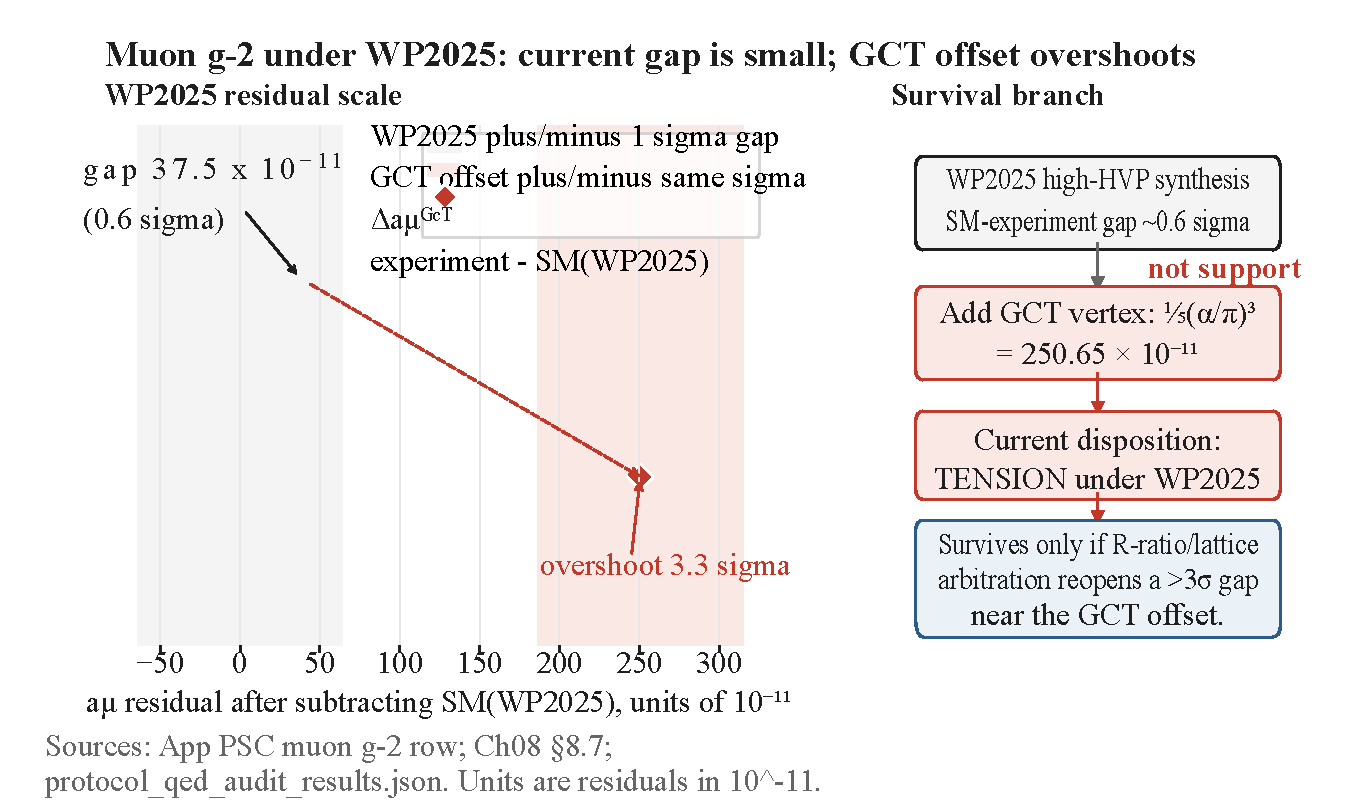
\includegraphics[keepaspectratio,alt={Under the WP2025 high-HVP synthesis, the experiment-theory gap is small while the GCT correction overshoots it; the channel survives only if R-ratio/lattice arbitration reopens a material gap near the GCT offset.}]{content/Figures/Volume_3/Figure V3.8.2.pdf}}
\caption{Under the WP2025 high-HVP synthesis, the experiment-theory gap
is small while the GCT correction overshoots it; the channel survives
only if R-ratio/lattice arbitration reopens a material gap near the GCT
offset.}
\end{figure}

\textbf{Status:} \textbf{Tier 2 law-level mechanism + Tier 3 state-level
residuals.} The lepton harmonic-ladder mechanism (resonant overtones of
the 6D hardware at \(N = 11, 17\)) is Tier 2 structural; the absolute
precision figures are state-level residuals against pole-mass targets:
the electron sits at 1006 ppm against CODATA 2022 (conditional on Open
Problem O.14 closure of the \(n = -107\) K-theoretic gap-label link),
the muon at \textasciitilde21 ppm and tau at \textasciitilde51 ppm (both
against CODATA 2022 / PDG 2024 anchors; Tier 3 formula residuals, not
theory-limited agreements --- see the Note on Precision and §PSC.2.1).
These figures are descriptive arithmetic (Tier 4 as evidence: not
distinguishable from numerology for strong effects; App PSC §PSC.9.6).

\begin{center}\rule{0.5\linewidth}{0.5pt}\end{center}

\subsection{\texorpdfstring{\textbf{PSC.2 Fundamental Coupling
Constants}}{PSC.2 Fundamental Coupling Constants}}\label{psc.2-fundamental-coupling-constants}

These constants define candidate interaction impedances of the force
sectors. Residuals here are closure gaps; a radiative-flow direction
counts only as an inserted-template compatibility diagnostic until the
physical bundle, interaction, sign, and magnitude are derived from the
microscopic action. The native flow is a Tier 3 activation ansatz (App
GRF), and for \(\sin^2\theta_W\) and \(\alpha_s\) the run does not close
the gap.

\gctneedbreak{10\baselineskip}

\begingroup\setlength{\parindent}{0pt}

\medskip\textbf{\textbf{$\alpha^{-1}$}} ---
\textbf{Tier 3 numerical relation (mechanism open) + Tier 3 600-cell multiplier + Tier 3 inserted-template residual diagnostic pending QLQCD-1L/\allowbreak{}O.19 closure}
--- the QED precision target for \(\alpha^{-1}\) is sub-ppm; the GCT
3443 ppm bare gap is therefore not a sub-ppm-class ``Postdiction''
against QED; it is a tree-level identity whose residual closure is
conditional on the QLQCD-1L bare-to-physical bridge, which is not yet
action-derived

\par

\textit{Formula:} \(360 \phi^{-2}\)

\par

\textit{Derived (bare):} \textbf{137.5078}

\par

\textit{Observed:} 137.0359

\par

\textit{Residual (gap):}
\textbf{3443 ppm bare; precise closure conditional on O.19/\allowbreak{}O.5}
--- the geometric tree-level relation \(\alpha^{-1} = 360\phi^{-2}\) is
a Tier 3 numerical relation (Tier 3 600-cell multiplier; mechanism open
--- the RT solid-angle construction is withdrawn, V1 §13.2.1--§13.2.2);
the +3443 ppm residual relative to CODATA \(\alpha^{-1}(0)\) is a Tier 3
numerical gap and a load-bearing closure target. The current phason
anti-screening calculation shows only template-direction compatibility
after a Berry/\allowbreak{}Peierls loop template is inserted: periodic
locking or a finite point-group quotient does not derive the physical
bundle, curvature, loop sign, or magnitude, and the Galois map
\(\phi\mapsto-\phi^{-1}\) fixes no physical sign. Those remain open
under O.19/\allowbreak{}O.5. A3 measured \(\alpha(0)\) is used
separately in corrected precision rows and is not evidence that the bare
alpha derivation is closed.

\par

\textit{Provenance:} script:
\texttt{protocol\_alpha\_derivation.\allowbreak{}py}

\par

\textit{Tier:} \textbf{3 relation + 3 multiplier/\allowbreak{}residual};
\textbf{Tier 4 as evidence} (φ-formula match; App PSC §PSC.9.6)

\par

\medskip\textbf{\textbf{Muon $g-2$}} ---
\textbf{Tier 3 fitted/\allowbreak{}equal-weight $1/5$ vertex coefficient + A3 precision input on top of a geometric mechanism class; not robust confirmation; reinstatable only if R-ratio + lattice-HVP reconciliation opens a $>3\sigma$ experiment–theory gap near the GCT offset (HVP arbitration condition, App PRG Table PRG.1 row P.5)}

\par

\textit{Formula:}
\(\frac{1}{5} \left( \frac{\alpha_{\rm A3}}{\pi} \right)^3\)

\par

\textit{Derived (bare):}
\textbf{$\Delta a_\mu \approx 250.65 \times 10^{-11}$}

\par

\textit{Observed:} under the consolidated high-HVP lattice-dominant
WP2025 SM theory benchmark compared with Fermilab/\allowbreak{}BNL
experiment, the experiment-theory gap is \(\sim 0.6\sigma\) --- no
significant residual anomaly; the GCT correction sits \(\sim 3.3\sigma\)
\textit{above} the consolidated closure; the CMD-3 R-ratio measurement
context is part of the reduced-tension HVP arbitration, not a GCT
confirmation

\par

\textit{Residual (gap):}
\textbf{Tension under WP2025; adverse evidence under the current world-average synthesis}

\par

\textit{Provenance:} \texttt{protocol\_qed\_audit.\allowbreak{}py}

\par

\textit{Tier:}
\textbf{3 coefficient + A3; mechanism class not empirically confirmed}

\par

\medskip\textbf{\textbf{Electron $g-2$}} ---
\textbf{Tier 3/\allowbreak{}4 activation-threshold hypothesis (not derived; virtual loops have no rest-mass threshold) + Tier 3 threshold exponent $N=11$; α-input contingent}

\par

\textit{Formula:} \(\Delta a_e^{\rm lattice} = 0\) at this loop order
(Tier 3/\allowbreak{}4 activation-threshold hypothesis, V3 Ch08 §8.7.4:
\(m_e \ll E_{\rm res} = m_e \phi^{11} \approx 101.69\text{ MeV}\), so
electron at \(N=0\) does not activate the cage-depinning loop that gives
the muon's \(1/5\) vertex correction at \(N=11\); the threshold exponent
\(N=11\) remains Tier 3)

\par

\textit{Derived (bare):} \textbf{$\Delta a_e^{\rm GCT} = 0$}

\par

\textit{Observed:} \(a_e^{\rm exp}\) (Fan et al.~2023) minus the SM
value: with Cs-α (Parker 2018)
\(\Delta a_e \approx -1.01 \times 10^{-12}\) (3.9σ); with Rb-α (Morel
2020) \(\Delta a_e \approx +0.34 \times 10^{-12}\) (2.1σ). The Cs and Rb
α determinations disagree with each other by 5.5σ.

\par

\textit{Residual (gap):} \textbf{PENDING-α-RESOLUTION} (the null is in
tension with both α inputs, by 3.9σ and 2.1σ; no branch passes)

\par

\textit{Provenance:} \texttt{verify\_g2\_electron.\allowbreak{}py}

\par

\textit{Tier:} \textbf{3–4 threshold hypothesis + 3 threshold exponent}

\par

\medskip\textbf{\textbf{$\rho_{\rm raw}$ raw Galois-frame ratio (coordinate identity)}}
---
\textbf{Tier 1 coordinate-frame identity; not a physical boundary (canonical projector shares $1/2+1/2$)}

\par

\textit{Formula:} \(\phi^{-2}\); normalized share
\(\rho_{\rm raw}/(1+\rho_{\rm raw})\)

\par

\textit{Derived (bare):} \textbf{0.38197} (normalized share
\textbf{0.27639})

\par

\textit{Observed:} --- (no physical scale)

\par

\textit{Residual (gap):} \textbf{0\% (Tier 1 exact arithmetic)}

\par

\textit{Provenance:}
\texttt{protocol\_electroweak.\allowbreak{}py::verify\_gram\_projection}

\par

\textit{Tier:} \textbf{1}

\par

\medskip\textbf{\textbf{$\sin^2\theta_W$ (bare)}} ---
\textbf{Tier 3 gauge-kinetic hypothesis (H-EW); the raw-frame volume identity of App USS §USS.9 is coordinate arithmetic; Z-pole Tier 3 observational input}
***

\par

\textit{Formula:} \(\phi^{-3}\)

\par

\textit{Derived (bare):} \textbf{0.23607}

\par

\textit{Observed:} 0.23122 (Z-pole; PDG 2026, \(\overline{\rm MS}\))

\par

\textit{Residual (gap):} \textbf{2.1\%} (cross-scale numerical
alignment, not RGE support)

\par

\textit{Provenance:} script:
\texttt{protocol\_electroweak.\allowbreak{}py},
\texttt{protocol\_weinberg\_uniqueness.\allowbreak{}py}

\par

\textit{Tier:} \textbf{3} (H-EW as a hypothesis);
\textbf{Tier 4 as evidence} (φ-formula match; App PSC §PSC.9.6)

\par

\medskip\textbf{\textbf{$\sin^2\theta_W$ (Z-pole)}} ---
\textbf{Tier 3 negative consistency result} (conditioned on measured
couplings or on A2; the target-normalized integrator is an
implementation check only)

\par

\textit{Formula:} H-EW boundary run to \(M_Z\): physical-hypercharge
one-loop comparator (full-SM \(b_Y=41/6\), \(b_2=-19/6\)) and native
kernel with the imported A2 benchmark

\par

\textit{Derived (bare):} \textbf{0.136725} (comparator) /\allowbreak{}
\textbf{0.16957} (native)

\par

\textit{Observed:} 0.23122 ± 0.00006 (PDG 2026, \(\overline{\rm MS}\))

\par

\textit{Residual (gap):} \textbf{−40.87\% /\allowbreak{} −26.66\%} (no
current route closes; V3 Ch04 §4.3.3). The pre-registered gauge-running
audit (App GRF §GRF.4.3) is a \textbf{FAILED check}: no declared-input
configuration reproduces \(\sin^2\theta_W(M_Z)\), \(\alpha_s(M_Z)\) or
\(\alpha_{\rm em}(M_Z)\) (one borderline two-loop \(\alpha_{\rm em}\)
value, which imports the measured \(\alpha_s\), is excluded by a post
hoc judgement; App GRF §GRF.4.3). Top-down from A2, H-EW,
\(\alpha_3^{-1}=10\phi^2\) and \(M_{\rm GUT}=3.2\times10^{16}\) GeV with
SM \(\beta\)-functions gives \(\sin^2\theta_W(M_Z)=0.058\)--\(0.067\)
(best case 0.0673, \textbf{−52σ}; native kernel 0.16957, −62σ), and
\(\alpha_3^{-1}\) reaches zero at 2--6×10⁶ GeV, so \(\alpha_s(M_Z)\) is
undefined; A2 and H-EW cannot both hold for any SM extension (App GRF
§GRF.4.3)

\par

\textit{Provenance:} scripts:
\texttt{protocol\_electroweak.\allowbreak{}py},
\texttt{protocol\_rge\_native.\allowbreak{}py}; App GRF

\par

\textit{Tier:} \textbf{3}

\par

\medskip\textbf{\textbf{$\alpha_s^{-1}$ (bare)}} ---
\textbf{Tier 3 calibrated handle (10 integer + $\phi^2$ geometric factor) + Tier 3 running residual pending O.42 /\allowbreak{} QLQCD-2}

\par

\textit{Formula:} \(10\phi^2\)

\par

\textit{Derived (bare):} \textbf{26.18}

\par

\textit{Observed:} \(\alpha_s^{-1}(M_Z)=8.475\) (PDG 2026
\(\alpha_s(M_Z)=0.1180\pm0.0009\))

\par

\textit{Residual (gap):} \textbf{+208.9\% inverse-space residual},
defined as
\([\alpha_s^{-1}(\mathrm{bare})-\alpha_s^{-1}(M_Z)]/\alpha_s^{-1}(M_Z)\);
equivalently, in direct-coupling space, \(\alpha_s(M_Z)\) is
\textbf{67.63\% above} \(\alpha_s(\mathrm{bare})\) when normalized to
\(\alpha_s(M_Z)\). This compares an ultraviolet handle with an \(M_Z\)
value and so mixes scales; the native run from the handle gives
\(\alpha_s(M_Z)\approx0.052\), 55.9\% low (V3 Ch04 §4.5.5). The RT
three-fold-axis count and icosahedral inflation supply a documented
strong-sector handle, not a physical \(M_Z\) precision postdiction; the
integer 10 and \(\phi^2\) factor do not close the product rule or native
running without O.42 /\allowbreak{} QLQCD-2

\par

\textit{Provenance:} \texttt{verify\_alpha\_s\_bare.\allowbreak{}py};
\texttt{protocol\_rge\_native.\allowbreak{}py}

\par

\textit{Tier:} \textbf{3 handle + 3 residual};
\textbf{Tier 4 as evidence} (φ-formula match; App PSC §PSC.9.6)

\par

\medskip\textbf{\textbf{$\theta_C$}} ---
\textbf{Contingent Postdiction /\allowbreak{} Tension}

\par

\textit{Formula:} Bare \(\phi^{-3}\) {[}Tier 3 identification{]} +
transfer correction \((1 - 5\alpha)\) {[}Tier 3 pending O.5{]}

\par

\textit{Derived (bare):} \textbf{13.1473°}

\par

\textit{Observed:} 13.0035°

\par

\textit{Residual (gap):} \textbf{1.11\%} (angle residual against the PDG
mixing anchor \(\lambda = 0.22501\), for which
\(\theta_C = \arcsin(0.22501) = 13.0035°\). The \(s_{12}=\sin\theta_C\)
residual is \(1.09\%\) in §PSC.4; the angle and sine relative residuals
differ by the parametrization factor
\(\theta_C/\tan\theta_C \approx 0.982\) at \(13°\), so they describe the
same comparison in different variables. Corrected value is Tier 3 bare
identification + Tier 3 transfer; bare \(\phi^{-3}\) residual
\(\approx 4.9\%\); the load-bearing falsification statistic is the
\(s_{12}\) comparison, a 3.6σ CKM tension in §PSC.4)

\par

\textit{Provenance:} {[}Model/\allowbreak{}Geometric{]}

\par

\textit{Tier:} 3 bare identification + 3 transfer;
\textbf{Tier 4 as evidence} (φ-formula match; App PSC §PSC.9.6)

\par

\medskip\textbf{\textbf{CKM Jarlskog \textbar{}J\textbar{}}} ---
\textbf{OPEN RESEARCH (O.7)}

\par

\textit{Formula:} No current Tier 2 prediction; the value \(|J|\) is
held as Open Problem \textbf{O.7} (App ORQ §ORQ.5). A naive
\(\phi^{-22}\) candidate formula is documented in App ORQ but is not
load-bearing for this scorecard.

\par

\textit{Derived (bare):} --- (no current Tier 2 prediction)

\par

\textit{Observed:} 3.12 × 10⁻⁵ (PDG 2024)

\par

\textit{Residual (gap):} n/\allowbreak{}a

\par

\textit{Provenance:} \texttt{verify\_jarlskog.\allowbreak{}py}
(reference harness)

\par

\textit{Tier:} \textbf{OPEN}

\par

\medskip\textbf{\textbf{Strong CP /\allowbreak{} $\bar{\theta}$}} ---
\textbf{Open problem (candidate mechanism Tier 3)}

\par

\textit{Formula:} Candidate only: an icosahedral chirality-preserving
cycle-closure argument for \(\bar{\theta} = 0\) (Tier 3 sketch; not
derived)

\par

\textit{Derived (bare):} \textbf{none} --- \(\bar{\theta}=0\) is not a
GCT prediction

\par

\textit{Observed:} \(\|d_n\| < 1.8\times 10^{-26}\ e\cdot\text{cm}\)
(2020) → \(\|\bar{\theta}\| \lesssim 10^{-10}\)

\par

\textit{Residual (gap):} OPEN-CONDITIONAL: the Strong CP problem is open
in GCT (V3 Ch18 §18.5); the present action derives no symmetry or
dynamics that suppresses \(\theta\), and respecting the bound is not a
PASS

\par

\textit{Provenance:} \texttt{verify\_strong\_cp.\allowbreak{}py}

\par

\textit{Tier:} \textbf{3}

\par

\medskip\textbf{\textbf{$G$}} --- \textbf{Postdiction} ---
model-authoritative GCT-bare-\(\alpha\) branch with CODATA \(m_e\) and
exact SI \(h,c\); the all-CODATA-\(\alpha\) sensitivity branch is
2013.345 ppm. Derived from P.1c (\(G \propto m_e^{-2}\); the 2013.345
ppm branch is the 1006 ppm electron residual doubled), so it is not
independent and inherits P.1c's FAIL (App FSM P.16). Tier 3 numerical
residual pending O.14 physical-link refinement. This is the Jacobson
route only: the elasticity formula of the former Routes 2/\allowbreak{}3
is retired and does not enter (App DPS §DPS.7; O.22)

\par

\textit{Formula:}
\(a_6 = (2\hbar/m_e c)\phi^{-107}(1-5\alpha_{\rm GCT}),\ \alpha_{\rm GCT}=\phi^2/360;\ G = c^3 a_6^2/(4\hbar)\)

\par

\textit{Derived (bare):} \textbf{$6.689475523 \times 10^{-11}$}

\par

\textit{Observed:} \(6.67430 \times 10^{-11}\) (CODATA 2022)

\par

\textit{Residual (gap):}
\textbf{0.23\% (2273.725 ppm; display 2274 ppm)}

\par

\textit{Provenance:} script:
\texttt{protocol\_absolute\_scale.\allowbreak{}py} (canonical source);
independently re-derived in \texttt{verify\_newton\_g.\allowbreak{}py}

\par

\textit{Tier:}
\textbf{2 mechanism + 4 Planck-link + 3 residual/\allowbreak{}A1};
\textbf{Tier 4 as evidence} (φ-formula match; App PSC §PSC.9.6)

\par

\medskip\textbf{\textbf{Higgs VEV ($v$)}} ---
\textbf{Conditional postdiction /\allowbreak{} anchor-normalized comparison}

\par

\textit{Formula:}
\(m_e \phi^{11} (1 + 5\alpha_{\rm A3} + \phi^{8}\alpha_{\rm A3}^{2})\, 1440\,\phi\)

\par

\textit{Derived (bare):} \textbf{246.1755 GeV} (engine full precision
per
\texttt{protocol\_higgs\_vev\_results.\allowbreak{}json::v\_derived\_GeV})

\par

\textit{Observed:} \textbf{246.21965 GeV} (PDG-2024 Fermi-constant
anchor)

\par

\textit{Residual (gap):} \textbf{179 ppm} (full-precision residual
179.15 ppm). \textbf{OPEN-CONDITIONAL:} the Tier 2
product/\allowbreak{}mechanism arithmetic inherits the Tier 3 O.38
\(N_{\rm cage}=144\) posit, CODATA-2022 A3 measured \(\alpha(0)\), and a
Tier 3 calibrated-handle residual. O.20 enumerates \(1440\)
factorisations but does not select the \(144\times10\) physical branch.
The spectral-action cutoff \(\Lambda_{\rm Higgs}\) belongs to the
independent Higgs-mass route.

\par

\textit{Provenance:} script:
\texttt{protocol\_higgs\_vev.\allowbreak{}py} (canonical);
\texttt{verify\_higgs\_vev.\allowbreak{}py}

\par

\textit{Tier:}
\textbf{OPEN-CONDITIONAL: Tier 2 product arithmetic conditional on Tier 3 O.38 $N_{\rm cage}=144$ + A3 + Tier 3 VEV-handle residual};
\textbf{Tier 4 as evidence} (φ-formula match; App PSC §PSC.9.6)

\par

\medskip\textbf{\textbf{Higgs mass ($m_H$, bare)}} ---
\textbf{Postdiction (radiative-correction-contingent)} ---
\textbf{Tier 3 bare packing ansatz ($\lambda_{\rm bare} = 1/8$ on an added broken-vacuum completion; V3 Ch05 §5.2.3) + Tier 3 numerical residual (−1.69\% bare gap; precise closure conditional on O.5)}

\par

\textit{Formula:} \(v \cdot \sqrt{2\lambda_{\rm bare}} = v/2\) with
\(\lambda_{\rm bare} = 1/8\) (Tier 3 bare packing ansatz, V3 Ch05
§5.2.3)

\par

\textit{Derived (bare):} \textbf{123.09 GeV} (with
\(v_{\rm GCT}=246.1755\) GeV, the convention of the top-quark row; with
the measured \(v=246.21965\) GeV it would be 123.11 GeV)

\par

\textit{Observed:} 125.20 ± 0.11 GeV (PDG 2024)

\par

\textit{Residual (gap):}
\textbf{−1.69\% (−2.11 GeV; 19σ against the PDG uncertainty)} --- the
bare GCT tree-level value lies below the PDG mass. Standard SM 1-loop
radiative corrections to the Higgs pole mass (top-loop
quadratic-divergence cancellation under renormalization,
\(\overline{\rm MS}\) to pole conversion at order \(\alpha_t\),
\(\alpha_s\), \(\alpha_W\) contributions; cf.~Buttazzo et al.~2013
\textit{JHEP} 12:089) generate \(\mathcal{O}(\text{few \%})\) shifts
whose sign depends on the renormalization scheme and is \textit{not} a
free observation from this row --- the GCT 1-loop closure that would
derive the specific sign and magnitude from the AKN lattice bundles with
QLQCD-1L (App ORQ O.5, App TPR §TP-E). See Higgs-sector
handle-accounting callout below.

\par

\textit{Provenance:} \texttt{verify\_higgs\_mass.\allowbreak{}py}

\par

\textit{Tier:} \textbf{3 bare ansatz /\allowbreak{} 3 specific value}

\par
\endgroup

\gctneedspace{5\baselineskip}\begin{gctImportant}

\textbf{Higgs sector handle accounting} {[}OPEN-CONDITIONAL{]}: the VEV
evaluation
\(v = m_e \phi^{11}(1 + 5\alpha + \phi^{8}\alpha^{2}) \cdot 1440\phi\)
depends on the muon-mass formula, the \(N=11\) harmonic anchor,
CODATA-2022 A3, and the exact product \(1440=144\times10\). That product
inherits the Tier 3 O.38 \(N_{\rm cage}=144\) posit; O.20 is an
enumeration result and does not select the branch. The 179 ppm figure
against the sole declared observational anchor \(v=246.21965\) GeV is
therefore a conditional comparison, not a Tier 2 absolute-scale closure.
The Tier 3 bare packing ansatz \(\lambda_{\rm bare}=1/8\) (no geometric
quantity currently fixes it) and the spectral-action cutoff
\(\Lambda_{\rm Higgs}\) belong to the separate Higgs-mass route.

\end{gctImportant}

**** \textbf{Weinberg boundary:} \(\phi^{-2}\) is the exact raw
Galois-frame ratio \(\rho_{\rm raw}\) (coordinate-dependent; normalized
share \(0.27639\)), the canonical projectors give shares \(1/2+1/2\),
and \(\phi^{-3}\) is the Tier 3 gauge-kinetic hypothesis H-EW (V3 Ch04
§4.3). None of these values is a derived physical Weinberg angle.*

\textbf{Status:} \textbf{Tier 3 numerical relation for the
fine-structure route (mechanism open; the RT solid-angle construction is
withdrawn, V1 §13.2.1--§13.2.2); Tier 3 handles (H-EW, \(10\phi^2\)) and
Tier 3 state-level residuals.} The icosahedral projection fixes the
complementary subspaces but does not by itself assign electroweak
coupling strengths. It supplies candidate gauge-coupling handles from
the unit cell axes (raw-frame projection ratios are Tier 1 coordinate
arithmetic, not physical sector weights; the bare Weinberg angle is the
Tier 3 hypothesis H-EW and \(10\phi^2\) is a Tier 3 calibrated handle);
the specific numerical residuals against current empirical anchors are
Tier 3 state-level closure targets. Notably: \(\alpha^{-1}\) sits at
3443 ppm bare residual (closure conditional on QLQCD-1L per O.5);
\(\alpha_s^{-1}\) has the largest gauge-coupling gap, with the
registered bare handle \(10\phi^2=26.18\) versus the PDG-2026 \(M_Z\)
value \(8.475\), a \textbf{+208.9\% inverse-space residual under the
observed-value denominator convention} (the separately labelled
direct-space comparison is 67.63\%; both compare a GUT-scale handle with
an \(M_Z\) value, while the native run gives 55.9\% low; pending O.42 /
QLQCD-2); the Higgs bare mass lies \textbf{−1.69\%} (with
\(v_{\rm GCT}\)) below the observed mass (closure conditional on O.5
1-loop); muon g-2 carries a ``Tension under WP2025; falsification
conditional on long-term HVP-synthesis arbitration'' disposition under
the WP2025 lattice HVP synthesis; PMNS \(\theta_{23}=45°\) lies inside
the NuFIT 6.0 3σ ranges with and without Super-Kamiokande atmospheric
data, with the octant unresolved (see §PSC.4). The fine-structure
relation keeps its stated Tier 3 row tier; the headline status records
that several state-level numerical residuals depend on Open Problem O.5
closure, and no residual in this table counts as evidence for an
anti-screening sign. Where a φ-formula in this table matches its target,
the match is descriptive arithmetic (Tier 4 as evidence: not
distinguishable from numerology for strong effects; App PSC §PSC.9.6),
and the pre-registered gauge-running check from the H-EW boundary is
FAILED (App GRF §GRF.4.3).

\subsection{\texorpdfstring{\textbf{PSC.2.1 Loop-Order Discipline ---
Radiative-Correction
Provenance}}{PSC.2.1 Loop-Order Discipline --- Radiative-Correction Provenance}}\label{psc.2.1-loop-order-discipline-radiative-correction-provenance}

The GCT formulas in §PSC.1--PSC.2 (lepton masses,
\(\alpha^{-1}_{\text{tree}}\), Cabibbo angle, etc.; tiers as stated per
row) are labeled ``tree-level'' or ``tree + 1-loop'' according to the
loop order actually present in the displayed expression. The ppm-level
residuals quoted for the muon and tau are scored against measured CODATA
/ PDG masses (\(m_\mu\) to 22 ppb, \(m_\tau\) to 51 ppm). A measured
mass is not a theory quantity: the earlier statement that these targets
``already include'' SM corrections of \textasciitilde10--40 ppm, so that
a GCT theory floor of that size absorbs the residuals, is withdrawn. No
GCT higher-loop calculation exists, so no theory error is assigned.
Lepton precision rows are Tier 2 mechanism + Tier 3 formula residual.

\gctneedbreak{10\baselineskip}

\begingroup
\scriptsize
\setlength{\LTpre}{6pt}\setlength{\LTpost}{4pt}
\setlength{\tabcolsep}{3pt}
\hyphenpenalty=50\exhyphenpenalty=50
\sloppy
\begin{longtable}{>{\raggedright\arraybackslash\hspace{0pt}}p{0.0787\linewidth}>{\raggedright\arraybackslash\hspace{0pt}}p{0.1098\linewidth}>{\raggedright\arraybackslash\hspace{0pt}}p{0.1557\linewidth}>{\raggedright\arraybackslash\hspace{0pt}}p{0.5357\linewidth}}
\toprule
\textbf{Row} & \textbf{Bare GCT residual} & \textbf{GCT + displayed correction residual} & \textbf{Measured target and residual status} \\
\midrule
\endhead
\bottomrule
\endlastfoot
Muon $m_\mu$ & $\sim -3.75\%$ for $m_e\phi^{11}$ & $\sim 0.24\%$ after $(1+5\alpha)$; $\sim 21$ ppm after the Tier 3-selected $\phi^8\alpha^2$ correction ansatz & Scored against the CODATA 2022 mass (22 ppb); the existence of a correction channel and the specific $\phi^8\alpha^2$ exponent/\allowbreak{}coefficient are kept separate, the latter being a Tier 3 selection rather than a derived one-loop heat-kernel term; the 21 ppm residual is ≈$10^3\sigma$ in measurement terms and is a Tier 3 formula residual pending QLQCD-1L (App ORQ O.5); the unpropagated next-order term $\phi^8\alpha^3\approx18$ ppm is the same size, so the row does not test the second-order term \\
\addlinespace[2pt]
Tau $m_\tau$ & $\sim +2.69\%$ for $m_e\phi^{17}$ & $\sim 51$ ppm against PDG 2024 after the single $(1-3.6\alpha)$ correction & Scored against the PDG 2024 mass (1776.93 ± 0.09 MeV; the residual is ≈1.0σ in measurement terms); the $-3.6$ coefficient carries Tier 2 mechanism + Tier 2 integer $D=18$ + $N=5$ $A_5$ irrep count (Tier 3 as a channel number) + Tier 3 combination rule $c=-D/N$ pending O.26b \\
\addlinespace[2pt]
Electron anchor & $m_e$ is the dimensional anchor & The $n=-107$ Planck-link residual is $\sim 1006$ ppm & Physical-link closure depends on App ORQ O.14 /\allowbreak{} O.5; it is not a lepton-pair prediction residual \\
\end{longtable}
\endgroup

\textbf{Implication for Tier 2 status:} the ppm figures state how far
the GCT geometric form plus displayed correction lies from the measured
mass. They carry no theory-error model, so they are residuals, not
agreements within a theory error. QLQCD-1L closure (App ORQ O.5) is the
path that would supply a GCT-internal loop derivation and an error
estimate.

\subsection{\texorpdfstring{\textbf{PSC.2.2 Hypercharge Assignment and
Anomaly
Cancellation}}{PSC.2.2 Hypercharge Assignment and Anomaly Cancellation}}\label{psc.2.2-hypercharge-assignment-and-anomaly-cancellation}

The L/R-asymmetric Standard Model hypercharges follow from the
icosahedral identification of right-handed singlets with
\(E_\perp\)-sterile states (V3 Ch04): for right-handed sterile singlets
(\(I_3 = 0\)) the Gell-Mann--Nishijima relation \(Q = T_3 + Y/2\)
reduces to \(Y_R = 2Q\). The full one-generation hypercharge assignment
in the \(Q = T_3 + Y/2\) convention is therefore:

\gctneedbreak{10\baselineskip}

{\def\LTcaptype{none} % do not increment counter
\begin{longtable}[]{@{}
  >{\raggedright\arraybackslash}p{(\linewidth - 6\tabcolsep) * \real{0.2105}}
  >{\centering\arraybackslash}p{(\linewidth - 6\tabcolsep) * \real{0.2632}}
  >{\centering\arraybackslash}p{(\linewidth - 6\tabcolsep) * \real{0.2632}}
  >{\centering\arraybackslash}p{(\linewidth - 6\tabcolsep) * \real{0.2632}}@{}}
\toprule\noalign{}
\begin{minipage}[b]{\linewidth}\raggedright
Multiplet
\end{minipage} & \begin{minipage}[b]{\linewidth}\centering
\(T_3\)
\end{minipage} & \begin{minipage}[b]{\linewidth}\centering
\(Q\)
\end{minipage} & \begin{minipage}[b]{\linewidth}\centering
\(Y\)
\end{minipage} \\
\midrule\noalign{}
\endhead
\bottomrule\noalign{}
\endlastfoot
\(Q_L = (u_L, d_L)\) (LH quark doublet, color triplet) & \(\pm 1/2\) &
\(+2/3, -1/3\) & \(+1/3\) \\
\(u_R\) (RH up, color triplet) & \(0\) & \(+2/3\) & \(+4/3\) \\
\(d_R\) (RH down, color triplet) & \(0\) & \(-1/3\) & \(-2/3\) \\
\(L_L = (\nu_L, e_L)\) (LH lepton doublet) & \(\pm 1/2\) & \(0, -1\) &
\(-1\) \\
\(e_R\) (RH electron) & \(0\) & \(-1\) & \(-2\) \\
\end{longtable}
}

The four Standard Model gauge-anomaly cancellation conditions on this
one-generation assignment evaluate to zero algebraically:

\[
\begin{aligned}
[SU(3)]^2 \cdot U(1)_Y :\quad & 2\,Y_Q - Y_u - Y_d = 2\cdot\tfrac{1}{3} - \tfrac{4}{3} - (-\tfrac{2}{3}) = 0 \\
[SU(2)]^2 \cdot U(1)_Y :\quad & 3\,Y_Q + Y_L = 3\cdot\tfrac{1}{3} + (-1) = 0 \\
\text{grav}^2 \cdot U(1)_Y :\quad & 6\,Y_Q + 2\,Y_L - 3\,Y_u - 3\,Y_d - Y_e = 2 - 2 - 4 + 2 + 2 = 0 \\
[U(1)_Y]^3 :\quad & 6\,Y_Q^3 + 2\,Y_L^3 - 3\,Y_u^3 - 3\,Y_d^3 - Y_e^3 = 0 \quad \text{(machine-precision residual)}
\end{aligned}
\]

The colour multiplicity 3 enters quark contributions; the doublet
multiplicity 2 enters the gravitational and \(U(1)^3\) traces via
LH-doublet components. Coefficient signs (+ for LH, − for RH via
chirality flip) reflect the anomaly-trace convention. Engine
verification computes all four traces and the right-handed-singlet
identity in a single L\_∞ residual:
\texttt{GCT\_Physics\_Engine/verify\_independent/verify\_hypercharges.py}
reports machine-precision PASS (max residual \(\sim 10^{-15}\) from
\([U(1)]^3\) float roundoff).

\textbf{Tier discipline (two distinct claims must be separated).} The
vanishing of the four anomaly traces given the standard one-generation
L/R-asymmetric hypercharge assignment is a textbook SM identity (Bilal
2008 arXiv:0802.0634 §7.3; standard QFT references); calling that
arithmetic Tier 2 GCT-specific would be inflation. \textbf{Two distinct
claims live in this subsection:}

\begin{enumerate}
\def\labelenumi{\arabic{enumi}.}
\item
  \textbf{The four-trace cancellation} given the standard hypercharge
  assignment is \textbf{Tier 1 textbook algebraic identity} --- it does
  not depend on GCT-specific content. We list it here for completeness,
  to demonstrate that the verifier
  \texttt{verify\_independent/verify\_hypercharges.py} reproduces the
  textbook result to machine precision (max residual \(\sim 10^{-15}\)),
  not to claim GCT-specific credit for it.
\item
  \textbf{The L/R-asymmetric hypercharge assignment itself} --- that
  right-handed singlets are \(E_\perp\)-sterile and that \(Y_R = 2Q\)
  follows from the icosahedral \(E_\parallel/E_\perp\) split (V3 Ch04)
  --- is a \textbf{Tier 2 GCT-specific structural claim}. The
  load-bearing GCT content of this section is the L/R-asymmetric
  hypercharge assignment under the \(E_\parallel/E_\perp\) split
  premise; the subsequent anomaly arithmetic is included for
  completeness against the standard SM consistency check.
\end{enumerate}

\begin{center}\rule{0.5\linewidth}{0.5pt}\end{center}

\subsection{\texorpdfstring{\textbf{PSC.3 Hadron
Sector}}{PSC.3 Hadron Sector}}\label{psc.3-hadron-sector}

The Proton mass is modelled as the global energy minimum of the
icosahedral projection, obtained from the winding sum of the Baryonic
Triad (Tier 2 mechanism + Tier 3 sheet/exponent handle pending
AKN-action closure).

\begin{quote}
\textbf{Proton mass --- three values guide:}

\begin{enumerate}
\def\labelenumi{\arabic{enumi}.}
\tightlist
\item
  \textbf{Formula prediction (the GCT value):
  \(m_p = m_e \cdot \phi^{15+\phi^{-1}} \approx 938.417\) MeV.} This is
  the tree-level output of the baryonic-triad mechanism evaluated
  against the CODATA \(m_e\). The residual against the CODATA \(m_p\) is
  \(\approx 155\) ppm. Disposition: \textbf{Tier 2 mechanism + Tier 3
  sheet/exponent handle pending AKN-action closure}, not hadron-mass
  closure from the current postulate set.
\item
  \textbf{CODATA observation: \(m_p = 938.272\) MeV.} The empirical
  anchor against which the prediction is scored.
\item
  \textbf{Ratio formula:
  \(m_p/m_e = \phi^{15+\phi^{-1}} \approx 1836.437\)} vs CODATA observed
  \(1836.153\). Same \(\sim0.015\%\) residual, expressed as a
  dimensionless ratio.
\end{enumerate}

The \(\sim0.015\%\) residual is the current tree-level precision of the
\(\phi\)-power formula under the layered Tier 2 mechanism + Tier 3
sheet/exponent disposition; closure to higher precision and promotion of
the sheet-doubling handle are QLQCD-1L / AKN-action targets (App QLA).
Ppm-level display is not used as evidential precision for this
offset-fitted handle. As evidence that φ or icosahedral structure is
special, this match is \textbf{Tier 4} (constant control test v3,
NEGATIVE-FRAGILE; App PSC §PSC.9.6); the number is kept as descriptive
arithmetic.
\end{quote}

Quark masses are renormalized QCD parameters, not invariant rest masses.
The comparison convention is therefore explicit in the table: \(u,d,s\)
use \(\overline{\mathrm{MS}}\) at 2 GeV; \(c,b\) use
\(\overline{\mathrm{MS}}\) at \(\mu=m_q\); \(t\) is compared with the
PDG 2024 direct-measurement mass (not a pole mass), with the mass-scheme
question retained as a Tier 3 residual. Besides their row bands, the
quark rows are scored by one common rule: the prediction is compared
with the PDG 2024 value and its quoted uncertainty, and a miss of more
than 5σ is a FAIL. Only the top (5.18σ) and bottom (6.9σ) rows fail it.

\gctneedbreak{10\baselineskip}

\begingroup\setlength{\parindent}{0pt}

\medskip\textbf{\textbf{Proton ($m_p$)}} --- \textbf{Postdiction}

\par

\textit{Formula:} \(m_e \phi^{15 + \phi^{-1}}\)

\par

\textit{Derived:} \textbf{938.417 MeV}

\par

\textit{Empirical convention:} Bound-state rest mass

\par

\textit{Scale:} CODATA 2022

\par

\textit{Observed:} 938.272 MeV

\par

\textit{Precision (residual):} \textbf{\textasciitilde{}0.015\%} (+155
ppm, inside the 500 ppm postdiction band)

\par

\textit{Provenance:} \(m_e\) (CODATA) \(\to m_p\); Tier 3
sheet/\allowbreak{}exponent handle pending AKN-action closure; ppm
display suppressed for this offset-fitted handle

\par

\textit{Tier:} 2 mechanism + 3 handle; \textbf{Tier 4 as evidence}
(φ-formula match; App PSC §PSC.9.6)

\par

\medskip\textbf{\textbf{Top Quark ($m_t$)}} ---
\textbf{Postdiction /\allowbreak{} FAIL of the written rule}

\par

\textit{Formula:} \((v_{\rm GCT}/2)\sqrt{2}\) (Fracture) *

\par

\textit{Derived:} \textbf{174.072 GeV}

\par

\textit{Empirical convention:} Direct-measurement mass

\par

\textit{Scale:} PDG 2024 direct measurements (not a pole mass)

\par

\textit{Observed:} 172.57 ± 0.29 GeV

\par

\textit{Precision (residual):} \textbf{+0.871\%}
(state-level/\allowbreak{}mass-scheme residual; 5.18σ, a FAIL of the
written P.24 ±5σ rule, by the same standard as the electron row; against
PDG's pole mass from cross sections, 172.4 ± 0.7 GeV, it is ≈2.4σ, and
the mass-scheme question is open --- the registered comparator is not
swapped after the result)

\par

\textit{Provenance:} scripts:
\texttt{protocol\_higgs\_vev.\allowbreak{}py},
\texttt{protocol\_quark\_mismatch.\allowbreak{}py}

\par

\textit{Tier:} Tier 2 mechanism + Tier 3
state-level/\allowbreak{}mass-scheme residual

\par

\medskip\textbf{\textbf{Bottom Quark ($m_b$)}} ---
\textbf{Postdiction /\allowbreak{} FAIL}

\par

\textit{Formula:} \(m_c \phi^2 (5/4)\)

\par

\textit{Derived:} \textbf{4134.69 MeV}

\par

\textit{Empirical convention:} \(\overline{\mathrm{MS}}\) running mass

\par

\textit{Scale:} \(\mu=m_b\)

\par

\textit{Observed:} 4183 ± 7 MeV (PDG 2024)

\par

\textit{Precision (residual):} \textbf{−1.15\%; 6.9σ low} (more if PDG's
±7 MeV is read as the 90\% CL interval it is labelled as). By the rule
applied to the top quark this is a \textbf{FAIL}. The earlier window
``4130--4230 MeV'' was centred on the measurement, not on the
prediction, so it could not test the prediction; it is withdrawn as a
test. The residual stays a Tier 3 state-level residual pending O.5, and
the mass-scheme question is open

\par

\textit{Provenance:} script:
\texttt{protocol\_quark\_mismatch.\allowbreak{}py}

\par

\textit{Tier:} 3 absolute state-value; \textbf{Tier 4 as evidence}
(φ-formula match; App PSC §PSC.9.6)

\par

\medskip\textbf{\textbf{Charm Quark ($m_c$)}} --- \textbf{Postdiction}

\par

\textit{Formula:} \(m_u \phi^{13+\phi^{-3}}\) (Mixed-Harmonic Area Law
heuristic at \(N=17\); K-theoretic gap-label derivation pending O.5)

\par

\textit{Derived:} \textbf{1263.45 MeV}

\par

\textit{Empirical convention:} \(\overline{\mathrm{MS}}\) running mass

\par

\textit{Scale:} \(\mu=m_c\)

\par

\textit{Observed:} 1273.0 ± 4.6 MeV (PDG 2024)

\par

\textit{Precision (residual):} \textbf{−0.75\% (2.1σ low)}

\par

\textit{Provenance:} script:
\texttt{protocol\_quark\_mismatch.\allowbreak{}py}

\par

\textit{Tier:} 3; \textbf{Tier 4 as evidence} (φ-formula match; App PSC
§PSC.9.6)

\par

\medskip\textbf{\textbf{Strange Quark ($m_s$)}} --- \textbf{Postdiction}

\par

\textit{Formula:} \(m_u \phi^8 (1-12\alpha)\)

\par

\textit{Derived:} \textbf{92.79 MeV}

\par

\textit{Empirical convention:} \(\overline{\mathrm{MS}}\) running mass

\par

\textit{Scale:} 2 GeV

\par

\textit{Observed:} 93.5 MeV (PDG 2024)

\par

\textit{Precision (residual):} \textbf{0.76\%}

\par

\textit{Provenance:} script:
\texttt{protocol\_quark\_mismatch.\allowbreak{}py} (\(12\alpha\) drag
coefficient is Tier 3 under the Ledger)

\par

\textit{Tier:} 3; \textbf{Tier 4 as evidence} (φ-formula match; App PSC
§PSC.9.6)

\par

\medskip\textbf{\textbf{Down Quark ($m_d$)}} --- \textbf{Postdiction}

\par

\textit{Formula:} \(m_u \cdot \phi^{\phi}\) as the FK-determinant
infinite-volume-limit closed form; rigorous convergence proof
conditional on O.5

\par

\textit{Derived:} \textbf{4.716 MeV}

\par

\textit{Empirical convention:} \(\overline{\mathrm{MS}}\) running mass

\par

\textit{Scale:} 2 GeV

\par

\textit{Observed:} 4.70 ± 0.07 MeV (PDG)

\par

\textit{Precision (residual):} \textbf{0.33\%} ---
POSTDICTION-CONSISTENT conditional, inside the 11\% shell-resonance
gate. Tier 2 FK-determinant mechanism + Tier 3 \(\phi^{\phi}\)
identification of the shell median (infinite-volume limit open, O.5);
closed-cage deep-tail mean \(\det_{FK}/\phi^{\phi}=0.9976\) (sample std
\(0.0253\)), with sequence-mean signed error vs PDG \(+0.09\%\).
Single-cage values oscillate inside the 11\% band with empirical
decaying envelope, so the match is a central tendency rather than a
single clean value.

\par

\textit{Provenance:} script:
\texttt{protocol\_quark\_mismatch.\allowbreak{}py} +
\texttt{protocol\_md\_fk\_ih\_closed\_cages.\allowbreak{}py}

\par

\textit{Tier:} 2 mechanism + 3 conditional; \textbf{Tier 4 as evidence}
(φ-formula match; App PSC §PSC.9.6)

\par

\medskip\textbf{\textbf{Up Quark ($m_u$)}} --- \textbf{Postdiction}

\par

\textit{Formula:} \(m_e \phi^3\)

\par

\textit{Derived:} \textbf{2.16 MeV}

\par

\textit{Empirical convention:} \(\overline{\mathrm{MS}}\) running mass

\par

\textit{Scale:} 2 GeV

\par

\textit{Observed:} 2.16 MeV

\par

\textit{Precision (residual):} \textbf{0.21\%}

\par

\textit{Provenance:} script:
\texttt{protocol\_quark\_mismatch.\allowbreak{}py}

\par

\textit{Tier:} Tier 2 geometric motif + Tier 3 QCD
scheme/\allowbreak{}running bridge; \textbf{Tier 4 as evidence}
(φ-formula match; App PSC §PSC.9.6)

\par
\endgroup

\emph{* Calculated using the absolute GCT Higgs-VEV pipeline value
\(v_{\rm GCT}=246.1755\) GeV from \texttt{protocol\_higgs\_vev.py}; the
measured electroweak VEV is not used as an input to this row.} \emph{The
5/4 coefficient is a Tier 2 representation-theory coefficient, but the
absolute bottom-quark prediction imports the Tier 3 \(m_c\) input and is
therefore Tier 3 as a state-level residual conditional on O.5; the row
fails the ±5σ rule (App FSM P.23).} \emph{The exponents \(13+\phi^{-3}\)
(\(m_c\)), \(\phi^{\phi}\) (\(m_d\)), \(6+\phi^{-1}\) and
\(11+\phi^{-1}\) (CKM \(s_{23}\), \(s_{13}\)) match observed
\(\log_\phi\) values through irrational offsets (integer
\(+\,\phi^{-k}\), or \(\phi^{\phi}\)) found by postdictive search; no
trial factor is applied for that family of offsets, so these rows are
postdiction-search results and are not counted as evidence.}

\textbf{Status:} \textbf{Tier 2 law-level mechanism
(Fuglede-Kadison-determinant chain rooted natively in the Planck scale)
+ Tier 3 state-level residuals.} The hadron mass chain follows the
FK-determinant law-level structure. The down-quark row uses the primary
\(\phi^{\phi}\) infinite-volume-limit closed form and is
POSTDICTION-CONSISTENT at \(+0.33\%\) inside the registered
shell-resonance band, conditional on O.5 for rigorous convergence and
algebraic-field identification. Two quark rows fail the ±5σ rule: top
(5.18σ) and bottom (6.9σ). The φ-formula quark matches (\(m_u\),
\(m_d\), \(m_s\), \(m_c\), \(m_b\)) are descriptive arithmetic (Tier 4
as evidence: not distinguishable from numerology for strong effects; App
PSC §PSC.9.6); the top row contains no φ and is not relabelled.

\begin{center}\rule{0.5\linewidth}{0.5pt}\end{center}

\subsection{\texorpdfstring{\textbf{PSC.4 Mixing Geometry
Matrices}}{PSC.4 Mixing Geometry Matrices}}\label{psc.4-mixing-geometry-matrices}

\textbf{{[}Tier 3 candidate identification{]}:} CKM and PMNS matrices
are CANDIDATELY identified with the topological tunneling and axis
sliding operations; closure pending O.5/O.7.

\gctneedbreak{10\baselineskip}

\begingroup\setlength{\parindent}{0pt}

\medskip\textbf{\textbf{Cabibbo Angle ($s_{12}$)}} ---
\textbf{Contingent Postdiction /\allowbreak{} Tension}

\par

\textit{Formula:} Bare \(\phi^{-3}\) {[}Tier 3 identification{]} +
transfer correction \((1 - 5\alpha)\) {[}Tier 3 pending O.5{]}

\par

\textit{Prediction:} \textbf{0.2275}

\par

\textit{Observed / bound:} \(0.2250\)

\par

\textit{Precision / status:} \textbf{1.09\%} (bare \(\phi^{-3}\)
residual \(\approx 4.9\%\); corrected
\(s_{12}=\phi^{-3}\cdot(1-5\alpha)\) is a \textbf{3.6σ tension} under
the registered comparison)

\par

\textit{Tier:} 3 bare identification + 3 transfer;
\textbf{Tier 4 as evidence} (φ-formula match; App PSC §PSC.9.6)

\par

\medskip\textbf{\textbf{CKM $s_{23}$}} --- \textbf{Ansatz}

\par

\textit{Formula:} \(\phi^{-(6 + \phi^{-1})}\)

\par

\textit{Prediction:} \textbf{0.0414}

\par

\textit{Observed / bound:} \(0.04183^{+0.00079}_{-0.00069}\)

\par

\textit{Precision / status:} \textbf{−1.05\%} (0.6σ; −0.98\% vs the
rounded engine comparator 0.0418 used in App FSM/\allowbreak{}GPE)

\par

\textit{Tier:} 3; \textbf{Tier 4 as evidence} (φ-formula match; App PSC
§PSC.9.6)

\par

\medskip\textbf{\textbf{CKM $s_{13}$}} --- \textbf{Ansatz}

\par

\textit{Formula:} \(\phi^{-(11 + \phi^{-1})}\)

\par

\textit{Prediction:} \textbf{0.003732}

\par

\textit{Observed / bound:} \(0.003732\)

\par

\textit{Precision / status:} \textbf{0.0076\%} (Tier 3 offset-fit
ansatz; ppm display suppressed)

\par

\textit{Tier:} 3; \textbf{Tier 4 as evidence} (φ-formula match; App PSC
§PSC.9.6)

\par

\medskip\textbf{\textbf{PMNS $\theta_{12}$}} --- \textbf{Postdiction}

\par

\textit{Formula:} \(\arctan(1/\phi) + (\theta_{13}/5)\)

\par

\textit{Prediction:} \textbf{33.40°}

\par

\textit{Observed / bound:} \(33.68^{+0.73}_{-0.70}\)° (NuFIT 6.0)

\par

\textit{Precision / status:} \textbf{−0.85\%} (0.4σ)

\par

\textit{Tier:} 3; \textbf{Tier 4 as evidence} (φ-formula match; App PSC
§PSC.9.6)

\par

\medskip\textbf{\textbf{PMNS $\theta_{23}$}} ---
\textbf{Prediction (open)}

\par

\textit{Formula:} \(45°\)

\par

\textit{Prediction:} \textbf{45.00°}

\par

\textit{Observed / bound:} NuFIT 6.0, normal ordering:
\(43.3^{+1.0}_{-0.8}\)° with SK atmospheric data (3σ range
41.3°--49.9°); \(48.5^{+0.7}_{-0.9}\)° without (3σ range 41.0°--50.5°)

\par

\textit{Precision / status:} \textbf{inside both 3σ ranges}:
\(\Delta\chi^2(45°)\approx2.0\) with SK and \(\approx4.2\) without
(≈1.4σ and ≈2.0σ); octant unresolved †

\par

\textit{Tier:} \textbf{3}

\par

\medskip\textbf{\textbf{PMNS $\theta_{13}$}} --- \textbf{Postdiction}
(θ₁₃ was measured in 2012)

\par

\textit{Formula:} \(\arcsin(\phi^{-4})\)

\par

\textit{Prediction:} \textbf{8.39°}

\par

\textit{Observed / bound:} \(8.56 \pm 0.11\)° (NuFIT 6.0 with SK;
\(8.52 \pm 0.11\)° without)

\par

\textit{Precision / status:} \textbf{−2.0\% (1.5σ)} /\allowbreak{}
−1.5\% (1.2σ)

\par

\textit{Tier:} 3; \textbf{Tier 4 as evidence} (φ-formula match; App PSC
§PSC.9.6)

\par

\medskip\textbf{\textbf{CP Phase ($\delta_{CP}$)}} ---
\textbf{OPEN\_CONDITIONAL}

\par

\textit{Formula:} \(2\pi \cdot \phi^{-1}\)

\par

\textit{Prediction:} \textbf{222.49°}

\par

\textit{Observed / bound:} NuFIT 6.0, normal ordering:
\(212^{+26}_{-41}\)° with SK; \(177^{+19}_{-20}\)° without
(non-Gaussian)

\par

\textit{Precision / status:} \textbf{+0.4σ with SK; +2.4σ without} ---
the tension depends on the data set

\par

\textit{Tier:} 3; \textbf{Tier 4 as evidence} (φ-formula match; App PSC
§PSC.9.6)

\par

\medskip\textbf{\textbf{CKM 3×3 Unitarity Diagnostic ‡}} ---
\textbf{Diagnostic}

\par

\textit{Formula:} \(\sum_k V_{ik} V_{jk}^* = \delta_{ij}\)

\par

\textit{Prediction:}
\textbf{Diagnostic exact by construction; max residual $1.11\times10^{-16}$}

\par

\textit{Observed / bound:} Unitary (PDG 2024 fit)

\par

\textit{Precision / status:}
\textbf{Tier 1 algebraic bookkeeping for a matrix built in the standard unitary parameterization; physical CKM content sits in the mixing-angle comparison rows, with residuals pending O.7/\allowbreak{}O.5 rather than a unitarity defect}

\par

\textit{Tier:} 1 algebraic

\par

\medskip\textbf{\textbf{PMNS 3×3 Unitarity Diagnostic ‡}} ---
\textbf{Diagnostic}

\par

\textit{Formula:}
\(\sum_k U_{\alpha k} U_{\beta k}^* = \delta_{\alpha\beta}\)

\par

\textit{Prediction:}
\textbf{Diagnostic exact by construction; max residual $\sim 2.4\times10^{-17}$}

\par

\textit{Observed / bound:} Unitary by construction in the standard 3×3
PMNS parameterization (PDG 2024; NuFit-6.0,
Esteban-Gonzalez-Garcia-Maltoni-Martinez-Soler-Pinheiro-Schwetz 2024,
arXiv:2410.05380)

\par

\textit{Precision / status:}
\textbf{No independent unitarity test; the θ₂₃ comparison belongs to the angle row above}

\par

\textit{Tier:} 1 algebraic /\allowbreak{} 3 angle tension

\par
\endgroup

\emph{† \textbf{PMNS \(\theta_{23}\) disposition status --- octant
unresolved.} The bare GCT prediction is \(\theta_{23} = 45°\), the
maximal-mixing boundary between the two octants. NuFIT 6.0 (Esteban,
Gonzalez-Garcia, Maltoni, Martinez-Soler, Pinheiro \& Schwetz 2024,
arXiv:2410.05380; JHEP 12 (2024) 216), normal ordering, places \(45°\)
inside the 3σ range both with Super-Kamiokande atmospheric data (best
fit \(43.3°\), 3σ range \(41.3°\)--\(49.9°\)) and without it (best fit
\(48.5°\), 3σ range \(41.0°\)--\(50.5°\)). From the published
one-dimensional \(\Delta\chi^2\) projections,
\(\Delta\chi^2(\theta_{23}=45°)\approx2.0\) with SK and \(\approx4.2\)
without, i.e.~about 1.4σ and 2.0σ. The earlier 4.09σ figure, a
one-octant Gaussian \((49.5°-45°)/1.1°\) applied to a two-octant
likelihood, is withdrawn: \(45°\) is not in \(>3\sigma\) tension, and
the octant is unresolved. The MSW matter effect for NOvA (L = 810 km)
shifts \(\theta_{23}\) by only \(\sim 0.00004°\) and plays no role. DUNE
/ Hyper-K octant data remain the decisive test: a \(>5\sigma\) exclusion
of \(45°\) without a closing GCT-side derivation of the deviation would
falsify the bare prediction. The prediction is held at Tier 3; the
residual is bundled with the QLQCD-1L research debt (App ORQ §ORQ.5 Open
Problem O.5).}

\emph{‡ \textbf{3×3 Unitarity check:} The individual mixing-angle
predictions above are }not independent* --- they are constrained by the
full \(3 \times 3\) unitarity of the CKM and PMNS matrices
(\(V^\dagger V = 1\), nine real constraints from three row-norms, three
column-norms, and three off-diagonal sum rules). The CKM and PMNS
diagnostic rows check the constructed matrices after applying the
standard unitary parameterization: unitarity is exact by construction to
machine precision. The real CKM support/constraint sits in the
mixing-angle comparison rows, where the \(\sim 1\%\) mismatches against
PDG global-fit central values remain pending O.7; they are not a
unitarity defect. The PMNS angle comparisons sit in the angle rows
above; a determinant or row-norm check of a standard 3×3
parameterization cannot independently validate or falsify that angle.
Verifier: \texttt{verify\_independent/verify\_mixing\_unitarity.py} and
\texttt{verify\_independent/verify\_pmns.py}.*

\textbf{Status:} \textbf{Tier 3 bare identification + Tier 3
transfer-correction residual; PDG \(s_{12}\) miss for the corrected
Cabibbo formula \(s_{12} = \phi^{-3}\cdot(1-5\alpha)\) is 3.6σ (residual
0.00245 / PDG uncertainty 0.00068); for the bare formula
\(s_{12} = \phi^{-3}\) the miss is 16.2σ (residual 0.011 / 0.00068). CKM
precision closure pending.} PMNS \(\theta_{23}=45°\) lies inside the
NuFIT 6.0 3σ ranges with and without SK atmospheric data
(\(\Delta\chi^2\approx2.0\) and \(\approx4.2\)); the octant is
unresolved pending DUNE / Hyper-K (§PSC.4 footnote †). CKM 3×3 unitarity
is exact by construction under the standard unitary parameterization;
the precision issue is the mixing-angle comparison rows, not a unitarity
defect.

\begin{center}\rule{0.5\linewidth}{0.5pt}\end{center}

\subsection{\texorpdfstring{\textbf{PSC.5 Neutrino
Sector}}{PSC.5 Neutrino Sector}}\label{psc.5-neutrino-sector}

The Neutrino sector provides the ``Risky Predictions'' required to
distinguish GCT from standard particle physics.

\gctneedspace{5\baselineskip}\begin{gctWarning}

\textbf{Neutrino Mass Tension:} The Planck 2018 + DESI BAO 2024 combined
constraint yields \(\Sigma m_\nu\) \textless{} 0.072 eV (95\% CL), and
DESI DR2 tightens the ΛCDM-context bound to \(\Sigma m_\nu\) \textless{}
0.064 eV. These bounds put the GCT prediction of 0.085 eV in active
tension, not in a falsified state. The registered lower exclusion
boundary is \(\Sigma m_\nu\) \textless{} 0.075 eV at definitive
precision (above the normal-hierarchy oscillation floor near 0.059 eV)
or \(\Sigma m_\nu\) \textgreater{} 0.15 eV. The DR2 95\% bound (0.064
eV) already lies below that 0.075 eV gate; it is reported as a tension
rather than a gate crossing only because it is a ΛCDM-model-dependent
upper bound, not a definitive measurement. The 0.072/0.064 eV ΛCDM
bounds are compared under a likelihood that reports the independent P.4
neutrino and P.6 dark-energy templates together because the posterior is
cosmology-dependent; the conditional \(w(z)\) template is expected to
leave the bound near 0.064 eV. This is an active falsification risk in
the GCT framework.

\end{gctWarning}

\gctneedbreak{10\baselineskip}

\begingroup\setlength{\parindent}{0pt}

\medskip\textbf{\textbf{$m_1$ Floor}} ---
\textbf{Tier 3 conditional hypothesis} (inherits the Tier 3
P3b/\allowbreak{}O.15 stiffness map \(\phi^{-18}\), squared, plus the
electron-mass anchor; only the integer \(D=18\) is Tier 2)

\par

\textit{Formula:} \(m_e \phi^{-36}\)

\par

\textit{Prediction:} \textbf{0.0153 eV}

\par

\textit{Observed / bound:} \textless{} 0.45 eV (KATRIN 2025, 90\% CL)

\par

\textit{Precision / status:}
\textbf{Conditional value currently allowed; cosmological sum in tension below}

\par

\textit{Tier:} 3

\par

\medskip\textbf{\textbf{$\sum m_\nu$}} ---
\textbf{Independent P.4 neutrino template; P.6 cannot activate a causal channel}

\par

\textit{Formula:} \(\sum \sqrt{m_1^2 + \Delta m_{ij}^2}\)

\par

\textit{Prediction:} \textbf{0.0853 eV} **

\par

\textit{Observed / bound:} \textless{} 0.064 eV (Planck + DESI DR2
\(\Lambda\)\hspace{0pt}CDM); \textless{} 0.072 eV (Planck + DESI 2024
\(\Lambda\)\hspace{0pt}CDM); historic \textless{} 0.12 eV (Planck-only)
--- see App PRG/\allowbreak{}FM cosmology rows

\par

\textit{Precision / status:}
\textbf{Active adverse tension (ΛCDM-context; conditional likelihood pending)}

\par

\textit{Tier:} 3

\par

\medskip\textbf{\textbf{Ordering}} ---
\textbf{Prediction (Tier 3 conjecture, V3 Ch09)}

\par

\textit{Formula:} \textit{Growth Axiom}

\par

\textit{Prediction:} \textbf{Normal Only}

\par

\textit{Observed / bound:} Not Yet Proven

\par

\textit{Precision / status:} \textbf{Risky}

\par

\textit{Tier:} 3

\par
\endgroup

*** \textbf{CRITICAL NOTE:} The 0.0853 eV neutrino floor is in
\(\Lambda\)\hspace{0pt}CDM-context tension with current model-dependent
cosmological bounds. Reassessment requires a GCT-native likelihood that
jointly fits the registered dark-energy fingerprints; invoking \(w<-1\)
alone is insufficient to claim compatibility.*

\gctneedspace{5\baselineskip}\begin{gctImportant}

\textbf{Neutrino Floor and Dark-Energy Scope}

The \(\Sigma m_\nu = 0.0853\) eV prediction is in tension with DESI
DR2's \(\Sigma m_\nu < 0.064\) eV \(\Lambda\)\hspace{0pt}CDM bound. Any
relief requires a GCT-NATIVE CMB+BAO+LSS likelihood that is
sign-opposite to the DESI-preferred CPL quadrant (DESI: \(w_0>-1\),
\(w_a<0\); GCT: \(w(z)\leq-1\) throughout). Generic dynamical-DE rescue
is not available without an explicit GCT-native likelihood; this is
registered as Open Problem O.13 closure-path C1. The neutrino bound and
the multi-channel EoS are NOT co-immune.

\end{gctImportant}

\begin{center}\rule{0.5\linewidth}{0.5pt}\end{center}

\subsection{\texorpdfstring{\textbf{PSC.6 Astrophysics \&
Cosmology}}{PSC.6 Astrophysics \& Cosmology}}\label{psc.6-astrophysics-cosmology}

This sector establishes macroscopic falsification targets tracking
vacuum geometry properties and biological thresholds.

\gctneedbreak{10\baselineskip}

\begingroup\setlength{\parindent}{0pt}

\medskip\textbf{\textbf{PTA Icosahedral Structure ($l=6$)}} ---
\textbf{Structural theorem /\allowbreak{} response program}

\par

\textit{Formula:} unique rotational-icosahedral scalar harmonic
\(A_6(R\hat n)\)

\par

\textit{Prediction:}
\textbf{first nonconstant scalar at $l=6$; orientation $R\in SO(3)/I$}

\par

\textit{Observed / bound:} no physical PTA response or normalization has
been derived

\par

\textit{Precision / status:} \textbf{Physical transfer open}

\par

\textit{Tier:} 1 theorem + 2 conditional symmetry + 3 transfer

\par

\medskip\textbf{\textbf{Dark Energy ($w(z)$)}} ---
\textbf{Tier 3 conditional correlation/\allowbreak{}model coordinate; phantom direction Tier 4 (no ghost-free action; V2 Ch14 §14.3.1); physical shared-field coupling, normalization, and causal map open; registered menu falsified at branch level (see §PSC.8 row 8 + Ch14 §14.6.3 + App ORQ O.13)}

\par

\textit{Formula:} Tier 3 \(\Delta\mathcal{I}\)
correlation/\allowbreak{}model coordinate conditional on the
shared-phason-field ansatz; no typed, normalized information-to-metric
causal map

\par

\textit{Prediction:}
\textbf{$w(z)<-1$ throughout the modeled low-$z$ branch} (conditional
single-channel biogenic-DE coordinate; \(z\approx0.28\) is the V7'
sensitivity marker, not a transition)

\par

\textit{Observed / bound:} DES-Dovekie recalibrated DESI DR2 + CMB
target (arXiv:2511.07517):
\((w_0, w_a) = (-0.803 \pm 0.054,\ -0.72 \pm 0.21)\), joint dynamical-DE
significance 3.2σ --- sign-opposite to the conditional GCT phantom
template

\par

\textit{Precision / status:}
\textbf{Registered-menu closure-to-DESI claim falsified under its registered >3σ rule (DES-Dovekie 3.2σ; DESI DR2 3.1σ BAO+CMB, 2.8–4.2σ with SNe); branch-level verdict. The single-channel phantom template is a separate stipulated coordinate (phantom direction Tier 4, V2 Ch14 §14.3.1). Multi-channel shape-proxy partition CLOSURE-FAILS in \texttt{protocol\_de\_multichannel.\allowbreak{}py} with respect to the registered five-channel menu — best-fit diagonal diagnostic score ≈ 4.861, flat to within 0.0446 diagnostic-score units across the swept $\Omega_{\Lambda,0}$ range; the score ignores DESI covariance and is not a likelihood distance or physical multi-fluid background model; the convex-combination ceiling is partly tautological under the Tier-3 channel-menu choice $w_{\rm pert} = -0.9$, open at the framework level pending closure path C1 thawing-phason slow-roll or a no-go, see Ch14 §14.6.3)}

\par

\textit{Tier:} 3--4

\par

\medskip\textbf{\textbf{Dark Energy ($\rho_{DE}$) bare biogenic-coordinate overshoot} [Tier 4 illustrative; §PSC.6.1 callout contains the extraction guard]}
--- \textbf{Pre-suppression illustrative — see §PSC.6.1}

\par

\textit{Formula:} \(\lambda_{bio} \cdot \dot{\mathcal{I}} / I_0\)
evaluated as a conditional model coordinate before any unproved
holographic-displacement suppression

\par

\textit{Prediction:} see §PSC.6.1 illustrative-only callout

\par

\textit{Observed / bound:} \(\rho_\Lambda = 5.25 \times 10^{-10}\)
J/\allowbreak{}m³, a Planck-parameter-derived reference
\(\Omega_\Lambda\rho_{\rm crit}c^2\)

\par

\textit{Precision / status:}
\textbf{Tier 4 illustrative pre-suppression magnitude; not a state-level prediction or physical mechanism.}
No typed, normalized information-to-metric map or derived suppression
law is supplied.

\par

\textit{Tier:} 4

\par

\medskip\textbf{$m_{phason}$} --- \textbf{Consistency Check}

\par

\textit{Formula:}
\(\rho_\Lambda = \tfrac{1}{2} m_{phason}^2 \langle\Phi_\perp\rangle^2\)
(V2 Ch14 §14.1.3 condensate form; calibrated against \(\rho_\Lambda\)
for \(\langle\Phi_\perp\rangle\) pinned by the App ULA condensate
equation)

\par

\textit{Prediction:} \textbf{$1.71 \times 10^{-5}$ eV}

\par

\textit{Observed / bound:} \(\rho_\Lambda = 5.25 \times 10^{-10}\)
J/\allowbreak{}m³, from the Planck-parameter reference
\(\Omega_\Lambda\rho_{\rm crit}c^2\)

\par

\textit{Precision / status:}
\textbf{Calibrated; conditional on $\langle\Phi_\perp\rangle$ closure (App ORQ O.1)}

\par

\textit{Tier:} 3

\par

\medskip\textbf{$E_{bio\_phason}$} --- \textbf{Scenario provenance only}

\par

\textit{Formula:} Historical biological/\allowbreak{}phason
activation-scale scenario; no action-derived coupling or gap

\par

\textit{Prediction:} \textbf{$k_B T(310\,\mathrm{K}) = 0.0267$ eV}

\par

\textit{Observed / bound:} Registered as the body-temperature
thermal-noise scale (Prediction/\allowbreak{}Postdiction Firewall). The
historical radical-pair coupling candidate \(E_{RP}\approx0.3\) eV
cannot be compared with \(k_BT\): without a type-correct,
action-normalized spin--phason coupling the comparison is dimensionally
invalid (Firewall §3 rule 6; V1 Ch17 §17.1.3). No eV-scale freezing
energy is registered, and no qualified macro-coherence or Level-II
threshold follows

\par

\textit{Precision / status:} \textbf{Underdetermined}

\par

\textit{Tier:} 1 thermal-scale arithmetic + 3/\allowbreak{}open scenario
identification

\par

\medskip\textbf{\textbf{Protocol D — Anaesthetic Isotope Shift} (P.13; mirrors App PRG Table PRG.1 P.13 + engine \texttt{protocol\_isotope\_experiment.\allowbreak{}py})}
--- \textbf{Material-proxy pilot}

\par

\textit{Formula:} Spin-Entropy Modulation via bound-water
\(^{17}\)\hspace{0pt}O hyperfine (Ch16 §16.3.2 + App NSP §NSP.4);
central branch \(0\) at \(n_{rp}=0\) pending O.21, with conditional
O.21/\allowbreak{}O.33 \(f_{bound}\) sensitivity band
\([1.1, 2.2] \times 10^{-3}\) at \(n_{rp}=1\)
(\(N_{\rm bound}=n_{rp}\,n_{\rm contact}\); ≈\(3.6\times10^3\) lumen
waters per dimer)

\par

\textit{Prediction:} Central branch gives no LORR shift. The conditional
sensitivity branch supplies an ordinary material-proxy scenario
\(\Delta C_{50}/C_{50} \in [-0.22\%,-0.11\%]\) between
\(^{17}\)\hspace{0pt}O-substituted and \(^{16}\)\hspace{0pt}O-control
bound-water populations (lower anesthetic threshold under
\(^{17}\)\hspace{0pt}O substitution; engine convention
\texttt{(C50\_H2\_17O - C50\_H2\_16O)/\allowbreak{}C50\_H2\_16O = -f\_bound});
the disfavored \(n_{rp}=2\) branch reaches signed \([-0.44\%,-0.22\%]\)
and requires geometry re-evaluation; none of these values is a phason,
Selection-Operator, or Level-II prediction

\par

\textit{Observed / bound:} Drosophila \(^{17}\)\hspace{0pt}O LORR assay
window after systematics-gate redesign; no current power claim is
registered because the §16.3.4 systematic budget rejects the operative
gate

\par

\textit{Precision / status:} No operative falsification gate under the
§16.3.4 systematic budget. \(\sigma_{\rm syst,total}\approx0.0577\)
(57.65× the 0.10\% naive gate), and halving S2/\allowbreak{}S4 reduces
\(\sigma_{\rm syst}\) by only 1.20×; until a systematics-validated gate
is specified, the quantitative gate is deferred. A future controlled
result constrains this material scenario only; an inconclusive result
preserves no framework-level mechanism. Neither outcome is a verdict on
GCT as a whole: the measurement tests an ordinary material proxy, and no
phason, Selection-Operator or Level-II inference follows from it (V1
Ch17 §17.1.3). With no operative gate, no null can reject the branch
until a systematics-validated gate is registered.

\par

\textit{Tier:}
\textbf{Tier 3 material hypothesis (Spin-Entropy Modulation via $^{17}$​O hyperfine) tested only through an ordinary material proxy pending O.21/\allowbreak{}O.33 + Tier 4 quantitative gate operationally unfalsifiable under registered systematic budget; no GCT or phenomenal inference}

\par
\endgroup

\textbf{Operational thresholds for the dark-energy row (P.6).} Row P.6
has two separate decision rules. The \textbf{state-level CPL-fit gate}
fires on a \(3\sigma\) or stronger \(w_0>-1,\ w_a<0\) preference from
current DESI-class analyses; it has fired (DES-Dovekie 3.2σ; DESI DR2
3.1σ BAO+CMB), giving the branch-level failure verdict above. Euclid DR1
and later registry-approved likelihood updates are robustness checks on
that verdict, not a precondition for it. The separate IMP-01 pipeline
gate (C\_IMP01\_PIPELINE\_GATE) requires DESI DR2 plus Euclid DR1 and
has not fired. The earlier ``no biogenic-channel fingerprint'' clause is
not observable at current precision (the registered amplitude is
\(|\Delta w(0.28)|\in[2,5]\times10^{-5}\)) and is carried by the
separate fingerprint gate below. The \textbf{biogenic-channel
fingerprint gate} is the Roman/Stage-V low-redshift test of the Class-2
envelope \(|\Delta w_{\rm bio}(z=0.28)|\in[2,5]\times10^{-5}\) with the
asymptote-from-below sign; excluding that envelope at covariance-aware
sub-\(5\times10^{-5}\) precision falsifies the registered single-channel
fingerprint. The current \texttt{protocol\_de\_multichannel.py} score is
a diagnostic registered-menu closure failure, not a covariance-aware
likelihood threshold.

\gctneedspace{5\baselineskip}\begin{gctNote}

\textbf{§PSC.6.1 Illustrative-only callout --- bare biogenic-coordinate
overshoot.} The conditional model expression
\(\rho_{DE}^{\rm bare} \sim \lambda_{bio} \cdot \dot{\mathcal{I}} / I_0\)
produces a value approximately \(10^{220}\) times the
Planck-parameter-derived reference
\(\rho_\Lambda = \Omega_\Lambda\rho_{\rm crit}c^2 = 5.25 \times 10^{-10}\)
J/m³ before any proposed holographic-displacement suppression. This
figure is \textbf{Tier 4 illustrative only}: it exposes the failure of
the unsuppressed coordinate and does not predict a state-level number,
establish a physical coupling, or supply an independent observation. The
absolute magnitude of \(\rho_\Lambda\) is a state-level quantity per
§PSC.0. Both a typed, normalized information-to-metric map and a derived
suppression law remain absent; no load-bearing causal mechanism is
claimed. See §PSC.7 row 3 for the model-coordinate-versus-magnitude
scope split.

\end{gctNote}

\emph{* The exact \(l=6\) scalar theorem does not determine a
pulsar-timing amplitude, a separation-only \(P_6(\cos\theta)\) response,
a finite angle mask, or a frequency law. A physical test requires a
specified action, propagator, polarization/source/pulsar transfer,
generalized overlap-reduction functions, and a normalization before an
empirical threshold can be registered.}

\begin{center}\rule{0.5\linewidth}{0.5pt}\end{center}

\subsection{\texorpdfstring{\textbf{PSC.7 Epistemic
Summary}}{PSC.7 Epistemic Summary}}\label{psc.7-epistemic-summary}

\begin{itemize}
\tightlist
\item
  \textbf{Sector Closure Status:} The bare lepton-mass ratios (the
  \(\phi^N\) harmonic ladder) are determined by the
  5-postulate-plus-1-dimensional-anchor subsystem enumerated in
  Parameter Ledger §0.1; the bare \(\alpha\) relation additionally uses
  the Tier 3 360 multiplier, and its mechanism is open (V1 §13.2); the
  corrected lepton rows additionally need A3 (measured \(\alpha(0)\)),
  the Tier 3 coefficient rules (the \(+5\alpha\) normalisation, the
  \(\phi^8\alpha^2\) selection, whose exponent choice inherits the Tier
  3 H-EW boundary, and \(c=-D/N\)). The bare electroweak angle H-EW and
  the SU(3) factor are open Tier 3 inputs outside the subsystem, and the
  P3b stiffness map \(K_\perp/K_\parallel=\phi^{-18}\) is likewise a
  registered Tier 3 hypothesis listed outside the count; only the
  integer \(D_{H_3}=18\) is Tier 2. The current native-RGE endpoint
  audit uses A2, \(\alpha_2^{-1}(M_{\rm GUT})\approx24\)-\(25\) (an
  imported MSSM/SUSY-GUT benchmark), as a Tier 3 calibrated gauge-flow
  boundary and A4-A6 as the Tier 3 calibrated \(Z_1\), \(Z_2\), \(Z_3\)
  \(\beta\)-coefficient magnitude normalisations; corrected precision
  comparisons use A3, measured low-energy \(\alpha(0)\). The present
  gauge + lepton + native-RGE + precision-comparison accounting is 5
  postulates + 6 continuous anchors. The named precision/gauge
  comparison subset contains six calibrated Tier-3 discrete coefficient
  handles (\(1440\), \(12\), \(360\), \(2\), \(10\phi^2\), \(1/5\));
  this is not a manuscript-wide handle total, and O.38 \(N=144\) plus
  other sector-specific handles are separately catalogued. The hadronic,
  biophysical, and cosmological sectors carry additional calibrated
  parameters per Parameter Ledger §0.2--0.4. See Parameter Ledger §0.5
  for the aggregate accounting and §0.6 for the terminal-target
  ambition.
\item
  \textbf{Systemic Reliability:} No aggregate precision score is claimed
  across the mixed Tier 2/Tier 3/Tier 4 rows. The scorecard is
  row-local: precision statements include or exclude calibrated handles,
  active tensions, and external anchors only where that row explicitly
  says so.
\item
  \textbf{Iron Rule Note:} The Electron Mass Planck-link row (\(m_e\))
  carries a \textbf{Tier 2 framework + Tier 3 integer anchor + Tier 4
  physical-link conjecture} disposition (see §PSC.1 row 1 + README + V3
  Ch07 §7.2.2). The \(\phi^{-107}\) exponent is a canonical exact
  arithmetic identity of \(H_3\)
  (\(|n| = 107 = 1^2 + 5^2 + 9^2 = \sum m_i^2(H_3)\), unique to \(H_3\)
  among finite irreducible Coxeter groups) identified with the
  electron-mass scaling under the Tier 4 K-theoretic gap-label-action
  physical-link conjecture from the \(V\)-side Coxeter invariant to the
  6D trace-image projection \(\tau_*(K_0(\mathcal{A}))\) pending Open
  Problem O.14; exact arithmetic on a Tier 4 chain does not promote the
  chain. The Standard Planck Mass convention (\(M_P\)) is a Tier 3
  phenomenological choice forced by empirical closure --- not uniquely
  derived from the 6D geometry (which prefers \(\bar{M}_P\)). The
  \textbf{\textasciitilde1006 ppm precision} (engine output against
  CODATA 2022) is conditional on this Tier 3 anchor (Tier 4 as evidence:
  not distinguishable from numerology for strong effects; App PSC
  §PSC.9.6).
\item
  \textbf{Anomalies Under Disposition Per Row:}
\end{itemize}

\begin{enumerate}
\def\labelenumi{\arabic{enumi}.}
\tightlist
\item
  \textbf{Hierarchy Problem:} Candidate account via holographic
  screening (\(10^{-40}\) force gap; Tier 2 mechanism; Tier 4 Planck
  normalization, O.14); not a resolution.
\item
  \textbf{Hadron Mass Gap:} Dispositioned via the Baryonic Triad
  eigenvalue (\(15 + \phi^{-1}\)), with row-specific hadronic residuals
  and open QLQCD closure paths retained above.
\item
  \textbf{Vacuum Energy:} The Cosmology-of-Zero statement is distinct
  from the \textbf{Tier 3 shared-field correlation/model ansatz} used
  for the biogenic coordinate. The absolute magnitude of
  \(\rho_\Lambda\) is a state-level quantity under §PSC.0 and is not a
  derivation output. The §PSC.6 \(\rho_{DE}\) row reports the
  unsuppressed coordinate's \(10^{220}\) overshoot as a Tier 4
  illustration relative to the Planck-parameter-derived reference
  \(\rho_\Lambda = \Omega_\Lambda\rho_{\rm crit}c^2 = 5.25 \times 10^{-10}\)
  J/m³. Neither that comparison nor the proposed holographic restriction
  establishes a physical information-to-metric coupling, explains why
  \(\rho_\Lambda\) is small or dynamic, or supplies a typed
  normalization; those bridges remain open. The multi-channel
  shape-proxy partition closure path to the DES-Dovekie recalibrated
  DESI CPL fit has been evaluated explicitly in
  \texttt{GCT\_Physics\_Engine/src/protocol\_de\_multichannel.py} and
  CLOSURE-FAILS for the registered five-channel menu across the swept
  cosmological range --- the shape menu is a convex combination of
  channels all carrying \(w_c \leq -0.9\), not a physically evolved
  multi-fluid background model, so \(w_{\rm total}\) cannot reach the
  DES-Dovekie \(w_0 = -0.803\) (Ch14 §14.6.3, App ORQ O.13 amplitude
  gap; C1/C2/C3 remain open); the registered-menu closure-to-DESI claim
  is therefore falsified under its registered \textgreater3σ rule
  (DES-Dovekie 3.2σ; DESI DR2 3.1σ BAO+CMB, 2.8--4.2σ with SNe); this is
  a branch-level verdict. The single-channel phantom template is a
  separate stipulated coordinate (phantom direction Tier 4, V2 Ch14
  §14.3.1).
\item
  \textbf{Dark Matter:} Dispositioned via the 3.55 keV Lattice Fracture
  signature and Topological Glass, subject to the XRISM and linewidth
  gates listed in App PRG.
\end{enumerate}

\gctneedspace{5\baselineskip}

\textbf{Summary:} Selected gauge/lepton quantities reach sub-percent
residuals under the disclosed Tier 2 mechanisms plus Tier 3 specific
anchors of Parameter Ledger §0.1, with the electron exponent
additionally inheriting the O.14 Tier 4 physical-link conjecture. These
residuals are descriptive arithmetic. As evidence that φ or icosahedral
structure is special, the matches are \textbf{Tier 4}: the preregistered
constant control test (v3, NEGATIVE-FRAGILE; App PSC §PSC.9.6) found φ's
pattern of matches on 21 constants not distinguishable from that of
random constants (58 of 300 random bases did at least as well); the test
``excludes, at power ≥ 0.8, an effect in which φ hits at least 6 of the
8 informative rows through a real effect; weaker effects are not
excluded.'' The earlier global-significance figures stay withdrawn
(§PSC.9); the tier labels and open-problem conditionalities that qualify
each row are enumerated in §PSC.0--§PSC.2 and App ORQ.

\begin{center}\rule{0.5\linewidth}{0.5pt}\end{center}

\subsection{\texorpdfstring{\textbf{PSC.8 Falsification
Criteria}}{PSC.8 Falsification Criteria}}\label{psc.8-falsification-criteria}

Each item below names a registered branch that would be
\textbf{falsified} if the stated observation is made. The verdict
applies to that registered branch, not to GCT as a whole:

\begin{enumerate}
\def\labelenumi{\arabic{enumi}.}
\tightlist
\item
  \textbf{Lepton Hierarchy Violation:}
\end{enumerate}

\begin{itemize}
\tightlist
\item
  \textbf{Pole-mass consistency gate:} the displayed corrected muon
  formula \(m_\mu = m_e \phi^{11}(1+5\alpha+\phi^8\alpha^2)\) remains
  inside its registered 100 ppm band (App PRG P.1) under the §PSC.2.1
  loop-order discipline.
\item
  \textbf{Falsification:} If precision measurements drive the
  corrected-formula residual outside the registered 100 ppm band (App
  PRG P.1). The band is a registered ppm tolerance, not a σ gate, and
  not a free prediction of \(\phi^{11}\pm0.5\%\).
\item
  \textbf{Current Status:} Muon 21 ppm residual: a Tier 3 formula
  residual inside its registered 100 ppm band, not a σ-level agreement
  (it is ≈\(10^3\sigma\) against the 22 ppb measurement); tau 50.85 ppm
  \textbf{TENSION} at the 50 ppm registry gate pending O.5/O.26b
  closure. \emph{See §PSC.2.1 Loop-Order Discipline caveat:} the
  first-order \(\phi^{11}(1+5\alpha)\) precision is ≈0.24\% (bare
  \(\phi^{11}\) alone ≈3.75\%); the ppm figures are Tier 3 formula
  residuals against measured masses with no theory-error model (the
  earlier ``SM corrections already incorporated, \textasciitilde10--40
  ppm theory floor'' argument is withdrawn; no σ-level agreement is
  claimed). As evidence that φ is special they are Tier 4 (App PSC
  §PSC.9.6).
\end{itemize}

\begin{enumerate}
\def\labelenumi{\arabic{enumi}.}
\setcounter{enumi}{1}
\tightlist
\item
  \textbf{Dark Matter Line Absence:}
\end{enumerate}

\begin{itemize}
\tightlist
\item
  \textbf{Prediction:} Emission line at 3.50-3.60 keV from galaxy
  clusters
\item
  \textbf{Falsification:} Protocol C terminal no-line non-detection
  operates on the Bulbul-level empirical-derived floor
  \(\Gamma \lesssim 2.0\times10^{-28}\ \mathrm{s}^{-1}\) in a \(\geq94\)
  Ms equivalent stacked exposure, obtained by scaling the XRISM 3.75 Ms
  reference stack limit
  \(\Gamma\lesssim1.0\times10^{-27}\ \mathrm{s}^{-1}\) by
  \(\sqrt{3.75/94}\). The 26 Ms /
  \(\Gamma\lesssim3.8\times10^{-28}\ \mathrm{s}^{-1}\) stack remains the
  morphology-linewidth milestone, not the terminal no-line falsifier.
  The background-limited
  \(F_{3\sigma}\approx1.1\times10^{-8}\ \mathrm{ph/cm^2/s}\) calculation
  at Resolve \(A_{\rm eff}=200\ \mathrm{cm^2}\) and residual background
  \(6.6\times10^{-4}\ \mathrm{cnt/s/keV}\) corresponds to
  \(\Gamma\lesssim1.2\times10^{-30}\ \mathrm{s}^{-1}\), but that is a
  theoretical ceiling, not the operative gate, unless aperture overlap,
  continuum subtraction, K-XVIII line-model degeneracy, and
  stack-efficiency losses are controlled. The remaining branches are
  \(W_{\rm int}>20\) eV FWHM after instrument/kinematic deconvolution
  and morphology \(\Delta\chi^2\geq9\) vs smooth-\(\rho\) templates in
  mass-weighted stress-gated above-\(\sigma_{\rm crit}\) cluster
  regions. See Ch15 §15.1.4 + App PRG P.3 +
  \texttt{falsifiability\_registry} P.3 + App FSM P.3 for the full
  preregistration parity.
\item
  \textbf{Current Status:} \textbf{SENSITIVITY-LIMITED.} The current
  3.75 Ms stack is \(\sim5\times\) too shallow relative to the
  registered sensitivity floor; the \(W_{\rm int}\) test is not yet
  decisive. Confirmation regime is \(W_{\rm int} \leq 5\) eV (within
  XRISM Resolve \(\sim5\) eV FWHM instrument floor); \(W_{\rm int}<1\)
  eV is a narrow-line result consistent with sterile-neutrino kinetics
  before cluster-virial, instrumental, and stacking convolution, while
  the Milky-Way halo blank-sky null (Dessert, Rodd \& Safdi 2020,
  \emph{Science} 367:1465) imposes an independent
  flux/background-modeling constraint. Linewidth alone is not decisive;
  morphology, flux floor, background model, and K-XVIII subtraction
  remain load-bearing.
\end{itemize}

\begin{enumerate}
\def\labelenumi{\arabic{enumi}.}
\setcounter{enumi}{2}
\tightlist
\item
  \textbf{Neutrino Mass Floor Violation:}
\end{enumerate}

\begin{itemize}
\tightlist
\item
  \textbf{Conditional hypothesis (Tier 3):}
  \(m_1 = m_e \phi^{-36} \approx 0.0153\) eV (absolute floor),
  inheriting the Tier 3 P3b/O.15 stiffness map and the electron-mass
  anchor; it is not a Tier 2 numerical prediction
\item
  \textbf{Falsification:} \(\Sigma m_\nu < 0.075\) eV at definitive
  precision (below the prediction's exclusion boundary while staying
  above the normal-hierarchy oscillation floor) OR
  \(\Sigma m_\nu > 0.15\) eV (above the inverted/high-mass branch)
\item
  \textbf{Current Status:} DESI 2024 \(\Sigma m_\nu < 0.072\) eV and
  DESI DR2 \(\Sigma m_\nu < 0.064\) eV place the 0.0853 eV floor in
  \textbf{TENSION}, not compatibility and not falsification; the
  GCT-native \(w(z)\) likelihood path is expected to remain near
  \(\Sigma m_\nu \approx 0.064\) eV because the registered dark-energy
  amplitude is too small to reproduce the generic CPL relaxation.
\end{itemize}

\begin{enumerate}
\def\labelenumi{\arabic{enumi}.}
\setcounter{enumi}{3}
\tightlist
\item
  \textbf{Proton Mass Formula Breakdown:}
\end{enumerate}

\begin{itemize}
\tightlist
\item
  \textbf{Prediction:} Current operative formula
  \(m_p = m_e \cdot \phi^{15+\phi^{-1}}\) gives a residual of
  \(\sim0.015\%\) against PDG (\(m_p = 938.272...\) MeV). This is a Tier
  2 mechanism (icosahedral cage structure) + Tier 3 sheet-exponent
  handle, with closure pending AKN-action (O.5) and QCD-scale radiative
  corrections. The exponent additive \(+\phi^{-1}\) is a candidate
  Berry-phase identification (PSC.9.1), not a closed derivation;
  ppm-level display is not used as evidential precision for this
  offset-fitted handle.
\item
  \textbf{Falsification:} If the residual leaves the registered 500 ppm
  postdiction band (registry P.2; current residual 155 ppm) and the
  deviation survives QLQCD-1L closure
\item
  \textbf{Current Status:} \textbf{Open precision closure}
  (\textasciitilde0.015\% match attributed to uncalculated QCD-scale
  radiative corrections per §PSC.9.1; falsification gate fires on a
  deviation surviving QLQCD-1L closure). The match is descriptive
  arithmetic (Tier 4 as evidence: not distinguishable from numerology
  for strong effects; App PSC §PSC.9.6).
\end{itemize}

\begin{enumerate}
\def\labelenumi{\arabic{enumi}.}
\setcounter{enumi}{4}
\tightlist
\item
  \textbf{Weinberg Angle at Unification:}
\end{enumerate}

\begin{itemize}
\tightlist
\item
  \textbf{Hypothesis (Tier 3, H-EW):} Bare
  \(\sin^2\theta_W = \phi^{-3} \approx 0.236\) at the crystallization
  scale
\item
  \textbf{Falsification:} Not yet registerable as a sharp test: a
  normalized 6D gauge action must first fix the relative
  \(SU(2)\)/\(U(1)\) kinetic coefficients and the matching scale (V3
  Ch04 §4.5.4)
\item
  \textbf{Current Status:} Bare angle lies 2.1\% from the Z-pole value
  0.23122 ± 0.00006 (PDG 2026, \(\overline{\rm MS}\); cross-scale
  alignment, Tier 4 as evidence, App PSC §PSC.9.6); the
  convention-correct one-loop comparator from this boundary is 40.87\%
  low and the native kernel with the imported A2 benchmark 26.66\% low →
  \textbf{open Tier 3 hypothesis, no current RGE support}. The
  pre-registered gauge-running audit (App GRF §GRF.4.3) is a
  \textbf{FAILED check}: no declared-input configuration reproduces
  \(\sin^2\theta_W(M_Z)\), \(\alpha_s(M_Z)\) or \(\alpha_{\rm em}(M_Z)\)
  (one borderline two-loop \(\alpha_{\rm em}\) value, which imports the
  measured \(\alpha_s\), is excluded by a post hoc judgement; App GRF
  §GRF.4.3) (best case \(\sin^2\theta_W(M_Z)=0.0673\), −52σ;
  \(\alpha_s(M_Z)\) undefined; App GRF §GRF.4.3). H-EW remains a Tier 3
  hypothesis at an unspecified scale.
\end{itemize}

\begin{enumerate}
\def\labelenumi{\arabic{enumi}.}
\setcounter{enumi}{5}
\tightlist
\item
  \textbf{3.55 keV Photon from Atomic Transitions:}
\end{enumerate}

\begin{itemize}
\tightlist
\item
  \textbf{Prediction:} Protocol C detects anomalous 3.55 keV photon from
  isotope decay
\item
  \textbf{Falsification:} Deconvolved intrinsic linewidth
  \(W_{\rm int} > 20\) eV after instrument, kinematic, K-XVIII, and
  stacking systematics are inside the frozen budget; confirmation is
  \(W_{\rm int} \leq 5\) eV, with \(W_{\rm int} < 1\) eV as the strong
  narrow-line discriminator.
\item
  \textbf{Current Status:} Awaiting decisive intrinsic-linewidth
  measurement
\end{itemize}

\begin{enumerate}
\def\labelenumi{\arabic{enumi}.}
\setcounter{enumi}{6}
\tightlist
\item
  \textbf{Lorentz Violation Upper Limits:}
\end{enumerate}

\begin{itemize}
\tightlist
\item
  \textbf{Prediction:} The registered GCT photon dispersion is quadratic
  only (\(n=2\)): \(\Delta t = (L/c)\,\xi_2\,(E/E_{Planck})^2\), with no
  linear (\(n=1\)) term (App FSM P.46;
  \texttt{protocol\_lorentz\_violation.py} reports the linear branch as
  excluded). Within the App TPF model only the inversion-odd linear part
  cancels (generically, by Friedel's law); the absence of every \(n=1\)
  term rests on the Tier 3 CPT/helicity assumption (App TPF §TPF.5).
\item
  \textbf{Falsification:} P.46's gate: a detected energy-dependent GRB
  photon delay \(\Delta t > 10^{-15}\) s at \(E\approx100\) GeV (the
  quadratic benchmark is \(\sim2\times10^{-17}\) s) falsifies the
  registered quadratic-only branch. Current Fermi-LAT timing resolves
  only \(\sim0.1\) s, so at present only a large detected delay, such as
  one from a linear term, could trigger the gate; reaching the
  \(10^{-15}\) s gate needs about \(10^{14}\) times better timing, and
  resolving the \(\sim2\times10^{-17}\) s quadratic benchmark itself
  about \(5\times10^{15}\) times.
\item
  \textbf{Current Status:} Linear time-of-flight bounds (GRB 090510:
  \(E_{QG,1} > 1.2\)--\(7.6\,E_{Planck}\), depending on the analysis)
  would already exclude a linear term at \(E_{QG}\sim E_{Planck}\),
  which is why the registered branch is quadratic. The quadratic bounds
  (\(E_{QG,2} > 1.3\times10^{11}\) GeV ≈ \(10^{-8}E_{Planck}\),
  Vasileiou et al.~2013) are far from probing \(\xi_2\sim1\) →
  \textbf{not constrained by current data}
\end{itemize}

\begin{enumerate}
\def\labelenumi{\arabic{enumi}.}
\setcounter{enumi}{7}
\tightlist
\item
  \textbf{Phantom Dark Energy Crossing:}
\end{enumerate}

\begin{itemize}
\tightlist
\item
  \textbf{Prediction:} \(w(z)\) remains below \(-1\) throughout the
  modeled low-redshift branch; \(z\approx0.28\) is the V7' sensitivity
  marker, not a transition redshift.
\item
  \textbf{Falsification:} A 3σ+ CPL preference for \(w_0 > -1\) AND
  \(w_a < 0\) (quintessence-today + more-phantom-into-past trajectory,
  opposite to GCT's phantom-asymptote-from-below) from current
  DESI-class analyses falsifies the registered five-channel state-level
  menu; Euclid DR1 is a robustness check, and the biogenic-channel
  fingerprint (\(|\Delta w(0.28)|\in[2,5]\times10^{-5}\)) is not
  observable at current precision and is tested separately
  (Roman/Stage-V). It does not by itself prove a no-go theorem against
  every possible GCT dark-energy channel; that stronger statement
  remains O.13. The separate IMP-01 pipeline gate
  (C\_IMP01\_PIPELINE\_GATE) requires DESI DR2 plus Euclid DR1 and has
  not fired.
\item
  \textbf{Current Status:} \textbf{Registered-menu closure-to-DESI claim
  falsified under its registered \textgreater3σ rule (DES-Dovekie 3.2σ;
  DESI DR2 3.1σ BAO+CMB, 2.8--4.2σ with SNe); branch-level verdict. The
  single-channel phantom template is a separate stipulated coordinate
  (phantom direction Tier 4, V2 Ch14 §14.3.1).} \emph{(Epistemic note:
  DES-Dovekie recalibrated DESI DR2 + CMB (arXiv:2511.07517) reports
  \((w_0, w_a) = (-0.803 \pm 0.054,\ -0.72 \pm 0.21)\), sign-opposite to
  the registered conditional phantom template, with joint dynamical-DE
  significance 3.2σ. The engine CPL summary
  \((w_0,w_a)\approx(-1.0038,+0.0136)\) is the non-operative broad
  logistic reference (a stipulated \(w(0)\) normalization, not a GCT
  prediction; the registered amplitude is
  \(|\Delta w(0.28)|\in[2,5]\times10^{-5}\)); it and the
  convex-combination ceiling are reproducible model-internal arithmetic
  conditional on the stipulated kernel, channel menu, and weights. They
  do not preserve or establish a Tier 2 biogenic physical mechanism: the
  single-channel shape, allocation, and coefficient are Tier 3 model
  coordinates, while the typed information-to-metric coupling,
  normalized source map, and causal bridge remain open. Observations can
  support, disfavor, or exclude the registered template/menu, not
  confirm a biological causal mechanism.)}
\end{itemize}

\gctneedbreak{20\baselineskip}

\textbf{Summary Table:}

\gctneedbreak{10\baselineskip}

{\def\LTcaptype{none} % do not increment counter
\begin{longtable}[]{@{}
  >{\raggedright\arraybackslash}p{(\linewidth - 4\tabcolsep) * \real{0.3333}}
  >{\raggedright\arraybackslash}p{(\linewidth - 4\tabcolsep) * \real{0.3333}}
  >{\raggedright\arraybackslash}p{(\linewidth - 4\tabcolsep) * \real{0.3333}}@{}}
\toprule\noalign{}
\begin{minipage}[b]{\linewidth}\raggedright
\textbf{Prediction}
\end{minipage} & \begin{minipage}[b]{\linewidth}\raggedright
\textbf{Status}
\end{minipage} & \begin{minipage}[b]{\linewidth}\raggedright
\textbf{Falsification Timeline}
\end{minipage} \\
\midrule\noalign{}
\endhead
\bottomrule\noalign{}
\endlastfoot
Lepton Hierarchy & Mixed: muon 21 ppm inside the registered 100 ppm band
(a Tier 3 formula residual, ≈\(10^3\sigma\) against the measurement);
tau 50.85 ppm \textbf{AT-GATE TENSION} at the 50 ppm registry edge; no
theory-error model pending O.5 & Ongoing precision tests \\
3.55 keV X-ray Line & \textbf{Under Test (Data Inconclusive)} & XRISM
deeper survey pending \\
Neutrino Mass Floor & \textbf{TENSION} (conditional survival pending
GCT-native likelihood under O.13b) & Planck/DESI 2025+ \\
Proton Mass & Open precision closure (\textasciitilde0.015\%; QCD-scale
radiative corrections per §PSC.9.1; falsification gate fires on
deviation surviving QLQCD-1L closure) & Future lattice QCD \\
Down-quark mass \(m_d\) (App FSM P.20) & \textbf{✓
POSTDICTION-CONSISTENT conditional}: primary output
\(m_d = m_u \phi^{\phi} = 4.716\) MeV, +0.33\% against PDG central and
inside the 110,000 ppm shell-resonance band. The FK sequence centers on
\(\phi^{\phi}\) with closed-cage deep-tail mean
\(\det_{FK}/\phi^{\phi}=0.9976\) and empirical decaying envelope;
rigorous convergence proof and algebraic-field identification remain
O.5. & App ORQ Open Problem O.5 convergence proof / algebraic-field
identification \\
Wavefunction-overlap suppression (App FSM P.36) & \textbf{Arithmetic
check:} the three routes to \((\ell_P/\xi)^3 \approx 1.1\times10^{-80}\)
agree to about 0.3\%. The quantity is a Tier 3 wavefunction-overlap
identification resting on the Tier 3 healing length \(\xi\); the 107,190
ppm figure is only the gap between the computed value and its rounded
display value \(10^{-80}\), not a cross-route difference & App ORQ O.10
convention closure \\
Weinberg Angle & Bare \(\phi^{-3}\) is a Tier 3 hypothesis; RGE audits
40.87\% / 26.66\% low (no closure); pre-registered gauge-running check
\textbf{FAILED} (−52σ best case; App GRF §GRF.4.3) & Action-level
gauge-kinetic derivation (V3 Ch04 §4.5.4) \\
Isotope Photon & Pending & Protocol C 2027+ \\
Lorentz Violation & Quadratic-only branch not constrained by current
data (linear term excluded) & Ongoing LIV tests \\
Phantom Crossing & Registered-menu closure-to-DESI claim falsified under
its \textgreater3σ rule (branch-level verdict; single-channel phantom
template a separate stipulated coordinate, phantom direction Tier 4);
multi-channel shape-proxy partition CLOSURE-FAILS w.r.t. the registered
five-channel menu per \texttt{protocol\_de\_multichannel.py};
convex-combination ceiling partly tautological per Tier-3 channel-menu
choice; see §PSC.8 row 8 for disposition) & Gate met (DES-Dovekie; DESI
DR2); Euclid DR1 robustness check; Roman Year-5 for the separate
fingerprint gate \\
\end{longtable}
}

\begin{quote}
\textbf{Note on conditional rows.} P.20 down-quark is
POSTDICTION-CONSISTENT conditional on O.5: the primary \(\phi^{\phi}\)
output sits inside the registered shell-resonance gate, while rigorous
convergence proof and algebraic-field identification remain open. P.36
is a separate Tier 3 arithmetic-consistency row (three routes agree to
0.3\%). POSTDICTION-CONSISTENT means the value lies inside the
registered band; as evidence that φ is special, the P.20 match is Tier 4
(App PSC §PSC.9.6). See App FSM for the full per-prediction status, row
codes, and tolerance derivations.
\end{quote}

\begin{center}\rule{0.5\linewidth}{0.5pt}\end{center}

\subsection{\texorpdfstring{\textbf{PSC.9 The Look-Elsewhere Effect and
Statistical
Significance}}{PSC.9 The Look-Elsewhere Effect and Statistical Significance}}\label{psc.9-the-look-elsewhere-effect-and-statistical-significance}

\gctneedspace{5\baselineskip}\begin{gctImportant}

\textbf{Statistical significance of the numerical matches}

Earlier global-significance figures for the numerical matches are
withdrawn: the cross-base comparison could not, by construction, credit
any base other than φ, and the trial counts behind the quoted σ values
were asserted rather than enumerated. The preregistered constant control
test that compares φ against other constants under identical formula
freedom has reported (§PSC.9.6): v1 and v2 failed their own validity
checks and issued no verdict; v3 is \textbf{NEGATIVE-FRAGILE} (58 of 300
random bases did at least as well as φ on 21 constants). The test
``excludes, at power ≥ 0.8, an effect in which φ hits at least 6 of the
8 informative rows through a real effect; weaker effects are not
excluded.'' No global significance is claimed for the matches, and as
evidence that φ or icosahedral structure is special every φ-formula
match is \textbf{Tier 4}; the numbers are kept as descriptive
arithmetic.

The figures withdrawn are the lepton-pair values 2.6σ, 3.1σ, 4.4σ and
5.4σ, the engine's expanded-grid 6.52σ, and the cross-base bound
\(P_{null}\) (§PSC.9.2, §PSC.9.4).
\texttt{protocol\_global\_significance.py} records both of its
constructions with a withdrawn, non-informative status and emits no σ
figure.

\end{gctImportant}

Critics may argue that the mass formulas (e.g.,
\(m_\mu \sim \phi^{11}\)) are numerological coincidences found by
searching a large parameter space. The GCT search space is restricted,
under a Tier 3 heuristic, by the \textbf{Symmetry Octaves} of the
icosahedron (\(N=6, 12, 18\)).

\begin{itemize}
\tightlist
\item
  \textbf{Search rule {[}Tier 3 heuristic, not forced{]}:} resonances
  are sought at \(N \times 6 \pm 1\) (the proposed ``near-octave''
  stability points).
\item
  \textbf{Result:} The Muon (\(N=11 = 2\times6-1\)) and Tau
  (\(N=17 = 3\times6-1\)) fall on these nodes.
\item
  \textbf{Scope:} the rule was formulated with both masses already
  measured, so the coincidence of two masses with this cadence is not
  scored as a probability here; see the note above.
\end{itemize}

\gctneedspace{5\baselineskip}

\textbf{PSC.9.1 The Proton Mass Formula}

The formula \(m_p = m_e \cdot \phi^{15 + \phi^{-1}}\) yields a match to
observation with relative error of \textbf{\textasciitilde0.015\%} (Tier
4 as evidence: not distinguishable from numerology for strong effects;
App PSC §PSC.9.6).

\gctneedspace{5\baselineskip}

\textbf{Search Space Analysis:} Consider the space of simple formulas of
the form:

\begin{itemize}
\tightlist
\item
  \(m_p = m_e \cdot \phi^N\) (pure power)
\item
  \(m_p = m_e \cdot \phi^{N + \phi^{-1}}\) (power + correction)
\item
  \(m_p = m_e \cdot \phi^{N} \cdot (1 + \alpha \phi^{-k})\)
  (multiplicative correction)
\end{itemize}

For integer \(N \in [10, 20]\) and considering that:

\begin{enumerate}
\def\labelenumi{\arabic{enumi}.}
\tightlist
\item
  The base exponent \textbf{15} is topologically motivated (3 quarks ×
  5-fold symmetry)
\item
  The correction term \(+\phi^{-1}\) yields \textasciitilde155 ppm
  (0.015\%) precision
\end{enumerate}

\gctneedspace{5\baselineskip}

\textbf{Probability Estimate:}

\begin{itemize}
\tightlist
\item
  Probability of random integer \(N\) yielding \(<1\%\) precision:
  \(\sim 1/100\)
\item
  Probability of additive correction improving to \(<0.02\%\):
  \(\sim 1/100\)
\item
  \textbf{Combined single-trial probability:}
  \(p_{\rm single}\sim 1\times10^{-4}\); with the stated 100-trial
  factor, \(p_{\rm global}\sim 1\times10^{-2}\)
\end{itemize}

\textbf{Status of this estimate:} the two probabilities above are
guessed, not enumerated, and the search space was chosen after the
formula was known. Formally, \(p_{\rm single}=10^{-4}\) would correspond
to 3.72σ and \(p_{\rm global}=10^{-2}\) to 2.33σ (one-sided), but no
significance is claimed from this estimate (see the note at the head of
§PSC.9).

\gctneedspace{5\baselineskip}

\textbf{Critical Caveat on Radiative Corrections:} While the base
\(\phi^{15}\) is motivated by the 15 gluonic bonds in the baryonic triad
(a reading that rests on the Tier 3 colour/gluon identification, V3
Ch03), the additive correction term \(+\phi^{-1}\) is a candidate
Berry-phase identification rather than a closed derivation. The
remaining \(\sim0.015\%\) (+155 ppm) error is attributed, pending
QLQCD-1L / AKN-action closure, to uncalculated QCD-scale radiative
corrections.

\gctneedspace{5\baselineskip}

\textbf{PSC.9.2 The Lepton Mass Hierarchy}

\textbf{§LEA Lepton Exponent Anchor (LEA)} --- The corrected lepton-mass
postdiction is built from the geometric base
\(m_\ell = m_e \cdot \phi^{N_\ell}\) plus tier-disclosed radiative
corrections: muon \((1+5\alpha)\) + \(\phi^8\alpha^2\) (Tier 3
phason-channel count, five \(A_5\) irreps + Tier 3 \(+5\alpha\)
pole-mass normalization and loop discipline, see App PSC lepton row),
tau \((1-3.6\alpha)\) with tau O.26b pending. The \textbf{bare}
pure-\(\phi^N\) residuals are \(-3.75\%\) (muon) / \(+2.69\%\) (tau);
the \textbf{corrected} residuals are \(\sim21\) ppm (muon) / \(\sim51\)
ppm (tau against PDG 2024). No joint significance is claimed for the
pair (see the note at the head of §PSC.9); under the strict Firewall the
corrected lepton pair is a Tier 2 mechanism + Tier 3
calibrated-radiative-correction postdiction, not a closed exponent
prediction from the current postulate set.

\textbf{Withdrawn figures.} The earlier per-pair probability
\(p_{single}\approx4\times10^{-8}\) (``5.4σ raw'') was computed against
tolerance windows equal to the observed residuals (about 21 ppm for the
muon and 51 ppm for the tau), i.e.~windows fixed after the data were
seen. The trial factors then applied to it (≈\(1.2\times10^5\)
``multi-base'' pairs → 2.6σ; \textasciitilde25,000 pairs over
\(N\in[4,50]\) → 3.1σ; 153 pairs over \(N\in[8,25]\) → 4.4σ) were
asserted rather than enumerated, and no base other than φ was evaluated.
All of these figures are withdrawn (see the note at the head of §PSC.9).
\textbf{Placement:} The indices (11, 17) sit on the \(6k\pm1\) nodes:

\begin{itemize}
\tightlist
\item
  \(N=11\): Corresponds to the second symmetry octave
  (\(2 \times 6 - 1\))
\item
  \(N=17\): Corresponds to the third symmetry octave
  (\(3 \times 6 - 1\)) This \(6N \pm 1\) pattern is consistent with the
  proposed icosahedral shell-filling template; the selection of the
  specific nodes is Tier 3 (App USS §USS.4), so the pattern is not by
  itself a definitive signature of icosahedral resonance.
\end{itemize}

\gctneedspace{5\baselineskip}

\textbf{PSC.9.3 The Fine-Structure Constant}

The formula \(\alpha^{-1} = 360 \times \phi^{-2}\) yields \(137.5078\),
with residual error \(3443\) ppm (Tier 4 as evidence, as is the
bilayer-corrected 41.5 ppm residual: not distinguishable from numerology
for strong effects; App PSC §PSC.9.6).

\gctneedspace{5\baselineskip}

\textbf{Parameters:}

\begin{itemize}
\tightlist
\item
  \(360\): 600-cell antipodal edge count (\(E = 720/2 = 360\)) {[}Tier 2
  topological count; its role as the exact fine-structure multiplier
  remains layered with the Tier 3 O.19/O.5 magnitude closure{]}
\item
  \(\phi^{-2}\): divisor, not derived (V1 §13.2)
\item
  \(N=144\): Tier 3 dodecahedral-cage posit pending O.38;
  \(F_{12}=144=12^2\) is an exact arithmetic check
\item
  \textbf{Status:} Tree-level baseline; phason anti-screening of the
  0.34\% residual is an inserted-template direction-compatibility
  target, not a derived one-loop correction.
\end{itemize}

\gctneedspace{5\baselineskip}

\textbf{Compatibility diagnostic.} For \(N \in [100, 200]\), achieving
\(<50\) ppm precision gives the rough scan fraction \(P \approx 1/2000\)
under that discrete interval. This is a conditional diagnostic over a
chosen integer handle range, not a headline significance for the
fine-structure row, because the interval, 600-cell multiplier, bilayer
factor, and residual target are framework-conditioned handles rather
than a prior-free experiment.

\gctneedspace{5\baselineskip}

\textbf{QLQCD 1-Loop Pathway (41.5 ppm):} The 41.5 ppm residual is an
inserted-template target for a proposed QLQCD one-loop phason
vacuum-polarization calculation (Appendix QLA.5), not a derived
correction. Bosonic statistics alone does not fix the sign of the
physical contribution, the Galois map \(\phi\mapsto-\phi^{-1}\) is an
algebraic automorphism that fixes no physical sign, and the finite
icosahedral quotient does not supply a Berry bundle or curvature. The
present template is direction-compatible with anti-screening only after
its coupling and phase structure are inserted (template-direction
compatibility); the physical bundle, interaction vertex, sign, and
magnitude---including any non-back-solved \(C_{ico}\) (the back-solved
value is \(C_{ico}\approx1.12\))---remain open under O.19/O.5. The 3443
ppm and 41.5 ppm quantities are therefore residual diagnostics, not
calibration inputs or sign-validated predictions. This 41.5 ppm gap is
formally classified as a \textbf{Tier 3 open computational item
(QLQCD-1L)}, awaiting exascale non-perturbative lattice integration.

\gctneedspace{5\baselineskip}

\textbf{PSC.9.4 Cross-Base Monte Carlo and Expanded Lepton Grid
{[}withdrawn as non-informative{]}}

\texttt{protocol\_global\_significance.py} contains two constructions.
Both are withdrawn as evidence; the engine records them with status
\texttt{WITHDRAWN\_NON\_INFORMATIVE} and emits no σ figure.

\begin{enumerate}
\def\labelenumi{\arabic{enumi}.}
\tightlist
\item
  \textbf{Cross-base Monte Carlo.} 100,000 bases are drawn uniformly
  from \([1.05, 4.0]\), excluding a ±0.01 window around φ, and each is
  tested with the bare forms \(b^N\) (muon, tau; 0.1\%), \(b^{N+1/b}\)
  (proton; 0.5\%) and \(360\,b^{-2}(1-1/288)\) (\(\alpha^{-1}\); 0.3\%).
  The \(\alpha\) condition alone is satisfiable only for
  \(b\in[1.6156,\,1.6204]\) (Tier 2 arithmetic: a 0.3\% tolerance on
  \(b^{-2}\) is 0.15\% on \(b\) around \(b=1.6180\)), and that interval
  lies entirely inside the excluded window \([1.6080,\,1.6280]\). No
  non-φ base can therefore pass, whatever the lepton or proton results,
  and the zero-hit result carries no information about φ. The earlier
  bound \(P_{null}\le 5\times10^{-6}\) is withdrawn with it (as a 95\%
  upper bound on zero hits in \(10^5\) draws it would in any case be
  \(3\times10^{-5}\)). The test also credits φ with corrected formulae
  while other bases receive only bare forms; bare φ itself misses the
  muon and tau bands.
\item
  \textbf{Expanded lepton grid.} A grid over \(N_\mu<N_\tau\le30\) and
  coefficients \(C_1\in[-20,20]\) (step 0.2), \(C_2\in[-50,50]\) (step
  1) in \(\phi^N(1+C_1\alpha+C_2\alpha^2)\), scored at 21 ppm. It
  evaluates φ only; its 21 ppm window equals the observed muon residual
  (post hoc); its grid is effectively a covering (the \(C_2\) step
  \(\alpha^2\approx5.3\times10^{-5}\) is comparable to the window width
  \(4.2\times10^{-5}\), so almost any base with a power near a target
  scores hits); and the earlier run used a stale tau mass. The resulting
  ``6.52σ'' was never a valid significance and is withdrawn.
\end{enumerate}

\emph{Cross-reference: \texttt{protocol\_global\_significance.py},
output \texttt{protocol\_global\_significance\_results.json} (status
fields \texttt{cross\_base\_monte\_carlo.status} and
\texttt{lepton\_lea.lepton\_exponent\_pair.status}).}

\gctneedspace{5\baselineskip}

\textbf{PSC.9.5 Exhaustive Base-and-Formula Sweep {[}carried out as the
preregistered control test, §PSC.9.6{]}}

The cross-base analysis of §PSC.9.4 cannot credit any base other than φ.
A valid comparison of φ against other constants requires an exhaustive,
identically constrained sweep, which §PSC.9.4 does not carry out.
Closure requires four things to be fixed in advance:

\begin{enumerate}
\def\labelenumi{\arabic{enumi}.}
\tightlist
\item
  \textbf{The observable set.} §PSC.9.4 uses four targets (muon, tau,
  proton, \(\alpha\)). An exhaustive figure requires the full registered
  observable list rather than a chosen subset.
\item
  \textbf{The formula family.} The admissible functional forms must be
  enumerated, with the admissibility rule stated, so the search space is
  countable rather than open.
\item
  \textbf{The base distribution.} Sampling over candidate bases must be
  replaced by exhaustive enumeration over a declared range, or by a
  stated measure on it.
\item
  \textbf{The tolerance rule.} One tolerance ladder must apply to every
  observable, fixed before evaluation rather than chosen per target.
\end{enumerate}

These four requirements set the design of the preregistered constant
control test referred to at the head of §PSC.9. That test has been run:
v1 and v2 were invalid and issued no verdict, and v3 is
NEGATIVE-FRAGILE. Its full account, and the Tier 4 evidential relabel
that follows from it, are in §PSC.9.6. No global look-elsewhere
significance is claimed.

\gctneedspace{5\baselineskip}

\textbf{PSC.9.6 Constant Control Test: Result and Tier 4 Evidential
Relabel}

The preregistered constant control test scores φ against random
constants (``bases'') under identical formula freedom on 21 measured
constants. It was frozen three times; only v3 is valid.

\gctneedbreak{10\baselineskip}

{\def\LTcaptype{none} % do not increment counter
\begin{longtable}[]{@{}
  >{\raggedright\arraybackslash}p{(\linewidth - 4\tabcolsep) * \real{0.3333}}
  >{\raggedright\arraybackslash}p{(\linewidth - 4\tabcolsep) * \real{0.3333}}
  >{\raggedright\arraybackslash}p{(\linewidth - 4\tabcolsep) * \real{0.3333}}@{}}
\toprule\noalign{}
\begin{minipage}[b]{\linewidth}\raggedright
Version (frozen)
\end{minipage} & \begin{minipage}[b]{\linewidth}\raggedright
Validity check
\end{minipage} & \begin{minipage}[b]{\linewidth}\raggedright
Verdict
\end{minipage} \\
\midrule\noalign{}
\endhead
\bottomrule\noalign{}
\endlastfoot
v1 (2026-10-19) & \textbf{INVALID}: the scrambled-target negative
control favoured φ systematically (KS \(p = 6\times10^{-9}\)) because
the description-length score trended with the size of the base; also
underpowered (power 0.06 and 0.10) & None issued \\
v2 (2026-10-20) & \textbf{INVALID}: self-calibration fixed the v1
problem (scrambled control KS 0.23), but 300 random bases scored on the
real targets did not give uniform \(p\)-values (KS \(p = 0.0022\)); the
test failed its own validity check & None issued \\
v3 (2026-10-20) & Valid and powered & \textbf{NEGATIVE-FRAGILE} \\
\end{longtable}
}

\textbf{v3 result.} \(p_0 = 0.196\): 58 of 300 random bases do at least
as well as φ on the 21 constants. Power is 1.00 for a planted effect on
6 of the 8 informative rows. φ hits 18 of the 21 rows; it misses
\(m_t\), \(m_H\) and \(\sin^2\theta_W\). The verdict is FRAGILE because,
when GCT's own integers get cheap codes (variant V2 of v3), φ ranks
first of 101 (\(p = 0.0099\)); that variant measures how much φ's fit
depends on GCT's after-the-fact choice of integers and is not a positive
signal. Scope: the test ``excludes, at power ≥ 0.8, an effect in which φ
hits at least 6 of the 8 informative rows through a real effect; weaker
effects are not excluded.'' v3 is \textbf{non-confirmatory}: it
re-analyses public data, and its statistic was chosen after v1 and v2.
Confirmatory evidence can only come from formulas registered before
their targets are compared. Disclosure: the test froze the PDG 2024
comparator 0.23129 for \(\sin^2\theta_W\), while this manuscript uses
the PDG 2026 \(\overline{\rm MS}\) value 0.23122 (§PSC.2); no claim is
made here about the effect of that difference. The frozen design data,
bundle hashes and verdicts of v1--v3 are published in the repository
folder \texttt{verification/constant\_control\_test/}, and those of the
separate observer-correction test (Rule A refuted) in
\texttt{verification/observer\_test/}.

\textbf{Tier 4 evidential relabel (decision of 2026-10-20).} Every row
or claim that presents a φ-based constant or mass formula match as
evidence that φ or icosahedral structure is special is \textbf{Tier 4 as
evidence}. The numbers are kept as descriptive arithmetic; the
arithmetic itself is not demoted. The affected rows are the 19 φ rows of
the test plus one derivative: the \(m_e\) Planck link
(\(\phi^{-107}(1-5\alpha)\)), \(m_\mu/m_e\), \(m_\tau/m_e\),
\(m_p/m_e\), \(m_u\), \(m_d\), \(m_s\), \(m_c\), \(m_b\), the Higgs VEV
\(v = m_\mu\cdot1440\,\phi\), \(\alpha^{-1} = 360\phi^{-2}\) (and the
bilayer factor \(1-1/288\)), the bare \(\sin^2\theta_W=\phi^{-3}\)
alignment (the ``2.1\%''), \(\alpha_s^{-1}=10\phi^2\),
\(s_{12}/\theta_C\), \(s_{23}\), \(s_{13}\), \(\theta_{12}\),
\(\theta_{13}\), \(\delta_{CP}\), and Newton's \(G\) (the electron row
inverted). In the tables of §PSC.1--§PSC.4 these rows carry the tag
\textbf{Tier 4 as evidence} (φ-formula match; App PSC §PSC.9.6) after
their existing tier.

Not relabelled: (i) exact group theory, arithmetic and topology (the
Coxeter sum \(1^2+5^2+9^2=107\), the degree sum \(D=18\), \(A_5\) irrep
counts, McKay, the K-theory/gap-labelling framework, knot and braid
theorems, the FK determinant as mathematics, raw-frame identities);

\begin{enumerate}
\def\labelenumi{(\roman{enumi})}
\setcounter{enumi}{1}
\tightlist
\item
  formulas that contain no φ (\(m_t\), \(m_H = v/2\),
  \(\theta_{23}=45°\), the muon \(g-2\) coefficient \(1/5\)); (iii)
  forward registered predictions outside the 21-row test (the neutrino
  floor \(\phi^{-36}\), \(\Sigma m_\nu\), 3.55 keV, dark energy, Zeno);
  (iv) declared inputs as inputs: P1--P5, A1--A6 and H1--H4 keep their
  accounting status and tier as inputs, while their numerical success as
  evidence is Tier 4;
\item
  hypothesis and mechanism labels (H-EW stays a Tier 3 hypothesis; the
  Tier 2 harmonic-ladder mechanism stays a statement about the ansatz),
  provided no sentence cites the numerical match as support.
\end{enumerate}

The withdrawn significance figures (2.6σ, 3.1σ, 4.4σ, 5.4σ, 6.52σ and
\(P_{null}\); §PSC.9.2, §PSC.9.4) stay withdrawn; the control test
reinstates none of them.

\gctneedspace{5\baselineskip}

\textbf{Remaining Epistemic Debt:} We acknowledge that certain elements
(e.g.~higher-order radiative background models) are phenomenological
fits pending microscopic derivation. The geometric skeleton for the
lepton drag coefficients, electron exponent, proton Berry phase, and
Strange Quark \(12\alpha\) drag carries Tier 2 mechanism status where
stated; the CKM exponents are Tier 3 ansätze. The Higgs VEV row retains
only Tier 2 product/mechanism arithmetic conditional on the Tier 3 O.38
\(N_{\rm cage}=144\) posit, A3, and its calibrated handles; it is
OPEN-CONDITIONAL, not an absolute-scale closure. The Jackiw-Rebbi
\(2\pi\phi^{-1}\) CP Phase is Tier 3 in the PMNS-sector magnitude row
pending the holonomy-to-observed-PMNS map. Specific coefficients and
ppm/percent residuals remain Tier 3 or Open-Problem-conditional per
their row-level dispositions; O.20 closes only the enumeration of 1440
factorisations.

\subsection{\texorpdfstring{\textbf{PSC.10 Registry Disposition
Mirror}}{PSC.10 Registry Disposition Mirror}}\label{psc.10-registry-disposition-mirror}

This block is the Appendix PSC source-of-truth mirror for narrative
disposition text. Each line is emitted from
\texttt{GCT\_Physics\_Engine/falsifiability\_registry.json::entries{[}*{]}.disposition\_text}
so Appendix PSC and Appendix FSM preserve identical registry
dispositions.

\begin{itemize}
\tightlist
\item
  \texttt{P.1} / \texttt{muon\_mass}: POSTDICTION-CONSISTENT alignment
  check inside the registered 100 ppm band. Tier 2 harmonic-ladder
  mechanism + Tier 3 integer/residual: the nominal -21.09 ppm residual
  is a Tier 3 formula residual (about \texttt{10\^{}3} sigma against the
  22 ppb CODATA 2022 measurement); the earlier `SM corrections already
  incorporated, 10-40 ppm theory floor' argument is withdrawn. The tau
  row is AT-GATE TENSION at -50.85 ppm, with hard FAIL at 55 ppm. This
  settled PDG/CODATA row is a postdictive alignment check, not
  prospective detection evidence. As evidence that phi or icosahedral
  structure is special, this phi-formula match is Tier 4: the
  preregistered constant control test (v3, NEGATIVE-FRAGILE; App PSC
  §PSC.9.6) found phi's pattern of matches on 21 constants not
  distinguishable from that of random constants; it ``excludes, at power
  ≥ 0.8, an effect in which φ hits at least 6 of the 8 informative rows
  through a real effect; weaker effects are not excluded.'' The number
  is kept as descriptive arithmetic.
\item
  \texttt{P.1b} / \texttt{tau\_mass}: Tier 2 mechanism + Tier 2 integer
  D=18 + N=5 A5 irrep count (Tier 3 as a channel number) + Tier 3
  combination rule c = -D/N pending O.26b. Engine residual is about 50.9
  ppm against the 50 ppm scorecard target, so the row emits AT-GATE
  TENSION pending O.5/O.26b/QLQCD-1L. The registered tri-state gate is
  0-50 ppm PASS, \textgreater50-55 ppm AT-GATE TENSION, and
  \texttt{\textgreater{}=55} ppm hard FAIL under the current convention.
  The 55 ppm edge was introduced in v1.2.0; whether it predates
  knowledge of the \textasciitilde50 ppm residual is not documented. If
  it does not, the P.1c/P.24 standard would make the 50 ppm boundary
  binding, and the row would miss it by 0.85 ppm. As evidence that phi
  or icosahedral structure is special, this phi-formula match is Tier 4:
  the preregistered constant control test (v3, NEGATIVE-FRAGILE; App PSC
  §PSC.9.6) found phi's pattern of matches on 21 constants not
  distinguishable from that of random constants; it ``excludes, at power
  ≥ 0.8, an effect in which φ hits at least 6 of the 8 informative rows
  through a real effect; weaker effects are not excluded.'' The number
  is kept as descriptive arithmetic.
\item
  \texttt{P.1c} / \texttt{electron\_mass}: Tier 2 mechanism + Tier 3
  dimensional/integer anchor + Tier 4 K-theoretic physical-link
  conjecture pending O.14. The \texttt{phi\^{}\{-107\}} arithmetic
  identity is Tier 1 as an \texttt{H\_3} Coxeter fact, but the
  electron-mass derivation chain inherits the O.14 physical-link
  conjecture. The Dixmier-trace type-check protocol is expected to
  report \texttt{type\_check\_pass=true},
  \texttt{dixmier\_trace\_pass=false},
  \texttt{status=open\_problem\_O.14} until the Connes-Moscovici residue
  computation closes. Under the pre-committed 1000 ppm rule the 1006 ppm
  residual misses by 6 ppm, so the row is reported as a FAIL of that
  rule; the 1500 ppm band is a later, non-retroactive band. As evidence
  that phi or icosahedral structure is special, this phi-formula match
  is Tier 4: the preregistered constant control test (v3,
  NEGATIVE-FRAGILE; App PSC §PSC.9.6) found phi's pattern of matches on
  21 constants not distinguishable from that of random constants; it
  ``excludes, at power ≥ 0.8, an effect in which φ hits at least 6 of
  the 8 informative rows through a real effect; weaker effects are not
  excluded.'' The number is kept as descriptive arithmetic.
\item
  \texttt{P.1d} / \texttt{alpha\_inverse\_bilayer\_corrected}:
  \texttt{alpha\^{}-1} \texttt{!=} 137.030 within 100 ppm (would falsify
  the bilayer correction); current 41.5 ppm residual is the QLQCD-1L
  research debt (App QLA §QLA.5--§QLA.6 open programme). As evidence
  that phi or icosahedral structure is special, this phi-formula match
  is Tier 4: the preregistered constant control test (v3,
  NEGATIVE-FRAGILE; App PSC §PSC.9.6) found phi's pattern of matches on
  21 constants not distinguishable from that of random constants; it
  ``excludes, at power ≥ 0.8, an effect in which φ hits at least 6 of
  the 8 informative rows through a real effect; weaker effects are not
  excluded.'' The number is kept as descriptive arithmetic.
\item
  \texttt{P.2} / \texttt{proton\_mass}: Tier 2 mechanism + Tier 3
  sheet/exponent handle pending AKN-action closure. 500 ppm postdiction
  band, not a live lattice-QCD falsifier: the formula output 1836.437
  \texttt{m\_e} vs CODATA 1836.153 \texttt{m\_e} (+155 ppm) sits inside
  the band. The \textasciitilde0.015\% residual is the current
  tree-level mechanism precision, not hadron-sector closure from the
  current postulate set; ppm display is suppressed for this
  offset-fitted handle. As evidence that phi or icosahedral structure is
  special, this phi-formula match is Tier 4: the preregistered constant
  control test (v3, NEGATIVE-FRAGILE; App PSC §PSC.9.6) found phi's
  pattern of matches on 21 constants not distinguishable from that of
  random constants; it ``excludes, at power ≥ 0.8, an effect in which φ
  hits at least 6 of the 8 informative rows through a real effect;
  weaker effects are not excluded.'' The number is kept as descriptive
  arithmetic.
\item
  \texttt{P.3} / \texttt{dm\_line\_width\_morphology}: P.3 Protocol C
  XRISM 3.55 keV conditional preregistration design. Operative forward
  observables are Gamma/exposure sensitivity, \texttt{W\_int}, and
  stress-aperture morphology; \texttt{W\_int} is the deconvolved
  intrinsic line-width residual after instrument and registered
  kinematic/turbulence deconvolution, and centroid agreement is not
  scored here. The registered Protocol C stress-gated line branch is
  falsified at decisive sensitivity if any registered branch condition
  holds: (a) no line at terminal Bulbul-level empirical-derived Gamma
  \texttt{\textless{}=} 2.0e-28 \texttt{s\^{}-1} in
  \texttt{\textgreater{}=94} Ms equivalent exposure, (b) \texttt{W\_int}
  \textgreater{} 20 eV FWHM (tests the lattice-bound emitter reading;
  emitter kinematics open, V3 Ch11 §11.2.3), or (c) morphology fails
  stress-gated \texttt{rho\_above\_sigma\_crit\^{}2} by Delta
  \texttt{chi\^{}2} \texttt{\textgreater{}=} 9 against both smooth rho
  and smooth \texttt{rho\^{}2} templates inside the numerically frozen
  \texttt{sigma\_crit} = 0.53 keV \texttt{cm\^{}-3} aperture. The 26 Ms
  / Gamma \texttt{\textless{}=} 3.8e-28 \texttt{s\^{}-1} stack remains a
  morphology-linewidth milestone. Frozen target cells are Bullet
  bow-shock/Mach shell, Coma merger or radio-relic shells, A2142
  cold-front/merger shell, A3667/A2256/A2319 shock or merger shells,
  plus only off-core Perseus/A2029/A1795 annuli whose pre-line
  pressure/shear proxy passes the same cut; relaxed cool cores are
  sub-threshold calibrators unless their pre-line maps exceed the cut.
  The ideal background-limited calculation gives \texttt{F\_3sigma}
  \textasciitilde= 1.1e-8 \texttt{ph/cm\^{}2/s} and Gamma
  \texttt{\textless{}=} 1.2e-30 \texttt{s\^{}-1}, but this is
  non-operative unless a real stack demonstrates those losses are
  controlled. The preregistration must include a per-cell
  ARF/RMF/background/effective-mass exposure table; nominal equivalent
  exposure alone is not decisive. Until that table is frozen, the
  terminal no-line branch is preregistered but not executable as a
  completed decisive falsifier; the package supports sensitivity-limited
  constraints plus morphology/linewidth milestones. Preregistered
  budget: S1 RMF/ARF residuals \textless{} 2\%; S2 K-XVIII subtraction
  \textless{} 1e-5 \texttt{s\^{}-1}; S3 gain drift \textless{} 0.3 eV;
  S4 split-stack scatter \textless{} 0.5 eV; S5 random-effects width
  \textless{} 1 eV; S6 cross-exposure calibration \textless{} 2\%.
  Low-shear dSph branch remains as registered in
  \texttt{falsification\_second\_branch}.
\item
  \texttt{P.3-centroid-context} / \texttt{dm\_line\_3p55keV}: Centroid
  agreement at 3.5486 keV is a Tier 3 postdiction-context row. It may be
  reported only as context for a line that has already passed the
  blinded \texttt{W\_int} and morphology gates; it cannot by itself
  confirm or falsify P.3.
\item
  \texttt{P.4} / \texttt{neutrino\_sum}: The 0.0853 eV floor is in
  TENSION with the DESI DR2 + CMB LambdaCDM bound Sigma \texttt{m\_nu}
  \textless{} 0.064 eV (95\%), which already lies below the 0.075 eV
  gate; it is reported as a tension rather than a gate crossing because
  that bound is LambdaCDM-model-dependent, not a definitive measurement.
  App NSM reports P.4 beside the Tier 3 conditional P.6 coordinate
  because the posterior is cosmology-model dependent, not because a
  physical coupling has been derived. Each template is adjudicated
  independently; matching P.6 cannot confirm a biogenic causal
  mechanism.
\item
  \texttt{P.4b} / \texttt{neutrino\_m1\_floor}: Open-conditional: no
  direct \texttt{m\_1} observation exists, and respecting the KATRIN
  upper bound is not a measurement. The \texttt{m\_1} = \texttt{m\_e}
  \texttt{phi\^{}-36} scale inherits the Tier 3 P3b stiffness map
  (O.15(b)) and the electron anchor; it is a conditional value, not a
  Tier 2 numerical prediction.
\item
  \texttt{P.5} / \texttt{g2\_muon}: Tier 3 revival path requires a
  reopened \textgreater3sigma experiment-theory gap near the GCT
  correction scale under R-ratio/lattice arbitration. A consolidated
  high-HVP lattice-dominant WP2025-class baseline collapses the anomaly
  and is adverse evidence, not a survival path. Current WP2025 baseline
  registers as adverse evidence because Delta \texttt{a\_mu\^{}GCT}
  \textasciitilde= 2.51e-9 overshoots the consolidated gap by
  \textasciitilde3.3sigma.
\item
  \texttt{P.5b} / \texttt{g2\_electron}: Electron g-2 is registered as a
  null at this loop order under a Tier 3/4 activation-threshold
  hypothesis (V3 §8.7.4): the null is in tension with QFT decoupling,
  which gives Δa\_e \textasciitilde{} (m\_e/m\_μ)²Δa\_μ ≈ 6×10⁻¹⁴ rather
  than zero, and carries no Tier 2 support; the numerical threshold
  \texttt{E\_res} = \(m_e\cdot\phi^{11}\) inherits the Tier 3 N=11
  exponent. Falsified if any future measurement establishes
  \(|\Delta a_e^{\rm anom}|\) \textgreater{} 10⁻¹² at \textgreater3σ
  ROBUSTLY across α-input choices (Cs-α2 + Rb-α2 + matter-wave
  gradiometry agreement). Current state
  (\texttt{a\_e\ from\ Fan\ et\ al}. 2023): with Cs-α (Parker 2018)
  Δa\_e ≈ -1.01e-12 (3.9σ); with Rb-α (Morel 2020) Δa\_e ≈ +0.34e-12
  (2.1σ). The null is in tension with both α inputs and no branch
  passes; the earlier `Cs 0.96σ agreement / Rb 3.94σ tension' labels
  were swapped and are withdrawn. Status PENDING-α-RESOLUTION until the
  Cs/Rb α discord (5.5σ) resolves.
\item
  \texttt{P.5c} / \texttt{no\_verifier}: Long-horizon theoretical
  extrapolation / consistency check: GCT computes \texttt{Delta\_a\_tau}
  \textasciitilde{} 2.50655e-9 from the same 5-channel \texttt{A\_5}
  averaging applied to the above-threshold tau using
  \texttt{alpha\_CODATA} (the tau at 1776.93 MeV sits
  \textasciitilde17.5x above the N=11 activation threshold). Current PDG
  bound \texttt{\textbar{}Delta\_a\_tau\textbar{}}
  \textless\textasciitilde{} 1e-1 is \textasciitilde8 OOM weaker than
  the value; FCC-ee tau-g-2 program target sensitivity
  \textasciitilde1e-6 is \textasciitilde3 OOM short. Operationally
  UNFALSIFIABLE at near-term and FCC-ee-target sensitivities, so this is
  not an operative falsifiable prediction until a plausible
  discriminator exists. Closure of the form-factor-universality
  sub-problem of O.26 would tighten the extrapolation; the channel-count
  universality across leptons is the load-bearing Tier 3 assumption.
\item
  \texttt{P.6} / \texttt{no\_verifier}: Registered-menu closure-to-DESI
  claim falsified under its registered \textgreater3σ rule (DES-Dovekie
  3.2σ; DESI DR2 3.1σ BAO+CMB, 2.8--4.2σ with SNe); branch-level
  verdict. The single-channel phantom template is a separate stipulated
  coordinate (phantom direction Tier 4, V2 Ch14 §14.3.1). This tests the
  conditional template/menu only; Euclid/Roman cannot confirm a biogenic
  causal mechanism without a typed coupling, normalized source history,
  and information-to-metric causal map. The separate IMP-01 pipeline
  gate \texttt{(C\_IMP01\_PIPELINE\_GATE)} requires DESI DR2 plus Euclid
  DR1 and has not fired.
\item
  \texttt{P.6b} / \texttt{no\_verifier}: Tier 3 frozen-phason-vacuum
  baseline (w = -1 follows if the frozen-strain energy density is
  constant in a; no covariant stress-energy or dilution law is derived;
  O.47) + Tier 3 operative biogenic-DE quartic mass scale
  \texttt{m\_phason\_operative} = 1.7e-5 eV conditional on O.1 closure.
  The Weinberg candidate \texttt{M\_P} \texttt{phi\^{}-147} ≈ 2.3 meV is
  separate O.37 reconcile-or-discard material; hbar H0 is the Hubble
  energy scale, not a direct phason mass constraint.
\item
  \texttt{P.7} / \texttt{no\_verifier}: The exact l=6 scalar invariant
  is established. A null PTA result does not falsify the exact angular
  theorem, because symmetry permits the l=6 coefficient to vanish. PTA,
  kSZ, and FRB channels require independent response maps and do not
  inherit one common amplitude.
\item
  \texttt{P.7c} / \texttt{no\_verifier}: RETIRED, not empirically
  falsified. Peak l=6 angular correlation deviation
  \texttt{DeltaGamma\_max} = \texttt{phi\^{}-18} = 1.73e-4, with the
  former 5\% SKA-PTA gate. This historical gate is non-operative; scalar
  symmetry does not derive it.
\item
  \texttt{P.7d} / \texttt{no\_verifier}: RETIRED, not empirically
  falsified. Linear coefficient \texttt{C\_hat\_6} = 1.67e-4, with the
  former 5\% SKA-PTA or 1e-4 combined-PTA null gate. This historical
  gate is non-operative; scalar symmetry does not derive it.
\item
  \texttt{P.7e} / \texttt{no\_verifier}: RETIRED, not empirically
  falsified. Squared ratio \texttt{C\_6/C\_0} =
  \texttt{(4pi/13)phi\^{}-36} = 2.89542e-8, with the former factor-two
  or 1e-9 SKA-PTA null gate. This historical gate is non-operative;
  scalar symmetry does not derive it.
\item
  \texttt{P.7f} / \texttt{no\_verifier}: An m-resolved l=6 template
  search may be phenomenological; no GCT kSZ coefficient is presently
  derived.
\item
  \texttt{P.7g} / \texttt{no\_verifier}: An m-resolved l=6 template
  search may be phenomenological; no GCT FRB-DM coefficient or equality
  with PTA/RM amplitudes is presently derived.
\item
  \texttt{P.8} / \texttt{no\_verifier}: Protocol A-Prime uses the full
  half-open {[}32,200) MHz scan with adaptive spacing
  \texttt{Delta\_nu\textless{}=1/(4*pi*T2\_eff)}. The 5 kHz baseline is
  valid only through \texttt{T2\_eff=15.915} us and gives 33,600 samples
  per cell. The six-cell experimental-design premise is L-chiral,
  R-chiral, and achiral/racemic crossed with RF scan and matched
  sham/no-drive; bare diamond is an auxiliary calibration outside the
  multiplier. M=201,600 baseline bin-cells. Raw and executable budgets
  are 5012.64 and 5013 shots per bin-cell, 1,010,548,224 and
  1,010,620,800 total shots, and 280.70784 h and 280.728 h at 1 kHz.
  Budgets scale linearly if the cell factorial changes and are
  recomputed if the adaptive grid tightens. F1 remains the accepted
  Branch A + Branch B + chirality joint null. A clean F1 rejects the
  registered biophysical branch (protected-subspace / polarity /
  Zeno-substrate) as registered. The amplitude is not derived
  (O.23/O.24): F1 rejects the registered branch windows at the achieved
  sensitivity, not the coupling hypothesis as such. Neither outcome is a
  verdict on GCT as a whole: the measurement tests an ordinary material
  proxy, and no phason, Selection-Operator or Level-II inference follows
  from it (V1 Ch17 §17.1.3). The 150 MHz sign is unfixed and
  diagnostic-only outside F1 and Holm primary decisions.
\item
  \texttt{P.8b} / \texttt{no\_verifier}: Material-proxy row (derivation
  pending O.10). The 380 +/- 20 GHz window is an external historical
  scenario target; no action-derived GCT frequency or source amplitude
  exists. Detectability is not claimed either way: the earlier
  cavity-floor margin, the cavity xQ enhancement and the
  modulation-differential design
  (\texttt{N\_shots\ \textgreater{}=\ 1e5\ anaesthetic\ cycles} at
  \textgreater3sigma) are withdrawn pending O.10 re-derivation of the
  source/transfer model and noise budget; no decisive gate is licensed.
  A null rejects only the registered source scenario as registered; a
  positive signal would be an ordinary material response. Neither
  outcome is a verdict on GCT as a whole, and no Zeno-Drive, phason,
  Identity-Polaron, Selection-Operator or Level-II inference follows (V1
  Ch17 §17.1.3).
\item
  \texttt{P.8c} / \texttt{no\_verifier}: Declared open programme ---
  non-diagnostic as designed (Waldherr et al.~2011 NV Leggett--Garg
  violation; no ns QND single-pair readout); not a gate. The earlier
  prepared-state LGI decision rule
  (\texttt{K\_3(nu\_c)\ \textless{}=\ 1\ at\ 3sigma}, n
  \texttt{\textgreater{}=} 1.7e7 triplets, scenario effect size
  \texttt{K\_3} = 1 + \texttt{phi\^{}-9/pi} = 1.0042) is withdrawn as a
  test. Neither outcome is a verdict on GCT as a whole, and no phason,
  Selection-Operator or Level-II inference follows (V1 Ch17 §17.1.3).
\item
  \texttt{P.9} / \texttt{no\_verifier}: Tier 3 conditional
  source-proxy/template test. A registered-band null excludes this
  template only; a match supports the template only. No physical
  biogenic-strain, normalized-coupling, or causal-source inference is
  licensed.
\item
  \texttt{P.10} / \texttt{no\_verifier}: Alias row only. See P.8 for the
  authoritative Protocol A-Prime thresholds, full-scan statistic, exact
  sample-size budget, Branch A/B/chirality joint-null, S0-S7 acceptance,
  measured per-cap \texttt{P\_CISS} acceptance floors, post-transfer
  CISS retention, and six-cell experimental-design premise. The 150 MHz
  sign is unfixed and diagnostic-only outside F1 and Holm primary
  decisions. Readiness and verifier/package-freeze status are identical
  to P.8. A single-branch null remains sensitivity information and
  rejects no branch; a clean F1 rejects the registered biophysical
  branch as registered. The P.8 scope clause applies unchanged. Neither
  outcome is a verdict on GCT as a whole: the measurement tests an
  ordinary material proxy, and no phason, Selection-Operator or Level-II
  inference follows from it (V1 Ch17 §17.1.3).
\item
  \texttt{P.11} / \texttt{no\_verifier}: Derivation pending; amplitude
  underdetermined. Icosahedral symmetry permits the oriented l=6 scalar
  template, but no CMB polarization-rotation coefficient is derived, so
  no falsification threshold is licensed. The former 0.1-degree TB+EB
  gate, its 0.05-0.1 degree gray zone and the six-bin Bonferroni
  protocol are retired as amplitude-underdetermined, for the same reason
  as the P.7c-e PTA amplitudes and the P.46 RM subclaim. Closure
  requires a photon/phason action, primordial propagation and
  recombination transfer, an m-resolved TB/EB response and an
  orientation treatment.
\item
  \texttt{P.12} / \texttt{no\_verifier}: Derivation pending; amplitude
  underdetermined. Icosahedral symmetry permits the oriented l=6 scalar
  template, but no FRB rotation-measure coefficient is derived, so no
  falsification threshold is licensed. The former 0.05 \texttt{rad\^{}2}
  six-fold amplitude gate and its 0.025-0.05 \texttt{rad\^{}2} gray zone
  are retired as amplitude-underdetermined (cf.~the P.7c-e PTA
  retirements and the P.46 RM subclaim). Closure requires a
  photon/medium action propagated through electron density, magnetic
  fields, redshift, Galactic/host foregrounds and selection functions,
  plus an m-resolved sky estimator.
\item
  \texttt{P.12b} / \texttt{ckm\_jarlskog}: No current Tier 2 GCT
  prediction for the CKM Jarlskog invariant J. The candidate
  \texttt{J\_GCT} proportional to \texttt{phi\^{}-n} awaits
  first-principles closure (Open Problem O.7, bundled with QLQCD-1L
  research debt O.5). The \texttt{delta\_CP} = 360 deg *
  \texttt{phi\^{}-1} value is independent of J and stands as a Tier 3
  PMNS-sector phase ansatz pending O.7 (the Jackiw-Rebbi twist is the
  gauge-chirality result of Ch02 SS2.4.2, not the \texttt{delta\_CP}
  value).
\item
  \texttt{P.13} / \texttt{protocol\_d\_mc\_systematics}: No operative
  falsification gate under the §16.3.4 systematic budget. Central branch
  \texttt{n\_rp=0} gives \texttt{f\_bound=0} and no predicted LORR
  signal pending O.21. Sensitivity branch \texttt{n\_rp=1} gives
  \texttt{f\_bound={[}1.1,2.2{]}e-3} and signed endpoint shift
  {[}-0.22\%,-0.11\%{]}. The systematic-only SD is 0.0577, 57.65x the
  0.10\% naive gate; halving S2/S4 reduces \texttt{sigma\_syst} by 1.20x
  and does not recover power. Until a systematics-validated gate is
  specified, the quantitative gate is deferred, and an inconclusive
  result preserves no framework-level mechanism. A future controlled
  result constrains only the ordinary isotope/anaesthetic material
  scenario. Neither outcome is a verdict on GCT as a whole: the
  measurement tests an ordinary material proxy, and no phason,
  Identity-Polaron, Selection-Operator or Level-II inference follows
  from it (V1 Ch17 §17.1.3).
\item
  \texttt{P.13b} / \texttt{alpha\_inverse}: Bare prediction
  \texttt{alpha\^{}-1} = 360 \texttt{phi\^{}-2} differs from the
  independent CODATA 2022 target \texttt{alpha\^{}-1} = 137.035999177 by
  more than 5000 ppm. The current 3442.6 ppm comparison is inside this
  broad registered band but remains \texttt{OPEN\_CONDITIONAL}, not a
  precision validation; reproducing 360 \texttt{phi\^{}-2} is a separate
  internal implementation regression. As evidence that phi or
  icosahedral structure is special, this phi-formula match is Tier 4:
  the preregistered constant control test (v3, NEGATIVE-FRAGILE; App PSC
  §PSC.9.6) found phi's pattern of matches on 21 constants not
  distinguishable from that of random constants; it ``excludes, at power
  ≥ 0.8, an effect in which φ hits at least 6 of the 8 informative rows
  through a real effect; weaker effects are not excluded.'' The number
  is kept as descriptive arithmetic.
\item
  \texttt{P.13c} / \texttt{verify\_p13c\_nmr\_polarity}: Held pending
  redesign. As written the gate rejected by construction (17O shortens
  water-1H \texttt{T\_2} by scalar relaxation). The former sign-aware
  rule --- reject the registered sign-positive branch on a powered,
  significant negative isotope x activity interaction in water-1H Delta
  \texttt{T\_2} --- applies only after the redesign; until then no
  outcome supports or rejects the branch. The gate is not decisive until
  the measurement nucleus (water-1H \texttt{T\_2}), the Delta
  \texttt{T\_2} definition and the systematic floor are fixed in the
  redesign. Design-sketch verifier bound to P.13c. Primary statistic:
  99\% bootstrap CI \texttt{(10\^{}4\ resamples)} of Delta
  \texttt{T\_2}, defined once as the isotope x activity interaction on
  water-1H \texttt{T\_2}: \texttt{{[}T\_2(17O,active)} -
  \texttt{T\_2(17O,inactive){]}} - \texttt{{[}T\_2(16O,active)} -
  \texttt{T\_2(16O,inactive){]}}. The earlier rule required
  \texttt{T\_2(17O)} \textgreater{} \texttt{T\_2(16O)} without naming
  the nucleus (V3 Ch16 §16.5). The redesign needs an interaction test
  with a systematic floor stated as a fraction of \texttt{T\_2}. Neither
  outcome is a verdict on GCT as a whole: the measurement tests an
  ordinary material proxy, and no phason, Selection-Operator or Level-II
  inference follows from it (V1 Ch17 §17.1.3). Design sketch: n=24
  independent biological preparations per isotope condition, three
  repeated NMR acquisitions per preparation, two-sided alpha=0.01,
  beta=0.20, pilot variance acceptance below the verifier-returned sigma
  ceiling, dominant 17O-1H scalar-relaxation (proton-exchange)
  systematic bounded to sigma \textless{} 2e-7 of \texttt{T\_2} (the
  former `0.2 ppm' floor restated as a fraction of \texttt{T\_2}) under
  the frozen relaxation model, S1-S8 systematics required,
  preregistration package/code/synthetic-data budget frozen before
  unblinding, and a first run would be planned for 12-18 months after
  protocol freeze and isotope-logistics validation. The n=24 / 99\%-CI /
  \texttt{2e-7-of-T\_2} numbers are a design sketch for the redesign,
  not a frozen preregistration; status \texttt{OPEN\_CONDITIONAL}
  (sensitivity-limited pending redesign).
\item
  \texttt{P.14} / \texttt{weinberg\_bare}: Cross-scale numerical
  alignment only: \texttt{phi\^{}-3} lies 2.1\% from the Z-pole value
  0.23122, inside a 5\% cross-scale window that is not an operative
  gate. This is not RGE support: the one-coupling-conditioned one-loop
  comparator from the \texttt{phi\^{}-3} boundary misses the Z pole by
  40.87\% and the native kernel with the imported A2 benchmark by
  26.66\% (V3 Ch04 §4.3.3). Deciding H-EW requires the relative
  SU(2)/U(1) gauge-kinetic coefficients from a normalized 6D action. The
  pre-registered gauge-running check from this boundary is FAILED (App
  GRF §GRF.4.3): with SM beta functions the declared inputs give
  \texttt{sin\^{}2} \texttt{theta\_W(M\_Z)} at -52 sigma against the PDG
  2026 MS-bar value 0.23122 +/- 0.00006, and \texttt{alpha\_s(M\_Z)} is
  undefined because \texttt{alpha\_3\^{}-1} reaches zero near 2-6 x
  \texttt{10\^{}6} GeV (App GRF §GRF.4.3). As evidence that phi or
  icosahedral structure is special, this phi-formula match is Tier 4:
  the preregistered constant control test (v3, NEGATIVE-FRAGILE; App PSC
  §PSC.9.6) found phi's pattern of matches on 21 constants not
  distinguishable from that of random constants; it ``excludes, at power
  ≥ 0.8, an effect in which φ hits at least 6 of the 8 informative rows
  through a real effect; weaker effects are not excluded.'' The number
  is kept as descriptive arithmetic.
\item
  \texttt{P.15} / \texttt{weinberg\_gut}: Machine-precision raw
  Galois-frame ratio \texttt{rho\_raw} differs from \texttt{phi\^{}-2},
  or its normalized share differs from 0.27639320225. \texttt{rho\_raw}
  is coordinate-dependent (it changes under row rescaling) and the
  canonical row-isometric projectors give shares 1/2+1/2; neither value
  is a physical Weinberg-angle prediction.
\item
  \texttt{P.16} / \texttt{newton\_g}: Tier 2 thermodynamic mechanism +
  Tier 4 Planck-link conjecture (inherits O.14) + Tier 3 dimensional
  anchor. Derived from P.1c, not independent: G is the electron
  Planck-link row inverted (G proportional to \texttt{m\_e\^{}-2}), so
  its all-CODATA-alpha residual 2013.345 ppm is the electron residual
  doubled; the model-authoritative 2273.725 ppm (display 2274 ppm) adds
  260.38 ppm from \texttt{alpha\_GCT}. It inherits P.1c's FAIL of the
  pre-committed 1000 ppm rule (2001 ppm on G) and is not counted as a
  pass while P.1c fails. Because it inverts the electron phi-formula
  row, its evidential reading is likewise Tier 4 (constant control test
  v3, NEGATIVE-FRAGILE; App PSC §PSC.9.6).
\item
  \texttt{P.16b} / \texttt{polaron\_healing\_length}: xi = hbar c /
  \texttt{(alpha\^{}2\ m\_e\ c\^{}2)} = \texttt{a\_0/alpha} is Tier 1
  arithmetic (about 7.25 nm); its identification as the vacuum/polaron
  healing length is Tier 3; microtubule lumen identification
  \texttt{2*xi} vs lumen ID is the Tier 3 biological-scale match and is
  falsified if cryo-EM measurement falls outside 13-17 nm at 5sigma
\item
  \texttt{P.17} / \texttt{higgs\_vev}: Higgs VEV v = \texttt{m\_mu} *
  1440 * phi is an OPEN-CONDITIONAL scale evaluation. The 1440 = 144 x
  10 product is exact arithmetic only after supplying the Tier 3 O.38
  \texttt{N\_cage=144} posit; O.20 enumerates factorisations but does
  not select this branch. The row also inherits CODATA-2022 A3 measured
  alpha and a Tier 3 calibrated-handle residual, so the
  \textasciitilde179 ppm agreement against the sole declared v=246.21965
  GeV anchor is not an independent geometric closure of v;
  O.5/O.14/O.15/O.19 remain upstream. As evidence that phi or
  icosahedral structure is special, this phi-formula match is Tier 4:
  the preregistered constant control test (v3, NEGATIVE-FRAGILE; App PSC
  §PSC.9.6) found phi's pattern of matches on 21 constants not
  distinguishable from that of random constants; it ``excludes, at power
  ≥ 0.8, an effect in which φ hits at least 6 of the 8 informative rows
  through a real effect; weaker effects are not excluded.'' The number
  is kept as descriptive arithmetic.
\item
  \texttt{P.17b} / \texttt{higgs\_mass\_bare}: \texttt{m\_H\^{}bare} = v
  · \texttt{sqrt(2\ lambda\_bare)} = v/2 from lambda = 1/8 (Tier 3 bare
  packing ansatz on an added broken-vacuum completion; the H3-invariant
  lattice action does not select this normalization). Bare prediction
  123.09 GeV (\texttt{v\_GCT\ =\ 246.1755\ GeV;\ with} the measured v it
  would be 123.11 GeV) vs PDG 2024 125.20 +/- 0.11 GeV: -1.69\% gap
  (prediction - observation = -2.11 GeV; \textasciitilde16900 ppm; 19
  sigma against the PDG uncertainty). The gap is not attributed to a
  computed correction: lambda = 1/8 lies near the SM MS-bar value
  \texttt{lambda(m\_t)} \textasciitilde{} 0.126, and the scale at which
  1/8 applies is not derived. The row stays \texttt{OPEN\_CONDITIONAL}
  while the bare-to-physical gap stays within the registered 5\% band;
  the band is a tolerance, not a prediction of the correction's sign or
  size. Falsified if observed \texttt{m\_H} drops below the bare
  prediction at \textgreater3sigma, or if the full GCT 1-loop
  computation (TP-E) yields a correction with the wrong sign or
  magnitude to close the gap. Promotion of the physical-mass value
  beyond Tier 3 requires TP-E delivering a derived correction matching
  PDG within \textasciitilde100 ppm.
\item
  \texttt{P.18} / \texttt{cabibbo\_angle}: Cabibbo uses the Tier 3 bare
  identification \texttt{sin(theta\_C)\^{}bare} = \texttt{phi\^{}\{-3\}}
  (a reuse of the raw-frame value, not a derived invariant); the
  corrected \texttt{s\_12} = \texttt{phi\^{}\{-3\}(1-5\ alpha)} value is
  Tier 3 bare + Tier 3 lepton-to-hadron transfer pending O.5 and is a
  live 3.6 sigma CKM tension under the registered PDG comparison. One
  observable carries one precision gate: the 0.5\% gate shared with P.25
  \texttt{(ckm\_s12)} makes the 1.11\% residual a TENSION; the 5\% band
  is kept only as the falsification band, which a 1.11\% miss does not
  cross. As evidence that phi or icosahedral structure is special, this
  phi-formula match is Tier 4: the preregistered constant control test
  (v3, NEGATIVE-FRAGILE; App PSC §PSC.9.6) found phi's pattern of
  matches on 21 constants not distinguishable from that of random
  constants; it ``excludes, at power ≥ 0.8, an effect in which φ hits at
  least 6 of the 8 informative rows through a real effect; weaker
  effects are not excluded.'' The number is kept as descriptive
  arithmetic.
\item
  \texttt{P.19} / \texttt{up\_quark}: \texttt{m\_u} outside PDG 2024
  \texttt{m\_u} = 2.16 +/- 0.07 MeV at mu=2 GeV for the registered
  \texttt{m\_e} * geometric exponent; comparison inherits a Tier 3 QCD
  scheme/running bridge until QLQCD matching closes. As evidence that
  phi or icosahedral structure is special, this phi-formula match is
  Tier 4: the preregistered constant control test (v3, NEGATIVE-FRAGILE;
  App PSC §PSC.9.6) found phi's pattern of matches on 21 constants not
  distinguishable from that of random constants; it ``excludes, at power
  ≥ 0.8, an effect in which φ hits at least 6 of the 8 informative rows
  through a real effect; weaker effects are not excluded.'' The number
  is kept as descriptive arithmetic.
\item
  \texttt{P.20} / \texttt{down\_quark}: POSTDICTION-CONSISTENT
  conditional: \texttt{m\_d} = \texttt{m\_u} * \texttt{phi\^{}phi} =
  4.716 MeV, +0.33\% against the PDG central value, inside the
  registered 11\% shell-resonance band. Mechanism: Tier 2 FK-determinant
  mechanism + Tier 3 \texttt{phi\^{}phi} identification of the shell
  median (infinite-volume limit open, O.5). The FK sequence centers on
  \texttt{phi\^{}phi}: closed-cage deep-tail mean
  \texttt{det\_FK/phi\^{}phi} = 0.9976 (sample std 0.0253), with
  sequence-mean signed error vs PDG +0.09\%. Single-cage values
  oscillate within the 11\% shell-resonance band with empirical decaying
  envelope; rigorous infinite-volume convergence is not proved and
  bundles with O.5. The \texttt{m\_d} match is the central tendency of
  an oscillating sequence rather than a single clean value, a notch
  weaker than the up/strange rows. As evidence that phi or icosahedral
  structure is special, this phi-formula match is Tier 4: the
  preregistered constant control test (v3, NEGATIVE-FRAGILE; App PSC
  §PSC.9.6) found phi's pattern of matches on 21 constants not
  distinguishable from that of random constants; it ``excludes, at power
  ≥ 0.8, an effect in which φ hits at least 6 of the 8 informative rows
  through a real effect; weaker effects are not excluded.'' The number
  is kept as descriptive arithmetic.
\item
  \texttt{P.21} / \texttt{strange\_quark}: The strange-quark area-law
  scaling is retained as the mechanism, but the specific 12α drag
  coefficient is a Tier 3 state-level handle per the Ledger;
  falsification remains \texttt{m\_s} outside the PDG +/- 5sigma gate
  for this registered expression. As evidence that phi or icosahedral
  structure is special, this phi-formula match is Tier 4: the
  preregistered constant control test (v3, NEGATIVE-FRAGILE; App PSC
  §PSC.9.6) found phi's pattern of matches on 21 constants not
  distinguishable from that of random constants; it ``excludes, at power
  ≥ 0.8, an effect in which φ hits at least 6 of the 8 informative rows
  through a real effect; weaker effects are not excluded.'' The number
  is kept as descriptive arithmetic.
\item
  \texttt{P.22} / \texttt{charm\_quark}: \texttt{m\_c} outside +/- 3\%
  of \texttt{m\_u} \texttt{phi\^{}(13+phi\^{}-3)} heuristic (Tier 3
  promotion path via QLQCD-1L K-theoretic gap label). Current residual
  -0.75\% (2.1 sigma below PDG 2024 1273.0 +/- 4.6 MeV); the irrational
  exponent offset was found by postdictive search with no trial factor,
  so the row is not counted as evidence. As evidence that phi or
  icosahedral structure is special, this phi-formula match is Tier 4:
  the preregistered constant control test (v3, NEGATIVE-FRAGILE; App PSC
  §PSC.9.6) found phi's pattern of matches on 21 constants not
  distinguishable from that of random constants; it ``excludes, at power
  ≥ 0.8, an effect in which φ hits at least 6 of the 8 informative rows
  through a real effect; weaker effects are not excluded.'' The number
  is kept as descriptive arithmetic.
\item
  \texttt{P.23} / \texttt{bottom\_quark}: Tier 2 5/4 coefficient + Tier
  3 \texttt{m\_c} input → Tier 3 absolute prediction. Prediction 4134.69
  MeV vs PDG 2024 \texttt{m\_b(m\_b)} = 4183 +/- 7 MeV: 6.9 sigma low
  (more if PDG's +/-7 MeV is read as the 90\% CL interval it is labelled
  as). By the rule applied to the top quark (P.24: outside PDG +/-
  5sigma of the prediction) the row is reported as a FAIL. The earlier
  window 4130-4230 MeV was centred on the measurement, not on the
  prediction, so it could not test the prediction; it is withdrawn as a
  test. The residual stays a Tier 3 state-level residual pending O.5,
  and the mass-scheme question is open. As evidence that phi or
  icosahedral structure is special, this phi-formula match is Tier 4:
  the preregistered constant control test (v3, NEGATIVE-FRAGILE; App PSC
  §PSC.9.6) found phi's pattern of matches on 21 constants not
  distinguishable from that of random constants; it ``excludes, at power
  ≥ 0.8, an effect in which φ hits at least 6 of the 8 informative rows
  through a real effect; weaker effects are not excluded.'' The number
  is kept as descriptive arithmetic.
\item
  \texttt{P.24} / \texttt{top\_quark}: Top-quark absolute mass is Tier 3
  as a state-level residual conditional on O.5/QCD pole-mass closure.
  The written falsification rule, registered since v1.2.0, is
  \texttt{m\_t} outside the PDG +/- 5sigma gate for the geometric
  prediction. The verifier applies it: (174.07 - 172.57)/0.29 = 5.18
  sigma, so the row is reported as a FAIL of the written rule, by the
  same standard as the electron row (P.1c); it is not re-described as a
  tension. A pole/MS-bar uncertainty model would be a new pre-registered
  band, not applied retroactively. The registered comparator 172.57 +/-
  0.29 GeV is PDG 2024's direct-measurement mass, not a pole mass.
  Against PDG's pole mass from cross-section measurements (172.4 +/- 0.7
  GeV) the prediction sits at about 2.4 sigma; the mass-scheme question
  is open, and the comparator registered since v1.2.0 is not swapped
  after the result, so the FAIL of the written rule stands.
\item
  \texttt{P.25} / \texttt{ckm\_s12}: CKM \texttt{s\_12} / Cabibbo uses a
  Tier 3 bare identification (the raw-frame value
  \texttt{phi\^{}\{-3\}}) and a Tier 3 lepton-to-hadron transfer
  correction through (1-5 alpha) pending O.5. Neither the bare nor the
  corrected value is a Tier 2 prediction. As evidence that phi or
  icosahedral structure is special, this phi-formula match is Tier 4:
  the preregistered constant control test (v3, NEGATIVE-FRAGILE; App PSC
  §PSC.9.6) found phi's pattern of matches on 21 constants not
  distinguishable from that of random constants; it ``excludes, at power
  ≥ 0.8, an effect in which φ hits at least 6 of the 8 informative rows
  through a real effect; weaker effects are not excluded.'' The number
  is kept as descriptive arithmetic.
\item
  \texttt{P.26} / \texttt{ckm\_s23}: CKM \texttt{s\_23} outside Tier 3
  ansatz envelope; closure path via TP-F (O.5). As evidence that phi or
  icosahedral structure is special, this phi-formula match is Tier 4:
  the preregistered constant control test (v3, NEGATIVE-FRAGILE; App PSC
  §PSC.9.6) found phi's pattern of matches on 21 constants not
  distinguishable from that of random constants; it ``excludes, at power
  ≥ 0.8, an effect in which φ hits at least 6 of the 8 informative rows
  through a real effect; weaker effects are not excluded.'' The number
  is kept as descriptive arithmetic.
\item
  \texttt{P.27} / \texttt{ckm\_s13}: CKM \texttt{s\_13} outside Tier 3
  ansatz envelope; closure path via TP-F (O.5). As evidence that phi or
  icosahedral structure is special, this phi-formula match is Tier 4:
  the preregistered constant control test (v3, NEGATIVE-FRAGILE; App PSC
  §PSC.9.6) found phi's pattern of matches on 21 constants not
  distinguishable from that of random constants; it ``excludes, at power
  ≥ 0.8, an effect in which φ hits at least 6 of the 8 informative rows
  through a real effect; weaker effects are not excluded.'' The number
  is kept as descriptive arithmetic.
\item
  \texttt{P.28} / \texttt{pmns\_theta12}: PMNS \texttt{theta\_12} is a
  Tier 3 axis-sliding ansatz in the joint PMNS sector. NuFIT 6.0: 33.68
  (+0.73/-0.70) deg; the prediction 33.395 deg is -0.85\% (0.4 sigma).
  The row cannot be promoted independently while the \texttt{theta\_23}
  octant is unresolved. As evidence that phi or icosahedral structure is
  special, this phi-formula match is Tier 4: the preregistered constant
  control test (v3, NEGATIVE-FRAGILE; App PSC §PSC.9.6) found phi's
  pattern of matches on 21 constants not distinguishable from that of
  random constants; it ``excludes, at power ≥ 0.8, an effect in which φ
  hits at least 6 of the 8 informative rows through a real effect;
  weaker effects are not excluded.'' The number is kept as descriptive
  arithmetic.
\item
  \texttt{P.29} / \texttt{pmns\_theta13}: PMNS \texttt{theta\_13} is a
  Tier 3 axis-sliding ansatz in the joint PMNS sector and a postdiction
  \texttt{(theta\_13\ was\ measured\ in\ 2012)}. NuFIT 6.0: 8.56 +/-
  0.11 deg with SK atmospheric data (prediction 8.389 deg: -2.0\%, 1.5
  sigma) and 8.52 +/- 0.11 deg without (-1.5\%, 1.2 sigma). The row
  cannot be promoted independently while the \texttt{theta\_23} octant
  is unresolved. As evidence that phi or icosahedral structure is
  special, this phi-formula match is Tier 4: the preregistered constant
  control test (v3, NEGATIVE-FRAGILE; App PSC §PSC.9.6) found phi's
  pattern of matches on 21 constants not distinguishable from that of
  random constants; it ``excludes, at power ≥ 0.8, an effect in which φ
  hits at least 6 of the 8 informative rows through a real effect;
  weaker effects are not excluded.'' The number is kept as descriptive
  arithmetic.
\item
  \texttt{P.30} / \texttt{pmns\_theta23}: The bare GCT value is 45 deg.
  NuFIT 6.0 (normal ordering) places 45 deg inside the 3 sigma range
  both with Super-Kamiokande atmospheric data (best fit 43.3 deg, 3
  sigma 41.3-49.9 deg; Delta \texttt{chi\^{}2(45\ deg)} about 2.0) and
  without it (best fit 48.5 deg, 3 sigma 41.0-50.5 deg; Delta
  \texttt{chi\^{}2(45\ deg)} about 4.2). The earlier 4.09 sigma figure,
  a one-octant Gaussian on 49.5 +/- 1.1 deg, is withdrawn: 45 deg is not
  in \textgreater3 sigma tension, and the octant is unresolved.
  DUNE/Hyper-K octant data remain the decisive test.
\item
  \texttt{P.31} / \texttt{pmns\_delta\_cp}: \texttt{delta\_CP} outside
  the 360 deg \texttt{phi\^{}-1} parametric phase by \textgreater{}
  5sigma in DUNE / Hyper-K would falsify the registered Tier 3 phase
  ansatz; numerical PMNS-sector magnitude remains Tier 3 pending O.7 and
  the \texttt{theta\_23} octant resolution; the eEDM estimate of V3 Ch09
  §9.6.3 uses \texttt{J\_CKM}, not this phase. NuFIT 6.0 (normal
  ordering): 212 (+26/-41) deg with SK atmospheric data (prediction
  222.49 deg: +0.4 sigma) and 177 (+19/-20) deg without (+2.4 sigma);
  the errors are non-Gaussian. As evidence that phi or icosahedral
  structure is special, this phi-formula match is Tier 4: the
  preregistered constant control test (v3, NEGATIVE-FRAGILE; App PSC
  §PSC.9.6) found phi's pattern of matches on 21 constants not
  distinguishable from that of random constants; it ``excludes, at power
  ≥ 0.8, an effect in which φ hits at least 6 of the 8 informative rows
  through a real effect; weaker effects are not excluded.'' The number
  is kept as descriptive arithmetic.
\item
  \texttt{P.32} / \texttt{strong\_cp\_theta\_bar}: theta-bar = 0 is not
  a GCT prediction: the Strong CP problem is open in GCT (V3 Ch18
  §18.5), and the present action derives no symmetry or dynamics that
  suppresses theta. An icosahedral chirality-preserving cycle-closure
  argument for theta-bar = 0 is recorded only as a Tier 3 candidate
  sketch. Current bound \texttt{\textbar{}d\_n\textbar{}} \textless{}
  1.8e-26 e·cm → \textbar theta-bar\textbar{} \textless\textasciitilde{}
  1e-10; respecting it is not a PASS. If a future derivation registers
  theta-bar = 0, a next-generation nEDM detection attributed to
  theta-bar (\textbar theta-bar\textbar{} \textgreater{} 1e-10 at
  \textgreater3sigma; SNS, n2EDM) would falsify it.
\item
  \texttt{P.33} / \texttt{cage\_node\_count\_N144}: N=144 remains a Tier
  3 structural posit pending O.38. Discrete Gauss-Bonnet closes exactly
  as 12(pi/3)=4pi for the icosahedron and 20(pi/5)=4pi for the
  dodecahedron, but does not determine the inner 12-fold resolution or
  the physical cage size.
\item
  \texttt{P.34} / \texttt{phason\_stiffness\_ratio}: Only the integer D
  = 18 is Tier 2 (H3 invariant-degree sum). The map
  \texttt{K\_perp/K\_para} = \texttt{phi\^{}-18} is the Tier 3 P3b
  hypothesis (O.15(b)), registered outside the count; the raw-frame Gram
  ratio \texttt{det(G\_perp)/det(G\_para)} = \texttt{phi\^{}-6} is
  frame-dependent and the canonical, isotropic action gives 1, so the
  former Gram-cube route is not a derivation. No
  \texttt{K\_perp/K\_para} observation is registered: the cited i-AlPdMn
  papers report \texttt{K\_2/K\_1} anisotropy and phason relaxation
  kinetics, not this scalar ratio, and the former chemical-bonding floor
  is withdrawn (App DPS §DPS.4b; its DFT citation, DOI
  10.1103/PhysRevB.88.144102, is a CaIrO3 study). A statistically
  resolved deviation from \texttt{phi\^{}-18} for the same canonically
  normalized observable, after the tensor-to-scalar observable map of
  O.41 is derived, would falsify the P3b numerical hypothesis, not GCT
  as a whole.
\item
  \texttt{P.35} /
  \texttt{verify\_independent/verify\_hypercharges.py::hypercharges\_and\_anomaly\_cancellation}:
  \texttt{Y\_R} \texttt{!=} 2Q for right-handed singlets (would falsify
  the Gell-Mann-Nishijima identity itself); exact algebraic identity
  given SM charges and \texttt{I\_3=0} for singlets, Tier 2 attaches to
  the \texttt{E\_parallel/E\_perp} split premise
\item
  \texttt{P.36} / \texttt{fbio\_jacobian}: Tier 3 wavefunction-overlap
  identification (it rests on the Tier 3 healing length xi). The three
  routes to \texttt{(ell\_P/xi)\^{}3} agree to about 0.3\%; the engine's
  about 107000 ppm figure is the gap between the computed 1.107e-80 and
  the rounded display value 1e-80, not a cross-route difference. The row
  is an arithmetic-consistency check inside the 200000 ppm convention
  band pending a single declared Bohr-Compton/xi convention, not a hard
  biological-overlap falsifier.
\item
  \texttt{P.37} / \texttt{f\_bound\_conservative\_geometry}: Operative
  central branch is \texttt{f\_bound=0} under \texttt{n\_rp=0} pending
  O.21 closure. Sensitivity branch is {[}1.1,2.2{]}e-3 under
  \texttt{n\_rp=1} conditional on O.21. The \texttt{n\_rp=2} branch
  {[}2.2,4.4{]}e-3 is disfavored but registered; the structural
  stress-test upper edge 6.6e-3 \texttt{(n\_rp=2,\ n\_contact=12)} is
  the geometric maximum and not used downstream. \texttt{N\_bound} =
  \texttt{n\_rp} x \texttt{n\_contact} (no factor 12); lumen water per
  dimer about 3.6e3 (4.7e4 per 13-dimer ring).
\item
  \texttt{P.38} / \texttt{nu\_zeno\_van\_Hove}: Bare-vs-renormalized
  frequency channel: the engine PASS is protected by construction
  against the O.12/O.23 branch logic, but O.23 protected-subspace
  renormalization is required before the bare scale (TrpH•+ effective
  hyperfine ≈27 MHz, above FAD•− ≈20 MHz; the 30 MHz figure is the
  3-term FAD rms placeholder) and the 112 MHz registered Tier 3 branch
  value (not an observation) can be treated as the same physical
  frequency channel. Protocol A-Prime still tests the branch through the
  registered \texttt{T\_2} feature, with the 5-200 MHz tubulin-EPR
  \texttt{Delta\_ST/h} band disclosed as the S0 systematic floor. This
  row is subordinate to the authoritative P.8 three-conjunct F1 rule; it
  is not a separate single-branch rejection rule. A clean F1 rejects the
  registered biophysical branch as registered. Neither outcome is a
  verdict on GCT as a whole: the measurement tests an ordinary material
  proxy, and no phason, Selection-Operator or Level-II inference follows
  from it (V1 Ch17 §17.1.3).
\item
  \texttt{P.39} / \texttt{chi\_holographic\_susceptibility}: chi = pi
  \texttt{(c/H\_0\ ell\_P)\^{}2} deviates from 2.27e122 by
  \textgreater{} 5\% once \texttt{H\_0} is fixed via Planck 2018 (67.4
  km/s/Mpc)
\item
  \texttt{P.40} / \texttt{w\_z\_phantom\_crossing\_z028}: The pipeline
  validates arithmetic conditional on the stipulated Class-2 allocation
  and \texttt{P\_evolve}. Source normalization, typed coupling, and
  causal identification remain open; DESI tension is not direct support.
\item
  \texttt{P.41} / \texttt{alpha\_s\_inv\_bare}: Tier 3 calibrated
  handle: \texttt{alpha\_s\^{}-1(bare)} = 10 \texttt{phi\^{}2} = 26.18
  combines a geometric integer and geometric factor, but the
  strong-sector boundary is pending O.42 / QLQCD-2 derivation. The
  \texttt{bare-\textgreater{}PDG} gap is documented open problem, not
  current support. As evidence that phi or icosahedral structure is
  special, this phi-formula match is Tier 4: the preregistered constant
  control test (v3, NEGATIVE-FRAGILE; App PSC §PSC.9.6) found phi's
  pattern of matches on 21 constants not distinguishable from that of
  random constants; it ``excludes, at power ≥ 0.8, an effect in which φ
  hits at least 6 of the 8 informative rows through a real effect;
  weaker effects are not excluded.'' The number is kept as descriptive
  arithmetic.
\item
  \texttt{P.42} / \texttt{E\_perp\_E\_para\_amplitudes}:
  \texttt{\textbar{}E\_perp\textbar{}\^{}2} /
  \texttt{\textbar{}E\_para\textbar{}\^{}2} \texttt{!=}
  \texttt{phi\^{}-2} in the declared raw frame. This is an arithmetic
  identity of the \texttt{H\_4/H\_3} cut-and-project frames; the
  canonical projector shares are 1/2 + 1/2, so the ratio is not a
  physical sector weight.
\item
  \texttt{P.43} / \texttt{imp01\_biogenic\_DE\_pipeline}: Pipeline
  consistency gate. The modeled w(z) stays below -1 with no direct w =
  -1 crossing
  \texttt{(continuous\_phantom\_no\_direct\_crossing\ =\ true)}. The CPL
  crossing redshift \texttt{z\_cross} (about 0.39 at default) is only
  where the two-parameter CPL fit to that curve crosses -1; it is a
  parametrisation diagnostic, not a test of this branch, and the earlier
  \texttt{z\_cross} in {[}0.3, 0.5{]} criterion is retired. The gate
  fails if the CPL summary is internally inconsistent
  \texttt{(cpl(a\_cross)\ !=\ -1\ within\ 1e-3)} or if a direct w = -1
  crossing appears in the modeled range.
\item
  \texttt{P.43b} / \texttt{de\_multichannel\_partition}: Registered-menu
  closure-to-DESI claim falsified under its registered \textgreater3σ
  rule (DES-Dovekie 3.2σ; DESI DR2 3.1σ BAO+CMB, 2.8--4.2σ with SNe);
  branch-level verdict. The single-channel phantom template is a
  separate stipulated coordinate (phantom direction Tier 4, V2 Ch14
  §14.3.1). Registered-menu no-go verdict: CLOSURE-FAILS for the
  five-channel shape-proxy menu (closure paths C1/C2/C3 of App ORQ O.13
  open). The 4032-point sensitivity sweep over
  \texttt{(Omega\_Lambda,0,\ f\_ext,\ f\_chiral,\ f\_pert,\ z\_chiral)}
  returns best-fit diagonal diagnostic score \textasciitilde4.861
  against the DES-Dovekie recalibrated DESI DR2 + CMB CPL target
  (arXiv:2511.07517), flat to within 0.0446 score units across the swept
  \texttt{Omega\_Lambda,0} range; DESI covariance is not included, so
  this is diagnostic only and not a likelihood distance, physical
  multi-fluid background model, or closure threshold. DES-Dovekie
  reports \texttt{(w\_0,\ w\_a)} = (-0.803 +/- 0.054, -0.72 +/- 0.21) at
  joint significance 3.2sigma. Sweep envelope is pinned at \texttt{w\_0}
  in {[}-1.009, -0.991{]}, \texttt{w\_a} in {[}-0.012, +0.045{]}.
  Analytically, every registered menu item satisfies \texttt{w\_c}
  \texttt{\textless{}=} -0.9, so \texttt{w\_total} \texttt{\textless{}=}
  -0.9. Stipulated channels are phantom-directed (Tier 4; no ghost-free
  action produces w\textless-1) or the w=-1 baseline; the nonphantom
  \texttt{w\_pert=-0.9} item is a Tier 3 menu assumption, not a
  law-derived channel. Closure requires a law-derived dark-energy
  channel with quintessence-today behavior over z in {[}0, 1.5{]}.
\item
  \texttt{P.44} / \texttt{anti\_zeno\_upper\_crossover}: Declared open
  programme (V3 §13.4.7); not a gate. The engine evaluates the bare
  Misra-Sudarshan crossover at approximately 3.6e11 Hz (355305.758 MHz)
  as a model diagnostic only; an applied drive frequency is not a
  measurement rate, so this scalar is not placed against any drive
  window and fixes no operational sign at 150 MHz, which remains an
  O.23/O.24 diagnostic outside F1 and Holm primary decisions. Against
  the 112 MHz reference, the prediction/reference ratio is 3172.372843
  and the declared (pred-obs)/obs x \texttt{10\^{}3} convention gives
  3171372.84 (display arithmetic, not a comparison). The former 50 kHz
  drive-window comparison is withdrawn as a test. Neither outcome is a
  verdict on GCT as a whole, and no phason, Selection-Operator or
  Level-II inference follows (V1 Ch17 §17.1.3).
\item
  \texttt{P.45} / \texttt{yield\_strain\_epsilon\_y}:
  \texttt{epsilon\_y} \texttt{!=} \texttt{phi\^{}-5} within 1\% (would
  falsify the AKN tiling-flip proposal)
\item
  \texttt{P.46} / \texttt{ch20\_liv\_delay\_and\_rm\_coefficient}: GRB
  \texttt{Delta\_t} \textgreater{} 1e-15 s at E\textasciitilde100 GeV
  would falsify the quadratic-only LIV claim (the quadratic benchmark is
  \textasciitilde2e-17 s). Current Fermi/LAT timing resolves
  \textasciitilde1e-1 s, so at present only a large detected delay (for
  example one from a linear, n = 1 term) could trigger the gate;
  reaching the 1e-15 s gate would need about 1e14 times better timing
  (resolving the \textasciitilde2e-17 s benchmark itself, about 5e15).
  Linear time-of-flight bounds (GRB 090510: \texttt{E\_QG,1}
  \textgreater{} 1.2-7.6 \texttt{E\_Planck}) already exclude a linear
  term at the Planck scale; quadratic bounds
  \texttt{(E\_QG,2\ \textgreater{}\ 1.3e11\ GeV)} do not probe
  \texttt{xi\_2} \textasciitilde{} 1. The inversion-odd linear summand
  of the TPF structure-factor sum for \texttt{xi\_1} cancels generically
  (Friedel's law, G \texttt{-\textgreater{}} -G; not the \texttt{I\_h}
  center-inversion) {[}Tier 1 within the TPF model{]}; excluding every n
  = 1 term is a Tier 3 assumption on the CPT and helicity structure of
  the emergent electromagnetic action (V3 Ch20 §20.2), and the
  quadratic-only form is conditional on it. The former RM
  \texttt{phi\^{}-18} amplitude/null subclaim is withdrawn; no RM
  empirical gate is registered before its channel-specific transfer and
  normalization are derived.
\item
  \texttt{P.47} / \texttt{polaron\_unity\_trefoil}: Tier 3 conditional:
  \texttt{D\_K} is the inverse limit of complement-compatible full-fibre
  supports, and \texttt{Pi\_K} is an inverse-limit pro-group of
  generally infinite knot groups, not a profinite group. The former
  Proposition PUP.1(ii) (Hilbert-space non-factorizability) is
  withdrawn: an exact A5 regular/GNS counterexample refutes its bridge.
  For the trefoil the represented group \texttt{B\_3} has the nontrivial
  amenable centre \texttt{\textless{}Delta\^{}2\textgreater{}}, so O.35
  as posed is false and \texttt{L(B\_3)} is not a factor (O.36); both
  hold for the further central quotient \texttt{B\_3/Z(B\_3)} =
  \texttt{C\_2*C\_3}, and whether any physical sector is that quotient's
  regular representation is open (Tier 3, O.18). \texttt{F\_sel} remains
  the canonical non-unitary branch selector. The ceiling is an algebraic
  unity candidate, with no subject count, owner or Level-II verdict.
  General-prime extension adds Anderson-Putnam, canonicity, and O.32.
\item
  \texttt{C.IIT} / \texttt{no\_verifier}: Tier 2 mechanism + Tier 3
  sub-graph values: \texttt{max\_k} Phi(k \texttt{\textless{}=} 5) =
  1.124900 \textgreater{} 0 on canonical induced sub-graphs of the
  icosahedron under the noisy majority-vote TPM. These sub-graph values
  DO NOT extend to a global \texttt{Phi\_max(k=12)} \textgreater{} 0
  bound under the IIT Exclusion Postulate; the full k=12 numerical
  computation is the residual of Open Problem O.28. Numerical values are
  PyPhi-environment-pinned and should be compared only under the
  registered PyPhi configuration.
\item
  \texttt{S.ckm\_unitarity\_3x3} /
  \texttt{verify\_independent/verify\_mixing\_unitarity.py::ckm\_unitarity\_3x3}:
  Tier 1 algebraic identity; no falsification band applies --- the
  standard parametrization is unitary for any real angles and phase, so
  the check fails only if the matrix assembly is modified. Element-level
  agreement with PDG is tracked separately.
\item
  \texttt{S.hypercharges\_and\_anomaly\_cancellation} /
  \linebreak \texttt{verify\_independent/verify\_hypercharges.py}::\linebreak \texttt{hypercharges\_and\_anomaly\_cancellation}:
  Tier 1 algebraic identity; no falsification band applies --- the claim
  is provable from definitions and fails only if the hypercharge
  assignments are modified.
\item
  \texttt{S.pmns\_unitarity\_3x3} /
  \texttt{verify\_independent/verify\_mixing\_unitarity.py::pmns\_unitarity\_3x3}:
  Tier 1 algebraic identity; no falsification band applies --- the
  standard parametrization is unitary for any real angles and phase, so
  the check fails only if the matrix assembly is modified. Element-level
  agreement with PDG is tracked separately.
\item
  \texttt{S.pta\_l6\_first\_scalar\_invariant} /
  \linebreak \texttt{verify\_independent/verify\_pta\_l6\_invariant.py}::\linebreak \texttt{pta\_l6\_first\_scalar\_invariant}:
  No nonconstant rotational-icosahedral scalar harmonic occurs at
  l=1..5; exactly one occurs at l=6.
\item
  \texttt{S.pta\_l6\_orientation\_requirement} /
  \linebreak \texttt{verify\_independent/verify\_pta\_l6\_invariant.py}::\linebreak \texttt{pta\_l6\_orientation\_requirement}:
  The invariant requires an oriented \texttt{A\_6(R\ n)}, with R in
  SO(3)/I. A separation-only zonal \texttt{P\_6} is not the derived
  invariant.
\item
  \texttt{S.pta\_l6\_transfer\_open} /
  \texttt{verify\_independent/verify\_pta\_l6\_invariant.py::pta\_l6\_transfer\_open}:
  No empirical gate: action, propagator, polarization/source/pulsar
  transfer, generalized ORFs and normalization remain required.
  \textbf{END OF APPENDIX PSC}
\end{itemize}

\chapter*{Appendix IVH: Independent Verification Harness}
\addcontentsline{toc}{chapter}{Appendix IVH: Independent Verification Harness}
\markboth{Appendix IVH: Independent Verification Harness}{Appendix IVH: Independent Verification Harness}
\setcounter{section}{0}

This appendix documents the parallel verification stack that
re-evaluates the numerical claims in \textbf{Appendix PSC} from an
independent codebase --- narrowing the epistemic-circularity gap that
would otherwise leave App PSC's precision figures vulnerable to the
criticism \emph{``the precision is computed by the same engine that
generates the prediction.''} It re-evaluates stated formulas; it does
not test their geometric derivation or their tiers (§IVH.6), and four
engine-dependent scripts are excluded from the independence claim
(§IVH.1).

The harness lives at:

\begin{verbatim}
GCT_Physics_Engine/verify_independent/
|-- constants.py # CODATA 2022 + PDG 2024, hardcoded with citations
|-- report.py # shared reporting + discrepancy flagging
|-- verify_<claim>.py # one per registered claim or consistency check
|-- run_all.py # master scorecard aggregator
`-- results/<claim>.json # per-claim machine-readable output + scorecard.json
\end{verbatim}

\begin{center}\rule{0.5\linewidth}{0.5pt}\end{center}

\section{IVH.1 Purpose and Method}\label{ivh.1-purpose-and-method}

\textbf{Purpose.} App PSC's precision figures are produced by
\texttt{GCT\_Physics\_Engine/src/}. If a reader doubts the engine, they
cannot independently audit App PSC without rebuilding the engine --- a
circular trust loop. The verification harness removes that numerical
loop by re-evaluating each App PSC number from the manuscript-stated
formula in a separate codebase that imports nothing from the engine (it
does not remove the dependence on the formulas themselves). Four scripts
are explicit exceptions and do not carry the independence claim --- see
the \textbf{Independence-scope exceptions} note below.

\textbf{Method.} For each row of App PSC §§PSC.1--PSC.6:

\begin{enumerate}
\def\labelenumi{\arabic{enumi}.}
\tightlist
\item
  Read the GCT formula directly from the manuscript prose (App PSC, the
  relevant chapter, and the formula citation).
\item
  Re-implement it in \texttt{verify\_\textless{}name\textgreater{}.py}
  using only the mathematical primitives (\(\phi\), \(\pi\),
  \(\sqrt{2}\), \(\sqrt{5}\)) and CODATA 2022 / PDG 2024 empirical
  anchors hardcoded in \texttt{constants.py}.
\item
  Compute the prediction, compare to the observed value, and emit ppm
  precision.
\item
  Compare independent precision against the precision App PSC claims.
  Flag any discrepancy.
\item
  Emit a JSON result. \texttt{run\_all.py} aggregates into a master
  scorecard.
\end{enumerate}

\textbf{What is NOT imported.} The independent scripts never import from
\texttt{gct\_utils.C}, \texttt{gct\_constants.yaml}, or any module in
\texttt{GCT\_Physics\_Engine/src/}. The constants in
\texttt{verify\_independent/constants.py} are sourced directly from
CODATA 2022 (May 2024 release) and PDG 2024, with the source noted next
to each value.

\textbf{Independence and reference-class boundary.} The historical
\texttt{verify\_independent/} directory contains three declared result
classes: external \texttt{EMPIRICAL\_ANCHOR} comparisons, internal
\texttt{MANUSCRIPT\_STATED} arithmetic checks, and
\texttt{PURE\_MATHEMATICAL} identity checks. Only the first class is an
empirical re-derivation, and class membership is emitted in every result
JSON. Four top-level scripts are explicitly engine-dependent and do not
carry the independence claim: \texttt{verify\_g2\_muon.py} imports
\texttt{gct\_utils.C}; \texttt{verify\_stiffness\_ratio.py} imports
\texttt{gct\_projections}; \texttt{verify\_p13c\_nmr\_polarity.py}
imports \texttt{nmr\_polarity\_power}; and
\texttt{verify\_protocol\_d\_mc\_systematics.py} reads the
engine-produced Protocol-D MC artifact. Their rows are
\textbf{engine-consistency checks}, not independent corroboration.
Checks under \texttt{verify\_independent/self\_consistency/} are
excluded from the master scorecard. Thus the operative criterion is
source and reference provenance, not merely the absence of an import
from \texttt{src/}.

\textbf{Discrepancy-reporting rule.} Where independent re-derivation
disagrees with App PSC or with the engine, the harness reports the
disagreement. It does NOT modify App PSC or the engine to suppress the
disagreement. Discrepancies are listed in §IVH.4.

\begin{center}\rule{0.5\linewidth}{0.5pt}\end{center}

\section{IVH.2 Independent-Codebase
Architecture}\label{ivh.2-independent-codebase-architecture}

\gctneedbreak{20\baselineskip}

\subsection{\texorpdfstring{Hardcoded empirical anchors
(\texttt{constants.py})}{Hardcoded empirical anchors (constants.py)}}\label{hardcoded-empirical-anchors-constants.py}

\gctneedbreak{10\baselineskip}

{\def\LTcaptype{none} % do not increment counter
\begin{longtable}[]{@{}
  >{\raggedright\arraybackslash}p{(\linewidth - 6\tabcolsep) * \real{0.2500}}
  >{\raggedright\arraybackslash}p{(\linewidth - 6\tabcolsep) * \real{0.2500}}
  >{\raggedright\arraybackslash}p{(\linewidth - 6\tabcolsep) * \real{0.2500}}
  >{\raggedright\arraybackslash}p{(\linewidth - 6\tabcolsep) * \real{0.2500}}@{}}
\toprule\noalign{}
\begin{minipage}[b]{\linewidth}\raggedright
Quantity
\end{minipage} & \begin{minipage}[b]{\linewidth}\raggedright
Value
\end{minipage} & \begin{minipage}[b]{\linewidth}\raggedright
Units
\end{minipage} & \begin{minipage}[b]{\linewidth}\raggedright
Source
\end{minipage} \\
\midrule\noalign{}
\endhead
\bottomrule\noalign{}
\endlastfoot
\(m_e\) & \(0.51099895069\) & MeV/\(c^2\) & CODATA 2022 \\
\(m_e\) & \(9.1093837139 \times 10^{-31}\) & kg & CODATA 2022 \\
\(m_p\) & \(938.27208816\) & MeV/\(c^2\) & CODATA 2022 \\
\(m_\mu\) & \(105.6583755\) & MeV/\(c^2\) & PDG 2024 \\
\(m_\tau\) & \(1776.93\) & MeV/\(c^2\) & PDG 2024 \\
\(\alpha\) & \(7.2973525643 \times 10^{-3}\) & --- & CODATA 2022 \\
\(\alpha^{-1}\) & \(137.035999177\) & --- & CODATA 2022 \\
\(G\) & \(6.67430 \times 10^{-11}\) &
m\(^3\)\hspace{0pt}kg\(^{-1}\)\hspace{0pt}s\(^{-2}\) & CODATA 2022 \\
\(c\) & \(299\,792\,458\) & m/s & SI exact \\
\(\hbar\) & \(1.054571817 \times 10^{-34}\) & J·s & CODATA 2022 \\
\(v_{EW}\) & \(246.21965\) & GeV & PDG 2024 \\
\(m_u, m_d, m_s\) & \(2.16, 4.70, 93.5\) & MeV/\(c^2\) & PDG 2024 (MSbar
at 2 GeV) \\
\(m_c, m_b, m_t\) &
\(1.2730 \pm 0.0046,\ 4.183 \pm 0.007,\ 172.57 \pm 0.29\) & GeV/\(c^2\)
& PDG 2024 (\(m_t\): direct-measurement mass, not a pole mass) \\
CKM \(s_{12}, s_{23}, s_{13}\) & \(0.2250, 0.0418, 0.003732\) & --- &
PDG 2024 (Wolfenstein/global fit) \\
PMNS \(\theta_{12}\) & \(33.68^{+0.73}_{-0.70}\)° & --- & NuFIT 6.0
(normal ordering) \\
PMNS \(\theta_{23}\) & \(43.3^{+1.0}_{-0.8}\)° with SK (3σ
41.3°--49.9°); \(48.5^{+0.7}_{-0.9}\)° without (3σ 41.0°--50.5°);
\(\Delta\chi^2(45°) = 2.02 / 4.20\) & --- & NuFIT 6.0 (normal ordering;
\(\Delta\chi^2\) from the published 1-D projections) \\
PMNS \(\theta_{13}\) & \(8.56 \pm 0.11\)° with SK (\(8.52 \pm 0.11\)°
without) & --- & NuFIT 6.0 \\
PMNS \(\delta_{CP}\) & \(212^{+26}_{-41}\)° with SK
(\(177^{+19}_{-20}\)° without) & --- & NuFIT 6.0 \\
\(\Delta m^2_{21}\) & \(7.49 \times 10^{-5}\) & eV\(^2\) & NuFIT 6.0 \\
\(\Delta m^2_{31}\) & \(2.513 \times 10^{-3}\) & eV\(^2\) & NuFIT 6.0
(with SK) \\
\(\sum m_\nu\) DESI DR2 bound (registered comparator) & \(0.064\) & eV &
DESI DR2 BAO + CMB, ΛCDM (95\%) \\
\(\sum m_\nu\) earlier bounds (context only) & \(0.12\) / \(0.072\) & eV
& Planck 2018 / Planck + DESI 2024 (95\%) \\
\(a_e\) & \(1.159\,652\,180\,59(13) \times 10^{-3}\) & --- & Fan et
al.~2023 \\
\(\alpha^{-1}\) (Cs / Rb) & \(137.035\,999\,046(27)\) /
\(137.035\,999\,206(11)\) & --- & Parker 2018 / Morel 2020 \\
3.55 keV X-ray line & \(3.55 \pm 0.03\) & keV & Bulbul et al.~2014 \\
\end{longtable}
}

Mathematical primitives: \(\phi = (1+\sqrt{5})/2\) computed exactly from
\texttt{math.sqrt(5)}; \(\pi\) from \texttt{math.pi}. No GCT-provided
constant flows into the independent scripts (the four engine-dependent
exceptions of §IVH.1 aside).

\subsection{Per-claim formula
provenance}\label{per-claim-formula-provenance}

Each \texttt{verify\_\textless{}name\textgreater{}.py} script states the
formula it re-implements, cites the manuscript section (App PSC row,
plus the originating chapter --- e.g.~Ch08 §8.4 for \(m_\mu\)), and
declares the integer / structural inputs explicitly
(e.g.~\texttt{N\_MU\ =\ 11}, \texttt{N\_GEOM\ =\ -107},
\texttt{SATURATION\ =\ 1440}). These structural inputs are taken from
the manuscript prose, not from \texttt{gct\_constants.yaml}.

\begin{center}\rule{0.5\linewidth}{0.5pt}\end{center}

\section{IVH.3 Per-Claim Verification
Status}\label{ivh.3-per-claim-verification-status}

Run output \texttt{run\_all.py} (re-runnable; see §IVH.5). Independent
ppm = \(|\text{pred} - \text{obs}|/\text{obs}\) where the prediction is
the harness's re-derivation and \texttt{obs} is CODATA 2022 / PDG 2024.

The executable scorecard records three independent fields:
\texttt{reference\_class}, \texttt{band\_outcome}, and
\texttt{derivational\_closure}. A row may lie inside its empirical band
while retaining an open derivational bridge; that combination is not a
contradiction and is not collapsed into a single monotone status ladder.
The registered-band ordering applies only within a shared empirical
reference class and shared numeric band.

\gctneedbreak{10\baselineskip}

\begingroup
\scriptsize
\setlength{\LTpre}{6pt}\setlength{\LTpost}{4pt}
\setlength{\tabcolsep}{3pt}
\hyphenpenalty=50\exhyphenpenalty=50
\sloppy
\begin{longtable}{>{\raggedright\arraybackslash\hspace{0pt}}p{0.1201\linewidth}>{\raggedright\arraybackslash\hspace{0pt}}p{0.1201\linewidth}>{\raggedright\arraybackslash\hspace{0pt}}p{0.13\linewidth}>{\raggedright\arraybackslash\hspace{0pt}}p{0.0649\linewidth}>{\raggedright\arraybackslash\hspace{0pt}}p{0.4449\linewidth}}
\toprule
\textbf{Claim} & \textbf{App PSC ppm} & \textbf{Independent ppm} & \textbf{Match} & \textbf{Status} \\
\midrule
\endhead
\bottomrule
\endlastfoot
\textbf{R.1 Leptons} &  &  &  &  \\
\addlinespace[2pt]
Electron mass ($m_e$) & 1006 & 1006.17 & ✓ & \textbf{FAIL} of the LOCKED 1000 ppm pre-commitment (missed by 6 ppm; registry P.1c). The later 1500 ppm band is not applied retroactively. \\
\addlinespace[2pt]
Muon mass ($m_\mu$) & 21 & 21.09 & ✓ & \textbf{PASS} \\
\addlinespace[2pt]
Tau mass ($m_\tau$) & 51 & 50.85 & ⚠ & \textbf{AT-GATE TENSION} \\
\addlinespace[2pt]
\textbf{R.2 Couplings} &  &  &  &  \\
\addlinespace[2pt]
$\alpha^{-1}$ & 3443 & 3442.64 & ⚠ & \textbf{OPEN\_CONDITIONAL} (Tier 3 numerical relation; Tier 3 600-cell multiplier; mechanism open — the RT solid-angle construction is withdrawn, V1 §13.2.1–§13.2.2; precision closure pending O.19/\allowbreak{}O.5) \\
\addlinespace[2pt]
Muon g-2 ($\Delta a_\mu$) & 3.3σ & above WP2025 SM total & ⚠ & \textbf{TENSION UNDER WP2025} (Tier 3 fitted/\allowbreak{}equal-weight $1/5$ coefficient + A3 on top of a geometric mechanism class; no robust confirmation) \\
\addlinespace[2pt]
Raw Galois-frame ratio $\rho_{\rm raw}$ ($\phi^{-2}$) & Tier 1 exact (coordinate arithmetic) & $0.38197$ & ✓ & \textbf{TIER1\_EXACT} — a coordinate identity, not a physical Weinberg boundary \\
\addlinespace[2pt]
$\sin^2\theta_W$ bare ($\phi^{-3}$; Tier 3 hypothesis H-EW) & 21000 (2.1\%) & 20967 & ○ & \textbf{OPEN\_RESEARCH} — the bare angle is the undecided Tier 3 hypothesis H-EW (P.14 registered as open research). The value lies inside the registered 5\% band, but that is a cross-scale numerical alignment, not RGE support or a derivation; the one-loop comparator from this boundary is 40.87\% low at $M_Z$ (V3 Ch04 §4.3.3), and the pre-registered gauge-running check from it is FAILED (App GRF §GRF.4.3). The 2.1\% alignment is \textbf{Tier 4 as evidence} (φ-formula match; App PSC §PSC.9.6). \\
\addlinespace[2pt]
Cabibbo angle & 11058 (1.11\%) & 11058 & ✓ & \textbf{TENSION} — the residual exceeds the 0.5\% CKM precision gate shared with CKM $s_{12}$ (same observable, same formula); it lies inside the 5\% (50,000 ppm) P.18 falsification band, so nothing is falsified. Observed angle taken as $\arcsin\lambda$ from the PDG mixing anchor. \\
\addlinespace[2pt]
Newton $G$ & 2273.725 (display 2274) & 2273.725 & ✓ & \textbf{FAIL} inherited from the electron row (registry P.16): $G \propto m_e^{-2}$, so the residual is the electron Planck-link residual doubled; the P.1c LOCKED 1000 ppm rule is 2001 ppm on $G$, and both branches (2273.725 ppm; all-CODATA-$\alpha$ 2013.345 ppm) miss it. Not independent evidence (see §IVH.4) \\
\addlinespace[2pt]
Higgs VEV & 179 & 179.15 & ✓ & \textbf{OPEN\_CONDITIONAL} (residual well inside gate; conditional on the A3 measured-$\alpha$ input and a Tier 3 calibrated handle) \\
\addlinespace[2pt]
\textbf{R.3 Hadrons} &  &  &  &  \\
\addlinespace[2pt]
Proton ($m_p$) & 155 & 154.93 & ✓ & \textbf{OPEN\_CONDITIONAL} (residual inside gate; sheet exponent $15+\phi^{-1}$ is a Tier 3 anchor pending AKN-action closure under O.5) \\
\addlinespace[2pt]
Up quark & 2100 (0.21\%) & 2142 & ✓ & \textbf{PASS} \\
\addlinespace[2pt]
Down quark & 3308 (0.33\%) & 3307.77 & ✓ & \textbf{PASS} — POSTDICTION-CONSISTENT empirical-band outcome; derivational closure remains conditional on O.5 for the FK-determinant infinite-volume limit (see §IVH.4). \\
\addlinespace[2pt]
Strange quark & 7632 (0.76\%) & 7632 & ✓ & \textbf{PASS} (the verifier uses \texttt{constants.\allowbreak{}py}; the engine protocol reads \texttt{M\_S\_OBS} from YAML; see §IVH.4) \\
\addlinespace[2pt]
Charm quark & 7503 (0.75\%) & 7503 & ✓ & \textbf{PASS} (2.1σ below PDG; inside the registered ±3\% band) \\
\addlinespace[2pt]
Bottom quark & 11549 (1.15\%) & 11549 & ✓ & \textbf{FAIL} of the PDG $\pm5\sigma$ rule applied to the top quark: 6.9σ low against $4183\pm7$ MeV. The earlier 4130–4230 MeV window was centred on the measurement and is withdrawn as a test (registry P.23). \\
\addlinespace[2pt]
Top quark & 8706 (0.87\%) & 8706 & ✓ & \textbf{FAIL} of the written P.24 rule (PDG $\pm5\sigma$, registered since v1.2.0): 5.18σ against PDG 2024 ($172.57\pm0.29$ GeV). The same standard as the electron row applies; the residual is a Tier 3 state-level residual conditional on O.5, and a pole/\allowbreak{}MS-bar uncertainty model would be a new pre-registered band, not a retroactive rescue. Both paths use the GCT-derived $v=246.1755$ GeV, not the measured electroweak VEV. \\
\addlinespace[2pt]
\textbf{R.4 Mixing matrices} &  &  &  &  \\
\addlinespace[2pt]
CKM $s_{12}$ & 10900 (1.09\%) & 10864.50 & ✓ & \textbf{TENSION} (residual exceeds the 0.5\% gate) \\
\addlinespace[2pt]
CKM $s_{23}$ & 9800 (0.98\%) & 9769 & ✓ & \textbf{TENSION} (residual exceeds the 0.5\% gate) \\
\addlinespace[2pt]
CKM $s_{13}$ & 76 (0.01\%) & 76 & ✓ & \textbf{PASS} \\
\addlinespace[2pt]
PMNS $\theta_{12}$ & (−0.85\%) & 8452 & ✓ & \textbf{PASS} (0.4σ against NuFIT 6.0) \\
\addlinespace[2pt]
PMNS $\theta_{23}$ & inside both 3σ ranges & $\Delta\chi^2(45°)=2.02$ with SK /\allowbreak{} 4.20 without & ✓ & \textbf{OPEN\_CONDITIONAL} (octant unresolved; the earlier one-octant 4.09σ Gaussian is withdrawn) \\
\addlinespace[2pt]
PMNS $\theta_{13}$ & (−2.0\%) & 19943 & ✓ & \textbf{TENSION} (1.5σ against NuFIT 6.0 with SK; 1.2σ without) \\
\addlinespace[2pt]
PMNS $\delta_{CP}$ & (+0.4σ /\allowbreak{} +2.4σ) & 49492 & ✓ & \textbf{OPEN\_CONDITIONAL} (phase not independently fixed; +0.4σ against NuFIT 6.0 with SK, +2.4σ without) \\
\addlinespace[2pt]
\textbf{R.5 Neutrino} &  &  &  &  \\
\addlinespace[2pt]
$m_1$ floor & < KATRIN 0.45 eV (90\% CL, 2025) & $0.01531$ eV & ✓ & \textbf{OPEN\_CONDITIONAL} — the conditional value respects the KATRIN upper bound, but no $m_1$ observation exists (registry P.4b) \\
\addlinespace[2pt]
$\sum m_\nu$ & < 0.064 (DESI DR2 + CMB, ΛCDM) & $0.08530$ eV & partial & \textbf{TENSION} vs DESI DR2; the bound lies below the 0.075 eV P.4 gate but is model-dependent (acknowledged in App PSC) \\
\addlinespace[2pt]
\textbf{R.6 DM} &  &  &  &  \\
\addlinespace[2pt]
3.55 keV X-ray line (centroid) & 0.04\% & 393 ppm & ✓ & \textbf{OPEN\_CONDITIONAL} — context only: the line is unconfirmed by the blinded width and morphology gates, so centroid agreement is never counted as a PASS \\
\end{longtable}
\endgroup

\textbf{Aggregate result.} The canonical scorecard contains 54
claim-result JSON rows emitted by the harness's allowlisted verifier
invocation: 7 empirical-anchor PASS rows, 9 internal-arithmetic rows, 8
Tier-1-exact pure-mathematical rows (algebraic identities, including the
CKM/PMNS unitarity bookkeeping rows, are not counted as empirical
anchors), 26 tension/open/pending rows comprising 7 TENSION, 16
OPEN\_CONDITIONAL, 2 OPEN\_RESEARCH, and 1 PENDING-α-RESOLUTION, and 4
registered FAIL rows (the electron row, which misses its LOCKED 1000 ppm
pre-commitment at 1006 ppm; the Newton-\(G\) row, which inherits that
failure; the bottom-quark row, which misses the PDG \(\pm5\sigma\) rule
at 6.9σ; and the top-quark row, which misses its written P.24
\(\pm5\sigma\) rule at 5.18σ). The 7 empirical-anchor PASS rows are
settled-data postdictions (muon, up, down, strange and charm masses, CKM
\(s_{13}\), PMNS \(\theta_{12}\)); several of them rest on exponents
found by postdictive search with no trial factor, and none is counted as
evidence on its own strength. PASS means only that the value lies inside
its registered band (descriptive arithmetic); as evidence that φ or
icosahedral structure is special, the φ-formula rows of this table are
\textbf{Tier 4} (constant control test v3, NEGATIVE-FRAGILE; App PSC
§PSC.9.6). Self-consistency IMP01 is excluded, and each unique result
name occupies one row. The single discrepancy-bearing item,
\texttt{cage\_node\_count\_N144}, compares the adopted manuscript datum
144 to 144; it is not an empirical cage-size observation. Four
registered FAIL rows (electron, P.1c; Newton \(G\), P.16; bottom quark,
P.23; top quark, P.24) and zero unexpected FAIL rows are present.

\begin{center}\rule{0.5\linewidth}{0.5pt}\end{center}

\section{IVH.4 Independent-Verification
Cross-Checks}\label{ivh.4-independent-verification-cross-checks}

The independent harness reports source-level disagreements as
verification outputs and leaves the manuscript/engine comparison
explicit. Three cross-check classes are tracked here.

\subsection{\texorpdfstring{Newton's \(G\)
Precision}{Newton's G Precision}}\label{newtons-g-precision}

The independent Newton-\(G\) verifier evaluates two explicitly separated
branches. The model-authoritative branch uses
\(\alpha_{\rm GCT}=\phi^2/360\) with CODATA-2022 \(m_e\) and exact SI
\(h,c\); it gives \(G=6.689475523\times10^{-11}\) and \textbf{2273.725
ppm (displayed as 2274 ppm, 0.23\%)}. The all-CODATA-\(\alpha\)
sensitivity branch gives \(G=6.687737668\times10^{-11}\) and 2013.345
ppm. Thus 2274 ppm is a mixed model/empirical-input postdiction, not an
all-CODATA-input evaluation; the 260.380 ppm branch difference comes
from the \(\alpha\) substitution. The comparison concerns the Jacobson
Route 1 expression only, which reduces to the Planck identity
\(G=\hbar c/M_P^2\) through the electron-mass anchor in \(a_6\); it does
not validate the phason-elasticity Routes 2/3, whose dimensionally
completed form differs from \(G\) by a calibration-dependent factor that
is never 1 (\(\phi^{18}/(32\pi)\approx57\) in the Parameter Ledger
convention \(c=\phi^{-9}c_P\);
\(\phi^{-18}/(32\pi)\approx1.72\times10^{-6}\) only if \(c_P=c\); App
DPS §DPS.7). App PSC §PSC.2, V2 Ch09 §9.1.4, App ULA §ULA.8, App DPS
§DPS.7, V3 Ch22, and the Parameter Ledger use the model-authoritative
figure. The \(G\) row is not independent of the electron row:
\(G \propto m_e^{-2}\) through \(a_6\), so 2013.345 ppm
\(=(1+1006.17\ \text{ppm})^2-1\) and 2273.725 ppm
\(=(1+1136.22\ \text{ppm})^2-1\). It therefore carries the P.1c LOCKED
1000 ppm rule (2001 ppm on \(G\)), inherits P.1c's FAIL, and is not
counted as a pass.

\subsection{Down-Quark Fuglede-Kadison
Determinant}\label{down-quark-fuglede-kadison-determinant}

The down-quark route uses the Fuglede-Kadison determinant
infinite-volume-limit branch as the primary source:
\(m_d = m_u \phi^{\phi} = 4.716\) MeV, a \(+0.33\%\) residual against
the PDG comparison value and inside the registered 11\% shell-resonance
gate. App TPR §TP-B records the finite-size scaling support: the FK-type
geometric-mean determinant \(\exp((1/N)\sum \log |\lambda_i|)\), with
\(N\) the number of non-zero eigenvalues (an ad hoc normalisation, not
Lück's von-Neumann-trace normalisation; App GPE §GPE.4), on larger
natural icosahedral shells centers on \(\phi^\phi\), with the
\(I_h\)-closed deep-tail mean \(\det_{FK}/\phi^\phi=0.9976\) (sample std
\(0.0253\)) and sequence-mean signed error vs PDG \(+0.09\%\).
Single-cage values oscillate within the 11\% band with empirical
decaying envelope; rigorous convergence proof and algebraic-field
identification remain O.5. The charm-quark \texttt{fk\_det\_charm} entry
remains Tier 3 heuristic pending K-theoretic gap-label closure (App ORQ
O.5 / TP-F). The closed-cage sequence is recorded through
\texttt{protocol\_md\_fk\_ih\_closed\_cages.py}.

\subsection{Strange-Quark Target Import
Path}\label{strange-quark-target-import-path}

The strange-quark comparison target is sourced from YAML through
\texttt{protocol\_quark\_mismatch.py}, which reads
\texttt{float(C.M\_S\_OBS)} for the \texttt{s} target. This keeps the
script and configuration on a single source of truth. App PSC §PSC.3
reports the engine convention and its corresponding precision against
the configured comparison value.

\subsection{Tensions (acknowledged in App PSC; not discrepancies in the
verification
sense)}\label{tensions-acknowledged-in-app-psc-not-discrepancies-in-the-verification-sense}

\begin{itemize}
\tightlist
\item
  \textbf{PMNS \(\theta_{23}\)}: no longer a tension. The bare 45° lies
  inside the NuFIT 6.0 3σ ranges with and without SK atmospheric data
  (\(\Delta\chi^2(45°)\approx2.0\) and \(4.2\)); the earlier one-octant
  4.09σ figure is withdrawn and the octant is unresolved pending DUNE /
  Hyper-K.
\item
  \textbf{\(\sum m_\nu\)}: 0.0853 eV vs DESI DR2 + CMB \textless{} 0.064
  eV (ΛCDM, 95\%) → active tension. App PRG/Falsifiability Matrix P.4
  uses the registered exclusion band \(\sum m_\nu < 0.075\) eV or
  \(\sum m_\nu > 0.15\) eV at definitive precision; the DR2 bound
  already lies below the 0.075 eV gate, and the row remains a tension
  rather than a gate crossing only because the bound is
  ΛCDM-model-dependent.
\end{itemize}

These are tensions between the theory and the data, not between
sub-parts of GCT's own documentation, so the verification harness
records them as TENSION rather than DISCREPANCY.

\begin{center}\rule{0.5\linewidth}{0.5pt}\end{center}

\section{IVH.5 How to Re-Run the
Verification}\label{ivh.5-how-to-re-run-the-verification}

\begin{Shaded}
\begin{Highlighting}[]
\BuiltInTok{cd}\NormalTok{ GCT\_Physics\_Engine/verify\_independent}
\ExtensionTok{py} \AttributeTok{{-}3.13}\NormalTok{ run\_all.py }\CommentTok{\# full harness}
\ExtensionTok{py} \AttributeTok{{-}3.13}\NormalTok{ verify\_muon\_mass.py }\CommentTok{\# single claim}
\end{Highlighting}
\end{Shaded}

\gctneedspace{5\baselineskip}

\textbf{Expected outputs:}

\begin{itemize}
\tightlist
\item
  \texttt{results/\textless{}claim\textgreater{}.json} --- one per
  verification script (overwritten on each run)
\item
  \texttt{results/scorecard.json} --- aggregated master scorecard with
  summary buckets
\end{itemize}

\textbf{Pytest mode:} the verification scripts also work as pytest
functions. The \texttt{main} entry points return result dicts; add
\texttt{assert\ result{[}"status"{]}\ in\ ("PASS",\ "TIER1\_EXACT",\ "TENSION")}
in a thin pytest wrapper if integrating into CI.

\textbf{Python version:} Python 3.13 (matches the repo's pinned
version). No third-party dependencies --- only the standard library
(\texttt{math}, \texttt{json}, \texttt{pathlib}, \texttt{typing}).

\textbf{Maintenance rule.} When any App PSC numerical claim changes, the
corresponding \texttt{verify\_\textless{}name\textgreater{}.py} script
must be updated to match. The harness is intended to be ADJACENT to App
PSC, not derivative of it. If a discrepancy is identified by the
harness, the resolution path is to fix App PSC prose, fix the engine, or
document the difference here in §IVH.4 --- never to silently align the
harness to suppress the disagreement.

\begin{center}\rule{0.5\linewidth}{0.5pt}\end{center}

\section{IVH.6 What This Harness Verifies and Doesn't
Verify}\label{ivh.6-what-this-harness-verifies-and-doesnt-verify}

\gctneedspace{5\baselineskip}

\textbf{Verifies:}

\begin{itemize}
\tightlist
\item
  The canonical scorecard aggregate in §IVH.3 records the 54 allowlisted
  claim-result rows and their 7 empirical-anchor PASS, 9
  internal-arithmetic, 8 Tier-1-exact, 26 tension/open/pending
  dispositions and 4 registered FAIL rows (electron, LOCKED 1000 ppm
  rule missed at 1006 ppm; Newton \(G\), inheriting that failure; bottom
  quark, PDG \(\pm5\sigma\) rule missed at 6.9σ; top quark, written P.24
  \(\pm5\sigma\) rule missed at 5.18σ), with zero unexpected FAIL. Its
  single discrepancy-bearing item, \texttt{cage\_node\_count\_N144},
  tests the adopted manuscript datum 144 against 144 rather than an
  empirical cage-size observation.
\item
  Newton-G, down-quark, and strange-quark documentation mismatches are
  resolved into explicit tier/status dispositions: Newton-G is a
  2273.725 ppm mixed model/anchor postdiction (display 2274 ppm) on
  \(\alpha_{\rm GCT}=\phi^2/360\), derived from the electron row and
  carrying its FAIL; the all-CODATA-\(\alpha\) branch is a separately
  labelled 2013.345 ppm sensitivity check. The down-quark route is
  postdiction-consistent conditional on O.5 through the primary
  \(\phi^\phi\) FK limit; the strange-quark target imports the
  YAML/engine comparison value consistently.
\end{itemize}

\gctneedspace{5\baselineskip}

\textbf{Doesn't verify:}

\begin{itemize}
\tightlist
\item
  The harness does NOT test the geometric derivation of the formulas
  themselves. It tests the \emph{numerical evaluation} of those formulas
  given CODATA / PDG anchors. The geometric provenance (why
  \(\phi^{-107}\) for the electron, why \(\phi^{15+\phi^{-1}}\) for the
  proton, etc.) remains the responsibility of the manuscript prose and
  \texttt{App\ GPE\ (Physics\ Engine)}.
\item
  The harness does NOT test consistency of formulas across chapters
  (e.g.~that the proton-mass formula in Ch10 matches the one in App
  PSC). Cross-document formula parity is maintained by the
  canonical-source rule of App TAT §TAT.2, not by this harness.
\item
  The harness does NOT validate Tier classifications. Each claim's tier
  label is inherited from App PSC.
\end{itemize}

\gctneedspace{5\baselineskip}

\textbf{END OF APPENDIX IVH}

\chapter*{Appendix CVC: Computational Verification of Core Derivations}
\addcontentsline{toc}{chapter}{Appendix CVC: Computational Verification of Core Derivations}
\markboth{Appendix CVC: Computational Verification of Core Derivations}{Appendix CVC: Computational Verification of Core Derivations}
\setcounter{section}{0}

This appendix documents computational checks of the analytic claims in
Geometric Consciousness Theory. Each entry pairs a closed-form claim
presented in the main text with a numerical evaluation. A numerical
evaluation can confirm arithmetic, expose a contradiction, or return a
non-pass when a proposed derivation does not follow. Tier assignments
remain per claim; running code does not promote a hypothesis or fitted
map to Tier 2, and computational evaluation establishes consistency, not
logical necessity.

\section{CVC.1 Coverage by Sector}\label{cvc.1-coverage-by-sector}

The verification suite covers the analytic claims listed below, grouped
by principal physical sector (the grouping is descriptive; entries are
not a fixed-count inventory):

\begin{itemize}
\tightlist
\item
  \textbf{Geometric foundations.} The absolute scale anchor
  \(a_6 = 2\ell_P\), the \(\phi\)-slope check (the slope follows from
  the adopted \(H_3\)/\(H_4\) structure, App USS Lemma T-McK.4; its
  selection as an optimizer over all 3-planes remains open, V2 Ch02
  §2.1.2), the \(H_3\) invariant-degree integer \(D_{H_3}=18\) {[}Tier
  2{]} and the conditional P3b stiffness-map value
  \(K_\perp/K_\parallel=\phi^{-18}\) {[}Tier 3 hypothesis pending O.15,
  listed outside the core count like H-EW; icosahedral symmetry alone
  leaves the phason/phonon coefficient ratio free{]}, the
  cage-minimization condition for the \(N=144\) defect, and the
  continuum limit of the Ammann--Kramer--Neri tiling.
\item
  \textbf{Gauge structure.} The RT 10-axis generator-inventory audit,
  the \(A_2\) / \(\mathfrak{su}(3)\) candidate-identification witness,
  the chirality audit, the anomaly cancellation conditions, and the
  structural correspondence with the Connes--Chamseddine spectral
  action. Theorem-grade gauge uniqueness remains App ORQ O.39.
\item
  \textbf{Electromagnetic and lepton sector.} The bare fine-structure
  constant \(\alpha^{-1}_{bare} = 360\phi^{-2}\), the electron mass
  exponent \(\phi^{-107}\), the lepton mass coefficients (\(5\alpha\),
  \(-3.6\alpha\), \(\phi^8\alpha^2\)), the lepton spectrum at one-loop,
  the absolute scale via \(m_e = M_P\,\phi^{-107}(1-5\alpha)\), and the
  healing-length consistency check.
\item
  \textbf{Hadronic sector.} The proton Berry phase (\(\gamma=\pi\)), the
  proton mass exponent \(15+\phi^{-1}\), the light-quark
  rational-exponent formulas via the mixed-harmonic area law, the
  bottom-quark \(5/4\) coefficient, and the baryonic charge audit.
\item
  \textbf{Electroweak sector.} The Higgs vacuum expectation value via
  the absolute pipeline \(v = m_\mu \times 1440 \times \phi\), the
  geometric renormalization-group running, the \(W/Z\) mass relations,
  the electroweak boundary audit
  (\(\sin^2\theta_W^{\rm bare} = \phi^{-3}\) as the Tier 3 hypothesis
  H-EW, the raw-frame ratio \(\rho_{\rm raw}=\phi^{-2}\) and the
  canonical \(1/2+1/2\) projector shares), and the right-handed
  hypercharge assignments \(Y_R = 2Q\).
\item
  \textbf{Cosmological sector.} The compatibility of the GCT vacuum with
  standard cosmological observables, the dark-energy Lagrangian
  structure \(\mathcal{L}_{DE} \propto \dot{\mathcal{I}}\), the
  dark-matter lattice-fracture spectrum and its \(3.55\) keV signature,
  the pulsar-timing array anisotropy at \(\ell=6\), and the bound on
  Lorentz violation at the lattice scale.
\item
  \textbf{Mixing and precision sector.} The neutrino mass scale at
  \(m_e\,\phi^{-36}\), the Tier 3 Cabibbo-angle identification from
  icosahedral fiber geometry, the Fuglede--Kadison determinant route to
  the remaining mixing angles, the three-loop muon
  anomalous-magnetic-moment correction (in tension under WP2025), and
  the QED audit at the bare baseline.
\item
  \textbf{Phenomenological and biophysical sector.} The Zeno-drive
  energy budget, the biological-Polaron Kaluza--Klein reduction, the
  decoherence-rate audit, the isotope-shift experimental forecast, the
  psychophysical correspondence audit, and the comparison with
  integrated information theory.
\item
  \textbf{Closure and extension.} The internal consistency checks, the
  one-loop phason anti-screening pathway for the fine-structure
  residual, the predictions-ledger closure, the prediction--postdiction
  firewall preregistration, the Lee-extended consistency check, the
  spectral-action match, and the McKay--\(E_8\) projection identity.
\end{itemize}

\section{CVC.2 Status of the Computational
Suite}\label{cvc.2-status-of-the-computational-suite}

The entries enumerated above have all been numerically evaluated, but
evaluation is not the same as verification. The suite includes passing
identity checks, sensitivity studies, open calculations, and negative
results. In particular, the electroweak boundary runs from the Tier 3
hypothesis H-EW do not reproduce the Z-pole value: the
physical-hypercharge one-loop comparator is 40.87\% low and the native
kernel with the imported A2 benchmark is 26.66\% low (Appendix PSC
§PSC.2; V3 Ch04 §4.3.3), and the pre-registered gauge-running check from
that boundary is FAILED (\(\sin^2\theta_W\) at −52σ; \(\alpha_s(M_Z)\)
undefined; Appendix GRF §GRF.4.3). The Cabibbo identification and the
P3b stiffness map remain Tier 3 hypotheses. The former symmetry-only,
degree-sum RG and chemical-floor closures of the stiffness ratio are not
supported (Appendix DPS §DPS.3--§DPS.4b), and the engine's O.15
chemical-correction protocol is quarantined: it no longer returns a
pass. Appendix PSC (Precision Scorecard), Appendix FSM and the
machine-readable registries record the status and dependency chain of
each claim; no aggregate ``all verified'' verdict is inferred from
script execution.

Major explicit open calculations include: (i) the full \(N=144\)
defect-cage Hessian spectrum needed to test the lepton hierarchy (Open
Problem O.5, V1 Ch13); (ii) the one-loop phason anti-screening
evaluation of the residual fine-structure shift (Appendix QLA
§QLA.5--§QLA.6), with no APS operator/domain/index presently supplied;
(iii) the Fuglede--Kadison determinant closure for the remaining quark
mixing angles; and (iv) a normalization-invariant microscopic derivation
or falsification of the P3b stiffness map under O.15.

\section{CVC.3 Tier Classification of the
Verification}\label{cvc.3-tier-classification-of-the-verification}

The suite has mixed epistemic status. Standard mathematical identities
and exact finite computations can be Tier 1; structural consequences of
the declared GCT axioms can be Tier 2; calibrated coefficients,
physical-map hypotheses such as H-EW and P3b, and phenomenological
branches remain Tier 3; explicitly interpretive extrapolations remain
Tier 4. Computational consistency is evidence about a stated model, not
proof that its premises describe nature. Where a check reports PASS or
postdiction-consistent for a φ formula, that means only that the
computed value lies inside its registered band (descriptive arithmetic);
as evidence that φ or icosahedral structure is special, such matches are
\textbf{Tier 4} (constant control test v3, NEGATIVE-FRAGILE; App PSC
§PSC.9.6).

For per-claim tier assignments and dependencies, see Appendix TAT (Tier
Audit Table).

\chapter*{Appendix TAT: Tier Audit Table}
\addcontentsline{toc}{chapter}{Appendix TAT: Tier Audit Table}
\markboth{Appendix TAT: Tier Audit Table}{Appendix TAT: Tier Audit Table}
\setcounter{section}{0}

This appendix provides the per-claim audit of every primary result,
constant, and mechanism in Geometric Consciousness Theory, classified
under the Epistemic Tier System set out in the Global Front Matter. The
table below is the single source of truth for tier assignments; Appendix
TCD (Decision Tree) and the tier examples in the Global Frontmatter cite
this table rather than restating its content.

\gctneedbreak{20\baselineskip}

\section{TAT.1 Audit Table}\label{tat.1-audit-table}

\gctneedbreak{10\baselineskip}

\begingroup
\scriptsize
\setlength{\LTpre}{6pt}\setlength{\LTpost}{4pt}
\setlength{\tabcolsep}{3pt}
\hyphenpenalty=50\exhyphenpenalty=50
\sloppy
\begin{longtable}{>{\raggedright\arraybackslash\hspace{0pt}}p{0.1538\linewidth}>{\raggedright\arraybackslash\hspace{0pt}}p{0.1707\linewidth}>{\raggedright\arraybackslash\hspace{0pt}}p{0.3218\linewidth}>{\raggedright\arraybackslash\hspace{0pt}}p{0.2337\linewidth}}
\toprule
\textbf{Claim} & \textbf{Tier} & \textbf{Derivation /\allowbreak{} Evidence} & \textbf{Notes} \\
\midrule
\endhead
\bottomrule
\endlastfoot
\textbf{Wheeler–DeWitt Constraint} ($\hat{H}\Psi=0$) & Tier 1 formalism /\allowbreak{} Tier 3 adoption & Conservation of Nullity, adopted as a structural postulate under Axiom 2 (Intelligibility) & — \\
\addlinespace[2pt]
\textbf{Lattice Action Postulate} ($\hat{\hbar}=1$) & Tier 1 & Postulated discrete unit of action & — \\
\addlinespace[2pt]
\textbf{Photon Masslessness} ($m_\gamma=0$) & Tier 1 (standard field theory, given unbroken local $\mathrm{U}(1)$) & Unbroken local $\mathrm{U}(1)$ gauge invariance and the Ward identity; compactness of the condensate phase alone does not force a flat potential & The former "Kinematic Agency /\allowbreak{} phase freedom" gloss is interpretive, not a derivation; the physical electromagnetic bundle and connection remain Tier 3/\allowbreak{}open \\
\addlinespace[2pt]
\textbf{Dimensionality} ($D=3$) & Tier 1 mathematics + Tier 3 premise & Closed curves are nontrivially knotted only in three dimensions (Tier 1); the requirement that persistent identity be carried by knotted 1-D defects is a Tier 3 premise & The former "Knot-Theoretic Bound" label overstated a conditional argument \\
\addlinespace[2pt]
\textbf{Icosahedral Projection} ($E_8\to H_4$, then rank-six $H_3$ module) & Tier 1/\allowbreak{}2 & Conditional Lemma III, App USS §USS.6.1–USS.6.3: exact group taxonomy plus the adopted maximal-polyhedral, aperiodic, five-fold/\allowbreak{}RT-window, and golden-arithmetic criteria & Every finite rotation subgroup has a canonical Spin$(3)$ preimage; no dihedral, tetrahedral, or octahedral branch is eliminated by spin-lift obstruction. $A_5$ is distinguished by perfectness/\allowbreak{}universal-extension status only conditionally, and alternatives are set aside architecturally. \\
\addlinespace[2pt]
\textbf{6D Parent Lattice} (adopted $P\cong\mathbb{Z}^6$) & Tier 1/\allowbreak{}2 structural postulate & Full icosahedral indexing closes rank 6; the Bravais classification gives $P\cong\mathbb Z^6$, $F\cong D_6$, and $I\cong D_6^*$ & The primitive-$P$ choice is not forced by the $D_6$ roots or Elser–Sloane map. The downstream T-McK.1b operator program cannot derive or elevate this upstream choice. \\
\addlinespace[2pt]
\textbf{$\phi$-Selection (Slope)} & Tier 1/\allowbreak{}2 & $H_4$ Cartan/\allowbreak{}root metric and Elser–Sloane invariant-space construction & Inherits the tier of the icosahedral projection \\
\addlinespace[2pt]
\textbf{$D=18$ Stiffness Integer} & Tier 2 & $H_3$ Shephard-Todd invariant-degree sum $\{2,6,10\}$ gives $D=18$ & Integer anchor only; the physical RG-running map is separate \\
\addlinespace[2pt]
\textbf{$K_\perp/K_\parallel=\phi^{-D}$ RG-running connection and $c$ from $K_\perp/K_\parallel$} & Tier 3 conditional & Phason stiffness ratio under the metric reduction; RG-running identification tracked at O.15(b) & The integer $D=18$ is Tier 2; the physical-link claim that the stiffness ratio runs specifically as $\phi^{-D}$ is the registered Tier 3 hypothesis P3b (Parameter Ledger §0.1), listed outside the postulate count like H-EW, and awaits the O.15(b) derivation. Icosahedral symmetry alone leaves the ratio free ($Q=aP_\parallel+bP_\perp$ with $b/a$ unconstrained) \\
\addlinespace[2pt]
\textbf{Newton's $G$} & Tier 2 thermodynamic mechanism + Tier 4 Planck-link conjecture (inherits O.14) + Tier 3 dimensional anchor + \textbf{Tier 4 as evidence} (φ-formula match; App PSC §PSC.9.6) & Route 1 only: Jacobson thermodynamic chain with the electron-anchored lattice scale, a consistency closure to the Planck identity $G=\hbar c/M_P^2$ rather than an independent derivation; model-authoritative $\alpha_{\rm GCT}$ branch 2273.725 ppm (display 2274 ppm). The phason-elasticity /\allowbreak{} acoustic-metric routes are retired (App DPS §DPS.7) & O.14. The $G$ row is the electron Planck-link row inverted ($G\propto m_e^{-2}$; the all-CODATA-$\alpha$ residual 2013 ppm ≈ 2 × the electron's 1006 ppm), so it is not independent evidence and is not counted as a pass while the electron row fails its pre-committed rule \\
\addlinespace[2pt]
\textbf{Gauge Group} ($\mathrm{SU}(3) \times \mathrm{SU}(2) \times \mathrm{U}(1)$) & Open Tier 3 candidate (physical SM identification also Tier 3) & Holonomy structure of the icosahedral fiber bundle; the SU(3) closure is not specific to the RT window (V3 Ch03 §3.2.1); full spectral-triple identification conditional on O.32 & — \\
\addlinespace[2pt]
\textbf{Gluon Count} ($N=8$) & Tier 1 matrix algebra; Tier 3 physical identification & Eight-dimensional closure of the ten three-fold RT axis seeds; generic ten-axis sets close the same way (V3 Ch03 §3.2.1) & — \\
\addlinespace[2pt]
\textbf{Spin-Statistics Program} & Tier 1 control + Tier 3/\allowbreak{}open GCT identification & App CCD §CCD.4 supplies the Tier 1 $\mathrm{SU}(2)\to\mathrm{SO}(3)$ double-cover control and the normalized WZW generator of $H^3(SU(2);\mathbb{Z})$; the earlier hemisphere integral ($W=\tfrac12$) is withdrawn there, since the integral over a chosen half of $S^3$ is not a topological invariant, and no functional is evaluated for a GCT defect. The identification of GCT's framed-ribbon defects with that construction, and their exchange statistics, are Tier 3/\allowbreak{}open; $\pi_1(\Sigma_\infty)=0$, so the Solenoid supplies no rotation obstruction & The separate conjecture $n_{\mathrm{def}}=\operatorname{ind}_{APS}D=-107$ remains open and requires a qualifying bulk/\allowbreak{}boundary operator pair, exact domains, kernel term, regularised eta, and comparison map. Finite scalar-adjacency sign sums are not APS evidence. \\
\addlinespace[2pt]
\textbf{Born Rule} ($P=\lvert\psi\rvert^2$) & Tier 3 conditional compatibility theorem (App BRC); engine non-executable & Gleason's Theorem on the GCT lattice Hilbert space (App BRC) & The engine records this as a manuscript-level theorem assertion: non-negativity, normalization, non-contextuality, and Gleason applicability are manuscript-level claims pending an executable verifier \\
\addlinespace[2pt]
\textbf{Lepton Mass Ratios} ($\phi^{11}, \phi^{17}$) & Tier 2 mechanism + Tier 3 exponent anchors (O.5/\allowbreak{}O.14/\allowbreak{}O.15) + \textbf{Tier 4 as evidence} (φ-formula match; App PSC §PSC.9.6) & Dodecahedral defect resonance via $F_{12}=144$ & — \\
\addlinespace[2pt]
\textbf{Electron Exponent} ($\phi^{-107}$) & Tier 2 K-theoretic framework support + Tier 3 specific integer anchor + Tier 4 physical-interpretation chain (per O.14) & 6D phase-space suppression and the 1D Identity Tether & — \\
\addlinespace[2pt]
\textbf{Electron Mass} ($m_e = M_P \phi^{-107}(1-5\alpha)$) & Tier 2 framework + Tier 3 integer anchor + Tier 4 K-theoretic physical-link conjecture + \textbf{Tier 4 as evidence} (φ-formula match; App PSC §PSC.9.6) & Absolute 6D scaling; K-theoretic gap-labeling framework (Bellissard + Connes-Moscovici + Pimsner-Voiculescu, V3 Ch07 §7.2.2) is Tier 2 rigorous. Integer $\|n\|=107 = \sum m_i^2(H_3)$ Tier 2 group-theoretic (engine \texttt{protocol\_o14\_coxeter\_exponent\_squares.\allowbreak{}py}). The structural-link chain from the $V$-side Coxeter invariant to the 6D trace-image projection $\tau_*(K_0(\mathcal{A}))$ is Tier 4 conjectural pending Open Problem O.14 & As a numerical comparison the formula is a Tier 3 anchor-normalised Planck-link check ($m_e$ is the A1 anchor); the 1006 ppm residual misses the pre-committed 1000 ppm rule by 6 ppm, a FAIL of that rule (App FSM P.1c) \\
\addlinespace[2pt]
\textbf{Muon Drag Coefficient} ($+5\alpha$) & Tier 2 mechanism + Tier 3 coefficient normalization & counting the five $A_5$ irreps (trivial included) as phason channels is a Tier 3 convention; converting the count into equal-weight pole-mass self-energy units of $\alpha$ is Tier 3 pending O.5 & Non-perturbative GCT self-energy /\allowbreak{} Hessian evaluation deferred (App ORQ O.5, App PSC) \\
\addlinespace[2pt]
\textbf{Tau Screening Coefficient} ($-3.6\alpha$) & Tier 2 mechanism + Tier 2 integer $D=18$ + $N=5$ $A_5$ irrep count (Tier 3 as a channel number) + Tier 3 combination rule $c = -D/N$ pending O.26b — headline coefficient is Tier 3 & $D = 18$ from the $H_3$ Shephard-Todd invariant-degree sum $\{2,6,10\}$ (Anchor A, load-bearing; unique within finite irreducible rank-three Coxeter systems but also attained by reducible $A_1\times I_2(14)$). The 2D-RT-face-in-6D tangent-bundle decomposition $6+6+6 = 18$ is a 6D-ambient consistency cross-check (Anchor B), not a second independent icosahedral anchor (every 6D-ambient theory with this triple-decomposition yields 18 regardless of icosahedral structure; see App ORQ O.26). $N = 5$ is the count of the five $A_5$ irreps (trivial included); reading them as phason channels is a Tier 3 convention (Tier 3 as a channel number). It is the same origin as the muon $+5\alpha$ channel count. The RT arithmetic $(4F-3V_3)/V_5=5$ gives the same integer but is a numerical coincidence check, not a second derivation. Combination rule $c = -D/N$ pairing the integers as a ratio is Tier 3 pending O.26b & Non-perturbative Hessian evaluation deferred \\
\addlinespace[2pt]
\textbf{Muon Second-Order Correction} ($+\phi^8\alpha^2$) & Exponent arithmetic exact; Tier 3 exponent selection (conditional on H-EW); 21.09 ppm Tier 3 formula residual & The exponent identity $11-3=8$ fixes the displayed $\phi^8\alpha^2$ arithmetic, but the selected $-3$ factor inherits the Tier 3 H-EW boundary & $m_\mu$ is measured to 22 ppb (CODATA 2022), so the 21.09 ppm residual is about $10^3\,\sigma_{\rm exp}$; it is a Tier 3 formula residual. The earlier "SM corrections already incorporated, 10–40 ppm theory floor" reading is withdrawn \\
\addlinespace[2pt]
\textbf{Proton Holonomy Correction} ($+\phi^{-1}$) & Tier 3 central-holonomy ansatz (selection of $n=1$ and of the physical bundle, loop and connection); the $2I$ parity identity is Tier 1 & Prescribed two-sheet holonomy limit (Berry phase $\pi$) used as a proton-mass handle; no smooth gapped eigenbundle or physical $\mathrm{SU}(2)$ weak connection is derived, and the coherent two-sheet contribution awaits an AKN-action derivation & O.5 /\allowbreak{} AKN-action closure \\
\addlinespace[2pt]
\textbf{Proton Mass Exponent} ($15+\phi^{-1}$) & Tier 2 mechanism + Tier 3 sheet/\allowbreak{}exponent handle + \textbf{Tier 4 as evidence} (φ-formula match; App PSC §PSC.9.6) & Baryonic-triad counting $3 \times 5 = 15$ (Tier 2) plus the Tier 3 holonomy correction; current \textasciitilde{}0.015\% tree-level residual is not full hadron-sector closure from the current postulate set, and ppm display is suppressed for this offset-fitted handle & O.5 /\allowbreak{} AKN-action closure \\
\addlinespace[2pt]
\textbf{Bottom-Quark Representation Ratio} ($5/4$) & Tier 2 exact ratio + Tier 3 deployment as the physical $m_b$ coefficient & $A_5$ representation-dimension identity $\dim(H)/\dim(G)=5/4$, using the canonical 5- and 4-dimensional icosahedral irreps & Physical coefficient deployment remains pending O.43 \\
\addlinespace[2pt]
\textbf{Up- and Strange-Quark Area-Law Masses} ($m_u, m_s$) & Tier 2 scaling mechanisms + Tier 3 absolute masses + \textbf{Tier 4 as evidence} (φ-formula match; App PSC §PSC.9.6) & Mixed-Harmonic Area Law ($\phi^2$); the strange-quark value additionally inherits the $12\alpha$ handle and QLQCD scheme/\allowbreak{}running bridge & V3 Ch10 §10.4; O.5 /\allowbreak{} O.43 \\
\addlinespace[2pt]
\textbf{Strange-Quark Drag Handle} ($12\alpha$) & Tier 2 face/\allowbreak{}coordination mechanism + Tier 3 deployment as the physical $m_s$ coefficient & Dodecahedral face-channel drag candidate associated with the 12-fold $\mathbb{Z}^6$ coordination count; this is not a representation-dimension ratio & Physical coefficient deployment remains pending O.43 \\
\addlinespace[2pt]
\textbf{Down-Quark Mass} ($m_d=m_u\phi^{\phi}$) & Tier 2 FK-determinant mechanism + Tier 3 $\phi^{\phi}$ identification of the shell median (infinite-volume limit open, O.5) + \textbf{Tier 4 as evidence} (φ-formula match; App PSC §PSC.9.6) & Normalized Fuglede–Kadison pseudo-determinant of the cage adjacency; rigorous continuum convergence remains open & Adopted primary $m_d=4.716$ MeV at $+0.33\%$; exact secondary $R=2$ finite-cage branch $m_d=4.848734$ MeV at $+3.1645\%$ (displayed as $+3.16\%$); both inside the registered 110000-ppm gate; O.5 convergence and algebraic-field identification remain open \\
\addlinespace[2pt]
\textbf{Charm-Quark Mass and Higher CKM Mixing} ($m_c$; $s_{23}, s_{13}$) & Tier 3 + \textbf{Tier 4 as evidence} (φ-formula match; App PSC §PSC.9.6) & Mixed-Harmonic Area Law heuristic for $m_c$ with a separate K-theoretic gap-label promotion path; higher CKM angles are face-tunneling ansätze. Neither route is the down-quark FK determinant & $-0.75\%$ ($m_c$), $-0.98\%$ ($s_{23}$), $+0.008\%$ ($s_{13}$); O.5 \\
\addlinespace[2pt]
\textbf{Bottom-Quark Mass} ($m_b=m_c\phi^2(5/4)$) & Tier 3 absolute prediction + \textbf{Tier 4 as evidence} (φ-formula match; App PSC §PSC.9.6) & Imports the Tier 3 charm-mass input and the Tier 3 physical deployment of the exact Tier 2 $5/4$ representation ratio & $-1.15\%$: 4134.69 MeV lies $6.9\sigma$ below PDG 2024 $m_b(m_b)=4183\pm7$ MeV, a failure by the P.24 standard (outside PDG $\pm5\sigma$); the former 4130–4230 MeV window was centred on the measurement and is withdrawn as a test; Tier 3 state-level residual pending O.5 /\allowbreak{} O.43, mass-scheme question open \\
\addlinespace[2pt]
\textbf{Top-Quark Mass} ($m_t=(v_{\rm GCT}/2)\sqrt{2}$) & Tier 2 face-diagonal fracture mechanism + Tier 3 top-mass ansatz/\allowbreak{}state-level mass-scheme residual (comparator: PDG direct-measurement mass) & $D_6$ face diagonal applied to the GCT Higgs-VEV pipeline; this is not a Mixed-Harmonic light-quark exponent formula & $+0.87\%$ against the PDG 2024 direct-measurement mass (174.07 GeV vs $172.57\pm0.29$ GeV, $5.18\sigma$; against the PDG 2024 pole mass from cross sections, $172.4\pm0.7$ GeV, the offset is $2.4\sigma$): a FAIL of P.24's written PDG $\pm5\sigma$ rule; the residual is a Tier 3 state-level/\allowbreak{}QCD-pole residual pending O.5, and QLQCD closure remains open \\
\addlinespace[2pt]
\textbf{Fine-Structure Constant} ($\alpha^{-1}_{bare} = 360\phi^{-2}$) & Tier 3 numerical relation (Tier 3 600-cell multiplier; mechanism open — the RT solid-angle construction is withdrawn, V1 §13.2.1–§13.2.2) + \textbf{Tier 4 as evidence} (φ-formula match; App PSC §PSC.9.6) & 600-cell 720-edge geometry and 360 antipodal-pair quotient; selection of 360 as the multiplier and the anti-screening magnitude remain O.19/\allowbreak{}O.5 closure targets & 3443 ppm bare residual; phason anti-screening pathway deferred (App QLA §QLA.5–§QLA.6) \\
\addlinespace[2pt]
\textbf{Higgs VEV} ($v \approx 246$ GeV) & OPEN-CONDITIONAL scale evaluation with CODATA-2022 A3 measured $\alpha$ and Tier 3 $N=144/1440$ handles + \textbf{Tier 4 as evidence} (φ-formula match; App PSC §PSC.9.6) & Registered branch $v=m_\mu\times1440\times\phi$ with $1440=N_{\rm cage}N_{C_3}=144\times10$; the $C_3$-axis count is exact, while $N=144$ is a Tier 3 cage posit pending O.38. O.20 closes only the factorisation catalogue and does not select this branch; $(120\times12)$, $(24\times60)$, and $(15\times96)$ are dimensional cross-checks & The 179 ppm comparison against $v=246.21965$ GeV is conditional on the inherited muon input and open O.38/\allowbreak{}O.5/\allowbreak{}O.14/\allowbreak{}O.15/\allowbreak{}O.19 closures; it is not an independent geometric closure of $v$ \\
\addlinespace[2pt]
\textbf{Weinberg Angle (bare)} ($\sin^2\theta_W = \phi^{-3}$) & Tier 3 gauge-kinetic hypothesis (H-EW); raw-frame volume identity Tier 1 coordinate arithmetic + \textbf{Tier 4 as evidence} (φ-formula match; App PSC §PSC.9.6) & The canonical projectors give $1/2+1/2$ and do not fix the angle; the raw-frame identity $V_{\perp,0}/V_{\parallel,0}=\phi^{-3}$ (App USS §USS.9) changes under row rescaling. The one-coupling-conditioned one-loop comparator from this boundary misses the Z pole by 40.87\% (Ch04 §4.3.3) & — \\
\addlinespace[2pt]
\textbf{Raw Galois-Frame Ratio (GUT)} ($\rho_{\rm raw} = \phi^{-2}$; normalized share $=0.276393$) & Tier 1 (coordinate arithmetic) & Exact for the declared raw row frames; changes under row rescaling, while the canonical projectors give $1/2+1/2$ (Ch04 §4.1.2) & Not a physical Weinberg-angle boundary; the bare angle $\phi^{-3}$ is the separate Tier 3 hypothesis H-EW \\
\addlinespace[2pt]
\textbf{Weinberg Angle ($M_Z$)} ($\sin^2\theta_W(M_Z) = 0.23122$) & Tier 3 (Observational) & Z-pole measurement (PDG 2026 $\overline{\rm MS}$ $\hat s^2_Z(M_Z)=0.23122\pm0.00006$); comparison target & Not a prediction. The H-EW one-loop comparator is 40.87\% low and the native kernel 26.66\% low; only the target-normalized integrator matches, by construction (V3 Ch04 §4.3.3). The pre-registered gauge-running audit (App GRF §GRF.4.3) is a \textbf{FAILED check}: run top-down from \{A2 = 24–25, H-EW, $\alpha_3^{-1}=10\phi^2$, $M_{\rm GUT}=3.2\times10^{16}$ GeV\} with SM β-functions it gives $\sin^2\theta_W(M_Z)=0.058$–$0.067$ (best case $-52\sigma$), and $\alpha_s(M_Z)$ is undefined (non-perturbative); A2 and H-EW cannot both hold for any SM extension (App GRF §GRF.4.3). H-EW remains a Tier 3 hypothesis at an unspecified scale \\
\addlinespace[2pt]
\textbf{Right-Handed Hypercharges} ($Y_R = 2Q$) & Tier 1 algebraic identity + Tier 2 physical embedding & $T_3=0$ in $Q=T_3+Y/2$ for $E_\perp$-sterile states; Tier 2 because it assumes the $E_\parallel/E_\perp$ split (V3 Ch04 Theorem 4.2) & — \\
\addlinespace[2pt]
\textbf{CP Violation} ($\delta_{CP} = 360°\phi^{-1}$) & Tier 3 + \textbf{Tier 4 as evidence} (φ-formula match; App PSC §PSC.9.6) & PMNS-sector phase ansatz; $222.49^\circ$ lies about $2.4\sigma$ above the NuFIT 6.0 normal-ordering best fit without Super-Kamiokande atmospheric data ($177^{+19}_{-20}{}^\circ$) and about $0.4\sigma$ above the fit with it ($212^{+26}_{-41}{}^\circ$); Jarlskog geometry remains O.7 & O.7 \\
\addlinespace[2pt]
\textbf{Cabibbo Angle} & Tier 3 bare identification + Tier 3 transfer + \textbf{Tier 4 as evidence} (φ-formula match; App PSC §PSC.9.6) & Bare $\phi^{-3}$ reuses the raw-frame value (no derived invariant); $(1-5\alpha)$ lepton-to-hadron transfer pending O.5 & — \\
\addlinespace[2pt]
\textbf{PMNS Mixing Angles} ($\theta_{23}$ and remaining) & Tier 3 + \textbf{Tier 4 as evidence} (φ-formula match; App PSC §PSC.9.6) for $\theta_{12}$, $\theta_{13}$ only ($\theta_{23}=45^\circ$ contains no $\phi$) & Icosahedral 3-fold symmetry; structural ansatz pending FK closure & The bare value $\theta_{23}=45^\circ$ lies inside the NuFIT 6.0 normal-ordering $3\sigma$ range both with Super-Kamiokande atmospheric data (best fit $43.3^\circ$, $3\sigma$ $41.3^\circ$–$49.9^\circ$) and without it (best fit $48.5^\circ$, $3\sigma$ $41.0^\circ$–$50.5^\circ$). The earlier "4.09σ" figure (a one-octant Gaussian on $49.5^\circ\pm1.1^\circ$) is withdrawn: $45^\circ$ is not in $>3\sigma$ tension and the octant is unresolved. DUNE/\allowbreak{}Hyper-K octant data remain the decisive test; Ch09 §9.4.2 \\
\addlinespace[2pt]
\textbf{Phason Anti-Screening} & Tier 3/\allowbreak{}open template-direction compatibility & The residual direction is compatible with a separately supplied non-Abelian anti-screening template; it is not derived from the 6D lattice action, and Galois conjugation $\phi\mapsto-1/\phi$ is an algebraic automorphism that fixes no physical sign & Required direction (+) is an inserted Tier 3 candidate convention; magnitude approximately 0.34\%; QLQCD-1L evaluation deferred (App ULA §ULA.7; App QLA §QLA.6) \\
\addlinespace[2pt]
\textbf{Polaron Unity Proposition} & Tier 3 conditional algebraic-unity candidate (trefoil case and general-prime extension); Proposition PUP.1(ii) withdrawn & Trefoil-case free indecomposability (Lemma PUP.3.2) is conditional on O.18 physical adoption of full-fibre supports and complement-compatible bonding maps + a faithful represented meridian model or controlled finite-representation family with convergence and trace descent. The former direct-product/\allowbreak{}operator-factor (Hilbert-space non-factorizability) step is withdrawn by the exact $A_5$ counterexample of App PUP §PUP.4.2 [Tier 1]; for the trefoil, O.35/\allowbreak{}O.36 fail as posed for the represented trefoil group $B_3$ (its centre $\langle\Delta^2\rangle$ makes the amenable radical nontrivial and $L(B_3)$ non-factorial) and hold for the further central quotient $B_3/Z(B_3)\cong C_2*C_3$ [Tier 1 — standard]; whether any physical sector is that quotient's regular representation is open [Tier 3]; the generally infinite complement groups form a pro-group, not a profinite group absent finite completions. O.36 concerns the invariant normalized density $R_{\rm inv}$, not uniqueness of non-unitary $\mathcal F_{sel}$. The general-prime extension adds O.18 Anderson-Putnam-to-knot-complement extension + canonicity of $K \to A_K$ + meridian convergence and trace descent, the O.35/\allowbreak{}O.36 questions for the represented group, and O.32 KO-dimension sign verification. Even full closure would yield at most an algebraic unity candidate, not Level II apperception, an owner, or a subject count. & O.18 + O.35/\allowbreak{}O.36 (fail as posed for $B_3$; hold for $B_3/Z(B_3)$) + O.32 \\
\addlinespace[2pt]
\textbf{Neutrino Mass Scale} ($m_e\,\phi^{-36}$) & Proposed second-order mechanism + Tier 3 numerical value + Tier 3 absolute anchor & Second-order phason coupling limit; $\phi^{-36}$ inherits the Tier 3 stiffness-map hypothesis P3b, and the absolute floor is a registered anchored candidate, not a closed numerical prediction & V3 Ch09 §9.3 \\
\addlinespace[2pt]
\textbf{3.55 keV Line} & Tier 3 absolute centroid conditional on O.38; Tier 3 fracture-mechanism form (rests on the Tier 3 Topological Glass model; conditional on the adopted architecture) & $m_e/144=3.5486$ keV is exact arithmetic once the Tier 3 $N_{\rm cage}=144$ posit is supplied; the centroid does not independently select the cage & O.38 \\
\addlinespace[2pt]
\textbf{PTA $\ell=6$ scalar structure} & Tier 1 theorem + Tier 2 conditional symmetry; physical transfer open & Rotational-icosahedral harmonic restriction and an explicitly oriented $m$-resolved response program & A detector response, normalization, and likelihood statistic are not derived; no numerical PTA amplitude is assigned. \\
\addlinespace[2pt]
\textbf{Phason Vacuum Cosmology} ($w=-1$) & Tier 3 & Frozen phason strain; $w=-1$ follows if the frozen-strain energy density is constant in $a$; no covariant stress-energy or dilution law is derived (V2 Ch14 §14.1.1) & O.47 (dark-matter /\allowbreak{} dark-energy split); O.13c (CMB/\allowbreak{}LSS not confronted) \\
\addlinespace[2pt]
\textbf{Muon $g-2$ HVP arbitration channel} ($\Delta a_\mu \approx 250.65 \times 10^{-11}$) & Tier 3 fitted/\allowbreak{}equal-weight $1/5$ coefficient + A3; tension under WP2025 & WP2025 leaves a $\sim0.6\sigma$ SM-experiment gap; the GCT correction overshoots the residual by $3.34\sigma$ & Not load-bearing empirical support under the current baseline; decisive status requires a future independently reopened R-ratio /\allowbreak{} lattice-HVP gap \\
\addlinespace[2pt]
\textbf{Biogenic Dark Energy — Lagrangian Structure} ($\mathcal{L}_{DE} \propto \dot{\mathcal{I}}$) & Tier 3 correlation model & Declared coefficient choice $\lambda_{bio}\equiv\alpha$ inside the ansatz (V2 Ch14 §14.3.1) & Causal energy budget and absolute amplitude remain open; reading the term as a physical biological source is a Tier 4 interpretation \\
\addlinespace[2pt]
\textbf{Biogenic Dark Energy — Susceptibility} ($\chi \approx 2.27\times10^{122}$) & Tier 3 numerical evaluation & Imported holographic ratio $A_H/(4\ell_P^2)$ evaluated with Planck 2018 $H_0$ & Functional form: row $\chi$ below; V2 Ch14 §14.1.5 \\
\addlinespace[2pt]
\textbf{Biogenic Dark Energy — Magnitude} & Tier 4 & First-principles magnitude overshoots observation by $10^{220}$ & V2 Ch14 §14.3.2; App PSC §PSC.6 \\
\addlinespace[2pt]
\textbf{Biogenic Equation of State} ($w(z) < -1$) & Tier 4 (phantom direction; no ghost-free action, V2 Ch14 §14.3.1) & stipulated phantom template (no ghost-free action) & Registered-menu closure-to-DESI claim falsified under its registered >3σ rule (DES-Dovekie 3.2σ; DESI DR2 3.1σ BAO+CMB, 2.8–4.2σ with SNe); branch-level verdict \\
\addlinespace[2pt]
\textbf{$\lambda_{bio}$ (Coupling)} & Tier 3 coefficient choice inside the ansatz; Tier 4 physical adoption & Declared matching choice $\lambda_{bio}\equiv\alpha$ (V2 Ch14 §14.3.1) & Reading it as a physical biological-source coupling is Tier 4 \\
\addlinespace[2pt]
\textbf{$\chi$ (Holographic Ratio)} & Tier 2 functional form + Tier 3 numerical evaluation & Holographic identity $\chi = A_H / (4\ell_P^2)$ & Value $\approx2.27\times10^{122}$ inherits the empirical $H_0$ (Parameter Ledger) \\
\addlinespace[2pt]
\textbf{Phason Mass Gap} ($m_{\rm phason}^{\rm operative}$) & Tier 3 & Operative biogenic-DE quartic mass scale $1.7\times10^{-5}$ eV; not the $M_P\phi^{-147}$ Weinberg-candidate ansatz and not $\hbar H_0$ & O.1 /\allowbreak{} O.37 \\
\addlinespace[2pt]
\textbf{Biological Phason Freezing} ($E_{bio}$) & Tier 3/\allowbreak{}open; no valid acceptance criterion registered & The former comparison of a candidate $E_{RP}\approx0.3$ eV coupling with $k_BT(310\,{\rm K})$ is dimensionally invalid (Firewall §3 rule 6; V1 Ch17 §17.1.3); no body-temperature freezing energy is registered & Any future criterion requires a type-correct, action-normalized spin–phason coupling \\
\addlinespace[2pt]
\textbf{Selection Semantics} & Tier 3 & Bayesian update via Consistent Histories & Philosophical framework \\
\end{longtable}
\endgroup

\section{TAT.2 Notes on the Audit}\label{tat.2-notes-on-the-audit}

\begin{itemize}
\tightlist
\item
  Every entry whose tier depends on a deferred computation (the
  \(N=144\) Hessian, the App CCD APS boundary integral, the QLQCD-1L
  closure, or the Fuglede--Kadison determinant) carries the explicit
  dependency in the Notes column. The tier listed is the present
  standing; any future elevation requires the dependency to close.
\item
  The Polaron Unity Proposition is classified as a Tier 3 conditional
  algebraic-unity candidate for the canonical trefoil-knot Identity
  Polaron case and for the general prime-knot extension under the
  modular reduction of Appendix PUP. Its former part (ii), Hilbert-space
  non-factorizability, is withdrawn (exact \(A_5\) counterexample, App
  PUP §PUP.4.2), and for the trefoil O.35/O.36 fail as posed for the
  represented trefoil group \(B_3\) (its centre
  \(\langle\Delta^2\rangle\) makes the amenable radical nontrivial and
  \(L(B_3)\) non-factorial) and hold for the further central quotient
  \(B_3/Z(B_3)\cong C_2*C_3\) {[}Tier 1 --- standard{]}; whether any
  physical sector is that quotient's regular representation is open
  {[}Tier 3{]}. The finite-level ambient space is
  \(M_n \cong S^1 \times \mathbb{R}^3\), so the classical 3-manifold
  Wirtinger/product argument requires full-fibre supports
  \(\mathscr D_n=X_n\times K_n\) and complement-compatible ambient
  bonding maps not yet physically derived by the Ch11 ansatz. The
  inverse limit is a complement pro-group rather than a profinite group
  absent separately constructed finite completions. Downstream uses
  inherit this conditional disposition; closure requires O.18 physical
  full-fibre-support/complement-map adoption + a faithful represented
  meridian model or controlled finite-representation family with
  convergence and trace descent + Anderson-Putnam-to-knot-complement
  extension, the O.35/O.36 questions for whichever group is physically
  represented (as posed for \(B_3\) itself they fail), and O.32
  KO-dimension sign verification. Even then the ceiling is an algebraic
  unity candidate; no Proposition-to-Theorem promotion of the withdrawn
  part (ii) is available. No uniqueness theorem for canonical
  non-unitary \(\mathcal F_{sel}\) is claimed.
\item
  The Conditional T-McKay Architecture Chain (App USS §USS.7) is
  classified as a Tier 1/2 structural postulate. Its Schur-cover,
  McKay-correspondence, Elser--Sloane two-shell \(E_8\to H_4\)
  projection, rank-six requirement, icosahedral Bravais classification,
  and \(H_4\) Cartan/root-metric components are closed mathematical
  results within their hypotheses; their physical composition and the
  primitive-\(P\) choice are conditional. Program T-McK.1b is downstream
  because its RT boundary is defined only after the 6D cut-and-project
  architecture is adopted. No qualifying APS operator/domain or complete
  index is presently specified, and the finite
  scalar-adjacency/discrete-matrix diagnostics are not APS eta
  evaluations. Future operator-level closure could supply an internal
  consistency result but could not derive or elevate the upstream 6D
  premise to Tier 1.
\item
  The Higgs VEV entry is OPEN-CONDITIONAL. Tier 2 product arithmetic
  applies only after supplying the Tier 3 O.38 \(N_{\rm cage}=144\)
  posit; O.20 enumerates but does not select the \(144\times10\) branch.
  The approximately 179 ppm comparison against the sole declared
  \(v=246.21965\) GeV observational anchor is conditional on that branch
  and the disclosed anchors, not an absolute or geometric closure.
\item
  Where a result is reported in two locations of the manuscript with
  different precision figures (e.g., the tau lepton precision), the
  canonical figure lives in App PSC (Precision Scorecard), and every
  front-matter and chapter abstract cites App PSC rather than restating
  the figure.
\end{itemize}

\chapter*{Appendix TPR: Tier Promotion Roadmap}
\addcontentsline{toc}{chapter}{Appendix TPR: Tier Promotion Roadmap}
\markboth{Appendix TPR: Tier Promotion Roadmap}{Appendix TPR: Tier Promotion Roadmap}
\setcounter{section}{0}

\subsection{TPR.1 Purpose}\label{tpr.1-purpose}

Tier 0 contains only the first-person datum that experience is
occurring, neither postulated nor derived. No other claim may enter Tier
0, and it is not a destination for tier promotion. Axiom 1 remains its
stipulated universal Level I generalisation at Tier 1; no Level II
substrate verdict follows.

The Epistemic Tier System in the Global Front Matter runs from Tier 0 to
Tier 4; Tier 0 holds only the first-person datum, so every quantitative
GCT claim falls in Tier 1 (axiomatic / mathematically forced) through
Tier 4 (speculative extrapolation). Some Tier 2 or Tier 3 claims have
bounded tests, but no finite computation by itself promotes a GCT
identification to Tier 1. This appendix inventories candidate work and
distinguishes standard mathematical subidentities from GCT-specific
identifications, operator/domain construction, experimental validation,
and open-ended theoretical closure.

This appendix is deliberately scoped: it enumerates \emph{promotion
candidates} and does not execute the promotions. Closure follows the
priority ordering in §TPR.6.

\subsection{TPR.2 Classification
Scheme}\label{tpr.2-classification-scheme}

Each candidate is tagged on three axes:

\begin{itemize}
\tightlist
\item
  \textbf{Promotion} --- current tier → target tier (e.g.~T3 → T2, T2 →
  T1)
\item
  \textbf{Closure type} --- what kind of work would close the gap:
\item
  \emph{Code-bounded} --- a finite computation within the existing
  engine framework
\item
  \emph{Math-bounded} --- a bounded analytic step citing published
  literature
\item
  \emph{Experiment-bounded} --- requires laboratory data the manuscript
  cannot supply
\item
  \emph{Open-research} --- a major open conjecture in theoretical
  physics; closure is a research programme, not a bounded computation
\item
  \textbf{Tractability} --- high / medium / low, reflecting how
  completely the required step is specified by existing results
\end{itemize}

\subsection{TPR.3 Tier 3 → Tier 2 Promotion Candidates (Mixed
Tractability)}\label{tpr.3-tier-3-tier-2-promotion-candidates-mixed-tractability}

This section contains five mixed-tractability entries: TP-B and TP-C are
high-tractability; TP-D is a completed diagnostic whose closure is
low-tractability (it lives upstream at \(m_e\)); TP-E is
medium-tractability; and TP-A is a related negative result whose
remaining closure path is long-horizon. The common placement keeps the
gauge-flow analyses adjacent; it does not assign one tractability class
to all five entries.

\subsubsection{\texorpdfstring{TP-A: \(Z_3 = 7/10\) closed-form
derivation ---
\textbf{NEGATIVE}}{TP-A: Z\_3 = 7/10 closed-form derivation --- NEGATIVE}}\label{tp-a-z_3-710-closed-form-derivation-negative}

\textbf{Status.} The conjecture cannot be closed by character-theoretic
work alone. The factor 10 in the denominator is a substrate count (the
number of three-fold rotation axes of the rhombic triacontahedron, Tier
1 via V3 §3.1.2; its use as the SU(3) sector weight is a Tier 3
assignment, App GRF §GRF.2.3), but the factor 7 in the numerator is
\emph{imported} from the SM target
\(b_3^{\rm SM}({\rm full}) = -(11/3)C_2(\mathfrak{su}_3) + (4/3)n_f T_R = -11 + 4 = -7\)
(\(|b_3^{\rm SM}| = 7\)). The number 7 has \textbf{no GCT-native origin
in icosahedral group theory} --- it is not a divisor of \(|I_h|=120\),
not a Coxeter degree of \(H_3 \in \{2,6,10\}\) or
\(H_4 \in \{2,12,20,30\}\), not an irrep dimension or face/vertex/edge
count of the RT, and does not appear as a natural quotient in any of the
\(H_4\)-order families surveyed.

The ``\(Z_3 = 7/10\)'' form is therefore a \textbf{calibration}, not a
closed-form prediction: it follows from imposing
\(b_3^{\rm GCT}(T_{\rm GUT}) = b_3^{\rm SM}({\rm full}) = -7\) and
dividing by the geometric weight sum
\(\sum_\rho d_\rho^2 \cdot (10/120) = 10\). Promoting it to a
substrate-derived Tier 2 result requires computing the phason loop
contribution to \(\alpha_s\) running directly --- i.e., the QLQCD-2
program of App QLA.7.

\textbf{Disposition.} TP-A is long-horizon and bundled with App ORQ
§ORQ.5 Open Problem O.5 (QLQCD-1L) and App QLA §QLA.7 (QLQCD-2). It
remains adjacent to the gauge-flow candidates here, but is not one of
the high-tractability entries. App GRF §GRF.3.1 gives the
calibration-not-derivation reading.

\textbf{Where the analysis lives}: App GRF §GRF.3.1 (``Scope reading of
\(Z_3 = 7/10\)'') + §GRF.5.1 + §GRF.6 summary table.

\subsubsection{\texorpdfstring{TP-B: Finite-size scaling of the FK
determinant for \(m_d\) --- \textbf{Tier 2 mechanism with primary
\(\phi^{\phi}\)
output}}{TP-B: Finite-size scaling of the FK determinant for m\_d --- Tier 2 mechanism with primary \textbackslash phi\^{}\{\textbackslash phi\} output}}\label{tp-b-finite-size-scaling-of-the-fk-determinant-for-m_d-tier-2-mechanism-with-primary-phiphi-output}

\textbf{Status.} Three independent findings emerge:

\begin{enumerate}
\def\labelenumi{\arabic{enumi}.}
\item
  \textbf{FK definition.} The load-bearing quantity is the
  pseudo-determinant
  \(\det_{FK}(A) = \exp\!\bigl((1/N)\sum_i \log|\lambda_i|\bigr)\) over
  the non-zero eigenvalues stated in V3 Ch10, not a spectral-gap ratio
  shortcut. Normalising by the number of non-zero eigenvalues is an ad
  hoc choice: Lück's (2002) von-Neumann-trace normalisation of the
  Fuglede--Kadison determinant gives ≈1.751 on the \(R=2\) cage.
\item
  \textbf{Determinant evaluation.} The geometric mean over the non-zero
  eigenvalues gives a closed-form value at the \(R=2\) cage. The 100
  non-zero eigenvalues factor cleanly into icosahedral characters with
  multiplicities
  \(\{\sqrt 2{:}6,\,\phi{:}24,\,\phi\sqrt 2{:}44,\,\phi\sqrt 3{:}8,\,2\phi{:}10,\,\phi^2\sqrt 2{:}6,\,\phi\sqrt 6{:}2\}\),
  and the geometric mean evaluates exactly to
  \[\det_{FK}(D_F^{R=2}) = \phi \cdot 2^{39/100} \cdot 3^{5/100} = 2.239987\ldots\]
  giving a finite-cage branch value \(m_d = 4.849\) MeV. The primary
  output adopts the FK-determinant infinite-volume-limit closed form
  \[m_d = m_u \phi^{\phi} = 4.716~{\rm MeV},\] which is
  postdiction-consistent at \(+0.33\%\) inside the registered 11\%
  shell-resonance gate (Tier 4 as evidence: not distinguishable from
  numerology for strong effects; App PSC §PSC.9.6). On the \(R=4\)
  lattice, \(\det_{FK}\) oscillates across natural icosahedral shells at
  \(N \in \{1416, 1626, 1686, 1866, 2046, 2178, 2418, 2988\}\) in the
  range \([2.105, 2.391]\) (envelope \textbf{\(+11\%/-3\%\)},
  1\(\sigma\) band \(\pm 5\%\)) with median \(\approx 2.18\) --- within
  1\% of the Mixed-Harmonic Area Law heuristic \(\phi^{\phi}=2.1785\).
  The \(I_h\)-closed orbit-union cage sequence in
  \texttt{protocol\_md\_fk\_ih\_closed\_cages.py} gives the principled
  aggregate: deep-tail (\(N \ge 2000\), 17 cages) mean signed error vs
  PDG = \textbf{\(+0.09\%\)}, with mean \(\det_{FK}/\phi^{\phi}=0.9976\)
  and sample std \(0.0253\).
\end{enumerate}

2b. \textbf{Bellissard claim --- clarification.} The FK output does
\emph{not} automatically lie in the Bellissard K-theoretic module
\(\mathbb{Z}[\phi]\), but the two relevant quantities fail to lie in it
for \emph{different} reasons. The exact finite-cage (\(R{=}2\)) branch
value \(\phi \cdot 2^{39/100} \cdot 3^{5/100}\) is \textbf{algebraic
over \(\mathbb{Q}\) of degree \(200\)}: the rational powers
\(2^{39/100}\) and \(3^{1/20}\) are roots of \(x^{100}-2^{39}\) and
\(x^{20}-3\) (irreducible by Capelli / Eisenstein), and the tower law
over \(\mathbb{Q}(\phi)\) gives degree \(2 \times 100 = 200\), so it
lies outside the degree-\(2\) field \(\mathbb{Z}[\phi]\) by its
algebraic degree, \textbf{not} by transcendence. The asymptotic
infinite-volume candidate \(\phi^{\phi}\) \emph{is} transcendental
(Gelfond--Schneider: algebraic base \(\phi \neq 0,1\),
algebraic-irrational exponent), hence outside \(\mathbb{Z}[\phi]\) ---
indeed outside every algebraic-number module. Neither lies in
\(\mathbb{Z}[\phi]\), but the finite-cage value is high-degree algebraic
while the asymptotic value is transcendental. This does not falsify the
numerical closure (which holds within PDG uncertainty) --- it corrects
\emph{which kind of number} the FK determinant produces. Lück's FK
determinant is a multiplicative spectral invariant distinct from the
additive \(K_0\)-class of Bellissard gap labels (those apply to spectral
\emph{projections}, not full-spectrum determinants). The algebraic-field
structure of the asymptotic \(\det_{FK}\) is an Open Problem bundled
with App ORQ O.5 (engine:
\texttt{GCT\_Physics\_Engine/src/protocol\_w5\_phiphi\_field.py}).

\begin{enumerate}
\def\labelenumi{\arabic{enumi}.}
\setcounter{enumi}{2}
\tightlist
\item
  \textbf{Cage geometry status.} The ``\(N=144\) cage'' is an artefact
  of the \(R=2\), \(\mathrm{perp\_cutoff}=2.0\) lattice truncation, not
  a closed icosahedral shell. On the \(R=4\) lattice, the corresponding
  \(|x_\perp| \le 0.46\) shell contains 634 nodes (only 54 of the 144
  \(R=2\) nodes overlap). The promotion is robust under this refinement
  at the sequence-mean level: the FK definition tracks the \(m_d\)
  target across both cage geometries, while single-cage values continue
  to oscillate.
\end{enumerate}

\textbf{Disposition.} \(m_d\) is a \textbf{Tier 2 mechanism with a
primary \(\phi^{\phi}\) output}: the primary engine source adopts
\(m_d = m_u \phi^{\phi}\) as the FK-determinant infinite-volume-limit
closed form. The row is postdiction-consistent at \(+0.33\%\)
conditional on O.5. On the \(R=4\) lattice the value oscillates with
median \(\approx \phi^{\phi}\) and 1\(\sigma\) band \(\pm 5\%\); the
\(I_h\)-closed deep-tail mean supports the \(\phi^{\phi}\) candidate at
the sequence-mean level, not as a uniform single-cage \(\pm 3\%\)
closure. The shell-resonance oscillation is a Tier 3 engine diagnostic
of finite cages, not a physical prediction. The rigorous convergence
proof and \textbf{algebraic-field identification} of \(\det_{FK}\) in
the continuum limit (whether it equals \(\phi^{\phi}\) exactly or only
its median tracks it; how this relates, if at all, to the Bellissard
\(\mathbb{Z}[\phi]\) gap-label module) remain \textbf{Tier 3 / Open} ---
bundled with App ORQ O.5. As evidence that φ or icosahedral structure is
special, this match is \textbf{Tier 4}: the preregistered constant
control test (v3, NEGATIVE-FRAGILE; App PSC §PSC.9.6) found φ's pattern
of matches on 21 constants not distinguishable from that of random
constants (58 of 300 random bases did at least as well). The test
``excludes, at power ≥ 0.8, an effect in which φ hits at least 6 of the
8 informative rows through a real effect; weaker effects are not
excluded.'' The number is kept as descriptive arithmetic.

\textbf{Separate finding (not closure).} The charm-quark line
\texttt{m\_c\ =\ m\_u\ *\ fk\_det\_charm**2}, with
\texttt{fk\_det\_charm\ =\ fk\_det\ *\ (target\_charm\_sqrt\ /\ fk\_det)},
algebraically forces \texttt{fk\_det\_charm\ =\ target\_charm\_sqrt}.
This is a heuristic \(\phi^{13+\phi^{-3}}\) target rather than a
K-theoretic gap-label derivation. Per Ch10's \(N=17\) second-harmonic
framing, \(m_c\) requires a separate gap-label analysis (App ORQ Open
Problem O.5; bundled with §TP-F). \textbf{\(m_c\) stays Tier 3}.

\textbf{Falsification.} If a re-derivation of the FK determinant under
the Connes--Bellissard noncommutative-integration formalism returns a
value outside
\([\phi^{\phi/2},\, \phi^{3\phi/2}] \approx [1.48,\, 3.22]\) in the
continuum limit of the icosahedral cage, the structural identification
\(m_d = m_u \cdot \det_{FK}\) is falsified. The finite-cage oscillation
(envelope \(+11\%/-3\%\), 1\(\sigma\) band \(\pm5\%\) across
\(N \gtrsim 1400\)) is a property of the engine's cage sequence; it has
no established counterpart in lattice-QCD finite-volume effects.

\begin{itemize}
\tightlist
\item
  \textbf{Disposition}: down-quark mass Tier 2 mechanism with primary
  output \(m_d = m_u \phi^{\phi}\); postdiction-consistent at
  \(+0.33\%\) conditional on O.5 (\textbf{Tier 4 as evidence}; App PSC
  §PSC.9.6), with shell-resonance oscillation disclosure retained.
\item
  \textbf{Open dependency}: charm-quark mass (Tier 3, awaiting
  K-theoretic gap label for \(N=17\) mode --- bundled with §TP-F + App
  ORQ O.5).
\item
  \textbf{Where it lives}:
  \texttt{GCT\_Physics\_Engine/src/gct\_spectrum.py} (FK determinant
  definition), \texttt{protocol\_quark\_mismatch.py} (primary consumer),
  \texttt{protocol\_quark\_mismatch\_scaling.py} (finite-size scaling),
  \texttt{protocol\_md\_fk\_ih\_closed\_cages.py} (\(I_h\)-closed
  orbit-union cage sequence), \texttt{data/fk\_scaling.json} (scaling
  table),
  \texttt{data/protocol\_md\_fk\_ih\_closed\_cages\_results.json}
  (closed-cage sequence table), V3 Ch10 §10.4 (FK definition and \(m_c\)
  status).
\end{itemize}

\subsubsection{\texorpdfstring{TP-C: \(\alpha_s\) bare prefactor 10
trace --- \textbf{PER-FACTOR TRACE CLOSED; PRODUCT REMAINS TIER 3
HANDLE}}{TP-C: \textbackslash alpha\_s bare prefactor 10 trace --- PER-FACTOR TRACE CLOSED; PRODUCT REMAINS TIER 3 HANDLE}}\label{tp-c-alpha_s-bare-prefactor-10-trace-per-factor-trace-closed-product-remains-tier-3-handle}

\textbf{Factor status.} The factorisation
\(\alpha_s^{-1}({\rm bare}) = 10\phi^2\) has per-factor anchors through
the manuscript at the per-factor level. The factors have geometric
anchors, but the product is not promoted to a Tier 2 physical
prediction: the area-law multiplication and the strong-sector matching
to a bare SU(3) boundary remain a Tier 3 calibrated handle pending O.42
/ QLQCD-2 closure.

\gctneedbreak{10\baselineskip}

\begingroup
\scriptsize
\setlength{\LTpre}{6pt}\setlength{\LTpost}{4pt}
\setlength{\tabcolsep}{3pt}
\hyphenpenalty=50\exhyphenpenalty=50
\sloppy
\begin{longtable}{>{\raggedright\arraybackslash\hspace{0pt}}p{0.0708\linewidth}>{\raggedright\arraybackslash\hspace{0pt}}p{0.5289\linewidth}>{\raggedright\arraybackslash\hspace{0pt}}p{0.1783\linewidth}>{\raggedright\arraybackslash\hspace{0pt}}p{0.102\linewidth}}
\toprule
\textbf{Factor} & \textbf{Origin} & \textbf{Tier} & \textbf{Anchor} \\
\midrule
\endhead
\bottomrule
\endlastfoot
\textbf{10} & Count of three-fold rotation axes of the rhombic triacontahedron (RT) acceptance window. Conditional on the RT/\allowbreak{}AKN substrate, this is the Tier 1 axis inventory used in the color construction: the traceless seeds span five dimensions and close to an eight-dimensional algebra with an $A_2$ fingerprint. Generic ten-axis sets close the same way, so the construction supports only an open Tier 3 $\mathfrak{su}(3)$ candidate; compact-Lie uniqueness remains O.39. & \textbf{Tier 1 inventory; Tier 3 open identification} & V3 §3.1.2 + §3.2.1 \\
\addlinespace[2pt]
\textbf{$\phi^2$} & Square of the $H_4$ Cartan/\allowbreak{}root-metric slope $\phi=2\cos(\pi/5)$, fixed by the pentagonal Cartan entry $-\phi$ and the Lie-algebraic structure of $E_8$ (Humphreys §3.7). The Coxeter-element eigenvalues are unit-modulus roots of unity, not quantities with modulus $\phi$. & \textbf{Tier 1} & App USS §USS.7.3 Lemma T-McK.4 \\
\addlinespace[2pt]
\textbf{product $10\phi^2$} & Area-law combination: bare inverse coupling = (count of axes) × (area-scaling eigenvalue). & \textbf{Tier 3 calibrated handle} + \textbf{Tier 4 as evidence} (φ-formula match; App PSC §PSC.9.6) & V3 §4.5.2 + O.42 /\allowbreak{} QLQCD-2 closure target \\
\end{longtable}
\endgroup

This per-factor decomposition is a substantive tightening of the prior
shorthand: \(\alpha_s^{-1}({\rm bare}) = 10\phi^2\) is not a single
monolithic prediction. The factors are geometrically motivated (10 =
three-fold rotation axis count of the RT acceptance window; \(\phi^2\) =
squared \(H_4\) Cartan/root-metric slope factor), while the
product-level strong-coupling claim remains Tier 3 until the area-law
product and native strong running are derived without the calibrated
handle.

\begin{itemize}
\tightlist
\item
  \textbf{What closed}: the per-factor trace for
  \(\alpha_s^{-1}({\rm bare})\). The remaining 55.9\% endpoint gap of
  the native run to PDG \(\alpha_s(M_Z)\) is QLQCD-2 territory (App
  QLA.7), and the product-level status is the registered Tier 3
  calibrated handle. In the pre-registered gauge-running audit (App GRF
  §GRF.4.3), run top-down with SM β-functions together with A2 and H-EW,
  \(\alpha_3^{-1}=10\phi^2\) reaches zero at \(2\)--\(6\times10^6\) GeV,
  so \(\alpha_s(M_Z)\) is undefined (non-perturbative); the audit is a
  \textbf{FAILED check} (App GRF §GRF.4.3).
\item
  \textbf{Where it lives}: V3 Ch04 §4.5.5 (expanded with the explicit
  factor-by-factor derivation chain) + App USS §USS.7.3 (Lemma T-McK.4)
  + V3 §3.1.2 (axis inventory) + §3.2.1.
\item
  \textbf{Falsification}: see V3 Ch04 §4.5.5 --- note that failure of
  QLQCD-2 corrections to close the 55.9\% endpoint gap would NOT falsify
  the geometric factor anchors; it would falsify the Tier 3 calibrated
  strong-sector handle / area-law combination rule of §4.5.2.
\end{itemize}

\subsubsection{\texorpdfstring{TP-D: Newton's \(G\) residual structure
--- \textbf{DIAGNOSTIC COMPLETE /
UPSTREAM-CASCADED}}{TP-D: Newton's G residual structure --- DIAGNOSTIC COMPLETE / UPSTREAM-CASCADED}}\label{tp-d-newtons-g-residual-structure-diagnostic-complete-upstream-cascaded}

\textbf{Cascade structure.} The model-authoritative branch uses
\(\alpha_{\rm GCT}=\phi^2/360\) with CODATA \(m_e\) and exact SI
\(h,c\), giving \(G=6.689475523\times10^{-11}\) and a 2273.725 ppm
residual (display 2274 ppm). The separate all-CODATA-\(\alpha\)
sensitivity branch gives 2013.345 ppm, consistent with mapping the
1006.166 ppm electron residual through \(G\propto m_e^{-2}\) (2012.332
ppm at leading order plus the quadratic term). The \(G\) row is
therefore the electron Planck-link row inverted: it is not independent
evidence and is not counted as a pass while the electron row fails its
pre-committed 1000 ppm rule; like the electron row it is Tier 4 as
evidence (App PSC §PSC.9.6). The 260.380 ppm difference between branches
is caused by \(\alpha_{\rm CODATA}\to\alpha_{\rm GCT}\) in
\((1-5\alpha)^2\); there are no finite-precision uncertainty terms from
\(\hbar\) or \(c\) because \(h\) and \(c\) are exact in the post-2019
SI.

\textbf{Muon-analogue 2nd-order pathway is structurally insufficient.}
Adding the muon-analogue 2nd-order \(\alpha^2\) correction to the
electron mass formula yields a negligible contribution: per V3 §8.2.3,
the muon's coefficient
\(\phi^8 = \phi^{-3} \times \phi^{11}_{\text{bare-muon-exp}}\).
Substituting the electron's bare exponent (\(-107\)) into the same
combination rule gives
\(\phi^{-3} \times \phi^{-107} = \phi^{-110} \approx 1.0 \times 10^{-23}\),
contributing \(\phi^{-110} \cdot \alpha^2 \approx 5.5 \times 10^{-28}\)
to \(m_e\) --- \textbf{totally negligible} relative to the 1006 ppm
residual. The 2nd-order phason self-energy by the muon-analogue
mechanism therefore does NOT close the electron / \(G\) residuals.

\textbf{Closure paths.} None is high-tractability. The 1006 ppm electron
residual most plausibly closes through:

\begin{enumerate}
\def\labelenumi{\arabic{enumi}.}
\tightlist
\item
  \textbf{Conditional APS programme on
  \(\partial\mathcal{M}_{\text{RT}}\)} --- first specify a qualifying
  boundary operator and domain, then evaluate the corresponding APS
  invariant/index. The existing weighted-adjacency sign count is only a
  finite diagnostic and does not close \(\alpha\)'s residual.
\item
  \textbf{Higher-order non-perturbative corrections} to the discrete RT
  lattice mass formula beyond tree-level \((1-5\alpha)\) --- would
  require a dedicated 1-loop computation of the electron mass on the
  cage (analogous to the muon's §8.2.3 but for the ground-state defect
  rather than the 11th harmonic).
\item
  \textbf{Refinement of the Tier 3 \(M_P\) convention} --- V3 §7.2.2
  flags the \(\sqrt{\hbar c / G_N}\) vs \(\sqrt{\hbar c / 8\pi G_N}\)
  choice as a Tier 3 phenomenological selection. A first-principles
  derivation here would change the absolute scale.
\end{enumerate}

\textbf{Status.} The \(G\) residual is upstream-cascaded from the
electron mass residual; a tighter \(G\) requires upstream work on
\(m_e\), not direct work on the gravitational derivation chain. The
diagnostic chain is complete.

\begin{itemize}
\tightlist
\item
  \textbf{Where it lives}: V2 Ch09 §9.1.5 (cascade structure callout) +
  App PSC §PSC.1 row 1 (electron) + this entry.
\item
  \textbf{Closure path}: a separate O.14 operator/domain/index
  construction, followed by any justified connection to the mass
  normalization; no promotion follows from the present finite
  diagnostic.
\end{itemize}

\subsubsection{TP-E: Higgs VEV 1.6\% radiative-correction closure
{[}Closure: math-bounded + code-bounded; Tractability:
medium{]}}\label{tp-e-higgs-vev-1.6-radiative-correction-closure-closure-math-bounded-code-bounded-tractability-medium}

App PSC §PSC.2 reports an \textbf{OPEN-CONDITIONAL} Higgs VEV evaluation
\(v_{\rm pred}=246.1755\) GeV versus the sole declared PDG-2024 anchor
\(v=246.21965\) GeV. Its Tier 2 product arithmetic applies only after
supplying the Tier 3 O.38 \(N_{\rm cage}=144\) posit; O.20 enumerates
but does not select the \(144\times10\) branch. The approximately 179
ppm comparison is conditional, not an absolute or geometric closure
(Tier 4 as evidence: not distinguishable from numerology for strong
effects; App PSC §PSC.9.6). Separately, the bare Higgs mass
\(m_H^{\rm bare}=v_{\rm GCT}/2=123.09\) GeV (123.11 GeV with the
measured \(v\)) lies 1.69\% below the PDG 2024 value \(125.20\pm0.11\)
GeV; a 1-loop GCT spectral computation would test that distinct
radiative-correction closure.

\begin{itemize}
\tightlist
\item
  \textbf{What closes}: \(m_H^{\rm bare}\) Tier 3 → Tier 2 (or reveals a
  structural revision)
\item
  \textbf{Where it lives}: V3 Ch04 Higgs sector + new section under
  \texttt{protocol\_higgs\_vev.py}
\end{itemize}

\subsection{TPR.4 Tier 3 → Tier 2 Promotion Candidates (Medium
Tractability)}\label{tpr.4-tier-3-tier-2-promotion-candidates-medium-tractability}

These candidates have a clear closure path but require either
substantial mathematical machinery or are harder than the §TPR.3 items.

\subsubsection{\texorpdfstring{TP-F: CKM \(s_{23}, s_{13}\) from
K-theoretic gap labels {[}Closure: gap-label route ruled out as a
standalone path; residual bundles with
O.5{]}}{TP-F: CKM s\_\{23\}, s\_\{13\} from K-theoretic gap labels {[}Closure: gap-label route ruled out as a standalone path; residual bundles with O.5{]}}}\label{tp-f-ckm-s_23-s_13-from-k-theoretic-gap-labels-closure-gap-label-route-ruled-out-as-a-standalone-path-residual-bundles-with-o.5}

V3 Ch10 carries the four irrational-exponent quark formulas
(\(m_d, m_c, s_{23}, s_{13}\)) as Tier 3 ansätze; the down-quark and
charm-quark routes are addressed by TP-B (finite-size FK scaling). For
the CKM angles \(s_{23} = \phi^{-(6 + \phi^{-1})}\) and
\(s_{13} = \phi^{-(11 + \phi^{-1})}\), the K-theoretic gap-label audit
(engine:
\texttt{GCT\_Physics\_Engine/src/protocol\_tpf\_ckm\_gap\_labels.py})
enumerates the Bellissard \(\mathbb{Z}[\phi]\) trace-image labels
\(L(p,q) = (p\,\phi^{-1} + q)\bmod 1\) (App USS §USS.7.6) against the
observed magnitudes and establishes that this route does not close them:
(i) neither observed value lies on an integer-power label \(\phi^{-n}\)
--- both fall strictly between consecutive powers
(\(n_{\rm obs} \approx 6.60\) for \(s_{23}\), \(11.62\) for \(s_{13}\),
each \(\gtrsim 17\%\) from the nearer power); (ii) a general
\(\mathbb{Z}[\phi]\) label matches the observed magnitudes only at
\(|p| \approx 42\) (\(s_{23}\)) and \(|p| \approx 466\) (\(s_{13}\)),
far beyond the validated/accessible range (\(|p| \le 7\) at the 1D
Fibonacci scale \(F_{15} = 610\)), and --- because
\(\{p\,\phi^{-1}\bmod 1\}\) is equidistributed --- multiple labels
co-fit at that scale with no selection rule, the same
under-determination as the open \(-107\) uniqueness (O.14a); and (iii)
the literal ansätze carry irrational algebraic exponents, so by the
Gelfond-Schneider theorem they are transcendental and lie outside
\(\mathbb{Z}[\phi]\) --- indeed outside any algebraic-number K-theory
trace module, a convention-independent exclusion. A richer 6D AKN
\(K_0\) trace image than the validated \(\mathbb{Z}[\phi]\) core is not
excluded in principle, but no such module is supplied, and none can host
the transcendental ansätze. The standalone gap-label closure is
therefore ruled out; the residual derivation of \(s_{23}, s_{13}\)
remains with the QLQCD dressed-Dirac extraction (App ORQ Open Problem
O.5), where gap labels can at most serve as a downstream consistency
check.

\begin{itemize}
\tightlist
\item
  \textbf{What closes}: removes the gap-label route as a standalone TP-F
  closure; sharpens the \(s_{23}, s_{13}\) residual to the O.5
  dressed-Dirac extraction
\item
  \textbf{Where it lives}: V3 Ch10 §10.6 + App ORQ O.5; engine
  \texttt{protocol\_tpf\_ckm\_gap\_labels.py}
\item
  \textbf{Scope}: standalone gap-label enumeration complete (negative
  result); full closure bounded by App ORQ O.5 status
\end{itemize}

\subsubsection{TP-G: Weinberg raw-frame identity and physical boundary
{[}Closure: raw-frame arithmetic closed; physical boundary
open{]}}\label{tp-g-weinberg-raw-frame-identity-and-physical-boundary-closure-raw-frame-arithmetic-closed-physical-boundary-open}

App PSC §PSC.2 lists \(\sin^2\theta_W^{\rm bare}=\phi^{-3}=0.23607\),
2.1\% from \(\sin^2\theta_W^{\rm Z\text{-}pole}=0.23122\) (PDG 2026
\(\overline{\rm MS}\)), as a cross-scale numerical alignment (Tier 4 as
evidence: not distinguishable from numerology for strong effects; App
PSC §PSC.9.6). App USS §USS.9 gives the exact raw-frame identity
\(V_{\perp,0}/V_{\parallel,0}=\phi^{-3}\), which is coordinate
arithmetic: it changes under row rescaling while the canonical
projectors (shares \(1/2+1/2\)) do not. The physical bare angle is the
Tier 3 gauge-kinetic hypothesis H-EW (V3 Ch04 §4.3.2), and the
conditioned one-loop comparator from that boundary misses the Z pole by
40.87\% (V3 Ch04 §4.3.3). The pre-registered gauge-running audit (App
GRF §GRF.4.3) is a \textbf{FAILED check}: top-down from \{A2 = 24--25,
H-EW, \(\alpha_3^{-1}=10\phi^2\), \(M_{\rm GUT}=3.2\times10^{16}\) GeV\}
with SM β-functions (1-loop, 2-loop, top-decoupled) it gives
\(\sin^2\theta_W(M_Z)=0.058\)--\(0.067\), the best case (\(0.0673\)) at
\(-52\sigma\) against \(0.23122\pm0.00006\), and \(\alpha_s(M_Z)\)
undefined; bottom-up, \(\sin^2\theta_W\) equals \(\phi^{-3}\) only at
243 GeV, and placing H-EW there would be endpoint fitting. Since any
matter content containing the SM has \(b_Y\ge41/6\), A2 and H-EW cannot
both hold for any SM extension (App GRF §GRF.4.3). H-EW remains a Tier 3
hypothesis at an unspecified scale.

\begin{itemize}
\tightlist
\item
  \textbf{What closes}: the raw-frame integer-exponent identity only; no
  physical promotion of H-EW
\item
  \textbf{Promotion path}: derive the relative \(SU(2)\)/\(U(1)\)
  gauge-kinetic coefficients from a normalized 6D action (V3 Ch04
  §4.5.4)
\item
  \textbf{Where it lives}: V3 Ch04 §4.1--§4.3 + App USS §USS.9
\end{itemize}

\subsubsection{TP-H: Inattentional blindness surrogate {[}Closure:
experiment-bounded; Tractability:
low{]}}\label{tp-h-inattentional-blindness-surrogate-closure-experiment-bounded-tractability-low}

V1 §16.6 uses attention-vector misalignment with the information
gradient as an analogy for inattentional blindness. It is not identical
to, or a mechanism for, the empirical phenomenon, so the reading is Tier
4 (it could reach Tier 3 only as an ordinary empirical model). The open
question is whether the surrogate
\(I(X) = \int |F_{\rm sel} \cdot \hat{\bf i}|\, d^3r\) predicts
psychophysical thresholds at all. App ORQ Open Problem O.3 lists this as
an open research direction. The test requires psychophysics
collaboration --- not code-only.

\begin{itemize}
\tightlist
\item
  \textbf{What closes}: a test of whether the §16.6 surrogate predicts
  thresholds (Tier 4 → Tier 3 only as an ordinary empirical model)
\item
  \textbf{Where it lives}: V1 §16.6 + App ORQ O.3 (already a public Open
  Problem)
\item
  \textbf{Scope}: experiment-bounded; cannot be closed in-manuscript
\end{itemize}

\subsection{TPR.5 Analytic promotion candidates and conditional
consistency
programmes}\label{tpr.5-analytic-promotion-candidates-and-conditional-consistency-programmes}

This section separates genuine analytic-promotion candidates from
downstream consistency programmes. Each entry states whether closure
changes an epistemic tier; a successful conditional consistency
calculation does not automatically promote the architecture or physical
identification that supplies its domain.

\subsubsection{TP-I: T-McKay downstream operator-consistency programme
{[}Closure: open construction; Tractability: open; Promotion: none
automatic{]}}\label{tp-i-t-mckay-downstream-operator-consistency-programme-closure-open-construction-tractability-open-promotion-none-automatic}

App USS §USS.7 separates the closed representation-theoretic arrows of
the conditional T-McKay architecture from Program T-McK.1b. TP-I is the
downstream operator-consistency programme only. No qualifying smooth
bulk/boundary operator pair, Hilbert-space domain, boundary conditions,
kernel term, reduced invariant, relative-invariant construction,
spectral-flow control, or graph-to-smooth comparison theorem is
specified. The finite scalar-adjacency and discrete-Dirac sign sums are
diagnostics on distinct finite spaces and do not reduce this
construction problem.

\begin{itemize}
\tightlist
\item
  \textbf{What closes}: a specified smooth Fredholm problem; its
  boundary operator and domain; kernel and reduced invariant
  \(\xi=\tfrac12(h+\eta)\); any required relative \(\rho\)-invariant;
  compatible bulk pairing; spectral-flow/local-variation control; and a
  proved comparison, if claimed, to the finite graph diagnostics
\item
  \textbf{What does not close automatically}: selection of \(n=-107\),
  the cage-selection rule, the 6D parent architecture, or the GCT
  spin-statistics identification; each requires an independent bridge
\item
  \textbf{Where it lives}: App USS §USS.7.6.1--4, with the physical
  comparison target in V1 Ch15 §15.3.2
\item
  \textbf{Scope/status}: open infinite-dimensional operator/domain and
  comparison construction; successful closure would establish a
  conditional consistency result on the adopted architecture, not Tier-1
  promotion
\end{itemize}

\subsubsection{TP-J: Spin-statistics operator/domain comparison
programme {[}Closure: open construction; Tractability:
open{]}}\label{tp-j-spin-statistics-operatordomain-comparison-programme-closure-open-construction-tractability-open}

V1 Ch15 §15.3.2 separates the Tier 1 conditional mathematics (the
standard \(SU(2)\) double-cover rotation control; App CCD §CCD.4) from
the GCT spin-statistics identification, which is Tier 3/open (the
physical framed-defect premise of App CCD §CCD.4 is not derived). TP-J
asks for an independently specified operator, domain, index problem, and
comparison map; even a successful result would be a distinct conditional
consistency statement rather than an automatic tier promotion.

\begin{itemize}
\tightlist
\item
  \textbf{What closes}: a separately stated APS operator/index claim; no
  automatic Tier 1 promotion of the GCT spin-statistics identification
\item
  \textbf{Where it lives}: V1 Ch15 §15.3.2 (cross-reference) + App USS
  §USS.7.6.1--4 (the open construction programme)
\item
  \textbf{Scope}: distinct operator/domain/comparison work; not bundled
  closure
\end{itemize}

\subsubsection{TP-K: Polaron Unity (App PUP) algebraic-status programme
{[}Closure: open construction (physical identification); Tractability:
low without substrate data; Promotion: none
automatic{]}}\label{tp-k-polaron-unity-app-pup-algebraic-status-programme-closure-open-construction-physical-identification-tractability-low-without-substrate-data-promotion-none-automatic}

App PUP now records Polaron Unity at its \textbf{algebraic status}:
Proposition PUP.1(ii) (Hilbert-space non-factorizability) is withdrawn
because its tensor-factor-to-direct-product bridge is false; for the
trefoil, \(\Gamma_{\mathcal{K}}=B_3\) has a nontrivial amenable centre,
so O.35 is false as posed and the regular \(L(B_3)\) is not a factor
(O.35/O.36 fail as posed for the represented trefoil group \(B_3\) (its
centre \(\langle\Delta^2\rangle\) makes the amenable radical nontrivial
and \(L(B_3)\) non-factorial) and hold for the further central quotient
\(B_3/Z(B_3)\cong C_2*C_3\) {[}Tier 1 --- standard{]}; whether any
physical sector is that quotient's regular representation is open
{[}Tier 3{]}). What survives is at most an algebraic unity candidate,
with no subject count, owner or Level II verdict. The former
non-factorizability closure route is retired, and no mathematical result
in this entry can promote a unity, subject-count or Level-II claim to
Tier 1/2. The remaining work is a physical identification stack, not one
more abstract lemma. The superseded trefoil trace computation of
§PUP.6.3a is a finite-matrix surrogate only; moreover the finite-level
ambient space is \(M_n \cong S^1 \times \mathbb{R}^3\), the classical
knot-complement product split requires full-fibre supports
\(\mathscr D_n=X_n\times K_n\) and complement-compatible ambient bonding
maps not yet physically derived by the Ch11 ansatz, and the trefoil
trace step still requires a faithful represented meridian model or a
controlled finite-representation family with convergence and trace
descent. The inverse limit of the generally infinite complement groups
is a pro-group, not a profinite group absent separately constructed
finite completions. Proposition PUP.1(iii) gives a conditional
invariant-density statement for \(R_{\rm inv}\) only in a factorial
sector, whose physical identification is open; it does not make the
canonical non-unitary \(\mathcal F_{sel}\) unique. The surviving items
are the O.18 sub-problems (physical full-fibre support, inverse-limit
promotion, the meridian trace/GNS bridge of Lemma PUP.3.4,
identification of a physical factorial sector) plus, for the general
case, the Anderson-Putnam-to-\(S^3 \setminus K\) extension (gap A),
canonicity of \(K \mapsto \mathcal{A}_K\) (gap B) and support
realization (gap C).

\begin{itemize}
\tightlist
\item
  \textbf{What closes}: at most the algebraic-unity-candidate statement
  of App PUP on a physically identified sector; no outcome promotes a
  Level II, owner or subject-count claim to Tier 1/2, and no
  Proposition-to-Theorem promotion is scheduled
\item
  \textbf{Where it lives}: App PUP Lemma PUP.3.4 (§PUP.3) and §PUP.6 +
  bibliography §IX (Knot Theory \& Operator Algebras)
\item
  \textbf{Scope}: open physical-identification construction; low
  feasibility without substrate data, since the decisive steps are a
  derived physical sector, representation and coupling rather than a
  bounded operator-algebra computation
\end{itemize}

\subsection{TPR.6 Promotion Ordering}\label{tpr.6-promotion-ordering}

Bundled by closure type, ordered by tractability and impact:

\gctneedspace{5\baselineskip}

\textbf{Status of the TP-A--TP-D subset of §TPR.3 (two
high-tractability, one completed diagnostic and one long-horizon):}

\begin{enumerate}
\def\labelenumi{\arabic{enumi}.}
\tightlist
\item
  \textbf{TP-D} Newton's \(G\) residual structure --- \textbf{DIAGNOSTIC
  COMPLETE.} The all-CODATA-\(\alpha\) sensitivity branch carries the
  doubled 1006.166 ppm electron-anchor residual into 2013.345 ppm in
  \(G\); the model-authoritative \(\alpha_{\rm GCT}=\phi^2/360\) branch
  is 2273.725 ppm, with the additional 260.380 ppm arising from the
  \(\alpha\) substitution. The muon-analogue 2nd-order \(\alpha^2\)
  correction gives a \(\phi^{-110}\)-suppressed shift to \(m_e\) ---
  totally negligible. A dedicated electron 1-loop computation is a
  direct closure route; the separate O.14 APS programme presently lacks
  a qualifying operator/domain/index and supplies no residual
  correction. See §TPR.3 entry.
\item
  \textbf{TP-C} \(\alpha_s\) bare prefactor 10 trace ---
  \textbf{PER-FACTOR TRACE CLOSED; PRODUCT TIER 3.} The 10 axis count
  and \(\phi^2\) factor are geometrically traced, but the area-law
  product remains the registered Tier 3 calibrated strong-sector handle
  pending O.42 / QLQCD-2. See §TPR.3 entry.
\item
  \textbf{TP-B} FK finite-size scaling for \(m_d\) --- \textbf{Tier 2
  mechanism; primary \(\phi^{\phi}\) output.} The primary engine source
  adopts \(m_d = m_u \phi^{\phi}\) as the FK-determinant
  infinite-volume-limit closed form, postdiction-consistent at
  \(+0.33\%\) conditional on O.5 (Tier 4 as evidence; App PSC §PSC.9.6).
  The enlarged \(R=4\) lattice oscillates around \(\phi^{\phi}\). The
  \(I_h\)-closed orbit-union cage sequence in
  \texttt{protocol\_md\_fk\_ih\_closed\_cages.py} gives deep-tail
  (\(N \ge 2000\), 17 cages) mean \(\det_{FK}/\phi^{\phi}=0.9976\)
  (sample std \(0.0253\)) and mean signed error vs PDG \(+0.09\%\); the
  closed-cage tail error range is \([-7.20\%, +10.12\%]\), all tail
  values sit inside the 11\% shell-resonance band, and excursions
  persist at \(N=1746\) (\(+5.6\%\)), \(N=1866\) (\(+10.1\%\)), and
  \(N=2688\) (\(+5.4\%\)). Rigorous convergence proof and
  algebraic-field identification of \(\det_{FK}\) in the continuum limit
  remain Tier 3/Open, bundled with O.5. The charm-quark hard-coded
  heuristic is exposed as Tier 3 awaiting QLQCD-1L gap-label analysis.
  See §TPR.3 entry.
\item
  \textbf{TP-A} \(Z_3 = 7/10\) closed-form derivation ---
  \textbf{NEGATIVE --- long-horizon (QLQCD-2 dependent).} See §TPR.3
  entry for the analysis: the 7 in the numerator has no GCT-native
  origin in icosahedral group theory; the form is calibration, not
  closed-form derivation.
\end{enumerate}

\textbf{Net summary:} within the four-row TP-A--TP-D subset, TP-B and
TP-C are high-tractability and TP-D is a completed diagnostic: TP-B
supplies the primary \(\phi^{\phi}\) output for \(m_d\) conditional on
O.5, TP-C closes only the per-factor trace while retaining Tier 3
product status, and TP-D is upstream-cascaded to the electron mass
residual (residual lives at \(m_e\), not at \(G\)). TP-A is the subset's
long-horizon, QLQCD-2-dependent entry. TP-E, the fifth entry in §TPR.3,
is separately classified as medium-tractability. TP-B is particularly
substantive as mechanism bookkeeping: \(m_d\) matches the Mixed-Harmonic
Area Law heuristic \(\phi^{\phi}\) at \(+0.33\%\) through the primary
engine source (a match that is Tier 4 as evidence; App PSC §PSC.9.6),
anchored on the pseudo-determinant \(\exp((1/N)\sum\log|\lambda_i|)\)
over non-zero eigenvalues (an ad hoc normalisation; Lück's
von-Neumann-trace normalisation gives ≈1.751 on the \(R=2\) cage) rather
than a gap-ratio shortcut.

\gctneedspace{5\baselineskip}

\textbf{Candidates requiring a larger mathematical investment:}

\begin{enumerate}
\def\labelenumi{\arabic{enumi}.}
\setcounter{enumi}{4}
\tightlist
\item
  \textbf{TP-I + TP-J} Conditional APS programme --- requires a
  chirality-breaking boundary operator, domain, and justified index
  problem (App USS §USS.7.6.3); any bearing on T-McKay or spin
  statistics must then be proved separately
\item
  \textbf{TP-G} Weinberg raw-frame identity --- arithmetic closed but
  coordinate-dependent; the bare angle remains the Tier 3 gauge-kinetic
  hypothesis H-EW at an unspecified scale (the gauge-running audit is a
  FAILED check, App GRF §GRF.4.3) and the Z-pole value a Tier 3
  comparison target
\item
  \textbf{TP-E} Higgs VEV radiative-correction 1-loop closure --- closes
  on an explicit one-loop evaluation of the registered correction
\end{enumerate}

\gctneedspace{5\baselineskip}

\textbf{Long-horizon (not bounded-pass material; programmatic):}

\begin{enumerate}
\def\labelenumi{\arabic{enumi}.}
\setcounter{enumi}{7}
\tightlist
\item
  \textbf{TP-A} \(Z_3\) from first principles --- bundled with App ORQ
  O.5 + App QLA.7 QLQCD-2 (the 7 in the numerator requires direct
  phason-loop computation; closed-form from icosahedral group theory
  alone is ruled out by the §TPR.3 audit)
\item
  \textbf{TP-F} CKM \(s_{23}, s_{13}\) via K-theoretic gap labels ---
  bundled with App ORQ O.5 (QLQCD-1L)
\item
  \textbf{TP-K} Polaron Unity algebraic-status programme --- open
  physical-identification construction (physical sector, representation
  and coupling); the abstract programme reaches only the
  algebraic-unity-candidate ceiling, and the Level II status is open
  (Tier 3): no validated substrate criterion exists yet (it requires a
  typed, normalized, measured coupling, the Identity-Polaron
  construction and an independent phenomenal bridge; O.21/O.23/O.34,
  O.18)
\item
  \textbf{TP-H} Inattentional-blindness surrogate (Tier 4 analogy) ---
  App ORQ O.3 (experiment-bounded)
\end{enumerate}

\subsection{TPR.7 What This Roadmap Does NOT
Include}\label{tpr.7-what-this-roadmap-does-not-include}

To preserve the boundary between (i) candidates with clear math/code
paths and (ii) genuine open research, the following are \emph{excluded}
from this roadmap and remain in the \textbf{Open Problems} inventory of
App ORQ §ORQ.5:

\begin{itemize}
\tightlist
\item
  \textbf{O.1 / O.4} Phason mass gap \& \(H_0\) from lattice dynamics
  --- these are equivalent open problems and constitute the framework's
  primary cosmological frontier. Closure is a research programme, not a
  bounded computation.
\item
  \textbf{O.5} QLQCD-1L closure --- a multi-month lattice-computation
  programme; TP-F above is a sub-component contribution.
\item
  \textbf{O.6} dS/CFT boundary state for \(\chi\) --- a famous open
  conjecture in holographic gravity (Strominger 2001 / Maldacena 2003
  territory); no tractable closure path.
\item
  \textbf{O.2} Mechanical proof of neutrino eigenvalues (Protocol G) ---
  6D lattice simulation; bounded but compute-intensive and dependent on
  simulation framework readiness.
\end{itemize}

\subsection{TPR.8 Standard of
Promotion}\label{tpr.8-standard-of-promotion}

This appendix records what each promotion requires, not a schedule for
supplying it. A tier label moves only when the stated work is complete,
never on the strength of an intention to do it; a candidate that is not
closed is carried at its current tier with the missing step named.

\chapter*{Appendix USS: Uniqueness and Search Space Analysis}
\addcontentsline{toc}{chapter}{Appendix USS: Uniqueness and Search Space Analysis}
\markboth{Appendix USS: Uniqueness and Search Space Analysis}{Appendix USS: Uniqueness and Search Space Analysis}
\setcounter{section}{0}

A foundational requirement for any theory of everything is the
prevention of ``Look-Elsewhere'' bias---the ability to find patterns in
any data given enough trials. This appendix defines the search space of
\textbf{Geometric Consciousness Theory (GCT)} and separates the Tier 2
harmonic-ladder mechanism (\(\phi^N\) scaling) from the Tier 3
symmetry-octave node rule and the Tier 3 specific integer anchors that
remain tied to the QLQCD closure target.

\section{USS.1 Bounded Search Space}\label{uss.1-bounded-search-space}

GCT is designed not to be a curve-fitting exercise; this section states
the constraints that make that testable. The ``Search Space'' for
physical constants is bounded by the symmetries of the adopted
\textbf{6D hypercubic lattice \(\mathbb Z^6\)} and its icosahedral
cut-and-project data. The 240-root \(E_8\) system enters separately,
through the conditional McKay / Elser--Sloane \(E_8\to H_4\) chain
(§USS.7); \(\mathbb Z^6\) is not a projection or sublattice of \(E_8\)
(App CXL §CXL.1).

\begin{enumerate}
\def\labelenumi{\arabic{enumi}.}
\tightlist
\item
  \textbf{Scalar Anchor:} All mass ratios are referenced to the Electron
  mass (\(m_e\)), the sole dimensional anchor (A1); the lattice constant
  \(a_6 \equiv 1\) is the separate length unit.
\item
  \textbf{Allowed Operators:} Formulas are restricted to powers of the
  Golden Ratio (\(\phi\)), the Fine-Structure Constant (\(\alpha\)), and
  the candidate finite-cage count \(N=144\). The latter is a
  Fibonacci/bookkeeping anchor (the Tier 3 posit O.38), not a unique
  topological saturation or physical-sector selector.
\item
  \textbf{Integer Selection:} Exponents must be integers or simple
  fractions (e.g., \(N/2\)) selected by the Tier 3
  \textbf{symmetry-octave} heuristic (§USS.2).
\end{enumerate}

\begin{center}\rule{0.5\linewidth}{0.5pt}\end{center}

\section{USS.2 The Symmetry Octave
Rule}\label{uss.2-the-symmetry-octave-rule}

The fundamental resonator of GCT is the \textbf{Icosahedral Shell}. The
symmetry-octave template assigns resonant modes to the nodes
\(N = 6k \pm 1\); this is a template rule adopted by the framework, not
a derived geometric forcing, so it is a Tier 3 heuristic (App PSC
§PSC.9).

\subsection{\texorpdfstring{\textbf{USS.2.1 The Muon
(N=11)}}{USS.2.1 The Muon (N=11)}}\label{uss.2.1-the-muon-n11}

The exponent \textbf{11} for the Muon ratio
(\(m_\mu/m_e \approx \phi^{11}\)) sits at the first sub-octave node of
the 2nd shell of the symmetry-octave template:
\[ N = (2 \times 6) - 1 = 11 \] This node is the primary stability point
for a 12-vertex structure with a single defect. The shell-filling
template \(N = 6k \pm 1\) is a Tier 3 heuristic, and the selection of
this specific node is also Tier 3 --- consistent with, but not uniquely
forced by, the template --- pending the QLQCD closure target (§USS.4;
Ch08 §8.3.1; App ORQ O.5).

\subsection{\texorpdfstring{\textbf{USS.2.2 The Tau
(N=17)}}{USS.2.2 The Tau (N=17)}}\label{uss.2.2-the-tau-n17}

The exponent \textbf{17} for the Tau ratio
(\(m_\tau/m_e \approx \phi^{17}\)) sits at the 3rd-shell node of the
same Tier 3 template: \[ N = (3 \times 6) - 1 = 17 \] The template does
not explain why the intermediate node \(N = 13 = 6\cdot2+1\) carries no
lepton; that absence is open (Tier 3). As with \(N=11\), the specific
selection is Tier 3 --- consistent with the shell-filling template, not
uniquely forced --- pending the QLQCD closure target (§USS.4; Ch08
§8.3.1; App ORQ O.5).

\begin{center}\rule{0.5\linewidth}{0.5pt}\end{center}

\section{USS.3 The Baryonic Triad
(N=15)}\label{uss.3-the-baryonic-triad-n15}

The base exponent \textbf{15} for the Proton mass
(\(m_p \sim \phi^{15}\)) is motivated by the \textbf{(3×5) Closure}:

\begin{itemize}
\tightlist
\item
  \textbf{3 Quarks:} Representing the internal degrees of freedom.
\item
  \textbf{5-Fold Symmetry:} The fundamental rotational symmetry of the
  icosahedron. The product \(3 \times 5 = 15\) gives the number of
  winding states that close the baryonic knot --- a Tier-2 structural
  counting mechanism, not an arbitrary fit; reading the factor 3 as
  colour and the windings as gluonic inherits the open Tier 3 \(SU(3)\)
  candidate (V3 Ch03; App ORQ O.39). As with the lepton exponents
  (§USS.2), the specific base value is Tier 3 pending the QLQCD closure
  target (§USS.4), and the full exponent \(15 + \phi^{-1}\) carries the
  Tier-3 Berry-phase correction handle (App PSC).
\end{itemize}

\begin{center}\rule{0.5\linewidth}{0.5pt}\end{center}

\section{USS.4 Remaining Ansatz Terms and Integer Anchors {[}Mixed
Tier{]}}\label{uss.4-remaining-ansatz-terms-and-integer-anchors-mixed-tier}

The harmonic-ladder mechanism (\(\phi^N\) scaling) is Tier 2; the
restriction of leptons, baryons and correction terms to symmetry-octave
nodes and icosahedral projection data rather than arbitrary real-valued
fits is the Tier 3 template heuristic of §USS.2. The specific base
exponents \((11,15,17)\) are Tier 3 fixed pending the QLQCD closure
target (Ch08 §8.3.1; App ORQ O.5/O.14/O.15); extracting the solitonic
eigenvalues ab initio remains the closure target. Certain precision
correction terms also remain at the \textbf{Ansatz Level}:

\gctneedbreak{10\baselineskip}

{\def\LTcaptype{none} % do not increment counter
\begin{longtable}[]{@{}
  >{\raggedright\arraybackslash}p{(\linewidth - 4\tabcolsep) * \real{0.3333}}
  >{\raggedright\arraybackslash}p{(\linewidth - 4\tabcolsep) * \real{0.3333}}
  >{\raggedright\arraybackslash}p{(\linewidth - 4\tabcolsep) * \real{0.3333}}@{}}
\toprule\noalign{}
\begin{minipage}[b]{\linewidth}\raggedright
\textbf{Term}
\end{minipage} & \begin{minipage}[b]{\linewidth}\raggedright
\textbf{Role}
\end{minipage} & \begin{minipage}[b]{\linewidth}\raggedright
\textbf{Status}
\end{minipage} \\
\midrule\noalign{}
\endhead
\bottomrule\noalign{}
\endlastfoot
\textbf{\(+5\alpha\)} & Muon phason drag & the \(A_5\) irrep count
(five, trivial included) is algebraic, and its reading as a channel
multiplicity is a Tier 3 convention; equal-weight conversion to the
pole-mass coefficient is Tier 3 pending first-principles GCT self-energy
/ HPC eigenvalue closure \\
\textbf{\(+\phi^{-1}\)} & Proton projection shift & The \(2I\) parity
identity \(U_n = (-1)^n I_2\) is Tier 1
(\texttt{protocol\_proton\_berry\_phase.py}); the selection of \(n=1\)
and the connection are a Tier 3 central-holonomy ansatz (§USS.8);
deployment in the proton exponent is the Tier 3 sheet/exponent
handle. \\
\textbf{\(3443\) ppm} & α residual & \textbf{Tier 3 residual target.}
Its required direction is labelled ``phason anti-screening'' only as a
Tier 3 candidate convention: the Galois map \(\phi \mapsto -1/\phi\) is
an algebraic automorphism and fixes no physical sign. Defines the 1-loop
research debt (O.19). \\
\textbf{\(+\phi^8\alpha^2\)} & Second-order phi-alpha correction &
\textbf{Tier 2 exponent arithmetic + Tier 3 pole-mass residual closure.}
The product is exact as exponent arithmetic in the registered
\(\phi^8\alpha^2\) readout; reading its \(\phi^{-3}\) factor as an
electroweak mixing projection rests on the Tier 3 hypothesis H-EW (V3
Ch04 §4.3.2), while its use in the absolute muon/Higgs pole-mass
comparison remains conditional on O.15/O.5/O.19/O.26 closure. \\
\end{longtable}
}

By identifying these terms explicitly, GCT maintains \textbf{epistemic
discipline}. The Tier 2 structural claim is the harmonic-ladder
mechanism; the node template, the current specific integer values and
the precision residuals are the closure frontier.

\begin{center}\rule{0.5\linewidth}{0.5pt}\end{center}

\section{USS.5 Statistical Significance (Look-Elsewhere
Analysis)}\label{uss.5-statistical-significance-look-elsewhere-analysis}

This section states what the search space is and what can and cannot be
concluded about the significance of the mass-spectrum matches.

\subsection{\texorpdfstring{\textbf{USS.5.1 Search Space
Size}}{USS.5.1 Search Space Size}}\label{uss.5.1-search-space-size}

The symmetry-octave template restricts integer exponents to the nodes
\(N = 6k \pm 1\). In \(N \in [1, 30]\) these are the 10 values
\(\{1,5,7,11,13,17,19,23,25,29\}\), giving \(\binom{10}{2}=45\)
unordered exponent pairs. The separate depinning window
\(N \in [8, 25]\) (a Tier 3 ansatz, Ch08 §8.1.1) contains 18 integers
and \(\binom{18}{2}=153\) pairs. The allowed operators are limited to
\(\{\phi^N, \alpha, N \}\).

\subsection{\texorpdfstring{\textbf{USS.5.2 Probability of Chance
Match}}{USS.5.2 Probability of Chance Match}}\label{uss.5.2-probability-of-chance-match}

\emph{Superseded; retained for the record.} The original premise of this
subsection is false as stated: neither lepton ratio lies within \(20\)
ppm of a bare \(\phi^N\) power (\(\phi^{11}\) is \(3.75\%\) below
\(m_\mu/m_e\) and \(\phi^{17}\) is \(2.69\%\) above \(m_\tau/m_e\)). The
ppm-level agreement appears only after the registered
\(\alpha\)-dressings: \(\phi^{11}(1+5\alpha+\phi^8\alpha^2)\) at \(21\)
ppm and \(\phi^{17}(1-3.6\alpha)\) at \(51\) ppm, whose coefficients
carry their own trial factors (App TAT; §USS.5.4). The historical
single-ratio chance estimates below were computed for a \(20\) ppm
window and are not used for any figure:

\begin{itemize}
\tightlist
\item
  \textbf{Muon (\(N=11\)):} \(P \approx 5 \times 10^{-4}\)
\item
  \textbf{Tau (\(N=17\)):} \(P \approx 2 \times 10^{-3}\)
\end{itemize}

\subsection{\texorpdfstring{\textbf{USS.5.3 Combined
Significance}}{USS.5.3 Combined Significance}}\label{uss.5.3-combined-significance}

Earlier global-significance figures for the numerical matches are
withdrawn: the cross-base comparison could not, by construction, credit
any base other than \(\phi\), and the trial counts behind the quoted σ
values were asserted rather than enumerated. They stay withdrawn.

The preregistered constant control test, which compares \(\phi\) against
other constants under identical formula freedom on 21 constants, has now
reported (full account: App PSC §PSC.9.6). Its first two versions failed
their own validity checks and issued no verdict: v1 (frozen 2026-10-19)
because its scrambled-target negative control favoured \(\phi\)
systematically (KS \(p = 6\times10^{-9}\); the description-length score
trended with the size of the base) and it was underpowered (power 0.06
and 0.10); v2 (frozen 2026-10-20) because, although self-calibration
repaired the v1 problem (scrambled control KS 0.23), 300 random bases
scored on the real targets did not give uniform \(p\)-values (KS
\(p = 0.0022\)). Version v3 (frozen 2026-10-20) is valid and powered,
and its result is \textbf{NEGATIVE-FRAGILE}: \(p_0 = 0.196\), i.e.~58 of
300 random bases do at least as well as \(\phi\) on the 21 constants,
with power 1.00 for a planted effect on 6 of the 8 informative rows.
\(\phi\) hits 18 of the 21 rows and misses \(m_t\), \(m_H\) and
\(\sin^2\theta_W\). The result is fragile: when GCT's own integers are
given cheap codes (variant V2), \(\phi\) ranks first of 101
(\(p = 0.0099\)); that variant measures how much \(\phi\)'s fit depends
on GCT's after-the-fact choice of integers and is not a positive signal.
The test ``excludes, at power ≥ 0.8, an effect in which φ hits at least
6 of the 8 informative rows through a real effect; weaker effects are
not excluded.'' v3 is \textbf{non-confirmatory}: it re-analyses public
data, and its statistic was chosen after v1 and v2. Confirmatory
evidence can only come from formulas registered before their targets are
compared.

Consequently, as evidence that \(\phi\) or icosahedral structure is
special, the \(\phi\)-formula matches of this search space are
\textbf{Tier 4}: their pattern is not distinguishable from that of
random constants for strong effects. No global significance is claimed
for the matches, no individual match is cited as evidence on its own
strength, and the numbers are kept as descriptive arithmetic.

The withdrawal covers the earlier ≈2.6σ ``multi-base sweep'' figure, the
≈3.1σ figure for the window \(N \in [4, 50]\) (\textasciitilde25,000
asserted pairs), the ≈4.4σ figure for the depinning window (153 pairs;
the earlier description of those pairs as ``\(N\in[1,30]\) with
\(N=6k\pm1\)'' was also inconsistent, since that set gives 45 pairs,
§USS.5.1), and the single-trial ≈5.4σ. No Postulate-G / Lucas-only
auxiliary is retained either: Postulate G admits Galois-compatible
integer powers \(N \in \mathbb{Z}\) and supplies no narrower trial
factor.

\subsection{\texorpdfstring{\textbf{USS.5.4 Search-Space
Disclosure}}{USS.5.4 Search-Space Disclosure}}\label{uss.5.4-search-space-disclosure}

Any future significance figure must count the formula freedom the
manuscript actually uses across Volumes 2--3, not only the integer
exponents. That freedom includes:

\begin{itemize}
\tightlist
\item
  \(\phi\)-powers and Galois-compatible integer exponents
  \(N \in \mathbb{Z}\);
\item
  mixed lepton-harmonic ladders and cross-terms;
\item
  \(\alpha\)-corrections at zeroth, first, and second order;
\item
  icosahedral-group-theoretic coefficients (Clebsch--Gordan products,
  dimensions of irreps, orbit lengths);
\item
  bilayer / cage factors (e.g., \(1 - 1/288\), \(1 - 5\alpha\)).
\end{itemize}

As an order-of-magnitude illustration only, counting the unfiltered
reachable expressions across these classes gives roughly \(10^5\)
candidates. No significance is attached to that count; the preregistered
constant control test (§USS.5.3; App PSC §PSC.9.6) replaced it with an
explicit formula grammar applied identically to \(\phi\) and to other
constants, and found \(\phi\) not distinguishable from random constants
for strong effects.

\textbf{Status of the evidential case.} With the significance figures
withdrawn and the constant control test negative (§USS.5.3), the lepton
pair carries no quantified evidential weight. The other items are: (i)
the postdiction-consistency and algebraic-coherence rows of App FSM for
the Higgs VEV, proton mass, fine-structure bilayer readout and the Tier
3 CP-violating phase ansatz (V3 Ch07--Ch10, App PSC), which are
internal-alignment checks rather than empirical detections and whose
\(\phi\)-formula matches are Tier 4 as evidence (App PSC §PSC.9.6); the
muon \(g - 2\) channel is in tension under WP2025; (ii) the Protocol
A-Prime and Protocol D paths (V3 Ch13, Ch16), which test ordinary
material scenarios and cannot by themselves count as evidence for GCT;
and (iii) the open substrate comparisons with IIT / Orch-OR /
Illusionism (V1 Ch16--17), from which no substrate verdict follows. None
of these is cited as evidence on its own strength.

\section{USS.6 Lemma III: Conditional Selection of the Icosahedral
Vacuum {[}Tier 1/2 --- Architectural Postulate + Conditional
Mathematics{]}}\label{uss.6-lemma-iii-conditional-selection-of-the-icosahedral-vacuum-tier-12-architectural-postulate-conditional-mathematics}

The lemma assumes the maximal-polyhedral-point-symmetry axiom rather
than bare isotropy alone. Octahedral \(O_h\) and tetrahedral \(T_d\)
point groups also satisfy macroscopic finite-point isotropy, so isotropy
by itself cannot choose the icosahedral substrate. The additional
architectural premise selects the largest rotational order among the
finite polyhedral rotation groups, namely \(I\cong A_5\) of order 60.
(The restriction to the polyhedral class is essential: the dihedral
family has unbounded order.) This is why the Axiom Ledger classifies the
substrate as an architectural postulate rather than a deductive
consequence of isotropy alone.

\begin{quote}
\textbf{Lemma III: Proof Status {[}Tier 1/2 --- Architectural Postulate
+ Conditional Mathematics{]}}

Lemma III is a conditional comparison inside the registered
architectural class, not an exhaustive uniqueness proof over all
quasicrystals:

\begin{itemize}
\item
  \textbf{§USS.6.1 (Group Cohomology / Schur Multipliers):} Among the
  polyhedral rotation groups \(A_4,S_4,A_5\), only \(A_5\) is perfect.
  Its canonical Spin\((3)\) preimage \(2I\) is also its universal
  central extension. This perfectness/universality property
  distinguishes the icosahedral branch only if universality is adopted
  as an architectural criterion; it is not a condition for the existence
  of spinors.
\item
  \textbf{§USS.6.2 (Spin lifts and dihedral conventions):} Every finite
  rotation subgroup \(\Gamma\subset SO(3)\) has the canonical double
  cover \(p^{-1}(\Gamma)\subset\mathrm{Spin}(3)\cong SU(2)\). For
  \(D_n\) (order \(2n\) in the convention used here), this preimage is
  the dicyclic group \(\mathrm{Dic}_n\) of order \(4n\). The decagonal,
  octagonal, and dodecagonal rotation groups therefore are not
  eliminated by a spin-lift obstruction.
\end{itemize}

Sections USS.6.1--USS.6.3 therefore separate closed group facts from
physical selection. The comparison with \(A_4,S_4,A_5\) is restricted to
the finite Platonic rotation groups. The registered dihedral
quasicrystal branches do not reproduce the full adopted
three-dimensional package: the \(H_3\) rhombic-triacontahedral window,
the \(H_3\) invariant data, and the \(2I\to E_8\to H_4\to H_3\) chain.
Five-fold symmetry and \(\mathbb Z[\phi]\) arithmetic are not separately
unique to that package, because decagonal \(C_5/D_5\) geometry also
carries them. Lemma III remains \textbf{Tier 1/2 (Architectural
Postulate + Conditional Mathematics)} because adopting the package and
registered candidate class is itself a premise; the conditional
mathematics never promotes the premise it assumes.
\end{quote}

\textbf{Lemma III (conditional statement): Within the registered
projection families and under the adopted full three-dimensional \(H_3\)
RT-window/invariant package and maximal-Platonic-symmetry criterion, the
icosahedral branch is the surviving architecture.}

\emph{Exceptional McKay subtable used by the adopted architecture:}

For the three finite Platonic rotation groups \(A_4,S_4,A_5\), the
Spin\((3)\) preimages \(2T,2O,2I\) occupy the exceptional
\(E_6,E_7,E_8\) portion of the McKay correspondence. This is a subtable
of the finite-\(SU(2)\) classification, not a classification of every
quasicrystalline projection:

\gctneedbreak{10\baselineskip}

{\def\LTcaptype{none} % do not increment counter
\begin{longtable}[]{@{}
  >{\raggedright\arraybackslash}p{(\linewidth - 8\tabcolsep) * \real{0.1194}}
  >{\raggedright\arraybackslash}p{(\linewidth - 8\tabcolsep) * \real{0.1045}}
  >{\raggedright\arraybackslash}p{(\linewidth - 8\tabcolsep) * \real{0.1791}}
  >{\raggedright\arraybackslash}p{(\linewidth - 8\tabcolsep) * \real{0.2836}}
  >{\raggedright\arraybackslash}p{(\linewidth - 8\tabcolsep) * \real{0.3134}}@{}}
\toprule\noalign{}
\begin{minipage}[b]{\linewidth}\raggedright
\(\tilde{G}\)
\end{minipage} & \begin{minipage}[b]{\linewidth}\raggedright
Order
\end{minipage} & \begin{minipage}[b]{\linewidth}\raggedright
Platonic rotation group \(G\)
\end{minipage} & \begin{minipage}[b]{\linewidth}\raggedright
McKay finite algebra
\end{minipage} & \begin{minipage}[b]{\linewidth}\raggedright
Framework-specific disposition
\end{minipage} \\
\midrule\noalign{}
\endhead
\bottomrule\noalign{}
\endlastfoot
2T & 24 & \(A_4\) (tetrahedral) & \(E_6\) & Crystallographic Platonic
branch; no 3D \(H_3\) RT window \\
2O & 48 & \(S_4\) (octahedral) & \(E_7\) & Crystallographic Platonic
branch; no 3D \(H_3\) RT window \\
2I & 120 & \(A_5 \cong I \cong H_3^+\) (order 60) & \(E_8\) & Adopted
conditional route to the Elser--Sloane/\(H_3\) construction \\
\end{longtable}
}

\textbf{Note on the \(E_6/E_7\) branch ceiling {[}Tier 3 model
hypothesis{]}:} The McKay subtable above shows only that \(2T\) and
\(2O\) correspond to \(E_6\) and \(E_7\) as finite-group/root-system
data. It does not show that the physical GCT projection populates them
as dark sectors, sterile neutrinos or dark gauge bosons; those readings
remain Tier 3 model hypotheses requiring their own action and spectrum
derivation. (In \(E_6\) grand-unified models the fermions sit in the
\(\mathbf{27}\), not in the adjoint \(\mathbf{78}\).) Nor does this
subtable verify an \(E_8\) uniqueness theorem or constitute an
exhaustive search over possible vacuum architectures.

GCT requires simultaneously:

\begin{enumerate}
\def\labelenumi{\arabic{enumi}.}
\tightlist
\item
  \(A_5 \cong I \cong H_3^+\) rotational symmetry (icosahedral RT
  acceptance window --- App QCT §QCT.2.2; the full reflection group is
  \(H_3\cong I_h\cong A_5\times C_2\), order 120)
\item
  Binary spinorial double cover (fermion 4π cycle --- Chapter 15)
\item
  E₈-compatible 6D parent lattice (a conditional organizing relation;
  \(\mathbb Z^6\) is not a lattice subobject of \(E_8\), App CXL §CXL.1)
\end{enumerate}

Within this exceptional Platonic subtable, only \(2I\) supplies the
adopted three-item package. The silver ratio (\(\delta_S = 1+\sqrt{2}\))
belongs to the octagonal Ammann--Beenker branch with point group
\(D_{8h}\); it has no five-fold axis and no rhombic-triacontahedral
acceptance window. This is distinct from the crystallographic octahedral
branch \(S_4\) with Spin preimage \(2O\). The tetrahedral case (2T → E₆)
produces a rank-6 algebra but with the wrong symmetry structure (A₄ ≠ A₅
--- no 5-fold axes, no RT window). □

The GCT protocol \texttt{gct\_mckay\_e8.py} checks the finite-group /
McKay portion of the E₈ → H₄(600-cell) → 2I chain numerically. This
lemma provides the algebraic background for that numerical check;
neither identifies the root system with the physical parent lattice.

\subsection{\texorpdfstring{\textbf{USS.6.1 Perfectness and Universal
Central Extensions {[}Tier 1 group facts; Tier 1/2
use{]}}}{USS.6.1 Perfectness and Universal Central Extensions {[}Tier 1 group facts; Tier 1/2 use{]}}}\label{uss.6.1-perfectness-and-universal-central-extensions-tier-1-group-facts-tier-12-use}

A universal central extension exists only for a perfect group. This is a
stronger algebraic property than possessing a Spin\((3)\) preimage:
every finite rotation subgroup of \(SO(3)\) has such a preimage under
the fixed covering map \(SU(2)\to SO(3)\). Accordingly, perfectness may
serve as an adopted architectural discriminator, but it cannot be used
as a spin-existence test.

\gctneedbreak{20\baselineskip}

\textbf{Selected rotation groups in the registered comparison (not an
exhaustive point-group table):}

\gctneedbreak{10\baselineskip}

\begingroup
\scriptsize
\setlength{\LTpre}{6pt}\setlength{\LTpost}{4pt}
\setlength{\tabcolsep}{3pt}
\hyphenpenalty=50\exhyphenpenalty=50
\sloppy
\begin{longtable}{>{\raggedright\arraybackslash\hspace{0pt}}p{0.2061\linewidth}>{\raggedright\arraybackslash\hspace{0pt}}p{0.0567\linewidth}>{\raggedright\arraybackslash\hspace{0pt}}p{0.0759\linewidth}>{\raggedright\arraybackslash\hspace{0pt}}p{0.078\linewidth}>{\raggedright\arraybackslash\hspace{0pt}}p{0.1954\linewidth}>{\raggedright\arraybackslash\hspace{0pt}}p{0.2679\linewidth}}
\toprule
\textbf{Rotation group $\Gamma$} & \textbf{Order} & \textbf{$H_1(\Gamma;\mathbb Z)$} & \textbf{Perfect?} & \textbf{Schur multiplier $H_2(\Gamma;\mathbb Z)$} & \textbf{Canonical Spin$(3)$ preimage} \\
\midrule
\endhead
\bottomrule
\endlastfoot
\textbf{$A_5\cong I\cong H_3^+$} & \textbf{60} & \textbf{0} & \textbf{Yes} & \textbf{$\mathbb{Z}_2$} & \textbf{$2I\cong\mathrm{SL}_2(\mathbb F_5)$, order 120; universal} \\
\addlinespace[2pt]
$D_{10}$ (decagonal rotations) & 20 & $\mathbb{Z}_2\times\mathbb{Z}_2$ & No & $\mathbb{Z}_2$ & $\mathrm{Dic}_{10}$, order 40; not universal \\
\addlinespace[2pt]
$D_8$ (octagonal rotations) & 16 & $\mathbb{Z}_2\times\mathbb{Z}_2$ & No & $\mathbb{Z}_2$ & $\mathrm{Dic}_8$, order 32; not universal \\
\addlinespace[2pt]
$D_{12}$ (dodecagonal rotations) & 24 & $\mathbb{Z}_2\times\mathbb{Z}_2$ & No & $\mathbb{Z}_2$ & $\mathrm{Dic}_{12}$, order 48; not universal \\
\end{longtable}
\endgroup

\gctneedspace{5\baselineskip}

\textbf{Proof:} Here \(D_n\) denotes the orientation-preserving dihedral
rotation group of order \(2n\); \(D_{nh}\) is the corresponding full
point group containing orientation-reversing elements and is not itself
a subgroup of \(SO(3)\). For even \(n\),
\(H_1(D_n;\mathbb Z)\cong\mathbb Z_2\times\mathbb Z_2\) and
\(H_2(D_n;\mathbb Z)\cong\mathbb Z_2\), giving the three displayed rows
above.

Only \(A_5\) is perfect. Its Schur multiplier
\(H_2(A_5;\mathbb Z)=\mathbb Z_2\) gives the universal central extension
\(2I\). The other rows are not perfect and therefore have no universal
central extension, although their canonical Spin\((3)\) preimages still
exist. The valid distinction is universal-extension status conditional
on an extra architectural requirement, not obstruction or path
dependence of spinors.

\textbf{Conclusion:} The icosahedral rotation group is the unique
perfect entry among the finite Platonic rotation groups, and its Spin
preimage is its universal central extension. This group fact does not by
itself select the physical vacuum. \(\square\)

\subsection{\texorpdfstring{\textbf{USS.6.2 Canonical Spin Preimages and
the Missing Cobordism Datum {[}Tier
1{]}}}{USS.6.2 Canonical Spin Preimages and the Missing Cobordism Datum {[}Tier 1{]}}}\label{uss.6.2-canonical-spin-preimages-and-the-missing-cobordism-datum-tier-1}

The McKay table addresses the binary polyhedral groups, but the same
covering map supplies canonical preimages for cyclic and dihedral
rotation groups. Thus decagonal, octagonal, and dodecagonal rotations
cannot be discarded on the ground that they lack a spin lift.

\begin{quote}
\textbf{Cohomology check:}

The group \(H^2(B\Gamma;\mathbb Z_2)\) is a set of possible cohomology
classes, not a Stiefel--Whitney class by itself. In particular,
\(H^2(BA_5;\mathbb Z_2)\cong\mathbb Z_2\); it does not vanish. The full
icosahedral point group is \(I_h\cong H_3\cong A_5\times C_2\) and also
does not have vanishing second mod-two cohomology.

A genuine spin-obstruction calculation must instead specify a particular
oriented vector bundle (or tangent bundle) over a particular manifold,
its classifying map into \(BSO\), and then evaluate the pulled-back
class \(w_2\) on that object. No such manifold/bundle/classifying-map
datum is supplied by the abstract point-group list. Hence no
Atiyah--Hirzebruch or cobordism elimination follows here.

For each finite rotation subgroup \(\Gamma\subset SO(3)\), the actual
group-level lift is already fixed as \(p^{-1}(\Gamma)\subset SU(2)\).
The full point groups containing reflections require a Pin, rather than
Spin, formulation if those orientation-reversing operations are to act
on pinors; that separate problem is not an obstruction to the
rotation-subgroup lift. \(\square\)
\end{quote}

\textbf{Synthesis:} Spin lifting does not eliminate any finite rotation
subgroup in the registered comparison. The icosahedral branch is
preferred only after the full architectural package is adopted: \(A_4\)
and \(S_4\) are crystallographic Platonic rotations; \(D_{8h}\) and the
registered dodecagonal branch do not supply the three-dimensional
\(H_3\) RT window; the decagonal \(C_5/D_5\) branch shares five-fold
symmetry and \(\mathbb Z[\phi]\) arithmetic but not the full \(H_3\)
window/invariant/McKay package; and \(A_5\) alone among the finite
Platonic rotation groups is perfect, making \(2I\) its universal central
extension. The group facts are Tier 1, while using them to adopt the
physical architecture is Tier 1/2 and conditional. The classification
narrows the candidate space; it does not establish a uniquely forced
projection. \(\square\)

\subsection{\texorpdfstring{\textbf{USS.6.3 The Comparative Case for the
Icosahedral
Branch}}{USS.6.3 The Comparative Case for the Icosahedral Branch}}\label{uss.6.3-the-comparative-case-for-the-icosahedral-branch}

Lemma III compares the classified competitors \emph{within} the adopted
premises. It does not force the premises themselves: the binary
tetrahedral and binary octahedral groups \(2T\) and \(2O\) remain valid
spin preimages of \(A_4\) and \(S_4\), and nothing in §USS.6.1 or
§USS.6.2 excludes them. The choice of the icosahedral branch is
therefore architectural, and this section states the case for it on the
comparative grounds that a choice of this kind must be defended on.

\textbf{Aperiodicity within the finite Platonic subtable.} \(A_4\) and
\(S_4\) are crystallographic point groups. A vacuum built on either
admits a periodic lattice, and a periodic lattice supplies neither the
phason degrees of freedom on which the internal manifold \(E_\perp\)
depends nor the cut-and-project construction adopted here. Among the
finite Platonic rotation groups, \(A_5\) is the noncrystallographic
entry. Smaller cyclic and dihedral groups such as \(C_5\) and \(D_5\)
also carry forbidden five-fold symmetry, so aperiodicity alone does not
select \(A_5\). On this framework's architecture, \(2T\) and \(2O\) are
spin-admissible but do not supply the adopted three-dimensional \(H_3\)
acceptance-window package.

\textbf{The full \(H_3\) golden package is specific to this registered
branch.} The quadratic irrationality \(\phi\) enters the adopted model
through the \(H_3\) Coxeter geometry, and the mass-sector scaling
relations are statements in \(\mathbb Z[\phi]\). Golden arithmetic by
itself is not unique to three-dimensional icosahedral order: pentagonal
and decagonal \(C_5/D_5\) geometry also uses \(\phi\). The registered
discriminator is their conjunction with the rhombic-triacontahedral
\(H_3\) acceptance window, the \(H_3\) invariant degrees and Coxeter
exponents, and the conditional \(2I\to E_8\to H_4\to H_3\) chain. The
tetrahedral and octahedral Platonic families do not supply that
conjunction.

\textbf{Two integers follow from \(H_3\) alone.} The Shephard--Todd
invariant degrees of \(H_3\) are \(2, 6, 10\), whose sum \(D = 18\) is
the Tier 2 integer used in the Tier 3 stiffness-map hypothesis P3b
(\(K_\perp/K_\parallel=\phi^{-18}\), pending O.15(b)). And the
arithmetic identity

\[107 = 1^2 + 5^2 + 9^2 = \sum_i m_i^2(H_3)\]

over the Coxeter exponents \(m_i = 1, 5, 9\) of \(H_3\) holds for
\textbf{no other finite irreducible Coxeter group}. The electron-mass
exponent is \(n = -107\). The identity is exact group arithmetic {[}Tier
1{]}; its appearance at the position the mass spectrum requires is a
Tier 3 postdictive coincidence, not an empirical discriminator, because
the exponent \(-107\) was read off the measured electron mass rather
than predicted. Its promotion from arithmetic coincidence to physical
mechanism is Open Problem O.14 and is not claimed here.

\textbf{Scope of this case.} The argument is comparative: architectural
adequacy, parsimony within the framework's own commitments, and one
exact arithmetic identity standing where the mass spectrum requires it.
It does not derive \(A_5\), and it does not convert Lemma III into a
global uniqueness theorem; the adopted full \(H_3\) package is a premise
here, not a result. Among the registered complete architectural
packages, the icosahedral branch supplies the cut-and-project
construction this framework uses, and its \(H_3\) invariant-degree and
Coxeter-exponent signatures distinguish it from the named alternatives.
Individual ingredients such as spin lifting, aperiodicity, five-fold
symmetry, or golden arithmetic do not do so alone.

\subsection{USS.7 Conditional T-McKay Architecture
Chain}\label{uss.7-conditional-t-mckay-architecture-chain}

\begin{quote}
\textbf{Cross-reference note.} This section assembles the conditional
T-McKay architecture chain referenced in the Global Abstract, the Axiom
\& Postulate Ledger §2, App TCD §TCD.2.5, App TAT §TAT.1, and downstream
lattice-action chapters. The group-theoretic correspondences are genuine
closed results, but the chain does not prove the 6D premise from an
independent APS calculation. The proposed RT-boundary operator and cage
diagnostics are constructed only after adopting the 6D cut-and-project
architecture, so they are downstream consistency tests and cannot
elevate the upstream architecture to Tier 1.
\end{quote}

\subsubsection{USS.7.1 Statement}\label{uss.7.1-statement}

\begin{quote}
\textbf{Conditional T-McKay Architecture Proposition {[}Tier 2
conditional chain + Tier 3 downstream operator program{]}.} \emph{Given
the declared icosahedral cut-and-project architecture, including the
choice of the Elser--Sloane \(E_8\) projection branch, the following
mathematical correspondences organize the route from the rotation group
to the adopted 6D parent:}

\textbf{Scope framing.} The arrows below cite closed mathematical
results within their hypotheses. T-McK.1b is not a missing forcing
lemma: it is a proposed downstream consistency test whose RT boundary
and finite cages already presuppose the adopted 6D construction. Exact
\(I\)-orbit unions provide 21 two-shell \([12,60,12,60]\) cages, only
one of which has scalar-adjacency sign sum \(-8\); no first-principles
rule selects that pair (§USS.7.6.6, O.14d). A future qualifying APS
operator could test consistency of the adopted architecture but could
not retroactively derive its own upstream domain.

\[\Gamma = A_5 \;\xrightarrow{\;\mathrm{Step\ 1}\;}\; \tilde{\Gamma} = 2I \;\xrightarrow{\;\mathrm{Step\ 2:\ McKay}\;}\; E_8 \;\xrightarrow{\;\mathrm{Step\ 3:\ Elser\text{–}Sloane}\;}\; H_4 \;\xrightarrow{\;\mathrm{rank\text{-}6\ icosahedral\ module}\;}\; H_3.\]

\emph{The displayed correspondences are closed under their stated
representation and projection choices. The display is an architecture
map, not an unconditional uniqueness proof from \(A_5\) alone. The
downstream operator programme in §USS.7.6 is conditional on a future
qualifying operator/domain construction.}
\end{quote}

The discussion separates closed correspondence results (T-McK.1a,
T-McK.2--4) from the conjectural physical adoption of their composition.
T-McK.1b is retained only as a named downstream operator-construction
program. The present disposition is \textbf{Tier 2 conditional
architecture chain + Tier 3 downstream consistency program}.

\begin{center}\rule{0.5\linewidth}{0.5pt}\end{center}

\subsubsection{USS.7.2 Preliminaries}\label{uss.7.2-preliminaries}

\paragraph{USS.7.2.1 Notation and standing
hypotheses}\label{uss.7.2.1-notation-and-standing-hypotheses}

Throughout this section we adopt the following notation, all of which is
standard in the literature:

\gctneedbreak{10\baselineskip}

{\def\LTcaptype{none} % do not increment counter
\begin{longtable}[]{@{}
  >{\raggedright\arraybackslash}p{(\linewidth - 2\tabcolsep) * \real{0.5000}}
  >{\raggedright\arraybackslash}p{(\linewidth - 2\tabcolsep) * \real{0.5000}}@{}}
\toprule\noalign{}
\begin{minipage}[b]{\linewidth}\raggedright
Symbol
\end{minipage} & \begin{minipage}[b]{\linewidth}\raggedright
Meaning
\end{minipage} \\
\midrule\noalign{}
\endhead
\bottomrule\noalign{}
\endlastfoot
\(\Gamma \subset SO(3)\) & Discrete polyhedral 3D point group selected
by Lemma III §USS.6 \\
\(\tilde{\Gamma}=p^{-1}(\Gamma) \subset SU(2)\) & Canonical Spin\((3)\)
preimage of the rotation group \(\Gamma\); for \(\Gamma=A_5\) this is
also the universal central extension \\
\(A_5\) & Alternating group on 5 letters; \(A_5 \cong I \cong H_3^+\) \\
\(2I\) & Binary icosahedral group; order 120;
\(2I \cong \mathrm{SL}_2(\mathbb{F}_5)\) \\
\(E_8\) & Exceptional simply-laced Lie algebra of rank 8; root system
has 240 roots \\
\(H_4\) & Non-crystallographic Coxeter group of rank 4;
\(|H_4| = 14{,}400\) \\
\(\mathcal{M}_{RT}\) & Rhombic triacontahedron in
\(E_\perp \cong \mathbb{R}^3\) (acceptance window) \\
\(\partial \mathcal{M}_{RT}\) & Boundary of the acceptance window;
closed 2-manifold \\
\(\eta(D)\) & Atiyah--Patodi--Singer \(\eta\)-invariant of the Dirac
operator \(D\) \\
\(\mathrm{ind}_{APS}(D)\) & APS boundary-corrected Dirac index \\
\(n_{\mathrm{def}}\) & Defect index --- the integer associated to a
stable knotted defect via the WZW holonomy / APS spectral flow \\
\end{longtable}
}

The standing hypotheses inherited from prior sections are:

\begin{quote}
\textbf{Hypothesis H1 (Platonic/icosahedral-package premise).} The
vacuum adopts the maximal finite Platonic rotation group together with
the full three-dimensional \(H_3\) RT-window/invariant/McKay package
stated in §USS.6. Every finite rotation subgroup is Spin-liftable, and
aperiodicity, five-fold symmetry, or golden arithmetic alone also fails
to select this package. \emph{(Tier 1 group classification + Tier 1/2
architectural adoption.)}

\textbf{Hypothesis H2 (Knot-theoretic premise).} Persistent topological
knotting of one-dimensional defects is supported by the physical slice
\(E_\parallel \cong \mathbb{R}^3\). \emph{(Theorem FTH.1, App FTH
§FTH.1: the Euclidean classical-knot bound is Tier 1 knot topology; its
use as the carrier of persistent GCT defects is a Tier 3 premise.)}
\end{quote}

\paragraph{USS.7.2.2 The McKay correspondence (standard
form)}\label{uss.7.2.2-the-mckay-correspondence-standard-form}

The McKay correspondence (McKay 1980) is a bijection between conjugacy
classes of finite subgroups of \(\mathrm{SU}(2)\) and simply-laced
affine Dynkin diagrams of type ADE. For the finite \(SU(2)\) subgroup
families:

\gctneedbreak{10\baselineskip}

{\def\LTcaptype{none} % do not increment counter
\begin{longtable}[]{@{}
  >{\raggedright\arraybackslash}p{(\linewidth - 8\tabcolsep) * \real{0.1739}}
  >{\centering\arraybackslash}p{(\linewidth - 8\tabcolsep) * \real{0.2174}}
  >{\raggedright\arraybackslash}p{(\linewidth - 8\tabcolsep) * \real{0.1739}}
  >{\centering\arraybackslash}p{(\linewidth - 8\tabcolsep) * \real{0.2174}}
  >{\centering\arraybackslash}p{(\linewidth - 8\tabcolsep) * \real{0.2174}}@{}}
\toprule\noalign{}
\begin{minipage}[b]{\linewidth}\raggedright
Binary group \(\tilde{\Gamma}\)
\end{minipage} & \begin{minipage}[b]{\linewidth}\centering
Order
\end{minipage} & \begin{minipage}[b]{\linewidth}\raggedright
Base group \(\Gamma \subset SO(3)\)
\end{minipage} & \begin{minipage}[b]{\linewidth}\centering
McKay graph
\end{minipage} & \begin{minipage}[b]{\linewidth}\centering
Lie algebra
\end{minipage} \\
\midrule\noalign{}
\endhead
\bottomrule\noalign{}
\endlastfoot
Binary cyclic \(2C_n\) & \(2n\) & \(C_n\) & \(\widetilde{A}_{2n-1}\) &
\(A_{2n-1}\) \\
Dicyclic \(\mathrm{Dic}_n\) (binary dihedral) & \(4n\) & \(D_n\) (order
\(2n\)) & \(\widetilde{D}_{n+2}\) & \(D_{n+2}\) \\
Binary tetrahedral \(2T\) & 24 & \(A_4\) & \(\widetilde{E}_6\) &
\(E_6\) \\
Binary octahedral \(2O\) & 48 & \(S_4\) & \(\widetilde{E}_7\) &
\(E_7\) \\
Binary icosahedral \(2I\) & 120 & \(A_5\) & \(\widetilde{E}_8\) &
\(E_8\) \\
\end{longtable}
}

The correspondence assigns to each \(\tilde{\Gamma}\) the affine Dynkin
diagram whose vertices are the irreducible complex representations of
\(\tilde{\Gamma}\) and whose edges are determined by the decomposition
of the defining 2-dimensional representation tensored with each irrep
(the ``McKay multiplication rule''). The Lie algebra associated to
\(\tilde{\Gamma}\) is the finite ADE algebra obtained by deleting the
affine node. {[}Tier 1 --- closed in McKay 1980; modern textbook
treatment in Steinberg, \emph{Representation Theory of Finite Groups}
§10.{]}

\paragraph{USS.7.2.3 The Elser--Sloane projection (standard
form)}\label{uss.7.2.3-the-elsersloane-projection-standard-form}

Elser and Sloane (1987, \emph{J. Phys. A} 20: 6161--6168) construct an
orthogonal decomposition \(\mathbb R^8=X\oplus\widetilde X\) into two
invariant four-dimensional spaces and project \(E_8\) onto \(X\). In
their icosian coordinates, the 240 minimal vectors of \(E_8\) are the
120 unit icosians together with \(\sigma\) times those unit icosians,
where \(\sigma=(1-\sqrt5)/2=-\phi^{-1}\). Their images therefore form
\textbf{two concentric 600-cell shells}, each with 120 vertices, whose
radii differ by the factor \(\phi\); they are not a doubly covered
single shell. The coordinate-level source of truth is the orthogonal
matrix \(\Phi\) and projector \(\Pi=\Phi\,\mathrm{diag}(I_4,0)\Phi^T\)
in Elser--Sloane §2. The non-TeX certificate
\texttt{GCT\_Physics\_Engine/src/gct\_mckay\_e8.py} reconstructs
\(\Phi\), projects all 240 roots, checks \(\|\Phi^T\Phi-I\|_\infty\),
verifies the \(120+120\) shell split and radius ratio \(\phi\), and
matches each normalized shell's pairwise-distance multiset to the
unit-icosian 600-cell; its governed artifact is
\texttt{data/mckay\_e8\_report.json}.

The eigenvalues of the Coxeter element of \(H_4\) are
\(e^{2\pi i j / 30}\) for \(j \in \{1, 11, 19, 29\}\) and therefore have
unit modulus. The Golden Ratio enters instead through the \(H_4\) Cartan
entry \(-\phi\), the associated pentagonal root metric, and the
Elser--Sloane cut-and-project geometry via \(\phi=2\cos(\pi/5)\); it is
not the modulus of a Coxeter-element eigenvalue. The further
\(H_4\to H_3\) reduction supplies the icosahedral 3D geometry. {[}Tier 1
mathematical result under the published coordinate convention; Elser \&
Sloane 1987.{]}

\paragraph{USS.7.2.4 The Atiyah--Patodi--Singer framework (standard
form)}\label{uss.7.2.4-the-atiyahpatodisinger-framework-standard-form}

For a compact Riemannian manifold \(M\) with boundary \(\partial M\) and
a Dirac operator \(D\) acting on a spinor bundle, the
Atiyah--Patodi--Singer index theorem (Atiyah, Patodi \& Singer 1975,
Math. Proc. Camb. Phil. Soc. 77: 43) states
\[\mathrm{ind}_{APS}(D) \;=\; \int_M \widehat{A}(M) \,\wedge\, \mathrm{ch}(\mathcal{E}) \;-\; \tfrac{1}{2}\bigl(h(D|_{\partial M}) + \eta(D|_{\partial M})\bigr),\]
where \(h\) is the dimension of the kernel of the boundary Dirac
operator and \(\eta\) is the Atiyah--Patodi--Singer \(\eta\)-invariant
--- the regularized spectral asymmetry of \(D|_{\partial M}\). The
boundary correction is the reduced invariant
\[\xi(D|_{\partial M}) \;=\; \tfrac12\bigl(h(D|_{\partial M})+\eta(D|_{\partial M})\bigr).\]
Along a smooth family of self-adjoint Dirac-type operators, eigenvalues
crossing zero produce integer spectral-flow jumps. Passing to
\(\xi \bmod \mathbb{Z}\) removes those integer jumps, but does not by
itself make the class constant: its smooth variation is governed by a
local transgression term. Thus neither raw \(\eta\) nor
\(\xi \bmod \mathbb{Z}\) supplies deformation invariance without an
additional vanishing argument. The relevant finite-group rationality
theorem is narrower: APS II, Theorem 2.9 proves rationality for the
\textbf{relative} signature \(\rho\)-invariant attached to a flat
unitary representation factoring through a finite covering group; the
spin-Dirac analogue is naturally reduced modulo \(\mathbb Z\). A raw
\(\eta\)-value on a finite-symmetry orbit is not thereby rational.
{[}Tier 1 --- APS I, Theorem 3.10 for the boundary formula; APS II,
§§2--3 for spectral-flow jumps and finite-group relative invariants.{]}

\begin{center}\rule{0.5\linewidth}{0.5pt}\end{center}

\subsubsection{USS.7.3 Forcing Lemmata}\label{uss.7.3-forcing-lemmata}

\paragraph{\texorpdfstring{Lemma T-McK.1a (Spinor cover:
\(A_5 \Rightarrow 2I\)) {[}Tier
1{]}}{Lemma T-McK.1a (Spinor cover: A\_5 \textbackslash Rightarrow 2I) {[}Tier 1{]}}}\label{lemma-t-mck.1a-spinor-cover-a_5-rightarrow-2i-tier-1}

\emph{Let \(\Gamma = A_5 \subset SO(3)\) be the icosahedral rotation
group. Then the unique universal central extension of \(\Gamma\) by
\(\mathbb{Z}_2\) is the Binary Icosahedral Group \(2I\), and \(2I\) is
the unique perfect double cover of \(A_5\) inside \(SU(2)\).}

\emph{Proof.} The argument is closed by group cohomology. The Schur
multiplier of \(A_5\) is \(H_2(A_5, \mathbb{Z}) = \mathbb{Z}_2\)
(Aschbacher, \emph{Finite Group Theory}, 2nd ed., §33.15), and \(A_5\)
is perfect: \(H_1(A_5, \mathbb{Z}) = A_5/[A_5, A_5] = 0\) (since \(A_5\)
is the smallest non-abelian simple group). A perfect group has a
universal central extension, whose kernel is its Schur multiplier. For
\(A_5\), this extension is \(\mathrm{SL}_2(\mathbb{F}_5) \cong 2I\), of
order 120 (Conway et al., \emph{ATLAS of Finite Groups}, p.~2;
Steinberg, \emph{Lectures on Chevalley Groups} §7). It is also the
canonical inverse image of the embedded icosahedral rotation group
\(A_5\subset SO(3)\) under \(SU(2)\to SO(3)\). \(\square\)

\begin{quote}
\textbf{Remark.} This step is the algebraic content of the §USS.6.1
argument, restated as one closed correspondence within the conditional
T-McKay architecture chain. The non-perfectness of \(A_4\) (the
tetrahedral case has \(A_4/[A_4,A_4] = \mathbb{Z}_3 \neq 0\)) and of
\(S_4\) (octahedral: \(S_4/[S_4,S_4] = \mathbb{Z}_2 \neq 0\)) makes
their canonical double covers non-universal; it does not prevent the
Spin\((3)\) preimages \(2T\) and \(2O\) from existing. The icosahedral
case is the unique perfect entry in the finite Platonic rotation-group
table.
\end{quote}

\paragraph{Program T-McK.1b (Spinor-stability consistency test) {[}Tier
3 --- qualifying APS operator/domain not constructed; see
§USS.7.6{]}}\label{program-t-mck.1b-spinor-stability-consistency-test-tier-3-qualifying-aps-operatordomain-not-constructed-see-uss.7.6}

\emph{Let \(\mathcal{K} \subset E_\parallel\) be a stable knotted defect
of the kind assumed in premise H2 (App FTH §FTH.1), and let
\(\rho_{2I}: 2I \to SU(2)\) denote the spinor representation of the
binary icosahedral group. The parallel transport of a \(2I\)-spinor
field along the meridian of the defect tubular neighborhood induces a
non-trivial holonomy in \(SU(2)\). The open program asks whether a
future qualifying bulk/boundary operator pair, with a specified domain
and boundary conditions, represents the associated global-trivialization
obstruction through an Atiyah--Patodi--Singer index problem on
\(\partial \mathcal{M}_{RT}\). Conditional on constructing that Fredholm
problem, the proposed defect-index comparison is}
\[n_{\mathrm{def}} \;\stackrel{?}{=}\; \operatorname{ind}_{\mathrm{APS}}D
= \operatorname{Bulk}(D)-\tfrac12\bigl(h+\eta(D|_{\partial \mathcal{M}_{RT}})\bigr)
\;\stackrel{?}{=}\; -107\] \emph{is a conjectured downstream consistency
relation, not a datum that derives the 6D architecture.}

\emph{Status.} App CCD §CCD.4 supplies only the standard \(SU(2)\)
rotation sign (a Tier 1 control); identifying GCT defects with that
construction is a Tier 3 framed-defect premise, and no tethered-defect
holonomy result is derived. Mapping an APS integer index to the specific
value \(n_{\mathrm{def}}=-107\) is conjectural and is not reduced to the
current finite-cage computations. It requires a qualifying bulk/boundary
operator pair, domain, boundary conditions, kernel term, spectral-flow
analysis, and comparison to the physical defect label. Because the RT
boundary is defined within the adopted 6D construction, even a
successful calculation would be a consistency result rather than a
derivation of that architecture.

\begin{quote}
\textbf{Remark T-McK.1b.A {[}Why the gap remains operator-theoretic{]}.}
The rhombic-triacontahedron boundary is a closed 2-manifold with the
topology of a 2-sphere, \(\chi = 2\) (30 rhombic faces, 60 edges and 32
vertices; simplicial refinement preserves this Euler characteristic).
That topology alone does not specify an APS boundary operator or its
domain, and the spectrum of a chosen finite discretization is not the
regularised spectrum of a smooth qualifying operator without a proved
comparison theorem. Chiral spectral pairing would give raw \(\eta = 0\)
for an ordinary spin Dirac operator under the hypotheses stated in
§USS.7.6.2, so a nonzero value would require an independently defined
chirality-breaking operator. If the finite-group rationality route is
used, one must additionally construct a flat unitary bundle from a
virtual dimension-zero representation and a reference operator so that
the desired quantity is an APS relative \(\rho\)-invariant; no such
qualifying difference is presently defined for the RT boundary.
Connes--Moscovici 1995 supplies local residue machinery for a bulk index
pairing, not rationality of raw \(\eta\). Specifying the operator, the
possible relative pair, and the smooth/discrete bridge is the open step
recorded at §USS.7.6.3.
\end{quote}

\paragraph{\texorpdfstring{Lemma T-McK.2 (McKay-correspondence forcing:
\(2I \Rightarrow E_8\)) {[}Tier
1{]}}{Lemma T-McK.2 (McKay-correspondence forcing: 2I \textbackslash Rightarrow E\_8) {[}Tier 1{]}}}\label{lemma-t-mck.2-mckay-correspondence-forcing-2i-rightarrow-e_8-tier-1}

\emph{Under the McKay correspondence, the binary icosahedral group
\(2I \subset SU(2)\) is mapped to the simply-laced affine Dynkin diagram
\(\widetilde{E}_8\). Deleting the affine node yields the finite Dynkin
diagram \(E_8\), which is the unique simply-laced Lie algebra of rank 8
with a 240-vertex root system in \(\mathbb{R}^8\).}

\emph{Proof.} The McKay correspondence is a closed result (McKay 1980;
modern proof in Slodowy, \emph{Simple Singularities and Simple Algebraic
Groups}, Springer LNM 815). The specific assignment
\(2I \to \widetilde{E}_8\) is verified by computing the McKay graph of
\(2I\): the 9 irreducible complex representations of \(2I\) (of
dimensions \(1, 2, 2', 3, 3', 4, 4', 5, 6\)) form the vertices, and the
edges are computed from the decomposition of \(V_2 \otimes V_i\) where
\(V_2\) is the defining 2-dimensional representation. The resulting
graph is the affine Dynkin diagram \(\widetilde{E}_8\) (Conway \&
Sloane, \emph{Sphere Packings, Lattices, and Groups}, §4.10). Deletion
of the affine node yields the \(E_8\) Dynkin diagram, and the \(E_8\)
root system contains exactly 240 roots of squared length 2 --- the
largest exceptional simply-laced root system (Bourbaki, \emph{Lie Groups
and Lie Algebras}, Ch. VI §4). Among the exceptional McKay entries
\(2T, 2O, 2I\), \(E_8\) is the unique one of rank \(> 7\) (the binary
dihedral family gives \(D_{n+2}\) of unbounded rank). This proves the
McKay assignment; it does not identify that root system with the
physical parent lattice, and the rank-8 stage enters the architecture
only through the adopted Elser--Sloane route. \(\square\)

\paragraph{Lemma T-McK.3 (rank-six icosahedral module; Bravais type not
forced) {[}Tier 1 rank statement + Tier 1/2 lattice
adoption{]}}\label{lemma-t-mck.3-rank-six-icosahedral-module-bravais-type-not-forced-tier-1-rank-statement-tier-12-lattice-adoption}

\emph{The Elser--Sloane construction supplies the \(E_8\to H_4\)
projection described above. Independently, a full three-dimensional
icosahedral reciprocal module requires rank 6. That rank statement does
not select a unique six-dimensional Bravais lattice.}

\emph{Proof and scope.} Six independent reciprocal basis directions are
required for full icosahedral indexing (Bak 1985; Kalugin, Kitayev \&
Levitov 1985). In six-dimensional lattice notation, however, the root
vectors \(\{\pm e_i\pm e_j:i\ne j\}\) generate
\[D_6=\{x\in\mathbb Z^6:\textstyle\sum_i x_i\equiv0\pmod2\},\] an
index-two sublattice of \(\mathbb Z^6\), not \(\mathbb Z^6\) itself.
Moreover \(\mathbb Z^6\) is not a lattice subobject of even \(E_8\): it
has norm-one vectors whereas every \(E_8\) vector has even squared norm.
The icosahedral Bravais classification distinguishes primitive
\(P\cong\mathbb Z^6\), face-centred \(F\cong D_6\), and body-centred
\(I\cong D_6^*\) choices (Rokhsar, Mermin \& Wright 1987). Thus the
closed conclusion here is \textbf{rank 6}. GCT's use of the primitive
\(P\) lattice \(\mathbb Z^6\) is an explicit Tier 1/2 architectural
choice; it is not forced by the \(D_6\) roots or by the Elser--Sloane
projection. \(\square\)

\begin{quote}
\textbf{Remark T-McK.3.A.} The dimension count agrees with Bak's
six-dimensional Miller-index space. It does not identify \(P\), \(F\),
or \(I\) Bravais centring. Downstream formulae that use twelve nearest
neighbours, a hypercubic unit cell, or the RT projection of that cell
are conditional on the adopted primitive-\(P\) choice.
\end{quote}

\paragraph{\texorpdfstring{Lemma T-McK.4 (φ-slope forcing: the \(H_4\)
Cartan/root-metric slope) {[}Tier
1{]}}{Lemma T-McK.4 (φ-slope forcing: the H\_4 Cartan/root-metric slope) {[}Tier 1{]}}}\label{lemma-t-mck.4-ux3c6-slope-forcing-the-h_4-cartanroot-metric-slope-tier-1}

\emph{The projection slope of the Elser--Sloane map is exactly
\(\phi = 2\cos(\pi/5)=(1+\sqrt{5})/2\); this slope is forced by the
\(H_4\) Cartan entry \(-\phi\), the golden-ratio root metric, and the
cut-and-project geometry, with no continuous adjustable parameter.}

\emph{Proof.} The Coxeter element \(c \in H_4\) has order \(h = 30\)
(the Coxeter number of \(H_4\)). Its eigenvalues on
\(\mathbb{R}^4 \otimes \mathbb{C}\) are \(e^{2\pi i m_j / h}\) where
\(m_j \in \{1, 11, 19, 29\}\) are the exponents of \(H_4\) (the
fundamental-invariant degrees \(\{2, 12, 20, 30\}\) minus one;
Humphreys, \emph{Reflection Groups and Coxeter Groups}, §3.16). These
Coxeter-element eigenvalues lie on the unit circle and do not have
magnitude \(\phi\). The golden ratio enters instead through the
pentagonal Cartan entry and the associated root metric:
\[\bigl|2 \cos(\pi/5)\bigr| = \phi,\] and this golden metric fixes the
irrational cut-and-project slope of the Elser--Sloane map. The
Elser--Sloane projector is the orthogonal projection onto the
\(H_4\)-adapted plane determined by the pentagonal simple-root geometry;
the slope is the golden-ratio metric of that plane, not the modulus of a
Coxeter-element eigenvalue. No continuous real parameter enters the
construction: the slope is fixed by the \(H_4\) Cartan/root system,
which is fixed by the Lie-algebraic structure of \(E_8\). \(\square\)

\begin{center}\rule{0.5\linewidth}{0.5pt}\end{center}

\subsubsection{USS.7.4 Composition and limits of the conditional
chain}\label{uss.7.4-composition-and-limits-of-the-conditional-chain}

Assembling the closed correspondences under the declared architecture
premises:

\begin{enumerate}
\def\labelenumi{\arabic{enumi}.}
\tightlist
\item
  \textbf{Lemma III (§USS.6.1--§USS.6.3)} selects \(\Gamma=A_5\) within
  the declared comparison by maximal order in the finite Platonic class
  plus the full three-dimensional \(H_3\) RT-window/invariant/McKay
  package and---if adopted---perfectness/universal-extension status.
  Spin lifting, aperiodicity, five-fold symmetry, and golden arithmetic
  do not distinguish the candidates individually. This is conditional on
  the class and is not an unconditional derivation from the ontological
  axioms.
\item
  \textbf{Lemma T-McK.1a} identifies \(\tilde{\Gamma} = 2I\) as both the
  canonical Spin\((3)\) preimage and the universal central extension of
  \(A_5\). \emph{Tier 1 --- group theory.}
\item
  \textbf{Program T-McK.1b} asks whether the standard \(SU(2)\) rotation
  sign of App CCD §CCD.4 (a Tier 1 control, with the framed-defect
  identification Tier 3) can be connected to an APS defect index. That
  operator/domain construction is Tier 3 and open; the finite
  diagnostics of §USS.7.6 are not APS evidence.
\item
  \textbf{Lemma T-McK.2} forces \(E_8\) as the unique simply-laced Lie
  algebra in the McKay correspondence assigned to \(2I\). \emph{Tier 1
  --- closed in McKay 1980.}
\item
  \textbf{Lemma T-McK.3} closes the rank-six requirement for full
  icosahedral indexing and distinguishes the three Bravais choices
  \(P\cong\mathbb Z^6\), \(F\cong D_6\), and \(I\cong D_6^*\). GCT
  adopts \(P\cong\mathbb Z^6\) conditionally; no theorem here selects it
  uniquely.
\item
  \textbf{Lemma T-McK.4} forces the projection slope to be \(\phi\).
  \emph{Tier 1 --- closed in Humphreys §3.7 and the \(H_4\) Cartan/root
  metric.}
\end{enumerate}

Composing the chain:
\[A_5 \;\xrightarrow{\;\text{T-McK.1a}\;}\; 2I \;\xrightarrow{\;\text{T-McK.2 (McKay)}\;}\; E_8 \;\xrightarrow{\;\text{Elser–Sloane}\;}\; H_4 \;\xrightarrow{\;\text{rank-6 module; adopt }P\cong\mathbb Z^6\;}\; H_3,\]
with the slope \(\phi\) fixed by T-McK.4 at the \(H_4\) intermediate
stage. This composition records a conditional architecture map: it does
not prove that the physical vacuum must adopt the Elser--Sloane branch
or the primitive-\(P\) Bravais choice, and it does not derive the
6-dimensional premise from Program T-McK.1b. The latter already uses an
RT boundary defined by the adopted cut-and-project construction, so even
its future closure would be downstream consistency evidence only.

\emph{The finite-group / McKay portion is computationally checked by
\texttt{gct\_mckay\_e8.py} (Protocol R-025); the physical adoption steps
are not. See \texttt{data/mckay\_e8\_report.json}.}

\begin{center}\rule{0.5\linewidth}{0.5pt}\end{center}

\gctneedbreak{20\baselineskip}

\subsubsection{USS.7.5 Tier disposition
table}\label{uss.7.5-tier-disposition-table}

\gctneedbreak{10\baselineskip}

{\def\LTcaptype{none} % do not increment counter
\begin{longtable}[]{@{}
  >{\raggedright\arraybackslash}p{(\linewidth - 4\tabcolsep) * \real{0.3333}}
  >{\raggedright\arraybackslash}p{(\linewidth - 4\tabcolsep) * \real{0.3333}}
  >{\raggedright\arraybackslash}p{(\linewidth - 4\tabcolsep) * \real{0.3333}}@{}}
\toprule\noalign{}
\begin{minipage}[b]{\linewidth}\raggedright
Step / Lemma
\end{minipage} & \begin{minipage}[b]{\linewidth}\raggedright
Tier
\end{minipage} & \begin{minipage}[b]{\linewidth}\raggedright
Closure status
\end{minipage} \\
\midrule\noalign{}
\endhead
\bottomrule\noalign{}
\endlastfoot
Lemma III (Polyhedral premise H1) & Tier 1 group facts + Tier 1/2
architectural adoption & §USS.6.1--§USS.6.3 close the group taxonomy and
registered comparison. No abstract \(H^2(B\Gamma;\mathbb Z_2)\) or
spin-lift obstruction eliminates the alternatives. \\
Theorem FTH.1 (Euclidean classical-knot bound; premise H2) & Tier 1 knot
topology + Tier 3 carrier premise & The knot theorem is closed in App
FTH §FTH.1; its application to persistent GCT defects is a Tier 3
premise. \\
Lemma T-McK.1a (Spinor cover: \(A_5 \to 2I\)) & Tier 1 & Closed by Schur
cover and Aschbacher §33.15. \\
Program T-McK.1b (spinor-stability consistency test) & Tier 3 open
operator program & Requires a specified qualifying bulk/boundary
operator pair, Hilbert-space domain, boundary conditions, kernel term,
reduced invariant \(\xi\), spectral-flow control, and a justified
comparison with graph diagnostics. Its RT/6D domain is downstream of the
architecture and cannot prove that premise. \\
Lemma T-McK.2 (McKay: \(2I \to E_8\)) & Tier 1 & Closed by McKay 1980 +
Slodowy LNM 815. \\
Lemma T-McK.3 (rank-six module and Bravais classification) & Tier 1
rank/classification + Tier 1/2 primitive-\(P\) adoption & Full
icosahedral indexing has rank 6. The Bravais alternatives are
\(P\cong\mathbb Z^6\), \(F\cong D_6\), and \(I\cong D_6^*\); the
manuscript adopts \(P\) rather than deriving it uniquely. \\
Lemma T-McK.4 (\(\phi\)-slope from \(H_4\) Coxeter) & Tier 1 & Closed by
Humphreys §3.7. \\
\textbf{Conditional T-McKay architecture chain --- overall} &
\textbf{Tier 2 conditional architecture + Tier 3 downstream consistency
program} & \textbf{The representation-theoretic arrows are closed within
their hypotheses. Their physical composition and projection choice are
conditional, and the finite-cage computations do not implement a
qualifying APS operator. No downstream calculation can derive the 6D
architecture it assumes.} \\
\end{longtable}
}

The architecture chain and Program T-McK.1b have different logical
roles. Closed group-theoretic arrows support the conditional
architecture; the operator program tests a consequence on a domain built
from that architecture. Closing the operator program would strengthen
internal consistency but would not promote the upstream 6D adoption to
logical necessity.

\begin{center}\rule{0.5\linewidth}{0.5pt}\end{center}

\subsubsection{USS.7.6 Downstream operator-construction program
(T-McK.1b)}\label{uss.7.6-downstream-operator-construction-program-t-mck.1b}

The proposed program asks whether the standard \(SU(2)\) rotation sign
of App CCD §CCD.4 can be related to an APS index for a separately
specified RT bulk/boundary operator pair. This is not a bounded finite
spectral calculation and not the single missing premise of an
architecture theorem. The required constructions are:

\gctneedbreak{10\baselineskip}

{\def\LTcaptype{none} % do not increment counter
\begin{longtable}[]{@{}
  >{\raggedright\arraybackslash}p{(\linewidth - 4\tabcolsep) * \real{0.3333}}
  >{\raggedright\arraybackslash}p{(\linewidth - 4\tabcolsep) * \real{0.3333}}
  >{\raggedright\arraybackslash}p{(\linewidth - 4\tabcolsep) * \real{0.3333}}@{}}
\toprule\noalign{}
\begin{minipage}[b]{\linewidth}\raggedright
Sub-step
\end{minipage} & \begin{minipage}[b]{\linewidth}\raggedright
Required
\end{minipage} & \begin{minipage}[b]{\linewidth}\raggedright
Status
\end{minipage} \\
\midrule\noalign{}
\endhead
\bottomrule\noalign{}
\endlastfoot
USS.7.6.1 & Construct a smooth bulk manifold and elliptic operator whose
boundary is the declared RT surface, with compatible spin structure and
boundary conditions. & \textbf{Open.} General existence theorems do not
select the physical operator/domain required here, and the present
finite cage is not such a construction. \\
USS.7.6.2 & Specify the self-adjoint boundary operator, Hilbert-space
domain, kernel, and regularised spectrum. & \textbf{Open.} A finite
\(G\)-CW decomposition or conjugacy-class table does not by itself
determine a Dirac spectrum or raw \(\eta\)-invariant. \\
USS.7.6.3 & Evaluate \(\xi=\tfrac12(h+\eta)\) and the compatible bulk
term for that same operator pair; construct a relative
\(\rho\)-invariant if finite-group rationality is invoked. &
\textbf{Open.} No operator-level identification maps an APS integer
index to \(n_{\rm def}=-107\). The engine instead reports distinct
finite-matrix diagnostics: scalar-adjacency sign sum \(-14\), arithmetic
scalar/8 value \(-1.75\), and full discrete-Dirac sign sum \(0\) on the
canonical 152-node \(I_h\) cage. None is an APS \(\eta\) evaluation.
Connes--Moscovici residue machinery may enter a separately constructed
bulk pairing but does not supply raw-\(\eta\) rationality. \\
USS.7.6.4 & Control the change of the boundary correction under
perturbations of the cut-and-project window. & \textbf{Open.} Raw
\(\eta\) is not deformation-invariant: zero crossings contribute
spectral flow. The reduced class \(\xi=\tfrac12(h+\eta)\bmod\mathbb Z\)
removes the integer jumps but may still vary by a local transgression
term. Stability therefore requires an explicit family of boundary
operators, its spectral-flow count, and a proof that the relevant local
variation vanishes or cancels in a qualified relative invariant. \\
\end{longtable}
}

\begin{quote}
\textbf{Object/domain separation} (with V3 Ch07 §7.2.3). Four quantities
remain unbridged. (i) For a specified elliptic bulk/boundary operator
pair, the APS theorem supplies an \textbf{integer analytic index},
\(\operatorname{ind}_{APS}D=\operatorname{Bulk}-\xi\) with
\(\xi=\tfrac12(h+\eta)\). No such GCT operator/domain is currently
specified. (ii) The \textbf{continuous coupling ansatz}
\(\delta\alpha^{-1}_{\rm res}\stackrel?=\eta_{\alpha}/2\) targets
approximately \(+0.012\); \(\eta_{\alpha}\) has no derived operator and
is not APS notation. (iii) On \(\mathbb C^N\), the scalar
weighted-adjacency sign sums are \(-14\) for the canonical 152-node
\(I_h\) cage and \(-8\) for the selected 144-node \(I\) cage; division
by the eight spinor components gives arithmetic diagnostics \(-1.75\)
and \(-1\). (iv) On \(\mathbb C^{152}\otimes\mathbb C^8\), the full
finite discrete-Dirac sign sum is \(0\). No theorem maps any pair of
these objects.
\end{quote}

The disposition remains \textbf{Tier 2 conditional architecture + Tier 3
downstream operator program}. Closing USS.7.6.1--4 would establish an
internal operator-level consistency relation on the adopted
architecture; it would not constitute an unconditional derivation of the
6D parent lattice.

\paragraph{USS.7.6.5 References for the open
step}\label{uss.7.6.5-references-for-the-open-step}

The path to closing USS.7.6.3 uses the following independently
established results:

\begin{enumerate}
\def\labelenumi{\arabic{enumi}.}
\tightlist
\item
  \textbf{Atiyah, M. F., Patodi, V. K., \& Singer, I. M.} (1975).
  ``Spectral asymmetry and Riemannian geometry. I.'' \emph{Math. Proc.
  Camb. Phil. Soc.} 77: 43--69. --- Defines the \(\eta\)-invariant and
  proves the boundary formula
  \(\operatorname{ind}D=\operatorname{Bulk}-\tfrac12(h+\eta)\) in
  Theorem 3.10.
\item
  \textbf{Atiyah, M. F., Patodi, V. K., \& Singer, I. M.} (1975).
  ``Spectral asymmetry and Riemannian geometry. II.'' \emph{Math. Proc.
  Camb. Phil. Soc.} 78: 405--432. --- Describes spectral-flow jumps of
  \(\eta\) and \(\xi\), the reduced \(\mathbb R/\mathbb Z\) Dirac
  invariant, and rationality of the relative signature
  \(\rho\)-invariant for representations factoring through finite
  coverings (Theorem 2.9).
\item
  \textbf{Connes, A.} (1994). \emph{Noncommutative Geometry}. Academic
  Press, Ch. III §6 and Ch. VI §3. --- Supplies operator-algebra and
  character-theoretic tools relevant to the proposed boundary
  construction.
\item
  \textbf{Connes, A., \& Moscovici, H.} (1995). ``The Local Index
  Formula in Noncommutative Geometry.'' \emph{Geom. Funct. Anal.} 5:
  174--243. --- Supplies residue formulas for local index pairings of
  regular finitely summable spectral triples; it does not establish
  rationality of raw \(\eta\) on finite-symmetry orbits.
\item
  \textbf{Farber, M. S., \& Levine, J. P.} (1996). ``Jumps of the
  eta-invariant.'' \emph{Mathematische Zeitschrift} 223(2): 197--246.
  https://doi.org/10.1007/PL00004559 --- Relates integer jumps of
  \(\eta\) along analytic representation families to spectral flow.
\item
  \textbf{Lawson, H. B., \& Michelsohn, M.-L.} (1989). \emph{Spin
  Geometry}. Princeton Mathematical Series 38, §II.5. --- Standard
  reference for Dirac operators on icosahedral Spin manifolds.
\end{enumerate}

These sources delimit, but do not themselves close, USS.7.6.3. Closure
requires specifying the smooth boundary operator and kernel, evaluating
\(\xi=\tfrac12(h+\eta)\) with spectral-flow and local-variation control,
computing the compatible bulk term, and proving any claimed comparison
to a finite graph. Its 32 vertices split under the rotation group \(I\)
into a 20-point orbit of 3-valent vertices and a 12-point orbit of
5-valent vertices; its 60 edges form a single 60-element orbit, but
those finite orbit counts do not turn raw \(\eta\) into a
finite-dimensional character calculation. If rationality is invoked, the
additional object must be a qualifying APS relative \(\rho\)-invariant
built from a finite-cover flat-bundle difference.

\paragraph{USS.7.6.6 Finite-cage diagnostics {[}Tier 3; not APS
evidence{]}}\label{uss.7.6.6-finite-cage-diagnostics-tier-3-not-aps-evidence}

\texttt{GCT\_Physics\_Engine/src/protocol\_aps\_index\_proof.py}
constructs two finite matrices on the canonical 152-node \(I_h\)-closed
cage: a scalar weighted adjacency matrix \(A\) on \(\mathbb C^{152}\)
and a Clifford-valued Hermitian matrix \(D\) on
\(\mathbb C^{152}\otimes\mathbb C^8\). It computes their sign sums
separately. The script does not specify a qualifying APS boundary
operator/domain, kernel term, regularised eta function, or compatible
bulk operator.

\gctneedbreak{10\baselineskip}

{\def\LTcaptype{none} % do not increment counter
\begin{longtable}[]{@{}
  >{\raggedright\arraybackslash}p{(\linewidth - 2\tabcolsep) * \real{0.5000}}
  >{\raggedright\arraybackslash}p{(\linewidth - 2\tabcolsep) * \real{0.5000}}@{}}
\toprule\noalign{}
\begin{minipage}[b]{\linewidth}\raggedright
Quantity
\end{minipage} & \begin{minipage}[b]{\linewidth}\raggedright
Engine value (\(I_h\)-closed 152-cage)
\end{minipage} \\
\midrule\noalign{}
\endhead
\bottomrule\noalign{}
\endlastfoot
Scalar weighted-adjacency sign sum on \(\mathbb C^{152}\) & \(-14\) \\
Arithmetic scalar sign sum / spinor dimension & \(-1.75\) \\
Full finite discrete-Dirac sign sum on
\(\mathbb C^{152}\otimes\mathbb C^8\) & \(0\) \\
Qualifying APS boundary operator/domain specified & No \\
APS \(\eta\), \(\xi\), or index evaluated & No \\
\end{longtable}
}

The division \(-14/8=-1.75\) is arithmetic normalization of a
scalar-matrix sign count; it is not the sign sum of \(D\) and not an APS
boundary correction. The full constructed discrete Dirac matrix has sign
sum zero. Neither result confirms or refutes \(n=-107\), and no
bulk-integrality test follows from them. APS integrality applies to the
\textbf{complete index of one specified Fredholm problem}, not to an
independently rearranged bulk term combined with an unrelated graph
statistic.

\textbf{What USS.7.6.3 still requires:} a qualifying bulk/boundary
operator pair, exact domains and boundary conditions, \(h\), regularised
\(\eta\), spectral-flow control, the compatible bulk pairing, and any
graph-to-smooth comparison. Connes--Moscovici residue machinery pertains
to a separately constructed local index pairing; finite-group
rationality additionally requires a qualifying relative
\(\rho\)-invariant.

\textbf{Scope of the engine evidence.} Five qualifications must be kept
on the record:

\begin{enumerate}
\def\labelenumi{\arabic{enumi}.}
\item
  \emph{No APS bulk term is computed.} The present finite diagnostics
  contain no bulk term. A rigorous bulk pairing and the boundary
  correction \(-\xi=-\tfrac12(h+\eta)\) must belong to the same
  specified Fredholm problem (O.14c).
\item
  \emph{The scalar adjacency and full discrete Dirac are distinct
  operators on distinct finite spaces.} The scalar sign sum is computed
  from the \(N\times N\) weighted adjacency matrix (golden-weighted
  bonds at \(|x_\perp|=1\) versus \(1/\phi\)). On the canonical 152-node
  cage it is \(-14\); the full \(1216\times1216\) discrete Dirac sign
  sum is \(0\). Division of the former by 8 is only an arithmetic
  diagnostic.
\item
  \textbf{Path-(a) and path-(b) diagnostics:} two executable searches
  test structural cage selection and gap-label compatibility without
  promoting either result beyond its stated conditional tier.

  \emph{Path (a):}
  \texttt{GCT\_Physics\_Engine/src/protocol\_orbit\_union\_search.py}
  enumerates all 42 ways to partition 144 using the 14 full \(I\)-orbits
  selected from 15 radial shell components in the top-600 perp-distance
  sample; the fifteenth component is cutoff-truncated and excluded.
  \textbf{Exactly 1 of 42 cages gives \(s_{\rm adj}=-8\).} The winning
  composition is sizes \([12,60,12,60]\) (specific subset \#17). The 42
  cages take \(s_{\rm adj}\) values in
  \(\{-22,-18,-16,-14,-12,-10,-8,-6,-4,-2,-1,0,+2,+4,+6,+8,+10,+24\}\).
  Thus \(-8\) is achievable under exact \(I\) symmetry, while the
  first-principles selection of the winning cage remains O.14d.

  \emph{Two-Shell Vertex+Generic Decomposition (TS-VG) --- structural
  reduction for path (a) {[}Tier 3-conditional: exact counting given the
  Tier 3 cage posit O.38{]}.} Among the 42 I-orbit-unions summing to
  144, the composition type \((12, 12, 60, 60)\) is the \emph{only}
  composition type matching the \textbf{two-shell vertex+generic
  structure} required by the two-shell cage posit (O.38; V3 §7.1.3):

  \begin{itemize}
  \tightlist
  \item
    \textbf{Vertex orbits:} \(I\) acts on the 12 icosahedron vertices
    with stabiliser \(\mathbb{Z}_5\) (5-fold axis at each vertex),
    giving orbits of size \(|I|/|\mathbb{Z}_5| = 60/5 = 12\). The
    top-600 radial sample has shell inventory
    \([12, 30, 30, 60, 20, 60, 60, 30, 60, 20, 12, 60, 60, 60, 26]\)
    ordered by minimum perpendicular norm. Shells 0--13 are full
    \(I\)-orbits; shell 14 is a 26-node cutoff-truncated component and
    is not an \(I\)-orbit. Exactly two full 12-orbits occur, at shell
    indices 0 and 10. These are the canonical ``vertex shells'' of the
    inner-and-outer dodecahedral cage faces.
  \item
    \textbf{Generic orbits:} \(I\) acting on generic positions with
    trivial stabiliser gives orbits of size \(|I| = 60\). Seven such
    full 60-orbits occur at shell indices 3, 5, 6, 8, 11, 12, and 13.
    Each fills the inter-vertex space at its respective radial shell and
    is a candidate ``phason-mode envelope'' shell carrying bound-state
    amplitude away from the vertex singularities.
  \item
    \textbf{Two-shell sum:} the dodecahedral cage requires two
    concentric shells (V3 §7.1.3 Sub-Proof B perfect-square commitment;
    Cohn 1964 number-theoretic uniqueness of \(144 = 12^2\) as the
    unique non-trivial Fibonacci perfect square). Each shell contributes
    a vertex-orbit (12 nodes) plus a generic-orbit (60 nodes), for
    \(12 + 60 = 72\) nodes per shell and \(2 \times 72 = 144\) total.
    The composition
    \([V_{\text{inner}}, G_{\text{inner}}, V_{\text{outer}}, G_{\text{outer}}]\)
    = \([12, 60, 12, 60]\) is the only composition type matching this
    decomposition; 21 of the 42 enumerated orbit-unions have it (the
    other 21 have type \((12,12,30,30,60)\)).
  \end{itemize}

  \emph{Reduction status.} Under the TS-VG commitment, the 42-fold
  uncertainty collapses to at most \(\binom{m}{2}\) candidate
  orbit-unions, where \(m\) is the number of distinct 60-orbits in the
  search radius (in the canonical \(R=3, \text{perp\_cutoff}=3.0\)
  enumeration of \texttt{o14d\_closure\_search.py}, \(m = 7\), giving
  \(\binom{7}{2} = 21\) candidate pairings). Conditional on the declared
  finite bond rule, exactly one pairing yields \(s_{\rm adj} = -8\): the
  60-orbit pair at radial indices \((8, 13)\) with perp-norms
  \((0.489, 0.565)\) --- both in the \emph{outer} radial portion of the
  search window, \emph{not} the inner+outer shell-matching geometry one
  might first guess.

  \emph{Empirical test of candidate selection rules.} The standalone
  closure search
  (\texttt{GCT\_Physics\_Engine/src/o14d\_closure\_search.py}) tested
  three a-priori-natural radial selection rules against the winning pair
  \((8, 13)\):

  \begin{itemize}
  \tightlist
  \item
    \textbf{(i) Minimum-radial-extent} (the two smallest-perp
    60-orbits): selects pair \((3, 5)\) → \textbf{fails to match the
    winner}.
  \item
    \textbf{(ii) Inner-outer shell-radius matching} (each 60-orbit
    paired with the closest 12-orbit shell): selects pair \((11, 12)\) →
    \textbf{fails to match the winner}.
  \item
    \textbf{(iii) Chiral-parity / Galois-conjugate radii} (60-orbit
    perp-norm ratio matching \(\phi\) or \(\phi^{-1}\)): selects pair
    \((12, 13)\) → \textbf{fails to match the winner}.
  \end{itemize}

  \textbf{All three natural radial rules fail.} The TS-VG decomposition
  is real: 1 of 21 pairings yields \(s_{\rm adj} = -8\), while the full
  orbit-union enumeration gives 1 of 42. The further reduction from
  \(\leq 21\) candidates to the unique winner is \emph{not} captured by
  simple radial geometric rules.

  \emph{Weighted-adjacency spectral multiplicity diagnostic (route
  \(\alpha\)).} The equivariant spectral analysis
  (\texttt{GCT\_Physics\_Engine/src/o14d\_irrep\_decomp.py}) verifies
  the commutator \([P_g,A]=0\) for every one of the 60 rotations
  \(g\in I\) on all 21 adjacencies. Twenty pairings, including the
  winner \((8,13)\), display the resolved profile
  \((n_A,n_T,n_G,n_H)=(4,16,8,12)\), with
  \(4\cdot1+16\cdot3+8\cdot4+12\cdot5=144\). Pair \((3,5)\) displays
  \((4,16,6,12)\) plus one multiplicity-8 eigenspace. The character of
  that eigenspace is \(2G\), so it is an accidental collision of two
  four-dimensional \(G\) sectors at one eigenvalue, not an equivariance
  failure. Route \(\alpha\) therefore does not select the winner: its
  resolved profile is shared by 20 pairings.

  \emph{What this reveals about the closure path.} The \(s_{\rm adj}\)
  values across the 21 pairings span
  \[\{-22,-16,-14,-12,-10,-8,-6,0,2,4,6,24\}.\] Exactly six values occur
  once: \(\{-22,-16,-12,-8,4,24\}\). The winner is not selected by that
  fact alone. Among the 20 resolved profiles, the differing
  \(s_{\rm adj}\) values arise from signed spectral placement; pair
  \((3,5)\) has the same exact symmetry but an accidental \(2G\)
  eigenvalue collision.

  \emph{Permutation-character refinement (route \(\alpha'\)).} The
  permutation-character analysis
  (\texttt{GCT\_Physics\_Engine/src/o14d\_advanced\_invariants.py})
  computes the abstract permutation character of the \(I\) action on
  each 144-node cage, with \(T_1\) and \(T_2\) distinguished via the
  five conjugacy classes \(\{E,C_5,C_5^2,C_3,C_2\}\). \textbf{All 21
  pairings have the same permutation-representation decomposition
  \((n_A,n_{T_1},n_{T_2},n_G,n_H)=(4,8,8,8,12)\).} Route \(\alpha\) is
  compatible with this result: pair \((3,5)\) contains the same eight
  \(G\) copies but two share an eigenvalue. Route \(\alpha'\) therefore
  does not discriminate among candidates.

  \emph{Empirical test of discrete topological invariants (route
  \(\beta\)).} Nine candidate topological / spectral invariants were
  tested: bond count \(n_{\text{edges}}\), triangle count
  \(n_{\Delta}\), 4-cycle count \(n_{\square}\), spectral moments
  \(\text{Tr}(A^k)\) for \(k=2,\ldots,6\), and adjacency determinant
  \(\det A\). The bond count takes 16 distinct values across the 21
  pairings; each of the other eight invariants takes 21. The winner's
  value is nevertheless unique for every invariant: \((8,13)\) has
  \(n_{\text{edges}}=2760\), \(n_{\Delta}=9800\), and
  \(n_{\square}=320835\). This winner-specific uniqueness supplies no
  selection rule because no extremization or independently derived
  target picks those values. A structural selection rule for the finite
  sign-count value \(s_{\rm adj}=-8\) remains O.14d.
\end{enumerate}

\emph{Tier disposition of path (a).} The TS-VG argument leaves one
candidate among at most 21 under the two-shell vertex+generic structural
commitment. This is a \textbf{Tier 3-conditional partial reduction}: the
counting is exact, but it rests on the \(N=144\) two-shell cage, which
is the Tier 3 posit O.38. (P1 is the cut-and-project postulate and does
not supply the cage.) The further reduction from \(\leq 21\) to the
unique winner requires either (a) a deeper structural identification of
the spectral/topological feature distinguishing pair \((8, 13)\) from
the other 20 pairings (e.g., an I-irrep multiplicity pattern in the
adjacency spectrum that only \((8, 13)\) exhibits, or a Pontryagin-class
topological invariant of the bond graph that picks it out), or (b)
accepting the unique-winner selection as a sixth structural postulate P6
added to P1-P5 (with corresponding update to Parameter Ledger §0.1). The
finite search shows that the three a-priori-natural radial rules do
\emph{not} close the gap; the closure path therefore points toward
spectral/topological analysis of the winning bond graph, not toward a
simple geometric uniqueness argument.

\emph{Path (b):}
\texttt{GCT\_Physics\_Engine/src/protocol\_bellissard\_gap\_labels.py}
tested the Bellissard gap-labeling theorem on the 1D Fibonacci
Hamiltonian \(H \psi_n = \psi_{n+1} + \psi_{n-1} + \lambda V_n \psi_n\)
with Fibonacci potential \(V\). At lattice size \(F_{15} = 610\),
\(\lambda = 1\), \textbf{all 9 spectral gaps were cleanly labeled by
integer pairs \((p, q)\) with \(p \cdot \alpha + q \equiv\) IDOS
\(\bmod 1\) to error \(< 10^{-3}\) (where \(\alpha = 1/\phi\))}. Two of
the 9 gaps had labels with \(q = 0\) (pure multiples of \(\phi^{-1}\),
so the IDOS values are irrational): IDOS \(= 0.381967\) with
\((p, q) = (-1, 0)\), and IDOS \(= 0.763934\) with \((-2, 0)\). Maximum
\(|p|\) accessible at this lattice size: \(7\). The computed labels
agree with the gap-labelling theorem, as they must. The integer \(-107\)
could enter only as a coefficient \(p\), far beyond the accessible
\(|p|\le7\); and since every gap of the Fibonacci Hamiltonian at
\(\lambda>0\) is open, consistency of a \(p=-107\) label with the
framework cannot fail and is not evidence for the assignment.

\emph{Net effect on A.1 / T-McK.1b.} The Bellissard gap-labelling
theorem is illustrated numerically on the 1D toy model (path (b)). What
remains open is sharper: (i) derive a structural cage-selection rule
under the declared finite adjacency construction; (ii) construct a
qualifying APS bulk/boundary operator pair and compute \(\xi\) with
spectral-flow control; (iii) carry out the compatible bulk pairing; and
(iv) prove any comparison to the distinct scalar-adjacency or
discrete-Dirac diagnostics. The current finite-matrix sign sums do not
evaluate the APS formula.

\begin{enumerate}
\def\labelenumi{\arabic{enumi}.}
\setcounter{enumi}{3}
\item
  \emph{The canonical \(I_h\)-closed cage used by the engine has exact
  icosahedral symmetry.} The cage helper
  \texttt{GCT\_Physics\_Engine/src/cage\_builder.py} constructs the
  boundary cage as the union of full \(I_h\) orbits up to the chosen
  \texttt{perp\_cutoff}; the canonical size at \texttt{perp\_cutoff}
  \(=2.0\) is 152 nodes (5 orbits: 12+30+20+30+60), with 92 nodes (4
  inner orbits) available as a smaller-cage alternative.
  \texttt{protocol\_cage\_repair.py} verifies all 60 rotations preserve
  the 152-cage, and \texttt{protocol\_cage\_spectral\_decomp.py}
  decomposes the scalar space as
  \(\mathbb C^{152}=A^{\oplus5}\oplus T_1^{\oplus7}\oplus T_2^{\oplus7}\oplus G^{\oplus10}\oplus H^{\oplus13}\).
  The per-irrep scalar-adjacency sign sums total \(-14\). These are
  \(I\) labels on the scalar adjacency representation, not an APS
  boundary spectrum; a gerade/ungerade refinement would require a
  separately stated full-\(I_h\) parity decomposition.
\item
  \emph{The finite-orbit ansatz is a diagnostic only.}
  \texttt{GCT\_Physics\_Engine/src/protocol\_eta\_continuum.py}
  evaluates a finite trigonometric sum over nine \(2I\) conjugacy
  classes for trial integers \(n\in\{-3,\dots,+3\}\). Values under three
  arithmetic normalisations land in \(\{\pm0.125,\pm0.25\}\). The script
  specifies no elliptic self-adjoint operator, domain, boundary
  conditions, kernel, spectrum, or regularised eta function; it
  therefore evaluates neither raw \(\eta\), APS \(\xi\), relative
  \(\rho\), nor a Connes--Moscovici pairing. Numerical comparison with a
  cage scalar/8 value has no invariant-level significance.
\end{enumerate}

The scalar \(I\)-irrep decomposition is a valid finite-graph result, and
the full discrete-Dirac sign sum is separately zero. Neither is APS
evidence. Roadmap candidate A.1 therefore stays \textbf{Partial ---
discrete scalar-representation diagnostics closed; qualifying APS
operator/domain, complete-index evaluation, spectral-flow control, and
relative-invariant construction outstanding (O.14b/c)}.

\paragraph{\texorpdfstring{USS.7.6.7 Specific-integer disposition for
\(n = -107\)}{USS.7.6.7 Specific-integer disposition for n = -107}}\label{uss.7.6.7-specific-integer-disposition-for-n--107}

The gap-labelling framework (Bellissard/Connes-style tiling K-theory)
supplies Tier 2 framework support for gap labels in
\(\mathbb{Z}[\phi]\), with a rigorously closed 1D Fibonacci AF-core toy
model. The 6D AKN lift, the integer-valued sublattice relevant to
defects, and the Connes--Moscovici local index formula (CMLIF) residue
interpretation at \(s=3\) remain Tier 4 physical-link conjectures until
the required AKN spectral-triple and trace-image construction is
supplied. The disposition of the \textbf{specific integer} \(n = -107\)
--- the gap label selecting the ground-state electron defect --- is
separated cleanly from that framework support:

\begin{quote}
\textbf{Tier 2 framework + Tier 4 AKN physical-link conjecture.} The 1D
Fibonacci AF-core gap-label framework is closed as a toy model; the 6D
AKN CMLIF residue / integer-sublattice transfer is an open
structural-link conjecture.

\textbf{Tier 3 postulate (Open Problem O.14).} The ground-state electron
defect is the projection labeled by the specific integer
\(-107 \in \mathbb{Z} \subset \mathbb{Z}[\phi]\). This assignment does
not by itself construct a ground-state defect or particle identity.
\end{quote}

The Tier 3 postulate is currently tied to an empirical anchor; the
separate APS operator program remains open:

\begin{enumerate}
\def\labelenumi{\arabic{enumi}.}
\tightlist
\item
  \textbf{Empirical anchor.} The mass formula
  \(m_e = M_P \phi^{-107}(1-5\alpha)\) matches CODATA to \(\sim 0.1\%\)
  (1006 ppm), evaluated by
  \texttt{verify\_independent/verify\_electron\_mass.py}; this misses
  the pre-committed 1000 ppm rule by 6 ppm (App FSM P.1c). No other
  integer in \([-200, +200]\) gives sub-percent agreement, but that is
  trivially implied by the base spacing (successive powers of \(\phi\)
  differ by 61.8\%), and the exponent was read off \(m_e\), so it is not
  independent support (Tier 4 as evidence: not distinguishable from
  numerology for strong effects; App PSC §PSC.9.6).
\item
  \textbf{Finite-matrix diagnostics.} On the canonical 152-node \(I_h\)
  cage, the scalar weighted-adjacency sign sum is \(-14\), its
  arithmetic scalar/8 value is \(-1.75\), and the full discrete-Dirac
  sign sum is \(0\). These values neither confirm nor refute \(n=-107\)
  and do not evaluate an APS index. See §USS.7.6.6.
\end{enumerate}

\textbf{What is \emph{not} claimed.} A first-principles uniqueness proof
selecting \(-107\) from among the \(\mathbb{Z}[\phi]\)-valued integer
gap labels of the 6D AKN crossed-product is not provided. The phrase
``\(\chi(\mathbb{Z}^6/H_3) = -107\)'' sometimes used as informal
shorthand for the constraint is \emph{not} identified with any single
standard equivariant Euler-characteristic-like invariant: a systematic
survey
(\texttt{GCT\_Physics\_Engine/src/protocol\_euler\_char\_audit.py} plus
\texttt{protocol\_euler\_char\_audit\_extended.py}) covering 78
candidate invariants --- orbifold Euler characteristics, signed
Lefschetz averages, fixed-point counts, signature sums on the three
icosahedral 6-dim representations \(T_1\oplus T_1\), \(T_1\oplus T_2\),
\(T_{1g}\oplus T_{1u}\); rational singular cohomology Betti numbers
\(b_0, \dots, b_6\) of \(T^6/G\) via the Hodge-type decomposition into
\(I_h\)-invariants of \(\Lambda^k V\); the alternating sum
\(\chi_Q = \sum (-1)^k b_k\); weighted Betti sums \(\sum k \cdot b_k\)
and \(\sum k^2 \cdot b_k\); the equivariant Atiyah--Singer
\(G\)-signature; hypercube vertex orbit counts --- finds no candidate
yielding \(\pm 107\). The closest observation is
\(\sum k^2 \cdot b_k = 92\) for \(I \times (T_1 \oplus T_1)\), with no
principled selection rule preferring that weighted sum. The
``\(\chi(\mathbb{Z}^6/H_3) = -107\)'' shorthand should therefore be read
as a label for the (currently open) uniqueness postulate, not as a
reference to any specific standard invariant.

\textbf{Open items on the path to a derived physical identification of
the specific integer.} Four computational/convention items remain. Their
closure could strengthen the conditional physical link but would not
promote the adopted upstream architecture to Tier 1. They are recorded
here as named Open Problems rather than as required closures for the
present specification:

\begin{itemize}
\tightlist
\item
  \textbf{O.14a --- K-theoretic uniqueness.} Show that the adopted
  \(N = 144\) cage datum (§7.1.3; Tier 3 pending O.38) picks
  \(\phi^{-107}\) uniquely from among the \(\mathbb{Z}[\phi]\)-valued
  trace-image gap labels of \(K_0(\mathcal{A})\), possibly via a
  specific equivariant cohomological invariant that the 78-candidate
  survey did not test. Polyhedral Gauss--Bonnet checks the
  icosahedral/dodecahedral boundary totals but does not select the cage
  size.
\item
  \textbf{O.14b --- APS operator and relative-invariant construction.}
  Construct a qualifying RT bulk/boundary operator pair, exact domains
  and boundary conditions, kernel term, lifted \(2I\) twisting data,
  regularised spectrum, and spectral-flow control. If finite-group
  rationality is used, construct the qualifying flat-bundle relative
  \(\rho\)-difference. The finite-orbit ansatz does not supply these
  data.
\item
  \textbf{O.14c --- Complete APS-index evaluation.} Evaluate
  \(\operatorname{ind}_{APS}D=\operatorname{Bulk}-\xi\) for that one
  specified Fredholm problem under a declared orientation/sign
  convention, then justify any map to \(n=-107\). Integrality belongs to
  the complete index; the current scalar-adjacency and discrete-Dirac
  diagnostics do not constrain the bulk term. The empirical mass anchor
  is independent of this closure.
\item
  \textbf{O.14d --- Two-Shell Cage Uniqueness Refinement (status: Tier
  3-conditional partial reduction; six selection rules tested and
  falsified or tautological).} §USS.7.6.6 path (a) above presents the
  Two-Shell Vertex+Generic (TS-VG) Decomposition argument as a Tier
  3-conditional reduction (exact counting given the Tier 3 cage posit
  O.38) collapsing the 42-fold I-orbit-union uncertainty to \(\leq 21\)
  candidates under the two-shell perfect-square commitment of §7.1.3
  Sub-Proof B + Cohn 1964. The standalone closure search suite
  (\texttt{GCT\_Physics\_Engine/src/o14d\_closure\_search.py},
  \texttt{o14d\_irrep\_decomp.py},
  \texttt{o14d\_advanced\_invariants.py}) has identified the unique
  winning 60-orbit pair as indices \((8, 13)\) at perp-norms
  \((0.489, 0.565)\), and tested six selection rules:

  \begin{itemize}
  \tightlist
  \item
    \textbf{(i) Minimum-radial-extent} --- selects \((3, 5)\),
    \textbf{fails}.
  \item
    \textbf{(ii) Inner-outer shell-radius matching} --- selects
    \((11, 12)\), \textbf{fails}.
  \item
    \textbf{(iii) Chiral-parity / Galois-conjugate radii} --- selects
    \((12, 13)\), \textbf{fails}.
  \item
    \textbf{(iv-\(\alpha\)) Weighted-adjacency spectral multiplicities}
    \((n_A,n_T,n_G,n_H)\) --- all 21 adjacencies commute exactly with
    all 60 rotations. Twenty pairings, including the winner, share the
    resolved \((4,16,8,12)\) profile; \((3,5)\) has \((4,16,6,12)\) plus
    an accidental multiplicity-8 \(2G\) collision. \textbf{Fails}: the
    winner matches 19 other candidates.
  \item
    \textbf{(v-\(\alpha'\)) Split permutation-character analysis} with
    \(T_1\) vs \(T_2\) distinguished --- all 21 node-permutation
    representations have the identical profile
    \((n_A,n_{T_1},n_{T_2},n_G,n_H)=(4,8,8,8,12)\). \textbf{Fails}: this
    character profile is invariant across all candidates and is a
    different object from route \(\alpha\)'s adjacency-spectrum
    diagnostic.
  \item
    \textbf{(vi-\(\beta\)) Discrete topological invariants}
    (\(n_{\text{edges}}\), \(n_\Delta\), \(n_\square\),
    \(\text{Tr}(A^k)\), \(\det A\)) --- \(n_{\text{edges}}\) has 16
    distinct values; each of the other eight invariants has 21. The
    winner's value is unique under all nine, but \textbf{no
    extremization or target-matching rule selects \((8,13)\)
    specifically}. \textbf{Fails as a non-tautological closure rule.}
  \end{itemize}

  \textbf{All six tested rules fail or are tautological.} The closure of
  the 21 → 1 step is genuinely deeper than (a) radial geometry, (b)
  representation-theoretic multiplicity counting (lumped or split), or
  (c) standard discrete topological invariants. Conditional on the
  declared finite adjacency construction, the eigenvalue
  \emph{placement} (which multiplets sit at positive vs negative
  spectral eigenvalues) differs across the 21 pairings and uniquely
  produces the \(s_{\rm adj} = -8\) signature for \((8, 13)\); what is
  needed is a first-principles derivation of that signature from
  icosahedral group theory + the cage construction rules. Remaining
  candidate routes for the closure: (a) route \(\delta\) --- compute the
  equivariant Chern-Simons class of the \(I\)-equivariant bond bundle
  and identify the discrete integer value distinguishing \((8, 13)\)
  from first principles; (b) route \(\gamma\) --- accept the
  unique-winner selection as a sixth structural postulate \(P_6\) with
  corresponding update to Parameter Ledger §0.1, completing the
  ``structural postulates'' rather than the ``first-principles
  derivations'' column of the parameter accounting. Status: \textbf{Tier
  3-conditional partial reduction} (42 → 21 exact given the O.38
  two-shell posit + Cohn 1964; the 21 → 1 reduction is open and is not
  captured by the tested spectral/topological invariants).
\end{itemize}

Closure of O.14a would strengthen the conditional K-theoretic selection
of the specific integer. Closure of O.14b/c would add an operator-level
consistency result on the adopted architecture, not an independent
derivation of that architecture. The integer \(107\) remains an
empirical mass-fit anchor plus a canonical \(H_3\) arithmetic
identification; the physical map between those objects remains open.

\textbf{Object-separation requirement.} The APS integer index, the
proposed continuous \(\alpha\)-coupling residual, and the finite-graph
sign asymmetry are distinct objects. No factor-of-two normalization
currently relates them. Closure of O.14b/c requires explicit operators
and comparison maps before any common normalization can be asserted.

\begin{center}\rule{0.5\linewidth}{0.5pt}\end{center}

\section{USS.8 Theorem USS.8: Parity of the Axial SU(2) Holonomy {[}Tier
1 algebraic parity; Tier 3 physical selection
premise{]}}\label{uss.8-theorem-uss.8-parity-of-the-axial-su2-holonomy-tier-1-algebraic-parity-tier-3-physical-selection-premise}

\textbf{Statement:} For every integer weight \(n\), the diagonal axial
connection \(A_\theta = \frac{n}{2}\sigma_z\) has \(2\pi\) holonomy
\[U_n=\exp(in\pi\sigma_z)=(-1)^n I_2.\] Even \(n\) gives the trivial
holonomy \(I_2\) and odd \(n\) gives the order-2 central element
\(-I_2\). The holonomy therefore distinguishes only parity;
\(2I\)-equivariance does not algebraically select \(n=1\) among the odd
integers.

\gctneedspace{5\baselineskip}

\textbf{Proof:}

\emph{Step 1 --- Stabilizer of the 5-fold axis.} Let \(\hat{a}_5\) be
the directed 5-fold rotation axis of the icosahedron. The stabilizer of
\(\hat{a}_5\) under the adjoint \(SO(3)\) action of the icosahedral
group \(I\) is: \[\mathrm{Stab}_I(\hat{a}_5) = \mathbb{Z}_5\] generated
by a \(72°\) rotation. Its SU(2) pre-image in the double cover \(2I\)
is: \[\mathrm{Stab}_{2I}(\hat{a}_5) = \mathbb{Z}_{10}\] generated by
\(U_{\mathrm{gen}} = \exp(i\pi\sigma_z/5)\). The cyclic-subgroup orders
of \(2I\) are exactly \(\{1, 2, 3, 4, 5, 6, 10\}\).

\emph{Step 2 --- Exact holonomy parity.} For a diagonal axial connection
\(A_\theta = \frac{n}{2}\sigma_z\) with \(n\in\mathbb Z\):
\[\mathcal{P}\exp\!\left(i\int_0^{2\pi} A_\theta\, d\theta\right)
 = \cos(n\pi)I_2+i\sin(n\pi)\sigma_z=(-1)^nI_2.\] Thus \(U_n=I_2\) for
even \(n\) and \(U_n=-I_2=U_{\mathrm{gen}}^5\) for odd \(n\). Both
values lie in \(\mathrm{Stab}_{2I}(\hat a_5)\), so the subgroup
condition supplies no finer distinction. \(\square\)

\emph{Step 3 --- Adopted physical selection premise {[}Tier 3
central-holonomy ansatz{]}.} The baryonic branch adopts a
nontrivial-winding condition and chooses the least positive integer
weight satisfying it. Nontrivial holonomy excludes even \(n\);
least-positive minimality then selects \(n=1\) and hence
\[\boxed{A_\theta = \tfrac{1}{2}\sigma_z}.\] This is an explicit
physical premise, not an algebraic uniqueness consequence of \(2I\): the
choice \(A_\theta=\tfrac12\sigma_z\) is retained as a simple Tier 3
central-holonomy ansatz whose loop holonomy is \(-I_2\). A physical
bundle, loop, connection and adoption rule are still required to select
it.

\textbf{Tier split:} The parity identity \(U_n=(-1)^nI_2\) is Tier 1
algebra. The selection of \(n=1\) and the connection
\(A_\theta=\tfrac12\sigma_z\) are Tier 3 (central-holonomy ansatz under
the adopted least-positive/nontrivial-winding premise); an adopted
premise is not derived from the geometry. The \(3\times5\) winding count
of §USS.3 remains a Tier 2 structural counting mechanism. Deployment of
the resulting \(\phi^{-1}\) correction in the absolute proton-mass
exponent remains the Tier 3 sheet/exponent handle recorded in App TAT
and the Parameter Ledger.

\textbf{Conditional corollary (Proton Mass Exponent):} Under the Tier 3
central-holonomy ansatz, the selected holonomy \(-I_2\) implies Berry
phase \(\gamma = \pi\) (half-winding \(N_\mathrm{weak} = 1/2\)).
Icosahedral projection ratio \(R = 2\phi^{-1}\) then gives:
\[\phi\text{-correction} = N_\mathrm{weak} \cdot R = \phi^{-1}\] giving
the proton-exponent readout \(\Phi_\mathrm{total} = 15 + \phi^{-1}\)
(the base 15 and this deployment remain the Tier 3 sheet/exponent
handle).

\emph{Numerical verification: \texttt{protocol\_proton\_berry\_phase.py}
sweeps negative and positive integer weights, confirms
\(U_n=(-1)^nI_2\), and verifies \(\|U_1 + I_2\|_F < 10^{-9}\) for
\(N_\mathrm{steps} = 10{,}000\).} \emph{Detailed derivation: Vol. 3 Ch18
§18.2.3.A.}

\begin{center}\rule{0.5\linewidth}{0.5pt}\end{center}

\section{\texorpdfstring{USS.9 Theorem USS.9: Raw-Frame Integer-Exponent
Identity \(V_{\perp,0}/V_{\parallel,0}=\phi^{-3}\) {[}Tier 1 coordinate
arithmetic; not a physical
invariant{]}}{USS.9 Theorem USS.9: Raw-Frame Integer-Exponent Identity V\_\{\textbackslash perp,0\}/V\_\{\textbackslash parallel,0\}=\textbackslash phi\^{}\{-3\} {[}Tier 1 coordinate arithmetic; not a physical invariant{]}}}\label{uss.9-theorem-uss.9-raw-frame-integer-exponent-identity-v_perp0v_parallel0phi-3-tier-1-coordinate-arithmetic-not-a-physical-invariant}

\begin{quote}
\textbf{Theorem USS.9 (Raw-Frame Volume Identity).} \emph{For the
declared unnormalized Galois-conjugate row frames \(A_0, B_0\) of the
AKN cut-and-project scheme, the ratio of the three-volumes spanned by
the internal and physical frames is}
\[\frac{V_{\perp,0}}{V_{\parallel,0}}=\phi^{-3},\] \emph{as a
consequence of three inputs:}

\begin{itemize}
\item
  \textbf{T1.a (Dimension fixing):} \(\dim(E_\perp) = 3\). The
  icosahedral cut-and-project decomposes
  \(\mathbb{R}^6 = E_\parallel \oplus E_\perp\) with both subspaces
  3-dimensional; this is the structural prerequisite for the AKN tiling
  and is fixed by Lemma III (App USS §USS.6) and V1 Ch02 §2.4.
\item
  \textbf{T1.b (Raw per-axis scale ratio):}
  \(A_0A_0^{T} = 2(2+\phi)I_3\) and \(B_0B_0^{T} = 2(3-\phi)I_3\), so
  the raw squared-scale ratio is \((3-\phi)/(2+\phi) = \phi^{-2}\) and
  the raw linear-scale ratio is \(\phi^{-1}\) (V3 Ch04 §4.1.2).
  Equivalently, in the jointly normalized frame used by the engine,
  \(|E^\parallel_i|^2 = (1+\phi^2)/5\) and
  \(|E^\perp_i|^2 = (1+\phi^{-2})/5\).
\item
  \textbf{T1.c (Volume scaling):} for a Euclidean \(d\)-dimensional
  frame with isotropic scale factor \(\lambda\), the volume scales as
  \(V = \lambda^d V_0\).
\end{itemize}

\textbf{Proof.} By T1.b each raw internal axis is scaled by
\(\phi^{-1}\) relative to the raw physical axis, isotropically across
the six basis vectors. By T1.a and T1.c,
\(V_{\perp,0}/V_{\parallel,0}=(\phi^{-1})^{3}=\phi^{-3}\). \(\square\)

\textbf{Scope and tier.} The identity is exact (Tier 1) for the declared
raw frames, but it is a coordinate statement. Under \(B_0 \mapsto sB_0\)
the internal row space, its proper projector
\(B_0^{T}(B_0B_0^{T})^{-1}B_0\) and (with the window rescaled
accordingly) the cut-and-project model set are unchanged, while the raw
volume ratio is multiplied by \(s^3\). The canonical row-isometric
projectors give each basis vector the squared norm \(1/2\) in both
sectors (V3 Ch04 §4.1.1). Theorem USS.9 therefore does not define a
physical length or volume ratio and does not fix a gauge coupling. The
identification \(\sin^2\theta_W^{\rm bare}=\phi^{-3}\) is the separate
Tier 3 gauge-kinetic hypothesis H-EW (V3 Ch04 §4.3.2), and the Z-pole
value \(\sin^2\theta_W(M_Z)=0.23122\) (PDG 2026 \(\overline{\rm MS}\))
is a Tier 3 observational comparison target that the current RGE audits
do not reproduce: the pre-registered gauge-running audit (App GRF
§GRF.4.3) is a \textbf{FAILED check}, landing at best \(-52\sigma\) from
it (App GRF §GRF.4.3; V3 Ch04 §4.3.3, §4.5).

\textbf{Numerical verification.}
\texttt{GCT\_Physics\_Engine/src/protocol\_weinberg\_uniqueness.py}
computes the raw-frame squared norms to machine precision, verifies the
linear-scale ratio \(\phi^{-1}\) and cubes it to recover
\(\phi^{-3} = 0.2360679775\);
\texttt{protocol\_electroweak.py::verify\_gram\_projection} records the
canonical \(1/2+1/2\) projector shares and the coordinate dependence of
the raw ratio.
\end{quote}

\gctneedspace{5\baselineskip}

\textbf{END OF APPENDIX USS}

\chapter*{Appendix PRG: The Prediction Registry}
\addcontentsline{toc}{chapter}{Appendix PRG: The Prediction Registry}
\markboth{Appendix PRG: The Prediction Registry}{Appendix PRG: The Prediction Registry}
\setcounter{section}{0}

\section{PRG.1 The Falsification
Contract}\label{prg.1-the-falsification-contract}

To ensure scientific integrity and prevent the retroactive fitting of
data, Geometric Consciousness Theory (GCT) formally registers the
following physical predictions. This contract defines the exact
parameters and thresholds at which each registered branch is rejected;
each verdict applies to that registered branch, not to GCT as a whole.

\subsection{Table PRG.1: Candidate Falsification
Metrics}\label{table-prg.1-candidate-falsification-metrics}

Table PRG.1 lists selected high-priority metrics. App FSM is the
complete permanent P-series register, generated from the machine
registry; this table is a curated ordered subset. Prediction identifiers
are never reused or renumbered, and a terminal entry remains present
with its closure version. Rows typed \emph{Material-proxy test} test an
ordinary material scenario with externally supplied values; under the
App FSM rules a positive result in such a row cannot count as evidence
for GCT, and a null rejects only the registered branch.

\gctneedbreak{10\baselineskip}

\begin{landscape}
\begingroup
\scriptsize
\setlength{\LTpre}{6pt}\setlength{\LTpost}{4pt}
\setlength{\tabcolsep}{3pt}
\hyphenpenalty=50\exhyphenpenalty=50
\sloppy
\begin{longtable}{>{\raggedright\arraybackslash\hspace{0pt}}p{0.045\linewidth}>{\raggedright\arraybackslash\hspace{0pt}}p{0.065\linewidth}>{\raggedright\arraybackslash\hspace{0pt}}p{0.1\linewidth}>{\raggedright\arraybackslash\hspace{0pt}}p{0.11\linewidth}>{\raggedright\arraybackslash\hspace{0pt}}p{0.29\linewidth}>{\raggedright\arraybackslash\hspace{0pt}}p{0.06\linewidth}>{\raggedright\arraybackslash\hspace{0pt}}p{0.09\linewidth}>{\raggedright\arraybackslash\hspace{0pt}}p{0.075\linewidth}>{\raggedright\arraybackslash\hspace{0pt}}p{0.045\linewidth}>{\raggedright\arraybackslash\hspace{0pt}}p{0.03\linewidth}}
\toprule
\textbf{Prediction ID} & \textbf{Type} & \textbf{Description} & \textbf{Predicted Value} & \textbf{Falsification Threshold} & \textbf{Timeframe} & \textbf{Tier} & \textbf{Distinguishability Protocol} & \textbf{Lifecycle Status} & \textbf{Closed In} \\
\midrule
\endhead
\bottomrule
\endlastfoot
\textbf{P.1} & Postdiction & Muon Mass & $105.656$ MeV & Outside 100 ppm of the geometric fit; the 21.09 ppm residual is a Tier 3 formula residual. $m_\mu$ is measured to 22 ppb (CODATA 2022), so the residual is about $10^3\,\sigma_{\rm exp}$; the earlier attribution of it to a 10–40 ppm higher-loop theory floor is withdrawn & Immediate & Tier 2 mechanism + Tier 3 integer/\allowbreak{}residual + \textbf{Tier 4 as evidence} (φ-formula match; App PSC §PSC.9.6) & Harmonic-ladder mechanism vs fitted parameter & ACTIVE & — \\
\addlinespace[2pt]
\textbf{P.2} & Postdiction & Proton Mass & $938.417$ MeV & Formula output outside the 500 ppm postdiction band of the measured $m_p$ (a postdiction band, not a live falsifier: $m_p$ is measured to $\sim10^{-10}$); current $\sim0.015\%$ residual is Tier 2 mechanism + Tier 3 sheet/\allowbreak{}exponent handle pending AKN-action closure, with ppm display suppressed for this offset-fitted handle & Long-term & Tier 2 mechanism + Tier 3 handle + \textbf{Tier 4 as evidence} (φ-formula match; App PSC §PSC.9.6) & Topological winding vs QCD dynamics & ACTIVE & — \\
\addlinespace[2pt]
\textbf{P.3} & Conditional protocol design & Protocol C XRISM 3.55 keV conditional preregistration; centroid is separate postdiction-status context, not the operative falsifier & $E_c=3.548\pm0.005$ keV context; forward test is Gamma/\allowbreak{}exposure sensitivity + $W_{\rm int}$ + morphology, where $W_{\rm int}$ is the deconvolved intrinsic line-width residual after instrument and registered kinematic/\allowbreak{}turbulence deconvolution & \textbf{Protocol C XRISM 3.55 keV (conditional preregistration design):} Decision rule: the registered Protocol C stress-gated line branch is falsified at decisive sensitivity if any registered branch condition holds: (a) NO 3.55 keV line detected at the terminal Bulbul-level empirical-derived floor $\Gamma\lesssim2.0\times10^{-28}\ {\rm s^{-1}}$ in $\geq94$ Ms equivalent stacked exposure, derived from the XRISM 3.75 Ms ten-cluster limit $\Gamma\lesssim1.0\times10^{-27}\ {\rm s^{-1}}$ scaled by $\sqrt{3.75/94}$, OR (b) detected line has $W_{\rm int}>20$ eV FWHM after instrument and registered kinematic/\allowbreak{}turbulence deconvolution (tests the lattice-bound emitter reading; emitter kinematics open, V3 Ch11 §11.2.3), OR (c) detected line morphology does NOT follow the stress-gated $\rho_{\mathrm{above}\,\sigma_{\mathrm{crit}}}^2$ template by $\Delta\chi^2\geq9$ versus both smooth $\rho$ and smooth $\rho^2$ templates. The 26 Ms /\allowbreak{} $\Gamma\lesssim3.8\times10^{-28}\ {\rm s^{-1}}$ stack remains a morphology-linewidth milestone, not a terminal no-line falsifier of a Bulbul-normalized signal. The background-limited theoretical floor $F_{3\sigma}\approx1.1\times10^{-8}\ {\rm ph\,cm^{-2}\,s^{-1}}$ ($\Gamma\lesssim1.2\times10^{-30}\ {\rm s^{-1}}$) is a non-operative ceiling unless real-stack penalties are controlled; the preregistration must include a per-cell ARF/\allowbreak{}RMF/\allowbreak{}background/\allowbreak{}effective-mass exposure table proving terminal-floor sensitivity after real response, masking, continuum, and stacking losses before the no-line branch is executable as a decisive falsifier. \textbf{Aperture:} mass-weighted stress-gated regions with pre-line $P_{\rm proxy}\ge\sigma_{\rm crit}=0.53\ {\rm keV\,cm^{-3}}$, where $\sigma_{\rm crit}=\sqrt{(0.07)(4.0)}\ {\rm keV\,cm^{-3}}$ from the Perseus-core /\allowbreak{} Bullet-shock pressure bracket. Frozen target cells: Bullet bow-shock/\allowbreak{}Mach shell, Coma merger or radio-relic shells, A2142 cold-front/\allowbreak{}merger shell, A3667/\allowbreak{}A2256/\allowbreak{}A2319 shock or merger shells, and only off-core Perseus/\allowbreak{}A2029/\allowbreak{}A1795 annuli whose pre-line maps pass the same cut; relaxed cool cores are sub-threshold calibrators unless their pre-line maps exceed the cut. Low-shear dSph branch separately falsifies stress-gating on a $>3\sigma$ 3.548±0.005 keV line in a registered dSph with $\sigma_v<15$ km/\allowbreak{}s at the same terminal decay-rate-normalized sensitivity, $W_{\rm int}\le5$ eV, and S1-S6 controls passed. Morphology power at 26 Ms: $B\approx343$ and $3\sqrt{B}\approx55.6$ counts power $\Delta\chi^2\ge9$ for one registered morphology degree of freedom when the pre-line stress template is separated from both smooth templates. & Sensitivity-limited until per-cell table frozen & Tier 3 morphology template + open linewidth (Ch11 §11.2.3); centroid context is Tier 3 postdiction & K-XVIII discriminant; shear-map morphology; dSph low-shear null branch & ACTIVE & — \\
\addlinespace[2pt]
\textbf{P.4} & Conditional prediction branch & Neutrino Floor & $\Sigma m_\nu=0.0853\pm0.0003$ eV after $m_1=m_e\phi^{-36}$ and the measured oscillation splittings are supplied & Canonical registered band (Fork A): $\Sigma m_\nu<0.075$ eV at definitive precision or $\Sigma m_\nu>0.15$ eV. The numerical scale inherits the Tier 3 stiffness-map hypothesis P3b (O.15(b)) and the electron/\allowbreak{}oscillation anchors; registry arithmetic does not derive P3b. P.4 is an independent neutrino-template/\allowbreak{}model-comparison test; no P.4 outcome activates or confirms a causal biogenic dark-energy channel. A definitive value in $[0.05,0.10)$ eV is a registered tension/\allowbreak{}exclusion-zone outcome handled by App NSM. The lower gate is set above the normal-hierarchy oscillation floor near $0.059$ eV; a conditional $w(z)$ likelihood comparison is expected to return $\approx0.064$ eV rather than $0.0853$ eV because the registered dark-energy template is too small to import the generic CPL relaxation. DESI 2024 $\Lambda$​CDM $\Sigma m_\nu<0.072$ eV and DESI DR2 $\Lambda$​CDM $\Sigma m_\nu<0.064$ eV are \textbf{TENSION}, not final falsification, pending that model comparison & DESI DR2 + Euclid DR1 & Tier 3 conditional (P3b/\allowbreak{}O.15(b) + anchors); in tension & Independent neutrino template vs model-dependent cosmological bound; cannot activate P.6 & ACTIVE & — \\
\addlinespace[2pt]
\textbf{P.5} & Tension & Muon g-2 (HVP arbitration channel) & $\Delta a_\mu\approx250.65\times10^{-11}$ & Tier 3 revival path requires a reopened $>3\sigma$ experiment-theory gap near the GCT correction scale under R-ratio/\allowbreak{}lattice arbitration. A consolidated high-HVP lattice-dominant WP2025-class baseline and the CMD-3 R-ratio measurement context reduce the anomaly and are adverse evidence, not a survival path; current WP2025 baseline registers as adverse evidence because the GCT correction overshoots the consolidated gap by $\sim3.3\sigma$. & Long-term HVP-synthesis arbitration & Tier 3 fitted/\allowbreak{}equal-weight $1/5$ coefficient + A3 on top of a geometric mechanism class; tension under WP2025 & HVP-synthesis arbitration & ACTIVE & — \\
\addlinespace[2pt]
\textbf{P.5b} & Consistency Check & Electron g-2 activation-threshold null (Tier 3/\allowbreak{}4 hypothesis) & $\Delta a_e^{\rm lattice}=0$ & \textbf{PENDING-α-RESOLUTION:} detection requires resolution of α-input ambiguity between Cs-α and Rb-α determinations; future $\lvert\Delta a_e^{\rm anom}\rvert>10^{-12}$ at $>3\sigma$ robustly across α-input choices falsifies the null & Immediate (α-input contingent) & Tier 3/\allowbreak{}4 activation-threshold hypothesis (V3 Ch08 §8.7.4; virtual loops have no rest-mass threshold, so the suppression is not derived) + Tier 3 threshold exponent N=11; α-input contingent & Cs-α/\allowbreak{}Rb-α/\allowbreak{}matter-wave-gradiometry arbitration & ACTIVE & — \\
\addlinespace[2pt]
\textbf{P.5c} & Long-horizon theoretical extrapolation /\allowbreak{} consistency check & Tau anomalous magnetic moment & $\Delta a_\tau\approx2.50655\times10^{-9}$ & Operationally unfalsifiable at current and FCC-ee-target sensitivities; form-factor universality remains O.26-dependent, so this row is not an operative falsifiable prediction until a plausible discriminator exists & Long-horizon & Tier 2 mechanism + Tier 3 universality assumption & FCC-ee tau-g-2 program & ACTIVE & — \\
\addlinespace[2pt]
\textbf{P.6} & Diagnostic /\allowbreak{} conditional prediction & Dark-energy phantom direction — registered-menu closure-to-DESI claim falsified under its registered >3σ rule (DES-Dovekie 3.2σ; DESI DR2 3.1σ BAO+CMB, 2.8–4.2σ with SNe); branch-level verdict. The single-channel phantom template is a separate stipulated coordinate (phantom direction Tier 4, V2 Ch14 §14.3.1); Euclid/\allowbreak{}Roman reserved for robustness & $w(z)\le -1$ for the biogenic channel (registered amplitude $\lvert\Delta w(0.28)\rvert\in[2,5]\times10^{-5}$); registered multi-channel shape-proxy menu CLOSURE-FAILS at best diagnostic score ≈4.861 against the DES-Dovekie recalibrated target & A 3σ+ CPL preference for $w_0>-1$ and $w_a<0$ from current DESI-class analyses (met: DES-Dovekie 3.2σ; DESI DR2 3.1σ BAO+CMB); Euclid/\allowbreak{}Roman are robustness checks, not a precondition. The biogenic-channel fingerprint ($\lvert\Delta w(0.28)\rvert\in[2,5]\times10^{-5}$) is not observable at current precision and is a separate Roman/\allowbreak{}Stage-V gate. This falsifies the registered five-channel state-level shape-proxy menu, not a physical likelihood-weighted multi-fluid prediction and not a no-go theorem over all possible GCT dark-energy channels; a physical prediction requires continuity-evolved $\rho_c(z)$ and the DESI covariance treatment. The separate IMP-01 pipeline gate (C\_IMP01\_PIPELINE\_GATE) requires DESI DR2 plus Euclid DR1 and has not fired. & Gate met (DESI DR2, DES-Dovekie); Euclid/\allowbreak{}Roman robustness & Phantom direction Tier 4 (no ghost-free action; V2 Ch14 §14.3.1); Tier 3 registered-menu caveat & Ch14 §14.6.3 shape-proxy partition; O.13 C1/\allowbreak{}C2/\allowbreak{}C3 closure paths & ACTIVE & — \\
\addlinespace[2pt]
\textbf{P.6b} & Consistency Check & Frozen dark-energy baseline & $w=-1$ baseline & Phason mass extraction differs from $1.7\times10^{-5}$ eV geometrically; specific value conditional on O.1 closure & 2030+ & Tier 3 baseline ($w=-1$ follows if the frozen-strain energy density is constant in $a$; no covariant stress-energy or dilution law is derived; O.47) + Tier 3 specific value & Frozen phason mass-gap extraction & ACTIVE & — \\
\addlinespace[2pt]
\textbf{P.7} & Open response program & PTA $\ell=6$ structure & First nonconstant rotational-icosahedral scalar harmonic; orientation $R\in SO(3)/I$ required & No physical timing-response amplitude or null threshold is registered & Action, propagator, pulsar transfer, normalization, and likelihood closure & Tier 1 theorem + Tier 2 conditional symmetry; Tier 3 physical transfer open & Full $m$-resolved, oriented response derivation & ACTIVE & — \\
\addlinespace[2pt]
\textbf{P.8} & Material-proxy test (not evidence for GCT) & Zeno branch-frequency and chirality test & Full half-open $[32,200)$ MHz scan; Branch A $112\pm10$ MHz and Branch B $42\pm10$ MHz are hypothesis regions (external scenario values, not action-derived GCT frequencies) & \textbf{F1 = three-conjunct joint null:} no peak in Branch A, no peak in Branch B, and no chirality contrast after S0-S7 acceptance. A clean F1 rejects the registered biophysical branch (protected-subspace /\allowbreak{} polarity /\allowbreak{} Zeno-substrate) as registered. Neither outcome is a verdict on GCT as a whole: the measurement tests an ordinary material proxy, and no phason, Selection-Operator or Level-II inference follows from it (V1 Ch17 §17.1.3). Adaptive resolution uses $\delta\nu=1/(2\pi T_{2,\rm eff})$ and $\Delta\nu\le1/(4\pi T_{2,\rm eff})$; the 5 kHz baseline is valid only through $T_{2,\rm eff}=15.915\,\mu$​s. On the half-open 5 kHz grid there are exactly $33{,}600$ samples per cell. The six-cell experimental-design premise is $\{L\text{-chiral},R\text{-chiral},\text{achiral/racemic}\}\times\{\text{RF scan},\text{matched sham/no-drive}\}$; bare diamond is auxiliary and outside the multiplier. Thus $M=201{,}600$. The exact raw and executable budgets are $5012.64$ and $5013$ shots per bin-cell, $1{,}010{,}548{,}224$ and $1{,}010{,}620{,}800$ total shots, and $280.70784$ h and $280.728$ h at 1 kHz. Budgets scale linearly if the cell factorial changes and are recomputed when the grid tightens. The 150 MHz sign is unfixed and diagnostic-only outside F1 and Holm primary decisions. A single-branch null does not reject the registered branch. Clean F1 also requires $r_{\rm transfer}P_{\rm CISS}^{net}\ge0.1$ at $\ge5\sigma$ after cap-to-NV transfer; $0.025\le r_{\rm transfer}P_{\rm CISS}^{net}<0.1$ is sensitivity-limited and requires re-powering, while below $0.025$ is not falsifying. The scan or drive frequency is not a Zeno measurement rate: the drive-window Zeno reading is a declared open programme (V3 Ch13 §13.4.7), and no window-side (Zeno /\allowbreak{} inverse-Zeno) inference follows from it. & 2-5 years; executable after preregistration verifier/\allowbreak{}package freeze & Empirical CISS spin selectivity + Tier 3 phason coupling (not derived: the Eq. 17.3 form is not an $A_5$ scalar, V1 Ch17 §17.1.3) + Tier 3 specific branch values (Branch A 112 MHz, Branch B 42 MHz; external scenarios) & Chiral NV-centre + h-BN A-Prime scan & ACTIVE & — \\
\addlinespace[2pt]
\textbf{P.8b} & Material-proxy test (not evidence for GCT) & Coherent THz shadow pulse & $\nu_{\rm leak}\approx380\pm20$ GHz (external target window; no action-derived GCT frequency or source amplitude) & No falsification threshold is registered. The earlier cavity $\times Q$ enhancement of the thermal floor is withdrawn (a passive cavity cannot exceed the blackbody limit), and the earlier modulation-differential rule ($>3\sigma$ over $N_{\rm shots}\gtrsim10^5$ cycles) is withdrawn with it; detectability is not claimed either way (V3 Ch13). Any future test constrains only the registered source scenario. Neither outcome is a verdict on GCT as a whole, and no Zeno-Drive, phason, Identity-Polaron, Selection-Operator or Level-II inference follows (V1 Ch17 §17.1.3). & Not scheduled pending a redesigned detection budget & Tier 3 & Active vs anaesthetized neural tissue & ACTIVE & — \\
\addlinespace[2pt]
\textbf{P.8c} & Material-proxy test (not evidence for GCT) & Protocol A-Tertius LGI (declared open programme; not a gate) & None registered. Declared open programme — non-diagnostic as designed: a Leggett–Garg violation in NV centres is already known (Waldherr et al. 2011, PRL 107:090401), and no ns-resolution QND single-radical-pair readout exists & Not a gate. The earlier $K_3(\nu_c)$ decision rule, effect size and sample plan are withdrawn (V3 Ch13 §13.3.6). Neither outcome of any future LGI measurement is a verdict on GCT as a whole, and no phason, Selection-Operator or Level-II inference follows (V1 Ch17 §17.1.3). & Open programme & Tier 3/\allowbreak{}4 declared open programme (V3 Ch13 §13.3.6) & LGI radical-pair parity readout & ACTIVE & — \\
\addlinespace[2pt]
\textbf{P.9} & Conditional template test & Stipulated Shapley-oriented source proxy & $\delta w/w\sim[2\times10^{-5},1.5\times10^{-4}]$ aligned within $\pm30^\circ$ of Shapley under the registered proxy assumptions & Post-Roman spatial-$w(z)$ mapping finds no aligned template amplitude in the registered band at $>3\sigma$; this excludes the stipulated proxy template only. A match supports the template but does not establish physical biogenic strain, a normalized source coupling, or a causal channel. & Post-Roman & Tier 3 stipulated source-proxy/\allowbreak{}template test & Template orientation; no physical biogenic-strain inference & ACTIVE & — \\
\addlinespace[2pt]
\textbf{P.10} & Alias /\allowbreak{} implementation row & NV-centre chiral surrogate test (Protocol A-Prime implementation of P.8) & Same authoritative full-scan, three-conjunct Branch A/\allowbreak{}Branch B/\allowbreak{}chirality F1 rule as P.8; 150 MHz sign is unfixed and diagnostic-only & \textbf{Alias row only:} see P.8 for the half-open adaptive grid, exact six-cell budget, S0-S7 acceptance, measured per-cap CISS and post-transfer retention floors, 50 caps × 20 NV ensemble, and single-branch-null discipline. The 150 MHz diagnostic is outside F1 and Holm primary decisions; readiness and verifier/\allowbreak{}package-freeze status are identical to P.8. No outcome derives $\alpha_5$, $g_{single}$, $\eta_{Zeno}$, a phason rate, or a Level-II verdict; the P.8 scope clause (material proxy; no verdict on GCT as a whole) applies unchanged. The scan or drive frequency is not a Zeno measurement rate: the drive-window Zeno reading is a declared open programme (V3 Ch13 §13.4.7), and no window-side (Zeno /\allowbreak{} inverse-Zeno) inference follows from it. & 2-5 years; same readiness as P.8 & Empirical CISS spin selectivity + Tier 3 phason coupling (not derived, V1 Ch17 §17.1.3) + Tier 3 amplitude/\allowbreak{}readout diagnostics & Alias to P.8 /\allowbreak{} substrate chirality dependence & ACTIVE & — \\
\addlinespace[2pt]
\textbf{P.11} & Structural candidate (derivation pending; amplitude underdetermined) & CMB $\phi$-birefringence & Oriented $\ell=6$ azimuthal template only. \textbf{Amplitude status:} icosahedral symmetry permits the oriented $\ell=6$ scalar template, but no CMB polarization-rotation coefficient is derived, so no amplitude is predicted & \textbf{No falsification threshold is licensed.} The former operational gate ($\beta_{\rm birefringence}>0.1^\circ$ at 3σ with TB+EB, Planck PR4 70\% mask, six azimuthal bins and Bonferroni correction; gray zone $0.05^\circ$–$0.1^\circ$) is retired as amplitude-underdetermined, for the same reason as the P.7c–e PTA amplitudes and the P.46 RM subclaim. Closure requires a photon/\allowbreak{}phason action, primordial propagation and recombination transfer, an $m$-resolved TB/\allowbreak{}EB response and an orientation treatment & Physical transfer open & Tier 1 exact l=6 invariant theorem + Tier 3/\allowbreak{}open CMB birefringence transfer & Planck PR4 TB+EB cross-correlation & ACTIVE & — \\
\addlinespace[2pt]
\textbf{P.12} & Structural candidate (derivation pending; amplitude underdetermined) & FRB azimuthal birefringence & Oriented $\ell=6$ azimuthal template only. \textbf{Amplitude status:} icosahedral symmetry permits the oriented $\ell=6$ scalar template, but no FRB rotation-measure coefficient is derived, so no amplitude is predicted & \textbf{No falsification threshold is licensed.} The former operational gate (six-fold amplitude $>0.05\ {\rm rad}^2$ in CHIME/\allowbreak{}FRB 1000-burst + SKA-Mid 1-year samples; gray zone $0.025$–$0.05\ {\rm rad}^2$) is retired as amplitude-underdetermined (cf. the P.7c–e PTA retirements and the P.46 RM subclaim). Closure requires a photon/\allowbreak{}medium action propagated through electron density, magnetic fields, redshift, Galactic/\allowbreak{}host foregrounds and selection functions, plus an $m$-resolved sky estimator & Physical transfer open & Tier 1 exact l=6 invariant theorem + Tier 3/\allowbreak{}open FRB rotation-measure transfer & FRB RM dispersion vs sky angle & ACTIVE & — \\
\addlinespace[2pt]
\textbf{P.13} & Pilot/\allowbreak{}Systematics & Anaesthetic-threshold isotope shift & Central $0$ under $n_{rp}=0$ pending O.21; sensitivity branch $\Delta C_{50}/C_{50}\in[-0.22\%,-0.11\%]$ under $n_{rp}=1$ & Not an operative falsifier under §16.3.4 systematic budget; quantitative gate deferred until systematics-validated. A future controlled result constrains only the ordinary isotope/\allowbreak{}anaesthetic material scenario. Neither outcome is a verdict on GCT as a whole: the measurement tests an ordinary material proxy, and no phason, Identity-Polaron, Selection-Operator or Level-II inference follows from it (V1 Ch17 §17.1.3) & Protocol D LORR pilot window & Tier 3 material hypothesis (ordinary bound-water $^{17}$​O hyperfine spin-entropy modulation) + Tier 4 no-gate systematics study & $^{17}$​O LORR assay & ACTIVE & — \\
\addlinespace[2pt]
\textbf{P.13c} & Material-proxy test (not evidence for GCT) & NMR polarity check for Protocol D (sensitivity-limited pending redesign) & $\Delta T_2$ defined once as the isotope $\times$ activity interaction on water-$^1$​H $T_2$: $[T_2^{\rm act}(^{17}{\rm O})-T_2^{\rm act}(^{16}{\rm O})]-[T_2^{\rm rest}(^{17}{\rm O})-T_2^{\rm rest}(^{16}{\rm O})]$; registered sign-positive branch, rule held pending redesign & \textbf{Held pending redesign.} As written the gate rejected by construction ($^{17}$​O shortens water-$^1$​H $T_2$ by scalar relaxation), and $\Delta T_2$ was defined two ways (V3 Ch16 §16.5). The former sign-aware rule — reject the registered sign-positive branch on a powered, significant negative isotope × activity interaction in water-$^1$​H $\Delta T_2$ — applies only after the redesign; until then no outcome supports or rejects the branch. The redesign needs an interaction test with a systematic floor stated as a fraction of $T_2$. Neither outcome is a verdict on GCT as a whole: the measurement tests an ordinary material proxy, and no phason, Selection-Operator or Level-II inference follows from it (V1 Ch17 §17.1.3). & Protocol D NMR polarity window & Tier 3 material-response sign hypothesis (ordinary isotope/\allowbreak{}spin-coherence material mechanism; no phason or Level-II content) conditional on O.21/\allowbreak{}O.33 + Tier 3 active-state $\Delta T_2$ calibration anchor pending O.21/\allowbreak{}O.33 & Blinded isotope NMR with S1-S8 systematics & ACTIVE & — \\
\addlinespace[2pt]
\textbf{P.17} & Conditional postdiction & Higgs VEV scale & $v=m_e\phi^{11}(1+5\alpha+\phi^8\alpha^2)1440\phi$; approximately 179 ppm against the sole declared $v=246.21965$ GeV anchor & OPEN-CONDITIONAL: Tier 2 product arithmetic applies only after the Tier 3 O.38 $N_{\rm cage}=144$ posit is supplied; O.20 enumerates but does not select the $144\times10$ branch; O.5/\allowbreak{}O.14/\allowbreak{}O.15 and the second-order term remain upstream & Immediate & OPEN-CONDITIONAL; not an absolute/\allowbreak{}geometric closure + \textbf{Tier 4 as evidence} (φ-formula match; App PSC §PSC.9.6) & App PSC P.17 /\allowbreak{} Parameter Ledger VEV & ACTIVE & — \\
\addlinespace[2pt]
\textbf{P.36} & Consistency Check & Wavefunction-overlap suppression & $(\ell_P/\xi)^3\sim10^{-80}$ & 200,000 ppm cross-route convention band; row is a consistency check pending a single declared Bohr-Compton/\allowbreak{}$\xi$ convention, not a hard biological-overlap falsifier & current & Tier 3 wavefunction-overlap identification (rests on the Tier 3 healing length $\xi$) + Tier 3/\allowbreak{}Tier 4 inputs (O.14 electron chain) & App FSM P.36 /\allowbreak{} App PSC & ACTIVE & — \\
\addlinespace[2pt]
\textbf{P.37} & Consistency Check & $f_{\rm bound}$ conservative geometry & Central $0$ under $n_{rp}=0$ pending O.21; sensitivity branch $[1.1,2.2]\times10^{-3}$ under $n_{rp}=1$ local Trp21 branch & Outside O.21/\allowbreak{}O.33 conservative band after assembled-MT geometry + hydration-shell validation & Protocol A (in-vitro arm) & Tier 3 biological substrate value & ARITHMETIC-CONSISTENT; biology pending O.21+O.33 & ACTIVE & — \\
\addlinespace[2pt]
\textbf{P.47} & Consistency Check & Polaron Unity trefoil/\allowbreak{}operator bridge (algebraic status) & At most an algebraic unity candidate; full-fibre support and complement maps conditional & Failure of physical full-fibre adoption, complement-compatible bonding maps or inverse-limit pro-group promotion. Prop. PUP.1(ii) is withdrawn (A5 counterexample); O.35/\allowbreak{}O.36 fail as posed for the represented trefoil group $B_3$ (its centre $\langle\Delta^2\rangle$ makes the amenable radical nontrivial and $L(B_3)$ non-factorial) and hold for the further central quotient $B_3/Z(B_3)\cong C_2*C_3$ [Tier 1 — standard]; whether any physical sector is that quotient's regular representation is a Tier 3 O.18 target; general-prime extension adds O.32 & Current trefoil; long-horizon general-prime extension & Tier 3 conditional (algebraic unity candidate; no subject count, owner or Level-II verdict) & App PUP §PUP.6.3 /\allowbreak{} O.18 /\allowbreak{} O.35 /\allowbreak{} O.36 /\allowbreak{} O.32 & ACTIVE & — \\
\end{longtable}
\endgroup
\end{landscape}

\emph{Note on P.3: \textbf{Status: Sensitivity-limited (terminal no-line
branch pending per-cell table).} XRISM has stacked 3.75 Ms across 10
clusters and did not resolve the 3.55 keV line. The upper limit on the
decay rate (\(\Gamma \lesssim 1.0 \times 10^{-27}\ \mathrm{s}^{-1}\)) is
5× weaker than the Bulbul et al.~XMM-Newton detection. Naive exposure
scaling gives a 26 Ms morphology-linewidth milestone
\(\Gamma \lesssim 3.8 \times 10^{-28}\ \mathrm{s}^{-1}\) and a terminal
Bulbul-level no-line floor
\(\Gamma \lesssim 2.0 \times 10^{-28}\ \mathrm{s}^{-1}\) at 94 Ms
equivalent; the background-limited
\(\Gamma \lesssim 1.2 \times 10^{-30}\ \mathrm{s}^{-1}\) calculation is
a theoretical ceiling, not the decisive gate. Until the per-cell
ARF/RMF/background/effective-mass exposure table is frozen, the terminal
no-line branch is preregistered but not executable as a decisive
falsifier. The current package supports sensitivity-limited constraints
plus morphology/linewidth milestones; deeper observations are needed.}

\gctneedspace{5\baselineskip}\begin{gctWarning}

\textbf{K-XVIII Contamination Flag (3.514 keV) {[}Tier 2
Conditional{]}:} The formal centroid-context window is
\(E_c = 3.548 \pm 0.005\) keV; the broader ``3.5 keV line complex''
language is only an informal search-band shorthand. This lies perilously
close to the Potassium K-XVIII atomic transition line at 3.514 keV.
While pristine microcalorimeter spectral resolution (XRISM Resolve
\(\sim 5\) eV FWHM at 3.55 keV per Ishisaki et al.~2022, \emph{Proc.
SPIE} 12181:121811S (DOI 10.1117/12.2630654); Athena X-IFU \(\sim 2.5\)
eV) can in principle resolve the separation (ΔE ≈ 34 eV from the
registered 3.548 keV centroid), thermal broadening in hot clusters (T
\textgreater{} 5 keV) can blend these lines. \textbf{Ruling:} Any future
detection of a line complex near 3.5 keV must explicitly fit and
subtract the K-XVIII flux model before the residual can be claimed as
the GCT 3.55 keV topological signal.

\end{gctWarning}

\emph{Note on P.5: The physical parameter depends on the HVP synthesis.
The row becomes a live survival test only if R-ratio/lattice arbitration
reopens a material experiment-theory gap. It fails as load-bearing
evidence if consolidated HVP synthesis definitively matches the
WP2025-class high-HVP baseline and no dispersive/lattice arbitration gap
remains.} \emph{Note on P.6: The operative principled V7' Class-2
envelope is \(|\Delta w_{\rm bio}(z{=}0.28)| \in [2,5]\times10^{-5}\),
with clean Roman/DESI distinguishability only at the joint low-\(z\)
precision floor. The broad empirical logistic ansatz threshold
\(|w(z)+1| > 10^{-3}\) is retained only as a disfavored comparison
branch, not the registered P.6 falsification amplitude. The underlying
\(w(z)\) asymptotes to \(-1\) from below without crossing the \(w=-1\)
boundary (see Ch14 §14.6.3). A CPL \((w_0,w_a)\) fit to such a curve can
show an apparent crossing; that crossing belongs to the parametrisation,
not to the underlying \(w(z)\), so a CPL crossing redshift is not a test
of this branch. The \(w = -1\) baseline (P.6b) is a Tier 3 reading: it
follows if the frozen-strain energy density is constant in \(a\), but no
covariant stress-energy or dilution law is derived (O.47); the specific
\(m_{\rm phason}\) value is Tier 3 conditional on O.1 closure.}
\emph{Note on P.7: the \(\ell=6\) scalar result does not furnish a PTA
amplitude, separation-only statistic or numerical null threshold. The
historical peak, linear-Legendre and squared-power claims keep their
original P.7c/P.7d/P.7e identifiers, are RETIRED/non-operative in v1.3.0
and have not been empirically falsified. Distinct
S.pta\_l6\_first\_scalar\_invariant, S.pta\_l6\_orientation\_requirement
and S.pta\_l6\_transfer\_open rows record the structural theorem and
open physical response. Any future empirical test requires a derived
oriented transfer, normalization, uncertainty and likelihood program.}

\emph{Scope note on P.9 (stipulated Shapley-oriented source-proxy
template): The registered
\(\delta w/w \sim [2\times10^{-5},1.5\times10^{-4}]\) band is
model-internal product arithmetic using the conditional V7' coordinate
envelope of Ch14 §14.6.3,
\(|\Delta w(z{=}0.28)| \in [2,5]\times10^{-5}\), and a stipulated
source-proxy overdensity factor in \([1,3]\). Neither factor is a
measured physical biogenic strain or a normalized causal source map. A
future registered-band null would exclude this template only; a
directional match would support the Shapley-oriented template but would
not establish a physical biogenic channel. P.9 is therefore a Tier-3
template/model-comparison target, not a derivation or near-term causal
test.}

\begin{quote}
\textbf{Muon g-2 HVP Condition:} The GCT icosahedral vertex correction
(\(\Delta a_\mu \approx 250.65 \times 10^{-11}\), using
\(\alpha_{\rm CODATA}\) as A3 and the Tier 3 equal-weight \(1/5\)
coefficient) is not robust confirmation under the current world-average
synthesis. A consolidated high-HVP lattice-dominant WP2025-class
baseline and the CMD-3 R-ratio measurement context reduce the anomaly
and are adverse evidence, not a survival path. The channel re-enters
decisive-test status only if R-ratio/lattice arbitration reopens a
\(>3\sigma\) experiment-theory gap compatible with the GCT offset.
Current WP2025 baseline registers as adverse evidence because the GCT
correction overshoots the consolidated gap by \(\sim3.3\sigma\).
\end{quote}

\section{PRG.2 Formal Pre-registration
Registry}\label{prg.2-formal-pre-registration-registry}

\subsection{PRG.2.1 PTA l=6 Performance
Package}\label{prg.2.1-pta-l6-performance-package}

\begin{quote}
\textbf{Prediction ID:} P.I.PTA \textbf{Datasets:} NANOGrav 15yr + PPTA
DR3 + EPTA DR2 \textbf{Structural scope:} the first
rotational-icosahedral scalar harmonic is at \(\ell=6\), with absolute
orientation \(R\in SO(3)/I\) retained in any physical response.
\textbf{Decision criterion:} not registered. It requires an
action-to-propagator-to-pulsar transfer, normalization, uncertainty
model, and likelihood specification. \textbf{Blinding:} not applicable
until that physical-response package is complete. \textbf{Falsification
boundary:} no numerical null is presently licensed by the structural
theorem alone.
\end{quote}

\section{PRG.3 Epistemic Governance}\label{prg.3-epistemic-governance}

\subsection{Hard Falsification (per-row
gates)}\label{hard-falsification-per-row-gates}

\textbf{Hard Falsification --- per-row gates:}

The registered core-architecture branch is rejected if ANY of the
following per-row tolerances is exceeded by \(\geq 1\) independent
precision measurement. These tolerances were set after the corresponding
measurements were known, so they act as postdiction-consistency
tolerances: no future measurement can move \(m_\mu/m_e\) (known to 22
ppb) or \(\alpha\) across them, and only the tau gate can still change
outcome. As evidence that φ or icosahedral structure is special, the
φ-formula matches these gates check are \textbf{Tier 4}: the
preregistered constant control test (v3, NEGATIVE-FRAGILE; App PSC
§PSC.9.6) found φ's pattern of matches on 21 constants not
distinguishable from that of random constants (58 of 300 random bases
did at least as well). The test ``excludes, at power ≥ 0.8, an effect in
which φ hits at least 6 of the 8 informative rows through a real effect;
weaker effects are not excluded.'' The numbers are kept as descriptive
arithmetic.

\begin{itemize}
\tightlist
\item
  Muon mass \(m_\mu\) outside 100 ppm of
  \(m_e \cdot \phi^{11} \cdot (1 + 5\alpha + \phi^8\alpha^2)\) (registry
  P.1; \texttt{verify\_muon\_mass.py}).
\item
  Bare fine-structure prediction \(\alpha^{-1}=360\phi^{-2}\) outside
  5000 ppm of the independent CODATA 2022 target
  \(\alpha^{-1}=137.035999177\) (Mohr et al.~2025, DOI
  10.1103/RevModPhys.97.025002; registry P.13b). The current 3442.6 ppm
  comparison is inside this broad band but remains
  \textbf{OPEN-CONDITIONAL}, not a precision validation; reproducing
  \(360\phi^{-2}\) is a separate tight internal implementation
  regression. The formula is a Tier 3 numerical relation (Tier 3
  600-cell multiplier; mechanism open --- the RT solid-angle
  construction is withdrawn, V1 §13.2.1--§13.2.2), and the residual
  remains Tier 3 pending O.19/O.5; see App ULA §ULA.7.1.
\item
  Bilayer-corrected \(\alpha^{-1}\) outside 100 ppm of the corrected
  formula (registry P.1d).
\item
  Tau mass \(m_\tau\) outside 55 ppm of
  \(m_e \cdot \phi^{17} \cdot (1 - 3.6\alpha)\) (registry P.1b;
  tri-state: 0-50 PASS, 50-55 AT-GATE TENSION, \(\geq55\) FAIL). The 55
  ppm edge was introduced in v1.2.0; whether it predates knowledge of
  the \textasciitilde50 ppm residual is not documented.
\end{itemize}

There is no single aggregate ``precision window'' --- each gate is
row-specific. The proton row P.2 is not in this list: its 500 ppm band
around \(m_e \cdot \phi^{15 + \phi^{-1}}\) is a postdiction band, not a
live falsifier, because \(m_p\) is already measured to \(\sim10^{-10}\)
and the \(+\phi^{-1}\) sheet handle is offset-fitted (registry P.2;
\texttt{verify\_proton\_mass.py}).

The electron row P.1c is not in this core-architecture list, but its own
pre-commitment is binding: the pre-committed 1000 ppm rule for
\(m_e = M_P\phi^{-107}(1-5\alpha)\) is missed at 1006 ppm, and App FSM
reports the row as a FAIL of that rule. The later 1500 ppm band is not
applied retroactively. The top-quark row P.24 is not in the list either,
and the same standard applies to it: its written PDG \(\pm5\sigma\) rule
(registered since v1.2.0) is missed at 5.18σ, so App FSM reports it as a
FAIL of that rule; the residual is a Tier 3 state-level residual pending
O.5. The bottom-quark row P.23 is judged by the same standard:
\(m_b=4134.69\) MeV lies \(6.9\sigma\) below PDG 2024
\(m_b(m_b)=4183\pm7\) MeV, so it is reported as a failure. Its
registered window 4130--4230 MeV was centred on the measurement rather
than on the prediction, so it could not test the prediction and is
withdrawn as a test; the residual is a Tier 3 state-level residual
pending O.5, and the mass-scheme question is open.

\subsection{Soft Falsification (Tier
3)}\label{soft-falsification-tier-3}

\textbf{Soft Falsification:} a null Isotope-Shift result is
operationally inconclusive (Protocol D LORR is no-gate per Ch16 §16.4);
a null is interpretable as either (a) the registered biophysical model
is wrong OR (b) the protocol systematic budget exceeded the predicted
signal. Rejection of the registered biophysical branch
(protected-subspace / polarity / Zeno-substrate) requires the Protocol
A-Prime F1 joint null; the Protocol D NMR polarity check (§16.5) is
sensitivity-limited pending redesign and currently neither supports nor
rejects the branch. Neither protocol yields a verdict on GCT as a whole:
each tests an ordinary material proxy, and no phason, Selection-Operator
or Level-II inference follows from it (V1 Ch17 §17.1.3). Biogenic Dark
Energy remains governed by the P.6/P.4 joint gates above.

\section{PRG.4 Consensus Requirement}\label{prg.4-consensus-requirement}

The framework supplies a \textbf{structurally complete} mass spectrum:
every observed fundamental mass is associated with a proposed
topological/spectral object in the framework. Mass-sector OPEN ITEMS
that prevent calling this a ``closed'' theory: (1) the down-quark Tier 2
FK-determinant mechanism adopts the conditional primary output
\(m_d=m_u\phi^{\phi}=4.716\) MeV (\(+0.33\%\)), while the exact \(R=2\)
finite-cage value \(m_d=4.848734\) MeV (\(+3.1645\%\), displayed as
\(+3.16\%\)) is a secondary algebraic diagnostic; both lie inside the
registered 110000-ppm gate, while rigorous infinite-volume convergence
and the algebraic-field identification remain open under O.5; (2) charm
mass + higher CKM angles \(s_{13}\), \(s_{23}\) remain Tier 3 calibrated
ansätze (pending O.5); (3) P.4 neutrino-sum \(\Sigma m_\nu\) in tension
with Planck+DESI bounds (pending GCT-native CMB+BAO+LSS likelihood); (4)
P.47 Polaron Unity is Tier 3 conditional and reaches at most an
algebraic unity candidate (App PUP: Proposition PUP.1(ii) withdrawn;
O.35/O.36 fail as posed for the represented trefoil group \(B_3\) and
hold only for \(B_3/Z(B_3)\cong C_2*C_3\); any physical identification
is Tier 3), with no subject count, owner or Level II verdict.
Structural-completeness is not closed-theory, and the φ-formula mass
matches it collects are Tier 4 as evidence (not distinguishable from
numerology for strong effects; App PSC §PSC.9.6); see App ORQ for the
operative open-problem inventory.

\chapter*{Appendix SNE: Selection, No-Signalling, and Energy}
\addcontentsline{toc}{chapter}{Appendix SNE: Selection, No-Signalling, and Energy}
\markboth{Appendix SNE: Selection, No-Signalling, and Energy}{Appendix SNE: Selection, No-Signalling, and Energy}
\setcounter{section}{0}

\section{SNE.1 The Closed System
Identity}\label{sne.1-the-closed-system-identity}

Geometric Consciousness Theory (GCT) maintains that the universe is a
closed system at the fundamental level of the Bulk. Under the Tier 3
Wheeler-DeWitt structural postulate (V1 Ch05), the universal
wavefunction \(|\Psi\rangle\) satisfies the constraint:
\[ \hat{H} |\Psi\rangle = 0 \]

For the following formal consistency check, \(\mathcal{F}_{sel}\) is
stipulated as an Agent-frame conditionalization map rather than a
modification of the global Hamiltonian \(\hat{H}\). This is a model
definition, not a derivation or physical realization of a Selection
Operator.

\subsection{Conditional No-Added-Energy
Identity}\label{conditional-no-added-energy-identity}

If an observer conditions a description on branch \(|\phi_k\rangle\)
while the stipulated global state remains the unitary superposition
\[ |\Psi\rangle = \sum_i c_i |\phi_i\rangle \] then the unchanged global
Wheeler-DeWitt expectation remains
\[ \langle \Psi | \hat{H} | \Psi \rangle = 0 \] This identity says only
that descriptive conditioning does not alter the stipulated global
state. It does not prove that a physical Agent collapses, redistributes,
or steers amplitudes, nor that a non-unitary \(\mathcal F_{sel}\) can be
implemented without an explicit open-system energy ledger.

\section{SNE.2 The Metabolic Trade}\label{sne.2-the-metabolic-trade}

This section records a \textbf{hypothetical energy ledger} for a future
intent-to-metabolism bridge. No realized physical \(\mathcal F_{sel}\),
mental force, or material-to-vacuum transducer is presently derived; the
bookkeeping is conditional on supplying such a bridge independently.

\subsection{The Cost of Thought}\label{the-cost-of-thought}

Within that conditional surrogate, define \textbf{Selection Work}
(\(W_{sel}\)) as a placeholder for energy transferred through a
specified material action channel toward a declared target
configuration. The First-Law ledger would read:
\[ \Delta E_{bio} = W_{sel} + \Delta Q_{heat} \] This identity enforces
energy accounting only after the terms are physically defined. It does
not establish a ``Mental Force,'' an exact topological torque, or an
ATP-powered Zeno interface (the microtubule-lumen interface remains Tier
3 candidate biochemistry, App ORQ O.34). ATP hydrolysis is a measured
metabolic energy source and therefore a possible budget ceiling, not
evidence for phason bias or vacuum winding.

\gctneedspace{5\baselineskip}

\textbf{Conditional surrogate ledger:}

\begin{enumerate}
\def\labelenumi{\arabic{enumi}.}
\tightlist
\item
  \textbf{Input candidate:} Measured chemical potential
  (\(\Delta \mu_{ATP}\)).
\item
  \textbf{Transduction placeholder:} A hypothetical Zeno/THz material
  channel whose coupling, efficiency, and directionality remain
  unmeasured and underived.
\item
  \textbf{Target variable:} A declared GCT configuration change; neither
  topological winding of the vacuum lattice nor its identification with
  \(\mathcal{F}_{sel}\) has been physically realized.
\end{enumerate}

If such a bridge were established, conservation would require it to
redirect supplied metabolic free energy rather than create energy. This
is a constraint on a future mechanism, not evidence that an Agent
presently gates metabolic entropy.

\section{SNE.3 The No-Free-Lunch
Constraint}\label{sne.3-the-no-free-lunch-constraint}

The GCT framework is inherently conservative. Agency is not a ``magic''
source of causal power outside the laws of physics.

\gctneedspace{5\baselineskip}\begin{gctNote}

\textbf{No-free-lunch constraint for a future physical agency model.}
Any implemented control or irreversible record update must satisfy
ordinary energy and entropy accounting. This does not prove that
consciousness performs work, that every formal conditional update has a
metabolic cost, or that \(\mathcal F_{sel}\) is physically realized.

\end{gctNote}

For a supplied physical controller, reachable states are limited by its
dynamics and available free energy. \textbf{Impedance mismatch} is only
a proposed ledger metaphor; no Agent selection, prevented realization,
or physical Rendering Engine follows from it.

\section{SNE.4 Conditional Subluminal Readout for a Declared Phason
Source {[}Tier 1 selection rule; Tier 3 subluminality
premise{]}}\label{sne.4-conditional-subluminal-readout-for-a-declared-phason-source-tier-1-selection-rule-tier-3-subluminality-premise}

\textbf{Scope of the result.} The calculation below is a conditional
field-propagation statement: if a declared source enters the phason
equation and couples into the physical phonon sector through the allowed
strain bilinear, the physical disturbance is carried by the phonon
propagator at no more than the phonon speed; it is subluminal only on
the additional premise \(v_{\rm phonon}\leq c\) (Step 2), which GCT's
own speed hierarchy does not supply. This is distinct from the standard
quantum-information no-signalling theorem, which concerns
completely-positive trace-preserving (CPTP) maps, local instruments and
outcome averaging on a joint state. No established GCT result presently
derives a nonlocal topological correlation, entangled state, common
source, or cross-aperture channel from Solenoid topology. The theorem
therefore constrains a source model \textbf{after} such physical data
are supplied; it does not validate those data.

\textbf{Theorem SNE.1 (Phonon-speed-bounded physical readout of a
declared address coupling).} Choose an address filtration and suppose a
separately derived physical source/coupling associates two apertures
with a common cylinder at depth \(m\). Any observable disturbance
transmitted from the phason source into \(E_\parallel\) through the
strain-level \(K_3\) phason--phonon channel propagates no faster than
the physical phonon characteristic speed \(v_{\rm phonon}\); it
propagates no faster than \(c\) only under the additional premise
\(v_{\rm phonon}\leq c\) {[}Tier 3 premise; it fails under the P3b speed
map, Step 2{]}. Shared cylinder membership alone does not establish a
correlation, common state, or access channel.

\textbf{Proof.} The proof has three steps.

\textbf{Step 1 --- Selection-rule structure of the phason--phonon
coupling {[}Tier 1 character calculation given the representations; Tier
2 GCT field assignment{]}.} The phonon displacement \(u_\parallel\)
transforms as the vector representation \(T_1\) of the icosahedral group
\(I\) (order 60), and the phason displacement \(u_\perp\) transforms as
the Galois-conjugate representation \(T_2\) (related to \(T_1\) by the
\(\mathbb{Q}(\sqrt{5})\) automorphism \(\phi \mapsto 1 - \phi\)) ---
this is the standard quasicrystal-theory identification (Senechal 1995
\emph{Quasicrystals and Geometry} §2.5; Janssen et al.~2018
\emph{Aperiodic Crystals} §6.3). \(T_1\) and \(T_2\) are inequivalent
3-dimensional irreducible representations of \(I\).

Two distinct bilinears must be examined to see which mode-couplings are
allowed by \(H_3\):

\begin{enumerate}
\def\labelenumi{(\roman{enumi})}
\tightlist
\item
  \emph{Displacement-level bilinear} \(u_\parallel^i u_\perp^j\) (a
  candidate mass-like mixing term, transforming in \(T_1 \otimes T_2\)).
  With the conjugacy classes ordered \((e, 5A, 5B, 3A, 2A)\) (sizes
  \(1, 12, 12, 20, 15\)), the character of \(T_1 \otimes T_2\) is the
  pointwise product \((9, -1, -1, 0, 1)\), and the multiplicity of the
  trivial irrep is
\end{enumerate}

\[n_A(T_1 \otimes T_2) = \frac{1}{60}(9 - 12 - 12 + 0 + 15) = 0.\]

A direct \(H_3\)-invariant displacement--displacement coupling is
therefore \emph{forbidden}: no mass-like phonon--phason mixing exists at
the algebraic level.

\begin{enumerate}
\def\labelenumi{(\roman{enumi})}
\setcounter{enumi}{1}
\tightlist
\item
  \emph{Strain-level bilinear}
  \(C^{mix}_{ijkl}\,\varepsilon_{ij}\,w_{kl}\). The physical phonon
  strain is symmetric in its two indices,
  \(\varepsilon_{ij} = \tfrac{1}{2}(\partial_i u_\parallel^j + \partial_j u_\parallel^i)\),
  and therefore lives in \(\mathrm{Sym}^2(T_1) = A \oplus H\) (the
  antisymmetric part \(\Lambda^2(T_1) = T_1\) is the rotation of the
  displacement field, which couples through gauge-rotation invariance
  separately). The phason gradient \(w_{kl} = \partial_k u_\perp^l\)
  lives in \(T_1 \otimes T_2 = G \oplus H\). The strain-level mixing
  coupling therefore lives in
  \[\mathrm{Sym}^2(T_1) \otimes (T_1 \otimes T_2) = (A \oplus H) \otimes (G \oplus H).\]
  By the canonical multiplicity formula
  \(n_A(R \otimes S) = \sum_X m_R(X)\,m_S(X)\), the multiplicity of the
  trivial irrep in this product equals the number of irreps appearing in
  both \(\mathrm{Sym}^2(T_1)\) and \(T_1 \otimes T_2\):
  \[n_A\bigl(\mathrm{Sym}^2(T_1) \otimes (T_1 \otimes T_2)\bigr) = \sum_{X \in \{A, T_1, T_2, G, H\}} m_{\mathrm{Sym}^2(T_1)}(X)\,m_{T_1 \otimes T_2}(X).\]
  Both decompositions contain \(H\) exactly once; no other irrep is
  shared between \(\mathrm{Sym}^2(T_1) = A \oplus H\) and
  \(T_1 \otimes T_2 = G \oplus H\). Therefore
  \(n_A = 1 \cdot 1 + 0 = 1\), and exactly one \(H_3\)-invariant
  strain--strain coupling exists, arising from the shared \(H\)
  representation. This is the standard Socolar--Lubensky--Steinhardt /
  Lubensky--Ramaswamy--Toner \(K_3 \varepsilon_{ij} w_{kl}\) term of
  icosahedral quasicrystal elasticity (Socolar et al.~1986; Lubensky et
  al.~1985); it is the same coupling that appears as the
  \(C^{mix}_{ijkl}\) term of the hydrodynamic free energy in V2 Ch05
  §5.2.2.
\end{enumerate}

The first selection rule forbids displacement-level mixing in the
declared representation assignment; a future \(\mathcal F_{sel}\) source
model would have to respect it, but no physical Selection Operator is
derived. The second permits one ordinary strain-level
quasicrystal-elasticity coupling. A separately supplied phason source
could drive the phonon equation through that channel; GCT has not
derived such a source or linked it to selection. Engine verification
computing both multiplicities:
\texttt{GCT\_Physics\_Engine/src/protocol\_w4\_h3\_bilinear\_coupling\_ban.py}.

\textbf{Field-typing consistency note {[}Tier 1 representation
theory{]}.} The same selection rule underlies the field-typing analysis
of V1 Ch17 §17.1.3. Vector phason strain lies in
\(T_1 \otimes T_2 = G \oplus H\), while the Levi-Civita cross product
\(\mathbf{k} \times \boldsymbol{\sigma}\) lies in \(T_1\); they share no
irrep, so the cross-product coupling of V1 Eq. (17.3) gives no
icosahedral scalar for the vector phason. The full tensor
\(\mathbf{k} \otimes \boldsymbol{\sigma} = A \oplus T_1 \oplus H\)
shares exactly one \(H\) with the phason strain; under full \(I_h\)
parity the bare contraction is a pseudoscalar, and multiplication by a
time-even molecular-handedness pseudoscalar \(\chi \in A_u\) permits one
candidate term. This establishes only that such a channel is allowed and
unique up to its coefficient and normalization. It does not insert the
term into the action, fix its coefficient, or turn the conditional
source of Theorem SNE.1 into a physical Dual-Material or Selection
source.

The linearised equations of motion in the presence of the \(K_3\)
coupling read schematically
\[\rho \ddot{u}_\parallel = K_\parallel \nabla^2 u_\parallel + K_3\, \nabla\!\cdot w, \qquad \rho_{eff} \ddot{u}_\perp = K_\perp \nabla^2 u_\perp + K_3\, \nabla\!\cdot \varepsilon,\]
i.e.~a \(w\)-source in the phason equation feeds the phonon equation
through the \(K_3 \nabla\!\cdot w\) term. The phonon propagator then
carries that disturbance into \(E_\parallel\). Step 2 controls the
propagation speed.

\textbf{Step 2 --- The induced signal in \(E_\parallel\) is bounded by
the phonon speed; bounding it by \(c\) is an extra premise {[}Tier 2
propagation bound within the declared linear model; Tier 3 subluminality
premise{]}.} The \(K_3\)-induced phonon disturbance propagates as a
solution of the phonon wave operator
\(\rho \partial_t^2 - K_\parallel \nabla^2\), whose characteristic speed
is the phonon sound speed \(v_{\rm phonon}\); within the declared linear
model the disturbance therefore travels no faster than
\(v_{\rm phonon}\), regardless of the algebraic structure of the source
term. The further bound \(v_{\rm phonon}\leq c\) is \textbf{not derived
here}. It is an additional premise: that the long-wavelength effective
theory of the phonon sector is Lorentz invariant with limiting speed
\(c\) (cf.~Volovik, G. E. (2003), \emph{The Universe in a Helium
Droplet}, Oxford University Press). That premise is in tension with
GCT's own speed hierarchy: the book identifies \(c\) with the phason
(``second sound'') speed (V2 Ch06 Postulate 6.1; V2 Ch08; Parameter
Ledger row \(c\)), and under the Tier 3 stiffness-map hypothesis P3b the
reference phonon speed is \(v_\parallel\approx c_P=\phi^{9}c>c\) (App
TPS §TPS.1), with the phason sector the ``soft'' carrier relative to the
``hard'' phonon bonds (App ULA §ULA.3). \textbf{Under P3b the premise
fails}, and Step 2 then bounds the readout only by \(v_{\rm phonon}\),
which is not a subluminality result. The subluminality of the readout is
therefore conditional on the extra premise \(v_{\rm phonon}\leq c\)
{[}Tier 3{]}, not a load-bearing physical fact of the GCT model.

\textbf{Step 3 --- Address proximity is not physical proximity or a
correlation law.} Two distinct Solenoid ends may share a cylinder in a
chosen filtration while remaining different points. The
Realization/Incidence map to physical locations
\(\mathbf{r}_{\parallel}^{(i)}\) and \(\mathbf{r}_{\parallel}^{(j)}\) is
additional Tier 3 data, as is any common-source or cross-aperture
correlation kernel. The topology does not put the apertures at one
Solenoid point and does not remove the need to specify how a measurable
correlation is produced.

\textbf{Conclusion.} The field-theoretic calculation establishes a
conditional propagation bound: if a declared phason source drives an
\(E_\parallel\) observable through the \(K_3\) channel, the readout
propagates no faster than the phonon speed, and subluminally only on the
extra premise \(v_{\rm phonon}\leq c\) (which fails under P3b). It does
\textbf{not} derive simultaneous access, static co-location, Bell
correlations, or a cross-aperture channel from shared cylinders. Those
premises require an independent physical law and must also satisfy the
standard CPTP no-signalling constraints. \(\square\)

\textbf{Scope corollary.} Bell-inequality violations cannot presently be
recast as Solenoid-cylinder correlations by this theorem. Such a model
would need an explicit entangled state, local instruments, outcome
statistics reproducing the quantum correlations, and a proof of no
signalling after outcome averaging. The present \(K_3\) calculation
constrains only the physical field-readout channel {[}Tier 1 selection
rule; Tier 3 subluminality premise; Solenoid/Bell identification Tier
3/open{]}.

\textbf{Consequence under P3b {[}Tier 3; open problem App ORQ
O.48(b){]}.} If the Tier 3 stiffness-map hypothesis P3b holds, the
phonon speed is \(v_{\rm phonon}\approx c_P=\phi^{9}c>c\) (Step 2), so a
declared phason source driving an \(E_\parallel\) observable through the
\(K_3\) channel would be a superluminal channel inside the model. This
tension with relativistic causality is not resolved here; it is
registered as App ORQ O.48(b).

\section{SNE.5 Born-Marginal Constraint on Biased Selection {[}Tier 1
--- standard QI consequence; its application to GCT selection is the
open problem App ORQ
O.48(a){]}}\label{sne.5-born-marginal-constraint-on-biased-selection-tier-1-standard-qi-consequence-its-application-to-gct-selection-is-the-open-problem-app-orq-o.48a}

The standard no-signalling identity used in V1 Ch09 §9.4.3 sums
unnormalised projections,
\(\sum_k \mathrm{Tr}_A[(\hat P_k\otimes\hat I_B)\rho(\hat P_k\otimes\hat I_B)]=\rho_B\),
so it holds when the outcomes at A occur with the Born weights
\(p_k=\mathrm{Tr}[(\hat P_k\otimes\hat I_B)\rho]\). If a will-,
resonance- or impedance-biased Selection Operator reweighted A's
outcomes to \(q_k\neq p_k\), B's outcome-averaged state would be
\(\sum_k q_k\,\rho_{B|k}\neq\rho_B\) in general, and the bias would
signal superluminally (Gisin 1990; Polchinski 1991). Any selection bias
that GCT entertains (V1 Ch09 §9.5.3; V1 Ch10 §10.3.2) must therefore
leave the outcome-averaged marginals at their Born values on every
subsystem. Local unitary or CPTP steering before an outcome is
registered meets this constraint, because it changes the state to which
the Born rule applies rather than the rule itself. No mechanism that
biases individual outcomes while meeting the constraint is stated in the
manuscript; this gap is App ORQ O.48(a).

\chapter*{Appendix BEB: The Bio-Physical Energy Budget [Tier 3]}
\addcontentsline{toc}{chapter}{Appendix BEB: The Bio-Physical Energy Budget [Tier 3]}
\markboth{Appendix BEB: The Bio-Physical Energy Budget [Tier 3]}{Appendix BEB: The Bio-Physical Energy Budget [Tier 3]}
\setcounter{section}{0}

\section{BEB.1 The Gap: Vacuum
vs.~Thermal}\label{beb.1-the-gap-vacuum-vs.-thermal}

This appendix records a multi-scale \textbf{energy-comparison scenario}
for candidate material degrees of freedom {[}Tier 3{]}. It does not
establish agency, an Identity Polaron, a Selection Operator, or a
decoherence solution in biology. Every biophysical quantity below is an
external scenario input or an ordinary material proxy; no phason,
Selection-Operator or Level-II inference follows from it (V1 Ch17
§17.1.3).

\subsection{The Nucleation Gap}\label{the-nucleation-gap}

The scenario compares an externally associated vacuum-quantum scale,
which the candidate model {[}Tier 3{]} assigns to the \textbf{Identity
Polaron}, with thermal energy: \[ E_{vac} \approx 3.55 \text{ keV} \]

At physiological temperatures (310 K), the thermal noise floor is:
\[ k_B T \approx 0.026 \text{ eV} \]

The ratio between these two scales is:
\[ \frac{E_{vac}}{k_B T} \approx 1.36 \times 10^5 \]

\textbf{Scope:} The ratio is arithmetic between two supplied scales. It
is not a Polaron binding energy, formation barrier, or lifetime
calculation, and it does not show that an Agent forms a knot or that any
biological identity is thermally protected {[}Tier 3 scenario{]}.

\textbf{Tier Note on ξ:} \(\xi = a_0/\alpha \approx 7.25\) nm {[}Tier 1
arithmetic; its identification as the vacuum/polaron healing length is
Tier 3{]}. Its biological identification with microtubule geometry is
also Tier 3. See the Parameter Ledger and the Ch13 Tier Boundary
callout.

\section{BEB.2 The Shielding
Requirement}\label{beb.2-the-shielding-requirement}

The shielding scenario compares a candidate radical-pair coherence time
with contextual bulk-water dipole estimates near
\(\tau_{raw} \approx 10^{-13}\) seconds. That bulk-water scale is not a
measured bound for a qualified β-tubulin Trp radical pair, and no phase
used for biological Zeno-gating has been identified.

The material scenario imports a \textbf{Singlet-Triplet
(\(S \leftrightarrow T_0\)) gap} for Tubulin Tryptophan (Trp) aromatic
radical pairs and \(T_2 \sim 1-10 \ \mu\text{s}\) from radical-pair
references; neither is a direct measurement of a qualified intact
β-tubulin Trp pair or evidence for a stable quantum reservoir. The 10 ns
interval used below (\(\tau_{\rm meas}=1/\Gamma_{rec}\),
\(\Gamma_{rec}\sim10^8\) s\(^{-1}\)) is the radical-pair recombination
channel treated as a measurement; the historical 100 MHz figure is a
material-scan scenario only, not an operative Continuous Zeno Drive, a
derived measurement rate, or a GCT frequency, and an applied drive
frequency is not a measurement rate (V3 Ch13 §13.4.7). Sampling faster
than the exponential \(T_2\) scale is not sufficient for a Zeno regime:
the bare Misra-Sudarshan crossover depends on \(\tau_Z^2/T_2\), and the
bare radical-pair Hamiltonian places the \(10^8\) s\(^{-1}\)
recombination channel on the inverse-Zeno side. O.23 therefore explores
a hypothetical ordinary protected-subspace material model that would
lower the effective Hamiltonian variance; such a model is not
established, is not required by Selection, and would not by itself be
evidence of a phason interaction or of Level II.

\subsection{BEB.2b --- Coherence-Extension Material Scenario {[}Tier 1
Misra--Sudarshan arithmetic; Tier 3 material scenario; O.23
open{]}}\label{beb.2b-coherence-extension-material-scenario-tier-1-misrasudarshan-arithmetic-tier-3-material-scenario-o.23-open}

The Misra-Sudarshan quantum Zeno theorem (Misra \& Sudarshan 1977
\emph{J. Math. Phys.} 18:756; reviewed in Facchi \& Pascazio 2008
\emph{J. Phys. A} 41:493001 §2.1) gives, for projective measurements at
interval \(\tau_{\rm meas}\), a diagnostic effective-coherence-time
extrapolation from the short-time survival law:

\[\tau_{eff} = \frac{\tau_Z^2}{\tau_{\rm meas}}, \qquad \tau_Z^{-2}\equiv\frac{\sigma_H^2}{\hbar^2},\qquad \sigma_H^2\equiv\langle H^2\rangle-\langle H\rangle^2.\]

The Zeno time is uniquely fixed by the survival-probability curvature:
\(P(t)=1-(\sigma_Ht/\hbar)^2+O(t^4)\), hence \(\tau_Z=\hbar/\sigma_H\).
Writing the variance as a cyclic frequency
\(\Delta\nu_H\equiv\sigma_H/h\) gives \(\tau_Z=1/(2\pi\Delta\nu_H)\),
not \(1/\Delta\nu_H\). For a finite projective-measurement interval,
\(\Gamma_{\rm eff}=\tau_{\rm meas}/\tau_Z^2\) is the standard short-time
consequence of the Misra-Sudarshan limit (see Facchi \& Pascazio 2008
§2.1). Within the manuscript's quadratic-to-exponential matching
diagnostic, the nominal boundary \(\tau^*=\tau_Z^2/T_2\) is \(2.81\) ps
for \(T_2=10\,\mu\)\hspace{0pt}s and \(\tau_Z=5.305\) ns, so the 10 ns
recombination interval is an out-of-regime diagnostic extrapolation.
Facchi, Nakazato \& Pascazio (2001, \emph{Phys. Rev.~Lett.} 86:2699, eq.
16) instead write \(\tau^*\simeq\gamma_0\tau_Z^2\) for a golden-rule
population-decay rate \(\gamma_0\); identifying \(\gamma_0=1/T_2\) is an
additional Tier 3 channel-matching assumption.

where the \textbf{Zeno time} \(\tau_Z\) is set by the variance of the
interaction Hamiltonian in the initial state --- \emph{not} the
exponential decoherence time \(T_2\). Facchi \& Pascazio (2008 §2.2.5,
eq. 19) define a finite Zeno/inverse-Zeno crossover implicitly by
\(\gamma_{\rm eff}(\tau^*)=\gamma\) when an intersection exists; they do
not identify it generally with \(\tau_Z^2/T_2\) or guarantee the sign
beyond it.

Applied to the bare Trp radical-pair singlet with the engine's
placeholder variance \(\sigma_H/h \approx 30\) MHz (the FAD-derived rms
of §BEB.12, within \textasciitilde10\% of the TrpH\(^{\bullet+}\)
effective coupling), the Zeno time is
\(\tau_Z=1/[2\pi(30\,\text{MHz})]\approx5.305\) ns {[}Tier 3 hyperfine
import{]}. At \(\tau_{Zeno} = 10\) ns (the recombination interval
\(1/\Gamma_{rec}\), not a drive period) the bare Misra-Sudarshan formula
gives

\[\tau_{eff}^{\text{bare MS}} = \frac{\tau_Z^2}{\tau_{\rm meas}} \approx 2.8\,\text{ns}.\]

This is an out-of-quadratic-regime diagnostic extrapolation of the bare
Misra-Sudarshan formula, not an in-regime lifetime or an established
extension. It is more than four orders below the
\(\sim 100\,\mu\)\hspace{0pt}s--\(1\) ms registered material-scenario
band and more than six orders below the 10 ms conservative comparison
target; both are declared material-scenario stress targets, not
Selection or Level-II requirements. The \(\hbar/\sigma_H\) definition
widens the disclosed gap by \((2\pi)^2\approx39.5\) relative to a
calculation using \(h/\sigma_H\). O.23 considers a hypothetical chiral
phonon-polariton protected-subspace model (V1 §17.1.3c), in which an OAM
mismatch between a chiral polariton mode and the symmetric thermal bath
would supply a \emph{protected-subspace} effective coupling
\(\Omega_{\text{DFS}} \ll \omega_{hf}\); the OAM-mismatch and
collective-dressing assumptions do not derive a Decoherence-Free
Subspace. Under the three-channel OAM + \(\sqrt{N}\) collective-dressing
best case, the scenario \(\tau_{\rm eff}^{\text{collective}}\) reaches
the \(\sim100\,\mu\)\hspace{0pt}s floor and approaches but does not
reach \(1\) ms: the current engine best case is
\(\tau_{\rm eff}^{\text{collective}} \approx 8.69\times10^{-4}\) s
(\(0.87\) ms), with
\texttt{collective\_reaches\_operative\_target\_1ms:\ false} (§BEB.7).
This is conditional scenario output, not a measured β-tubulin lifetime
or an operative mechanism. The \(10\) ms conservative target remains
unreached, and coverage of the \(1\)--\(10\) ms neural-firing window is
sensitivity-limited under O.23, not established. Any future closure
would establish only an ordinary material-coherence response unless an
independent phason interaction, Identity-Polaron realization,
Selection-Operator bridge and phenomenal bridge were separately derived.
(Linked to \texttt{protocol\_decoherence\_audit.py}.)

\section{BEB.3 No-Go Statement}\label{beb.3-no-go-statement}

The shielding factor \(S\) is an \textbf{ordinary material-coherence
proxy} and the registered scenario floor for the protected-subspace
model (rejection of the biophysical branch requires the F1 null, below);
it is not a test of GCT as a whole or of Level II.

\gctneedspace{5\baselineskip}\begin{gctCaution}

Define the shielding factor as
\(S \equiv \tau_{\rm eff}/\tau_{\rm raw}\), where \(\tau_{\rm raw}\) is
the in-vitro radical-pair baseline and \(\tau_{\rm eff}\) is the
coherence time under the candidate O.23 material model. Extending a
\(10\,\mu\)\hspace{0pt}s raw baseline to the \(100\,\mu\)\hspace{0pt}s
scenario floor requires \(S\geq10\); extending it to the conservative
\(10\) ms comparison target requires \(S\sim10^3\). There is no separate
multiplier \(T_2/\tau_{\rm Zeno}\) in the published gate. If
preregistered protocols (THz spectroscopy or isotope substitution) fail,
at accepted sensitivity, to demonstrate a protected subspace reaching at
least the \(100\,\mu\)\hspace{0pt}s floor, the protected-subspace
scenario floor is not met and O.23 is constrained; rejection of the
registered biophysical branch itself requires the three-conjunct F1 null
of V3 Ch13 §13.3.5 (no Branch A peak, no Branch B peak, no chirality
contrast). This does not falsify a derived Zeno Drive, because the
phason interaction, the material map and the independent Level-II bridge
are not derived (V1 Ch17 §17.1.3).

Neither outcome is a verdict on GCT as a whole: the measurement tests an
ordinary material proxy, and no phason, Selection-Operator or Level-II
inference follows from it. The non-biophysical geometric physics program
(the mass-spectrum mechanism, the registered SU(3) candidate
construction, and the cosmological constants) is not tested by this
observable.

\end{gctCaution}

\section{BEB.4 The Zeno-Drive Schematic Hamiltonian \& Lindblad
Bookkeeping}\label{beb.4-the-zeno-drive-schematic-hamiltonian-lindblad-bookkeeping}

\textbf{DFS status guard.} The equations in this section state the
schematic protected-subspace bookkeeping, not a demonstrated
decoherence-free subspace for tubulin. A genuine DFS closure still
requires an explicit symmetry generator, a measured or derived
symmetry-breaking scale, and a full collapse-channel inventory for
recombination, measurement, local dephasing, local emission,
hydration-shell noise, and phonon/polariton leakage. The current engine
verdict remains \texttt{DFS\_SUPPRESSION\_NOT\_DEMONSTRATED}; the best
collective O.23 path-(b) value is the 50-µm-regime estimate
\(\tau_{\rm eff}^{\rm collective}\approx0.87\) ms, not a universal
millisecond proof.

\gctneedspace{5\baselineskip}

\textbf{Coupling Constant Nomenclature {[}Tier 3 scenario inputs{]}:}
The \textbf{bare single-spin coupling} \(g_{single}^{bare} \approx 931\)
kHz is the generic Dicke-ansatz scenario value for the \(\phi^{-9}\)
geometric gradient acting on the spin-orbit (CISS) ingredient of the
Tryptophan (Trp) aromatic system in β-tubulin. The proposed
\textbf{Chiral Phonon-Polariton Enhancement} via resonant coupling to
collective lattice modes of the tubulin dimer array is calibrated, not
derived, at a factor of \textasciitilde41, giving the scenario value
\(g_{single}^{eff} \approx 38.3\) MHz (Ch13 §13.1.2). Neither value is
an evaluated matrix element of a type-correct phason coupling (V1
§17.1.3); both are hard-coded external scenario anchors, not derived
rates. The bare value (931 kHz) is used below only as a historical
scenario input to the Tavis-Cummings threshold arithmetic; it is not a
derived spin-lattice interaction.

\gctneedspace{5\baselineskip}

\textbf{Tavis-Cummings Cooperative Thresholds {[}Tier 3 --- conditional
two-rate bookkeeping{]}:} If an independently measured or
action-normalized rate is supplied in the same frequency convention as a
decay rate, \(N_{crit}=(\kappa/2g)^2\) is dimensionally valid
Tavis-Cummings bookkeeping. With the scenario input
\(g_{single}^{bare} \approx 931\) kHz, two distinct rates can be
inserted into the same threshold form. They answer different questions
and must not be conflated; neither result is a biological gate or a GCT
prediction:

\begin{enumerate}
\def\labelenumi{\arabic{enumi}.}
\item
  \textbf{Decoherence-balance scenario:} using the radical-pair
  recombination rate \(\Gamma_{\rm rec} \approx 10^8\) s\(^{-1}\) as the
  measurement/decoherence rate, and converting the cyclic coupling to an
  angular rate so that both are in s\(^{-1}\), gives
  \[N_{crit}^{\rm rec} = \left(\frac{\Gamma_{\rm rec}}{2\cdot2\pi g_{single}^{bare}}\right)^2 = \left(\frac{10^8\ \text{s}^{-1}}{2 \times 2\pi\times 0.931\times10^6\ \text{s}^{-1}}\right)^2 \approx 73.\]
  (The earlier value \(2.9\times10^3\) divided a rate by a cyclic
  frequency, contrary to the units guard of V3 Ch13 §13.1.2b; the
  difference is \((2\pi)^2\approx39.5\).) This is conditional threshold
  arithmetic for whether a spin population could outrun
  recombination/decoherence under the scenario input. On the conditional
  O.21/O.33 \(n_{rp}=1\) sensitivity branch it is exceeded by the
  engine-canonical candidate count \(N_{bio}=1.625\times10^9\), giving
  \(N_{bio}/N_{crit}^{\rm rec}\approx2.2\times10^7\). The disfavored
  all-four-β-Trp stress test is \(6.5\times10^9\) and is not propagated.
  On the operative central O.21-pending branch, \(n_{rp}=0\) and no
  beta-Trp substrate population is propagated.
\item
  \textbf{Cavity-cooperativity sanity check:} using the geometric cavity
  decay rate
  \(\kappa_{\rm cav} = \phi^{-18}\omega_d/N_{\rm cage} \approx 120\)--\(135\)
  Hz from \texttt{protocol\_eta\_zeno.py} gives
  \[N_{crit}^{\rm cav} = \left(\frac{\kappa_{\rm cav}}{2g_{single}^{bare}}\right)^2 \approx (4.1\text{–}5.2)\times10^{-9}.\]
  This sub-unity value is conditional external-rate arithmetic, not a
  biological, DMC, Polaron, or Level-II gate. To formalize the many-body
  macroscopic dynamics, we use a \textbf{schematic Lindblad Master
  Equation} in the superradiant limit. This is not a full warm
  radical-pair model; it retains only the collective-drive and bath
  channels needed to state the upper-bound logic. The schematic system
  is driven continuously by a microwave field of the kind used in
  dynamic nuclear polarization (DNP), retained only as a schematic
  collective-drive term
  (\(\hat{H}_{DNP} = \frac{\hbar\Omega_R}{2} \sum_i (e^{i\omega t}\hat{\sigma}_+^i + e^{-i\omega t}\hat{\sigma}_-^i)\)).
  \[ \frac{d\rho}{dt} = -\frac{i}{\hbar}[\hat{H}_{total}, \rho] + \sum_i \gamma_i \mathcal{D}(\hat{\sigma}_-^i)\rho + \kappa_{\rm ph} \mathcal{D}(\hat{a})\rho \]
  Here \(\hat{a}\) is a schematic collective cavity-mode annihilation
  operator, distinct from the per-spin \(\hat{\sigma}_-^i\) collapse
  operators. No normalized GCT phason mode or microscopic material
  matching has been supplied, so the equation is an ordinary open-system
  scenario rather than a derived phason model. Spin-selective
  recombination is a separate chemical sink channel in the enlarged
  radical-pair state space, not the same operator as the protected
  phason mode. Using collective spin operators \(\hat{S}_\pm\) in the
  Dicke limit, the effective decay rate of the collective mode would
  simplify dramatically \emph{if} the collective state populated were a
  decoherence-protected one. The dark-state-conditional upper-bound
  bookkeeping is
  \[ \Gamma_{collective}^{\rm dark\text{-}state\ upper\ bound} \equiv \frac{\gamma}{N_{bio}} + \frac{\kappa_{\rm rec} g_{single}^2}{\Delta^2 + \kappa_{\rm rec}^2/4} \approx \frac{\gamma}{N_{bio}} \]
  predicts a per-spin suppression
  \(\Gamma_{collective} \approx \gamma / N_{bio}\) that would give
  \(\tau_{collective} = 1.625\times10^4\) s on the conditional
  \(n_{rp}=1\) sensitivity branch at \(N_{bio}=1.625\times10^9\),
  \(\gamma \approx 10^5\) Hz; the operative central branch remains
  \(n_{rp}=0\) pending O.21, and hydration-shell spins are
  bath/environment rather than cooperative oscillators. \textbf{However,
  this \(\gamma/N\) form is not the canonical Dicke-collective-decay
  result and requires an explicit symmetry argument the present
  derivation does not supply.} The canonical Dicke result (Gross \&
  Haroche 1982 \emph{Phys. Rep.} 93:301) for the symmetric many-body
  collective state under small-volume Dicke coupling is
  \(\Gamma_N \approx N \cdot \gamma_{\rm single}\) --- superradiant
  \emph{enhancement}, not suppression. The \(1/N\) form above is the
  protected-subspace dark-state limit, which requires that the populated
  collective state be a \emph{dark state} of the canonical bath operator
  --- exactly the DFS-suppression claim that App ORQ Open Problem O.23
  is currently open on, and that the engine's
  \texttt{protocol\_o23\_lindblad\_explicit.py} returns
  \texttt{DFS\_SUPPRESSION\_NOT\_DEMONSTRATED} on at the small-N
  tractable end (§BEB.7). Cross-consistency check: §BEB.7's best
  collective coherence (engine scenario output, 50-µm-regime and
  O.23-conditional) reaches \(\sim 0.87\) ms in the
  long-acetylated-50µm-MT regime, \(\sim 7\) orders of magnitude
  \emph{below} the dark-state upper-bound estimate above --- confirming
  that the \(\gamma/N\) form is the dark-state-conditional bound, not
  the actual operative collective lifetime under physical noise
  channels. \textbf{Disposition (Tier 3 --- non-canonical
  dark-state-conditional upper-bound estimate; see §BEB.7 for
  engine-confirmed bound).} The \(\tau_{collective} = 1.625\times10^4\)
  s figure above is the upper-bound estimate one obtains \emph{if} DFS
  protection and the O.21 \(n_{rp}=1\) sensitivity branch are assumed;
  it is \emph{not} the operative collective lifetime under realistic
  bath couplings, which sits about 7 OOM below per §BEB.7. The
  DNP-scheme thermodynamic viability is assessed, conditionally on O.23
  closure, not from the dark-state upper bound but from the engine's
  bare Misra-Sudarshan \(\tau_{eff}^{bare} \approx 2.8\) ns +
  Floquet-Lindblad correction + the O.23 path-(a)/(b)
  closure-conditional band \(\sim 100\) µs--\(1\) ms (§BEB.2b + §BEB.7);
  these are the load-bearing numerical claims, not the
  dark-state-conditional upper bound. All of them are ordinary
  calculated material scenarios, not evidence of a biological protected
  subspace, a GCT coupling, or Level II.
\end{enumerate}

\section{BEB.5 Tubulin Tryptophan Aromatic Radical Pair Pumping Rate
Balance {[}Tier 3 conditional engineering pending
O.34{]}}\label{beb.5-tubulin-tryptophan-aromatic-radical-pair-pumping-rate-balance-tier-3-conditional-engineering-pending-o.34}

The following ordinary pump--decay equation tests whether a stipulated
Trp radical-pair population could be maintained. It does not establish a
``Topological Shield,'' a Mind--Body bridge, a protected subspace, or a
Selection process. The material population is parameterized by the
\textbf{Tubulin Trp Aromatic Radical Pair Generation Rate}:

\[ \dot{P} = \Gamma_{pump}(P_{eq} - P) - \Gamma_{rec} P \]

where \(\Gamma_{pump}\) represents the radical pair generation rate
driven continuously by metabolic redox cycling in the microtubule lumen,
and \(\Gamma_{rec,meas} = 1/\tau_{rec,meas}\) represents the
radical-pair recombination channel used as the measurement-rate
dissipator. The separate chemical decay timescale is denoted
\(\tau_{rec,chem}\) below.

For the registered Trp material branch to close, the candidate
engineering target is \(\Gamma_{pump} \gg \Gamma_{rec,meas}\) together
with an O.34 ATP-Trp redox-regeneration path whose local energy budget
stays within the registered biological envelope. This is not
demonstrated: the central energy-budget branch is still open, and the
high-sensitivity branch that forces the pump hard enough to outrun the
\(\sim10^8\) s\(^{-1}\) recombination comparison channel exceeds the
nW-scale local-power ceiling. If oxygen or metabolic flux is removed,
\(\Gamma_{pump} \to 0\) and the radical-pair population decays on the
chemical channel timescale
(\(\tau_{rec,chem} \sim 1\)-\(10 \ \mu\text{s}\)). That result would
reject only the registered protected-subspace material branch, and only
under that branch's own registered decision rule; it would not establish
or refute a Zeno Drive, an Identity Polaron, a Selection Operator,
consciousness, or permanent identity. Neither outcome is a verdict on
GCT as a whole: the measurement tests an ordinary material proxy, and no
phason, Selection-Operator or Level-II inference follows from it (V1
Ch17 §17.1.3). Unlike exogenous proteins, the Trp residues are
structural components of the microtubule lattice itself.

\section{BEB.6 Conditional Spin-Phason Sector Model {[}Tier 1
conditional algebra; Tier 3 physical realization
open{]}}\label{beb.6-conditional-spin-phason-sector-model-tier-1-conditional-algebra-tier-3-physical-realization-open}

This section states the exact algebraic conditions under which a
spin-only Zeno-type measurement channel would preserve a physically
instantiated topological sector. It does \textbf{not} show that the
Identity Polaron supplies such a sector, that the biological Hamiltonian
is block diagonal in it, or that a macroscopic protection gap has been
derived.

\textbf{BEB.6a Non-interchangeable integer candidates.} Three
integer-valued quantities have different domains and must not be
identified merely because each takes values in \(\mathbb{Z}\):

\begin{enumerate}
\def\labelenumi{\arabic{enumi}.}
\tightlist
\item
  \textbf{Compact phase-vortex winding}
  \(W_{\rm vor}(\gamma)=\frac{1}{2\pi}\oint_\gamma d\theta_{\rm phason}\in\pi_1(S^1)\cong\mathbb{Z}\).
  It is defined only after an \(S^1\)-valued field
  \(e^{i\theta_{\rm phason}}\), a domain on which its amplitude is
  non-zero, an oriented loop \(\gamma\) and the excluded core or
  boundary data are supplied {[}Tier 1 topology conditional on the
  stated field and domain; GCT phason realization Tier 3/open{]}.
\item
  \textbf{Three-dimensional texture degree} \(w_{\rm tex}\in\pi_3(M)\),
  conditionally \(\pi_3(S^3)\cong\mathbb{Z}\) if a normalized map
  \(S^3_{\rm space}\to S^3_{\rm order}\) and a compactifying boundary
  condition are supplied.
\item
  \textbf{Framed-core self-linking}
  \(h_F(K,v)=\operatorname{lk}(K,K_v)\in\mathbb{Z}\) for a physical
  normal field \(v\) with push-off \(K_v\); removing the frame collapses
  all \(h_F\) values to the same unframed core.
\end{enumerate}

No identity \(W_{\rm vor}=w_{\rm tex}=h_F\) holds by default; any
equality between them is a separate physical bridge to be derived.

\textbf{BEB.6b Dimensionally typed conditional Hamiltonian.} Retain the
Tavis-Cummings spin/cavity sector of §BEB.4,
\[\hat H_{\rm spin}=\frac{\hbar\omega_a}{2}\sum_i\hat\sigma_z^i+\hbar\omega_c\hat a^\dagger\hat a+\hbar g\sum_i\left(\hat a^\dagger\hat\sigma_-^i+\hat a\hat\sigma_+^i\right).\]
Suppose, as an additional physical premise, that one of the integer
candidates is instantiated as a dimensionless observable
\(\hat W=\sum_{n\in\mathbb Z}n\,\hat\Pi_n\) on a phason-sector Hilbert
space with spectral projectors \(\hat\Pi_n\). A minimal model is then
\[\hat H_{\rm total}=\hat H_{\rm spin}\otimes\mathbb I+\mathbb I\otimes\hat H_{\rm phason}+\hbar g_W\,\hat S_z\otimes f(\hat W)+\hat V_{\rm mix},\]
where \(\hat S_z=\frac12\sum_i\hat\sigma_z^i\) and \(f(\hat W)\) are
dimensionless, \(g_W\) is an angular frequency, and
\(\hat H_{\rm phason}\) (for example the phason elastic energy
\(K_\perp\int|\nabla\mathbf u_\perp|^2d^3x\) of Volume 2 Ch.2) and
\(\hat V_{\rm mix}\) have units of energy. The diagonal term commutes
with \(\hat W\) by construction: it can produce a sector-dependent spin
phase but cannot write or change the sector. Any CISS/Rashba-phason
transducer able to change the sector belongs in \(\hat V_{\rm mix}\)
until its matrix elements between sectors are derived. The local
gradient coupling of V1 §17.1.3 does not by itself establish the
diagonal form.

\gctneedspace{5\baselineskip}

\textbf{Theorem BEB.6.1 (Conditional sector-preservation criterion)
{[}Tier 1 algebra conditional on the declared model{]}:} Let the
open-system evolution be
\[\dot\rho=-\frac{i}{\hbar}[\hat H_{\rm total},\rho]+\sum_\alpha\mathcal D[\hat L_\alpha]\rho,\qquad \mathcal D[\hat L]\rho=\hat L\rho\hat L^\dagger-\tfrac12\{\hat L^\dagger\hat L,\rho\}.\]
If \([\hat H_{\rm total},\hat\Pi_n]=0\) and
\([\hat L_\alpha,\hat\Pi_n]=0\) for every \(n\) and every active
collapse/measurement channel, then the sector probabilities
\(p_n=\operatorname{Tr}(\hat\Pi_n\rho)\) are constant, \(\dot p_n=0\).

Spin-only measurement operators
\(\hat L_\alpha^{\rm spin}\otimes\mathbb I\) satisfy the second
condition automatically. Full sector preservation additionally requires
\([\hat H_{\rm phason},\hat W]=[\hat V_{\rm mix},\hat W]=[\hat L_\alpha^{\rm phason},\hat W]=0\)
for the actual phason Hamiltonian, transducer, recombination channel and
environmental collapse operators, or a quantitative bound on their
off-diagonal matrix elements. These commutators are physical premises or
dynamical calculations; they do not follow ``by definition'' from
calling \(\hat W\) topological. The theorem is therefore conditional: a
strictly spin-only measurement preserves an already-instantiated sector
when the complete dynamics is sector preserving. The present corpus has
not derived these block-diagonality conditions for the Identity Polaron,
the CISS coupling, radical-pair recombination or substrate turnover.
Even when they hold, only the sector probabilities are conserved;
relative phase coherence between sectors, a writable memory and an
observable readout are not thereby supplied.

\textbf{BEB.6c Barrier and transition-rate requirement.} The quantum of
the historical 100 MHz material-scan scenario is
\(h\nu\approx4.14\times10^{-7}\) eV. This is a useful diagnostic scale,
but it does not establish decoupling without an independently derived
sector-transition barrier
\[\Delta E_{n\to n\pm1}=\inf_{\Gamma:n\to n\pm1}\ \max_{s\in[0,1]}\left(F[\Gamma(s)]-F_n\right)\]
for the actual identity-sector free-energy functional, followed by
thermal, driven and quantum transition-rate estimates
\(\Gamma_{n\to n\pm1}=\Gamma_{\rm thermal}+\Gamma_{\rm driven}+\Gamma_{\rm quantum}\).
Changing \(W_{\rm vor}\) normally requires a phase slip through a zero
of the order-parameter amplitude, vortex passage across the loop or
boundary escape; changing \(h_F\) requires frame degeneration, core
crossing, reconnection or boundary escape; changing \(w_{\rm tex}\)
requires a singularity, target-space escape or boundary leakage. A
topological label alone does not provide finite-size energetic
stability.

\begin{quote}
\textbf{Retired scale-separation argument {[}arithmetic correction{]}.}
An earlier version of this section offered a ``proof'' of spin-phason
decoupling that borrowed the \(\sigma\approx1\) GeV/fm tension of the
baryonic confinement branch (V3 Ch18 §18.2.1) as a phason-winding gap
and multiplied it by \(\xi=7.25\) nm. The product was misreported:
\(1\ {\rm GeV/fm}\times7.25\ {\rm nm}=7.25\times10^{6}\) GeV (not
\(7\times10^{3}\) GeV), and the quoted suppression was given
inconsistently as 21 and 19 orders. More importantly, that tension is
not an Identity-Polaron or phason-winding barrier, and the displayed
coupling \(\lambda_{sp}\hat J_z\otimes\hat W\) was diagonal in
\(\hat W\), so the commutation it ``proved'' held by construction. The
argument is withdrawn. This appendix currently has \textbf{no derived
numerical value} for \(\Delta E_{n\to n\pm1}\), and no suppression
factor of the form \(g/\Delta E\) is assigned.
\end{quote}

\textbf{BEB.6d Physical status and closure gates.} The topology and
Theorem BEB.6.1 are Tier 1 under their declared hypotheses; their
realization by the Identity Polaron, the phason field, the CISS channel,
a Zeno-type drive or the tubulin network is Tier 3/open. Closure
requires: (1) declaring which of \(W_{\rm vor}\), \(w_{\rm tex}\) or
\(h_F\) is the physical state; (2) supplying its configuration space,
domain, boundary condition, orientation and reference; (3) deriving the
operator and projectors \(\hat\Pi_n\); (4) evaluating all Hamiltonian
and Lindblad off-diagonal sector matrix elements; (5) deriving a
transition barrier and lifetime under the biological bath and drive; (6)
preparing and blindly reading at least two signed sectors; and (7)
showing how the proposed CISS/Zeno operation writes or reads the sector
without erasing it during recombination.

\section{BEB.7 Floquet-Lindblad Parameters for Protocol
A-Prime}\label{beb.7-floquet-lindblad-parameters-for-protocol-a-prime}

To quantify the environmental dampening factor \(\eta_F\) introduced in
Chapter 13 (§13.4.6), the following parameters represent the base GCT
Tier 3 scenario inputs for the Tubulin Trp radical pair mechanism at
physiological limit (\(T = 310\) K):

\begin{itemize}
\tightlist
\item
  \textbf{Singlet-Triplet Gap (\(\Delta_{ST}\)):} engine placeholder
  \(\Delta_{ST}/h \approx 30 \text{ MHz}\) (FAD-derived rms, within
  \textasciitilde10\% of the TrpH\(^{\bullet+}\) effective coupling
  \(\approx27\) MHz; §BEB.12); the \(112 \pm 10\) MHz / \(42 \pm 10\)
  MHz A-Prime windows are the registered Tier 3 F1 search windows
  (hypothesis regions inside the full scan, V3 Ch13 §13.3.5), not drive,
  measurement or operating rates
\item
  \textbf{Pure Dephasing Rate (\(\gamma_\phi\)):}
  \(\approx 10^6 \text{ s}^{-1}\) (derived from baseline
  \(T_2^* \approx 1 \ \mu\text{s}\))
\item
  \textbf{Temperature (\(T\)):} \(310 \text{ K}\)
\end{itemize}

Given these parameters, at driven two-level resonance
(\(\nu_d = \Delta_{ST}/h\)), the canonical on-resonance Floquet-Lindblad
efficiency factor is \[ \eta_F = 1.0 \] \(\eta_F = 1.0\) is the
multiplicative Floquet correction factor applied to whichever
coherence-time mechanism supplies the underlying baseline at exact
resonance; the absolute coherence target depends on Open Problem O.23
(chiral phonon-polariton DFS partial closure). The canonical
on-resonance value is published in \texttt{protocol\_eta\_zeno.py} and
\texttt{protocol\_eta\_zeno\_results.json}. \textbf{Engine-confirmed
diagnostic scale:} the bare Misra-Sudarshan formula at canonical
biological parameters gives \(\tau_{\rm eff}^{\rm bare} \approx 2.8\) ns
(\(\tau_Z^2 / \tau_{\rm meas}\) with
\(\tau_Z=\hbar/\sigma_H\approx5.305\) ns and
\(\tau_{\rm meas} \approx 10\) ns; engine:
\texttt{protocol\_decoherence\_audit.py}). This is the only piece of the
closure chain that is engine-confirmed at canonical biological
parameters; the engine's numerical guard pins the bare answer at
\(\sim 2.8\) ns and the canonical structural verdict returned by the
engine is BARE\_MS\_EXTENSION\_INSUFFICIENT. \textbf{O.23
closure-path-(a) numerical status (engine returns
\texttt{DFS\_SUPPRESSION\_NOT\_DEMONSTRATED}):} the explicit Lindblad
demonstration (\texttt{protocol\_o23\_lindblad\_explicit.py}) returns
the verdict \texttt{DFS\_SUPPRESSION\_NOT\_DEMONSTRATED} with
\texttt{pass\ =\ false} on its pre-registered structural criteria
(strict monotonic-increasing DFS ratio in N AND DFS ratio at largest N ≥
2.0). The chiral OAM-\(l=1\) collective bath does produce strictly
larger T\(_2\) than the symmetric OAM-\(l=0\) collective control at
every tested N --- the \emph{direction} of the DFS asymmetry is observed
in the right sign --- but the small-N DFS ratio sequence is
\textbf{anti-monotonic in N}: 1.96 at N=2 → 1.73 at N=3 → 1.65 at N=4 →
1.61 at N=5, \emph{decreasing} with N and capping below the 2.0
magnitude threshold rather than growing toward the analytic \(\sqrt{N}\)
asymptote. At the small-N tractable end, per-dimer \(\sigma_z\)
dephasing and per-dimer \(\sigma_-\) emission channels (which are not
OAM-symmetric) leak the \textbar W⟩ coherence at a rate that exceeds the
OAM-cancellation suppression. The asymptotic \(\sqrt{N}\) extrapolation
to the microtubule-bundle \(N \sim 10^3\) regime therefore remains a
framework-level analytic claim --- \emph{not} a numerically demonstrated
result --- and the small-N evidence is consistent with the DFS-direction
sign but does \emph{not} exhibit the asymptotic-growth regime that
closure path (a) requires (App ORQ Open Problem O.23 retains this as
residual open work; the engine reports it as a non-pass). \textbf{O.23
closure-path-(b) numerical status (regime-specific, not generic):} the
three-channel + \(\sqrt{N}\) collective-dressing estimate
(\texttt{protocol\_o23\_dfs\_collective\_dressing.py}) reaches the
operative-target band \(\tau_{\rm eff}^{\rm collective} \in [0.2, 1]\)
ms \textbf{only in the long-acetylated 50-µm-MT regime}; in the
dynamic-MT and acetylated-5µm regimes the collective-dressing value is
numerically identical to the bare 3-channel value (the \(\sqrt{N}\)
collective dressing only ``wins'' once
\(\varepsilon_{\rm th,collective} < \min(\varepsilon_L, \varepsilon_d)\),
which holds in the 50 µm regime but not in the 1--10 µm range taken here
as typical of neuronal MTs {[}scenario input; for axonal MT architecture
see Foster, Ventura Santos \& Carter 2022, \emph{J. Cell Biol.}
221(2):e202103154, which is not cited here as the source of that length
range{]}). The \(\sim 0.2\)--\(1\) ms range is therefore
\textbf{regime-conditional on the 50-µm-MT geometry}, not a generic
acetylated-MT canonical answer.

\textbf{Sensitivity range.} The \(\eta_F \approx 0.85\)--\(0.95\) band
is retained only as an off-resonant or sub-Ohmic bath sensitivity test,
not as the canonical on-resonance tubulin estimate. Under the
50-µm-regime O.23 path-(a)+(b) assumptions, applying that sensitivity
band gives \[ \tau_{eff} \in [0.17, 0.95] \text{ ms} \] {[}O.23
path-(a)+(b)-conditional AND 50-μm-MT-regime-conditional; NOT
engine-confirmed at the canonical 1--10 μm typical-neuronal-MT scale{]}
The operative disposition: the \emph{direction} of the DFS suppression
is engine-confirmed at small N; the \emph{asymptotic-\(\sqrt{N}\)}
extrapolation and the \emph{typical-MT-scale} extrapolation are
framework-level analytic claims pending O.23 closure. The registered
material-scenario target band is \(\sim 100\,\mu\)\hspace{0pt}s--\(1\)
ms (chosen to cover the neural-firing coincidence window); it is a
declared stress target, not a Selection or Level-II requirement. The
\(10\) ms gate is retained only as the structurally conservative upper
bound (O.23's engine-codified analysis admits no candidate mechanism
reaching that level). The operative-band identification is O.23 path-(b)
conditional and 50-µm-MT-regime conditional, not engine-confirmed at the
typical 1--10 µm neuronal-MT scale.

\section{BEB.8 The Rashba-Phason Coupling: Candidate Transduction
Research Sequence {[}Tier
3{]}}\label{beb.8-the-rashba-phason-coupling-candidate-transduction-research-sequence-tier-3}

The former decomposition
\(\hat{H}_{total} = \hat{H}_{TC} + \hat{H}_{RP}\), with \(\hat{H}_{TC}\)
the Tavis-Cummings bookkeeping of §BEB.4 and \(\hat{H}_{RP}\) the
candidate CISS-phason term of V1 Ch17 §17.1.3, is schematic bookkeeping,
not a formal derivation of a mind-matter interaction. As written, Eq.
(17.3) is not an icosahedral scalar for the vector phason: the phason
strain transforms as \(4\oplus5\) under \(A_5\), while the spin-momentum
cross product is a \(3\). A type-correct coupling exists only as a
symmetry-allowed term with an undetermined coefficient (V1 Ch17
§17.1.3), so every step that needs it is conditional {[}Tier 3/open{]}.

\textbf{The intended chain as a preregistered research sequence} (not an
accomplished energy-conserving mechanism):

\begin{enumerate}
\def\labelenumi{\arabic{enumi}.}
\tightlist
\item
  establish a recurring Trp radical-pair preparation channel (rate
  \(\Gamma_{pump}\));
\item
  demonstrate the O.23 protected spin subspace;
\item
  measure a CISS spin asymmetry (net spin current
  \(J_s \propto \langle\hat{\sigma}_l\rangle\));
\item
  derive and measure a non-zero, action-normalized coefficient for a
  type-correct spin-phason invariant (V1 §17.1.3);
\item
  demonstrate phason-sector writing and a physical phonon/strain readout
  (via the App DPS stiffness coupling);
\item
  supply the independent Selection, owner and phenomenal bridges.
\end{enumerate}

Failure or success at steps 1--3 tests molecular spin physics but does
not adjudicate steps 4--6. The current 38.3 MHz, \(\eta_{\rm Zeno}\) and
\(N_{\rm coh}\) values are conditional external-rate scenarios, and the
biological energy budget and heat-sink closure remain open until the
O.23/O.34 substrate calculations are demonstrated. Level II is open
(Tier 3): no validated substrate criterion exists yet (it requires a
typed, normalized, measured coupling, the Identity-Polaron construction
and an independent phenomenal bridge; O.21/O.23/O.34, O.18).

\section{BEB.9 In-Vitro vs.~In-Vivo Tubulin Tryptophan Radical Pair T₂:
Epistemic Status {[}Tier
3{]}}\label{beb.9-in-vitro-vs.-in-vivo-tubulin-tryptophan-radical-pair-tux2082-epistemic-status-tier-3}

\textbf{Provenance of these figures.} Neither entry below is a direct
spin-echo measurement on the system of interest. Ritz et al.~(2000) is a
theoretical radical-pair model, and Maeda et al.~(2012) reports
transient-absorption kinetics and magnetic-field-dependent reaction
yields with fitted spin-decoherence rates rather than a pulsed-EPR or
CIDEP \(T_2\). The band is therefore a Tier 3 model-derived prior
imported from related radical-pair systems, and the closure test remains
a direct pulsed-EPR or ODMR measurement.

\gctneedspace{5\baselineskip}

\textbf{Environmental Differences (in-vitro → in-vivo):}

\begin{enumerate}
\def\labelenumi{\arabic{enumi}.}
\tightlist
\item
  \textbf{Protein pocket confinement:} Reduced local spin-bath density.
  Expected effect on T₂: \emph{increase} (favourable for the registered
  material branch).
\item
  \textbf{Neural cytoplasmic viscosity:} Slower tumbling changes the
  motional modulation of anisotropic hyperfine and \(g\)-tensor
  interactions; in the fast-motion regime slower tumbling
  \emph{increases} that relaxation. Direction: \emph{unknown}.
\item
  \textbf{Ionic environment (Na⁺/K⁺/Ca²⁺):} These ions are diamagnetic
  and cause no Zeeman effect; they could act only indirectly, through
  electrostatics, local structure and electron-transfer energetics.
  Direction: \emph{unknown}.
\item
  \textbf{Temperature 310 K:} Consistent across in-vitro and in-vivo;
  effect captured in existing measurements.
\end{enumerate}

\gctneedspace{5\baselineskip}

\textbf{Current Best Estimates {[}Tier 3 model-derived priors{]}:}

\begin{itemize}
\tightlist
\item
  In-vitro, solution: \(T_2 \approx 1{-}10\,\mu\text{s}\) (Ritz 2000;
  Hore 2016)
\item
  In-vitro, protein-bound: \(T_2 \sim 10\,\mu\text{s}\) (fitted
  spin-decoherence rate from transient-absorption kinetics, Maeda 2012)
\item
  \textbf{In-vivo bounds: No direct EPR spin-echo measurement in intact
  neurons published to date.} This is the \textbf{key empirical unknown}
  of the GCT biophysical program.
\end{itemize}

\gctneedspace{5\baselineskip}

\textbf{Material Hypothesis for In-Vivo T₂:} Hydrophobic pocket
shielding suggests:
\[T_2^{in\text{-}vivo} \geq T_2^{in\text{-}vitro} = 10\,\mu\text{s} \quad \text{[Tier 3 hypothesis]}\]
Protocol A-Prime (V3 Ch13 §13.3.5) is an NV-centre surrogate test on
abiotic or in-vitro samples. It can bound surrogate and in-vitro \(T_2\)
but cannot measure in-vivo \(T_2\), so it does not test this hypothesis
directly; an in-vivo (intact-tissue or in-cell) measurement remains an
open experimental target.

\textbf{Falsification Condition:} The Misra-Sudarshan extension under
continuous Zeno measurement is \(\tau_{eff} = \tau_Z^2 / \tau_{meas}\)
with \(\tau_Z=\hbar/\sigma_H\). For a variance quoted as
\(\sigma_H/h=\Delta_{ST}=30\) MHz, \(\tau_Z=1/(2\pi\Delta_{ST})\); the
Hamiltonian-variance Zeno time is not \(T_2\). At the engine placeholder
(\(\sigma_H/h \approx 30\) MHz, §BEB.12; the hyperfine-list variance is
≈36 MHz; \(\tau_{meas} = 10\) ns set by the radical-pair recombination
rate \(\Gamma_{rec} \approx 10^8\) s\(^{-1}\),
\(\tau_{meas} = 1/\Gamma_{rec}\)), the bare extension yields
\(\tau_{eff} = \tau_Z^2/\tau_{meas} = (5.305\,{\rm ns})^2 / 10\,{\rm ns} \approx 2.8\)
ns --- more than four orders short of the registered
\(\sim 100\,\mu\)\hspace{0pt}s--\(1\) ms material-scenario band and more
than six orders short of the 10 ms conservative comparison target.
Neither band is Selection-relevant or an action-derived gate. Reaching
the residual material gap is therefore conditional on the DFS-protected
sub-system of Open Problem O.23 (chiral phonon-polariton). The
phenomenological \(T_2\) enters as a \emph{prerequisite} for the
DFS-protected closure rather than as the bare-extension input: if direct
in-vivo EPR establishes \(T_2^{in\text{-}vivo} < 1\,\mu\text{s}\), the
radical-pair channel falls below the preregistered floor for this
DFS-extension scenario. That would rule out this DFS-extension scenario
and constrain O.23; rejection of the registered biophysical branch
itself requires the three-conjunct F1 null of V3 Ch13 §13.3.5. It would
not falsify a derived Zeno Drive, since none is derived, or classify a
consciousness substrate. Neither outcome is a verdict on GCT as a whole,
and no phason, Selection-Operator or Level-II inference follows (V1 Ch17
§17.1.3).

\textbf{Epistemic Classification:} \(T_2 = 10\,\mu\text{s}\) is a
\textbf{Tier 3 (model-derived prior imported from related radical-pair
systems)} until direct in-vivo EPR data is available.

\section{BEB.10 Markovian Bath and the Anti-Zeno Regime {[}Tier
3{]}}\label{beb.10-markovian-bath-and-the-anti-zeno-regime-tier-3}

\textbf{The Concern:} The Misra-Sudarshan formula
\(\tau_{eff} = \tau_Z^2/\tau_{meas}\) (with
\(\tau_Z = \hbar/\sigma_H = 1/[2\pi(\sigma_H/h)]\) the
Hamiltonian-variance Zeno time) is derived for an isolated quantum
system under projective measurement. In a biological cell, the Trp
radical pair couples to a protein spin bath with spectral density
\(J(\omega)\). For a \textbf{super-Ohmic} bath
(\(J(\omega) \propto \omega^s\), \(s > 1\)), rapid measurements at rate
\(\nu_{Zeno}\) can increase coupling to high-frequency modes,
\emph{reducing} coherence --- the Anti-Zeno Effect.

\gctneedspace{5\baselineskip}

\textbf{Bath spectral density near the historical 100 MHz scan
scenario:}

The Tubulin Trp radical pair couples to two bath sectors:

\begin{enumerate}
\def\labelenumi{\arabic{enumi}.}
\tightlist
\item
  \textbf{Protein backbone (amide stretching, \textasciitilde50 THz):}
  Far above 100 MHz; it contributes essentially no spectral weight
  there.
\item
  \textbf{Nuclear spin bath (¹H, ¹⁴N hyperfine, \textasciitilde10 MHz--1
  GHz):} Overlaps the scan range. A discrete hyperfine spectrum has no
  power-law exponent; the earlier Ohmic (\(s\approx1\)) and sub-Ohmic
  (\(s\approx0.5\)) labels were unsourced and are withdrawn. A measured
  \(J(\omega)\) is required.
\end{enumerate}

\textbf{Declared open programme {[}Tier 3{]} --- anti-Zeno drive test.}
(a) \emph{Claimed:} that Protocol A-Prime tests the O.23
protected-subspace layer directly, because 100 MHz driving that shortens
\(T_2\) (spin-echo \(\tau_{eff}(Zeno) < T_2\)) would show the channel
staying on the inverse-Zeno side, and that this single condition rejects
the registered branch. (b) \emph{Defects:} an applied drive frequency is
not a measurement rate (V3 Ch13 §13.4.7), so a drive-induced \(T_2\)
change has no Zeno/anti-Zeno reading; and 100 MHz lies outside Branch A
\([102,122]\) MHz. (c) \emph{Closing would need:} a physical measurement
channel with a tunable rate, or a restatement as dynamical-decoupling
noise spectroscopy. (d) No rejection follows from this condition:
rejection of the registered biophysical branch requires the
three-conjunct F1 null of V3 Ch13 §13.3.5 (no Branch A peak, no Branch B
peak, no chirality contrast). Any residual CISS response remains an
ordinary transport observable (§BEB.11). Neither outcome is a verdict on
GCT as a whole, and no phason, Selection-Operator or Level-II inference
follows (V1 Ch17 §17.1.3).

\gctneedspace{5\baselineskip}

\textbf{Floquet-Lindblad Efficiency:} In the canonical on-resonance
tubulin regime, the Floquet-Lindblad correction (§13.4.6, §BEB.7) gives
\(\eta_F = 1.0\). The off-resonant/sub-Ohmic sensitivity band is
\(\eta_F \approx 0.85{-}0.95\). The Floquet correction is a
multiplicative factor on whichever closure mechanism supplies the
protected-subspace baseline \(\tau_{eff}^{\text{DFS}}\) (V1 Ch17
§17.1.3c, App ORQ Open Problem O.23). \textbf{Compounded-conditional
disclosure:} the chain
\(\eta_F \times \tau_{eff}^{\text{DFS}} = \tau_{eff}^{\text{open}}\) is
only meaningful once \(\tau_{eff}^{\text{DFS}}\) is independently
demonstrated; the engine-confirmed numerical baseline at canonical
biological parameters is the bare Misra-Sudarshan result
\(\tau_{eff}^{bare}
\approx 2.8\) ns (engine: \texttt{protocol\_decoherence\_audit.py}), and
the \(\sim 100\,\mu\text{s}{-}1\,\text{ms}\) operative target is
\textbf{O.23 path-(a)+(b)-conditional} --- its closure-path-(a)
numerical evidence confirms the chiral-vs-symmetric DFS direction at
small N but does not demonstrate the asymptotic \(\sqrt{N}\)
enhancement, and its closure-path-(b) collective-dressing result reaches
the operative band only in the abnormally-long 50-µm-MT regime (per
§BEB.7). Stacking \(\eta_F\) on top of this twice-conditional baseline
therefore yields an apparent quantitative range that is
\textbf{compounded-conditional, not engine-confirmed}: the canonical
on-resonance arithmetic keeps
\(\tau_{eff}^{open} = \tau_{eff}^{\rm collective}\) under the
closure-path-(a)+(b) + 50-µm-MT-regime assumptions (consistent with
§BEB.7: the best collective coherence, an engine scenario output,
\(\tau_{eff}^{\rm collective} \in [0.2, 1]\) ms in the long-acetylated
50-µm-MT regime). Applying the off-resonant/sub-Ohmic sensitivity band
\(\eta_F \in [0.85, 0.95]\) gives
\(\tau_{eff}^{open} \in [0.17, 0.95]\,\text{ms}\), but the
engine-confirmed range at the canonical 1--10 µm typical-neuronal-MT
scale is \(\tau_{eff}^{\text{bare}} \approx
2.8\) ns × (O.23-conditional dimensionless DFS-enhancement factor
pending asymptotic \(\sqrt{N}\) closure). The former anti-Zeno drive
test above is a declared open programme, not a test of the O.23
reduction. Neither outcome is a verdict on GCT as a whole: the
measurement tests an ordinary material proxy, and no phason,
Selection-Operator or Level-II inference follows from it (V1 Ch17
§17.1.3).

\section{BEB.11 Ordinary CISS Material-Response Channel; GCT Coupling
Open {[}Tier
3{]}}\label{beb.11-ordinary-ciss-material-response-channel-gct-coupling-open-tier-3}

This section records ordinary spin-orbit/CISS transport observables in
the α-helical tubulin backbone (both α- and β-tubulin monomers
contribute α-helical secondary structure to the microtubule lattice; the
Dual Material Constraint candidate controls operate at the heterodimer
scale). These observables need not require long-lived radical-pair
coherence. They do not define a phason-winding coupling: the
CISS-to-phason map, its coefficient, normalization and rate are not
derived here (V1 Ch17 §17.1.3) and remain a Tier 3/Tier 4 physical-link
target, pending the typed, normalized, measured coupling (V1 Ch17
§17.1.3) and O.23. The symbol \(g_{CISS}\) below denotes an ordinary
current-generated Zeeman-frequency scenario, not a derived phason
coupling.

\subsection{BEB.11.1 Spin-Orbit Coupling in Helical Peptide
Bonds}\label{beb.11.1-spin-orbit-coupling-in-helical-peptide-bonds}

The spin-orbit Hamiltonian for an electron in the electrostatic
potential \(V(\mathbf{r})\) of the peptide chain is:
\[\hat{H}_{SO} = \frac{\hbar}{4 m_e^2 c^2} \nabla V \times \hat{\mathbf{p}} \cdot \hat{\boldsymbol{\sigma}}\]

For the α-helix geometry, the net electrostatic gradient \(\nabla V\)
along the helical axis is non-zero due to the net dipole moment of each
amide bond (\textasciitilde3.7 D per residue). This asymmetry creates a
momentum-dependent effective magnetic field:
\[\mathbf{B}_{SO} = \frac{\hbar}{2 m_e c^2 e} (\nabla V \times \mathbf{k})\]

The CISS effect amplifies this spin-orbit field through the collective
helical geometry. For a peptide helix with \(n_{res}\) residues and
pitch \(p\), the spin-split conductance is (Naaman et al.):
\[\Delta G_{CISS} = G_\uparrow - G_\downarrow \approx P_{CISS} \times G_0\]

where the operative protein-band value is \(P_{CISS} \in [0.05, 0.20]\)
for α-helical protein/peptide systems, while \(P_{CISS} \approx 0.6\) is
retained only as a DNA-equivalent ordered-helix stress-test upper edge.
This protein-band value is a literature-calibrated Tier 3 input; no
engine protocol currently verifies it, and the CISS-to-phason map
remains open pending the typed, normalized, measured coupling (V1 Ch17
§17.1.3) and O.23. The DNA-equivalent stress edge is barred from tubulin
defaults unless direct tubulin current, redox handle, and
phason-coupling calibration are measured on the same substrate. Source
anchors by band: Naaman-Paltiel-Waldeck 2019 \emph{Nat. Rev.~Chem.}
3:250 is the review anchor; Göhler et al.~2011 \emph{Science} 331:894
reports \(\sim 55\)--\(61\%\) on ordered-helical dsDNA SAMs and sets
only the DNA-equivalent stress edge; Mishra et al.~2013 \emph{PNAS}
110:14872 reports bacteriorhodopsin near the mid-teen-percent scale;
Kettner et al.~2018 \emph{J. Phys. Chem. Lett.} 9:2025 gives helicene
monolayer values in the single-digit to mid-teen-percent band; Aragonès
et al.~2017 \emph{Small} 13:1602519 supports the
single-chiral-oligopeptide \(\sim 5\)--\(20\%\) operative
protein/peptide band. \(G_0 = 2e^2/h\) is the conductance quantum.

\subsection{\texorpdfstring{BEB.11.2 Ordinary Current/Field Estimate
(scenario \(g_{CISS}\); not a phason
coupling)}{BEB.11.2 Ordinary Current/Field Estimate (scenario g\_\{CISS\}; not a phason coupling)}}\label{beb.11.2-ordinary-currentfield-estimate-scenario-g_ciss-not-a-phason-coupling}

Given a measured current and geometry, one may estimate an ordinary
magnetic flux and Zeeman frequency; mapping that to a phason coupling
would additionally require the missing interaction and normalization.
For tubulin's helical geometry the effective magnetic flux is
\(\Phi_B \sim J_{CISS}\cdot L_{\rm dimer}\cdot \mu_0/(4\pi)\), and the
field over the coupling area \(A_{\rm dimer}\) is
\(B_{\rm eff} = \Phi_B/A_{\rm dimer}\). The Zeeman-like coupling is
\[g_{CISS} = \left(\frac{\mu_B B_{\rm eff}}{\hbar}\right)\eta_{\rm geom} = \left(\frac{\mu_B \Phi_B}{\hbar\,A_{\rm dimer}}\right)\eta_{\rm geom},\]

an angular frequency, with cyclic frequency \(g_{CISS}/2\pi\). The area
is required rather than incidental: \(\mu_B\Phi_B/\hbar\) alone carries
units of m\(^2\)/s. where \(\eta_{\rm geom}\) is the geometric overlap
of the radical-pair spin operator with the induced B-field. With
\(L_{\rm dimer}=8\) nm, \(A_{\rm dimer}=16\) nm²,
\(J_{CISS}=P_{CISS}\times2e^2/h\times V_{\rm bias}\) (a per-dimer
current; \(V_{\rm bias}=50\) mV bench-transport calibration), the
spin-polarized current vanishes at \(P_{CISS}=0\) and reaches the full
conductance channel only at perfect polarization. Evaluated at
\(\eta_{\rm geom}=1\), this expression gives cyclic frequencies of
\(1.4\times10^5\), \(5.4\times10^5\) and \(1.6\times10^6\) Hz for
\(P_{CISS}=0.05\), \(0.20\) and \(0.60\). Reaching the full
\(10^1\)--\(10^3\) Hz scale across this input band would require
\(\eta_{\rm geom}\) spanning approximately
\(6.1\times10^{-6}\)--\(7.4\times10^{-3}\), and no derived or measured
value for \(\eta_{\rm geom}\) is supplied here. The scale of
\(g_{CISS}\) is therefore not closed: this is a Tier 3 dimensional
construction of an ordinary current/field response whose overlap factor,
and with it the in-vivo magnitude, awaits a derived or measured
\(\eta_{\rm geom}\) (tracked with O.23 in the §BEB.11.4 table). It is
not a phason coupling.

\subsection{BEB.11.3 No Derived Classical Phason
Floor}\label{beb.11.3-no-derived-classical-phason-floor}

As defined, \(g_{CISS}\) depends only on \(J_{CISS}\), \(\mu_B\) and
geometric constants, not on \(T_2\), so
\(\lim_{T_2 \to 0} g_{CISS} = g_{CISS}^{(0)}\), which is non-zero
provided \(\eta_{\rm geom} > 0\) (expected on symmetry grounds, not
established here). If a driven chiral device carries a non-zero current
as \(T_2\to0\), an ordinary current-generated magnetic response can
therefore persist. That limit does not establish a non-zero phason
coupling or phason-winding efficiency; no GCT floor follows without the
missing interaction and normalization (V1 Ch17 §17.1.3; O.23).

The Tavis-Cummings cooperativity ratio \(g_{coll}/\kappa\) evaluated in
\texttt{GCT\_Physics\_Engine/src/protocol\_eta\_zeno.py} (with
\(g_{coll} = g_{single}\sqrt{N_{bio}}\) the collective Rabi coupling and
\(\kappa\) the cavity decay rate) is a conditional external-rate
scenario: it reproduces supplied inputs and is not a physical coupling
margin. The bare Misra-Sudarshan extension \(\tau_Z^2/\tau_{\rm meas}\)
of §BEB.2b is a separate diagnostic. Neither quantity is what a Protocol
A-Prime outcome measures; the protocol measures ordinary
chirality-correlated current, spin and \(T_2\) response.

\gctneedbreak{20\baselineskip}

\subsection{BEB.11.4 Comparison: Classical vs.~Quantum-Enhanced
Coupling}\label{beb.11.4-comparison-classical-vs.-quantum-enhanced-coupling}

\gctneedbreak{10\baselineskip}

\begingroup
\scriptsize
\setlength{\LTpre}{6pt}\setlength{\LTpost}{4pt}
\setlength{\tabcolsep}{3pt}
\hyphenpenalty=50\exhyphenpenalty=50
\sloppy
\begin{longtable}{>{\raggedright\arraybackslash\hspace{0pt}}p{0.1635\linewidth}>{\raggedright\arraybackslash\hspace{0pt}}p{0.2391\linewidth}>{\raggedright\arraybackslash\hspace{0pt}}p{0.1182\linewidth}>{\raggedright\arraybackslash\hspace{0pt}}p{0.3592\linewidth}}
\toprule
\textbf{Coupling Channel} & \textbf{Formula} & \textbf{Coherence Dep.} & \textbf{Order of Magnitude} \\
\midrule
\endhead
\bottomrule
\endlastfoot
\textbf{Ordinary CISS current/\allowbreak{}field proxy} & $g_{CISS} = (\mu_B \Phi_B/\hbar A_{\rm dimer})\eta_{\rm geom}$ with $\Phi_B \sim J_{CISS}L_{\rm dimer}\mu_0/(4\pi)$ and $J_{CISS}=P_{CISS}(2e^2/h)V_{\rm bias}$ & None & $1.4\times10^5$–$1.6\times10^6$ Hz at $\eta_{\rm geom}=1$; the physical value scales linearly with undetermined $\eta_{\rm geom}$ and is conditional on a non-zero $\eta_{\rm geom}$, not established (part of O.23); not a phason coupling \\
\addlinespace[2pt]
\textbf{Tavis-Cummings scenario ratio} (historical name: $\eta_{Zeno}$ robustness ratio) & $g_{coll}/\kappa$ with cyclic $g_{coll}=g_{single}\sqrt{N_{bio}}$ and cyclic cavity linewidth $\kappa$ & Conditional open-system algebra & Historical scenario values only: NV-cap surrogate $26.845$; biological tubulin sensitivity upper-edge $1.14799561\times10^8$ from $g=383{,}346.543$ Hz, $\sqrt N=40{,}311.289$, $\kappa=134.610$ Hz ($n_{rp}=1$ conditional; central branch $0$) \\
\end{longtable}
\endgroup

The NV-cap surrogate is a near-boundary engineered test case, while the
biological tubulin value is the exact engine \(1.14799561\times10^8\)
sensitivity upper-edge (\(n_{rp}=1\) conditional; per
\texttt{protocol\_eta\_zeno\_results.json}), not the O.21-pending
central branch. Both ratios reproduce supplied scenario inputs (the
coupling \(g\) is an external scenario anchor, §BEB.4); they are not
physical coupling margins and support no substrate verdict. The separate
Rabi-splitting convention \(2g_{coll}/\kappa\) is exactly twice these
values and is not mixed into this column. The CISS row is an ordinary
material observable that experiments can measure; it is not a guaranteed
or derived phason coupling.

\begin{quote}
\textbf{Decision scope:} Protocol A-Prime (§13.3.5.A) can measure
ordinary chirality-correlated current, spin and \(T_2\) response in
isolated NV-centre systems under CISS-active chiral environments. A
chirality-only null (no \(T_2\) enhancement under chiral conditions at
accepted sensitivity) constrains O.23/O.24 but does not by itself reject
the registered material branch: rejection requires the three-conjunct F1
null of V3 Ch13 §13.3.5 (no Branch A peak, no Branch B peak, no
chirality contrast). A positive result does not measure a phason
coupling. Neither outcome is a verdict on GCT as a whole: the
measurement tests an ordinary material proxy, and no phason,
Selection-Operator or Level-II inference follows from it (V1 Ch17
§17.1.3).
\end{quote}

\section{BEB.12 Hyperfine Characteristic Frequency and Operational
Crossover {[}Tier
3{]}}\label{beb.12-hyperfine-characteristic-frequency-and-operational-crossover-tier-3}

The Trp radical-pair singlet-triplet dynamics define a \emph{hyperfine
characteristic frequency} \(\nu_{hf}\) that sets the natural scale of
the bare interaction Hamiltonian. We compute \(\nu_{hf}\) here as the
Tier 3 material input to the bare inverse-Zeno diagnostic of V3 Ch13
§13.4.3/§13.4.7 (the former drive-window anti-Zeno test is a declared
open programme there). A shifted \emph{operational} Zeno-to-anti-Zeno
crossover is defined only inside the hypothetical protected-subspace
model of V1 §17.1.3c, conditional on App ORQ Open Problem O.23; no
physical Zeno clock, protected channel or GCT rate is thereby supplied.

\gctneedspace{5\baselineskip}

\textbf{1. Hyperfine Characteristic Frequency} For a spin system with
\(H_{int} = H_{hf} = \sum_k A_k\,\mathbf S\cdot\mathbf I_k\), the cyclic
characteristic frequency is defined by the singlet-state Hamiltonian
standard deviation,
\[ f_{hf} \equiv \sigma_H/h = \tfrac12\sqrt{\textstyle\sum_k A_k^2\, I_k(I_k+1)}, \]
which sets \(\tau_Z=\hbar/\sigma_H=1/(2\pi f_{hf})\) in §13.4.3. A mean
or rms over the coupling list (the \(\bar A\) of item 2) is not this
quantity.

\gctneedspace{5\baselineskip}

\textbf{2. FAD/Trp Radical-Pair Literature Reference Band} The N5/N10
hyperfine constants are FAD semiquinone literature values, used here
only as an order-of-magnitude reference band for singlet-triplet mixing.
Trp indole radicals have different atom labels and require the
assembled-MT partner geometry of O.21 before a residue-specific table is
claimed. Reference scale:

\begin{itemize}
\tightlist
\item
  \(A_N(\text{N5}) \approx 42\) MHz (FAD semiquinone nitrogen-5
  reference)
\item
  \(A_N(\text{N10}) \approx 28\) MHz (FAD semiquinone nitrogen-10
  reference)
\item
  \(A_H(\text{H5}) \approx 12\) MHz (aromatic proton reference)
\item
  Additional proton couplings (\(\approx 6\)--\(8\) MHz each, 3--4
  nuclei)
\end{itemize}

\[ \bar A = \sqrt{\frac{1}{N}\sum A_{couplings}^2} \approx 20.3 \text{ MHz}\ (N=7), \qquad \sigma_H/h = \tfrac12\sqrt{\textstyle\sum_k A_k^2\, I_k(I_k+1)} \approx 36 \text{ MHz}.\]

The first expression is a mean coupling, not the Hamiltonian variance:
dividing by \(N\) makes added nuclei lower it, which is backwards. The
singlet-state variance of \(H=\sum_k A_k\,\mathbf S\cdot\mathbf I_k\) is
the second expression, \(\approx36.3\)--\(36.7\) MHz for this list (two
\(I=1\) nitrogens, \(I=\tfrac12\) protons; Tier 1 arithmetic on imported
couplings, which are not checked here as isotropic values). For the Trp
side, the DFT-based isotropic effective couplings of Wong, Benjamin \&
Hore (2023, \emph{Phys. Chem. Chem. Phys.} 25:975--982) are \(0.97\) mT
(\(\approx27\) MHz) for TrpH\(^{\bullet+}\) and \(0.70\) mT
(\(\approx20\) MHz) for FAD\(^{\bullet-}\): the Trp radical couples
\emph{more} strongly than FAD, not less.

The bare Zeno time is therefore
\(\tau_Z^{\text{bare}}=1/(2\pi f_{hf})\). The engine uses a declared
placeholder \(\Delta_{ST}/h\approx30\) MHz, which is the plain rms of
the three FAD couplings above (\(\sqrt{(42^2+28^2+12^2)/3}\approx30.0\)
MHz), not a Trp measurement; it lies within about 10\% of the
TrpH\(^{\bullet+}\) effective coupling (\(\approx27\) MHz, which would
give \(\tau_Z\approx5.85\) ns and \(\nu^*\approx2.9\times10^{11}\) Hz).
With the 20.3 MHz mean value instead,
\(\tau_Z^{\text{bare}}\approx7.84\) ns and
\(\nu^*_{\text{bare}}\approx1.6\times10^{11}\) Hz; with the 36 MHz
variance, \(\tau_Z\approx4.4\) ns. None of these changes the
inverse-Zeno conclusion. Using the engine placeholder gives
\(\tau_Z^{\text{bare}}\approx1/[2\pi(30\,\text{MHz})]\approx5.305\) ns
and the quadratic-model diagnostic
\(\nu^*_{\text{bare}}=T_2/\tau_Z^2\approx3.6\times10^{11}\) Hz --- far
above the recombination rate \(\Gamma_{rec}\approx10^8\) s\(^{-1}\).
Facchi \& Pascazio (2008 §2.2.5, eq. 19) define the physical crossover
only implicitly by \(\gamma_{\rm eff}(\tau^*)=\gamma\); the displayed
\(T_2/\tau_Z^2\) value additionally identifies the relevant golden-rule
population-decay rate with \(1/T_2\) {[}Tier 3 channel-matching
assumption{]}. The recombination channel acting on the \emph{bare}
radical-pair Hamiltonian therefore sits in the inverse-Zeno regime
within this diagnostic, as confirmed by the bare Misra-Sudarshan
estimate of §13.4.3 (\(\tau_{eff}^{\text{bare MS}}\approx2.8\) ns).

\gctneedspace{5\baselineskip}

\textbf{3. Operational Crossover under Candidate Protected-Subspace
Mechanism} The biologically relevant crossover would be shifted into the
kHz--MHz band only if the protected-subspace effective coupling
\(\Omega_{\text{DFS}} \ll \omega_{hf}\) is supplied by the candidate
chiral phonon-polariton DFS mechanism of V1 §17.1.3c. This DFS
comparison uses angular rates explicitly:
\(\tau_Z^{\rm DFS}=1/\Omega_{\rm DFS}\) and the quadratic-model
operational crossover frequency is
\(\nu^*_{\text{DFS}}=T_2\Omega_{\rm DFS}^2\); it is therefore
\emph{conditional on closure of App ORQ Open Problem O.23}. The explicit
Lindblad small-\(N\) solve has not demonstrated DFS suppression, and the
collective-dressing operative band is reached only in the long
50-\(\mu\)\hspace{0pt}m-MT regime; under the operational target
\(\Omega_{\text{DFS}} \sim 10^5\) rad/s, \(\nu^*_{\text{DFS}}\) would
lie in the kHz band, but this remains a Tier 3/Open condition rather
than an established protected-subspace Zeno regime.

\textbf{Former Prediction P.8 crossover comparison (declared open
programme).} The comparison of \(T_2\) in the A-Prime branch windows
(\(112 \pm 10\) MHz or \(42 \pm 10\) MHz) against a 50 kHz drive read
the drive frequency as a Zeno sampling rate, which it is not; it is a
declared open programme in V3 Ch13 §13.4.7 and supports no decision. The
\(\nu^*_{\rm DFS}\) arithmetic above applies only to a physical
measurement channel. Rejection of the registered biophysical branch (F1)
still requires the three-conjunct joint null specified in Protocol
A-Prime (no peak in Branch A, no peak in Branch B, and no chirality
contrast; 150 MHz is diagnostic only). Neither outcome is a verdict on
GCT as a whole: the measurement tests an ordinary material proxy, and no
phason, Selection-Operator or Level-II inference follows from it (V1
Ch17 §17.1.3). A preregistered null rejects only the registered
biophysical branch, and only under that branch's registered decision
rule (the three-conjunct joint null above).

\section{BEB.13 Geomagnetic Bias as an Ordinary Material-Control
Hypothesis {[}Tier
3{]}}\label{beb.13-geomagnetic-bias-as-an-ordinary-material-control-hypothesis-tier-3}

One material-control hypothesis asks whether an external
symmetry-breaking field could bias a candidate radical-pair preparation
at \(310\) K. The ambient \textbf{geomagnetic field}
(\(\sim 50\ \mu\text{T}\)) supplies an ordinary electron-Zeeman
splitting of order \(1.4\) MHz, not the 100 MHz scan cadence.

By analogy with radical-pair models of avian magnetoreception, this
field may be included as a weak spin-axis control and tested against
shielded or rotated-field conditions. No result currently shows that it
is required, that it seeds a protected subspace, or that it hands off to
internal phason/DFS dynamics. The registered A-Prime branch frequencies
remain externally registered material-scan settings; no phason-driven
loop, Selection mechanism or GCT validation follows.

\chapter*{Appendix PUP: Polaron Unity: Algebraic Status}
\addcontentsline{toc}{chapter}{Appendix PUP: Polaron Unity: Algebraic Status}
\markboth{Appendix PUP: Polaron Unity: Algebraic Status}{Appendix PUP: Polaron Unity: Algebraic Status}
\setcounter{section}{0}

\begin{quote}
\textbf{Cross-reference note:} This appendix records the mathematical
status of Proposition 11.12.A (Polaron Unity), the disposition of which
is referenced in V1 Ch11 §11.12.3, V1 Ch16 §16.2.7, App TCD §TCD.4 (Tier
classification), App TAT §TAT.1 (Tier audit), and the Global Abstract.
Background topology of \(\Sigma_\infty\) lives in V1 Ch07 §7.2 and App
TAS; the framed-ribbon knot \(\mathcal{K}\) is defined in §PUP.2.3 (the
former tethered-ribbon framework is retired; App CCD §CCD.4 now records
only the standard \(SU(2)\) rotation control).
\end{quote}

\gctneedspace{5\baselineskip}\begin{gctImportant}

\textbf{Corrected disposition (v1.3.0).}

\begin{enumerate}
\def\labelenumi{\arabic{enumi}.}
\tightlist
\item
  Knot-exterior topology gives a genuine finite-level
  free-indecomposability result (Lemma PUP.3.2: every knot group is
  freely indecomposable, by Kneser--Stallings; primeness is not used),
  conditional on the full-fibre support hypothesis
  \(H_{PUP.1}^{\mathrm{fib}}\). It controls free products only.
\item
  The former Proposition PUP.1(ii), Hilbert-space non-factorizability,
  is \textbf{withdrawn}. Its load-bearing step, ``a
  \(\Gamma\)-equivariant tensor factorization of the Hilbert space
  induces a direct-product factorization of \(\Gamma\)'', is false,
  including for the regular/GNS representation. §PUP.4.2 gives an exact
  counterexample with the group \(A_5\). The former open step (gap D) is
  therefore retired as false, not left open.
\item
  For the trefoil, the represented group of Definition PUP.2.5 is the
  knot group \(\Gamma_{\mathcal{K}}=B_3\). Its centre
  \(\langle\Delta^2\rangle\cong\mathbb Z\) is a nontrivial amenable
  normal subgroup, so O.35 (trivial amenable radical) is false as posed
  and the regular group von Neumann algebra \(L(B_3)\) is not a factor
  (O.36). Both hold for the further central quotient
  \(B_3/Z(B_3)\cong C_2*C_3\) {[}Tier 1 --- standard{]}; whether any
  physical sector is that quotient's regular representation is open
  {[}Tier 3{]}.
\item
  \textbf{Claim ceiling.} What survives is at most an \emph{algebraic
  unity candidate}: a conditional statement about a specified observable
  algebra. It supplies no subject count, no owner, and no Level II
  verdict. Level II is open (Tier 3; V1 Ch16 §16.2.7, V1 Ch17 §17.1.3):
  no validated substrate criterion exists yet (it requires a typed,
  normalized, measured coupling, the Identity-Polaron construction and
  an independent phenomenal bridge; O.21/O.23/O.34, O.18).
\end{enumerate}

\end{gctImportant}

\begin{center}\rule{0.5\linewidth}{0.5pt}\end{center}

\subsubsection{PUP.1 Statement}\label{pup.1-statement}

Let \(\Sigma_\infty = \varprojlim (S^1, z \mapsto z^n)\) denote the
universal Adelic Solenoid (App TAS §TAS.1). By Pontryagin duality (App
TAS §TAS.2),
\[\Sigma_\infty \;\cong\; (\mathbb{R} \times \hat{\mathbb{Z}})/\mathbb{Z}.\]
For each \(n \geq 1\), let \(X_n \cong S^1\) denote the \(n\)-th term in
the inverse system, and let \(p_n: \Sigma_\infty \to X_n\) be the
canonical projection. For each \(n\), the configuration space of an
Identity Polaron at finite resolution \(n\) is the product
\[M_n \;:=\; X_n \times E_\parallel \;\cong\; S^1 \times \mathbb{R}^3,\]
where \(E_\parallel \cong \mathbb{R}^3\) is the physical projection
slice of the adopted icosahedral cut-and-project ansatz (Parameter
Ledger P1; App FTH §FTH.3; cf.~Theorem FTH.1 for the conditional
knot-dimension bound). Let \(q_{nm}:M_m\to M_n\) be the ambient bonding
maps and \(\widetilde\Sigma_\infty:=\varprojlim_n(M_n,q_{nm})\).
Projected knot cores and deleted supports are typed separately below.

Dimensional clarification: \(M_n\) is a four-dimensional product. This
appendix adopts one geometry consistently:
\[H_{PUP.1}^{\mathrm{fib}}:\quad \mathscr D_n:=X_n\times K_n\subset M_n,\]
where \(K_n\subset E_\parallel\) is the projected framed-ribbon core and
\(\mathscr D_n\) is its full identity-fibre support. Consequently
\[M_n\setminus\mathscr D_n=X_n\times(E_\parallel\setminus K_n).\] This
\textbf{full-fibre complement hypothesis} is not the incompatible
fixed-slice deletion \(M_n\setminus(\{x_n^0\}\times K_n)\). The latter
retains every point \((x,k)\) with \(x\ne x_n^0\) and does not have the
displayed product form. The formal proposition below is conditional on
\(H_{PUP.1}^{\mathrm{fib}}\); establishing that the physical Polaron
carries full-fibre support, or replacing it with a genuine
four-dimensional fixed-slice complement calculation, remains an O.18
modelling target.

Assume also \(q_{nm}^{-1}(\mathscr D_n)=\mathscr D_m\). Then \(q_{nm}\)
restricts to the complements. Set
\[\mathscr D_{\mathcal{K}}:=\varprojlim_n\mathscr D_n,\qquad
\widetilde\Sigma_\infty\setminus\mathscr D_{\mathcal{K}}\cong\varprojlim_n(M_n\setminus\mathscr D_n).\]

\begin{quote}
\textbf{Proposition PUP.1 (Polaron Unity Proposition, revised;
conditional on O.18 and \(H_{PUP.1}^{\mathrm{fib}}\)) {[}Tier 3
conditional; part (ii) withdrawn{]}.} \emph{Let
\(\mathscr D_{\mathcal{K}}\subset\widetilde\Sigma_\infty\) be the
inverse limit of complement-compatible full-fibre supports
\(\mathscr D_n=X_n\times K_n\). Then:}

\emph{(i) \textbf{Complement fundamental pro-group.} The inverse-limit
topological group}
\[\Pi_{\mathcal{K}}:=\varprojlim_n\pi_1(M_n\setminus\mathscr D_n),\]
\emph{is freely indecomposable: it admits no non-trivial free-product
decomposition \(G_1 * G_2\) with \(G_1, G_2 \neq 1\).}

\emph{(ii) \textbf{Withdrawn.} The former claim that the canonical
representation space \(\mathcal H_{\mathcal{K}}\) of the represented
quotient \(\Gamma_{\mathcal{K}}\) admits no
\(\Gamma_{\mathcal{K}}\)-equivariant tensor product decomposition is
withdrawn. The bridge it relied on is false (§PUP.4.2, Counterexample
PUP.4.2.B). No Hilbert-space non-factorizability statement is made in
this appendix.}

\emph{(iii) \textbf{Uniqueness of the invariant normalized density
(conditional lemma).} If \(\mathcal M=\rho(\Gamma_{\mathcal{K}})''\) is
a finite factor with normalized trace \(\tau\), a positive, unit-trace,
Zeno-invariant density \(R_{\rm inv}\in\mathcal M\) commuting with
\(\rho(\Gamma_{\mathcal{K}})\) is uniquely \(\mathbf1\). This is a
density/state statement, not a uniqueness theorem for the canonical
non-unitary Selection Operator
\(\mathcal F_{sel}=\mathcal P_{actualize}\circ\mathcal U_{steer}\). For
the trefoil its hypothesis fails in the regular representation of
\(\Gamma_{\mathcal{K}}=B_3\), because \(L(B_3)\) is not a factor (O.36,
§PUP.6); (iii) therefore applies only to a factorial sector that has not
been physically identified.}
\end{quote}

The argument proceeds via four lemmata and one finite-level remark
(§PUP.3). Lemmata PUP.3.2, PUP.3.4, and PUP.3.5 have the scopes stated
below; Remark PUP.3.3 records finite-level evidence without pretending
to prove an inverse-limit theorem. Lemma PUP.3.1 is conditional on the
explicitly adopted full-fibre hypothesis \(H_{PUP.1}^{\mathrm{fib}}\).
Lemma PUP.3.4 --- the identification of the abstract
Gelfand--Naimark--Segal (GNS) representation associated with
\(\mathcal{K}\) with the \emph{physical} phason Hilbert space ---
remains an open structural gap. Section PUP.4.2 records why the former
direct-product/operator-factor step is false rather than open. O.35
(unique trace) and O.36 (factoriality of the regular algebra) fail as
posed for the represented trefoil group \(\Gamma_{\mathcal{K}}=B_3\) and
hold for the further central quotient \(B_3/Z(B_3)\cong C_2*C_3\)
(§PUP.6). Together with the Anderson-Putnam extension to
\(S^3 \setminus K\) (Open Problem O.18) and the canonicity assignment
\(K \mapsto \mathcal{A}_K\), these items define the conditional
structure on which parts (i) and (iii) rest.

\begin{quote}
\textbf{Claim ceiling.} Even with every listed closure, the content of
this appendix is at most an algebraic unity candidate. No theorem here
identifies an Identity Polaron, an owner, one subject, any other subject
count, or Level II Apperception; those require independent physical and
phenomenal bridges (V1 Ch16 §16.2.7).
\end{quote}

\begin{center}\rule{0.5\linewidth}{0.5pt}\end{center}

\subsubsection{PUP.2 Preliminaries}\label{pup.2-preliminaries}

\paragraph{PUP.2.1 The Adelic Solenoid
revisited}\label{pup.2.1-the-adelic-solenoid-revisited}

The space \(\Sigma_\infty\) is the inverse limit of the system
\(\{X_n, f_{nm}\}_{n \mid m}\) where \(X_n \cong S^1\) and
\(f_{nm}(z) = z^{m/n}\). As a topological group,
\[\Sigma_\infty \;\cong\; (\mathbb{R} \times \hat{\mathbb{Z}})/\mathbb{Z},\]
with \(\hat{\mathbb{Z}} = \varprojlim \mathbb{Z}/n\mathbb{Z}\) the
profinite completion of the integers. The space is compact, connected,
but not locally path-connected; locally,
\(\Sigma_\infty \cong \mathbb{R} \times \mathcal{C}\) where
\(\mathcal{C}\) is a Cantor set (App TAS §TAS.1).

The three inverse-limit objects used here must be kept distinct. The
profinite group \[\hat{\mathbb Z}=\varprojlim_n\mathbb Z/n\mathbb Z\] is
the totally disconnected fibre (address group) in the quotient
presentation above. The Čech/shape fundamental invariant of
\(\Sigma_\infty\) is instead the pro-group represented by
\[\bigl\{\pi_1(X_n)\cong\mathbb Z,\ (f_{nm})_*=\times(m/n)\bigr\}_{n\mid m}.\]
It is this inverse system, rather than a single group isomorphic to
\(\hat{\mathbb Z}\), that shape theory assigns to the solenoid. Finally,
the ordinary group inverse limit of this integer system is trivial:
compatibility would require an integer divisible by every positive
degree. These statements concern the solenoid itself and do not classify
the later knot-complement pro-group. {[}Tier 1 --- Standard
inverse-limit and shape theory.{]}

\paragraph{PUP.2.2 The augmented configuration
space}\label{pup.2.2-the-augmented-configuration-space}

A Polaron at finite resolution \(n\) is a framed ribbon embedded in the
augmented configuration space
\[M_n \;=\; X_n \times E_\parallel \;\cong\; S^1 \times \mathbb{R}^3.\]
The \(S^1\) factor records the identity-fiber coordinate at depth \(n\);
the \(\mathbb{R}^3\) factor is the physical slice. The augmented
inverse-limit space
\[\widetilde{\Sigma}_\infty \;:=\; \varprojlim_n M_n \;=\; \Sigma_\infty \times E_\parallel\]
is the proposed home of the Polaron knot, replacing the heuristic phrase
``\(\mathcal{K} \subset \Sigma_\infty\)'' that appears in the Chapter 11
statement. The replacement is motivated, not forced: knotting of
one-dimensional defects needs a three-dimensional ambient slice
(cf.~Theorem FTH.1), and the bare solenoid \(\Sigma_\infty\) has local
Lebesgue dimension one, so a knot cannot sit in \(\Sigma_\infty\)
itself. The physical slice \(E_\parallel \cong \mathbb{R}^3\) supplies
the three transverse dimensions, while the solenoid fiber records the
identity address. That a physical Polaron is confined to such a slice,
with the support required by \(H_{PUP.1}^{\mathrm{fib}}\), is a Tier 3
modelling hypothesis under O.18; the Chapter 11 Polaron ansatz does not
establish it. A single fixed-slice copy of the knot does not give the
product complement (§PUP.1). Within the model, this is the sense in
which the Polaron is a knot ``in the solenoid'': it is a knot in the
augmented total space whose ambient projection onto the identity factor
recovers the address path of Chapter 7 §7.4.

\paragraph{\texorpdfstring{PUP.2.3 Definition of the Polaron knot
\(\mathcal{K}\)}{PUP.2.3 Definition of the Polaron knot \textbackslash mathcal\{K\}}}\label{pup.2.3-definition-of-the-polaron-knot-mathcalk}

\begin{quote}
\textbf{Definition PUP.2.3 (Polaron knot and full-fibre support).} A
Polaron knot is an inverse system \(\mathcal{K}=(K_n,\iota_{nm})\)
where:

\begin{enumerate}
\def\labelenumi{\arabic{enumi}.}
\tightlist
\item
  For each \(n\), \(K_n\subset E_\parallel\) is the core
  \(\kappa_n(S^1\times\{\tfrac12\})\) of a smoothly embedded framed
  ribbon \(\kappa_n:S^1\times[0,1]\hookrightarrow E_\parallel\) and is a
  tame prime knot in the standard three-dimensional sense
  (Burde--Zieschang, \emph{Knots}, §3).
\item
  The bonding maps \(\iota_{nm}:K_m\to K_n\) form a coherent system
  induced by the declared finite-resolution construction.
\item
  Under \(H_{PUP.1}^{\mathrm{fib}}\), the corresponding deleted defect
  support in \(M_n\) is \(\mathscr D_n=X_n\times K_n\). This full-fibre
  support, rather than a single-slice copy \(\{x_n^0\}\times K_n\), is
  the object whose complement is used below. 3a. Ambient bonding maps
  satisfy \(q_{nm}^{-1}(\mathscr D_n)=\mathscr D_m\), hence restrict to
  maps of supports and complements.
\item
  The framing is non-trivial: the linking number of the two ribbon edges
  \(\kappa_n(S^1 \times \{0\})\) and \(\kappa_n(S^1 \times \{1\})\)
  (with \(\kappa_n\) the ribbon embedding of item 1) equals \(N\), the
  braid index of the underlying Polaron condensate.
\end{enumerate}
\end{quote}

The condition that the projected core be prime at each finite level is
the rigorous translation of the Chapter 11 §11.12.2 phrase ``the link
reduces to an irreducible knot whose peripheral structure is trivial
only for the full \(N\)-component system.'' Primeness is asserted for
\(K_n\subset E_\parallel\), while the complement calculation is asserted
for its full-fibre support \(\mathscr D_n\subset M_n\); the two object
types are not conflated. Primeness of a knot is not the same as
irreducibility of its exterior (§PUP.3, scope note after Lemma PUP.3.2);
the free-indecomposability step uses only the latter, which holds for
prime and composite knots alike.

\paragraph{PUP.2.4 The Wirtinger
pro-system}\label{pup.2.4-the-wirtinger-pro-system}

For each \(n\), \(H_{PUP.1}^{\mathrm{fib}}\) gives the product
complement exactly:
\[M_n\setminus\mathscr D_n=X_n\times(E_\parallel\setminus K_n).\] Its
knot-group factor admits a \textbf{Wirtinger presentation}
\[G(K_n)=\pi_1(E_\parallel\setminus K_n)=\langle x_1,\ldots,x_{k_n}\mid r_1^{(n)},\ldots,r_{k_n-1}^{(n)}\rangle,\]
where the \(x_i\) are meridians of \(K_n\) and the \(r_j^{(n)}\) are the
crossing relations (Burde--Zieschang §3.B). The bonding maps induce
group homomorphisms
\[\varphi_{nm}:\pi_1(M_m\setminus\mathscr D_m)\to\pi_1(M_n\setminus\mathscr D_n).\]
Define the complement fundamental pro-group
\[\Pi_{\mathcal{K}}:=\varprojlim_n\pi_1(M_n\setminus\mathscr D_n).\] The
finite-level knot groups are generally infinite, so this inverse limit
is not called profinite. A profinite group would require a separately
constructed inverse system of finite quotients or completions. {[}Tier 3
conditional; inverse-limit free indecomposability remains open.{]}

\paragraph{\texorpdfstring{PUP.2.5 The canonical phason representation
\(\mathcal{H}_{\mathcal{K}}\)}{PUP.2.5 The canonical phason representation \textbackslash mathcal\{H\}\_\{\textbackslash mathcal\{K\}\}}}\label{pup.2.5-the-canonical-phason-representation-mathcalh_mathcalk}

In the model, each meridian generator \(x_i\) is posited to act on
phason modes of the lattice as a holonomy of a phason gauge connection
around the knot core, and the action is posited to be unitary for the
phason inner product. Both are Tier 3 modelling hypotheses: no phason
gauge connection around a knot core has been derived, and no engine
calculation establishes this holonomy representation. Let
\[\rho:\Gamma_{\mathcal{K}}\to\mathcal U(\mathcal H_{\mathcal{K}})\]
denote this posited unitary representation, where
\(\mathcal{H}_{\mathcal{K}}\) is constructed as follows.

\begin{quote}
\textbf{Definition PUP.2.5 (Canonical phason Hilbert space).} Let
\(\mathcal{A}_{\mathcal{K}} := C^*_r(\Gamma_{\mathcal{K}})\) denote the
reduced group C*-algebra of the represented discrete knot group after
the central \(\mathbb{Z}\) factor supplied by the full-fibre product
complement has been quotiented out. For the trefoil this group is the
knot group \(\Gamma_{\mathcal{K}}=B_3\) itself, whose own centre
\(\langle\Delta^2\rangle\cong\mathbb Z\) is nontrivial. The Zeno
boundary condition (§PUP.2.6) was intended to select a distinguished
tracial state \(\tau\) on \(\mathcal{A}_{\mathcal{K}}\) through the
unique-trace hypothesis registered as O.35; for \(B_3\) that hypothesis
fails (§PUP.2.6, §PUP.6), so \(\tau\) below denotes the canonical
regular trace, chosen rather than selected. The canonical phason Hilbert
space \(\mathcal{H}_{\mathcal{K}}\) is the GNS Hilbert space of
\((\mathcal{A}_{\mathcal{K}}, \tau)\).
\end{quote}

This construction is standard in operator-algebraic representation
theory (Brown--Ozawa, \emph{C*-algebras and Finite-Dimensional
Approximations}, §1.5).

\paragraph{PUP.2.6 The Zeno boundary
condition}\label{pup.2.6-the-zeno-boundary-condition}

The hypothesised Zeno Drive of Chapter 17 §17.1.2 (Tier 3) is modelled
as imposing a continuous projective measurement of the singlet state of
the Trp radical pair network. The picture uses the historical 100 MHz
material-scan scenario (the imported \(\sim10^8\) s\({}^{-1}\)
spin-selective recombination timescale of the radical-pair scenario) as
a placeholder only; it is not an operating Zeno cadence, and no Zeno
measurement rate is derived (V1 Ch17 §17.1.3; V3 Ch13 §13.4.7).
Mathematically, the model treats the boundary as a conditional
expectation onto the represented trace-bearing algebra:
\[\mathbb{E}_{Zeno}: \mathcal{A}_{\mathcal{K}} \to \mathcal{Z}(\mathcal{A}_{\mathcal{K}}).\]
That the physical Zeno map equals such a trace-preserving conditional
expectation is itself a Tier 3 hypothesis.

\begin{quote}
\textbf{Definition PUP.2.6 (Zeno Boundary) {[}Tier 3 modelling
hypothesis; its physical Zeno-Drive realization is Tier 3{]}.} The Zeno
boundary is proposed to select a distinguished faithful normalized trace
on \(\mathcal{A}_{\mathcal{K}}=C^*_r(\Gamma_{\mathcal{K}})\), the
reduced group C*-algebra of the represented discrete quotient introduced
in Definition PUP.2.5 after quotienting the full-fibre product's central
\(\mathbb{Z}\) factor. That trace would be \emph{the} unique one only if
condition (a) below held; for the trefoil group \(B_3\) condition (a)
fails, so no unique trace exists and the selection is hypothetical. The
pro-group \(\Pi_{\mathcal{K}}\) supplies inverse-system control data;
the BKKO theorem is invoked only for \(\Gamma_{\mathcal{K}}\), and would
require:

\begin{enumerate}
\def\labelenumi{(\alph{enumi})}
\tightlist
\item
  \(\Gamma_{\mathcal{K}}\) has the unique-trace property, equivalently
  trivial amenable radical in the Breuillard-Kalantar-Kennedy-Ozawa
  theorem (2017, Theorem 1.3, arXiv:1410.2518). C*-simplicity is a
  stronger separate condition and is not asserted here; and
\item
  the central \(\mathbb{Z}\) factor introduced by the full-fibre product
  split in Lemma PUP.3.1 is explicitly quotiented out before the trace
  is taken.
\end{enumerate}

Residual finiteness is not required to define the displayed pro-system
or to invoke the BKKO unique-trace criterion for the represented
discrete quotient. It becomes relevant only for an optional route
through separating finite quotients or a separately constructed
profinite completion, and it is not sufficient for trace uniqueness.
Trivial amenable radical in the sense of BKKO is the operative
condition, registered as Open Problem \textbf{O.35}. For the trefoil the
represented group is \(B_3\), whose centre
\(\langle\Delta^2\rangle\cong\mathbb Z\) is a nontrivial amenable normal
subgroup. Its amenable radical is therefore nontrivial, condition (a)
fails, and \(C^*_r(B_3)\) does not have a unique trace. O.35 as posed
thereby fails for the represented group \(B_3\) {[}Tier 1 ---
standard{]}. A further quotient by the knot group's own centre is a
possible repair route: for \(B_3/Z(B_3)\cong C_2*C_3\) the amenable
radical is trivial, so O.35/O.36 hold there {[}Tier 1 --- standard{]}.
That route is not developed in this edition, and whether any physical
sector is that quotient's regular representation is open {[}Tier 3{]}.
\end{quote}

\begin{quote}
\textbf{Definition PUP.2.6b (Invariant normalized density).} Let
\(R_{\rm inv}\in L(\Gamma_{\mathcal{K}})\) be the density, relative to
\(\tau\), of a normal state that is:

\begin{enumerate}
\def\labelenumi{(\alph{enumi})}
\tightlist
\item
  positive,
\item
  of unit trace under \(\tau\),
\item
  invariant under the Zeno conditional expectation
  \(\mathbb{E}_{Zeno}\), and
\item
  invariant for the represented knot-group action:
  \([R_{\rm inv},\rho(g)]=0\) for every \(g\in\Gamma_{\mathcal{K}}\).
\end{enumerate}
\end{quote}

Proposition PUP.1(iii) says these conditions determine \(R_{\rm inv}\)
whenever the represented algebra is a finite factor; for the trefoil
regular representation it is not (§PUP.6). The canonical Selection
Operator is instead the non-unitary branch-selecting process
\(\mathcal F_{sel}=\mathcal P_{actualize}\circ\mathcal U_{steer}\) (Ch06
§6.4.1; Ch10 §10.4.1); it is not a normalized density and is not proved
equal to the identity here.

\begin{center}\rule{0.5\linewidth}{0.5pt}\end{center}

\subsubsection{PUP.3 Lemmata}\label{pup.3-lemmata}

\paragraph{\texorpdfstring{Lemma PUP.3.1 (Wirtinger presentation at each
finite level) {[}Tier 3 conditional on
\(H_{PUP.1}^{\mathrm{fib}}\){]}}{Lemma PUP.3.1 (Wirtinger presentation at each finite level) {[}Tier 3 conditional on H\_\{PUP.1\}\^{}\{\textbackslash mathrm\{fib\}\}{]}}}\label{lemma-pup.3.1-wirtinger-presentation-at-each-finite-level-tier-3-conditional-on-h_pup.1mathrmfib}

\emph{For each \(n \geq 1\), if the defect support satisfies
\(H_{PUP.1}^{\mathrm{fib}}\), the group
\(\pi_1(M_n \setminus \mathscr D_n)\) is
\[\pi_1(M_n \setminus \mathscr D_n)\cong\mathbb Z\times G(K_n),\] where
\(G(K_n)\) has the finite Wirtinger presentation
\[G(K_n)=\langle x_1, \ldots, x_{k_n} \mid w_i x_{\sigma(i)} w_i^{-1} = x_{\tau(i)},\; i = 1, \ldots, k_n - 1 \rangle.\]
The \(x_i\) are meridians and the relations are determined by crossings
of a planar projection of the projected knot core
\(K_n\subset E_\parallel\).}

\emph{Proof.} By \(H_{PUP.1}^{\mathrm{fib}}\),
\(\mathscr D_n=X_n\times K_n\) and hence
\[M_n\setminus\mathscr D_n=X_n\times(E_\parallel\setminus K_n).\] With
\(\pi_1(X_n)\cong\mathbb Z\), the product theorem gives the displayed
\(\mathbb Z\times G(K_n)\) split. The \(X_n\) generator commutes with
every meridian, and the presentation of \(G(K_n)\) is the classical
Wirtinger presentation (Burde--Zieschang §3.B). No product claim is made
for deletion of a single fixed-slice ribbon or for an arbitrary
four-dimensional ribbon embedding. \(\square\)

A useful conditional corollary: after quotienting the central
\(\mathbb{Z}\) generator under \(H_{PUP.1}^{\mathrm{fib}}\), the
finite-level group is the classical knot group \(G(K_n)\). We use this
corollary only with that hypothesis in force.

\paragraph{Lemma PUP.3.2 (Kneser--Stallings: knot groups are freely
indecomposable) {[}Tier
1{]}}\label{lemma-pup.3.2-kneserstallings-knot-groups-are-freely-indecomposable-tier-1}

\emph{Let \(K \subset S^3\) (equivalently \(\mathbb{R}^3\)) be a knot
(prime or composite). Then the knot group
\(G(K) = \pi_1(\mathbb{R}^3 \setminus K)\) is \textbf{freely
indecomposable}: there exist no non-trivial subgroups
\(H_1, H_2 < G(K)\) such that \(G(K) = H_1 * H_2\).}

\emph{Proof.} This is a classical theorem of 3-manifold topology,
resting on Kneser's conjecture, proved by Stallings (1959; see also
Stallings 1971) with the boundary case by Heil (1972): a free-product
decomposition of the fundamental group of a compact 3-manifold is
realized geometrically by an essential embedded 2-sphere or properly
embedded disc. Stallings' proof uses the Papakyriakopoulos
sphere/loop-theorem machinery (Loop Theorem: Papakyriakopoulos 1957,
generalized by Stallings 1960), but the step used here is Kneser's
conjecture, not the Loop Theorem itself. The argument: the exterior
\(X_K = S^3 \setminus N(K)\) (where \(N(K)\) is an open tubular
neighborhood) is irreducible (Hatcher, \emph{Notes on Basic 3-Manifold
Topology}, §1.2), which rules out an essential 2-sphere. For a
non-trivial knot its torus boundary is incompressible, which rules out
an essential disc; for the unknot \(G(K)\cong\mathbb Z\), which is
freely indecomposable directly. Hence \(G(K)\) is freely indecomposable.
\(\square\)

\begin{quote}
\textbf{Scope of the hypothesis.} Irreducibility of the exterior is not
equivalent to primeness of \(K\): exteriors of composite knots are
irreducible as well, and a connected sum is detected in the exterior by
an essential decomposing annulus rather than by a 2-sphere.
Kneser--Milnor decomposes 3-manifolds along spheres and does not supply
that equivalence. Free indecomposability above follows from
irreducibility of the exterior (with boundary incompressibility for a
non-trivial knot, or \(G(K)\cong\mathbb Z\) for the unknot), not from
primeness; where primeness itself is needed it is taken through the
annular criterion, not inferred from irreducibility.
\end{quote}

This is the deepest classical ingredient. The proof rests on Kneser's
conjecture (Stallings' theorem, whose proof uses the
Papakyriakopoulos--Stallings loop/sphere-theorem machinery) together
with irreducibility and boundary-incompressibility of knot exteriors,
all foundational results in three-manifold topology.

\paragraph{Remark PUP.3.3 (Finite-resolution free-indecomposability
control; no inverse-limit theorem) {[}Tier 1 finite-level fact;
inverse-limit closure open under
O.18{]}}\label{remark-pup.3.3-finite-resolution-free-indecomposability-control-no-inverse-limit-theorem-tier-1-finite-level-fact-inverse-limit-closure-open-under-o.18}

For the registered inverse system \(\{G_n,\varphi_{nm}\}\), Lemma
PUP.3.2 proves free indecomposability separately for each
finite-resolution knot group \(G_n\). This sentence is only a record of
those finite-level facts; it is not an implication about
\(\widehat G=\varprojlim_nG_n\). Whether \(\widehat G\) is freely
indecomposable requires an additional inverse-limit theorem for this
actual pro-system and remains an O.18 closure target.

\begin{quote}
\textbf{Remark PUP.3.3.A {[}Tier classification{]}.} Finite-level
Kneser--Stallings control is Tier 1. Inverse-limit promotion is Tier
3/O.18 and requires a theorem for the actual pro-system
\(\Pi_{\mathcal{K}}\). Profinite Bass--Serre results do not apply unless
finite completions are separately constructed.
\end{quote}

\paragraph{Lemma PUP.3.4 (Identification of canonical and physical
phason representations) {[}Tier 3 conditional pending O.18
full-fibre-support closure + finite quotient trace + O.32; O.35/O.36
fail as posed for the trefoil,
§PUP.6{]}}\label{lemma-pup.3.4-identification-of-canonical-and-physical-phason-representations-tier-3-conditional-pending-o.18-full-fibre-support-closure-finite-quotient-trace-o.32-o.35o.36-fail-as-posed-for-the-trefoil-pup.6}

\emph{Let \(\mathcal{H}_{\mathcal{K}}^{phys}\) denote the proposed
physical phason Hilbert space of a future realized Polaron branch,
conditional on the full coupling and structural closure program. Let
\(\mathcal{H}_{\mathcal{K}}^{can}\) denote the canonical GNS Hilbert
space of Definition PUP.2.5. Then there exists a
\(\Gamma_{\mathcal{K}}\)-equivariant unitary isomorphism
\[U: \mathcal{H}_{\mathcal{K}}^{phys} \;\xrightarrow{\sim}\; \mathcal{H}_{\mathcal{K}}^{can}\]
intertwining the physical phason holonomy action with the canonical
regular representation.}

\emph{Status.} The Lemma is the structural bridge from
operator-algebraic representation theory (where Lemmata PUP.3.1--PUP.3.3
and Lemma PUP.3.5 below operate) to the \emph{physical} Hilbert space of
the Polaron condensate (where Proposition 11.12.A is to be applied). It
is the analogue, for the Polaron knot, of the proposed
Connes--Chamseddine spectral-triple identification of the GCT vacuum (V3
Ch06 §6.5, Tier 3; its KO-dimension-6 verification is App ORQ O.32) ---
and it would reduce to that identification if the spectral-triple
identification were granted.

\emph{What is reduced.} Granting the spectral-triple identification of
V3 Ch06 §6.5 (Tier 3 conditional on O.32/O.5), the physical phason
Hilbert space at a fixed lattice configuration is modeled by the
finite-subshift analogue of the AKN tiling algebra. The full AKN tiling
algebra is governed by tiling-groupoid / substitution machinery rather
than being canonically identical to a Cuntz--Krieger algebra of one
finite adjacency matrix (cf.~Putnam, \emph{C*-algebras from substitution
tilings}). The Polaron knot defines a specific representation of
\(\Pi_{\mathcal{K}}\) inside this finite-subshift analogue --- namely,
the holonomy representation around the meridians of \(\mathcal{K}\). The
required equivariance \(U\) is then the GNS realization of the holonomy
state.

\emph{What is open.} The remaining gap, marked Tier 3 conditional until
the registered closure stack is supplied, is the following structural
verification:

\begin{quote}
\textbf{Open structural step (the L4 gap).} Work throughout on the
declared reduced group algebra
\(\mathcal A_{\mathcal{K}}=C_r^*(\Gamma_{\mathcal{K}})\) and its
finitely generated meridian C*-subalgebra
\(B_{\mathcal{K}}=C^*(\rho(x_1),\ldots,\rho(x_k))\subset\mathcal A_{\mathcal{K}}\).
First verify that the physical holonomy/Zeno state restricted to
\(B_{\mathcal{K}}\) equals \(\tau|_{B_{\mathcal{K}}}\). If an
expectation-level comparison is also required, define both conditional
expectations with the same domain and codomain and prove their equality
separately. Equality of restricted states and equality of conditional
expectations are not equivalent statements, and neither has yet been
derived from the other.
\end{quote}

Finite generation by the \(k_n\) meridian unitaries does not make
\(B_{\mathcal{K}}\) finite-dimensional. The trefoil \(M_2(\mathbb C)\)
calculation is therefore a finite-matrix surrogate only. Closing the
lemma requires a faithful represented model or a controlled family of
finite representations, together with convergence and trace-descent
results connecting that model to
\(B_{\mathcal{K}}\subset\mathcal A_{\mathcal{K}}\). Until those results
are supplied, the Lemma inherits the Tier 3 conditional disposition from
§PUP.6.3a/b. \(\square\)

\paragraph{Lemma PUP.3.5 (Factoriality / central-decomposition control)
{[}Tier 1 standard fact under its hypothesis; the hypothesis fails for
the trefoil regular
representation{]}}\label{lemma-pup.3.5-factoriality-central-decomposition-control-tier-1-standard-fact-under-its-hypothesis-the-hypothesis-fails-for-the-trefoil-regular-representation}

\emph{Suppose \(\rho\) is a primary representation of \(G\) on
\(\mathcal{H}\). Then \(\rho(G)''\) is a factor, so the represented
sector has trivial center and no non-trivial direct-integral/central
decomposition. This controls central decomposition; it does not by
itself exclude every \(G\)-equivariant tensor-product factorization.}

\emph{Remark.} The factorial-representation hypothesis is essential: a
non-primary representation can have absence of tensor decomposition
without \(\rho(G)''\) being a factor. For example, take
\(G=\mathbb{Z}/2\) acting on \(\mathbb{C}^2\) by
\(\mathrm{diag}(1,-1)\). Then \(\rho(G)''=\mathbb{C}\oplus\mathbb{C}\)
is not a factor, but no tensor decomposition with both factors of
dimension at least \(2\) exists. For the represented knot group at hand,
primary-representation status was registered as the closure target of
\textbf{O.36}. For the trefoil, the regular representation of
\(\Gamma_{\mathcal{K}}=B_3\) is not primary: the infinite centre
\(\langle\Delta^2\rangle\) generates a diffuse centre of \(L(B_3)\), so
\(L(B_3)\) is not a factor {[}Tier 1 --- standard{]}.

\emph{Proof sketch.} For primary representations, factoriality is
exactly the trivial-center condition for \(\rho(G)''\) (Takesaki,
\emph{Theory of Operator Algebras I}, §V.1). A non-trivial central
decomposition of a primary representation would contradict the primary
hypothesis. Excluding tensor-product factorizations would require
additional hypotheses on commuting subfactor pairs or on the represented
tensor factors; no such exclusion follows from group-level
indecomposability, because the former PUP.4.2 bridge is false
(Counterexample PUP.4.2.B). The lemma is therefore a
central-decomposition statement inside a represented primary sector, not
a tensor-prime theorem for arbitrary unitary representations.
\(\square\)

\emph{Caveat on type.} This Lemma asserts factoriality, not a
Murray--von Neumann type. A profinite completion of the complement
pro-group has not been constructed. The represented countable discrete
quotient \(\Gamma_{\mathcal{K}}\) has a Type II\(_1\) regular algebra
only if it is i.c.c.; the trefoil group \(B_3\) is not i.c.c., since its
central elements have one-element conjugacy classes. At finite
resolution the algebra is generally
\(\bigoplus_jM_{d_{n,j}}(\mathbb C)\) and is one factor only in a
primary sector. Invariance places \(R_{\rm inv}\) in the center; this
statement does not constrain \(\mathcal F_{sel}\).

\begin{center}\rule{0.5\linewidth}{0.5pt}\end{center}

\subsubsection{PUP.4 Argument for Proposition
PUP.1}\label{pup.4-argument-for-proposition-pup.1}

We treat the three parts in sequence, citing the Lemmata. Part (ii) is
withdrawn; §PUP.4.2 records why.

\paragraph{\texorpdfstring{PUP.4.1 Proof of (i) --- Free
indecomposability of
\(\Pi_{\mathcal{K}}\)}{PUP.4.1 Proof of (i) --- Free indecomposability of \textbackslash Pi\_\{\textbackslash mathcal\{K\}\}}}\label{pup.4.1-proof-of-i-free-indecomposability-of-pi_mathcalk}

Let \(\mathcal{K}\) be a Polaron knot in the sense of Definition PUP.2.3
and assume \(H_{PUP.1}^{\mathrm{fib}}\). By Lemma PUP.3.1, for each
finite resolution \(n\),
\(\pi_1(M_n \setminus \mathscr D_n) \cong \mathbb{Z} \times G(K_n)\).
The projected core \(K_n\subset E_\parallel\) is a knot, so after
quotienting the central \(\mathbb Z\) factor, \(G(K_n)\) is freely
indecomposable by Lemma PUP.3.2 (primeness, assumed in Definition
PUP.2.3, is not used in this step).

Remark PUP.3.3 records finite-level controls but no inverse-limit
implication. Promotion to \(\Pi_{\mathcal{K}}\) remains O.18.
\(\square\)

\paragraph{PUP.4.2 Status of (ii) --- withdrawn: the tensor-factor
bridge is
false}\label{pup.4.2-status-of-ii-withdrawn-the-tensor-factor-bridge-is-false}

The former argument for (ii) granted Lemma PUP.3.4, so that the physical
phason Hilbert space \(\mathcal{H}_{\mathcal{K}}^{phys}\) would be
canonically isomorphic to the GNS Hilbert space
\(\mathcal{H}_{\mathcal{K}}^{can}\) of the represented discrete quotient
\(\Gamma_{\mathcal{K}}\), and then sought to exclude every
\(\Gamma_{\mathcal{K}}\)-equivariant tensor decomposition of that space.

Two steps were needed. First, Lemma PUP.3.2 establishes \textbf{free}
indecomposability of the finite-level knot groups; it does not establish
\textbf{direct-product} indecomposability. A freely indecomposable group
can still split as a direct product (abelian groups supply elementary
examples). Second, and decisively, the former closure target assumed
that an equivariant tensor decomposition of the representation space
would induce a direct-product decomposition of the group. That
implication is false.

An equivariant tensor presentation means
\[U\rho(g)U^*=\rho_A(g)\otimes\rho_B(g)\qquad(g\in\Gamma),\] with the
same group acting diagonally on both factors. It does not require the
group itself to decompose.

\begin{quote}
\textbf{Counterexample PUP.4.2.B (equivariant tensor factorization
without group factorization) {[}Tier 1{]}.} Order the conjugacy classes
of the alternating group \(A_5\) (order 60) as \(1A, 2A, 3A, 5A, 5B\),
and write \(\bar\phi=(1-\sqrt5)/2\). Among its irreducible characters
are
\[\chi_3=(3,-1,0,\phi,\bar\phi),\quad \chi_{3'}=(3,-1,0,\bar\phi,\phi),\quad \chi_4=(4,0,1,-1,-1),\quad \chi_5=(5,1,-1,0,0).\]
Let \(W=V_3\oplus V_{3'}\oplus V_4\oplus 2V_5\), so that
\(\chi_W=(20,0,-1,0,0)\) (using \(\phi+\bar\phi=1\)). Then
\[\chi_{V_3\otimes W}=\chi_3\,\chi_W=(60,0,0,0,0)=\chi_{\rm reg}.\]
Since a finite-group representation is determined by its character,
\(\ell^2(A_5)\cong V_3\otimes W\) as \(A_5\)-representations, with both
factors non-trivial. This holds in particular for the canonical
regular/GNS Hilbert space of \((C^*_r(A_5),\tau_{\rm reg})\). Yet
\(A_5\) is a nonabelian simple group and has no non-trivial
direct-product decomposition. Hence
\[\text{equivariant Hilbert-space tensor factorization}\;\not\Rightarrow\;\text{direct-product group factorization}.\]
\end{quote}

The former ``PUP.4.2 direct-product/operator-factor gap'' (gap D of
§PUP.6.3b) is therefore retired as false, not left open. Part (ii) of
Proposition PUP.1 is withdrawn. Because regular representations of
indecomposable groups can carry such equivariant tensor coordinates,
their absence is not the right invariant for a unity claim.

\begin{quote}
\textbf{Remark PUP.4.2.A (What a correct target would look like).} Free
indecomposability remains useful because it blocks one class of
fragmentation of the Polaron complement. A meaningful unity statement
would instead have to concern an \emph{observable algebra}: first
produce commuting, state-compatible observable subalgebras corresponding
to an independently defined physical bipartition, then show that the
represented von Neumann algebra admits no decomposition into two diffuse
factors along it. Such an algebraic primeness statement, even if proved,
would bound only the algebra. It would not forbid arbitrary
Hilbert-space tensor coordinates, and it would not supply an owner, a
subject count or Level II. No construction of this kind is developed in
this edition.
\end{quote}

\paragraph{\texorpdfstring{PUP.4.3 Proof of (iii) --- Uniqueness of
\(R_{\rm inv}\) (conditional
lemma)}{PUP.4.3 Proof of (iii) --- Uniqueness of R\_\{\textbackslash rm inv\} (conditional lemma)}}\label{pup.4.3-proof-of-iii-uniqueness-of-r_rm-inv-conditional-lemma}

We work in the finite von Neumann algebra
\(\mathcal M=\rho(\Gamma_{\mathcal{K}})''\) acting on
\(\mathcal H_{\mathcal{K}}^{can}\), where \(\Gamma_{\mathcal{K}}\) is
the countable discrete group arising from the inverse-system control
data, and we \emph{assume} that \(\mathcal M\) is a factor. O.35 and
O.36 were meant to supply the distinguished trace and that factoriality.
For the trefoil, neither holds in the regular representation \(L(B_3)\)
(§PUP.2.6, Lemma PUP.3.5), so the argument below applies only to a
factorial sector whose physical identification is open {[}Tier 3{]}.

\textbf{Uniqueness step.} Condition (d) in Definition PUP.2.6b gives
\[R_{\rm inv}\in\rho(\Gamma_{\mathcal{K}})' .\] Because
\(R_{\rm inv}\in\mathcal M\), it follows that
\(R_{\rm inv}\in Z(\mathcal M)\). If \(\mathcal M\) is a factor,
\(R_{\rm inv}=c\mathbf1\); positivity and normalized unit trace give
\(c=1\). Thus \(R_{\rm inv}=\mathbf1\) uniquely. This density/state
proof is not a proof that \(\mathcal F_{sel}=\mathbf1\).

If \(\Gamma_{\mathcal{K}}\) is additionally i.c.c., its regular group
von Neumann algebra is Type II\(_1\) (Murray--von Neumann 1943; Takesaki
§V.7.1). That type classification is separate from the uniqueness proof.
At finite resolution the represented algebra is generally a direct sum
of matrix blocks and is a factor only after restricting to a primary
sector.

The conclusion is only that the invariant normalized density is unique.
The canonical Selection Operator remains the non-unitary branch selector
\(\mathcal F_{sel}=\mathcal P_{actualize}\circ\mathcal U_{steer}\).
\(\square\)

\begin{quote}
\textbf{Remark PUP.4.3.A (Finite-resolution sanity check).} At finite
resolution,
\[L_n:=\rho_n(G(K_n))''\cong\bigoplus_jM_{d_{n,j}}(\mathbb C).\] It is
one matrix factor only in a primary sector. Without that restriction, an
equivariant density lies in the blockwise center and normalization alone
need not fix all block weights, so winner-specific uniqueness is not
automatic. In a primary sector, the same commutation-plus-factoriality
argument gives \(R_{{\rm inv},n}=\mathbf1\). It does not constrain the
canonical non-unitary \(\mathcal F_{sel}\). A classical knot group may
remain infinite even though its represented algebra is finite
dimensional; no finite-group or i.c.c. claim is inferred from the
truncation.
\end{quote}

\begin{center}\rule{0.5\linewidth}{0.5pt}\end{center}

\subsubsection{PUP.5 Interpretation and
remarks}\label{pup.5-interpretation-and-remarks}

\paragraph{PUP.5.1 Proposed phenomenal
interpretation}\label{pup.5.1-proposed-phenomenal-interpretation}

\begin{quote}
\textbf{Corollary PUP.5.1 (Proposed phenomenal interpretation) {[}Tier
3; no subject count, owner or Level II{]}.} With part (ii) of
Proposition PUP.1 withdrawn, no non-factorizability result is available
to support phenomenal unity. What remains is a conditional algebraic
statement --- (i), and (iii) for a factorial sector --- which a
separately stated phenomenal bridge might interpret as an algebraic
unity candidate. The uniqueness of \(R_{\rm inv}\) in (iii) is a density
statement only; it does not prove uniqueness of the non-unitary
Selection Operator.
\end{quote}

Any such interpretation inherits the full closure stack: physical
justification of \(H_{PUP.1}^{\mathrm{fib}}\), inverse-limit promotion,
a faithful represented meridian model or controlled
finite-representation family with convergence and trace descent, the
Anderson-Putnam extension, identification of a physical factorial sector
(O.35/O.36 fail as posed for the trefoil regular representation), O.32,
and the Tier 3 phenomenal-identification bridge. Even if all of these
closed, the result would be at most an algebraic unity candidate: it
would not by itself identify an Identity Polaron, an owner, one subject
or Level II.

\paragraph{PUP.5.2 Candidate controls do not define the
Aggregate--Polaron
boundary}\label{pup.5.2-candidate-controls-do-not-define-the-aggregatepolaron-boundary}

\begin{quote}
\textbf{Remark PUP.5.2 (Finite-level knot type is discrete) {[}Tier 1
finite-level fact; no physical phase-boundary claim{]}.} \emph{Knot type
is a topological invariant with values in a discrete set, so at each
finite resolution a change in the prime-decomposition type of the
projected core \(K_n\) is a discrete change.}
\end{quote}

This remark does not formalize a physical Aggregate--Polaron phase
boundary, and it does not make that boundary sharp. Whether any physical
transition tracks knot type depends on the inverse-limit,
physical-realization and coupling questions above, all of which are
open; the candidate material controls (nuclear spin, chirality) do not
define a binary boundary (V1 Ch16 §16.2.6).

\paragraph{PUP.5.3 Split links (illustration
only)}\label{pup.5.3-split-links-illustration-only}

\begin{quote}
\textbf{Remark PUP.5.3 (Split-link illustration) {[}Tier 3 illustration;
not a substrate verdict{]}.} \emph{If a configuration projected at every
finite resolution to a split link
\(\mathcal{L}_n = \mathcal{K}_n^{(1)} \sqcup \mathcal{K}_n^{(2)} \sqcup \cdots\),
the fundamental group of its complement would be a non-trivial free
product of the component knot groups (van Kampen's theorem applied to
the disjoint complements), and part (i) would not apply to it.} Failure
of primeness does not by itself give split-link topology --- a connected
sum of two trefoils is non-prime yet is a single-component knot --- and
no derivation shows that a thermally decohered Class 0 configuration (V1
Ch11 §11.4.1) projects to a split link {[}Tier 3 premise{]}.
\end{quote}

This remark is not a formulation of ``a rock has no unity''. A
free-product group says nothing, by itself, about Hilbert-space
factorization (§PUP.4.2), and nothing here shows that any Class 0 system
lacks unity, phenomenal character or Level II. The Level II status of
every substrate is open (Tier 3; V1 Ch16 §16.2.7). The remark makes no
existence or uniqueness claim about the canonical non-unitary
\(\mathcal F_{sel}\).

\begin{center}\rule{0.5\linewidth}{0.5pt}\end{center}

\subsubsection{PUP.6 Remaining gap (Lemma PUP.3.4) --- modular reduction
list}\label{pup.6-remaining-gap-lemma-pup.3.4-modular-reduction-list}

The argument above closes Lemma PUP.3.2 at each finite level; Remark
PUP.3.3 explicitly leaves inverse-limit promotion open. Lemma PUP.3.5
applies only to a primary representation, which the trefoil regular
representation is not. Lemma PUP.3.1 is exact under the declared
full-fibre support hypothesis \(H_{PUP.1}^{\mathrm{fib}}\); physical
justification of that support model remains an O.18 target. The
remaining open gap is \textbf{Lemma PUP.3.4}: identifying the physical
phason Hilbert space with a canonical GNS Hilbert space.

\textbf{O.35/O.36 status {[}Tier 1 --- standard; physical identification
Tier 3{]}.} O.35/O.36 fail as posed for the represented trefoil group
\(B_3\) (its centre \(\langle\Delta^2\rangle\) makes the amenable
radical nontrivial and \(L(B_3)\) non-factorial) and hold for the
further central quotient \(B_3/Z(B_3)\cong C_2*C_3\) {[}Tier 1 ---
standard{]}; whether any physical sector is that quotient's regular
representation is open {[}Tier 3{]}. Concretely, O.35 (trivial amenable
radical, hence unique trace) is false as posed for
\(\Gamma_{\mathcal{K}}=B_3\) of Definition PUP.2.5, and O.36 fails for
its regular/GNS representation.

The Lemma PUP.3.4 gap is not reducible to a single finite-dimensional
verification. The finite-matrix calculation is diagnostic; convergence,
faithful representation, and trace descent to the declared meridian
subalgebra remain open:

\gctneedbreak{10\baselineskip}

{\def\LTcaptype{none} % do not increment counter
\begin{longtable}[]{@{}
  >{\raggedright\arraybackslash}p{(\linewidth - 4\tabcolsep) * \real{0.3333}}
  >{\raggedright\arraybackslash}p{(\linewidth - 4\tabcolsep) * \real{0.3333}}
  >{\raggedright\arraybackslash}p{(\linewidth - 4\tabcolsep) * \real{0.3333}}@{}}
\toprule\noalign{}
\begin{minipage}[b]{\linewidth}\raggedright
Step
\end{minipage} & \begin{minipage}[b]{\linewidth}\raggedright
Required
\end{minipage} & \begin{minipage}[b]{\linewidth}\raggedright
Status
\end{minipage} \\
\midrule\noalign{}
\endhead
\bottomrule\noalign{}
\endlastfoot
PUP.6.0 & Full-fibre support \(H_{PUP.1}^{\mathrm{fib}}\):
\(\mathscr D_n=X_n\times K_n\). & The complement identity
\(M_n\setminus\mathscr D_n=X_n\times(E_\parallel\setminus K_n)\) is
exact. Physical justification of this support model, or a separate
four-dimensional fixed-slice calculation, remains open under O.18. \\
PUP.6.1 & Existence of the holonomy representation of
\(\Pi_{\mathcal{K}}\) on phason modes around meridians of
\(\mathcal{K}_n\) at each level \(n\). & Tier 3/open. It would follow
from a phason gauge connection around the knot core, which has not been
derived; no engine calculation establishes the representation. \\
PUP.6.2 & The holonomy representation is unitary with respect to the
phason inner product induced by the lattice action. & Tier 3/open.
Unitarity is posited together with PUP.6.1, not derived. \\
PUP.6.3 & A Zeno-induced trace agrees with the canonical regular trace
on the represented discrete quotient after quotienting the full-fibre
product's central \(\mathbb Z\) factor. & For the trefoil the regular
trace on \(C^*_r(B_3)\) is not the unique trace (O.35 fails as posed),
so a trace identification would need an additional physical selection
rule. The trefoil computation is a finite-matrix surrogate only. \\
PUP.6.4 & The GNS Hilbert space of the regular trace is equivariantly
isomorphic to the physical phason Hilbert space of the condensate. &
Tier 3/open; under the spectral-triple identification tracked in App ORQ
O.32 and V3 Ch06 §6.5 it reduces to PUP.6.3 and inherits its status. \\
\end{longtable}
}

Part (i) of the proposition is Tier 3 conditional on physical
justification of \(H_{PUP.1}^{\mathrm{fib}}\) and inverse-limit
promotion. Part (iii) is a conditional lemma that applies only to a
factorial sector, whose physical identification is open. Part (ii) is
withdrawn. The general-prime extension additionally requires
Anderson-Putnam-to-knot-complement extension, canonicity of
\(K\mapsto A_K\), and O.32.

\gctneedspace{5\baselineskip}\begin{gctImportant}

\textbf{Formal disposition.} Lemma PUP.3.1 is exact under declared
full-fibre support \(H_{PUP.1}^{\mathrm{fib}}\); physical adoption of
that support remains open. Remark PUP.3.3 leaves inverse-limit promotion
open. The former §PUP.4.2 direct-product/operator-factor step is false
(Counterexample PUP.4.2.B), so Proposition PUP.1(ii) is withdrawn. O.35
and O.36 fail as posed for the represented trefoil group \(B_3\) and
hold for the further central quotient \(B_3/Z(B_3)\cong C_2*C_3\);
whether any physical sector is that quotient's regular representation is
open. The general-prime case additionally carries gaps (A)
Anderson-Putnam extension, (B) canonicity and (C) support realization;
former gap (D) is retired as false.

\begin{itemize}
\tightlist
\item
  \textbf{Proposition 11.12.A (Polaron Unity):} reduced to an algebraic
  unity candidate. Part (i) is Tier 3 conditional on physical
  justification of \(H_{PUP.1}^{\mathrm{fib}}\) and inverse-limit
  promotion; part (iii) holds only in a factorial sector whose physical
  identification is Tier 3; no Hilbert-space non-factorizability claim
  survives.
\item
  \textbf{Proposition 11.12.A --- general prime case:} additionally
  conditional on (A) + (B) + (C).
\item
  \textbf{Corollary PUP.5.1 (proposed phenomenal interpretation):} Tier
  3; no subject count, owner or Level II follows.
\end{itemize}

\textbf{Effective load-bearing claim.} At most an algebraic unity
candidate. Identifying any part of it with a physical Identity Polaron
or with phenomenal unity requires the separately open coupling and
phenomenal bridges; no substrate prediction rests on this appendix.

\end{gctImportant}

\gctneedspace{5\baselineskip}\begin{gctNote}

\textbf{Scope of the structural closure.} The finite-level van
Kampen/Wirtinger step is exact under \(H_{PUP.1}^{\mathrm{fib}}\);
physical adoption of that support remains open. The remaining open items
are inverse-limit promotion, the meridian trace/GNS bridge,
identification of a physical factorial sector, and the additional
general-prime inputs.

\end{gctNote}

\paragraph{PUP.6.3a Superseded surrogate: the Fibonacci substitution
model (not a
derivation)}\label{pup.6.3a-superseded-surrogate-the-fibonacci-substitution-model-not-a-derivation}

Earlier versions proposed to reduce the trefoil trace step PUP.6.3 to
the uniqueness of the canonical trace on the AF core of a Cuntz--Krieger
algebra \(\mathcal{O}_A\), with \(A\) taken to be the Fibonacci
substitution matrix \[
A =
\begin{pmatrix}
1 & 1\\
1 & 0
\end{pmatrix},
\] whose Perron--Frobenius eigenvalue is \(\phi = (1+\sqrt{5})/2\).
\textbf{This route is retired as a derivation.} No construction in the
manuscript links the trefoil knot group to this matrix: the
identification ``trefoil \(=\) Fibonacci substitution'' was a modelling
choice, not a result. The trace it produces also lives on a different
object. \(\mathcal{O}_A\) is simple and purely infinite (Cuntz--Krieger
1980, Thm 2.14 and Cor 2.15), so it has no tracial state; the unique
trace sits on its AF core
\(\mathcal{F}_A = \mathcal{O}_A^{\mathbb{T}}\), with
\(K_0(\mathcal{F}_A) \cong \mathbb{Z}[\phi]\) (Putnam 2000 §5). A trace
on \(\mathcal{F}_A\) is not a trace on \(C^*_r(\Gamma_{\mathcal{K}})\),
and for the trefoil the latter has no unique trace at all (O.35 fails as
posed, §PUP.6). These Tier 1 facts about \(\mathcal{O}_A\) are recorded
only to document the superseded surrogate; they supply no trace
identification for the Polaron.

Let
\(B_{\mathcal{K}}\subset\mathcal A_{\mathcal{K}}=C_r^*(\Gamma_{\mathcal{K}})\)
denote the meridian sub-C*-algebra generated by the represented
Wirtinger unitaries \(\rho(m_1),\rho(m_2),\rho(m_3)\) of the trefoil and
the unit \(\mathbf{1}\). The trace step needed here is a
represented-algebra statement on this declared domain: construct either
(i) a faithful trace-bearing representation of \(B_{\mathcal{K}}\), or
(ii) a controlled finite-representation family whose normalized traces
converge to \(\tau|_{B_{\mathcal{K}}}\) and for which the physical state
descends compatibly. A single finite-dimensional representation cannot
be faithful to an infinite source algebra; the standard
\(SL(2,\mathbb{Z})\) matrices used for the trefoil group relation
therefore supply only a finite-matrix surrogate, not the required
convergence or trace-descent proof. The AF-core state from the
substitution model is a separate object, and no comparison map to
\(B_{\mathcal{K}}\) has been constructed.

\textbf{Conditional claim.} If such a finite-level unitary
representation/trace model is supplied, with
\(\mathbb{E}_{\text{Zeno}}\) the Zeno conditional expectation of
Definition PUP.2.6, \(\pi_n:B_{\mathcal{K}}\to M_n(\mathbb C)\) the
finite-level unitary representation of the meridian relation set
supplied by that model, and \(\tau_n=\mathrm{Tr}/n\) the normalised
matrix trace on the represented finite algebra, then
\(\tau_n\circ\pi_n\circ\mathbb{E}_{\text{Zeno}}=\tau_n\circ\pi_n\) on
the represented relation set provided the expectation is
trace-preserving on the represented diagonal subalgebra. This is an
elementary finite-dimensional trace statement once the finite-level
model exists; the existence of that model is the load-bearing open
construction. Promotion beyond the surrogate cannot rest on unique-trace
control for \(\Gamma_{\mathcal{K}}=B_3\), which fails (O.35, §PUP.6); it
would need a physical rule selecting the trace.

Numerical verification in
\texttt{GCT\_Physics\_Engine/src/protocol\_o18\_trefoil\_meridian\_trace.py}
checks a 2-dimensional finite-matrix surrogate at \(<10^{-12}\)
precision. It does not close the unitary trace model, physical
full-fibre-support adoption, inverse-limit promotion, or any trace
identification.

\paragraph{PUP.6.3b Conditional extension to general prime Polaron knots
{[}Tier 3 conditional on Anderson-Putnam-to-knot-complement
extension{]}}\label{pup.6.3b-conditional-extension-to-general-prime-polaron-knots-tier-3-conditional-on-anderson-putnam-to-knot-complement-extension}

The trefoil surrogate of §PUP.6.3a supplies no trace identification (the
Fibonacci-matrix link is not derived, and the AF-core trace lives on a
different algebra). A trefoil-specific trace closure would require a
finite-level unitary representation/trace model for the meridian
relation set; the finite \(M_2(\mathbb{C})\) surrogate is not enough.
Extension to general prime Polaron knots would require constructing an
Anderson-Putnam-style substitution C*-algebra from the knot complement
\(S^3 \setminus K\), not from a tiling of \(\mathbb{R}^n\).
Anderson-Putnam (1998) construct substitution C*-algebras from
\textbf{substitution tilings of \(\mathbb{R}^n\)}; the extension of
their machinery to substitution structures on a 3-manifold-with-boundary
(specifically, a knot complement in \(S^3\)) has no published precedent
we can cite. Three open gaps, and one retired step, separate the trefoil
surrogate from a general-prime statement:

\begin{enumerate}
\def\labelenumi{(\Alph{enumi})}
\item
  \textbf{Construction gap.} An Anderson-Putnam-style C*-algebra on the
  knot complement \(S^3 \setminus K\) --- analogous to the
  Anderson-Putnam C*-algebra on \(\mathbb{R}^n\) tile spaces but for
  compact 3-manifolds with toroidal boundary --- has not been
  constructed in published literature. Whether such a construction
  exists, and whether it would carry any trace structure relevant to
  \(C^*_r(\Gamma_{\mathcal{K}})\), is an open extension of
  Anderson-Putnam 1998 from \(\mathbb{R}^n\) to \(S^3 \setminus K\) tile
  spaces.
\item
  \textbf{Canonicity gap.} Even assuming (A) is supplied, the assignment
  \(K \mapsto A_K\) across choice of substitution presentation is the
  residual canonicity sub-question registered as Open Problem O.18.
\item
  \textbf{Support-realization gap.} Under \(H_{PUP.1}^{\mathrm{fib}}\),
  Lemma PUP.3.1 uses the exact product complement
  \(M_n\setminus\mathscr D_n=X_n\times(E_\parallel\setminus K_n)\).
  Physical justification of full-fibre support remains open; deletion in
  one fixed slice would instead require a genuine four-dimensional
  complement calculation. This is registered under O.18.
\item
  \textbf{Retired: direct-product/operator-factor step.} This step asked
  for a theorem that any non-trivial equivariant tensor factor of the
  represented phason Hilbert space would induce a direct-product factor
  of the represented group. That implication is false (Counterexample
  PUP.4.2.B), so (D) is not an open gap; it is withdrawn together with
  Proposition PUP.1(ii).
\end{enumerate}

The former structural chain \emph{``prime knot \(\to\) primitive AKN
\(\to\) Perron-Frobenius dimension-group state on the AF core \(\to\)
controlled meridian trace identity \(\to\)
direct-product/operator-factor theorem''} is therefore broken at two
links: the AF-core state is not a trace on
\(C^*_r(\Gamma_{\mathcal{K}})\), and the last step is false. Engine
note:
\texttt{GCT\_Physics\_Engine/src/protocol\_y6\_3b\_polaron\_unity\_general\_prime.py}
confirms only the primitive-matrix input of that former chain, on
representative primitive non-negative integer matrices of sizes 2--4. It
does \textbf{not} implement a per-knot matrix construction (gap A), the
canonicity argument (gap B), a meridian convergence/trace-descent
construction, or any unity theorem; it verifies a matrix-theoretic fact
\emph{given} a primitive matrix.

\textbf{Tier disposition.} Trefoil-case Polaron Unity is reduced to an
algebraic unity candidate: part (i) is Tier 3 conditional on the
physical full-fibre-support/complement-map closure and inverse-limit
promotion (sub-closures of Open Problem O.18); part (iii) applies only
to a factorial sector whose physical identification is Tier 3; part (ii)
is withdrawn. The general-prime extension additionally requires
Anderson-Putnam-to-knot-complement extension, canonicity of
\(K \to A_K\), a controlled meridian representation with convergence and
trace descent, and KO-dim-6 sign verification (O.32). Corollary PUP.5.1
inherits this disposition and supplies no subject count, owner or Level
II.

\textbf{Effective scope of the Polaron Unity Proposition in this
manuscript.} The finite-level product complement is exact under declared
full-fibre support; physical adoption of that support remains open. The
trefoil trace remains a surrogate, inverse-limit promotion remains open,
and no Hilbert-space non-factorizability claim survives. The
general-prime claim additionally depends on (A) + (B) + (C).

\paragraph{PUP.6.5 Background references for the superseded substitution
surrogate}\label{pup.6.5-background-references-for-the-superseded-substitution-surrogate}

The substitution surrogate of §PUP.6.3a drew on the following published
results. They are independently established, but none of them supplies a
trace on \(C^*_r(\Gamma_{\mathcal{K}})\) or links a knot group to a
substitution matrix:

\begin{enumerate}
\def\labelenumi{\arabic{enumi}.}
\tightlist
\item
  Cuntz, J. \& Krieger, W., ``A class of C*-algebras and topological
  Markov chains,'' \emph{Invent. Math.} 56 (1980), 251--268 --- supplies
  the finite-subshift/topological-Markov-chain analogue for C*-algebraic
  trace bookkeeping. The AKN icosahedral tiling algebra is treated
  through tiling groupoid/substitution machinery rather than as a
  canonical Cuntz-Krieger algebra.
\item
  Putnam, I. F., ``C*-algebras from substitution tilings,'' in
  \emph{Integers, Polynomials and Quivers}, Adv. Stud. Pure Math. 26,
  2000 --- provides the GNS construction of the canonical trace on
  substitution-tiling C*-algebras.
\item
  Anderson, J. E. \& Putnam, I. F., ``Topological invariants for
  substitution tilings and their associated C*-algebras,'' \emph{Ergod.
  Th. Dynam. Sys.} 18 (1998), 509--537 --- provides substitution-tiling
  C*-algebra and K-theory tools, not the GCT meridian trace or physical
  full-fibre-support construction tracked under O.18.
\item
  Ribes, L. \& Zalesskii, P., \emph{Profinite Groups}, 2nd ed., Springer
  2010 --- background for a possible future finite-completion route; it
  is not applied to \(\Pi_{\mathcal{K}}\) as currently defined.
\end{enumerate}

The complement step is exact under \(H_{PUP.1}^{\mathrm{fib}}\), whose
physical adoption remains O.18; the general-prime extension additionally
requires gaps (A)--(C) of §PUP.6.3b.

\begin{center}\rule{0.5\linewidth}{0.5pt}\end{center}

\gctneedbreak{20\baselineskip}

\subsubsection{PUP.7 Summary of Tier
dispositions}\label{pup.7-summary-of-tier-dispositions}

\gctneedbreak{10\baselineskip}

{\def\LTcaptype{none} % do not increment counter
\begin{longtable}[]{@{}
  >{\raggedright\arraybackslash}p{(\linewidth - 4\tabcolsep) * \real{0.3333}}
  >{\raggedright\arraybackslash}p{(\linewidth - 4\tabcolsep) * \real{0.3333}}
  >{\raggedright\arraybackslash}p{(\linewidth - 4\tabcolsep) * \real{0.3333}}@{}}
\toprule\noalign{}
\begin{minipage}[b]{\linewidth}\raggedright
Lemma / Theorem
\end{minipage} & \begin{minipage}[b]{\linewidth}\raggedright
Tier
\end{minipage} & \begin{minipage}[b]{\linewidth}\raggedright
Justification
\end{minipage} \\
\midrule\noalign{}
\endhead
\bottomrule\noalign{}
\endlastfoot
Lemma PUP.3.1 (Wirtinger at each level) & Tier 3 conditional on
\(H_{PUP.1}^{\mathrm{fib}}\) & Exact product complement under declared
full-fibre support; physical adoption remains O.18. \\
Lemma PUP.3.2 (Kneser--Stallings) & Tier 1 & Classical 3-manifold
theorem (Kneser's conjecture: Kneser 1929, Stallings 1959/1971, Heil
1972; irreducibility of knot exteriors). \\
Remark PUP.3.3 (finite-resolution control; no inverse-limit theorem) &
Tier 1 finite-level / Tier 3 inverse-limit target & Finite knot groups
are controlled by Lemma PUP.3.2; inverse-limit promotion remains
open. \\
Lemma PUP.3.4 (canonical = physical phason representation) &
\textbf{Tier 3 conditional} on \(H_{PUP.1}^{\mathrm{fib}}\), physical
adoption, finite-level trace/GNS bridge, and §PUP.6.3b inputs & The
finite matrix is a surrogate, not a trace-descent proof. \\
Sub-step §PUP.6.3 (trace identity) & \textbf{Tier 3/open} & The engine
check is a surrogate consistency check; the Fibonacci substitution route
is superseded (§PUP.6.3a), and \(C^*_r(B_3)\) has no unique trace. \\
Counterexample PUP.4.2.B (\(A_5\): \(\chi_3\chi_W=\chi_{\rm reg}\)) &
\textbf{Tier 1} & Equivariant Hilbert-space tensor factorization does
not imply direct-product group factorization. \\
Former open step PUP.4.2 / gap (D) (direct-product/operator-factor
bridge) & \textbf{Retired as false} & Refuted by Counterexample
PUP.4.2.B. \\
O.35 / O.36 for the represented trefoil group
\(\Gamma_{\mathcal{K}}=B_3\) & \textbf{Fail as posed for \(B_3\); hold
for \(B_3/Z(B_3)\cong C_2*C_3\) {[}Tier 1 --- standard{]}; physical
identification Tier 3} & The nontrivial amenable centre
\(\langle\Delta^2\rangle\) makes the amenable radical nontrivial (no
unique trace) and \(L(B_3)\) non-factorial; whether any physical sector
is the regular representation of \(B_3/Z(B_3)\) is open. \\
Lemma PUP.3.5 (factoriality / central decomposition under primary
representation) & Tier 1 standard fact under its hypothesis & Takesaki
§V.1. The hypothesis fails for the trefoil regular representation; the
lemma excludes no tensor factorization. \\
\textbf{Proposition PUP.1(i) --- trefoil} & \textbf{Tier 3 conditional
on \(H_{PUP.1}^{\mathrm{fib}}\) + physical adoption + inverse-limit
promotion} & Finite-level free indecomposability is Tier 1; promotion is
open. \\
\textbf{Proposition PUP.1(ii)} & \textbf{Withdrawn} & Its bridge is
false (§PUP.4.2). \\
\textbf{Proposition PUP.1(iii)} & Tier 1 conditional lemma; physical use
Tier 3 & Holds in any finite factor; for the trefoil it needs a
factorial sector whose physical identification is open. No uniqueness
theorem for \(\mathcal F_{sel}\) is claimed. \\
\textbf{Proposition PUP.1 --- general prime} & \textbf{Tier 3
conditional on (A)--(C), \(H_{PUP.1}^{\mathrm{fib}}\) and physical
adoption} & Inherits every trefoil limitation plus the
Anderson-Putnam/canonicity inputs. \\
\textbf{Corollary PUP.5.1 (proposed phenomenal interpretation)} &
\textbf{Tier 3} & At most an algebraic unity candidate; requires
independent physical-coupling and phenomenal bridges. No subject count,
owner, Level II or substrate verdict follows. \\
Remarks PUP.5.2 / PUP.5.3 & Tier 1 finite-level fact / Tier 3
illustration & No physical phase-boundary claim and no substrate
verdict. \\
\end{longtable}
}

Trefoil-case Polaron Unity is, at most, an algebraic unity candidate.
Part (i) is Tier 3 conditional on the physical
full-fibre-support/complement-map closure and inverse-limit promotion
(sub-closures of Open Problem O.18); part (ii) is withdrawn; part (iii)
applies only to a physically unidentified factorial sector, because O.35
and O.36 fail as posed for \(B_3\). The general-prime extension
additionally requires Anderson-Putnam-to-knot-complement extension,
canonicity of \(K \to A_K\), a controlled meridian representation with
convergence and trace descent, and KO-dim-6 sign verification (O.32).
None of this supplies a subject count, an owner or a Level II verdict.

\chapter*{Appendix QLA: Quasicrystalline Lattice QCD (QLQCD) Algorithm}
\addcontentsline{toc}{chapter}{Appendix QLA: Quasicrystalline Lattice QCD (QLQCD) Algorithm}
\markboth{Appendix QLA: Quasicrystalline Lattice QCD (QLQCD) Algorithm}{Appendix QLA: Quasicrystalline Lattice QCD (QLQCD) Algorithm}
\setcounter{section}{0}

\gctneedspace{5\baselineskip}

\textbf{QLA.1 Transition to Non-Perturbative Simulation}

The results presented in Volumes 1-3 rely on Geometric Harmonic Analysis
(GHA)---an analytic approach approximating the low-energy limit of the
\(E_8 \to H_3\) projection. However, to extract exact, high-energy
hadronic observables (such as dynamic parton distribution functions or
deep-inelastic scattering cross-sections), the field must transition
from analytic approximation to full non-perturbative simulation.

This appendix formalizes the mathematical framework and algorithmic
blueprints for \textbf{Quasicrystalline Lattice QCD (QLQCD)}, replacing
the standard \(SU(3)\) hypercubic LQCD with the native geometry of
Geometric Consciousness Theory. It is designed for future exascale
implementation.

\begin{center}\rule{0.5\linewidth}{0.5pt}\end{center}

\gctneedspace{5\baselineskip}

\textbf{QLA.2 The Discrete Geometric Action}

In standard LQCD, spacetime is discretized as a hypercubic lattice, with
fermion fields \(\psi\) existing at the nodes and gauge fields
\(U_\mu \in SU(3)\) existing as parallel transporters (links) along the
strictly orthogonal edges.

In QLQCD, the physical vacuum is an Ammann-Kramer-Neri (AKN) 3D tiling
generated by the projection of \(\mathbb{Z}^6\). The fundamental unit
cells are \textbf{Rhombohedra}, not cubes (specifically, prolate and
oblate rhombohedra formed by the 6 canonical basis vectors
\(\mathbf{e}_i\) of the icosahedral star).

\gctneedspace{5\baselineskip}

\textbf{QLA.2.1 Gauge Links on Rhombohedral Edges} Gauge links
\(U_i(x)\) are defined exclusively on the edges of the rhombohedra.
Because the AKN tiling has 6 independent generator directions, the index
\(i \in \{1, \dots, 6\}\).

The standard Wilson action is replaced by the \textbf{Icosahedral
Plaquette Action}:
\[ S_{gauge} = \frac{\beta}{3} \sum_{\text{plaquettes } p} \mathrm{Re}\left[ \mathrm{Tr} (1 - U_p) \right] \]
where a plaquette \(p\) is a rhombus face rather than a square of the 3D
unit cells. The path-ordered product
\(U_p = U_1 U_2 U_3^\dagger U_4^\dagger\) traces the perimeter of the
rhombus.

\begin{center}\rule{0.5\linewidth}{0.5pt}\end{center}

\gctneedspace{5\baselineskip}

\textbf{QLA.3 The Matching Rule Constraint (Monte Carlo Updates)}

The most profound algorithmic departure from standard LQCD lies in the
Monte Carlo (MC) update constraints. In hypercubic LQCD, local link
variables are updated independently and configurations are sampled with
weight \(e^{-S}\).

In QLQCD, the vacuum is not a generic graph; it is a rigid projection
from 6D defined by specific \textbf{Matching Rules}. The canonical AKN
tiling permits a small finite set of distinct local neighbourhoods
around any node, classified by how the cut-and-project window intersects
the 12 nearest-neighbour displacements of \(\mathbb{Z}^6\) projected
into \(E_\perp\). The count depends on what information is called a
``vertex configuration''; three conventions are kept separate throughout
the manuscript: the historical literature count \textbf{24} (App CXL
§CXL.3), the bare nearest-neighbour count \textbf{9} and the radius-two
decorated count \textbf{101} (both below). No vertex-star count of 32 is
used. Direct enumeration on the \(I_h\)-closed cage geometry (see
\texttt{GCT\_Physics\_Engine/src/protocol\_akn\_vertex\_stars.py}) finds
\textbf{9 distinct edge-incidence vertex-star types under \(I_h\)
equivalence}, with coordination histogram
\(\{4{:}1,\ 5{:}1,\ 6{:}2,\ 7{:}1,\ 8{:}1,\ 9{:}1,\ 10{:}1,\ 12{:}1\}\)
{[}Tier 1 enumeration conditional on the Tier 2 AKN window{]}. A bare
\(Z=20\) star is impossible in this twelve-displacement alphabet; where
a \(Z=20\) object is used elsewhere, it must denote a larger-radius or
decorated cluster. With matching-rule decorations enforcing
aperiodicity, the decorated-star count is larger. Under the
cut-and-project identity that a matching-rule decoration is the radius-2
local window patch (the next-shell data that fixes a vertex's admissible
nearest-neighbour updates: \(v+d_k\) present iff
\(\pi_\perp(v)+\pi_\perp(d_k)\in W\), and \(v+d_k+d_j\) present iff
\(\pi_\perp(v)+\pi_\perp(d_k)+\pi_\perp(d_j)\in W\)), the radius-2 patch
is a function of the perp-coordinate alone, so the decorated stars are
the cells of the partition of \(W\) by the radius-2 ball of window
translates. Window sampling of \(W\) (engine:
\texttt{GCT\_Physics\_Engine/src/protocol\_akn\_decorated\_stars.py})
gives the realised decorated-star set \(\mathcal{V}_{\text{AKN}}\) with
\[\begin{gathered}|\mathcal{V}_{\text{AKN}}| = 101 \\[1pt] \gcteqnote{(radius-2 patches, full $I_h$ equivalence),}\end{gathered}\]
the radius-1 restriction recovering the 9 edge-incidence stars. The
count is stable across \(90^3\), \(130^3\), \(170^3\) sampling grids
(\(\sim 0.42\)--\(2.9 \times 10^6\) window points); the exactness
certificate is a formal cell-arrangement enumeration of the window
partition, which a fixed grid does not by itself supply. Thus 101 is the
result of the stated numerical decoration convention, not a proved
universal AKN vertex count. The often-cited Penrose-style
\(\sim 30\)--\(40\) is a lower-dimensional (\(2\)\hspace{0pt}D)
heuristic rather than a \(6\)\hspace{0pt}D-AKN radius-2 prediction, so
the larger value follows from the declared 6D-AKN radius-2 decoration
convention. \(\mathcal{V}_{\text{AKN}}\) is the nearest-neighbour
viability set used by the §QLA.3.1 Metropolis acceptance check;
larger-radius decorations refine it further.

\gctneedspace{5\baselineskip}

\textbf{QLA.3.1 The Algorithmic Bottleneck} A Monte Carlo trajectory
updating the gauge field \(U_i\) or the phason displacement field
\(\delta \mathbf{w}\) must be rejected if it creates a vertex star
outside of the allowed set \(\mathcal{V}_{\text{AKN}}\).

\begin{itemize}
\tightlist
\item
  \textbf{Hypercubic MC:} Unconstrained local updates.
\item
  \textbf{QLQCD MC:} Proposed constrained graph-rewriting. An update is
  intended to represent a localized \textbf{phason flip} (a De Bruijn
  dual surface passing through a node).
\end{itemize}

The algorithm requires a Metropolis-Hastings acceptance step where the
proposal distribution \(Q(x \to x')\) includes a binary viability check:
\[ \mathcal{P}_{accept} = \min \left( 1, e^{-\Delta S} \right) \times \prod_{v \in \text{update zone}} \Theta(v \in \mathcal{V}_{\text{AKN}}) \]
where \(\Theta\) is an indicator function returning 1 if the updated
vertex \(v\) belongs to the set of legal AKN stars
\(\mathcal{V}_{\text{AKN}}\), and 0 otherwise. This is a proposed
algorithmic matching-rule constraint; it is not yet a derivation of a
physical \(K_\perp\), proposal measure, flip path, rate or mobility
{[}Tier 3 dynamics open{]}.

\begin{center}\rule{0.5\linewidth}{0.5pt}\end{center}

\gctneedspace{5\baselineskip}

\textbf{QLA.4 The Fermion Doubling Problem: Proposed Evasion {[}Tier 3
conjecture{]}}

A historic plague of Lattice QCD is the \textbf{Fermion Doubling
Problem}. The Nielsen-Ninomiya theorem proves that any local,
translationally invariant, hermitian discretization of fermions on a
periodic lattice inevitably produces spurious ``ghost'' particles
(2\(^D\) fermions for every 1 intended fermion). Standard LQCD patches
this by introducing ``Wilson fermions,'' explicitly breaking chiral
symmetry by adding an ad-hoc mass term that diverges in the continuum
limit, forcing the ghosts infinitely massive.

\textbf{QLQCD is proposed to evade the Nielsen-Ninomiya theorem {[}Tier
3 conjecture{]}.} Evading a theorem's hypotheses is not the same as
proving its conclusion false: the argument below shows only that the
theorem does not apply as stated, not that the quasicrystalline
discretization is free of doublers.

\gctneedspace{5\baselineskip}

\textbf{QLA.4.1 The Chiral Cut} The underlying cause of fermion doubling
is the discrete translation symmetry of the hypercubic lattice, which
causes the momentum-space Dirac operator to have multiple zeros at the
edges of the Brillouin zone (\(p = \pi/a\)).

By definition, the AKN tiling is generated by an \textbf{irrational cut}
(\(\lambda = \phi\)). It is quasiperiodic (a model set). \textbf{It
possesses no discrete translational symmetry.} Therefore there is no
ordinary Brillouin zone, and the lattice periodicity assumed by the
Nielsen-Ninomiya theorem is absent at the lattice scale {[}Tier 1
observation about the theorem's hypotheses{]}.

\gctneedspace{5\baselineskip}

\textbf{QLA.4.2 Doubler-Absence Conjecture {[}Tier 3/open{]}} The
proposed GCT Dirac operator \(D_{GCT}\) is defined on the aperiodic
grid: \[ \sum_{\mu=1}^6 \gamma^\mu \nabla_\mu^{(AKN)} \psi(x) = 0 \] The
heuristic expectation is that, because the discrete derivative
\(\nabla_\mu^{(AKN)}\) operates along the 6 aperiodic axes, the spectral
weight of \(D_{GCT}\) near zero is concentrated at the physical origin
\(p = 0\), and the 15 other parity-inverted momentum modes that plague
hypercubic lattices (\(\mathbf{p} \propto \pi\)) have no counterpart in
the quasicrystal. This is not established. The earlier wording, that
``the icosahedral projection is inherently chiral'', is also incorrect
as stated: the full point group \(I_h\) contains the inversion, and only
its rotation subgroup \(I\) is chiral. Showing the absence of doublers
requires a spectral analysis of the quasiperiodic operator \(D_{GCT}\)
(its near-zero modes and their continuum limit), together with a check
of locality and of the chiral (Ginsparg-Wilson-type) structure.

\textbf{Conditional conclusion:} if the conjecture holds, QLQCD would
need no Wilson mass term and would preserve chiral symmetry for massless
fermions on the quasicrystalline lattice. Until the spectral analysis is
done, the doubling problem is an open item for QLQCD rather than a
solved one.

\begin{center}\rule{0.5\linewidth}{0.5pt}\end{center}

\subsection{\texorpdfstring{§QLA.5 --- Boundary-Spectral Coupling Ansatz
for \(\alpha\) {[}Tier 3 --- Open
Program{]}}{§QLA.5 --- Boundary-Spectral Coupling Ansatz for \textbackslash alpha {[}Tier 3 --- Open Program{]}}}\label{qla.5-boundary-spectral-coupling-ansatz-for-alpha-tier-3-open-program}

\textbf{Pathway, not closure.} The canonical fine-structure mechanism in
GCT is the bare baseline \(\alpha^{-1}_{bare} = 360\phi^{-2}\) (V1 Ch13
§13.2), with the specific 360 multiplier and anti-screening magnitude
retained as O.19/O.5 closure targets, refined by the \(1/288\) bilayer
correction (V1 Ch13 §13.2.4; Tier 3, because \(1/288 = 1/(2N)\) inherits
the Tier 3 \(N=144\) cage posit, O.38), which gives
\(\alpha^{-1}_{GCT} = 137.0303\) with a 41.5 ppm residual against
CODATA. The 41.5 ppm residual is the present QLQCD-1L target.

The present section records a separate coupling ansatz. It introduces
the symbol \(\eta_{\alpha}\) for a presently undefined dimensionless
boundary-spectral response that might satisfy
\(\delta\alpha^{-1}_{res}=\eta_{\alpha}/2\). This object is not the APS
\(\eta\)-invariant, the reduced correction \(\xi=\tfrac12(h+\eta)\), the
integer APS index, or either finite-cage sign sum. No operator,
Hilbert-space domain, boundary conditions, or response functional
deriving \(\eta_{\alpha}\) has been constructed.

\gctneedspace{5\baselineskip}

\textbf{QLA.6 Operator and Form-Degree Requirements {[}Tier 3 --- Open
Program{]}}

\textbf{QLA.6.1 Conjectural Coupling.} The only admissible current
statement is
\[\delta\alpha^{-1}_{res} \;\stackrel{?}{=}\; \tfrac12\eta_{\alpha},\]
with \(\eta_{\alpha}\) explicitly distinct from APS notation. Closure
requires a dimensionless response functional derived from the QLQCD-1L
dynamics or another declared operator-level coupling. An APS
construction, if independently developed for a qualifying bulk/boundary
operator pair, would instead evaluate
\(\operatorname{ind}_{APS}D=\operatorname{Bulk}-\tfrac12(h+\eta)\); no
theorem identifies that integer index or its boundary correction with
\(\eta_{\alpha}\).

\textbf{QLA.6.2 Form-Degree Audit.} The Chern--Simons 3-form
\[\mathcal{CS}_3(\omega) = \operatorname{Tr}\!\left(\omega \wedge d\omega + \tfrac{2}{3}\omega \wedge \omega \wedge \omega\right)\]
has degree three. The RT boundary used in this appendix is a
two-dimensional surface, so
\(\int_{\partial\mathcal M_{RT}}\mathcal{CS}_3\) is not a well-typed
integral and is not part of the program. A future Chern--Simons
construction would require a declared three-dimensional integration
manifold (for example, a separate bounding or world-volume geometry) and
a derived transgression map to the physical coupling. No such geometry
or map is currently specified; the 41.5 ppm residual remains the
QLQCD-1L target rather than a Chern--Simons evaluation.

\subsection{QLA.7 QLQCD-2: Strong Coupling Bare
Handle}\label{qla.7-qlqcd-2-strong-coupling-bare-handle}

\textbf{Status:} BARE HANDLE AND NATIVE RUN COMPUTED. Full QLQCD closure
pending.

\gctneedspace{5\baselineskip}

\textbf{The Handle:}
\(\alpha_s^{-1}(\text{bare}) = 10\phi^2 \approx 26.18\), a Tier 3
calibrated handle from the area-law of the 10 three-fold RT axes (V3
Ch04 §4.5.5). The native resolution-depth kernel
(\texttt{protocol\_rge\_native.py}) runs this handle from the GUT
boundary to \(M_Z\), giving \(\alpha_s(M_Z) \approx 0.052\), 55.9\%
below the PDG 2024 value (\(0.1180 \pm 0.0009\)); comparing the bare
value \(0.0382\) directly with \(\alpha_s(M_Z)\) would mix scales.

\gctneedspace{5\baselineskip}

\textbf{Implementation Path:} The calibrated native track has been
implemented. The remaining task is to compute the full non-perturbative
QLQCD-2 corrections that derive both the handle and the running and
close the 55.9\% endpoint gap.

\textbf{Scope:} a natural extension of the geometric RGE program; no
current result depends on it.

\chapter*{Appendix GRF: GCT-Native Renormalization Group Flow}
\addcontentsline{toc}{chapter}{Appendix GRF: GCT-Native Renormalization Group Flow}
\markboth{Appendix GRF: GCT-Native Renormalization Group Flow}{Appendix GRF: GCT-Native Renormalization Group Flow}
\setcounter{section}{0}

\begin{quote}
\textbf{Status:} Candidate native flow for the Open Research Debt
flagged in V3 Ch22 §22.8. The \(\beta\)-function \emph{shape} for
U(1)\(_Y\) and SU(2)\(_L\) follows from a Tier 3 icosahedral \(I_h\)
irrep-activation ansatz whose activation schedule and sign assignments
are Tier 3 model inputs (no continuous shape parameter is fitted);
absolute magnitudes use three calibrated normalisations
\(\{Z_1, Z_2, Z_3\}\), and the \(\sin^2\theta_W(M_Z)\) run from the H-EW
boundary uses the imported A2 benchmark
\(\alpha_2^{-1}(M_{\rm GUT})\approx24\)-\(25\) (the MSSM unified
coupling; §GRF.4.3) and lands 26.7\% low. A pre-registered audit with
Standard-Model β-functions (§GRF.4.3) records the gauge-running check
from the declared inputs as \textbf{FAILED}. SU(3)\(_C\) running remains
Tier 3, deferred to QLQCD-2 (App QLA.7). Numerical verification:
\texttt{GCT\_Physics\_Engine/src/protocol\_rge\_native.py}.
\end{quote}

\begin{center}\rule{0.5\linewidth}{0.5pt}\end{center}

\section{GRF.1 Background --- Why SM RGEs Work, What GCT Needs to
Replace}\label{grf.1-background-why-sm-rges-work-what-gct-needs-to-replace}

The Standard Model gauge couplings \(\{g_1, g_2, g_3\}\) run with energy
scale \(\mu\) according to the Renormalization Group Equations (RGEs):

\[\frac{d\,\alpha_i^{-1}}{d t} \;=\; -\frac{b_i(\mu)}{2\pi}, \qquad t \equiv \ln(\mu/M_Z),\]

with one-loop coefficients (full SM content above the top threshold):
\[b_1 = +\tfrac{41}{6},\qquad b_2 = -\tfrac{19}{6},\qquad b_3 = -7.\]

In SM, these rationals arise from the \textbf{virtual-particle loop
content} --- fermion and gauge-boson loops at each mass threshold. The
coefficients themselves are derived from the particle Lagrangian,
gauge-group Casimir invariants \(C_2(G_i)\), and the multiplicity
\(T_R\) of each representation. The one-loop equations above provide the
transparent comparator used here; precision phenomenology additionally
requires a declared renormalisation scheme, threshold matching and
higher-loop terms. Direct coupling measurements (LEP/SLD, Tevatron, LHC)
reach only the TeV scale; running toward \(M_{\rm GUT}\) is an
extrapolation of the SM equations, not a measured flow.

For Chapter 4 of Volume 3 (Electroweak Unification), Standard-Model
running uses the measured value
\(\sin^2\theta_W(M_Z)=0.23122\pm0.00006\) (PDG 2026
\(\overline{\rm MS}\) \(\hat s^2_Z(M_Z)\), EW review Table 10.2; the
effective leptonic angle 0.23154 is a different quantity) only as a
comparison target or as part of the low-energy coupling normalization.
The raw Galois-frame ratio \(\rho_{\rm raw}=\phi^{-2}\) (normalized
share \(0.27639\)) is a coordinate identity, and the bare boundary
\(\phi^{-3}\) is the Tier 3 hypothesis H-EW (V3 Ch04 §4.1--§4.3).
Importing SM RGE coefficients to flow such a boundary down to \(M_Z\) is
flagged in V3 Ch22 §22.8 as \textbf{Open Research Debt}, because it
imports machinery (virtual-particle loop counting) that does not belong
to the GCT substrate ontology. GCT's substrate is the supersolid
icosahedral quasicrystal; there are no virtual particles, only phason
hydrodynamics and topological defects.

The open target motivating this appendix (which supplies only a Tier 3
activation ansatz toward it) is therefore: \textbf{derive the
\(b_i\)-coefficients and the flow shape from the GCT substrate alone ---
phonon/phason stiffness, icosahedral group invariants, canonical
cut-and-project projector shares --- without importing virtual-particle
loop content.}

The native phason-RGE flow
(\texttt{GCT\_Physics\_Engine/src/protocol\_rge\_native.py}) is a
calibrated Tier 3 ansatz. Its three normalisations \(Z_i\) are chosen so
that the saturated coefficients equal the Standard-Model one-loop
coefficients, so it does not predict their magnitudes, and its
activation schedule and sign assignments are Tier 3 model inputs. The
imported A2 benchmark \(\alpha_2^{-1}(M_{\rm GUT}) = 24.0\) is not an
endpoint calibration for this kernel; from the H-EW boundary the kernel
lands 26.7\% below the Z-pole value (V3 Ch04 §4.5.1). The pre-registered
gauge-running check from the H-EW boundary is FAILED (§GRF.4.3).
Deriving the normalisation constants, the activation schedule and A2
from a normalized action remains the open target.

\begin{center}\rule{0.5\linewidth}{0.5pt}\end{center}

\section{GRF.2 The Hydrodynamic-Relaxation-Tensor
Formulation}\label{grf.2-the-hydrodynamic-relaxation-tensor-formulation}

\subsection{GRF.2.1 The substrate ingredients (tiers as stated per
item)}\label{grf.2.1-the-substrate-ingredients-tiers-as-stated-per-item}

Three families of invariants drive the construction. Each is established
elsewhere in the manuscript and is reproduced verbatim here for
reference:

\textbf{(i) Phonon/phason stiffness ratio} (App DPS.4) {[}Tier 3
physical-link input pending O.15(b); Parameter Ledger §0.1 P3{]}:
\[\frac{K_\perp}{K_\parallel} \;=\; \phi^{-18} \;\approx\; 1.731 \times 10^{-4}.\]

\textbf{(ii) Cut-and-project projector weights} (V3 Ch04 §4.1) {[}Tier
1{]}:
\[\begin{gathered}\|\Pi_\parallel \mathbf{E}_i\|^2 = \|\Pi_\perp \mathbf{E}_i\|^2 = \tfrac{1}{2} \\[1pt] \gcteqnote{(canonical row-isometric projectors),}\end{gathered}\]
while the declared raw Galois frames give the coordinate-dependent ratio
\(\rho_{\rm raw} = \phi^{-2}\), which is not a physical sector weight.

\textbf{(iii) Icosahedral irrep content of \(I_h\)} (group theory). The
full icosahedral point group \(I_h\) has 10 inequivalent irreducible
representations:

\gctneedbreak{10\baselineskip}

{\def\LTcaptype{none} % do not increment counter
\begin{longtable}[]{@{}
  >{\raggedright\arraybackslash}p{(\linewidth - 6\tabcolsep) * \real{0.1892}}
  >{\raggedright\arraybackslash}p{(\linewidth - 6\tabcolsep) * \real{0.2432}}
  >{\raggedright\arraybackslash}p{(\linewidth - 6\tabcolsep) * \real{0.2162}}
  >{\raggedright\arraybackslash}p{(\linewidth - 6\tabcolsep) * \real{0.3514}}@{}}
\toprule\noalign{}
\begin{minipage}[b]{\linewidth}\raggedright
Irrep
\end{minipage} & \begin{minipage}[b]{\linewidth}\raggedright
\(d_\rho\)
\end{minipage} & \begin{minipage}[b]{\linewidth}\raggedright
Parity
\end{minipage} & \begin{minipage}[b]{\linewidth}\raggedright
Role / transformation content
\end{minipage} \\
\midrule\noalign{}
\endhead
\bottomrule\noalign{}
\endlastfoot
\(A_g\) & 1 & \(+\) & vacuum scalar \\
\(T_{1g}\) & 3 & \(+\) & axial vector (pseudovector; rotation
generators) \\
\(T_{2g}\) & 3 & \(+\) & Galois-conjugate partner of \(T_{1g}\) (not a
vector) \\
\(G_g\) & 4 & \(+\) & mixed quadruplet \\
\(H_g\) & 5 & \(+\) & quadrupolar tensor \\
\(A_u\) & 1 & \(-\) & pseudoscalar \\
\(T_{1u}\) & 3 & \(-\) & polar vector (\(E_\parallel\); phonon
displacement) \\
\(T_{2u}\) & 3 & \(-\) & Galois-conjugate polar triplet (\(E_\perp\);
phason displacement) \\
\(G_u\) & 4 & \(-\) & mixed quadruplet \\
\(H_u\) & 5 & \(-\) & quadrupolar tensor \\
\end{longtable}
}

Burnside identity: \(\sum_\rho d_\rho^2 = 120 = |I_h|\), with the
dimension sums split as \(16+16\) between the gerade and ungerade towers
and the \(d^2\) contributions split as \(60+60\) {[}Tier 1 group
theory{]}. The earlier identification of \(16+16=32\) with ``32 vertex
stars'' of the AKN tiling is retired: the equality is only the
parity-split sum of irrep dimensions. Vertex-star counts depend on the
enumeration convention --- 24 (historical count, App CXL §CXL.3), 9
(bare edge-incidence stars, App QLA §QLA.3) and 101 (radius-two
decorated stars, App QLA §QLA.3) --- and none of them is 32.

\subsection{GRF.2.2 The activation schedule (Tier 3
ansatz)}\label{grf.2.2-the-activation-schedule-tier-3-ansatz}

In a hydrodynamic picture, the contribution of phason mode \(\rho\) to
the running of a gauge coupling at scale \(\mu\) is governed by whether
the probe wavelength \(\lambda = \hbar c/\mu\) can resolve mode
\(\rho\). The natural geometric scaling is:

\[t_\rho \;=\; T_\text{GUT}\cdot \frac{d_\rho}{d_\text{max}}, \qquad d_\text{max} = 5,\]

where \(t_\rho\) is the resolution depth (in units of \(\ln \mu/M_Z\))
at which irrep \(\rho\) activates. Ansatz reading: irreps of larger
representation dimension are taken to require a deeper probe to be
resolved. Representation dimension does not by itself derive a physical
threshold, and no substrate action currently yields this map; the choice
\(d_\text{max} = 5\) (the largest irrep dimension) places the upper edge
of the activation tower at \(M_\text{GUT}\) by construction.

The schedule is monotonic: \(A_g\) (\(d=1\)) activates first (at
\(t = T_\text{GUT}/5 \approx 6.7\)), \(T\)-irreps (\(d=3\)) activate at
\(t = 3T_\text{GUT}/5 \approx 20.1\), \(G\)-irreps (\(d=4\)) at
\(t = 4T_\text{GUT}/5 \approx 26.8\), \(H\)-irreps (\(d=5\)) at
\(t = T_\text{GUT} \approx 33.5\).

\textbf{Zero-measure \(d=5\) defect.} Because the \(H_g, H_u\) irreps
activate exactly at \(t = T_\text{GUT}\), they have an activation
interval of measure zero inside \([0, T_\text{GUT}]\) and contribute
nothing to the flow from \(M_Z\) to \(M_\text{GUT}\). They are
nevertheless included in the sums used to calibrate the saturated
\(Z_i\) (§GRF.3.1), and a numerical integrator that samples the step at
the endpoint can give them a step-size-dependent contribution. That
leakage is a quadrature artefact, not substrate physics; a revised
schedule must remove the defect.

At \(t \le 0\) (the regime \(\mu \le M_Z\)), only the \(d=1\) irreps are
taken to contribute. This special IR convention is also a model input
(the ansatz's stand-in for ``all SM fields are above threshold at
\(M_Z\)'').

\subsection{GRF.2.3 The gauge-sector coupling weights (Tier 1 projector
shares; Tier 3 sector
assignment)}\label{grf.2.3-the-gauge-sector-coupling-weights-tier-1-projector-shares-tier-3-sector-assignment}

Each gauge sector \(G_i \in \{U(1)_Y, SU(2)_L, SU(3)_C\}\) couples to a
specific subset of phason irreps weighted by a canonical projector share
or by the icosahedral axis count:

\begin{itemize}
\tightlist
\item
  \textbf{\(U(1)_Y\):} couples to all irreps (gerade or ungerade)
  through the perpendicular projection:
  \(w_1(\rho) = \|\Pi_\perp \mathbf{E}_i\|^2 = 1/2\) for every \(\rho\).
  Ansatz reading: the hypercharge field is taken to couple to every
  phason mode.
\item
  \textbf{\(SU(2)_L\):} couples only to the \(T_1\) pair \(T_{1g}\)
  (axial vector) and \(T_{1u}\) (polar vector) --- the two \(I_h\)
  irreps that restrict to the \(\ell=1\) (spin-1) irrep \(T_1\) of the
  rotation subgroup \(I\) --- with the parallel projector share:
  \(w_2(\rho) = \|\Pi_\parallel \mathbf{E}_i\|^2 = 1/2\) for
  \(\rho \in \{T_{1g}, T_{1u}\}\), zero otherwise. Ansatz reading: the
  weak-isospin field is taken to couple to the vector sector only
  (cf.~the strain-level phonon--phason coupling \(C^{mix}_{ijkl}\) of
  App SNE §SNE.4(ii)).
\item
  \textbf{\(SU(3)_C\):} couples to all irreps via the 10 three-fold
  rotation axes of the rhombic triacontahedron: \(w_3(\rho) = 10/120\).
  Ansatz reading: the exact count of 10 three-fold axes (V3 Ch04
  §4.5.5), divided by the group order \(|I_h| = 120\), is converted into
  a colour-sector weight; that conversion is an ansatz.
\end{itemize}

\subsection{GRF.2.4 Sign assignments (Tier 3 model
inputs)}\label{grf.2.4-sign-assignments-tier-3-model-inputs}

The sign of each \(b_i\) --- whether the coupling screens (Landau pole
in the UV) or anti-screens (asymptotic freedom) --- is assigned from the
parity of the dominant irrep coupling to each sector; these assignments
are Tier 3 model inputs, not derivations. Parity alone does not force
screening for U(1) or anti-screening for SU(2)/SU(3), and no
action-level calculation currently fixes these signs; the readings below
are motivating narratives only:

\begin{itemize}
\tightlist
\item
  \(\text{sign}(b_1) = +1\) (screening): U(1) couples to the
  gerade-dominant phason content; gerade modes redshift the coupling at
  high energy (positive \(\beta\)).
\item
  \(\text{sign}(b_2) = -1\) (anti-screening): SU(2) couples only to
  vector irreps \(T_{1g}, T_{1u}\); the ungerade \(T_{1u}\) component
  dominates the loop contribution and gives asymptotic freedom.
\item
  \(\text{sign}(b_3) = -1\) (anti-screening): SU(3) couples to the
  three-fold axis structure; the sign is assigned negative by analogy
  with non-Abelian gauge boson loops in the SM (a Tier 3 model choice).
\end{itemize}

\begin{center}\rule{0.5\linewidth}{0.5pt}\end{center}

\section{GRF.3 The β-Function Construction per Coupling (Tier 3
ansatz)}\label{grf.3-the-ux3b2-function-construction-per-coupling-tier-3-ansatz}

\subsection{GRF.3.1 The native
β-function}\label{grf.3.1-the-native-ux3b2-function}

\[b_i^\text{GCT}(t) \;=\; (\text{sign}_i)\cdot Z_i \cdot \sum_{\rho \,:\, t \ge t_\rho} d_\rho^2 \cdot w_i(\rho).\]

The summation is over all icosahedral irreps active at resolution depth
\(t\). Three remarks:

\begin{enumerate}
\def\labelenumi{\arabic{enumi}.}
\tightlist
\item
  \textbf{The sum is finite.} Once \(t \ge T_\text{GUT}\) all 10 irreps
  are active and \(b_i^\text{GCT}\) saturates at a constant value.
  Within the ansatz this plays the role of ``no further SM fields above
  \(M_\text{GUT}\)''.
\item
  \textbf{The shape is fixed by the disclosed sector choices.} Given the
  icosahedral group, the projector shares, and the sector coupling
  assignments above, \(b_i^\text{GCT}(t)/Z_i\) is a definite step
  function within that accounting. Those choices are Tier 3 inputs, so
  the mathematical definiteness of the curve does not make it a Tier 2
  physical derivation.
\item
  \textbf{The \(Z_i\) normalise the magnitude.} They play the same role
  for the gauge-sector β-coefficient magnitudes that \(m_e\) plays for
  the lepton sector (one anchor per independent sector). We fix \(Z_i\)
  by demanding
  \(b_i^\text{GCT}(T_\text{GUT}) = b_i^\text{SM}(\text{full content})\):
\end{enumerate}

\[Z_1 = \frac{41/6}{\sum_\rho d_\rho^2 \cdot w_1} = \frac{41/6}{120 \cdot (1/2)} = \frac{41}{360} \approx 0.1139,\]
\[Z_2 = \frac{19/6}{\sum_{\rho \in \{T_{1g},T_{1u}\}} d_\rho^2 \cdot w_2} = \frac{19/6}{18 \cdot (1/2)} = \frac{19}{54} \approx 0.3519,\]
\[Z_3 = \frac{7}{\sum_\rho d_\rho^2 \cdot (10/120)} = \frac{7}{120 \cdot (10/120)} = \frac{7}{10} = 0.7.\]

The canonical projector shares \(w_1 = w_2 = 1/2\) are used because they
are the row-rescaling-invariant projector shares (V3 Ch04 §4.1.1; their
use as sector weights is the Tier 3 assignment of §GRF.2.3); the
raw-frame values \((1+\phi^{\pm2})/5\) change under row rescaling. Only
the products \(Z_i w_i\) enter the flow, so the saturated coefficients
below do not depend on this choice. For the same reason, a common change
in a sector weight is absorbed by its \(Z_i\), and the calibrated
saturation values cannot validate the projector weights or the gauge
embedding. The denominators above include the \(d=5\) irreps, which have
zero activation measure below \(T_\text{GUT}\) (§GRF.2.2).

\textbf{Scope reading of \(Z_3 = 7/10\) {[}Tier 3 calibration, NOT
closed-form derivation; as shown in App TPR §TP-A{]}.} The ratio
\(7/10\) is \emph{not} a closed-form prediction from substrate alone ---
it is a calibration. The denominator (10) is a genuine substrate count
(the number of three-fold rotation axes of the rhombic triacontahedron,
Tier 1 via V3 Ch03 §3.1.2); its use as the SU(3) sector weight is the
Tier 3 assignment of §GRF.2.3. The numerator (7), however, is
\emph{imported} from the SM target \(|b_3^{\rm SM}({\rm full})| = 7\)
--- itself the result of the SM virtual-particle loop sum
\(-(11/3) C_2(\mathfrak{su}_3) + (4/3) n_f T_R = -11 + 4 = -7\). The
factor 7 has no GCT-native origin in icosahedral group theory: it is not
a divisor of \(|I_h|=120\), not a Coxeter degree of
\(H_3 \in \{2,6,10\}\) or \(H_4 \in \{2,12,20,30\}\), not an irrep
dimension or vertex/face/edge count of the RT. The ``7/10'' form is
therefore the \emph{consequence} of the matching condition
\(b_3^{\rm GCT}(T_{\rm GUT}) = b_3^{\rm SM}({\rm full}) = -7\), not an
independent prediction.

The reading of \(Z_3 = 7/10\) as a QLQCD derivation target remains a
research route (§GRF.5.3; a target-blind derivation would be testable,
§GRF.6) --- but the tier label on this calibration is \textbf{Tier 3
(anchor)}, not Tier 2. A genuine first-principles derivation of \(Z_3\)
requires the QLQCD-2 path of App QLA.7: computing the phason loop
contribution to \(\alpha_s\) running directly, without using SM
coefficients as inputs. Until that work lands, \(Z_3\) remains on the
same Tier-3 footing as \(Z_1\) and \(Z_2\) in this appendix.

\subsection{GRF.3.2 Verification at
saturation}\label{grf.3.2-verification-at-saturation}

At \(t = T_\text{GUT}\) (full activation), the calculation produces:

\gctneedbreak{10\baselineskip}

{\def\LTcaptype{none} % do not increment counter
\begin{longtable}[]{@{}
  >{\raggedright\arraybackslash}p{(\linewidth - 6\tabcolsep) * \real{0.1053}}
  >{\raggedright\arraybackslash}p{(\linewidth - 6\tabcolsep) * \real{0.4079}}
  >{\raggedright\arraybackslash}p{(\linewidth - 6\tabcolsep) * \real{0.3947}}
  >{\raggedright\arraybackslash}p{(\linewidth - 6\tabcolsep) * \real{0.0921}}@{}}
\toprule\noalign{}
\begin{minipage}[b]{\linewidth}\raggedright
Sector
\end{minipage} & \begin{minipage}[b]{\linewidth}\raggedright
\(b_i^\text{GCT}(T_\text{GUT})\)
\end{minipage} & \begin{minipage}[b]{\linewidth}\raggedright
\(b_i^\text{SM}(\text{full})\)
\end{minipage} & \begin{minipage}[b]{\linewidth}\raggedright
Match
\end{minipage} \\
\midrule\noalign{}
\endhead
\bottomrule\noalign{}
\endlastfoot
U(1)\(_Y\) & \(+6.833\) & \(+41/6 = +6.833\) & exact (by \(Z_1\)
construction) \\
SU(2)\(_L\) & \(-3.167\) & \(-19/6 = -3.167\) & exact (by \(Z_2\)
construction) \\
SU(3)\(_C\) & \(-7.000\) & \(-7.000\) & exact (by \(Z_3\)
construction) \\
\end{longtable}
}

At \(t = 0\) (only \(d=1\) irreps active):

\gctneedbreak{10\baselineskip}

{\def\LTcaptype{none} % do not increment counter
\begin{longtable}[]{@{}
  >{\raggedright\arraybackslash}p{(\linewidth - 6\tabcolsep) * \real{0.1333}}
  >{\raggedright\arraybackslash}p{(\linewidth - 6\tabcolsep) * \real{0.3500}}
  >{\raggedright\arraybackslash}p{(\linewidth - 6\tabcolsep) * \real{0.3667}}
  >{\raggedright\arraybackslash}p{(\linewidth - 6\tabcolsep) * \real{0.1500}}@{}}
\toprule\noalign{}
\begin{minipage}[b]{\linewidth}\raggedright
Sector
\end{minipage} & \begin{minipage}[b]{\linewidth}\raggedright
\(b_i^\text{GCT}(0)\)
\end{minipage} & \begin{minipage}[b]{\linewidth}\raggedright
\(b_i^\text{SM}(M_Z)\)
\end{minipage} & \begin{minipage}[b]{\linewidth}\raggedright
Comment
\end{minipage} \\
\midrule\noalign{}
\endhead
\bottomrule\noalign{}
\endlastfoot
U(1)\(_Y\) & \(+0.114\) & \(\approx +5.9\) (top decoupled; \(+41/6\)
with full content) & GCT activation slower than SM mass thresholds \\
SU(2)\(_L\) & \(-0.000\) & \(\sim -3.0\) & GCT: no vector irreps active
below \(M_Z\) \\
SU(3)\(_C\) & \(-0.117\) & \(-23/3 \approx -7.67\) (5 flavours) & GCT:
only the \(d=1\) irreps contribute, so SU(3) running below \(M_Z\) is
almost absent (\(\lvert b_3\rvert\approx0.12\)) \\
\end{longtable}
}

The IR-side discrepancy is a known limitation of the Tier 3 activation
ansatz, not evidence for it: the icosahedral irrep activation schedule
has \emph{one} dimensional gradient (set by \(d_\rho/d_\text{max}\))
rather than the \emph{multiple} mass thresholds of SM particle content.
It marks the difference between the ansatz flow and a particle-counting
flow.

\begin{center}\rule{0.5\linewidth}{0.5pt}\end{center}

\section{GRF.4 Numerical Comparison with PDG Running
Data}\label{grf.4-numerical-comparison-with-pdg-running-data}

Running the GCT-native flow against PDG benchmarks (see
\texttt{protocol\_rge\_native.py} for the full numerical analysis):

\gctneedbreak{10\baselineskip}

{\def\LTcaptype{none} % do not increment counter
\begin{longtable}[]{@{}
  >{\raggedright\arraybackslash}p{(\linewidth - 8\tabcolsep) * \real{0.1316}}
  >{\raggedright\arraybackslash}p{(\linewidth - 8\tabcolsep) * \real{0.1447}}
  >{\raggedright\arraybackslash}p{(\linewidth - 8\tabcolsep) * \real{0.1447}}
  >{\raggedright\arraybackslash}p{(\linewidth - 8\tabcolsep) * \real{0.1842}}
  >{\raggedright\arraybackslash}p{(\linewidth - 8\tabcolsep) * \real{0.3947}}@{}}
\toprule\noalign{}
\begin{minipage}[b]{\linewidth}\raggedright
Quantity
\end{minipage} & \begin{minipage}[b]{\linewidth}\raggedright
GCT-native
\end{minipage} & \begin{minipage}[b]{\linewidth}\raggedright
SM 1-loop
\end{minipage} & \begin{minipage}[b]{\linewidth}\raggedright
PDG observed
\end{minipage} & \begin{minipage}[b]{\linewidth}\raggedright
\(\|\Delta\|_\text{GCT-PDG}\)
\end{minipage} \\
\midrule\noalign{}
\endhead
\bottomrule\noalign{}
\endlastfoot
\(\alpha^{-1}(M_Z)\) (from \(M_e\)) & \(136.82\) & \(126.69\) &
\(127.94\) & \(6.9\%\) \\
\(\sin^2\theta_W(M_Z)\) (from \(M_\text{GUT}\), Tier 3 BC
\(= \phi^{-3}\)) & \(0.170\) & \(0.059\) † & \(0.231\) & \(26.7\%\) \\
\(\alpha_s(M_Z)\) (from \(M_\text{GUT}\), BC \(= (10\phi^2)^{-1}\)) &
\(0.052\) & --- & \(0.118\) & \(55.9\%\) \\
\end{longtable}
}

† Both columns use the disclosed Parameter Ledger A2 UV endpoint anchor
\(\alpha_2^{-1}(M_\text{GUT}) \approx 24\)-\(25\) and the Tier 3 H-EW
boundary. Both outputs land \textbf{low}: the GCT-native kernel by
26.7\% and this A2-conditioned full-content SM one-loop run by 74.6\%
(0.0587 vs 0.23122; comparison only, not fitted to the measured
endpoint). This A2-conditioned run is distinct from the canonical
one-coupling-conditioned SM comparator of V3 Ch04 §4.3.3, which gives
0.1367 (40.87\% low). Misses of this size are not loop-order effects;
they show that this boundary/A2 combination does not reproduce the
Z-pole value under either kernel. The pre-registered audit of §GRF.4.3
confirms this at two loops and with thresholds (best case 0.0673, −52σ)
and records the check as \textbf{FAILED}.

\gctneedspace{5\baselineskip}

\textbf{Precision assessment:}

\begin{itemize}
\item
  For \(\alpha(\mu)\): the GCT ansatz output
  \(\alpha^{-1}(M_Z) = 136.8168\) sits between the unrun CODATA A3 value
  137.035999177 and the PDG value 127.94, but it recovers only
  \((137.0360 - 136.8168)/(137.0360 - 127.94) \approx 2.4\%\) of the
  running, leaving a signed residual of \(+6.94\%\) against 127.94
  {[}Tier 3 calibrated/postdictive flow{]}. This is far worse than the
  SM one-loop comparator (\(126.69\), \(-0.98\%\)). The discrepancy is
  dominated by the IR end of the flow (\(M_e \to M_Z\)), where the GCT
  irrep activation schedule has only \(d=1\) irreps active, while in the
  SM the three charged leptons and the five lighter quark flavours
  contribute.
\item
  For \(\sin^2\theta_W\): from the Tier 3 H-EW boundary \(\phi^{-3}\)
  the native kernel lands \(26.7\%\) low. The imported A2 value is not
  an endpoint calibration for this kernel: reproducing the measured
  \(\alpha_2(M_Z)\) would require
  \(\alpha_2^{-1}(M_\text{GUT}) \approx 36.3\), and no single A2 lets
  H-EW and this kernel match both low-energy couplings. Re-anchoring to
  the PDG endpoint would be the ``fit the IR'' move that V3 Ch22 §22.8
  flags as Tier-3 import. A2 remains listed in Parameter Ledger §0.1 as
  a calibrated gauge-flow anchor, not hidden inside the protocol. A2 is
  the MSSM unified coupling, not a Standard-Model value, and together
  with H-EW it is inconsistent with any matter content containing the
  Standard Model (no-go of §GRF.4.3); whether to retire it is an open
  v1.4.0 decision.
\item
  For \(\alpha_s\): the GCT-native flow does \textbf{not} recover the
  PDG value; it lands \(55.9\%\) low (V3 Ch04 §4.5.5),
  i.e.~\(\alpha_s(M_Z)\approx0.052\) is too weak. Over the 33.5 e-folds
  the native kernel lowers \(\alpha_s^{-1}\) by only about 7, so
  reaching \(\alpha_s(M_Z)=0.118\) would need
  \(\alpha_s^{-1}(M_\text{GUT})\approx15\)--16: the bare handle
  \(10\phi^2 \approx 26.18\) is too \emph{large} for this kernel. Under
  SM one-loop running (\(b_3=-7\)) the required value is \(\approx46\);
  starting from 26.18, \(\alpha_3^{-1}\) reaches zero at
  \(2\)--\(6\times10^6\) GeV (1-loop to 2-loop, §GRF.4.3), far above
  \(M_Z\), so \(\alpha_s(M_Z)\) is undefined (non-perturbative) from the
  declared handle under SM running. The handle therefore fails in
  opposite directions under the two kernels; QLQCD-2 (App QLA.7) would
  have to derive both the handle and the running.
\end{itemize}

\subsection{GRF.4.1 What the GCT-native ansatz
encodes}\label{grf.4.1-what-the-gct-native-ansatz-encodes}

The following features of the ansatz are listed with their status:

\begin{enumerate}
\def\labelenumi{\arabic{enumi}.}
\tightlist
\item
  \textbf{The sign hierarchy} \(b_1 > 0 > b_2 > b_3\) follows from the
  Tier 3 sign assignments of §GRF.2.4; it is built into the ansatz
  rather than derived.
\item
  \textbf{The numerical ordering} \(|b_3| > |b_1| > |b_2|\) at
  saturation is imposed by the \(Z_i\) calibration to the Standard-Model
  coefficients.
\item
  \textbf{The Weinberg-angle UV boundary data} separate the Tier 1
  raw-frame coordinate ratio \(\rho_{\rm raw}=\phi^{-2}\) (not a
  physical invariant) from the Tier 3 gauge-kinetic hypothesis
  \(\sin^2\theta_W^{\rm bare}=\phi^{-3}\) (H-EW; V3 Ch04 §4.3).
\item
  \textbf{The bare strong-coupling handle}
  \(\alpha_s^{-1}(\text{bare}) = 10\phi^2\) is Tier 3: the 10 integer
  and \(\phi^2\) factor are geometrically traced, but the product rule
  and native strong-sector closure remain O.42 / QLQCD-2 work (V3 Ch04
  §4.5.5).
\item
  \textbf{The flow saturates above \(M_\text{GUT}\)} because the
  icosahedral irrep tower is finite --- see §GRF.4.2.
\end{enumerate}

\subsection{GRF.4.2 The UV fixed-point question --- comparison with
Asymptotic
Safety}\label{grf.4.2-the-uv-fixed-point-question-comparison-with-asymptotic-safety}

Asymptotic Safety (Weinberg 1976, Reuter 1998) proposes a non-Gaussian
UV fixed point: couplings \(g_i^* \ne 0\) at which the beta functions
vanish, \(\beta_i(g^*) = 0\), and which the dimensionless couplings
approach as \(\mu \to \infty\). The calibrated GCT-native ansatz behaves
differently:

\begin{itemize}
\tightlist
\item
  For \(t > T_\text{GUT}\): all 10 irreps are already active, so
  \(b_i^\text{GCT}(t) = b_i^\text{GCT}(T_\text{GUT}) = \text{const} \ne 0\).
  Constant nonzero \(b_i\) continue to run the inverse couplings
  linearly in \(t\); this is \textbf{not} a fixed point, Gaussian or
  non-Gaussian.
\item
  The saturation is a mathematical consequence of the finite \(I_h\)
  irrep list (\(\sum d_\rho^2 = 120\)) plus the chosen activation rule.
  It does not by itself establish a combinatorial UV cutoff or a UV
  completion.
\item
  A possible physical reading (Tier 3, conditional on the
  \(M_\text{GUT}\) scale assignment and O.15): above \(M_\text{GUT}\)
  the probe wavelength would approach the lattice scale and a continuum
  flow would cease to apply, with discrete lattice physics (App QLA)
  taking over. No discrete-substrate UV theory has been constructed to
  support this reading.
\end{itemize}

The ansatz therefore neither predicts nor excludes a Weinberg-Reuter
fixed point; the stronger claim that the substrate itself is the UV
completion requires an action-level derivation beyond this appendix.

\subsection{GRF.4.3 Pre-registered SM-kernel audit and
no-go}\label{grf.4.3-pre-registered-sm-kernel-audit-and-no-go}

A pre-registered gauge-running audit ran the declared ultraviolet data
\(\{A2=24\)--\(25,\ \sin^2\theta_W(M_{\rm GUT})=\phi^{-3}\ (\text{H-EW}),\ \alpha_3^{-1}(M_{\rm GUT})=10\phi^2,\ M_{\rm GUT}=M_{\rm red}\phi^{-9}=3.2\times10^{16}\,{\rm GeV}\}\)
down to \(M_Z\) with Standard-Model β-functions and with the native
kernel of §GRF.3, and found that no declared-input configuration
reproduces the low-energy gauge couplings. The numbers below are
standard Standard-Model running (imported Tier 1 machinery) evaluated on
the declared inputs. The comparators were fixed before any script
existed: \(\hat s^2_Z=0.23122\pm0.00006\) (PDG 2026
\(\overline{\rm MS}\), EW review Table 10.2),
\(\alpha_s(M_Z)=0.1180\pm0.0009\) (PDG 2026 QCD review) and
\(\hat\alpha^{(5)}(M_Z)^{-1}=127.930\pm0.008\) (PDG 2024). Pulls use
\(\sqrt{\sigma_{\rm exp}^2+\sigma_{\rm th}^2}\), where, as
pre-registered, \(\sigma_{\rm th}\) is the declared theory uncertainty
or the spread across the SM kernels, whichever is larger. A separately
written blind re-implementation agreed on all 25 compared numbers.

\gctneedbreak{20\baselineskip}

\textbf{Top-down runs (declared inputs at \(M_{\rm GUT}\) → \(M_Z\)).}

\gctneedbreak{10\baselineskip}

{\def\LTcaptype{none} % do not increment counter
\begin{longtable}[]{@{}
  >{\raggedright\arraybackslash}p{(\linewidth - 6\tabcolsep) * \real{0.2500}}
  >{\raggedright\arraybackslash}p{(\linewidth - 6\tabcolsep) * \real{0.2500}}
  >{\raggedright\arraybackslash}p{(\linewidth - 6\tabcolsep) * \real{0.2500}}
  >{\raggedright\arraybackslash}p{(\linewidth - 6\tabcolsep) * \real{0.2500}}@{}}
\toprule\noalign{}
\begin{minipage}[b]{\linewidth}\raggedright
Route
\end{minipage} & \begin{minipage}[b]{\linewidth}\raggedright
\(\sin^2\theta_W(M_Z)\)
\end{minipage} & \begin{minipage}[b]{\linewidth}\raggedright
\(\alpha_{em}^{-1}(M_Z)\)
\end{minipage} & \begin{minipage}[b]{\linewidth}\raggedright
\(\alpha_s(M_Z)\)
\end{minipage} \\
\midrule\noalign{}
\endhead
\bottomrule\noalign{}
\endlastfoot
SM 1-loop, A2 = 24 / 25 & 0.0587 / 0.0647 & 121.21 / 125.45 & undefined:
\(\alpha_3^{-1}\to0\) at \(2.0\times10^6\) GeV \\
SM 1-loop, top decoupled, A2 = 24 / 25 & 0.0584 / 0.0644 & 121.06 /
125.30 & undefined (same) \\
SM 2-loop*, A2 = 24 / 25 & 0.0615 / 0.0673 & 122.02 / 126.24 &
undefined: \(\alpha_3^{-1}\to0\) at \(\approx6\times10^6\) GeV \\
native kernel (A4--A6), A2 = 24 & 0.16957 (−62σ) & 101.71 (−261σ) &
0.05204 (−30σ) \\
\end{longtable}
}

* The 2-loop top-down run is defined only with the measured \(\alpha_s\)
inside its 2-loop terms, because \(\alpha_3\) blows up above \(M_Z\).
The \(\alpha_{em}^{-1}\) column is the top-down value from the H-EW/A2
boundary; it is a different route from the \(M_e\to M_Z\) entry of the
§GRF.4 table.

The best case for \(\sin^2\theta_W(M_Z)\) is 0.0673 (2-loop, A2 = 25),
\textbf{−52σ} against 0.23122. With SM β-functions \(\alpha_3^{-1}\)
reaches zero at \(2\)--\(6\times10^6\) GeV, so \textbf{\(\alpha_s(M_Z)\)
is undefined (non-perturbative)} from the declared handle; the native
kernel gives 0.05204 (−30σ).

\textbf{Bottom-up run (2-loop, PDG values → \(M_{\rm GUT}\)).}
\(\alpha_Y^{-1}=61.57\), \(\alpha_2^{-1}=46.18\),
\(\alpha_3^{-1}=46.25\) and \(\sin^2\theta_W(M_{\rm GUT})=0.4286\),
against the declared \(\alpha_2^{-1}=24\)--25,
\(\sin^2\theta_W=\phi^{-3}=0.2361\) and \(\alpha_3^{-1}=26.18\). The
running \(\sin^2\theta_W\) equals \(\phi^{-3}\) only at \textbf{243
GeV}; placing H-EW at 243 GeV would be endpoint fitting.

\textbf{The miss is not an artefact.} The audit checked the usual
suspects one by one:

\begin{itemize}
\tightlist
\item
  \emph{Code:} all four engine numbers (native 0.16957, SM same-A2
  0.0587, the conditioned 0.136725 of V3 Ch04 §4.3.3, native
  \(\alpha_s\) 0.05204) were reproduced; there is no code bug in the
  engine.
\item
  \emph{Normalisation (D2):} the engine is internally consistent in
  physical hypercharge (\(b_Y=41/6\)). Reading H-EW in SU(5)
  normalisation makes the miss worse (\(\sin^2\theta_W(M_Z)=0.040\)),
  and no declared GCT embedding supplies the factor 5/3.
\item
  \emph{Loop order (D3):} going from one to two loops shifts
  \(\sin^2\theta_W(M_Z)\) by +0.0027, about 2\% of the miss.
\item
  \emph{Thresholds (D4):} decoupling the top shifts it by at most
  0.0004.
\item
  \emph{Comparator (D5):} the verdict is the same (−52σ) with the
  superseded PDG 2024 value 0.23129.
\end{itemize}

\textbf{No-go {[}Tier 1 arithmetic with the imported SM β-functions;
exact at one loop, checked at two{]}.} Any matter content that contains
the Standard Model has \(b_Y\ge41/6\), so
\(\alpha_Y^{-1}(M_{\rm GUT})\le61.6\). With A2 = 24--25 this forces
\(\sin^2\theta_W(M_{\rm GUT})\ge0.280\)--\(0.288\), above
\(\phi^{-3}=0.236\): \textbf{A2 and H-EW cannot both hold for any SM
extension.} For the native kernel the declared sign \(b_2\le0\)
(§GRF.2.4) forces \(\alpha_2^{-1}(M_Z)\le A2\le25\), against 29.58
measured, for every \(Z_2\) and every activation schedule.

\textbf{A2 provenance.} A2, \(\alpha_2^{-1}(M_{\rm GUT})\approx24\)--25,
is the \textbf{MSSM} unified coupling: Langacker \& Polonsky, Phys.
Rev.~D 47, 4028 (1993), give \(\alpha_G^{-1}\approx23\)--24.5 at
\(M_G\approx2.5\times10^{16}\) GeV for the MSSM, and in the Standard
Model the couplings do not unify. With SM running
\(\alpha_2^{-1}(3.2\times10^{16}\,{\rm GeV})=46.2\) at two loops
(\(\approx46.5\) at one loop). A2 is therefore not a
Standard-Model-equivalent benchmark. The strong handle
\(10\phi^2=26.18\) also sits in the MSSM range (SM:
\(\alpha_3^{-1}(M_{\rm GUT})=46.2\)).

\textbf{The \(\alpha_{em}\) borderline is not counted.} An
\(\alpha_{em}^{-1}(M_Z)\) value of 126.24 (−1.8σ) appears only in the
2-loop run that imports the measured \(\alpha_s\), at the edge of the A2
range (matching needs A2 = 25.4), and only as a compensating sum:
\(\alpha_{em}^{-1}=\alpha_Y^{-1}+\alpha_2^{-1}\) with
\(\alpha_2^{-1}=8.5\) (measured 29.6) and \(\alpha_Y^{-1}=117.7\)
(measured 98.4). With declared-input kernels only, the best case is
125.45, at −17σ. The value is flagged and \textbf{not counted}; this
judgement was made after the result was seen and is recorded as such.

\textbf{What a repair would need (described, not adopted).} Dropping A2
while keeping H-EW at \(M_{\rm GUT}\) and \(10\phi^2\) would require,
with hypercharge held at its SM running,
\(\alpha_2^{-1}(M_{\rm GUT})\le19.0\) and an average \(b_3\approx-3.3\):
roughly four hypercharge-neutral SU(2)-triplet and two colour-octet Weyl
fermions near the weak scale, with no new hypercharged matter. This
appendix, V3 Ch04 and the Parameter Ledger derive no such states, and
choosing their number and mass to hit two numbers would be a fit.

\textbf{Status: FAILED check.} ``\textbf{FAILED check}: no
declared-input configuration reproduces \(\sin^2\theta_W(M_Z)\),
\(\alpha_s(M_Z)\) or \(\alpha_{em}(M_Z)\) (one borderline two-loop
\(\alpha_{\rm em}\) value, which imports the measured \(\alpha_s\), is
excluded by a post hoc judgement; App GRF §GRF.4.3).'' H-EW remains a
Tier 3 hypothesis at an unspecified scale; the audit tests the declared
combination (H-EW at \(M_{\rm GUT}\) with A2, \(10\phi^2\) and the
stated kernels), not every possible placement of the boundary. Whether
to retire A2 and A4--A6 (\(Z_1\)--\(Z_3\)) is an open v1.4.0 decision:
(i) keep all inputs and record the check as FAILED; (ii) retire A2 for
its MSSM provenance and its contradiction with H-EW; (iii) also retire
A4--A6, which restate the SM one-loop coefficients, and use the SM
β-functions as imported Tier 1 machinery, at the cost of the native-RGE
scope. v1.3.0 retires nothing and keeps the counts (11 declared core
inputs; 24 numbered Ledger inputs).

\begin{center}\rule{0.5\linewidth}{0.5pt}\end{center}

\section{GRF.5 Open Issues}\label{grf.5-open-issues}

\subsection{\texorpdfstring{GRF.5.1 QLQCD ab-initio derivation of
\(\{Z_1, Z_2, Z_3\}\) and
A2}{GRF.5.1 QLQCD ab-initio derivation of \textbackslash\{Z\_1, Z\_2, Z\_3\textbackslash\} and A2}}\label{grf.5.1-qlqcd-ab-initio-derivation-of-z_1-z_2-z_3-and-a2}

The three icosahedral normalisations are currently anchored to SM
full-content values via construction, and the endpoint check imports A2,
\(\alpha_2^{-1}(M_{\rm GUT})\approx24\)-\(25\), the MSSM unified
coupling (Langacker \& Polonsky 1993; §GRF.4.3); SM running from \(M_Z\)
gives \(\alpha_2^{-1}(3.2\times10^{16}\,{\rm GeV})=46.2\) at two loops
(\(\approx46.5\) at one loop) instead. With H-EW at \(M_{\rm GUT}\), A2
is inconsistent with any SM extension (§GRF.4.3), so an ab-initio A2
that reproduced 24--25 would not rescue the running check; whether to
retire A2 and A4--A6 is an open v1.4.0 decision. A full Tier-2
derivation would compute these quantities ab initio from:

\begin{itemize}
\tightlist
\item
  \(Z_1\): spectral-action expansion (App GPE) restricted to the U(1)
  sector with the icosahedral Dirac operator.
\item
  \(Z_2\): phonon--phason coupling tensor \(C_{ijkl}^\text{mix}\) (App
  SNE §SNE.4(ii)) evaluated on the vector sector.
\item
  \(Z_3\): QLQCD-2 non-perturbative confinement computation (App QLA.7).
  \(Z_3 = 7/10\) is a calibration using the SM target
  \(|b_3^{\rm SM}| = 7\) as the numerator; first-principles closure
  requires computing the GCT phason-loop contribution to \(\alpha_s\)
  running directly --- that is the QLQCD-2 task (App QLA.7).
\item
  A2: the SU(2) boundary value from the icosahedral irrep activation
  schedule and a normalized gauge-kinetic action that decides the bare
  boundary, without tuning to \(\sin^2\theta_W(M_Z)\).
\end{itemize}

Each of these is a discrete open research target with its own difficulty
class. \(Z_3\) is the highest priority because it also closes the bare
\(\alpha_s\) magnitude gap.

\subsection{GRF.5.2 The IR-side activation
schedule}\label{grf.5.2-the-ir-side-activation-schedule}

The icosahedral activation schedule has only \(d=1\) irreps active for
\(t \le 0\) (the regime \(\mu \le M_Z\)), which produces a much
shallower running than SM in the low-energy regime. A revised schedule
must remove the \(d=5\) zero-measure defect (§GRF.2.2), state how the
special \(t \le 0\) convention arises and specify physical threshold
matching. Incorporating the \textbf{mass thresholds of the lepton
sector} as additional activation depths is one possible extension, but
it would be another model choice unless the mapping from particle
thresholds to irreps is derived independently.

\subsection{GRF.5.3 SU(3) strong-coupling
closure}\label{grf.5.3-su3-strong-coupling-closure}

The bare Tier 3 handle
\(\alpha_s^{-1}(\text{GUT}) = 10\phi^2 \approx 26.18\) does not recover
the PDG endpoint: it is too large for the native kernel (which would
need \(\approx15\)--16) and too small for SM one-loop running (which
would need \(\approx46\); §GRF.4). Two routes are open:

\begin{itemize}
\tightlist
\item
  \textbf{QLQCD-2 confinement corrections} (App QLA.7): non-perturbative
  phason-axis interactions on the AKN lattice may change the bare value
  and the running. For the native kernel the bare inverse coupling would
  have to move down; an upward shift would worsen the native miss.
  Highest priority because it would simultaneously close the
  bare-magnitude gap and the running.
\item
  \textbf{Multi-axis topological gluing} of three-fold and five-fold
  axes (a speculative route not yet developed in any chapter): the
  discrete topology of the icosahedral lattice may contribute an
  additional \(\beta\)-shift not captured by the irrep-counting
  decomposition used in §GRF.3.
\end{itemize}

\subsection{GRF.5.4 Two-loop and Yukawa
back-reaction}\label{grf.5.4-two-loop-and-yukawa-back-reaction}

The GCT-native β-function as constructed here is a 1-loop ansatz. The
Standard-Model comparator of V3 Ch04 §4.3.3 uses one-loop full-content
coefficients and does not reproduce the Z pole from the H-EW boundary
either; the pre-registered audit of §GRF.4.3 shows that the SM two-loop
terms shift \(\sin^2\theta_W(M_Z)\) by only +0.0027. The GCT 1-loop
construction does not include 2-loop phason-phason interactions or
Yukawa back-reaction; these may eventually define higher-order
corrections (cf.~the phonon--phason coupling \(C^{mix}_{ijkl}\) of App
SNE §SNE.4(ii) at second order), but they are not a precision refinement
of an already successful one-loop result and cannot by themselves supply
the missing gauge-kinetic normalization. The 26.7\% and 40.87\%
electroweak residuals, the target-calibrated \(Z_i\) and the activation
defect must be resolved first.

\begin{center}\rule{0.5\linewidth}{0.5pt}\end{center}

\gctneedbreak{20\baselineskip}

\section{GRF.6 Summary}\label{grf.6-summary}

\gctneedbreak{10\baselineskip}

{\def\LTcaptype{none} % do not increment counter
\begin{longtable}[]{@{}
  >{\raggedright\arraybackslash}p{(\linewidth - 6\tabcolsep) * \real{0.1923}}
  >{\raggedright\arraybackslash}p{(\linewidth - 6\tabcolsep) * \real{0.2500}}
  >{\raggedright\arraybackslash}p{(\linewidth - 6\tabcolsep) * \real{0.3462}}
  >{\raggedright\arraybackslash}p{(\linewidth - 6\tabcolsep) * \real{0.2115}}@{}}
\toprule\noalign{}
\begin{minipage}[b]{\linewidth}\raggedright
Coupling
\end{minipage} & \begin{minipage}[b]{\linewidth}\raggedright
Shape (Tier)
\end{minipage} & \begin{minipage}[b]{\linewidth}\raggedright
Magnitude (Tier)
\end{minipage} & \begin{minipage}[b]{\linewidth}\raggedright
Open work
\end{minipage} \\
\midrule\noalign{}
\endhead
\bottomrule\noalign{}
\endlastfoot
\(\alpha(\mu)\) & Tier 3 (irrep-activation ansatz) & Tier 3 (anchor
\(Z_1\)) & Spectral \(Z_1\) derivation \\
\(\sin^2\theta_W(\mu)\) & Tier 3 (irrep-activation ansatz) & Tier 3
(anchors \(Z_2\) + imported A2 benchmark
\(\alpha_2^{-1}(M_{\rm GUT})\)); 26.7\% low from the H-EW boundary;
running check \textbf{FAILED} (§GRF.4.3) & Phason-phonon \(Z_2\)
derivation + A2 boundary derivation + gauge-kinetic decision on H-EW \\
\(\alpha_s(\mu)\) bare & \textbf{Tier 3 calibrated handle}
(\(10\phi^2\), V3 Ch04 §4.5.5; see App TPR §TP-C / §TPR.3 --- factor
trace documented, product closure pending) & Tier 3 (10 integer +
\(\phi^2\) geometric factor; O.42 / QLQCD-2 pending) & O.42 / QLQCD-2 \\
\(\alpha_s(\mu)\) running & Tier 3 (\(Z_3\) anchor calibrated against
\(|b_3^{\rm SM}| = 7\) SM target; first-principles closure at QLQCD-2
per App QLA.7) & Tier 3 (incomplete) & QLQCD-2 (App QLA.7) \\
\end{longtable}
}

The structural claim of V3 Ch22 §22.8's roadmap is \textbf{not closed}:
the SM β-function \emph{structure} (signs, sector hierarchy) is modeled
by the Tier 3 irrep-activation ansatz with canonical projector shares,
and the saturated values are imposed by the \(Z_i\) calibration. The
remaining work is to derive the three \(Z_i\) normalisations, the A2
boundary and the activation schedule ab initio from a normalized action.
Until then, the gauge-flow sector retains the three Tier-3 magnitude
anchors \(Z_1\), \(Z_2\) and \(Z_3\) plus the A2 endpoint anchor; these
are carried as rows A4-A6 and A2 in Parameter Ledger §0.1 rather than
counted as a closed prediction from the current postulate set. Whether
to retire A2 and A4--A6 after the FAILED running check of §GRF.4.3 is an
open v1.4.0 decision; v1.3.0 retires nothing (11 declared core inputs;
24 numbered Ledger inputs).

The full numerical analysis, including the finite-tower UV behaviour
discussed in §GRF.4.2, lives in
\texttt{GCT\_Physics\_Engine/src/protocol\_rge\_native.py} and writes
its results to
\texttt{GCT\_Physics\_Engine/data/protocol\_rge\_native\_results.json}.

\textbf{Branch-level falsification status: FAILED check.} The present
H-EW + A2 + calibrated-\(Z_i\) activation branch fails as an autonomous
electroweak flow model: it lands 26.7\% below
\(\sin^2\theta_W(M_Z) = 0.23122\) (−62σ), and the pre-registered audit
of §GRF.4.3 shows that Standard-Model β-functions do no better (best
case −52σ; \(\alpha_s(M_Z)\) undefined) and that A2 and H-EW at
\(M_{\rm GUT}\) cannot both hold for any SM extension. No declared-input
configuration reproduces \(\sin^2\theta_W(M_Z)\), \(\alpha_s(M_Z)\) or
\(\alpha_{em}(M_Z)\). H-EW itself remains a Tier 3 hypothesis at an
unspecified scale. The \(Z_i\) values themselves are not independent
falsifiable predictions, because they are definitions tied to the SM
targets. A future action-derived calculation (for example a QLQCD-2
derivation of \(Z_3\) that does not use \(|b_3^{\rm SM}| = 7\)) can be
tested without those calibrations; disagreement would falsify that
proposed native mechanism, while agreement would count as new evidence
only if the target values were not used in its construction.

\part*{Back Matter}
\addcontentsline{toc}{part}{Back Matter}
\markboth{Back Matter}{Back Matter}

\newpage

\chapter*{Master Glossary}
\addcontentsline{toc}{chapter}{Master Glossary}
\markboth{Master Glossary}{Master Glossary}
\setcounter{section}{0}

This master glossary aggregates and synchronizes the definitions
established throughout the three volumes of GCT. It provides a unified
terminological framework for the ontology (Volume 1), the material
science (Volume 2), and the particle physics (Volume 3) of the
consciousness field \(\Psi\) (the Field, in its Level I, non-subjective
sense).

\begin{itemize}
\tightlist
\item
  \textbf{Acceptance Window (\(W\)):} A specific geometric volume in the
  internal manifold (\(E_\perp\)) that acts as a selection filter for
  the 6D lattice. A node in the parent lattice is actualized in the
  physical 3D world if and only if its internal projection falls within
  \(W\). In GCT, the window is the Rhombic Triacontahedron (RT).
\item
  \textbf{Acoustic Metric:} The effective Lorentzian geometry
  (\(g_{\mu\nu}\)) experienced by long-wavelength excitations of a
  medium (analogue gravity). Reading gravity as the refraction of phason
  waves by density and stiffness gradients within the supersolid
  condensate is a proposed (Tier 3) analogue-gravity reading: an
  acoustic metric supplies kinematics only, and the acoustic-metric
  \(G\) formula is retired (App DPS §DPS.7). The surviving \(G\)
  comparison is the Route 1 Jacobson consistency closure.
\item
  \textbf{Adelic Solenoid (\(\Sigma_\infty\)):} GCT's candidate
  inverse-limit address space for identity. Constructed as the inverse
  limit of all finite circle covers, it is the compact group
  \((\mathbb R\times\widehat{\mathbb Z})/\mathbb Z\), with all-prime
  transversal \(\widehat{\mathbb Z}\cong\prod_p\mathbb Z_p\) {[}Tier 1
  mathematics{]}. A rooted ``Identity Tree'' appears only after a
  cofinal cylinder filtration is chosen. The topology alone does not
  supply a physical address code, an interaction, memory storage or
  protection, ownership, or Level II; its infinite depth is resolution,
  not a non-erasable memory record, and \(\pi_1(\Sigma_\infty)=0\), so
  it carries no winding record.
\item
  \textbf{Agent (\(\mathcal{A}\)):} GCT's proposed self-referential
  subject/physical-carrier role: a localized instance of the Selection
  Operator, modelled as a topological defect (knot) in the Field. Its
  Identity-Polaron, Selection-Operator and topological-torque
  realization remains a Tier 3/4 bridge; no examined substrate currently
  instantiates it or receives a derived Level-II verdict.
\item
  \textbf{Ammann-Kramer-Neri (AKN) Tiling:} The specific 3-dimensional
  quasicrystalline structure generated by the icosahedral projection of
  the 6D hyper-lattice. It serves as the discrete ``geometric
  substrate'' of the physical universe.
\item
  \textbf{Anesthetic Threshold Shift:} A conditional
  isotope/material-response hypothesis: the predicted change in
  anesthetic potency, or in spin/coherence observables, when nuclear
  spins are substituted (e.g., \(^{17}\)\hspace{0pt}O for
  \(^{16}\)\hspace{0pt}O). Protocol D could constrain the specified
  material branch once an operative, powered gate exists; it does not
  prove an Agent substrate, an Identity Polaron, an unconsciousness
  mechanism or Level II. Neither outcome is a verdict on GCT as a whole:
  the measurement tests an ordinary material proxy, and no phason,
  Selection-Operator or Level-II inference follows from it (V1 Ch17
  §17.1.3). Under the current systematic budget the
  anaesthetic-threshold branch (P.13) has no operative gate, so a null
  rejects nothing; the NMR polarity check (P.13c) is sensitivity-limited
  pending redesign and currently neither supports nor rejects the
  branch.
\item
  \textbf{Apperception (Level II Consciousness):} Unified,
  self-referential subjectivity, distinct from Level I Universal
  Presence. GCT proposes an Identity-Polaron realization at Tier 3,
  conditional on the full mathematical, coupling, and phenomenal-bridge
  program. DMC descriptors are candidate controls, and Level II is open
  (Tier 3) for every current substrate: no validated substrate criterion
  exists yet (it requires a typed, normalized, measured coupling, the
  Identity-Polaron construction and an independent phenomenal bridge;
  O.21/O.23/O.34, O.18). (See \emph{Level I}, \emph{Level II},
  \emph{Identity Polaron}.)
\item
  \textbf{Area-Law Scaling:} The proposed (Tier 3) rule that the
  mass-energy of interstitial face-defects (the candidate quark
  assignment) scales with the square of the inflation eigenvalue
  (\(\phi^2\)).
\item
  \textbf{Asymptotic Freedom:} The logarithmic weakening of the strong
  coupling at high energy, observed at GeV--TeV scales. GCT has no
  derived mechanism for it: the lattice-transparency picture (App TPF)
  applies only near the Planck scale, many decades above the observed
  running, and the native flow does not reproduce the running (App GRF).
  A GCT account is an open Tier 3 candidate pending QLQCD-2 / O.42.
\item
  \textbf{Axiom of Intelligibility:} The second foundational axiom of
  GCT: The Field of Presence is not chaotic; it contains distinction and
  sequence, implying it possesses internal consistency and can be
  mathematically mapped.
\item
  \textbf{Axiom of Presence:} The stipulated universal generalisation
  {[}Tier 1{]} that all Field configurations carry Level I intrinsic
  non-subjective presence. It is motivated by, not identical to, the
  sole Tier 0 datum that experience is occurring. The objective-idealist
  ontology remains a Tier 3 parsimony choice; Level II substrate
  verdicts remain open (Tier 3).
\item
  \textbf{Baryonic Triad:} The proposed topological configuration of the
  Proton, three quarks (Tier 3 candidate face defects) interacting with
  a 5-fold lattice star. Its mass formula \(m_e \phi^{15 + \phi^{-1}}\)
  is a Tier 2 mechanism plus a Tier 3 sheet/exponent handle. As evidence
  that φ is special, its numerical match is Tier 4 (not distinguishable
  from numerology for strong effects; App PSC §PSC.9.6).
\item
  \textbf{Berry Connection (\(\mathcal{A}_\mu\)):} The geometric gauge
  potential arising from the adiabatic transport of an agent's internal
  orientation through the lattice. It is the proposed geometric origin
  of the electromagnetic and weak gauge fields, identified with them at
  Tier 3.
\item
  \textbf{Binary Icosahedral Group (\(2I\)):} The discrete subgroup of
  \(SU(2)\) with 120 elements. Its embedding in
  \(\operatorname{Spin}(3)\) is a Tier 1 spatial-rotation control that
  defines the allowed rotational states of a defect frame. GCT
  separately proposes binary-icosahedral internal-frame data as the
  internal symmetry seed for the weak sector (an open Tier 3 candidate
  identification, App TAT; V3 Ch02); identifying a continuum connection
  and chiral representation with \(SU(2)_L\) is a Tier 3 physical
  realization, not the spatial-spin double cover itself.
\item
  \textbf{Biogenic Dark Energy:} A Tier 3 phenomenological correlation
  (a channel-shape fit) between a declared biological
  information-fixation history and a small phantom-directed perturbation
  of the dark-energy channel (the phantom direction itself is Tier 4: no
  ghost-free action, V2 Ch14 §14.3.1). Reading biological information
  processing and dark energy as co-phenomena coupled to the phason field
  is a Tier 4 physical-source interpretation: the model does not
  establish that conscious or biological selection causes the expansion,
  that bits are stored as Solenoid winding, or that topology supplies a
  nonlocal homogenization channel. Self-organized criticality is a
  candidate amplification mechanism; the causal energy budget and
  absolute amplitude remain open (V2 Ch14 §14.3.1--§14.3.2; App PSC
  §PSC.6).
\item
  \textbf{Biological Polaron Healing Length (\(\xi_{\rm pol}\)):} The
  characteristic biological polaron scale. The value
  \(\xi_{\rm pol} = \hbar c/(\alpha^2 m_e c^2) = a_0/\alpha \approx 7.25\)
  nm {[}Tier 1 arithmetic; its identification as the vacuum/polaron
  healing length is Tier 3{]} is stated in V3 Ch.7 §7.3; the tested GCT
  phason-stiffness route does not reproduce it. The value is verified
  computationally by \texttt{protocol\_healing\_length.py} and
  \texttt{verify\_independent/verify\_healing\_length.py}; both CODATA
  and GCT bare-\(\alpha\) inputs agree to approximately 0.7\%. Its
  microtubule-lumen identification remains Tier 3. It is distinct from
  the dark-sector coherence length \(\xi_{\rm DS}=\phi^4a_\perp\) used
  in V3 Ch11.
\item
  \textbf{Bit-Generation (\(\dot{\mathcal{I}}\)):} A Tier 3
  phenomenological source variable: the rate, in bits per second,
  assigned to a declared information-fixation history. No realized
  Selection Operator or physical bits-per-second rate has been derived.
  In the biogenic dark-energy extension it is correlated with the
  dark-energy channel rather than established as its causal driver; the
  physical-source reading is Tier 4.
\item
  \textbf{Burgers Vector (\(\mathbf{b}\)):} The mathematical measure of
  a topological mismatch in a lattice. In GCT, the orientation of
  \(\mathbf{b}\) in the internal space (\(E_\perp\)) is proposed to
  determine the Color Charge of a quark (Tier 3 candidate; V3 Ch03).
\item
  \textbf{Cabibbo Angle (\(\theta_C\)):} The mixing angle between the
  first two generations of quarks. In GCT its bare value
  \(\sin\theta_C^{\rm bare}=\phi^{-3}\) is a Tier 3 identification
  reusing the raw-frame ratio (a coordinate identity, App USS §USS.9),
  with a Tier 3 phason-drag transfer correction (\(1-5\alpha\)); it is
  not a derived invariant (Parameter Ledger §0.1; V3 Ch10 §10.5.1). As
  evidence that φ is special, its numerical match is Tier 4 (not
  distinguishable from numerology for strong effects; App PSC §PSC.9.6).
\item
  \textbf{Chirality:} In GCT, the proposed chirality witness in which
  the cut-and-project boundary acts as a topological domain wall
  analogous to the Jackiw-Rebbi mechanism; the 1D Fibonacci-chain
  computation gives a net +1 midgap mismatch {[}proposed mechanism,
  chirality audit open + Tier 3 numerical-control witness, V3 Ch02
  §2.4.2{]}.
\item
  \textbf{CISS Effect:} Chiral Induced Spin Selectivity, an ordinary
  material effect in which a chiral substrate (for example a helical
  molecule or the microtubule lattice) produces spin-selective transport
  or polarization. In GCT it is a proposed Tier 3 channel toward the
  phason field; it does not by itself establish a GCT phason coupling,
  topological torque, or Level II (V1 Ch17 §17.1.3).
\item
  \textbf{Class 0/1/2 Entities:} The GCT taxonomy of existence based on
  agency. Class 0: Inanimate patterns (atoms). Class 1: Simple agents
  (plants). Class 2: Recursive agents (humans/higher mammals). These are
  functional taxonomy labels; they assign no Level-II verdict to any
  concrete system (Level II remains open, Tier 3, for every substrate).
\item
  \textbf{Codimension:} The difference between the spatial dimension
  (\(D=3\)) and the defect's dimension. In GCT it is proposed (Tier 3
  heuristic) to separate the lepton and quark mass-scaling rules; the
  quark area law uses \(\phi^2\).
\item
  \textbf{Consensus Protocol:} A Tier 3 weighted multi-aperture
  compatibility surrogate using terms such as
  \(\sum \kappa_{ij} \Phi_j\). It does not ensure that physical Agents
  render a shared physical reality, and shared reality is not thereby
  shown to be a simulation; the coefficients, interactions, owners and
  phenomenal bridge remain unclosed. \emph{(Note: Uses \(\kappa_{ij}\)
  to avoid confusion with the fine-structure constant \(\alpha\).)}
\item
  \textbf{Consensus Viscosity (\(\lambda\)):} In the consensus analogy,
  a proposed resistance of the vacuum to divergent renders, with high
  viscosity associated with Mode A (waking). This is a Tier 4
  phenomenological label; no derived mechanism makes the rigidity of
  physical laws depend on it.
\item
  \textbf{Cosmological Constant (\(\Lambda\)):} The observed late-time
  expansion parameter. GCT registers a Tier 3 shared-phason-field
  correlation ansatz in which a dark-energy response coordinate
  co-varies with a stipulated information coordinate; it does not show
  that information processing generates \(\Lambda\). The typed coupling,
  normalized source map, and information-to-metric causal map remain
  open.
\item
  \textbf{Cut-and-Project:} The mathematical method of generating a
  quasicrystal by taking a higher-dimensional lattice and projecting a
  specific ``slice'' into a lower-dimensional manifold.
\item
  \textbf{D6 Root Lattice:} The 6-dimensional ``checkerboard'' lattice
  (\(\mathbb{Z}^6\) with even coordinate sums), a sublattice of
  \(\mathbb{Z}^6\). It is the face-centred (\(F\)) icosahedral Bravais
  alternative; GCT adopts the primitive lattice \(P\cong\mathbb{Z}^6\)
  (App CXL §CXL.1).
\item
  \textbf{Dark Matter Evaporation:} A Tier 3 hypothesis: in high-stress
  cluster regions the topological glass fractures and releases photons
  (3.55 keV), slowly converting dark mass into radiation. At the
  Bulbul-level decay rate
  (\(\Gamma_{\rm Bulbul}\approx2\times10^{-28}\,{\rm s^{-1}}\)) the
  fractional mass loss over a Hubble time is about \(10^{-10}\), far
  below any measurable level.
\item
  \textbf{DeWitt Supermetric:} The metric on the space of all possible
  3-geometries, utilized in the Wheeler-DeWitt equation to define the
  kinematics of the Field.
\item
  \textbf{Diophantine Gap:} The distance between an irrational number
  (like \(\phi\)) and the nearest rational fraction. Maximizing this gap
  ensures phason fluidity and prevents vacuum ``locking.''
\item
  \textbf{Dirac Belt Trick:} A visualization of the nontrivial \(2\pi\)
  loop in \(SO(3)\) and its \(SU(2)\) double cover: an object framed
  relative to its environment returns to its original framing after a
  \(720^\circ\) rotation {[}Tier 1{]}. It does not by itself make
  \(SU(2)\) the necessary symmetry of matter, derive weak isospin or a
  Solenoid tether, or fix exchange statistics; the GCT framed-defect
  reading is a Tier 3 premise.
\item
  \textbf{Discrete Geometry:} The GCT requirement that the physical
  universe has a minimum resolution limit (the Planck scale) to avoid
  informational singularities.
\item
  \textbf{Dodecahedral Cage (\(N=144\)):} The candidate 144-node
  Electron core, adopted as a Tier 3 structural posit pending O.38. The
  identity \(144=F_{12}=12^2\) and exact polyhedral Gauss--Bonnet totals
  are consistency checks, not a cage-size derivation.
\item
  \textbf{Dual Material Constraint (V1 §16.2.6):} A Tier-3
  candidate-control proposal comparing non-zero nuclear spin and
  molecular chirality. Neither descriptor is established as necessary or
  sufficient for Level II; silicon and biological preparations are
  controls, and Level II remains open (Tier 3) for every substrate
  pending a typed measured coupling and phenomenal bridge.
\item
  \textbf{Dynamic Nuclear Polarization (DNP):} The proposed (Tier 3)
  process by which metabolic energy (via radical pair generation) would
  be channeled into a macroscopic coherent polarization of the neural
  nuclear spin network, hypothesised to stabilize an Identity Polaron
  within the biological substrate; no Level-II verdict for biology
  follows.
\item
  \textbf{E8 Root Lattice:} The even unimodular 8-dimensional lattice,
  with 240 roots. In GCT it enters through the McKay correspondence
  (\(2I\leftrightarrow\widetilde E_8\)) and the Elser--Sloane
  \(E_8\to H_4\) projection, which conditionally organize the
  architecture (App USS §USS.7). The adopted vacuum lattice
  \(\mathbb{Z}^6\) is not a slice or sublattice of \(E_8\): it has
  norm-one vectors, while every \(E_8\) vector has even squared norm
  (\(D_6\subset\mathbb{Z}^6\); App CXL §CXL.1).
\item
  \textbf{Electroweak Unification:} The proposed identification of the
  \(SU(2) \times U(1)\) structure as the product of a weak frame and the
  internal scalar phase (an open Tier 3 candidate identification, App
  TAT; V3 Ch01--Ch02). The spatial cover
  \(\operatorname{Spin}(3)\cong SU(2)\) of the physical spinor frame is
  a Tier 1 control and is not by itself the weak factor; the physical
  electroweak identification requires distinct internal connections,
  gauge-kinetic terms and chiral matter representations {[}Tier 3
  realization{]}. The bare mixing angle is the separate Tier 3
  hypothesis H-EW (V3 Ch04 §4.3.2).
\item
  \textbf{Entropic Exhaust:} See \emph{Biogenic Dark Energy}.
\item
  \textbf{Entropic Gravity:} A horizon/screen thermodynamic construction
  relating entropy gradients, temperature and effective gravitational
  dynamics (Jacobson; Verlinde). Reading it as a pressure of the Field
  that aligns agents or a Selection Operator with high bit-density
  regions is a Tier 3 analogy, not part of the thermodynamic gravity
  chain.
\item
  \textbf{Euclidean Stability Ansatz (formerly ``Euclidean
  Necessity''):} The conditional ansatz formerly named Euclidean
  Necessity. Proposition FTH.2 (App FTH §FTH.2) is conditional: given a
  static parent-lattice energy modelled as a positive quadratic elastic
  functional, a positive-definite Euclidean material metric supplies a
  bounded ground state, and identifying that material metric with the
  complete parent-space signature is a GCT architectural assumption. It
  is not a proof that the 6D parent space must be Euclidean;
  ``Necessity'' is retained here only as the historical label.
\item
  \textbf{Fibonacci Resonance:} A stable configuration in a
  \(\phi\)-based lattice where the number of constituents is a Fibonacci
  number, ensuring scale-invariance under inflation.
\item
  \textbf{Field Frame vs.~Agent Frame:} The two complementary
  perspectives on time. Field Frame: Timeless/Static. Agent Frame:
  Sequential/Dynamic.
\item
  \textbf{Fine-Structure Constant (\(\alpha\)):} The informational
  impedance of the selection interface, modeled by
  \(\alpha^{-1}_{\rm bare}=360\phi^{-2}\), a Tier 3 numerical relation
  (Tier 3 600-cell multiplier; mechanism open --- the RT solid-angle
  construction is withdrawn, V1 §13.2.1--§13.2.2), with the screening
  residual carried as a Tier 3 closure target. As evidence that φ is
  special, its numerical match is Tier 4 (not distinguishable from
  numerology for strong effects; App PSC §PSC.9.6).
\item
  \textbf{Fisher Information:} A measure of the structural gradients in
  the Field. Used to quantify the ``Self-Definition of Zero.''
\item
  \textbf{Frozen Formalism:} The disappearance of time in the
  Wheeler-DeWitt equation, requiring time to be redefined as an emergent
  relational correlation.
\item
  \textbf{Galois Automorphism:} The mapping \(\phi \to -1/\phi\) that
  relates the physical manifold (\(E_\parallel\)) to the internal
  manifold (\(E_\perp\)).
\item
  \textbf{Geometric Seesaw:} The Tier 2 conditional mechanism in which
  second-order phason coupling suppresses the neutrino mass relative to
  the electron. The numerical factor \(\phi^{-36}\) inherits the Tier 3
  stiffness-map hypothesis P3b (\(K_\perp/K_\parallel=\phi^{-18}\),
  Parameter Ledger; pending O.15(b)).
\item
  \textbf{Gleason Equilibrium:} The unique state of optimal information
  transfer efficiency where the Born Rule (\(P = |\psi|^2\)) follows as
  a thermodynamic compatibility result {[}Tier 3 conditional; see App
  BRC{]}.
\item
  \textbf{Gluon String:} A proposed 1D tube of phason strain modelling
  the confinement of quarks (Tier 3 candidate flux-tube picture).
\item
  \textbf{Golden Ratio (\(\phi\)):} The value 1.618\ldots, the
  fundamental inflation eigenvalue of the icosahedral projection.
\item
  \textbf{Gravastar:} A non-singular gravitational vacuum star with a
  symmetric-phase core, proposed as the GCT alternative to black holes
  {[}Tier 3 model; the mass-dependent de Sitter core density is a Tier 4
  open item, V2 Ch10 §10.2.1{]}.
\item
  \textbf{Hadron Mass Gap:} The energy difference between the bare
  quarks and the composite proton, modelled as the phason strain energy
  of the Baryonic Triad. Its non-perturbative closure is open.
\item
  \textbf{Hamiltonian Constraint (\(\hat{H}\Psi=0\)):} The constraint
  GCT adopts as a Tier 3 structural postulate (see \emph{Wheeler-DeWitt
  Equation}) and reads as the law of the topological ground state of the
  phenomenal field: the universe as a self-balancing null state with
  zero total energy.
\item
  \textbf{Hierarchical Distance (\(d_H\)):} A compatible ultrametric
  (often presented as a p-adic metric) on a \textbf{chosen} cylinder
  filtration of the identity solenoid, measuring the deepest shared
  finite-resolution cylinder. The filtration and numerical scale are
  extra data; identifying \(d_H\) with physical scope or using it to set
  an observer coupling \(\kappa_{ij}\) is Tier 3, not a consequence of
  the universal topology.
\item
  \textbf{Higgs Mechanism:} The standard electroweak symmetry-breaking
  mechanism. GCT proposes, as a candidate Tier 3 identification, that it
  corresponds to the ``Scalar Breathing Mode'' of the 6D unit cell; this
  identification and the bare quartic \(\lambda = 1/8\) packing ansatz
  on an added broken-vacuum completion are Tier 3, not derived
  properties of the vacuum lattice.
\item
  \textbf{Holographic Displacement:} A Tier 4 phenomenological response
  ansatz relating a stipulated information-history variable to an
  effective expansion term under the Holographic Bound. The bound does
  not require Agent-generated information to cause metric expansion; no
  Agent bit source, Selection-to-phason transducer, typed normalized
  information-to-metric map or physical coupling has been derived.
\item
  \textbf{Holographic Screening:} The proposed GCT mechanism for the
  extreme weakness of gravity, diluting local stress over the total
  information capacity of the cosmic horizon. Its Planck-scale
  normalization inherits the Tier 4 Planck-link conjecture (O.14), so it
  is a candidate account, not a resolution of the hierarchy problem.
\item
  \textbf{Icosahedral Architectural Selection:} App USS records \(A_5\)
  as the Tier 1/2 architectural premise H1 (Tier 1 group classification
  + Tier 1/2 architectural adoption) and derives exact conditional
  Schur-cover and McKay consequences; it does not prove point-group
  uniqueness or eliminate other spinorial point groups. The Golden Ratio
  projection is the primary candidate for the entropy-packing optimum
  because of its irrationality and information-packing behavior; global
  slope maximality remains open.
\item
  \textbf{Identity Coordinate (\(\mathbb{I}_K\)):} The proposed address
  of an Agent within the universal solenoid: a compatible all-prime
  residue tuple in \(\widehat{\mathbb Z}\cong\prod_p\mathbb Z_p\), of
  which a single p-adic digit string is a selected projection. Its
  physical encoding in a substrate is Tier 3; ownership is a separate
  physical/phenomenal bridge.
\item
  \textbf{Identity Polaron:} GCT's proposed macroscopic coherent
  topological defect and physical-unity process for a Level-II candidate
  (V1 §11.12). The proposed \(N=144\) Topological Aperture in the
  biological neural network is a Tier 3 candidate realization; no
  Level-II verdict follows. Reading that aperture as the window through
  which a universal 6D subject perceives the 3D projection is a Tier 4
  interpretation. Free indecomposability of the prime framed-ribbon knot
  structure (App PUP, Proposition PUP.1(i), conditional on O.18)
  controls free products only. The former Hilbert-space
  non-factorizability claim, Proposition PUP.1(ii), is withdrawn because
  the equivariant-tensor-to-direct-product bridge is false (App PUP
  §PUP.4.2). What survives of Proposition 11.12.A is at most an
  algebraic unity candidate: it supplies no subject count, no owner and
  no Level-II verdict (App PUP, ``Polaron Unity: Algebraic Status'').
\item
  \textbf{Identity Tether:} GCT's name for a proposed physical
  framing/connection relating a topological defect (knot) in
  \(E_\parallel\) to an ambient physical frame {[}Tier 3 framed-defect
  premise{]}; it is distinct from a fiber address in the Adelic Solenoid
  \(\Sigma_\infty\). Because \(\pi_1(\Sigma_\infty)=0\), the Solenoid
  supplies no rotation homotopy obstruction, so the tether is not a
  topological derivation of Fermion statistics (the former Theorem CCD.1
  of App CCD §CCD.4 is retired); the standard \(SU(2)\to SO(3)\) double
  cover is the Tier 1 control. Its use in App PUP is conditional
  modelling data, not a unity proof.
\item
  \textbf{Incommensurability:} The property of an irrational projection
  that ensures the lattice never repeats, enabling a dense and varied
  history of experience.
\item
  \textbf{Information Gradient Vector:} A Tier 3 physical order
  parameter for the net direction of information accumulation in the
  declared Selection/Consensus dynamics (V1 §15.5.1). The Solenoid does
  not canonically orient its real leaves or supply this vector. In the
  model it defines the ``forward'' direction of selection,
  distinguishing matter (aligned) from antimatter (anti-aligned) {[}Tier
  3{]}.
\item
  \textbf{Inflation Operator (\(\mathcal{T}\)):} \(\phi\)-scaling maps
  the primitive lattice \(P\cong\mathbb Z^6\) to the body-centred
  lattice \(I\); the self-similarity of \(P\) is \(\phi^3\) (App QCT
  §QCT.3). Using \(\phi\) as the generational step of the matter
  hierarchy is a Tier 3 assumption (App QCT §QCT.3; V3 Ch08 §8.1).
\item
  \textbf{Information Saturation:} The proposed physical limit where a
  defect contains one nat (\(1/\ln 2\) bits) of information per
  plaquette \(a_6^2 = 4\ell_P^2\) (the horizon count \(A/4\ell_P^2\) is
  in nats) {[}Tier 3{]}. In the horizon-entropy route it fixes the
  Planck-scale normalization of Newton's \(G\) only through the Tier 4
  Planck-link conjecture (O.14); it is not an independent derivation of
  \(G\).
\item
  \textbf{Intentionality (Geometric):} The property of a mental state to
  be `about' a specific object. GCT proposes a Tier 3 surrogate that
  scores the alignment of the phason winding vector \textbf{w} with the
  lattice region encoding that object; no current result identifies this
  alignment with phenomenal aboutness or derives the object-encoding,
  phason, Selection and owner maps. In the model, intentional content is
  externally anchored (via E∥ projection) and intentional structure is
  internally determined (via E⊥ geometry). See V1 §16.6.
\item
  \textbf{Interstitial Defect:} A mismatch located on the faces of the
  lattice rhombohedra (e.g., a Quark, under the Tier 3 candidate
  assignment of V3 Ch03 §3.4).
\item
  \textbf{Inverse Limit:} A space of mutually compatible coordinates
  across a directed system. The universal Adelic Solenoid uses all
  finite circle covers (or a cofinal degree sequence); a pure
  degree-\(p\) tower instead gives the \(p\)-adic solenoid, which is not
  the universal object.
\item
  \textbf{Jacobian of Screening:} The volume-normalization factor
  \((\ell_P/\xi)^3\) proposed to bridge the energy scale gap between the
  Planck scale and the Hadron scale (Tier 3 screening normalization for
  the string-tension bridge, V3 Ch18 §18.2.1).
\item
  \textbf{Koide Convergence:} The summation rule for lepton masses
  (\(K\approx2/3\)). Its reading as a unitarity constraint on the
  icosahedral projection is a Tier 3 candidate identification, not a
  Tier 2 derivation; the first-order corrections each lower \(K\) and do
  not cancel (\(K=0.66688\) at first order; V3 Ch08 §8.6).
\item
  \textbf{Landau-Ginzburg Potential:} The energy functional used to
  model the vacuum phase transition from a symmetric void to a
  structured crystal.
\item
  \textbf{Lattice Fracture:} The proposed mechanical failure of the
  vacuum glass under high stress, put forward as a candidate source of
  the reported (and observationally contested) 3.55 keV X-ray line
  {[}Tier 3; absolute centroid conditional on the O.38 \(N=144\)
  posit{]}.
\item
  \textbf{Lattice Impedance:} The resistance to moving a topological
  knot through the supersolid condensate, perceived as Inertial Mass.
\item
  \textbf{Level I (Universal Presence):} Intrinsic non-subjective
  presence in \emph{every} Field configuration (rocks, photons, silicon
  chips). Requires no threshold. Its universality is Axiom 1's Tier 1
  stipulation, not a consequence of the Tier 0 \(P=1\) datum. Distinct
  from Level II.
\item
  \textbf{Level II (Apperception):} Unified, self-referential
  subjectivity. GCT reserves this term for a physically realized
  Identity-Polaron/Selection-Operator bridge, but DMC legs are candidate
  controls and the coupling/phenomenal bridge remain open. No examined
  substrate currently receives a derived Level-II verdict: Level II is
  open (Tier 3), with no validated substrate criterion yet.
\item
  \textbf{Lorentzian Emergence:} The qualitative appearance of a
  light-cone and \(c\)-limit from the finite refresh rate of phason
  rearrangements. The numerical relation \(\hat c=\phi^{-9}\) is a Tier
  3 descendant of the stiffness-map hypothesis P3b and remains
  conditional on O.15(b).
\item
  \textbf{Majorana Self-Duality:} The proposed property {[}Tier 3{]}
  that the neutrino component in physical space is the Galois conjugate
  of the component in internal space (V3 Ch09); it is not derived and
  does not by itself establish a Majorana mass.
\item
  \textbf{Master Audit:} The consolidated comparison of the registered
  GCT quantitative claims against reference data (App PSC), with an
  independent re-computation in App IVH.
\item
  \textbf{Micro-Agency:} A proposed local phase-control degree of
  freedom (\(U(1)\) rotation) for a topological-defect model.
  Identifying it with the physical substrate of free will requires a
  physical control map and a phenomenal owner and is not presently
  derived.
\item
  \textbf{Minlos Theorem:} Bochner--Minlos states that a normalized,
  continuous, positive-definite characteristic functional on a nuclear
  test space defines a probability measure on its topological dual. It
  applies to the infinite-dimensional field-distribution sector and
  derives no support properties: it does not by itself show that the
  consciousness field \(\Psi\) sustains lattice support, defects,
  discrete objects or matter.
\item
  \textbf{Mixing Angle:} The geometric tilt between the lattice basis
  and the eigenmode basis (e.g., Weinberg or Cabibbo angles; their GCT
  bare values are Tier 3 identifications, H-EW and V3 Ch10 §10.5.1).
\item
  \textbf{MOND (Elastic Emergence):} Elastic MOND is a Tier 3 ansatz
  pending hydrodynamic derivation.
\item
  \textbf{Muon Resonance:} The 11th harmonic excitation of the electron
  cage in the Tier 2 harmonic-ladder mechanism (conditional on the Tier
  3 \(\phi\)-step, V3 Ch08 §8.1.2); the selection of \(N=11\) is a Tier
  3 anchor.
\item
  \textbf{Nash Equilibrium (Consensus surrogate):} A local optimum of a
  stipulated multi-aperture cost functional. This formal property does
  not identify the external world with a rendering network, impose an
  infinite metabolic cost on deviation from Class 0 laws, or derive a
  collective Selection pressure.
\item
  \textbf{Neutrino Mass Floor (\(m_1\)):} The candidate absolute minimum
  energy for an itinerant defect. The second-order phason-shadow
  mechanism is conditional Tier 2, while the numerical value
  \(m_e\phi^{-36}\approx0.0153\) eV inherits the independent Tier 3
  stiffness-map hypothesis P3b and the electron-mass anchor.
\item
  \textbf{Normal Ordering:} The proposed requirement that particle
  generations follow a sequence of inflationary growth. Under this
  Growth Axiom GCT predicts the normal neutrino hierarchy
  \(m_1 < m_2 < m_3\) {[}Tier 2 mechanism + Tier 3 oscillation-sector
  prediction, V3 Ch09 §9.3.3{]}; confirmation of inverted ordering at
  \(>3\sigma\) would falsify this prediction.
\item
  \textbf{Nuclear Spin (\(I\)):} A discrete quantum degree of freedom
  proposed as a candidate physical register in the substrate interface.
  Non-zero nuclear spin (e.g., \(^{31}\)\hspace{0pt}P,
  \(^{17}\)\hspace{0pt}O, \(^6\)\hspace{0pt}Li) is one predicate in the
  Tier 3 Dual Material Constraint research hypothesis, not an
  established Level-II requirement. Mapping register states to a
  Solenoid address, and the read/write, noise-protection and persistence
  physics, require separate bridges that are not derived.
\item
  \textbf{Objective Idealism:} The GCT ontological position that the
  consciousness field \(\Psi\) is fundamental, objective and
  non-subjective (Level I presence), while matter is a structured
  behavior (pattern) within that field.
\item
  \textbf{Orthogonal Identity:} The component of an Agent's identity
  path assigned to the internal manifold (\(E_\perp\)) in the model. Its
  association with some reports of ``Intuition'' or a ``Higher Mind'' is
  a Tier 4 phenomenological label; no Agent component, alternate
  perceiver, or access to an internal manifold has been physically
  derived.
\item
  \textbf{P-adic Tree:} The rooted cylinder tree associated with a
  selected \(p\)-primary tower such as
  \(\mathbb Z_p=\varprojlim\mathbb Z/p^k\mathbb Z\); it is not intrinsic
  to the universal all-prime transversal \(\widehat{\mathbb Z}\). In any
  chosen tree the root is the whole level-zero cylinder, finite nodes
  are cylinders and points are infinite ends. Reading the leaves and
  root as individual privacy and collective unity is interpretive: this
  membership hierarchy does not establish collective ownership or Level
  II.
\item
  \textbf{Pauli Exclusion Principle:} The antisymmetry constraint on
  identical-fermion states. Standard spin--statistics rests on locality,
  Lorentz covariance and positive energy. GCT does not derive Pauli
  exclusion from Solenoid identity tethers (\(\pi_1(\Sigma_\infty)=0\);
  the former Theorem CCD.1 is retired); its physical-framed-defect
  interpretation, built on the Tier 1 \(SU(2)\to SO(3)\) double-cover
  control, remains a Tier 3 premise.
\item
  \textbf{Phantom Phase (\(w < -1\)):} The dark-energy equation-of-state
  deviation into the phantom regime (\(w(z) < -1\)). In the GCT
  biogenic-DE pipeline (V2 Ch14 §14.6.3) \(w(z)\) asymptotes to \(-1\)
  from below and does not literally cross the divide; the operative
  Class-2 envelope is
  \(|\Delta w(z\approx0.28)| \in [2,5]\times10^{-5}\) and is a Roman
  Year-10 / Stage-V target. The colloquial term ``phantom crossing''
  refers to observational distinguishability rather than a mathematical
  zero of \(w + 1\). The envelope does not by itself establish a
  physical source, a Selection process, or a signature of biogenic
  complexity growth; that physical-source reading is Tier 4, and the
  phantom direction itself is Tier 4 (no ghost-free action, V2 Ch14
  §14.3.1).
\item
  \textbf{Phason:} The ``soft'' hydrodynamic mode of a quasicrystal
  corresponding to topological rearrangements. GCT proposes
  phason-sector roles in its electromagnetic, light-speed and
  consciousness bridges, but the material-to-\(\Phi_\perp\) interaction,
  the Selection carrier and any phenomenal transducer are unclosed. The
  numerical stiffness and speed ratios (\(\phi^{-18}\), \(\phi^{-9}\))
  are the Tier 3 stiffness-map hypothesis P3b (pending O.15(b)); only
  the integer \(D=18\) is Tier 2.
\item
  \textbf{Phonon:} The ``hard'' vibrational mode of the lattice
  involving the compression of 6D bonds. Phonon stiffness
  (\(K_\parallel\)) is anchored to the Planck scale; reading it as the
  rigid background for gravitational propagation is a Tier 3 model
  statement, not a derivation of gravity (App DPS §DPS.7).
\item
  \textbf{Planck Length (\(\ell_P\)):}
  \(\ell_P=\sqrt{\hbar G/c^3}\approx 1.616 \times 10^{-35}\) m. GCT sets
  the 6D lattice constant to \(a_6 = 2\ell_P\) (App DPS §DPS.7), so the
  Planck length is half the lattice spacing, not the lattice constant
  itself.
\item
  \textbf{Polaron:} The holographic restriction of the full 6D
  quasicrystalline vacuum to a localized topological excitation mode. In
  strict accordance with Mereological Nihilism, it is not an assembled
  composite of smaller parts, but a localized behavioral shadow of the
  6D bulk.
\item
  \textbf{Polaron Radius (\(\xi_{\rm pol}\)):} The characteristic scale
  of a biological polaron defect cloud. For the electron,
  \(\xi_{\rm pol} \approx 7.25\) nm, proposed (Tier 3) as the minimum
  stable scale for a coherent biological interface with the vacuum; this
  is not \(\xi_{\rm DS}\).
\item
  \textbf{Processing Lag:} A conditional informational interpretation of
  gravity {[}Tier 3{]}: a supplied realization model assigns fewer
  selection cycles (\(dn\)) per unit coordinate time
  (\(d\tau_{coord}\)), i.e.~larger \(\Lambda_\tau=d\tau_{coord}/dn\), in
  high bit-density regions, read as time dilation and gravitational
  curvature. The update law, physical Selection Operator and
  phenomenal-time map are not currently derived, so this is not a
  derivation of gravity.
\item
  \textbf{Qualia:} Under GCT's Tier 3 Structural Russellian proposal,
  qualia are associated with the putative coherent registration of
  \textbf{Topological Friction}: work done by the Selection Operator
  against the phason-sector resistance (drag) of the vacuum lattice. The
  present theory does not derive a physical Selection Operator
  performing phason work, or the owner/phenomenal bridge that would turn
  such work into feeling.
\item
  \textbf{Quantum Zeno Effect:} A standard quantum-dynamical effect
  (suppression of transitions under frequent measurement) proposed as
  one ingredient in the Tier 3 Zeno-Drive implementation. GCT has not
  derived a normalized phason rate or demonstrated that biological
  sampling implements a Selection Operator, a ``Zeno Lock'' of the
  lattice, or Level II (V1 Ch17 §17.1.3).
\item
  \textbf{Quasicrystal:} A structure that is ordered but not periodic.
  The GCT vacuum is a 3D icosahedral quasicrystal projected from a 6D
  hyper-lattice, conditionally selected by maximal polyhedral point
  symmetry, aperiodicity, the five-fold rhombic-triacontahedral window,
  golden arithmetic, and information density. Macroscopic isotropy alone
  would also admit \(O_h\) and \(T_d\), and spin lifting alone does not
  distinguish finite rotation subgroups.
\item
  \textbf{Realization Operator (\(\hat{\mathcal{R}}\)):} A proposed
  mathematical map that performs the 6D \(\to\) 3D projection for an
  Agent frame. Identifying it with a physical Zeno operation, an Agent's
  Selection Operator, or the rendering of phenomenal experience of
  space, time and matter requires separate action, owner and phenomenal
  bridges and is not presently derived.
\item
  \textbf{Relational Time (\(\mathcal{N}_{sel}\)):} A formal ordinal
  index of an Agent's selection events in the model, distinct from the
  static \textbf{Coordinate Time (\(\tau_{coord}\))} of the Field Frame.
  Identifying it with physical Selection events or with subjectively
  experienced time (``Then,'' ``Next'') requires transition, memory,
  owner and phenomenal bridges {[}Tier 3{]}. \emph{(Uses
  \(\mathcal{N}_{sel}\) to avoid collision with Winding Number
  \(n \in \mathbb{Z}\).)}
\item
  \textbf{Rhombic Triacontahedron (RT):} The 30-faced zonohedron that
  serves as the Acceptance Window in the internal manifold
  (\(E_\perp\)). Its ten three-fold axes give a Tier 1 eight-dimensional
  matrix closure with an \(A_2\) fingerprint (not RT-specific: generic
  ten-axis sets close the same way), the basis of the registered open
  Tier 3 \(SU(3)\) color-symmetry candidate; theorem-grade uniqueness
  over all compact Lie-group alternatives remains App ORQ O.39.
\item
  \textbf{Selection Operator (\(\mathcal{F}_{sel}\)):} A proposed
  Agent-frame conditionalization/actualization role, described in the
  ontology as the active principle of the consciousness field that
  actualizes a specific linear history from the non-linear superposition
  of the void. No examined physical carrier, instrument, clock, intent
  map, owner or phenomenal event realizes it, and the Adelic Solenoid
  supplies none of these. The full one-cycle operator is
  \textbf{non-unitary} (canonical framing per V1 Glossary, §6.4.1,
  Notation Reference): the inner-cycle steering generator
  \(\mathcal{U}_{\text{steer}} = \exp(i[\hat{H}_{\text{therm}}+\hat{H}_{\text{will}}]\Delta\tau)\)
  is unitary, but the actualization step
  \(\mathcal{P}_{\text{actualize}}\) that closes each Zeno cycle is the
  non-unitary projection onto the selected eigenbranch
  (\(\mathcal{F}_{sel} = \mathcal{P}_{\text{actualize}} \circ \mathcal{U}_{\text{steer}}\);
  V1 §10.4.1).
\item
  \textbf{Soliton-Field Duality:} The principle that elementary
  ``particles'' are the collective coordinates of topological solitons
  (knots) within a continuous, non-linear field substrate.
\item
  \textbf{Structural Russellian Monism:} The ontological framework of
  GCT. Asserts that the Field of Presence is the intrinsic nature of
  reality, and the 6D\(\to\)\hspace{0pt}3D quasicrystal describes its
  extrinsic structural properties. \emph{Dissolves} the Hard Problem
  (per Ch16 §16.2.2b) by taking Qualitative Presence as Axiom 1 rather
  than as a derived result; what GCT \emph{derives} is the topological
  structure of Quality Space. The identification of qualia with
  intrinsic feeling/geometric friction is a Tier 3 Russellian
  commitment.
\item
  \textbf{Supersolid:} A phase of matter that simultaneously exhibits
  crystalline order (solid) and global phase coherence (superfluid). GCT
  identifies the vacuum as a supersolid quasicrystal.
\item
  \textbf{Symmetry Octave:} The Tier 3 symmetry-octave template assigns
  resonant modes at intervals of 6 along the harmonic ladder (motivated
  by the six five-fold axes; e.g., the 11th and 17th harmonics for the
  muon and tau). The \(6k\pm1\) node rule is a Tier 3 template
  heuristic, not a derived forcing (App USS §USS.2).
\item
  \textbf{Tau Resonance:} The third-generation lepton resonance
  (\(\phi^{17}\)) in the Tier 2 harmonic-ladder mechanism (conditional
  on the Tier 3 \(\phi\)-step, V3 Ch08 §8.1.2); the selection of
  \(N=17\) is a Tier 3 anchor. \emph{Note: Distinct from
  \textbf{Coordinate Time (\(\tau_{coord}\))}.}
\item
  \textbf{Topological Glass:} The proposed (Tier 3) material state of
  \textbf{Dark Matter}. It consists of frozen phason strain within the
  internal dimensions (\(E_\perp\)) of the vacuum lattice, possessing
  mass but no electric charge winding.
\item
  \textbf{Topological ground state of the phenomenal field (OS):} The
  collective set of geometric and logical constraints (including the
  Wheeler-DeWitt equation, the 6D hyper-lattice, and the
  \(\phi\)-projection) that define the computable laws of physical
  reality.
\item
  \textbf{Topological Torque:} A Tier 3/4 formal control variable for a
  proposed volitional steer of an Agent on the phason field. No
  mechanical intent-to-phason transducer, metabolic gate, physical
  Selection Operator or phenomenal owner has been derived.
\item
  \textbf{Tripartite Ontology (V1 Ch06):} The GCT triadic role
  decomposition of being: \textbf{Field} (the substrate of presence, the
  consciousness field \(\Psi\)), \textbf{Solenoid} (the candidate
  inverse-limit address scaffold, \(\Sigma_\infty\)), and \textbf{Agent}
  (the formal conditionalization/actualization role, a proposed
  localized Selection Operator that actualizes a single branch). The
  three-way partition replaces the standard subject/object dichotomy. No
  examined physical unity domain, localized Selection Operator, owner,
  transition kernel or phenomenal event presently realizes the Agent
  role.
\item
  \textbf{\(\eta_{Zeno}\) (Zeno Coupling Efficiency):} A conditional
  external-rate scenario defined by
  \(\eta_{Zeno}=g_{single}^{eff}\sqrt{N_{bio}}/\kappa\). The present
  producer does not derive \(g_{single}^{eff}\) from material
  descriptors; DMC legs are candidate controls, and \(\eta_{Zeno}\)
  supplies no Level-II verdict.
\item
  \textbf{Ultrametric Inequality:} The non-Archimedean relation
  \(d(x,z) \le \max[d(x,y), d(y,z)]\), satisfied by compatible metrics
  obtained from a chosen nested cylinder filtration of the identity
  tree. It makes finite-resolution clusters (Resonance Clusters) nested;
  it does not by itself enable resonance, lateral data transfer, memory
  access or nonlocal experience.
\item
  \textbf{Vacuum Quantum (\(E_{vac}\)):} Conditional on the Tier 3 O.38
  posit \(N_{\rm cage}=144\), the exact division \(m_e/144\) gives the
  Tier 3 absolute centroid \(3.5486\) keV. The lattice-fracture
  mechanism form is Tier 3 (it rests on the Tier 3 Topological Glass
  model and is conditional on that adopted architecture); the line width
  is open (emitter kinematics, V3 Ch11 §11.2.3), and the value does not
  select the cage size.
\item
  \textbf{Vorton:} A closed loop of phason strain pinned to the matching
  rules of the icosahedral lattice. The proposed quantized collapse
  (unwinding) of a vorton would release a single \textbf{Vacuum
  Quantum}, a Tier 3 candidate source of the reported 3.55 keV X-ray
  line (see \emph{Lattice Fracture}).
\item
  \textbf{Weak Interaction:} The force mediated by the internal
  \(SU(2)_L\) gauge group. GCT's identification of its group structure
  with binary-icosahedral internal-frame data is an open Tier 3
  candidate (App TAT; V3 Ch02). The spatial double cover
  \(\operatorname{Spin}(3)\cong SU(2)\) required for spinor transport
  within the physical manifold \(E_\parallel\) is a Tier 1 control and
  does not by itself derive weak isospin; the physical weak-sector
  realization requires a distinct internal bundle, chiral matter
  representation and gauge connection {[}Tier 3{]}.
\item
  \textbf{Weinberg Angle (\(\theta_W\)):} The mixing angle between the
  \(SU(2)\) and \(U(1)\) sectors. The GCT bare boundary
  \(\sin^2\theta_W = \phi^{-3}\) is the Tier 3 hypothesis H-EW (V3 Ch04
  §4.3): the canonical projectors do not fix it, and current RGE runs do
  not reproduce the Z-pole value (PDG 2026 \(\overline{\rm MS}\)
  0.23122): the pre-registered gauge-running audit is a FAILED check
  (best case \(-52\sigma\); App GRF §GRF.4.3), so H-EW stands at an
  unspecified scale. The bare 2.1\% alignment is Tier 4 as evidence (App
  PSC §PSC.9.6).
\item
  \textbf{Wheeler-DeWitt Equation (\(\hat{H}\Psi = 0\)):} The
  fundamental constraint of canonical quantum gravity. GCT adopts it as
  a Tier 3 structural postulate expressing the universe as a static,
  self-balancing null state.
\item
  \textbf{Winding Number (\(n\)):} The integer count of phase
  circulation around a topological axis, proposed (Tier 3; Proposal 1.2,
  V3 Ch01 §1.3.2) to determine the quantization of electric charge and,
  in the Tier 3 colour candidate, of color charge.
\item
  \textbf{Zeno Drive:} A Tier 3 proposed Identity-Polaron stabilization
  mechanism: a nuclear-spin sampling interface (the
  microtubule-water-spin network) hypothesised to implement the
  Selection Operator within a sparse, DNP-protected biological network.
  The \textasciitilde100 MHz construction is a historical material-scan
  scenario and the 38.3 MHz figure a conditional external-rate scenario;
  neither is an action-derived, normalized GCT rate or a demonstrated
  Selection-Operator/Level-II implementation (V1 Ch17 §17.1.3).
\end{itemize}

\chapter*{Master Bibliography}
\addcontentsline{toc}{chapter}{Master Bibliography}
\markboth{Master Bibliography}{Master Bibliography}
\setcounter{section}{0}

\subsection{\texorpdfstring{\textbf{Combined
Bibliography}}{Combined Bibliography}}\label{combined-bibliography}

This bibliography represents the cross-disciplinary synthesis required
to construct the GCT Operating System. It integrates the foundational
philosophical inquiries of Volume 1, the material hydrodynamics of
Volume 2, and the precision particle physics of Volume 3.

\subsubsection{\texorpdfstring{\textbf{I. Foundations, Epistemology \&
Information
Theory}}{I. Foundations, Epistemology \& Information Theory}}\label{i.-foundations-epistemology-information-theory}

\begin{itemize}
\tightlist
\item
  \textbf{Bayes, T.} (1764). ``An Essay towards solving a Problem in the
  Doctrine of Chances.'' \emph{Philosophical Transactions of the Royal
  Society of London}, 53, 370--418. {[}Read posthumously to the Royal
  Society in December 1763 and published in the 1764 volume.{]}
\item
  \textbf{Bekenstein, J. D.} (1973). ``Black Holes and Entropy.''
  \emph{Physical Review D}, 7(8), 2333--2346.
\item
  \textbf{Busch, P.} (2003). ``Quantum states and generalized
  observables: a simple proof of Gleason's theorem.'' \emph{Physical
  Review Letters}, 91(12), 120403. DOI: 10.1103/PhysRevLett.91.120403.
  {[}App BRC §BRC.6.{]}
\item
  \textbf{Descartes, R.} (1641). \emph{Meditations on First Philosophy}.
  {[}Foundational for the \(P=1\) absolute datum{]}.
\item
  \textbf{Gisin, N.} (1990). ``Weinberg's non-linear quantum mechanics
  and supraluminal communications.'' \emph{Physics Letters A},
  143(1--2), 1--2. DOI: 10.1016/0375-9601(90)90786-N. {[}No-signalling
  constraint on nonlinear dynamics; V1 Ch09 §9.4.3, App SNE §SNE.5, App
  BRC, App ORQ O.48.{]}
\item
  \textbf{Gleason, A. M.} (1957). ``Measures on the Closed Subspaces of
  a Hilbert Space.'' \emph{Journal of Mathematics and Mechanics}, 6(6),
  885--893. {[}Mathematical background for the conditional Born-rule
  argument (App BRC; Tier 3){]}.
\item
  \textbf{Gödel, K.} (1931). ``Über formal unentscheidbare Sätze der
  Principia Mathematica und verwandter Systeme I.'' \emph{Monatshefte
  für Mathematik und Physik}, 38, 173--198. {[}Incompleteness theorems;
  cited in V1 Part VI.{]}
\item
  \textbf{Hawking, S. W.} (1974). ``Black Hole Explosions?''
  \emph{Nature}, 248, 30--31. {[}Short announcement.{]}
\item
  \textbf{Hawking, S. W.} (1975). ``Particle creation by black holes.''
  \emph{Communications in Mathematical Physics}, 43(3), 199--220.
  {[}Full derivation; the source of the 1/4 coefficient in the
  Bekenstein--Hawking entropy formula \(S_{BH} = A / (4 \ell_P^2)\) used
  throughout V1 Ch04, V1 Ch13, V2 Ch10, V2 Ch14, App TCD.{]}
\item
  \textbf{Hawley, K.} (2001). \emph{How Things Persist}. Oxford:
  Clarendon Press. {[}Cited in App TIB §TIB.6, personal-identity
  comparison.{]}
\item
  \textbf{Hoffman, D. D.} (2019). \emph{The Case Against Reality: Why
  Evolution Hid the Truth from Our Eyes}. W.W. Norton.
\item
  \textbf{Hofstadter, D. R.} (1979). \emph{Gödel, Escher, Bach: An
  Eternal Golden Braid}. New York: Basic Books. {[}Strange-loop
  self-reference; cited in V1 Part VI.{]}
\item
  \textbf{Hofstadter, D. R.} (2007). \emph{I Am a Strange Loop}. New
  York: Basic Books. {[}Cited in V1 Ch22.{]}
\item
  \textbf{Husserl, E.} (1913). \emph{Ideas: General Introduction to Pure
  Phenomenology}. {[}Foundational for the Axiom of Presence{]}.
\item
  \textbf{Ismael, J.} (2007). \emph{The Situated Self}. Oxford
  University Press.
\item
  \textbf{Kastrup, B.} (2019). \emph{The Idea of the World: A
  Multi-disciplinary Argument for the Mental Nature of Reality}. Iff
  Books.
\item
  \textbf{Lewis, D.} (1986). \emph{On the Plurality of Worlds}. Oxford:
  Blackwell. {[}Discussion of persistence through time (perdurance vs
  endurance); cited in App TIB §TIB.6.{]}
\item
  \textbf{Locke, J.} (1689). \emph{An Essay Concerning Human
  Understanding}. London. {[}The chapter on personal identity, Book II
  ch.~xxvii ``Of Identity and Diversity'', was added in the 2nd edition
  (1694).{]} {[}Cited in App TIB §TIB.6, personal-identity
  comparison.{]}
\item
  \textbf{Olson, E. T.} (1997). \emph{The Human Animal: Personal
  Identity Without Psychology}. New York: Oxford University Press.
  {[}Cited in App TIB §TIB.6, personal-identity comparison.{]}
\item
  \textbf{Parfit, D.} (1984). \emph{Reasons and Persons}. Oxford:
  Clarendon Press. {[}Cited in App TIB §TIB.6, personal-identity
  comparison.{]}
\item
  \textbf{Polchinski, J.} (1991). ``Weinberg's nonlinear quantum
  mechanics and the Einstein-Podolsky-Rosen paradox.'' \emph{Physical
  Review Letters}, 66(4), 397--400. {[}V1 Ch09 §9.4.3, App SNE §SNE.5,
  App BRC, App ORQ O.48.{]}
\item
  \textbf{Rovelli, C.} (1996). ``Relational quantum mechanics.''
  \emph{International Journal of Theoretical Physics}, 35, 1637-1678.
\item
  \textbf{Russell, B.} (1912). ``On the Notion of Cause.''
  \emph{Proceedings of the Aristotelian Society}, 13, 1--26. {[}Namesake
  source for V1 Ch10 ``Russellian Causation''.{]}
\item
  \textbf{Russell, B.} (1921). \emph{The Analysis of Mind}. London:
  George Allen \& Unwin. {[}Five-minute hypothesis, V1 Ch01 §1.2.1.{]}
\item
  \textbf{Russell, B.} (1927). \emph{The Analysis of Matter}. London:
  Kegan Paul, Trench, Trubner \& Co.~{[}Canonical primary source for
  Russellian Monism, Ch. XXXVII §4: physics describes the structural
  relations among physical states without specifying their intrinsic
  categorical nature. Foundational for V1 Ch06 §6.4 Tripartite Ontology
  and the Field/Solenoid/Agent framing.{]}
\item
  \textbf{Schechtman, M.} (1996). \emph{The Constitution of Selves}.
  Ithaca, NY: Cornell University Press. {[}Cited in App TIB §TIB.6,
  personal-identity comparison.{]}
\item
  \textbf{Shoemaker, S.} (1970). ``Persons and Their Pasts.''
  \emph{American Philosophical Quarterly}, 7(4), 269--285. {[}Cited in
  App TIB §TIB.6, personal-identity comparison.{]}
\item
  \textbf{Sider, T.} (2001). \emph{Four-Dimensionalism: An Ontology of
  Persistence and Time}. Oxford: Clarendon Press. {[}Cited in App TIB
  §TIB.6, personal-identity comparison.{]}
\item
  \textbf{Snowdon, P. F.} (2014). \emph{Persons, Animals, Ourselves}.
  Oxford: Oxford University Press. {[}Cited in App TIB §TIB.6,
  personal-identity comparison.{]}
\end{itemize}

\subsubsection{\texorpdfstring{\textbf{II. Standard Model \& Precision
Tests}}{II. Standard Model \& Precision Tests}}\label{ii.-standard-model-precision-tests}

\begin{itemize}
\tightlist
\item
  \textbf{Sirlin, A.} (1980). ``Radiative corrections in the SU(2)L x
  U(1) theory: A simple renormalization framework.'' \emph{Physical
  Review D}, 22(4), 971-981.
\item
  \textbf{Marciano, W. J., \& Sirlin, A.} (1980). ``Radiative
  corrections to neutrino-induced neutral-current phenomena in the
  SU(2)L x U(1) theory.'' \emph{Physical Review D}, 22(11), 2695.
\item
  \textbf{Veltman, M.} (1977). ``Limit on mass differences in the
  Weinberg model.'' \emph{Nuclear Physics B}, 123(1), 89-99.
\item
  \textbf{ALEPH, DELPHI, L3, OPAL, SLD Collaborations.} (2006).
  ``Precision electroweak measurements on the Z resonance.''
  \emph{Physics Reports}, 427(5-6), 257-454.
\item
  \textbf{Hollik, W.} (1990). ``Radiative corrections in the standard
  model of the electroweak interactions.'' \emph{Fortschritte der
  Physik}, 38(3), 165-260.
\item
  \textbf{Degrassi, G., et al.} (2012). ``Higgs mass and vacuum
  stability in the Standard Model at NNLO.'' \emph{Journal of High
  Energy Physics}, 2012(8), 98.
\item
  \textbf{Mohr, P. J., Newell, D. B., \& Taylor, B. N.} (2016). ``CODATA
  recommended values of the fundamental physical constants: 2014.''
  \emph{Reviews of Modern Physics}, 88(3), 035009.
\item
  \textbf{Navas, S., et al.~(Particle Data Group).} (2024). ``Review of
  Particle Physics.'' \emph{Physical Review D}, 110, 030001.
\item
  \textbf{Parker, R. H., Yu, C., Zhong, W., Estey, B., \& Müller, H.}
  (2018). ``Measurement of the fine-structure constant as a test of the
  Standard Model.'' \emph{Science}, 360(6385), 191--195. {[}DOI:
  10.1126/science.aap7706; Cs-α atom-interferometry determination cited
  in App FSM Protocol P.5b.{]}
\item
  \textbf{Morel, L., Yao, Z., Cladé, P., \& Guellati-Khélifa, S.}
  (2020). ``Determination of the fine-structure constant with an
  accuracy of 81 parts per trillion.'' \emph{Nature}, 588(7836), 61--65.
  {[}DOI: 10.1038/s41586-020-2964-7; Rb-α atom-interferometry
  determination cited in App FSM Protocol P.5b.{]}
\item
  \textbf{Tu, L.-C., Luo, J., \& Gillies, G. T.} (2005). ``The mass of
  the photon.'' \emph{Reports on Progress in Physics}, 68(1), 77--130.
  {[}Canonical review of photon-rest-mass experimental bounds
  (laboratory Coulomb-law tests give \(m_\gamma \lesssim 10^{-14}\) eV;
  the \(m_\gamma < 10^{-18}\) eV limit quoted by the PDG comes from
  solar-wind magnetic-field data); cited in V2 Ch06 §6.1.2b IR/UV
  scale-separation block against the phason-gap-modified Anderson-Higgs
  identification.{]}
\item
  \textbf{Cairncross, W. B., Gresh, D. N., Grau, M., Cossel, K. C.,
  Roussy, T. S., Ni, Y., Zhou, Y., Ye, J., \& Cornell, E. A.} (2017).
  ``Precision Measurement of the Electron's Electric Dipole Moment Using
  Trapped Molecular Ions.'' \emph{Physical Review Letters}, 119(15),
  153001. {[}DOI: 10.1103/PhysRevLett.119.153001; JILA molecular-ion
  eEDM measurement cited in V3 Ch09 §9.4 next-generation discrimination
  context.{]}
\item
  \textbf{Andreev, V., et al.~(ACME Collaboration).} (2018). ``Improved
  limit on the electric dipole moment of the electron.'' \emph{Nature},
  562, 355--360. {[}DOI: 10.1038/s41586-018-0599-8; ACME II limit
  \(|d_e| < 1.1 \times 10^{-29}\, e \cdot \text{cm}\) cited in V3 Ch09
  §9.6.3.{]}
\item
  \textbf{Roussy, T. S., et al.} (2023). ``An improved bound on the
  electron's electric dipole moment.'' \emph{Science}, 381(6653),
  46--50. {[}DOI: 10.1126/science.adg4084; JILA limit
  \(|d_e| < 4.1 \times 10^{-30}\, e \cdot \text{cm}\) cited in V3 Ch09
  §9.6.3.{]}
\end{itemize}

\subsubsection{\texorpdfstring{\textbf{III. Berry Phase \&
Topology}}{III. Berry Phase \& Topology}}\label{iii.-berry-phase-topology}

\begin{itemize}
\tightlist
\item
  \textbf{Xiao, D., Chang, M. C., \& Niu, Q.} (2010). ``Berry phase
  effects on electronic properties.'' \emph{Reviews of Modern Physics},
  82(3), 1959.
\item
  \textbf{Thouless, D. J., et al.} (1982). ``Quantized Hall conductance
  in a two-dimensional periodic potential.'' \emph{Physical Review
  Letters}, 49(6), 405.
\item
  \textbf{Simon, B.} (1983). ``Holonomy, the quantum adiabatic theorem,
  and Berry's phase.'' \emph{Physical Review Letters}, 51(24), 2167.
\item
  \textbf{Resta, R.} (1994). ``Macroscopic polarization in crystalline
  dielectrics: the geometric phase approach.'' \emph{Reviews of Modern
  Physics}, 66(3), 899.
\item
  \textbf{Niu, Q., \& Thouless, D. J.} (1984). ``Quantised adiabatic
  charge transport in the presence of substrate disorder and many-body
  interaction.'' \emph{Journal of Physics A: Mathematical and General},
  17(12), 2453.
\item
  \textbf{Berry, M. V.} (1984). ``Quantal Phase Factors Accompanying
  Adiabatic Changes.'' \emph{Proceedings of the Royal Society A}, 392,
  45--57.
\end{itemize}

\subsubsection{\texorpdfstring{\textbf{IV. Quasicrystals \&
Hydrodynamics}}{IV. Quasicrystals \& Hydrodynamics}}\label{iv.-quasicrystals-hydrodynamics}

\begin{itemize}
\tightlist
\item
  \textbf{Levine, D., \& Steinhardt, P. J.} (1984). ``Quasicrystals: A
  new class of ordered structures.'' \emph{Physical Review Letters},
  53(26), 2477.
\item
  \textbf{Socolar, J. E. S., Lubensky, T. C., \& Steinhardt, P. J.}
  (1986). ``Phonons, phasons, and dislocations in quasicrystals.''
  \emph{Physical Review B}, 34(5), 3345.
\item
  \textbf{Kalugin, P. A., Kitayev, A. Y., \& Levitov, L. S.} (1985).
  ``Al0.86Mn0.14: A six-dimensional crystal.'' \emph{JETP Letters},
  41(3), 145-149.
\item
  \textbf{Bak, P.} (1985). ``Phenomenological theory of icosahedral
  incommensurate (quasiperiodic) order.'' \emph{Physical Review
  Letters}, 54(14), 1517.
\item
  \textbf{Boyle, L., \& Mygdalas, A.} ``Spacetime Quasicrystals.''
  arXiv:2601.07769.
\item
  \textbf{de Boissieu, M., et al.} (1995). ``Diffuse scattering and
  phason elasticity in the AlPdMn icosahedral phase.'' \emph{Physical
  Review Letters}, 75(1), 89--92.
\item
  \textbf{Elser, V.} (1985). ``Indexing problems in quasicrystal
  diffraction.'' \emph{Physical Review B}, 32(8), 4892.
\item
  \textbf{Elser, V., \& Sloane, N. J. A.} (1987). ``A highly symmetric
  four-dimensional quasicrystal.'' \emph{Journal of Physics A:
  Mathematical and General}, 20(18), 6161--6168.
\item
  \textbf{Francoual, S., et al.} (2006). ``Dynamics of phason
  fluctuations in the i-AlPdMn quasicrystal.'' \emph{Philosophical
  Magazine}, 86(6--8), 1029--1035.
\item
  \textbf{McKay, J.} (1980). ``Graphs, singularities, and finite
  groups.'' \emph{Proceedings of Symposia in Pure Mathematics}, 37,
  183--186.
\item
  \textbf{Janssen, T.} (1988). ``Aperiodic crystals: a contradictio in
  terminis?'' \emph{Physics Reports}, 168(2), 55-113.
\item
  \textbf{Freedman, B., Lifshitz, R., Fleischer, J. W., \& Segev, M.}
  (2007). ``Phason dynamics in nonlinear photonic quasicrystals.''
  \emph{Nature Materials}, 6, 776--781.
\item
  \textbf{Kramer, P., \& Neri, R.} (1984). ``On periodic and
  non-periodic space fillings of \(E^m\) obtained by projection.''
  \emph{Acta Crystallographica Section A}, 40, 580--587. {[}Canonical
  projection-method source for the AKN tiling used in GCT{]}.
\item
  \textbf{Andreev, A. F., \& Lifshitz, I. M.} (1969). ``Quantum Theory
  of Defects in Crystals.'' \emph{Soviet Physics JETP}, 29(6),
  1107--1113. {[}Original supersolid proposal for quantum crystals
  (crystalline helium); GCT's supersolid-vacuum reading is an analogy
  built on it.{]}
\item
  \textbf{Hurwitz, A.} (1891). ``Über die genäherte Darstellung der
  Irrationalzahlen durch rationale Brüche.'' \emph{Mathematische
  Annalen}, 39(2), 279--284. {[}Supports the Diophantine extremality
  motivating \(\phi\) as the primary slope candidate; it does not prove
  point-group uniqueness or global physical optimality.{]}
\item
  \textbf{Janot, C.} (1992). \emph{Quasicrystals: A Primer}. Oxford
  University Press.
\item
  \textbf{Lubensky, T. C., Ramaswamy, S., \& Toner, J.} (1985).
  ``Hydrodynamics of Icosahedral Quasicrystals.'' \emph{Physical Review
  B}, 32(11), 7444--7452.
\item
  \textbf{Pontryagin, L. S.} (1966). \emph{Topological Groups}. Gordon
  and Breach. {[}Pontryagin-duality and compact-group background for the
  Adelic Solenoid construction.{]}
\item
  \textbf{Senechal, M.} (1995). \emph{Quasicrystals and Geometry}.
  Cambridge University Press.
\item
  \textbf{Shechtman, D., et al.} (1984). ``Metallic Phase with
  Long-Range Orientational Order and No Translational Symmetry.''
  \emph{Physical Review Letters}, 53(20), 1951.
\item
  \textbf{Volovik, G. E.} (2003). \emph{The Universe in a Helium
  Droplet}. Oxford University Press.
\item
  \textbf{Zhang, S.-W.} (1995). ``Small points and adelic metrics.''
  \emph{Journal of Algebraic Geometry}, 4, 281--300. {[}Bogomolov-Zhang
  theorem context{]}.
\item
  \textbf{Forrest, A., Hunton, J., \& Kellendonk, J.} (2002).
  \emph{Topological Invariants for Projection Method Patterns}. Memoirs
  of the American Mathematical Society 159(758). {[}K-theory of the AKN
  tiling C*-algebra via the Anderson-Putnam complex; rank of
  \(K_0(\mathcal{A})\) for icosahedral cut-and-project tilings.{]}
\item
  \textbf{Gähler, F., Hunton, J., \& Kellendonk, J.} (2013). ``Integral
  cohomology of rational projection method patterns.'' \emph{Algebraic
  \& Geometric Topology} 13(3):1661--1708. {[}Dimension group and trace
  image \(\tau_*(K_0(\mathcal{A}))\) for icosahedral tilings;
  establishes \(\tau_*(K_0) \subset \mathbb{Z}[\phi]\) for AKN.{]}
\item
  \textbf{Bellissard, J.} (1992). ``Gap labelling theorems for
  Schrödinger operators.'' In \emph{From Number Theory to Physics} (M.
  Waldschmidt et al., eds.), Springer, pp.~538--630. {[}Foundational
  paper on the gap-labeling theorem for aperiodic crystals.{]}
\item
  \textbf{Bellissard, J., Herrmann, D. J. L., \& Zarrouati, M.} (2000).
  ``Hulls of aperiodic solids and gap labelling theorems.'' In
  \emph{Directions in Mathematical Quasicrystals} (M. Baake \& R. Moody,
  eds.), CRM Monograph Series 13, pp.~207--258. {[}Modern formulation of
  gap-labeling on the hull of the tiling C*-algebra.{]}
\item
  \textbf{Connes, A., \& Moscovici, H.} (1995). ``The local index
  formula in noncommutative geometry.'' \emph{Geometric and Functional
  Analysis} 5(2):174--243. {[}Local index formula for the Dixmier-trace
  residue.{]}
\item
  \textbf{Pimsner, M., \& Voiculescu, D.} (1980). ``Exact sequences for
  K-groups and Ext-groups of certain cross-product C*-algebras.''
  \emph{Journal of Operator Theory} 4(1):93--118. {[}PV six-term exact
  sequence for \(K_0\) of crossed-product C*-algebras.{]}
\item
  \textbf{Anderson, J. E., \& Putnam, I. F.} (1998). ``Topological
  invariants for substitution tilings and their associated
  C*-algebras.'' \emph{Ergodic Theory and Dynamical Systems}
  18(3):509--537. {[}Anderson-Putnam complex and inverse-limit
  calculation of the rational cohomology of substitution-tiling
  hulls.{]}
\item
  \textbf{Henley, C. L.} (1986). ``Sphere packings and local
  environments in Penrose tilings.'' \emph{Physical Review B}
  34(2):797--816. {[}Standard reference for the 24 vertex configurations
  in the AKN tiling.{]}
\item
  \textbf{Katz, A., \& Duneau, M.} (1986). ``Quasiperiodic patterns and
  icosahedral symmetry.'' \emph{Journal de Physique} 47(2):181--196.
  {[}Independent enumeration of AKN vertex configurations.{]}
\item
  \textbf{Conway, J. H., \& Sloane, N. J. A.} (1999). \emph{Sphere
  Packings, Lattices and Groups} (3rd ed.). Springer-Verlag. {[}Standard
  reference for Voronoi cells of root lattices, including the rectified
  \(n\)-orthoplex Voronoi cell of \(D_n\).{]}
\end{itemize}

\subsubsection{\texorpdfstring{\textbf{V. Neuro-Quantum \&
Consciousness}}{V. Neuro-Quantum \& Consciousness}}\label{v.-neuro-quantum-consciousness}

\begin{itemize}
\item
  \textbf{Baars, B. J.} (1988). \emph{A Cognitive Theory of
  Consciousness}. Cambridge University Press. {[}Global Workspace Theory
  monograph; cited in V1 Ch17 §17.5.1 as the cognitive-access comparison
  class.{]}
\item
  \textbf{Balaguer, M.} (2009). \emph{Free Will as an Open Scientific
  Problem}. MIT Press. {[}Event-causal libertarianism with explicit
  treatment of the actualization-step indeterminacy GCT inherits at
  \(\mathcal{P}_{\rm actualize}\); cited in V1 Ch16 §16.2.8e.{]}
\item
  \textbf{Bechara, A., Damasio, H., Tranel, D., \& Damasio, A. R.}
  (2005). ``The Iowa Gambling Task and the somatic marker hypothesis:
  some questions and answers.'' \emph{Trends in Cognitive Sciences},
  9(4), 159--162. {[}Somatic-marker and implicit-affect reference; cited
  in V1 Ch16 §16.2.8d with the Tier 3 Level IIA mapping caveat.{]}
\item
  \textbf{Block, N.} (1995). ``On a confusion about a function of
  consciousness.'' \emph{Behavioral and Brain Sciences}, 18(2),
  227--247. {[}Phenomenal-vs-access consciousness distinction; used in
  V1 Ch16 §16.1 and the Level I / Level II disposition.{]}
\item
  \textbf{Block, N.} (2007). ``Consciousness, accessibility, and the
  mesh between psychology and neuroscience.'' \emph{Behavioral and Brain
  Sciences}, 30(5--6), 481--548. {[}Refined P/A treatment introducing
  the iconic-memory overflow case as the canonical P-without-A example;
  cited in V1 Ch16 §16.2.8d.{]}
\item
  \textbf{Block, N., \& Stalnaker, R.} (1999). ``Conceptual analysis,
  dualism, and the explanatory gap.'' \emph{Philosophical Review},
  108(1), 1--46. {[}Modal-conceivability rebuttal of dualist arguments;
  cited in V1 Ch16 §16.2.8a Chalmers Direct Incongruence response.{]}
\item
  \textbf{Chalmers, D. J.} (1995). ``Facing up to the problem of
  consciousness.'' \emph{Journal of Consciousness Studies}, 2(3),
  200--219. {[}Canonical statement of the Hard Problem; load-bearing for
  V1 Ch16 §16.2 and the axiomatization-as-dissolution move.{]}
\item
  \textbf{Chalmers, D. J.} (1996). \emph{The Conscious Mind: In Search
  of a Fundamental Theory}. Oxford University Press. {[}Zombie
  conceivability argument; engaged across V1 Ch16-17.{]}
\item
  \textbf{Chalmers, D. J.} (2010). \emph{The Character of
  Consciousness}. Oxford University Press. {[}Collected papers including
  the Direct Incongruence Argument (§4.2) and the structural-realism
  response cited in V1 Ch16 §16.2.8a.{]}
\item
  \textbf{Chalmers, D. J.} (2017). ``The combination problem for
  panpsychism.'' In \emph{Panpsychism: Contemporary Perspectives},
  ed.~G. Brüntrup \& L. Jaskolla, Oxford University Press, pp.~179--214.
  {[}Canonical statement of the Combination Problem; cited inline in V1
  Ch16 §16.2.7c as the Tier 3 framing of the GCT mereological-nihilism
  response.{]}
\item
  \textbf{Carruthers, P.} (2000). \emph{Phenomenal Consciousness: A
  Naturalistic Theory}. Cambridge University Press. {[}Higher-order
  representational theory; cited in V1 Ch16 §16.1.4b.{]}
\item
  \textbf{Dehaene, S.} (2014). \emph{Consciousness and the Brain:
  Deciphering How the Brain Codes Our Thoughts}. Viking. {[}Canonical
  GNW monograph; cited alongside Mashour-Roelfsema-Changeux-Dehaene 2020
  in V1 Ch17 §17.5.{]}
\item
  \textbf{Mashour, G. A., Roelfsema, P., Changeux, J.-P., \& Dehaene,
  S.} (2020). ``Conscious Processing and the Global Neuronal Workspace
  Hypothesis.'' \emph{Neuron}, 105(5), 776--798. DOI:
  10.1016/j.neuron.2020.01.026. {[}Global neuronal workspace review;
  cited in consciousness-framework comparisons.{]}
\item
  \textbf{Boxer, S. G.} (2009). ``Stark Realities.'' \emph{The Journal
  of Physical Chemistry B}, 113(10), 2972--2983. DOI: 10.1021/jp8067393.
  {[}Canonical review of vibrational Stark spectroscopy in enzyme active
  sites. Active-site fields measured this way are of order 10--150 MV/cm
  (see Fried, Bagchi \& Boxer 2014); V1 Ch17 §17.1.3b notes that its
  \(E_{ATP}\) scenario range is not supported by this review.{]}
\item
  \textbf{Callis, P. R., \& Liu, T.} (2006). ``Short range photoinduced
  electron transfer in proteins: QM-MM simulations of tryptophan and
  flavin fluorescence quenching in proteins.'' \emph{Chemical Physics},
  326(1), 230--239. DOI: 10.1016/j.chemphys.2006.01.039.
  {[}Trp-environment-dependent dipole moment range relevant to the
  \(\mu_{Trp} \in [3, 7]\) D anchor; used in V1 Ch17 §17.1.3b
  κ-uncertainty propagation. Companion to Callis \& Vivian 2003 (CPL
  369:409) and the Callis 2004 \emph{J. Phys. Chem. B} 108:4248
  Trp-quantum-yield review.{]}
\item
  \textbf{Bechara, A., Damasio, H., \& Damasio, A. R.} (2000).
  ``Emotion, decision making and the orbitofrontal cortex.''
  \emph{Cerebral Cortex}, 10(3), 295--307. DOI: 10.1093/cercor/10.3.295.
  {[}Damásio somatic-marker hypothesis applied to orbitofrontal-cortex
  decision-making; cited inline in V1 Ch16 §16.2.8d as the canonical
  empirical anchor for the ``Level IIA implicit affect is felt but not
  reportable'' example.{]}
\item
  \textbf{Hirokawa, N., \& Takemura, R.} (2005). ``Molecular motors and
  mechanisms of directional transport in neurons.'' \emph{Nature Reviews
  Neuroscience}, 6(3), 201--214. DOI: 10.1038/nrn1624. {[}Canonical
  neuronal-cytoskeleton review supplying the \(\sim 10^4\)--\(10^5\)
  MTs/neuron count anchor used in V1 Ch17 §17.1.4 Trp-site redundancy
  arithmetic.{]}
\item
  \textbf{Conde, C., \& Cáceres, A.} (2009). ``Microtubule assembly,
  organization and dynamics in axons and dendrites.'' \emph{Nature
  Reviews Neuroscience}, 10(5), 319--332. DOI: 10.1038/nrn2631.
  {[}Cortical-neuron MT-density review; companion anchor to
  Hirokawa-Takemura 2005 for the \(\sim 10^5\) MTs/neuron figure used in
  V1 Ch17 §17.1.4 Trp-site redundancy arithmetic.{]}
\item
  \textbf{Vivian, J. T., \& Callis, P. R.} (2001). ``Mechanisms of
  tryptophan fluorescence shifts in proteins.'' \emph{Biophysical
  Journal}, 80(5), 2093--2109. DOI: 10.1016/S0006-3495(01)76183-8.
  {[}Canonical review of the Trp indole-side-chain dipole moment in the
  protein electrostatic environment; provides the literature anchor for
  the \(\mu_{Trp} \in [3, 7]\) D range used in V1 Ch17 §17.1.3b
  κ-uncertainty propagation.{]}
\item
  \textbf{Fedorov, R., Schlichting, I., Hartmann, E., Domratcheva, T.,
  Fuhrmann, M., \& Hegemann, P.} (2003). ``Crystal Structures and
  Molecular Mechanism of a Light-Induced Signaling Switch: The Phot-LOV1
  Domain from Chlamydomonas reinhardtii.'' \emph{Biophysical Journal},
  84(4), 2474--2482. DOI: 10.1016/S0006-3495(03)75052-8. {[}Phot-LOV1
  photochemistry; the flavin Trp-flavin electron-transfer studies that
  anchor the \(\Delta E_{CI} \in [3 \times 10^{-3}, 3 \times 10^{-2}]\)
  eV conical-intersection seam-gap range used in V1 Ch17 §17.1.3b
  κ-uncertainty propagation are part of the broader Domratcheva-group
  photo-LOV / Trp-flavin literature (this paper supplies the LOV1
  anchor; the specific seam-gap range is the operative Tier 3 estimate
  across the photo-LOV / cryptochrome literature, not a single-paper
  claim).{]}
\item
  \textbf{Olufs, Z. P. G., Loewen, C. A., Ganetzky, B., Wassarman, D.
  A., \& Perouansky, M.} (2018). ``Genetic loss-of-function studies of
  isoflurane and sevoflurane potency mediators reveal divergent action
  of two volatile anesthetics in Drosophila melanogaster.''
  \emph{Scientific Reports}, 8, 2348. {[}DOI:
  10.1038/s41598-018-20720-7; canonical Serial Anesthesia Array
  methodology characterising isoflurane/sevoflurane potency variability
  across Drosophila strains; cited in V3 Ch16 §16.3.4 as the calibration
  anchor for the Protocol D Drosophila \(^{17}\)\hspace{0pt}O LORR assay
  sample-size and statistical-power estimates + the MC systematic-budget
  basis.{]}
\item
  \textbf{Dehaene, S., \& Naccache, L.} (2001). ``Towards a cognitive
  neuroscience of consciousness: Basic evidence and a workspace
  framework.'' \emph{Cognition}, 79(1--2), 1--37. {[}Global workspace
  baseline; used in V1 Ch16 §16.1 access-consciousness mapping.{]}
\item
  \textbf{Dennett, D. C.} (1991). \emph{Consciousness Explained}.
  Little, Brown and Co.~{[}Heterophenomenology and the multiple-drafts
  model; cited in V1 Ch16 §16.2.7c against panpsychism.{]}
\item
  \textbf{Dennett, D. C.} (2016). ``Illusionism as the obvious default
  theory of consciousness.'' \emph{Journal of Consciousness Studies},
  23(11-12), 65--72. {[}Illusionism position; engaged in V1 Ch16
  §16.2.7c alongside Frankish 2016.{]}
\item
  \textbf{Frankish, K.} (2016). ``Illusionism as a theory of
  consciousness.'' \emph{Journal of Consciousness Studies}, 23(11-12),
  11--39. {[}Canonical illusionism reference; engaged in V1 Ch16
  §16.2.7c as the position GCT's axiomatization of Qualitative Presence
  rejects.{]}
\item
  \textbf{Gazzaniga, M. S.} (1970). \emph{The Bisected Brain}.
  Appleton-Century-Crofts. {[}Foundational split-brain monograph.{]}
\item
  \textbf{Goff, P.} (2017). \emph{Consciousness and Fundamental
  Reality}. Oxford University Press. {[}Russellian cosmopsychism with
  explicit treatment of the Combination Problem (Ch.7; Russellian monism
  is introduced and classified in Ch.6); cited in V1 Ch16 §16.2.7,
  §16.2.8a and §16.2.8b as the closest contemporary competitor to GCT's
  Structural Russellian Monism.{]}
\item
  \textbf{Goff, P.} (2019). \emph{Galileo's Error: Foundations for a New
  Science of Consciousness}. Pantheon Books. {[}Panpsychism contemporary
  defense; engaged in V1 Ch11 Russellian-monism discussion.{]}
\item
  \textbf{Hill, C. S., \& McLaughlin, B. P.} (1999). ``There are fewer
  things in reality than are dreamt of in Chalmers's philosophy.''
  \emph{Philosophy and Phenomenological Research}, 59(2), 445--454.
  {[}Modal-conceivability rebuttal of zombie arguments; cited in V1 Ch16
  §16.2.8a as part of the load-bearing response to the Direct
  Incongruence Argument.{]}
\item
  \textbf{Kripke, S. A.} (1980). \emph{Naming and Necessity}. Harvard
  University Press. {[}Source for the rigid-designator framework and the
  water/H₂O conceivability-vs-metaphysical-possibility analogy cited in
  V1 Ch16 §16.2.8a.{]}
\item
  \textbf{Lau, H.} (2008). ``A higher-order Bayesian decision theory of
  consciousness.'' \emph{Progress in Brain Research}, 168, 35--48.
  {[}Higher-order Bayesian/metacognitive consciousness account; cited in
  V1 Ch16 §16.1.4b.{]}
\item
  \textbf{Lau, H., \& Rosenthal, D. M.} (2011). ``Empirical support for
  higher-order theories of conscious awareness.'' \emph{Trends in
  Cognitive Sciences}, 15(8), 365--373. DOI: 10.1016/j.tics.2011.05.009.
  {[}Higher-order-theory empirical review; cited in V1 Ch16 and Ch17 for
  the P/A and HOT comparison surface.{]}
\item
  \textbf{Lamme, V. A. F.} (2006). ``Towards a true neural stance on
  consciousness.'' \emph{Trends in Cognitive Sciences}, 10(11),
  494--501. {[}Recurrent-processing theory; phenomenology-without-access
  argument.{]}
\item
  \textbf{Brown, R., Lau, H., \& LeDoux, J. E.} (2019). ``Understanding
  the higher-order approach to consciousness.'' \emph{Trends in
  Cognitive Sciences}, 23(9), 754--768. {[}Contemporary HOT synthesis;
  cited in V1 Ch16 §16.1.4b.{]}
\item
  \textbf{Maniscalco, B., \& Lau, H.} (2012). ``A signal detection
  theoretic approach for estimating metacognitive sensitivity from
  confidence ratings.'' \emph{Consciousness and Cognition}, 21(1),
  422--430. {[}Metacognitive-sensitivity measure supporting the
  HOT/metacognition comparison in V1 Ch16 §16.1.4b.{]}
\item
  \textbf{Miller, G. A.} (1956). ``The magical number seven, plus or
  minus two: Some limits on our capacity for processing information.''
  \emph{Psychological Review}, 63(2), 81--97. {[}Working-memory capacity
  bound; V1 Ch17 consciousness-bandwidth context.{]}
\item
  \textbf{Oizumi, M., Albantakis, L., \& Tononi, G.} (2014). ``From the
  phenomenology to the mechanisms of consciousness: Integrated
  Information Theory 3.0.'' \emph{PLOS Computational Biology}, 10(5),
  e1003588. {[}IIT 3.0 axiomatic framework: integrated information from
  cause-effect repertoires plus exclusion and maximal existence; allows
  functionally-equivalent feed-forward zombies, and is not generic
  computational functionalism.{]}
\item
  \textbf{Pinto, Y., Neville, D. A., Otten, M., Corballis, P. M., Lamme,
  V. A. F., de Haan, E. H. F., Foschi, N., \& Fabri, M.} (2017). ``Split
  brain: divided perception but undivided consciousness.'' \emph{Brain},
  140(5), 1231--1237. {[}Used in V1 Ch17 to argue against the standard
  split-brain-as-two-minds interpretation.{]}
\item
  \textbf{Rosenthal, D. M.} (1997). ``A theory of consciousness.'' In N.
  Block, O. Flanagan, \& G. Güzeldere (eds.), \emph{The Nature of
  Consciousness: Philosophical Debates}. MIT Press, pp.~729--753.
  {[}Foundational higher-order-thought formulation; cited in V1 Ch16
  §16.1.4b.{]}
\item
  \textbf{Rosenthal, D. M.} (2005). \emph{Consciousness and Mind}.
  Oxford University Press. {[}HOT-foundational monograph; cited in V1
  Ch16 §16.1.4b.{]}
\item
  \textbf{Rosenthal, D. M.} (2012). ``Higher-order awareness,
  misrepresentation and function.'' \emph{Philosophical Transactions of
  the Royal Society B}, 367, 1424--1438. DOI: 10.1098/rstb.2011.0353.
  {[}HOT refinement; cited in V1 Ch16 §16.1.4b.{]}
\item
  \textbf{Sperling, G.} (1960). ``The information available in brief
  visual presentations.'' \emph{Psychological Monographs: General and
  Applied}, 74(11), 1--29. {[}Iconic-memory paradigm; V1 Ch16 §16.1
  canonical Level IIA example.{]}
\item
  \textbf{Sperry, R. W.} (1968). ``Hemisphere deconnection and unity in
  conscious awareness.'' \emph{American Psychologist}, 23(10), 723--733.
  {[}Original split-brain interpretation; engaged alongside Pinto 2017
  in V1 Ch17.{]}
\item
  \textbf{Gazzaniga, M. S.} (2005). ``Forty-five years of split-brain
  research and still going strong.'' \emph{Nature Reviews Neuroscience},
  6(8), 653--659. {[}DOI: 10.1038/nrn1723; engaged alongside Pinto 2017
  in V1 Ch17 split-brain disposition.{]}
\item
  \textbf{Volz, L. J., \& Gazzaniga, M. S.} (2017). ``Interaction in
  isolation: 50 years of insights from split-brain research.''
  \emph{Brain}, 140(7), 2051--2060. {[}DOI: 10.1093/brain/awx139;
  partial-dissociation scenarios under dual-task paradigms; framed in V1
  Ch17 as sub-network decoherence rather than Polaron split.{]}
\item
  \textbf{Craddock, T. J. A., Kurian, P., Preto, J., Sahu, K., Hameroff,
  S. R., Klobukowski, M., \& Tuszynski, J. A.} (2017). ``Anesthetic
  Alterations of Collective Terahertz Oscillations in Tubulin Correlate
  with Clinical Potency: Implications for Anesthetic Action and
  Post-Operative Cognitive Dysfunction.'' \emph{Scientific Reports}, 7,
  9877. {[}DOI: 10.1038/s41598-017-09992-7; cited in V1 Ch17 for the
  anaesthetic-tubulin hydrophobic-pocket binding claim.{]}
\item
  \textbf{Aillaud, C., Bosc, C., Peris, L., Bosson, A., Heemeryck, P.,
  Van Dijk, J., Le Friec, J., Boulan, B., Vossier, F., Sanman, L. E.,
  Syed, S., Amara, N., Couté, Y., Lafanechère, L., Denarier, E.,
  Delphin, C., Pelletier, L., Humbert, S., Bogyo, M., Andrieux, A.,
  Rogowski, K., \& Moutin, M.-J.} (2017). ``Vasohibins/SVBP are tubulin
  carboxypeptidases (TCPs) that regulate neuron differentiation.''
  \emph{Science}, 358(6369), 1448--1453. {[}DOI:
  10.1126/science.aao4165; TTL/VASH detyrosination kinetics --- used in
  V1 Ch17 §17.1.4b for acetylated-MT lifetime context.{]}
\item
  \textbf{Aragonès, A. C., Medina, E., Ferrer-Huerta, M., Gimeno, N.,
  Teixidó, M., Palma, J. L., Tao, N., Ugalde, J. M., Giralt, E.,
  Díez-Pérez, I., \& Mujica, V.} (2017). ``Measuring the
  Spin-Polarization Power of a Single Chiral Molecule.'' \emph{Small},
  13(2), 1602519. DOI: 10.1002/smll.201602519. {[}Single-molecule CISS
  in chiral oligopeptide; polarisation in the polypeptide
  \textasciitilde5--20\% band that the App BEB §BEB.11.1
  \(P_{\rm CISS}\) lower edge anchors.{]}
\item
  \textbf{Stoddard, M. C., Eyster, H. N., Hogan, B. G., Morris, D. H.,
  Soucy, E. R., \& Inouye, D. W.} (2020). ``Wild hummingbirds
  discriminate nonspectral colors.'' \emph{Proceedings of the National
  Academy of Sciences}, 117(26), 15112--15122. DOI:
  10.1073/pnas.1919377117. {[}Behavioural discrimination of UV+red
  non-spectral mixtures in \emph{Selasphorus platycercus}; engaged
  substantively in V1 Ch16 §16.4 as the strongest empirical challenge to
  the strict 3-D \(T_2\) (\(E_\perp\)) phenomenal-color-substrate
  ceiling.{]}
\item
  \textbf{Strawson, G.} (2006). ``Realistic Monism: Why Physicalism
  Entails Panpsychism.'' \emph{Journal of Consciousness Studies},
  13(10--11), 3--31. {[}Russellian-monism source; engaged in V1 Ch11 +
  Ch16.{]}
\item
  \textbf{Weiskrantz, L.} (1986). \emph{Blindsight: A Case Study and
  Implications}. Oxford University Press. {[}Blindsight phenomenon ---
  historically cited as Level IIA evidence; reinterpreted as Block 1995
  A-without-P canonical case in V1 Ch16 §16.1.{]}
\item
  \textbf{Yablo, S.} (1993). ``Is conceivability a guide to
  possibility?'' \emph{Philosophy and Phenomenological Research}, 53(1),
  1--42. {[}Canonical modal-conceivability critique; cited in V1 Ch16
  §16.2.8a as the lead philosophical response to Chalmers's Direct
  Incongruence Argument.{]}
\item
  \textbf{Aiello, C. D., Abendroth, J. M., Abbas, M., et al.} (2022).
  ``A chirality-based quantum leap.'' \emph{ACS Nano}, 16(4),
  4989--5035. DOI: 10.1021/acsnano.1c01347. {[}Updated synthesis of the
  CISS-enabled chiral-spin-qubit research program; cited in App NSP
  §NSP.5.{]}
\item
  \textbf{Albantakis, L., Barbosa, L., Findlay, G., Grasso, M., Haun, A.
  M., Marshall, W., Mayner, W. G. P., Zaeemzadeh, A., Boly, M., Juel, B.
  E., Sasai, S., Fujii, K., David, I., Hendren, J., Lang, J. P., \&
  Tononi, G.} (2023). ``Integrated information theory (IIT) 4.0:
  Formulating the properties of phenomenal existence in physical
  terms.'' \emph{PLOS Computational Biology}, 19(10), e1011465.
  {[}Canonical IIT 4.0 reformulation around intrinsic-difference
  cause-effect-structures; cited in V1 Ch17 §17.5 for the IIT 4.0-era
  GCT-vs-IIT divergence framing.{]}
\item
  \textbf{Mayner, W. G. P., Marshall, W., Albantakis, L., Findlay, G.,
  Marchman, R., \& Tononi, G.} (2018). ``PyPhi: A toolbox for integrated
  information theory.'' \emph{PLOS Computational Biology}, 14(7),
  e1006343. {[}Reference Python implementation of the IIT 3.0
  cause-effect-structure calculus; the engine
  \texttt{GCT\_Physics\_Engine/src/protocol\_iit\_phi\_pyphi.py} invokes
  PyPhi to compute the diagnostic sub-network \(\Phi\) values on induced
  sub-graphs of the icosahedral connectivity cited in V1 Ch17 §17.5.1
  and the App ORQ O.28 closure-path discussion.{]}
\item
  \textbf{Casali, A. G., Gosseries, O., Rosanova, M., Boly, M., Sarasso,
  S., Casali, K. R., Casarotto, S., Bruno, M.-A., Laureys, S., Tononi,
  G., \& Massimini, M.} (2013). ``A theoretically based index of
  consciousness independent of sensory processing and behavior.''
  \emph{Science Translational Medicine}, 5(198), 198ra105. DOI:
  10.1126/scitranslmed.3006294. {[}Canonical Perturbational Complexity
  Index (PCI) reference; cited in V1 Ch17 §17.5.2 as the empirical NCC
  discriminator targeted by the GCT bimodal-\(T_2\)/PCI dissociation
  prediction.{]}
\item
  \textbf{Casarotto, S., Comanducci, A., Rosanova, M., Sarasso, S.,
  Fecchio, M., Napolitani, M., Pigorini, A., Casali, A. G., Trimarchi,
  P. D., Boly, M., Gosseries, O., Bodart, O., Curto, F., Landi, C.,
  Mariotti, M., Devalle, G., Laureys, S., Tononi, G., \& Massimini, M.}
  (2016). ``Stratification of unresponsive patients by an independently
  validated index of brain complexity.'' \emph{Annals of Neurology},
  80(5), 718--729. DOI: 10.1002/ana.24779. {[}Independently validated
  PCI cohort that established the canonical \(PCI^* = 0.31\) cutoff;
  cited in V1 Ch17 §17.5.2.{]}
\item
  \textbf{Comolatti, R., Pigorini, A., Casarotto, S., Fecchio, M.,
  Faria, G., Sarasso, S., Rosanova, M., Gosseries, O., Boly, M., Bodart,
  O., Ledoux, D., Brichant, J.-F., Nobili, L., Laureys, S., Tononi, G.,
  Massimini, M., \& Casali, A. G.} (2019). ``A fast and general method
  to empirically estimate the complexity of brain responses to
  transcranial and intracranial stimulations.'' \emph{Brain
  Stimulation}, 12(5), 1280--1289. DOI: 10.1016/j.brs.2019.05.013.
  {[}PCI refinement; cited alongside Casali+ 2013 in V1 Ch17 §17.5.2.{]}
\item
  \textbf{Cronin, T. W., \& Marshall, N. J.} (1989). ``A retina with at
  least ten spectral types of photoreceptors in a mantis shrimp.''
  \emph{Nature}, 339(6220), 137--140. {[}Foundational mantis-shrimp
  multi-photoreceptor reference; cited in V1 Ch16 §16.4 species-variance
  discussion of the \(T_2\) (\(E_\perp\)) color-irrep ceiling.{]}
\item
  \textbf{Findlay, G., Marshall, W., Albantakis, L., David, I., Mayner,
  W. G. P., Koch, C., \& Tononi, G.} (2025; first posted 2024).
  ``Dissociating Artificial Intelligence from Artificial
  Consciousness.'' \emph{arXiv preprint} arXiv:2412.04571v2. DOI:
  10.48550/arXiv.2412.04571. {[}Submitted 5 Dec 2024; v2 dated 3 Mar
  2025. IIT 4.0 substrate-realism applied to the AI-consciousness
  question; cited in V1 Ch17 §17.5 Table 17.5 to refine the IIT-vs-GCT
  divergence framing on substrate-implemented digital systems.{]}
\item
  \textbf{Eger, E. I., II, Raines, D. E., Shafer, S. L., Hendrickx, J.
  F. A., \& Sonner, J. M.} (2008). ``Is a New Paradigm Needed to Explain
  How Inhaled Anesthetics Produce Immobility?'' \emph{Anesthesia \&
  Analgesia}, 107(3), 832--848. DOI: 10.1213/ane.0b013e318182aedb.
  {[}Canonical anaesthesia-mechanism review covering heavy-noble-gas
  anaesthetic specificity and the MAC-KIE background bound on heavy-atom
  solvent substitution at MAC concentrations; cited in V3 Ch16 §16.3.1
  for the \(<0.4\%\) MAC-shift KIE background. The
  \(^{131}\)\hspace{0pt}Xe/\(^{132}\)\hspace{0pt}Xe pair differs in
  nuclear spin, so it is a spin test rather than a clean control: Li et
  al.~(2018) report a tens-of-percent potency difference between
  spin-carrying and spin-zero xenon isotopes.{]}
\item
  \textbf{Hill, P. A., Wei, Q., Eckenhoff, R. G., \& Dmochowski, I. J.}
  (2007). ``Thermodynamics of Xenon Binding to Cryptophane in Water and
  Human Plasma.'' \emph{Journal of the American Chemical Society},
  129(30), 9262--9263. DOI: 10.1021/ja072965p. {[}Eckenhoff-group
  primary-source reference on xenon-host binding thermodynamics; cited
  in V3 Ch16 §16.3.1 for xenon-host binding thermodynamics, distinct
  from the heavy-atom MAC-KIE bound which derives from the broader
  solvent-KIE class anchors (Cleland 2003; Loveridge \& Allemann 2010;
  Gomez-Aspe \& Muralidharan 2019; Eger et al.~2008).{]}
\item
  \textbf{Goldsmith, T. H.} (1990). ``Optimization, constraint, and
  history in the evolution of eyes.'' \emph{Quarterly Review of
  Biology}, 65(3), 281--322. {[}Canonical reference for the 4-cone
  tetrachromatic colour geometry against which the Stoddard 2020
  non-spectral-color result is interpreted; cited in V1 Ch16 §16.4.{]}
\item
  \textbf{Goldsmith, T. H.} (2006). ``What birds see.'' \emph{Scientific
  American}, 295(1), 68--75. {[}Accessible reference for avian
  tetrachromacy and the substrate-vs-sensor distinction; cited in V1
  Ch16 §16.4.{]}
\item
  \textbf{Hart, N. S.} (2001). ``The visual ecology of avian
  photoreceptors.'' \emph{Progress in Retinal and Eye Research}, 20(5),
  675--703. {[}Canonical bird-tetrachromacy reference; cited in V1 Ch16
  §16.4.{]}
\item
  \textbf{Kelber, A., Vorobyev, M., \& Osorio, D.} (2003). ``Animal
  colour vision --- behavioural tests and physiological concepts.''
  \emph{Biological Reviews}, 78(1), 81--118. DOI:
  10.1017/S1464793102006018. {[}Canonical behavioural-vs-physiological
  framework for animal colour vision, including the substrate-vs-sensor
  distinction; cited in V1 Ch16 §16.4 as the framework against which
  Stoddard 2020 is interpreted.{]}
\item
  \textbf{Kane, R.} (1996). \emph{The Significance of Free Will}. Oxford
  University Press. {[}Canonical libertarian-agency response to the luck
  objection; cited in V1 Ch16 §16.2.8e as the source of the
  Self-Forming-Action framework, which GCT engages but does \textbf{not}
  adopt --- for the \(\mathcal{F}_{\rm sel}\)-stochasticity disposition
  GCT takes the Balaguer-Mele event-causal libertarian route instead,
  treating Kane's plural-rational-effort SFA as a structurally distinct
  alternative.{]}
\item
  \textbf{Kane, R.} (1999). ``Responsibility, luck, and chance:
  Reflections on free will and indeterminism.'' \emph{Journal of
  Philosophy}, 96(5), 217--240. {[}Specific Kane statement of the
  Self-Forming-Action response to the luck objection; cited alongside
  Kane 1996 in V1 Ch16 §16.2.8e.{]}
\item
  \textbf{Kettner, M., Maslyuk, V. V., Nürenberg, D., Seibel, J.,
  Gutierrez, R., Cuniberti, G., Ernst, K.-H., \& Zacharias, H.} (2018).
  ``Chirality-dependent electron spin filtering by molecular monolayers
  of helicenes.'' \emph{Journal of Physical Chemistry Letters}, 9(8),
  2025--2030. {[}Chirality-dependent spin filtering in helicene
  monolayers; cited in App NSP §NSP.5.{]}
\item
  \textbf{List, C.} (2014). ``Free will, determinism, and the
  possibility of doing otherwise.'' \emph{Noûs}, 48(1), 156--178.
  {[}Modal-agent-causal libertarianism + critique of pure-randomness
  responses; cited in V1 Ch16 §16.2.8e residual-luck-objection
  discussion.{]}
\item
  \textbf{Mele, A. R.} (2006). \emph{Free Will and Luck}. Oxford
  University Press. {[}Definitive contemporary treatment of the luck
  objection; cited in V1 Ch16 §16.2.8e for the residual thin-point
  analysis of libertarian responses.{]}
\item
  \textbf{Manka, S. W., \& Moores, C. A.} (2018). ``The role of
  tubulin--tubulin lattice contacts in the mechanism of microtubule
  dynamic instability.'' \emph{Nature Structural \& Molecular Biology},
  25(7), 607--615. DOI: 10.1038/s41594-018-0084-y. {[}Cryo-EM
  characterisation of porcine microtubule + doublecortin (deposited PDB
  codes 6EVW/6EVX/6EVY/6EVZ/6EW0); cited in V3 Ch07 §7.3.3 for the
  microtubule lumen inner-diameter cross-check.{]}
\item
  \textbf{Mishra, D., Markus, T. Z., Naaman, R., Kettner, M., Göhler,
  B., Zacharias, H., Friedman, N., Sheves, M., \& Carmeli, C.} (2013).
  ``Spin-dependent electron transmission through bacteriorhodopsin
  embedded in purple membrane.'' \emph{Proceedings of the National
  Academy of Sciences}, 110(37), 14872--14876. {[}CISS in
  bacteriorhodopsin; cited in App NSP §NSP.5.{]}
\item
  \textbf{Naaman, R., \& Waldeck, D. H.} (2012). ``Chiral-induced spin
  selectivity effect.'' \emph{Journal of Physical Chemistry Letters},
  3(16), 2178--2187. {[}Early canonical CISS framework reference; cited
  in App NSP §NSP.5 alongside Naaman-Paltiel-Waldeck 2019.{]}
\item
  \textbf{Sarasso, S., Boly, M., Napolitani, M., Gosseries, O.,
  Charland-Verville, V., Casarotto, S., Rosanova, M., Casali, A. G.,
  Brichant, J.-F., Boveroux, P., Rex, S., Tononi, G., Laureys, S., \&
  Massimini, M.} (2015). ``Consciousness and complexity during
  unresponsiveness induced by propofol, xenon, and ketamine.''
  \emph{Current Biology}, 25(23), 3099--3105. DOI:
  10.1016/j.cub.2015.10.014. {[}PCI applied to anaesthetic states; cited
  in V1 Ch17 §17.5.2.{]}
\item
  \textbf{Thoen, H. H., How, M. J., Chiou, T.-H., \& Marshall, J.}
  (2014). ``A different form of color vision in mantis shrimp.''
  \emph{Science}, 343(6169), 411--413. DOI: 10.1126/science.1245824.
  {[}Critical experimental demonstration that mantis-shrimp 12-channel
  photoreceptors function as fast spectral classifiers rather than as
  basis vectors for a high-dimensional perceptual color manifold; cited
  in V1 Ch16 §16.4 as the key result reconciling 12-photoreceptor
  biology with the \(T_2\) (\(E_\perp\)) 3D phenomenal-substrate
  ceiling.{]}
\item
  \textbf{van Inwagen, P.} (1983). \emph{An Essay on Free Will}. Oxford:
  Clarendon Press. {[}Canonical statement of the luck objection and the
  Consequence Argument; cited in V1 Ch16 §16.2.8e as the load-bearing
  source for the libertarian-agency literature engaged.{]}
\item
  \textbf{Yeganeh, S., Ratner, M. A., Medina, E., \& Mujica, V.} (2009).
  ``Chiral electron transport: Scattering through helical potentials.''
  \emph{Journal of Chemical Physics}, 131(1), 014707. {[}Chiral
  self-assembled monolayer transport; cited in App NSP §NSP.5 for the
  chiral-silicon-surface counterfactual.{]}
\item
  \textbf{Yuan, F., Hu, Y., Wu, J., Chen, B., Wang, Y., Wei, T., et al.}
  (2019). ``Wafer-scale fabrication of twisted silicon nanowires by
  guided cylinder-buckling self-assembly.'' \emph{Nature Materials},
  18(11), 1267--1274. {[}Engineered chiral silicon nanowires; cited in
  App NSP §NSP.5 for the chiral-silicon counterfactual to standard
  achiral diamond-cubic Si.{]}
\item
  \textbf{Göhler, B., et al.} (2011). ``Spin selectivity in electron
  transmission through self-assembled monolayers of double-stranded
  DNA.'' \emph{Science}, 331(6019), 894-897.
\item
  \textbf{Hameroff, S., \& Penrose, R.} (2014). ``Consciousness in the
  universe: A review of the `Orch OR' theory.'' \emph{Physics of Life
  Reviews}, 11(1), 39-78.
\item
  \textbf{Hore, P. J., \& Mouritsen, H.} (2016). ``The radical-pair
  mechanism of magnetoreception.'' \emph{Annual Review of Biophysics},
  45, 299-344.
\item
  \textbf{Naaman, R., Paltiel, Y., \& Waldeck, D. H.} (2019). ``Chiral
  molecules and the electron spin.'' \emph{Nature Reviews Chemistry},
  3(4), 250--260. {[}Canonical CISS review; basis for the
  \(F_{\rm CISS}\) ≈ 2.0 enhancement factor used in V3 §13 and App
  BEB.{]}
\item
  \textbf{Signorelli, C. M., Szczotka, J., \& Prentner, R.} (2021).
  ``Explanatory profiles of models of consciousness --- towards a
  systematic classification.'' \emph{Neuroscience of Consciousness},
  2021(2), niab021. {[}V1 Ch17 §17.5 Table 17.5 invertebrate-ganglia Φ
  estimate for the GCT-vs-IIT comparison.{]}
\item
  \textbf{Leggett, A. J., \& Garg, A.} (1985). ``Quantum mechanics
  versus macroscopic realism: Is the flux there when nobody looks?''
  \emph{Physical Review Letters}, 54(9), 857-860.
\item
  \textbf{Maeda, K., et al.} (2012). ``Magnetically sensitive
  light-induced reactions in cryptochrome are consistent with its
  proposed role as a magnetoreceptor.'' \emph{Proceedings of the
  National Academy of Sciences}, 109(13), 4774-4779.
\item
  \textbf{Misra, B., \& Sudarshan, E. C. G.} (1977). ``The Zeno's
  paradox in quantum theory.'' \emph{Journal of Mathematical Physics},
  18(4), 756-763.
\item
  \textbf{Facchi, P., \& Pascazio, S.} (2008). ``Quantum Zeno dynamics:
  Mathematical and physical aspects.'' \emph{Journal of Physics A:
  Mathematical and Theoretical}, 41(49), 493001. DOI:
  10.1088/1751-8113/41/49/493001. {[}Topical review used for the
  short-time quadratic-rate consequence, Zeno/inverse-Zeno crossover,
  and continuous-coupling Zeno-subspace scope in V3 Ch13 and App BEB.{]}
\item
  \textbf{Bloembergen, N., Purcell, E. M., \& Pound, R. V.} (1948).
  ``Relaxation Effects in Nuclear Magnetic Resonance Absorption.''
  \emph{Physical Review}, 73(7), 679-712. DOI: 10.1103/PhysRev.73.679.
  {[}Primary BPP relaxation source cited in V3 Ch16.{]}
\item
  \textbf{Ritz, T., Adem, S., \& Schulten, K.} (2000). ``A model for
  photoreceptor-based magnetoreception in birds.'' \emph{Biophysical
  Journal}, 78(2), 707-718.
\item
  \textbf{Fisher, M. P.} (2015). ``Quantum cognition: The possibility of
  processing with nuclear spins in the brain.'' \emph{Annals of
  Physics}, 362, 593-602.
\item
  \textbf{Tegmark, M.} (2000). ``Importance of quantum decoherence in
  brain processes.'' \emph{Physical Review E}, 61(4), 4194. {[}Cited in
  V1 Ch17 §17.6.1 (Orch-OR decoherence-timescale objection).{]}
\item
  \textbf{Tegmark, M.} (2008). ``The Mathematical Universe.''
  \emph{Foundations of Physics}, 38(2), 101--150. {[}Mathematical
  Universe Hypothesis canonical reference; cited in V1 Ch06 §6.4.5
  parsimony comparison.{]}
\item
  \textbf{Hagan, S., Hameroff, S. R., \& Tuszynski, J. A.} (2002).
  ``Quantum computation in brain microtubules: Decoherence and
  biological feasibility.'' \emph{Physical Review E}, 65(6), 061901.
\item
  \textbf{Penrose, R.} (1989). \emph{The Emperor's New Mind: Concerning
  Computers, Minds, and the Laws of Physics}. Oxford University Press.
\item
  \textbf{Koch, C., \& Hepp, K.} (2006). ``Quantum mechanics in the
  brain.'' \emph{Nature}, 440(7084), 611.
\item
  \textbf{Sahu, S., et al.} (2013). ``Atomic water channel controlling
  remarkable properties of a single brain microtubule: Correlating
  single protein to its supramolecular assembly.'' \emph{Biosensors and
  Bioelectronics}, 47, 141-148.
\item
  \textbf{Craddock, T. J., et al.} (2012). ``The zinc link to
  Alzheimer's disease: Zinc dependent tubulin polymerization.''
  \emph{Journal of Alzheimer's Disease}, 28(3), 677-696.
\item
  \textbf{Zhang, R., LaFrance, B., \& Nogales, E.} (2018). ``Separating
  the effects of nucleotide and EB binding on microtubule structure.''
  \emph{Proceedings of the National Academy of Sciences}, 115(27),
  E6191-E6200. DOI: 10.1073/pnas.1802637115. {[}Primary citation for
  cryo-EM PDB structure 6DPU (porcine \(\alpha\beta\)-tubulin,
  13-protofilament reconstruction, \(\beta\)-chains B/D/F/G/H/I and
  \(\alpha\)-chains A/C/E/J/K/L); cited in V1 Ch17 §17.1.2, App NSP
  §NSP.4, and App ORQ Open Problem O.21 as the structural-biology
  dataset against which β-tubulin Trp local-inward candidates are
  screened pending assembled-lumen-axis verification.{]}
\item
  \textbf{Barry, J. F., Schloss, J. M., Bauch, E., Turner, M. J., Hart,
  C. A., Pham, L. M., \& Walsworth, R. L.} (2020). ``Sensitivity
  optimization for NV-diamond magnetometry.'' \emph{Reviews of Modern
  Physics}, 92(1), 015004. DOI: 10.1103/RevModPhys.92.015004. {[}V3 Ch13
  NV readout.{]}
\item
  \textbf{Cowan, N.} (2001). ``The magical number 4 in short-term
  memory: A reconsideration of mental storage capacity.''
  \emph{Behavioral and Brain Sciences}, 24(1), 87--114. {[}Current
  working-memory capacity estimate; V1 Ch17.{]}
\item
  \textbf{Facchi, P., \& Pascazio, S.} (2002). ``Quantum Zeno
  subspaces.'' \emph{Physical Review Letters}, 89(8), 080401. DOI:
  10.1103/PhysRevLett.89.080401. {[}V3 Ch13, App BEB.{]}
\item
  \textbf{Foster, H. E., Ventura Santos, C., \& Carter, A. P.} (2022).
  ``A cryo-ET survey of microtubules and intracellular compartments in
  mammalian axons.'' \emph{Journal of Cell Biology}, 221(2), e202103154.
  {[}V1 Ch17; App BEB.{]}
\item
  \textbf{Fried, S. D., Bagchi, S., \& Boxer, S. G.} (2014). ``Extreme
  electric fields power catalysis in the active site of ketosteroid
  isomerase.'' \emph{Science}, 346(6216), 1510--1514. {[}Active-site
  field ≈ −144 MV/cm; V1 Ch17 §17.1.3b.{]}
\item
  \textbf{Li, N., Lu, D., Yang, L., Tao, H., Xu, Y., Wang, C., Fu, L.,
  Liu, H., Chummum, Y., \& Zhang, S.} (2018). ``Nuclear Spin Attenuates
  the Anesthetic Potency of Xenon Isotopes in Mice: Implications for the
  Mechanisms of Anesthesia and Consciousness.'' \emph{Anesthesiology},
  129(2), 271--277. DOI: 10.1097/ALN.0000000000002226. {[}Spin-carrying
  vs spin-zero xenon isotopes; V1 Ch17, V3 Ch16.{]}
\item
  \textbf{McKemmish, L. K., Reimers, J. R., McKenzie, R. H., Mark, A.
  E., \& Hush, N. S.} (2009). ``Penrose-Hameroff orchestrated
  objective-reduction proposal for human consciousness is not
  biologically feasible.'' \emph{Physical Review E}, 80(2), 021912.
  {[}V1 Ch17.{]}
\item
  \textbf{Waldherr, G., Neumann, P., Huelga, S. F., Jelezko, F., \&
  Wrachtrup, J.} (2011). ``Violation of a temporal Bell inequality for
  single spins in a diamond defect center.'' \emph{Physical Review
  Letters}, 107(9), 090401. DOI: 10.1103/PhysRevLett.107.090401.
  {[}NV-centre Leggett--Garg violation; V3 Ch13 §13.3.6.{]}
\item
  \textbf{Webster, D. R., \& Borisy, G. G.} (1989). ``Microtubules are
  acetylated in domains that turn over slowly.'' \emph{Journal of Cell
  Science}, 92(1), 57--65. {[}V1 Ch17.{]}
\item
  \textbf{Wong, S. Y., Benjamin, P., \& Hore, P. J.} (2023). ``Magnetic
  field effects on radical pair reactions: estimation of \(B_{1/2}\) for
  flavin-tryptophan radical pairs in cryptochromes.'' \emph{Physical
  Chemistry Chemical Physics}, 25, 975--982. {[}Effective hyperfine
  couplings of FAD•− and TrpH•+; V3 Ch13, App BEB, App ORQ O.12.{]}
\end{itemize}

\subsubsection{\texorpdfstring{\textbf{VI. Dark Energy \&
Cosmology}}{VI. Dark Energy \& Cosmology}}\label{vi.-dark-energy-cosmology}

\begin{itemize}
\tightlist
\item
  \textbf{Dicke, R. H.} (1954). ``Coherence in spontaneous radiation
  processes.'' \emph{Physical Review}, 93(1), 99--110. {[}Superradiance;
  basis for the cooperative-emission language used in the
  consensus-protocol chapters.{]}
\item
  \textbf{Gibbons, G. W., \& Hawking, S. W.} (1977). ``Cosmological
  event horizons, thermodynamics, and particle creation.''
  \emph{Physical Review D}, 15(10), 2738--2751. {[}De Sitter horizon
  entropy; used in V2 Ch14 §14 dark-energy chapters.{]}
\item
  \textbf{Madau, P., \& Dickinson, M.} (2014). ``Cosmic star-formation
  history.'' \emph{Annual Review of Astronomy and Astrophysics}, 52,
  415--486. {[}Madau--Dickinson SFR used in the IMP-01 biogenic-DE
  pipeline (V2 Ch14 §14.5; \texttt{protocol\_imp01\_pipeline.py}).{]}
\item
  \textbf{McGaugh, S. S., Lelli, F., \& Schombert, J. M.} (2016).
  ``Radial Acceleration Relation in Rotationally Supported Galaxies.''
  \emph{Physical Review Letters}, 117(20), 201101. DOI:
  10.1103/PhysRevLett.117.201101; arXiv:1609.05917. {[}Primary
  153-galaxy/2693-point SPARC RAR analysis; Gaussian residual width 0.11
  dex, rms scatter 0.13 dex, with negligible intrinsic scatter after the
  observational-error budget; cited in V2 Ch11--Ch12 and App ORQ
  O.46.{]}
\item
  \textbf{Lelli, F., McGaugh, S. S., Schombert, J. M., \& Pawlowski, M.
  S.} (2017). ``One Law to Rule Them All: The Radial Acceleration
  Relation of Galaxies.'' \emph{The Astrophysical Journal}, 836(2), 152.
  DOI: 10.3847/1538-4357/836/2/152; arXiv:1610.08981. {[}Primary
  240-galaxy RAR extension across late types, early types, and dwarf
  spheroidals; observed scatter \(\leq0.13\) dex and intrinsic scatter
  consistent with zero or extremely small; cited in V2 Ch11--Ch12 and
  App ORQ O.46.{]}
\item
  \textbf{Maldacena, J.} (2003). ``Non-Gaussian features of primordial
  fluctuations in single field inflationary models.'' \emph{Journal of
  High Energy Physics}, 2003(5), 013. {[}V2 Ch14 §14.1.5 dark-sector
  cross-reference.{]}
\item
  \textbf{Strominger, A.} (2001). ``The dS/CFT correspondence.''
  \emph{Journal of High Energy Physics}, 2001(10), 034. {[}De Sitter
  holography; V2 Ch14 §14.1.5b AdS-vs-dS scope discussion.{]}
\item
  \textbf{Verlinde, E. P.} (2017). ``Emergent gravity and the dark
  universe.'' \emph{SciPost Physics}, 2(3), 016. {[}Emergent-gravity
  follow-on to Verlinde 2011; V2 Ch09 + Ch14 dark-sector context.{]}
\item
  \textbf{Agazie, G., et al.~(NANOGrav Collaboration).} (2023). ``The
  NANOGrav 15 yr Data Set: Evidence for a Gravitational-wave
  Background.'' \emph{The Astrophysical Journal Letters}, 951(1), L8.
\item
  \textbf{DESI Collaboration.} (2024). ``DESI 2024 VI: Cosmological
  Constraints from the Measurements of Baryon Acoustic Oscillations.''
  \emph{arXiv preprint arXiv:2404.03002}.
\item
  \textbf{DESI Collaboration: M. Abdul Karim et al.} (2025). ``DESI DR2
  Results II: Measurements of Baryon Acoustic Oscillations and
  Cosmological Constraints.'' arXiv:2503.14738. {[}DESI DR2
  CPL/neutrino-mass reference used in V2 Ch14, V3 Ch12, App PSC, and the
  falsifiability registry. DESI DR2 reports the CPL departure from
  \(\Lambda\)\hspace{0pt}CDM at \(3.1\sigma\) for BAO+CMB and
  \(2.8\)--\(4.2\sigma\) when supernova samples are added.{]}
\item
  \textbf{Popovic, B., et al.~(Dark Energy Survey Collaboration).}
  (2025). ``The Dark Energy Survey Supernova Program: A Reanalysis of
  Cosmology Results and Evidence for Evolving Dark Energy with an
  Updated Type Ia Supernova Calibration.'' arXiv:2511.07517.
  {[}DES-Dovekie recalibrated Type Ia supernova sample combined with CMB
  and DESI DR2; recalibrated CPL target
  \((w_0, w_a) = (-0.803 \pm 0.054,\ -0.72 \pm 0.21)\) with joint
  dynamical-dark-energy significance \(3.2\sigma\); the registered
  external CPL comparison target used in V2 Ch14, V3 Ch12, App PSC, App
  FSM, and the falsifiability registry.{]}
\item
  \textbf{Dessert, C., Rodd, N. L., \& Safdi, B. R.} (2020). ``The dark
  matter interpretation of the 3.5-keV line is inconsistent with
  blank-sky observations.'' \emph{Science}, 367(6485), 1465-1467.
\item
  \textbf{Aguerri, J. A. L., Girardi, M., Agulli, I., Negri, A., Dalla
  Vecchia, C., \& Domínguez Palmero, L.} (2020). ``Deep spectroscopy in
  nearby galaxy clusters -- V. The Perseus cluster.'' \emph{Monthly
  Notices of the Royal Astronomical Society}, 494(2), 1681--1692. DOI:
  10.1093/mnras/staa800. {[}Perseus cluster spectroscopic membership +
  velocity dispersion measurement; supplies the Perseus
  \(\sigma_{vir} \approx 1280\) km/s anchor used in V3 Ch11 §11.1.4
  quantitative reconciliation.{]}
\item
  \textbf{Bovy, J., Allende Prieto, C., Beers, T. C., et al.} (2012).
  ``The Milky Way's circular-velocity curve between 4 and 14 kpc from
  APOGEE data.'' \emph{The Astrophysical Journal}, 759(2), 131. {[}Milky
  Way circular velocity \(v_c \sim 220\) km/s (a halo dispersion is
  roughly \(v_c/\sqrt2\)) anchor used in V3 Ch11 §11.1.4 quantitative
  reconciliation table.{]}
\item
  \textbf{Walker, M. G., Mateo, M., Olszewski, E. W., Peñarrubia, J.,
  Wyn Evans, N., \& Gilmore, G.} (2009). ``A universal mass profile for
  dwarf spheroidal galaxies.'' \emph{The Astrophysical Journal}, 704(2),
  1274--1287. {[}Draco dSph \(\sigma_{vir} \sim 9\) km/s anchor used in
  V3 Ch11 §11.1.4 quantitative reconciliation table.{]}
\item
  \textbf{Churazov, E., Forman, W., Jones, C., \& Böhringer, H.} (2003).
  ``XMM-Newton observations of the Perseus cluster --- I. The
  temperature and surface brightness structure.'' \emph{The
  Astrophysical Journal}, 590(1), 225--237. {[}Perseus core
  thermal-pressure anchor \(P_{th} \sim 0.07\) keV/cm³ at
  \(n_e \approx 0.01\) cm⁻³, \(T \approx 7\) keV; used in V3 Ch11
  §11.1.4 quantitative reconciliation.{]}
\item
  \textbf{Markevitch, M., \& Vikhlinin, A.} (2007). ``Shocks and cold
  fronts in galaxy clusters.'' \emph{Physics Reports}, 443(1), 1--53.
  {[}Bullet Cluster bow-shock pressure \(\sim 3\)--\(5\) keV/cm³ anchor
  used in V3 Ch11 §11.1.4 quantitative reconciliation table; bounds the
  upper edge of the \(\sigma_{crit}\) closure-path-(b) bracket.{]}
\item
  \textbf{Riess, A. G., et al.} (1998). ``Observational evidence from
  supernovae for an accelerating universe and a cosmological constant.''
  \emph{The Astronomical Journal}, 116(3), 1009.
\item
  \textbf{Riess, A. G., Yuan, W., Macri, L. M., Scolnic, D., Brout, D.,
  Casertano, S., Jones, D. O., Murakami, Y., Breuval, L., Brink, T. G.,
  et al.} (2022). ``A Comprehensive Measurement of the Local Value of
  the Hubble Constant with 1 km s⁻¹ Mpc⁻¹ Uncertainty from the Hubble
  Space Telescope and the SH0ES Team.'' \emph{The Astrophysical Journal
  Letters}, 934, L7. DOI: 10.3847/2041-8213/ac5c5b. {[}Reports
  \(H_0 = 73.04 \pm 1.04\) km s⁻¹ Mpc⁻¹; cited in V2 Hubble-tension
  comparisons.{]}
\item
  \textbf{Perlmutter, S., et al.} (1999). ``Measurements of Omega and
  Lambda from 42 high-redshift supernovae.'' \emph{The Astrophysical
  Journal}, 517(2), 565.
\item
  \textbf{Planck Collaboration.} (2020). ``Planck 2018 results. VI.
  Cosmological parameters.'' \emph{Astronomy \& Astrophysics}, 641, A6.
\item
  \textbf{Freedman, W. L., Madore, B. F., Jang, I. S., Hoyt, T. J., Lee,
  A. J., \& Owens, K. A.} (2024). ``Status Report on the
  Chicago-Carnegie Hubble Program (CCHP): Measurement of the Hubble
  Constant Using the Hubble and James Webb Space Telescopes.''
  arXiv:2408.06153. {[}The v1 values cited in Ch14 are TRGB
  \(69.85\pm1.75_{stat}\pm1.54_{sys}\) and JAGB
  \(67.96\pm1.85_{stat}\pm1.90_{sys}\) km s\(^{-1}\) Mpc\(^{-1}\); later
  arXiv revisions use expanded samples and updated values.{]}
\item
  \textbf{Scolnic, D., Riess, A. G., Wu, J., Li, S., Anand, G. S.,
  Beaton, R., Casertano, S., Anderson, R., Dhawan, S., \& Ke, X.}
  (2023). ``CATS: The Hubble Constant from Standardized TRGB and Type Ia
  Supernova Measurements.'' arXiv:2304.06693. {[}Baseline
  \(H_0=73.22\pm2.06\) km s\(^{-1}\) Mpc\(^{-1}\).{]}
\item
  \textbf{Anand, G. S., Tully, R. B., Rizzi, L., Riess, A. G., \& Yuan,
  W.} (2022). ``Comparing Tip of the Red Giant Branch Distance Scales:
  An Independent Reduction of the Carnegie-Chicago Hubble Program and
  the Value of the Hubble Constant.'' \emph{The Astrophysical Journal},
  932, 15. DOI: 10.3847/1538-4357/ac68df. {[}\(H_0=71.5\pm1.8\) km
  s\(^{-1}\) Mpc\(^{-1}\).{]}
\item
  \textbf{Plenio, M. B., \& Knight, P. L.} (1998). ``The quantum-jump
  approach to dissipative dynamics in quantum optics.'' \emph{Reviews of
  Modern Physics}, 70(1), 101--144. DOI: 10.1103/RevModPhys.70.101.
  {[}Canonical cavity-QED quantum-jump treatment of dressed-state
  dissipation; anchors the polariton-manifold
  \(T_2 \lesssim T_2(\text{bare})/2\) bound used in V3 Ch13 §13.3.5 +
  App ORQ Open Problem O.31.{]}
\item
  \textbf{Weinberg, S.} (1989). ``The cosmological constant problem.''
  \emph{Reviews of Modern Physics}, 61(1), 1.
\item
  \textbf{Bousso, R.} (2002). ``The holographic principle.''
  \emph{Reviews of Modern Physics}, 74(3), 825.
\item
  \textbf{Maldacena, J.} (1999). ``The large-N limit of superconformal
  field theories and supergravity.'' \emph{International Journal of
  Theoretical Physics}, 38, 1113-1133.
\item
  \textbf{Aschheim, R., Bubuianu, L., Fang, F., Irwin, K., Ruchin, V.,
  \& Vacaru, S.} (2018). ``Starobinsky inflation and dark energy and
  dark matter effects from quasicrystal like spacetime structures.''
  \emph{Annals of Physics}, 394, 120--143. arXiv:1611.04858.
\item
  \textbf{Susskind, L.} (1995). ``The world as a hologram.''
  \emph{Journal of Mathematical Physics}, 36(11), 6377-6396.
\item
  \textbf{'t Hooft, G.} (1993). ``Dimensional reduction in quantum
  gravity.'' \emph{arXiv preprint gr-qc/9310026}.
\item
  \textbf{Witten, E.} (1995). ``String theory dynamics in various
  dimensions.'' \emph{Nuclear Physics B}, 443(1), 85-126.
\item
  \textbf{Boyarsky, A., et al.} (2014). ``An unidentified line in X-ray
  spectra of the Andromeda galaxy and Perseus cluster.'' \emph{Physical
  Review Letters}, 113(25), 251301. {[}Co-discovery of the 3.55 keV
  signal{]}.
\item
  \textbf{Bulbul, E., et al.} (2014). ``Detection of an Unidentified
  Emission Line in the Stacked X-ray Spectrum of Galaxy Clusters.''
  \emph{The Astrophysical Journal}, 789(1), 13.
\item
  \textbf{Gell-Mann, M.} (1961). ``The Eightfold Way: A Theory of Strong
  Interaction Symmetries.'' \emph{California Institute of Technology
  Synchrotron Laboratory Report CTSL-20; TID-12608}.
\item
  \textbf{Aharonian, F. A., et al.~(Hitomi Collaboration).} (2017).
  ``Hitomi Constraints on the 3.5 keV Line in the Perseus Galaxy
  Cluster.'' \emph{The Astrophysical Journal Letters}, 837(1), L15. DOI:
  10.3847/2041-8213/aa61fa.
\item
  \textbf{XRISM Collaboration.} (2025). ``XRISM constraints on
  unidentified X-ray emission lines, including the 3.5 keV line, in the
  stacked spectrum of ten galaxy clusters.'' arXiv:2510.24560. {[}3.75
  Ms Resolve stacked spectrum of ten galaxy clusters; no unidentified
  line detected, with a decay-rate constraint
  \(\Gamma \lesssim 1.0 \times 10^{-27}\ \mathrm{s}^{-1}\) (3\(\sigma\)
  upper limit) on the 3.5 keV line, \(3\)--\(4\times\) tighter than
  Hitomi; the load-bearing X-ray non-detection reference for V3 Ch11 and
  Ch15 §15.5.{]}
\item
  \textbf{Koide, Y.} (1982). ``Fermion-boson two-body model of quarks
  and leptons and Cabibbo angle.'' \emph{Letters to Il Nuovo Cimento},
  34(7), 201--204.
\item
  \textbf{Koide, Y.} (1983). ``A Fermion-Boson Composite Model of Quarks
  and Leptons.'' \emph{Physics Letters B}, 120(1--3), 161--165. {[}The
  Koide lepton mass relation \(K \approx 2/3\); benchmark for V3 §8.6
  lepton mass derivations.{]}
\item
  \textbf{Malyshev, D., Neronov, A., \& Eckert, D.} (2014).
  ``Constraints on 3.55 keV line emission from stacked observations of
  dwarf spheroidal galaxies.'' \emph{Physical Review D}, 90, 103506.
\item
  \textbf{Mazur, P. O., \& Mottola, E.} (2004). ``Gravitational Vacuum
  Condensate Stars.'' \emph{Proceedings of the National Academy of
  Sciences}, 101(26), 9545--9550. {[}The Gravastar model{]}.
\item
  \textbf{Riemer-Sørensen, S.} (2016). ``Constraints on the presence of
  a 3.55 keV dark matter emission line from Chandra observations of the
  Milky Way.'' \emph{Astronomy \& Astrophysics}, 590, A71.
\item
  \textbf{Mohr, P. J., Newell, D. B., Taylor, B. N., \& Tiesinga, E.}
  (2025). ``CODATA Recommended Values of the Fundamental Physical
  Constants: 2022.'' \emph{Reviews of Modern Physics}, 97, 025002. DOI:
  10.1103/RevModPhys.97.025002.
\item
  \textbf{Verlinde, E.} (2011). ``On the Origin of Gravity and the Laws
  of Newton.'' \emph{Journal of High Energy Physics}, 2011(4), 29.
  {[}The foundational framework for GCT entropic force{]}.
\end{itemize}

\subsubsection{\texorpdfstring{\textbf{VII. Quantum Gravity \& The
Problem of
Time}}{VII. Quantum Gravity \& The Problem of Time}}\label{vii.-quantum-gravity-the-problem-of-time}

\begin{itemize}
\tightlist
\item
  \textbf{DeWitt, B. S.} (1967). ``Quantum Theory of Gravity. I. The
  Canonical Theory.'' \emph{Physical Review}, 160(5), 1113--1148.
\item
  \textbf{Everett, H.} (1957). ``\,`Relative State' Formulation of
  Quantum Mechanics.'' \emph{Reviews of Modern Physics}, 29(3),
  454--462.
\item
  \textbf{Jacobson, T.} (1995). ``Thermodynamics of Spacetime: The
  Einstein Equation of State.'' \emph{Physical Review Letters}, 75,
  1260--1263. DOI: 10.1103/PhysRevLett.75.1260. {[}Thermodynamic
  derivation of the Einstein equation as an equation of state; used in
  the V2 Ch09 consistency route to \(G\).{]}
\item
  \textbf{Page, D. N., \& Wootters, W. K.} (1983). ``Evolution without
  evolution: Dynamics described by stationary observables.''
  \emph{Physical Review D}, 27(12), 2885--2892.
\item
  \textbf{Wheeler, J. A.} (1968). ``Superspace and the Nature of Quantum
  Geometrodynamics.'' \emph{Battelle Rencontres}, 242.
\item
  \textbf{Abdo, A. A., et al.~(Fermi LAT \& GBM Collaborations).}
  (2009). ``A limit on the variation of the speed of light arising from
  quantum gravity effects.'' \emph{Nature}, 462(7271), 331--334.
  {[}Fermi/LAT observations of GRB 090510; benchmark linear-LIV bound
  used in V3 §20.{]}
\item
  \textbf{Aker, M., et al.~(KATRIN Collaboration).} (2025). ``Direct
  neutrino-mass measurement based on 259 days of KATRIN data.''
  \emph{Science}, 388, 180--185. arXiv:2406.13516. {[}Direct bound
  \(m_\nu < 0.45\) eV (90\% CL); used for the \(m_1\) floor row in App
  PSC/IVH and V3 Ch09.{]}
\end{itemize}

\subsubsection{\texorpdfstring{\textbf{VIII. Group Theory, Lie Algebras
\& Spin Geometry (conditional T-McKay architecture
literature)}}{VIII. Group Theory, Lie Algebras \& Spin Geometry (conditional T-McKay architecture literature)}}\label{viii.-group-theory-lie-algebras-spin-geometry-conditional-t-mckay-architecture-literature}

\begin{itemize}
\tightlist
\item
  \textbf{Kramer, P., \& Neri, R.} (1984). ``On periodic and
  non-periodic space fillings of \(E^m\) obtained by projection.''
  \emph{Acta Crystallographica Section A}, 40, 580--587. {[}See also
  §IV; supplies the AKN icosahedral tiling used in Lemma T-McK.3 of App
  USS §USS.7.{]}
\item
  \textbf{Aschbacher, M.} (2000). \emph{Finite Group Theory} (2nd ed.).
  Cambridge Studies in Advanced Mathematics 10. Cambridge University
  Press. {[}§33.15 supplies the Schur multiplier
  \(H_2(A_5, \mathbb{Z}) = \mathbb{Z}_2\) used in Lemma T-McK.1a, App
  USS §USS.7.3.{]}
\item
  \textbf{Atiyah, M. F., Patodi, V. K., \& Singer, I. M.} (1975).
  ``Spectral asymmetry and Riemannian geometry. I.'' \emph{Mathematical
  Proceedings of the Cambridge Philosophical Society}, 77(1), 43--69.
  {[}Theorem 3.10 supplies the APS boundary formula
  \(\operatorname{ind}D=\operatorname{Bulk}-\tfrac12(h+\eta)\).{]}
\item
  \textbf{Atiyah, M. F., Patodi, V. K., \& Singer, I. M.} (1975).
  ``Spectral asymmetry and Riemannian geometry. II.'' \emph{Mathematical
  Proceedings of the Cambridge Philosophical Society}, 78(3), 405--432.
  {[}Sections 2--3 treat relative \(\rho\)-invariants, spectral-flow
  jumps, and reduced invariants; Theorem 2.9 gives rationality for the
  relative signature invariant associated with a finite covering
  group.{]}
\item
  \textbf{Bourbaki, N.} (1968). \emph{Groupes et algèbres de Lie,
  Chapitres IV--VI}. Hermann. {[}Chapter VI §4 supplies the standard
  \(E_8\) root-system facts, including its 240 roots, used in Lemma
  T-McK.2, App USS §USS.7.2.2.{]}
\item
  \textbf{Connes, A.} (1994). \emph{Noncommutative Geometry}. Academic
  Press. {[}General noncommutative-geometric and spectral tools relevant
  to the separate T-McK.1b operator program once a physical boundary
  problem is specified.{]}
\item
  \textbf{Connes, A., \& Moscovici, H.} (1995). ``The Local Index
  Formula in Noncommutative Geometry.'' \emph{Geometric and Functional
  Analysis}, 5(2), 174--243. {[}See also §IV; supplies residue formulas
  for local index pairings of regular finitely summable spectral
  triples, not rationality of raw \(\eta\) on finite-symmetry orbits.{]}
\item
  \textbf{Farber, M. S., \& Levine, J. P.} (1996). ``Jumps of the
  eta-invariant.'' \emph{Mathematische Zeitschrift}, 223(2), 197--246.
  https://doi.org/10.1007/PL00004559 {[}Relates integer jumps of
  \(\eta\) along analytic representation families to spectral flow.{]}
\item
  \textbf{Conway, J. H., Curtis, R. T., Norton, S. P., Parker, R. A., \&
  Wilson, R. A.} (1985). \emph{ATLAS of Finite Groups}. Oxford
  University Press. {[}p.~2 supplies the structure
  \(2I \cong \mathrm{SL}_2(\mathbb{F}_5)\) used in Lemma T-McK.1a.{]}
\item
  \textbf{Conway, J. H., \& Sloane, N. J. A.} (1999). \emph{Sphere
  Packings, Lattices and Groups} (3rd ed.). Grundlehren der
  mathematischen Wissenschaften 290. Springer. {[}§4.10 supplies the
  McKay graph computation \(\widetilde{E}_8\) for \(2I\) used in Lemma
  T-McK.2, App USS §USS.7.3.{]}
\item
  \textbf{Gordon, I.} (2003). ``On the quotient ring by diagonal
  invariants.'' \emph{Inventiones Mathematicae}, 153(3), 503--518.
  arXiv:math/0208126. {[}Theorem 1.4 supplies the \(W\)-stable
  diagonal-coinvariant quotient ring of dimension \((h+1)^n\), valid for
  all finite Coxeter groups including non-crystallographic \(H_3\) ---
  the naming standing of the muon hook \(h+1 = 11\) cited in V3 Ch08
  §8.1.4; the crystallographic \(Q/(h+1)Q\) interpretation (part 4) is
  Weyl-only and does not transfer.{]}
\item
  \textbf{Humphreys, J. E.} (1990). \emph{Reflection Groups and Coxeter
  Groups}. Cambridge Studies in Advanced Mathematics 29. Cambridge
  University Press. {[}§3.7 supplies the \(H_4\) Coxeter and
  Cartan/root-system structure used in Lemma T-McK.4 (\(\phi\)-slope),
  App USS §USS.7.3.{]}
\item
  \textbf{Lawson, H. B., \& Michelsohn, M.-L.} (1989). \emph{Spin
  Geometry}. Princeton Mathematical Series 38. Princeton University
  Press. {[}Standard construction of spin structures and Dirac
  operators. It does not select a GCT boundary operator or make the
  icosahedral point group unique.{]}
\item
  \textbf{McKay, J.} (1980). ``Graphs, singularities, and finite
  groups.'' \emph{Proceedings of Symposia in Pure Mathematics}, 37,
  183--186. {[}See also §IV; primary reference for the McKay
  correspondence used in Lemma T-McK.2, App USS §USS.7.3.{]}
\item
  \textbf{Elser, V., \& Sloane, N. J. A.} (1987). ``A highly symmetric
  four-dimensional quasicrystal.'' \emph{Journal of Physics A:
  Mathematical and General}, 20, 6161--6168. {[}Primary source for the
  orthogonal \(E_8\to H_4\) invariant-space construction. Its 240
  \(E_8\) minimal vectors are the unit icosians and
  \(\sigma=-\phi^{-1}\) times the unit icosians, giving two concentric
  600-cell shells with radius ratio \(\phi\).{]}
\item
  \textbf{Moody, R. V., \& Patera, J.} (1993). ``Quasicrystals and
  icosians.'' \emph{Journal of Physics A: Mathematical and General},
  26(12), 2829--2853. {[}Icosahedral/icosian background for the
  conditional architecture; not cited as a proof that primitive
  \(\mathbb Z^6\) is the unique six-dimensional parent.{]}
\item
  \textbf{Rokhsar, D. S., Mermin, N. D., \& Wright, D. C.} (1987).
  ``Rudimentary quasicrystallography: The icosahedral and decagonal
  reciprocal lattices.'' \emph{Physical Review B}, 35(11), 5487--5495.
  {[}Primary classification of the three six-dimensional icosahedral
  Bravais types: primitive \(P\cong\mathbb Z^6\), face-centred
  \(F\cong D_6\), and body-centred \(I\cong D_6^*\).{]}
\item
  \textbf{Robinson, D. J. S.} (1996). \emph{A Course in the Theory of
  Groups} (2nd ed.). Graduate Texts in Mathematics 80. Springer.
  {[}Background on central extensions and finite-group structure; Lemma
  T-McK.1a uses the perfectness and Schur-multiplier characterization of
  the universal central extension.{]}
\item
  \textbf{Slodowy, P.} (1980). \emph{Simple Singularities and Simple
  Algebraic Groups}. Lecture Notes in Mathematics 815. Springer.
  {[}Modern textbook proof of the McKay correspondence used in Lemma
  T-McK.2.{]}
\item
  \textbf{Steinberg, B.} (2012). \emph{Representation Theory of Finite
  Groups: An Introductory Approach}. Universitext. Springer. {[}§10
  supplies the modern textbook treatment of the McKay correspondence
  used in Lemma T-McK.2.{]}
\item
  \textbf{Steinberg, R.} (1967). \emph{Lectures on Chevalley Groups}.
  Yale University Notes. {[}Reprinted by AMS, University Lecture Series
  66, 2016.{]} {[}§7 supplies the universal-central-extension
  characterization of \(\mathrm{SL}_2(\mathbb{F}_5) \cong 2I\) used in
  Lemma T-McK.1a.{]}
\end{itemize}

\subsubsection{\texorpdfstring{\textbf{IX. Knot Theory \& Operator
Algebras (Polaron Unity supporting literature, App
PUP)}}{IX. Knot Theory \& Operator Algebras (Polaron Unity supporting literature, App PUP)}}\label{ix.-knot-theory-operator-algebras-polaron-unity-supporting-literature-app-pup}

\begin{itemize}
\tightlist
\item
  \textbf{Anderson, J. E., \& Putnam, I. F.} (1998). ``Topological
  invariants for substitution tilings and their associated
  C*-algebras.'' \emph{Ergodic Theory and Dynamical Systems}, 18(3),
  509--537. {[}Substitution-tiling C*-algebra and K-theory tools;
  background for the superseded substitution surrogate in App PUP
  §PUP.6.5, not the GCT meridian trace.{]}
\item
  \textbf{Brown, N. P., \& Ozawa, N.} (2008). \emph{C*-algebras and
  Finite-Dimensional Approximations}. Graduate Studies in Mathematics
  88. American Mathematical Society. {[}§1.5 supplies the GNS
  construction used in App PUP Definition PUP.2.5.{]}
\item
  \textbf{Burde, G., \& Zieschang, H.} (2003). \emph{Knots} (2nd ed.).
  de Gruyter Studies in Mathematics 5. de Gruyter. {[}§3.B supplies the
  Wirtinger presentation used in App PUP Lemma PUP.3.1; the physical
  three-dimensional confinement and trefoil identifications remain
  separate hypotheses.{]}
\item
  \textbf{Cuntz, J., \& Krieger, W.} (1980). ``A class of C*-algebras
  and topological Markov chains.'' \emph{Inventiones Mathematicae},
  56(3), 251--268. {[}Begins with a specified transition
  matrix/topological Markov chain. Cited in App PUP §PUP.6.5 as
  background for the superseded substitution surrogate and as a scope
  contrast; it is not a derivation of the Adelic Solenoid inverse limit
  or of the AKN tiling algebra.{]}
\item
  \textbf{Hatcher, A.} \emph{Notes on Basic 3-Manifold Topology}.
  Cornell University, available online. {[}Ch. 1 supplies the
  irreducible Haken 3-manifold characterization used in App PUP Lemma
  PUP.3.2.{]}
\item
  \textbf{Kneser, H.} (1929). ``Geschlossene Flächen in
  dreidimensionalen Mannigfaltigkeiten.'' \emph{Jahresbericht der
  Deutschen Mathematiker-Vereinigung}, 38, 248--260. {[}Supplies the
  connected-sum decomposition of 3-manifolds used in App PUP Lemma
  PUP.3.2, only for finite-level free indecomposability.{]}
\item
  \textbf{Milnor, J.} (1962). ``A unique decomposition theorem for
  3-manifolds.'' \emph{American Journal of Mathematics}, 84(1), 1--7.
  {[}Supplies the Kneser--Milnor decomposition theorem used in App PUP
  Lemma PUP.3.2.{]}
\item
  \textbf{Papakyriakopoulos, C. D.} (1957). ``On Dehn's lemma and the
  asphericity of knots.'' \emph{Annals of Mathematics}, 66(1), 1--26.
  {[}Proves Dehn's lemma and the Loop Theorem used in App PUP Lemma
  PUP.3.2; the Loop Theorem was generalised by Stallings (1960).{]}
\item
  \textbf{Popa, S.} (2006). ``Strong rigidity of II\({}_1\) factors
  arising from malleable actions of \(w\)-rigid groups, I.''
  \emph{Inventiones Mathematicae}, 165(2), 369--408. {[}Prime-factor
  background for II\({}_1\) factors; Remark PUP.4.2.A records what a
  correct algebraic target would require.{]}
\item
  \textbf{Putnam, I. F.} (2000). ``C*-algebras from substitution
  tilings.'' In \emph{Integers, Polynomials and Quivers}, Advanced
  Studies in Pure Mathematics 26, 81--120. {[}GNS construction of the
  canonical trace on substitution-tiling C*-algebras; background for the
  superseded substitution surrogate in App PUP §PUP.6.5, not a trace on
  the knot-group algebra.{]}
\item
  \textbf{Ribes, L., \& Zalesskii, P.} (2010). \emph{Profinite Groups}
  (2nd ed.). Springer. {[}Background for a possible future
  finite-completion route (App PUP §PUP.6.5); not applied to the
  complement pro-group as currently defined.{]}
\item
  \textbf{Stallings, J. R.} (1960). ``On the loop theorem.''
  \emph{Annals of Mathematics}, 72(1), 12--19. {[}Generalisation of
  Papakyriakopoulos's Loop Theorem.{]}
\item
  \textbf{Stallings, J. R.} (1971). \emph{Group Theory and
  Three-Dimensional Manifolds}. Yale Mathematical Monographs 4. Yale
  University Press. {[}Supplies the proof of Kneser's conjecture (a
  free-product splitting of the fundamental group of a compact
  3-manifold is realised by a connected-sum decomposition), the
  group-theoretic free-product decomposition used in App PUP Lemma
  PUP.3.2; this is a separate result from the Loop Theorem.{]}
\item
  \textbf{Takesaki, M.} (1979). \emph{Theory of Operator Algebras I}.
  Springer. {[}Factor, center and type-classification background used in
  App PUP Lemma PUP.3.5 (§V.1) and §PUP.4.3 (§V.7.1).{]}
\item
  \textbf{Voiculescu, D.} (1985). ``Symmetries of some reduced free
  product C*-algebras.'' In \emph{Operator Algebras and their
  Connections with Topology and Ergodic Theory}, Lecture Notes in
  Mathematics 1132, 556--588. Springer. {[}Free-probability background
  for free-product factors; App PUP makes no free-product factor
  claim.{]}
\item
  \textbf{Wirtinger, W.} (1905). ``Über die Verzweigung bei Funktionen
  von zwei Veränderlichen.'' \emph{Jahresbericht der Deutschen
  Mathematiker-Vereinigung}, 14, 517. {[}Supplies the classical
  Wirtinger presentation of knot groups used in App PUP Lemma
  PUP.3.1.{]}
\end{itemize}

\subsubsection{\texorpdfstring{\textbf{X. Primary Project References
{[}Self-Citations{]}}}{X. Primary Project References {[}Self-Citations{]}}}\label{x.-primary-project-references-self-citations}

\begin{itemize}
\tightlist
\item
  \textbf{Acosta, P. G.} \emph{Geometric Consciousness Theory: A
  6D-to-3D Projective Framework.} The present monograph.
\end{itemize}

\chapter*{Master Index (Cross-Volume)}
\addcontentsline{toc}{chapter}{Master Index (Cross-Volume)}
\markboth{Master Index (Cross-Volume)}{Master Index (Cross-Volume)}
\setcounter{section}{0}

\emph{References use volume/chapter shorthand: V1 = Volume 1, V2 =
Volume 2, V3 = Volume 3,} \emph{App = Global Appendices, GFM = Global
Front Matter, GBM = Global Back Matter.}

\subsubsection{\texorpdfstring{\textbf{A}}{A}}\label{a}

\begin{itemize}
\tightlist
\item
  \textbf{Abdo, A. A., et al.~Fermi LAT \& GBM Collaborations:} GBM
  Master Bibliography, V3 Bibliography
\item
  \textbf{About the Author:} GBM Acknowledgments
\item
  \textbf{Acknowledgments:} GBM Acknowledgments
\item
  \textbf{Acoustic Metric:} V2 Ch08
\item
  \textbf{Acoustic Metric and Gravity:} V2 Notation Ref
\item
  \textbf{Active Rendering Ontology:} V1 Ch09
\item
  \textbf{Active States:} V1 Ch11
\item
  \textbf{Adjacency Matrix:} V3 Ch06
\item
  \textbf{Agazie, G., et al.~NANOGrav Collaboration:} GBM Master
  Bibliography, V3 Bibliography
\item
  \textbf{Agent:} GBM Master Glossary
\item
  \textbf{Aharonian, F. A., et al.~Hitomi Collaboration:} GBM Master
  Bibliography, V3 Bibliography
\item
  \textbf{Aiello, C. D., Abendroth, J. M., Abbas, M., et al:} GBM Master
  Bibliography
\item
  \textbf{Aker, M., et al.~KATRIN Collaboration:} GBM Master
  Bibliography, V3 Bibliography
\item
  \textbf{ALEPH, DELPHI, L3, OPAL, SLD Collaborations:} GBM Master
  Bibliography
\item
  \textbf{Ammann-Kramer-Neri Tiling:} V1 Ch04
\item
  \textbf{Anderson, J. E., \& Putnam, I. F:} GBM Master Bibliography
\item
  \textbf{Andreev, A. F., \& Lifshitz, I. M:} GBM Master Bibliography
\item
  \textbf{Andreev, V., et al.~ACME Collaboration:} GBM Master
  Bibliography
\item
  \textbf{Animalism:} App TIB
\item
  \textbf{Anisotropic Flux:} V3 Ch20
\item
  \textbf{Anisotropic GZK Recovery:} App TPF
\item
  \textbf{Ansatz Level:} App USS
\item
  \textbf{Anti-Defect:} V2 Ch03
\item
  \textbf{Apperception:} V1 Ch16
\item
  \textbf{Aschbacher, M:} GBM Master Bibliography
\item
  \textbf{Atiyah, M. F., Patodi, V. K., \& Singer, I. M:} App USS, GBM
  Master Bibliography, V1 Bibliography, V3 Bibliography
\item
  \textbf{Axiom \& Postulate Ledger:} V1 Ch03
\item
  \textbf{Axiom of Intelligibility:} V2 Ch03
\item
  \textbf{Axiom of Presence:} V2 Preface
\item
  \textbf{Axioms acting through the Architecture:} V1 Ch02
\end{itemize}

\subsubsection{\texorpdfstring{\textbf{B}}{B}}\label{b}

\begin{itemize}
\tightlist
\item
  \textbf{Baars, B. J:} GBM Master Bibliography, V1 Bibliography
\item
  \textbf{Baez, J. C:} V3 Bibliography
\item
  \textbf{Bak, P:} GBM Master Bibliography
\item
  \textbf{Balaguer, M:} GBM Master Bibliography, V1 Bibliography
\item
  \textbf{Barceló, C., Liberati, S., \& Visser, M:} V2 Bibliography
\item
  \textbf{Bare Lattice Speed:} V2 Ch06
\item
  \textbf{Bare Mass:} App CCD
\item
  \textbf{Bare precision:} V3 Abstract
\item
  \textbf{Baryonic Triad:} App TCD, V3 Ch18, V3 Ch22
\item
  \textbf{Baryonic Triad Geometric Resonance:} GFM Global Abstract
\item
  \textbf{Baryonic Triad Winding:} V3 Ch18
\item
  \textbf{Base Manifold:} App MFD
\item
  \textbf{Bayes, T:} GBM Master Bibliography
\item
  \textbf{Bechara, A., Damasio, H., \& Damasio, A. R:} GBM Master
  Bibliography
\item
  \textbf{Bechara, A., Damasio, H., Tranel, D., \& Damasio, A. R:} GBM
  Master Bibliography, V1 Bibliography
\item
  \textbf{Bekenstein, J. D:} GBM Master Bibliography, V1 Bibliography,
  V2 Bibliography
\item
  \textbf{Bellissard, J:} GBM Master Bibliography
\item
  \textbf{Bellissard, J., Herrmann, D. J. L., \& Zarrouati, M:} GBM
  Master Bibliography, V1 Bibliography, V3 Bibliography
\item
  \textbf{Berry Connection:} App MFD
\item
  \textbf{Berry, M. V:} GBM Master Bibliography, V1 Bibliography
\item
  \textbf{Bibliography Select References for Volume 3:} V3 Bibliography
\item
  \textbf{Bibliography Volume 2:} V2 Bibliography
\item
  \textbf{Biogenic Dark Energy --- Amplitude Prediction:} App TCD
\item
  \textbf{Biogenic Dark Energy --- Conditional Lagrangian Ansatz:} App
  TCD
\item
  \textbf{Biogenic Dark Energy --- Lagrangian Structure:} App TAT
\item
  \textbf{Biogenic Dark Energy --- Susceptibility:} App TAT
\item
  \textbf{Biogenic Equation of State:} App TAT
\item
  \textbf{Biological Arrow:} V2 Ch14, V3 Ch12
\item
  \textbf{Biological Phason Freezing:} App TAT
\item
  \textbf{Biophysics, Neuroscience and Cognition V1 Ch17:} V1
  Bibliography
\item
  \textbf{Block, N:} GBM Master Bibliography, V1 Bibliography
\item
  \textbf{Block, N., \& Stalnaker, R:} GBM Master Bibliography, V1
  Bibliography
\item
  \textbf{Bloembergen, N., Purcell, E. M., \& Pound, R. V:} GBM Master
  Bibliography
\item
  \textbf{Born Rule:} App TAT
\item
  \textbf{Bottom-Quark Mass:} App TAT
\item
  \textbf{Bottom-Quark Representation Ratio:} App TAT
\item
  \textbf{Bourbaki, N:} GBM Master Bibliography
\item
  \textbf{Bousso, R:} GBM Master Bibliography
\item
  \textbf{Bovy, J., Allende Prieto, C., Beers, T. C., et al:} GBM Master
  Bibliography
\item
  \textbf{Boxer, S. G:} GBM Master Bibliography
\item
  \textbf{Boyarsky et al.~2018 vs Cappelluti et al.~2018 review:} V3
  Ch07
\item
  \textbf{Boyarsky, A., et al:} GBM Master Bibliography
\item
  \textbf{Branch discipline under App ORQ Open Problems O.21 and O.33:}
  V1 Ch17
\item
  \textbf{Brown, N. P., \& Ozawa, N:} GBM Master Bibliography
\item
  \textbf{Brown, R., Lau, H., \& LeDoux, J. E:} GBM Master Bibliography,
  V1 Bibliography
\item
  \textbf{Bulbul, E., et al:} GBM Master Bibliography, V2 Bibliography,
  V3 Bibliography
\item
  \textbf{Burde, G., \& Zieschang, H:} GBM Master Bibliography
\item
  \textbf{Busch, P:} GBM Master Bibliography, V1 Bibliography
\end{itemize}

\subsubsection{\texorpdfstring{\textbf{C}}{C}}\label{c}

\begin{itemize}
\tightlist
\item
  \textbf{Callis, P. R., \& Liu, T:} GBM Master Bibliography
\item
  \textbf{Cardoso, V., Franzin, E., \& Pani, P:} V2 Bibliography
\item
  \textbf{Carruthers, P:} GBM Master Bibliography, V1 Bibliography
\item
  \textbf{Cartan Subalgebra:} App MFD
\item
  \textbf{Cartesian Inversion:} V1 Ch02
\item
  \textbf{Cell:} V1 Ch04
\item
  \textbf{Chakravartty, A:} V1 Bibliography
\item
  \textbf{Chalmers, D. J:} GBM Master Bibliography, V1 Bibliography
\item
  \textbf{Chamseddine, A. H., \& Connes, A:} V3 Bibliography
\item
  \textbf{Chapline, G:} V2 Bibliography
\item
  \textbf{Charm-Quark Mass and Higher CKM Mixing:} App TAT
\item
  \textbf{Churazov, E., Forman, W., Jones, C., \& Böhringer, H:} GBM
  Master Bibliography
\item
  \textbf{CISS empirical class:} V3 Ch13
\item
  \textbf{Class 0 Patterns:} V1 Ch17
\item
  \textbf{Class 2 Agents:} V1 Ch17
\item
  \textbf{Closure path:} App TPR
\item
  \textbf{Closure paths:} App ORQ
\item
  \textbf{Codimension 3:} V3 Ch10, V3 Ch17
\item
  \textbf{Cognitive development and learning trajectories:} V3 Ch22
\item
  \textbf{Collective Coordinates:} App CCD, App MFD
\item
  \textbf{Colophon:} GBM Colophon
\item
  \textbf{Combination Problem:} V1 Ch11
\item
  \textbf{Combined Bibliography:} GBM Master Bibliography
\item
  \textbf{Complex I NDUFV1 subunit:} V3 Ch13
\item
  \textbf{Components:} App ORQ
\item
  \textbf{Conde, C., \& Cáceres, A:} GBM Master Bibliography
\item
  \textbf{Conditional No-Added-Energy Identity:} App SNE
\item
  \textbf{Connes, A:} App USS, GBM Master Bibliography, V1 Bibliography,
  V3 Bibliography
\item
  \textbf{Connes, A., \& Moscovici, H:} App USS, GBM Master
  Bibliography, V1 Bibliography, V3 Bibliography
\item
  \textbf{Consensus Dissolution:} V1 Ch17
\item
  \textbf{Consensus Render:} V1 Ch16
\item
  \textbf{Conway, J. H., \& Sloane, N. J. A:} GBM Master Bibliography
\item
  \textbf{Coordinate Conventions:} V1 Notation Ref
\item
  \textbf{Corollary PUP.5.1:} App PUP
\item
  \textbf{Cosmological Arrow:} V2 Ch14, V3 Ch12
\item
  \textbf{Cosmology of Zero:} V1 Ch12, V1 Ch13
\item
  \textbf{Coupling Coefficient:} V1 Ch11, V1 Ch17
\item
  \textbf{Cowan, N:} GBM Master Bibliography, V1 Bibliography
\item
  \textbf{CP Violation:} App TAT
\item
  \textbf{Craddock, T. J., et al:} GBM Master Bibliography
\item
  \textbf{Criterion of Intelligibility:} V1 Ch12
\item
  \textbf{Cronin, T. W., \& Marshall, N. J:} GBM Master Bibliography
\item
  \textbf{Cross-Reference Conventions:} V2 Notation Ref, V3 Notation Ref
\item
  \textbf{Cultural anthropology, ritual analysis, gender / sexuality:}
  V3 Ch22
\item
  \textbf{Cuntz, J., \& Krieger, W:} GBM Master Bibliography, V1
  Bibliography, V3 Bibliography
\item
  \textbf{Curiosity weight:} V1 Ch16
\item
  \textbf{Curvature:} App MFD
\item
  \textbf{Cut-and-Project:} App QCT
\end{itemize}

\subsubsection{\texorpdfstring{\textbf{D}}{D}}\label{d}

\begin{itemize}
\tightlist
\item
  \textbf{Dark Energy Coupling:} GFM Epistemic Tier System
\item
  \textbf{Dark Matter:} V2 Bibliography
\item
  \textbf{Dark Sector:} V2 Glossary
\item
  \textbf{Dark Sector Parameters:} V2 Notation
\item
  \textbf{Decision rule sign-aware; held pending redesign, see above:}
  V3 Ch16
\item
  \textbf{Decision theory and the Subjective Lagrangian:} V3 Ch22
\item
  \textbf{Degrassi, G., et al:} GBM Master Bibliography
\item
  \textbf{Dehaene, S:} GBM Master Bibliography
\item
  \textbf{Dehaene, S., \& Naccache, L:} GBM Master Bibliography
\item
  \textbf{Dennett, D. C:} GBM Master Bibliography, V1 Bibliography
\item
  \textbf{Derivation of Forces, Particles, and Observables:} V3 Abstract
\item
  \textbf{Derived Spectral Parameters:} V3 Notation
\item
  \textbf{Descartes, R:} GBM Master Bibliography
\item
  \textbf{DESI Collaboration:} GBM Master Bibliography, V2 Bibliography
\item
  \textbf{DESI Collaboration: M. Abdul Karim et al:} GBM Master
  Bibliography, V2 Bibliography, V3 Bibliography
\item
  \textbf{Dessert, C., Rodd, N. L., \& Safdi, B. R:} GBM Master
  Bibliography, V3 Bibliography
\item
  \textbf{Dessert, Rodd \& Safdi 2020:} V3 Ch07
\item
  \textbf{DeWitt, B. S:} GBM Master Bibliography, V1 Bibliography
\item
  \textbf{DHODH:} V3 Ch13
\item
  \textbf{Dicke, R. H:} GBM Master Bibliography
\item
  \textbf{Diffeomorphism Invariance:} V1 Ch12
\item
  \textbf{Dimensionality:} App TAT
\item
  \textbf{Dipole interaction scenario:} V3 Ch13
\item
  \textbf{Direct Incongruence Argument:} V1 Ch16
\item
  \textbf{Discrete:} V1 Ch04
\item
  \textbf{Discrete Geometry:} GFM Global Abstract
\item
  \textbf{Disfavored geometric upper edge:} V3 Ch16
\item
  \textbf{Disposition:} App TPR
\item
  \textbf{Distinction:} V1 Ch02
\item
  \textbf{Down-Quark Fuglede-Kadison Determinant:} App IVH
\item
  \textbf{Down-quark Fuglede--Kadison mechanism:} App NSM
\item
  \textbf{Down-Quark Mass:} App TAT
\item
  \textbf{Dyadic relationships and attachment dynamics:} V3 Ch22
\item
  \textbf{Dynamics:} V1 Ch11
\item
  \textbf{Dynamics of the Timeless Field:} V1 Abstract
\end{itemize}

\subsubsection{\texorpdfstring{\textbf{E}}{E}}\label{e}

\begin{itemize}
\tightlist
\item
  \textbf{Effective Schrödinger Equation:} V1 Ch12
\item
  \textbf{Elastic Moduli and Ratios:} V2 Notation
\item
  \textbf{Elastic Properties:} V2 Glossary
\item
  \textbf{Electron Exponent:} App TAT
\item
  \textbf{Electron Mass:} App TAT
\item
  \textbf{Elser, V:} GBM Master Bibliography
\item
  \textbf{Elser, V., \& Sloane, N. J. A:} GBM Master Bibliography, V3
  Bibliography
\item
  \textbf{Entropic Gravity:} V2 Bibliography
\item
  \textbf{Epistemic Standards The Tier System:} V3 Notation
\item
  \textbf{Everett, H:} GBM Master Bibliography, V1 Bibliography
\item
  \textbf{Executive Summary of Gauge Derivations:} V3 Abstract
\item
  \textbf{Experimental Anchor:} App ULA
\item
  \textbf{Experimental Anchors:} V3 Notation Ref
\item
  \textbf{Experimental Foundations:} V3 Bibliography
\item
  \textbf{External States:} V1 Ch11
\end{itemize}

\subsubsection{\texorpdfstring{\textbf{F}}{F}}\label{f}

\begin{itemize}
\tightlist
\item
  \textbf{Facchi, P., \& Pascazio, S:} GBM Master Bibliography
\item
  \textbf{FAILED:} App GRF, App PSC, GFM Global Abstract, GFM Parameter
  Ledger, V3 Abstract, V3 Ch04
\item
  \textbf{FAILED check:} App GRF, App PSC, App TAT, App TCD, App TPR,
  GFM Parameter Ledger, V3 Ch22
\item
  \textbf{Falsification:} App TPR
\item
  \textbf{Farber, M. S., \& Levine, J. P:} App USS, GBM Master
  Bibliography, V3 Bibliography
\item
  \textbf{Field:} GBM Master Glossary
\item
  \textbf{Fine-Structure Constant:} App TAT
\item
  \textbf{Finite declared structural commitments and anchors:} V1 Ch02
\item
  \textbf{Fisher, M. P:} GBM Master Bibliography
\item
  \textbf{Fluctuation Field:} App CCD
\item
  \textbf{Forrest, A., Hunton, J., \& Kellendonk, J:} GBM Master
  Bibliography
\item
  \textbf{Foster, H. E., Ventura Santos, C., \& Carter, A. P:} GBM
  Master Bibliography, V1 Bibliography
\item
  \textbf{Foundational References:} V1 Bibliography
\item
  \textbf{Fractal Fiber:} App TAS
\item
  \textbf{Fractured Liquid State:} V2 Ch13
\item
  \textbf{Francoual, S., et al:} GBM Master Bibliography, V3
  Bibliography
\item
  \textbf{Frankish, K:} GBM Master Bibliography, V1 Bibliography
\item
  \textbf{Freedman, B., Lifshitz, R., Fleischer, J. W., \& Segev, M:}
  GBM Master Bibliography
\item
  \textbf{Friction weight:} V1 Ch16
\item
  \textbf{Fried, S. D., Bagchi, S., \& Boxer, S. G:} GBM Master
  Bibliography, V1 Bibliography
\item
  \textbf{Friston Free-Energy Principle bridges:} V3 Ch22
\item
  \textbf{Frozen Phason Strain:} V3 Ch11
\item
  \textbf{Frozen Strain:} V2 Ch09
\item
  \textbf{Fröhlich, H:} V1 Bibliography
\item
  \textbf{Fundamental Spaces:} V1 Notation, V1 Notation Ref
\end{itemize}

\subsubsection{\texorpdfstring{\textbf{G}}{G}}\label{g}

\begin{itemize}
\tightlist
\item
  \textbf{Galois Conjugates:} V3 Ch19
\item
  \textbf{Gauge Group:} App TAT
\item
  \textbf{Gauge Potential:} V1 Ch14
\item
  \textbf{Gazzaniga, M. S:} GBM Master Bibliography, V1 Bibliography
\item
  \textbf{GCT Consensus Protocol:} App MFD
\item
  \textbf{GCT Fundamental Constants:} V1 Notation Ref
\item
  \textbf{GCT Master Action:} App ULA
\item
  \textbf{Gell-Mann, M:} GBM Master Bibliography
\item
  \textbf{Generalized Hooke's Law:} V2 Ch04
\item
  \textbf{Geometric Harmonic Ansatz:} V3 Ch14
\item
  \textbf{Geometric Phase:} V1 Ch14, V3 Ch01
\item
  \textbf{Geometric Shape-Factor Deficiency:} V1 Ch13
\item
  \textbf{Gibbons, G. W., \& Hawking, S. W:} GBM Master Bibliography
\item
  \textbf{Gisin, N:} GBM Master Bibliography, V1 Bibliography
\item
  \textbf{Gleason, A. M:} GBM Master Bibliography, V1 Bibliography
\item
  \textbf{Global Abstract:} GFM Global Abstract
\item
  \textbf{Global Singlet Condition:} V3 Ch03, V3 Ch10
\item
  \textbf{Glossary of Terms The Cosmic Architecture:} V2 Glossary
\item
  \textbf{Glossary of Terms The Matter Spectrum:} V3 Glossary
\item
  \textbf{Glossary of Terms The Operating System:} V1 Glossary
\item
  \textbf{Gluon Count:} App TAT
\item
  \textbf{Goff, P:} GBM Master Bibliography, V1 Bibliography
\item
  \textbf{Goldsmith, T. H:} GBM Master Bibliography
\item
  \textbf{Gordon, I:} GBM Master Bibliography
\item
  \textbf{Grand Unification GUT Scale:} App DPS
\item
  \textbf{Gravastar:} V2 Ch10
\item
  \textbf{Gravitational and Cosmological Parameters:} V2 Notation
\item
  \textbf{Green, C. D:} V1 Bibliography
\item
  \textbf{Gross, E. P:} V2 Bibliography
\item
  \textbf{Growth Axiom:} V3 Ch09
\item
  \textbf{Gähler, F., Hunton, J., \& Kellendonk, J:} GBM Master
  Bibliography
\item
  \textbf{Gödel, K:} GBM Master Bibliography, V1 Bibliography
\item
  \textbf{Göhler, B., et al:} GBM Master Bibliography
\end{itemize}

\subsubsection{\texorpdfstring{\textbf{H}}{H}}\label{h}

\begin{itemize}
\tightlist
\item
  \textbf{Hagan, S., Hameroff, S. R., \& Tuszynski, J. A:} GBM Master
  Bibliography
\item
  \textbf{Hameroff, S., \& Penrose, R:} GBM Master Bibliography
\item
  \textbf{Hard Falsification per-row gates:} App PRG
\item
  \textbf{Harris, J. J., Jolivet, R., \& Attwell, D:} V1 Bibliography
\item
  \textbf{Hart, N. S:} GBM Master Bibliography
\item
  \textbf{Hawking, S. W:} GBM Master Bibliography, V1 Bibliography
\item
  \textbf{Hawley, K:} GBM Master Bibliography
\item
  \textbf{Headline disclosure:} V3 Ch04
\item
  \textbf{Helmholtz Decomposition:} V3 Ch01
\item
  \textbf{Henley, C. L:} GBM Master Bibliography
\item
  \textbf{Hierarchy Problem:} V1 Ch13
\item
  \textbf{Higgs VEV:} App TAT, App TCD
\item
  \textbf{High energy:} V3 Ch04
\item
  \textbf{Hill, C. S., \& McLaughlin, B. P:} GBM Master Bibliography, V1
  Bibliography
\item
  \textbf{Hill, P. A., Wei, Q., Eckenhoff, R. G., \& Dmochowski, I. J:}
  GBM Master Bibliography
\item
  \textbf{Hirokawa, N., \& Takemura, R:} GBM Master Bibliography
\item
  \textbf{Historical bias scenario:} V3 Ch13
\item
  \textbf{Hitomi non-confirmation:} V3 Ch07
\item
  \textbf{Hoffman, D. D:} GBM Master Bibliography, V1 Bibliography
\item
  \textbf{Hofstadter, D. R:} GBM Master Bibliography, V1 Bibliography
\item
  \textbf{Hollik, W:} GBM Master Bibliography
\item
  \textbf{Holographic Entanglement:} V2 Bibliography
\item
  \textbf{Hopf algebra deformation:} V2 Ch08
\item
  \textbf{Hore, P. J., \& Mouritsen, H:} GBM Master Bibliography, V3
  Bibliography
\item
  \textbf{Humphreys, J. E:} GBM Master Bibliography
\item
  \textbf{Hurwitz, A:} GBM Master Bibliography, V1 Bibliography
\item
  \textbf{Husserl, E:} GBM Master Bibliography, V1 Bibliography
\item
  \textbf{Hydrodynamics:} V2 Glossary
\end{itemize}

\subsubsection{\texorpdfstring{\textbf{I}}{I}}\label{i}

\begin{itemize}
\tightlist
\item
  \textbf{Icosahedral cut-and-project ansatz:} GFM Parameter Ledger
\item
  \textbf{Icosahedral Plaquette Action:} App QLA
\item
  \textbf{Icosahedral Projection:} App TAT, GFM Epistemic Tier System
\item
  \textbf{Idealism:} GFM Global Abstract
\item
  \textbf{Identity Polarons:} V1 Ch11
\item
  \textbf{Identity Ribbon:} V3 Ch19
\item
  \textbf{Illusionism:} V1 Ch16
\item
  \textbf{Inertia weight:} V1 Ch16
\item
  \textbf{Inflation Factor:} V1 Ch13
\item
  \textbf{Inflation Hypothesis:} V2 Ch03
\item
  \textbf{Inflation Symmetry:} App QCT
\item
  \textbf{Information Generation Rate:} V3 Ch12
\item
  \textbf{Informational Pixel Size in Phase Space:} V2 Ch07
\item
  \textbf{Instrumentalism about Mind:} V1 Ch02
\item
  \textbf{Instrumentalists about Matter:} V1 Ch02
\item
  \textbf{Intelligibility:} V1 Ch02, V1 Ch12
\item
  \textbf{Interface Theory of Perception:} V1 Ch16
\item
  \textbf{Internal Manifold:} V3 Ch06
\item
  \textbf{Internal Space:} V3 Ch04
\item
  \textbf{Internal States:} V1 Ch11
\item
  \textbf{Introduction to Part VI:} V1 Part VI Introduction
\item
  \textbf{INVALID:} App PSC
\item
  \textbf{Inverted Ordering:} V3 Ch09
\item
  \textbf{Irrotational:} V2 Ch05
\item
  \textbf{Ismael, J:} GBM Master Bibliography
\item
  \textbf{Isotropic:} V1 Ch04
\end{itemize}

\subsubsection{\texorpdfstring{\textbf{J}}{J}}\label{j}

\begin{itemize}
\tightlist
\item
  \textbf{Jackiw, R., \& Rebbi, C:} V3 Bibliography
\item
  \textbf{Jacobson, T:} GBM Master Bibliography, V1 Bibliography, V2
  Bibliography
\item
  \textbf{James, W:} V1 Bibliography
\item
  \textbf{Janot, C:} GBM Master Bibliography, V2 Bibliography
\item
  \textbf{Janssen, T:} GBM Master Bibliography
\end{itemize}

\subsubsection{\texorpdfstring{\textbf{K}}{K}}\label{k}

\begin{itemize}
\tightlist
\item
  \textbf{Kalugin, P. A., Kitayev, A. Y., \& Levitov, L. S:} GBM Master
  Bibliography
\item
  \textbf{Kane, R:} GBM Master Bibliography, V1 Bibliography
\item
  \textbf{Kastrup, B:} GBM Master Bibliography
\item
  \textbf{Katz, A., \& Duneau, M:} GBM Master Bibliography
\item
  \textbf{Kelber, A., Vorobyev, M., \& Osorio, D:} GBM Master
  Bibliography
\item
  \textbf{Key Formulas:} V2 Glossary
\item
  \textbf{Kim, E., \& Chan, M. H. W:} V2 Bibliography
\item
  \textbf{Kitcher, P:} V1 Bibliography
\item
  \textbf{Kneser, H:} GBM Master Bibliography
\item
  \textbf{Koch, C., \& Hepp, K:} GBM Master Bibliography
\item
  \textbf{Koide, Y:} GBM Master Bibliography, V1 Bibliography, V3
  Bibliography
\item
  \textbf{Kramer, P., \& Neri, R:} GBM Master Bibliography, V3
  Bibliography
\item
  \textbf{Kripke, S. A:} GBM Master Bibliography, V1 Bibliography
\end{itemize}

\subsubsection{\texorpdfstring{\textbf{L}}{L}}\label{l}

\begin{itemize}
\tightlist
\item
  \textbf{Lamme, V. A. F:} GBM Master Bibliography, V1 Bibliography
\item
  \textbf{Landauer, R:} V1 Bibliography, V2 Bibliography
\item
  \textbf{Lattice Action Postulate:} App TAT, GFM Epistemic Tier System
\item
  \textbf{Lattice and Manifolds:} V2 Notation Ref
\item
  \textbf{Lattice Coordinates:} V2 Notation
\item
  \textbf{Lattice Fracture ansatz:} V2 Ch13
\item
  \textbf{Lattice Spacing:} V1 Ch13
\item
  \textbf{Lattice Strain:} App MTI
\item
  \textbf{Lattice Surface Tension:} V3 Ch17
\item
  \textbf{Lattice Update Rate:} V3 Ch12
\item
  \textbf{Lau, H:} GBM Master Bibliography, V1 Bibliography
\item
  \textbf{Lau, H., \& Rosenthal, D. M:} GBM Master Bibliography
\item
  \textbf{Law-level:} App PSC
\item
  \textbf{Lawson, H. B., \& Michelsohn, M.-L:} App USS, GBM Master
  Bibliography
\item
  \textbf{Leggett, A. J:} V2 Bibliography
\item
  \textbf{Leggett, A. J., \& Garg, A:} GBM Master Bibliography, V3
  Bibliography
\item
  \textbf{Lemma I:} V1 Ch12
\item
  \textbf{Lemma II:} V1 Ch12
\item
  \textbf{Lemma III:} App FTH, App TAT, App TCD, App USS, V1 Ch12
\item
  \textbf{Lemma PUP.3.1:} App PUP, GBM Master Bibliography, V1 Ch11
\item
  \textbf{Lemma PUP.3.2:} App PUP, App TAT, GBM Master Bibliography, V1
  Ch11
\item
  \textbf{Lemma PUP.3.4:} App PUP, App TPR
\item
  \textbf{Lemma PUP.3.5:} App PUP, GBM Master Bibliography
\item
  \textbf{Lemma T:} App CVC, App TCD, App TPR, App USS, GBM Master
  Bibliography, V2 Ch09, V2 Ch11, V3 Ch04
\item
  \textbf{Lepton g-2 and Anomalies:} V3 Notation Ref
\item
  \textbf{Lepton Mass Ratios:} App TAT
\item
  \textbf{Level I Universal Presence:} V1 Ch06
\item
  \textbf{Levine, D., \& Steinhardt, P. J:} GBM Master Bibliography, V2
  Bibliography
\item
  \textbf{Lewis, D:} GBM Master Bibliography, V1 Bibliography
\item
  \textbf{Likelihood:} V1 Ch02
\item
  \textbf{Lipoyl-containing 2-oxoacid dehydrogenase complexes:} V3 Ch13
\item
  \textbf{List, C:} GBM Master Bibliography
\item
  \textbf{Local Isomorphism Theorem:} V2 Ch02
\item
  \textbf{Locke, J:} GBM Master Bibliography
\item
  \textbf{Logos:} V1 Ch02
\item
  \textbf{Longitudinal component:} V3 Ch01
\item
  \textbf{Lorentz Force Law:} V1 Ch14
\item
  \textbf{Low energy:} V3 Ch04
\item
  \textbf{Lubensky, T. C., Ramaswamy, S., \& Toner, J:} GBM Master
  Bibliography, V2 Bibliography, V3 Bibliography
\end{itemize}

\subsubsection{\texorpdfstring{\textbf{M}}{M}}\label{m}

\begin{itemize}
\tightlist
\item
  \textbf{Madau, P., \& Dickinson, M:} GBM Master Bibliography, V2
  Bibliography
\item
  \textbf{Maeda, K., et al:} GBM Master Bibliography, V3 Bibliography
\item
  \textbf{Maldacena, J:} GBM Master Bibliography
\item
  \textbf{Malyshev, D., Neronov, A., \& Eckert, D:} GBM Master
  Bibliography, V3 Bibliography
\item
  \textbf{Maniscalco, B., \& Lau, H:} GBM Master Bibliography, V1
  Bibliography
\item
  \textbf{Manka, S. W., \& Moores, C. A:} GBM Master Bibliography
\item
  \textbf{Marciano, W. J., \& Sirlin, A:} GBM Master Bibliography
\item
  \textbf{Markevitch, M., \& Vikhlinin, A:} GBM Master Bibliography
\item
  \textbf{Mashour, G. A., Roelfsema, P., Changeux, J.-P., \& Dehaene,
  S:} GBM Master Bibliography
\item
  \textbf{Masking Algorithm:} V1 Ch02
\item
  \textbf{Mass Spectrum:} V3 Notation Ref
\item
  \textbf{Master Glossary:} GBM Master Glossary
\item
  \textbf{Mathematics itself:} V3 Ch22
\item
  \textbf{Mazur, P. O., \& Mottola, E:} GBM Master Bibliography, V2
  Bibliography
\item
  \textbf{McGaugh, S. S., Lelli, F., \& Schombert, J. M:} GBM Master
  Bibliography, V2 Bibliography
\item
  \textbf{McKay, J:} GBM Master Bibliography, V3 Bibliography
\item
  \textbf{McManus, I. C:} V1 Bibliography
\item
  \textbf{Mele, A. R:} GBM Master Bibliography, V1 Bibliography
\item
  \textbf{Memory taxonomy:} V3 Ch22
\item
  \textbf{Metric:} V3 Ch05
\item
  \textbf{Metric Potential:} App MTI
\item
  \textbf{Metrics and Coordinates:} V1 Notation
\item
  \textbf{Metrics and Distances:} V1 Notation Ref
\item
  \textbf{Micro-Steering:} V1 Ch11
\item
  \textbf{Milgrom, M:} V2 Bibliography
\item
  \textbf{Miller, G. A:} GBM Master Bibliography
\item
  \textbf{Milnor, J:} GBM Master Bibliography
\item
  \textbf{Misra, B., \& Sudarshan, E. C. G:} GBM Master Bibliography, V3
  Bibliography
\item
  \textbf{Modified Poisson Equation:} V2 Ch12
\item
  \textbf{Mohr, P. J., Newell, D. B., \& Taylor, B. N:} GBM Master
  Bibliography
\item
  \textbf{Mohr, P. J., Newell, D. B., Taylor, B. N., \& Tiesinga, E:}
  GBM Master Bibliography, V3 Bibliography
\item
  \textbf{MOND:} V2 Bibliography
\item
  \textbf{Moody, R. V., \& Patera, J:} GBM Master Bibliography
\item
  \textbf{Morel, L., Yao, Z., Cladé, P., \& Guellati-Khélifa, S:} GBM
  Master Bibliography
\item
  \textbf{Mumford, S., \& Anjum, R. L:} V1 Bibliography
\item
  \textbf{Muon Drag Coefficient:} App TAT
\item
  \textbf{Muon Second-Order Correction:} App TAT
\end{itemize}

\subsubsection{\texorpdfstring{\textbf{N}}{N}}\label{n}

\begin{itemize}
\tightlist
\item
  \textbf{Naaman, R., \& Waldeck, D. H:} GBM Master Bibliography
\item
  \textbf{Naaman, R., Paltiel, Y., \& Waldeck, D. H:} GBM Master
  Bibliography, V3 Bibliography
\item
  \textbf{Narrative identity:} App TIB
\item
  \textbf{Navarro, J. F., Frenk, C. S., \& White, S. D. M:} V2
  Bibliography
\item
  \textbf{Navas, S., et al.~Particle Data Group:} GBM Master
  Bibliography, V3 Bibliography
\item
  \textbf{Negative symptoms:} V1 Ch17
\item
  \textbf{NEGATIVE-FRAGILE:} App PSC, App USS
\item
  \textbf{Neutrino Mass Scale:} App TAT, V3 Abstract
\item
  \textbf{Niu, Q., \& Thouless, D. J:} GBM Master Bibliography
\item
  \textbf{Node-Centric Eigenvalues:} V3 Ch14
\item
  \textbf{Non-Linear Phason Solitons:} V3 Ch08
\item
  \textbf{Non-Physical Causation Substance Dualism:} V1 Ch10
\item
  \textbf{Normal Ordering:} V3 Ch09
\item
  \textbf{Notation Quick Reference:} V1 Notation Ref
\end{itemize}

\subsubsection{\texorpdfstring{\textbf{O}}{O}}\label{o}

\begin{itemize}
\tightlist
\item
  \textbf{Object:} V1 Ch05
\item
  \textbf{Object/domain separation:} App USS
\item
  \textbf{Objective:} V2 Ch09
\item
  \textbf{Off-Diagonal Long-Range Order:} V3 Ch11
\item
  \textbf{Oizumi, M., Albantakis, L., \& Tononi, G:} GBM Master
  Bibliography, V1 Bibliography
\item
  \textbf{Olson, E. T:} GBM Master Bibliography
\item
  \textbf{Ontological Axioms:} V1 Ch02
\item
  \textbf{Ontological Root:} V1 Ch02
\item
  \textbf{Operative central branch:} V3 Ch16
\item
  \textbf{Operators and Generators:} V1 Notation, V1 Notation Ref
\item
  \textbf{Ordered:} V1 Ch04
\item
  \textbf{Orthogonal Identity:} V1 Ch07
\item
  \textbf{Orthogonality Condition:} App CCD
\item
  \textbf{Other neuronal flavoproteins:} V3 Ch13
\end{itemize}

\subsubsection{\texorpdfstring{\textbf{P}}{P}}\label{p}

\begin{itemize}
\tightlist
\item
  \textbf{Padmanabhan, T:} V2 Bibliography
\item
  \textbf{Page, D. N., \& Wootters, W. K:} GBM Master Bibliography, V1
  Bibliography
\item
  \textbf{Papakyriakopoulos, C. D:} GBM Master Bibliography
\item
  \textbf{Parallel Space:} V2 Ch02
\item
  \textbf{Parfit, D:} GBM Master Bibliography
\item
  \textbf{Parker, R. H., Yu, C., Zhong, W., Estey, B., \& Müller, H:}
  GBM Master Bibliography
\item
  \textbf{Patterns:} V1 Ch06
\item
  \textbf{Pearl, J:} V1 Bibliography
\item
  \textbf{PENDING-α-RESOLUTION:} App PSC
\item
  \textbf{Penrose Tiling:} V1 Ch04
\item
  \textbf{Penrose, R:} GBM Master Bibliography
\item
  \textbf{Per-claim formula provenance:} App IVH
\item
  \textbf{Performative Contradiction:} V1 Ch02
\item
  \textbf{Perlmutter, S., et al:} GBM Master Bibliography, V2
  Bibliography
\item
  \textbf{Perpendicular Space:} V2 Ch02
\item
  \textbf{Perturbational Complexity Index PCI:} V1 Ch17
\item
  \textbf{Phantom Phase:} V2 Notation Ref
\item
  \textbf{Phason and Phonon Fields:} V2 Notation Ref
\item
  \textbf{Phason Flip:} App QCT
\item
  \textbf{Phason Mass Gap:} App TAT
\item
  \textbf{Phason Self-Interaction Term:} V3 Ch19
\item
  \textbf{Phason Shock Waves:} V3 Ch20
\item
  \textbf{Phason Stiffness:} V2 Ch02
\item
  \textbf{Phason Strain:} V2 Ch08, V2 Ch09
\item
  \textbf{Phason Strain Field:} V3 Ch17
\item
  \textbf{Phason Vacuum Cosmology:} App TAT
\item
  \textbf{Phasons:} App QCT
\item
  \textbf{Phonon Stiffness:} V2 Ch02
\item
  \textbf{Phonons:} App QCT
\item
  \textbf{Photon Masslessness:} App TAT
\item
  \textbf{Physical Frame:} V1 Ch09
\item
  \textbf{Physical Manifold:} V3 Ch06
\item
  \textbf{Pimsner, M., \& Voiculescu, D:} GBM Master Bibliography
\item
  \textbf{Pitaevskii, L. P:} V2 Bibliography
\item
  \textbf{Planck Collaboration:} GBM Master Bibliography
\item
  \textbf{Planck Scale:} App DPS, V2 Ch04
\item
  \textbf{Plant, fungal, and microbial candidate controls:} V3 Ch22
\item
  \textbf{Plenio, M. B., \& Knight, P. L:} GBM Master Bibliography
\item
  \textbf{PMNS Mixing Angles:} App TAT
\item
  \textbf{Poincaré Homology Sphere:} App QCT
\item
  \textbf{Polchinski, J:} GBM Master Bibliography, V1 Bibliography
\item
  \textbf{Pontryagin, L. S:} GBM Master Bibliography, V1 Bibliography
\item
  \textbf{Popa, S:} GBM Master Bibliography
\item
  \textbf{Popovic, B., et al.~Dark Energy Survey Collaboration:} GBM
  Master Bibliography
\item
  \textbf{Positive symptoms:} V1 Ch17
\item
  \textbf{Postdiction:} App PSC
\item
  \textbf{Posterior Probability:} V1 Ch02
\item
  \textbf{Postulate 2.1:} V2 Ch02
\item
  \textbf{Postulate 6.1:} App FTH, App SNE, App TPS, App ULA, V2 Ch05,
  V2 Ch06, V2 Ch08, V2 Ch11, V2 Glossary, V2 Notation Ref, V2 Preface
\item
  \textbf{Postulate D:} V1 Ch03
\item
  \textbf{Postulate G:} App USS, GFM Axiom and Postulate Ledger, GFM
  Parameter Ledger
\item
  \textbf{Postulate L:} App USS, GFM Axiom and Postulate Ledger, GFM
  Global Abstract, GFM Parameter Ledger, V1 Ch01, V1 Ch02, V1 Ch03, V1
  Ch09, V1 Ch12
\item
  \textbf{Postulate P1:} V3 Ch04
\item
  \textbf{Principle of Parsimony:} App QCT
\item
  \textbf{Prior Probability:} V1 Ch02
\item
  \textbf{Process:} V1 Ch11
\item
  \textbf{Processing Lag:} V2 Ch09
\item
  \textbf{Projection Matrices:} V2 Notation
\item
  \textbf{Promotion path:} App TPR
\item
  \textbf{Protocol A:} App FSM, App GPE, App ORQ, App PRG, GFM Parameter
  Ledger, V1 Ch17, V3 Ch13, V3 Ch16, V3 Ch22
\item
  \textbf{Protocol A-Prime:} App BEB, App FSM, App ORQ, App PRG, App
  PSC, App USS, GFM Global Abstract, GFM Parameter Ledger, V1 Ch01, V1
  Ch10, V1 Ch11, V1 Ch16, V1 Ch17, V3 Ch13, V3 Ch16
\item
  \textbf{Protocol A-Tertius:} App FSM, App PRG, V3 Ch13
\item
  \textbf{Protocol B:} V3 Ch08, V3 Ch14, V3 Ch17, V3 Ch22
\item
  \textbf{Protocol C:} App FSM, App ORQ, App PRG, App PSC, GFM Parameter
  Ledger, V2 Ch13, V3 Ch11, V3 Ch15, V3 Ch22
\item
  \textbf{Protocol Convergence:} App ORQ
\item
  \textbf{Protocol D:} App FSM, App GPE, App NSP, App ORQ, App PRG, App
  PSC, App USS, GBM Master Bibliography, GBM Master Glossary, GFM Global
  Abstract, GFM Parameter Ledger, V1 Ch01, V1 Ch11, V1 Ch16, V1 Ch17, V3
  Abstract, V3 Ch13, V3 Ch16, V3 Ch22
\item
  \textbf{Protocol D --- Anaesthetic Isotope Shift:} App PSC
\item
  \textbf{Protocol D-Prime:} App NSP, V3 Ch16
\item
  \textbf{Protocol Decoupling:} V1 Ch17
\item
  \textbf{Protocol E:} V3 Ch17
\item
  \textbf{Protocol F:} App FSM, V3 Ch10, V3 Ch18, V3 Ch22
\item
  \textbf{Protocol G:} App FSM, App NSM, App ORQ, App TPR, V3 Ch19
\item
  \textbf{Protocol H:} App TPF, V3 Ch20, V3 Notation Ref
\item
  \textbf{Protocol I:} App ORQ, V3 Ch21
\item
  \textbf{Protocol P:} GBM Master Bibliography
\item
  \textbf{Protocol R-025:} App USS
\item
  \textbf{Protocol SA:} V3 Ch06
\item
  \textbf{Proton Holonomy Correction:} App TAT
\item
  \textbf{Proton Mass Exponent:} App TAT
\item
  \textbf{Psillos, S:} V1 Bibliography
\item
  \textbf{Psychological continuity:} App TIB
\item
  \textbf{Putnam, I. F:} GBM Master Bibliography
\end{itemize}

\subsubsection{\texorpdfstring{\textbf{Q}}{Q}}\label{q}

\begin{itemize}
\tightlist
\item
  \textbf{QLQCD-2 confinement corrections:} App GRF
\item
  \textbf{Quality:} V1 Ch16
\item
  \textbf{Quality Space topology:} V1 Abstract
\item
  \textbf{Quantity:} V1 Ch16
\item
  \textbf{Quasicrystal and Polaron Parameters:} V3 Notation Ref
\item
  \textbf{Quasicrystal Physics:} V2 Bibliography
\end{itemize}

\subsubsection{\texorpdfstring{\textbf{R}}{R}}\label{r}

\begin{itemize}
\tightlist
\item
  \textbf{Raw Galois-Frame Ratio GUT:} App TAT
\item
  \textbf{Reader:} V1 Ch06
\item
  \textbf{Realism about Matter:} V1 Ch02
\item
  \textbf{Realists about Consciousness:} V1 Ch02
\item
  \textbf{Realization Operator:} V2 Ch02
\item
  \textbf{Regress of Observers:} V1 Ch03
\item
  \textbf{Resonance Cluster:} V1 Ch17
\item
  \textbf{Responsive:} V2 Ch09
\item
  \textbf{Resta, R:} GBM Master Bibliography
\item
  \textbf{Retired arguments:} App ORQ
\item
  \textbf{Retro-Topology:} V1 Ch15
\item
  \textbf{Rhombic Triacontahedral cage:} V3 Ch07
\item
  \textbf{Rhombic Triacontahedron:} V2 Ch01
\item
  \textbf{Ribes, L., \& Zalesskii, P:} GBM Master Bibliography
\item
  \textbf{Riemer-Sørensen, S:} GBM Master Bibliography, V3 Bibliography
\item
  \textbf{Riess, A. G., et al:} GBM Master Bibliography, V2 Bibliography
\item
  \textbf{Rigged Hilbert Spaces:} App MTI
\item
  \textbf{Right-Handed Hypercharges:} App TAT
\item
  \textbf{Rigid:} V2 Ch03
\item
  \textbf{Ritz, T., Adem, S., \& Schulten, K:} GBM Master Bibliography,
  V3 Bibliography
\item
  \textbf{Robinson, D. J. S:} GBM Master Bibliography
\item
  \textbf{Rokhsar, D. S., Mermin, N. D., \& Wright, D. C:} GBM Master
  Bibliography
\item
  \textbf{Rosenthal, D. M:} GBM Master Bibliography, V1 Bibliography
\item
  \textbf{Roussy, T. S., et al:} GBM Master Bibliography
\item
  \textbf{Rovelli, C:} GBM Master Bibliography
\item
  \textbf{Rubin, V. C., \& Ford, W. K:} V2 Bibliography
\item
  \textbf{Russell, B:} GBM Master Bibliography, V1 Bibliography
\item
  \textbf{Ryu, S., \& Takayanagi, T:} V1 Bibliography, V2 Bibliography
\end{itemize}

\subsubsection{\texorpdfstring{\textbf{S}}{S}}\label{s}

\begin{itemize}
\tightlist
\item
  \textbf{Sahu, S., et al:} GBM Master Bibliography
\item
  \textbf{Sampling Theory:} V1 Ch02
\item
  \textbf{Sapphire Waveguide:} V3 Ch13
\item
  \textbf{Scalar Trace of the 6D Strain Tensor:} V3 Ch05
\item
  \textbf{Schechtman, M:} GBM Master Bibliography
\item
  \textbf{Seager, W:} V1 Bibliography
\item
  \textbf{Searle, J. R:} V1 Bibliography
\item
  \textbf{Second-Order Phi-Alpha Correction:} V3 Ch14
\item
  \textbf{Selection Operator:} V1 Abstract, V1 Ch12, V1 Ch16
\item
  \textbf{Selection Work:} App SNE
\item
  \textbf{Self-Reference:} V1 Ch05
\item
  \textbf{Senechal, M:} GBM Master Bibliography, V3 Bibliography
\item
  \textbf{Sensitivity branch:} V3 Ch16
\item
  \textbf{Sensory States:} V1 Ch11
\item
  \textbf{Sequence:} V1 Ch02
\item
  \textbf{Shannon, C. E:} V1 Bibliography, V2 Bibliography
\item
  \textbf{Shechtman, D., Blech, I., Gratias, D., \& Cahn, J. W:} V1
  Bibliography, V2 Bibliography
\item
  \textbf{Shechtman, D., et al:} GBM Master Bibliography
\item
  \textbf{Shoemaker, S:} GBM Master Bibliography
\item
  \textbf{Sider, T:} GBM Master Bibliography
\item
  \textbf{Signorelli, C. M., Szczotka, J., \& Prentner, R:} GBM Master
  Bibliography, V1 Bibliography
\item
  \textbf{Simon, B:} GBM Master Bibliography
\item
  \textbf{Sirlin, A:} GBM Master Bibliography
\item
  \textbf{Slodowy, P:} GBM Master Bibliography
\item
  \textbf{Snowdon, P. F:} GBM Master Bibliography
\item
  \textbf{Socolar, J. E. S., Lubensky, T. C., \& Steinhardt, P. J:} GBM
  Master Bibliography
\item
  \textbf{Solenoid:} GBM Master Glossary
\item
  \textbf{Solipsism:} V1 Ch06
\item
  \textbf{Solomonoff induction:} V1 Ch02
\item
  \textbf{Solomonoff, R. J:} V1 Bibliography
\item
  \textbf{Specific quantum-gravity competitor programmes:} V3 Ch22
\item
  \textbf{Sperling, G:} GBM Master Bibliography
\item
  \textbf{Sperry, R. W:} GBM Master Bibliography, V1 Bibliography
\item
  \textbf{Spin:} V3 Ch02
\item
  \textbf{Spin-Selective Recombination rate:} V1 Ch17
\item
  \textbf{Spinorial matter:} V1 Ch02
\item
  \textbf{Stallings, J. R:} GBM Master Bibliography
\item
  \textbf{Standard Model Constants and Sectors:} V3 Notation Ref
\item
  \textbf{State-level:} App PSC
\item
  \textbf{State-level claims:} App PSC
\item
  \textbf{Steinberg, B:} GBM Master Bibliography
\item
  \textbf{Steinberg, R:} GBM Master Bibliography
\item
  \textbf{Steinhauer, J:} V2 Bibliography
\item
  \textbf{Step 4 is the load-bearing missing piece:} App DPS
\item
  \textbf{Stiffness Partitioning:} V2 Ch02
\item
  \textbf{Stochastic Agency:} V1 Ch10
\item
  \textbf{Strange-Quark Drag Handle:} App TAT
\item
  \textbf{Strange-Quark Target Import Path:} App IVH
\item
  \textbf{Strawson, G:} GBM Master Bibliography, V1 Bibliography
\item
  \textbf{Stream:} App TAS
\item
  \textbf{Stress-Induced Emission:} V2 Ch13
\item
  \textbf{Strominger, A:} GBM Master Bibliography
\item
  \textbf{Strong Force:} V2 Ch04
\item
  \textbf{Structural Architecture:} V1 Ch02
\item
  \textbf{Structural Postulates:} V1 Ch02
\item
  \textbf{Structure:} V1 Ch11
\item
  \textbf{Structure Group:} App MFD
\item
  \textbf{Subject:} V1 Ch05
\item
  \textbf{Subject-Object duality:} V1 Ch03
\item
  \textbf{Supersolid Quasicrystal:} GFM Global Abstract
\item
  \textbf{Susskind, L:} GBM Master Bibliography
\item
  \textbf{Symmetry-level operator-matching extension:} App ORQ
\end{itemize}

\subsubsection{\texorpdfstring{\textbf{T}}{T}}\label{t}

\begin{itemize}
\tightlist
\item
  \textbf{Takesaki, M:} GBM Master Bibliography
\item
  \textbf{Tau Screening Coefficient:} App TAT
\item
  \textbf{Tavis-Cummings scenario ratio:} App BEB
\item
  \textbf{Tegmark, M:} GBM Master Bibliography, V1 Bibliography
\item
  \textbf{Temporal Language Conventions:} V1 Notation
\item
  \textbf{The Cost of Thought:} App SNE
\item
  \textbf{The Epistemic Tier System:} GFM Epistemic Tier System
\item
  \textbf{The intended chain as a preregistered research sequence:} App
  BEB
\item
  \textbf{The Materials Science of Vacuum:} V2 Abstract
\item
  \textbf{The Nucleation Gap:} App BEB
\item
  \textbf{The Tier Classification System:} V1 Notation, V2 Notation
\item
  \textbf{Theorem 1.1:} App MFD, V2 Ch01, V3 Ch01, V3 Ch06
\item
  \textbf{Theorem 1.3:} App PUP
\item
  \textbf{Theorem 1.4:} GBM Master Bibliography
\item
  \textbf{Theorem 10.1:} V2 Ch10
\item
  \textbf{Theorem 14.1.4:} V2 Ch14
\item
  \textbf{Theorem 2.9:} App USS, GBM Master Bibliography
\item
  \textbf{Theorem 3.10:} App USS, GBM Master Bibliography
\item
  \textbf{Theorem 4.2:} App TAT, V1 Ch02, V3 Ch04, V3 Ch06
\item
  \textbf{Theorem 5.1:} V2 Ch05
\item
  \textbf{Theorem 6.1:} V3 Ch06
\item
  \textbf{Theorem 6.5.1:} V3 Ch06
\item
  \textbf{Theorem 9.1:} App NSM, App ORQ, V3 Ch09
\item
  \textbf{Theorem 9.2:} App NSM, App ORQ, V3 Ch09
\item
  \textbf{Theorem 9.3:} App ORQ, V2 Ch11, V3 Ch09
\item
  \textbf{Theorem B:} V2 Ch06
\item
  \textbf{Theorem BEB.6.1:} App BEB, V1 Ch17
\item
  \textbf{Theorem CCD.1:} App CCD, GBM Master Glossary, V1 Ch15
\item
  \textbf{Theorem E:} GFM Prediction Postdiction Firewall
\item
  \textbf{Theorem FTH.1:} App FTH, App PUP, App USS
\item
  \textbf{Theorem FTH.3:} App FTH
\item
  \textbf{Theorem MTI.1:} App MTI
\item
  \textbf{Theorem MTI.3:} App MTI
\item
  \textbf{Theorem QCT.1:} App QCT
\item
  \textbf{Theorem SNE.1:} App SNE
\item
  \textbf{Theorem TPF.1:} App TPF
\item
  \textbf{Theorem TPF.2:} App TPF, V2 Ch08, V3 Ch20
\item
  \textbf{Theorem USS.8:} App USS, V3 Ch18
\item
  \textbf{Theorem USS.9:} App USS, V3 Ch22
\item
  \textbf{Thermal Catastrophe:} V2 Ch07
\item
  \textbf{Thermal Noise:} V3 Ch13
\item
  \textbf{Thoen, H. H., How, M. J., Chiou, T.-H., \& Marshall, J:} GBM
  Master Bibliography
\item
  \textbf{Thouless, D. J., et al:} GBM Master Bibliography
\item
  \textbf{Time-Integrated Complexity:} V2 Ch14
\item
  \textbf{Top-Quark Mass:} App TAT
\item
  \textbf{Topological Friction:} GBM Master Glossary
\item
  \textbf{Topological Glass:} GFM Global Abstract
\item
  \textbf{Topological Order Parameters:} V2 Notation Ref
\item
  \textbf{Topology:} V3 Ch05
\item
  \textbf{Transverse Modes:} V2 Ch05
\item
  \textbf{Trp radical-pair Zeno Drive:} V1 Ch17
\item
  \textbf{Trp21, Trp101, Trp344, Trp397:} App ORQ
\item
  \textbf{Tu, L.-C., Luo, J., \& Gillies, G. T:} GBM Master Bibliography
\item
  \textbf{Tubulin Trp Aromatic Radical Pair Generation Rate:} App BEB
\item
  \textbf{Tubulin Tryptophan Trp Aromatic Radical Network:} V1 Ch17, V3
  Ch13
\end{itemize}

\subsubsection{\texorpdfstring{\textbf{U}}{U}}\label{u}

\begin{itemize}
\tightlist
\item
  \textbf{Undifferentiated Panpsychism:} V1 Ch06
\item
  \textbf{Unit Cell of the Dual Lattice:} V3 Ch07
\item
  \textbf{Universal Presence:} V1 Ch16
\item
  \textbf{Unpinned Phason Defects:} V2 Ch13
\item
  \textbf{Unruh, W. G:} V2 Bibliography
\item
  \textbf{Untethered Lattice Waves:} V1 Ch14
\item
  \textbf{Up- and Strange-Quark Area-Law Masses:} App TAT
\end{itemize}

\subsubsection{\texorpdfstring{\textbf{V}}{V}}\label{v}

\begin{itemize}
\tightlist
\item
  \textbf{Vacuum Hydrodynamics:} V2 Notation
\item
  \textbf{Vacuum Quantum:} V3 Ch13
\item
  \textbf{Vacuum Selection Principle:} V1 Ch12
\item
  \textbf{Valence:} V1 Ch16
\item
  \textbf{Vector Potential:} V2 Ch05
\item
  \textbf{Veltman, M:} GBM Master Bibliography
\item
  \textbf{Verlinde, E:} GBM Master Bibliography, V2 Bibliography
\item
  \textbf{Verlinde, E. P:} GBM Master Bibliography, V2 Bibliography
\item
  \textbf{Vertical Instantiation:} App TIB
\item
  \textbf{Viscous Drag:} V3 Ch08
\item
  \textbf{Vivian, J. T., \& Callis, P. R:} GBM Master Bibliography
\item
  \textbf{Voiculescu, D:} GBM Master Bibliography
\item
  \textbf{Volitional Torque:} V1 Ch11
\item
  \textbf{Volovik, G. E:} GBM Master Bibliography
\item
  \textbf{Volume 1 Abstract:} V1 Abstract
\item
  \textbf{Volume 1 Notation and Symbolic Conventions:} V1 Notation
\item
  \textbf{Volume 2 Abstract:} V2 Abstract
\item
  \textbf{Volume 2 Notation and Symbolic Conventions:} V2 Notation
\item
  \textbf{Volume 3 Abstract:} V3 Abstract
\item
  \textbf{Volume 3 Notation and Conventions:} V3 Notation
\item
  \textbf{Volz, L. J., \& Gazzaniga, M. S:} GBM Master Bibliography, V1
  Bibliography
\item
  \textbf{Vorton:} V3 Ch11
\end{itemize}

\subsubsection{\texorpdfstring{\textbf{W}}{W}}\label{w}

\begin{itemize}
\tightlist
\item
  \textbf{Weak Isospin:} V3 Ch02
\item
  \textbf{Webster, D. R., \& Borisy, G. G:} GBM Master Bibliography, V1
  Bibliography
\item
  \textbf{Weighted Mean:} V1 Ch11
\item
  \textbf{Weinberg Angle bare:} App TAT
\item
  \textbf{Weinberg, S:} GBM Master Bibliography
\item
  \textbf{Weiskrantz, L:} GBM Master Bibliography
\item
  \textbf{Wheeler, J. A:} GBM Master Bibliography, V1 Bibliography
\item
  \textbf{Wheeler-DeWitt Equation:} GFM Global Abstract, V1 Abstract, V1
  Ch12
\item
  \textbf{Wheeler--DeWitt Constraint:} App TAT
\item
  \textbf{Wigner, E. P:} V1 Bibliography
\item
  \textbf{Wirtinger, W:} GBM Master Bibliography
\item
  \textbf{Witten, E:} GBM Master Bibliography
\item
  \textbf{Wong, S. Y., Benjamin, P., \& Hore, P. J:} GBM Master
  Bibliography
\item
  \textbf{Worrall, J:} V1 Bibliography
\end{itemize}

\subsubsection{\texorpdfstring{\textbf{X}}{X}}\label{x}

\begin{itemize}
\tightlist
\item
  \textbf{Xiao, D., Chang, M. C., \& Niu, Q:} GBM Master Bibliography
\item
  \textbf{XRISM Collaboration:} GBM Master Bibliography
\item
  \textbf{XRISM early data:} V3 Ch07
\end{itemize}

\subsubsection{\texorpdfstring{\textbf{Y}}{Y}}\label{y}

\begin{itemize}
\tightlist
\item
  \textbf{Yablo, S:} GBM Master Bibliography, V1 Bibliography
\item
  \textbf{Yeganeh, S., Ratner, M. A., Medina, E., \& Mujica, V:} GBM
  Master Bibliography
\item
  \textbf{Yuan, F., Hu, Y., Wu, J., Chen, B., Wang, Y., Wei, T., et al:}
  GBM Master Bibliography
\end{itemize}

\subsubsection{\texorpdfstring{\textbf{Z}}{Z}}\label{z}

\begin{itemize}
\tightlist
\item
  \textbf{Zhang, R., LaFrance, B., \& Nogales, E:} GBM Master
  Bibliography, V1 Bibliography
\item
  \textbf{Zhang, S.-W:} GBM Master Bibliography
\item
  \textbf{Zwicky, F:} V2 Bibliography
\end{itemize}

\chapter*{Acknowledgments}
\addcontentsline{toc}{chapter}{Acknowledgments}
\markboth{Acknowledgments}{Acknowledgments}
\setcounter{section}{0}

The author acknowledges the intellectual lineage that defined the
coordinates for this synthesis: to \textbf{John Wheeler} and
\textbf{Bryce DeWitt}, for removing the variable of time from the
bedrock of the universe; to \textbf{Roger Penrose}, for establishing the
link between non-computability and aperiodic geometry; to \textbf{Dan
Shechtman}, for proving that order does not require periodicity; and to
\textbf{David Chalmers}, for rigorously defining the ``Hard Problem''
that GCT dissolves by axiom.

We express gratitude to the \textbf{CODATA} task group and the
\textbf{Lattice QCD} community, whose high-precision measurements
provided the objective targets for the geometric audits of this work.
This work is dedicated to the advancement of a topological description
of consciousness and to the experimental program required to falsify or
confirm the icosahedral vacuum hypothesis.

\begin{center}\rule{0.5\linewidth}{0.5pt}\end{center}

\subsection{\texorpdfstring{\textbf{About the
Author}}{About the Author}}\label{about-the-author}

\textbf{Pablo González Acosta} is an independent researcher and the
author of the Geometric Consciousness Theory.

\chapter*{Colophon}
\addcontentsline{toc}{chapter}{Colophon}
\markboth{Colophon}{Colophon}
\setcounter{section}{0}

\gctneedspace{5\baselineskip}

\textbf{Geometric Consciousness Theory}

\begin{itemize}
\tightlist
\item
  \textbf{Author:} Pablo González Acosta
\item
  \textbf{Typesetting:} Manuscript authored in Markdown (GCT source
  format); typeset at 11 pt with Georgia display headings, Segoe UI body
  text, Latin Modern Math, and the custom GCT publication style.
\item
  \textbf{Verification:} The numerical evaluations, residuals and
  registered comparisons reported in the text, and the gauge-group
  candidate's matrix-algebra checks, were computed or re-checked with
  the GCT Physics Engine in Python where noted. The engine checks
  arithmetic, internal consistency and comparison against reference
  data; it does not establish the physical premises, tier assignments or
  analytic derivation steps, and not every derivation in the text has an
  engine counterpart.
\item
  \textbf{Data Standards:} Empirical parameters referenced from CODATA
  (2022) and the Particle Data Group (2024).
\end{itemize}

\gctneedspace{5\baselineskip}

\textbf{END OF DOCUMENT}

\begin{center}\rule{0.5\linewidth}{0.5pt}\end{center}

\textbf{\emph{``The universe is not a machine running in the dark; it is
a thought discovering its own structure.''}}

\end{document}
